\section{Computing pseudospectra}
In this first section the pseudospectrum of a \texttt{grcar} matrix will be computed in two different ways. \texttt{Grcar} is an n-by-n Toeplitz matrix with -1s on the subdiagonal, 1s on the diagonal, and 3 superdiagonals of 1s.\footnote{Matlab documentation of the gallery command.} In order to compute the pseudospectrum it is helpful to reformulate the definition of the pseudosprectrum
\begin{align}
\| (z\mathbf{I} - \mathbf{A})^{-1} \|_2 > \epsilon^{-1} & \;\;\;\;\;\;\;\; \mathbf{B} = z\mathbf{I} - \mathbf{A}      \\
\| (\mathbf{B})^{-1} \|_2 > \epsilon^{-1}               & \;\;\;\;\;\;\;\; \mathbf{B} = \mathbf{U} \Sigma \mathbf{V}  \\
\| (\mathbf{U} \Sigma \mathbf{V})^{-1} \|_2 > \epsilon^{-1} \\
\| (\mathbf{U} \Sigma^{-1} \mathbf{V}) \|_2 > \epsilon^{-1} & \;\;\;\;\;\;\;\; \text{$\sigma_{min}$ is the largest $\sigma$ of $\Sigma^{-1}$}  \\
\sigma_{min}^{-1} > \epsilon^{-1} \\
\sigma_{min}(z\mathbf{I} - \mathbf{A}) < \epsilon \\
\label{eq:pseudo}
\end{align}
here $\sigma$ stands for the set of singular values. A point $z$ is thus contained in the pseudospectrum, if the smallest singular value of $z\mathbf{I} - \mathbf{A}$ is smaller then $\epsilon$. Using the definition above the pseudospectrum $\Lambda_\epsilon$ can simply be computed on a grid by running:\footnote{Trefethen Embree, Spectra and Pseudospectra page 372.}
\begin{lstlisting}[language = matlab]
	m = length(x);
	m2 = length(y);	

	for k=1:1:m, for j =1:1:m2
		sigmin(j,k) = min(svd((x(k)+y(j)*i)*eye(N)-A));
	end, end
	contour(x,y,-log10(sigmin1))
\end{lstlisting}
The code snipped above has been used to compute the pseudospectrum shown in figure~\ref{fig:pseudoGrcar}. With \texttt{N = 63} and \texttt{A = gallery('grcar',N)}, \texttt{x} and \texttt{y} define the vectors along the axes. 
\begin{figure}
\centering
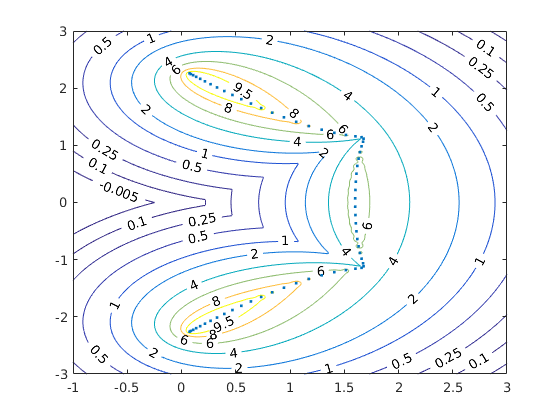
\includegraphics[width=0.5\linewidth]{../src/figures/grcar}
\caption{Plot of the Pseudospectrum of the \texttt{grcar matrix}.}
\label{fig:pseudoGrcar}
\end{figure}

The pseudospectrum can also be defined trough random perturbations as
\begin{equation}
 z \in \Lambda(\mathbf{A} + \mathbf{E}) \;\; \text{with} \; \mathbf{E} \in \mathbb{C}^{n,n} \; \text{and} \: \|\mathbf{E}\| < \epsilon.
\label{eq:defPert}
\end{equation}
\begin{figure}
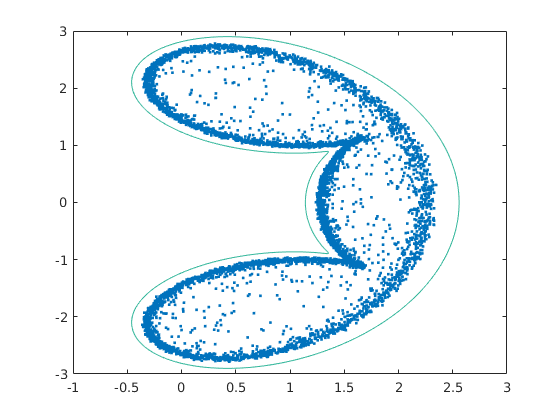
\includegraphics[width=0.4\linewidth]{../src/figures/randPert}
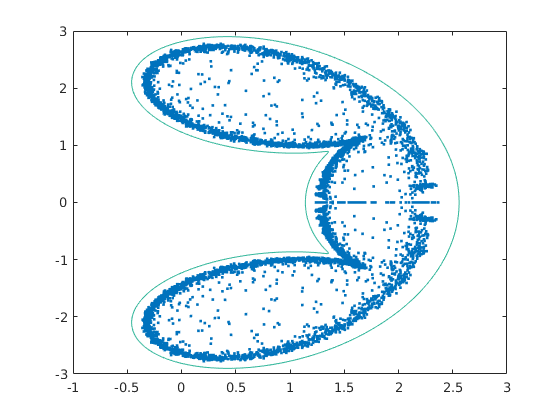
\includegraphics[width=0.4\linewidth]{../src/figures/randPertReal}
\caption{Plot of the $\Lambda(\mathbf{A} + \mathbf{E})$ with $\|\mathbf{E}\| = 10^{-2} = \epsilon$. Additionally the boundary line for $\epsilon = 10^{-2}$ is shown. }
\label{fig:randPerts}
\end{figure}
The plots in figure~\ref{fig:randPerts} have been computed using error matrices with $\|\mathbf{E}\| = 10^{-2} = \epsilon$, where for the plot on the left $\mathbf{E}$ was complex. The plot on the right of the same figure shows the eigenvalues of matrices perturbed with real error matrices. The eigenvalues are rarely scattered into the interior of the $ \epsilon = 10^{-2}$ boundary, as the error matrix is exactly equal to $\epsilon$ if the requirement $\| \mathbf{E} \| = \epsilon$ was loosened to $\| \mathbf{E} \| < \epsilon$ the area would probably be covered more completely.

\section{Toeplitz symbol functions and eigenvalues}
The symbol function of a toeplitz matrix or laurent or toeplitz operator is defined as
\begin{equation}
f(z) = \sum_k t_k z^k. 
\end{equation}
It can be read of the rows of the corresponding matrix. Alternatively the symbol function can also be read as a definition of the corresponding matrix:
\begin{align}
f(z)_1 &=   z^{-3} +  z^{-2} +   z^{-1} -   z + 1                      & \text{    grcar} \\
f(z)_2 &= -2z^{-3} -  z^{-2} +  iz^{-1}            - 4z^{2} - 2i z^{3} & \text{    frog} \\
f(z)_3 &=                      2iz^{-1} +    z^{2} + \frac{7}{10}z^{3} & \text{    bull's head} \\
f(z)_4 &=                        z^{-1}            + \frac{1}{4}z^{2}  & \text{    triangle} \\
f(z)_5 &= -z^{-4} - (3i + 2i)z^{-3} + iz^{-2} + z^{-1} +\dots          & \text{    whale}\\
     & \;\;\;\;  10z + (3 + i)z^{2} + 4z^{3} + iz^{4}                      \notag
\end{align}
Considering the symbol functions defined above. The following theorem holds: \\
\newtheorem{theorem}{Theorem}
\begin{theorem}
If T is a circulant matrix, then $\Lambda (T) = f(\mathbb{T}_n)$. \\
If T is a Laurent operator, then $\Lambda (T) = f(\mathbb{T})$.   \\
If T is a Toeplitz operator, then $\Lambda (T) = f(\mathbb{T})$ together with the points enclosed in this area with nonzero winding number.
\end{theorem}
Where $\mathbb{T}$ denotes the unit circle. This theorem can be observed at work in figure~\ref{fig:Task2}. The blue dots are the eigenvalues of the Toeplitz matrices defined in the symbol functions above. The orange line in each plot is the symbol curve evaluated on the unit circle. Finally the green dots come from the circulant matrix cousin of each of the Toeplitz matrices. When looking at the symbol function the corresponding circulant matrix can be constructed from the vector:\footnote{THE ASYMPTOTIC SPECTRA OF BANDED TOEPLITZ AND QUASI-TOEPLITZ MATRICES, RICHARD M. BEAM AND ROBERT F.WARMING, SIAM J. SCI. COMPUT}
\begin{equation}
\begin{bmatrix}
t_{0} & t_{1} & \dots & t_{q} & 0 & \dots & 0 & t_{-p} & \dots & t_{-1} \\
\end{bmatrix}
\label{vec:circ}
\end{equation} 
A circulant matrix is then constructed by shifting vector~\ref*{vec:circ} by one position to the right in each row. The eigenvalues of the circulant matrices lie exactly on the symbol curve. Shown in green in figure~\ref{fig:Task2}.
\begin{figure}
\centering
\tikzset{mark size=1}
% This file was created by matlab2tikz.
% Minimal pgfplots version: 1.3
%
%The latest updates can be retrieved from
%  http://www.mathworks.com/matlabcentral/fileexchange/22022-matlab2tikz
%where you can also make suggestions and rate matlab2tikz.
%
\documentclass[tikz]{standalone}
\usepackage{pgfplots}
\usepackage{grffile}
\pgfplotsset{compat=newest}
\usetikzlibrary{plotmarks}
\usepackage{amsmath}

\begin{document}
\definecolor{mycolor1}{rgb}{0.00000,0.44700,0.74100}%
\definecolor{mycolor2}{rgb}{0.85000,0.32500,0.09800}%
\definecolor{mycolor3}{rgb}{0.46600,0.67400,0.18800}%
%
\begin{tikzpicture}

\begin{axis}[%
width=2.5in,
height=2.5in,
scale only axis,
xmin=-1,
xmax=3.5,
ymin=-4,
ymax=4,
title style={font=\bfseries},
title={grcar}
]
\addplot [color=mycolor1,only marks,mark=*,mark options={solid},forget plot]
  table[row sep=crcr]{%
0.162803247227423	2.17287108400829\\
0.162803247227423	-2.17287108400829\\
0.0714732434953187	2.26270129173752\\
0.0714732434953187	-2.26270129173752\\
0.073767853367367	2.26042541685918\\
0.073767853367367	-2.26042541685918\\
0.0775916486232442	2.25663525133143\\
0.0775916486232442	-2.25663525133143\\
0.0829425530507539	2.25133635551638\\
0.0829425530507539	-2.25133635551638\\
0.0898102395761244	2.24453906423149\\
0.0898102395761244	-2.24453906423149\\
0.0982113642882669	2.23624226613734\\
0.0982113642882669	-2.23624226613734\\
0.14688510129589	2.18841245154698\\
0.14688510129589	-2.18841245154698\\
0.132465513119271	2.20253376774719\\
0.132465513119271	-2.20253376774719\\
0.119534561390922	2.21523280138035\\
0.119534561390922	-2.21523280138035\\
0.34276437982941	2.00089918110313\\
0.34276437982941	-2.00089918110313\\
0.264458858837912	2.07483971971911\\
0.264458858837912	-2.07483971971911\\
0.180197743308867	2.15593765235939\\
0.180197743308867	-2.15593765235939\\
0.31524443956379	2.02671840872587\\
0.31524443956379	-2.02671840872587\\
0.289137333822208	2.05137911944648\\
0.289137333822208	-2.05137911944648\\
0.199077357744667	2.1376416461243\\
0.199077357744667	-2.1376416461243\\
0.241211185566175	2.09706006108998\\
0.241211185566175	-2.09706006108998\\
0.371687456493896	1.97396667338298\\
0.371687456493896	-1.97396667338298\\
0.466744784532626	1.88701098369011\\
0.466744784532626	-1.88701098369011\\
0.433690545012869	1.91696737445336\\
0.433690545012869	-1.91696737445336\\
0.501150371774825	1.85616836868256\\
0.501150371774825	-1.85616836868256\\
0.401999712098642	1.94597109998687\\
0.401999712098642	-1.94597109998687\\
0.778442060196068	1.62205656125696\\
0.778442060196068	-1.62205656125696\\
0.536892069394355	1.82450635736899\\
0.536892069394355	-1.82450635736899\\
0.219415473990093	2.11800487722225\\
0.219415473990093	-2.11800487722225\\
0.573954407645793	1.79210017496229\\
0.573954407645793	-1.79210017496229\\
0.612322211397296	1.75903243019132\\
0.612322211397296	-1.75903243019132\\
0.73506063414906	1.65679059874549\\
0.73506063414906	-1.65679059874549\\
0.692896457663029	1.69127484524893\\
0.692896457663029	-1.69127484524893\\
0.651975681409271	1.72539104620276\\
0.651975681409271	-1.72539104620276\\
0.823008895982169	1.58720283799652\\
0.823008895982169	-1.58720283799652\\
0.868722619805137	1.55237313086051\\
0.868722619805137	-1.55237313086051\\
0.915535526969206	1.51772626214511\\
0.915535526969206	-1.51772626214511\\
1.01220300315712	1.44970159163321\\
1.01220300315712	-1.44970159163321\\
1.06188388783946	1.4167310609848\\
1.06188388783946	-1.4167310609848\\
1.11230470643213	1.38475986479622\\
1.11230470643213	-1.38475986479622\\
1.68809721407515	1.10868912007363\\
1.68809721407515	-1.10868912007363\\
1.68563019047516	1.12671666099866\\
1.68563019047516	-1.12671666099866\\
1.6784129290942	1.14023963708941\\
1.6784129290942	-1.14023963708941\\
1.66526637807934	1.15033162750348\\
1.66526637807934	-1.15033162750348\\
1.64568670833117	1.15849845319187\\
1.64568670833117	-1.15849845319187\\
1.61976418900607	1.16614102854846\\
1.61976418900607	-1.16614102854846\\
1.68708648081233	1.08579154974488\\
1.68708648081233	-1.08579154974488\\
1.58794558652203	1.17444629020166\\
1.58794558652203	-1.17444629020166\\
1.68364902713391	1.05805388446996\\
1.68364902713391	-1.05805388446996\\
1.16330324776453	1.35404147817927\\
1.16330324776453	-1.35404147817927\\
1.55092738737667	1.18435160265996\\
1.55092738737667	-1.18435160265996\\
1.67862611730663	1.02570577292558\\
1.67862611730663	-1.02570577292558\\
1.50955238171688	1.19651329768983\\
1.50955238171688	-1.19651329768983\\
1.21467022893627	1.32484688640365\\
1.21467022893627	-1.32484688640365\\
1.46470640348842	1.21131290666052\\
1.46470640348842	-1.21131290666052\\
1.41723734143416	1.22889698300531\\
1.41723734143416	-1.22889698300531\\
1.67267332964912	0.989091024254324\\
1.67267332964912	-0.989091024254324\\
0.963387699630922	1.48343779768291\\
0.963387699630922	-1.48343779768291\\
1.26613664568124	1.29745927017732\\
1.26613664568124	-1.29745927017732\\
1.3679050805727	1.24923275040225\\
1.3679050805727	-1.24923275040225\\
1.31735924405679	1.27216411734076\\
1.31735924405679	-1.27216411734076\\
1.66628189265444	0.9486088833431\\
1.66628189265444	-0.9486088833431\\
1.65980478114149	0.904672038798903\\
1.65980478114149	-0.904672038798903\\
1.65348479824287	0.857679764031588\\
1.65348479824287	-0.857679764031588\\
1.64748087510669	0.808003140695327\\
1.64748087510669	-0.808003140695327\\
1.64189046618357	0.755978744499572\\
1.64189046618357	-0.755978744499572\\
1.63676744221943	0.701907647731701\\
1.63676744221943	-0.701907647731701\\
1.63213577374543	0.646057419295387\\
1.63213577374543	-0.646057419295387\\
1.62799967495189	0.588665583154667\\
1.62799967495189	-0.588665583154667\\
1.62435095401583	0.529943594970431\\
1.62435095401583	-0.529943594970431\\
1.62117424545992	0.470080809049782\\
1.62117424545992	-0.470080809049782\\
1.6184506801094	0.409248168043237\\
1.6184506801094	-0.409248168043237\\
1.61616043256925	0.347601515475345\\
1.61616043256925	-0.347601515475345\\
1.61428443578081	0.285284477927394\\
1.61428443578081	-0.285284477927394\\
1.61062493954659	0.0318907312103814\\
1.61062493954659	-0.0318907312103814\\
1.61098521538579	0.0956151275364774\\
1.61098521538579	-0.0956151275364774\\
1.61170958184795	0.159167579432052\\
1.61170958184795	-0.159167579432052\\
1.61280561056869	0.222431006616594\\
1.61280561056869	-0.222431006616594\\
0.108117259275721	2.22647099571082\\
0.108117259275721	-2.22647099571082\\
};
\addplot [color=mycolor2,solid,forget plot]
  table[row sep=crcr]{%
3	0\\
2.93540306696685	0.693856370750057\\
2.74639660891256	1.35139947729381\\
2.44694558318034	1.9390097963452\\
2.05906446382384	2.42823186148405\\
1.61103950753584	2.79781704862036\\
1.13515565978359	3.03517166363549\\
0.665121038300383	3.13709447111272\\
0.233406762157466	3.1097489653917\\
-0.131274236710148	2.96788133036699\\
-0.406139333147588	2.73335940450134\\
-0.575980887164211	2.43316542979921\\
-0.634152131875392	2.09702090919075\\
-0.582821057569087	1.75485158347188\\
-0.432483162009358	1.43431183771924\\
-0.200788296031225	1.15857986360288\\
0.0892042076446938	0.94460845381959\\
0.41117955013352	0.801973836550373\\
0.737934459608488	0.732410330905551\\
1.04374507292474	0.730056741834472\\
1.30652666578675	0.782376860144509\\
1.50959781504272	0.87165686136851\\
1.64289972198011	0.976932097263043\\
1.7035725731903	1.07615918510818\\
1.6958502979717	1.14842961611561\\
1.63029750329825	1.17601999031951\\
1.52247209186303	1.14609143329738\\
1.39114872220684	1.05188508375676\\
1.25627722439356	0.893308570527769\\
1.13687287134392	0.676865709096389\\
1.04904002476569	0.414943003162565\\
1.00431677157061	0.124526345556147\\
1.00849706296407	-0.174525863227647\\
1.06104143933317	-0.46148591854844\\
1.15513183832263	-0.716843540508597\\
1.27836532634731	-0.924275616632121\\
1.41402140807692	-1.07230925280704\\
1.54278335444009	-1.15551677420935\\
1.64475070893015	-1.17512463551863\\
1.70155175921653	-1.13897255691238\\
1.69835392492388	-1.06081966199291\\
1.62557775690277	-0.95905545681485\\
1.48014593138432	-0.854929589517758\\
1.26613999083985	-0.770460336487104\\
0.994790943578794	-0.726213440180046\\
0.683790401425215	-0.739157323536817\\
0.355971256544885	-0.820796423722577\\
0.0374653427556189	-0.975761700926926\\
-0.244505212007882	-1.20099822234538\\
-0.464010658693872	-1.48563752335766\\
-0.598759441935274	-1.81158182005853\\
-0.632196432441493	-2.15476347911839\\
-0.555161882611044	-2.48698212822652\\
-0.366955734378214	-2.7781688874348\\
-0.0757023968175686	-2.99888719157693\\
0.302028640485337	-3.12285620006061\\
0.742326276407386	-3.12927803847746\\
1.21568179522477	-3.00476461594159\\
1.68923322969645	-2.74469233426686\\
2.12932521838972	-2.35386086422878\\
2.50417066697657	-1.84639116116996\\
2.78639019620551	-1.24486288040775\\
2.95521449521791	-0.578756642819924\\
2.99816255274451	0.117673535996648\\
2.91205291239431	0.807923163622423\\
2.70326175126414	1.45594688272187\\
2.38720576945488	2.02882997924109\\
1.9870939912414	2.49920028483354\\
};
\addplot [color=mycolor3,only marks,mark=*,mark options={solid},forget plot]
  table[row sep=crcr]{%
0.250088952695233	3.11327314866915\\
0.250088952695233	-3.11327314866915\\
0.0864545423573988	3.06859679861554\\
0.0864545423573988	-3.06859679861554\\
-0.0636879946295856	3.00506741038199\\
-0.0636879946295856	-3.00506741038199\\
-0.198696306503518	2.92434695553073\\
-0.198696306503518	-2.92434695553073\\
0.425366529780627	3.13763418306144\\
0.425366529780627	-3.13763418306144\\
0.610256233583416	3.14044146644522\\
0.610256233583416	-3.14044146644522\\
-0.317155208450447	2.82827029492417\\
-0.317155208450447	-2.82827029492417\\
0.802571578545583	3.1207015158958\\
0.802571578545583	-3.1207015158958\\
1.97814760073381	2.50767462792415\\
1.97814760073381	-2.50767462792415\\
2.1547479189865	2.32562326376408\\
2.1547479189865	-2.32562326376408\\
-0.417893992879551	2.71881613703436\\
-0.417893992879551	-2.71881613703436\\
1	3.07768353717526\\
1	-3.07768353717526\\
-0.5	2.59807621135331\\
-0.5	-2.59807621135331\\
1.20013427186638	3.01093350080388\\
1.20013427186638	-3.01093350080388\\
-0.562828268998911	2.46822313403184\\
-0.562828268998911	-2.46822313403184\\
1.40050551559055	2.92028432640575\\
1.40050551559055	-2.92028432640575\\
-0.606007150877318	2.33147746054298\\
-0.606007150877318	-2.33147746054298\\
1.59861731450831	2.80586200213372\\
1.59861731450831	-2.80586200213372\\
1.79198042944811	2.66808752712275\\
1.79198042944811	-2.66808752712275\\
-0.629439826401619	2.19007443012513\\
-0.629439826401619	-2.19007443012513\\
-0.633301735695619	2.04623090887218\\
-0.633301735695619	-2.04623090887218\\
-0.618033988749892	1.9021130325903\\
-0.618033988749892	-1.9021130325903\\
2.31952025230484	2.1232089992575\\
2.31952025230484	-2.1232089992575\\
-0.584332887581919	1.75980503703976\\
-0.584332887581919	-1.75980503703976\\
2.47034523045881	1.90196838590809\\
2.47034523045881	-1.90196838590809\\
2.60527530746528	1.66368055436011\\
2.60527530746528	-1.66368055436011\\
-0.533135749988107	1.62127974215546\\
-0.533135749988107	-1.62127974215546\\
3	0\\
2.72256245201757	1.4103452770038\\
2.72256245201757	-1.4103452770038\\
2.82068305028135	1.1441578142725\\
2.82068305028135	-1.1441578142725\\
-0.465603280867248	1.48837112864004\\
-0.465603280867248	-1.48837112864004\\
-0.383098789097136	1.36274941040443\\
-0.383098789097136	-1.36274941040443\\
2.89835964701689	0.867480906978143\\
2.89835964701689	-0.867480906978143\\
2.95457919819913	0.582814320545588\\
2.95457919819913	-0.582814320545588\\
2.98860756056398	0.292762384355018\\
2.98860756056398	-0.292762384355018\\
-0.287164595108754	1.24589896525915\\
-0.287164595108754	-1.24589896525915\\
-0.179496015900203	1.13909943969216\\
-0.179496015900203	-1.13909943969216\\
-0.0619133496281712	1.04341029225062\\
-0.0619133496281712	-1.04341029225062\\
0.0636676894304552	0.959658984792221\\
0.0636676894304552	-0.959658984792221\\
0.195266613271247	0.888432972563548\\
0.195266613271247	-0.888432972563548\\
0.330869393641142	0.830075583623633\\
0.330869393641142	-0.830075583623633\\
0.468459794033006	0.784685816515486\\
0.468459794033006	-0.784685816515486\\
1.65413016167572	1.17354371014948\\
1.65413016167572	-1.17354371014948\\
1.68190982354141	1.16189680051924\\
1.68190982354141	-1.16189680051924\\
1.700214509278	1.1415807262049\\
1.700214509278	-1.1415807262049\\
1.70802620753806	1.11371178171945\\
1.70802620753806	-1.11371178171945\\
1.6180339887499	1.17557050458495\\
1.6180339887499	-1.17557050458495\\
0.606050309090745	0.752122023270684\\
0.606050309090745	-0.752122023270684\\
0.999999999999994	0\\
1.7044885311073	1.07955300787899\\
1.7044885311073	-1.07955300787899\\
1.57489690103783	1.16720719762688\\
1.57489690103783	-1.16720719762688\\
1.68892536545815	1.04049290892461\\
1.68892536545815	-1.04049290892461\\
1.52608655464918	1.14787716794332\\
1.52608655464918	-1.14787716794332\\
1.66085666527298	0.998021821935411\\
1.66085666527298	-0.998021821935411\\
1.47303627544969	1.11720615112969\\
1.47303627544969	-1.11720615112969\\
0.741712229509278	0.732009383785606\\
0.741712229509278	-0.732009383785606\\
1.62001111380683	0.95370631594038\\
1.62001111380683	-0.95370631594038\\
1.41721780027665	1.07502769107435\\
1.41721780027665	-1.07502769107435\\
1.56633540974942	0.909162032102317\\
1.56633540974942	-0.909162032102317\\
0.873604367260912	0.723751018293501\\
0.873604367260912	-0.723751018293501\\
1.36011361198391	1.02138497696936\\
1.36011361198391	-1.02138497696936\\
1.00437815793503	0.125406697690387\\
1.00437815793503	-0.125406697690387\\
1.50000000000001	0.866025403784439\\
1.50000000000001	-0.866025403784439\\
1.01741287594188	0.249276827113384\\
1.01741287594188	-0.249276827113384\\
1.30318933585634	0.956529051906688\\
1.30318933585634	-0.956529051906688\\
1.03880667524038	0.370101132648432\\
1.03880667524038	-0.370101132648432\\
1	0.726542528005364\\
1	-0.726542528005364\\
1.42140113363005	0.825924715764421\\
1.42140113363005	-0.825924715764421\\
1.24786666234684	0.880913438700873\\
1.24786666234684	-0.880913438700873\\
1.06806969019361	0.486424520795337\\
1.06806969019361	-0.486424520795337\\
1.33115917137994	0.790450974991393\\
1.33115917137994	-0.790450974991393\\
1.10452846326766	0.596871990852192\\
1.10452846326766	-0.596871990852192\\
1.11931162439211	0.739389700891965\\
1.11931162439211	-0.739389700891965\\
1.19549725096141	0.795185287421389\\
1.19549725096141	-0.795185287421389\\
1.14733805262245	0.700173206156685\\
1.14733805262245	-0.700173206156685\\
1.23011314537489	0.761129070859521\\
1.23011314537489	-0.761129070859521\\
};
\end{axis}
\end{tikzpicture}%
\end{document}
% This file was created by matlab2tikz.
% Minimal pgfplots version: 1.3
%
%The latest updates can be retrieved from
%  http://www.mathworks.com/matlabcentral/fileexchange/22022-matlab2tikz
%where you can also make suggestions and rate matlab2tikz.
%
\documentclass[tikz]{standalone}
\usepackage{pgfplots}
\usepackage{grffile}
\pgfplotsset{compat=newest}
\usetikzlibrary{plotmarks}
\usepackage{amsmath}

\begin{document}
\definecolor{mycolor1}{rgb}{0.00000,0.44700,0.74100}%
\definecolor{mycolor2}{rgb}{0.85000,0.32500,0.09800}%
\definecolor{mycolor3}{rgb}{0.46600,0.67400,0.18800}%
%
\begin{tikzpicture}

\begin{axis}[%
width=2.5in,
height=2.5in,
scale only axis,
xmin=-8,
xmax=8,
ymin=-6,
ymax=8,
title style={font=\bfseries},
title={frog}
]
\addplot [color=mycolor1,only marks,mark=*,mark options={solid},forget plot]
  table[row sep=crcr]{%
-4.89611896893307	6.77270615845728\\
-4.87872461024712	6.74852411825655\\
-4.84980635826081	6.70830569922329\\
-4.80947246752466	6.65217805461034\\
-4.75787396749409	6.58031856266788\\
-4.69520413901007	6.4929541929009\\
-4.62169784605561	6.39036069493394\\
-4.53763072651701	6.27286161278933\\
-4.44331824628558	6.14082712805202\\
-4.33911462254688	5.99467273611275\\
-7.66196538764551	-0.275479790013345\\
-7.63368184072391	-0.286950000779941\\
-7.58663236491225	-0.306006185291521\\
-7.52095126990534	-0.332557392692231\\
-7.43682590292377	-0.366476890018928\\
-4.22541162196538	5.83485776052587\\
-4.10263724218458	5.66188371123545\\
-3.97125428447452	5.47629249364748\\
-7.33449596571777	-0.407602759595824\\
-7.21425264126218	-0.455738665882906\\
-7.07643753382388	-0.510654790786236\\
-6.92144142693543	-0.572088936146988\\
-6.74970286466317	-0.639747791784772\\
-6.5617065623544	-0.713308367080388\\
-6.35798165378286	-0.792419583664868\\
-3.83175882885829	5.27866447633192\\
-6.13909978221741	-0.876704026346848\\
-3.6846786233867	5.06961642646122\\
-3.53057140330582	4.84979932342205\\
-5.90567304336116	-0.965759849022883\\
-5.65835178835594	-1.05916283203124\\
-3.37002315819813	4.61989606191402\\
-5.39782229505266	-1.15646858732042\\
4.596110951333	-4.53167335580735\\
4.56977652556555	-4.51147923275074\\
4.52597314719081	-4.47789854543306\\
4.46483118842947	-4.43104447545676\\
4.38653397404637	-4.3710768926951\\
-3.20364637039685	4.38061905727392\\
-5.1248043155813	-1.25721490797895\\
4.29130845144604	-4.29819645755433\\
4.17945861226377	-4.21264263271625\\
4.05127039630433	-4.11478233701636\\
-3.03207825324108	4.13270776607844\\
3.90696686305472	-4.00455973805307\\
3.74910137019107	-3.88266378478759\\
5.97816800381551	0.117586031135785\\
5.97879401412093	0.211774608126683\\
5.94442191845332	0.0300128466024312\\
5.871064004881	-0.0549749246081834\\
5.95250927769048	0.313698651040211\\
5.90423624411981	0.422719692885492\\
5.83772870834416	0.537462294615683\\
5.75591031264159	0.656238534352954\\
5.75272688808188	-0.144276262617189\\
5.66111040485526	0.777213128755731\\
5.55521613186961	0.898477002898035\\
5.43977325266453	1.0180803168522\\
5.58591717585812	-0.247474517031902\\
-4.84004850793441	-1.3609242591601\\
-2.85597902493147	3.87692613537945\\
5.31605247257457	1.13404382185228\\
5.18508987945049	1.24435796765797\\
5.37030305628314	-0.376826778949962\\
5.04770610987472	1.3469756632529\\
-4.5443337588689	-1.4671064082333\\
-2.67603026225594	3.61405999324126\\
4.90450661832596	1.43980322730928\\
5.11047803552496	-0.546236921158495\\
4.75586402631632	1.52069406556214\\
4.60188297976059	1.58745091668245\\
-4.23846440511807	-1.57526119289462\\
3.57248022673581	-3.7595631538969\\
4.81706098755809	-0.768947137898091\\
4.44234902624099	1.63784510619772\\
-2.49293338864768	3.34491439204024\\
4.27666735102815	1.66966429443769\\
4.10380617107604	1.68080056112865\\
-3.92326735942458	-1.68488142665311\\
4.5061935468919	-1.0547787140494\\
3.32584876254786	-3.63247253356499\\
3.43614968557575	-3.4242134648777\\
-3.59958914764829	-1.7954559406647\\
3.92227079661201	1.66938305460863\\
4.19755628454112	-1.40835462249879\\
3.00946626025077	-3.54910176542151\\
3.5036679451751	-2.84919416741133\\
3.73013938790188	1.63394239448208\\
-2.30740836300161	3.0703109143452\\
3.91231866840719	-1.82910936896581\\
-3.26829286199282	-1.90647275770205\\
3.52518394999607	1.57357606046856\\
3.67267964223869	-2.31232558077901\\
2.6895198552663	-3.47831867560921\\
-2.12019264995221	2.79108495016897\\
3.30508587296217	1.48807348395263\\
-2.93025503258869	-2.01742238465882\\
-1.9320405703211	2.50808295521922\\
2.36164016098103	-3.40750424414708\\
3.06773971534274	1.37795258863658\\
-2.5863624112947	-2.12780118731285\\
2.02633582321388	-3.33537513084032\\
2.81161442989187	1.24435606585271\\
-1.74372315340986	2.22215970295991\\
-2.23750863787152	-2.2371147586775\\
1.68456050545165	-3.26104520516464\\
-1.88459069279432	-2.34488107395875\\
2.53610797486191	1.08877303534004\\
-1.5560286421319	1.93417555294856\\
1.33720487686018	-3.18391634457775\\
-1.52850484272316	-2.45063294522667\\
2.24181499719337	0.912601735729337\\
-1.36976384626398	1.64499377798622\\
0.985108171067031	-3.10365310188083\\
-1.17014113880636	-2.55391861207862\\
1.9306596746855	0.716631692808489\\
-1.18575659184038	1.35547801542895\\
-0.810373094877558	-2.65429761876905\\
0.629099078443761	-3.02019487944118\\
1.60592895724506	0.500557802424891\\
-0.450028187223872	-2.75132593362226\\
-1.00485960089925	1.06648995984471\\
0.270216415828606	-2.93383933573451\\
-0.0897682121724978	-2.84454196525689\\
-0.82795621304769	0.778887477664064\\
1.27233946021443	0.262622954253692\\
0.272034770193568	-2.52890328690462\\
0.276598339845887	-2.51671092729612\\
0.274503066184685	-2.44977232660931\\
0.936344542188959	-0.000546188651634902\\
-0.655968534940726	0.493523395268444\\
-0.489868899835373	0.211245527439729\\
0.248440515556009	-2.45735508746023\\
0.606929069547338	-0.293810839099346\\
-0.330694116630676	-0.0671004386236986\\
-0.179530795797072	-0.340702167102858\\
0.297271291001595	-0.622853637109618\\
-0.0385234764319859	-0.609743027004846\\
0.264515091953105	-2.34321407590926\\
0.21651956664238	-2.3062383707786\\
0.207344486850295	-1.99081821826572\\
0.246013512982025	-2.19291362127222\\
0.195626958417058	-2.08833365016188\\
0.0725582005360771	-0.856620615983724\\
0.117499163869574	-1.03014242680831\\
0.163052697873851	-1.71414560046112\\
0.185532240643257	-1.84354879017664\\
0.155227644333153	-1.55879025933964\\
0.135830913961694	-1.3916933794099\\
0.120187069584271	-1.21569734560116\\
};
\addplot [color=mycolor2,solid,forget plot]
  table[row sep=crcr]{%
-3	0\\
-2.19895266433866	-1.10771305340302\\
-1.42801013181488	-1.9880780478529\\
-0.725763905429416	-2.59312819773019\\
-0.115903181230727	-2.8987399655806\\
0.393803924411222	-2.90571220718646\\
0.81078724677692	-2.63873710045254\\
1.15532618407221	-2.14339133949444\\
1.4568487233253	-1.48144632045\\
1.74927976915394	-0.724938432526793\\
2.06593117527035	0.0504573083403903\\
2.43446937829537	0.772153959496611\\
2.87248903038268	1.37688368655789\\
3.3841632109109	1.81589046855301\\
3.95833797581164	2.05864302284134\\
4.56830062201858	2.09476621334756\\
5.17328983426399	1.93405463647295\\
5.72164670457274	1.60460819671895\\
6.15534412020042	1.14930036372509\\
6.41549321942996	0.620940054618106\\
6.4483225348723	0.0766042359266195\\
6.21106791373678	-0.428309965694481\\
5.67720506847509	-0.845743923785959\\
4.84050278805582	-1.13980876068637\\
3.71746980066788	-1.29033196133779\\
2.34790395011131	-1.29478499632398\\
0.793416919015551	-1.16841107145194\\
-0.866013305026925	-0.942542135584749\\
-2.53723258429625	-0.661265275663542\\
-4.12045375730907	-0.376754961027476\\
-5.51663497041794	-0.143714945318273\\
-6.63509096414059	-0.0134602882029873\\
-7.40070215468034	-0.0282078921067721\\
-7.76010844088051	-0.216129537556501\\
-7.68635033504428	-0.587655759333262\\
-7.18154310303109	-1.13340779480263\\
-6.27732973229463	-1.8239881511721\\
-5.03304204236552	-2.61169122817911\\
-3.53169031343029	-3.43401912128972\\
-1.87408391171151	-4.21872015399378\\
-0.171542740108675	-4.88992406306148\\
1.46222173583197	-5.37484121614747\\
2.91940699120054	-5.61043363239053\\
4.10593731769626	-5.5494585923774\\
4.9481758672246	-5.16533226332747\\
5.39800125381622	-4.45535723430985\\
5.43585719454019	-3.44199589095716\\
5.07155424212532	-2.17203915036334\\
4.34279090197	-0.713702530123213\\
3.31155102438273	0.848137237493309\\
2.05870895065258	2.41818784899797\\
0.677318480913179	3.89795996277394\\
-0.734835970072907	5.19336069562646\\
-2.0827961805498	6.22202718715789\\
-3.2814683963567	6.91978339560615\\
-4.26157394082471	7.2456749679783\\
-4.97404883682413	7.18515618646019\\
-5.39257356934425	6.75115929908187\\
-5.5140840687517	5.98295637987308\\
-5.35729514539927	4.94291153660404\\
-4.9594418671155	3.71140040435723\\
-4.3715973039091	2.38032879858738\\
-3.65304325462446	1.04579965798651\\
-2.8652438164357	-0.199453178997207\\
-2.06599386775265	-1.27323018882177\\
-1.30428425200826	-2.11003553809097\\
-0.616345962532409	-2.6657464588477\\
-0.0232146538624853	-2.92041229605837\\
};
\addplot [color=mycolor3,only marks,mark=*,mark options={solid},forget plot]
  table[row sep=crcr]{%
-4.49892127455291	7.26789190517659\\
-4.79756579175428	7.24211655115448\\
-5.04526259917207	7.14933631133331\\
-5.24080249779987	6.99135055897553\\
-5.38369816137602	6.77076906681451\\
-4.151264726549	7.22570019815144\\
-5.47416869026074	6.49097375392985\\
-3.75725182795137	7.11543139215737\\
-5.51311374089632	6.15606955439165\\
-3.32024062091414	6.93783043997461\\
-5.50207780496765	5.77082514683733\\
-2.84426281011793	6.69448800726359\\
-5.44320536178628	5.34060443555777\\
-2.3339842782453	6.38781920043153\\
-5.3391877642783	4.87128981136448\\
-7.70594464124925	-0.555395877862205\\
-7.77715516318338	-0.382900637360175\\
-7.77154005291078	-0.242471306065611\\
-7.68938434991765	-0.134496986977663\\
-1.79465526293623	6.02103061711359\\
-5.19320284115241	4.36919834235594\\
-7.55854426248841	-0.758939177745205\\
-7.53188196860412	-0.0587458620603437\\
-7.33651002106839	-0.991886640347875\\
-7.30111147346345	-0.014383320437112\\
-7.0423049305386	-1.2519816015004\\
4.62653200756615	-5.37352661490508\\
4.93657643261929	-5.17499423896219\\
5.17752763390742	-4.91895213605013\\
5.3472754604997	-4.60648174282504\\
-1.23205080756887	5.59807621135331\\
-5.00884830349361	3.84099214884835\\
-6.99999999999997	-3.13370314252006e-16\\
-6.67927333928608	-1.53637837037718\\
4.25039247653567	-5.51425128894846\\
-0.652402255540631	5.12360263314121\\
-4.7900701315636	3.29358430157697\\
-6.6322759242895	-0.0136491947004277\\
-6.25160306331055	-1.84167614392258\\
3.81201194039838	-5.59764440804449\\
5.44461736894588	-4.23944572818751\\
3.31605654971729	-5.62493556739842\\
5.46926550979655	-3.82047413602044\\
-5.76427581901361	-2.16396264067863\\
-6.2024110466154	-0.0528929304231543\\
-0.0623207041161421	4.60288485938508\\
-5.22300661214351	-2.49886684021673\\
2.76794919243112	-5.59807621135333\\
-4.54108718568357	2.73404164653004\\
-4.63417290303315	-2.84162006389977\\
-5.71555320492168	-0.114855874727243\\
2.17380354232169	-5.5196976828564\\
5.42184123427266	-3.35293902032877\\
5.30385718034468	-2.84091787038037\\
6.44864526912686	0.47401170544239\\
6.38966148863	0.702858283962575\\
6.15953810088921	1.14338230338766\\
6.2919894773833	0.927398343903414\\
6.46534687215098	0.245082999587055\\
0.531286532982686	4.04175307820974\\
5.99645466985261	1.34661328992862\\
5.11768727945978	-2.28914629686948\\
6.43656060160307	0.0201945972696724\\
5.80704663178442	1.53302485551049\\
-4.2663133327353	2.16948600247245\\
5.59570275056516	1.69875718975839\\
6.35953793238493	-0.196707378338962\\
-4.00473452030009	-3.18712449379494\\
-5.17745036963946	-0.196286122040955\\
1.5403483662692	-5.3930596517721\\
6.2320508075689	-0.401923788646683\\
5.36681509114304	1.84023053392022\\
5.12470309964605	1.95421453921879\\
-3.34214543291178	-3.53002810146927\\
-3.97027840636463	1.60699519771638\\
0.874843133435088	-5.22198979652487\\
4.87354102152881	2.03789237449428\\
1.1213052873907	3.44651191849824\\
6.05244817858694	-0.592068302317497\\
5.81970475146346	-0.764127263480166\\
-2.6542586118383	-3.86480484914643\\
-4.59436739074242	-0.293621788075263\\
0.184986099261344	-5.01081574356774\\
4.6172898328001	2.08891846899454\\
-1.94922531555814	-4.18583893407343\\
-0.52118385045157	-4.76429038298749\\
-1.23539021686337	-4.48751177443672\\
-3.6575493240896	1.05350541071977\\
4.86652520134251	-1.7029606168436\\
5.53346101627059	-0.915512606477637\\
4.35963477306536	2.10546887542223\\
-3.97299666887505	-0.403062256966673\\
1.70050845511949	2.82385322979227\\
5.19405376677134	-1.04410693560248\\
-3.33265266820555	0.515716254694315\\
4.10392946552414	2.08628335435359\\
4.8025364606279	-1.14830001994774\\
3.8531474899366	2.03069841207943\\
-3.32036410360737	-0.520642853388304\\
-2.99999999999999	-1.5714601493143e-15\\
3.60984214189443	1.93867066771548\\
2.26165312422178	2.18076371233537\\
4.55433192200179	-1.0882311325344\\
-2.66381711903157	-0.487683739556798\\
-2.64373173210598	-0.64231166068607\\
4.36068892538259	-1.2270160973024\\
3.37611496769764	1.81079007981134\\
3.15359351113021	1.64828272520732\\
3.87101607925977	-1.27973153460696\\
4.18577325677291	-0.451287044851832\\
-2.32807840210092	-0.941866618236268\\
2.79757950150494	1.52442877172189\\
2.94341854895141	1.45300299096447\\
3.76614834353625	0.201165926156345\\
3.33673550613018	-1.30648255337658\\
3.30131018902991	0.862134026179446\\
-1.99644726136868	-1.35764233601147\\
-1.95049850993581	-0.764007175792332\\
-1.67222364946404	-1.7307285743659\\
2.74624092859795	1.22741521115165\\
-1.35829941324265	-2.05751922109463\\
-1.05712215918941	-2.33512616674809\\
-0.770668144612594	-2.56141011771486\\
-0.500424552190009	-2.73500004132199\\
-0.247381343675518	-2.85530103407175\\
-0.0120327243024895	-2.92249058248718\\
2.5622279570885	0.974564951389751\\
2.76175389806551	-1.30786289409438\\
-1.24810070180228	-0.881735482693439\\
0.205611914686808	-2.93750336422258\\
0.406007869223618	-2.90200491233349\\
0.590046260944868	-2.81835463517056\\
0.759017038512105	-2.68955884563123\\
0.91456457655062	-2.51921460397598\\
2.39107912712702	0.698040312596178\\
-0.543913343656091	-0.991645638692167\\
1.05863673180523	-2.31144531576969\\
2.23205080756887	0.401923788646686\\
2.15063255405042	-1.28501146120464\\
1.19342832621419	-2.0708291486315\\
0.154845791106363	-1.0901020013796\\
2.08398937332904	0.0907353680602827\\
1.94537210694893	-0.230632285179257\\
1.32132012026501	-1.80232143649619\\
0.841208339062123	-1.17375227854254\\
1.81435507271758	-0.556985604261078\\
1.44481441569695	-1.51117232641236\\
1.6888270465959	-0.882907760804388\\
1.508542296855	-1.23959015728352\\
1.56646848312811	-1.20284098922216\\
};
\end{axis}
\end{tikzpicture}%
\end{document}
% This file was created by matlab2tikz.
% Minimal pgfplots version: 1.3
%
%The latest updates can be retrieved from
%  http://www.mathworks.com/matlabcentral/fileexchange/22022-matlab2tikz
%where you can also make suggestions and rate matlab2tikz.
%
\documentclass[tikz]{standalone}
\usepackage{pgfplots}
\usepackage{grffile}
\pgfplotsset{compat=newest}
\usetikzlibrary{plotmarks}
\usepackage{amsmath}

\begin{document}
\definecolor{mycolor1}{rgb}{0.00000,0.44700,0.74100}%
\definecolor{mycolor2}{rgb}{0.85000,0.32500,0.09800}%
\definecolor{mycolor3}{rgb}{0.46600,0.67400,0.18800}%
%
\begin{tikzpicture}

\begin{axis}[%
width=2.5in,
height=2.5in,
scale only axis,
xmin=-4,
xmax=2,
ymin=-3,
ymax=4,
title style={font=\bfseries},
title={bullshead}
]
\addplot [color=mycolor1,only marks,mark=*,mark options={solid},forget plot]
  table[row sep=crcr]{%
1.37607986325333	2.67982864161301\\
1.56267176245345	3.0979057543464\\
1.56044616487925	3.09293623058976\\
1.55673847467435	3.08465655297024\\
1.5515511464708	3.07307099454742\\
1.54488760271804	3.05818549065802\\
1.53675224281537	3.04000761525416\\
1.5271504216939	3.01854651826082\\
1.5160884049785	2.99381282058438\\
1.50357347625971	2.96581866493188\\
1.48961369153734	2.93457738344427\\
1.47421817306878	2.90010370142145\\
1.39848902129496	2.73021229762262\\
1.45739675163638	2.86241327866762\\
1.43916024196471	2.82152284628654\\
1.41952019794942	2.77744983366456\\
-3.10746516472758	0.507845942905954\\
-3.19634631620354	0.538245938855773\\
-3.20932153577313	0.542667294332643\\
-3.20445442291729	0.54100928605855\\
1.35230662403793	2.62631739072584\\
1.32718391012766	2.56969689705205\\
1.30072700596322	2.50998501858158\\
1.27295183840626	2.44719874539688\\
1.24387494564276	2.38135377658347\\
-3.18500283117651	0.534377233955428\\
-3.13164963120119	0.516137846776482\\
-3.17043181334867	0.529403106125241\\
-3.15264332662901	0.523323405840815\\
1.21351344470633	2.31246403168142\\
-3.04959238516998	0.487939670341341\\
-3.08010651342497	0.498446929468843\\
1.18188500305622	2.24054108999595\\
-3.01594357610721	0.476322547692431\\
1.97111191231487	-1.91357218785798\\
1.96677094112706	-1.91182355305176\\
-2.9791829371977	0.463593333646521\\
1.1490078142256	2.16559354237098\\
1.95953817830419	-1.90891483233197\\
1.9494168998177	-1.90485458661433\\
1.93641167702934	-1.89965491246753\\
1.92052836297363	-1.89333155653958\\
-2.93933533801891	0.449749040964056\\
1.11490058058464	2.08762623961488\\
1.90177407665558	-1.88590406726674\\
-2.85048861241241	0.418698412109094\\
-2.89642763040637	0.434785750486431\\
1.88015718701719	-1.87739598749441\\
1.07958250671534	2.00663941726871\\
-2.80154899435609	0.401480615648515\\
-2.74964136887785	0.383124327232871\\
1.85568729882996	-1.86783509266356\\
1.82837524355193	-1.85725368037278\\
1.79823307920238	-1.84568891846545\\
-2.69480018758762	0.363619586053266\\
1.04307330803961	1.9226276715826\\
1.7652741046318	-1.83318326033143\\
-2.63706174763758	0.342954155357859\\
1.72951289531869	-1.81978493790933\\
0.966563165529998	1.74547215526496\\
-2.57646419256116	0.321113120439543\\
1.69096537012915	-1.80554854497074\\
1.00539324125769	1.83557875547335\\
1.64964890155168	-1.79053572569313\\
0.926604646778761	1.65227739876608\\
1.60558248599312	-1.77481598634389\\
0.885540122307309	1.55595203186474\\
-2.5130475330245	0.298078425027859\\
-2.44685369486005	0.273828335910433\\
-2.37792660401561	0.248336823737341\\
1.5587869961827	-1.75846765111184\\
-2.30631232104951	0.221572845763268\\
0.843393149801339	1.45643918325104\\
-2.23205924177162	0.193499513720297\\
1.50928554502399	-1.74157898673018\\
0.800188774618089	1.35366461360718\\
-2.15521838591939	0.164073127061431\\
1.45710400004063	-1.72424952450989\\
-2.07584380281701	0.133242048472743\\
1.40227170076955	-1.70659161247689\\
0.755954063536322	1.2475331144983\\
-1.99399313243342	0.100945394872613\\
1.344822449251	-1.68873223434422\\
-1.90972837298798	0.0671115132488502\\
0.710718874028267	1.1379240802513\\
0.664516959070893	1.02468601898235\\
-1.8231169234361	0.0316562069471215\\
1.28479586792167	-1.6708151348885\\
0.617387553979241	0.907629690356371\\
1.22223925189738	-1.65300329294761\\
-1.73423299242057	-0.00551932496574519\\
1.15721008625519	-1.63548177865927\\
-1.64315949680556	-0.0445308737634353\\
1.08977946198791	-1.61846102260896\\
0.569377662473565	0.786519448435579\\
-1.54999061571323	-0.0855139683260824\\
1.02003669590698	-1.60218050162178\\
0.948095580117184	-1.58691277152501\\
0.874102871603681	-1.57296777061041\\
-1.45483522405241	-0.128627009416738\\
0.520545368521291	0.661062214503174\\
0.470964672343817	0.530893286733183\\
0.79824950201873	-1.56069709212051\\
0.720786006604164	-1.55049690540394\\
-1.35782150808611	-0.174054793744051\\
-1.25910317116043	-0.222012384723585\\
0.420732624108973	0.395557880505469\\
-1.15886777787661	-0.272749201833041\\
0.642044864403743	-1.54281119066643\\
-1.05734796704516	-0.326553049298763\\
0.562460809982297	-1.53813551244248\\
0.31888734212524	0.106964288726971\\
0.267710076461748	-0.0479159627464389\\
0.482588444891716	-1.53697910990413\\
-0.954836491241162	-0.383753543480198\\
0.403270928943355	-1.5397705379031\\
-0.0238107921110199	-1.72690782021332\\
-0.851706304937154	-0.444723956061818\\
0.216817463103997	-0.211309930076667\\
0.166755738172268	-0.384705582888543\\
0.326077106490055	-1.54728581167798\\
-0.0158522949303407	-1.72689459905824\\
-0.0244903101185625	-1.71071016702126\\
0.252183951309416	-1.56235261300487\\
-0.748437184352384	-0.509879757166957\\
0.180254539185094	-1.5893934457115\\
0.117525131118291	-1.62729108238343\\
0.00243846834832117	-1.71494870314358\\
0.0684471647821273	-1.66353320933067\\
-0.00602778159912483	-1.57233275090442\\
-0.0210660580182976	-1.67957981915606\\
0.030422295932291	-1.69334141405128\\
-0.444994069076698	-0.73500212659291\\
0.00161457975979703	-1.49591799141166\\
-0.54415362517493	-0.65456348819106\\
-0.349521182458842	-0.821343606978424\\
0.123341188031902	-1.50148411348871\\
0.00274110857225932	-1.41298758423749\\
-0.0144770036866527	-1.63355210369028\\
0.369979978272011	0.254486838967588\\
0.11835219871605	-0.570037228761569\\
-0.259438735439303	-0.913741104872514\\
-0.645650510447627	-0.579670956916762\\
-0.0378668395374729	-1.21434604843544\\
-0.0078044247038221	-1.33232330020944\\
-0.105151585019778	-1.115027338875\\
-0.176802375316823	-1.01208410131757\\
0.0728924056340253	-0.769845057427842\\
0.0324548632362902	-0.987484368847988\\
0.00241408436925618	-1.23665346970543\\
};
\addplot [color=mycolor2,solid,forget plot]
  table[row sep=crcr]{%
1.7	2\\
1.84846895352282	2.39554180601405\\
1.89613458602978	2.74480122936766\\
1.85150300602182	3.02364428838549\\
1.72919382209814	3.21190543908235\\
1.54866942424394	3.29488259921148\\
1.33260123498158	3.26440365740132\\
1.10501024415572	3.11938066121165\\
0.889337058618885	2.86581124812164\\
0.706601225149937	2.5162334835832\\
0.573800385448339	2.08868604420387\\
0.502677763931319	1.60526666077047\\
0.498953564959304	1.0904143791981\\
0.562075004525341	0.569062717641857\\
0.685494544369772	0.0648193952668745\\
0.857440417006118	-0.401676670970295\\
1.06210171869587	-0.814088414215246\\
1.28111584822456	-1.16130036824729\\
1.49522185858209	-1.43785977397022\\
1.68593141284782	-1.64391690448807\\
1.83707043344301	-1.78468701714146\\
1.93605895742544	-1.86949825127426\\
1.97482275203173	-1.91052535394084\\
1.95026546750614	-1.92133521112137\\
1.86427126471433	-1.91538453522392\\
1.72325119615566	-1.90461152201469\\
1.53728820933716	-1.89825182069582\\
1.31897172879524	-1.90198590399855\\
1.08204012094038	-1.91749208354784\\
0.839965523451103	-1.94244004865541\\
0.604619119450827	-1.97091755173059\\
0.385145694072976	-1.99424160690911\\
0.187155132847144	-2.0020690935951\\
0.0123073968342796	-1.98369330194708\\
-0.141670670122877	-1.92939531533579\\
-0.28054005063313	-1.83171380784297\\
-0.412720506576185	-1.68650432986568\\
-0.548159735436608	-1.49367877935198\\
-0.697012332859659	-1.25754571976262\\
-0.868259460747584	-0.986709771768998\\
-1.06840725331173	-0.693530037704147\\
-1.30039625059203	-0.393179590342827\\
-1.56283598909316	-0.102386601538322\\
-1.84964989410702	0.162030861110547\\
-2.15017839149237	0.38470291322998\\
-2.44974603289795	0.553175984966332\\
-2.73065521410676	0.659171828841011\\
-2.97352868780983	0.699514670651119\\
-3.15888922281544	0.676631629240408\\
-3.2688405679658	0.598568391393276\\
-3.2887016174039	0.478504748147065\\
-3.20844656297267	0.333799199023848\\
-3.02381790649621	0.184634430124711\\
-2.7370053557441	0.0523722437835831\\
-2.35681962482087	-0.0422458686601498\\
-1.89833289340463	-0.0809003976265696\\
-1.38200342311385	-0.049342895637871\\
-0.832346568633566	0.0612515404564938\\
-0.276254209109609	0.253348872584486\\
0.258904066909584	0.522624061857121\\
0.747244658105497	0.858076582560124\\
1.16623822202206	1.24269158190963\\
1.49832903170121	1.65459845538249\\
1.73217196354015	2.06863620145274\\
1.86338521808623	2.45820011279185\\
1.89475723649559	2.79722019708641\\
1.83589195293731	3.06211031487926\\
1.70232356016822	3.23352937397661\\
};
\addplot [color=mycolor3,only marks,mark=*,mark options={solid},forget plot]
  table[row sep=crcr]{%
1.4553966901956	3.29555080945201\\
1.54328750685294	3.29555999548952\\
1.62503639344224	3.2755545140131\\
1.69891578857292	3.2359753021692\\
1.76326323688632	3.17747901443141\\
1.8165055072883	3.10093006860468\\
1.36313176472878	3.27530670851878\\
1.85718162742313	3.00738981425054\\
1.26827560289743	3.23483006645165\\
1.88396449356856	2.89810297050906\\
1.17260092657172	3.17434475425105\\
1.89568073534057	2.77448152114813\\
1.07784548005732	3.0942919921179\\
1.89132853970038	2.63808629275078\\
0.985687938562606	2.99532325321415\\
1.87009316837902	2.49060647667308\\
1.83135993652518	2.33383738623051\\
1.77472445762804	2.16965676702504\\
0.897724900187255	2.87829033865165\\
0.815449291624676	2.74423278469072\\
-3.18350328753282	0.666884797124161\\
-3.2339096675536	0.63651319690657\\
-3.26942974383093	0.597667624338185\\
-3.28906635880982	0.551425830979433\\
-3.29196743295082	0.498995606007486\\
-3.27744192302772	0.44169841306216\\
1.7	2.00000000000001\\
0.740230494935146	2.59436280209726\\
1.60722184271125	1.82683455337039\\
0.673296475311351	2.43004798340169\\
-3.24497371066624	0.380951062524731\\
-3.11933507838103	0.687848881004406\\
-3.04263756071907	0.698627895937306\\
-3.19423318381215	0.318245680150674\\
-2.95473083337804	0.698609523862283\\
-3.12508630747077	0.255128261369753\\
-3.03760101706701	0.193176124601034\\
0.615718158155553	2.25279204587615\\
-2.85700123796102	0.687353270015767\\
1.49664856319591	1.6521340507675\\
-2.93205080756887	0.133974596215568\\
0.568396268518823	2.06421390591902\\
-2.75087949540788	0.664594325689057\\
-2.80891543348923	0.0790932739969587\\
-2.6378186593625	0.63024467654586\\
1.9749835555549	-1.91467360964314\\
1.96705984699656	-1.91990765835487\\
1.97173458373564	-1.90462620384536\\
1.87808152421078	-1.91660471332805\\
1.9480730837496	-1.92133343148126\\
1.91828097857723	-1.91992439035149\\
1.95735685035909	-1.888747378929\\
1.93205080756888	-1.86602540378444\\
1.89617388169813	-1.83547454286844\\
1.3687602341218	1.47785232858483\\
1.82800299302792	-1.91223289641509\\
-2.66887867837928	0.0300622248615728\\
1.8502383279734	-1.79615474692134\\
1.76869193476283	-1.90758688079862\\
-2.51927223086034	0.584391471364637\\
0.532050807568878	1.86602540378445\\
-2.39667277316164	0.527292708906665\\
1.79490650278542	-1.74719103941629\\
1.70089939502236	-1.90335094363844\\
1.6254656051488	-1.90010455749863\\
1.54330341753664	-1.89831338965244\\
1.73098359936273	-1.68779227050493\\
-2.51282319678542	-0.0116515239521902\\
1.22425355283598	1.30589785553122\\
0.507213299857862	1.66000801587842\\
-2.27141135456083	0.459370342292683\\
-2.34182247616801	-0.0446668431025053\\
1.65940793427782	-1.61726891764711\\
1.45538077951191	-1.89832257568996\\
1.36270255302222	-1.90035236299294\\
1.5812389126298	-1.53504962475374\\
1.26629199644799	-1.90449617935598\\
1.16717222869521	-1.91072114097898\\
-2.14481813090277	0.381200940147306\\
1.49764283833099	-1.44069618934929\\
1.0663479943177	-1.91887097290186\\
1.06403397206954	1.13810888178709\\
0.494221902393307	1.44798890489054\\
-2.1571300102849	-0.0677103592552859\\
1.40987677205443	-1.33391672970754\\
0.964788041774959	-1.92867127436443\\
0.863408415178586	-1.9397370222089\\
0.763056943215658	-1.95158216793869\\
0.664499187638982	-1.9636311490084\\
0.568406088135463	-1.97523210291454\\
1.31927067248947	-1.21457679079551\\
0.475343510945098	-1.98567154419971\\
-2.01814435860484	0.293504081217676\\
0.385763875787771	-1.99419024003502\\
1.22720808606521	-1.08270817875966\\
0.300000000000001	-2\\
0.218261260870971	-2.00230108036041\\
0.140632137615833	-2.00029989279831\\
0.0670731538782475	-1.99322670234337\\
-0.0685898200553809	-1.96100823499654\\
-0.00257579922542761	-1.98035299927363\\
0.493219422541858	1.23181666565774\\
-0.131351133480833	-1.93459562230563\\
0.889204944909145	0.976229674005468\\
-1.96016581834397	-0.0796369765981982\\
-1.89254610356859	0.197128693607872\\
1.13510567575207	-0.938515348133011\\
-0.191339146002928	-1.90060671576385\\
-0.249118592636624	-1.85863450804806\\
-0.305325982043496	-1.80838480257403\\
-0.360654575855204	-1.74968565121442\\
-0.415838163717488	-1.68249467796471\\
-0.471633916894953	-1.6069041444855\\
-0.528804619955878	-1.52314365098958\\
0.504154247301322	1.01333712676254\\
1.04439190052135	-0.782379203395701\\
-0.588100591824575	-1.43158040534177\\
-0.65024161414754	-1.33271703386134\\
-0.715899186350417	-1.22718694850473\\
-1.76906988189069	0.0930375806610451\\
-0.785679422932505	-1.11574732619194\\
0.701054439645237	0.821888175877736\\
-1.75250048515215	-0.0794487435285037\\
0.956485173180315	-0.614858216403873\\
-0.860106899503973	-0.9992697963576\\
-0.939609739953973	-0.878728971701962\\
-1.02450621815998	-0.755188993954173\\
0.87277183533206	-0.436686802887153\\
-1.64864043522673	-0.017709597611004\\
0.526784142152898	0.79436956443764\\
0.794584293940276	-0.24877094405354\\
-1.1149931241066	-0.629788300639893\\
-1.21113611654189	-0.503722849806369\\
0.723179664298361	-0.0521810826569193\\
-1.31286225279918	-0.378228066892369\\
-1.41995485164896	-0.254559800986985\\
0.659719259083828	0.151857634004718\\
0.605249252682826	0.361977649463188\\
-0.153504323297473	0.307292526944547\\
-0.850434432244594	0.0563782543216167\\
-0.383727189553915	0.209666724685921\\
-0.616711347296919	0.125906231190009\\
0.560682834239822	0.57668367645358\\
0.290765026147606	0.541626929121601\\
0.0719692162697213	0.418206528401199\\
-1.08286540627246	0.00123791104813389\\
-1.31199019454152	-0.0395709249476949\\
-1.53205080756887	-0.133974596215561\\
-1.5358369359031	-0.0663117695108865\\
0.501038920333971	0.67657541234524\\
};
\end{axis}
\end{tikzpicture}%
\end{document}
% This file was created by matlab2tikz.
% Minimal pgfplots version: 1.3
%
%The latest updates can be retrieved from
%  http://www.mathworks.com/matlabcentral/fileexchange/22022-matlab2tikz
%where you can also make suggestions and rate matlab2tikz.
%
\documentclass[tikz]{standalone}
\usepackage{pgfplots}
\usepackage{grffile}
\pgfplotsset{compat=newest}
\usetikzlibrary{plotmarks}
\usepackage{amsmath}

\begin{document}
\definecolor{mycolor1}{rgb}{0.00000,0.44700,0.74100}%
\definecolor{mycolor2}{rgb}{0.85000,0.32500,0.09800}%
\definecolor{mycolor3}{rgb}{0.46600,0.67400,0.18800}%
%
\begin{tikzpicture}

\begin{axis}[%
width=2.5in,
height=2.5in,
scale only axis,
xmin=-1,
xmax=1.5,
ymin=-1.5,
ymax=1.5,
title style={font=\bfseries},
title={triangle}
]
\addplot [color=mycolor1,only marks,mark=*,mark options={solid},forget plot]
  table[row sep=crcr]{%
-0.595022844683988	1.03058325686604\\
-0.595022844683988	-1.03058325686604\\
-0.594239152327915	1.02934428518694\\
-0.594239152327915	-1.02934428518694\\
-0.592987272927681	1.02688267390651\\
-0.592987272927681	-1.02688267390651\\
-0.591166419961245	1.02421604590248\\
-0.591166419961245	-1.02421604590248\\
-0.588845966472948	1.01952961649666\\
-0.588845966472948	-1.01952961649666\\
-0.58614767974598	1.01563129186472\\
-0.58614767974598	-1.01563129186472\\
-0.582513649056221	1.00857910287704\\
-0.582513649056221	-1.00857910287704\\
-0.579263702389014	1.00359400601353\\
-0.579263702389014	-1.00359400601353\\
-0.573983841899222	0.994050030426997\\
-0.573983841899222	-0.994050030426997\\
-0.570502053475781	0.988160883997512\\
-0.570502053475781	-0.988160883997512\\
-0.563403596879668	0.9759075453729\\
-0.563403596879668	-0.9759075453729\\
-0.559714489280892	0.969437042518771\\
-0.559714489280892	-0.969437042518771\\
-0.551098718961975	0.954101095917956\\
-0.551098718961975	-0.954101095917956\\
-0.54661335337861	0.947550407613441\\
-0.54661335337861	-0.947550407613441\\
-0.53751661958274	0.928739058953453\\
-0.53751661958274	-0.928739058953453\\
-0.530833365442584	0.922501788300805\\
-0.530833365442584	-0.922501788300805\\
-0.522775901177191	0.900176836535811\\
-0.522775901177191	-0.900176836535811\\
-0.512404499337829	0.894036356194407\\
-0.512404499337829	-0.894036356194407\\
-0.506408413392065	0.868525246858067\\
-0.506408413392065	-0.868525246858067\\
-0.491992842474106	0.862002305358888\\
-0.491992842474106	-0.862002305358888\\
-0.441367128393792	0.760542788567218\\
-0.441367128393792	-0.760542788567218\\
-0.465768920754283	0.797165910252838\\
-0.465768920754283	-0.797165910252838\\
-0.448457151975541	0.785119413823777\\
-0.448457151975541	-0.785119413823777\\
-0.416624296714484	0.723534156608113\\
-0.416624296714484	-0.723534156608113\\
-0.470424850525006	0.826094843361901\\
-0.470424850525006	-0.826094843361901\\
-0.48768290594108	0.833875354542303\\
-0.48768290594108	-0.833875354542303\\
-0.393240659883583	0.677087548015015\\
-0.393240659883583	-0.677087548015015\\
-0.371230324525284	0.651614510506801\\
-0.371230324525284	-0.651614510506801\\
-0.37207299267704	0.607530069800246\\
-0.37207299267704	-0.607530069800246\\
-0.33677584097593	0.618148964723542\\
-0.33677584097593	-0.618148964723542\\
-0.341599501592953	0.541741181208587\\
-0.341599501592953	-0.541741181208587\\
-0.299383990966593	0.563882435553468\\
-0.299383990966593	-0.563882435553468\\
-0.32726367131119	0.440779931995253\\
-0.32726367131119	-0.440779931995253\\
-0.321978848672622	0.36441406181879\\
-0.321978848672622	-0.36441406181879\\
-0.31339696670321	0.286760785526404\\
-0.31339696670321	-0.286760785526404\\
-0.306778686273054	0.206165885010881\\
-0.306778686273054	-0.206165885010881\\
-0.302774885872677	0.124447607048773\\
-0.302774885872677	-0.124447607048773\\
-0.300589959785775	0.0416842691161934\\
-0.300589959785775	-0.0416842691161934\\
-0.22218854071202	0.503526964608458\\
-0.22218854071202	-0.503526964608458\\
-0.16009570584542	0.462618161733616\\
-0.16009570584542	-0.462618161733616\\
-0.0980942176952817	0.41703331577947\\
-0.0980942176952817	-0.41703331577947\\
-0.0327377666605878	0.370216098172044\\
-0.0327377666605878	-0.370216098172044\\
0.0344309630768666	0.324168592755498\\
0.0344309630768666	-0.324168592755498\\
0.103076586529291	0.278233658944409\\
0.103076586529291	-0.278233658944409\\
0.174221449354169	0.232362246262777\\
0.174221449354169	-0.232362246262777\\
0.248888457721968	0.186469474762806\\
0.248888457721968	-0.186469474762806\\
1.19003493093932	0\\
1.18851013467247	0\\
1.18590913803198	0\\
1.1823956641004	0\\
0.330867464359646	0.141497928400119\\
0.330867464359646	-0.141497928400119\\
0.836248122082043	0\\
0.878010745346602	0\\
1.17765896081194	0\\
1.17223840913311	0\\
0.419430526952548	0.109451859275279\\
0.419430526952548	-0.109451859275279\\
0.770580671631162	0.00207970126957102\\
0.770580671631162	-0.00207970126957102\\
0.907251986935938	0\\
0.920646369795937	0\\
1.15810852325362	0\\
1.16527175084748	0\\
1.14011801041004	0\\
0.498863161398594	0.0871157155913658\\
0.498863161398594	-0.0871157155913658\\
0.573540653453366	0.06384956826835\\
0.573540653453366	-0.06384956826835\\
0.712630482640562	0.0330071912401994\\
0.712630482640562	-0.0330071912401994\\
1.12790197186029	0\\
0.648671238490259	0.047617139745621\\
0.648671238490259	-0.047617139745621\\
0.95351713912362	0\\
1.11838990766582	0\\
0.994012706201437	0\\
1.00393719970361	0\\
0.274757300242832	0\\
1.06383423485491	0\\
1.14870630283577	0\\
1.10284120564453	0\\
1.07365972809751	0\\
1.03080782129102	0\\
1.04064779839649	0\\
1.09298552641711	0\\
-0.425350646241108	0.736728930321853\\
-0.425350646241108	-0.736728930321853\\
-0.300748320762992	0.52091137185252\\
-0.300748320762992	-0.52091137185252\\
0.295146023229728	0\\
0.850701292482218	0\\
-0.396850262992053	0.687364818499306\\
-0.396850262992053	-0.687364818499306\\
0.963470112993794	0\\
0.793700525984102	0\\
-0.291584424434949	0.505039037817068\\
-0.291584424434949	-0.505039037817068\\
0.335707365672033	0\\
0.583168848869904	0\\
-0.167853682836025	0.290731106909519\\
-0.167853682836025	-0.290731106909519\\
5.53564253758762e-15	8.08784736693228e-08\\
5.53564253758762e-15	-8.08784736693228e-08\\
};
\addplot [color=mycolor2,solid,forget plot]
  table[row sep=crcr]{%
1.25	0\\
1.24002080973834	-0.0501660839480629\\
1.21033182634196	-0.101314745217899\\
1.16167039285303	-0.154359588312581\\
1.09523767133968	-0.21007931958377\\
1.01265813835741	-0.269057792402229\\
0.915925053528847	-0.331632701903229\\
0.807333973009549	-0.397855254740576\\
0.689406828771843	-0.467462690139146\\
0.564809444597393	-0.539865001907935\\
0.436265596731354	-0.614146628101476\\
0.306470842111741	-0.689083259106538\\
0.178009325591362	-0.763173290829439\\
0.0532766402823505	-0.834682842461827\\
-0.0655884422669238	-0.901702692449484\\
-0.176760922482408	-0.962214984589088\\
-0.278773216249977	-1.0141671388984\\
-0.37054404244039	-1.05555008595918\\
-0.451391698776624	-1.08447774170191\\
-0.521031494842108	-1.09926456042309\\
-0.579557741763045	-1.09849805065266\\
-0.627411309935032	-1.08110330975227\\
-0.665334334749951	-1.04639692229197\\
-0.694314153013588	-0.994127963085086\\
-0.715518969681384	-0.924504332760111\\
-0.730228069181127	-0.838203212769741\\
-0.739759585543853	-0.736365035751502\\
-0.745398923031403	-0.620571002122827\\
-0.748330871041096	-0.492804809623985\\
-0.749578285914261	-0.355399874067421\\
-0.749949924937854	-0.210973882609599\\
-0.749999626017475	-0.0623530131376646\\
-0.749998546105205	0.0875114446402035\\
-0.749921621919233	0.235631035021593\\
-0.749448819992005	0.379069439811483\\
-0.74798112370497	0.515029877369317\\
-0.744670587701083	0.640937409257141\\
-0.738463199816811	0.7545131648614\\
-0.728152751268853	0.85383780895059\\
-0.712443449059478	0.937401995527625\\
-0.690018629315765	1.00414205696377\\
-0.659612661779228	1.05345975023435\\
-0.620082984869871	1.08522549943566\\
-0.570479183909979	1.09976521121798\\
-0.510106123493833	1.09783137211246\\
-0.438578364901949	1.08055973897554\\
-0.355863432286096	1.04941348215853\\
-0.262311923971692	1.00611711392744\\
-0.158672980509085	0.952582913530096\\
-0.0460941986036126	0.89083283031135\\
0.0738943031941131	0.822918996940796\\
0.19941132970618	0.750846010429347\\
0.32827060694357	0.67649803844874\\
0.458039788486203	0.6015735868207\\
0.586110399328801	0.527530430039364\\
0.709776198788273	0.455542773932716\\
0.826317094464937	0.386472205584492\\
0.933085501426133	0.320853411181469\\
1.02759192438331	0.25889503067158\\
1.10758655049175	0.200495393635955\\
1.17113377633349	0.145272268698817\\
1.21667684946124	0.0926051837128887\\
1.24309017259293	0.041688358955419\\
1.24971728275867	-0.00840813867906554\\
1.23639306018255	-0.0586717485751089\\
1.20344932109057	-0.110078228881155\\
1.15170358136864	-0.163522984836573\\
1.08243141912369	-0.219755948128486\\
};
\addplot [color=mycolor3,only marks,mark=*,mark options={solid},forget plot]
  table[row sep=crcr]{%
-0.625000000000002	1.08253175473055\\
-0.625000000000002	-1.08253175473055\\
-0.642271617870268	1.07053468861852\\
-0.642271617870268	-1.07053468861852\\
-0.684269318395122	1.01608505545796\\
-0.684269318395122	-1.01608505545796\\
-0.657856579514888	1.05546970650668\\
-0.657856579514888	-1.05546970650668\\
-0.671829070016194	1.03732055972361\\
-0.671829070016194	-1.03732055972361\\
-0.60597442704097	1.09149088151464\\
-0.60597442704097	-1.09149088151464\\
-0.695262722175776	0.991775299319469\\
-0.695262722175776	-0.991775299319469\\
-0.585135289002247	1.09745536315997\\
-0.585135289002247	-1.09745536315997\\
-0.704898945484212	0.96441785050152\\
-0.704898945484212	-0.96441785050152\\
-0.562431421580449	1.10048132149671\\
-0.562431421580449	-1.10048132149671\\
-0.53782081123476	1.10063714048942\\
-0.53782081123476	-1.10063714048942\\
-0.713270997539087	0.93405378803576\\
-0.713270997539087	-0.93405378803576\\
-0.511271242968686	1.09800282936827\\
-0.511271242968686	-1.09800282936827\\
-0.720474298511154	0.900738687230856\\
-0.720474298511154	-0.900738687230856\\
-0.482760885655392	1.09266931914094\\
-0.482760885655392	-1.09266931914094\\
-0.726605739798177	0.864542505996601\\
-0.726605739798177	-0.864542505996601\\
-0.452278810170511	1.0847376976694\\
-0.452278810170511	-1.0847376976694\\
-0.731762745781211	0.825549381366265\\
-0.731762745781211	-0.825549381366265\\
-0.419825436057791	1.07431838889987\\
-0.419825436057791	-1.07431838889987\\
-0.736042344097072	0.783857337140469\\
-0.736042344097072	-0.783857337140469\\
-0.739540251380542	0.739577904180935\\
-0.739540251380542	-0.739577904180935\\
-0.385412902945428	1.0615302821991\\
-0.385412902945428	-1.0615302821991\\
-0.742349981299116	0.692835655477222\\
-0.742349981299116	-0.692835655477222\\
-0.349065363451104	1.04649981807271\\
-0.349065363451104	-1.04649981807271\\
-0.744561981523823	0.643767658690981\\
-0.744561981523823	-0.643767658690981\\
1.25	0\\
1.24824604491124	0.0209561928961205\\
1.24824604491124	-0.0209561928961205\\
1.24299186851713	0.0419856566532897\\
1.24299186851713	-0.0419856566532897\\
1.23426049159664	0.0631607617730906\\
1.23426049159664	-0.0631607617730906\\
1.22209012962989	0.0845520850314583\\
1.22209012962989	-0.0845520850314583\\
1.20653396514447	0.10622753004881\\
1.20653396514447	-0.10622753004881\\
-0.310819194857936	1.02936003681935\\
-0.310819194857936	-1.02936003681935\\
1.18765983113961	0.128251468639427\\
1.18765983113961	-0.128251468639427\\
1.1655498077096	0.150683909633636\\
1.1655498077096	-0.150683909633636\\
1.14029973456894	0.173579701669006\\
1.14029973456894	-0.173579701669006\\
-0.746262806052892	0.592522849445153\\
-0.746262806052892	-0.592522849445153\\
-0.270723127408074	1.01024959690715\\
-0.270723127408074	-1.01024959690715\\
1.11201864274361	0.196987776202508\\
1.11201864274361	-0.196987776202508\\
1.08082810923232	0.220950436706453\\
1.08082810923232	-0.220950436706453\\
-0.228838287641358	0.989311770042547\\
-0.228838287641358	-0.989311770042547\\
-0.747534329032902	0.539261329166853\\
-0.747534329032902	-0.539261329166853\\
1.04686153895501	0.245502699678879\\
1.04686153895501	-0.245502699678879\\
1.01026337878862	0.270671692726213\\
1.01026337878862	-0.270671692726213\\
0.971188268940478	0.296476114565327\\
0.971188268940478	-0.296476114565327\\
-0.185238155799307	0.966693420037199\\
-0.185238155799307	-0.966693420037199\\
-0.748453005906024	0.484153591808164\\
-0.748453005906024	-0.484153591808164\\
0.929800137323131	0.322925761346221\\
0.929800137323131	-0.322925761346221\\
0.88627124296869	0.350021123218685\\
0.88627124296869	-0.350021123218685\\
-0.140008436915799	0.942543972663839\\
-0.140008436915799	-0.942543972663839\\
-0.749089187354544	0.427379684255308\\
-0.749089187354544	-0.427379684255308\\
0.840781174853507	0.377753054560021\\
0.840781174853507	-0.377753054560021\\
0.793515812792364	0.40610252074936\\
0.793515812792364	-0.40610252074936\\
0.744666257303739	0.43504042382162\\
0.744666257303739	-0.43504042382162\\
-0.749506491117668	0.369128305690286\\
-0.749506491117668	-0.369128305690286\\
-0.0932468458206055	0.917014383726873\\
-0.0932468458206055	-0.917014383726873\\
0.694427735542529	0.464527508764093\\
0.694427735542529	-0.464527508764093\\
0.64299849054195	0.494514351635328\\
0.64299849054195	-0.494514351635328\\
-0.74976123632316	0.309595851586713\\
-0.74976123632316	-0.309595851586713\\
0.590578661102261	0.524941430093619\\
0.590578661102261	-0.524941430093619\\
0.537369159708561	0.555739276324786\\
0.537369159708561	-0.555739276324786\\
0.483570555853981	0.586828711760735\\
0.483570555853981	-0.586828711760735\\
-0.0450628068863387	0.890256112557526\\
-0.0450628068863387	-0.890256112557526\\
-0.749901944511141	0.24898540840075\\
-0.749901944511141	-0.24898540840075\\
0.375	0.64951905283833\\
0.375	-0.64951905283833\\
0.429381972087729	0.618121162385511\\
0.429381972087729	-0.618121162385511\\
0.320617643198753	0.680916276947789\\
0.320617643198753	-0.680916276947789\\
-0.750000000000001	0\\
0.266423294127901	0.712198741772076\\
0.266423294127901	-0.712198741772076\\
0.212599751323763	0.743244981680302\\
0.212599751323763	-0.743244981680302\\
0.00442293005080241	0.862420108076933\\
0.00442293005080241	-0.862420108076933\\
-0.749968911032322	0.187505705355518\\
-0.749968911032322	-0.187505705355518\\
0.106762745781211	0.804110203222036\\
0.106762745781211	-0.804110203222036\\
0.159323283408876	0.773926838494367\\
0.159323283408876	-0.773926838494367\\
0.0550787555751392	0.833655814454377\\
0.0550787555751392	-0.833655814454377\\
-0.749999615286485	0.0627951145622786\\
-0.749999615286485	-0.0627951145622786\\
-0.74999384998188	0.125370030011341\\
-0.74999384998188	-0.125370030011341\\
};
\end{axis}
\end{tikzpicture}%
\end{document}
% This file was created by matlab2tikz.
% Minimal pgfplots version: 1.3
%
%The latest updates can be retrieved from
%  http://www.mathworks.com/matlabcentral/fileexchange/22022-matlab2tikz
%where you can also make suggestions and rate matlab2tikz.
%
\documentclass[tikz]{standalone}
\usepackage{pgfplots}
\usepackage{grffile}
\pgfplotsset{compat=newest}
\usetikzlibrary{plotmarks}
\usepackage{amsmath}

\begin{document}
\definecolor{mycolor1}{rgb}{0.00000,0.44700,0.74100}%
\definecolor{mycolor2}{rgb}{0.85000,0.32500,0.09800}%
\definecolor{mycolor3}{rgb}{0.46600,0.67400,0.18800}%
%
\begin{tikzpicture}

\begin{axis}[%
width=2.5in,
height=2.5in,
at={(0.744792in,0.478958in)},
scale only axis,
xmin=-15,
xmax=20,
ymin=-15,
ymax=20,
title style={font=\bfseries},
title={whale}
]
\addplot [color=mycolor1,only marks,mark=*,mark options={solid},forget plot]
  table[row sep=crcr]{%
13.5819193438155	-13.6854749218016\\
13.542226223426	-13.6224223670788\\
13.476199501665	-13.5176093681597\\
13.3840304060818	-13.3714460333311\\
13.2659836671188	-13.1845029519966\\
13.1223945134533	-12.9575076275174\\
12.9536647861528	-12.6913398810475\\
12.7602581463917	-12.3870262209874\\
12.542694355639	-12.045733157179\\
12.3015425810581	-11.6687594485458\\
7.86408784998412	14.2782745654883\\
7.92512920821141	15.4569550490361\\
7.92266391565874	15.3999563968994\\
7.91845602552352	15.3051542902459\\
7.91235750175381	15.1728410012375\\
7.90416221600526	15.0034233166587\\
7.8936070382788	14.7974201484505\\
7.88037319365867	14.555459467694\\
12.0374136845788	-11.2575272440675\\
11.7509514223086	-10.8135720819927\\
7.84432589243237	13.9666996435591\\
7.8206118309756	13.6216647359617\\
7.79242177611843	13.2441899606972\\
7.7591854054791	12.8353790960552\\
11.4428224713082	-10.3385316826758\\
11.113705167807	-9.83413345491887\\
10.7642768083433	-9.30218060370917\\
7.72028783017556	12.396412470968\\
7.67507125239135	11.9285391508976\\
7.62283628617831	11.4330683907097\\
7.56284278809822	10.9113603126394\\
7.49431001433931	10.364815750583\\
10.3951993178379	-8.74453668936833\\
7.41641588161575	9.79486518031274\\
10.0071030268233	-8.16310843715701\\
9.60056821629599	-7.55982652906914\\
7.32829505968746	9.20295662809773\\
7.2290355581266	8.59054241623699\\
7.11767338406758	7.95906456179146\\
9.17610397515682	-6.93662401858966\\
8.7341237595663	-6.29541188598515\\
6.99318473234912	7.30993859267504\\
6.85447501268425	6.64453548168965\\
-9.3242604205863	8.76625805544666\\
-9.3167017189342	8.73612142353933\\
-9.30412967101456	8.68599542237742\\
-9.28658215221703	8.61603265470914\\
-9.26411058607885	8.52644681209029\\
-9.23677836907898	8.41751271833679\\
-9.2046588822997	8.28956637879397\\
-9.16783311526333	8.14300502955213\\
-9.12638693029459	7.97828717852609\\
-9.08040799724288	7.79593262748693\\
-9.02998242820301	7.59652246082213\\
8.27491682897995	-5.63805108123143\\
6.70036380260194	5.9641613220645\\
-4.48903810722104	-10.7906374507868\\
-4.50568958966114	-10.7488024770244\\
-8.97519113962809	7.38069898270578\\
-4.53329902852704	-10.6793102655331\\
-4.57165231725799	-10.5825091913422\\
-4.62045055956432	-10.4588855132742\\
-8.91610596501926	7.14916557963009\\
7.798614435918	-4.96632016371555\\
6.52956451353586	5.27003427769661\\
-4.67931085177598	-10.3090619500915\\
-4.74776718388398	-10.1337959109339\\
-8.85278553465534	6.90268647947368\\
-8.78527093002829	6.64208637152747\\
-4.82527137311872	-9.93397742688993\\
-4.91119391543331	-9.71062684204148\\
-5.00482460470677	-9.4648923343808\\
7.30514923029718	-4.28187731172968\\
-8.71358110897904	6.36824984353222\\
-5.10537272391197	-9.19804734950751\\
6.34065713083726	4.56325823762372\\
-8.63770808386483	6.08212058164533\\
-5.21196655278148	-8.91148804262699\\
-8.5576118184475	5.78470026631711\\
-5.32365185673928	-8.60673083621967\\
-5.43938891346423	-8.28541021002282\\
6.13205177800401	3.84479249430755\\
-8.47321479078646	5.47704708065905\\
6.79420575245016	-3.58621499388577\\
-8.38439614866338	5.16027372647556\\
-5.55804748389032	-7.94927684308932\\
5.90193996645907	3.11541666629669\\
-5.67839892515961	-7.60019621787941\\
-8.29098536225077	4.83554481507787\\
-5.79910434636506	-7.24014776086029\\
-5.91869728216703	-6.87122450916995\\
-8.19275525651998	4.50407346297913\\
6.26515906178732	-2.88060490840797\\
5.64822907927209	2.37569003061737\\
-6.03555874133818	-6.49563311404912\\
-8.0894142852481	4.16711687368451\\
-6.1478815806872	-6.1156936348925\\
-7.98059789222058	3.8259706224892\\
-6.25361981304545	-5.73383788170216\\
-6.35041646079311	-5.35260371303295\\
-7.8658587980593	3.48196127736354\\
5.71699766458832	-2.16603009278272\\
5.3684535096462	1.6259043542632\\
-6.43550059605352	-4.97462005765862\\
-6.5055398621016	-4.60257218694041\\
-7.74465606004212	3.13643688113005\\
-7.61634278842592	2.79075468410109\\
-6.55642877010925	-4.23912609332159\\
-7.48015248195157	2.44626534992921\\
5.14812739149743	-1.44307721043902\\
-6.5829863776702	-3.88676845535197\\
5.05967220858	0.866029997136702\\
-7.33518409028247	2.10429266294245\\
-6.57853682645595	-3.54747088342259\\
4.71660698469703	0.0970823226449893\\
-6.5343863409464	-3.22198990625338\\
-7.18038615210279	1.76610755504833\\
-7.01454073034669	1.43289507522238\\
-6.43940760196426	-2.90847183420686\\
4.58794572440341	-0.711884097012571\\
-6.83624840298602	1.1057128067671\\
4.04882043085301	-0.58939468169749\\
-6.2804906154826	-2.60010486792638\\
-6.64391627447486	0.785439305724003\\
3.26541856887186	-0.739828320123503\\
2.52784386404848	-0.858548700481041\\
-6.04514546079018	-2.28255499866857\\
-6.43575177660131	0.4727115517212\\
-5.72649152053866	-1.93351509268377\\
1.16999822132489	-1.05123794940623\\
-6.20976568662127	0.167851363394155\\
1.83009985756005	-0.962193374929012\\
0.545569699478366	-1.12617621709205\\
-0.0449389055300963	-1.18743534175037\\
-5.96378785114884	-0.129217777039684\\
-5.32813004229929	-1.52644655514659\\
-5.69550237640978	-0.419062342178453\\
-0.603172625248332	-1.23541433782432\\
-1.13075912636275	-1.27051714298413\\
-5.40271493681671	-0.702838063396009\\
-1.62939086219428	-1.29318412948448\\
-2.10090275864979	-1.30392386553037\\
-2.54734870580058	-1.30334551047124\\
-2.97108115715177	-1.29219144446245\\
-3.37483198065956	-1.27137620096981\\
-3.76174594258731	-1.2419934724705\\
-4.13564397813671	-1.20495674973323\\
-5.09355896990027	-0.980566635170586\\
-4.50412743167181	-1.16297175528332\\
-4.84398907072078	-1.14359138866438\\
};
\addplot [color=mycolor2,solid,forget plot]
  table[row sep=crcr]{%
14	1\\
12.9390622910734	4.92308970257882\\
11.8259032061352	8.51428987627985\\
10.7452675336825	11.5387457812515\\
9.74969656387524	13.8201789457282\\
8.85691173657957	15.2539885067693\\
8.0527982059771	15.8120220979538\\
7.29913484144524	15.5391662461342\\
6.54452407849374	14.5428873583359\\
5.73655032404232	12.9776054759377\\
4.83309845835947	11.0262164041023\\
3.81100054616088	8.88115795444805\\
2.67070224827162	6.72716198848393\\
1.4363588533512	4.72731378717392\\
0.151563032745221	3.01335781545075\\
-1.12835862400863	1.68046547407252\\
-2.34598499519599	0.786034340380207\\
-3.45158774910914	0.351616182601147\\
-4.4112956179532	0.366832528955133\\
-5.2121840158211	0.794146839281698\\
-5.86340299437595	1.57359126590168\\
-6.39316903317741	2.62692562451292\\
-6.8421852136424	3.86114421225762\\
-7.25469453623035	5.17164328798275\\
-7.66880369678431	6.44563054619419\\
-8.10786521037522	7.56643740565994\\
-8.57454681683097	8.41926357181753\\
-9.04877257326391	8.89856205818714\\
-9.49006171678517	8.91682199432545\\
-9.84402740638257	8.41401539513655\\
-10.052054875754	7.36654511243647\\
-10.0625826612337	5.79426168977876\\
-9.84206446161485	3.76408079504601\\
-9.38365653054432	1.3889665483391\\
-8.71196973147435	-1.17846058591676\\
-7.8828067791242	-3.7577366342706\\
-6.97758650273673	-6.15703114626095\\
-6.09301674723824	-8.1927469123315\\
-5.3273790914773	-9.71006202373129\\
-4.76540160513728	-10.601856293032\\
-4.46401733920376	-10.8234289259749\\
-4.44127715130923	-10.4007544697319\\
-4.67030088504615	-9.43071599713774\\
-5.07946161418186	-8.07271949489209\\
-5.5591029407227	-6.53220716978288\\
-5.97412223065836	-5.03769700631599\\
-6.18085967175013	-3.81392205268526\\
-6.04605153261127	-3.05428345842463\\
-5.46524293437755	-2.89606311099054\\
-4.37807051725454	-3.40161713869188\\
-2.77822145284794	-4.54810684343078\\
-0.716597456388689	-6.22729819156739\\
1.70284377400016	-8.25570709888946\\
4.33407047935668	-10.3940523433631\\
7.00532468169686	-12.373779098438\\
9.53863037408859	-13.927497571073\\
11.7698284684739	-14.8196689945684\\
13.5664588035604	-14.8738352532481\\
14.8411496451191	-13.9931327118363\\
15.558847892705	-12.1716929857247\\
15.7371255858086	-9.49569381888617\\
15.4397937441585	-6.1341225863408\\
14.7649941024608	-2.32057717713567\\
13.8296842944339	1.67151335110185\\
12.7528752964512	5.55714825473777\\
11.6400616849253	9.06810148738822\\
10.5710017204082	11.978116270801\\
9.59240749357527	14.1222713707389\\
};
\addplot [color=mycolor3,only marks,mark=*,mark options={solid},forget plot]
  table[row sep=crcr]{%
15.6046574007491	-11.9131038270783\\
15.4008490991678	-12.8171508794374\\
15.1024737248112	-13.568099757199\\
14.7082728204323	-14.1598485491757\\
14.2185168560906	-14.5889769059501\\
13.6350510336703	-14.8548079793175\\
12.9613062603397	-14.9594172761056\\
15.7166070803422	-10.8646287849995\\
12.2022744376835	-14.9075878192664\\
11.3644480915956	-14.7067121637105\\
15.740747018091	-9.6828023912068\\
15.6823295530168	-8.380901203832\\
10.455725253608	-14.3666429667859\\
9.48528137423861	-13.8994949366117\\
15.5476499656875	-6.97415518181088\\
15.3438668031058	-5.47946669370517\\
15.078807845935	-3.91510122284783\\
10.0179244871679	13.2643718053261\\
9.624411146352	14.0623205981771\\
9.24880581162314	14.7131182648936\\
8.89038819509555	15.2139329504702\\
8.54760086601642	15.5641700588488\\
8.21815799871316	15.7654048958008\\
7.8991709051273	15.821279031128\\
7.58728634498905	15.7373639640285\\
7.27883333570671	15.5209962377906\\
14.7607668010065	-2.30035644265606\\
10.4291406354134	12.3243691643769\\
10.8568640919817	11.249662202119\\
6.96997403546093	15.1810885926284\\
8.46341088057109	-13.3194020491798\\
14.3982959504341	-0.65521668388051\\
11.2988703099888	10.0497968822103\\
14	0.999999999999976\\
13.5743362447953	2.64499494376446\\
11.7518948827336	8.7364167626018\\
13.129425914034	4.2598350759109\\
12.2116518055781	7.32312167447452\\
12.6728811776056	5.82528543681303\\
6.65685424949241	14.7279220613579\\
6.33574921037385	14.1729240980705\\
7.40134176193342	-12.6422349119513\\
6.31102725898425	-11.8852840340972\\
6.00320050398438	13.5284378849066\\
5.65614034644652	12.8074878897413\\
5.29199985293684	12.0235465546984\\
4.90879846372246	11.1903066914937\\
5.20491932455394	-11.066915520477\\
4.09572900349912	-10.2062063197462\\
4.50521229037441	10.3214637570056\\
4.08061979828655	9.43051169580015\\
-9.36230364164167	8.96429974494777\\
-9.53393446636675	8.88808498884993\\
-9.68959234451167	8.72162355151816\\
-9.82505040549771	8.46267521015532\\
2.99617923084465	-9.32256661184961\\
3.63512393139612	8.53055548204285\\
1.91875576308711	-8.4353572055691\\
3.16955049149317	7.63414288915292\\
2.68542328751984	6.75311738031051\\
-9.17883199245539	8.95360602494364\\
-9.93612532766242	8.11019126241847\\
-8.987425942513	8.86033604541911\\
-10.0188189463154	7.66439443869304\\
-8.79164636908174	8.68970480947425\\
-10.0694589666379	7.12684208009921\\
-10.0848345255821	6.5004696595744\\
-8.59460322509835	8.44769469808962\\
-8.39886752115475	8.14093875340135\\
-4.52931349584096	-10.8256463092868\\
-4.44973462385816	-10.8096818474238\\
2.1849172498432	5.89849336545146\\
-8.20640300093947	7.7766052585484\\
-10.062322418638	5.78961200931716\\
0.875462030734913	-7.56350992577364\\
-4.65685424949239	-10.7279220613578\\
-4.41821098080416	-10.6838705311556\\
-4.830964536383	-10.514797678943\\
-4.43349022399284	-10.4541474254855\\
-8.01851922635155	7.36228588370652\\
-10	5.00000000000001\\
-5.04903024903034	-10.1866856012432\\
-4.49296004704253	-10.128459394773\\
-5.30732070580544	-9.74607313616817\\
-5.60111849648577	-9.19743329751889\\
-4.59266737582692	-9.71664009468484\\
1.67079134147673	5.08035442933741\\
-7.8358471281005	6.90588928260647\\
-9.89674107412216	4.13873088846316\\
-4.72737124440507	-9.23024296133073\\
-0.122416371338896	-6.725158899798\\
-7.6583373934071	6.41554160326831\\
-5.92487012889012	-8.54709855916389\\
1.14630367478995	4.30777451855166\\
-9.75229151542826	3.21421110119503\\
-6.27235314807419	-7.80310133918141\\
-4.89062870137387	-8.68233478258336\\
-5.07491224428961	-8.08725338857505\\
-7.48528137423856	5.89949493661166\\
-6.63685505036516	-6.97498564440115\\
0.615111742372639	3.58876149946011\\
-9.56732187045671	2.23607083827624\\
-1.064532053883	-5.93729040449047\\
-7.3153535271611	5.36604428300642\\
-5.27175645648995	-7.46033388831727\\
-9.34345479954648	1.21505055172822\\
-7.01135909308223	-6.07359480015953\\
-7.38873201166617	-5.11084055256659\\
-5.47193074862449	-6.8176086844961\\
-9.08326588740095	0.162860056534005\\
0.0811610806553509	2.93022197917272\\
-8.79025707551974	-0.907988246391974\\
-7.14667375862592	4.8234531854201\\
-1.94167591452518	-5.21541851570533\\
-0.451434006485861	2.33794583011526\\
-6.97688746549024	4.27988777355923\\
-5.66563440704773	-6.17548719765715\\
-7.76190870008708	-4.09945905592109\\
-8.46880272502255	-1.98436983771834\\
-8.1240690851953	-3.05275934449309\\
-5.84270954174869	-5.55042180543539\\
-0.978513837770599	1.81660848629901\\
-2.74595226327716	-4.5732932202824\\
-6.8032605463686	3.74335860004099\\
-5.9928670242082	-4.9585669362573\\
-1.4959969472003	1.36978879339073\\
-6.62278622951174	3.22166933929872\\
-3.47092492442762	-4.02264692062979\\
-2	1.00000000000001\\
-6.43230022934726	2.72237117274255\\
-6.10592012427261	-4.41543853733372\\
-6.17202030548898	-3.93558125468897\\
-6.18188952763763	-3.53225061323361\\
-6.12704343708368	-3.21711726633946\\
-5.99999999999999	-3.00000000000001\\
-6.22860051582583	2.25272150750839\\
-4.11173094805441	-3.57298440122113\\
-5.79446844670995	-2.88863363353456\\
-2.48695029869697	0.708731376040822\\
-6.00856786447	1.81964557623368\\
-4.66515934954995	-3.23142035503418\\
-5.50551383993728	-2.88847726794545\\
-5.12969314476512	-3.00256750920428\\
-2.95368740228968	0.496497934460793\\
-5.76928335348422	1.42969944432493\\
-5.5081390871138	1.08903300900148\\
-3.397550739358	0.3628958110893\\
-5.22293864801345	0.803351708142006\\
-3.81645054482599	0.306661017175672\\
-4.2089199764737	0.325729511280799\\
-4.57414685558121	0.417296830351328\\
-4.91198410891409	0.577875861113766\\
};
\end{axis}
\end{tikzpicture}%
\end{document}
\caption{Symbol functions (yellow), Toeplitz eigenvalues(blue) and circulant matrix eigenvalues(green).}
\label{fig:Task2}
\end{figure}
Using definition~\ref{eq:pseudo} once more the pseudospectra of the toeplitz matrices have been computed and plotted for $\epsilon = 10^{-2}, 10^{-3} \dots 10^{-10}$ the results are depicted in figure~\ref{fig:Task3No1}. It turns out that the symbol curve often lies between $\epsilon =  10^{-2} \text{ and } 10^{-3}$.
\begin{figure}
\centering
\tikzset{mark size=1}
% This file was created by matlab2tikz.
% Minimal pgfplots version: 1.3
%
%The latest updates can be retrieved from
%  http://www.mathworks.com/matlabcentral/fileexchange/22022-matlab2tikz
%where you can also make suggestions and rate matlab2tikz.
%
\documentclass[tikz]{standalone}
\usepackage{pgfplots}
\usepackage{grffile}
\pgfplotsset{compat=newest}
\usetikzlibrary{plotmarks}
\usepackage{amsmath}

\begin{document}
\definecolor{mycolor1}{rgb}{0.00000,0.44700,0.74100}%
%
\begin{tikzpicture}

\begin{axis}[%
width=2.5in,
height=2.5in,
scale only axis,
xmin=-1,
xmax=3.5,
ymin=-4,
ymax=4,
title style={font=\bfseries},
title={grcar}
]
\addplot[contour prepared, contour prepared format=matlab, contour/labels=false] table[row sep=crcr] {%
%
2	2323\\
0.412589405894068	-3.06\\
0.42	-3.06044227759781\\
0.43	-3.06096260229326\\
0.44	-3.06140739347815\\
0.45	-3.06177772541359\\
0.46	-3.06207454381491\\
0.47	-3.06229867474864\\
0.48	-3.06245083234965\\
0.49	-3.0625316254453\\
0.5	-3.06254156316662\\
0.51	-3.06248105961885\\
0.52	-3.06235043767652\\
0.53	-3.06214993196077\\
0.54	-3.06187969105023\\
0.55	-3.06153977897034\\
0.56	-3.06113017600041\\
0.57	-3.06065077883281\\
0.58	-3.0601014001143\\
0.581643955041093	-3.06\\
0.59	-3.05950649838545\\
0.6	-3.05884932215736\\
0.61	-3.05812469967733\\
0.62	-3.05733221501268\\
0.63	-3.05647137352484\\
0.64	-3.05554159809579\\
0.65	-3.0545422248687\\
0.66	-3.05347249850972\\
0.67	-3.05233156700067\\
0.68	-3.05111847597554\\
0.688705209837172	-3.05\\
0.69	-3.04983973461713\\
0.7	-3.04854102768022\\
0.71	-3.04717127532515\\
0.72	-3.0457293228502\\
0.73	-3.04421389454609\\
0.74	-3.04262358531481\\
0.75	-3.04095685189391\\
0.755510949039821	-3.04\\
0.76	-3.03924641729145\\
0.77	-3.0375028321126\\
0.78	-3.03568319459395\\
0.79	-3.03378569348136\\
0.8	-3.03180834608234\\
0.808794153168656	-3.03\\
0.81	-3.02975957544932\\
0.82	-3.02770795943062\\
0.83	-3.02557632015277\\
0.84	-3.02336233100062\\
0.85	-3.02106345019067\\
0.854489538365496	-3.02\\
0.86	-3.0187316919327\\
0.87	-3.01636013559842\\
0.88	-3.01390284341843\\
0.89	-3.0113568176785\\
0.895179441339123	-3.01\\
0.9	-3.00877053459334\\
0.91	-3.00615093718592\\
0.92	-3.00344115183264\\
0.93	-3.00063762229606\\
0.932224387674566	-3\\
0.94	-2.99782654206709\\
0.95	-2.99494815464526\\
0.96	-2.99197380317517\\
0.966456290756912	-2.99\\
0.97	-2.98894170270302\\
0.98	-2.98588930986089\\
0.99	-2.98273818165898\\
0.998435250055609	-2.98\\
1	-2.97950306686075\\
1.01	-2.97627063577862\\
1.02	-2.97293605492073\\
1.02855150400056	-2.97\\
1.03	-2.96951281428537\\
1.04	-2.96609355453275\\
1.05	-2.96256797677354\\
1.05709578588589	-2.96\\
1.06	-2.95896923526413\\
1.07	-2.95535541706653\\
1.08	-2.95163022606175\\
1.08428657765356	-2.95\\
1.09	-2.94786702335108\\
1.1	-2.94404974262575\\
1.11	-2.9401149898674\\
1.11028850763614	-2.94\\
1.12	-2.93619732447595\\
1.13	-2.93216621131043\\
1.13525954736242	-2.93\\
1.14	-2.92807942717447\\
1.15	-2.92394756670426\\
1.15928552732305	-2.92\\
1.16	-2.9197008586909\\
1.17	-2.91546400174423\\
1.18	-2.91110108137042\\
1.18248496094073	-2.91\\
1.19	-2.90671903450258\\
1.2	-2.90224583784536\\
1.20492219527508	-2.9\\
1.21	-2.89771496113457\\
1.22	-2.8931270269762\\
1.22666157939379	-2.89\\
1.23	-2.88845301939725\\
1.24	-2.88374586704977\\
1.24776292901177	-2.88\\
1.25	-2.87893351590133\\
1.26	-2.87410259298022\\
1.26827754077568	-2.87\\
1.27	-2.86915592213223\\
1.28	-2.86419654900269\\
1.2882495028668	-2.86\\
1.29	-2.85911894336683\\
1.3	-2.85402625391679\\
1.30771675181195	-2.85\\
1.31	-2.84882056374338\\
1.32	-2.84358944189737\\
1.32671192547096	-2.84\\
1.33	-2.8382580699459\\
1.34	-2.83288308116153\\
1.3452630510335	-2.83\\
1.35	-2.82742805525492\\
1.36	-2.82190337212723\\
1.36339409827116	-2.82\\
1.37	-2.81632640509725\\
1.38	-2.81064572612749\\
1.38112542166499	-2.81\\
1.39	-2.80494826469599\\
1.39849597965356	-2.8\\
1.4	-2.7991301105137\\
1.41	-2.79328798897827\\
1.41552233120724	-2.79\\
1.42	-2.78735150723979\\
1.43	-2.78133907454189\\
1.43220112503897	-2.78\\
1.44	-2.7752849396482\\
1.44856420899226	-2.77\\
1.45	-2.76911875839478\\
1.46	-2.76292281837423\\
1.46463895789922	-2.76\\
1.47	-2.75663941992792\\
1.48	-2.75025651122325\\
1.48039892114162	-2.75\\
1.49	-2.74385604848538\\
1.49591577901649	-2.74\\
1.5	-2.73734869686731\\
1.51	-2.73075872201742\\
1.51114130459671	-2.73\\
1.52	-2.72413351057231\\
1.52613593449877	-2.72\\
1.53	-2.71740525705839\\
1.54	-2.71059282991791\\
1.54086339404988	-2.71\\
1.55	-2.70374521928133\\
1.5553844813051	-2.7\\
1.56	-2.69679726768873\\
1.56964792114248	-2.69\\
1.57	-2.68975239819275\\
1.58	-2.68267676137178\\
1.58373050351811	-2.68\\
1.59	-2.67550875521298\\
1.59758189760851	-2.67\\
1.6	-2.66824502954684\\
1.61	-2.66090932613768\\
1.61122950470738	-2.66\\
1.62	-2.65351953225335\\
1.6247009768674	-2.65\\
1.63	-2.64603450900961\\
1.63796301261814	-2.64\\
1.64	-2.63845631675247\\
1.65	-2.63080488613342\\
1.65104411305053	-2.63\\
1.66	-2.62309492968619\\
1.66396745972277	-2.62\\
1.67	-2.61529131670525\\
1.67670364514201	-2.61\\
1.68	-2.60739548251373\\
1.68926052442513	-2.6\\
1.69	-2.59940861997918\\
1.7	-2.59136088336616\\
1.70167650656829	-2.59\\
1.71	-2.58323296822854\\
1.71393743060855	-2.58\\
1.72	-2.57501247743931\\
1.72603565865934	-2.57\\
1.73	-2.56670014944141\\
1.73797720169065	-2.56\\
1.74	-2.55829654209945\\
1.74976763823523	-2.55\\
1.75	-2.54980204768511\\
1.76	-2.54124206420573\\
1.76143984781236	-2.54\\
1.77	-2.53259256099393\\
1.77297249500968	-2.53\\
1.78	-2.52384954803168\\
1.78436567647012	-2.52\\
1.79	-2.51501308438592\\
1.79562374962806	-2.51\\
1.8	-2.50608309741918\\
1.80675077838458	-2.5\\
1.81	-2.49705939153802\\
1.81775055646918	-2.49\\
1.82	-2.48794165587759\\
1.82862662841202	-2.48\\
1.83	-2.47872947099845\\
1.83938230835996	-2.47\\
1.84	-2.46942231466607\\
1.85	-2.46001993886196\\
1.85002112417022	-2.46\\
1.86	-2.45053025689717\\
1.86055594848308	-2.45\\
1.87	-2.4409413966639\\
1.87097682088397	-2.44\\
1.88	-2.4312525539385\\
1.88128634478523	-2.43\\
1.89	-2.42146282622907\\
1.89148695036007	-2.42\\
1.9	-2.41157121478268\\
1.90158090461406	-2.41\\
1.91	-2.40157662590498\\
1.91157032030516	-2.4\\
1.92	-2.39147787161634\\
1.9214571638064	-2.39\\
1.93	-2.38127366966291\\
1.93124326199451	-2.38\\
1.94	-2.37096264289561\\
1.94093030823742	-2.37\\
1.95	-2.36054331802522\\
1.95051986754422	-2.36\\
1.96	-2.35001412375651\\
1.96001338093309	-2.35\\
1.96942463572222	-2.34\\
1.97	-2.33938363002419\\
1.97874484438048	-2.33\\
1.98	-2.32864177230518\\
1.98797486240264	-2.32\\
1.99	-2.3177864643\\
1.9971157229425	-2.31\\
2	-2.30681574985291\\
2.0061683562198	-2.3\\
2.01	-2.29572756553961\\
2.01513359015722	-2.29\\
2.02	-2.28451973497194\\
2.02401215048609	-2.28\\
2.03	-2.27318996241348\\
2.03280466033177	-2.27\\
2.04	-2.26173582567237\\
2.04151163928687	-2.26\\
2.05	-2.25015476823419\\
2.05013350197828	-2.25\\
2.05869963365696	-2.24\\
2.06	-2.23846687317277\\
2.06718673951123	-2.23\\
2.07	-2.22665080274721\\
2.07559215850568	-2.22\\
2.08	-2.21470139456325\\
2.08391600931549	-2.21\\
2.09	-2.20261558658445\\
2.09215830271207	-2.2\\
2.1	-2.19039014130751\\
2.10031893753889	-2.19\\
2.10843324439386	-2.18\\
2.11	-2.17804866736226\\
2.1164755079424	-2.17\\
2.12	-2.16556822426801\\
2.12443848557046	-2.16\\
2.13	-2.152939831916\\
2.13232178331175	-2.15\\
2.14	-2.14015958990966\\
2.14012488151495	-2.14\\
2.14789550471605	-2.13\\
2.15	-2.12725923724712\\
2.15559097872129	-2.12\\
2.16	-2.11420339115717\\
2.16320784945168	-2.11\\
2.17	-2.10098554584249\\
2.17074528000334	-2.1\\
2.17824283798855	-2.09\\
2.18	-2.0876303355935\\
2.18567948939734	-2.08\\
2.19	-2.07411844386763\\
2.19303772158678	-2.07\\
2.2	-2.06043280610573\\
2.20031634954872	-2.06\\
2.20757069759185	-2.05\\
2.21	-2.04660813799365\\
2.21475433098746	-2.04\\
2.22	-2.03260701842739\\
2.22185879312706	-2.03\\
2.22890783572974	-2.02\\
2.23	-2.01843604059223\\
2.23592056281904	-2.01\\
2.24	-2.00410357114668\\
2.24285416040178	-2\\
2.24971343578823	-1.99\\
2.25	-1.98957914834842\\
2.25655811154936	-1.98\\
2.26	-1.97489791871362\\
2.2633232941321	-1.97\\
2.27	-1.96001024891584\\
2.27000689203268	-1.96\\
2.27668541314215	-1.95\\
2.28	-1.94496104245197\\
2.28328380336784	-1.94\\
2.28980407977195	-1.93\\
2.29	-1.9296973640881\\
2.29631801461134	-1.92\\
2.3	-1.91425935947823\\
2.30275040336329	-1.91\\
2.30911920233126	-1.9\\
2.31	-1.89860460682155\\
2.31546883351939	-1.89\\
2.32	-1.88275448866019\\
2.32173514775386	-1.88\\
2.32796342124934	-1.87\\
2.33	-1.86669083021967\\
2.33414832321504	-1.86\\
2.34	-1.85040286958404\\
2.34024756729873	-1.85\\
2.34634574400414	-1.84\\
2.35	-1.83390968098734\\
2.35236455446997	-1.83\\
2.35833434445036	-1.82\\
2.36	-1.81717884633381\\
2.36427289929179	-1.81\\
2.37	-1.80020887041756\\
2.37012321997767	-1.8\\
2.37597882047538	-1.79\\
2.38	-1.7830131642517\\
2.38174929614369	-1.78\\
2.38748794591222	-1.77\\
2.39	-1.76556380988713\\
2.39317853027285	-1.76\\
2.3988053767618	-1.75\\
2.4	-1.74785566326962\\
2.40441597121253	-1.74\\
2.40993574253559	-1.73\\
2.41	-1.72988275480357\\
2.41546619318437	-1.72\\
2.42	-1.71164910564319\\
2.42090401079481	-1.71\\
2.42633334169384	-1.7\\
2.43	-1.69313417977067\\
2.43169035490006	-1.69\\
2.43702117262643	-1.68\\
2.44	-1.67432908730373\\
2.44229693832562	-1.67\\
2.44753308531141	-1.66\\
2.45	-1.6552248940055\\
2.452727080399	-1.65\\
2.45787215022517	-1.64\\
2.46	-1.63581178678211\\
2.46298376312093	-1.63\\
2.46804113190463	-1.62\\
2.47	-1.6160790461321\\
2.47306965297053	-1.61\\
2.47804250754879	-1.6\\
2.48	-1.59601500923384\\
2.48298711836443	-1.59\\
2.48787848170164	-1.58\\
2.49	-1.57560702332635\\
2.49273824313488	-1.57\\
2.49755099733318	-1.56\\
2.5	-1.55484138887903\\
2.50232483631883	-1.55\\
2.5070617435655	-1.54\\
2.51	-1.53370329187593\\
2.51174843848326	-1.53\\
2.51641216022807	-1.52\\
2.52	-1.51217672435669\\
2.52101032475154	-1.51\\
2.525603439369	-1.5\\
2.53	-1.49024439215898\\
2.53011150464104	-1.49\\
2.53463652379726	-1.48\\
2.53907504189265	-1.47\\
2.54	-1.46789504664406\\
2.54351210268379	-1.46\\
2.54788597863348	-1.45\\
2.55	-1.44510263890678\\
2.55223060420683	-1.44\\
2.55654211021372	-1.43\\
2.56	-1.4218443314997\\
2.56079218518897	-1.42\\
2.56504357767979	-1.41\\
2.56921567297275	-1.4\\
2.57	-1.39810126781009\\
2.57339024921298	-1.39\\
2.57750494535034	-1.38\\
2.58	-1.37384804864347\\
2.58158170294589	-1.37\\
2.58564113973131	-1.36\\
2.58962622398149	-1.35\\
2.59	-1.34905346466565\\
2.59362354710868	-1.34\\
2.597555690648	-1.33\\
2.6	-1.32369278597466\\
2.60145113405908	-1.32\\
2.60533242910216	-1.31\\
2.60914329310547	-1.3\\
2.61	-1.29772799581573\\
2.61295510011759	-1.29\\
2.61671715779878	-1.28\\
2.62	-1.27112448099463\\
2.62042198919506	-1.27\\
2.62413734201344	-1.26\\
2.62778534682787	-1.25\\
2.63	-1.24384143340649\\
2.63140178667016	-1.24\\
2.63500494612178	-1.23\\
2.63854355441027	-1.22\\
2.64	-1.2158321020727\\
2.64206846146379	-1.21\\
2.64556397203998	-1.2\\
2.64899739316983	-1.19\\
2.65	-1.18704583735508\\
2.65242756112309	-1.18\\
2.65581954852528	-1.17\\
2.65915161396061	-1.16\\
2.66	-1.15742471922068\\
2.66248370865252	-1.15\\
2.66577594464105	-1.14\\
2.66901016686711	-1.13\\
2.67	-1.12690270709708\\
2.67224066088756	-1.12\\
2.67543661877969	-1.11\\
2.67857624173802	-1.1\\
2.68	-1.09540458854698\\
2.68170134518395	-1.09\\
2.68480424748473	-1.08\\
2.68785228989635	-1.07\\
2.69	-1.06284469023088\\
2.69086787593184	-1.06\\
2.69388073532026	-1.05\\
2.69684002802098	-1.04\\
2.69974767380989	-1.03\\
2.7	-1.0291227108609\\
2.70266720642341	-1.02\\
2.70554042460725	-1.01\\
2.70836302309314	-1\\
2.71	-0.994114836836129\\
2.71116397781996	-0.99\\
2.71395366887703	-0.98\\
2.71669363192089	-0.97\\
2.71938548185979	-0.96\\
2.72	-0.957688524840016\\
2.72207912151679	-0.95\\
2.72473876976379	-0.94\\
2.72735099929249	-0.93\\
2.7299172536501	-0.92\\
2.73	-0.919673818304302\\
2.73249682774364	-0.91\\
2.73503158092669	-0.9\\
2.73752088906011	-0.89\\
2.73996604986724	-0.88\\
2.74	-0.879859493790581\\
2.74242459875844	-0.87\\
2.74483896714231	-0.86\\
2.74720958049019	-0.85\\
2.74953761205257	-0.84\\
2.75	-0.837986877682679\\
2.75186775501622	-0.83\\
2.75416571955397	-0.82\\
2.75642137790991	-0.81\\
2.75863579670384	-0.8\\
2.76	-0.793738049676744\\
2.76082950568914	-0.79\\
2.76301460347387	-0.78\\
2.76515863751954	-0.77\\
2.76726258272439	-0.76\\
2.76932735701534	-0.75\\
2.77	-0.74669180045279\\
2.77138632452204	-0.74\\
2.77342171565598	-0.73\\
2.77541800312098	-0.72\\
2.77737603145467	-0.71\\
2.77929659685634	-0.7\\
2.78	-0.696277027422812\\
2.78120883726986	-0.69\\
2.78309999866279	-0.68\\
2.78495367789718	-0.67\\
2.78677061215524	-0.66\\
2.78855149737349	-0.65\\
2.79	-0.641707592625762\\
2.7903041876007	-0.64\\
2.79205567097923	-0.63\\
2.79377101538105	-0.62\\
2.79545086895761	-0.61\\
2.79709584444428	-0.6\\
2.79870652105292	-0.59\\
2.8	-0.58180323164754\\
2.80029031779056	-0.58\\
2.80187086059385	-0.57\\
2.80341694908992	-0.56\\
2.80492912634376	-0.55\\
2.80640790640309	-0.54\\
2.80785377582711	-0.53\\
2.80926719514476	-0.52\\
2.81	-0.514703724271259\\
2.81066427972002	-0.51\\
2.81204616639149	-0.5\\
2.81339539207477	-0.49\\
2.81471239151778	-0.48\\
2.81599757669088	-0.47\\
2.81725133796296	-0.46\\
2.8184740452204	-0.45\\
2.81966604893077	-0.44\\
2.82	-0.437131020725088\\
2.82084766402843	-0.43\\
2.8220061085147	-0.42\\
2.82313359119655	-0.41\\
2.82423044467904	-0.4\\
2.82529698431196	-0.39\\
2.82633350904739	-0.38\\
2.82734030225348	-0.37\\
2.82831763248621	-0.36\\
2.82926575422051	-0.35\\
2.83	-0.342015378932551\\
2.83018939804999	-0.34\\
2.8311012364404	-0.33\\
2.83198355837892	-0.32\\
2.83283660524306	-0.31\\
2.83366060560286	-0.3\\
2.83445577580828	-0.29\\
2.8352223205448	-0.28\\
2.83596043335828	-0.27\\
2.83667029715055	-0.26\\
2.83735208464666	-0.25\\
2.83800595883525	-0.24\\
2.8386320733829	-0.23\\
2.83923057302372	-0.22\\
2.83980159392522	-0.21\\
2.84	-0.206353723346374\\
2.84035363717323	-0.2\\
2.84088250969811	-0.19\\
2.84138351050633	-0.18\\
2.84185676379305	-0.17\\
2.84230238544707	-0.16\\
2.84272048332986	-0.15\\
2.84311115753471	-0.14\\
2.84347450062685	-0.13\\
2.843810597865	-0.12\\
2.84411952740512	-0.11\\
2.84440136048678	-0.1\\
2.8446561616028	-0.0899999999999999\\
2.84488398865248	-0.0800000000000001\\
2.84508489307902	-0.0699999999999998\\
2.84525891999136	-0.0600000000000001\\
2.84540610827091	-0.0499999999999998\\
2.84552649066343	-0.04\\
2.84562009385629	-0.0299999999999998\\
2.84568693854144	-0.02\\
2.84572703946413	-0.00999999999999979\\
2.84574040545765	0\\
2.84572703946413	0.00999999999999979\\
2.84568693854144	0.02\\
2.84562009385629	0.0299999999999998\\
2.84552649066343	0.04\\
2.84540610827091	0.0499999999999998\\
2.84525891999136	0.0600000000000001\\
2.84508489307902	0.0699999999999998\\
2.84488398865248	0.0800000000000001\\
2.8446561616028	0.0899999999999999\\
2.84440136048678	0.1\\
2.84411952740512	0.11\\
2.843810597865	0.12\\
2.84347450062685	0.13\\
2.84311115753471	0.14\\
2.84272048332986	0.15\\
2.84230238544707	0.16\\
2.84185676379305	0.17\\
2.84138351050633	0.18\\
2.84088250969811	0.19\\
2.84035363717323	0.2\\
2.84	0.206353723346374\\
2.83980159392522	0.21\\
2.83923057302372	0.22\\
2.8386320733829	0.23\\
2.83800595883525	0.24\\
2.83735208464666	0.25\\
2.83667029715055	0.26\\
2.83596043335828	0.27\\
2.8352223205448	0.28\\
2.83445577580828	0.29\\
2.83366060560286	0.3\\
2.83283660524306	0.31\\
2.83198355837892	0.32\\
2.8311012364404	0.33\\
2.83018939804999	0.34\\
2.83	0.342015378932551\\
2.82926575422051	0.35\\
2.82831763248621	0.36\\
2.82734030225348	0.37\\
2.82633350904739	0.38\\
2.82529698431196	0.39\\
2.82423044467904	0.4\\
2.82313359119655	0.41\\
2.8220061085147	0.42\\
2.82084766402843	0.43\\
2.82	0.437131020725088\\
2.81966604893077	0.44\\
2.8184740452204	0.45\\
2.81725133796296	0.46\\
2.81599757669088	0.47\\
2.81471239151778	0.48\\
2.81339539207477	0.49\\
2.81204616639149	0.5\\
2.81066427972002	0.51\\
2.81	0.514703724271259\\
2.80926719514476	0.52\\
2.80785377582711	0.53\\
2.80640790640309	0.54\\
2.80492912634376	0.55\\
2.80341694908992	0.56\\
2.80187086059385	0.57\\
2.80029031779056	0.58\\
2.8	0.58180323164754\\
2.79870652105292	0.59\\
2.79709584444428	0.6\\
2.79545086895761	0.61\\
2.79377101538105	0.62\\
2.79205567097923	0.63\\
2.7903041876007	0.64\\
2.79	0.641707592625762\\
2.78855149737349	0.65\\
2.78677061215524	0.66\\
2.78495367789718	0.67\\
2.78309999866279	0.68\\
2.78120883726986	0.69\\
2.78	0.696277027422812\\
2.77929659685634	0.7\\
2.77737603145467	0.71\\
2.77541800312098	0.72\\
2.77342171565598	0.73\\
2.77138632452204	0.74\\
2.77	0.74669180045279\\
2.76932735701534	0.75\\
2.76726258272439	0.76\\
2.76515863751954	0.77\\
2.76301460347387	0.78\\
2.76082950568914	0.79\\
2.76	0.793738049676744\\
2.75863579670384	0.8\\
2.75642137790991	0.81\\
2.75416571955397	0.82\\
2.75186775501622	0.83\\
2.75	0.837986877682679\\
2.74953761205257	0.84\\
2.74720958049019	0.85\\
2.74483896714231	0.86\\
2.74242459875844	0.87\\
2.74	0.879859493790581\\
2.73996604986724	0.88\\
2.73752088906011	0.89\\
2.73503158092669	0.9\\
2.73249682774364	0.91\\
2.73	0.919673818304302\\
2.7299172536501	0.92\\
2.72735099929249	0.93\\
2.72473876976379	0.94\\
2.72207912151679	0.95\\
2.72	0.957688524840016\\
2.71938548185979	0.96\\
2.71669363192089	0.97\\
2.71395366887703	0.98\\
2.71116397781996	0.99\\
2.71	0.994114836836129\\
2.70836302309314	1\\
2.70554042460725	1.01\\
2.70266720642341	1.02\\
2.7	1.0291227108609\\
2.69974767380989	1.03\\
2.69684002802098	1.04\\
2.69388073532026	1.05\\
2.69086787593184	1.06\\
2.69	1.06284469023088\\
2.68785228989635	1.07\\
2.68480424748473	1.08\\
2.68170134518395	1.09\\
2.68	1.09540458854698\\
2.67857624173802	1.1\\
2.67543661877969	1.11\\
2.67224066088756	1.12\\
2.67	1.12690270709708\\
2.66901016686711	1.13\\
2.66577594464105	1.14\\
2.66248370865252	1.15\\
2.66	1.15742471922068\\
2.65915161396061	1.16\\
2.65581954852528	1.17\\
2.65242756112309	1.18\\
2.65	1.18704583735508\\
2.64899739316983	1.19\\
2.64556397203998	1.2\\
2.64206846146379	1.21\\
2.64	1.2158321020727\\
2.63854355441027	1.22\\
2.63500494612178	1.23\\
2.63140178667016	1.24\\
2.63	1.24384143340649\\
2.62778534682787	1.25\\
2.62413734201344	1.26\\
2.62042198919506	1.27\\
2.62	1.27112448099463\\
2.61671715779878	1.28\\
2.61295510011759	1.29\\
2.61	1.29772799581573\\
2.60914329310547	1.3\\
2.60533242910216	1.31\\
2.60145113405908	1.32\\
2.6	1.32369278597466\\
2.597555690648	1.33\\
2.59362354710868	1.34\\
2.59	1.34905346466565\\
2.58962622398149	1.35\\
2.58564113973131	1.36\\
2.58158170294589	1.37\\
2.58	1.37384804864347\\
2.57750494535034	1.38\\
2.57339024921298	1.39\\
2.57	1.39810126781009\\
2.56921567297275	1.4\\
2.56504357767979	1.41\\
2.56079218518897	1.42\\
2.56	1.4218443314997\\
2.55654211021372	1.43\\
2.55223060420683	1.44\\
2.55	1.44510263890678\\
2.54788597863348	1.45\\
2.54351210268379	1.46\\
2.54	1.46789504664406\\
2.53907504189265	1.47\\
2.53463652379726	1.48\\
2.53011150464104	1.49\\
2.53	1.49024439215898\\
2.525603439369	1.5\\
2.52101032475154	1.51\\
2.52	1.51217672435669\\
2.51641216022807	1.52\\
2.51174843848326	1.53\\
2.51	1.53370329187593\\
2.5070617435655	1.54\\
2.50232483631883	1.55\\
2.5	1.55484138887903\\
2.49755099733318	1.56\\
2.49273824313488	1.57\\
2.49	1.57560702332635\\
2.48787848170164	1.58\\
2.48298711836443	1.59\\
2.48	1.59601500923384\\
2.47804250754879	1.6\\
2.47306965297053	1.61\\
2.47	1.6160790461321\\
2.46804113190463	1.62\\
2.46298376312093	1.63\\
2.46	1.63581178678211\\
2.45787215022517	1.64\\
2.452727080399	1.65\\
2.45	1.6552248940055\\
2.44753308531141	1.66\\
2.44229693832562	1.67\\
2.44	1.67432908730373\\
2.43702117262643	1.68\\
2.43169035490006	1.69\\
2.43	1.69313417977067\\
2.42633334169384	1.7\\
2.42090401079481	1.71\\
2.42	1.71164910564319\\
2.41546619318437	1.72\\
2.41	1.72988275480357\\
2.40993574253559	1.73\\
2.40441597121253	1.74\\
2.4	1.74785566326962\\
2.3988053767618	1.75\\
2.39317853027285	1.76\\
2.39	1.76556380988713\\
2.38748794591222	1.77\\
2.38174929614369	1.78\\
2.38	1.7830131642517\\
2.37597882047538	1.79\\
2.37012321997767	1.8\\
2.37	1.80020887041756\\
2.36427289929179	1.81\\
2.36	1.81717884633381\\
2.35833434445036	1.82\\
2.35236455446997	1.83\\
2.35	1.83390968098734\\
2.34634574400414	1.84\\
2.34024756729873	1.85\\
2.34	1.85040286958404\\
2.33414832321504	1.86\\
2.33	1.86669083021967\\
2.32796342124934	1.87\\
2.32173514775386	1.88\\
2.32	1.88275448866019\\
2.31546883351939	1.89\\
2.31	1.89860460682155\\
2.30911920233126	1.9\\
2.30275040336329	1.91\\
2.3	1.91425935947823\\
2.29631801461134	1.92\\
2.29	1.9296973640881\\
2.28980407977195	1.93\\
2.28328380336784	1.94\\
2.28	1.94496104245197\\
2.27668541314215	1.95\\
2.27000689203268	1.96\\
2.27	1.96001024891584\\
2.2633232941321	1.97\\
2.26	1.97489791871362\\
2.25655811154936	1.98\\
2.25	1.98957914834842\\
2.24971343578823	1.99\\
2.24285416040178	2\\
2.24	2.00410357114668\\
2.23592056281904	2.01\\
2.23	2.01843604059223\\
2.22890783572974	2.02\\
2.22185879312706	2.03\\
2.22	2.03260701842739\\
2.21475433098746	2.04\\
2.21	2.04660813799365\\
2.20757069759185	2.05\\
2.20031634954872	2.06\\
2.2	2.06043280610573\\
2.19303772158678	2.07\\
2.19	2.07411844386763\\
2.18567948939734	2.08\\
2.18	2.0876303355935\\
2.17824283798855	2.09\\
2.17074528000334	2.1\\
2.17	2.10098554584249\\
2.16320784945168	2.11\\
2.16	2.11420339115717\\
2.15559097872129	2.12\\
2.15	2.12725923724712\\
2.14789550471605	2.13\\
2.14012488151495	2.14\\
2.14	2.14015958990966\\
2.13232178331175	2.15\\
2.13	2.152939831916\\
2.12443848557046	2.16\\
2.12	2.16556822426801\\
2.1164755079424	2.17\\
2.11	2.17804866736226\\
2.10843324439386	2.18\\
2.10031893753889	2.19\\
2.1	2.19039014130751\\
2.09215830271207	2.2\\
2.09	2.20261558658445\\
2.08391600931549	2.21\\
2.08	2.21470139456325\\
2.07559215850568	2.22\\
2.07	2.22665080274721\\
2.06718673951123	2.23\\
2.06	2.23846687317277\\
2.05869963365696	2.24\\
2.05013350197828	2.25\\
2.05	2.25015476823419\\
2.04151163928687	2.26\\
2.04	2.26173582567237\\
2.03280466033177	2.27\\
2.03	2.27318996241348\\
2.02401215048609	2.28\\
2.02	2.28451973497194\\
2.01513359015722	2.29\\
2.01	2.29572756553961\\
2.0061683562198	2.3\\
2	2.30681574985291\\
1.9971157229425	2.31\\
1.99	2.3177864643\\
1.98797486240264	2.32\\
1.98	2.32864177230518\\
1.97874484438048	2.33\\
1.97	2.33938363002419\\
1.96942463572222	2.34\\
1.96001338093309	2.35\\
1.96	2.35001412375651\\
1.95051986754422	2.36\\
1.95	2.36054331802522\\
1.94093030823742	2.37\\
1.94	2.37096264289561\\
1.93124326199451	2.38\\
1.93	2.38127366966291\\
1.9214571638064	2.39\\
1.92	2.39147787161634\\
1.91157032030516	2.4\\
1.91	2.40157662590498\\
1.90158090461406	2.41\\
1.9	2.41157121478268\\
1.89148695036007	2.42\\
1.89	2.42146282622907\\
1.88128634478523	2.43\\
1.88	2.4312525539385\\
1.87097682088397	2.44\\
1.87	2.4409413966639\\
1.86055594848308	2.45\\
1.86	2.45053025689717\\
1.85002112417022	2.46\\
1.85	2.46001993886196\\
1.84	2.46942231466607\\
1.83938230835996	2.47\\
1.83	2.47872947099845\\
1.82862662841202	2.48\\
1.82	2.48794165587759\\
1.81775055646918	2.49\\
1.81	2.49705939153802\\
1.80675077838458	2.5\\
1.8	2.50608309741918\\
1.79562374962806	2.51\\
1.79	2.51501308438592\\
1.78436567647012	2.52\\
1.78	2.52384954803168\\
1.77297249500968	2.53\\
1.77	2.53259256099393\\
1.76143984781236	2.54\\
1.76	2.54124206420573\\
1.75	2.54980204768511\\
1.74976763823523	2.55\\
1.74	2.55829654209945\\
1.73797720169065	2.56\\
1.73	2.56670014944141\\
1.72603565865934	2.57\\
1.72	2.57501247743931\\
1.71393743060855	2.58\\
1.71	2.58323296822854\\
1.70167650656829	2.59\\
1.7	2.59136088336616\\
1.69	2.59940861997918\\
1.68926052442513	2.6\\
1.68	2.60739548251373\\
1.67670364514201	2.61\\
1.67	2.61529131670525\\
1.66396745972277	2.62\\
1.66	2.62309492968619\\
1.65104411305053	2.63\\
1.65	2.63080488613342\\
1.64	2.63845631675247\\
1.63796301261814	2.64\\
1.63	2.64603450900961\\
1.6247009768674	2.65\\
1.62	2.65351953225335\\
1.61122950470738	2.66\\
1.61	2.66090932613768\\
1.6	2.66824502954684\\
1.59758189760851	2.67\\
1.59	2.67550875521298\\
1.58373050351811	2.68\\
1.58	2.68267676137178\\
1.57	2.68975239819275\\
1.56964792114248	2.69\\
1.56	2.69679726768873\\
1.5553844813051	2.7\\
1.55	2.70374521928133\\
1.54086339404988	2.71\\
1.54	2.71059282991791\\
1.53	2.71740525705839\\
1.52613593449877	2.72\\
1.52	2.72413351057231\\
1.51114130459671	2.73\\
1.51	2.73075872201742\\
1.5	2.73734869686731\\
1.49591577901649	2.74\\
1.49	2.74385604848538\\
1.48039892114162	2.75\\
1.48	2.75025651122325\\
1.47	2.75663941992792\\
1.46463895789922	2.76\\
1.46	2.76292281837423\\
1.45	2.76911875839478\\
1.44856420899226	2.77\\
1.44	2.7752849396482\\
1.43220112503897	2.78\\
1.43	2.78133907454189\\
1.42	2.78735150723979\\
1.41552233120724	2.79\\
1.41	2.79328798897827\\
1.4	2.7991301105137\\
1.39849597965356	2.8\\
1.39	2.80494826469599\\
1.38112542166499	2.81\\
1.38	2.81064572612749\\
1.37	2.81632640509725\\
1.36339409827116	2.82\\
1.36	2.82190337212723\\
1.35	2.82742805525492\\
1.3452630510335	2.83\\
1.34	2.83288308116153\\
1.33	2.8382580699459\\
1.32671192547096	2.84\\
1.32	2.84358944189737\\
1.31	2.84882056374338\\
1.30771675181195	2.85\\
1.3	2.85402625391679\\
1.29	2.85911894336683\\
1.2882495028668	2.86\\
1.28	2.86419654900269\\
1.27	2.86915592213223\\
1.26827754077568	2.87\\
1.26	2.87410259298022\\
1.25	2.87893351590133\\
1.24776292901177	2.88\\
1.24	2.88374586704977\\
1.23	2.88845301939725\\
1.22666157939379	2.89\\
1.22	2.8931270269762\\
1.21	2.89771496113457\\
1.20492219527508	2.9\\
1.2	2.90224583784536\\
1.19	2.90671903450258\\
1.18248496094073	2.91\\
1.18	2.91110108137042\\
1.17	2.91546400174423\\
1.16	2.9197008586909\\
1.15928552732305	2.92\\
1.15	2.92394756670426\\
1.14	2.92807942717447\\
1.13525954736242	2.93\\
1.13	2.93216621131043\\
1.12	2.93619732447595\\
1.11028850763614	2.94\\
1.11	2.9401149898674\\
1.1	2.94404974262575\\
1.09	2.94786702335108\\
1.08428657765356	2.95\\
1.08	2.95163022606175\\
1.07	2.95535541706653\\
1.06	2.95896923526413\\
1.05709578588589	2.96\\
1.05	2.96256797677354\\
1.04	2.96609355453275\\
1.03	2.96951281428537\\
1.02855150400056	2.97\\
1.02	2.97293605492073\\
1.01	2.97627063577862\\
1	2.97950306686075\\
0.998435250055609	2.98\\
0.99	2.98273818165898\\
0.98	2.98588930986089\\
0.97	2.98894170270302\\
0.966456290756912	2.99\\
0.96	2.99197380317517\\
0.95	2.99494815464526\\
0.94	2.99782654206709\\
0.932224387674566	3\\
0.93	3.00063762229606\\
0.92	3.00344115183264\\
0.91	3.00615093718592\\
0.9	3.00877053459334\\
0.895179441339123	3.01\\
0.89	3.0113568176785\\
0.88	3.01390284341843\\
0.87	3.01636013559842\\
0.86	3.0187316919327\\
0.854489538365496	3.02\\
0.85	3.02106345019067\\
0.84	3.02336233100062\\
0.83	3.02557632015277\\
0.82	3.02770795943062\\
0.81	3.02975957544932\\
0.808794153168656	3.03\\
0.8	3.03180834608234\\
0.79	3.03378569348136\\
0.78	3.03568319459395\\
0.77	3.0375028321126\\
0.76	3.03924641729145\\
0.755510949039821	3.04\\
0.75	3.04095685189391\\
0.74	3.04262358531481\\
0.73	3.04421389454609\\
0.72	3.0457293228502\\
0.71	3.04717127532515\\
0.7	3.04854102768022\\
0.69	3.04983973461713\\
0.688705209837172	3.05\\
0.68	3.05111847597554\\
0.67	3.05233156700067\\
0.66	3.05347249850972\\
0.65	3.0545422248687\\
0.64	3.05554159809579\\
0.63	3.05647137352484\\
0.62	3.05733221501268\\
0.61	3.05812469967733\\
0.6	3.05884932215736\\
0.59	3.05950649838545\\
0.581643955041093	3.06\\
0.58	3.0601014001143\\
0.57	3.06065077883281\\
0.56	3.06113017600041\\
0.55	3.06153977897034\\
0.54	3.06187969105023\\
0.53	3.06214993196077\\
0.52	3.06235043767652\\
0.51	3.06248105961885\\
0.5	3.06254156316662\\
0.49	3.0625316254453\\
0.48	3.06245083234965\\
0.47	3.06229867474864\\
0.46	3.06207454381491\\
0.45	3.06177772541359\\
0.44	3.06140739347815\\
0.43	3.06096260229326\\
0.42	3.06044227759781\\
0.412589405894068	3.06\\
0.41	3.05985319460995\\
0.4	3.05921333525881\\
0.39	3.05849888636336\\
0.38	3.05770847864007\\
0.37	3.05684058511148\\
0.36	3.05589350502513\\
0.35	3.05486534580926\\
0.34	3.05375400291015\\
0.33	3.05255713736122\\
0.32	3.05127215094791\\
0.310750003558953	3.05\\
0.31	3.04990171504367\\
0.3	3.04851175259068\\
0.29	3.04703253973356\\
0.28	3.04546088349022\\
0.27	3.04379322573774\\
0.26	3.04202560238277\\
0.25	3.0401535991347\\
0.249216913682623	3.04\\
0.24	3.03827392612127\\
0.23	3.03629958163909\\
0.22	3.03421723968754\\
0.21	3.03202132710368\\
0.201256705599335	3.03\\
0.2	3.02972188208851\\
0.19	3.02741849366505\\
0.18	3.02499601281489\\
0.17	3.02244726237973\\
0.160866331175826	3.02\\
0.16	3.01977731232973\\
0.15	3.01711337065166\\
0.14	3.01431489004438\\
0.13	3.01137243033631\\
0.125522216641237	3.01\\
0.12	3.00837334457258\\
0.11	3.00530455988101\\
0.1	3.00207942020971\\
0.0938241329949142	3\\
0.0900000000000001	2.99875983316403\\
0.0800000000000001	2.99539523599515\\
0.0700000000000001	2.99185831131428\\
0.0649525600109556	2.99\\
0.0600000000000001	2.98824029785216\\
0.05	2.98454778094024\\
0.04	2.9806621598642\\
0.0383485210743152	2.98\\
0.03	2.97676367186942\\
0.02	2.97270205531624\\
0.0136267973015738	2.97\\
0.01	2.96850981158261\\
0	2.96425611145351\\
-0.00950419748424793	2.96\\
-0.01	2.9597843425935\\
-0.02	2.95532095724754\\
-0.03	2.95061388605364\\
-0.0312679743021816	2.95\\
-0.04	2.94588734869322\\
-0.0499999999999999	2.94093531839345\\
-0.0518339727577019	2.94\\
-0.0599999999999999	2.93594004872824\\
-0.07	2.93071744976089\\
-0.0713366260187447	2.93\\
-0.08	2.92545740385146\\
-0.0898854898354998	2.92\\
-0.09	2.91993809308951\\
-0.1	2.91441056187663\\
-0.107597932596373	2.91\\
-0.11	2.90863184283618\\
-0.12	2.90276225585797\\
-0.124528820471819	2.9\\
-0.13	2.89671933057426\\
-0.14	2.89046505632934\\
-0.140726216695323	2.89\\
-0.15	2.88414983993865\\
-0.1563019295703	2.88\\
-0.16	2.87759587493752\\
-0.17	2.87085944058671\\
-0.171244060118102	2.87\\
-0.18	2.86401603960464\\
-0.185653085709802	2.86\\
-0.19	2.85693860331276\\
-0.199496570369192	2.85\\
-0.2	2.84963460575668\\
-0.21	2.8422186624125\\
-0.212896900314682	2.84\\
-0.22	2.83458414285684\\
-0.225819402621137	2.83\\
-0.23	2.82671482296699\\
-0.238286525568481	2.82\\
-0.24	2.81861213992749\\
-0.25	2.81028949471973\\
-0.250341110875032	2.81\\
-0.26	2.80178608927019\\
-0.262045723777478	2.8\\
-0.27	2.79302703046495\\
-0.273369674151435	2.79\\
-0.28	2.78400753184335\\
-0.284335238185218	2.78\\
-0.29	2.77472077992248\\
-0.294961941848776	2.77\\
-0.3	2.76515787490171\\
-0.305266807275215	2.76\\
-0.31	2.75530772845637\\
-0.315264543007601	2.75\\
-0.32	2.74515691293733\\
-0.324967682230776	2.74\\
-0.33	2.73468945523236\\
-0.334386672360637	2.73\\
-0.34	2.72388656712973\\
-0.343529918568586	2.72\\
-0.35	2.7127263023316\\
-0.352403783111405	2.71\\
-0.36	2.70118312840886\\
-0.361012541855494	2.7\\
-0.369388966540992	2.69\\
-0.37	2.68925600329575\\
-0.377568568500332	2.68\\
-0.38	2.676940876835\\
-0.385504889467199	2.67\\
-0.39	2.66415463152711\\
-0.393195551206261	2.66\\
-0.4	2.65085227817701\\
-0.400635634826719	2.65\\
-0.40793446256858	2.64\\
-0.41	2.63707748571945\\
-0.415027082953991	2.63\\
-0.42	2.6227186853785\\
-0.42187099199705	2.62\\
-0.428539201466264	2.61\\
-0.43	2.60774381646913\\
-0.435064416405375	2.6\\
-0.44	2.59210280791625\\
-0.441331344070098	2.59\\
-0.447477674831553	2.58\\
-0.45	2.57573208542106\\
-0.453440697711148	2.57\\
-0.459174226778031	2.56\\
-0.46	2.55851963774471\\
-0.464839749469214	2.55\\
-0.47	2.54039556702756\\
-0.47021717839897	2.54\\
-0.475574413737775	2.53\\
-0.48	2.5212463246213\\
-0.480645827246641	2.52\\
-0.485679487918064	2.51\\
-0.49	2.50089737453288\\
-0.490437960289679	2.5\\
-0.495179878369951	2.49\\
-0.499637719303239	2.48\\
-0.5	2.47916339494404\\
-0.504091173190942	2.47\\
-0.508300107152048	2.46\\
-0.51	2.45579033023572\\
-0.512419606492352	2.45\\
-0.51640182197873	2.44\\
-0.52	2.43041397266165\\
-0.520161442586991	2.43\\
-0.523937369646924	2.42\\
-0.52748747402244	2.41\\
-0.53	2.40253642848004\\
-0.530890394089173	2.4\\
-0.534258972773387	2.39\\
-0.537425408491707	2.38\\
-0.54	2.37138946259991\\
-0.540435034105023	2.37\\
-0.543439352165505	2.36\\
-0.54625938458919	2.35\\
-0.548908164134583	2.34\\
-0.55	2.33566323522637\\
-0.5514992502783	2.33\\
-0.554001672214198	2.32\\
-0.556344185986775	2.31\\
-0.558536417586758	2.3\\
-0.56	2.2928965011357\\
-0.560630755724548	2.29\\
-0.562685806765688	2.28\\
-0.564597576287753	2.27\\
-0.56637329147515	2.26\\
-0.568019344373183	2.25\\
-0.569541373709978	2.24\\
-0.57	2.23675595704072\\
-0.571015475240647	2.23\\
-0.572398006982636	2.22\\
-0.573658666573862	2.21\\
-0.574801734227863	2.2\\
-0.575830974649765	2.19\\
-0.57674968699534	2.18\\
-0.577560750048266	2.17\\
-0.578266662558832	2.16\\
-0.578869578812616	2.15\\
-0.579371339582135	2.14\\
-0.579773498665369	2.13\\
-0.58	2.12254945521928\\
-0.580083255118907	2.12\\
-0.580305537190655	2.11\\
-0.580423963628244	2.1\\
-0.580439254577124	2.09\\
-0.580351850848451	2.08\\
-0.580161919386597	2.07\\
-0.58	2.06445837107928\\
-0.579878587129937	2.06\\
-0.57951107394325	2.05\\
-0.579047500726517	2.04\\
-0.578487187331829	2.03\\
-0.577829221365291	2.02\\
-0.577072444127809	2.01\\
-0.576215433417945	2\\
-0.575256483179615	1.99\\
-0.574193580005651	1.98\\
-0.573024376554667	1.97\\
-0.571746162005555	1.96\\
-0.570355829763381	1.95\\
-0.57	1.94761402467379\\
-0.568929732827844	1.94\\
-0.567419941995129	1.93\\
-0.565798544841747	1.92\\
-0.564061498327564	1.91\\
-0.562204220675436	1.9\\
-0.560221541540073	1.89\\
-0.56	1.88893546405575\\
-0.55823743315633	1.88\\
-0.556146262851893	1.87\\
-0.553927250159971	1.86\\
-0.551573736305067	1.85\\
-0.55	1.84364672275647\\
-0.549139737615247	1.84\\
-0.546676546058623	1.83\\
-0.544074144493046	1.82\\
-0.541323879008367	1.81\\
-0.54	1.8053898495244\\
-0.538520604977772	1.8\\
-0.535656540080566	1.79\\
-0.532636748461636	1.78\\
-0.53	1.77169096707457\\
-0.529485229773189	1.77\\
-0.52634335175308	1.76\\
-0.523035350765553	1.75\\
-0.52	1.74126660705386\\
-0.519576403754443	1.74\\
-0.516136634310805	1.73\\
-0.512517058438218	1.72\\
-0.51	1.71333826855406\\
-0.508783224823297	1.71\\
-0.505020371650582	1.7\\
-0.501059752156126	1.69\\
-0.5	1.68740375514428\\
-0.497078519843232	1.68\\
-0.492960439446303	1.67\\
-0.49	1.66310901451184\\
-0.488705154236123	1.66\\
-0.484417275531773	1.65\\
-0.48	1.6402095477086\\
-0.479908111506189	1.64\\
-0.475437754232482	1.63\\
-0.470732855456153	1.62\\
-0.47	1.6184791236354\\
-0.466024279741402	1.61\\
-0.461114219108713	1.6\\
-0.46	1.59778802580772\\
-0.456174767108139	1.59\\
-0.451043055890724	1.58\\
-0.45	1.57801600748599\\
-0.445882980563626	1.57\\
-0.440511393781521	1.56\\
-0.44	1.55906664545561\\
-0.4351386236523	1.55\\
-0.43	1.5408460500489\\
-0.429534024739915	1.54\\
-0.423927188068221	1.53\\
-0.42	1.52327390972815\\
-0.418121849275672	1.52\\
-0.41222956007199	1.51\\
-0.41	1.50632425312796\\
-0.406225998611648	1.5\\
-0.400021376874391	1.49\\
-0.4	1.48996603699668\\
-0.393820919201117	1.48\\
-0.39	1.47406314641151\\
-0.387418836522683	1.47\\
-0.38087484909914	1.46\\
-0.38	1.45868802274287\\
-0.37427538951788	1.45\\
-0.37	1.44372529658203\\
-0.367487276194407	1.44\\
-0.360549283359034	1.43\\
-0.36	1.42922084450955\\
-0.353558590565544	1.42\\
-0.35	1.4150569077385\\
-0.346386677713338	1.41\\
-0.34	1.40131114589851\\
-0.339041989601898	1.4\\
-0.331607939403366	1.39\\
-0.33	1.3878821947191\\
-0.324045607172385	1.38\\
-0.32	1.37477841533002\\
-0.316311242916404	1.37\\
-0.31	1.36201638351937\\
-0.308409698557364	1.36\\
-0.300361417645819	1.35\\
-0.3	1.3495567418754\\
-0.292218467523127	1.34\\
-0.29	1.33733207857415\\
-0.283903906583881	1.33\\
-0.28	1.32539587391556\\
-0.275419878537119	1.32\\
-0.27	1.31373070994406\\
-0.266767615077497	1.31\\
-0.26	1.3023211409407\\
-0.257947517841606	1.3\\
-0.25	1.29115344675175\\
-0.248959227427589	1.29\\
-0.24	1.28021542215907\\
-0.239801679603053	1.28\\
-0.230494070585131	1.27\\
-0.23	1.26947559194746\\
-0.221013429543549	1.26\\
-0.22	1.25894425180275\\
-0.211348281278847	1.25\\
-0.21	1.24862128775738\\
-0.201495379888663	1.24\\
-0.2	1.2384989018283\\
-0.191450757438158	1.23\\
-0.19	1.22857027311425\\
-0.181209711259524	1.22\\
-0.18	1.21882948981467\\
-0.170766777954735	1.21\\
-0.17	1.20927149764829\\
-0.160115693552754	1.2\\
-0.16	1.19989206327939\\
-0.15	1.19065754687726\\
-0.149278271733619	1.19\\
-0.14	1.18158167971794\\
-0.138230332257312	1.18\\
-0.13	1.17266663682853\\
-0.126958793553956	1.17\\
-0.12	1.16391063092326\\
-0.115454054334949	1.16\\
-0.11	1.15531258403781\\
-0.103705387423983	1.15\\
-0.1	1.14687215939702\\
-0.0917007965048557	1.14\\
-0.09	1.13858980351491\\
-0.08	1.13044493341192\\
-0.0794468650833762	1.13\\
-0.07	1.12238436701483\\
-0.066978679682374	1.12\\
-0.0599999999999999	1.11447400898073\\
-0.0542214899460371	1.11\\
-0.0499999999999999	1.10671652160575\\
-0.0411575981998087	1.1\\
-0.04	1.09911555979757\\
-0.03	1.09159304158361\\
-0.0278405440527117	1.09\\
-0.02	1.08417767429592\\
-0.0142268894191422	1.08\\
-0.01	1.0769168492672\\
-0.00025533727174851	1.07\\
0	1.06981705728286\\
0.01	1.0627373451847\\
0.0139722884288446	1.06\\
0.02	1.05580412539329\\
0.0285885161032241	1.05\\
0.03	1.04903498115967\\
0.04	1.04231225001438\\
0.0435256079177355	1.04\\
0.05	1.03570103093997\\
0.0588661807194089	1.03\\
0.0600000000000001	1.02926065550009\\
0.0700000000000001	1.02284258722589\\
0.0745574617936026	1.02\\
0.0800000000000001	1.01655473335194\\
0.0900000000000001	1.01042523983114\\
0.0907031044658344	1.01\\
0.1	1.00428878389022\\
0.10723685881681	1\\
0.11	0.998333528781973\\
0.12	0.992435049062121\\
0.124240187330168	0.99\\
0.13	0.986630698352989\\
0.14	0.980970546961366\\
0.141744842008821	0.98\\
0.15	0.975318190701122\\
0.159764776984445	0.97\\
0.16	0.969869085745808\\
0.17	0.964377639722355\\
0.178305653936974	0.96\\
0.18	0.959086356392276\\
0.19	0.953794048179053\\
0.197442720534467	0.95\\
0.2	0.948664631894825\\
0.21	0.943555358009833\\
0.217215930110102	0.94\\
0.22	0.938592936186041\\
0.23	0.933652155595891\\
0.23767451028132	0.93\\
0.24	0.928863152957315\\
0.25	0.924077501270866\\
0.258878294954496	0.92\\
0.26	0.91946991976267\\
0.27	0.914826876355198\\
0.28	0.910386532163129\\
0.280884261626531	0.91\\
0.29	0.905898245175205\\
0.3	0.901584110715265\\
0.3037632497737	0.9\\
0.31	0.897292233327228\\
0.32	0.893093870645736\\
0.327640535002467	0.89\\
0.33	0.889012426261016\\
0.34	0.884919339391995\\
0.35	0.881000469410691\\
0.352608862975734	0.88\\
0.36	0.87706727398682\\
0.37	0.873242660175224\\
0.378816146050445	0.87\\
0.38	0.86954825925393\\
0.39	0.865807549750861\\
0.4	0.862225726234316\\
0.406418919143198	0.86\\
0.41	0.858709767538096\\
0.42	0.85520259633202\\
0.43	0.8518424891242\\
0.435654411424827	0.85\\
0.44	0.848525860156399\\
0.45	0.845231950069094\\
0.46	0.842075857202379\\
0.466803904694252	0.84\\
0.47	0.838982491783154\\
0.48	0.835884487250741\\
0.49	0.832917116480348\\
0.5	0.830070893179626\\
0.500254099119402	0.83\\
0.51	0.827158482274717\\
0.52	0.824366228200398\\
0.53	0.821690619510096\\
0.536541182581902	0.82\\
0.54	0.819062614825676\\
0.55	0.816433061505846\\
0.56	0.813916788691776\\
0.57	0.811506906447365\\
0.576481301208912	0.81\\
0.58	0.809139680556655\\
0.59	0.806772138676735\\
0.6	0.804509162605444\\
0.61	0.802345079894541\\
0.62	0.800274747922255\\
0.621366779277177	0.8\\
0.63	0.798169829033231\\
0.64	0.796142632604901\\
0.65	0.794208865968511\\
0.66	0.792364241198174\\
0.67	0.790604876521346\\
0.673570934949091	0.79\\
0.68	0.7888466074506\\
0.69	0.787131406397369\\
0.7	0.785502085070851\\
0.71	0.783955363273384\\
0.72	0.782488270076819\\
0.73	0.78109812322041\\
0.738329059403046	0.78\\
0.74	0.779765375585437\\
0.75	0.778425795539834\\
0.76	0.777164624355812\\
0.77	0.775979573295738\\
0.78	0.774868576289621\\
0.79	0.773829774697221\\
0.8	0.77286150262025\\
0.81	0.771962272905673\\
0.82	0.771130763949489\\
0.83	0.770365807383013\\
0.835208538797431	0.77\\
0.84	0.769638567343951\\
0.85	0.768951182542534\\
0.86	0.768333250243463\\
0.87	0.767783871206834\\
0.88	0.767302286095599\\
0.89	0.766887869880542\\
0.9	0.766540127347357\\
0.91	0.766258689772521\\
0.92	0.766043312838431\\
0.93	0.765893875866655\\
0.94	0.765810382461277\\
0.95	0.765792962670925\\
0.96	0.765841876793272\\
0.97	0.76595752095213\\
0.98	0.76614043456838\\
0.99	0.766391309828611\\
1	0.766711003262795\\
1.01	0.767100549637732\\
1.02	0.767561178612789\\
1.03	0.768094334937363\\
1.04	0.7687017030949\\
1.05	0.769385236621944\\
1.05807506217638	0.77\\
1.06	0.770134123513377\\
1.07	0.770900664920953\\
1.08	0.771740549585083\\
1.09	0.772656101968855\\
1.1	0.773649973091544\\
1.11	0.774725227116683\\
1.12	0.775885499116274\\
1.13	0.777135177213106\\
1.14	0.778479421803666\\
1.15	0.779923727301443\\
1.15049832726466	0.78\\
1.16	0.781329796788143\\
1.17	0.782818712277664\\
1.18	0.784400998112734\\
1.19	0.786084425994448\\
1.2	0.787885840084532\\
1.21	0.789833291645936\\
1.21073797722273	0.79\\
1.22	0.791743178496118\\
1.22299024267166	0.79\\
1.22040762250154	0.78\\
1.22	0.779181710940084\\
1.21517472023494	0.77\\
1.2103094631464	0.76\\
1.21	0.759349468398707\\
1.20532621016797	0.75\\
1.20064205872343	0.74\\
1.2	0.738595467590481\\
1.19585688605816	0.73\\
1.19131870736192	0.72\\
1.19	0.716997950405399\\
1.18675350213168	0.71\\
1.1823524227708	0.7\\
1.18	0.694419638816436\\
1.17802868855637	0.69\\
1.17374492906273	0.68\\
1.17	0.670744210262292\\
1.16968068293098	0.67\\
1.16549533152872	0.66\\
1.16155433207012	0.65\\
1.16	0.645916908440225\\
1.15761122150571	0.64\\
1.15374880522634	0.63\\
1.1500957276916	0.62\\
1.15	0.619732439424733\\
1.14630581763032	0.61\\
1.14271645365026	0.6\\
1.14	0.592074027400425\\
1.13924349596962	0.59\\
1.13570286432209	0.58\\
1.13234914386573	0.57\\
1.13	0.562688917034836\\
1.12907943821916	0.56\\
1.12576269070194	0.55\\
1.12261560078235	0.54\\
1.12	0.531299742237777\\
1.11958298732005	0.53\\
1.11646228559906	0.52\\
1.11349840774153	0.51\\
1.11067534938866	0.5\\
1.11	0.497538372034205\\
1.10779281882137	0.49\\
1.10499244690531	0.48\\
1.10232550834003	0.47\\
1.1	0.460882989693476\\
1.09975895365837	0.46\\
1.09710487341831	0.45\\
1.09457881999352	0.44\\
1.09216995492398	0.43\\
1.09	0.420581596399147\\
1.08985637109159	0.42\\
1.08745721116747	0.41\\
1.08517250446464	0.4\\
1.08299361780034	0.39\\
1.08091282117912	0.38\\
1.08	0.375452942277728\\
1.07882572051207	0.37\\
1.07675788036114	0.36\\
1.07478781275717	0.35\\
1.07290922712493	0.34\\
1.07111649283097	0.33\\
1.07	0.323510082535027\\
1.06935079688657	0.32\\
1.06757327098727	0.31\\
1.06588253961597	0.3\\
1.06427391050893	0.29\\
1.06274316957288	0.28\\
1.06128654501402	0.27\\
1.06	0.260724294897852\\
1.05989171478525	0.26\\
1.05845765148779	0.25\\
1.05709950365985	0.24\\
1.05581403642209	0.23\\
1.05459833772009	0.22\\
1.05344979241124	0.21\\
1.05236605719499	0.2\\
1.05134503667155	0.19\\
1.05038486073404	0.18\\
1.05	0.175746167613832\\
1.04943813763402	0.17\\
1.04852190526363	0.16\\
1.04766894391198	0.15\\
1.04687759633576	0.14\\
1.04614638016094	0.13\\
1.04547397366061	0.12\\
1.04485920265467	0.11\\
1.04430102854214	0.1\\
1.04379853745928	0.0899999999999999\\
1.04335093054374	0.0800000000000001\\
1.04295751527623	0.0699999999999998\\
1.04261769786568	0.0600000000000001\\
1.04233097664118	0.0499999999999998\\
1.04209693641369	0.04\\
1.04191524377257	0.0299999999999998\\
1.04178564328445	0.02\\
1.04170795456719	0.00999999999999979\\
1.04168207021623	0\\
1.04170795456719	-0.00999999999999979\\
1.04178564328445	-0.02\\
1.04191524377257	-0.0299999999999998\\
1.04209693641369	-0.04\\
1.04233097664118	-0.0499999999999998\\
1.04261769786568	-0.0600000000000001\\
1.04295751527623	-0.0699999999999998\\
1.04335093054374	-0.0800000000000001\\
1.04379853745928	-0.0899999999999999\\
1.04430102854214	-0.1\\
1.04485920265467	-0.11\\
1.04547397366061	-0.12\\
1.04614638016094	-0.13\\
1.04687759633576	-0.14\\
1.04766894391198	-0.15\\
1.04852190526363	-0.16\\
1.04943813763402	-0.17\\
1.05	-0.175746167613832\\
1.05038486073404	-0.18\\
1.05134503667155	-0.19\\
1.05236605719499	-0.2\\
1.05344979241124	-0.21\\
1.05459833772009	-0.22\\
1.05581403642209	-0.23\\
1.05709950365985	-0.24\\
1.05845765148779	-0.25\\
1.05989171478525	-0.26\\
1.06	-0.260724294897852\\
1.06128654501402	-0.27\\
1.06274316957288	-0.28\\
1.06427391050893	-0.29\\
1.06588253961597	-0.3\\
1.06757327098727	-0.31\\
1.06935079688657	-0.32\\
1.07	-0.323510082535027\\
1.07111649283097	-0.33\\
1.07290922712493	-0.34\\
1.07478781275717	-0.35\\
1.07675788036114	-0.36\\
1.07882572051207	-0.37\\
1.08	-0.375452942277728\\
1.08091282117912	-0.38\\
1.08299361780034	-0.39\\
1.08517250446464	-0.4\\
1.08745721116747	-0.41\\
1.08985637109159	-0.42\\
1.09	-0.420581596399147\\
1.09216995492398	-0.43\\
1.09457881999352	-0.44\\
1.09710487341831	-0.45\\
1.09975895365837	-0.46\\
1.1	-0.460882989693476\\
1.10232550834003	-0.47\\
1.10499244690531	-0.48\\
1.10779281882137	-0.49\\
1.11	-0.497538372034205\\
1.11067534938866	-0.5\\
1.11349840774153	-0.51\\
1.11646228559906	-0.52\\
1.11958298732005	-0.53\\
1.12	-0.531299742237777\\
1.12261560078235	-0.54\\
1.12576269070194	-0.55\\
1.12907943821916	-0.56\\
1.13	-0.562688917034836\\
1.13234914386573	-0.57\\
1.13570286432209	-0.58\\
1.13924349596962	-0.59\\
1.14	-0.592074027400425\\
1.14271645365026	-0.6\\
1.14630581763032	-0.61\\
1.15	-0.619732439424733\\
1.1500957276916	-0.62\\
1.15374880522634	-0.63\\
1.15761122150571	-0.64\\
1.16	-0.645916908440225\\
1.16155433207012	-0.65\\
1.16549533152872	-0.66\\
1.16968068293098	-0.67\\
1.17	-0.670744210262292\\
1.17374492906273	-0.68\\
1.17802868855637	-0.69\\
1.18	-0.694419638816436\\
1.1823524227708	-0.7\\
1.18675350213168	-0.71\\
1.19	-0.716997950405399\\
1.19131870736192	-0.72\\
1.19585688605816	-0.73\\
1.2	-0.738595467590481\\
1.20064205872343	-0.74\\
1.20532621016797	-0.75\\
1.21	-0.759349468398707\\
1.2103094631464	-0.76\\
1.21517472023494	-0.77\\
1.22	-0.779181710940084\\
1.22040762250154	-0.78\\
1.22299024267166	-0.79\\
1.22	-0.791743178496118\\
1.21073797722273	-0.79\\
1.21	-0.789833291645936\\
1.2	-0.787885840084532\\
1.19	-0.786084425994448\\
1.18	-0.784400998112734\\
1.17	-0.782818712277664\\
1.16	-0.781329796788143\\
1.15049832726466	-0.78\\
1.15	-0.779923727301443\\
1.14	-0.778479421803666\\
1.13	-0.777135177213106\\
1.12	-0.775885499116274\\
1.11	-0.774725227116683\\
1.1	-0.773649973091544\\
1.09	-0.772656101968855\\
1.08	-0.771740549585083\\
1.07	-0.770900664920953\\
1.06	-0.770134123513377\\
1.05807506217638	-0.77\\
1.05	-0.769385236621944\\
1.04	-0.7687017030949\\
1.03	-0.768094334937363\\
1.02	-0.767561178612789\\
1.01	-0.767100549637732\\
1	-0.766711003262795\\
0.99	-0.766391309828611\\
0.98	-0.76614043456838\\
0.97	-0.76595752095213\\
0.96	-0.765841876793272\\
0.95	-0.765792962670925\\
0.94	-0.765810382461277\\
0.93	-0.765893875866655\\
0.92	-0.766043312838431\\
0.91	-0.766258689772521\\
0.9	-0.766540127347357\\
0.89	-0.766887869880542\\
0.88	-0.767302286095599\\
0.87	-0.767783871206834\\
0.86	-0.768333250243463\\
0.85	-0.768951182542534\\
0.84	-0.769638567343951\\
0.835208538797431	-0.77\\
0.83	-0.770365807383013\\
0.82	-0.771130763949489\\
0.81	-0.771962272905673\\
0.8	-0.77286150262025\\
0.79	-0.773829774697221\\
0.78	-0.774868576289621\\
0.77	-0.775979573295738\\
0.76	-0.777164624355812\\
0.75	-0.778425795539834\\
0.74	-0.779765375585437\\
0.738329059403046	-0.78\\
0.73	-0.78109812322041\\
0.72	-0.782488270076819\\
0.71	-0.783955363273384\\
0.7	-0.785502085070851\\
0.69	-0.787131406397369\\
0.68	-0.7888466074506\\
0.673570934949091	-0.79\\
0.67	-0.790604876521346\\
0.66	-0.792364241198174\\
0.65	-0.794208865968511\\
0.64	-0.796142632604901\\
0.63	-0.798169829033231\\
0.621366779277177	-0.8\\
0.62	-0.800274747922255\\
0.61	-0.802345079894541\\
0.6	-0.804509162605444\\
0.59	-0.806772138676735\\
0.58	-0.809139680556655\\
0.576481301208912	-0.81\\
0.57	-0.811506906447365\\
0.56	-0.813916788691776\\
0.55	-0.816433061505846\\
0.54	-0.819062614825676\\
0.536541182581902	-0.82\\
0.53	-0.821690619510096\\
0.52	-0.824366228200398\\
0.51	-0.827158482274717\\
0.500254099119402	-0.83\\
0.5	-0.830070893179626\\
0.49	-0.832917116480348\\
0.48	-0.835884487250741\\
0.47	-0.838982491783154\\
0.466803904694252	-0.84\\
0.46	-0.842075857202379\\
0.45	-0.845231950069094\\
0.44	-0.848525860156399\\
0.435654411424827	-0.85\\
0.43	-0.8518424891242\\
0.42	-0.85520259633202\\
0.41	-0.858709767538096\\
0.406418919143198	-0.86\\
0.4	-0.862225726234316\\
0.39	-0.865807549750861\\
0.38	-0.86954825925393\\
0.378816146050445	-0.87\\
0.37	-0.873242660175224\\
0.36	-0.87706727398682\\
0.352608862975734	-0.88\\
0.35	-0.881000469410691\\
0.34	-0.884919339391995\\
0.33	-0.889012426261016\\
0.327640535002467	-0.89\\
0.32	-0.893093870645736\\
0.31	-0.897292233327228\\
0.3037632497737	-0.9\\
0.3	-0.901584110715265\\
0.29	-0.905898245175205\\
0.280884261626531	-0.91\\
0.28	-0.910386532163129\\
0.27	-0.914826876355198\\
0.26	-0.91946991976267\\
0.258878294954496	-0.92\\
0.25	-0.924077501270866\\
0.24	-0.928863152957315\\
0.23767451028132	-0.93\\
0.23	-0.933652155595891\\
0.22	-0.938592936186041\\
0.217215930110102	-0.94\\
0.21	-0.943555358009833\\
0.2	-0.948664631894825\\
0.197442720534467	-0.95\\
0.19	-0.953794048179053\\
0.18	-0.959086356392276\\
0.178305653936974	-0.96\\
0.17	-0.964377639722355\\
0.16	-0.969869085745808\\
0.159764776984445	-0.97\\
0.15	-0.975318190701122\\
0.141744842008821	-0.98\\
0.14	-0.980970546961366\\
0.13	-0.986630698352989\\
0.124240187330168	-0.99\\
0.12	-0.992435049062121\\
0.11	-0.998333528781973\\
0.10723685881681	-1\\
0.1	-1.00428878389022\\
0.0907031044658344	-1.01\\
0.0900000000000001	-1.01042523983114\\
0.0800000000000001	-1.01655473335194\\
0.0745574617936026	-1.02\\
0.0700000000000001	-1.02284258722589\\
0.0600000000000001	-1.02926065550009\\
0.0588661807194089	-1.03\\
0.05	-1.03570103093997\\
0.0435256079177355	-1.04\\
0.04	-1.04231225001438\\
0.03	-1.04903498115967\\
0.0285885161032241	-1.05\\
0.02	-1.05580412539329\\
0.0139722884288446	-1.06\\
0.01	-1.0627373451847\\
0	-1.06981705728286\\
-0.00025533727174851	-1.07\\
-0.01	-1.0769168492672\\
-0.0142268894191422	-1.08\\
-0.02	-1.08417767429592\\
-0.0278405440527117	-1.09\\
-0.03	-1.09159304158361\\
-0.04	-1.09911555979757\\
-0.0411575981998087	-1.1\\
-0.0499999999999999	-1.10671652160575\\
-0.0542214899460371	-1.11\\
-0.0599999999999999	-1.11447400898073\\
-0.066978679682374	-1.12\\
-0.07	-1.12238436701483\\
-0.0794468650833762	-1.13\\
-0.08	-1.13044493341192\\
-0.09	-1.13858980351491\\
-0.0917007965048557	-1.14\\
-0.1	-1.14687215939702\\
-0.103705387423983	-1.15\\
-0.11	-1.15531258403781\\
-0.115454054334949	-1.16\\
-0.12	-1.16391063092326\\
-0.126958793553956	-1.17\\
-0.13	-1.17266663682853\\
-0.138230332257312	-1.18\\
-0.14	-1.18158167971794\\
-0.149278271733619	-1.19\\
-0.15	-1.19065754687726\\
-0.16	-1.19989206327939\\
-0.160115693552754	-1.2\\
-0.17	-1.20927149764829\\
-0.170766777954735	-1.21\\
-0.18	-1.21882948981467\\
-0.181209711259524	-1.22\\
-0.19	-1.22857027311425\\
-0.191450757438158	-1.23\\
-0.2	-1.2384989018283\\
-0.201495379888663	-1.24\\
-0.21	-1.24862128775738\\
-0.211348281278847	-1.25\\
-0.22	-1.25894425180275\\
-0.221013429543549	-1.26\\
-0.23	-1.26947559194746\\
-0.230494070585131	-1.27\\
-0.239801679603053	-1.28\\
-0.24	-1.28021542215907\\
-0.248959227427589	-1.29\\
-0.25	-1.29115344675175\\
-0.257947517841606	-1.3\\
-0.26	-1.3023211409407\\
-0.266767615077497	-1.31\\
-0.27	-1.31373070994406\\
-0.275419878537119	-1.32\\
-0.28	-1.32539587391556\\
-0.283903906583881	-1.33\\
-0.29	-1.33733207857415\\
-0.292218467523127	-1.34\\
-0.3	-1.3495567418754\\
-0.300361417645819	-1.35\\
-0.308409698557364	-1.36\\
-0.31	-1.36201638351937\\
-0.316311242916404	-1.37\\
-0.32	-1.37477841533002\\
-0.324045607172385	-1.38\\
-0.33	-1.3878821947191\\
-0.331607939403366	-1.39\\
-0.339041989601898	-1.4\\
-0.34	-1.40131114589851\\
-0.346386677713338	-1.41\\
-0.35	-1.4150569077385\\
-0.353558590565544	-1.42\\
-0.36	-1.42922084450955\\
-0.360549283359034	-1.43\\
-0.367487276194407	-1.44\\
-0.37	-1.44372529658203\\
-0.37427538951788	-1.45\\
-0.38	-1.45868802274287\\
-0.38087484909914	-1.46\\
-0.387418836522683	-1.47\\
-0.39	-1.47406314641151\\
-0.393820919201117	-1.48\\
-0.4	-1.48996603699668\\
-0.400021376874391	-1.49\\
-0.406225998611648	-1.5\\
-0.41	-1.50632425312796\\
-0.41222956007199	-1.51\\
-0.418121849275672	-1.52\\
-0.42	-1.52327390972815\\
-0.423927188068221	-1.53\\
-0.429534024739915	-1.54\\
-0.43	-1.5408460500489\\
-0.4351386236523	-1.55\\
-0.44	-1.55906664545561\\
-0.440511393781521	-1.56\\
-0.445882980563626	-1.57\\
-0.45	-1.57801600748599\\
-0.451043055890724	-1.58\\
-0.456174767108139	-1.59\\
-0.46	-1.59778802580772\\
-0.461114219108713	-1.6\\
-0.466024279741402	-1.61\\
-0.47	-1.6184791236354\\
-0.470732855456153	-1.62\\
-0.475437754232482	-1.63\\
-0.479908111506189	-1.64\\
-0.48	-1.6402095477086\\
-0.484417275531773	-1.65\\
-0.488705154236123	-1.66\\
-0.49	-1.66310901451184\\
-0.492960439446303	-1.67\\
-0.497078519843232	-1.68\\
-0.5	-1.68740375514428\\
-0.501059752156126	-1.69\\
-0.505020371650582	-1.7\\
-0.508783224823297	-1.71\\
-0.51	-1.71333826855406\\
-0.512517058438218	-1.72\\
-0.516136634310805	-1.73\\
-0.519576403754443	-1.74\\
-0.52	-1.74126660705386\\
-0.523035350765553	-1.75\\
-0.52634335175308	-1.76\\
-0.529485229773189	-1.77\\
-0.53	-1.77169096707457\\
-0.532636748461636	-1.78\\
-0.535656540080566	-1.79\\
-0.538520604977772	-1.8\\
-0.54	-1.8053898495244\\
-0.541323879008367	-1.81\\
-0.544074144493046	-1.82\\
-0.546676546058623	-1.83\\
-0.549139737615247	-1.84\\
-0.55	-1.84364672275647\\
-0.551573736305067	-1.85\\
-0.553927250159971	-1.86\\
-0.556146262851893	-1.87\\
-0.55823743315633	-1.88\\
-0.56	-1.88893546405575\\
-0.560221541540073	-1.89\\
-0.562204220675436	-1.9\\
-0.564061498327564	-1.91\\
-0.565798544841747	-1.92\\
-0.567419941995129	-1.93\\
-0.568929732827844	-1.94\\
-0.57	-1.94761402467379\\
-0.570355829763381	-1.95\\
-0.571746162005555	-1.96\\
-0.573024376554667	-1.97\\
-0.574193580005651	-1.98\\
-0.575256483179615	-1.99\\
-0.576215433417945	-2\\
-0.577072444127809	-2.01\\
-0.577829221365291	-2.02\\
-0.578487187331829	-2.03\\
-0.579047500726517	-2.04\\
-0.57951107394325	-2.05\\
-0.579878587129937	-2.06\\
-0.58	-2.06445837107928\\
-0.580161919386597	-2.07\\
-0.580351850848451	-2.08\\
-0.580439254577124	-2.09\\
-0.580423963628244	-2.1\\
-0.580305537190655	-2.11\\
-0.580083255118907	-2.12\\
-0.58	-2.12254945521928\\
-0.579773498665369	-2.13\\
-0.579371339582135	-2.14\\
-0.578869578812616	-2.15\\
-0.578266662558832	-2.16\\
-0.577560750048266	-2.17\\
-0.57674968699534	-2.18\\
-0.575830974649765	-2.19\\
-0.574801734227863	-2.2\\
-0.573658666573862	-2.21\\
-0.572398006982636	-2.22\\
-0.571015475240647	-2.23\\
-0.57	-2.23675595704072\\
-0.569541373709978	-2.24\\
-0.568019344373183	-2.25\\
-0.56637329147515	-2.26\\
-0.564597576287753	-2.27\\
-0.562685806765688	-2.28\\
-0.560630755724548	-2.29\\
-0.56	-2.2928965011357\\
-0.558536417586758	-2.3\\
-0.556344185986775	-2.31\\
-0.554001672214198	-2.32\\
-0.5514992502783	-2.33\\
-0.55	-2.33566323522637\\
-0.548908164134583	-2.34\\
-0.54625938458919	-2.35\\
-0.543439352165505	-2.36\\
-0.540435034105023	-2.37\\
-0.54	-2.37138946259991\\
-0.537425408491707	-2.38\\
-0.534258972773387	-2.39\\
-0.530890394089173	-2.4\\
-0.53	-2.40253642848004\\
-0.52748747402244	-2.41\\
-0.523937369646924	-2.42\\
-0.520161442586991	-2.43\\
-0.52	-2.43041397266165\\
-0.51640182197873	-2.44\\
-0.512419606492352	-2.45\\
-0.51	-2.45579033023572\\
-0.508300107152048	-2.46\\
-0.504091173190942	-2.47\\
-0.5	-2.47916339494404\\
-0.499637719303239	-2.48\\
-0.495179878369951	-2.49\\
-0.490437960289679	-2.5\\
-0.49	-2.50089737453288\\
-0.485679487918064	-2.51\\
-0.480645827246641	-2.52\\
-0.48	-2.5212463246213\\
-0.475574413737775	-2.53\\
-0.47021717839897	-2.54\\
-0.47	-2.54039556702756\\
-0.464839749469214	-2.55\\
-0.46	-2.55851963774471\\
-0.459174226778031	-2.56\\
-0.453440697711148	-2.57\\
-0.45	-2.57573208542106\\
-0.447477674831553	-2.58\\
-0.441331344070098	-2.59\\
-0.44	-2.59210280791625\\
-0.435064416405375	-2.6\\
-0.43	-2.60774381646913\\
-0.428539201466264	-2.61\\
-0.42187099199705	-2.62\\
-0.42	-2.6227186853785\\
-0.415027082953991	-2.63\\
-0.41	-2.63707748571945\\
-0.40793446256858	-2.64\\
-0.400635634826719	-2.65\\
-0.4	-2.65085227817701\\
-0.393195551206261	-2.66\\
-0.39	-2.66415463152711\\
-0.385504889467199	-2.67\\
-0.38	-2.676940876835\\
-0.377568568500332	-2.68\\
-0.37	-2.68925600329575\\
-0.369388966540992	-2.69\\
-0.361012541855494	-2.7\\
-0.36	-2.70118312840886\\
-0.352403783111405	-2.71\\
-0.35	-2.7127263023316\\
-0.343529918568586	-2.72\\
-0.34	-2.72388656712973\\
-0.334386672360637	-2.73\\
-0.33	-2.73468945523236\\
-0.324967682230776	-2.74\\
-0.32	-2.74515691293733\\
-0.315264543007601	-2.75\\
-0.31	-2.75530772845637\\
-0.305266807275215	-2.76\\
-0.3	-2.76515787490171\\
-0.294961941848776	-2.77\\
-0.29	-2.77472077992248\\
-0.284335238185218	-2.78\\
-0.28	-2.78400753184335\\
-0.273369674151435	-2.79\\
-0.27	-2.79302703046495\\
-0.262045723777478	-2.8\\
-0.26	-2.80178608927019\\
-0.250341110875032	-2.81\\
-0.25	-2.81028949471973\\
-0.24	-2.81861213992749\\
-0.238286525568481	-2.82\\
-0.23	-2.82671482296699\\
-0.225819402621137	-2.83\\
-0.22	-2.83458414285684\\
-0.212896900314682	-2.84\\
-0.21	-2.8422186624125\\
-0.2	-2.84963460575668\\
-0.199496570369192	-2.85\\
-0.19	-2.85693860331276\\
-0.185653085709802	-2.86\\
-0.18	-2.86401603960464\\
-0.171244060118102	-2.87\\
-0.17	-2.87085944058671\\
-0.16	-2.87759587493752\\
-0.1563019295703	-2.88\\
-0.15	-2.88414983993865\\
-0.140726216695323	-2.89\\
-0.14	-2.89046505632934\\
-0.13	-2.89671933057426\\
-0.124528820471819	-2.9\\
-0.12	-2.90276225585797\\
-0.11	-2.90863184283618\\
-0.107597932596373	-2.91\\
-0.1	-2.91441056187663\\
-0.09	-2.91993809308951\\
-0.0898854898354998	-2.92\\
-0.08	-2.92545740385146\\
-0.0713366260187447	-2.93\\
-0.07	-2.93071744976089\\
-0.0599999999999999	-2.93594004872824\\
-0.0518339727577019	-2.94\\
-0.0499999999999999	-2.94093531839345\\
-0.04	-2.94588734869322\\
-0.0312679743021816	-2.95\\
-0.03	-2.95061388605364\\
-0.02	-2.95532095724754\\
-0.01	-2.9597843425935\\
-0.00950419748424793	-2.96\\
0	-2.96425611145351\\
0.01	-2.96850981158261\\
0.0136267973015738	-2.97\\
0.02	-2.97270205531624\\
0.03	-2.97676367186942\\
0.0383485210743152	-2.98\\
0.04	-2.9806621598642\\
0.05	-2.98454778094024\\
0.0600000000000001	-2.98824029785216\\
0.0649525600109556	-2.99\\
0.0700000000000001	-2.99185831131428\\
0.0800000000000001	-2.99539523599515\\
0.0900000000000001	-2.99875983316403\\
0.0938241329949142	-3\\
0.1	-3.00207942020971\\
0.11	-3.00530455988101\\
0.12	-3.00837334457258\\
0.125522216641237	-3.01\\
0.13	-3.01137243033631\\
0.14	-3.01431489004438\\
0.15	-3.01711337065166\\
0.16	-3.01977731232973\\
0.160866331175826	-3.02\\
0.17	-3.02244726237973\\
0.18	-3.02499601281489\\
0.19	-3.02741849366505\\
0.2	-3.02972188208851\\
0.201256705599335	-3.03\\
0.21	-3.03202132710368\\
0.22	-3.03421723968754\\
0.23	-3.03629958163909\\
0.24	-3.03827392612127\\
0.249216913682623	-3.04\\
0.25	-3.0401535991347\\
0.26	-3.04202560238277\\
0.27	-3.04379322573774\\
0.28	-3.04546088349022\\
0.29	-3.04703253973356\\
0.3	-3.04851175259068\\
0.31	-3.04990171504367\\
0.310750003558953	-3.05\\
0.32	-3.05127215094791\\
0.33	-3.05255713736122\\
0.34	-3.05375400291015\\
0.35	-3.05486534580926\\
0.36	-3.05589350502513\\
0.37	-3.05684058511148\\
0.38	-3.05770847864007\\
0.39	-3.05849888636336\\
0.4	-3.05921333525881\\
0.41	-3.05985319460995\\
0.412589405894068	-3.06\\
3	2267\\
0.387648714210663	-2.98\\
0.39	-2.98015471765704\\
0.4	-2.98073096743274\\
0.41	-2.98122680505897\\
0.42	-2.98164313336836\\
0.43	-2.98198077804807\\
0.44	-2.98224049267552\\
0.45	-2.98242296318644\\
0.46	-2.98252881183491\\
0.47	-2.98255860069483\\
0.48	-2.98251283474416\\
0.49	-2.98239196456598\\
0.5	-2.9821963886942\\
0.51	-2.9819264556264\\
0.52	-2.98158246552141\\
0.53	-2.98116467159525\\
0.54	-2.98067328122502\\
0.55	-2.98010845676691\\
0.551705850729025	-2.98\\
0.56	-2.97948083678841\\
0.57	-2.97878354889503\\
0.58	-2.97801448285321\\
0.59	-2.97717364909032\\
0.6	-2.97626101991122\\
0.61	-2.97527652892385\\
0.62	-2.97422007019629\\
0.63	-2.97309149713059\\
0.64	-2.97189062103656\\
0.65	-2.97061720938576\\
0.65459987170885	-2.97\\
0.66	-2.96928440748758\\
0.67	-2.96789134139941\\
0.68	-2.96642638890011\\
0.69	-2.96488920924108\\
0.7	-2.96327941449923\\
0.71	-2.96159656625507\\
0.719095727277919	-2.96\\
0.72	-2.95984295895822\\
0.73	-2.95804464635717\\
0.74	-2.95617347841734\\
0.75	-2.95422890726746\\
0.76	-2.95221032500377\\
0.77	-2.95011705824936\\
0.770543697800665	-2.95\\
0.78	-2.94798290449342\\
0.79	-2.94577655555623\\
0.8	-2.9434953278751\\
0.81	-2.94113841319935\\
0.814698273739396	-2.94\\
0.82	-2.93872582530866\\
0.83	-2.93625611841093\\
0.84	-2.93371026328262\\
0.85	-2.93108729413245\\
0.854045773875031	-2.93\\
0.86	-2.92841133683533\\
0.87	-2.92567530546018\\
0.88	-2.92286142286085\\
0.889892157019974	-2.92\\
0.89	-2.91996900247853\\
0.9	-2.91704109951565\\
0.91	-2.91403440621862\\
0.92	-2.91094765810421\\
0.923010340551355	-2.91\\
0.93	-2.90781208719337\\
0.94	-2.90461024815772\\
0.95	-2.90132707997375\\
0.953964940945088	-2.9\\
0.96	-2.89799010173192\\
0.97	-2.89459034528399\\
0.98	-2.89110773560574\\
0.983125939105485	-2.89\\
0.99	-2.88757472594821\\
1	-2.88397382502827\\
1.01	-2.88028826543544\\
1.01077116601702	-2.88\\
1.02	-2.87656353283879\\
1.03	-2.87275776545342\\
1.03710506904628	-2.87\\
1.04	-2.86888001964286\\
1.05	-2.86495222900775\\
1.06	-2.86093731550973\\
1.06230167704629	-2.86\\
1.07	-2.85687391293516\\
1.08	-2.85273471155242\\
1.08648979943409	-2.85\\
1.09	-2.84852430052256\\
1.1	-2.84425886309118\\
1.10977961987881	-2.84\\
1.11	-2.83990420682274\\
1.12	-2.83551055662595\\
1.13	-2.83102580757405\\
1.13225881382661	-2.83\\
1.14	-2.82648998372729\\
1.15	-2.82187417268429\\
1.15400408824955	-2.82\\
1.16	-2.81719680819954\\
1.17	-2.81244774633011\\
1.17507892831816	-2.81\\
1.18	-2.80763021924904\\
1.19	-2.80274565037792\\
1.19553818645345	-2.8\\
1.2	-2.79778897310129\\
1.21	-2.79276655996115\\
1.21542949292078	-2.79\\
1.22	-2.78767142487014\\
1.23	-2.78250873418276\\
1.23479433130966	-2.78\\
1.24	-2.77727555198661\\
1.25	-2.77197003797605\\
1.25366892271062	-2.77\\
1.26	-2.76659897010444\\
1.27	-2.76114795601434\\
1.27208495534722	-2.76\\
1.28	-2.75563894208238\\
1.29	-2.75003959922914\\
1.29007018831906	-2.75\\
1.3	-2.74439238037661\\
1.30765789799605	-2.74\\
1.31	-2.7386548448274\\
1.32	-2.73285584294108\\
1.32486404457037	-2.73\\
1.33	-2.72697986227181\\
1.34	-2.72102552251561\\
1.34170734277164	-2.72\\
1.35	-2.71501030997914\\
1.35821249948449	-2.71\\
1.36	-2.70890722670823\\
1.37	-2.70274186271886\\
1.37439701599809	-2.7\\
1.38	-2.69649830533886\\
1.39	-2.69016979684004\\
1.39026654380491	-2.69\\
1.4	-2.68378456830273\\
1.40585390524846	-2.68\\
1.41	-2.67731233126689\\
1.42	-2.67076074704496\\
1.42115275509522	-2.67\\
1.43	-2.66414480477363\\
1.43619137118041	-2.66\\
1.44	-2.65744242487652\\
1.45	-2.65065990827971\\
1.45096638152871	-2.65\\
1.46	-2.64381133431351\\
1.4655043985494	-2.64\\
1.47	-2.63687637483678\\
1.47979540619791	-2.63\\
1.48	-2.62985584434477\\
1.49	-2.62277067841006\\
1.49387283878689	-2.62\\
1.5	-2.61559983977609\\
1.50772349531085	-2.61\\
1.51	-2.60834280352836\\
1.52	-2.60100718584521\\
1.52136392565821	-2.6\\
1.53	-2.59359638100243\\
1.53480723486464	-2.59\\
1.54	-2.5860983840349\\
1.54804722114643	-2.58\\
1.55	-2.57851345269023\\
1.56	-2.57084741446909\\
1.56109876161404	-2.57\\
1.57	-2.56310329098757\\
1.57397348183537	-2.56\\
1.58	-2.55527073703406\\
1.58666514351156	-2.55\\
1.59	-2.5473497421974\\
1.59918008845594	-2.54\\
1.6	-2.53934020083196\\
1.61	-2.53124961474967\\
1.61153500277296	-2.53\\
1.62	-2.52307288709951\\
1.6237294099725	-2.52\\
1.63	-2.51480554007481\\
1.63576287564352	-2.51\\
1.64	-2.50644725338442\\
1.64764042143722	-2.5\\
1.65	-2.49799763072927\\
1.65936678327168	-2.49\\
1.66	-2.4894562044503\\
1.67	-2.48082704085418\\
1.67095350004613	-2.48\\
1.68	-2.47210709126886\\
1.68240143573022	-2.47\\
1.69	-2.46329263049079\\
1.69370989707206	-2.46\\
1.7	-2.45438301212292\\
1.70488269124697	-2.45\\
1.71	-2.44537752813834\\
1.71592342110403	-2.44\\
1.72	-2.43627541139331\\
1.72683549828068	-2.43\\
1.73	-2.42707583777544\\
1.73762215520305	-2.42\\
1.74	-2.41777792802132\\
1.7482864560812	-2.41\\
1.75	-2.4083807492328\\
1.75883130699477	-2.4\\
1.76	-2.39888331611698\\
1.76925946515364	-2.39\\
1.77	-2.38928459197068\\
1.77957354740775	-2.38\\
1.78	-2.37958348942708\\
1.78977603807172	-2.37\\
1.79	-2.36977887097905\\
1.79986929612245	-2.36\\
1.8	-2.3598695492908\\
1.80985556182087	-2.35\\
1.81	-2.34985428730739\\
1.81973696280337	-2.34\\
1.82	-2.33973179816896\\
1.82951551968295	-2.33\\
1.83	-2.32950074493482\\
1.83919315119592	-2.32\\
1.84	-2.31915974012047\\
1.84877167892521	-2.31\\
1.85	-2.30870734504862\\
1.85825283162814	-2.3\\
1.86	-2.2981420690138\\
1.86763824919296	-2.29\\
1.87	-2.2874623682583\\
1.87692948624514	-2.28\\
1.88	-2.27666664475526\\
1.88612801542207	-2.27\\
1.89	-2.26575324479344\\
1.89523523033175	-2.26\\
1.9	-2.2547204573559\\
1.90425244820893	-2.25\\
1.91	-2.24356651228357\\
1.91318091227969	-2.24\\
1.92	-2.23228957821222\\
1.92202179384343	-2.23\\
1.93	-2.22088776026965\\
1.93077619407903	-2.22\\
1.93944998822998	-2.21\\
1.94	-2.20936094827421\\
1.94804698462824	-2.2\\
1.95	-2.1977081139293\\
1.95656140434436	-2.19\\
1.96	-2.18592456732611\\
1.96499411509622	-2.18\\
1.97	-2.17400814550196\\
1.97334592308095	-2.17\\
1.98	-2.16195660953633\\
1.98161757343258	-2.16\\
1.98981143799103	-2.15\\
1.99	-2.14976818813668\\
1.9979417184058	-2.14\\
2	-2.13744482609339\\
2.00599483707831	-2.13\\
2.01	-2.12497940437276\\
2.01397134469455	-2.12\\
2.02	-2.11236936560662\\
2.02187173399897	-2.11\\
2.02969916707937	-2.1\\
2.03	-2.0996128110343\\
2.03746909276803	-2.09\\
2.04	-2.08671111712306\\
2.04516527671061	-2.08\\
2.05	-2.07365683438046\\
2.05278803484025	-2.07\\
2.06	-2.06044702745169\\
2.06033762420341	-2.06\\
2.06783427898904	-2.05\\
2.07	-2.04708332633807\\
2.0752625070456	-2.04\\
2.08	-2.03355890446687\\
2.08261940347399	-2.03\\
2.08990591998638	-2.02\\
2.09	-2.01986995621151\\
2.09714617594984	-2.01\\
2.1	-2.00601779321638\\
2.10431665808777	-2\\
2.11	-1.9919943585981\\
2.11141734368759	-1.99\\
2.11846250731325	-1.98\\
2.12	-1.97779827986794\\
2.12545210397752	-1.97\\
2.13	-1.96342587036817\\
2.13237309498453	-1.96\\
2.1392324586167	-1.95\\
2.14	-1.94887208064079\\
2.14604601575204	-1.94\\
2.15	-1.93413489330127\\
2.15279191090034	-1.93\\
2.15947476034355	-1.92\\
2.16	-1.91920796666425\\
2.16611649353314	-1.91\\
2.17	-1.90408896065698\\
2.17269126826233	-1.9\\
2.17920614447592	-1.89\\
2.18	-1.88877163513647\\
2.18567967880874	-1.88\\
2.19	-1.87325242041202\\
2.19208672047067	-1.87\\
2.19844152915573	-1.86\\
2.2	-1.8575255277531\\
2.20474992761113	-1.85\\
2.21	-1.84158623210598\\
2.21099205913913	-1.84\\
2.21719416597515	-1.83\\
2.22	-1.82542859492928\\
2.22333994695236	-1.82\\
2.22942490765497	-1.81\\
2.23	-1.80904741939494\\
2.23547575442326	-1.8\\
2.24	-1.79243600197952\\
2.241460898569	-1.79\\
2.24740448156975	-1.78\\
2.25	-1.7755881157512\\
2.25329652643632	-1.77\\
2.25913079035009	-1.76\\
2.26	-1.75849776435518\\
2.26493089568081	-1.75\\
2.27	-1.74115712322758\\
2.27066530263537	-1.74\\
2.27636827306382	-1.73\\
2.28	-1.72355807926969\\
2.28201214566054	-1.72\\
2.28761264396381	-1.71\\
2.29	-1.70569391076554\\
2.29316690531072	-1.7\\
2.29866773382925	-1.69\\
2.3	-1.68755630915703\\
2.30413322763385	-1.68\\
2.30953702699394	-1.67\\
2.31	-1.66913636911337\\
2.31491451934013	-1.66\\
2.32	-1.65042391644234\\
2.32022593175992	-1.65\\
2.32551396390448	-1.64\\
2.33	-1.63140834109054\\
2.33073806240696	-1.63\\
2.33593453566397	-1.62\\
2.34	-1.61208016731721\\
2.34107186279832	-1.61\\
2.34617901213793	-1.6\\
2.35	-1.59242803640421\\
2.35123003430245	-1.59\\
2.3562499847586	-1.58\\
2.36	-1.5724398476214\\
2.36121509185982	-1.57\\
2.36614986816585	-1.56\\
2.37	-1.55210271692167\\
2.37102937282646	-1.55\\
2.37588090819032	-1.54\\
2.38	-1.5314029304608\\
2.38067504448174	-1.53\\
2.38544518862379	-1.52\\
2.39	-1.51032589256244\\
2.39015411029164	-1.51\\
2.39484463685253	-1.5\\
2.39947353557317	-1.49\\
2.4	-1.48885289144702\\
2.40408102840887	-1.48\\
2.40863301421183	-1.47\\
2.41	-1.46696808782368\\
2.41315599047708	-1.46\\
2.41763263642965	-1.45\\
2.42	-1.44465450180042\\
2.42207100437116	-1.44\\
2.4264738301378	-1.43\\
2.43	-1.42189312837618\\
2.43082740698462	-1.42\\
2.4351578841341	-1.41\\
2.43943193765173	-1.4\\
2.44	-1.39865899361907\\
2.44368594829827	-1.39\\
2.44788978952145	-1.38\\
2.45	-1.37492608935868\\
2.45205903275813	-1.37\\
2.45619399834151	-1.36\\
2.46	-1.35067745142664\\
2.46027800596917	-1.35\\
2.46434540093663	-1.34\\
2.46835973255212	-1.33\\
2.47	-1.32587116725154\\
2.47234469386215	-1.32\\
2.47629326029589	-1.31\\
2.48	-1.30049098904046\\
2.48019242905986	-1.3\\
2.48407643854872	-1.29\\
2.48790965383931	-1.28\\
2.49	-1.27448553114018\\
2.49170965147542	-1.27\\
2.49547991923721	-1.26\\
2.49920097378139	-1.25\\
2.5	-1.2478313813783\\
2.50290158463085	-1.24\\
2.50656118936504	-1.23\\
2.51	-1.22048085648704\\
2.5101747108362	-1.22\\
2.51377395049205	-1.21\\
2.51732572989936	-1.2\\
2.52	-1.19237779244314\\
2.52083914599249	-1.19\\
2.52433191562294	-1.18\\
2.5277784930677	-1.17\\
2.53	-1.16347713169717\\
2.53119129024882	-1.16\\
2.53458013055547	-1.15\\
2.53792393792084	-1.14\\
2.54	-1.1337166510928\\
2.54123549217573	-1.13\\
2.54452276136446	-1.12\\
2.54776605877955	-1.11\\
2.55	-1.10302662453208\\
2.55097562185363	-1.1\\
2.55416351434418	-1.09\\
2.5573084073287	-1.08\\
2.56	-1.07132880248244\\
2.56041509166982	-1.07\\
2.56350565441368	-1.06\\
2.56655410887979	-1.05\\
2.56956118293081	-1.04\\
2.57	-1.03852474434842\\
2.57255201764548	-1.03\\
2.57550587311217	-1.02\\
2.57841912679501	-1.01\\
2.58	-1.00450579044081\\
2.58130501810462	-1\\
2.58416599941235	-0.99\\
2.58698709295481	-0.98\\
2.5897689182636	-0.97\\
2.59	-0.969159884433861\\
2.59253637674974	-0.96\\
2.59526687069067	-0.95\\
2.59795872154863	-0.94\\
2.6	-0.932313116456735\\
2.60061847784644	-0.93\\
2.60325984175877	-0.92\\
2.60586313438791	-0.91\\
2.60842889115461	-0.9\\
2.61	-0.893793404081995\\
2.61096696757134	-0.89\\
2.61348303813815	-0.88\\
2.61596207244085	-0.87\\
2.61840455807472	-0.86\\
2.62	-0.853375821252554\\
2.62081888097111	-0.85\\
2.62321240994996	-0.84\\
2.62556982570344	-0.83\\
2.62789157421297	-0.82\\
2.63	-0.810780608043964\\
2.6301798255352	-0.81\\
2.63245328123194	-0.8\\
2.63469144749248	-0.79\\
2.63689473387025	-0.78\\
2.63906353052589	-0.77\\
2.64	-0.765618719587898\\
2.64120989127812	-0.76\\
2.64333093279902	-0.75\\
2.64541779736017	-0.74\\
2.64747084491869	-0.73\\
2.64949041895943	-0.72\\
2.65	-0.717438748448605\\
2.65149122377422	-0.71\\
2.65346349172502	-0.7\\
2.65540254225737	-0.69\\
2.65730869351776	-0.68\\
2.65918224951079	-0.67\\
2.66	-0.665563598712507\\
2.66103348756609	-0.66\\
2.66286009932988	-0.65\\
2.66465432154507	-0.64\\
2.66641643670879	-0.63\\
2.66814671505089	-0.62\\
2.66984541519985	-0.61\\
2.67	-0.609074379522855\\
2.67152750515651	-0.6\\
2.67317943604313	-0.59\\
2.67479994181114	-0.58\\
2.67638926346465	-0.57\\
2.67794763181691	-0.56\\
2.67947526801121	-0.55\\
2.68	-0.546498688815806\\
2.68098187214992	-0.54\\
2.68246279634818	-0.53\\
2.68391309417012	-0.52\\
2.6853329719879	-0.51\\
2.68672262757356	-0.5\\
2.68808225051139	-0.49\\
2.68941202258393	-0.48\\
2.69	-0.475480867119217\\
2.69071907532668	-0.47\\
2.69200194220882	-0.46\\
2.69325501498685	-0.45\\
2.69447846317729	-0.44\\
2.69567244925288	-0.43\\
2.69683712895186	-0.42\\
2.69797265156793	-0.41\\
2.69907916022227	-0.4\\
2.7	-0.391456400292559\\
2.70015832827075	-0.39\\
2.70121742409048	-0.38\\
2.70224751124656	-0.37\\
2.703248722479	-0.36\\
2.70422118485029	-0.35\\
2.70516501996531	-0.34\\
2.70608034417769	-0.33\\
2.70696726878372	-0.32\\
2.70782590020433	-0.31\\
2.70865634015605	-0.3\\
2.70945868581154	-0.29\\
2.71	-0.283011120144086\\
2.71023531158994	-0.28\\
2.71098901222468	-0.27\\
2.71171455761625	-0.26\\
2.71241203582845	-0.25\\
2.71308153061347	-0.24\\
2.7137231215408	-0.23\\
2.71433688411792	-0.22\\
2.71492288990328	-0.21\\
2.71548120661191	-0.2\\
2.7160118982141	-0.19\\
2.71651502502743	-0.18\\
2.71699064380257	-0.17\\
2.71743880780303	-0.16\\
2.71785956687926	-0.15\\
2.71825296753724	-0.14\\
2.71861905300188	-0.13\\
2.71895786327542	-0.12\\
2.71926943519093	-0.11\\
2.71955380246129	-0.1\\
2.71981099572362	-0.0899999999999999\\
2.72	-0.0817844550039247\\
2.72004144475987	-0.0800000000000001\\
2.72024635563797	-0.0699999999999998\\
2.72042389757659	-0.0600000000000001\\
2.72057409098918	-0.0499999999999998\\
2.72069695310162	-0.04\\
2.72079249797591	-0.0299999999999998\\
2.72086073652933	-0.02\\
2.72090167654935	-0.00999999999999979\\
2.72091532270423	0\\
2.72090167654935	0.00999999999999979\\
2.72086073652933	0.02\\
2.72079249797591	0.0299999999999998\\
2.72069695310162	0.04\\
2.72057409098918	0.0499999999999998\\
2.72042389757659	0.0600000000000001\\
2.72024635563797	0.0699999999999998\\
2.72004144475987	0.0800000000000001\\
2.72	0.0817844550039247\\
2.71981099572362	0.0899999999999999\\
2.71955380246129	0.1\\
2.71926943519093	0.11\\
2.71895786327542	0.12\\
2.71861905300188	0.13\\
2.71825296753724	0.14\\
2.71785956687926	0.15\\
2.71743880780303	0.16\\
2.71699064380257	0.17\\
2.71651502502743	0.18\\
2.7160118982141	0.19\\
2.71548120661191	0.2\\
2.71492288990328	0.21\\
2.71433688411792	0.22\\
2.7137231215408	0.23\\
2.71308153061347	0.24\\
2.71241203582845	0.25\\
2.71171455761625	0.26\\
2.71098901222468	0.27\\
2.71023531158994	0.28\\
2.71	0.283011120144086\\
2.70945868581154	0.29\\
2.70865634015605	0.3\\
2.70782590020433	0.31\\
2.70696726878372	0.32\\
2.70608034417769	0.33\\
2.70516501996531	0.34\\
2.70422118485029	0.35\\
2.703248722479	0.36\\
2.70224751124656	0.37\\
2.70121742409048	0.38\\
2.70015832827075	0.39\\
2.7	0.391456400292559\\
2.69907916022227	0.4\\
2.69797265156793	0.41\\
2.69683712895186	0.42\\
2.69567244925288	0.43\\
2.69447846317729	0.44\\
2.69325501498685	0.45\\
2.69200194220882	0.46\\
2.69071907532668	0.47\\
2.69	0.475480867119217\\
2.68941202258393	0.48\\
2.68808225051139	0.49\\
2.68672262757356	0.5\\
2.6853329719879	0.51\\
2.68391309417012	0.52\\
2.68246279634818	0.53\\
2.68098187214992	0.54\\
2.68	0.546498688815806\\
2.67947526801121	0.55\\
2.67794763181691	0.56\\
2.67638926346465	0.57\\
2.67479994181114	0.58\\
2.67317943604313	0.59\\
2.67152750515651	0.6\\
2.67	0.609074379522855\\
2.66984541519985	0.61\\
2.66814671505089	0.62\\
2.66641643670879	0.63\\
2.66465432154507	0.64\\
2.66286009932988	0.65\\
2.66103348756609	0.66\\
2.66	0.665563598712507\\
2.65918224951079	0.67\\
2.65730869351776	0.68\\
2.65540254225737	0.69\\
2.65346349172502	0.7\\
2.65149122377422	0.71\\
2.65	0.717438748448605\\
2.64949041895943	0.72\\
2.64747084491869	0.73\\
2.64541779736017	0.74\\
2.64333093279902	0.75\\
2.64120989127812	0.76\\
2.64	0.765618719587898\\
2.63906353052589	0.77\\
2.63689473387025	0.78\\
2.63469144749248	0.79\\
2.63245328123194	0.8\\
2.6301798255352	0.81\\
2.63	0.810780608043964\\
2.62789157421297	0.82\\
2.62556982570344	0.83\\
2.62321240994996	0.84\\
2.62081888097111	0.85\\
2.62	0.853375821252554\\
2.61840455807472	0.86\\
2.61596207244085	0.87\\
2.61348303813815	0.88\\
2.61096696757134	0.89\\
2.61	0.893793404081995\\
2.60842889115461	0.9\\
2.60586313438791	0.91\\
2.60325984175877	0.92\\
2.60061847784644	0.93\\
2.6	0.932313116456735\\
2.59795872154863	0.94\\
2.59526687069067	0.95\\
2.59253637674974	0.96\\
2.59	0.969159884433861\\
2.5897689182636	0.97\\
2.58698709295481	0.98\\
2.58416599941235	0.99\\
2.58130501810462	1\\
2.58	1.00450579044081\\
2.57841912679501	1.01\\
2.57550587311217	1.02\\
2.57255201764548	1.03\\
2.57	1.03852474434842\\
2.56956118293081	1.04\\
2.56655410887979	1.05\\
2.56350565441368	1.06\\
2.56041509166982	1.07\\
2.56	1.07132880248244\\
2.5573084073287	1.08\\
2.55416351434418	1.09\\
2.55097562185363	1.1\\
2.55	1.10302662453208\\
2.54776605877955	1.11\\
2.54452276136446	1.12\\
2.54123549217573	1.13\\
2.54	1.1337166510928\\
2.53792393792084	1.14\\
2.53458013055547	1.15\\
2.53119129024882	1.16\\
2.53	1.16347713169717\\
2.5277784930677	1.17\\
2.52433191562294	1.18\\
2.52083914599249	1.19\\
2.52	1.19237779244314\\
2.51732572989936	1.2\\
2.51377395049205	1.21\\
2.5101747108362	1.22\\
2.51	1.22048085648704\\
2.50656118936504	1.23\\
2.50290158463085	1.24\\
2.5	1.2478313813783\\
2.49920097378139	1.25\\
2.49547991923721	1.26\\
2.49170965147542	1.27\\
2.49	1.27448553114018\\
2.48790965383931	1.28\\
2.48407643854872	1.29\\
2.48019242905986	1.3\\
2.48	1.30049098904046\\
2.47629326029589	1.31\\
2.47234469386215	1.32\\
2.47	1.32587116725154\\
2.46835973255212	1.33\\
2.46434540093663	1.34\\
2.46027800596917	1.35\\
2.46	1.35067745142664\\
2.45619399834151	1.36\\
2.45205903275813	1.37\\
2.45	1.37492608935868\\
2.44788978952145	1.38\\
2.44368594829827	1.39\\
2.44	1.39865899361907\\
2.43943193765173	1.4\\
2.4351578841341	1.41\\
2.43082740698462	1.42\\
2.43	1.42189312837618\\
2.4264738301378	1.43\\
2.42207100437116	1.44\\
2.42	1.44465450180042\\
2.41763263642965	1.45\\
2.41315599047708	1.46\\
2.41	1.46696808782368\\
2.40863301421183	1.47\\
2.40408102840887	1.48\\
2.4	1.48885289144702\\
2.39947353557317	1.49\\
2.39484463685253	1.5\\
2.39015411029164	1.51\\
2.39	1.51032589256244\\
2.38544518862379	1.52\\
2.38067504448174	1.53\\
2.38	1.5314029304608\\
2.37588090819032	1.54\\
2.37102937282646	1.55\\
2.37	1.55210271692167\\
2.36614986816585	1.56\\
2.36121509185982	1.57\\
2.36	1.5724398476214\\
2.3562499847586	1.58\\
2.35123003430245	1.59\\
2.35	1.59242803640421\\
2.34617901213793	1.6\\
2.34107186279832	1.61\\
2.34	1.61208016731721\\
2.33593453566397	1.62\\
2.33073806240696	1.63\\
2.33	1.63140834109054\\
2.32551396390448	1.64\\
2.32022593175992	1.65\\
2.32	1.65042391644234\\
2.31491451934013	1.66\\
2.31	1.66913636911337\\
2.30953702699394	1.67\\
2.30413322763385	1.68\\
2.3	1.68755630915703\\
2.29866773382925	1.69\\
2.29316690531072	1.7\\
2.29	1.70569391076554\\
2.28761264396381	1.71\\
2.28201214566054	1.72\\
2.28	1.72355807926969\\
2.27636827306382	1.73\\
2.27066530263537	1.74\\
2.27	1.74115712322758\\
2.26493089568081	1.75\\
2.26	1.75849776435518\\
2.25913079035009	1.76\\
2.25329652643632	1.77\\
2.25	1.7755881157512\\
2.24740448156975	1.78\\
2.241460898569	1.79\\
2.24	1.79243600197952\\
2.23547575442326	1.8\\
2.23	1.80904741939494\\
2.22942490765497	1.81\\
2.22333994695236	1.82\\
2.22	1.82542859492928\\
2.21719416597515	1.83\\
2.21099205913913	1.84\\
2.21	1.84158623210598\\
2.20474992761113	1.85\\
2.2	1.8575255277531\\
2.19844152915573	1.86\\
2.19208672047067	1.87\\
2.19	1.87325242041202\\
2.18567967880874	1.88\\
2.18	1.88877163513647\\
2.17920614447592	1.89\\
2.17269126826233	1.9\\
2.17	1.90408896065698\\
2.16611649353314	1.91\\
2.16	1.91920796666425\\
2.15947476034355	1.92\\
2.15279191090034	1.93\\
2.15	1.93413489330127\\
2.14604601575204	1.94\\
2.14	1.94887208064079\\
2.1392324586167	1.95\\
2.13237309498453	1.96\\
2.13	1.96342587036817\\
2.12545210397752	1.97\\
2.12	1.97779827986794\\
2.11846250731325	1.98\\
2.11141734368759	1.99\\
2.11	1.9919943585981\\
2.10431665808777	2\\
2.1	2.00601779321638\\
2.09714617594984	2.01\\
2.09	2.01986995621151\\
2.08990591998638	2.02\\
2.08261940347399	2.03\\
2.08	2.03355890446687\\
2.0752625070456	2.04\\
2.07	2.04708332633807\\
2.06783427898904	2.05\\
2.06033762420341	2.06\\
2.06	2.06044702745169\\
2.05278803484025	2.07\\
2.05	2.07365683438046\\
2.04516527671061	2.08\\
2.04	2.08671111712306\\
2.03746909276803	2.09\\
2.03	2.0996128110343\\
2.02969916707937	2.1\\
2.02187173399897	2.11\\
2.02	2.11236936560662\\
2.01397134469455	2.12\\
2.01	2.12497940437276\\
2.00599483707831	2.13\\
2	2.13744482609339\\
1.9979417184058	2.14\\
1.99	2.14976818813668\\
1.98981143799103	2.15\\
1.98161757343258	2.16\\
1.98	2.16195660953633\\
1.97334592308095	2.17\\
1.97	2.17400814550196\\
1.96499411509622	2.18\\
1.96	2.18592456732611\\
1.95656140434436	2.19\\
1.95	2.1977081139293\\
1.94804698462824	2.2\\
1.94	2.20936094827421\\
1.93944998822998	2.21\\
1.93077619407903	2.22\\
1.93	2.22088776026965\\
1.92202179384343	2.23\\
1.92	2.23228957821222\\
1.91318091227969	2.24\\
1.91	2.24356651228357\\
1.90425244820893	2.25\\
1.9	2.2547204573559\\
1.89523523033175	2.26\\
1.89	2.26575324479344\\
1.88612801542207	2.27\\
1.88	2.27666664475526\\
1.87692948624514	2.28\\
1.87	2.2874623682583\\
1.86763824919296	2.29\\
1.86	2.2981420690138\\
1.85825283162814	2.3\\
1.85	2.30870734504862\\
1.84877167892521	2.31\\
1.84	2.31915974012047\\
1.83919315119592	2.32\\
1.83	2.32950074493482\\
1.82951551968295	2.33\\
1.82	2.33973179816896\\
1.81973696280337	2.34\\
1.81	2.34985428730739\\
1.80985556182087	2.35\\
1.8	2.3598695492908\\
1.79986929612245	2.36\\
1.79	2.36977887097905\\
1.78977603807172	2.37\\
1.78	2.37958348942708\\
1.77957354740775	2.38\\
1.77	2.38928459197068\\
1.76925946515364	2.39\\
1.76	2.39888331611698\\
1.75883130699477	2.4\\
1.75	2.4083807492328\\
1.7482864560812	2.41\\
1.74	2.41777792802132\\
1.73762215520305	2.42\\
1.73	2.42707583777544\\
1.72683549828068	2.43\\
1.72	2.43627541139331\\
1.71592342110403	2.44\\
1.71	2.44537752813834\\
1.70488269124697	2.45\\
1.7	2.45438301212292\\
1.69370989707206	2.46\\
1.69	2.46329263049079\\
1.68240143573022	2.47\\
1.68	2.47210709126886\\
1.67095350004613	2.48\\
1.67	2.48082704085418\\
1.66	2.4894562044503\\
1.65936678327168	2.49\\
1.65	2.49799763072927\\
1.64764042143722	2.5\\
1.64	2.50644725338442\\
1.63576287564352	2.51\\
1.63	2.51480554007481\\
1.6237294099725	2.52\\
1.62	2.52307288709951\\
1.61153500277296	2.53\\
1.61	2.53124961474967\\
1.6	2.53934020083196\\
1.59918008845594	2.54\\
1.59	2.5473497421974\\
1.58666514351156	2.55\\
1.58	2.55527073703406\\
1.57397348183537	2.56\\
1.57	2.56310329098757\\
1.56109876161404	2.57\\
1.56	2.57084741446909\\
1.55	2.57851345269023\\
1.54804722114643	2.58\\
1.54	2.5860983840349\\
1.53480723486464	2.59\\
1.53	2.59359638100243\\
1.52136392565821	2.6\\
1.52	2.60100718584521\\
1.51	2.60834280352836\\
1.50772349531085	2.61\\
1.5	2.61559983977609\\
1.49387283878689	2.62\\
1.49	2.62277067841006\\
1.48	2.62985584434477\\
1.47979540619791	2.63\\
1.47	2.63687637483678\\
1.4655043985494	2.64\\
1.46	2.64381133431351\\
1.45096638152871	2.65\\
1.45	2.65065990827971\\
1.44	2.65744242487652\\
1.43619137118041	2.66\\
1.43	2.66414480477363\\
1.42115275509522	2.67\\
1.42	2.67076074704496\\
1.41	2.67731233126689\\
1.40585390524846	2.68\\
1.4	2.68378456830273\\
1.39026654380491	2.69\\
1.39	2.69016979684004\\
1.38	2.69649830533886\\
1.37439701599809	2.7\\
1.37	2.70274186271886\\
1.36	2.70890722670823\\
1.35821249948449	2.71\\
1.35	2.71501030997914\\
1.34170734277164	2.72\\
1.34	2.72102552251561\\
1.33	2.72697986227181\\
1.32486404457037	2.73\\
1.32	2.73285584294108\\
1.31	2.7386548448274\\
1.30765789799605	2.74\\
1.3	2.74439238037661\\
1.29007018831906	2.75\\
1.29	2.75003959922914\\
1.28	2.75563894208238\\
1.27208495534722	2.76\\
1.27	2.76114795601434\\
1.26	2.76659897010444\\
1.25366892271062	2.77\\
1.25	2.77197003797605\\
1.24	2.77727555198661\\
1.23479433130966	2.78\\
1.23	2.78250873418276\\
1.22	2.78767142487014\\
1.21542949292078	2.79\\
1.21	2.79276655996115\\
1.2	2.79778897310129\\
1.19553818645345	2.8\\
1.19	2.80274565037792\\
1.18	2.80763021924904\\
1.17507892831816	2.81\\
1.17	2.81244774633011\\
1.16	2.81719680819954\\
1.15400408824955	2.82\\
1.15	2.82187417268429\\
1.14	2.82648998372729\\
1.13225881382661	2.83\\
1.13	2.83102580757405\\
1.12	2.83551055662595\\
1.11	2.83990420682274\\
1.10977961987881	2.84\\
1.1	2.84425886309118\\
1.09	2.84852430052256\\
1.08648979943409	2.85\\
1.08	2.85273471155242\\
1.07	2.85687391293516\\
1.06230167704629	2.86\\
1.06	2.86093731550973\\
1.05	2.86495222900775\\
1.04	2.86888001964286\\
1.03710506904628	2.87\\
1.03	2.87275776545342\\
1.02	2.87656353283879\\
1.01077116601702	2.88\\
1.01	2.88028826543544\\
1	2.88397382502827\\
0.99	2.88757472594821\\
0.983125939105485	2.89\\
0.98	2.89110773560574\\
0.97	2.89459034528399\\
0.96	2.89799010173192\\
0.953964940945088	2.9\\
0.95	2.90132707997375\\
0.94	2.90461024815772\\
0.93	2.90781208719337\\
0.923010340551355	2.91\\
0.92	2.91094765810421\\
0.91	2.91403440621862\\
0.9	2.91704109951565\\
0.89	2.91996900247853\\
0.889892157019974	2.92\\
0.88	2.92286142286085\\
0.87	2.92567530546018\\
0.86	2.92841133683533\\
0.854045773875031	2.93\\
0.85	2.93108729413245\\
0.84	2.93371026328262\\
0.83	2.93625611841093\\
0.82	2.93872582530866\\
0.814698273739396	2.94\\
0.81	2.94113841319935\\
0.8	2.9434953278751\\
0.79	2.94577655555623\\
0.78	2.94798290449342\\
0.770543697800665	2.95\\
0.77	2.95011705824936\\
0.76	2.95221032500377\\
0.75	2.95422890726746\\
0.74	2.95617347841734\\
0.73	2.95804464635717\\
0.72	2.95984295895822\\
0.719095727277919	2.96\\
0.71	2.96159656625507\\
0.7	2.96327941449923\\
0.69	2.96488920924108\\
0.68	2.96642638890011\\
0.67	2.96789134139941\\
0.66	2.96928440748758\\
0.65459987170885	2.97\\
0.65	2.97061720938576\\
0.64	2.97189062103656\\
0.63	2.97309149713059\\
0.62	2.97422007019629\\
0.61	2.97527652892385\\
0.6	2.97626101991122\\
0.59	2.97717364909032\\
0.58	2.97801448285321\\
0.57	2.97878354889503\\
0.56	2.97948083678841\\
0.551705850729025	2.98\\
0.55	2.98010845676691\\
0.54	2.98067328122502\\
0.53	2.98116467159525\\
0.52	2.98158246552141\\
0.51	2.9819264556264\\
0.5	2.9821963886942\\
0.49	2.98239196456598\\
0.48	2.98251283474416\\
0.47	2.98255860069483\\
0.46	2.98252881183491\\
0.45	2.98242296318644\\
0.44	2.98224049267552\\
0.43	2.98198077804807\\
0.42	2.98164313336836\\
0.41	2.98122680505897\\
0.4	2.98073096743274\\
0.39	2.98015471765704\\
0.387648714210663	2.98\\
0.38	2.97950832845132\\
0.37	2.97878510806293\\
0.36	2.97798059106562\\
0.35	2.97709364743132\\
0.34	2.97612305059893\\
0.33	2.97506746924961\\
0.32	2.97392545801123\\
0.31	2.9726954469169\\
0.3	2.97137572940788\\
0.290251473059777	2.97\\
0.29	2.96996527983751\\
0.28	2.96849620934452\\
0.27	2.9669349374088\\
0.26	2.96527936643037\\
0.25	2.96352721251537\\
0.24	2.9616759843301\\
0.231414008924331	2.96\\
0.23	2.95972961383149\\
0.22	2.95772239208524\\
0.21	2.95561199961491\\
0.2	2.95339533912734\\
0.19	2.9510690123246\\
0.185604639375193	2.95\\
0.18	2.94866303720302\\
0.17	2.94617105045699\\
0.16	2.94356340381864\\
0.15	2.94083579047296\\
0.14705499233974	2.94\\
0.14	2.93803381389557\\
0.13	2.93512922997729\\
0.12	2.93209666123775\\
0.113359267133084	2.93\\
0.11	2.92895715437\\
0.1	2.92573659659277\\
0.0900000000000001	2.92237825173978\\
0.08318937448717	2.92\\
0.0800000000000001	2.91890356812706\\
0.0700000000000001	2.91534378279991\\
0.0600000000000001	2.91163418021263\\
0.0557473976365016	2.91\\
0.05	2.90782295314247\\
0.04	2.90389540703646\\
0.030475610791527	2.9\\
0.03	2.89980801428048\\
0.02	2.89565022187735\\
0.01	2.8913196460531\\
0.00704832560754283	2.89\\
0	2.88688582643464\\
-0.01	2.88230185790155\\
-0.0148542254316389	2.88\\
-0.02	2.87758543080829\\
-0.03	2.87273106295337\\
-0.0354358635080423	2.87\\
-0.04	2.86772793525498\\
-0.0499999999999999	2.86258384574686\\
-0.0548588263077573	2.86\\
-0.0599999999999999	2.85728746806404\\
-0.07	2.85183157489767\\
-0.0732570335523525	2.85\\
-0.08	2.84623276858314\\
-0.09	2.84043968312849\\
-0.0907400332415881	2.84\\
-0.1	2.83452638832816\\
-0.107386103724796	2.83\\
-0.11	2.82840435427499\\
-0.12	2.82212365997203\\
-0.1232829676178	2.82\\
-0.13	2.8156654618702\\
-0.138490649840517	2.81\\
-0.14	2.80899406802985\\
-0.15	2.80215571840185\\
-0.153063312239241	2.8\\
-0.16	2.79511675047044\\
-0.167048209193695	2.79\\
-0.17	2.7878536290245\\
-0.18	2.7803718255144\\
-0.180486040811935	2.78\\
-0.19	2.77269791209052\\
-0.193418227217355	2.77\\
-0.2	2.76478139819187\\
-0.205870685688661	2.76\\
-0.21	2.75661704769916\\
-0.217871888125495	2.75\\
-0.22	2.74819821387662\\
-0.229447858083917	2.74\\
-0.23	2.73951678848167\\
-0.24	2.73057303256966\\
-0.240627295205211	2.73\\
-0.25	2.72134820030752\\
-0.251429529457184	2.72\\
-0.26	2.71182085285245\\
-0.261869718805136	2.71\\
-0.27	2.70197651244833\\
-0.271965076897563	2.7\\
-0.28	2.69179859672293\\
-0.2817310404623	2.69\\
-0.29	2.68126821927332\\
-0.291181340715035	2.68\\
-0.3	2.67036395359362\\
-0.300328055504584	2.67\\
-0.309193480167164	2.66\\
-0.31	2.65907291632149\\
-0.317786017542589	2.65\\
-0.32	2.64736406126331\\
-0.326109593668312	2.64\\
-0.33	2.63520131607085\\
-0.334171012695477	2.63\\
-0.34	2.6225492810593\\
-0.341975536707885	2.62\\
-0.349535382635481	2.61\\
-0.35	2.60937278826255\\
-0.35688849244092	2.6\\
-0.36	2.59564259154141\\
-0.364003517345495	2.59\\
-0.37	2.58128595812944\\
-0.370880633301041	2.58\\
-0.377570579091297	2.57\\
-0.38	2.56625822994957\\
-0.384050463097361	2.56\\
-0.39	2.55047995874037\\
-0.390299494904896	2.55\\
-0.396397290501456	2.54\\
-0.4	2.53387174082569\\
-0.402276712879485	2.53\\
-0.407972865446614	2.52\\
-0.41	2.51632611858044\\
-0.413497788456416	2.51\\
-0.418820998096609	2.5\\
-0.42	2.4977178290086\\
-0.424002868820636	2.49\\
-0.428978402611693	2.48\\
-0.43	2.47788238358817\\
-0.433825040192254	2.47\\
-0.438475264467285	2.46\\
-0.44	2.45660577522607\\
-0.442990810505289	2.45\\
-0.447335601508748	2.44\\
-0.45	2.43361015383516\\
-0.451520359605281	2.43\\
-0.455577442540315	2.42\\
-0.459443269228697	2.41\\
-0.46	2.40850775279472\\
-0.463212806734798	2.4\\
-0.466814195349885	2.39\\
-0.47	2.38071111140912\\
-0.470247426609797	2.38\\
-0.473597457162615	2.37\\
-0.476778095545095	2.36\\
-0.479796633349775	2.35\\
-0.48	2.34929725961816\\
-0.482736326547686	2.34\\
-0.485524200260519	2.33\\
-0.488160386972568	2.32\\
-0.49	2.31263141996689\\
-0.490669880631733	2.31\\
-0.493087169763584	2.3\\
-0.495361034922781	2.29\\
-0.497496165537688	2.28\\
-0.499496768232441	2.27\\
-0.5	2.26732316344434\\
-0.501408059682436	2.26\\
-0.503201886298447	2.25\\
-0.504866334598604	2.24\\
-0.506404654108965	2.23\\
-0.507819769438285	2.22\\
-0.509114315482501	2.21\\
-0.51	2.20247894305712\\
-0.510299657861389	2.2\\
-0.511392269560583	2.19\\
-0.512366625033545	2.18\\
-0.513224704206418	2.17\\
-0.513968267940204	2.16\\
-0.514598875651761	2.15\\
-0.51511790021195	2.14\\
-0.515526540533507	2.13\\
-0.515825832177365	2.12\\
-0.516016656234814	2.11\\
-0.516099746681999	2.1\\
-0.51607569635069	2.09\\
-0.515944961613457	2.08\\
-0.515707865840694	2.07\\
-0.515364601649899	2.06\\
-0.514915231933177	2.05\\
-0.514359689615632	2.04\\
-0.513697776064279	2.03\\
-0.512929158033143	2.02\\
-0.512053362994297	2.01\\
-0.511069772665688	2\\
-0.51	1.99020391649336\\
-0.509978252516521	1.99\\
-0.508811122889249	1.98\\
-0.507537233144675	1.97\\
-0.506155562526126	1.96\\
-0.504664927747824	1.95\\
-0.503063966371864	1.94\\
-0.501351116647012	1.93\\
-0.5	1.92258743132808\\
-0.499537670170171	1.92\\
-0.49764990329322	1.91\\
-0.495649362631229	1.9\\
-0.493534002269772	1.89\\
-0.491301500575346	1.88\\
-0.49	1.87444283348773\\
-0.488977323150605	1.87\\
-0.486570481429717	1.86\\
-0.484044196574933	1.85\\
-0.481395469628738	1.84\\
-0.48	1.83494263011185\\
-0.4786567815781	1.83\\
-0.475830956940958	1.82\\
-0.472879091843445	1.81\\
-0.47	1.80065052861534\\
-0.469802331834908	1.8\\
-0.466669088047925	1.79\\
-0.463405179368595	1.78\\
-0.460006024560686	1.77\\
-0.46	1.76998274949283\\
-0.456555155198583	1.76\\
-0.452967941874541	1.75\\
-0.45	1.74201889337993\\
-0.449256979294656	1.74\\
-0.445476297576161	1.73\\
-0.441551806125735	1.72\\
-0.44	1.71615689718354\\
-0.437536658949755	1.71\\
-0.43341064646479	1.7\\
-0.43	1.69200518788213\\
-0.429151294301478	1.69\\
-0.424817285402737	1.68\\
-0.420326878605189	1.67\\
-0.42	1.66928719285384\\
-0.415770833094276	1.66\\
-0.411061591330383	1.65\\
-0.41	1.64779564475665\\
-0.40626791897853	1.64\\
-0.401331770533151	1.63\\
-0.4	1.62736136493905\\
-0.396302928841005	1.62\\
-0.39113112189919	1.61\\
-0.39	1.60785762900249\\
-0.385868138219095	1.6\\
-0.380451082980827	1.59\\
-0.38	1.58918187868813\\
-0.374953754611601	1.58\\
-0.37	1.5712481808321\\
-0.369295027161198	1.57\\
-0.36354787127173	1.56\\
-0.36	1.55398373966272\\
-0.357654159463095	1.55\\
-0.351636326634864	1.54\\
-0.35	1.53733301207899\\
-0.345504437984627	1.53\\
-0.34	1.52124496946456\\
-0.339217202774817	1.52\\
-0.332828369929026	1.51\\
-0.33	1.50566785826424\\
-0.326297107401247	1.5\\
-0.32	1.49057883688574\\
-0.319612544901388	1.49\\
-0.312824713298912	1.48\\
-0.31	1.47592343791325\\
-0.305887440327013	1.47\\
-0.3	1.46169378223936\\
-0.298796224022243	1.46\\
-0.291578265738777	1.45\\
-0.29	1.44784888452415\\
-0.284222993723863	1.44\\
-0.28	1.43436904645874\\
-0.276710841333234	1.43\\
-0.27	1.42124387704705\\
-0.2690424379441	1.42\\
-0.261236651213243	1.41\\
-0.26	1.40843845516908\\
-0.253284431512603	1.4\\
-0.25	1.3959391713393\\
-0.24517000346782	1.39\\
-0.24	1.38374000851862\\
-0.236892568314887	1.38\\
-0.23	1.37182532572332\\
-0.228450865941868	1.37\\
-0.22	1.36018089644536\\
-0.219843211411483	1.36\\
-0.211082295041848	1.35\\
-0.21	1.34878034333515\\
-0.202149706445113	1.34\\
-0.2	1.33762554621809\\
-0.193040701369591	1.33\\
-0.19	1.3267075997559\\
-0.183752385622083	1.32\\
-0.18	1.31601655210405\\
-0.174281476462837	1.31\\
-0.17	1.30554329936721\\
-0.164624307647236	1.3\\
-0.16	1.29527950954248\\
-0.154776829265553	1.29\\
-0.15	1.28521755711383\\
-0.144734602613027	1.28\\
-0.14	1.27535046695625\\
-0.134492790161727	1.27\\
-0.13	1.26567186649617\\
-0.12404614055246	1.26\\
-0.12	1.256175945317\\
-0.11338896837243	1.25\\
-0.11	1.24685742160724\\
-0.102515128325431	1.24\\
-0.1	1.23771151503438\\
-0.0914179832288208	1.23\\
-0.09	1.22873392579789\\
-0.0800903650776869	1.22\\
-0.08	1.21992081977813\\
-0.07	1.21124976027863\\
-0.0685393384978787	1.21\\
-0.0599999999999999	1.20273200443731\\
-0.0567449126545782	1.2\\
-0.0499999999999999	1.19436588900392\\
-0.0446972922240078	1.19\\
-0.04	1.18614900472386\\
-0.0323868733387256	1.18\\
-0.03	1.1780793603157\\
-0.02	1.17015294947037\\
-0.0198049344452457	1.17\\
-0.01	1.16233715174911\\
-0.00696154595776163	1.16\\
0	1.15466000514067\\
0.00617573422127807	1.15\\
0.01	1.14712076454315\\
0.0196199537136153	1.14\\
0.02	1.13971915859078\\
0.03	1.1324135765722\\
0.0333595785274201	1.13\\
0.04	1.12523548339448\\
0.0474296476716323	1.12\\
0.05	1.11819001320408\\
0.0600000000000001	1.11125621445092\\
0.0618372651224446	1.11\\
0.0700000000000001	1.1044205768291\\
0.0765924085689199	1.1\\
0.0800000000000001	1.09771437963933\\
0.0900000000000001	1.09111956086974\\
0.0917213377388958	1.09\\
0.1	1.08461199746456\\
0.107232059577885	1.08\\
0.11	1.07823254281524\\
0.12	1.07194812746553\\
0.123150947247703	1.07\\
0.13	1.06575831597452\\
0.139501713604333	1.06\\
0.14	1.05969730182379\\
0.15	1.05369766835065\\
0.156296922617685	1.05\\
0.16	1.04781940777393\\
0.17	1.042033691831\\
0.173575687048218	1.04\\
0.18	1.03633440221431\\
0.19	1.03075155474257\\
0.191364923109817	1.03\\
0.2	1.02522801937774\\
0.209695534815028	1.02\\
0.21	1.01983508962199\\
0.22	1.01448777373544\\
0.228604035522921	1.01\\
0.23	1.00926825477443\\
0.24	1.00410275139308\\
0.248136589482807	1\\
0.25	0.999055235010283\\
0.26	0.994063455987614\\
0.268341501716877	0.99\\
0.27	0.989187186413242\\
0.28	0.984361700650347\\
0.289274708883122	0.98\\
0.29	0.97965663639423\\
0.3	0.974990541215561\\
0.31	0.970448177521496\\
0.311001228093587	0.97\\
0.32	0.965944249005045\\
0.33	0.961551854888222\\
0.333598387323752	0.96\\
0.34	0.957218324552389\\
0.35	0.952970243143383\\
0.357155768708518	0.95\\
0.36	0.948809556882212\\
0.37	0.944700311616987\\
0.38	0.940701009348662\\
0.381782600739306	0.94\\
0.39	0.936740340968816\\
0.4	0.932873201105526\\
0.407612325396313	0.93\\
0.41	0.929090097938751\\
0.42	0.925350152645723\\
0.43	0.921712558070913\\
0.434809959656567	0.92\\
0.44	0.918133271951006\\
0.45	0.914617391860027\\
0.46	0.911198746697915\\
0.463579988350634	0.91\\
0.47	0.90782692948404\\
0.48	0.904525092871229\\
0.49	0.901316328694664\\
0.494194632884853	0.9\\
0.5	0.898156953405479\\
0.51	0.895060508706363\\
0.52	0.89205375691569\\
0.527011640158976	0.89\\
0.53	0.889113636079853\\
0.54	0.886215001290238\\
0.55	0.883403340524725\\
0.56	0.88067573460987\\
0.562535617873394	0.88\\
0.57	0.877984246963127\\
0.58	0.87536150275933\\
0.59	0.872820909816336\\
0.6	0.87036009835496\\
0.601499477190757	0.87\\
0.61	0.867929404668057\\
0.62	0.865570700099152\\
0.63	0.863290501381402\\
0.64	0.861086847186752\\
0.645083777075185	0.86\\
0.65	0.858932568963733\\
0.66	0.856828691002126\\
0.67	0.854800595886087\\
0.68	0.852846633149706\\
0.69	0.850965329827023\\
0.695313445350916	0.85\\
0.7	0.849134094073091\\
0.71	0.847351820554312\\
0.72	0.845641962866324\\
0.73	0.84400326379411\\
0.74	0.842434600021218\\
0.75	0.84093496779081\\
0.756514800323728	0.84\\
0.76	0.839490429646594\\
0.77	0.838091180431923\\
0.78	0.836761222354289\\
0.79	0.835499699368883\\
0.8	0.834305851284707\\
0.81	0.833179004875172\\
0.82	0.832118566126563\\
0.83	0.831124013490673\\
0.84	0.830194892025074\\
0.842244673864965	0.83\\
0.85	0.829312223864136\\
0.86	0.828490893297741\\
0.87	0.827735952347089\\
0.88	0.827047066920595\\
0.89	0.826423965156405\\
0.9	0.825866434232141\\
0.91	0.82537431778059\\
0.92	0.824947513873118\\
0.93	0.824585973542415\\
0.94	0.824289699825639\\
0.95	0.824058747318369\\
0.96	0.823893222239272\\
0.97	0.823793283015918\\
0.98	0.823759141414342\\
0.99	0.823791064249234\\
1	0.823889375727185\\
1.01	0.824054460489411\\
1.02	0.82428676742981\\
1.03	0.824586814370207\\
1.04	0.824955193690095\\
1.05	0.825392579060764\\
1.06	0.825899733551348\\
1.07	0.826477519539937\\
1.08	0.827126910954652\\
1.09	0.827849008160865\\
1.1	0.828645055167885\\
1.11	0.829516458179169\\
1.11509585952798	0.83\\
1.12	0.830448903971218\\
1.13	0.831439432150978\\
1.14	0.832505631725031\\
1.15	0.833649174068431\\
1.16	0.834871992669264\\
1.17	0.836176323148548\\
1.18	0.837564670065551\\
1.19	0.839039699929406\\
1.19614040043823	0.84\\
1.2	0.840581719775016\\
1.21	0.842174096992833\\
1.22	0.843855003179044\\
1.23	0.845629748534362\\
1.24	0.847503599318588\\
1.25	0.849477298875106\\
1.25253242479241	0.85\\
1.26	0.851484072265151\\
1.27	0.853556924018522\\
1.28	0.855739028777158\\
1.29	0.858079609384921\\
1.29763525945786	0.86\\
1.3	0.8605632648402\\
1.31	0.862873269523657\\
1.31712052332555	0.86\\
1.31334706874374	0.85\\
1.31	0.844134428569363\\
1.30753751782132	0.84\\
1.30185501374352	0.83\\
1.3	0.826605793985605\\
1.29632762082257	0.82\\
1.29097500790011	0.81\\
1.29	0.808135752361343\\
1.28565150866414	0.8\\
1.28049465570666	0.79\\
1.28	0.789016896959449\\
1.27536215503434	0.78\\
1.27041748992296	0.77\\
1.27	0.769135266438368\\
1.26549270747163	0.76\\
1.26073918008703	0.75\\
1.26	0.748406720879937\\
1.25601206600594	0.74\\
1.25143392509383	0.73\\
1.25	0.726783946650513\\
1.24690616934722	0.72\\
1.24249233603245	0.71\\
1.24	0.70418396344223\\
1.23816515565993	0.7\\
1.23390393721548	0.69\\
1.23	0.680521977585322\\
1.22977983177565	0.68\\
1.22566082249446	0.67\\
1.2216827750926	0.66\\
1.22	0.655655315482016\\
1.21775801678737	0.65\\
1.21390964887138	0.64\\
1.21018642486726	0.63\\
1.21	0.629487894164157\\
1.20646567153024	0.62\\
1.20286227559383	0.61\\
1.2	0.601812201952196\\
1.19935105988777	0.6\\
1.19585970237192	0.59\\
1.19248150190723	0.58\\
1.19	0.572435227523175\\
1.18918162560588	0.57\\
1.18590781463318	0.56\\
1.18273901342627	0.55\\
1.18	0.541088648515839\\
1.17965709726396	0.54\\
1.17658590619229	0.53\\
1.17361348540365	0.52\\
1.17073360251559	0.51\\
1.17	0.507386069153804\\
1.16787667416374	0.5\\
1.1650895656698	0.49\\
1.1623909401979	0.48\\
1.16	0.470861230100534\\
1.15976900450695	0.47\\
1.15715750044539	0.46\\
1.15463139693668	0.45\\
1.15218644538516	0.44\\
1.15	0.43076858547708\\
1.1498133346028	0.43\\
1.14745177924561	0.42\\
1.14516942757116	0.41\\
1.14296288071618	0.4\\
1.14082919129895	0.39\\
1.14	0.38599287735158\\
1.13872856813037	0.38\\
1.13667660431862	0.37\\
1.13469650183406	0.36\\
1.13278580626885	0.35\\
1.13094236380877	0.34\\
1.13	0.33471023448222\\
1.12913929307428	0.33\\
1.12737604776985	0.32\\
1.12567967020483	0.31\\
1.1240483066891	0.3\\
1.12248031550714	0.29\\
1.12097423830886	0.28\\
1.12	0.273267186696017\\
1.11951481705963	0.27\\
1.11808916923033	0.26\\
1.11672550824506	0.25\\
1.11542254091085	0.24\\
1.11417911200089	0.23\\
1.11299418745948	0.22\\
1.11186684000203	0.21\\
1.11079623675292	0.2\\
1.11	0.192156078987951\\
1.10977523075945	0.19\\
1.10878845719631	0.18\\
1.10785886333802	0.17\\
1.10698570049966	0.16\\
1.10616829757941	0.15\\
1.10540605323844	0.14\\
1.10469842913393	0.13\\
1.10404494406381	0.12\\
1.10344516890252	0.11\\
1.10289872222519	0.1\\
1.10240526653337	0.0899999999999999\\
1.10196450500853	0.0800000000000001\\
1.10157617873104	0.0699999999999998\\
1.10124006431235	0.0600000000000001\\
1.10095597189638	0.0499999999999998\\
1.10072374349382	0.04\\
1.10054325161928	0.0299999999999998\\
1.10041439820728	0.02\\
1.10033711378792	0.00999999999999979\\
1.10031135690806	0\\
1.10033711378792	-0.00999999999999979\\
1.10041439820728	-0.02\\
1.10054325161928	-0.0299999999999998\\
1.10072374349382	-0.04\\
1.10095597189638	-0.0499999999999998\\
1.10124006431235	-0.0600000000000001\\
1.10157617873104	-0.0699999999999998\\
1.10196450500853	-0.0800000000000001\\
1.10240526653337	-0.0899999999999999\\
1.10289872222519	-0.1\\
1.10344516890252	-0.11\\
1.10404494406381	-0.12\\
1.10469842913393	-0.13\\
1.10540605323844	-0.14\\
1.10616829757941	-0.15\\
1.10698570049966	-0.16\\
1.10785886333802	-0.17\\
1.10878845719631	-0.18\\
1.10977523075945	-0.19\\
1.11	-0.192156078987951\\
1.11079623675292	-0.2\\
1.11186684000203	-0.21\\
1.11299418745948	-0.22\\
1.11417911200089	-0.23\\
1.11542254091085	-0.24\\
1.11672550824506	-0.25\\
1.11808916923033	-0.26\\
1.11951481705963	-0.27\\
1.12	-0.273267186696017\\
1.12097423830886	-0.28\\
1.12248031550714	-0.29\\
1.1240483066891	-0.3\\
1.12567967020483	-0.31\\
1.12737604776985	-0.32\\
1.12913929307428	-0.33\\
1.13	-0.33471023448222\\
1.13094236380877	-0.34\\
1.13278580626885	-0.35\\
1.13469650183406	-0.36\\
1.13667660431862	-0.37\\
1.13872856813037	-0.38\\
1.14	-0.38599287735158\\
1.14082919129895	-0.39\\
1.14296288071618	-0.4\\
1.14516942757116	-0.41\\
1.14745177924561	-0.42\\
1.1498133346028	-0.43\\
1.15	-0.43076858547708\\
1.15218644538516	-0.44\\
1.15463139693668	-0.45\\
1.15715750044539	-0.46\\
1.15976900450695	-0.47\\
1.16	-0.470861230100534\\
1.1623909401979	-0.48\\
1.1650895656698	-0.49\\
1.16787667416374	-0.5\\
1.17	-0.507386069153804\\
1.17073360251559	-0.51\\
1.17361348540365	-0.52\\
1.17658590619229	-0.53\\
1.17965709726396	-0.54\\
1.18	-0.541088648515839\\
1.18273901342627	-0.55\\
1.18590781463318	-0.56\\
1.18918162560588	-0.57\\
1.19	-0.572435227523175\\
1.19248150190723	-0.58\\
1.19585970237192	-0.59\\
1.19935105988777	-0.6\\
1.2	-0.601812201952196\\
1.20286227559383	-0.61\\
1.20646567153024	-0.62\\
1.21	-0.629487894164157\\
1.21018642486726	-0.63\\
1.21390964887138	-0.64\\
1.21775801678737	-0.65\\
1.22	-0.655655315482016\\
1.2216827750926	-0.66\\
1.22566082249446	-0.67\\
1.22977983177565	-0.68\\
1.23	-0.680521977585322\\
1.23390393721548	-0.69\\
1.23816515565993	-0.7\\
1.24	-0.70418396344223\\
1.24249233603245	-0.71\\
1.24690616934722	-0.72\\
1.25	-0.726783946650513\\
1.25143392509383	-0.73\\
1.25601206600594	-0.74\\
1.26	-0.748406720879937\\
1.26073918008703	-0.75\\
1.26549270747163	-0.76\\
1.27	-0.769135266438368\\
1.27041748992296	-0.77\\
1.27536215503434	-0.78\\
1.28	-0.789016896959449\\
1.28049465570666	-0.79\\
1.28565150866414	-0.8\\
1.29	-0.808135752361343\\
1.29097500790011	-0.81\\
1.29632762082257	-0.82\\
1.3	-0.826605793985605\\
1.30185501374352	-0.83\\
1.30753751782132	-0.84\\
1.31	-0.844134428569363\\
1.31334706874374	-0.85\\
1.31712052332555	-0.86\\
1.31	-0.862873269523657\\
1.3	-0.8605632648402\\
1.29763525945786	-0.86\\
1.29	-0.858079609384921\\
1.28	-0.855739028777158\\
1.27	-0.853556924018522\\
1.26	-0.851484072265151\\
1.25253242479241	-0.85\\
1.25	-0.849477298875106\\
1.24	-0.847503599318588\\
1.23	-0.845629748534362\\
1.22	-0.843855003179044\\
1.21	-0.842174096992833\\
1.2	-0.840581719775016\\
1.19614040043823	-0.84\\
1.19	-0.839039699929406\\
1.18	-0.837564670065551\\
1.17	-0.836176323148548\\
1.16	-0.834871992669264\\
1.15	-0.833649174068431\\
1.14	-0.832505631725031\\
1.13	-0.831439432150978\\
1.12	-0.830448903971218\\
1.11509585952798	-0.83\\
1.11	-0.829516458179169\\
1.1	-0.828645055167885\\
1.09	-0.827849008160865\\
1.08	-0.827126910954652\\
1.07	-0.826477519539937\\
1.06	-0.825899733551348\\
1.05	-0.825392579060764\\
1.04	-0.824955193690095\\
1.03	-0.824586814370207\\
1.02	-0.82428676742981\\
1.01	-0.824054460489411\\
1	-0.823889375727185\\
0.99	-0.823791064249234\\
0.98	-0.823759141414342\\
0.97	-0.823793283015918\\
0.96	-0.823893222239272\\
0.95	-0.824058747318369\\
0.94	-0.824289699825639\\
0.93	-0.824585973542415\\
0.92	-0.824947513873118\\
0.91	-0.82537431778059\\
0.9	-0.825866434232141\\
0.89	-0.826423965156405\\
0.88	-0.827047066920595\\
0.87	-0.827735952347089\\
0.86	-0.828490893297741\\
0.85	-0.829312223864136\\
0.842244673864965	-0.83\\
0.84	-0.830194892025074\\
0.83	-0.831124013490673\\
0.82	-0.832118566126563\\
0.81	-0.833179004875172\\
0.8	-0.834305851284707\\
0.79	-0.835499699368883\\
0.78	-0.836761222354289\\
0.77	-0.838091180431923\\
0.76	-0.839490429646594\\
0.756514800323728	-0.84\\
0.75	-0.84093496779081\\
0.74	-0.842434600021218\\
0.73	-0.84400326379411\\
0.72	-0.845641962866324\\
0.71	-0.847351820554312\\
0.7	-0.849134094073091\\
0.695313445350916	-0.85\\
0.69	-0.850965329827023\\
0.68	-0.852846633149706\\
0.67	-0.854800595886087\\
0.66	-0.856828691002126\\
0.65	-0.858932568963733\\
0.645083777075185	-0.86\\
0.64	-0.861086847186752\\
0.63	-0.863290501381402\\
0.62	-0.865570700099152\\
0.61	-0.867929404668057\\
0.601499477190757	-0.87\\
0.6	-0.87036009835496\\
0.59	-0.872820909816336\\
0.58	-0.87536150275933\\
0.57	-0.877984246963127\\
0.562535617873394	-0.88\\
0.56	-0.88067573460987\\
0.55	-0.883403340524725\\
0.54	-0.886215001290238\\
0.53	-0.889113636079853\\
0.527011640158976	-0.89\\
0.52	-0.89205375691569\\
0.51	-0.895060508706363\\
0.5	-0.898156953405479\\
0.494194632884853	-0.9\\
0.49	-0.901316328694664\\
0.48	-0.904525092871229\\
0.47	-0.90782692948404\\
0.463579988350634	-0.91\\
0.46	-0.911198746697915\\
0.45	-0.914617391860027\\
0.44	-0.918133271951006\\
0.434809959656567	-0.92\\
0.43	-0.921712558070913\\
0.42	-0.925350152645723\\
0.41	-0.929090097938751\\
0.407612325396313	-0.93\\
0.4	-0.932873201105526\\
0.39	-0.936740340968816\\
0.381782600739306	-0.94\\
0.38	-0.940701009348662\\
0.37	-0.944700311616987\\
0.36	-0.948809556882212\\
0.357155768708518	-0.95\\
0.35	-0.952970243143383\\
0.34	-0.957218324552389\\
0.333598387323752	-0.96\\
0.33	-0.961551854888222\\
0.32	-0.965944249005045\\
0.311001228093587	-0.97\\
0.31	-0.970448177521496\\
0.3	-0.974990541215561\\
0.29	-0.97965663639423\\
0.289274708883122	-0.98\\
0.28	-0.984361700650347\\
0.27	-0.989187186413242\\
0.268341501716877	-0.99\\
0.26	-0.994063455987614\\
0.25	-0.999055235010283\\
0.248136589482807	-1\\
0.24	-1.00410275139308\\
0.23	-1.00926825477443\\
0.228604035522921	-1.01\\
0.22	-1.01448777373544\\
0.21	-1.01983508962199\\
0.209695534815028	-1.02\\
0.2	-1.02522801937774\\
0.191364923109817	-1.03\\
0.19	-1.03075155474257\\
0.18	-1.03633440221431\\
0.173575687048218	-1.04\\
0.17	-1.042033691831\\
0.16	-1.04781940777393\\
0.156296922617685	-1.05\\
0.15	-1.05369766835065\\
0.14	-1.05969730182379\\
0.139501713604333	-1.06\\
0.13	-1.06575831597452\\
0.123150947247703	-1.07\\
0.12	-1.07194812746553\\
0.11	-1.07823254281524\\
0.107232059577885	-1.08\\
0.1	-1.08461199746456\\
0.0917213377388958	-1.09\\
0.0900000000000001	-1.09111956086974\\
0.0800000000000001	-1.09771437963933\\
0.0765924085689199	-1.1\\
0.0700000000000001	-1.1044205768291\\
0.0618372651224446	-1.11\\
0.0600000000000001	-1.11125621445092\\
0.05	-1.11819001320408\\
0.0474296476716323	-1.12\\
0.04	-1.12523548339448\\
0.0333595785274201	-1.13\\
0.03	-1.1324135765722\\
0.02	-1.13971915859078\\
0.0196199537136153	-1.14\\
0.01	-1.14712076454315\\
0.00617573422127807	-1.15\\
0	-1.15466000514067\\
-0.00696154595776163	-1.16\\
-0.01	-1.16233715174911\\
-0.0198049344452457	-1.17\\
-0.02	-1.17015294947037\\
-0.03	-1.1780793603157\\
-0.0323868733387256	-1.18\\
-0.04	-1.18614900472386\\
-0.0446972922240078	-1.19\\
-0.0499999999999999	-1.19436588900392\\
-0.0567449126545782	-1.2\\
-0.0599999999999999	-1.20273200443731\\
-0.0685393384978787	-1.21\\
-0.07	-1.21124976027863\\
-0.08	-1.21992081977813\\
-0.0800903650776869	-1.22\\
-0.09	-1.22873392579789\\
-0.0914179832288208	-1.23\\
-0.1	-1.23771151503438\\
-0.102515128325431	-1.24\\
-0.11	-1.24685742160724\\
-0.11338896837243	-1.25\\
-0.12	-1.256175945317\\
-0.12404614055246	-1.26\\
-0.13	-1.26567186649617\\
-0.134492790161727	-1.27\\
-0.14	-1.27535046695625\\
-0.144734602613027	-1.28\\
-0.15	-1.28521755711383\\
-0.154776829265553	-1.29\\
-0.16	-1.29527950954248\\
-0.164624307647236	-1.3\\
-0.17	-1.30554329936721\\
-0.174281476462837	-1.31\\
-0.18	-1.31601655210405\\
-0.183752385622083	-1.32\\
-0.19	-1.3267075997559\\
-0.193040701369591	-1.33\\
-0.2	-1.33762554621809\\
-0.202149706445113	-1.34\\
-0.21	-1.34878034333515\\
-0.211082295041848	-1.35\\
-0.219843211411483	-1.36\\
-0.22	-1.36018089644536\\
-0.228450865941868	-1.37\\
-0.23	-1.37182532572332\\
-0.236892568314887	-1.38\\
-0.24	-1.38374000851862\\
-0.24517000346782	-1.39\\
-0.25	-1.3959391713393\\
-0.253284431512603	-1.4\\
-0.26	-1.40843845516908\\
-0.261236651213243	-1.41\\
-0.2690424379441	-1.42\\
-0.27	-1.42124387704705\\
-0.276710841333234	-1.43\\
-0.28	-1.43436904645874\\
-0.284222993723863	-1.44\\
-0.29	-1.44784888452415\\
-0.291578265738777	-1.45\\
-0.298796224022243	-1.46\\
-0.3	-1.46169378223936\\
-0.305887440327013	-1.47\\
-0.31	-1.47592343791325\\
-0.312824713298912	-1.48\\
-0.319612544901388	-1.49\\
-0.32	-1.49057883688574\\
-0.326297107401247	-1.5\\
-0.33	-1.50566785826424\\
-0.332828369929026	-1.51\\
-0.339217202774817	-1.52\\
-0.34	-1.52124496946456\\
-0.345504437984627	-1.53\\
-0.35	-1.53733301207899\\
-0.351636326634864	-1.54\\
-0.357654159463095	-1.55\\
-0.36	-1.55398373966272\\
-0.36354787127173	-1.56\\
-0.369295027161198	-1.57\\
-0.37	-1.5712481808321\\
-0.374953754611601	-1.58\\
-0.38	-1.58918187868813\\
-0.380451082980827	-1.59\\
-0.385868138219095	-1.6\\
-0.39	-1.60785762900249\\
-0.39113112189919	-1.61\\
-0.396302928841005	-1.62\\
-0.4	-1.62736136493905\\
-0.401331770533151	-1.63\\
-0.40626791897853	-1.64\\
-0.41	-1.64779564475665\\
-0.411061591330383	-1.65\\
-0.415770833094276	-1.66\\
-0.42	-1.66928719285384\\
-0.420326878605189	-1.67\\
-0.424817285402737	-1.68\\
-0.429151294301478	-1.69\\
-0.43	-1.69200518788213\\
-0.43341064646479	-1.7\\
-0.437536658949755	-1.71\\
-0.44	-1.71615689718354\\
-0.441551806125735	-1.72\\
-0.445476297576161	-1.73\\
-0.449256979294656	-1.74\\
-0.45	-1.74201889337993\\
-0.452967941874541	-1.75\\
-0.456555155198583	-1.76\\
-0.46	-1.76998274949283\\
-0.460006024560686	-1.77\\
-0.463405179368595	-1.78\\
-0.466669088047925	-1.79\\
-0.469802331834908	-1.8\\
-0.47	-1.80065052861534\\
-0.472879091843445	-1.81\\
-0.475830956940958	-1.82\\
-0.4786567815781	-1.83\\
-0.48	-1.83494263011185\\
-0.481395469628738	-1.84\\
-0.484044196574933	-1.85\\
-0.486570481429717	-1.86\\
-0.488977323150605	-1.87\\
-0.49	-1.87444283348773\\
-0.491301500575346	-1.88\\
-0.493534002269772	-1.89\\
-0.495649362631229	-1.9\\
-0.49764990329322	-1.91\\
-0.499537670170171	-1.92\\
-0.5	-1.92258743132808\\
-0.501351116647012	-1.93\\
-0.503063966371864	-1.94\\
-0.504664927747824	-1.95\\
-0.506155562526126	-1.96\\
-0.507537233144675	-1.97\\
-0.508811122889249	-1.98\\
-0.509978252516521	-1.99\\
-0.51	-1.99020391649336\\
-0.511069772665688	-2\\
-0.512053362994297	-2.01\\
-0.512929158033143	-2.02\\
-0.513697776064279	-2.03\\
-0.514359689615632	-2.04\\
-0.514915231933177	-2.05\\
-0.515364601649899	-2.06\\
-0.515707865840694	-2.07\\
-0.515944961613457	-2.08\\
-0.51607569635069	-2.09\\
-0.516099746681999	-2.1\\
-0.516016656234814	-2.11\\
-0.515825832177365	-2.12\\
-0.515526540533507	-2.13\\
-0.51511790021195	-2.14\\
-0.514598875651761	-2.15\\
-0.513968267940204	-2.16\\
-0.513224704206418	-2.17\\
-0.512366625033545	-2.18\\
-0.511392269560583	-2.19\\
-0.510299657861389	-2.2\\
-0.51	-2.20247894305712\\
-0.509114315482501	-2.21\\
-0.507819769438285	-2.22\\
-0.506404654108965	-2.23\\
-0.504866334598604	-2.24\\
-0.503201886298447	-2.25\\
-0.501408059682436	-2.26\\
-0.5	-2.26732316344434\\
-0.499496768232441	-2.27\\
-0.497496165537688	-2.28\\
-0.495361034922781	-2.29\\
-0.493087169763584	-2.3\\
-0.490669880631733	-2.31\\
-0.49	-2.31263141996689\\
-0.488160386972568	-2.32\\
-0.485524200260519	-2.33\\
-0.482736326547686	-2.34\\
-0.48	-2.34929725961816\\
-0.479796633349775	-2.35\\
-0.476778095545095	-2.36\\
-0.473597457162615	-2.37\\
-0.470247426609797	-2.38\\
-0.47	-2.38071111140912\\
-0.466814195349885	-2.39\\
-0.463212806734798	-2.4\\
-0.46	-2.40850775279472\\
-0.459443269228697	-2.41\\
-0.455577442540315	-2.42\\
-0.451520359605281	-2.43\\
-0.45	-2.43361015383516\\
-0.447335601508748	-2.44\\
-0.442990810505289	-2.45\\
-0.44	-2.45660577522607\\
-0.438475264467285	-2.46\\
-0.433825040192254	-2.47\\
-0.43	-2.47788238358817\\
-0.428978402611693	-2.48\\
-0.424002868820636	-2.49\\
-0.42	-2.4977178290086\\
-0.418820998096609	-2.5\\
-0.413497788456416	-2.51\\
-0.41	-2.51632611858044\\
-0.407972865446614	-2.52\\
-0.402276712879485	-2.53\\
-0.4	-2.53387174082569\\
-0.396397290501456	-2.54\\
-0.390299494904896	-2.55\\
-0.39	-2.55047995874037\\
-0.384050463097361	-2.56\\
-0.38	-2.56625822994957\\
-0.377570579091297	-2.57\\
-0.370880633301041	-2.58\\
-0.37	-2.58128595812944\\
-0.364003517345495	-2.59\\
-0.36	-2.59564259154141\\
-0.35688849244092	-2.6\\
-0.35	-2.60937278826255\\
-0.349535382635481	-2.61\\
-0.341975536707885	-2.62\\
-0.34	-2.6225492810593\\
-0.334171012695477	-2.63\\
-0.33	-2.63520131607085\\
-0.326109593668312	-2.64\\
-0.32	-2.64736406126331\\
-0.317786017542589	-2.65\\
-0.31	-2.65907291632149\\
-0.309193480167164	-2.66\\
-0.300328055504584	-2.67\\
-0.3	-2.67036395359362\\
-0.291181340715035	-2.68\\
-0.29	-2.68126821927332\\
-0.2817310404623	-2.69\\
-0.28	-2.69179859672293\\
-0.271965076897563	-2.7\\
-0.27	-2.70197651244833\\
-0.261869718805136	-2.71\\
-0.26	-2.71182085285245\\
-0.251429529457184	-2.72\\
-0.25	-2.72134820030752\\
-0.240627295205211	-2.73\\
-0.24	-2.73057303256966\\
-0.23	-2.73951678848167\\
-0.229447858083917	-2.74\\
-0.22	-2.74819821387662\\
-0.217871888125495	-2.75\\
-0.21	-2.75661704769916\\
-0.205870685688661	-2.76\\
-0.2	-2.76478139819187\\
-0.193418227217355	-2.77\\
-0.19	-2.77269791209052\\
-0.180486040811935	-2.78\\
-0.18	-2.7803718255144\\
-0.17	-2.7878536290245\\
-0.167048209193695	-2.79\\
-0.16	-2.79511675047044\\
-0.153063312239241	-2.8\\
-0.15	-2.80215571840185\\
-0.14	-2.80899406802985\\
-0.138490649840517	-2.81\\
-0.13	-2.8156654618702\\
-0.1232829676178	-2.82\\
-0.12	-2.82212365997203\\
-0.11	-2.82840435427499\\
-0.107386103724796	-2.83\\
-0.1	-2.83452638832816\\
-0.0907400332415881	-2.84\\
-0.09	-2.84043968312849\\
-0.08	-2.84623276858314\\
-0.0732570335523525	-2.85\\
-0.07	-2.85183157489767\\
-0.0599999999999999	-2.85728746806404\\
-0.0548588263077573	-2.86\\
-0.0499999999999999	-2.86258384574686\\
-0.04	-2.86772793525498\\
-0.0354358635080423	-2.87\\
-0.03	-2.87273106295337\\
-0.02	-2.87758543080829\\
-0.0148542254316389	-2.88\\
-0.01	-2.88230185790155\\
0	-2.88688582643464\\
0.00704832560754283	-2.89\\
0.01	-2.8913196460531\\
0.02	-2.89565022187735\\
0.03	-2.89980801428048\\
0.030475610791527	-2.9\\
0.04	-2.90389540703646\\
0.05	-2.90782295314247\\
0.0557473976365016	-2.91\\
0.0600000000000001	-2.91163418021263\\
0.0700000000000001	-2.91534378279991\\
0.0800000000000001	-2.91890356812706\\
0.08318937448717	-2.92\\
0.0900000000000001	-2.92237825173978\\
0.1	-2.92573659659277\\
0.11	-2.92895715437\\
0.113359267133084	-2.93\\
0.12	-2.93209666123775\\
0.13	-2.93512922997729\\
0.14	-2.93803381389557\\
0.14705499233974	-2.94\\
0.15	-2.94083579047296\\
0.16	-2.94356340381864\\
0.17	-2.94617105045699\\
0.18	-2.94866303720302\\
0.185604639375193	-2.95\\
0.19	-2.9510690123246\\
0.2	-2.95339533912734\\
0.21	-2.95561199961491\\
0.22	-2.95772239208524\\
0.23	-2.95972961383149\\
0.231414008924331	-2.96\\
0.24	-2.9616759843301\\
0.25	-2.96352721251537\\
0.26	-2.96527936643037\\
0.27	-2.9669349374088\\
0.28	-2.96849620934452\\
0.29	-2.96996527983751\\
0.290251473059777	-2.97\\
0.3	-2.97137572940788\\
0.31	-2.9726954469169\\
0.32	-2.97392545801123\\
0.33	-2.97506746924961\\
0.34	-2.97612305059893\\
0.35	-2.97709364743132\\
0.36	-2.97798059106562\\
0.37	-2.97878510806293\\
0.38	-2.97950832845132\\
0.387648714210663	-2.98\\
4	2225\\
0.326042613964501	-2.91\\
0.33	-2.91039975226998\\
0.34	-2.91131831465872\\
0.35	-2.91214704325518\\
0.36	-2.91288716166331\\
0.37	-2.91353980843798\\
0.38	-2.91410604210251\\
0.39	-2.91458684581558\\
0.4	-2.91498313171863\\
0.41	-2.91529574498931\\
0.42	-2.91552546762286\\
0.43	-2.91567302195962\\
0.44	-2.91573907397415\\
0.45	-2.9157242363391\\
0.46	-2.91562907127512\\
0.47	-2.91545409319647\\
0.48	-2.91519977116045\\
0.49	-2.91486653112813\\
0.5	-2.91445475804221\\
0.51	-2.91396479772758\\
0.52	-2.91339695861894\\
0.53	-2.91275151331934\\
0.54	-2.91202869999273\\
0.55	-2.91122872359302\\
0.56	-2.91035175693133\\
0.563699559060731	-2.91\\
0.57	-2.90940564286319\\
0.58	-2.90838814491261\\
0.59	-2.90729481150364\\
0.6	-2.90612569337361\\
0.61	-2.90488081531856\\
0.62	-2.90356017641842\\
0.63	-2.90216375010842\\
0.64	-2.9006914840936\\
0.644481109519949	-2.9\\
0.65	-2.89915334585595\\
0.66	-2.89754807328137\\
0.67	-2.8958674095469\\
0.68	-2.8941112172417\\
0.69	-2.89227933442739\\
0.7	-2.89037157373651\\
0.701882929721116	-2.89\\
0.71	-2.88840540934152\\
0.72	-2.88636774994833\\
0.73	-2.88425427408769\\
0.74	-2.88206472046927\\
0.749117588023726	-2.88\\
0.75	-2.87980088783926\\
0.76	-2.87748257228933\\
0.77	-2.8750880180106\\
0.78	-2.8726168926529\\
0.79	-2.8700688332738\\
0.790264031446959	-2.87\\
0.8	-2.86746865046539\\
0.81	-2.86479222293067\\
0.82	-2.86203846627885\\
0.827214082855671	-2.86\\
0.83	-2.85921439012277\\
0.84	-2.8563320306549\\
0.85	-2.85337181569305\\
0.86	-2.85033325669418\\
0.86107632698681	-2.85\\
0.87	-2.84724088667024\\
0.88	-2.8440730029232\\
0.89	-2.84082607611373\\
0.892497855903317	-2.84\\
0.9	-2.83752109019663\\
0.91	-2.83414392834174\\
0.92	-2.8306869008277\\
0.921954194713502	-2.83\\
0.93	-2.8271729833669\\
0.94	-2.82358457004247\\
0.949771071973365	-2.82\\
0.95	-2.81991601252073\\
0.96	-2.81619519735664\\
0.97	-2.81239321519798\\
0.976181121819866	-2.81\\
0.98	-2.80852073047534\\
0.99	-2.80458483990609\\
1	-2.80056663331056\\
1.00139143029676	-2.8\\
1.01	-2.79649144388686\\
1.02	-2.79233763086296\\
1.02553713543419	-2.79\\
1.03	-2.78811369492608\\
1.04	-2.78382291853347\\
1.0487474145005	-2.78\\
1.05	-2.77945175936977\\
1.06	-2.7750225923698\\
1.07	-2.77050869414642\\
1.07111429226756	-2.77\\
1.08	-2.76593630025012\\
1.09	-2.76128189012845\\
1.09272074933531	-2.76\\
1.1	-2.7565632835246\\
1.11	-2.75176675261637\\
1.11363743018419	-2.75\\
1.12	-2.74690241224391\\
1.13	-2.74196208512518\\
1.13392257507006	-2.74\\
1.14	-2.73695221479927\\
1.15	-2.73186634850622\\
1.15362663913439	-2.73\\
1.16	-2.72671090261516\\
1.17	-2.72147768449759\\
1.17279349666692	-2.72\\
1.18	-2.71617639039242\\
1.19	-2.71079393477853\\
1.19146143004739	-2.71\\
1.2	-2.70534631228419\\
1.20966426318294	-2.7\\
1.21	-2.69981362400704\\
1.22	-2.69421803429227\\
1.22743370236656	-2.69\\
1.23	-2.6885385032959\\
1.24	-2.68278866309006\\
1.24479500022794	-2.68\\
1.25	-2.67696128588947\\
1.26	-2.67105505140538\\
1.26177117811402	-2.67\\
1.27	-2.66507867223552\\
1.27838575497856	-2.66\\
1.28	-2.65901826318953\\
1.29	-2.65288712035472\\
1.29465909730588	-2.65\\
1.3	-2.64667600986339\\
1.31	-2.64038284291773\\
1.31060417036861	-2.64\\
1.32	-2.63401947735765\\
1.32624491656691	-2.63\\
1.33	-2.62757182409375\\
1.34	-2.62104450464845\\
1.34158839402493	-2.62\\
1.35	-2.61444219023151\\
1.35665413095168	-2.61\\
1.36	-2.60775530914935\\
1.37	-2.60098780132755\\
1.37144947835534	-2.6\\
1.38	-2.59414344542083\\
1.38599184516144	-2.59\\
1.39	-2.58721386976668\\
1.4	-2.5801999225371\\
1.40028342437075	-2.58\\
1.41	-2.57310968314564\\
1.41434653322005	-2.57\\
1.42	-2.56593323463894\\
1.42817783498035	-2.56\\
1.43	-2.55867058838056\\
1.44	-2.55132568416022\\
1.44179298935635	-2.55\\
1.45	-2.54389752485366\\
1.45520021940232	-2.54\\
1.46	-2.53638172950065\\
1.46840094580963	-2.53\\
1.47	-2.52877809450345\\
1.48	-2.52108928085919\\
1.48140829028101	-2.52\\
1.49	-2.51331460193426\\
1.49422959419845	-2.51\\
1.5	-2.50545024773472\\
1.50686522134398	-2.5\\
1.51	-2.49749582674818\\
1.51932144669555	-2.49\\
1.52	-2.48945088729186\\
1.53	-2.48131791615471\\
1.53161115173769	-2.48\\
1.54	-2.47309400240059\\
1.54373537044751	-2.47\\
1.55	-2.46477726206408\\
1.55569646992226	-2.46\\
1.56	-2.45636708056102\\
1.56749944026313	-2.45\\
1.57	-2.44786279128561\\
1.57914900383734	-2.44\\
1.58	-2.43926367744951\\
1.59	-2.43057000312933\\
1.59065268666035	-2.43\\
1.6	-2.42178088958472\\
1.60201507898802	-2.42\\
1.61	-2.41289410596916\\
1.61323623073949	-2.41\\
1.62	-2.40390878977208\\
1.62431994884062	-2.4\\
1.63	-2.39482403248906\\
1.6352698461762	-2.39\\
1.64	-2.3856388805941\\
1.6460893530944	-2.38\\
1.65	-2.37635233636353\\
1.65678172808584	-2.37\\
1.66	-2.36696335856119\\
1.66735006770379	-2.36\\
1.67	-2.35747086299288\\
1.67779731578527	-2.35\\
1.68	-2.34787372293709\\
1.68812627202743	-2.34\\
1.69	-2.33817076945789\\
1.69833959996836	-2.33\\
1.7	-2.32836079160495\\
1.70843983441685	-2.32\\
1.71	-2.31844253650478\\
1.71842938837171	-2.31\\
1.72	-2.30841470934665\\
1.72831055946752	-2.3\\
1.73	-2.29827597326577\\
1.7380855359803	-2.29\\
1.74	-2.28802494912571\\
1.74775640242375	-2.28\\
1.75	-2.27766021520156\\
1.75732514476383	-2.27\\
1.76	-2.26718030676449\\
1.76679365527711	-2.26\\
1.77	-2.25658371556815\\
1.77616373707611	-2.25\\
1.78	-2.24586888923643\\
1.78543710832256	-2.24\\
1.79	-2.23503423055192\\
1.79461540614802	-2.23\\
1.8	-2.22407809664362\\
1.8037001902992	-2.22\\
1.81	-2.21299879807208\\
1.81269294652395	-2.21\\
1.82	-2.20179459780948\\
1.82159508971233	-2.2\\
1.83	-2.19046371011179\\
1.83040796680585	-2.19\\
1.83913776861026	-2.18\\
1.84	-2.17900417287743\\
1.84778369826061	-2.17\\
1.85	-2.16741401966307\\
1.85634462841207	-2.16\\
1.86	-2.15569133316053\\
1.86482166721086	-2.15\\
1.87	-2.14383410775615\\
1.87321586731395	-2.14\\
1.88	-2.13184028250221\\
1.8815282276901	-2.13\\
1.88976108329299	-2.12\\
1.89	-2.11970758298785\\
1.89792332469259	-2.11\\
1.9	-2.10743282135275\\
1.90600704967325	-2.1\\
1.91	-2.09501465423775\\
1.91401307002754	-2.09\\
1.92	-2.08245077126728\\
1.92194215180495	-2.08\\
1.92979621762079	-2.07\\
1.93	-2.06973857311185\\
1.93758668394634	-2.06\\
1.94	-2.0568735001841\\
1.94530290800488	-2.05\\
1.95	-2.04385503885148\\
1.95294549845565	-2.04\\
1.96	-2.03068059545866\\
1.96051502325727	-2.03\\
1.96802385611918	-2.02\\
1.97	-2.01734445608773\\
1.97546437187371	-2.01\\
1.98	-2.00384576147658\\
1.98283399615716	-2\\
1.99	-1.99018243482138\\
1.9901331597307	-1.99\\
1.99737813080169	-1.98\\
2	-1.97634649702439\\
2.00455490891417	-1.97\\
2.01	-1.96233929667879\\
2.01166304125876	-1.96\\
2.01871065739246	-1.95\\
2.02	-1.94815505404607\\
2.02570088669601	-1.94\\
2.03	-1.93378933770507\\
2.03262404649173	-1.93\\
2.03948350362256	-1.92\\
2.04	-1.91924113676372\\
2.04629279902364	-1.91\\
2.05	-1.90450119697346\\
2.05303638210448	-1.9\\
2.05971613221071	-1.89\\
2.06	-1.88957178092834\\
2.0663494892952	-1.88\\
2.07	-1.87444076816886\\
2.07291828815417	-1.87\\
2.07942612273934	-1.86\\
2.08	-1.85911120020837\\
2.0858879709709	-1.85\\
2.09	-1.84357103325794\\
2.09228622468245	-1.84\\
2.09862934794079	-1.83\\
2.1	-1.82782059881621\\
2.10492359507863	-1.82\\
2.11	-1.81185186138332\\
2.11115503070612	-1.81\\
2.11734012410892	-1.8\\
2.12	-1.79565794869811\\
2.12347019275315	-1.79\\
2.12954090544082	-1.78\\
2.13	-1.77923778294433\\
2.13557133879986	-1.77\\
2.14	-1.76257772884833\\
2.14154019576027	-1.76\\
2.14746315078466	-1.75\\
2.15	-1.74567568761487\\
2.1533345583321	-1.74\\
2.15915003845849	-1.73\\
2.16	-1.72852634213365\\
2.16492545290833	-1.72\\
2.17	-1.71111849248925\\
2.17064011704227	-1.71\\
2.17631693694476	-1.7\\
2.18	-1.69344311733399\\
2.18193739058873	-1.69\\
2.18751283506806	-1.68\\
2.19	-1.67549583592862\\
2.19304029141021	-1.67\\
2.1985167534634	-1.66\\
2.2	-1.65726744435385\\
2.20395233879768	-1.65\\
2.20933209295866	-1.64\\
2.21	-1.63874817196138\\
2.21467685055447	-1.63\\
2.21996206093188	-1.62\\
2.22	-1.61992765350768\\
2.22521695451354	-1.61\\
2.23	-1.6007919398365\\
2.23041225464862	-1.6\\
2.23557559901151	-1.59\\
2.24	-1.58133310076179\\
2.24068206707241	-1.58\\
2.2457555624112	-1.57\\
2.25	-1.56153922431072\\
2.25077396530027	-1.56\\
2.25575946175226	-1.55\\
2.26	-1.54139740862509\\
2.26069049551816	-1.54\\
2.26558976059874	-1.53\\
2.27	-1.52089397786763\\
2.27043405234042	-1.52\\
2.27524877614346	-1.51\\
2.28	-1.50001443415512\\
2.28000688560636	-1.5\\
2.28473868562003	-1.49\\
2.28941481412932	-1.48\\
2.29	-1.47873772274533\\
2.29406153206623	-1.47\\
2.29865722468199	-1.46\\
2.3	-1.45705092394694\\
2.30321922947459	-1.45\\
2.30773592646737	-1.44\\
2.31	-1.43493655301189\\
2.31221356735934	-1.43\\
2.31665265112292	-1.42\\
2.32	-1.41237598024611\\
2.32104621476193	-1.41\\
2.32540901325138	-1.4\\
2.32972049894873	-1.39\\
2.33	-1.38934605646141\\
2.33400651367746	-1.38\\
2.33824373711879	-1.37\\
2.34	-1.36581375188533\\
2.34244654219138	-1.36\\
2.34661069618588	-1.35\\
2.35	-1.3417683105647\\
2.35073037977989	-1.34\\
2.3548226132942	-1.33\\
2.35886642897664	-1.32\\
2.36	-1.317169541721\\
2.36288062112635	-1.31\\
2.36685424828345	-1.3\\
2.37	-1.29199329960295\\
2.37078574897643	-1.29\\
2.37469022592966	-1.28\\
2.37854819688585	-1.27\\
2.38	-1.2661984768521\\
2.38237525306886	-1.26\\
2.38616562497634	-1.25\\
2.38991068884151	-1.24\\
2.39	-1.23975930400555\\
2.39363383521666	-1.23\\
2.39731274854222	-1.22\\
2.4	-1.21261205210724\\
2.4009534867395	-1.21\\
2.40456713531711	-1.2\\
2.40813705970565	-1.19\\
2.41	-1.18472438050113\\
2.41167438034533	-1.18\\
2.41518034134642	-1.17\\
2.41864358325646	-1.16\\
2.42	-1.15604128062085\\
2.42207772048446	-1.15\\
2.4254782160159	-1.14\\
2.42883693078209	-1.13\\
2.43	-1.12649976347762\\
2.43216801295756	-1.12\\
2.43546511981093	-1.11\\
2.43872132238234	-1.1\\
2.44	-1.09602952243534\\
2.44194937097524	-1.09\\
2.44514503080119	-1.08\\
2.44830060535279	-1.07\\
2.45	-1.06455192443205\\
2.45142553307819	-1.06\\
2.4545215615085	-1.05\\
2.45757827008312	-1.04\\
2.46	-1.03197881797618\\
2.4605998781746	-1.03\\
2.46359797303208	-1.02\\
2.46655746333679	-1.01\\
2.46947875893989	-1\\
2.47	-0.998195502505023\\
2.47237718655745	-0.99\\
2.47524099901218	-0.98\\
2.47806726462921	-0.97\\
2.48	-0.963074797574586\\
2.4808617923119	-0.96\\
2.48363136642651	-0.95\\
2.48636399880794	-0.94\\
2.48906004691775	-0.93\\
2.49	-0.926470583581893\\
2.49173073611223	-0.92\\
2.49437103924499	-0.91\\
2.49697530586907	-0.9\\
2.49954386483018	-0.89\\
2.5	-0.888202104483745\\
2.50209015313277	-0.88\\
2.50460381734899	-0.87\\
2.50708226932811	-0.86\\
2.50952581215482	-0.85\\
2.51	-0.848034336243213\\
2.51194695652274	-0.84\\
2.51433636476801	-0.83\\
2.51669131124399	-0.82\\
2.51901207573151	-0.81\\
2.52	-0.805684099334464\\
2.52130714064407	-0.8\\
2.52357444590602	-0.79\\
2.52580797220936	-0.78\\
2.5280079781564	-0.77\\
2.53	-0.760807524564756\\
2.53017582129047	-0.76\\
2.53232296291509	-0.75\\
2.53443694602444	-0.74\\
2.53651800988743	-0.73\\
2.53856638610722	-0.72\\
2.54	-0.712891536037787\\
2.54058598219463	-0.71\\
2.54258210377211	-0.7\\
2.54454585099694	-0.69\\
2.54647743834221	-0.68\\
2.54837707349267	-0.67\\
2.55	-0.661312968016634\\
2.55024650729265	-0.66\\
2.55209438249748	-0.65\\
2.55391057437501	-0.64\\
2.55569527529784	-0.63\\
2.55744867158032	-0.62\\
2.55917094370167	-0.61\\
2.56	-0.605101241649232\\
2.56086770691438	-0.6\\
2.56253865010159	-0.59\\
2.56417868890229	-0.58\\
2.56578799037194	-0.57\\
2.56736671630785	-0.56\\
2.56891502342893	-0.55\\
2.57	-0.542855019343294\\
2.57043579684105	-0.54\\
2.57193305524246	-0.53\\
2.57340006955174	-0.52\\
2.57483698453802	-0.51\\
2.57624394034995	-0.5\\
2.57762107266165	-0.49\\
2.578968512811	-0.48\\
2.58	-0.472174720252323\\
2.58028819452633	-0.47\\
2.58158471763915	-0.46\\
2.58285167466359	-0.45\\
2.58408918634959	-0.44\\
2.58529736945464	-0.43\\
2.58647633685684	-0.42\\
2.58762619766212	-0.41\\
2.58874705730602	-0.4\\
2.58983901765043	-0.39\\
2.59	-0.388486791826753\\
2.59090785212687	-0.38\\
2.59194877544307	-0.37\\
2.5929608677097	-0.36\\
2.59394422145968	-0.35\\
2.59489892587944	-0.34\\
2.59582506688778	-0.33\\
2.59672272721086	-0.32\\
2.59759198645328	-0.31\\
2.59843292116558	-0.3\\
2.59924560490826	-0.29\\
2.6	-0.280383995701757\\
2.60003029800251	-0.28\\
2.60079144308408	-0.27\\
2.60152434398428	-0.26\\
2.60222906570069	-0.25\\
2.60290567036952	-0.24\\
2.60355421731678	-0.23\\
2.60417476310668	-0.22\\
2.60476736158718	-0.21\\
2.60533206393301	-0.2\\
2.60586891868609	-0.19\\
2.60637797179358	-0.18\\
2.60685926664355	-0.17\\
2.60731284409836	-0.16\\
2.60773874252594	-0.15\\
2.60813699782883	-0.14\\
2.60850764347124	-0.13\\
2.60885071050407	-0.12\\
2.60916622758804	-0.11\\
2.60945422101482	-0.1\\
2.60971471472642	-0.0899999999999999\\
2.6099477303327	-0.0800000000000001\\
2.61	-0.0774574448630797\\
2.61015425149309	-0.0699999999999998\\
2.61033348591361	-0.0600000000000001\\
2.61048511989967	-0.0499999999999998\\
2.61060916642007	-0.04\\
2.61070563607228	-0.0299999999999998\\
2.61077453709048	-0.02\\
2.61081587535179	-0.00999999999999979\\
2.61082965438071	0\\
2.61081587535179	0.00999999999999979\\
2.61077453709048	0.02\\
2.61070563607228	0.0299999999999998\\
2.61060916642007	0.04\\
2.61048511989967	0.0499999999999998\\
2.61033348591361	0.0600000000000001\\
2.61015425149309	0.0699999999999998\\
2.61	0.0774574448630797\\
2.6099477303327	0.0800000000000001\\
2.60971471472642	0.0899999999999999\\
2.60945422101482	0.1\\
2.60916622758804	0.11\\
2.60885071050407	0.12\\
2.60850764347124	0.13\\
2.60813699782883	0.14\\
2.60773874252594	0.15\\
2.60731284409836	0.16\\
2.60685926664355	0.17\\
2.60637797179358	0.18\\
2.60586891868609	0.19\\
2.60533206393301	0.2\\
2.60476736158718	0.21\\
2.60417476310668	0.22\\
2.60355421731678	0.23\\
2.60290567036952	0.24\\
2.60222906570069	0.25\\
2.60152434398428	0.26\\
2.60079144308408	0.27\\
2.60003029800251	0.28\\
2.6	0.280383995701757\\
2.59924560490826	0.29\\
2.59843292116558	0.3\\
2.59759198645328	0.31\\
2.59672272721086	0.32\\
2.59582506688778	0.33\\
2.59489892587944	0.34\\
2.59394422145968	0.35\\
2.5929608677097	0.36\\
2.59194877544307	0.37\\
2.59090785212687	0.38\\
2.59	0.388486791826753\\
2.58983901765043	0.39\\
2.58874705730602	0.4\\
2.58762619766212	0.41\\
2.58647633685684	0.42\\
2.58529736945464	0.43\\
2.58408918634959	0.44\\
2.58285167466359	0.45\\
2.58158471763915	0.46\\
2.58028819452633	0.47\\
2.58	0.472174720252323\\
2.578968512811	0.48\\
2.57762107266165	0.49\\
2.57624394034995	0.5\\
2.57483698453802	0.51\\
2.57340006955174	0.52\\
2.57193305524246	0.53\\
2.57043579684105	0.54\\
2.57	0.542855019343294\\
2.56891502342893	0.55\\
2.56736671630785	0.56\\
2.56578799037194	0.57\\
2.56417868890229	0.58\\
2.56253865010159	0.59\\
2.56086770691438	0.6\\
2.56	0.605101241649232\\
2.55917094370167	0.61\\
2.55744867158032	0.62\\
2.55569527529784	0.63\\
2.55391057437501	0.64\\
2.55209438249748	0.65\\
2.55024650729265	0.66\\
2.55	0.661312968016634\\
2.54837707349267	0.67\\
2.54647743834221	0.68\\
2.54454585099694	0.69\\
2.54258210377211	0.7\\
2.54058598219463	0.71\\
2.54	0.712891536037787\\
2.53856638610722	0.72\\
2.53651800988743	0.73\\
2.53443694602444	0.74\\
2.53232296291509	0.75\\
2.53017582129047	0.76\\
2.53	0.760807524564756\\
2.5280079781564	0.77\\
2.52580797220936	0.78\\
2.52357444590602	0.79\\
2.52130714064407	0.8\\
2.52	0.805684099334464\\
2.51901207573151	0.81\\
2.51669131124399	0.82\\
2.51433636476801	0.83\\
2.51194695652274	0.84\\
2.51	0.848034336243213\\
2.50952581215482	0.85\\
2.50708226932811	0.86\\
2.50460381734899	0.87\\
2.50209015313277	0.88\\
2.5	0.888202104483745\\
2.49954386483018	0.89\\
2.49697530586907	0.9\\
2.49437103924499	0.91\\
2.49173073611223	0.92\\
2.49	0.926470583581893\\
2.48906004691775	0.93\\
2.48636399880794	0.94\\
2.48363136642651	0.95\\
2.4808617923119	0.96\\
2.48	0.963074797574586\\
2.47806726462921	0.97\\
2.47524099901218	0.98\\
2.47237718655745	0.99\\
2.47	0.998195502505023\\
2.46947875893989	1\\
2.46655746333679	1.01\\
2.46359797303208	1.02\\
2.4605998781746	1.03\\
2.46	1.03197881797618\\
2.45757827008312	1.04\\
2.4545215615085	1.05\\
2.45142553307819	1.06\\
2.45	1.06455192443205\\
2.44830060535279	1.07\\
2.44514503080119	1.08\\
2.44194937097524	1.09\\
2.44	1.09602952243534\\
2.43872132238234	1.1\\
2.43546511981093	1.11\\
2.43216801295756	1.12\\
2.43	1.12649976347762\\
2.42883693078209	1.13\\
2.4254782160159	1.14\\
2.42207772048446	1.15\\
2.42	1.15604128062085\\
2.41864358325646	1.16\\
2.41518034134642	1.17\\
2.41167438034533	1.18\\
2.41	1.18472438050113\\
2.40813705970565	1.19\\
2.40456713531711	1.2\\
2.4009534867395	1.21\\
2.4	1.21261205210724\\
2.39731274854222	1.22\\
2.39363383521666	1.23\\
2.39	1.23975930400555\\
2.38991068884151	1.24\\
2.38616562497634	1.25\\
2.38237525306886	1.26\\
2.38	1.2661984768521\\
2.37854819688585	1.27\\
2.37469022592966	1.28\\
2.37078574897643	1.29\\
2.37	1.29199329960295\\
2.36685424828345	1.3\\
2.36288062112635	1.31\\
2.36	1.317169541721\\
2.35886642897664	1.32\\
2.3548226132942	1.33\\
2.35073037977989	1.34\\
2.35	1.3417683105647\\
2.34661069618588	1.35\\
2.34244654219138	1.36\\
2.34	1.36581375188533\\
2.33824373711879	1.37\\
2.33400651367746	1.38\\
2.33	1.38934605646141\\
2.32972049894873	1.39\\
2.32540901325138	1.4\\
2.32104621476193	1.41\\
2.32	1.41237598024611\\
2.31665265112292	1.42\\
2.31221356735934	1.43\\
2.31	1.43493655301189\\
2.30773592646737	1.44\\
2.30321922947459	1.45\\
2.3	1.45705092394694\\
2.29865722468199	1.46\\
2.29406153206623	1.47\\
2.29	1.47873772274533\\
2.28941481412932	1.48\\
2.28473868562003	1.49\\
2.28000688560636	1.5\\
2.28	1.50001443415512\\
2.27524877614346	1.51\\
2.27043405234042	1.52\\
2.27	1.52089397786763\\
2.26558976059874	1.53\\
2.26069049551816	1.54\\
2.26	1.54139740862509\\
2.25575946175226	1.55\\
2.25077396530027	1.56\\
2.25	1.56153922431072\\
2.2457555624112	1.57\\
2.24068206707241	1.58\\
2.24	1.58133310076179\\
2.23557559901151	1.59\\
2.23041225464862	1.6\\
2.23	1.6007919398365\\
2.22521695451354	1.61\\
2.22	1.61992765350768\\
2.21996206093188	1.62\\
2.21467685055447	1.63\\
2.21	1.63874817196138\\
2.20933209295866	1.64\\
2.20395233879768	1.65\\
2.2	1.65726744435385\\
2.1985167534634	1.66\\
2.19304029141021	1.67\\
2.19	1.67549583592862\\
2.18751283506806	1.68\\
2.18193739058873	1.69\\
2.18	1.69344311733399\\
2.17631693694476	1.7\\
2.17064011704227	1.71\\
2.17	1.71111849248925\\
2.16492545290833	1.72\\
2.16	1.72852634213365\\
2.15915003845849	1.73\\
2.1533345583321	1.74\\
2.15	1.74567568761487\\
2.14746315078466	1.75\\
2.14154019576027	1.76\\
2.14	1.76257772884833\\
2.13557133879986	1.77\\
2.13	1.77923778294433\\
2.12954090544082	1.78\\
2.12347019275315	1.79\\
2.12	1.79565794869811\\
2.11734012410892	1.8\\
2.11115503070612	1.81\\
2.11	1.81185186138332\\
2.10492359507863	1.82\\
2.1	1.82782059881621\\
2.09862934794079	1.83\\
2.09228622468245	1.84\\
2.09	1.84357103325794\\
2.0858879709709	1.85\\
2.08	1.85911120020837\\
2.07942612273934	1.86\\
2.07291828815417	1.87\\
2.07	1.87444076816886\\
2.0663494892952	1.88\\
2.06	1.88957178092834\\
2.05971613221071	1.89\\
2.05303638210448	1.9\\
2.05	1.90450119697346\\
2.04629279902364	1.91\\
2.04	1.91924113676372\\
2.03948350362256	1.92\\
2.03262404649173	1.93\\
2.03	1.93378933770507\\
2.02570088669601	1.94\\
2.02	1.94815505404607\\
2.01871065739246	1.95\\
2.01166304125876	1.96\\
2.01	1.96233929667879\\
2.00455490891417	1.97\\
2	1.97634649702439\\
1.99737813080169	1.98\\
1.9901331597307	1.99\\
1.99	1.99018243482138\\
1.98283399615716	2\\
1.98	2.00384576147658\\
1.97546437187371	2.01\\
1.97	2.01734445608773\\
1.96802385611918	2.02\\
1.96051502325727	2.03\\
1.96	2.03068059545866\\
1.95294549845565	2.04\\
1.95	2.04385503885148\\
1.94530290800488	2.05\\
1.94	2.0568735001841\\
1.93758668394634	2.06\\
1.93	2.06973857311185\\
1.92979621762079	2.07\\
1.92194215180495	2.08\\
1.92	2.08245077126728\\
1.91401307002754	2.09\\
1.91	2.09501465423775\\
1.90600704967325	2.1\\
1.9	2.10743282135275\\
1.89792332469259	2.11\\
1.89	2.11970758298785\\
1.88976108329299	2.12\\
1.8815282276901	2.13\\
1.88	2.13184028250221\\
1.87321586731395	2.14\\
1.87	2.14383410775615\\
1.86482166721086	2.15\\
1.86	2.15569133316053\\
1.85634462841207	2.16\\
1.85	2.16741401966307\\
1.84778369826061	2.17\\
1.84	2.17900417287743\\
1.83913776861026	2.18\\
1.83040796680585	2.19\\
1.83	2.19046371011179\\
1.82159508971233	2.2\\
1.82	2.20179459780948\\
1.81269294652395	2.21\\
1.81	2.21299879807208\\
1.8037001902992	2.22\\
1.8	2.22407809664362\\
1.79461540614802	2.23\\
1.79	2.23503423055192\\
1.78543710832256	2.24\\
1.78	2.24586888923643\\
1.77616373707611	2.25\\
1.77	2.25658371556815\\
1.76679365527711	2.26\\
1.76	2.26718030676449\\
1.75732514476383	2.27\\
1.75	2.27766021520156\\
1.74775640242375	2.28\\
1.74	2.28802494912571\\
1.7380855359803	2.29\\
1.73	2.29827597326577\\
1.72831055946752	2.3\\
1.72	2.30841470934665\\
1.71842938837171	2.31\\
1.71	2.31844253650478\\
1.70843983441685	2.32\\
1.7	2.32836079160495\\
1.69833959996836	2.33\\
1.69	2.33817076945789\\
1.68812627202743	2.34\\
1.68	2.34787372293709\\
1.67779731578527	2.35\\
1.67	2.35747086299288\\
1.66735006770379	2.36\\
1.66	2.36696335856119\\
1.65678172808584	2.37\\
1.65	2.37635233636353\\
1.6460893530944	2.38\\
1.64	2.3856388805941\\
1.6352698461762	2.39\\
1.63	2.39482403248906\\
1.62431994884062	2.4\\
1.62	2.40390878977208\\
1.61323623073949	2.41\\
1.61	2.41289410596916\\
1.60201507898802	2.42\\
1.6	2.42178088958472\\
1.59065268666035	2.43\\
1.59	2.43057000312933\\
1.58	2.43926367744951\\
1.57914900383734	2.44\\
1.57	2.44786279128561\\
1.56749944026313	2.45\\
1.56	2.45636708056102\\
1.55569646992226	2.46\\
1.55	2.46477726206408\\
1.54373537044751	2.47\\
1.54	2.47309400240059\\
1.53161115173769	2.48\\
1.53	2.48131791615471\\
1.52	2.48945088729186\\
1.51932144669555	2.49\\
1.51	2.49749582674818\\
1.50686522134398	2.5\\
1.5	2.50545024773472\\
1.49422959419845	2.51\\
1.49	2.51331460193426\\
1.48140829028101	2.52\\
1.48	2.52108928085919\\
1.47	2.52877809450345\\
1.46840094580963	2.53\\
1.46	2.53638172950065\\
1.45520021940232	2.54\\
1.45	2.54389752485366\\
1.44179298935635	2.55\\
1.44	2.55132568416022\\
1.43	2.55867058838056\\
1.42817783498035	2.56\\
1.42	2.56593323463894\\
1.41434653322005	2.57\\
1.41	2.57310968314564\\
1.40028342437075	2.58\\
1.4	2.5801999225371\\
1.39	2.58721386976668\\
1.38599184516144	2.59\\
1.38	2.59414344542083\\
1.37144947835534	2.6\\
1.37	2.60098780132755\\
1.36	2.60775530914935\\
1.35665413095168	2.61\\
1.35	2.61444219023151\\
1.34158839402493	2.62\\
1.34	2.62104450464845\\
1.33	2.62757182409375\\
1.32624491656691	2.63\\
1.32	2.63401947735765\\
1.31060417036861	2.64\\
1.31	2.64038284291773\\
1.3	2.64667600986339\\
1.29465909730588	2.65\\
1.29	2.65288712035472\\
1.28	2.65901826318953\\
1.27838575497856	2.66\\
1.27	2.66507867223552\\
1.26177117811402	2.67\\
1.26	2.67105505140538\\
1.25	2.67696128588947\\
1.24479500022794	2.68\\
1.24	2.68278866309006\\
1.23	2.6885385032959\\
1.22743370236656	2.69\\
1.22	2.69421803429227\\
1.21	2.69981362400704\\
1.20966426318294	2.7\\
1.2	2.70534631228419\\
1.19146143004739	2.71\\
1.19	2.71079393477853\\
1.18	2.71617639039242\\
1.17279349666692	2.72\\
1.17	2.72147768449759\\
1.16	2.72671090261516\\
1.15362663913439	2.73\\
1.15	2.73186634850622\\
1.14	2.73695221479927\\
1.13392257507006	2.74\\
1.13	2.74196208512518\\
1.12	2.74690241224391\\
1.11363743018419	2.75\\
1.11	2.75176675261637\\
1.1	2.7565632835246\\
1.09272074933531	2.76\\
1.09	2.76128189012845\\
1.08	2.76593630025012\\
1.07111429226756	2.77\\
1.07	2.77050869414642\\
1.06	2.7750225923698\\
1.05	2.77945175936977\\
1.0487474145005	2.78\\
1.04	2.78382291853347\\
1.03	2.78811369492608\\
1.02553713543419	2.79\\
1.02	2.79233763086296\\
1.01	2.79649144388686\\
1.00139143029676	2.8\\
1	2.80056663331056\\
0.99	2.80458483990609\\
0.98	2.80852073047534\\
0.976181121819866	2.81\\
0.97	2.81239321519798\\
0.96	2.81619519735664\\
0.95	2.81991601252073\\
0.949771071973365	2.82\\
0.94	2.82358457004247\\
0.93	2.8271729833669\\
0.921954194713502	2.83\\
0.92	2.8306869008277\\
0.91	2.83414392834174\\
0.9	2.83752109019663\\
0.892497855903317	2.84\\
0.89	2.84082607611373\\
0.88	2.8440730029232\\
0.87	2.84724088667024\\
0.86107632698681	2.85\\
0.86	2.85033325669418\\
0.85	2.85337181569305\\
0.84	2.8563320306549\\
0.83	2.85921439012277\\
0.827214082855671	2.86\\
0.82	2.86203846627885\\
0.81	2.86479222293067\\
0.8	2.86746865046539\\
0.790264031446959	2.87\\
0.79	2.8700688332738\\
0.78	2.8726168926529\\
0.77	2.8750880180106\\
0.76	2.87748257228933\\
0.75	2.87980088783926\\
0.749117588023726	2.88\\
0.74	2.88206472046927\\
0.73	2.88425427408769\\
0.72	2.88636774994833\\
0.71	2.88840540934152\\
0.701882929721116	2.89\\
0.7	2.89037157373651\\
0.69	2.89227933442739\\
0.68	2.8941112172417\\
0.67	2.8958674095469\\
0.66	2.89754807328137\\
0.65	2.89915334585595\\
0.644481109519949	2.9\\
0.64	2.9006914840936\\
0.63	2.90216375010842\\
0.62	2.90356017641842\\
0.61	2.90488081531856\\
0.6	2.90612569337361\\
0.59	2.90729481150364\\
0.58	2.90838814491261\\
0.57	2.90940564286319\\
0.563699559060731	2.91\\
0.56	2.91035175693133\\
0.55	2.91122872359302\\
0.54	2.91202869999273\\
0.53	2.91275151331934\\
0.52	2.91339695861894\\
0.51	2.91396479772758\\
0.5	2.91445475804221\\
0.49	2.91486653112813\\
0.48	2.91519977116045\\
0.47	2.91545409319647\\
0.46	2.91562907127512\\
0.45	2.9157242363391\\
0.44	2.91573907397415\\
0.43	2.91567302195962\\
0.42	2.91552546762286\\
0.41	2.91529574498931\\
0.4	2.91498313171863\\
0.39	2.91458684581558\\
0.38	2.91410604210251\\
0.37	2.91353980843798\\
0.36	2.91288716166331\\
0.35	2.91214704325518\\
0.34	2.91131831465872\\
0.33	2.91039975226998\\
0.326042613964501	2.91\\
0.32	2.90939982592348\\
0.31	2.9083155416804\\
0.3	2.9071391315575\\
0.29	2.90586906742962\\
0.28	2.90450371152887\\
0.27	2.90304130926231\\
0.26	2.90147998139595\\
0.251095543959514	2.9\\
0.25	2.89982077012231\\
0.24	2.89808537211523\\
0.23	2.89624708578495\\
0.22	2.89430357781904\\
0.21	2.89225235195222\\
0.2	2.89009073690985\\
0.199600013282656	2.89\\
0.19	2.88785381491418\\
0.18	2.88550512787152\\
0.17	2.88304001967576\\
0.16	2.88045517535892\\
0.158313267346195	2.88\\
0.15	2.87778672430952\\
0.14	2.87500250791482\\
0.13	2.87209075191656\\
0.123118849874909	2.87\\
0.12	2.869064149289\\
0.11	2.86594161871309\\
0.1	2.86268218687412\\
0.0921031042609916	2.86\\
0.0900000000000001	2.85929376905046\\
0.0800000000000001	2.85580938909309\\
0.0700000000000001	2.85217690291189\\
0.0642316256364625	2.85\\
0.0600000000000001	2.84841919733011\\
0.05	2.84454423125188\\
0.04	2.8405077700376\\
0.0387826968154769	2.84\\
0.03	2.83636867730419\\
0.02	2.83206815845594\\
0.0153568634084395	2.83\\
0.01	2.8276322857322\\
0	2.82305192271026\\
-0.00642512066334366	2.82\\
-0.01	2.81831303298956\\
-0.02	2.8134347542195\\
-0.0267892372992792	2.81\\
-0.03	2.80838425412549\\
-0.04	2.80318738456613\\
-0.045922093620114	2.8\\
-0.0499999999999999	2.79781397316498\\
-0.0599999999999999	2.79227488369785\\
-0.0639772232852446	2.79\\
-0.07	2.78656413660804\\
-0.08	2.78065585426736\\
-0.0810800513152709	2.78\\
-0.09	2.77458974548104\\
-0.0973064355774679	2.77\\
-0.1	2.76830823255537\\
-0.11	2.76183787380763\\
-0.112758700169273	2.76\\
-0.12	2.75516892348783\\
-0.127499398700463	2.75\\
-0.13	2.74827214164515\\
-0.14	2.74116036123573\\
-0.141588965730887	2.74\\
-0.15	2.73383184767357\\
-0.155071221903431	2.73\\
-0.16	2.72625568704446\\
-0.167999631406039	2.72\\
-0.17	2.71842537504625\\
-0.18	2.71033725639788\\
-0.180407455939314	2.71\\
-0.19	2.70199284023516\\
-0.192326047993233	2.7\\
-0.2	2.69336108857288\\
-0.203789263985911	2.69\\
-0.21	2.68442987574216\\
-0.214822769333571	2.68\\
-0.22	2.67518522866093\\
-0.225450077011632	2.67\\
-0.23	2.6656111368303\\
-0.235692637967794	2.66\\
-0.24	2.65568934035759\\
-0.245569924137071	2.65\\
-0.25	2.64539909459434\\
-0.255099505968738	2.64\\
-0.26	2.63471690932672\\
-0.264297125730603	2.63\\
-0.27	2.62361625962371\\
-0.273176767224675	2.62\\
-0.28	2.61206726438016\\
-0.28175072191578	2.61\\
-0.29	2.60003632722176\\
-0.290029650827918	2.6\\
-0.298040600298592	2.59\\
-0.3	2.58749203234758\\
-0.305779970802578	2.58\\
-0.31	2.57438176596759\\
-0.313254328795411	2.57\\
-0.32	2.56065620742588\\
-0.320469046592722	2.56\\
-0.327458411492146	2.55\\
-0.33	2.54625409777598\\
-0.334208654758755	2.54\\
-0.34	2.53110794738531\\
-0.340716657473484	2.53\\
-0.347023940590578	2.52\\
-0.35	2.51512146210493\\
-0.353108397686902	2.51\\
-0.358974779305116	2.5\\
-0.36	2.49820110292954\\
-0.364658639562526	2.49\\
-0.37	2.48021155294535\\
-0.370115218117298	2.48\\
-0.37541530285775	2.47\\
-0.38	2.46097091410994\\
-0.38049294431225	2.46\\
-0.385419256987918	2.45\\
-0.39	2.44027519746845\\
-0.390129848060988	2.44\\
-0.394704655001017	2.43\\
-0.399072819059583	2.42\\
-0.4	2.41779944367979\\
-0.403299264351719	2.41\\
-0.407345768028976	2.4\\
-0.41	2.39314507973889\\
-0.411224788295255	2.39\\
-0.414965853120103	2.38\\
-0.41852566121421	2.37\\
-0.42	2.36567099625405\\
-0.421946801701612	2.36\\
-0.425222723246377	2.35\\
-0.428330321519239	2.34\\
-0.43	2.33435270952846\\
-0.431299998157173	2.33\\
-0.434140854470169	2.32\\
-0.436824194951852	2.31\\
-0.439354382514264	2.3\\
-0.44	2.29730351009729\\
-0.441770890137861	2.29\\
-0.444051970628642	2.28\\
-0.446188125328487	2.27\\
-0.448182832901949	2.26\\
-0.45	2.25021303626614\\
-0.450040153961716	2.25\\
-0.451797179374886	2.24\\
-0.453418710547764	2.23\\
-0.454907457760706	2.22\\
-0.456265924364572	2.21\\
-0.457496417467463	2.2\\
-0.458601057350606	2.19\\
-0.459581785900146	2.18\\
-0.46	2.17513390241972\\
-0.460449565982484	2.17\\
-0.461202894559766	2.16\\
-0.461834520653034	2.15\\
-0.462345813994249	2.14\\
-0.462737994573286	2.13\\
-0.463012138815997	2.12\\
-0.463169185323791	2.11\\
-0.46320994020707	2.1\\
-0.463135082026733	2.09\\
-0.462945166342829	2.08\\
-0.462640629856534	2.07\\
-0.462221794120535	2.06\\
-0.461688868783079	2.05\\
-0.461041954321819	2.04\\
-0.460281044214932	2.03\\
-0.46	2.02677985432518\\
-0.459417391204849	2.02\\
-0.458446903668339	2.01\\
-0.457363883472463	2\\
-0.45616793201393	1.99\\
-0.454858557072663	1.98\\
-0.453435171654175	1.97\\
-0.451897091826112	1.96\\
-0.45024353342244	1.95\\
-0.45	1.94861652121021\\
-0.448501008906134	1.94\\
-0.446647643480767	1.93\\
-0.444678058860463	1.92\\
-0.442591145173302	1.91\\
-0.440385680736988	1.9\\
-0.44	1.89833071478607\\
-0.438093454072311	1.89\\
-0.435688770375213	1.88\\
-0.433163624208968	1.87\\
-0.430516451363788	1.86\\
-0.43	1.85812291133302\\
-0.427782370730128	1.85\\
-0.424933653182278	1.84\\
-0.421960107151243	1.83\\
-0.42	1.82365593523789\\
-0.418877587273515	1.82\\
-0.415699275380611	1.81\\
-0.412392684046738	1.8\\
-0.41	1.79301749372318\\
-0.408971235430434	1.79\\
-0.405455334859093	1.78\\
-0.401807035343516	1.77\\
-0.4	1.76519705603726\\
-0.398052333936894	1.76\\
-0.394188947137688	1.75\\
-0.390188304150603	1.74\\
-0.39	1.73954035381045\\
-0.386102794626819	1.73\\
-0.381880075190539	1.72\\
-0.38	1.7156651716187\\
-0.377547789934367	1.71\\
-0.373097769854823	1.7\\
-0.37	1.69323389496034\\
-0.368521093511795	1.69\\
-0.363838041046199	1.68\\
-0.36	1.67203792936191\\
-0.359017988026857	1.67\\
-0.354095657252304	1.66\\
-0.35	1.65191106920003\\
-0.349032009370673	1.65\\
-0.343863621865146	1.64\\
-0.34	1.63271983186325\\
-0.338555039485685	1.63\\
-0.333133251730037	1.62\\
-0.33	1.61435628936401\\
-0.327577362881052	1.61\\
-0.321894216330717	1.6\\
-0.32	1.59673269422605\\
-0.316087686501694	1.59\\
-0.310134536570049	1.58\\
-0.31	1.57977741688576\\
-0.304073120659831	1.57\\
-0.3	1.56343396086138\\
-0.297862481317909	1.56\\
-0.29151911670079	1.55\\
-0.29	1.54764586306982\\
-0.285046612823449	1.54\\
-0.28	1.53237120163503\\
-0.278424404807002	1.53\\
-0.271668373839974	1.52\\
-0.27	1.51757078289756\\
-0.264774755116813	1.51\\
-0.26	1.50321150802384\\
-0.257728963844579	1.5\\
-0.250535556278292	1.49\\
-0.25	1.48926533117295\\
-0.24320635102053	1.48\\
-0.24	1.47570137733923\\
-0.235720686831665	1.47\\
-0.23	1.46250247870673\\
-0.228077838258283	1.46\\
-0.220278842874491	1.45\\
-0.22	1.44964668200589\\
-0.212332802886176	1.44\\
-0.21	1.4371082709605\\
-0.204222829587196	1.43\\
-0.2	1.42487779653888\\
-0.195947141609262	1.42\\
-0.19	1.4129395702474\\
-0.187503640250311	1.41\\
-0.18	1.40127920889357\\
-0.178889919837654	1.4\\
-0.170103930080453	1.39\\
-0.17	1.38988293488998\\
-0.161147609518124	1.38\\
-0.16	1.37873385119215\\
-0.152010466525467	1.37\\
-0.15	1.36782696556069\\
-0.142689078980724	1.36\\
-0.14	1.35715211030748\\
-0.13317971637252	1.35\\
-0.13	1.34669991978861\\
-0.123478336958625	1.34\\
-0.12	1.3364617627172\\
-0.113580582541789	1.33\\
-0.11	1.32642968178398\\
-0.10348177085819	1.32\\
-0.1	1.31659633981107\\
-0.093176885527569	1.31\\
-0.09	1.30695497178427\\
-0.0826605634687872	1.3\\
-0.08	1.2974993422112\\
-0.0719270796384892	1.29\\
-0.07	1.28822370734188\\
-0.0609703289020125	1.28\\
-0.0599999999999999	1.27912278186717\\
-0.0499999999999999	1.27019029282332\\
-0.0497845917553811	1.27\\
-0.04	1.26141518547605\\
-0.0383662867992397	1.26\\
-0.03	1.25279958658452\\
-0.0267042876698677	1.25\\
-0.02	1.24433968129856\\
-0.0147906832706693	1.24\\
-0.01	1.23603199162089\\
-0.00261704886198284	1.23\\
0	1.22787336284092\\
0.00982559573001426	1.22\\
0.01	1.21986095321451\\
0.02	1.2119754181814\\
0.0225409484013906	1.21\\
0.03	1.20422785636734\\
0.03554464593914	1.2\\
0.04	1.19661729228488\\
0.0488480613805867	1.19\\
0.05	1.18914188953276\\
0.0600000000000001	1.18178412543437\\
0.062459162515284	1.18\\
0.0700000000000001	1.17454859520348\\
0.0763925731172214	1.17\\
0.0800000000000001	1.16744145833857\\
0.0900000000000001	1.16045757570289\\
0.0906630495440946	1.16\\
0.1	1.15357499348323\\
0.105282548849358	1.15\\
0.11	1.14681556545294\\
0.12	1.14017725152252\\
0.120270129130718	1.14\\
0.13	1.13362957288274\\
0.135641558159466	1.13\\
0.14	1.12720118922735\\
0.15	1.12088370089003\\
0.151417203550592	1.12\\
0.16	1.1146564304804\\
0.167618148952322	1.11\\
0.17	1.10854589879667\\
0.18	1.10252737924877\\
0.184268411640285	1.1\\
0.19	1.09660924915417\\
0.2	1.09079851247755\\
0.201392643842328	1.09\\
0.21	1.08506750506356\\
0.219021248876086	1.08\\
0.22	1.07945031964685\\
0.23	1.07390731652541\\
0.237188099979746	1.07\\
0.24	1.06847132771541\\
0.25	1.06311668352065\\
0.255928019240335	1.06\\
0.26	1.05785819954786\\
0.27	1.05268483144083\\
0.275282720345856	1.05\\
0.28	1.04760070944043\\
0.29	1.04260210874757\\
0.295299784124638	1.04\\
0.3	1.03768973922083\\
0.31	1.03285990417269\\
0.316033556527368	1.03\\
0.32	1.02811720500347\\
0.33	1.02345058170443\\
0.337546260053747	1.02\\
0.34	1.01887600248122\\
0.35	1.01436743241615\\
0.359909370990765	1.01\\
0.36	1.00995997028539\\
0.37	1.00560464295775\\
0.38	1.00134846685226\\
0.3832227176934	1\\
0.39	0.997157281320554\\
0.4	0.993047693505937\\
0.40757451209955	0.99\\
0.41	0.989021301380564\\
0.42	0.985054295995954\\
0.43	0.981179724210858\\
0.433099601255481	0.98\\
0.44	0.977365354279384\\
0.45	0.973627980986476\\
0.459942321087813	0.97\\
0.46	0.969978876658939\\
0.47	0.966375291508504\\
0.48	0.962858903298731\\
0.488320967630354	0.96\\
0.49	0.959420815495878\\
0.5	0.956033811736511\\
0.51	0.952730872229306\\
0.518469186873951	0.95\\
0.52	0.949504213817012\\
0.53	0.946326773426808\\
0.54	0.943230704604154\\
0.55	0.940214373978278\\
0.550724670457617	0.94\\
0.56	0.937243040285429\\
0.57	0.934348103630384\\
0.58	0.931530760177413\\
0.585566701253875	0.93\\
0.59	0.928774449012342\\
0.6	0.926075653783306\\
0.61	0.92345262606646\\
0.62	0.920904142959526\\
0.623636911778677	0.92\\
0.63	0.918408947276921\\
0.64	0.915976216419759\\
0.65	0.913616607576665\\
0.66	0.911329097714283\\
0.66598062669553	0.91\\
0.67	0.90910103734673\\
0.68	0.906927159760073\\
0.69	0.904824309383645\\
0.7	0.902791628761713\\
0.71	0.900828329024218\\
0.714356117913449	0.9\\
0.72	0.898919204035395\\
0.73	0.897068127618416\\
0.74	0.895285753181957\\
0.75	0.893571424166726\\
0.76	0.891924539120088\\
0.77	0.890344547684181\\
0.772265618315261	0.89\\
0.78	0.88881446362796\\
0.79	0.887346618044917\\
0.8	0.885945415559374\\
0.81	0.884610414364797\\
0.82	0.883341216277678\\
0.83	0.882137464257938\\
0.84	0.880998840237491\\
0.849298375584088	0.88\\
0.85	0.87992394259474\\
0.86	0.878899708657885\\
0.87	0.877940863163241\\
0.88	0.877047190289675\\
0.89	0.876218511022786\\
0.9	0.875454682038414\\
0.91	0.874755594807278\\
0.92	0.874121174909201\\
0.93	0.87355138154841\\
0.94	0.873046207264289\\
0.95	0.872605677834749\\
0.96	0.872229852372158\\
0.97	0.871918823614534\\
0.98	0.871672718417535\\
0.99	0.87149169845573\\
1	0.871375961144647\\
1.01	0.871325740798476\\
1.02	0.871341310042381\\
1.03	0.871422981503376\\
1.04	0.871571109809985\\
1.05	0.871786093937449\\
1.06	0.872068379940528\\
1.07	0.872418464118727\\
1.08	0.872836896661495\\
1.09	0.873324285833072\\
1.1	0.873881302792382\\
1.11	0.874508687204936\\
1.12	0.875207253854299\\
1.13	0.875977900413722\\
1.14	0.876821616328478\\
1.15	0.877739492529517\\
1.16	0.878732731976634\\
1.17	0.879802662450352\\
1.17171401779537	0.88\\
1.18	0.880931310888291\\
1.19	0.882132947335821\\
1.2	0.883413028346126\\
1.21	0.884773237595773\\
1.22	0.886215419716384\\
1.23	0.887741577668281\\
1.24	0.889353952573542\\
1.24379138626476	0.89\\
1.25	0.891031367639685\\
1.26	0.892782013076472\\
1.27	0.894622936462781\\
1.28	0.896556595378921\\
1.29	0.898584859213681\\
1.29665038553628	0.9\\
1.3	0.900694263681157\\
1.31	0.902870610973388\\
1.32	0.905156068209418\\
1.33	0.907548714163348\\
1.33988831806333	0.91\\
1.34	0.910026966747422\\
1.35	0.912533295470757\\
1.36	0.915189781811203\\
1.37	0.918070128748425\\
1.37658930028016	0.92\\
1.38	0.920953732338364\\
1.39	0.923113423256587\\
1.39612882597246	0.92\\
1.39229851243739	0.91\\
1.39	0.906248641122174\\
1.3860561572987	0.9\\
1.38	0.890360546397438\\
1.37976561090897	0.89\\
1.37364517591823	0.88\\
1.37	0.873784508894236\\
1.36775732712692	0.87\\
1.36195217898753	0.86\\
1.36	0.856544797250315\\
1.35623309430931	0.85\\
1.3506760394583	0.84\\
1.35	0.838749218671417\\
1.34519600839782	0.83\\
1.34	0.820223210426415\\
1.33987940463912	0.82\\
1.3346103093094	0.81\\
1.33	0.800964354682104\\
1.32949983708617	0.8\\
1.32444555825779	0.79\\
1.32	0.780925674956979\\
1.31953915408623	0.78\\
1.31468358274822	0.77\\
1.31	0.760052485219979\\
1.30997488910005	0.76\\
1.30530419607337	0.75\\
1.30077253053591	0.74\\
1.3	0.738253209260327\\
1.29629279609066	0.73\\
1.29192748741541	0.72\\
1.29	0.715469758179347\\
1.28763643181199	0.71\\
1.2834285675207	0.7\\
1.28	0.691624922718246\\
1.27932440357066	0.69\\
1.27526609261104	0.68\\
1.27132069766685	0.67\\
1.27	0.666569633918041\\
1.26743203555981	0.66\\
1.26362522206849	0.65\\
1.26	0.640212834564802\\
1.25991995195228	0.64\\
1.25624576486761	0.63\\
1.25267182969911	0.62\\
1.25	0.612326150247481\\
1.24917781354291	0.61\\
1.24572856669641	0.6\\
1.24237250797324	0.59\\
1.24	0.582744911988304\\
1.23908889394502	0.58\\
1.23585092006593	0.57\\
1.23270042368191	0.56\\
1.23	0.551197244315793\\
1.22962722756141	0.55\\
1.22658920942493	0.54\\
1.22363400256419	0.53\\
1.2207585821839	0.52\\
1.22	0.517294597942884\\
1.21792467350564	0.51\\
1.21515606369369	0.5\\
1.21246377462814	0.49\\
1.21	0.480591755293712\\
1.20984274690489	0.48\\
1.20725328537721	0.47\\
1.20473726938777	0.46\\
1.20229258794429	0.45\\
1.2	0.440348778517116\\
1.19991593341178	0.44\\
1.19757022836572	0.43\\
1.19529368418595	0.42\\
1.19308458212174	0.41\\
1.19094136489586	0.4\\
1.19	0.395476201891107\\
1.18884394764746	0.39\\
1.18679649443502	0.38\\
1.1848134160456	0.37\\
1.1828934153115	0.36\\
1.18103530851433	0.35\\
1.18	0.344243570361868\\
1.17922573333846	0.34\\
1.17746106795834	0.33\\
1.1757572602235	0.32\\
1.17411330740189	0.31\\
1.17252829014994	0.3\\
1.17100136402617	0.29\\
1.17	0.283188998955873\\
1.16952434752701	0.28\\
1.16808948087886	0.27\\
1.16671209130655	0.26\\
1.16539145528959	0.25\\
1.16412690725274	0.24\\
1.16291783436453	0.23\\
1.16176367196974	0.22\\
1.16066389956864	0.21\\
1.16	0.203654199998119\\
1.1596121221345	0.2\\
1.15860460783052	0.19\\
1.15765128554575	0.18\\
1.15675171342946	0.17\\
1.15590548630415	0.16\\
1.15511223306948	0.15\\
1.154371614406	0.14\\
1.15368332074345	0.13\\
1.15304707046352	0.12\\
1.15246260831153	0.11\\
1.15192970399495	0.1\\
1.15144815095011	0.0899999999999999\\
1.15101776526083	0.0800000000000001\\
1.15063838471556	0.0699999999999998\\
1.15030986799112	0.0600000000000001\\
1.15003209395332	0.0499999999999998\\
1.15	0.0485872248378854\\
1.14980199838962	0.04\\
1.14962275390555	0.0299999999999998\\
1.14949477493987	0.02\\
1.14941800862873	0.00999999999999979\\
1.14939242336422	0\\
1.14941800862873	-0.00999999999999979\\
1.14949477493987	-0.02\\
1.14962275390555	-0.0299999999999998\\
1.14980199838962	-0.04\\
1.15	-0.0485872248378854\\
1.15003209395332	-0.0499999999999998\\
1.15030986799112	-0.0600000000000001\\
1.15063838471556	-0.0699999999999998\\
1.15101776526083	-0.0800000000000001\\
1.15144815095011	-0.0899999999999999\\
1.15192970399495	-0.1\\
1.15246260831153	-0.11\\
1.15304707046352	-0.12\\
1.15368332074345	-0.13\\
1.154371614406	-0.14\\
1.15511223306948	-0.15\\
1.15590548630415	-0.16\\
1.15675171342946	-0.17\\
1.15765128554575	-0.18\\
1.15860460783052	-0.19\\
1.1596121221345	-0.2\\
1.16	-0.203654199998119\\
1.16066389956864	-0.21\\
1.16176367196974	-0.22\\
1.16291783436453	-0.23\\
1.16412690725274	-0.24\\
1.16539145528959	-0.25\\
1.16671209130655	-0.26\\
1.16808948087886	-0.27\\
1.16952434752701	-0.28\\
1.17	-0.283188998955873\\
1.17100136402617	-0.29\\
1.17252829014994	-0.3\\
1.17411330740189	-0.31\\
1.1757572602235	-0.32\\
1.17746106795834	-0.33\\
1.17922573333846	-0.34\\
1.18	-0.344243570361868\\
1.18103530851433	-0.35\\
1.1828934153115	-0.36\\
1.1848134160456	-0.37\\
1.18679649443502	-0.38\\
1.18884394764746	-0.39\\
1.19	-0.395476201891107\\
1.19094136489586	-0.4\\
1.19308458212174	-0.41\\
1.19529368418595	-0.42\\
1.19757022836572	-0.43\\
1.19991593341178	-0.44\\
1.2	-0.440348778517116\\
1.20229258794429	-0.45\\
1.20473726938777	-0.46\\
1.20725328537721	-0.47\\
1.20984274690489	-0.48\\
1.21	-0.480591755293712\\
1.21246377462814	-0.49\\
1.21515606369369	-0.5\\
1.21792467350564	-0.51\\
1.22	-0.517294597942884\\
1.2207585821839	-0.52\\
1.22363400256419	-0.53\\
1.22658920942493	-0.54\\
1.22962722756141	-0.55\\
1.23	-0.551197244315793\\
1.23270042368191	-0.56\\
1.23585092006593	-0.57\\
1.23908889394502	-0.58\\
1.24	-0.582744911988304\\
1.24237250797324	-0.59\\
1.24572856669641	-0.6\\
1.24917781354291	-0.61\\
1.25	-0.612326150247481\\
1.25267182969911	-0.62\\
1.25624576486761	-0.63\\
1.25991995195228	-0.64\\
1.26	-0.640212834564802\\
1.26362522206849	-0.65\\
1.26743203555981	-0.66\\
1.27	-0.666569633918041\\
1.27132069766685	-0.67\\
1.27526609261104	-0.68\\
1.27932440357066	-0.69\\
1.28	-0.691624922718246\\
1.2834285675207	-0.7\\
1.28763643181199	-0.71\\
1.29	-0.715469758179347\\
1.29192748741541	-0.72\\
1.29629279609066	-0.73\\
1.3	-0.738253209260327\\
1.30077253053591	-0.74\\
1.30530419607337	-0.75\\
1.30997488910005	-0.76\\
1.31	-0.760052485219979\\
1.31468358274822	-0.77\\
1.31953915408623	-0.78\\
1.32	-0.780925674956979\\
1.32444555825779	-0.79\\
1.32949983708617	-0.8\\
1.33	-0.800964354682104\\
1.3346103093094	-0.81\\
1.33987940463912	-0.82\\
1.34	-0.820223210426415\\
1.34519600839782	-0.83\\
1.35	-0.838749218671417\\
1.3506760394583	-0.84\\
1.35623309430931	-0.85\\
1.36	-0.856544797250315\\
1.36195217898753	-0.86\\
1.36775732712692	-0.87\\
1.37	-0.873784508894236\\
1.37364517591823	-0.88\\
1.37976561090897	-0.89\\
1.38	-0.890360546397438\\
1.3860561572987	-0.9\\
1.39	-0.906248641122174\\
1.39229851243739	-0.91\\
1.39612882597246	-0.92\\
1.39	-0.923113423256587\\
1.38	-0.920953732338364\\
1.37658930028016	-0.92\\
1.37	-0.918070128748425\\
1.36	-0.915189781811203\\
1.35	-0.912533295470757\\
1.34	-0.910026966747422\\
1.33988831806333	-0.91\\
1.33	-0.907548714163348\\
1.32	-0.905156068209418\\
1.31	-0.902870610973388\\
1.3	-0.900694263681157\\
1.29665038553628	-0.9\\
1.29	-0.898584859213681\\
1.28	-0.896556595378921\\
1.27	-0.894622936462781\\
1.26	-0.892782013076472\\
1.25	-0.891031367639685\\
1.24379138626476	-0.89\\
1.24	-0.889353952573542\\
1.23	-0.887741577668281\\
1.22	-0.886215419716384\\
1.21	-0.884773237595773\\
1.2	-0.883413028346126\\
1.19	-0.882132947335821\\
1.18	-0.880931310888291\\
1.17171401779537	-0.88\\
1.17	-0.879802662450352\\
1.16	-0.878732731976634\\
1.15	-0.877739492529517\\
1.14	-0.876821616328478\\
1.13	-0.875977900413722\\
1.12	-0.875207253854299\\
1.11	-0.874508687204936\\
1.1	-0.873881302792382\\
1.09	-0.873324285833072\\
1.08	-0.872836896661495\\
1.07	-0.872418464118727\\
1.06	-0.872068379940528\\
1.05	-0.871786093937449\\
1.04	-0.871571109809985\\
1.03	-0.871422981503376\\
1.02	-0.871341310042381\\
1.01	-0.871325740798476\\
1	-0.871375961144647\\
0.99	-0.87149169845573\\
0.98	-0.871672718417535\\
0.97	-0.871918823614534\\
0.96	-0.872229852372158\\
0.95	-0.872605677834749\\
0.94	-0.873046207264289\\
0.93	-0.87355138154841\\
0.92	-0.874121174909201\\
0.91	-0.874755594807278\\
0.9	-0.875454682038414\\
0.89	-0.876218511022786\\
0.88	-0.877047190289675\\
0.87	-0.877940863163241\\
0.86	-0.878899708657885\\
0.85	-0.87992394259474\\
0.849298375584088	-0.88\\
0.84	-0.880998840237491\\
0.83	-0.882137464257938\\
0.82	-0.883341216277678\\
0.81	-0.884610414364797\\
0.8	-0.885945415559374\\
0.79	-0.887346618044917\\
0.78	-0.88881446362796\\
0.772265618315261	-0.89\\
0.77	-0.890344547684181\\
0.76	-0.891924539120088\\
0.75	-0.893571424166726\\
0.74	-0.895285753181957\\
0.73	-0.897068127618416\\
0.72	-0.898919204035395\\
0.714356117913449	-0.9\\
0.71	-0.900828329024218\\
0.7	-0.902791628761713\\
0.69	-0.904824309383645\\
0.68	-0.906927159760073\\
0.67	-0.90910103734673\\
0.66598062669553	-0.91\\
0.66	-0.911329097714283\\
0.65	-0.913616607576665\\
0.64	-0.915976216419759\\
0.63	-0.918408947276921\\
0.623636911778677	-0.92\\
0.62	-0.920904142959526\\
0.61	-0.92345262606646\\
0.6	-0.926075653783306\\
0.59	-0.928774449012342\\
0.585566701253875	-0.93\\
0.58	-0.931530760177413\\
0.57	-0.934348103630384\\
0.56	-0.937243040285428\\
0.550724670457617	-0.94\\
0.55	-0.940214373978278\\
0.54	-0.943230704604154\\
0.53	-0.946326773426808\\
0.52	-0.949504213817012\\
0.518469186873951	-0.95\\
0.51	-0.952730872229306\\
0.5	-0.956033811736511\\
0.49	-0.959420815495878\\
0.488320967630354	-0.96\\
0.48	-0.962858903298731\\
0.47	-0.966375291508504\\
0.46	-0.969978876658939\\
0.459942321087813	-0.97\\
0.45	-0.973627980986476\\
0.44	-0.977365354279384\\
0.433099601255481	-0.98\\
0.43	-0.981179724210858\\
0.42	-0.985054295995954\\
0.41	-0.989021301380564\\
0.40757451209955	-0.99\\
0.4	-0.993047693505937\\
0.39	-0.997157281320554\\
0.3832227176934	-1\\
0.38	-1.00134846685226\\
0.37	-1.00560464295775\\
0.36	-1.00995997028539\\
0.359909370990765	-1.01\\
0.35	-1.01436743241615\\
0.34	-1.01887600248122\\
0.337546260053747	-1.02\\
0.33	-1.02345058170443\\
0.32	-1.02811720500347\\
0.316033556527368	-1.03\\
0.31	-1.03285990417269\\
0.3	-1.03768973922083\\
0.295299784124638	-1.04\\
0.29	-1.04260210874757\\
0.28	-1.04760070944043\\
0.275282720345856	-1.05\\
0.27	-1.05268483144083\\
0.26	-1.05785819954786\\
0.255928019240335	-1.06\\
0.25	-1.06311668352065\\
0.24	-1.06847132771541\\
0.237188099979746	-1.07\\
0.23	-1.07390731652541\\
0.22	-1.07945031964685\\
0.219021248876086	-1.08\\
0.21	-1.08506750506356\\
0.201392643842328	-1.09\\
0.2	-1.09079851247755\\
0.19	-1.09660924915417\\
0.184268411640285	-1.1\\
0.18	-1.10252737924877\\
0.17	-1.10854589879667\\
0.167618148952322	-1.11\\
0.16	-1.1146564304804\\
0.151417203550592	-1.12\\
0.15	-1.12088370089003\\
0.14	-1.12720118922735\\
0.135641558159466	-1.13\\
0.13	-1.13362957288274\\
0.120270129130718	-1.14\\
0.12	-1.14017725152252\\
0.11	-1.14681556545294\\
0.105282548849358	-1.15\\
0.1	-1.15357499348323\\
0.0906630495440946	-1.16\\
0.0900000000000001	-1.16045757570289\\
0.0800000000000001	-1.16744145833857\\
0.0763925731172214	-1.17\\
0.0700000000000001	-1.17454859520348\\
0.062459162515284	-1.18\\
0.0600000000000001	-1.18178412543437\\
0.05	-1.18914188953276\\
0.0488480613805867	-1.19\\
0.04	-1.19661729228488\\
0.03554464593914	-1.2\\
0.03	-1.20422785636734\\
0.0225409484013906	-1.21\\
0.02	-1.2119754181814\\
0.01	-1.21986095321451\\
0.00982559573001426	-1.22\\
0	-1.22787336284092\\
-0.00261704886198284	-1.23\\
-0.01	-1.23603199162089\\
-0.0147906832706693	-1.24\\
-0.02	-1.24433968129856\\
-0.0267042876698677	-1.25\\
-0.03	-1.25279958658452\\
-0.0383662867992397	-1.26\\
-0.04	-1.26141518547605\\
-0.0497845917553811	-1.27\\
-0.0499999999999999	-1.27019029282332\\
-0.0599999999999999	-1.27912278186717\\
-0.0609703289020125	-1.28\\
-0.07	-1.28822370734188\\
-0.0719270796384892	-1.29\\
-0.08	-1.2974993422112\\
-0.0826605634687872	-1.3\\
-0.09	-1.30695497178427\\
-0.093176885527569	-1.31\\
-0.1	-1.31659633981107\\
-0.10348177085819	-1.32\\
-0.11	-1.32642968178398\\
-0.113580582541789	-1.33\\
-0.12	-1.3364617627172\\
-0.123478336958625	-1.34\\
-0.13	-1.34669991978861\\
-0.13317971637252	-1.35\\
-0.14	-1.35715211030748\\
-0.142689078980724	-1.36\\
-0.15	-1.36782696556069\\
-0.152010466525467	-1.37\\
-0.16	-1.37873385119215\\
-0.161147609518124	-1.38\\
-0.17	-1.38988293488998\\
-0.170103930080453	-1.39\\
-0.178889919837654	-1.4\\
-0.18	-1.40127920889357\\
-0.187503640250311	-1.41\\
-0.19	-1.4129395702474\\
-0.195947141609262	-1.42\\
-0.2	-1.42487779653888\\
-0.204222829587196	-1.43\\
-0.21	-1.4371082709605\\
-0.212332802886176	-1.44\\
-0.22	-1.44964668200589\\
-0.220278842874491	-1.45\\
-0.228077838258283	-1.46\\
-0.23	-1.46250247870673\\
-0.235720686831665	-1.47\\
-0.24	-1.47570137733923\\
-0.24320635102053	-1.48\\
-0.25	-1.48926533117295\\
-0.250535556278292	-1.49\\
-0.257728963844579	-1.5\\
-0.26	-1.50321150802384\\
-0.264774755116813	-1.51\\
-0.27	-1.51757078289756\\
-0.271668373839974	-1.52\\
-0.278424404807002	-1.53\\
-0.28	-1.53237120163503\\
-0.285046612823449	-1.54\\
-0.29	-1.54764586306982\\
-0.29151911670079	-1.55\\
-0.297862481317909	-1.56\\
-0.3	-1.56343396086138\\
-0.304073120659831	-1.57\\
-0.31	-1.57977741688576\\
-0.310134536570049	-1.58\\
-0.316087686501694	-1.59\\
-0.32	-1.59673269422605\\
-0.321894216330717	-1.6\\
-0.327577362881052	-1.61\\
-0.33	-1.61435628936401\\
-0.333133251730037	-1.62\\
-0.338555039485685	-1.63\\
-0.34	-1.63271983186325\\
-0.343863621865146	-1.64\\
-0.349032009370673	-1.65\\
-0.35	-1.65191106920003\\
-0.354095657252304	-1.66\\
-0.359017988026857	-1.67\\
-0.36	-1.67203792936191\\
-0.363838041046199	-1.68\\
-0.368521093511795	-1.69\\
-0.37	-1.69323389496034\\
-0.373097769854823	-1.7\\
-0.377547789934367	-1.71\\
-0.38	-1.7156651716187\\
-0.381880075190539	-1.72\\
-0.386102794626819	-1.73\\
-0.39	-1.73954035381045\\
-0.390188304150603	-1.74\\
-0.394188947137688	-1.75\\
-0.398052333936894	-1.76\\
-0.4	-1.76519705603726\\
-0.401807035343516	-1.77\\
-0.405455334859093	-1.78\\
-0.408971235430434	-1.79\\
-0.41	-1.79301749372318\\
-0.412392684046738	-1.8\\
-0.415699275380611	-1.81\\
-0.418877587273515	-1.82\\
-0.42	-1.82365593523789\\
-0.421960107151243	-1.83\\
-0.424933653182278	-1.84\\
-0.427782370730128	-1.85\\
-0.43	-1.85812291133302\\
-0.430516451363788	-1.86\\
-0.433163624208968	-1.87\\
-0.435688770375213	-1.88\\
-0.438093454072311	-1.89\\
-0.44	-1.89833071478607\\
-0.440385680736988	-1.9\\
-0.442591145173302	-1.91\\
-0.444678058860463	-1.92\\
-0.446647643480767	-1.93\\
-0.448501008906134	-1.94\\
-0.45	-1.94861652121021\\
-0.45024353342244	-1.95\\
-0.451897091826112	-1.96\\
-0.453435171654175	-1.97\\
-0.454858557072663	-1.98\\
-0.45616793201393	-1.99\\
-0.457363883472463	-2\\
-0.458446903668339	-2.01\\
-0.459417391204849	-2.02\\
-0.46	-2.02677985432518\\
-0.460281044214932	-2.03\\
-0.461041954321819	-2.04\\
-0.461688868783079	-2.05\\
-0.462221794120535	-2.06\\
-0.462640629856534	-2.07\\
-0.462945166342829	-2.08\\
-0.463135082026733	-2.09\\
-0.46320994020707	-2.1\\
-0.463169185323791	-2.11\\
-0.463012138815997	-2.12\\
-0.462737994573286	-2.13\\
-0.462345813994249	-2.14\\
-0.461834520653034	-2.15\\
-0.461202894559766	-2.16\\
-0.460449565982484	-2.17\\
-0.46	-2.17513390241972\\
-0.459581785900146	-2.18\\
-0.458601057350606	-2.19\\
-0.457496417467463	-2.2\\
-0.456265924364572	-2.21\\
-0.454907457760706	-2.22\\
-0.453418710547764	-2.23\\
-0.451797179374886	-2.24\\
-0.450040153961716	-2.25\\
-0.45	-2.25021303626614\\
-0.448182832901949	-2.26\\
-0.446188125328487	-2.27\\
-0.444051970628642	-2.28\\
-0.441770890137861	-2.29\\
-0.44	-2.29730351009729\\
-0.439354382514264	-2.3\\
-0.436824194951852	-2.31\\
-0.434140854470169	-2.32\\
-0.431299998157173	-2.33\\
-0.43	-2.33435270952846\\
-0.428330321519239	-2.34\\
-0.425222723246377	-2.35\\
-0.421946801701612	-2.36\\
-0.42	-2.36567099625405\\
-0.41852566121421	-2.37\\
-0.414965853120103	-2.38\\
-0.411224788295255	-2.39\\
-0.41	-2.39314507973889\\
-0.407345768028976	-2.4\\
-0.403299264351719	-2.41\\
-0.4	-2.41779944367979\\
-0.399072819059583	-2.42\\
-0.394704655001017	-2.43\\
-0.390129848060988	-2.44\\
-0.39	-2.44027519746845\\
-0.385419256987918	-2.45\\
-0.38049294431225	-2.46\\
-0.38	-2.46097091410994\\
-0.37541530285775	-2.47\\
-0.370115218117298	-2.48\\
-0.37	-2.48021155294535\\
-0.364658639562526	-2.49\\
-0.36	-2.49820110292954\\
-0.358974779305116	-2.5\\
-0.353108397686902	-2.51\\
-0.35	-2.51512146210493\\
-0.347023940590578	-2.52\\
-0.340716657473484	-2.53\\
-0.34	-2.53110794738531\\
-0.334208654758755	-2.54\\
-0.33	-2.54625409777598\\
-0.327458411492146	-2.55\\
-0.320469046592722	-2.56\\
-0.32	-2.56065620742588\\
-0.313254328795411	-2.57\\
-0.31	-2.57438176596759\\
-0.305779970802578	-2.58\\
-0.3	-2.58749203234758\\
-0.298040600298592	-2.59\\
-0.290029650827918	-2.6\\
-0.29	-2.60003632722176\\
-0.28175072191578	-2.61\\
-0.28	-2.61206726438016\\
-0.273176767224675	-2.62\\
-0.27	-2.62361625962371\\
-0.264297125730603	-2.63\\
-0.26	-2.63471690932672\\
-0.255099505968738	-2.64\\
-0.25	-2.64539909459434\\
-0.245569924137071	-2.65\\
-0.24	-2.65568934035759\\
-0.235692637967794	-2.66\\
-0.23	-2.6656111368303\\
-0.225450077011632	-2.67\\
-0.22	-2.67518522866093\\
-0.214822769333571	-2.68\\
-0.21	-2.68442987574216\\
-0.203789263985911	-2.69\\
-0.2	-2.69336108857288\\
-0.192326047993233	-2.7\\
-0.19	-2.70199284023516\\
-0.180407455939314	-2.71\\
-0.18	-2.71033725639788\\
-0.17	-2.71842537504625\\
-0.167999631406039	-2.72\\
-0.16	-2.72625568704446\\
-0.155071221903431	-2.73\\
-0.15	-2.73383184767357\\
-0.141588965730887	-2.74\\
-0.14	-2.74116036123573\\
-0.13	-2.74827214164515\\
-0.127499398700463	-2.75\\
-0.12	-2.75516892348783\\
-0.112758700169273	-2.76\\
-0.11	-2.76183787380763\\
-0.1	-2.76830823255537\\
-0.0973064355774679	-2.77\\
-0.09	-2.77458974548104\\
-0.0810800513152709	-2.78\\
-0.08	-2.78065585426736\\
-0.07	-2.78656413660804\\
-0.0639772232852446	-2.79\\
-0.0599999999999999	-2.79227488369785\\
-0.0499999999999999	-2.79781397316498\\
-0.045922093620114	-2.8\\
-0.04	-2.80318738456613\\
-0.03	-2.80838425412549\\
-0.0267892372992792	-2.81\\
-0.02	-2.8134347542195\\
-0.01	-2.81831303298956\\
-0.00642512066334366	-2.82\\
0	-2.82305192271026\\
0.01	-2.8276322857322\\
0.0153568634084395	-2.83\\
0.02	-2.83206815845594\\
0.03	-2.83636867730419\\
0.0387826968154769	-2.84\\
0.04	-2.8405077700376\\
0.05	-2.84454423125188\\
0.0600000000000001	-2.84841919733011\\
0.0642316256364625	-2.85\\
0.0700000000000001	-2.85217690291189\\
0.0800000000000001	-2.85580938909309\\
0.0900000000000001	-2.85929376905046\\
0.0921031042609916	-2.86\\
0.1	-2.86268218687412\\
0.11	-2.86594161871309\\
0.12	-2.869064149289\\
0.123118849874909	-2.87\\
0.13	-2.87209075191656\\
0.14	-2.87500250791482\\
0.15	-2.87778672430952\\
0.158313267346195	-2.88\\
0.16	-2.88045517535892\\
0.17	-2.88304001967576\\
0.18	-2.88550512787152\\
0.19	-2.88785381491418\\
0.199600013282656	-2.89\\
0.2	-2.89009073690985\\
0.21	-2.89225235195222\\
0.22	-2.89430357781904\\
0.23	-2.89624708578495\\
0.24	-2.89808537211523\\
0.25	-2.89982077012231\\
0.251095543959514	-2.9\\
0.26	-2.90147998139595\\
0.27	-2.90304130926231\\
0.28	-2.90450371152887\\
0.29	-2.90586906742962\\
0.3	-2.9071391315575\\
0.31	-2.9083155416804\\
0.32	-2.90939982592348\\
0.326042613964501	-2.91\\
5	2189\\
0.308235836755989	-2.85\\
0.31	-2.85018468412061\\
0.32	-2.85113215767009\\
0.33	-2.85198274145375\\
0.34	-2.85273782642493\\
0.35	-2.8533987095545\\
0.36	-2.85396659904202\\
0.37	-2.85444261929735\\
0.38	-2.85482781569752\\
0.39	-2.85512315912353\\
0.4	-2.85532955028035\\
0.41	-2.85544782380349\\
0.42	-2.85547875215504\\
0.43	-2.85542304931224\\
0.44	-2.85528137425176\\
0.45	-2.85505433423298\\
0.46	-2.85474248788379\\
0.47	-2.85434634809278\\
0.48	-2.85386638471169\\
0.49	-2.85330302707255\\
0.5	-2.85265666632366\\
0.51	-2.85192765758905\\
0.52	-2.8511163219561\\
0.53	-2.8502229482956\\
0.532295603783779	-2.85\\
0.54	-2.84925588744401\\
0.55	-2.84821033906861\\
0.56	-2.84708405815835\\
0.57	-2.84587720097473\\
0.58	-2.84458990063187\\
0.59	-2.84322226802727\\
0.6	-2.84177439263585\\
0.61	-2.8402463431712\\
0.611539786735199	-2.84\\
0.62	-2.83865126949371\\
0.63	-2.83697894967387\\
0.64	-2.83522699432355\\
0.65	-2.83339539128885\\
0.66	-2.83148411151701\\
0.667466534697057	-2.83\\
0.67	-2.82949761836244\\
0.68	-2.82744504394355\\
0.69	-2.82531298506931\\
0.7	-2.82310135153934\\
0.71	-2.82081003747767\\
0.713431845137597	-2.82\\
0.72	-2.81845179066412\\
0.73	-2.81602067628781\\
0.74	-2.81350981860475\\
0.75	-2.81091906052527\\
0.753457273277845	-2.81\\
0.76	-2.80826175291688\\
0.77	-2.80553165154702\\
0.78	-2.80272141961654\\
0.789418848964662	-2.8\\
0.79	-2.79983208537121\\
0.8	-2.79688247484716\\
0.81	-2.79385239344319\\
0.82	-2.79074160678804\\
0.822336903494259	-2.79\\
0.83	-2.78756664334869\\
0.84	-2.78431588314005\\
0.85	-2.7809839538733\\
0.852898267569807	-2.78\\
0.86	-2.77758631743322\\
0.87	-2.77411366626248\\
0.88	-2.77055929708996\\
0.881548105003582	-2.77\\
0.89	-2.76694178571821\\
0.9	-2.76324570267969\\
0.908599463736235	-2.76\\
0.91	-2.75947038279434\\
0.92	-2.75563172884915\\
0.93	-2.75171038315735\\
0.93429045514136	-2.75\\
0.94	-2.74771869020125\\
0.95	-2.74365343078911\\
0.958814465155018	-2.74\\
0.96	-2.73950733758364\\
0.97	-2.73529706887579\\
0.98	-2.73100294303836\\
0.982304712703389	-2.73\\
0.99	-2.72664145524375\\
1	-2.72220070056505\\
1.00488281788827	-2.72\\
1.01	-2.71768629932854\\
1.02	-2.7130976333615\\
1.02664538888393	-2.71\\
1.03	-2.70843090454099\\
1.04	-2.70369297626287\\
1.04767033043186	-2.7\\
1.05	-2.69887420544685\\
1.06	-2.69398560071546\\
1.06802424172021	-2.69\\
1.07	-2.68901480024169\\
1.08	-2.68397404588129\\
1.08776433620219	-2.68\\
1.09	-2.67885097893118\\
1.1	-2.67365654552198\\
1.10693998971423	-2.67\\
1.11	-2.66838074757063\\
1.12	-2.66303105100875\\
1.1255939969925	-2.66\\
1.13	-2.65760184887053\\
1.14	-2.65209525075646\\
1.1437635976077	-2.65\\
1.15	-2.64651177943487\\
1.16	-2.64084658633838\\
1.16148131821397	-2.64\\
1.17	-2.63510780386277\\
1.1787766456853	-2.63\\
1.18	-2.62928444930934\\
1.19	-2.62338696591087\\
1.19567637564961	-2.62\\
1.2	-2.6174068110124\\
1.21	-2.61134609688205\\
1.21220200294004	-2.61\\
1.22	-2.60520765400185\\
1.2283755855725	-2.6\\
1.23	-2.59898446350917\\
1.24	-2.59268346795793\\
1.2442172164437	-2.59\\
1.25	-2.58629973299195\\
1.25974010332639	-2.58\\
1.26	-2.57983093842805\\
1.27	-2.57328440897544\\
1.27496692964949	-2.57\\
1.28	-2.5666523805948\\
1.28990322917063	-2.56\\
1.29	-2.55993460658837\\
1.3	-2.55313713870285\\
1.30457212622201	-2.55\\
1.31	-2.54625305061498\\
1.31897597055178	-2.54\\
1.32	-2.53928219440122\\
1.33	-2.53222821965779\\
1.33313396457885	-2.53\\
1.34	-2.52508761061588\\
1.34705134673689	-2.52\\
1.35	-2.51785890513353\\
1.36	-2.51054267286076\\
1.36073752154194	-2.51\\
1.37	-2.50314044132287\\
1.37420774593925	-2.5\\
1.38	-2.49564850385529\\
1.38746252473712	-2.49\\
1.39	-2.48806650963827\\
1.4	-2.4803945014199\\
1.40051156099655	-2.48\\
1.41	-2.47263336929604\\
1.41336847589929	-2.47\\
1.42	-2.46478019177925\\
1.42603259152316	-2.46\\
1.43	-2.45683444581599\\
1.43851061869772	-2.45\\
1.44	-2.44879555548556\\
1.45	-2.44066339513273\\
1.45081170570982	-2.44\\
1.46	-2.43243737109341\\
1.46294376806047	-2.43\\
1.47	-2.42411576303924\\
1.47490731587648	-2.42\\
1.48	-2.41569784293713\\
1.48670765000231	-2.41\\
1.49	-2.40718283590255\\
1.49834978268163	-2.4\\
1.5	-2.39856992147379\\
1.50983845595974	-2.39\\
1.51	-2.38985823475535\\
1.52	-2.38104710335419\\
1.52118272360228	-2.38\\
1.53	-2.37213515822911\\
1.53238244966583	-2.37\\
1.54	-2.36312139627168\\
1.54344103445136	-2.36\\
1.55	-2.35400481701463\\
1.55436228897902	-2.35\\
1.56	-2.34478437830662\\
1.56514982946809	-2.34\\
1.57	-2.33545899688482\\
1.57580708893559	-2.33\\
1.58	-2.3260275488494\\
1.58633732798988	-2.32\\
1.59	-2.31648887004385\\
1.59674364488038	-2.31\\
1.6	-2.30684175634427\\
1.60702898485944	-2.3\\
1.61	-2.29708496386055\\
1.61719614890722	-2.29\\
1.62	-2.28721720905193\\
1.62724780186656	-2.28\\
1.63	-2.27723716875906\\
1.63718648003056	-2.27\\
1.64	-2.26714348015425\\
1.64701459822212	-2.26\\
1.65	-2.25693474061144\\
1.65673445640154	-2.25\\
1.66	-2.24660950749701\\
1.66634824583527	-2.24\\
1.67	-2.23616629788233\\
1.67585805485606	-2.23\\
1.68	-2.22560358817858\\
1.68526587424267	-2.22\\
1.69	-2.21491981369425\\
1.69457360224458	-2.21\\
1.7	-2.20411336811545\\
1.70378304927559	-2.2\\
1.71	-2.19318260290863\\
1.71289594229784	-2.19\\
1.72	-2.18212582664564\\
1.72191392891641	-2.18\\
1.73	-2.17094130425014\\
1.73083858120291	-2.17\\
1.73967291825535	-2.16\\
1.74	-2.15962676270105\\
1.74842118988661	-2.15\\
1.75	-2.14817935319039\\
1.75708090880891	-2.14\\
1.76	-2.13659838033101\\
1.76565337894047	-2.13\\
1.77	-2.12488190683808\\
1.77413984464583	-2.12\\
1.78	-2.11302794703108\\
1.78254149328675	-2.11\\
1.79	-2.10103446555792\\
1.79085945759507	-2.1\\
1.79909911627109	-2.09\\
1.8	-2.08889746049336\\
1.80726174079503	-2.08\\
1.81	-2.07661450088717\\
1.81534425589813	-2.07\\
1.82	-2.06418512752439\\
1.82334759921479	-2.06\\
1.83	-2.05160707425373\\
1.83127266387215	-2.05\\
1.83912453746494	-2.04\\
1.84	-2.03887574241858\\
1.84690637074483	-2.03\\
1.85	-2.0259872844627\\
1.85461283846521	-2.02\\
1.86	-2.01294242788502\\
1.86224467479219	-2.01\\
1.86980353572607	-2\\
1.87	-1.99973805804541\\
1.87730045475336	-1.99\\
1.88	-1.98636502704939\\
1.88472521472703	-1.98\\
1.89	-1.97282717649324\\
1.89207841291224	-1.97\\
1.89936374663764	-1.96\\
1.9	-1.95911958688431\\
1.90658923568218	-1.95\\
1.91	-1.9452340169565\\
1.91374525719178	-1.94\\
1.92	-1.93117443502467\\
1.92083228854169	-1.93\\
1.92786140189029	-1.92\\
1.93	-1.91692963490447\\
1.93482698460351	-1.91\\
1.94	-1.9025008508078\\
1.94172534312679	-1.9\\
1.94856400766199	-1.89\\
1.95	-1.88788199214098\\
1.955345182159	-1.88\\
1.96	-1.87306790519791\\
1.96206068018464	-1.87\\
1.968717221693	-1.86\\
1.97	-1.85805640381739\\
1.97531938154701	-1.85\\
1.98	-1.84283977248908\\
1.98185721402508	-1.84\\
1.98833929908232	-1.83\\
1.99	-1.82741536624918\\
1.99476726119978	-1.82\\
2	-1.81177771843819\\
2.00113206284486	-1.81\\
2.00744676533045	-1.8\\
2.01	-1.79591835354073\\
2.0137048215834	-1.79\\
2.0199012137697	-1.78\\
2.02	-1.77983933233211\\
2.0260545759051	-1.77\\
2.03	-1.76352158115436\\
2.03214653711165	-1.76\\
2.03818636834367	-1.75\\
2.04	-1.74697016524766\\
2.04417625441435	-1.74\\
2.05	-1.73017773435062\\
2.05010548757105	-1.73\\
2.05599450504901	-1.72\\
2.06	-1.71312657598429\\
2.06182401198632	-1.71\\
2.06760566613621	-1.7\\
2.07	-1.695819528275\\
2.07333701771384	-1.69\\
2.07901387036941	-1.68\\
2.08	-1.678248070535\\
2.08464853402104	-1.67\\
2.09	-1.66040152140853\\
2.09022415580336	-1.66\\
2.09576236617165	-1.65\\
2.1	-1.6422656829582\\
2.10124309856518	-1.64\\
2.10668210853239	-1.63\\
2.11	-1.62383753645165\\
2.11206918244188	-1.62\\
2.11741115669196	-1.61\\
2.12	-1.60510650856756\\
2.12270571734451	-1.6\\
2.12795271867103	-1.59\\
2.13	-1.58606140583149\\
2.13315582986637	-1.58\\
2.13830982529251	-1.57\\
2.14	-1.56669037905659\\
2.14342247330333	-1.56\\
2.14848533977476	-1.55\\
2.15	-1.54698088465338\\
2.15350843692389	-1.54\\
2.1584819666033	-1.53\\
2.16	-1.52691964264163\\
2.16341635454256	-1.52\\
2.1683022597321	-1.51\\
2.17	-1.5064925911681\\
2.17314871244458	-1.5\\
2.17794863016	-1.49\\
2.18	-1.48568483729326\\
2.18270785670512	-1.48\\
2.18742335292427	-1.47\\
2.19	-1.46448060375732\\
2.1920959999408	-1.46\\
2.19672857354846	-1.45\\
2.2	-1.44286317136887\\
2.20131522752725	-1.44\\
2.20586631397771	-1.43\\
2.21	-1.42081481657887\\
2.21036750331112	-1.42\\
2.21483847802982	-1.41\\
2.21925850219618	-1.4\\
2.22	-1.39830711055779\\
2.22364685638557	-1.39\\
2.22798888295211	-1.38\\
2.23	-1.37532177068836\\
2.23229313113638	-1.37\\
2.23655839214201	-1.36\\
2.24	-1.35184185102028\\
2.24077887990235	-1.35\\
2.24496855761514	-1.34\\
2.24911018025087	-1.33\\
2.25	-1.32783109661379\\
2.25322080888388	-1.32\\
2.25728866810001	-1.31\\
2.26	-1.30326285693599\\
2.26131648025083	-1.3\\
2.26531163806548	-1.29\\
2.26926063732648	-1.28\\
2.27	-1.27810967301409\\
2.27318029007666	-1.27\\
2.27705822352689	-1.26\\
2.28	-1.25232933538204\\
2.28089573584174	-1.25\\
2.28470355840778	-1.24\\
2.28846693818639	-1.23\\
2.29	-1.22588396531463\\
2.29219762996819	-1.22\\
2.29589236925079	-1.21\\
2.29954370119545	-1.2\\
2.3	-1.19873797064101\\
2.3031683005475	-1.19\\
2.30675236841248	-1.18\\
2.31	-1.17083184025886\\
2.3102955210006	-1.17\\
2.31381312835663	-1.16\\
2.31728878743558	-1.15\\
2.32	-1.14210871969006\\
2.320726658287	-1.14\\
2.32413709255036	-1.13\\
2.32750646483616	-1.12\\
2.33	-1.11251294783535\\
2.33083948799592	-1.11\\
2.33414479042933	-1.1\\
2.33740986507817	-1.09\\
2.34	-1.08197234463166\\
2.34063837175031	-1.08\\
2.34384045510481	-1.07\\
2.34700309559892	-1.06\\
2.35	-1.0504062653681\\
2.35012731593946	-1.05\\
2.35322797131365	-1.04\\
2.35628992209299	-1.03\\
2.3593135205046	-1.02\\
2.36	-1.01770394421943\\
2.36231088954433	-1.01\\
2.36527378217769	-1\\
2.36819899897155	-0.99\\
2.37	-0.983767721247905\\
2.37109243856401	-0.98\\
2.3739577975019	-0.97\\
2.37678611610951	-0.96\\
2.37957770413501	-0.95\\
2.38	-0.94846943371334\\
2.3823447843176	-0.94\\
2.38507758845645	-0.93\\
2.38777424332956	-0.92\\
2.39	-0.911637201045041\\
2.39043726250614	-0.91\\
2.39307584101966	-0.9\\
2.39567881533753	-0.89\\
2.39824645820318	-0.88\\
2.4	-0.873079322824234\\
2.40078301435152	-0.87\\
2.40329347203568	-0.86\\
2.40576909552406	-0.85\\
2.40821013745805	-0.84\\
2.41	-0.832565785253605\\
2.41061999026463	-0.83\\
2.41300464137055	-0.82\\
2.41535516366386	-0.81\\
2.41767179119541	-0.8\\
2.41995475192513	-0.79\\
2.42	-0.789799119173878\\
2.42221546106876	-0.78\\
2.42444291730845	-0.77\\
2.4266371068002	-0.76\\
2.42879824071351	-0.75\\
2.43	-0.744356508115515\\
2.43093123142056	-0.74\\
2.43303745542461	-0.73\\
2.43511098578796	-0.72\\
2.43715201806698	-0.71\\
2.43916074271287	-0.7\\
2.44	-0.695756905235679\\
2.4411431097969	-0.69\\
2.44309757359386	-0.68\\
2.44502004639208	-0.67\\
2.44691070442537	-0.66\\
2.44876971929283	-0.65\\
2.45	-0.643270476312713\\
2.45060028227406	-0.64\\
2.4524055638528	-0.63\\
2.45417947695512	-0.62\\
2.45592218016274	-0.61\\
2.45763382782869	-0.6\\
2.45931457018533	-0.59\\
2.46	-0.585848191900954\\
2.4609694244186	-0.58\\
2.46259693045807	-0.57\\
2.464193758868	-0.56\\
2.46576004813025	-0.55\\
2.46729593294179	-0.54\\
2.46880154430479	-0.53\\
2.47	-0.521878756445881\\
2.47027840739371	-0.52\\
2.4717311211875	-0.51\\
2.47315374567419	-0.5\\
2.47454640113565	-0.49\\
2.47590920443536	-0.48\\
2.47724226909361	-0.47\\
2.47854570535958	-0.46\\
2.47981962028052	-0.45\\
2.48	-0.448551479109746\\
2.48106946828479	-0.44\\
2.48229073356964	-0.43\\
2.48348260757438	-0.42\\
2.48464518774796	-0.41\\
2.4857785685442	-0.4\\
2.48688284147921	-0.39\\
2.48795809518651	-0.38\\
2.4890044154699	-0.37\\
2.49	-0.360215220089689\\
2.49002199537573	-0.36\\
2.49101565615027	-0.35\\
2.49198046296971	-0.34\\
2.49291649282397	-0.33\\
2.49382382002266	-0.32\\
2.49470251623857	-0.31\\
2.49555265054904	-0.3\\
2.49637428947558	-0.29\\
2.49716749702179	-0.28\\
2.49793233470939	-0.27\\
2.49866886161274	-0.26\\
2.4993771343917	-0.25\\
2.5	-0.240841496439635\\
2.50005749427818	-0.24\\
2.50071268500655	-0.23\\
2.50133962914865	-0.22\\
2.50193837525933	-0.21\\
2.50250896955502	-0.2\\
2.50305145593925	-0.19\\
2.50356587602682	-0.18\\
2.50405226916657	-0.17\\
2.50451067246273	-0.16\\
2.50494112079504	-0.15\\
2.50534364683757	-0.14\\
2.50571828107624	-0.13\\
2.50606505182507	-0.12\\
2.50638398524136	-0.11\\
2.50667510533948	-0.1\\
2.50693843400361	-0.0899999999999999\\
2.5071739909993	-0.0800000000000001\\
2.50738179398385	-0.0699999999999998\\
2.50756185851559	-0.0600000000000001\\
2.507714198062	-0.0499999999999998\\
2.50783882400682	-0.04\\
2.50793574565589	-0.0299999999999998\\
2.50800497024211	-0.02\\
2.50804650292913	-0.00999999999999979\\
2.50806034681407	0\\
2.50804650292913	0.00999999999999979\\
2.50800497024211	0.02\\
2.50793574565589	0.0299999999999998\\
2.50783882400682	0.04\\
2.507714198062	0.0499999999999998\\
2.50756185851559	0.0600000000000001\\
2.50738179398385	0.0699999999999998\\
2.5071739909993	0.0800000000000001\\
2.50693843400361	0.0899999999999999\\
2.50667510533948	0.1\\
2.50638398524136	0.11\\
2.50606505182507	0.12\\
2.50571828107624	0.13\\
2.50534364683757	0.14\\
2.50494112079504	0.15\\
2.50451067246273	0.16\\
2.50405226916657	0.17\\
2.50356587602682	0.18\\
2.50305145593925	0.19\\
2.50250896955502	0.2\\
2.50193837525933	0.21\\
2.50133962914865	0.22\\
2.50071268500655	0.23\\
2.50005749427818	0.24\\
2.5	0.240841496439635\\
2.4993771343917	0.25\\
2.49866886161274	0.26\\
2.49793233470939	0.27\\
2.49716749702179	0.28\\
2.49637428947558	0.29\\
2.49555265054904	0.3\\
2.49470251623857	0.31\\
2.49382382002266	0.32\\
2.49291649282397	0.33\\
2.49198046296971	0.34\\
2.49101565615027	0.35\\
2.49002199537573	0.36\\
2.49	0.360215220089689\\
2.4890044154699	0.37\\
2.48795809518651	0.38\\
2.48688284147921	0.39\\
2.4857785685442	0.4\\
2.48464518774796	0.41\\
2.48348260757438	0.42\\
2.48229073356964	0.43\\
2.48106946828479	0.44\\
2.48	0.448551479109746\\
2.47981962028052	0.45\\
2.47854570535958	0.46\\
2.47724226909361	0.47\\
2.47590920443536	0.48\\
2.47454640113565	0.49\\
2.47315374567419	0.5\\
2.4717311211875	0.51\\
2.47027840739371	0.52\\
2.47	0.521878756445881\\
2.46880154430479	0.53\\
2.46729593294179	0.54\\
2.46576004813025	0.55\\
2.464193758868	0.56\\
2.46259693045807	0.57\\
2.4609694244186	0.58\\
2.46	0.585848191900954\\
2.45931457018533	0.59\\
2.45763382782869	0.6\\
2.45592218016274	0.61\\
2.45417947695512	0.62\\
2.4524055638528	0.63\\
2.45060028227406	0.64\\
2.45	0.643270476312713\\
2.44876971929283	0.65\\
2.44691070442537	0.66\\
2.44502004639208	0.67\\
2.44309757359386	0.68\\
2.4411431097969	0.69\\
2.44	0.695756905235679\\
2.43916074271287	0.7\\
2.43715201806698	0.71\\
2.43511098578796	0.72\\
2.43303745542461	0.73\\
2.43093123142056	0.74\\
2.43	0.744356508115515\\
2.42879824071351	0.75\\
2.4266371068002	0.76\\
2.42444291730845	0.77\\
2.42221546106876	0.78\\
2.42	0.789799119173878\\
2.41995475192513	0.79\\
2.41767179119541	0.8\\
2.41535516366386	0.81\\
2.41300464137055	0.82\\
2.41061999026463	0.83\\
2.41	0.832565785253605\\
2.40821013745805	0.84\\
2.40576909552406	0.85\\
2.40329347203568	0.86\\
2.40078301435152	0.87\\
2.4	0.873079322824234\\
2.39824645820318	0.88\\
2.39567881533753	0.89\\
2.39307584101966	0.9\\
2.39043726250614	0.91\\
2.39	0.911637201045041\\
2.38777424332956	0.92\\
2.38507758845645	0.93\\
2.3823447843176	0.94\\
2.38	0.94846943371334\\
2.37957770413501	0.95\\
2.37678611610951	0.96\\
2.3739577975019	0.97\\
2.37109243856401	0.98\\
2.37	0.983767721247905\\
2.36819899897155	0.99\\
2.36527378217769	1\\
2.36231088954433	1.01\\
2.36	1.01770394421943\\
2.3593135205046	1.02\\
2.35628992209299	1.03\\
2.35322797131365	1.04\\
2.35012731593946	1.05\\
2.35	1.0504062653681\\
2.34700309559892	1.06\\
2.34384045510481	1.07\\
2.34063837175031	1.08\\
2.34	1.08197234463166\\
2.33740986507817	1.09\\
2.33414479042933	1.1\\
2.33083948799592	1.11\\
2.33	1.11251294783535\\
2.32750646483616	1.12\\
2.32413709255036	1.13\\
2.320726658287	1.14\\
2.32	1.14210871969006\\
2.31728878743558	1.15\\
2.31381312835663	1.16\\
2.3102955210006	1.17\\
2.31	1.17083184025886\\
2.30675236841248	1.18\\
2.3031683005475	1.19\\
2.3	1.19873797064101\\
2.29954370119545	1.2\\
2.29589236925079	1.21\\
2.29219762996819	1.22\\
2.29	1.22588396531463\\
2.28846693818639	1.23\\
2.28470355840778	1.24\\
2.28089573584174	1.25\\
2.28	1.25232933538204\\
2.27705822352689	1.26\\
2.27318029007666	1.27\\
2.27	1.27810967301409\\
2.26926063732648	1.28\\
2.26531163806548	1.29\\
2.26131648025083	1.3\\
2.26	1.30326285693599\\
2.25728866810001	1.31\\
2.25322080888388	1.32\\
2.25	1.32783109661379\\
2.24911018025087	1.33\\
2.24496855761514	1.34\\
2.24077887990235	1.35\\
2.24	1.35184185102028\\
2.23655839214201	1.36\\
2.23229313113638	1.37\\
2.23	1.37532177068836\\
2.22798888295211	1.38\\
2.22364685638557	1.39\\
2.22	1.39830711055779\\
2.21925850219618	1.4\\
2.21483847802982	1.41\\
2.21036750331112	1.42\\
2.21	1.42081481657887\\
2.20586631397771	1.43\\
2.20131522752725	1.44\\
2.2	1.44286317136887\\
2.19672857354846	1.45\\
2.1920959999408	1.46\\
2.19	1.46448060375732\\
2.18742335292427	1.47\\
2.18270785670512	1.48\\
2.18	1.48568483729326\\
2.17794863016	1.49\\
2.17314871244458	1.5\\
2.17	1.5064925911681\\
2.1683022597321	1.51\\
2.16341635454256	1.52\\
2.16	1.52691964264163\\
2.1584819666033	1.53\\
2.15350843692389	1.54\\
2.15	1.54698088465338\\
2.14848533977476	1.55\\
2.14342247330333	1.56\\
2.14	1.56669037905659\\
2.13830982529251	1.57\\
2.13315582986637	1.58\\
2.13	1.58606140583149\\
2.12795271867103	1.59\\
2.12270571734451	1.6\\
2.12	1.60510650856756\\
2.11741115669196	1.61\\
2.11206918244188	1.62\\
2.11	1.62383753645165\\
2.10668210853239	1.63\\
2.10124309856518	1.64\\
2.1	1.6422656829582\\
2.09576236617165	1.65\\
2.09022415580336	1.66\\
2.09	1.66040152140853\\
2.08464853402104	1.67\\
2.08	1.678248070535\\
2.07901387036941	1.68\\
2.07333701771384	1.69\\
2.07	1.695819528275\\
2.06760566613621	1.7\\
2.06182401198632	1.71\\
2.06	1.71312657598429\\
2.05599450504901	1.72\\
2.05010548757105	1.73\\
2.05	1.73017773435062\\
2.04417625441435	1.74\\
2.04	1.74697016524766\\
2.03818636834367	1.75\\
2.03214653711165	1.76\\
2.03	1.76352158115436\\
2.0260545759051	1.77\\
2.02	1.77983933233211\\
2.0199012137697	1.78\\
2.0137048215834	1.79\\
2.01	1.79591835354073\\
2.00744676533045	1.8\\
2.00113206284486	1.81\\
2	1.81177771843819\\
1.99476726119978	1.82\\
1.99	1.82741536624918\\
1.98833929908232	1.83\\
1.98185721402508	1.84\\
1.98	1.84283977248908\\
1.97531938154701	1.85\\
1.97	1.85805640381739\\
1.968717221693	1.86\\
1.96206068018464	1.87\\
1.96	1.87306790519791\\
1.955345182159	1.88\\
1.95	1.88788199214098\\
1.94856400766199	1.89\\
1.94172534312679	1.9\\
1.94	1.9025008508078\\
1.93482698460351	1.91\\
1.93	1.91692963490447\\
1.92786140189029	1.92\\
1.92083228854169	1.93\\
1.92	1.93117443502467\\
1.91374525719178	1.94\\
1.91	1.9452340169565\\
1.90658923568218	1.95\\
1.9	1.95911958688431\\
1.89936374663764	1.96\\
1.89207841291224	1.97\\
1.89	1.97282717649324\\
1.88472521472703	1.98\\
1.88	1.98636502704939\\
1.87730045475336	1.99\\
1.87	1.99973805804541\\
1.86980353572607	2\\
1.86224467479219	2.01\\
1.86	2.01294242788502\\
1.85461283846521	2.02\\
1.85	2.0259872844627\\
1.84690637074483	2.03\\
1.84	2.03887574241858\\
1.83912453746494	2.04\\
1.83127266387215	2.05\\
1.83	2.05160707425373\\
1.82334759921479	2.06\\
1.82	2.06418512752439\\
1.81534425589813	2.07\\
1.81	2.07661450088717\\
1.80726174079503	2.08\\
1.8	2.08889746049336\\
1.79909911627109	2.09\\
1.79085945759507	2.1\\
1.79	2.10103446555792\\
1.78254149328675	2.11\\
1.78	2.11302794703108\\
1.77413984464583	2.12\\
1.77	2.12488190683808\\
1.76565337894047	2.13\\
1.76	2.13659838033101\\
1.75708090880891	2.14\\
1.75	2.14817935319039\\
1.74842118988661	2.15\\
1.74	2.15962676270105\\
1.73967291825535	2.16\\
1.73083858120291	2.17\\
1.73	2.17094130425014\\
1.72191392891641	2.18\\
1.72	2.18212582664564\\
1.71289594229784	2.19\\
1.71	2.19318260290863\\
1.70378304927559	2.2\\
1.7	2.20411336811545\\
1.69457360224458	2.21\\
1.69	2.21491981369425\\
1.68526587424267	2.22\\
1.68	2.22560358817858\\
1.67585805485606	2.23\\
1.67	2.23616629788233\\
1.66634824583527	2.24\\
1.66	2.24660950749701\\
1.65673445640154	2.25\\
1.65	2.25693474061144\\
1.64701459822212	2.26\\
1.64	2.26714348015425\\
1.63718648003056	2.27\\
1.63	2.27723716875906\\
1.62724780186656	2.28\\
1.62	2.28721720905193\\
1.61719614890722	2.29\\
1.61	2.29708496386055\\
1.60702898485944	2.3\\
1.6	2.30684175634427\\
1.59674364488038	2.31\\
1.59	2.31648887004385\\
1.58633732798988	2.32\\
1.58	2.3260275488494\\
1.57580708893559	2.33\\
1.57	2.33545899688482\\
1.56514982946809	2.34\\
1.56	2.34478437830662\\
1.55436228897902	2.35\\
1.55	2.35400481701463\\
1.54344103445136	2.36\\
1.54	2.36312139627168\\
1.53238244966583	2.37\\
1.53	2.37213515822911\\
1.52118272360228	2.38\\
1.52	2.38104710335419\\
1.51	2.38985823475535\\
1.50983845595974	2.39\\
1.5	2.39856992147379\\
1.49834978268163	2.4\\
1.49	2.40718283590255\\
1.48670765000231	2.41\\
1.48	2.41569784293713\\
1.47490731587648	2.42\\
1.47	2.42411576303924\\
1.46294376806047	2.43\\
1.46	2.43243737109341\\
1.45081170570982	2.44\\
1.45	2.44066339513273\\
1.44	2.44879555548556\\
1.43851061869772	2.45\\
1.43	2.45683444581599\\
1.42603259152316	2.46\\
1.42	2.46478019177925\\
1.41336847589929	2.47\\
1.41	2.47263336929604\\
1.40051156099655	2.48\\
1.4	2.4803945014199\\
1.39	2.48806650963827\\
1.38746252473712	2.49\\
1.38	2.49564850385529\\
1.37420774593925	2.5\\
1.37	2.50314044132287\\
1.36073752154194	2.51\\
1.36	2.51054267286076\\
1.35	2.51785890513353\\
1.34705134673689	2.52\\
1.34	2.52508761061588\\
1.33313396457885	2.53\\
1.33	2.53222821965779\\
1.32	2.53928219440122\\
1.31897597055178	2.54\\
1.31	2.54625305061498\\
1.30457212622201	2.55\\
1.3	2.55313713870285\\
1.29	2.55993460658837\\
1.28990322917063	2.56\\
1.28	2.5666523805948\\
1.27496692964949	2.57\\
1.27	2.57328440897544\\
1.26	2.57983093842805\\
1.25974010332639	2.58\\
1.25	2.58629973299195\\
1.2442172164437	2.59\\
1.24	2.59268346795793\\
1.23	2.59898446350917\\
1.2283755855725	2.6\\
1.22	2.60520765400185\\
1.21220200294004	2.61\\
1.21	2.61134609688205\\
1.2	2.6174068110124\\
1.19567637564961	2.62\\
1.19	2.62338696591087\\
1.18	2.62928444930934\\
1.1787766456853	2.63\\
1.17	2.63510780386277\\
1.16148131821397	2.64\\
1.16	2.64084658633838\\
1.15	2.64651177943487\\
1.1437635976077	2.65\\
1.14	2.65209525075646\\
1.13	2.65760184887053\\
1.1255939969925	2.66\\
1.12	2.66303105100875\\
1.11	2.66838074757063\\
1.10693998971423	2.67\\
1.1	2.67365654552198\\
1.09	2.67885097893118\\
1.08776433620219	2.68\\
1.08	2.68397404588129\\
1.07	2.68901480024169\\
1.06802424172021	2.69\\
1.06	2.69398560071546\\
1.05	2.69887420544685\\
1.04767033043186	2.7\\
1.04	2.70369297626287\\
1.03	2.70843090454099\\
1.02664538888393	2.71\\
1.02	2.7130976333615\\
1.01	2.71768629932854\\
1.00488281788827	2.72\\
1	2.72220070056505\\
0.99	2.72664145524375\\
0.982304712703389	2.73\\
0.98	2.73100294303836\\
0.97	2.73529706887579\\
0.96	2.73950733758364\\
0.958814465155018	2.74\\
0.95	2.74365343078911\\
0.94	2.74771869020125\\
0.93429045514136	2.75\\
0.93	2.75171038315735\\
0.92	2.75563172884915\\
0.91	2.75947038279434\\
0.908599463736235	2.76\\
0.9	2.76324570267969\\
0.89	2.76694178571821\\
0.881548105003582	2.77\\
0.88	2.77055929708996\\
0.87	2.77411366626248\\
0.86	2.77758631743322\\
0.852898267569807	2.78\\
0.85	2.7809839538733\\
0.84	2.78431588314005\\
0.83	2.78756664334869\\
0.822336903494259	2.79\\
0.82	2.79074160678804\\
0.81	2.79385239344319\\
0.8	2.79688247484716\\
0.79	2.79983208537121\\
0.789418848964662	2.8\\
0.78	2.80272141961654\\
0.77	2.80553165154702\\
0.76	2.80826175291688\\
0.753457273277845	2.81\\
0.75	2.81091906052527\\
0.74	2.81350981860475\\
0.73	2.81602067628781\\
0.72	2.81845179066412\\
0.713431845137597	2.82\\
0.71	2.82081003747767\\
0.7	2.82310135153934\\
0.69	2.82531298506931\\
0.68	2.82744504394355\\
0.67	2.82949761836244\\
0.667466534697057	2.83\\
0.66	2.83148411151701\\
0.65	2.83339539128885\\
0.64	2.83522699432355\\
0.63	2.83697894967387\\
0.62	2.83865126949371\\
0.611539786735199	2.84\\
0.61	2.8402463431712\\
0.6	2.84177439263585\\
0.59	2.84322226802727\\
0.58	2.84458990063187\\
0.57	2.84587720097473\\
0.56	2.84708405815835\\
0.55	2.84821033906861\\
0.54	2.84925588744401\\
0.532295603783779	2.85\\
0.53	2.8502229482956\\
0.52	2.8511163219561\\
0.51	2.85192765758905\\
0.5	2.85265666632366\\
0.49	2.85330302707255\\
0.48	2.85386638471169\\
0.47	2.85434634809278\\
0.46	2.85474248788379\\
0.45	2.85505433423298\\
0.44	2.85528137425176\\
0.43	2.85542304931224\\
0.42	2.85547875215504\\
0.41	2.85544782380349\\
0.4	2.85532955028035\\
0.39	2.85512315912353\\
0.38	2.85482781569752\\
0.37	2.85444261929735\\
0.36	2.85396659904202\\
0.35	2.8533987095545\\
0.34	2.85273782642493\\
0.33	2.85198274145375\\
0.32	2.85113215767009\\
0.31	2.85018468412061\\
0.308235836755989	2.85\\
0.3	2.84915104471518\\
0.29	2.84802176779488\\
0.28	2.84679262150326\\
0.27	2.84546184979293\\
0.26	2.84402757443467\\
0.25	2.84248778839598\\
0.24	2.84084034894529\\
0.235216377550141	2.84\\
0.23	2.83909673062208\\
0.22	2.83725541122783\\
0.21	2.83530137504903\\
0.2	2.83323193563869\\
0.19	2.83104423406915\\
0.185471833848796	2.83\\
0.18	2.82875479926045\\
0.17	2.82635934349225\\
0.16	2.82383847860256\\
0.15	2.82118864313561\\
0.145719118602334	2.82\\
0.14	2.81843114588849\\
0.13	2.8155581750444\\
0.12	2.81254697186733\\
0.111916626282797	2.81\\
0.11	2.80940273877851\\
0.1	2.80615414318456\\
0.0900000000000001	2.80275617258677\\
0.0822308482171253	2.8\\
0.0800000000000001	2.79921633170314\\
0.0700000000000001	2.7955630374369\\
0.0600000000000001	2.79174703255013\\
0.0555970867019873	2.79\\
0.05	2.78779775701248\\
0.04	2.78370404345084\\
0.0313203234166004	2.78\\
0.03	2.77944066661949\\
0.02	2.77505276276496\\
0.01	2.77047508004803\\
0.00899609044485732	2.77\\
0	2.76576650275273\\
-0.01	2.76086286087024\\
-0.0117026881181151	2.76\\
-0.02	2.7558130357575\\
-0.03	2.75055972146178\\
-0.0310327679288499	2.75\\
-0.04	2.74515367319289\\
-0.0491633671543224	2.74\\
-0.0499999999999999	2.7395303435007\\
-0.0599999999999999	2.73374224904445\\
-0.066230104104262	2.73\\
-0.07	2.72773609675448\\
-0.08	2.72152401865669\\
-0.0823783008662746	2.72\\
-0.09	2.71510878952614\\
-0.0976825271185718	2.71\\
-0.1	2.70845489572024\\
-0.11	2.70157800671642\\
-0.112226964048585	2.7\\
-0.12	2.69446732415563\\
-0.126074229226619	2.69\\
-0.13	2.6870961591675\\
-0.139293815793483	2.68\\
-0.14	2.67945699366118\\
-0.15	2.67155738526034\\
-0.151916439496705	2.67\\
-0.16	2.66337074223921\\
-0.163994572646704	2.66\\
-0.17	2.65487878087172\\
-0.175566531364701	2.65\\
-0.18	2.64606741737322\\
-0.186663261189659	2.64\\
-0.19	2.63692036340724\\
-0.197313089593383	2.63\\
-0.2	2.62741885684566\\
-0.207541815022397	2.62\\
-0.21	2.6175413667864\\
-0.217372795946955	2.61\\
-0.22	2.60726327162678\\
-0.226827041976915	2.6\\
-0.23	2.59655650843467\\
-0.235923308433903	2.59\\
-0.24	2.58538919106871\\
-0.244678195071844	2.58\\
-0.25	2.57372519342392\\
-0.253106248929643	2.57\\
-0.26	2.56152369277312\\
-0.261220070602523	2.56\\
-0.269037196439256	2.55\\
-0.27	2.54873763935991\\
-0.276573666762721	2.54\\
-0.28	2.5353086945253\\
-0.283830074719547	2.53\\
-0.29	2.52117516705869\\
-0.29081278943147	2.52\\
-0.297551257509678	2.51\\
-0.3	2.50624694734035\\
-0.304040133581834	2.5\\
-0.31	2.49044359947426\\
-0.310274611035398	2.49\\
-0.31630016044689	2.48\\
-0.32	2.47361679717929\\
-0.322085096081377	2.47\\
-0.327656091247503	2.46\\
-0.33	2.45563522429691\\
-0.333015929946274	2.45\\
-0.338162661051689	2.44\\
-0.34	2.43629444532792\\
-0.343116664499125	2.43\\
-0.347866326665288	2.42\\
-0.35	2.41532215409044\\
-0.352428927113658	2.41\\
-0.356805614350147	2.4\\
-0.36	2.39235571409774\\
-0.360986830294009	2.39\\
-0.365011596052091	2.38\\
-0.3688365415972	2.37\\
-0.37	2.36682076442738\\
-0.372508461030409	2.36\\
-0.376009343038902	2.35\\
-0.379325671892105	2.34\\
-0.38	2.33786693452108\\
-0.382505193522831	2.33\\
-0.385519808896933	2.32\\
-0.388362861477658	2.31\\
-0.39	2.30390176998381\\
-0.391057464469277	2.3\\
-0.393616016261372	2.29\\
-0.396013771015188	2.28\\
-0.398254726380676	2.27\\
-0.4	2.2616493664504\\
-0.400348893864106	2.26\\
-0.402322638771655	2.25\\
-0.404147622928781	2.24\\
-0.405827000197977	2.23\\
-0.407363719595569	2.22\\
-0.408760528904092	2.21\\
-0.41	2.20015908898798\\
-0.410020344264892	2.2\\
-0.411165316070089	2.19\\
-0.412174883130598	2.18\\
-0.413051065951698	2.17\\
-0.413795709063224	2.16\\
-0.414410486428357	2.15\\
-0.414896907045772	2.14\\
-0.415256320731136	2.13\\
-0.415489924048624	2.12\\
-0.415598766350939	2.11\\
-0.415583755877189	2.1\\
-0.415445665851986	2.09\\
-0.415185140524728	2.08\\
-0.414802701086279	2.07\\
-0.414298751399656	2.06\\
-0.413673583481984	2.05\\
-0.412927382676598	2.04\\
-0.412060232456122	2.03\\
-0.411072118799601	2.02\\
-0.41	2.01033270383045\\
-0.40996352346176	2.01\\
-0.408752471311935	2\\
-0.407421456712975	1.99\\
-0.405970084096971	1.98\\
-0.404397882006207	1.97\\
-0.402704304652466	1.96\\
-0.400888732721191	1.95\\
-0.4	1.94539839799713\\
-0.398965817318297	1.94\\
-0.396933899222184	1.93\\
-0.394779053103601	1.92\\
-0.392500385008235	1.91\\
-0.390096931688438	1.9\\
-0.39	1.89961386360672\\
-0.387600857741248	1.89\\
-0.384980456974096	1.88\\
-0.382233262321167	1.87\\
-0.38	1.86221793795305\\
-0.379366361819968	1.86\\
-0.376400426062657	1.85\\
-0.37330510304334	1.84\\
-0.370079018836849	1.83\\
-0.37	1.82976256226336\\
-0.366760636263422	1.82\\
-0.363310720481472	1.81\\
-0.36	1.80075561488552\\
-0.359729927509897	1.8\\
-0.356053214486962	1.79\\
-0.352240400168494	1.78\\
-0.35	1.77430410834504\\
-0.348308550981896	1.77\\
-0.344263037172748	1.76\\
-0.340077325254832	1.75\\
-0.34	1.74981946067217\\
-0.335793869474176	1.74\\
-0.331368454660891	1.73\\
-0.33	1.72698284872079\\
-0.326830070721891	1.72\\
-0.32215977297666	1.71\\
-0.32	1.70548973622074\\
-0.31736695087017	1.7\\
-0.312446079912459	1.69\\
-0.31	1.68514859742948\\
-0.307398091614707	1.68\\
-0.302220463516629	1.67\\
-0.3	1.66580722635689\\
-0.2969154563713	1.66\\
-0.291474397673406	1.65\\
-0.29	1.64734362658588\\
-0.28590947401494	1.64\\
-0.280197812146323	1.63\\
-0.28	1.62965927077059\\
-0.274369095186516	1.62\\
-0.27	1.61268217093657\\
-0.268391237128659	1.61\\
-0.26228181962831	1.6\\
-0.26	1.5963360508829\\
-0.256033844590714	1.59\\
-0.25	1.58056572270708\\
-0.249636171351941	1.58\\
-0.243109274844471	1.57\\
-0.24	1.56532815511707\\
-0.236432557744607	1.56\\
-0.23	1.55057686307601\\
-0.229603682287811	1.55\\
-0.222637715822676	1.54\\
-0.22	1.5362790273953\\
-0.215518432443318	1.53\\
-0.21	1.52240204870569\\
-0.208242777592782	1.52\\
-0.200814090802407	1.51\\
-0.2	1.5089186787581\\
-0.193234297231796	1.5\\
-0.19	1.49580313081172\\
-0.185492256101625	1.49\\
-0.18	1.48303548503735\\
-0.17758635449724	1.48\\
-0.17	1.47059642601509\\
-0.16951468838273	1.47\\
-0.161280443498316	1.46\\
-0.16	1.45846485713518\\
-0.152876339651372	1.45\\
-0.15	1.44662654890916\\
-0.144297630186998	1.44\\
-0.14	1.43506811769778\\
-0.135541467978891	1.43\\
-0.13	1.42377619068747\\
-0.126604727514046	1.42\\
-0.12	1.41273848146071\\
-0.117484005455166	1.41\\
-0.11	1.4019436918702\\
-0.108175619593641	1.4\\
-0.1	1.39138142393474\\
-0.0986756061901984	1.39\\
-0.09	1.38104210067255\\
-0.08897971568033	1.38\\
-0.08	1.37091689492703\\
-0.0790834067029335	1.37\\
-0.07	1.36099766535902\\
-0.0689818383928656	1.36\\
-0.0599999999999999	1.35127689888225\\
-0.058669860860227	1.35\\
-0.0499999999999999	1.34174765890747\\
-0.0481420037608317	1.34\\
-0.04	1.33240353883857\\
-0.037392462842753	1.33\\
-0.03	1.32323862033207\\
-0.0264150843324949	1.32\\
-0.02	1.31424743589177\\
-0.0152033470007112	1.31\\
-0.01	1.30542493542446\\
-0.00375034172059362	1.3\\
0	1.29676645643147\\
0.00795125169846876	1.29\\
0.01	1.28826769755517\\
0.0199091906543801	1.28\\
0.02	1.27992469524121\\
0.03	1.27172386265656\\
0.0321308846217128	1.27\\
0.04	1.26366993057517\\
0.0446264019567602	1.26\\
0.05	1.25576019421645\\
0.0574051379220031	1.25\\
0.0600000000000001	1.24799179324623\\
0.0700000000000001	1.24035991766948\\
0.0704771781294319	1.24\\
0.0800000000000001	1.23285090945984\\
0.0838543993813136	1.23\\
0.0900000000000001	1.22547446568243\\
0.0975476034284063	1.22\\
0.1	1.21822859888467\\
0.11	1.21110438627628\\
0.111570432260191	1.21\\
0.12	1.20409452631382\\
0.125937724338923	1.2\\
0.13	1.19720867758833\\
0.14	1.1904426285018\\
0.140662180595163	1.19\\
0.15	1.18377831067371\\
0.155765090512605	1.18\\
0.16	1.17723279687191\\
0.17	1.17079978655078\\
0.171259317859566	1.17\\
0.18	1.16446365638677\\
0.187169811939392	1.16\\
0.19	1.15824231766327\\
0.2	1.15212032845205\\
0.203516019883654	1.15\\
0.21	1.14609822986951\\
0.22	1.14018665901645\\
0.220319644501699	1.14\\
0.23	1.13435761248646\\
0.237616071692629	1.13\\
0.24	1.12863823582626\\
0.25	1.12300649445606\\
0.255429693913566	1.12\\
0.26	1.11747280590857\\
0.27	1.11203221890279\\
0.27379412361185	1.11\\
0.28	1.10667964319639\\
0.29	1.10142332632142\\
0.292748453867106	1.1\\
0.3	1.09624783866383\\
0.31	1.09116945369871\\
0.312336965837852	1.09\\
0.32	1.08616754531033\\
0.33	1.08126124793688\\
0.33260990853236	1.08\\
0.34	1.07642989898352\\
0.35	1.07169029234455\\
0.353624454092068	1.07\\
0.36	1.06702695215157\\
0.37	1.06244904530597\\
0.375445870918647	1.06\\
0.38	1.05795161992\\
0.39	1.05353079055554\\
0.398148969743104	1.05\\
0.4	1.04919763792591\\
0.41	1.04492959879392\\
0.42	1.04075338356799\\
0.421832702963582	1.04\\
0.43	1.03664030070473\\
0.44	1.03261085291611\\
0.446607907077426	1.03\\
0.45	1.02865847178984\\
0.46	1.02477226233609\\
0.47	1.02097226718659\\
0.472603304623152	1.02\\
0.48	1.01723417176258\\
0.49	1.01357251045475\\
0.499982907072141	1.01\\
0.5	1.00999387390485\\
0.51	1.00646762980092\\
0.52	1.00302306314292\\
0.528979637139778	1\\
0.53	0.999655875477619\\
0.54	0.996342741799855\\
0.55	0.993108722137232\\
0.559848817003674	0.99\\
0.56	0.989952180870671\\
0.57	0.98684610574038\\
0.58	0.983816898583509\\
0.59	0.980863463035657\\
0.592985950096797	0.98\\
0.6	0.977966899436616\\
0.61	0.975137509765268\\
0.62	0.972382041726316\\
0.628873690582739	0.97\\
0.63	0.969696834104618\\
0.64	0.967062950118026\\
0.65	0.964501387501797\\
0.66	0.962011313339693\\
0.668304674136623	0.96\\
0.67	0.959588145494908\\
0.68	0.957217052998477\\
0.69	0.954916165862094\\
0.7	0.952684783283261\\
0.71	0.950522248938298\\
0.712482403077554	0.95\\
0.72	0.948412949372127\\
0.73	0.946367148264979\\
0.74	0.944389272361538\\
0.75	0.94247877641209\\
0.76	0.940635152367911\\
0.763560341171152	0.94\\
0.77	0.938846640460045\\
0.78	0.93711855156947\\
0.79	0.935456741935484\\
0.8	0.933860801403607\\
0.81	0.932330352137205\\
0.82	0.930865047280794\\
0.826163244814078	0.93\\
0.83	0.929459027561544\\
0.84	0.928109270096333\\
0.85	0.926824451942016\\
0.86	0.925604316555514\\
0.87	0.924448635984051\\
0.88	0.923357210110333\\
0.89	0.922329866010061\\
0.9	0.921366457416257\\
0.91	0.920466864286102\\
0.915571636014218	0.92\\
0.92	0.919626881169512\\
0.93	0.91884600712422\\
0.94	0.918129375965436\\
0.95	0.917476965838395\\
0.96	0.916888782789666\\
0.97	0.916364860955023\\
0.98	0.915905262871181\\
0.99	0.915510079916722\\
1	0.915179432889192\\
1.01	0.9149134727271\\
1.02	0.914712381387435\\
1.03	0.914576372891536\\
1.04	0.914505694554553\\
1.05	0.914500628416323\\
1.06	0.91456149289468\\
1.07	0.914688644685793\\
1.08	0.914882480940909\\
1.09	0.915143441754002\\
1.1	0.915472013001171\\
1.11	0.915868729577611\\
1.12	0.916334179083325\\
1.13	0.916869006016413\\
1.14	0.917473916548997\\
1.15	0.918149683991344\\
1.16	0.918897155079777\\
1.17	0.91971725722153\\
1.17315270266375	0.92\\
1.18	0.920601902687061\\
1.19	0.921555475436036\\
1.2	0.922583174415447\\
1.21	0.92368617272056\\
1.22	0.924865757517229\\
1.23	0.926123345271196\\
1.24	0.927460498206357\\
1.25	0.928878938498955\\
1.25745645677281	0.93\\
1.26	0.930374092117661\\
1.27	0.93193304579003\\
1.28	0.933576359879284\\
1.29	0.935306320379835\\
1.3	0.93712547478519\\
1.31	0.939036531271894\\
1.31479170671495	0.94\\
1.32	0.941022331023115\\
1.33	0.943083936735877\\
1.34	0.945243300782441\\
1.35	0.947504773815794\\
1.36	0.949870762738049\\
1.36052061264549	0.95\\
1.37	0.952292972346524\\
1.38	0.954821668311942\\
1.39	0.957474916729142\\
1.39909298674908	0.96\\
1.4	0.960244521577824\\
1.41	0.963048286565717\\
1.42	0.965962423896735\\
1.43	0.969110223228576\\
1.43263301727493	0.97\\
1.44	0.972352634267757\\
1.45	0.975367362696406\\
1.46	0.978055011957458\\
1.46336403824151	0.98\\
1.47	0.982518572892082\\
1.47441129833626	0.98\\
1.47	0.973063473778377\\
1.468261995866	0.97\\
1.46177906353718	0.96\\
1.46	0.957294658952978\\
1.4552078687483	0.95\\
1.45	0.942231773885028\\
1.4484307734519	0.94\\
1.44188253767937	0.93\\
1.44	0.927000889979998\\
1.43554947985202	0.92\\
1.43	0.911035626565368\\
1.42934420509382	0.91\\
1.42322337076192	0.9\\
1.42	0.894539441020822\\
1.41727565702055	0.89\\
1.41146285907329	0.88\\
1.41	0.877407583073052\\
1.40574677278372	0.87\\
1.4001888818024	0.86\\
1.4	0.85965048441636\\
1.39469796457385	0.85\\
1.39	0.841174919551351\\
1.38936432641009	0.84\\
1.38410020209158	0.83\\
1.38	0.821974028147913\\
1.37897547376053	0.82\\
1.37392414123354	0.81\\
1.37	0.802003548291736\\
1.36900158000024	0.8\\
1.36414779470051	0.79\\
1.36	0.781209113461292\\
1.35942089988173	0.78\\
1.35475176183183	0.77\\
1.35021159421928	0.76\\
1.35	0.759522402706537\\
1.34572002323652	0.75\\
1.34134639626219	0.74\\
1.34	0.736844029065341\\
1.33703880008136	0.73\\
1.33282334469769	0.72\\
1.33	0.71312908033643\\
1.3286963452072	0.71\\
1.32463171688517	0.7\\
1.32067183469863	0.69\\
1.32	0.688262462746711\\
1.31676229146214	0.68\\
1.31294261949462	0.67\\
1.31	0.662100474979055\\
1.30920719237443	0.66\\
1.30552241770464	0.65\\
1.30193061528209	0.64\\
1.3	0.634492245152718\\
1.29840506051277	0.63\\
1.29494051931705	0.62\\
1.29156271718285	0.61\\
1.29	0.605259950757127\\
1.28824408542815	0.6\\
1.28498723742359	0.59\\
1.2818120030837	0.58\\
1.28	0.574151133814056\\
1.2786981371212	0.57\\
1.27563856828326	0.56\\
1.27265635316187	0.55\\
1.27	0.54086360016837\\
1.26974587652385	0.54\\
1.26687483526165	0.53\\
1.26407757632978	0.52\\
1.26135213959501	0.51\\
1.26	0.504910673323817\\
1.25867998193768	0.5\\
1.25606080984292	0.49\\
1.25351068686453	0.48\\
1.2510280337251	0.47\\
1.25	0.465748282756774\\
1.24859412011535	0.46\\
1.24621383500703	0.45\\
1.24389884121913	0.44\\
1.24164784628958	0.43\\
1.24	0.422470889051027\\
1.23945308910723	0.42\\
1.23730135117506	0.41\\
1.2352118903259	0.4\\
1.23318363517015	0.39\\
1.23121559234966	0.38\\
1.23	0.373633044627576\\
1.22929867835907	0.37\\
1.22742705484759	0.36\\
1.2256143803054	0.35\\
1.2238598210622	0.34\\
1.22216260160648	0.33\\
1.22052199979313	0.32\\
1.22	0.316707073982033\\
1.21892523688183	0.31\\
1.21737886922364	0.3\\
1.21588827184073	0.29\\
1.21445283395562	0.28\\
1.21307198623027	0.27\\
1.2117451977391	0.26\\
1.21047197324788	0.25\\
1.21	0.246132674565537\\
1.20924354975202	0.24\\
1.20806336359426	0.23\\
1.20693626081204	0.22\\
1.20586182464429	0.21\\
1.20483966744969	0.2\\
1.20386942892894	0.19\\
1.20295077451943	0.18\\
1.20208339394478	0.17\\
1.20126699990416	0.16\\
1.2005013268881	0.15\\
1.2	0.142990823236059\\
1.19978381305056	0.14\\
1.19911171978663	0.13\\
1.19849028464154	0.12\\
1.19791929924812	0.11\\
1.19739857470398	0.1\\
1.19692794082912	0.0899999999999999\\
1.19650724550767	0.0800000000000001\\
1.1961363541082	0.0699999999999998\\
1.19581514897721	0.0600000000000001\\
1.19554352900167	0.0499999999999998\\
1.19532140923695	0.04\\
1.19514872059684	0.0299999999999998\\
1.19502540960335	0.02\\
1.1949514381942	0.00999999999999979\\
1.19492678358626	0\\
1.1949514381942	-0.00999999999999979\\
1.19502540960335	-0.02\\
1.19514872059684	-0.0299999999999998\\
1.19532140923695	-0.04\\
1.19554352900167	-0.0499999999999998\\
1.19581514897721	-0.0600000000000001\\
1.1961363541082	-0.0699999999999998\\
1.19650724550767	-0.0800000000000001\\
1.19692794082912	-0.0899999999999999\\
1.19739857470398	-0.1\\
1.19791929924812	-0.11\\
1.19849028464154	-0.12\\
1.19911171978663	-0.13\\
1.19978381305056	-0.14\\
1.2	-0.142990823236059\\
1.2005013268881	-0.15\\
1.20126699990416	-0.16\\
1.20208339394478	-0.17\\
1.20295077451943	-0.18\\
1.20386942892894	-0.19\\
1.20483966744969	-0.2\\
1.20586182464429	-0.21\\
1.20693626081204	-0.22\\
1.20806336359426	-0.23\\
1.20924354975202	-0.24\\
1.21	-0.246132674565537\\
1.21047197324788	-0.25\\
1.2117451977391	-0.26\\
1.21307198623027	-0.27\\
1.21445283395562	-0.28\\
1.21588827184073	-0.29\\
1.21737886922364	-0.3\\
1.21892523688183	-0.31\\
1.22	-0.316707073982033\\
1.22052199979313	-0.32\\
1.22216260160648	-0.33\\
1.2238598210622	-0.34\\
1.2256143803054	-0.35\\
1.22742705484759	-0.36\\
1.22929867835907	-0.37\\
1.23	-0.373633044627576\\
1.23121559234966	-0.38\\
1.23318363517015	-0.39\\
1.2352118903259	-0.4\\
1.23730135117506	-0.41\\
1.23945308910723	-0.42\\
1.24	-0.422470889051027\\
1.24164784628958	-0.43\\
1.24389884121913	-0.44\\
1.24621383500703	-0.45\\
1.24859412011535	-0.46\\
1.25	-0.465748282756774\\
1.2510280337251	-0.47\\
1.25351068686453	-0.48\\
1.25606080984292	-0.49\\
1.25867998193768	-0.5\\
1.26	-0.504910673323817\\
1.26135213959501	-0.51\\
1.26407757632978	-0.52\\
1.26687483526165	-0.53\\
1.26974587652385	-0.54\\
1.27	-0.54086360016837\\
1.27265635316187	-0.55\\
1.27563856828326	-0.56\\
1.2786981371212	-0.57\\
1.28	-0.574151133814056\\
1.2818120030837	-0.58\\
1.28498723742359	-0.59\\
1.28824408542815	-0.6\\
1.29	-0.605259950757127\\
1.29156271718285	-0.61\\
1.29494051931705	-0.62\\
1.29840506051277	-0.63\\
1.3	-0.634492245152718\\
1.30193061528209	-0.64\\
1.30552241770464	-0.65\\
1.30920719237443	-0.66\\
1.31	-0.662100474979055\\
1.31294261949462	-0.67\\
1.31676229146214	-0.68\\
1.32	-0.688262462746711\\
1.32067183469863	-0.69\\
1.32463171688517	-0.7\\
1.3286963452072	-0.71\\
1.33	-0.71312908033643\\
1.33282334469769	-0.72\\
1.33703880008136	-0.73\\
1.34	-0.736844029065341\\
1.34134639626219	-0.74\\
1.34572002323652	-0.75\\
1.35	-0.759522402706537\\
1.35021159421928	-0.76\\
1.35475176183183	-0.77\\
1.35942089988173	-0.78\\
1.36	-0.781209113461292\\
1.36414779470051	-0.79\\
1.36900158000024	-0.8\\
1.37	-0.802003548291736\\
1.37392414123354	-0.81\\
1.37897547376053	-0.82\\
1.38	-0.821974028147913\\
1.38410020209158	-0.83\\
1.38936432641009	-0.84\\
1.39	-0.841174919551351\\
1.39469796457385	-0.85\\
1.4	-0.85965048441636\\
1.4001888818024	-0.86\\
1.40574677278372	-0.87\\
1.41	-0.877407583073052\\
1.41146285907329	-0.88\\
1.41727565702055	-0.89\\
1.42	-0.894539441020822\\
1.42322337076192	-0.9\\
1.42934420509382	-0.91\\
1.43	-0.911035626565368\\
1.43554947985202	-0.92\\
1.44	-0.927000889979998\\
1.44188253767937	-0.93\\
1.4484307734519	-0.94\\
1.45	-0.942231773885028\\
1.4552078687483	-0.95\\
1.46	-0.957294658952978\\
1.46177906353718	-0.96\\
1.468261995866	-0.97\\
1.47	-0.973063473778377\\
1.47441129833626	-0.98\\
1.47	-0.982518572892082\\
1.46336403824151	-0.98\\
1.46	-0.978055011957458\\
1.45	-0.975367362696406\\
1.44	-0.972352634267757\\
1.43263301727493	-0.97\\
1.43	-0.969110223228576\\
1.42	-0.965962423896735\\
1.41	-0.963048286565717\\
1.4	-0.960244521577824\\
1.39909298674908	-0.96\\
1.39	-0.957474916729142\\
1.38	-0.954821668311942\\
1.37	-0.952292972346524\\
1.36052061264549	-0.95\\
1.36	-0.949870762738049\\
1.35	-0.947504773815794\\
1.34	-0.945243300782441\\
1.33	-0.943083936735877\\
1.32	-0.941022331023115\\
1.31479170671495	-0.94\\
1.31	-0.939036531271894\\
1.3	-0.93712547478519\\
1.29	-0.935306320379835\\
1.28	-0.933576359879284\\
1.27	-0.93193304579003\\
1.26	-0.930374092117661\\
1.25745645677281	-0.93\\
1.25	-0.928878938498955\\
1.24	-0.927460498206357\\
1.23	-0.926123345271196\\
1.22	-0.924865757517229\\
1.21	-0.92368617272056\\
1.2	-0.922583174415447\\
1.19	-0.921555475436036\\
1.18	-0.920601902687061\\
1.17315270266375	-0.92\\
1.17	-0.91971725722153\\
1.16	-0.918897155079777\\
1.15	-0.918149683991344\\
1.14	-0.917473916548997\\
1.13	-0.916869006016413\\
1.12	-0.916334179083325\\
1.11	-0.915868729577611\\
1.1	-0.915472013001171\\
1.09	-0.915143441754002\\
1.08	-0.914882480940909\\
1.07	-0.914688644685793\\
1.06	-0.91456149289468\\
1.05	-0.914500628416323\\
1.04	-0.914505694554553\\
1.03	-0.914576372891536\\
1.02	-0.914712381387435\\
1.01	-0.9149134727271\\
1	-0.915179432889192\\
0.99	-0.915510079916722\\
0.98	-0.915905262871181\\
0.97	-0.916364860955023\\
0.96	-0.916888782789666\\
0.95	-0.917476965838395\\
0.94	-0.918129375965436\\
0.93	-0.91884600712422\\
0.92	-0.919626881169512\\
0.915571636014218	-0.92\\
0.91	-0.920466864286102\\
0.9	-0.921366457416257\\
0.89	-0.922329866010061\\
0.88	-0.923357210110333\\
0.87	-0.924448635984051\\
0.86	-0.925604316555514\\
0.85	-0.926824451942016\\
0.84	-0.928109270096333\\
0.83	-0.929459027561544\\
0.826163244814078	-0.93\\
0.82	-0.930865047280794\\
0.81	-0.932330352137205\\
0.8	-0.933860801403607\\
0.79	-0.935456741935484\\
0.78	-0.93711855156947\\
0.77	-0.938846640460045\\
0.763560341171152	-0.94\\
0.76	-0.940635152367911\\
0.75	-0.94247877641209\\
0.74	-0.944389272361538\\
0.73	-0.946367148264979\\
0.72	-0.948412949372127\\
0.712482403077554	-0.95\\
0.71	-0.950522248938298\\
0.7	-0.952684783283261\\
0.69	-0.954916165862094\\
0.68	-0.957217052998477\\
0.67	-0.959588145494908\\
0.668304674136623	-0.96\\
0.66	-0.962011313339693\\
0.65	-0.964501387501797\\
0.64	-0.967062950118026\\
0.63	-0.969696834104618\\
0.628873690582739	-0.97\\
0.62	-0.972382041726316\\
0.61	-0.975137509765268\\
0.6	-0.977966899436616\\
0.592985950096797	-0.98\\
0.59	-0.980863463035657\\
0.58	-0.983816898583509\\
0.57	-0.98684610574038\\
0.56	-0.989952180870671\\
0.559848817003674	-0.99\\
0.55	-0.993108722137232\\
0.54	-0.996342741799855\\
0.53	-0.999655875477619\\
0.528979637139778	-1\\
0.52	-1.00302306314292\\
0.51	-1.00646762980092\\
0.5	-1.00999387390485\\
0.499982907072141	-1.01\\
0.49	-1.01357251045475\\
0.48	-1.01723417176258\\
0.472603304623152	-1.02\\
0.47	-1.02097226718659\\
0.46	-1.02477226233609\\
0.45	-1.02865847178984\\
0.446607907077426	-1.03\\
0.44	-1.03261085291611\\
0.43	-1.03664030070473\\
0.421832702963582	-1.04\\
0.42	-1.04075338356799\\
0.41	-1.04492959879392\\
0.4	-1.04919763792591\\
0.398148969743104	-1.05\\
0.39	-1.05353079055554\\
0.38	-1.05795161992\\
0.375445870918647	-1.06\\
0.37	-1.06244904530597\\
0.36	-1.06702695215157\\
0.353624454092068	-1.07\\
0.35	-1.07169029234455\\
0.34	-1.07642989898352\\
0.33260990853236	-1.08\\
0.33	-1.08126124793688\\
0.32	-1.08616754531033\\
0.312336965837852	-1.09\\
0.31	-1.09116945369871\\
0.3	-1.09624783866383\\
0.292748453867106	-1.1\\
0.29	-1.10142332632142\\
0.28	-1.10667964319639\\
0.27379412361185	-1.11\\
0.27	-1.11203221890279\\
0.26	-1.11747280590857\\
0.255429693913566	-1.12\\
0.25	-1.12300649445606\\
0.24	-1.12863823582626\\
0.237616071692629	-1.13\\
0.23	-1.13435761248646\\
0.220319644501699	-1.14\\
0.22	-1.14018665901645\\
0.21	-1.14609822986951\\
0.203516019883654	-1.15\\
0.2	-1.15212032845205\\
0.19	-1.15824231766327\\
0.187169811939392	-1.16\\
0.18	-1.16446365638677\\
0.171259317859566	-1.17\\
0.17	-1.17079978655078\\
0.16	-1.17723279687191\\
0.155765090512605	-1.18\\
0.15	-1.18377831067371\\
0.140662180595163	-1.19\\
0.14	-1.1904426285018\\
0.13	-1.19720867758833\\
0.125937724338923	-1.2\\
0.12	-1.20409452631382\\
0.111570432260191	-1.21\\
0.11	-1.21110438627628\\
0.1	-1.21822859888467\\
0.0975476034284063	-1.22\\
0.0900000000000001	-1.22547446568243\\
0.0838543993813136	-1.23\\
0.0800000000000001	-1.23285090945984\\
0.0704771781294319	-1.24\\
0.0700000000000001	-1.24035991766948\\
0.0600000000000001	-1.24799179324623\\
0.0574051379220031	-1.25\\
0.05	-1.25576019421645\\
0.0446264019567602	-1.26\\
0.04	-1.26366993057517\\
0.0321308846217128	-1.27\\
0.03	-1.27172386265656\\
0.02	-1.27992469524121\\
0.0199091906543801	-1.28\\
0.01	-1.28826769755517\\
0.00795125169846876	-1.29\\
0	-1.29676645643147\\
-0.00375034172059362	-1.3\\
-0.01	-1.30542493542446\\
-0.0152033470007112	-1.31\\
-0.02	-1.31424743589177\\
-0.0264150843324949	-1.32\\
-0.03	-1.32323862033207\\
-0.037392462842753	-1.33\\
-0.04	-1.33240353883857\\
-0.0481420037608317	-1.34\\
-0.0499999999999999	-1.34174765890747\\
-0.058669860860227	-1.35\\
-0.0599999999999999	-1.35127689888225\\
-0.0689818383928656	-1.36\\
-0.07	-1.36099766535902\\
-0.0790834067029335	-1.37\\
-0.08	-1.37091689492703\\
-0.08897971568033	-1.38\\
-0.09	-1.38104210067255\\
-0.0986756061901984	-1.39\\
-0.1	-1.39138142393474\\
-0.108175619593641	-1.4\\
-0.11	-1.4019436918702\\
-0.117484005455166	-1.41\\
-0.12	-1.41273848146071\\
-0.126604727514046	-1.42\\
-0.13	-1.42377619068747\\
-0.135541467978891	-1.43\\
-0.14	-1.43506811769778\\
-0.144297630186998	-1.44\\
-0.15	-1.44662654890916\\
-0.152876339651372	-1.45\\
-0.16	-1.45846485713518\\
-0.161280443498316	-1.46\\
-0.16951468838273	-1.47\\
-0.17	-1.47059642601509\\
-0.17758635449724	-1.48\\
-0.18	-1.48303548503735\\
-0.185492256101625	-1.49\\
-0.19	-1.49580313081172\\
-0.193234297231796	-1.5\\
-0.2	-1.5089186787581\\
-0.200814090802407	-1.51\\
-0.208242777592782	-1.52\\
-0.21	-1.52240204870569\\
-0.215518432443318	-1.53\\
-0.22	-1.5362790273953\\
-0.222637715822676	-1.54\\
-0.229603682287811	-1.55\\
-0.23	-1.55057686307601\\
-0.236432557744607	-1.56\\
-0.24	-1.56532815511707\\
-0.243109274844471	-1.57\\
-0.249636171351941	-1.58\\
-0.25	-1.58056572270708\\
-0.256033844590714	-1.59\\
-0.26	-1.5963360508829\\
-0.26228181962831	-1.6\\
-0.268391237128659	-1.61\\
-0.27	-1.61268217093657\\
-0.274369095186516	-1.62\\
-0.28	-1.62965927077059\\
-0.280197812146323	-1.63\\
-0.28590947401494	-1.64\\
-0.29	-1.64734362658588\\
-0.291474397673406	-1.65\\
-0.2969154563713	-1.66\\
-0.3	-1.66580722635689\\
-0.302220463516629	-1.67\\
-0.307398091614707	-1.68\\
-0.31	-1.68514859742948\\
-0.312446079912459	-1.69\\
-0.31736695087017	-1.7\\
-0.32	-1.70548973622074\\
-0.32215977297666	-1.71\\
-0.326830070721891	-1.72\\
-0.33	-1.72698284872079\\
-0.331368454660891	-1.73\\
-0.335793869474176	-1.74\\
-0.34	-1.74981946067217\\
-0.340077325254832	-1.75\\
-0.344263037172748	-1.76\\
-0.348308550981896	-1.77\\
-0.35	-1.77430410834504\\
-0.352240400168494	-1.78\\
-0.356053214486962	-1.79\\
-0.359729927509897	-1.8\\
-0.36	-1.80075561488552\\
-0.363310720481472	-1.81\\
-0.366760636263422	-1.82\\
-0.37	-1.82976256226336\\
-0.370079018836849	-1.83\\
-0.37330510304334	-1.84\\
-0.376400426062657	-1.85\\
-0.379366361819968	-1.86\\
-0.38	-1.86221793795305\\
-0.382233262321167	-1.87\\
-0.384980456974096	-1.88\\
-0.387600857741248	-1.89\\
-0.39	-1.89961386360672\\
-0.390096931688438	-1.9\\
-0.392500385008235	-1.91\\
-0.394779053103601	-1.92\\
-0.396933899222184	-1.93\\
-0.398965817318297	-1.94\\
-0.4	-1.94539839799713\\
-0.400888732721191	-1.95\\
-0.402704304652466	-1.96\\
-0.404397882006207	-1.97\\
-0.405970084096971	-1.98\\
-0.407421456712975	-1.99\\
-0.408752471311935	-2\\
-0.40996352346176	-2.01\\
-0.41	-2.01033270383045\\
-0.411072118799601	-2.02\\
-0.412060232456122	-2.03\\
-0.412927382676598	-2.04\\
-0.413673583481984	-2.05\\
-0.414298751399656	-2.06\\
-0.414802701086279	-2.07\\
-0.415185140524728	-2.08\\
-0.415445665851986	-2.09\\
-0.415583755877189	-2.1\\
-0.415598766350939	-2.11\\
-0.415489924048624	-2.12\\
-0.415256320731136	-2.13\\
-0.414896907045772	-2.14\\
-0.414410486428357	-2.15\\
-0.413795709063224	-2.16\\
-0.413051065951698	-2.17\\
-0.412174883130598	-2.18\\
-0.411165316070089	-2.19\\
-0.410020344264892	-2.2\\
-0.41	-2.20015908898798\\
-0.408760528904092	-2.21\\
-0.407363719595569	-2.22\\
-0.405827000197977	-2.23\\
-0.404147622928781	-2.24\\
-0.402322638771655	-2.25\\
-0.400348893864106	-2.26\\
-0.4	-2.2616493664504\\
-0.398254726380676	-2.27\\
-0.396013771015188	-2.28\\
-0.393616016261372	-2.29\\
-0.391057464469277	-2.3\\
-0.39	-2.30390176998381\\
-0.388362861477658	-2.31\\
-0.385519808896933	-2.32\\
-0.382505193522831	-2.33\\
-0.38	-2.33786693452108\\
-0.379325671892105	-2.34\\
-0.376009343038902	-2.35\\
-0.372508461030409	-2.36\\
-0.37	-2.36682076442738\\
-0.3688365415972	-2.37\\
-0.365011596052091	-2.38\\
-0.360986830294009	-2.39\\
-0.36	-2.39235571409774\\
-0.356805614350147	-2.4\\
-0.352428927113658	-2.41\\
-0.35	-2.41532215409044\\
-0.347866326665288	-2.42\\
-0.343116664499125	-2.43\\
-0.34	-2.43629444532792\\
-0.338162661051689	-2.44\\
-0.333015929946274	-2.45\\
-0.33	-2.45563522429691\\
-0.327656091247503	-2.46\\
-0.322085096081377	-2.47\\
-0.32	-2.47361679717929\\
-0.31630016044689	-2.48\\
-0.310274611035398	-2.49\\
-0.31	-2.49044359947426\\
-0.304040133581834	-2.5\\
-0.3	-2.50624694734035\\
-0.297551257509678	-2.51\\
-0.29081278943147	-2.52\\
-0.29	-2.52117516705869\\
-0.283830074719547	-2.53\\
-0.28	-2.5353086945253\\
-0.276573666762721	-2.54\\
-0.27	-2.54873763935991\\
-0.269037196439256	-2.55\\
-0.261220070602523	-2.56\\
-0.26	-2.56152369277312\\
-0.253106248929643	-2.57\\
-0.25	-2.57372519342392\\
-0.244678195071844	-2.58\\
-0.24	-2.58538919106871\\
-0.235923308433903	-2.59\\
-0.23	-2.59655650843467\\
-0.226827041976915	-2.6\\
-0.22	-2.60726327162678\\
-0.217372795946955	-2.61\\
-0.21	-2.6175413667864\\
-0.207541815022397	-2.62\\
-0.2	-2.62741885684566\\
-0.197313089593383	-2.63\\
-0.19	-2.63692036340724\\
-0.186663261189659	-2.64\\
-0.18	-2.64606741737322\\
-0.175566531364701	-2.65\\
-0.17	-2.65487878087172\\
-0.163994572646704	-2.66\\
-0.16	-2.66337074223921\\
-0.151916439496705	-2.67\\
-0.15	-2.67155738526034\\
-0.14	-2.67945699366118\\
-0.139293815793483	-2.68\\
-0.13	-2.6870961591675\\
-0.126074229226619	-2.69\\
-0.12	-2.69446732415563\\
-0.112226964048585	-2.7\\
-0.11	-2.70157800671642\\
-0.1	-2.70845489572024\\
-0.0976825271185718	-2.71\\
-0.09	-2.71510878952614\\
-0.0823783008662746	-2.72\\
-0.08	-2.72152401865669\\
-0.07	-2.72773609675448\\
-0.066230104104262	-2.73\\
-0.0599999999999999	-2.73374224904445\\
-0.0499999999999999	-2.7395303435007\\
-0.0491633671543224	-2.74\\
-0.04	-2.74515367319289\\
-0.0310327679288499	-2.75\\
-0.03	-2.75055972146178\\
-0.02	-2.7558130357575\\
-0.0117026881181151	-2.76\\
-0.01	-2.76086286087024\\
0	-2.76576650275273\\
0.00899609044485732	-2.77\\
0.01	-2.77047508004803\\
0.02	-2.77505276276496\\
0.03	-2.77944066661949\\
0.0313203234166004	-2.78\\
0.04	-2.78370404345084\\
0.05	-2.78779775701248\\
0.0555970867019873	-2.79\\
0.0600000000000001	-2.79174703255013\\
0.0700000000000001	-2.7955630374369\\
0.0800000000000001	-2.79921633170314\\
0.0822308482171253	-2.8\\
0.0900000000000001	-2.80275617258677\\
0.1	-2.80615414318456\\
0.11	-2.80940273877851\\
0.111916626282797	-2.81\\
0.12	-2.81254697186733\\
0.13	-2.8155581750444\\
0.14	-2.81843114588849\\
0.145719118602334	-2.82\\
0.15	-2.82118864313561\\
0.16	-2.82383847860256\\
0.17	-2.82635934349225\\
0.18	-2.82875479926045\\
0.185471833848796	-2.83\\
0.19	-2.83104423406915\\
0.2	-2.83323193563869\\
0.21	-2.83530137504903\\
0.22	-2.83725541122783\\
0.23	-2.83909673062208\\
0.235216377550141	-2.84\\
0.24	-2.84084034894529\\
0.25	-2.84248778839598\\
0.26	-2.84402757443467\\
0.27	-2.84546184979293\\
0.28	-2.84679262150326\\
0.29	-2.84802176779488\\
0.3	-2.84915104471518\\
0.308235836755989	-2.85\\
6	2155\\
0.252310386838931	-2.79\\
0.26	-2.791088793031\\
0.27	-2.79239253616097\\
0.28	-2.79358644982833\\
0.29	-2.79467254009457\\
0.3	-2.79565267802158\\
0.31	-2.79652860683001\\
0.32	-2.79730194889925\\
0.33	-2.79797421258985\\
0.34	-2.79854679887021\\
0.35	-2.79902100773119\\
0.36	-2.79939804437386\\
0.37	-2.79967902515821\\
0.38	-2.79986498330233\\
0.39	-2.79995687432458\\
0.4	-2.79995558122271\\
0.41	-2.79986191938685\\
0.42	-2.79967664124499\\
0.43	-2.79940044064135\\
0.44	-2.79903395694988\\
0.45	-2.79857777892685\\
0.46	-2.79803244830734\\
0.47	-2.79739846315215\\
0.48	-2.79667628095185\\
0.49	-2.79586632149615\\
0.5	-2.79496896951687\\
0.51	-2.7939845771133\\
0.52	-2.79291346596906\\
0.53	-2.79175592936964\\
0.54	-2.79051223402976\\
0.543867097720904	-2.79\\
0.55	-2.78919028134594\\
0.56	-2.78778792444979\\
0.57	-2.786300463464\\
0.58	-2.78472805246144\\
0.59	-2.7830708278363\\
0.6	-2.78132890914001\\
0.607288994014717	-2.78\\
0.61	-2.77950658234957\\
0.62	-2.77761134113849\\
0.63	-2.77563191152227\\
0.64	-2.77356834285239\\
0.65	-2.77142067206812\\
0.656382140137744	-2.77\\
0.66	-2.76919512252905\\
0.67	-2.76689667618378\\
0.68	-2.76451431826534\\
0.69	-2.76204803701704\\
0.69804238613743	-2.76\\
0.7	-2.75950134747499\\
0.71	-2.75688540188122\\
0.72	-2.75418553323133\\
0.73	-2.75140169168499\\
0.73490637641988	-2.75\\
0.74	-2.74854333444366\\
0.75	-2.74561015478766\\
0.76	-2.74259286151559\\
0.768370523315354	-2.74\\
0.77	-2.73949445295185\\
0.78	-2.73632770046593\\
0.79	-2.73307660429705\\
0.79922923619376	-2.73\\
0.8	-2.72974252419673\\
0.81	-2.72634150471102\\
0.82	-2.72285583940289\\
0.828011097625017	-2.72\\
0.83	-2.71928916997338\\
0.84	-2.71565284023045\\
0.85	-2.71193150159907\\
0.855093974196367	-2.71\\
0.86	-2.70813421994023\\
0.87	-2.70426125082769\\
0.88	-2.70030285475479\\
0.880754422668818	-2.7\\
0.89	-2.69627599922896\\
0.9	-2.69216482151836\\
0.905177849271897	-2.69\\
0.91	-2.6879765017274\\
0.92	-2.68371155793531\\
0.928540039611682	-2.68\\
0.93	-2.67936298244603\\
0.94	-2.67494319627543\\
0.95	-2.67043684933613\\
0.950958014371651	-2.67\\
0.96	-2.66585940535814\\
0.97	-2.66119670580471\\
0.972534618917157	-2.66\\
0.98	-2.65645943718657\\
0.99	-2.65163914644959\\
0.993357754039563	-2.65\\
1	-2.6467421682337\\
1.01	-2.64176298786067\\
1.01349751898195	-2.64\\
1.02	-2.63670613576208\\
1.03	-2.63156671366172\\
1.03301377944373	-2.63\\
1.04	-2.6263495695399\\
1.05	-2.62104850466251\\
1.05195792719941	-2.62\\
1.06	-2.61567041929836\\
1.07	-2.61020626488826\\
1.07037429543752	-2.61\\
1.08	-2.60466637825624\\
1.0883015885616	-2.6\\
1.09	-2.59903990604541\\
1.1	-2.59333490301728\\
1.10577443510575	-2.59\\
1.11	-2.58754542257585\\
1.12	-2.58167323012414\\
1.12282234381062	-2.58\\
1.13	-2.57571936434196\\
1.13947161187329	-2.57\\
1.14	-2.56967898863256\\
1.15	-2.56355860869684\\
1.15574855384936	-2.56\\
1.16	-2.55735176765153\\
1.17	-2.55105984782222\\
1.17167127098455	-2.55\\
1.18	-2.54468475015329\\
1.18726186657296	-2.54\\
1.19	-2.53822214414051\\
1.2	-2.53167432460744\\
1.2025363803957	-2.53\\
1.21	-2.52504066982307\\
1.21751127231947	-2.52\\
1.22	-2.51831867675322\\
1.23	-2.51150987366558\\
1.23220100850551	-2.51\\
1.24	-2.50461363767807\\
1.24661975508545	-2.5\\
1.25	-2.49762789105732\\
1.26	-2.49055289041449\\
1.26077677720618	-2.49\\
1.27	-2.48338934309601\\
1.27468958615284	-2.48\\
1.28	-2.47613480302507\\
1.28836119761234	-2.47\\
1.29	-2.46878894941945\\
1.3	-2.46135201939087\\
1.30180640094661	-2.46\\
1.31	-2.45382302840167\\
1.31503390098641	-2.45\\
1.32	-2.44620083244936\\
1.32804805545282	-2.44\\
1.33	-2.43848492748582\\
1.34	-2.43067485768192\\
1.34085953373312	-2.43\\
1.35	-2.42276983380306\\
1.35347889765178	-2.42\\
1.36	-2.41476884384446\\
1.36590755711847	-2.41\\
1.37	-2.40667121960979\\
1.37815219534335	-2.4\\
1.38	-2.39847624326503\\
1.39	-2.39018310843523\\
1.39021983090591	-2.39\\
1.4	-2.38179055865975\\
1.40212134345652	-2.38\\
1.41	-2.37329796402626\\
1.4138563016037	-2.37\\
1.42	-2.3647044604502\\
1.42542995695162	-2.36\\
1.43	-2.35600913930635\\
1.43684726999941	-2.35\\
1.44	-2.3472110484609\\
1.44811292909117	-2.34\\
1.45	-2.33830919319724\\
1.45923136796506	-2.33\\
1.46	-2.32930253703952\\
1.47	-2.32018985008813\\
1.47020754804879	-2.32\\
1.48	-2.31096961593663\\
1.48104705242378	-2.31\\
1.49	-2.3016412103598\\
1.49175082240661	-2.3\\
1.5	-2.29220346625072\\
1.50232241774328	-2.29\\
1.51	-2.28265517654494\\
1.51276521553911	-2.28\\
1.52	-2.2729950945525\\
1.52308242127463	-2.27\\
1.53	-2.26322193420529\\
1.53327707905292	-2.26\\
1.54	-2.25333437022143\\
1.54335208113657	-2.25\\
1.55	-2.24333103818875\\
1.5533101768273	-2.24\\
1.56	-2.23321053456872\\
1.56315398073729	-2.23\\
1.57	-2.22297141662232\\
1.57288598049671	-2.22\\
1.58	-2.2126122022589\\
1.58250854393869	-2.21\\
1.59	-2.20213136980903\\
1.59202392579946	-2.2\\
1.6	-2.19152735772209\\
1.60143427396819	-2.19\\
1.61	-2.18079856418923\\
1.61074163531857	-2.18\\
1.61994817795623	-2.17\\
1.62	-2.16994324305437\\
1.62905907023205	-2.16\\
1.63	-2.15895805937397\\
1.63807301198414	-2.15\\
1.64	-2.14784267967936\\
1.64699169417289	-2.14\\
1.65	-2.1365953141521\\
1.65581673061193	-2.13\\
1.66	-2.12521412993501\\
1.66454966187848	-2.12\\
1.67	-2.11369725027115\\
1.67319195896429	-2.11\\
1.68	-2.10204275356769\\
1.68174502668425	-2.1\\
1.69	-2.09024867238365\\
1.69021020685832	-2.09\\
1.69859487930609	-2.08\\
1.7	-2.07830902873464\\
1.70689550219143	-2.07\\
1.71	-2.06622461924535\\
1.71511233869127	-2.06\\
1.72	-2.05399388319308\\
1.72324650464176	-2.05\\
1.73	-2.04161463712386\\
1.73129906621961	-2.04\\
1.73927423363879	-2.03\\
1.74	-2.02908224180969\\
1.74717586936482	-2.02\\
1.75	-2.016392008538\\
1.75499923472377	-2.01\\
1.76	-2.0035457373977\\
1.7627452164408	-2\\
1.77	-1.99054100489205\\
1.77041466122962	-1.99\\
1.77801719556095	-1.98\\
1.78	-1.9773677568655\\
1.7855470067489	-1.97\\
1.79	-1.96402873959773\\
1.79300300072347	-1.96\\
1.8	-1.95052286102648\\
1.80038587902255	-1.95\\
1.80770658008613	-1.94\\
1.81	-1.93683768513229\\
1.81495758437361	-1.93\\
1.82	-1.92297776103227\\
1.822137784259	-1.92\\
1.82925112122138	-1.91\\
1.83	-1.90893838718846\\
1.83630470481135	-1.9\\
1.84	-1.89470960957368\\
1.84328952737966	-1.89\\
1.85	-1.8802979493063\\
1.850206084669	-1.88\\
1.85706809847591	-1.87\\
1.86	-1.86568549569641\\
1.86386408000196	-1.86\\
1.87	-1.85088182826676\\
1.8705935270676	-1.85\\
1.87726921642288	-1.84\\
1.88	-1.83586986500848\\
1.88388220876167	-1.83\\
1.89	-1.82065676573472\\
1.89043018951581	-1.82\\
1.89692745955512	-1.81\\
1.9	-1.80522433721123\\
1.90336269924304	-1.8\\
1.90973546394489	-1.79\\
1.91	-1.78958154123755\\
1.91606038291429	-1.78\\
1.92	-1.77370748997312\\
1.92232255042414	-1.77\\
1.92852890862552	-1.76\\
1.93	-1.75760868416754\\
1.93468387299127	-1.75\\
1.94	-1.74127460654074\\
1.94077714339824	-1.74\\
1.94682342889535	-1.73\\
1.95	-1.72469386593261\\
1.95281230147269	-1.72\\
1.95874612048125	-1.71\\
1.96	-1.70786835466312\\
1.96463245021148	-1.7\\
1.97	-1.6907865541079\\
1.97045865842918	-1.69\\
1.97624209151493	-1.68\\
1.98	-1.6734348341762\\
1.98196809878646	-1.67\\
1.98764547246118	-1.66\\
1.99	-1.65581328357848\\
1.99327284462971	-1.65\\
1.99884660040806	-1.64\\
2	-1.63791243752383\\
2.00437679858048	-1.63\\
2.00984925706737	-1.62\\
2.01	-1.61972227874485\\
2.01528364354567	-1.61\\
2.02	-1.60122626419422\\
2.02066002941863	-1.6\\
2.02599685540263	-1.59\\
2.03	-1.58241900254314\\
2.03127908464599	-1.58\\
2.03651971486633	-1.57\\
2.04	-1.56329008357062\\
2.04170892515973	-1.56\\
2.04685531860775	-1.55\\
2.05	-1.54382710091377\\
2.05195256597229	-1.54\\
2.05700658968386	-1.53\\
2.06	-1.52401691725794\\
2.06201285274061	-1.52\\
2.06697628733299	-1.51\\
2.07	-1.50384561804447\\
2.07189247129833	-1.5\\
2.07676701618209	-1.49\\
2.08	-1.48329846192768\\
2.08159395663425	-1.48\\
2.08638123490665	-1.47\\
2.09	-1.46235982793923\\
2.09111970135373	-1.46\\
2.09582126437766	-1.45\\
2.1	-1.44101315926812\\
2.10047196365186	-1.44\\
2.10508929532406	-1.43\\
2.10965447728462	-1.42\\
2.11	-1.41923640008832\\
2.11418739553204	-1.41\\
2.11867062129879	-1.4\\
2.12	-1.39700640326583\\
2.12311751659468	-1.39\\
2.12752011391178	-1.38\\
2.13	-1.3743089941023\\
2.1318815002166	-1.37\\
2.13620474215223	-1.36\\
2.14	-1.35112289280121\\
2.14048108406904	-1.35\\
2.14472619191261	-1.34\\
2.14892292017442	-1.33\\
2.15	-1.32740862345407\\
2.15308605308586	-1.32\\
2.15720653781163	-1.31\\
2.16	-1.30314723802655\\
2.16128582423862	-1.3\\
2.1653311648794	-1.29\\
2.16933003624022	-1.28\\
2.17	-1.27830837621978\\
2.17329816923459	-1.27\\
2.17722360671232	-1.26\\
2.18	-1.25284912409533\\
2.18110883713668	-1.25\\
2.18496183127919	-1.24\\
2.18877010436377	-1.23\\
2.19	-1.22673726503994\\
2.19254587826548	-1.22\\
2.19628325515614	-1.21\\
2.19997694856009	-1.2\\
2.2	-1.19993698436387\\
2.20364421340314	-1.19\\
2.20726846463744	-1.18\\
2.21	-1.17237702670931\\
2.21085396404297	-1.17\\
2.21440960725341	-1.16\\
2.21792308157675	-1.15\\
2.22	-1.1440223258921\\
2.22140125693866	-1.14\\
2.22484743319802	-1.13\\
2.22825234209242	-1.12\\
2.23	-1.1148095946106\\
2.23162385094361	-1.11\\
2.23496268819336	-1.1\\
2.2382611109133	-1.09\\
2.24	-1.0846678624652\\
2.24152650910399	-1.08\\
2.24476000625652	-1.07\\
2.24795389464432	-1.06\\
2.25	-1.05351795587247\\
2.25111363937716	-1.05\\
2.25424367111795	-1.04\\
2.25733485439408	-1.03\\
2.26	-1.0212713198053\\
2.26038930674438	-1.02\\
2.26341762834136	-1.01\\
2.26640781795034	-1\\
2.26936019053899	-0.99\\
2.27	-0.987807743390626\\
2.2722854970013	-0.98\\
2.27517629151169	-0.97\\
2.27802992777217	-0.96\\
2.28	-0.953009143927267\\
2.28085058087416	-0.95\\
2.28364347088196	-0.94\\
2.28639982163446	-0.93\\
2.28911991118309	-0.92\\
2.29	-0.916724295234067\\
2.29181225198932	-0.91\\
2.29447266666838	-0.9\\
2.29709738705546	-0.89\\
2.29968667113401	-0.88\\
2.3	-0.878774703393179\\
2.30225097190781	-0.87\\
2.30478154019102	-0.86\\
2.3072771902363	-0.85\\
2.30973816120939	-0.84\\
2.31	-0.838922172939031\\
2.31217451200364	-0.83\\
2.31457762108427	-0.82\\
2.3169465234626	-0.81\\
2.31928144069578	-0.8\\
2.32	-0.796879999418557\\
2.32158975455393	-0.79\\
2.32386756520848	-0.78\\
2.32611182035875	-0.77\\
2.32832272510341	-0.76\\
2.33	-0.752300171931182\\
2.33050274132234	-0.75\\
2.33265720212043	-0.74\\
2.33477870217768	-0.73\\
2.33686743121098	-0.72\\
2.33892357441071	-0.71\\
2.34	-0.704683632143366\\
2.34095157684498	-0.7\\
2.34295201821869	-0.69\\
2.34492021608972	-0.68\\
2.34685634154553	-0.67\\
2.34876056152332	-0.66\\
2.35	-0.653382928368735\\
2.350635880039	-0.65\\
2.35248500985511	-0.64\\
2.3543025328428	-0.63\\
2.3560886029732	-0.62\\
2.35784337040277	-0.61\\
2.35956698155248	-0.6\\
2.36	-0.597443350619232\\
2.36126520845016	-0.59\\
2.36293433022769	-0.58\\
2.36457254559503	-0.57\\
2.36617998921891	-0.56\\
2.36775679231776	-0.55\\
2.36930308272977	-0.54\\
2.37	-0.535404549791673\\
2.37082263460921	-0.53\\
2.37231487035364	-0.52\\
2.37377679839607	-0.51\\
2.37520853583224	-0.5\\
2.37661019662008	-0.49\\
2.37798189163755	-0.48\\
2.37932372873866	-0.47\\
2.38	-0.464847489710849\\
2.38063863701514	-0.46\\
2.38192675188183	-0.45\\
2.38318516511632	-0.44\\
2.38441397480196	-0.43\\
2.38561327619252	-0.42\\
2.38678316175946	-0.41\\
2.38792372123736	-0.4\\
2.38903504166791	-0.39\\
2.39	-0.381083610613454\\
2.39011772661232	-0.38\\
2.39117547680899	-0.37\\
2.39220409241797	-0.36\\
2.39320365155781	-0.35\\
2.3941742297998	-0.34\\
2.3951159002043	-0.33\\
2.39602873335573	-0.32\\
2.39691279739617	-0.31\\
2.39776815805773	-0.3\\
2.39859487869352	-0.29\\
2.39939302030742	-0.28\\
2.4	-0.27211391224226\\
2.40016335944498	-0.27\\
2.40090778402268	-0.26\\
2.40162366728759	-0.25\\
2.40231106209401	-0.24\\
2.40297001903408	-0.23\\
2.4036005864613	-0.22\\
2.40420281051292	-0.21\\
2.40477673513124	-0.2\\
2.4053224020838	-0.19\\
2.40583985098253	-0.18\\
2.40632911930187	-0.17\\
2.40679024239584	-0.16\\
2.40722325351408	-0.15\\
2.40762818381696	-0.14\\
2.40800506238964	-0.13\\
2.40835391625519	-0.12\\
2.40867477038677	-0.11\\
2.40896764771885	-0.1\\
2.40923256915745	-0.0899999999999999\\
2.40946955358956	-0.0800000000000001\\
2.40967861789154	-0.0699999999999998\\
2.40985977693667	-0.0600000000000001\\
2.41	-0.0508510992950023\\
2.41001310098393	-0.0499999999999998\\
2.41013903765096	-0.04\\
2.41023697899662	-0.0299999999999998\\
2.41030693206901	-0.02\\
2.41034890190024	-0.00999999999999979\\
2.41036289150866	0\\
2.41034890190024	0.00999999999999979\\
2.41030693206901	0.02\\
2.41023697899662	0.0299999999999998\\
2.41013903765096	0.04\\
2.41001310098393	0.0499999999999998\\
2.41	0.0508510992950023\\
2.40985977693667	0.0600000000000001\\
2.40967861789154	0.0699999999999998\\
2.40946955358956	0.0800000000000001\\
2.40923256915745	0.0899999999999999\\
2.40896764771885	0.1\\
2.40867477038677	0.11\\
2.40835391625519	0.12\\
2.40800506238964	0.13\\
2.40762818381696	0.14\\
2.40722325351408	0.15\\
2.40679024239584	0.16\\
2.40632911930187	0.17\\
2.40583985098253	0.18\\
2.4053224020838	0.19\\
2.40477673513124	0.2\\
2.40420281051292	0.21\\
2.4036005864613	0.22\\
2.40297001903408	0.23\\
2.40231106209401	0.24\\
2.40162366728759	0.25\\
2.40090778402268	0.26\\
2.40016335944498	0.27\\
2.4	0.27211391224226\\
2.39939302030742	0.28\\
2.39859487869352	0.29\\
2.39776815805773	0.3\\
2.39691279739617	0.31\\
2.39602873335573	0.32\\
2.3951159002043	0.33\\
2.3941742297998	0.34\\
2.39320365155781	0.35\\
2.39220409241797	0.36\\
2.39117547680899	0.37\\
2.39011772661232	0.38\\
2.39	0.381083610613454\\
2.38903504166791	0.39\\
2.38792372123736	0.4\\
2.38678316175946	0.41\\
2.38561327619252	0.42\\
2.38441397480196	0.43\\
2.38318516511632	0.44\\
2.38192675188183	0.45\\
2.38063863701514	0.46\\
2.38	0.464847489710849\\
2.37932372873866	0.47\\
2.37798189163755	0.48\\
2.37661019662008	0.49\\
2.37520853583224	0.5\\
2.37377679839607	0.51\\
2.37231487035364	0.52\\
2.37082263460921	0.53\\
2.37	0.535404549791673\\
2.36930308272977	0.54\\
2.36775679231776	0.55\\
2.36617998921891	0.56\\
2.36457254559503	0.57\\
2.36293433022769	0.58\\
2.36126520845016	0.59\\
2.36	0.597443350619232\\
2.35956698155248	0.6\\
2.35784337040277	0.61\\
2.3560886029732	0.62\\
2.3543025328428	0.63\\
2.35248500985511	0.64\\
2.350635880039	0.65\\
2.35	0.653382928368735\\
2.34876056152332	0.66\\
2.34685634154553	0.67\\
2.34492021608972	0.68\\
2.34295201821869	0.69\\
2.34095157684498	0.7\\
2.34	0.704683632143366\\
2.33892357441071	0.71\\
2.33686743121098	0.72\\
2.33477870217768	0.73\\
2.33265720212043	0.74\\
2.33050274132234	0.75\\
2.33	0.752300171931182\\
2.32832272510341	0.76\\
2.32611182035875	0.77\\
2.32386756520848	0.78\\
2.32158975455393	0.79\\
2.32	0.796879999418557\\
2.31928144069578	0.8\\
2.3169465234626	0.81\\
2.31457762108427	0.82\\
2.31217451200364	0.83\\
2.31	0.838922172939031\\
2.30973816120939	0.84\\
2.3072771902363	0.85\\
2.30478154019102	0.86\\
2.30225097190781	0.87\\
2.3	0.878774703393179\\
2.29968667113401	0.88\\
2.29709738705546	0.89\\
2.29447266666838	0.9\\
2.29181225198932	0.91\\
2.29	0.916724295234067\\
2.28911991118309	0.92\\
2.28639982163446	0.93\\
2.28364347088196	0.94\\
2.28085058087416	0.95\\
2.28	0.953009143927267\\
2.27802992777217	0.96\\
2.27517629151169	0.97\\
2.2722854970013	0.98\\
2.27	0.987807743390626\\
2.26936019053899	0.99\\
2.26640781795034	1\\
2.26341762834136	1.01\\
2.26038930674438	1.02\\
2.26	1.0212713198053\\
2.25733485439408	1.03\\
2.25424367111795	1.04\\
2.25111363937716	1.05\\
2.25	1.05351795587247\\
2.24795389464432	1.06\\
2.24476000625652	1.07\\
2.24152650910399	1.08\\
2.24	1.0846678624652\\
2.2382611109133	1.09\\
2.23496268819336	1.1\\
2.23162385094361	1.11\\
2.23	1.1148095946106\\
2.22825234209242	1.12\\
2.22484743319802	1.13\\
2.22140125693866	1.14\\
2.22	1.1440223258921\\
2.21792308157675	1.15\\
2.21440960725341	1.16\\
2.21085396404297	1.17\\
2.21	1.17237702670931\\
2.20726846463744	1.18\\
2.20364421340314	1.19\\
2.2	1.19993698436387\\
2.19997694856009	1.2\\
2.19628325515614	1.21\\
2.19254587826548	1.22\\
2.19	1.22673726503994\\
2.18877010436377	1.23\\
2.18496183127919	1.24\\
2.18110883713668	1.25\\
2.18	1.25284912409533\\
2.17722360671232	1.26\\
2.17329816923459	1.27\\
2.17	1.27830837621978\\
2.16933003624022	1.28\\
2.1653311648794	1.29\\
2.16128582423862	1.3\\
2.16	1.30314723802655\\
2.15720653781163	1.31\\
2.15308605308586	1.32\\
2.15	1.32740862345407\\
2.14892292017442	1.33\\
2.14472619191261	1.34\\
2.14048108406904	1.35\\
2.14	1.35112289280121\\
2.13620474215223	1.36\\
2.1318815002166	1.37\\
2.13	1.3743089941023\\
2.12752011391178	1.38\\
2.12311751659468	1.39\\
2.12	1.39700640326583\\
2.11867062129879	1.4\\
2.11418739553204	1.41\\
2.11	1.41923640008832\\
2.10965447728462	1.42\\
2.10508929532406	1.43\\
2.10047196365186	1.44\\
2.1	1.44101315926812\\
2.09582126437766	1.45\\
2.09111970135373	1.46\\
2.09	1.46235982793923\\
2.08638123490665	1.47\\
2.08159395663425	1.48\\
2.08	1.48329846192768\\
2.07676701618209	1.49\\
2.07189247129833	1.5\\
2.07	1.50384561804447\\
2.06697628733299	1.51\\
2.06201285274061	1.52\\
2.06	1.52401691725794\\
2.05700658968386	1.53\\
2.05195256597229	1.54\\
2.05	1.54382710091377\\
2.04685531860775	1.55\\
2.04170892515973	1.56\\
2.04	1.56329008357062\\
2.03651971486633	1.57\\
2.03127908464599	1.58\\
2.03	1.58241900254314\\
2.02599685540263	1.59\\
2.02066002941863	1.6\\
2.02	1.60122626419422\\
2.01528364354567	1.61\\
2.01	1.61972227874485\\
2.00984925706737	1.62\\
2.00437679858048	1.63\\
2	1.63791243752383\\
1.99884660040806	1.64\\
1.99327284462971	1.65\\
1.99	1.65581328357848\\
1.98764547246118	1.66\\
1.98196809878646	1.67\\
1.98	1.6734348341762\\
1.97624209151493	1.68\\
1.97045865842918	1.69\\
1.97	1.6907865541079\\
1.96463245021148	1.7\\
1.96	1.70786835466312\\
1.95874612048125	1.71\\
1.95281230147269	1.72\\
1.95	1.72469386593261\\
1.94682342889535	1.73\\
1.94077714339824	1.74\\
1.94	1.74127460654074\\
1.93468387299127	1.75\\
1.93	1.75760868416754\\
1.92852890862552	1.76\\
1.92232255042414	1.77\\
1.92	1.77370748997312\\
1.91606038291429	1.78\\
1.91	1.78958154123755\\
1.90973546394489	1.79\\
1.90336269924304	1.8\\
1.9	1.80522433721123\\
1.89692745955512	1.81\\
1.89043018951581	1.82\\
1.89	1.82065676573472\\
1.88388220876167	1.83\\
1.88	1.83586986500848\\
1.87726921642288	1.84\\
1.8705935270676	1.85\\
1.87	1.85088182826676\\
1.86386408000196	1.86\\
1.86	1.86568549569641\\
1.85706809847591	1.87\\
1.850206084669	1.88\\
1.85	1.8802979493063\\
1.84328952737966	1.89\\
1.84	1.89470960957368\\
1.83630470481135	1.9\\
1.83	1.90893838718846\\
1.82925112122138	1.91\\
1.822137784259	1.92\\
1.82	1.92297776103227\\
1.81495758437361	1.93\\
1.81	1.93683768513229\\
1.80770658008613	1.94\\
1.80038587902255	1.95\\
1.8	1.95052286102648\\
1.79300300072347	1.96\\
1.79	1.96402873959773\\
1.7855470067489	1.97\\
1.78	1.9773677568655\\
1.77801719556095	1.98\\
1.77041466122962	1.99\\
1.77	1.99054100489205\\
1.7627452164408	2\\
1.76	2.0035457373977\\
1.75499923472377	2.01\\
1.75	2.016392008538\\
1.74717586936482	2.02\\
1.74	2.02908224180969\\
1.73927423363879	2.03\\
1.73129906621961	2.04\\
1.73	2.04161463712386\\
1.72324650464176	2.05\\
1.72	2.05399388319308\\
1.71511233869127	2.06\\
1.71	2.06622461924535\\
1.70689550219143	2.07\\
1.7	2.07830902873464\\
1.69859487930609	2.08\\
1.69021020685832	2.09\\
1.69	2.09024867238365\\
1.68174502668425	2.1\\
1.68	2.10204275356769\\
1.67319195896429	2.11\\
1.67	2.11369725027115\\
1.66454966187848	2.12\\
1.66	2.12521412993501\\
1.65581673061193	2.13\\
1.65	2.1365953141521\\
1.64699169417289	2.14\\
1.64	2.14784267967936\\
1.63807301198414	2.15\\
1.63	2.15895805937397\\
1.62905907023205	2.16\\
1.62	2.16994324305437\\
1.61994817795623	2.17\\
1.61074163531857	2.18\\
1.61	2.18079856418923\\
1.60143427396819	2.19\\
1.6	2.19152735772209\\
1.59202392579946	2.2\\
1.59	2.20213136980903\\
1.58250854393869	2.21\\
1.58	2.2126122022589\\
1.57288598049671	2.22\\
1.57	2.22297141662232\\
1.56315398073729	2.23\\
1.56	2.23321053456872\\
1.5533101768273	2.24\\
1.55	2.24333103818875\\
1.54335208113657	2.25\\
1.54	2.25333437022143\\
1.53327707905292	2.26\\
1.53	2.26322193420529\\
1.52308242127463	2.27\\
1.52	2.2729950945525\\
1.51276521553911	2.28\\
1.51	2.28265517654494\\
1.50232241774328	2.29\\
1.5	2.29220346625072\\
1.49175082240661	2.3\\
1.49	2.3016412103598\\
1.48104705242378	2.31\\
1.48	2.31096961593663\\
1.47020754804879	2.32\\
1.47	2.32018985008813\\
1.46	2.32930253703952\\
1.45923136796506	2.33\\
1.45	2.33830919319724\\
1.44811292909117	2.34\\
1.44	2.3472110484609\\
1.43684726999941	2.35\\
1.43	2.35600913930635\\
1.42542995695162	2.36\\
1.42	2.3647044604502\\
1.4138563016037	2.37\\
1.41	2.37329796402626\\
1.40212134345652	2.38\\
1.4	2.38179055865975\\
1.39021983090591	2.39\\
1.39	2.39018310843523\\
1.38	2.39847624326503\\
1.37815219534335	2.4\\
1.37	2.40667121960979\\
1.36590755711847	2.41\\
1.36	2.41476884384446\\
1.35347889765178	2.42\\
1.35	2.42276983380306\\
1.34085953373312	2.43\\
1.34	2.43067485768192\\
1.33	2.43848492748582\\
1.32804805545282	2.44\\
1.32	2.44620083244936\\
1.31503390098641	2.45\\
1.31	2.45382302840167\\
1.30180640094661	2.46\\
1.3	2.46135201939087\\
1.29	2.46878894941945\\
1.28836119761234	2.47\\
1.28	2.47613480302507\\
1.27468958615284	2.48\\
1.27	2.48338934309601\\
1.26077677720618	2.49\\
1.26	2.49055289041449\\
1.25	2.49762789105732\\
1.24661975508545	2.5\\
1.24	2.50461363767807\\
1.23220100850551	2.51\\
1.23	2.51150987366558\\
1.22	2.51831867675322\\
1.21751127231947	2.52\\
1.21	2.52504066982307\\
1.2025363803957	2.53\\
1.2	2.53167432460744\\
1.19	2.53822214414051\\
1.18726186657296	2.54\\
1.18	2.54468475015329\\
1.17167127098455	2.55\\
1.17	2.55105984782222\\
1.16	2.55735176765153\\
1.15574855384936	2.56\\
1.15	2.56355860869684\\
1.14	2.56967898863256\\
1.13947161187329	2.57\\
1.13	2.57571936434196\\
1.12282234381062	2.58\\
1.12	2.58167323012414\\
1.11	2.58754542257585\\
1.10577443510575	2.59\\
1.1	2.59333490301728\\
1.09	2.59903990604541\\
1.0883015885616	2.6\\
1.08	2.60466637825624\\
1.07037429543752	2.61\\
1.07	2.61020626488826\\
1.06	2.61567041929836\\
1.05195792719941	2.62\\
1.05	2.62104850466251\\
1.04	2.6263495695399\\
1.03301377944373	2.63\\
1.03	2.63156671366172\\
1.02	2.63670613576208\\
1.01349751898195	2.64\\
1.01	2.64176298786067\\
1	2.6467421682337\\
0.993357754039563	2.65\\
0.99	2.65163914644959\\
0.98	2.65645943718657\\
0.972534618917157	2.66\\
0.97	2.66119670580471\\
0.96	2.66585940535814\\
0.950958014371651	2.67\\
0.95	2.67043684933613\\
0.94	2.67494319627543\\
0.93	2.67936298244603\\
0.928540039611682	2.68\\
0.92	2.68371155793531\\
0.91	2.6879765017274\\
0.905177849271897	2.69\\
0.9	2.69216482151836\\
0.89	2.69627599922896\\
0.880754422668818	2.7\\
0.88	2.70030285475479\\
0.87	2.70426125082769\\
0.86	2.70813421994023\\
0.855093974196367	2.71\\
0.85	2.71193150159907\\
0.84	2.71565284023045\\
0.83	2.71928916997338\\
0.828011097625017	2.72\\
0.82	2.72285583940289\\
0.81	2.72634150471102\\
0.8	2.72974252419673\\
0.79922923619376	2.73\\
0.79	2.73307660429705\\
0.78	2.73632770046593\\
0.77	2.73949445295185\\
0.768370523315354	2.74\\
0.76	2.74259286151559\\
0.75	2.74561015478766\\
0.74	2.74854333444366\\
0.73490637641988	2.75\\
0.73	2.75140169168499\\
0.72	2.75418553323133\\
0.71	2.75688540188122\\
0.7	2.75950134747499\\
0.69804238613743	2.76\\
0.69	2.76204803701704\\
0.68	2.76451431826534\\
0.67	2.76689667618378\\
0.66	2.76919512252905\\
0.656382140137744	2.77\\
0.65	2.77142067206812\\
0.64	2.77356834285239\\
0.63	2.77563191152227\\
0.62	2.77761134113849\\
0.61	2.77950658234957\\
0.607288994014717	2.78\\
0.6	2.78132890914001\\
0.59	2.7830708278363\\
0.58	2.78472805246144\\
0.57	2.786300463464\\
0.56	2.78778792444979\\
0.55	2.78919028134594\\
0.543867097720904	2.79\\
0.54	2.79051223402976\\
0.53	2.79175592936964\\
0.52	2.79291346596906\\
0.51	2.7939845771133\\
0.5	2.79496896951687\\
0.49	2.79586632149615\\
0.48	2.79667628095185\\
0.47	2.79739846315215\\
0.46	2.79803244830734\\
0.45	2.79857777892685\\
0.44	2.79903395694988\\
0.43	2.79940044064135\\
0.42	2.79967664124499\\
0.41	2.79986191938685\\
0.4	2.79995558122271\\
0.39	2.79995687432458\\
0.38	2.79986498330233\\
0.37	2.79967902515821\\
0.36	2.79939804437386\\
0.35	2.79902100773119\\
0.34	2.79854679887021\\
0.33	2.79797421258985\\
0.32	2.79730194889925\\
0.31	2.79652860683001\\
0.3	2.79565267802158\\
0.29	2.79467254009457\\
0.28	2.79358644982833\\
0.27	2.79239253616097\\
0.26	2.791088793031\\
0.252310386838931	2.79\\
0.25	2.78967773269449\\
0.24	2.78816980940127\\
0.23	2.78654726510142\\
0.22	2.78480753678436\\
0.21	2.78294788624164\\
0.2	2.7809653921888\\
0.195417937330801	2.78\\
0.19	2.77887409482029\\
0.18	2.77667030367668\\
0.17	2.77433615997549\\
0.16	2.77186796618366\\
0.152826640689409	2.77\\
0.15	2.76927315019764\\
0.14	2.76656733948915\\
0.13	2.76371756540041\\
0.12	2.76071919102293\\
0.117710039279041	2.76\\
0.11	2.75760526253252\\
0.1	2.75434646800036\\
0.0900000000000001	2.75092615913354\\
0.0874067904537609	2.75\\
0.0800000000000001	2.74738022776555\\
0.0700000000000001	2.7436780581788\\
0.0605152064246151	2.74\\
0.0600000000000001	2.73980193027519\\
0.05	2.73580205847251\\
0.04	2.73161381405168\\
0.0362985564134786	2.73\\
0.03	2.72727251991329\\
0.02	2.72275500995432\\
0.0141475734993481	2.72\\
0.01	2.718058102203\\
0	2.71318753606778\\
-0.00628178972714824	2.71\\
-0.01	2.7081205879735\\
-0.02	2.70286917324347\\
-0.0252536784307655	2.7\\
-0.03	2.69741356170495\\
-0.04	2.69174899515853\\
-0.042979823355996	2.69\\
-0.0499999999999999	2.68588096962984\\
-0.0596225094010225	2.68\\
-0.0599999999999999	2.67976910483163\\
-0.07	2.67345559524658\\
-0.0752684518388697	2.67\\
-0.08	2.66688762876821\\
-0.09	2.66005749025254\\
-0.0900817749500371	2.66\\
-0.1	2.65299182793173\\
-0.104086502320655	2.65\\
-0.11	2.64564241809903\\
-0.117398292609961	2.64\\
-0.12	2.63799986034625\\
-0.13	2.6300535290934\\
-0.130065572447123	2.63\\
-0.14	2.62180524580734\\
-0.142122350393448	2.62\\
-0.15	2.61321806350254\\
-0.153629802908393	2.61\\
-0.16	2.6042741196858\\
-0.164623807420436	2.6\\
-0.17	2.5949526386575\\
-0.175137004576863	2.59\\
-0.18	2.5852295389248\\
-0.185198899604166	2.58\\
-0.19	2.57507700559382\\
-0.194835971888465	2.57\\
-0.2	2.56446302652538\\
-0.204071795221446	2.56\\
-0.21	2.55335089017892\\
-0.212927170055124	2.55\\
-0.22	2.54169864176133\\
-0.221420267949038	2.54\\
-0.229568993932464	2.53\\
-0.23	2.52945795966962\\
-0.237396256137125	2.52\\
-0.24	2.51656782087717\\
-0.244908323973145	2.51\\
-0.25	2.50296256120614\\
-0.252115014189126	2.5\\
-0.259032608657671	2.49\\
-0.26	2.48855912824136\\
-0.265683495322889	2.48\\
-0.27	2.47324728809105\\
-0.272056318027914	2.47\\
-0.278174276546588	2.46\\
-0.28	2.45690744409412\\
-0.284049230220772	2.45\\
-0.289665595953008	2.44\\
-0.29	2.43938442463561\\
-0.295074080326071	2.43\\
-0.3	2.42044370482233\\
-0.300227981274568	2.42\\
-0.305191662492014	2.41\\
-0.309909500763983	2.4\\
-0.31	2.39980083008898\\
-0.314452731720279	2.39\\
-0.318765890580869	2.38\\
-0.32	2.37700954186061\\
-0.322898565765228	2.37\\
-0.326831555392142	2.36\\
-0.33	2.351500778802\\
-0.330561752444892	2.35\\
-0.33413534147211	2.34\\
-0.337508468299526	2.33\\
-0.34	2.3221784171147\\
-0.340698608570655	2.32\\
-0.343739377837038	2.31\\
-0.346594825861861	2.3\\
-0.349270142136171	2.29\\
-0.35	2.28709612480396\\
-0.35180120431048	2.28\\
-0.354172068818424	2.27\\
-0.356374505658743	2.26\\
-0.358412706459903	2.25\\
-0.36	2.24155421653681\\
-0.360295787457803	2.24\\
-0.362047745757444	2.23\\
-0.363643927801426	2.22\\
-0.365087552014324	2.21\\
-0.36638161118443	2.2\\
-0.367528874288296	2.19\\
-0.368531889445259	2.18\\
-0.369392987980393	2.17\\
-0.37	2.1615854387169\\
-0.370116283693595	2.16\\
-0.370709808608348	2.15\\
-0.371164681929925	2.14\\
-0.371482486870325	2.13\\
-0.371664630788561	2.12\\
-0.371712352858404	2.11\\
-0.371626732009451	2.1\\
-0.371408695024472	2.09\\
-0.371059024679216	2.08\\
-0.370578367815704	2.07\\
-0.37	2.06053423146245\\
-0.369967757658618	2.06\\
-0.36923806447554	2.05\\
-0.368380308274065	2.04\\
-0.367394590083251	2.03\\
-0.366280914648056	2.02\\
-0.36503919706326	2.01\\
-0.363669268760297	2\\
-0.36217088281207	1.99\\
-0.360543718528437	1.98\\
-0.36	1.97689040670259\\
-0.358804159118701	1.97\\
-0.356943707739564	1.96\\
-0.35495417568304	1.95\\
-0.35283494469912	1.94\\
-0.350585343390583	1.93\\
-0.35	1.92752685786279\\
-0.348227401676227	1.92\\
-0.345745930512719	1.91\\
-0.343132567903243	1.9\\
-0.34038642981227	1.89\\
-0.34	1.88864807155897\\
-0.337535818271771	1.88\\
-0.334555764529817	1.87\\
-0.331440659986484	1.86\\
-0.33	1.85554601693854\\
-0.328209303025787	1.85\\
-0.324857285305688	1.84\\
-0.321367455772874	1.83\\
-0.32	1.8262087200433\\
-0.317761801885968	1.82\\
-0.314030600677665	1.81\\
-0.310158411524996	1.8\\
-0.31	1.79960151233547\\
-0.306180804257084	1.79\\
-0.30206155487041	1.78\\
-0.3	1.77513874779983\\
-0.297817629772341	1.77\\
-0.29344699072296	1.76\\
-0.29	1.75235047854288\\
-0.28893848071545	1.75\\
-0.284311556638959	1.74\\
-0.28	1.73096375744728\\
-0.279538789610797	1.73\\
-0.274650173694077	1.72\\
-0.27	1.71076719196048\\
-0.269612186671393	1.71\\
-0.264456001754168	1.7\\
-0.26	1.69159518381721\\
-0.259150645035502	1.69\\
-0.253720570515971	1.68\\
-0.25	1.67331666112518\\
-0.248144599995227	1.67\\
-0.242433884103949	1.66\\
-0.24	1.65582689724371\\
-0.236583040324614	1.65\\
-0.230584497561068	1.64\\
-0.23	1.6390414917993\\
-0.224453570395554	1.63\\
-0.22	1.62289954410485\\
-0.218169706341147	1.62\\
-0.211742442158187	1.61\\
-0.21	1.60733554881159\\
-0.205169942116155	1.6\\
-0.2	1.59230274127396\\
-0.198442134317454	1.59\\
-0.191565830272567	1.58\\
-0.19	1.57775861746643\\
-0.184538310340893	1.57\\
-0.18	1.56366684196671\\
-0.177351306741585	1.56\\
-0.170003830743799	1.55\\
-0.17	1.54999484966053\\
-0.162503651550579	1.54\\
-0.16	1.53671478643328\\
-0.15483812242637	1.53\\
-0.15	1.52380189430668\\
-0.147005549991269	1.52\\
-0.14	1.51123473495318\\
-0.139003954358213	1.51\\
-0.130833464395751	1.5\\
-0.13	1.49899229721939\\
-0.122490889033817	1.49\\
-0.12	1.48705612234988\\
-0.113970465137184	1.48\\
-0.11	1.47541172837702\\
-0.105269278789797	1.47\\
-0.1	1.46404451006205\\
-0.0963841434902757	1.46\\
-0.09	1.45294108813019\\
-0.0873116009216176	1.45\\
-0.08	1.44208919382419\\
-0.07804792033108	1.44\\
-0.07	1.43147756541699\\
-0.0685890964782937	1.43\\
-0.0599999999999999	1.42109585538176\\
-0.0589308461014414	1.42\\
-0.0499999999999999	1.41093454707611\\
-0.0490686028427373	1.41\\
-0.04	1.40098487993492\\
-0.038997510565902	1.4\\
-0.03	1.39123878228483\\
-0.0287124149887056	1.39\\
-0.02	1.38168881099746\\
-0.018207853543347	1.38\\
-0.01	1.37232809728909\\
-0.00747804336545846	1.37\\
0	1.36315029805421\\
0.00348313270083618	1.36\\
0.01	1.35414955219081\\
0.0146821422096217	1.35\\
0.02	1.34532044143742\\
0.0261258214772359	1.34\\
0.03	1.33665795529767\\
0.0378213963693078	1.33\\
0.04	1.3281574596776\\
0.0497765056995964	1.32\\
0.05	1.31981466890586\\
0.0600000000000001	1.31161791751148\\
0.0620009490457148	1.31\\
0.0700000000000001	1.30356923770758\\
0.0745026515908946	1.3\\
0.0800000000000001	1.29566607794467\\
0.0872906143361853	1.29\\
0.0900000000000001	1.28790529230776\\
0.1	1.280282547196\\
0.100375107544219	1.28\\
0.11	1.27278503270815\\
0.113770957794641	1.27\\
0.12	1.2654206121218\\
0.127485468626858	1.26\\
0.13	1.25818700956008\\
0.14	1.25107637317881\\
0.141533651248818	1.25\\
0.15	1.24408179106178\\
0.155931621448572	1.24\\
0.16	1.23721098432503\\
0.17	1.23045982552063\\
0.170689560897784	1.23\\
0.18	1.22381301668776\\
0.185832408067573	1.22\\
0.19	1.21728429346052\\
0.2	1.21086755769283\\
0.201369755026698	1.21\\
0.21	1.20455020070155\\
0.217329063178162	1.2\\
0.22	1.19834639559125\\
0.23	1.19224221956209\\
0.233729223521445	1.19\\
0.24	1.18623917864106\\
0.25	1.18034413196299\\
0.250591170904494	1.18\\
0.26	1.17453538593386\\
0.267951877300865	1.17\\
0.27	1.16883428836746\\
0.28	1.16322097764783\\
0.285836270723135	1.16\\
0.29	1.15770634066425\\
0.3	1.15228320790457\\
0.304277276116972	1.15\\
0.31	1.14695017656906\\
0.32	1.14171050988784\\
0.323314571262888	1.14\\
0.33	1.13655477685192\\
0.34	1.13149239499454\\
0.342992935825246	1.13\\
0.35	1.12651015962343\\
0.36	1.12161936476799\\
0.363363027707835	1.12\\
0.37	1.11680729930461\\
0.38	1.11208283459235\\
0.384482331549523	1.11\\
0.39	1.10743805702139\\
0.4	1.10287506833255\\
0.406416321280012	1.1\\
0.41	1.09839512173041\\
0.42	1.0939891232975\\
0.429239891124849	1.09\\
0.43	1.08967196158304\\
0.44	1.08541880509374\\
0.45	1.08125442852141\\
0.453062392727703	1.08\\
0.46	1.07715863213076\\
0.47	1.07314123587966\\
0.477977963079711	1.07\\
0.48	1.0692038097475\\
0.49	1.06533000026811\\
0.5	1.0615396890145\\
0.504136413909881	1.06\\
0.51	1.0578168505439\\
0.52	1.05416534768836\\
0.53	1.05059445208475\\
0.531693598181552	1.05\\
0.54	1.04708309639799\\
0.55	1.04364680235452\\
0.56	1.04028855346269\\
0.560874388615716	1.04\\
0.57	1.0369864460475\\
0.58	1.03375910784365\\
0.59	1.0306075486615\\
0.591964907623809	1.03\\
0.6	1.02751331884688\\
0.61	1.02448945012127\\
0.62	1.02153936244371\\
0.625335152211753	1.02\\
0.63	1.01865252343375\\
0.64	1.01582734109795\\
0.65	1.01307418672893\\
0.66	1.01039228411776\\
0.66149460635411	1.01\\
0.67	1.00776456111062\\
0.68	1.00520443710654\\
0.69	1.00271411898454\\
0.7	1.00029294882087\\
0.701238792074228	1\\
0.71	0.997924774084454\\
0.72	0.995622947061789\\
0.73	0.993389099243739\\
0.74	0.99122267806724\\
0.745809466632173	0.99\\
0.75	0.989116350973632\\
0.76	0.987067503383042\\
0.77	0.985085170078873\\
0.78	0.98316889410193\\
0.79	0.981318247109925\\
0.79737226914363	0.98\\
0.8	0.979529067862501\\
0.81	0.977794659826829\\
0.82	0.976125274160521\\
0.83	0.974520569307853\\
0.84	0.972980229439804\\
0.85	0.971503963744994\\
0.86	0.970091505791874\\
0.860674769169262	0.97\\
0.87	0.968731978041728\\
0.88	0.96743550657589\\
0.89	0.966202655258126\\
0.9	0.965033239247385\\
0.91	0.963927097078006\\
0.92	0.962884090367555\\
0.93	0.961904103589186\\
0.94	0.960987043908336\\
0.95	0.960132841084151\\
0.951670551720095	0.96\\
0.96	0.959335395840443\\
0.97	0.95860000823898\\
0.98	0.957927889583933\\
0.99	0.957319062231122\\
1	0.95677357334276\\
1.01	0.956291495300878\\
1.02	0.955872926221454\\
1.03	0.95551799057739\\
1.04	0.955226839939211\\
1.05	0.954999653844165\\
1.06	0.95483664080642\\
1.07	0.954738039482697\\
1.08	0.954704120010435\\
1.09	0.954735185538102\\
1.1	0.95483157397036\\
1.11	0.954993659954906\\
1.12	0.955221857141076\\
1.13	0.955516620747589\\
1.14	0.955878450480726\\
1.15	0.956307893853153\\
1.16	0.95680554995835\\
1.17	0.957372073768942\\
1.18	0.958008181036371\\
1.19	0.958714653890227\\
1.2	0.959492347255923\\
1.20595860851538	0.96\\
1.21	0.960337845965506\\
1.22	0.961248773677264\\
1.23	0.962232438934777\\
1.24	0.963289928116249\\
1.25	0.964422431594071\\
1.26	0.965631256437223\\
1.27	0.96691784124067\\
1.28	0.968283772743856\\
1.29	0.969730804274379\\
1.29174992318812	0.97\\
1.3	0.971241569042662\\
1.31	0.972830710389827\\
1.32	0.974504317178124\\
1.33	0.97626472113144\\
1.34	0.978114514434568\\
1.34970662423045	0.98\\
1.35	0.980055620480355\\
1.36	0.982056792538635\\
1.37	0.984152676014505\\
1.38	0.986346898345521\\
1.39	0.988643296545485\\
1.39562772737477	0.99\\
1.4	0.991025549728706\\
1.41	0.993488161210687\\
1.42	0.996062879894433\\
1.43	0.998753053361027\\
1.43441615015714	1\\
1.44	1.00152961315662\\
1.45	1.00440798911992\\
1.46	1.00742195974279\\
1.46822796414996	1.01\\
1.47	1.01053780955213\\
1.48	1.01373954254942\\
1.49	1.01715605051457\\
1.49819986184201	1.02\\
1.5	1.02060360811861\\
1.51	1.02406430938584\\
1.52	1.02809694429885\\
1.5252518165046	1.03\\
1.53	1.03163431194486\\
1.54	1.03261831811466\\
1.54229191810112	1.03\\
1.54	1.02685350132598\\
1.53650671277849	1.02\\
1.53	1.01119081734264\\
1.528948574255	1.01\\
1.52143814665949	1\\
1.52	0.997935483437456\\
1.51442150844962	0.99\\
1.51	0.983611903429068\\
1.50739285589949	0.98\\
1.50062337374858	0.97\\
1.5	0.969040250536579\\
1.49399242139167	0.96\\
1.49	0.953767817156213\\
1.48752370139507	0.95\\
1.48121916558556	0.94\\
1.48	0.937994384358121\\
1.47503362085967	0.93\\
1.47	0.921600900654459\\
1.46901972780974	0.92\\
1.46310250253444	0.91\\
1.46	0.904574928382053\\
1.45733103966199	0.9\\
1.45168498579049	0.89\\
1.45	0.886920919986785\\
1.44613971356551	0.88\\
1.44073644733655	0.87\\
1.44	0.868596354371915\\
1.43540730923272	0.86\\
1.4302254528131	0.85\\
1.43	0.849552547931528\\
1.42510289053658	0.84\\
1.42012508657619	0.83\\
1.42	0.829741819930303\\
1.4152014701272	0.82\\
1.41041351537455	0.81\\
1.41	0.80911328535745\\
1.40568218168497	0.8\\
1.40107220796078	0.79\\
1.4	0.787613219082484\\
1.39652747089318	0.78\\
1.39208544060266	0.77\\
1.39	0.765183638498471\\
1.38772238149212	0.76\\
1.38343967797303	0.75\\
1.38	0.741761498944353\\
1.37925406544156	0.74\\
1.3751232142219	0.73\\
1.37109544072804	0.72\\
1.37	0.717213339447169\\
1.36712587785566	0.71\\
1.36323896259663	0.7\\
1.36	0.691460314001164\\
1.35943881915634	0.69\\
1.3556875147542	0.68\\
1.35202711947068	0.67\\
1.35	0.664327534931521\\
1.34843394748834	0.66\\
1.34490137578865	0.65\\
1.3414534544427	0.64\\
1.34	0.635682944636042\\
1.33806341481036	0.63\\
1.33473693936279	0.62\\
1.33148997379543	0.61\\
1.33	0.605300240102699\\
1.32829994298071	0.6\\
1.32516911790323	0.59\\
1.3221135291636	0.58\\
1.32	0.572913846500226\\
1.31912104149964	0.57\\
1.3161771228972	0.56\\
1.31330485134175	0.55\\
1.31050243495277	0.54\\
1.31	0.53816259398691\\
1.30774367165557	0.53\\
1.30504787211467	0.52\\
1.30241912160664	0.51\\
1.3	0.500561962211907\\
1.29985443083459	0.5\\
1.29732924817394	0.49\\
1.29486871495401	0.48\\
1.29247156391141	0.47\\
1.29013661751173	0.46\\
1.29	0.459399199478699\\
1.28784102387398	0.45\\
1.28560548265127	0.44\\
1.28343036495795	0.43\\
1.28131469754257	0.42\\
1.28	0.413609140031637\\
1.27925021713835	0.41\\
1.27723139126458	0.4\\
1.27527058317963	0.39\\
1.27336698079133	0.38\\
1.27151982458504	0.37\\
1.27	0.361516118026459\\
1.26972580165742	0.36\\
1.26797307075927	0.35\\
1.26627571296207	0.34\\
1.26463308925516	0.33\\
1.26304460084062	0.32\\
1.26150968634251	0.31\\
1.26002781927156	0.3\\
1.26	0.299805363478845\\
1.25858567158177	0.29\\
1.25719610504482	0.28\\
1.25585890356493	0.27\\
1.25457362313682	0.26\\
1.25333984760569	0.25\\
1.25215718700289	0.24\\
1.25102527602601	0.23\\
1.25	0.220519894530269\\
1.24994327063876	0.22\\
1.24890272346542	0.21\\
1.24791254041897	0.2\\
1.24697241803739	0.19\\
1.24608207350806	0.18\\
1.2452412436603	0.17\\
1.24444968404644	0.16\\
1.2437071681041	0.15\\
1.24301348639343	0.14\\
1.24236844590372	0.13\\
1.24177186942434	0.12\\
1.24122359497561	0.11\\
1.2407234752956	0.1\\
1.24027137737944	0.0899999999999999\\
1.24	0.0832859645589649\\
1.23986603783971	0.0800000000000001\\
1.23950658075088	0.0699999999999998\\
1.23919525117653	0.0600000000000001\\
1.2389319628702	0.0499999999999998\\
1.23871664329739	0.04\\
1.2385492334118	0.0299999999999998\\
1.23842968747421	0.02\\
1.23835797291276	0.00999999999999979\\
1.23833407022383	0\\
1.23835797291276	-0.00999999999999979\\
1.23842968747421	-0.02\\
1.2385492334118	-0.0299999999999998\\
1.23871664329739	-0.04\\
1.2389319628702	-0.0499999999999998\\
1.23919525117653	-0.0600000000000001\\
1.23950658075088	-0.0699999999999998\\
1.23986603783971	-0.0800000000000001\\
1.24	-0.0832859645589649\\
1.24027137737944	-0.0899999999999999\\
1.2407234752956	-0.1\\
1.24122359497561	-0.11\\
1.24177186942434	-0.12\\
1.24236844590372	-0.13\\
1.24301348639343	-0.14\\
1.2437071681041	-0.15\\
1.24444968404644	-0.16\\
1.2452412436603	-0.17\\
1.24608207350806	-0.18\\
1.24697241803739	-0.19\\
1.24791254041897	-0.2\\
1.24890272346542	-0.21\\
1.24994327063876	-0.22\\
1.25	-0.220519894530269\\
1.25102527602601	-0.23\\
1.25215718700289	-0.24\\
1.25333984760569	-0.25\\
1.25457362313682	-0.26\\
1.25585890356493	-0.27\\
1.25719610504482	-0.28\\
1.25858567158177	-0.29\\
1.26	-0.299805363478845\\
1.26002781927156	-0.3\\
1.26150968634251	-0.31\\
1.26304460084062	-0.32\\
1.26463308925516	-0.33\\
1.26627571296207	-0.34\\
1.26797307075927	-0.35\\
1.26972580165742	-0.36\\
1.27	-0.361516118026459\\
1.27151982458504	-0.37\\
1.27336698079133	-0.38\\
1.27527058317963	-0.39\\
1.27723139126458	-0.4\\
1.27925021713835	-0.41\\
1.28	-0.413609140031637\\
1.28131469754257	-0.42\\
1.28343036495795	-0.43\\
1.28560548265127	-0.44\\
1.28784102387398	-0.45\\
1.29	-0.459399199478699\\
1.29013661751173	-0.46\\
1.29247156391141	-0.47\\
1.29486871495401	-0.48\\
1.29732924817394	-0.49\\
1.29985443083459	-0.5\\
1.3	-0.500561962211907\\
1.30241912160664	-0.51\\
1.30504787211467	-0.52\\
1.30774367165557	-0.53\\
1.31	-0.53816259398691\\
1.31050243495277	-0.54\\
1.31330485134175	-0.55\\
1.3161771228972	-0.56\\
1.31912104149964	-0.57\\
1.32	-0.572913846500226\\
1.3221135291636	-0.58\\
1.32516911790323	-0.59\\
1.32829994298071	-0.6\\
1.33	-0.605300240102699\\
1.33148997379543	-0.61\\
1.33473693936279	-0.62\\
1.33806341481036	-0.63\\
1.34	-0.635682944636042\\
1.3414534544427	-0.64\\
1.34490137578865	-0.65\\
1.34843394748834	-0.66\\
1.35	-0.664327534931521\\
1.35202711947068	-0.67\\
1.3556875147542	-0.68\\
1.35943881915634	-0.69\\
1.36	-0.691460314001164\\
1.36323896259663	-0.7\\
1.36712587785566	-0.71\\
1.37	-0.717213339447169\\
1.37109544072804	-0.72\\
1.3751232142219	-0.73\\
1.37925406544156	-0.74\\
1.38	-0.741761498944353\\
1.38343967797303	-0.75\\
1.38772238149212	-0.76\\
1.39	-0.765183638498471\\
1.39208544060266	-0.77\\
1.39652747089318	-0.78\\
1.4	-0.787613219082484\\
1.40107220796078	-0.79\\
1.40568218168497	-0.8\\
1.41	-0.80911328535745\\
1.41041351537455	-0.81\\
1.4152014701272	-0.82\\
1.42	-0.829741819930303\\
1.42012508657619	-0.83\\
1.42510289053658	-0.84\\
1.43	-0.849552547931528\\
1.4302254528131	-0.85\\
1.43540730923272	-0.86\\
1.44	-0.868596354371915\\
1.44073644733655	-0.87\\
1.44613971356551	-0.88\\
1.45	-0.886920919986785\\
1.45168498579049	-0.89\\
1.45733103966199	-0.9\\
1.46	-0.904574928382053\\
1.46310250253444	-0.91\\
1.46901972780974	-0.92\\
1.47	-0.921600900654459\\
1.47503362085967	-0.93\\
1.48	-0.937994384358121\\
1.48121916558556	-0.94\\
1.48752370139507	-0.95\\
1.49	-0.953767817156213\\
1.49399242139167	-0.96\\
1.5	-0.969040250536579\\
1.50062337374858	-0.97\\
1.50739285589949	-0.98\\
1.51	-0.983611903429068\\
1.51442150844962	-0.99\\
1.52	-0.997935483437456\\
1.52143814665949	-1\\
1.528948574255	-1.01\\
1.53	-1.01119081734264\\
1.53650671277849	-1.02\\
1.54	-1.02685350132598\\
1.54229191810112	-1.03\\
1.54	-1.03261831811466\\
1.53	-1.03163431194486\\
1.5252518165046	-1.03\\
1.52	-1.02809694429885\\
1.51	-1.02406430938584\\
1.5	-1.02060360811861\\
1.49819986184201	-1.02\\
1.49	-1.01715605051457\\
1.48	-1.01373954254942\\
1.47	-1.01053780955213\\
1.46822796414996	-1.01\\
1.46	-1.00742195974279\\
1.45	-1.00440798911992\\
1.44	-1.00152961315662\\
1.43441615015714	-1\\
1.43	-0.998753053361027\\
1.42	-0.996062879894433\\
1.41	-0.993488161210687\\
1.4	-0.991025549728706\\
1.39562772737477	-0.99\\
1.39	-0.988643296545485\\
1.38	-0.986346898345521\\
1.37	-0.984152676014505\\
1.36	-0.982056792538635\\
1.35	-0.980055620480355\\
1.34970662423045	-0.98\\
1.34	-0.978114514434568\\
1.33	-0.97626472113144\\
1.32	-0.974504317178124\\
1.31	-0.972830710389827\\
1.3	-0.971241569042662\\
1.29174992318812	-0.97\\
1.29	-0.969730804274379\\
1.28	-0.968283772743856\\
1.27	-0.96691784124067\\
1.26	-0.965631256437223\\
1.25	-0.964422431594071\\
1.24	-0.963289928116249\\
1.23	-0.962232438934777\\
1.22	-0.961248773677264\\
1.21	-0.960337845965506\\
1.20595860851538	-0.96\\
1.2	-0.959492347255923\\
1.19	-0.958714653890227\\
1.18	-0.958008181036371\\
1.17	-0.957372073768942\\
1.16	-0.95680554995835\\
1.15	-0.956307893853153\\
1.14	-0.955878450480726\\
1.13	-0.955516620747589\\
1.12	-0.955221857141076\\
1.11	-0.954993659954906\\
1.1	-0.95483157397036\\
1.09	-0.954735185538102\\
1.08	-0.954704120010435\\
1.07	-0.954738039482697\\
1.06	-0.95483664080642\\
1.05	-0.954999653844165\\
1.04	-0.955226839939211\\
1.03	-0.95551799057739\\
1.02	-0.955872926221454\\
1.01	-0.956291495300878\\
1	-0.95677357334276\\
0.99	-0.957319062231122\\
0.98	-0.957927889583933\\
0.97	-0.95860000823898\\
0.96	-0.959335395840443\\
0.951670551720095	-0.96\\
0.95	-0.960132841084151\\
0.94	-0.960987043908336\\
0.93	-0.961904103589186\\
0.92	-0.962884090367555\\
0.91	-0.963927097078006\\
0.9	-0.965033239247385\\
0.89	-0.966202655258126\\
0.88	-0.96743550657589\\
0.87	-0.968731978041728\\
0.860674769169262	-0.97\\
0.86	-0.970091505791874\\
0.85	-0.971503963744994\\
0.84	-0.972980229439804\\
0.83	-0.974520569307853\\
0.82	-0.976125274160521\\
0.81	-0.977794659826829\\
0.8	-0.979529067862501\\
0.79737226914363	-0.98\\
0.79	-0.981318247109925\\
0.78	-0.98316889410193\\
0.77	-0.985085170078873\\
0.76	-0.987067503383042\\
0.75	-0.989116350973632\\
0.745809466632173	-0.99\\
0.74	-0.99122267806724\\
0.73	-0.993389099243739\\
0.72	-0.995622947061789\\
0.71	-0.997924774084454\\
0.701238792074228	-1\\
0.7	-1.00029294882087\\
0.69	-1.00271411898454\\
0.68	-1.00520443710654\\
0.67	-1.00776456111062\\
0.66149460635411	-1.01\\
0.66	-1.01039228411776\\
0.65	-1.01307418672893\\
0.64	-1.01582734109795\\
0.63	-1.01865252343375\\
0.625335152211753	-1.02\\
0.62	-1.02153936244371\\
0.61	-1.02448945012127\\
0.6	-1.02751331884688\\
0.591964907623809	-1.03\\
0.59	-1.0306075486615\\
0.58	-1.03375910784365\\
0.57	-1.0369864460475\\
0.560874388615716	-1.04\\
0.56	-1.04028855346269\\
0.55	-1.04364680235452\\
0.54	-1.04708309639799\\
0.531693598181552	-1.05\\
0.53	-1.05059445208475\\
0.52	-1.05416534768836\\
0.51	-1.0578168505439\\
0.504136413909881	-1.06\\
0.5	-1.0615396890145\\
0.49	-1.06533000026811\\
0.48	-1.0692038097475\\
0.477977963079711	-1.07\\
0.47	-1.07314123587966\\
0.46	-1.07715863213076\\
0.453062392727703	-1.08\\
0.45	-1.08125442852141\\
0.44	-1.08541880509374\\
0.43	-1.08967196158304\\
0.429239891124849	-1.09\\
0.42	-1.0939891232975\\
0.41	-1.09839512173041\\
0.406416321280012	-1.1\\
0.4	-1.10287506833255\\
0.39	-1.10743805702139\\
0.384482331549523	-1.11\\
0.38	-1.11208283459235\\
0.37	-1.11680729930461\\
0.363363027707835	-1.12\\
0.36	-1.12161936476799\\
0.35	-1.12651015962343\\
0.342992935825246	-1.13\\
0.34	-1.13149239499454\\
0.33	-1.13655477685192\\
0.323314571262888	-1.14\\
0.32	-1.14171050988784\\
0.31	-1.14695017656906\\
0.304277276116972	-1.15\\
0.3	-1.15228320790457\\
0.29	-1.15770634066425\\
0.285836270723135	-1.16\\
0.28	-1.16322097764783\\
0.27	-1.16883428836746\\
0.267951877300865	-1.17\\
0.26	-1.17453538593386\\
0.250591170904494	-1.18\\
0.25	-1.18034413196299\\
0.24	-1.18623917864106\\
0.233729223521445	-1.19\\
0.23	-1.19224221956209\\
0.22	-1.19834639559125\\
0.217329063178162	-1.2\\
0.21	-1.20455020070155\\
0.201369755026698	-1.21\\
0.2	-1.21086755769283\\
0.19	-1.21728429346052\\
0.185832408067573	-1.22\\
0.18	-1.22381301668776\\
0.170689560897784	-1.23\\
0.17	-1.23045982552063\\
0.16	-1.23721098432503\\
0.155931621448572	-1.24\\
0.15	-1.24408179106178\\
0.141533651248818	-1.25\\
0.14	-1.25107637317881\\
0.13	-1.25818700956008\\
0.127485468626858	-1.26\\
0.12	-1.2654206121218\\
0.113770957794641	-1.27\\
0.11	-1.27278503270815\\
0.100375107544219	-1.28\\
0.1	-1.280282547196\\
0.0900000000000001	-1.28790529230776\\
0.0872906143361853	-1.29\\
0.0800000000000001	-1.29566607794467\\
0.0745026515908946	-1.3\\
0.0700000000000001	-1.30356923770758\\
0.0620009490457148	-1.31\\
0.0600000000000001	-1.31161791751148\\
0.05	-1.31981466890586\\
0.0497765056995964	-1.32\\
0.04	-1.3281574596776\\
0.0378213963693078	-1.33\\
0.03	-1.33665795529767\\
0.0261258214772359	-1.34\\
0.02	-1.34532044143742\\
0.0146821422096217	-1.35\\
0.01	-1.35414955219081\\
0.00348313270083618	-1.36\\
0	-1.36315029805421\\
-0.00747804336545846	-1.37\\
-0.01	-1.37232809728909\\
-0.018207853543347	-1.38\\
-0.02	-1.38168881099746\\
-0.0287124149887056	-1.39\\
-0.03	-1.39123878228483\\
-0.038997510565902	-1.4\\
-0.04	-1.40098487993492\\
-0.0490686028427373	-1.41\\
-0.0499999999999999	-1.41093454707611\\
-0.0589308461014414	-1.42\\
-0.0599999999999999	-1.42109585538176\\
-0.0685890964782937	-1.43\\
-0.07	-1.43147756541699\\
-0.07804792033108	-1.44\\
-0.08	-1.44208919382419\\
-0.0873116009216176	-1.45\\
-0.09	-1.45294108813019\\
-0.0963841434902757	-1.46\\
-0.1	-1.46404451006205\\
-0.105269278789797	-1.47\\
-0.11	-1.47541172837702\\
-0.113970465137184	-1.48\\
-0.12	-1.48705612234988\\
-0.122490889033817	-1.49\\
-0.13	-1.49899229721939\\
-0.130833464395751	-1.5\\
-0.139003954358213	-1.51\\
-0.14	-1.51123473495318\\
-0.147005549991269	-1.52\\
-0.15	-1.52380189430668\\
-0.15483812242637	-1.53\\
-0.16	-1.53671478643328\\
-0.162503651550579	-1.54\\
-0.17	-1.54999484966053\\
-0.170003830743799	-1.55\\
-0.177351306741585	-1.56\\
-0.18	-1.56366684196671\\
-0.184538310340893	-1.57\\
-0.19	-1.57775861746643\\
-0.191565830272567	-1.58\\
-0.198442134317454	-1.59\\
-0.2	-1.59230274127396\\
-0.205169942116155	-1.6\\
-0.21	-1.60733554881159\\
-0.211742442158187	-1.61\\
-0.218169706341147	-1.62\\
-0.22	-1.62289954410485\\
-0.224453570395554	-1.63\\
-0.23	-1.6390414917993\\
-0.230584497561068	-1.64\\
-0.236583040324614	-1.65\\
-0.24	-1.65582689724371\\
-0.242433884103949	-1.66\\
-0.248144599995227	-1.67\\
-0.25	-1.67331666112518\\
-0.253720570515971	-1.68\\
-0.259150645035502	-1.69\\
-0.26	-1.69159518381721\\
-0.264456001754168	-1.7\\
-0.269612186671393	-1.71\\
-0.27	-1.71076719196048\\
-0.274650173694077	-1.72\\
-0.279538789610797	-1.73\\
-0.28	-1.73096375744728\\
-0.284311556638959	-1.74\\
-0.28893848071545	-1.75\\
-0.29	-1.75235047854288\\
-0.29344699072296	-1.76\\
-0.297817629772341	-1.77\\
-0.3	-1.77513874779983\\
-0.30206155487041	-1.78\\
-0.306180804257084	-1.79\\
-0.31	-1.79960151233547\\
-0.310158411524996	-1.8\\
-0.314030600677665	-1.81\\
-0.317761801885968	-1.82\\
-0.32	-1.8262087200433\\
-0.321367455772874	-1.83\\
-0.324857285305688	-1.84\\
-0.328209303025787	-1.85\\
-0.33	-1.85554601693854\\
-0.331440659986484	-1.86\\
-0.334555764529817	-1.87\\
-0.337535818271771	-1.88\\
-0.34	-1.88864807155897\\
-0.34038642981227	-1.89\\
-0.343132567903243	-1.9\\
-0.345745930512719	-1.91\\
-0.348227401676227	-1.92\\
-0.35	-1.92752685786279\\
-0.350585343390583	-1.93\\
-0.35283494469912	-1.94\\
-0.35495417568304	-1.95\\
-0.356943707739564	-1.96\\
-0.358804159118701	-1.97\\
-0.36	-1.97689040670259\\
-0.360543718528437	-1.98\\
-0.36217088281207	-1.99\\
-0.363669268760297	-2\\
-0.36503919706326	-2.01\\
-0.366280914648056	-2.02\\
-0.367394590083251	-2.03\\
-0.368380308274065	-2.04\\
-0.36923806447554	-2.05\\
-0.369967757658618	-2.06\\
-0.37	-2.06053423146245\\
-0.370578367815704	-2.07\\
-0.371059024679216	-2.08\\
-0.371408695024472	-2.09\\
-0.371626732009451	-2.1\\
-0.371712352858404	-2.11\\
-0.371664630788561	-2.12\\
-0.371482486870325	-2.13\\
-0.371164681929925	-2.14\\
-0.370709808608348	-2.15\\
-0.370116283693595	-2.16\\
-0.37	-2.1615854387169\\
-0.369392987980393	-2.17\\
-0.368531889445259	-2.18\\
-0.367528874288296	-2.19\\
-0.36638161118443	-2.2\\
-0.365087552014324	-2.21\\
-0.363643927801426	-2.22\\
-0.362047745757444	-2.23\\
-0.360295787457803	-2.24\\
-0.36	-2.24155421653681\\
-0.358412706459903	-2.25\\
-0.356374505658743	-2.26\\
-0.354172068818424	-2.27\\
-0.35180120431048	-2.28\\
-0.35	-2.28709612480396\\
-0.349270142136171	-2.29\\
-0.346594825861861	-2.3\\
-0.343739377837038	-2.31\\
-0.340698608570655	-2.32\\
-0.34	-2.3221784171147\\
-0.337508468299526	-2.33\\
-0.33413534147211	-2.34\\
-0.330561752444892	-2.35\\
-0.33	-2.351500778802\\
-0.326831555392142	-2.36\\
-0.322898565765228	-2.37\\
-0.32	-2.37700954186061\\
-0.318765890580869	-2.38\\
-0.314452731720279	-2.39\\
-0.31	-2.39980083008898\\
-0.309909500763983	-2.4\\
-0.305191662492014	-2.41\\
-0.300227981274568	-2.42\\
-0.3	-2.42044370482233\\
-0.295074080326071	-2.43\\
-0.29	-2.43938442463561\\
-0.289665595953008	-2.44\\
-0.284049230220772	-2.45\\
-0.28	-2.45690744409412\\
-0.278174276546588	-2.46\\
-0.272056318027914	-2.47\\
-0.27	-2.47324728809105\\
-0.265683495322889	-2.48\\
-0.26	-2.48855912824136\\
-0.259032608657671	-2.49\\
-0.252115014189126	-2.5\\
-0.25	-2.50296256120614\\
-0.244908323973145	-2.51\\
-0.24	-2.51656782087717\\
-0.237396256137125	-2.52\\
-0.23	-2.52945795966962\\
-0.229568993932464	-2.53\\
-0.221420267949038	-2.54\\
-0.22	-2.54169864176133\\
-0.212927170055124	-2.55\\
-0.21	-2.55335089017892\\
-0.204071795221446	-2.56\\
-0.2	-2.56446302652538\\
-0.194835971888465	-2.57\\
-0.19	-2.57507700559382\\
-0.185198899604166	-2.58\\
-0.18	-2.5852295389248\\
-0.175137004576863	-2.59\\
-0.17	-2.5949526386575\\
-0.164623807420436	-2.6\\
-0.16	-2.6042741196858\\
-0.153629802908393	-2.61\\
-0.15	-2.61321806350254\\
-0.142122350393448	-2.62\\
-0.14	-2.62180524580734\\
-0.130065572447123	-2.63\\
-0.13	-2.6300535290934\\
-0.12	-2.63799986034625\\
-0.117398292609961	-2.64\\
-0.11	-2.64564241809903\\
-0.104086502320655	-2.65\\
-0.1	-2.65299182793173\\
-0.0900817749500371	-2.66\\
-0.09	-2.66005749025254\\
-0.08	-2.66688762876821\\
-0.0752684518388697	-2.67\\
-0.07	-2.67345559524658\\
-0.0599999999999999	-2.67976910483163\\
-0.0596225094010225	-2.68\\
-0.0499999999999999	-2.68588096962984\\
-0.042979823355996	-2.69\\
-0.04	-2.69174899515853\\
-0.03	-2.69741356170495\\
-0.0252536784307655	-2.7\\
-0.02	-2.70286917324347\\
-0.01	-2.7081205879735\\
-0.00628178972714824	-2.71\\
0	-2.71318753606778\\
0.01	-2.718058102203\\
0.0141475734993481	-2.72\\
0.02	-2.72275500995432\\
0.03	-2.72727251991329\\
0.0362985564134786	-2.73\\
0.04	-2.73161381405168\\
0.05	-2.73580205847251\\
0.0600000000000001	-2.73980193027519\\
0.0605152064246151	-2.74\\
0.0700000000000001	-2.7436780581788\\
0.0800000000000001	-2.74738022776555\\
0.0874067904537609	-2.75\\
0.0900000000000001	-2.75092615913354\\
0.1	-2.75434646800036\\
0.11	-2.75760526253252\\
0.117710039279041	-2.76\\
0.12	-2.76071919102293\\
0.13	-2.76371756540041\\
0.14	-2.76656733948915\\
0.15	-2.76927315019764\\
0.152826640689409	-2.77\\
0.16	-2.77186796618366\\
0.17	-2.77433615997549\\
0.18	-2.77667030367668\\
0.19	-2.77887409482029\\
0.195417937330801	-2.78\\
0.2	-2.7809653921888\\
0.21	-2.78294788624164\\
0.22	-2.78480753678436\\
0.23	-2.78654726510142\\
0.24	-2.78816980940127\\
0.25	-2.78967773269449\\
0.252310386838931	-2.79\\
6	5\\
1.55095131748478	-1.04\\
1.55	-1.04069763389635\\
1.54839942357506	-1.04\\
1.55	-1.03862262520536\\
1.55095131748478	-1.04\\
6	5\\
1.55095131748478	1.04\\
1.55	1.03862262520536\\
1.54839942357506	1.04\\
1.55	1.04069763389635\\
1.55095131748478	1.04\\
7	2117\\
0.245569496796269	-2.74\\
0.25	-2.74061492219335\\
0.26	-2.74188133894334\\
0.27	-2.7430295442688\\
0.28	-2.7440618460309\\
0.29	-2.74498038824415\\
0.3	-2.74578716041077\\
0.31	-2.74648400670456\\
0.32	-2.74707263495418\\
0.33	-2.74755462538118\\
0.34	-2.74793143905536\\
0.35	-2.74820442603476\\
0.36	-2.74837483316544\\
0.37	-2.74844381152026\\
0.38	-2.74841242346343\\
0.39	-2.74828164933122\\
0.4	-2.74805239372409\\
0.41	-2.74772549141082\\
0.42	-2.74730171284736\\
0.43	-2.74678176931682\\
0.44	-2.74616631770005\\
0.45	-2.74545596488782\\
0.46	-2.74465127184767\\
0.47	-2.74375275735939\\
0.48	-2.74276090143464\\
0.49	-2.74167614843617\\
0.5	-2.74049890991297\\
0.503946175888383	-2.74\\
0.51	-2.73923671752477\\
0.52	-2.73788788966594\\
0.53	-2.73644800070591\\
0.54	-2.73491732182271\\
0.55	-2.73329610461828\\
0.56	-2.73158458249644\\
0.568802968639295	-2.73\\
0.57	-2.72978474310673\\
0.58	-2.72790836066137\\
0.59	-2.72594242113401\\
0.6	-2.72388707854584\\
0.61	-2.721742475477\\
0.617813689693756	-2.72\\
0.62	-2.7195123219701\\
0.63	-2.71720612347923\\
0.64	-2.71481104806836\\
0.65	-2.71232718951154\\
0.659052922362888	-2.71\\
0.66	-2.70975625444464\\
0.67	-2.70711231297759\\
0.68	-2.70437976551363\\
0.69	-2.70155867209877\\
0.695376827376035	-2.7\\
0.7	-2.69865716820863\\
0.71	-2.69567661018891\\
0.72	-2.69260754232925\\
0.728269722124521	-2.69\\
0.73	-2.68945302753045\\
0.74	-2.68622454735109\\
0.75	-2.6829075088966\\
0.758547644687116	-2.68\\
0.76	-2.67950445108055\\
0.77	-2.67602768197825\\
0.78	-2.67246224347849\\
0.786756313737758	-2.67\\
0.79	-2.66881367241696\\
0.8	-2.66508789669096\\
0.81	-2.66127329179099\\
0.813280105425966	-2.66\\
0.82	-2.65738103059266\\
0.83	-2.6534052574706\\
0.838388633707844	-2.65\\
0.84	-2.64934306014227\\
0.85	-2.64520531743546\\
0.86	-2.6409783387068\\
0.862281168165183	-2.64\\
0.87	-2.63667413035545\\
0.88	-2.63228405075566\\
0.885119495084479	-2.63\\
0.89	-2.62781180262344\\
0.9	-2.62325760706451\\
0.907032075379364	-2.62\\
0.91	-2.618617950509\\
0.92	-2.61389854897699\\
0.928118809856268	-2.61\\
0.93	-2.60909175532033\\
0.94	-2.60420599516059\\
0.948463357879039	-2.6\\
0.95	-2.59923201200106\\
0.96	-2.59417868776492\\
0.968136245646569	-2.59\\
0.97	-2.58903717161318\\
0.98	-2.58381503272063\\
0.987197300566624	-2.58\\
0.99	-2.57850537816711\\
1	-2.57311313462714\\
1.00569757410112	-2.57\\
1.01	-2.56763450025934\\
1.02	-2.56207082667293\\
1.02368087243144	-2.56\\
1.03	-2.55642215796695\\
1.04	-2.55068569601864\\
1.04118498366759	-2.55\\
1.05	-2.54486574543007\\
1.05824393481404	-2.54\\
1.06	-2.5389565878477\\
1.07	-2.53296244952819\\
1.07488758733709	-2.53\\
1.08	-2.52688011930424\\
1.09	-2.52070926502834\\
1.09114049012039	-2.52\\
1.1	-2.51445204241901\\
1.10702888243046	-2.51\\
1.11	-2.50810479916317\\
1.12	-2.50166903479569\\
1.12257161329406	-2.5\\
1.13	-2.49514420641403\\
1.13778839311345	-2.49\\
1.14	-2.48852858507328\\
1.15	-2.48182310532806\\
1.15269694174085	-2.48\\
1.16	-2.47502676518076\\
1.16731224678889	-2.47\\
1.17	-2.46813848244441\\
1.18	-2.4611583819812\\
1.1816482062285	-2.46\\
1.19	-2.45408585724616\\
1.19572045210129	-2.45\\
1.2	-2.44691990391603\\
1.20953535369556	-2.44\\
1.21	-2.43966018756816\\
1.22	-2.43230610876049\\
1.2231123969584	-2.43\\
1.23	-2.42485682334386\\
1.23645517875224	-2.42\\
1.24	-2.41731185147629\\
1.249572262888	-2.41\\
1.25	-2.40967066385807\\
1.26	-2.40193188770185\\
1.26248003243667	-2.4\\
1.27	-2.39409513914028\\
1.27518080948204	-2.39\\
1.28	-2.3861598685859\\
1.28768129275978	-2.38\\
1.29	-2.37812537480647\\
1.29998891039207	-2.37\\
1.3	-2.3699909050132\\
1.31	-2.36175426529932\\
1.31211751375701	-2.36\\
1.32	-2.35341574610702\\
1.32406648525346	-2.35\\
1.33	-2.34497449762138\\
1.33584191105875	-2.34\\
1.34	-2.3364296168392\\
1.3474495529891	-2.33\\
1.35	-2.32778015519962\\
1.35889483803657	-2.32\\
1.36	-2.31902511977273\\
1.37	-2.31016327530099\\
1.37018353172589	-2.31\\
1.38	-2.30119258749387\\
1.38132325889501	-2.3\\
1.39	-2.29211307507597\\
1.39231468387015	-2.29\\
1.4	-2.28292361080039\\
1.40316209564948	-2.28\\
1.41	-2.27362302631432\\
1.41386954947889	-2.27\\
1.42	-2.26421011277874\\
1.42444088199872	-2.26\\
1.43	-2.25468362139237\\
1.43487972527108	-2.25\\
1.44	-2.24504226382203\\
1.44518951977811	-2.24\\
1.45	-2.23528471254212\\
1.45537352647331	-2.23\\
1.46	-2.22540960108511\\
1.46543483796096	-2.22\\
1.47	-2.21541552420526\\
1.47537638887205	-2.21\\
1.48	-2.20530103795723\\
1.48520096549946	-2.2\\
1.49	-2.19506465969141\\
1.49491121474925	-2.19\\
1.5	-2.18470486796721\\
1.50450965246075	-2.18\\
1.51	-2.17422010238588\\
1.5139986711431	-2.17\\
1.52	-2.1636087633437\\
1.52338054717238	-2.16\\
1.53	-2.15286921170669\\
1.53265744748928	-2.15\\
1.54	-2.14199976840737\\
1.54183143583463	-2.14\\
1.55	-2.13099871396438\\
1.55090447855632	-2.13\\
1.559878948449	-2.12\\
1.56	-2.11986394769603\\
1.5687602620686	-2.11\\
1.57	-2.10859108929338\\
1.57754642561698	-2.1\\
1.58	-2.09718072054793\\
1.58623906129942	-2.09\\
1.59	-2.0856309315271\\
1.59483971763765	-2.08\\
1.6	-2.07393976843303\\
1.60334987331881	-2.07\\
1.61	-2.06210523261481\\
1.61177094078405	-2.06\\
1.62	-2.05012527950175\\
1.62010426957419	-2.05\\
1.62835807385544	-2.04\\
1.63	-2.03799192242925\\
1.6365274948768	-2.03\\
1.64	-2.02570790758828\\
1.64461327023247	-2.02\\
1.65	-2.01327138606191\\
1.65261652293251	-2.01\\
1.66	-2.00068009481548\\
1.66053832704443	-2\\
1.6683865789556	-1.99\\
1.67	-1.98792509346222\\
1.67615804434567	-1.98\\
1.68	-1.97500773289364\\
1.68385138241923	-1.97\\
1.69	-1.96192771219901\\
1.69146748924395	-1.96\\
1.69901145334589	-1.95\\
1.7	-1.9486780383012\\
1.70648646613549	-1.94\\
1.71	-1.93525330121074\\
1.71388706573738	-1.93\\
1.72	-1.92165732892902\\
1.72121399970683	-1.92\\
1.72847453994652	-1.91\\
1.73	-1.90787980184597\\
1.7356683469866	-1.9\\
1.74	-1.89391869729823\\
1.74279088419934	-1.89\\
1.74984344785493	-1.88\\
1.75	-1.87977619219297\\
1.75683824695363	-1.87\\
1.76	-1.86543462866176\\
1.76376389618663	-1.86\\
1.77	-1.85090546834146\\
1.77062093532727	-1.85\\
1.77742102027646	-1.84\\
1.78	-1.83617059273585\\
1.78415649781882	-1.83\\
1.79	-1.82123711144854\\
1.79082516694153	-1.82\\
1.7974385513518	-1.81\\
1.8	-1.80608936192882\\
1.80398986721264	-1.8\\
1.81	-1.79073355689527\\
1.81047596493727	-1.79\\
1.81691060414162	-1.78\\
1.82	-1.77515080785347\\
1.82328313560992	-1.77\\
1.82959360821879	-1.76\\
1.83	-1.7593506148119\\
1.8358550377265	-1.75\\
1.84	-1.74331165695752\\
1.84205359186791	-1.74\\
1.84819736885979	-1.73\\
1.85	-1.72703886608436\\
1.85428799185626	-1.72\\
1.86	-1.71052520027433\\
1.86031685829558	-1.71\\
1.86630026202947	-1.7\\
1.87	-1.69375251683044\\
1.87222404613555	-1.69\\
1.87809530987581	-1.68\\
1.88	-1.67672569461194\\
1.88391588921962	-1.67\\
1.88967775481348	-1.66\\
1.89	-1.65943603375539\\
1.89539688011488	-1.65\\
1.9	-1.64186522048901\\
1.90105651110076	-1.64\\
1.90667124747892	-1.63\\
1.91	-1.62401084568013\\
1.91223161866214	-1.62\\
1.91774297100634	-1.61\\
1.92	-1.60586541748292\\
1.92320554842655	-1.6\\
1.92861579538567	-1.59\\
1.93	-1.58741816193385\\
1.93398194104799	-1.58\\
1.93929324339173	-1.57\\
1.94	-1.56865766745527\\
1.94456422077447	-1.56\\
1.94977862823377	-1.55\\
1.95	-1.54957184094293\\
1.95495560740795	-1.54\\
1.96	-1.53014705694548\\
1.96007539269318	-1.53\\
1.9651591277044	-1.52\\
1.97	-1.51037005669354\\
1.97018629318198	-1.51\\
1.97517762632686	-1.5\\
1.98	-1.49022887331606\\
1.98011312744575	-1.49\\
1.98501377645617	-1.48\\
1.98985910785817	-1.47\\
1.99	-1.46970668921633\\
1.9946700901524	-1.46\\
1.99942733415812	-1.45\\
2	-1.44878535927065\\
2.00414892854398	-1.44\\
2.00881960082546	-1.43\\
2.01	-1.42744886069006\\
2.01345251190039	-1.42\\
2.01803805946122	-1.41\\
2.02	-1.40567877883836\\
2.02258292961515	-1.4\\
2.02708473600804	-1.39\\
2.03	-1.38345554362457\\
2.03154215008962	-1.38\\
2.03596154031943	-1.37\\
2.04	-1.36075836354664\\
2.04033203046292	-1.36\\
2.04467027552786	-1.35\\
2.04895893334371	-1.34\\
2.05	-1.3375488549934\\
2.05321264711211	-1.33\\
2.05742212900503	-1.32\\
2.06	-1.31381041272271\\
2.06159027151529	-1.31\\
2.06572172948605	-1.3\\
2.06980554706927	-1.29\\
2.07	-1.28951931798711\\
2.07385922869647	-1.28\\
2.07786682618605	-1.27\\
2.08	-1.26462019361945\\
2.08183604900902	-1.26\\
2.08576847813625	-1.25\\
2.08965508009491	-1.24\\
2.09	-1.23910379111634\\
2.09351182274871	-1.23\\
2.09732491712467	-1.22\\
2.1	-1.21290543952774\\
2.10109811966919	-1.21\\
2.10483866734432	-1.2\\
2.10853508322093	-1.19\\
2.11	-1.1859942734855\\
2.11219749860783	-1.18\\
2.11582289354884	-1.17\\
2.11940516454358	-1.16\\
2.12	-1.15832212526856\\
2.12295777097377	-1.15\\
2.12647046552694	-1.14\\
2.12994100131378	-1.13\\
2.13	-1.12982823907502\\
2.13338467799956	-1.12\\
2.13678699946535	-1.11\\
2.14	-1.10044133155652\\
2.140148738018	-1.1\\
2.14348361186445	-1.09\\
2.14677776026574	-1.08\\
2.15	-1.0700971174498\\
2.15003168579218	-1.07\\
2.15325961257335	-1.06\\
2.15644765930168	-1.05\\
2.15959617344177	-1.04\\
2.16	-1.03870305189365\\
2.16271736694023	-1.03\\
2.16580125488236	-1.02\\
2.16884639313529	-1.01\\
2.17	-1.0061668615884\\
2.17186121065699	-1\\
2.1748427559285	-0.99\\
2.17778628838661	-0.98\\
2.18	-0.972384491855768\\
2.18069513350209	-0.97\\
2.18357602860208	-0.96\\
2.18641960279512	-0.95\\
2.18922614897849	-0.94\\
2.19	-0.937208902725763\\
2.19200460523145	-0.93\\
2.19474975080201	-0.92\\
2.19745850128944	-0.91\\
2.2	-0.900491252472865\\
2.20013169474544	-0.9\\
2.20277982867883	-0.89\\
2.20539215933484	-0.88\\
2.20796894345452	-0.87\\
2.21	-0.862010398858013\\
2.21051262594762	-0.86\\
2.21302980745144	-0.85\\
2.21551198102791	-0.84\\
2.21795938390109	-0.83\\
2.22	-0.821544292912139\\
2.22037383996456	-0.82\\
2.22276253755166	-0.81\\
2.22511695347775	-0.8\\
2.22743730667745	-0.79\\
2.22972381106134	-0.78\\
2.23	-0.778775216508839\\
2.23198507242072	-0.77\\
2.23421388995568	-0.76\\
2.23640928969276	-0.75\\
2.2385714688081	-0.74\\
2.24	-0.733292845345426\\
2.2407035842474	-0.73\\
2.24280873963881	-0.72\\
2.24488106365186	-0.71\\
2.24692073790269	-0.7\\
2.24892793969655	-0.69\\
2.25	-0.684573890633635\\
2.25090664123924	-0.68\\
2.2528575639709	-0.67\\
2.25477635452737	-0.66\\
2.25666317602266	-0.65\\
2.25851818762292	-0.64\\
2.26	-0.631874463337826\\
2.26034297512424	-0.63\\
2.26214231677925	-0.62\\
2.26391014406521	-0.61\\
2.26564660316962	-0.6\\
2.26735183665771	-0.59\\
2.26902598354209	-0.58\\
2.27	-0.574074266645755\\
2.27067196641985	-0.57\\
2.27229104195799	-0.56\\
2.27387927684063	-0.55\\
2.27543679836868	-0.54\\
2.27696373056918	-0.53\\
2.27846019425543	-0.52\\
2.27992630708554	-0.51\\
2.28	-0.509487095370708\\
2.28136782306453	-0.5\\
2.28277937676712	-0.49\\
2.2841607727643	-0.48\\
2.28551211822199	-0.47\\
2.28683351737719	-0.46\\
2.28812507158756	-0.45\\
2.28938687937949	-0.44\\
2.29	-0.435025412844394\\
2.29062158814699	-0.43\\
2.29182913451118	-0.42\\
2.29300707937355	-0.41\\
2.29415551171435	-0.4\\
2.29527451786162	-0.39\\
2.29636418153123	-0.38\\
2.29742458386564	-0.37\\
2.2984558034713	-0.36\\
2.29945791645479	-0.35\\
2.3	-0.344430286983915\\
2.30043276427965	-0.34\\
2.30138074893804	-0.33\\
2.30229971435815	-0.32\\
2.30318972800102	-0.31\\
2.30405085495377	-0.3\\
2.30488315795889	-0.29\\
2.30568669744239	-0.28\\
2.30646153154086	-0.27\\
2.30720771612738	-0.26\\
2.30792530483641	-0.25\\
2.30861434908752	-0.24\\
2.30927489810816	-0.23\\
2.30990699895533	-0.22\\
2.31	-0.218459830155736\\
2.31051278043712	-0.21\\
2.31109046225252	-0.2\\
2.31163970593974	-0.19\\
2.31216055066687	-0.18\\
2.31265303349294	-0.17\\
2.31311718938402	-0.16\\
2.31355305122842	-0.15\\
2.31396064985093	-0.14\\
2.31434001402618	-0.13\\
2.31469117049099	-0.12\\
2.31501414395598	-0.11\\
2.31530895711612	-0.1\\
2.31557563066054	-0.0899999999999999\\
2.31581418328138	-0.0800000000000001\\
2.31602463168181	-0.0699999999999998\\
2.31620699058316	-0.0600000000000001\\
2.31636127273123	-0.0499999999999998\\
2.31648748890176	-0.04\\
2.31658564790499	-0.0299999999999998\\
2.31665575658942	-0.02\\
2.31669781984478	-0.00999999999999979\\
2.31671184060406	0\\
2.31669781984478	0.00999999999999979\\
2.31665575658942	0.02\\
2.31658564790499	0.0299999999999998\\
2.31648748890176	0.04\\
2.31636127273123	0.0499999999999998\\
2.31620699058316	0.0600000000000001\\
2.31602463168181	0.0699999999999998\\
2.31581418328138	0.0800000000000001\\
2.31557563066054	0.0899999999999999\\
2.31530895711612	0.1\\
2.31501414395598	0.11\\
2.31469117049099	0.12\\
2.31434001402618	0.13\\
2.31396064985093	0.14\\
2.31355305122842	0.15\\
2.31311718938402	0.16\\
2.31265303349294	0.17\\
2.31216055066687	0.18\\
2.31163970593974	0.19\\
2.31109046225252	0.2\\
2.31051278043712	0.21\\
2.31	0.218459830155736\\
2.30990699895533	0.22\\
2.30927489810816	0.23\\
2.30861434908752	0.24\\
2.30792530483641	0.25\\
2.30720771612738	0.26\\
2.30646153154086	0.27\\
2.30568669744239	0.28\\
2.30488315795889	0.29\\
2.30405085495377	0.3\\
2.30318972800102	0.31\\
2.30229971435815	0.32\\
2.30138074893804	0.33\\
2.30043276427965	0.34\\
2.3	0.344430286983915\\
2.29945791645479	0.35\\
2.2984558034713	0.36\\
2.29742458386564	0.37\\
2.29636418153123	0.38\\
2.29527451786162	0.39\\
2.29415551171435	0.4\\
2.29300707937355	0.41\\
2.29182913451118	0.42\\
2.29062158814699	0.43\\
2.29	0.435025412844394\\
2.28938687937949	0.44\\
2.28812507158756	0.45\\
2.28683351737719	0.46\\
2.28551211822199	0.47\\
2.2841607727643	0.48\\
2.28277937676712	0.49\\
2.28136782306453	0.5\\
2.28	0.509487095370708\\
2.27992630708554	0.51\\
2.27846019425543	0.52\\
2.27696373056918	0.53\\
2.27543679836868	0.54\\
2.27387927684063	0.55\\
2.27229104195799	0.56\\
2.27067196641985	0.57\\
2.27	0.574074266645755\\
2.26902598354209	0.58\\
2.26735183665771	0.59\\
2.26564660316962	0.6\\
2.26391014406521	0.61\\
2.26214231677925	0.62\\
2.26034297512424	0.63\\
2.26	0.631874463337826\\
2.25851818762292	0.64\\
2.25666317602266	0.65\\
2.25477635452737	0.66\\
2.2528575639709	0.67\\
2.25090664123924	0.68\\
2.25	0.684573890633635\\
2.24892793969655	0.69\\
2.24692073790269	0.7\\
2.24488106365186	0.71\\
2.24280873963881	0.72\\
2.2407035842474	0.73\\
2.24	0.733292845345426\\
2.2385714688081	0.74\\
2.23640928969276	0.75\\
2.23421388995568	0.76\\
2.23198507242072	0.77\\
2.23	0.778775216508839\\
2.22972381106134	0.78\\
2.22743730667745	0.79\\
2.22511695347775	0.8\\
2.22276253755166	0.81\\
2.22037383996456	0.82\\
2.22	0.821544292912139\\
2.21795938390109	0.83\\
2.21551198102791	0.84\\
2.21302980745144	0.85\\
2.21051262594762	0.86\\
2.21	0.862010398858013\\
2.20796894345452	0.87\\
2.20539215933484	0.88\\
2.20277982867883	0.89\\
2.20013169474544	0.9\\
2.2	0.900491252472865\\
2.19745850128944	0.91\\
2.19474975080201	0.92\\
2.19200460523145	0.93\\
2.19	0.937208902725763\\
2.18922614897849	0.94\\
2.18641960279512	0.95\\
2.18357602860208	0.96\\
2.18069513350209	0.97\\
2.18	0.972384491855768\\
2.17778628838661	0.98\\
2.1748427559285	0.99\\
2.17186121065699	1\\
2.17	1.0061668615884\\
2.16884639313529	1.01\\
2.16580125488236	1.02\\
2.16271736694023	1.03\\
2.16	1.03870305189365\\
2.15959617344177	1.04\\
2.15644765930168	1.05\\
2.15325961257335	1.06\\
2.15003168579218	1.07\\
2.15	1.0700971174498\\
2.14677776026574	1.08\\
2.14348361186445	1.09\\
2.140148738018	1.1\\
2.14	1.10044133155652\\
2.13678699946535	1.11\\
2.13338467799956	1.12\\
2.13	1.12982823907502\\
2.12994100131378	1.13\\
2.12647046552694	1.14\\
2.12295777097377	1.15\\
2.12	1.15832212526856\\
2.11940516454358	1.16\\
2.11582289354884	1.17\\
2.11219749860783	1.18\\
2.11	1.1859942734855\\
2.10853508322093	1.19\\
2.10483866734432	1.2\\
2.10109811966919	1.21\\
2.1	1.21290543952774\\
2.09732491712467	1.22\\
2.09351182274871	1.23\\
2.09	1.23910379111634\\
2.08965508009491	1.24\\
2.08576847813625	1.25\\
2.08183604900902	1.26\\
2.08	1.26462019361945\\
2.07786682618605	1.27\\
2.07385922869647	1.28\\
2.07	1.28951931798711\\
2.06980554706927	1.29\\
2.06572172948605	1.3\\
2.06159027151529	1.31\\
2.06	1.31381041272271\\
2.05742212900503	1.32\\
2.05321264711211	1.33\\
2.05	1.3375488549934\\
2.04895893334371	1.34\\
2.04467027552786	1.35\\
2.04033203046292	1.36\\
2.04	1.36075836354664\\
2.03596154031943	1.37\\
2.03154215008962	1.38\\
2.03	1.38345554362457\\
2.02708473600804	1.39\\
2.02258292961515	1.4\\
2.02	1.40567877883836\\
2.01803805946122	1.41\\
2.01345251190039	1.42\\
2.01	1.42744886069006\\
2.00881960082546	1.43\\
2.00414892854398	1.44\\
2	1.44878535927065\\
1.99942733415812	1.45\\
1.9946700901524	1.46\\
1.99	1.46970668921633\\
1.98985910785817	1.47\\
1.98501377645617	1.48\\
1.98011312744575	1.49\\
1.98	1.49022887331606\\
1.97517762632686	1.5\\
1.97018629318198	1.51\\
1.97	1.51037005669354\\
1.9651591277044	1.52\\
1.96007539269318	1.53\\
1.96	1.53014705694548\\
1.95495560740795	1.54\\
1.95	1.54957184094293\\
1.94977862823377	1.55\\
1.94456422077447	1.56\\
1.94	1.56865766745527\\
1.93929324339173	1.57\\
1.93398194104799	1.58\\
1.93	1.58741816193385\\
1.92861579538567	1.59\\
1.92320554842655	1.6\\
1.92	1.60586541748292\\
1.91774297100634	1.61\\
1.91223161866214	1.62\\
1.91	1.62401084568013\\
1.90667124747892	1.63\\
1.90105651110076	1.64\\
1.9	1.64186522048901\\
1.89539688011488	1.65\\
1.89	1.65943603375539\\
1.88967775481348	1.66\\
1.88391588921962	1.67\\
1.88	1.67672569461194\\
1.87809530987581	1.68\\
1.87222404613555	1.69\\
1.87	1.69375251683044\\
1.86630026202947	1.7\\
1.86031685829558	1.71\\
1.86	1.71052520027433\\
1.85428799185626	1.72\\
1.85	1.72703886608436\\
1.84819736885979	1.73\\
1.84205359186791	1.74\\
1.84	1.74331165695752\\
1.8358550377265	1.75\\
1.83	1.7593506148119\\
1.82959360821879	1.76\\
1.82328313560992	1.77\\
1.82	1.77515080785347\\
1.81691060414162	1.78\\
1.81047596493727	1.79\\
1.81	1.79073355689527\\
1.80398986721264	1.8\\
1.8	1.80608936192882\\
1.7974385513518	1.81\\
1.79082516694153	1.82\\
1.79	1.82123711144854\\
1.78415649781882	1.83\\
1.78	1.83617059273585\\
1.77742102027646	1.84\\
1.77062093532727	1.85\\
1.77	1.85090546834146\\
1.76376389618663	1.86\\
1.76	1.86543462866176\\
1.75683824695363	1.87\\
1.75	1.87977619219297\\
1.74984344785493	1.88\\
1.74279088419934	1.89\\
1.74	1.89391869729823\\
1.7356683469866	1.9\\
1.73	1.90787980184597\\
1.72847453994652	1.91\\
1.72121399970683	1.92\\
1.72	1.92165732892902\\
1.71388706573738	1.93\\
1.71	1.93525330121074\\
1.70648646613549	1.94\\
1.7	1.9486780383012\\
1.69901145334589	1.95\\
1.69146748924395	1.96\\
1.69	1.96192771219901\\
1.68385138241923	1.97\\
1.68	1.97500773289364\\
1.67615804434567	1.98\\
1.67	1.98792509346222\\
1.6683865789556	1.99\\
1.66053832704443	2\\
1.66	2.00068009481548\\
1.65261652293251	2.01\\
1.65	2.01327138606191\\
1.64461327023247	2.02\\
1.64	2.02570790758828\\
1.6365274948768	2.03\\
1.63	2.03799192242925\\
1.62835807385544	2.04\\
1.62010426957419	2.05\\
1.62	2.05012527950175\\
1.61177094078405	2.06\\
1.61	2.06210523261481\\
1.60334987331881	2.07\\
1.6	2.07393976843303\\
1.59483971763765	2.08\\
1.59	2.0856309315271\\
1.58623906129942	2.09\\
1.58	2.09718072054793\\
1.57754642561698	2.1\\
1.57	2.10859108929338\\
1.5687602620686	2.11\\
1.56	2.11986394769603\\
1.559878948449	2.12\\
1.55090447855632	2.13\\
1.55	2.13099871396438\\
1.54183143583463	2.14\\
1.54	2.14199976840737\\
1.53265744748928	2.15\\
1.53	2.15286921170669\\
1.52338054717238	2.16\\
1.52	2.1636087633437\\
1.5139986711431	2.17\\
1.51	2.17422010238588\\
1.50450965246075	2.18\\
1.5	2.18470486796721\\
1.49491121474925	2.19\\
1.49	2.19506465969141\\
1.48520096549946	2.2\\
1.48	2.20530103795723\\
1.47537638887205	2.21\\
1.47	2.21541552420526\\
1.46543483796096	2.22\\
1.46	2.22540960108511\\
1.45537352647331	2.23\\
1.45	2.23528471254212\\
1.44518951977811	2.24\\
1.44	2.24504226382203\\
1.43487972527108	2.25\\
1.43	2.25468362139237\\
1.42444088199872	2.26\\
1.42	2.26421011277874\\
1.41386954947889	2.27\\
1.41	2.27362302631432\\
1.40316209564948	2.28\\
1.4	2.28292361080039\\
1.39231468387015	2.29\\
1.39	2.29211307507597\\
1.38132325889501	2.3\\
1.38	2.30119258749387\\
1.37018353172589	2.31\\
1.37	2.31016327530099\\
1.36	2.31902511977273\\
1.35889483803657	2.32\\
1.35	2.32778015519962\\
1.3474495529891	2.33\\
1.34	2.3364296168392\\
1.33584191105875	2.34\\
1.33	2.34497449762138\\
1.32406648525346	2.35\\
1.32	2.35341574610702\\
1.31211751375701	2.36\\
1.31	2.36175426529932\\
1.3	2.3699909050132\\
1.29998891039207	2.37\\
1.29	2.37812537480647\\
1.28768129275978	2.38\\
1.28	2.3861598685859\\
1.27518080948204	2.39\\
1.27	2.39409513914028\\
1.26248003243667	2.4\\
1.26	2.40193188770185\\
1.25	2.40967066385807\\
1.249572262888	2.41\\
1.24	2.41731185147629\\
1.23645517875224	2.42\\
1.23	2.42485682334386\\
1.2231123969584	2.43\\
1.22	2.43230610876049\\
1.21	2.43966018756816\\
1.20953535369556	2.44\\
1.2	2.44691990391603\\
1.19572045210129	2.45\\
1.19	2.45408585724616\\
1.1816482062285	2.46\\
1.18	2.4611583819812\\
1.17	2.46813848244441\\
1.16731224678889	2.47\\
1.16	2.47502676518076\\
1.15269694174085	2.48\\
1.15	2.48182310532806\\
1.14	2.48852858507328\\
1.13778839311345	2.49\\
1.13	2.49514420641403\\
1.12257161329406	2.5\\
1.12	2.50166903479569\\
1.11	2.50810479916317\\
1.10702888243046	2.51\\
1.1	2.51445204241901\\
1.09114049012039	2.52\\
1.09	2.52070926502834\\
1.08	2.52688011930424\\
1.07488758733709	2.53\\
1.07	2.53296244952819\\
1.06	2.5389565878477\\
1.05824393481404	2.54\\
1.05	2.54486574543007\\
1.04118498366759	2.55\\
1.04	2.55068569601864\\
1.03	2.55642215796695\\
1.02368087243144	2.56\\
1.02	2.56207082667293\\
1.01	2.56763450025934\\
1.00569757410112	2.57\\
1	2.57311313462714\\
0.99	2.57850537816711\\
0.987197300566624	2.58\\
0.98	2.58381503272063\\
0.97	2.58903717161318\\
0.968136245646569	2.59\\
0.96	2.59417868776492\\
0.95	2.59923201200106\\
0.948463357879039	2.6\\
0.94	2.60420599516059\\
0.93	2.60909175532033\\
0.928118809856268	2.61\\
0.92	2.61389854897699\\
0.91	2.618617950509\\
0.907032075379364	2.62\\
0.9	2.62325760706451\\
0.89	2.62781180262344\\
0.885119495084479	2.63\\
0.88	2.63228405075566\\
0.87	2.63667413035545\\
0.862281168165183	2.64\\
0.86	2.6409783387068\\
0.85	2.64520531743546\\
0.84	2.64934306014227\\
0.838388633707844	2.65\\
0.83	2.6534052574706\\
0.82	2.65738103059266\\
0.813280105425966	2.66\\
0.81	2.66127329179099\\
0.8	2.66508789669096\\
0.79	2.66881367241696\\
0.786756313737758	2.67\\
0.78	2.67246224347849\\
0.77	2.67602768197825\\
0.76	2.67950445108055\\
0.758547644687116	2.68\\
0.75	2.6829075088966\\
0.74	2.68622454735109\\
0.73	2.68945302753045\\
0.728269722124521	2.69\\
0.72	2.69260754232925\\
0.71	2.69567661018891\\
0.7	2.69865716820863\\
0.695376827376035	2.7\\
0.69	2.70155867209877\\
0.68	2.70437976551363\\
0.67	2.70711231297759\\
0.66	2.70975625444464\\
0.659052922362888	2.71\\
0.65	2.71232718951154\\
0.64	2.71481104806836\\
0.63	2.71720612347923\\
0.62	2.7195123219701\\
0.617813689693756	2.72\\
0.61	2.721742475477\\
0.6	2.72388707854584\\
0.59	2.72594242113401\\
0.58	2.72790836066137\\
0.57	2.72978474310673\\
0.568802968639295	2.73\\
0.56	2.73158458249644\\
0.55	2.73329610461828\\
0.54	2.73491732182271\\
0.53	2.73644800070591\\
0.52	2.73788788966594\\
0.51	2.73923671752477\\
0.503946175888383	2.74\\
0.5	2.74049890991297\\
0.49	2.74167614843617\\
0.48	2.74276090143464\\
0.47	2.74375275735939\\
0.46	2.74465127184767\\
0.45	2.74545596488782\\
0.44	2.74616631770005\\
0.43	2.74678176931682\\
0.42	2.74730171284736\\
0.41	2.74772549141082\\
0.4	2.74805239372409\\
0.39	2.74828164933122\\
0.38	2.74841242346343\\
0.37	2.74844381152026\\
0.36	2.74837483316544\\
0.35	2.74820442603476\\
0.34	2.74793143905536\\
0.33	2.74755462538118\\
0.32	2.74707263495418\\
0.31	2.74648400670456\\
0.3	2.74578716041077\\
0.29	2.74498038824415\\
0.28	2.7440618460309\\
0.27	2.7430295442688\\
0.26	2.74188133894334\\
0.25	2.74061492219335\\
0.245569496796269	2.74\\
0.24	2.73923901264274\\
0.23	2.73775081456764\\
0.22	2.73613871758545\\
0.21	2.73439972081405\\
0.2	2.73253060591584\\
0.19	2.73052792747621\\
0.187530692489177	2.73\\
0.18	2.72841284757817\\
0.17	2.72616729589993\\
0.16	2.7237790325958\\
0.15	2.72124362262739\\
0.145364666985148	2.72\\
0.14	2.71857924632997\\
0.13	2.7157804038696\\
0.12	2.7128221198631\\
0.110960535620839	2.71\\
0.11	2.70970360344167\\
0.1	2.70646216994337\\
0.0900000000000001	2.70304609115677\\
0.0815244970350751	2.7\\
0.0800000000000001	2.69945758679477\\
0.0700000000000001	2.69573266138692\\
0.0600000000000001	2.69181445198963\\
0.0555754648494229	2.69\\
0.05	2.68773204332748\\
0.04	2.68347180290889\\
0.0322273915754428	2.68\\
0.03	2.67901163899027\\
0.02	2.67438403660645\\
0.0109704688257897	2.67\\
0.01	2.66953111742418\\
0	2.66450602728449\\
-0.00855410007124267	2.66\\
-0.01	2.65924061370652\\
-0.02	2.65378240127095\\
-0.026629575673405	2.65\\
-0.03	2.64807872491321\\
-0.04	2.64214555063642\\
-0.0434777221131117	2.64\\
-0.0499999999999999	2.63597036716092\\
-0.0592578591821609	2.63\\
-0.0599999999999999	2.62952001308742\\
-0.07	2.62282457950069\\
-0.0740570095133272	2.62\\
-0.08	2.6158395956024\\
-0.088021573258068	2.61\\
-0.09	2.60854935670238\\
-0.1	2.60095305486638\\
-0.101214545429287	2.6\\
-0.11	2.59303665927311\\
-0.113699872986141	2.59\\
-0.12	2.58476723072285\\
-0.125551101239123	2.58\\
-0.13	2.57612586482814\\
-0.13681441738097	2.57\\
-0.14	2.56709021801028\\
-0.147531727712006	2.56\\
-0.15	2.55763396880372\\
-0.157740767857105	2.55\\
-0.16	2.54772622901424\\
-0.167475230952316	2.54\\
-0.17	2.53733090492301\\
-0.17676491887929	2.53\\
-0.18	2.52640600784912\\
-0.185635919552318	2.52\\
-0.19	2.51490291165182\\
-0.19411081097843	2.51\\
-0.2	2.50276555203635\\
-0.20220889048224	2.5\\
-0.209946746971929	2.49\\
-0.21	2.48992928395734\\
-0.217356043803401	2.48\\
-0.22	2.47630012225573\\
-0.22443783515732	2.47\\
-0.23	2.46179434829875\\
-0.231201248101102	2.46\\
-0.23767652051097	2.45\\
-0.24	2.44626880299369\\
-0.243866188300075	2.44\\
-0.249765704835756	2.43\\
-0.25	2.42958873918941\\
-0.255425469242267	2.42\\
-0.26	2.41150330002945\\
-0.260805272779437	2.41\\
-0.265959522913579	2.4\\
-0.27	2.39174492192172\\
-0.270852026149218	2.39\\
-0.275535552437214	2.38\\
-0.279963310560538	2.37\\
-0.28	2.36991346329583\\
-0.284208137026114	2.36\\
-0.288213899402435	2.35\\
-0.29	2.34529865553872\\
-0.292020295010279	2.34\\
-0.295629968470165	2.33\\
-0.299021469876734	2.32\\
-0.3	2.31694516592085\\
-0.302239748780471	2.31\\
-0.305268313297261	2.3\\
-0.308096834323756	2.29\\
-0.31	2.28279232438133\\
-0.310744368711099	2.28\\
-0.313234733874601	2.27\\
-0.315539771608234	2.26\\
-0.317664554698707	2.25\\
-0.319613881381871	2.24\\
-0.32	2.23783664248784\\
-0.321417510405787	2.23\\
-0.323058447093943	2.22\\
-0.324533566229296	2.21\\
-0.325846451439862	2.2\\
-0.327000411099106	2.19\\
-0.327998480904623	2.18\\
-0.328843428579894	2.17\\
-0.32953776052523	2.16\\
-0.33	2.15153325449027\\
-0.330085193115078	2.15\\
-0.330491719029278	2.14\\
-0.330751055980782	2.13\\
-0.33086485128189	2.12\\
-0.330834553758594	2.11\\
-0.330661425030926	2.1\\
-0.330346551016022	2.09\\
-0.33	2.08238878692108\\
-0.329892585408528	2.08\\
-0.329306128458397	2.07\\
-0.328582118584978	2.06\\
-0.327720939017561	2.05\\
-0.32672285459779	2.04\\
-0.32558802235402	2.03\\
-0.324316501225885	2.02\\
-0.322908260892703	2.01\\
-0.321363189677179	2\\
-0.32	1.99188540093097\\
-0.319685445932979	1.99\\
-0.317890341101251	1.98\\
-0.315958565439849	1.97\\
-0.313889672374035	1.96\\
-0.311683168448477	1.95\\
-0.31	1.94280465126561\\
-0.309346617945157	1.94\\
-0.306892913553348	1.93\\
-0.304300370371583	1.92\\
-0.301568294235533	1.91\\
-0.3	1.90451741900633\\
-0.298710479167358	1.9\\
-0.295729744270452	1.89\\
-0.292607469848563	1.88\\
-0.29	1.87199744083687\\
-0.28934957504117	1.87\\
-0.285975896722332	1.86\\
-0.28245820833743	1.85\\
-0.28	1.84326589926317\\
-0.278806972071543	1.84\\
-0.27503355914941	1.83\\
-0.271113308659225	1.82\\
-0.27	1.81724218028226\\
-0.267070837993802	1.81\\
-0.262889288196634	1.8\\
-0.26	1.79330549298716\\
-0.258569438083303	1.79\\
-0.254122259132731	1.78\\
-0.25	1.77102713719173\\
-0.249526436582516	1.77\\
-0.244808728079028	1.76\\
-0.24	1.75012910930066\\
-0.239936831818749	1.75\\
-0.234943196671855	1.74\\
-0.23	1.73039860643671\\
-0.229793755768612	1.73\\
-0.224518355927448	1.72\\
-0.22	1.7116706169771\\
-0.219088656639575	1.71\\
-0.213525250535739	1.7\\
-0.21	1.69381566573867\\
-0.207811448299263	1.69\\
-0.201953410453643	1.68\\
-0.2	1.6767310433004\\
-0.195950624918839	1.67\\
-0.19	1.66033550470351\\
-0.189791939912257	1.66\\
-0.183493340415551	1.65\\
-0.18	1.64456990324113\\
-0.177037564007505	1.64\\
-0.170425453084166	1.63\\
-0.17	1.62936589292455\\
-0.163665198807796	1.62\\
-0.16	1.61468381623652\\
-0.156743519705415	1.61\\
-0.15	1.60047635691292\\
-0.149659735442651	1.6\\
-0.142420245907726	1.59\\
-0.14	1.58671147081322\\
-0.135015402451702	1.58\\
-0.13	1.57335602145921\\
-0.127442640515561	1.57\\
-0.12	1.56038356713356\\
-0.119700240379327	1.56\\
-0.111790150593272	1.55\\
-0.11	1.54776845595016\\
-0.103705422911557	1.54\\
-0.1	1.53548993346892\\
-0.095442915437883	1.53\\
-0.09	1.52352920144179\\
-0.0869999522761058	1.52\\
-0.08	1.51186894774552\\
-0.0783735825227057	1.51\\
-0.07	1.50049339977766\\
-0.0695605837597898	1.5\\
-0.0605580270831543	1.49\\
-0.0599999999999999	1.48938676262615\\
-0.0513615380775691	1.48\\
-0.0499999999999999	1.47853646148055\\
-0.041966686069337	1.47\\
-0.04	1.46793166454512\\
-0.0323693068128594	1.46\\
-0.03	1.45756149887329\\
-0.0225649557548327	1.45\\
-0.02	1.44741598415272\\
-0.0125489031337731	1.44\\
-0.01	1.43748594901444\\
-0.0023161274030696	1.43\\
0	1.42776295613294\\
0.00813869309955049	1.42\\
0.01	1.41823923517477\\
0.0188211903208178	1.41\\
0.02	1.4089076227626\\
0.0297373185937353	1.4\\
0.03	1.39976150871983\\
0.04	1.39079172372589\\
0.0408941810928017	1.39\\
0.05	1.38199387283102\\
0.0522984465277775	1.38\\
0.0600000000000001	1.37336360808662\\
0.0639570471273622	1.37\\
0.0700000000000001	1.3648960821324\\
0.0758775031520827	1.36\\
0.0800000000000001	1.35658680743861\\
0.0880677525141995	1.35\\
0.0900000000000001	1.34843162789072\\
0.1	1.3404248217566\\
0.100537187110573	1.34\\
0.11	1.33255694216358\\
0.113298304930872	1.33\\
0.12	1.32483141273262\\
0.126357243769836	1.32\\
0.13	1.31724516493586\\
0.139724047852062	1.31\\
0.14	1.30979535807077\\
0.15	1.302467649202\\
0.153418308712191	1.3\\
0.16	1.29526932046571\\
0.167444946613888	1.29\\
0.17	1.28819906941453\\
0.18	1.2812487086618\\
0.18182098202164	1.28\\
0.19	1.274412731221\\
0.196563545430619	1.27\\
0.2	1.26769800334673\\
0.21	1.26109738891163\\
0.211684933602938	1.26\\
0.22	1.25460248204637\\
0.227208452259489	1.25\\
0.23	1.24822327038018\\
0.24	1.24194848032304\\
0.24315093420227	1.24\\
0.25	1.23577693266792\\
0.259531149727468	1.23\\
0.26	1.22971660216494\\
0.27	1.22374681908916\\
0.276384970504902	1.22\\
0.28	1.21788393136283\\
0.29	1.21211743257598\\
0.293728015628908	1.21\\
0.3	1.20644574337703\\
0.31	1.20087470334525\\
0.311591643583759	1.2\\
0.32	1.19538862374454\\
0.33	1.19000585489519\\
0.330011015108154	1.19\\
0.34	1.18470038992242\\
0.349031029805699	1.18\\
0.35	1.17949654662891\\
0.36	1.17436998106616\\
0.3686875806022	1.17\\
0.37	1.1693408448227\\
0.38	1.16438736105542\\
0.389029772496647	1.16\\
0.39	1.15952922522372\\
0.4	1.15474343365558\\
0.41	1.15005274108168\\
0.41011396133403	1.15\\
0.42	1.14542996887478\\
0.43	1.14089935771174\\
0.432015011141922	1.14\\
0.44	1.13643953973695\\
0.45	1.13206462430205\\
0.454800364159004	1.13\\
0.46	1.12776546884727\\
0.47	1.12354220068355\\
0.478554369475525	1.12\\
0.48	1.11940178428171\\
0.49	1.11532642473719\\
0.5	1.11133535899548\\
0.503402779141787	1.11\\
0.51	1.10741228032428\\
0.52	1.10356382530924\\
0.529456835032349	1.1\\
0.53	1.09979537390957\\
0.54	1.09608648281017\\
0.55	1.09245716841641\\
0.556906890354681	1.09\\
0.56	1.08889978154349\\
0.57	1.08540571898114\\
0.58	1.08198867803331\\
0.585937783192572	1.08\\
0.59	1.07863947743139\\
0.6	1.07535389832965\\
0.61	1.07214307240097\\
0.616818762897025	1.07\\
0.62	1.06899999761095\\
0.63	1.06591731804259\\
0.64	1.06290738335075\\
0.649895165426543	1.06\\
0.65	1.05996918727312\\
0.66	1.05708451963705\\
0.67	1.05427082606804\\
0.68	1.0515273754658\\
0.685697910003641	1.05\\
0.69	1.04884619754601\\
0.7	1.04622472052911\\
0.71	1.04367201143757\\
0.72	1.04118744797017\\
0.724898463901123	1.04\\
0.73	1.03876246819461\\
0.74	1.0363972637504\\
0.75	1.03409899643869\\
0.76	1.03186714167822\\
0.768613622309092	1.03\\
0.77	1.02969921255002\\
0.78	1.02758474512253\\
0.79	1.02553572684501\\
0.8	1.02355172217632\\
0.81	1.02163232065359\\
0.818792608246628	1.02\\
0.82	1.01977560182402\\
0.83	1.01797193040418\\
0.84	1.01623218820093\\
0.85	1.01455604572354\\
0.86	1.01294319623957\\
0.87	1.01139335526572\\
0.879366212417855	1.01\\
0.88	1.00990558466828\\
0.89	1.0084706988158\\
0.9	1.00709848342217\\
0.91	1.00578873005007\\
0.92	1.00454125135922\\
0.93	1.00335588084123\\
0.94	1.00223247259905\\
0.95	1.00117090117081\\
0.96	1.00017106139773\\
0.961814417886732	1\\
0.97	0.999226891240865\\
0.98	0.998343365425376\\
0.99	0.997521762804557\\
1	0.996762058866614\\
1.01	0.996064250568002\\
1.02	0.995428356561049\\
1.03	0.994854417490017\\
1.04	0.994342496362048\\
1.05	0.993892678996953\\
1.06	0.99350507456523\\
1.07	0.993179816220633\\
1.08	0.992917061837934\\
1.09	0.992716994865064\\
1.1	0.992579825306749\\
1.11	0.992505790847217\\
1.12	0.992495158137614\\
1.13	0.992548224263573\\
1.14	0.99266531841403\\
1.15	0.992846803784563\\
1.16	0.993093079746718\\
1.17	0.993404584314808\\
1.18	0.993781796959688\\
1.19	0.994225241825409\\
1.2	0.99473549139919\\
1.21	0.995313170721525\\
1.22	0.995958962210567\\
1.23	0.996673611218881\\
1.24	0.997457932433739\\
1.25	0.998312817289498\\
1.26	0.999239242541007\\
1.26760102107891	1\\
1.27	1.00023538061468\\
1.28	1.00129471020762\\
1.29	1.00242738104097\\
1.3	1.00363464002848\\
1.31	1.00491786292699\\
1.32	1.00627857222322\\
1.33	1.00771845845524\\
1.34	1.00923940634292\\
1.34471991648217	1.01\\
1.35	1.01083092880512\\
1.36	1.01249391430981\\
1.37	1.0142415762474\\
1.38	1.01607646161826\\
1.39	1.01800147093458\\
1.39990035099116	1.02\\
1.4	1.020019575121\\
1.41	1.02209663274059\\
1.42	1.0242695589962\\
1.43	1.02654258229163\\
1.44	1.0289206808359\\
1.44431031573379	1.03\\
1.45	1.03137938703231\\
1.46	1.03392493405697\\
1.47	1.03658623889267\\
1.48	1.03937109863549\\
1.48213677412565	1.04\\
1.49	1.04222787926512\\
1.5	1.04520038920726\\
1.51	1.04831801733685\\
1.51512299498021	1.05\\
1.52	1.05153274822328\\
1.53	1.05485879937883\\
1.54	1.05837053436723\\
1.54445312810046	1.06\\
1.55	1.06194005817747\\
1.56	1.06574226098488\\
1.57	1.06963009258974\\
1.5708933909691	1.07\\
1.58	1.07366706869857\\
1.59	1.0779744598886\\
1.59497992665925	1.08\\
1.6	1.08208723141335\\
1.60885271661014	1.08\\
1.60031229011901	1.07\\
1.6	1.06958987232789\\
1.59268162117112	1.06\\
1.59	1.05651181235082\\
1.58472856444383	1.05\\
1.58	1.04361831933691\\
1.57713181525143	1.04\\
1.57	1.03029336777331\\
1.5697796841698	1.03\\
1.56259887696906	1.02\\
1.56	1.01619215670838\\
1.55559787062413	1.01\\
1.55	1.00166627397302\\
1.54884234508924	1\\
1.54220394437762	0.99\\
1.54	0.986522897823244\\
1.5357310114686	0.98\\
1.53	0.970849019689637\\
1.5294521339701	0.97\\
1.5232597780265	0.96\\
1.52	0.954521982962835\\
1.51723435073123	0.95\\
1.51134771008929	0.94\\
1.51	0.937626146725075\\
1.50555901009154	0.93\\
1.5	0.920109637019397\\
1.49993688557042	0.92\\
1.49437365600477	0.91\\
1.49	0.901874628565326\\
1.48896817240304	0.9\\
1.48363882549832	0.89\\
1.48	0.882956913128996\\
1.47844008192311	0.88\\
1.47332369377537	0.87\\
1.47	0.863309547207372\\
1.46832332584309	0.86\\
1.46340319570446	0.85\\
1.46	0.842885360982409\\
1.45859408382225	0.84\\
1.45385665377281	0.83\\
1.45	0.821635510421292\\
1.44923261203555	0.82\\
1.4446666414263	0.81\\
1.44021876246154	0.8\\
1.44	0.799495108528978\\
1.43581829338439	0.79\\
1.43152556439687	0.78\\
1.43	0.776354839641053\\
1.427298786324	0.77\\
1.42315410093934	0.76\\
1.42	0.752200229244729\\
1.41909697494433	0.75\\
1.41509412943784	0.74\\
1.41118697825467	0.73\\
1.41	0.726887347911754\\
1.40733664547493	0.72\\
1.40356195584768	0.71\\
1.4	0.700337978436992\\
1.39987371885102	0.7\\
1.39622709327746	0.69\\
1.39266542532756	0.68\\
1.39	0.672338873678656\\
1.38917584596607	0.67\\
1.38573553454851	0.66\\
1.38237463671978	0.65\\
1.38	0.64276765434842\\
1.37908020669605	0.64\\
1.37583514634133	0.63\\
1.37266492982467	0.62\\
1.37	0.61139572597917\\
1.36956268389301	0.61\\
1.3665036928424	0.6\\
1.36351573120804	0.59\\
1.36059696318764	0.58\\
1.36	0.577905132398639\\
1.35772257898983	0.57\\
1.35490975260054	0.56\\
1.35216315628669	0.55\\
1.35	0.541933011914985\\
1.34947618725265	0.54\\
1.34683242577089	0.53\\
1.34425236292287	0.52\\
1.34173472239814	0.51\\
1.34	0.50293668788593\\
1.33927150163341	0.5\\
1.33685311713087	0.49\\
1.33449513424563	0.48\\
1.33219650819441	0.47\\
1.33	0.460195121605347\\
1.3299558672734	0.46\\
1.32775361912506	0.45\\
1.32560909810254	0.44\\
1.32352143898846	0.43\\
1.32148983201847	0.42\\
1.32	0.412460615976176\\
1.3195093115137	0.41\\
1.31757125626615	0.4\\
1.31568801813743	0.39\\
1.31385891896788	0.38\\
1.31208332225436	0.37\\
1.31036063024094	0.36\\
1.31	0.357840234127895\\
1.30867950378054	0.35\\
1.30704793858585	0.34\\
1.30546840253822	0.33\\
1.30394039112649	0.32\\
1.30246342996407	0.31\\
1.30103707289949	0.3\\
1.3	0.292463403268806\\
1.29965820744778	0.29\\
1.29832142102301	0.28\\
1.29703463322301	0.27\\
1.29579746766783	0.26\\
1.29460957071011	0.25\\
1.29347061018073	0.24\\
1.29238027423623	0.23\\
1.29133827029963	0.22\\
1.2903443240867	0.21\\
1.29	0.206360179404711\\
1.28939360523634	0.2\\
1.28848826744904	0.19\\
1.28763070435242	0.18\\
1.28682069085161	0.17\\
1.28605801751928	0.16\\
1.2853424899515	0.15\\
1.28467392817895	0.14\\
1.28405216612959	0.13\\
1.28347705113951	0.12\\
1.28294844350907	0.11\\
1.28246621610131	0.1\\
1.28203025398065	0.0899999999999999\\
1.28164045408944	0.0800000000000001\\
1.28129672496064	0.0699999999999998\\
1.28099898646493	0.0600000000000001\\
1.28074716959074	0.0499999999999998\\
1.28054121625614	0.04\\
1.28038107915123	0.0299999999999998\\
1.28026672161057	0.02\\
1.28019811751451	0.00999999999999979\\
1.28017525121915	0\\
1.28019811751451	-0.00999999999999979\\
1.28026672161057	-0.02\\
1.28038107915123	-0.0299999999999998\\
1.28054121625614	-0.04\\
1.28074716959074	-0.0499999999999998\\
1.28099898646493	-0.0600000000000001\\
1.28129672496064	-0.0699999999999998\\
1.28164045408944	-0.0800000000000001\\
1.28203025398065	-0.0899999999999999\\
1.28246621610131	-0.1\\
1.28294844350907	-0.11\\
1.28347705113951	-0.12\\
1.28405216612959	-0.13\\
1.28467392817895	-0.14\\
1.2853424899515	-0.15\\
1.28605801751928	-0.16\\
1.28682069085161	-0.17\\
1.28763070435242	-0.18\\
1.28848826744904	-0.19\\
1.28939360523634	-0.2\\
1.29	-0.206360179404711\\
1.2903443240867	-0.21\\
1.29133827029963	-0.22\\
1.29238027423623	-0.23\\
1.29347061018073	-0.24\\
1.29460957071011	-0.25\\
1.29579746766783	-0.26\\
1.29703463322301	-0.27\\
1.29832142102301	-0.28\\
1.29965820744778	-0.29\\
1.3	-0.292463403268806\\
1.30103707289949	-0.3\\
1.30246342996407	-0.31\\
1.30394039112649	-0.32\\
1.30546840253822	-0.33\\
1.30704793858585	-0.34\\
1.30867950378054	-0.35\\
1.31	-0.357840234127895\\
1.31036063024094	-0.36\\
1.31208332225436	-0.37\\
1.31385891896788	-0.38\\
1.31568801813743	-0.39\\
1.31757125626615	-0.4\\
1.3195093115137	-0.41\\
1.32	-0.412460615976176\\
1.32148983201847	-0.42\\
1.32352143898846	-0.43\\
1.32560909810254	-0.44\\
1.32775361912506	-0.45\\
1.3299558672734	-0.46\\
1.33	-0.460195121605347\\
1.33219650819441	-0.47\\
1.33449513424563	-0.48\\
1.33685311713087	-0.49\\
1.33927150163341	-0.5\\
1.34	-0.50293668788593\\
1.34173472239814	-0.51\\
1.34425236292287	-0.52\\
1.34683242577089	-0.53\\
1.34947618725265	-0.54\\
1.35	-0.541933011914985\\
1.35216315628669	-0.55\\
1.35490975260054	-0.56\\
1.35772257898983	-0.57\\
1.36	-0.577905132398639\\
1.36059696318764	-0.58\\
1.36351573120804	-0.59\\
1.3665036928424	-0.6\\
1.36956268389301	-0.61\\
1.37	-0.61139572597917\\
1.37266492982467	-0.62\\
1.37583514634133	-0.63\\
1.37908020669605	-0.64\\
1.38	-0.64276765434842\\
1.38237463671978	-0.65\\
1.38573553454851	-0.66\\
1.38917584596607	-0.67\\
1.39	-0.672338873678656\\
1.39266542532756	-0.68\\
1.39622709327746	-0.69\\
1.39987371885102	-0.7\\
1.4	-0.700337978436992\\
1.40356195584768	-0.71\\
1.40733664547493	-0.72\\
1.41	-0.726887347911754\\
1.41118697825467	-0.73\\
1.41509412943784	-0.74\\
1.41909697494433	-0.75\\
1.42	-0.752200229244729\\
1.42315410093934	-0.76\\
1.427298786324	-0.77\\
1.43	-0.776354839641053\\
1.43152556439687	-0.78\\
1.43581829338439	-0.79\\
1.44	-0.799495108528978\\
1.44021876246154	-0.8\\
1.4446666414263	-0.81\\
1.44923261203555	-0.82\\
1.45	-0.821635510421292\\
1.45385665377281	-0.83\\
1.45859408382225	-0.84\\
1.46	-0.842885360982409\\
1.46340319570446	-0.85\\
1.46832332584309	-0.86\\
1.47	-0.863309547207372\\
1.47332369377537	-0.87\\
1.47844008192311	-0.88\\
1.48	-0.882956913128996\\
1.48363882549832	-0.89\\
1.48896817240304	-0.9\\
1.49	-0.901874628565326\\
1.49437365600477	-0.91\\
1.49993688557042	-0.92\\
1.5	-0.920109637019397\\
1.50555901009154	-0.93\\
1.51	-0.937626146725075\\
1.51134771008929	-0.94\\
1.51723435073123	-0.95\\
1.52	-0.954521982962835\\
1.5232597780265	-0.96\\
1.5294521339701	-0.97\\
1.53	-0.970849019689637\\
1.5357310114686	-0.98\\
1.54	-0.986522897823244\\
1.54220394437762	-0.99\\
1.54884234508924	-1\\
1.55	-1.00166627397302\\
1.55559787062413	-1.01\\
1.56	-1.01619215670838\\
1.56259887696906	-1.02\\
1.5697796841698	-1.03\\
1.57	-1.03029336777331\\
1.57713181525143	-1.04\\
1.58	-1.04361831933691\\
1.58472856444383	-1.05\\
1.59	-1.05651181235082\\
1.59268162117112	-1.06\\
1.6	-1.06958987232789\\
1.60031229011901	-1.07\\
1.60885271661014	-1.08\\
1.6	-1.08208723141335\\
1.59497992665925	-1.08\\
1.59	-1.0779744598886\\
1.58	-1.07366706869857\\
1.5708933909691	-1.07\\
1.57	-1.06963009258974\\
1.56	-1.06574226098488\\
1.55	-1.06194005817747\\
1.54445312810046	-1.06\\
1.54	-1.05837053436723\\
1.53	-1.05485879937883\\
1.52	-1.05153274822328\\
1.51512299498021	-1.05\\
1.51	-1.04831801733685\\
1.5	-1.04520038920726\\
1.49	-1.04222787926512\\
1.48213677412565	-1.04\\
1.48	-1.03937109863549\\
1.47	-1.03658623889267\\
1.46	-1.03392493405697\\
1.45	-1.03137938703231\\
1.44431031573379	-1.03\\
1.44	-1.0289206808359\\
1.43	-1.02654258229163\\
1.42	-1.0242695589962\\
1.41	-1.02209663274059\\
1.4	-1.020019575121\\
1.39990035099116	-1.02\\
1.39	-1.01800147093458\\
1.38	-1.01607646161826\\
1.37	-1.0142415762474\\
1.36	-1.01249391430981\\
1.35	-1.01083092880512\\
1.34471991648217	-1.01\\
1.34	-1.00923940634292\\
1.33	-1.00771845845524\\
1.32	-1.00627857222322\\
1.31	-1.00491786292699\\
1.3	-1.00363464002848\\
1.29	-1.00242738104097\\
1.28	-1.00129471020762\\
1.27	-1.00023538061468\\
1.26760102107891	-1\\
1.26	-0.999239242541007\\
1.25	-0.998312817289498\\
1.24	-0.997457932433739\\
1.23	-0.996673611218881\\
1.22	-0.995958962210567\\
1.21	-0.995313170721525\\
1.2	-0.99473549139919\\
1.19	-0.994225241825409\\
1.18	-0.993781796959688\\
1.17	-0.993404584314808\\
1.16	-0.993093079746718\\
1.15	-0.992846803784563\\
1.14	-0.99266531841403\\
1.13	-0.992548224263573\\
1.12	-0.992495158137614\\
1.11	-0.992505790847217\\
1.1	-0.992579825306749\\
1.09	-0.992716994865064\\
1.08	-0.992917061837934\\
1.07	-0.993179816220633\\
1.06	-0.99350507456523\\
1.05	-0.993892678996953\\
1.04	-0.994342496362048\\
1.03	-0.994854417490017\\
1.02	-0.995428356561049\\
1.01	-0.996064250568002\\
1	-0.996762058866614\\
0.99	-0.997521762804557\\
0.98	-0.998343365425376\\
0.97	-0.999226891240865\\
0.961814417886732	-1\\
0.96	-1.00017106139773\\
0.95	-1.00117090117081\\
0.94	-1.00223247259905\\
0.93	-1.00335588084123\\
0.92	-1.00454125135922\\
0.91	-1.00578873005007\\
0.9	-1.00709848342217\\
0.89	-1.0084706988158\\
0.88	-1.00990558466828\\
0.879366212417855	-1.01\\
0.87	-1.01139335526572\\
0.86	-1.01294319623957\\
0.85	-1.01455604572354\\
0.84	-1.01623218820093\\
0.83	-1.01797193040418\\
0.82	-1.01977560182402\\
0.818792608246628	-1.02\\
0.81	-1.02163232065359\\
0.8	-1.02355172217632\\
0.79	-1.02553572684501\\
0.78	-1.02758474512253\\
0.77	-1.02969921255002\\
0.768613622309092	-1.03\\
0.76	-1.03186714167822\\
0.75	-1.03409899643869\\
0.74	-1.0363972637504\\
0.73	-1.03876246819461\\
0.724898463901123	-1.04\\
0.72	-1.04118744797017\\
0.71	-1.04367201143757\\
0.7	-1.04622472052911\\
0.69	-1.04884619754601\\
0.685697910003641	-1.05\\
0.68	-1.0515273754658\\
0.67	-1.05427082606804\\
0.66	-1.05708451963705\\
0.65	-1.05996918727312\\
0.649895165426543	-1.06\\
0.64	-1.06290738335075\\
0.63	-1.06591731804259\\
0.62	-1.06899999761095\\
0.616818762897025	-1.07\\
0.61	-1.07214307240097\\
0.6	-1.07535389832965\\
0.59	-1.07863947743139\\
0.585937783192572	-1.08\\
0.58	-1.08198867803331\\
0.57	-1.08540571898114\\
0.56	-1.08889978154349\\
0.556906890354681	-1.09\\
0.55	-1.09245716841641\\
0.54	-1.09608648281017\\
0.53	-1.09979537390957\\
0.529456835032349	-1.1\\
0.52	-1.10356382530924\\
0.51	-1.10741228032428\\
0.503402779141787	-1.11\\
0.5	-1.11133535899548\\
0.49	-1.11532642473719\\
0.48	-1.11940178428171\\
0.478554369475525	-1.12\\
0.47	-1.12354220068355\\
0.46	-1.12776546884727\\
0.454800364159004	-1.13\\
0.45	-1.13206462430205\\
0.44	-1.13643953973695\\
0.432015011141922	-1.14\\
0.43	-1.14089935771174\\
0.42	-1.14542996887478\\
0.41011396133403	-1.15\\
0.41	-1.15005274108168\\
0.4	-1.15474343365558\\
0.39	-1.15952922522372\\
0.389029772496647	-1.16\\
0.38	-1.16438736105542\\
0.37	-1.1693408448227\\
0.3686875806022	-1.17\\
0.36	-1.17436998106616\\
0.35	-1.17949654662891\\
0.349031029805699	-1.18\\
0.34	-1.18470038992242\\
0.330011015108154	-1.19\\
0.33	-1.19000585489519\\
0.32	-1.19538862374454\\
0.311591643583759	-1.2\\
0.31	-1.20087470334525\\
0.3	-1.20644574337703\\
0.293728015628908	-1.21\\
0.29	-1.21211743257598\\
0.28	-1.21788393136283\\
0.276384970504902	-1.22\\
0.27	-1.22374681908916\\
0.26	-1.22971660216494\\
0.259531149727468	-1.23\\
0.25	-1.23577693266792\\
0.24315093420227	-1.24\\
0.24	-1.24194848032304\\
0.23	-1.24822327038018\\
0.227208452259489	-1.25\\
0.22	-1.25460248204637\\
0.211684933602938	-1.26\\
0.21	-1.26109738891163\\
0.2	-1.26769800334673\\
0.196563545430619	-1.27\\
0.19	-1.274412731221\\
0.18182098202164	-1.28\\
0.18	-1.2812487086618\\
0.17	-1.28819906941453\\
0.167444946613888	-1.29\\
0.16	-1.29526932046571\\
0.153418308712191	-1.3\\
0.15	-1.302467649202\\
0.14	-1.30979535807077\\
0.139724047852062	-1.31\\
0.13	-1.31724516493586\\
0.126357243769836	-1.32\\
0.12	-1.32483141273262\\
0.113298304930872	-1.33\\
0.11	-1.33255694216358\\
0.100537187110573	-1.34\\
0.1	-1.3404248217566\\
0.0900000000000001	-1.34843162789072\\
0.0880677525141995	-1.35\\
0.0800000000000001	-1.35658680743861\\
0.0758775031520827	-1.36\\
0.0700000000000001	-1.3648960821324\\
0.0639570471273622	-1.37\\
0.0600000000000001	-1.37336360808662\\
0.0522984465277775	-1.38\\
0.05	-1.38199387283102\\
0.0408941810928017	-1.39\\
0.04	-1.39079172372589\\
0.03	-1.39976150871983\\
0.0297373185937353	-1.4\\
0.02	-1.4089076227626\\
0.0188211903208178	-1.41\\
0.01	-1.41823923517477\\
0.00813869309955049	-1.42\\
0	-1.42776295613294\\
-0.0023161274030696	-1.43\\
-0.01	-1.43748594901444\\
-0.0125489031337731	-1.44\\
-0.02	-1.44741598415272\\
-0.0225649557548327	-1.45\\
-0.03	-1.45756149887329\\
-0.0323693068128594	-1.46\\
-0.04	-1.46793166454512\\
-0.041966686069337	-1.47\\
-0.0499999999999999	-1.47853646148055\\
-0.0513615380775691	-1.48\\
-0.0599999999999999	-1.48938676262615\\
-0.0605580270831543	-1.49\\
-0.0695605837597898	-1.5\\
-0.07	-1.50049339977766\\
-0.0783735825227057	-1.51\\
-0.08	-1.51186894774552\\
-0.0869999522761058	-1.52\\
-0.09	-1.52352920144179\\
-0.095442915437883	-1.53\\
-0.1	-1.53548993346892\\
-0.103705422911557	-1.54\\
-0.11	-1.54776845595016\\
-0.111790150593272	-1.55\\
-0.119700240379327	-1.56\\
-0.12	-1.56038356713356\\
-0.127442640515561	-1.57\\
-0.13	-1.57335602145921\\
-0.135015402451702	-1.58\\
-0.14	-1.58671147081322\\
-0.142420245907726	-1.59\\
-0.149659735442651	-1.6\\
-0.15	-1.60047635691292\\
-0.156743519705415	-1.61\\
-0.16	-1.61468381623652\\
-0.163665198807796	-1.62\\
-0.17	-1.62936589292455\\
-0.170425453084166	-1.63\\
-0.177037564007505	-1.64\\
-0.18	-1.64456990324113\\
-0.183493340415551	-1.65\\
-0.189791939912257	-1.66\\
-0.19	-1.66033550470351\\
-0.195950624918839	-1.67\\
-0.2	-1.6767310433004\\
-0.201953410453643	-1.68\\
-0.207811448299263	-1.69\\
-0.21	-1.69381566573867\\
-0.213525250535739	-1.7\\
-0.219088656639575	-1.71\\
-0.22	-1.7116706169771\\
-0.224518355927448	-1.72\\
-0.229793755768612	-1.73\\
-0.23	-1.73039860643671\\
-0.234943196671855	-1.74\\
-0.239936831818749	-1.75\\
-0.24	-1.75012910930066\\
-0.244808728079028	-1.76\\
-0.249526436582516	-1.77\\
-0.25	-1.77102713719173\\
-0.254122259132731	-1.78\\
-0.258569438083303	-1.79\\
-0.26	-1.79330549298716\\
-0.262889288196634	-1.8\\
-0.267070837993802	-1.81\\
-0.27	-1.81724218028226\\
-0.271113308659225	-1.82\\
-0.27503355914941	-1.83\\
-0.278806972071543	-1.84\\
-0.28	-1.84326589926317\\
-0.28245820833743	-1.85\\
-0.285975896722332	-1.86\\
-0.28934957504117	-1.87\\
-0.29	-1.87199744083687\\
-0.292607469848563	-1.88\\
-0.295729744270452	-1.89\\
-0.298710479167358	-1.9\\
-0.3	-1.90451741900633\\
-0.301568294235533	-1.91\\
-0.304300370371583	-1.92\\
-0.306892913553348	-1.93\\
-0.309346617945157	-1.94\\
-0.31	-1.94280465126561\\
-0.311683168448477	-1.95\\
-0.313889672374035	-1.96\\
-0.315958565439849	-1.97\\
-0.317890341101251	-1.98\\
-0.319685445932979	-1.99\\
-0.32	-1.99188540093097\\
-0.321363189677179	-2\\
-0.322908260892703	-2.01\\
-0.324316501225885	-2.02\\
-0.32558802235402	-2.03\\
-0.32672285459779	-2.04\\
-0.327720939017561	-2.05\\
-0.328582118584978	-2.06\\
-0.329306128458397	-2.07\\
-0.329892585408528	-2.08\\
-0.33	-2.08238878692108\\
-0.330346551016022	-2.09\\
-0.330661425030926	-2.1\\
-0.330834553758594	-2.11\\
-0.33086485128189	-2.12\\
-0.330751055980782	-2.13\\
-0.330491719029278	-2.14\\
-0.330085193115078	-2.15\\
-0.33	-2.15153325449027\\
-0.32953776052523	-2.16\\
-0.328843428579894	-2.17\\
-0.327998480904623	-2.18\\
-0.327000411099106	-2.19\\
-0.325846451439862	-2.2\\
-0.324533566229296	-2.21\\
-0.323058447093943	-2.22\\
-0.321417510405787	-2.23\\
-0.32	-2.23783664248784\\
-0.319613881381871	-2.24\\
-0.317664554698707	-2.25\\
-0.315539771608234	-2.26\\
-0.313234733874601	-2.27\\
-0.310744368711099	-2.28\\
-0.31	-2.28279232438133\\
-0.308096834323756	-2.29\\
-0.305268313297261	-2.3\\
-0.302239748780471	-2.31\\
-0.3	-2.31694516592085\\
-0.299021469876734	-2.32\\
-0.295629968470165	-2.33\\
-0.292020295010279	-2.34\\
-0.29	-2.34529865553872\\
-0.288213899402435	-2.35\\
-0.284208137026114	-2.36\\
-0.28	-2.36991346329583\\
-0.279963310560538	-2.37\\
-0.275535552437214	-2.38\\
-0.270852026149218	-2.39\\
-0.27	-2.39174492192172\\
-0.265959522913579	-2.4\\
-0.260805272779437	-2.41\\
-0.26	-2.41150330002945\\
-0.255425469242267	-2.42\\
-0.25	-2.42958873918941\\
-0.249765704835756	-2.43\\
-0.243866188300075	-2.44\\
-0.24	-2.44626880299369\\
-0.23767652051097	-2.45\\
-0.231201248101102	-2.46\\
-0.23	-2.46179434829875\\
-0.22443783515732	-2.47\\
-0.22	-2.47630012225573\\
-0.217356043803401	-2.48\\
-0.21	-2.48992928395734\\
-0.209946746971929	-2.49\\
-0.20220889048224	-2.5\\
-0.2	-2.50276555203635\\
-0.19411081097843	-2.51\\
-0.19	-2.51490291165182\\
-0.185635919552318	-2.52\\
-0.18	-2.52640600784912\\
-0.17676491887929	-2.53\\
-0.17	-2.53733090492301\\
-0.167475230952316	-2.54\\
-0.16	-2.54772622901424\\
-0.157740767857105	-2.55\\
-0.15	-2.55763396880372\\
-0.147531727712006	-2.56\\
-0.14	-2.56709021801028\\
-0.13681441738097	-2.57\\
-0.13	-2.57612586482814\\
-0.125551101239123	-2.58\\
-0.12	-2.58476723072285\\
-0.113699872986141	-2.59\\
-0.11	-2.59303665927311\\
-0.101214545429287	-2.6\\
-0.1	-2.60095305486638\\
-0.09	-2.60854935670238\\
-0.088021573258068	-2.61\\
-0.08	-2.6158395956024\\
-0.0740570095133272	-2.62\\
-0.07	-2.62282457950069\\
-0.0599999999999999	-2.62952001308742\\
-0.0592578591821609	-2.63\\
-0.0499999999999999	-2.63597036716092\\
-0.0434777221131117	-2.64\\
-0.04	-2.64214555063642\\
-0.03	-2.64807872491321\\
-0.026629575673405	-2.65\\
-0.02	-2.65378240127095\\
-0.01	-2.65924061370652\\
-0.00855410007124267	-2.66\\
0	-2.66450602728449\\
0.01	-2.66953111742418\\
0.0109704688257897	-2.67\\
0.02	-2.67438403660645\\
0.03	-2.67901163899027\\
0.0322273915754428	-2.68\\
0.04	-2.68347180290889\\
0.05	-2.68773204332748\\
0.0555754648494229	-2.69\\
0.0600000000000001	-2.69181445198963\\
0.0700000000000001	-2.69573266138692\\
0.0800000000000001	-2.69945758679477\\
0.0815244970350751	-2.7\\
0.0900000000000001	-2.70304609115677\\
0.1	-2.70646216994337\\
0.11	-2.70970360344167\\
0.110960535620839	-2.71\\
0.12	-2.7128221198631\\
0.13	-2.7157804038696\\
0.14	-2.71857924632997\\
0.145364666985148	-2.72\\
0.15	-2.72124362262739\\
0.16	-2.7237790325958\\
0.17	-2.72616729589993\\
0.18	-2.72841284757817\\
0.187530692489177	-2.73\\
0.19	-2.73052792747621\\
0.2	-2.73253060591584\\
0.21	-2.73439972081405\\
0.22	-2.73613871758545\\
0.23	-2.73775081456764\\
0.24	-2.73923901264274\\
0.245569496796269	-2.74\\
8	2079\\
0.322315148390376	-2.7\\
0.33	-2.70020969869399\\
0.34	-2.70037020026013\\
0.35	-2.7004200769015\\
0.36	-2.70036068330026\\
0.37	-2.70019327069331\\
0.377058232595749	-2.7\\
0.38	-2.69991993781516\\
0.39	-2.69954418140184\\
0.4	-2.69906461170262\\
0.41	-2.69848206478867\\
0.42	-2.69779731395711\\
0.43	-2.69701107559901\\
0.44	-2.69612401454247\\
0.45	-2.69513674890267\\
0.46	-2.69404985446471\\
0.47	-2.69286386863246\\
0.48	-2.69157929397221\\
0.49	-2.6901966013797\\
0.491336648561228	-2.69\\
0.5	-2.68872763213378\\
0.51	-2.68716344475556\\
0.52	-2.68550260710358\\
0.53	-2.6837454539751\\
0.54	-2.68189230298304\\
0.549712086178937	-2.68\\
0.55	-2.67994389692724\\
0.56	-2.67791521498659\\
0.57	-2.67579140415862\\
0.58	-2.67357270595413\\
0.59	-2.67125935204873\\
0.595250925869733	-2.67\\
0.6	-2.66885939094264\\
0.61	-2.66637387174106\\
0.62	-2.66379420816977\\
0.63	-2.6611205892133\\
0.63406962178863	-2.66\\
0.64	-2.65836319014161\\
0.65	-2.65551894721655\\
0.66	-2.65258107021896\\
0.668525389365787	-2.65\\
0.67	-2.64955220139712\\
0.68	-2.64644431020997\\
0.69	-2.64324299928133\\
0.699844752595457	-2.64\\
0.7	-2.63994867265711\\
0.71	-2.63657746973614\\
0.72	-2.63311298935361\\
0.728759663989109	-2.63\\
0.73	-2.62955736717103\\
0.74	-2.62592275154999\\
0.75	-2.62219495153486\\
0.755765907278398	-2.62\\
0.76	-2.61838067012273\\
0.77	-2.61448221987404\\
0.78	-2.6104906424354\\
0.781210418302851	-2.61\\
0.79	-2.60641908670952\\
0.8	-2.6022561419984\\
0.805322689068057	-2.6\\
0.81	-2.5980067183091\\
0.82	-2.59367162992767\\
0.828303600793768	-2.59\\
0.83	-2.58924562526126\\
0.84	-2.58473751559127\\
0.85	-2.58013611549645\\
0.85029238192268	-2.58\\
0.86	-2.5754536559973\\
0.87	-2.57067817513409\\
0.871403258466321	-2.57\\
0.88	-2.56581942484008\\
0.89	-2.56086883864766\\
0.891734781515324	-2.56\\
0.9	-2.55583377280084\\
0.91	-2.55070700587412\\
0.911364367701799	-2.55\\
0.92	-2.54549527975885\\
0.93	-2.54019121522443\\
0.930357165627159	-2.54\\
0.94	-2.5348021995951\\
0.948768315688636	-2.53\\
0.95	-2.52932069704108\\
0.96	-2.52375249827429\\
0.966646170969329	-2.52\\
0.97	-2.51809279322549\\
0.98	-2.51234388587369\\
0.984031597038703	-2.51\\
0.99	-2.50650468101243\\
1	-2.50057384319524\\
1.00095962115664	-2.5\\
1.01	-2.49455365629919\\
1.01746363959363	-2.49\\
1.02	-2.48844078255274\\
1.03	-2.48223682590786\\
1.03357026710279	-2.48\\
1.04	-2.4759406450984\\
1.04930282002748	-2.47\\
1.05	-2.46955130512919\\
1.06	-2.46306970270377\\
1.0646880320343	-2.46\\
1.07	-2.45649420204557\\
1.07973908139166	-2.45\\
1.08	-2.44982461708676\\
1.09	-2.4430607648919\\
1.09448233077869	-2.44\\
1.1	-2.43620171369278\\
1.10892547565868	-2.43\\
1.11	-2.42924725812616\\
1.12	-2.42219648576622\\
1.12309058218266	-2.42\\
1.13	-2.41504886683773\\
1.13698660625662	-2.41\\
1.14	-2.40780417638486\\
1.15	-2.40046174619861\\
1.15062535659211	-2.4\\
1.16	-2.39301984982652\\
1.16402490620748	-2.39\\
1.17	-2.38547890650063\\
1.17718809151517	-2.38\\
1.18	-2.37783835827063\\
1.19	-2.37009750025536\\
1.19012535717524	-2.37\\
1.2	-2.36225369704191\\
1.20285390161913	-2.36\\
1.21	-2.35430791083745\\
1.21537404574609	-2.35\\
1.22	-2.34625940202712\\
1.22769390581984	-2.34\\
1.23	-2.33810737673888\\
1.23982107513483	-2.33\\
1.24	-2.3298509888898\\
1.25	-2.32148730694063\\
1.25176873711779	-2.32\\
1.26	-2.31301708041046\\
1.26353769598016	-2.31\\
1.27	-2.30443954948219\\
1.27513356496729	-2.3\\
1.28	-2.29575371794627\\
1.28656218458271	-2.29\\
1.29	-2.28695854392858\\
1.29782904497703	-2.28\\
1.3	-2.27805294116713\\
1.30893931098631	-2.27\\
1.31	-2.26903578016196\\
1.31989784515073	-2.26\\
1.32	-2.25990588920291\\
1.33	-2.25066076692443\\
1.33071191803493	-2.25\\
1.34	-2.2413003892109\\
1.34138305717656	-2.24\\
1.35	-2.23182367149736\\
1.35191495018831	-2.23\\
1.36	-2.2222293131861\\
1.36231144302793	-2.22\\
1.37	-2.2125159739045\\
1.37257617171041	-2.21\\
1.38	-2.20268227393549\\
1.38271257614862	-2.2\\
1.39	-2.19272679454767\\
1.392723912947	-2.19\\
1.4	-2.18264807822832\\
1.40261326723477	-2.18\\
1.41	-2.17244462882131\\
1.4123835636169	-2.17\\
1.42	-2.16211491157255\\
1.4220375763145	-2.16\\
1.43	-2.15165735308488\\
1.43157793855958	-2.15\\
1.44	-2.14107034118435\\
1.44100715130354	-2.14\\
1.45	-2.13035222469953\\
1.45032759129374	-2.13\\
1.45954339664858	-2.12\\
1.46	-2.11949991000396\\
1.46865662737365	-2.11\\
1.47	-2.10851161767272\\
1.47766798629437	-2.1\\
1.48	-2.09738652432637\\
1.4865794159316	-2.09\\
1.49	-2.08612279523968\\
1.49539276707715	-2.08\\
1.5	-2.07471855458237\\
1.50410980403738	-2.07\\
1.51	-2.06317188464671\\
1.51273220950793	-2.06\\
1.52	-2.05148082499348\\
1.52126158910676	-2.05\\
1.52970073255368	-2.04\\
1.53	-2.03964220953313\\
1.53805551264427	-2.03\\
1.54	-2.0276497325524\\
1.54632205318301	-2.02\\
1.55	-2.01550603068215\\
1.55450168403208	-2.01\\
1.56	-2.00320893978475\\
1.56259567663341	-2\\
1.57	-1.99075624734054\\
1.57060524697241	-1.99\\
1.57853774924831	-1.98\\
1.58	-1.97813909252789\\
1.58639101566869	-1.97\\
1.59	-1.96535830404008\\
1.59416355645335	-1.96\\
1.6	-1.95241415079937\\
1.60185638619762	-1.95\\
1.60947271557615	-1.94\\
1.61	-1.93930157651057\\
1.6170194201284	-1.93\\
1.62	-1.9260108412607\\
1.62448954015258	-1.92\\
1.63	-1.91254832448722\\
1.63188392490718	-1.91\\
1.63920676152507	-1.9\\
1.64	-1.89890709319846\\
1.64646375083131	-1.89\\
1.65	-1.88507780839872\\
1.65364765932176	-1.88\\
1.66	-1.8710676060228\\
1.66075919881942	-1.87\\
1.66780837592249	-1.86\\
1.67	-1.85686075299612\\
1.67479003738504	-1.85\\
1.68	-1.84246173762926\\
1.68170158945979	-1.84\\
1.68854979686742	-1.83\\
1.69	-1.82786282433203\\
1.69533656033375	-1.82\\
1.7	-1.81305840336639\\
1.70205521583231	-1.81\\
1.70871175978139	-1.8\\
1.71	-1.79804708967631\\
1.71531019594695	-1.79\\
1.72	-1.78281954807766\\
1.72184229657275	-1.78\\
1.72831566809706	-1.77\\
1.73	-1.76737382738473\\
1.73473165563175	-1.76\\
1.74	-1.75170422462439\\
1.74108287523778	-1.75\\
1.74738083311603	-1.74\\
1.75	-1.73580029158479\\
1.75361963132016	-1.73\\
1.75979590957786	-1.72\\
1.76	-1.71966677043178\\
1.76592468751536	-1.71\\
1.77	-1.70328042292097\\
1.77199099682477	-1.7\\
1.77800359354375	-1.69\\
1.78	-1.6866481554346\\
1.7839629658584	-1.68\\
1.78986156347124	-1.67\\
1.79	-1.66976333160494\\
1.79571601718013	-1.66\\
1.8	-1.6526041910048\\
1.8015098553049	-1.65\\
1.80725490905691	-1.64\\
1.81	-1.6351743717049\\
1.81294638995908	-1.63\\
1.8185841086073	-1.62\\
1.82	-1.617465472287\\
1.82417491979024	-1.61\\
1.82970780681713	-1.6\\
1.83	-1.5994673742639\\
1.83519951359802	-1.59\\
1.84	-1.58116315732775\\
1.84063259548193	-1.58\\
1.8460239833756	-1.57\\
1.85	-1.56254626400618\\
1.85135988895881	-1.56\\
1.856651896011	-1.55\\
1.86	-1.54360757406221\\
1.86189190837369	-1.54\\
1.86708658402604	-1.53\\
1.87	-1.5243344468163\\
1.87223188013255	-1.52\\
1.87733115558363	-1.51\\
1.88	-1.50471343488552\\
1.88238280993908	-1.5\\
1.88738850403567	-1.49\\
1.89	-1.48473021132689\\
1.89234749209133	-1.48\\
1.89726131732556	-1.47\\
1.9	-1.46436948948279\\
1.90212851884455	-1.46\\
1.90695208761032	-1.45\\
1.91	-1.4436149367507\\
1.91172829025389	-1.44\\
1.91646312149495	-1.43\\
1.92	-1.42244908453916\\
1.92114902494887	-1.42\\
1.92579655130719	-1.41\\
1.93	-1.40085323788728\\
1.93039277230293	-1.4\\
1.93495434781258	-1.39\\
1.93946373738698	-1.38\\
1.94	-1.37879966312744\\
1.94393833472768	-1.37\\
1.94836382126026	-1.36\\
1.95	-1.35626555047951\\
1.95275020523054	-1.35\\
1.95709298219329	-1.34\\
1.96	-1.33323303273061\\
1.96139154044295	-1.33\\
1.96565275419914	-1.32\\
1.96986442186488	-1.31\\
1.97	-1.30967502896\\
1.97404458770535	-1.3\\
1.97817648739628	-1.29\\
1.98	-1.2855400473915\\
1.98226986974189	-1.28\\
1.98632306827739	-1.27\\
1.99	-1.26082180782228\\
1.99032994338792	-1.26\\
1.99430548581286	-1.25\\
1.99823392758247	-1.24\\
2	-1.23545563038987\\
2.00212503847071	-1.23\\
2.00597751737445	-1.22\\
2.00978397100582	-1.21\\
2.01	-1.20942669185545\\
2.01356053618275	-1.2\\
2.01729269570458	-1.19\\
2.02	-1.18266145247552\\
2.02098425112547	-1.18\\
2.02464309843122	-1.17\\
2.02825764887675	-1.16\\
2.03	-1.15512509890281\\
2.03183642197926	-1.15\\
2.03537926369534	-1.14\\
2.03887886008183	-1.13\\
2.04	-1.12676061219931\\
2.04234595451913	-1.12\\
2.04577538741113	-1.11\\
2.04916260021757	-1.1\\
2.05	-1.09750005978273\\
2.05251905037994	-1.09\\
2.0558375697275	-1.08\\
2.05911485632463	-1.07\\
2.06	-1.06726829191365\\
2.06236161405762	-1.06\\
2.06557158897309	-1.05\\
2.06874127131616	-1.04\\
2.07	-1.03598189889423\\
2.07187919524923	-1.03\\
2.0749828515667	-1.02\\
2.07804710233459	-1.01\\
2.08	-1.00354791595275\\
2.08107695036366	-1\\
2.08407636171347	-0.99\\
2.0870371985311	-0.98\\
2.08995979645658	-0.97\\
2.09	-0.969860818891969\\
2.09285670922733	-0.96\\
2.09571599529041	-0.95\\
2.09853779775626	-0.94\\
2.1	-0.934752266581479\\
2.10132807146534	-0.93\\
2.10408752055165	-0.92\\
2.10681018683256	-0.91\\
2.10949636088085	-0.9\\
2.11	-0.898101323183191\\
2.11215540896261	-0.89\\
2.11478045944942	-0.88\\
2.11736964882036	-0.87\\
2.11992324314065	-0.86\\
2.12	-0.859695535178495\\
2.12245174575551	-0.85\\
2.12494529393624	-0.84\\
2.12740381419653	-0.83\\
2.12982754980356	-0.82\\
2.13	-0.819278919978138\\
2.13222596382235	-0.81\\
2.13459059371957	-0.8\\
2.13692094809607	-0.79\\
2.139217249306	-0.78\\
2.14	-0.776542534418858\\
2.14148582652096	-0.77\\
2.1437238394607	-0.76\\
2.14592825602581	-0.75\\
2.14809927950197	-0.74\\
2.15	-0.73111002926695\\
2.15023808087202	-0.73\\
2.15235152257574	-0.72\\
2.15443198068826	-0.71\\
2.15647964112452	-0.7\\
2.15849468516227	-0.69\\
2.16	-0.682408953308496\\
2.16047923166712	-0.68\\
2.16243748480879	-0.67\\
2.1643634768905	-0.66\\
2.16625737370065	-0.65\\
2.16811933685415	-0.64\\
2.16994952388317	-0.63\\
2.17	-0.629719562637247\\
2.17175513677754	-0.62\\
2.17352932692606	-0.61\\
2.17527203814065	-0.6\\
2.17698341437104	-0.59\\
2.17866359587493	-0.58\\
2.18	-0.571897349654442\\
2.18031397252428	-0.57\\
2.18193864260333	-0.56\\
2.18353237244689	-0.55\\
2.18509529000841	-0.54\\
2.18662751988062	-0.53\\
2.18812918336231	-0.52\\
2.18960039852308	-0.51\\
2.19	-0.50722789826963\\
2.19104541900318	-0.5\\
2.19246167122719	-0.49\\
2.19384767470687	-0.48\\
2.19520353667017	-0.47\\
2.19652936137495	-0.46\\
2.19782525016249	-0.45\\
2.19909130150918	-0.44\\
2.2	-0.432650912919798\\
2.20032890476883	-0.43\\
2.20154032246708	-0.42\\
2.20272205290758	-0.41\\
2.20387418482066	-0.4\\
2.20499680427089	-0.39\\
2.20608999469922	-0.38\\
2.20715383696374	-0.37\\
2.2081884093789	-0.36\\
2.20919378775339	-0.35\\
2.21	-0.341742388032015\\
2.21017071226892	-0.34\\
2.21112163014052	-0.33\\
2.21204344586962	-0.32\\
2.21293622653281	-0.31\\
2.21380003683755	-0.3\\
2.21463493915242	-0.29\\
2.21544099353607	-0.28\\
2.21621825776506	-0.27\\
2.21696678736047	-0.26\\
2.21768663561338	-0.25\\
2.21837785360929	-0.24\\
2.21904049025135	-0.23\\
2.21967459228257	-0.22\\
2.22	-0.214627411176856\\
2.22028129539774	-0.21\\
2.22086070520867	-0.2\\
2.22141159472659	-0.19\\
2.22193400280426	-0.18\\
2.22242796620047	-0.17\\
2.22289351959637	-0.16\\
2.22333069561085	-0.15\\
2.22373952481492	-0.14\\
2.22412003574519	-0.13\\
2.22447225491646	-0.12\\
2.22479620683331	-0.11\\
2.22509191400085	-0.1\\
2.22535939693457	-0.0899999999999999\\
2.2255986741693	-0.0800000000000001\\
2.22580976226727	-0.0699999999999998\\
2.22599267582534	-0.0600000000000001\\
2.22614742748132	-0.0499999999999998\\
2.2262740279195	-0.04\\
2.22637248587525	-0.0299999999999998\\
2.22644280813884	-0.02\\
2.22648499955835	-0.00999999999999979\\
2.22649906304178	0\\
2.22648499955835	0.00999999999999979\\
2.22644280813884	0.02\\
2.22637248587525	0.0299999999999998\\
2.2262740279195	0.04\\
2.22614742748132	0.0499999999999998\\
2.22599267582534	0.0600000000000001\\
2.22580976226727	0.0699999999999998\\
2.2255986741693	0.0800000000000001\\
2.22535939693457	0.0899999999999999\\
2.22509191400085	0.1\\
2.22479620683331	0.11\\
2.22447225491646	0.12\\
2.22412003574519	0.13\\
2.22373952481492	0.14\\
2.22333069561085	0.15\\
2.22289351959637	0.16\\
2.22242796620047	0.17\\
2.22193400280426	0.18\\
2.22141159472659	0.19\\
2.22086070520867	0.2\\
2.22028129539774	0.21\\
2.22	0.214627411176856\\
2.21967459228257	0.22\\
2.21904049025135	0.23\\
2.21837785360929	0.24\\
2.21768663561338	0.25\\
2.21696678736047	0.26\\
2.21621825776506	0.27\\
2.21544099353607	0.28\\
2.21463493915242	0.29\\
2.21380003683755	0.3\\
2.21293622653281	0.31\\
2.21204344586962	0.32\\
2.21112163014052	0.33\\
2.21017071226892	0.34\\
2.21	0.341742388032015\\
2.20919378775339	0.35\\
2.2081884093789	0.36\\
2.20715383696374	0.37\\
2.20608999469922	0.38\\
2.20499680427089	0.39\\
2.20387418482066	0.4\\
2.20272205290758	0.41\\
2.20154032246708	0.42\\
2.20032890476883	0.43\\
2.2	0.432650912919798\\
2.19909130150918	0.44\\
2.19782525016249	0.45\\
2.19652936137495	0.46\\
2.19520353667017	0.47\\
2.19384767470687	0.48\\
2.19246167122719	0.49\\
2.19104541900318	0.5\\
2.19	0.50722789826963\\
2.18960039852308	0.51\\
2.18812918336231	0.52\\
2.18662751988062	0.53\\
2.18509529000841	0.54\\
2.18353237244689	0.55\\
2.18193864260333	0.56\\
2.18031397252428	0.57\\
2.18	0.571897349654442\\
2.17866359587493	0.58\\
2.17698341437104	0.59\\
2.17527203814065	0.6\\
2.17352932692606	0.61\\
2.17175513677754	0.62\\
2.17	0.629719562637247\\
2.16994952388317	0.63\\
2.16811933685415	0.64\\
2.16625737370065	0.65\\
2.1643634768905	0.66\\
2.16243748480879	0.67\\
2.16047923166712	0.68\\
2.16	0.682408953308496\\
2.15849468516227	0.69\\
2.15647964112452	0.7\\
2.15443198068826	0.71\\
2.15235152257574	0.72\\
2.15023808087202	0.73\\
2.15	0.73111002926695\\
2.14809927950197	0.74\\
2.14592825602581	0.75\\
2.1437238394607	0.76\\
2.14148582652096	0.77\\
2.14	0.776542534418858\\
2.139217249306	0.78\\
2.13692094809607	0.79\\
2.13459059371957	0.8\\
2.13222596382235	0.81\\
2.13	0.819278919978138\\
2.12982754980356	0.82\\
2.12740381419653	0.83\\
2.12494529393624	0.84\\
2.12245174575551	0.85\\
2.12	0.859695535178495\\
2.11992324314065	0.86\\
2.11736964882036	0.87\\
2.11478045944942	0.88\\
2.11215540896261	0.89\\
2.11	0.898101323183191\\
2.10949636088085	0.9\\
2.10681018683256	0.91\\
2.10408752055165	0.92\\
2.10132807146534	0.93\\
2.1	0.934752266581479\\
2.09853779775626	0.94\\
2.09571599529041	0.95\\
2.09285670922733	0.96\\
2.09	0.969860818891969\\
2.08995979645658	0.97\\
2.0870371985311	0.98\\
2.08407636171347	0.99\\
2.08107695036366	1\\
2.08	1.00354791595275\\
2.07804710233459	1.01\\
2.0749828515667	1.02\\
2.07187919524923	1.03\\
2.07	1.03598189889423\\
2.06874127131616	1.04\\
2.06557158897309	1.05\\
2.06236161405762	1.06\\
2.06	1.06726829191365\\
2.05911485632463	1.07\\
2.0558375697275	1.08\\
2.05251905037994	1.09\\
2.05	1.09750005978273\\
2.04916260021757	1.1\\
2.04577538741113	1.11\\
2.04234595451913	1.12\\
2.04	1.12676061219931\\
2.03887886008183	1.13\\
2.03537926369534	1.14\\
2.03183642197926	1.15\\
2.03	1.15512509890281\\
2.02825764887675	1.16\\
2.02464309843122	1.17\\
2.02098425112547	1.18\\
2.02	1.18266145247552\\
2.01729269570458	1.19\\
2.01356053618275	1.2\\
2.01	1.20942669185545\\
2.00978397100582	1.21\\
2.00597751737445	1.22\\
2.00212503847071	1.23\\
2	1.23545563038987\\
1.99823392758247	1.24\\
1.99430548581286	1.25\\
1.99032994338792	1.26\\
1.99	1.26082180782228\\
1.98632306827739	1.27\\
1.98226986974189	1.28\\
1.98	1.2855400473915\\
1.97817648739628	1.29\\
1.97404458770535	1.3\\
1.97	1.30967502896\\
1.96986442186488	1.31\\
1.96565275419914	1.32\\
1.96139154044295	1.33\\
1.96	1.33323303273061\\
1.95709298219329	1.34\\
1.95275020523054	1.35\\
1.95	1.35626555047951\\
1.94836382126026	1.36\\
1.94393833472768	1.37\\
1.94	1.37879966312744\\
1.93946373738698	1.38\\
1.93495434781258	1.39\\
1.93039277230293	1.4\\
1.93	1.40085323788728\\
1.92579655130719	1.41\\
1.92114902494887	1.42\\
1.92	1.42244908453916\\
1.91646312149495	1.43\\
1.91172829025389	1.44\\
1.91	1.4436149367507\\
1.90695208761032	1.45\\
1.90212851884455	1.46\\
1.9	1.46436948948279\\
1.89726131732556	1.47\\
1.89234749209133	1.48\\
1.89	1.48473021132689\\
1.88738850403567	1.49\\
1.88238280993908	1.5\\
1.88	1.50471343488552\\
1.87733115558363	1.51\\
1.87223188013255	1.52\\
1.87	1.5243344468163\\
1.86708658402604	1.53\\
1.86189190837369	1.54\\
1.86	1.54360757406221\\
1.856651896011	1.55\\
1.85135988895881	1.56\\
1.85	1.56254626400618\\
1.8460239833756	1.57\\
1.84063259548193	1.58\\
1.84	1.58116315732775\\
1.83519951359802	1.59\\
1.83	1.5994673742639\\
1.82970780681713	1.6\\
1.82417491979024	1.61\\
1.82	1.617465472287\\
1.8185841086073	1.62\\
1.81294638995908	1.63\\
1.81	1.6351743717049\\
1.80725490905691	1.64\\
1.8015098553049	1.65\\
1.8	1.6526041910048\\
1.79571601718013	1.66\\
1.79	1.66976333160494\\
1.78986156347124	1.67\\
1.7839629658584	1.68\\
1.78	1.6866481554346\\
1.77800359354375	1.69\\
1.77199099682477	1.7\\
1.77	1.70328042292097\\
1.76592468751536	1.71\\
1.76	1.71966677043178\\
1.75979590957786	1.72\\
1.75361963132016	1.73\\
1.75	1.73580029158479\\
1.74738083311603	1.74\\
1.74108287523778	1.75\\
1.74	1.75170422462439\\
1.73473165563175	1.76\\
1.73	1.76737382738473\\
1.72831566809706	1.77\\
1.72184229657275	1.78\\
1.72	1.78281954807766\\
1.71531019594695	1.79\\
1.71	1.79804708967631\\
1.70871175978139	1.8\\
1.70205521583231	1.81\\
1.7	1.81305840336639\\
1.69533656033375	1.82\\
1.69	1.82786282433203\\
1.68854979686742	1.83\\
1.68170158945979	1.84\\
1.68	1.84246173762926\\
1.67479003738504	1.85\\
1.67	1.85686075299612\\
1.66780837592249	1.86\\
1.66075919881942	1.87\\
1.66	1.8710676060228\\
1.65364765932176	1.88\\
1.65	1.88507780839872\\
1.64646375083131	1.89\\
1.64	1.89890709319846\\
1.63920676152507	1.9\\
1.63188392490718	1.91\\
1.63	1.91254832448722\\
1.62448954015258	1.92\\
1.62	1.9260108412607\\
1.6170194201284	1.93\\
1.61	1.93930157651057\\
1.60947271557615	1.94\\
1.60185638619762	1.95\\
1.6	1.95241415079937\\
1.59416355645335	1.96\\
1.59	1.96535830404008\\
1.58639101566869	1.97\\
1.58	1.97813909252789\\
1.57853774924831	1.98\\
1.57060524697241	1.99\\
1.57	1.99075624734054\\
1.56259567663341	2\\
1.56	2.00320893978475\\
1.55450168403208	2.01\\
1.55	2.01550603068215\\
1.54632205318301	2.02\\
1.54	2.0276497325524\\
1.53805551264427	2.03\\
1.53	2.03964220953313\\
1.52970073255368	2.04\\
1.52126158910676	2.05\\
1.52	2.05148082499348\\
1.51273220950793	2.06\\
1.51	2.06317188464671\\
1.50410980403738	2.07\\
1.5	2.07471855458237\\
1.49539276707715	2.08\\
1.49	2.08612279523968\\
1.4865794159316	2.09\\
1.48	2.09738652432637\\
1.47766798629437	2.1\\
1.47	2.10851161767272\\
1.46865662737365	2.11\\
1.46	2.11949991000396\\
1.45954339664858	2.12\\
1.45032759129374	2.13\\
1.45	2.13035222469953\\
1.44100715130354	2.14\\
1.44	2.14107034118435\\
1.43157793855958	2.15\\
1.43	2.15165735308488\\
1.4220375763145	2.16\\
1.42	2.16211491157255\\
1.4123835636169	2.17\\
1.41	2.17244462882131\\
1.40261326723477	2.18\\
1.4	2.18264807822832\\
1.392723912947	2.19\\
1.39	2.19272679454767\\
1.38271257614862	2.2\\
1.38	2.20268227393549\\
1.37257617171041	2.21\\
1.37	2.2125159739045\\
1.36231144302793	2.22\\
1.36	2.2222293131861\\
1.35191495018831	2.23\\
1.35	2.23182367149736\\
1.34138305717656	2.24\\
1.34	2.2413003892109\\
1.33071191803493	2.25\\
1.33	2.25066076692443\\
1.32	2.25990588920291\\
1.31989784515073	2.26\\
1.31	2.26903578016196\\
1.30893931098631	2.27\\
1.3	2.27805294116713\\
1.29782904497703	2.28\\
1.29	2.28695854392858\\
1.28656218458271	2.29\\
1.28	2.29575371794627\\
1.27513356496729	2.3\\
1.27	2.30443954948219\\
1.26353769598016	2.31\\
1.26	2.31301708041046\\
1.25176873711779	2.32\\
1.25	2.32148730694063\\
1.24	2.3298509888898\\
1.23982107513483	2.33\\
1.23	2.33810737673888\\
1.22769390581984	2.34\\
1.22	2.34625940202712\\
1.21537404574609	2.35\\
1.21	2.35430791083745\\
1.20285390161913	2.36\\
1.2	2.36225369704191\\
1.19012535717524	2.37\\
1.19	2.37009750025536\\
1.18	2.37783835827063\\
1.17718809151517	2.38\\
1.17	2.38547890650063\\
1.16402490620748	2.39\\
1.16	2.39301984982652\\
1.15062535659211	2.4\\
1.15	2.40046174619861\\
1.14	2.40780417638486\\
1.13698660625662	2.41\\
1.13	2.41504886683773\\
1.12309058218266	2.42\\
1.12	2.42219648576622\\
1.11	2.42924725812616\\
1.10892547565868	2.43\\
1.1	2.43620171369278\\
1.09448233077869	2.44\\
1.09	2.4430607648919\\
1.08	2.44982461708676\\
1.07973908139166	2.45\\
1.07	2.45649420204557\\
1.0646880320343	2.46\\
1.06	2.46306970270377\\
1.05	2.46955130512919\\
1.04930282002748	2.47\\
1.04	2.4759406450984\\
1.03357026710279	2.48\\
1.03	2.48223682590786\\
1.02	2.48844078255274\\
1.01746363959363	2.49\\
1.01	2.49455365629919\\
1.00095962115664	2.5\\
1	2.50057384319524\\
0.99	2.50650468101243\\
0.984031597038703	2.51\\
0.98	2.51234388587369\\
0.97	2.51809279322549\\
0.966646170969329	2.52\\
0.96	2.52375249827429\\
0.95	2.52932069704108\\
0.948768315688636	2.53\\
0.94	2.5348021995951\\
0.930357165627159	2.54\\
0.93	2.54019121522443\\
0.92	2.54549527975885\\
0.911364367701799	2.55\\
0.91	2.55070700587412\\
0.9	2.55583377280084\\
0.891734781515324	2.56\\
0.89	2.56086883864766\\
0.88	2.56581942484008\\
0.871403258466321	2.57\\
0.87	2.57067817513409\\
0.86	2.5754536559973\\
0.85029238192268	2.58\\
0.85	2.58013611549645\\
0.84	2.58473751559127\\
0.83	2.58924562526126\\
0.828303600793768	2.59\\
0.82	2.59367162992767\\
0.81	2.5980067183091\\
0.805322689068057	2.6\\
0.8	2.6022561419984\\
0.79	2.60641908670952\\
0.781210418302851	2.61\\
0.78	2.6104906424354\\
0.77	2.61448221987404\\
0.76	2.61838067012273\\
0.755765907278398	2.62\\
0.75	2.62219495153486\\
0.74	2.62592275154999\\
0.73	2.62955736717103\\
0.728759663989109	2.63\\
0.72	2.63311298935361\\
0.71	2.63657746973614\\
0.7	2.63994867265711\\
0.699844752595457	2.64\\
0.69	2.64324299928133\\
0.68	2.64644431020997\\
0.67	2.64955220139712\\
0.668525389365787	2.65\\
0.66	2.65258107021896\\
0.65	2.65551894721655\\
0.64	2.65836319014161\\
0.63406962178863	2.66\\
0.63	2.6611205892133\\
0.62	2.66379420816977\\
0.61	2.66637387174106\\
0.6	2.66885939094264\\
0.595250925869733	2.67\\
0.59	2.67125935204873\\
0.58	2.67357270595413\\
0.57	2.67579140415862\\
0.56	2.67791521498659\\
0.55	2.67994389692724\\
0.549712086178937	2.68\\
0.54	2.68189230298304\\
0.53	2.6837454539751\\
0.52	2.68550260710358\\
0.51	2.68716344475556\\
0.5	2.68872763213378\\
0.491336648561228	2.69\\
0.49	2.6901966013797\\
0.48	2.69157929397221\\
0.47	2.69286386863246\\
0.46	2.69404985446471\\
0.45	2.69513674890267\\
0.44	2.69612401454247\\
0.43	2.69701107559901\\
0.42	2.69779731395711\\
0.41	2.69848206478867\\
0.4	2.69906461170262\\
0.39	2.69954418140184\\
0.38	2.69991993781516\\
0.377058232595749	2.7\\
0.37	2.70019327069331\\
0.36	2.70036068330026\\
0.35	2.7004200769015\\
0.34	2.70037020026013\\
0.33	2.70020969869399\\
0.322315148390376	2.7\\
0.32	2.69993792768979\\
0.31	2.69955681194039\\
0.3	2.69906203966004\\
0.29	2.69845184918348\\
0.28	2.69772432485163\\
0.27	2.69687738473928\\
0.26	2.69590876795683\\
0.25	2.69481602161168\\
0.24	2.69359648752405\\
0.23	2.6922472888096\\
0.22	2.69076531645335\\
0.215272018176655	2.69\\
0.21	2.68916047488453\\
0.2	2.68743039707662\\
0.19	2.6855594940528\\
0.18	2.68354364237544\\
0.17	2.68137840960231\\
0.164052969756201	2.68\\
0.16	2.67907450038843\\
0.15	2.67663693703554\\
0.14	2.67403778215778\\
0.13	2.67127122372586\\
0.125666751715	2.67\\
0.12	2.66835926781639\\
0.11	2.66529167862314\\
0.1	2.66203994975844\\
0.0940616275666454	2.66\\
0.0900000000000001	2.65862056875066\\
0.0800000000000001	2.65503952231321\\
0.0700000000000001	2.65125338787001\\
0.0668495388845753	2.65\\
0.0600000000000001	2.64729993878153\\
0.05	2.64314705131953\\
0.0428020196285704	2.64\\
0.04	2.63878406516374\\
0.03	2.6342353506822\\
0.021163644291879	2.63\\
0.02	2.62944531434589\\
0.01	2.62446558567166\\
0.00148279563710069	2.62\\
0	2.61922507574318\\
-0.01	2.61377200220421\\
-0.0165903385497787	2.61\\
-0.02	2.60804981049937\\
-0.03	2.60207292508418\\
-0.0333240196031166	2.6\\
-0.04	2.59582793336461\\
-0.0489013071787645	2.59\\
-0.0499999999999999	2.58927785600765\\
-0.0599999999999999	2.58244665404044\\
-0.063436234606669	2.58\\
-0.07	2.57529328269422\\
-0.0770781749562183	2.57\\
-0.08	2.56779482268258\\
-0.0899191107994859	2.56\\
-0.09	2.55993570461577\\
-0.1	2.55171329340067\\
-0.102008797022647	2.55\\
-0.11	2.54308124885443\\
-0.113436741663821	2.54\\
-0.12	2.53401191002364\\
-0.124254788240991	2.53\\
-0.13	2.5244731347344\\
-0.134508553337413	2.52\\
-0.14	2.51442677281294\\
-0.144238420723549	2.51\\
-0.15	2.5038277579565\\
-0.15347974538412	2.5\\
-0.16	2.49262312983678\\
-0.162263105594795	2.49\\
-0.17	2.48075098435446\\
-0.170614602985348	2.48\\
-0.178564207534313	2.47\\
-0.18	2.4681316750237\\
-0.186133241732592	2.46\\
-0.19	2.45467138381293\\
-0.193334854954098	2.45\\
-0.2	2.44026857452288\\
-0.20018138611478	2.44\\
-0.206716334541702	2.43\\
-0.21	2.42473836970258\\
-0.212925716019345	2.42\\
-0.218826992406724	2.41\\
-0.22	2.40792703401148\\
-0.224452995719603	2.4\\
-0.229775517387352	2.39\\
-0.23	2.3895601557844\\
-0.234859859315144	2.38\\
-0.239652405754133	2.37\\
-0.24	2.36924051440319\\
-0.244225770810361	2.36\\
-0.248530468074014	2.35\\
-0.25	2.34639629085518\\
-0.252614009291169	2.34\\
-0.25646626966822	2.33\\
-0.26	2.32020247698822\\
-0.260073387936107	2.32\\
-0.263502252382493	2.31\\
-0.266700241006743	2.3\\
-0.269675197208577	2.29\\
-0.27	2.28883231880297\\
-0.272480238289985	2.28\\
-0.275080456520455	2.27\\
-0.277476510746145	2.26\\
-0.279674721069444	2.25\\
-0.28	2.24838635025931\\
-0.281713058072051	2.24\\
-0.283567971305533	2.23\\
-0.28523837535386	2.22\\
-0.286728991255064	2.21\\
-0.288044181215486	2.2\\
-0.289187948179707	2.19\\
-0.29	2.18168124284913\\
-0.290166984478721	2.18\\
-0.290993438685479	2.17\\
-0.291655157307614	2.16\\
-0.292154858140397	2.15\\
-0.292494972042801	2.14\\
-0.292677657484805	2.13\\
-0.29270481634931	2.12\\
-0.29257811057655	2.11\\
-0.292298979254523	2.1\\
-0.29186865580752	2.09\\
-0.291288184958165	2.08\\
-0.290558439201253	2.07\\
-0.29	2.0636295062721\\
-0.289685068176308	2.06\\
-0.288674201558589	2.05\\
-0.287517357771952	2.04\\
-0.286214727138649	2.03\\
-0.284766404206984	2.02\\
-0.283172398896318	2.01\\
-0.281432646221983	2\\
-0.28	1.99238786894719\\
-0.279553000812847	1.99\\
-0.277547387647828	1.98\\
-0.275396088903846	1.97\\
-0.273098727297871	1.96\\
-0.270654890994294	1.95\\
-0.27	1.94745466793227\\
-0.268086572580864	1.94\\
-0.265378844457234	1.93\\
-0.262523376837305	1.92\\
-0.26	1.91158597535754\\
-0.259524681709554	1.91\\
-0.256404401465215	1.9\\
-0.253134521931349	1.89\\
-0.25	1.88082705335736\\
-0.249717135517434	1.88\\
-0.246179448950085	1.87\\
-0.242489902515405	1.86\\
-0.24	1.85349448796771\\
-0.238659514810253	1.85\\
-0.234697607601097	1.84\\
-0.230581299890985	1.83\\
-0.23	1.8286257868337\\
-0.226338628189351	1.82\\
-0.221944233964305	1.81\\
-0.22	1.80570022445042\\
-0.217411381901757	1.8\\
-0.212734374564801	1.79\\
-0.21	1.78431740557256\\
-0.207911905273426	1.78\\
-0.202947229844219	1.77\\
-0.2	1.76422169893967\\
-0.197834143200479	1.76\\
-0.192576297558658	1.75\\
-0.19	1.74521830062966\\
-0.187170199117899	1.74\\
-0.181613290922971	1.73\\
-0.18	1.72715666140732\\
-0.175910541439673	1.72\\
-0.170048322080973	1.71\\
-0.17	1.70991890906868\\
-0.164044164698768	1.7\\
-0.16	1.69342238198944\\
-0.157878793719487	1.69\\
-0.151558705923296	1.68\\
-0.15	1.67757708521365\\
-0.145083894612637	1.67\\
-0.14	1.66232552399769\\
-0.138445723571551	1.66\\
-0.13164887967027	1.65\\
-0.13	1.64761357761045\\
-0.124690441709283	1.64\\
-0.12	1.63339623506513\\
-0.117564462195984	1.63\\
-0.110270484610293	1.62\\
-0.11	1.6196339083383\\
-0.102810920096688	1.61\\
-0.1	1.60629360486649\\
-0.0951778088435272	1.6\\
-0.09	1.59334552180164\\
-0.0873693218342555	1.59\\
-0.08	1.58076453463344\\
-0.0793833263897989	1.58\\
-0.0712188500263495	1.57\\
-0.07	1.56852600571909\\
-0.0628715142074395	1.56\\
-0.0599999999999999	1.55660991936847\\
-0.054337612443604	1.55\\
-0.0499999999999999	1.54499890143765\\
-0.0456140576366672	1.54\\
-0.04	1.53367645414436\\
-0.0366974875080118	1.53\\
-0.03	1.52262757924483\\
-0.0275842678680107	1.52\\
-0.02	1.51183862168579\\
-0.0182704943293119	1.51\\
-0.01	1.50129713098379\\
-0.00875199239907667	1.5\\
0	1.49099173822215\\
0.000975684107286356	1.49\\
0.01	1.48091204682441\\
0.0109172563892987	1.48\\
0.02	1.47104853549783\\
0.0210777257808252	1.47\\
0.03	1.4613924719398\\
0.0314623807281536	1.46\\
0.04	1.45193583607368\\
0.0420768056936469	1.45\\
0.05	1.44267125173179\\
0.0529268920598554	1.44\\
0.0600000000000001	1.43359192583584\\
0.0640188511189493	1.43\\
0.0700000000000001	1.42469159423698\\
0.0753592292425726	1.42\\
0.0800000000000001	1.41596447348163\\
0.0869549253434705	1.41\\
0.0900000000000001	1.40740521785408\\
0.0988132107541896	1.4\\
0.1	1.39900888112573\\
0.11	1.39076771205368\\
0.110943895278416	1.39\\
0.12	1.38267572287149\\
0.123356732355937	1.38\\
0.13	1.37473297636741\\
0.136057846073853	1.37\\
0.14	1.36693582117875\\
0.149056373213333	1.36\\
0.15	1.35928086747037\\
0.16	1.35175718035726\\
0.162369048417374	1.35\\
0.17	1.34436558770078\\
0.176003566430325	1.34\\
0.18	1.33710650513043\\
0.189968187063471	1.33\\
0.19	1.32997741365527\\
0.2	1.32296230664341\\
0.204289675816004	1.32\\
0.21	1.31607168196058\\
0.218967722892464	1.31\\
0.22	1.3093036303084\\
0.23	1.30264381173263\\
0.234031365850045	1.3\\
0.24	1.29609884856989\\
0.249485692446696	1.29\\
0.25	1.28967038274991\\
0.26	1.28334086434048\\
0.26536528761866	1.28\\
0.27	1.27712255963733\\
0.28	1.27101088307387\\
0.281676542941485	1.27\\
0.29	1.26499493781283\\
0.298451876833899	1.26\\
0.3	1.25908744196301\\
0.31	1.25327130617869\\
0.3157184177009	1.25\\
0.32	1.24755646273043\\
0.33	1.24193696023445\\
0.33349887437411	1.24\\
0.34	1.23640883453894\\
0.35	1.23097855451133\\
0.351827214867944	1.23\\
0.36	1.22563182991416\\
0.37	1.22038397187303\\
0.370741428471329	1.22\\
0.38	1.21521388981801\\
0.39	1.21014220807297\\
0.39028408862694	1.21\\
0.4	1.20514451663927\\
0.41	1.20024327014776\\
0.410503038252533	1.2\\
0.42	1.19541418025411\\
0.43	1.19067808740428\\
0.431452225649318	1.19\\
0.44	1.18601423602884\\
0.45	1.18143843392136\\
0.453192727089554	1.18\\
0.46	1.17693685379759\\
0.47	1.17251686164547\\
0.475794002726931	1.17\\
0.48	1.16817495699979\\
0.49	1.16390664330921\\
0.499335446591948	1.16\\
0.5	1.1597221713128\\
0.51	1.15560172454932\\
0.52	1.15156451483246\\
0.523941023802344	1.15\\
0.53	1.14759668474837\\
0.54	1.14370192841919\\
0.549702843691966	1.14\\
0.55	1.13988670627181\\
0.56	1.13613130034711\\
0.57	1.13245434968423\\
0.576805567070503	1.13\\
0.58	1.12884863374558\\
0.59	1.12530662170124\\
0.6	1.12184049342504\\
0.605412704161486	1.12\\
0.61	1.11844088910786\\
0.62	1.1151058139118\\
0.63	1.11184433482904\\
0.635769720084078	1.11\\
0.64	1.10864822241152\\
0.65	1.10551438584081\\
0.66	1.1024521148118\\
0.668188426092349	1.1\\
0.67	1.09945762737429\\
0.68	1.09652002102674\\
0.69	1.09365218351007\\
0.7	1.09085340246637\\
0.703113286339999	1.09\\
0.71	1.08811245683813\\
0.72	1.08543489159554\\
0.73	1.08282487513526\\
0.74	1.08028179873144\\
0.741132051576294	1.08\\
0.75	1.07779253124294\\
0.76	1.07536788181637\\
0.77	1.07300892356613\\
0.78	1.0707151409029\\
0.78319575466648	1.07\\
0.79	1.06847718220763\\
0.8	1.06629965009966\\
0.81	1.06418628004191\\
0.82	1.06213664105118\\
0.83	1.0601503251022\\
0.830777415748078	1.06\\
0.84	1.05821625628044\\
0.85	1.05634421783218\\
0.86	1.05453476279769\\
0.87	1.05278755947379\\
0.88	1.05110229695887\\
0.886776345214173	1.05\\
0.89	1.04947541521613\\
0.9	1.047903353961\\
0.91	1.04639275280927\\
0.92	1.04494337203637\\
0.93	1.04355499129179\\
0.94	1.04222740930971\\
0.95	1.04096044365061\\
0.957950588203723	1.04\\
0.96	1.03975229213448\\
0.97	1.03859840656404\\
0.98	1.03750501954414\\
0.99	1.03647201814699\\
1	1.03549930807021\\
1.01	1.03458681359496\\
1.02	1.03373447758356\\
1.03	1.03294226152066\\
1.04	1.03221014559652\\
1.05	1.03153812883529\\
1.06	1.03092622927347\\
1.07	1.030374484198\\
1.07760647988136	1.03\\
1.08	1.02988206079994\\
1.09	1.0294474899988\\
1.1	1.02907369394477\\
1.11	1.02876080146034\\
1.12	1.02850896461457\\
1.13	1.02831835958199\\
1.14	1.02818918763548\\
1.15	1.02812167630491\\
1.16	1.02811608063781\\
1.17	1.0281726847346\\
1.18	1.02829180342293\\
1.19	1.02847378422389\\
1.2	1.02871900960731\\
1.21	1.02902789952815\\
1.22	1.02940091439436\\
1.23	1.02983855847405\\
1.23319294826236	1.03\\
1.24	1.03033803763713\\
1.25	1.03090086393288\\
1.26	1.03152916684527\\
1.27	1.03222358128959\\
1.28	1.03298480049191\\
1.29	1.03381358239768\\
1.3	1.0347107572728\\
1.31	1.03567723660739\\
1.32	1.03671402371062\\
1.33	1.03782222624585\\
1.34	1.03900307147513\\
1.34792790383855	1.04\\
1.35	1.04025461920244\\
1.36	1.04156718801367\\
1.37	1.04295452361885\\
1.38	1.04441821073944\\
1.39	1.04596003207235\\
1.4	1.04758200543916\\
1.41	1.04928643058161\\
1.41395794669803	1.05\\
1.42	1.05105842847497\\
1.43	1.05290301235952\\
1.44	1.05483402790837\\
1.45	1.05685471476551\\
1.46	1.05896889913549\\
1.464624167361	1.06\\
1.47	1.06115720899138\\
1.48	1.06342125354961\\
1.49	1.06578559641244\\
1.5	1.06825626437898\\
1.50670807027039	1.07\\
1.51	1.07081948877236\\
1.52	1.07345144711396\\
1.53	1.07620104377707\\
1.54	1.07907854592328\\
1.54300220006077	1.08\\
1.55	1.08202960936998\\
1.56	1.08508518259954\\
1.57	1.08829228967343\\
1.57496960357691	1.09\\
1.58	1.09160434348769\\
1.59	1.09500198110598\\
1.6	1.09861669342334\\
1.60353338390859	1.1\\
1.61	1.10229497335206\\
1.62	1.10612046678348\\
1.62919555479473	1.11\\
1.63	1.11028976352456\\
1.64	1.113986423304\\
1.65	1.11283046817021\\
1.65048772164517	1.11\\
1.65	1.10925511861549\\
1.64245713909063	1.1\\
1.64	1.09650495950491\\
1.63461629747374	1.09\\
1.63	1.08355058276329\\
1.62714161519714	1.08\\
1.62	1.0700804785273\\
1.61993745936335	1.07\\
1.61273993217831	1.06\\
1.61	1.05587616823415\\
1.60581138450399	1.05\\
1.6	1.04126928058399\\
1.59910155224308	1.04\\
1.59248441220621	1.03\\
1.59	1.02602438581845\\
1.58603519533217	1.02\\
1.58	1.01032384831492\\
1.57978853869944	1.01\\
1.57359249447716	1\\
1.57	0.993929818127191\\
1.56757898957519	0.99\\
1.56168921829455	0.98\\
1.56	0.977009137649954\\
1.55589796781146	0.97\\
1.55027007874677	0.96\\
1.55	0.959500956477797\\
1.54469179958626	0.95\\
1.54	0.941301373421308\\
1.53927698016882	0.94\\
1.53392155384698	0.93\\
1.53	0.922433450756433\\
1.52870433281251	0.92\\
1.5235574263231	0.91\\
1.52	0.902871694897322\\
1.5185309752934	0.9\\
1.51357553992294	0.89\\
1.51	0.882571422848886\\
1.50873373554043	0.88\\
1.50395621565776	0.87\\
1.5	0.861488112732714\\
1.49929352998127	0.86\\
1.49468287080558	0.85\\
1.49019103423216	0.84\\
1.49	0.839562673063299\\
1.48574129936828	0.83\\
1.48139980606437	0.82\\
1.48	0.81668988140134\\
1.4771191818784	0.81\\
1.47292133024882	0.8\\
1.47	0.792866757726837\\
1.46880573523977	0.79\\
1.46474568684328	0.78\\
1.46078056250556	0.77\\
1.46	0.767981624925994\\
1.45686407344801	0.76\\
1.4530275817155	0.75\\
1.45	0.741922195385839\\
1.44926865514393	0.74\\
1.44555670926629	0.73\\
1.44192852434956	0.72\\
1.44	0.714558839537149\\
1.43836136362175	0.71\\
1.43485124422341	0.7\\
1.4314191672304	0.69\\
1.43	0.685767429879853\\
1.42804055982529	0.68\\
1.42472125144598	0.67\\
1.42147531655079	0.66\\
1.42	0.655348573915625\\
1.41828237447208	0.65\\
1.41514479625983	0.64\\
1.41207672060924	0.63\\
1.41	0.623075130566469\\
1.40906689186616	0.62\\
1.40610344325718	0.61\\
1.40320624627317	0.6\\
1.40037370215491	0.59\\
1.4	0.588648811437991\\
1.39758157198658	0.58\\
1.39484930524618	0.57\\
1.39217914993875	0.56\\
1.39	0.551646705290978\\
1.38956589548987	0.55\\
1.38699344714602	0.54\\
1.38448092496351	0.53\\
1.38202721136597	0.52\\
1.38	0.511537367452976\\
1.37962806845983	0.51\\
1.37726905437832	0.5\\
1.37496709208277	0.49\\
1.37272126382054	0.48\\
1.37053071216585	0.47\\
1.37	0.467513399827167\\
1.36838154002201	0.46\\
1.36628267422895	0.45\\
1.36423775251073	0.44\\
1.36224606043591	0.43\\
1.36030692795595	0.42\\
1.36	0.418372309211877\\
1.35840747030239	0.41\\
1.35655773595455	0.4\\
1.3547595393945	0.39\\
1.35301231655687	0.38\\
1.3513155369962	0.37\\
1.35	0.362010396165705\\
1.34966623371929	0.36\\
1.3480571455081	0.35\\
1.34649771733377	0.34\\
1.34498750006846	0.33\\
1.34352607077179	0.32\\
1.34211303108167	0.31\\
1.34074800573586	0.3\\
1.34	0.294320339116219\\
1.33942660933729	0.29\\
1.33814770245827	0.28\\
1.33691629739355	0.27\\
1.33573207667726	0.26\\
1.33459474158515	0.25\\
1.33350401114748	0.24\\
1.33245962123959	0.23\\
1.33146132374374	0.22\\
1.33050888577714	0.21\\
1.33	0.204386991902914\\
1.32959939981673	0.2\\
1.32873227311864	0.19\\
1.32791076323745	0.18\\
1.32713467885769	0.17\\
1.32640384180273	0.16\\
1.3257180865228	0.15\\
1.32507725962619	0.14\\
1.3244812194504	0.13\\
1.32392983567158	0.12\\
1.32342298894931	0.11\\
1.32296057060484	0.1\\
1.32254248233153	0.0899999999999999\\
1.32216863593501	0.0800000000000001\\
1.32183895310226	0.0699999999999998\\
1.32155336519832	0.0600000000000001\\
1.32131181308924	0.0499999999999998\\
1.3211142469904	0.04\\
1.32096062633982	0.0299999999999998\\
1.32085091969491	0.02\\
1.32078510465323	0.00999999999999979\\
1.32076316779574	0\\
1.32078510465323	-0.00999999999999979\\
1.32085091969491	-0.02\\
1.32096062633982	-0.0299999999999998\\
1.3211142469904	-0.04\\
1.32131181308924	-0.0499999999999998\\
1.32155336519832	-0.0600000000000001\\
1.32183895310226	-0.0699999999999998\\
1.32216863593501	-0.0800000000000001\\
1.32254248233153	-0.0899999999999999\\
1.32296057060484	-0.1\\
1.32342298894931	-0.11\\
1.32392983567158	-0.12\\
1.3244812194504	-0.13\\
1.32507725962619	-0.14\\
1.3257180865228	-0.15\\
1.32640384180273	-0.16\\
1.32713467885769	-0.17\\
1.32791076323745	-0.18\\
1.32873227311864	-0.19\\
1.32959939981673	-0.2\\
1.33	-0.204386991902914\\
1.33050888577714	-0.21\\
1.33146132374374	-0.22\\
1.33245962123959	-0.23\\
1.33350401114748	-0.24\\
1.33459474158515	-0.25\\
1.33573207667726	-0.26\\
1.33691629739355	-0.27\\
1.33814770245827	-0.28\\
1.33942660933729	-0.29\\
1.34	-0.294320339116219\\
1.34074800573586	-0.3\\
1.34211303108167	-0.31\\
1.34352607077179	-0.32\\
1.34498750006846	-0.33\\
1.34649771733377	-0.34\\
1.3480571455081	-0.35\\
1.34966623371929	-0.36\\
1.35	-0.362010396165705\\
1.3513155369962	-0.37\\
1.35301231655687	-0.38\\
1.3547595393945	-0.39\\
1.35655773595455	-0.4\\
1.35840747030239	-0.41\\
1.36	-0.418372309211877\\
1.36030692795595	-0.42\\
1.36224606043591	-0.43\\
1.36423775251073	-0.44\\
1.36628267422895	-0.45\\
1.36838154002201	-0.46\\
1.37	-0.467513399827167\\
1.37053071216585	-0.47\\
1.37272126382054	-0.48\\
1.37496709208277	-0.49\\
1.37726905437832	-0.5\\
1.37962806845983	-0.51\\
1.38	-0.511537367452976\\
1.38202721136597	-0.52\\
1.38448092496351	-0.53\\
1.38699344714602	-0.54\\
1.38956589548987	-0.55\\
1.39	-0.551646705290978\\
1.39217914993875	-0.56\\
1.39484930524618	-0.57\\
1.39758157198658	-0.58\\
1.4	-0.588648811437991\\
1.40037370215491	-0.59\\
1.40320624627317	-0.6\\
1.40610344325718	-0.61\\
1.40906689186616	-0.62\\
1.41	-0.623075130566469\\
1.41207672060924	-0.63\\
1.41514479625983	-0.64\\
1.41828237447208	-0.65\\
1.42	-0.655348573915625\\
1.42147531655079	-0.66\\
1.42472125144598	-0.67\\
1.42804055982529	-0.68\\
1.43	-0.685767429879853\\
1.4314191672304	-0.69\\
1.43485124422341	-0.7\\
1.43836136362175	-0.71\\
1.44	-0.714558839537149\\
1.44192852434956	-0.72\\
1.44555670926629	-0.73\\
1.44926865514393	-0.74\\
1.45	-0.741922195385839\\
1.4530275817155	-0.75\\
1.45686407344801	-0.76\\
1.46	-0.767981624925994\\
1.46078056250556	-0.77\\
1.46474568684328	-0.78\\
1.46880573523977	-0.79\\
1.47	-0.792866757726837\\
1.47292133024882	-0.8\\
1.4771191818784	-0.81\\
1.48	-0.81668988140134\\
1.48139980606437	-0.82\\
1.48574129936828	-0.83\\
1.49	-0.839562673063299\\
1.49019103423216	-0.84\\
1.49468287080558	-0.85\\
1.49929352998127	-0.86\\
1.5	-0.861488112732714\\
1.50395621565776	-0.87\\
1.50873373554043	-0.88\\
1.51	-0.882571422848886\\
1.51357553992294	-0.89\\
1.5185309752934	-0.9\\
1.52	-0.902871694897322\\
1.5235574263231	-0.91\\
1.52870433281251	-0.92\\
1.53	-0.922433450756433\\
1.53392155384698	-0.93\\
1.53927698016882	-0.94\\
1.54	-0.941301373421308\\
1.54469179958626	-0.95\\
1.55	-0.959500956477797\\
1.55027007874677	-0.96\\
1.55589796781146	-0.97\\
1.56	-0.977009137649954\\
1.56168921829455	-0.98\\
1.56757898957519	-0.99\\
1.57	-0.993929818127191\\
1.57359249447716	-1\\
1.57978853869944	-1.01\\
1.58	-1.01032384831492\\
1.58603519533217	-1.02\\
1.59	-1.02602438581845\\
1.59248441220621	-1.03\\
1.59910155224308	-1.04\\
1.6	-1.04126928058399\\
1.60581138450399	-1.05\\
1.61	-1.05587616823415\\
1.61273993217831	-1.06\\
1.61993745936335	-1.07\\
1.62	-1.0700804785273\\
1.62714161519714	-1.08\\
1.63	-1.08355058276329\\
1.63461629747374	-1.09\\
1.64	-1.09650495950491\\
1.64245713909063	-1.1\\
1.65	-1.10925511861549\\
1.65048772164517	-1.11\\
1.65	-1.11283046817021\\
1.64	-1.113986423304\\
1.63	-1.11028976352456\\
1.62919555479473	-1.11\\
1.62	-1.10612046678348\\
1.61	-1.10229497335206\\
1.60353338390859	-1.1\\
1.6	-1.09861669342334\\
1.59	-1.09500198110598\\
1.58	-1.09160434348769\\
1.57496960357691	-1.09\\
1.57	-1.08829228967343\\
1.56	-1.08508518259954\\
1.55	-1.08202960936998\\
1.54300220006077	-1.08\\
1.54	-1.07907854592328\\
1.53	-1.07620104377707\\
1.52	-1.07345144711396\\
1.51	-1.07081948877236\\
1.50670807027039	-1.07\\
1.5	-1.06825626437898\\
1.49	-1.06578559641244\\
1.48	-1.06342125354961\\
1.47	-1.06115720899138\\
1.464624167361	-1.06\\
1.46	-1.05896889913549\\
1.45	-1.05685471476551\\
1.44	-1.05483402790837\\
1.43	-1.05290301235952\\
1.42	-1.05105842847497\\
1.41395794669803	-1.05\\
1.41	-1.04928643058161\\
1.4	-1.04758200543916\\
1.39	-1.04596003207235\\
1.38	-1.04441821073944\\
1.37	-1.04295452361885\\
1.36	-1.04156718801367\\
1.35	-1.04025461920244\\
1.34792790383855	-1.04\\
1.34	-1.03900307147513\\
1.33	-1.03782222624585\\
1.32	-1.03671402371062\\
1.31	-1.03567723660739\\
1.3	-1.0347107572728\\
1.29	-1.03381358239768\\
1.28	-1.03298480049191\\
1.27	-1.03222358128959\\
1.26	-1.03152916684527\\
1.25	-1.03090086393288\\
1.24	-1.03033803763713\\
1.23319294826236	-1.03\\
1.23	-1.02983855847405\\
1.22	-1.02940091439436\\
1.21	-1.02902789952815\\
1.2	-1.02871900960731\\
1.19	-1.02847378422389\\
1.18	-1.02829180342293\\
1.17	-1.0281726847346\\
1.16	-1.02811608063781\\
1.15	-1.02812167630491\\
1.14	-1.02818918763548\\
1.13	-1.02831835958199\\
1.12	-1.02850896461457\\
1.11	-1.02876080146034\\
1.1	-1.02907369394477\\
1.09	-1.0294474899988\\
1.08	-1.02988206079994\\
1.07760647988136	-1.03\\
1.07	-1.030374484198\\
1.06	-1.03092622927347\\
1.05	-1.03153812883529\\
1.04	-1.03221014559652\\
1.03	-1.03294226152066\\
1.02	-1.03373447758356\\
1.01	-1.03458681359496\\
1	-1.03549930807021\\
0.99	-1.03647201814699\\
0.98	-1.03750501954414\\
0.97	-1.03859840656404\\
0.96	-1.03975229213448\\
0.957950588203723	-1.04\\
0.95	-1.04096044365061\\
0.94	-1.04222740930971\\
0.93	-1.04355499129179\\
0.92	-1.04494337203637\\
0.91	-1.04639275280927\\
0.9	-1.047903353961\\
0.89	-1.04947541521613\\
0.886776345214173	-1.05\\
0.88	-1.05110229695887\\
0.87	-1.05278755947379\\
0.86	-1.05453476279769\\
0.85	-1.05634421783218\\
0.84	-1.05821625628044\\
0.830777415748078	-1.06\\
0.83	-1.0601503251022\\
0.82	-1.06213664105118\\
0.81	-1.06418628004191\\
0.8	-1.06629965009966\\
0.79	-1.06847718220763\\
0.78319575466648	-1.07\\
0.78	-1.0707151409029\\
0.77	-1.07300892356613\\
0.76	-1.07536788181637\\
0.75	-1.07779253124294\\
0.741132051576294	-1.08\\
0.74	-1.08028179873144\\
0.73	-1.08282487513526\\
0.72	-1.08543489159554\\
0.71	-1.08811245683813\\
0.703113286339999	-1.09\\
0.7	-1.09085340246637\\
0.69	-1.09365218351007\\
0.68	-1.09652002102674\\
0.67	-1.09945762737429\\
0.668188426092349	-1.1\\
0.66	-1.1024521148118\\
0.65	-1.10551438584081\\
0.64	-1.10864822241152\\
0.635769720084078	-1.11\\
0.63	-1.11184433482904\\
0.62	-1.1151058139118\\
0.61	-1.11844088910786\\
0.605412704161486	-1.12\\
0.6	-1.12184049342504\\
0.59	-1.12530662170124\\
0.58	-1.12884863374558\\
0.576805567070503	-1.13\\
0.57	-1.13245434968423\\
0.56	-1.13613130034711\\
0.55	-1.13988670627181\\
0.549702843691966	-1.14\\
0.54	-1.14370192841919\\
0.53	-1.14759668474837\\
0.523941023802344	-1.15\\
0.52	-1.15156451483246\\
0.51	-1.15560172454932\\
0.5	-1.1597221713128\\
0.499335446591948	-1.16\\
0.49	-1.16390664330921\\
0.48	-1.16817495699979\\
0.475794002726931	-1.17\\
0.47	-1.17251686164547\\
0.46	-1.17693685379759\\
0.453192727089554	-1.18\\
0.45	-1.18143843392136\\
0.44	-1.18601423602884\\
0.431452225649318	-1.19\\
0.43	-1.19067808740428\\
0.42	-1.19541418025411\\
0.410503038252533	-1.2\\
0.41	-1.20024327014776\\
0.4	-1.20514451663927\\
0.39028408862694	-1.21\\
0.39	-1.21014220807297\\
0.38	-1.21521388981801\\
0.370741428471329	-1.22\\
0.37	-1.22038397187303\\
0.36	-1.22563182991416\\
0.351827214867944	-1.23\\
0.35	-1.23097855451133\\
0.34	-1.23640883453894\\
0.33349887437411	-1.24\\
0.33	-1.24193696023445\\
0.32	-1.24755646273043\\
0.3157184177009	-1.25\\
0.31	-1.25327130617869\\
0.3	-1.25908744196301\\
0.298451876833899	-1.26\\
0.29	-1.26499493781283\\
0.281676542941485	-1.27\\
0.28	-1.27101088307387\\
0.27	-1.27712255963733\\
0.26536528761866	-1.28\\
0.26	-1.28334086434048\\
0.25	-1.28967038274991\\
0.249485692446696	-1.29\\
0.24	-1.29609884856989\\
0.234031365850045	-1.3\\
0.23	-1.30264381173263\\
0.22	-1.3093036303084\\
0.218967722892464	-1.31\\
0.21	-1.31607168196058\\
0.204289675816004	-1.32\\
0.2	-1.32296230664341\\
0.19	-1.32997741365527\\
0.189968187063471	-1.33\\
0.18	-1.33710650513043\\
0.176003566430325	-1.34\\
0.17	-1.34436558770078\\
0.162369048417374	-1.35\\
0.16	-1.35175718035726\\
0.15	-1.35928086747037\\
0.149056373213333	-1.36\\
0.14	-1.36693582117875\\
0.136057846073853	-1.37\\
0.13	-1.37473297636741\\
0.123356732355937	-1.38\\
0.12	-1.38267572287149\\
0.110943895278416	-1.39\\
0.11	-1.39076771205368\\
0.1	-1.39900888112573\\
0.0988132107541896	-1.4\\
0.0900000000000001	-1.40740521785408\\
0.0869549253434705	-1.41\\
0.0800000000000001	-1.41596447348163\\
0.0753592292425726	-1.42\\
0.0700000000000001	-1.42469159423698\\
0.0640188511189493	-1.43\\
0.0600000000000001	-1.43359192583584\\
0.0529268920598554	-1.44\\
0.05	-1.44267125173179\\
0.0420768056936469	-1.45\\
0.04	-1.45193583607368\\
0.0314623807281536	-1.46\\
0.03	-1.4613924719398\\
0.0210777257808252	-1.47\\
0.02	-1.47104853549783\\
0.0109172563892987	-1.48\\
0.01	-1.48091204682441\\
0.000975684107286356	-1.49\\
0	-1.49099173822215\\
-0.00875199239907667	-1.5\\
-0.01	-1.50129713098379\\
-0.0182704943293119	-1.51\\
-0.02	-1.51183862168579\\
-0.0275842678680107	-1.52\\
-0.03	-1.52262757924483\\
-0.0366974875080118	-1.53\\
-0.04	-1.53367645414436\\
-0.0456140576366672	-1.54\\
-0.0499999999999999	-1.54499890143765\\
-0.054337612443604	-1.55\\
-0.0599999999999999	-1.55660991936847\\
-0.0628715142074395	-1.56\\
-0.07	-1.56852600571909\\
-0.0712188500263495	-1.57\\
-0.0793833263897989	-1.58\\
-0.08	-1.58076453463344\\
-0.0873693218342555	-1.59\\
-0.09	-1.59334552180164\\
-0.0951778088435272	-1.6\\
-0.1	-1.60629360486649\\
-0.102810920096688	-1.61\\
-0.11	-1.6196339083383\\
-0.110270484610293	-1.62\\
-0.117564462195984	-1.63\\
-0.12	-1.63339623506513\\
-0.124690441709283	-1.64\\
-0.13	-1.64761357761045\\
-0.13164887967027	-1.65\\
-0.138445723571551	-1.66\\
-0.14	-1.66232552399769\\
-0.145083894612637	-1.67\\
-0.15	-1.67757708521365\\
-0.151558705923296	-1.68\\
-0.157878793719487	-1.69\\
-0.16	-1.69342238198944\\
-0.164044164698768	-1.7\\
-0.17	-1.70991890906868\\
-0.170048322080973	-1.71\\
-0.175910541439673	-1.72\\
-0.18	-1.72715666140732\\
-0.181613290922971	-1.73\\
-0.187170199117899	-1.74\\
-0.19	-1.74521830062966\\
-0.192576297558658	-1.75\\
-0.197834143200479	-1.76\\
-0.2	-1.76422169893967\\
-0.202947229844219	-1.77\\
-0.207911905273426	-1.78\\
-0.21	-1.78431740557256\\
-0.212734374564801	-1.79\\
-0.217411381901757	-1.8\\
-0.22	-1.80570022445042\\
-0.221944233964305	-1.81\\
-0.226338628189351	-1.82\\
-0.23	-1.8286257868337\\
-0.230581299890985	-1.83\\
-0.234697607601097	-1.84\\
-0.238659514810253	-1.85\\
-0.24	-1.85349448796771\\
-0.242489902515405	-1.86\\
-0.246179448950085	-1.87\\
-0.249717135517434	-1.88\\
-0.25	-1.88082705335736\\
-0.253134521931349	-1.89\\
-0.256404401465215	-1.9\\
-0.259524681709554	-1.91\\
-0.26	-1.91158597535754\\
-0.262523376837305	-1.92\\
-0.265378844457234	-1.93\\
-0.268086572580864	-1.94\\
-0.27	-1.94745466793227\\
-0.270654890994294	-1.95\\
-0.273098727297871	-1.96\\
-0.275396088903846	-1.97\\
-0.277547387647828	-1.98\\
-0.279553000812847	-1.99\\
-0.28	-1.99238786894719\\
-0.281432646221983	-2\\
-0.283172398896318	-2.01\\
-0.284766404206984	-2.02\\
-0.286214727138649	-2.03\\
-0.287517357771952	-2.04\\
-0.288674201558589	-2.05\\
-0.289685068176308	-2.06\\
-0.29	-2.0636295062721\\
-0.290558439201253	-2.07\\
-0.291288184958165	-2.08\\
-0.29186865580752	-2.09\\
-0.292298979254523	-2.1\\
-0.29257811057655	-2.11\\
-0.29270481634931	-2.12\\
-0.292677657484805	-2.13\\
-0.292494972042801	-2.14\\
-0.292154858140397	-2.15\\
-0.291655157307614	-2.16\\
-0.290993438685479	-2.17\\
-0.290166984478721	-2.18\\
-0.29	-2.18168124284913\\
-0.289187948179707	-2.19\\
-0.288044181215486	-2.2\\
-0.286728991255064	-2.21\\
-0.28523837535386	-2.22\\
-0.283567971305533	-2.23\\
-0.281713058072051	-2.24\\
-0.28	-2.24838635025931\\
-0.279674721069444	-2.25\\
-0.277476510746145	-2.26\\
-0.275080456520455	-2.27\\
-0.272480238289985	-2.28\\
-0.27	-2.28883231880297\\
-0.269675197208577	-2.29\\
-0.266700241006743	-2.3\\
-0.263502252382493	-2.31\\
-0.260073387936107	-2.32\\
-0.26	-2.32020247698822\\
-0.25646626966822	-2.33\\
-0.252614009291169	-2.34\\
-0.25	-2.34639629085518\\
-0.248530468074014	-2.35\\
-0.244225770810361	-2.36\\
-0.24	-2.36924051440319\\
-0.239652405754133	-2.37\\
-0.234859859315144	-2.38\\
-0.23	-2.3895601557844\\
-0.229775517387352	-2.39\\
-0.224452995719603	-2.4\\
-0.22	-2.40792703401148\\
-0.218826992406724	-2.41\\
-0.212925716019345	-2.42\\
-0.21	-2.42473836970258\\
-0.206716334541702	-2.43\\
-0.20018138611478	-2.44\\
-0.2	-2.44026857452288\\
-0.193334854954098	-2.45\\
-0.19	-2.45467138381293\\
-0.186133241732592	-2.46\\
-0.18	-2.4681316750237\\
-0.178564207534313	-2.47\\
-0.170614602985348	-2.48\\
-0.17	-2.48075098435446\\
-0.162263105594795	-2.49\\
-0.16	-2.49262312983678\\
-0.15347974538412	-2.5\\
-0.15	-2.5038277579565\\
-0.144238420723549	-2.51\\
-0.14	-2.51442677281294\\
-0.134508553337413	-2.52\\
-0.13	-2.5244731347344\\
-0.124254788240991	-2.53\\
-0.12	-2.53401191002364\\
-0.113436741663821	-2.54\\
-0.11	-2.54308124885443\\
-0.102008797022647	-2.55\\
-0.1	-2.55171329340067\\
-0.09	-2.55993570461577\\
-0.0899191107994859	-2.56\\
-0.08	-2.56779482268258\\
-0.0770781749562183	-2.57\\
-0.07	-2.57529328269422\\
-0.063436234606669	-2.58\\
-0.0599999999999999	-2.58244665404044\\
-0.0499999999999999	-2.58927785600765\\
-0.0489013071787645	-2.59\\
-0.04	-2.59582793336461\\
-0.0333240196031166	-2.6\\
-0.03	-2.60207292508418\\
-0.02	-2.60804981049937\\
-0.0165903385497787	-2.61\\
-0.01	-2.61377200220421\\
0	-2.61922507574318\\
0.00148279563710069	-2.62\\
0.01	-2.62446558567166\\
0.02	-2.62944531434589\\
0.021163644291879	-2.63\\
0.03	-2.6342353506822\\
0.04	-2.63878406516374\\
0.0428020196285704	-2.64\\
0.05	-2.64314705131953\\
0.0600000000000001	-2.64729993878153\\
0.0668495388845753	-2.65\\
0.0700000000000001	-2.65125338787001\\
0.0800000000000001	-2.65503952231321\\
0.0900000000000001	-2.65862056875066\\
0.0940616275666454	-2.66\\
0.1	-2.66203994975844\\
0.11	-2.66529167862314\\
0.12	-2.66835926781639\\
0.125666751715	-2.67\\
0.13	-2.67127122372586\\
0.14	-2.67403778215778\\
0.15	-2.67663693703554\\
0.16	-2.67907450038843\\
0.164052969756201	-2.68\\
0.17	-2.68137840960231\\
0.18	-2.68354364237544\\
0.19	-2.6855594940528\\
0.2	-2.68743039707662\\
0.21	-2.68916047488453\\
0.215272018176655	-2.69\\
0.22	-2.69076531645335\\
0.23	-2.6922472888096\\
0.24	-2.69359648752405\\
0.25	-2.69481602161168\\
0.26	-2.69590876795683\\
0.27	-2.69687738473928\\
0.28	-2.69772432485163\\
0.29	-2.69845184918348\\
0.3	-2.69906203966004\\
0.31	-2.69955681194039\\
0.32	-2.69993792768979\\
0.322315148390376	-2.7\\
9	2009\\
0.2326661701252	-2.65\\
0.24	-2.65086747525279\\
0.25	-2.65191139408636\\
0.26	-2.65282033589635\\
0.27	-2.65359721065649\\
0.28	-2.65424468935456\\
0.29	-2.65476522191576\\
0.3	-2.65516105455053\\
0.31	-2.65543424642435\\
0.32	-2.65558668552398\\
0.33	-2.65562010367004\\
0.34	-2.65553609061064\\
0.35	-2.65533610718099\\
0.36	-2.65502149751185\\
0.37	-2.65459350029851\\
0.38	-2.6540532591519\\
0.39	-2.65340183205017\\
0.4	-2.65264019994551\\
0.41	-2.65176927455511\\
0.42	-2.65078990538881\\
0.427281929577123	-2.65\\
0.43	-2.64970587897398\\
0.44	-2.64852359356403\\
0.45	-2.64723551285838\\
0.46	-2.64584223142266\\
0.47	-2.64434431237996\\
0.48	-2.64274229065164\\
0.49	-2.6410366757681\\
0.495752349743291	-2.64\\
0.5	-2.63923432858069\\
0.51	-2.63733815772521\\
0.52	-2.63533978270061\\
0.53	-2.6332396030728\\
0.54	-2.63103800569574\\
0.544529898377222	-2.63\\
0.55	-2.62874430453843\\
0.56	-2.62635727666902\\
0.57	-2.62386972005014\\
0.58	-2.6212819656838\\
0.584792540910773	-2.62\\
0.59	-2.6186030238101\\
0.6	-2.61583236265196\\
0.61	-2.6129621436838\\
0.619975526835803	-2.61\\
0.62	-2.60999270622793\\
0.63	-2.60694075456347\\
0.64	-2.60378975311951\\
0.65	-2.6005399856096\\
0.651625276515206	-2.6\\
0.66	-2.5972051582803\\
0.67	-2.59377436148482\\
0.68	-2.59024521386289\\
0.680681894542778	-2.59\\
0.69	-2.58663229804132\\
0.7	-2.58292220135465\\
0.707690218590796	-2.58\\
0.71	-2.57911751393489\\
0.72	-2.57522617174115\\
0.73	-2.57123692510131\\
0.733046108300537	-2.57\\
0.74	-2.56715958721763\\
0.75	-2.56298868126346\\
0.75702107513295	-2.56\\
0.76	-2.55872402964567\\
0.77	-2.55437083113792\\
0.779822117721825	-2.55\\
0.78	-2.54992032315877\\
0.79	-2.54538409231075\\
0.8	-2.54075040215768\\
0.801598367413576	-2.54\\
0.81	-2.53602855825736\\
0.82	-2.53121108002047\\
0.822481098076695	-2.53\\
0.83	-2.52630378645819\\
0.84	-2.52130164179544\\
0.842569774186321	-2.52\\
0.85	-2.51620887419815\\
0.86	-2.51102113968964\\
0.861946207092507	-2.51\\
0.87	-2.50574252314467\\
0.88	-2.50036824102686\\
0.8806786372831	-2.5\\
0.89	-2.49490309382744\\
0.898824857198706	-2.49\\
0.9	-2.48934194132616\\
0.91	-2.48368865112455\\
0.916434825309294	-2.48\\
0.92	-2.47793991011449\\
0.93	-2.47209700180992\\
0.933550256032428	-2.47\\
0.94	-2.46615928456\\
0.95	-2.46012572514792\\
0.950206819131648	-2.46\\
0.96	-2.453997456571\\
0.966441056171931	-2.45\\
0.97	-2.44777265578435\\
0.98	-2.44145163611481\\
0.982276722556901	-2.44\\
0.99	-2.43503375350131\\
0.997741369799196	-2.43\\
1	-2.42851867491245\\
1.01	-2.42190587803382\\
1.01285748151317	-2.42\\
1.02	-2.41519465092151\\
1.02764429428573	-2.41\\
1.03	-2.40838509280261\\
1.04	-2.40147616199288\\
1.04212073075833	-2.4\\
1.05	-2.39446693967104\\
1.05630420838779	-2.39\\
1.06	-2.38735784695116\\
1.07	-2.38014839219267\\
1.07020471276263	-2.38\\
1.08	-2.37283573741411\\
1.08384598578178	-2.37\\
1.09	-2.36542132266675\\
1.09723065109007	-2.36\\
1.1	-2.35790462525537\\
1.11	-2.35028470696836\\
1.11037175201209	-2.35\\
1.12	-2.34255854293516\\
1.12328755552561	-2.34\\
1.13	-2.33472776029557\\
1.13597954854644	-2.33\\
1.14	-2.32679163428518\\
1.14845713851946	-2.32\\
1.15	-2.31874938019737\\
1.16	-2.31059917259228\\
1.16073167295945	-2.31\\
1.17	-2.30233898799798\\
1.17281369740043	-2.3\\
1.18	-2.2939698465185\\
1.18470542213008	-2.29\\
1.19	-2.28549079719567\\
1.1964139238205	-2.28\\
1.2	-2.2769008387694\\
1.2079458222953	-2.27\\
1.21	-2.26819892155442\\
1.2193073157499	-2.26\\
1.22	-2.25938394915068\\
1.23	-2.25045378830937\\
1.23050616933992	-2.25\\
1.24	-2.24140703551332\\
1.24154801079755	-2.24\\
1.25	-2.23224379204427\\
1.25243528909216	-2.23\\
1.26	-2.22296282608\\
1.26317280406682	-2.22\\
1.27	-2.21356286392994\\
1.27376507260244	-2.21\\
1.28	-2.2040425909483\\
1.28421634887267	-2.2\\
1.29	-2.19440065231818\\
1.29453064294848	-2.19\\
1.3	-2.18463565371092\\
1.3047117378992	-2.18\\
1.31	-2.17474616182532\\
1.31476320552307	-2.17\\
1.32	-2.16473070481144\\
1.32468842082736	-2.16\\
1.33	-2.15458777258209\\
1.33449057536656	-2.15\\
1.34	-2.14431581701693\\
1.34417268953705	-2.14\\
1.35	-2.13391325206149\\
1.35373762391719	-2.13\\
1.36	-2.12337845372546\\
1.36318808973402	-2.12\\
1.37	-2.11270975998213\\
1.37252665852924	-2.11\\
1.38	-2.10190547057242\\
1.38175577109184	-2.1\\
1.39	-2.09096384671534\\
1.39087774571745	-2.09\\
1.3998952319694	-2.08\\
1.4	-2.07988272114198\\
1.40881404509247	-2.07\\
1.41	-2.06865691424569\\
1.41763245471765	-2.06\\
1.42	-2.0572877061196\\
1.42635235034151	-2.05\\
1.43	-2.04577317584518\\
1.43497553207819	-2.04\\
1.44	-2.03411136144367\\
1.44350371592452	-2.03\\
1.45	-2.02230025899947\\
1.45193853864269	-2.02\\
1.46	-2.0103378216973\\
1.46028156229012	-2.01\\
1.46854055208517	-2\\
1.47	-1.99821529286414\\
1.47671224457042	-1.99\\
1.48	-1.98593517777131\\
1.48479678798556	-1.98\\
1.49	-1.97349652360446\\
1.49279547637799	-1.97\\
1.5	-1.96089707824583\\
1.50070954771763	-1.96\\
1.50854644258753	-1.95\\
1.51	-1.94812710191982\\
1.51630442281443	-1.94\\
1.52	-1.93518725783039\\
1.52398152522421	-1.93\\
1.53	-1.92207866029417\\
1.53157878384259	-1.92\\
1.53910105546396	-1.91\\
1.54	-1.90879381944366\\
1.54655250378987	-1.9\\
1.55	-1.89532564644482\\
1.553927267449	-1.89\\
1.56	-1.8816801113533\\
1.56122621470489	-1.88\\
1.56845679953091	-1.87\\
1.57	-1.86784522163074\\
1.57561873331609	-1.86\\
1.58	-1.85381925123118\\
1.58270753383151	-1.85\\
1.58972510988245	-1.84\\
1.59	-1.8396048388628\\
1.59668281730031	-1.83\\
1.6	-1.82518276954594\\
1.60356976803399	-1.82\\
1.61	-1.81056697717757\\
1.61038660579349	-1.81\\
1.61714611931381	-1.8\\
1.62	-1.79573475467089\\
1.62383862922936	-1.79\\
1.63	-1.78069873318925\\
1.63046305783735	-1.78\\
1.63703256556527	-1.77\\
1.64	-1.76543671212554\\
1.64353726292223	-1.76\\
1.6499757869706	-1.75\\
1.65	-1.7499620726335\\
1.65636371759561	-1.74\\
1.66	-1.73424737485556\\
1.66268654018834	-1.73\\
1.66894913544152	-1.72\\
1.67	-1.71830673834554\\
1.67515903486358	-1.71\\
1.68	-1.70212246313456\\
1.6813053051885	-1.7\\
1.68739928935765	-1.69\\
1.69	-1.6856898676462\\
1.69343609607752	-1.68\\
1.69941305208144	-1.67\\
1.7	-1.66900933457625\\
1.70534264793504	-1.66\\
1.71	-1.65206179327771\\
1.71121078293787	-1.65\\
1.71703020554687	-1.64\\
1.72	-1.63484503706426\\
1.72279402112379	-1.63\\
1.72850369227965	-1.62\\
1.73	-1.61735494598522\\
1.7341650796987	-1.61\\
1.73976772635828	-1.6\\
1.74	-1.59958185124715\\
1.74532844279794	-1.59\\
1.75	-1.58150733891223\\
1.75083008367879	-1.58\\
1.75628830898597	-1.57\\
1.76	-1.56312798365011\\
1.76169148363334	-1.56\\
1.76704860150105	-1.55\\
1.77	-1.54443472851942\\
1.77235475518027	-1.54\\
1.77761297610773	-1.53\\
1.78	-1.52541559269798\\
1.78282343252574	-1.52\\
1.78798482657978	-1.51\\
1.79	-1.50605783116053\\
1.79310078854758	-1.5\\
1.79816728786581	-1.49\\
1.8	-1.48634784377985\\
1.80318983654733	-1.48\\
1.80816323716799	-1.47\\
1.81	-1.46627106479102\\
1.81309332995906	-1.46\\
1.81797529325548	-1.45\\
1.82	-1.44581182959625\\
1.82281376051941	-1.44\\
1.82760581466687	-1.43\\
1.83	-1.42495321713617\\
1.83235335576002	-1.42\\
1.83705689788724	-1.41\\
1.84	-1.40367686887973\\
1.84171407722734	-1.4\\
1.8463303769874	-1.39\\
1.85	-1.38196279014673\\
1.85089762143359	-1.38\\
1.8554278270111	-1.37\\
1.85990582934663	-1.36\\
1.86	-1.35978777667519\\
1.86435057403735	-1.35\\
1.86874410807584	-1.34\\
1.87	-1.33711296069673\\
1.87309971525818	-1.33\\
1.87740967431525	-1.32\\
1.88	-1.31392422133118\\
1.88167615265246	-1.31\\
1.88590336670459	-1.3\\
1.89	-1.29019268190193\\
1.8900806427242	-1.29\\
1.89422590468708	-1.28\\
1.89832137312108	-1.27\\
1.9	-1.26585688539955\\
1.9023779569089	-1.26\\
1.90639277764508	-1.25\\
1.91	-1.24090611907715\\
1.91036021879722	-1.24\\
1.91429523122671	-1.23\\
1.91818181586037	-1.22\\
1.92	-1.21526880423923\\
1.92202958809052	-1.21\\
1.92583788934115	-1.2\\
1.92959873809591	-1.19\\
1.93	-1.18892155654575\\
1.93332790667088	-1.18\\
1.93701219339817	-1.17\\
1.94	-1.16179007419466\\
1.94065316884722	-1.16\\
1.94426199349287	-1.15\\
1.94782525873055	-1.14\\
1.95	-1.13382295894684\\
1.95134966391534	-1.13\\
1.95483938539382	-1.12\\
1.9582847972566	-1.11\\
1.96	-1.10496200342585\\
1.96169418374069	-1.1\\
1.96506797925955	-1.09\\
1.96839872619624	-1.08\\
1.97	-1.0751342810419\\
1.97169464989558	-1.07\\
1.97495563269179	-1.06\\
1.97817478824923	-1.05\\
1.98	-1.04426007311494\\
1.9813587259028	-1.04\\
1.98450983788227	-1.03\\
1.9876202707303	-1.02\\
1.99	-1.01225141141436\\
1.99069356323728	-1.01\\
1.99373751394296	-1\\
1.99674184386604	-0.99\\
1.99970696355148	-0.98\\
2	-0.978999791830926\\
2.00264490980704	-0.97\\
2.00554549798754	-0.96\\
2.00840780907867	-0.95\\
2.01	-0.944365769043967\\
2.0112375869218	-0.94\\
2.01403654693424	-0.93\\
2.01679807383781	-0.92\\
2.01952250658131	-0.91\\
2.02	-0.908225060920194\\
2.0222196683085	-0.9\\
2.02488221720076	-0.89\\
2.02750840748626	-0.88\\
2.03	-0.870380846388612\\
2.03009895973585	-0.87\\
2.0326641432556	-0.86\\
2.03519363454419	-0.85\\
2.03768771165881	-0.84\\
2.04	-0.830596942290289\\
2.04014725869813	-0.83\\
2.04258143219406	-0.82\\
2.04498077545038	-0.81\\
2.04734553757639	-0.8\\
2.04967596042233	-0.79\\
2.05	-0.788589996282349\\
2.05198041590048	-0.78\\
2.05425214474026	-0.77\\
2.0564900304374	-0.76\\
2.05869429064846	-0.75\\
2.06	-0.743987328209231\\
2.06086866663832	-0.74\\
2.06301499468026	-0.73\\
2.06512813592564	-0.72\\
2.06720828698466	-0.71\\
2.06925563899567	-0.7\\
2.07	-0.696307269833962\\
2.0712754972604	-0.69\\
2.07326576101441	-0.68\\
2.07522360150945	-0.67\\
2.0771491919954	-0.66\\
2.07904270099073	-0.65\\
2.08	-0.644859442949591\\
2.08090789704787	-0.64\\
2.08274500069624	-0.63\\
2.08455034492999	-0.62\\
2.08632408281188	-0.61\\
2.08806636326141	-0.6\\
2.08977733116479	-0.59\\
2.09	-0.588675173443924\\
2.09146286940082	-0.58\\
2.09311810455196	-0.57\\
2.09474229277247	-0.56\\
2.09633556571909	-0.55\\
2.097898051461	-0.54\\
2.09942987456556	-0.53\\
2.1	-0.52620375865939\\
2.10093478984198	-0.52\\
2.10241137139002	-0.51\\
2.10385750670411	-0.5\\
2.10527330876013	-0.49\\
2.1066588873712	-0.48\\
2.10801434925482	-0.47\\
2.10933979809723	-0.46\\
2.11	-0.454905252611455\\
2.1106377901822	-0.45\\
2.11190839338335	-0.44\\
2.11314914851572	-0.43\\
2.11436014908035	-0.42\\
2.11554148579475	-0.41\\
2.11669324664359	-0.4\\
2.11781551692731	-0.39\\
2.1189083793089	-0.38\\
2.11997191385863	-0.37\\
2.12	-0.36972855095018\\
2.12101004836	-0.36\\
2.12201899444397	-0.35\\
2.12299871810912	-0.34\\
2.12394929049014	-0.33\\
2.12487078029292	-0.32\\
2.12576325382973	-0.31\\
2.12662677505285	-0.3\\
2.12746140558669	-0.29\\
2.12826720475869	-0.28\\
2.12904422962866	-0.27\\
2.12979253501697	-0.26\\
2.13	-0.257117643774676\\
2.13051411650122	-0.25\\
2.1312077563756	-0.24\\
2.13187271591289	-0.23\\
2.13250904190249	-0.22\\
2.13311677898588	-0.21\\
2.13369596967784	-0.2\\
2.13424665438655	-0.19\\
2.13476887143253	-0.18\\
2.13526265706659	-0.17\\
2.13572804548677	-0.16\\
2.13616506885412	-0.15\\
2.13657375730767	-0.14\\
2.13695413897823	-0.13\\
2.1373062400014	-0.12\\
2.13763008452945	-0.11\\
2.13792569474244	-0.1\\
2.13819309085823	-0.0899999999999999\\
2.13843229114174	-0.0800000000000001\\
2.13864331191319	-0.0699999999999998\\
2.13882616755553	-0.0600000000000001\\
2.13898087052087	-0.0499999999999998\\
2.13910743133617	-0.04\\
2.13920585860793	-0.0299999999999998\\
2.13927615902608	-0.02\\
2.13931833736703	-0.00999999999999979\\
2.13933239649573	0\\
2.13931833736703	0.00999999999999979\\
2.13927615902608	0.02\\
2.13920585860793	0.0299999999999998\\
2.13910743133617	0.04\\
2.13898087052087	0.0499999999999998\\
2.13882616755553	0.0600000000000001\\
2.13864331191319	0.0699999999999998\\
2.13843229114174	0.0800000000000001\\
2.13819309085823	0.0899999999999999\\
2.13792569474244	0.1\\
2.13763008452945	0.11\\
2.1373062400014	0.12\\
2.13695413897823	0.13\\
2.13657375730767	0.14\\
2.13616506885412	0.15\\
2.13572804548677	0.16\\
2.13526265706659	0.17\\
2.13476887143253	0.18\\
2.13424665438655	0.19\\
2.13369596967784	0.2\\
2.13311677898588	0.21\\
2.13250904190249	0.22\\
2.13187271591289	0.23\\
2.1312077563756	0.24\\
2.13051411650122	0.25\\
2.13	0.257117643774676\\
2.12979253501697	0.26\\
2.12904422962866	0.27\\
2.12826720475869	0.28\\
2.12746140558669	0.29\\
2.12662677505285	0.3\\
2.12576325382973	0.31\\
2.12487078029292	0.32\\
2.12394929049014	0.33\\
2.12299871810912	0.34\\
2.12201899444397	0.35\\
2.12101004836	0.36\\
2.12	0.36972855095018\\
2.11997191385863	0.37\\
2.1189083793089	0.38\\
2.11781551692731	0.39\\
2.11669324664359	0.4\\
2.11554148579475	0.41\\
2.11436014908035	0.42\\
2.11314914851572	0.43\\
2.11190839338335	0.44\\
2.1106377901822	0.45\\
2.11	0.454905252611455\\
2.10933979809723	0.46\\
2.10801434925482	0.47\\
2.1066588873712	0.48\\
2.10527330876013	0.49\\
2.10385750670411	0.5\\
2.10241137139002	0.51\\
2.10093478984198	0.52\\
2.1	0.52620375865939\\
2.09942987456556	0.53\\
2.097898051461	0.54\\
2.09633556571909	0.55\\
2.09474229277247	0.56\\
2.09311810455196	0.57\\
2.09146286940082	0.58\\
2.09	0.588675173443924\\
2.08977733116479	0.59\\
2.08806636326141	0.6\\
2.08632408281188	0.61\\
2.08455034492999	0.62\\
2.08274500069624	0.63\\
2.08090789704787	0.64\\
2.08	0.644859442949591\\
2.07904270099073	0.65\\
2.0771491919954	0.66\\
2.07522360150945	0.67\\
2.07326576101441	0.68\\
2.0712754972604	0.69\\
2.07	0.696307269833962\\
2.06925563899567	0.7\\
2.06720828698466	0.71\\
2.06512813592564	0.72\\
2.06301499468026	0.73\\
2.06086866663832	0.74\\
2.06	0.743987328209231\\
2.05869429064846	0.75\\
2.0564900304374	0.76\\
2.05425214474026	0.77\\
2.05198041590048	0.78\\
2.05	0.788589996282349\\
2.04967596042233	0.79\\
2.04734553757639	0.8\\
2.04498077545038	0.81\\
2.04258143219406	0.82\\
2.04014725869813	0.83\\
2.04	0.830596942290289\\
2.03768771165881	0.84\\
2.03519363454419	0.85\\
2.0326641432556	0.86\\
2.03009895973585	0.87\\
2.03	0.870380846388612\\
2.02750840748626	0.88\\
2.02488221720076	0.89\\
2.0222196683085	0.9\\
2.02	0.908225060920194\\
2.01952250658131	0.91\\
2.01679807383781	0.92\\
2.01403654693424	0.93\\
2.0112375869218	0.94\\
2.01	0.944365769043967\\
2.00840780907867	0.95\\
2.00554549798754	0.96\\
2.00264490980704	0.97\\
2	0.978999791830926\\
1.99970696355148	0.98\\
1.99674184386604	0.99\\
1.99373751394296	1\\
1.99069356323728	1.01\\
1.99	1.01225141141436\\
1.9876202707303	1.02\\
1.98450983788227	1.03\\
1.9813587259028	1.04\\
1.98	1.04426007311494\\
1.97817478824923	1.05\\
1.97495563269179	1.06\\
1.97169464989558	1.07\\
1.97	1.0751342810419\\
1.96839872619624	1.08\\
1.96506797925955	1.09\\
1.96169418374069	1.1\\
1.96	1.10496200342585\\
1.9582847972566	1.11\\
1.95483938539382	1.12\\
1.95134966391534	1.13\\
1.95	1.13382295894684\\
1.94782525873055	1.14\\
1.94426199349287	1.15\\
1.94065316884722	1.16\\
1.94	1.16179007419466\\
1.93701219339817	1.17\\
1.93332790667088	1.18\\
1.93	1.18892155654575\\
1.92959873809591	1.19\\
1.92583788934115	1.2\\
1.92202958809052	1.21\\
1.92	1.21526880423923\\
1.91818181586037	1.22\\
1.91429523122671	1.23\\
1.91036021879722	1.24\\
1.91	1.24090611907715\\
1.90639277764508	1.25\\
1.9023779569089	1.26\\
1.9	1.26585688539955\\
1.89832137312108	1.27\\
1.89422590468708	1.28\\
1.8900806427242	1.29\\
1.89	1.29019268190193\\
1.88590336670459	1.3\\
1.88167615265246	1.31\\
1.88	1.31392422133118\\
1.87740967431525	1.32\\
1.87309971525818	1.33\\
1.87	1.33711296069673\\
1.86874410807584	1.34\\
1.86435057403735	1.35\\
1.86	1.35978777667519\\
1.85990582934663	1.36\\
1.8554278270111	1.37\\
1.85089762143359	1.38\\
1.85	1.38196279014673\\
1.8463303769874	1.39\\
1.84171407722734	1.4\\
1.84	1.40367686887973\\
1.83705689788724	1.41\\
1.83235335576002	1.42\\
1.83	1.42495321713617\\
1.82760581466687	1.43\\
1.82281376051941	1.44\\
1.82	1.44581182959625\\
1.81797529325548	1.45\\
1.81309332995906	1.46\\
1.81	1.46627106479102\\
1.80816323716799	1.47\\
1.80318983654733	1.48\\
1.8	1.48634784377985\\
1.79816728786581	1.49\\
1.79310078854758	1.5\\
1.79	1.50605783116053\\
1.78798482657978	1.51\\
1.78282343252574	1.52\\
1.78	1.52541559269798\\
1.77761297610773	1.53\\
1.77235475518027	1.54\\
1.77	1.54443472851942\\
1.76704860150105	1.55\\
1.76169148363334	1.56\\
1.76	1.56312798365011\\
1.75628830898597	1.57\\
1.75083008367879	1.58\\
1.75	1.58150733891223\\
1.74532844279794	1.59\\
1.74	1.59958185124715\\
1.73976772635828	1.6\\
1.7341650796987	1.61\\
1.73	1.61735494598522\\
1.72850369227965	1.62\\
1.72279402112379	1.63\\
1.72	1.63484503706426\\
1.71703020554687	1.64\\
1.71121078293787	1.65\\
1.71	1.65206179327771\\
1.70534264793504	1.66\\
1.7	1.66900933457625\\
1.69941305208144	1.67\\
1.69343609607752	1.68\\
1.69	1.6856898676462\\
1.68739928935765	1.69\\
1.6813053051885	1.7\\
1.68	1.70212246313456\\
1.67515903486358	1.71\\
1.67	1.71830673834554\\
1.66894913544152	1.72\\
1.66268654018834	1.73\\
1.66	1.73424737485556\\
1.65636371759561	1.74\\
1.65	1.7499620726335\\
1.6499757869706	1.75\\
1.64353726292223	1.76\\
1.64	1.76543671212554\\
1.63703256556527	1.77\\
1.63046305783735	1.78\\
1.63	1.78069873318925\\
1.62383862922936	1.79\\
1.62	1.79573475467089\\
1.61714611931381	1.8\\
1.61038660579349	1.81\\
1.61	1.81056697717757\\
1.60356976803399	1.82\\
1.6	1.82518276954594\\
1.59668281730031	1.83\\
1.59	1.8396048388628\\
1.58972510988245	1.84\\
1.58270753383151	1.85\\
1.58	1.85381925123118\\
1.57561873331609	1.86\\
1.57	1.86784522163074\\
1.56845679953091	1.87\\
1.56122621470489	1.88\\
1.56	1.8816801113533\\
1.553927267449	1.89\\
1.55	1.89532564644482\\
1.54655250378987	1.9\\
1.54	1.90879381944366\\
1.53910105546396	1.91\\
1.53157878384259	1.92\\
1.53	1.92207866029417\\
1.52398152522421	1.93\\
1.52	1.93518725783039\\
1.51630442281443	1.94\\
1.51	1.94812710191982\\
1.50854644258753	1.95\\
1.50070954771763	1.96\\
1.5	1.96089707824583\\
1.49279547637799	1.97\\
1.49	1.97349652360446\\
1.48479678798556	1.98\\
1.48	1.98593517777131\\
1.47671224457042	1.99\\
1.47	1.99821529286414\\
1.46854055208517	2\\
1.46028156229012	2.01\\
1.46	2.0103378216973\\
1.45193853864269	2.02\\
1.45	2.02230025899947\\
1.44350371592452	2.03\\
1.44	2.03411136144367\\
1.43497553207819	2.04\\
1.43	2.04577317584518\\
1.42635235034151	2.05\\
1.42	2.0572877061196\\
1.41763245471765	2.06\\
1.41	2.06865691424569\\
1.40881404509247	2.07\\
1.4	2.07988272114198\\
1.3998952319694	2.08\\
1.39087774571745	2.09\\
1.39	2.09096384671534\\
1.38175577109184	2.1\\
1.38	2.10190547057242\\
1.37252665852924	2.11\\
1.37	2.11270975998213\\
1.36318808973402	2.12\\
1.36	2.12337845372546\\
1.35373762391719	2.13\\
1.35	2.13391325206149\\
1.34417268953705	2.14\\
1.34	2.14431581701693\\
1.33449057536656	2.15\\
1.33	2.15458777258209\\
1.32468842082736	2.16\\
1.32	2.16473070481144\\
1.31476320552307	2.17\\
1.31	2.17474616182532\\
1.3047117378992	2.18\\
1.3	2.18463565371092\\
1.29453064294848	2.19\\
1.29	2.19440065231818\\
1.28421634887267	2.2\\
1.28	2.2040425909483\\
1.27376507260244	2.21\\
1.27	2.21356286392994\\
1.26317280406682	2.22\\
1.26	2.22296282608\\
1.25243528909216	2.23\\
1.25	2.23224379204427\\
1.24154801079755	2.24\\
1.24	2.24140703551332\\
1.23050616933992	2.25\\
1.23	2.25045378830937\\
1.22	2.25938394915068\\
1.2193073157499	2.26\\
1.21	2.26819892155442\\
1.2079458222953	2.27\\
1.2	2.2769008387694\\
1.1964139238205	2.28\\
1.19	2.28549079719567\\
1.18470542213008	2.29\\
1.18	2.2939698465185\\
1.17281369740043	2.3\\
1.17	2.30233898799798\\
1.16073167295945	2.31\\
1.16	2.31059917259228\\
1.15	2.31874938019737\\
1.14845713851946	2.32\\
1.14	2.32679163428518\\
1.13597954854644	2.33\\
1.13	2.33472776029557\\
1.12328755552561	2.34\\
1.12	2.34255854293516\\
1.11037175201209	2.35\\
1.11	2.35028470696836\\
1.1	2.35790462525537\\
1.09723065109007	2.36\\
1.09	2.36542132266675\\
1.08384598578178	2.37\\
1.08	2.37283573741411\\
1.07020471276263	2.38\\
1.07	2.38014839219267\\
1.06	2.38735784695116\\
1.05630420838779	2.39\\
1.05	2.39446693967104\\
1.04212073075833	2.4\\
1.04	2.40147616199288\\
1.03	2.40838509280261\\
1.02764429428573	2.41\\
1.02	2.41519465092151\\
1.01285748151317	2.42\\
1.01	2.42190587803382\\
1	2.42851867491245\\
0.997741369799196	2.43\\
0.99	2.43503375350131\\
0.982276722556901	2.44\\
0.98	2.44145163611481\\
0.97	2.44777265578435\\
0.966441056171931	2.45\\
0.96	2.453997456571\\
0.950206819131648	2.46\\
0.95	2.46012572514792\\
0.94	2.46615928456\\
0.933550256032428	2.47\\
0.93	2.47209700180992\\
0.92	2.47793991011449\\
0.916434825309294	2.48\\
0.91	2.48368865112455\\
0.9	2.48934194132616\\
0.898824857198706	2.49\\
0.89	2.49490309382744\\
0.8806786372831	2.5\\
0.88	2.50036824102686\\
0.87	2.50574252314467\\
0.861946207092507	2.51\\
0.86	2.51102113968964\\
0.85	2.51620887419815\\
0.842569774186321	2.52\\
0.84	2.52130164179544\\
0.83	2.52630378645819\\
0.822481098076695	2.53\\
0.82	2.53121108002047\\
0.81	2.53602855825736\\
0.801598367413576	2.54\\
0.8	2.54075040215768\\
0.79	2.54538409231075\\
0.78	2.54992032315877\\
0.779822117721825	2.55\\
0.77	2.55437083113792\\
0.76	2.55872402964567\\
0.75702107513295	2.56\\
0.75	2.56298868126346\\
0.74	2.56715958721763\\
0.733046108300537	2.57\\
0.73	2.57123692510131\\
0.72	2.57522617174115\\
0.71	2.57911751393489\\
0.707690218590796	2.58\\
0.7	2.58292220135465\\
0.69	2.58663229804132\\
0.680681894542778	2.59\\
0.68	2.59024521386289\\
0.67	2.59377436148482\\
0.66	2.5972051582803\\
0.651625276515206	2.6\\
0.65	2.6005399856096\\
0.64	2.60378975311951\\
0.63	2.60694075456347\\
0.62	2.60999270622793\\
0.619975526835803	2.61\\
0.61	2.6129621436838\\
0.6	2.61583236265196\\
0.59	2.6186030238101\\
0.584792540910773	2.62\\
0.58	2.6212819656838\\
0.57	2.62386972005014\\
0.56	2.62635727666902\\
0.55	2.62874430453843\\
0.544529898377222	2.63\\
0.54	2.63103800569574\\
0.53	2.6332396030728\\
0.52	2.63533978270061\\
0.51	2.63733815772521\\
0.5	2.63923432858069\\
0.495752349743291	2.64\\
0.49	2.6410366757681\\
0.48	2.64274229065164\\
0.47	2.64434431237996\\
0.46	2.64584223142266\\
0.45	2.64723551285838\\
0.44	2.64852359356403\\
0.43	2.64970587897398\\
0.427281929577123	2.65\\
0.42	2.65078990538881\\
0.41	2.65176927455511\\
0.4	2.65264019994551\\
0.39	2.65340183205017\\
0.38	2.6540532591519\\
0.37	2.65459350029851\\
0.36	2.65502149751185\\
0.35	2.65533610718099\\
0.34	2.65553609061064\\
0.33	2.65562010367004\\
0.32	2.65558668552398\\
0.31	2.65543424642435\\
0.3	2.65516105455053\\
0.29	2.65476522191576\\
0.28	2.65424468935456\\
0.27	2.65359721065649\\
0.26	2.65282033589635\\
0.25	2.65191139408636\\
0.24	2.65086747525279\\
0.2326661701252	2.65\\
0.23	2.6496903821053\\
0.22	2.64838804313344\\
0.21	2.6469433486888\\
0.2	2.64535234536179\\
0.19	2.6436107335103\\
0.18	2.64171384775712\\
0.171668309961782	2.64\\
0.17	2.63966257396424\\
0.16	2.63747838892826\\
0.15	2.63512609669166\\
0.14	2.63259937834961\\
0.130399702646019	2.63\\
0.13	2.62989340106676\\
0.12	2.62704931032889\\
0.11	2.62401254019667\\
0.1	2.62077468078959\\
0.0977425918769389	2.62\\
0.0900000000000001	2.61737577622183\\
0.0800000000000001	2.61377492047335\\
0.0701358805916581	2.61\\
0.0700000000000001	2.60994855884972\\
0.0600000000000001	2.60595802877785\\
0.05	2.60172142433233\\
0.0461454181410085	2.6\\
0.04	2.59727650142835\\
0.03	2.59259382332808\\
0.0247452875734416	2.59\\
0.02	2.58766977502465\\
0.01	2.58249579533154\\
0.00541409953004816	2.58\\
0	2.57706033083084\\
-0.01	2.57133990893962\\
-0.0122382467944997	2.57\\
-0.02	2.5653493189424\\
-0.0284703148005394	2.56\\
-0.03	2.55903110698873\\
-0.04	2.55241197289162\\
-0.0434800303231154	2.55\\
-0.0499999999999999	2.54545051144842\\
-0.0574504635236237	2.54\\
-0.0599999999999999	2.53811754077313\\
-0.07	2.53040026941481\\
-0.0704996821956991	2.53\\
-0.08	2.52228667173439\\
-0.082703178235027	2.52\\
-0.09	2.51372594196072\\
-0.0941684862961332	2.51\\
-0.1	2.50468589379045\\
-0.104958505173109	2.5\\
-0.11	2.49512747753102\\
-0.115128923975417	2.49\\
-0.12	2.48500354335599\\
-0.124728426013541	2.48\\
-0.13	2.47425750157803\\
-0.133798978237997	2.47\\
-0.14	2.46282188649352\\
-0.142376212773963	2.46\\
-0.15	2.4506168240747\\
-0.150489897281191	2.45\\
-0.158177129474756	2.44\\
-0.16	2.43753167665846\\
-0.165458701730552	2.43\\
-0.17	2.42344436009727\\
-0.172348343353441	2.42\\
-0.17887087617999	2.41\\
-0.18	2.40819280392621\\
-0.185058952409579	2.4\\
-0.19	2.39154694093506\\
-0.190896056964506	2.39\\
-0.196437040189979	2.38\\
-0.2	2.37318603734169\\
-0.201657519969089	2.37\\
-0.206599841950775	2.36\\
-0.21	2.35268296238158\\
-0.211245197816422	2.35\\
-0.215641307463385	2.34\\
-0.219744897901643	2.33\\
-0.22	2.32934171432936\\
-0.223633916037951	2.32\\
-0.227256910956499	2.31\\
-0.23	2.30186127104068\\
-0.230631671434441	2.3\\
-0.233806249797216	2.29\\
-0.236738093047611	2.28\\
-0.239436139437186	2.27\\
-0.24	2.26773385289853\\
-0.241947631016916	2.26\\
-0.244249770529236	2.25\\
-0.246338559114677	2.24\\
-0.248220840834112	2.23\\
-0.24990298348535	2.22\\
-0.25	2.21934987782399\\
-0.251418918882942	2.21\\
-0.252743898486398	2.2\\
-0.2538808106755	2.19\\
-0.254834064690025	2.18\\
-0.255607640713577	2.17\\
-0.256205105166184	2.16\\
-0.256629630075396	2.15\\
-0.256884015683114	2.14\\
-0.256970715373026	2.13\\
-0.256891862090534	2.12\\
-0.256649295480249	2.11\\
-0.256244589034215	2.1\\
-0.255679076671619	2.09\\
-0.25495387827011	2.08\\
-0.25406992376851	2.07\\
-0.253027975555075	2.06\\
-0.251828648977686	2.05\\
-0.250472430853901	2.04\\
-0.25	2.03686020678974\\
-0.248974685692995	2.03\\
-0.247328728623063	2.02\\
-0.245527609004386	2.01\\
-0.243571305119585	2\\
-0.24145974399512	1.99\\
-0.24	1.98353896361012\\
-0.239202858225718	1.98\\
-0.236809396831569	1.97\\
-0.23426036960593	1.96\\
-0.231555479564592	1.95\\
-0.23	1.94453723802758\\
-0.228708645263151	1.94\\
-0.225722565436704	1.93\\
-0.222579372535681	1.92\\
-0.22	1.91216644894739\\
-0.219285701757826	1.91\\
-0.215859569295408	1.9\\
-0.212274608505193	1.89\\
-0.21	1.8838974671261\\
-0.208543105611716	1.88\\
-0.204671557361265	1.87\\
-0.200639188499016	1.86\\
-0.2	1.85846040231654\\
-0.196472717223139	1.85\\
-0.192148781695324	1.84\\
-0.19	1.83518080073107\\
-0.187678059785768	1.83\\
-0.183058418182971	1.82\\
-0.18	1.81357931150043\\
-0.178284776387791	1.81\\
-0.173364727676874	1.8\\
-0.17	1.79335756393804\\
-0.168287682081936	1.79\\
-0.163062077602325	1.78\\
-0.16	1.77429281102868\\
-0.157679562420477	1.77\\
-0.152142885604888	1.76\\
-0.15	1.75621595889932\\
-0.14645145744526	1.75\\
-0.140597872287329	1.74\\
-0.14	1.73899663904317\\
-0.134592882279185	1.73\\
-0.13	1.72254019538521\\
-0.128421833153696	1.72\\
-0.12209198707804	1.71\\
-0.12	1.70675713768087\\
-0.115599375181623	1.7\\
-0.11	1.6915804141913\\
-0.10893852948047	1.69\\
-0.102114096345038	1.68\\
-0.1	1.67695534753809\\
-0.0951207659054293	1.67\\
-0.09	1.66283248222784\\
-0.0879548597731238	1.66\\
-0.0806162068651916	1.65\\
-0.08	1.64917146626697\\
-0.0731043758149642	1.64\\
-0.07	1.63593656213036\\
-0.0654137409971525	1.63\\
-0.0599999999999999	1.62309777978084\\
-0.0575423549514353	1.62\\
-0.0499999999999999	1.61062881816261\\
-0.0494879554242438	1.61\\
-0.0412485559489364	1.6\\
-0.04	1.59850357947138\\
-0.0328201473555314	1.59\\
-0.03	1.58670195123099\\
-0.0241994146679603	1.58\\
-0.02	1.57520603096479\\
-0.015383134350055	1.57\\
-0.01	1.56399884959695\\
-0.00636780647892442	1.56\\
0	1.55306503855102\\
0.0028503404652763	1.55\\
0.01	1.54239065433581\\
0.0122753466432927	1.54\\
0.02	1.53196302408869\\
0.0219115197897717	1.53\\
0.03	1.52177060944286\\
0.0317634360758155	1.52\\
0.04	1.51180288643584\\
0.0418359429412872	1.51\\
0.05	1.5020502394802\\
0.0521341639330921	1.5\\
0.0600000000000001	1.49250386767954\\
0.0626635055982013	1.49\\
0.0700000000000001	1.48315570198989\\
0.0734296664743966	1.48\\
0.0800000000000001	1.47399833192524\\
0.0844386482383312	1.47\\
0.0900000000000001	1.46502494066832\\
0.0956967690776399	1.46\\
0.1	1.45622924759335\\
0.107210679366582	1.45\\
0.11	1.44760545733382\\
0.118987379745647	1.44\\
0.12	1.43914821463653\\
0.13	1.43084907458839\\
0.131037115226943	1.43\\
0.14	1.42270264462885\\
0.143368819174644	1.42\\
0.15	1.41470811202\\
0.15598811848293	1.41\\
0.16	1.40686153688424\\
0.168903765226974	1.4\\
0.17	1.399159258453\\
0.18	1.39159094065514\\
0.182132352569376	1.39\\
0.19	1.38415592722903\\
0.19568185956883	1.38\\
0.2	1.37685489100169\\
0.209559088798699	1.37\\
0.21	1.36968509590368\\
0.22	1.3626321633819\\
0.223790099679929	1.36\\
0.23	1.35570337891184\\
0.238375766167324	1.35\\
0.24	1.34889793372701\\
0.25	1.34220370320804\\
0.253341472317806	1.34\\
0.26	1.33562311680337\\
0.268695912548433	1.33\\
0.27	1.32915937419755\\
0.28	1.32279786550765\\
0.284467662507735	1.32\\
0.29	1.3165454272215\\
0.3	1.31040260935393\\
0.3006638853454	1.31\\
0.31	1.30435332624293\\
0.317322505369473	1.3\\
0.32	1.29841226892564\\
0.33	1.2925662374867\\
0.334458653557429	1.29\\
0.34	1.28681814766179\\
0.35	1.28116891499258\\
0.352098233034114	1.28\\
0.36	1.27560758944151\\
0.37	1.27014753746539\\
0.370273687543131	1.27\\
0.38	1.26476741113365\\
0.389027026789127	1.26\\
0.39	1.25948713843755\\
0.4	1.25428564361014\\
0.408391060295185	1.25\\
0.41	1.24917971644622\\
0.42	1.24415141399993\\
0.428408576888508	1.24\\
0.43	1.23921559006777\\
0.44	1.23435484233741\\
0.449129367084037	1.23\\
0.45	1.22958532740912\\
0.46	1.22488695122522\\
0.47	1.22027901832182\\
0.470613864016114	1.22\\
0.48	1.21573958731404\\
0.49	1.2112866974075\\
0.49293413624292	1.21\\
0.5	1.20690535356971\\
0.51	1.20260330681195\\
0.516157806545829	1.2\\
0.52	1.19837755146145\\
0.53	1.19422247581113\\
0.54	1.19014940544296\\
0.540372114736195	1.19\\
0.55	1.18613845546646\\
0.56	1.18220684614702\\
0.565713705661547	1.18\\
0.57	1.1783460818824\\
0.58	1.17455278221623\\
0.59	1.17083663548834\\
0.59228822025636	1.17\\
0.6	1.16718284789906\\
0.61	1.16360051530932\\
0.62	1.16009273682445\\
0.62026854432802	1.16\\
0.63	1.15664211102679\\
0.64	1.15326417947003\\
0.649873713900193	1.15\\
0.65	1.14995828094411\\
0.66	1.14670793840554\\
0.67	1.14352859869955\\
0.68	1.14041944011106\\
0.681373142425701	1.14\\
0.69	1.1373665767743\\
0.7	1.13438070210258\\
0.71	1.13146318211353\\
0.715120107957037	1.13\\
0.72	1.12860629231689\\
0.73	1.12580937572941\\
0.74	1.12307919806473\\
0.75	1.12041512428829\\
0.751589931180396	1.12\\
0.76	1.11780536037076\\
0.77	1.11525877952887\\
0.78	1.11277694695995\\
0.79	1.11035932023621\\
0.791519109247383	1.11\\
0.8	1.10799498207014\\
0.81	1.10569233167177\\
0.82	1.10345276422947\\
0.83	1.10127582066495\\
0.836019125147242	1.1\\
0.84	1.09915658674355\\
0.85	1.09709265479088\\
0.86	1.09509043517914\\
0.87	1.09314954457665\\
0.88	1.091269619832\\
0.886966147204856	1.09\\
0.89	1.08944729260035\\
0.9	1.08767859711598\\
0.91	1.08597020193285\\
0.92	1.08432181222854\\
0.93	1.08273315149621\\
0.94	1.08120396118021\\
0.948181324578595	1.08\\
0.95	1.07973247013417\\
0.96	1.07831336829589\\
0.97	1.07695334942412\\
0.98	1.07565221767418\\
0.99	1.07440979399768\\
1	1.07322591591387\\
1.01	1.07210043730886\\
1.02	1.07103322825101\\
1.03	1.07002417484347\\
1.03025256383512	1.07\\
1.04	1.06906739827651\\
1.05	1.06816872629116\\
1.06	1.0673282407492\\
1.07	1.06654588998721\\
1.08	1.06582163862574\\
1.09	1.06515546759429\\
1.1	1.06454737422742\\
1.11	1.06399737236772\\
1.12	1.06350549257955\\
1.13	1.0630717823115\\
1.14	1.0626963061609\\
1.15	1.0623791462412\\
1.16	1.06212040248589\\
1.17	1.06192019313406\\
1.18	1.06177865528901\\
1.19	1.06169594545432\\
1.2	1.06167224028796\\
1.21	1.06170773749497\\
1.22	1.06180265653482\\
1.23	1.0619572399377\\
1.24	1.06217175464575\\
1.25	1.06244649326448\\
1.26	1.06278177584541\\
1.27	1.06317795185898\\
1.28	1.06363540261954\\
1.29	1.06415454418075\\
1.3	1.06473582975972\\
1.31	1.06537975447124\\
1.32	1.06608685919131\\
1.33	1.06685773658848\\
1.34	1.06769303608426\\
1.35	1.06859347328257\\
1.36	1.06955983915039\\
1.36423083389297	1.07\\
1.37	1.07058619311047\\
1.38	1.07167372255851\\
1.39	1.07282815373556\\
1.4	1.07405043007432\\
1.41	1.07534160667759\\
1.42	1.07670286908781\\
1.43	1.07813556484894\\
1.44	1.0796412389246\\
1.44224199103006	1.08\\
1.45	1.0812028730811\\
1.46	1.08283200833681\\
1.47	1.08453552113238\\
1.48	1.08631535017198\\
1.49	1.08817381449939\\
1.4994022169393	1.09\\
1.5	1.09011153166676\\
1.51	1.09209382366945\\
1.52	1.09415594325369\\
1.53	1.0963009028581\\
1.54	1.09853269030536\\
1.54624668793236	1.1\\
1.55	1.10083359384538\\
1.56	1.10318109124348\\
1.57	1.1056144380445\\
1.58	1.10813917530503\\
1.58699725741972	1.11\\
1.59	1.11073572691498\\
1.6	1.1133461699444\\
1.61	1.11603489814308\\
1.62	1.11880567312654\\
1.62395527411621	1.12\\
1.63	1.12156639304183\\
1.64	1.12426532825194\\
1.65	1.12690610441504\\
1.66	1.12875950008935\\
1.66576725228877	1.12\\
1.66065751424217	1.11\\
1.66	1.10861483846686\\
1.65455470086022	1.1\\
1.65	1.09204295605343\\
1.64858538756209	1.09\\
1.64247372491907	1.08\\
1.64	1.07562514411562\\
1.63641319519747	1.07\\
1.63049339752079	1.06\\
1.63	1.0591055300097\\
1.62451887857326	1.05\\
1.62	1.04207095725554\\
1.61872916908923	1.04\\
1.6129642976806	1.03\\
1.61	1.02460223981022\\
1.60731704424958	1.02\\
1.60176683729496	1.01\\
1.6	1.00666926794713\\
1.59628101663996	1\\
1.59092707424893	0.99\\
1.59	0.988193877574423\\
1.58561017405203	0.98\\
1.5804379333316	0.97\\
1.58	0.969119342859025\\
1.57529224801686	0.96\\
1.57029058070414	0.95\\
1.57	0.949397431369803\\
1.56531536564859	0.94\\
1.5604748125951	0.93\\
1.56	0.928985377489282\\
1.55566805130614	0.92\\
1.55098077410493	0.91\\
1.55	0.907841444344158\\
1.54633968598306	0.9\\
1.54179879909191	0.89\\
1.54	0.885924085430676\\
1.5373203135194	0.88\\
1.53291987244552	0.87\\
1.53	0.863190015999154\\
1.52860085917156	0.86\\
1.52433556367352	0.85\\
1.52017016133715	0.84\\
1.52	0.839580060038113\\
1.51603805777107	0.83\\
1.5119984035296	0.82\\
1.51	0.814929071946743\\
1.5080201754822	0.81\\
1.50410260665983	0.8\\
1.50027153491598	0.79\\
1.5	0.789272873354311\\
1.49647646175826	0.78\\
1.49276101059865	0.77\\
1.49	0.76239902220237\\
1.48911418832793	0.76\\
1.4855115937459	0.75\\
1.48198632186245	0.74\\
1.48	0.734235689871858\\
1.47851818587115	0.73\\
1.47510099129471	0.72\\
1.47175624547326	0.71\\
1.47	0.704629208286817\\
1.46846483724759	0.7\\
1.46522418649409	0.69\\
1.46205198538759	0.68\\
1.46	0.673386628343464\\
1.45893533061971	0.67\\
1.45586384650506	0.66\\
1.45285747859568	0.65\\
1.45	0.640289705101693\\
1.44991369235696	0.64\\
1.4470051352506	0.63\\
1.44415887784135	0.62\\
1.4413734649622	0.61\\
1.44	0.604955624868165\\
1.43863526529642	0.6\\
1.43594418863668	0.59\\
1.43331174677035	0.58\\
1.43073677501468	0.57\\
1.43	0.567070310755964\\
1.42820300945816	0.56\\
1.42571955460268	0.55\\
1.42329180108045	0.54\\
1.42091880034698	0.53\\
1.42	0.526033700162107\\
1.41858838649762	0.52\\
1.41630458308001	0.51\\
1.41407409496059	0.5\\
1.41189613861262	0.49\\
1.41	0.481080253322054\\
1.40976821612544	0.48\\
1.40767753819637	0.47\\
1.40563821150081	0.46\\
1.40364958144405	0.45\\
1.40171103424054	0.44\\
1.4	0.430941085843828\\
1.39982070240713	0.43\\
1.39796749028004	0.42\\
1.39616344797969	0.41\\
1.3944080570045	0.4\\
1.392700829652	0.39\\
1.39104130691639	0.38\\
1.39	0.373538541021126\\
1.38942515059305	0.37\\
1.38784923514902	0.36\\
1.38632036068434	0.35\\
1.38483813635895	0.34\\
1.38340219375082	0.33\\
1.38201218548632	0.32\\
1.38066778397772	0.31\\
1.38	0.304857295015427\\
1.37936459268008	0.3\\
1.37810249444443	0.29\\
1.37688556116901	0.28\\
1.37571351399608	0.27\\
1.37458609016498	0.26\\
1.37350304216838	0.25\\
1.37246413697365	0.24\\
1.37146915530383	0.23\\
1.37051789097501	0.22\\
1.37	0.214293142668495\\
1.36960775355918	0.21\\
1.36873809208542	0.2\\
1.36791193017887	0.19\\
1.36712909684707	0.18\\
1.3663894323988	0.17\\
1.36569278800092	0.16\\
1.3650390252711	0.15\\
1.36442801590527	0.14\\
1.36385964133792	0.13\\
1.3633337924301	0.12\\
1.36285036918847	0.11\\
1.36240928050735	0.1\\
1.36201044393846	0.0899999999999999\\
1.36165378548363	0.0800000000000001\\
1.36133923941032	0.0699999999999998\\
1.36106674809036	0.0600000000000001\\
1.36083626185882	0.0499999999999998\\
1.36064773889261	0.04\\
1.36050114510968	0.0299999999999998\\
1.36039645408544	0.02\\
1.36033364699042	0.00999999999999979\\
1.36031271254446	0\\
1.36033364699042	-0.00999999999999979\\
1.36039645408544	-0.02\\
1.36050114510968	-0.0299999999999998\\
1.36064773889261	-0.04\\
1.36083626185882	-0.0499999999999998\\
1.36106674809036	-0.0600000000000001\\
1.36133923941032	-0.0699999999999998\\
1.36165378548363	-0.0800000000000001\\
1.36201044393846	-0.0899999999999999\\
1.36240928050735	-0.1\\
1.36285036918847	-0.11\\
1.3633337924301	-0.12\\
1.36385964133792	-0.13\\
1.36442801590527	-0.14\\
1.3650390252711	-0.15\\
1.36569278800092	-0.16\\
1.3663894323988	-0.17\\
1.36712909684707	-0.18\\
1.36791193017887	-0.19\\
1.36873809208542	-0.2\\
1.36960775355918	-0.21\\
1.37	-0.214293142668495\\
1.37051789097501	-0.22\\
1.37146915530383	-0.23\\
1.37246413697365	-0.24\\
1.37350304216838	-0.25\\
1.37458609016498	-0.26\\
1.37571351399608	-0.27\\
1.37688556116901	-0.28\\
1.37810249444443	-0.29\\
1.37936459268008	-0.3\\
1.38	-0.304857295015427\\
1.38066778397772	-0.31\\
1.38201218548632	-0.32\\
1.38340219375082	-0.33\\
1.38483813635895	-0.34\\
1.38632036068434	-0.35\\
1.38784923514902	-0.36\\
1.38942515059305	-0.37\\
1.39	-0.373538541021126\\
1.39104130691639	-0.38\\
1.392700829652	-0.39\\
1.3944080570045	-0.4\\
1.39616344797969	-0.41\\
1.39796749028004	-0.42\\
1.39982070240713	-0.43\\
1.4	-0.430941085843828\\
1.40171103424054	-0.44\\
1.40364958144405	-0.45\\
1.40563821150081	-0.46\\
1.40767753819637	-0.47\\
1.40976821612544	-0.48\\
1.41	-0.481080253322054\\
1.41189613861262	-0.49\\
1.41407409496059	-0.5\\
1.41630458308001	-0.51\\
1.41858838649762	-0.52\\
1.42	-0.526033700162107\\
1.42091880034698	-0.53\\
1.42329180108045	-0.54\\
1.42571955460268	-0.55\\
1.42820300945816	-0.56\\
1.43	-0.567070310755964\\
1.43073677501468	-0.57\\
1.43331174677035	-0.58\\
1.43594418863668	-0.59\\
1.43863526529642	-0.6\\
1.44	-0.604955624868165\\
1.4413734649622	-0.61\\
1.44415887784135	-0.62\\
1.4470051352506	-0.63\\
1.44991369235696	-0.64\\
1.45	-0.640289705101693\\
1.45285747859568	-0.65\\
1.45586384650506	-0.66\\
1.45893533061971	-0.67\\
1.46	-0.673386628343464\\
1.46205198538759	-0.68\\
1.46522418649409	-0.69\\
1.46846483724759	-0.7\\
1.47	-0.704629208286817\\
1.47175624547326	-0.71\\
1.47510099129471	-0.72\\
1.47851818587115	-0.73\\
1.48	-0.734235689871858\\
1.48198632186245	-0.74\\
1.4855115937459	-0.75\\
1.48911418832793	-0.76\\
1.49	-0.76239902220237\\
1.49276101059865	-0.77\\
1.49647646175826	-0.78\\
1.5	-0.789272873354311\\
1.50027153491598	-0.79\\
1.50410260665983	-0.8\\
1.5080201754822	-0.81\\
1.51	-0.814929071946743\\
1.5119984035296	-0.82\\
1.51603805777107	-0.83\\
1.52	-0.839580060038113\\
1.52017016133715	-0.84\\
1.52433556367352	-0.85\\
1.52860085917156	-0.86\\
1.53	-0.863190015999154\\
1.53291987244552	-0.87\\
1.5373203135194	-0.88\\
1.54	-0.885924085430676\\
1.54179879909191	-0.89\\
1.54633968598306	-0.9\\
1.55	-0.907841444344158\\
1.55098077410493	-0.91\\
1.55566805130614	-0.92\\
1.56	-0.928985377489282\\
1.5604748125951	-0.93\\
1.56531536564859	-0.94\\
1.57	-0.949397431369803\\
1.57029058070414	-0.95\\
1.57529224801686	-0.96\\
1.58	-0.969119342859025\\
1.5804379333316	-0.97\\
1.58561017405203	-0.98\\
1.59	-0.988193877574423\\
1.59092707424893	-0.99\\
1.59628101663996	-1\\
1.6	-1.00666926794713\\
1.60176683729496	-1.01\\
1.60731704424958	-1.02\\
1.61	-1.02460223981022\\
1.6129642976806	-1.03\\
1.61872916908923	-1.04\\
1.62	-1.04207095725554\\
1.62451887857326	-1.05\\
1.63	-1.0591055300097\\
1.63049339752079	-1.06\\
1.63641319519747	-1.07\\
1.64	-1.07562514411562\\
1.64247372491907	-1.08\\
1.64858538756209	-1.09\\
1.65	-1.09204295605343\\
1.65455470086022	-1.1\\
1.66	-1.10861483846686\\
1.66065751424217	-1.11\\
1.66576725228877	-1.12\\
1.66	-1.12875950008935\\
1.65	-1.12690610441504\\
1.64	-1.12426532825194\\
1.63	-1.12156639304183\\
1.62395527411621	-1.12\\
1.62	-1.11880567312654\\
1.61	-1.11603489814308\\
1.6	-1.1133461699444\\
1.59	-1.11073572691498\\
1.58699725741972	-1.11\\
1.58	-1.10813917530503\\
1.57	-1.1056144380445\\
1.56	-1.10318109124348\\
1.55	-1.10083359384538\\
1.54624668793236	-1.1\\
1.54	-1.09853269030536\\
1.53	-1.0963009028581\\
1.52	-1.09415594325369\\
1.51	-1.09209382366945\\
1.5	-1.09011153166676\\
1.4994022169393	-1.09\\
1.49	-1.08817381449939\\
1.48	-1.08631535017198\\
1.47	-1.08453552113238\\
1.46	-1.08283200833681\\
1.45	-1.0812028730811\\
1.44224199103006	-1.08\\
1.44	-1.0796412389246\\
1.43	-1.07813556484894\\
1.42	-1.07670286908781\\
1.41	-1.07534160667759\\
1.4	-1.07405043007432\\
1.39	-1.07282815373556\\
1.38	-1.07167372255851\\
1.37	-1.07058619311047\\
1.36423083389297	-1.07\\
1.36	-1.06955983915039\\
1.35	-1.06859347328257\\
1.34	-1.06769303608426\\
1.33	-1.06685773658848\\
1.32	-1.06608685919131\\
1.31	-1.06537975447124\\
1.3	-1.06473582975972\\
1.29	-1.06415454418075\\
1.28	-1.06363540261954\\
1.27	-1.06317795185898\\
1.26	-1.06278177584541\\
1.25	-1.06244649326448\\
1.24	-1.06217175464575\\
1.23	-1.0619572399377\\
1.22	-1.06180265653482\\
1.21	-1.06170773749497\\
1.2	-1.06167224028796\\
1.19	-1.06169594545432\\
1.18	-1.06177865528901\\
1.17	-1.06192019313406\\
1.16	-1.06212040248589\\
1.15	-1.0623791462412\\
1.14	-1.0626963061609\\
1.13	-1.0630717823115\\
1.12	-1.06350549257955\\
1.11	-1.06399737236772\\
1.1	-1.06454737422742\\
1.09	-1.06515546759429\\
1.08	-1.06582163862574\\
1.07	-1.06654588998721\\
1.06	-1.0673282407492\\
1.05	-1.06816872629116\\
1.04	-1.06906739827651\\
1.03025256383512	-1.07\\
1.03	-1.07002417484347\\
1.02	-1.07103322825101\\
1.01	-1.07210043730886\\
1	-1.07322591591387\\
0.99	-1.07440979399768\\
0.98	-1.07565221767418\\
0.97	-1.07695334942412\\
0.96	-1.07831336829589\\
0.95	-1.07973247013417\\
0.948181324578595	-1.08\\
0.94	-1.08120396118021\\
0.93	-1.08273315149621\\
0.92	-1.08432181222854\\
0.91	-1.08597020193285\\
0.9	-1.08767859711598\\
0.89	-1.08944729260035\\
0.886966147204856	-1.09\\
0.88	-1.091269619832\\
0.87	-1.09314954457665\\
0.86	-1.09509043517914\\
0.85	-1.09709265479088\\
0.84	-1.09915658674355\\
0.836019125147242	-1.1\\
0.83	-1.10127582066495\\
0.82	-1.10345276422947\\
0.81	-1.10569233167177\\
0.8	-1.10799498207014\\
0.791519109247383	-1.11\\
0.79	-1.11035932023621\\
0.78	-1.11277694695995\\
0.77	-1.11525877952887\\
0.76	-1.11780536037076\\
0.751589931180396	-1.12\\
0.75	-1.12041512428829\\
0.74	-1.12307919806473\\
0.73	-1.12580937572941\\
0.72	-1.12860629231689\\
0.715120107957037	-1.13\\
0.71	-1.13146318211353\\
0.7	-1.13438070210258\\
0.69	-1.1373665767743\\
0.681373142425701	-1.14\\
0.68	-1.14041944011106\\
0.67	-1.14352859869955\\
0.66	-1.14670793840554\\
0.65	-1.14995828094411\\
0.649873713900193	-1.15\\
0.64	-1.15326417947003\\
0.63	-1.15664211102679\\
0.62026854432802	-1.16\\
0.62	-1.16009273682445\\
0.61	-1.16360051530932\\
0.6	-1.16718284789906\\
0.59228822025636	-1.17\\
0.59	-1.17083663548834\\
0.58	-1.17455278221623\\
0.57	-1.1783460818824\\
0.565713705661547	-1.18\\
0.56	-1.18220684614702\\
0.55	-1.18613845546646\\
0.540372114736195	-1.19\\
0.54	-1.19014940544296\\
0.53	-1.19422247581113\\
0.52	-1.19837755146145\\
0.516157806545829	-1.2\\
0.51	-1.20260330681195\\
0.5	-1.20690535356971\\
0.49293413624292	-1.21\\
0.49	-1.2112866974075\\
0.48	-1.21573958731404\\
0.470613864016114	-1.22\\
0.47	-1.22027901832182\\
0.46	-1.22488695122522\\
0.45	-1.22958532740912\\
0.449129367084037	-1.23\\
0.44	-1.23435484233741\\
0.43	-1.23921559006777\\
0.428408576888508	-1.24\\
0.42	-1.24415141399993\\
0.41	-1.24917971644622\\
0.408391060295185	-1.25\\
0.4	-1.25428564361014\\
0.39	-1.25948713843755\\
0.389027026789127	-1.26\\
0.38	-1.26476741113365\\
0.370273687543131	-1.27\\
0.37	-1.27014753746539\\
0.36	-1.27560758944151\\
0.352098233034114	-1.28\\
0.35	-1.28116891499258\\
0.34	-1.28681814766179\\
0.334458653557429	-1.29\\
0.33	-1.2925662374867\\
0.32	-1.29841226892564\\
0.317322505369473	-1.3\\
0.31	-1.30435332624293\\
0.3006638853454	-1.31\\
0.3	-1.31040260935393\\
0.29	-1.3165454272215\\
0.284467662507735	-1.32\\
0.28	-1.32279786550765\\
0.27	-1.32915937419755\\
0.268695912548433	-1.33\\
0.26	-1.33562311680337\\
0.253341472317806	-1.34\\
0.25	-1.34220370320804\\
0.24	-1.34889793372701\\
0.238375766167324	-1.35\\
0.23	-1.35570337891184\\
0.223790099679929	-1.36\\
0.22	-1.3626321633819\\
0.21	-1.36968509590368\\
0.209559088798699	-1.37\\
0.2	-1.37685489100169\\
0.19568185956883	-1.38\\
0.19	-1.38415592722903\\
0.182132352569376	-1.39\\
0.18	-1.39159094065514\\
0.17	-1.399159258453\\
0.168903765226974	-1.4\\
0.16	-1.40686153688424\\
0.15598811848293	-1.41\\
0.15	-1.41470811202\\
0.143368819174644	-1.42\\
0.14	-1.42270264462885\\
0.131037115226943	-1.43\\
0.13	-1.43084907458839\\
0.12	-1.43914821463653\\
0.118987379745647	-1.44\\
0.11	-1.44760545733382\\
0.107210679366582	-1.45\\
0.1	-1.45622924759335\\
0.0956967690776399	-1.46\\
0.0900000000000001	-1.46502494066832\\
0.0844386482383312	-1.47\\
0.0800000000000001	-1.47399833192524\\
0.0734296664743966	-1.48\\
0.0700000000000001	-1.48315570198989\\
0.0626635055982013	-1.49\\
0.0600000000000001	-1.49250386767954\\
0.0521341639330921	-1.5\\
0.05	-1.5020502394802\\
0.0418359429412872	-1.51\\
0.04	-1.51180288643584\\
0.0317634360758155	-1.52\\
0.03	-1.52177060944286\\
0.0219115197897717	-1.53\\
0.02	-1.53196302408869\\
0.0122753466432927	-1.54\\
0.01	-1.54239065433581\\
0.0028503404652763	-1.55\\
0	-1.55306503855102\\
-0.00636780647892442	-1.56\\
-0.01	-1.56399884959695\\
-0.015383134350055	-1.57\\
-0.02	-1.57520603096479\\
-0.0241994146679603	-1.58\\
-0.03	-1.58670195123099\\
-0.0328201473555314	-1.59\\
-0.04	-1.59850357947138\\
-0.0412485559489364	-1.6\\
-0.0494879554242438	-1.61\\
-0.0499999999999999	-1.61062881816261\\
-0.0575423549514353	-1.62\\
-0.0599999999999999	-1.62309777978084\\
-0.0654137409971525	-1.63\\
-0.07	-1.63593656213036\\
-0.0731043758149642	-1.64\\
-0.08	-1.64917146626697\\
-0.0806162068651916	-1.65\\
-0.0879548597731238	-1.66\\
-0.09	-1.66283248222784\\
-0.0951207659054293	-1.67\\
-0.1	-1.67695534753809\\
-0.102114096345038	-1.68\\
-0.10893852948047	-1.69\\
-0.11	-1.6915804141913\\
-0.115599375181623	-1.7\\
-0.12	-1.70675713768087\\
-0.12209198707804	-1.71\\
-0.128421833153696	-1.72\\
-0.13	-1.72254019538521\\
-0.134592882279185	-1.73\\
-0.14	-1.73899663904317\\
-0.140597872287329	-1.74\\
-0.14645145744526	-1.75\\
-0.15	-1.75621595889932\\
-0.152142885604888	-1.76\\
-0.157679562420477	-1.77\\
-0.16	-1.77429281102868\\
-0.163062077602325	-1.78\\
-0.168287682081936	-1.79\\
-0.17	-1.79335756393804\\
-0.173364727676874	-1.8\\
-0.178284776387791	-1.81\\
-0.18	-1.81357931150043\\
-0.183058418182971	-1.82\\
-0.187678059785768	-1.83\\
-0.19	-1.83518080073107\\
-0.192148781695324	-1.84\\
-0.196472717223139	-1.85\\
-0.2	-1.85846040231654\\
-0.200639188499016	-1.86\\
-0.204671557361265	-1.87\\
-0.208543105611716	-1.88\\
-0.21	-1.8838974671261\\
-0.212274608505193	-1.89\\
-0.215859569295408	-1.9\\
-0.219285701757826	-1.91\\
-0.22	-1.91216644894739\\
-0.222579372535681	-1.92\\
-0.225722565436704	-1.93\\
-0.228708645263151	-1.94\\
-0.23	-1.94453723802758\\
-0.231555479564592	-1.95\\
-0.23426036960593	-1.96\\
-0.236809396831569	-1.97\\
-0.239202858225718	-1.98\\
-0.24	-1.98353896361012\\
-0.24145974399512	-1.99\\
-0.243571305119585	-2\\
-0.245527609004386	-2.01\\
-0.247328728623063	-2.02\\
-0.248974685692995	-2.03\\
-0.25	-2.03686020678974\\
-0.250472430853901	-2.04\\
-0.251828648977686	-2.05\\
-0.253027975555075	-2.06\\
-0.25406992376851	-2.07\\
-0.25495387827011	-2.08\\
-0.255679076671619	-2.09\\
-0.256244589034215	-2.1\\
-0.256649295480249	-2.11\\
-0.256891862090534	-2.12\\
-0.256970715373026	-2.13\\
-0.256884015683114	-2.14\\
-0.256629630075396	-2.15\\
-0.256205105166184	-2.16\\
-0.255607640713577	-2.17\\
-0.254834064690025	-2.18\\
-0.2538808106755	-2.19\\
-0.252743898486398	-2.2\\
-0.251418918882942	-2.21\\
-0.25	-2.21934987782399\\
-0.24990298348535	-2.22\\
-0.248220840834112	-2.23\\
-0.246338559114677	-2.24\\
-0.244249770529236	-2.25\\
-0.241947631016916	-2.26\\
-0.24	-2.26773385289853\\
-0.239436139437186	-2.27\\
-0.236738093047611	-2.28\\
-0.233806249797216	-2.29\\
-0.230631671434441	-2.3\\
-0.23	-2.30186127104068\\
-0.227256910956499	-2.31\\
-0.223633916037951	-2.32\\
-0.22	-2.32934171432936\\
-0.219744897901643	-2.33\\
-0.215641307463385	-2.34\\
-0.211245197816422	-2.35\\
-0.21	-2.35268296238158\\
-0.206599841950775	-2.36\\
-0.201657519969089	-2.37\\
-0.2	-2.37318603734169\\
-0.196437040189979	-2.38\\
-0.190896056964506	-2.39\\
-0.19	-2.39154694093506\\
-0.185058952409579	-2.4\\
-0.18	-2.40819280392621\\
-0.17887087617999	-2.41\\
-0.172348343353441	-2.42\\
-0.17	-2.42344436009727\\
-0.165458701730552	-2.43\\
-0.16	-2.43753167665846\\
-0.158177129474756	-2.44\\
-0.150489897281191	-2.45\\
-0.15	-2.4506168240747\\
-0.142376212773963	-2.46\\
-0.14	-2.46282188649352\\
-0.133798978237997	-2.47\\
-0.13	-2.47425750157803\\
-0.124728426013541	-2.48\\
-0.12	-2.48500354335599\\
-0.115128923975417	-2.49\\
-0.11	-2.49512747753102\\
-0.104958505173109	-2.5\\
-0.1	-2.50468589379045\\
-0.0941684862961332	-2.51\\
-0.09	-2.51372594196072\\
-0.082703178235027	-2.52\\
-0.08	-2.52228667173439\\
-0.0704996821956991	-2.53\\
-0.07	-2.53040026941481\\
-0.0599999999999999	-2.53811754077313\\
-0.0574504635236237	-2.54\\
-0.0499999999999999	-2.54545051144842\\
-0.0434800303231154	-2.55\\
-0.04	-2.55241197289162\\
-0.03	-2.55903110698873\\
-0.0284703148005394	-2.56\\
-0.02	-2.5653493189424\\
-0.0122382467944997	-2.57\\
-0.01	-2.57133990893962\\
0	-2.57706033083084\\
0.00541409953004816	-2.58\\
0.01	-2.58249579533154\\
0.02	-2.58766977502465\\
0.0247452875734416	-2.59\\
0.03	-2.59259382332808\\
0.04	-2.59727650142835\\
0.0461454181410085	-2.6\\
0.05	-2.60172142433233\\
0.0600000000000001	-2.60595802877785\\
0.0700000000000001	-2.60994855884972\\
0.0701358805916581	-2.61\\
0.0800000000000001	-2.61377492047335\\
0.0900000000000001	-2.61737577622183\\
0.0977425918769389	-2.62\\
0.1	-2.62077468078959\\
0.11	-2.62401254019667\\
0.12	-2.62704931032889\\
0.13	-2.62989340106676\\
0.130399702646019	-2.63\\
0.14	-2.63259937834961\\
0.15	-2.63512609669166\\
0.16	-2.63747838892826\\
0.17	-2.63966257396424\\
0.171668309961782	-2.64\\
0.18	-2.64171384775712\\
0.19	-2.6436107335103\\
0.2	-2.64535234536179\\
0.21	-2.6469433486888\\
0.22	-2.64838804313344\\
0.23	-2.6496903821053\\
0.2326661701252	-2.65\\
10	1955\\
0.231607900282693	-2.61\\
0.24	-2.61082730005157\\
0.25	-2.61166607733987\\
0.26	-2.61236183983978\\
0.27	-2.61291772820558\\
0.28	-2.61333660641183\\
0.29	-2.61362108639659\\
0.3	-2.61377355142712\\
0.31	-2.61379617809759\\
0.32	-2.61369095683994\\
0.33	-2.6134597109076\\
0.34	-2.61310411381739\\
0.35	-2.61262570530517\\
0.36	-2.61202590578988\\
0.37	-2.61130602943576\\
0.38	-2.61046729589258\\
0.384906466729125	-2.61\\
0.39	-2.60951617092668\\
0.4	-2.60845424703228\\
0.41	-2.60727717617148\\
0.42	-2.60598580495335\\
0.43	-2.6045809352065\\
0.44	-2.60306332917151\\
0.45	-2.60143371398072\\
0.458248818586975	-2.6\\
0.46	-2.59969545161136\\
0.47	-2.59785936744806\\
0.48	-2.59591321922014\\
0.49	-2.59385758704424\\
0.5	-2.59169303510941\\
0.507467110931162	-2.59\\
0.51	-2.58942431844063\\
0.52	-2.58706015293416\\
0.53	-2.5845883645749\\
0.54	-2.58200944929862\\
0.54750102350416	-2.58\\
0.55	-2.57932808761807\\
0.56	-2.57655300384168\\
0.57	-2.57367178973741\\
0.58	-2.5706849048529\\
0.582232231209522	-2.57\\
0.59	-2.56760547558107\\
0.6	-2.56442449010165\\
0.61	-2.56113866640093\\
0.61338098140951	-2.56\\
0.62	-2.55775876106975\\
0.63	-2.55427973180604\\
0.64	-2.55069661671979\\
0.641904813461799	-2.55\\
0.65	-2.54702168303078\\
0.66	-2.54324580047249\\
0.668380623883653	-2.54\\
0.67	-2.53936876049506\\
0.68	-2.53539997088179\\
0.69	-2.53132806838643\\
0.693202765443414	-2.53\\
0.7	-2.52716194097871\\
0.71	-2.52289705871171\\
0.716655411439357	-2.52\\
0.72	-2.51853353524665\\
0.73	-2.51407519433458\\
0.738945062514112	-2.51\\
0.74	-2.50951574501511\\
0.75	-2.50486336619106\\
0.76	-2.50010906662981\\
0.76022673500006	-2.5\\
0.77	-2.49526179514369\\
0.78	-2.49031307821469\\
0.780625538609414	-2.49\\
0.79	-2.4852701384043\\
0.8	-2.48012630978974\\
0.800243062316514	-2.48\\
0.81	-2.4748875790508\\
0.819160631761149	-2.47\\
0.82	-2.46954834580547\\
0.83	-2.46411290051428\\
0.837446837221141	-2.46\\
0.84	-2.45857763307001\\
0.85	-2.45294454788771\\
0.855158670379764	-2.45\\
0.86	-2.44721218123277\\
0.87	-2.44138067779813\\
0.872343955835071	-2.44\\
0.88	-2.43544990789266\\
0.889044815000291	-2.43\\
0.89	-2.42941921415584\\
0.9	-2.42328851462629\\
0.905300298421335	-2.42\\
0.91	-2.41705727650041\\
0.92	-2.41072551306985\\
0.921136968119223	-2.41\\
0.93	-2.40429187620648\\
0.936588755241602	-2.4\\
0.94	-2.39775703335587\\
0.95	-2.39112021503686\\
0.951675057554564	-2.39\\
0.96	-2.38437990723624\\
0.966422763965501	-2.38\\
0.97	-2.37753722005588\\
0.98	-2.3705913443351\\
0.980845957988245	-2.37\\
0.99	-2.36353965367075\\
0.994970747669552	-2.36\\
1	-2.3563839726792\\
1.00880354755589	-2.35\\
1.01	-2.3491239007762\\
1.02	-2.34175642640683\\
1.02236742309812	-2.34\\
1.03	-2.3342818407964\\
1.03567212879389	-2.33\\
1.04	-2.32670071534914\\
1.04872647665637	-2.32\\
1.05	-2.31901240694214\\
1.06	-2.31121401367365\\
1.06154784321518	-2.31\\
1.07	-2.30330497669028\\
1.07414560778379	-2.3\\
1.08	-2.29528617366074\\
1.08652518697229	-2.29\\
1.09	-2.28715676136833\\
1.09869582636493	-2.28\\
1.1	-2.27891583689762\\
1.11	-2.27056119277832\\
1.11066874373409	-2.27\\
1.12	-2.26209070037282\\
1.1224538306677	-2.26\\
1.13	-2.25350564013846\\
1.13405342729406	-2.25\\
1.14	-2.2448049476998\\
1.14547443917108	-2.24\\
1.15	-2.23598750936757\\
1.15672331431649	-2.23\\
1.16	-2.22705216413781\\
1.16780607982561	-2.22\\
1.17	-2.21799770549234\\
1.17872837517957	-2.21\\
1.18	-2.20882288301136\\
1.18949548257121	-2.2\\
1.19	-2.19952640380454\\
1.2	-2.19010662358685\\
1.20011283436147	-2.19\\
1.21	-2.18056142281993\\
1.21058614702944	-2.18\\
1.22	-2.1708907607961\\
1.22091765068177	-2.17\\
1.23	-2.16109322013646\\
1.23111145685617	-2.16\\
1.24	-2.15116734435909\\
1.2411714376665	-2.15\\
1.25	-2.14111163848503\\
1.25110124309788	-2.14\\
1.26	-2.13092456951151\\
1.26090431686477	-2.13\\
1.27	-2.12060456675944\\
1.27058391096328	-2.12\\
1.28	-2.11015002209947\\
1.28014309903524	-2.11\\
1.28958661502886	-2.1\\
1.29	-2.09955774266957\\
1.29891652644191	-2.09\\
1.3	-2.08882651571571\\
1.30813480106054	-2.08\\
1.31	-2.07795511293331\\
1.31724390004904	-2.07\\
1.32	-2.06694175110029\\
1.32624615856682	-2.06\\
1.33	-2.05578460964136\\
1.33514379399472	-2.05\\
1.34	-2.04448183015185\\
1.34393891352167	-2.04\\
1.35	-2.03303151582937\\
1.35263352114647	-2.03\\
1.36	-2.02143173081547\\
1.36122952414397	-2.02\\
1.36972994118556	-2.01\\
1.37	-2.0096792209928\\
1.37814116416256	-2\\
1.38	-1.99776680822097\\
1.38645937963189	-1.99\\
1.39	-1.9856980774918\\
1.39468615200119	-1.98\\
1.4	-1.97347090679527\\
1.40282297511609	-1.97\\
1.41	-1.96108313054272\\
1.41087127633612	-1.96\\
1.41883757739346	-1.95\\
1.42	-1.9485262555478\\
1.42672222861334	-1.94\\
1.43	-1.93579880826765\\
1.43452261494929	-1.93\\
1.44	-1.92290305946211\\
1.44223992367497	-1.92\\
1.44987584118164	-1.91\\
1.45	-1.90983590627487\\
1.45744109716899	-1.9\\
1.46	-1.89658182146899\\
1.46492685194774	-1.89\\
1.47	-1.88315115002373\\
1.4723341013015	-1.88\\
1.47966527247822	-1.87\\
1.48	-1.8695392178572\\
1.48693032941525	-1.86\\
1.49	-1.85573000011348\\
1.4941199082743	-1.85\\
1.5	-1.84173527008594\\
1.50123485044267	-1.84\\
1.50828345855952	-1.83\\
1.51	-1.82754059277971\\
1.51526464848921	-1.82\\
1.52	-1.81314544719909\\
1.52217378223958	-1.81\\
1.52901584999556	-1.8\\
1.53	-1.79854809697323\\
1.53579692369201	-1.79\\
1.54	-1.78373612424676\\
1.54250823535527	-1.78\\
1.54915407365314	-1.77\\
1.55	-1.76871535068407\\
1.55574242877061	-1.76\\
1.56	-1.75346916591698\\
1.56226306794082	-1.75\\
1.56872204332905	-1.74\\
1.57	-1.73800274038303\\
1.57512431549168	-1.73\\
1.58	-1.72230391118483\\
1.58146070158923	-1.72\\
1.58774134447486	-1.71\\
1.59	-1.70636804706692\\
1.59396350249279	-1.7\\
1.6	-1.69019700074696\\
1.60012141438633	-1.69\\
1.60623151308333	-1.68\\
1.61	-1.67376625012997\\
1.61227893864055	-1.67\\
1.618270897693	-1.66\\
1.62	-1.65708668679627\\
1.62421027158489	-1.65\\
1.63	-1.64014927381881\\
1.63008782490459	-1.64\\
1.63592105705186	-1.63\\
1.64	-1.62293180605112\\
1.64169372566218	-1.62\\
1.64741660996227	-1.61\\
1.65	-1.60544083460768\\
1.65308646528577	-1.6\\
1.65870193624964	-1.59\\
1.66	-1.58766701044456\\
1.66427091711662	-1.58\\
1.66978174986525	-1.57\\
1.67	-1.56960053114593\\
1.67525166953739	-1.56\\
1.68	-1.55122423530843\\
1.68066322135811	-1.55\\
1.68603303805268	-1.54\\
1.69	-1.53253361945934\\
1.69134785433164	-1.53\\
1.69661907355795	-1.52\\
1.7	-1.51351965237407\\
1.70183867514492	-1.51\\
1.70701356631284	-1.5\\
1.71	-1.49417046121662\\
1.71213935532066	-1.49\\
1.71722004440216	-1.48\\
1.72	-1.47447346091157\\
1.72225330002088	-1.47\\
1.72724176594751	-1.46\\
1.73	-1.45441523664807\\
1.73218363538592	-1.45\\
1.73708170318015	-1.44\\
1.74	-1.43398138163484\\
1.74193318775936	-1.43\\
1.74674251690235	-1.42\\
1.75	-1.41315626995311\\
1.75150445086874	-1.41\\
1.75622651951341	-1.4\\
1.76	-1.3919227421015\\
1.76089954062828	-1.39\\
1.76553562427976	-1.38\\
1.77	-1.3702616763203\\
1.77012013534406	-1.37\\
1.77467128194691	-1.36\\
1.77917087958624	-1.35\\
1.78	-1.34814022335134\\
1.7836344051002	-1.34\\
1.78805021529411	-1.33\\
1.79	-1.32553967756515\\
1.79242528977091	-1.32\\
1.79675765743504	-1.31\\
1.8	-1.30243193841138\\
1.80104355283274	-1.3\\
1.80529253660391	-1.29\\
1.80949040648731	-1.28\\
1.81	-1.27877409237628\\
1.81365352118274	-1.27\\
1.81776762265083	-1.26\\
1.82	-1.25451192039545\\
1.82183874196337	-1.25\\
1.82586868943748	-1.24\\
1.82984681589573	-1.23\\
1.83	-1.22961086764977\\
1.83379154343139	-1.22\\
1.83768514526722	-1.21\\
1.84	-1.20398058457269\\
1.84153448229788	-1.2\\
1.8453437411639	-1.19\\
1.84910133533046	-1.18\\
1.85	-1.17757970282452\\
1.852822223327	-1.17\\
1.85649683505768	-1.16\\
1.86	-1.15033416449749\\
1.86012147503459	-1.15\\
1.86371452364208	-1.14\\
1.8672581240323	-1.13\\
1.87	-1.12215776377348\\
1.87075689942732	-1.12\\
1.87422200569958	-1.11\\
1.87763966311342	-1.1\\
1.88	-1.09300176295831\\
1.88101593555485	-1.09\\
1.88435848172703	-1.08\\
1.88765570562111	-1.07\\
1.89	-1.06279586518592\\
1.89091303980552	-1.06\\
1.89413834828704	-1.05\\
1.89732032806779	-1.04\\
1.9	-1.03146604579189\\
1.90046199003289	-1.03\\
1.90357481981199	-1.02\\
1.90664606835948	-1.01\\
1.90967637006505	-1\\
1.91	-0.998918796390912\\
1.91267918932214	-0.99\\
1.91564348023358	-0.98\\
1.91856822454266	-0.97\\
1.92	-0.965041260513921\\
1.92146076611219	-0.96\\
1.92432121284911	-0.95\\
1.92714329008241	-0.94\\
1.92992745064517	-0.93\\
1.93	-0.929736131798428\\
1.93268629405238	-0.92\\
1.93540809719565	-0.91\\
1.93809292257669	-0.9\\
1.94	-0.892800638420387\\
1.9407444446062	-0.89\\
1.9433679777965	-0.88\\
1.94595534149933	-0.87\\
1.94850686782283	-0.86\\
1.95	-0.854067677142918\\
1.95102731758359	-0.85\\
1.95351881763408	-0.84\\
1.95597514989587	-0.83\\
1.9583965989991	-0.82\\
1.96	-0.81328421284779\\
1.96078676971491	-0.81\\
1.96314921208725	-0.8\\
1.96547733761237	-0.79\\
1.96777139416715	-0.78\\
1.97	-0.77014001091276\\
1.97003175259398	-0.77\\
1.97226763902288	-0.76\\
1.97446994352472	-0.75\\
1.9766388848447	-0.74\\
1.97877467435288	-0.73\\
1.98	-0.724174795209937\\
1.98088110820448	-0.72\\
1.98295963480376	-0.71\\
1.9850054172271	-0.7\\
1.98701864428456	-0.69\\
1.98899949888758	-0.68\\
1.99	-0.674867387529652\\
1.99095197436025	-0.67\\
1.99287629133874	-0.66\\
1.99476858112379	-0.65\\
1.99662900842958	-0.64\\
1.99845773309346	-0.63\\
2	-0.621419148178157\\
2.00025592139753	-0.62\\
2.00202868555811	-0.61\\
2.00377004094124	-0.6\\
2.00548013215352	-0.59\\
2.00715909964982	-0.58\\
2.00880707986747	-0.57\\
2.01	-0.562624278769834\\
2.01042586340755	-0.56\\
2.01201844619738	-0.55\\
2.01358028234493	-0.54\\
2.01511149553431	-0.53\\
2.01661220593101	-0.52\\
2.01808253027695	-0.51\\
2.0195225819816	-0.5\\
2.02	-0.496614863943056\\
2.02093606420169	-0.49\\
2.02232119808149	-0.48\\
2.02367624618762	-0.47\\
2.02500131112003	-0.46\\
2.02629649248047	-0.45\\
2.02756188693958	-0.44\\
2.0287975883008	-0.43\\
2.03	-0.420030586709618\\
2.03000370160654	-0.42\\
2.03118476149481	-0.41\\
2.03233626778633	-0.4\\
2.03345830475659	-0.39\\
2.03455095404557	-0.38\\
2.03561429470623	-0.37\\
2.03664840325073	-0.36\\
2.03765335369454	-0.35\\
2.03862921759849	-0.34\\
2.03957606410883	-0.33\\
2.04	-0.325382203516265\\
2.04049581751627	-0.32\\
2.0413881643215	-0.31\\
2.04225157155151	-0.3\\
2.04308610001642	-0.29\\
2.04389180824922	-0.28\\
2.04466875253649	-0.27\\
2.04541698694755	-0.26\\
2.04613656336219	-0.25\\
2.04682753149711	-0.24\\
2.04748993893094	-0.23\\
2.04812383112812	-0.22\\
2.0487292514614	-0.21\\
2.04930624123328	-0.2\\
2.04985483969618	-0.19\\
2.05	-0.187210115614544\\
2.05037647855563	-0.18\\
2.05087023091164	-0.17\\
2.05133559046372	-0.16\\
2.05177258893283	-0.15\\
2.05218125604368	-0.14\\
2.05256161953877	-0.13\\
2.05291370519158	-0.12\\
2.05323753681863	-0.11\\
2.05353313629067	-0.1\\
2.05380052354288	-0.0899999999999999\\
2.05403971658418	-0.0800000000000001\\
2.05425073150557	-0.0699999999999998\\
2.05443358248756	-0.0600000000000001\\
2.05458828180679	-0.0499999999999998\\
2.05471483984162	-0.04\\
2.05481326507695	-0.0299999999999998\\
2.05488356410812	-0.02\\
2.0549257416439	-0.00999999999999979\\
2.05493980050872	0\\
2.0549257416439	0.00999999999999979\\
2.05488356410812	0.02\\
2.05481326507695	0.0299999999999998\\
2.05471483984162	0.04\\
2.05458828180679	0.0499999999999998\\
2.05443358248756	0.0600000000000001\\
2.05425073150557	0.0699999999999998\\
2.05403971658418	0.0800000000000001\\
2.05380052354288	0.0899999999999999\\
2.05353313629067	0.1\\
2.05323753681863	0.11\\
2.05291370519158	0.12\\
2.05256161953877	0.13\\
2.05218125604368	0.14\\
2.05177258893283	0.15\\
2.05133559046372	0.16\\
2.05087023091164	0.17\\
2.05037647855563	0.18\\
2.05	0.187210115614544\\
2.04985483969618	0.19\\
2.04930624123328	0.2\\
2.0487292514614	0.21\\
2.04812383112812	0.22\\
2.04748993893094	0.23\\
2.04682753149711	0.24\\
2.04613656336219	0.25\\
2.04541698694755	0.26\\
2.04466875253649	0.27\\
2.04389180824922	0.28\\
2.04308610001642	0.29\\
2.04225157155151	0.3\\
2.0413881643215	0.31\\
2.04049581751627	0.32\\
2.04	0.325382203516265\\
2.03957606410883	0.33\\
2.03862921759849	0.34\\
2.03765335369454	0.35\\
2.03664840325073	0.36\\
2.03561429470623	0.37\\
2.03455095404557	0.38\\
2.03345830475659	0.39\\
2.03233626778633	0.4\\
2.03118476149481	0.41\\
2.03000370160654	0.42\\
2.03	0.420030586709618\\
2.0287975883008	0.43\\
2.02756188693958	0.44\\
2.02629649248047	0.45\\
2.02500131112003	0.46\\
2.02367624618762	0.47\\
2.02232119808149	0.48\\
2.02093606420169	0.49\\
2.02	0.496614863943056\\
2.0195225819816	0.5\\
2.01808253027695	0.51\\
2.01661220593101	0.52\\
2.01511149553431	0.53\\
2.01358028234493	0.54\\
2.01201844619738	0.55\\
2.01042586340755	0.56\\
2.01	0.562624278769834\\
2.00880707986747	0.57\\
2.00715909964982	0.58\\
2.00548013215352	0.59\\
2.00377004094124	0.6\\
2.00202868555811	0.61\\
2.00025592139753	0.62\\
2	0.621419148178157\\
1.99845773309346	0.63\\
1.99662900842958	0.64\\
1.99476858112379	0.65\\
1.99287629133874	0.66\\
1.99095197436025	0.67\\
1.99	0.674867387529652\\
1.98899949888758	0.68\\
1.98701864428456	0.69\\
1.9850054172271	0.7\\
1.98295963480376	0.71\\
1.98088110820448	0.72\\
1.98	0.724174795209937\\
1.97877467435288	0.73\\
1.9766388848447	0.74\\
1.97446994352472	0.75\\
1.97226763902288	0.76\\
1.97003175259398	0.77\\
1.97	0.77014001091276\\
1.96777139416715	0.78\\
1.96547733761237	0.79\\
1.96314921208725	0.8\\
1.96078676971491	0.81\\
1.96	0.81328421284779\\
1.9583965989991	0.82\\
1.95597514989587	0.83\\
1.95351881763408	0.84\\
1.95102731758359	0.85\\
1.95	0.854067677142918\\
1.94850686782283	0.86\\
1.94595534149933	0.87\\
1.9433679777965	0.88\\
1.9407444446062	0.89\\
1.94	0.892800638420387\\
1.93809292257669	0.9\\
1.93540809719565	0.91\\
1.93268629405238	0.92\\
1.93	0.929736131798428\\
1.92992745064517	0.93\\
1.92714329008241	0.94\\
1.92432121284911	0.95\\
1.92146076611219	0.96\\
1.92	0.965041260513921\\
1.91856822454266	0.97\\
1.91564348023358	0.98\\
1.91267918932214	0.99\\
1.91	0.998918796390912\\
1.90967637006505	1\\
1.90664606835948	1.01\\
1.90357481981199	1.02\\
1.90046199003289	1.03\\
1.9	1.03146604579189\\
1.89732032806779	1.04\\
1.89413834828704	1.05\\
1.89091303980552	1.06\\
1.89	1.06279586518592\\
1.88765570562111	1.07\\
1.88435848172703	1.08\\
1.88101593555485	1.09\\
1.88	1.09300176295831\\
1.87763966311342	1.1\\
1.87422200569958	1.11\\
1.87075689942732	1.12\\
1.87	1.12215776377348\\
1.8672581240323	1.13\\
1.86371452364208	1.14\\
1.86012147503459	1.15\\
1.86	1.15033416449749\\
1.85649683505768	1.16\\
1.852822223327	1.17\\
1.85	1.17757970282452\\
1.84910133533046	1.18\\
1.8453437411639	1.19\\
1.84153448229788	1.2\\
1.84	1.20398058457269\\
1.83768514526722	1.21\\
1.83379154343139	1.22\\
1.83	1.22961086764977\\
1.82984681589573	1.23\\
1.82586868943748	1.24\\
1.82183874196337	1.25\\
1.82	1.25451192039545\\
1.81776762265083	1.26\\
1.81365352118274	1.27\\
1.81	1.27877409237628\\
1.80949040648731	1.28\\
1.80529253660391	1.29\\
1.80104355283274	1.3\\
1.8	1.30243193841138\\
1.79675765743504	1.31\\
1.79242528977091	1.32\\
1.79	1.32553967756515\\
1.78805021529411	1.33\\
1.7836344051002	1.34\\
1.78	1.34814022335134\\
1.77917087958624	1.35\\
1.77467128194691	1.36\\
1.77012013534406	1.37\\
1.77	1.3702616763203\\
1.76553562427976	1.38\\
1.76089954062828	1.39\\
1.76	1.3919227421015\\
1.75622651951341	1.4\\
1.75150445086874	1.41\\
1.75	1.41315626995311\\
1.74674251690235	1.42\\
1.74193318775936	1.43\\
1.74	1.43398138163484\\
1.73708170318015	1.44\\
1.73218363538592	1.45\\
1.73	1.45441523664807\\
1.72724176594751	1.46\\
1.72225330002088	1.47\\
1.72	1.47447346091157\\
1.71722004440216	1.48\\
1.71213935532066	1.49\\
1.71	1.49417046121662\\
1.70701356631284	1.5\\
1.70183867514492	1.51\\
1.7	1.51351965237407\\
1.69661907355795	1.52\\
1.69134785433164	1.53\\
1.69	1.53253361945934\\
1.68603303805268	1.54\\
1.68066322135811	1.55\\
1.68	1.55122423530843\\
1.67525166953739	1.56\\
1.67	1.56960053114593\\
1.66978174986525	1.57\\
1.66427091711662	1.58\\
1.66	1.58766701044456\\
1.65870193624964	1.59\\
1.65308646528577	1.6\\
1.65	1.60544083460768\\
1.64741660996227	1.61\\
1.64169372566218	1.62\\
1.64	1.62293180605112\\
1.63592105705186	1.63\\
1.63008782490459	1.64\\
1.63	1.64014927381881\\
1.62421027158489	1.65\\
1.62	1.65708668679627\\
1.618270897693	1.66\\
1.61227893864055	1.67\\
1.61	1.67376625012997\\
1.60623151308333	1.68\\
1.60012141438633	1.69\\
1.6	1.69019700074696\\
1.59396350249279	1.7\\
1.59	1.70636804706692\\
1.58774134447486	1.71\\
1.58146070158923	1.72\\
1.58	1.72230391118483\\
1.57512431549168	1.73\\
1.57	1.73800274038303\\
1.56872204332905	1.74\\
1.56226306794082	1.75\\
1.56	1.75346916591698\\
1.55574242877061	1.76\\
1.55	1.76871535068407\\
1.54915407365314	1.77\\
1.54250823535527	1.78\\
1.54	1.78373612424676\\
1.53579692369201	1.79\\
1.53	1.79854809697323\\
1.52901584999556	1.8\\
1.52217378223958	1.81\\
1.52	1.81314544719909\\
1.51526464848921	1.82\\
1.51	1.82754059277971\\
1.50828345855952	1.83\\
1.50123485044267	1.84\\
1.5	1.84173527008594\\
1.4941199082743	1.85\\
1.49	1.85573000011348\\
1.48693032941525	1.86\\
1.48	1.8695392178572\\
1.47966527247822	1.87\\
1.4723341013015	1.88\\
1.47	1.88315115002373\\
1.46492685194774	1.89\\
1.46	1.89658182146899\\
1.45744109716899	1.9\\
1.45	1.90983590627487\\
1.44987584118164	1.91\\
1.44223992367497	1.92\\
1.44	1.92290305946211\\
1.43452261494929	1.93\\
1.43	1.93579880826765\\
1.42672222861334	1.94\\
1.42	1.9485262555478\\
1.41883757739346	1.95\\
1.41087127633612	1.96\\
1.41	1.96108313054272\\
1.40282297511609	1.97\\
1.4	1.97347090679527\\
1.39468615200119	1.98\\
1.39	1.9856980774918\\
1.38645937963189	1.99\\
1.38	1.99776680822097\\
1.37814116416256	2\\
1.37	2.0096792209928\\
1.36972994118556	2.01\\
1.36122952414397	2.02\\
1.36	2.02143173081547\\
1.35263352114647	2.03\\
1.35	2.03303151582937\\
1.34393891352167	2.04\\
1.34	2.04448183015185\\
1.33514379399472	2.05\\
1.33	2.05578460964136\\
1.32624615856682	2.06\\
1.32	2.06694175110029\\
1.31724390004904	2.07\\
1.31	2.07795511293331\\
1.30813480106054	2.08\\
1.3	2.08882651571571\\
1.29891652644191	2.09\\
1.29	2.09955774266957\\
1.28958661502886	2.1\\
1.28014309903524	2.11\\
1.28	2.11015002209947\\
1.27058391096328	2.12\\
1.27	2.12060456675944\\
1.26090431686477	2.13\\
1.26	2.13092456951151\\
1.25110124309788	2.14\\
1.25	2.14111163848503\\
1.2411714376665	2.15\\
1.24	2.15116734435909\\
1.23111145685617	2.16\\
1.23	2.16109322013646\\
1.22091765068177	2.17\\
1.22	2.1708907607961\\
1.21058614702944	2.18\\
1.21	2.18056142281993\\
1.20011283436147	2.19\\
1.2	2.19010662358685\\
1.19	2.19952640380454\\
1.18949548257121	2.2\\
1.18	2.20882288301136\\
1.17872837517957	2.21\\
1.17	2.21799770549234\\
1.16780607982561	2.22\\
1.16	2.22705216413781\\
1.15672331431649	2.23\\
1.15	2.23598750936757\\
1.14547443917108	2.24\\
1.14	2.2448049476998\\
1.13405342729406	2.25\\
1.13	2.25350564013846\\
1.1224538306677	2.26\\
1.12	2.26209070037282\\
1.11066874373409	2.27\\
1.11	2.27056119277832\\
1.1	2.27891583689762\\
1.09869582636493	2.28\\
1.09	2.28715676136833\\
1.08652518697229	2.29\\
1.08	2.29528617366074\\
1.07414560778379	2.3\\
1.07	2.30330497669028\\
1.06154784321518	2.31\\
1.06	2.31121401367365\\
1.05	2.31901240694214\\
1.04872647665637	2.32\\
1.04	2.32670071534914\\
1.03567212879389	2.33\\
1.03	2.3342818407964\\
1.02236742309812	2.34\\
1.02	2.34175642640683\\
1.01	2.3491239007762\\
1.00880354755589	2.35\\
1	2.3563839726792\\
0.994970747669552	2.36\\
0.99	2.36353965367075\\
0.980845957988245	2.37\\
0.98	2.3705913443351\\
0.97	2.37753722005588\\
0.966422763965501	2.38\\
0.96	2.38437990723624\\
0.951675057554564	2.39\\
0.95	2.39112021503686\\
0.94	2.39775703335587\\
0.936588755241602	2.4\\
0.93	2.40429187620648\\
0.921136968119223	2.41\\
0.92	2.41072551306985\\
0.91	2.41705727650041\\
0.905300298421335	2.42\\
0.9	2.42328851462629\\
0.89	2.42941921415584\\
0.889044815000291	2.43\\
0.88	2.43544990789266\\
0.872343955835071	2.44\\
0.87	2.44138067779813\\
0.86	2.44721218123277\\
0.855158670379764	2.45\\
0.85	2.45294454788771\\
0.84	2.45857763307001\\
0.837446837221141	2.46\\
0.83	2.46411290051428\\
0.82	2.46954834580547\\
0.819160631761149	2.47\\
0.81	2.4748875790508\\
0.800243062316514	2.48\\
0.8	2.48012630978974\\
0.79	2.4852701384043\\
0.780625538609414	2.49\\
0.78	2.49031307821469\\
0.77	2.49526179514369\\
0.76022673500006	2.5\\
0.76	2.50010906662981\\
0.75	2.50486336619106\\
0.74	2.50951574501511\\
0.738945062514112	2.51\\
0.73	2.51407519433458\\
0.72	2.51853353524665\\
0.716655411439357	2.52\\
0.71	2.52289705871171\\
0.7	2.52716194097871\\
0.693202765443414	2.53\\
0.69	2.53132806838643\\
0.68	2.53539997088179\\
0.67	2.53936876049506\\
0.668380623883653	2.54\\
0.66	2.54324580047249\\
0.65	2.54702168303078\\
0.641904813461799	2.55\\
0.64	2.55069661671979\\
0.63	2.55427973180604\\
0.62	2.55775876106975\\
0.61338098140951	2.56\\
0.61	2.56113866640093\\
0.6	2.56442449010165\\
0.59	2.56760547558107\\
0.582232231209522	2.57\\
0.58	2.5706849048529\\
0.57	2.57367178973741\\
0.56	2.57655300384168\\
0.55	2.57932808761807\\
0.54750102350416	2.58\\
0.54	2.58200944929862\\
0.53	2.5845883645749\\
0.52	2.58706015293416\\
0.51	2.58942431844063\\
0.507467110931162	2.59\\
0.5	2.59169303510941\\
0.49	2.59385758704424\\
0.48	2.59591321922014\\
0.47	2.59785936744806\\
0.46	2.59969545161136\\
0.458248818586975	2.6\\
0.45	2.60143371398072\\
0.44	2.60306332917151\\
0.43	2.6045809352065\\
0.42	2.60598580495335\\
0.41	2.60727717617148\\
0.4	2.60845424703228\\
0.39	2.60951617092668\\
0.384906466729125	2.61\\
0.38	2.61046729589258\\
0.37	2.61130602943576\\
0.36	2.61202590578988\\
0.35	2.61262570530517\\
0.34	2.61310411381739\\
0.33	2.6134597109076\\
0.32	2.61369095683994\\
0.31	2.61379617809759\\
0.3	2.61377355142712\\
0.29	2.61362108639659\\
0.28	2.61333660641183\\
0.27	2.61291772820558\\
0.26	2.61236183983978\\
0.25	2.61166607733987\\
0.24	2.61082730005157\\
0.231607900282693	2.61\\
0.23	2.60984468087648\\
0.22	2.6087284388493\\
0.21	2.60746118458886\\
0.2	2.60603855632072\\
0.19	2.60445576318536\\
0.18	2.60270755499182\\
0.17	2.6007881933939\\
0.166239760889912	2.6\\
0.16	2.59871596238561\\
0.15	2.59647838048108\\
0.14	2.59405346559409\\
0.13	2.59143322824876\\
0.124916174389026	2.59\\
0.12	2.58863636538614\\
0.11	2.58565869208003\\
0.1	2.58246198084602\\
0.0928022684363605	2.58\\
0.0900000000000001	2.57905467366673\\
0.0800000000000001	2.57545936908609\\
0.0700000000000001	2.57161384819723\\
0.0660498282749514	2.57\\
0.0600000000000001	2.56755435595643\\
0.05	2.56325251717677\\
0.0428927278854039	2.56\\
0.04	2.55868662535089\\
0.03	2.55388121723252\\
0.022404313244665	2.55\\
0.02	2.54877721391787\\
0.01	2.5434088704662\\
0.00400772899158538	2.54\\
0	2.53772227404412\\
-0.01	2.5317172876049\\
-0.0127189230135881	2.53\\
-0.02	2.52538614393845\\
-0.0280359079121495	2.52\\
-0.03	2.51867560862556\\
-0.04	2.51159436955638\\
-0.0421483607243882	2.51\\
-0.0499999999999999	2.5041087165082\\
-0.0552135692562281	2.5\\
-0.0599999999999999	2.49617356555271\\
-0.0673713166026663	2.49\\
-0.07	2.48775875460646\\
-0.0787107349233019	2.48\\
-0.08	2.47882650300055\\
-0.0893107714652538	2.47\\
-0.09	2.46932966822074\\
-0.0992403030361352	2.46\\
-0.1	2.45920982207293\\
-0.108558398970533	2.45\\
-0.11	2.44839517380697\\
-0.117314763789211	2.44\\
-0.12	2.43679836459609\\
-0.125550368127987	2.43\\
-0.13	2.42431414229718\\
-0.1332982529369	2.42\\
-0.14	2.41081689955757\\
-0.140584469078593	2.41\\
-0.147456969207474	2.4\\
-0.15	2.39610277140068\\
-0.153923948296958	2.39\\
-0.159990917412456	2.38\\
-0.16	2.37998432318464\\
-0.165729464228564	2.37\\
-0.17	2.36205146928634\\
-0.171095129640092	2.36\\
-0.176155525855985	2.35\\
-0.18	2.34185839012921\\
-0.180876036514461	2.34\\
-0.185324804193202	2.33\\
-0.189449331547878	2.32\\
-0.19	2.31857571473441\\
-0.193330446273846	2.31\\
-0.196925234309575	2.3\\
-0.2	2.29072008239228\\
-0.200240545266693	2.29\\
-0.203344799523938	2.28\\
-0.20618566580573	2.27\\
-0.208773845384945	2.26\\
-0.21	2.25479172554837\\
-0.211144145500256	2.25\\
-0.213303790058515	2.24\\
-0.215234539576276	2.23\\
-0.216944268313979	2.22\\
-0.218440213166706	2.21\\
-0.219728962801599	2.2\\
-0.22	2.19750939926848\\
-0.220833829796812	2.19\\
-0.221743950708519	2.18\\
-0.222458319974957	2.17\\
-0.22298122769041	2.16\\
-0.223316473365047	2.15\\
-0.223467399623609	2.14\\
-0.223436928752418	2.13\\
-0.223227600648155	2.12\\
-0.222841610926242	2.11\\
-0.222280848320354	2.1\\
-0.22154693036864	2.09\\
-0.220641236931714	2.08\\
-0.22	2.07402413171816\\
-0.219571968248763	2.07\\
-0.2183453963971	2.06\\
-0.216951459992723	2.05\\
-0.215390644165813	2.04\\
-0.213663340060276	2.03\\
-0.211769861145532	2.02\\
-0.21	2.01139385968946\\
-0.209714311161191	2.01\\
-0.207517682322767	2\\
-0.205155621184922	1.99\\
-0.202628125052752	1.98\\
-0.2	1.97023809956038\\
-0.199935915356627	1.97\\
-0.197108994568255	1.96\\
-0.194116106124887	1.95\\
-0.190957137989122	1.94\\
-0.19	1.93709689503558\\
-0.187654925740385	1.93\\
-0.184195272642271	1.92\\
-0.18056841676139	1.91\\
-0.18	1.90848600383353\\
-0.176801434609274	1.9\\
-0.172870999418578	1.89\\
-0.17	1.88296930696804\\
-0.168781272408929	1.88\\
-0.164544304289772	1.87\\
-0.160137405503632	1.86\\
-0.16	1.85969602548333\\
-0.15558922737904	1.85\\
-0.150870632463134	1.84\\
-0.15	1.83820054591259\\
-0.146003574939838	1.83\\
-0.140968911015297	1.82\\
-0.14	1.81811962696191\\
-0.135782586971599	1.81\\
-0.130427059318011	1.8\\
-0.13	1.79921839006964\\
-0.124919373364496	1.79\\
-0.12	1.78132626759163\\
-0.11924083877374	1.78\\
-0.113405259699228	1.77\\
-0.11	1.76430463953663\\
-0.107401046445767	1.76\\
-0.101230046521959	1.75\\
-0.1	1.74804249018404\\
-0.0948944390519188	1.74\\
-0.09	1.73246000073271\\
-0.0883860850106109	1.73\\
-0.0817085071476492	1.72\\
-0.08	1.71748503774532\\
-0.0748589587012025	1.71\\
-0.07	1.70306010868477\\
-0.0678330508471167	1.7\\
-0.0606306501591067	1.69\\
-0.0599999999999999	1.68913629477047\\
-0.0532510429710449	1.68\\
-0.0499999999999999	1.67567142210833\\
-0.0456893928185045	1.67\\
-0.04	1.66263086977825\\
-0.0379439464252585	1.66\\
-0.0300126116129716	1.65\\
-0.03	1.6499842749569\\
-0.0218929136142873	1.64\\
-0.02	1.63770037308291\\
-0.0135812130178949	1.63\\
-0.01	1.62575879317564\\
-0.00507471494626512	1.62\\
0	1.61413837060569\\
0.00362966799492514	1.61\\
0.01	1.60282009329816\\
0.0125353048004243	1.6\\
0.02	1.59178684711203\\
0.0216458373286835	1.59\\
0.03	1.58102319398141\\
0.030965173784888	1.58\\
0.04	1.57051517834185\\
0.0404974844371239	1.57\\
0.05	1.56025015803804\\
0.050247199587299	1.56\\
0.0600000000000001	1.55021665643504\\
0.0602190097931606	1.55\\
0.0700000000000001	1.54040423293917\\
0.0704178683480279	1.54\\
0.0800000000000001	1.53080336951847\\
0.080848996028506	1.53\\
0.0900000000000001	1.52140537113496\\
0.0915178881052286	1.52\\
0.1	1.51220227831271\\
0.102430323654226	1.51\\
0.11	1.50318679027869\\
0.113592377176431	1.5\\
0.12	1.49435219735149\\
0.125010432589326	1.49\\
0.13	1.48569232141197\\
0.136691199637641	1.48\\
0.14	1.47720146345148\\
0.148641732803776	1.47\\
0.15	1.4688743573316\\
0.16	1.46070313384793\\
0.160872418759772	1.46\\
0.17	1.45268073626706\\
0.173394123043435	1.45\\
0.18	1.44480772043219\\
0.186210720067103	1.44\\
0.19	1.43708021078604\\
0.199330997524083	1.43\\
0.2	1.42949460100591\\
0.21	1.42203851206014\\
0.212775373936837	1.42\\
0.22	1.41471490322861\\
0.226547202713136	1.41\\
0.23	1.40752308387554\\
0.24	1.40045828457965\\
0.240657225254156	1.4\\
0.25	1.39350834147047\\
0.255130869486232	1.39\\
0.26	1.38668191841971\\
0.269965301441595	1.38\\
0.27	1.37997680953583\\
0.28	1.37337562684238\\
0.285198138115109	1.37\\
0.29	1.36689104800044\\
0.3	1.36051901397137\\
0.300825219036565	1.36\\
0.31	1.35424555515984\\
0.316883764781022	1.35\\
0.32	1.34808316368107\\
0.33	1.34202113276011\\
0.333383908184965	1.34\\
0.34	1.33605805877627\\
0.35	1.33020045167736\\
0.350346586669641	1.33\\
0.36	1.32442956822545\\
0.367812190202011	1.32\\
0.37	1.31876221167053\\
0.38	1.31318276446918\\
0.38579866354581	1.31\\
0.39	1.30769866893381\\
0.4	1.3023041204849\\
0.404337579515506	1.3\\
0.41	1.29699783035912\\
0.42	1.29178136320882\\
0.423466132380083	1.29\\
0.43	1.28664797316738\\
0.44	1.28160334487439\\
0.443225729441217	1.28\\
0.45	1.2766384428026\\
0.46	1.27175993034878\\
0.463662612828796	1.27\\
0.47	1.26695954877937\\
0.48	1.26224189876817\\
0.484828617425176	1.26\\
0.49	1.25760247391132\\
0.5	1.25304085799412\\
0.506782096783609	1.25\\
0.51	1.24855919560386\\
0.52	1.24414917062729\\
0.529589058126101	1.24\\
0.53	1.23982241805026\\
0.54	1.23555989048141\\
0.55	1.23137921715283\\
0.55335099335066	1.23\\
0.56	1.22726670861948\\
0.57	1.22322770137857\\
0.578141206274551	1.22\\
0.58	1.21926390821014\\
0.59	1.21536323580063\\
0.6	1.21153929241382\\
0.604092965949624	1.21\\
0.61	1.20778091128864\\
0.62	1.20409053940892\\
0.63	1.20047415757368\\
0.63133167715789	1.2\\
0.64	1.19691680260674\\
0.65	1.1934297794282\\
0.66	1.19001430333233\\
0.660042526276323	1.19\\
0.67	1.18665429882662\\
0.68	1.18336445611988\\
0.69	1.18014398304003\\
0.690454396283931	1.18\\
0.7	1.17697830990654\\
0.71	1.17388017896109\\
0.72	1.17084947877697\\
0.722854625715188	1.17\\
0.73	1.16787574140085\\
0.74	1.16496448112208\\
0.75	1.16211892768166\\
0.757610490226355	1.16\\
0.76	1.15933534123205\\
0.77	1.15660667759747\\
0.78	1.15394219116188\\
0.79	1.1513412820891\\
0.795270931954738	1.15\\
0.8	1.14879776673872\\
0.81	1.14631076709506\\
0.82	1.14388605405527\\
0.83	1.14152311279193\\
0.836604603185882	1.14\\
0.84	1.13921774712496\\
0.85	1.13696626933414\\
0.86	1.1347754843064\\
0.87	1.13264495321759\\
0.88	1.130574257027\\
0.882843204719962	1.13\\
0.89	1.12855602406952\\
0.9	1.12659436592466\\
0.91	1.12469170219481\\
0.92	1.12284768041405\\
0.93	1.12106196562074\\
0.936132128599897	1.12\\
0.94	1.11933091113902\\
0.95	1.11765251837162\\
0.96	1.11603180429704\\
0.97	1.11446849308803\\
0.98	1.11296232455161\\
0.99	1.11151305380722\\
1	1.11012045086255\\
1.00089613746421	1.11\\
1.01	1.10877792480258\\
1.02	1.10749127291986\\
1.03	1.10626093287314\\
1.04	1.10508672630082\\
1.05	1.10396848846127\\
1.06	1.10290606792576\\
1.07	1.10189932633662\\
1.08	1.10094813821077\\
1.09	1.10005239059363\\
1.09061913720464	1.1\\
1.1	1.09920746928687\\
1.11	1.09841774689658\\
1.12	1.09768344395963\\
1.13	1.09700449519747\\
1.14	1.0963808476993\\
1.15	1.09581246022352\\
1.16	1.09529930322026\\
1.17	1.09484135914044\\
1.18	1.09443862119816\\
1.19	1.09409109497799\\
1.2	1.09379879679557\\
1.21	1.09356175406398\\
1.22	1.09338000546279\\
1.23	1.09325359927075\\
1.24	1.09318259814318\\
1.25	1.09316707191207\\
1.26	1.09320710330964\\
1.27	1.09330278555918\\
1.28	1.09345422033837\\
1.29	1.09366152395257\\
1.3	1.09392482141269\\
1.31	1.09424424588121\\
1.32	1.09461994758927\\
1.33	1.09505208360255\\
1.34	1.0955408212294\\
1.35	1.09608634379384\\
1.36	1.09668884197779\\
1.37	1.09734851854473\\
1.38	1.09806560188111\\
1.39	1.09884032242073\\
1.4	1.09967293274193\\
1.40363674064986	1.1\\
1.41	1.10055778643623\\
1.42	1.10149635736041\\
1.43	1.10249206093517\\
1.44	1.10354498453399\\
1.45	1.10465523450729\\
1.46	1.10582286150166\\
1.47	1.10704787038016\\
1.48	1.10833025952267\\
1.49	1.10967008023791\\
1.49231938892893	1.11\\
1.5	1.11105159228219\\
1.51	1.11248217612132\\
1.52	1.11396527073978\\
1.53	1.11549938152772\\
1.54	1.11708331080048\\
1.55	1.11871578042076\\
1.55758617621124	1.12\\
1.56	1.1203862131521\\
1.57	1.12206700582716\\
1.58	1.12377423865035\\
1.59	1.12550245901216\\
1.6	1.12723670952061\\
1.61	1.12895203573505\\
1.61605679481888	1.13\\
1.62	1.13061226371887\\
1.63	1.13215986842651\\
1.64	1.1335101294381\\
1.65	1.13457342380328\\
1.66	1.13500292611723\\
1.67	1.13355998422188\\
1.67323640282902	1.13\\
1.67213903855106	1.12\\
1.67	1.11261214290428\\
1.66892788839742	1.11\\
1.6649275229772	1.1\\
1.66059861358798	1.09\\
1.66	1.08853492088037\\
1.65589515059362	1.08\\
1.65116232630732	1.07\\
1.65	1.067417792513\\
1.64627718103285	1.06\\
1.64143808062583	1.05\\
1.64	1.04690261108517\\
1.63652627858183	1.04\\
1.6316814313737	1.03\\
1.63	1.02638319805735\\
1.62683010704225	1.02\\
1.62203609497551	1.01\\
1.62	1.00559723344662\\
1.61726882017571	1\\
1.612560603283	0.99\\
1.61	0.984387247493104\\
1.60790450647199	0.98\\
1.60329028833982	0.97\\
1.6	0.962666996653501\\
1.59875487462581	0.96\\
1.59424683715642	0.95\\
1.59	0.940351093042021\\
1.58983996256385	0.94\\
1.58543922700013	0.93\\
1.58113992287278	0.92\\
1.58	0.917269065466874\\
1.57687356281596	0.91\\
1.5726807068783	0.9\\
1.57	0.893445975944883\\
1.56855186364885	0.89\\
1.56446513851908	0.88\\
1.56046596528486	0.87\\
1.56	0.868802062937306\\
1.5564935352546	0.86\\
1.55259791891859	0.85\\
1.55	0.843176305717242\\
1.54876385091939	0.84\\
1.54497098048061	0.83\\
1.54125611368458	0.82\\
1.54	0.816535566559682\\
1.53758308182256	0.81\\
1.53396817414678	0.8\\
1.53042587137876	0.79\\
1.53	0.788767645181437\\
1.52691535598166	0.78\\
1.52347041148186	0.77\\
1.52009385260895	0.76\\
1.52	0.759715137123304\\
1.51674634162254	0.75\\
1.51346476674153	0.74\\
1.51024803152685	0.73\\
1.51	0.729210333483106\\
1.50706314615893	0.72\\
1.503939287643	0.71\\
1.50087732681915	0.7\\
1.5	0.69706899172068\\
1.49785434848783	0.69\\
1.49488329830289	0.68\\
1.4919716294957	0.67\\
1.49	0.663083322543357\\
1.48910960383924	0.66\\
1.4862870826097	0.65\\
1.48352178220244	0.64\\
1.48081245804397	0.63\\
1.48	0.626932481147853\\
1.4781419275377	0.62\\
1.47551948778553	0.61\\
1.47295130662487	0.6\\
1.47043638354409	0.59\\
1.47	0.588223785230654\\
1.46795731838061	0.58\\
1.46552736825965	0.57\\
1.46314927706435	0.56\\
1.46082222537707	0.55\\
1.46	0.546382801805634\\
1.45853431689153	0.54\\
1.45629060638168	0.53\\
1.45409678340108	0.52\\
1.4519521655513	0.51\\
1.45	0.50068502680641\\
1.44985507097879	0.5\\
1.44779239758416	0.49\\
1.44577797064212	0.48\\
1.44381121658908	0.47\\
1.44189159764324	0.46\\
1.44001860929317	0.45\\
1.44	0.449897943085516\\
1.43817961418757	0.44\\
1.4363868747014	0.43\\
1.43464006078511	0.42\\
1.43293874234009	0.41\\
1.43128251440686	0.4\\
1.43	0.392038976772314\\
1.42966888761991	0.39\\
1.42809183556734	0.38\\
1.42655931819841	0.37\\
1.42507098815192	0.36\\
1.42362651778221	0.35\\
1.42222559788722	0.34\\
1.42086793660015	0.33\\
1.42	0.323395263368462\\
1.41955056577966	0.32\\
1.41827105227688	0.31\\
1.41703441875385	0.3\\
1.4158404144649	0.29\\
1.41468880276672	0.28\\
1.41357936035281	0.27\\
1.41251187658535	0.26\\
1.41148615288463	0.25\\
1.41050200213177	0.24\\
1.41	0.234672956784337\\
1.40955674381228	0.23\\
1.40865015418088	0.22\\
1.40778493956382	0.21\\
1.40696094221646	0.2\\
1.40617801423735	0.19\\
1.40543601717753	0.18\\
1.40473482166325	0.17\\
1.4040743070343	0.16\\
1.40345436101188	0.15\\
1.40287487941134	0.14\\
1.40233576589432	0.13\\
1.40183693174766	0.12\\
1.40137829566476	0.11\\
1.40095978353995	0.1\\
1.4005813282713	0.0899999999999999\\
1.40024286959458	0.0800000000000001\\
1.4	0.0718636801052249\\
1.39994405470865	0.0699999999999998\\
1.39968404791145	0.0600000000000001\\
1.39946411500187	0.0499999999999998\\
1.39928421943676	0.04\\
1.39914433143796	0.0299999999999998\\
1.39904442790836	0.02\\
1.39898449237486	0.00999999999999979\\
1.3989645149608	0\\
1.39898449237486	-0.00999999999999979\\
1.39904442790836	-0.02\\
1.39914433143796	-0.0299999999999998\\
1.39928421943676	-0.04\\
1.39946411500187	-0.0499999999999998\\
1.39968404791145	-0.0600000000000001\\
1.39994405470865	-0.0699999999999998\\
1.4	-0.0718636801052249\\
1.40024286959458	-0.0800000000000001\\
1.4005813282713	-0.0899999999999999\\
1.40095978353995	-0.1\\
1.40137829566476	-0.11\\
1.40183693174766	-0.12\\
1.40233576589432	-0.13\\
1.40287487941134	-0.14\\
1.40345436101188	-0.15\\
1.4040743070343	-0.16\\
1.40473482166325	-0.17\\
1.40543601717753	-0.18\\
1.40617801423735	-0.19\\
1.40696094221646	-0.2\\
1.40778493956382	-0.21\\
1.40865015418088	-0.22\\
1.40955674381228	-0.23\\
1.41	-0.234672956784337\\
1.41050200213177	-0.24\\
1.41148615288463	-0.25\\
1.41251187658535	-0.26\\
1.41357936035281	-0.27\\
1.41468880276672	-0.28\\
1.4158404144649	-0.29\\
1.41703441875385	-0.3\\
1.41827105227688	-0.31\\
1.41955056577966	-0.32\\
1.42	-0.323395263368462\\
1.42086793660015	-0.33\\
1.42222559788722	-0.34\\
1.42362651778221	-0.35\\
1.42507098815192	-0.36\\
1.42655931819841	-0.37\\
1.42809183556734	-0.38\\
1.42966888761991	-0.39\\
1.43	-0.392038976772314\\
1.43128251440686	-0.4\\
1.43293874234009	-0.41\\
1.43464006078511	-0.42\\
1.4363868747014	-0.43\\
1.43817961418757	-0.44\\
1.44	-0.449897943085516\\
1.44001860929317	-0.45\\
1.44189159764324	-0.46\\
1.44381121658908	-0.47\\
1.44577797064212	-0.48\\
1.44779239758416	-0.49\\
1.44985507097879	-0.5\\
1.45	-0.50068502680641\\
1.4519521655513	-0.51\\
1.45409678340108	-0.52\\
1.45629060638168	-0.53\\
1.45853431689153	-0.54\\
1.46	-0.546382801805634\\
1.46082222537707	-0.55\\
1.46314927706435	-0.56\\
1.46552736825965	-0.57\\
1.46795731838061	-0.58\\
1.47	-0.588223785230654\\
1.47043638354409	-0.59\\
1.47295130662487	-0.6\\
1.47551948778553	-0.61\\
1.4781419275377	-0.62\\
1.48	-0.626932481147853\\
1.48081245804397	-0.63\\
1.48352178220244	-0.64\\
1.4862870826097	-0.65\\
1.48910960383924	-0.66\\
1.49	-0.663083322543357\\
1.4919716294957	-0.67\\
1.49488329830289	-0.68\\
1.49785434848783	-0.69\\
1.5	-0.69706899172068\\
1.50087732681915	-0.7\\
1.503939287643	-0.71\\
1.50706314615893	-0.72\\
1.51	-0.729210333483106\\
1.51024803152685	-0.73\\
1.51346476674153	-0.74\\
1.51674634162254	-0.75\\
1.52	-0.759715137123304\\
1.52009385260895	-0.76\\
1.52347041148186	-0.77\\
1.52691535598166	-0.78\\
1.53	-0.788767645181437\\
1.53042587137876	-0.79\\
1.53396817414678	-0.8\\
1.53758308182256	-0.81\\
1.54	-0.816535566559682\\
1.54125611368458	-0.82\\
1.54497098048061	-0.83\\
1.54876385091939	-0.84\\
1.55	-0.843176305717242\\
1.55259791891859	-0.85\\
1.5564935352546	-0.86\\
1.56	-0.868802062937306\\
1.56046596528486	-0.87\\
1.56446513851908	-0.88\\
1.56855186364885	-0.89\\
1.57	-0.893445975944883\\
1.5726807068783	-0.9\\
1.57687356281596	-0.91\\
1.58	-0.917269065466874\\
1.58113992287278	-0.92\\
1.58543922700013	-0.93\\
1.58983996256385	-0.94\\
1.59	-0.940351093042021\\
1.59424683715642	-0.95\\
1.59875487462581	-0.96\\
1.6	-0.962666996653501\\
1.60329028833982	-0.97\\
1.60790450647199	-0.98\\
1.61	-0.984387247493104\\
1.612560603283	-0.99\\
1.61726882017571	-1\\
1.62	-1.00559723344662\\
1.62203609497551	-1.01\\
1.62683010704225	-1.02\\
1.63	-1.02638319805735\\
1.6316814313737	-1.03\\
1.63652627858183	-1.04\\
1.64	-1.04690261108517\\
1.64143808062583	-1.05\\
1.64627718103285	-1.06\\
1.65	-1.067417792513\\
1.65116232630732	-1.07\\
1.65589515059362	-1.08\\
1.66	-1.08853492088037\\
1.66059861358798	-1.09\\
1.6649275229772	-1.1\\
1.66892788839742	-1.11\\
1.67	-1.11261214290428\\
1.67213903855106	-1.12\\
1.67323640282902	-1.13\\
1.67	-1.13355998422188\\
1.66	-1.13500292611723\\
1.65	-1.13457342380328\\
1.64	-1.1335101294381\\
1.63	-1.13215986842651\\
1.62	-1.13061226371887\\
1.61605679481888	-1.13\\
1.61	-1.12895203573505\\
1.6	-1.12723670952061\\
1.59	-1.12550245901216\\
1.58	-1.12377423865035\\
1.57	-1.12206700582716\\
1.56	-1.1203862131521\\
1.55758617621124	-1.12\\
1.55	-1.11871578042076\\
1.54	-1.11708331080048\\
1.53	-1.11549938152772\\
1.52	-1.11396527073978\\
1.51	-1.11248217612132\\
1.5	-1.11105159228219\\
1.49231938892893	-1.11\\
1.49	-1.10967008023791\\
1.48	-1.10833025952267\\
1.47	-1.10704787038016\\
1.46	-1.10582286150166\\
1.45	-1.10465523450729\\
1.44	-1.10354498453399\\
1.43	-1.10249206093517\\
1.42	-1.10149635736041\\
1.41	-1.10055778643623\\
1.40363674064986	-1.1\\
1.4	-1.09967293274193\\
1.39	-1.09884032242073\\
1.38	-1.09806560188111\\
1.37	-1.09734851854473\\
1.36	-1.09668884197779\\
1.35	-1.09608634379384\\
1.34	-1.0955408212294\\
1.33	-1.09505208360255\\
1.32	-1.09461994758927\\
1.31	-1.09424424588121\\
1.3	-1.09392482141269\\
1.29	-1.09366152395257\\
1.28	-1.09345422033837\\
1.27	-1.09330278555918\\
1.26	-1.09320710330964\\
1.25	-1.09316707191207\\
1.24	-1.09318259814318\\
1.23	-1.09325359927075\\
1.22	-1.09338000546279\\
1.21	-1.09356175406398\\
1.2	-1.09379879679557\\
1.19	-1.09409109497799\\
1.18	-1.09443862119816\\
1.17	-1.09484135914044\\
1.16	-1.09529930322026\\
1.15	-1.09581246022352\\
1.14	-1.0963808476993\\
1.13	-1.09700449519747\\
1.12	-1.09768344395963\\
1.11	-1.09841774689658\\
1.1	-1.09920746928687\\
1.09061913720464	-1.1\\
1.09	-1.10005239059363\\
1.08	-1.10094813821077\\
1.07	-1.10189932633662\\
1.06	-1.10290606792576\\
1.05	-1.10396848846127\\
1.04	-1.10508672630082\\
1.03	-1.10626093287314\\
1.02	-1.10749127291986\\
1.01	-1.10877792480258\\
1.00089613746421	-1.11\\
1	-1.11012045086255\\
0.99	-1.11151305380722\\
0.98	-1.11296232455161\\
0.97	-1.11446849308803\\
0.96	-1.11603180429704\\
0.95	-1.11765251837162\\
0.94	-1.11933091113902\\
0.936132128599897	-1.12\\
0.93	-1.12106196562074\\
0.92	-1.12284768041405\\
0.91	-1.12469170219481\\
0.9	-1.12659436592466\\
0.89	-1.12855602406952\\
0.882843204719962	-1.13\\
0.88	-1.130574257027\\
0.87	-1.13264495321759\\
0.86	-1.1347754843064\\
0.85	-1.13696626933414\\
0.84	-1.13921774712496\\
0.836604603185882	-1.14\\
0.83	-1.14152311279193\\
0.82	-1.14388605405527\\
0.81	-1.14631076709506\\
0.8	-1.14879776673872\\
0.795270931954738	-1.15\\
0.79	-1.1513412820891\\
0.78	-1.15394219116188\\
0.77	-1.15660667759747\\
0.76	-1.15933534123205\\
0.757610490226355	-1.16\\
0.75	-1.16211892768166\\
0.74	-1.16496448112208\\
0.73	-1.16787574140085\\
0.722854625715188	-1.17\\
0.72	-1.17084947877697\\
0.71	-1.17388017896109\\
0.7	-1.17697830990654\\
0.690454396283931	-1.18\\
0.69	-1.18014398304003\\
0.68	-1.18336445611988\\
0.67	-1.18665429882662\\
0.660042526276323	-1.19\\
0.66	-1.19001430333233\\
0.65	-1.1934297794282\\
0.64	-1.19691680260674\\
0.63133167715789	-1.2\\
0.63	-1.20047415757368\\
0.62	-1.20409053940892\\
0.61	-1.20778091128864\\
0.604092965949624	-1.21\\
0.6	-1.21153929241382\\
0.59	-1.21536323580063\\
0.58	-1.21926390821014\\
0.578141206274551	-1.22\\
0.57	-1.22322770137857\\
0.56	-1.22726670861948\\
0.55335099335066	-1.23\\
0.55	-1.23137921715283\\
0.54	-1.23555989048141\\
0.53	-1.23982241805026\\
0.529589058126101	-1.24\\
0.52	-1.24414917062729\\
0.51	-1.24855919560386\\
0.506782096783609	-1.25\\
0.5	-1.25304085799412\\
0.49	-1.25760247391132\\
0.484828617425176	-1.26\\
0.48	-1.26224189876817\\
0.47	-1.26695954877937\\
0.463662612828796	-1.27\\
0.46	-1.27175993034878\\
0.45	-1.2766384428026\\
0.443225729441217	-1.28\\
0.44	-1.28160334487439\\
0.43	-1.28664797316738\\
0.423466132380083	-1.29\\
0.42	-1.29178136320882\\
0.41	-1.29699783035912\\
0.404337579515506	-1.3\\
0.4	-1.3023041204849\\
0.39	-1.30769866893381\\
0.38579866354581	-1.31\\
0.38	-1.31318276446918\\
0.37	-1.31876221167053\\
0.367812190202011	-1.32\\
0.36	-1.32442956822545\\
0.350346586669641	-1.33\\
0.35	-1.33020045167736\\
0.34	-1.33605805877627\\
0.333383908184965	-1.34\\
0.33	-1.34202113276011\\
0.32	-1.34808316368107\\
0.316883764781022	-1.35\\
0.31	-1.35424555515984\\
0.300825219036565	-1.36\\
0.3	-1.36051901397137\\
0.29	-1.36689104800044\\
0.285198138115109	-1.37\\
0.28	-1.37337562684238\\
0.27	-1.37997680953583\\
0.269965301441595	-1.38\\
0.26	-1.38668191841971\\
0.255130869486232	-1.39\\
0.25	-1.39350834147047\\
0.240657225254156	-1.4\\
0.24	-1.40045828457965\\
0.23	-1.40752308387554\\
0.226547202713136	-1.41\\
0.22	-1.41471490322861\\
0.212775373936837	-1.42\\
0.21	-1.42203851206014\\
0.2	-1.42949460100591\\
0.199330997524083	-1.43\\
0.19	-1.43708021078604\\
0.186210720067103	-1.44\\
0.18	-1.44480772043219\\
0.173394123043435	-1.45\\
0.17	-1.45268073626706\\
0.160872418759772	-1.46\\
0.16	-1.46070313384793\\
0.15	-1.4688743573316\\
0.148641732803776	-1.47\\
0.14	-1.47720146345148\\
0.136691199637641	-1.48\\
0.13	-1.48569232141197\\
0.125010432589326	-1.49\\
0.12	-1.49435219735149\\
0.113592377176431	-1.5\\
0.11	-1.50318679027869\\
0.102430323654226	-1.51\\
0.1	-1.51220227831271\\
0.0915178881052286	-1.52\\
0.0900000000000001	-1.52140537113496\\
0.080848996028506	-1.53\\
0.0800000000000001	-1.53080336951847\\
0.0704178683480279	-1.54\\
0.0700000000000001	-1.54040423293917\\
0.0602190097931606	-1.55\\
0.0600000000000001	-1.55021665643504\\
0.050247199587299	-1.56\\
0.05	-1.56025015803804\\
0.0404974844371239	-1.57\\
0.04	-1.57051517834185\\
0.030965173784888	-1.58\\
0.03	-1.58102319398141\\
0.0216458373286835	-1.59\\
0.02	-1.59178684711203\\
0.0125353048004243	-1.6\\
0.01	-1.60282009329816\\
0.00362966799492514	-1.61\\
0	-1.61413837060569\\
-0.00507471494626512	-1.62\\
-0.01	-1.62575879317564\\
-0.0135812130178949	-1.63\\
-0.02	-1.63770037308291\\
-0.0218929136142873	-1.64\\
-0.03	-1.6499842749569\\
-0.0300126116129716	-1.65\\
-0.0379439464252585	-1.66\\
-0.04	-1.66263086977825\\
-0.0456893928185045	-1.67\\
-0.0499999999999999	-1.67567142210833\\
-0.0532510429710449	-1.68\\
-0.0599999999999999	-1.68913629477047\\
-0.0606306501591067	-1.69\\
-0.0678330508471167	-1.7\\
-0.07	-1.70306010868477\\
-0.0748589587012025	-1.71\\
-0.08	-1.71748503774532\\
-0.0817085071476492	-1.72\\
-0.0883860850106109	-1.73\\
-0.09	-1.73246000073271\\
-0.0948944390519188	-1.74\\
-0.1	-1.74804249018404\\
-0.101230046521959	-1.75\\
-0.107401046445767	-1.76\\
-0.11	-1.76430463953663\\
-0.113405259699228	-1.77\\
-0.11924083877374	-1.78\\
-0.12	-1.78132626759163\\
-0.124919373364496	-1.79\\
-0.13	-1.79921839006964\\
-0.130427059318011	-1.8\\
-0.135782586971599	-1.81\\
-0.14	-1.81811962696191\\
-0.140968911015297	-1.82\\
-0.146003574939838	-1.83\\
-0.15	-1.83820054591259\\
-0.150870632463134	-1.84\\
-0.15558922737904	-1.85\\
-0.16	-1.85969602548333\\
-0.160137405503632	-1.86\\
-0.164544304289772	-1.87\\
-0.168781272408929	-1.88\\
-0.17	-1.88296930696804\\
-0.172870999418578	-1.89\\
-0.176801434609274	-1.9\\
-0.18	-1.90848600383353\\
-0.18056841676139	-1.91\\
-0.184195272642271	-1.92\\
-0.187654925740385	-1.93\\
-0.19	-1.93709689503558\\
-0.190957137989122	-1.94\\
-0.194116106124887	-1.95\\
-0.197108994568255	-1.96\\
-0.199935915356627	-1.97\\
-0.2	-1.97023809956038\\
-0.202628125052752	-1.98\\
-0.205155621184922	-1.99\\
-0.207517682322767	-2\\
-0.209714311161191	-2.01\\
-0.21	-2.01139385968946\\
-0.211769861145532	-2.02\\
-0.213663340060276	-2.03\\
-0.215390644165813	-2.04\\
-0.216951459992723	-2.05\\
-0.2183453963971	-2.06\\
-0.219571968248763	-2.07\\
-0.22	-2.07402413171816\\
-0.220641236931714	-2.08\\
-0.22154693036864	-2.09\\
-0.222280848320354	-2.1\\
-0.222841610926242	-2.11\\
-0.223227600648155	-2.12\\
-0.223436928752418	-2.13\\
-0.223467399623609	-2.14\\
-0.223316473365047	-2.15\\
-0.22298122769041	-2.16\\
-0.222458319974957	-2.17\\
-0.221743950708519	-2.18\\
-0.220833829796812	-2.19\\
-0.22	-2.19750939926848\\
-0.219728962801599	-2.2\\
-0.218440213166706	-2.21\\
-0.216944268313979	-2.22\\
-0.215234539576276	-2.23\\
-0.213303790058515	-2.24\\
-0.211144145500256	-2.25\\
-0.21	-2.25479172554837\\
-0.208773845384945	-2.26\\
-0.20618566580573	-2.27\\
-0.203344799523938	-2.28\\
-0.200240545266693	-2.29\\
-0.2	-2.29072008239228\\
-0.196925234309575	-2.3\\
-0.193330446273846	-2.31\\
-0.19	-2.31857571473441\\
-0.189449331547878	-2.32\\
-0.185324804193202	-2.33\\
-0.180876036514461	-2.34\\
-0.18	-2.34185839012921\\
-0.176155525855985	-2.35\\
-0.171095129640092	-2.36\\
-0.17	-2.36205146928634\\
-0.165729464228564	-2.37\\
-0.16	-2.37998432318464\\
-0.159990917412456	-2.38\\
-0.153923948296958	-2.39\\
-0.15	-2.39610277140068\\
-0.147456969207474	-2.4\\
-0.140584469078593	-2.41\\
-0.14	-2.41081689955757\\
-0.1332982529369	-2.42\\
-0.13	-2.42431414229718\\
-0.125550368127987	-2.43\\
-0.12	-2.43679836459609\\
-0.117314763789211	-2.44\\
-0.11	-2.44839517380697\\
-0.108558398970533	-2.45\\
-0.1	-2.45920982207293\\
-0.0992403030361352	-2.46\\
-0.09	-2.46932966822074\\
-0.0893107714652538	-2.47\\
-0.08	-2.47882650300055\\
-0.0787107349233019	-2.48\\
-0.07	-2.48775875460646\\
-0.0673713166026663	-2.49\\
-0.0599999999999999	-2.49617356555271\\
-0.0552135692562281	-2.5\\
-0.0499999999999999	-2.5041087165082\\
-0.0421483607243882	-2.51\\
-0.04	-2.51159436955638\\
-0.03	-2.51867560862556\\
-0.0280359079121495	-2.52\\
-0.02	-2.52538614393845\\
-0.0127189230135881	-2.53\\
-0.01	-2.5317172876049\\
0	-2.53772227404412\\
0.00400772899158538	-2.54\\
0.01	-2.5434088704662\\
0.02	-2.54877721391787\\
0.022404313244665	-2.55\\
0.03	-2.55388121723252\\
0.04	-2.55868662535089\\
0.0428927278854039	-2.56\\
0.05	-2.56325251717677\\
0.0600000000000001	-2.56755435595643\\
0.0660498282749514	-2.57\\
0.0700000000000001	-2.57161384819723\\
0.0800000000000001	-2.57545936908609\\
0.0900000000000001	-2.57905467366673\\
0.0928022684363605	-2.58\\
0.1	-2.58246198084602\\
0.11	-2.58565869208003\\
0.12	-2.58863636538614\\
0.124916174389026	-2.59\\
0.13	-2.59143322824876\\
0.14	-2.59405346559409\\
0.15	-2.59647838048108\\
0.16	-2.59871596238561\\
0.166239760889912	-2.6\\
0.17	-2.6007881933939\\
0.18	-2.60270755499182\\
0.19	-2.60445576318536\\
0.2	-2.60603855632072\\
0.21	-2.60746118458886\\
0.22	-2.6087284388493\\
0.23	-2.60984468087648\\
0.231607900282693	-2.61\\
};
\addplot [color=mycolor1,only marks,mark=*,mark options={solid},forget plot]
  table[row sep=crcr]{%
0.162803247227423	2.17287108400829\\
0.162803247227423	-2.17287108400829\\
0.0714732434953187	2.26270129173752\\
0.0714732434953187	-2.26270129173752\\
0.073767853367367	2.26042541685918\\
0.073767853367367	-2.26042541685918\\
0.0775916486232442	2.25663525133143\\
0.0775916486232442	-2.25663525133143\\
0.0829425530507539	2.25133635551638\\
0.0829425530507539	-2.25133635551638\\
0.0898102395761244	2.24453906423149\\
0.0898102395761244	-2.24453906423149\\
0.0982113642882669	2.23624226613734\\
0.0982113642882669	-2.23624226613734\\
0.14688510129589	2.18841245154698\\
0.14688510129589	-2.18841245154698\\
0.132465513119271	2.20253376774719\\
0.132465513119271	-2.20253376774719\\
0.119534561390922	2.21523280138035\\
0.119534561390922	-2.21523280138035\\
0.34276437982941	2.00089918110313\\
0.34276437982941	-2.00089918110313\\
0.264458858837912	2.07483971971911\\
0.264458858837912	-2.07483971971911\\
0.180197743308867	2.15593765235939\\
0.180197743308867	-2.15593765235939\\
0.31524443956379	2.02671840872587\\
0.31524443956379	-2.02671840872587\\
0.289137333822208	2.05137911944648\\
0.289137333822208	-2.05137911944648\\
0.199077357744667	2.1376416461243\\
0.199077357744667	-2.1376416461243\\
0.241211185566175	2.09706006108998\\
0.241211185566175	-2.09706006108998\\
0.371687456493896	1.97396667338298\\
0.371687456493896	-1.97396667338298\\
0.466744784532626	1.88701098369011\\
0.466744784532626	-1.88701098369011\\
0.433690545012869	1.91696737445336\\
0.433690545012869	-1.91696737445336\\
0.501150371774825	1.85616836868256\\
0.501150371774825	-1.85616836868256\\
0.401999712098642	1.94597109998687\\
0.401999712098642	-1.94597109998687\\
0.778442060196068	1.62205656125696\\
0.778442060196068	-1.62205656125696\\
0.536892069394355	1.82450635736899\\
0.536892069394355	-1.82450635736899\\
0.219415473990093	2.11800487722225\\
0.219415473990093	-2.11800487722225\\
0.573954407645793	1.79210017496229\\
0.573954407645793	-1.79210017496229\\
0.612322211397296	1.75903243019132\\
0.612322211397296	-1.75903243019132\\
0.73506063414906	1.65679059874549\\
0.73506063414906	-1.65679059874549\\
0.692896457663029	1.69127484524893\\
0.692896457663029	-1.69127484524893\\
0.651975681409271	1.72539104620276\\
0.651975681409271	-1.72539104620276\\
0.823008895982169	1.58720283799652\\
0.823008895982169	-1.58720283799652\\
0.868722619805137	1.55237313086051\\
0.868722619805137	-1.55237313086051\\
0.915535526969206	1.51772626214511\\
0.915535526969206	-1.51772626214511\\
1.01220300315712	1.44970159163321\\
1.01220300315712	-1.44970159163321\\
1.06188388783946	1.4167310609848\\
1.06188388783946	-1.4167310609848\\
1.11230470643213	1.38475986479622\\
1.11230470643213	-1.38475986479622\\
1.68809721407515	1.10868912007363\\
1.68809721407515	-1.10868912007363\\
1.68563019047516	1.12671666099866\\
1.68563019047516	-1.12671666099866\\
1.6784129290942	1.14023963708941\\
1.6784129290942	-1.14023963708941\\
1.66526637807934	1.15033162750348\\
1.66526637807934	-1.15033162750348\\
1.64568670833117	1.15849845319187\\
1.64568670833117	-1.15849845319187\\
1.61976418900607	1.16614102854846\\
1.61976418900607	-1.16614102854846\\
1.68708648081233	1.08579154974488\\
1.68708648081233	-1.08579154974488\\
1.58794558652203	1.17444629020166\\
1.58794558652203	-1.17444629020166\\
1.68364902713391	1.05805388446996\\
1.68364902713391	-1.05805388446996\\
1.16330324776453	1.35404147817927\\
1.16330324776453	-1.35404147817927\\
1.55092738737667	1.18435160265996\\
1.55092738737667	-1.18435160265996\\
1.67862611730663	1.02570577292558\\
1.67862611730663	-1.02570577292558\\
1.50955238171688	1.19651329768983\\
1.50955238171688	-1.19651329768983\\
1.21467022893627	1.32484688640365\\
1.21467022893627	-1.32484688640365\\
1.46470640348842	1.21131290666052\\
1.46470640348842	-1.21131290666052\\
1.41723734143416	1.22889698300531\\
1.41723734143416	-1.22889698300531\\
1.67267332964912	0.989091024254324\\
1.67267332964912	-0.989091024254324\\
0.963387699630922	1.48343779768291\\
0.963387699630922	-1.48343779768291\\
1.26613664568124	1.29745927017732\\
1.26613664568124	-1.29745927017732\\
1.3679050805727	1.24923275040225\\
1.3679050805727	-1.24923275040225\\
1.31735924405679	1.27216411734076\\
1.31735924405679	-1.27216411734076\\
1.66628189265444	0.9486088833431\\
1.66628189265444	-0.9486088833431\\
1.65980478114149	0.904672038798903\\
1.65980478114149	-0.904672038798903\\
1.65348479824287	0.857679764031588\\
1.65348479824287	-0.857679764031588\\
1.64748087510669	0.808003140695327\\
1.64748087510669	-0.808003140695327\\
1.64189046618357	0.755978744499572\\
1.64189046618357	-0.755978744499572\\
1.63676744221943	0.701907647731701\\
1.63676744221943	-0.701907647731701\\
1.63213577374543	0.646057419295387\\
1.63213577374543	-0.646057419295387\\
1.62799967495189	0.588665583154667\\
1.62799967495189	-0.588665583154667\\
1.62435095401583	0.529943594970431\\
1.62435095401583	-0.529943594970431\\
1.62117424545992	0.470080809049782\\
1.62117424545992	-0.470080809049782\\
1.6184506801094	0.409248168043237\\
1.6184506801094	-0.409248168043237\\
1.61616043256925	0.347601515475345\\
1.61616043256925	-0.347601515475345\\
1.61428443578081	0.285284477927394\\
1.61428443578081	-0.285284477927394\\
1.61062493954659	0.0318907312103814\\
1.61062493954659	-0.0318907312103814\\
1.61098521538579	0.0956151275364774\\
1.61098521538579	-0.0956151275364774\\
1.61170958184795	0.159167579432052\\
1.61170958184795	-0.159167579432052\\
1.61280561056869	0.222431006616594\\
1.61280561056869	-0.222431006616594\\
0.108117259275721	2.22647099571082\\
0.108117259275721	-2.22647099571082\\
};
\end{axis}
\end{tikzpicture}%
\end{document}
% This file was created by matlab2tikz.
% Minimal pgfplots version: 1.3
%
%The latest updates can be retrieved from
%  http://www.mathworks.com/matlabcentral/fileexchange/22022-matlab2tikz
%where you can also make suggestions and rate matlab2tikz.
%
\documentclass[tikz]{standalone}
\usepackage{pgfplots}
\usepackage{grffile}
\pgfplotsset{compat=newest}
\usetikzlibrary{plotmarks}
\usepackage{amsmath}

\begin{document}
\definecolor{mycolor1}{rgb}{0.00000,0.44700,0.74100}%
%
\begin{tikzpicture}

\begin{axis}[%
width=2.5in,
height=2.5in,
scale only axis,
xmin=-8,
xmax=8,
ymin=-6,
ymax=8,
title style={font=\bfseries},
title={frog}
]
\addplot[contour prepared, contour prepared format=matlab, contour/labels=false] table[row sep=crcr] {%
%
2	633\\
3.43226587056496	-5.3\\
3.5	-5.30450517121841\\
3.6	-5.30878261657327\\
3.7	-5.31042109782106\\
3.8	-5.30914898669342\\
3.9	-5.30459287422751\\
3.95472956831952	-5.3\\
4	-5.29678120982854\\
4.1	-5.28600057385802\\
4.2	-5.27099740914091\\
4.3	-5.25077468492935\\
4.4	-5.2236500823396\\
4.46560488147592	-5.2\\
4.5	-5.18926624612711\\
4.6	-5.14919113441519\\
4.68991454077618	-5.1\\
4.7	-5.09487639706764\\
4.8	-5.03091610692266\\
4.83801977816427	-5\\
4.9	-4.94666296258393\\
4.94560714408842	-4.9\\
5	-4.83386436514603\\
5.02606987412542	-4.8\\
5.08649380280783	-4.7\\
5.1	-4.67004253743742\\
5.13437077817712	-4.6\\
5.16875512552745	-4.5\\
5.19186081662511	-4.4\\
5.2	-4.34572840680593\\
5.20842439731657	-4.3\\
5.21849120705478	-4.2\\
5.22164374281602	-4.1\\
5.21892275188765	-4\\
5.21095146015836	-3.9\\
5.2	-3.81415858998367\\
5.19835734117183	-3.8\\
5.1831852429638	-3.7\\
5.1640854030339	-3.6\\
5.14115250921006	-3.5\\
5.11437436024832	-3.4\\
5.1	-3.35164018785578\\
5.08523534955247	-3.3\\
5.05413677655699	-3.2\\
5.01962364224401	-3.1\\
5	-3.04705375824948\\
4.9829382872096	-3\\
4.94472383427834	-2.9\\
4.90324786545097	-2.8\\
4.9	-2.79238408324493\\
4.86128268689249	-2.7\\
4.81661536896864	-2.6\\
4.8	-2.56410432130239\\
4.77063675390643	-2.5\\
4.72293462389661	-2.4\\
4.7	-2.35355984984108\\
4.6737351924906	-2.3\\
4.62322570725462	-2.2\\
4.6	-2.15531395520471\\
4.57142473312435	-2.1\\
4.51839579678484	-2\\
4.5	-1.96599666870989\\
4.46447190427887	-1.9\\
4.40902611562827	-1.8\\
4.4	-1.78349093944868\\
4.35339644389896	-1.7\\
4.30370727466418	-1.6\\
4.3	-1.58720140338948\\
4.2764899249831	-1.5\\
4.28278446951063	-1.4\\
4.2	-1.32917014787894\\
4.10188793903492	-1.4\\
4.1	-1.4082075085189\\
4	-1.4678187917828\\
3.9	-1.4866222239594\\
3.80996884754243	-1.5\\
3.8	-1.50128868399857\\
3.7	-1.51568362970842\\
3.6	-1.53078513163727\\
3.5	-1.54520957819844\\
3.4	-1.55835698153291\\
3.3	-1.57017521089774\\
3.2	-1.58076801713941\\
3.1	-1.59023644285629\\
3	-1.59864997776974\\
2.98152838810058	-1.6\\
2.9	-1.60568098062737\\
2.8	-1.61168902734174\\
2.7	-1.6167961664153\\
2.6	-1.62103913304697\\
2.5	-1.624450989094\\
2.4	-1.62706198035354\\
2.3	-1.62890008320178\\
2.2	-1.62999140139575\\
2.1	-1.63036045977622\\
2	-1.63003039461238\\
1.9	-1.62902300372633\\
1.8	-1.62735912461441\\
1.7	-1.62505979566211\\
1.6	-1.62213324808318\\
1.5	-1.61855170984269\\
1.4	-1.61466952029286\\
1.3	-1.61061746413378\\
1.28607290418471	-1.6\\
1.27130259024804	-1.5\\
1.3	-1.42047714656351\\
1.30856310706561	-1.4\\
1.34580789755684	-1.3\\
1.38158733683063	-1.2\\
1.4	-1.14731469320099\\
1.41860916852881	-1.1\\
1.45587800483985	-1\\
1.49145979551082	-0.899999999999999\\
1.5	-0.876160413455948\\
1.53014187660724	-0.8\\
1.56779844852527	-0.699999999999999\\
1.6	-0.612719974290102\\
1.60524076872733	-0.6\\
1.64596598516155	-0.5\\
1.68504404140223	-0.399999999999999\\
1.7	-0.362388474131726\\
1.72703014931108	-0.3\\
1.76915556187966	-0.199999999999999\\
1.8	-0.126702672696685\\
1.81229116725281	-0.0999999999999996\\
1.85806080926489	0\\
1.9	0.0930849869202037\\
1.90340596226024	0.100000000000001\\
1.95319580912144	0.2\\
2	0.296286897533184\\
2.00196791966748	0.300000000000001\\
2.05614092288914	0.4\\
2.1	0.480655358859346\\
2.11117088987129	0.5\\
2.1683976315789	0.600000000000001\\
2.2	0.656861634257261\\
2.22726758887734	0.7\\
2.3	0.796458819844197\\
2.3024989124968	0.800000000000001\\
2.36617977328893	0.9\\
2.38535537661489	1\\
2.38969190155176	1.1\\
2.30848494417064	1.2\\
2.3	1.20841467837587\\
2.21810938876157	1.3\\
2.2	1.32010349772572\\
2.12901879468641	1.4\\
2.1	1.43293056418819\\
2.04117797233093	1.5\\
2	1.54710867780938\\
1.95386771036801	1.6\\
1.9	1.66173978907502\\
1.8666487022891	1.7\\
1.8	1.77627420499534\\
1.77927435075064	1.8\\
1.7	1.89041907927747\\
1.69159988650389	1.9\\
1.60364541739356	2\\
1.6	2.00413268541438\\
1.51547894402352	2.1\\
1.5	2.11744789659936\\
1.42679547749415	2.2\\
1.4	2.23002243624442\\
1.33756941195714	2.3\\
1.3	2.34183259439038\\
1.2477820971278	2.4\\
1.2	2.45286692282229\\
1.1574192232457	2.5\\
1.1	2.56312116166533\\
1.06646915012045	2.6\\
1	2.67259518796457\\
0.974921808186836	2.7\\
0.899999999999999	2.78129113301508\\
0.882767954127373	2.8\\
0.8	2.88921219717605\\
0.789998650176794	2.9\\
0.699999999999999	2.99636189193913\\
0.696604886114207	3\\
0.602664244733147	3.1\\
0.6	3.10281669956355\\
0.508172354183067	3.2\\
0.5	3.20857891056311\\
0.413004446584813	3.3\\
0.399999999999999	3.31355389636606\\
0.317149374634126	3.4\\
0.3	3.41774481281259\\
0.220594527287605	3.5\\
0.199999999999999	3.52115355574249\\
0.123325659073828	3.6\\
0.0999999999999996	3.62378071127257\\
0.0253267014634728	3.7\\
0	3.72562551427452\\
-0.0734204518590587	3.8\\
-0.0999999999999996	3.82668580690164\\
-0.172936194423471	3.9\\
-0.199999999999999	3.92695799062141\\
-0.273243500846771	4\\
-0.3	4.02643696589439\\
-0.374368276782861	4.1\\
-0.399999999999999	4.12511605358327\\
-0.476339779331138	4.2\\
-0.5	4.22298689143923\\
-0.579191126129447	4.3\\
-0.6	4.32003929755577\\
-0.682959916640047	4.4\\
-0.699999999999999	4.41626109036476\\
-0.787688996380926	4.5\\
-0.8	4.5116378513177\\
-0.893427404820339	4.6\\
-0.899999999999999	4.60615261144516\\
-1	4.69979126275071\\
-1.00022204008742	4.7\\
-1.1	4.79272359320144\\
-1.10781976158309	4.8\\
-1.2	4.88476756687908\\
-1.21654717179894	4.9\\
-1.3	4.97590043163667\\
-1.32647911381949	5\\
-1.4	5.0660960689907\\
-1.4377032322495	5.1\\
-1.5	5.15532421373192\\
-1.55032311060935	5.2\\
-1.6	5.2435493665952\\
-1.66446244057816	5.3\\
-1.7	5.33072926061573\\
-1.78027064476658	5.4\\
-1.8	5.41681267154129\\
-1.89793057880876	5.5\\
-1.9	5.50173625455273\\
-2	5.58591632418553\\
-2.01674185300581	5.6\\
-2.1	5.66898134397045\\
-2.13755404418348	5.7\\
-2.2	5.75080803843486\\
-2.26076094586725	5.8\\
-2.3	5.83130681047932\\
-2.38673891622695	5.9\\
-2.4	5.91035828543192\\
-2.5	5.98827934552189\\
-2.51503177767476	6\\
-2.6	6.06509394349478\\
-2.64600061553694	6.1\\
-2.7	6.140304595745\\
-2.78111533863703	6.2\\
-2.8	6.21369750275378\\
-2.9	6.28566763875744\\
-2.91997714407605	6.3\\
-3	6.35632924380237\\
-3.06338537106849	6.4\\
-3.1	6.42483562865274\\
-3.2	6.49116785718263\\
-3.21332304908995	6.5\\
-3.3	6.55631765499367\\
-3.36979015481938	6.6\\
-3.4	6.61866397884778\\
-3.5	6.67880169522009\\
-3.53614096388807	6.7\\
-3.6	6.73689618050137\\
-3.7	6.79124961061386\\
-3.71635081705005	6.8\\
-3.8	6.84414794497227\\
-3.9	6.89213914366025\\
-3.9168936432274	6.9\\
-4	6.93850951754419\\
-4.1	6.97934841273569\\
-4.15629923549009	7\\
-4.2	7.01651159482124\\
-4.3	7.04944827910392\\
-4.4	7.07524131311538\\
-4.5	7.09378080817511\\
-4.55518630151542	7.1\\
-4.6	7.10597582716131\\
-4.7	7.10923952534091\\
-4.78814787358798	7.1\\
-4.8	7.09915000330672\\
-4.9	7.07908925234787\\
-5	7.03692921337378\\
-5.05167653670473	7\\
-5.1	6.96222449828395\\
-5.1589332180892	6.9\\
-5.2	6.83406368457096\\
-5.22231604941456	6.8\\
-5.2650061141437	6.7\\
-5.28969745367933	6.6\\
-5.3	6.53006120276373\\
-5.30599032008198	6.5\\
-5.31579216209887	6.4\\
-5.3181937202798	6.3\\
-5.3148739846306	6.2\\
-5.30674583458335	6.1\\
-5.3	6.04420812608751\\
-5.295242923585	6\\
-5.28147119237361	5.9\\
-5.26457521994811	5.8\\
-5.24470468388765	5.7\\
-5.22189909796232	5.6\\
-5.2	5.5143708158153\\
-5.19651900329283	5.5\\
-5.17109301813847	5.4\\
-5.14331702164039	5.3\\
-5.11302474268223	5.2\\
-5.1	5.15917798152984\\
-5.08191807234364	5.1\\
-5.04994619065732	5\\
-5.01572278964364	4.9\\
-5	4.85593303510898\\
-4.98074004243126	4.8\\
-4.94511627207564	4.7\\
-4.90731511939732	4.6\\
-4.9	4.58108624650332\\
-4.86967750318652	4.5\\
-4.83073203286603	4.4\\
-4.8	4.32451559238646\\
-4.79027384939311	4.3\\
-4.750110759794	4.2\\
-4.70795855403453	4.1\\
-4.7	4.0814458804725\\
-4.66606241092958	4\\
-4.62290177828172	3.9\\
-4.6	3.84846410251071\\
-4.57899644311464	3.8\\
-4.53479830334474	3.7\\
-4.5	3.624080993509\\
-4.48920831979133	3.6\\
-4.44397028234313	3.5\\
-4.4	3.40667010344966\\
-4.39692278147681	3.4\\
-4.3506544373607	3.3\\
-4.30245994784474	3.2\\
-4.3	3.19494301555649\\
-4.25503085617716	3.1\\
-4.20586349021035	3\\
-4.2	2.98821360288179\\
-4.15723912001603	2.9\\
-4.10707571547711	2.8\\
-4.1	2.78607034592629\\
-4.05738766081423	2.7\\
-4.00620134598178	2.6\\
-4	2.58802889239563\\
-3.95555925983635	2.5\\
-3.90331491898207	2.4\\
-3.9	2.39371937599013\\
-3.85181415365095	2.3\\
-3.8	2.20277646241358\\
-3.79855137219873	2.2\\
-3.746191475021	2.1\\
-3.7	2.0147933559935\\
-3.69215600421884	2\\
-3.63870934472886	1.9\\
-3.6	1.82978206062801\\
-3.58395953718434	1.8\\
-3.52936366315311	1.7\\
-3.5	1.64761497303131\\
-3.47395822519201	1.6\\
-3.41812543027694	1.5\\
-3.4	1.46820123462013\\
-3.3621263097512	1.4\\
-3.30493618590803	1.3\\
-3.3	1.29148632663906\\
-3.24841199589585	1.2\\
-3.2	1.11699444092663\\
-3.19032706982385	1.1\\
-3.1327311633429	1\\
-3.1	0.94483492258541\\
-3.07408873833458	0.9\\
-3.01495769636725	0.800000000000001\\
-3	0.775238412411015\\
-2.955825840143	0.7\\
-2.9	0.608064056769281\\
-2.89522747492855	0.600000000000001\\
-2.8353739730698	0.5\\
-2.8	0.442833783617704\\
-2.77422641344854	0.4\\
-2.71249741697437	0.300000000000001\\
-2.7	0.280207938088236\\
-2.65087925859067	0.2\\
-2.6	0.119840059021339\\
-2.58775760293309	0.100000000000001\\
-2.52487674572845	0\\
-2.5	-0.0383332994369016\\
-2.46120230223183	-0.0999999999999996\\
-2.4	-0.193788474491994\\
-2.39606276673448	-0.199999999999999\\
-2.33164399279414	-0.3\\
-2.3	-0.347297484694395\\
-2.26585125317015	-0.399999999999999\\
-2.2	-0.49780885142264\\
-2.19856898331128	-0.5\\
-2.13210364414577	-0.6\\
-2.1	-0.646336720380441\\
-2.0640487566908	-0.699999999999999\\
-2	-0.791728183792123\\
-1.99440610426471	-0.8\\
-1.92510440910479	-0.899999999999999\\
-1.9	-0.934869119713231\\
-1.85469390342554	-1\\
-1.8	-1.07491401568766\\
-1.78226502436709	-1.1\\
-1.7127146379827	-1.2\\
-1.8	-1.26667460128133\\
-1.9	-1.24886623985998\\
-2	-1.23136650107669\\
-2.1	-1.21381361606141\\
-2.17738364465634	-1.2\\
-2.2	-1.19578050584382\\
-2.3	-1.1769203183661\\
-2.4	-1.15805856659227\\
-2.5	-1.13914423533576\\
-2.6	-1.12016278969407\\
-2.7	-1.10110448661519\\
-2.70570607508454	-1.1\\
-2.8	-1.08100790096658\\
-2.9	-1.06089583360549\\
-3	-1.04080436715089\\
-3.1	-1.02070946091462\\
-3.2	-1.00058980442312\\
-3.20288705414795	-1\\
-3.3	-0.979374554939287\\
-3.4	-0.958240488074188\\
-3.5	-0.937187402875994\\
-3.6	-0.916184731271392\\
-3.67686394352601	-0.899999999999999\\
-3.7	-0.89492049235565\\
-3.8	-0.872824725087042\\
-3.9	-0.850904859668184\\
-4	-0.829119876574669\\
-4.1	-0.807434563281092\\
-4.13397519617824	-0.8\\
-4.2	-0.784963890495412\\
-4.3	-0.762284904009357\\
-4.4	-0.739837138590121\\
-4.5	-0.717575040186765\\
-4.57911078163982	-0.699999999999999\\
-4.6	-0.695155180643397\\
-4.7	-0.671845372995881\\
-4.8	-0.648878939759011\\
-4.9	-0.626199379240903\\
-5	-0.603759941192321\\
-5.01655193153603	-0.6\\
-5.1	-0.58025770179183\\
-5.2	-0.556950652786311\\
-5.3	-0.534057429950421\\
-5.4	-0.51152172963987\\
-5.45108118124074	-0.5\\
-5.5	-0.488453915132595\\
-5.6	-0.465035775710021\\
-5.7	-0.442198946606355\\
-5.8	-0.419882578630628\\
-5.89071197226384	-0.399999999999999\\
-5.9	-0.397852183801895\\
-6	-0.374627655808901\\
-6.1	-0.352231937177494\\
-6.2	-0.330605024187046\\
-6.3	-0.309710427426136\\
-6.34689433770739	-0.3\\
-6.4	-0.288333488412495\\
-6.5	-0.26696503772867\\
-6.6	-0.246798814964626\\
-6.7	-0.227847341882309\\
-6.8	-0.210169394792458\\
-6.86070652049315	-0.199999999999999\\
-6.9	-0.192796789145348\\
-7	-0.175600753675456\\
-7.1	-0.160686722796183\\
-7.2	-0.148420676382122\\
-7.3	-0.139404293197569\\
-7.4	-0.13463220783398\\
-7.5	-0.135867592747218\\
-7.6	-0.148154515513144\\
-7.68250789286331	-0.199999999999999\\
-7.7	-0.21580606391671\\
-7.7490446987826	-0.3\\
-7.70234481060872	-0.399999999999999\\
-7.7	-0.403650292507048\\
-7.62904193094435	-0.5\\
-7.6	-0.533709020642331\\
-7.52613094913728	-0.6\\
-7.5	-0.62549431541514\\
-7.40516482016438	-0.699999999999999\\
-7.4	-0.704545747374984\\
-7.3	-0.780965819589283\\
-7.27102998841377	-0.8\\
-7.2	-0.852745965479809\\
-7.12709756757285	-0.899999999999999\\
-7.1	-0.919639264307265\\
-7	-0.98489019426643\\
-6.97490662116725	-1\\
-6.9	-1.04968363983947\\
-6.81649575599046	-1.1\\
-6.8	-1.11090043465448\\
-6.7	-1.17264762315065\\
-6.65259866013119	-1.2\\
-6.6	-1.23289530868277\\
-6.5	-1.29114950450554\\
-6.48416251709053	-1.3\\
-6.4	-1.35048403494556\\
-6.31185300307449	-1.4\\
-6.3	-1.40714716271037\\
-6.2	-1.46492377548307\\
-6.13605143280254	-1.5\\
-6.1	-1.52107245862042\\
-6	-1.57692648283199\\
-5.95710243301158	-1.6\\
-5.9	-1.63253480476861\\
-5.8	-1.68693752137047\\
-5.77531063580718	-1.7\\
-5.7	-1.74199830792067\\
-5.6	-1.79525552734685\\
-5.59090394062348	-1.8\\
-5.5	-1.84977084513412\\
-5.40408954579112	-1.9\\
-5.4	-1.90225301724025\\
-5.3	-1.95606661778473\\
-5.21502534022167	-2\\
-5.2	-2.00814401113851\\
-5.1	-2.06103948904592\\
-5.02375790718023	-2.1\\
-5	-2.11269036271269\\
-4.9	-2.16480267221337\\
-4.83037466832229	-2.2\\
-4.8	-2.2160101921259\\
-4.7	-2.26744094512398\\
-4.63493762063166	-2.3\\
-4.6	-2.31819020196837\\
-4.5	-2.36901771350707\\
-4.4374879578069	-2.4\\
-4.4	-2.41929452613367\\
-4.3	-2.46957992911363\\
-4.2380478395812	-2.5\\
-4.2	-2.5193699400454\\
-4.1	-2.56916196494436\\
-4.03662170202487	-2.6\\
-4	-2.61844936398365\\
-3.9	-2.66778764897738\\
-3.8331974182663	-2.7\\
-3.8	-2.7165547405844\\
-3.7	-2.76547188388276\\
-3.62774594533385	-2.8\\
-3.6	-2.81369851167332\\
-3.5	-2.86222206230327\\
-3.42022095850682	-2.9\\
-3.4	-2.90988477171433\\
-3.3	-2.95803859481931\\
-3.21055796793733	-3\\
-3.2	-3.00511011860985\\
-3.1	-3.05291551155787\\
-3	-3.09939471188537\\
-2.99868982519691	-3.1\\
-2.9	-3.14684070614768\\
-2.8	-3.19298623373971\\
-2.78467364557988	-3.2\\
-2.7	-3.23979585892395\\
-2.6	-3.28561733310096\\
-2.56825639493922	-3.3\\
-2.5	-3.3317562917802\\
-2.4	-3.37726360060446\\
-2.34928740684571	-3.4\\
-2.3	-3.42269042167755\\
-2.2	-3.46789456848769\\
-2.12758298311761	-3.5\\
-2.1	-3.51255900395368\\
-2	-3.5574730306611\\
-1.90291952093827	-3.6\\
-1.9	-3.601313960298\\
-1.8	-3.64595411273369\\
-1.7	-3.68941166598642\\
-1.67542509825619	-3.7\\
-1.6	-3.73328388930699\\
-1.5	-3.77642677220746\\
-1.44453316128694	-3.8\\
-1.4	-3.81939746932464\\
-1.3	-3.86224002348692\\
-1.20981609070571	-3.9\\
-1.2	-3.90421628471377\\
-1.1	-3.94677962158706\\
-1	-3.98821652404877\\
-0.971302524229575	-4\\
-0.899999999999999	-4.02995889569425\\
-0.8	-4.07105759368272\\
-0.728240894330897	-4.1\\
-0.699999999999999	-4.11167171468744\\
-0.6	-4.15245771583872\\
-0.5	-4.19216575011519\\
-0.480125069148955	-4.2\\
-0.399999999999999	-4.23229856546742\\
-0.3	-4.27162602209625\\
-0.226403340667629	-4.3\\
-0.199999999999999	-4.31043115962125\\
-0.0999999999999996	-4.34941448317704\\
0	-4.38730661797542\\
0.0338705836856246	-4.4\\
0.0999999999999996	-4.42536051409261\\
0.199999999999999	-4.46283447247382\\
0.3	-4.49927523753357\\
0.301997449657259	-4.5\\
0.399999999999999	-4.53635476503743\\
0.5	-4.57229989707332\\
0.578906152572204	-4.6\\
0.6	-4.60759804417519\\
0.699999999999999	-4.64311149437752\\
0.8	-4.67747354249223\\
0.867022373598158	-4.7\\
0.899999999999999	-4.71137681276918\\
1	-4.74523483950073\\
1.1	-4.77792802811223\\
1.1692081607405	-4.8\\
1.2	-4.81009353559062\\
1.3	-4.84221445355513\\
1.4	-4.87312421470427\\
1.4899207408484	-4.9\\
1.5	-4.90310524998603\\
1.6	-4.93338468460962\\
1.7	-4.96237102239033\\
1.8	-4.99016592956984\\
1.83624268373124	-5\\
1.9	-5.01784188409994\\
2	-5.04474492819098\\
2.1	-5.07032492547628\\
2.2	-5.09464363738624\\
2.22268591535236	-5.1\\
2.3	-5.11890933803131\\
2.4	-5.14205501229152\\
2.5	-5.16375219497272\\
2.6	-5.18402772509009\\
2.68429458784951	-5.2\\
2.7	-5.20311978123768\\
2.8	-5.22188682055862\\
2.9	-5.23897107606401\\
3	-5.25436335215579\\
3.1	-5.26803060942396\\
3.2	-5.27991747232372\\
3.3	-5.28994716580483\\
3.4	-5.29802179600077\\
3.43226587056496	-5.3\\
2	123\\
4.63571509509396	-0.8\\
4.7	-0.860366390962671\\
4.8	-0.897808525900299\\
4.9	-0.890188403175737\\
5	-0.864748083297838\\
5.1	-0.842949064375\\
5.2	-0.820259520992258\\
5.27107075121117	-0.8\\
5.3	-0.792981828931449\\
5.4	-0.764425998425298\\
5.5	-0.730351192322029\\
5.57189080605778	-0.699999999999999\\
5.6	-0.68983538080916\\
5.7	-0.6469855722463\\
5.78469306579	-0.6\\
5.8	-0.592493063562995\\
5.9	-0.533258706172469\\
5.94392669658362	-0.5\\
6	-0.4595883273884\\
6.06564597970416	-0.399999999999999\\
6.1	-0.367390944894073\\
6.16010144660471	-0.3\\
6.2	-0.245973418501231\\
6.23240629377114	-0.199999999999999\\
6.28420303429125	-0.0999999999999996\\
6.3	-0.0557207727253763\\
6.32359116600552	0\\
6.34938002655009	0.100000000000001\\
6.36118531754284	0.2\\
6.36216492426966	0.300000000000001\\
6.35331368751709	0.4\\
6.3341887251263	0.5\\
6.3025921433255	0.600000000000001\\
6.3	0.60640398699137\\
6.26870437301213	0.7\\
6.22308024611322	0.800000000000001\\
6.2	0.840661042871284\\
6.16887355899516	0.9\\
6.10397003745776	1\\
6.1	1.00551595825876\\
6.03391321746171	1.1\\
6	1.14184783051423\\
5.9518753353365	1.2\\
5.9	1.25714762491769\\
5.8589490957794	1.3\\
5.8	1.35825341279203\\
5.75421977229675	1.4\\
5.7	1.44826708798044\\
5.63523317068351	1.5\\
5.6	1.52835731626538\\
5.5	1.59831415164973\\
5.49741724304486	1.6\\
5.4	1.66542353510774\\
5.33844773148776	1.7\\
5.3	1.72329377998521\\
5.2	1.77474232689902\\
5.14191574445579	1.8\\
5.1	1.82050919962403\\
5	1.86102203116839\\
4.9	1.89269588323838\\
4.87259932407804	1.9\\
4.8	1.92306192106369\\
4.7	1.94678864969494\\
4.6	1.96346926585315\\
4.5	1.97414365623909\\
4.4	1.97923078911281\\
4.3	1.97883337279242\\
4.2	1.97275321394373\\
4.1	1.96056115903925\\
4	1.94114224411478\\
3.9	1.91260061388374\\
3.8664523386317	1.9\\
3.8	1.87903897213729\\
3.7	1.83935065678388\\
3.62578003269182	1.8\\
3.6	1.78688673953373\\
3.5	1.73241678644175\\
3.45314803704714	1.7\\
3.4	1.65931198340753\\
3.31663596921579	1.6\\
3.3	1.59406320373985\\
3.20705189035916	1.5\\
3.2	1.43721573119593\\
3.1	1.4185374275852\\
3.07909831887951	1.4\\
3.1	1.36340771670864\\
3.2	1.36885611611409\\
3.25707796573678	1.3\\
3.3	1.26700744371925\\
3.37775164382345	1.2\\
3.4	1.17917618744633\\
3.47936266942482	1.1\\
3.5	1.07811304960809\\
3.57040895260872	1\\
3.6	0.965733860586079\\
3.65479074439645	0.9\\
3.7	0.84396794484492\\
3.73441231566717	0.800000000000001\\
3.8	0.713949041975843\\
3.81034280173158	0.7\\
3.88259023180062	0.600000000000001\\
3.9	0.575428038463272\\
3.95191859779617	0.5\\
4	0.428930669179546\\
4.01903856363404	0.4\\
4.0834765376188	0.300000000000001\\
4.1	0.27392066548372\\
4.14539558654252	0.2\\
4.2	0.109593637280091\\
4.20562380325169	0.100000000000001\\
4.26273004852948	0\\
4.3	-0.0665108061745383\\
4.31813824551012	-0.0999999999999996\\
4.37068030906909	-0.199999999999999\\
4.4	-0.257369071107974\\
4.42095164407571	-0.3\\
4.46798329585746	-0.399999999999999\\
4.5	-0.471332442701465\\
4.51223418460503	-0.5\\
4.55181409432686	-0.6\\
4.59062008247176	-0.699999999999999\\
4.6	-0.719428135671912\\
4.63571509509396	-0.8\\
2	5\\
2.41382345511073	1.1\\
2.5	1.0705077941504\\
2.52694575474681	1.1\\
2.5	1.13110371101657\\
2.41382345511073	1.1\\
3	629\\
3.47755258643785	-5.1\\
3.5	-5.10265641103111\\
3.6	-5.11248565563886\\
3.7	-5.11977205744192\\
3.8	-5.12424903072022\\
3.9	-5.12558258798094\\
4	-5.1233413583062\\
4.1	-5.11694322035222\\
4.2	-5.10555888667998\\
4.23142310390774	-5.1\\
4.3	-5.08936940892436\\
4.4	-5.06722252568666\\
4.5	-5.03619736626171\\
4.58330131286967	-5\\
4.6	-4.99339774686039\\
4.7	-4.93914845295502\\
4.75291095264427	-4.9\\
4.8	-4.86309508380255\\
4.86286719338177	-4.8\\
4.9	-4.75361636835999\\
4.93869661515272	-4.7\\
4.99021514104615	-4.6\\
5	-4.57147668151919\\
5.02705320323077	-4.5\\
5.05060492210216	-4.4\\
5.06321625661709	-4.3\\
5.06736366899527	-4.2\\
5.06446929353257	-4.1\\
5.0554328143949	-4\\
5.04091003312088	-3.9\\
5.02141845061013	-3.8\\
5	-3.71038029192054\\
4.99750438973456	-3.7\\
4.97064246019184	-3.6\\
4.93998184108683	-3.5\\
4.90576285983571	-3.4\\
4.9	-3.38398723449405\\
4.86922207976991	-3.3\\
4.8298660749156	-3.2\\
4.8	-3.12836676449477\\
4.78789659173288	-3.1\\
4.74402424555398	-3\\
4.7	-2.90487584384131\\
4.69768860648287	-2.9\\
4.64985802238933	-2.8\\
4.6	-2.70029629684628\\
4.59984838662215	-2.7\\
4.54856593220899	-2.6\\
4.5	-2.50845038654262\\
4.49542160869539	-2.5\\
4.44114340674099	-2.4\\
4.4	-2.32590260898468\\
4.38533458366384	-2.3\\
4.32854778724442	-2.2\\
4.3	-2.15004713473009\\
4.27097287775509	-2.1\\
4.21376011379304	-2\\
4.2	-1.97622918445964\\
4.15842760391141	-1.9\\
4.1	-1.80959119450803\\
4.09492257335388	-1.8\\
4	-1.71621560210614\\
3.94017596456539	-1.7\\
3.9	-1.69012541543377\\
3.82654169629154	-1.7\\
3.8	-1.7036774715556\\
3.7	-1.73065760578621\\
3.6	-1.75369538780439\\
3.5	-1.77192962742884\\
3.4	-1.7874924706502\\
3.3105570654361	-1.8\\
3.3	-1.80147818822476\\
3.2	-1.81417351050351\\
3.1	-1.82576323634839\\
3	-1.83627744267241\\
2.9	-1.84574501701817\\
2.8	-1.85420340926229\\
2.7	-1.86169299927461\\
2.6	-1.86825267924425\\
2.5	-1.87391815555788\\
2.4	-1.87872176357282\\
2.3	-1.88269283335385\\
2.2	-1.88585815277744\\
2.1	-1.88824237049298\\
2	-1.88986830576373\\
1.9	-1.89075717116558\\
1.8	-1.89092871883335\\
1.7	-1.89040134615208\\
1.6	-1.88919220863166\\
1.5	-1.88731660921483\\
1.4	-1.88478618065958\\
1.3	-1.88163120352782\\
1.2	-1.87794467216253\\
1.1	-1.87212510893245\\
1.03553067067769	-1.8\\
1.05175560073973	-1.7\\
1.08872216564393	-1.6\\
1.1	-1.56697834542126\\
1.12417468593598	-1.5\\
1.15927505134094	-1.4\\
1.19358178390381	-1.3\\
1.2	-1.28096147385049\\
1.22877270783562	-1.2\\
1.26361150426376	-1.1\\
1.29815319859697	-1\\
1.3	-0.994666333610724\\
1.33420285896721	-0.899999999999999\\
1.37007832925023	-0.8\\
1.4	-0.717087985115596\\
1.40642697618599	-0.699999999999999\\
1.44420036604993	-0.6\\
1.4821886975024	-0.5\\
1.5	-0.453974900352344\\
1.52155108834918	-0.399999999999999\\
1.56194644426459	-0.3\\
1.6	-0.207581845175118\\
1.60321519025494	-0.199999999999999\\
1.64651517880678	-0.0999999999999996\\
1.69060750925668	0\\
1.7	0.0206277924078964\\
1.73692704146216	0.100000000000001\\
1.78490917511833	0.2\\
1.8	0.230132085827979\\
1.83520800376336	0.300000000000001\\
1.88566631534283	0.4\\
1.9	0.427898175012973\\
1.93971620618241	0.5\\
2	0.590038818535517\\
2.006045765504	0.600000000000001\\
2.06155824751287	0.7\\
2.08189120866498	0.800000000000001\\
2.09147813258579	0.9\\
2.02973805527364	1\\
2	1.03049118976725\\
1.93939306575481	1.1\\
1.9	1.14359858542101\\
1.84948561281433	1.2\\
1.8	1.25548688796716\\
1.76037526162707	1.3\\
1.7	1.36813272162993\\
1.67176805556485	1.4\\
1.6	1.48119171030877\\
1.58336380737709	1.5\\
1.5	1.59430246970254\\
1.49495782040461	1.6\\
1.40649307997436	1.7\\
1.4	1.7073342364735\\
1.31786136608794	1.8\\
1.3	1.82010574715562\\
1.22894176818802	1.9\\
1.2	1.93244977510761\\
1.13969066148358	2\\
1.1	2.04431089445979\\
1.0500756440244	2.1\\
1	2.15565272733263\\
0.960071908877288	2.2\\
0.899999999999999	2.2664511028594\\
0.869659858896836	2.3\\
0.8	2.37668977854517\\
0.778823493337752	2.4\\
0.699999999999999	2.48635768336943\\
0.687549287532347	2.5\\
0.6	2.59544709562786\\
0.595825395097591	2.6\\
0.503694546979517	2.7\\
0.5	2.70398946048108\\
0.411149892399534	2.8\\
0.399999999999999	2.81197528755448\\
0.318121195442351	2.9\\
0.3	2.91935728889555\\
0.224598740065826	3\\
0.199999999999999	3.02613310180637\\
0.130572572644319	3.1\\
0.0999999999999996	3.13230021239728\\
0.0360323112494651	3.2\\
0	3.2378557398068\\
-0.059033025971711	3.3\\
-0.0999999999999996	3.34279627310191\\
-0.154635182082385	3.4\\
-0.199999999999999	3.44711774458578\\
-0.250786819410876	3.5\\
-0.3	3.55081532806525\\
-0.347501680482508	3.6\\
-0.399999999999999	3.65388335388072\\
-0.444794757435689	3.7\\
-0.5	3.75631523471082\\
-0.542682475434107	3.8\\
-0.6	3.85810339767067\\
-0.641182895852126	3.9\\
-0.699999999999999	3.95923921924443\\
-0.740315945630608	4\\
-0.8	4.05971296026741\\
-0.840103680205509	4.1\\
-0.899999999999999	4.15951369858855\\
-0.940570588868072	4.2\\
-1	4.25862925725192\\
-1.04174395343343	4.3\\
-1.1	4.35704612605856\\
-1.14365427384028	4.4\\
-1.2	4.45474937420653\\
-1.24633577802006	4.5\\
-1.3	4.5517225513304\\
-1.34982703841244	4.6\\
-1.4	4.64794757361245\\
-1.45417172437373	4.7\\
-1.5	4.74340459061419\\
-1.55941952917268	4.8\\
-1.6	4.8380718269109\\
-1.66562732339624	4.9\\
-1.7	4.93192539023434\\
-1.77286060504403	5\\
-1.8	5.02493903420971\\
-1.88119534288267	5.1\\
-1.9	5.11708385821639\\
-1.990720347625	5.2\\
-2	5.20832791827532\\
-2.1	5.29863893715048\\
-2.10149305990027	5.3\\
-2.2	5.38799812735758\\
-2.2133362930315	5.4\\
-2.3	5.47634598324026\\
-2.32665587323382	5.5\\
-2.4	5.56363780908123\\
-2.44161385000823	5.6\\
-2.5	5.64982384390778\\
-2.5584095187737	5.7\\
-2.6	5.73484799609217\\
-2.67729187814392	5.8\\
-2.7	5.81864591708483\\
-2.79857764000446	5.9\\
-2.8	5.90114196432237\\
-2.9	5.98227670175899\\
-2.92169499097867	6\\
-3	6.06197270878842\\
-3.04781902857675	6.1\\
-3.1	6.14013127671762\\
-3.17765846831134	6.2\\
-3.2	6.21662992327809\\
-3.3	6.29131959578775\\
-3.31149610808635	6.3\\
-3.4	6.36412484354981\\
-3.4496209401754	6.4\\
-3.5	6.43488365290902\\
-3.59492356427316	6.5\\
-3.6	6.50333137494767\\
-3.7	6.56932863851186\\
-3.74710297576466	6.6\\
-3.8	6.63267252334291\\
-3.9	6.69284455354081\\
-3.91187612029434	6.7\\
-4	6.74987309022408\\
-4.09435259328355	6.8\\
-4.1	6.80283430384218\\
-4.2	6.85187453646222\\
-4.3	6.89535087149902\\
-4.3113479830802	6.9\\
-4.4	6.93397456062291\\
-4.5	6.96516274671619\\
-4.6	6.98742610326926\\
-4.7	6.99889767168805\\
-4.8	6.99746095812118\\
-4.9	6.97935595073911\\
-5	6.9280416663062\\
-5.0328389459845	6.9\\
-5.1	6.81614593885807\\
-5.11161828236342	6.8\\
-5.1556533161925	6.7\\
-5.17706387346626	6.6\\
-5.18655481608589	6.5\\
-5.18786742925457	6.4\\
-5.18274088379243	6.3\\
-5.17231726537008	6.2\\
-5.15743878639735	6.1\\
-5.13873378582198	6\\
-5.11666163354427	5.9\\
-5.1	5.8323733353196\\
-5.09195312827844	5.8\\
-5.06544718635534	5.7\\
-5.03657539945517	5.6\\
-5.00546872180197	5.5\\
-5	5.48291792675403\\
-4.97322012497661	5.4\\
-4.93936428534616	5.3\\
-4.90373576576959	5.2\\
-4.9	5.18965694604026\\
-4.86736984083471	5.1\\
-4.82964186020306	5\\
-4.8	4.92384009144996\\
-4.79063681996574	4.9\\
-4.75103787698578	4.8\\
-4.71013628069724	4.7\\
-4.7	4.67546804819614\\
-4.668653040665	4.6\\
-4.62625531607522	4.5\\
-4.6	4.43917449421713\\
-4.58300520696749	4.4\\
-4.53925177028247	4.3\\
-4.5	4.21226806039821\\
-4.49448732752412	4.2\\
-4.4495020921161	4.1\\
-4.40347961591253	4\\
-4.4	3.99246065541022\\
-4.35729954536025	3.9\\
-4.31022116617441	3.8\\
-4.3	3.77841224918192\\
-4.26287908451731	3.7\\
-4.21481557716663	3.6\\
-4.2	3.56940039426972\\
-4.16643217485983	3.5\\
-4.1174429884281	3.4\\
-4.1	3.36468271058754\\
-4.06811629180768	3.3\\
-4.01824997247347	3.2\\
-4	3.16370551546115\\
-3.96806134735842	3.1\\
-3.91735605835438	3\\
-3.9	2.96604544385063\\
-3.86637419459179	2.9\\
-3.81485816028303	2.8\\
-3.8	2.77137226943598\\
-3.76314183928049	2.7\\
-3.71083361916031	2.6\\
-3.7	2.57942439684983\\
-3.65843371967117	2.5\\
-3.60534225226528	2.4\\
-3.6	2.38999222854981\\
-3.55230326639265	2.3\\
-3.5	2.2028752443399\\
-3.49846161404406	2.2\\
-3.44478886314844	2.1\\
-3.4	2.01785155794029\\
-3.39034075633686	2\\
-3.33591426545712	1.9\\
-3.3	1.83493123851669\\
-3.28088831803607	1.8\\
-3.2256884828737	1.7\\
-3.2	1.65402760235765\\
-3.17010988726392	1.6\\
-3.11410507890311	1.5\\
-3.1	1.47507158206911\\
-3.05799618165168	1.4\\
-3.0011407822515	1.3\\
-3	1.29800969463174\\
-2.94452166251069	1.2\\
-2.9	1.12268351769083\\
-2.88709593726971	1.1\\
-2.82964232326632	1\\
-2.8	0.949192756604573\\
-2.77168513469115	0.9\\
-2.71329235808959	0.800000000000001\\
-2.7	0.777531692181519\\
-2.65481281663196	0.7\\
-2.6	0.60767830993522\\
-2.59550844528596	0.600000000000001\\
-2.53638487725072	0.5\\
-2.5	0.439620987174906\\
-2.47651180502935	0.4\\
-2.41627389957974	0.300000000000001\\
-2.4	0.273429693672742\\
-2.35582790270547	0.2\\
-2.3	0.109135741642954\\
-2.29448766115313	0.100000000000001\\
-2.23328274804601	0\\
-2.2	-0.0531926392321441\\
-2.17128897088996	-0.0999999999999996\\
-2.10864253484025	-0.199999999999999\\
-2.1	-0.213533140081414\\
-2.04597014244254	-0.3\\
-2	-0.371719999306126\\
-1.98227041585997	-0.399999999999999\\
-1.91820522282775	-0.5\\
-1.9	-0.527730149150222\\
-1.85368845253751	-0.6\\
-1.8	-0.681411787204989\\
-1.78804273606135	-0.699999999999999\\
-1.72213828597734	-0.8\\
-1.7	-0.83261358036196\\
-1.65547504347165	-0.899999999999999\\
-1.6	-0.981203751600858\\
-1.58751733701294	-1\\
-1.5191459018436	-1.1\\
-1.5	-1.12702897462378\\
-1.44982851991715	-1.2\\
-1.4	-1.26968950847667\\
-1.37903722404176	-1.3\\
-1.30728991043512	-1.4\\
-1.3	-1.4095752232196\\
-1.2341520740341	-1.5\\
-1.2	-1.55233316930781\\
-1.16687814789179	-1.6\\
-1.2	-1.64861499369503\\
-1.3	-1.6450781715571\\
-1.4	-1.62905132374884\\
-1.5	-1.61286963652284\\
-1.57890694335858	-1.6\\
-1.6	-1.59651615285636\\
-1.7	-1.57952166544609\\
-1.8	-1.56221608621037\\
-1.9	-1.54463432469368\\
-2	-1.52675210320765\\
-2.1	-1.50857762472592\\
-2.14635673068097	-1.5\\
-2.2	-1.48994383038426\\
-2.3	-1.47089569267306\\
-2.4	-1.45159307676016\\
-2.5	-1.43203917976471\\
-2.6	-1.41223182423624\\
-2.66082730473993	-1.4\\
-2.7	-1.39202846870499\\
-2.8	-1.37138018712939\\
-2.9	-1.35051960902409\\
-3	-1.3294383478866\\
-3.1	-1.30813759626779\\
-3.13764403722619	-1.3\\
-3.2	-1.28637880182995\\
-3.3	-1.26428545520075\\
-3.4	-1.24200628000525\\
-3.5	-1.21955003417063\\
-3.58623583163693	-1.2\\
-3.6	-1.19684867384372\\
-3.7	-1.17359972815258\\
-3.8	-1.15021253053818\\
-3.9	-1.12668965422242\\
-4	-1.10299557921374\\
-4.0124294363144	-1.1\\
-4.1	-1.07874755389506\\
-4.2	-1.05435718327983\\
-4.3	-1.02984273045412\\
-4.4	-1.00519241924172\\
-4.42076027240747	-1\\
-4.5	-0.980060138299451\\
-4.6	-0.954748171778635\\
-4.7	-0.929336919558514\\
-4.8	-0.903884985180246\\
-4.8149886412883	-0.899999999999999\\
-4.9	-0.877882356839644\\
-5	-0.851754100588584\\
-5.1	-0.825654350290181\\
-5.19793288963764	-0.8\\
-5.2	-0.799456683436348\\
-5.3	-0.772666634088118\\
-5.4	-0.74598211108687\\
-5.5	-0.719244989234615\\
-5.57161851164452	-0.699999999999999\\
-5.6	-0.692372914279405\\
-5.7	-0.665153506880978\\
-5.8	-0.637959254839251\\
-5.9	-0.61097441793715\\
-5.93992960040028	-0.6\\
-6	-0.58358123464792\\
-6.1	-0.556165299171088\\
-6.2	-0.528999652343197\\
-6.3	-0.501961639828927\\
-6.30709648055164	-0.5\\
-6.4	-0.474560532583607\\
-6.5	-0.447415523963059\\
-6.6	-0.420867803101382\\
-6.67855696930823	-0.399999999999999\\
-6.7	-0.394406813975333\\
-6.8	-0.367982160848456\\
-6.9	-0.342347174870489\\
-7	-0.317719270882134\\
-7.07398845499863	-0.3\\
-7.1	-0.293955354552134\\
-7.2	-0.270896149323144\\
-7.3	-0.250180499054766\\
-7.4	-0.232880984899319\\
-7.5	-0.220807704668039\\
-7.6	-0.220143177960595\\
-7.68301948849205	-0.3\\
-7.61290476007668	-0.399999999999999\\
-7.6	-0.415452040089638\\
-7.5	-0.492312543590815\\
-7.48642323820681	-0.5\\
-7.4	-0.561649894790091\\
-7.33380027410316	-0.6\\
-7.3	-0.623279752258557\\
-7.2	-0.682423822855642\\
-7.16704970553621	-0.699999999999999\\
-7.1	-0.740540229627864\\
-7	-0.795487474036451\\
-6.99114018604032	-0.8\\
-6.9	-0.851441089571256\\
-6.80792924682097	-0.899999999999999\\
-6.8	-0.904565617546862\\
-6.7	-0.958739306709854\\
-6.61968121739937	-1\\
-6.6	-1.01088990951816\\
-6.5	-1.06359876049069\\
-6.42788102830096	-1.1\\
-6.4	-1.11500325146537\\
-6.3	-1.16668462338598\\
-6.23318364170265	-1.2\\
-6.2	-1.21749480390935\\
-6.1	-1.26840333634573\\
-6.03606976590147	-1.3\\
-6	-1.31872175301496\\
-5.9	-1.36902797890611\\
-5.83687874159703	-1.4\\
-5.8	-1.41890457819733\\
-5.7	-1.46875323655859\\
-5.6358651325786	-1.5\\
-5.6	-1.51819050596711\\
-5.5	-1.56769632773594\\
-5.43325703216196	-1.6\\
-5.4	-1.61671045120493\\
-5.3	-1.66591161043281\\
-5.22923568480849	-1.7\\
-5.2	-1.71457393330603\\
-5.1	-1.76346564951213\\
-5.02387553627531	-1.8\\
-5	-1.81182124122637\\
-4.9	-1.86044995293692\\
-4.81721534529844	-1.9\\
-4.8	-1.90846800776082\\
-4.7	-1.95688937995922\\
-4.60935017247323	-2\\
-4.6	-2.00457043898078\\
-4.5	-2.05277471599961\\
-4.40032491066646	-2.1\\
-4.4	-2.10015791059859\\
-4.3	-2.14814961047133\\
-4.2	-2.19535576997303\\
-4.19006018473327	-2.2\\
-4.1	-2.24302835607976\\
-4	-2.2900563193099\\
-3.97864136497677	-2.3\\
-3.9	-2.33739291560267\\
-3.8	-2.3842608695985\\
-3.76606520713485	-2.4\\
-3.7	-2.43125882727006\\
-3.6	-2.47795319911237\\
-3.55228798578733	-2.5\\
-3.5	-2.52461802880576\\
-3.4	-2.57113930521122\\
-3.33726979823132	-2.6\\
-3.3	-2.61745480772416\\
-3.2	-2.66380246389541\\
-3.12096334544739	-2.7\\
-3.1	-2.70976405298378\\
-3	-2.75592819831307\\
-2.90329086062936	-2.8\\
-2.9	-2.80152388774909\\
-2.8	-2.84750264228852\\
-2.7	-2.89287488423082\\
-2.68419796812008	-2.9\\
-2.6	-2.93850046927953\\
-2.5	-2.98367618185727\\
-2.46359667465194	-3\\
-2.4	-3.02889969814779\\
-2.3	-3.07386689637382\\
-2.24136452809548	-3.1\\
-2.2	-3.11867039769656\\
-2.1	-3.16341929092477\\
-2.01736409377864	-3.2\\
-2	-3.20778000638617\\
-1.9	-3.25229883289277\\
-1.8	-3.29626563262872\\
-1.7914712916119	-3.3\\
-1.7	-3.34046855822962\\
-1.6	-3.3841774239795\\
-1.56357138740061	-3.4\\
-1.5	-3.42788559900467\\
-1.4	-3.47132120424355\\
-1.33337426392377	-3.5\\
-1.3	-3.51450200070549\\
-1.2	-3.55764826812099\\
-1.1006129842282	-3.6\\
-1.1	-3.60026359119807\\
-1	-3.64310439254862\\
-0.899999999999999	-3.68538420012314\\
-0.865231232031584	-3.7\\
-0.8	-3.72762832631546\\
-0.699999999999999	-3.76955715990683\\
-0.626667292923139	-3.8\\
-0.6	-3.81115109202687\\
-0.5	-3.85270874039794\\
-0.399999999999999	-3.89370808732561\\
-0.384598568415228	-3.9\\
-0.3	-3.93476130586862\\
-0.199999999999999	-3.97533299875276\\
-0.138647810543018	-4\\
-0.0999999999999996	-4.01562635828095\\
0	-4.05574594821869\\
0.0999999999999996	-4.09528577048476\\
0.111961180947036	-4.1\\
0.199999999999999	-4.13484547289582\\
0.3	-4.17386270990652\\
0.367718718977735	-4.2\\
0.399999999999999	-4.21251265007225\\
0.5	-4.25097748401099\\
0.6	-4.28881183056351\\
0.629756035154266	-4.3\\
0.699999999999999	-4.32648965355825\\
0.8	-4.36368227576593\\
0.899375870615133	-4.4\\
0.899999999999999	-4.40022884839263\\
1	-4.43674462855038\\
1.1	-4.47254097022343\\
1.17793652813905	-4.5\\
1.2	-4.50779122050799\\
1.3	-4.5427982595522\\
1.4	-4.57703886837428\\
1.46816892605727	-4.6\\
1.5	-4.61073727665863\\
1.6	-4.64405692992039\\
1.7	-4.67654070824776\\
1.77372457917579	-4.7\\
1.8	-4.70836948391718\\
1.9	-4.73977719031241\\
2	-4.77025258352044\\
2.1	-4.79979648850106\\
2.10069624896342	-4.8\\
2.2	-4.82900656565572\\
2.3	-4.85715900717082\\
2.4	-4.8842358858545\\
2.46009780187896	-4.9\\
2.5	-4.91047419658444\\
2.6	-4.93590637389989\\
2.7	-4.96007234539124\\
2.8	-4.98292614559662\\
2.87900869299737	-5\\
2.9	-5.00454978110623\\
3	-5.0252202851267\\
3.1	-5.0442968958865\\
3.2	-5.06168836746423\\
3.3	-5.07728317111703\\
3.4	-5.09094798280288\\
3.47755258643785	-5.1\\
3	107\\
4.8692105027867	-0.6\\
4.9	-0.642352051641412\\
5	-0.671178336729314\\
5.1	-0.684436610211035\\
5.2	-0.668113317015105\\
5.3	-0.641297461337977\\
5.4	-0.615439056406125\\
5.44893679666769	-0.6\\
5.5	-0.585805150629627\\
5.6	-0.550963128995938\\
5.7	-0.507877131269363\\
5.71483616668444	-0.5\\
5.8	-0.4590610488259\\
5.89355160989404	-0.399999999999999\\
5.9	-0.396196491345651\\
6	-0.320152989948816\\
6.02098474613528	-0.3\\
6.1	-0.21695577281166\\
6.11356026509722	-0.199999999999999\\
6.17984844812714	-0.0999999999999996\\
6.2	-0.0560993789017096\\
6.22590677949533	0\\
6.25453420563364	0.100000000000001\\
6.26722323993309	0.2\\
6.26705474176374	0.300000000000001\\
6.25536516059046	0.4\\
6.23243203574856	0.5\\
6.2	0.593932191066432\\
6.19797460215527	0.600000000000001\\
6.15687467317204	0.7\\
6.10388854038987	0.800000000000001\\
6.1	0.806533675047099\\
6.04340267885398	0.9\\
6	0.961993174052518\\
5.97208171437516	1\\
5.9	1.08923569766828\\
5.89073910628478	1.1\\
5.8	1.19883026578474\\
5.79884578412619	1.2\\
5.7	1.29566094707118\\
5.69514277185176	1.3\\
5.6	1.3822547358047\\
5.57753662217588	1.4\\
5.5	1.45997794456773\\
5.44251761053989	1.5\\
5.4	1.52939051516794\\
5.3	1.59098345792801\\
5.28395332080347	1.6\\
5.2	1.64742065837995\\
5.1	1.69557217672647\\
5.08975548025373	1.7\\
5	1.73977776653067\\
4.9	1.77639646647759\\
4.82155150141934	1.8\\
4.8	1.80691793245246\\
4.7	1.83305763702838\\
4.6	1.85223326204269\\
4.5	1.86500266268055\\
4.4	1.87131590478444\\
4.3	1.87154940991764\\
4.2	1.86467524207122\\
4.1	1.8516366311848\\
4	1.82922783639808\\
3.90107788816537	1.8\\
3.9	1.79973533526911\\
3.8	1.75993710817826\\
3.7	1.72095391424889\\
3.66527927243919	1.7\\
3.6	1.64406303359303\\
3.5	1.61512302571712\\
3.48227396605264	1.6\\
3.48407474481793	1.5\\
3.5	1.48047079400144\\
3.6	1.40071224337521\\
3.60082836666651	1.4\\
3.7	1.30483304571366\\
3.70473197808111	1.3\\
3.79691151748962	1.2\\
3.8	1.19647346590143\\
3.88187590598579	1.1\\
3.9	1.07774324632667\\
3.96171005603082	1\\
4	0.950043729482045\\
4.03751291425905	0.9\\
4.1	0.813997283748639\\
4.10996569984705	0.800000000000001\\
4.17924540448999	0.7\\
4.2	0.669236987420407\\
4.24581366697136	0.600000000000001\\
4.3	0.515853481839974\\
4.31001772977935	0.5\\
4.37164295225766	0.4\\
4.4	0.352740735395806\\
4.43103467828845	0.300000000000001\\
4.48821313665884	0.2\\
4.5	0.178815978643409\\
4.54295339133019	0.100000000000001\\
4.59558468801819	0\\
4.6	-0.00866063709255131\\
4.64552663664487	-0.0999999999999996\\
4.69317878182393	-0.199999999999999\\
4.7	-0.214946286982733\\
4.73786558375867	-0.3\\
4.78012711506069	-0.399999999999999\\
4.8	-0.449289370775153\\
4.82066480304305	-0.5\\
4.8692105027867	-0.6\\
3	5\\
2.14532855976691	0.9\\
2.2	0.894826344610939\\
2.20497867123703	0.9\\
2.2	0.908849460650083\\
2.14532855976691	0.9\\
3	5\\
3.29199050192201	1.5\\
3.3	1.48656795628514\\
3.32395568030303	1.5\\
3.3	1.50810558764966\\
3.29199050192201	1.5\\
4	643\\
3.38478608741685	-4.9\\
3.4	-4.90294983044293\\
3.5	-4.92097155965719\\
3.6	-4.93681078932183\\
3.7	-4.95022519324071\\
3.8	-4.96092336132616\\
3.9	-4.96855283688297\\
4	-4.97268207050813\\
4.1	-4.97276900374635\\
4.2	-4.96809665904211\\
4.3	-4.95762493388253\\
4.4	-4.93964553812395\\
4.5	-4.91107796571964\\
4.52587950139627	-4.9\\
4.6	-4.87153520687841\\
4.7	-4.81058820748848\\
4.71287683648122	-4.8\\
4.8	-4.7173179265016\\
4.81455469714051	-4.7\\
4.87716524916097	-4.6\\
4.9	-4.53576129409788\\
4.91400321502556	-4.5\\
4.93538089453437	-4.4\\
4.94309413546996	-4.3\\
4.9406936261787	-4.2\\
4.93015689482687	-4.1\\
4.91276546275222	-4\\
4.9	-3.94345691170682\\
4.88989197933114	-3.9\\
4.86235529639889	-3.8\\
4.83021710622992	-3.7\\
4.8	-3.61571382699971\\
4.794102380286	-3.6\\
4.75485075125696	-3.5\\
4.71238066624295	-3.4\\
4.7	-3.37176878061267\\
4.66718801812474	-3.3\\
4.6195101730221	-3.2\\
4.6	-3.16004126263977\\
4.56952280538608	-3.1\\
4.51750406037053	-3\\
4.5	-2.96678479504685\\
4.46354837916475	-2.9\\
4.40790242346762	-2.8\\
4.4	-2.7858273885035\\
4.35062602835514	-2.7\\
4.3	-2.61335430814096\\
4.29195869519376	-2.6\\
4.23200461138349	-2.5\\
4.2	-2.44707813610101\\
4.17084097353068	-2.4\\
4.10793383245204	-2.3\\
4.1	-2.28746893317333\\
4.04142213566382	-2.2\\
4	-2.13887116213401\\
3.9677455061426	-2.1\\
3.9	-2.00832604673954\\
3.88326595276096	-2\\
3.8	-1.96423142214332\\
3.7	-1.97313101905598\\
3.6	-1.98284849660808\\
3.5	-1.99588621943463\\
3.4729720376602	-2\\
3.4	-2.01099061866463\\
3.3	-2.02672437261419\\
3.2	-2.0417785601145\\
3.1	-2.05567543447617\\
3	-2.06836361451144\\
2.9	-2.07990535999651\\
2.8	-2.09037219974773\\
2.7	-2.09982293687519\\
2.69789639819552	-2.1\\
2.6	-2.10831089932886\\
2.5	-2.11585805121221\\
2.4	-2.12249988577287\\
2.3	-2.12826807327982\\
2.2	-2.13319124468178\\
2.1	-2.13729554250251\\
2	-2.14060495937972\\
1.9	-2.14314157504775\\
1.8	-2.14492572947372\\
1.7	-2.14597614308035\\
1.6	-2.14630999043957\\
1.5	-2.14594292578183\\
1.4	-2.14488897052361\\
1.3	-2.14316023470599\\
1.2	-2.14076905923493\\
1.1	-2.13772227956984\\
1	-2.13391525320901\\
0.899999999999999	-2.12995508095154\\
0.8	-2.12291934147277\\
0.790536924086368	-2.1\\
0.8	-2.06969324175284\\
0.831437587162519	-2\\
0.858470831680368	-1.9\\
0.893077800007215	-1.8\\
0.899999999999999	-1.77882142655449\\
0.927559565396191	-1.7\\
0.960512251164484	-1.6\\
0.992789216944132	-1.5\\
1	-1.47698906152424\\
1.02534929360323	-1.4\\
1.05767489740376	-1.3\\
1.0897924955218	-1.2\\
1.1	-1.16806798627233\\
1.12259718481758	-1.1\\
1.15572908491386	-1\\
1.18912330533983	-0.899999999999999\\
1.2	-0.867732010119414\\
1.22349330592825	-0.8\\
1.25854355615915	-0.699999999999999\\
1.29424458419622	-0.6\\
1.3	-0.584176679451607\\
1.33127310249967	-0.5\\
1.36920028302521	-0.399999999999999\\
1.4	-0.32082021031966\\
1.40824957360244	-0.3\\
1.4487922385537	-0.199999999999999\\
1.49069040950394	-0.0999999999999996\\
1.5	-0.078554045509664\\
1.53437446594272	0\\
1.57905622650814	0.100000000000001\\
1.6	0.146189107852144\\
1.62519806938505	0.2\\
1.67620367684716	0.300000000000001\\
1.7	0.340057984444518\\
1.73194078571046	0.4\\
1.77413912156651	0.5\\
1.8	0.594214922115478\\
1.80274817402552	0.600000000000001\\
1.9	0.665545913803514\\
1.92833748501971	0.7\\
1.9	0.756718259363434\\
1.8	0.783341851245598\\
1.78977729665255	0.800000000000001\\
1.7	0.888186793457879\\
1.68971935551275	0.9\\
1.6	0.998386324503656\\
1.59854680960691	1\\
1.50851491820364	1.1\\
1.5	1.10949909884651\\
1.41895318788647	1.2\\
1.4	1.22123164665842\\
1.32965569763803	1.3\\
1.3	1.33326983913426\\
1.24046552412586	1.4\\
1.2	1.44539354311769\\
1.15127012579415	1.5\\
1.1	1.55745167434339\\
1.06198994202121	1.6\\
1	1.66934229565517\\
0.972567612454112	1.7\\
0.899999999999999	1.78099566631199\\
0.882960733972088	1.8\\
0.8	1.8923631256617\\
0.793137172719493	1.9\\
0.703095905682979	2\\
0.699999999999999	2.00343101858078\\
0.612847731272823	2.1\\
0.6	2.11419135059395\\
0.522324698667258	2.2\\
0.5	2.2245757516252\\
0.431513293664021	2.3\\
0.399999999999999	2.33457095571789\\
0.34040186030337	2.4\\
0.3	2.4441666708783\\
0.248980063014691	2.5\\
0.199999999999999	2.55335460523442\\
0.157238475955641	2.6\\
0.0999999999999996	2.66212776522015\\
0.0651682629037969	2.7\\
0	2.77047994046385\\
-0.02723907796666	2.8\\
-0.0999999999999996	2.87840531854127\\
-0.119991922732507	2.9\\
-0.199999999999999	2.98589819097779\\
-0.213098697109469	3\\
-0.3	3.09295272378192\\
-0.306568028479786	3.1\\
-0.399999999999999	3.19956277369429\\
-0.400408882110097	3.2\\
-0.494563348439088	3.3\\
-0.5	3.30573013161618\\
-0.589103938217164	3.4\\
-0.6	3.41143446654711\\
-0.684046628631559	3.5\\
-0.699999999999999	3.51666756493502\\
-0.779403314552798	3.6\\
-0.8	3.62142122521532\\
-0.875186907279218	3.7\\
-0.899999999999999	3.72568634451157\\
-0.971411484477576	3.8\\
-1	3.82945282809381\\
-1.06809245634036	3.9\\
-1.1	3.93270949802827\\
-1.16524675282712	4\\
-1.2	4.03544399865968\\
-1.26289303768266	4.1\\
-1.3	4.13764269683796\\
-1.36105195613731	4.2\\
-1.4	4.23929057490759\\
-1.45974642478409	4.3\\
-1.5	4.34037111455958\\
-1.55900197430238	4.4\\
-1.6	4.44086616960436\\
-1.65884715868964	4.5\\
-1.7	4.54075582559462\\
-1.75931404856097	4.6\\
-1.8	4.64001824412637\\
-1.86043883168212	4.7\\
-1.9	4.73862948923439\\
-1.96226255131694	4.8\\
-2	4.83656333306438\\
-2.06483202362933	4.9\\
-2.1	4.9337910372639\\
-2.16820099035454	5\\
-2.2	5.03028110574934\\
-2.27243158427624	5.1\\
-2.3	5.12599900323901\\
-2.3775962167875	5.2\\
-2.4	5.2209068315945\\
-2.48378004277176	5.3\\
-2.5	5.3149629530772\\
-2.59108422921082	5.4\\
-2.6	5.40812154316238\\
-2.6996303614334	5.5\\
-2.7	5.50033204656899\\
-2.8	5.59144823743403\\
-2.80924984754286	5.6\\
-2.9	5.68147135495972\\
-2.9203343468498	5.7\\
-3	5.77033330100794\\
-3.03309937232326	5.8\\
-3.1	5.8579548659858\\
-3.1478052489645	5.9\\
-3.2	5.94424777053729\\
-3.26479220818464	6\\
-3.3	6.02911279786041\\
-3.38451743988769	6.1\\
-3.4	6.1124367800652\\
-3.5	6.19398042102677\\
-3.50722692693667	6.2\\
-3.6	6.27343316021186\\
-3.63306680777225	6.3\\
-3.7	6.35084715023778\\
-3.76398148573283	6.4\\
-3.8	6.42602047262006\\
-3.9	6.49865566706122\\
-3.90180294568409	6.5\\
-4	6.56783879622572\\
-4.04661887730958	6.6\\
-4.1	6.6338566035113\\
-4.2	6.69601984765829\\
-4.20630295455943	6.7\\
-4.3	6.75311242132928\\
-4.38944935138051	6.8\\
-4.4	6.8049614941787\\
-4.5	6.84979918664658\\
-4.6	6.8858156744822\\
-4.65430337713294	6.9\\
-4.7	6.9109134321716\\
-4.8	6.92104924667196\\
-4.9	6.90317503132832\\
-4.90549536671472	6.9\\
-5	6.83647591354378\\
-5.03165780903488	6.8\\
-5.07260603270613	6.7\\
-5.08627516803429	6.6\\
-5.08757252678062	6.5\\
-5.08007856845604	6.4\\
-5.06589388565033	6.3\\
-5.04648353970057	6.2\\
-5.02286842492019	6.1\\
-5	6.01474794121425\\
-4.99585453337651	6\\
-4.96644578867658	5.9\\
-4.93454484911713	5.8\\
-4.90043864456195	5.7\\
-4.9	5.69872738613755\\
-4.86481209480353	5.6\\
-4.8275388034343	5.5\\
-4.8	5.42827194451195\\
-4.78880567453388	5.4\\
-4.74896524817981	5.3\\
-4.70789652426423	5.2\\
-4.7	5.18083656590964\\
-4.6659027517675	5.1\\
-4.62296268784172	5\\
-4.6	4.94706873962846\\
-4.57915812191424	4.9\\
-4.53463838935583	4.8\\
-4.5	4.72324194570677\\
-4.48932417589144	4.7\\
-4.44345679813198	4.6\\
-4.4	4.5066531200602\\
-4.39685532774858	4.5\\
-4.34982564892537	4.4\\
-4.3021227476649	4.3\\
-4.3	4.29553656166242\\
-4.25406586730993	4.2\\
-4.20540791424165	4.1\\
-4.2	4.08886832699112\\
-4.15643491776508	4\\
-4.10692453983453	3.9\\
-4.1	3.88600282966409\\
-4.05714207244694	3.8\\
-4.00686261304981	3.7\\
-4	3.68634483670669\\
-3.95635894004208	3.6\\
-3.90537782447309	3.5\\
-3.9	3.48944706593111\\
-3.85422698859939	3.4\\
-3.80259830607986	3.3\\
-3.8	3.29496458689749\\
-3.75086304698023	3.2\\
-3.7	3.10259407269351\\
-3.69864198109382	3.1\\
-3.64636338447385	3\\
-3.6	2.91208278451031\\
-3.59362048790431	2.9\\
-3.54080675323444	2.8\\
-3.5	2.72333077571772\\
-3.48758358466649	2.7\\
-3.43425664634495	2.6\\
-3.4	2.53620038073661\\
-3.38058885361361	2.5\\
-3.3267629394735	2.4\\
-3.3	2.35057856255211\\
-3.27268102522761	2.3\\
-3.2183630283299	2.2\\
-3.2	2.16637241940294\\
-3.16389294937146	2.1\\
-3.10908253104411	2\\
-3.1	1.98350579910617\\
-3.05424616446079	1.9\\
-3	1.80190996188087\\
-2.99894930920264	1.8\\
-2.94375108961507	1.7\\
-2.9	1.6215040786907\\
-2.88809189606792	1.6\\
-2.83240683556248	1.5\\
-2.8	1.44232942310016\\
-2.77639677428082	1.4\\
-2.7202006007902	1.3\\
-2.7	1.26435960684306\\
-2.6638476297255	1.2\\
-2.60710658269615	1.1\\
-2.6	1.08757661460887\\
-2.55041514625443	1\\
-2.5	0.911997825389501\\
-2.49319992691409	0.9\\
-2.43605520549839	0.800000000000001\\
-2.4	0.737668996732487\\
-2.37847251925733	0.7\\
-2.32070627028848	0.600000000000001\\
-2.3	0.564584074582634\\
-2.2627482996702	0.5\\
-2.20428564047371	0.4\\
-2.2	0.392756727079444\\
-2.14593951430963	0.300000000000001\\
-2.1	0.222376608563884\\
-2.08696403795531	0.2\\
-2.02793097316337	0.100000000000001\\
-2	0.0534375910984629\\
-1.96849967147674	0\\
-1.90857181756902	-0.0999999999999996\\
-1.9	-0.114070284691574\\
-1.84865018268093	-0.199999999999999\\
-1.8	-0.279856953021684\\
-1.78797473564745	-0.3\\
-1.72720528817838	-0.399999999999999\\
-1.7	-0.443841014852397\\
-1.66592134252422	-0.5\\
-1.60388389588283	-0.6\\
-1.6	-0.606124430361352\\
-1.54191512164706	-0.699999999999999\\
-1.5	-0.76602667264492\\
-1.47898819979925	-0.8\\
-1.41554367447347	-0.899999999999999\\
-1.4	-0.923826203596646\\
-1.35171126406745	-1\\
-1.3	-1.07906882599351\\
-1.28672474555968	-1.1\\
-1.2213056071576	-1.2\\
-1.2	-1.2314319561349\\
-1.1550594874751	-1.3\\
-1.1	-1.38078992971268\\
-1.087377292437	-1.4\\
-1.0190069868423	-1.5\\
-1	-1.52642383879223\\
-0.94931376221085	-1.6\\
-0.899999999999999	-1.66862631263223\\
-0.878274668056464	-1.7\\
-0.804218134049933	-1.8\\
-0.8	-1.80611069490372\\
-0.73452589994973	-1.9\\
-0.699999999999999	-1.98726956594372\\
-0.692266409001131	-2\\
-0.699999999999999	-2.00692779629496\\
-0.759893503161833	-2\\
-0.8	-1.99510133765815\\
-0.899999999999999	-1.98290600465776\\
-1	-1.96871952380724\\
-1.1	-1.95445011703687\\
-1.2	-1.93969222083226\\
-1.3	-1.92444076490991\\
-1.4	-1.90878051477181\\
-1.45467001038837	-1.9\\
-1.5	-1.89267044777076\\
-1.6	-1.87606919568961\\
-1.7	-1.8590302252549\\
-1.8	-1.84162046938957\\
-1.9	-1.8238681128979\\
-2	-1.80566170245014\\
-2.0303253457017	-1.8\\
-2.1	-1.78694175640608\\
-2.2	-1.76789978764244\\
-2.3	-1.74851662200112\\
-2.4	-1.72860852289586\\
-2.5	-1.70839556374127\\
-2.54116482397877	-1.7\\
-2.6	-1.6879127873685\\
-2.7	-1.66687270813663\\
-2.8	-1.64528780092653\\
-2.9	-1.62368936048806\\
-3	-1.6018361229697\\
-3.00802466489914	-1.6\\
-3.1	-1.57905119119822\\
-3.2	-1.55603378285855\\
-3.3	-1.53330677068883\\
-3.4	-1.50969521950926\\
-3.43947361001913	-1.5\\
-3.5	-1.48528620881688\\
-3.6	-1.46139324031727\\
-3.7	-1.4371982482659\\
-3.8	-1.41140218871474\\
-3.8455482083021	-1.4\\
-3.9	-1.38630946544607\\
-4	-1.36149654719473\\
-4.1	-1.33453553798553\\
-4.2	-1.30794852843029\\
-4.23221237068962	-1.3\\
-4.3	-1.28265367109025\\
-4.4	-1.25474109430827\\
-4.5	-1.22629128667967\\
-4.6	-1.20083328357846\\
-4.60279327402762	-1.2\\
-4.7	-1.17183141611205\\
-4.8	-1.14189386288962\\
-4.9	-1.11641265613069\\
-4.95231171779365	-1.1\\
-5	-1.08565871348405\\
-5.1	-1.05498449820904\\
-5.2	-1.02954862428432\\
-5.28778307528904	-1\\
-5.3	-0.996169977738334\\
-5.4	-0.966270594441525\\
-5.5	-0.939685929686658\\
-5.6	-0.903670951806929\\
-5.61459691061488	-0.899999999999999\\
-5.7	-0.876441819353604\\
-5.8	-0.844207274564364\\
-5.9	-0.809506407999871\\
-5.93938347412555	-0.8\\
-6	-0.782578522627028\\
-6.1	-0.743195103997577\\
-6.2	-0.718927599014916\\
-6.24380971362413	-0.699999999999999\\
-6.3	-0.67962675067717\\
-6.4	-0.652114726624356\\
-6.5	-0.615800532814158\\
-6.55001489460029	-0.6\\
-6.6	-0.585251419817701\\
-6.7	-0.546717654832197\\
-6.8	-0.520605459661228\\
-6.84249729156622	-0.5\\
-6.9	-0.478799957123563\\
-7	-0.454285776384159\\
-7.1	-0.415442761624043\\
-7.13981497210671	-0.399999999999999\\
-7.2	-0.378983965467017\\
-7.3	-0.350330295220391\\
-7.4	-0.334874172870146\\
-7.45555666295455	-0.3\\
-7.5	-0.288292794910908\\
-7.6	-0.269752537810716\\
-7.63144538907268	-0.3\\
-7.6	-0.341637065297389\\
-7.5	-0.383609367803637\\
-7.49225285386427	-0.399999999999999\\
-7.4	-0.445354559253513\\
-7.3	-0.495769912651005\\
-7.29474833011534	-0.5\\
-7.2	-0.548700313726842\\
-7.1	-0.594863703485353\\
-7.08618743048534	-0.6\\
-7	-0.637540275522571\\
-6.9	-0.686215659625459\\
-6.86869420471029	-0.699999999999999\\
-6.8	-0.73494343038085\\
-6.7	-0.772637819392782\\
-6.65112032367553	-0.8\\
-6.6	-0.825955710625612\\
-6.5	-0.862579652879768\\
-6.43106079139057	-0.899999999999999\\
-6.4	-0.915437567955515\\
-6.3	-0.953569560647141\\
-6.20948472734609	-1\\
-6.2	-1.00465472355771\\
-6.1	-1.0453934112991\\
-6	-1.09281361335266\\
-5.98471820738809	-1.1\\
-5.9	-1.13804171361437\\
-5.8	-1.17977138798791\\
-5.76176572937943	-1.2\\
-5.7	-1.22963655478245\\
-5.6	-1.26963247563901\\
-5.53795186021294	-1.3\\
-5.5	-1.31812462738677\\
-5.4	-1.36277411793294\\
-5.31202476828893	-1.4\\
-5.3	-1.40547340723843\\
-5.2	-1.45368407081257\\
-5.1	-1.4957064315993\\
-5.09008336948892	-1.5\\
-5	-1.54097989837621\\
-4.9	-1.58763689937278\\
-4.86941015122837	-1.6\\
-4.8	-1.63046872722163\\
-4.7	-1.67611341542188\\
-4.64793909570773	-1.7\\
-4.6	-1.7219986550516\\
-4.5	-1.7654141075277\\
-4.42411170110466	-1.8\\
-4.4	-1.81110175618024\\
-4.3	-1.85674899714405\\
-4.20058631372271	-1.9\\
-4.2	-1.90026485890611\\
-4.1	-1.94582101145871\\
-4	-1.99100598524038\\
-3.97908645277833	-2\\
-3.9	-2.035314450133\\
-3.8	-2.08028587184678\\
-3.75632638680551	-2.1\\
-3.7	-2.12561245566216\\
-3.6	-2.17004117592973\\
-3.53265586181741	-2.2\\
-3.5	-2.21477695543668\\
-3.4	-2.25999043667617\\
-3.3096785871836	-2.3\\
-3.3	-2.3043655254429\\
-3.2	-2.34914646603123\\
-3.1	-2.39392637574666\\
-3.08628903621392	-2.4\\
-3	-2.43872824978689\\
-2.9	-2.48314404882441\\
-2.86208284222159	-2.5\\
-2.8	-2.52788828825714\\
-2.7	-2.5724994540072\\
-2.63772486906804	-2.6\\
-2.6	-2.61687649070542\\
-2.5	-2.66140752215356\\
-2.41287594013634	-2.7\\
-2.4	-2.70575788727884\\
-2.3	-2.75021987916296\\
-2.2	-2.79436104054898\\
-2.18720522730771	-2.8\\
-2.1	-2.8387456688707\\
-2	-2.88285393820164\\
-1.96092375670371	-2.9\\
-1.9	-2.9269618747654\\
-1.8	-2.97098663733027\\
-1.7337636718103	-3\\
-1.7	-3.01489367733848\\
-1.6	-3.05880147631486\\
-1.50554570772678	-3.1\\
-1.5	-3.10243479494463\\
-1.4	-3.14623124744265\\
-1.3	-3.18970658233692\\
-1.27625568689533	-3.2\\
-1.2	-3.23322971465932\\
-1.1	-3.27654565933291\\
-1.04562245632207	-3.3\\
-1	-3.31976289659862\\
-0.899999999999999	-3.3628901882188\\
-0.81340047022394	-3.4\\
-0.8	-3.40576346571381\\
-0.699999999999999	-3.44867981021249\\
-0.6	-3.49126795415358\\
-0.579458871999106	-3.5\\
-0.5	-3.53385484458704\\
-0.399999999999999	-3.57618222237887\\
-0.343481221302914	-3.6\\
-0.3	-3.61835211294691\\
-0.199999999999999	-3.66038631124962\\
-0.105027743992759	-3.7\\
-0.0999999999999996	-3.70209898302461\\
0	-3.74380707271156\\
0.0999999999999996	-3.78515151856637\\
0.136014173214831	-3.8\\
0.199999999999999	-3.8263654224537\\
0.3	-3.867320593641\\
0.380369403443967	-3.9\\
0.399999999999999	-3.90797178447879\\
0.5	-3.94849510867523\\
0.6	-3.98861733976222\\
0.628433334546793	-4\\
0.699999999999999	-4.02856748613\\
0.8	-4.06817308023149\\
0.881053975893511	-4.1\\
0.899999999999999	-4.10741284461638\\
1	-4.14644499828051\\
1.1	-4.18500814759302\\
1.13904439033707	-4.2\\
1.2	-4.22328187070125\\
1.3	-4.26115636342516\\
1.4	-4.29851675168502\\
1.40397103034376	-4.3\\
1.5	-4.3356157368712\\
1.6	-4.37214736874445\\
1.67719632265628	-4.4\\
1.7	-4.40816481526445\\
1.8	-4.4437755677214\\
1.9	-4.4787278950371\\
1.96162776688589	-4.5\\
2	-4.51312023066882\\
2.1	-4.5469574550962\\
2.2	-4.58002704204038\\
2.26139379397345	-4.6\\
2.3	-4.61241966494391\\
2.4	-4.64413038428482\\
2.5	-4.67492390159646\\
2.58373005514125	-4.7\\
2.6	-4.70481147294662\\
2.7	-4.7339335652798\\
2.8	-4.7619334132376\\
2.9	-4.78874179939218\\
2.94336528427099	-4.8\\
3	-4.81448478582322\\
3.1	-4.83899127201081\\
3.2	-4.86198376215535\\
3.3	-4.8833320264775\\
3.38478608741685	-4.9\\
4	93\\
5.06344580021222	-0.5\\
5.1	-0.542757629541513\\
5.2	-0.511768160842091\\
5.3	-0.50044885563921\\
5.30465310842705	-0.5\\
5.4	-0.494033094424675\\
5.5	-0.464874842882222\\
5.6	-0.434256058490001\\
5.68732635886653	-0.399999999999999\\
5.7	-0.39558355132068\\
5.8	-0.349451091476864\\
5.87929506708699	-0.3\\
5.9	-0.287973810042981\\
6	-0.206513816388969\\
6.00626200225483	-0.199999999999999\\
6.09039514992943	-0.0999999999999996\\
6.1	-0.0845499414537983\\
6.14674009389301	0\\
6.17844931373646	0.100000000000001\\
6.19111505611798	0.2\\
6.18931539775236	0.300000000000001\\
6.17455099962166	0.4\\
6.1473263399011	0.5\\
6.10798010447312	0.600000000000001\\
6.1	0.61692840751242\\
6.05943561512397	0.7\\
6	0.799755128974422\\
5.99984411162193	0.800000000000001\\
5.93117790404583	0.9\\
5.9	0.940967526786746\\
5.85184848944078	1\\
5.8	1.0593589797771\\
5.76175596342909	1.1\\
5.7	1.16250905166543\\
5.6599518513163	1.2\\
5.6	1.25409658889923\\
5.54469461909246	1.3\\
5.5	1.33606200073407\\
5.41305158276723	1.4\\
5.4	1.40940373062398\\
5.3	1.47586214437344\\
5.25972239024077	1.5\\
5.2	1.53536312970618\\
5.1	1.58771023897282\\
5.07380680798383	1.6\\
5	1.63458579260472\\
4.9	1.67445019776632\\
4.82363114916011	1.7\\
4.8	1.7080618304374\\
4.7	1.73629973274422\\
4.6	1.75764467300155\\
4.5	1.77219332017976\\
4.4	1.77898660167154\\
4.3	1.7821599914256\\
4.2	1.76956700828937\\
4.1	1.76812275857907\\
4	1.72605394238132\\
3.9	1.71395129268132\\
3.87400924107897	1.7\\
3.81529593917748	1.6\\
3.9	1.51181859761188\\
3.91329685116618	1.5\\
4	1.40980483831207\\
4.00908875761038	1.4\\
4.09654544937269	1.3\\
4.1	1.29585329636186\\
4.17790443254815	1.2\\
4.2	1.17166132056683\\
4.25470864711855	1.1\\
4.3	1.03847309552741\\
4.32778937054308	1\\
4.3976655068773	0.9\\
4.4	0.896562997981517\\
4.46444792374514	0.800000000000001\\
4.5	0.745075736295839\\
4.52868493404275	0.7\\
4.59047085172531	0.600000000000001\\
4.6	0.584155547649966\\
4.64975386534844	0.5\\
4.7	0.412230204730106\\
4.70688169509396	0.4\\
4.76156785189786	0.300000000000001\\
4.8	0.22719220367393\\
4.81409392829465	0.2\\
4.86418307553461	0.100000000000001\\
4.9	0.0254040789109359\\
4.91195775610719	0\\
4.9570484509375	-0.0999999999999996\\
4.99950237050788	-0.199999999999999\\
5	-0.201264195284043\\
5.03872850067395	-0.3\\
5.0713569771241	-0.399999999999999\\
5.06344580021222	-0.5\\
5	543\\
3.75259709411567	-4.8\\
3.8	-4.80830134267425\\
3.9	-4.82338000416813\\
4	-4.83505260344378\\
4.1	-4.84268988153847\\
4.2	-4.84545077596921\\
4.3	-4.84212517222986\\
4.4	-4.83071394098204\\
4.5	-4.80729282272639\\
4.51752907379289	-4.8\\
4.6	-4.77049689971535\\
4.7	-4.70116703166934\\
4.70121396710138	-4.7\\
4.78234993418296	-4.6\\
4.8	-4.55336395328191\\
4.8222627926971	-4.5\\
4.8389569385687	-4.4\\
4.83909680977741	-4.3\\
4.82777583041637	-4.2\\
4.80758395131183	-4.1\\
4.8	-4.07045650309822\\
4.78075400601235	-4\\
4.74800776294247	-3.9\\
4.71016685098941	-3.8\\
4.7	-3.77460801256457\\
4.66804113163074	-3.7\\
4.62231270739483	-3.6\\
4.6	-3.55297871591697\\
4.5732582890919	-3.5\\
4.52143520907786	-3.4\\
4.5	-3.35934184405392\\
4.46698501121001	-3.3\\
4.41041990206987	-3.2\\
4.4	-3.1815887867041\\
4.35163228910983	-3.1\\
4.3	-3.01398017060545\\
4.29123320926599	-3\\
4.22902399246987	-2.9\\
4.2	-2.85347095553704\\
4.16534516472164	-2.8\\
4.10043062938161	-2.7\\
4.1	-2.6993273904622\\
4.03418470018864	-2.6\\
4	-2.54747190841727\\
3.96850299168789	-2.5\\
3.90592137051093	-2.4\\
3.9	-2.39112548597531\\
3.84603172460457	-2.3\\
3.8	-2.25036673337524\\
3.72730744848286	-2.2\\
3.7	-2.18620154451611\\
3.6	-2.18282286298317\\
3.52513204775985	-2.2\\
3.5	-2.20697317219169\\
3.4	-2.23304581841908\\
3.3	-2.25407896606382\\
3.2	-2.27176969212104\\
3.1	-2.28748903382778\\
3.01274418992173	-2.3\\
3	-2.30184723800302\\
2.9	-2.31511705124217\\
2.8	-2.32730983923054\\
2.7	-2.33847076094185\\
2.6	-2.34863375997488\\
2.5	-2.35783118159655\\
2.4	-2.36609447906639\\
2.3	-2.37345356211709\\
2.2	-2.3799363860264\\
2.1	-2.38556885700136\\
2	-2.39037490710637\\
1.9	-2.39437669017805\\
1.8	-2.3975947964372\\
1.70195868369873	-2.4\\
1.7	-2.4000483830133\\
1.6	-2.40175716185864\\
1.5	-2.40273395486461\\
1.4	-2.40299493548943\\
1.3	-2.40255441000313\\
1.2	-2.40142509097631\\
1.12100210616427	-2.4\\
1.1	-2.39961952690382\\
1	-2.39714727012629\\
0.899999999999999	-2.3940120039517\\
0.8	-2.39022918084306\\
0.699999999999999	-2.3856343055733\\
0.618921048765548	-2.3\\
0.647415402536321	-2.2\\
0.683724728873524	-2.1\\
0.699999999999999	-2.04896106036499\\
0.717217997515429	-2\\
0.749987976771957	-1.9\\
0.780401589551252	-1.8\\
0.8	-1.73300084590271\\
0.810347795384589	-1.7\\
0.840096741544033	-1.6\\
0.869256754631647	-1.5\\
0.898196891351475	-1.4\\
0.899999999999999	-1.39366559420082\\
0.927820098874303	-1.3\\
0.957534117565036	-1.2\\
0.987526314727162	-1.1\\
1	-1.05870179079061\\
1.01829136905418	-1\\
1.0497608956015	-0.899999999999999\\
1.08187493464204	-0.8\\
1.1	-0.744657431704755\\
1.11496526437892	-0.699999999999999\\
1.14909674848948	-0.6\\
1.18420025178932	-0.5\\
1.2	-0.456223513373699\\
1.22062511109418	-0.399999999999999\\
1.25833777280852	-0.3\\
1.29711671668042	-0.199999999999999\\
1.3	-0.192689133515097\\
1.33737004603504	-0.0999999999999996\\
1.3801572143226	0\\
1.4	0.0423466716145917\\
1.42613545107911	0.100000000000001\\
1.46950962170552	0.2\\
1.5	0.287466135068754\\
1.50531013478132	0.300000000000001\\
1.56152004759346	0.4\\
1.6	0.411303644975913\\
1.67064588155363	0.5\\
1.6	0.595963689716035\\
1.57664002512102	0.600000000000001\\
1.5	0.661850268401917\\
1.45800775825577	0.7\\
1.4	0.760090240767944\\
1.36285918186486	0.800000000000001\\
1.3	0.868583184355535\\
1.27140295079387	0.9\\
1.2	0.978837018331781\\
1.18085378500161	1\\
1.1	1.08967948913177\\
1.09069387515774	1.1\\
1.00074892996803	1.2\\
1	1.20083457422365\\
0.910954140002054	1.3\\
0.899999999999999	1.31221163556642\\
0.821202697107957	1.4\\
0.8	1.42363072785193\\
0.731443826529468	1.5\\
0.699999999999999	1.53502013843633\\
0.641638997409306	1.6\\
0.6	1.64632802983868\\
0.551758402721929	1.7\\
0.5	1.75751625694711\\
0.461778546977355	1.8\\
0.399999999999999	1.86855626286684\\
0.371680558722017	1.9\\
0.3	1.97942628648589\\
0.281448986113729	2\\
0.199999999999999	2.09010942251971\\
0.191070920352009	2.1\\
0.100539016272996	2.2\\
0.0999999999999996	2.20059375646879\\
0.00990331936458346	2.3\\
0	2.31088685586616\\
-0.0809030554135628	2.4\\
-0.0999999999999996	2.4209504025225\\
-0.171887909550436	2.5\\
-0.199999999999999	2.53077673269584\\
-0.263058547763194	2.6\\
-0.3	2.64035893483849\\
-0.354421964540167	2.7\\
-0.399999999999999	2.74969053277225\\
-0.445984999901994	2.8\\
-0.5	2.85876523452539\\
-0.537754472423992	2.9\\
-0.6	2.96757672847488\\
-0.6297372958836	3\\
-0.699999999999999	3.0761185132128\\
-0.721940584313011	3.1\\
-0.8	3.18438375134959\\
-0.814371749402915	3.2\\
-0.899999999999999	3.29236513937319\\
-0.907038593782877	3.3\\
-0.999948806397238	3.4\\
-1	3.40005467090957\\
-1.09302842608604	3.5\\
-1.1	3.50742465993648\\
-1.18636655808066	3.6\\
-1.2	3.61447859179236\\
-1.27997353368954	3.7\\
-1.3	3.72120630343232\\
-1.37386058111503	3.8\\
-1.4	3.8275965831141\\
-1.46803995162862	3.9\\
-1.5	3.93363704715512\\
-1.56252506132197	4\\
-1.6	4.03931400553221\\
-1.65733065411922	4.1\\
-1.7	4.14461231242314\\
-1.75247298584542	4.2\\
-1.8	4.24951520251554\\
-1.84797004346972	4.3\\
-1.9	4.35400410131736\\
-1.94384179748965	4.4\\
-2	4.4580584164152\\
-2.04011050433382	4.5\\
-2.1	4.56165529233761\\
-2.13680106978462	4.6\\
-2.2	4.66476933372004\\
-2.23394148036565	4.7\\
-2.3	4.76737228505909\\
-2.33156334520665	4.8\\
-2.4	4.86943265438348\\
-2.42970254256498	4.9\\
-2.5	4.97091528807029\\
-2.52840005389971	5\\
-2.6	5.07178085343817\\
-2.62770298829663	5.1\\
-2.7	5.17198526253306\\
-2.7276659245606	5.2\\
-2.8	5.27147895683437\\
-2.82835262980384	5.3\\
-2.9	5.37020611205535\\
-2.92983835850834	5.4\\
-3	5.46810364448571\\
-3.03221292985835	5.5\\
-3.1	5.56510010181075\\
-3.13558499730208	5.6\\
-3.2	5.66111427643422\\
-3.2400880412665	5.7\\
-3.3	5.75605365547335\\
-3.34588914234501	5.8\\
-3.4	5.84981247945546\\
-3.4532020505496	5.9\\
-3.5	5.94226957002064\\
-3.56230770846623	6\\
-3.6	6.03328557251475\\
-3.67358749785645	6.1\\
-3.7	6.12269968884916\\
-3.78758044006796	6.2\\
-3.8	6.21032512681181\\
-3.9	6.29578644246826\\
-3.90475222519377	6.3\\
-4	6.37843387264285\\
-4.02535523646412	6.4\\
-4.1	6.45829258563329\\
-4.15192404546962	6.5\\
-4.2	6.53495966960324\\
-4.28798363424109	6.6\\
-4.3	6.60791035071637\\
-4.4	6.67504156427418\\
-4.43687504448977	6.7\\
-4.5	6.73619426837353\\
-4.6	6.78929072870565\\
-4.62128692707775	6.8\\
-4.7	6.83135814239465\\
-4.8	6.85757725817071\\
-4.9	6.8564713730646\\
-4.96787455526625	6.8\\
-5	6.70866597468188\\
-5.00383945379911	6.7\\
-5.00921147442423	6.6\\
-5	6.50933622186134\\
-4.99897801832315	6.5\\
-4.98055529530275	6.4\\
-4.95580923699956	6.3\\
-4.92646826529828	6.2\\
-4.9	6.11828227345092\\
-4.89358432610207	6.1\\
-4.85795826257482	6\\
-4.82013097561038	5.9\\
-4.8	5.84800919699868\\
-4.78032424737954	5.8\\
-4.73894972248143	5.7\\
-4.7	5.60840069773729\\
-4.69625540755973	5.6\\
-4.65225991180561	5.5\\
-4.60734458183965	5.4\\
-4.6	5.38354086674588\\
-4.56140471544249	5.3\\
-4.51474450857099	5.2\\
-4.5	5.16829510642896\\
-4.46729465084016	5.1\\
-4.41925000957602	5\\
-4.4	4.95985153207784\\
-4.37058222978706	4.9\\
-4.32141936941011	4.8\\
-4.3	4.75635793257998\\
-4.27175182465273	4.7\\
-4.22167097734653	4.6\\
-4.2	4.55664875520358\\
-4.17117244309436	4.5\\
-4.1203266816149	4.4\\
-4.1	4.35993510617491\\
-4.06913102009948	4.3\\
-4.01763896876189	4.2\\
-4	4.16565348128431\\
-3.96585438665511	4.1\\
-3.91380895357345	4\\
-3.9	3.97338465073189\\
-3.86152422836428	3.9\\
-3.80899873735337	3.8\\
-3.8	3.78280678397138\\
-3.75628754553622	3.7\\
-3.70334009636295	3.6\\
-3.7	3.59366674770831\\
-3.65026416187028	3.5\\
-3.6	3.40568587570632\\
-3.59695113978931	3.4\\
-3.54355217929826	3.3\\
-3.5	3.21870864893186\\
-3.4899310365812	3.2\\
-3.43623194060653	3.1\\
-3.4	3.03269638404086\\
-3.38234401388666	3\\
-3.32836898279284	2.9\\
-3.3	2.84753865001607\\
-3.27424943734457	2.8\\
-3.22001626047419	2.7\\
-3.2	2.66314359104385\\
-3.16569497997348	2.6\\
-3.11121573752556	2.5\\
-3.1	2.47943481051198\\
-3.05671804401805	2.4\\
-3.00199952355482	2.3\\
-3	2.29634905441039\\
-2.94734674373109	2.2\\
-2.9	2.11378502002662\\
-2.89245024707519	2.1\\
-2.83760053066895	2\\
-2.8	1.93177671653514\\
-2.78255577809546	1.9\\
-2.72749054509335	1.8\\
-2.7	1.75031071412157\\
-2.67230985059477	1.7\\
-2.61701966006331	1.6\\
-2.6	1.5693642921313\\
-2.56171216623009	1.5\\
-2.50618222639349	1.4\\
-2.5	1.38892266451755\\
-2.45075398686724	1.3\\
-2.4	1.20900284045403\\
-2.39502040005038	1.2\\
-2.33941746518131	1.1\\
-2.3	1.02965381456016\\
-2.28354423590803	1\\
-2.22767459387279	0.9\\
-2.2	0.850872807733327\\
-2.17165832081743	0.800000000000001\\
-2.11548565028123	0.7\\
-2.1	0.672679449674892\\
-2.05931904599747	0.600000000000001\\
-2.00279697754471	0.5\\
-2	0.49510084253945\\
-1.94646835867717	0.4\\
-1.9	0.318357887100958\\
-1.88970731056021	0.300000000000001\\
-1.83303037894831	0.2\\
-1.8	0.142442982259937\\
-1.77604954039639	0.100000000000001\\
-1.71890659327406	0\\
-1.7	-0.0326225265649398\\
-1.6616764862042	-0.0999999999999996\\
-1.60396891242456	-0.199999999999999\\
-1.6	-0.206767410197979\\
-1.54645076092087	-0.3\\
-1.5	-0.379538928464485\\
-1.48831397692772	-0.399999999999999\\
-1.43019212466468	-0.5\\
-1.4	-0.550947025381174\\
-1.3716429460987	-0.6\\
-1.31266013672106	-0.699999999999999\\
-1.3	-0.720979378724371\\
-1.25361592470851	-0.8\\
-1.2	-0.889221562734519\\
-1.1937130876625	-0.899999999999999\\
-1.13387467232204	-1\\
-1.1	-1.05504102154853\\
-1.07323911352538	-1.1\\
-1.01190929808109	-1.2\\
-1	-1.21876721862065\\
-0.950348624325044	-1.3\\
-0.899999999999999	-1.37943303094795\\
-0.887487678857135	-1.4\\
-0.824179151369094	-1.5\\
-0.8	-1.53651757038614\\
-0.759856912417653	-1.6\\
-0.699999999999999	-1.68997197549594\\
-0.693666767381573	-1.7\\
-0.626953433973153	-1.8\\
-0.6	-1.83776927428567\\
-0.558125367259809	-1.9\\
-0.5	-1.98061827252779\\
-0.48687186874591	-2\\
-0.412710415055692	-2.1\\
-0.399999999999999	-2.11763860105645\\
-0.340223912713435	-2.2\\
-0.3	-2.27103595208335\\
-0.279813473060886	-2.3\\
-0.3	-2.32700662891559\\
-0.399999999999999	-2.31497878073519\\
-0.5	-2.30481570702853\\
-0.541830492871103	-2.3\\
-0.6	-2.29327076895343\\
-0.699999999999999	-2.28104766300584\\
-0.8	-2.26864928721888\\
-0.899999999999999	-2.25592726589505\\
-1	-2.24192135761311\\
-1.1	-2.22725355380502\\
-1.2	-2.21337717988786\\
-1.29030587311937	-2.2\\
-1.3	-2.1985518367776\\
-1.4	-2.18170461810874\\
-1.5	-2.1652043595854\\
-1.6	-2.150713067815\\
-1.7	-2.13347350310813\\
-1.8	-2.11271632687537\\
-1.87849685005193	-2.1\\
-1.9	-2.0963706150828\\
-2	-2.08120305033014\\
-2.1	-2.05880636949433\\
-2.2	-2.03467550360925\\
-2.3	-2.021896453275\\
-2.4	-2.00404325868772\\
-2.41019692721608	-2\\
-2.5	-1.97305040248135\\
-2.6	-1.95197164611746\\
-2.7	-1.94709319223931\\
-2.8	-1.91707376778661\\
-2.83521679215322	-1.9\\
-2.9	-1.8785499865586\\
-3	-1.87345592473713\\
-3.1	-1.8678388287641\\
-3.2	-1.80883906490488\\
-3.24159122139105	-1.8\\
-3.3	-1.78867718898953\\
-3.38045481514751	-1.8\\
-3.4	-1.81277355967231\\
-3.40910960872656	-1.8\\
-3.5	-1.75831899021562\\
-3.6	-1.70019147149033\\
-3.7	-1.75735282224777\\
-3.72992144056315	-1.8\\
-3.7	-1.82078352054916\\
-3.6	-1.89902112243937\\
-3.5	-1.89073826647622\\
-3.48702186646484	-1.9\\
-3.4	-1.93743951055705\\
-3.34521529010508	-2\\
-3.3	-2.02606161429264\\
-3.2	-2.04339939893126\\
-3.1	-2.07209361468089\\
-3.07730837465167	-2.1\\
-3	-2.14766937853521\\
-2.9	-2.18339563320974\\
-2.83558147183095	-2.2\\
-2.8	-2.2122653616559\\
-2.7	-2.26814871269754\\
-2.63303727691937	-2.3\\
-2.6	-2.31473181981326\\
-2.5	-2.34792911348436\\
-2.4	-2.39499072756882\\
-2.3914664921613	-2.4\\
-2.3	-2.44463235727565\\
-2.2	-2.48325699949285\\
-2.15824912233072	-2.5\\
-2.1	-2.52471676914245\\
-2	-2.57239617162407\\
-1.935550182418	-2.6\\
-1.9	-2.61543102566147\\
-1.8	-2.65662515237209\\
-1.7038971731183	-2.7\\
-1.7	-2.70173433029695\\
-1.6	-2.74655573921157\\
-1.5	-2.78881606396653\\
-1.47402736252236	-2.8\\
-1.4	-2.83226956270777\\
-1.3	-2.87680296011819\\
-1.24638746443176	-2.9\\
-1.2	-2.92022460566359\\
-1.1	-2.96339331419657\\
-1.01657905929488	-3\\
-1	-3.00726413184915\\
-0.899999999999999	-3.05108340380487\\
-0.8	-3.09430051269893\\
-0.786869780756913	-3.1\\
-0.699999999999999	-3.13781988916981\\
-0.6	-3.18138522444871\\
-0.557030293658198	-3.2\\
-0.5	-3.22474751662619\\
-0.399999999999999	-3.26800038100419\\
-0.326048519845794	-3.3\\
-0.3	-3.31126424374271\\
-0.199999999999999	-3.35449657909262\\
-0.0999999999999996	-3.39748020336789\\
-0.0941509549445855	-3.4\\
0	-3.44051288219272\\
0.0999999999999996	-3.48338184492282\\
0.1387976473079	-3.5\\
0.199999999999999	-3.52615734769698\\
0.3	-3.56879348417012\\
0.373367698882287	-3.6\\
0.399999999999999	-3.61128973931538\\
0.5	-3.65369237584889\\
0.6	-3.6958677566753\\
0.609772656564367	-3.7\\
0.699999999999999	-3.73795926113562\\
0.8	-3.77982163193531\\
0.848248760391974	-3.8\\
0.899999999999999	-3.82151022465476\\
1	-3.86299227976797\\
1.08969938460068	-3.9\\
1.1	-3.90421882795144\\
1.2	-3.94525793256632\\
1.3	-3.98598754220364\\
1.3344010220591	-4\\
1.4	-4.02646952376627\\
1.5	-4.06663407867004\\
1.58363641089471	-4.1\\
1.6	-4.10645867931251\\
1.7	-4.1459664312484\\
1.8	-4.18506038989755\\
1.83827779032638	-4.2\\
1.9	-4.22377381306746\\
2	-4.26203644548107\\
2.1	-4.2998037108397\\
2.10051789021487	-4.3\\
2.2	-4.33710445358065\\
2.3	-4.37381628858638\\
2.37214088159648	-4.4\\
2.4	-4.40993494418224\\
2.5	-4.44542251242152\\
2.6	-4.48017264448198\\
2.65779982263216	-4.5\\
2.7	-4.51417579982744\\
2.8	-4.54735162014782\\
2.9	-4.57957477077356\\
2.9648297385974	-4.6\\
3	-4.61081256804157\\
3.1	-4.64098075632756\\
3.2	-4.66987780020663\\
3.3	-4.69737408907906\\
3.30977954485467	-4.7\\
3.4	-4.72350283650415\\
3.5	-4.74789984845518\\
3.6	-4.77032385633964\\
3.7	-4.79050358171551\\
3.75259709411567	-4.8\\
5	7\\
-4.01675388454119	-1.7\\
-4	-1.71299482209599\\
-3.9	-1.77699003779638\\
-3.80705167255516	-1.7\\
-3.9	-1.61154855858317\\
-4	-1.67167622555799\\
-4.01675388454119	-1.7\\
5	7\\
-4.30406275032546	-1.6\\
-4.3	-1.6031325049547\\
-4.2	-1.64222257369044\\
-4.14151111275922	-1.6\\
-4.2	-1.53977032926836\\
-4.3	-1.59171002289234\\
-4.30406275032546	-1.6\\
5	5\\
-4.53812277330846	-1.5\\
-4.5	-1.50963084521589\\
-4.48419520450009	-1.5\\
-4.5	-1.48203196344073\\
-4.53812277330846	-1.5\\
5	83\\
5.38967219697508	-0.399999999999999\\
5.4	-0.403096274581375\\
5.40718085106229	-0.399999999999999\\
5.5	-0.341065361379131\\
5.6	-0.338788258126798\\
5.69405742219377	-0.3\\
5.7	-0.29728508695931\\
5.8	-0.257237584740102\\
5.89114541715867	-0.199999999999999\\
5.9	-0.194921731213052\\
6	-0.107678155616017\\
6.00656253939087	-0.0999999999999996\\
6.07624186179072	0\\
6.1	0.0650907724252735\\
6.11307767097539	0.100000000000001\\
6.12789052429148	0.2\\
6.12277850817697	0.300000000000001\\
6.10167491328374	0.4\\
6.1	0.405252888976884\\
6.06913204942486	0.5\\
6.0237564430376	0.600000000000001\\
6	0.643930167567723\\
5.96727781533826	0.7\\
5.9002392228131	0.800000000000001\\
5.9	0.800334271043513\\
5.82296398329653	0.9\\
5.8	0.927616503258004\\
5.73484327244037	1\\
5.7	1.0368387181866\\
5.63526083269269	1.1\\
5.6	1.13317777070383\\
5.52294470451169	1.2\\
5.5	1.21931105514796\\
5.4	1.29689183767244\\
5.39563841324001	1.3\\
5.3	1.36723996568442\\
5.2483734466755	1.4\\
5.2	1.43007637682617\\
5.1	1.48683512939771\\
5.07317706259566	1.5\\
5	1.53646426461063\\
4.9	1.5799308786267\\
4.84719150687	1.6\\
4.8	1.61801791948469\\
4.7	1.64441041400994\\
4.6	1.67848702827341\\
4.5	1.68012644355114\\
4.4	1.68678647980104\\
4.34779422692387	1.7\\
4.3	1.70559181215876\\
4.27859519112236	1.7\\
4.21482924413285	1.6\\
4.3	1.5017825931162\\
4.30167434285747	1.5\\
4.38662428351676	1.4\\
4.4	1.38342060934192\\
4.46595196373933	1.3\\
4.5	1.25498232630066\\
4.54083967257238	1.2\\
4.6	1.11716435004806\\
4.61205432792097	1.1\\
4.67991532439327	1\\
4.7	0.969410191109682\\
4.74484475525643	0.9\\
4.8	0.811728191251213\\
4.80721212984488	0.800000000000001\\
4.86691048870625	0.7\\
4.9	0.642722401945646\\
4.92428044097413	0.600000000000001\\
4.9792986566075	0.5\\
5	0.461104735398956\\
5.03196505465956	0.4\\
5.08236377074247	0.300000000000001\\
5.1	0.263668197045438\\
5.13032876618866	0.2\\
5.17588410066284	0.100000000000001\\
5.2	0.044380285515162\\
5.21883751512355	0\\
5.25887635214068	-0.0999999999999996\\
5.29451391127875	-0.199999999999999\\
5.3	-0.223402178773603\\
5.32060882321565	-0.3\\
5.38967219697508	-0.399999999999999\\
6	171\\
3.97505382256999	-4.7\\
4	-4.70479033358646\\
4.1	-4.72127788964543\\
4.2	-4.73311297706579\\
4.3	-4.73898360479327\\
4.4	-4.7367832967617\\
4.5	-4.72210694254657\\
4.55719563736771	-4.7\\
4.6	-4.68745850163131\\
4.7	-4.60171910806017\\
4.70140066103819	-4.6\\
4.74911167229391	-4.5\\
4.75697593469095	-4.4\\
4.74631691535949	-4.3\\
4.72336717959857	-4.2\\
4.7	-4.12472203138699\\
4.69137484600695	-4.1\\
4.65238510278036	-4\\
4.60784570169077	-3.9\\
4.6	-3.88291959640251\\
4.55817541033053	-3.8\\
4.50503770983161	-3.7\\
4.5	-3.69052310209302\\
4.44801024418728	-3.6\\
4.4	-3.5181676466263\\
4.38855171879591	-3.5\\
4.32632017091787	-3.4\\
4.3	-3.35768484199243\\
4.26195760484413	-3.3\\
4.2	-3.20580426318104\\
4.19597205814186	-3.2\\
4.12793622387384	-3.1\\
4.1	-3.05862359686623\\
4.05866069172755	-3\\
4	-2.91607999041109\\
3.98835699517705	-2.9\\
3.91615748817753	-2.8\\
3.9	-2.77773308811306\\
3.83963455347908	-2.7\\
3.8	-2.64902791577435\\
3.75384562943184	-2.6\\
3.7	-2.53280193815008\\
3.64996851517028	-2.5\\
3.6	-2.45488485461633\\
3.5	-2.46467099967476\\
3.4	-2.47690190701224\\
3.3	-2.49112623708238\\
3.24367524688726	-2.5\\
3.2	-2.50673538133369\\
3.1	-2.52281972418608\\
3	-2.53850543293674\\
2.9	-2.55329702056048\\
2.8	-2.56704318332178\\
2.7	-2.57972795784358\\
2.6	-2.59137807646831\\
2.51897410094378	-2.6\\
2.5	-2.60204096270663\\
2.4	-2.61177852162434\\
2.3	-2.62057282275472\\
2.2	-2.62845425319519\\
2.1	-2.63545139518158\\
2	-2.64158983117802\\
1.9	-2.64689017467356\\
1.8	-2.65137533464629\\
1.7	-2.65507268085282\\
1.6	-2.65799446470306\\
1.5	-2.66014479937732\\
1.4	-2.661565582575\\
1.3	-2.66229624337396\\
1.2	-2.66228528996054\\
1.1	-2.66152643864906\\
1	-2.66020108153181\\
0.899999999999999	-2.65831445141343\\
0.8	-2.65553188580992\\
0.699999999999999	-2.65203420704875\\
0.6	-2.64855955247331\\
0.5	-2.64458103961651\\
0.399999999999999	-2.63963682501399\\
0.3	-2.60450772111214\\
0.199999999999999	-2.62606935979629\\
0.0999999999999996	-2.62730254617201\\
0	-2.61685508374605\\
-0.0999999999999996	-2.60980936168667\\
-0.199999999999999	-2.6068203379574\\
-0.256573764561203	-2.6\\
-0.3	-2.59518464011211\\
-0.399999999999999	-2.57763006298147\\
-0.5	-2.573635460068\\
-0.6	-2.57718440281562\\
-0.699999999999999	-2.55150935772838\\
-0.8	-2.52043756043206\\
-0.899999999999999	-2.54105901952177\\
-1	-2.57788116561092\\
-1.05812391600437	-2.5\\
-1.1	-2.48097984075437\\
-1.2	-2.45935862769089\\
-1.26801751497958	-2.5\\
-1.26482622451357	-2.6\\
-1.2	-2.65149900287229\\
-1.1	-2.65153752190706\\
-1	-2.63028630619572\\
-0.970539945174786	-2.7\\
-0.899999999999999	-2.75196681084079\\
-0.8	-2.79896733099825\\
-0.791488249871908	-2.8\\
-0.699999999999999	-2.8207866739071\\
-0.6	-2.87063568046255\\
-0.556262347195709	-2.9\\
-0.5	-2.92878490819918\\
-0.399999999999999	-2.96526734827599\\
-0.313643762521855	-3\\
-0.3	-3.00578129361647\\
-0.199999999999999	-3.05532212632146\\
-0.0999999999999996	-3.09905198318746\\
-0.0974934709366369	-3.1\\
0	-3.14034816099959\\
0.0999999999999996	-3.18558587132702\\
0.130962208661112	-3.2\\
0.199999999999999	-3.23106588281348\\
0.3	-3.27417294395765\\
0.359034293225037	-3.3\\
0.399999999999999	-3.317954207783\\
0.5	-3.36262190707516\\
0.585040999731646	-3.4\\
0.6	-3.40655194945037\\
0.699999999999999	-3.45030152828425\\
0.8	-3.49438672373304\\
0.812654470555963	-3.5\\
0.899999999999999	-3.53837411225018\\
1	-3.58208766438657\\
1.04077560783505	-3.6\\
1.1	-3.62580342003407\\
1.2	-3.66946263744781\\
1.27002798485061	-3.7\\
1.3	-3.7129450505343\\
1.4	-3.7562759983437\\
1.5	-3.7994939175596\\
1.50116240795217	-3.8\\
1.6	-3.84249751822768\\
1.7	-3.88530909464868\\
1.73417766947617	-3.9\\
1.8	-3.92789411194895\\
1.9	-3.9702270595866\\
1.97043588863349	-4\\
2	-4.01229760047636\\
2.1	-4.05402604503754\\
2.2	-4.09546010537723\\
2.21087971562846	-4.1\\
2.3	-4.13646400145694\\
2.4	-4.17707684211877\\
2.45653661198439	-4.2\\
2.5	-4.21723599983291\\
2.6	-4.25684795620699\\
2.7	-4.29595304022144\\
2.71028366541795	-4.3\\
2.8	-4.33436081617397\\
2.9	-4.37209574454075\\
2.97486788701361	-4.4\\
3	-4.40908615503391\\
3.1	-4.44514108036656\\
3.2	-4.48026032037234\\
3.25708916749389	-4.5\\
3.3	-4.51429382497888\\
3.4	-4.54704323837501\\
3.5	-4.5783954544852\\
3.57170039355426	-4.6\\
3.6	-4.60815117235555\\
3.7	-4.63603937839982\\
3.8	-4.66172549239288\\
3.9	-4.68479468170583\\
3.97505382256999	-4.7\\
6	7\\
-1.54661580986097	-2.5\\
-1.5	-2.52279594371235\\
-1.45499409839134	-2.5\\
-1.47842286929225	-2.4\\
-1.5	-2.38804508079321\\
-1.53727417136018	-2.4\\
-1.54661580986097	-2.5\\
6	315\\
0.0452976534083952	-2.5\\
0.0999999999999996	-2.58463338849925\\
0.199999999999999	-2.59587546567664\\
0.3	-2.59958221297363\\
0.399999999999999	-2.57355048970362\\
0.443195517059223	-2.5\\
0.483466252300658	-2.4\\
0.5	-2.35498593600748\\
0.525597866783891	-2.3\\
0.56024601152095	-2.2\\
0.590862861260599	-2.1\\
0.6	-2.0660594516954\\
0.619863670405846	-2\\
0.647293143772387	-1.9\\
0.6733801382841	-1.8\\
0.698789032903297	-1.7\\
0.699999999999999	-1.69503204926063\\
0.724605571037134	-1.6\\
0.750224459386367	-1.5\\
0.77591633373274	-1.4\\
0.8	-1.30718969793909\\
0.801945305640591	-1.3\\
0.828811584812471	-1.2\\
0.856170507829304	-1.1\\
0.884184402319745	-1\\
0.899999999999999	-0.944673480456285\\
0.913121232769098	-0.899999999999999\\
0.943057574893696	-0.8\\
0.973953620970865	-0.699999999999999\\
1	-0.618284211890414\\
1.00594339313609	-0.6\\
1.03913318395444	-0.5\\
1.07352210281148	-0.399999999999999\\
1.1	-0.326755703516611\\
1.10977580290164	-0.3\\
1.14779410347389	-0.199999999999999\\
1.18547668104222	-0.0999999999999996\\
1.2	-0.057867357737809\\
1.22185113780352	0\\
1.26617873108193	0.100000000000001\\
1.3	0.140452910036798\\
1.33414633279751	0.2\\
1.35812285075466	0.300000000000001\\
1.31019081763641	0.4\\
1.3	0.41789212263741\\
1.22692831239575	0.5\\
1.2	0.531322841196827\\
1.13530336031602	0.600000000000001\\
1.1	0.63860966934394\\
1.04335309621575	0.7\\
1	0.74745463889167\\
0.951984429063375	0.800000000000001\\
0.899999999999999	0.857172407024503\\
0.86106470267778	0.9\\
0.8	0.96739769334498\\
0.770461058006128	1\\
0.699999999999999	1.0779644662389\\
0.680084630467327	1.1\\
0.6	1.18877341891819\\
0.58987294252832	1.2\\
0.5	1.29975538563704\\
0.499779674383124	1.3\\
0.409806578726817	1.4\\
0.399999999999999	1.41090221199303\\
0.319895370813297	1.5\\
0.3	1.5221240199981\\
0.230023594315855	1.6\\
0.199999999999999	1.6333907336015\\
0.140173640005496	1.7\\
0.0999999999999996	1.74467990322555\\
0.0503309813222128	1.8\\
0	1.85597391419873\\
-0.0395165560071881	1.9\\
-0.0999999999999996	1.96725875042003\\
-0.129379346069025	2\\
-0.199999999999999	2.07852308560109\\
-0.219266386719509	2.1\\
-0.3	2.189757605595\\
-0.309185628860682	2.2\\
-0.399138420464291	2.3\\
-0.399999999999999	2.30095482877674\\
-0.489070973473909	2.4\\
-0.5	2.41210604317782\\
-0.579048363059263	2.5\\
-0.6	2.52319729658641\\
-0.669076282075312	2.6\\
-0.699999999999999	2.63422311217505\\
-0.759160258496399	2.7\\
-0.8	2.74517831588008\\
-0.849305756252333	2.8\\
-0.899999999999999	2.85605786915758\\
-0.939518274145144	2.9\\
-1	2.96685672450163\\
-1.02980340949917	3\\
-1.1	3.07756971886132\\
-1.12016695597079	3.1\\
-1.2	3.18819143299648\\
-1.21061496904902	3.2\\
-1.3	3.29871613188916\\
-1.30115381980436	3.3\\
-1.39169487871176	3.4\\
-1.4	3.40909750878938\\
-1.48231909661454	3.5\\
-1.5	3.51935316581287\\
-1.57304663720837	3.6\\
-1.6	3.62948023934018\\
-1.66388551046666	3.7\\
-1.7	3.73947002937385\\
-1.75484429849857	3.8\\
-1.8	3.84931299535173\\
-1.84593252182452	3.9\\
-1.9	3.95899833390061\\
-1.9371604703464	4\\
-2	4.06851419228213\\
-2.02853950072536	4.1\\
-2.1	4.1778470759535\\
-2.12008226814643	4.2\\
-2.2	4.28698202588054\\
-2.21180247375408	4.3\\
-2.3	4.39590204327215\\
-2.30371579378303	4.4\\
-2.39575794762079	4.5\\
-2.4	4.50453615133778\\
-2.48794898584312	4.6\\
-2.5	4.6128588217686\\
-2.58037893655669	4.7\\
-2.6	4.72088728370215\\
-2.67307106154332	4.8\\
-2.7	4.82859293826582\\
-2.76605277300123	4.9\\
-2.8	4.93594222088565\\
-2.85935391140182	5\\
-2.9	5.0428978805497\\
-2.95301080411394	5.1\\
-3	5.14941520545015\\
-3.04706297825847	5.2\\
-3.1	5.25544446431183\\
-3.14155962663049	5.3\\
-3.2	5.36092518153455\\
-3.23655511221082	5.4\\
-3.3	5.46578897645499\\
-3.33211811666647	5.5\\
-3.4	5.56995244723099\\
-3.42832701386139	5.6\\
-3.5	5.67331817586366\\
-3.52528165567416	5.7\\
-3.6	5.77576819955699\\
-3.62310254954384	5.8\\
-3.7	5.87715835690641\\
-3.72194357300195	5.9\\
-3.8	5.97731497592529\\
-3.82200586597364	6\\
-3.9	6.07601797456742\\
-3.92355387810139	6.1\\
-4	6.17299572553663\\
-4.02695967020322	6.2\\
-4.1	6.26790269034703\\
-4.1327692057991	6.3\\
-4.2	6.3602930055807\\
-4.24184385113843	6.4\\
-4.3	6.44959689647198\\
-4.35570931326107	6.5\\
-4.4	6.53508420158479\\
-4.47759055101093	6.6\\
-4.5	6.61581507624297\\
-4.6	6.68917830298261\\
-4.61342963438451	6.7\\
-4.7	6.75121434648104\\
-4.8	6.79898889885465\\
-4.80640616004282	6.8\\
-4.9	6.8110496830102\\
-4.91328092942405	6.8\\
-4.95385088010196	6.7\\
-4.94059715996065	6.6\\
-4.91594966421683	6.5\\
-4.9	6.4460805401376\\
-4.88394876140564	6.4\\
-4.8471743704719	6.3\\
-4.80720188662815	6.2\\
-4.8	6.18192809154675\\
-4.76407307667153	6.1\\
-4.7192853961137	6\\
-4.7	5.95686669609475\\
-4.67265955991706	5.9\\
-4.62483402327453	5.8\\
-4.6	5.74786510449778\\
-4.57587008400178	5.7\\
-4.52602308973372	5.6\\
-4.5	5.5474577539801\\
-4.4754016101667	5.5\\
-4.42415031801207	5.4\\
-4.4	5.35248060000429\\
-4.37231642737352	5.3\\
-4.32005578897373	5.2\\
-4.3	5.16123842010573\\
-4.26731869069458	5.1\\
-4.21431397100504	5\\
-4.2	4.97269057059499\\
-4.1608977581996	4.9\\
-4.10733393281039	4.8\\
-4.1	4.7861407740546\\
-4.05340703093308	4.7\\
-4	4.60106499682936\\
-3.9994134568812	4.6\\
-3.94510926410731	4.5\\
-3.9	4.41677450790499\\
-3.89075259354382	4.4\\
-3.83620367884367	4.3\\
-3.8	4.23340447221051\\
-3.78157840629163	4.2\\
-3.72684445449754	4.1\\
-3.7	4.05072926885054\\
-3.67202811422958	4\\
-3.61715447162644	3.9\\
-3.6	3.86856641906708\\
-3.56220955358288	3.8\\
-3.50723277740096	3.7\\
-3.5	3.68676355042955\\
-3.45220880043608	3.6\\
-3.4	3.50512616084884\\
-3.39715897016824	3.5\\
-3.34209706482986	3.4\\
-3.3	3.32348310594978\\
-3.28700963052545	3.3\\
-3.23193203861036	3.2\\
-3.2	3.14194261041279\\
-3.17683982762082	3.1\\
-3.1217591489004	3\\
-3.1	2.96042647943415\\
-3.06669114504451	2.9\\
-3.01161586063019	2.8\\
-3	2.77886866700874\\
-2.9565960174142	2.7\\
-2.90153239848671	2.6\\
-2.9	2.59721182495863\\
-2.84658015701488	2.5\\
-2.8	2.41533525924637\\
-2.79157007409388	2.4\\
-2.73666374995738	2.3\\
-2.7	2.23330756812233\\
-2.68172789616745	2.2\\
-2.62686053560908	2.1\\
-2.6	2.05111226809608\\
-2.57201140249819	2\\
-2.51717898057645	1.9\\
-2.5	1.86872362977779\\
-2.4624264064524	1.8\\
-2.40762256897437	1.7\\
-2.4	1.68612220670439\\
-2.35297358552651	1.6\\
-2.3	1.50330128503903\\
-2.29820336365608	1.5\\
-2.2436485380205	1.4\\
-2.2	1.32030230497367\\
-2.18896847068971	1.3\\
-2.13444092841202	1.2\\
-2.1	1.13712573914578\\
-2.07985116202688	1.1\\
-2.02533413212366	1\\
-2	0.953783357486316\\
-1.97083201790278	0.9\\
-1.91630435691754	0.800000000000001\\
-1.9	0.77029568155493\\
-1.86188413503374	0.7\\
-1.80731917060305	0.600000000000001\\
-1.8	0.586693088095988\\
-1.75297171866894	0.5\\
-1.7	0.403050211212594\\
-1.69835797447997	0.4\\
-1.64404799340209	0.300000000000001\\
-1.6	0.21957582252607\\
-1.58945593177126	0.2\\
-1.5350524732111	0.100000000000001\\
-1.5	0.0362261350411541\\
-1.48045829412514	0\\
-1.42590703366413	-0.0999999999999996\\
-1.4	-0.14690183442273\\
-1.37127969019595	-0.199999999999999\\
-1.31651022073848	-0.3\\
-1.3	-0.329689018783421\\
-1.26180937636925	-0.399999999999999\\
-1.20672890784628	-0.5\\
-1.2	-0.511991172623444\\
-1.15190189699689	-0.6\\
-1.1	-0.693460441632877\\
-1.09647050102813	-0.699999999999999\\
-1.04136275954967	-0.8\\
-1	-0.873597104625924\\
-0.985632460297624	-0.899999999999999\\
-0.929925539044401	-1\\
-0.899999999999999	-1.05238242744903\\
-0.873777286734868	-1.1\\
-0.817213050491525	-1.2\\
-0.8	-1.22945951676573\\
-0.760480786810352	-1.3\\
-0.702666292364634	-1.4\\
-0.699999999999999	-1.40442261946799\\
-0.645107277790979	-1.5\\
-0.6	-1.57542903256447\\
-0.586084101171596	-1.6\\
-0.526639242131901	-1.7\\
-0.5	-1.74235924008207\\
-0.466006443771261	-1.8\\
-0.403261343516357	-1.9\\
-0.399999999999999	-1.90480519769098\\
-0.340088984559342	-2\\
-0.3	-2.05827047171338\\
-0.273746387637793	-2.1\\
-0.203219909379237	-2.2\\
-0.199999999999999	-2.2040187435722\\
-0.130230926276121	-2.3\\
-0.0999999999999996	-2.33411713903713\\
-0.0485399967165168	-2.4\\
0	-2.45082395127035\\
0.0452976534083952	-2.5\\
6	5\\
-3.62853219120611	-1.8\\
-3.6	-1.82712763642159\\
-3.57013508701164	-1.8\\
-3.6	-1.77265664732449\\
-3.62853219120611	-1.8\\
6	65\\
5.56985436353373	-0.199999999999999\\
5.6	-0.218166293269814\\
5.6929334105366	-0.199999999999999\\
5.7	-0.198315716772572\\
5.8	-0.168628281019879\\
5.9	-0.118535716229435\\
5.9208402000848	-0.0999999999999996\\
6	-0.0176108814556891\\
6.01254878763594	0\\
6.06005443271775	0.100000000000001\\
6.07292545358088	0.2\\
6.06269702705696	0.300000000000001\\
6.03570915650886	0.4\\
6	0.488347360390776\\
5.99453702984753	0.5\\
5.94215670487588	0.600000000000001\\
5.9	0.667189157952798\\
5.87769381423088	0.7\\
5.80133377693279	0.800000000000001\\
5.8	0.801685652645232\\
5.7147473941031	0.9\\
5.7	0.916258165145297\\
5.61783280329388	1\\
5.6	1.0174283086435\\
5.50970138297184	1.1\\
5.5	1.10850892788183\\
5.4	1.18828666640526\\
5.3853383642386	1.2\\
5.3	1.26071709671427\\
5.24821383844957	1.3\\
5.2	1.33235315404744\\
5.1	1.38769265328282\\
5.07815776833262	1.4\\
5	1.43265982077821\\
4.9	1.48425236246971\\
4.86282751146186	1.5\\
4.8	1.51761987269684\\
4.7	1.51444360725009\\
4.66745934818995	1.5\\
4.7	1.45949593597999\\
4.74725102180329	1.4\\
4.8	1.32848995058102\\
4.81976991759412	1.3\\
4.88987956976642	1.2\\
4.9	1.1850211576502\\
4.95658326278903	1.1\\
5	1.03223293915531\\
5.02033497164171	1\\
5.08123832734086	0.9\\
5.1	0.868120282407588\\
5.13945097728669	0.800000000000001\\
5.19530634414686	0.7\\
5.2	0.691313708681554\\
5.24850181941763	0.600000000000001\\
5.29953788470604	0.5\\
5.3	0.499062005267975\\
5.34788976798239	0.4\\
5.39403881955532	0.300000000000001\\
5.4	0.286514814538042\\
5.43741965806849	0.2\\
5.47827369156712	0.100000000000001\\
5.5	0.0432875088805072\\
5.51617584650744	0\\
5.55141695970733	-0.0999999999999996\\
5.56985436353373	-0.199999999999999\\
6	5\\
1.58219653262067	0.5\\
1.6	0.488938736890006\\
1.60881020063665	0.5\\
1.6	0.511967567558629\\
1.58219653262067	0.5\\
6	5\\
4.55640594789619	1.6\\
4.6	1.53878704542171\\
4.63558055510921	1.6\\
4.6	1.61731162479189\\
4.55640594789619	1.6\\
7	125\\
4.08072008633292	-4.6\\
4.1	-4.60475108809954\\
4.2	-4.62714852813109\\
4.3	-4.64415861022696\\
4.4	-4.65366837593786\\
4.5	-4.65194740290922\\
4.6	-4.62387136181017\\
4.62764224606718	-4.6\\
4.68841204403541	-4.5\\
4.68408533978345	-4.4\\
4.65946114766114	-4.3\\
4.62189772938862	-4.2\\
4.6	-4.14904357175535\\
4.57503298264572	-4.1\\
4.52183912296521	-4\\
4.5	-3.95986087090717\\
4.46312321651202	-3.9\\
4.40100803058616	-3.8\\
4.4	-3.79833906231377\\
4.33451811797484	-3.7\\
4.3	-3.64779142258566\\
4.26572662875256	-3.6\\
4.2	-3.50667818188001\\
4.19495076176451	-3.5\\
4.12168386959742	-3.4\\
4.1	-3.36984487493029\\
4.04679902901708	-3.3\\
4	-3.23737640819274\\
3.97050262587882	-3.2\\
3.9	-3.10834361250228\\
3.89323413724168	-3.1\\
3.81635299342789	-3\\
3.8	-2.97797871753657\\
3.74396431694599	-2.9\\
3.7	-2.84298137316581\\
3.6699333869323	-2.8\\
3.6	-2.73695827542859\\
3.50433084270162	-2.7\\
3.5	-2.69829676645366\\
3.4	-2.69854632503352\\
3.39180913848424	-2.7\\
3.3	-2.71778061697769\\
3.2	-2.74027098187795\\
3.1	-2.7606597809945\\
3	-2.77886492601891\\
2.9	-2.7953899629135\\
2.86953571045374	-2.8\\
2.8	-2.81065059159438\\
2.7	-2.82474609831795\\
2.6	-2.83774300282605\\
2.5	-2.84969876146562\\
2.4	-2.86066685875521\\
2.3	-2.87068302925242\\
2.2	-2.87973694810106\\
2.1	-2.88787757577353\\
2	-2.89522341092525\\
1.92587596850908	-2.9\\
1.9	-2.90168762361144\\
1.8	-2.90709813796891\\
1.7	-2.91184899097667\\
1.6	-2.91646460900802\\
1.5	-2.91947217832133\\
1.4	-2.92034047699982\\
1.3	-2.92320807702611\\
1.2	-2.92758631951224\\
1.1	-2.92381478632331\\
1	-2.91794887152773\\
0.899999999999999	-2.92809671233197\\
0.8	-2.93755567294409\\
0.699999999999999	-2.90935304492025\\
0.6	-2.90387900998842\\
0.5	-2.97874477003778\\
0.468187468377433	-3\\
0.5	-3.02260385650697\\
0.539505624115091	-3.1\\
0.6	-3.14029020397735\\
0.699999999999999	-3.16069808772726\\
0.8	-3.19850987161916\\
0.801360491060993	-3.2\\
0.899999999999999	-3.26025015951502\\
0.991107134864738	-3.3\\
1	-3.30396001411722\\
1.1	-3.34356162420582\\
1.2	-3.3933768410677\\
1.21305133822742	-3.4\\
1.3	-3.44124343309381\\
1.4	-3.48510302450314\\
1.43200399532603	-3.5\\
1.5	-3.53121438964806\\
1.6	-3.57812231973326\\
1.6478778294613	-3.6\\
1.7	-3.62369328210381\\
1.8	-3.66940428121909\\
1.86590493163181	-3.7\\
1.9	-3.71551304758978\\
2	-3.76120407958569\\
2.08490788806025	-3.8\\
2.1	-3.806780774875\\
2.2	-3.85220994061072\\
2.3	-3.89755131240202\\
2.30533745431575	-3.9\\
2.4	-3.94250409741507\\
2.5	-3.98734430845012\\
2.52794932038019	-4\\
2.6	-4.03180287733805\\
2.7	-4.07595715698079\\
2.7541998559402	-4.1\\
2.8	-4.11973149125085\\
2.9	-4.16299561478426\\
2.98589611607781	-4.2\\
3	-4.20587484265138\\
3.1	-4.24796135729886\\
3.2	-4.28954795192451\\
3.22489613619194	-4.3\\
3.3	-4.33020478163569\\
3.4	-4.36999112376862\\
3.47638549492968	-4.4\\
3.5	-4.40882192485962\\
3.6	-4.446203670984\\
3.7	-4.48227624329703\\
3.74997802750819	-4.5\\
3.8	-4.51659317496023\\
3.9	-4.54870096933341\\
4	-4.57831004749613\\
4.08072008633292	-4.6\\
7	7\\
0.274784572271315	-3\\
0.3	-3.0115912645704\\
0.341394111732894	-3\\
0.370102321237521	-2.9\\
0.3	-2.85836553357344\\
0.20981671557286	-2.9\\
0.274784572271315	-3\\
7	307\\
0.129612666204092	-2.5\\
0.199999999999999	-2.5496197329863\\
0.3	-2.56397267853919\\
0.375374477153573	-2.5\\
0.399999999999999	-2.43491613616095\\
0.41998792502066	-2.4\\
0.453854423016988	-2.3\\
0.480752502131754	-2.2\\
0.5	-2.11758370067575\\
0.504765914737464	-2.1\\
0.527875192191574	-2\\
0.549564416239973	-1.9\\
0.570629733565486	-1.8\\
0.591518742625933	-1.7\\
0.6	-1.65871967516398\\
0.612809091520778	-1.6\\
0.634491211418522	-1.5\\
0.656568157804538	-1.4\\
0.679216576950792	-1.3\\
0.699999999999999	-1.21079127329754\\
0.702607587214082	-1.2\\
0.727013464048008	-1.1\\
0.752275088953829	-1\\
0.778487007865411	-0.899999999999999\\
0.8	-0.820708777699147\\
0.805758115432346	-0.8\\
0.834299077076593	-0.699999999999999\\
0.864207807007588	-0.6\\
0.895343675698526	-0.5\\
0.899999999999999	-0.485005167224238\\
0.927077954079705	-0.399999999999999\\
0.959692344580949	-0.3\\
0.998090838606712	-0.199999999999999\\
1	-0.196335216729639\\
1.04244346123252	-0.0999999999999996\\
1.07498090500272	0\\
1.07505079833388	0.100000000000001\\
1.05737624093923	0.2\\
1	0.297783061052951\\
0.998371759704385	0.300000000000001\\
0.912985012235493	0.4\\
0.899999999999999	0.414146297232882\\
0.821388377616144	0.5\\
0.8	0.523255265876781\\
0.729418259480233	0.600000000000001\\
0.699999999999999	0.632102795465208\\
0.637800535903182	0.7\\
0.6	0.741424194709919\\
0.546570066080763	0.800000000000001\\
0.5	0.851224100547555\\
0.455676869622744	0.9\\
0.399999999999999	0.961435075267395\\
0.365071033184113	1\\
0.3	1.07199764744022\\
0.274712102231167	1.1\\
0.199999999999999	1.18286574479616\\
0.184568012875096	1.2\\
0.0999999999999996	1.29400402845012\\
0.0946131458297011	1.3\\
0.00484497942753186	1.4\\
0	1.40539929714763\\
-0.084745976074524	1.5\\
-0.0999999999999996	1.51702517736684\\
-0.174192203280014	1.6\\
-0.199999999999999	1.62884672146476\\
-0.263505372217006	1.7\\
-0.3	1.7408508474606\\
-0.352695437993819	1.8\\
-0.399999999999999	1.85302729442468\\
-0.441771109658654	1.9\\
-0.5	1.96536791391873\\
-0.530740027723468	2\\
-0.6	2.07786641169205\\
-0.619608994251363	2.1\\
-0.699999999999999	2.19051776556908\\
-0.708384391681492	2.2\\
-0.797051665017978	2.3\\
-0.8	2.30331493047644\\
-0.885572332810314	2.4\\
-0.899999999999999	2.4162417048025\\
-0.974006209084192	2.5\\
-1	2.52930023502847\\
-1.06235737227345	2.6\\
-1.1	2.64248911140492\\
-1.15063112390409	2.7\\
-1.2	2.75580577998844\\
-1.23883182863912	2.8\\
-1.3	2.86924990118546\\
-1.32696342668054	2.9\\
-1.4	2.98281984488347\\
-1.41503266528238	3\\
-1.5	3.09651492102059\\
-1.50304236045473	3.1\\
-1.59090083271983	3.2\\
-1.6	3.21028368616279\\
-1.6786690069913	3.3\\
-1.7	3.32414266164849\\
-1.76637768435399	3.4\\
-1.8	3.43811225973028\\
-1.85404064639135	3.5\\
-1.9	3.55218154986428\\
-1.9416565927778	3.6\\
-2	3.66635997571567\\
-2.0292340901677	3.7\\
-2.1	3.78063404102182\\
-2.11678781491002	3.8\\
-2.2	3.89501378760911\\
-2.20430901164522	3.9\\
-2.29169757368474	4\\
-2.3	4.00938991202993\\
-2.37899330415358	4.1\\
-2.4	4.12379590066749\\
-2.46627069348757	4.2\\
-2.5	4.23826613619685\\
-2.55356056130251	4.3\\
-2.6	4.35278535791435\\
-2.64082923701038	4.4\\
-2.7	4.46736975991747\\
-2.72815922759113	4.5\\
-2.8	4.5819762249976\\
-2.81548185112275	4.6\\
-2.9	4.69662766595044\\
-2.90289302784766	4.7\\
-2.99013169771007	4.8\\
-3	4.8110929320765\\
-3.07736363628077	4.9\\
-3.1	4.92546649112316\\
-3.16469585602257	5\\
-3.2	5.03977458867503\\
-3.25211296939126	5.1\\
-3.3	5.15398724629202\\
-3.33970069970651	5.2\\
-3.4	5.26809947213531\\
-3.4274366526334	5.3\\
-3.5	5.38198463575666\\
-3.51541598493056	5.4\\
-3.6	5.49574734354235\\
-3.60363957143969	5.5\\
-3.69191519612616	5.6\\
-3.7	5.60882729338206\\
-3.7803847073416	5.7\\
-3.8	5.7213460220256\\
-3.86919105969044	5.8\\
-3.9	5.83339810963412\\
-3.9587426417283	5.9\\
-4	5.94450421967192\\
-4.04877758439083	6\\
-4.1	6.05482311727499\\
-4.13965154576046	6.1\\
-4.2	6.16394964865653\\
-4.23184966045518	6.2\\
-4.3	6.27122630128556\\
-4.32554467249411	6.3\\
-4.4	6.37616069858838\\
-4.42125689040238	6.4\\
-4.5	6.47781331694208\\
-4.52001364261553	6.5\\
-4.6	6.57442963224845\\
-4.62332283907511	6.6\\
-4.7	6.66338872106223\\
-4.73701381092947	6.7\\
-4.8	6.73826529281029\\
-4.9	6.71185104577949\\
-4.9049727403463	6.7\\
-4.9	6.67965274600021\\
-4.87057975872611	6.6\\
-4.831152425768	6.5\\
-4.8	6.42788824662667\\
-4.78496641018793	6.4\\
-4.73543234381877	6.3\\
-4.7	6.22866625804089\\
-4.68398967613536	6.2\\
-4.63032603573817	6.1\\
-4.6	6.04216719042116\\
-4.57574565401909	6\\
-4.52070225809151	5.9\\
-4.5	5.86165416461117\\
-4.46439432460253	5.8\\
-4.40824903459676	5.7\\
-4.4	5.68493690563576\\
-4.35105007571064	5.6\\
-4.3	5.5099175066684\\
-4.29409727243887	5.5\\
-4.23648488877408	5.4\\
-4.2	5.33568168795993\\
-4.17897217374834	5.3\\
-4.1212445467108	5.2\\
-4.1	5.16252115624048\\
-4.06349394798932	5.1\\
-4.00569607418961	5\\
-4	4.9899385427142\\
-3.94786071208027	4.9\\
-3.9	4.81694482517074\\
-3.88997882787855	4.8\\
-3.83219935131027	4.7\\
-3.8	4.64381071701992\\
-3.77434520842756	4.6\\
-3.71665732289094	4.5\\
-3.7	4.47078061473337\\
-3.65899345681436	4.4\\
-3.60141231309309	4.3\\
-3.6	4.29751267210321\\
-3.54391488338335	4.2\\
-3.5	4.12328019738174\\
-3.48648375398845	4.1\\
-3.42915899309888	4\\
-3.4	3.94874371509425\\
-3.37199312635974	3.9\\
-3.31487455749443	3.8\\
-3.3	3.7737300454432\\
-3.25792266196097	3.7\\
-3.20109830182398	3.6\\
-3.2	3.59805172025941\\
-3.14433375300493	3.5\\
-3.1	3.42151857312592\\
-3.08778274423639	3.4\\
-3.0313179561078	3.3\\
-3	3.24429049099532\\
-2.97499390902191	3.2\\
-2.91883874199211	3.1\\
-2.9	3.06631600223658\\
-2.86279526871628	3\\
-2.80689688611579	2.9\\
-2.8	2.88760671054068\\
-2.75118292965651	2.8\\
-2.7	2.70797653925877\\
-2.69555883252904	2.7\\
-2.64013670710804	2.6\\
-2.6	2.52743713280291\\
-2.58483424094541	2.5\\
-2.52969797183935	2.4\\
-2.5	2.34604490348359\\
-2.47470444318563	2.3\\
-2.41986619335599	2.2\\
-2.4	2.16373566244548\\
-2.36518996676224	2.1\\
-2.31062996654992	2\\
-2.3	1.98050659666946\\
-2.2562918016655	1.9\\
-2.20200456250559	1.8\\
-2.2	1.79630842547827\\
-2.14799789302086	1.7\\
-2.1	1.61113869097297\\
-2.09402195474022	1.6\\
-2.04031407714705	1.5\\
-2	1.42501275014738\\
-1.98665636238325	1.4\\
-1.93323312752112	1.3\\
-1.9	1.23790837066108\\
-1.87989348053149	1.2\\
-1.82674260557248	1.1\\
-1.8	1.04982589182844\\
-1.77372152115309	1\\
-1.72083346783353	0.9\\
-1.7	0.860763139172058\\
-1.6681239072841	0.800000000000001\\
-1.61548788471335	0.7\\
-1.6	0.67073039623469\\
-1.56308300211375	0.600000000000001\\
-1.51068297477431	0.5\\
-1.5	0.479750687208078\\
-1.45857322435416	0.4\\
-1.40639079788807	0.300000000000001\\
-1.4	0.28785717138507\\
-1.35456134070967	0.2\\
-1.30257341380882	0.100000000000001\\
-1.3	0.0951020003738636\\
-1.25100554849133	0\\
-1.2	-0.098412245269659\\
-1.19919426628632	-0.0999999999999996\\
-1.14785071835514	-0.199999999999999\\
-1.1	-0.292511575508039\\
-1.09621762442796	-0.3\\
-1.04502445104309	-0.399999999999999\\
-1	-0.487128858738639\\
-0.993524884895592	-0.5\\
-0.942430854804415	-0.6\\
-0.899999999999999	-0.682065670008789\\
-0.891005430208192	-0.699999999999999\\
-0.839940263233347	-0.8\\
-0.8	-0.877048866861582\\
-0.78850924942971	-0.899999999999999\\
-0.737373967701186	-1\\
-0.699999999999999	-1.07170118499338\\
-0.685828491631675	-1.1\\
-0.634478743962667	-1.2\\
-0.6	-1.26549595101801\\
-0.582664536735945	-1.3\\
-0.530877771161435	-1.4\\
-0.5	-1.45768833172612\\
-0.47856913846214	-1.5\\
-0.42599291778076	-1.6\\
-0.399999999999999	-1.64724925049792\\
-0.372857607285348	-1.7\\
-0.318860291600922	-1.8\\
-0.3	-1.83271884297384\\
-0.264289751600979	-1.9\\
-0.207598640852438	-2\\
-0.199999999999999	-2.01215008468272\\
-0.150631074853871	-2.1\\
-0.0999999999999996	-2.18069730649855\\
-0.0893890369814185	-2.2\\
-0.0256160464796091	-2.3\\
0	-2.33251807811403\\
0.0443924792920555	-2.4\\
0.0999999999999996	-2.45955027186555\\
0.129612666204092	-2.5\\
7	37\\
5.80047657369671	0\\
5.9	-0.0237185816605959\\
5.92267618806883	0\\
6	0.0798485810803419\\
6.01011928216224	0.100000000000001\\
6.02447990094814	0.2\\
6.00597592101453	0.300000000000001\\
6	0.318723660567145\\
5.96752556074551	0.4\\
5.91821225778182	0.5\\
5.9	0.533290973324021\\
5.84949187746409	0.600000000000001\\
5.8	0.680655621569932\\
5.78014033468826	0.7\\
5.70903294480328	0.800000000000001\\
5.7	0.810183996038528\\
5.61028829341764	0.9\\
5.6	0.910462529972358\\
5.5	0.979258558196931\\
5.47581582371003	1\\
5.4	1.04758834552133\\
5.33888436229586	1\\
5.4	0.907470222329598\\
5.40621185470147	0.9\\
5.45953328775318	0.800000000000001\\
5.5	0.723172097186641\\
5.51178628626621	0.7\\
5.5613884183478	0.600000000000001\\
5.6	0.51811283712981\\
5.60834939567243	0.5\\
5.65243185728173	0.4\\
5.69415994777188	0.300000000000001\\
5.7	0.285206005220923\\
5.73262481299631	0.2\\
5.76817497561245	0.100000000000001\\
5.8	0.000992473925983109\\
5.80047657369671	0\\
7	5\\
5.26404719335391	1.1\\
5.3	1.05009536670764\\
5.33652773134612	1.1\\
5.3	1.12626240723163\\
5.26404719335391	1.1\\
8	97\\
4.12991811939675	-4.5\\
4.2	-4.52310583307606\\
4.3	-4.55298679933817\\
4.4	-4.57645895160753\\
4.5	-4.5890014993355\\
4.6	-4.56385594326958\\
4.64638040512284	-4.5\\
4.61868489021173	-4.4\\
4.6	-4.35108771120304\\
4.57287575551781	-4.3\\
4.51679643637348	-4.2\\
4.5	-4.17025501743958\\
4.45179660729665	-4.1\\
4.4	-4.02268633075169\\
4.38230184652035	-4\\
4.30849436930681	-3.9\\
4.3	-3.88799274884713\\
4.23087951933938	-3.8\\
4.2	-3.75916595084039\\
4.15115989343585	-3.7\\
4.1	-3.635485469559\\
4.06968460130342	-3.6\\
4	-3.5150381558389\\
3.98688257664498	-3.5\\
3.90294414114841	-3.4\\
3.9	-3.39639096547347\\
3.81694740064104	-3.3\\
3.8	-3.28001551502513\\
3.72616285044599	-3.2\\
3.7	-3.17017262929578\\
3.62876412055115	-3.1\\
3.6	-3.0627156694497\\
3.53809737737405	-3\\
3.53259226681741	-2.9\\
3.5	-2.85367976137174\\
3.42903728356628	-2.9\\
3.4	-2.92980935895084\\
3.3	-2.96846003686977\\
3.2	-2.9896034553371\\
3.14484567256992	-3\\
3.1	-3.00816892883424\\
3	-3.02591226412421\\
2.9	-3.04288543100259\\
2.8	-3.05889000036447\\
2.7	-3.073975174637\\
2.6	-3.08815782455155\\
2.50746273535851	-3.1\\
2.5	-3.10096518371976\\
2.4	-3.11257073771663\\
2.3	-3.12483225924577\\
2.2	-3.13617879515062\\
2.1	-3.14065240816433\\
2	-3.14879446494995\\
1.9	-3.1704836901864\\
1.8	-3.17079602580178\\
1.7	-3.14716403992372\\
1.6	-3.19267211338227\\
1.58610938172066	-3.2\\
1.58287846549093	-3.3\\
1.6	-3.31346244484339\\
1.7	-3.37948912810554\\
1.8	-3.39333471956748\\
1.80770010038803	-3.4\\
1.9	-3.45251358429646\\
1.97731422918901	-3.5\\
2	-3.51177555206205\\
2.1	-3.55425348269584\\
2.19093014484003	-3.6\\
2.2	-3.60442845990273\\
2.3	-3.65601777205002\\
2.39157290641111	-3.7\\
2.4	-3.70404083639458\\
2.5	-3.75298327996635\\
2.59399729392423	-3.8\\
2.6	-3.80290405792963\\
2.7	-3.8517821943792\\
2.79812039619388	-3.9\\
2.8	-3.90089743946485\\
2.9	-3.94965566142992\\
3	-3.99840680234797\\
3.00319329957096	-4\\
3.1	-4.04654200852389\\
3.2	-4.09469486256474\\
3.2107667589213	-4.1\\
3.3	-4.14205352085833\\
3.4	-4.18919554154224\\
3.42241605211203	-4.2\\
3.5	-4.23542154792629\\
3.6	-4.28105684453249\\
3.64087136446412	-4.3\\
3.7	-4.32562713924669\\
3.8	-4.36897140659801\\
3.87199243132901	-4.4\\
3.9	-4.41108527459679\\
4	-4.45087264263169\\
4.1	-4.48869686064294\\
4.12991811939675	-4.5\\
8	7\\
1.2789766311712	-3.2\\
1.3	-3.22063420112454\\
1.4	-3.20656687826607\\
1.41286760078497	-3.2\\
1.4	-3.19200398120731\\
1.3	-3.1701448900006\\
1.2789766311712	-3.2\\
8	5\\
0.966099833577967	-3.1\\
1	-3.1322460490119\\
1.03677290778053	-3.1\\
1	-3.07037548194484\\
0.966099833577967	-3.1\\
8	297\\
0.195228047442612	-2.5\\
0.199999999999999	-2.50336400029595\\
0.3	-2.52836314410476\\
0.333418284276121	-2.5\\
0.364371744560699	-2.4\\
0.387694708672187	-2.3\\
0.399999999999999	-2.23023843830973\\
0.406568043232567	-2.2\\
0.423735015288912	-2.1\\
0.439821974118279	-2\\
0.455387331565918	-1.9\\
0.471075406857719	-1.8\\
0.487086992071945	-1.7\\
0.5	-1.62130268352318\\
0.503703629407035	-1.6\\
0.521146839024606	-1.5\\
0.539325216962707	-1.4\\
0.558364393297882	-1.3\\
0.578349772440298	-1.2\\
0.599372019320571	-1.1\\
0.6	-1.09710338731909\\
0.621643882415296	-1\\
0.645115089720585	-0.899999999999999\\
0.669671656412273	-0.8\\
0.695151800905167	-0.699999999999999\\
0.699999999999999	-0.68181344136719\\
0.722372637446811	-0.6\\
0.752637020674744	-0.5\\
0.784569747252669	-0.399999999999999\\
0.8	-0.336483312841279\\
0.809693117071014	-0.3\\
0.829054131769453	-0.199999999999999\\
0.865161986622276	-0.0999999999999996\\
0.899999999999999	-0.0733144454662825\\
0.947271402491668	0\\
0.899999999999999	0.0657277680016278\\
0.80933216253577	0.100000000000001\\
0.8	0.106836305934511\\
0.699999999999999	0.199897442171328\\
0.699903883634644	0.2\\
0.604770448080817	0.300000000000001\\
0.6	0.305088698359573\\
0.511604097593809	0.4\\
0.5	0.412536813876027\\
0.419197397913377	0.5\\
0.399999999999999	0.520878968495531\\
0.327332056680661	0.600000000000001\\
0.3	0.629880650331213\\
0.235928689160427	0.7\\
0.199999999999999	0.739457842890054\\
0.144937747023086	0.800000000000001\\
0.0999999999999996	0.849556825822418\\
0.0543218946173066	0.9\\
0	0.960137315111821\\
-0.0359488762879298	1\\
-0.0999999999999996	1.07116820021705\\
-0.125898261073381	1.1\\
-0.199999999999999	1.18262601122543\\
-0.215546560920498	1.2\\
-0.3	1.29449138593109\\
-0.30491067213593	1.3\\
-0.393978683767522	1.4\\
-0.399999999999999	1.40676314071499\\
-0.48276281110869	1.5\\
-0.5	1.51941827760083\\
-0.571289368366293	1.6\\
-0.6	1.63244059316729\\
-0.659565129969039	1.7\\
-0.699999999999999	1.74582434148713\\
-0.747607947917683	1.8\\
-0.8	1.8595591168048\\
-0.835406212394254	1.9\\
-0.899999999999999	1.97366018138911\\
-0.922985238650405	2\\
-1	2.08809588303675\\
-1.01034966027569	2.1\\
-1.09745562210464	2.2\\
-1.1	2.20291309185599\\
-1.18430706832481	2.3\\
-1.2	2.31801986165939\\
-1.27092246928565	2.4\\
-1.3	2.43350390520169\\
-1.35729375607634	2.5\\
-1.4	2.54934186009042\\
-1.44356138521659	2.6\\
-1.5	2.66547124156621\\
-1.52946728921755	2.7\\
-1.6	2.78209139420012\\
-1.61529611683067	2.8\\
-1.7	2.89885499460639\\
-1.70097031693566	2.9\\
-1.78604710780814	3\\
-1.8	3.01626505317099\\
-1.87133372071867	3.1\\
-1.9	3.13353405086692\\
-1.95603709580979	3.2\\
-2	3.25172842374462\\
-2.04063324763504	3.3\\
-2.1	3.36978656833098\\
-2.12549664012421	3.4\\
-2.2	3.48872724968593\\
-2.20921303259816	3.5\\
-2.29369399148418	3.6\\
-2.3	3.60742319028685\\
-2.37737304065809	3.7\\
-2.4	3.72691661002929\\
-2.46037619254159	3.8\\
-2.5	3.84682470702314\\
-2.54496781436512	3.9\\
-2.6	3.96644972394286\\
-2.62641720531849	4\\
-2.7	4.08745467769482\\
-2.71105080152494	4.1\\
-2.79319976175221	4.2\\
-2.8	4.20817173250895\\
-2.87494735440482	4.3\\
-2.9	4.32967950390138\\
-2.95902330313976	4.4\\
-3	4.45040408663833\\
-3.03798814396161	4.5\\
-3.1	4.57309586097739\\
-3.12416110204409	4.6\\
-3.2	4.69727174516813\\
-3.20179543018211	4.7\\
-3.2869989555966	4.8\\
-3.3	4.81561686263024\\
-3.36376685676142	4.9\\
-3.4	4.94422141689681\\
-3.44995962797856	5\\
-3.5	5.06095343849383\\
-3.52544844894034	5.1\\
-3.6	5.19100298957873\\
-3.61026338921545	5.2\\
-3.68908757658304	5.3\\
-3.7	5.31346014016355\\
-3.7720513774895	5.4\\
-3.8	5.43352515063698\\
-3.84424423091921	5.5\\
-3.9	5.56738876293365\\
-3.93809159004787	5.6\\
-4	5.6875424397115\\
-4.00531017651127	5.7\\
-4.09672315956649	5.8\\
-4.1	5.80403742364195\\
-4.16526325859525	5.9\\
-4.2	5.94036911788864\\
-4.24036609851494	6\\
-4.3	6.06975571694867\\
-4.34022526826284	6.1\\
-4.4	6.18921901490189\\
-4.41513843813201	6.2\\
-4.47988807848518	6.3\\
-4.5	6.32224728859986\\
-4.55572473249546	6.4\\
-4.6	6.44797836673458\\
-4.6360404450269	6.5\\
-4.7	6.56813393754229\\
-4.75473787319755	6.5\\
-4.7	6.42075675362157\\
-4.66648831270838	6.4\\
-4.60853451195546	6.3\\
-4.6	6.28423725628514\\
-4.53331290944824	6.2\\
-4.5	6.11838990984224\\
-4.4867574004766	6.1\\
-4.42609983358035	6\\
-4.4	5.95767889754113\\
-4.34551354110193	5.9\\
-4.30262849104168	5.8\\
-4.3	5.79585003621255\\
-4.22422391944974	5.7\\
-4.2	5.6550314690985\\
-4.17040855893661	5.6\\
-4.100581625366	5.5\\
-4.1	5.49898616031946\\
-4.045136443304	5.4\\
-4	5.33334033780001\\
-3.97670300232752	5.3\\
-3.92126246799847	5.2\\
-3.9	5.16748027164373\\
-3.8488610430128	5.1\\
-3.8	5.00855371064173\\
-3.79579609077412	5\\
-3.7243914365575	4.9\\
-3.7	4.85743785941635\\
-3.67257004825649	4.8\\
-3.60532320496458	4.7\\
-3.6	4.69126428687145\\
-3.54602704985758	4.6\\
-3.5	4.52207825833337\\
-3.48555700504791	4.5\\
-3.42087504919117	4.4\\
-3.4	4.36356004175031\\
-3.36645846153647	4.3\\
-3.30251015266142	4.2\\
-3.3	4.19578480511912\\
-3.24374927674558	4.1\\
-3.2	4.02455179997658\\
-3.18532405477849	4\\
-3.12304957856203	3.9\\
-3.1	3.85987711992451\\
-3.06735651303774	3.8\\
-3.00767034296449	3.7\\
-3	3.68696032880293\\
-2.94792007391778	3.6\\
-2.9	3.51504682195615\\
-2.89180819171111	3.5\\
-2.83254720967438	3.4\\
-2.8	3.34351351887128\\
-2.77519479269007	3.3\\
-2.71894946597815	3.2\\
-2.7	3.16696239330403\\
-2.66064450233224	3.1\\
-2.60431440073398	3\\
-2.6	2.99229887042552\\
-2.54854744337741	2.9\\
-2.5	2.81450429897441\\
-2.49159742115489	2.8\\
-2.4360478035778	2.7\\
-2.4	2.63492564798419\\
-2.38067603123365	2.6\\
-2.3248592879102	2.5\\
-2.3	2.45482452991524\\
-2.27008580755849	2.4\\
-2.21541083071013	2.3\\
-2.2	2.27186069223962\\
-2.16057107144775	2.2\\
-2.1064484276906	2.1\\
-2.1	2.08807390250068\\
-2.05262817646371	2\\
-2	1.90239496384722\\
-1.99870953992924	1.9\\
-1.94540214520922	1.8\\
-1.9	1.71466324308666\\
-1.89224701996301	1.7\\
-1.83928718831637	1.6\\
-1.8	1.52550193981897\\
-1.78667713112265	1.5\\
-1.73439283034817	1.4\\
-1.7	1.33426065528117\\
-1.68221281774365	1.3\\
-1.63043275628915	1.2\\
-1.6	1.14122372752535\\
-1.57888205458054	1.1\\
-1.52757008102169	1\\
-1.5	0.946275912862581\\
-1.47654248031438	0.9\\
-1.42579494819647	0.800000000000001\\
-1.4	0.749278488629964\\
-1.37526852919162	0.7\\
-1.32503112183743	0.600000000000001\\
-1.3	0.550303052158241\\
-1.27505268512001	0.5\\
-1.22531901736262	0.4\\
-1.2	0.349258887552052\\
-1.17584550184565	0.300000000000001\\
-1.12663881391587	0.2\\
-1.1	0.146103234831927\\
-1.07765223808227	0.100000000000001\\
-1.02895708259107	0\\
-1	-0.0591642947892964\\
-0.980449133985246	-0.0999999999999996\\
-0.932259430286002	-0.199999999999999\\
-0.899999999999999	-0.266565821081751\\
-0.884195431664938	-0.3\\
-0.836510126973788	-0.399999999999999\\
-0.8	-0.476095625233168\\
-0.78884937453261	-0.5\\
-0.741655600408461	-0.6\\
-0.699999999999999	-0.687708244372577\\
-0.694346666414117	-0.699999999999999\\
-0.647624977275557	-0.8\\
-0.600606243132413	-0.899999999999999\\
-0.6	-0.901259981884691\\
-0.554315239171277	-1\\
-0.507654784648238	-1.1\\
-0.5	-1.11598800680314\\
-0.461575211607649	-1.2\\
-0.415191918638913	-1.3\\
-0.399999999999999	-1.33180960716529\\
-0.369151403821439	-1.4\\
-0.322908098872657	-1.5\\
-0.3	-1.54790841345271\\
-0.276684327865057	-1.6\\
-0.230426012375031	-1.7\\
-0.199999999999999	-1.76301353835855\\
-0.183570748714319	-1.8\\
-0.136629371641714	-1.9\\
-0.0999999999999996	-1.97394052081996\\
-0.0884503564555955	-2\\
-0.0406405439525724	-2.1\\
0	-2.17589690357929\\
0.011242748214634	-2.2\\
0.0626491725151469	-2.3\\
0.0999999999999996	-2.35694276596974\\
0.122789066121458	-2.4\\
0.195228047442612	-2.5\\
9	75\\
4.39382456102008	-4.5\\
4.4	-4.50202673831132\\
4.5	-4.5350484765141\\
4.6	-4.50598732520082\\
4.60434876621028	-4.5\\
4.6	-4.48734793132764\\
4.54823740097538	-4.4\\
4.5	-4.32294901555358\\
4.47842819825113	-4.3\\
4.40041309361545	-4.2\\
4.4	-4.19942003317938\\
4.31470865938181	-4.1\\
4.3	-4.08141719280408\\
4.22598844878565	-4\\
4.2	-3.96915867210874\\
4.13506440057025	-3.9\\
4.1	-3.86002431199038\\
4.04258934350113	-3.8\\
4	-3.75281292660505\\
3.94864852913721	-3.7\\
3.9	-3.64711832762506\\
3.85369579968263	-3.6\\
3.8	-3.54156299473488\\
3.76087079286851	-3.5\\
3.7	-3.43237978840271\\
3.67237711733449	-3.4\\
3.6	-3.32684783767326\\
3.56726357579083	-3.3\\
3.5	-3.25293798083315\\
3.4	-3.22356240059991\\
3.3	-3.22335628771665\\
3.2	-3.23730834981625\\
3.1	-3.25565132441341\\
3	-3.2750844915346\\
2.9	-3.29534294795162\\
2.86931526914552	-3.3\\
2.8	-3.31098376653479\\
2.7	-3.31926091316782\\
2.6	-3.35418125307383\\
2.5	-3.39518154550196\\
2.4	-3.33969270974469\\
2.3	-3.39606918609282\\
2.2967469824796	-3.4\\
2.3	-3.40384637160563\\
2.4	-3.4728529809741\\
2.5	-3.41661438144647\\
2.52016969017749	-3.5\\
2.6	-3.56571679721556\\
2.64911514857667	-3.6\\
2.7	-3.62793129111946\\
2.8	-3.67003418930225\\
2.84634374519274	-3.7\\
2.9	-3.73008925740252\\
3	-3.78524879543777\\
3.02842943808617	-3.8\\
3.1	-3.83768092602925\\
3.2	-3.893047126185\\
3.21236671870474	-3.9\\
3.3	-3.94712673441884\\
3.39709688368818	-4\\
3.4	-4.00150909607325\\
3.5	-4.05526547115337\\
3.58192934664817	-4.1\\
3.6	-4.10929301603913\\
3.7	-4.16231598902554\\
3.7693114318631	-4.2\\
3.8	-4.21543285287949\\
3.9	-4.26719857477604\\
3.96148535051182	-4.3\\
4	-4.31849911326559\\
4.1	-4.36808798100591\\
4.16311610897113	-4.4\\
4.2	-4.41607400909828\\
4.3	-4.4600821504218\\
4.39382456102008	-4.5\\
9	175\\
0.190697718445303	-2.4\\
0.199999999999999	-2.41287117519309\\
0.3	-2.45389217743541\\
0.312368959079318	-2.4\\
0.327450959130142	-2.3\\
0.338351570049539	-2.2\\
0.344491589722451	-2.1\\
0.354875139380603	-2\\
0.363236288388612	-1.9\\
0.373725359800379	-1.8\\
0.384520117031908	-1.7\\
0.396382003379882	-1.6\\
0.399999999999999	-1.57119731735054\\
0.409361907965852	-1.5\\
0.423423252221378	-1.4\\
0.438674632619592	-1.3\\
0.455131742032579	-1.2\\
0.472722281903607	-1.1\\
0.491601338895105	-1\\
0.5	-0.958944096441774\\
0.512293230099568	-0.899999999999999\\
0.534793272058234	-0.8\\
0.557467168563436	-0.699999999999999\\
0.578314051699532	-0.6\\
0.6	-0.512745809443016\\
0.603362440276304	-0.5\\
0.643236530602674	-0.399999999999999\\
0.689911461692271	-0.3\\
0.654005145876104	-0.199999999999999\\
0.6	-0.117407957624525\\
0.578212380267991	-0.0999999999999996\\
0.5	-0.0143161908330846\\
0.485558149004063	0\\
0.399999999999999	0.0906317989510503\\
0.391064609570195	0.100000000000001\\
0.3	0.197019823030003\\
0.297203444524008	0.2\\
0.204060575192524	0.300000000000001\\
0.199999999999999	0.304384566308095\\
0.111565522435604	0.4\\
0.0999999999999996	0.412566336642264\\
0.0196585040643115	0.5\\
0	0.521484804616613\\
-0.0717212684426022	0.600000000000001\\
-0.0999999999999996	0.6310779248944\\
-0.16258047345196	0.7\\
-0.199999999999999	0.741343359256198\\
-0.252978517341198	0.800000000000001\\
-0.3	0.852206735088782\\
-0.342943170336765	0.9\\
-0.399999999999999	0.963699311673285\\
-0.432389420776662	1\\
-0.5	1.07578662095311\\
-0.521590279098958	1.1\\
-0.6	1.18838526006621\\
-0.610219767809082	1.2\\
-0.698423004551119	1.3\\
-0.699999999999999	1.30178594030447\\
-0.786653363130081	1.4\\
-0.8	1.41520970982206\\
-0.873599105069744	1.5\\
-0.899999999999999	1.53021183163277\\
-0.961218697969974	1.6\\
-1	1.64438522156668\\
-1.0481467315337	1.7\\
-1.1	1.76047779682706\\
-1.13319547211668	1.8\\
-1.2	1.87629658277452\\
-1.22177605917691	1.9\\
-1.3	1.99259182076328\\
-1.30559849268876	2\\
-1.38987996799123	2.1\\
-1.4	2.11161537257954\\
-1.48012865017682	2.2\\
-1.5	2.22392832464922\\
-1.55612893098696	2.3\\
-1.6	2.35134448318167\\
-1.64921352442649	2.4\\
-1.7	2.45785897731612\\
-1.73158625577614	2.5\\
-1.8	2.59410390348476\\
-1.80419364403407	2.6\\
-1.9	2.69309311033039\\
-1.91185924174191	2.7\\
-1.97308319506983	2.8\\
-2	2.83540495862106\\
-2.05890206107633	2.9\\
-2.1	2.94014850043826\\
-2.17434697545073	3\\
-2.2	3.06793722378119\\
-2.20451860028223	3.1\\
-2.3	3.18963776432904\\
-2.4	3.11726579697305\\
-2.40236651165044	3.1\\
-2.4	3.09420485498208\\
-2.35716687374526	3\\
-2.3	2.93464978846802\\
-2.24498911832442	2.9\\
-2.24191915037223	2.8\\
-2.2	2.71881941225642\\
-2.18397907498473	2.7\\
-2.10262460136946	2.6\\
-2.1	2.59393535834814\\
-2.07474421680222	2.5\\
-2.01831538871729	2.4\\
-2	2.37080002263495\\
-1.94550239988778	2.3\\
-1.90596919797924	2.2\\
-1.9	2.188416834226\\
-1.85298322855878	2.1\\
-1.8	2.01287643207869\\
-1.79109137863868	2\\
-1.74665692185534	1.9\\
-1.7	1.8104263467574\\
-1.6940330124067	1.8\\
-1.6360850268106	1.7\\
-1.6	1.62603733053001\\
-1.58886174607717	1.6\\
-1.53829211998627	1.5\\
-1.5	1.42829175280117\\
-1.48412459715723	1.4\\
-1.43570053922051	1.3\\
-1.4	1.22821234336233\\
-1.38600774603631	1.2\\
-1.33455340139831	1.1\\
-1.3	1.02947681497704\\
-1.28615294154086	1\\
-1.23761995803817	0.9\\
-1.2	0.823991412707295\\
-1.18805440433638	0.800000000000001\\
-1.14027822454382	0.7\\
-1.1	0.615776791254834\\
-1.09257000406271	0.600000000000001\\
-1.04473506528005	0.5\\
-1	0.404971510961261\\
-0.997718828419748	0.4\\
-0.951280968062309	0.300000000000001\\
-0.90466926004327	0.2\\
-0.899999999999999	0.18999131238482\\
-0.858919291563666	0.100000000000001\\
-0.813337053539368	0\\
-0.8	-0.0290699170749248\\
-0.76814163703935	-0.0999999999999996\\
-0.723393086908371	-0.199999999999999\\
-0.699999999999999	-0.252064408973401\\
-0.679007268391491	-0.3\\
-0.635023724816459	-0.399999999999999\\
-0.6	-0.479658541830111\\
-0.591319711421656	-0.5\\
-0.548235624556143	-0.6\\
-0.505213862786463	-0.699999999999999\\
-0.5	-0.711954370452953\\
-0.462939919144053	-0.8\\
-0.420799156056116	-0.899999999999999\\
-0.399999999999999	-0.948861106907947\\
-0.379103675656979	-1\\
-0.337882776961737	-1.1\\
-0.3	-1.1915826010598\\
-0.296681950617543	-1.2\\
-0.256378979759996	-1.3\\
-0.215915682691182	-1.4\\
-0.199999999999999	-1.43838548358968\\
-0.175968742284137	-1.5\\
-0.136491953401862	-1.6\\
-0.0999999999999996	-1.6915917394352\\
-0.0969235460825228	-1.7\\
-0.0581789374107697	-1.8\\
-0.0179844555914254	-1.9\\
0	-1.94356754297578\\
0.0205312516716051	-2\\
0.057360936477531	-2.1\\
0.0999999999999996	-2.19368455766799\\
0.102861232781021	-2.2\\
0.132355288538496	-2.3\\
0.190697718445303	-2.4\\
9	7\\
-2.54955600434589	3.3\\
-2.5	3.24339364936086\\
-2.40426832152779	3.3\\
-2.44439911287607	3.4\\
-2.5	3.44541249347362\\
-2.55303355561576	3.4\\
-2.54955600434589	3.3\\
9	5\\
-2.74778973199277	3.6\\
-2.7	3.54186439243081\\
-2.6091780626823	3.6\\
-2.7	3.67761587749713\\
-2.74778973199277	3.6\\
9	5\\
-2.90288761814301	3.9\\
-2.9	3.89466436742263\\
-2.88005306657858	3.9\\
-2.9	3.90479143269521\\
-2.90288761814301	3.9\\
9	5\\
-3.23405139382022	4.4\\
-3.2	4.35720869389122\\
-3.16656035166441	4.4\\
-3.2	4.43296920198424\\
-3.23405139382022	4.4\\
10	49\\
4.36552930704724	-4.4\\
4.4	-4.41694629219321\\
4.43725095034009	-4.4\\
4.4	-4.35844784429819\\
4.37609853909098	-4.3\\
4.3	-4.22333551388868\\
4.26753524564356	-4.2\\
4.2	-4.13272376486805\\
4.15472034914685	-4.1\\
4.1	-4.04591108212792\\
4.04046171406611	-4\\
4	-3.96053807226269\\
3.93472042674051	-3.9\\
3.9	-3.86686273176607\\
3.8328633825991	-3.8\\
3.8	-3.76864519772762\\
3.71568610062952	-3.7\\
3.7	-3.68488699463959\\
3.60534961884127	-3.6\\
3.6	-3.59399795208943\\
3.53263479110414	-3.5\\
3.5	-3.43701838786371\\
3.47463259482026	-3.4\\
3.4	-3.36881551616286\\
3.33552450574064	-3.4\\
3.3	-3.43928384401207\\
3.2	-3.49991076334741\\
3.19925512107902	-3.5\\
3.11497093107037	-3.6\\
3.2	-3.6527738983259\\
3.22529045831886	-3.7\\
3.3	-3.75506791287497\\
3.4	-3.79924103917408\\
3.40087016624473	-3.8\\
3.5	-3.86725050555694\\
3.55723170482326	-3.9\\
3.6	-3.92472646596863\\
3.7	-3.99144600531927\\
3.71750872602209	-4\\
3.8	-4.04647869605579\\
3.8768943095349	-4.1\\
3.9	-4.11340555012293\\
4	-4.17402899484424\\
4.04279952093355	-4.2\\
4.1	-4.23005987881691\\
4.2	-4.29555751125657\\
4.20285958469966	-4.3\\
4.3	-4.37020098270973\\
4.36552930704724	-4.4\\
10	7\\
2.99432729819008	-3.6\\
3	-3.60448080036842\\
3.05660081448781	-3.6\\
3.06725600811735	-3.5\\
3	-3.48611245764706\\
2.9823246487879	-3.5\\
2.99432729819008	-3.6\\
10	101\\
0.190528028425147	-2.3\\
0.199999999999999	-2.31587230930687\\
0.223025185545863	-2.3\\
0.209137894825096	-2.2\\
0.266460884802625	-2.1\\
0.275751513929499	-2\\
0.263618847021069	-1.9\\
0.276558928921531	-1.8\\
0.283884917465766	-1.7\\
0.289643941593462	-1.6\\
0.298267948580496	-1.5\\
0.3	-1.48238804201816\\
0.308124588556512	-1.4\\
0.319355226908099	-1.3\\
0.332495449392123	-1.2\\
0.346620539841577	-1.1\\
0.361390245868845	-1\\
0.377579685616991	-0.899999999999999\\
0.399999999999999	-0.800637777567517\\
0.40014002296652	-0.8\\
0.426770074925451	-0.699999999999999\\
0.441222631946988	-0.6\\
0.43136133763311	-0.5\\
0.410663788497563	-0.399999999999999\\
0.399999999999999	-0.373024717402394\\
0.360709967533883	-0.3\\
0.3	-0.22934879585342\\
0.273988454825221	-0.199999999999999\\
0.199999999999999	-0.121339396236282\\
0.179892397670656	-0.0999999999999996\\
0.0999999999999996	-0.0154967862483543\\
0.0853687996448978	0\\
0	0.0911204900744512\\
-0.00826394085734088	0.100000000000001\\
-0.0999999999999996	0.198150570068396\\
-0.10175286204049	0.2\\
-0.19379475237086	0.300000000000001\\
-0.199999999999999	0.306766563118252\\
-0.285440256189709	0.4\\
-0.3	0.415826856493173\\
-0.378253287117318	0.5\\
-0.399999999999999	0.524325451287963\\
-0.464039114428271	0.600000000000001\\
-0.5	0.639211355270327\\
-0.562930725433687	0.7\\
-0.6	0.741568071036067\\
-0.642646021187154	0.800000000000001\\
-0.699999999999999	0.867877706174725\\
-0.734102828698554	0.9\\
-0.8	0.961800277947887\\
-0.845581209146758	1\\
-0.891858001622073	1.1\\
-0.899999999999999	1.10937280803342\\
-1	1.19072094421619\\
-1.09572967391517	1.1\\
-1.06071998306941	1\\
-1	0.921387169468265\\
-0.967436108003491	0.9\\
-0.959040920128284	0.800000000000001\\
-0.920352961031347	0.7\\
-0.899999999999999	0.663668770215387\\
-0.851296416690884	0.600000000000001\\
-0.819256867522963	0.5\\
-0.8	0.452304829486589\\
-0.779621636380181	0.4\\
-0.726886521462816	0.300000000000001\\
-0.699999999999999	0.233812816899653\\
-0.688352139567233	0.2\\
-0.647640747641433	0.100000000000001\\
-0.601717256768427	0\\
-0.6	-0.00408191458802855\\
-0.561829190326568	-0.0999999999999996\\
-0.521066160120192	-0.199999999999999\\
-0.5	-0.249926391494967\\
-0.478798995847047	-0.3\\
-0.43969125119699	-0.399999999999999\\
-0.400023304814304	-0.5\\
-0.399999999999999	-0.500057762758241\\
-0.360632541508524	-0.6\\
-0.322545543402095	-0.699999999999999\\
-0.3	-0.75853371815613\\
-0.284527443144404	-0.8\\
-0.247237042617148	-0.899999999999999\\
-0.210507772956391	-1\\
-0.199999999999999	-1.02825458731836\\
-0.174437902987757	-1.1\\
-0.13913055333252	-1.2\\
-0.104063493452063	-1.3\\
-0.0999999999999996	-1.31128848747154\\
-0.0699203599998935	-1.4\\
-0.0355783574034804	-1.5\\
-0.00286168102821438	-1.6\\
0	-1.60857741377701\\
0.026771390035322	-1.7\\
0.0601743698068075	-1.8\\
0.0960290726308472	-1.9\\
0.0999999999999996	-1.91337274352316\\
0.1174998338552	-2\\
0.138741292265894	-2.1\\
0.195946684242857	-2.2\\
0.190528028425147	-2.3\\
10	5\\
0.546017348485366	-0.3\\
0.6	-0.331060463539678\\
0.621834671831816	-0.3\\
0.6	-0.26891835372055\\
0.546017348485366	-0.3\\
10	7\\
-1.22131547741614	1.3\\
-1.2	1.27228068416192\\
-1.1177656687094	1.3\\
-1.13520683495935	1.4\\
-1.2	1.44485258424229\\
-1.24131473442619	1.4\\
-1.22131547741614	1.3\\
};
\addplot [color=mycolor1,only marks,mark=*,mark options={solid},forget plot]
  table[row sep=crcr]{%
-4.89611896893307	6.77270615845728\\
-4.87872461024712	6.74852411825655\\
-4.84980635826081	6.70830569922329\\
-4.80947246752466	6.65217805461034\\
-4.75787396749409	6.58031856266788\\
-4.69520413901007	6.4929541929009\\
-4.62169784605561	6.39036069493394\\
-4.53763072651701	6.27286161278933\\
-4.44331824628558	6.14082712805202\\
-4.33911462254688	5.99467273611275\\
-7.66196538764551	-0.275479790013345\\
-7.63368184072391	-0.286950000779941\\
-7.58663236491225	-0.306006185291521\\
-7.52095126990534	-0.332557392692231\\
-7.43682590292377	-0.366476890018928\\
-4.22541162196538	5.83485776052587\\
-4.10263724218458	5.66188371123545\\
-3.97125428447452	5.47629249364748\\
-7.33449596571777	-0.407602759595824\\
-7.21425264126218	-0.455738665882906\\
-7.07643753382388	-0.510654790786236\\
-6.92144142693543	-0.572088936146988\\
-6.74970286466317	-0.639747791784772\\
-6.5617065623544	-0.713308367080388\\
-6.35798165378286	-0.792419583664868\\
-3.83175882885829	5.27866447633192\\
-6.13909978221741	-0.876704026346848\\
-3.6846786233867	5.06961642646122\\
-3.53057140330582	4.84979932342205\\
-5.90567304336116	-0.965759849022883\\
-5.65835178835594	-1.05916283203124\\
-3.37002315819813	4.61989606191402\\
-5.39782229505266	-1.15646858732042\\
4.596110951333	-4.53167335580735\\
4.56977652556555	-4.51147923275074\\
4.52597314719081	-4.47789854543306\\
4.46483118842947	-4.43104447545676\\
4.38653397404637	-4.3710768926951\\
-3.20364637039685	4.38061905727392\\
-5.1248043155813	-1.25721490797895\\
4.29130845144604	-4.29819645755433\\
4.17945861226377	-4.21264263271625\\
4.05127039630433	-4.11478233701636\\
-3.03207825324108	4.13270776607844\\
3.90696686305472	-4.00455973805307\\
3.74910137019107	-3.88266378478759\\
5.97816800381551	0.117586031135785\\
5.97879401412093	0.211774608126683\\
5.94442191845332	0.0300128466024312\\
5.871064004881	-0.0549749246081834\\
5.95250927769048	0.313698651040211\\
5.90423624411981	0.422719692885492\\
5.83772870834416	0.537462294615683\\
5.75591031264159	0.656238534352954\\
5.75272688808188	-0.144276262617189\\
5.66111040485526	0.777213128755731\\
5.55521613186961	0.898477002898035\\
5.43977325266453	1.0180803168522\\
5.58591717585812	-0.247474517031902\\
-4.84004850793441	-1.3609242591601\\
-2.85597902493147	3.87692613537945\\
5.31605247257457	1.13404382185228\\
5.18508987945049	1.24435796765797\\
5.37030305628314	-0.376826778949962\\
5.04770610987472	1.3469756632529\\
-4.5443337588689	-1.4671064082333\\
-2.67603026225594	3.61405999324126\\
4.90450661832596	1.43980322730928\\
5.11047803552496	-0.546236921158495\\
4.75586402631632	1.52069406556214\\
4.60188297976059	1.58745091668245\\
-4.23846440511807	-1.57526119289462\\
3.57248022673581	-3.7595631538969\\
4.81706098755809	-0.768947137898091\\
4.44234902624099	1.63784510619772\\
-2.49293338864768	3.34491439204024\\
4.27666735102815	1.66966429443769\\
4.10380617107604	1.68080056112865\\
-3.92326735942458	-1.68488142665311\\
4.5061935468919	-1.0547787140494\\
3.32584876254786	-3.63247253356499\\
3.43614968557575	-3.4242134648777\\
-3.59958914764829	-1.7954559406647\\
3.92227079661201	1.66938305460863\\
4.19755628454112	-1.40835462249879\\
3.00946626025077	-3.54910176542151\\
3.5036679451751	-2.84919416741133\\
3.73013938790188	1.63394239448208\\
-2.30740836300161	3.0703109143452\\
3.91231866840719	-1.82910936896581\\
-3.26829286199282	-1.90647275770205\\
3.52518394999607	1.57357606046856\\
3.67267964223869	-2.31232558077901\\
2.6895198552663	-3.47831867560921\\
-2.12019264995221	2.79108495016897\\
3.30508587296217	1.48807348395263\\
-2.93025503258869	-2.01742238465882\\
-1.9320405703211	2.50808295521922\\
2.36164016098103	-3.40750424414708\\
3.06773971534274	1.37795258863658\\
-2.5863624112947	-2.12780118731285\\
2.02633582321388	-3.33537513084032\\
2.81161442989187	1.24435606585271\\
-1.74372315340986	2.22215970295991\\
-2.23750863787152	-2.2371147586775\\
1.68456050545165	-3.26104520516464\\
-1.88459069279432	-2.34488107395875\\
2.53610797486191	1.08877303534004\\
-1.5560286421319	1.93417555294856\\
1.33720487686018	-3.18391634457775\\
-1.52850484272316	-2.45063294522667\\
2.24181499719337	0.912601735729337\\
-1.36976384626398	1.64499377798622\\
0.985108171067031	-3.10365310188083\\
-1.17014113880636	-2.55391861207862\\
1.9306596746855	0.716631692808489\\
-1.18575659184038	1.35547801542895\\
-0.810373094877558	-2.65429761876905\\
0.629099078443761	-3.02019487944118\\
1.60592895724506	0.500557802424891\\
-0.450028187223872	-2.75132593362226\\
-1.00485960089925	1.06648995984471\\
0.270216415828606	-2.93383933573451\\
-0.0897682121724978	-2.84454196525689\\
-0.82795621304769	0.778887477664064\\
1.27233946021443	0.262622954253692\\
0.272034770193568	-2.52890328690462\\
0.276598339845887	-2.51671092729612\\
0.274503066184685	-2.44977232660931\\
0.936344542188959	-0.000546188651634902\\
-0.655968534940726	0.493523395268444\\
-0.489868899835373	0.211245527439729\\
0.248440515556009	-2.45735508746023\\
0.606929069547338	-0.293810839099346\\
-0.330694116630676	-0.0671004386236986\\
-0.179530795797072	-0.340702167102858\\
0.297271291001595	-0.622853637109618\\
-0.0385234764319859	-0.609743027004846\\
0.264515091953105	-2.34321407590926\\
0.21651956664238	-2.3062383707786\\
0.207344486850295	-1.99081821826572\\
0.246013512982025	-2.19291362127222\\
0.195626958417058	-2.08833365016188\\
0.0725582005360771	-0.856620615983724\\
0.117499163869574	-1.03014242680831\\
0.163052697873851	-1.71414560046112\\
0.185532240643257	-1.84354879017664\\
0.155227644333153	-1.55879025933964\\
0.135830913961694	-1.3916933794099\\
0.120187069584271	-1.21569734560116\\
};
\end{axis}
\end{tikzpicture}%
\end{document}
% This file was created by matlab2tikz.
% Minimal pgfplots version: 1.3
%
%The latest updates can be retrieved from
%  http://www.mathworks.com/matlabcentral/fileexchange/22022-matlab2tikz
%where you can also make suggestions and rate matlab2tikz.
%
\documentclass[tikz]{standalone}
\usepackage{pgfplots}
\usepackage{grffile}
\pgfplotsset{compat=newest}
\usetikzlibrary{plotmarks}
\usepackage{amsmath}

\begin{document}
\definecolor{mycolor1}{rgb}{0.00000,0.44700,0.74100}%
%
\begin{tikzpicture}

\begin{axis}[%
width=2.5in,
height=2.5in,
scale only axis,
xmin=-4,
xmax=2.5,
ymin=-3,
ymax=4,
title style={font=\bfseries},
title={bullshead}
]
\addplot[contour prepared, contour prepared format=matlab, contour/labels=false] table[row sep=crcr] {%
%
2	1225\\
0.079314474326261	-1.98\\
0.0800000000000001	-1.98008134763857\\
0.0899999999999999	-1.98112569952902\\
0.1	-1.98202160634717\\
0.11	-1.98278137416323\\
0.12	-1.98341557943392\\
0.13	-1.98393331956641\\
0.14	-1.98434243645663\\
0.15	-1.98464971124405\\
0.16	-1.98486103081577\\
0.17	-1.98498152803544\\
0.18	-1.98501569845584\\
0.19	-1.98496749658786\\
0.2	-1.98484041480003\\
0.21	-1.98463754773622\\
0.22	-1.9843616448529\\
0.23	-1.98401515335091\\
0.24	-1.98360025344719\\
0.25	-1.98311888762182\\
0.26	-1.98257278519438\\
0.27	-1.98196348333628\\
0.28	-1.98129234541159\\
0.29	-1.98056057735562\\
0.297115090819062	-1.98\\
0.3	-1.97979949957806\\
0.31	-1.97906128157487\\
0.32	-1.97827343568631\\
0.33	-1.97743674231548\\
0.34	-1.97655187465807\\
0.35	-1.97561940563241\\
0.36	-1.97463981552283\\
0.37	-1.97361350032186\\
0.38	-1.97254078072494\\
0.39	-1.97142191170363\\
0.4	-1.97025709255962\\
0.40215547232111	-1.97\\
0.41	-1.96916152708738\\
0.42	-1.96805927571906\\
0.43	-1.96691972545122\\
0.44	-1.96574293051533\\
0.45	-1.96452889472788\\
0.46	-1.96327758202051\\
0.47	-1.96198892725522\\
0.48	-1.9606628471677\\
0.48490963274103	-1.96\\
0.49	-1.95937892183353\\
0.5	-1.95814017777452\\
0.51	-1.95687213350561\\
0.52	-1.95557461324002\\
0.53	-1.95424742503394\\
0.54	-1.95289037156506\\
0.55	-1.95150326075294\\
0.56	-1.9500859160704\\
0.560604209702225	-1.95\\
0.57	-1.94878748653667\\
0.58	-1.94747604226167\\
0.59	-1.9461420685011\\
0.6	-1.94478532530501\\
0.61	-1.94340558688869\\
0.62	-1.94200265103342\\
0.63	-1.94057634799834\\
0.634018922279512	-1.94\\
0.64	-1.93921864445259\\
0.65	-1.9379048016948\\
0.66	-1.93657489362542\\
0.67	-1.93522871575594\\
0.68	-1.93386609136825\\
0.69	-1.93248687920123\\
0.7	-1.93109098057538\\
0.707752583495006	-1.93\\
0.71	-1.92971115477136\\
0.72	-1.92843079998533\\
0.73	-1.92714056648593\\
0.74	-1.9258403396325\\
0.75	-1.92453003992274\\
0.76	-1.92320962884327\\
0.77	-1.92187911417269\\
0.78	-1.92053855468673\\
0.784024827256436	-1.92\\
0.79	-1.9192698172461\\
0.8	-1.91805041684903\\
0.81	-1.91682712473355\\
0.82	-1.91559997922699\\
0.83	-1.9143690598827\\
0.84	-1.91313449115139\\
0.85	-1.91189644554722\\
0.86	-1.9106551462907\\
0.865299198484703	-1.91\\
0.87	-1.90946929749651\\
0.88	-1.90834922125801\\
0.89	-1.9072312664785\\
0.9	-1.90611562468054\\
0.91	-1.90500252732362\\
0.92	-1.90389224773614\\
0.93	-1.9027851026448\\
0.94	-1.90168145330128\\
0.95	-1.90058170621224\\
0.955338989593027	-1.9\\
0.96	-1.89953702373007\\
0.97	-1.89855674796355\\
0.98	-1.89758473946877\\
0.99	-1.89662134553125\\
1	-1.89566694788438\\
1.01	-1.89472196311152\\
1.02	-1.8937868427646\\
1.03	-1.89286207320945\\
1.04	-1.89194817521107\\
1.05	-1.89104570327404\\
1.06	-1.89015524475508\\
1.0617810573502	-1.89\\
1.07	-1.88934967868024\\
1.08	-1.88857389198782\\
1.09	-1.88781304737801\\
1.1	-1.88706762547387\\
1.11	-1.88633812990225\\
1.12	-1.88562508642078\\
1.13	-1.88492904188722\\
1.14	-1.88425056308229\\
1.15	-1.88359023539821\\
1.16	-1.88294866140548\\
1.17	-1.88232645931203\\
1.18	-1.88172426132809\\
1.19	-1.88114271194874\\
1.2	-1.8805824661631\\
1.21	-1.88004418759761\\
1.21086007268769	-1.88\\
1.22	-1.87957741232993\\
1.23	-1.8791372373186\\
1.24	-1.87871962147264\\
1.25	-1.87832505335831\\
1.26	-1.87795402223779\\
1.27	-1.8776070163522\\
1.28	-1.87728452113399\\
1.29	-1.87698701735992\\
1.3	-1.87671497927616\\
1.31	-1.87646887272701\\
1.32	-1.87624915328422\\
1.33	-1.87605626432804\\
1.34	-1.87589063502707\\
1.35	-1.87575267823446\\
1.36	-1.87564278841458\\
1.37	-1.87556133972287\\
1.38	-1.87550868420966\\
1.39	-1.87548514991651\\
1.4	-1.87549103863381\\
1.41	-1.87552662342676\\
1.42	-1.87559214644723\\
1.43	-1.87568781747309\\
1.44	-1.87581381284274\\
1.45	-1.87597027368435\\
1.46	-1.87615730277044\\
1.47	-1.87637496110898\\
1.48	-1.87662326661076\\
1.49	-1.87690219547879\\
1.5	-1.87721168310872\\
1.51	-1.87755162023482\\
1.52	-1.87792184560404\\
1.53	-1.87832214362194\\
1.54	-1.87875225256684\\
1.55	-1.87921187409352\\
1.56	-1.87970066696506\\
1.56574923449338	-1.88\\
1.57	-1.88025140319829\\
1.58	-1.88088058846931\\
1.59	-1.88154220044612\\
1.6	-1.88223552120162\\
1.61	-1.88295976110258\\
1.62	-1.88371398919006\\
1.63	-1.88449713096548\\
1.64	-1.8853080837379\\
1.65	-1.88614577959585\\
1.66	-1.88700902294921\\
1.67	-1.88789633191081\\
1.68	-1.8888061752974\\
1.69	-1.88973729995373\\
1.69270709695353	-1.89\\
1.7	-1.89081867141467\\
1.71	-1.89197215488954\\
1.72	-1.89314536365876\\
1.73	-1.89433606862459\\
1.74	-1.89554203442554\\
1.75	-1.89675951778065\\
1.76	-1.89798471817708\\
1.77	-1.89921584342831\\
1.77625544900939	-1.9\\
1.78	-1.90055584312833\\
1.79	-1.90208164312476\\
1.8	-1.90360563443539\\
1.81	-1.90512447981104\\
1.82	-1.90662799385308\\
1.83	-1.90810892888891\\
1.84	-1.9095650281728\\
1.84292959081429	-1.91\\
1.85	-1.9112875703944\\
1.86	-1.91310703809957\\
1.87	-1.91488367407199\\
1.88	-1.9165907423522\\
1.89	-1.91822310515208\\
1.9	-1.91974785245295\\
1.90164533461861	-1.92\\
1.91	-1.92168347516038\\
1.92	-1.92360030653763\\
1.93	-1.9253529038886\\
1.94	-1.92686490759609\\
1.95	-1.92804180033627\\
1.96	-1.92868559197946\\
1.97	-1.92822490813991\\
1.98	-1.92192467344902\\
1.98163893859124	-1.92\\
1.98388440192826	-1.91\\
1.98	-1.90306281727909\\
1.97814045894178	-1.9\\
1.97	-1.89175597664168\\
1.96757766381306	-1.89\\
1.96	-1.88363419137539\\
1.95453440177829	-1.88\\
1.95	-1.876442032879\\
1.94023417401554	-1.87\\
1.94	-1.8698211863554\\
1.93	-1.86255341620838\\
1.92595189925557	-1.86\\
1.92	-1.85564134902223\\
1.91130863037748	-1.85\\
1.91	-1.84903536800885\\
1.9	-1.84201873143237\\
1.89687344093489	-1.84\\
1.89	-1.83500374387527\\
1.88247158890373	-1.83\\
1.88	-1.82817654920016\\
1.87	-1.82119048451275\\
1.86821551367663	-1.82\\
1.86	-1.81396581428445\\
1.8542113184971	-1.81\\
1.85	-1.80685467179169\\
1.84022449492378	-1.8\\
1.84	-1.79982970668444\\
1.83	-1.79238028723745\\
1.82663029818044	-1.79\\
1.82	-1.78496441742268\\
1.81312167585509	-1.78\\
1.81	-1.77759125857725\\
1.8	-1.77020516831139\\
1.7997180101044	-1.77\\
1.79	-1.76248168790654\\
1.78665622996528	-1.76\\
1.78	-1.75476934313297\\
1.7736936376153	-1.75\\
1.77	-1.74705414202697\\
1.76083601868633	-1.74\\
1.76	-1.7393237871039\\
1.75	-1.73137346775561\\
1.74822928780634	-1.73\\
1.74	-1.72331613017801\\
1.73579538706878	-1.72\\
1.73	-1.71522763397041\\
1.72347621284574	-1.71\\
1.72	-1.70709932561112\\
1.71127436415945	-1.7\\
1.71	-1.69892299973927\\
1.7	-1.69061886245558\\
1.69924473469039	-1.69\\
1.69	-1.68215066254577\\
1.68741308212034	-1.68\\
1.68	-1.67362698518696\\
1.67569784402347	-1.67\\
1.67	-1.6650421997925\\
1.6640993941013	-1.66\\
1.66	-1.65639111943182\\
1.65261795013971	-1.65\\
1.65	-1.64766897801615\\
1.64125356024103	-1.64\\
1.64	-1.6388714167105\\
1.63000605536587	-1.63\\
1.63	-1.62999448919867\\
1.62	-1.62094739885841\\
1.61893927590416	-1.62\\
1.61	-1.61182400488525\\
1.60798195150604	-1.61\\
1.6	-1.60262181942975\\
1.59713268544697	-1.6\\
1.59	-1.59333817547694\\
1.58639030633302	-1.59\\
1.58	-1.58397069030801\\
1.5757535198671	-1.58\\
1.57	-1.57451725282665\\
1.56522091117643	-1.57\\
1.56	-1.56497601039976\\
1.55479094935853	-1.56\\
1.55	-1.5553453552554\\
1.54446199488621	-1.55\\
1.54	-1.54562390971605\\
1.53423230946626	-1.54\\
1.53	-1.53581051059422\\
1.52410006718011	-1.53\\
1.52	-1.52590419334965\\
1.51406336631541	-1.52\\
1.51	-1.51590417613993\\
1.50412024172709	-1.51\\
1.5	-1.50580984370849\\
1.49426867751153	-1.5\\
1.49	-1.49562073118688\\
1.48450661971617	-1.49\\
1.48	-1.48533650795384\\
1.47483198888586	-1.48\\
1.47	-1.47495696163813\\
1.4652426923267	-1.47\\
1.46	-1.46448198230812\\
1.45573663599042	-1.46\\
1.45	-1.45391154689921\\
1.44631173588446	-1.45\\
1.44	-1.44324570394639\\
1.43696592892451	-1.44\\
1.43	-1.43248455868925\\
1.427697183162	-1.43\\
1.42	-1.42162825861204\\
1.41850350732892	-1.42\\
1.41	-1.41067697948185\\
1.40938295964865	-1.41\\
1.40034886763339	-1.4\\
1.4	-1.39961040814863\\
1.39141401170123	-1.39\\
1.39	-1.38840866621093\\
1.38254748425017	-1.38\\
1.38	-1.37711097044221\\
1.37374726216921	-1.37\\
1.37	-1.36571785886637\\
1.36501141795049	-1.36\\
1.36	-1.3542298217345\\
1.35633812523522	-1.35\\
1.35	-1.34264729021436\\
1.3477256633166	-1.34\\
1.34	-1.33097062610652\\
1.33917242057982	-1.33\\
1.33070583013109	-1.32\\
1.33	-1.3191610825091\\
1.32233043061975	-1.31\\
1.32	-1.30720992014034\\
1.31400819779749	-1.3\\
1.31	-1.29516638224755\\
1.30573769398526	-1.29\\
1.3	-1.28303076284012\\
1.29751761995549	-1.28\\
1.29	-1.27080322410356\\
1.28934681330358	-1.27\\
1.28127424129451	-1.26\\
1.28	-1.25841613701008\\
1.27327311857937	-1.25\\
1.27	-1.2459028483666\\
1.26531484719622	-1.24\\
1.26	-1.23330036825314\\
1.257398592216	-1.23\\
1.25	-1.22060849722223\\
1.24952366745659	-1.22\\
1.24175619646929	-1.21\\
1.24	-1.20773633993032\\
1.23404358182507	-1.2\\
1.23	-1.19475204217252\\
1.22636588533465	-1.19\\
1.22	-1.18168126970151\\
1.21872284566458	-1.18\\
1.21115783500528	-1.17\\
1.21	-1.16846426547915\\
1.20367294434457	-1.16\\
1.2	-1.15509513724104\\
1.19621636192664	-1.15\\
1.19	-1.14164239711827\\
1.1887883152263	-1.14\\
1.18144218919375	-1.13\\
1.18	-1.1280326033407\\
1.17416619854277	-1.12\\
1.17	-1.11427838466166\\
1.16691270070205	-1.11\\
1.16	-1.10044288580254\\
1.15968245278624	-1.1\\
1.15256778423979	-1.09\\
1.15	-1.08639883521983\\
1.1454819304296	-1.08\\
1.14	-1.07226072359859\\
1.13841380665294	-1.07\\
1.13141535681394	-1.06\\
1.13	-1.05797348664384\\
1.12448939163002	-1.05\\
1.12	-1.04352947284024\\
1.11757589191297	-1.04\\
1.11070168874127	-1.03\\
1.11	-1.02897449286658\\
1.10392719558009	-1.02\\
1.1	-1.01422256134163\\
1.09716027659231	-1.01\\
1.09041799402985	-1\\
1.09	-0.999376548435693\\
1.08378610916658	-0.99\\
1.08	-0.98431569036134\\
1.07715738901226	-0.98\\
1.07055397842954	-0.97\\
1.07	-0.969156847146234\\
1.06405561797961	-0.96\\
1.06	-0.953786750744943\\
1.05755659146527	-0.95\\
1.05109800015084	-0.94\\
1.05	-0.93829489087178\\
1.04472409036853	-0.93\\
1.04	-0.922615598304495\\
1.03834634536668	-0.92\\
1.03203731297984	-0.91\\
1.03	-0.906772164892557\\
1.0257790158054	-0.9\\
1.02	-0.890783704635962\\
1.01951444254534	-0.89\\
1.0133583675732	-0.88\\
1.01	-0.874571696203386\\
1.00720729416825	-0.87\\
1.00108496534345	-0.86\\
1	-0.858222697979738\\
0.995047149612644	-0.85\\
0.99	-0.841677511977808\\
0.988995555053522	-0.84\\
0.98303439089449	-0.83\\
0.98	-0.824929176052748\\
0.977089535486716	-0.82\\
0.971169514250647	-0.81\\
0.97	-0.808019392292918\\
0.965330379205429	-0.8\\
0.96	-0.790912757032254\\
0.959471647511838	-0.79\\
0.9537182989015	-0.78\\
0.95	-0.77357597828546\\
0.947958551600076	-0.77\\
0.942253512216314	-0.76\\
0.94	-0.756054463159361\\
0.936591126929963	-0.75\\
0.930936197478204	-0.74\\
0.93	-0.738338900799804\\
0.925369272334279	-0.73\\
0.92	-0.720408956707665\\
0.919774241414117	-0.72\\
0.914292824449784	-0.71\\
0.91	-0.702228695206977\\
0.908786526690032	-0.7\\
0.903361528595746	-0.69\\
0.9	-0.683832709907884\\
0.897941720793657	-0.68\\
0.892575014907454	-0.67\\
0.89	-0.665212004846283\\
0.887239262039945	-0.66\\
0.881932779585495	-0.65\\
0.88	-0.646357617837383\\
0.876678477633153	-0.64\\
0.871434171060287	-0.63\\
0.87	-0.627260638494509\\
0.866258571739325	-0.62\\
0.861078380826931	-0.61\\
0.86	-0.607912219384564\\
0.855978617846002	-0.6\\
0.850864438674852	-0.59\\
0.85	-0.588303580003374\\
0.845837555162557	-0.58\\
0.840791212016951	-0.57\\
0.84	-0.568426003295374\\
0.83583418879057	-0.56\\
0.830857409011169	-0.55\\
0.83	-0.548270824468773\\
0.825967193376716	-0.54\\
0.821061585160831	-0.53\\
0.82	-0.527829411872172\\
0.816235119948757	-0.52\\
0.811402153076866	-0.51\\
0.81	-0.507093139703242\\
0.806636405626623	-0.5\\
0.801877395082991	-0.49\\
0.8	-0.486053352316712\\
0.797169385893896	-0.48\\
0.792485478343055	-0.47\\
0.79	-0.464701319887613\\
0.787832309109114	-0.46\\
0.783224472186685	-0.45\\
0.78	-0.443028185167486\\
0.778623352930331	-0.44\\
0.77409236730435	-0.43\\
0.77	-0.421024901046029\\
0.769540642319689	-0.42\\
0.765087096475714	-0.41\\
0.760601214333769	-0.4\\
0.76	-0.398653402256882\\
0.756206556485566	-0.39\\
0.751802132611845	-0.38\\
0.75	-0.375904576773706\\
0.747448630871251	-0.37\\
0.743125873821307	-0.36\\
0.74	-0.352791443696653\\
0.738811213137096	-0.35\\
0.734570116579584	-0.34\\
0.730301718434589	-0.33\\
0.73	-0.329288982174648\\
0.726132578989743	-0.32\\
0.721949616665882	-0.31\\
0.72	-0.305336041520401\\
0.717811044161413	-0.3\\
0.713713035769988	-0.29\\
0.71	-0.280981409888468\\
0.709603385034546	-0.28\\
0.705589640082309	-0.27\\
0.701555521230028	-0.26\\
0.7	-0.256136097702101\\
0.697577222213391	-0.25\\
0.693630588087291	-0.24\\
0.69	-0.230839127461111\\
0.68967372758855	-0.23\\
0.68581338342267	-0.22\\
0.681936529803485	-0.21\\
0.68	-0.204999460114398\\
0.678101853813936	-0.2\\
0.674314095897055	-0.19\\
0.670510040059764	-0.18\\
0.67	-0.178651598650001\\
0.666793804468939	-0.17\\
0.663081486422886	-0.16\\
0.66	-0.151716948700196\\
0.659373912565812	-0.15\\
0.655751294448696	-0.14\\
0.652117478175721	-0.13\\
0.65	-0.124167401371901\\
0.648517871691072	-0.12\\
0.644975833467534	-0.11\\
0.641423715924945	-0.1\\
0.64	-0.0959789769331493\\
0.637927198779609	-0.0899999999999999\\
0.634468684730268	-0.0800000000000001\\
0.631001541521942	-0.0699999999999998\\
0.63	-0.067097694441103\\
0.627602864689883	-0.0600000000000001\\
0.624230882818002	-0.0499999999999998\\
0.620852027125694	-0.04\\
0.62	-0.0374647519120412\\
0.617545697939253	-0.0299999999999998\\
0.614263277629134	-0.02\\
0.610976002832313	-0.00999999999999979\\
0.61	-0.00701538899758855\\
0.607756380472817	0\\
0.604566479545007	0.0100000000000002\\
0.60137393790348	0.02\\
0.6	0.0243220586162234\\
0.598235259024757	0.0300000000000002\\
0.595140610342842	0.04\\
0.592045666648296	0.0500000000000003\\
0.59	0.0566267684597678\\
0.588982106363238	0.0600000000000001\\
0.585985181415221	0.0700000000000003\\
0.58299050418941	0.0800000000000001\\
0.58	0.0899884494083538\\
0.579996619976075	0.0899999999999999\\
0.57710007807933	0.1\\
0.574208807990796	0.11\\
0.571321689985165	0.12\\
0.57	0.124604943371126\\
0.568488163145672	0.13\\
0.565704760615137	0.14\\
0.562929550456695	0.15\\
0.560161630777152	0.16\\
0.56	0.16058988240927\\
0.557485719117686	0.17\\
0.554826444168203	0.18\\
0.55217707921394	0.19\\
0.55	0.198252949480769\\
0.549550737494589	0.2\\
0.547004522097966	0.21\\
0.544467447966157	0.22\\
0.541936960085183	0.23\\
0.54	0.237682671001771\\
0.539430699772329	0.24\\
0.536995381495713	0.25\\
0.534569587008569	0.26\\
0.532157117924712	0.27\\
0.53	0.279024995847295\\
0.529772530615242	0.28\\
0.527486753158129	0.29\\
0.525246194728682	0.3\\
0.523065206762481	0.31\\
0.520955710171466	0.32\\
0.52	0.32470389935911\\
0.518957141583398	0.33\\
0.517066981434796	0.34\\
0.515239566034159	0.35\\
0.513438432239179	0.36\\
0.511608659442141	0.37\\
0.51	0.378352721691751\\
0.509698628784118	0.38\\
0.507718298061973	0.39\\
0.505516926659632	0.4\\
0.503043032471222	0.41\\
0.500297489621057	0.42\\
0.5	0.421056927041492\\
0.497419234151087	0.43\\
0.494452113191254	0.44\\
0.491714786508783	0.45\\
0.49	0.458570205693198\\
0.489676107732336	0.46\\
0.488869657853641	0.47\\
0.49	0.479300878620019\\
0.490072719137125	0.48\\
0.492915334825645	0.49\\
0.496691521271138	0.5\\
0.499906496418298	0.51\\
0.5	0.510479833978763\\
0.501720288653619	0.52\\
0.501434738729874	0.53\\
0.5	0.534689175719657\\
0.498620891511161	0.54\\
0.491793578986069	0.55\\
0.49	0.551748507864402\\
0.48	0.557862073813213\\
0.47	0.559493761046279\\
0.46	0.55819210493642\\
0.45	0.553354000638507\\
0.445571993991072	0.55\\
0.44	0.543881818779858\\
0.436621186354767	0.54\\
0.430993638785393	0.53\\
0.43	0.527292219570805\\
0.426241648314922	0.52\\
0.42130173839893	0.51\\
0.42	0.507780293511371\\
0.413853537962643	0.5\\
0.41	0.496342808878084\\
0.402019229910984	0.49\\
0.4	0.488698386287581\\
0.39	0.482418787789681\\
0.386137809235127	0.48\\
0.38	0.476515835229687\\
0.37	0.47051634253315\\
0.369175761365894	0.47\\
0.36	0.464445986308354\\
0.353067995343837	0.46\\
0.35	0.458046415017963\\
0.34	0.451437256317972\\
0.33786170999358	0.45\\
0.33	0.444677685410784\\
0.323156341519943	0.44\\
0.32	0.437822597489629\\
0.31	0.430981739379668\\
0.30854557788885	0.43\\
0.3	0.424231559172917\\
0.293654319894864	0.42\\
0.29	0.417573879670614\\
0.28	0.411034815461433\\
0.278395195758913	0.41\\
0.27	0.404638122124835\\
0.262682503163432	0.4\\
0.26	0.398318006057323\\
0.25	0.392103942769545\\
0.246594009503165	0.39\\
0.24	0.385971811991988\\
0.230213042123382	0.38\\
0.23	0.379871367802474\\
0.22	0.373883023484814\\
0.213518209678137	0.37\\
0.21	0.367913771186555\\
0.2	0.362005376399177\\
0.196595080504133	0.36\\
0.19	0.356155523981215\\
0.18	0.350324129515596\\
0.179440391405258	0.35\\
0.17	0.344590110103677\\
0.162001396445531	0.34\\
0.16	0.338863300666998\\
0.15	0.333216333829008\\
0.144301056271752	0.33\\
0.14	0.327598807502273\\
0.13	0.322031611169171\\
0.12634054776528	0.32\\
0.12	0.316519543486676\\
0.11	0.31103122742505\\
0.108112280495552	0.31\\
0.1	0.305620053904961\\
0.0899999999999999	0.30020955172528\\
0.0896102820174181	0.3\\
0.0800000000000001	0.294894606943066\\
0.0708140988324646	0.29\\
0.0699999999999998	0.2895712430855\\
0.0600000000000001	0.284337984789177\\
0.0517313344468015	0.28\\
0.0499999999999998	0.279102486183538\\
0.04	0.273945668805317\\
0.0323626091153851	0.27\\
0.0299999999999998	0.268794260294829\\
0.02	0.263713715697783\\
0.0127009680419002	0.26\\
0.00999999999999979	0.258642824511074\\
0	0.253638567648542\\
-0.00726090398094778	0.25\\
-0.0100000000000002	0.248644759707972\\
-0.02	0.243716905991342\\
-0.0275305986306111	0.24\\
-0.0300000000000002	0.238796853058552\\
-0.04	0.233945566360697\\
-0.0481159578438072	0.23\\
-0.0500000000000003	0.22909603721348\\
-0.0600000000000001	0.224321497001398\\
-0.0690250949050156	0.22\\
-0.0699999999999998	0.219539361120986\\
-0.0800000000000001	0.214841738828142\\
-0.0899999999999999	0.210126952679399\\
-0.0902708054693761	0.21\\
-0.1	0.205503414011466\\
-0.11	0.200867364801036\\
-0.111878606762322	0.2\\
-0.12	0.196303717771426\\
-0.13	0.191746622716573\\
-0.133841372168614	0.19\\
-0.14	0.187239912405603\\
-0.15	0.182761907463711\\
-0.156168674817884	0.18\\
-0.16	0.178309323983216\\
-0.17	0.173910451715721\\
-0.178870635557327	0.17\\
-0.18	0.169509342084189\\
-0.19	0.165189542202841\\
-0.2	0.160857752087133\\
-0.201988350005245	0.16\\
-0.21	0.156596525069282\\
-0.22	0.152345972355897\\
-0.225525005065907	0.15\\
-0.23	0.148128813687549\\
-0.24	0.14395923200699\\
-0.249474863248414	0.14\\
-0.25	0.139783898373667\\
-0.26	0.135694888790542\\
-0.27	0.131597380516423\\
-0.273908873623592	0.13\\
-0.28	0.127550389511367\\
-0.29	0.123535513887343\\
-0.29879506329726	0.12\\
-0.3	0.11952328409434\\
-0.31	0.115590345336212\\
-0.32	0.111650884494016\\
-0.324201874476547	0.11\\
-0.33	0.10775940469067\\
-0.34	0.103903793294179\\
-0.35	0.100041379333336\\
-0.350107799845605	0.1\\
-0.36	0.0962675640358448\\
-0.37	0.0924908772951109\\
-0.376602559914889	0.0899999999999999\\
-0.38	0.0887398893396901\\
-0.39	0.0850476681276399\\
-0.4	0.0813517396590184\\
-0.403670420587841	0.0800000000000001\\
-0.41	0.0777094952472404\\
-0.42	0.0740995803684213\\
-0.43	0.0704864177121863\\
-0.43135369922969	0.0700000000000003\\
-0.44	0.0669487785123612\\
-0.45	0.0634230325111468\\
-0.459703953202293	0.0600000000000001\\
-0.46	0.0598974092954419\\
-0.47	0.0564571902875515\\
-0.48	0.0530175513090468\\
-0.488777038462549	0.0500000000000003\\
-0.49	0.0495871270553003\\
-0.5	0.0462339743957996\\
-0.51	0.0428824017571108\\
-0.51860799361394	0.04\\
-0.52	0.0395424694133963\\
-0.53	0.0362781245780731\\
-0.54	0.0330165477259244\\
-0.549256373726624	0.0300000000000002\\
-0.55	0.0297622073003205\\
-0.56	0.0265883590163939\\
-0.57	0.0234186306772752\\
-0.58	0.0202513623758496\\
-0.580799088743476	0.02\\
-0.59	0.0171631127089399\\
-0.6	0.0140869670202285\\
-0.61	0.0110149356505253\\
-0.613321849661969	0.0100000000000002\\
-0.62	0.00800054811430574\\
-0.63	0.00501956451496021\\
-0.64	0.00204446096597876\\
-0.64689642792195	0\\
-0.65	-0.000901415705288119\\
-0.66	-0.00378584204644221\\
-0.67	-0.00666253663413202\\
-0.68	-0.00953268884034497\\
-0.681639987418239	-0.00999999999999979\\
-0.69	-0.0123317358658206\\
-0.7	-0.0151087717104874\\
-0.71	-0.0178771977518744\\
-0.717699605985128	-0.02\\
-0.72	-0.0206207441179292\\
-0.73	-0.0232971159059349\\
-0.74	-0.0259627788927305\\
-0.75	-0.0286186154183374\\
-0.755233281535353	-0.0299999999999998\\
-0.76	-0.0312304961493621\\
-0.77	-0.0337926302527591\\
-0.78	-0.0363426848094915\\
-0.79	-0.0388813867910114\\
-0.794438235159008	-0.04\\
-0.8	-0.0413698767979635\\
-0.81	-0.0438136649271933\\
-0.82	-0.0462437252862487\\
-0.83	-0.0486606284135098\\
-0.835583262732393	-0.0499999999999998\\
-0.84	-0.0510347205344978\\
-0.85	-0.053355959361317\\
-0.86	-0.0556615734378699\\
-0.87	-0.0579519767336221\\
-0.87900416135337	-0.0600000000000001\\
-0.88	-0.0602210700940446\\
-0.89	-0.0624155184178603\\
-0.9	-0.0645922219541945\\
-0.91	-0.0667514388578483\\
-0.92	-0.0688933994389645\\
-0.925218294682077	-0.0699999999999998\\
-0.93	-0.0709883766021548\\
-0.94	-0.0730317198310843\\
-0.95	-0.0750551055911346\\
-0.96	-0.0770586069150311\\
-0.97	-0.0790422607281567\\
-0.974886139306118	-0.0800000000000001\\
-0.98	-0.0809758043685394\\
-0.99	-0.0828587302223806\\
-1	-0.0847189367929067\\
-1.01	-0.0865562727422341\\
-1.02	-0.0883705326171489\\
-1.02910090748045	-0.0899999999999999\\
-1.03	-0.090156522516259\\
-1.04	-0.0918681888153788\\
-1.05	-0.0935536568191472\\
-1.06	-0.0952125718637855\\
-1.07	-0.0968445839638359\\
-1.08	-0.0984493640213326\\
-1.08983169364872	-0.1\\
-1.09	-0.100025755715652\\
-1.1	-0.101524642327694\\
-1.11	-0.102993599430482\\
-1.12	-0.10443208902849\\
-1.13	-0.105839185105366\\
-1.14	-0.10721336925195\\
-1.15	-0.108552400880834\\
-1.16	-0.109853381592305\\
-1.16116429380305	-0.11\\
-1.17	-0.111075630066609\\
-1.18	-0.112248366368394\\
-1.19	-0.113374680108894\\
-1.2	-0.114455484081538\\
-1.21	-0.115495528321345\\
-1.22	-0.116503666928863\\
-1.23	-0.117491390967202\\
-1.24	-0.118469000546352\\
-1.25	-0.11943933610135\\
-1.25590612038457	-0.12\\
-1.26	-0.120375398881219\\
-1.27	-0.121242802306451\\
-1.28	-0.122007782381036\\
-1.29	-0.122591613392757\\
-1.3	-0.122914860196807\\
-1.31	-0.122940905158629\\
-1.32	-0.122726663256162\\
-1.33	-0.122445032373123\\
-1.34	-0.12235002521321\\
-1.35	-0.122709283135298\\
-1.36	-0.123767890601784\\
-1.37	-0.125741655420267\\
-1.38	-0.128736103686984\\
-1.38374629926939	-0.13\\
-1.39	-0.132659742258801\\
-1.4	-0.137462879119603\\
-1.40737082386459	-0.14\\
-1.41	-0.143733472273481\\
-1.41390390122828	-0.14\\
-1.42	-0.13439289873066\\
-1.42072646219666	-0.13\\
-1.42696535411434	-0.12\\
-1.43	-0.117615471421803\\
-1.44	-0.110068208490571\\
-1.44018452489984	-0.11\\
-1.45	-0.10695233125278\\
-1.46	-0.108259158056264\\
-1.46295606353409	-0.11\\
-1.47	-0.115441011538572\\
-1.47333360993772	-0.12\\
-1.47538215172672	-0.13\\
-1.47182859345511	-0.14\\
-1.47	-0.142431466438241\\
-1.46048174885553	-0.15\\
-1.46	-0.150342624358275\\
-1.45	-0.153376338806089\\
-1.44	-0.152984862252886\\
-1.43	-0.150470756506568\\
-1.42714404582081	-0.15\\
-1.42	-0.144825402479325\\
-1.41500585908751	-0.15\\
-1.41055624481446	-0.16\\
-1.41	-0.161086363133192\\
-1.4077849389857	-0.17\\
-1.40424268916363	-0.18\\
-1.4	-0.188469622514032\\
-1.39938273094537	-0.19\\
-1.39337387836871	-0.2\\
-1.39	-0.20433867331206\\
-1.38525094188078	-0.21\\
-1.38	-0.215528333348185\\
-1.37503225273609	-0.22\\
-1.37	-0.224654120839404\\
-1.36354738930085	-0.23\\
-1.36	-0.233236509660447\\
-1.35247380749763	-0.24\\
-1.35	-0.242438397628185\\
-1.34266739249738	-0.25\\
-1.34	-0.252892840142862\\
-1.33381635520173	-0.26\\
-1.33	-0.264399916776054\\
-1.32534283212353	-0.27\\
-1.32	-0.276260836043997\\
-1.31686151962267	-0.28\\
-1.31	-0.287940873070919\\
-1.30821399618659	-0.29\\
-1.3	-0.299328334909675\\
-1.29940194249214	-0.3\\
-1.29053493486874	-0.31\\
-1.29	-0.310607304352448\\
-1.28173271031177	-0.32\\
-1.28	-0.321985356472655\\
-1.27305714239589	-0.33\\
-1.27	-0.333554629001639\\
-1.26452261794792	-0.34\\
-1.26	-0.345336595672327\\
-1.25609952004865	-0.35\\
-1.25	-0.3572800280174\\
-1.24774802436992	-0.36\\
-1.24	-0.369318444906348\\
-1.23943885324968	-0.37\\
-1.23120800029914	-0.38\\
-1.23	-0.381464588837785\\
-1.22302557699991	-0.39\\
-1.22	-0.393689509948914\\
-1.21487382386511	-0.4\\
-1.21	-0.405982774970698\\
-1.2067601826152	-0.41\\
-1.2	-0.418360281037583\\
-1.19868831391091	-0.42\\
-1.19068665047642	-0.43\\
-1.19	-0.43085894845807\\
-1.18278073022196	-0.44\\
-1.18	-0.443504099233879\\
-1.17490769753245	-0.45\\
-1.17	-0.456228055527895\\
-1.16706366505897	-0.46\\
-1.16	-0.469025115230582\\
-1.15924615770252	-0.47\\
-1.15151814513537	-0.48\\
-1.15	-0.481957887720927\\
-1.14384527974364	-0.49\\
-1.14	-0.4949922150452\\
-1.13619310168737	-0.5\\
-1.13	-0.508094501242887\\
-1.12856122476355	-0.51\\
-1.12099205485518	-0.52\\
-1.12	-0.521308525711109\\
-1.11350424068676	-0.53\\
-1.11	-0.534652965263538\\
-1.10603025336148	-0.54\\
-1.1	-0.54806031725877\\
-1.09856940537877	-0.55\\
-1.09117281197732	-0.56\\
-1.09	-0.561581168547834\\
-1.08385044200457	-0.57\\
-1.08	-0.575225053777689\\
-1.07653454769666	-0.58\\
-1.07	-0.588925447687994\\
-1.06922514376151	-0.59\\
-1.06201157335512	-0.6\\
-1.06	-0.602770276863703\\
-1.05483498703698	-0.61\\
-1.05	-0.616701856592361\\
-1.04765870707388	-0.62\\
-1.04050634818379	-0.63\\
-1.04	-0.630707467472644\\
-1.03346284912817	-0.64\\
-1.03	-0.644869451389935\\
-1.02641331231816	-0.65\\
-1.02	-0.659076667418062\\
-1.01935854731148	-0.66\\
-1.01240944794357	-0.67\\
-1.01	-0.673436191105131\\
-1.00547962635226	-0.68\\
-1	-0.687864855644124\\
-0.998538647151188	-0.69\\
-0.991665690314998	-0.7\\
-0.99	-0.702408494115507\\
-0.98484809072525	-0.71\\
-0.98	-0.717054853750177\\
-0.978013509028835	-0.72\\
-0.971222007060968	-0.73\\
-0.97	-0.731791018899331\\
-0.964508619943706	-0.74\\
-0.96	-0.746650028985706\\
-0.957772580470165	-0.75\\
-0.951067964022406	-0.76\\
-0.95	-0.761586147225527\\
-0.944450304960028	-0.77\\
-0.94	-0.776651493101697\\
-0.937804555196958	-0.78\\
-0.931192164269584	-0.79\\
-0.93	-0.791793781018954\\
-0.924661370613986	-0.8\\
-0.92	-0.807057969678771\\
-0.918097350459947	-0.81\\
-0.911582229702922	-0.82\\
-0.91	-0.82241120547643\\
-0.905129147170905	-0.83\\
-0.9	-0.837865634821865\\
-0.898638072740573	-0.84\\
-0.892224776022364	-0.85\\
-0.89	-0.853432923661923\\
-0.88584005516707	-0.86\\
-0.88	-0.86906797254956\\
-0.879413016786372	-0.87\\
-0.873105437336138	-0.88\\
-0.87	-0.884850547583817\\
-0.866779643662046	-0.89\\
-0.860430522165193	-0.9\\
-0.86	-0.900676317714625\\
-0.854208933742319	-0.91\\
-0.85	-0.916652741437648\\
-0.847932660943415	-0.92\\
-0.841697263586493	-0.93\\
-0.84	-0.932697355378373\\
-0.835519160718009	-0.94\\
-0.83	-0.948825189212424\\
-0.829283143550424	-0.95\\
-0.82316359689789	-0.96\\
-0.82	-0.965084594628499\\
-0.817019296731064	-0.97\\
-0.810862361951223	-0.98\\
-0.81	-0.9813927865826\\
-0.804811792941825	-0.99\\
-0.8	-0.997818236926176\\
-0.798691923651321	-1\\
-0.79265692012139	-1.01\\
-0.79	-1.01433654657228\\
-0.786623545925412	-1.02\\
-0.780550882811942	-1.03\\
-0.78	-1.0309029615858\\
-0.774605524611083	-1.04\\
-0.77	-1.04759322961034\\
-0.768580105830131	-1.05\\
-0.762633859245806	-1.06\\
-0.76	-1.06435915654953\\
-0.756688538823682	-1.07\\
-0.750704370109197	-1.08\\
-0.75	-1.08116986381777\\
-0.744840205322684	-1.09\\
-0.74	-1.09808437906665\\
-0.738886041764153	-1.1\\
-0.733030628778213	-1.11\\
-0.73	-1.11507721043768\\
-0.727149129638029	-1.12\\
-0.721255049962579	-1.13\\
-0.72	-1.13210814778136\\
-0.715446856477701	-1.14\\
-0.71	-1.14919855461509\\
-0.709539690115043	-1.15\\
-0.703774076108171	-1.16\\
-0.7	-1.1663866840521\\
-0.697931253044811	-1.17\\
-0.692125242398793	-1.18\\
-0.69	-1.18360223831482\\
-0.686347046939034	-1.19\\
-0.680494339355747	-1.2\\
-0.68	-1.20083884928588\\
-0.674781039930177	-1.21\\
-0.67	-1.21815193083934\\
-0.668951207308505	-1.22\\
-0.663226657996344	-1.23\\
-0.66	-1.23550366507365\\
-0.657452096807274	-1.24\\
-0.651676693288541	-1.25\\
-0.65	-1.25285935937487\\
-0.645957421149202	-1.26\\
-0.640123196553763	-1.27\\
-0.64	-1.27020992693937\\
-0.634459269720597	-1.28\\
-0.63	-1.28762861959608\\
-0.628661796003801	-1.29\\
-0.622948877218266	-1.3\\
-0.62	-1.30503563103142\\
-0.617196604184238	-1.31\\
-0.611416471255875	-1.32\\
-0.61	-1.32241270625403\\
-0.605709333926841	-1.33\\
-0.6	-1.33975584040963\\
-0.599862210625537	-1.34\\
-0.594189131876665	-1.35\\
-0.59	-1.35713122889553\\
-0.588376716637754	-1.36\\
-0.582623742676235	-1.37\\
-0.58	-1.37444570800808\\
-0.576845931303121	-1.38\\
-0.570999227007166	-1.39\\
-0.57	-1.39168366384824\\
-0.56525608711924	-1.4\\
-0.56	-1.40887045544316\\
-0.559355939505277	-1.41\\
-0.553591389108855	-1.42\\
-0.55	-1.4260172900373\\
-0.547715005261726	-1.43\\
-0.541833558799069	-1.44\\
-0.54	-1.44304646330748\\
-0.535981097176861	-1.45\\
-0.53	-1.45993866560276\\
-0.529964510904887	-1.46\\
-0.524133080183824	-1.47\\
-0.52	-1.47679678177015\\
-0.518129028932232	-1.48\\
-0.512145956676	-1.49\\
-0.51	-1.49348772093082\\
-0.506154688749008	-1.5\\
-0.5	-1.50998439691751\\
-0.499990757947146	-1.51\\
-0.494011744033217	-1.52\\
-0.49	-1.52641600011635\\
-0.487848428302945	-1.53\\
-0.481664057921806	-1.54\\
-0.48	-1.54261948582858\\
-0.475501426347567	-1.55\\
-0.47	-1.55862193180757\\
-0.469155208609327	-1.56\\
-0.462905045190931	-1.57\\
-0.46	-1.57446788995157\\
-0.456545780648307	-1.58\\
-0.450003291355854	-1.59\\
-0.45	-1.59000495839472\\
-0.443629625860897	-1.6\\
-0.44	-1.60542595600837\\
-0.437058052913865	-1.61\\
-0.430334006868879	-1.62\\
-0.43	-1.62048738163481\\
-0.423730155993848	-1.63\\
-0.42	-1.63538857108129\\
-0.416925154843589	-1.64\\
-0.41	-1.64989585359395\\
-0.409929680500861	-1.65\\
-0.403061003919256	-1.66\\
-0.4	-1.6642453727463\\
-0.395992689191167	-1.67\\
-0.39	-1.67819786277418\\
-0.388725271242882	-1.68\\
-0.381414941521695	-1.69\\
-0.38	-1.69187070293933\\
-0.374038129324952	-1.7\\
-0.37	-1.70524888843506\\
-0.366447884160397	-1.71\\
-0.36	-1.71822941916357\\
-0.358648513376192	-1.72\\
-0.350721263251618	-1.73\\
-0.35	-1.73088384745134\\
-0.342723957888117	-1.74\\
-0.34	-1.74326545856332\\
-0.33448813674744	-1.75\\
-0.33	-1.7552553847307\\
-0.326010684652051	-1.76\\
-0.32	-1.76686363990153\\
-0.317285553327166	-1.77\\
-0.31	-1.77809932019581\\
-0.308303222566818	-1.78\\
-0.3	-1.7889706005276\\
-0.29905002175871	-1.79\\
-0.29	-1.7994846642676\\
-0.289507239796244	-1.8\\
-0.28	-1.80964750623762\\
-0.279649926861001	-1.81\\
-0.27	-1.81946354237764\\
-0.269445260453696	-1.82\\
-0.26	-1.82893495588048\\
-0.258850309702517	-1.83\\
-0.25	-1.83806071215524\\
-0.24780898832002	-1.84\\
-0.24	-1.84683518894596\\
-0.236247945605179	-1.85\\
-0.23	-1.85524640235237\\
-0.224071125660083	-1.86\\
-0.22	-1.86327387718881\\
-0.211152762189113	-1.87\\
-0.21	-1.8708863237886\\
-0.2	-1.87829903266567\\
-0.197575091761577	-1.88\\
-0.19	-1.88542253505452\\
-0.183068213928564	-1.89\\
-0.18	-1.89208924530365\\
-0.17	-1.8984780078375\\
-0.167468343525818	-1.9\\
-0.16	-1.90468262073253\\
-0.150544232807025	-1.91\\
-0.15	-1.91032308361661\\
-0.14	-1.91601965376029\\
-0.13212329588404	-1.92\\
-0.13	-1.92114829262971\\
-0.12	-1.92623659255291\\
-0.111643569913611	-1.93\\
-0.11	-1.93080374041358\\
-0.1	-1.93541042062849\\
-0.0899999999999999	-1.93944031257702\\
-0.0885217189847656	-1.94\\
-0.0800000000000001	-1.94355971245407\\
-0.0699999999999998	-1.9472659155991\\
-0.0617315198732335	-1.95\\
-0.0600000000000001	-1.95064173381911\\
-0.0500000000000003	-1.95409774342038\\
-0.04	-1.9571445142848\\
-0.0300000000000002	-1.95984484750249\\
-0.029383724526682	-1.96\\
-0.02	-1.96269209182599\\
-0.0100000000000002	-1.96523696367384\\
0	-1.96749355516664\\
0.00999999999999979	-1.96950093405104\\
0.0127213898480499	-1.97\\
0.02	-1.97154529705636\\
0.0299999999999998	-1.97344182594196\\
0.04	-1.97511850382898\\
0.0499999999999998	-1.97660012830759\\
0.0600000000000001	-1.97790768876766\\
0.0699999999999998	-1.97905881944267\\
0.079314474326261	-1.98\\
2	11\\
-1.56105177725963	-0.0899999999999999\\
-1.56	-0.0914620100166933\\
-1.55	-0.0985280913294676\\
-1.54	-0.0929477023749437\\
-1.537648658641	-0.0899999999999999\\
-1.53860099399092	-0.0800000000000001\\
-1.54	-0.0784421990877213\\
-1.55	-0.0726102358009095\\
-1.56	-0.0796083615727753\\
-1.56031012881873	-0.0800000000000001\\
-1.56105177725963	-0.0899999999999999\\
2	9\\
-1.65487145154692	-0.0499999999999998\\
-1.65	-0.0548125200368905\\
-1.64	-0.056701322870358\\
-1.63258930294817	-0.0499999999999998\\
-1.63196908579131	-0.04\\
-1.64	-0.0322392641800998\\
-1.65	-0.0339259415647402\\
-1.65567446081682	-0.04\\
-1.65487145154692	-0.0499999999999998\\
2	19\\
-1.75148343638663	-0.02\\
-1.75	-0.0209349007047164\\
-1.74	-0.0253526740197146\\
-1.73	-0.0247808772538414\\
-1.7226284327856	-0.02\\
-1.72	-0.017162419565222\\
-1.71580643842122	-0.00999999999999979\\
-1.7162579803687	0\\
-1.72	0.00602511643476442\\
-1.72383354251224	0.0100000000000002\\
-1.73	0.0144105790559425\\
-1.74	0.0161309194841783\\
-1.75	0.0138326025186876\\
-1.75736254527144	0.0100000000000002\\
-1.76	0.00529293605400736\\
-1.76310649738309	0\\
-1.76	-0.00880378977475316\\
-1.75982985180333	-0.00999999999999979\\
-1.75148343638663	-0.02\\
2	439\\
-1.97853967131763	0\\
-1.97	-0.000337735881597292\\
-1.96	-0.000774092036678675\\
-1.95	-0.00123768976751298\\
-1.94	-0.00168444701392101\\
-1.93	-0.00204828964963891\\
-1.92	-0.00226602273269372\\
-1.91	-0.00231250904455874\\
-1.9	-0.00223733762372729\\
-1.89	-0.00219181680814217\\
-1.88	-0.00242139100708205\\
-1.87	-0.00317814998105422\\
-1.86	-0.0045315483801972\\
-1.85	-0.00618856000491606\\
-1.84	-0.00756398125002047\\
-1.83	-0.00811221084250408\\
-1.82	-0.00748679484143295\\
-1.81	-0.00533839649418746\\
-1.8	-0.00128945747116022\\
-1.797245106594	0\\
-1.79	0.00557038436975864\\
-1.78499647749765	0.0100000000000002\\
-1.78248964673052	0.02\\
-1.78382863097361	0.0300000000000002\\
-1.78753317237396	0.04\\
-1.79	0.0439265893447522\\
-1.79328849366867	0.0500000000000003\\
-1.8	0.0577647372031125\\
-1.80235062309046	0.0600000000000001\\
-1.81	0.0663344860490293\\
-1.81619963739871	0.0700000000000003\\
-1.82	0.0725029893381652\\
-1.83	0.0780499046829122\\
-1.83351259034964	0.0800000000000001\\
-1.84	0.0842792493790408\\
-1.84748414843082	0.0899999999999999\\
-1.85	0.0920389552726077\\
-1.85877978049354	0.1\\
-1.86	0.101076789292123\\
-1.86977048344525	0.11\\
-1.87	0.11019983002923\\
-1.88	0.118748475822538\\
-1.88157266543603	0.12\\
-1.89	0.126700723892904\\
-1.89444542383365	0.13\\
-1.9	0.134265851554675\\
-1.90771063330559	0.14\\
-1.91	0.14176718793134\\
-1.92	0.14946476514823\\
-1.9206821735181	0.15\\
-1.93	0.157409800250942\\
-1.93324218545649	0.16\\
-1.94	0.165405059226167\\
-1.94581118408445	0.17\\
-1.95	0.173317665989888\\
-1.95862347551012	0.18\\
-1.96	0.18107517183133\\
-1.97	0.188759646130699\\
-1.97164149383641	0.19\\
-1.98	0.196412500186725\\
-1.98475574023629	0.2\\
-1.99	0.204012913112821\\
-1.99793660625768	0.21\\
-2	0.211575309469107\\
-2.01	0.219130998013652\\
-2.01115739105362	0.22\\
-2.02	0.226697715751049\\
-2.02443765816587	0.23\\
-2.03	0.234180608824324\\
-2.03789335114733	0.24\\
-2.04	0.241570968200666\\
-2.05	0.248927746996444\\
-2.05147178770541	0.25\\
-2.06	0.256285429759693\\
-2.065133077754	0.26\\
-2.07	0.263563636613974\\
-2.07895921537024	0.27\\
-2.08	0.270756791523359\\
-2.09	0.27796785043247\\
-2.09286077502039	0.28\\
-2.1	0.285129899632864\\
-2.10691745688937	0.29\\
-2.11	0.292197269543085\\
-2.12	0.299206831741779\\
-2.12114055524326	0.3\\
-2.13	0.306236099527876\\
-2.13546144068109	0.31\\
-2.14	0.313168558698272\\
-2.15	0.319996590868468\\
-2.15000500849838	0.32\\
-2.16	0.32688855688694\\
-2.16461608264136	0.33\\
-2.17	0.333678160664175\\
-2.17947408487585	0.34\\
-2.18	0.340356073575958\\
-2.19	0.347081238660421\\
-2.19443419503444	0.35\\
-2.2	0.353716403364799\\
-2.20964838723348	0.36\\
-2.21	0.36023256929454\\
-2.22	0.366806519539925\\
-2.22497413994762	0.37\\
-2.23	0.373276453360975\\
-2.24	0.379638537705889\\
-2.24057135625748	0.38\\
-2.25	0.386055896802861\\
-2.25630825805723	0.39\\
-2.26	0.39234679543522\\
-2.27	0.398581193263467\\
-2.27230486378322	0.4\\
-2.28	0.4048158306508\\
-2.28852804513019	0.41\\
-2.29	0.41091119971511\\
-2.3	0.417033820077475\\
-2.30496075550289	0.42\\
-2.31	0.423068560213327\\
-2.32	0.42900796381407\\
-2.32168772131643	0.43\\
-2.33	0.434976438025598\\
-2.3386662828482	0.44\\
-2.34	0.440788990727182\\
-2.35	0.446640861953138\\
-2.35590177430487	0.45\\
-2.36	0.452381240218911\\
-2.37	0.45806653820306\\
-2.37346201129894	0.46\\
-2.38	0.463728901642733\\
-2.39	0.469256963465944\\
-2.39135698178607	0.47\\
-2.4	0.474835478417613\\
-2.40958617463283	0.48\\
-2.41	0.480228373393838\\
-2.42	0.485703315373621\\
-2.42814717277629	0.49\\
-2.43	0.491001699669818\\
-2.44	0.496333647564015\\
-2.44710871875447	0.5\\
-2.45	0.501530040513693\\
-2.46	0.506726625353461\\
-2.46649687568722	0.51\\
-2.47	0.51181292742705\\
-2.48	0.516881305111282\\
-2.48634379911267	0.52\\
-2.49	0.521848552526828\\
-2.5	0.526795584833052\\
-2.5066890300882	0.53\\
-2.51	0.531633637907074\\
-2.52	0.536466078566427\\
-2.52758124406757	0.54\\
-2.53	0.541163228455069\\
-2.54	0.545887914657948\\
-2.54908062435627	0.55\\
-2.55	0.550430384662502\\
-2.56	0.555054432145479\\
-2.57	0.55946646312017\\
-2.57122347233662	0.56\\
-2.58	0.563956745705092\\
-2.59	0.568274287045387\\
-2.59409159347631	0.57\\
-2.6	0.572583140628325\\
-2.61	0.57681343899439\\
-2.61782999737109	0.58\\
-2.62	0.580918247992252\\
-2.63	0.585069518540288\\
-2.64	0.589023607216786\\
-2.64251617827499	0.59\\
-2.65	0.593023530298784\\
-2.66	0.596902814178554\\
-2.66832744166837	0.6\\
-2.67	0.600650359841851\\
-2.68	0.604464850751153\\
-2.69	0.608090155596228\\
-2.69544031008945	0.61\\
-2.7	0.61167793721102\\
-2.71	0.615242861402845\\
-2.72	0.6186283004887\\
-2.72417101672433	0.62\\
-2.73	0.622016628750637\\
-2.74	0.625346222155965\\
-2.75	0.628503032335696\\
-2.75490543465921	0.63\\
-2.76	0.631643311239447\\
-2.77	0.634749390615075\\
-2.78	0.63768683777784\\
-2.78826869990606	0.64\\
-2.79	0.640515140073852\\
-2.8	0.643407679917843\\
-2.81	0.64613366927365\\
-2.82	0.648703518003654\\
-2.82526646616238	0.65\\
-2.83	0.651247730441771\\
-2.84	0.653768682668429\\
-2.85	0.65613250741932\\
-2.86	0.658347284227532\\
-2.86792008142378	0.66\\
-2.87	0.660469452244216\\
-2.88	0.662629249047563\\
-2.89	0.664636602659777\\
-2.9	0.666497531938948\\
-2.91	0.668217278346919\\
-2.92	0.669800296077543\\
-2.92134362526098	0.67\\
-2.93	0.671413349196474\\
-2.94	0.672904206112092\\
-2.95	0.674250038783309\\
-2.96	0.675453457166495\\
-2.97	0.676516333931402\\
-2.98	0.677439795610647\\
-2.99	0.678224210195274\\
-3	0.678869166116045\\
-3.01	0.679373436081149\\
-3.02	0.679734917135049\\
-3.03	0.679950535246371\\
-3.03751927771587	0.68\\
-3.04	0.680018895578659\\
-3.0417718830807	0.68\\
-3.05	0.679926075069251\\
-3.06	0.679673268710302\\
-3.07	0.679248341499004\\
-3.08	0.678639131490014\\
-3.09	0.677829683265741\\
-3.1	0.676798895461776\\
-3.11	0.675518674446348\\
-3.12	0.673951489222148\\
-3.13	0.672047268655523\\
-3.13891050491942	0.67\\
-3.14	0.669788365502004\\
-3.15	0.667533634911707\\
-3.16	0.664823711303446\\
-3.17	0.661532601651268\\
-3.17398954620798	0.66\\
-3.18	0.658000869049379\\
-3.19	0.654030524638128\\
-3.19826794895123	0.65\\
-3.2	0.649248213767523\\
-3.21	0.64421851310651\\
-3.2168111729	0.64\\
-3.22	0.638159198906037\\
-3.23	0.631242722022693\\
-3.2315806929505	0.63\\
-3.24	0.623377710458598\\
-3.24370419983451	0.62\\
-3.25	0.61392060980645\\
-3.25366832170861	0.61\\
-3.26	0.602313777331658\\
-3.2618237584003	0.6\\
-3.26858168812749	0.59\\
-3.27	0.587399339582813\\
-3.27426047764709	0.58\\
-3.2785380439036	0.57\\
-3.28	0.565366052484693\\
-3.28199129099636	0.56\\
-3.28465989017299	0.55\\
-3.28633175845217	0.54\\
-3.28719050877452	0.53\\
-3.28734357911279	0.52\\
-3.28683579074071	0.51\\
-3.28566480342707	0.5\\
-3.2837939087658	0.49\\
-3.28116115364772	0.48\\
-3.28	0.476436534474313\\
-3.27816209340555	0.47\\
-3.27460666093174	0.46\\
-3.27013486738492	0.45\\
-3.27	0.449723365481703\\
-3.26555969141598	0.44\\
-3.26	0.430025456554871\\
-3.2599862733677	0.43\\
-3.25427146811905	0.42\\
-3.25	0.413467071607518\\
-3.2477500852876	0.41\\
-3.24066474846676	0.4\\
-3.24	0.399101815836432\\
-3.23320349763098	0.39\\
-3.23	0.385989654510511\\
-3.22510832722792	0.38\\
-3.22	0.374033101737178\\
-3.21643343095983	0.37\\
-3.21	0.362945419546525\\
-3.20720352784862	0.36\\
-3.2	0.352545063475775\\
-3.19742439801543	0.35\\
-3.19	0.342714473883861\\
-3.18708970817514	0.34\\
-3.18	0.333376050904439\\
-3.17618498400143	0.33\\
-3.17	0.324478071339039\\
-3.16468964158521	0.32\\
-3.16	0.31598633339547\\
-3.15257779700722	0.31\\
-3.15	0.307879109813823\\
-3.14	0.300128573671054\\
-3.13982733488757	0.3\\
-3.13	0.292477064350097\\
-3.12654920697974	0.29\\
-3.12	0.285151008521288\\
-3.11257193127975	0.28\\
-3.11	0.278154866023295\\
-3.1	0.271343677327329\\
-3.09793045634809	0.27\\
-3.09	0.26465207504925\\
-3.08261938441056	0.26\\
-3.08	0.258281049849372\\
-3.07	0.252025059680647\\
-3.06659283476378	0.25\\
-3.06	0.245910219466968\\
-3.05	0.240113213817483\\
-3.04979869883269	0.24\\
-3.04	0.234238233181396\\
-3.03228029909811	0.23\\
-3.03	0.22868825960069\\
-3.02	0.223163922476824\\
-3.01393822803325	0.22\\
-3.01	0.217843400580609\\
-3	0.212616043556477\\
-2.99474043584385	0.21\\
-2.99	0.207523587996835\\
-2.98	0.202543427909267\\
-2.97464493994486	0.2\\
-2.97	0.197680688182784\\
-2.96	0.192908816302505\\
-2.95359780129063	0.19\\
-2.95	0.188279933306136\\
-2.94	0.183685000754676\\
-2.93153454831872	0.18\\
-2.93	0.179296455117554\\
-2.92	0.174852409759996\\
-2.91	0.170655864254652\\
-2.90839198005121	0.17\\
-2.9	0.166397602650837\\
-2.89	0.162317543970417\\
-2.88408696224362	0.16\\
-2.88	0.158312343045515\\
-2.87	0.154331975577662\\
-2.86	0.150548004277745\\
-2.85851291256355	0.15\\
-2.85	0.146696853681866\\
-2.84	0.142992620949704\\
-2.83156667852167	0.14\\
-2.83	0.139413847312354\\
-2.82	0.135776091468084\\
-2.81	0.132305072970324\\
-2.80310788477733	0.13\\
-2.8	0.128904397298616\\
-2.79	0.125486422132253\\
-2.78	0.122216375212695\\
-2.77297554638658	0.12\\
-2.77	0.119010483157003\\
-2.76	0.115782603515195\\
-2.75	0.112688455553323\\
-2.74097464211866	0.11\\
-2.74	0.109693958648053\\
-2.73	0.106632616247878\\
-2.72	0.103694166249334\\
-2.71	0.100867035149567\\
-2.70685026531795	0.1\\
-2.7	0.0980145638209273\\
-2.69	0.0952149649127581\\
-2.68	0.0925198484259954\\
-2.67031065365258	0.0899999999999999\\
-2.67	0.0899148752704725\\
-2.66	0.0872396260262673\\
-2.65	0.0846635536178233\\
-2.64	0.0821787526016212\\
-2.6309339528323	0.0800000000000001\\
-2.63	0.0797636174753093\\
-2.62	0.0772949189652174\\
-2.61	0.0749141691433322\\
-2.6	0.0726150080482015\\
-2.59	0.07039173797104\\
-2.58819438440346	0.0700000000000003\\
-2.58	0.0681302038556877\\
-2.57	0.0659230926796844\\
-2.56	0.0637903201426113\\
-2.55	0.0617271750742638\\
-2.54136469233823	0.0600000000000001\\
-2.54	0.0597127954583891\\
-2.53	0.0576619789550694\\
-2.52	0.0556799568965227\\
-2.51	0.0537627523602343\\
-2.5	0.0519067639453859\\
-2.49	0.0501087336914391\\
-2.48938021423509	0.0500000000000003\\
-2.48	0.0482708087931766\\
-2.47	0.0464874284995197\\
-2.46	0.0447619747604394\\
-2.45	0.0430916060383738\\
-2.44	0.041473733760836\\
-2.4306030037443	0.04\\
-2.43	0.0399005895609536\\
-2.42	0.0382956959034547\\
-2.41	0.0367435575488455\\
-2.4	0.0352418626220433\\
-2.39	0.0337884896858679\\
-2.38	0.0323814913299783\\
-2.37	0.0310190782209548\\
-2.3622848572632	0.0300000000000002\\
-2.36	0.0296829738966205\\
-2.35	0.0283360073286317\\
-2.34	0.0270340343322063\\
-2.33	0.0257753921693075\\
-2.32	0.0245585413477807\\
-2.31	0.0233820569008295\\
-2.3	0.0222446182122412\\
-2.29	0.0211449960996417\\
-2.28	0.0200820378071875\\
-2.27920389163515	0.02\\
-2.27	0.0190047039670765\\
-2.26	0.0179610685698963\\
-2.25	0.0169543125962953\\
-2.24	0.0159832866652482\\
-2.23	0.0150469295244074\\
-2.22	0.0141442711365506\\
-2.21	0.0132744168140774\\
-2.2	0.0124365070674216\\
-2.19	0.0116296623361394\\
-2.18	0.0108529387126254\\
-2.17	0.0101053294601825\\
-2.1685388488131	0.0100000000000002\\
-2.16	0.00935430180934772\\
-2.15	0.00862722183445457\\
-2.14	0.0079287582608949\\
-2.13	0.00725843083774717\\
-2.12	0.00661600143453402\\
-2.11	0.00600119688723855\\
-2.1	0.00541328582855566\\
-2.09	0.00485068788723475\\
-2.08	0.00431088274118519\\
-2.07	0.00379086178704132\\
-2.06	0.00328817284664314\\
-2.05	0.00280226208915832\\
-2.04	0.00233544062111275\\
-2.03	0.00189263131163475\\
-2.02	0.001479329358344\\
-2.01	0.00109798785624628\\
-2	0.000744046650606906\\
-1.99	0.000403632915101185\\
-1.98	5.52678043294075e-05\\
-1.97853967131763	0\\
2	13\\
0.513690125863024	0.65\\
0.52	0.646783012063304\\
0.526604868260876	0.65\\
0.53	0.652506529132927\\
0.534038374697255	0.66\\
0.53	0.668704024699518\\
0.528858229682807	0.67\\
0.52	0.674407461279913\\
0.511970711163333	0.67\\
0.51	0.667189123480536\\
0.506706043682958	0.66\\
0.51	0.653441757915412\\
0.513690125863024	0.65\\
2	13\\
0.556446391099358	0.78\\
0.56	0.776068858059495\\
0.57	0.771818866964111\\
0.58	0.77669195511971\\
0.58309069622035	0.78\\
0.585403467808429	0.79\\
0.58	0.798929841666215\\
0.578137408113054	0.8\\
0.57	0.803537673841977\\
0.562485756617308	0.8\\
0.56	0.798732893463994\\
0.55445816739263	0.79\\
0.556446391099358	0.78\\
2	737\\
0.600798644821825	0.88\\
0.61	0.875553782048073\\
0.62	0.874538616823773\\
0.63	0.876564446871416\\
0.636952533360375	0.88\\
0.64	0.881629938479744\\
0.649856946580868	0.89\\
0.65	0.890180431189876\\
0.657868483033218	0.9\\
0.66	0.903963606652242\\
0.663998914522084	0.91\\
0.669745783140508	0.92\\
0.67	0.920439939957517\\
0.677073814900729	0.93\\
0.68	0.933271177715458\\
0.68690701520739	0.94\\
0.69	0.942544507874167\\
0.699267426944185	0.95\\
0.7	0.950524569026108\\
0.71	0.958101375215519\\
0.712382769156636	0.96\\
0.72	0.965896028338812\\
0.724995251026492	0.97\\
0.73	0.974137168078203\\
0.736808284114071	0.98\\
0.74	0.98281894170096\\
0.748014662172671	0.99\\
0.75	0.991827564735361\\
0.758930451274526	1\\
0.76	1.00099596590117\\
0.76981317129208	1.01\\
0.77	1.01017232782049\\
0.78	1.0192552485548\\
0.780826535907474	1.02\\
0.79	1.02823658989366\\
0.79196936965941	1.03\\
0.8	1.03715562272315\\
0.803185945303291	1.04\\
0.81	1.04606073136314\\
0.814407437615775	1.05\\
0.82	1.05499041329113\\
0.825581941941313	1.06\\
0.83	1.06396613667696\\
0.836686280437804	1.07\\
0.84	1.07299439788476\\
0.847719800924133	1.08\\
0.85	1.0820724902191\\
0.858692053081324	1.09\\
0.86	1.0911944210667\\
0.869612675210661	1.1\\
0.87	1.10035510544588\\
0.88	1.1095412315103\\
0.880498042908778	1.11\\
0.89	1.11875667148054\\
0.891343815041633	1.12\\
0.9	1.1280129450018\\
0.902137619520687	1.13\\
0.91	1.13731344997678\\
0.912875789991305	1.14\\
0.92	1.14666120390464\\
0.923555407114229	1.15\\
0.93	1.15605843241284\\
0.934174768240495	1.16\\
0.94	1.16550662787916\\
0.944733170367435	1.17\\
0.95	1.1750068362365\\
0.955230434605041	1.18\\
0.96	1.18455996327425\\
0.965666493574149	1.19\\
0.97	1.19416698238931\\
0.976041175639001	1.2\\
0.98	1.20382901594209\\
0.986354171012862	1.21\\
0.99	1.21354732118348\\
0.996605097175731	1.22\\
1	1.22332323262287\\
1.00679358194471	1.23\\
1.01	1.23315810519575\\
1.01691931702527	1.24\\
1.02	1.24305328202443\\
1.02698207152786	1.25\\
1.03	1.25301009027171\\
1.03698167729376	1.26\\
1.04	1.26302985600991\\
1.04691800384963	1.27\\
1.05	1.27311392557062\\
1.05679093626916	1.28\\
1.06	1.28326368388812\\
1.06660036143308	1.29\\
1.07	1.2934805658871\\
1.0763461620406	1.3\\
1.08	1.30376606169326\\
1.08602821493802	1.31\\
1.09	1.31412171877686\\
1.09564639033765	1.32\\
1.1	1.32454914414708\\
1.10520054988634	1.33\\
1.11	1.33505000840993\\
1.11469054304589	1.34\\
1.12	1.34562605202423\\
1.12411620219941	1.35\\
1.13	1.35627909316052\\
1.13347733718676	1.36\\
1.14	1.36701103635587\\
1.1427737298099	1.37\\
1.15	1.37782388144028\\
1.15200512852182	1.38\\
1.16	1.38871973263881\\
1.16117124323449	1.39\\
1.17	1.39970080806884\\
1.17027174004108	1.4\\
1.17932295243184	1.41\\
1.18	1.41075140126822\\
1.18831647698077	1.42\\
1.19	1.4218826024234\\
1.19724550934039	1.43\\
1.2	1.43310386099572\\
1.20610964985328	1.44\\
1.21	1.44441780004161\\
1.21490843782607	1.45\\
1.22	1.45582720467677\\
1.22364134431513	1.46\\
1.23	1.46733503749386\\
1.23230776431975	1.47\\
1.24	1.47894445545337\\
1.24090700832104	1.48\\
1.24945240190653	1.49\\
1.25	1.49064354374754\\
1.25795454376015	1.5\\
1.26	1.50242355689375\\
1.26639035848297	1.51\\
1.27	1.51431234063175\\
1.27475900671335	1.52\\
1.28	1.52631376386924\\
1.28305953427028	1.53\\
1.29	1.53843198107775\\
1.29129085977722	1.54\\
1.29946602828906	1.55\\
1.3	1.55065601043217\\
1.3076064623043	1.56\\
1.31	1.56296615750314\\
1.31567819714667	1.57\\
1.32	1.57540286607238\\
1.32367990330169	1.58\\
1.33	1.58797137182797\\
1.33161007693479	1.59\\
1.33948133236758	1.6\\
1.34	1.60066187277947\\
1.34732483557541	1.61\\
1.35	1.61344503564481\\
1.35509689318218	1.62\\
1.36	1.62637266711809\\
1.36279563629911	1.63\\
1.37	1.63945152715038\\
1.37041895451107	1.64\\
1.37802181966295	1.65\\
1.38	1.65262731428977\\
1.38556248764828	1.66\\
1.39	1.66595065689296\\
1.39302717455485	1.67\\
1.4	1.67944208352314\\
1.40041322744299	1.68\\
1.40778391689107	1.69\\
1.41	1.69303958616868\\
1.41508933814202	1.7\\
1.42	1.70680359403677\\
1.422314921562	1.71\\
1.42947310010671	1.72\\
1.43	1.72073972422805\\
1.43661811102683	1.73\\
1.44	1.73479753543576\\
1.44368162891572	1.74\\
1.45	1.74905827158691\\
1.45065982520364	1.75\\
1.45762332833038	1.76\\
1.46	1.76345493228642\\
1.46452250719414	1.77\\
1.47	1.77805003250997\\
1.47133359952658	1.78\\
1.4781122176176	1.79\\
1.48	1.79281460694082\\
1.48484396317195	1.8\\
1.49	1.80777508558388\\
1.49148404497988	1.81\\
1.49808948407298	1.82\\
1.5	1.82292437055805\\
1.50464967044035	1.83\\
1.51	1.83828664418249\\
1.51111359602541	1.84\\
1.51755724320028	1.85\\
1.52	1.85384272051294\\
1.52394041703996	1.86\\
1.53	1.86965000576942\\
1.53022144449355	1.87\\
1.53651477522003	1.88\\
1.54	1.88564120795192\\
1.5427137498537	1.89\\
1.54884320992015	1.9\\
1.55	1.90190384725749\\
1.55495806021398	1.91\\
1.56	1.91840771071509\\
1.56096336579263	1.92\\
1.56696001082095	1.93\\
1.57	1.93515866150284\\
1.57287903331958	1.94\\
1.57872439394116	1.95\\
1.58	1.95220384580615\\
1.58455484116294	1.96\\
1.59	1.96954142251054\\
1.59026447443698	1.97\\
1.59599479438938	1.98\\
1.6	1.98715219869072\\
1.60161221270748	1.99\\
1.60720218754276	2\\
1.61	2.00509451906887\\
1.61272457619788	2.01\\
1.61817965855109	2.02\\
1.62	2.02338207870599\\
1.62360404786459	2.03\\
1.62892922933122	2.04\\
1.63	2.04203128294606\\
1.63425244078333	2.05\\
1.63945233229609	2.06\\
1.64	2.06106158143948\\
1.64467091231604	2.07\\
1.64974982161689	2.08\\
1.65	2.08049589723262\\
1.6548599606233	2.09\\
1.6598219675927	2.1\\
1.66	2.10036117432787\\
1.66481940113711	2.11\\
1.66966843180937	2.12\\
1.67	2.1206890743512\\
1.67454831979687	2.13\\
1.67928821989787	2.14\\
1.68	2.14151686268132\\
1.68404499881628	2.15\\
1.68867960759022	2.16\\
1.69	2.16288853747817\\
1.69330680946186	2.17\\
1.69784003437445	2.18\\
1.7	2.18485627271171\\
1.70233006475779	2.19\\
1.70676595732676	2.2\\
1.71	2.20748227020388\\
1.71110982318181	2.21\\
1.71545265561716	2.22\\
1.71965555623888	2.23\\
1.72	2.23082777010692\\
1.72389397375165	2.24\\
1.72800728676961	2.25\\
1.73	2.25494482055917\\
1.73208198890734	2.26\\
1.73611023487606	2.27\\
1.74	2.27998349430168\\
1.74000658495101	2.28\\
1.74395475571624	2.29\\
1.74776855570576	2.3\\
1.75	2.30599419696244\\
1.75152853312038	2.31\\
1.75526526500231	2.32\\
1.75887418041231	2.33\\
1.76	2.33317723459801\\
1.7624813464163	2.34\\
1.7660159547413	2.35\\
1.76942788174862	2.36\\
1.77	2.36170382141376\\
1.77286400440853	2.37\\
1.77620433354004	2.38\\
1.7794258794994	2.39\\
1.78	2.39181366387858\\
1.78266977292928	2.4\\
1.78582253794356	2.41\\
1.7888593456141	2.42\\
1.79	2.42384591303062\\
1.79188527277554	2.43\\
1.79485633378467	2.44\\
1.79771334004102	2.45\\
1.8	2.45828981396176\\
1.80048879529271	2.46\\
1.80328333337662	2.47\\
1.80596493171224	2.48\\
1.80853856622437	2.49\\
1.81	2.49586672697684\\
1.81107008579747	2.5\\
1.81358012906965	2.51\\
1.81598218451844	2.52\\
1.8182803465407	2.53\\
1.82	2.53779020725755\\
1.82050907251316	2.54\\
1.82274205321501	2.55\\
1.82487019316699	2.56\\
1.82689683972948	2.57\\
1.82882499597105	2.58\\
1.83	2.58637050657436\\
1.83070221169131	2.59\\
1.83255754407986	2.6\\
1.8343123135311	2.61\\
1.83596892173239	2.62\\
1.83752948377891	2.63\\
1.83899584037118	2.64\\
1.84	2.6472778696035\\
1.84039696520846	2.65\\
1.84177369636823	2.66\\
1.84305263895647	2.67\\
1.84423511171998	2.68\\
1.84532219199512	2.69\\
1.84631472336109	2.7\\
1.84721332252004	2.71\\
1.84801838506251	2.72\\
1.84873008976376	2.73\\
1.84934840103401	2.74\\
1.84987306910933	2.75\\
1.85	2.7529268719047\\
1.85032983149791	2.76\\
1.85069507798028	2.77\\
1.85095684780469	2.78\\
1.85111370770942	2.79\\
1.85116385022857	2.8\\
1.85110505358396	2.81\\
1.85093463166514	2.82\\
1.85064937229184	2.83\\
1.85024546169171	2.84\\
1.85	2.84465671830277\\
1.84974377466658	2.85\\
1.84914909481397	2.86\\
1.8484350867105	2.87\\
1.8475962816712	2.88\\
1.84662621904627	2.89\\
1.84551724939539	2.9\\
1.84426029854673	2.91\\
1.84284458802134	2.92\\
1.84125730850392	2.93\\
1.84	2.93711774419348\\
1.83953570261582	2.94\\
1.8377659721723	2.95\\
1.83580789973549	2.96\\
1.83364136552053	2.97\\
1.83124210669122	2.98\\
1.83	2.98473562774928\\
1.82873505072337	2.99\\
1.82611597297526	3\\
1.82322103732278	3.01\\
1.82000890538188	3.02\\
1.82	3.02002591278519\\
1.81683987291615	3.03\\
1.81332646101211	3.04\\
1.81	3.04854525396831\\
1.80947398935355	3.05\\
1.80559743225148	3.06\\
1.80125889271054	3.07\\
1.8	3.07269099336888\\
1.79679408742697	3.08\\
1.79192965844434	3.09\\
1.79	3.09365483540288\\
1.78682755275825	3.1\\
1.78128421356572	3.11\\
1.78	3.11215603922979\\
1.77552344874329	3.12\\
1.77	3.12866949302616\\
1.76918014175932	3.13\\
1.76257585444973	3.14\\
1.76	3.14357832593804\\
1.75546020910659	3.15\\
1.75	3.15706042666554\\
1.74774137945052	3.16\\
1.74	3.16929469056087\\
1.73940894231433	3.17\\
1.73046981965603	3.18\\
1.73	3.1804981648267\\
1.72078333547386	3.19\\
1.72	3.19076807699276\\
1.71016314144864	3.2\\
1.71	3.20014755794878\\
1.7	3.20882105548363\\
1.69854688334591	3.21\\
1.69	3.21680562029757\\
1.68562077824235	3.22\\
1.68	3.22408920534355\\
1.6709531498141	3.23\\
1.67	3.23063173403655\\
1.66	3.23682078004195\\
1.6541559015702	3.24\\
1.65	3.24234753330878\\
1.64	3.2474063443344\\
1.63413971471553	3.25\\
1.63	3.25194981459431\\
1.62	3.25613075849282\\
1.61	3.25965697799771\\
1.60890680498758	3.26\\
1.6	3.26306845498757\\
1.59	3.26596885098387\\
1.58	3.26837837327933\\
1.57187596307631	3.27\\
1.57	3.27042392224925\\
1.56	3.27230465822533\\
1.55	3.27377813837872\\
1.54	3.27488181735245\\
1.53	3.27564421010257\\
1.52	3.27608614861085\\
1.51	3.27622191551667\\
1.5	3.27606019184722\\
1.49	3.27560479630343\\
1.48	3.27485521954255\\
1.47	3.27380697355123\\
1.46	3.27245178790155\\
1.45	3.27077769392342\\
1.44603926732068	3.27\\
1.44	3.26893027906995\\
1.43	3.26687744019945\\
1.42	3.26449742933799\\
1.41	3.26176639899615\\
1.40419401619584	3.26\\
1.4	3.2588163922952\\
1.39	3.25572073450305\\
1.38	3.25223910266548\\
1.37412108847196	3.25\\
1.37	3.24851748633495\\
1.36	3.24464075754208\\
1.35	3.24032437278689\\
1.34928216467147	3.24\\
1.34	3.23598602183029\\
1.33	3.23121977008639\\
1.32756686990542	3.23\\
1.32	3.2263321945809\\
1.31	3.22107060449432\\
1.30804948083143	3.22\\
1.3	3.21569243792818\\
1.29018744328197	3.21\\
1.29	3.20989311664283\\
1.28	3.20404912999906\\
1.2735230396005	3.2\\
1.27	3.19782327946199\\
1.26	3.19135987216828\\
1.25796561043349	3.19\\
1.25	3.184714185974\\
1.24324828839335	3.18\\
1.24	3.17773675288925\\
1.23	3.17049168134739\\
1.22933477738804	3.17\\
1.22	3.16309417233595\\
1.21597148348414	3.16\\
1.21	3.15539121373346\\
1.20323473317778	3.15\\
1.2	3.14740077801661\\
1.19103574311579	3.14\\
1.19	3.13913517898586\\
1.18	3.13063786758425\\
1.17926069239925	3.13\\
1.17	3.12190677472939\\
1.16785894656103	3.12\\
1.16	3.11289357145622\\
1.15684863313403	3.11\\
1.15	3.10360148386465\\
1.14619146189765	3.1\\
1.14	3.0940312863777\\
1.13585636276312	3.09\\
1.13	3.08418173864858\\
1.12581803526207	3.08\\
1.12	3.07404990656564\\
1.11605584282693	3.07\\
1.11	3.06363138651874\\
1.10655297036742	3.06\\
1.1	3.05292044976614\\
1.09729578294551	3.05\\
1.09	3.04191012107105\\
1.08827333829697	3.04\\
1.08	3.03059220325292\\
1.07947701731106	3.03\\
1.07084500468064	3.02\\
1.07	3.01899540738799\\
1.06238086598417	3.01\\
1.06	3.00710302360165\\
1.05411272552861	3\\
1.05	2.99488157620607\\
1.04603833170141	2.99\\
1.04	2.98231828270217\\
1.03815678571936	2.98\\
1.03044031122667	2.97\\
1.03	2.96941708677555\\
1.02279303551013	2.96\\
1.02	2.95622589114025\\
1.01532577885849	2.95\\
1.01	2.94265799239921\\
1.00804146570851	2.94\\
1.00088811563693	2.93\\
1	2.92872953129676\\
0.99379398511737	2.92\\
0.99	2.91446937663819\\
0.986878042421706	2.91\\
0.980138073227264	2.9\\
0.98	2.89979149621251\\
0.973391661021259	2.89\\
0.97	2.88478602371046\\
0.966823076340812	2.88\\
0.960415413882317	2.87\\
0.96	2.86933942640514\\
0.954002329495341	2.86\\
0.95	2.85352646665957\\
0.947770705741265	2.85\\
0.941631807951262	2.84\\
0.94	2.83727338755071\\
0.935546417702793	2.83\\
0.93	2.82057999569272\\
0.929650144066833	2.82\\
0.923727426252306	2.81\\
0.92	2.80346731630936\\
0.91797200938206	2.8\\
0.91228104963015	2.79\\
0.91	2.78587704793577\\
0.906665162357719	2.78\\
0.901180702067369	2.77\\
0.9	2.76780025522548\\
0.895703740149317	2.76\\
0.890404586280727	2.75\\
0.89	2.74922341569996\\
0.885066551357876	2.74\\
0.88	2.73013069519564\\
0.879931010527151	2.73\\
0.874736161631478	2.72\\
0.87	2.71050192549927\\
0.869742500972127	2.71\\
0.864698206790988	2.7\\
0.86	2.69030353861853\\
0.85984859648663	2.69\\
0.85494088090905	2.68\\
0.850225664347287	2.67\\
0.85	2.66951397557837\\
0.845454559174274	2.66\\
0.840855046172555	2.65\\
0.84	2.64810620321469\\
0.836231525262357	2.64\\
0.831737939290533	2.63\\
0.83	2.62604253743346\\
0.827265780565931	2.62\\
0.822869066327484	2.61\\
0.82	2.60328469004177\\
0.818552918372602	2.6\\
0.814244562226958	2.59\\
0.810085517113445	2.58\\
0.81	2.57979140811787\\
0.805861933574895	2.57\\
0.801780384384971	2.56\\
0.8	2.5555380543514\\
0.797720054514446	2.55\\
0.793708853761899	2.54\\
0.79	2.53045076976005\\
0.789819193420322	2.53\\
0.785871282326877	2.52\\
0.782052981895718	2.51\\
0.78	2.50449433963485\\
0.778269406286582	2.5\\
0.774507003173562	2.49\\
0.770862181813229	2.48\\
0.77	2.47759176319735\\
0.767193265957883	2.47\\
0.763598137113271	2.46\\
0.760110848549871	2.45\\
0.76	2.44967751024442\\
0.756564531277388	2.44\\
0.75312153752914	2.43\\
0.75	2.4206718949426\\
0.749767493040372	2.42\\
0.746362415558968	2.41\\
0.743058771992641	2.4\\
0.74	2.39047799054928\\
0.739841169618095	2.39\\
0.736570560398424	2.38\\
0.73339527289355	2.37\\
0.730308172486229	2.36\\
0.73	2.35898609523791\\
0.72717632989458	2.35\\
0.724119764690869	2.34\\
0.72114706864395	2.33\\
0.72	2.32606608339348\\
0.718170348581085	2.32\\
0.715223901866061	2.31\\
0.712357793370237	2.3\\
0.71	2.29156774444864\\
0.709546228569406	2.29\\
0.706702071828647	2.28\\
0.703935372504148	2.27\\
0.701241229585883	2.26\\
0.7	2.25529987665701\\
0.698551331471605	2.25\\
0.695877332043784	2.24\\
0.693273914376215	2.23\\
0.690736928876141	2.22\\
0.69	2.21704217918542\\
0.688183786506744	2.21\\
0.685665123302372	2.2\\
0.683211588205404	2.19\\
0.680819625116576	2.18\\
0.68	2.1765085330669\\
0.67841791697667	2.17\\
0.676042339140063	2.16\\
0.673727530099863	2.15\\
0.671470405509324	2.14\\
0.67	2.13334219896696\\
0.669235286167539	2.13\\
0.666992438137711	2.12\\
0.664806849075859	2.11\\
0.662675812675816	2.1\\
0.660596836274657	2.09\\
0.66	2.08707464626977\\
0.658504703190291	2.08\\
0.656440053742188	2.07\\
0.654427418292164	2.06\\
0.652464577916599	2.05\\
0.650549483438119	2.04\\
0.65	2.03707475798274\\
0.648622893630005	2.03\\
0.646721772941411	2.02\\
0.644868602104949	2.01\\
0.643061531427167	2\\
0.641298847190053	1.99\\
0.64	1.98245977820288\\
0.639560677094925	1.98\\
0.637811248962753	1.97\\
0.636106576914034	1.96\\
0.634445093904042	1.95\\
0.632825342856579	1.94\\
0.631245969357635	1.93\\
0.63	1.92191924404771\\
0.629693075204539	1.92\\
0.628127781488236	1.91\\
0.626603351824185	1.9\\
0.625118528001404	1.89\\
0.62367213581265	1.88\\
0.622263079493521	1.87\\
0.620890336423951	1.86\\
0.62	1.85335321897242\\
0.619534039214131	1.85\\
0.618177283990109	1.84\\
0.61685737835404	1.83\\
0.615573354736865	1.82\\
0.614324306321718	1.81\\
0.613109383023393	1.8\\
0.611927787675935	1.79\\
0.610778772426103	1.78\\
0.61	1.77303702301136\\
0.609647489772829	1.77\\
0.608517035407791	1.76\\
0.607419686521553	1.75\\
0.606354721104506	1.74\\
0.605321458829394	1.73\\
0.604319258300593	1.72\\
0.603347514456349	1.71\\
0.602405656115265	1.7\\
0.601493143656761	1.69\\
0.600609466825338	1.68\\
0.6	1.67288038984757\\
0.59974399037243	1.67\\
0.598882882469062	1.66\\
0.598051065974653	1.65\\
0.597248035894554	1.64\\
0.59647331242436	1.63\\
0.595726439266071	1.62\\
0.595006982082529	1.61\\
0.594314527075884	1.6\\
0.593648679656375	1.59\\
0.593009063149302	1.58\\
0.592395317478807	1.57\\
0.591807097775253	1.56\\
0.591244072884815	1.55\\
0.590705923814932	1.54\\
0.590192342218248	1.53\\
0.59	1.52607315293232\\
0.589690932333698	1.52\\
0.589206831597007	1.51\\
0.588747594070472	1.5\\
0.588312899464989	1.49\\
0.587902439049766	1.48\\
0.587515916502724	1.47\\
0.587153048462182	1.46\\
0.586813564054536	1.45\\
0.586497202667248	1.44\\
0.586203709489797	1.43\\
0.585932828900887	1.42\\
0.585684296597973	1.41\\
0.5854578322929	1.4\\
0.585253135568477	1.39\\
0.585069887757357	1.38\\
0.584907762115387	1.37\\
0.584766442877228	1.36\\
0.584645651012448	1.35\\
0.584545171027669	1.34\\
0.584464869801931	1.33\\
0.584404696394903	1.32\\
0.584364652393601	1.31\\
0.584344726813419	1.3\\
0.58434479830309	1.29\\
0.584364519725581	1.28\\
0.584403213945408	1.27\\
0.584459821201768	1.26\\
0.584532942951269	1.25\\
0.584621019237333	1.24\\
0.584722652119179	1.23\\
0.584837045227062	1.22\\
0.584964473785476	1.21\\
0.585106643273739	1.2\\
0.585266758598384	1.19\\
0.585449131745689	1.18\\
0.585658219957169	1.17\\
0.585897109542545	1.16\\
0.586165629292147	1.15\\
0.586458472975582	1.14\\
0.586763912095358	1.13\\
0.587063850169767	1.12\\
0.58733601745472	1.11\\
0.58755886384468	1.1\\
0.587718989080738	1.09\\
0.587819721283944	1.08\\
0.587888099259415	1.07\\
0.587976905517058	1.06\\
0.588159395368118	1.05\\
0.588516737709597	1.04\\
0.589120094302804	1.03\\
0.59	1.02009816332838\\
0.590008313234649	1.02\\
0.591104236769894	1.01\\
0.592399139175471	1\\
0.593707085303148	0.99\\
0.594689705200585	0.98\\
0.594876853079448	0.97\\
0.593807846678437	0.96\\
0.591355010083272	0.95\\
0.59	0.946146357584424\\
0.588214408027259	0.94\\
0.585335237179429	0.93\\
0.583551633094755	0.92\\
0.583423381507986	0.91\\
0.585437538867339	0.9\\
0.59	0.890926324324336\\
0.59051498567294	0.89\\
0.6	0.880398881378942\\
0.600798644821825	0.88\\
3	1125\\
0.0577738606412896	-1.94\\
0.0600000000000001	-1.94028207178225\\
0.0699999999999998	-1.94138054108851\\
0.0800000000000001	-1.94231828293768\\
0.0899999999999999	-1.94310642694346\\
0.1	-1.94375466704355\\
0.11	-1.94427154667922\\
0.12	-1.94466467793406\\
0.13	-1.94494091100145\\
0.14	-1.94510646590731\\
0.15	-1.94516703525513\\
0.16	-1.9451278645267\\
0.17	-1.94499381488227\\
0.18	-1.94476941225673\\
0.19	-1.94445888570242\\
0.2	-1.94406619729226\\
0.21	-1.94359506540731\\
0.22	-1.94304898284978\\
0.23	-1.94243123092051\\
0.24	-1.94174489035984\\
0.25	-1.94099284985976\\
0.26	-1.94017781270437\\
0.262049934000094	-1.94\\
0.27	-1.93933378701061\\
0.28	-1.93844296169451\\
0.29	-1.9374997834465\\
0.3	-1.93650652636928\\
0.31	-1.93546532547517\\
0.32	-1.9343781774098\\
0.33	-1.93324694112106\\
0.34	-1.93207333850645\\
0.35	-1.93085895506821\\
0.356876582682305	-1.93\\
0.36	-1.92962055162593\\
0.37	-1.9283804214554\\
0.38	-1.92710746984519\\
0.39	-1.92580310197949\\
0.4	-1.92446860934515\\
0.41	-1.92310517065232\\
0.42	-1.92171385280262\\
0.43	-1.92029561192643\\
0.432064705204845	-1.92\\
0.44	-1.91889241626987\\
0.45	-1.91747822523452\\
0.46	-1.9160437319598\\
0.47	-1.91458981750455\\
0.48	-1.91311727316363\\
0.49	-1.9116268018095\\
0.5	-1.91011901930905\\
0.500787944800411	-1.91\\
0.51	-1.90864165841213\\
0.52	-1.90715588236771\\
0.53	-1.905658493739\\
0.54	-1.90415009317584\\
0.55	-1.9026312134973\\
0.56	-1.90110232126908\\
0.56718316456487	-1.9\\
0.57	-1.89957739855166\\
0.58	-1.89808000453951\\
0.59	-1.89657751287427\\
0.6	-1.89507040175391\\
0.61	-1.89355909974314\\
0.62	-1.89204398741973\\
0.63	-1.89052539911563\\
0.633470630871531	-1.89\\
0.64	-1.88903371934042\\
0.65	-1.88755779558332\\
0.66	-1.88608271397014\\
0.67	-1.88460884765663\\
0.68	-1.88313653717696\\
0.69	-1.88166609215839\\
0.7	-1.88019779313151\\
0.701357421000206	-1.88\\
0.71	-1.87876916157017\\
0.72	-1.87735172342904\\
0.73	-1.87594021404813\\
0.74	-1.87453496350626\\
0.75	-1.87313628311706\\
0.76	-1.87174446709208\\
0.77	-1.87035979427786\\
0.772623694675051	-1.87\\
0.78	-1.86901150129568\\
0.79	-1.8676831881568\\
0.8	-1.86636527975812\\
0.81	-1.86505810108871\\
0.82	-1.86376196872983\\
0.83	-1.862477192321\\
0.84	-1.86120407606572\\
0.849549431295442	-1.86\\
0.85	-1.85994447939439\\
0.86	-1.85873081764927\\
0.87	-1.85753154929953\\
0.88	-1.8563470109063\\
0.89	-1.85517753737028\\
0.9	-1.85402346307389\\
0.91	-1.85288512302845\\
0.92	-1.8517628540235\\
0.93	-1.85065699577373\\
0.936040583032737	-1.85\\
0.94	-1.84957969546161\\
0.95	-1.84853813224708\\
0.96	-1.84751520456898\\
0.97	-1.84651126481242\\
0.98	-1.84552666858442\\
0.99	-1.84456177541873\\
1	-1.843616949452\\
1.01	-1.84269256006412\\
1.02	-1.84178898247591\\
1.03	-1.84090659830026\\
1.04	-1.84004579604673\\
1.04054685115147	-1.84\\
1.05	-1.83922893075182\\
1.06	-1.83843612522563\\
1.07	-1.8376665061576\\
1.08	-1.83692044326542\\
1.09	-1.83619831045568\\
1.1	-1.8355004859131\\
1.11	-1.83482735214333\\
1.12	-1.83417929600044\\
1.13	-1.83355670870887\\
1.14	-1.83295998584233\\
1.15	-1.83238952718791\\
1.16	-1.83184573644696\\
1.17	-1.83132902081515\\
1.18	-1.83083979057791\\
1.19	-1.83037845885364\\
1.19873906486058	-1.83\\
1.2	-1.82994697350779\\
1.21	-1.82955423022284\\
1.22	-1.82919012132236\\
1.23	-1.82885500749265\\
1.24	-1.82854924862786\\
1.25	-1.82827320338027\\
1.26	-1.82802722980272\\
1.27	-1.82781168656998\\
1.28	-1.82762693318661\\
1.29	-1.82747332781127\\
1.3	-1.82735122344926\\
1.31	-1.82726096584246\\
1.32	-1.82720289638296\\
1.33	-1.82717735903757\\
1.34	-1.8271847043733\\
1.35	-1.82722528313404\\
1.36	-1.82729943093647\\
1.37	-1.82740745881154\\
1.38	-1.82754966608322\\
1.39	-1.82772637195413\\
1.4	-1.82793793340205\\
1.41	-1.82818471513135\\
1.42	-1.82846702445312\\
1.43	-1.82878508488912\\
1.44	-1.82913911387603\\
1.45	-1.829529453958\\
1.46	-1.82995658789524\\
1.46092853223038	-1.83\\
1.47	-1.83043509725169\\
1.48	-1.83095349599605\\
1.49	-1.83151019447665\\
1.5	-1.83210525767036\\
1.51	-1.83273933554511\\
1.52	-1.83341335245995\\
1.53	-1.83412750545287\\
1.54	-1.83488083050585\\
1.55	-1.83567254393775\\
1.56	-1.83650400738057\\
1.57	-1.83737806326782\\
1.58	-1.83829507493698\\
1.59	-1.83925121511151\\
1.59751619979899	-1.84\\
1.6	-1.84025415235653\\
1.61	-1.84132921689533\\
1.62	-1.84245254998402\\
1.63	-1.84362233656997\\
1.64	-1.84482554123282\\
1.65	-1.84605899069514\\
1.66	-1.84734437672372\\
1.67	-1.84869488370965\\
1.67942776071656	-1.85\\
1.68	-1.85008132871131\\
1.69	-1.85154204753584\\
1.7	-1.85304837477368\\
1.71	-1.85465179286734\\
1.72	-1.85629604705835\\
1.73	-1.85789165644462\\
1.74	-1.85955580709443\\
1.74234813586145	-1.86\\
1.75	-1.86145413798183\\
1.76	-1.86335921570048\\
1.77	-1.86512036426483\\
1.78	-1.86708688261063\\
1.79	-1.86928010039254\\
1.79386066725838	-1.87\\
1.8	-1.87122643332787\\
1.81	-1.87328988946563\\
1.82	-1.8759210241763\\
1.83	-1.87800652189136\\
1.83950096679614	-1.88\\
1.84	-1.88011415564553\\
1.85	-1.88318555717927\\
1.86	-1.8851508790424\\
1.87	-1.88768424238912\\
1.87733120152432	-1.89\\
1.88	-1.89075251682041\\
1.89	-1.89281386328654\\
1.9	-1.89705472086385\\
1.91	-1.89810744341683\\
1.9130011493142	-1.9\\
1.92	-1.90265691564731\\
1.93	-1.90445055299451\\
1.94	-1.90744104273645\\
1.94546183342581	-1.91\\
1.95	-1.91161202859561\\
1.96	-1.91568256715822\\
1.97	-1.91106862714642\\
1.97073448671233	-1.91\\
1.97	-1.90914366634429\\
1.96	-1.9028522210504\\
1.95349705738125	-1.9\\
1.95	-1.89767041120726\\
1.94	-1.8931359794838\\
1.93247536507979	-1.89\\
1.93	-1.8886563478538\\
1.92	-1.88240434959123\\
1.91360652929363	-1.88\\
1.91	-1.87789677621401\\
1.9	-1.87253122007037\\
1.89451979759871	-1.87\\
1.89	-1.86732725727531\\
1.88	-1.86172523080614\\
1.87590694784029	-1.86\\
1.87	-1.8566423099267\\
1.86	-1.85060803723622\\
1.85853418845728	-1.85\\
1.85	-1.84533103165237\\
1.84125455976915	-1.84\\
1.84	-1.83920560681205\\
1.83	-1.83329995358564\\
1.82399580343046	-1.83\\
1.82	-1.82752138710041\\
1.81	-1.82124685934878\\
1.8078273226563	-1.82\\
1.8	-1.81511964445203\\
1.79158861035232	-1.81\\
1.79	-1.8089597840068\\
1.78	-1.80246480983732\\
1.77601113630435	-1.8\\
1.77	-1.79604528341019\\
1.76057950340675	-1.79\\
1.76	-1.78960565680224\\
1.75	-1.78287604956794\\
1.74560776072975	-1.78\\
1.74	-1.77614870774827\\
1.73082514774804	-1.77\\
1.73	-1.76941901753646\\
1.72	-1.76246902972463\\
1.71639084487028	-1.76\\
1.71	-1.75545089745763\\
1.70218274309463	-1.75\\
1.7	-1.74841371001517\\
1.69	-1.74125456041974\\
1.68822858417333	-1.74\\
1.68	-1.73395939915528\\
1.67452024452398	-1.73\\
1.67	-1.72661698235419\\
1.66102125687569	-1.72\\
1.66	-1.71922117224218\\
1.65	-1.71168282925101\\
1.64774198393008	-1.71\\
1.64	-1.70404749678707\\
1.63466702781023	-1.7\\
1.63	-1.69634932684188\\
1.62178069775374	-1.69\\
1.62	-1.68858377011579\\
1.61	-1.68071707212631\\
1.60908039603018	-1.68\\
1.6	-1.67272473167945\\
1.59656260546484	-1.67\\
1.59	-1.66465992521342\\
1.58421356710726	-1.66\\
1.58	-1.65651984521341\\
1.57202693476819	-1.65\\
1.57	-1.64830163014268\\
1.56	-1.64000296486737\\
1.5599964031582	-1.64\\
1.55	-1.63156797780816\\
1.54812496723902	-1.63\\
1.54	-1.62305254005402\\
1.53640019128271	-1.62\\
1.53	-1.61445468182643\\
1.52481709682803	-1.61\\
1.52	-1.60577261639155\\
1.51337102871525	-1.6\\
1.51	-1.5970047157031\\
1.5020577375816	-1.59\\
1.5	-1.58814943245675\\
1.49087334924081	-1.58\\
1.49	-1.57920529906964\\
1.48	-1.57016613030483\\
1.47981517903519	-1.57\\
1.47	-1.56101605862236\\
1.46888297052458	-1.56\\
1.46	-1.55177661126279\\
1.45806933703595	-1.55\\
1.45	-1.54244664868841\\
1.44737112260346	-1.54\\
1.44	-1.5330251051531\\
1.43678535423552	-1.53\\
1.43	-1.5235109872276\\
1.42630921751869	-1.52\\
1.42	-1.51390336897142\\
1.41594003982314	-1.51\\
1.41	-1.50420138614947\\
1.40567527582223	-1.5\\
1.4	-1.49440423148076\\
1.39551249423593	-1.49\\
1.39	-1.48451115045542\\
1.38544936673224	-1.48\\
1.38	-1.47452143682322\\
1.37548365911	-1.47\\
1.37	-1.46443442770117\\
1.36561322413407	-1.46\\
1.36	-1.45424949865944\\
1.35583599551595	-1.45\\
1.35	-1.44396605895239\\
1.3461499828498	-1.44\\
1.34	-1.43358354684825\\
1.33655326740462	-1.43\\
1.33	-1.42310142501118\\
1.32704399863249	-1.42\\
1.32	-1.41251917596531\\
1.31762039123426	-1.41\\
1.31	-1.40183629769443\\
1.30828072265396	-1.4\\
1.3	-1.39105229940965\\
1.29902333090823	-1.39\\
1.29	-1.38016669749702\\
1.28984661267698	-1.38\\
1.28075340553992	-1.37\\
1.28	-1.3691624059959\\
1.27173896587146	-1.36\\
1.27	-1.35805090408678\\
1.26280088220431	-1.35\\
1.26	-1.34683524797942\\
1.25393771354679	-1.34\\
1.25	-1.33551503922246\\
1.24514807235281	-1.33\\
1.24	-1.32408986399551\\
1.23643062355838	-1.32\\
1.23	-1.31255929015901\\
1.22778408354363	-1.31\\
1.22	-1.30092286457747\\
1.21920721901768	-1.3\\
1.21070309905258	-1.29\\
1.21	-1.28916510466219\\
1.20227109452875	-1.28\\
1.2	-1.27728276141468\\
1.19390507649704	-1.27\\
1.19	-1.26529264927437\\
1.18560395744441	-1.26\\
1.18	-1.25319426879008\\
1.17736669853877	-1.25\\
1.17	-1.24098708315928\\
1.1691923079874	-1.24\\
1.16108649142517	-1.23\\
1.16	-1.22864778810625\\
1.1530462726683	-1.22\\
1.15	-1.21618123966257\\
1.14506558088842	-1.21\\
1.14	-1.20360409699384\\
1.13714357571364	-1.2\\
1.13	-1.19091569135814\\
1.12927945988984	-1.19\\
1.12148160254653	-1.18\\
1.12	-1.17808471682124\\
1.11374391300842	-1.17\\
1.11	-1.16512617343205\\
1.1060610345444	-1.16\\
1.1	-1.15205448374444\\
1.0984323261657	-1.15\\
1.09086262243935	-1.14\\
1.09	-1.13885101123237\\
1.08335515526527	-1.13\\
1.08	-1.12550023890614\\
1.07589895726181	-1.12\\
1.07	-1.11203428591418\\
1.06849354747664	-1.11\\
1.0611457199393	-1.1\\
1.06	-1.09842864414501\\
1.05385644036313	-1.09\\
1.05	-1.08467504761675\\
1.04661525615494	-1.08\\
1.04	-1.07080393415631\\
1.03942184448713	-1.07\\
1.032290173189	-1.06\\
1.03	-1.05676759876009\\
1.02520783945859	-1.05\\
1.02	-1.04260037789322\\
1.01817082399306	-1.04\\
1.01118655028437	-1.03\\
1.01	-1.02828864592329\\
1.00425780159417	-1.02\\
1	-1.01381828878435\\
0.997372048158832	-1.01\\
0.990532717744913	-1\\
0.99	-0.999215061641099\\
0.983752398110177	-0.99\\
0.98	-0.984434595771715\\
0.977012903519867	-0.98\\
0.970316400842017	-0.97\\
0.97	-0.969523825768504\\
0.963679479953615	-0.96\\
0.96	-0.954426232921633\\
0.957081386918159	-0.95\\
0.950525792384657	-0.94\\
0.95	-0.939191921408389\\
0.94402739274463	-0.93\\
0.94	-0.923770020809586\\
0.93756601406432	-0.92\\
0.931149490192033	-0.91\\
0.93	-0.908196186464112\\
0.924784920273325	-0.9\\
0.92	-0.892442506837126\\
0.918455767898156	-0.89\\
0.912176472706624	-0.88\\
0.91	-0.87651312366091\\
0.905941261969313	-0.87\\
0.9	-0.860419767276192\\
0.899740077204629	-0.86\\
0.89359610262319	-0.85\\
0.89	-0.844118673025272\\
0.887486035002045	-0.84\\
0.881418105800397	-0.83\\
0.88	-0.827647812708539\\
0.875398149457204	-0.82\\
0.87	-0.810987951298477\\
0.869409292742166	-0.81\\
0.863474368149654	-0.8\\
0.86	-0.794117599382242\\
0.857572823193265	-0.79\\
0.851712773965423	-0.78\\
0.85	-0.777059218976881\\
0.845897459846137	-0.77\\
0.840111564653403	-0.76\\
0.84	-0.7598057502084\\
0.834381365540298	-0.75\\
0.83	-0.742321491932091\\
0.828678238719368	-0.74\\
0.823022797197909	-0.73\\
0.82	-0.724627867087542\\
0.817402060118221	-0.72\\
0.811820090338521	-0.71\\
0.81	-0.706719821810125\\
0.80628058398305	-0.7\\
0.800771645275527	-0.69\\
0.8	-0.688589773609548\\
0.795312183481818	-0.68\\
0.79	-0.670227275317874\\
0.78987676088859	-0.67\\
0.784495286717089	-0.66\\
0.78	-0.651613441315442\\
0.779137395617022	-0.65\\
0.773828367361223	-0.64\\
0.77	-0.63275676838079\\
0.768546832822275	-0.63\\
0.763309936831966	-0.62\\
0.76	-0.613648988213329\\
0.758103574335063	-0.61\\
0.752938537967214	-0.6\\
0.75	-0.594281599754347\\
0.747806158073082	-0.59\\
0.742712740144772	-0.58\\
0.74	-0.57464584913603\\
0.737653153743077	-0.57\\
0.732631135780079	-0.56\\
0.73	-0.55473270577574\\
0.727643159794292	-0.55\\
0.722692338121306	-0.54\\
0.72	-0.53453283423605\\
0.717774801542629	-0.53\\
0.712894980250682	-0.52\\
0.71	-0.514036561447837\\
0.708046730376795	-0.51\\
0.703237715193501	-0.5\\
0.7	-0.493233838851289\\
0.698457623956347	-0.49\\
0.693719217037063	-0.48\\
0.69	-0.472114198937392\\
0.689006187315842	-0.47\\
0.684338182969152	-0.46\\
0.68	-0.450666705553386\\
0.679691154801618	-0.45\\
0.67509333615702	-0.44\\
0.670514827966489	-0.43\\
0.67	-0.428867593615032\\
0.665983429390065	-0.42\\
0.661475404322919	-0.41\\
0.66	-0.40670620184935\\
0.65700724938445	-0.4\\
0.652569489154081	-0.39\\
0.65	-0.384177136878515\\
0.6481636215803	-0.38\\
0.643795885521091	-0.37\\
0.64	-0.361266866529852\\
0.639451415163584	-0.36\\
0.635153440759515	-0.35\\
0.630875569173174	-0.34\\
0.63	-0.3379389262251\\
0.626641051932234	-0.33\\
0.62243337327887	-0.32\\
0.62	-0.314182340096335\\
0.618257670886909	-0.31\\
0.614119880477019	-0.3\\
0.610002325634247	-0.29\\
0.61	-0.289994307940695\\
0.605934081007313	-0.28\\
0.601886908476019	-0.27\\
0.6	-0.265307304255868\\
0.597875036434449	-0.26\\
0.593897888398665	-0.25\\
0.59	-0.240147498243143\\
0.589941891947262	-0.24\\
0.586034400778214	-0.23\\
0.582148552908325	-0.22\\
0.58	-0.21443447118413\\
0.578295692405783	-0.21\\
0.574480017644544	-0.2\\
0.570685930622503	-0.19\\
0.57	-0.188178156309647\\
0.566935256506181	-0.18\\
0.563211928194398	-0.17\\
0.56	-0.161320059863358\\
0.559513769859665	-0.16\\
0.555860781235607	-0.15\\
0.552230474897939	-0.14\\
0.55	-0.133812922711603\\
0.54863202184996	-0.13\\
0.54507252532631	-0.12\\
0.541535879080108	-0.11\\
0.54	-0.105624116155484\\
0.538035857135963	-0.1\\
0.534570329591056	-0.0899999999999999\\
0.531127890589373	-0.0800000000000001\\
0.53	-0.0766970110660129\\
0.527724879188059	-0.0699999999999998\\
0.524353968885718	-0.0600000000000001\\
0.521006775640018	-0.0499999999999998\\
0.52	-0.0469664357670056\\
0.517700105232453	-0.04\\
0.514425806366345	-0.0299999999999998\\
0.511176749126771	-0.02\\
0.51	-0.0163452569856264\\
0.507967979606147	-0.00999999999999979\\
0.504794820345137	0\\
0.501649100217269	0.0100000000000002\\
0.5	0.0152921317789298\\
0.498541449095009	0.02\\
0.495474310860287	0.0300000000000002\\
0.492435087031443	0.04\\
0.49	0.0480835282413247\\
0.489426419096213	0.0500000000000003\\
0.486461731566739	0.0600000000000001\\
0.483519824795398	0.0700000000000003\\
0.480596856855795	0.0800000000000001\\
0.48	0.082056036363168\\
0.477709163458566	0.0899999999999999\\
0.47484003233019	0.1\\
0.471983233358011	0.11\\
0.47	0.116985188579826\\
0.46914745688168	0.12\\
0.466345316882694	0.13\\
0.463573718282573	0.14\\
0.460851555037418	0.15\\
0.46	0.153217972881969\\
0.458205751983721	0.16\\
0.455659278157964	0.17\\
0.453238274207954	0.18\\
0.450960917596942	0.19\\
0.45	0.194473847871002\\
0.448831798374697	0.2\\
0.446840442057671	0.21\\
0.444930061923566	0.22\\
0.443003668475483	0.23\\
0.440928158362095	0.24\\
0.44	0.24390338418589\\
0.43861931577161	0.25\\
0.435909418318158	0.26\\
0.432569747571764	0.27\\
0.43	0.276421242827009\\
0.428506927697929	0.28\\
0.423548496532305	0.29\\
0.42	0.296267632831018\\
0.417454652998873	0.3\\
0.41	0.30992010627243\\
0.409916141062964	0.31\\
0.4	0.319338007984222\\
0.39872467024693	0.32\\
0.39	0.324738113194053\\
0.38	0.326482075197851\\
0.37	0.326103545374052\\
0.36	0.324343565867852\\
0.35	0.321496629759313\\
0.346086594703844	0.32\\
0.34	0.317896529930811\\
0.33	0.313495449175753\\
0.323248243383217	0.31\\
0.32	0.308326538783953\\
0.31	0.302568572871351\\
0.305816479178898	0.3\\
0.3	0.29631155933727\\
0.290341671038347	0.29\\
0.29	0.289767957009411\\
0.28	0.28308823932555\\
0.275304906810611	0.28\\
0.27	0.276446651874977\\
0.260094612278016	0.27\\
0.26	0.26993796171245\\
0.25	0.263578127345413\\
0.244229081566562	0.26\\
0.24	0.257386910551166\\
0.23	0.25133668159335\\
0.22775619771137	0.25\\
0.22	0.245408957336381\\
0.210748144467688	0.24\\
0.21	0.239565582240222\\
0.2	0.233807764143059\\
0.193338663865179	0.23\\
0.19	0.228101555636227\\
0.18	0.222449968866334\\
0.175639325425501	0.22\\
0.17	0.21684423529109\\
0.16	0.2112791780943\\
0.157686755090566	0.21\\
0.15	0.205763725354946\\
0.14	0.200283556597118\\
0.139478901277811	0.2\\
0.13	0.194858951585709\\
0.120987882311306	0.19\\
0.12	0.189469064758111\\
0.11	0.184134467902267\\
0.102201282166373	0.18\\
0.1	0.178836944054626\\
0.0899999999999999	0.173591502820675\\
0.0831096787710731	0.17\\
0.0800000000000001	0.168384911288937\\
0.0699999999999998	0.163227189898137\\
0.0637036565323619	0.16\\
0.0600000000000001	0.158108750822061\\
0.0499999999999998	0.153036478829242\\
0.0439765656420742	0.15\\
0.04	0.148003026184463\\
0.0299999999999998	0.143013913957695\\
0.0239223706325038	0.14\\
0.02	0.13806246201895\\
0.00999999999999979	0.133154538273145\\
0.00353433385477711	0.13\\
0	0.128282460530402\\
-0.0100000000000002	0.123454108757988\\
-0.0171954433710179	0.12\\
-0.02	0.118659110350769\\
-0.0300000000000002	0.113908988592396\\
-0.0382759890890118	0.11\\
-0.04	0.109189020280077\\
-0.0500000000000003	0.104515969999855\\
-0.0597172858027864	0.1\\
-0.0600000000000001	0.0998691553706525\\
-0.0699999999999998	0.0952721368812059\\
-0.0800000000000001	0.0907005062470153\\
-0.0815421259434278	0.0899999999999999\\
-0.0899999999999999	0.0861747858476905\\
-0.1	0.0816781603740033\\
-0.103755066840584	0.0800000000000001\\
-0.11	0.0772213888389965\\
-0.12	0.0727989333953397\\
-0.126366355654741	0.0700000000000003\\
-0.13	0.0684095765962835\\
-0.14	0.0640605025921909\\
-0.149389416615816	0.0600000000000001\\
-0.15	0.0597371294355943\\
-0.16	0.0554606883222808\\
-0.17	0.0512086405015309\\
-0.172860493539525	0.0500000000000003\\
-0.18	0.046997446590588\\
-0.19	0.0428175176885886\\
-0.196781152879875	0.04\\
-0.2	0.0386688614245799\\
-0.21	0.0345603926544637\\
-0.22	0.0304758264545911\\
-0.221172616194667	0.0300000000000002\\
-0.23	0.0264354880156583\\
-0.24	0.0224220635092383\\
-0.2460725096939	0.02\\
-0.25	0.0184411379304322\\
-0.26	0.0144982403542473\\
-0.27	0.0105791012116182\\
-0.271487520182636	0.0100000000000002\\
-0.28	0.00670280649909327\\
-0.29	0.00285399816230352\\
-0.297462252630893	0\\
-0.3	-0.000965684464494816\\
-0.31	-0.00474476301459391\\
-0.32	-0.00849994918615263\\
-0.324021376109796	-0.00999999999999979\\
-0.33	-0.0122185221379107\\
-0.34	-0.0159041056029355\\
-0.35	-0.0195659674009274\\
-0.351193602706924	-0.02\\
-0.36	-0.0231851002109241\\
-0.37	-0.0267774403421573\\
-0.379030660827133	-0.0299999999999998\\
-0.38	-0.0303440618330274\\
-0.39	-0.0338674972749975\\
-0.4	-0.0373667150150355\\
-0.407577700965522	-0.04\\
-0.41	-0.0408371552951602\\
-0.42	-0.044267536218898\\
-0.43	-0.0476736407465187\\
-0.436879127735797	-0.0499999999999998\\
-0.44	-0.051049492541421\\
-0.45	-0.0543868117835415\\
-0.46	-0.0576997171229486\\
-0.466994955891996	-0.0600000000000001\\
-0.47	-0.0609825459261744\\
-0.48	-0.0642267089685927\\
-0.49	-0.0674462480419772\\
-0.49799277728615	-0.0699999999999998\\
-0.5	-0.0706375759612605\\
-0.51	-0.0737884124828677\\
-0.52	-0.0769143484175503\\
-0.529949286036294	-0.0800000000000001\\
-0.53	-0.0800156347674127\\
-0.54	-0.0830729073382774\\
-0.55	-0.0861049417857973\\
-0.56	-0.0891120377613323\\
-0.562977744906646	-0.0899999999999999\\
-0.57	-0.0920809706204628\\
-0.58	-0.095018748799039\\
-0.59	-0.0979311462747242\\
-0.59716564415206	-0.1\\
-0.6	-0.100813154413187\\
-0.61	-0.103656266545374\\
-0.62	-0.106473504832507\\
-0.63	-0.109265071250168\\
-0.63265693840865	-0.11\\
-0.64	-0.112017738631012\\
-0.65	-0.114739302991564\\
-0.66	-0.117434605159053\\
-0.669611088059899	-0.12\\
-0.67	-0.120103116138067\\
-0.68	-0.122728429778216\\
-0.69	-0.125326846359615\\
-0.7	-0.127898464262814\\
-0.708257409815858	-0.13\\
-0.71	-0.130440421114901\\
-0.72	-0.132941256307778\\
-0.73	-0.135414563182528\\
-0.74	-0.137860381973955\\
-0.748846951277538	-0.14\\
-0.75	-0.140276858625873\\
-0.76	-0.142651015561847\\
-0.77	-0.144996854239821\\
-0.78	-0.147314350710325\\
-0.79	-0.149603469907068\\
-0.791753149563261	-0.15\\
-0.8	-0.151851011134746\\
-0.81	-0.154066557297767\\
-0.82	-0.156252728851052\\
-0.83	-0.158409423608886\\
-0.837476096333894	-0.16\\
-0.84	-0.160532720544335\\
-0.85	-0.16261465077238\\
-0.86	-0.16466601765293\\
-0.87	-0.166686658608172\\
-0.88	-0.168676389806153\\
-0.88675552521935	-0.17\\
-0.89	-0.170630342286147\\
-0.9	-0.17254289969135\\
-0.91	-0.174423157637464\\
-0.92	-0.176270702326069\\
-0.93	-0.178085024107839\\
-0.94	-0.179865534157217\\
-0.940769009279729	-0.18\\
-0.95	-0.181599252916193\\
-0.96	-0.183296437233374\\
-0.97	-0.184957621061834\\
-0.98	-0.186582699241876\\
-0.99	-0.188172107499046\\
-1	-0.189726891490749\\
-1.00179185956254	-0.19\\
-1.01	-0.19123768443712\\
-1.02	-0.192714036210992\\
-1.03	-0.194159546954916\\
-1.04	-0.1955736577484\\
-1.05	-0.196952226727457\\
-1.06	-0.198285977719282\\
-1.07	-0.199559952977078\\
-1.07367472443526	-0.2\\
-1.08	-0.200752114981871\\
-1.09	-0.201845641602279\\
-1.1	-0.202827713019393\\
-1.11	-0.203701336704439\\
-1.12	-0.204499969933494\\
-1.13	-0.205294926959351\\
-1.14	-0.206192409860605\\
-1.15	-0.207317753447207\\
-1.16	-0.208786223054407\\
-1.16657806356419	-0.21\\
-1.17	-0.210636789471015\\
-1.18	-0.212874200272403\\
-1.19	-0.215403382828446\\
-1.2	-0.217685029194121\\
-1.21	-0.218584882661736\\
-1.22	-0.216330110119496\\
-1.22930744714806	-0.21\\
-1.23	-0.209702844552766\\
-1.24	-0.204077156673999\\
-1.25	-0.200835951466966\\
-1.26	-0.200894427017267\\
-1.27	-0.205496311486489\\
-1.27420005353909	-0.21\\
-1.27801383958068	-0.22\\
-1.27622714863609	-0.23\\
-1.27	-0.238376674992599\\
-1.26754706095695	-0.24\\
-1.26	-0.245072681978429\\
-1.25	-0.247628931592639\\
-1.24	-0.24897714996859\\
-1.23560275507189	-0.25\\
-1.23	-0.252085717621937\\
-1.2221640714947	-0.26\\
-1.22	-0.262886189052305\\
-1.21655859691213	-0.27\\
-1.21156397021507	-0.28\\
-1.21	-0.282690689725615\\
-1.20641391568765	-0.29\\
-1.20021607377599	-0.3\\
-1.2	-0.300302728450842\\
-1.1930567153654	-0.31\\
-1.19	-0.313799082790021\\
-1.18465300602941	-0.32\\
-1.18	-0.325262043101855\\
-1.17549009200696	-0.33\\
-1.17	-0.336017730946993\\
-1.16624455426313	-0.34\\
-1.16	-0.347055401954042\\
-1.15741883603346	-0.35\\
-1.15	-0.358894306639847\\
-1.14910687846556	-0.36\\
-1.14118278878131	-0.37\\
-1.14	-0.371502368038974\\
-1.13346149684515	-0.38\\
-1.13	-0.38446203340516\\
-1.1257623055429	-0.39\\
-1.12	-0.397429477193905\\
-1.11801426685968	-0.4\\
-1.1102188285994	-0.41\\
-1.11	-0.410280472417151\\
-1.10242123483597	-0.42\\
-1.1	-0.423109795479103\\
-1.09464380498226	-0.43\\
-1.09	-0.436005553201504\\
-1.08692452207057	-0.44\\
-1.08	-0.449049271418258\\
-1.07927750718696	-0.45\\
-1.07172166836995	-0.46\\
-1.07	-0.462285756602384\\
-1.06423564072302	-0.47\\
-1.06	-0.475674262658245\\
-1.05679564150523	-0.48\\
-1.05	-0.489173245050995\\
-1.04939176499276	-0.49\\
-1.04204621865099	-0.5\\
-1.04	-0.502786545307417\\
-1.03473777839017	-0.51\\
-1.03	-0.516495520759763\\
-1.02746040003053	-0.52\\
-1.02021933036217	-0.53\\
-1.02	-0.530303652404854\\
-1.01304610076196	-0.54\\
-1.01	-0.544248750717239\\
-1.00590670911676	-0.55\\
-1	-0.558301425598561\\
-0.998800344255973	-0.56\\
-0.991749157597032	-0.57\\
-0.99	-0.572482267689634\\
-0.984743478657802	-0.58\\
-0.98	-0.586780924878818\\
-0.977765435277442	-0.59\\
-0.970825737023353	-0.6\\
-0.97	-0.601191207551081\\
-0.963942604130454	-0.61\\
-0.96	-0.615728628470355\\
-0.957083704684599	-0.62\\
-0.950252564313035	-0.63\\
-0.95	-0.630370263034868\\
-0.9434861850641	-0.64\\
-0.94	-0.645147840100833\\
-0.936741396367005	-0.65\\
-0.930018350045062	-0.66\\
-0.93	-0.660027333534942\\
-0.92336329795715	-0.67\\
-0.92	-0.675046114385333\\
-0.916726773217452	-0.68\\
-0.910110396347991	-0.69\\
-0.91	-0.690167039632276\\
-0.903560167543843	-0.7\\
-0.9	-0.705425780323896\\
-0.897025528502416	-0.71\\
-0.890514404575864	-0.72\\
-0.89	-0.720790447916683\\
-0.884062749588462	-0.73\\
-0.88	-0.736288107880533\\
-0.877624010543451	-0.74\\
-0.871217043838619	-0.75\\
-0.87	-0.751898867934341\\
-0.864857953792742	-0.76\\
-0.86	-0.767634516076442\\
-0.858509233291112	-0.77\\
-0.852205231474143	-0.78\\
-0.85	-0.783492861256586\\
-0.845932649487553	-0.79\\
-0.84	-0.799465087525853\\
-0.839668029378853	-0.8\\
-0.833465592059342	-0.81\\
-0.83	-0.815571378908112\\
-0.827273483268255	-0.82\\
-0.821104940824282	-0.83\\
-0.82	-0.831789581785382\\
-0.814984627108452	-0.84\\
-0.81	-0.848132009829718\\
-0.808867035969683	-0.85\\
-0.802798401219637	-0.86\\
-0.8	-0.864598435161842\\
-0.796748724323355	-0.87\\
-0.790711755507893	-0.88\\
-0.79	-0.881177818424962\\
-0.784729104598394	-0.89\\
-0.78	-0.897882864137601\\
-0.778744063256289	-0.9\\
-0.77280510200628	-0.91\\
-0.77	-0.914707612757656\\
-0.766882918474854	-0.92\\
-0.760973614865968	-0.93\\
-0.76	-0.931644714535928\\
-0.75511318957462	-0.94\\
-0.75	-0.948700727929965\\
-0.749245458003384	-0.95\\
-0.743431691237207	-0.96\\
-0.74	-0.965876386521106\\
-0.737621269868601	-0.97\\
-0.731835168142182	-0.98\\
-0.73	-0.983161615729155\\
-0.726080714857639	-0.99\\
-0.720320276549674	-1\\
-0.72	-1.00055497821631\\
-0.714620390436353	-1.01\\
-0.71	-1.01806435531665\\
-0.708905207464967	-1.02\\
-0.703236780431016	-1.03\\
-0.7	-1.03568043296147\\
-0.697571235331773	-1.04\\
-0.691926234860895	-1.05\\
-0.69	-1.05339800131195\\
-0.68630864422047	-1.06\\
-0.680684948161973	-1.07\\
-0.68	-1.07121416630403\\
-0.675113547526234	-1.08\\
-0.67	-1.08912924074188\\
-0.66951901349126	-1.09\\
-0.663981873907346	-1.1\\
-0.66	-1.10714041853341\\
-0.658428101669638	-1.11\\
-0.652909341993429	-1.12\\
-0.65	-1.12523828563735\\
-0.647394246663451	-1.13\\
-0.641891432618906	-1.14\\
-0.64	-1.14341794790609\\
-0.636412825906616	-1.15\\
-0.630923358081127	-1.16\\
-0.63	-1.16167391363357\\
-0.625478942183947	-1.17\\
-0.620000027846929	-1.18\\
-0.62	-1.18000005061993\\
-0.614587389248903	-1.19\\
-0.61	-1.19839443840675\\
-0.609136417677591	-1.2\\
-0.603732613130632	-1.21\\
-0.6	-1.21684426865344\\
-0.598306891601752	-1.22\\
-0.592908668225356	-1.23\\
-0.59	-1.23534126689211\\
-0.587505362775166	-1.24\\
-0.58210916704145	-1.25\\
-0.58	-1.25387635680594\\
-0.576725293963449	-1.26\\
-0.571327222180817	-1.27\\
-0.57	-1.27243962041663\\
-0.56595963814107	-1.28\\
-0.560555378759476	-1.29\\
-0.56	-1.29102026069314\\
-0.55520077001712	-1.3\\
-0.55	-1.30960714736246\\
-0.549791113086304	-1.31\\
-0.544440405545815	-1.32\\
-0.54	-1.32818840800948\\
-0.539035569200283	-1.33\\
-0.533669506419697	-1.34\\
-0.53	-1.34674890600969\\
-0.528265536829456	-1.35\\
-0.522878165618283	-1.36\\
-0.52	-1.36527415560827\\
-0.517470865391373	-1.37\\
-0.512055468813898	-1.38\\
-0.51	-1.38374871354535\\
-0.506640374462503	-1.39\\
-0.501189324666014	-1.4\\
-0.5	-1.40215618146324\\
-0.495761680801482	-1.41\\
-0.490266254535439	-1.42\\
-0.49	-1.42047921161592\\
-0.484820984072396	-1.43\\
-0.48	-1.43869926837071\\
-0.479293903667484	-1.44\\
-0.473802797967305	-1.45\\
-0.47	-1.45679763401651\\
-0.468246101967841	-1.46\\
-0.462689608085963	-1.47\\
-0.46	-1.47475483717835\\
-0.457096884976213	-1.48\\
-0.451461430010397	-1.49\\
-0.45	-1.49255056893731\\
-0.445825719868238	-1.5\\
-0.440095229060564	-1.51\\
-0.44	-1.51016375418372\\
-0.43440893852374	-1.52\\
-0.43	-1.52757053779889\\
-0.428616241111273	-1.53\\
-0.42281893862794	-1.54\\
-0.42	-1.54475312033458\\
-0.416958017740333	-1.55\\
-0.411023093424246	-1.56\\
-0.41	-1.56168985352984\\
-0.405083567719133	-1.57\\
-0.4	-1.57835608937076\\
-0.399022086708687	-1.58\\
-0.392952373441838	-1.59\\
-0.39	-1.5947335018152\\
-0.386788808935095	-1.6\\
-0.380514844282737	-1.61\\
-0.38	-1.61080271897933\\
-0.374233927068877	-1.62\\
-0.37	-1.62653955289506\\
-0.36780824663006	-1.63\\
-0.361292680042705	-1.64\\
-0.36	-1.64193132327015\\
-0.354715499920465	-1.65\\
-0.35	-1.65695498401205\\
-0.34797786404654	-1.66\\
-0.341128028331148	-1.67\\
-0.34	-1.67159967882285\\
-0.334193669119589	-1.68\\
-0.33	-1.68584691781895\\
-0.327076503544228	-1.69\\
-0.32	-1.69968304880998\\
-0.319772364340353	-1.7\\
-0.312383840131329	-1.71\\
-0.31	-1.71310629113919\\
-0.304790700770549	-1.72\\
-0.3	-1.72609587640555\\
-0.2969731104564	-1.73\\
-0.29	-1.73864530752938\\
-0.28891979593343	-1.74\\
-0.280647770398525	-1.75\\
-0.28	-1.75075678616451\\
-0.272147290798693	-1.76\\
-0.27	-1.76243029197251\\
-0.26334119212956	-1.77\\
-0.26	-1.77365407013085\\
-0.254202823486288	-1.78\\
-0.25	-1.7844297089265\\
-0.244699020067761	-1.79\\
-0.24	-1.79476013824372\\
-0.234788438152034	-1.8\\
-0.23	-1.80464928948706\\
-0.224419321632542	-1.81\\
-0.22	-1.81410138867882\\
-0.213526545967549	-1.82\\
-0.21	-1.8231198282005\\
-0.202027732029663	-1.83\\
-0.2	-1.83170555760139\\
-0.19	-1.83986024981545\\
-0.1898248238293	-1.84\\
-0.18	-1.84766393929304\\
-0.176877444088874	-1.85\\
-0.17	-1.85505987419771\\
-0.162936771013605	-1.86\\
-0.16	-1.86203382712655\\
-0.15	-1.86863317955782\\
-0.147831533808474	-1.87\\
-0.14	-1.87492091551345\\
-0.131307120462253	-1.88\\
-0.13	-1.88076832235138\\
-0.12	-1.88636705455107\\
-0.112977258786699	-1.89\\
-0.11	-1.89156379074823\\
-0.1	-1.89649549403209\\
-0.092261985576781	-1.9\\
-0.0899999999999999	-1.90105104533159\\
-0.0800000000000001	-1.90540228056247\\
-0.0699999999999998	-1.90935089614171\\
-0.0682398072144534	-1.91\\
-0.0600000000000001	-1.91315068355111\\
-0.0500000000000003	-1.91662823144544\\
-0.04	-1.91978090174524\\
-0.0392501163853633	-1.92\\
-0.0300000000000002	-1.92283347576818\\
-0.02	-1.92559773422623\\
-0.0100000000000002	-1.92809091001945\\
-0.00153100919147657	-1.93\\
0	-1.93036589415091\\
0.00999999999999979	-1.93253555561282\\
0.02	-1.93447173857537\\
0.0299999999999998	-1.93619611477918\\
0.04	-1.93772657562486\\
0.0499999999999998	-1.9390781293383\\
0.0577738606412896	-1.94\\
3	5\\
-1.36255896565043	-0.17\\
-1.36	-0.179447831444104\\
-1.35475671756045	-0.17\\
-1.36	-0.167538602616845\\
-1.36255896565043	-0.17\\
3	5\\
-1.82343790919579	0.0300000000000002\\
-1.82	0.0283434736513579\\
-1.81851863403279	0.0300000000000002\\
-1.82	0.0322286965570149\\
-1.82343790919579	0.0300000000000002\\
3	9\\
-1.91913817403998	0.0600000000000001\\
-1.91	0.0553908277841606\\
-1.90302264284992	0.0600000000000001\\
-1.90013529557906	0.0700000000000003\\
-1.91	0.0789015333695112\\
-1.92	0.0737525112189527\\
-1.92316527260013	0.0700000000000003\\
-1.92	0.0620201566717764\\
-1.91913817403998	0.0600000000000001\\
3	373\\
-2.01800869161291	0.0800000000000001\\
-2.01	0.0773992303501322\\
-2	0.0755184817795744\\
-1.99	0.0763074359310894\\
-1.98170379032137	0.0800000000000001\\
-1.98	0.0809229911366536\\
-1.97207563550195	0.0899999999999999\\
-1.97056995440669	0.1\\
-1.97321471133411	0.11\\
-1.98	0.118462933009854\\
-1.98193862294177	0.12\\
-1.99	0.125584719110221\\
-2	0.129079556401652\\
-2.00397007918518	0.13\\
-2.01	0.132081109866193\\
-2.02	0.136795844528804\\
-2.02376814270016	0.14\\
-2.03	0.145402909519147\\
-2.03386250102843	0.15\\
-2.04	0.15609844636812\\
-2.04363433673274	0.16\\
-2.05	0.165695300442138\\
-2.05532683493663	0.17\\
-2.06	0.173581185204166\\
-2.06957119384858	0.18\\
-2.07	0.180299538491301\\
-2.08	0.186874452043186\\
-2.08471077837993	0.19\\
-2.09	0.193710484660347\\
-2.0985014334305	0.2\\
-2.1	0.201114997969894\\
-2.11	0.208813757517184\\
-2.111510964439	0.21\\
-2.12	0.216445958314952\\
-2.12480015978596	0.22\\
-2.13	0.223806258138408\\
-2.13874416661093	0.23\\
-2.14	0.230895731915243\\
-2.15	0.237912869288715\\
-2.15299655765363	0.24\\
-2.16	0.244938416646129\\
-2.16716700752655	0.25\\
-2.17	0.252006489568323\\
-2.18	0.259090516712275\\
-2.18128356574572	0.26\\
-2.19	0.266146508315447\\
-2.19553251763408	0.27\\
-2.2	0.273108966158959\\
-2.21	0.279972552564014\\
-2.2100402491805	0.28\\
-2.22	0.28681690240579\\
-2.2246953900996	0.29\\
-2.23	0.293606041257757\\
-2.23948539317301	0.3\\
-2.24	0.300347376407618\\
-2.25	0.307078813520469\\
-2.25437833148787	0.31\\
-2.26	0.313751213484709\\
-2.2694718114067	0.32\\
-2.27	0.32034881888628\\
-2.28	0.326922756911898\\
-2.28473057041254	0.33\\
-2.29	0.333432418055406\\
-2.3	0.339874682398496\\
-2.30019502699626	0.34\\
-2.31	0.34630461126765\\
-2.31581245562581	0.35\\
-2.32	0.352664582218542\\
-2.33	0.358966032765598\\
-2.33164981664203	0.36\\
-2.34	0.365236928258313\\
-2.34769147574219	0.37\\
-2.35	0.37143132576392\\
-2.36	0.377587653641389\\
-2.36395418806156	0.38\\
-2.37	0.383691971627349\\
-2.38	0.389720813491256\\
-2.38046473937698	0.39\\
-2.39	0.395732230930409\\
-2.39719911450132	0.4\\
-2.4	0.401662499778501\\
-2.41	0.407549769453121\\
-2.41420319569478	0.41\\
-2.42	0.41338304740256\\
-2.43	0.419143709316389\\
-2.43149466404031	0.42\\
-2.44	0.424877545529535\\
-2.44907578407578	0.43\\
-2.45	0.430522511523802\\
-2.46	0.436144823014485\\
-2.46696062652579	0.44\\
-2.47	0.441686114937468\\
-2.48	0.447182859501339\\
-2.48518788165765	0.45\\
-2.49	0.45261731759058\\
-2.5	0.457989675146415\\
-2.50377953527205	0.46\\
-2.51	0.463314077034168\\
-2.52	0.468562840137318\\
-2.5227614403496	0.47\\
-2.53	0.473773696708588\\
-2.54	0.478899378040359\\
-2.5421639226897	0.48\\
-2.55	0.483992996482286\\
-2.56	0.488995961252868\\
-2.56202254136134	0.49\\
-2.57	0.49396833068196\\
-2.58	0.498848780088584\\
-2.58237952148805	0.5\\
-2.59	0.503695408952065\\
-2.6	0.50845344229927\\
-2.60328549503672	0.51\\
-2.61	0.513169229692966\\
-2.62	0.517804925428094\\
-2.6248017345021	0.52\\
-2.63	0.522383948618157\\
-2.64	0.526897419985573\\
-2.64700336581378	0.53\\
-2.65	0.531332637377521\\
-2.66	0.535724120577454\\
-2.66998377297308	0.54\\
-2.67	0.540006982054648\\
-2.68	0.544276949317812\\
-2.69	0.548435443121788\\
-2.69381658729707	0.55\\
-2.7	0.552546130597273\\
-2.71	0.556580617239782\\
-2.71868744625148	0.56\\
-2.72	0.560519568630099\\
-2.73	0.564430726814306\\
-2.74	0.568229857255671\\
-2.74474631697119	0.57\\
-2.75	0.571971118715427\\
-2.76	0.575643608224531\\
-2.77	0.579205059042017\\
-2.7722667337361	0.58\\
-2.78	0.582730077796018\\
-2.79	0.586161044457587\\
-2.8	0.589480352666727\\
-2.80159136548144	0.59\\
-2.81	0.592767134574212\\
-2.82	0.595951683057254\\
-2.83	0.599022444132142\\
-2.83325736908183	0.6\\
-2.84	0.602042926371523\\
-2.85	0.604974282582097\\
-2.86	0.607788233991918\\
-2.86816361024186	0.61\\
-2.87	0.610503716370475\\
-2.88	0.613173216642792\\
-2.89	0.615720134773829\\
-2.9	0.618146128411504\\
-2.90800446228927	0.62\\
-2.91	0.620469423245492\\
-2.92	0.622736581863374\\
-2.93	0.624875278242032\\
-2.94	0.626885821626033\\
-2.95	0.62876781873397\\
-2.95698329430569	0.63\\
-2.96	0.630543629378732\\
-2.97	0.632236865582504\\
-2.98	0.633790208106604\\
-2.99	0.635201813444554\\
-3	0.636469141475371\\
-3.01	0.637588960553213\\
-3.02	0.6385573370946\\
-3.03	0.639369607095881\\
-3.03968057902908	0.64\\
-3.04	0.640021604667464\\
-3.05	0.640535936646716\\
-3.06	0.640865848851222\\
-3.07	0.641001452517011\\
-3.08	0.640930648645672\\
-3.09	0.640638452951184\\
-3.1	0.64010599206788\\
-3.10131718007117	0.64\\
-3.11	0.639367486690807\\
-3.12	0.638378793628153\\
-3.13	0.637102699944373\\
-3.14	0.635500064981508\\
-3.15	0.633515937296622\\
-3.16	0.631070569046183\\
-3.1635925234821	0.63\\
-3.17	0.628280670563134\\
-3.18	0.625027595001513\\
-3.19	0.621000821075016\\
-3.19206979478758	0.62\\
-3.2	0.616463101297003\\
-3.21	0.610839510085435\\
-3.2112546663701	0.61\\
-3.22	0.604305672433595\\
-3.22531436201849	0.6\\
-3.23	0.596081266880004\\
-3.23603970689277	0.59\\
-3.24	0.585487256730298\\
-3.24426658304298	0.58\\
-3.25	0.570547239066359\\
-3.25032294745667	0.57\\
-3.25504449401564	0.56\\
-3.25807716583655	0.55\\
-3.25980187041286	0.54\\
-3.26	0.537056222708125\\
-3.26058001730883	0.53\\
-3.26027160761712	0.52\\
-3.26	0.517904164859542\\
-3.25908137387615	0.51\\
-3.2570314904607	0.5\\
-3.25406128739796	0.49\\
-3.2501447281225	0.48\\
-3.25	0.479673844209761\\
-3.24565578434312	0.47\\
-3.24024359821961	0.46\\
-3.24	0.459579393469703\\
-3.23421317283377	0.45\\
-3.23	0.443696437443257\\
-3.22737504100026	0.44\\
-3.22	0.430225554209384\\
-3.21981742017455	0.43\\
-3.21157864492072	0.42\\
-3.21	0.418139910936478\\
-3.2026105730046	0.41\\
-3.2	0.407166602681737\\
-3.1929237098933	0.4\\
-3.19	0.397047810268458\\
-3.18251878545096	0.39\\
-3.18	0.387614190565536\\
-3.17139099132699	0.38\\
-3.17	0.378755459207051\\
-3.16	0.37037143517536\\
-3.15952909302285	0.37\\
-3.15	0.362329200555776\\
-3.14690905021576	0.36\\
-3.14	0.354673969177091\\
-3.13353583823708	0.35\\
-3.13	0.347379725458772\\
-3.12	0.340403630777417\\
-3.11939217794363	0.34\\
-3.11	0.33358994936192\\
-3.104417740359	0.33\\
-3.1	0.327077498208723\\
-3.09	0.32081552889069\\
-3.08863750678486	0.32\\
-3.08	0.314676093385774\\
-3.0719822990411	0.31\\
-3.07	0.30880872439656\\
-3.06	0.303056461902653\\
-3.05442262964131	0.3\\
-3.05	0.297501859526051\\
-3.04	0.292104331681151\\
-3.03593242944972	0.29\\
-3.03	0.286836442149455\\
-3.02	0.281737902491845\\
-3.01645557494438	0.28\\
-3.01	0.276737621704267\\
-3	0.271896360527501\\
-2.99593281220187	0.27\\
-2.99	0.267149385480554\\
-2.98	0.262533121641511\\
-2.97430289559779	0.26\\
-2.97	0.258028732179256\\
-2.96	0.253611698491086\\
-2.95150255372385	0.25\\
-2.95	0.249342062397539\\
-2.94	0.245103091781055\\
-2.93	0.241023976942167\\
-2.92741046539712	0.24\\
-2.92	0.236984106303927\\
-2.91	0.233055636322249\\
-2.90195400327866	0.23\\
-2.9	0.229236253485835\\
-2.89	0.225444958819914\\
-2.88	0.221782465827079\\
-2.87498379974585	0.22\\
-2.87	0.218178809587575\\
-2.86	0.214636442912302\\
-2.85	0.211207098214869\\
-2.84637866448725	0.21\\
-2.84	0.207814979367311\\
-2.83	0.204492529476325\\
-2.82	0.201271174904082\\
-2.8159429983966	0.2\\
-2.81	0.198087418317075\\
-2.8	0.194962257405245\\
-2.79	0.191928957952286\\
-2.78346154261232	0.19\\
-2.78	0.188951537131686\\
-2.77	0.186005450905495\\
-2.76	0.183143938331012\\
-2.75	0.180361773006137\\
-2.74866574278596	0.18\\
-2.74	0.177590045181333\\
-2.73	0.174886686779573\\
-2.72	0.172257518472052\\
-2.71117956660203	0.17\\
-2.71	0.169690385942969\\
-2.7	0.167133476263345\\
-2.69	0.164646545329442\\
-2.68	0.162226043473235\\
-2.67055703423908	0.16\\
-2.67	0.159865414860684\\
-2.66	0.157511186669783\\
-2.65	0.155220258526026\\
-2.64	0.152989766223254\\
-2.63	0.150817148161487\\
-2.62614131874711	0.15\\
-2.62	0.148668344110482\\
-2.61	0.146556956926907\\
-2.6	0.144501243389603\\
-2.59	0.142499056934226\\
-2.58	0.140548456054134\\
-2.57711484144305	0.14\\
-2.57	0.138616085165327\\
-2.56	0.136722326682416\\
-2.55	0.134878529014199\\
-2.54	0.13308300297621\\
-2.53	0.13133420132937\\
-2.52216769629553	0.13\\
-2.52	0.129622326813763\\
-2.51	0.127926325342683\\
-2.5	0.126275807979899\\
-2.49	0.124669411784463\\
-2.48	0.12310585887075\\
-2.47	0.121583938423141\\
-2.46	0.120102510775047\\
-2.45928883202557	0.12\\
-2.45	0.11863184218345\\
-2.44	0.117199512242115\\
-2.43	0.11580674602961\\
-2.42	0.114452609518933\\
-2.41	0.113136173906492\\
-2.4	0.11185643957507\\
-2.39	0.110612330078216\\
-2.38493612701888	0.11\\
-2.38	0.109390413959661\\
-2.37	0.108190860280186\\
-2.36	0.107025920290254\\
-2.35	0.105895239695505\\
-2.34	0.104798576887988\\
-2.33	0.103735377601713\\
-2.32	0.10270436381463\\
-2.31	0.101703486365454\\
-2.3	0.10073050888231\\
-2.29228047043386	0.1\\
-2.29	0.0997798303551275\\
-2.28	0.0988423928402166\\
-2.27	0.0979350621111898\\
-2.26	0.097061083420364\\
-2.25	0.0962224803574\\
-2.24	0.0954171996751948\\
-2.23	0.0946374985929026\\
-2.22	0.0938715166840174\\
-2.21	0.0931088839770719\\
-2.2	0.0923487705179619\\
-2.19	0.091605766592983\\
-2.18	0.0909076818947216\\
-2.17	0.0902825394922019\\
-2.16478918555962	0.0899999999999999\\
-2.16	0.089732377476273\\
-2.15	0.0892355126791435\\
-2.14	0.0887369478451442\\
-2.13	0.088147309212587\\
-2.12	0.0873945637446364\\
-2.11	0.0864878849379974\\
-2.1	0.0855606050480579\\
-2.09	0.0848410295273516\\
-2.08	0.0845528500577849\\
-2.07	0.0848105429316495\\
-2.06	0.085531434894428\\
-2.05	0.0863126011191512\\
-2.04	0.0863233876726828\\
-2.03	0.0845427465972602\\
-2.02	0.0808722654443748\\
-2.01800869161291	0.0800000000000001\\
3	15\\
0.40277436586741	0.38\\
0.41	0.372007238794757\\
0.42	0.371129054913897\\
0.43	0.376621472945669\\
0.432389776971662	0.38\\
0.437175937158084	0.39\\
0.436170263782929	0.4\\
0.43	0.407338135639124\\
0.422569797289896	0.41\\
0.42	0.410907177713673\\
0.416951671186008	0.41\\
0.41	0.407683825875005\\
0.402561011507373	0.4\\
0.400505768897684	0.39\\
0.40277436586741	0.38\\
3	5\\
0.465308791995563	0.53\\
0.47	0.525160752450845\\
0.474951137732828	0.53\\
0.47	0.53483206337848\\
0.465308791995563	0.53\\
3	5\\
0.519631797727352	0.66\\
0.52	0.65963547643754\\
0.520382457186905	0.66\\
0.52	0.660391003015708\\
0.519631797727352	0.66\\
3	5\\
0.618294907477383	0.91\\
0.62	0.908433230150051\\
0.621138602954441	0.91\\
0.62	0.911207805177316\\
0.618294907477383	0.91\\
3	11\\
0.652354976263154	1.02\\
0.66	1.01256608309537\\
0.67	1.01264839959889\\
0.678185608264802	1.02\\
0.679477213591394	1.03\\
0.67178754896886	1.04\\
0.67	1.04126074846592\\
0.66205436423361	1.04\\
0.66	1.03985158045244\\
0.651746210685097	1.03\\
0.652354976263154	1.02\\
3	653\\
0.697758725579928	1.1\\
0.7	1.09892586975453\\
0.71	1.09757570059551\\
0.72	1.09918158284193\\
0.722030673700035	1.1\\
0.73	1.10285685831192\\
0.74	1.10909928490015\\
0.741165685833312	1.11\\
0.75	1.11784937880489\\
0.752225734881306	1.12\\
0.76	1.12897525567835\\
0.760938590278059	1.13\\
0.769175869795873	1.14\\
0.77	1.14105327161173\\
0.77800747879097	1.15\\
0.78	1.15212336907647\\
0.788009827864293	1.16\\
0.79	1.16181983975994\\
0.799116277599742	1.17\\
0.8	1.1707474215035\\
0.81	1.17942004576437\\
0.810653952913551	1.18\\
0.82	1.18817179137603\\
0.82203332095778	1.19\\
0.83	1.19718900043696\\
0.833053480171582	1.2\\
0.84	1.20647840920431\\
0.843745943980709	1.21\\
0.85	1.21595929881597\\
0.854244768420829	1.22\\
0.86	1.22552659101325\\
0.864679503734657	1.23\\
0.87	1.23510218658776\\
0.875125303195544	1.24\\
0.88	1.24465610275522\\
0.885597074164972	1.25\\
0.89	1.25419750927425\\
0.896070756620996	1.26\\
0.9	1.26375316805072\\
0.906511783485555	1.27\\
0.91	1.27334913503945\\
0.916894818489156	1.28\\
0.92	1.28300157546214\\
0.927209769295742	1.29\\
0.93	1.29271567703081\\
0.937458106148841	1.3\\
0.94	1.30248927979281\\
0.947646029502271	1.31\\
0.95	1.3123177763926\\
0.957779051692362	1.32\\
0.96	1.3221978144097\\
0.967859603116552	1.33\\
0.97	1.33212880679503\\
0.977887188042687	1.34\\
0.98	1.34211258220451\\
0.987859768595155	1.35\\
0.99	1.35215215733232\\
0.997775171231264	1.36\\
1	1.36225055539912\\
1.0076318882565	1.37\\
1.01	1.37241016192119\\
1.01742921944736	1.38\\
1.02	1.38263265829162\\
1.0271670141497	1.39\\
1.03	1.3929193045393\\
1.03684531935896	1.4\\
1.04	1.40327128968361\\
1.04646412977297	1.41\\
1.05	1.41368996239258\\
1.05602329626103	1.42\\
1.06	1.42417689250205\\
1.06552255382695	1.43\\
1.07	1.43473381430695\\
1.07496159760236	1.44\\
1.08	1.44536253499865\\
1.08434014902552	1.45\\
1.09	1.45606487043316\\
1.0936579862484	1.46\\
1.1	1.46684262911815\\
1.10291494073739	1.47\\
1.11	1.47769763251745\\
1.11211087595564	1.48\\
1.12	1.48863174756177\\
1.12124566451971	1.49\\
1.13	1.49964691243588\\
1.13031917330452	1.5\\
1.13933591869291	1.51\\
1.14	1.51073862675954\\
1.14829388480669	1.52\\
1.15	1.52191157092383\\
1.15719075460593	1.53\\
1.16	1.53317096175681\\
1.16602640729561	1.54\\
1.17	1.54451902764198\\
1.17480071632836	1.55\\
1.18	1.55595808588207\\
1.18351354584965	1.56\\
1.19	1.5674905527352\\
1.19216474620088	1.57\\
1.2	1.57911895462849\\
1.20075414935436	1.58\\
1.20928671740346	1.59\\
1.21	1.59083851123678\\
1.21776326223637	1.6\\
1.22	1.60265058141655\\
1.22617831027498	1.61\\
1.23	1.61456567626125\\
1.23453166947886	1.62\\
1.24	1.62658678667849\\
1.24282311758062	1.63\\
1.25	1.63871706297274\\
1.2510523975665	1.64\\
1.25922499565344	1.65\\
1.26	1.65095139377814\\
1.26734356383914	1.66\\
1.27	1.66328909788984\\
1.27540022190142	1.67\\
1.28	1.67574493923854\\
1.28339464946586	1.68\\
1.29	1.6883227446446\\
1.29132647441001	1.69\\
1.29920141881007	1.7\\
1.3	1.7010175608451\\
1.30702417093952	1.71\\
1.31	1.71382640026965\\
1.31478447057942	1.72\\
1.32	1.72676826574992\\
1.32248183998742	1.73\\
1.33	1.73984790903608\\
1.33011572607921	1.74\\
1.33770413403833	1.75\\
1.34	1.75304325597546\\
1.3452305369581	1.76\\
1.35	1.76638337251787\\
1.35269341134269	1.77\\
1.36	1.77987521488324\\
1.36009203701147	1.78\\
1.36744704035395	1.79\\
1.37	1.79349370868389\\
1.37473909668565	1.8\\
1.38	1.80727285244904\\
1.38196664707006	1.81\\
1.38913604246375	1.82\\
1.39	1.82120987142158\\
1.39625727915706	1.83\\
1.4	1.83529662167307\\
1.40331359410303	1.84\\
1.41	1.84956408333273\\
1.41030389521167	1.85\\
1.41725150300883	1.86\\
1.42	1.86398530387481\\
1.42413615487537	1.87\\
1.43	1.87859747192968\\
1.43095400559302	1.88\\
1.43772438369362	1.89\\
1.44	1.89338411119095\\
1.44443661746864	1.9\\
1.45	1.90836962603695\\
1.45108097986194	1.91\\
1.45767759008676	1.92\\
1.46	1.9235459326211\\
1.4642162425473	1.93\\
1.47	1.93893801751599\\
1.47068559818767	1.94\\
1.47711177922899	1.95\\
1.48	1.95453296027281\\
1.48347516974217	1.96\\
1.48976960445861	1.97\\
1.49	1.97036738839767\\
1.49602647318343	1.98\\
1.5	1.98641881971554\\
1.50221225536673	1.99\\
1.50834116823345	2\\
1.51	2.0027247791648\\
1.51441986095763	2.01\\
1.52	2.01929138126437\\
1.5204248193419	2.02\\
1.52639152381116	2.03\\
1.53	2.03611504511857\\
1.53228849876986	2.04\\
1.53812826320779	2.05\\
1.54	2.05323000356159\\
1.54391642709538	2.06\\
1.54963082027857	2.07\\
1.55	2.0706491395947\\
1.55530929345534	2.08\\
1.56	2.08837446490184\\
1.5609093613975	2.09\\
1.56646751122529	2.1\\
1.57	2.10643345260359\\
1.57195607647019	2.11\\
1.57739122799761	2.12\\
1.58	2.12485021001057\\
1.58276705265159	2.13\\
1.58808033003657	2.14\\
1.59	2.14364631270913\\
1.59334204351768	2.15\\
1.59853444097814	2.16\\
1.6	2.16284644838823\\
1.6036805099692	2.17\\
1.60875291428446	2.18\\
1.61	2.18247896091638\\
1.6137816065473	2.19\\
1.61873481865404	2.2\\
1.62	2.20257652718562\\
1.62364415901397	2.21\\
1.62847891520418	2.22\\
1.63	2.22317700322444\\
1.63326663150519	2.23\\
1.63798362474865	2.24\\
1.64	2.24432448827204\\
1.64264708089177	2.25\\
1.64724698284331	2.26\\
1.65	2.26607067235745\\
1.65178309508114	2.27\\
1.65626657939723	2.28\\
1.66	2.28847655650182\\
1.66067171076312	2.29\\
1.66503947844796	2.3\\
1.66931914593177	2.31\\
1.67	2.31160622390596\\
1.67356211203258	2.32\\
1.6777260282475	2.33\\
1.68	2.33554495682933\\
1.6818301397341	2.34\\
1.68587895311613	2.35\\
1.68984071404112	2.36\\
1.69	2.36040585823376\\
1.69377273433208	2.37\\
1.69761895246093	2.38\\
1.7	2.38630192162417\\
1.70140101702667	2.39\\
1.70513240213914	2.4\\
1.70877654668741	2.41\\
1.71	2.41340854350751\\
1.71237339135933	2.42\\
1.71590199058991	2.43\\
1.71934382860174	2.44\\
1.72	2.44193437190951\\
1.72274629833536	2.45\\
1.72607168932011	2.46\\
1.72931032178104	2.47\\
1.73	2.47216484176631\\
1.73250751587044	2.48\\
1.73562862457411	2.49\\
1.73866254094304	2.5\\
1.74	2.50450419354627\\
1.74164102189388	2.51\\
1.74455615508935	2.52\\
1.74738324848035	2.53\\
1.75	2.53954397230742\\
1.75012589704087	2.54\\
1.75283272410057	2.55\\
1.75545025354966	2.56\\
1.75797939772046	2.57\\
1.76	2.57825720305459\\
1.76043001698218	2.58\\
1.7628344890931	2.59\\
1.7651487328872	2.6\\
1.76737330561626	2.61\\
1.76950858047094	2.62\\
1.77	2.62237774097667\\
1.77159126147629	2.63\\
1.77359348441938	2.64\\
1.77550380703842	2.65\\
1.77732230113223	2.66\\
1.77904888510519	2.67\\
1.78	2.67578769710524\\
1.78070127112135	2.68\\
1.78228351367273	2.69\\
1.78377027440575	2.7\\
1.78516115733917	2.71\\
1.78645562257021	2.72\\
1.78765299135998	2.73\\
1.7887524496098	2.74\\
1.78975304970102	2.75\\
1.79	2.75271799731485\\
1.79067404566118	2.76\\
1.79149888086473	2.77\\
1.7922185954604	2.78\\
1.79283166505565	2.79\\
1.79333637065378	2.8\\
1.79373078408875	2.81\\
1.79401274913429	2.82\\
1.79417985750607	2.83\\
1.79422941877093	2.84\\
1.79415842291904	2.85\\
1.79396349402853	2.86\\
1.79364083303318	2.87\\
1.79318614706237	2.88\\
1.79259456211298	2.89\\
1.79186051487467	2.9\\
1.79097761827343	2.91\\
1.79	2.91940599078724\\
1.78994120206993	2.92\\
1.78879253065603	2.93\\
1.78748204110757	2.94\\
1.78600026496571	2.95\\
1.78433605163946	2.96\\
1.78247616809824	2.97\\
1.78040478237531	2.98\\
1.78	2.98176662851419\\
1.77820348775278	2.99\\
1.77579600658619	3\\
1.77313952518629	3.01\\
1.77020659499091	3.02\\
1.77	3.02064562818602\\
1.76714048112505	3.03\\
1.76377732128288	3.04\\
1.76006371579986	3.05\\
1.76	3.05015836879644\\
1.75619740065492	3.06\\
1.75192687787042	3.07\\
1.75	3.07413194259712\\
1.74735536243782	3.08\\
1.74240552073612	3.09\\
1.74	3.09444292086484\\
1.73706793405978	3.1\\
1.73125740347881	3.11\\
1.73	3.11199723880127\\
1.72503520155335	3.12\\
1.72	3.12735319408179\\
1.71819813265773	3.13\\
1.71076021921424	3.14\\
1.71	3.1409500547405\\
1.70267684895152	3.15\\
1.7	3.15304945349913\\
1.6937489357331	3.16\\
1.69	3.16387530812762\\
1.68383821632777	3.17\\
1.68	3.17358365474651\\
1.67273191296971	3.18\\
1.67	3.18229337022489\\
1.66010882606257	3.19\\
1.66	3.190081771796\\
1.65	3.1971440089866\\
1.64550261539345	3.2\\
1.64	3.20343687551703\\
1.63	3.20899411713264\\
1.62798701542405	3.21\\
1.62	3.21401645391665\\
1.61	3.21835671353441\\
1.60564495703239	3.22\\
1.6	3.2221959120973\\
1.59	3.22552629952339\\
1.58	3.22828621017857\\
1.57242061835077	3.23\\
1.57	3.23058093481427\\
1.56	3.23251690578557\\
1.55	3.23398383069201\\
1.54	3.2350161487577\\
1.53	3.23564023027309\\
1.52	3.23587564820054\\
1.51	3.23573630176947\\
1.5	3.23523143144716\\
1.49	3.23436649416401\\
1.48	3.23314384484393\\
1.47	3.23156317716367\\
1.46190295754461	3.23\\
1.46	3.22964496961792\\
1.45	3.2274779421446\\
1.44	3.22495946891243\\
1.43	3.22208268933137\\
1.42349419251282	3.22\\
1.42	3.2188962029416\\
1.41	3.21545640327171\\
1.4	3.21165018443807\\
1.39595874292971	3.21\\
1.39	3.2075717102641\\
1.38	3.20319422583983\\
1.37319635278222	3.2\\
1.37	3.19849098247311\\
1.36	3.19352892468733\\
1.35330712497135	3.19\\
1.35	3.18823712458359\\
1.34	3.18267632621164\\
1.33539951357614	3.18\\
1.33	3.1768125684142\\
1.32	3.17063800656202\\
1.31899226144617	3.17\\
1.31	3.16420860228763\\
1.30371844044266	3.16\\
1.3	3.15745778653754\\
1.29	3.15040846800456\\
1.2894303652942	3.15\\
1.28	3.1430924047794\\
1.2758889276454	3.14\\
1.27	3.13546610927966\\
1.26305404612081	3.13\\
1.26	3.127536311706\\
1.25082324499543	3.12\\
1.25	3.11930612435608\\
1.24	3.11078389451257\\
1.23909039996134	3.11\\
1.23	3.10196107560591\\
1.22780727883929	3.1\\
1.22	3.09282938294788\\
1.21694604031858	3.09\\
1.21	3.08338743112947\\
1.20646449809073	3.08\\
1.2	3.07363272372487\\
1.19632807739144	3.07\\
1.19	3.06356194354342\\
1.18650819767228	3.06\\
1.18	3.05317115035991\\
1.17698105365939	3.05\\
1.17	3.04245590918902\\
1.16772669000387	3.04\\
1.16	3.03141136548922\\
1.15872829483906	3.03\\
1.15	3.02003227892656\\
1.14997165845177	3.02\\
1.14140292137155	3.01\\
1.14	3.0083148807405\\
1.13304612064361	3\\
1.13	2.99625107210751\\
1.12489346150445	2.99\\
1.12	2.98383465817775\\
1.11693764474184	2.98\\
1.11	2.97105907246109\\
1.10917254891975	2.97\\
1.10154868687796	2.96\\
1.1	2.95791421095015\\
1.09407702038973	2.95\\
1.09	2.94439423581391\\
1.08677681368252	2.94\\
1.08	2.93049312354932\\
1.07964527971653	2.93\\
1.07260758286068	2.92\\
1.07	2.91619183672479\\
1.06571868807497	2.91\\
1.06	2.90149184548583\\
1.05898693594784	2.9\\
1.05234816322166	2.89\\
1.05	2.88637136688814\\
1.04583242657064	2.88\\
1.04	2.87082992936157\\
1.03946619213853	2.87\\
1.03316611055776	2.86\\
1.03	2.85483970957039\\
1.02699601609908	2.85\\
1.02094652507443	2.84\\
1.02	2.83840247812156\\
1.01496208327601	2.83\\
1.01	2.821493529353\\
1.00911798349107	2.82\\
1.00333179094967	2.81\\
1	2.80409446125743\\
0.997660794877289	2.8\\
0.992077779343163	2.79\\
0.99	2.78619535555565\\
0.986573139762446	2.78\\
0.981176851868299	2.77\\
0.98	2.76777548154016\\
0.975832845285816	2.76\\
0.970609165294608	2.75\\
0.97	2.74881219842977\\
0.965420930586894	2.74\\
0.960357614563218	2.73\\
0.96	2.72928114728205\\
0.955321033274209	2.72\\
0.950407360510673	2.71\\
0.95	2.70915634300962\\
0.945518969086982	2.7\\
0.940745464339497	2.69\\
0.94	2.68841018820303\\
0.93600239150042	2.68\\
0.93136060317777	2.67\\
0.93	2.6670134229046\\
0.926760527658939	2.66\\
0.922242848300589	2.65\\
0.92	2.64493501906835\\
0.917783973688947	2.64\\
0.913383492663979	2.63\\
0.91	2.622142024389\\
0.909064537150632	2.62\\
0.904774918041884	2.61\\
0.900582759992936	2.6\\
0.9	2.59858633381783\\
0.896410494724158	2.59\\
0.892320307099798	2.58\\
0.89	2.57421595452151\\
0.888284508736003	2.57\\
0.884291234578959	2.56\\
0.88038424389658	2.55\\
0.88	2.54900043228199\\
0.876490961590521	2.54\\
0.872674087210611	2.53\\
0.87	2.52285562891788\\
0.868915685417391	2.52\\
0.865184662556374	2.51\\
0.86153165352314	2.5\\
0.86	2.49573229737954\\
0.857913072449847	2.49\\
0.854340501846773	2.48\\
0.850840699341724	2.47\\
0.85	2.46755758571773\\
0.847361237555582	2.46\\
0.843937126522607	2.45\\
0.840581348954103	2.44\\
0.84	2.43823925366189\\
0.837240558579196	2.43\\
0.833956246541779	2.42\\
0.830736489478834	2.41\\
0.83	2.40767469354668\\
0.827534230474687	2.4\\
0.824382121788535	2.39\\
0.821291327833766	2.38\\
0.82	2.37574976844818\\
0.818227824846489	2.37\\
0.815201182084693	2.36\\
0.812233061286194	2.35\\
0.81	2.34233725687257\\
0.80930896677683	2.34\\
0.806401747958698	2.33\\
0.803550635228222	2.32\\
0.800753548849019	2.31\\
0.8	2.30726079548135\\
0.797973830534637	2.3\\
0.795234570444133	2.29\\
0.792547399555861	2.28\\
0.79	2.27034013228525\\
0.789908996274531	2.27\\
0.78727684824822	2.26\\
0.784695103846877	2.25\\
0.782162123664736	2.24\\
0.78	2.23130478216887\\
0.779670846424149	2.23\\
0.777190344733989	2.22\\
0.774757239222388	2.21\\
0.772370111399641	2.2\\
0.770027654511676	2.19\\
0.77	2.18987997526422\\
0.767691133067186	2.18\\
0.765399004585507	2.17\\
0.76315049373094	2.16\\
0.760944450090608	2.15\\
0.76	2.14564197527686\\
0.758759769906858	2.14\\
0.756601911443257	2.13\\
0.754485653848963	2.12\\
0.752409972102993	2.11\\
0.750373912935099	2.1\\
0.75	2.09813065717158\\
0.748350514665113	2.09\\
0.746360842131684	2.08\\
0.744410110665698	2.07\\
0.742497458625191	2.06\\
0.740622080695213	2.05\\
0.74	2.04662056748734\\
0.738763943205261	2.04\\
0.736933266365811	2.03\\
0.735139322575733	2.02\\
0.73338137428803	2.01\\
0.731658729073544	2\\
0.73	1.99017360808389\\
0.729970274404335	1.99\\
0.728290727656297	1.98\\
0.726646052316637	1.97\\
0.725035606420689	1.96\\
0.723458784779037	1.95\\
0.721915015917543	1.94\\
0.720403759306461	1.93\\
0.72	1.92727277740678\\
0.718908052138603	1.92\\
0.717438778390896	1.91\\
0.716001679183772	1.9\\
0.714596245255397	1.89\\
0.71322199317479	1.88\\
0.711878463320407	1.87\\
0.710565218006097	1.86\\
0.71	1.85559814630716\\
0.709271017336333	1.85\\
0.707998622549055	1.84\\
0.706756235283899	1.83\\
0.70554343631587	1.82\\
0.704359824728337	1.81\\
0.703205016610113	1.8\\
0.7020786439593	1.79\\
0.700980353734488	1.78\\
0.7	1.77084306147831\\
0.699908464221309	1.77\\
0.698850000978599	1.76\\
0.697819379166899	1.75\\
0.696816256080358	1.74\\
0.695840300537364	1.73\\
0.694891191149857	1.72\\
0.693968614924577	1.71\\
0.693072266566348	1.7\\
0.692201848769589	1.69\\
0.69135707351875	1.68\\
0.690537663993748	1.67\\
0.69	1.66323216939077\\
0.689739615422819	1.66\\
0.688959068499266	1.65\\
0.688203661891947	1.64\\
0.687473136037928	1.63\\
0.686767231770972	1.62\\
0.68608568121311	1.61\\
0.685428199790843	1.6\\
0.684794483029136	1.59\\
0.684184211755156	1.58\\
0.683597067816799	1.57\\
0.683032759238694	1.56\\
0.682491049347121	1.55\\
0.681971779955578	1.54\\
0.681474875977477	1.53\\
0.68100031977282	1.52\\
0.680548089581383	1.51\\
0.680118067647009	1.5\\
0.68	1.49710765775691\\
0.679705768062754	1.49\\
0.679313455307884	1.48\\
0.678941967159078	1.47\\
0.678590207138638	1.46\\
0.678257043477265	1.45\\
0.677941615398774	1.44\\
0.67764369959975	1.43\\
0.677364031047315	1.42\\
0.677104434416903	1.41\\
0.676867619701585	1.4\\
0.67665654572337	1.39\\
0.676473363327905	1.38\\
0.676318101696599	1.37\\
0.676187425402214	1.36\\
0.676073926775506	1.35\\
0.675966482456153	1.34\\
0.675852134859774	1.33\\
0.675719677931301	1.32\\
0.675564562997491	1.31\\
0.675393938529451	1.3\\
0.675229884387142	1.29\\
0.675108729431146	1.28\\
0.67507519046196	1.27\\
0.675171678161051	1.26\\
0.675424377356261	1.25\\
0.675827809646406	1.24\\
0.676329520418436	1.23\\
0.676818526397063	1.22\\
0.677125932440916	1.21\\
0.677051446537242	1.2\\
0.676430334171925	1.19\\
0.675241077675462	1.18\\
0.673709157640412	1.17\\
0.672301331401016	1.16\\
0.671540999918444	1.15\\
0.671821626065022	1.14\\
0.673522440767391	1.13\\
0.6772238733764	1.12\\
0.68	1.11503944831688\\
0.683759019389772	1.11\\
0.69	1.10372275207945\\
0.697758725579928	1.1\\
4	995\\
0.0471256086708154	-1.91\\
0.0499999999999998	-1.91035886143811\\
0.0600000000000001	-1.9114145352569\\
0.0699999999999998	-1.91229105741297\\
0.0800000000000001	-1.91299992407254\\
0.0899999999999999	-1.91355151642668\\
0.1	-1.91395526334915\\
0.11	-1.91421978117278\\
0.12	-1.91435299229769\\
0.13	-1.91436222439234\\
0.14	-1.91425429218884\\
0.15	-1.9140355640715\\
0.16	-1.91371201572622\\
0.17	-1.91328927304914\\
0.18	-1.91277264633627\\
0.19	-1.91216715753846\\
0.2	-1.91147756209813\\
0.21	-1.91070836661597\\
0.218403265252778	-1.91\\
0.22	-1.90986685176064\\
0.23	-1.90897095614318\\
0.24	-1.90800862157429\\
0.25	-1.90698352994904\\
0.26	-1.90589918857601\\
0.27	-1.90475893474713\\
0.28	-1.90356594031123\\
0.29	-1.90232321628315\\
0.3	-1.90103361748534\\
0.307768147910731	-1.9\\
0.31	-1.8997049767682\\
0.32	-1.89835321956777\\
0.33	-1.89696325768637\\
0.34	-1.89553749930469\\
0.35	-1.89407822417384\\
0.36	-1.89258758813842\\
0.37	-1.89106762760054\\
0.376919830880994	-1.89\\
0.38	-1.8895272884471\\
0.39	-1.88797781809986\\
0.4	-1.88640561542228\\
0.41	-1.88481240550398\\
0.42	-1.88319981749113\\
0.43	-1.88156938865846\\
0.439533526175647	-1.88\\
0.44	-1.87992357734206\\
0.45	-1.87828387422871\\
0.46	-1.87663161966199\\
0.47	-1.8749681235652\\
0.48	-1.87329462405423\\
0.49	-1.87161229079533\\
0.49954300011386	-1.87\\
0.5	-1.86992315861517\\
0.51	-1.8682472553373\\
0.52	-1.86656682479757\\
0.53	-1.86488287470941\\
0.54	-1.86319636057326\\
0.55	-1.86150818831208\\
0.558935582595242	-1.86\\
0.56	-1.859821243997\\
0.57	-1.85815181848246\\
0.58	-1.85648428868429\\
0.59	-1.85481944770286\\
0.6	-1.85315805168084\\
0.61	-1.851500821845\\
0.619087235611605	-1.85\\
0.62	-1.8498500587255\\
0.63	-1.84822127459222\\
0.64	-1.84659962451703\\
0.65	-1.8449857521193\\
0.66	-1.8433802756277\\
0.67	-1.84178378946244\\
0.68	-1.8401968657527\\
0.681253281347845	-1.84\\
0.69	-1.8386344639801\\
0.7	-1.8370855512426\\
0.71	-1.8355486712009\\
0.72	-1.83402434786703\\
0.73	-1.83251308965811\\
0.74	-1.83101539057893\\
0.74685146263407	-1.83\\
0.75	-1.82953638860084\\
0.76	-1.82808239346834\\
0.77	-1.82664405507497\\
0.78	-1.82522183310874\\
0.79	-1.82381617754471\\
0.8	-1.82242752955396\\
0.81	-1.82105632238087\\
0.817809846974347	-1.82\\
0.82	-1.81970585597243\\
0.83	-1.81838413739105\\
0.84	-1.81708162645136\\
0.85	-1.8157987324422\\
0.86	-1.81453585965087\\
0.87	-1.81329340801729\\
0.88	-1.81207177375646\\
0.89	-1.81087134994831\\
0.897394974517913	-1.81\\
0.9	-1.80969545242943\\
0.91	-1.80854995575226\\
0.92	-1.80742714123422\\
0.93	-1.80632738379057\\
0.94	-1.8052510566936\\
0.95	-1.80419853198416\\
0.96	-1.8031701808108\\
0.97	-1.80216637372108\\
0.98	-1.80118748096874\\
0.99	-1.80023387289441\\
0.992521322126214	-1.8\\
1	-1.79931251949158\\
1.01	-1.79841946656324\\
1.02	-1.79755288868798\\
1.03	-1.79671314085892\\
1.04	-1.79590057817906\\
1.05	-1.79511555575015\\
1.06	-1.79435842902996\\
1.07	-1.79362955474881\\
1.08	-1.79292929191375\\
1.09	-1.79225800205027\\
1.1	-1.79161604812705\\
1.11	-1.79100379267135\\
1.12	-1.79042159670069\\
1.12763881843744	-1.79\\
1.13	-1.78987104988315\\
1.14	-1.78935505597882\\
1.15	-1.78887003961471\\
1.16	-1.78841636001452\\
1.17	-1.78799437825932\\
1.18	-1.7876044468462\\
1.19	-1.78724690414208\\
1.2	-1.78692208344109\\
1.21	-1.78663033568692\\
1.22	-1.78637204834665\\
1.23	-1.78614763602178\\
1.24	-1.78595749579622\\
1.25	-1.78580195757492\\
1.26	-1.78568128538829\\
1.27	-1.78559576092935\\
1.28	-1.7855458013711\\
1.29	-1.78553199005477\\
1.3	-1.78555492610944\\
1.31	-1.78561496280273\\
1.32	-1.78571209156813\\
1.33	-1.78584621500989\\
1.34	-1.78601771345493\\
1.35	-1.78622776082508\\
1.36	-1.78647780656247\\
1.37	-1.78676836156751\\
1.38	-1.78709827464384\\
1.39	-1.78746583122241\\
1.4	-1.78787135955281\\
1.41	-1.78831864184837\\
1.42	-1.78881225849908\\
1.43	-1.78935201840537\\
1.44	-1.78993101632659\\
1.44112116639231	-1.79\\
1.45	-1.79054916609749\\
1.46	-1.79120479192128\\
1.47	-1.79191214002957\\
1.48	-1.79268436087513\\
1.49	-1.79351124176566\\
1.5	-1.7943600000246\\
1.51	-1.79521426764772\\
1.52	-1.79611387155454\\
1.53	-1.79712659275068\\
1.54	-1.7982472746774\\
1.55	-1.79935863371856\\
1.55623754116136	-1.8\\
1.56	-1.80039514405835\\
1.57	-1.80146560035346\\
1.58	-1.80276427704299\\
1.59	-1.80431980749232\\
1.6	-1.80577438797262\\
1.61	-1.80683203089123\\
1.62	-1.80790572674553\\
1.63	-1.8097992071361\\
1.63078776219934	-1.81\\
1.64	-1.81204395469381\\
1.65	-1.81354004738484\\
1.66	-1.81399898349297\\
1.67	-1.8153360788956\\
1.68	-1.81907854672812\\
1.68344757827973	-1.82\\
1.69	-1.82152179674219\\
1.7	-1.82106110394632\\
1.71	-1.82087459032625\\
1.72	-1.82683224019972\\
1.72759793012478	-1.83\\
1.73	-1.8306773162093\\
1.7328953591371	-1.83\\
1.74	-1.8254118243679\\
1.74379584599662	-1.82\\
1.74	-1.81570973298202\\
1.73514094037219	-1.81\\
1.73	-1.80672317955608\\
1.72	-1.80562350490345\\
1.71085654507392	-1.8\\
1.71	-1.799445483263\\
1.7	-1.79038529595496\\
1.69927226578624	-1.79\\
1.69	-1.78486653393277\\
1.68	-1.78034494848595\\
1.67951693164487	-1.78\\
1.67	-1.77343319298542\\
1.66555451723568	-1.77\\
1.66	-1.76617348313985\\
1.65	-1.76026534961169\\
1.64950591726036	-1.76\\
1.64	-1.75410707978112\\
1.63404167302173	-1.75\\
1.63	-1.74720355629582\\
1.62	-1.74029464534803\\
1.61954260687418	-1.74\\
1.61	-1.73357422016224\\
1.60458644607308	-1.73\\
1.6	-1.72681901076159\\
1.59029188312561	-1.72\\
1.59	-1.71979017043041\\
1.58	-1.71262353905423\\
1.57626878868482	-1.71\\
1.57	-1.70546903537688\\
1.56235182576478	-1.7\\
1.56	-1.69826674724681\\
1.55	-1.69092195450619\\
1.54874342104175	-1.69\\
1.54	-1.68344817854984\\
1.53536491760642	-1.68\\
1.53	-1.67591654397458\\
1.52216975087426	-1.67\\
1.52	-1.66832107916204\\
1.51	-1.66062611477243\\
1.50918289012625	-1.66\\
1.5	-1.6528106895512\\
1.49639177939381	-1.65\\
1.49	-1.64491631708156\\
1.48378421752727	-1.64\\
1.48	-1.63694440779138\\
1.47135424893355	-1.63\\
1.47	-1.62889008249093\\
1.46	-1.62073536821174\\
1.4590940741418	-1.62\\
1.45	-1.61247520867534\\
1.44699454502751	-1.61\\
1.44	-1.60413074994733\\
1.43505424724321	-1.6\\
1.43	-1.59570074269011\\
1.42326754668759	-1.59\\
1.42	-1.58718341570769\\
1.41162920937236	-1.58\\
1.41	-1.57857738866208\\
1.40013378487707	-1.57\\
1.4	-1.56988170332219\\
1.39	-1.56107702012246\\
1.38877177907986	-1.56\\
1.38	-1.55218077877328\\
1.37754376082859	-1.55\\
1.37	-1.54319391852711\\
1.36644601827223	-1.54\\
1.36	-1.53411544663468\\
1.35547454610486	-1.53\\
1.35	-1.52494444939931\\
1.3446255892823	-1.52\\
1.34	-1.51568005018416\\
1.3338956576706	-1.51\\
1.33	-1.50632139207753\\
1.323281492723	-1.5\\
1.32	-1.49686764514506\\
1.31278002955736	-1.49\\
1.31	-1.48731801274173\\
1.30238837582885	-1.48\\
1.3	-1.47767172807398\\
1.29210379958405	-1.47\\
1.29	-1.46792804753255\\
1.28192371680113	-1.46\\
1.28	-1.4580862465317\\
1.27184567780937	-1.45\\
1.27	-1.44814561767782\\
1.26186735499989	-1.44\\
1.26	-1.43810546909506\\
1.25198653273932	-1.43\\
1.25	-1.42796512205743\\
1.24220109888197	-1.42\\
1.24	-1.41772390833292\\
1.23250903718784	-1.41\\
1.23	-1.40738116772105\\
1.2229084204329	-1.4\\
1.22	-1.39693624584528\\
1.21339740422806	-1.39\\
1.21	-1.38638849206305\\
1.20397422153519	-1.38\\
1.2	-1.37573725740262\\
1.19463717779131	-1.37\\
1.19	-1.36498189253209\\
1.1853846465364	-1.36\\
1.18	-1.35412174579498\\
1.17621506546843	-1.35\\
1.17	-1.34315616132416\\
1.16712693286979	-1.34\\
1.16	-1.33208447723045\\
1.15811880436434	-1.33\\
1.15	-1.32090602385734\\
1.14918928996461	-1.32\\
1.14033672326817	-1.31\\
1.14	-1.30961557041283\\
1.13155931119555	-1.3\\
1.13	-1.29820512197775\\
1.12285661269513	-1.29\\
1.12	-1.28668501804606\\
1.11422742278347	-1.28\\
1.11	-1.27505457258551\\
1.10567057908674	-1.27\\
1.1	-1.26331308212915\\
1.0971849601421	-1.26\\
1.09	-1.25145982438146\\
1.08876948379961	-1.25\\
1.08042286791548	-1.24\\
1.08	-1.2394883690838\\
1.07214359429305	-1.23\\
1.07	-1.22738635867598\\
1.06393136266802	-1.22\\
1.06	-1.21516967348125\\
1.05578522339325	-1.21\\
1.05	-1.20283752377208\\
1.04770425991945	-1.2\\
1.04	-1.19038909279515\\
1.03968758763562	-1.19\\
1.03173380914592	-1.18\\
1.03	-1.177800289247\\
1.02384242300498	-1.17\\
1.02	-1.16508878228096\\
1.0160127143232	-1.16\\
1.01	-1.15225789489027\\
1.00824390701409	-1.15\\
1.00053519891793	-1.14\\
1	-1.13929947511305\\
0.992885625197978	-1.13\\
0.99	-1.12619552953852\\
0.985294589009719	-1.12\\
0.98	-1.11296894142143\\
0.977761412804603	-1.11\\
0.970285461802387	-1.1\\
0.97	-1.09961480856987\\
0.962866089471524	-1.09\\
0.96	-1.08610502620907\\
0.955502430956214	-1.08\\
0.95	-1.07246910130579\\
0.948193899830167	-1.07\\
0.940940102132278	-1.06\\
0.94	-1.05869306149156\\
0.933740440911319	-1.05\\
0.93	-1.04476349398507\\
0.926593958139002	-1.04\\
0.92	-1.03070396887957\\
0.919500152231549	-1.03\\
0.912459178351776	-1.02\\
0.91	-1.01647952336071\\
0.905469719640513	-1.01\\
0.9	-1.00211541893741\\
0.898531172600905	-1\\
0.891643730108208	-0.99\\
0.89	-0.987594423730993\\
0.884806590510776	-0.98\\
0.88	-0.97291722948608\\
0.878018713336484	-0.97\\
0.871280334702232	-0.96\\
0.87	-0.958084901654614\\
0.864591095240023	-0.95\\
0.86	-0.943085799315928\\
0.857949581870216	-0.94\\
0.851356224837253	-0.93\\
0.85	-0.927927015415335\\
0.844810728806616	-0.92\\
0.84	-0.912596806206628\\
0.838311533661058	-0.91\\
0.831859504141893	-0.9\\
0.83	-0.897096034856817\\
0.825453840749363	-0.89\\
0.82	-0.88142505948791\\
0.819093162987488	-0.88\\
0.812779051692799	-0.87\\
0.81	-0.865566280393757\\
0.806509545070682	-0.86\\
0.800284034632181	-0.85\\
0.8	-0.849540212383293\\
0.794104448852749	-0.84\\
0.79	-0.833310939974488\\
0.787967650860382	-0.83\\
0.781874986954038	-0.82\\
0.78	-0.81689976261953\\
0.775825923803921	-0.81\\
0.77	-0.800301862555541\\
0.769818609336664	-0.8\\
0.763855963217845	-0.79\\
0.76	-0.783487860744607\\
0.757934309904592	-0.78\\
0.75205525214201	-0.77\\
0.75	-0.766478643673377\\
0.746218151110436	-0.76\\
0.740421415827059	-0.75\\
0.74	-0.749267512501951\\
0.734667787341356	-0.74\\
0.73	-0.731831521273972\\
0.728953290989083	-0.73\\
0.723280999530874	-0.72\\
0.72	-0.714175196313059\\
0.717648111447686	-0.71\\
0.712055684298898	-0.7\\
0.71	-0.696297661431212\\
0.706503398419119	-0.69\\
0.700989844258591	-0.68\\
0.7	-0.678191434051472\\
0.695517178863906	-0.67\\
0.690081579422812	-0.66\\
0.69	-0.659848782283584\\
0.684687576236933	-0.65\\
0.68	-0.64125092883022\\
0.679329858455584	-0.64\\
0.674012803416655	-0.63\\
0.67	-0.622401255667211\\
0.668732151262139	-0.62\\
0.663491156599864	-0.61\\
0.66	-0.603292513016449\\
0.65828668844503	-0.6\\
0.653121010125342	-0.59\\
0.65	-0.58391581672343\\
0.647991869577015	-0.58\\
0.642900812180914	-0.57\\
0.64	-0.564261910918383\\
0.637846168845361	-0.56\\
0.63282908130978	-0.55\\
0.63	-0.544321133308807\\
0.627848131810786	-0.54\\
0.622904403568535	-0.53\\
0.62	-0.524083376297866\\
0.61799637270448	-0.52\\
0.613125430139268	-0.51\\
0.61	-0.503538043759796\\
0.608289572064702	-0.5\\
0.603490875222829	-0.49\\
0.6	-0.482674003258148\\
0.598726474612681	-0.48\\
0.593999514220186	-0.47\\
0.59	-0.461479532918402\\
0.589305887567642	-0.46\\
0.58465018261479	-0.45\\
0.580026717173315	-0.44\\
0.58	-0.439941767779027\\
0.575441776511794	-0.43\\
0.570889014273722	-0.42\\
0.57	-0.418032433052638\\
0.56637325614376	-0.41\\
0.56189080118769	-0.4\\
0.56	-0.395750099757321\\
0.557443653170629	-0.39\\
0.553031139295415	-0.38\\
0.55	-0.373079747925498\\
0.548652080498351	-0.37\\
0.544309174480391	-0.36\\
0.54	-0.350005247635187\\
0.539997739323022	-0.35\\
0.535724140526271	-0.34\\
0.531482070291907	-0.33\\
0.53	-0.326479004998728\\
0.527275344718845	-0.32\\
0.523102375840889	-0.31\\
0.52	-0.302508571802083\\
0.518962126405375	-0.3\\
0.514857976031919	-0.29\\
0.51078499975713	-0.28\\
0.51	-0.278057091114084\\
0.506748136145983	-0.27\\
0.502743707796681	-0.26\\
0.5	-0.253094089167497\\
0.498772048046927	-0.25\\
0.494835791405075	-0.24\\
0.490930426071705	-0.23\\
0.49	-0.227597800755342\\
0.487060593814428	-0.22\\
0.483223382662005	-0.21\\
0.48	-0.20153063151135\\
0.479418108186618	-0.2\\
0.475649370970862	-0.19\\
0.471912430025761	-0.18\\
0.47	-0.17483728538646\\
0.468210309598636	-0.17\\
0.464544000894738	-0.16\\
0.460910847552783	-0.15\\
0.46	-0.147469514110827\\
0.457315420664235	-0.14\\
0.453755464351552	-0.13\\
0.450228872365165	-0.12\\
0.45	-0.119345055102799\\
0.446741072614922	-0.11\\
0.44328531612758	-0.1\\
0.44	-0.0904134593638603\\
0.439858651788194	-0.0899999999999999\\
0.436466030101164	-0.0800000000000001\\
0.433096038057057	-0.0699999999999998\\
0.43	-0.0607608380763527\\
0.429745551745849	-0.0600000000000001\\
0.426419268410085	-0.0499999999999998\\
0.423106909463349	-0.04\\
0.42	-0.0305717983323551\\
0.419811383528405	-0.0299999999999998\\
0.416540692145151	-0.02\\
0.413301591590566	-0.00999999999999979\\
0.410114623595407	0\\
0.41	0.000368891481923378\\
0.406992268023128	0.0100000000000002\\
0.403974062266691	0.02\\
0.401093300782902	0.0300000000000002\\
0.4	0.0339999403970242\\
0.398363774973017	0.04\\
0.395810669676296	0.0500000000000003\\
0.393429682523978	0.0600000000000001\\
0.391166272573189	0.0700000000000003\\
0.39	0.0751398813507252\\
0.38894576257243	0.0800000000000001\\
0.386665616316057	0.0899999999999999\\
0.384119569322664	0.1\\
0.381081974379803	0.11\\
0.38	0.112955266711775\\
0.377460914412475	0.12\\
0.372890423214835	0.13\\
0.37	0.135241598273027\\
0.367084010203904	0.14\\
0.36	0.149531146032813\\
0.35956059269475	0.15\\
0.35	0.159243120682847\\
0.348824218739566	0.16\\
0.34	0.165676319000232\\
0.33	0.169026542413289\\
0.322069091021404	0.17\\
0.32	0.170277089262609\\
0.313182791273033	0.17\\
0.31	0.169894572545567\\
0.3	0.168269875940389\\
0.29	0.165468860016716\\
0.28	0.161601400724047\\
0.276544675668069	0.16\\
0.27	0.156950678343689\\
0.26	0.151589938290328\\
0.257211237069968	0.15\\
0.25	0.145718213083878\\
0.240674209336454	0.14\\
0.24	0.139567540326961\\
0.23	0.133283268307424\\
0.224673067233939	0.13\\
0.22	0.127057228228973\\
0.21	0.120968804939837\\
0.208363001148448	0.12\\
0.2	0.115028860059938\\
0.191284007916669	0.11\\
0.19	0.109260828338289\\
0.18	0.103627452410834\\
0.173435823005631	0.1\\
0.17	0.0981117370319771\\
0.16	0.0926872981869617\\
0.154991478395201	0.0899999999999999\\
0.15	0.0873353393594146\\
0.14	0.0820407229919516\\
0.136117725574526	0.0800000000000001\\
0.13	0.0767960536906051\\
0.12	0.0715929033181905\\
0.116919140489691	0.0700000000000003\\
0.11	0.0664318741187937\\
0.1	0.0613083240282499\\
0.0974296400575841	0.0600000000000001\\
0.0899999999999999	0.0562259816985308\\
0.0800000000000001	0.0511818105611488\\
0.0776406656741766	0.0500000000000003\\
0.0699999999999998	0.0461798896953945\\
0.0600000000000001	0.0412174941436806\\
0.0575286890693055	0.04\\
0.0499999999999998	0.0362980587333\\
0.04	0.0314187914871015\\
0.0370706767335332	0.0300000000000002\\
0.0299999999999998	0.0265822413526661\\
0.02	0.0217858326117809\\
0.0162490262215974	0.02\\
0.00999999999999979	0.0170310674021466\\
0	0.012316187374781\\
-0.00494920223237427	0.0100000000000002\\
-0.0100000000000002	0.00764134901710592\\
-0.02	0.00300626942547299\\
-0.0265347830168944	0\\
-0.0300000000000002	-0.00159065644516672\\
-0.04	-0.00614764665981248\\
-0.0485184573466458	-0.00999999999999979\\
-0.0500000000000003	-0.010668526212352\\
-0.0600000000000001	-0.0151489514565772\\
-0.0699999999999998	-0.019594827963729\\
-0.0709177354318673	-0.02\\
-0.0800000000000001	-0.0240005935399118\\
-0.0899999999999999	-0.0283717010967425\\
-0.0937521299974521	-0.0299999999999998\\
-0.1	-0.0327051366963051\\
-0.11	-0.0370025373536218\\
-0.117027636561065	-0.04\\
-0.12	-0.0412648534113564\\
-0.13	-0.045489503551367\\
-0.14	-0.0496813144381734\\
-0.140765622052022	-0.0499999999999998\\
-0.15	-0.0538345768727185\\
-0.16	-0.057954774484015\\
-0.165000897037258	-0.0600000000000001\\
-0.17	-0.0620395800480249\\
-0.18	-0.0660889424651785\\
-0.189735020117854	-0.0699999999999998\\
-0.19	-0.0701061988382397\\
-0.2	-0.0740854518257283\\
-0.21	-0.0780329287887813\\
-0.215020942878192	-0.0800000000000001\\
-0.22	-0.0819458115609013\\
-0.23	-0.0858239914296223\\
-0.24	-0.0896708797860226\\
-0.240861810050537	-0.0899999999999999\\
-0.25	-0.0934809006891016\\
-0.26	-0.0972591805996228\\
-0.267312180948254	-0.1\\
-0.27	-0.101004889955627\\
-0.28	-0.104715106706244\\
-0.29	-0.10839446383126\\
-0.294397929560832	-0.11\\
-0.3	-0.112039746228475\\
-0.31	-0.115651565139364\\
-0.32	-0.119232799983961\\
-0.32215897446447	-0.12\\
-0.33	-0.122778822397799\\
-0.34	-0.126292952755077\\
-0.35	-0.129776705525733\\
-0.350645965686362	-0.13\\
-0.36	-0.133224524754684\\
-0.37	-0.136641524083467\\
-0.379916390613614	-0.14\\
-0.38	-0.140028238481803\\
-0.39	-0.143378853047473\\
-0.4	-0.146699137859961\\
-0.41	-0.149989267964519\\
-0.410032884426602	-0.15\\
-0.42	-0.153243420537154\\
-0.43	-0.156467274026873\\
-0.44	-0.159660995613871\\
-0.441070484956267	-0.16\\
-0.45	-0.162819465187695\\
-0.46	-0.165947042029373\\
-0.47	-0.169044453588761\\
-0.473112747481804	-0.17\\
-0.48	-0.172107852577975\\
-0.49	-0.17513918087152\\
-0.5	-0.178140255445375\\
-0.506257032838591	-0.18\\
-0.51	-0.181109070807432\\
-0.52	-0.184044051089635\\
-0.53	-0.186948634382354\\
-0.54	-0.189822882928138\\
-0.540622045589329	-0.19\\
-0.55	-0.192661618743877\\
-0.56	-0.195469424180859\\
-0.57	-0.198246668403732\\
-0.576380313872441	-0.2\\
-0.58	-0.200991431852861\\
-0.59	-0.203702032594597\\
-0.6	-0.206381787674583\\
-0.61	-0.209030695524552\\
-0.61369910094729	-0.21\\
-0.62	-0.211645406752819\\
-0.63	-0.214227031985736\\
-0.64	-0.216777432479855\\
-0.65	-0.219296565837802\\
-0.652824467470023	-0.22\\
-0.66	-0.221780658021096\\
-0.67	-0.224231656960586\\
-0.68	-0.226650900193875\\
-0.69	-0.229038296826399\\
-0.694078977975299	-0.23\\
-0.7	-0.231390760555398\\
-0.71	-0.233708901734691\\
-0.72	-0.235994586591458\\
-0.73	-0.238247687082519\\
-0.737889000530422	-0.24\\
-0.74	-0.240467044275156\\
-0.75	-0.242649572543405\\
-0.76	-0.244798880094349\\
-0.77	-0.246914847405465\\
-0.78	-0.248997340705437\\
-0.784889039171479	-0.25\\
-0.79	-0.251043728741953\\
-0.8	-0.25305374571999\\
-0.81	-0.255029305980547\\
-0.82	-0.256969815422784\\
-0.83	-0.258874397512203\\
-0.836022149367184	-0.26\\
-0.84	-0.260740233787839\\
-0.85	-0.262565109354309\\
-0.86	-0.26435002657451\\
-0.87	-0.266093861947241\\
-0.88	-0.267796579548174\\
-0.89	-0.269460066021436\\
-0.893307859302319	-0.27\\
-0.9	-0.271084513699097\\
-0.91	-0.272677429831648\\
-0.92	-0.274250769367322\\
-0.93	-0.27581619439833\\
-0.94	-0.277382766126958\\
-0.95	-0.278950434058524\\
-0.956775604805198	-0.28\\
-0.96	-0.280501848313552\\
-0.97	-0.282006604170449\\
-0.98	-0.283398908818727\\
-0.99	-0.284572421942855\\
-1	-0.285404871517875\\
-1.01	-0.285810241776145\\
-1.02	-0.28581842762537\\
-1.03	-0.285643624207701\\
-1.04	-0.285682985018758\\
-1.05	-0.286451934963165\\
-1.06	-0.288571916627498\\
-1.06359404875716	-0.29\\
-1.07	-0.292529552119248\\
-1.07972195832633	-0.3\\
-1.08	-0.300302326356917\\
-1.08633192252063	-0.31\\
-1.08850131764038	-0.32\\
-1.08788352542087	-0.33\\
-1.08460344658635	-0.34\\
-1.08	-0.347609938262605\\
-1.0783214867409	-0.35\\
-1.07	-0.359256418334391\\
-1.06905907108357	-0.36\\
-1.06	-0.368098634503314\\
-1.05743371104989	-0.37\\
-1.05	-0.376867490745146\\
-1.04665354876412	-0.38\\
-1.04	-0.387490028658424\\
-1.03797953600127	-0.39\\
-1.03065542094695	-0.4\\
-1.03	-0.400920802902303\\
-1.02399357774301	-0.41\\
-1.02	-0.415918371191674\\
-1.01737746604825	-0.42\\
-1.01057105645572	-0.43\\
-1.01	-0.430808595427937\\
-1.00352423448419	-0.44\\
-1	-0.444848458701577\\
-0.996204769746671	-0.45\\
-0.99	-0.45835278125818\\
-0.988757209097939	-0.46\\
-0.98130926803178	-0.47\\
-0.98	-0.47178114914146\\
-0.973957515711023	-0.48\\
-0.97	-0.485470090135573\\
-0.96674558310303	-0.49\\
-0.96	-0.499508376058528\\
-0.959655077877421	-0.5\\
-0.952673279871921	-0.51\\
-0.95	-0.513839567994005\\
-0.945749813021767	-0.52\\
-0.94	-0.52832881445313\\
-0.938854465145399	-0.53\\
-0.931991839952974	-0.54\\
-0.93	-0.542902180003696\\
-0.925152513092243	-0.55\\
-0.92	-0.557550205848206\\
-0.918335599990952	-0.56\\
-0.911558690423304	-0.57\\
-0.91	-0.572306151582584\\
-0.90482778968	-0.58\\
-0.9	-0.587202619346293\\
-0.898136037603948	-0.59\\
-0.891492520641993	-0.6\\
-0.89	-0.602251974765099\\
-0.884897980356736	-0.61\\
-0.88	-0.617452822158802\\
-0.878336883388394	-0.62\\
-0.871819250986885	-0.63\\
-0.87	-0.632795588273719\\
-0.865341947567989	-0.64\\
-0.86	-0.648273340891043\\
-0.858892237330411	-0.65\\
-0.852487169329444	-0.66\\
-0.85	-0.663888553012267\\
-0.846116507292599	-0.67\\
-0.84	-0.679639036976445\\
-0.839772451116354	-0.68\\
-0.833479369654907	-0.69\\
-0.83	-0.695535902363836\\
-0.827213347674304	-0.7\\
-0.820979426748797	-0.71\\
-0.82	-0.711573081587366\\
-0.81479003366482	-0.72\\
-0.81	-0.72775569544444\\
-0.808623635605632	-0.73\\
-0.802498369655542	-0.74\\
-0.8	-0.744082482323733\\
-0.796404754485384	-0.75\\
-0.790334454559689	-0.76\\
-0.79	-0.760551464579459\\
-0.784312019969832	-0.77\\
-0.78	-0.77716760026169\\
-0.778308675363743	-0.78\\
-0.772342444462568	-0.79\\
-0.77	-0.793928415835632\\
-0.766407219683143	-0.8\\
-0.76049314109311	-0.81\\
-0.76	-0.81083427532688\\
-0.754624552494223	-0.82\\
-0.75	-0.827887882742429\\
-0.748771415493479	-0.83\\
-0.742957597438884	-0.84\\
-0.74	-0.845088060287725\\
-0.737167779408243	-0.85\\
-0.731403256868729	-0.86\\
-0.73	-0.862434451567194\\
-0.72567515258438	-0.87\\
-0.72	-0.879927378445943\\
-0.71995882857558	-0.88\\
-0.714290467409633	-0.89\\
-0.71	-0.897567351720617\\
-0.708632483129335	-0.9\\
-0.703010650505888	-0.91\\
-0.7	-0.915353103438397\\
-0.697409323943943	-0.92\\
-0.691832583239177	-0.93\\
-0.69	-0.933284236845461\\
-0.686286185338666	-0.94\\
-0.680753084198274	-0.95\\
-0.68	-0.951360049362232\\
-0.675259835817896	-0.96\\
-0.67	-0.969579246357894\\
-0.669771094181718	-0.97\\
-0.66432697077048	-0.98\\
-0.66	-0.987939535343663\\
-0.658887658977537	-0.99\\
-0.653484198786796	-1\\
-0.65	-1.00643974368154\\
-0.648092377252684	-1.01\\
-0.64272802327948	-1.02\\
-0.64	-1.0250776635244\\
-0.637381681961039	-1.03\\
-0.632054823494118	-1.04\\
-0.63	-1.04385060034435\\
-0.626751874462989	-1.05\\
-0.621460836178122	-1.06\\
-0.62	-1.06275532423282\\
-0.616199106382208	-1.07\\
-0.610942136750445	-1.08\\
-0.61	-1.08178801809413\\
-0.605719360240454	-1.09\\
-0.600494618644142	-1.1\\
-0.6	-1.10094422147298\\
-0.595308427937789	-1.11\\
-0.590113970355464	-1.12\\
-0.59	-1.12021876975187\\
-0.584961886963717	-1.13\\
-0.58	-1.13960453308836\\
-0.57979800288045	-1.14\\
-0.574675074340959	-1.15\\
-0.57	-1.15909528923877\\
-0.569540361847005	-1.16\\
-0.564443057976676	-1.17\\
-0.56	-1.17868399893932\\
-0.559334698272038	-1.18\\
-0.554260604811647	-1.19\\
-0.55	-1.19836203923825\\
-0.549175625721959	-1.2\\
-0.544122145073957	-1.21\\
-0.54	-1.21811971718633\\
-0.539057405839134	-1.22\\
-0.534021731917054	-1.23\\
-0.53	-1.23794618724514\\
-0.528973906073825	-1.24\\
-0.523952995611012	-1.25\\
-0.52	-1.25782936799755\\
-0.518918551652185	-1.26\\
-0.513909091244371	-1.27\\
-0.51	-1.27775586000841\\
-0.508884270659325	-1.28\\
-0.50388263862136	-1.29\\
-0.5	-1.29771086726295\\
-0.498863430838681	-1.3\\
-0.493865652725005	-1.31\\
-0.49	-1.317678125361\\
-0.488847766378672	-1.32\\
-0.48384946271815	-1.33\\
-0.48	-1.33763984056138\\
-0.478828292532196	-1.34\\
-0.473824616928559	-1.35\\
-0.47	-1.3575766447922\\
-0.468795205330408	-1.36\\
-0.463780770549044	-1.37\\
-0.46	-1.37746757287876\\
-0.458737762874369	-1.38\\
-0.453706551825038	-1.39\\
-0.45	-1.39729006942417\\
-0.448644143633563	-1.4\\
-0.443589401204434	-1.41\\
-0.44	-1.41702003391739\\
-0.438501275745746	-1.42\\
-0.433415376144884	-1.43\\
-0.43	-1.43663191352287\\
-0.428294629319013	-1.44\\
-0.423168911798225	-1.45\\
-0.42	-1.45609885331521\\
-0.418007960952161	-1.46\\
-0.412832524314828	-1.47\\
-0.41	-1.47539291293517\\
-0.407622995734178	-1.48\\
-0.402386438575355	-1.49\\
-0.4	-1.4944853560104\\
-0.397119026330961	-1.5\\
-0.391808115083215	-1.51\\
-0.39	-1.51334701307904\\
-0.386472400597198	-1.52\\
-0.38107164050936	-1.53\\
-0.38	-1.53194870858716\\
-0.375655857245361	-1.54\\
-0.370146931422929	-1.55\\
-0.37	-1.55026172564254\\
-0.364637651619591	-1.56\\
-0.36	-1.56823160945068\\
-0.359022826067883	-1.57\\
-0.353380387779871	-1.58\\
-0.35	-1.58584790784675\\
-0.347646357619815	-1.59\\
-0.341839434657794	-1.6\\
-0.34	-1.60309012861178\\
-0.335966542498784	-1.61\\
-0.33	-1.61993513788034\\
-0.329961799646176	-1.62\\
-0.32392537340075	-1.63\\
-0.32	-1.63630549950953\\
-0.317743771250247	-1.64\\
-0.311450976494418	-1.65\\
-0.31	-1.65223820775194\\
-0.305060617324691	-1.66\\
-0.3	-1.66768068483523\\
-0.298499244056438	-1.67\\
-0.291812980260677	-1.68\\
-0.29	-1.68262049452332\\
-0.284978945315324	-1.69\\
-0.28	-1.69704036506934\\
-0.277939662680342	-1.7\\
-0.270705141369904	-1.71\\
-0.27	-1.71094080410756\\
-0.26329898563389	-1.72\\
-0.26	-1.72427717548517\\
-0.255636368293603	-1.73\\
-0.25	-1.73708014324371\\
-0.247697309217239	-1.74\\
-0.24	-1.74933817375593\\
-0.239458201890079	-1.75\\
-0.230920482488125	-1.76\\
-0.23	-1.76103386906436\\
-0.222024379941964	-1.77\\
-0.22	-1.77217817926341\\
-0.212707312546093	-1.78\\
-0.21	-1.78278048996955\\
-0.202914241425717	-1.79\\
-0.2	-1.7928463226221\\
-0.192575900068693	-1.8\\
-0.19	-1.80238368273878\\
-0.181604420359482	-1.81\\
-0.18	-1.8114015429826\\
-0.17	-1.81990877084044\\
-0.169890226932089	-1.82\\
-0.16	-1.82793794239909\\
-0.157329128027411	-1.83\\
-0.15	-1.83549187378606\\
-0.143689702468281	-1.84\\
-0.14	-1.84257333959336\\
-0.13	-1.84919698467818\\
-0.128729694054279	-1.85\\
-0.12	-1.85542990978386\\
-0.112103104937651	-1.86\\
-0.11	-1.86120661822314\\
-0.1	-1.86662496058599\\
-0.0932549146638741	-1.87\\
-0.0899999999999999	-1.87163092133074\\
-0.0800000000000001	-1.87630467868287\\
-0.0713378888484856	-1.88\\
-0.0699999999999998	-1.8805775018571\\
-0.0600000000000001	-1.88459336164614\\
-0.0500000000000003	-1.8882294822089\\
-0.0446612566576528	-1.89\\
-0.04	-1.89158346932755\\
-0.0300000000000002	-1.89467677574011\\
-0.02	-1.89745673676153\\
-0.0100000000000002	-1.89994856964182\\
-0.00977077282246261	-1.9\\
0	-1.90227153052909\\
0.00999999999999979	-1.90433527042901\\
0.02	-1.90615753945176\\
0.0299999999999998	-1.90775623463304\\
0.04	-1.90914728849917\\
0.0471256086708154	-1.91\\
4	5\\
1.82907208466888	-1.86\\
1.83	-1.86052533265263\\
1.83073413782064	-1.86\\
1.83	-1.8590164896656\\
1.82907208466888	-1.86\\
4	5\\
1.79890198883258	-1.85\\
1.8	-1.85049743023871\\
1.80081129090269	-1.85\\
1.8	-1.84687381048175\\
1.79890198883258	-1.85\\
4	7\\
1.75369623690926	-1.83\\
1.76	-1.83718634845699\\
1.77	-1.83752961606568\\
1.77328555841726	-1.83\\
1.77	-1.82694067498765\\
1.76	-1.82539741753648\\
1.75369623690926	-1.83\\
4	9\\
-1.16340014072275	-0.28\\
-1.16	-0.28292387602532\\
-1.15126369692878	-0.28\\
-1.15	-0.277951579969045\\
-1.14751163685989	-0.27\\
-1.15	-0.26749241167126\\
-1.16	-0.262329382707869\\
-1.16774218289065	-0.27\\
-1.16340014072275	-0.28\\
4	5\\
-1.26005261127205	-0.22\\
-1.26	-0.22007098926396\\
-1.25993084071911	-0.22\\
-1.26	-0.219947383781333\\
-1.26005261127205	-0.22\\
4	5\\
-2.08346085084916	0.13\\
-2.08	0.126981833094782\\
-2.0709441111297	0.13\\
-2.08	0.137752432482926\\
-2.08346085084916	0.13\\
4	17\\
-2.16558559099583	0.15\\
-2.16	0.147936143368275\\
-2.15	0.149269236850908\\
-2.1488774740019	0.15\\
-2.14054604945335	0.16\\
-2.1415505369105	0.17\\
-2.15	0.178754368279277\\
-2.15599488495617	0.18\\
-2.16	0.181304286175188\\
-2.16906568081089	0.18\\
-2.17	0.179768342718539\\
-2.18	0.172247272835432\\
-2.18266190497792	0.17\\
-2.18	0.167144156158345\\
-2.17837846259444	0.16\\
-2.17	0.152575405247533\\
-2.16558559099583	0.15\\
4	301\\
-2.33317771520193	0.17\\
-2.33	0.169664913554995\\
-2.32	0.168742871711021\\
-2.31	0.16806678301684\\
-2.3	0.167643421864195\\
-2.29	0.167314831943156\\
-2.28	0.16675773448786\\
-2.27	0.16561891642818\\
-2.26	0.163840726734615\\
-2.25	0.161953815812717\\
-2.24	0.160791912614901\\
-2.23	0.160846429811697\\
-2.22	0.162424679098184\\
-2.21	0.165897288806996\\
-2.20123932071768	0.17\\
-2.2	0.171481541379912\\
-2.19325976090283	0.18\\
-2.19595793079622	0.19\\
-2.2	0.197078119791335\\
-2.20095752950051	0.2\\
-2.20792696169199	0.21\\
-2.21	0.212047432815009\\
-2.21921295583301	0.22\\
-2.22	0.220592868816865\\
-2.23	0.226591937378223\\
-2.2373637201271	0.23\\
-2.24	0.231452120329669\\
-2.25	0.237026261497928\\
-2.25428199937732	0.24\\
-2.26	0.244038946509593\\
-2.2673244286026	0.25\\
-2.27	0.252025493177679\\
-2.28	0.259726361912909\\
-2.28037485159841	0.26\\
-2.29	0.266732183913978\\
-2.29512647626139	0.27\\
-2.3	0.273176671665147\\
-2.31	0.279481717256037\\
-2.31081457200959	0.28\\
-2.32	0.285991281612831\\
-2.32593605830319	0.29\\
-2.33	0.292723818987066\\
-2.34	0.299509446983161\\
-2.34072289563861	0.3\\
-2.35	0.306177769587807\\
-2.35588466875838	0.31\\
-2.36	0.31266532862751\\
-2.37	0.319032875301487\\
-2.37153045641809	0.32\\
-2.38	0.325379975662761\\
-2.38727740777922	0.33\\
-2.39	0.331725296198059\\
-2.4	0.338064047464011\\
-2.40306104312855	0.34\\
-2.41	0.344358294228707\\
-2.4190826009598	0.35\\
-2.42	0.350567593605204\\
-2.43	0.356719692877672\\
-2.43538236922931	0.36\\
-2.44	0.362809161864065\\
-2.45	0.368854217967734\\
-2.45189951146859	0.37\\
-2.46	0.374866348951285\\
-2.46862004882692	0.38\\
-2.47	0.380818345970324\\
-2.48	0.386723944748302\\
-2.48559937596665	0.39\\
-2.49	0.392565263402011\\
-2.5	0.398349581220058\\
-2.50286871855057	0.4\\
-2.51	0.404087134273356\\
-2.52	0.40976059965473\\
-2.5204230462465	0.41\\
-2.53	0.415395279828295\\
-2.53826930816571	0.42\\
-2.54	0.42095968339814\\
-2.55	0.426477058327098\\
-2.55645133707489	0.43\\
-2.56	0.431929660560394\\
-2.57	0.437328589070781\\
-2.57499076204976	0.44\\
-2.58	0.44266920928938\\
-2.59	0.447949438519117\\
-2.59391350623059	0.45\\
-2.6	0.453174201462923\\
-2.61	0.45833315638854\\
-2.61325430091999	0.46\\
-2.62	0.463438561312298\\
-2.63	0.468475191355907\\
-2.63304930561507	0.47\\
-2.64	0.473458460180721\\
-2.65	0.478371190812996\\
-2.653342080884	0.48\\
-2.66	0.483228392380613\\
-2.67	0.488015096684772\\
-2.67418650433787	0.49\\
-2.68	0.492742136743733\\
-2.69	0.497400957728277\\
-2.69564666529399	0.5\\
-2.7	0.501993370638714\\
-2.71	0.506522145031727\\
-2.71780226974437	0.51\\
-2.72	0.510974582214059\\
-2.73	0.515370993857348\\
-2.74	0.519680355023187\\
-2.7407466563791	0.52\\
-2.75	0.523939030852796\\
-2.76	0.528111200338157\\
-2.76458728998014	0.53\\
-2.77	0.53221641865249\\
-2.78	0.536248550528055\\
-2.7895116006461	0.54\\
-2.79	0.54019162075871\\
-2.8	0.544080807581552\\
-2.81	0.547875562202689\\
-2.8156996819029	0.55\\
-2.82	0.551594096632705\\
-2.83	0.555239104944937\\
-2.84	0.5587864905651\\
-2.84347786276488	0.56\\
-2.85	0.562263129807539\\
-2.86	0.565652812499649\\
-2.87	0.568940460213507\\
-2.8732854873604	0.57\\
-2.88	0.57215376932921\\
-2.89	0.57527436380612\\
-2.9	0.578287160854188\\
-2.90585037814964	0.58\\
-2.91	0.581209107780061\\
-2.92	0.584043707338247\\
-2.93	0.586763189846716\\
-2.94	0.589365811471967\\
-2.94251262926037	0.59\\
-2.95	0.591882034947069\\
-2.96	0.594285226400918\\
-2.97	0.596561493387761\\
-2.98	0.598707723225568\\
-2.98636610386714	0.6\\
-2.99	0.600736226453846\\
-3	0.602653289792784\\
-3.01	0.604426247152298\\
-3.02	0.606050131462912\\
-3.03	0.607519252451318\\
-3.04	0.608827131259351\\
-3.05	0.609966417378504\\
-3.05033948891848	0.61\\
-3.06	0.610960889136718\\
-3.07	0.611767458251777\\
-3.08	0.612373738396249\\
-3.09	0.612766449025178\\
-3.1	0.612929753528413\\
-3.11	0.612844420836339\\
-3.12	0.612486539967563\\
-3.13	0.611825502857654\\
-3.14	0.61082078163796\\
-3.1458025501826	0.61\\
-3.15	0.609460755808404\\
-3.16	0.6077434709278\\
-3.17	0.605526877953095\\
-3.18	0.602674509375004\\
-3.18725425607236	0.6\\
-3.19	0.599085441449141\\
-3.2	0.594776459477873\\
-3.20830046868155	0.59\\
-3.21	0.589078366121409\\
-3.22	0.581802096056859\\
-3.22193547783188	0.58\\
-3.23	0.571561252447955\\
-3.2312301239891	0.57\\
-3.23753488068396	0.56\\
-3.24	0.553604177691597\\
-3.24142624927843	0.55\\
-3.24355926102261	0.54\\
-3.24396367140923	0.53\\
-3.24290465416322	0.52\\
-3.24052191578592	0.51\\
-3.24	0.508424665322436\\
-3.23710976668857	0.5\\
-3.23254332837054	0.49\\
-3.23	0.485246544658984\\
-3.22692336486872	0.48\\
-3.22032338925775	0.47\\
-3.22	0.469531693218539\\
-3.21273586730808	0.46\\
-3.21	0.456570966157217\\
-3.20419383527949	0.45\\
-3.2	0.445326419052539\\
-3.19471835841986	0.44\\
-3.19	0.435229036888699\\
-3.18431276996761	0.43\\
-3.18	0.425981165846387\\
-3.17298077191963	0.42\\
-3.17	0.417409170380084\\
-3.16073045931375	0.41\\
-3.16	0.409402159275309\\
-3.15	0.401783506972753\\
-3.14747655270302	0.4\\
-3.14	0.394555860198534\\
-3.13327446360566	0.39\\
-3.13	0.387714051535051\\
-3.12	0.381170932703241\\
-3.11810014508456	0.38\\
-3.11	0.374846841953837\\
-3.10189321823898	0.37\\
-3.1	0.368832318935723\\
-3.09	0.362984181884503\\
-3.08461115722113	0.36\\
-3.08	0.357365839196321\\
-3.07	0.351939110126077\\
-3.06625043544715	0.35\\
-3.06	0.346667294199793\\
-3.05	0.341586360166957\\
-3.04673685724616	0.34\\
-3.04	0.336626015625705\\
-3.03	0.331837142275692\\
-3.02600122061393	0.33\\
-3.02	0.327162150836288\\
-3.01	0.322625590039625\\
-3.00397887281813	0.32\\
-3	0.318215753632126\\
-2.99	0.313901062311023\\
-2.98060826824332	0.31\\
-2.98	0.309740398637281\\
-2.97	0.305623543447894\\
-2.96	0.301653700375696\\
-2.95568868946103	0.3\\
-2.95	0.297760768331863\\
-2.94	0.293957752856975\\
-2.93	0.290279272540657\\
-2.92921576816167	0.29\\
-2.92	0.286636104289783\\
-2.91	0.283102301929444\\
-2.90094332136962	0.28\\
-2.9	0.27966900189333\\
-2.89	0.276269174946183\\
-2.88	0.272971611254637\\
-2.87071820487233	0.27\\
-2.87	0.269764695867316\\
-2.86	0.266586722172165\\
-2.85	0.263500126278491\\
-2.84	0.260499663693543\\
-2.83828574956292	0.26\\
-2.83	0.257531719543626\\
-2.82	0.254636107293449\\
-2.81	0.251818983543387\\
-2.80336325756696	0.25\\
-2.8	0.249058613853475\\
-2.79	0.246337760856431\\
-2.78	0.2436891942987\\
-2.77	0.241109644090999\\
-2.76558010326228	0.24\\
-2.76	0.238570743203619\\
-2.75	0.236078296637956\\
-2.74	0.233650208729857\\
-2.73	0.231283930961646\\
-2.72442876358861	0.23\\
-2.72	0.228959605703356\\
-2.71	0.226673063268112\\
-2.7	0.224444648462109\\
-2.69	0.222272324432819\\
-2.68	0.22015424621329\\
-2.67925165111136	0.22\\
-2.67	0.218058146399347\\
-2.66	0.216012718101389\\
-2.65	0.214018707274542\\
-2.64	0.212074469176954\\
-2.63	0.210178580050337\\
-2.62903204668828	0.21\\
-2.62	0.208304564673332\\
-2.61	0.206475597133517\\
-2.6	0.204693116996664\\
-2.59	0.202955638872013\\
-2.58	0.201261591741838\\
-2.57235885110781	0.2\\
-2.57	0.199604033256979\\
-2.56	0.197970713337348\\
-2.55	0.196379762029392\\
-2.54	0.194830854468795\\
-2.53	0.193323043678458\\
-2.52	0.191854239472095\\
-2.51	0.19042166315029\\
-2.50697990933885	0.19\\
-2.5	0.189010396382485\\
-2.49	0.187628950157384\\
-2.48	0.186285224542077\\
-2.47	0.184982338813088\\
-2.46	0.18372109334452\\
-2.45	0.182496882220361\\
-2.44	0.18129996307389\\
-2.43	0.180121010588876\\
-2.4289576743104	0.18\\
-2.42	0.178947472924538\\
-2.41	0.177800483422741\\
-2.4	0.176701219200705\\
-2.39	0.175668183615481\\
-2.38	0.174701148643646\\
-2.37	0.173769202756133\\
-2.36	0.172817254895377\\
-2.35	0.171797955250183\\
-2.34	0.170719458648446\\
-2.33317771520193	0.17\\
4	13\\
0.36578506151058	0.24\\
0.37	0.238619260188158\\
0.371908559174708	0.24\\
0.38	0.246388072979264\\
0.381782731891562	0.25\\
0.38	0.258167403674614\\
0.37964358618171	0.26\\
0.37	0.266668684417669\\
0.36	0.261484251785418\\
0.358394125840175	0.26\\
0.355468194812281	0.25\\
0.36	0.242163911326739\\
0.36578506151058	0.24\\
4	5\\
0.70473405376996	1.14\\
0.71	1.13363549563048\\
0.716206823458568	1.14\\
0.71	1.14549890815986\\
0.70473405376996	1.14\\
4	17\\
0.740914451257851	1.24\\
0.75	1.23163972643358\\
0.76	1.23076162654673\\
0.77	1.23613144954299\\
0.773872970801832	1.24\\
0.778043946597792	1.25\\
0.778126409512757	1.26\\
0.774626341309303	1.27\\
0.77	1.27635626053258\\
0.76	1.27700174116866\\
0.75	1.271432851291\\
0.748894717597381	1.27\\
0.74088670812371	1.26\\
0.74	1.25699776328219\\
0.738279011036882	1.25\\
0.74	1.24384211604599\\
0.740914451257851	1.24\\
4	581\\
0.778060063577579	1.3\\
0.78	1.29838010006516\\
0.79	1.29781978469796\\
0.798340270609972	1.3\\
0.8	1.30025749803924\\
0.81	1.30362937916093\\
0.82	1.30862305418789\\
0.822104846866205	1.31\\
0.83	1.31486798604441\\
0.836555759659929	1.32\\
0.84	1.32288590438346\\
0.847603479252576	1.33\\
0.85	1.33254086998475\\
0.857087981259634	1.34\\
0.86	1.34336102199431\\
0.866111917389609	1.35\\
0.87	1.35433605523956\\
0.875389632217013	1.36\\
0.88	1.36475367114808\\
0.885253270417219	1.37\\
0.89	1.37458818867394\\
0.895609217525523	1.38\\
0.9	1.38413088924607\\
0.906134181910924	1.39\\
0.91	1.3936628751904\\
0.916550478149918	1.4\\
0.92	1.40334969087738\\
0.926747631310512	1.41\\
0.93	1.41323844155494\\
0.936747839112156	1.42\\
0.94	1.42329094657564\\
0.94662678111193	1.43\\
0.95	1.43343513628965\\
0.956454179251281	1.44\\
0.96	1.44361340957981\\
0.966266195492034	1.45\\
0.97	1.45380477517379\\
0.976064624530962	1.46\\
0.98	1.46401892301022\\
0.985831749605437	1.47\\
0.99	1.4742780093108\\
0.99554743970348	1.48\\
1	1.48460111136793\\
1.00519938039332	1.49\\
1.01	1.49499739452651\\
1.01478480966981	1.5\\
1.02	1.50546709316691\\
1.02430704026125	1.51\\
1.03	1.51600635178946\\
1.03377087202227	1.52\\
1.04	1.52661190085219\\
1.04317950077798	1.53\\
1.05	1.53728332538313\\
1.05253362772218	1.54\\
1.06	1.54802286009019\\
1.06183215919513	1.55\\
1.07	1.55883394033692\\
1.07107343751724	1.56\\
1.08	1.5697198249965\\
1.08025617891872	1.57\\
1.08938154857232	1.58\\
1.09	1.58067927434026\\
1.09844868606179	1.59\\
1.1	1.59171577104522\\
1.1074570479297	1.6\\
1.11	1.60283229609288\\
1.11640677680761	1.61\\
1.12	1.61403051729912\\
1.12529786682075	1.62\\
1.13	1.62531245551444\\
1.13413016890505	1.63\\
1.14	1.63668040235813\\
1.14290346676636	1.64\\
1.15	1.64813676754438\\
1.15161755575047	1.65\\
1.16	1.65968398004226\\
1.16027228337111	1.66\\
1.16887062306935	1.67\\
1.17	1.67131711008987\\
1.17741041112216	1.68\\
1.18	1.68304361324712\\
1.18589085723263	1.69\\
1.19	1.69486780471704\\
1.19431188852676	1.7\\
1.2	1.70679239573555\\
1.20267341362878	1.71\\
1.21	1.7188202421144\\
1.21097532586864	1.72\\
1.21921964546226	1.73\\
1.22	1.73094896005749\\
1.22740709138522	1.74\\
1.23	1.74317966276811\\
1.23553495894455	1.75\\
1.24	1.75552218421559\\
1.24360314397171	1.76\\
1.25	1.76797991823214\\
1.25161152699675	1.77\\
1.25956119337257	1.78\\
1.26	1.78055327529151\\
1.26745560812571	1.79\\
1.27	1.79323686780919\\
1.27529027221244	1.8\\
1.28	1.80604601760816\\
1.28306503156379	1.81\\
1.29	1.81898487274552\\
1.29077970652175	1.82\\
1.29843864699524	1.83\\
1.3	1.83204599667605\\
1.30603990010426	1.84\\
1.31	1.84523898730645\\
1.31358106469661	1.85\\
1.32	1.85857449783566\\
1.32106190152648	1.86\\
1.32848669912616	1.87\\
1.33	1.87204581933297\\
1.33585444231571	1.88\\
1.34	1.88566094963548\\
1.34316177404136	1.89\\
1.35	1.89943383612033\\
1.35040836853349	1.9\\
1.35760145168297	1.91\\
1.36	1.91335108622398\\
1.36473521192657	1.92\\
1.37	1.92743422545427\\
1.37180802727244	1.93\\
1.37882325050036	1.94\\
1.38	1.94168367160987\\
1.38578323884807	1.95\\
1.39	1.95610049667063\\
1.39268197578551	1.96\\
1.39952051976264	1.97\\
1.4	1.97070327600309\\
1.4063063664127	1.98\\
1.41	1.98548068649945\\
1.4130305297274	1.99\\
1.41969342603739	2\\
1.42	2.00046149086157\\
1.42630454870435	2.01\\
1.43	2.01563060708165\\
1.43285339757914	2.02\\
1.43934156669867	2.03\\
1.44	2.03101848677762\\
1.44577711538733	2.04\\
1.45	2.04661561270716\\
1.45214959923548	2.05\\
1.45846389016399	2.06\\
1.46	2.06244503022488\\
1.46472267560791	2.07\\
1.47	2.07851289507344\\
1.47091735048526	2.08\\
1.47705858374291	2.09\\
1.48	2.09482511786895\\
1.48313898342545	2.1\\
1.48915729617682	2.11\\
1.49	2.11140653493525\\
1.49512291713835	2.12\\
1.5	2.12825945515307\\
1.50102275024332	2.13\\
1.50686890456343	2.14\\
1.51	2.1454010578647\\
1.51265302473681	2.15\\
1.51837652605324	2.16\\
1.52	2.16285435892213\\
1.52404423950983	2.17\\
1.52964519007665	2.18\\
1.53	2.1806362865524\\
1.53519572741607	2.19\\
1.54	2.19875936849929\\
1.54067721141736	2.2\\
1.54610663619179	2.21\\
1.55	2.21725071148931\\
1.55146925505884	2.22\\
1.55677592199121	2.23\\
1.56	2.23613849626941\\
1.56201856859191	2.24\\
1.5672023395063	2.25\\
1.57	2.25545101696027\\
1.57232376497091	2.26\\
1.5773844280566	2.27\\
1.58	2.27522083151958\\
1.58238321641218	2.28\\
1.58732049282814	2.29\\
1.59	2.29548563530375\\
1.59219503002174	2.3\\
1.59700858017758	2.31\\
1.6	2.31628936399478\\
1.60175701607149	2.32\\
1.60644644557836	2.33\\
1.61	2.33768359762056\\
1.61106664710009	2.34\\
1.61563151234212	2.35\\
1.62	2.35972936394659\\
1.62012100544047	2.36\\
1.62456081866271	2.37\\
1.62892376915815	2.38\\
1.63	2.38249078655215\\
1.63323094974751	2.39\\
1.63746747950611	2.4\\
1.64	2.40606295421398\\
1.64163795074383	2.41\\
1.64574739894662	2.42\\
1.64977881035257	2.43\\
1.65	2.4305536827345\\
1.65375888424363	2.44\\
1.65766143073283	2.45\\
1.66	2.45608926637149\\
1.66149649417053	2.46\\
1.66526934226667	2.47\\
1.66896225823672	2.48\\
1.67	2.48284883651041\\
1.67259606702447	2.49\\
1.67615707355908	2.5\\
1.67963702537262	2.51\\
1.68	2.5110568538064\\
1.6830619240824	2.52\\
1.68640744100062	2.53\\
1.68967047534488	2.54\\
1.69	2.54102509010127\\
1.69287722640021	2.55\\
1.69600293915949	2.56\\
1.69904443655893	2.57\\
1.7	2.57320490192532\\
1.70202161217743	2.58\\
1.70492245626561	2.59\\
1.7077370365249	2.6\\
1.71	2.60827778672565\\
1.7104701421366	2.61\\
1.7131401494108	2.62\\
1.71572150049041	2.63\\
1.71821369308869	2.64\\
1.72	2.64741099133696\\
1.72062372160326	2.65\\
1.7229643034923	2.66\\
1.72521277934064	2.67\\
1.72736839120574	2.68\\
1.72943028188451	2.69\\
1.73	2.69286909496973\\
1.73141725392619	2.7\\
1.73331568834844	2.71\\
1.73511655584532	2.72\\
1.73681870722888	2.73\\
1.73842088813509	2.74\\
1.73992173818181	2.75\\
1.74	2.75055273019152\\
1.74134230050731	2.76\\
1.74265893444726	2.77\\
1.7438686547747	2.78\\
1.7449696499561	2.79\\
1.74595996305547	2.8\\
1.74683748160937	2.81\\
1.74759992497665	2.82\\
1.74824482863159	2.83\\
1.74876952472573	2.84\\
1.74917111806614	2.85\\
1.74944645643711	2.86\\
1.74959209392025	2.87\\
1.74960424553407	2.88\\
1.74947873110605	2.89\\
1.74921090579744	2.9\\
1.74879557411045	2.91\\
1.74822688350852	2.92\\
1.74749819296302	2.93\\
1.746601910797	2.94\\
1.74552929511866	2.95\\
1.74427020890974	2.96\\
1.7428128204156	2.97\\
1.74114323777448	2.98\\
1.74	2.98601520387602\\
1.73927422262311	2.99\\
1.73721604443759	3\\
1.73490596848404	3.01\\
1.73231932222303	3.02\\
1.73	3.02802392889901\\
1.72945189021783	3.03\\
1.72636733677382	3.04\\
1.72292718168068	3.05\\
1.72	3.05763891452609\\
1.71912782649326	3.06\\
1.7150379350955	3.07\\
1.71045361302272	3.08\\
1.71	3.08090057653689\\
1.7055340118628	3.09\\
1.7000052382341	3.1\\
1.7	3.10000867308989\\
1.69404640773933	3.11\\
1.69	3.11605892231988\\
1.68737845077943	3.12\\
1.68	3.12992049735802\\
1.67994035591098	3.13\\
1.67169946612746	3.14\\
1.67	3.14187562963922\\
1.66236569637978	3.15\\
1.66	3.15231259160311\\
1.65167040529697	3.16\\
1.65	3.16143584504994\\
1.64	3.16940581830075\\
1.63918794158466	3.17\\
1.63	3.176400896692\\
1.62412657056337	3.18\\
1.62	3.18245891814251\\
1.61	3.18769670193251\\
1.60485563321999	3.19\\
1.6	3.19218095706809\\
1.59	3.19599285048442\\
1.58	3.19908177158719\\
1.57629974678115	3.2\\
1.57	3.20163205107564\\
1.56	3.2036272561941\\
1.55	3.20505459487982\\
1.54	3.20595668456395\\
1.53	3.20636646367677\\
1.52	3.20630800875263\\
1.51	3.20579813519548\\
1.5	3.20484830703499\\
1.49	3.20346641169522\\
1.48	3.20165812513362\\
1.47250389074559	3.2\\
1.47	3.19945154194281\\
1.46	3.19690388526527\\
1.45	3.19394370251713\\
1.44	3.19057371109222\\
1.43843089445968	3.19\\
1.43	3.18688519396827\\
1.42	3.18280901398511\\
1.41363404389921	3.18\\
1.41	3.17836569921827\\
1.4	3.17358492095294\\
1.39298871739378	3.17\\
1.39	3.16843372176855\\
1.38	3.16294851627527\\
1.37488098694618	3.16\\
1.37	3.15710856407968\\
1.36	3.15092212313745\\
1.35854946675198	3.15\\
1.35	3.14439984760413\\
1.34352401649881	3.14\\
1.34	3.13752785607955\\
1.33	3.13031532395673\\
1.32956948996012	3.13\\
1.32	3.12276154953879\\
1.31642824508323	3.12\\
1.31	3.11486217597058\\
1.30401998746925	3.11\\
1.3	3.10661899016212\\
1.29223256239682	3.1\\
1.29	3.09803136899462\\
1.28097984937554	3.09\\
1.28	3.08909710421659\\
1.27019477046237	3.08\\
1.27	3.07981299609171\\
1.26	3.0701740619077\\
1.25982011615122	3.07\\
1.25	3.06017847966667\\
1.2498219789302	3.06\\
1.24016576687324	3.05\\
1.24	3.04982257019193\\
1.23081493062437	3.04\\
1.23	3.03909922763769\\
1.22175014423918	3.03\\
1.22	3.02800568800974\\
1.2129516716121	3.02\\
1.21	3.01653787698691\\
1.2044027740224	3.01\\
1.2	3.00469177462235\\
1.19608913531969	3\\
1.19	2.99246338623273\\
1.18799842469795	2.99\\
1.18011738370395	2.98\\
1.18	2.97984699555172\\
1.17239240244604	2.97\\
1.17	2.96680812723542\\
1.16485897495126	2.96\\
1.16	2.95337060046899\\
1.15751010299915	2.95\\
1.15033272384856	2.94\\
1.15	2.93952469331988\\
1.14327464764137	2.93\\
1.14	2.92522676539667\\
1.13638215642236	2.92\\
1.13	2.91051397034368\\
1.12965103078548	2.91\\
1.12301794762804	2.9\\
1.12	2.89532436836\\
1.11653009679503	2.89\\
1.11018778053956	2.88\\
1.11	2.87969726316229\\
1.10392461742556	2.87\\
1.1	2.86356514021706\\
1.0978035234205	2.86\\
1.09178962554102	2.85\\
1.09	2.84695379563913\\
1.0858721434715	2.84\\
1.08008777250454	2.83\\
1.08	2.82984510067579\\
1.07436222128802	2.82\\
1.07	2.81218585199122\\
1.0687667260917	2.81\\
1.06324424577002	2.8\\
1.06	2.79398560740029\\
1.05782689441314	2.79\\
1.05249310013816	2.78\\
1.05	2.7752215514028\\
1.04724607039327	2.77\\
1.04208722114028	2.76\\
1.04	2.75586772160513\\
1.03700378396251	2.75\\
1.03200794865661	2.74\\
1.03	2.73589712082036\\
1.02708227749026	2.73\\
1.02223901853133	2.72\\
1.02	2.71528172409662\\
1.01746604402731	2.71\\
1.01276616419212	2.7\\
1.01	2.69399243652924\\
1.00814146330557	2.69\\
1.00357680167651	2.68\\
1	2.67199901126448\\
0.999096513095798	2.67\\
0.994659779205024	2.66\\
0.990315962911829	2.65\\
0.99	2.64925962855909\\
0.986005177188415	2.64\\
0.981778672266531	2.63\\
0.98	2.62571265610579\\
0.977604148047725	2.62\\
0.97348945610875	2.61\\
0.97	2.60135142778275\\
0.969448787820126	2.6\\
0.965440886078841	2.59\\
0.96151147851554	2.58\\
0.96	2.5760840588992\\
0.957626305159943	2.57\\
0.953796376990312	2.56\\
0.950039240414176	2.55\\
0.95	2.54989379705053\\
0.946305310238931	2.54\\
0.942641400779118	2.53\\
0.94	2.52265856393398\\
0.939033234261278	2.52\\
0.935459045986145	2.51\\
0.931950879225399	2.5\\
0.93	2.49434056147722\\
0.928487902628045	2.49\\
0.925064444841314	2.48\\
0.921703105012564	2.47\\
0.92	2.46484500775369\\
0.918382502053928	2.46\\
0.915101466221301	2.45\\
0.911879149957974	2.44\\
0.91	2.434066899305\\
0.908698506305897	2.43\\
0.905552585516836	2.42\\
0.902462406874207	2.41\\
0.9	2.40189141137391\\
0.899419680189859	2.4\\
0.896402397125872	2.39\\
0.893438232576188	2.38\\
0.890525721979518	2.37\\
0.89	2.36816479880229\\
0.887637304593701	2.36\\
0.884793668562571	2.35\\
0.881999495809327	2.34\\
0.88	2.33272027017644\\
0.879245278326016	2.33\\
0.876517222287071	2.32\\
0.873836675258279	2.31\\
0.871202494001943	2.3\\
0.87	2.29535710846593\\
0.868598696582302	2.29\\
0.866027485101204	2.28\\
0.863500978762269	2.27\\
0.861018185181435	2.26\\
0.86	2.25582869705009\\
0.858563251399724	2.25\\
0.856140653883481	2.24\\
0.853760344642887	2.23\\
0.851421453598725	2.22\\
0.85	2.21381643742352\\
0.849114144717369	2.21\\
0.846832975271454	2.2\\
0.844591991552473	2.19\\
0.842390423522864	2.18\\
0.840227540649448	2.17\\
0.84	2.16892953462321\\
0.838083762286082	2.16\\
0.835976024013903	2.15\\
0.833905939073613	2.14\\
0.831872853620684	2.13\\
0.83	2.12062048286929\\
0.829874926416628	2.12\\
0.827895003884559	2.11\\
0.825951171481246	2.1\\
0.824042838963167	2.09\\
0.822169442933276	2.08\\
0.820330445018331	2.07\\
0.82	2.068169680431\\
0.818511320191625	2.06\\
0.816723168709945	2.05\\
0.814968659223804	2.04\\
0.813247300044547	2.03\\
0.811558619803738	2.02\\
0.81	2.01059069487486\\
0.809901250107425	2.01\\
0.808261575956018	2\\
0.806653918488005	1.99\\
0.80507784134629	1.98\\
0.803532924694345	1.97\\
0.802018764617931	1.96\\
0.800534972663547	1.95\\
0.8	1.94632024839108\\
0.799072842130979	1.94\\
0.797635991228615	1.93\\
0.796228951091874	1.92\\
0.794851358786722	1.91\\
0.793502860915058	1.9\\
0.792183111842372	1.89\\
0.790891773251325	1.88\\
0.79	1.87294063384999\\
0.789625218760747	1.87\\
0.788378895061443	1.86\\
0.78716047017176	1.85\\
0.785969637698912	1.84\\
0.784806109239972	1.83\\
0.783669609846809	1.82\\
0.782559868361218	1.81\\
0.78147660434757	1.8\\
0.780419516143875	1.79\\
0.78	1.78593171826565\\
0.779382996876065	1.78\\
0.778368704119203	1.77\\
0.777379941235594	1.76\\
0.77641639274439	1.75\\
0.77547781246938	1.74\\
0.774564048902646	1.73\\
0.773675042307708	1.72\\
0.772810779267529	1.71\\
0.771971202760178	1.7\\
0.77115609572757	1.69\\
0.770364978034031	1.68\\
0.77	1.67524654370401\\
0.76959369500667	1.67\\
0.76884191650376	1.66\\
0.768111738198092	1.65\\
0.767402399221748	1.64\\
0.766713736832403	1.63\\
0.76604647047849	1.62\\
0.765402258136476	1.61\\
0.764783381916396	1.6\\
0.764192006482754	1.59\\
0.763629105589747	1.58\\
0.763093332900999	1.57\\
0.762580264946925	1.56\\
0.762082505290846	1.55\\
0.761591056619993	1.54\\
0.761098090409773	1.53\\
0.760600728697101	1.52\\
0.760104737665169	1.51\\
0.76	1.50782063570444\\
0.759622661337816	1.5\\
0.759179978943749	1.49\\
0.758806018669283	1.48\\
0.758524995285589	1.47\\
0.758345652318825	1.46\\
0.758250266691799	1.45\\
0.758187033091419	1.44\\
0.758070064281806	1.43\\
0.757792630721765	1.42\\
0.757259179277262	1.41\\
0.756435953896081	1.4\\
0.755404343694687	1.39\\
0.754380249424817	1.38\\
0.753665452444182	1.37\\
0.753555687747985	1.36\\
0.754290089437498	1.35\\
0.756055053663065	1.34\\
0.758931017194076	1.33\\
0.76	1.3268588545003\\
0.763002519280248	1.32\\
0.768403534051951	1.31\\
0.77	1.3067379143576\\
0.778060063577579	1.3\\
5	897\\
0.014090205913034	-1.88\\
0.02	-1.88102467896491\\
0.0299999999999998	-1.88250192871489\\
0.04	-1.88374101980444\\
0.0499999999999998	-1.88475926521328\\
0.0600000000000001	-1.88557219330813\\
0.0699999999999998	-1.88619374478965\\
0.0800000000000001	-1.88663648410651\\
0.0899999999999999	-1.8869118045497\\
0.1	-1.88703011338741\\
0.11	-1.887000990148\\
0.12	-1.88683331636673\\
0.13	-1.88653537855235\\
0.14	-1.88611494795542\\
0.15	-1.885579341403\\
0.16	-1.88493546739035\\
0.17	-1.88418986112646\\
0.18	-1.88334871157915\\
0.19	-1.88241788291716\\
0.2	-1.88140293211703\\
0.21	-1.88030912403527\\
0.212672241869577	-1.88\\
0.22	-1.87915289200267\\
0.23	-1.87793172648616\\
0.24	-1.87664589405582\\
0.25	-1.87529968922229\\
0.26	-1.87389718096612\\
0.27	-1.87244222112329\\
0.28	-1.87093845310984\\
0.286084747981158	-1.87\\
0.29	-1.86939518597581\\
0.3	-1.86781898873941\\
0.31	-1.86620389118384\\
0.32	-1.86455289107804\\
0.33	-1.8628688187684\\
0.34	-1.86115434589556\\
0.346646947643916	-1.86\\
0.35	-1.85941648241841\\
0.36	-1.85766218209994\\
0.37	-1.85588496560041\\
0.38	-1.8540870291128\\
0.39	-1.85227044591481\\
0.4	-1.85043717365025\\
0.402380552612529	-1.85\\
0.41	-1.84859818695307\\
0.42	-1.84674933086005\\
0.43	-1.84488952197471\\
0.44	-1.84302037526752\\
0.45	-1.84114341869284\\
0.456088500117043	-1.84\\
0.46	-1.83926427512171\\
0.47	-1.83738694654179\\
0.48	-1.83550644911062\\
0.49	-1.8336240518722\\
0.5	-1.83174095943167\\
0.509251747967064	-1.83\\
0.51	-1.8298590322502\\
0.52	-1.82798771282084\\
0.53	-1.82611949136727\\
0.54	-1.82425537850939\\
0.55	-1.82239633767146\\
0.56	-1.82054328814072\\
0.56295359887033	-1.82\\
0.57	-1.81870330060391\\
0.58	-1.81687402439235\\
0.59	-1.81505377267406\\
0.6	-1.81324332983943\\
0.61	-1.81144344829183\\
0.618077149446404	-1.81\\
0.62	-1.80965636809659\\
0.63	-1.80788786085467\\
0.64	-1.80613245674854\\
0.65	-1.80439080745978\\
0.66	-1.80266354172095\\
0.67	-1.80095126690177\\
0.675615400885289	-1.8\\
0.68	-1.79925771732905\\
0.69	-1.79758459297028\\
0.7	-1.79592855876119\\
0.71	-1.79429015163771\\
0.72	-1.79266989345515\\
0.73	-1.79106829210861\\
0.736757042101766	-1.79\\
0.74	-1.78948792469441\\
0.75	-1.78793170108555\\
0.76	-1.78639589734947\\
0.77	-1.78488097160364\\
0.78	-1.78338737230819\\
0.79	-1.7819155391144\\
0.8	-1.78046590365151\\
0.803269281860363	-1.78\\
0.81	-1.77904270600958\\
0.82	-1.77764457598192\\
0.83	-1.77627012087661\\
0.84	-1.77491973879189\\
0.85	-1.77359382237683\\
0.86	-1.77229275959985\\
0.87	-1.77101693451444\\
0.878135987693547	-1.77\\
0.88	-1.76976761972175\\
0.89	-1.76854823276412\\
0.9	-1.76735534987339\\
0.91	-1.76618933188136\\
0.92	-1.76505053613842\\
0.93	-1.76393931781586\\
0.94	-1.76285603179197\\
0.95	-1.76180103390421\\
0.96	-1.76077468033879\\
0.967767833810779	-1.76\\
0.97	-1.7597781601683\\
0.98	-1.75881387589892\\
0.99	-1.75787931662733\\
1	-1.7569748124055\\
1.01	-1.75610069844153\\
1.02	-1.75525732299708\\
1.03	-1.75444504658108\\
1.04	-1.75366422833194\\
1.05	-1.75291520630563\\
1.06	-1.75219828855858\\
1.07	-1.75151377058573\\
1.08	-1.75086197666847\\
1.09	-1.75024329682149\\
1.09415546829851	-1.75\\
1.1	-1.74965943374305\\
1.11	-1.74911037991201\\
1.12	-1.74859559552777\\
1.13	-1.74811525940674\\
1.14	-1.74766945622539\\
1.15	-1.74725840264212\\
1.16	-1.74688267998451\\
1.17	-1.74654321891069\\
1.18	-1.74624089030537\\
1.19	-1.74597590245368\\
1.2	-1.74574755515572\\
1.21	-1.74555486042323\\
1.22	-1.74539789000955\\
1.23	-1.74527878780802\\
1.24	-1.74520106626174\\
1.25	-1.74516687413109\\
1.26	-1.74517409509034\\
1.27	-1.74521659611313\\
1.28	-1.74528940772255\\
1.29	-1.74539587740695\\
1.3	-1.74554946055076\\
1.31	-1.74576431698265\\
1.32	-1.74603874633832\\
1.33	-1.74634768629501\\
1.34	-1.74666014799681\\
1.35	-1.74697542908434\\
1.36	-1.74734404022558\\
1.37	-1.74783557114946\\
1.38	-1.7484564156761\\
1.39	-1.74909997957678\\
1.4	-1.74963217685507\\
1.40865594754051	-1.75\\
1.41	-1.75005891815672\\
1.42	-1.75057946626978\\
1.43	-1.75145594776197\\
1.44	-1.75270152835194\\
1.45	-1.7538574704778\\
1.46	-1.75436913592986\\
1.47	-1.75431599064664\\
1.48	-1.75473112358442\\
1.49	-1.75683470689613\\
1.5	-1.75965125220667\\
1.50333362905824	-1.76\\
1.51	-1.76073634284813\\
1.51607475920316	-1.76\\
1.52	-1.75943021768302\\
1.53	-1.75615494662283\\
1.54	-1.75852072485529\\
1.5403660461827	-1.76\\
1.55	-1.76708736469252\\
1.56	-1.76979626818569\\
1.57	-1.76247799457119\\
1.5719159629395	-1.76\\
1.57	-1.7557123288143\\
1.56769120288876	-1.75\\
1.56	-1.74420388201228\\
1.55	-1.74352997009192\\
1.54	-1.74310692510218\\
1.53822443799786	-1.74\\
1.53	-1.7311002613526\\
1.52940180736898	-1.73\\
1.52	-1.72149510327862\\
1.51743120161839	-1.72\\
1.51	-1.71538393975059\\
1.5	-1.71019135189732\\
1.49968775622384	-1.71\\
1.49	-1.70343931798294\\
1.48581712161984	-1.7\\
1.48	-1.69556944792141\\
1.47249482617723	-1.69\\
1.47	-1.68817742720771\\
1.46	-1.68127704753498\\
1.45808506110403	-1.68\\
1.45	-1.67425509129915\\
1.44419838051532	-1.67\\
1.44	-1.66685972652639\\
1.43093665674312	-1.66\\
1.43	-1.6592853058436\\
1.42	-1.65171519658538\\
1.41769415510643	-1.65\\
1.41	-1.64413421761457\\
1.40455470830361	-1.64\\
1.4	-1.63646086171582\\
1.39169580219784	-1.63\\
1.39	-1.6286568639679\\
1.38	-1.62074767786503\\
1.37905119772487	-1.62\\
1.37	-1.61275001936713\\
1.36655233359131	-1.61\\
1.36	-1.60467959254476\\
1.35422085695398	-1.6\\
1.35	-1.5965221905967\\
1.34206757039922	-1.59\\
1.34	-1.58827177031203\\
1.33008087300523	-1.58\\
1.33	-1.57993147459598\\
1.32	-1.57148433589615\\
1.31823820629247	-1.57\\
1.31	-1.56294949700587\\
1.3065451141385	-1.56\\
1.3	-1.55432552681528\\
1.29499894660361	-1.55\\
1.29	-1.54561070706242\\
1.28359478834257	-1.54\\
1.28	-1.53680437512793\\
1.27232724682143	-1.53\\
1.27	-1.52790607679402\\
1.26119171179514	-1.52\\
1.26	-1.51891503893402\\
1.25018426297672	-1.51\\
1.25	-1.50983029105152\\
1.24	-1.50064342403804\\
1.23929802742714	-1.5\\
1.23	-1.49136047858745\\
1.22853255337804	-1.49\\
1.22	-1.48198264566782\\
1.21788525547989	-1.48\\
1.21	-1.47250913934835\\
1.20735291978604	-1.47\\
1.2	-1.46293916535564\\
1.19693254629438	-1.46\\
1.19	-1.45327193522488\\
1.1866213073922	-1.45\\
1.18	-1.44350667577897\\
1.17641652576535	-1.44\\
1.17	-1.43364262675096\\
1.16631566566352	-1.43\\
1.16	-1.42367903438865\\
1.1563163253516	-1.42\\
1.15	-1.4136151475006\\
1.1464162271362	-1.41\\
1.14	-1.40345021627559\\
1.13661320688029	-1.4\\
1.13	-1.3931834917298\\
1.12690520481281	-1.39\\
1.12	-1.38281422457763\\
1.1172902578632	-1.38\\
1.11	-1.37234166360943\\
1.1077664929773	-1.37\\
1.1	-1.36176505407478\\
1.0983321210298	-1.36\\
1.09	-1.3510836362471\\
1.08898543120139	-1.35\\
1.08	-1.34029664414581\\
1.07972478584673	-1.34\\
1.07054697150399	-1.33\\
1.07	-1.32939759044063\\
1.06145113839354	-1.32\\
1.06	-1.31838770058296\\
1.05243669452758	-1.31\\
1.05	-1.3072690720811\\
1.0435022617996	-1.3\\
1.04	-1.29604091931652\\
1.03464651456722	-1.29\\
1.03	-1.28470244335605\\
1.02586817682015	-1.28\\
1.02	-1.27325283083117\\
1.01716601958606	-1.27\\
1.01	-1.26169125280177\\
1.00853885854119	-1.26\\
1	-1.25001686366861\\
0.999985551795105	-1.25\\
0.99150129252798	-1.24\\
0.99	-1.23821300687933\\
0.983088618400838	-1.23\\
0.98	-1.22629374233757\\
0.97474654003748	-1.22\\
0.97	-1.21425833102388\\
0.96647406665332	-1.21\\
0.96	-1.20210586006036\\
0.958270240680062	-1.2\\
0.950133841801723	-1.19\\
0.95	-1.18983396798816\\
0.942060372987134	-1.18\\
0.94	-1.17742406246242\\
0.934052809414699	-1.17\\
0.93	-1.16489358063251\\
0.92611031132686	-1.16\\
0.92	-1.15224151738898\\
0.91823206604788	-1.15\\
0.910416461007414	-1.14\\
0.91	-1.13946235124258\\
0.902659976456865	-1.13\\
0.9	-1.12653986165963\\
0.894965399579608	-1.12\\
0.89	-1.11349200454126\\
0.887332013491674	-1.11\\
0.88	-1.10031765718349\\
0.879759124063114	-1.1\\
0.872242003322284	-1.09\\
0.87	-1.08699122130335\\
0.864783548650041	-1.08\\
0.86	-1.07353275015592\\
0.857383563276977	-1.07\\
0.850041364347484	-1.06\\
0.85	-1.05994318266989\\
0.842751959181342	-1.05\\
0.84	-1.0461922326725\\
0.835519153899323	-1.04\\
0.83	-1.03230751309802\\
0.828342388642267	-1.03\\
0.821219221860484	-1.02\\
0.82	-1.01827401703743\\
0.814148351651305	-1.01\\
0.81	-1.00408490136875\\
0.807131842049874	-1\\
0.800168953974561	-0.99\\
0.8	-0.989755357355381\\
0.793255190489744	-0.98\\
0.79	-0.975252712338406\\
0.786394231540862	-0.97\\
0.78	-0.960607971898217\\
0.779585629141707	-0.96\\
0.772825074104579	-0.95\\
0.77	-0.945787024040634\\
0.76611531760391	-0.94\\
0.76	-0.930815404102104\\
0.759456517770332	-0.93\\
0.752844604727281	-0.92\\
0.75	-0.91566295269951\\
0.746282021777692	-0.91\\
0.74	-0.900354188597063\\
0.7397690987563	-0.9\\
0.733301442614826	-0.89\\
0.73	-0.884854504039311\\
0.726882293683594	-0.88\\
0.72051102050614	-0.87\\
0.72	-0.869191618279514\\
0.714184190781553	-0.86\\
0.71	-0.853334406081862\\
0.70790500178139	-0.85\\
0.701671343183219	-0.84\\
0.7	-0.837297808231816\\
0.695482300534953	-0.83\\
0.69	-0.82107392085882\\
0.689339843719786	-0.82\\
0.683240332809149	-0.81\\
0.68	-0.804645878661127\\
0.677185994187519	-0.8\\
0.671176119651284	-0.79\\
0.67	-0.788027863616255\\
0.665208697853797	-0.78\\
0.66	-0.771204408817635\\
0.659286202030162	-0.77\\
0.653405205962159	-0.76\\
0.65	-0.754164765866697\\
0.647567813742088	-0.75\\
0.641772927828497	-0.74\\
0.64	-0.736916949942262\\
0.636019568048161	-0.73\\
0.63030941968507	-0.72\\
0.63	-0.71945397647309\\
0.624639068646643	-0.71\\
0.62	-0.701755429019475\\
0.619011594443129	-0.7\\
0.613424053267545	-0.69\\
0.61	-0.683824612055105\\
0.607878038082148	-0.68\\
0.602372384855752	-0.67\\
0.6	-0.665657856456172\\
0.596906915670924	-0.66\\
0.591482043535701	-0.65\\
0.59	-0.647247115928951\\
0.586096247538225	-0.64\\
0.580751119450661	-0.63\\
0.58	-0.62858400931307\\
0.575444162522038	-0.62\\
0.570177806834128	-0.61\\
0.57	-0.609659791817135\\
0.564948892799768	-0.6\\
0.56	-0.5904618482457\\
0.55976024871747	-0.59\\
0.554608770857008	-0.58\\
0.55	-0.570983605383522\\
0.549496989058159	-0.57\\
0.544422228804471	-0.56\\
0.54	-0.551217615388792\\
0.539386619508672	-0.55\\
0.53438779920568	-0.54\\
0.53	-0.531153361661593\\
0.529427715575084	-0.53\\
0.524504114621237	-0.52\\
0.52	-0.510779738676365\\
0.519618951671431	-0.51\\
0.514769900912425	-0.5\\
0.51	-0.490085010648065\\
0.509959088830154	-0.49\\
0.505183958712598	-0.48\\
0.500446732380675	-0.47\\
0.5	-0.469049590874058\\
0.495745131157677	-0.46\\
0.49108087407112	-0.45\\
0.49	-0.447664350833558\\
0.486452266904806	-0.44\\
0.481860380670136	-0.43\\
0.48	-0.425916247453309\\
0.477304206140848	-0.42\\
0.47278410257232	-0.41\\
0.47	-0.403790901036457\\
0.468299836944406	-0.4\\
0.463851000757417	-0.39\\
0.46	-0.381272743940897\\
0.459438271996124	-0.38\\
0.455060387171804	-0.37\\
0.450718856321806	-0.36\\
0.45	-0.358330581180145\\
0.44641226558521	-0.35\\
0.442142017023567	-0.34\\
0.44	-0.334941137654464\\
0.4379075846647	-0.33\\
0.433709352527267	-0.32\\
0.43	-0.311086159047375\\
0.429548007108643	-0.31\\
0.425422595705963	-0.3\\
0.421334330412631	-0.29\\
0.42	-0.28670791417646\\
0.41728204780733	-0.28\\
0.41326558664066	-0.27\\
0.41	-0.261799953699108\\
0.409283595646095	-0.26\\
0.405334787786456	-0.25\\
0.401416441103023	-0.24\\
0.4	-0.23635947768474\\
0.397526819030645	-0.23\\
0.393662800185222	-0.22\\
0.39	-0.210463563276054\\
0.389821894221438	-0.21\\
0.38600347232749	-0.2\\
0.382207543401013	-0.19\\
0.38	-0.184137411104679\\
0.378437483351972	-0.18\\
0.374698427574606	-0.17\\
0.371007619093265	-0.16\\
0.37	-0.157218874813185\\
0.36737166032235	-0.15\\
0.363819005898382	-0.14\\
0.360379642900839	-0.13\\
0.36	-0.128858068843482\\
0.357056279586198	-0.12\\
0.35388702542155	-0.11\\
0.3508701319743	-0.1\\
0.35	-0.0970300146134863\\
0.347984094361389	-0.0899999999999999\\
0.345189628151578	-0.0800000000000001\\
0.342381502325398	-0.0699999999999998\\
0.34	-0.0619926509540045\\
0.339435006793146	-0.0600000000000001\\
0.336269478590843	-0.0499999999999998\\
0.332587783650962	-0.04\\
0.33	-0.0340372202775921\\
0.328242447792943	-0.0299999999999998\\
0.322979549865367	-0.02\\
0.32	-0.0151538980696178\\
0.316427736975288	-0.00999999999999979\\
0.31	-0.00196414969494628\\
0.308019287467414	0\\
0.3	0.00745234091705139\\
0.295992839817246	0.0100000000000002\\
0.29	0.0138555270444259\\
0.28	0.0176284159195638\\
0.27	0.0192769359947343\\
0.26	0.0193811170539108\\
0.25	0.0182453383491003\\
0.24	0.0160226601446635\\
0.23	0.0128312404586538\\
0.222879092447246	0.0100000000000002\\
0.22	0.00886518216603369\\
0.21	0.00430704949185222\\
0.201481514876318	0\\
0.2	-0.000774017578541819\\
0.19	-0.00617846247397874\\
0.183086237960242	-0.00999999999999979\\
0.18	-0.0117600983162525\\
0.17	-0.0173944811026922\\
0.16530096801149	-0.02\\
0.16	-0.0229875705961439\\
0.15	-0.0284795975155774\\
0.147167307222212	-0.0299999999999998\\
0.14	-0.0338642930605039\\
0.13	-0.0391246397150092\\
0.128305504775651	-0.04\\
0.12	-0.0442846448131535\\
0.11	-0.0493490172427923\\
0.108698601490689	-0.0499999999999998\\
0.1	-0.0543371632214034\\
0.0899999999999999	-0.0592600370582882\\
0.0884836288118279	-0.0600000000000001\\
0.0800000000000001	-0.064126739408059\\
0.0699999999999998	-0.0689462592534407\\
0.0677976381882286	-0.0699999999999998\\
0.0600000000000001	-0.0737213529627375\\
0.0499999999999998	-0.0784568236626907\\
0.0467183351537625	-0.0800000000000001\\
0.04	-0.0831530065964493\\
0.0299999999999998	-0.0878114437681173\\
0.0252675141917754	-0.0899999999999999\\
0.02	-0.092432008896023\\
0.00999999999999979	-0.0970146436810156\\
0.00343453096075313	-0.1\\
0	-0.101559372183547\\
-0.0100000000000002	-0.106065726558092\\
-0.0188034291181471	-0.11\\
-0.02	-0.110533963633679\\
-0.0300000000000002	-0.114963691439037\\
-0.04	-0.119355344096675\\
-0.0414788599102237	-0.12\\
-0.0500000000000003	-0.123708767046386\\
-0.0600000000000001	-0.128024378683431\\
-0.0646142261243047	-0.13\\
-0.0699999999999998	-0.132302343750607\\
-0.0800000000000001	-0.136542862271151\\
-0.08822192520259	-0.14\\
-0.0899999999999999	-0.140746448898349\\
-0.1	-0.14491295285681\\
-0.11	-0.14904314289083\\
-0.112334467411161	-0.15\\
-0.12	-0.153136835190502\\
-0.13	-0.157194539484795\\
-0.136971834793512	-0.16\\
-0.14	-0.161216530288369\\
-0.15	-0.165202667936427\\
-0.16	-0.169153686553066\\
-0.162158585602509	-0.17\\
-0.17	-0.17306922906788\\
-0.18	-0.176949820541636\\
-0.18792822338202	-0.18\\
-0.19	-0.180795723861593\\
-0.2	-0.184606576976906\\
-0.21	-0.188383161169591\\
-0.214316514879832	-0.19\\
-0.22	-0.19212522006015\\
-0.23	-0.195832907411649\\
-0.24	-0.199506768718025\\
-0.241353194562325	-0.2\\
-0.25	-0.20314620279244\\
-0.26	-0.206751872760216\\
-0.269091515820332	-0.21\\
-0.27	-0.210324004612188\\
-0.28	-0.213861939796409\\
-0.29	-0.217366545784848\\
-0.297583246274258	-0.22\\
-0.3	-0.220837768879217\\
-0.31	-0.224275154958726\\
-0.32	-0.22767946974808\\
-0.326879691053108	-0.23\\
-0.33	-0.231050559304788\\
-0.34	-0.234388060569364\\
-0.35	-0.237692684857612\\
-0.357048713942157	-0.24\\
-0.36	-0.240964263495799\\
-0.37	-0.244202375666885\\
-0.38	-0.247407743527419\\
-0.388168060784358	-0.25\\
-0.39	-0.250580282231674\\
-0.4	-0.253719336095879\\
-0.41	-0.25682571777243\\
-0.42	-0.25989950181605\\
-0.420329929210696	-0.26\\
-0.43	-0.262939697025078\\
-0.44	-0.26594719894718\\
-0.45	-0.26892209162786\\
-0.453659582256917	-0.27\\
-0.46	-0.271863727890668\\
-0.47	-0.274772289922179\\
-0.48	-0.277648169691305\\
-0.488269273317639	-0.28\\
-0.49	-0.280491200225754\\
-0.5	-0.283300590010354\\
-0.51	-0.286077160736815\\
-0.52	-0.288820906886017\\
-0.524345101067349	-0.29\\
-0.53	-0.291531167815762\\
-0.54	-0.294207943748712\\
-0.55	-0.296851659206957\\
-0.56	-0.299462268716735\\
-0.562083270766297	-0.3\\
-0.57	-0.302038771968455\\
-0.58	-0.30458165794922\\
-0.59	-0.307091076411074\\
-0.6	-0.309566937108693\\
-0.601770450022017	-0.31\\
-0.61	-0.312008125558985\\
-0.62	-0.314415199754151\\
-0.63	-0.316788270717817\\
-0.64	-0.319127265634017\\
-0.643781741606419	-0.32\\
-0.65	-0.321431307152435\\
-0.66	-0.323700561005279\\
-0.67	-0.325935516688759\\
-0.68	-0.328136196434255\\
-0.688600947982323	-0.33\\
-0.69	-0.330302353415448\\
-0.7	-0.332432778357013\\
-0.71	-0.334528254737463\\
-0.72	-0.336587861419063\\
-0.73	-0.338609953470526\\
-0.737008249129195	-0.34\\
-0.74	-0.340592012722871\\
-0.75	-0.342531095979319\\
-0.76	-0.344423668362281\\
-0.77	-0.346266237566397\\
-0.78	-0.348057547483799\\
-0.79	-0.349801112389529\\
-0.791160079927172	-0.35\\
-0.8	-0.351502355469814\\
-0.81	-0.353179243229804\\
-0.82	-0.354862844256658\\
-0.83	-0.356594829163098\\
-0.84	-0.35842073037903\\
-0.848099336145949	-0.36\\
-0.85	-0.360370737541945\\
-0.86	-0.362453944023254\\
-0.87	-0.364670837801828\\
-0.88	-0.36688605447598\\
-0.89	-0.368789069403143\\
-0.9	-0.369855357215531\\
-0.91	-0.369430877688316\\
-0.92	-0.367133390326623\\
-0.93	-0.363618366304738\\
-0.94	-0.360801160092727\\
-0.95	-0.36021109248261\\
-0.96	-0.362367544400236\\
-0.969073945711891	-0.37\\
-0.97	-0.371551632113468\\
-0.9736977898724	-0.38\\
-0.972708130541823	-0.39\\
-0.97	-0.394968390562294\\
-0.966257852821594	-0.4\\
-0.96	-0.405924938675202\\
-0.950966747312365	-0.41\\
-0.95	-0.410626466546501\\
-0.94	-0.414774456436312\\
-0.930739405056059	-0.42\\
-0.93	-0.420631834387069\\
-0.922136719081996	-0.43\\
-0.92	-0.433357192959094\\
-0.916733263966726	-0.44\\
-0.912031756490645	-0.45\\
-0.91	-0.454024032842895\\
-0.907360595060584	-0.46\\
-0.902203439017539	-0.47\\
-0.9	-0.473766888249459\\
-0.89642876372933	-0.48\\
-0.89	-0.489925291886628\\
-0.889949823162389	-0.49\\
-0.882955959594612	-0.5\\
-0.88	-0.504158431065937\\
-0.875693779792294	-0.51\\
-0.87	-0.51793027609698\\
-0.86848661112091	-0.52\\
-0.861481952795657	-0.53\\
-0.86	-0.532180826162692\\
-0.854738035903184	-0.54\\
-0.85	-0.547218202962694\\
-0.848206212197557	-0.55\\
-0.841807862068713	-0.56\\
-0.84	-0.562829643868334\\
-0.835479363141344	-0.57\\
-0.83	-0.578651724371149\\
-0.829153665710427	-0.58\\
-0.822835290169876	-0.59\\
-0.82	-0.594471881500855\\
-0.81650781735691	-0.6\\
-0.810186141003902	-0.61\\
-0.81	-0.610294989651478\\
-0.803897762731984	-0.62\\
-0.8	-0.626223697223059\\
-0.797645244706505	-0.63\\
-0.791441062625052	-0.64\\
-0.79	-0.642332026159298\\
-0.785290466091589	-0.65\\
-0.78	-0.658651318925986\\
-0.779180774540608	-0.66\\
-0.773121320789054	-0.67\\
-0.77	-0.675164352252072\\
-0.767096697067162	-0.68\\
-0.761104662319105	-0.69\\
-0.76	-0.691846265081323\\
-0.755152263181875	-0.7\\
-0.75	-0.708684646904777\\
-0.749224466452116	-0.71\\
-0.743337829130281	-0.72\\
-0.74	-0.725682784362202\\
-0.737480186158565	-0.73\\
-0.73165636051659	-0.74\\
-0.73	-0.742849364916148\\
-0.725870451276343	-0.75\\
-0.720110114134022	-0.76\\
-0.72	-0.760191399400431\\
-0.714395158773778	-0.77\\
-0.71	-0.777709988796001\\
-0.708703473369785	-0.78\\
-0.703050155753522	-0.79\\
-0.7	-0.795405114591812\\
-0.69742511894785	-0.8\\
-0.691830700955041	-0.81\\
-0.69	-0.813276625991581\\
-0.686270213018901	-0.82\\
-0.680733232504754	-0.83\\
-0.68	-0.831325358667741\\
-0.675235726961081	-0.84\\
-0.67	-0.849552371028719\\
-0.669756445426151	-0.85\\
-0.664319075633377	-0.86\\
-0.66	-0.867957892354502\\
-0.658899968134408	-0.87\\
-0.653517450300199	-0.88\\
-0.65	-0.886544198307995\\
-0.648156787144067	-0.89\\
-0.64282774361246	-0.9\\
-0.64	-0.905311673007913\\
-0.637523704849707	-0.91\\
-0.632246747764594	-0.92\\
-0.63	-0.924260386075168\\
-0.626997505616699	-0.93\\
-0.62177128000329	-0.94\\
-0.62	-0.943390197295675\\
-0.616575004908157	-0.95\\
-0.61139816308409	-0.96\\
-0.61	-0.962700693453969\\
-0.606252988182316	-0.97\\
-0.601124152945753	-0.98\\
-0.6	-0.982191057963742\\
-0.596028146058578	-0.99\\
-0.590945893644219	-1\\
-0.59	-1.00185997424098\\
-0.585897049939174	-1.01\\
-0.580859907898763	-1.02\\
-0.58	-1.02170557740803\\
-0.575856150590291	-1.03\\
-0.570862595741543	-1.04\\
-0.57	-1.04172541428159\\
-0.565901772265744	-1.05\\
-0.560950222223905	-1.06\\
-0.56	-1.06191637945709\\
-0.556030094037984	-1.07\\
-0.551118894611711	-1.08\\
-0.55	-1.08227462643007\\
-0.54623712476469	-1.09\\
-0.541364537006934	-1.1\\
-0.54	-1.10279546752806\\
-0.536518678355891	-1.11\\
-0.531682866264039	-1.12\\
-0.53	-1.1234732701762\\
-0.526870350040199	-1.13\\
-0.522069367734508	-1.14\\
-0.52	-1.14430134664291\\
-0.517287490876685	-1.15\\
-0.51251926798563	-1.16\\
-0.51	-1.165271831391\\
-0.507765178353092	-1.17\\
-0.503027503205532	-1.18\\
-0.5	-1.18637554366568\\
-0.498298182682015	-1.19\\
-0.49358868336781	-1.2\\
-0.49	-1.20760183632666\\
-0.48888092897911	-1.21\\
-0.484197052153201	-1.22\\
-0.48	-1.22893843221396\\
-0.479507454971184	-1.23\\
-0.474846441894758	-1.24\\
-0.47017305417237	-1.25\\
-0.47	-1.25036827163435\\
-0.465530222317207	-1.26\\
-0.460874593773409	-1.27\\
-0.46	-1.27186795310241\\
-0.456241241763902	-1.28\\
-0.451599923543008	-1.29\\
-0.45	-1.29342695242077\\
-0.446971759532855	-1.3\\
-0.442340971782776	-1.31\\
-0.44	-1.31502447770849\\
-0.437713367708273	-1.32\\
-0.433088951400957	-1.33\\
-0.43	-1.33663718367843\\
-0.428456900348123	-1.34\\
-0.423834260282293	-1.35\\
-0.42	-1.35823898884493\\
-0.419192327327014	-1.36\\
-0.414566364128716	-1.37\\
-0.41	-1.37980091237413\\
-0.409908629401734	-1.38\\
-0.405273657693365	-1.39\\
-0.400601539848103	-1.4\\
-0.4	-1.40127367238477\\
-0.395943299153337	-1.41\\
-0.391251048342579	-1.42\\
-0.39	-1.42263564662258\\
-0.386561010684825	-1.43\\
-0.381840802034543	-1.44\\
-0.38	-1.44385177422976\\
-0.377110835905506	-1.45\\
-0.372353758142783	-1.46\\
-0.37	-1.46488177583254\\
-0.36757484148715	-1.47\\
-0.362770674646338	-1.48\\
-0.36	-1.48568294199594\\
-0.357932745274592	-1.49\\
-0.353069676734523	-1.5\\
-0.35	-1.50621062179139\\
-0.34816144593027	-1.51\\
-0.343225702978364	-1.52\\
-0.34	-1.52641893288999\\
-0.338234418097401	-1.53\\
-0.333209786076649	-1.54\\
-0.33	-1.54626172168676\\
-0.328120920241292	-1.55\\
-0.322988102043686	-1.56\\
-0.32	-1.56569378120927\\
-0.317784936468045	-1.57\\
-0.312520689748996	-1.58\\
-0.31	-1.58467229373287\\
-0.307183733605262	-1.59\\
-0.301759694046826	-1.6\\
-0.3	-1.60315839474479\\
-0.296265853113195	-1.61\\
-0.290646912228073	-1.62\\
-0.29	-1.62111864505307\\
-0.284968263229132	-1.63\\
-0.28	-1.63848724761385\\
-0.27913259372602	-1.64\\
-0.273212256816739	-1.65\\
-0.27	-1.65523751197937\\
-0.267137121977171	-1.66\\
-0.260897482072326	-1.67\\
-0.26	-1.6713876320134\\
-0.254533772692762	-1.68\\
-0.25	-1.68685068463561\\
-0.247953545012673	-1.69\\
-0.241175295762213	-1.7\\
-0.24	-1.70166404836429\\
-0.234203888697022	-1.71\\
-0.23	-1.71576733331858\\
-0.226957975060237	-1.72\\
-0.22	-1.72921392952454\\
-0.219413501073472	-1.73\\
-0.211591216560795	-1.74\\
-0.21	-1.74193682027503\\
-0.203415687344284	-1.75\\
-0.2	-1.75397097685224\\
-0.19482461606869	-1.76\\
-0.19	-1.76533187519003\\
-0.18576336506012	-1.77\\
-0.18	-1.7760246703853\\
-0.176162216933553	-1.78\\
-0.17	-1.78606199135515\\
-0.16593035510952	-1.79\\
-0.16	-1.79546196455501\\
-0.154947833924023	-1.8\\
-0.15	-1.80424510585216\\
-0.143055586707657	-1.81\\
-0.14	-1.81243053941598\\
-0.13004408149312	-1.82\\
-0.13	-1.82003236780568\\
-0.12	-1.82710324445546\\
-0.115633371807971	-1.83\\
-0.11	-1.83364212485614\\
-0.1	-1.83965199947031\\
-0.0993844318164522	-1.84\\
-0.0899999999999999	-1.84523323947866\\
-0.0805946958150632	-1.85\\
-0.0800000000000001	-1.85029998552538\\
-0.0699999999999998	-1.85500309619231\\
-0.0600000000000001	-1.8592305539726\\
-0.0580060187534268	-1.86\\
-0.0500000000000003	-1.86312832638098\\
-0.04	-1.86663577537148\\
-0.0300000000000002	-1.86975587099935\\
-0.0291271798452186	-1.87\\
-0.02	-1.872621937864\\
-0.0100000000000002	-1.87515783397542\\
0	-1.87738093342134\\
0.00999999999999979	-1.87931652395628\\
0.014090205913034	-1.88\\
5	5\\
1.72681504987741	-1.82\\
1.73	-1.82279275349624\\
1.73290931576559	-1.82\\
1.73	-1.81701295427738\\
1.72681504987741	-1.82\\
5	5\\
1.64309043849483	-1.79\\
1.65	-1.79623512121948\\
1.65625480384325	-1.79\\
1.65	-1.78364752106939\\
1.64309043849483	-1.79\\
5	7\\
1.5989097814094	-1.77\\
1.6	-1.77331348926696\\
1.61	-1.77303875795929\\
1.61032975120118	-1.77\\
1.61	-1.76967528915715\\
1.6	-1.76920658269629\\
1.5989097814094	-1.77\\
5	5\\
-1.06006808028471	-0.33\\
-1.06	-0.330074165973429\\
-1.05981739321053	-0.33\\
-1.06	-0.329830227324976\\
-1.06006808028471	-0.33\\
5	9\\
0.306484126797576	0.1\\
0.31	0.0951660910336724\\
0.32	0.0920656723111753\\
0.328378323126019	0.1\\
0.329197687864846	0.11\\
0.32	0.118118264195275\\
0.31	0.113506555618205\\
0.306560637828786	0.11\\
0.306484126797576	0.1\\
5	9\\
-2.31804369275709	0.22\\
-2.31	0.212386201867714\\
-2.3	0.215909784082861\\
-2.29701460335151	0.22\\
-2.3	0.225787650883631\\
-2.30791116963518	0.23\\
-2.31	0.23075716211207\\
-2.31148454159292	0.23\\
-2.31804369275709	0.22\\
5	251\\
-2.38409253673079	0.23\\
-2.38	0.229245657879863\\
-2.37639151749261	0.23\\
-2.37	0.231225492965258\\
-2.36083203740246	0.24\\
-2.36	0.249895864547372\\
-2.35998924688426	0.25\\
-2.36	0.250019060364602\\
-2.36500425633708	0.26\\
-2.37	0.264456565434642\\
-2.38	0.268636086682192\\
-2.39	0.269914946545858\\
-2.39067188944366	0.27\\
-2.4	0.271762593940874\\
-2.41	0.278851904614257\\
-2.41072523796671	0.28\\
-2.42	0.289947096754224\\
-2.42003969337661	0.29\\
-2.43	0.298724577952893\\
-2.43187262289039	0.3\\
-2.44	0.305228756035549\\
-2.44952817033281	0.31\\
-2.45	0.31026238147422\\
-2.46	0.315527114935211\\
-2.46723873208217	0.32\\
-2.47	0.32173122090025\\
-2.48	0.328668339319593\\
-2.481823124819	0.33\\
-2.49	0.335489081570755\\
-2.49718581819834	0.34\\
-2.5	0.341738021842878\\
-2.51	0.347593581962678\\
-2.51422075444111	0.35\\
-2.52	0.35338564943305\\
-2.53	0.359376052994669\\
-2.53100066145873	0.36\\
-2.54	0.365487540861973\\
-2.54740430855581	0.37\\
-2.55	0.371551516764575\\
-2.56	0.377443244284242\\
-2.56444984558624	0.38\\
-2.57	0.383193268498179\\
-2.58	0.388896800462974\\
-2.58192277430742	0.39\\
-2.59	0.394608830162434\\
-2.59946050141483	0.4\\
-2.6	0.400304333638713\\
-2.61	0.40593812272846\\
-2.61731496497293	0.41\\
-2.62	0.411480863286571\\
-2.63	0.416955990856019\\
-2.63559840188788	0.42\\
-2.64	0.42237884117785\\
-2.65	0.427759320808855\\
-2.65418265949145	0.43\\
-2.66	0.433088467627453\\
-2.67	0.438350147248936\\
-2.67315770299858	0.44\\
-2.68	0.443547765667349\\
-2.69	0.448679734037047\\
-2.69258374476583	0.45\\
-2.7	0.453758175615869\\
-2.71	0.458773082477188\\
-2.71245885997412	0.46\\
-2.72	0.463728807025311\\
-2.73	0.468613704478372\\
-2.73285591518038	0.47\\
-2.74	0.473436915378997\\
-2.75	0.478191322269356\\
-2.75383256857919	0.48\\
-2.76	0.482882766075402\\
-2.77	0.487504330858773\\
-2.77545790555406	0.49\\
-2.78	0.492056588434599\\
-2.79	0.496539358173418\\
-2.79783367112091	0.5\\
-2.8	0.500947354761521\\
-2.81	0.505288699624025\\
-2.82	0.509548325546136\\
-2.82106675898275	0.51\\
-2.83	0.513741084506829\\
-2.84	0.517850588645819\\
-2.84530173115176	0.52\\
-2.85	0.521883441289734\\
-2.86	0.525838036976112\\
-2.87	0.529703111798041\\
-2.87077422788945	0.53\\
-2.88	0.533495243031006\\
-2.89	0.5371948143949\\
-2.89775124803785	0.54\\
-2.9	0.540803962355614\\
-2.91	0.544331360370108\\
-2.92	0.547757893443638\\
-2.92670187321872	0.55\\
-2.93	0.551089304416556\\
-2.94	0.554329804934186\\
-2.95	0.557460850106033\\
-2.95838163790174	0.56\\
-2.96	0.560483810871631\\
-2.97	0.563411820101136\\
-2.98	0.566219330867506\\
-2.99	0.568902442746359\\
-2.99423555284407	0.57\\
-3	0.57147302443085\\
-3.01	0.573921088024414\\
-3.02	0.576228985266545\\
-3.03	0.57839048151947\\
-3.03796840430582	0.58\\
-3.04	0.580404982002135\\
-3.05	0.582283510123015\\
-3.06	0.583992011623625\\
-3.07	0.585520419753501\\
-3.08	0.586857140495043\\
-3.09	0.587988768191211\\
-3.1	0.588899718010572\\
-3.11	0.589571745858973\\
-3.12	0.589983278840207\\
-3.12128569656898	0.59\\
-3.13	0.590113728845343\\
-3.1355047928199	0.59\\
-3.14	0.589915422582164\\
-3.15	0.589363788252328\\
-3.16	0.5883988572646\\
-3.17	0.586939973718128\\
-3.18	0.5848542272334\\
-3.19	0.58189939847309\\
-3.19450304194599	0.58\\
-3.2	0.577969366441908\\
-3.21	0.572433039527744\\
-3.21303313363256	0.57\\
-3.22	0.564032716379397\\
-3.22332488904403	0.56\\
-3.22885055961054	0.55\\
-3.23	0.544536167627925\\
-3.23111172021343	0.54\\
-3.23091017749667	0.53\\
-3.23	0.525801621173664\\
-3.22871807899692	0.52\\
-3.22480926144803	0.51\\
-3.22	0.501079119967291\\
-3.21931361215048	0.5\\
-3.21240128160376	0.49\\
-3.21	0.486775984306942\\
-3.20412124125767	0.48\\
-3.2	0.475334353805302\\
-3.1945601160514	0.47\\
-3.19	0.465465792312398\\
-3.18374074366475	0.46\\
-3.18	0.456640064071827\\
-3.17169659809756	0.45\\
-3.17	0.448595813638379\\
-3.16	0.441107573282147\\
-3.15837302553659	0.44\\
-3.15	0.434051407540173\\
-3.14376006620334	0.43\\
-3.14	0.42745587200286\\
-3.13	0.421206975995784\\
-3.12792277498729	0.42\\
-3.12	0.415201759789107\\
-3.11077952540674	0.41\\
-3.11	0.409542652176215\\
-3.1	0.40402928382304\\
-3.09222763494542	0.4\\
-3.09	0.398800856606257\\
-3.08	0.393714041904709\\
-3.07229199349114	0.39\\
-3.07	0.388855439970047\\
-3.06	0.384112753099569\\
-3.05089547149393	0.38\\
-3.05	0.379581595909624\\
-3.04	0.375126599795584\\
-3.03	0.370865221825647\\
-3.02787888523384	0.37\\
-3.02	0.366683400700704\\
-3.01	0.362645665090356\\
-3.00318167264562	0.36\\
-3	0.358728187334598\\
-2.99	0.354888847349949\\
-2.98	0.351188009507357\\
-2.9766671491395	0.35\\
-2.97	0.347556769321467\\
-2.96	0.344022392185935\\
-2.95	0.340604702830055\\
-2.94816641073636	0.34\\
-2.94	0.337236309998523\\
-2.93	0.333962640633658\\
-2.92	0.330790000409535\\
-2.91742506884562	0.33\\
-2.91	0.327666133703714\\
-2.9	0.324620811019677\\
-2.89	0.321664747933564\\
-2.88419241143096	0.32\\
-2.88	0.318770538387905\\
-2.87	0.315929082444389\\
-2.86	0.313167724456232\\
-2.85	0.310482331255549\\
-2.84814741580356	0.31\\
-2.84	0.307833453873134\\
-2.83	0.30524926466755\\
-2.82	0.302734821790773\\
-2.81	0.300286780687065\\
-2.80879279743764	0.3\\
-2.8	0.297869594222872\\
-2.79	0.295511806572388\\
-2.78	0.293215987510518\\
-2.77	0.290980225127169\\
-2.7654896598248	0.29\\
-2.76	0.288784430258001\\
-2.75	0.28663080436159\\
-2.74	0.284531286519475\\
-2.73	0.282484921484988\\
-2.72	0.280492247057989\\
-2.71745439768697	0.28\\
-2.71	0.278532813900293\\
-2.7	0.276617935440726\\
-2.69	0.274749152586898\\
-2.68	0.272922434428715\\
-2.67	0.271139634362647\\
-2.66341274710265	0.27\\
-2.66	0.269399944711043\\
-2.65	0.267700184543469\\
-2.64	0.266051298500631\\
-2.63	0.264438769984385\\
-2.62	0.262846872352965\\
-2.61	0.261276518608373\\
-2.60161835984859	0.26\\
-2.6	0.259750339191366\\
-2.59	0.258281477753504\\
-2.58	0.256896186202171\\
-2.57	0.255564549369662\\
-2.56	0.254219576229472\\
-2.55	0.25280681010607\\
-2.54	0.251355657304306\\
-2.53002087230827	0.25\\
-2.53	0.249997147018273\\
-2.52	0.248821128667485\\
-2.51	0.247889999518425\\
-2.5	0.247076496383679\\
-2.49	0.246082201642366\\
-2.48	0.244613885353592\\
-2.47	0.242733984107046\\
-2.46	0.241035887310588\\
-2.45	0.240160645754078\\
-2.44	0.240290489340821\\
-2.43	0.241341687847745\\
-2.42	0.24255265594321\\
-2.41	0.241254127391481\\
-2.40833473884369	0.24\\
-2.4	0.236312339998045\\
-2.39	0.231152580709203\\
-2.38409253673079	0.23\\
5	7\\
0.794597213804219	1.35\\
0.8	1.34560144358115\\
0.806101477656415	1.35\\
0.803089173930369	1.36\\
0.8	1.36206848885186\\
0.797600844024876	1.36\\
0.794597213804219	1.35\\
5	531\\
0.831472475831934	1.44\\
0.84	1.43549021790097\\
0.85	1.4360598561865\\
0.857247255567991	1.44\\
0.86	1.44197763948971\\
0.867182959642518	1.45\\
0.87	1.45729926329843\\
0.871418501903318	1.46\\
0.874094415443287	1.47\\
0.876839672064754	1.48\\
0.88	1.48543192695571\\
0.883534402441701	1.49\\
0.89	1.4948639883009\\
0.896957619273418	1.5\\
0.9	1.50167910099406\\
0.91	1.508465830643\\
0.911931691444748	1.51\\
0.92	1.51609490565697\\
0.924441090547731	1.52\\
0.93	1.52511490294656\\
0.934929002567877	1.53\\
0.94	1.53546124560277\\
0.944221755164817	1.54\\
0.95	1.54659174534893\\
0.95309839564431	1.55\\
0.96	1.55770740887571\\
0.962123765271888	1.56\\
0.97	1.56838351756488\\
0.971540582927792	1.57\\
0.98	1.57869191355963\\
0.981266900945387	1.58\\
0.99	1.58889494876745\\
0.991069258111185	1.59\\
1	1.59920799233884\\
1.00075720173669	1.6\\
1.01	1.60972200111408\\
1.01026189509089	1.61\\
1.01961275854801	1.62\\
1.02	1.62041798124278\\
1.02887236368178	1.63\\
1.03	1.63122355794923\\
1.03808921514516	1.64\\
1.04	1.64207470744986\\
1.04728502644795	1.65\\
1.05	1.65295174219284\\
1.05645503595564	1.66\\
1.06	1.66387079239484\\
1.06558163116213	1.67\\
1.07	1.67485846690633\\
1.07464869487538	1.68\\
1.08	1.6859328885915\\
1.08364892938066	1.69\\
1.09	1.69709852681181\\
1.09258348802488	1.7\\
1.1	1.70835124401256\\
1.10145751102342	1.71\\
1.11	1.71968603719066\\
1.11027561013512	1.72\\
1.11904056963521	1.73\\
1.12	1.73109660265915\\
1.12775093138531	1.74\\
1.13	1.74258898095209\\
1.1364048557492	1.75\\
1.14	1.75416966511549\\
1.14500086005864	1.76\\
1.15	1.76584299111201\\
1.15353820206943	1.77\\
1.16	1.77761178429844\\
1.16201691167891	1.78\\
1.17	1.78947799024624\\
1.17043739267767	1.79\\
1.17880111710663	1.8\\
1.18	1.80143679024501\\
1.18710748389285	1.81\\
1.19	1.81349451801582\\
1.19535596389155	1.82\\
1.2	1.82565682930939\\
1.20354633171299	1.83\\
1.21	1.83792716872782\\
1.21167837223833	1.84\\
1.21975217341432	1.85\\
1.22	1.85030747983769\\
1.22776906842615	1.86\\
1.23	1.86279201739243\\
1.23572756353282	1.87\\
1.24	1.87539423614348\\
1.24362761845306	1.88\\
1.25	1.88811787646243\\
1.25146915770042	1.89\\
1.25925274541043	1.9\\
1.26	1.90096217651266\\
1.2669790787521	1.91\\
1.27	1.91392611698059\\
1.27464677870546	1.92\\
1.28	1.92702340102035\\
1.28225573247763	1.93\\
1.28980599576728	1.94\\
1.29	1.94025742479447\\
1.29729952010382	1.95\\
1.3	1.95361869954267\\
1.30473421757893	1.96\\
1.31	1.9671273010669\\
1.3121099422508	1.97\\
1.31942707579776	1.98\\
1.32	1.98078480310983\\
1.32668718082586	1.99\\
1.33	1.99458561620057\\
1.33388816609881	2\\
1.34	2.00855057191754\\
1.34102982615002	2.01\\
1.34811391701809	2.02\\
1.35	2.0226725461314\\
1.35513971290978	2.03\\
1.36	2.03696401567562\\
1.36210595399471	2.04\\
1.36901343320533	2.05\\
1.37	2.05143260230441\\
1.37586348773273	2.06\\
1.38	2.06607711189183\\
1.38265367995166	2.07\\
1.38938436853328	2.08\\
1.39	2.08091722493369\\
1.39605798523626	2.09\\
1.4	2.09594553293536\\
1.4026713324295	2.1\\
1.40922493841132	2.11\\
1.41	2.11118638716832\\
1.41572123783599	2.12\\
1.42	2.12663447643644\\
1.4221567294662	2.13\\
1.42853286605939	2.14\\
1.43	2.14231069204338\\
1.43485072843532	2.15\\
1.44	2.15822107206999\\
1.44110707480577	2.16\\
1.4473052824576	2.17\\
1.45	2.17437414440074\\
1.45344327731244	2.18\\
1.45951955903477	2.19\\
1.46	2.19079335411658\\
1.46553859982405	2.2\\
1.47	2.20747783799146\\
1.47149489233359	2.21\\
1.47739201143394	2.22\\
1.48	2.22445208629766\\
1.4832283366295	2.23\\
1.48900232737327	2.24\\
1.49	2.24173584204621\\
1.49471791092061	2.25\\
1.5	2.25934314134654\\
1.50036887896307	2.26\\
1.50596219894942	2.27\\
1.51	2.27728994039605\\
1.51149097429403	2.28\\
1.51695961084029	2.29\\
1.52	2.29560781066357\\
1.52236516136354	2.3\\
1.52770837331582	2.31\\
1.53	2.3143223860277\\
1.53298955426917	2.32\\
1.53820651699487	2.33\\
1.54	2.33346309854627\\
1.54336205256606	2.34\\
1.54845186009425	2.35\\
1.55	2.3530639784244\\
1.55348032071844	2.36\\
1.55844198764151	2.37\\
1.56	2.37316467092652\\
1.56334176196126	2.38\\
1.56817422499626	2.39\\
1.57	2.39381174109588\\
1.57294348506697	2.4\\
1.57764560411551	2.41\\
1.58	2.41506036453556\\
1.58228226206521	2.42\\
1.58685282051761	2.43\\
1.59	2.4369765422804\\
1.59135447435404	2.44\\
1.59579217824805	2.45\\
1.6	2.45964003646075\\
1.60015604383255	2.46\\
1.60445951929328	2.47\\
1.60868737985297	2.48\\
1.61	2.48313821826946\\
1.61285013275137	2.49\\
1.61694098147061	2.5\\
1.62	2.507601473778\\
1.62095863754167	2.51\\
1.62491082721112	2.52\\
1.62878439016174	2.53\\
1.63	2.53317888018701\\
1.63259060299457	2.54\\
1.63632216254103	2.55\\
1.6399730862204	2.56\\
1.64	2.56007451884301\\
1.64356051278047	2.57\\
1.64706567781143	2.58\\
1.65	2.58855961040428\\
1.65049059093181	2.59\\
1.65384771548679	2.6\\
1.65711991563919	2.61\\
1.66	2.61902739109138\\
1.66030837269581	2.62\\
1.66342793214591	2.63\\
1.6664596720988	2.64\\
1.66940267650588	2.65\\
1.67	2.65207183352975\\
1.67227218934901	2.66\\
1.67505485183615	2.67\\
1.67774529550214	2.68\\
1.68	2.68866621399543\\
1.68034517601226	2.69\\
1.68286868910276	2.7\\
1.68529600851468	2.71\\
1.68762573448352	2.72\\
1.68985636219761	2.73\\
1.69	2.73066534597736\\
1.6920064071503	2.74\\
1.69405543701104	2.75\\
1.69600027066903	2.76\\
1.69783902986956	2.77\\
1.69956971101735	2.78\\
1.7	2.78262571313506\\
1.7012054129551	2.79\\
1.70273387705143	2.8\\
1.70414737147483	2.81\\
1.70544333519497	2.82\\
1.7066190283346	2.83\\
1.70767151713095	2.84\\
1.70859765577276	2.85\\
1.709394064265	2.86\\
1.71	2.86912611453029\\
1.71005818919027	2.87\\
1.71059447871685	2.88\\
1.71098728654331	2.89\\
1.71123151684491	2.9\\
1.71132151150616	2.91\\
1.7112509433031	2.92\\
1.71101268138077	2.93\\
1.71059862165426	2.94\\
1.71	2.94999108998622\\
1.70999948802725	2.95\\
1.70922839160965	2.96\\
1.70825833958523	2.97\\
1.70707644226739	2.98\\
1.7056673347002	2.99\\
1.70401252915995	3\\
1.70208961386816	3.01\\
1.7	3.01941731516706\\
1.69987662658189	3.02\\
1.69744093096886	3.03\\
1.69466259000819	3.04\\
1.6914946523476	3.05\\
1.69	3.05415438976804\\
1.68798514876002	3.06\\
1.68406468800678	3.07\\
1.68	3.07906783650305\\
1.67959711126235	3.08\\
1.67470717862335	3.09\\
1.67	3.09836234401099\\
1.66909820938835	3.1\\
1.66284738961895	3.11\\
1.66	3.11400125812997\\
1.65571211301955	3.12\\
1.65	3.12700043435786\\
1.64748618806822	3.13\\
1.64	3.13790577662654\\
1.63790005583917	3.14\\
1.63	3.14709991397698\\
1.62644899419116	3.15\\
1.62	3.15486960653121\\
1.61219232388	3.16\\
1.61	3.16137280927204\\
1.6	3.16683108940705\\
1.59285459555132	3.17\\
1.59	3.1712644232142\\
1.58	3.17490219409819\\
1.57	3.17766640756279\\
1.56	3.17965781212107\\
1.5573935712575	3.18\\
1.55	3.18104067653513\\
1.54	3.18177810125803\\
1.53	3.18189175823314\\
1.52	3.18141798777799\\
1.51	3.1803834112889\\
1.50750448425469	3.18\\
1.5	3.17886476602247\\
1.49	3.17684728510195\\
1.48	3.17431995552122\\
1.47	3.17129384200455\\
1.46621392509908	3.17\\
1.46	3.16783647508717\\
1.45	3.16393067221033\\
1.44097708075396	3.16\\
1.44	3.15956115881848\\
1.43	3.15479080529122\\
1.42078972759418	3.15\\
1.42	3.14957365588777\\
1.41	3.14395289402114\\
1.40336784728925	3.14\\
1.4	3.13791025691916\\
1.39	3.13146198401845\\
1.38779894646578	3.13\\
1.38	3.12460235174198\\
1.37356328580758	3.12\\
1.37	3.11734139318705\\
1.36039570638091	3.11\\
1.36	3.10968413524147\\
1.35	3.10161395663582\\
1.34803018137205	3.1\\
1.34	3.09314062419791\\
1.33636543996575	3.09\\
1.33	3.08426637208754\\
1.3252989000095	3.08\\
1.32	3.07498915904803\\
1.31474632935089	3.07\\
1.31	3.06530608897606\\
1.30464313513186	3.06\\
1.3	3.05521393878862\\
1.29493884332142	3.05\\
1.29	3.044709476404\\
1.28559329996663	3.04\\
1.28	3.03378963307523\\
1.27657402102656	3.03\\
1.27	3.02245157818086\\
1.26785431811164	3.02\\
1.26	3.01069273109445\\
1.25941195493193	3.01\\
1.25120132584439	3\\
1.25	2.99848547353128\\
1.24321665102065	2.99\\
1.24	2.98583406367957\\
1.23545780212707	2.98\\
1.23	2.97274855455083\\
1.22791321308453	2.97\\
1.22056117543778	2.96\\
1.22	2.95921373580279\\
1.21335967878357	2.95\\
1.21	2.94518650143812\\
1.20634393357774	2.94\\
1.2	2.93071446110902\\
1.19950694628724	2.93\\
1.19278951473874	2.92\\
1.19	2.91572227830234\\
1.18622878221314	2.91\\
1.18	2.90026445058013\\
1.17982899934095	2.9\\
1.17352247232134	2.89\\
1.17	2.88425303829601\\
1.16736454869276	2.88\\
1.16133148063926	2.87\\
1.16	2.86773692306957\\
1.15539704228975	2.86\\
1.15	2.85067766230037\\
1.14960331007655	2.85\\
1.14388381035056	2.84\\
1.14	2.83303016470282\\
1.13829254957166	2.83\\
1.13278943595308	2.82\\
1.13	2.8148068374921\\
1.12738901475456	2.81\\
1.12208417786497	2.8\\
1.12	2.79598003950385\\
1.11686474825007	2.79\\
1.11174278829222	2.78\\
1.11	2.7765215822393\\
1.10669591114202	2.77\\
1.10174361807458	2.76\\
1.1	2.75640276046038\\
1.09686198491485	2.75\\
1.09206793297096	2.74\\
1.09	2.7355943186745\\
1.08734515755025	2.73\\
1.08269938635462	2.72\\
1.08	2.71406637088166\\
1.07812984708122	2.71\\
1.07362360885278	2.7\\
1.07	2.69178828565794\\
1.06920232866258	2.69\\
1.06482788622346	2.68\\
1.06054363412657	2.67\\
1.06	2.66870674956551\\
1.05630090442814	2.66\\
1.05213721342664	2.65\\
1.05	2.64476699044891\\
1.04803254636127	2.64\\
1.04398370194837	2.63\\
1.04001356964083	2.62\\
1.04	2.61996519391957\\
1.0360745626679	2.61\\
1.032210872456	2.6\\
1.03	2.59417047641846\\
1.02840208206471	2.59\\
1.02464044754811	2.58\\
1.02094878542705	2.57\\
1.02	2.56738344819267\\
1.01729567525855	2.56\\
1.01369957805316	2.55\\
1.01016874045598	2.54\\
1.01	2.53951364600775\\
1.00666652349384	2.53\\
1.00322566406959	2.52\\
1	2.51045589764563\\
0.999844406587054	2.51\\
0.996490470748509	2.5\\
0.993195923294063	2.49\\
0.99	2.48012662134113\\
0.98995861864788	2.48\\
0.986746485489981	2.47\\
0.983590447942615	2.46\\
0.980488963918556	2.45\\
0.98	2.44839619715837\\
0.977416116515648	2.44\\
0.974391714061383	2.43\\
0.971419132838565	2.42\\
0.97	2.41514355217332\\
0.968483068926656	2.41\\
0.965584198037258	2.4\\
0.96273472484663	2.39\\
0.96	2.38023747826793\\
0.959932870689633	2.38\\
0.957154074196731	2.37\\
0.954422513557239	2.36\\
0.951737125483775	2.35\\
0.95	2.34342026737121\\
0.949088975680559	2.34\\
0.946470639357452	2.33\\
0.943896631244697	2.32\\
0.941366030695216	2.31\\
0.94	2.30450915525604\\
0.938868434348258	2.3\\
0.936401727903516	2.29\\
0.933976839334053	2.28\\
0.931592964300695	2.27\\
0.93	2.26320239659011\\
0.929243147131442	2.26\\
0.926920383348971	2.25\\
0.924637249444639	2.24\\
0.922393035856427	2.23\\
0.920187064355625	2.22\\
0.92	2.21913702239176\\
0.918002981384677	2.21\\
0.915855100402345	2.2\\
0.913744293758537	2.19\\
0.911669958238541	2.18\\
0.91	2.17180709864485\\
0.909628658474162	2.17\\
0.907610246534269	2.16\\
0.905627266837521	2.15\\
0.903679174689142	2.14\\
0.901765446171173	2.13\\
0.9	2.12060842209193\\
0.899884717896208	2.12\\
0.898024511735619	2.11\\
0.896197770736584	2.1\\
0.894404026844133	2.09\\
0.892642829177663	2.08\\
0.890913739298314	2.07\\
0.89	2.06461569315552\\
0.889210643441145	2.06\\
0.887532588051864	2.05\\
0.885885837276129	2.04\\
0.884269972876925	2.03\\
0.88268460056766	2.02\\
0.881129357655488	2.01\\
0.88	2.0025956124899\\
0.879601124299021	2\\
0.878094748657503	1.99\\
0.876617925042912	1.98\\
0.87517030351383	1.97\\
0.873751494155227	1.96\\
0.872361063981529	1.95\\
0.870998563845865	1.94\\
0.87	1.93251906548775\\
0.869661304248326	1.93\\
0.868344771039607	1.92\\
0.867055607828569	1.91\\
0.865793763987115	1.9\\
0.864559275414542	1.89\\
0.863352125604209	1.88\\
0.862172059750554	1.87\\
0.861018428147834	1.86\\
0.86	1.85097292668729\\
0.859889446814103	1.85\\
0.858778256425553	1.84\\
0.857690509189951	1.83\\
0.856625611637605	1.82\\
0.855583965947911	1.81\\
0.854567178435547	1.8\\
0.853577772914961	1.79\\
0.852618287615063	1.78\\
0.851689887088026	1.77\\
0.850790931537913	1.76\\
0.85	1.75095643296409\\
0.849915677772065	1.75\\
0.849052623488382	1.74\\
0.848198342981303	1.73\\
0.847346015281327	1.72\\
0.846494955875198	1.71\\
0.845654140900499	1.7\\
0.844842979205585	1.69\\
0.844087547621921	1.68\\
0.843412037362158	1.67\\
0.84282733581833	1.66\\
0.842320162726565	1.65\\
0.841846388443452	1.64\\
0.841332349678843	1.63\\
0.840689533240175	1.62\\
0.84	1.61179881241523\\
0.839851569688022	1.61\\
0.838830635570249	1.6\\
0.837702545029411	1.59\\
0.83665306182986	1.58\\
0.835923606978944	1.57\\
0.835736215176557	1.56\\
0.836233120529338	1.55\\
0.837433721374831	1.54\\
0.839163356136048	1.53\\
0.84	1.5250092076468\\
0.841058968437055	1.52\\
0.84236471945631	1.51\\
0.841072157392461	1.5\\
0.84	1.49839747927197\\
0.836148684211316	1.49\\
0.83	1.48222461766032\\
0.8289059414831	1.48\\
0.823906837556968	1.47\\
0.821892157561081	1.46\\
0.823501382257514	1.45\\
0.83	1.44098224140802\\
0.831472475831934	1.44\\
6	793\\
0.036707787256573	-1.86\\
0.04	-1.86033904522781\\
0.0499999999999998	-1.86111458830325\\
0.0600000000000001	-1.86165998848453\\
0.0699999999999998	-1.86199259221464\\
0.0800000000000001	-1.86212799221868\\
0.0899999999999999	-1.8620803029748\\
0.1	-1.86186239892496\\
0.11	-1.86148610915379\\
0.12	-1.8609623706798\\
0.13	-1.86030134631258\\
0.133857376733631	-1.86\\
0.14	-1.85952012915454\\
0.15	-1.8586250466044\\
0.16	-1.85761915023458\\
0.17	-1.85651011853148\\
0.18	-1.85530520767981\\
0.19	-1.85401126589756\\
0.2	-1.85263474808731\\
0.21	-1.85118173121411\\
0.217779671342139	-1.85\\
0.22	-1.84966075798974\\
0.23	-1.84808393784051\\
0.24	-1.84644616434597\\
0.25	-1.84475230430933\\
0.26	-1.84300692331325\\
0.27	-1.84121430237122\\
0.276641315217338	-1.84\\
0.28	-1.83938177993551\\
0.29	-1.83751617521863\\
0.3	-1.83561444049893\\
0.31	-1.83367998594836\\
0.32	-1.83171600560781\\
0.32863319862993	-1.83\\
0.33	-1.82972653881647\\
0.34	-1.82771994040403\\
0.35	-1.82569232101313\\
0.36	-1.82364621916019\\
0.37	-1.82158401573715\\
0.377645864662268	-1.82\\
0.38	-1.81950936073125\\
0.39	-1.81742764567465\\
0.4	-1.81533639312222\\
0.41	-1.81323750154478\\
0.42	-1.81113275712402\\
0.425390056788995	-1.81\\
0.43	-1.80902608600689\\
0.44	-1.80691968058205\\
0.45	-1.80481254136292\\
0.46	-1.8027061044462\\
0.47	-1.80060172675069\\
0.472877104521224	-1.8\\
0.48	-1.79850359397354\\
0.49	-1.79641151082733\\
0.5	-1.79432553130053\\
0.51	-1.79224675965565\\
0.52	-1.79017624454629\\
0.520859299759235	-1.79\\
0.53	-1.78811818512144\\
0.54	-1.78607099924622\\
0.55	-1.7840353129117\\
0.56	-1.78201199241508\\
0.57	-1.78000186510299\\
0.570009386426562	-1.78\\
0.58	-1.77800878007027\\
0.59	-1.77603080804237\\
0.6	-1.77406867101124\\
0.61	-1.77212306435722\\
0.62	-1.77019465622399\\
0.621022339917964	-1.77\\
0.63	-1.76828650052492\\
0.64	-1.76639739303069\\
0.65	-1.76452767114696\\
0.66	-1.76267790726483\\
0.67	-1.7608486549671\\
0.674701149382793	-1.76\\
0.68	-1.75904168964392\\
0.69	-1.75725760094216\\
0.7	-1.75549586457215\\
0.71	-1.75375696369432\\
0.72	-1.75204136881644\\
0.73	-1.75034953902583\\
0.732100008352327	-1.75\\
0.74	-1.74868358063607\\
0.75	-1.74704291786979\\
0.76	-1.74542755886337\\
0.77	-1.74383791358206\\
0.78	-1.74227438315525\\
0.79	-1.74073736202001\\
0.794887093353905	-1.74\\
0.8	-1.73922816396016\\
0.81	-1.73774725676771\\
0.82	-1.73629418437935\\
0.83	-1.73486931404365\\
0.84	-1.73347300232765\\
0.85	-1.73210559475397\\
0.86	-1.73076743178408\\
0.865867062191627	-1.73\\
0.87	-1.72945948341938\\
0.88	-1.72818243491239\\
0.89	-1.72693580463495\\
0.9	-1.7257199535897\\
0.91	-1.72453521635533\\
0.92	-1.72338188273308\\
0.93	-1.72226021166728\\
0.94	-1.72117048157647\\
0.95	-1.72011304837991\\
0.951103375682086	-1.72\\
0.96	-1.71908937126783\\
0.97	-1.71809907836845\\
0.98	-1.71714247259208\\
0.99	-1.71621975660954\\
1	-1.7153308861435\\
1.01	-1.71447578381391\\
1.02	-1.71365471878162\\
1.03	-1.7128685691115\\
1.04	-1.71211863476621\\
1.05	-1.71140592287412\\
1.06	-1.71073030761388\\
1.07	-1.71009032720169\\
1.07148897762125	-1.71\\
1.08	-1.7094849090798\\
1.09	-1.7089129392434\\
1.1	-1.70837678955055\\
1.11	-1.70788205772982\\
1.12	-1.70743394997015\\
1.13	-1.70703181624503\\
1.14	-1.7066663423991\\
1.15	-1.70632418682492\\
1.16	-1.70599992729817\\
1.17	-1.70570735877407\\
1.18	-1.70547759825355\\
1.19	-1.70533696833928\\
1.2	-1.70527532603836\\
1.21	-1.70523437699379\\
1.22	-1.7051420118412\\
1.23	-1.70498271139859\\
1.24	-1.7048513645188\\
1.25	-1.7049217241427\\
1.26	-1.70529775445286\\
1.27	-1.70583883081263\\
1.28	-1.70617841647086\\
1.29	-1.70601690726194\\
1.3	-1.70546428304835\\
1.31	-1.7052120465483\\
1.32	-1.70618944008849\\
1.33	-1.70832508256913\\
1.34	-1.70979888477116\\
1.35	-1.70942077557721\\
1.36	-1.7065303891925\\
1.37	-1.70181774722628\\
1.38	-1.70043495215447\\
1.38548642697527	-1.71\\
1.39	-1.71264188617765\\
1.4	-1.71826069527817\\
1.41	-1.71467342268123\\
1.41459303724142	-1.71\\
1.41310127558761	-1.7\\
1.41	-1.69654294703439\\
1.4	-1.69154154378604\\
1.39	-1.69277666726976\\
1.38	-1.69827823171536\\
1.37794564335329	-1.69\\
1.37116733920659	-1.68\\
1.37	-1.67883966109077\\
1.36290118629119	-1.67\\
1.36	-1.66743277368944\\
1.35	-1.66022899960116\\
1.34953747019179	-1.66\\
1.34	-1.65418434422511\\
1.33331932913803	-1.65\\
1.33	-1.64767250074095\\
1.32021211825856	-1.64\\
1.32	-1.63983411147994\\
1.31	-1.63172717568553\\
1.30781597168067	-1.63\\
1.3	-1.62389501777024\\
1.29479797540416	-1.62\\
1.29	-1.61629851584005\\
1.28176971484949	-1.61\\
1.28	-1.6086058358788\\
1.27	-1.60067184388048\\
1.26916362436393	-1.6\\
1.26	-1.59257364171136\\
1.256825429906	-1.59\\
1.25	-1.58440876169721\\
1.24459197868531	-1.58\\
1.24	-1.57620017346763\\
1.23248448929907	-1.57\\
1.23	-1.56791706550946\\
1.22054855698691	-1.56\\
1.22	-1.55953353994968\\
1.21	-1.55103856804835\\
1.20877673923431	-1.55\\
1.2	-1.5424474328529\\
1.19715229796218	-1.54\\
1.19	-1.53376910130612\\
1.18566725908462	-1.53\\
1.18	-1.5250022551003\\
1.1743202173323	-1.52\\
1.17	-1.51614351767604\\
1.1631094254675	-1.51\\
1.16	-1.50719087356808\\
1.15203063683079	-1.5\\
1.15	-1.49814385786563\\
1.14107905079905	-1.49\\
1.14	-1.48900230501223\\
1.13025063659205	-1.48\\
1.13	-1.47976563897465\\
1.12	-1.47042897045585\\
1.11953994121345	-1.47\\
1.11	-1.46099420910572\\
1.10894549416586	-1.46\\
1.1	-1.45146269645298\\
1.0984654134038	-1.45\\
1.09	-1.44183365972121\\
1.08809673423049	-1.44\\
1.08	-1.43210633674878\\
1.07783666335753	-1.43\\
1.07	-1.42227994659055\\
1.0676825840464	-1.42\\
1.06	-1.41235369384023\\
1.0576320293382	-1.41\\
1.05	-1.40232678057763\\
1.04768265833186	-1.4\\
1.04	-1.39219841060715\\
1.0378322441483	-1.39\\
1.03	-1.38196778695605\\
1.02807866766735	-1.38\\
1.02	-1.37163410782858\\
1.0184199119119	-1.37\\
1.01	-1.36119656446845\\
1.00885405518782	-1.36\\
1	-1.35065434015071\\
0.999379264326913	-1.35\\
0.99	-1.34000660967558\\
0.98999378837606	-1.34\\
0.98069347681293	-1.33\\
0.98	-1.32924646349407\\
0.97147896010781	-1.32\\
0.97	-1.31837831709468\\
0.962348741045973	-1.31\\
0.96	-1.30740137919634\\
0.953301361842154	-1.3\\
0.95	-1.29631479111883\\
0.944335423029746	-1.29\\
0.94	-1.28511767992189\\
0.935449580019341	-1.28\\
0.93	-1.27380915752432\\
0.926642540060238	-1.27\\
0.92	-1.26238831974916\\
0.917913059309923	-1.26\\
0.91	-1.25085424541471\\
0.909259940260224	-1.25\\
0.900679930759657	-1.24\\
0.9	-1.23919990305169\\
0.89217160248243	-1.23\\
0.89	-1.22742313544066\\
0.8837361976046	-1.22\\
0.88	-1.21552957424236\\
0.875372686342498	-1.21\\
0.87	-1.20351822500897\\
0.867080074272396	-1.2\\
0.86	-1.1913880707319\\
0.858857400602362	-1.19\\
0.850701757284217	-1.18\\
0.85	-1.17913165295747\\
0.842610906520232	-1.17\\
0.84	-1.16674325477962\\
0.83458723465364	-1.16\\
0.83	-1.15423219631762\\
0.826629903148541	-1.15\\
0.82	-1.14159736142206\\
0.818738100247534	-1.14\\
0.81090865260628	-1.13\\
0.81	-1.12882912952916\\
0.80313979562125	-1.12\\
0.8	-1.11592242602852\\
0.795434133605915	-1.11\\
0.79	-1.10288777015313\\
0.787790951935763	-1.1\\
0.780209038708294	-1.09\\
0.78	-1.08972193703692\\
0.772682675660318	-1.08\\
0.77	-1.07640407788763\\
0.765216735607358	-1.07\\
0.76	-1.06295379464181\\
0.757810586431973	-1.06\\
0.750462525004106	-1.05\\
0.75	-1.0493652598552\\
0.743167817889082	-1.04\\
0.74	-1.03561978821341\\
0.73593107610818	-1.03\\
0.73	-1.02173706948746\\
0.728751738933504	-1.02\\
0.721625613643149	-1.01\\
0.72	-1.007699575403\\
0.714552964705475	-1\\
0.71	-0.993508893567971\\
0.707536092991984	-0.99\\
0.700573263846308	-0.98\\
0.7	-0.97916996627845\\
0.693659850562213	-0.97\\
0.69	-0.964661586922272\\
0.686800717367252	-0.96\\
0.68	-0.950006739400971\\
0.679995408746024	-0.95\\
0.673236787026966	-0.94\\
0.67	-0.935170479498481\\
0.666531056363836	-0.93\\
0.66	-0.920183467483117\\
0.659877809943092	-0.92\\
0.653270111064776	-0.91\\
0.65	-0.905009712488077\\
0.646713796248914	-0.9\\
0.640208326523453	-0.89\\
0.64	-0.889677249834757\\
0.633747300401486	-0.88\\
0.63	-0.874152076341526\\
0.627336729603834	-0.87\\
0.620974440004124	-0.86\\
0.62	-0.858456296650627\\
0.614656853595104	-0.85\\
0.61	-0.842568829584073\\
0.608388641401691	-0.84\\
0.602165545003619	-0.83\\
0.6	-0.826492212038088\\
0.595988189304163	-0.82\\
0.59	-0.810229495344235\\
0.589859213001891	-0.81\\
0.583771647750438	-0.8\\
0.58	-0.793753466339277\\
0.577731561859431	-0.79\\
0.571735946640063	-0.78\\
0.57	-0.777081747159943\\
0.565783537658506	-0.77\\
0.56	-0.760206414355219\\
0.559877993497294	-0.76\\
0.554012319210303	-0.75\\
0.55	-0.743103602507883\\
0.548192732160202	-0.74\\
0.5424152541558	-0.73\\
0.54	-0.725786235245714\\
0.536680568961809	-0.72\\
0.530989850134739	-0.71\\
0.53	-0.708247074466358\\
0.525339071364031	-0.7\\
0.52	-0.690475298041382\\
0.519733348218887	-0.69\\
0.514165952830588	-0.68\\
0.51	-0.672455881418192\\
0.508642721950301	-0.67\\
0.50315905770874	-0.66\\
0.5	-0.65419268091944\\
0.497717448522719	-0.65\\
0.492316341365219	-0.64\\
0.49	-0.635677219277996\\
0.486955518564521	-0.63\\
0.481635849384555	-0.62\\
0.48	-0.61690066952853\\
0.4763550055246	-0.61\\
0.471115706292523	-0.6\\
0.47	-0.597853834204625\\
0.46591406506648	-0.59\\
0.460754131507958	-0.58\\
0.46	-0.578527077903063\\
0.455630972768123	-0.57\\
0.450549502242759	-0.56\\
0.45	-0.558910162600598\\
0.445504216137192	-0.55\\
0.440500469695323	-0.54\\
0.44	-0.538991942589793\\
0.435532632447976	-0.53\\
0.430606098595705	-0.52\\
0.43	-0.518759942676064\\
0.425715530665253	-0.51\\
0.420865934585621	-0.5\\
0.42	-0.498200018243028\\
0.416052659942166	-0.49\\
0.411279829832243	-0.48\\
0.41	-0.477296582970474\\
0.40654382462963	-0.47\\
0.401847324329521	-0.46\\
0.4	-0.456034186914195\\
0.397187973374596	-0.45\\
0.392566484817977	-0.44\\
0.39	-0.434401176925524\\
0.38798182359061	-0.43\\
0.383432460086035	-0.42\\
0.38	-0.412395055516878\\
0.378918618767303	-0.41\\
0.374436675593135	-0.4\\
0.37	-0.390026048167746\\
0.369988405849493	-0.39\\
0.365568403728481	-0.38\\
0.361180370302901	-0.37\\
0.36	-0.367289200798538\\
0.356820853844667	-0.36\\
0.352494192336112	-0.35\\
0.35	-0.34418132851534\\
0.348202920265393	-0.34\\
0.343951158713946	-0.33\\
0.34	-0.320584161961289\\
0.339754060414145	-0.32\\
0.335609156905802	-0.31\\
0.331544870688555	-0.3\\
0.33	-0.296120133860437\\
0.327562669713641	-0.29\\
0.323679758169738	-0.28\\
0.32	-0.270259059991471\\
0.319902754566172	-0.27\\
0.316223885673661	-0.26\\
0.312626660242261	-0.25\\
0.31	-0.242661469122489\\
0.309067967423552	-0.24\\
0.30551127594265	-0.23\\
0.301830544718804	-0.22\\
0.3	-0.215321820267016\\
0.297961907978183	-0.21\\
0.293766897574717	-0.2\\
0.29	-0.191944748752384\\
0.289080274585887	-0.19\\
0.283799336773593	-0.18\\
0.28	-0.173564162157527\\
0.277704920088762	-0.17\\
0.270617042587494	-0.16\\
0.27	-0.15914787485555\\
0.262020830196765	-0.15\\
0.26	-0.147701845230778\\
0.251000390438622	-0.14\\
0.25	-0.13911095591735\\
0.24	-0.133009132219987\\
0.230900106719805	-0.13\\
0.23	-0.129684951485207\\
0.22	-0.128149382617599\\
0.21	-0.128219306691974\\
0.2	-0.129429842863147\\
0.197331809229136	-0.13\\
0.19	-0.131400744513173\\
0.18	-0.134056602815265\\
0.17	-0.137347889410848\\
0.16302232143476	-0.14\\
0.16	-0.141126147844783\\
0.15	-0.145270103396638\\
0.14	-0.149759665952417\\
0.139482654739293	-0.15\\
0.13	-0.154452864294176\\
0.12	-0.159290226047267\\
0.118538801756831	-0.16\\
0.11	-0.164200496647067\\
0.1	-0.169112199262328\\
0.0981738743801464	-0.17\\
0.0899999999999999	-0.174005249822628\\
0.0800000000000001	-0.178837033374803\\
0.0775585502409471	-0.18\\
0.0699999999999998	-0.183611020822184\\
0.0600000000000001	-0.188312377160988\\
0.0563610122868868	-0.19\\
0.0499999999999998	-0.19294948279295\\
0.04	-0.197522870463383\\
0.0345182977321206	-0.2\\
0.0299999999999998	-0.202038565546241\\
0.02	-0.206502003347252\\
0.0120789074128686	-0.21\\
0.00999999999999979	-0.210916279020436\\
0	-0.21528650724024\\
-0.0100000000000002	-0.219613884992056\\
-0.0108990768976853	-0.22\\
-0.02	-0.223901789887242\\
-0.0300000000000002	-0.228150558364504\\
-0.0343879984246878	-0.23\\
-0.04	-0.232361714056412\\
-0.0500000000000003	-0.236535723027412\\
-0.0583723469096614	-0.24\\
-0.0600000000000001	-0.240672546394216\\
-0.0699999999999998	-0.244773430041187\\
-0.0800000000000001	-0.248837205994067\\
-0.0828841121272086	-0.25\\
-0.0899999999999999	-0.252865157876868\\
-0.1	-0.256856637460018\\
-0.107945705755932	-0.26\\
-0.11	-0.260811635920061\\
-0.12	-0.264731240723768\\
-0.13	-0.268614220775498\\
-0.133598643637204	-0.27\\
-0.14	-0.272461822193206\\
-0.15	-0.276273668806884\\
-0.15986903349902	-0.28\\
-0.16	-0.280049384748753\\
-0.17	-0.283790679072869\\
-0.18	-0.287496104200842\\
-0.186819222577203	-0.29\\
-0.19	-0.291166354077492\\
-0.2	-0.294802082795727\\
-0.21	-0.298402412489531\\
-0.21447679991652	-0.3\\
-0.22	-0.30196831253111\\
-0.23	-0.305499703184791\\
-0.24	-0.308996092820743\\
-0.242896520016648	-0.31\\
-0.25	-0.312458583176057\\
-0.26	-0.315886651331737\\
-0.27	-0.319280036994149\\
-0.272140486979277	-0.32\\
-0.28	-0.322639851805208\\
-0.29	-0.325965391183671\\
-0.3	-0.329256491145115\\
-0.302279796899472	-0.33\\
-0.31	-0.332514162999314\\
-0.32	-0.335737757215258\\
-0.33	-0.338927084581171\\
-0.333396447700035	-0.34\\
-0.34	-0.342082954839274\\
-0.35	-0.345204988633627\\
-0.36	-0.348292860476574\\
-0.365585728573106	-0.35\\
-0.37	-0.351347085651945\\
-0.38	-0.354367750042919\\
-0.39	-0.357354290328693\\
-0.398959317897612	-0.36\\
-0.4	-0.360306842699384\\
-0.41	-0.363226133135552\\
-0.42	-0.366111267406009\\
-0.43	-0.368962254738593\\
-0.433679639847208	-0.37\\
-0.44	-0.371779627443476\\
-0.45	-0.374563061078615\\
-0.46	-0.377312203710641\\
-0.469900276491398	-0.38\\
-0.47	-0.380027028773796\\
-0.48	-0.382708200742261\\
-0.49	-0.385354836554547\\
-0.5	-0.38796687279641\\
-0.507885005865995	-0.39\\
-0.51	-0.390544386587987\\
-0.52	-0.393087618860431\\
-0.53	-0.395595978335976\\
-0.54	-0.398069481353796\\
-0.547912668207357	-0.4\\
-0.55	-0.40050828985093\\
-0.56	-0.402912669255336\\
-0.57	-0.405282461068677\\
-0.58	-0.407617911080598\\
-0.59	-0.409919145497888\\
-0.590356016810934	-0.41\\
-0.6	-0.412186317167769\\
-0.61	-0.414418782626203\\
-0.62	-0.416615022965601\\
-0.63	-0.418772023913518\\
-0.635806556711228	-0.42\\
-0.64	-0.42088618926182\\
-0.65	-0.422952373515788\\
-0.66	-0.424960680307992\\
-0.67	-0.426902308725024\\
-0.68	-0.428772079416944\\
-0.686796949393684	-0.43\\
-0.69	-0.430573675314592\\
-0.7	-0.432317294772194\\
-0.71	-0.43403766107518\\
-0.72	-0.435803502371242\\
-0.73	-0.437718374437013\\
-0.74	-0.439914951248005\\
-0.740332967112338	-0.44\\
-0.75	-0.442453773232641\\
-0.76	-0.445611752663922\\
-0.77	-0.449592929824254\\
-0.77093129971153	-0.45\\
-0.78	-0.454816973119735\\
-0.787568556893099	-0.46\\
-0.79	-0.462622844983661\\
-0.795470638449472	-0.47\\
-0.797986614444507	-0.48\\
-0.798267774928108	-0.49\\
-0.797381981471246	-0.5\\
-0.795520877921468	-0.51\\
-0.792561683686522	-0.52\\
-0.79	-0.526134376528704\\
-0.78850556926728	-0.53\\
-0.783309996546354	-0.54\\
-0.78	-0.545399845952148\\
-0.776968507847944	-0.55\\
-0.77	-0.559942236237255\\
-0.769955382950752	-0.56\\
-0.7626573192365	-0.57\\
-0.76	-0.573851999026548\\
-0.755663867860826	-0.58\\
-0.75	-0.588677250573777\\
-0.749147722245134	-0.59\\
-0.743023565198424	-0.6\\
-0.74	-0.605106784994789\\
-0.737182003765651	-0.61\\
-0.731465218733126	-0.62\\
-0.73	-0.622549657028637\\
-0.725795069845396	-0.63\\
-0.720075161122342	-0.64\\
-0.72	-0.640130030466111\\
-0.714330037998333	-0.65\\
-0.71	-0.657469155849527\\
-0.708534662174233	-0.66\\
-0.702733816258119	-0.67\\
-0.7	-0.674722651466828\\
-0.696950318089152	-0.68\\
-0.691209067422246	-0.69\\
-0.69	-0.692118268052941\\
-0.685523933674538	-0.7\\
-0.68	-0.709804914683283\\
-0.67989083453461	-0.71\\
-0.674317437446972	-0.72\\
-0.67	-0.72778692179969\\
-0.668782182604862	-0.73\\
-0.66328967784215	-0.74\\
-0.66	-0.746004254379441\\
-0.657825950209313	-0.75\\
-0.652393001281876	-0.76\\
-0.65	-0.764412396638868\\
-0.64698903514556	-0.77\\
-0.641612650757222	-0.78\\
-0.64	-0.783005181066284\\
-0.636270358831255	-0.79\\
-0.630955409854695	-0.8\\
-0.63	-0.801800862296175\\
-0.625679135386703	-0.81\\
-0.62042845413683	-0.82\\
-0.62	-0.820817135960455\\
-0.615218654789148	-0.83\\
-0.610031046739889	-0.84\\
-0.61	-0.840059900903675\\
-0.604884935032183	-0.85\\
-0.6	-0.85952604449727\\
-0.599758712186822	-0.86\\
-0.594672027290706	-0.87\\
-0.59	-0.879214581901255\\
-0.589604693799325	-0.88\\
-0.584575614099712	-0.89\\
-0.58	-0.899126745067043\\
-0.579565477399121	-0.9\\
-0.574593076291139	-0.91\\
-0.57	-0.919265613578954\\
-0.569638747402894	-0.92\\
-0.564722123334003	-0.93\\
-0.56	-0.939633946224088\\
-0.55982198838792	-0.94\\
-0.55495994720545	-0.95\\
-0.550112667288329	-0.96\\
-0.55	-0.960232394199238\\
-0.545303254551688	-0.97\\
-0.540508289458588	-0.98\\
-0.54	-0.981059913042554\\
-0.5357486112909	-0.99\\
-0.531004575511109	-1\\
-0.53	-1.00211754504191\\
-0.526292618165465	-1.01\\
-0.521598144610423	-1.02\\
-0.52	-1.02340498429147\\
-0.516931859482972	-1.03\\
-0.512285543583262	-1.04\\
-0.51	-1.04492141519559\\
-0.507662786862709	-1.05\\
-0.503063148084306	-1.06\\
-0.5	-1.06666521963905\\
-0.498481656989855	-1.07\\
-0.493927131855616	-1.08\\
-0.49	-1.08863384144065\\
-0.489384525893216	-1.09\\
-0.484873471608701	-1.1\\
-0.480369556772569	-1.11\\
-0.48	-1.11081889685834\\
-0.475897941652447	-1.12\\
-0.471434693326388	-1.13\\
-0.47	-1.13320982483711\\
-0.466996085242066	-1.14\\
-0.462571617392317	-1.15\\
-0.46	-1.15580760311842\\
-0.458163174842349	-1.16\\
-0.453775475017186	-1.17\\
-0.45	-1.17860417654632\\
-0.449394172979441	-1.18\\
-0.445041085839939	-1.19\\
-0.440688718497945	-1.2\\
-0.44	-1.20157685429031\\
-0.436362904423326	-1.21\\
-0.432041362450807	-1.22\\
-0.43	-1.22471087379654\\
-0.427734975118356	-1.23\\
-0.4234416445807	-1.24\\
-0.42	-1.24800160972162\\
-0.419150878319782	-1.25\\
-0.414882922873835	-1.26\\
-0.410608769201961	-1.27\\
-0.41	-1.27141647875642\\
-0.406357998413817	-1.28\\
-0.40210411290981	-1.29\\
-0.4	-1.29492343152236\\
-0.397859040027242	-1.3\\
-0.393621847361351	-1.31\\
-0.39	-1.31851604892695\\
-0.389377497324669	-1.32\\
-0.385153062857009	-1.33\\
-0.380912929305394	-1.34\\
-0.38	-1.34213636120331\\
-0.376687975434992	-1.35\\
-0.372453308685197	-1.36\\
-0.37	-1.36575279691901\\
-0.368215798110351	-1.37\\
-0.363981426435496	-1.38\\
-0.36	-1.38934349248994\\
-0.359724589104749	-1.39\\
-0.355484726897966	-1.4\\
-0.351215248012122	-1.41\\
-0.35	-1.41281514316366\\
-0.346949213906411	-1.42\\
-0.342663133058627	-1.43\\
-0.34	-1.43614706741359\\
-0.338359211804597	-1.44\\
-0.334048516621982	-1.45\\
-0.33	-1.4592921679718\\
-0.329697075592186	-1.46\\
-0.325352604524872	-1.47\\
-0.320956503737181	-1.48\\
-0.32	-1.48214068460118\\
-0.316554035306439	-1.49\\
-0.312105744000127	-1.5\\
-0.31	-1.50465408094913\\
-0.307628368410078	-1.51\\
-0.30311423853888	-1.52\\
-0.3	-1.52677469956253\\
-0.298547430037936	-1.53\\
-0.293951335369192	-1.54\\
-0.29	-1.54842789743323\\
-0.289278459781787	-1.55\\
-0.284581116093251	-1.56\\
-0.28	-1.56953805215538\\
-0.27978296992685	-1.57\\
-0.274960995017612	-1.58\\
-0.270015499263244	-1.59\\
-0.27	-1.59003045287226\\
-0.265039763208349	-1.6\\
-0.26	-1.60983966234888\\
-0.259919772606206	-1.61\\
-0.254754776879537	-1.62\\
-0.25	-1.62890439335623\\
-0.2494286560572	-1.63\\
-0.244027797120931	-1.64\\
-0.24	-1.64718136679497\\
-0.238455969078362	-1.65\\
-0.232758676926631	-1.66\\
-0.23	-1.66464411704034\\
-0.226890366066925	-1.67\\
-0.220815614813004	-1.68\\
-0.22	-1.68128475537172\\
-0.214582778617565	-1.69\\
-0.21	-1.69700572170147\\
-0.208080714469059	-1.7\\
-0.201327111764387	-1.71\\
-0.2	-1.7118664819959\\
-0.194309384178717	-1.72\\
-0.19	-1.72580903948828\\
-0.186932620752007	-1.73\\
-0.18	-1.73890570358123\\
-0.179156446809361	-1.74\\
-0.17096248562948	-1.75\\
-0.17	-1.75110736944921\\
-0.162265644025277	-1.76\\
-0.16	-1.76244714328129\\
-0.152949871249012	-1.77\\
-0.15	-1.77297110237469\\
-0.142897769518546	-1.78\\
-0.14	-1.78270313761461\\
-0.131949096579623	-1.79\\
-0.13	-1.79167276478265\\
-0.12	-1.79990875454014\\
-0.119884650884719	-1.8\\
-0.11	-1.80745684387853\\
-0.106398775114203	-1.81\\
-0.1	-1.8143536456137\\
-0.0909942527753492	-1.82\\
-0.0899999999999999	-1.82060737458231\\
-0.0800000000000001	-1.8263152272422\\
-0.0728259547439106	-1.83\\
-0.0699999999999998	-1.8314384447184\\
-0.0600000000000001	-1.8360819228924\\
-0.0504404656248153	-1.84\\
-0.0500000000000003	-1.84018198837092\\
-0.04	-1.84391403391595\\
-0.0300000000000002	-1.84717526172864\\
-0.020021367266316	-1.85\\
-0.02	-1.85000621575946\\
-0.0100000000000002	-1.85254967102592\\
0	-1.85472337567015\\
0.00999999999999979	-1.85656001774827\\
0.02	-1.8580893118559\\
0.0299999999999998	-1.85933762127744\\
0.036707787256573	-1.86\\
6	5\\
1.50708453254082	-1.74\\
1.51	-1.74262274200768\\
1.51236039044477	-1.74\\
1.51	-1.73759589797473\\
1.50708453254082	-1.74\\
6	5\\
1.45642948289391	-1.72\\
1.46	-1.72366009096054\\
1.46110778662755	-1.72\\
1.46	-1.7188755099148\\
1.45642948289391	-1.72\\
6	11\\
-0.863164716648405	-0.45\\
-0.86	-0.454501298622872\\
-0.85	-0.459975692244605\\
-0.84	-0.45938846781588\\
-0.83020924094962	-0.45\\
-0.831622072485045	-0.44\\
-0.84	-0.432722868610633\\
-0.85	-0.430261539852373\\
-0.86	-0.435041754907633\\
-0.863503612623304	-0.44\\
-0.863164716648405	-0.45\\
6	13\\
0.255001750122039	-0.0600000000000001\\
0.26	-0.0650927370068686\\
0.27	-0.0656028107703757\\
0.275806638700076	-0.0600000000000001\\
0.28	-0.0505798949412605\\
0.280162066513026	-0.0499999999999998\\
0.28	-0.049617672295756\\
0.275742653318357	-0.04\\
0.27	-0.0359219697385407\\
0.26	-0.0380153562601076\\
0.257282928058975	-0.04\\
0.251888909577192	-0.0499999999999998\\
0.255001750122039	-0.0600000000000001\\
6	9\\
-2.51187586676096	0.29\\
-2.51	0.289710153985055\\
-2.50961110102011	0.29\\
-2.50338485485236	0.3\\
-2.51	0.307169766228196\\
-2.52	0.305311894995315\\
-2.52506600693263	0.3\\
-2.52	0.292294972516718\\
-2.51187586676096	0.29\\
6	189\\
-2.59548016493861	0.31\\
-2.59	0.307384520390545\\
-2.58	0.303890427939987\\
-2.57	0.305215121928601\\
-2.56309080923651	0.31\\
-2.56	0.318768110356404\\
-2.55959238517814	0.32\\
-2.56	0.320840538147415\\
-2.5632344276254	0.33\\
-2.57	0.336050085316561\\
-2.58	0.339294604175189\\
-2.58980210218601	0.34\\
-2.59	0.340026481187119\\
-2.6	0.342242820731089\\
-2.6079156929863	0.35\\
-2.61	0.351653211677013\\
-2.6179947689978	0.36\\
-2.62	0.3615183977562\\
-2.63	0.368125621867487\\
-2.63446917919806	0.37\\
-2.64	0.372689109089543\\
-2.65	0.377090655828539\\
-2.6551304242714	0.38\\
-2.66	0.38278890641603\\
-2.67	0.389472753421586\\
-2.67076002792419	0.39\\
-2.68	0.395703186775695\\
-2.68798191508188	0.4\\
-2.69	0.401096459970994\\
-2.7	0.406216858000564\\
-2.70711059165229	0.41\\
-2.71	0.411551805676893\\
-2.72	0.417178607845394\\
-2.7249384049491	0.42\\
-2.73	0.422781427264359\\
-2.74	0.428095870202202\\
-2.7437337366727	0.43\\
-2.75	0.433221899330382\\
-2.76	0.438357345989646\\
-2.76312470027871	0.44\\
-2.77	0.44354712425525\\
-2.78	0.44868823562916\\
-2.78259364228162	0.45\\
-2.79	0.45370004059633\\
-2.8	0.458604072669725\\
-2.80285015432223	0.46\\
-2.81	0.463467421336844\\
-2.82	0.468298716553552\\
-2.82353540414004	0.47\\
-2.83	0.47306060215149\\
-2.84	0.477728558214225\\
-2.84491956392987	0.48\\
-2.85	0.482317416494882\\
-2.86	0.486844697227445\\
-2.86703863552335	0.49\\
-2.87	0.491306543634939\\
-2.88	0.495686719668691\\
-2.89	0.499980086056517\\
-2.89004648414872	0.5\\
-2.9	0.504197466192248\\
-2.91	0.508335199311165\\
-2.91406426776546	0.51\\
-2.92	0.512389376341661\\
-2.93	0.516353067351337\\
-2.93940745787671	0.52\\
-2.94	0.520225669387365\\
-2.95	0.524010784692635\\
-2.96	0.52769802191248\\
-2.96637068474061	0.53\\
-2.97	0.531286006394004\\
-2.98	0.53477340498325\\
-2.99	0.538152053128207\\
-2.99559860707904	0.54\\
-3	0.541421819653641\\
-3.01	0.544577762765681\\
-3.02	0.547609003181572\\
-3.02820043377373	0.55\\
-3.03	0.550512635613972\\
-3.04	0.553290761841307\\
-3.05	0.55592295860299\\
-3.06	0.558400774463839\\
-3.06683720713087	0.56\\
-3.07	0.560720977728749\\
-3.08	0.562880827858177\\
-3.09	0.564851904938103\\
-3.1	0.566618313310179\\
-3.11	0.568161141681152\\
-3.12	0.569457663176243\\
-3.125167653494	0.57\\
-3.13	0.570495095931999\\
-3.14	0.571239824370703\\
-3.15	0.571631700816632\\
-3.16	0.571607540156331\\
-3.17	0.571072883798694\\
-3.17885812350561	0.57\\
-3.18	0.569883240958965\\
-3.19	0.568029262317625\\
-3.2	0.565001749635651\\
-3.20897428815557	0.56\\
-3.21	0.559538469250747\\
-3.21892308734679	0.55\\
-3.22	0.546457848926471\\
-3.22199735038451	0.54\\
-3.22046223908946	0.53\\
-3.22	0.528736456234008\\
-3.21614557138724	0.52\\
-3.21	0.510500730618472\\
-3.20956495008434	0.51\\
-3.20087279435683	0.5\\
-3.2	0.499006538799799\\
-3.19032045321065	0.49\\
-3.19	0.489691209858611\\
-3.18	0.481491382275078\\
-3.17786714939553	0.48\\
-3.17	0.47411663831499\\
-3.16370757587175	0.47\\
-3.16	0.46741804630599\\
-3.15	0.461194260915287\\
-3.14787973055483	0.46\\
-3.14	0.455286076050198\\
-3.13032450278447	0.45\\
-3.13	0.449812766935715\\
-3.12	0.444493789114846\\
-3.11090563706001	0.44\\
-3.11	0.439529534872351\\
-3.1	0.434689022634098\\
-3.09	0.430138117112377\\
-3.08967707246132	0.43\\
-3.08	0.425671847639148\\
-3.07	0.421435143457453\\
-3.06642496883143	0.42\\
-3.06	0.417313730995722\\
-3.05	0.41333913538873\\
-3.04120669046997	0.41\\
-3.04	0.409524406530492\\
-3.03	0.405775342591887\\
-3.02	0.402178838066214\\
-3.01368359797655	0.4\\
-3.01	0.39868617604973\\
-3	0.395271248463099\\
-2.99	0.391981057103057\\
-2.98374624318058	0.39\\
-2.98	0.38877674899572\\
-2.97	0.385638270470938\\
-2.96	0.382605430756512\\
-2.95111239387518	0.38\\
-2.95	0.379664679488589\\
-2.94	0.376765269346868\\
-2.93	0.373954730423962\\
-2.92	0.371229805782267\\
-2.91532429544206	0.37\\
-2.91	0.368563796443523\\
-2.9	0.36595716561549\\
-2.89	0.363422490460184\\
-2.88	0.360954375507525\\
-2.87600057480871	0.36\\
-2.87	0.358535965811118\\
-2.86	0.356180860092581\\
-2.85	0.353895766446558\\
-2.84	0.351659152506602\\
-2.83242816381468	0.35\\
-2.83	0.349458347037635\\
-2.82	0.347300513380692\\
-2.81	0.3452309929292\\
-2.8	0.343240475059844\\
-2.79	0.341273835146564\\
-2.78355787204269	0.34\\
-2.78	0.339288677508256\\
-2.77	0.337322607057289\\
-2.76	0.335471055684167\\
-2.75	0.333782397015155\\
-2.74	0.332163757828647\\
-2.73	0.330424542549225\\
-2.72779326621282	0.33\\
-2.72	0.328527940981436\\
-2.71	0.326650362552207\\
-2.7	0.325093993214374\\
-2.69	0.323987544611789\\
-2.68	0.32302333275822\\
-2.67	0.32152988501341\\
-2.66366520147114	0.32\\
-2.66	0.319203997688658\\
-2.65	0.316796211675886\\
-2.64	0.315293221785839\\
-2.63	0.31535761889247\\
-2.62	0.316681289911853\\
-2.61	0.317479714276404\\
-2.6	0.314090318980004\\
-2.59548016493861	0.31\\
6	9\\
0.885988160201598	1.55\\
0.89	1.54940171518451\\
0.890737852010705	1.55\\
0.894255935476634	1.56\\
0.89	1.56481691195171\\
0.88	1.56258066683871\\
0.878109116765433	1.56\\
0.88	1.55309897956424\\
0.885988160201598	1.55\\
6	463\\
0.90889540433173	1.64\\
0.91	1.63853939192557\\
0.92	1.63118588206207\\
0.93	1.63044860284243\\
0.94	1.6340945110286\\
0.946924872641652	1.64\\
0.95	1.64474958698412\\
0.953590838028788	1.65\\
0.957324613080407	1.66\\
0.96	1.66892146370563\\
0.960480505982406	1.67\\
0.966014665112901	1.68\\
0.97	1.68392988604802\\
0.976706750576042	1.69\\
0.98	1.69214270652507\\
0.99	1.69973477224333\\
0.990305468994407	1.7\\
1	1.70791358876894\\
1.00222294794666	1.71\\
1.01	1.7175866818019\\
1.01230488711698	1.72\\
1.02	1.7287116801654\\
1.02113900567118	1.73\\
1.02951973668657	1.74\\
1.03	1.74059290506392\\
1.03803145798768	1.75\\
1.04	1.75226077982992\\
1.04690468389051	1.76\\
1.05	1.76335497857688\\
1.05609588312278	1.77\\
1.06	1.77416408719087\\
1.06535982651432	1.78\\
1.07	1.78503518347567\\
1.07448709816708	1.79\\
1.08	1.79615353050318\\
1.08340899441277	1.8\\
1.09	1.80751864584668\\
1.09216779009506	1.81\\
1.1	1.81902617342252\\
1.10084423359364	1.82\\
1.10949800209126	1.83\\
1.11	1.83057912680616\\
1.11814078452629	1.84\\
1.12	1.84214711154027\\
1.12675695088798	1.85\\
1.13	1.85376884244095\\
1.13532228807072	1.86\\
1.14	1.86548819103601\\
1.1438192788324	1.87\\
1.15	1.8773245779786\\
1.15224436713795	1.88\\
1.16	1.88927366763638\\
1.1606042050406	1.89\\
1.16890752422743	1.9\\
1.17	1.90131796731697\\
1.17715811757877	1.91\\
1.18	1.91345328827602\\
1.18535618571822	1.92\\
1.19	1.92568772319982\\
1.1934993130571	1.93\\
1.2	1.93803034339436\\
1.2015846594009	1.94\\
1.20961077979921	1.95\\
1.21	1.95048570916452\\
1.21757783271341	1.96\\
1.22	1.96304960892139\\
1.22548686597443	1.97\\
1.23	1.97573285348\\
1.2333386307578	1.98\\
1.24	1.98853819309613\\
1.24113336215349	1.99\\
1.24887047941151	2\\
1.25	2.00146285981516\\
1.25654959122431	2.01\\
1.26	2.01451145746048\\
1.26417066734522	2.02\\
1.27	2.02769632343348\\
1.27173355917397	2.03\\
1.27923809610484	2.04\\
1.28	2.04101718972466\\
1.28668413419454	2.05\\
1.29	2.05447175752522\\
1.29407208586526	2.06\\
1.3	2.06807708548661\\
1.30140183296011	2.07\\
1.3086728787703	2.08\\
1.31	2.08182985136496\\
1.31588516768555	2.09\\
1.32	2.0957351942935\\
1.32303892578329	2.1\\
1.33	2.10980985089891\\
1.33013400101043	2.11\\
1.33716968932175	2.12\\
1.34	2.12403973161182\\
1.34414659575918	2.13\\
1.35	2.13845193640432\\
1.35106455607177	2.14\\
1.35792297285693	2.15\\
1.36	2.15303958836275\\
1.36472207278686	2.16\\
1.37	2.16781868672958\\
1.37146185156722	2.17\\
1.3781417700672	2.18\\
1.38	2.1827920603248\\
1.38476193495679	2.19\\
1.39	2.19797242450124\\
1.39132233673853	2.2\\
1.39782244355234	2.21\\
1.4	2.21336446763173\\
1.404262400155	2.22\\
1.41	2.22898676926701\\
1.41064202184712	2.23\\
1.4169608664967	2.24\\
1.42	2.24483699007166\\
1.42321908734612	2.25\\
1.42941624580023	2.26\\
1.43	2.26094462650937\\
1.43555227189925	2.27\\
1.44	2.27730635018835\\
1.44162692297721	2.28\\
1.4476398788287	2.29\\
1.45	2.29394663615828\\
1.45359113512053	2.3\\
1.45948004431128	2.31\\
1.46	2.31088574620408\\
1.46530694915983	2.32\\
1.47	2.32812966763476\\
1.47107094750941	2.33\\
1.47677225840918	2.34\\
1.48	2.34570464658366\\
1.48241033174739	2.35\\
1.48798476693716	2.36\\
1.49	2.3636372992358\\
1.49349572230033	2.37\\
1.4989419777412	2.38\\
1.5	2.38195220536458\\
1.50432451454592	2.39\\
1.50964117879592	2.4\\
1.51	2.40067762075687\\
1.51489387185298	2.41\\
1.52	2.41984542317581\\
1.52007947942904	2.42\\
1.52520070311998	2.43\\
1.53	2.43949369454482\\
1.53025372231358	2.44\\
1.53524163517473	2.45\\
1.54	2.45967165468639\\
1.54016012011355	2.46\\
1.54501297787298	2.47\\
1.54979497055382	2.48\\
1.55	2.48043099968834\\
1.55451067949697	2.49\\
1.55915436567794	2.5\\
1.56	2.50183417936982\\
1.56373026963227	2.51\\
1.56823356012924	2.52\\
1.57	2.52396233674145\\
1.57266678527327	2.53\\
1.57702746593758	2.54\\
1.58	2.54691365602117\\
1.58131467445167	2.55\\
1.58553039743595	2.56\\
1.58966839362138	2.57\\
1.59	2.57080814116967\\
1.59373593993269	2.58\\
1.59772450885209	2.59\\
1.6	2.5957931721803\\
1.60163677511369	2.6\\
1.60547312045266	2.61\\
1.60922679245838	2.62\\
1.61	2.62208587908515\\
1.61290556631428	2.63\\
1.61650165292738	2.64\\
1.62	2.64996640828602\\
1.62001168014833	2.65\\
1.62344676683198	2.66\\
1.62679311801105	2.67\\
1.63	2.67984610664543\\
1.63004965408754	2.68\\
1.63322842722358	2.69\\
1.63631422874302	2.7\\
1.639305516315	2.71\\
1.64	2.71237206499132\\
1.64221246166671	2.72\\
1.64502525330809	2.73\\
1.6477384100936	2.74\\
1.65	2.74864178974483\\
1.65035230854211	2.75\\
1.65287745915487	2.76\\
1.65529708594873	2.77\\
1.6576089028522	2.78\\
1.65981046539432	2.79\\
1.66	2.79089351111239\\
1.66191617055736	2.8\\
1.66390838529195	2.81\\
1.66578259652521	2.82\\
1.66753572311545	2.83\\
1.66916447044197	2.84\\
1.67	2.84552147833584\\
1.67067369547865	2.85\\
1.67206155218481	2.86\\
1.67331399340495	2.87\\
1.67442664320182	2.88\\
1.67539476520864	2.89\\
1.67621321539292	2.9\\
1.67687638284803	2.91\\
1.6773781143436	2.92\\
1.67771161662303	2.93\\
1.67786932798173	2.94\\
1.67784274721764	2.95\\
1.67762220329887	2.96\\
1.6771965426649	2.97\\
1.67655270265415	2.98\\
1.67567512906036	2.99\\
1.6745449837926	3\\
1.67313907693311	3.01\\
1.67142845033988	3.02\\
1.67	3.02694219242332\\
1.66940516293194	3.03\\
1.66708717977351	3.04\\
1.66435951287614	3.05\\
1.66115099201633	3.06\\
1.66	3.06306317121302\\
1.65752568856488	3.07\\
1.6533252471283	3.08\\
1.65	3.08671399510272\\
1.64843636895459	3.09\\
1.6428143148684	3.1\\
1.64	3.10424951465315\\
1.63621973831772	3.11\\
1.63	3.11793453378666\\
1.62834038329003	3.12\\
1.62	3.1288099477086\\
1.61878452158026	3.13\\
1.61	3.13752284323709\\
1.60665407526684	3.14\\
1.6	3.14451770336926\\
1.59	3.14995796958163\\
1.58990332310656	3.15\\
1.58	3.1542929966615\\
1.57	3.1574161690515\\
1.56	3.15949679784481\\
1.55579546255157	3.16\\
1.55	3.16075780373439\\
1.54	3.16120714866345\\
1.53	3.16087272155142\\
1.52173208888624	3.16\\
1.52	3.15982177676009\\
1.51	3.15815934973673\\
1.5	3.15584272302486\\
1.49	3.15289523177353\\
1.48176593384459	3.15\\
1.48	3.14935847303459\\
1.47	3.14530126164518\\
1.46	3.14067573409324\\
1.45863019817848	3.14\\
1.45	3.13553734323382\\
1.44019798185409	3.13\\
1.44	3.12988198720607\\
1.43	3.12371768078805\\
1.42428219389831	3.12\\
1.42	3.1170598562279\\
1.410097051881	3.11\\
1.41	3.10992682973975\\
1.4	3.10228636165575\\
1.39707450586568	3.1\\
1.39	3.09416961348689\\
1.3850143810022	3.09\\
1.38	3.08557995987774\\
1.37372217927984	3.08\\
1.37	3.07651648414506\\
1.36306116834051	3.07\\
1.36	3.06697694625038\\
1.35293344732241	3.06\\
1.35	3.05695894418255\\
1.34326674785868	3.05\\
1.34	3.04646050020798\\
1.33400618059527	3.04\\
1.33	3.03548029410654\\
1.3251089544192	3.03\\
1.32	3.02401769393776\\
1.31654092002179	3.02\\
1.31	3.01207268027377\\
1.30827425623471	3.01\\
1.30027907783418	3\\
1.3	2.99963750381163\\
1.29249749251137	2.99\\
1.29	2.98666287965892\\
1.28495612816795	2.98\\
1.28	2.97319919684001\\
1.2776411825114	2.97\\
1.27052906723523	2.96\\
1.27	2.95923102044048\\
1.26356853004104	2.95\\
1.26	2.94469485101938\\
1.25680205848195	2.94\\
1.25021692242148	2.93\\
1.25	2.92966053997072\\
1.24374584201144	2.92\\
1.24	2.9140224746753\\
1.23744664582094	2.91\\
1.23128923127377	2.9\\
1.23	2.8978450165939\\
1.22524503328034	2.89\\
1.22	2.88108048708742\\
1.21935641355762	2.88\\
1.21355739399721	2.87\\
1.21	2.86368807399483\\
1.20789448910045	2.86\\
1.20233625962458	2.85\\
1.2	2.84568413373209\\
1.1968834263761	2.84\\
1.19154283676844	2.83\\
1.19	2.82703810272208\\
1.18628710615639	2.82\\
1.18114494362412	2.81\\
1.18	2.80771957398363\\
1.17607537842938	2.8\\
1.17111551587165	2.79\\
1.17	2.78769829790888\\
1.16622275427362	2.78\\
1.16143151002611	2.77\\
1.16	2.76694409555232\\
1.15670743633943	2.76\\
1.15207308768526	2.75\\
1.15	2.74542671677497\\
1.14751059115762	2.74\\
1.14302300076306	2.73\\
1.14	2.72311566429204\\
1.13861579619209	2.72\\
1.13426612228393	2.71\\
1.13000851076087	2.7\\
1.13	2.69997959834046\\
1.12578908392133	2.69\\
1.12165668368589	2.68\\
1.12	2.67590917172465\\
1.11757999278495	2.67\\
1.11356647124336	2.66\\
1.11	2.65093471168569\\
1.10962820766951	2.65\\
1.10572789565035	2.64\\
1.101903364157	2.63\\
1.1	2.62492643470405\\
1.09813195158015	2.62\\
1.09441227621815	2.61\\
1.09076252086314	2.6\\
1.09	2.59787102077746\\
1.08715135030298	2.59\\
1.08359941455858	2.58\\
1.08011242162291	2.57\\
1.08	2.56967155954842\\
1.0766557385482	2.56\\
1.07326056457679	2.55\\
1.07	2.54022163281585\\
1.06992535704411	2.54\\
1.06661880180193	2.53\\
1.06337094727386	2.52\\
1.06018007979692	2.51\\
1.06	2.5094253516086\\
1.05701772565537	2.5\\
1.05390898941988	2.49\\
1.05085402444307	2.48\\
1.05	2.47715438441557\\
1.04783254986386	2.47\\
1.04485574599329	2.46\\
1.0419298888665	2.45\\
1.04	2.44328851820386\\
1.03904567163373	2.44\\
1.0361944489886	2.43\\
1.03339167427582	2.42\\
1.03063621063451	2.41\\
1.03	2.40765025073696\\
1.02791015723772	2.4\\
1.02522508729859	2.39\\
1.02258521785677	2.38\\
1.02	2.37004013525614\\
1.01998949148858	2.37\\
1.0174172858451	2.36\\
1.01488838124376	2.35\\
1.01240189346794	2.34\\
1.01	2.33017580013791\\
1.00995665536284	2.33\\
1.00753452405766	2.32\\
1.00515318207158	2.31\\
1.00281185879803	2.3\\
1.00050981301338	2.29\\
1	2.28774605410678\\
0.998233658394435	2.28\\
0.995992346865734	2.27\\
0.993788931938683	2.26\\
0.991622772478643	2.25\\
0.99	2.24237792075304\\
0.989489715818343	2.24\\
0.987381836698756	2.23\\
0.985310043913295	2.22\\
0.983273747822074	2.21\\
0.981272356648824	2.2\\
0.98	2.19352956277762\\
0.979300621730282	2.19\\
0.977354555490645	2.18\\
0.975442296484949	2.17\\
0.973563406768291	2.16\\
0.971717512246308	2.15\\
0.97	2.1405275942507\\
0.969903626513874	2.14\\
0.968111087611162	2.13\\
0.966350653309103	2.12\\
0.964621676966276	2.11\\
0.962923459023223	2.1\\
0.961255397142594	2.09\\
0.96	2.08233529959564\\
0.959614805386299	2.08\\
0.957996561051968	2.07\\
0.956408700850367	2.06\\
0.954851508124319	2.05\\
0.953324952345793	2.04\\
0.951828274415922	2.03\\
0.950359807823986	2.02\\
0.95	2.01750337400758\\
0.948911189831855	2.01\\
0.947485310079135	2\\
0.946083384920042	1.99\\
0.944706431345146	1.98\\
0.943357691111288	1.97\\
0.942041743650081	1.96\\
0.940762292955284	1.95\\
0.94	1.9438636979653\\
0.939516014257929	1.94\\
0.938296517927405	1.93\\
0.937099404935652	1.92\\
0.935911628857832	1.91\\
0.934721937686292	1.9\\
0.933528066496979	1.89\\
0.932342909445871	1.88\\
0.931195212683499	1.87\\
0.930121221243792	1.86\\
0.93	1.85875519000045\\
0.929135238638893	1.85\\
0.928251654995234	1.84\\
0.927445112186843	1.83\\
0.926647575711735	1.82\\
0.925759627543285	1.81\\
0.924682972198451	1.8\\
0.923377542226559	1.79\\
0.921925092259364	1.78\\
0.920546971615125	1.77\\
0.92	1.76480172094094\\
0.919493309208143	1.76\\
0.91896333733002	1.75\\
0.919108733257607	1.74\\
0.919894478502136	1.73\\
0.92	1.72899730597314\\
0.921085022644044	1.72\\
0.922202462030963	1.71\\
0.922054362490421	1.7\\
0.92	1.693879673677\\
0.918949320193599	1.69\\
0.91351579001222	1.68\\
0.91	1.67480693536098\\
0.907876597686419	1.67\\
0.904655923274463	1.66\\
0.904592931722417	1.65\\
0.90889540433173	1.64\\
7	721\\
-0.0174239396999451	-1.83\\
-0.0100000000000002	-1.83186697816032\\
0	-1.83394663112514\\
0.00999999999999979	-1.83562980583323\\
0.02	-1.83695634882154\\
0.0299999999999998	-1.83796074617651\\
0.04	-1.83867241995732\\
0.0499999999999998	-1.83911649463543\\
0.0600000000000001	-1.83931469521352\\
0.0699999999999998	-1.83928616221519\\
0.0800000000000001	-1.83904809228483\\
0.0899999999999999	-1.8386161932823\\
0.1	-1.83800498604418\\
0.11	-1.83722799415543\\
0.12	-1.83629786064622\\
0.13	-1.83522642131002\\
0.14	-1.83402475398853\\
0.15	-1.83270321664543\\
0.16	-1.83127148114733\\
0.168319558839034	-1.83\\
0.17	-1.82974071703212\\
0.18	-1.82812706463563\\
0.19	-1.82642707019665\\
0.2	-1.82464821814987\\
0.21	-1.82279746114434\\
0.22	-1.82088125235271\\
0.224497182029567	-1.82\\
0.23	-1.81890990506607\\
0.24	-1.81688756189978\\
0.25	-1.81481581993735\\
0.26	-1.81269962402254\\
0.27	-1.81054355359507\\
0.272503366496035	-1.81\\
0.28	-1.80835517486063\\
0.29	-1.80613600637698\\
0.3	-1.80388866871762\\
0.31	-1.8016166502637\\
0.317071372338668	-1.8\\
0.32	-1.79932383726461\\
0.33	-1.79701420368619\\
0.34	-1.79468906704974\\
0.35	-1.79235108544465\\
0.36	-1.79000273235203\\
0.360011700428148	-1.79\\
0.37	-1.78764715951129\\
0.38	-1.78528597903481\\
0.39	-1.7829212254643\\
0.4	-1.78055480054865\\
0.402358648666515	-1.78\\
0.41	-1.77818842917568\\
0.42	-1.77582417071645\\
0.43	-1.77346366016227\\
0.44	-1.77110837308882\\
0.444736037183902	-1.77\\
0.45	-1.76875935233342\\
0.46	-1.76641827782854\\
0.47	-1.76408678902815\\
0.48	-1.76176604412498\\
0.487659368720187	-1.76\\
0.49	-1.75945690063054\\
0.5	-1.75716013726035\\
0.51	-1.75487766726932\\
0.52	-1.75261041248087\\
0.53	-1.75035924848506\\
0.531614550641745	-1.75\\
0.54	-1.74812416944523\\
0.55	-1.74590703312471\\
0.56	-1.74370877828261\\
0.57	-1.74153011592571\\
0.577097841705763	-1.74\\
0.58	-1.73937139712649\\
0.59	-1.73723305597621\\
0.6	-1.73511664435811\\
0.61	-1.73302275072869\\
0.62	-1.73095194007422\\
0.624658621655854	-1.73\\
0.63	-1.72890420405059\\
0.64	-1.72688040368483\\
0.65	-1.72488159110638\\
0.66	-1.72290824779517\\
0.67	-1.72096084283212\\
0.675008759735256	-1.72\\
0.68	-1.71903935732607\\
0.69	-1.71714445170898\\
0.7	-1.71527707894946\\
0.71	-1.71343763067568\\
0.72	-1.71162649274443\\
0.729126865092397	-1.71\\
0.73	-1.70984397787867\\
0.74	-1.70808988375872\\
0.75	-1.70636551556766\\
0.76	-1.70467124662043\\
0.77	-1.70300740667834\\
0.78	-1.70137427892122\\
0.788579645688281	-1.7\\
0.79	-1.69977202907829\\
0.8	-1.69820054181555\\
0.81	-1.69666088825628\\
0.82	-1.69515354357273\\
0.83	-1.69367900003978\\
0.84	-1.6922376038249\\
0.85	-1.69082944328069\\
0.856034274556656	-1.69\\
0.86	-1.68945421461958\\
0.87	-1.68811185057416\\
0.88	-1.68680293532288\\
0.89	-1.68552839806616\\
0.9	-1.68428969120398\\
0.91	-1.68308797552333\\
0.92	-1.68192312205174\\
0.93	-1.68079338094154\\
0.937232675131889	-1.68\\
0.94	-1.67969639019623\\
0.95	-1.67863095237217\\
0.96	-1.67759881314287\\
0.97	-1.67660608205762\\
0.98	-1.67566037412766\\
0.99	-1.67476445071452\\
1	-1.67391070943183\\
1.01	-1.67308248848619\\
1.02	-1.6722649788954\\
1.03	-1.67146088669867\\
1.04	-1.67069856873843\\
1.05	-1.67002027765561\\
1.05035391467897	-1.67\\
1.06	-1.66944727932638\\
1.07	-1.66896351557873\\
1.08	-1.66848513432994\\
1.09	-1.66790705606302\\
1.1	-1.667190577179\\
1.11	-1.6664498537299\\
1.12	-1.66595130183038\\
1.13	-1.66593458006025\\
1.14	-1.66631654698674\\
1.15	-1.66658635491051\\
1.16	-1.66611939024396\\
1.17	-1.66463418703431\\
1.18	-1.66264974371464\\
1.19	-1.66168559961189\\
1.2	-1.66341442359469\\
1.21	-1.66724334981106\\
1.22	-1.66924650667619\\
1.23	-1.66719930054585\\
1.23881268212994	-1.66\\
1.24	-1.65355938394083\\
1.24094214936933	-1.65\\
1.24	-1.6480889294419\\
1.23641499326278	-1.64\\
1.23	-1.63379718263515\\
1.22218305540496	-1.63\\
1.22	-1.62869349752942\\
1.21	-1.6245155411798\\
1.20255557245158	-1.62\\
1.2	-1.61820369243504\\
1.19104770083723	-1.61\\
1.19	-1.60910150406083\\
1.18	-1.6000470072624\\
1.17994500681987	-1.6\\
1.17	-1.59188420560759\\
1.16747161905261	-1.59\\
1.16	-1.58418307747062\\
1.15452240478001	-1.58\\
1.15	-1.57639230614256\\
1.14212104281589	-1.57\\
1.14	-1.56824544217952\\
1.13016279617134	-1.56\\
1.13	-1.55986250195514\\
1.12	-1.55140270178344\\
1.11833307395222	-1.55\\
1.11	-1.54291386850586\\
1.10655579313995	-1.54\\
1.1	-1.53437050893125\\
1.09490398966311	-1.53\\
1.09	-1.52573238584998\\
1.08341680966863	-1.52\\
1.08	-1.51698584566568\\
1.07208418353462	-1.51\\
1.07	-1.50813826272026\\
1.06088688504057	-1.5\\
1.06	-1.49919844868023\\
1.05	-1.49016684100644\\
1.04981508237553	-1.49\\
1.04	-1.48103642045631\\
1.03886451918417	-1.48\\
1.03	-1.47181117272157\\
1.02803850005326	-1.47\\
1.02	-1.4624896239157\\
1.0173340409187	-1.46\\
1.01	-1.45307124929599\\
1.00674733915559	-1.45\\
1	-1.44355567264605\\
0.996274916988328	-1.44\\
0.99	-1.43394226065119\\
0.985913825717444	-1.43\\
0.98	-1.42423016744642\\
0.975661424119998	-1.42\\
0.97	-1.41441850218131\\
0.965515194524955	-1.41\\
0.96	-1.40450641578612\\
0.955472699043993	-1.4\\
0.95	-1.39449309596226\\
0.945531600295551	-1.39\\
0.94	-1.38437773566251\\
0.935689677937246	-1.38\\
0.93	-1.37415951348628\\
0.925944827922044	-1.37\\
0.92	-1.36383759154763\\
0.916295051125635	-1.36\\
0.91	-1.35341111950014\\
0.906738442275822	-1.35\\
0.9	-1.34287923689524\\
0.897273182123622	-1.34\\
0.89	-1.33224107346359\\
0.887897532225384	-1.33\\
0.88	-1.32149574709812\\
0.878609829799785	-1.32\\
0.87	-1.31064236263474\\
0.869408483523081	-1.31\\
0.860290946581228	-1.3\\
0.86	-1.29967775497535\\
0.851254474457828	-1.29\\
0.85	-1.28859801651048\\
0.842299778067954	-1.28\\
0.84	-1.27740676983531\\
0.83342552296331	-1.27\\
0.83	-1.26610306200621\\
0.824630426486415	-1.26\\
0.82	-1.25468592185904\\
0.815913254611833	-1.25\\
0.81	-1.24315435975958\\
0.807272820119259	-1.24\\
0.8	-1.23150736614649\\
0.79870797892259	-1.23\\
0.790216940533936	-1.22\\
0.79	-1.2197421728723\\
0.781795077397135	-1.21\\
0.78	-1.20784851843512\\
0.773445507697785	-1.2\\
0.77	-1.19583561838393\\
0.765167247787591	-1.19\\
0.76	-1.18370237509529\\
0.756959347250793	-1.18\\
0.75	-1.17144766613626\\
0.748820888070022	-1.17\\
0.740748768534258	-1.16\\
0.74	-1.15906416827021\\
0.732740753513637	-1.15\\
0.73	-1.14654655670726\\
0.724799531064166	-1.14\\
0.72	-1.13390328891266\\
0.716924300488314	-1.13\\
0.71	-1.12113313009149\\
0.709114286181202	-1.12\\
0.701364918440892	-1.11\\
0.7	-1.10822325499609\\
0.693676738914077	-1.1\\
0.69	-1.09517579644439\\
0.686051540339687	-1.09\\
0.68	-1.0819968731079\\
0.678488641020988	-1.08\\
0.670984739400567	-1.07\\
0.67	-1.06867657346185\\
0.663537714446474	-1.06\\
0.66	-1.05520831365574\\
0.656151023923813	-1.05\\
0.65	-1.04160366763097\\
0.648824065443053	-1.04\\
0.641552256367788	-1.03\\
0.64	-1.02784734834569\\
0.634335946649756	-1.02\\
0.63	-1.0139405181618\\
0.627177632286834	-1.01\\
0.620076587585539	-1\\
0.62	-0.999891281413499\\
0.613025365975772	-0.99\\
0.61	-0.985672519416444\\
0.606030552575359	-0.98\\
0.6	-0.971307988275792\\
0.599091658859311	-0.97\\
0.592202901967081	-0.96\\
0.59	-0.956775438461417\\
0.585366901575233	-0.95\\
0.58	-0.942084412578002\\
0.578585409273913	-0.94\\
0.57185364534985	-0.93\\
0.57	-0.927223813056997\\
0.565172175352886	-0.92\\
0.56	-0.912195183425044\\
0.55854391940351	-0.91\\
0.551963996509347	-0.9\\
0.55	-0.896990788280544\\
0.545433138683689	-0.89\\
0.54	-0.881612764057142\\
0.538954308694322	-0.88\\
0.532521529188191	-0.87\\
0.53	-0.866047934471864\\
0.526137694228455	-0.86\\
0.52	-0.850307962879119\\
0.519804797523916	-0.85\\
0.513514865424489	-0.84\\
0.51	-0.834365063403483\\
0.507274755511311	-0.83\\
0.501082270579436	-0.82\\
0.5	-0.818238530420938\\
0.494933549160291	-0.81\\
0.49	-0.801910063849942\\
0.488834122403369	-0.8\\
0.482777904389847	-0.79\\
0.48	-0.785375613095444\\
0.476767935562491	-0.78\\
0.470804736486109	-0.77\\
0.47	-0.768639996833503\\
0.464883012505296	-0.76\\
0.46	-0.751685619512819\\
0.459009161989837	-0.75\\
0.453176557327652	-0.74\\
0.45	-0.734508904668149\\
0.447389330528704	-0.73\\
0.441646020564399	-0.72\\
0.44	-0.717111235980651\\
0.435944466011561	-0.71\\
0.43028913067563	-0.7\\
0.43	-0.69948480998479\\
0.424672428241693	-0.69\\
0.42	-0.681610697893917\\
0.419102157564073	-0.68\\
0.413571313027023	-0.67\\
0.41	-0.66348884535284\\
0.408084824455223	-0.66\\
0.402639266386255	-0.65\\
0.4	-0.645113689887277\\
0.397235744846092	-0.64\\
0.391874124759113	-0.63\\
0.39	-0.626476614004009\\
0.386552418836655	-0.62\\
0.381272934710354	-0.61\\
0.38	-0.607570097989893\\
0.3760313161569	-0.6\\
0.370831581668291	-0.59\\
0.37	-0.588388511908812\\
0.365667706960939	-0.58\\
0.360544996726719	-0.57\\
0.36	-0.568928047960731\\
0.355456402044267	-0.56\\
0.350408596836479	-0.55\\
0.35	-0.549184245404762\\
0.345394087701165	-0.54\\
0.340421529270415	-0.53\\
0.34	-0.52914517030155\\
0.335483577282634	-0.52\\
0.330591583910868	-0.51\\
0.33	-0.508779174527442\\
0.325739124237353	-0.5\\
0.320939999168638	-0.49\\
0.32	-0.488019535438651\\
0.316189689173044	-0.48\\
0.311501738537912	-0.47\\
0.31	-0.466756222185787\\
0.306873990742958	-0.46\\
0.302313903789379	-0.45\\
0.3	-0.444861511047997\\
0.29781886083693	-0.44\\
0.293384171781243	-0.43\\
0.29	-0.422303331665495\\
0.288995155489331	-0.42\\
0.284637666721658	-0.41\\
0.280262758945208	-0.4\\
0.28	-0.39940764903578\\
0.275860367645209	-0.39\\
0.27134165515047	-0.38\\
0.27	-0.37711832679183\\
0.266682647336197	-0.37\\
0.26179581949274	-0.36\\
0.26	-0.356458994064669\\
0.256641884566166	-0.35\\
0.251171757026688	-0.34\\
0.25	-0.337890519872493\\
0.245332777327501	-0.33\\
0.24	-0.32118938923453\\
0.239205435102296	-0.32\\
0.232707503509036	-0.31\\
0.23	-0.305571184540212\\
0.226008774509858	-0.3\\
0.22	-0.290657879831935\\
0.219462127004945	-0.29\\
0.212775667347103	-0.28\\
0.21	-0.274165193597949\\
0.206597594435911	-0.27\\
0.201654933855084	-0.26\\
0.208523240595657	-0.25\\
0.21	-0.249809168259009\\
0.22	-0.24315085294189\\
0.222086798736245	-0.24\\
0.23	-0.23105773707105\\
0.230480842014745	-0.23\\
0.234412689187685	-0.22\\
0.234255618527551	-0.21\\
0.23	-0.203106567384174\\
0.227316957258935	-0.2\\
0.22	-0.195367792313058\\
0.21	-0.195656414305842\\
0.202313151916849	-0.2\\
0.2	-0.202602785825163\\
0.1940475288731	-0.21\\
0.191557845752023	-0.22\\
0.191480851725722	-0.23\\
0.193304291331962	-0.24\\
0.19652521782924	-0.25\\
0.19	-0.256364375569866\\
0.184435297018206	-0.26\\
0.18	-0.261112788194675\\
0.17	-0.264423689216519\\
0.16	-0.26762392565994\\
0.152691885022953	-0.27\\
0.15	-0.270731835180352\\
0.14	-0.273796366020927\\
0.13	-0.277030037747536\\
0.121338545276705	-0.28\\
0.12	-0.280429119658853\\
0.11	-0.283930847315652\\
0.1	-0.287646196768649\\
0.093963999770665	-0.29\\
0.0899999999999999	-0.291514910130869\\
0.0800000000000001	-0.295510441018469\\
0.0699999999999998	-0.299636389558706\\
0.0691344135542496	-0.3\\
0.0600000000000001	-0.303829956381342\\
0.0499999999999998	-0.308085552709179\\
0.0455246037156696	-0.31\\
0.04	-0.312368717299755\\
0.0299999999999998	-0.316657557983659\\
0.0221804065334857	-0.32\\
0.02	-0.320934373811795\\
0.00999999999999979	-0.325188861271134\\
0	-0.329407026166666\\
-0.00141841896104021	-0.33\\
-0.0100000000000002	-0.333589962098143\\
-0.02	-0.337728916002416\\
-0.0255435315283644	-0.34\\
-0.0300000000000002	-0.341825239398502\\
-0.04	-0.345879146875955\\
-0.0500000000000003	-0.349888535002856\\
-0.0502804747737316	-0.35\\
-0.0600000000000001	-0.353858818113007\\
-0.0699999999999998	-0.357786915594282\\
-0.0756881818062672	-0.36\\
-0.0800000000000001	-0.361675566505267\\
-0.0899999999999999	-0.365526095712587\\
-0.1	-0.369337562100878\\
-0.101752768930637	-0.37\\
-0.11	-0.373113055962821\\
-0.12	-0.376851247961223\\
-0.12850563135245	-0.38\\
-0.13	-0.380552528480367\\
-0.14	-0.384219086760059\\
-0.15	-0.387848934294393\\
-0.155981603781197	-0.39\\
-0.16	-0.391443337329373\\
-0.17	-0.395002944831477\\
-0.18	-0.398526366013713\\
-0.184220976219589	-0.4\\
-0.19	-0.402015187503782\\
-0.2	-0.405469089170784\\
-0.21	-0.408887122318423\\
-0.213286109969798	-0.41\\
-0.22	-0.412271023488912\\
-0.23	-0.415620000643673\\
-0.24	-0.418933350817273\\
-0.243249933281612	-0.42\\
-0.25	-0.422212741113123\\
-0.26	-0.425457375552689\\
-0.27	-0.428666574316178\\
-0.274196592792033	-0.43\\
-0.28	-0.431841709510562\\
-0.29	-0.434982425069095\\
-0.3	-0.438087838566787\\
-0.306223617448896	-0.44\\
-0.31	-0.441158810919852\\
-0.32	-0.444195847167649\\
-0.33	-0.447197643440062\\
-0.339445370579614	-0.45\\
-0.34	-0.450164342231291\\
-0.35	-0.453097711109581\\
-0.36	-0.455995812465456\\
-0.37	-0.458858643290441\\
-0.374031735252491	-0.46\\
-0.38	-0.46168730972646\\
-0.39	-0.464481353387501\\
-0.4	-0.467239982844431\\
-0.41	-0.469963190616205\\
-0.41013667235539	-0.47\\
-0.42	-0.47265263434405\\
-0.43	-0.47530662049526\\
-0.44	-0.477925252898682\\
-0.448027483835378	-0.48\\
-0.45	-0.480509022982457\\
-0.46	-0.483058967483743\\
-0.47	-0.485574338207957\\
-0.48	-0.488055574157204\\
-0.487942028246898	-0.49\\
-0.49	-0.49050315605151\\
-0.5	-0.492917889987546\\
-0.51	-0.49529813385431\\
-0.52	-0.497641425955487\\
-0.53	-0.499942790393541\\
-0.530253611099356	-0.5\\
-0.54	-0.50220007579303\\
-0.55	-0.504398654817099\\
-0.56	-0.506522732280705\\
-0.57	-0.508555470168938\\
-0.577469322910205	-0.51\\
-0.58	-0.510487043941622\\
-0.59	-0.512314732250002\\
-0.6	-0.51404830734495\\
-0.61	-0.515750052596896\\
-0.62	-0.517544126948398\\
-0.63	-0.519628978256181\\
-0.631415164468479	-0.52\\
-0.64	-0.522129714649802\\
-0.65	-0.525493680977243\\
-0.659312288778508	-0.53\\
-0.66	-0.530343272214055\\
-0.67	-0.537594176574395\\
-0.672378448255462	-0.54\\
-0.679156384035896	-0.55\\
-0.68	-0.552145002714947\\
-0.68259147463985	-0.56\\
-0.683784451255569	-0.57\\
-0.683165334587916	-0.58\\
-0.680803399309835	-0.59\\
-0.68	-0.592035207507072\\
-0.676968612310189	-0.6\\
-0.671404730949013	-0.61\\
-0.67	-0.612245759871422\\
-0.664512312978558	-0.62\\
-0.66	-0.626379887275722\\
-0.657136402457085	-0.63\\
-0.650118228067346	-0.64\\
-0.65	-0.640185381151711\\
-0.643700908951303	-0.65\\
-0.64	-0.656423642117993\\
-0.638004269310704	-0.66\\
-0.632738361931416	-0.67\\
-0.63	-0.675340908793281\\
-0.627700653804872	-0.68\\
-0.622719029663409	-0.69\\
-0.62	-0.695361499979317\\
-0.617693586858182	-0.7\\
-0.612579959647735	-0.71\\
-0.61	-0.71495132437698\\
-0.607376545175034	-0.72\\
-0.602116549660966	-0.73\\
-0.6	-0.734014401732625\\
-0.596840722126257	-0.74\\
-0.591592158550467	-0.75\\
-0.59	-0.753057054668284\\
-0.586395083650228	-0.76\\
-0.581262580970102	-0.77\\
-0.58	-0.772478431246631\\
-0.576195658085932	-0.78\\
-0.571180599902857	-0.79\\
-0.57	-0.792362449584149\\
-0.566214951782153	-0.8\\
-0.561278831770498	-0.81\\
-0.56	-0.81259369596993\\
-0.556376048093722	-0.82\\
-0.551493669797462	-0.83\\
-0.55	-0.833062776866181\\
-0.546639779238304	-0.84\\
-0.541809124909826	-0.85\\
-0.54	-0.853753277404404\\
-0.537009070219997	-0.86\\
-0.532237841712571	-0.87\\
-0.53	-0.874704579147596\\
-0.527498848562715	-0.88\\
-0.52279181467483	-0.89\\
-0.52	-0.895951513288453\\
-0.518115051976941	-0.9\\
-0.51347125408835	-0.91\\
-0.51	-0.917502331974575\\
-0.508853258170511	-0.92\\
-0.504269269266459	-0.93\\
-0.5	-0.939351204262203\\
-0.499706111662531	-0.94\\
-0.49517922690937	-0.95\\
-0.490671210020064	-0.96\\
-0.49	-0.961490046314462\\
-0.486197437776849	-0.97\\
-0.481744942266422	-0.98\\
-0.48	-0.983925287572407\\
-0.47732185086215	-0.99\\
-0.47292415361767	-1\\
-0.47	-1.00666637583911\\
-0.468550150151846	-1.01\\
-0.464206120838781	-1.02\\
-0.46	-1.02971821176931\\
-0.459879104641604	-1.03\\
-0.455587286155058	-1.04\\
-0.451311084638759	-1.05\\
-0.45	-1.0530674084729\\
-0.447063787353911	-1.06\\
-0.442837451841802	-1.07\\
-0.44	-1.07672609222899\\
-0.438631787517948	-1.08\\
-0.434453844797348	-1.09\\
-0.430288910369005	-1.1\\
-0.43	-1.10069275534323\\
-0.42615635665516	-1.11\\
-0.42203742302203	-1.12\\
-0.42	-1.12494815057256\\
-0.417940807263031	-1.13\\
-0.413866169320246	-1.14\\
-0.41	-1.14950956622001\\
-0.409802680046085	-1.15\\
-0.405770502612272	-1.16\\
-0.401747307098088	-1.17\\
-0.4	-1.17433935681467\\
-0.397745450770424	-1.18\\
-0.393761641860374	-1.19\\
-0.39	-1.19945519767683\\
-0.389785692967167	-1.2\\
-0.385839095637047	-1.21\\
-0.381897750842046	-1.22\\
-0.38	-1.22480658685861\\
-0.37797375923672	-1.23\\
-0.374065904532035	-1.24\\
-0.370160324119692	-1.25\\
-0.37	-1.25040846553607\\
-0.366282170516174	-1.26\\
-0.362405812300701	-1.27\\
-0.36	-1.27619155722943\\
-0.358539298417501	-1.28\\
-0.354689088997967	-1.29\\
-0.350835858544351	-1.3\\
-0.35	-1.30215679419461\\
-0.347001905653993	-1.31\\
-0.34316938648712	-1.32\\
-0.34	-1.32824544504014\\
-0.339335169704724	-1.33\\
-0.335519413992791	-1.34\\
-0.331693821061276	-1.35\\
-0.33	-1.35439848610706\\
-0.327875433844949	-1.36\\
-0.324059457222862	-1.37\\
-0.320227946502068	-1.38\\
-0.32	-1.38058867149527\\
-0.316414150063981	-1.39\\
-0.312583632473047	-1.4\\
-0.31	-1.40669177880787\\
-0.308744149242733	-1.41\\
-0.304908297242872	-1.42\\
-0.301045745310024	-1.43\\
-0.3	-1.43267357324059\\
-0.297185597935809	-1.44\\
-0.293305679349222	-1.45\\
-0.29	-1.45843233885352\\
-0.289396981372565	-1.46\\
-0.285490766816853	-1.47\\
-0.281541880949843	-1.48\\
-0.28	-1.48384217519877\\
-0.277578455285548	-1.49\\
-0.273585647483282	-1.5\\
-0.27	-1.50884741769573\\
-0.269542757484744	-1.51\\
-0.265492714800493	-1.52\\
-0.261375811584703	-1.53\\
-0.26	-1.53326855377824\\
-0.257230497696476	-1.54\\
-0.253028788807622	-1.55\\
-0.25	-1.55704654376757\\
-0.248760655110647	-1.56\\
-0.244452666130599	-1.57\\
-0.24003837941409	-1.58\\
-0.24	-1.58008426596815\\
-0.235596941954782	-1.59\\
-0.231029101757262	-1.6\\
-0.23	-1.60217779043434\\
-0.226400056046619	-1.61\\
-0.221639794818531	-1.62\\
-0.22	-1.62331729243711\\
-0.216785493434036	-1.63\\
-0.211782202331131	-1.64\\
-0.21	-1.64341391648104\\
-0.206655702555594	-1.65\\
-0.201341576208925	-1.66\\
-0.2	-1.66240704050331\\
-0.195882132427059	-1.67\\
-0.190163462631087	-1.68\\
-0.19	-1.68027137086943\\
-0.184288268038854	-1.69\\
-0.18	-1.69687493339615\\
-0.178098893524574	-1.7\\
-0.171620265358756	-1.71\\
-0.17	-1.71234795738743\\
-0.164821860807761	-1.72\\
-0.16	-1.72663062601989\\
-0.157588502336314	-1.73\\
-0.15	-1.73982049639137\\
-0.149862730855168	-1.74\\
-0.141630291618572	-1.75\\
-0.14	-1.751836227263\\
-0.132707737578461	-1.76\\
-0.13	-1.76280963965182\\
-0.12294038288423	-1.77\\
-0.12	-1.77278433394774\\
-0.112113309979166	-1.78\\
-0.11	-1.78180941132257\\
-0.1	-1.78993315048663\\
-0.0999131912259545	-1.79\\
-0.0899999999999999	-1.79722772645854\\
-0.0858421880251906	-1.8\\
-0.0800000000000001	-1.80374712855714\\
-0.0699999999999998	-1.80951200426809\\
-0.0690645129811316	-1.81\\
-0.0600000000000001	-1.81466467840817\\
-0.0500000000000003	-1.81913340399179\\
-0.0477894907737867	-1.82\\
-0.04	-1.82309013749547\\
-0.0300000000000002	-1.82649767004011\\
-0.02	-1.82937579657381\\
-0.0174239396999451	-1.83\\
7	7\\
1.27404588152617	-1.67\\
1.28	-1.67599381244357\\
1.29	-1.67428674493631\\
1.29313227643815	-1.67\\
1.29	-1.66547572063197\\
1.28	-1.66307205254603\\
1.27404588152617	-1.67\\
7	7\\
-0.758269086821378	-0.51\\
-0.75	-0.519606150104628\\
-0.74	-0.516937283995737\\
-0.735157078836886	-0.51\\
-0.74	-0.503895026042959\\
-0.75	-0.500431680051554\\
-0.758269086821378	-0.51\\
7	7\\
-2.70110520882471	0.36\\
-2.7	0.359114135041183\\
-2.69	0.359489333969493\\
-2.68950455101295	0.36\\
-2.69	0.361503981299778\\
-2.7	0.363543873058143\\
-2.70110520882471	0.36\\
7	11\\
-2.76463108877095	0.38\\
-2.76	0.376457835904301\\
-2.75	0.371277088269821\\
-2.74	0.378149472407716\\
-2.73859496139896	0.38\\
-2.74	0.384049105194715\\
-2.7420198335438	0.39\\
-2.75	0.395348027824343\\
-2.76	0.392569529440118\\
-2.76491921816277	0.39\\
-2.76463108877095	0.38\\
7	121\\
-2.82182835547514	0.39\\
-2.82	0.389438266447963\\
-2.81	0.38520796660696\\
-2.8	0.383676812325195\\
-2.79	0.386515359005364\\
-2.78359517141237	0.39\\
-2.78127486877562	0.4\\
-2.78651927944033	0.41\\
-2.79	0.412981176694769\\
-2.8	0.418973078289797\\
-2.80565069328574	0.42\\
-2.81	0.421272552996281\\
-2.82	0.424353644449723\\
-2.82722390239157	0.43\\
-2.83	0.431750930402255\\
-2.84	0.438727306953657\\
-2.8427041153181	0.44\\
-2.85	0.443527746681688\\
-2.86	0.447441232571816\\
-2.86512205556347	0.45\\
-2.87	0.452427091910621\\
-2.88	0.458162221871331\\
-2.88346193625307	0.46\\
-2.89	0.463270675057998\\
-2.9	0.467685630131443\\
-2.90509301476056	0.47\\
-2.91	0.472257281219521\\
-2.92	0.477181049265772\\
-2.92583383930186	0.48\\
-2.93	0.481930065769838\\
-2.94	0.486324469194996\\
-2.94839651726254	0.49\\
-2.95	0.490694805349884\\
-2.96	0.495140250994313\\
-2.97	0.499465550428063\\
-2.97128423512801	0.5\\
-2.98	0.503593121884193\\
-2.99	0.507668454787007\\
-2.99567760757621	0.51\\
-3	0.511714607838968\\
-3.01	0.515612457337623\\
-3.02	0.519379205519929\\
-3.02163674897335	0.52\\
-3.03	0.523069400184053\\
-3.04	0.526647201444936\\
-3.04976376518236	0.53\\
-3.05	0.530078706779885\\
-3.06	0.533390322489123\\
-3.07	0.53657238421727\\
-3.08	0.539592459249684\\
-3.0813715660537	0.54\\
-3.09	0.542461115128299\\
-3.1	0.545158234508979\\
-3.11	0.547656375853445\\
-3.12	0.54994873304946\\
-3.12023580615804	0.55\\
-3.13	0.55201779207937\\
-3.14	0.55382032613549\\
-3.15	0.55531567178074\\
-3.16	0.556446015494487\\
-3.17	0.55713853810729\\
-3.18	0.557281841234138\\
-3.19	0.556702523332048\\
-3.2	0.55504738570141\\
-3.21	0.550252342906514\\
-3.21023606280389	0.55\\
-3.21580694639984	0.54\\
-3.21121893135741	0.53\\
-3.21	0.527920318722515\\
-3.20289609804731	0.52\\
-3.2	0.516743386298178\\
-3.19164351657896	0.51\\
-3.19	0.508533565359061\\
-3.18	0.501461323519849\\
-3.1774903151665	0.5\\
-3.17	0.495121550445991\\
-3.16083208507728	0.49\\
-3.16	0.48949022592208\\
-3.15	0.484110245695834\\
-3.14150872164608	0.48\\
-3.14	0.479210472757668\\
-3.13	0.474483466935004\\
-3.12	0.470113912505114\\
-3.1197161109579	0.47\\
-3.11	0.465841648717065\\
-3.1	0.46182883189494\\
-3.09513241010956	0.46\\
-3.09	0.45796413028129\\
-3.08	0.454245369277848\\
-3.07	0.450698431494106\\
-3.06791162210334	0.45\\
-3.06	0.447232334117001\\
-3.05	0.443917132268169\\
-3.04	0.440720993259232\\
-3.03764121499386	0.44\\
-3.03	0.437580194072219\\
-3.02	0.434578968570729\\
-3.01	0.431693862001067\\
-3.00402104082769	0.43\\
-3	0.428828354698154\\
-2.99	0.426038810207416\\
-2.98	0.423427842382926\\
-2.97	0.420887690580418\\
-2.96657487871417	0.42\\
-2.96	0.418273342952488\\
-2.95	0.415728466151017\\
-2.94	0.413454725374471\\
-2.93	0.411311882036279\\
-2.92449247895869	0.41\\
-2.92	0.408926186646689\\
-2.91	0.406420113054567\\
-2.9	0.40427968526691\\
-2.89	0.402704648895104\\
-2.88	0.400959076889111\\
-2.87649061089296	0.4\\
-2.87	0.398374242472509\\
-2.86	0.395629116840632\\
-2.85	0.394007250048779\\
-2.84	0.393785193800857\\
-2.83	0.393259625827822\\
-2.82182835547514	0.39\\
7	7\\
0.965345137295075	1.74\\
0.97	1.73846342208235\\
0.971910649239425	1.74\\
0.97439983699692	1.75\\
0.97	1.75456077254573\\
0.960568074153138	1.75\\
0.965345137295075	1.74\\
7	399\\
0.994506039266144	1.82\\
1	1.81640907288266\\
1.01	1.81612682109699\\
1.01725754732019	1.82\\
1.02	1.82184920114786\\
1.02703232969211	1.83\\
1.03	1.83889277734624\\
1.0305223183126	1.84\\
1.03247808268227	1.85\\
1.03469916324642	1.86\\
1.04	1.8671340213207\\
1.04260034698515	1.87\\
1.05	1.87474390210379\\
1.05710005423584	1.88\\
1.06	1.88166724279962\\
1.07	1.88960786057699\\
1.07041446416458	1.89\\
1.08	1.89943704928463\\
1.08051737609763	1.9\\
1.08884910475606	1.91\\
1.09	1.91160008381083\\
1.09647295204599	1.92\\
1.1	1.92475114009993\\
1.10417289225779	1.93\\
1.11	1.93705694909655\\
1.11248996342589	1.94\\
1.12	1.94846388356889\\
1.12134229203208	1.95\\
1.13	1.95967548082152\\
1.13028205089147	1.96\\
1.13897027337093	1.97\\
1.14	1.97120964039912\\
1.14736674887747	1.98\\
1.15	1.98321556525289\\
1.15556059752057	1.99\\
1.16	1.99547167838589\\
1.16368818177046	2\\
1.17	2.00773962573315\\
1.17184099383797	2.01\\
1.18	2.01997276432965\\
1.18002212813457	2.02\\
1.18817257813548	2.03\\
1.19	2.03224228742834\\
1.19625533565106	2.04\\
1.2	2.04466445791297\\
1.20424930252982	2.05\\
1.21	2.05725596181432\\
1.2121618232932	2.06\\
1.22	2.06998245114686\\
1.22001370180473	2.07\\
1.22781691526801	2.08\\
1.23	2.08280049751649\\
1.23557403889037	2.09\\
1.24	2.09572512734541\\
1.24327999891816	2.1\\
1.25	2.10877947981085\\
1.25092719939424	2.11\\
1.25851062047711	2.12\\
1.26	2.12196884643099\\
1.26603212276607	2.13\\
1.27	2.13529899849738\\
1.27349518337683	2.14\\
1.28	2.14877428967567\\
1.28090207998305	2.15\\
1.28825091900339	2.16\\
1.29	2.16238511034683\\
1.29554164461257	2.17\\
1.3	2.1761460485448\\
1.30277418417738	2.18\\
1.30994777414876	2.19\\
1.31	2.19007287342686\\
1.31705933422229	2.2\\
1.32	2.20415026217991\\
1.32411248932926	2.21\\
1.33	2.21840618638882\\
1.33110745813085	2.22\\
1.33804172541737	2.23\\
1.34	2.23283212598957\\
1.34491606768494	2.24\\
1.35	2.2474438858453\\
1.35173149094299	2.25\\
1.35848589940462	2.26\\
1.36	2.26224757616627\\
1.36517900666178	2.27\\
1.37	2.27725054344407\\
1.37181280743786	2.28\\
1.37838515617555	2.29\\
1.38	2.29246428758148\\
1.38489572139043	2.3\\
1.39	2.307898360314\\
1.39134642053058	2.31\\
1.3977342619309	2.32\\
1.4	2.32356122716685\\
1.40406026770472	2.33\\
1.41	2.33947573913703\\
1.41032569913595	2.34\\
1.41652633474596	2.35\\
1.42	2.35563556429938\\
1.42266566672594	2.36\\
1.42874217940691	2.37\\
1.43	2.3720767420348\\
1.43475419114082	2.38\\
1.44	2.38880648713872\\
1.44070428871372	2.39\\
1.4465884599072	2.4\\
1.45	2.40583740753942\\
1.45240944092049	2.41\\
1.45816548447294	2.42\\
1.46	2.42320240119482\\
1.46385592505369	2.43\\
1.46948202555228	2.44\\
1.47	2.44092341733034\\
1.47504038462285	2.45\\
1.48	2.45901888525789\\
1.48053411078044	2.46\\
1.48595919771308	2.47\\
1.49	2.47752088966885\\
1.49131830320008	2.48\\
1.49660845475916	2.49\\
1.5	2.49647002258796\\
1.50183100214063	2.5\\
1.50698391741991	2.51\\
1.51	2.51590668987042\\
1.51206777374669	2.52\\
1.51708098889567	2.53\\
1.52	2.53587902434065\\
1.52202378860606	2.54\\
1.52689466920039	2.55\\
1.53	2.55644507755641\\
1.53169376140049	2.56\\
1.53641949410818	2.57\\
1.54	2.57767581520512\\
1.54107187687937	2.58\\
1.54564946155849	2.59\\
1.55	2.59965927961681\\
1.55015169428892	2.6\\
1.55457793210651	2.61\\
1.5589264645914	2.62\\
1.56	2.62249097567084\\
1.56319749491417	2.63\\
1.56738874031774	2.64\\
1.57	2.64632357787636\\
1.5714997872634	2.65\\
1.57552989430434	2.66\\
1.5794758518962	2.67\\
1.58	2.67134174227203\\
1.58334008092624	2.68\\
1.58711765612673	2.69\\
1.59	2.69778918312969\\
1.59080785083085	2.7\\
1.59441233772669	2.71\\
1.59792454581605	2.72\\
1.6	2.72603546108872\\
1.6013458758827	2.73\\
1.60467603299608	2.74\\
1.60790806776593	2.75\\
1.61	2.75664347953044\\
1.61104327184547	2.76\\
1.61408284850569	2.77\\
1.6170174979999	2.78\\
1.61984457242113	2.79\\
1.62	2.79056249271296\\
1.62257366561859	2.8\\
1.62519059526858	2.81\\
1.62769145302634	2.82\\
1.63	2.82968848025645\\
1.63007330122117	2.83\\
1.63234772008958	2.84\\
1.63449595382934	2.85\\
1.63651385615791	2.86\\
1.63839694690575	2.87\\
1.64	2.87917839486115\\
1.6401419048217	2.88\\
1.64175922563181	2.89\\
1.64322707975889	2.9\\
1.64453937263279	2.91\\
1.64568944123062	2.92\\
1.64666997428917	2.93\\
1.64747291188413	2.94\\
1.64808931557166	2.95\\
1.6485091954456	2.96\\
1.64872127270122	2.97\\
1.6487126438896	2.98\\
1.64846829329419	2.99\\
1.64797036899967	3\\
1.64719709126378	3.01\\
1.64612109436466	3.02\\
1.64470691545018	3.03\\
1.64290725341618	3.04\\
1.64065758444739	3.05\\
1.64	3.05234837082746\\
1.63800793596833	3.06\\
1.6348073220943	3.07\\
1.6308519180964	3.08\\
1.63	3.08176464254196\\
1.62623933209422	3.09\\
1.62045669113016	3.1\\
1.62	3.10065437021462\\
1.61348117066998	3.11\\
1.61	3.11400205481615\\
1.60442942556553	3.12\\
1.6	3.12395670963459\\
1.59194912114539	3.13\\
1.59	3.13130628248884\\
1.58	3.13668841571807\\
1.57070966100622	3.14\\
1.57	3.14025964633502\\
1.56	3.14263420800776\\
1.55	3.14371872824873\\
1.54	3.14369935918147\\
1.53	3.1426993368207\\
1.52	3.14080092176236\\
1.51692771332054	3.14\\
1.51	3.13814580296214\\
1.5	3.13472141455468\\
1.49	3.13054709154644\\
1.48880592493873	3.13\\
1.48	3.12570599008884\\
1.47	3.12020738310526\\
1.46963969169866	3.12\\
1.46	3.11405497504783\\
1.45382827544035	3.11\\
1.45	3.10729461524188\\
1.44006143334001	3.1\\
1.44	3.09995147249022\\
1.43	3.09197704192916\\
1.42756675169609	3.09\\
1.42	3.08342561460004\\
1.41609157528709	3.08\\
1.41	3.07430253847655\\
1.40540682961146	3.07\\
1.4	3.06460915214642\\
1.39536079918011	3.06\\
1.39	3.05434660648925\\
1.38584904648675	3.05\\
1.38	3.04351697652909\\
1.37679645159255	3.04\\
1.37	3.03212352586037\\
1.36814685317949	3.03\\
1.36	3.0201705815766\\
1.35985684457036	3.02\\
1.35183913523472	3.01\\
1.35	3.00759264171002\\
1.34411149223273	3\\
1.34	2.9944476585772\\
1.3366558772494	2.99\\
1.33	2.98074824849187\\
1.32945338800125	2.98\\
1.32242818610239	2.97\\
1.32	2.96639992986071\\
1.3156129792337	2.96\\
1.31	2.95148025461351\\
1.3090091335687	2.95\\
1.30254950645691	2.94\\
1.3	2.93590716773428\\
1.29626029897573	2.93\\
1.29015170441246	2.92\\
1.29	2.91974353319684\\
1.28414251977545	2.91\\
1.28	2.90287244596932\\
1.27830402765806	2.9\\
1.27258089454043	2.89\\
1.27	2.88534879904287\\
1.26698543793001	2.88\\
1.26151715838967	2.87\\
1.26	2.86714440027207\\
1.25614572531188	2.86\\
1.25090494704505	2.85\\
1.25	2.84822547761334\\
1.2457420352596	2.84\\
1.24070660740756	2.83\\
1.24	2.82855957716594\\
1.23573929453118	2.82\\
1.23089100452477	2.81\\
1.23	2.8081153682256\\
1.22610831789543	2.8\\
1.22143198227218	2.79\\
1.22	2.78686236522038\\
1.21682446152242	2.78\\
1.21230726154187	2.77\\
1.21	2.76477061406826\\
1.20786664804082	2.76\\
1.20349763672343	2.75\\
1.2	2.74181037048756\\
1.19921664745381	2.74\\
1.19498637829588	2.73\\
1.19084808188855	2.72\\
1.19	2.7179052298078\\
1.18675878257365	2.71\\
1.18274575282885	2.7\\
1.18	2.69301208962505\\
1.17880182604549	2.69\\
1.17490745149189	2.68\\
1.17109168727091	2.67\\
1.17	2.66707933134302\\
1.1673222931656	2.66\\
1.16361553076807	2.65\\
1.16	2.64005309273125\\
1.15998047759191	2.64\\
1.15637784199961	2.63\\
1.15284400354089	2.62\\
1.15	2.61179646684986\\
1.14937021597382	2.61\\
1.14593327692981	2.6\\
1.14256004721738	2.59\\
1.14	2.58226736213318\\
1.13924121206951	2.58\\
1.1359587618239	2.57\\
1.13273568774322	2.56\\
1.13	2.5513563595578\\
1.12956622183589	2.55\\
1.12642866296922	2.54\\
1.12334675216478	2.53\\
1.12031888920424	2.52\\
1.12	2.51892685464418\\
1.11732073081652	2.51\\
1.11437220278162	2.5\\
1.1114746772421	2.49\\
1.11	2.48481821418973\\
1.10861547242824	2.48\\
1.10579345345805	2.47\\
1.1030197589944	2.46\\
1.10029322353334	2.45\\
1.1	2.44890463426045\\
1.09759404408326	2.44\\
1.09493852431875	2.43\\
1.09232792181783	2.42\\
1.09	2.41092915612167\\
1.08975938592932	2.41\\
1.08721677462472	2.4\\
1.08471701880448	2.39\\
1.08225926201044	2.38\\
1.08	2.37064991903805\\
1.0798415928086	2.37\\
1.07744857900251	2.36\\
1.07509595796761	2.35\\
1.07278283211784	2.34\\
1.07050826409617	2.33\\
1.07	2.32772517309726\\
1.06825966490575	2.32\\
1.06604532833188	2.31\\
1.06386831609194	2.3\\
1.06172837405698	2.29\\
1.06	2.28178005404412\\
1.0596226873344	2.28\\
1.05754197470982	2.27\\
1.05549675656409	2.26\\
1.0534855981577	2.25\\
1.05150716975997	2.24\\
1.05	2.23225357816756\\
1.04955827465069	2.23\\
1.04763323716378	2.22\\
1.04574262816908	2.21\\
1.04388786240763	2.2\\
1.04206912711281	2.19\\
1.0402840387104	2.18\\
1.04	2.17837982179982\\
1.03851943957785	2.17\\
1.03677838509312	2.16\\
1.03505908777698	2.15\\
1.03336265085594	2.14\\
1.03169650408802	2.13\\
1.03007239376315	2.12\\
1.03	2.11953948742613\\
1.02848707157329	2.11\\
1.02695188168832	2.1\\
1.0254568530702	2.09\\
1.02397812968486	2.08\\
1.02248631294565	2.07\\
1.02096312806404	2.06\\
1.02	2.0537666815899\\
1.01942017220909	2.05\\
1.01789704801255	2.04\\
1.01645713274181	2.03\\
1.01516414201458	2.02\\
1.0140440181927	2.01\\
1.01305240018193	2\\
1.01206239719313	1.99\\
1.01088443790378	1.98\\
1.01	1.97423656392123\\
1.00936758276673	1.97\\
1.00752484934145	1.96\\
1.00551473907367	1.95\\
1.00373563703841	1.94\\
1.00261217685345	1.93\\
1.00238816939603	1.92\\
1.00311872735693	1.91\\
1.00466233668306	1.9\\
1.00643048523298	1.89\\
1.00699714416615	1.88\\
1.00344961655459	1.87\\
1	1.86704527125215\\
0.995464169924997	1.86\\
0.99	1.85275159243838\\
0.988714288852804	1.85\\
0.985638347095467	1.84\\
0.98677623041778	1.83\\
0.99	1.82450130650291\\
0.994506039266144	1.82\\
8	631\\
-0.0218062107643641	-1.81\\
-0.02	-1.81054490024826\\
-0.0100000000000002	-1.8130047166184\\
0	-1.81493305423931\\
0.00999999999999979	-1.81639425935837\\
0.02	-1.81744321116731\\
0.0299999999999998	-1.81812516946579\\
0.04	-1.81847730861412\\
0.0499999999999998	-1.81853073954984\\
0.0600000000000001	-1.81831227813314\\
0.0699999999999998	-1.8178457119737\\
0.0800000000000001	-1.81715259678266\\
0.0899999999999999	-1.81625271380463\\
0.1	-1.81516432170983\\
0.11	-1.81390429973498\\
0.12	-1.81248823454938\\
0.13	-1.81093049867482\\
0.13557258521417	-1.81\\
0.14	-1.8092501179151\\
0.15	-1.80745894102478\\
0.16	-1.80556031683648\\
0.17	-1.80356485740319\\
0.18	-1.80148226819157\\
0.186899022028672	-1.8\\
0.19	-1.79932317361049\\
0.2	-1.79709691856662\\
0.21	-1.79480678764937\\
0.22	-1.79245983437771\\
0.23	-1.7900624917326\\
0.230259659464289	-1.79\\
0.24	-1.78762114134742\\
0.25	-1.78514031033415\\
0.26	-1.78262504645393\\
0.27	-1.78007997976608\\
0.270314954453701	-1.78\\
0.28	-1.77750712837566\\
0.29	-1.77491269268101\\
0.3	-1.77230038378046\\
0.30876928449039	-1.77\\
0.31	-1.76967302793667\\
0.32	-1.7670308420457\\
0.33	-1.76438047506113\\
0.34	-1.76172455650758\\
0.34650719024764	-1.76\\
0.35	-1.75906375076687\\
0.36	-1.75639921196326\\
0.37	-1.75373646326384\\
0.38	-1.75107743001606\\
0.384079888259236	-1.75\\
0.39	-1.74842070735999\\
0.4	-1.74576949002253\\
0.41	-1.74312762069687\\
0.42	-1.74049652778641\\
0.421906553840533	-1.74\\
0.43	-1.73787317381646\\
0.44	-1.7352627506612\\
0.45	-1.73266748957243\\
0.46	-1.73008846829289\\
0.460347329604773	-1.73\\
0.47	-1.7275216540112\\
0.48	-1.72497347826924\\
0.49	-1.72244500527857\\
0.499750334231047	-1.72\\
0.5	-1.71993692986094\\
0.51	-1.71744534785782\\
0.52	-1.71497640083791\\
0.53	-1.71253077427596\\
0.54	-1.71010911714281\\
0.54045711081303	-1.71\\
0.55	-1.7077076060527\\
0.56	-1.70533155902053\\
0.57	-1.70298173198845\\
0.58	-1.70065864473233\\
0.58287648546188	-1.7\\
0.59	-1.69835971922518\\
0.6	-1.69608770685575\\
0.61	-1.69384437196186\\
0.62	-1.69163013202599\\
0.627467259042293	-1.69\\
0.63	-1.68944433869179\\
0.64	-1.68728564286768\\
0.65	-1.68515749846485\\
0.66	-1.6830603001574\\
0.67	-1.68099451931264\\
0.674896002394106	-1.68\\
0.68	-1.67895880625001\\
0.69	-1.67695392669033\\
0.7	-1.67498189905773\\
0.71	-1.67304269274723\\
0.72	-1.67113625658508\\
0.726069922724516	-1.67\\
0.73	-1.66926161426204\\
0.74	-1.667418868901\\
0.75	-1.66561110317479\\
0.76	-1.66383954298062\\
0.77	-1.66210454583716\\
0.78	-1.66040507070251\\
0.782433939927151	-1.66\\
0.79	-1.65873762970572\\
0.8	-1.65710170643975\\
0.81	-1.6554978337598\\
0.82	-1.6539299798864\\
0.83	-1.65240483435526\\
0.84	-1.65092731000862\\
0.846475313857987	-1.65\\
0.85	-1.64949482482728\\
0.86	-1.64809886413404\\
0.87	-1.64672442184386\\
0.88	-1.64535851789559\\
0.89	-1.64400812120176\\
0.9	-1.64270605347075\\
0.91	-1.64149575225881\\
0.92	-1.64039747041725\\
0.92387843140386	-1.64\\
0.93	-1.63937984509172\\
0.94	-1.63836786087777\\
0.95	-1.63724932596725\\
0.96	-1.63596853854614\\
0.97	-1.63462639851999\\
0.98	-1.63349315402906\\
0.99	-1.63285378063464\\
1	-1.63273376879418\\
1.01	-1.6327153972735\\
1.02	-1.63208728501421\\
1.03	-1.63032310266089\\
1.03131987976205	-1.63\\
1.04	-1.62743715488158\\
1.05	-1.62413071202186\\
1.06	-1.62290674763226\\
1.07	-1.62614886636104\\
1.07609668695423	-1.63\\
1.08	-1.63132501778107\\
1.09	-1.63282169389861\\
1.0966960155936	-1.63\\
1.1	-1.62779656309361\\
1.10587287009553	-1.62\\
1.1041542030896	-1.61\\
1.1	-1.60463628115534\\
1.09292948268248	-1.6\\
1.09	-1.59803321463045\\
1.08	-1.59503646646155\\
1.07	-1.59153701429593\\
1.06806217834099	-1.59\\
1.06	-1.58336407246423\\
1.05725399490686	-1.58\\
1.05	-1.57277093403912\\
1.04734705036029	-1.57\\
1.04	-1.56329626099474\\
1.03606000606828	-1.56\\
1.03	-1.55495319759601\\
1.02367498037953	-1.55\\
1.02	-1.54699398014009\\
1.01140175763165	-1.54\\
1.01	-1.53882082145332\\
1	-1.53029242778395\\
0.99966405687203	-1.53\\
0.99	-1.52155177871206\\
0.988235134769893	-1.52\\
0.98	-1.51272979913526\\
0.976899358802676	-1.51\\
0.97	-1.50386825116357\\
0.965634296666984	-1.5\\
0.96	-1.4949448774356\\
0.954484037940347	-1.49\\
0.95	-1.48592897134655\\
0.943472741607913	-1.48\\
0.94	-1.47680817299323\\
0.932597134163876	-1.47\\
0.93	-1.46758478770763\\
0.921846084844047	-1.46\\
0.92	-1.45826396515027\\
0.911212125320192	-1.45\\
0.91	-1.44884768966419\\
0.90069204719878	-1.44\\
0.9	-1.43933500585137\\
0.890284065277501	-1.43\\
0.89	-1.42972411985077\\
0.88	-1.42001353499278\\
0.879986059346103	-1.42\\
0.87	-1.4102012695973\\
0.86979486364105	-1.41\\
0.86	-1.40028852498056\\
0.859708957602927	-1.4\\
0.85	-1.39027456989126\\
0.849725846328207	-1.39\\
0.84	-1.38015859080142\\
0.839843238338919	-1.38\\
0.830058774476383	-1.37\\
0.83	-1.36993932042597\\
0.820369724725648	-1.36\\
0.82	-1.35961454333771\\
0.810774754334866	-1.35\\
0.81	-1.34918443433532\\
0.801272017077063	-1.34\\
0.8	-1.33864810701541\\
0.791859756988352	-1.33\\
0.79	-1.32800465361018\\
0.782536285212902	-1.32\\
0.78	-1.31725316300989\\
0.773299990551882	-1.31\\
0.77	-1.30639270122503\\
0.764149334199059	-1.3\\
0.76	-1.29542231402972\\
0.755082837550869	-1.29\\
0.75	-1.28434103786367\\
0.746099079850007	-1.28\\
0.74	-1.27314788737836\\
0.737196702990167	-1.27\\
0.73	-1.26184185511928\\
0.728374400333562	-1.26\\
0.72	-1.25042192160019\\
0.719630913418139	-1.25\\
0.710961940080376	-1.24\\
0.71	-1.23888010556111\\
0.702368062293256	-1.23\\
0.7	-1.22721900507772\\
0.693849366126396	-1.22\\
0.69	-1.21544017034072\\
0.685404779544239	-1.21\\
0.68	-1.20354248891243\\
0.677033270016963	-1.2\\
0.67	-1.19152482858121\\
0.668733837216334	-1.19\\
0.660503992316691	-1.18\\
0.66	-1.1793822652967\\
0.652340368690075	-1.17\\
0.65	-1.16710734225598\\
0.644245934630414	-1.16\\
0.64	-1.15470822775686\\
0.636219825765505	-1.15\\
0.63	-1.14218367391554\\
0.628261208680869	-1.14\\
0.620368209584101	-1.13\\
0.62	-1.12952957065962\\
0.612535980504688	-1.12\\
0.61	-1.11673347644308\\
0.604768824829291	-1.11\\
0.6	-1.10380734964255\\
0.597066013389599	-1.1\\
0.59	-1.09074981112391\\
0.589426838299076	-1.09\\
0.581845515637616	-1.08\\
0.58	-1.07754474468653\\
0.574324832817528	-1.07\\
0.57	-1.06420017326974\\
0.566865741889431	-1.06\\
0.56	-1.05071913382517\\
0.559467619496278	-1.05\\
0.552124189961925	-1.04\\
0.55	-1.03708267165318\\
0.544839067472237	-1.03\\
0.54	-1.02330156877162\\
0.537613114316709	-1.02\\
0.530444621827978	-1.01\\
0.53	-1.00937479484161\\
0.523327925878884	-1\\
0.52	-0.995283771060897\\
0.516268759543445	-0.99\\
0.51	-0.981046651664474\\
0.509266621662363	-0.98\\
0.502315175017829	-0.97\\
0.5	-0.96664161850918\\
0.495417901701729	-0.96\\
0.49	-0.952079776543356\\
0.488576207980439	-0.95\\
0.481785238716716	-0.94\\
0.48	-0.937349675719898\\
0.475045415637232	-0.93\\
0.47	-0.9224518059356\\
0.468359859913032	-0.92\\
0.461724000461524	-0.91\\
0.46	-0.907380941355665\\
0.455137617087115	-0.9\\
0.45	-0.892134924292556\\
0.448604322426487	-0.89\\
0.442118737856631	-0.88\\
0.44	-0.876706507054087\\
0.435682194013812	-0.87\\
0.43	-0.861099279760229\\
0.429297667354882	-0.86\\
0.422957964003238	-0.85\\
0.42	-0.845295389108942\\
0.416667950902969	-0.84\\
0.410427941852341	-0.83\\
0.41	-0.829308927694855\\
0.404230927047608	-0.82\\
0.4	-0.813115130989845\\
0.398084162027881	-0.81\\
0.391982841207362	-0.8\\
0.39	-0.796724131527568\\
0.385926703867423	-0.79\\
0.38	-0.780133700173805\\
0.379919621100896	-0.78\\
0.373952560505491	-0.77\\
0.37	-0.763320318501962\\
0.368033593275184	-0.76\\
0.362157898313773	-0.75\\
0.36	-0.746297957087133\\
0.356325584731463	-0.74\\
0.350539764441519	-0.73\\
0.35	-0.729059841517382\\
0.344793434143198	-0.72\\
0.34	-0.711586494667807\\
0.33909518774136	-0.71\\
0.33343778025156	-0.7\\
0.33	-0.693869652538781\\
0.327827776399328	-0.69\\
0.322263239073254	-0.68\\
0.32	-0.675896313383883\\
0.316745487724818	-0.67\\
0.311278137492058	-0.66\\
0.31	-0.65764141211494\\
0.305857723879727	-0.65\\
0.300490963665657	-0.64\\
0.3	-0.63907757905715\\
0.295170557940135	-0.63\\
0.29	-0.620186961462822\\
0.289901604118169	-0.62\\
0.284674929214191	-0.61\\
0.28	-0.600989316157197\\
0.279487783688938	-0.6\\
0.274330312472884	-0.59\\
0.27	-0.581580611050144\\
0.269188611228088	-0.58\\
0.264050632454772	-0.57\\
0.26	-0.56214219248067\\
0.258894908415988	-0.56\\
0.25370643377876	-0.55\\
0.25	-0.542910625984895\\
0.248467003104078	-0.54\\
0.243163244427369	-0.53\\
0.24	-0.524061448365921\\
0.237796663103785	-0.52\\
0.232377356548613	-0.51\\
0.23	-0.505553459688648\\
0.226936481750561	-0.5\\
0.22156332020341	-0.49\\
0.22	-0.486935298953975\\
0.216311047268467	-0.48\\
0.211418147048199	-0.47\\
0.21	-0.466710927800234\\
0.206974053512492	-0.46\\
0.203309530238316	-0.45\\
0.200690250273732	-0.44\\
0.2	-0.43568504101461\\
0.199096940228895	-0.43\\
0.198493235754014	-0.42\\
0.198461439368155	-0.41\\
0.198290625424243	-0.4\\
0.197228794497049	-0.39\\
0.194257510752335	-0.38\\
0.19	-0.373208218604546\\
0.187834486932339	-0.37\\
0.18	-0.36319150043227\\
0.17189354970549	-0.36\\
0.17	-0.359228275973449\\
0.16	-0.358488432367836\\
0.15326933666874	-0.36\\
0.15	-0.360762283003123\\
0.14	-0.365801045457714\\
0.133761427278272	-0.37\\
0.13	-0.373625431531415\\
0.122725595999782	-0.38\\
0.12	-0.383165420693939\\
0.112494193895301	-0.39\\
0.11	-0.392538728185097\\
0.100518398515802	-0.4\\
0.1	-0.400407866123275\\
0.0899999999999999	-0.406933948723242\\
0.0844433275860628	-0.41\\
0.0800000000000001	-0.412372779542853\\
0.0699999999999998	-0.417182226737322\\
0.0636719285221248	-0.42\\
0.0600000000000001	-0.421584207479795\\
0.0499999999999998	-0.425744171309317\\
0.04	-0.429763065757062\\
0.0394057073495962	-0.43\\
0.0299999999999998	-0.433684612197293\\
0.02	-0.43756680385002\\
0.0137133591447918	-0.44\\
0.00999999999999979	-0.441421891712926\\
0	-0.445259195985131\\
-0.0100000000000002	-0.449091153506954\\
-0.0123730136110336	-0.45\\
-0.02	-0.452909126973533\\
-0.0300000000000002	-0.456716404374414\\
-0.0386573917499631	-0.46\\
-0.04	-0.460508301355191\\
-0.0500000000000003	-0.464279719827669\\
-0.0600000000000001	-0.468027712284326\\
-0.0652983027839096	-0.47\\
-0.0699999999999998	-0.471748864399694\\
-0.0800000000000001	-0.475440669296455\\
-0.0899999999999999	-0.479099455352529\\
-0.0924819037159772	-0.48\\
-0.1	-0.482725989273905\\
-0.11	-0.48631738113567\\
-0.12	-0.489872018035308\\
-0.120363195006555	-0.49\\
-0.13	-0.493392885751455\\
-0.14	-0.496876410357557\\
-0.149062537519016	-0.5\\
-0.15	-0.500322807975627\\
-0.16	-0.503734836918091\\
-0.17	-0.507109546270716\\
-0.178657947651265	-0.51\\
-0.18	-0.510447573674536\\
-0.19	-0.513751330785002\\
-0.2	-0.517018268207925\\
-0.209229061852126	-0.52\\
-0.21	-0.520248802277513\\
-0.22	-0.523445509824938\\
-0.23	-0.526605795838693\\
-0.24	-0.529729778257885\\
-0.240873527613598	-0.53\\
-0.25	-0.53282004438829\\
-0.26	-0.535874338765241\\
-0.27	-0.538892479855961\\
-0.273709239045775	-0.54\\
-0.28	-0.541876147842458\\
-0.29	-0.544824639979601\\
-0.3	-0.547737019780218\\
-0.307864155234795	-0.55\\
-0.31	-0.550613866125757\\
-0.32	-0.55345657473274\\
-0.33	-0.556263332476198\\
-0.34	-0.559034356587994\\
-0.343525253614093	-0.56\\
-0.35	-0.561771281635886\\
-0.36	-0.564473783923968\\
-0.37	-0.567141616826815\\
-0.38	-0.569775210864599\\
-0.380863349692958	-0.57\\
-0.39	-0.572376603428555\\
-0.4	-0.574944268495522\\
-0.41	-0.57747665169796\\
-0.42	-0.579970099229647\\
-0.420121969399213	-0.58\\
-0.43	-0.582424316829891\\
-0.44	-0.58482549912448\\
-0.45	-0.587157005386515\\
-0.46	-0.589396745669347\\
-0.462825045487541	-0.59\\
-0.47	-0.591531860357018\\
-0.48	-0.59352939263049\\
-0.49	-0.595370779508712\\
-0.5	-0.597079195243384\\
-0.51	-0.598744040531181\\
-0.516897453560976	-0.6\\
-0.52	-0.600522116239493\\
-0.53	-0.6025876737734\\
-0.54	-0.60539836914188\\
-0.55	-0.609667036378966\\
-0.550551734521942	-0.61\\
-0.56	-0.615951268091867\\
-0.564114130874424	-0.62\\
-0.57	-0.627710490980663\\
-0.571283400778924	-0.63\\
-0.574979000166132	-0.64\\
-0.57616105131982	-0.65\\
-0.575191698590134	-0.66\\
-0.572054989201553	-0.67\\
-0.57	-0.674272832322677\\
-0.566948154809911	-0.68\\
-0.56025798042266	-0.69\\
-0.56	-0.690390182887083\\
-0.55267609051547	-0.7\\
-0.55	-0.703962932410243\\
-0.545640578844425	-0.71\\
-0.54	-0.719434606754623\\
-0.539666735611089	-0.72\\
-0.53448479837408	-0.73\\
-0.53	-0.739718115786858\\
-0.529876895065666	-0.74\\
-0.525565017031726	-0.75\\
-0.52128435583531	-0.76\\
-0.52	-0.762917787708412\\
-0.516970269843903	-0.77\\
-0.512514326166588	-0.78\\
-0.51	-0.7854705080636\\
-0.507928487163423	-0.79\\
-0.503246953169869	-0.8\\
-0.5	-0.806872151173908\\
-0.498516423194546	-0.81\\
-0.493794778400681	-0.82\\
-0.49	-0.828121083659031\\
-0.489122711971023	-0.83\\
-0.484518511081938	-0.84\\
-0.48	-0.849972199942746\\
-0.479987496147737	-0.85\\
-0.475525577900438	-0.86\\
-0.471111181935015	-0.87\\
-0.47	-0.872524862769741\\
-0.466740856727628	-0.88\\
-0.462395620270968	-0.89\\
-0.46	-0.895522193119547\\
-0.458073331220477	-0.9\\
-0.453773542464279	-0.91\\
-0.45	-0.918803470691604\\
-0.449490765540855	-0.92\\
-0.445238767628176	-0.93\\
-0.441008475605868	-0.94\\
-0.44	-0.942389648227167\\
-0.436812058595813	-0.95\\
-0.432644419725833	-0.96\\
-0.43	-0.966373003587852\\
-0.428507003796421	-0.97\\
-0.424403237897917	-0.98\\
-0.420322917090846	-0.99\\
-0.42	-0.99079214925895\\
-0.416278254778827	-1\\
-0.412255933962028	-1.01\\
-0.41	-1.01562480260319\\
-0.408260378366722	-1.02\\
-0.404293216604504	-1.03\\
-0.400345497005901	-1.04\\
-0.4	-1.04087545972522\\
-0.396431053615259	-1.05\\
-0.392537239103599	-1.06\\
-0.39	-1.06653605306739\\
-0.388667633529742	-1.07\\
-0.384827066933122	-1.08\\
-0.381004691751446	-1.09\\
-0.38	-1.09263016662663\\
-0.377211865115438	-1.1\\
-0.373440671805948	-1.11\\
-0.37	-1.11915933018221\\
-0.369687335798009	-1.12\\
-0.365965550044175	-1.13\\
-0.362259340779207	-1.14\\
-0.36	-1.14610692711107\\
-0.358574663516854	-1.15\\
-0.354915272743331	-1.16\\
-0.351269682824987	-1.17\\
-0.35	-1.17348183170431\\
-0.347649028012377	-1.18\\
-0.344047594450749	-1.19\\
-0.340457977607545	-1.2\\
-0.34	-1.20127292036186\\
-0.336896232842022	-1.21\\
-0.333347680686987	-1.22\\
-0.33	-1.22945609861549\\
-0.329809742453318	-1.23\\
-0.326299911329117	-1.24\\
-0.322798369255048	-1.25\\
-0.32	-1.25799721487061\\
-0.319308029245648	-1.26\\
-0.315841321474358	-1.27\\
-0.312380094246743	-1.28\\
-0.31	-1.28686967586637\\
-0.308929965314931	-1.29\\
-0.30549909198659	-1.3\\
-0.302070430792027	-1.31\\
-0.3	-1.31602241689977\\
-0.298652017488793	-1.32\\
-0.295248444953087	-1.33\\
-0.291843225474644	-1.34\\
-0.29	-1.34538872203194\\
-0.288446651908288	-1.35\\
-0.285060270086399	-1.36\\
-0.281667633347215	-1.37\\
-0.28	-1.37488369676749\\
-0.278281338122804	-1.38\\
-0.274900033018694	-1.39\\
-0.271506890400585	-1.4\\
-0.27	-1.40440207185869\\
-0.268117212682076	-1.41\\
-0.264726253919035	-1.42\\
-0.261316575402664	-1.43\\
-0.26	-1.43381669291705\\
-0.257907206231423	-1.44\\
-0.254488384307155	-1.45\\
-0.251042205146472	-1.46\\
-0.25	-1.462978785979\\
-0.247593463200419	-1.47\\
-0.244123850229192	-1.48\\
-0.240615803419198	-1.49\\
-0.24	-1.49172128558121\\
-0.237103641806364	-1.5\\
-0.233553719706501	-1.51\\
-0.23	-1.51986225358221\\
-0.22995153266323	-1.52\\
-0.226345374718612	-1.53\\
-0.222676095578732	-1.54\\
-0.22	-1.54713417353087\\
-0.218952540888139	-1.55\\
-0.215197576639682	-1.56\\
-0.211355523858937	-1.57\\
-0.21	-1.57342063322468\\
-0.207465277218903	-1.58\\
-0.203495973094168	-1.59\\
-0.2	-1.59853635122504\\
-0.199418369569796	-1.6\\
-0.195287450671994	-1.61\\
-0.191007245470414	-1.62\\
-0.19	-1.62225236161022\\
-0.186644697459825	-1.63\\
-0.182121541505002	-1.64\\
-0.18	-1.64446639629981\\
-0.177458067810925	-1.65\\
-0.172618264317785	-1.66\\
-0.17	-1.66511323824057\\
-0.167581445648722	-1.67\\
-0.162319337640634	-1.68\\
-0.16	-1.68412984552958\\
-0.156809870811846	-1.69\\
-0.150966150718768	-1.7\\
-0.15	-1.70153853989429\\
-0.144835270803299	-1.71\\
-0.14	-1.71727798537141\\
-0.138237123661789	-1.72\\
-0.131157882083247	-1.73\\
-0.13	-1.73150254257943\\
-0.123521607381166	-1.74\\
-0.12	-1.74419643437845\\
-0.115123459066477	-1.75\\
-0.11	-1.75553088492599\\
-0.105780976236341	-1.76\\
-0.1	-1.76557461443427\\
-0.095209244507665	-1.77\\
-0.0899999999999999	-1.77442587657663\\
-0.0829455356884127	-1.78\\
-0.0800000000000001	-1.78217766428266\\
-0.0699999999999998	-1.78891439549867\\
-0.0681990087282138	-1.79\\
-0.0600000000000001	-1.79477332301506\\
-0.0500000000000003	-1.79973565887689\\
-0.0493834508673041	-1.8\\
-0.04	-1.80404459762943\\
-0.0300000000000002	-1.80761330148016\\
-0.0218062107643641	-1.81\\
8	5\\
1.15962486192277	-1.64\\
1.16	-1.64010890728105\\
1.16012997893468	-1.64\\
1.16	-1.63660550994111\\
1.15962486192277	-1.64\\
8	7\\
-0.652942295478075	-0.58\\
-0.65	-0.584301282671378\\
-0.64	-0.584645686456694\\
-0.636027523957307	-0.58\\
-0.64	-0.575432369365921\\
-0.65	-0.575540100700029\\
-0.652942295478075	-0.58\\
8	5\\
-2.85486144183597	0.42\\
-2.85	0.415414268054541\\
-2.84587944777234	0.42\\
-2.85	0.42399553618376\\
-2.85486144183597	0.42\\
8	5\\
-2.94960189501144	0.45\\
-2.94	0.441009876315659\\
-2.93075407715175	0.45\\
-2.94	0.458899707331468\\
-2.94960189501144	0.45\\
8	69\\
-2.99473014161181	0.46\\
-2.99	0.457717107097763\\
-2.98	0.45212120025242\\
-2.97	0.456929681139408\\
-2.9666732133501	0.46\\
-2.97	0.466655475347533\\
-2.97127141662049	0.47\\
-2.98	0.475289218269424\\
-2.99	0.473650030570628\\
-3	0.478269003327667\\
-3.00037475916995	0.48\\
-3.01	0.487977787310228\\
-3.01675477410592	0.49\\
-3.02	0.491146149663791\\
-3.03	0.493716052536712\\
-3.03942944860932	0.5\\
-3.04	0.500283598683986\\
-3.05	0.504684823024263\\
-3.06	0.507589116658914\\
-3.06433290558906	0.51\\
-3.07	0.512534218723782\\
-3.08	0.516624764961923\\
-3.09	0.519924172830866\\
-3.09014906862433	0.52\\
-3.1	0.524007339484053\\
-3.11	0.527354134847808\\
-3.11784796878085	0.53\\
-3.12	0.530692192741367\\
-3.13	0.533996376688602\\
-3.14	0.536725957186889\\
-3.15	0.539653618473058\\
-3.15145600820551	0.54\\
-3.16	0.541995303241578\\
-3.17	0.544187465871512\\
-3.18	0.545823111436792\\
-3.19	0.546723276064304\\
-3.2	0.546622768527908\\
-3.21	0.540688168901643\\
-3.21038948510789	0.54\\
-3.21	0.539234608028521\\
-3.20025541534281	0.53\\
-3.2	0.529721677160106\\
-3.19	0.522910618906793\\
-3.18415488405609	0.52\\
-3.18	0.51744805006671\\
-3.17	0.51249926841176\\
-3.16416663071562	0.51\\
-3.16	0.507960490178303\\
-3.15	0.503871355808187\\
-3.14024416573615	0.5\\
-3.14	0.499895216551452\\
-3.13	0.496249093072824\\
-3.12	0.492767088076726\\
-3.11199625781951	0.49\\
-3.11	0.489291330139188\\
-3.1	0.486444702901495\\
-3.09	0.482956097517087\\
-3.08	0.480105866086987\\
-3.07937932964651	0.48\\
-3.07	0.477894433295351\\
-3.06	0.474361862346393\\
-3.05	0.471375974735343\\
-3.04	0.470467172792423\\
-3.03858283589364	0.47\\
-3.03	0.467484644035728\\
-3.02	0.462884953464108\\
-3.01	0.462565650198434\\
-3	0.4654818895269\\
-2.99473014161181	0.46\\
8	5\\
1.03699462056179	1.92\\
1.04	1.91693608196168\\
1.04668281042997	1.92\\
1.04	1.92642585552232\\
1.03699462056179	1.92\\
8	13\\
1.06659701349776	2\\
1.07	1.99587268233319\\
1.08	1.99158592647491\\
1.09	1.99599236601867\\
1.09396417345463	2\\
1.09747553659869	2.01\\
1.09544985723079	2.02\\
1.09	2.02748113078328\\
1.08	2.02811142159181\\
1.07	2.02076928468048\\
1.0695066363944	2.02\\
1.06456772119334	2.01\\
1.06659701349776	2\\
8	323\\
1.09340097034881	2.06\\
1.1	2.05308052540943\\
1.11	2.05182125290308\\
1.12	2.05429368822579\\
1.13	2.05993041964416\\
1.13008419306829	2.06\\
1.14	2.06837708358692\\
1.14151299641434	2.07\\
1.14908515659591	2.08\\
1.15	2.08168774963985\\
1.15530833120646	2.09\\
1.16	2.09771224264074\\
1.16159942908203	2.1\\
1.16935781620913	2.11\\
1.17	2.11069149354031\\
1.17831498874296	2.12\\
1.18	2.12171311949715\\
1.18739218769763	2.13\\
1.19	2.13295369095235\\
1.19584693281787	2.14\\
1.2	2.14530278613934\\
1.2036556730246	2.15\\
1.21	2.15847194260129\\
1.21116360856283	2.16\\
1.21874736823336	2.17\\
1.22	2.17161728527795\\
1.22650874593416	2.18\\
1.23	2.18439389922138\\
1.23438074888817	2.19\\
1.24	2.19715182647262\\
1.24219662153553	2.2\\
1.24985199808123	2.21\\
1.25	2.21019569254507\\
1.25736828164994	2.22\\
1.26	2.22353432322898\\
1.26480232887913	2.23\\
1.27	2.23700570973155\\
1.27220992701114	2.24\\
1.27960200925215	2.25\\
1.28	2.25053628144039\\
1.28694667840188	2.26\\
1.29	2.26416824240706\\
1.2942273159485	2.27\\
1.3	2.27799907260141\\
1.30143128735484	2.28\\
1.30856416243245	2.29\\
1.31	2.29201749949\\
1.31563706591844	2.3\\
1.32	2.30619263424284\\
1.32265916677248	2.31\\
1.32962812361894	2.32\\
1.33	2.32053364652745\\
1.33653265469563	2.33\\
1.34	2.33504325807287\\
1.34337564869205	2.34\\
1.35	2.34976698736829\\
1.35015657284956	2.35\\
1.35687127232391	2.36\\
1.36	2.36467670125119\\
1.36352742871652	2.37\\
1.37	2.37980777708246\\
1.37012561733145	2.38\\
1.37665690739049	2.39\\
1.38	2.39514131505724\\
1.38312759116216	2.4\\
1.38953629837811	2.41\\
1.39	2.41072435592989\\
1.39587728597622	2.42\\
1.4	2.42654076898587\\
1.40215783251816	2.43\\
1.40837401241422	2.44\\
1.41	2.44262296680927\\
1.41452420039434	2.45\\
1.42	2.45898380067754\\
1.42061271878013	2.46\\
1.42663156603859	2.47\\
1.43	2.47562890086034\\
1.4325868214975	2.48\\
1.43847600399893	2.49\\
1.44	2.49259625168149\\
1.4442965070478	2.5\\
1.45	2.50990584907507\\
1.45005358635162	2.51\\
1.45573734671249	2.52\\
1.46	2.52756381720792\\
1.46135671270072	2.53\\
1.46690437884711	2.54\\
1.47	2.54561935506634\\
1.47238390172934	2.55\\
1.47779262509254	2.56\\
1.48	2.56410526748703\\
1.48312990825301	2.57\\
1.48839647613652	2.58\\
1.49	2.58306063850843\\
1.49358886149521	2.59\\
1.49870985105569	2.6\\
1.5	2.6025321709996\\
1.50375448211856	2.61\\
1.50872620619137	2.62\\
1.51	2.62257660939851\\
1.51361987706621	2.63\\
1.518438327306	2.64\\
1.52	2.6432641817721\\
1.52317744201133	2.65\\
1.52783831835297	2.66\\
1.53	2.66468321516463\\
1.53241879511077	2.67\\
1.53691745588059	2.68\\
1.54	2.68694718680263\\
1.54133455951412	2.69\\
1.54566599929101	2.7\\
1.54991407062061	2.71\\
1.55	2.710203467677\\
1.55407297253994	2.72\\
1.55814451769698	2.73\\
1.56	2.73462067318301\\
1.5621258001014	2.74\\
1.56601459018818	2.75\\
1.56980980442417	2.76\\
1.57	2.76050601449931\\
1.5735090523092	2.77\\
1.57710969900368	2.78\\
1.58	2.78823352803059\\
1.5806096542802	2.79\\
1.58400777049833	2.8\\
1.58729881636515	2.81\\
1.59	2.81846721901788\\
1.59048047477382	2.82\\
1.59355353273202	2.83\\
1.59650930877178	2.84\\
1.59934373337158	2.85\\
1.6	2.85238238347526\\
1.60206024930756	2.86\\
1.6046494353168	2.87\\
1.60710380217122	2.88\\
1.60941772287807	2.89\\
1.61	2.89263675580615\\
1.61159657589458	2.9\\
1.61362768440001	2.91\\
1.61549996796445	2.92\\
1.61720548118772	2.93\\
1.61873541729635	2.94\\
1.62	2.9493877173352\\
1.62008120443915	2.95\\
1.62124938355086	2.96\\
1.62221037465527	2.97\\
1.62295001144104	2.98\\
1.62345187614861	2.99\\
1.62369661961314	3\\
1.62366092177848	3.01\\
1.62331583899394	3.02\\
1.62262409112049	3.03\\
1.6215355197778	3.04\\
1.62	3.04986458112821\\
1.61998079689559	3.05\\
1.61801267121861	3.06\\
1.61542048954525	3.07\\
1.61199102940165	3.08\\
1.61	3.08437552887581\\
1.60766064024919	3.09\\
1.6019372440936	3.1\\
1.6	3.10255401612027\\
1.59420087071466	3.11\\
1.59	3.11403178457665\\
1.58230714460483	3.12\\
1.58	3.12151804184513\\
1.57	3.12624627872551\\
1.56	3.12862593040491\\
1.55	3.12930056636048\\
1.54	3.12861144493865\\
1.53	3.12667331345076\\
1.52	3.12359422233007\\
1.51111681230096	3.12\\
1.51	3.11950565834698\\
1.5	3.11452142092184\\
1.49208172879079	3.11\\
1.49	3.10868123025769\\
1.48	3.10201906354497\\
1.47709938030732	3.1\\
1.47	3.09456032523787\\
1.46420579200677	3.09\\
1.46	3.08636652067568\\
1.45268508004998	3.08\\
1.45	3.07744766198199\\
1.44213169429903	3.07\\
1.44	3.06780899325173\\
1.43231657210097	3.06\\
1.43	3.0574580951769\\
1.42309757377528	3.05\\
1.42	3.04640611491852\\
1.41437928054227	3.04\\
1.41	3.03466701550657\\
1.40609346623429	3.03\\
1.4	3.0222564281701\\
1.39818888350976	3.02\\
1.39060516546022	3.01\\
1.39	3.00915839648972\\
1.38326813291412	3\\
1.38	2.99531271697637\\
1.37621519082113	2.99\\
1.37	2.9808311329104\\
1.36942466404196	2.98\\
1.36280154310027	2.97\\
1.36	2.96557555546222\\
1.35639389237781	2.96\\
1.35019856382285	2.95\\
1.35	2.94966666282472\\
1.34411967021371	2.94\\
1.34	2.93295298443998\\
1.33823851513783	2.93\\
1.33248974428198	2.92\\
1.33	2.91551030581711\\
1.32688357929406	2.91\\
1.32142181832087	2.9\\
1.32	2.8973086197503\\
1.31606467808702	2.89\\
1.3108534108093	2.88\\
1.31	2.87831030675351\\
1.30572482174356	2.87\\
1.30073563062441	2.86\\
1.3	2.85848113545481\\
1.29581894290928	2.85\\
1.2910292258467	2.84\\
1.29	2.83778962312534\\
1.2863105656133	2.83\\
1.28170199286844	2.82\\
1.28	2.81620635395232\\
1.27716956784406	2.81\\
1.27272701758491	2.8\\
1.27	2.79370332672706\\
1.26837065716823	2.79\\
1.26408146954343	2.78\\
1.26	2.77025334777009\\
1.25989228806913	2.77\\
1.25574570975823	2.76\\
1.25169377355729	2.75\\
1.25	2.74572070884142\\
1.24770267415854	2.74\\
1.24377822683435	2.73\\
1.24	2.72016075612359\\
1.23993740305898	2.72\\
1.23613317343406	2.71\\
1.2324086508855	2.7\\
1.23	2.69339342568285\\
1.22874621400998	2.69\\
1.22513141458091	2.68\\
1.22158902574269	2.67\\
1.22	2.66541923124532\\
1.21809601966292	2.66\\
1.21465474052463	2.65\\
1.21127981090028	2.64\\
1.21	2.63612948938282\\
1.20794840906019	2.63\\
1.20466753540293	2.62\\
1.20144805083606	2.61\\
1.2	2.60541238936015\\
1.1982715569772	2.6\\
1.19514000279879	2.59\\
1.19206544006717	2.58\\
1.19	2.57315446196699\\
1.18903754523433	2.57\\
1.1860459005564	2.56\\
1.1831078736344	2.55\\
1.18022182906289	2.54\\
1.18	2.53921611163386\\
1.17736407562985	2.53\\
1.17455441078637	2.52\\
1.17179333371086	2.51\\
1.17	2.50338606730438\\
1.16907251146313	2.5\\
1.16638498434146	2.49\\
1.16374448190639	2.48\\
1.1611495567548	2.47\\
1.16	2.46548875165246\\
1.158587591275	2.46\\
1.15605961938649	2.45\\
1.15357328280308	2.44\\
1.15112876759077	2.43\\
1.15	2.42529493353817\\
1.14871793463587	2.42\\
1.14634262013884	2.41\\
1.14400996327839	2.4\\
1.14171613483622	2.39\\
1.14	2.38240279206077\\
1.13945244505555	2.38\\
1.13720980122953	2.37\\
1.13500050022019	2.36\\
1.13283061643042	2.35\\
1.13070845672524	2.34\\
1.13	2.33657482454214\\
1.12862601401261	2.33\\
1.12658219624704	2.32\\
1.12456763711481	2.31\\
1.12256328417946	2.3\\
1.12056025233079	2.29\\
1.12	2.2871840425653\\
1.11856756617313	2.28\\
1.11661770703233	2.27\\
1.11475040132733	2.26\\
1.11298610574761	2.25\\
1.11130023289905	2.24\\
1.11	2.23225150977859\\
1.10961606638819	2.23\\
1.10785712212435	2.22\\
1.10597210175942	2.21\\
1.10398706527738	2.2\\
1.10204953407536	2.19\\
1.10036991614757	2.18\\
1.1	2.17714909213758\\
1.09903107972698	2.17\\
1.09803756089735	2.16\\
1.09721189581257	2.15\\
1.09615150671517	2.14\\
1.09434426244502	2.13\\
1.09152066946829	2.12\\
1.09	2.11562531941769\\
1.08834312186095	2.11\\
1.08575909980815	2.1\\
1.08455696932587	2.09\\
1.08520189336707	2.08\\
1.08791751014458	2.07\\
1.09	2.06481829383415\\
1.09340097034881	2.06\\
9	545\\
-0.0311965044100931	-1.79\\
-0.0300000000000002	-1.79045997562625\\
-0.02	-1.79355718544447\\
-0.0100000000000002	-1.79589697776349\\
0	-1.79759433363313\\
0.00999999999999979	-1.79874588245941\\
0.02	-1.79942623370703\\
0.0299999999999998	-1.79969207984889\\
0.04	-1.79958826070658\\
0.0499999999999998	-1.7991525118217\\
0.0600000000000001	-1.79841818782207\\
0.0699999999999998	-1.79741553575979\\
0.0800000000000001	-1.79617223465646\\
0.0899999999999999	-1.79471357526135\\
0.1	-1.79306258226034\\
0.11	-1.79124009860806\\
0.116341143868208	-1.79\\
0.12	-1.7892691957411\\
0.13	-1.78716722985252\\
0.14	-1.78494139071727\\
0.15	-1.78260608932193\\
0.16	-1.78017420228855\\
0.160705912984291	-1.78\\
0.17	-1.77765733784254\\
0.18	-1.77506431411036\\
0.19	-1.77240473129041\\
0.19886753034171	-1.77\\
0.2	-1.76968656747995\\
0.21	-1.76691301539483\\
0.22	-1.76409609836365\\
0.23	-1.76124222643963\\
0.234342473702242	-1.76\\
0.24	-1.7583519366988\\
0.25	-1.75543211296211\\
0.26	-1.7524915341341\\
0.268442815379503	-1.75\\
0.27	-1.74953273094547\\
0.28	-1.74655250716918\\
0.29	-1.74356409498664\\
0.3	-1.740570651044\\
0.301921664991172	-1.74\\
0.31	-1.73756577727408\\
0.32	-1.73456019100934\\
0.33	-1.73155853841435\\
0.335226353304846	-1.73\\
0.34	-1.72855733996456\\
0.35	-1.72555894452394\\
0.36	-1.72257154048562\\
0.368654142869818	-1.72\\
0.37	-1.71959518227168\\
0.38	-1.71662348842888\\
0.39	-1.71366840170973\\
0.4	-1.71073116012107\\
0.402518640642725	-1.71\\
0.41	-1.70780476939018\\
0.42	-1.70489661487999\\
0.43	-1.70201048011663\\
0.437034647255977	-1.7\\
0.44	-1.69914415118808\\
0.45	-1.69629487291894\\
0.46	-1.69347106118399\\
0.47	-1.69067339472852\\
0.472439925328025	-1.69\\
0.48	-1.68789530996669\\
0.49	-1.68514300887722\\
0.5	-1.68241940180034\\
0.508983691486033	-1.68\\
0.51	-1.67972410023876\\
0.52	-1.67705091421702\\
0.53	-1.67440881555111\\
0.54	-1.67179824719927\\
0.54698159942325	-1.67\\
0.55	-1.66921703911746\\
0.56	-1.66666265899366\\
0.57	-1.66414103392591\\
0.58	-1.6616524295639\\
0.586738444511591	-1.66\\
0.59	-1.65919503218774\\
0.6	-1.65676747139123\\
0.61	-1.65437584027611\\
0.62	-1.65202040072388\\
0.628711699609355	-1.65\\
0.63	-1.64969960710194\\
0.64	-1.64740800144711\\
0.65	-1.64514991978826\\
0.66	-1.64292575110783\\
0.67	-1.64073855120402\\
0.673446588473447	-1.64\\
0.68	-1.63858798543814\\
0.69	-1.63648035348103\\
0.7	-1.63441761050938\\
0.71	-1.63239195431196\\
0.72	-1.63039211524734\\
0.721984668557883	-1.63\\
0.73	-1.62840916876532\\
0.74	-1.62644575861099\\
0.75	-1.62452427871823\\
0.76	-1.62267765268874\\
0.77	-1.62092469223422\\
0.775499411696122	-1.62\\
0.78	-1.61924727149136\\
0.79	-1.61759958691849\\
0.8	-1.6158959226012\\
0.81	-1.61407798082173\\
0.82	-1.61219595388278\\
0.83	-1.61042514981744\\
0.832926854869721	-1.61\\
0.84	-1.6089366492347\\
0.85	-1.60789456899219\\
0.86	-1.60716737268295\\
0.87	-1.60627159790334\\
0.88	-1.60461077182065\\
0.89	-1.60188707827347\\
0.896012725182421	-1.6\\
0.9	-1.59839617366038\\
0.91	-1.59509426579205\\
0.92	-1.59443306935402\\
0.93	-1.5976325972477\\
0.935202767024607	-1.6\\
0.94	-1.6012912571049\\
0.95	-1.60145278217721\\
0.953139579040566	-1.6\\
0.96	-1.5951538925872\\
0.964270491010511	-1.59\\
0.964298360597005	-1.58\\
0.96	-1.57316334361099\\
0.956622228280014	-1.57\\
0.95	-1.5648800974593\\
0.94	-1.56120163468159\\
0.93621421787053	-1.56\\
0.93	-1.55703762220538\\
0.920788653899731	-1.55\\
0.92	-1.5493543334796\\
0.910692576937205	-1.54\\
0.91	-1.53935234602857\\
0.900421778527277	-1.53\\
0.9	-1.52961222415639\\
0.89	-1.52063735666414\\
0.88924567777356	-1.52\\
0.88	-1.51201895665807\\
0.877603411223199	-1.51\\
0.87	-1.50338518829956\\
0.866121257734468	-1.5\\
0.86	-1.4945441201098\\
0.854946781648591	-1.49\\
0.85	-1.48550102607178\\
0.843982082691945	-1.48\\
0.84	-1.47632982521423\\
0.833140355909612	-1.47\\
0.83	-1.46707621722919\\
0.822397444473884	-1.46\\
0.82	-1.45774577527464\\
0.811760499077521	-1.45\\
0.81	-1.44832723940961\\
0.801237986903972	-1.44\\
0.8	-1.43881088995648\\
0.790831000082354	-1.43\\
0.79	-1.42919313267036\\
0.780536044247926	-1.42\\
0.78	-1.41947397100679\\
0.770349003229694	-1.41\\
0.77	-1.40965393644152\\
0.760266603057839	-1.4\\
0.76	-1.3997329209166\\
0.750286417753955	-1.39\\
0.75	-1.38971015108876\\
0.740406384021152	-1.38\\
0.74	-1.37958460781161\\
0.730624518006399	-1.37\\
0.73	-1.36935527934021\\
0.720938794814014	-1.36\\
0.72	-1.35902128250284\\
0.711347305697259	-1.35\\
0.71	-1.3485816983813\\
0.701848185789901	-1.34\\
0.7	-1.33803563626997\\
0.692439689167333	-1.33\\
0.69	-1.32738215102585\\
0.683120100434589	-1.32\\
0.68	-1.31662033525557\\
0.673887835081474	-1.31\\
0.67	-1.30574920106893\\
0.664741322378923	-1.3\\
0.66	-1.29476778488061\\
0.655679118851737	-1.29\\
0.65	-1.28367505941607\\
0.646699801239064	-1.28\\
0.64	-1.27247001268549\\
0.63780199733341	-1.27\\
0.63	-1.26115162929606\\
0.628984394912022	-1.26\\
0.620245000904966	-1.25\\
0.62	-1.24971718929023\\
0.61157999722221	-1.24\\
0.61	-1.23815997993988\\
0.602991431687218	-1.23\\
0.6	-1.22648555073977\\
0.59447818803019	-1.22\\
0.59	-1.21469277422874\\
0.586039178132309	-1.21\\
0.58	-1.20278050963058\\
0.577673396611743	-1.2\\
0.57	-1.19074756768071\\
0.569379825193183	-1.19\\
0.561154145656452	-1.18\\
0.56	-1.1785847043522\\
0.552996845364521	-1.17\\
0.55	-1.16629382129805\\
0.544908885126791	-1.16\\
0.54	-1.1538779152407\\
0.536889385519683	-1.15\\
0.53	-1.14133566706145\\
0.528937536494775	-1.14\\
0.521049533045749	-1.13\\
0.52	-1.12865824491688\\
0.513224508688243	-1.12\\
0.51	-1.11584352341511\\
0.505464720741491	-1.11\\
0.5	-1.10289770648096\\
0.497769415294721	-1.1\\
0.49013755015681	-1.09\\
0.49	-1.08981832764872\\
0.482562600298653	-1.08\\
0.48	-1.07658780243562\\
0.475050065112402	-1.07\\
0.47	-1.06322101076579\\
0.467599287325625	-1.06\\
0.46020911399389	-1.05\\
0.46	-1.04971480522087\\
0.452873024548991	-1.04\\
0.45	-1.03605019054216\\
0.445596849220575	-1.03\\
0.44	-1.0222437942484\\
0.438380020233134	-1.02\\
0.431218833309423	-1.01\\
0.43	-1.00828426708169\\
0.424111638527686	-1\\
0.42	-0.994166133240989\\
0.417062087495856	-0.99\\
0.410069483202762	-0.98\\
0.41	-0.979899870364211\\
0.403126035641519	-0.97\\
0.4	-0.965459697615747\\
0.396238666571243	-0.96\\
0.39	-0.950867621027205\\
0.389406928160232	-0.95\\
0.382623920657931	-0.94\\
0.38	-0.936099439594222\\
0.37589421073867	-0.93\\
0.37	-0.921169339508562\\
0.369218980729471	-0.92\\
0.362591629056663	-0.91\\
0.36	-0.906056937805418\\
0.356016295233072	-0.9\\
0.35	-0.890774144016091\\
0.349494831929155	-0.89\\
0.343019821269669	-0.88\\
0.34	-0.87529649225907\\
0.336597307923976	-0.87\\
0.330227964971577	-0.86\\
0.33	-0.859639326017923\\
0.32390412201716	-0.85\\
0.32	-0.843772682543254\\
0.317633707478669	-0.84\\
0.311413029059719	-0.83\\
0.31	-0.827710644550319\\
0.305239391440265	-0.82\\
0.3	-0.81144267174609\\
0.299116541022408	-0.81\\
0.293036797499493	-0.8\\
0.29	-0.794967382070554\\
0.287002013374531	-0.79\\
0.281008567912173	-0.78\\
0.28	-0.778306661462735\\
0.27504979341469	-0.77\\
0.27	-0.761474044367161\\
0.26912616001649	-0.76\\
0.263228161894691	-0.75\\
0.26	-0.74449700031107\\
0.257355905206788	-0.74\\
0.251505947890389	-0.73\\
0.25	-0.727409329216459\\
0.245674224327798	-0.72\\
0.24	-0.710214831079524\\
0.239874646473808	-0.71\\
0.23409606538633	-0.7\\
0.23	-0.692822810293488\\
0.228375472414807	-0.69\\
0.22272074986514	-0.68\\
0.22	-0.675076819983433\\
0.217171315429042	-0.67\\
0.211774201166171	-0.66\\
0.21	-0.656589982045756\\
0.206561663690308	-0.65\\
0.201610307250517	-0.64\\
0.2	-0.636578832116417\\
0.196939506538743	-0.63\\
0.192596562025039	-0.62\\
0.19	-0.613665249490325\\
0.188557293886155	-0.61\\
0.184776222601647	-0.6\\
0.181061720896917	-0.59\\
0.18	-0.587348971343431\\
0.177300812541167	-0.58\\
0.173102207035528	-0.57\\
0.17	-0.563953190858955\\
0.168090304405651	-0.56\\
0.161737974488624	-0.55\\
0.16	-0.547788436037565\\
0.153171032703756	-0.54\\
0.15	-0.536996443973795\\
0.140322898320023	-0.53\\
0.14	-0.529781517309347\\
0.13	-0.524833495749107\\
0.12	-0.5220771824409\\
0.11	-0.520984634103366\\
0.1	-0.521246493557674\\
0.0899999999999999	-0.522734596923045\\
0.0800000000000001	-0.52532749815894\\
0.0699999999999998	-0.528812454766669\\
0.0669718253970778	-0.53\\
0.0600000000000001	-0.532936624337983\\
0.0499999999999998	-0.537458029906\\
0.0444594221210433	-0.54\\
0.04	-0.542178363409313\\
0.0299999999999998	-0.546914527072535\\
0.0232569315437107	-0.55\\
0.02	-0.551541908789701\\
0.00999999999999979	-0.556035302327644\\
0.000765037262555171	-0.56\\
0	-0.560332699937775\\
-0.0100000000000002	-0.564497304751801\\
-0.02	-0.568497967537971\\
-0.0238681175764539	-0.57\\
-0.0300000000000002	-0.572382109554012\\
-0.04	-0.57616224343151\\
-0.0500000000000003	-0.579852116739937\\
-0.0504071381477408	-0.58\\
-0.0600000000000001	-0.583475822369782\\
-0.0699999999999998	-0.587036719045363\\
-0.0784431273308819	-0.59\\
-0.0800000000000001	-0.590544908288176\\
-0.0899999999999999	-0.594009007556623\\
-0.1	-0.597430877054606\\
-0.107589913162993	-0.6\\
-0.11	-0.600814106226415\\
-0.12	-0.604161830727098\\
-0.13	-0.607473634817726\\
-0.137707011272847	-0.61\\
-0.14	-0.61075051736929\\
-0.15	-0.613994098965166\\
-0.16	-0.617202614424512\\
-0.168813504517988	-0.62\\
-0.17	-0.620376140456444\\
-0.18	-0.623516617678833\\
-0.19	-0.62662147141402\\
-0.2	-0.629690494719508\\
-0.201018595207989	-0.63\\
-0.21	-0.632726056998156\\
-0.22	-0.635725850210596\\
-0.23	-0.638689586276208\\
-0.234470831711947	-0.64\\
-0.24	-0.641618823837598\\
-0.25	-0.644513405625856\\
-0.26	-0.647372407809218\\
-0.269304184278359	-0.65\\
-0.27	-0.650196303252935\\
-0.28	-0.652987558663359\\
-0.29	-0.655743995997905\\
-0.3	-0.658464974222923\\
-0.305716604674997	-0.66\\
-0.31	-0.661150310214756\\
-0.32	-0.663798259375252\\
-0.33	-0.666399996675488\\
-0.34	-0.668943593418287\\
-0.344273430832671	-0.67\\
-0.35	-0.671419618291665\\
-0.36	-0.673805060786012\\
-0.37	-0.676062604512768\\
-0.38	-0.67816038764104\\
-0.389560070209745	-0.68\\
-0.39	-0.680083391213217\\
-0.4	-0.681845149003336\\
-0.41	-0.683494127545613\\
-0.42	-0.685208377622218\\
-0.43	-0.687319984554531\\
-0.438758151019769	-0.69\\
-0.44	-0.690327563606986\\
-0.45	-0.694535143857819\\
-0.457600748417273	-0.7\\
-0.46	-0.701772277552316\\
-0.46673061016129	-0.71\\
-0.47	-0.716360622102799\\
-0.471467588099843	-0.72\\
-0.473387772493334	-0.73\\
-0.472750791907692	-0.74\\
-0.47	-0.748972344075007\\
-0.469692893590161	-0.75\\
-0.464521987287172	-0.76\\
-0.46	-0.767030835404078\\
-0.457559753314317	-0.77\\
-0.450324847869806	-0.78\\
-0.45	-0.780525167185649\\
-0.443744043622842	-0.79\\
-0.44	-0.797110659463592\\
-0.438505790944957	-0.8\\
-0.434126824289141	-0.81\\
-0.430286990475133	-0.82\\
-0.43	-0.820763802433506\\
-0.426708464629873	-0.83\\
-0.423138901566854	-0.84\\
-0.42	-0.848482925402509\\
-0.419457463282016	-0.85\\
-0.415656571155845	-0.86\\
-0.411669207107755	-0.87\\
-0.41	-0.874075393298791\\
-0.407570671383051	-0.88\\
-0.40341346720341	-0.89\\
-0.4	-0.898225036739908\\
-0.399260278926705	-0.9\\
-0.395153337051412	-0.91\\
-0.391126330164268	-0.92\\
-0.39	-0.922838465096201\\
-0.38717745339789	-0.93\\
-0.38330136524428	-0.94\\
-0.38	-0.94862407442115\\
-0.379478914073393	-0.95\\
-0.375703094323366	-0.96\\
-0.371949487196312	-0.97\\
-0.37	-0.975200719608058\\
-0.368217786828698	-0.98\\
-0.364505163372949	-0.99\\
-0.360805887512356	-1\\
-0.36	-1.00218070360956\\
-0.35713281541169	-1.01\\
-0.353483220931742	-1.02\\
-0.35	-1.02960656421641\\
-0.349858478837065	-1.03\\
-0.346269966733243	-1.04\\
-0.342708645468514	-1.05\\
-0.34	-1.05765110168293\\
-0.339175955053062	-1.06\\
-0.335676995052403	-1.07\\
-0.332201414691039	-1.08\\
-0.33	-1.08635985118186\\
-0.328752039177862	-1.09\\
-0.325331475231977	-1.1\\
-0.321931090956348	-1.11\\
-0.32	-1.11569717720499\\
-0.318555864820249	-1.12\\
-0.315207670087572	-1.13\\
-0.311879073556184	-1.14\\
-0.31	-1.14566236204144\\
-0.308575350788661	-1.15\\
-0.305298290718591	-1.16\\
-0.302039932789235	-1.17\\
-0.3	-1.17627949600257\\
-0.298804537585866	-1.18\\
-0.295595400324015	-1.19\\
-0.292403100768826	-1.2\\
-0.29	-1.20755252910466\\
-0.289230214047137	-1.21\\
-0.286083868330029	-1.22\\
-0.282952392603248	-1.23\\
-0.28	-1.23946637773771\\
-0.279835598191558	-1.24\\
-0.276746862614857	-1.25\\
-0.273670990272546	-1.26\\
-0.270606842392813	-1.27\\
-0.27	-1.2719750529807\\
-0.267566859714842	-1.28\\
-0.264540629750125	-1.29\\
-0.261523531484844	-1.3\\
-0.26	-1.30504234581898\\
-0.258523167134026	-1.31\\
-0.255539339314658	-1.32\\
-0.2525615845779	-1.33\\
-0.25	-1.33860487435808\\
-0.249590955276782	-1.34\\
-0.246640988587823	-1.35\\
-0.243693482873282	-1.36\\
-0.240746434968439	-1.37\\
-0.24	-1.37251428980508\\
-0.237814658625187	-1.38\\
-0.234886477553233	-1.39\\
-0.231953990533777	-1.4\\
-0.23	-1.40662615082921\\
-0.229023019531115	-1.41\\
-0.226100798477826	-1.42\\
-0.223168364686383	-1.43\\
-0.22022247459094	-1.44\\
-0.22	-1.44074385795227\\
-0.217287465415003	-1.45\\
-0.21433701312157	-1.46\\
-0.211364860319347	-1.47\\
-0.21	-1.47452550407072\\
-0.20838544130627	-1.48\\
-0.205393964612362	-1.49\\
-0.202370107181108	-1.5\\
-0.2	-1.50772026843546\\
-0.199317211957845	-1.51\\
-0.196254823946998	-1.52\\
-0.193145810592876	-1.53\\
-0.19	-1.53994283120202\\
-0.18998240288694	-1.54\\
-0.186809174284796	-1.55\\
-0.183569645261913	-1.56\\
-0.18025256617848	-1.57\\
-0.18	-1.57073350854195\\
-0.176908422960783	-1.58\\
-0.173474346227844	-1.59\\
-0.17	-1.59979757779674\\
-0.169930649179854	-1.6\\
-0.166344697552434	-1.61\\
-0.162620505374705	-1.62\\
-0.16	-1.62671841642081\\
-0.158768110465651	-1.63\\
-0.154810139046541	-1.64\\
-0.150641961341055	-1.65\\
-0.15	-1.65144506832184\\
-0.146352898912071	-1.66\\
-0.141807484839102	-1.67\\
-0.14	-1.67369747910718\\
-0.137047647151317	-1.68\\
-0.131976001332291	-1.69\\
-0.13	-1.69357783061701\\
-0.126595316662741	-1.7\\
-0.12075033216399	-1.71\\
-0.12	-1.71116705835656\\
-0.114500763561877	-1.72\\
-0.11	-1.72644384637423\\
-0.107576666435014	-1.73\\
-0.1	-1.73979794192258\\
-0.0998452907517164	-1.74\\
-0.0911673660959525	-1.75\\
-0.0899999999999999	-1.75119701749805\\
-0.0810722580135769	-1.76\\
-0.0800000000000001	-1.76095001552808\\
-0.0699999999999998	-1.76920375787089\\
-0.068931636173877	-1.77\\
-0.0600000000000001	-1.77616108295322\\
-0.053419191534372	-1.78\\
-0.0500000000000003	-1.78192313879969\\
-0.04	-1.78668583519092\\
-0.0311965044100931	-1.79\\
9	5\\
1.08939471692559	-1.62\\
1.09	-1.62047368057648\\
1.09051592536347	-1.62\\
1.09	-1.61935407549921\\
1.08939471692559	-1.62\\
9	5\\
1.01295163012819	-1.6\\
1.02	-1.60682648100082\\
1.02586376088549	-1.6\\
1.02	-1.59403732807926\\
1.01295163012819	-1.6\\
9	5\\
-2.94048648946223	0.45\\
-2.94	0.449544506534248\\
-2.93953154621782	0.45\\
-2.94	0.450450912432234\\
-2.94048648946223	0.45\\
9	5\\
-3.05030142211819	0.49\\
-3.05	0.489709612859038\\
-3.04973986604489	0.49\\
-3.05	0.490216044758118\\
-3.05030142211819	0.49\\
9	5\\
-3.08362589686894	0.5\\
-3.08	0.496768558694697\\
-3.07691420144838	0.5\\
-3.08	0.502645202211237\\
-3.08362589686894	0.5\\
9	5\\
-3.11055870182916	0.51\\
-3.11	0.509535005102436\\
-3.10944978039136	0.51\\
-3.11	0.510328873459585\\
-3.11055870182916	0.51\\
9	5\\
-3.17804698685823	0.53\\
-3.17	0.524153555897272\\
-3.16269709732115	0.53\\
-3.17	0.535173124235545\\
-3.17804698685823	0.53\\
9	7\\
1.14292851695834	2.16\\
1.15	2.15560185184574\\
1.15618252143556	2.16\\
1.15864659052717	2.17\\
1.15	2.17765415624328\\
1.14092552333933	2.17\\
1.14292851695834	2.16\\
9	267\\
1.16601215907679	2.23\\
1.17	2.22495241406033\\
1.18	2.22087227920871\\
1.19	2.22291976985524\\
1.19837432235832	2.23\\
1.2	2.23281929957554\\
1.204269429512	2.24\\
1.20670808719934	2.25\\
1.20901040761319	2.26\\
1.21	2.26178165907568\\
1.21579005589438	2.27\\
1.22	2.2728613700372\\
1.22834497338319	2.28\\
1.23	2.28109920514186\\
1.2391118081816	2.29\\
1.24	2.2909734387063\\
1.24714774764547	2.3\\
1.25	2.30455517654285\\
1.25365562314188	2.31\\
1.25995577317473	2.32\\
1.26	2.320066703585\\
1.26706940635645	2.33\\
1.27	2.33361902403524\\
1.27498131835041	2.34\\
1.28	2.34612567968126\\
1.28298389191749	2.35\\
1.29	2.35933421024652\\
1.29048648143676	2.36\\
1.29756606815717	2.37\\
1.3	2.37355905132582\\
1.30448337977145	2.38\\
1.31	2.38785610161922\\
1.31150713203122	2.39\\
1.31865582786058	2.4\\
1.32	2.40184761526305\\
1.32578589620713	2.41\\
1.33	2.4159803233877\\
1.3327856774663	2.42\\
1.33963272730498	2.43\\
1.34	2.43054124001166\\
1.34639691448264	2.44\\
1.35	2.44532871662376\\
1.35313344886081	2.45\\
1.35985471716418	2.46\\
1.36	2.46021509046477\\
1.36651024796704	2.47\\
1.37	2.47527233420654\\
1.37308958767811	2.48\\
1.37958686791077	2.49\\
1.38	2.49063698983646\\
1.38601202256877	2.5\\
1.39	2.50622959951526\\
1.39238579839068	2.51\\
1.39870282913544	2.52\\
1.4	2.52205469189121\\
1.40494990010462	2.53\\
1.41	2.53815292462319\\
1.41112968824368	2.54\\
1.41723424784048	2.55\\
1.42	2.55454837208006\\
1.42327300686283	2.56\\
1.42924930512932	2.57\\
1.43	2.57125665602962\\
1.43515151391663	2.58\\
1.44	2.58828601531791\\
1.44098915802296	2.59\\
1.44674928218904	2.6\\
1.45	2.60567691209234\\
1.45244077448738	2.61\\
1.45806050919969	2.62\\
1.46	2.62346373654953\\
1.46360605982599	2.63\\
1.46908146928047	2.64\\
1.47	2.64168121115124\\
1.47447586548837	2.65\\
1.47980132780411	2.66\\
1.48	2.66037336455397\\
1.48504159639041	2.67\\
1.49	2.67958255898826\\
1.49021254207822	2.68\\
1.49529578995176	2.69\\
1.5	2.69937832210388\\
1.50030665612318	2.7\\
1.50522772599677	2.71\\
1.51	2.71984463041473\\
1.51007401677062	2.72\\
1.51482720604088	2.73\\
1.51950186696008	2.74\\
1.52	2.74106962430873\\
1.52408205809516	2.75\\
1.52857760572798	2.76\\
1.53	2.76318958292749\\
1.5329787113147	2.77\\
1.53728743019712	2.78\\
1.54	2.78639018608153\\
1.54150174031913	2.79\\
1.54561494656013	2.8\\
1.5496320873142	2.81\\
1.55	2.81092284218866\\
1.55354121403192	2.82\\
1.5573464416964	2.83\\
1.56	2.83713191422816\\
1.56104349174013	2.84\\
1.56462532830749	2.85\\
1.5680923379053	2.86\\
1.57	2.8656413894269\\
1.57143905829032	2.87\\
1.57466004835752	2.88\\
1.5777511433767	2.89\\
1.58	2.89756145286327\\
1.58070718066992	2.9\\
1.5835236965745	2.91\\
1.58619091759684	2.92\\
1.58870061138229	2.93\\
1.59	2.93546662040218\\
1.59104900677849	2.94\\
1.59322854652574	2.95\\
1.59522180026261	2.96\\
1.59701576078048	2.97\\
1.59859548117959	2.98\\
1.59994368187326	2.99\\
1.6	2.99049187569548\\
1.6010621225614	3\\
1.60190926398264	3.01\\
1.60245512893423	3.02\\
1.60266329758142	3.03\\
1.60248599510778	3.04\\
1.60185655895628	3.05\\
1.60067407598363	3.06\\
1.6	3.06346436594838\\
1.59889562673325	3.07\\
1.59636317846114	3.08\\
1.59255561495361	3.09\\
1.59	3.09437554144197\\
1.58701541621033	3.1\\
1.58	3.10777296629251\\
1.57743176407385	3.11\\
1.57	3.11474827661665\\
1.56	3.1175439518751\\
1.55	3.11755277952933\\
1.54	3.11560870985814\\
1.53	3.11204834607321\\
1.5254728408327	3.11\\
1.52	3.10713720385221\\
1.51	3.10107453319921\\
1.50832796060632	3.1\\
1.5	3.09384562121337\\
1.49499040583975	3.09\\
1.49	3.08562515779033\\
1.48358825794079	3.08\\
1.48	3.0764487524709\\
1.47337485863214	3.07\\
1.47	3.06634070198201\\
1.46400626694702	3.06\\
1.46	3.05533214314287\\
1.45529311138192	3.05\\
1.45	3.04345984474533\\
1.44711661198376	3.04\\
1.44	3.03076243232653\\
1.43939515280315	3.03\\
1.43198561401505	3.02\\
1.43	3.01713296410347\\
1.42490348941118	3.01\\
1.42	3.00269166513058\\
1.41813963036658	3\\
1.41160961885375	2.99\\
1.41	2.98739876243122\\
1.40528605654019	2.98\\
1.4	2.97126440840923\\
1.39921346353692	2.97\\
1.39327966502915	2.96\\
1.39	2.95421435062884\\
1.38754683299175	2.95\\
1.38197233120162	2.94\\
1.38	2.93631320013551\\
1.3765362429235	2.93\\
1.37126170701428	2.92\\
1.37	2.91751557603823\\
1.3660907543107	2.91\\
1.36107326139429	2.9\\
1.36	2.89778423617451\\
1.3561430588773	2.89\\
1.3513503516986	2.88\\
1.35	2.87708835494934\\
1.34664129391601	2.87\\
1.34204849713097	2.86\\
1.34	2.85540136660608\\
1.33754449036646	2.85\\
1.33313177328411	2.84\\
1.33	2.83270001671742\\
1.32881911072666	2.83\\
1.32457046724353	2.82\\
1.3204310495461	2.81\\
1.32	2.80892918620677\\
1.31633989197746	2.8\\
1.31234277798561	2.79\\
1.31	2.78398885906612\\
1.3084183907666	2.78\\
1.30455392085598	2.77\\
1.30077799169287	2.76\\
1.3	2.75788725014532\\
1.29704807882344	2.75\\
1.29339053231986	2.74\\
1.29	2.73052506229651\\
1.28980918594666	2.73\\
1.28626368287323	2.72\\
1.28279315120421	2.71\\
1.28	2.70177803309216\\
1.27938702903042	2.7\\
1.27601861268268	2.69\\
1.27271697334004	2.68\\
1.27	2.67160210585977\\
1.26947451291348	2.67\\
1.26626825195645	2.66\\
1.2631256069038	2.65\\
1.2600429143924	2.64\\
1.26	2.6398577586052\\
1.2569871131131	2.63\\
1.25398556755737	2.62\\
1.25103875297174	2.61\\
1.25	2.60639824305277\\
1.24813199838652	2.6\\
1.24527386183734	2.59\\
1.24246987217402	2.58\\
1.24	2.57104605954082\\
1.23970800447335	2.57\\
1.23696618234199	2.56\\
1.23426639092876	2.55\\
1.23161959531059	2.54\\
1.23	2.53372048117665\\
1.22902865593017	2.53\\
1.2264841029081	2.52\\
1.22398393285177	2.51\\
1.2214996519994	2.5\\
1.22	2.49395205624821\\
1.21901445310477	2.49\\
1.2165485872684	2.48\\
1.21415177569183	2.47\\
1.21186637323952	2.46\\
1.21	2.45144518242282\\
1.20967793611552	2.45\\
1.20750223060409	2.44\\
1.20527190974765	2.43\\
1.20292742839616	2.42\\
1.20053825771695	2.41\\
1.2	2.40763482724068\\
1.19827186602267	2.4\\
1.19627435458158	2.39\\
1.19459991692215	2.38\\
1.19307526235793	2.37\\
1.19130750525963	2.36\\
1.19	2.35455939299875\\
1.18894746876544	2.35\\
1.1860995957155	2.34\\
1.18323814925466	2.33\\
1.18120243912725	2.32\\
1.18037206879076	2.31\\
1.18059606862075	2.3\\
1.18143963781346	2.29\\
1.18132141065494	2.28\\
1.18	2.27716549368818\\
1.17736082286977	2.27\\
1.17	2.26076012815539\\
1.16961747985195	2.26\\
1.16438134706599	2.25\\
1.16280036304302	2.24\\
1.16601215907679	2.23\\
10	461\\
-0.0119374987665969	-1.78\\
-0.0100000000000002	-1.78044503092622\\
0	-1.78191756651565\\
0.00999999999999979	-1.78269578915507\\
0.02	-1.78289447484395\\
0.0299999999999998	-1.78260125459692\\
0.04	-1.78188526132904\\
0.0499999999999998	-1.78080318734075\\
0.0558333484692981	-1.78\\
0.0600000000000001	-1.77941380936381\\
0.0699999999999998	-1.77775765942644\\
0.0800000000000001	-1.77585326191665\\
0.0899999999999999	-1.77373333286526\\
0.1	-1.77142658579723\\
0.105855950704053	-1.77\\
0.11	-1.76895913707642\\
0.12	-1.76635007283031\\
0.13	-1.76361649905706\\
0.14	-1.76077601978282\\
0.142694800120693	-1.76\\
0.15	-1.75783592964577\\
0.16	-1.75481398580552\\
0.17	-1.75172478096223\\
0.175533254168112	-1.75\\
0.18	-1.74857111367321\\
0.19	-1.74536105442718\\
0.2	-1.74211238136547\\
0.206479197670674	-1.74\\
0.21	-1.73882507079651\\
0.22	-1.73550063081076\\
0.23	-1.73215830590094\\
0.236465201933208	-1.73\\
0.24	-1.72879512892022\\
0.25	-1.72541076487784\\
0.26	-1.72202351413853\\
0.266003995789557	-1.72\\
0.27	-1.71862792420983\\
0.28	-1.71522436019468\\
0.29	-1.71182880018151\\
0.29542854009915	-1.71\\
0.3	-1.70843402823598\\
0.31	-1.70504189736911\\
0.32	-1.70166602178318\\
0.324984016331504	-1.7\\
0.33	-1.6982979402882\\
0.34	-1.69494071781974\\
0.35	-1.69160581840292\\
0.354869116373575	-1.69\\
0.36	-1.68828475886823\\
0.37	-1.68498039405702\\
0.38	-1.68170315014326\\
0.385258764705673	-1.68\\
0.39	-1.67844552611093\\
0.4	-1.67520855257659\\
0.41	-1.67200217342267\\
0.416319443985409	-1.67\\
0.42	-1.66882083368065\\
0.43	-1.66566166982948\\
0.44	-1.66253587797809\\
0.448210057881159	-1.66\\
0.45	-1.65944145210384\\
0.46	-1.65637018267681\\
0.47	-1.65333526496231\\
0.48	-1.65033629763257\\
0.48113925355505	-1.65\\
0.49	-1.6473610116251\\
0.5	-1.64441995388775\\
0.51	-1.64151525419397\\
0.515296634157301	-1.64\\
0.52	-1.63864278588064\\
0.53	-1.63580509174338\\
0.54	-1.63301102065202\\
0.55	-1.63025860311287\\
0.550954929531631	-1.63\\
0.56	-1.62753468689427\\
0.57	-1.62484128033137\\
0.58	-1.62217619414899\\
0.5882806648909	-1.62\\
0.59	-1.61954395523377\\
0.6	-1.61694850561206\\
0.61	-1.61441966155806\\
0.62	-1.61196367307936\\
0.628170475929041	-1.61\\
0.63	-1.60956062428565\\
0.64	-1.60717656718899\\
0.65	-1.60476339820129\\
0.66	-1.60230552426253\\
0.669434011360646	-1.6\\
0.67	-1.59985811538767\\
0.68	-1.59748897529893\\
0.69	-1.5953632369017\\
0.7	-1.59352382863319\\
0.71	-1.59181269055301\\
0.719537124552145	-1.59\\
0.72	-1.58991700451773\\
0.73	-1.58761773752181\\
0.74	-1.58463991358385\\
0.75	-1.58138241604006\\
0.755402829435146	-1.58\\
0.76	-1.57856681879128\\
0.77	-1.57731233219035\\
0.78	-1.57813568097733\\
0.79	-1.57934451838982\\
0.8	-1.57880694362491\\
0.81	-1.57421340559784\\
0.815160022473928	-1.57\\
0.819582804554052	-1.56\\
0.818752207432165	-1.55\\
0.812599544868176	-1.54\\
0.81	-1.53717948001337\\
0.800446081655409	-1.53\\
0.8	-1.52964374750982\\
0.79	-1.52322015935344\\
0.785055590819534	-1.52\\
0.78	-1.51615169729353\\
0.772803723020539	-1.51\\
0.77	-1.50752690064162\\
0.762011365462935	-1.5\\
0.76	-1.49813390934439\\
0.7513764418264	-1.49\\
0.75	-1.48871755883286\\
0.740593062749018	-1.48\\
0.74	-1.47944911652624\\
0.73	-1.47022722369179\\
0.729751755623354	-1.47\\
0.72	-1.46093615110791\\
0.718992746728689	-1.46\\
0.71	-1.45152963119113\\
0.708379914561026	-1.45\\
0.7	-1.44200203176876\\
0.697906740121036	-1.44\\
0.69	-1.43236484917452\\
0.687554090710969	-1.43\\
0.68	-1.42262755770882\\
0.677309629327218	-1.42\\
0.67	-1.41279291563955\\
0.667168964615745	-1.41\\
0.66	-1.4028591896675\\
0.657131068335043	-1.4\\
0.65	-1.39282459091672\\
0.647194512021665	-1.39\\
0.64	-1.38268719288507\\
0.63735772704261	-1.38\\
0.63	-1.37244600086583\\
0.627618725682156	-1.37\\
0.62	-1.36210018813302\\
0.617975505719136	-1.36\\
0.61	-1.35164908064393\\
0.608425738159216	-1.35\\
0.6	-1.34109159867607\\
0.598967922797927	-1.34\\
0.59	-1.33042698227682\\
0.589600146376372	-1.33\\
0.580319664847487	-1.32\\
0.58	-1.31965243701309\\
0.57112462336942	-1.31\\
0.57	-1.30876573935063\\
0.562014720930857	-1.3\\
0.56	-1.29776828306255\\
0.552988506669387	-1.29\\
0.55	-1.28665899196929\\
0.5440445679782	-1.28\\
0.54	-1.27543698391748\\
0.535181407252117	-1.27\\
0.53	-1.2641011361773\\
0.526398156057894	-1.26\\
0.52	-1.25265034961177\\
0.517692986855237	-1.25\\
0.51	-1.24108360784804\\
0.509065139016603	-1.24\\
0.500512014568789	-1.23\\
0.5	-1.22939629185531\\
0.492031033017744	-1.22\\
0.49	-1.21758414034511\\
0.483623701552437	-1.21\\
0.48	-1.20565209039544\\
0.475289178121575	-1.2\\
0.47	-1.19359870480058\\
0.467026410140096	-1.19\\
0.46	-1.18142282865534\\
0.458834348182997	-1.18\\
0.450710550105823	-1.17\\
0.45	-1.16911812718606\\
0.442652151217536	-1.16\\
0.44	-1.15668050233073\\
0.434661885432876	-1.15\\
0.43	-1.14411556995852\\
0.426738917498485	-1.14\\
0.42	-1.13142243658752\\
0.418882276796866	-1.13\\
0.411088865306871	-1.12\\
0.41	-1.11859141043404\\
0.403357060862862	-1.11\\
0.4	-1.10562106513918\\
0.395689613111905	-1.1\\
0.39	-1.09251710203477\\
0.38808569435573	-1.09\\
0.380543628212294	-1.08\\
0.38	-1.07927350508614\\
0.373058762138025	-1.07\\
0.37	-1.06587871269307\\
0.365635771809942	-1.06\\
0.36	-1.0523441385889\\
0.358273944127621	-1.05\\
0.350970411919245	-1.04\\
0.35	-1.03866081851237\\
0.343722312386352	-1.03\\
0.34	-1.02482148326108\\
0.336533371445014	-1.02\\
0.33	-1.0108374380506\\
0.329402698263357	-1.01\\
0.322323864528488	-1\\
0.32	-0.996690712101917\\
0.315299923677874	-0.99\\
0.31	-0.982393928363887\\
0.30833123658066	-0.98\\
0.301413281482859	-0.97\\
0.3	-0.967941565974833\\
0.294544111865592	-0.96\\
0.29	-0.953332598886224\\
0.287726969891817	-0.95\\
0.28095863101326	-0.94\\
0.28	-0.938572831265239\\
0.274235313426584	-0.93\\
0.27	-0.92364906040789\\
0.267563300963558	-0.92\\
0.260941833710221	-0.91\\
0.26	-0.908565363672003\\
0.254368411700264	-0.9\\
0.25	-0.893289926566191\\
0.247854710984085	-0.89\\
0.241402259526165	-0.88\\
0.24	-0.877803196071683\\
0.235014266883294	-0.87\\
0.23	-0.862048454096412\\
0.228707855921576	-0.86\\
0.222483138593716	-0.85\\
0.22	-0.84595520517997\\
0.216352695014354	-0.84\\
0.210324398799262	-0.83\\
0.21	-0.829456139274777\\
0.204395609111534	-0.82\\
0.2	-0.812482565606319\\
0.198563019344793	-0.81\\
0.192812755903538	-0.8\\
0.19	-0.79510190346174\\
0.187113349824145	-0.79\\
0.181409070622138	-0.78\\
0.18	-0.777575815666522\\
0.175658687603617	-0.77\\
0.17	-0.760469548989469\\
0.169724531629744	-0.76\\
0.16356571017669	-0.75\\
0.16	-0.744544501247766\\
0.156988914090552	-0.74\\
0.15	-0.730205025118723\\
0.149847800191573	-0.73\\
0.141953601571144	-0.72\\
0.14	-0.717646886768915\\
0.133018269841028	-0.71\\
0.13	-0.706793225223488\\
0.122648592866283	-0.7\\
0.12	-0.697552898085629\\
0.110116920006688	-0.69\\
0.11	-0.68990777488783\\
0.1	-0.683535446435318\\
0.0923774393715022	-0.68\\
0.0899999999999999	-0.678827802100011\\
0.0800000000000001	-0.675379272452228\\
0.0699999999999998	-0.673325578692436\\
0.0600000000000001	-0.67239046476809\\
0.0499999999999998	-0.672357485599907\\
0.04	-0.673063259559084\\
0.0299999999999998	-0.674381007099947\\
0.02	-0.676205901685402\\
0.00999999999999979	-0.678445618987352\\
0.00394012539122333	-0.68\\
0	-0.680992951745629\\
-0.0100000000000002	-0.683778541682384\\
-0.02	-0.686777044789077\\
-0.0300000000000002	-0.68992493399767\\
-0.0302327756052649	-0.69\\
-0.04	-0.693158191831514\\
-0.0500000000000003	-0.696458210160685\\
-0.0600000000000001	-0.699789248889538\\
-0.060633458796004	-0.7\\
-0.0699999999999998	-0.703128983997455\\
-0.0800000000000001	-0.706457926183704\\
-0.0899999999999999	-0.709762548271002\\
-0.0907257963867494	-0.71\\
-0.1	-0.713040889917511\\
-0.11	-0.716281162575314\\
-0.12	-0.719480225251961\\
-0.121644674529419	-0.72\\
-0.13	-0.72264182580091\\
-0.14	-0.72576109864366\\
-0.15	-0.72883775403287\\
-0.153825196098589	-0.73\\
-0.16	-0.731875272106218\\
-0.17	-0.734873283612203\\
-0.18	-0.73783105997358\\
-0.187429451003852	-0.74\\
-0.19	-0.740750023878306\\
-0.2	-0.743632504104567\\
-0.21	-0.746474491792252\\
-0.22	-0.749273149702577\\
-0.222639426914139	-0.75\\
-0.23	-0.752028735506106\\
-0.24	-0.754730884552913\\
-0.25	-0.757363558263607\\
-0.26	-0.759906177782128\\
-0.260383656066733	-0.76\\
-0.27	-0.762350804834165\\
-0.28	-0.764650214289234\\
-0.29	-0.766775552062297\\
-0.3	-0.768725709189036\\
-0.306868047457638	-0.77\\
-0.31	-0.770551294399574\\
-0.32	-0.772337000397662\\
-0.33	-0.774335710633203\\
-0.34	-0.777015817418004\\
-0.347173994420638	-0.78\\
-0.35	-0.781000943892976\\
-0.36	-0.787119086209299\\
-0.362886791123382	-0.79\\
-0.37	-0.798532091321071\\
-0.370839457575886	-0.8\\
-0.374931359340445	-0.81\\
-0.376157905979827	-0.82\\
-0.374782539221179	-0.83\\
-0.370902812309456	-0.84\\
-0.37	-0.841786398814137\\
-0.364944870625934	-0.85\\
-0.36	-0.857600654614056\\
-0.358033390248301	-0.86\\
-0.351574032228989	-0.87\\
-0.35	-0.873039547281186\\
-0.346297549102134	-0.88\\
-0.342193077600209	-0.89\\
-0.34	-0.896354910396135\\
-0.338805950120439	-0.9\\
-0.335803111847811	-0.91\\
-0.332919306299446	-0.92\\
-0.33	-0.929893505495953\\
-0.329970073149798	-0.93\\
-0.326929531247013	-0.94\\
-0.323679366630782	-0.95\\
-0.320256711237081	-0.96\\
-0.32	-0.960730986633249\\
-0.316740949239679	-0.97\\
-0.31317838826425	-0.98\\
-0.31	-0.988985832239877\\
-0.309639775627324	-0.99\\
-0.306158857258344	-1\\
-0.302767798043361	-1.01\\
-0.3	-1.01835484747872\\
-0.299459470275719	-1.02\\
-0.296223099073536	-1.03\\
-0.293038825596389	-1.04\\
-0.29	-1.04963632126003\\
-0.289886692283347	-1.05\\
-0.286765778569106	-1.06\\
-0.283656332232167	-1.07\\
-0.28055765466669	-1.08\\
-0.28	-1.08179916870282\\
-0.27748074449367	-1.09\\
-0.274422897197907	-1.1\\
-0.271387641869336	-1.11\\
-0.27	-1.11459528908003\\
-0.268382569533858	-1.12\\
-0.265409348993219	-1.13\\
-0.262464403205337	-1.14\\
-0.26	-1.14843552012958\\
-0.259547649026794	-1.15\\
-0.256663868670164	-1.16\\
-0.253803606470129	-1.17\\
-0.250964966275041	-1.18\\
-0.25	-1.18340726385614\\
-0.248153514855028	-1.19\\
-0.245365600724164	-1.2\\
-0.242597474261961	-1.21\\
-0.24	-1.21944616815758\\
-0.239849458587947	-1.22\\
-0.237130839954261	-1.23\\
-0.234431754394828	-1.24\\
-0.231751544403094	-1.25\\
-0.23	-1.2565604948858\\
-0.229093228792388	-1.26\\
-0.226459847965141	-1.27\\
-0.223843282455129	-1.28\\
-0.221242390634007	-1.29\\
-0.22	-1.29478098636449\\
-0.218662401924892	-1.3\\
-0.216102475738333	-1.31\\
-0.213555842174343	-1.32\\
-0.211021149641801	-1.33\\
-0.21	-1.33402251936986\\
-0.20850546160591	-1.34\\
-0.206005783768388	-1.35\\
-0.203515252422143	-1.36\\
-0.201032179570067	-1.37\\
-0.2	-1.37414114409692\\
-0.198564178635336	-1.38\\
-0.196107892225607	-1.39\\
-0.193655121774983	-1.4\\
-0.191203718671975	-1.41\\
-0.19	-1.4148799311473\\
-0.188760846253382	-1.42\\
-0.186325283219296	-1.43\\
-0.183885647969287	-1.44\\
-0.181439165604455	-1.45\\
-0.18	-1.45582799386422\\
-0.178991813530017	-1.46\\
-0.176546129816415	-1.47\\
-0.174085937645842	-1.48\\
-0.171607025339863	-1.49\\
-0.17	-1.49639106056154\\
-0.169114924986178	-1.5\\
-0.166615517695882	-1.51\\
-0.164086182063258	-1.52\\
-0.161520549457177	-1.53\\
-0.16	-1.53579239430759\\
-0.158927367531745	-1.54\\
-0.156309564194215	-1.55\\
-0.153637698497696	-1.56\\
-0.150901636869468	-1.57\\
-0.15	-1.57317266758455\\
-0.148126346429344	-1.58\\
-0.145287445872405	-1.59\\
-0.142353549243459	-1.6\\
-0.14	-1.60769527313803\\
-0.139323121137465	-1.61\\
-0.136226363067733	-1.62\\
-0.13298539796461	-1.63\\
-0.13	-1.63872342074958\\
-0.129583263303944	-1.64\\
-0.126081672696014	-1.65\\
-0.122348586436335	-1.66\\
-0.12	-1.66581518886216\\
-0.118398045774755	-1.67\\
-0.114220084940527	-1.68\\
-0.11	-1.68919293352761\\
-0.10965020629663	-1.69\\
-0.104813983409769	-1.7\\
-0.1	-1.70881576001017\\
-0.0993878194793983	-1.71\\
-0.0934794213594159	-1.72\\
-0.0899999999999999	-1.72508411869031\\
-0.0867425483178524	-1.73\\
-0.0800000000000001	-1.73859920636866\\
-0.0789076493711074	-1.74\\
-0.0699999999999998	-1.74957916687294\\
-0.0695890710797731	-1.75\\
-0.0600000000000001	-1.75839466033888\\
-0.05790142333957	-1.76\\
-0.0500000000000003	-1.76545477953778\\
-0.041730770962149	-1.77\\
-0.04	-1.77091947190368\\
-0.0300000000000002	-1.77520236162417\\
-0.02	-1.77828607246281\\
-0.0119374987665969	-1.78\\
10	5\\
0.8652343062235	-1.57\\
0.87	-1.57632052755585\\
0.879671657944738	-1.57\\
0.87	-1.56544836082747\\
0.8652343062235	-1.57\\
10	9\\
0.116670388048263	-0.58\\
0.12	-0.581125030897723\\
0.121163009876569	-0.58\\
0.128411574459014	-0.57\\
0.12	-0.561307102177129\\
0.11	-0.567283433710946\\
0.10773494186256	-0.57\\
0.11	-0.575827416466112\\
0.116670388048263	-0.58\\
10	5\\
1.17955124583761	2.24\\
1.18	2.2395228234005\\
1.18060647466247	2.24\\
1.18	2.24056244126263\\
1.17955124583761	2.24\\
10	5\\
1.20953924908613	2.31\\
1.21	2.30950641529885\\
1.21126975824171	2.31\\
1.21	2.31098443820164\\
1.20953924908613	2.31\\
10	9\\
1.23352499017479	2.38\\
1.24	2.37246621079276\\
1.25	2.37438560836252\\
1.25478508400207	2.38\\
1.25120740070202	2.39\\
1.25	2.39138736439756\\
1.24	2.39158195001257\\
1.23863818789824	2.39\\
1.23352499017479	2.38\\
10	203\\
1.26793942587471	2.43\\
1.27	2.42898649419557\\
1.27386968427372	2.43\\
1.28	2.43099518473881\\
1.28948022180559	2.44\\
1.29	2.44149930326073\\
1.29383950351139	2.45\\
1.29536842432884	2.46\\
1.29885309641259	2.47\\
1.3	2.47098586930502\\
1.309760156893	2.48\\
1.31	2.48012308210389\\
1.32	2.48918928891247\\
1.32068567359487	2.49\\
1.32834817471793	2.5\\
1.33	2.50309187527997\\
1.33411220962325	2.51\\
1.33964656068314	2.52\\
1.34	2.52055458790711\\
1.34637165048628	2.53\\
1.35	2.53447466157239\\
1.35408592804722	2.54\\
1.36	2.54792008891911\\
1.36144626497704	2.55\\
1.36801738906182	2.56\\
1.37	2.56327989571275\\
1.37421645131672	2.57\\
1.38	2.57906809640126\\
1.38059780264254	2.58\\
1.38723092005807	2.59\\
1.39	2.594068503435\\
1.39387464054912	2.6\\
1.4	2.60959470874861\\
1.40025423477374	2.61\\
1.4064387833783	2.62\\
1.41	2.62578585538812\\
1.41258068586308	2.63\\
1.41876607453863	2.64\\
1.42	2.64196917926388\\
1.42490581398578	2.65\\
1.43	2.65843122770853\\
1.43093106738368	2.66\\
1.43683324277613	2.67\\
1.44	2.67539100823483\\
1.44267093227332	2.68\\
1.44847011741365	2.69\\
1.45	2.69263052607794\\
1.45419773564699	2.7\\
1.45983917911994	2.71\\
1.46	2.7102856895745\\
1.46537801491127	2.72\\
1.47	2.72841607014468\\
1.47085405160209	2.73\\
1.47624922839444	2.74\\
1.48	2.74700550701884\\
1.4815704808043	2.75\\
1.48679476031823	2.76\\
1.49	2.76618664781562\\
1.49193559842622	2.77\\
1.49698911228897	2.78\\
1.5	2.78600379062127\\
1.50195939204848	2.79\\
1.50683203830081	2.8\\
1.51	2.80657328402408\\
1.51161359768943	2.81\\
1.51629422932002	2.82\\
1.52	2.82803180450784\\
1.52088573716747	2.83\\
1.52536486518223	2.84\\
1.52975034021561	2.85\\
1.53	2.85057046677283\\
1.53401535613165	2.86\\
1.53817806812972	2.87\\
1.54	2.87443295369426\\
1.54222238319007	2.88\\
1.54614447294344	2.89\\
1.54995038839521	2.9\\
1.55	2.90013110932263\\
1.55361486318071	2.91\\
1.55714847273626	2.92\\
1.56	2.92835474906093\\
1.56054264633535	2.93\\
1.56378005933847	2.94\\
1.56686126375087	2.95\\
1.56977548601434	2.96\\
1.57	2.96079167727368\\
1.57250836528419	2.97\\
1.57504789990617	2.98\\
1.5773772559393	2.99\\
1.5794762061122	3\\
1.58	3.00273097154339\\
1.58133327701074	3.01\\
1.58291646359127	3.02\\
1.58418649277587	3.03\\
1.58509849585568	3.04\\
1.58559380787411	3.05\\
1.58559112546144	3.06\\
1.5849665064251	3.07\\
1.58348591629509	3.08\\
1.58053543243092	3.09\\
1.58	3.09093102665256\\
1.57563583085126	3.1\\
1.57	3.10516655247403\\
1.56	3.10894368654021\\
1.55	3.10759661066341\\
1.54	3.10357724905635\\
1.53345183909222	3.1\\
1.53	3.09755285410565\\
1.52	3.09002000626169\\
1.519973560198	3.09\\
1.51	3.08091051391246\\
1.50898548597513	3.08\\
1.5	3.07054911587871\\
1.49945852303085	3.07\\
1.49081019574169	3.06\\
1.49	3.05893927897336\\
1.48279483547476	3.05\\
1.48	3.04613885985026\\
1.4753291909828	3.04\\
1.47	3.03230986930218\\
1.46832393263657	3.03\\
1.46163384038354	3.02\\
1.46	3.01736810071687\\
1.45522004414384	3.01\\
1.45	3.00138276301601\\
1.44912789844553	3\\
1.4432033194816	2.99\\
1.44	2.9842713256413\\
1.43752039798777	2.98\\
1.43202167976134	2.97\\
1.43	2.96613255243804\\
1.42668172305637	2.96\\
1.42152125259526	2.95\\
1.42	2.94691562951673\\
1.41647908723348	2.94\\
1.41159751508772	2.93\\
1.41	2.92658982236641\\
1.40682088754089	2.92\\
1.40217785706785	2.91\\
1.4	2.90513400996368\\
1.39763921526721	2.9\\
1.39320347665538	2.89\\
1.39	2.88253330327094\\
1.38888519143074	2.88\\
1.38463465092762	2.87\\
1.38050573019076	2.86\\
1.38	2.85873441427652\\
1.3764291515208	2.85\\
1.37245847830337	2.84\\
1.37	2.83362806996144\\
1.36856904831588	2.83\\
1.36473680212628	2.82\\
1.36099748309144	2.81\\
1.36	2.80725294822467\\
1.35731359779817	2.8\\
1.35370983748453	2.79\\
1.3501867338622	2.78\\
1.35	2.77945723201264\\
1.34668902056926	2.77\\
1.34326198306316	2.76\\
1.34	2.75022706897757\\
1.33992285836771	2.75\\
1.33662939890625	2.74\\
1.33340456475623	2.73\\
1.33021489835363	2.72\\
1.33	2.71931647768827\\
1.327040451941	2.71\\
1.32394499448973	2.7\\
1.32096630129696	2.69\\
1.32	2.68663896698259\\
1.31804520186682	2.68\\
1.31512583748753	2.67\\
1.31216884569747	2.66\\
1.31	2.65260573102164\\
1.30923484524125	2.65\\
1.30642905799283	2.64\\
1.30383108546596	2.63\\
1.30133204241497	2.62\\
1.3	2.61493255958995\\
1.29868515093953	2.61\\
1.29581538449398	2.6\\
1.29288007257523	2.59\\
1.29031767102056	2.58\\
1.29	2.57838400333569\\
1.28822690871916	2.57\\
1.28646588709441	2.56\\
1.2844417174162	2.55\\
1.28140882604191	2.54\\
1.28	2.53652742794797\\
1.27774380520865	2.53\\
1.27460136607978	2.52\\
1.27295199947209	2.51\\
1.27291444996511	2.5\\
1.27377052621471	2.49\\
1.27316840528046	2.48\\
1.27	2.47592136811325\\
1.26690008194474	2.47\\
1.26	2.46156867757578\\
1.25921913136532	2.46\\
1.25562272817875	2.45\\
1.25695931258678	2.44\\
1.26	2.43483364731211\\
1.26793942587471	2.43\\
11	397\\
-0.0333486503608794	-1.76\\
-0.0300000000000002	-1.76159840579799\\
-0.02	-1.76493670733024\\
-0.0100000000000002	-1.76691596187246\\
0	-1.76788219809666\\
0.00999999999999979	-1.76805900576323\\
0.02	-1.76758672815492\\
0.0299999999999998	-1.76656764934507\\
0.04	-1.76508722927075\\
0.0499999999999998	-1.76322022699731\\
0.0600000000000001	-1.76102803395882\\
0.0642835719859843	-1.76\\
0.0699999999999998	-1.7585676535306\\
0.0800000000000001	-1.75587380596105\\
0.0899999999999999	-1.75298073718236\\
0.0997552241989421	-1.75\\
0.1	-1.74992195108616\\
0.11	-1.74670586456295\\
0.12	-1.74337368864615\\
0.129847272944377	-1.74\\
0.13	-1.73994565720286\\
0.14	-1.73640782451129\\
0.15	-1.73280793595217\\
0.157732501058794	-1.73\\
0.16	-1.72914932259108\\
0.17	-1.72542533481051\\
0.18	-1.72167249657973\\
0.184478879051781	-1.72\\
0.19	-1.71787930141226\\
0.2	-1.71405820189624\\
0.21	-1.71023225500096\\
0.210615602458233	-1.71\\
0.22	-1.70637158442701\\
0.23	-1.70251605746861\\
0.236572949921599	-1.7\\
0.24	-1.6986581678416\\
0.25	-1.69479208798145\\
0.26	-1.69094543343536\\
0.262491539904053	-1.69\\
0.27	-1.6870940652263\\
0.28	-1.68325940901631\\
0.288572088106838	-1.68\\
0.29	-1.67944705631966\\
0.3	-1.67563705233332\\
0.31	-1.67185848660649\\
0.314983243242954	-1.67\\
0.32	-1.66809854294745\\
0.33	-1.6643592612487\\
0.34	-1.66065639846712\\
0.341800699236599	-1.66\\
0.35	-1.6569669514181\\
0.36	-1.65331124125885\\
0.369160164174097	-1.65\\
0.37	-1.64969216652455\\
0.38	-1.64609144703036\\
0.39	-1.64253480031626\\
0.397225712210401	-1.64\\
0.4	-1.63901515362564\\
0.41	-1.63552041411746\\
0.42	-1.63206454760465\\
0.426053606549603	-1.63\\
0.43	-1.62863808334624\\
0.44	-1.62523954486757\\
0.45	-1.62189321573587\\
0.455765348066626	-1.62\\
0.46	-1.61859555007603\\
0.47	-1.61534692927842\\
0.48	-1.61214452818196\\
0.486754449278725	-1.61\\
0.49	-1.6089625159971\\
0.5	-1.60577825283919\\
0.51	-1.60260409295302\\
0.518361061039154	-1.6\\
0.52	-1.5994798941749\\
0.53	-1.59644057187185\\
0.54	-1.59356571313496\\
0.55	-1.59081734534662\\
0.552965845343325	-1.59\\
0.56	-1.58809480537678\\
0.57	-1.5852291290745\\
0.58	-1.58209137734256\\
0.586435151017499	-1.58\\
0.59	-1.57876307736411\\
0.6	-1.57549205346221\\
0.61	-1.57286863787676\\
0.62	-1.57116612320032\\
0.63	-1.57003036376254\\
0.63019020869076	-1.57\\
0.64	-1.56870841620766\\
0.65	-1.56596423353755\\
0.66	-1.56066200628555\\
0.661135994148481	-1.56\\
0.67	-1.5517836293697\\
0.672330788730009	-1.55\\
0.677941226055711	-1.54\\
0.677716150694045	-1.53\\
0.67319773168194	-1.52\\
0.67	-1.51574809184721\\
0.665699355834395	-1.51\\
0.66	-1.50392676196998\\
0.655825076122397	-1.5\\
0.65	-1.49461921521393\\
0.644553676247387	-1.49\\
0.64	-1.48595632122592\\
0.633163804650138	-1.48\\
0.63	-1.47713255641985\\
0.6222034830114	-1.47\\
0.62	-1.46794316077189\\
0.611583231470573	-1.46\\
0.61	-1.45849134568349\\
0.601141134962433	-1.45\\
0.6	-1.44889864009803\\
0.590798108243452	-1.44\\
0.59	-1.43922220798148\\
0.580540902406021	-1.43\\
0.58	-1.42946796642667\\
0.570380293093009	-1.42\\
0.57	-1.4196222233117\\
0.560319922598202	-1.41\\
0.56	-1.40967893940408\\
0.550362387281307	-1.4\\
0.55	-1.39963262816803\\
0.540507396906418	-1.39\\
0.54	-1.38948043620623\\
0.530748227616524	-1.38\\
0.53	-1.37922607144286\\
0.521088190454502	-1.37\\
0.52	-1.36886341456806\\
0.511519753862776	-1.36\\
0.51	-1.35839709906949\\
0.502044033455373	-1.35\\
0.5	-1.34782299360095\\
0.492658640727889	-1.34\\
0.49	-1.33714181930932\\
0.483361106107195	-1.33\\
0.48	-1.32635263611701\\
0.474150031380503	-1.32\\
0.47	-1.31545315969308\\
0.465024839333015	-1.31\\
0.46	-1.30444307269893\\
0.455984408442549	-1.3\\
0.45	-1.29332144332328\\
0.447025068187152	-1.29\\
0.44	-1.28208694111563\\
0.438148167709182	-1.28\\
0.43	-1.27073668611629\\
0.429352142944529	-1.27\\
0.420630896250323	-1.26\\
0.42	-1.25927043357084\\
0.41198591901015	-1.25\\
0.41	-1.24768298711735\\
0.403416385391972	-1.24\\
0.4	-1.23597821579996\\
0.394922838697851	-1.23\\
0.39	-1.22415423109408\\
0.386502421264819	-1.22\\
0.38	-1.21220981360678\\
0.378155932114289	-1.21\\
0.37	-1.20014595011975\\
0.369879228089105	-1.2\\
0.361669424749518	-1.19\\
0.36	-1.1879490952449\\
0.353529181472451	-1.18\\
0.35	-1.17562819410458\\
0.34545789938788	-1.17\\
0.34	-1.16318063765191\\
0.337454285458264	-1.16\\
0.33	-1.15061033532404\\
0.329515475868576	-1.15\\
0.321640676736968	-1.14\\
0.32	-1.13789953159561\\
0.313829074133093	-1.13\\
0.31	-1.12505660788928\\
0.306082701832368	-1.12\\
0.3	-1.11208085865222\\
0.298401638754009	-1.11\\
0.290784764987264	-1.1\\
0.29	-1.09896139787695\\
0.283228049566733	-1.09\\
0.28	-1.08568981014523\\
0.275738415307186	-1.08\\
0.27	-1.07227069956527\\
0.268314852169971	-1.07\\
0.260957443023265	-1.06\\
0.26	-1.05868792235253\\
0.253662576969958	-1.05\\
0.25	-1.0449343275271\\
0.246435751795374	-1.04\\
0.24	-1.03101544980541\\
0.239273730686796	-1.03\\
0.232172300078607	-1.02\\
0.23	-1.01691964104028\\
0.225127944548409	-1.01\\
0.22	-1.00267166650753\\
0.218133789677315	-1\\
0.211180170948893	-0.99\\
0.21	-0.988297334987761\\
0.204252924046012	-0.98\\
0.2	-0.97384969143868\\
0.197337657388452	-0.97\\
0.190416874792721	-0.96\\
0.19	-0.959397609998869\\
0.183470194687355	-0.95\\
0.18	-0.945017320558347\\
0.176478463847582	-0.94\\
0.17	-0.930797274700006\\
0.169431776422002	-0.93\\
0.162308020425035	-0.92\\
0.16	-0.91674574306847\\
0.155115028089406	-0.91\\
0.15	-0.902866917544408\\
0.147884632966388	-0.9\\
0.14065953297517	-0.89\\
0.14	-0.889054704552474\\
0.133465245399243	-0.88\\
0.13	-0.874937112958581\\
0.126481794323889	-0.87\\
0.12	-0.860112383677317\\
0.119922699200928	-0.86\\
0.113809722935058	-0.85\\
0.11	-0.842518831541491\\
0.108660291860441	-0.84\\
0.104559924022764	-0.83\\
0.10197370509958	-0.82\\
0.100825250340535	-0.81\\
0.10073501814115	-0.8\\
0.100985020816519	-0.79\\
0.100595179756675	-0.78\\
0.1	-0.777482476759285\\
0.0987646980229604	-0.77\\
0.0940215671846709	-0.76\\
0.0899999999999999	-0.755607473506778\\
0.0818951283705169	-0.75\\
0.0800000000000001	-0.748911635557278\\
0.0699999999999998	-0.746740884805381\\
0.0600000000000001	-0.748327193745531\\
0.0558683381123887	-0.75\\
0.0499999999999998	-0.753130442036576\\
0.0408448854727872	-0.76\\
0.04	-0.761065155045903\\
0.0311914983574559	-0.77\\
0.0299999999999998	-0.771702854446843\\
0.0218357033627946	-0.78\\
0.02	-0.782055151013527\\
0.0101536718511237	-0.79\\
0.00999999999999979	-0.790121003262303\\
0	-0.796417290996628\\
-0.00712835835054889	-0.8\\
-0.0100000000000002	-0.801388612038278\\
-0.02	-0.805646985444846\\
-0.0300000000000002	-0.809411109646691\\
-0.0316620807445286	-0.81\\
-0.04	-0.812880734235049\\
-0.0500000000000003	-0.816149972491093\\
-0.0600000000000001	-0.819287258807622\\
-0.0623125982279933	-0.82\\
-0.0699999999999998	-0.822332942914764\\
-0.0800000000000001	-0.825319224963006\\
-0.0899999999999999	-0.828264981712945\\
-0.0959420319596913	-0.83\\
-0.1	-0.831175186864447\\
-0.11	-0.834057142294363\\
-0.12	-0.836914058129836\\
-0.13	-0.839742364442143\\
-0.13091985942765	-0.84\\
-0.14	-0.842537535342602\\
-0.15	-0.845291512987917\\
-0.16	-0.847988817603685\\
-0.167659604541594	-0.85\\
-0.17	-0.850613691717879\\
-0.18	-0.853151540481016\\
-0.19	-0.855567400876693\\
-0.2	-0.8578437669532\\
-0.21	-0.859991415640076\\
-0.210039762928334	-0.86\\
-0.22	-0.862034617049657\\
-0.23	-0.864088372093842\\
-0.24	-0.866431254850786\\
-0.25	-0.869585109096232\\
-0.250877678859908	-0.87\\
-0.26	-0.873731701106005\\
-0.268906083306379	-0.88\\
-0.27	-0.880707597861782\\
-0.278002276863305	-0.89\\
-0.28	-0.893251555166464\\
-0.283021030364931	-0.9\\
-0.285078248177183	-0.91\\
-0.284442423435859	-0.92\\
-0.281286317052589	-0.93\\
-0.28	-0.93285076580929\\
-0.276090572580317	-0.94\\
-0.270023125190787	-0.95\\
-0.27	-0.950043796767377\\
-0.263977138320633	-0.96\\
-0.26	-0.968646424077268\\
-0.259353192498659	-0.97\\
-0.255713432952413	-0.98\\
-0.252910343632546	-0.99\\
-0.250525813287648	-1\\
-0.25	-1.00227655928464\\
-0.248314891741286	-1.01\\
-0.246090377649117	-1.02\\
-0.243716048373777	-1.03\\
-0.241144585762838	-1.04\\
-0.24	-1.04416420928213\\
-0.238413655320861	-1.05\\
-0.235550777746192	-1.06\\
-0.232624098834594	-1.07\\
-0.23	-1.07900994973812\\
-0.229710148670767	-1.08\\
-0.226850204288214	-1.09\\
-0.224082914550504	-1.1\\
-0.221407768002427	-1.11\\
-0.22	-1.11539073864364\\
-0.218809446377305	-1.12\\
-0.216271807895045	-1.13\\
-0.213771200828061	-1.14\\
-0.21129076046559	-1.15\\
-0.21	-1.15520813812358\\
-0.208826694961837	-1.16\\
-0.206375753932215	-1.17\\
-0.203935513631538	-1.18\\
-0.201512534051275	-1.19\\
-0.2	-1.19628445641969\\
-0.199114364304482	-1.2\\
-0.196746194202922	-1.21\\
-0.194408388916003	-1.22\\
-0.192099751740116	-1.23\\
-0.19	-1.23920234649438\\
-0.189820153797899	-1.24\\
-0.187572516943967	-1.25\\
-0.185348789553931	-1.26\\
-0.18314678963603	-1.27\\
-0.180964948131329	-1.28\\
-0.18	-1.28443737609357\\
-0.178806288555084	-1.29\\
-0.176670944761883	-1.3\\
-0.174554499618922	-1.31\\
-0.172457687139661	-1.32\\
-0.170378942338548	-1.33\\
-0.17	-1.33182337999766\\
-0.16832581387231	-1.34\\
-0.166290790390604	-1.35\\
-0.164272635394911	-1.36\\
-0.162268579244177	-1.37\\
-0.160277806055315	-1.38\\
-0.16	-1.38138889529964\\
-0.158306943905318	-1.39\\
-0.156348703296181	-1.4\\
-0.154400454979212	-1.41\\
-0.152459653444137	-1.42\\
-0.150525074520505	-1.43\\
-0.15	-1.43269224297736\\
-0.148603248656795	-1.44\\
-0.146688627235277	-1.45\\
-0.144773898458512	-1.46\\
-0.142857531253011	-1.47\\
-0.140935586392393	-1.48\\
-0.14	-1.48480642833387\\
-0.139013371838636	-1.49\\
-0.137089108031708	-1.5\\
-0.135151389760485	-1.51\\
-0.133194408557131	-1.52\\
-0.131214384674995	-1.53\\
-0.13	-1.53599769436721\\
-0.129213944968601	-1.54\\
-0.127195564442235	-1.55\\
-0.125138165515247	-1.56\\
-0.123032360264338	-1.57\\
-0.120868609188417	-1.58\\
-0.12	-1.58384101575562\\
-0.118661447240989	-1.59\\
-0.116394643909956	-1.6\\
-0.114038302218202	-1.61\\
-0.111571947265093	-1.62\\
-0.11	-1.62599330910697\\
-0.109001277519462	-1.63\\
-0.106329449207868	-1.64\\
-0.103480258878931	-1.65\\
-0.100408137189252	-1.66\\
-0.1	-1.66119653493059\\
-0.097187898449895	-1.67\\
-0.0936703564468946	-1.68\\
-0.0899999999999999	-1.68930995006801\\
-0.0897479166155815	-1.69\\
-0.0855447548990239	-1.7\\
-0.0806497120519584	-1.71\\
-0.0800000000000001	-1.71112544849558\\
-0.0751975452128247	-1.72\\
-0.0699999999999998	-1.72778868337238\\
-0.0685923532813792	-1.73\\
-0.0604858984863131	-1.74\\
-0.0600000000000001	-1.74049623454108\\
-0.0500000000000003	-1.74987469212942\\
-0.0498434080523134	-1.75\\
-0.04	-1.75677408547816\\
-0.0333486503608794	-1.76\\
11	5\\
0.797691441079359	-1.56\\
0.8	-1.56169326176591\\
0.801544021093978	-1.56\\
0.8	-1.55815634928076\\
0.797691441079359	-1.56\\
11	11\\
0.705414400213086	-1.55\\
0.71	-1.55388985257924\\
0.72	-1.55974831238032\\
0.73	-1.55009747489376\\
0.730062352150864	-1.55\\
0.73	-1.54983061984658\\
0.72322490222693	-1.54\\
0.72	-1.53760377440305\\
0.71059267567731	-1.54\\
0.71	-1.54045837518909\\
0.705414400213086	-1.55\\
11	5\\
-0.355239715271011	-0.82\\
-0.35	-0.826529245627806\\
-0.343151819843967	-0.82\\
-0.35	-0.814481788125757\\
-0.355239715271011	-0.82\\
11	5\\
1.29407658466888	2.51\\
1.3	2.50388715113219\\
1.30650089614321	2.51\\
1.3	2.51650426579927\\
1.29407658466888	2.51\\
11	5\\
1.32088996854533	2.57\\
1.33	2.56329904141653\\
1.33599995577591	2.57\\
1.33	2.57754949364125\\
1.32088996854533	2.57\\
11	11\\
1.34289880701494	2.62\\
1.35	2.61390255932115\\
1.36	2.61786451633522\\
1.36201113317451	2.62\\
1.36554183418518	2.63\\
1.36015717884543	2.64\\
1.36	2.64024546053788\\
1.35	2.64005677610037\\
1.34995546176467	2.64\\
1.3412793962317	2.63\\
1.34289880701494	2.62\\
11	135\\
1.36933038774741	2.66\\
1.37	2.6594983684398\\
1.37147266632434	2.66\\
1.38	2.66104297457592\\
1.39	2.66924429407007\\
1.39060040176625	2.67\\
1.39610893154464	2.68\\
1.39879232759446	2.69\\
1.4	2.69284661859765\\
1.40384466535994	2.7\\
1.41	2.70602952479345\\
1.41309903977438	2.71\\
1.42	2.71892732629426\\
1.42070662165768	2.72\\
1.42615642759156	2.73\\
1.43	2.73794072828587\\
1.4311240109533	2.74\\
1.43740191734159	2.75\\
1.44	2.7534527261415\\
1.44424920086495	2.76\\
1.45	2.76972770366414\\
1.45015669360762	2.77\\
1.45555351669096	2.78\\
1.46	2.78785787579573\\
1.46120549752537	2.79\\
1.46714483742225	2.8\\
1.47	2.80489243905759\\
1.4728455580196	2.81\\
1.47817127055439	2.82\\
1.48	2.82342112579121\\
1.48348846185832	2.83\\
1.48892476996459	2.84\\
1.49	2.84197544688156\\
1.49418867611328	2.85\\
1.49924128441202	2.86\\
1.5	2.86149170779678\\
1.50422976614877	2.87\\
1.50921106305193	2.88\\
1.51	2.8815925162274\\
1.51401851994755	2.89\\
1.51868886132649	2.9\\
1.52	2.90278310509178\\
1.52327513266663	2.91\\
1.52775965004495	2.92\\
1.53	2.92509207580333\\
1.53208117952853	2.93\\
1.53627375018971	2.94\\
1.54	2.94907722520468\\
1.54036186282993	2.95\\
1.54426015578665	2.96\\
1.54801610767136	2.97\\
1.55	2.97537936483382\\
1.55161460987182	2.98\\
1.5550102634688	2.99\\
1.55822253635771	3\\
1.56	3.00576955597991\\
1.5612221050814	3.01\\
1.56396708519948	3.02\\
1.56645341680494	3.03\\
1.56862447155695	3.04\\
1.57	3.04742015559843\\
1.57043980978377	3.05\\
1.57182976614495	3.06\\
1.57267898342237	3.07\\
1.57278671477705	3.08\\
1.57164833077217	3.09\\
1.57	3.09310650920677\\
1.56556683901063	3.1\\
1.56	3.10307706402948\\
1.55230423226705	3.1\\
1.55	3.0984020965808\\
1.54	3.09094789381418\\
1.53874371393413	3.09\\
1.53	3.08101123628901\\
1.52894142976822	3.08\\
1.52056535692364	3.07\\
1.52	3.06918367322951\\
1.51294531973742	3.06\\
1.51	3.0555551917413\\
1.50599623864231	3.05\\
1.5	3.04061454662982\\
1.49957804798344	3.04\\
1.49338468492878	3.03\\
1.49	3.02402244645523\\
1.48757296049398	3.02\\
1.48199895590189	3.01\\
1.48	3.00613612940285\\
1.47664396998524	3\\
1.47150651535467	2.99\\
1.47	2.98689142140698\\
1.46650633057717	2.98\\
1.4617189665781	2.97\\
1.46	2.96623820165455\\
1.45703038524297	2.96\\
1.45248426918393	2.95\\
1.45	2.94422941189867\\
1.44810273618699	2.94\\
1.44380162015865	2.93\\
1.44	2.92093071741238\\
1.43959877653605	2.92\\
1.4354954474251	2.91\\
1.43157218165179	2.9\\
1.43	2.8959340816308\\
1.42764250399092	2.89\\
1.42374791739518	2.88\\
1.42008615419441	2.87\\
1.42	2.86974567135154\\
1.41652139305145	2.86\\
1.41291961961189	2.85\\
1.41	2.8420803174913\\
1.40923473580084	2.84\\
1.40576563690303	2.83\\
1.40266410304517	2.82\\
1.4	2.81155633066322\\
1.39948828731326	2.81\\
1.39593897580612	2.8\\
1.3923720085316	2.79\\
1.39	2.78153408058918\\
1.38954530102102	2.78\\
1.38714718578875	2.77\\
1.38438382944598	2.76\\
1.3803574389432	2.75\\
1.38	2.74920253779373\\
1.37652490585942	2.74\\
1.37417403520565	2.73\\
1.37338404971663	2.72\\
1.37210975279581	2.71\\
1.37	2.70629488165278\\
1.36723393195032	2.7\\
1.36129324515106	2.69\\
1.36	2.68491970489003\\
1.35875095047343	2.68\\
1.36	2.67114322626495\\
1.3601990217175	2.67\\
1.36933038774741	2.66\\
};
\addplot [color=mycolor1,only marks,mark=*,mark options={solid},forget plot]
  table[row sep=crcr]{%
1.37607986325333	2.67982864161301\\
1.56267176245345	3.0979057543464\\
1.56044616487925	3.09293623058976\\
1.55673847467435	3.08465655297024\\
1.5515511464708	3.07307099454742\\
1.54488760271804	3.05818549065802\\
1.53675224281537	3.04000761525416\\
1.5271504216939	3.01854651826082\\
1.5160884049785	2.99381282058438\\
1.50357347625971	2.96581866493188\\
1.48961369153734	2.93457738344427\\
1.47421817306878	2.90010370142145\\
1.39848902129496	2.73021229762262\\
1.45739675163638	2.86241327866762\\
1.43916024196471	2.82152284628654\\
1.41952019794942	2.77744983366456\\
-3.10746516472758	0.507845942905954\\
-3.19634631620354	0.538245938855773\\
-3.20932153577313	0.542667294332643\\
-3.20445442291729	0.54100928605855\\
1.35230662403793	2.62631739072584\\
1.32718391012766	2.56969689705205\\
1.30072700596322	2.50998501858158\\
1.27295183840626	2.44719874539688\\
1.24387494564276	2.38135377658347\\
-3.18500283117651	0.534377233955428\\
-3.13164963120119	0.516137846776482\\
-3.17043181334867	0.529403106125241\\
-3.15264332662901	0.523323405840815\\
1.21351344470633	2.31246403168142\\
-3.04959238516998	0.487939670341341\\
-3.08010651342497	0.498446929468843\\
1.18188500305622	2.24054108999595\\
-3.01594357610721	0.476322547692431\\
1.97111191231487	-1.91357218785798\\
1.96677094112706	-1.91182355305176\\
-2.9791829371977	0.463593333646521\\
1.1490078142256	2.16559354237098\\
1.95953817830419	-1.90891483233197\\
1.9494168998177	-1.90485458661433\\
1.93641167702934	-1.89965491246753\\
1.92052836297363	-1.89333155653958\\
-2.93933533801891	0.449749040964056\\
1.11490058058464	2.08762623961488\\
1.90177407665558	-1.88590406726674\\
-2.85048861241241	0.418698412109094\\
-2.89642763040637	0.434785750486431\\
1.88015718701719	-1.87739598749441\\
1.07958250671534	2.00663941726871\\
-2.80154899435609	0.401480615648515\\
-2.74964136887785	0.383124327232871\\
1.85568729882996	-1.86783509266356\\
1.82837524355193	-1.85725368037278\\
1.79823307920238	-1.84568891846545\\
-2.69480018758762	0.363619586053266\\
1.04307330803961	1.9226276715826\\
1.7652741046318	-1.83318326033143\\
-2.63706174763758	0.342954155357859\\
1.72951289531869	-1.81978493790933\\
0.966563165529998	1.74547215526496\\
-2.57646419256116	0.321113120439543\\
1.69096537012915	-1.80554854497074\\
1.00539324125769	1.83557875547335\\
1.64964890155168	-1.79053572569313\\
0.926604646778761	1.65227739876608\\
1.60558248599312	-1.77481598634389\\
0.885540122307309	1.55595203186474\\
-2.5130475330245	0.298078425027859\\
-2.44685369486005	0.273828335910433\\
-2.37792660401561	0.248336823737341\\
1.5587869961827	-1.75846765111184\\
-2.30631232104951	0.221572845763268\\
0.843393149801339	1.45643918325104\\
-2.23205924177162	0.193499513720297\\
1.50928554502399	-1.74157898673018\\
0.800188774618089	1.35366461360718\\
-2.15521838591939	0.164073127061431\\
1.45710400004063	-1.72424952450989\\
-2.07584380281701	0.133242048472743\\
1.40227170076955	-1.70659161247689\\
0.755954063536322	1.2475331144983\\
-1.99399313243342	0.100945394872613\\
1.344822449251	-1.68873223434422\\
-1.90972837298798	0.0671115132488502\\
0.710718874028267	1.1379240802513\\
0.664516959070893	1.02468601898235\\
-1.8231169234361	0.0316562069471215\\
1.28479586792167	-1.6708151348885\\
0.617387553979241	0.907629690356371\\
1.22223925189738	-1.65300329294761\\
-1.73423299242057	-0.00551932496574519\\
1.15721008625519	-1.63548177865927\\
-1.64315949680556	-0.0445308737634353\\
1.08977946198791	-1.61846102260896\\
0.569377662473565	0.786519448435579\\
-1.54999061571323	-0.0855139683260824\\
1.02003669590698	-1.60218050162178\\
0.948095580117184	-1.58691277152501\\
0.874102871603681	-1.57296777061041\\
-1.45483522405241	-0.128627009416738\\
0.520545368521291	0.661062214503174\\
0.470964672343817	0.530893286733183\\
0.79824950201873	-1.56069709212051\\
0.720786006604164	-1.55049690540394\\
-1.35782150808611	-0.174054793744051\\
-1.25910317116043	-0.222012384723585\\
0.420732624108973	0.395557880505469\\
-1.15886777787661	-0.272749201833041\\
0.642044864403743	-1.54281119066643\\
-1.05734796704516	-0.326553049298763\\
0.562460809982297	-1.53813551244248\\
0.31888734212524	0.106964288726971\\
0.267710076461748	-0.0479159627464389\\
0.482588444891716	-1.53697910990413\\
-0.954836491241162	-0.383753543480198\\
0.403270928943355	-1.5397705379031\\
-0.0238107921110199	-1.72690782021332\\
-0.851706304937154	-0.444723956061818\\
0.216817463103997	-0.211309930076667\\
0.166755738172268	-0.384705582888543\\
0.326077106490055	-1.54728581167798\\
-0.0158522949303407	-1.72689459905824\\
-0.0244903101185625	-1.71071016702126\\
0.252183951309416	-1.56235261300487\\
-0.748437184352384	-0.509879757166957\\
0.180254539185094	-1.5893934457115\\
0.117525131118291	-1.62729108238343\\
0.00243846834832117	-1.71494870314358\\
0.0684471647821273	-1.66353320933067\\
-0.00602778159912483	-1.57233275090442\\
-0.0210660580182976	-1.67957981915606\\
0.030422295932291	-1.69334141405128\\
-0.444994069076698	-0.73500212659291\\
0.00161457975979703	-1.49591799141166\\
-0.54415362517493	-0.65456348819106\\
-0.349521182458842	-0.821343606978424\\
0.123341188031902	-1.50148411348871\\
0.00274110857225932	-1.41298758423749\\
-0.0144770036866527	-1.63355210369028\\
0.369979978272011	0.254486838967588\\
0.11835219871605	-0.570037228761569\\
-0.259438735439303	-0.913741104872514\\
-0.645650510447627	-0.579670956916762\\
-0.0378668395374729	-1.21434604843544\\
-0.0078044247038221	-1.33232330020944\\
-0.105151585019778	-1.115027338875\\
-0.176802375316823	-1.01208410131757\\
0.0728924056340253	-0.769845057427842\\
0.0324548632362902	-0.987484368847988\\
0.00241408436925618	-1.23665346970543\\
};
\end{axis}
\end{tikzpicture}%
\end{document}
% This file was created by matlab2tikz.
% Minimal pgfplots version: 1.3
%
%The latest updates can be retrieved from
%  http://www.mathworks.com/matlabcentral/fileexchange/22022-matlab2tikz
%where you can also make suggestions and rate matlab2tikz.
%
\documentclass[tikz]{standalone}
\usepackage{pgfplots}
\usepackage{grffile}
\pgfplotsset{compat=newest}
\usetikzlibrary{plotmarks}
\usepackage{amsmath}

\begin{document}
\definecolor{mycolor1}{rgb}{0.00000,0.44700,0.74100}%
%
\begin{tikzpicture}

\begin{axis}[%
width=2.5in,
height=2.5in,
scale only axis,
xmin=-1,
xmax=1.5,
ymin=-1.5,
ymax=1.5,
title style={font=\bfseries},
title={triangle}
]
\addplot[contour prepared, contour prepared format=matlab, contour/labels=false] table[row sep=crcr] {%
%
2	843\\
-0.59976891153177	-1.1\\
-0.59	-1.1030247847191\\
-0.58	-1.10501865487529\\
-0.57	-1.1061945888933\\
-0.56	-1.10675226554967\\
-0.55	-1.10680787401262\\
-0.54	-1.10641668722578\\
-0.53	-1.10559380146266\\
-0.52	-1.10432912342247\\
-0.51	-1.10259766469762\\
-0.5	-1.10036701703311\\
-0.498551875257879	-1.1\\
-0.49	-1.09844489440608\\
-0.48	-1.09618859292622\\
-0.47	-1.09340372330819\\
-0.46	-1.09003805271607\\
-0.459891815776929	-1.09\\
-0.45	-1.08730182724165\\
-0.44	-1.08399858698518\\
-0.43	-1.08004984054928\\
-0.42987696719911	-1.08\\
-0.42	-1.07677113206273\\
-0.41	-1.07286714034702\\
-0.403451054030274	-1.07\\
-0.4	-1.06875260279544\\
-0.39	-1.06485640431244\\
-0.38	-1.06024721520583\\
-0.379473162487957	-1.06\\
-0.37	-1.05624635943793\\
-0.36	-1.05161048777355\\
-0.356713700200137	-1.05\\
-0.35	-1.04718193344267\\
-0.34	-1.04248612825396\\
-0.335100591701441	-1.04\\
-0.33	-1.03775598159494\\
-0.32	-1.03297140746333\\
-0.314308232692692	-1.03\\
-0.31	-1.02803014038577\\
-0.3	-1.02313331303156\\
-0.294137248438317	-1.02\\
-0.29	-1.01804731430224\\
-0.28	-1.01301928481181\\
-0.274460088955519	-1.01\\
-0.27	-1.00783883269697\\
-0.26	-1.00266399258808\\
-0.255191758842982	-1\\
-0.25	-0.997428521678668\\
-0.24	-0.992093566444461\\
-0.236273523338313	-0.99\\
-0.23	-0.986835071974922\\
-0.22	-0.981328262145706\\
-0.217663491479658	-0.98\\
-0.21	-0.976073480796335\\
-0.2	-0.970384182343822\\
-0.199330950709055	-0.97\\
-0.19	-0.965155987327393\\
-0.181095159352331	-0.96\\
-0.18	-0.959422384166276\\
-0.17	-0.954092723593471\\
-0.162985501598405	-0.95\\
-0.16	-0.948410822050497\\
-0.15	-0.942892197010266\\
-0.145075335859879	-0.94\\
-0.14	-0.937277299532038\\
-0.13	-0.931561665678513\\
-0.127355582636844	-0.93\\
-0.12	-0.926027897067877\\
-0.11	-0.920107438830912\\
-0.109818920239014	-0.92\\
-0.1	-0.91466779806643\\
-0.0921662508040779	-0.91\\
-0.09	-0.908811754342459\\
-0.08	-0.903201503858213\\
-0.0746461427294611	-0.9\\
-0.07	-0.897442499738078\\
-0.0599999999999999	-0.891633019352534\\
-0.0572771416035234	-0.89\\
-0.0499999999999999	-0.88598251940027\\
-0.0400500694709062	-0.88\\
-0.04	-0.879972127689796\\
-0.03	-0.874434611524223\\
-0.0226406805736773	-0.87\\
-0.02	-0.868527960416569\\
-0.01	-0.862801312895136\\
-0.00535927980341461	-0.86\\
0	-0.85700935178296\\
0.01	-0.851085017455261\\
0.0117950525762346	-0.85\\
0.02	-0.845417880595298\\
0.0289532624760624	-0.84\\
0.03	-0.839411887299443\\
0.04	-0.833755016099152\\
0.0461997084125488	-0.83\\
0.05	-0.827865376316015\\
0.0600000000000001	-0.822022209139871\\
0.0633367622695805	-0.82\\
0.0700000000000001	-0.816258833576466\\
0.0800000000000001	-0.810220960305156\\
0.0803644786981972	-0.81\\
0.0900000000000001	-0.80459291101426\\
0.0975748468063584	-0.8\\
0.1	-0.798633082275553\\
0.11	-0.792868317314803\\
0.114730183836653	-0.79\\
0.12	-0.787033475349419\\
0.13	-0.781085866461153\\
0.131790947022882	-0.78\\
0.14	-0.775384920970544\\
0.148886464218938	-0.77\\
0.15	-0.769371645592339\\
0.16	-0.763687522087867\\
0.166086970087756	-0.76\\
0.17	-0.757796054442426\\
0.18	-0.751941507856011\\
0.183206197888449	-0.75\\
0.19	-0.74618059065028\\
0.2	-0.740147250943045\\
0.200243306942246	-0.74\\
0.21	-0.734524844333996\\
0.217484750392896	-0.73\\
0.22	-0.728584728023802\\
0.23	-0.722828525163508\\
0.234681586722106	-0.72\\
0.24	-0.717014129054142\\
0.25	-0.711091470617548\\
0.251807787280115	-0.71\\
0.26	-0.705410643079608\\
0.268976047972423	-0.7\\
0.27	-0.699425053960172\\
0.28	-0.693773498397645\\
0.286264237960582	-0.69\\
0.29	-0.687907578842014\\
0.3	-0.682102016021069\\
0.303492003296266	-0.68\\
0.31	-0.676363494645338\\
0.32	-0.67039560032217\\
0.320657705638478	-0.67\\
0.33	-0.664791564990888\\
0.337981673286674	-0.66\\
0.34	-0.658872915530134\\
0.35	-0.653190595139145\\
0.355318313015039	-0.65\\
0.36	-0.647392127352565\\
0.37	-0.641559418231707\\
0.372601100092907	-0.64\\
0.38	-0.635888203030331\\
0.389844573801053	-0.63\\
0.39	-0.62991349930683\\
0.4	-0.624359417120217\\
0.407292205866715	-0.62\\
0.41	-0.618496772029433\\
0.42	-0.612804002113868\\
0.4246926258505	-0.61\\
0.43	-0.607060485452046\\
0.44	-0.60122012168692\\
0.44204283754898	-0.6\\
0.45	-0.595602353197784\\
0.459403734281669	-0.59\\
0.46	-0.589670114565892\\
0.47	-0.584119961476724\\
0.476916737766216	-0.58\\
0.48	-0.578297960967979\\
0.49	-0.572610735834745\\
0.494383466304356	-0.57\\
0.5	-0.566905743553035\\
0.51	-0.561071899692357\\
0.51179977505245	-0.56\\
0.52	-0.555490336431423\\
0.529242751461667	-0.55\\
0.53	-0.549583220151967\\
0.54	-0.544048338829648\\
0.546812826951	-0.54\\
0.55	-0.538248888205538\\
0.56	-0.532576021814683\\
0.564333009503785	-0.53\\
0.57	-0.52689100183566\\
0.58	-0.52106926473219\\
0.581797419488726	-0.52\\
0.59	-0.51550520931714\\
0.599278169881579	-0.51\\
0.6	-0.50960418647815\\
0.61	-0.504086665876053\\
0.616879564275707	-0.5\\
0.62	-0.498290690507718\\
0.63	-0.492629946583128\\
0.634421292286387	-0.49\\
0.64	-0.486946159173923\\
0.65	-0.481128943236853\\
0.651894885686603	-0.48\\
0.66	-0.47556439231919\\
0.669361813001471	-0.47\\
0.67	-0.4696504980943\\
0.68	-0.464138345972638\\
0.686946653098403	-0.46\\
0.69	-0.458327813336302\\
0.7	-0.452659980473117\\
0.704453438468538	-0.45\\
0.71	-0.446960841945031\\
0.72	-0.441120079293446\\
0.721869748753378	-0.44\\
0.73	-0.435540433200205\\
0.739265943503415	-0.43\\
0.74	-0.429596989241244\\
0.75	-0.424055968995776\\
0.756756795682085	-0.42\\
0.76	-0.418216613280992\\
0.77	-0.41249507698617\\
0.774138371255792	-0.41\\
0.78	-0.406769452188467\\
0.79	-0.400843283837671\\
0.791391876053669	-0.4\\
0.8	-0.395241234174734\\
0.80865845677455	-0.39\\
0.81	-0.389257335670412\\
0.82	-0.383614986333751\\
0.825934857653863	-0.38\\
0.83	-0.377740691204425\\
0.84	-0.371870445042385\\
0.843049702372145	-0.37\\
0.85	-0.366117908744303\\
0.85997605147601	-0.36\\
0.86	-0.359986594559455\\
0.87	-0.354364803521754\\
0.877056141716255	-0.35\\
0.88	-0.34834176586912\\
0.89	-0.34245177239242\\
0.893926006456552	-0.34\\
0.9	-0.336552175217268\\
0.91	-0.330342483640692\\
0.910542711283535	-0.33\\
0.92	-0.324581342785271\\
0.927240825256904	-0.32\\
0.93	-0.318413440039939\\
0.94	-0.312383301754936\\
0.943718308545006	-0.31\\
0.95	-0.306345612532916\\
0.959865747050007	-0.3\\
0.96	-0.299921512534918\\
0.97	-0.294009738178384\\
0.976135101380553	-0.29\\
0.98	-0.287707129884447\\
0.99	-0.281328556387119\\
0.991997524019238	-0.28\\
1	-0.27516793936676\\
1.00771578050967	-0.27\\
1.01	-0.268610259762004\\
1.02	-0.26219710205576\\
1.02321059592448	-0.26\\
1.03	-0.255775214700337\\
1.0383594773402	-0.25\\
1.04	-0.248968662692463\\
1.05	-0.242376728653958\\
1.05335093327919	-0.24\\
1.06	-0.235696322756258\\
1.06792787803775	-0.23\\
1.07	-0.228639939829647\\
1.08	-0.221645311098653\\
1.08221745901965	-0.22\\
1.09	-0.214691810700749\\
1.09621284133717	-0.21\\
1.1	-0.207366141217429\\
1.10956966071286	-0.2\\
1.11	-0.199694013686573\\
1.12	-0.192295492149043\\
1.12285405895991	-0.19\\
1.13	-0.184619617412628\\
1.13559495283853	-0.18\\
1.14	-0.176574999859699\\
1.14773424644215	-0.17\\
1.15	-0.168171706250302\\
1.15930338825555	-0.16\\
1.16	-0.159413078015503\\
1.17	-0.150399497965227\\
1.17042523474254	-0.15\\
1.18	-0.141072163524635\\
1.18109102176876	-0.14\\
1.19	-0.131128325280426\\
1.19109086469934	-0.13\\
1.2	-0.120412207492836\\
1.2003757829349	-0.12\\
1.20918009068861	-0.11\\
1.21	-0.108995652265721\\
1.21744521298133	-0.0999999999999999\\
1.22	-0.0964497106343269\\
1.22489026003457	-0.0900000000000001\\
1.23	-0.0817631242732567\\
1.23120214745972	-0.0800000000000001\\
1.23735667208572	-0.0700000000000001\\
1.24	-0.0642629065008473\\
1.24236926362942	-0.0600000000000001\\
1.24691716856962	-0.05\\
1.24991184367636	-0.04\\
1.25	-0.0396129514954016\\
1.25320984815012	-0.03\\
1.25537068568352	-0.02\\
1.2565597349273	-0.01\\
1.25693703632904	0\\
1.2565597349273	0.01\\
1.25537068568352	0.02\\
1.25320984815012	0.03\\
1.25	0.0396129514954016\\
1.24991184367636	0.04\\
1.24691716856962	0.05\\
1.24236926362942	0.0600000000000001\\
1.24	0.0642629065008473\\
1.23735667208572	0.0700000000000001\\
1.23120214745972	0.0800000000000001\\
1.23	0.0817631242732567\\
1.22489026003457	0.0900000000000001\\
1.22	0.0964497106343269\\
1.21744521298133	0.0999999999999999\\
1.21	0.108995652265721\\
1.20918009068861	0.11\\
1.2003757829349	0.12\\
1.2	0.120412207492836\\
1.19109086469934	0.13\\
1.19	0.131128325280426\\
1.18109102176876	0.14\\
1.18	0.141072163524635\\
1.17042523474254	0.15\\
1.17	0.150399497965227\\
1.16	0.159413078015503\\
1.15930338825555	0.16\\
1.15	0.168171706250302\\
1.14773424644215	0.17\\
1.14	0.176574999859699\\
1.13559495283853	0.18\\
1.13	0.184619617412628\\
1.12285405895991	0.19\\
1.12	0.192295492149043\\
1.11	0.199694013686573\\
1.10956966071286	0.2\\
1.1	0.207366141217429\\
1.09621284133717	0.21\\
1.09	0.214691810700749\\
1.08221745901965	0.22\\
1.08	0.221645311098653\\
1.07	0.228639939829647\\
1.06792787803775	0.23\\
1.06	0.235696322756258\\
1.05335093327919	0.24\\
1.05	0.242376728653958\\
1.04	0.248968662692463\\
1.0383594773402	0.25\\
1.03	0.255775214700337\\
1.02321059592448	0.26\\
1.02	0.26219710205576\\
1.01	0.268610259762004\\
1.00771578050967	0.27\\
1	0.27516793936676\\
0.991997524019238	0.28\\
0.99	0.281328556387119\\
0.98	0.287707129884447\\
0.976135101380553	0.29\\
0.97	0.294009738178384\\
0.96	0.299921512534918\\
0.959865747050007	0.3\\
0.95	0.306345612532916\\
0.943718308545006	0.31\\
0.94	0.312383301754936\\
0.93	0.318413440039939\\
0.927240825256904	0.32\\
0.92	0.324581342785271\\
0.910542711283535	0.33\\
0.91	0.330342483640692\\
0.9	0.336552175217268\\
0.893926006456552	0.34\\
0.89	0.34245177239242\\
0.88	0.34834176586912\\
0.877056141716255	0.35\\
0.87	0.354364803521754\\
0.86	0.359986594559455\\
0.85997605147601	0.36\\
0.85	0.366117908744303\\
0.843049702372145	0.37\\
0.84	0.371870445042385\\
0.83	0.377740691204425\\
0.825934857653863	0.38\\
0.82	0.383614986333751\\
0.81	0.389257335670412\\
0.80865845677455	0.39\\
0.8	0.395241234174734\\
0.791391876053669	0.4\\
0.79	0.400843283837671\\
0.78	0.406769452188467\\
0.774138371255792	0.41\\
0.77	0.41249507698617\\
0.76	0.418216613280992\\
0.756756795682085	0.42\\
0.75	0.424055968995776\\
0.74	0.429596989241244\\
0.739265943503415	0.43\\
0.73	0.435540433200205\\
0.721869748753378	0.44\\
0.72	0.441120079293446\\
0.71	0.446960841945031\\
0.704453438468538	0.45\\
0.7	0.452659980473117\\
0.69	0.458327813336302\\
0.686946653098403	0.46\\
0.68	0.464138345972638\\
0.67	0.4696504980943\\
0.669361813001471	0.47\\
0.66	0.47556439231919\\
0.651894885686603	0.48\\
0.65	0.481128943236853\\
0.64	0.486946159173923\\
0.634421292286387	0.49\\
0.63	0.492629946583128\\
0.62	0.498290690507718\\
0.616879564275707	0.5\\
0.61	0.504086665876053\\
0.6	0.50960418647815\\
0.599278169881579	0.51\\
0.59	0.51550520931714\\
0.581797419488726	0.52\\
0.58	0.52106926473219\\
0.57	0.52689100183566\\
0.564333009503785	0.53\\
0.56	0.532576021814683\\
0.55	0.538248888205538\\
0.546812826951	0.54\\
0.54	0.544048338829648\\
0.53	0.549583220151967\\
0.529242751461667	0.55\\
0.52	0.555490336431423\\
0.51179977505245	0.56\\
0.51	0.561071899692357\\
0.5	0.566905743553035\\
0.494383466304356	0.57\\
0.49	0.572610735834745\\
0.48	0.578297960967979\\
0.476916737766216	0.58\\
0.47	0.584119961476724\\
0.46	0.589670114565892\\
0.459403734281669	0.59\\
0.45	0.595602353197784\\
0.44204283754898	0.6\\
0.44	0.60122012168692\\
0.43	0.607060485452046\\
0.4246926258505	0.61\\
0.42	0.612804002113868\\
0.41	0.618496772029433\\
0.407292205866715	0.62\\
0.4	0.624359417120217\\
0.39	0.62991349930683\\
0.389844573801053	0.63\\
0.38	0.635888203030331\\
0.372601100092907	0.64\\
0.37	0.641559418231707\\
0.36	0.647392127352565\\
0.355318313015039	0.65\\
0.35	0.653190595139145\\
0.34	0.658872915530134\\
0.337981673286674	0.66\\
0.33	0.664791564990888\\
0.320657705638478	0.67\\
0.32	0.67039560032217\\
0.31	0.676363494645338\\
0.303492003296266	0.68\\
0.3	0.682102016021069\\
0.29	0.687907578842014\\
0.286264237960582	0.69\\
0.28	0.693773498397645\\
0.27	0.699425053960172\\
0.268976047972423	0.7\\
0.26	0.705410643079608\\
0.251807787280115	0.71\\
0.25	0.711091470617548\\
0.24	0.717014129054142\\
0.234681586722106	0.72\\
0.23	0.722828525163508\\
0.22	0.728584728023802\\
0.217484750392896	0.73\\
0.21	0.734524844333996\\
0.200243306942246	0.74\\
0.2	0.740147250943045\\
0.19	0.74618059065028\\
0.183206197888449	0.75\\
0.18	0.751941507856011\\
0.17	0.757796054442426\\
0.166086970087756	0.76\\
0.16	0.763687522087867\\
0.15	0.769371645592339\\
0.148886464218938	0.77\\
0.14	0.775384920970544\\
0.131790947022882	0.78\\
0.13	0.781085866461153\\
0.12	0.787033475349419\\
0.114730183836653	0.79\\
0.11	0.792868317314803\\
0.1	0.798633082275553\\
0.0975748468063584	0.8\\
0.0900000000000001	0.80459291101426\\
0.0803644786981972	0.81\\
0.0800000000000001	0.810220960305156\\
0.0700000000000001	0.816258833576466\\
0.0633367622695805	0.82\\
0.0600000000000001	0.822022209139871\\
0.05	0.827865376316015\\
0.0461997084125488	0.83\\
0.04	0.833755016099152\\
0.03	0.839411887299443\\
0.0289532624760624	0.84\\
0.02	0.845417880595298\\
0.0117950525762346	0.85\\
0.01	0.851085017455261\\
0	0.85700935178296\\
-0.00535927980341461	0.86\\
-0.01	0.862801312895136\\
-0.02	0.868527960416569\\
-0.0226406805736773	0.87\\
-0.03	0.874434611524223\\
-0.04	0.879972127689796\\
-0.0400500694709062	0.88\\
-0.0499999999999999	0.88598251940027\\
-0.0572771416035234	0.89\\
-0.0599999999999999	0.891633019352534\\
-0.07	0.897442499738078\\
-0.0746461427294611	0.9\\
-0.08	0.903201503858213\\
-0.09	0.908811754342459\\
-0.0921662508040779	0.91\\
-0.1	0.91466779806643\\
-0.109818920239014	0.92\\
-0.11	0.920107438830912\\
-0.12	0.926027897067877\\
-0.127355582636844	0.93\\
-0.13	0.931561665678513\\
-0.14	0.937277299532038\\
-0.145075335859879	0.94\\
-0.15	0.942892197010266\\
-0.16	0.948410822050497\\
-0.162985501598405	0.95\\
-0.17	0.954092723593471\\
-0.18	0.959422384166276\\
-0.181095159352331	0.96\\
-0.19	0.965155987327393\\
-0.199330950709055	0.97\\
-0.2	0.970384182343822\\
-0.21	0.976073480796335\\
-0.217663491479658	0.98\\
-0.22	0.981328262145706\\
-0.23	0.986835071974922\\
-0.236273523338313	0.99\\
-0.24	0.992093566444461\\
-0.25	0.997428521678668\\
-0.255191758842982	1\\
-0.26	1.00266399258808\\
-0.27	1.00783883269697\\
-0.274460088955519	1.01\\
-0.28	1.01301928481181\\
-0.29	1.01804731430224\\
-0.294137248438317	1.02\\
-0.3	1.02313331303156\\
-0.31	1.02803014038577\\
-0.314308232692692	1.03\\
-0.32	1.03297140746333\\
-0.33	1.03775598159494\\
-0.335100591701441	1.04\\
-0.34	1.04248612825396\\
-0.35	1.04718193344267\\
-0.356713700200137	1.05\\
-0.36	1.05161048777355\\
-0.37	1.05624635943793\\
-0.379473162487957	1.06\\
-0.38	1.06024721520583\\
-0.39	1.06485640431244\\
-0.4	1.06875260279544\\
-0.403451054030274	1.07\\
-0.41	1.07286714034702\\
-0.42	1.07677113206273\\
-0.42987696719911	1.08\\
-0.43	1.08004984054928\\
-0.44	1.08399858698518\\
-0.45	1.08730182724165\\
-0.459891815776929	1.09\\
-0.46	1.09003805271607\\
-0.47	1.09340372330819\\
-0.48	1.09618859292622\\
-0.49	1.09844489440608\\
-0.498551875257879	1.1\\
-0.5	1.10036701703311\\
-0.51	1.10259766469762\\
-0.52	1.10432912342247\\
-0.53	1.10559380146266\\
-0.54	1.10641668722578\\
-0.55	1.10680787401262\\
-0.56	1.10675226554967\\
-0.57	1.1061945888933\\
-0.58	1.10501865487529\\
-0.59	1.1030247847191\\
-0.59976891153177	1.1\\
-0.6	1.09995315130565\\
-0.61	1.09717104712729\\
-0.62	1.09268177282555\\
-0.62457182856932	1.09\\
-0.63	1.08734981805762\\
-0.64	1.08017590187492\\
-0.640222042253793	1.08\\
-0.65	1.07227486289002\\
-0.652431398399846	1.07\\
-0.66	1.06222875905296\\
-0.66204581213588	1.06\\
-0.66983538652876	1.05\\
-0.67	1.04975150042469\\
-0.677174030818412	1.04\\
-0.68	1.03482918942571\\
-0.683102113192221	1.03\\
-0.688290964388942	1.02\\
-0.69	1.01581715398331\\
-0.693031683770883	1.01\\
-0.697264382575379	1\\
-0.7	0.991499377678521\\
-0.700639139992088	0.99\\
-0.704469229474013	0.98\\
-0.707475546642037	0.97\\
-0.709869265550276	0.96\\
-0.71	0.959392788232298\\
-0.712810012744048	0.95\\
-0.715296819202242	0.94\\
-0.717368430626749	0.93\\
-0.71911799909838	0.92\\
-0.72	0.914281287685272\\
-0.720919745225179	0.91\\
-0.722840507292654	0.9\\
-0.724502255673829	0.89\\
-0.725949604276351	0.88\\
-0.727219819257648	0.87\\
-0.728343549456341	0.86\\
-0.729345665964595	0.85\\
-0.73	0.842784791048935\\
-0.730347227344955	0.84\\
-0.731485407776063	0.83\\
-0.732503460423	0.82\\
-0.733416861687171	0.81\\
-0.734238812211145	0.8\\
-0.734980552078582	0.79\\
-0.735651645579188	0.78\\
-0.73626023416572	0.77\\
-0.736813257791286	0.76\\
-0.737316646059983	0.75\\
-0.737775481485762	0.74\\
-0.738194137652856	0.73\\
-0.738576395269884	0.72\\
-0.738925539087126	0.71\\
-0.739244438476814	0.7\\
-0.739535614221228	0.69\\
-0.739801293759225	0.68\\
-0.74	0.671795423513165\\
-0.740057099755102	0.67\\
-0.740345482394206	0.66\\
-0.740605594289627	0.65\\
-0.740839686216365	0.64\\
-0.741049793809067	0.63\\
-0.741237763539183	0.62\\
-0.741405275234392	0.61\\
-0.74155386160851	0.6\\
-0.741684925210234	0.59\\
-0.741799753145366	0.58\\
-0.741899529879448	0.57\\
-0.741985348385694	0.56\\
-0.742058219866371	0.55\\
-0.742119082243741	0.54\\
-0.742168807589021	0.53\\
-0.742208208633902	0.52\\
-0.742238044488612	0.51\\
-0.742259025672874	0.5\\
-0.742271818551006	0.49\\
-0.742277049249485	0.48\\
-0.742275307124232	0.47\\
-0.742267147835465	0.46\\
-0.742253096079886	0.45\\
-0.742233648023098	0.44\\
-0.742209273469253	0.43\\
-0.742180417799911	0.42\\
-0.742147503709801	0.41\\
-0.742110932763462	0.4\\
-0.742071086793611	0.39\\
-0.742028329159375	0.38\\
-0.741983005880183	0.37\\
-0.74193544665911	0.36\\
-0.741885965807775	0.35\\
-0.741834863083348	0.34\\
-0.741782424446984	0.33\\
-0.741728922751858	0.32\\
-0.741674618368023	0.31\\
-0.741619759750455	0.3\\
-0.741564583955944	0.29\\
-0.741509317113809	0.28\\
-0.741454174854907	0.27\\
-0.741399362702874	0.26\\
-0.741345076431128	0.25\\
-0.74129150238878	0.24\\
-0.741238817798261	0.23\\
-0.741187191027192	0.22\\
-0.741136781836752	0.21\\
-0.741087741608554	0.2\\
-0.741040213551877	0.19\\
-0.740994332892857	0.18\\
-0.740950227047135	0.17\\
-0.740908015777264	0.16\\
-0.740867811336083	0.15\\
-0.740829718597118	0.14\\
-0.740793835172968	0.13\\
-0.740760251522571	0.12\\
-0.74072905104808	0.11\\
-0.740700310182087	0.0999999999999999\\
-0.74067409846579	0.0900000000000001\\
-0.740650478618665	0.0800000000000001\\
-0.740629506600128	0.0700000000000001\\
-0.740611231663621	0.0600000000000001\\
-0.740595696403487	0.05\\
-0.740582936794976	0.04\\
-0.740572982227636	0.03\\
-0.740565855532329	0.02\\
-0.740561573002059	0.01\\
-0.740560144406749	0\\
-0.740561573002059	-0.01\\
-0.740565855532329	-0.02\\
-0.740572982227636	-0.03\\
-0.740582936794976	-0.04\\
-0.740595696403487	-0.05\\
-0.740611231663621	-0.0600000000000001\\
-0.740629506600128	-0.0700000000000001\\
-0.740650478618665	-0.0800000000000001\\
-0.74067409846579	-0.0900000000000001\\
-0.740700310182087	-0.0999999999999999\\
-0.74072905104808	-0.11\\
-0.740760251522571	-0.12\\
-0.740793835172968	-0.13\\
-0.740829718597118	-0.14\\
-0.740867811336083	-0.15\\
-0.740908015777264	-0.16\\
-0.740950227047135	-0.17\\
-0.740994332892857	-0.18\\
-0.741040213551877	-0.19\\
-0.741087741608554	-0.2\\
-0.741136781836752	-0.21\\
-0.741187191027192	-0.22\\
-0.741238817798261	-0.23\\
-0.74129150238878	-0.24\\
-0.741345076431128	-0.25\\
-0.741399362702874	-0.26\\
-0.741454174854907	-0.27\\
-0.741509317113809	-0.28\\
-0.741564583955944	-0.29\\
-0.741619759750455	-0.3\\
-0.741674618368023	-0.31\\
-0.741728922751858	-0.32\\
-0.741782424446984	-0.33\\
-0.741834863083348	-0.34\\
-0.741885965807775	-0.35\\
-0.74193544665911	-0.36\\
-0.741983005880183	-0.37\\
-0.742028329159375	-0.38\\
-0.742071086793611	-0.39\\
-0.742110932763462	-0.4\\
-0.742147503709801	-0.41\\
-0.742180417799911	-0.42\\
-0.742209273469253	-0.43\\
-0.742233648023098	-0.44\\
-0.742253096079886	-0.45\\
-0.742267147835465	-0.46\\
-0.742275307124232	-0.47\\
-0.742277049249485	-0.48\\
-0.742271818551006	-0.49\\
-0.742259025672874	-0.5\\
-0.742238044488612	-0.51\\
-0.742208208633902	-0.52\\
-0.742168807589021	-0.53\\
-0.742119082243741	-0.54\\
-0.742058219866371	-0.55\\
-0.741985348385694	-0.56\\
-0.741899529879448	-0.57\\
-0.741799753145366	-0.58\\
-0.741684925210234	-0.59\\
-0.74155386160851	-0.6\\
-0.741405275234392	-0.61\\
-0.741237763539183	-0.62\\
-0.741049793809067	-0.63\\
-0.740839686216365	-0.64\\
-0.740605594289627	-0.65\\
-0.740345482394206	-0.66\\
-0.740057099755102	-0.67\\
-0.74	-0.671795423513165\\
-0.739801293759225	-0.68\\
-0.739535614221228	-0.69\\
-0.739244438476814	-0.7\\
-0.738925539087126	-0.71\\
-0.738576395269884	-0.72\\
-0.738194137652856	-0.73\\
-0.737775481485762	-0.74\\
-0.737316646059983	-0.75\\
-0.736813257791286	-0.76\\
-0.73626023416572	-0.77\\
-0.735651645579188	-0.78\\
-0.734980552078582	-0.79\\
-0.734238812211145	-0.8\\
-0.733416861687171	-0.81\\
-0.732503460423	-0.82\\
-0.731485407776063	-0.83\\
-0.730347227344955	-0.84\\
-0.73	-0.842784791048935\\
-0.729345665964595	-0.85\\
-0.728343549456341	-0.86\\
-0.727219819257648	-0.87\\
-0.725949604276351	-0.88\\
-0.724502255673829	-0.89\\
-0.722840507292654	-0.9\\
-0.720919745225179	-0.91\\
-0.72	-0.914281287685272\\
-0.71911799909838	-0.92\\
-0.717368430626749	-0.93\\
-0.715296819202242	-0.94\\
-0.712810012744048	-0.95\\
-0.71	-0.959392788232298\\
-0.709869265550276	-0.96\\
-0.707475546642037	-0.97\\
-0.704469229474013	-0.98\\
-0.700639139992088	-0.99\\
-0.7	-0.991499377678521\\
-0.697264382575379	-1\\
-0.693031683770883	-1.01\\
-0.69	-1.01581715398331\\
-0.688290964388942	-1.02\\
-0.683102113192221	-1.03\\
-0.68	-1.03482918942571\\
-0.677174030818412	-1.04\\
-0.67	-1.04975150042469\\
-0.66983538652876	-1.05\\
-0.66204581213588	-1.06\\
-0.66	-1.06222875905296\\
-0.652431398399846	-1.07\\
-0.65	-1.07227486289002\\
-0.640222042253793	-1.08\\
-0.64	-1.08017590187492\\
-0.63	-1.08734981805762\\
-0.62457182856932	-1.09\\
-0.62	-1.09268177282555\\
-0.61	-1.09717104712729\\
-0.6	-1.09995315130565\\
-0.59976891153177	-1.1\\
3	829\\
-0.608044166907934	-1.08\\
-0.6	-1.08346782576705\\
-0.59	-1.08616996940439\\
-0.58	-1.08780870346525\\
-0.57	-1.08869887148418\\
-0.56	-1.08898168098768\\
-0.55	-1.08873035531238\\
-0.54	-1.08798947912214\\
-0.53	-1.08678708961734\\
-0.52	-1.08513393319115\\
-0.51	-1.08301649750166\\
-0.5	-1.08038793262478\\
-0.498673491193254	-1.08\\
-0.49	-1.07778232536649\\
-0.48	-1.07487961523075\\
-0.47	-1.07153525348756\\
-0.465801497830406	-1.07\\
-0.46	-1.06805028529824\\
-0.45	-1.06446291926875\\
-0.44	-1.06044003838351\\
-0.438947146190706	-1.06\\
-0.43	-1.05651627177259\\
-0.42	-1.05230628280143\\
-0.414853148365287	-1.05\\
-0.41	-1.04792722441942\\
-0.4	-1.04351033011092\\
-0.392582476452796	-1.04\\
-0.39	-1.03882017834826\\
-0.38	-1.03420107184882\\
-0.37149952967722	-1.03\\
-0.37	-1.02927948376035\\
-0.36	-1.0244715173944\\
-0.351261550842963	-1.02\\
-0.35	-1.01936997473474\\
-0.34	-1.01438807903224\\
-0.331662819325102	-1.01\\
-0.33	-1.00914427313144\\
-0.32	-1.00400195242143\\
-0.312569551887774	-1\\
-0.31	-0.998646036717087\\
-0.3	-0.993354169452727\\
-0.293889412240372	-0.99\\
-0.29	-0.987911789547716\\
-0.28	-0.98247821914122\\
-0.27555585036061	-0.98\\
-0.27	-0.976972158767837\\
-0.26	-0.97140162444463\\
-0.257519427171845	-0.97\\
-0.25	-0.965852803254198\\
-0.24	-0.960147010363635\\
-0.239742695762407	-0.96\\
-0.23	-0.954575148225563\\
-0.222067789013661	-0.95\\
-0.22	-0.948827200995354\\
-0.21	-0.94315698144571\\
-0.204569293327092	-0.94\\
-0.2	-0.937393207864213\\
-0.19	-0.931612944679801\\
-0.187243696571629	-0.93\\
-0.18	-0.925848835692299\\
-0.170072559421401	-0.92\\
-0.17	-0.919957860451071\\
-0.16	-0.914205942178352\\
-0.152892706255996	-0.91\\
-0.15	-0.908316174121985\\
-0.14	-0.902474182344133\\
-0.135834614005847	-0.9\\
-0.13	-0.8965986422748\\
-0.12	-0.890661272055719\\
-0.118890202606773	-0.89\\
-0.11	-0.884813183055153\\
-0.101952628682586	-0.88\\
-0.1	-0.878850246051473\\
-0.09	-0.872966135696877\\
-0.0850497076943665	-0.87\\
-0.08	-0.867027783802178\\
-0.07	-0.861062434296979\\
-0.0682294460596903	-0.86\\
-0.0599999999999999	-0.855160207591931\\
-0.0514207267126734	-0.85\\
-0.0499999999999999	-0.849158591597411\\
-0.04	-0.843251627117227\\
-0.03459657694506	-0.84\\
-0.03	-0.837282123505257\\
-0.02	-0.831305117306496\\
-0.0178318760598875	-0.83\\
-0.01	-0.825377882390213\\
-0.00107685432046424	-0.82\\
0	-0.819361070265118\\
0.01	-0.813448475637192\\
0.0157241306049433	-0.81\\
0.02	-0.807469127016692\\
0.03	-0.801495737226326\\
0.0324839969342784	-0.8\\
0.04	-0.7955628143022\\
0.0492356660288209	-0.79\\
0.05	-0.789546932105121\\
0.0600000000000001	-0.783643726113783\\
0.0660557351265702	-0.78\\
0.0700000000000001	-0.777668872875519\\
0.0800000000000001	-0.771712869768875\\
0.0828497147722307	-0.77\\
0.0900000000000001	-0.765786939545956\\
0.0996325795261005	-0.76\\
0.1	-0.75978285778819\\
0.11	-0.753902039285301\\
0.116504611044039	-0.75\\
0.12	-0.747941039055352\\
0.13	-0.742014626787252\\
0.133363166135196	-0.74\\
0.14	-0.736103621256741\\
0.15	-0.730124737143633\\
0.150208524045358	-0.73\\
0.16	-0.724271038680211\\
0.167150824280115	-0.72\\
0.17	-0.718329554732078\\
0.18	-0.712443369279137\\
0.184097781403911	-0.71\\
0.19	-0.706551716834176\\
0.2	-0.700620355283282\\
0.201042091364329	-0.7\\
0.21	-0.694784885095776\\
0.218054375556288	-0.69\\
0.22	-0.688865790707378\\
0.23	-0.683028866941962\\
0.235107965853487	-0.68\\
0.24	-0.677158375445934\\
0.25	-0.671283192312705\\
0.252167824405406	-0.67\\
0.26	-0.665466743197817\\
0.269258965937595	-0.66\\
0.27	-0.659570789221439\\
0.28	-0.653790487021292\\
0.286432377719148	-0.65\\
0.29	-0.647940999273197\\
0.3	-0.642128960927701\\
0.30361937781164	-0.64\\
0.31	-0.636330516396501\\
0.32	-0.630481280662103\\
0.32081959119837	-0.63\\
0.33	-0.624738738989142\\
0.338095865994253	-0.62\\
0.34	-0.618908624312314\\
0.35	-0.613164849120498\\
0.355416737480129	-0.61\\
0.36	-0.607382067347568\\
0.37	-0.601607806522744\\
0.372756356133431	-0.6\\
0.38	-0.595876358521586\\
0.39	-0.590066339227563\\
0.39011389808986	-0.59\\
0.4	-0.584390487446415\\
0.407567022929196	-0.58\\
0.41	-0.578620043090709\\
0.42	-0.572923225137379\\
0.425045968786148	-0.57\\
0.43	-0.56719902437819\\
0.44	-0.561473108042134\\
0.442546256538308	-0.56\\
0.45	-0.555798568359397\\
0.46	-0.550038417431463\\
0.460066479867656	-0.55\\
0.47	-0.54441720578898\\
0.47767734710414	-0.54\\
0.48	-0.53869573900411\\
0.49	-0.533053219110521\\
0.495312656526568	-0.53\\
0.5	-0.527375128454648\\
0.51	-0.52170461447357\\
0.512968675599478	-0.52\\
0.52	-0.516072745143256\\
0.53	-0.510369086963972\\
0.530643179125905	-0.51\\
0.54	-0.504786535612075\\
0.548381742001949	-0.5\\
0.55	-0.499099456323022\\
0.56	-0.493514136533874\\
0.566156821828974	-0.49\\
0.57	-0.487865947434384\\
0.58	-0.48225283004988\\
0.583947772013047	-0.48\\
0.59	-0.476645831926795\\
0.6	-0.4709994884355\\
0.601751197777748	-0.47\\
0.61	-0.465436254193979\\
0.619575109450411	-0.46\\
0.62	-0.459765296053285\\
0.63	-0.454233941764501\\
0.637454666918132	-0.45\\
0.64	-0.448595861014779\\
0.65	-0.443035133894726\\
0.655339670697023	-0.44\\
0.66	-0.437431724617138\\
0.67	-0.431835491798739\\
0.673225056752064	-0.43\\
0.68	-0.426268866570304\\
0.69	-0.420629984853257\\
0.69110493599327	-0.42\\
0.7	-0.415102664896103\\
0.709000696893263	-0.41\\
0.71	-0.409450730829893\\
0.72	-0.403927775379548\\
0.726912615798647	-0.4\\
0.73	-0.398302451870535\\
0.74	-0.392737975744535\\
0.744804574962292	-0.39\\
0.75	-0.387140996320063\\
0.76	-0.381525961589189\\
0.762667952989287	-0.38\\
0.77	-0.375959607450288\\
0.78	-0.370283075429402\\
0.780492705652051	-0.37\\
0.79	-0.364750363364267\\
0.798316065098491	-0.36\\
0.8	-0.359071417954331\\
0.81	-0.353503874918828\\
0.816100644807651	-0.35\\
0.82	-0.347843117243975\\
0.83	-0.342208870952588\\
0.833820840031088	-0.34\\
0.84	-0.336568612254144\\
0.85	-0.330851617638811\\
0.851461695081986	-0.33\\
0.86	-0.325235343265874\\
0.869033467433428	-0.32\\
0.87	-0.319461013166511\\
0.88	-0.313827945174333\\
0.886543066551685	-0.31\\
0.89	-0.308059482402317\\
0.9	-0.302327233794542\\
0.903933876273662	-0.3\\
0.91	-0.296567687926729\\
0.92	-0.290708675458209\\
0.921182340734693	-0.29\\
0.93	-0.284963347969574\\
0.938312849284711	-0.28\\
0.94	-0.279035330782275\\
0.95	-0.273217583246392\\
0.955303154449952	-0.27\\
0.96	-0.267280965941412\\
0.97	-0.261291648072484\\
0.972089068222813	-0.26\\
0.98	-0.25535268633719\\
0.988671855144912	-0.25\\
0.99	-0.249217334985316\\
1	-0.243201858819392\\
1.00506684773546	-0.24\\
1.01	-0.237036697402502\\
1.02	-0.23075795575544\\
1.0211666889336	-0.23\\
1.03	-0.224572355104664\\
1.03702110594998	-0.22\\
1.04	-0.218156241577277\\
1.05	-0.211725792481285\\
1.05255858487255	-0.21\\
1.06	-0.205254104342344\\
1.06773950274308	-0.2\\
1.07	-0.198542450519351\\
1.08	-0.191824594996368\\
1.0825689141534	-0.19\\
1.09	-0.185011730346057\\
1.09696843497948	-0.18\\
1.1	-0.177930258136463\\
1.11	-0.170687478612863\\
1.11090130580316	-0.17\\
1.12	-0.163434849069802\\
1.12440619348537	-0.16\\
1.13	-0.15585397658299\\
1.13731578136286	-0.15\\
1.14	-0.147947933427289\\
1.14962509682515	-0.14\\
1.15	-0.139702759314441\\
1.16	-0.131281461641175\\
1.16140970923244	-0.13\\
1.17	-0.122412648841954\\
1.17252394476295	-0.12\\
1.18	-0.112960304213936\\
1.18291690011131	-0.11\\
1.19	-0.102778164248916\\
1.19255012566751	-0.0999999999999999\\
1.2	-0.0915972006831111\\
1.20134948508854	-0.0900000000000001\\
1.20929203981316	-0.0800000000000001\\
1.21	-0.0790727203663912\\
1.21661410259174	-0.0700000000000001\\
1.22	-0.0646054992729172\\
1.22293948985898	-0.0600000000000001\\
1.22817152706025	-0.05\\
1.23	-0.0457392811929609\\
1.23274651867483	-0.04\\
1.23624829167753	-0.03\\
1.23851056550473	-0.02\\
1.23979362792753	-0.01\\
1.24	-0.00510422227727736\\
1.24032416227035	0\\
1.24	0.00510422227727736\\
1.23979362792753	0.01\\
1.23851056550473	0.02\\
1.23624829167753	0.03\\
1.23274651867483	0.04\\
1.23	0.0457392811929609\\
1.22817152706025	0.05\\
1.22293948985898	0.0600000000000001\\
1.22	0.0646054992729172\\
1.21661410259174	0.0700000000000001\\
1.21	0.0790727203663912\\
1.20929203981316	0.0800000000000001\\
1.20134948508854	0.0900000000000001\\
1.2	0.0915972006831111\\
1.19255012566751	0.0999999999999999\\
1.19	0.102778164248916\\
1.18291690011131	0.11\\
1.18	0.112960304213936\\
1.17252394476295	0.12\\
1.17	0.122412648841954\\
1.16140970923244	0.13\\
1.16	0.131281461641175\\
1.15	0.139702759314441\\
1.14962509682515	0.14\\
1.14	0.147947933427289\\
1.13731578136286	0.15\\
1.13	0.15585397658299\\
1.12440619348537	0.16\\
1.12	0.163434849069802\\
1.11090130580316	0.17\\
1.11	0.170687478612863\\
1.1	0.177930258136463\\
1.09696843497948	0.18\\
1.09	0.185011730346057\\
1.0825689141534	0.19\\
1.08	0.191824594996368\\
1.07	0.198542450519351\\
1.06773950274308	0.2\\
1.06	0.205254104342344\\
1.05255858487255	0.21\\
1.05	0.211725792481285\\
1.04	0.218156241577277\\
1.03702110594998	0.22\\
1.03	0.224572355104664\\
1.0211666889336	0.23\\
1.02	0.23075795575544\\
1.01	0.237036697402502\\
1.00506684773546	0.24\\
1	0.243201858819392\\
0.99	0.249217334985316\\
0.988671855144912	0.25\\
0.98	0.25535268633719\\
0.972089068222813	0.26\\
0.97	0.261291648072484\\
0.96	0.267280965941412\\
0.955303154449952	0.27\\
0.95	0.273217583246392\\
0.94	0.279035330782275\\
0.938312849284711	0.28\\
0.93	0.284963347969574\\
0.921182340734693	0.29\\
0.92	0.290708675458209\\
0.91	0.296567687926729\\
0.903933876273662	0.3\\
0.9	0.302327233794542\\
0.89	0.308059482402317\\
0.886543066551685	0.31\\
0.88	0.313827945174333\\
0.87	0.319461013166511\\
0.869033467433428	0.32\\
0.86	0.325235343265874\\
0.851461695081986	0.33\\
0.85	0.330851617638811\\
0.84	0.336568612254144\\
0.833820840031088	0.34\\
0.83	0.342208870952588\\
0.82	0.347843117243975\\
0.816100644807651	0.35\\
0.81	0.353503874918828\\
0.8	0.359071417954331\\
0.798316065098491	0.36\\
0.79	0.364750363364267\\
0.780492705652051	0.37\\
0.78	0.370283075429402\\
0.77	0.375959607450288\\
0.762667952989287	0.38\\
0.76	0.381525961589189\\
0.75	0.387140996320063\\
0.744804574962292	0.39\\
0.74	0.392737975744535\\
0.73	0.398302451870535\\
0.726912615798647	0.4\\
0.72	0.403927775379548\\
0.71	0.409450730829893\\
0.709000696893263	0.41\\
0.7	0.415102664896103\\
0.69110493599327	0.42\\
0.69	0.420629984853257\\
0.68	0.426268866570304\\
0.673225056752064	0.43\\
0.67	0.431835491798739\\
0.66	0.437431724617138\\
0.655339670697023	0.44\\
0.65	0.443035133894726\\
0.64	0.448595861014779\\
0.637454666918132	0.45\\
0.63	0.454233941764501\\
0.62	0.459765296053285\\
0.619575109450411	0.46\\
0.61	0.465436254193979\\
0.601751197777748	0.47\\
0.6	0.4709994884355\\
0.59	0.476645831926795\\
0.583947772013047	0.48\\
0.58	0.48225283004988\\
0.57	0.487865947434384\\
0.566156821828974	0.49\\
0.56	0.493514136533874\\
0.55	0.499099456323022\\
0.548381742001949	0.5\\
0.54	0.504786535612075\\
0.530643179125905	0.51\\
0.53	0.510369086963972\\
0.52	0.516072745143256\\
0.512968675599478	0.52\\
0.51	0.52170461447357\\
0.5	0.527375128454648\\
0.495312656526568	0.53\\
0.49	0.533053219110521\\
0.48	0.53869573900411\\
0.47767734710414	0.54\\
0.47	0.54441720578898\\
0.460066479867656	0.55\\
0.46	0.550038417431463\\
0.45	0.555798568359397\\
0.442546256538308	0.56\\
0.44	0.561473108042134\\
0.43	0.56719902437819\\
0.425045968786148	0.57\\
0.42	0.572923225137379\\
0.41	0.578620043090709\\
0.407567022929196	0.58\\
0.4	0.584390487446415\\
0.39011389808986	0.59\\
0.39	0.590066339227563\\
0.38	0.595876358521586\\
0.372756356133431	0.6\\
0.37	0.601607806522744\\
0.36	0.607382067347568\\
0.355416737480129	0.61\\
0.35	0.613164849120498\\
0.34	0.618908624312314\\
0.338095865994253	0.62\\
0.33	0.624738738989142\\
0.32081959119837	0.63\\
0.32	0.630481280662103\\
0.31	0.636330516396501\\
0.30361937781164	0.64\\
0.3	0.642128960927701\\
0.29	0.647940999273197\\
0.286432377719148	0.65\\
0.28	0.653790487021292\\
0.27	0.659570789221439\\
0.269258965937595	0.66\\
0.26	0.665466743197817\\
0.252167824405406	0.67\\
0.25	0.671283192312705\\
0.24	0.677158375445934\\
0.235107965853487	0.68\\
0.23	0.683028866941962\\
0.22	0.688865790707378\\
0.218054375556288	0.69\\
0.21	0.694784885095776\\
0.201042091364329	0.7\\
0.2	0.700620355283282\\
0.19	0.706551716834176\\
0.184097781403911	0.71\\
0.18	0.712443369279137\\
0.17	0.718329554732078\\
0.167150824280115	0.72\\
0.16	0.724271038680211\\
0.150208524045358	0.73\\
0.15	0.730124737143633\\
0.14	0.736103621256741\\
0.133363166135196	0.74\\
0.13	0.742014626787252\\
0.12	0.747941039055352\\
0.116504611044039	0.75\\
0.11	0.753902039285301\\
0.1	0.75978285778819\\
0.0996325795261005	0.76\\
0.0900000000000001	0.765786939545956\\
0.0828497147722307	0.77\\
0.0800000000000001	0.771712869768875\\
0.0700000000000001	0.777668872875519\\
0.0660557351265702	0.78\\
0.0600000000000001	0.783643726113783\\
0.05	0.789546932105121\\
0.0492356660288209	0.79\\
0.04	0.7955628143022\\
0.0324839969342784	0.8\\
0.03	0.801495737226326\\
0.02	0.807469127016692\\
0.0157241306049433	0.81\\
0.01	0.813448475637192\\
0	0.819361070265118\\
-0.00107685432046424	0.82\\
-0.01	0.825377882390213\\
-0.0178318760598875	0.83\\
-0.02	0.831305117306496\\
-0.03	0.837282123505257\\
-0.03459657694506	0.84\\
-0.04	0.843251627117227\\
-0.0499999999999999	0.849158591597411\\
-0.0514207267126734	0.85\\
-0.0599999999999999	0.855160207591931\\
-0.0682294460596903	0.86\\
-0.07	0.861062434296979\\
-0.08	0.867027783802178\\
-0.0850497076943665	0.87\\
-0.09	0.872966135696877\\
-0.1	0.878850246051473\\
-0.101952628682586	0.88\\
-0.11	0.884813183055153\\
-0.118890202606773	0.89\\
-0.12	0.890661272055719\\
-0.13	0.8965986422748\\
-0.135834614005847	0.9\\
-0.14	0.902474182344133\\
-0.15	0.908316174121985\\
-0.152892706255996	0.91\\
-0.16	0.914205942178352\\
-0.17	0.919957860451071\\
-0.170072559421401	0.92\\
-0.18	0.925848835692299\\
-0.187243696571629	0.93\\
-0.19	0.931612944679801\\
-0.2	0.937393207864213\\
-0.204569293327092	0.94\\
-0.21	0.94315698144571\\
-0.22	0.948827200995354\\
-0.222067789013661	0.95\\
-0.23	0.954575148225563\\
-0.239742695762407	0.96\\
-0.24	0.960147010363635\\
-0.25	0.965852803254198\\
-0.257519427171845	0.97\\
-0.26	0.97140162444463\\
-0.27	0.976972158767837\\
-0.27555585036061	0.98\\
-0.28	0.98247821914122\\
-0.29	0.987911789547716\\
-0.293889412240372	0.99\\
-0.3	0.993354169452727\\
-0.31	0.998646036717087\\
-0.312569551887774	1\\
-0.32	1.00400195242143\\
-0.33	1.00914427313144\\
-0.331662819325102	1.01\\
-0.34	1.01438807903224\\
-0.35	1.01936997473474\\
-0.351261550842963	1.02\\
-0.36	1.0244715173944\\
-0.37	1.02927948376035\\
-0.37149952967722	1.03\\
-0.38	1.03420107184882\\
-0.39	1.03882017834826\\
-0.392582476452796	1.04\\
-0.4	1.04351033011092\\
-0.41	1.04792722441942\\
-0.414853148365287	1.05\\
-0.42	1.05230628280143\\
-0.43	1.05651627177259\\
-0.438947146190706	1.06\\
-0.44	1.06044003838351\\
-0.45	1.06446291926875\\
-0.46	1.06805028529824\\
-0.465801497830406	1.07\\
-0.47	1.07153525348756\\
-0.48	1.07487961523075\\
-0.49	1.07778232536649\\
-0.498673491193254	1.08\\
-0.5	1.08038793262478\\
-0.51	1.08301649750166\\
-0.52	1.08513393319115\\
-0.53	1.08678708961734\\
-0.54	1.08798947912214\\
-0.55	1.08873035531238\\
-0.56	1.08898168098768\\
-0.57	1.08869887148418\\
-0.58	1.08780870346525\\
-0.59	1.08616996940439\\
-0.6	1.08346782576705\\
-0.608044166907934	1.08\\
-0.61	1.07931250935646\\
-0.62	1.07462294708183\\
-0.626759954787889	1.07\\
-0.63	1.0678191086344\\
-0.639167579238081	1.06\\
-0.64	1.05920078350785\\
-0.648733619959994	1.05\\
-0.65	1.04836337148642\\
-0.656584690857049	1.04\\
-0.66	1.03438505532638\\
-0.662958941753039	1.03\\
-0.668243447971084	1.02\\
-0.67	1.0159537580679\\
-0.673051877643671	1.01\\
-0.677091080335664	1\\
-0.68	0.991204275931072\\
-0.680490143483726	0.99\\
-0.683936016574346	0.98\\
-0.686728823700918	0.97\\
-0.689114476528055	0.96\\
-0.69	0.955808914536854\\
-0.691486332084892	0.95\\
-0.69365995071728	0.94\\
-0.695524154660028	0.93\\
-0.697159563337513	0.92\\
-0.698615542310306	0.91\\
-0.699923894191226	0.9\\
-0.7	0.899352381999288\\
-0.701293230523932	0.89\\
-0.702505150049512	0.88\\
-0.70357701885094	0.87\\
-0.704531836028061	0.86\\
-0.705386586825409	0.85\\
-0.706154200073285	0.84\\
-0.706844815185262	0.83\\
-0.707466607938372	0.82\\
-0.708026335707836	0.81\\
-0.708529703691974	0.8\\
-0.708981615847765	0.79\\
-0.709386350586623	0.78\\
-0.709747686583088	0.77\\
-0.71	0.762130275036825\\
-0.710077262609653	0.76\\
-0.710393897144961	0.75\\
-0.710670055603429	0.74\\
-0.710909325785996	0.73\\
-0.711114862656046	0.72\\
-0.711289464674155	0.71\\
-0.71143563331041	0.7\\
-0.711555619942007	0.69\\
-0.711651463208344	0.68\\
-0.711725019081485	0.67\\
-0.711777985323761	0.66\\
-0.711811921579555	0.65\\
-0.711828266039203	0.64\\
-0.711828349386113	0.63\\
-0.711813406570748	0.62\\
-0.711784586830645	0.61\\
-0.711742962282215	0.6\\
-0.711689535339696	0.59\\
-0.711625245163057	0.58\\
-0.711550973295548	0.57\\
-0.711467548619914	0.56\\
-0.71137575173769	0.55\\
-0.711276318856568	0.54\\
-0.711169945255743	0.53\\
-0.711057288386896	0.52\\
-0.710938970658892	0.51\\
-0.710815581946388	0.5\\
-0.710687681856307	0.49\\
-0.710555801780885	0.48\\
-0.710420446761841	0.47\\
-0.710282097186661	0.46\\
-0.710141210335131	0.45\\
-0.71	0.440123701793983\\
-0.709998345942421	0.44\\
-0.70986375858485	0.43\\
-0.709727949549778	0.42\\
-0.709591277040801	0.41\\
-0.709454082684598	0.4\\
-0.709316692384127	0.39\\
-0.709179417110302	0.38\\
-0.709042553636902	0.37\\
-0.708906385223084	0.36\\
-0.708771182247405	0.35\\
-0.708637202797013	0.34\\
-0.708504693215253	0.33\\
-0.708373888610728	0.32\\
-0.708245013330574	0.31\\
-0.708118281400465	0.3\\
-0.707993896933707	0.29\\
-0.707872054511541	0.28\\
-0.707752939536631	0.27\\
-0.707636728561554	0.26\\
-0.707523589593989	0.25\\
-0.707413682380116	0.24\\
-0.70730715866769	0.23\\
-0.707204162450097	0.22\\
-0.707104830192618	0.21\\
-0.707009291042032	0.2\\
-0.706917667020594	0.19\\
-0.706830073205393	0.18\\
-0.706746617893921	0.17\\
-0.70666740275675	0.16\\
-0.706592522978016	0.15\\
-0.706522067384474	0.14\\
-0.706456118563709	0.13\\
-0.706394752972161	0.12\\
-0.706338041033454	0.11\\
-0.706286047227554	0.0999999999999999\\
-0.706238830171215	0.0900000000000001\\
-0.706196442690108	0.0800000000000001\\
-0.706158931882998	0.0700000000000001\\
-0.706126339178313	0.0600000000000001\\
-0.70609870038339	0.05\\
-0.706076045726644	0.04\\
-0.706058399892893	0.03\\
-0.706045782052006	0.02\\
-0.70603820588104	0.01\\
-0.706035679579956	0\\
-0.70603820588104	-0.01\\
-0.706045782052006	-0.02\\
-0.706058399892893	-0.03\\
-0.706076045726644	-0.04\\
-0.70609870038339	-0.05\\
-0.706126339178313	-0.0600000000000001\\
-0.706158931882998	-0.0700000000000001\\
-0.706196442690108	-0.0800000000000001\\
-0.706238830171215	-0.0900000000000001\\
-0.706286047227554	-0.0999999999999999\\
-0.706338041033454	-0.11\\
-0.706394752972161	-0.12\\
-0.706456118563709	-0.13\\
-0.706522067384474	-0.14\\
-0.706592522978016	-0.15\\
-0.70666740275675	-0.16\\
-0.706746617893921	-0.17\\
-0.706830073205393	-0.18\\
-0.706917667020594	-0.19\\
-0.707009291042032	-0.2\\
-0.707104830192618	-0.21\\
-0.707204162450097	-0.22\\
-0.70730715866769	-0.23\\
-0.707413682380116	-0.24\\
-0.707523589593989	-0.25\\
-0.707636728561554	-0.26\\
-0.707752939536631	-0.27\\
-0.707872054511541	-0.28\\
-0.707993896933707	-0.29\\
-0.708118281400465	-0.3\\
-0.708245013330574	-0.31\\
-0.708373888610728	-0.32\\
-0.708504693215253	-0.33\\
-0.708637202797013	-0.34\\
-0.708771182247405	-0.35\\
-0.708906385223084	-0.36\\
-0.709042553636902	-0.37\\
-0.709179417110302	-0.38\\
-0.709316692384127	-0.39\\
-0.709454082684598	-0.4\\
-0.709591277040801	-0.41\\
-0.709727949549778	-0.42\\
-0.70986375858485	-0.43\\
-0.709998345942421	-0.44\\
-0.71	-0.440123701793983\\
-0.710141210335131	-0.45\\
-0.710282097186661	-0.46\\
-0.710420446761841	-0.47\\
-0.710555801780885	-0.48\\
-0.710687681856307	-0.49\\
-0.710815581946388	-0.5\\
-0.710938970658892	-0.51\\
-0.711057288386896	-0.52\\
-0.711169945255743	-0.53\\
-0.711276318856568	-0.54\\
-0.71137575173769	-0.55\\
-0.711467548619914	-0.56\\
-0.711550973295548	-0.57\\
-0.711625245163057	-0.58\\
-0.711689535339696	-0.59\\
-0.711742962282215	-0.6\\
-0.711784586830645	-0.61\\
-0.711813406570748	-0.62\\
-0.711828349386113	-0.63\\
-0.711828266039203	-0.64\\
-0.711811921579555	-0.65\\
-0.711777985323761	-0.66\\
-0.711725019081485	-0.67\\
-0.711651463208344	-0.68\\
-0.711555619942007	-0.69\\
-0.71143563331041	-0.7\\
-0.711289464674155	-0.71\\
-0.711114862656046	-0.72\\
-0.710909325785996	-0.73\\
-0.710670055603429	-0.74\\
-0.710393897144961	-0.75\\
-0.710077262609653	-0.76\\
-0.71	-0.762130275036825\\
-0.709747686583088	-0.77\\
-0.709386350586623	-0.78\\
-0.708981615847765	-0.79\\
-0.708529703691974	-0.8\\
-0.708026335707836	-0.81\\
-0.707466607938372	-0.82\\
-0.706844815185262	-0.83\\
-0.706154200073285	-0.84\\
-0.705386586825409	-0.85\\
-0.704531836028061	-0.86\\
-0.70357701885094	-0.87\\
-0.702505150049512	-0.88\\
-0.701293230523932	-0.89\\
-0.7	-0.899352381999288\\
-0.699923894191226	-0.9\\
-0.698615542310306	-0.91\\
-0.697159563337513	-0.92\\
-0.695524154660028	-0.93\\
-0.69365995071728	-0.94\\
-0.691486332084892	-0.95\\
-0.69	-0.955808914536854\\
-0.689114476528055	-0.96\\
-0.686728823700918	-0.97\\
-0.683936016574346	-0.98\\
-0.680490143483726	-0.99\\
-0.68	-0.991204275931072\\
-0.677091080335664	-1\\
-0.673051877643671	-1.01\\
-0.67	-1.0159537580679\\
-0.668243447971084	-1.02\\
-0.662958941753039	-1.03\\
-0.66	-1.03438505532638\\
-0.656584690857049	-1.04\\
-0.65	-1.04836337148642\\
-0.648733619959994	-1.05\\
-0.64	-1.05920078350785\\
-0.639167579238081	-1.06\\
-0.63	-1.0678191086344\\
-0.626759954787889	-1.07\\
-0.62	-1.07462294708183\\
-0.61	-1.07931250935646\\
-0.608044166907934	-1.08\\
4	821\\
-0.608825605635424	-1.07\\
-0.6	-1.07379938310431\\
-0.59	-1.07652019326763\\
-0.58	-1.0780901220112\\
-0.57	-1.07878448460984\\
-0.56	-1.0787539058632\\
-0.55	-1.07808770773552\\
-0.54	-1.07685074533585\\
-0.53	-1.07509561716878\\
-0.52	-1.07286243244244\\
-0.51	-1.07017370787538\\
-0.509407485855682	-1.07\\
-0.5	-1.06728339881248\\
-0.49	-1.06404884504917\\
-0.48	-1.06045989488687\\
-0.47876879512024	-1.06\\
-0.47	-1.05672010644126\\
-0.46	-1.05272422945657\\
-0.453525815014819	-1.05\\
-0.45	-1.04849888565776\\
-0.44	-1.04414726558119\\
-0.4309401627767	-1.04\\
-0.43	-1.03956302840487\\
-0.42	-1.03490773684109\\
-0.41	-1.03004159684775\\
-0.409914641090503	-1.03\\
-0.4	-1.02512813892145\\
-0.39	-1.02003191019435\\
-0.389937285822296	-1.02\\
-0.38	-1.01490168845404\\
-0.370716839164884	-1.01\\
-0.37	-1.00961641142226\\
-0.36	-1.00430255184013\\
-0.352071107351794	-1\\
-0.35	-0.998863008112623\\
-0.34	-0.993390925710498\\
-0.333883783997053	-0.99\\
-0.33	-0.987825592499366\\
-0.32	-0.982216168358878\\
-0.31607017837268	-0.98\\
-0.31	-0.976549463123087\\
-0.3	-0.970818998813758\\
-0.298567329676251	-0.97\\
-0.29	-0.965072206920132\\
-0.28128039604928	-0.96\\
-0.28	-0.959249110117683\\
-0.27	-0.95342511084779\\
-0.264162209690751	-0.95\\
-0.26	-0.94754240254044\\
-0.25	-0.941634285543384\\
-0.247233413886626	-0.94\\
-0.24	-0.935707148149722\\
-0.230454244616597	-0.93\\
-0.23	-0.929726788405652\\
-0.22	-0.923763793560798\\
-0.213729028066055	-0.92\\
-0.21	-0.917751963471138\\
-0.2	-0.911729528110117\\
-0.197126758857969	-0.91\\
-0.19	-0.90569767790499\\
-0.180614197031489	-0.9\\
-0.18	-0.899625677656659\\
-0.17	-0.893577563366085\\
-0.164113051492967	-0.89\\
-0.16	-0.887494057636805\\
-0.15	-0.8814031465566\\
-0.1476923631947	-0.88\\
-0.14	-0.875317080814507\\
-0.131307221498142	-0.87\\
-0.13	-0.869198729008025\\
-0.12	-0.863103992170717\\
-0.114922068889202	-0.86\\
-0.11	-0.856988647338894\\
-0.1	-0.850862640224823\\
-0.0985874473483713	-0.85\\
-0.09	-0.844757482206354\\
-0.0822415152462999	-0.84\\
-0.08	-0.838624836758626\\
-0.07	-0.832511593610921\\
-0.0658969078419696	-0.83\\
-0.0599999999999999	-0.826392625031415\\
-0.0499999999999999	-0.820256391263871\\
-0.0495803439072602	-0.82\\
-0.04	-0.814156980720387\\
-0.0332140725102198	-0.81\\
-0.03	-0.808032954922247\\
-0.02	-0.80192232661505\\
-0.0168541708622189	-0.8\\
-0.01	-0.795819825452907\\
-0.000494411160325696	-0.79\\
0	-0.789697683572128\\
0.01	-0.783616330706839\\
0.0159239435241867	-0.78\\
0.02	-0.777517250963022\\
0.03	-0.771425565403836\\
0.0323421455348515	-0.77\\
0.04	-0.76535370979869\\
0.0487876355884309	-0.76\\
0.05	-0.759263229865046\\
0.0600000000000001	-0.75320960514905\\
0.0652856248005842	-0.75\\
0.0700000000000001	-0.747146899089817\\
0.0800000000000001	-0.741087100359794\\
0.0817961131223831	-0.74\\
0.0900000000000001	-0.735055630167466\\
0.0983519511751582	-0.73\\
0.1	-0.729005970279124\\
0.11	-0.722991196796591\\
0.11495887618406	-0.72\\
0.12	-0.716972553367611\\
0.13	-0.710955090586081\\
0.131588867073313	-0.71\\
0.14	-0.704970332835356\\
0.148273398987715	-0.7\\
0.15	-0.698967465431791\\
0.16	-0.69300051241814\\
0.165012772866711	-0.69\\
0.17	-0.687030706234264\\
0.18	-0.681064080706233\\
0.181784066445599	-0.68\\
0.19	-0.675129687280733\\
0.198610978747868	-0.67\\
0.2	-0.669177069594943\\
0.21	-0.663265171987299\\
0.215501494170043	-0.66\\
0.22	-0.657346664500805\\
0.23	-0.651437752687787\\
0.232431274772935	-0.65\\
0.24	-0.645555244060709\\
0.249410674817244	-0.64\\
0.25	-0.639654310048281\\
0.26	-0.633803211398891\\
0.266466755434255	-0.63\\
0.27	-0.627936595304443\\
0.28	-0.622090825963716\\
0.283568024849292	-0.62\\
0.29	-0.616259995417568\\
0.3	-0.610418208009519\\
0.30071619173984	-0.61\\
0.31	-0.604624597852251\\
0.317939231458192	-0.6\\
0.32	-0.59880892296881\\
0.33	-0.593030361125555\\
0.335220974988337	-0.59\\
0.34	-0.587249569701709\\
0.35	-0.581477115343935\\
0.352553703097028	-0.58\\
0.36	-0.575732246991222\\
0.369939226902622	-0.57\\
0.37	-0.569965247890743\\
0.38	-0.56425662045821\\
0.387406358388749	-0.56\\
0.39	-0.558522997373647\\
0.4	-0.55282222833002\\
0.404926996450759	-0.55\\
0.41	-0.547122650639339\\
0.42	-0.541428476806798\\
0.422501771968105	-0.54\\
0.43	-0.535763568664255\\
0.44	-0.530074633630554\\
0.440131106150256	-0.53\\
0.45	-0.524444977199548\\
0.457837153535948	-0.52\\
0.46	-0.518786166357085\\
0.47	-0.513165958585395\\
0.475598833026656	-0.51\\
0.48	-0.507539045105517\\
0.49	-0.501925441561859\\
0.493414632677586	-0.5\\
0.5	-0.496330631676095\\
0.51	-0.490722188820936\\
0.511284095066368	-0.49\\
0.52	-0.485159635765498\\
0.529213217111068	-0.48\\
0.53	-0.479564595190311\\
0.54	-0.474024588089886\\
0.547204609665663	-0.47\\
0.55	-0.468458000342065\\
0.56	-0.462923822899662\\
0.565246036567829	-0.46\\
0.57	-0.457385454318046\\
0.58	-0.451855457201592\\
0.583335856542489	-0.45\\
0.59	-0.446345004639769\\
0.6	-0.440817366070002\\
0.601472052692897	-0.44\\
0.61	-0.435334457265235\\
0.619654492350082	-0.43\\
0.62	-0.429811757298435\\
0.63	-0.424351347773177\\
0.637887246459995	-0.42\\
0.64	-0.418851524541314\\
0.65	-0.413392907110673\\
0.656157164570723	-0.41\\
0.66	-0.407915134317101\\
0.67	-0.40245602068221\\
0.674460424837621	-0.4\\
0.68	-0.396999372650204\\
0.69	-0.391537179189063\\
0.692792630311032	-0.39\\
0.7	-0.386100628310386\\
0.71	-0.380632419123919\\
0.711148752121206	-0.38\\
0.72	-0.375214833945969\\
0.72952499534731	-0.37\\
0.73	-0.36974440701053\\
0.74	-0.364337394556174\\
0.747917170849694	-0.36\\
0.75	-0.35887953966293\\
0.76	-0.353463099769848\\
0.766313165940196	-0.35\\
0.77	-0.348016005748419\\
0.78	-0.342586015123598\\
0.784704821940904	-0.34\\
0.79	-0.337147695094062\\
0.8	-0.331699345685872\\
0.803082983465779	-0.33\\
0.81	-0.326267626677516\\
0.82	-0.320795262648366\\
0.821437395457605	-0.32\\
0.83	-0.315367776430425\\
0.839756743738202	-0.31\\
0.84	-0.309869030108504\\
0.85	-0.30443885617055\\
0.858028536386338	-0.3\\
0.86	-0.298934581869164\\
0.87	-0.293470024971876\\
0.876237309805456	-0.29\\
0.88	-0.287956539336559\\
0.89	-0.282448504967694\\
0.894367393935044	-0.28\\
0.9	-0.276921727183173\\
0.91	-0.271359058407134\\
0.912401422899686	-0.27\\
0.92	-0.265814472018255\\
0.93	-0.26018325718366\\
0.930320130299881	-0.26\\
0.94	-0.254615876269793\\
0.948095469709977	-0.25\\
0.95	-0.248944001372821\\
0.96	-0.243302780480773\\
0.96570853652723	-0.24\\
0.97	-0.237589862855559\\
0.98	-0.231846227883718\\
0.983135208252729	-0.23\\
0.99	-0.22608380254018\\
1	-0.2202090963842\\
1.00034760268002	-0.22\\
1.01	-0.214387436551859\\
1.0172954865678	-0.21\\
1.02	-0.208426833302592\\
1.03	-0.202450162598708\\
1.03396277318831	-0.2\\
1.04	-0.196397882710684\\
1.05	-0.190202546659162\\
1.05031675019531	-0.19\\
1.06	-0.184039641477153\\
1.0662808763113	-0.18\\
1.07	-0.177696546801183\\
1.08	-0.171246571431829\\
1.08185284863942	-0.17\\
1.09	-0.164733749503755\\
1.09695081302876	-0.16\\
1.1	-0.158004419429836\\
1.11	-0.151125389020282\\
1.11155361637708	-0.15\\
1.12	-0.144127875364919\\
1.12557051038785	-0.14\\
1.13	-0.136847554808541\\
1.13898755882529	-0.13\\
1.14	-0.129258630749762\\
1.15	-0.121442738779205\\
1.15171519087761	-0.12\\
1.16	-0.113265697915468\\
1.16369477056739	-0.11\\
1.17	-0.104585145923857\\
1.17487943153445	-0.0999999999999999\\
1.18	-0.0952824892068791\\
1.1852093430499	-0.0900000000000001\\
1.19	-0.0851626410375903\\
1.1946296750417	-0.0800000000000001\\
1.2	-0.0738720961794468\\
1.20308490195758	-0.0700000000000001\\
1.21	-0.0606828850454607\\
1.21047043402865	-0.0600000000000001\\
1.2168716845965	-0.05\\
1.22	-0.0441666320931716\\
1.22215340685497	-0.04\\
1.22631669578421	-0.03\\
1.22915689127285	-0.02\\
1.23	-0.015007760814453\\
1.23097226411375	-0.01\\
1.23162869399804	0\\
1.23097226411375	0.01\\
1.23	0.015007760814453\\
1.22915689127285	0.02\\
1.22631669578421	0.03\\
1.22215340685497	0.04\\
1.22	0.0441666320931716\\
1.2168716845965	0.05\\
1.21047043402865	0.0600000000000001\\
1.21	0.0606828850454607\\
1.20308490195758	0.0700000000000001\\
1.2	0.0738720961794468\\
1.1946296750417	0.0800000000000001\\
1.19	0.0851626410375903\\
1.1852093430499	0.0900000000000001\\
1.18	0.0952824892068791\\
1.17487943153445	0.0999999999999999\\
1.17	0.104585145923857\\
1.16369477056739	0.11\\
1.16	0.113265697915468\\
1.15171519087761	0.12\\
1.15	0.121442738779205\\
1.14	0.129258630749762\\
1.13898755882529	0.13\\
1.13	0.136847554808541\\
1.12557051038785	0.14\\
1.12	0.144127875364919\\
1.11155361637708	0.15\\
1.11	0.151125389020282\\
1.1	0.158004419429836\\
1.09695081302876	0.16\\
1.09	0.164733749503755\\
1.08185284863942	0.17\\
1.08	0.171246571431829\\
1.07	0.177696546801183\\
1.0662808763113	0.18\\
1.06	0.184039641477153\\
1.05031675019531	0.19\\
1.05	0.190202546659162\\
1.04	0.196397882710684\\
1.03396277318831	0.2\\
1.03	0.202450162598708\\
1.02	0.208426833302592\\
1.0172954865678	0.21\\
1.01	0.214387436551859\\
1.00034760268002	0.22\\
1	0.2202090963842\\
0.99	0.22608380254018\\
0.983135208252729	0.23\\
0.98	0.231846227883718\\
0.97	0.237589862855559\\
0.96570853652723	0.24\\
0.96	0.243302780480773\\
0.95	0.248944001372821\\
0.948095469709977	0.25\\
0.94	0.254615876269793\\
0.930320130299881	0.26\\
0.93	0.26018325718366\\
0.92	0.265814472018255\\
0.912401422899686	0.27\\
0.91	0.271359058407134\\
0.9	0.276921727183173\\
0.894367393935044	0.28\\
0.89	0.282448504967694\\
0.88	0.287956539336559\\
0.876237309805456	0.29\\
0.87	0.293470024971876\\
0.86	0.298934581869164\\
0.858028536386338	0.3\\
0.85	0.30443885617055\\
0.84	0.309869030108504\\
0.839756743738202	0.31\\
0.83	0.315367776430425\\
0.821437395457605	0.32\\
0.82	0.320795262648366\\
0.81	0.326267626677516\\
0.803082983465779	0.33\\
0.8	0.331699345685872\\
0.79	0.337147695094062\\
0.784704821940904	0.34\\
0.78	0.342586015123598\\
0.77	0.348016005748419\\
0.766313165940196	0.35\\
0.76	0.353463099769848\\
0.75	0.35887953966293\\
0.747917170849694	0.36\\
0.74	0.364337394556174\\
0.73	0.36974440701053\\
0.72952499534731	0.37\\
0.72	0.375214833945969\\
0.711148752121206	0.38\\
0.71	0.380632419123919\\
0.7	0.386100628310386\\
0.692792630311032	0.39\\
0.69	0.391537179189063\\
0.68	0.396999372650204\\
0.674460424837621	0.4\\
0.67	0.40245602068221\\
0.66	0.407915134317101\\
0.656157164570723	0.41\\
0.65	0.413392907110673\\
0.64	0.418851524541314\\
0.637887246459995	0.42\\
0.63	0.424351347773177\\
0.62	0.429811757298435\\
0.619654492350082	0.43\\
0.61	0.435334457265235\\
0.601472052692897	0.44\\
0.6	0.440817366070002\\
0.59	0.446345004639769\\
0.583335856542489	0.45\\
0.58	0.451855457201592\\
0.57	0.457385454318046\\
0.565246036567829	0.46\\
0.56	0.462923822899662\\
0.55	0.468458000342065\\
0.547204609665663	0.47\\
0.54	0.474024588089886\\
0.53	0.479564595190311\\
0.529213217111068	0.48\\
0.52	0.485159635765498\\
0.511284095066368	0.49\\
0.51	0.490722188820936\\
0.5	0.496330631676095\\
0.493414632677586	0.5\\
0.49	0.501925441561859\\
0.48	0.507539045105517\\
0.475598833026656	0.51\\
0.47	0.513165958585395\\
0.46	0.518786166357085\\
0.457837153535948	0.52\\
0.45	0.524444977199548\\
0.440131106150256	0.53\\
0.44	0.530074633630554\\
0.43	0.535763568664255\\
0.422501771968105	0.54\\
0.42	0.541428476806798\\
0.41	0.547122650639339\\
0.404926996450759	0.55\\
0.4	0.55282222833002\\
0.39	0.558522997373647\\
0.387406358388749	0.56\\
0.38	0.56425662045821\\
0.37	0.569965247890743\\
0.369939226902622	0.57\\
0.36	0.575732246991222\\
0.352553703097028	0.58\\
0.35	0.581477115343935\\
0.34	0.587249569701709\\
0.335220974988337	0.59\\
0.33	0.593030361125555\\
0.32	0.59880892296881\\
0.317939231458192	0.6\\
0.31	0.604624597852251\\
0.30071619173984	0.61\\
0.3	0.610418208009519\\
0.29	0.616259995417568\\
0.283568024849292	0.62\\
0.28	0.622090825963716\\
0.27	0.627936595304443\\
0.266466755434255	0.63\\
0.26	0.633803211398891\\
0.25	0.639654310048281\\
0.249410674817244	0.64\\
0.24	0.645555244060709\\
0.232431274772935	0.65\\
0.23	0.651437752687787\\
0.22	0.657346664500805\\
0.215501494170043	0.66\\
0.21	0.663265171987299\\
0.2	0.669177069594943\\
0.198610978747868	0.67\\
0.19	0.675129687280733\\
0.181784066445599	0.68\\
0.18	0.681064080706233\\
0.17	0.687030706234264\\
0.165012772866711	0.69\\
0.16	0.69300051241814\\
0.15	0.698967465431791\\
0.148273398987715	0.7\\
0.14	0.704970332835356\\
0.131588867073313	0.71\\
0.13	0.710955090586081\\
0.12	0.716972553367611\\
0.11495887618406	0.72\\
0.11	0.722991196796591\\
0.1	0.729005970279124\\
0.0983519511751582	0.73\\
0.0900000000000001	0.735055630167466\\
0.0817961131223831	0.74\\
0.0800000000000001	0.741087100359794\\
0.0700000000000001	0.747146899089817\\
0.0652856248005842	0.75\\
0.0600000000000001	0.75320960514905\\
0.05	0.759263229865046\\
0.0487876355884309	0.76\\
0.04	0.76535370979869\\
0.0323421455348515	0.77\\
0.03	0.771425565403836\\
0.02	0.777517250963022\\
0.0159239435241867	0.78\\
0.01	0.783616330706839\\
0	0.789697683572128\\
-0.000494411160325696	0.79\\
-0.01	0.795819825452907\\
-0.0168541708622189	0.8\\
-0.02	0.80192232661505\\
-0.03	0.808032954922247\\
-0.0332140725102198	0.81\\
-0.04	0.814156980720387\\
-0.0495803439072602	0.82\\
-0.0499999999999999	0.820256391263871\\
-0.0599999999999999	0.826392625031415\\
-0.0658969078419696	0.83\\
-0.07	0.832511593610921\\
-0.08	0.838624836758626\\
-0.0822415152462999	0.84\\
-0.09	0.844757482206354\\
-0.0985874473483713	0.85\\
-0.1	0.850862640224823\\
-0.11	0.856988647338894\\
-0.114922068889202	0.86\\
-0.12	0.863103992170717\\
-0.13	0.869198729008025\\
-0.131307221498142	0.87\\
-0.14	0.875317080814507\\
-0.1476923631947	0.88\\
-0.15	0.8814031465566\\
-0.16	0.887494057636805\\
-0.164113051492967	0.89\\
-0.17	0.893577563366085\\
-0.18	0.899625677656659\\
-0.180614197031489	0.9\\
-0.19	0.90569767790499\\
-0.197126758857969	0.91\\
-0.2	0.911729528110117\\
-0.21	0.917751963471138\\
-0.213729028066055	0.92\\
-0.22	0.923763793560798\\
-0.23	0.929726788405652\\
-0.230454244616597	0.93\\
-0.24	0.935707148149722\\
-0.247233413886626	0.94\\
-0.25	0.941634285543384\\
-0.26	0.94754240254044\\
-0.264162209690751	0.95\\
-0.27	0.95342511084779\\
-0.28	0.959249110117683\\
-0.28128039604928	0.96\\
-0.29	0.965072206920132\\
-0.298567329676251	0.97\\
-0.3	0.970818998813758\\
-0.31	0.976549463123087\\
-0.31607017837268	0.98\\
-0.32	0.982216168358878\\
-0.33	0.987825592499366\\
-0.333883783997053	0.99\\
-0.34	0.993390925710498\\
-0.35	0.998863008112623\\
-0.352071107351794	1\\
-0.36	1.00430255184013\\
-0.37	1.00961641142226\\
-0.370716839164884	1.01\\
-0.38	1.01490168845404\\
-0.389937285822296	1.02\\
-0.39	1.02003191019435\\
-0.4	1.02512813892145\\
-0.409914641090503	1.03\\
-0.41	1.03004159684775\\
-0.42	1.03490773684109\\
-0.43	1.03956302840487\\
-0.4309401627767	1.04\\
-0.44	1.04414726558119\\
-0.45	1.04849888565776\\
-0.453525815014819	1.05\\
-0.46	1.05272422945657\\
-0.47	1.05672010644126\\
-0.47876879512024	1.06\\
-0.48	1.06045989488687\\
-0.49	1.06404884504917\\
-0.5	1.06728339881248\\
-0.509407485855682	1.07\\
-0.51	1.07017370787538\\
-0.52	1.07286243244244\\
-0.53	1.07509561716878\\
-0.54	1.07685074533585\\
-0.55	1.07808770773552\\
-0.56	1.0787539058632\\
-0.57	1.07878448460984\\
-0.58	1.0780901220112\\
-0.59	1.07652019326763\\
-0.6	1.07379938310431\\
-0.608825605635424	1.07\\
-0.61	1.06953194247061\\
-0.62	1.06401516039796\\
-0.625404790812225	1.06\\
-0.63	1.05620258438168\\
-0.636401035517086	1.05\\
-0.64	1.04571987608561\\
-0.644660371418074	1.04\\
-0.65	1.03160194588776\\
-0.651070963132537	1.03\\
-0.65653857542066	1.02\\
-0.66	1.01196069236115\\
-0.660941857929602	1.01\\
-0.664900785669751	1\\
-0.66813924474627	0.99\\
-0.67	0.983210058732971\\
-0.670992394247847	0.98\\
-0.673591803847077	0.97\\
-0.675803307623426	0.96\\
-0.677717744515579	0.95\\
-0.679393097062348	0.94\\
-0.68	0.935843282489587\\
-0.6809426890599	0.93\\
-0.682336799629897	0.92\\
-0.683553785191532	0.91\\
-0.68462077140394	0.9\\
-0.685558243567467	0.89\\
-0.686382266956018	0.88\\
-0.687105827155415	0.87\\
-0.687739677931548	0.86\\
-0.688292900051499	0.85\\
-0.68877328318686	0.84\\
-0.689187595470236	0.83\\
-0.689541779345693	0.82\\
-0.689841097624044	0.81\\
-0.69	0.803586587136275\\
-0.690094516281124	0.8\\
-0.690306760060848	0.79\\
-0.690474342099549	0.78\\
-0.690601160116527	0.77\\
-0.690690703859798	0.76\\
-0.690746116355666	0.75\\
-0.690770242942138	0.74\\
-0.690765671076964	0.73\\
-0.690734763065995	0.72\\
-0.690679683278168	0.71\\
-0.690602421006672	0.7\\
-0.690504809849287	0.69\\
-0.690388544272949	0.68\\
-0.690255193875775	0.67\\
-0.69010621574884	0.66\\
-0.69	0.653471835740262\\
-0.689944805138542	0.65\\
-0.689774160041388	0.64\\
-0.689591965733548	0.63\\
-0.689399297581893	0.62\\
-0.689197164053053	0.61\\
-0.688986511983592	0.6\\
-0.688768231339077	0.59\\
-0.688543159521324	0.58\\
-0.688312085273828	0.57\\
-0.688075752230347	0.56\\
-0.68783486214405	0.55\\
-0.687590077831536	0.54\\
-0.687342025860657	0.53\\
-0.687091299008321	0.52\\
-0.686838458510933	0.51\\
-0.686584036127776	0.5\\
-0.686328536035195	0.49\\
-0.686072436567553	0.48\\
-0.685816191818985	0.47\\
-0.685560233118834	0.46\\
-0.685304970391931	0.45\\
-0.685050793413949	0.44\\
-0.684798072970798	0.43\\
-0.684547161930486	0.42\\
-0.684298396234648	0.41\\
-0.684052095816469	0.4\\
-0.683808565450976	0.39\\
-0.683568095543288	0.38\\
-0.683330962859597	0.37\\
-0.683097431205517	0.36\\
-0.682867752055679	0.35\\
-0.682642165138588	0.34\\
-0.682420898979847	0.33\\
-0.682204171407063	0.32\\
-0.681992190018961	0.31\\
-0.681785152621794	0.3\\
-0.681583247634748	0.29\\
-0.681386654467151	0.28\\
-0.681195543869076	0.27\\
-0.68101007825735	0.26\\
-0.680830412018498	0.25\\
-0.680656691790331	0.24\\
-0.680489056723588	0.23\\
-0.680327638724685	0.22\\
-0.680172562681277	0.21\\
-0.680023946671197	0.2\\
-0.68	0.198311133455422\\
-0.679884544068907	0.19\\
-0.679752213340056	0.18\\
-0.679626514909158	0.17\\
-0.679507538038476	0.16\\
-0.679395366161114	0.15\\
-0.679290077018093	0.14\\
-0.67919174278495	0.13\\
-0.679100430187327	0.12\\
-0.679016200606788	0.11\\
-0.678939110176955	0.0999999999999999\\
-0.678869209870638	0.0900000000000001\\
-0.678806545578103	0.0800000000000001\\
-0.678751158176866	0.0700000000000001\\
-0.678703083593548	0.0600000000000001\\
-0.678662352857616	0.05\\
-0.678628992147706	0.04\\
-0.678603022830398	0.03\\
-0.678584461491671	0.02\\
-0.678573319961347	0.01\\
-0.678569605330375	0\\
-0.678573319961347	-0.01\\
-0.678584461491671	-0.02\\
-0.678603022830398	-0.03\\
-0.678628992147706	-0.04\\
-0.678662352857616	-0.05\\
-0.678703083593548	-0.0600000000000001\\
-0.678751158176866	-0.0700000000000001\\
-0.678806545578103	-0.0800000000000001\\
-0.678869209870638	-0.0900000000000001\\
-0.678939110176955	-0.0999999999999999\\
-0.679016200606788	-0.11\\
-0.679100430187327	-0.12\\
-0.67919174278495	-0.13\\
-0.679290077018093	-0.14\\
-0.679395366161114	-0.15\\
-0.679507538038476	-0.16\\
-0.679626514909158	-0.17\\
-0.679752213340056	-0.18\\
-0.679884544068907	-0.19\\
-0.68	-0.198311133455422\\
-0.680023946671197	-0.2\\
-0.680172562681277	-0.21\\
-0.680327638724685	-0.22\\
-0.680489056723588	-0.23\\
-0.680656691790331	-0.24\\
-0.680830412018498	-0.25\\
-0.68101007825735	-0.26\\
-0.681195543869076	-0.27\\
-0.681386654467151	-0.28\\
-0.681583247634748	-0.29\\
-0.681785152621794	-0.3\\
-0.681992190018961	-0.31\\
-0.682204171407063	-0.32\\
-0.682420898979847	-0.33\\
-0.682642165138588	-0.34\\
-0.682867752055679	-0.35\\
-0.683097431205517	-0.36\\
-0.683330962859597	-0.37\\
-0.683568095543288	-0.38\\
-0.683808565450976	-0.39\\
-0.684052095816469	-0.4\\
-0.684298396234648	-0.41\\
-0.684547161930486	-0.42\\
-0.684798072970798	-0.43\\
-0.685050793413949	-0.44\\
-0.685304970391931	-0.45\\
-0.685560233118834	-0.46\\
-0.685816191818985	-0.47\\
-0.686072436567553	-0.48\\
-0.686328536035195	-0.49\\
-0.686584036127776	-0.5\\
-0.686838458510933	-0.51\\
-0.687091299008321	-0.52\\
-0.687342025860657	-0.53\\
-0.687590077831536	-0.54\\
-0.68783486214405	-0.55\\
-0.688075752230347	-0.56\\
-0.688312085273828	-0.57\\
-0.688543159521324	-0.58\\
-0.688768231339077	-0.59\\
-0.688986511983592	-0.6\\
-0.689197164053053	-0.61\\
-0.689399297581893	-0.62\\
-0.689591965733548	-0.63\\
-0.689774160041388	-0.64\\
-0.689944805138542	-0.65\\
-0.69	-0.653471835740262\\
-0.69010621574884	-0.66\\
-0.690255193875775	-0.67\\
-0.690388544272949	-0.68\\
-0.690504809849287	-0.69\\
-0.690602421006672	-0.7\\
-0.690679683278168	-0.71\\
-0.690734763065995	-0.72\\
-0.690765671076964	-0.73\\
-0.690770242942138	-0.74\\
-0.690746116355666	-0.75\\
-0.690690703859798	-0.76\\
-0.690601160116527	-0.77\\
-0.690474342099549	-0.78\\
-0.690306760060848	-0.79\\
-0.690094516281124	-0.8\\
-0.69	-0.803586587136275\\
-0.689841097624044	-0.81\\
-0.689541779345693	-0.82\\
-0.689187595470236	-0.83\\
-0.68877328318686	-0.84\\
-0.688292900051499	-0.85\\
-0.687739677931548	-0.86\\
-0.687105827155415	-0.87\\
-0.686382266956018	-0.88\\
-0.685558243567467	-0.89\\
-0.68462077140394	-0.9\\
-0.683553785191532	-0.91\\
-0.682336799629897	-0.92\\
-0.6809426890599	-0.93\\
-0.68	-0.935843282489587\\
-0.679393097062348	-0.94\\
-0.677717744515579	-0.95\\
-0.675803307623426	-0.96\\
-0.673591803847077	-0.97\\
-0.670992394247847	-0.98\\
-0.67	-0.983210058732971\\
-0.66813924474627	-0.99\\
-0.664900785669751	-1\\
-0.660941857929602	-1.01\\
-0.66	-1.01196069236115\\
-0.65653857542066	-1.02\\
-0.651070963132537	-1.03\\
-0.65	-1.03160194588776\\
-0.644660371418074	-1.04\\
-0.64	-1.04571987608561\\
-0.636401035517086	-1.05\\
-0.63	-1.05620258438168\\
-0.625404790812225	-1.06\\
-0.62	-1.06401516039796\\
-0.61	-1.06953194247061\\
-0.608825605635424	-1.07\\
5	815\\
-0.580021861042542	-1.07\\
-0.58	-1.07000356204507\\
-0.57	-1.07046530792561\\
-0.56	-1.07000051257865\\
-0.559995563015082	-1.07\\
-0.55	-1.06887795487061\\
-0.54	-1.06712407776171\\
-0.53	-1.06481668859512\\
-0.52	-1.06202143063965\\
-0.51359277994872	-1.06\\
-0.51	-1.05883105875513\\
-0.5	-1.05533419205615\\
-0.49	-1.05149827752872\\
-0.486261368674492	-1.05\\
-0.48	-1.04740330411244\\
-0.47	-1.04307551485726\\
-0.463173578225206	-1.04\\
-0.46	-1.03851932991876\\
-0.45	-1.03379213272099\\
-0.442225381166854	-1.03\\
-0.44	-1.02887836483049\\
-0.43	-1.02382865994748\\
-0.422578834077114	-1.02\\
-0.42	-1.01862940084396\\
-0.41	-1.01331915258037\\
-0.403824032450097	-1.01\\
-0.4	-1.00788956918405\\
-0.39	-1.00236771206651\\
-0.385726389277511	-1\\
-0.38	-0.99675193071034\\
-0.37	-0.99105673419261\\
-0.368136033361938	-0.99\\
-0.36	-0.985290875834262\\
-0.350917534148921	-0.98\\
-0.35	-0.979454248970391\\
-0.34	-0.973566230370373\\
-0.333959996842329	-0.97\\
-0.33	-0.967618644133765\\
-0.32	-0.961626419222854\\
-0.317273481238735	-0.96\\
-0.31	-0.955590948174255\\
-0.300789987446679	-0.95\\
-0.3	-0.949512716261936\\
-0.29	-0.94340724671058\\
-0.284417777307027	-0.94\\
-0.28	-0.937265423322941\\
-0.27	-0.931097192228401\\
-0.268209451450294	-0.93\\
-0.26	-0.924907491977501\\
-0.25208547358276	-0.92\\
-0.25	-0.918691058438114\\
-0.24	-0.912461418513\\
-0.236035334154141	-0.91\\
-0.23	-0.90621302212437\\
-0.220084985280571	-0.9\\
-0.22	-0.899946183777838\\
-0.21	-0.893676763751752\\
-0.204128791454755	-0.89\\
-0.2	-0.887390621154818\\
-0.19	-0.881096752737324\\
-0.188246691984405	-0.88\\
-0.18	-0.874800496559759\\
-0.172375003637477	-0.87\\
-0.17	-0.86849298461977\\
-0.16	-0.862187060436616\\
-0.156518179754984	-0.86\\
-0.15	-0.85587803312655\\
-0.14068899919475	-0.85\\
-0.14	-0.849562122964042\\
-0.13	-0.84325620594844\\
-0.124825818816623	-0.84\\
-0.12	-0.836945733902839\\
-0.11	-0.83063503981153\\
-0.108987586979955	-0.83\\
-0.1	-0.824335779998428\\
-0.0931108135893711	-0.82\\
-0.09	-0.818032909059836\\
-0.08	-0.811738232801864\\
-0.0772274258793293	-0.81\\
-0.07	-0.805451312103108\\
-0.0613261908579853	-0.8\\
-0.0599999999999999	-0.799163296396713\\
-0.0499999999999999	-0.792891746761511\\
-0.0453790355612253	-0.79\\
-0.04	-0.786623509271055\\
-0.03	-0.780358326895097\\
-0.0294249356074676	-0.78\\
-0.02	-0.774113670981089\\
-0.0134070458799756	-0.77\\
-0.01	-0.767869191626181\\
0	-0.761637073765\\
0.00263581598000551	-0.76\\
0.01	-0.755418687189271\\
0.018718235933181	-0.75\\
0.02	-0.749202009647937\\
0.03	-0.743007291142153\\
0.0348619349451537	-0.74\\
0.04	-0.736818681043081\\
0.05	-0.730637293844488\\
0.0510352565797829	-0.73\\
0.0600000000000001	-0.724479307706656\\
0.0672770794821694	-0.72\\
0.0700000000000001	-0.718323218362921\\
0.0800000000000001	-0.71218571210727\\
0.0835685202045961	-0.71\\
0.0900000000000001	-0.706061381219575\\
0.099901840847565	-0.7\\
0.1	-0.699939919229761\\
0.11	-0.693848922605605\\
0.116319630645943	-0.69\\
0.12	-0.687760021615062\\
0.13	-0.681687077436628\\
0.132783937383678	-0.68\\
0.14	-0.675632435997945\\
0.149305688539108	-0.67\\
0.15	-0.669580246697495\\
0.16	-0.663558102958005\\
0.16590863189826	-0.66\\
0.17	-0.657540406323624\\
0.18	-0.65153781278851\\
0.182566540193182	-0.65\\
0.19	-0.645555917440925\\
0.199289246765355	-0.64\\
0.2	-0.639575806558118\\
0.21	-0.633627336141838\\
0.216095681720015	-0.63\\
0.22	-0.627682799924385\\
0.23	-0.621755098363004\\
0.232964167011137	-0.62\\
0.24	-0.615847110612221\\
0.249898220944457	-0.61\\
0.25	-0.609940060087684\\
0.26	-0.604068977128351\\
0.266922986469959	-0.6\\
0.27	-0.598197868336449\\
0.28	-0.592348535112635\\
0.284015611980852	-0.59\\
0.29	-0.586514045872044\\
0.3	-0.580685820385828\\
0.301178323052232	-0.58\\
0.31	-0.574888551108634\\
0.318424395037128	-0.57\\
0.32	-0.569089704768107\\
0.33	-0.563321247304978\\
0.335751438205908	-0.56\\
0.34	-0.557558498809506\\
0.35	-0.55181190248135\\
0.353152650585885	-0.55\\
0.36	-0.546085586187281\\
0.37	-0.540360188202731\\
0.370629627028862	-0.54\\
0.38	-0.534670565423853\\
0.388194239429098	-0.53\\
0.39	-0.528976586904433\\
0.4	-0.523312937002722\\
0.405839481609709	-0.52\\
0.41	-0.517654077749309\\
0.42	-0.512012099379493\\
0.423562657761064	-0.51\\
0.43	-0.506388367098203\\
0.44	-0.500767343807655\\
0.441364635444455	-0.5\\
0.45	-0.495178671142272\\
0.459249334427538	-0.49\\
0.46	-0.489582631332766\\
0.47	-0.484024091370539\\
0.477218728257256	-0.48\\
0.48	-0.478461104464269\\
0.49	-0.4729236062863\\
0.495266748567427	-0.47\\
0.5	-0.467393346694133\\
0.51	-0.461876061589091\\
0.513393335069459	-0.46\\
0.52	-0.456378120034196\\
0.53	-0.450880158629006\\
0.531598144039102	-0.45\\
0.54	-0.445414038957144\\
0.549880813729789	-0.44\\
0.55	-0.439935268157575\\
0.56	-0.434499556251078\\
0.568243144622351	-0.43\\
0.57	-0.429049936114994\\
0.58	-0.423632946541185\\
0.586679416784198	-0.42\\
0.59	-0.418211680717885\\
0.6	-0.412812287078052\\
0.605187892000957	-0.41\\
0.61	-0.407418471107253\\
0.62	-0.402035435307133\\
0.623766391331432	-0.4\\
0.63	-0.396668049050541\\
0.64	-0.39130000260806\\
0.642412250904501	-0.39\\
0.65	-0.385957901406434\\
0.66	-0.380603323433477\\
0.661122272022117	-0.38\\
0.67	-0.375285227769989\\
0.679892572233309	-0.37\\
0.68	-0.369943294694457\\
0.69	-0.36464690227694\\
0.698717224918122	-0.36\\
0.7	-0.359324830998275\\
0.71	-0.354039428263223\\
0.717591457664906	-0.35\\
0.72	-0.348735449026175\\
0.73	-0.343458884111519\\
0.736509248088648	-0.34\\
0.74	-0.338171027508256\\
0.75	-0.332900858114808\\
0.755463659803781	-0.33\\
0.76	-0.327626931023549\\
0.77	-0.322360369522058\\
0.774446739106683	-0.32\\
0.78	-0.317097926356063\\
0.79	-0.311831771999058\\
0.793449400310611	-0.31\\
0.8	-0.306578080144726\\
0.81	-0.301308634448231\\
0.812461299368949	-0.3\\
0.82	-0.296060632416521\\
0.83	-0.290783592284305\\
0.831470695883241	-0.29\\
0.84	-0.285537838623823\\
0.85	-0.280248159605757\\
0.850464304320991	-0.28\\
0.86	-0.275000769934244\\
0.869422260673887	-0.27\\
0.87	-0.269699247763919\\
0.88	-0.264439057267089\\
0.888326467726486	-0.26\\
0.89	-0.259125882947732\\
0.9	-0.253840558127678\\
0.907160913712634	-0.25\\
0.91	-0.248510024877873\\
0.92	-0.243190915264377\\
0.92590374696561	-0.24\\
0.93	-0.237836429628129\\
0.94	-0.232472960152937\\
0.94453061398283	-0.23\\
0.95	-0.227086835885752\\
0.96	-0.221665887891063\\
0.963014547389388	-0.22\\
0.97	-0.216239067303492\\
0.98	-0.210744084980972\\
0.981325924692963	-0.21\\
0.99	-0.205265750348453\\
0.999421730476788	-0.2\\
1	-0.199685853464247\\
1.01	-0.194132422008895\\
1.0172433416036	-0.19\\
1.02	-0.18847435337919\\
1.03	-0.182794627577727\\
1.03477445598882	-0.18\\
1.04	-0.177039258218718\\
1.05	-0.17119326330615\\
1.05197450440122	-0.17\\
1.06	-0.165315851305826\\
1.06876796731887	-0.16\\
1.07	-0.159279483702942\\
1.08	-0.153213792565026\\
1.08507057950694	-0.15\\
1.09	-0.146993373157411\\
1.1	-0.140600056175738\\
1.10089500882958	-0.14\\
1.11	-0.134136880560581\\
1.11606447437867	-0.13\\
1.12	-0.127425243559194\\
1.13	-0.120463482418754\\
1.13062603890043	-0.12\\
1.14	-0.113342380243676\\
1.1443604741178	-0.11\\
1.15	-0.105853543674455\\
1.15730884443245	-0.0999999999999999\\
1.16	-0.0979306419098954\\
1.16936264096831	-0.0900000000000001\\
1.17	-0.0894799254702229\\
1.18	-0.0803954933854356\\
1.18039200626556	-0.0800000000000001\\
1.19	-0.0703746837157379\\
1.19033307802471	-0.0700000000000001\\
1.19910368125157	-0.0600000000000001\\
1.2	-0.0589505344925107\\
1.20666723944634	-0.05\\
1.21	-0.0449965475143037\\
1.21298167601233	-0.04\\
1.21791400389762	-0.03\\
1.22	-0.024184221839425\\
1.22148357224452	-0.02\\
1.22373845211462	-0.01\\
1.22448346094316	0\\
1.22373845211462	0.01\\
1.22148357224452	0.02\\
1.22	0.024184221839425\\
1.21791400389762	0.03\\
1.21298167601233	0.04\\
1.21	0.0449965475143037\\
1.20666723944634	0.05\\
1.2	0.0589505344925107\\
1.19910368125157	0.0600000000000001\\
1.19033307802471	0.0700000000000001\\
1.19	0.0703746837157379\\
1.18039200626556	0.0800000000000001\\
1.18	0.0803954933854356\\
1.17	0.0894799254702229\\
1.16936264096831	0.0900000000000001\\
1.16	0.0979306419098954\\
1.15730884443245	0.0999999999999999\\
1.15	0.105853543674455\\
1.1443604741178	0.11\\
1.14	0.113342380243676\\
1.13062603890043	0.12\\
1.13	0.120463482418754\\
1.12	0.127425243559194\\
1.11606447437867	0.13\\
1.11	0.134136880560581\\
1.10089500882958	0.14\\
1.1	0.140600056175738\\
1.09	0.146993373157411\\
1.08507057950694	0.15\\
1.08	0.153213792565026\\
1.07	0.159279483702942\\
1.06876796731887	0.16\\
1.06	0.165315851305826\\
1.05197450440122	0.17\\
1.05	0.17119326330615\\
1.04	0.177039258218718\\
1.03477445598882	0.18\\
1.03	0.182794627577727\\
1.02	0.18847435337919\\
1.0172433416036	0.19\\
1.01	0.194132422008895\\
1	0.199685853464247\\
0.999421730476788	0.2\\
0.99	0.205265750348453\\
0.981325924692963	0.21\\
0.98	0.210744084980972\\
0.97	0.216239067303492\\
0.963014547389388	0.22\\
0.96	0.221665887891063\\
0.95	0.227086835885752\\
0.94453061398283	0.23\\
0.94	0.232472960152937\\
0.93	0.237836429628129\\
0.92590374696561	0.24\\
0.92	0.243190915264377\\
0.91	0.248510024877873\\
0.907160913712634	0.25\\
0.9	0.253840558127678\\
0.89	0.259125882947732\\
0.888326467726486	0.26\\
0.88	0.264439057267089\\
0.87	0.269699247763919\\
0.869422260673887	0.27\\
0.86	0.275000769934244\\
0.850464304320991	0.28\\
0.85	0.280248159605757\\
0.84	0.285537838623823\\
0.831470695883241	0.29\\
0.83	0.290783592284305\\
0.82	0.296060632416521\\
0.812461299368949	0.3\\
0.81	0.301308634448231\\
0.8	0.306578080144726\\
0.793449400310611	0.31\\
0.79	0.311831771999058\\
0.78	0.317097926356063\\
0.774446739106683	0.32\\
0.77	0.322360369522058\\
0.76	0.327626931023549\\
0.755463659803781	0.33\\
0.75	0.332900858114808\\
0.74	0.338171027508256\\
0.736509248088648	0.34\\
0.73	0.343458884111519\\
0.72	0.348735449026175\\
0.717591457664906	0.35\\
0.71	0.354039428263223\\
0.7	0.359324830998275\\
0.698717224918122	0.36\\
0.69	0.36464690227694\\
0.68	0.369943294694457\\
0.679892572233309	0.37\\
0.67	0.375285227769989\\
0.661122272022117	0.38\\
0.66	0.380603323433477\\
0.65	0.385957901406434\\
0.642412250904501	0.39\\
0.64	0.39130000260806\\
0.63	0.396668049050541\\
0.623766391331432	0.4\\
0.62	0.402035435307133\\
0.61	0.407418471107253\\
0.605187892000957	0.41\\
0.6	0.412812287078052\\
0.59	0.418211680717885\\
0.586679416784198	0.42\\
0.58	0.423632946541185\\
0.57	0.429049936114994\\
0.568243144622351	0.43\\
0.56	0.434499556251078\\
0.55	0.439935268157575\\
0.549880813729789	0.44\\
0.54	0.445414038957144\\
0.531598144039102	0.45\\
0.53	0.450880158629006\\
0.52	0.456378120034196\\
0.513393335069459	0.46\\
0.51	0.461876061589091\\
0.5	0.467393346694133\\
0.495266748567427	0.47\\
0.49	0.4729236062863\\
0.48	0.478461104464269\\
0.477218728257256	0.48\\
0.47	0.484024091370539\\
0.46	0.489582631332766\\
0.459249334427538	0.49\\
0.45	0.495178671142272\\
0.441364635444455	0.5\\
0.44	0.500767343807655\\
0.43	0.506388367098203\\
0.423562657761064	0.51\\
0.42	0.512012099379493\\
0.41	0.517654077749309\\
0.405839481609709	0.52\\
0.4	0.523312937002722\\
0.39	0.528976586904433\\
0.388194239429098	0.53\\
0.38	0.534670565423853\\
0.370629627028862	0.54\\
0.37	0.540360188202731\\
0.36	0.546085586187281\\
0.353152650585885	0.55\\
0.35	0.55181190248135\\
0.34	0.557558498809506\\
0.335751438205908	0.56\\
0.33	0.563321247304978\\
0.32	0.569089704768107\\
0.318424395037128	0.57\\
0.31	0.574888551108634\\
0.301178323052232	0.58\\
0.3	0.580685820385828\\
0.29	0.586514045872044\\
0.284015611980852	0.59\\
0.28	0.592348535112635\\
0.27	0.598197868336449\\
0.266922986469959	0.6\\
0.26	0.604068977128351\\
0.25	0.609940060087684\\
0.249898220944457	0.61\\
0.24	0.615847110612221\\
0.232964167011137	0.62\\
0.23	0.621755098363004\\
0.22	0.627682799924385\\
0.216095681720015	0.63\\
0.21	0.633627336141838\\
0.2	0.639575806558118\\
0.199289246765355	0.64\\
0.19	0.645555917440925\\
0.182566540193182	0.65\\
0.18	0.65153781278851\\
0.17	0.657540406323624\\
0.16590863189826	0.66\\
0.16	0.663558102958005\\
0.15	0.669580246697495\\
0.149305688539108	0.67\\
0.14	0.675632435997945\\
0.132783937383678	0.68\\
0.13	0.681687077436628\\
0.12	0.687760021615062\\
0.116319630645943	0.69\\
0.11	0.693848922605605\\
0.1	0.699939919229761\\
0.099901840847565	0.7\\
0.0900000000000001	0.706061381219575\\
0.0835685202045961	0.71\\
0.0800000000000001	0.71218571210727\\
0.0700000000000001	0.718323218362921\\
0.0672770794821694	0.72\\
0.0600000000000001	0.724479307706656\\
0.0510352565797829	0.73\\
0.05	0.730637293844488\\
0.04	0.736818681043081\\
0.0348619349451537	0.74\\
0.03	0.743007291142153\\
0.02	0.749202009647937\\
0.018718235933181	0.75\\
0.01	0.755418687189271\\
0.00263581598000551	0.76\\
0	0.761637073765\\
-0.01	0.767869191626181\\
-0.0134070458799756	0.77\\
-0.02	0.774113670981089\\
-0.0294249356074676	0.78\\
-0.03	0.780358326895097\\
-0.04	0.786623509271055\\
-0.0453790355612253	0.79\\
-0.0499999999999999	0.792891746761511\\
-0.0599999999999999	0.799163296396713\\
-0.0613261908579853	0.8\\
-0.07	0.805451312103108\\
-0.0772274258793293	0.81\\
-0.08	0.811738232801864\\
-0.09	0.818032909059836\\
-0.0931108135893711	0.82\\
-0.1	0.824335779998428\\
-0.108987586979955	0.83\\
-0.11	0.83063503981153\\
-0.12	0.836945733902839\\
-0.124825818816623	0.84\\
-0.13	0.84325620594844\\
-0.14	0.849562122964042\\
-0.14068899919475	0.85\\
-0.15	0.85587803312655\\
-0.156518179754984	0.86\\
-0.16	0.862187060436616\\
-0.17	0.86849298461977\\
-0.172375003637477	0.87\\
-0.18	0.874800496559759\\
-0.188246691984405	0.88\\
-0.19	0.881096752737324\\
-0.2	0.887390621154818\\
-0.204128791454755	0.89\\
-0.21	0.893676763751752\\
-0.22	0.899946183777838\\
-0.220084985280571	0.9\\
-0.23	0.90621302212437\\
-0.236035334154141	0.91\\
-0.24	0.912461418513\\
-0.25	0.918691058438114\\
-0.25208547358276	0.92\\
-0.26	0.924907491977501\\
-0.268209451450294	0.93\\
-0.27	0.931097192228401\\
-0.28	0.937265423322941\\
-0.284417777307027	0.94\\
-0.29	0.94340724671058\\
-0.3	0.949512716261936\\
-0.300789987446679	0.95\\
-0.31	0.955590948174255\\
-0.317273481238735	0.96\\
-0.32	0.961626419222854\\
-0.33	0.967618644133765\\
-0.333959996842329	0.97\\
-0.34	0.973566230370373\\
-0.35	0.979454248970391\\
-0.350917534148921	0.98\\
-0.36	0.985290875834262\\
-0.368136033361938	0.99\\
-0.37	0.99105673419261\\
-0.38	0.99675193071034\\
-0.385726389277511	1\\
-0.39	1.00236771206651\\
-0.4	1.00788956918405\\
-0.403824032450097	1.01\\
-0.41	1.01331915258037\\
-0.42	1.01862940084396\\
-0.422578834077114	1.02\\
-0.43	1.02382865994748\\
-0.44	1.02887836483049\\
-0.442225381166854	1.03\\
-0.45	1.03379213272099\\
-0.46	1.03851932991876\\
-0.463173578225206	1.04\\
-0.47	1.04307551485726\\
-0.48	1.04740330411244\\
-0.486261368674492	1.05\\
-0.49	1.05149827752872\\
-0.5	1.05533419205615\\
-0.51	1.05883105875513\\
-0.51359277994872	1.06\\
-0.52	1.06202143063965\\
-0.53	1.06481668859512\\
-0.54	1.06712407776171\\
-0.55	1.06887795487061\\
-0.559995563015082	1.07\\
-0.56	1.07000051257865\\
-0.57	1.07046530792561\\
-0.58	1.07000356204507\\
-0.580021861042542	1.07\\
-0.59	1.06863821434635\\
-0.6	1.06598685812624\\
-0.61	1.06149249022966\\
-0.61242417399818	1.06\\
-0.62	1.05501335273688\\
-0.625831300077322	1.05\\
-0.63	1.04557579043347\\
-0.634832536950292	1.04\\
-0.64	1.03213417334554\\
-0.641442794487507	1.03\\
-0.646786387136831	1.02\\
-0.65	1.01216871708228\\
-0.650984546987997	1.01\\
-0.654627707332964	1\\
-0.657571011526101	0.99\\
-0.66	0.980068718405952\\
-0.660018695704007	0.98\\
-0.662250775783264	0.97\\
-0.664119142065522	0.96\\
-0.665700470564306	0.95\\
-0.667047520594987	0.94\\
-0.668198334592485	0.93\\
-0.669181518919508	0.92\\
-0.67	0.910225528502066\\
-0.670020272355043	0.91\\
-0.670760253725391	0.9\\
-0.671378274859204	0.89\\
-0.671889415185266	0.88\\
-0.672306131429901	0.87\\
-0.672638892008359	0.86\\
-0.672896620909254	0.85\\
-0.673087016674145	0.84\\
-0.673216787317651	0.83\\
-0.673291827274301	0.82\\
-0.673317353431509	0.81\\
-0.673298011651797	0.8\\
-0.673237961573999	0.79\\
-0.673140945115747	0.78\\
-0.673010342532316	0.77\\
-0.672849218819365	0.76\\
-0.672660362516346	0.75\\
-0.672446318439363	0.74\\
-0.67220941551939	0.73\\
-0.67195179063989	0.72\\
-0.671675409181053	0.71\\
-0.671382082821299	0.7\\
-0.671073485045952	0.69\\
-0.670751164715576	0.68\\
-0.670416557989754	0.67\\
-0.670070998846799	0.66\\
-0.67	0.657985198599758\\
-0.669720380108073	0.65\\
-0.66936243085638	0.64\\
-0.668997055144166	0.63\\
-0.668625258017169	0.62\\
-0.668247979834512	0.61\\
-0.667866101493967	0.6\\
-0.66748044914552	0.59\\
-0.667091798451805	0.58\\
-0.666700878444692	0.57\\
-0.666308375023585	0.56\\
-0.665914934131951	0.55\\
-0.665521164649674	0.54\\
-0.665127641027358	0.53\\
-0.664734905689377	0.52\\
-0.664343471231959	0.51\\
-0.663953822433389	0.5\\
-0.663566418094508	0.49\\
-0.66318169272997	0.48\\
-0.662800058117945	0.47\\
-0.662421904728069	0.46\\
-0.662047603032695	0.45\\
-0.661677504717293	0.44\\
-0.661311943795457	0.43\\
-0.660951237637272	0.42\\
-0.660595687921068	0.41\\
-0.660245581511752	0.4\\
-0.66	0.392859605404093\\
-0.659902387327224	0.39\\
-0.659568081836864	0.38\\
-0.659239943317353	0.37\\
-0.658918203886777	0.36\\
-0.658603084308687	0.35\\
-0.658294794559601	0.34\\
-0.65799353435662	0.33\\
-0.657699493648309	0.32\\
-0.657412853069506	0.31\\
-0.657133784365421	0.3\\
-0.656862450785572	0.29\\
-0.656599007450774	0.28\\
-0.656343601693003	0.27\\
-0.656096373374304	0.26\\
-0.655857455180523	0.25\\
-0.655626972896673	0.24\\
-0.65540504566258	0.23\\
-0.655191786210002	0.22\\
-0.654987301082813	0.21\\
-0.654791690843371	0.2\\
-0.654605050261383	0.19\\
-0.654427468491161	0.18\\
-0.654259029234357	0.17\\
-0.654099810891755	0.16\\
-0.653949886702355	0.15\\
-0.653809324871588	0.14\\
-0.653678188690388	0.13\\
-0.653556536642713	0.12\\
-0.653444422504876	0.11\\
-0.653341895435398	0.0999999999999999\\
-0.653249000056602	0.0900000000000001\\
-0.653165776527533	0.0800000000000001\\
-0.653092260609601	0.0700000000000001\\
-0.653028483724586	0.0600000000000001\\
-0.652974473003968	0.05\\
-0.652930251333974	0.04\\
-0.652895837389933	0.03\\
-0.652871245667136	0.02\\
-0.652856486502703	0.01\\
-0.65285156609349	0\\
-0.652856486502703	-0.01\\
-0.652871245667136	-0.02\\
-0.652895837389933	-0.03\\
-0.652930251333974	-0.04\\
-0.652974473003968	-0.05\\
-0.653028483724586	-0.0600000000000001\\
-0.653092260609601	-0.0700000000000001\\
-0.653165776527533	-0.0800000000000001\\
-0.653249000056602	-0.0900000000000001\\
-0.653341895435398	-0.0999999999999999\\
-0.653444422504876	-0.11\\
-0.653556536642713	-0.12\\
-0.653678188690388	-0.13\\
-0.653809324871588	-0.14\\
-0.653949886702355	-0.15\\
-0.654099810891755	-0.16\\
-0.654259029234357	-0.17\\
-0.654427468491161	-0.18\\
-0.654605050261383	-0.19\\
-0.654791690843371	-0.2\\
-0.654987301082813	-0.21\\
-0.655191786210002	-0.22\\
-0.65540504566258	-0.23\\
-0.655626972896673	-0.24\\
-0.655857455180523	-0.25\\
-0.656096373374304	-0.26\\
-0.656343601693003	-0.27\\
-0.656599007450774	-0.28\\
-0.656862450785572	-0.29\\
-0.657133784365421	-0.3\\
-0.657412853069506	-0.31\\
-0.657699493648309	-0.32\\
-0.65799353435662	-0.33\\
-0.658294794559601	-0.34\\
-0.658603084308687	-0.35\\
-0.658918203886777	-0.36\\
-0.659239943317353	-0.37\\
-0.659568081836864	-0.38\\
-0.659902387327224	-0.39\\
-0.66	-0.392859605404093\\
-0.660245581511752	-0.4\\
-0.660595687921068	-0.41\\
-0.660951237637272	-0.42\\
-0.661311943795457	-0.43\\
-0.661677504717293	-0.44\\
-0.662047603032695	-0.45\\
-0.662421904728069	-0.46\\
-0.662800058117945	-0.47\\
-0.66318169272997	-0.48\\
-0.663566418094508	-0.49\\
-0.663953822433389	-0.5\\
-0.664343471231959	-0.51\\
-0.664734905689377	-0.52\\
-0.665127641027358	-0.53\\
-0.665521164649674	-0.54\\
-0.665914934131951	-0.55\\
-0.666308375023585	-0.56\\
-0.666700878444692	-0.57\\
-0.667091798451805	-0.58\\
-0.66748044914552	-0.59\\
-0.667866101493967	-0.6\\
-0.668247979834512	-0.61\\
-0.668625258017169	-0.62\\
-0.668997055144166	-0.63\\
-0.66936243085638	-0.64\\
-0.669720380108073	-0.65\\
-0.67	-0.657985198599758\\
-0.670070998846799	-0.66\\
-0.670416557989754	-0.67\\
-0.670751164715576	-0.68\\
-0.671073485045952	-0.69\\
-0.671382082821299	-0.7\\
-0.671675409181053	-0.71\\
-0.67195179063989	-0.72\\
-0.67220941551939	-0.73\\
-0.672446318439363	-0.74\\
-0.672660362516346	-0.75\\
-0.672849218819365	-0.76\\
-0.673010342532316	-0.77\\
-0.673140945115747	-0.78\\
-0.673237961573999	-0.79\\
-0.673298011651797	-0.8\\
-0.673317353431509	-0.81\\
-0.673291827274301	-0.82\\
-0.673216787317651	-0.83\\
-0.673087016674145	-0.84\\
-0.672896620909254	-0.85\\
-0.672638892008359	-0.86\\
-0.672306131429901	-0.87\\
-0.671889415185266	-0.88\\
-0.671378274859204	-0.89\\
-0.670760253725391	-0.9\\
-0.670020272355043	-0.91\\
-0.67	-0.910225528502066\\
-0.669181518919508	-0.92\\
-0.668198334592485	-0.93\\
-0.667047520594987	-0.94\\
-0.665700470564306	-0.95\\
-0.664119142065522	-0.96\\
-0.662250775783264	-0.97\\
-0.660018695704007	-0.98\\
-0.66	-0.980068718405952\\
-0.657571011526101	-0.99\\
-0.654627707332964	-1\\
-0.650984546987997	-1.01\\
-0.65	-1.01216871708228\\
-0.646786387136831	-1.02\\
-0.641442794487507	-1.03\\
-0.64	-1.03213417334554\\
-0.634832536950292	-1.04\\
-0.63	-1.04557579043347\\
-0.625831300077322	-1.05\\
-0.62	-1.05501335273688\\
-0.61242417399818	-1.06\\
-0.61	-1.06149249022966\\
-0.6	-1.06598685812624\\
-0.59	-1.06863821434635\\
-0.580021861042542	-1.07\\
6	807\\
-0.596311851189101	-1.06\\
-0.59	-1.06186500532662\\
-0.58	-1.06313289218449\\
-0.57	-1.06313194197813\\
-0.56	-1.06215126242464\\
-0.55	-1.0603723158534\\
-0.548374894757287	-1.06\\
-0.54	-1.058015648465\\
-0.53	-1.05509778919604\\
-0.52	-1.05169103788391\\
-0.515415381967779	-1.05\\
-0.51	-1.04789161224431\\
-0.5	-1.043759288995\\
-0.491461955155944	-1.04\\
-0.49	-1.03932043384643\\
-0.48	-1.03462710672353\\
-0.470563213386381	-1.03\\
-0.47	-1.02970988946278\\
-0.46	-1.0245867272778\\
-0.451279799802667	-1.02\\
-0.45	-1.01929692548037\\
-0.44	-1.01384483975779\\
-0.433032696187469	-1.01\\
-0.43	-1.0082615110207\\
-0.42	-1.00255621168925\\
-0.415522010256881	-1\\
-0.41	-0.996741027911371\\
-0.4	-0.990838931052417\\
-0.398565781674923	-0.99\\
-0.39	-0.984840867070079\\
-0.381971205471893	-0.98\\
-0.38	-0.978777566972297\\
-0.37	-0.972642549177408\\
-0.36567305508452	-0.97\\
-0.36	-0.966448347446181\\
-0.35	-0.960209773984334\\
-0.34965966676843	-0.96\\
-0.34	-0.953913952134459\\
-0.333767519518302	-0.95\\
-0.33	-0.947583655310143\\
-0.32	-0.941219551169755\\
-0.318065654496998	-0.94\\
-0.31	-0.934818722950243\\
-0.302463826357159	-0.93\\
-0.3	-0.928396042227092\\
-0.29	-0.921948506779202\\
-0.286954356546159	-0.92\\
-0.28	-0.915478921846928\\
-0.271527813668655	-0.91\\
-0.27	-0.90899665543254\\
-0.26	-0.902497344502641\\
-0.256131789661529	-0.9\\
-0.25	-0.895986407422275\\
-0.240804038687975	-0.89\\
-0.24	-0.889469624755719\\
-0.23	-0.882942592702508\\
-0.225465251719843	-0.88\\
-0.22	-0.876411376055974\\
-0.210182450074193	-0.87\\
-0.21	-0.869879488777302\\
-0.2	-0.863343238641487\\
-0.194858743570465	-0.86\\
-0.19	-0.856808138932591\\
-0.18	-0.850276094127098\\
-0.179573548855326	-0.85\\
-0.17	-0.843745264741328\\
-0.164239743784823	-0.84\\
-0.16	-0.837219147980689\\
-0.15	-0.830699136075946\\
-0.148919286137391	-0.83\\
-0.14	-0.824184840672479\\
-0.133551535445418	-0.82\\
-0.13	-0.817677860144249\\
-0.12	-0.811179730434023\\
-0.118172105255012	-0.81\\
-0.11	-0.804690616685015\\
-0.102748475856191	-0.8\\
-0.1	-0.798210810030968\\
-0.09	-0.791742488750355\\
-0.0872903927663592	-0.79\\
-0.08	-0.785285399298763\\
-0.0717929318522491	-0.78\\
-0.07	-0.778839132265109\\
-0.0599999999999999	-0.772407052717745\\
-0.0562395545879878	-0.77\\
-0.0499999999999999	-0.76598739379883\\
-0.0406532098404962	-0.76\\
-0.04	-0.759579694847211\\
-0.03	-0.753189116316072\\
-0.0249902460467583	-0.75\\
-0.02	-0.746811137524214\\
-0.01	-0.740446813842871\\
-0.00929376621756205	-0.74\\
0	-0.734101199929928\\
0.00648288291769003	-0.73\\
0.01	-0.72776820908456\\
0.02	-0.721451818588292\\
0.022309398160851	-0.72\\
0.03	-0.715153243053367\\
0.0382021042392348	-0.71\\
0.04	-0.708867772775728\\
0.05	-0.702602531188826\\
0.0541687898290112	-0.7\\
0.0600000000000001	-0.696353062347006\\
0.0700000000000001	-0.690117348023205\\
0.0701891512822433	-0.69\\
0.0800000000000001	-0.683905573964603\\
0.0863031973473491	-0.68\\
0.0900000000000001	-0.677706708300596\\
0.1	-0.671526252242946\\
0.102478857448393	-0.67\\
0.11	-0.66536599523604\\
0.118729736998545	-0.66\\
0.12	-0.659218744507434\\
0.13	-0.653095531927225\\
0.135068263160639	-0.65\\
0.14	-0.646987507425826\\
0.15	-0.6408958737697\\
0.151476026010919	-0.64\\
0.16	-0.634828127458726\\
0.167972494993335	-0.63\\
0.17	-0.628772674229256\\
0.18	-0.622740948762198\\
0.184554700015809	-0.62\\
0.19	-0.616725932190199\\
0.2	-0.610726226277307\\
0.201214299200227	-0.61\\
0.21	-0.604752400737296\\
0.217968285683956	-0.6\\
0.22	-0.598789917112679\\
0.23	-0.592852162197502\\
0.23481215085602	-0.59\\
0.24	-0.586930651392577\\
0.25	-0.581025224470301\\
0.251740402387897	-0.58\\
0.26	-0.575145185975946\\
0.268763006695599	-0.57\\
0.27	-0.569275347711836\\
0.28	-0.563433378403871\\
0.285883792823649	-0.56\\
0.29	-0.557604473880289\\
0.3	-0.55179501830907\\
0.303094861582447	-0.55\\
0.31	-0.546007320590163\\
0.32	-0.540229827111507\\
0.320398623695516	-0.54\\
0.33	-0.534483537326544\\
0.337807139952812	-0.53\\
0.34	-0.528745115960092\\
0.35	-0.523032705746818\\
0.355312628876606	-0.52\\
0.36	-0.517334731935833\\
0.37	-0.511654337210425\\
0.372915166670969	-0.51\\
0.38	-0.505996805532601\\
0.39	-0.500347869555172\\
0.39061654810884	-0.5\\
0.4	-0.494730705365631\\
0.408423303484963	-0.49\\
0.41	-0.489118732194079\\
0.42	-0.483535722122439\\
0.426332346517326	-0.48\\
0.43	-0.477962760713308\\
0.44	-0.472411063143791\\
0.444342838745337	-0.47\\
0.45	-0.466876834162046\\
0.46	-0.461355846051887\\
0.462455841708283	-0.46\\
0.47	-0.455859997031242\\
0.48	-0.450369091330437\\
0.480672190266627	-0.45\\
0.49	-0.444911194402664\\
0.498993754071659	-0.44\\
0.5	-0.439454093101243\\
0.51	-0.434029262737949\\
0.517419306488515	-0.43\\
0.52	-0.428608195595893\\
0.53	-0.423212919282175\\
0.535947830983736	-0.42\\
0.54	-0.417827226037866\\
0.55	-0.412460749863287\\
0.554579096925748	-0.41\\
0.56	-0.407109680259995\\
0.57	-0.401771194826159\\
0.573312524838613	-0.4\\
0.58	-0.396453902773067\\
0.59	-0.391142532790411\\
0.592147149190554	-0.39\\
0.6	-0.385858069455816\\
0.61	-0.380572861856921\\
0.611081575355335	-0.38\\
0.62	-0.375320167532307\\
0.63	-0.370060077755168\\
0.6301139298346	-0.37\\
0.64	-0.364837972282841\\
0.649239945835918	-0.36\\
0.65	-0.359605982699463\\
0.66	-0.354409019881163\\
0.668457531396693	-0.35\\
0.67	-0.349204299223468\\
0.68	-0.344030575529084\\
0.687763271687806	-0.34\\
0.69	-0.338851536662649\\
0.7	-0.333699595884067\\
0.707152762066166	-0.33\\
0.71	-0.328544475620753\\
0.72	-0.32341268452119\\
0.726620720844213	-0.32\\
0.73	-0.318279522065587\\
0.74	-0.313166038781813\\
0.746160868019523	-0.31\\
0.75	-0.308052649992518\\
0.76	-0.302955385914594\\
0.765765784766907	-0.3\\
0.77	-0.297859332427859\\
0.78	-0.292775905763086\\
0.78542675069712	-0.29\\
0.79	-0.287694457735038\\
0.8	-0.282622136375424\\
0.805133555639008	-0.28\\
0.81	-0.277552227256318\\
0.82	-0.272487857733718\\
0.824874282477966	-0.27\\
0.83	-0.26742602893029\\
0.84	-0.262365947058719\\
0.844635057607902	-0.26\\
0.85	-0.257308279679898\\
0.86	-0.252248196672859\\
0.864399765851215	-0.25\\
0.87	-0.247190226557025\\
0.88	-0.242125081885463\\
0.88414972795306	-0.24\\
0.89	-0.23706169262666\\
0.9	-0.231985460894951\\
0.903863340877794	-0.23\\
0.91	-0.226910747480746\\
0.92	-0.221816180513422\\
0.923515685598431	-0.22\\
0.93	-0.216723272865433\\
0.94	-0.211601548478646\\
0.943078114583371	-0.21\\
0.95	-0.206482378986333\\
0.96	-0.201322611969649\\
0.962517844005264	-0.2\\
0.97	-0.196167602469029\\
0.98	-0.190956146404909\\
0.981797596477018	-0.19\\
0.99	-0.185753775175758\\
1	-0.180473196325453\\
1.00087537164225	-0.18\\
1.01	-0.175209378431491\\
1.01969610050794	-0.17\\
1.02	-0.169841625259833\\
1.03	-0.164494058214716\\
1.03817797310311	-0.16\\
1.04	-0.15903125343806\\
1.05	-0.153554702535187\\
1.05628243621122	-0.15\\
1.06	-0.147970566750931\\
1.07	-0.14231890740919\\
1.07394622245729	-0.14\\
1.08	-0.136578192312012\\
1.09	-0.130683367548195\\
1.09110711228004	-0.13\\
1.1	-0.124736065562815\\
1.10759531637069	-0.12\\
1.11	-0.118566105643029\\
1.12	-0.112260630384103\\
1.12336581220222	-0.11\\
1.13	-0.105749355746066\\
1.13833997576327	-0.0999999999999999\\
1.14	-0.0989115557107695\\
1.15	-0.0918110437193292\\
1.15233401897912	-0.0900000000000001\\
1.16	-0.0843245688392476\\
1.16525304124991	-0.0800000000000001\\
1.17	-0.0762636488079952\\
1.17702960925177	-0.0700000000000001\\
1.18	-0.0674489509590806\\
1.1875074752973	-0.0600000000000001\\
1.19	-0.0575622479773739\\
1.1965735314058	-0.05\\
1.2	-0.0458910961602619\\
1.20417416210344	-0.04\\
1.21	-0.0302844036619712\\
1.21015162357375	-0.03\\
1.21459943131309	-0.02\\
1.21724719988477	-0.01\\
1.21810708604038	0\\
1.21724719988477	0.01\\
1.21459943131309	0.02\\
1.21015162357375	0.03\\
1.21	0.0302844036619712\\
1.20417416210344	0.04\\
1.2	0.0458910961602619\\
1.1965735314058	0.05\\
1.19	0.0575622479773739\\
1.1875074752973	0.0600000000000001\\
1.18	0.0674489509590806\\
1.17702960925177	0.0700000000000001\\
1.17	0.0762636488079952\\
1.16525304124991	0.0800000000000001\\
1.16	0.0843245688392476\\
1.15233401897912	0.0900000000000001\\
1.15	0.0918110437193292\\
1.14	0.0989115557107695\\
1.13833997576327	0.0999999999999999\\
1.13	0.105749355746066\\
1.12336581220222	0.11\\
1.12	0.112260630384103\\
1.11	0.118566105643029\\
1.10759531637069	0.12\\
1.1	0.124736065562815\\
1.09110711228004	0.13\\
1.09	0.130683367548195\\
1.08	0.136578192312012\\
1.07394622245729	0.14\\
1.07	0.14231890740919\\
1.06	0.147970566750931\\
1.05628243621122	0.15\\
1.05	0.153554702535187\\
1.04	0.15903125343806\\
1.03817797310311	0.16\\
1.03	0.164494058214716\\
1.02	0.169841625259833\\
1.01969610050794	0.17\\
1.01	0.175209378431491\\
1.00087537164225	0.18\\
1	0.180473196325453\\
0.99	0.185753775175758\\
0.981797596477018	0.19\\
0.98	0.190956146404909\\
0.97	0.196167602469029\\
0.962517844005264	0.2\\
0.96	0.201322611969649\\
0.95	0.206482378986333\\
0.943078114583371	0.21\\
0.94	0.211601548478646\\
0.93	0.216723272865433\\
0.923515685598431	0.22\\
0.92	0.221816180513422\\
0.91	0.226910747480746\\
0.903863340877794	0.23\\
0.9	0.231985460894951\\
0.89	0.23706169262666\\
0.88414972795306	0.24\\
0.88	0.242125081885463\\
0.87	0.247190226557025\\
0.864399765851215	0.25\\
0.86	0.252248196672859\\
0.85	0.257308279679898\\
0.844635057607902	0.26\\
0.84	0.262365947058719\\
0.83	0.26742602893029\\
0.824874282477966	0.27\\
0.82	0.272487857733718\\
0.81	0.277552227256318\\
0.805133555639008	0.28\\
0.8	0.282622136375424\\
0.79	0.287694457735038\\
0.78542675069712	0.29\\
0.78	0.292775905763086\\
0.77	0.297859332427859\\
0.765765784766907	0.3\\
0.76	0.302955385914594\\
0.75	0.308052649992518\\
0.746160868019523	0.31\\
0.74	0.313166038781813\\
0.73	0.318279522065587\\
0.726620720844213	0.32\\
0.72	0.32341268452119\\
0.71	0.328544475620753\\
0.707152762066166	0.33\\
0.7	0.333699595884067\\
0.69	0.338851536662649\\
0.687763271687806	0.34\\
0.68	0.344030575529084\\
0.67	0.349204299223468\\
0.668457531396693	0.35\\
0.66	0.354409019881163\\
0.65	0.359605982699463\\
0.649239945835918	0.36\\
0.64	0.364837972282841\\
0.6301139298346	0.37\\
0.63	0.370060077755168\\
0.62	0.375320167532307\\
0.611081575355335	0.38\\
0.61	0.380572861856921\\
0.6	0.385858069455816\\
0.592147149190554	0.39\\
0.59	0.391142532790411\\
0.58	0.396453902773067\\
0.573312524838613	0.4\\
0.57	0.401771194826159\\
0.56	0.407109680259995\\
0.554579096925748	0.41\\
0.55	0.412460749863287\\
0.54	0.417827226037866\\
0.535947830983736	0.42\\
0.53	0.423212919282175\\
0.52	0.428608195595893\\
0.517419306488515	0.43\\
0.51	0.434029262737949\\
0.5	0.439454093101243\\
0.498993754071659	0.44\\
0.49	0.444911194402664\\
0.480672190266627	0.45\\
0.48	0.450369091330437\\
0.47	0.455859997031242\\
0.462455841708283	0.46\\
0.46	0.461355846051887\\
0.45	0.466876834162046\\
0.444342838745337	0.47\\
0.44	0.472411063143791\\
0.43	0.477962760713308\\
0.426332346517326	0.48\\
0.42	0.483535722122439\\
0.41	0.489118732194079\\
0.408423303484963	0.49\\
0.4	0.494730705365631\\
0.39061654810884	0.5\\
0.39	0.500347869555172\\
0.38	0.505996805532601\\
0.372915166670969	0.51\\
0.37	0.511654337210425\\
0.36	0.517334731935833\\
0.355312628876606	0.52\\
0.35	0.523032705746818\\
0.34	0.528745115960092\\
0.337807139952812	0.53\\
0.33	0.534483537326544\\
0.320398623695516	0.54\\
0.32	0.540229827111507\\
0.31	0.546007320590163\\
0.303094861582447	0.55\\
0.3	0.55179501830907\\
0.29	0.557604473880289\\
0.285883792823649	0.56\\
0.28	0.563433378403871\\
0.27	0.569275347711836\\
0.268763006695599	0.57\\
0.26	0.575145185975946\\
0.251740402387897	0.58\\
0.25	0.581025224470301\\
0.24	0.586930651392577\\
0.23481215085602	0.59\\
0.23	0.592852162197502\\
0.22	0.598789917112679\\
0.217968285683956	0.6\\
0.21	0.604752400737296\\
0.201214299200227	0.61\\
0.2	0.610726226277307\\
0.19	0.616725932190199\\
0.184554700015809	0.62\\
0.18	0.622740948762198\\
0.17	0.628772674229256\\
0.167972494993335	0.63\\
0.16	0.634828127458726\\
0.151476026010919	0.64\\
0.15	0.6408958737697\\
0.14	0.646987507425826\\
0.135068263160639	0.65\\
0.13	0.653095531927225\\
0.12	0.659218744507434\\
0.118729736998545	0.66\\
0.11	0.66536599523604\\
0.102478857448393	0.67\\
0.1	0.671526252242946\\
0.0900000000000001	0.677706708300596\\
0.0863031973473491	0.68\\
0.0800000000000001	0.683905573964603\\
0.0701891512822433	0.69\\
0.0700000000000001	0.690117348023205\\
0.0600000000000001	0.696353062347006\\
0.0541687898290112	0.7\\
0.05	0.702602531188826\\
0.04	0.708867772775728\\
0.0382021042392348	0.71\\
0.03	0.715153243053367\\
0.022309398160851	0.72\\
0.02	0.721451818588292\\
0.01	0.72776820908456\\
0.00648288291769003	0.73\\
0	0.734101199929928\\
-0.00929376621756205	0.74\\
-0.01	0.740446813842871\\
-0.02	0.746811137524214\\
-0.0249902460467583	0.75\\
-0.03	0.753189116316072\\
-0.04	0.759579694847211\\
-0.0406532098404962	0.76\\
-0.0499999999999999	0.76598739379883\\
-0.0562395545879878	0.77\\
-0.0599999999999999	0.772407052717745\\
-0.07	0.778839132265109\\
-0.0717929318522491	0.78\\
-0.08	0.785285399298763\\
-0.0872903927663592	0.79\\
-0.09	0.791742488750355\\
-0.1	0.798210810030968\\
-0.102748475856191	0.8\\
-0.11	0.804690616685015\\
-0.118172105255012	0.81\\
-0.12	0.811179730434023\\
-0.13	0.817677860144249\\
-0.133551535445418	0.82\\
-0.14	0.824184840672479\\
-0.148919286137391	0.83\\
-0.15	0.830699136075946\\
-0.16	0.837219147980689\\
-0.164239743784823	0.84\\
-0.17	0.843745264741328\\
-0.179573548855326	0.85\\
-0.18	0.850276094127098\\
-0.19	0.856808138932591\\
-0.194858743570465	0.86\\
-0.2	0.863343238641487\\
-0.21	0.869879488777302\\
-0.210182450074193	0.87\\
-0.22	0.876411376055974\\
-0.225465251719843	0.88\\
-0.23	0.882942592702508\\
-0.24	0.889469624755719\\
-0.240804038687975	0.89\\
-0.25	0.895986407422275\\
-0.256131789661529	0.9\\
-0.26	0.902497344502641\\
-0.27	0.90899665543254\\
-0.271527813668655	0.91\\
-0.28	0.915478921846928\\
-0.286954356546159	0.92\\
-0.29	0.921948506779202\\
-0.3	0.928396042227092\\
-0.302463826357159	0.93\\
-0.31	0.934818722950243\\
-0.318065654496998	0.94\\
-0.32	0.941219551169755\\
-0.33	0.947583655310143\\
-0.333767519518302	0.95\\
-0.34	0.953913952134459\\
-0.34965966676843	0.96\\
-0.35	0.960209773984334\\
-0.36	0.966448347446181\\
-0.36567305508452	0.97\\
-0.37	0.972642549177408\\
-0.38	0.978777566972297\\
-0.381971205471893	0.98\\
-0.39	0.984840867070079\\
-0.398565781674923	0.99\\
-0.4	0.990838931052417\\
-0.41	0.996741027911371\\
-0.415522010256881	1\\
-0.42	1.00255621168925\\
-0.43	1.0082615110207\\
-0.433032696187469	1.01\\
-0.44	1.01384483975779\\
-0.45	1.01929692548037\\
-0.451279799802667	1.02\\
-0.46	1.0245867272778\\
-0.47	1.02970988946278\\
-0.470563213386381	1.03\\
-0.48	1.03462710672353\\
-0.49	1.03932043384643\\
-0.491461955155944	1.04\\
-0.5	1.043759288995\\
-0.51	1.04789161224431\\
-0.515415381967779	1.05\\
-0.52	1.05169103788391\\
-0.53	1.05509778919604\\
-0.54	1.058015648465\\
-0.548374894757287	1.06\\
-0.55	1.0603723158534\\
-0.56	1.06215126242464\\
-0.57	1.06313194197813\\
-0.58	1.06313289218449\\
-0.59	1.06186500532662\\
-0.596311851189101	1.06\\
-0.6	1.05904673231733\\
-0.61	1.0542948015647\\
-0.615953166222611	1.05\\
-0.62	1.04647134425578\\
-0.626169566024426	1.04\\
-0.63	1.03441435296756\\
-0.63306736209015	1.03\\
-0.638178358647385	1.02\\
-0.64	1.01517268323722\\
-0.642192764813664	1.01\\
-0.645438062219618	1\\
-0.647993326543924	0.99\\
-0.65	0.980287683501943\\
-0.650066247902088	0.98\\
-0.651876162051327	0.97\\
-0.653341221895013	0.96\\
-0.654532532057857	0.95\\
-0.655499838799532	0.94\\
-0.656279577171777	0.93\\
-0.65689954328907	0.92\\
-0.657381673530408	0.91\\
-0.657743754171072	0.9\\
-0.658000514947187	0.89\\
-0.658164357719394	0.88\\
-0.658245861549595	0.87\\
-0.658254145728213	0.86\\
-0.658197139077855	0.85\\
-0.658081785232336	0.84\\
-0.657914202673418	0.83\\
-0.65769981184949	0.82\\
-0.657443437750557	0.81\\
-0.657149393712602	0.8\\
-0.656821550677838	0.79\\
-0.656463394944182	0.78\\
-0.656078076696858	0.77\\
-0.655668451101701	0.76\\
-0.655237113288076	0.75\\
-0.65478642832617	0.74\\
-0.654318557012993	0.73\\
-0.65383547817366	0.72\\
-0.653339008029652	0.71\\
-0.652830817078864	0.7\\
-0.652312444859874	0.69\\
-0.651785312925183	0.68\\
-0.651250736251116	0.67\\
-0.650709933326479	0.66\\
-0.650164035089969	0.65\\
-0.65	0.64699606910471\\
-0.649617653033168	0.64\\
-0.64906971062721	0.63\\
-0.648519602960961	0.62\\
-0.647968184689844	0.61\\
-0.647416254152903	0.6\\
-0.646864558018176	0.59\\
-0.64631379545566	0.58\\
-0.645764621917073	0.57\\
-0.645217652531703	0.56\\
-0.644673465196723	0.55\\
-0.644132603368693	0.54\\
-0.643595578602367	0.53\\
-0.643062872863239	0.52\\
-0.642534940629935	0.51\\
-0.642012210813527	0.5\\
-0.641495088513911	0.49\\
-0.640983956618671	0.48\\
-0.640479177276038	0.47\\
-0.64	0.460377500119883\\
-0.63998122924066	0.46\\
-0.639493710103045	0.45\\
-0.639013490561741	0.44\\
-0.63854086006888	0.43\\
-0.63807609296639	0.42\\
-0.637619449384852	0.41\\
-0.637171176083062	0.4\\
-0.636731507212548	0.39\\
-0.636300665035637	0.38\\
-0.635878860581381	0.37\\
-0.635466294252997	0.36\\
-0.635063156393366	0.35\\
-0.634669627812456	0.34\\
-0.634285880260126	0.33\\
-0.633912076894398	0.32\\
-0.633548372682746	0.31\\
-0.633194914797121	0.3\\
-0.632851842971268	0.29\\
-0.632519289838671	0.28\\
-0.632197381244936	0.27\\
-0.631886236527972	0.26\\
-0.631585968798286	0.25\\
-0.631296685178019	0.24\\
-0.63101848704224	0.23\\
-0.630751470229138	0.22\\
-0.630495725239079	0.21\\
-0.630251337426485	0.2\\
-0.630018387162394	0.19\\
-0.63	0.18916818983196\\
-0.629798227003367	0.18\\
-0.629589699754638	0.17\\
-0.629392754992549	0.16\\
-0.629207453302061	0.15\\
-0.629033851049753	0.14\\
-0.62887200049565	0.13\\
-0.628721949886965	0.12\\
-0.628583743549356	0.11\\
-0.628457421978646	0.0999999999999999\\
-0.628343021900324	0.0900000000000001\\
-0.628240576353301	0.0800000000000001\\
-0.628150114736012	0.0700000000000001\\
-0.628071662868019	0.0600000000000001\\
-0.628005243037774	0.05\\
-0.627950874033983	0.04\\
-0.627908571184133	0.03\\
-0.627878346384547	0.02\\
-0.627860208117288	0.01\\
-0.627854161465604	0\\
-0.627860208117288	-0.01\\
-0.627878346384547	-0.02\\
-0.627908571184133	-0.03\\
-0.627950874033983	-0.04\\
-0.628005243037774	-0.05\\
-0.628071662868019	-0.0600000000000001\\
-0.628150114736012	-0.0700000000000001\\
-0.628240576353301	-0.0800000000000001\\
-0.628343021900324	-0.0900000000000001\\
-0.628457421978646	-0.0999999999999999\\
-0.628583743549356	-0.11\\
-0.628721949886965	-0.12\\
-0.62887200049565	-0.13\\
-0.629033851049753	-0.14\\
-0.629207453302061	-0.15\\
-0.629392754992549	-0.16\\
-0.629589699754638	-0.17\\
-0.629798227003367	-0.18\\
-0.63	-0.18916818983196\\
-0.630018387162394	-0.19\\
-0.630251337426485	-0.2\\
-0.630495725239079	-0.21\\
-0.630751470229138	-0.22\\
-0.63101848704224	-0.23\\
-0.631296685178019	-0.24\\
-0.631585968798286	-0.25\\
-0.631886236527972	-0.26\\
-0.632197381244936	-0.27\\
-0.632519289838671	-0.28\\
-0.632851842971268	-0.29\\
-0.633194914797121	-0.3\\
-0.633548372682746	-0.31\\
-0.633912076894398	-0.32\\
-0.634285880260126	-0.33\\
-0.634669627812456	-0.34\\
-0.635063156393366	-0.35\\
-0.635466294252997	-0.36\\
-0.635878860581381	-0.37\\
-0.636300665035637	-0.38\\
-0.636731507212548	-0.39\\
-0.637171176083062	-0.4\\
-0.637619449384852	-0.41\\
-0.63807609296639	-0.42\\
-0.63854086006888	-0.43\\
-0.639013490561741	-0.44\\
-0.639493710103045	-0.45\\
-0.63998122924066	-0.46\\
-0.64	-0.460377500119883\\
-0.640479177276038	-0.47\\
-0.640983956618671	-0.48\\
-0.641495088513911	-0.49\\
-0.642012210813527	-0.5\\
-0.642534940629935	-0.51\\
-0.643062872863239	-0.52\\
-0.643595578602367	-0.53\\
-0.644132603368693	-0.54\\
-0.644673465196723	-0.55\\
-0.645217652531703	-0.56\\
-0.645764621917073	-0.57\\
-0.64631379545566	-0.58\\
-0.646864558018176	-0.59\\
-0.647416254152903	-0.6\\
-0.647968184689844	-0.61\\
-0.648519602960961	-0.62\\
-0.64906971062721	-0.63\\
-0.649617653033168	-0.64\\
-0.65	-0.64699606910471\\
-0.650164035089969	-0.65\\
-0.650709933326479	-0.66\\
-0.651250736251116	-0.67\\
-0.651785312925183	-0.68\\
-0.652312444859874	-0.69\\
-0.652830817078864	-0.7\\
-0.653339008029652	-0.71\\
-0.65383547817366	-0.72\\
-0.654318557012993	-0.73\\
-0.65478642832617	-0.74\\
-0.655237113288076	-0.75\\
-0.655668451101701	-0.76\\
-0.656078076696858	-0.77\\
-0.656463394944182	-0.78\\
-0.656821550677838	-0.79\\
-0.657149393712602	-0.8\\
-0.657443437750557	-0.81\\
-0.65769981184949	-0.82\\
-0.657914202673418	-0.83\\
-0.658081785232336	-0.84\\
-0.658197139077855	-0.85\\
-0.658254145728213	-0.86\\
-0.658245861549595	-0.87\\
-0.658164357719394	-0.88\\
-0.658000514947187	-0.89\\
-0.657743754171072	-0.9\\
-0.657381673530408	-0.91\\
-0.65689954328907	-0.92\\
-0.656279577171777	-0.93\\
-0.655499838799532	-0.94\\
-0.654532532057857	-0.95\\
-0.653341221895013	-0.96\\
-0.651876162051327	-0.97\\
-0.650066247902088	-0.98\\
-0.65	-0.980287683501943\\
-0.647993326543924	-0.99\\
-0.645438062219618	-1\\
-0.642192764813664	-1.01\\
-0.64	-1.01517268323722\\
-0.638178358647385	-1.02\\
-0.63306736209015	-1.03\\
-0.63	-1.03441435296756\\
-0.626169566024426	-1.04\\
-0.62	-1.04647134425578\\
-0.615953166222611	-1.05\\
-0.61	-1.0542948015647\\
-0.6	-1.05904673231733\\
-0.596311851189101	-1.06\\
7	803\\
-0.605765683713004	-1.05\\
-0.6	-1.05312187921861\\
-0.59	-1.0559650298579\\
-0.58	-1.05680763180974\\
-0.57	-1.05629459177337\\
-0.56	-1.05472977089514\\
-0.55	-1.05231724017991\\
-0.542353733660274	-1.05\\
-0.54	-1.04923235399559\\
-0.53	-1.04561808226451\\
-0.52	-1.04153382436833\\
-0.516419207144193	-1.04\\
-0.51	-1.03704851496603\\
-0.5	-1.03224608686534\\
-0.495435386716613	-1.03\\
-0.49	-1.02715081199574\\
-0.48	-1.02182616521364\\
-0.476586879556286	-1.02\\
-0.47	-1.01627840294501\\
-0.46	-1.01057427331754\\
-0.45898309364853	-1.01\\
-0.45	-1.00468428564099\\
-0.442119021760604	-1\\
-0.44	-0.998683611014351\\
-0.43	-0.992551622800383\\
-0.425814426971083	-0.99\\
-0.42	-0.986317842756677\\
-0.41	-0.980014368726566\\
-0.409976835422014	-0.98\\
-0.4	-0.973603174801556\\
-0.394348034608769	-0.97\\
-0.39	-0.96714024859871\\
-0.38	-0.960626632767241\\
-0.379024247423622	-0.96\\
-0.37	-0.954043419295354\\
-0.363825482702837	-0.95\\
-0.36	-0.947429174003717\\
-0.35	-0.940781611431089\\
-0.348808413460688	-0.94\\
-0.34	-0.934087920310141\\
-0.333856433549975	-0.93\\
-0.33	-0.927377572189077\\
-0.32	-0.920648923873995\\
-0.319023051945476	-0.92\\
-0.31	-0.913888982066526\\
-0.304207470707702	-0.91\\
-0.3	-0.907122688079964\\
-0.29	-0.900350314117695\\
-0.28947619356745	-0.9\\
-0.28	-0.893556644185929\\
-0.274724649459448	-0.89\\
-0.27	-0.886764147763014\\
-0.260036493680897	-0.88\\
-0.26	-0.879974852059736\\
-0.25	-0.873171923624213\\
-0.245299281459296	-0.87\\
-0.24	-0.866375580804342\\
-0.230600402130252	-0.86\\
-0.23	-0.85958749750731\\
-0.22	-0.852795439082988\\
-0.215850677410529	-0.85\\
-0.21	-0.846012251953343\\
-0.201109830083321	-0.84\\
-0.2	-0.839241094517719\\
-0.19	-0.832473164513618\\
-0.186316552281003	-0.83\\
-0.18	-0.825716180248948\\
-0.171509453830532	-0.82\\
-0.17	-0.81897403352836\\
-0.16	-0.81224035203624\\
-0.156647281293122	-0.81\\
-0.15	-0.805519645102032\\
-0.141754466699418	-0.8\\
-0.14	-0.798815854076438\\
-0.13	-0.792124261109129\\
-0.126802256746325	-0.79\\
-0.12	-0.785447635840878\\
-0.111807684423609	-0.78\\
-0.11	-0.778789444282362\\
-0.1	-0.772146093430531\\
-0.096747466819836	-0.77\\
-0.09	-0.765519594873638\\
-0.0816375727747772	-0.76\\
-0.08	-0.758912611785147\\
-0.07	-0.752322388066931\\
-0.0664538230120182	-0.75\\
-0.0599999999999999	-0.745750679475795\\
-0.051216854953424	-0.74\\
-0.0499999999999999	-0.739199224822181\\
-0.04	-0.732666043837134\\
-0.035895964537949	-0.73\\
-0.03	-0.726152689021085\\
-0.020521497456923	-0.72\\
-0.02	-0.719660053367427\\
-0.01	-0.71318707841637\\
-0.00505137807924406	-0.71\\
0	-0.706734755941577\\
0.01	-0.700303418716932\\
0.0104747608008919	-0.7\\
0.02	-0.693893199642751\\
0.0261002697501109	-0.69\\
0.03	-0.687503866473193\\
0.04	-0.681136068934445\\
0.0417938641547553	-0.68\\
0.05	-0.67479023951741\\
0.057577652729954	-0.67\\
0.0600000000000001	-0.668465257448741\\
0.0700000000000001	-0.662162932095693\\
0.0734479596359276	-0.66\\
0.0800000000000001	-0.655882487125119\\
0.0893982026483593	-0.65\\
0.0900000000000001	-0.649622720782226\\
0.1	-0.6433874517066\\
0.105453779778072	-0.64\\
0.11	-0.637172945563455\\
0.12	-0.63098028702301\\
0.121590214251462	-0.63\\
0.13	-0.624811920068844\\
0.137827298795093	-0.62\\
0.14	-0.618663530738099\\
0.15	-0.61253961920889\\
0.154162391648298	-0.61\\
0.16	-0.606437646737624\\
0.17	-0.600355971285071\\
0.170587778121992	-0.6\\
0.18	-0.594301025282237\\
0.187124934477255	-0.59\\
0.19	-0.58826508877483\\
0.2	-0.582253466800366\\
0.20376090295034	-0.58\\
0.21	-0.576264475454006\\
0.22	-0.570294733700714\\
0.22049550874804	-0.57\\
0.23	-0.564353072680115\\
0.237345913458056	-0.56\\
0.24	-0.558429238670539\\
0.25	-0.552530533662882\\
0.254301861064234	-0.55\\
0.26	-0.546653647333702\\
0.27	-0.54079647609716\\
0.271363842783103	-0.54\\
0.28	-0.534966727609725\\
0.288541066349158	-0.53\\
0.29	-0.529153439049349\\
0.3	-0.52336799633898\\
0.305834196651414	-0.52\\
0.31	-0.517601197734336\\
0.32	-0.511856932699774\\
0.323239888116644	-0.51\\
0.33	-0.506136637008704\\
0.34	-0.500432975426285\\
0.340760815000748	-0.5\\
0.35	-0.494759135329954\\
0.358404175938762	-0.49\\
0.36	-0.489099366256674\\
0.37	-0.483468027535801\\
0.376168245570073	-0.48\\
0.38	-0.477853710141721\\
0.39	-0.472262600434289\\
0.39405283761829	-0.47\\
0.4	-0.466693518328848\\
0.41	-0.461142087932844\\
0.4120600763347	-0.46\\
0.42	-0.455617963842835\\
0.43	-0.450105665452679\\
0.430191915090558	-0.45\\
0.44	-0.444626159987321\\
0.448451962093815	-0.44\\
0.45	-0.439156927222217\\
0.46	-0.433717153654399\\
0.466838828578318	-0.43\\
0.47	-0.428291058671641\\
0.48	-0.422889917758435\\
0.485353669829035	-0.42\\
0.49	-0.417506436185298\\
0.5	-0.412143342866043\\
0.503997714741636	-0.41\\
0.51	-0.406801878616074\\
0.52	-0.401476227563929\\
0.522771945900914	-0.4\\
0.53	-0.396176108824911\\
0.54	-0.390887267738379\\
0.541677073737579	-0.39\\
0.55	-0.385627741946089\\
0.56	-0.380375044192854\\
0.560713505862946	-0.38\\
0.57	-0.375155272317424\\
0.579881101822506	-0.37\\
0.58	-0.369938441984112\\
0.59	-0.364757058227935\\
0.599178313661519	-0.36\\
0.6	-0.35957758411944\\
0.61	-0.354431304651797\\
0.618605443740016	-0.35\\
0.62	-0.349288065508632\\
0.63	-0.3441760430229\\
0.63816140239077	-0.34\\
0.64	-0.339067797672556\\
0.65	-0.333989108051925\\
0.657844547051391	-0.33\\
0.66	-0.328914482318347\\
0.67	-0.323868110443689\\
0.677652599662323	-0.32\\
0.68	-0.318825582001949\\
0.69	-0.313810405056894\\
0.697582547779658	-0.31\\
0.7	-0.308798285165691\\
0.71	-0.303813053047935\\
0.71763052702338	-0.3\\
0.72	-0.298829465061308\\
0.73	-0.293872777363064\\
0.737791680976626	-0.29\\
0.74	-0.288915630762593\\
0.75	-0.283985908922443\\
0.758059992802463	-0.28\\
0.76	-0.279052868284407\\
0.77	-0.274148322373662\\
0.778428083876215	-0.27\\
0.78	-0.269236769734566\\
0.79	-0.264355357747654\\
0.798886970922947	-0.26\\
0.8	-0.259462346873742\\
0.81	-0.254601724804655\\
0.819425772997781	-0.25\\
0.82	-0.249723925081999\\
0.83	-0.244881384813988\\
0.84	-0.240015211250604\\
0.840030982662339	-0.24\\
0.85	-0.235187403270158\\
0.86	-0.230332748775694\\
0.860678767948537	-0.23\\
0.87	-0.225511764193813\\
0.88	-0.220664415928967\\
0.881356066047201	-0.22\\
0.89	-0.215845133233394\\
0.9	-0.211000077888389\\
0.902039895964347	-0.21\\
0.91	-0.206176551427922\\
0.92	-0.201327764024442\\
0.922702807830163	-0.2\\
0.93	-0.196493032999406\\
0.94	-0.191633190926803\\
0.943312045602213	-0.19\\
0.95	-0.186779028064374\\
0.96	-0.181899114968407\\
0.963828576466886	-0.18\\
0.97	-0.177015689841702\\
0.98	-0.17210443327369\\
0.984205999992781	-0.17\\
0.99	-0.167179851364709\\
1	-0.162222900546416\\
1.00438938885359	-0.16\\
1.01	-0.157242555164608\\
1.02	-0.152221236350083\\
1.02431419067146	-0.15\\
1.03	-0.147166865628946\\
1.04	-0.142056219894147\\
1.0439054685636	-0.14\\
1.05	-0.136904472309079\\
1.06	-0.131670005213963\\
1.06307801741168	-0.13\\
1.07	-0.126390121104078\\
1.08	-0.12098209025938\\
1.08173830492552	-0.12\\
1.09	-0.115531828916509\\
1.09977754596739	-0.11\\
1.1	-0.109879968481863\\
1.11	-0.104192078108171\\
1.11695391553972	-0.0999999999999999\\
1.12	-0.0982574839329101\\
1.13	-0.092147289978513\\
1.13325968470204	-0.0900000000000001\\
1.14	-0.0858036706390282\\
1.14852970169522	-0.0800000000000001\\
1.15	-0.0790593321552993\\
1.16	-0.0719784746495744\\
1.1624904299018	-0.0700000000000001\\
1.17	-0.0643560456552178\\
1.17502890044719	-0.0600000000000001\\
1.18	-0.0558975721529968\\
1.18601872770127	-0.05\\
1.19	-0.046179967926932\\
1.19527576886047	-0.04\\
1.2	-0.0341012681078582\\
1.20270124627011	-0.03\\
1.20808357601093	-0.02\\
1.21	-0.0142786520861083\\
1.21137463190034	-0.01\\
1.21256471081489	0\\
1.21137463190034	0.01\\
1.21	0.0142786520861083\\
1.20808357601093	0.02\\
1.20270124627011	0.03\\
1.2	0.0341012681078582\\
1.19527576886047	0.04\\
1.19	0.046179967926932\\
1.18601872770127	0.05\\
1.18	0.0558975721529968\\
1.17502890044719	0.0600000000000001\\
1.17	0.0643560456552178\\
1.1624904299018	0.0700000000000001\\
1.16	0.0719784746495744\\
1.15	0.0790593321552993\\
1.14852970169522	0.0800000000000001\\
1.14	0.0858036706390282\\
1.13325968470204	0.0900000000000001\\
1.13	0.092147289978513\\
1.12	0.0982574839329101\\
1.11695391553972	0.0999999999999999\\
1.11	0.104192078108171\\
1.1	0.109879968481863\\
1.09977754596739	0.11\\
1.09	0.115531828916509\\
1.08173830492552	0.12\\
1.08	0.12098209025938\\
1.07	0.126390121104078\\
1.06307801741168	0.13\\
1.06	0.131670005213963\\
1.05	0.136904472309079\\
1.0439054685636	0.14\\
1.04	0.142056219894147\\
1.03	0.147166865628946\\
1.02431419067146	0.15\\
1.02	0.152221236350083\\
1.01	0.157242555164608\\
1.00438938885359	0.16\\
1	0.162222900546416\\
0.99	0.167179851364709\\
0.984205999992781	0.17\\
0.98	0.17210443327369\\
0.97	0.177015689841702\\
0.963828576466886	0.18\\
0.96	0.181899114968407\\
0.95	0.186779028064374\\
0.943312045602213	0.19\\
0.94	0.191633190926803\\
0.93	0.196493032999406\\
0.922702807830163	0.2\\
0.92	0.201327764024442\\
0.91	0.206176551427922\\
0.902039895964347	0.21\\
0.9	0.211000077888389\\
0.89	0.215845133233394\\
0.881356066047201	0.22\\
0.88	0.220664415928967\\
0.87	0.225511764193813\\
0.860678767948537	0.23\\
0.86	0.230332748775694\\
0.85	0.235187403270158\\
0.840030982662339	0.24\\
0.84	0.240015211250604\\
0.83	0.244881384813988\\
0.82	0.249723925081999\\
0.819425772997781	0.25\\
0.81	0.254601724804655\\
0.8	0.259462346873742\\
0.798886970922947	0.26\\
0.79	0.264355357747654\\
0.78	0.269236769734566\\
0.778428083876215	0.27\\
0.77	0.274148322373662\\
0.76	0.279052868284407\\
0.758059992802463	0.28\\
0.75	0.283985908922443\\
0.74	0.288915630762593\\
0.737791680976626	0.29\\
0.73	0.293872777363064\\
0.72	0.298829465061308\\
0.71763052702338	0.3\\
0.71	0.303813053047935\\
0.7	0.308798285165691\\
0.697582547779658	0.31\\
0.69	0.313810405056894\\
0.68	0.318825582001949\\
0.677652599662323	0.32\\
0.67	0.323868110443689\\
0.66	0.328914482318347\\
0.657844547051391	0.33\\
0.65	0.333989108051925\\
0.64	0.339067797672556\\
0.63816140239077	0.34\\
0.63	0.3441760430229\\
0.62	0.349288065508632\\
0.618605443740016	0.35\\
0.61	0.354431304651797\\
0.6	0.35957758411944\\
0.599178313661519	0.36\\
0.59	0.364757058227935\\
0.58	0.369938441984112\\
0.579881101822506	0.37\\
0.57	0.375155272317424\\
0.560713505862946	0.38\\
0.56	0.380375044192854\\
0.55	0.385627741946089\\
0.541677073737579	0.39\\
0.54	0.390887267738379\\
0.53	0.396176108824911\\
0.522771945900914	0.4\\
0.52	0.401476227563929\\
0.51	0.406801878616074\\
0.503997714741636	0.41\\
0.5	0.412143342866043\\
0.49	0.417506436185298\\
0.485353669829035	0.42\\
0.48	0.422889917758435\\
0.47	0.428291058671641\\
0.466838828578318	0.43\\
0.46	0.433717153654399\\
0.45	0.439156927222217\\
0.448451962093815	0.44\\
0.44	0.444626159987321\\
0.430191915090558	0.45\\
0.43	0.450105665452679\\
0.42	0.455617963842835\\
0.4120600763347	0.46\\
0.41	0.461142087932844\\
0.4	0.466693518328848\\
0.39405283761829	0.47\\
0.39	0.472262600434289\\
0.38	0.477853710141721\\
0.376168245570073	0.48\\
0.37	0.483468027535801\\
0.36	0.489099366256674\\
0.358404175938762	0.49\\
0.35	0.494759135329954\\
0.340760815000748	0.5\\
0.34	0.500432975426285\\
0.33	0.506136637008704\\
0.323239888116644	0.51\\
0.32	0.511856932699774\\
0.31	0.517601197734336\\
0.305834196651414	0.52\\
0.3	0.52336799633898\\
0.29	0.529153439049349\\
0.288541066349158	0.53\\
0.28	0.534966727609725\\
0.271363842783103	0.54\\
0.27	0.54079647609716\\
0.26	0.546653647333702\\
0.254301861064234	0.55\\
0.25	0.552530533662882\\
0.24	0.558429238670539\\
0.237345913458056	0.56\\
0.23	0.564353072680115\\
0.22049550874804	0.57\\
0.22	0.570294733700714\\
0.21	0.576264475454006\\
0.20376090295034	0.58\\
0.2	0.582253466800366\\
0.19	0.58826508877483\\
0.187124934477255	0.59\\
0.18	0.594301025282237\\
0.170587778121992	0.6\\
0.17	0.600355971285071\\
0.16	0.606437646737624\\
0.154162391648298	0.61\\
0.15	0.61253961920889\\
0.14	0.618663530738099\\
0.137827298795093	0.62\\
0.13	0.624811920068844\\
0.121590214251462	0.63\\
0.12	0.63098028702301\\
0.11	0.637172945563455\\
0.105453779778072	0.64\\
0.1	0.6433874517066\\
0.0900000000000001	0.649622720782226\\
0.0893982026483593	0.65\\
0.0800000000000001	0.655882487125119\\
0.0734479596359276	0.66\\
0.0700000000000001	0.662162932095693\\
0.0600000000000001	0.668465257448741\\
0.057577652729954	0.67\\
0.05	0.67479023951741\\
0.0417938641547553	0.68\\
0.04	0.681136068934445\\
0.03	0.687503866473193\\
0.0261002697501109	0.69\\
0.02	0.693893199642751\\
0.0104747608008919	0.7\\
0.01	0.700303418716932\\
0	0.706734755941577\\
-0.00505137807924406	0.71\\
-0.01	0.71318707841637\\
-0.02	0.719660053367427\\
-0.020521497456923	0.72\\
-0.03	0.726152689021085\\
-0.035895964537949	0.73\\
-0.04	0.732666043837134\\
-0.0499999999999999	0.739199224822181\\
-0.051216854953424	0.74\\
-0.0599999999999999	0.745750679475795\\
-0.0664538230120182	0.75\\
-0.07	0.752322388066931\\
-0.08	0.758912611785147\\
-0.0816375727747772	0.76\\
-0.09	0.765519594873638\\
-0.096747466819836	0.77\\
-0.1	0.772146093430531\\
-0.11	0.778789444282362\\
-0.111807684423609	0.78\\
-0.12	0.785447635840878\\
-0.126802256746325	0.79\\
-0.13	0.792124261109129\\
-0.14	0.798815854076438\\
-0.141754466699418	0.8\\
-0.15	0.805519645102032\\
-0.156647281293122	0.81\\
-0.16	0.81224035203624\\
-0.17	0.81897403352836\\
-0.171509453830532	0.82\\
-0.18	0.825716180248948\\
-0.186316552281003	0.83\\
-0.19	0.832473164513618\\
-0.2	0.839241094517719\\
-0.201109830083321	0.84\\
-0.21	0.846012251953343\\
-0.215850677410529	0.85\\
-0.22	0.852795439082988\\
-0.23	0.85958749750731\\
-0.230600402130252	0.86\\
-0.24	0.866375580804342\\
-0.245299281459296	0.87\\
-0.25	0.873171923624213\\
-0.26	0.879974852059736\\
-0.260036493680897	0.88\\
-0.27	0.886764147763014\\
-0.274724649459448	0.89\\
-0.28	0.893556644185929\\
-0.28947619356745	0.9\\
-0.29	0.900350314117695\\
-0.3	0.907122688079964\\
-0.304207470707702	0.91\\
-0.31	0.913888982066526\\
-0.319023051945476	0.92\\
-0.32	0.920648923873995\\
-0.33	0.927377572189077\\
-0.333856433549975	0.93\\
-0.34	0.934087920310141\\
-0.348808413460688	0.94\\
-0.35	0.940781611431089\\
-0.36	0.947429174003717\\
-0.363825482702837	0.95\\
-0.37	0.954043419295354\\
-0.379024247423622	0.96\\
-0.38	0.960626632767241\\
-0.39	0.96714024859871\\
-0.394348034608769	0.97\\
-0.4	0.973603174801556\\
-0.409976835422014	0.98\\
-0.41	0.980014368726566\\
-0.42	0.986317842756677\\
-0.425814426971083	0.99\\
-0.43	0.992551622800383\\
-0.44	0.998683611014351\\
-0.442119021760604	1\\
-0.45	1.00468428564099\\
-0.45898309364853	1.01\\
-0.46	1.01057427331754\\
-0.47	1.01627840294501\\
-0.476586879556286	1.02\\
-0.48	1.02182616521364\\
-0.49	1.02715081199574\\
-0.495435386716613	1.03\\
-0.5	1.03224608686534\\
-0.51	1.03704851496603\\
-0.516419207144193	1.04\\
-0.52	1.04153382436833\\
-0.53	1.04561808226451\\
-0.54	1.04923235399559\\
-0.542353733660274	1.05\\
-0.55	1.05231724017991\\
-0.56	1.05472977089514\\
-0.57	1.05629459177337\\
-0.58	1.05680763180974\\
-0.59	1.0559650298579\\
-0.6	1.05312187921861\\
-0.605765683713004	1.05\\
-0.61	1.04751467281607\\
-0.618323026177578	1.04\\
-0.62	1.03774956738303\\
-0.625650062946277	1.03\\
-0.63	1.02086040630155\\
-0.630454461231223	1.02\\
-0.634268202002452	1.01\\
-0.637036215091852	1\\
-0.639139933844369	0.99\\
-0.64	0.984623028024149\\
-0.640830911836695	0.98\\
-0.642172559584063	0.97\\
-0.643190645697426	0.96\\
-0.643951844465269	0.95\\
-0.644503072172443	0.94\\
-0.644879072624467	0.93\\
-0.645106644897139	0.92\\
-0.645207112745303	0.91\\
-0.645197846254533	0.9\\
-0.645093250855552	0.89\\
-0.644905441601852	0.88\\
-0.644644722577266	0.87\\
-0.644319939292272	0.86\\
-0.643938745096464	0.85\\
-0.643507807079077	0.84\\
-0.643032968048638	0.83\\
-0.6425193760872	0.82\\
-0.641971589127633	0.81\\
-0.641393660462716	0.8\\
-0.640789209410479	0.79\\
-0.640161479862908	0.78\\
-0.64	0.777477480968302\\
-0.639517339371139	0.77\\
-0.638856704185324	0.76\\
-0.638180636889799	0.75\\
-0.637491322726224	0.74\\
-0.636790748726176	0.73\\
-0.636080726348984	0.72\\
-0.635362910928663	0.71\\
-0.634638818579882	0.7\\
-0.633909840885392	0.69\\
-0.63317725780458	0.68\\
-0.632442248875975	0.67\\
-0.631705903086368	0.66\\
-0.630969227689579	0.65\\
-0.630233155823861	0.64\\
-0.63	0.636804781778965\\
-0.629501181980208	0.63\\
-0.628772705784776	0.62\\
-0.628047257672798	0.61\\
-0.627325536858752	0.6\\
-0.626608195272712	0.59\\
-0.625895841634934	0.58\\
-0.625189044903065	0.57\\
-0.624488337623373	0.56\\
-0.623794218737319	0.55\\
-0.623107156237544	0.54\\
-0.622427589563602	0.53\\
-0.621755931672674	0.52\\
-0.621092571103449	0.51\\
-0.620437873630276	0.5\\
-0.62	0.493204890404911\\
-0.619793073448752	0.49\\
-0.619159468347831	0.48\\
-0.618535502714097	0.47\\
-0.617921463435442	0.46\\
-0.617317621488667	0.45\\
-0.616724232933521	0.44\\
-0.616141539930311	0.43\\
-0.615569771543921	0.42\\
-0.615009144626277	0.41\\
-0.614459864511338	0.4\\
-0.613922125719841	0.39\\
-0.613396112601656	0.38\\
-0.612881999922852	0.37\\
-0.61237995334521	0.36\\
-0.61189013006034	0.35\\
-0.611412679074376	0.34\\
-0.610947741832932	0.33\\
-0.610495452422257	0.32\\
-0.610055938054618	0.31\\
-0.61	0.308685077746434\\
-0.609630743360204	0.3\\
-0.609218742266871	0.29\\
-0.60881982743979	0.28\\
-0.608434099401464	0.27\\
-0.608061653374342	0.26\\
-0.607702579431435	0.25\\
-0.607356962784796	0.24\\
-0.607024883911073	0.23\\
-0.606706418820763	0.22\\
-0.606401639163341	0.21\\
-0.60611061244432	0.2\\
-0.605833402144624	0.19\\
-0.60557006786977	0.18\\
-0.605320665455847	0.17\\
-0.605085247145963	0.16\\
-0.604863861616844	0.15\\
-0.604656554191403	0.14\\
-0.60446336679199	0.13\\
-0.604284338139351	0.12\\
-0.604119503812159	0.11\\
-0.603968896249607	0.0999999999999999\\
-0.603832544893602	0.0900000000000001\\
-0.603710476214235	0.0800000000000001\\
-0.603602713749471	0.0700000000000001\\
-0.603509278147158	0.0600000000000001\\
-0.603430187281537	0.05\\
-0.603365456175481	0.04\\
-0.603315097087921	0.03\\
-0.603279119514696	0.02\\
-0.603257530274644	0.01\\
-0.603250333417716	0\\
-0.603257530274644	-0.01\\
-0.603279119514696	-0.02\\
-0.603315097087921	-0.03\\
-0.603365456175481	-0.04\\
-0.603430187281537	-0.05\\
-0.603509278147158	-0.0600000000000001\\
-0.603602713749471	-0.0700000000000001\\
-0.603710476214235	-0.0800000000000001\\
-0.603832544893602	-0.0900000000000001\\
-0.603968896249607	-0.0999999999999999\\
-0.604119503812159	-0.11\\
-0.604284338139351	-0.12\\
-0.60446336679199	-0.13\\
-0.604656554191403	-0.14\\
-0.604863861616844	-0.15\\
-0.605085247145963	-0.16\\
-0.605320665455847	-0.17\\
-0.60557006786977	-0.18\\
-0.605833402144624	-0.19\\
-0.60611061244432	-0.2\\
-0.606401639163341	-0.21\\
-0.606706418820763	-0.22\\
-0.607024883911073	-0.23\\
-0.607356962784796	-0.24\\
-0.607702579431435	-0.25\\
-0.608061653374342	-0.26\\
-0.608434099401464	-0.27\\
-0.60881982743979	-0.28\\
-0.609218742266871	-0.29\\
-0.609630743360204	-0.3\\
-0.61	-0.308685077746434\\
-0.610055938054618	-0.31\\
-0.610495452422257	-0.32\\
-0.610947741832932	-0.33\\
-0.611412679074376	-0.34\\
-0.61189013006034	-0.35\\
-0.61237995334521	-0.36\\
-0.612881999922852	-0.37\\
-0.613396112601656	-0.38\\
-0.613922125719841	-0.39\\
-0.614459864511338	-0.4\\
-0.615009144626277	-0.41\\
-0.615569771543921	-0.42\\
-0.616141539930311	-0.43\\
-0.616724232933521	-0.44\\
-0.617317621488667	-0.45\\
-0.617921463435442	-0.46\\
-0.618535502714097	-0.47\\
-0.619159468347831	-0.48\\
-0.619793073448752	-0.49\\
-0.62	-0.493204890404911\\
-0.620437873630276	-0.5\\
-0.621092571103449	-0.51\\
-0.621755931672674	-0.52\\
-0.622427589563602	-0.53\\
-0.623107156237544	-0.54\\
-0.623794218737319	-0.55\\
-0.624488337623373	-0.56\\
-0.625189044903065	-0.57\\
-0.625895841634934	-0.58\\
-0.626608195272712	-0.59\\
-0.627325536858752	-0.6\\
-0.628047257672798	-0.61\\
-0.628772705784776	-0.62\\
-0.629501181980208	-0.63\\
-0.63	-0.636804781778965\\
-0.630233155823861	-0.64\\
-0.630969227689579	-0.65\\
-0.631705903086368	-0.66\\
-0.632442248875975	-0.67\\
-0.63317725780458	-0.68\\
-0.633909840885392	-0.69\\
-0.634638818579882	-0.7\\
-0.635362910928663	-0.71\\
-0.636080726348984	-0.72\\
-0.636790748726176	-0.73\\
-0.637491322726224	-0.74\\
-0.638180636889799	-0.75\\
-0.638856704185324	-0.76\\
-0.639517339371139	-0.77\\
-0.64	-0.777477480968302\\
-0.640161479862908	-0.78\\
-0.640789209410479	-0.79\\
-0.641393660462716	-0.8\\
-0.641971589127633	-0.81\\
-0.6425193760872	-0.82\\
-0.643032968048638	-0.83\\
-0.643507807079077	-0.84\\
-0.643938745096464	-0.85\\
-0.644319939292272	-0.86\\
-0.644644722577266	-0.87\\
-0.644905441601852	-0.88\\
-0.645093250855552	-0.89\\
-0.645197846254533	-0.9\\
-0.645207112745303	-0.91\\
-0.645106644897139	-0.92\\
-0.644879072624467	-0.93\\
-0.644503072172443	-0.94\\
-0.643951844465269	-0.95\\
-0.643190645697426	-0.96\\
-0.642172559584063	-0.97\\
-0.640830911836695	-0.98\\
-0.64	-0.984623028024149\\
-0.639139933844369	-0.99\\
-0.637036215091852	-1\\
-0.634268202002452	-1.01\\
-0.630454461231223	-1.02\\
-0.63	-1.02086040630155\\
-0.625650062946277	-1.03\\
-0.62	-1.03774956738303\\
-0.618323026177578	-1.04\\
-0.61	-1.04751467281607\\
-0.605765683713004	-1.05\\
8	803\\
-0.591309307151677	-1.05\\
-0.59	-1.05039686319864\\
-0.58	-1.05093913353582\\
-0.571691244834341	-1.05\\
-0.57	-1.04980488419059\\
-0.56	-1.04758060135884\\
-0.55	-1.0444308154413\\
-0.54	-1.04058589628369\\
-0.538561071862143	-1.04\\
-0.53	-1.03616943992943\\
-0.52	-1.0313336743436\\
-0.517295007230839	-1.03\\
-0.51	-1.02609263593813\\
-0.5	-1.02058557626352\\
-0.498928738357104	-1.02\\
-0.49	-1.01477089614789\\
-0.481932977022409	-1.01\\
-0.48	-1.00878121717167\\
-0.47	-1.00258278405469\\
-0.465803969584065	-1\\
-0.46	-0.996232173054867\\
-0.450326323450868	-0.99\\
-0.45	-0.989779218685522\\
-0.44	-0.983170644057898\\
-0.435153074988064	-0.98\\
-0.43	-0.976485799900737\\
-0.420370362088425	-0.97\\
-0.42	-0.969740771369211\\
-0.41	-0.962892416047314\\
-0.405722327297103	-0.96\\
-0.4	-0.955999487572743\\
-0.391301923672865	-0.95\\
-0.39	-0.949073711923251\\
-0.38	-0.942089428295229\\
-0.376965067264036	-0.94\\
-0.37	-0.935072001057406\\
-0.362736025710996	-0.93\\
-0.36	-0.928040168529607\\
-0.35	-0.920985392614311\\
-0.348581651925333	-0.92\\
-0.34	-0.913900655021729\\
-0.334442734438869	-0.91\\
-0.33	-0.906814254605171\\
-0.320375315321618	-0.9\\
-0.32	-0.899728885395936\\
-0.31	-0.892619846990925\\
-0.306270217092036	-0.89\\
-0.3	-0.885515246645201\\
-0.292197630176538	-0.88\\
-0.29	-0.878419814031111\\
-0.28	-0.871323638614556\\
-0.27811123556693	-0.87\\
-0.27	-0.864227060862855\\
-0.263995787903133	-0.86\\
-0.26	-0.857145458414714\\
-0.25	-0.85007938249059\\
-0.249886222755123	-0.85\\
-0.24	-0.843010052309115\\
-0.235699701364683	-0.84\\
-0.23	-0.835959862325899\\
-0.22150723332759	-0.83\\
-0.22	-0.828929598521709\\
-0.21	-0.821908405679793\\
-0.207254313672365	-0.82\\
-0.2	-0.814902720519396\\
-0.192957578819935	-0.81\\
-0.19	-0.807919692011452\\
-0.18	-0.800954914094596\\
-0.178615116742516	-0.8\\
-0.17	-0.794003559228127\\
-0.164198446284569	-0.79\\
-0.16	-0.787076792951067\\
-0.15	-0.780174157070238\\
-0.149745212042842	-0.78\\
-0.14	-0.773284533261005\\
-0.135195452975703	-0.77\\
-0.13	-0.766420831358896\\
-0.120605403883968	-0.76\\
-0.12	-0.759583209443185\\
-0.11	-0.752762343676394\\
-0.10591912026293	-0.75\\
-0.1	-0.74596682018133\\
-0.0911781348896065	-0.74\\
-0.09	-0.739198162489269\\
-0.08	-0.732449584378141\\
-0.0763436559865664	-0.73\\
-0.07	-0.725726050591519\\
-0.0614422608648999	-0.72\\
-0.0599999999999999	-0.719029840254197\\
-0.0499999999999999	-0.712355703445253\\
-0.0464460532093767	-0.71\\
-0.04	-0.705706951082543\\
-0.0313755339368435	-0.7\\
-0.03	-0.69908572248266\\
-0.02	-0.692487703228881\\
-0.0162054045198839	-0.69\\
-0.01	-0.685915713741237\\
-0.000957554354496395	-0.68\\
0	-0.6793712449555\\
0.01	-0.672850655399234\\
0.0143976350682292	-0.67\\
0.02	-0.666356759732755\\
0.0298307211021146	-0.66\\
0.03	-0.659890216441874\\
0.04	-0.653448087619681\\
0.0453812827508231	-0.65\\
0.05	-0.647033084432949\\
0.0600000000000001	-0.640644851761091\\
0.061015404946368	-0.64\\
0.0700000000000001	-0.634282272445999\\
0.0767629887441383	-0.63\\
0.0800000000000001	-0.627946520993888\\
0.0900000000000001	-0.621637299691059\\
0.0926087926796953	-0.62\\
0.1	-0.615354449001244\\
0.108559752638219	-0.61\\
0.11	-0.609097939627899\\
0.12	-0.602868354022668\\
0.124626020019205	-0.6\\
0.13	-0.596664990328876\\
0.14	-0.590487688141152\\
0.140793373312366	-0.59\\
0.15	-0.584337933225301\\
0.157083647774282	-0.58\\
0.16	-0.578213531420699\\
0.17	-0.572116157946331\\
0.173485592902695	-0.57\\
0.18	-0.566045281416987\\
0.189998454211781	-0.56\\
0.19	-0.559999065615365\\
0.2	-0.553981983470428\\
0.206643106999465	-0.55\\
0.21	-0.54798904644334\\
0.22	-0.54202298357982\\
0.223403823106496	-0.54\\
0.23	-0.536083486658362\\
0.24	-0.530167632085432\\
0.240284436475464	-0.53\\
0.25	-0.52428168183848\\
0.257299718777923	-0.52\\
0.26	-0.518418480241343\\
0.27	-0.512582929778907\\
0.274440959621179	-0.51\\
0.28	-0.506772683041684\\
0.29	-0.500986526183315\\
0.291710423892977	-0.5\\
0.3	-0.495229193314756\\
0.309114321550382	-0.49\\
0.31	-0.489493042240923\\
0.32	-0.483787250262041\\
0.326656977121671	-0.48\\
0.33	-0.478103203478707\\
0.34	-0.472446081763007\\
0.344335638756857	-0.47\\
0.35	-0.466813958717341\\
0.36	-0.461204899522675\\
0.362153424804586	-0.46\\
0.37	-0.455624470344434\\
0.38	-0.450062893034423\\
0.380113330733495	-0.45\\
0.39	-0.444533878806693\\
0.398220956518658	-0.44\\
0.4	-0.439022674102936\\
0.41	-0.433541295317509\\
0.416474974094901	-0.43\\
0.42	-0.428080295911012\\
0.43	-0.422645797704725\\
0.434877887777046	-0.42\\
0.44	-0.417234577143148\\
0.45	-0.411846421579404\\
0.453432277368176	-0.41\\
0.46	-0.406484497634859\\
0.47	-0.401142154042535\\
0.472140575648347	-0.4\\
0.48	-0.395828986102926\\
0.49	-0.390531925587775\\
0.491005055133254	-0.39\\
0.5	-0.385266910984476\\
0.51	-0.380014600866782\\
0.510027811848344	-0.38\\
0.52	-0.374797071403992\\
0.529209824515176	-0.37\\
0.53	-0.369591042752388\\
0.54	-0.364418185482169\\
0.548553180122629	-0.36\\
0.55	-0.35925770664927\\
0.56	-0.35412888008909\\
0.568059513348883	-0.35\\
0.57	-0.349013067573656\\
0.58	-0.343927676529295\\
0.587730170602278	-0.34\\
0.59	-0.338855557083418\\
0.6	-0.333812974990894\\
0.607566187923072	-0.33\\
0.61	-0.328783476139947\\
0.62	-0.323783037515142\\
0.627568243952033	-0.32\\
0.63	-0.318794977326514\\
0.64	-0.313835967069251\\
0.647736597043084	-0.31\\
0.65	-0.308888041379009\\
0.66	-0.303969684606079\\
0.668071013400355	-0.3\\
0.67	-0.299060451839771\\
0.68	-0.294181901313554\\
0.688570676532979	-0.29\\
0.69	-0.289309764164509\\
0.7	-0.284470085295907\\
0.709234077829515	-0.28\\
0.71	-0.279633270234593\\
0.72	-0.274831423851032\\
0.73	-0.270028190523464\\
0.730058455739644	-0.27\\
0.74	-0.265262777907321\\
0.75	-0.260494798807073\\
0.751033323462435	-0.26\\
0.76	-0.255760624770082\\
0.77	-0.251026463312694\\
0.772158492385125	-0.25\\
0.78	-0.246320993422672\\
0.79	-0.241619008353454\\
0.793427310646089	-0.24\\
0.8	-0.236939380564486\\
0.81	-0.232267685563435\\
0.814831253479157	-0.23\\
0.82	-0.227610651516164\\
0.83	-0.22296706210995\\
0.83635950327456	-0.22\\
0.84	-0.218328913289045\\
0.85	-0.213710883215791\\
0.857998423073604	-0.21\\
0.86	-0.209087357967479\\
0.87	-0.204491896426956\\
0.879730886363848	-0.2\\
0.88	-0.199878062369338\\
0.89	-0.195301628084885\\
0.9	-0.190701567461137\\
0.901508055459533	-0.19\\
0.91	-0.186130093471502\\
0.92	-0.181540557268829\\
0.923317784279435	-0.18\\
0.93	-0.176965416250184\\
0.94	-0.172380484255115\\
0.945129433238039	-0.17\\
0.95	-0.167793319852145\\
0.96	-0.163205705136586\\
0.966899357967626	-0.16\\
0.97	-0.158596436047225\\
0.98	-0.153997040077368\\
0.988572951570671	-0.15\\
0.99	-0.149353342669474\\
1	-0.144730611419867\\
1.01	-0.140038066547118\\
1.01007906760551	-0.14\\
1.02	-0.135376153833107\\
1.03	-0.130629854537922\\
1.03128924685487	-0.13\\
1.04	-0.125894460971586\\
1.05	-0.121069174842385\\
1.05214283579148	-0.12\\
1.06	-0.11623335609736\\
1.07	-0.111293507675664\\
1.0725157907671	-0.11\\
1.08	-0.106320951988599\\
1.09	-0.101213863788915\\
1.09226216604782	-0.0999999999999999\\
1.1	-0.0960534698397867\\
1.11	-0.0906957989738854\\
1.11121961724448	-0.0900000000000001\\
1.12	-0.085270735397078\\
1.12915896385747	-0.0800000000000001\\
1.13	-0.0795462522251637\\
1.14	-0.07369880175239\\
1.14576274499211	-0.0700000000000001\\
1.15	-0.0674698310844048\\
1.16	-0.0607840830460697\\
1.16103325883063	-0.0600000000000001\\
1.17	-0.053658387719309\\
1.17438620976299	-0.05\\
1.18	-0.0456192768565279\\
1.18583363300488	-0.04\\
1.19	-0.0361159934452065\\
1.19507637250574	-0.03\\
1.2	-0.023345175188158\\
1.20196089195604	-0.02\\
1.20627367092305	-0.01\\
1.20773917767382	0\\
1.20627367092305	0.01\\
1.20196089195604	0.02\\
1.2	0.023345175188158\\
1.19507637250574	0.03\\
1.19	0.0361159934452065\\
1.18583363300488	0.04\\
1.18	0.0456192768565279\\
1.17438620976299	0.05\\
1.17	0.053658387719309\\
1.16103325883063	0.0600000000000001\\
1.16	0.0607840830460697\\
1.15	0.0674698310844048\\
1.14576274499211	0.0700000000000001\\
1.14	0.07369880175239\\
1.13	0.0795462522251637\\
1.12915896385747	0.0800000000000001\\
1.12	0.085270735397078\\
1.11121961724448	0.0900000000000001\\
1.11	0.0906957989738854\\
1.1	0.0960534698397867\\
1.09226216604782	0.0999999999999999\\
1.09	0.101213863788915\\
1.08	0.106320951988599\\
1.0725157907671	0.11\\
1.07	0.111293507675664\\
1.06	0.11623335609736\\
1.05214283579148	0.12\\
1.05	0.121069174842385\\
1.04	0.125894460971586\\
1.03128924685487	0.13\\
1.03	0.130629854537922\\
1.02	0.135376153833107\\
1.01007906760551	0.14\\
1.01	0.140038066547118\\
1	0.144730611419867\\
0.99	0.149353342669474\\
0.988572951570671	0.15\\
0.98	0.153997040077368\\
0.97	0.158596436047225\\
0.966899357967626	0.16\\
0.96	0.163205705136586\\
0.95	0.167793319852145\\
0.945129433238039	0.17\\
0.94	0.172380484255115\\
0.93	0.176965416250184\\
0.923317784279435	0.18\\
0.92	0.181540557268829\\
0.91	0.186130093471502\\
0.901508055459533	0.19\\
0.9	0.190701567461137\\
0.89	0.195301628084885\\
0.88	0.199878062369338\\
0.879730886363848	0.2\\
0.87	0.204491896426956\\
0.86	0.209087357967479\\
0.857998423073604	0.21\\
0.85	0.213710883215791\\
0.84	0.218328913289045\\
0.83635950327456	0.22\\
0.83	0.22296706210995\\
0.82	0.227610651516164\\
0.814831253479157	0.23\\
0.81	0.232267685563435\\
0.8	0.236939380564486\\
0.793427310646089	0.24\\
0.79	0.241619008353454\\
0.78	0.246320993422672\\
0.772158492385125	0.25\\
0.77	0.251026463312694\\
0.76	0.255760624770082\\
0.751033323462435	0.26\\
0.75	0.260494798807073\\
0.74	0.265262777907321\\
0.730058455739644	0.27\\
0.73	0.270028190523464\\
0.72	0.274831423851032\\
0.71	0.279633270234593\\
0.709234077829515	0.28\\
0.7	0.284470085295907\\
0.69	0.289309764164509\\
0.688570676532979	0.29\\
0.68	0.294181901313554\\
0.67	0.299060451839771\\
0.668071013400355	0.3\\
0.66	0.303969684606079\\
0.65	0.308888041379009\\
0.647736597043084	0.31\\
0.64	0.313835967069251\\
0.63	0.318794977326514\\
0.627568243952033	0.32\\
0.62	0.323783037515142\\
0.61	0.328783476139947\\
0.607566187923072	0.33\\
0.6	0.333812974990894\\
0.59	0.338855557083418\\
0.587730170602278	0.34\\
0.58	0.343927676529295\\
0.57	0.349013067573656\\
0.568059513348883	0.35\\
0.56	0.35412888008909\\
0.55	0.35925770664927\\
0.548553180122629	0.36\\
0.54	0.364418185482169\\
0.53	0.369591042752388\\
0.529209824515176	0.37\\
0.52	0.374797071403992\\
0.510027811848344	0.38\\
0.51	0.380014600866782\\
0.5	0.385266910984476\\
0.491005055133254	0.39\\
0.49	0.390531925587775\\
0.48	0.395828986102926\\
0.472140575648347	0.4\\
0.47	0.401142154042535\\
0.46	0.406484497634859\\
0.453432277368176	0.41\\
0.45	0.411846421579404\\
0.44	0.417234577143148\\
0.434877887777046	0.42\\
0.43	0.422645797704725\\
0.42	0.428080295911012\\
0.416474974094901	0.43\\
0.41	0.433541295317509\\
0.4	0.439022674102936\\
0.398220956518658	0.44\\
0.39	0.444533878806693\\
0.380113330733495	0.45\\
0.38	0.450062893034423\\
0.37	0.455624470344434\\
0.362153424804586	0.46\\
0.36	0.461204899522675\\
0.35	0.466813958717341\\
0.344335638756857	0.47\\
0.34	0.472446081763007\\
0.33	0.478103203478707\\
0.326656977121671	0.48\\
0.32	0.483787250262041\\
0.31	0.489493042240923\\
0.309114321550382	0.49\\
0.3	0.495229193314756\\
0.291710423892977	0.5\\
0.29	0.500986526183315\\
0.28	0.506772683041684\\
0.274440959621179	0.51\\
0.27	0.512582929778907\\
0.26	0.518418480241343\\
0.257299718777923	0.52\\
0.25	0.52428168183848\\
0.240284436475464	0.53\\
0.24	0.530167632085432\\
0.23	0.536083486658362\\
0.223403823106496	0.54\\
0.22	0.54202298357982\\
0.21	0.54798904644334\\
0.206643106999465	0.55\\
0.2	0.553981983470428\\
0.19	0.559999065615365\\
0.189998454211781	0.56\\
0.18	0.566045281416987\\
0.173485592902695	0.57\\
0.17	0.572116157946331\\
0.16	0.578213531420699\\
0.157083647774282	0.58\\
0.15	0.584337933225301\\
0.140793373312366	0.59\\
0.14	0.590487688141152\\
0.13	0.596664990328876\\
0.124626020019205	0.6\\
0.12	0.602868354022668\\
0.11	0.609097939627899\\
0.108559752638219	0.61\\
0.1	0.615354449001244\\
0.0926087926796953	0.62\\
0.0900000000000001	0.621637299691059\\
0.0800000000000001	0.627946520993888\\
0.0767629887441383	0.63\\
0.0700000000000001	0.634282272445999\\
0.061015404946368	0.64\\
0.0600000000000001	0.640644851761091\\
0.05	0.647033084432949\\
0.0453812827508231	0.65\\
0.04	0.653448087619681\\
0.03	0.659890216441874\\
0.0298307211021146	0.66\\
0.02	0.666356759732755\\
0.0143976350682292	0.67\\
0.01	0.672850655399234\\
0	0.6793712449555\\
-0.000957554354496395	0.68\\
-0.01	0.685915713741237\\
-0.0162054045198839	0.69\\
-0.02	0.692487703228881\\
-0.03	0.69908572248266\\
-0.0313755339368435	0.7\\
-0.04	0.705706951082543\\
-0.0464460532093767	0.71\\
-0.0499999999999999	0.712355703445253\\
-0.0599999999999999	0.719029840254197\\
-0.0614422608648999	0.72\\
-0.07	0.725726050591519\\
-0.0763436559865664	0.73\\
-0.08	0.732449584378141\\
-0.09	0.739198162489269\\
-0.0911781348896065	0.74\\
-0.1	0.74596682018133\\
-0.10591912026293	0.75\\
-0.11	0.752762343676394\\
-0.12	0.759583209443185\\
-0.120605403883968	0.76\\
-0.13	0.766420831358896\\
-0.135195452975703	0.77\\
-0.14	0.773284533261005\\
-0.149745212042842	0.78\\
-0.15	0.780174157070238\\
-0.16	0.787076792951067\\
-0.164198446284569	0.79\\
-0.17	0.794003559228127\\
-0.178615116742516	0.8\\
-0.18	0.800954914094596\\
-0.19	0.807919692011452\\
-0.192957578819935	0.81\\
-0.2	0.814902720519396\\
-0.207254313672365	0.82\\
-0.21	0.821908405679793\\
-0.22	0.828929598521709\\
-0.22150723332759	0.83\\
-0.23	0.835959862325899\\
-0.235699701364683	0.84\\
-0.24	0.843010052309115\\
-0.249886222755123	0.85\\
-0.25	0.85007938249059\\
-0.26	0.857145458414714\\
-0.263995787903133	0.86\\
-0.27	0.864227060862855\\
-0.27811123556693	0.87\\
-0.28	0.871323638614556\\
-0.29	0.878419814031111\\
-0.292197630176538	0.88\\
-0.3	0.885515246645201\\
-0.306270217092036	0.89\\
-0.31	0.892619846990925\\
-0.32	0.899728885395936\\
-0.320375315321618	0.9\\
-0.33	0.906814254605171\\
-0.334442734438869	0.91\\
-0.34	0.913900655021729\\
-0.348581651925333	0.92\\
-0.35	0.920985392614311\\
-0.36	0.928040168529607\\
-0.362736025710996	0.93\\
-0.37	0.935072001057406\\
-0.376965067264036	0.94\\
-0.38	0.942089428295229\\
-0.39	0.949073711923251\\
-0.391301923672865	0.95\\
-0.4	0.955999487572743\\
-0.405722327297103	0.96\\
-0.41	0.962892416047314\\
-0.42	0.969740771369211\\
-0.420370362088425	0.97\\
-0.43	0.976485799900737\\
-0.435153074988064	0.98\\
-0.44	0.983170644057898\\
-0.45	0.989779218685522\\
-0.450326323450868	0.99\\
-0.46	0.996232173054867\\
-0.465803969584065	1\\
-0.47	1.00258278405469\\
-0.48	1.00878121717167\\
-0.481932977022409	1.01\\
-0.49	1.01477089614789\\
-0.498928738357104	1.02\\
-0.5	1.02058557626352\\
-0.51	1.02609263593813\\
-0.517295007230839	1.03\\
-0.52	1.0313336743436\\
-0.53	1.03616943992943\\
-0.538561071862143	1.04\\
-0.54	1.04058589628369\\
-0.55	1.0444308154413\\
-0.56	1.04758060135884\\
-0.57	1.04980488419059\\
-0.571691244834341	1.05\\
-0.58	1.05093913353582\\
-0.59	1.05039686319864\\
-0.591309307151677	1.05\\
-0.6	1.04777182167453\\
-0.61	1.04109204760299\\
-0.611209519164611	1.04\\
-0.618942249139984	1.03\\
-0.62	1.02754073490709\\
-0.623800817004596	1.02\\
-0.627020204287292	1.01\\
-0.629246238802893	1\\
-0.63	0.995150951234777\\
-0.630925213292472	0.99\\
-0.632144715268648	0.98\\
-0.632974672388142	0.97\\
-0.633507162210679	0.96\\
-0.633803488777035	0.95\\
-0.633907421329227	0.94\\
-0.63385184598187	0.93\\
-0.633662378965474	0.92\\
-0.633359499007481	0.91\\
-0.632959895393174	0.9\\
-0.632477374554241	0.89\\
-0.631923496924957	0.88\\
-0.631308041540558	0.87\\
-0.630639352712528	0.86\\
-0.63	0.851031730037904\\
-0.62992520094106	0.85\\
-0.629176179791279	0.84\\
-0.628392373127702	0.83\\
-0.627578603423068	0.82\\
-0.626739110247347	0.81\\
-0.625877637476214	0.8\\
-0.624997506264615	0.79\\
-0.624101674471145	0.78\\
-0.623192785894812	0.77\\
-0.622273212976528	0.76\\
-0.621345090741862	0.75\\
-0.620410346810336	0.74\\
-0.62	0.735597938556972\\
-0.619472646476864	0.73\\
-0.618533159407526	0.72\\
-0.617591849518753	0.71\\
-0.616650040607122	0.7\\
-0.615708942813813	0.69\\
-0.614769663591699	0.68\\
-0.613833219512794	0.67\\
-0.612900545129509	0.66\\
-0.611972501166989	0.65\\
-0.611049882285262	0.64\\
-0.610133422979736	0.63\\
-0.61	0.628521325623964\\
-0.609225872065023	0.62\\
-0.608326210029331	0.61\\
-0.607434669314059	0.6\\
-0.606551789842142	0.59\\
-0.605678074793918	0.58\\
-0.60481399267374	0.57\\
-0.60395998108045	0.56\\
-0.60311644879535	0.55\\
-0.602283777706863	0.54\\
-0.60146232630351	0.53\\
-0.600652429916198	0.52\\
-0.6	0.511814666106197\\
-0.599854734689323	0.51\\
-0.599070706413373	0.5\\
-0.598299164239223	0.49\\
-0.597540364053306	0.48\\
-0.596794547131263	0.47\\
-0.596061940341723	0.46\\
-0.595342757543803	0.45\\
-0.594637200398858	0.44\\
-0.593945459566562	0.43\\
-0.593267714515502	0.42\\
-0.592604135259064	0.41\\
-0.59195488218898	0.4\\
-0.591320107021535	0.39\\
-0.59069995333568	0.38\\
-0.590094556950793	0.37\\
-0.59	0.368393331766445\\
-0.58950511789723	0.36\\
-0.588930892909582	0.35\\
-0.588371792423612	0.34\\
-0.587827921944949	0.33\\
-0.587299381550737	0.32\\
-0.586786265766857	0.31\\
-0.586288664456629	0.3\\
-0.585806662279043	0.29\\
-0.58534033940764	0.28\\
-0.584889771930317	0.27\\
-0.584455031447826	0.26\\
-0.584036185766175	0.25\\
-0.583633299108413	0.24\\
-0.583246431905867	0.23\\
-0.582875641178467	0.22\\
-0.582520980724955	0.21\\
-0.582182500844584	0.2\\
-0.581860249154577	0.19\\
-0.581554270375598	0.18\\
-0.581264605895254	0.17\\
-0.580991294808161	0.16\\
-0.580734373452968	0.15\\
-0.58049387555649	0.14\\
-0.580269832180104	0.13\\
-0.58006227231249	0.12\\
-0.58	0.116738065735419\\
-0.579871492276159	0.11\\
-0.579697344519057	0.0999999999999999\\
-0.579539720555355	0.0900000000000001\\
-0.579398638896495	0.0800000000000001\\
-0.579274116048603	0.0700000000000001\\
-0.579166167033646	0.0600000000000001\\
-0.579074804189313	0.05\\
-0.579000038368358	0.04\\
-0.578941878266602	0.03\\
-0.578900330533408	0.02\\
-0.578875399842408	0.01\\
-0.578867089569081	0\\
-0.578875399842408	-0.01\\
-0.578900330533408	-0.02\\
-0.578941878266602	-0.03\\
-0.579000038368358	-0.04\\
-0.579074804189313	-0.05\\
-0.579166167033646	-0.0600000000000001\\
-0.579274116048603	-0.0700000000000001\\
-0.579398638896495	-0.0800000000000001\\
-0.579539720555355	-0.0900000000000001\\
-0.579697344519057	-0.0999999999999999\\
-0.579871492276159	-0.11\\
-0.58	-0.116738065735419\\
-0.58006227231249	-0.12\\
-0.580269832180104	-0.13\\
-0.58049387555649	-0.14\\
-0.580734373452968	-0.15\\
-0.580991294808161	-0.16\\
-0.581264605895254	-0.17\\
-0.581554270375598	-0.18\\
-0.581860249154577	-0.19\\
-0.582182500844584	-0.2\\
-0.582520980724955	-0.21\\
-0.582875641178467	-0.22\\
-0.583246431905867	-0.23\\
-0.583633299108413	-0.24\\
-0.584036185766175	-0.25\\
-0.584455031447826	-0.26\\
-0.584889771930317	-0.27\\
-0.58534033940764	-0.28\\
-0.585806662279043	-0.29\\
-0.586288664456629	-0.3\\
-0.586786265766857	-0.31\\
-0.587299381550737	-0.32\\
-0.587827921944949	-0.33\\
-0.588371792423612	-0.34\\
-0.588930892909582	-0.35\\
-0.58950511789723	-0.36\\
-0.59	-0.368393331766445\\
-0.590094556950793	-0.37\\
-0.59069995333568	-0.38\\
-0.591320107021535	-0.39\\
-0.59195488218898	-0.4\\
-0.592604135259064	-0.41\\
-0.593267714515502	-0.42\\
-0.593945459566562	-0.43\\
-0.594637200398858	-0.44\\
-0.595342757543803	-0.45\\
-0.596061940341723	-0.46\\
-0.596794547131263	-0.47\\
-0.597540364053306	-0.48\\
-0.598299164239223	-0.49\\
-0.599070706413373	-0.5\\
-0.599854734689323	-0.51\\
-0.6	-0.511814666106197\\
-0.600652429916198	-0.52\\
-0.60146232630351	-0.53\\
-0.602283777706863	-0.54\\
-0.60311644879535	-0.55\\
-0.60395998108045	-0.56\\
-0.60481399267374	-0.57\\
-0.605678074793918	-0.58\\
-0.606551789842142	-0.59\\
-0.607434669314059	-0.6\\
-0.608326210029331	-0.61\\
-0.609225872065023	-0.62\\
-0.61	-0.628521325623964\\
-0.610133422979736	-0.63\\
-0.611049882285262	-0.64\\
-0.611972501166989	-0.65\\
-0.612900545129509	-0.66\\
-0.613833219512794	-0.67\\
-0.614769663591699	-0.68\\
-0.615708942813813	-0.69\\
-0.616650040607122	-0.7\\
-0.617591849518753	-0.71\\
-0.618533159407526	-0.72\\
-0.619472646476864	-0.73\\
-0.62	-0.735597938556972\\
-0.620410346810336	-0.74\\
-0.621345090741862	-0.75\\
-0.622273212976528	-0.76\\
-0.623192785894812	-0.77\\
-0.624101674471145	-0.78\\
-0.624997506264615	-0.79\\
-0.625877637476214	-0.8\\
-0.626739110247347	-0.81\\
-0.627578603423068	-0.82\\
-0.628392373127702	-0.83\\
-0.629176179791279	-0.84\\
-0.62992520094106	-0.85\\
-0.63	-0.851031730037904\\
-0.630639352712528	-0.86\\
-0.631308041540558	-0.87\\
-0.631923496924957	-0.88\\
-0.632477374554241	-0.89\\
-0.632959895393174	-0.9\\
-0.633359499007481	-0.91\\
-0.633662378965474	-0.92\\
-0.63385184598187	-0.93\\
-0.633907421329227	-0.94\\
-0.633803488777035	-0.95\\
-0.633507162210679	-0.96\\
-0.632974672388142	-0.97\\
-0.632144715268648	-0.98\\
-0.630925213292472	-0.99\\
-0.63	-0.995150951234777\\
-0.629246238802893	-1\\
-0.627020204287292	-1.01\\
-0.623800817004596	-1.02\\
-0.62	-1.02754073490709\\
-0.618942249139984	-1.03\\
-0.611209519164611	-1.04\\
-0.61	-1.04109204760299\\
-0.6	-1.04777182167453\\
-0.591309307151677	-1.05\\
9	799\\
-0.604392422564347	-1.04\\
-0.6	-1.04306195643112\\
-0.59	-1.04603535675621\\
-0.58	-1.04579102062258\\
-0.57	-1.04381495662627\\
-0.56	-1.04063862695691\\
-0.558250579809962	-1.04\\
-0.55	-1.03657021337349\\
-0.54	-1.03185352235508\\
-0.536231169333278	-1.03\\
-0.53	-1.026564736801\\
-0.52	-1.02090347354185\\
-0.518392402993591	-1.02\\
-0.51	-1.0148390084648\\
-0.502159902996988	-1.01\\
-0.5	-1.00855426929843\\
-0.49	-1.00201775344391\\
-0.486864121396101	-1\\
-0.48	-0.995287397761879\\
-0.472179118690226	-0.99\\
-0.47	-0.988438288352652\\
-0.46	-0.9814480165919\\
-0.457883820061092	-0.98\\
-0.45	-0.974337188369893\\
-0.44384859867461	-0.97\\
-0.44	-0.967163968588392\\
-0.430080824378988	-0.96\\
-0.43	-0.959939228075477\\
-0.42	-0.952614711073782\\
-0.416364404406217	-0.95\\
-0.41	-0.945260702699976\\
-0.402802197067371	-0.94\\
-0.4	-0.937885219636639\\
-0.39	-0.930485229447426\\
-0.389330886340729	-0.93\\
-0.38	-0.923039720110774\\
-0.375855120980519	-0.92\\
-0.37	-0.915591966637041\\
-0.362444991864388	-0.91\\
-0.36	-0.908145595316051\\
-0.35	-0.900693851750234\\
-0.349052395207725	-0.9\\
-0.34	-0.89322520814649\\
-0.3356240080648	-0.89\\
-0.33	-0.885769301933118\\
-0.322213530770078	-0.88\\
-0.32	-0.878328162801587\\
-0.31	-0.870893286102109\\
-0.30877995449299	-0.87\\
-0.3	-0.863458933029472\\
-0.295293073948273	-0.86\\
-0.29	-0.856046269282745\\
-0.281795369851341	-0.85\\
-0.28	-0.848656427295775\\
-0.27	-0.84127838774561\\
-0.268243939235563	-0.84\\
-0.26	-0.833913752536165\\
-0.254633183655757	-0.83\\
-0.25	-0.826576226954684\\
-0.240992354993145	-0.82\\
-0.24	-0.819266398953787\\
-0.23	-0.811969608717809\\
-0.227269081264739	-0.81\\
-0.22	-0.804697021221399\\
-0.213489788845761	-0.8\\
-0.21	-0.797454787920295\\
-0.2	-0.79024157423474\\
-0.19966118162582	-0.79\\
-0.19	-0.783043072149391\\
-0.185730765688462	-0.78\\
-0.18	-0.775876697412136\\
-0.171749767232409	-0.77\\
-0.17	-0.768742534213913\\
-0.16	-0.761631791822835\\
-0.157682261100486	-0.76\\
-0.15	-0.754547279785829\\
-0.143533593077174	-0.75\\
-0.14	-0.747495993664034\\
-0.13	-0.740475669838244\\
-0.129315858084905	-0.74\\
-0.12	-0.733477356572415\\
-0.114990515313839	-0.73\\
-0.11	-0.726512842263204\\
-0.100599615488811	-0.72\\
-0.1	-0.719581973729103\\
-0.09	-0.712674553482692\\
-0.0860962833237872	-0.71\\
-0.08	-0.705799554925367\\
-0.0715157125814238	-0.7\\
-0.07	-0.69895838789538\\
-0.0599999999999999	-0.692144103208601\\
-0.0568289205611343	-0.69\\
-0.0499999999999999	-0.685360474444865\\
-0.0420510490188637	-0.68\\
-0.04	-0.678610626931299\\
-0.03	-0.671889413964323\\
-0.0271681007089063	-0.67\\
-0.02	-0.665198314209354\\
-0.0121854861432556	-0.66\\
-0.01	-0.658540759149425\\
0	-0.651912473950709\\
0.00290533506051133	-0.65\\
0.01	-0.64531451026718\\
0.0181001147669636	-0.64\\
0.02	-0.638749709571224\\
0.03	-0.632214159326703\\
0.0334097945240631	-0.63\\
0.04	-0.625709492900371\\
0.0488242817518683	-0.62\\
0.05	-0.619237489279096\\
0.0600000000000001	-0.61279445873827\\
0.0643632848923118	-0.61\\
0.0700000000000001	-0.606382883814077\\
0.0800000000000001	-0.600003376767842\\
0.0800053254957073	-0.6\\
0.0900000000000001	-0.593652628052757\\
0.0957837134326554	-0.59\\
0.1	-0.587333638921631\\
0.11	-0.581045522297304\\
0.111672021379919	-0.58\\
0.12	-0.574787328014166\\
0.127689202114129	-0.57\\
0.13	-0.568560160591812\\
0.14	-0.562363275200509\\
0.143833409304025	-0.56\\
0.15	-0.556196709008285\\
0.16	-0.550060382375586\\
0.160098900205942	-0.55\\
0.17	-0.54395454652235\\
0.176508134299191	-0.54\\
0.18	-0.537878478449328\\
0.19	-0.53183259343005\\
0.193045349087182	-0.53\\
0.2	-0.5258168329143\\
0.209715785034615	-0.52\\
0.21	-0.519829950132073\\
0.22	-0.513874375730996\\
0.22653447552144	-0.51\\
0.23	-0.507947256688959\\
0.24	-0.502050091153248\\
0.243491030512804	-0.5\\
0.25	-0.496182658364164\\
0.26	-0.490343005988087\\
0.260589673423599	-0.49\\
0.27	-0.484535143516147\\
0.27784166551136	-0.48\\
0.28	-0.478754024891787\\
0.29	-0.473003730659733\\
0.295243741702586	-0.47\\
0.3	-0.46728138064592\\
0.31	-0.461587466854875\\
0.312797803957669	-0.46\\
0.32	-0.455923660575611\\
0.33	-0.450285416771084\\
0.330507805505001	-0.45\\
0.34	-0.444679892344947\\
0.348380964005352	-0.44\\
0.35	-0.439098646983949\\
0.36	-0.433549113090418\\
0.366417198350793	-0.43\\
0.37	-0.428025096689922\\
0.38	-0.422530362064402\\
0.384619127394281	-0.42\\
0.39	-0.417063200405087\\
0.4	-0.411622679345516\\
0.402990534997295	-0.41\\
0.41	-0.406211955926297\\
0.42	-0.40082509520378\\
0.421535147175391	-0.4\\
0.43	-0.395470350831585\\
0.44	-0.390136621121804\\
0.44025661823658	-0.39\\
0.45	-0.384837351290418\\
0.459158538013794	-0.38\\
0.46	-0.37955774914131\\
0.47	-0.374311898213254\\
0.478243727924754	-0.37\\
0.48	-0.369086254272121\\
0.49	-0.3638928958324\\
0.497515725082762	-0.36\\
0.5	-0.35872055596904\\
0.51	-0.353579203815038\\
0.516978101946883	-0.35\\
0.52	-0.34845945496189\\
0.53	-0.343369631665991\\
0.536634360371655	-0.34\\
0.54	-0.338301692711319\\
0.55	-0.333262920607821\\
0.556487915229796	-0.33\\
0.56	-0.328245939042204\\
0.57	-0.323257736914107\\
0.57654208514544	-0.32\\
0.58	-0.318290780022695\\
0.59	-0.313352652588365\\
0.596800065596983	-0.31\\
0.6	-0.308434700930975\\
0.61	-0.303546136975954\\
0.617264913447906	-0.3\\
0.62	-0.298676072632375\\
0.63	-0.293836537269686\\
0.637939509434051	-0.29\\
0.64	-0.289013127235816\\
0.65	-0.284222047444256\\
0.658826504116334	-0.28\\
0.66	-0.279443935569104\\
0.67	-0.274700698509785\\
0.67992829904985	-0.27\\
0.68	-0.269966389717989\\
0.69	-0.265270326476956\\
0.7	-0.260582067947\\
0.701238901728603	-0.26\\
0.71	-0.25592852892837\\
0.72	-0.251285755704265\\
0.722763922008341	-0.25\\
0.73	-0.246672632161205\\
0.74	-0.242074468259974\\
0.744504038307461	-0.24\\
0.75	-0.237499648171414\\
0.76	-0.232945100805264\\
0.766458701178179	-0.23\\
0.77	-0.228406201208442\\
0.78	-0.22389414099722\\
0.788626341632599	-0.22\\
0.79	-0.219388473637745\\
0.8	-0.214917599454409\\
0.81	-0.21044625016502\\
0.810992351961004	-0.21\\
0.82	-0.206010899894273\\
0.83	-0.201577630998344\\
0.833540836670791	-0.2\\
0.84	-0.197168775633797\\
0.85	-0.192771631289883\\
0.856277705739996	-0.19\\
0.86	-0.188385107240493\\
0.87	-0.184021774853322\\
0.879191288034342	-0.18\\
0.88	-0.179652721796329\\
0.89	-0.175320446767394\\
0.9	-0.170975539131842\\
0.902223411043505	-0.17\\
0.91	-0.16665861856684\\
0.92	-0.162338243263189\\
0.9253654420918	-0.16\\
0.93	-0.158025472508953\\
0.94	-0.153725012493798\\
0.94859913030433	-0.15\\
0.95	-0.149407903673018\\
0.96	-0.145121650227283\\
0.97	-0.140803671796344\\
0.971829937236161	-0.14\\
0.98	-0.136510634028194\\
0.99	-0.132192797602441\\
0.994995808224075	-0.13\\
1	-0.127869996303752\\
1.01	-0.123541399226274\\
1.01805151096676	-0.12\\
1.02	-0.119171704526048\\
1.03	-0.114818002018451\\
1.04	-0.110389258720941\\
1.04085141656892	-0.11\\
1.05	-0.10598105246736\\
1.06	-0.101487870655222\\
1.06319688346974	-0.0999999999999999\\
1.07	-0.09697405091588\\
1.08	-0.0923808984120474\\
1.08497486493626	-0.0900000000000001\\
1.09	-0.0877172663714244\\
1.1	-0.082970154240837\\
1.10594320316915	-0.0800000000000001\\
1.11	-0.0780924366647525\\
1.12	-0.0731026392509754\\
1.12580151162573	-0.0700000000000001\\
1.13	-0.0679110017500931\\
1.14	-0.0625142528433794\\
1.14421704585763	-0.0600000000000001\\
1.15	-0.0568342766379572\\
1.16	-0.0506611792133517\\
1.16092632853384	-0.05\\
1.17	-0.0440930833058665\\
1.17517686306749	-0.04\\
1.18	-0.0365386683685117\\
1.18696033466429	-0.03\\
1.19	-0.0273032035172691\\
1.19577513935235	-0.02\\
1.2	-0.0129869917652209\\
1.20140852379164	-0.01\\
1.20353107228584	0\\
1.20140852379164	0.01\\
1.2	0.0129869917652209\\
1.19577513935235	0.02\\
1.19	0.0273032035172691\\
1.18696033466429	0.03\\
1.18	0.0365386683685117\\
1.17517686306749	0.04\\
1.17	0.0440930833058665\\
1.16092632853384	0.05\\
1.16	0.0506611792133517\\
1.15	0.0568342766379572\\
1.14421704585763	0.0600000000000001\\
1.14	0.0625142528433794\\
1.13	0.0679110017500931\\
1.12580151162573	0.0700000000000001\\
1.12	0.0731026392509754\\
1.11	0.0780924366647525\\
1.10594320316915	0.0800000000000001\\
1.1	0.082970154240837\\
1.09	0.0877172663714244\\
1.08497486493626	0.0900000000000001\\
1.08	0.0923808984120474\\
1.07	0.09697405091588\\
1.06319688346974	0.0999999999999999\\
1.06	0.101487870655222\\
1.05	0.10598105246736\\
1.04085141656892	0.11\\
1.04	0.110389258720941\\
1.03	0.114818002018451\\
1.02	0.119171704526048\\
1.01805151096676	0.12\\
1.01	0.123541399226274\\
1	0.127869996303752\\
0.994995808224075	0.13\\
0.99	0.132192797602441\\
0.98	0.136510634028194\\
0.971829937236161	0.14\\
0.97	0.140803671796344\\
0.96	0.145121650227283\\
0.95	0.149407903673018\\
0.94859913030433	0.15\\
0.94	0.153725012493798\\
0.93	0.158025472508953\\
0.9253654420918	0.16\\
0.92	0.162338243263189\\
0.91	0.16665861856684\\
0.902223411043505	0.17\\
0.9	0.170975539131842\\
0.89	0.175320446767394\\
0.88	0.179652721796329\\
0.879191288034342	0.18\\
0.87	0.184021774853322\\
0.86	0.188385107240493\\
0.856277705739996	0.19\\
0.85	0.192771631289883\\
0.84	0.197168775633797\\
0.833540836670791	0.2\\
0.83	0.201577630998344\\
0.82	0.206010899894273\\
0.810992351961004	0.21\\
0.81	0.21044625016502\\
0.8	0.214917599454409\\
0.79	0.219388473637745\\
0.788626341632599	0.22\\
0.78	0.22389414099722\\
0.77	0.228406201208442\\
0.766458701178179	0.23\\
0.76	0.232945100805264\\
0.75	0.237499648171414\\
0.744504038307461	0.24\\
0.74	0.242074468259974\\
0.73	0.246672632161205\\
0.722763922008341	0.25\\
0.72	0.251285755704265\\
0.71	0.25592852892837\\
0.701238901728603	0.26\\
0.7	0.260582067947\\
0.69	0.265270326476956\\
0.68	0.269966389717989\\
0.67992829904985	0.27\\
0.67	0.274700698509785\\
0.66	0.279443935569104\\
0.658826504116334	0.28\\
0.65	0.284222047444256\\
0.64	0.289013127235816\\
0.637939509434051	0.29\\
0.63	0.293836537269686\\
0.62	0.298676072632375\\
0.617264913447906	0.3\\
0.61	0.303546136975954\\
0.6	0.308434700930975\\
0.596800065596983	0.31\\
0.59	0.313352652588365\\
0.58	0.318290780022695\\
0.57654208514544	0.32\\
0.57	0.323257736914107\\
0.56	0.328245939042204\\
0.556487915229796	0.33\\
0.55	0.333262920607821\\
0.54	0.338301692711319\\
0.536634360371655	0.34\\
0.53	0.343369631665991\\
0.52	0.34845945496189\\
0.516978101946883	0.35\\
0.51	0.353579203815038\\
0.5	0.35872055596904\\
0.497515725082762	0.36\\
0.49	0.3638928958324\\
0.48	0.369086254272121\\
0.478243727924754	0.37\\
0.47	0.374311898213254\\
0.46	0.37955774914131\\
0.459158538013794	0.38\\
0.45	0.384837351290418\\
0.44025661823658	0.39\\
0.44	0.390136621121804\\
0.43	0.395470350831585\\
0.421535147175391	0.4\\
0.42	0.40082509520378\\
0.41	0.406211955926297\\
0.402990534997295	0.41\\
0.4	0.411622679345516\\
0.39	0.417063200405087\\
0.384619127394281	0.42\\
0.38	0.422530362064402\\
0.37	0.428025096689922\\
0.366417198350793	0.43\\
0.36	0.433549113090418\\
0.35	0.439098646983949\\
0.348380964005352	0.44\\
0.34	0.444679892344947\\
0.330507805505001	0.45\\
0.33	0.450285416771084\\
0.32	0.455923660575611\\
0.312797803957669	0.46\\
0.31	0.461587466854875\\
0.3	0.46728138064592\\
0.295243741702586	0.47\\
0.29	0.473003730659733\\
0.28	0.478754024891787\\
0.27784166551136	0.48\\
0.27	0.484535143516147\\
0.260589673423599	0.49\\
0.26	0.490343005988087\\
0.25	0.496182658364164\\
0.243491030512804	0.5\\
0.24	0.502050091153248\\
0.23	0.507947256688959\\
0.22653447552144	0.51\\
0.22	0.513874375730996\\
0.21	0.519829950132073\\
0.209715785034615	0.52\\
0.2	0.5258168329143\\
0.193045349087182	0.53\\
0.19	0.53183259343005\\
0.18	0.537878478449328\\
0.176508134299191	0.54\\
0.17	0.54395454652235\\
0.160098900205942	0.55\\
0.16	0.550060382375586\\
0.15	0.556196709008285\\
0.143833409304025	0.56\\
0.14	0.562363275200509\\
0.13	0.568560160591812\\
0.127689202114129	0.57\\
0.12	0.574787328014166\\
0.111672021379919	0.58\\
0.11	0.581045522297304\\
0.1	0.587333638921631\\
0.0957837134326554	0.59\\
0.0900000000000001	0.593652628052757\\
0.0800053254957073	0.6\\
0.0800000000000001	0.600003376767842\\
0.0700000000000001	0.606382883814077\\
0.0643632848923118	0.61\\
0.0600000000000001	0.61279445873827\\
0.05	0.619237489279096\\
0.0488242817518683	0.62\\
0.04	0.625709492900371\\
0.0334097945240631	0.63\\
0.03	0.632214159326703\\
0.02	0.638749709571224\\
0.0181001147669636	0.64\\
0.01	0.64531451026718\\
0.00290533506051133	0.65\\
0	0.651912473950709\\
-0.01	0.658540759149425\\
-0.0121854861432556	0.66\\
-0.02	0.665198314209354\\
-0.0271681007089063	0.67\\
-0.03	0.671889413964323\\
-0.04	0.678610626931299\\
-0.0420510490188637	0.68\\
-0.0499999999999999	0.685360474444865\\
-0.0568289205611343	0.69\\
-0.0599999999999999	0.692144103208601\\
-0.07	0.69895838789538\\
-0.0715157125814238	0.7\\
-0.08	0.705799554925367\\
-0.0860962833237872	0.71\\
-0.09	0.712674553482692\\
-0.1	0.719581973729103\\
-0.100599615488811	0.72\\
-0.11	0.726512842263204\\
-0.114990515313839	0.73\\
-0.12	0.733477356572415\\
-0.129315858084905	0.74\\
-0.13	0.740475669838244\\
-0.14	0.747495993664034\\
-0.143533593077174	0.75\\
-0.15	0.754547279785829\\
-0.157682261100486	0.76\\
-0.16	0.761631791822835\\
-0.17	0.768742534213913\\
-0.171749767232409	0.77\\
-0.18	0.775876697412136\\
-0.185730765688462	0.78\\
-0.19	0.783043072149391\\
-0.19966118162582	0.79\\
-0.2	0.79024157423474\\
-0.21	0.797454787920295\\
-0.213489788845761	0.8\\
-0.22	0.804697021221399\\
-0.227269081264739	0.81\\
-0.23	0.811969608717809\\
-0.24	0.819266398953787\\
-0.240992354993145	0.82\\
-0.25	0.826576226954684\\
-0.254633183655757	0.83\\
-0.26	0.833913752536165\\
-0.268243939235563	0.84\\
-0.27	0.84127838774561\\
-0.28	0.848656427295775\\
-0.281795369851341	0.85\\
-0.29	0.856046269282745\\
-0.295293073948273	0.86\\
-0.3	0.863458933029472\\
-0.30877995449299	0.87\\
-0.31	0.870893286102109\\
-0.32	0.878328162801587\\
-0.322213530770078	0.88\\
-0.33	0.885769301933118\\
-0.3356240080648	0.89\\
-0.34	0.89322520814649\\
-0.349052395207725	0.9\\
-0.35	0.900693851750234\\
-0.36	0.908145595316051\\
-0.362444991864388	0.91\\
-0.37	0.915591966637041\\
-0.375855120980519	0.92\\
-0.38	0.923039720110774\\
-0.389330886340729	0.93\\
-0.39	0.930485229447426\\
-0.4	0.937885219636639\\
-0.402802197067371	0.94\\
-0.41	0.945260702699976\\
-0.416364404406217	0.95\\
-0.42	0.952614711073782\\
-0.43	0.959939228075477\\
-0.430080824378988	0.96\\
-0.44	0.967163968588392\\
-0.44384859867461	0.97\\
-0.45	0.974337188369893\\
-0.457883820061092	0.98\\
-0.46	0.9814480165919\\
-0.47	0.988438288352652\\
-0.472179118690226	0.99\\
-0.48	0.995287397761879\\
-0.486864121396101	1\\
-0.49	1.00201775344391\\
-0.5	1.00855426929843\\
-0.502159902996988	1.01\\
-0.51	1.0148390084648\\
-0.518392402993591	1.02\\
-0.52	1.02090347354185\\
-0.53	1.026564736801\\
-0.536231169333278	1.03\\
-0.54	1.03185352235508\\
-0.55	1.03657021337349\\
-0.558250579809962	1.04\\
-0.56	1.04063862695691\\
-0.57	1.04381495662627\\
-0.58	1.04579102062258\\
-0.59	1.04603535675621\\
-0.6	1.04306195643112\\
-0.604392422564347	1.04\\
-0.61	1.03415900826688\\
-0.613321619359832	1.03\\
-0.617719613970531	1.02\\
-0.62	1.01096041623082\\
-0.620301903857551	1.01\\
-0.622137122914825	1\\
-0.623247331005625	0.99\\
-0.623877142404183	0.98\\
-0.624157594455407	0.97\\
-0.624169981272726	0.96\\
-0.623970104551268	0.95\\
-0.623598774978137	0.94\\
-0.623087032257295	0.93\\
-0.622459135497336	0.92\\
-0.621734442848723	0.91\\
-0.620928648928721	0.9\\
-0.620054634566424	0.89\\
-0.62	0.889396335005052\\
-0.61912834049171	0.88\\
-0.618153174333704	0.87\\
-0.617136593492603	0.86\\
-0.616085247330546	0.85\\
-0.615004834958553	0.84\\
-0.613900271675854	0.83\\
-0.612775826613664	0.82\\
-0.611635217309696	0.81\\
-0.610481716646637	0.8\\
-0.61	0.79581483230059\\
-0.609319429056838	0.79\\
-0.608150635382707	0.78\\
-0.606976766795283	0.77\\
-0.60579985544484	0.76\\
-0.604621718436542	0.75\\
-0.603443984795416	0.74\\
-0.602268124114093	0.73\\
-0.601095460386393	0.72\\
-0.6	0.710615615719239\\
-0.599927261696804	0.71\\
-0.598765668048806	0.7\\
-0.597610758101781	0.69\\
-0.596463422240764	0.68\\
-0.595324473488591	0.67\\
-0.594194654870767	0.66\\
-0.59307465384943	0.65\\
-0.591965096825137	0.64\\
-0.590866563315285	0.63\\
-0.59	0.622012703877199\\
-0.589779753780151	0.62\\
-0.588705747404244	0.61\\
-0.5876444124278	0.6\\
-0.58659615958528	0.59\\
-0.585561366211881	0.58\\
-0.584540388189165	0.57\\
-0.58353355314481	0.56\\
-0.582541166887075	0.55\\
-0.581563517482428	0.54\\
-0.58060087083997	0.53\\
-0.58	0.523642160052761\\
-0.579653747044426	0.52\\
-0.578722647737298	0.51\\
-0.577807354525497	0.5\\
-0.576908060758306	0.49\\
-0.576024949291844	0.48\\
-0.575158193023724	0.47\\
-0.574307955266	0.46\\
-0.573474381758427	0.45\\
-0.572657622430054	0.44\\
-0.571857808359463	0.43\\
-0.571075066490887	0.42\\
-0.57030951767438	0.41\\
-0.57	0.405852482533663\\
-0.569561655958908	0.4\\
-0.568831511588452	0.39\\
-0.568118920368208	0.38\\
-0.567423974770711	0.37\\
-0.56674675642197	0.36\\
-0.566087344502865	0.35\\
-0.565445813536498	0.34\\
-0.564822236275575	0.33\\
-0.564216676838974	0.32\\
-0.563629200403932	0.31\\
-0.563059863261501	0.3\\
-0.562508726010213	0.29\\
-0.561975838885415	0.28\\
-0.561461254725089	0.27\\
-0.560965018184517	0.26\\
-0.560487174135821	0.25\\
-0.560027766625711	0.24\\
-0.56	0.239368901421136\\
-0.559587237045958	0.23\\
-0.559165248802351	0.22\\
-0.558761806668587	0.21\\
-0.558376939734111	0.2\\
-0.558010678179747	0.19\\
-0.557663048741388	0.18\\
-0.557334075001493	0.17\\
-0.557023781499918	0.16\\
-0.55673218976984	0.15\\
-0.556459320330991	0.14\\
-0.556205191176045	0.13\\
-0.555969819102917	0.12\\
-0.555753221919801	0.11\\
-0.555555410348189	0.0999999999999999\\
-0.555376399664282	0.0900000000000001\\
-0.555216202336352	0.0800000000000001\\
-0.555074828030499	0.0700000000000001\\
-0.554952284602928	0.0600000000000001\\
-0.554848581737441	0.05\\
-0.554763724694659	0.04\\
-0.554697720052268	0.03\\
-0.554650569905906	0.02\\
-0.55462227791168	0.01\\
-0.554612846377274	0\\
-0.55462227791168	-0.01\\
-0.554650569905906	-0.02\\
-0.554697720052268	-0.03\\
-0.554763724694659	-0.04\\
-0.554848581737441	-0.05\\
-0.554952284602928	-0.0600000000000001\\
-0.555074828030499	-0.0700000000000001\\
-0.555216202336352	-0.0800000000000001\\
-0.555376399664282	-0.0900000000000001\\
-0.555555410348189	-0.0999999999999999\\
-0.555753221919801	-0.11\\
-0.555969819102917	-0.12\\
-0.556205191176045	-0.13\\
-0.556459320330991	-0.14\\
-0.55673218976984	-0.15\\
-0.557023781499918	-0.16\\
-0.557334075001493	-0.17\\
-0.557663048741388	-0.18\\
-0.558010678179747	-0.19\\
-0.558376939734111	-0.2\\
-0.558761806668587	-0.21\\
-0.559165248802351	-0.22\\
-0.559587237045958	-0.23\\
-0.56	-0.239368901421136\\
-0.560027766625711	-0.24\\
-0.560487174135821	-0.25\\
-0.560965018184517	-0.26\\
-0.561461254725089	-0.27\\
-0.561975838885415	-0.28\\
-0.562508726010213	-0.29\\
-0.563059863261501	-0.3\\
-0.563629200403932	-0.31\\
-0.564216676838974	-0.32\\
-0.564822236275575	-0.33\\
-0.565445813536498	-0.34\\
-0.566087344502865	-0.35\\
-0.56674675642197	-0.36\\
-0.567423974770711	-0.37\\
-0.568118920368208	-0.38\\
-0.568831511588452	-0.39\\
-0.569561655958908	-0.4\\
-0.57	-0.405852482533663\\
-0.57030951767438	-0.41\\
-0.571075066490887	-0.42\\
-0.571857808359463	-0.43\\
-0.572657622430054	-0.44\\
-0.573474381758427	-0.45\\
-0.574307955266	-0.46\\
-0.575158193023724	-0.47\\
-0.576024949291844	-0.48\\
-0.576908060758306	-0.49\\
-0.577807354525497	-0.5\\
-0.578722647737298	-0.51\\
-0.579653747044426	-0.52\\
-0.58	-0.523642160052761\\
-0.58060087083997	-0.53\\
-0.581563517482428	-0.54\\
-0.582541166887075	-0.55\\
-0.58353355314481	-0.56\\
-0.584540388189165	-0.57\\
-0.585561366211881	-0.58\\
-0.58659615958528	-0.59\\
-0.5876444124278	-0.6\\
-0.588705747404244	-0.61\\
-0.589779753780151	-0.62\\
-0.59	-0.622012703877199\\
-0.590866563315285	-0.63\\
-0.591965096825137	-0.64\\
-0.59307465384943	-0.65\\
-0.594194654870767	-0.66\\
-0.595324473488591	-0.67\\
-0.596463422240764	-0.68\\
-0.597610758101781	-0.69\\
-0.598765668048806	-0.7\\
-0.599927261696804	-0.71\\
-0.6	-0.710615615719239\\
-0.601095460386393	-0.72\\
-0.602268124114093	-0.73\\
-0.603443984795416	-0.74\\
-0.604621718436542	-0.75\\
-0.60579985544484	-0.76\\
-0.606976766795283	-0.77\\
-0.608150635382707	-0.78\\
-0.609319429056838	-0.79\\
-0.61	-0.79581483230059\\
-0.610481716646637	-0.8\\
-0.611635217309696	-0.81\\
-0.612775826613664	-0.82\\
-0.613900271675854	-0.83\\
-0.615004834958553	-0.84\\
-0.616085247330546	-0.85\\
-0.617136593492603	-0.86\\
-0.618153174333704	-0.87\\
-0.61912834049171	-0.88\\
-0.62	-0.889396335005052\\
-0.620054634566424	-0.89\\
-0.620928648928721	-0.9\\
-0.621734442848723	-0.91\\
-0.622459135497336	-0.92\\
-0.623087032257295	-0.93\\
-0.623598774978137	-0.94\\
-0.623970104551268	-0.95\\
-0.624169981272726	-0.96\\
-0.624157594455407	-0.97\\
-0.623877142404183	-0.98\\
-0.623247331005625	-0.99\\
-0.622137122914825	-1\\
-0.620301903857551	-1.01\\
-0.62	-1.01096041623082\\
-0.617719613970531	-1.02\\
-0.613321619359832	-1.03\\
-0.61	-1.03415900826688\\
-0.604392422564347	-1.04\\
10	797\\
-0.595418441727709	-1.04\\
-0.59	-1.04176645347214\\
-0.58	-1.040780154208\\
-0.576998972235902	-1.04\\
-0.57	-1.03785592690023\\
-0.56	-1.03366678316606\\
-0.552431283240518	-1.03\\
-0.55	-1.02859719114225\\
-0.54	-1.0228447093159\\
-0.53512910064129	-1.02\\
-0.53	-1.01660669570117\\
-0.52	-1.01005964932175\\
-0.519905931104729	-1.01\\
-0.51	-1.00311003018254\\
-0.505441113194119	-1\\
-0.5	-0.995976672736153\\
-0.491691718998305	-0.99\\
-0.49	-0.988694478494534\\
-0.48	-0.98124326984375\\
-0.478281793582094	-0.98\\
-0.47	-0.973657067912837\\
-0.46509517268295	-0.97\\
-0.46	-0.966003303467661\\
-0.452133289850122	-0.96\\
-0.45	-0.958296197091325\\
-0.44	-0.950533216897474\\
-0.439294248610807	-0.95\\
-0.43	-0.942699382320927\\
-0.426480292834657	-0.94\\
-0.42	-0.934850570643743\\
-0.413750037843599	-0.93\\
-0.41	-0.926993570849313\\
-0.401072760844473	-0.92\\
-0.4	-0.919134160943512\\
-0.39	-0.911253152573362\\
-0.388375433712812	-0.91\\
-0.38	-0.903366177641094\\
-0.375663796211581	-0.9\\
-0.37	-0.895494052669179\\
-0.362957382000274	-0.89\\
-0.36	-0.887639751058933\\
-0.350242811165206	-0.88\\
-0.35	-0.879805805368246\\
-0.34	-0.871966010919329\\
-0.337448119416977	-0.87\\
-0.33	-0.864150607358204\\
-0.32462487921846	-0.86\\
-0.32	-0.856363956482072\\
-0.311770718847235	-0.85\\
-0.31	-0.848607389450399\\
-0.3	-0.840871803895791\\
-0.298854959073685	-0.84\\
-0.29	-0.833153598811162\\
-0.285860499080944	-0.83\\
-0.28	-0.825470237468664\\
-0.272819757531387	-0.82\\
-0.27	-0.817822341587038\\
-0.26	-0.810208391636079\\
-0.259722357253042	-0.81\\
-0.25	-0.802610913184681\\
-0.246519387484078	-0.8\\
-0.24	-0.795051657882386\\
-0.233258720130918	-0.79\\
-0.23	-0.787530737914585\\
-0.22	-0.78004794694922\\
-0.219935097239194	-0.78\\
-0.21	-0.772585027171556\\
-0.206495621290265	-0.77\\
-0.2	-0.765161975233804\\
-0.19298940380975	-0.76\\
-0.19	-0.757778715274807\\
-0.18	-0.750432381138976\\
-0.17940468275153	-0.75\\
-0.17	-0.743111846260225\\
-0.165706115868638	-0.74\\
-0.16	-0.735831831257777\\
-0.151932980000791	-0.73\\
-0.15	-0.728592135620299\\
-0.14	-0.721385084198387\\
-0.138058626681227	-0.72\\
-0.13	-0.714211033163784\\
-0.124081247269657	-0.71\\
-0.12	-0.707077509797066\\
-0.110022131649196	-0.7\\
-0.11	-0.699984205920439\\
-0.1	-0.692917859777927\\
-0.0958335814101124	-0.69\\
-0.09	-0.685891895598671\\
-0.0815591046794108	-0.68\\
-0.08	-0.678906051375689\\
-0.07	-0.671952514330928\\
-0.0671679513821493	-0.67\\
-0.0599999999999999	-0.66503486568181\\
-0.0526710247211628	-0.66\\
-0.0499999999999999	-0.658156971199339\\
-0.04	-0.65131420935697\\
-0.0380637961992628	-0.65\\
-0.03	-0.644505038961318\\
-0.0233373607022997	-0.64\\
-0.02	-0.637735125007821\\
-0.01	-0.631001403438745\\
-0.0085014610612646	-0.63\\
0	-0.624300457153289\\
0.00646174969786792	-0.62\\
0.01	-0.617638195918889\\
0.02	-0.611011940146949\\
0.0215381608869535	-0.61\\
0.03	-0.604418663034477\\
0.036745744711237	-0.6\\
0.04	-0.597863400579324\\
0.05	-0.591343268302311\\
0.052074104112254	-0.59\\
0.0600000000000001	-0.584856842952299\\
0.0675341211315936	-0.58\\
0.0700000000000001	-0.578407635103346\\
0.0800000000000001	-0.571992448863054\\
0.0831255846202644	-0.57\\
0.0900000000000001	-0.56561181521912\\
0.0988466669994798	-0.56\\
0.1	-0.559267551474527\\
0.11	-0.552956264368569\\
0.114712364166234	-0.55\\
0.12	-0.546680178085268\\
0.13	-0.540439233095732\\
0.130707834492657	-0.54\\
0.14	-0.534231268007073\\
0.146855067350509	-0.53\\
0.15	-0.528058293422407\\
0.16	-0.521919166542819\\
0.163143218049201	-0.52\\
0.17	-0.515813717127298\\
0.17957551950913	-0.51\\
0.18	-0.50974234751391\\
0.19	-0.503704314700898\\
0.196167819901937	-0.5\\
0.2	-0.497699796108104\\
0.21	-0.491728634778001\\
0.212909322878835	-0.49\\
0.22	-0.485790763620447\\
0.22980571488069	-0.48\\
0.23	-0.479885391678296\\
0.24	-0.474013938354691\\
0.246870683877668	-0.47\\
0.25	-0.468174401619572\\
0.26	-0.462367954665209\\
0.264096898616087	-0.46\\
0.27	-0.456593998568629\\
0.28	-0.450851640829731\\
0.281489228350245	-0.45\\
0.29	-0.445142985174195\\
0.299054953917988	-0.44\\
0.3	-0.439464437333867\\
0.31	-0.433820127829854\\
0.316798771256716	-0.43\\
0.32	-0.42820587753842\\
0.33	-0.422624307273242\\
0.334721013863811	-0.42\\
0.34	-0.417073994675613\\
0.35	-0.411554436429897\\
0.352826522237854	-0.41\\
0.36	-0.40606764006084\\
0.37	-0.400609448854369\\
0.371120135615679	-0.4\\
0.38	-0.395185734143802\\
0.389607139186723	-0.39\\
0.39	-0.389788732234073\\
0.4	-0.384427216378973\\
0.408292340639807	-0.38\\
0.41	-0.37909200261667\\
0.42	-0.373790975296446\\
0.427179236697438	-0.37\\
0.43	-0.368517083618616\\
0.44	-0.363275993079498\\
0.446272887964887	-0.36\\
0.45	-0.358062819126795\\
0.46	-0.352881198581898\\
0.465578543484818	-0.35\\
0.47	-0.347728151017705\\
0.48	-0.342605532051903\\
0.485101496916707	-0.34\\
0.49	-0.337511948798356\\
0.5	-0.332447883417239\\
0.504847110802217	-0.33\\
0.51	-0.327413066609371\\
0.52	-0.322407148385764\\
0.524820906421091	-0.32\\
0.53	-0.317430317997281\\
0.54	-0.312482159091785\\
0.545028525483516	-0.31\\
0.55	-0.307562500604108\\
0.56	-0.302671705089675\\
0.565475729441127	-0.3\\
0.57	-0.297808340245462\\
0.58	-0.292974516259146\\
0.586168518680418	-0.29\\
0.59	-0.288166492582617\\
0.6	-0.283389275344756\\
0.607113011715173	-0.28\\
0.61	-0.278635505645702\\
0.62	-0.273914478222159\\
0.628315460894298	-0.27\\
0.63	-0.269213819631924\\
0.64	-0.26454864062823\\
0.649782560744125	-0.26\\
0.65	-0.259899817582329\\
0.66	-0.255290036461161\\
0.67	-0.250695455915862\\
0.67151268972609	-0.25\\
0.68	-0.246136814757681\\
0.69	-0.241596550494172\\
0.693516110068961	-0.24\\
0.7	-0.237086981508813\\
0.71	-0.232600517478489\\
0.715800360525614	-0.23\\
0.72	-0.228138256732685\\
0.73	-0.223705065936599\\
0.738372079580882	-0.22\\
0.74	-0.219288142168255\\
0.75	-0.214907563340652\\
0.76	-0.210537640894265\\
0.761226737048492	-0.21\\
0.77	-0.206205100205249\\
0.78	-0.201886236997889\\
0.784360469356003	-0.2\\
0.79	-0.197594356895647\\
0.8	-0.193325646288768\\
0.807791787800376	-0.19\\
0.81	-0.189071463741643\\
0.82	-0.184851857248566\\
0.83	-0.180637756755363\\
0.831505463870461	-0.18\\
0.84	-0.176460255550544\\
0.85	-0.17229273695456\\
0.855484566658244	-0.17\\
0.86	-0.168145428630135\\
0.87	-0.164022806533628\\
0.879755212727976	-0.16\\
0.88	-0.159900954275916\\
0.89	-0.155821218307385\\
0.9	-0.151739259055214\\
0.9042326256527	-0.15\\
0.91	-0.147679868080346\\
0.92	-0.143636110165253\\
0.928963163649027	-0.14\\
0.93	-0.139588958012094\\
0.94	-0.135579910619452\\
0.95	-0.131558817258179\\
0.953834070369695	-0.13\\
0.96	-0.127557772084534\\
0.97	-0.123563229182599\\
0.978857855596847	-0.12\\
0.98	-0.119553558931514\\
0.99	-0.115579138073821\\
1	-0.111576060194383\\
1.00386876848061	-0.11\\
1.01	-0.10758408438355\\
1.02	-0.103585294934112\\
1.02884428993039	-0.0999999999999999\\
1.03	-0.0995486893346042\\
1.04	-0.0955408194341799\\
1.05	-0.0914717120385986\\
1.0535100487904	-0.0900000000000001\\
1.06	-0.0873981491000823\\
1.07	-0.0832836892167285\\
1.07774981564363	-0.0800000000000001\\
1.08	-0.079094921972322\\
1.09	-0.0749008498575826\\
1.1	-0.0705630518041304\\
1.10122207052179	-0.0700000000000001\\
1.11	-0.0662127622257414\\
1.12	-0.0616800704460637\\
1.12343825434265	-0.0600000000000001\\
1.13	-0.0570413594073222\\
1.14	-0.0521696830089841\\
1.14400585444337	-0.05\\
1.15	-0.047065497292538\\
1.16	-0.0415254723743725\\
1.16232992920872	-0.04\\
1.17	-0.0355626601691349\\
1.17764020931076	-0.03\\
1.18	-0.0285237161017729\\
1.18945857128356	-0.02\\
1.19	-0.0195688514883953\\
1.19688763814415	-0.01\\
1.19970798769113	0\\
1.19688763814415	0.01\\
1.19	0.0195688514883953\\
1.18945857128356	0.02\\
1.18	0.0285237161017729\\
1.17764020931076	0.03\\
1.17	0.0355626601691349\\
1.16232992920872	0.04\\
1.16	0.0415254723743725\\
1.15	0.047065497292538\\
1.14400585444337	0.05\\
1.14	0.0521696830089841\\
1.13	0.0570413594073222\\
1.12343825434265	0.0600000000000001\\
1.12	0.0616800704460637\\
1.11	0.0662127622257414\\
1.10122207052179	0.0700000000000001\\
1.1	0.0705630518041304\\
1.09	0.0749008498575826\\
1.08	0.079094921972322\\
1.07774981564363	0.0800000000000001\\
1.07	0.0832836892167285\\
1.06	0.0873981491000823\\
1.0535100487904	0.0900000000000001\\
1.05	0.0914717120385986\\
1.04	0.0955408194341799\\
1.03	0.0995486893346042\\
1.02884428993039	0.0999999999999999\\
1.02	0.103585294934112\\
1.01	0.10758408438355\\
1.00386876848061	0.11\\
1	0.111576060194383\\
0.99	0.115579138073821\\
0.98	0.119553558931514\\
0.978857855596847	0.12\\
0.97	0.123563229182599\\
0.96	0.127557772084534\\
0.953834070369695	0.13\\
0.95	0.131558817258179\\
0.94	0.135579910619452\\
0.93	0.139588958012094\\
0.928963163649027	0.14\\
0.92	0.143636110165253\\
0.91	0.147679868080346\\
0.9042326256527	0.15\\
0.9	0.151739259055214\\
0.89	0.155821218307385\\
0.88	0.159900954275916\\
0.879755212727976	0.16\\
0.87	0.164022806533628\\
0.86	0.168145428630135\\
0.855484566658244	0.17\\
0.85	0.17229273695456\\
0.84	0.176460255550544\\
0.831505463870461	0.18\\
0.83	0.180637756755363\\
0.82	0.184851857248566\\
0.81	0.189071463741643\\
0.807791787800376	0.19\\
0.8	0.193325646288768\\
0.79	0.197594356895647\\
0.784360469356003	0.2\\
0.78	0.201886236997889\\
0.77	0.206205100205249\\
0.761226737048492	0.21\\
0.76	0.210537640894265\\
0.75	0.214907563340652\\
0.74	0.219288142168255\\
0.738372079580882	0.22\\
0.73	0.223705065936599\\
0.72	0.228138256732685\\
0.715800360525614	0.23\\
0.71	0.232600517478489\\
0.7	0.237086981508813\\
0.693516110068961	0.24\\
0.69	0.241596550494172\\
0.68	0.246136814757681\\
0.67151268972609	0.25\\
0.67	0.250695455915862\\
0.66	0.255290036461161\\
0.65	0.259899817582329\\
0.649782560744125	0.26\\
0.64	0.26454864062823\\
0.63	0.269213819631924\\
0.628315460894298	0.27\\
0.62	0.273914478222159\\
0.61	0.278635505645702\\
0.607113011715173	0.28\\
0.6	0.283389275344756\\
0.59	0.288166492582617\\
0.586168518680418	0.29\\
0.58	0.292974516259146\\
0.57	0.297808340245462\\
0.565475729441127	0.3\\
0.56	0.302671705089675\\
0.55	0.307562500604108\\
0.545028525483516	0.31\\
0.54	0.312482159091785\\
0.53	0.317430317997281\\
0.524820906421091	0.32\\
0.52	0.322407148385764\\
0.51	0.327413066609371\\
0.504847110802217	0.33\\
0.5	0.332447883417239\\
0.49	0.337511948798356\\
0.485101496916707	0.34\\
0.48	0.342605532051903\\
0.47	0.347728151017705\\
0.465578543484818	0.35\\
0.46	0.352881198581898\\
0.45	0.358062819126795\\
0.446272887964887	0.36\\
0.44	0.363275993079498\\
0.43	0.368517083618616\\
0.427179236697438	0.37\\
0.42	0.373790975296446\\
0.41	0.37909200261667\\
0.408292340639807	0.38\\
0.4	0.384427216378973\\
0.39	0.389788732234073\\
0.389607139186723	0.39\\
0.38	0.395185734143802\\
0.371120135615679	0.4\\
0.37	0.400609448854369\\
0.36	0.40606764006084\\
0.352826522237854	0.41\\
0.35	0.411554436429897\\
0.34	0.417073994675613\\
0.334721013863811	0.42\\
0.33	0.422624307273242\\
0.32	0.42820587753842\\
0.316798771256716	0.43\\
0.31	0.433820127829854\\
0.3	0.439464437333867\\
0.299054953917988	0.44\\
0.29	0.445142985174195\\
0.281489228350245	0.45\\
0.28	0.450851640829731\\
0.27	0.456593998568629\\
0.264096898616087	0.46\\
0.26	0.462367954665209\\
0.25	0.468174401619572\\
0.246870683877668	0.47\\
0.24	0.474013938354691\\
0.23	0.479885391678296\\
0.22980571488069	0.48\\
0.22	0.485790763620447\\
0.212909322878835	0.49\\
0.21	0.491728634778001\\
0.2	0.497699796108104\\
0.196167819901937	0.5\\
0.19	0.503704314700898\\
0.18	0.50974234751391\\
0.17957551950913	0.51\\
0.17	0.515813717127298\\
0.163143218049201	0.52\\
0.16	0.521919166542819\\
0.15	0.528058293422407\\
0.146855067350509	0.53\\
0.14	0.534231268007073\\
0.130707834492657	0.54\\
0.13	0.540439233095732\\
0.12	0.546680178085268\\
0.114712364166234	0.55\\
0.11	0.552956264368569\\
0.1	0.559267551474527\\
0.0988466669994798	0.56\\
0.0900000000000001	0.56561181521912\\
0.0831255846202644	0.57\\
0.0800000000000001	0.571992448863054\\
0.0700000000000001	0.578407635103346\\
0.0675341211315936	0.58\\
0.0600000000000001	0.584856842952299\\
0.052074104112254	0.59\\
0.05	0.591343268302311\\
0.04	0.597863400579324\\
0.036745744711237	0.6\\
0.03	0.604418663034477\\
0.0215381608869535	0.61\\
0.02	0.611011940146949\\
0.01	0.617638195918889\\
0.00646174969786792	0.62\\
0	0.624300457153289\\
-0.0085014610612646	0.63\\
-0.01	0.631001403438745\\
-0.02	0.637735125007821\\
-0.0233373607022997	0.64\\
-0.03	0.644505038961318\\
-0.0380637961992628	0.65\\
-0.04	0.65131420935697\\
-0.0499999999999999	0.658156971199339\\
-0.0526710247211628	0.66\\
-0.0599999999999999	0.66503486568181\\
-0.0671679513821493	0.67\\
-0.07	0.671952514330928\\
-0.08	0.678906051375689\\
-0.0815591046794108	0.68\\
-0.09	0.685891895598671\\
-0.0958335814101124	0.69\\
-0.1	0.692917859777927\\
-0.11	0.699984205920439\\
-0.110022131649196	0.7\\
-0.12	0.707077509797066\\
-0.124081247269657	0.71\\
-0.13	0.714211033163784\\
-0.138058626681227	0.72\\
-0.14	0.721385084198387\\
-0.15	0.728592135620299\\
-0.151932980000791	0.73\\
-0.16	0.735831831257777\\
-0.165706115868638	0.74\\
-0.17	0.743111846260225\\
-0.17940468275153	0.75\\
-0.18	0.750432381138976\\
-0.19	0.757778715274807\\
-0.19298940380975	0.76\\
-0.2	0.765161975233804\\
-0.206495621290265	0.77\\
-0.21	0.772585027171556\\
-0.219935097239194	0.78\\
-0.22	0.78004794694922\\
-0.23	0.787530737914585\\
-0.233258720130918	0.79\\
-0.24	0.795051657882386\\
-0.246519387484078	0.8\\
-0.25	0.802610913184681\\
-0.259722357253042	0.81\\
-0.26	0.810208391636079\\
-0.27	0.817822341587038\\
-0.272819757531387	0.82\\
-0.28	0.825470237468664\\
-0.285860499080944	0.83\\
-0.29	0.833153598811162\\
-0.298854959073685	0.84\\
-0.3	0.840871803895791\\
-0.31	0.848607389450399\\
-0.311770718847235	0.85\\
-0.32	0.856363956482072\\
-0.32462487921846	0.86\\
-0.33	0.864150607358204\\
-0.337448119416977	0.87\\
-0.34	0.871966010919329\\
-0.35	0.879805805368246\\
-0.350242811165206	0.88\\
-0.36	0.887639751058933\\
-0.362957382000274	0.89\\
-0.37	0.895494052669179\\
-0.375663796211581	0.9\\
-0.38	0.903366177641094\\
-0.388375433712812	0.91\\
-0.39	0.911253152573362\\
-0.4	0.919134160943512\\
-0.401072760844473	0.92\\
-0.41	0.926993570849313\\
-0.413750037843599	0.93\\
-0.42	0.934850570643743\\
-0.426480292834657	0.94\\
-0.43	0.942699382320927\\
-0.439294248610807	0.95\\
-0.44	0.950533216897474\\
-0.45	0.958296197091325\\
-0.452133289850122	0.96\\
-0.46	0.966003303467661\\
-0.46509517268295	0.97\\
-0.47	0.973657067912837\\
-0.478281793582094	0.98\\
-0.48	0.98124326984375\\
-0.49	0.988694478494534\\
-0.491691718998305	0.99\\
-0.5	0.995976672736153\\
-0.505441113194119	1\\
-0.51	1.00311003018254\\
-0.519905931104729	1.01\\
-0.52	1.01005964932175\\
-0.53	1.01660669570117\\
-0.53512910064129	1.02\\
-0.54	1.0228447093159\\
-0.55	1.02859719114225\\
-0.552431283240518	1.03\\
-0.56	1.03366678316606\\
-0.57	1.03785592690023\\
-0.576998972235902	1.04\\
-0.58	1.040780154208\\
-0.59	1.04176645347214\\
-0.595418441727709	1.04\\
-0.6	1.03861434155181\\
-0.608417178597987	1.03\\
-0.61	1.02513545528026\\
-0.612328106795966	1.02\\
-0.614430312901205	1.01\\
-0.615474057222807	1\\
-0.615905420602244	0.99\\
-0.615914879438477	0.98\\
-0.615613060569193	0.97\\
-0.615073535772192	0.96\\
-0.614348624940067	0.95\\
-0.61347692191087	0.94\\
-0.612487599492604	0.93\\
-0.611403256708609	0.92\\
-0.610241680151356	0.91\\
-0.61	0.907967841085916\\
-0.609019679662804	0.9\\
-0.607746338673636	0.89\\
-0.606430793771116	0.88\\
-0.605081142049073	0.87\\
-0.60370412558091	0.86\\
-0.602305460859788	0.85\\
-0.600889979257897	0.84\\
-0.6	0.833714860433827\\
-0.599461468553242	0.83\\
-0.598023585607813	0.82\\
-0.596580177470914	0.81\\
-0.595133860402642	0.8\\
-0.593687018109715	0.79\\
-0.592241672172474	0.78\\
-0.590799622574774	0.77\\
-0.59	0.764396787036839\\
-0.589361796075156	0.76\\
-0.587929871134206	0.75\\
-0.586506057905323	0.74\\
-0.585091444859828	0.73\\
-0.583687024856648	0.72\\
-0.582293670320871	0.71\\
-0.580912208907188	0.7\\
-0.58	0.693309749590833\\
-0.579542907594235	0.69\\
-0.578186319942865	0.68\\
-0.576843973808308	0.67\\
-0.575516421314059	0.66\\
-0.574204111070088	0.65\\
-0.572907483148884	0.64\\
-0.571626924253565	0.63\\
-0.570362795363484	0.62\\
-0.57	0.61707325067255\\
-0.56911484926725	0.61\\
-0.567884020505283	0.6\\
-0.566670810000055	0.59\\
-0.565475482636778	0.58\\
-0.564298229405962	0.57\\
-0.563139289127018	0.56\\
-0.561998838979185	0.55\\
-0.560877062696763	0.54\\
-0.56	0.532037044569902\\
-0.559774014132171	0.53\\
-0.558689685794502	0.52\\
-0.557624672995355	0.51\\
-0.556579111665933	0.5\\
-0.555553072635516	0.49\\
-0.554546690508352	0.48\\
-0.553560048924415	0.47\\
-0.552593252803278	0.46\\
-0.551646368540093	0.45\\
-0.550719496788825	0.44\\
-0.55	0.432057554432649\\
-0.54981266316256	0.43\\
-0.548925894185944	0.42\\
-0.548059441335674	0.41\\
-0.547213361081922	0.4\\
-0.546387677497794	0.39\\
-0.545582478169479	0.38\\
-0.544797774796433	0.37\\
-0.54403361475027	0.36\\
-0.543290036910883	0.35\\
-0.542567083199976	0.34\\
-0.541864790404068	0.33\\
-0.541183176719078	0.32\\
-0.54052227333675	0.31\\
-0.54	0.301836737157819\\
-0.539882131830861	0.3\\
-0.539262803943801	0.29\\
-0.538664310689949	0.28\\
-0.538086684708327	0.27\\
-0.537529920052755	0.26\\
-0.536994037875984	0.25\\
-0.536479065407341	0.24\\
-0.535985012431273	0.23\\
-0.53551190641198	0.22\\
-0.535059732852576	0.21\\
-0.534628513236143	0.2\\
-0.534218287754641	0.19\\
-0.533829012963096	0.18\\
-0.533460750716927	0.17\\
-0.533113469371932	0.16\\
-0.532787198665873	0.15\\
-0.532481958904567	0.14\\
-0.532197733410488	0.13\\
-0.531934530308857	0.12\\
-0.531692369362948	0.11\\
-0.531471241516887	0.0999999999999999\\
-0.5312711521681	0.0900000000000001\\
-0.531092125575525	0.0800000000000001\\
-0.530934148839396	0.0700000000000001\\
-0.530797227236435	0.0600000000000001\\
-0.53068137182846	0.05\\
-0.530586575631302	0.04\\
-0.530512857537752	0.03\\
-0.530460170939539	0.02\\
-0.530428578164078	0.01\\
-0.530418042116993	0\\
-0.530428578164078	-0.01\\
-0.530460170939539	-0.02\\
-0.530512857537752	-0.03\\
-0.530586575631302	-0.04\\
-0.53068137182846	-0.05\\
-0.530797227236435	-0.0600000000000001\\
-0.530934148839396	-0.0700000000000001\\
-0.531092125575525	-0.0800000000000001\\
-0.5312711521681	-0.0900000000000001\\
-0.531471241516887	-0.0999999999999999\\
-0.531692369362948	-0.11\\
-0.531934530308857	-0.12\\
-0.532197733410488	-0.13\\
-0.532481958904567	-0.14\\
-0.532787198665873	-0.15\\
-0.533113469371932	-0.16\\
-0.533460750716927	-0.17\\
-0.533829012963096	-0.18\\
-0.534218287754641	-0.19\\
-0.534628513236143	-0.2\\
-0.535059732852576	-0.21\\
-0.53551190641198	-0.22\\
-0.535985012431273	-0.23\\
-0.536479065407341	-0.24\\
-0.536994037875984	-0.25\\
-0.537529920052755	-0.26\\
-0.538086684708327	-0.27\\
-0.538664310689949	-0.28\\
-0.539262803943801	-0.29\\
-0.539882131830861	-0.3\\
-0.54	-0.301836737157819\\
-0.54052227333675	-0.31\\
-0.541183176719078	-0.32\\
-0.541864790404068	-0.33\\
-0.542567083199976	-0.34\\
-0.543290036910883	-0.35\\
-0.54403361475027	-0.36\\
-0.544797774796433	-0.37\\
-0.545582478169479	-0.38\\
-0.546387677497794	-0.39\\
-0.547213361081922	-0.4\\
-0.548059441335674	-0.41\\
-0.548925894185944	-0.42\\
-0.54981266316256	-0.43\\
-0.55	-0.432057554432649\\
-0.550719496788825	-0.44\\
-0.551646368540093	-0.45\\
-0.552593252803278	-0.46\\
-0.553560048924415	-0.47\\
-0.554546690508352	-0.48\\
-0.555553072635516	-0.49\\
-0.556579111665933	-0.5\\
-0.557624672995355	-0.51\\
-0.558689685794502	-0.52\\
-0.559774014132171	-0.53\\
-0.56	-0.532037044569902\\
-0.560877062696763	-0.54\\
-0.561998838979185	-0.55\\
-0.563139289127018	-0.56\\
-0.564298229405962	-0.57\\
-0.565475482636778	-0.58\\
-0.566670810000055	-0.59\\
-0.567884020505283	-0.6\\
-0.56911484926725	-0.61\\
-0.57	-0.61707325067255\\
-0.570362795363484	-0.62\\
-0.571626924253565	-0.63\\
-0.572907483148884	-0.64\\
-0.574204111070088	-0.65\\
-0.575516421314059	-0.66\\
-0.576843973808308	-0.67\\
-0.578186319942865	-0.68\\
-0.579542907594235	-0.69\\
-0.58	-0.693309749590833\\
-0.580912208907188	-0.7\\
-0.582293670320871	-0.71\\
-0.583687024856648	-0.72\\
-0.585091444859828	-0.73\\
-0.586506057905323	-0.74\\
-0.587929871134206	-0.75\\
-0.589361796075156	-0.76\\
-0.59	-0.764396787036839\\
-0.590799622574774	-0.77\\
-0.592241672172474	-0.78\\
-0.593687018109715	-0.79\\
-0.595133860402642	-0.8\\
-0.596580177470914	-0.81\\
-0.598023585607813	-0.82\\
-0.599461468553242	-0.83\\
-0.6	-0.833714860433827\\
-0.600889979257897	-0.84\\
-0.602305460859788	-0.85\\
-0.60370412558091	-0.86\\
-0.605081142049073	-0.87\\
-0.606430793771116	-0.88\\
-0.607746338673636	-0.89\\
-0.609019679662804	-0.9\\
-0.61	-0.907967841085916\\
-0.610241680151356	-0.91\\
-0.611403256708609	-0.92\\
-0.612487599492604	-0.93\\
-0.61347692191087	-0.94\\
-0.614348624940067	-0.95\\
-0.615073535772192	-0.96\\
-0.615613060569193	-0.97\\
-0.615914879438477	-0.98\\
-0.615905420602244	-0.99\\
-0.615474057222807	-1\\
-0.614430312901205	-1.01\\
-0.612328106795966	-1.02\\
-0.61	-1.02513545528026\\
-0.608417178597987	-1.03\\
-0.6	-1.03861434155181\\
-0.595418441727709	-1.04\\
};
\addplot [color=mycolor1,only marks,mark=*,mark options={solid},forget plot]
  table[row sep=crcr]{%
-0.595022844683988	1.03058325686604\\
-0.595022844683988	-1.03058325686604\\
-0.594239152327915	1.02934428518694\\
-0.594239152327915	-1.02934428518694\\
-0.592987272927681	1.02688267390651\\
-0.592987272927681	-1.02688267390651\\
-0.591166419961245	1.02421604590248\\
-0.591166419961245	-1.02421604590248\\
-0.588845966472948	1.01952961649666\\
-0.588845966472948	-1.01952961649666\\
-0.58614767974598	1.01563129186472\\
-0.58614767974598	-1.01563129186472\\
-0.582513649056221	1.00857910287704\\
-0.582513649056221	-1.00857910287704\\
-0.579263702389014	1.00359400601353\\
-0.579263702389014	-1.00359400601353\\
-0.573983841899222	0.994050030426997\\
-0.573983841899222	-0.994050030426997\\
-0.570502053475781	0.988160883997512\\
-0.570502053475781	-0.988160883997512\\
-0.563403596879668	0.9759075453729\\
-0.563403596879668	-0.9759075453729\\
-0.559714489280892	0.969437042518771\\
-0.559714489280892	-0.969437042518771\\
-0.551098718961975	0.954101095917956\\
-0.551098718961975	-0.954101095917956\\
-0.54661335337861	0.947550407613441\\
-0.54661335337861	-0.947550407613441\\
-0.53751661958274	0.928739058953453\\
-0.53751661958274	-0.928739058953453\\
-0.530833365442584	0.922501788300805\\
-0.530833365442584	-0.922501788300805\\
-0.522775901177191	0.900176836535811\\
-0.522775901177191	-0.900176836535811\\
-0.512404499337829	0.894036356194407\\
-0.512404499337829	-0.894036356194407\\
-0.506408413392065	0.868525246858067\\
-0.506408413392065	-0.868525246858067\\
-0.491992842474106	0.862002305358888\\
-0.491992842474106	-0.862002305358888\\
-0.441367128393792	0.760542788567218\\
-0.441367128393792	-0.760542788567218\\
-0.465768920754283	0.797165910252838\\
-0.465768920754283	-0.797165910252838\\
-0.448457151975541	0.785119413823777\\
-0.448457151975541	-0.785119413823777\\
-0.416624296714484	0.723534156608113\\
-0.416624296714484	-0.723534156608113\\
-0.470424850525006	0.826094843361901\\
-0.470424850525006	-0.826094843361901\\
-0.48768290594108	0.833875354542303\\
-0.48768290594108	-0.833875354542303\\
-0.393240659883583	0.677087548015015\\
-0.393240659883583	-0.677087548015015\\
-0.371230324525284	0.651614510506801\\
-0.371230324525284	-0.651614510506801\\
-0.37207299267704	0.607530069800246\\
-0.37207299267704	-0.607530069800246\\
-0.33677584097593	0.618148964723542\\
-0.33677584097593	-0.618148964723542\\
-0.341599501592953	0.541741181208587\\
-0.341599501592953	-0.541741181208587\\
-0.299383990966593	0.563882435553468\\
-0.299383990966593	-0.563882435553468\\
-0.32726367131119	0.440779931995253\\
-0.32726367131119	-0.440779931995253\\
-0.321978848672622	0.36441406181879\\
-0.321978848672622	-0.36441406181879\\
-0.31339696670321	0.286760785526404\\
-0.31339696670321	-0.286760785526404\\
-0.306778686273054	0.206165885010881\\
-0.306778686273054	-0.206165885010881\\
-0.302774885872677	0.124447607048773\\
-0.302774885872677	-0.124447607048773\\
-0.300589959785775	0.0416842691161934\\
-0.300589959785775	-0.0416842691161934\\
-0.22218854071202	0.503526964608458\\
-0.22218854071202	-0.503526964608458\\
-0.16009570584542	0.462618161733616\\
-0.16009570584542	-0.462618161733616\\
-0.0980942176952817	0.41703331577947\\
-0.0980942176952817	-0.41703331577947\\
-0.0327377666605878	0.370216098172044\\
-0.0327377666605878	-0.370216098172044\\
0.0344309630768666	0.324168592755498\\
0.0344309630768666	-0.324168592755498\\
0.103076586529291	0.278233658944409\\
0.103076586529291	-0.278233658944409\\
0.174221449354169	0.232362246262777\\
0.174221449354169	-0.232362246262777\\
0.248888457721968	0.186469474762806\\
0.248888457721968	-0.186469474762806\\
1.19003493093932	0\\
1.18851013467247	0\\
1.18590913803198	0\\
1.1823956641004	0\\
0.330867464359646	0.141497928400119\\
0.330867464359646	-0.141497928400119\\
0.836248122082043	0\\
0.878010745346602	0\\
1.17765896081194	0\\
1.17223840913311	0\\
0.419430526952548	0.109451859275279\\
0.419430526952548	-0.109451859275279\\
0.770580671631162	0.00207970126957102\\
0.770580671631162	-0.00207970126957102\\
0.907251986935938	0\\
0.920646369795937	0\\
1.15810852325362	0\\
1.16527175084748	0\\
1.14011801041004	0\\
0.498863161398594	0.0871157155913658\\
0.498863161398594	-0.0871157155913658\\
0.573540653453366	0.06384956826835\\
0.573540653453366	-0.06384956826835\\
0.712630482640562	0.0330071912401994\\
0.712630482640562	-0.0330071912401994\\
1.12790197186029	0\\
0.648671238490259	0.047617139745621\\
0.648671238490259	-0.047617139745621\\
0.95351713912362	0\\
1.11838990766582	0\\
0.994012706201437	0\\
1.00393719970361	0\\
0.274757300242832	0\\
1.06383423485491	0\\
1.14870630283577	0\\
1.10284120564453	0\\
1.07365972809751	0\\
1.03080782129102	0\\
1.04064779839649	0\\
1.09298552641711	0\\
-0.425350646241108	0.736728930321853\\
-0.425350646241108	-0.736728930321853\\
-0.300748320762992	0.52091137185252\\
-0.300748320762992	-0.52091137185252\\
0.295146023229728	0\\
0.850701292482218	0\\
-0.396850262992053	0.687364818499306\\
-0.396850262992053	-0.687364818499306\\
0.963470112993794	0\\
0.793700525984102	0\\
-0.291584424434949	0.505039037817068\\
-0.291584424434949	-0.505039037817068\\
0.335707365672033	0\\
0.583168848869904	0\\
-0.167853682836025	0.290731106909519\\
-0.167853682836025	-0.290731106909519\\
5.53564253758762e-15	8.08784736693228e-08\\
5.53564253758762e-15	-8.08784736693228e-08\\
};
\end{axis}
\end{tikzpicture}%
\end{document}
% This file was created by matlab2tikz.
% Minimal pgfplots version: 1.3
%
%The latest updates can be retrieved from
%  http://www.mathworks.com/matlabcentral/fileexchange/22022-matlab2tikz
%where you can also make suggestions and rate matlab2tikz.
%
\documentclass[tikz]{standalone}
\usepackage{pgfplots}
\usepackage{grffile}
\pgfplotsset{compat=newest}
\usetikzlibrary{plotmarks}
\usepackage{amsmath}

\begin{document}
\definecolor{mycolor1}{rgb}{0.00000,0.44700,0.74100}%
%
\begin{tikzpicture}

\begin{axis}[%
width=2.5in,
height=2.5in,
scale only axis,
xmin=-15,
xmax=20,
ymin=-15,
ymax=20,
title style={font=\bfseries},
title={whale}
]
\addplot[contour prepared, contour prepared format=matlab, contour/labels=false] table[row sep=crcr] {%
%
2	1341\\
12.5617636844244	-14.4\\
12.6	-14.4088839493087\\
12.7	-14.4291587197742\\
12.8	-14.4457087906631\\
12.9	-14.4583767209372\\
13	-14.4669670290712\\
13.1	-14.4712388583845\\
13.2	-14.47088544465\\
13.3	-14.4654932198138\\
13.4	-14.4544752255307\\
13.5	-14.436980902893\\
13.6	-14.4117936258248\\
13.6353469853189	-14.4\\
13.7	-14.3800370995464\\
13.8	-14.3396204471768\\
13.8764171231689	-14.3\\
13.9	-14.2879115683345\\
14	-14.2258011697227\\
14.0352231767626	-14.2\\
14.1	-14.1495874722331\\
14.155957274057	-14.1\\
14.2	-14.0565913513241\\
14.2534026934541	-14\\
14.3	-13.9431659127922\\
14.3345278541002	-13.9\\
14.4	-13.8038107966424\\
14.4026227712469	-13.8\\
14.4633401777044	-13.7\\
14.5	-13.6277396585173\\
14.5147869105292	-13.6\\
14.5609840057824	-13.5\\
14.6	-13.4001311864107\\
14.6000549272147	-13.4\\
14.6367472796989	-13.3\\
14.6681771797111	-13.2\\
14.6953856249219	-13.1\\
14.7	-13.0805463230313\\
14.720656117183	-13\\
14.7428522759056	-12.9\\
14.7621073510257	-12.8\\
14.7788274739448	-12.7\\
14.7933237767221	-12.6\\
14.8	-12.5463625334389\\
14.8062065582826	-12.5\\
14.8175386446439	-12.4\\
14.8270748902374	-12.3\\
14.8349841274109	-12.2\\
14.8414061043796	-12.1\\
14.8464583292204	-12\\
14.8502410459648	-11.9\\
14.8528408895699	-11.8\\
14.8543335994383	-11.7\\
14.8547860568102	-11.6\\
14.8542578326236	-11.5\\
14.8528023778989	-11.4\\
14.8504679507092	-11.3\\
14.8472983471746	-11.2\\
14.8433334851671	-11.1\\
14.8386098761265	-11\\
14.8331610109243	-10.9\\
14.8270176789286	-10.8\\
14.8202082345353	-10.7\\
14.8127588218794	-10.6\\
14.8046935658481	-10.5\\
14.8	-10.4454606904022\\
14.7961498468524	-10.4\\
14.7871838912698	-10.3\\
14.7776780190341	-10.2\\
14.7676504276647	-10.1\\
14.7571180152433	-10\\
14.7460964541648	-9.9\\
14.7346002567652	-9.8\\
14.7226428336447	-9.7\\
14.7102365453834	-9.6\\
14.7	-9.52010521741556\\
14.6974552032812	-9.5\\
14.6845050299182	-9.4\\
14.6711529760646	-9.3\\
14.6574088304594	-9.2\\
14.6432815664745	-9.1\\
14.628779368012	-9\\
14.6139096517386	-8.9\\
14.6	-8.80858624522424\\
14.5987072180674	-8.8\\
14.5834588615429	-8.7\\
14.5678787907734	-8.6\\
14.5519728527643	-8.5\\
14.5357462564256	-8.4\\
14.5192035812513	-8.3\\
14.5023487833861	-8.2\\
14.5	-8.18619627529272\\
14.4854795939698	-8.1\\
14.4683696056133	-8\\
14.4509765007775	-7.9\\
14.4333032268456	-7.8\\
14.4153521838489	-7.7\\
14.4	-7.61564824645675\\
14.3971780802857	-7.6\\
14.3790254214518	-7.5\\
14.3606200346267	-7.4\\
14.3419635531097	-7.3\\
14.3230571156221	-7.2\\
14.3039013584756	-7.1\\
14.3	-7.07975462102735\\
14.2847713638437	-7\\
14.2654809157144	-6.9\\
14.2459630209385	-6.8\\
14.2262177686364	-6.7\\
14.2062447770529	-6.6\\
14.2	-6.56891253967338\\
14.1862800439704	-6.5\\
14.1662107596495	-6.4\\
14.145933278487	-6.3\\
14.1254467931695	-6.2\\
14.10475004435	-6.1\\
14.1	-6.07714617018096\\
14.0841068392446	-6\\
14.063348183817	-5.9\\
14.0423969532831	-5.8\\
14.0212515537091	-5.7\\
14	-5.60041890489517\\
13.9999113543738	-5.6\\
13.9787172685548	-5.5\\
13.9573450678725	-5.4\\
13.9357928706841	-5.3\\
13.914058373011	-5.2\\
13.9	-5.13570486687067\\
13.8922598292489	-5.1\\
13.8705061132276	-5\\
13.848584919531	-4.9\\
13.8264937114938	-4.8\\
13.8042295253962	-4.7\\
13.8	-4.68105140047677\\
13.7820672427483	-4.6\\
13.7598112923755	-4.5\\
13.7373962100088	-4.4\\
13.7148188395918	-4.3\\
13.7	-4.23470114127812\\
13.6921929292312	-4.2\\
13.6696333140573	-4.1\\
13.6469242261018	-4\\
13.6240623359024	-3.9\\
13.6010438850799	-3.8\\
13.6	-3.79547063500188\\
13.5781938542092	-3.7\\
13.5552179861615	-3.6\\
13.5320977451948	-3.5\\
13.5088292214992	-3.4\\
13.5	-3.36216837050541\\
13.48562026161	-3.3\\
13.4624024757697	-3.2\\
13.4390478145759	-3.1\\
13.4155522259507	-3\\
13.4	-2.93409287691528\\
13.3920266667545	-2.9\\
13.3685897053653	-2.8\\
13.3450225400439	-2.7\\
13.3213209829084	-2.6\\
13.3	-2.5105196568813\\
13.2975158183339	-2.5\\
13.273880515207	-2.4\\
13.2501209430515	-2.3\\
13.226232782325	-2.2\\
13.2022112702836	-2.1\\
13.2	-2.09080568163393\\
13.1783660329598	-2\\
13.1544325033562	-1.9\\
13.1303755301716	-1.8\\
13.1061902196748	-1.7\\
13.1	-1.67445479234032\\
13.0821288639724	-1.6\\
13.0580383275644	-1.5\\
13.0338288972061	-1.4\\
13.0094955467807	-1.3\\
13	-1.26107489650475\\
12.9852440719628	-1.2\\
12.9610121105768	-1.1\\
12.9366652627673	-1\\
12.9121983670212	-0.899999999999999\\
12.9	-0.850288731929466\\
12.8877799924508	-0.799999999999999\\
12.8634209318737	-0.699999999999999\\
12.8389504951953	-0.6\\
12.8143633809613	-0.5\\
12.8	-0.441769302836185\\
12.7897989104789	-0.399999999999999\\
12.765325917835	-0.299999999999999\\
12.7407445997819	-0.199999999999999\\
12.716049508882	-0.0999999999999996\\
12.7	-0.0352313828136165\\
12.6913576264037	0\\
12.6667827935787	0.100000000000001\\
12.6421022574787	0.200000000000001\\
12.6173104171365	0.300000000000001\\
12.6	0.369575096358622\\
12.5925079278528	0.4\\
12.567842342145	0.5\\
12.5430732719497	0.600000000000001\\
12.5181949536755	0.700000000000001\\
12.5	0.772870218521762\\
12.4932969816783	0.800000000000001\\
12.4685507846103	0.9\\
12.4437029383318	1\\
12.4187475058977	1.1\\
12.4	1.17484814473386\\
12.3937676564658	1.2\\
12.3689500914579	1.3\\
12.3440323438114	1.4\\
12.3190082907345	1.5\\
12.3	1.57568030050833\\
12.2939587835787	1.6\\
12.2690782329605	1.7\\
12.2440986075582	1.8\\
12.219013584301	1.9\\
12.2	1.97551786382086\\
12.1939053626234	2\\
12.1689693742336	2.1\\
12.143935065454	2.2\\
12.1187958963323	2.3\\
12.1	2.37449368320116\\
12.09363871545	2.4\\
12.0686540188427	2.5\\
12.0435714032632	2.6\\
12.0183840928109	2.7\\
12	2.77272372120169\\
11.9931865912497	2.8\\
11.9681591032718	2.9\\
11.9430337402932	3\\
11.9178034685631	3.1\\
11.9	3.17030809277509\\
11.8925732238606	3.2\\
11.8675080430855	3.3\\
11.84234466408	3.4\\
11.8170757700413	3.5\\
11.8	3.56733174815542\\
11.7918193409779	3.6\\
11.766720730153	3.7\\
11.7415232151184	3.8\\
11.7162191669349	3.9\\
11.7	3.96386483399882\\
11.6909421234875	4\\
11.665813478767	4.1\\
11.6405848190441	4.2\\
11.6152481695458	4.3\\
11.6	4.35996275356416\\
11.5899551115229	4.4\\
11.5647989167773	4.5\\
11.5395411618613	4.6\\
11.5141734869353	4.7\\
11.5	4.75566593570776\\
11.488868051975	4.8\\
11.463685815871	4.9\\
11.4384000016749	5\\
11.4130018185451	5.1\\
11.4	5.15099931277885\\
11.3876866799401	5.2\\
11.3624788527116	5.3\\
11.3371649077732	5.4\\
11.3117355691482	5.5\\
11.3	5.54597149867226\\
11.2864124238019	5.6\\
11.2611782896294	5.7\\
11.2358349146052	5.8\\
11.2103724733618	5.9\\
11.2	5.94057365002151\\
11.1850420200837	6\\
11.1597795596577	6.1\\
11.1344040739157	6.2\\
11.108905111212	6.3\\
11.1	6.33477798567061\\
11.0835670195608	6.4\\
11.0582727356015	6.5\\
11.0328608826362	6.6\\
11.0073202899178	6.7\\
11	6.72853593223032\\
10.9819731599381	6.8\\
10.9566418559627	6.9\\
10.9311875564728	7\\
10.9055982584524	7.1\\
10.9	7.12177585709553\\
10.8802395720124	7.2\\
10.8548640711871	7.3\\
10.8293591086035	7.4\\
10.803711709501	7.5\\
10.8	7.51440034565058\\
10.7783377746789	7.6\\
10.7529085606933	7.7\\
10.7273421781512	7.8\\
10.7016245065718	7.9\\
10.7	7.90628297817155\\
10.6762303979035	8\\
10.6507351527283	8.1\\
10.6250935320384	8.2\\
10.6	8.29725092147648\\
10.5993043384353	8.3\\
10.5738695495684	8.4\\
10.5482925525374	8.5\\
10.5225581331595	8.6\\
10.5	8.68707504182572\\
10.4967195402444	8.7\\
10.4711947082094	8.8\\
10.4455160451757	8.9\\
10.4196666221074	9\\
10.4	9.0755376862992\\
10.3937675161429	9.1\\
10.368129973114	9.2\\
10.3423244802309	9.3\\
10.3163319899397	9.4\\
10.3	9.46234447180205\\
10.2903593352202	9.5\\
10.2645804259196	9.6\\
10.2386162542466	9.7\\
10.2124451099737	9.8\\
10.2	9.84714485320088\\
10.1863838697884	9.9\\
10.1604272362344	10\\
10.134263860689	10.1\\
10.1078686192487	10.2\\
10.1	10.2295254949723\\
10.0817017746885	10.3\\
10.0555209462567	10.4\\
10.0291063363758	10.5\\
10.0024283424623	10.6\\
10	10.6090041891155\\
9.9761371202867	10.7\\
9.94967203637937	10.8\\
9.92293851956855	10.9\\
9.9	10.984836970035\\
9.89601719458898	11\\
9.86946545689665	11.1\\
9.84263728767096	11.2\\
9.81549529112726	11.3\\
9.8	11.3563428827029\\
9.78836530111539	11.4\\
9.76139623978686	11.5\\
9.73409937155666	11.6\\
9.70642755872271	11.7\\
9.7	11.7228714041651\\
9.67905844501774	11.8\\
9.65154591846555	11.9\\
9.62363496085726	12\\
9.6	12.0833002316599\\
9.59543030991123	12.1\\
9.56762767165806	12.2\\
9.53939465968189	12.3\\
9.51066213699684	12.4\\
9.5	12.4363693528975\\
9.4820845365357	12.5\\
9.45342505682099	12.6\\
9.42421224165926	12.7\\
9.4	12.7810686219763\\
9.39458498085968	12.8\\
9.36536434176657	12.9\\
9.33551581731383	13\\
9.30492032051413	13.1\\
9.3	13.1156377976597\\
9.2747374908853	13.2\\
9.2440431993887	13.3\\
9.21246500009557	13.4\\
9.2	13.4382060163806\\
9.18090335019625	13.5\\
9.14906720193675	13.6\\
9.11614096539275	13.7\\
9.1	13.7471470523989\\
9.08296429622211	13.8\\
9.04954486633022	13.9\\
9.014704705071	14\\
9	14.0402359830918\\
8.97959805564168	14.1\\
8.9438831726188	14.2\\
8.90616586536688	14.3\\
8.9	14.3154070851817\\
8.86870241233354	14.4\\
8.82939911816045	14.5\\
8.8	14.5694905947913\\
8.78815053448644	14.6\\
8.74648470256506	14.7\\
8.70076440929087	14.8\\
8.7	14.8015268175193\\
8.65538691624402	14.9\\
8.60431903078987	15\\
8.6	15.0075371498702\\
8.55237986581124	15.1\\
8.5	15.1863786496666\\
8.49260954464981	15.2\\
8.42873456648594	15.3\\
8.4	15.3366802236953\\
8.35415016194032	15.4\\
8.3	15.4582247086341\\
8.26149129629864	15.5\\
8.2	15.551313780189\\
8.1261148955772	15.6\\
8.1	15.615052379879\\
8	15.6530286692291\\
7.9	15.6605078684727\\
7.8	15.6385008927358\\
7.72338088256388	15.6\\
7.7	15.5870641491592\\
7.6	15.5110214206802\\
7.58722881617188	15.5\\
7.5	15.406920484898\\
7.49352993943422	15.4\\
7.41561056808283	15.3\\
7.4	15.275432775914\\
7.34731736552849	15.2\\
7.3	15.1191063672365\\
7.28767409317113	15.1\\
7.23072431427505	15\\
7.2	14.93912768262\\
7.17824965149112	14.9\\
7.12803629413091	14.8\\
7.1	14.7391344608034\\
7.08030038369419	14.7\\
7.03377993007801	14.6\\
7	14.5221707461591\\
6.98956296452859	14.5\\
6.94523182247373	14.4\\
6.9034839869135	14.3\\
6.9	14.2913153117912\\
6.86076864234055	14.2\\
6.81995651779104	14.1\\
6.8	14.0492863582339\\
6.77932304628041	14\\
6.73901774937503	13.9\\
6.70013880536771	13.8\\
6.7	13.7996343321286\\
6.66002710451457	13.7\\
6.621260813818	13.6\\
6.6	13.5438354529083\\
6.58250527533861	13.5\\
6.54364125943266	13.4\\
6.50574683166469	13.3\\
6.5	13.2845906535885\\
6.46694401643644	13.2\\
6.42878599482324	13.1\\
6.4	13.0232021636611\\
6.39089995342711	13\\
6.35234690501075	12.9\\
6.31453659128211	12.8\\
6.3	12.7610983356698\\
6.27622326656305	12.7\\
6.23794163462026	12.6\\
6.20023019105128	12.5\\
6.2	12.4993853131694\\
6.16139552793731	12.4\\
6.12316219220713	12.3\\
6.1	12.2388355066435\\
6.08475563259567	12.2\\
6.04592599688085	12.1\\
6.00757438414371	12\\
6	11.9801517320532\\
5.9684012833624	11.9\\
5.92943230863866	11.8\\
5.9	11.7238535427709\\
5.8904793149559	11.7\\
5.85083700145287	11.6\\
5.81160563755492	11.5\\
5.8	11.4703180624901\\
5.77169278422036	11.4\\
5.73178394836307	11.3\\
5.7	11.2198268813564\\
5.69191023189586	11.2\\
5.65128167790147	11.1\\
5.61100649048447	11\\
5.6	10.9726315322327\\
5.57001781072676	10.9\\
5.52902821088204	10.8\\
5.5	10.7288624382028\\
5.48791479996813	10.7\\
5.44617929472781	10.6\\
5.4047398988583	10.5\\
5.4	10.4885743462299\\
5.362388178333	10.4\\
5.32021229015026	10.3\\
5.3	10.2520099401978\\
5.27758534514823	10.2\\
5.23464981666205	10.1\\
5.2	10.0189689873483\\
5.19170287841389	10\\
5.14798755075503	9.9\\
5.10453510405871	9.8\\
5.1	9.78959173785106\\
5.06016190608379	9.7\\
5.01594183706924	9.6\\
5	9.56398260746761\\
4.97111042925841	9.5\\
4.92610801348571	9.4\\
4.9	9.34193661125993\\
4.8807716762692	9.3\\
4.83497455433733	9.2\\
4.8	9.12344080136089\\
4.789085154617	9.1\\
4.7424832199981	9\\
4.7	8.90847665181844\\
4.69599131165188	8.9\\
4.64857654025913	8.8\\
4.60139337434585	8.7\\
4.6	8.69706261663303\\
4.55319776315458	8.6\\
4.5052066653441	8.5\\
4.5	8.48920414724405\\
4.45629080450554	8.4\\
4.40748341241267	8.3\\
4.4	8.28474079091782\\
4.35780018006241	8.2\\
4.30816866975288	8.1\\
4.3	8.08362277977862\\
4.25767090197704	8\\
4.20720753877071	7.9\\
4.2	7.88579488551305\\
4.15584832120408	7.8\\
4.10454494000132	7.7\\
4.1	7.69119644342209\\
4.05227789775152	7.6\\
4.00012531460285	7.5\\
4	7.49976149460524\\
3.94690488124276	7.4\\
3.9	7.31162503740437\\
3.8937442665647	7.3\\
3.83967388513678	7.2\\
3.8	7.1265711321436\\
3.78545486217448	7.1\\
3.73052833926205	7\\
3.7	6.9445142410386\\
3.67520554326394	6.9\\
3.61940980690982	6.8\\
3.6	6.76536846485132\\
3.56293986572389	6.7\\
3.50625715453766	6.6\\
3.5	6.58904415933941\\
3.44859866180671	6.5\\
3.4	6.41576395673124\\
3.39080093928666	6.4\\
3.3321188989266	6.3\\
3.3	6.24539440036749\\
3.27301745156679	6.2\\
3.21343235395751	6.1\\
3.2	6.07761037668244\\
3.15299038539236	6\\
3.1	5.91257951518192\\
3.09229674344094	5.9\\
3.030646320224	5.8\\
3	5.75046237498386\\
2.9684933952479	5.7\\
2.90590251990234	5.6\\
2.9	5.59065635565068\\
2.84225927513493	5.5\\
2.8	5.43381594961034\\
2.77822020526119	5.4\\
2.71349992351625	5.3\\
2.7	5.27931096043149\\
2.6478530437222	5.2\\
2.6	5.12746524436234\\
2.58173483853961	5.1\\
2.51482289841854	5\\
2.5	4.97803375077061\\
2.4469782854183	4.9\\
2.4	4.83116904492479\\
2.3785726659581	4.8\\
2.30940082695374	4.7\\
2.3	4.68654771181983\\
2.23915000134934	4.6\\
2.2	4.54463684953328\\
2.16823577481448	4.5\\
2.1	4.40465362631109\\
2.09664776389429	4.4\\
2.02383681115737	4.3\\
2	4.26752186779741\\
1.95018065033322	4.2\\
1.9	4.13248312896603\\
1.87572633533869	4.1\\
1.80044030369569	4\\
1.8	3.99942311556103\\
1.723793910356	3.9\\
1.7	3.869237976422\\
1.64621639643856	3.8\\
1.6	3.74105470639843\\
1.5676723874301	3.7\\
1.5	3.61487649305359\\
1.48812244650989	3.6\\
1.40736945683026	3.5\\
1.4	3.49099848679272\\
1.3252695672028	3.4\\
1.3	3.36958890731945\\
1.24200182968769	3.3\\
1.2	3.25021509188697\\
1.15751182037658	3.2\\
1.1	3.13288651582467\\
1.07174000279815	3.1\\
1	3.01761444206555\\
0.984621375501567	3\\
0.9	2.90441148132121\\
0.896085145082482	2.9\\
0.805934724541208	2.8\\
0.800000000000001	2.79352503120312\\
0.714153135446599	2.7\\
0.700000000000001	2.6848337644687\\
0.620732055040542	2.6\\
0.600000000000001	2.578192991099\\
0.525580921158172	2.5\\
0.5	2.47360515065787\\
0.428601391466852	2.4\\
0.4	2.37107065352311\\
0.329686477271992	2.3\\
0.300000000000001	2.27058731723319\\
0.228719424003226	2.2\\
0.200000000000001	2.17214986763864\\
0.125572236494571	2.1\\
0.100000000000001	2.07574955306739\\
0.0201037175724284	2\\
0	1.98137392564037\\
-0.0878431467668532	1.9\\
-0.0999999999999996	1.88900684712528\\
-0.198444663928668	1.8\\
-0.199999999999999	1.79862877605879\\
-0.299999999999999	1.71066667304141\\
-0.312121335369377	1.7\\
-0.399999999999999	1.62478286259899\\
-0.428936771394963	1.6\\
-0.5	1.54087771821817\\
-0.549115307360303	1.5\\
-0.6	1.45890992442948\\
-0.672958037462774	1.4\\
-0.699999999999999	1.37883851837017\\
-0.799999999999999	1.30065713994117\\
-0.800843254281677	1.3\\
-0.899999999999999	1.22539847108184\\
-0.933749469030289	1.2\\
-1	1.15191522578477\\
-1.0716075875878	1.1\\
-1.1	1.08016339062853\\
-1.2	1.01064986421813\\
-1.21538183253003	1\\
-1.3	0.943804040708259\\
-1.36613494194704	0.9\\
-1.4	0.878489755759479\\
-1.5	0.815532153096564\\
-1.52482909320695	0.800000000000001\\
-1.6	0.755130663732146\\
-1.69302416050771	0.700000000000001\\
-1.7	0.696051535914425\\
-1.8	0.640440359441814\\
-1.87343416790769	0.600000000000001\\
-1.9	0.586088983598468\\
-2	0.534824869091804\\
-2.06895882864505	0.5\\
-2.1	0.485154229971244\\
-2.2	0.438629873137031\\
-2.28489071051748	0.4\\
-2.3	0.393507508526181\\
-2.4	0.352074341090955\\
-2.5	0.312090603860922\\
-2.53134272292625	0.300000000000001\\
-2.6	0.275245604796411\\
-2.7	0.241095014871585\\
-2.8	0.208793233930926\\
-2.82889185379787	0.200000000000001\\
-2.9	0.179908169986792\\
-3	0.153988859646177\\
-3.1	0.130509385491321\\
-3.2	0.109537485243006\\
-3.25195257073448	0.100000000000001\\
-3.3	0.0918606739693766\\
-3.4	0.0777441685765043\\
-3.5	0.0666742805185707\\
-3.6	0.0587819467988304\\
-3.7	0.0542053244027935\\
-3.8	0.0530803325150116\\
-3.9	0.0555313068308089\\
-4	0.0616666038611043\\
-4.1	0.0715834680408561\\
-4.2	0.0853831003529328\\
-4.28193023984862	0.100000000000001\\
-4.3	0.103455023211343\\
-4.4	0.126822609336605\\
-4.5	0.154066110200467\\
-4.6	0.18538723824123\\
-4.64075103887945	0.200000000000001\\
-4.7	0.222675420804193\\
-4.8	0.264722768502063\\
-4.87630787364513	0.300000000000001\\
-4.9	0.311778830528319\\
-5	0.365253614881439\\
-5.06052330333751	0.4\\
-5.1	0.424271121625197\\
-5.2	0.489006846353082\\
-5.21594693994652	0.5\\
-5.3	0.561524307230766\\
-5.35033406230795	0.600000000000001\\
-5.4	0.640390778098993\\
-5.470690484517	0.700000000000001\\
-5.5	0.726250112362902\\
-5.5797384195637	0.800000000000001\\
-5.6	0.819821630754115\\
-5.67952813354575	0.9\\
-5.7	0.921716760464042\\
-5.771697943007	1\\
-5.8	1.03234703012845\\
-5.85758486142006	1.1\\
-5.9	1.15193353511935\\
-5.93825843616036	1.2\\
-6	1.28057494092982\\
-6.01454064364819	1.3\\
-6.0862331462498	1.4\\
-6.1	1.41984539579853\\
-6.15400460463777	1.5\\
-6.2	1.56995368138936\\
-6.21927051297276	1.6\\
-6.28113330068819	1.7\\
-6.3	1.73124875504787\\
-6.34027967370673	1.8\\
-6.39788778996967	1.9\\
-6.4	1.90378136615886\\
-6.45191170488854	2\\
-6.5	2.08975953315769\\
-6.50534104939125	2.1\\
-6.55558058951159	2.2\\
-6.6	2.28873572417006\\
-6.6054790146748	2.3\\
-6.65246360657503	2.4\\
-6.69947655556205	2.5\\
-6.7	2.50114100789554\\
-6.74358295028338	2.6\\
-6.78759110566311	2.7\\
-6.8	2.72859016231866\\
-6.82981989206685	2.8\\
-6.87112581759881	2.9\\
-6.9	2.97000565071085\\
-6.91192711920164	3\\
-6.95084843859619	3.1\\
-6.98991047248158	3.2\\
-7	3.22608862916557\\
-7.0273896576005	3.3\\
-7.06419926957781	3.4\\
-7.1	3.49648586786947\\
-7.10125454148073	3.5\\
-7.13616880539035	3.6\\
-7.17118596515678	3.7\\
-7.2	3.78169338932726\\
-7.20619067481982	3.8\\
-7.23947810996106	3.9\\
-7.27296007237506	4\\
-7.3	4.08001665066467\\
-7.30645834118135	4.1\\
-7.33838520012738	4.2\\
-7.37056420248128	4.3\\
-7.4	4.39023321819016\\
-7.4030419533329	4.4\\
-7.43385174623791	4.5\\
-7.46495284555326	4.6\\
-7.49659391170781	4.7\\
-7.5	4.71075123378573\\
-7.52675577767903	4.8\\
-7.55700444185963	4.9\\
-7.58780356542885	5\\
-7.6	5.03917515971225\\
-7.61790959536375	5.1\\
-7.6475348876401	5.2\\
-7.67772634309689	5.3\\
-7.7	5.37226936306669\\
-7.70807886016931	5.4\\
-7.7373156711897	5.5\\
-7.76714532887253	5.6\\
-7.79783786098001	5.7\\
-7.8	5.70695418833044\\
-7.82709723767635	5.8\\
-7.85682548479447	5.9\\
-7.88746125660017	6\\
-7.9	6.03994113465027\\
-7.91763813872519	6.1\\
-7.94754699261043	6.2\\
-7.9784423458433	6.3\\
-8	6.3673795640162\\
-8.00974210955585	6.4\\
-8.04014890708003	6.5\\
-8.07167077770979	6.6\\
-8.1	6.68594721095861\\
-8.10430853807167	6.7\\
-8.13559110779268	6.8\\
-8.16819538622688	6.9\\
-8.2	6.992433847052\\
-8.2024085720798	7\\
-8.23505362029753	7.1\\
-8.26936451621371	7.2\\
-8.3	7.28384883640311\\
-8.30541546085332	7.3\\
-8.3401222243532	7.4\\
-8.37711861376733	7.5\\
-8.4	7.55760562071214\\
-8.41526633938312	7.6\\
-8.45321043971531	7.7\\
-8.4947538240496	7.8\\
-8.5	7.81173646248529\\
-8.5351200642997	7.9\\
-8.57881762776777	8\\
-8.6	8.04364601370932\\
-8.62420609977975	8.1\\
-8.67170439628841	8.2\\
-8.7	8.25195809439989\\
-8.72293819283619	8.3\\
-8.77750662180103	8.4\\
-8.8	8.43489319139132\\
-8.83656311589548	8.5\\
-8.9	8.59026253446608\\
-8.90599468653059	8.6\\
-8.98323868543216	8.7\\
-9	8.71703759270948\\
-9.084762038125	8.8\\
-9.1	8.81201272186423\\
-9.2	8.87462294119184\\
-9.3	8.89547283803712\\
-9.4	8.87693530245156\\
-9.49479933235308	8.8\\
-9.5	8.79168065067284\\
-9.56589507849209	8.7\\
-9.6	8.60825898834735\\
-9.60419544597406	8.6\\
-9.63797927662019	8.5\\
-9.66018778151318	8.4\\
-9.67621216132615	8.3\\
-9.68812185211847	8.2\\
-9.69689856951125	8.1\\
-9.7	8.04888232629968\\
-9.703636988244	8\\
-9.70820451203205	7.9\\
-9.71051505981889	7.8\\
-9.71091671626473	7.7\\
-9.70965530982503	7.6\\
-9.7069130388815	7.5\\
-9.70282985975322	7.4\\
-9.7	7.34593983007299\\
-9.69773819237016	7.3\\
-9.69183838455016	7.2\\
-9.6849384474493	7.1\\
-9.67709769998128	7\\
-9.6683664633488	6.9\\
-9.65878730810559	6.8\\
-9.64839600126299	6.7\\
-9.63722227742712	6.6\\
-9.62529041611452	6.5\\
-9.61261969011443	6.4\\
-9.6	6.30564460880951\\
-9.59927008045324	6.3\\
-9.58600332907835	6.2\\
-9.57210787434121	6.1\\
-9.55759452256915	6\\
-9.54247067089123	5.9\\
-9.52674037571787	5.8\\
-9.51040439052633	5.7\\
-9.5	5.63805160751222\\
-9.4937823468711	5.6\\
-9.47712917871632	5.5\\
-9.45994871778904	5.4\\
-9.44223847110339	5.3\\
-9.42399309200201	5.2\\
-9.40520427805107	5.1\\
-9.4	5.07268506657055\\
-9.38648875435593	5\\
-9.36752300911298	4.9\\
-9.34807763672013	4.8\\
-9.32814273647389	4.7\\
-9.30770552615748	4.6\\
-9.3	4.56278328608325\\
-9.28728810957933	4.5\\
-9.26673286995004	4.4\\
-9.24572933507453	4.3\\
-9.22426365667219	4.2\\
-9.20231902392642	4.1\\
-9.2	4.08950052873765\\
-9.18064866423084	4\\
-9.15864658429037	3.9\\
-9.13621301613877	3.8\\
-9.11333027475989	3.7\\
-9.1	3.64250894643865\\
-9.09033359381799	3.6\\
-9.06739530873895	3.5\\
-9.04404876658685	3.4\\
-9.02027537536197	3.3\\
-9	3.21608017527973\\
-8.99618531875875	3.2\\
-8.9723657705888	3.1\\
-8.94815529470228	3\\
-8.92353429276922	2.9\\
-8.9	2.80598279038821\\
-8.89852842432457	2.8\\
-8.8738759758995	2.7\\
-8.8488451331023	2.6\\
-8.82341513534593	2.5\\
-8.8	2.40930979374734\\
-8.79763712854962	2.4\\
-8.77219458221474	2.3\\
-8.74638216132094	2.2\\
-8.72017772736234	2.1\\
-8.7	2.02395646021361\\
-8.69375023599033	2\\
-8.66755585905135	1.9\\
-8.64099662153242	1.8\\
-8.61404872118807	1.7\\
-8.6	1.64832921791995\\
-8.58708165419813	1.6\\
-8.56017005554912	1.5\\
-8.53289535417069	1.4\\
-8.50523171488204	1.3\\
-8.5	1.28117421064984\\
-8.4778279731704	1.2\\
-8.45023069483902	1.1\\
-8.42226880943671	1\\
-8.4	0.921259308889181\\
-8.3940852798803	0.9\\
-8.3661737734524	0.800000000000001\\
-8.33791950032955	0.700000000000001\\
-8.30929560011841	0.600000000000001\\
-8.3	0.567713852770096\\
-8.28083211104047	0.5\\
-8.25229505858104	0.4\\
-8.22340944043272	0.300000000000001\\
-8.2	0.219826774226157\\
-8.19430498483268	0.200000000000001\\
-8.1654978363273	0.100000000000001\\
-8.13636135695782	0\\
-8.10686657887785	-0.0999999999999996\\
-8.1	-0.123172425565456\\
-8.07762394349605	-0.199999999999999\\
-8.04825051372665	-0.299999999999999\\
-8.01853747701339	-0.399999999999999\\
-8	-0.461864714148803\\
-7.98876555510392	-0.5\\
-7.9591720291876	-0.6\\
-7.92925637001928	-0.699999999999999\\
-7.9	-0.796683741137799\\
-7.89901330090647	-0.799999999999999\\
-7.8692197580992	-0.899999999999999\\
-7.8391208190284	-1\\
-7.80868506757462	-1.1\\
-7.8	-1.12839070102318\\
-7.77848967130811	-1.2\\
-7.74823139669384	-1.3\\
-7.71765359330046	-1.4\\
-7.7	-1.4572987817011\\
-7.68708428040737	-1.5\\
-7.65669682739374	-1.6\\
-7.6260077666793	-1.7\\
-7.6	-1.78394407169252\\
-7.59511849157721	-1.8\\
-7.56464073232538	-1.9\\
-7.53388088289116	-2\\
-7.50280378535076	-2.1\\
-7.5	-2.10899032116734\\
-7.47220978308096	-2.2\\
-7.44143253817492	-2.3\\
-7.4103598909805	-2.4\\
-7.4	-2.43316146938496\\
-7.37958073160264	-2.5\\
-7.34885475882692	-2.6\\
-7.31785539969484	-2.7\\
-7.3	-2.75719276475955\\
-7.28695688766164	-2.8\\
-7.25636156759737	-2.9\\
-7.22550967590133	-3\\
-7.2	-3.08195658416368\\
-7.19453573643667	-3.1\\
-7.16414153525314	-3.2\\
-7.13347218622083	-3.3\\
-7.10249144476067	-3.4\\
-7.1	-3.40799171225709\\
-7.0722857254118	-3.5\\
-7.04177284528193	-3.6\\
-7.01075587214349	-3.7\\
-7	-3.73459383901624\\
-6.98044809790254	-3.8\\
-6.95053092941421	-3.9\\
-6.91905122230146	-4\\
-6.9	-4.05970645267456\\
-6.88735870830103	-4.1\\
-6.85874665002001	-4.2\\
-6.8287757728662	-4.3\\
-6.8	-4.3824970678903\\
-6.7935688779643	-4.4\\
-6.76192477633845	-4.5\\
-6.73841909683599	-4.6\\
-6.70460281188118	-4.7\\
-6.7	-4.71186967452331\\
-6.66003140788651	-4.8\\
-6.63680669570858	-4.9\\
-6.61821948465729	-5\\
-6.6	-5.04480056331928\\
-6.57272326672296	-5.1\\
-6.52033526392411	-5.2\\
-6.51367604515096	-5.3\\
-6.5	-5.36819001466097\\
-6.49575664203855	-5.4\\
-6.42740330621893	-5.5\\
-6.4	-5.56108657963007\\
-6.36875605017404	-5.6\\
-6.39335030055941	-5.7\\
-6.36994467873146	-5.8\\
-6.3	-5.88539333978111\\
-6.2	-5.88873599506619\\
-6.15799964630403	-5.8\\
-6.1510911249842	-5.7\\
-6.2	-5.61982481852502\\
-6.24694250207861	-5.6\\
-6.27790199006154	-5.5\\
-6.23740007146919	-5.4\\
-6.24720077236585	-5.3\\
-6.3	-5.20849698395139\\
-6.31648662678114	-5.2\\
-6.3338449224706	-5.1\\
-6.30986140662903	-5\\
-6.33036344636094	-4.9\\
-6.37561952130924	-4.8\\
-6.37573900045241	-4.7\\
-6.36611485066558	-4.6\\
-6.38929165635573	-4.5\\
-6.4	-4.44639848194663\\
-6.41237731873848	-4.4\\
-6.40522106924544	-4.3\\
-6.40502281907808	-4.2\\
-6.41980271108469	-4.1\\
-6.41907191353846	-4\\
-6.40846844540641	-3.9\\
-6.4076122693146	-3.8\\
-6.40173010032826	-3.7\\
-6.4	-3.69082176565619\\
-6.38450145168528	-3.6\\
-6.36754350181012	-3.5\\
-6.3470732548597	-3.4\\
-6.31566887974124	-3.3\\
-6.3	-3.25779181553921\\
-6.27719487042305	-3.2\\
-6.22779461145636	-3.1\\
-6.2	-3.05737728684797\\
-6.15962950871869	-3\\
-6.1	-2.93193543216164\\
-6.06640799423173	-2.9\\
-6	-2.84757326568108\\
-5.92156093130938	-2.8\\
-5.9	-2.78802423018256\\
-5.8	-2.74867184329176\\
-5.7	-2.7221009570035\\
-5.6	-2.70548228305203\\
-5.53076933573148	-2.7\\
-5.5	-2.69762507785597\\
-5.4	-2.69703082062308\\
-5.34129801195531	-2.7\\
-5.3	-2.70236618914784\\
-5.2	-2.71313243989947\\
-5.1	-2.72821239921309\\
-5	-2.74695115149476\\
-4.9	-2.76885968904425\\
-4.8	-2.79356697202804\\
-4.77584325625613	-2.8\\
-4.7	-2.82212112149959\\
-4.6	-2.852959822225\\
-4.5	-2.88551500415674\\
-4.45717731550741	-2.9\\
-4.4	-2.92091396546258\\
-4.3	-2.95830639772873\\
-4.2	-2.99674952000872\\
-4.19167657848849	-3\\
-4.1	-3.03821288253972\\
-4	-3.08041478521668\\
-3.95412734665244	-3.1\\
-3.9	-3.12454635344917\\
-3.8	-3.17002806083288\\
-3.73452558615525	-3.2\\
-3.7	-3.21670348988987\\
-3.6	-3.26501549137145\\
-3.52773921187028	-3.3\\
-3.5	-3.31412571519938\\
-3.4	-3.36486776031045\\
-3.33069983910366	-3.4\\
-3.3	-3.41629787084679\\
-3.2	-3.46912675056097\\
-3.14140416245262	-3.5\\
-3.1	-3.52275322473056\\
-3	-3.57738194766861\\
-2.95845676028496	-3.6\\
-2.9	-3.63307589331784\\
-2.8	-3.68926822467309\\
-2.78083788365591	-3.7\\
-2.7	-3.74689969147308\\
-2.60777756533322	-3.8\\
-2.6	-3.80463714856247\\
-2.5	-3.86390449608226\\
-2.43867082789718	-3.9\\
-2.4	-3.92349949034539\\
-2.3	-3.98381136016141\\
-2.27302363605728	-4\\
-2.2	-4.04512969563529\\
-2.1104607183456	-4.1\\
-2.1	-4.10659869195715\\
-2	-4.16929358597797\\
-1.95067054260942	-4.2\\
-1.9	-4.23239347162656\\
-1.8	-4.2957884442043\\
-1.7933293965866	-4.3\\
-1.7	-4.36039344349572\\
-1.6382949640878	-4.4\\
-1.6	-4.42518206182775\\
-1.5	-4.49043359328385\\
-1.48527013869918	-4.5\\
-1.4	-4.55663222314212\\
-1.33417520859305	-4.6\\
-1.3	-4.62301573497702\\
-1.2	-4.68986799399443\\
-1.18477272054445	-4.7\\
-1.1	-4.7575659302265\\
-1.03702325851606	-4.8\\
-1	-4.82544932445176\\
-0.899999999999999	-4.89368095348748\\
-0.890700641466598	-4.9\\
-0.799999999999999	-4.96278446104531\\
-0.745837554885652	-5\\
-0.699999999999999	-5.03207249946593\\
-0.602169405063516	-5.1\\
-0.6	-5.1015333601354\\
-0.5	-5.1719106116763\\
-0.459815669859902	-5.2\\
-0.399999999999999	-5.24250895688716\\
-0.318517874820322	-5.3\\
-0.299999999999999	-5.31327903681004\\
-0.199999999999999	-5.38459843823034\\
-0.178299357169978	-5.4\\
-0.0999999999999996	-5.45641461185871\\
-0.0390999182864046	-5.5\\
0	-5.52839927692261\\
0.0992573343771885	-5.6\\
0.100000000000001	-5.60054353595292\\
0.200000000000001	-5.67347510527962\\
0.236593325026911	-5.7\\
0.300000000000001	-5.74658252789257\\
0.373171385916391	-5.8\\
0.4	-5.81984524671021\\
0.5	-5.89340294576675\\
0.50899759470411	-5.9\\
0.600000000000001	-5.96754452605338\\
0.64398192649106	-6\\
0.700000000000001	-6.04183528229945\\
0.77834390418138	-6.1\\
0.800000000000001	-6.11626771120891\\
0.9	-6.19102506749434\\
0.912044507661351	-6.2\\
1	-6.26625712161179\\
1.04503512610497	-6.3\\
1.1	-6.34162368316606\\
1.17750801649418	-6.4\\
1.2	-6.41711760246042\\
1.3	-6.4928751197902\\
1.30943038734066	-6.5\\
1.4	-6.56909128872115\\
1.44071827950585	-6.6\\
1.5	-6.64542663052691\\
1.57157473599376	-6.7\\
1.6	-6.72187421418249\\
1.7	-6.79845633852649\\
1.70201908727868	-6.8\\
1.8	-6.87555093626708\\
1.83185107668082	-6.9\\
1.9	-6.95274862339679\\
1.96132496687738	-7\\
2	-7.03004259039776\\
2.09047248816247	-7.1\\
2.1	-7.10742582403113\\
2.2	-7.18516245065739\\
2.21914624908339	-7.2\\
2.3	-7.26311659042642\\
2.34744322475491	-7.3\\
2.4	-7.34115017366109\\
2.47547457617611	-7.4\\
2.5	-7.4192562186615\\
2.6	-7.49747114304962\\
2.60323690640139	-7.5\\
2.7	-7.57607616789288\\
2.73054192652527	-7.6\\
2.8	-7.65474288792431\\
2.85763641398698	-7.7\\
2.9	-7.73346428921966\\
2.9845458729101	-7.8\\
3	-7.812233105487\\
3.1	-7.89118754097993\\
3.1111797674843	-7.9\\
3.2	-7.97038079060996\\
3.23750343369184	-8\\
3.3	-8.04960990727969\\
3.36369185466803	-8.1\\
3.4	-8.12886751637895\\
3.48976897083258	-8.2\\
3.5	-8.20814595118207\\
3.6	-8.28763337239307\\
3.61558602178073	-8.3\\
3.7	-8.3672617466766\\
3.74120844280337	-8.4\\
3.8	-8.44689849818568\\
3.86676683064207	-8.5\\
3.9	-8.52653576737452\\
3.99228464242051	-8.6\\
4	-8.60616535320337\\
4.1	-8.68599207841734\\
4.11757806707014	-8.7\\
4.2	-8.76589655617937\\
4.24276813148797	-8.8\\
4.3	-8.84577983556999\\
4.36796476511791	-8.9\\
4.4	-8.92563342069615\\
4.49319194606426	-9\\
4.5	-9.0054484099521\\
4.6	-9.08542920521249\\
4.61824510158117	-9.1\\
4.7	-9.16544267398027\\
4.74327218778697	-9.2\\
4.8	-9.24540273987254\\
4.86837917383828	-9.3\\
4.9	-9.32530007628137\\
4.9935916220209	-9.4\\
5	-9.40512486446576\\
5.1	-9.48507836035922\\
5.11868636859265	-9.5\\
5.2	-9.56502284307442\\
5.24383219793611	-9.6\\
5.3	-9.64487837832256\\
5.3691376696477	-9.7\\
5.4	-9.72463454898025\\
5.49463120146661	-9.8\\
5.5	-9.80428032565255\\
5.6	-9.88402429929055\\
5.62005695281174	-9.9\\
5.7	-9.96370741069855\\
5.74562929620722	-10\\
5.8	-10.0432617382101\\
5.87145202920839	-10.1\\
5.9	-10.1226754128416\\
5.99755810976892	-10.2\\
6	-10.20193578017\\
6.1	-10.2812823749472\\
6.12362263111094	-10.3\\
6.2	-10.3604927441798\\
6.24997308807991	-10.4\\
6.3	-10.4395288883962\\
6.37668201638101	-10.5\\
6.4	-10.5183769609164\\
6.5	-10.597060143569\\
6.50373043025394	-10.6\\
6.6	-10.6757731481364\\
6.63083296004984	-10.7\\
6.7	-10.754274360017\\
6.75838229418833	-10.8\\
6.8	-10.8325484094395\\
6.88642498180483	-10.9\\
6.9	-10.9105786641026\\
7	-10.9884963776792\\
7.01475967015783	-11\\
7.1	-11.0662901954601\\
7.1434278903169	-11.1\\
7.2	-11.143812431477\\
7.27270510840432	-11.2\\
7.3	-11.2210441759917\\
7.4	-11.2979901671631\\
7.40260592321385	-11.3\\
7.5	-11.3748852536595\\
7.53272922319745	-11.4\\
7.6	-11.4514576480689\\
7.66360630133801	-11.5\\
7.7	-11.5276853861079\\
7.79531349644349	-11.6\\
7.8	-11.603544112892\\
7.9	-11.6792814996761\\
7.92739796669194	-11.7\\
8	-11.7546803544886\\
8.06033634044703	-11.8\\
8.1	-11.8296705760139\\
8.1943139919767	-11.9\\
8.2	-11.9042227043774\\
8.3	-11.9785922570022\\
8.32883995499125	-12\\
8.4	-12.0525607605651\\
8.46444525252621	-12.1\\
8.5	-12.1260431796232\\
8.6	-12.1990153210947\\
8.60134518358895	-12.2\\
8.7	-12.2717939162477\\
8.73890758048846	-12.3\\
8.8	-12.3440311422971\\
8.87801112617611	-12.4\\
8.9	-12.4156851546037\\
9	-12.4868898550374\\
9.01841633956719	-12.5\\
9.1	-12.5576866737398\\
9.1601656316413	-12.6\\
9.2	-12.6278295459246\\
9.3	-12.6972988040292\\
9.30387832906961	-12.7\\
9.4	-12.766435677456\\
9.44888500640914	-12.8\\
9.5	-12.8348339114841\\
9.59638943663	-12.9\\
9.6	-12.9024235566763\\
9.7	-12.9696156898303\\
9.74556567433166	-13\\
9.8	-13.0359997594984\\
9.89776373312406	-13.1\\
9.9	-13.1014526098794\\
10	-13.1664568069344\\
10.0521487061711	-13.2\\
10.1	-13.2305075696229\\
10.2	-13.2935744152889\\
10.2101930100616	-13.3\\
10.3	-13.3560533971901\\
10.3714777200614	-13.4\\
10.4	-13.4173774685166\\
10.5	-13.4778184628755\\
10.537047202362	-13.5\\
10.6	-13.5373156441251\\
10.7	-13.5954861322253\\
10.7077772458561	-13.6\\
10.8	-13.6529461758179\\
10.8840143458185	-13.7\\
10.9	-13.7088714924846\\
11	-13.7638831223872\\
11.0672929501261	-13.8\\
11.1	-13.8173903587947\\
11.2	-13.8696809809434\\
11.2594834791724	-13.9\\
11.3	-13.920464303066\\
11.4	-13.9698244848499\\
11.4630902255525	-14\\
11.5	-14.0175127108739\\
11.6	-14.0637103604588\\
11.6821844852457	-14.1\\
11.7	-14.1078227576876\\
11.8	-14.1506101355223\\
11.9	-14.190835802054\\
11.9235816202232	-14.2\\
12	-14.2295876894753\\
12.1	-14.2658801361872\\
12.2	-14.2993413959323\\
12.2020636964969	-14.3\\
12.3	-14.3313578237575\\
12.4	-14.3602580340801\\
12.5	-14.3859457189428\\
12.5617636844244	-14.4\\
2	35\\
-4.52437269122543	-10.8\\
-4.5	-10.8192971235606\\
-4.47778107692067	-10.8\\
-4.4741655443269	-10.7\\
-4.5	-10.6291005023642\\
-4.52685281701124	-10.6\\
-4.55691267296241	-10.5\\
-4.58827064989826	-10.4\\
-4.6	-10.3648277583237\\
-4.62077646760689	-10.3\\
-4.6837384738146	-10.2\\
-4.69077239980273	-10.1\\
-4.7	-10.0823869246491\\
-4.77124436740128	-10\\
-4.76300033262889	-9.9\\
-4.8	-9.84246357450638\\
-4.88921193967587	-9.8\\
-4.82794994253143	-9.7\\
-4.9	-9.61253872902988\\
-4.98892317577758	-9.7\\
-4.90713382708742	-9.8\\
-4.9	-9.85149672816128\\
-4.89224588139778	-9.9\\
-4.83775661866291	-10\\
-4.82113425365864	-10.1\\
-4.8	-10.1570975373888\\
-4.74855004347332	-10.2\\
-4.76212530304078	-10.3\\
-4.7	-10.3973769358298\\
-4.68408166743565	-10.4\\
-4.65431356958272	-10.5\\
-4.63493179432227	-10.6\\
-4.6	-10.6567039703925\\
-4.55394648192449	-10.7\\
-4.52437269122543	-10.8\\
2	7\\
-5.06841398094028	-9.5\\
-5	-9.58084327256001\\
-4.93464234039291	-9.5\\
-4.97806561528492	-9.4\\
-5	-9.36591744205887\\
-5.04328549407716	-9.4\\
-5.06841398094028	-9.5\\
2	5\\
-5.19188467888779	-9.2\\
-5.1	-9.29698685100945\\
-5.01482547339075	-9.2\\
-5.1	-9.10498061629965\\
-5.19188467888779	-9.2\\
2	7\\
-5.20273590657485	-9\\
-5.2	-9.00451865638855\\
-5.19710431491962	-9\\
-5.12571377916256	-8.9\\
-5.2	-8.814087778302\\
-5.29312683717514	-8.9\\
-5.20273590657485	-9\\
2	7\\
-5.4062837214897	-8.6\\
-5.4	-8.61282276964167\\
-5.3	-8.69716215175147\\
-5.23496354942593	-8.6\\
-5.3	-8.518376399078\\
-5.4	-8.58060741167398\\
-5.4062837214897	-8.6\\
2	7\\
-5.52747443172677	-8.3\\
-5.5	-8.34257064094216\\
-5.4	-8.37832950134399\\
-5.35251103441027	-8.3\\
-5.4	-8.21985307959\\
-5.5	-8.22413595425316\\
-5.52747443172677	-8.3\\
2	9\\
-5.63007228396126	-8\\
-5.6	-8.0390076667358\\
-5.5	-8.02593314144404\\
-5.48852991858013	-8\\
-5.49796862214795	-7.9\\
-5.5	-7.89685568054005\\
-5.6	-7.84718003271866\\
-5.63953225972718	-7.9\\
-5.63007228396126	-8\\
2	7\\
-5.78166988640113	-7.6\\
-5.7	-7.69653239406737\\
-5.6	-7.60529264309301\\
-5.59862700706626	-7.6\\
-5.6	-7.59717828969978\\
-5.7	-7.50250082823205\\
-5.78166988640113	-7.6\\
2	7\\
-5.86607923769525	-7.3\\
-5.8	-7.36212884364712\\
-5.73634612145728	-7.3\\
-5.72831423768231	-7.2\\
-5.8	-7.12400073313491\\
-5.89026940652375	-7.2\\
-5.86607923769525	-7.3\\
2	9\\
-6.01742602599103	-6.9\\
-6	-6.9282041058464\\
-5.9	-6.99025535735079\\
-5.82684238180675	-6.9\\
-5.86866135541243	-6.8\\
-5.9	-6.75911160056603\\
-6	-6.78936873584809\\
-6.00432014840824	-6.8\\
-6.01742602599103	-6.9\\
2	11\\
-6.03604204614787	-6.6\\
-6	-6.61802391265845\\
-5.99147144352617	-6.6\\
-5.93333285066705	-6.5\\
-5.99959181092109	-6.4\\
-6	-6.3993215172143\\
-6.1	-6.36639641001099\\
-6.11595728179316	-6.4\\
-6.15378117179993	-6.5\\
-6.1	-6.58596850453681\\
-6.03604204614787	-6.6\\
2	11\\
-6.23229689139746	-6.2\\
-6.2	-6.2430528487065\\
-6.1	-6.25723133401141\\
-6.07347545945304	-6.2\\
-6.04501792432845	-6.1\\
-6.1	-6.01454897571412\\
-6.15377144097813	-6\\
-6.2	-5.93086030114558\\
-6.23190131600255	-6\\
-6.27700547804947	-6.1\\
-6.23229689139746	-6.2\\
3	1273\\
12.9294302334398	-14.2\\
13	-14.2125933128862\\
13.1	-14.2255157167574\\
13.2	-14.2327128077091\\
13.3	-14.2335127193833\\
13.4	-14.2270043599566\\
13.5	-14.2118749912884\\
13.5470145701863	-14.2\\
13.6	-14.187840588635\\
13.7	-14.1533057989697\\
13.8	-14.1033891880573\\
13.8055087084902	-14.1\\
13.9	-14.0386923833877\\
13.9479084751781	-14\\
14	-13.9518281156485\\
14.049962258127	-13.9\\
14.1	-13.8368766303442\\
14.1283598613799	-13.8\\
14.1908653204183	-13.7\\
14.2	-13.6818848007989\\
14.2434584321349	-13.6\\
14.2860720487708	-13.5\\
14.3	-13.4600241842299\\
14.3225880342953	-13.4\\
14.3535207591243	-13.3\\
14.3790752852214	-13.2\\
14.4	-13.1015484563306\\
14.4003562442337	-13.1\\
14.4191253222792	-13\\
14.434506303776	-12.9\\
14.4469973458539	-12.8\\
14.456976375135	-12.7\\
14.464737141888	-12.6\\
14.4705138428992	-12.5\\
14.4744977932086	-12.4\\
14.4768487246809	-12.3\\
14.4777025107632	-12.2\\
14.4771765279497	-12.1\\
14.4753734511684	-12\\
14.4723840027018	-11.9\\
14.4682889924784	-11.8\\
14.4631608701679	-11.7\\
14.4570649340916	-11.6\\
14.4500602934944	-11.5\\
14.4422006494308	-11.4\\
14.433534939144	-11.3\\
14.424107875407	-11.2\\
14.413960403349	-11.1\\
14.4031300912339	-11\\
14.4	-10.972409683331\\
14.3917752703074	-10.9\\
14.3798538323551	-10.8\\
14.3673482948324	-10.7\\
14.3542863417429	-10.6\\
14.3406935852745	-10.5\\
14.326593739434	-10.4\\
14.3120087750933	-10.3\\
14.3	-10.2199876174415\\
14.2969939465177	-10.2\\
14.2816755538897	-10.1\\
14.2659333987954	-10\\
14.2497844028225	-9.9\\
14.233244292891	-9.8\\
14.2163276864487	-9.7\\
14.2	-9.60544735178753\\
14.1990574192557	-9.6\\
14.1816002222106	-9.5\\
14.1638106011995	-9.4\\
14.1456999963237	-9.3\\
14.1272790515151	-9.2\\
14.1085576628591	-9.1\\
14.1	-9.05473387272728\\
14.0896359673596	-9\\
14.0705120350185	-8.9\\
14.0511207738122	-8.8\\
14.0314699800828	-8.7\\
14.0115668918906	-8.6\\
14	-8.542365338067\\
13.9914865796724	-8.5\\
13.9712651215421	-8.4\\
13.9508181294828	-8.3\\
13.9301513080225	-8.2\\
13.9092699318766	-8.1\\
13.9	-8.05584104899515\\
13.8882671822778	-8\\
13.8671352643926	-7.9\\
13.8458108336785	-7.8\\
13.8242980252201	-7.7\\
13.8026006323165	-7.6\\
13.8	-7.58803310859525\\
13.7808597836369	-7.5\\
13.7589677425733	-7.4\\
13.7369095826797	-7.3\\
13.7146882374985	-7.2\\
13.7	-7.1342152917858\\
13.6923583631536	-7.1\\
13.6699758092581	-7\\
13.6474461992562	-6.9\\
13.6247717693341	-6.8\\
13.6019545143007	-6.7\\
13.6	-6.69143618676205\\
13.5791354322073	-6.6\\
13.5561983518143	-6.5\\
13.5331323136739	-6.4\\
13.5099387738374	-6.3\\
13.5	-6.25723357163722\\
13.4867045292299	-6.2\\
13.4634157767581	-6.1\\
13.4400118474609	-6\\
13.4164937529446	-5.9\\
13.4	-5.83008655102013\\
13.3929066282418	-5.8\\
13.3693151883713	-5.7\\
13.3456206103135	-5.6\\
13.3218235365274	-5.5\\
13.3	-5.40864352769607\\
13.2979370247014	-5.4\\
13.2740861599185	-5.3\\
13.2501427279366	-5.2\\
13.2261070625312	-5.1\\
13.2019793425564	-5\\
13.2	-4.9917914522967\\
13.1778956947658	-4.9\\
13.1537405871783	-4.8\\
13.1295023138055	-4.7\\
13.1051808049389	-4.6\\
13.1	-4.57869653072956\\
13.0808918382879	-4.5\\
13.0565582959926	-4.4\\
13.0321496358797	-4.3\\
13.0076655769279	-4.2\\
13	-4.16869850849254\\
12.9832065714455	-4.1\\
12.9587244575189	-4\\
12.9341743990381	-3.9\\
12.9095559340624	-3.8\\
12.9	-3.7612000233864\\
12.8849581560604	-3.7\\
12.8603544202252	-3.6\\
12.8356891591505	-3.5\\
12.8109617548652	-3.4\\
12.8	-3.35569269335776\\
12.7862530546505	-3.3\\
12.7615521212227	-3.2\\
12.7367954290211	-3.1\\
12.7119822244871	-3\\
12.7	-2.95173759629415\\
12.6871875154186	-2.9\\
12.6624116091414	-2.8\\
12.637585142743	-2.7\\
12.6127072439066	-2.6\\
12.6	-2.54895079398152\\
12.5878488903534	-2.5\\
12.5630183113935	-2.4\\
12.5381418749775	-2.3\\
12.5132186039015	-2.2\\
12.5	-2.14699241339484\\
12.4883167381789	-2.1\\
12.4634500951951	-2\\
12.4385418623236	-1.9\\
12.4135909689077	-1.8\\
12.4	-1.74555828329855\\
12.3886637520395	-1.7\\
12.363778160413	-1.6\\
12.3388548631534	-1.5\\
12.3138927055617	-1.4\\
12.3	-1.34437343766548\\
12.2889565429969	-1.3\\
12.2640677939026	-1.2\\
12.2391448842629	-1.1\\
12.2141865830517	-1\\
12.2	-0.943187004496261\\
12.1892563037669	-0.899999999999999\\
12.1643790086579	-0.799999999999999\\
12.1394707966233	-0.699999999999999\\
12.1145303665927	-0.6\\
12.1	-0.541768138058399\\
12.0896193720336	-0.5\\
12.0647670862315	-0.399999999999999\\
12.0398868578699	-0.299999999999999\\
12.0149773208934	-0.199999999999999\\
12	-0.139902748165872\\
11.9900977087252	-0.0999999999999996\\
11.9652830371047	0\\
11.940443155548	0.100000000000001\\
11.9155766370149	0.200000000000001\\
11.9	0.262609153200939\\
11.8907393035258	0.300000000000001\\
11.8659739907139	0.4\\
11.8411859822856	0.5\\
11.816373793286	0.600000000000001\\
11.8	0.665955620351233\\
11.7915885174153	0.700000000000001\\
11.7668835244574	0.800000000000001\\
11.7421581517759	0.9\\
11.7174108587408	1\\
11.7	1.07031455573675\\
11.6926863700195	1.1\\
11.6680519390758	1.2\\
11.6433992625949	1.3\\
11.6187267457556	1.4\\
11.6	1.47585517849494\\
11.5940707778871	1.5\\
11.5695164861949	1.6\\
11.5449459153305	1.7\\
11.5203574170599	1.8\\
11.5	1.88273923422962\\
11.4957767484108	1.9\\
11.4713115524631	2\\
11.4468318871785	2.1\\
11.4223360510155	2.2\\
11.4	2.29112198618279\\
11.3978365328879	2.3\\
11.3734688035241	2.4\\
11.3490882670028	2.5\\
11.3246931679181	2.6\\
11.3002816220422	2.7\\
11.3	2.70115338255405\\
11.2760172899883	2.8\\
11.2517435527898	2.9\\
11.2274567190276	3\\
11.2031548459298	3.1\\
11.2	3.11297665109115\\
11.1789835165427	3.2\\
11.1548237124121	3.3\\
11.130652139012	3.4\\
11.1064667926523	3.5\\
11.1	3.52672378092579\\
11.0823914743174	3.6\\
11.0583522075851	3.7\\
11.0343023614562	3.8\\
11.0102398681553	3.9\\
11	3.94252773730656\\
10.9862626355574	4\\
10.9623499798116	4.1\\
10.9384277959678	4.2\\
10.9144939481189	4.3\\
10.9	4.3605168662045\\
10.8906159084559	4.4\\
10.8668353958853	4.5\\
10.8430462641548	4.6\\
10.8192463041801	4.7\\
10.8	4.78081478589451\\
10.7954675486383	4.8\\
10.7718241490981	4.9\\
10.7481728902604	5\\
10.7245114836616	5.1\\
10.7008374700618	5.2\\
10.7	5.20353285781531\\
10.6773291105647	5.3\\
10.6538199404286	5.4\\
10.6303011363062	5.5\\
10.6067701438998	5.6\\
10.6	5.62873389985644\\
10.5833601229104	5.7\\
10.5599966022826	5.8\\
10.5366237791054	5.9\\
10.5132389936593	6\\
10.5	6.05654899228169\\
10.4899237257921	6.1\\
10.4667086935566	6.2\\
10.4434844871758	6.3\\
10.4202483289172	6.4\\
10.4	6.48706932931836\\
10.3970227990823	6.5\\
10.3739582846454	6.6\\
10.3508844945083	6.7\\
10.3277985175735	6.8\\
10.3046972119422	6.9\\
10.3	6.92028897404076\\
10.2817432147502	7\\
10.2588206828622	7.1\\
10.2358854457504	7.2\\
10.2129341930772	7.3\\
10.2	7.3562576571268\\
10.1900564742519	7.4\\
10.1672849295004	7.5\\
10.144499828526	7.6\\
10.1216976663943	7.7\\
10.1	7.79505831457291\\
10.0988854161945	7.8\\
10.0762632739485	7.9\\
10.0536263287317	8\\
10.0309708483963	8.1\\
10.0082927818496	8.2\\
10	8.23646200725034\\
9.98573484915457	8.3\\
9.9632424249925	8.4\\
9.9407294731334	8.5\\
9.91819164268934	8.6\\
9.9	8.68056238121402\\
9.89567050116637	8.7\\
9.87331694702302	8.8\\
9.85094023602429	8.9\\
9.8285356579448	9\\
9.80609806955156	9.1\\
9.8	9.12706255506437\\
9.78380816234082	9.2\\
9.76155875570909	9.3\\
9.73927762382258	9.4\\
9.71695913140652	9.5\\
9.7	9.57576669972989\\
9.69466124772445	9.6\\
9.67252687217528	9.7\\
9.65035581023475	9.8\\
9.62814181760485	9.9\\
9.60587802049371	10\\
9.6	10.0262471575754\\
9.58376901294952	10.1\\
9.56169005579139	10.2\\
9.53956101829273	10.3\\
9.51737415214104	10.4\\
9.5	10.4779877772267\\
9.4951872242088	10.5\\
9.47317640339073	10.6\\
9.4511062695074	10.7\\
9.42896794504623	10.8\\
9.40675154465849	10.9\\
9.4	10.9301470985561\\
9.38467958181611	11\\
9.36263356927668	11.1\\
9.34050583469344	11.2\\
9.31828476215617	11.3\\
9.3	11.3817963388846\\
9.29602221439401	11.4\\
9.27395355466099	11.5\\
9.25178523170234	11.6\\
9.22950325721366	11.7\\
9.20709178270515	11.8\\
9.2	11.8312754442718\\
9.18481391714704	11.9\\
9.16253500967476	12\\
9.1401148148105	12.1\\
9.1175334744903	12.2\\
9.1	12.2768661068076\\
9.09487233976632	12.3\\
9.07238514813767	12.4\\
9.04971799331345	12.5\\
9.02684497237484	12.6\\
9.00373589058671	12.7\\
9	12.7158462704498\\
8.98081736733518	12.8\\
8.95774552041326	12.9\\
8.93440195158991	13\\
8.91074443948977	13.1\\
8.9	13.1444446445093\\
8.8870802577773	13.2\\
8.86336499643758	13.3\\
8.83927542518996	13.4\\
8.81474784926025	13.5\\
8.8	13.5585657409295\\
8.79003245456295	13.6\\
8.76529016331891	13.7\\
8.74000035331452	13.8\\
8.71405592032769	13.9\\
8.7	13.9521907594517\\
8.6878228310068	14\\
8.66137927991627	14.1\\
8.63405721666088	14.2\\
8.6056434706884	14.3\\
8.6	14.3186858097455\\
8.57713473037315	14.4\\
8.54761574620307	14.5\\
8.51643566219851	14.6\\
8.5	14.6487647445251\\
8.48421722167899	14.7\\
8.45087536003812	14.8\\
8.41453049392651	14.9\\
8.4	14.9353521514469\\
8.37642204692151	15\\
8.33495045103026	15.1\\
8.3	15.1708981167191\\
8.28768825397345	15.2\\
8.23518212604917	15.3\\
8.2	15.3498993109549\\
8.16994867276282	15.4\\
8.1	15.4740398701949\\
8.07518492088287	15.5\\
8	15.5472394911728\\
7.9	15.5648370993069\\
7.8	15.5200949763779\\
7.77063234572888	15.5\\
7.7	15.4281750166701\\
7.67281953277011	15.4\\
7.60474753192447	15.3\\
7.6	15.2907852513732\\
7.5453743965675	15.2\\
7.5	15.1073666803126\\
7.49590359274594	15.1\\
7.44822225770467	15\\
7.40582668516055	14.9\\
7.4	14.8848443164424\\
7.36403989943739	14.8\\
7.32495133283409	14.7\\
7.3	14.6320056189599\\
7.28727292083193	14.6\\
7.2500172980683	14.5\\
7.21439055254341	14.4\\
7.2	14.3578488906981\\
7.17895217447575	14.3\\
7.14401339070412	14.2\\
7.11003370169896	14.1\\
7.1	14.0695621616995\\
7.07583722806102	14\\
7.04201486858051	13.9\\
7.00880448918216	13.8\\
7	13.7729045958432\\
6.97523777990355	13.7\\
6.94189107497513	13.6\\
6.90894998995553	13.5\\
6.9	13.4724022506375\\
6.8756041167835	13.4\\
6.84234617439449	13.3\\
6.80935923148847	13.2\\
6.8	13.171308821098\\
6.77594389439608	13.1\\
6.74252117745754	13\\
6.70927513103856	12.9\\
6.7	12.8718787679247\\
6.67557400405287	12.8\\
6.6418101334324	12.7\\
6.60815279644003	12.6\\
6.6	12.5756399171491\\
6.57399814268606	12.5\\
6.53976417453411	12.4\\
6.50558208533766	12.3\\
6.5	12.283604341535\\
6.47083982697944	12.2\\
6.43603733598476	12.1\\
6.40124223331604	12\\
6.4	11.9964199035251\\
6.36580243961068	11.9\\
6.33035346904078	11.8\\
6.3	11.7144089517219\\
6.29478158278227	11.7\\
6.25864443360485	11.6\\
6.22248473284858	11.5\\
6.2	11.4378656736131\\
6.18603221264821	11.4\\
6.14916313403195	11.3\\
6.11223756400164	11.2\\
6.1	11.1668940407492\\
6.0748357057013	11.1\\
6.03718318159703	11\\
6	10.9014744819322\\
5.99943406220758	10.9\\
5.96103144865256	10.8\\
5.92254848082182	10.7\\
5.9	10.641552887227\\
5.88371972500602	10.6\\
5.84447396543886	10.5\\
5.80511604742357	10.4\\
5.8	10.3870370679655\\
5.76516079882465	10.3\\
5.72502769712632	10.2\\
5.7	10.1378440781378\\
5.68455288896426	10.1\\
5.64362737824084	10\\
5.60256271852543	9.9\\
5.6	9.89378251632426\\
5.56086172614001	9.8\\
5.51899283644746	9.7\\
5.5	9.6548189036401\\
5.47667856991864	9.6\\
5.43399007823681	9.5\\
5.4	9.42069661329871\\
5.39102662213622	9.4\\
5.34750382480482	9.3\\
5.30381110500688	9.2\\
5.3	9.19131999163741\\
5.25948396778822	9.1\\
5.21494334191951	9\\
5.2	8.96661661757818\\
5.16988068510901	8.9\\
5.12447755209796	8.8\\
5.1	8.74635599039082\\
5.078644228213	8.7\\
5.03236405979154	8.6\\
5	8.53041339531039\\
4.98572472941926	8.5\\
4.93855289853024	8.4\\
4.9	8.31867001537158\\
4.89107200786153	8.3\\
4.84299358900156	8.2\\
4.8	8.1110114945478\\
4.79463536401144	8.1\\
4.7456349056744	8\\
4.7	7.90732675740063\\
4.69636335743917	7.9\\
4.64642462147447	7.8\\
4.6	7.70750705506902\\
4.59620355304804	7.7\\
4.5453092178408	7.6\\
4.5	7.51144520582239\\
4.49410222633611	7.5\\
4.44223355257234	7.4\\
4.4	7.31903500425097\\
4.39000401797537	7.3\\
4.3371404741889	7.2\\
4.3	7.13017078352787\\
4.28385152528887	7.1\\
4.22997037134674	7\\
4.2	6.94474711460032\\
4.17558481979384	6.9\\
4.12066064680677	6.8\\
4.1	6.76265862903107\\
4.06514087924289	6.7\\
4.00914510363687	6.6\\
4	6.58379995479334\\
3.95245292133437	6.5\\
3.9	6.4081545388738\\
3.8953189459414	6.4\\
3.83744962600697	6.3\\
3.8	6.23574717161446\\
3.77906613622046	6.2\\
3.72005423185575	6.1\\
3.7	6.06629701905153\\
3.66038061951388	6\\
3.60018349031005	5.9\\
3.6	5.89969804610013\\
3.53917769043444	5.8\\
3.5	5.7362778859654\\
3.47760761922611	5.7\\
3.41536440828523	5.6\\
3.4	5.57554239760981\\
3.35237577863215	5.5\\
3.3	5.41760302714682\\
3.28877094965079	5.4\\
3.22438375796577	5.3\\
3.2	5.26247995953355\\
3.15926763252047	5.2\\
3.1	5.10988723318165\\
3.09347676164241	5.1\\
3.0268350432014	5\\
3	4.96012139273522\\
2.95943268716931	4.9\\
2.9	4.8127519383712\\
2.8912899594543	4.8\\
2.82226480817699	4.7\\
2.8	4.66808062304797\\
2.75240111826305	4.6\\
2.7	4.5258148829854\\
2.68172378947963	4.5\\
2.61016001162646	4.4\\
2.6	4.38596679624676\\
2.53763993363071	4.3\\
2.5	4.24868326129296\\
2.46422442514181	4.2\\
2.4	4.1135830079928\\
2.38988669870835	4.1\\
2.31453276828589	4\\
2.3	3.98095081522928\\
2.23814834441617	3.9\\
2.2	3.85067863991611\\
2.160744550119	3.8\\
2.1	3.72255177252544\\
2.08228720392293	3.7\\
2.00272960737157	3.6\\
2	3.596615941423\\
1.92197820812359	3.5\\
1.9	3.47315004862294\\
1.84005582401004	3.4\\
1.8	3.35179282495799\\
1.75691887289367	3.3\\
1.7	3.23253661418369\\
1.67252072808971	3.2\\
1.6	3.11537473128499\\
1.58681144249631	3.1\\
1.5	3.00030124761301\\
1.49973744294361	3\\
1.41121008542919	2.9\\
1.4	2.88753545253539\\
1.32120221292238	2.8\\
1.3	2.7768252419977\\
1.22964860460614	2.7\\
1.2	2.66815747079568\\
1.13647789604211	2.6\\
1.1	2.56152398197609\\
1.04161263568079	2.5\\
1	2.45691617967965\\
0.94496848944931	2.4\\
0.9	2.35432482629014\\
0.84645328572824	2.3\\
0.800000000000001	2.25373985858698\\
0.745965859836001	2.2\\
0.700000000000001	2.15515023324854\\
0.643394646776071	2.1\\
0.600000000000001	2.05854381388701\\
0.538615958233305	2\\
0.5	1.96390731350619\\
0.431491864059425	1.9\\
0.4	1.87122630773642\\
0.321867579010957	1.8\\
0.300000000000001	1.78048533528868\\
0.209568231287016	1.7\\
0.200000000000001	1.69166810265292\\
0.100000000000001	1.60485586856024\\
0.0943915239806185	1.6\\
0	1.52014008608078\\
-0.0238869455942722	1.5\\
-0.0999999999999996	1.43732606657745\\
-0.145518585994515	1.4\\
-0.199999999999999	1.35639200791989\\
-0.270807055328493	1.3\\
-0.299999999999999	1.27731709402745\\
-0.399999999999999	1.20008441368757\\
-0.400109790328576	1.2\\
-0.5	1.1251844392373\\
-0.533857991141297	1.1\\
-0.6	1.05209425609319\\
-0.672531772350772	1\\
-0.699999999999999	0.980796082712866\\
-0.799999999999999	0.911519242296249\\
-0.816763864570729	0.9\\
-0.899999999999999	0.844413218601538\\
-0.967311859720662	0.800000000000001\\
-1	0.779040502091966\\
-1.1	0.715729571108228\\
-1.12514261187176	0.700000000000001\\
-1.2	0.65455803232072\\
-1.29148830379653	0.600000000000001\\
-1.3	0.595073251290398\\
-1.4	0.538037852427425\\
-1.46811048467748	0.5\\
-1.5	0.482733394596922\\
-1.6	0.429685037216434\\
-1.65730826849326	0.4\\
-1.7	0.378578843212068\\
-1.8	0.329693404917329\\
-1.8625625104594	0.300000000000001\\
-1.9	0.282794974635639\\
-2	0.23823833875372\\
-2.08931284051411	0.200000000000001\\
-2.1	0.19556814695879\\
-2.2	0.155482767351296\\
-2.3	0.11738090565362\\
-2.34777841254623	0.100000000000001\\
-2.4	0.0816088972158348\\
-2.5	0.0482612484201203\\
-2.6	0.01710758494633\\
-2.65877340319732	0\\
-2.7	-0.0116364450804714\\
-2.8	-0.0377998887601789\\
-2.9	-0.0615454477213082\\
-3	-0.0828099596204995\\
-3.0917236342918	-0.0999999999999996\\
-3.1	-0.101511101014572\\
-3.2	-0.117436756051331\\
-3.3	-0.130661977863464\\
-3.4	-0.141112129735534\\
-3.5	-0.14870946919276\\
-3.6	-0.153373052161762\\
-3.7	-0.155018472633378\\
-3.8	-0.15355713147868\\
-3.9	-0.148894728329521\\
-4	-0.140928850172582\\
-4.1	-0.129545871723378\\
-4.2	-0.114617875218772\\
-4.27851073279816	-0.0999999999999996\\
-4.3	-0.0960068691200223\\
-4.4	-0.0736459791260071\\
-4.5	-0.0473899149391282\\
-4.6	-0.0170468456267296\\
-4.64946407912779	0\\
-4.7	0.0176000649509201\\
-4.8	0.0565953354566897\\
-4.8996964475242	0.100000000000001\\
-4.9	0.100135015220245\\
-5	0.148631714956661\\
-5.09652026853444	0.200000000000001\\
-5.1	0.201908073990759\\
-5.2	0.260676880968495\\
-5.26217255641584	0.300000000000001\\
-5.3	0.324791649235684\\
-5.4	0.394472065744146\\
-5.40753631419958	0.4\\
-5.5	0.47052395257455\\
-5.53680958746488	0.5\\
-5.6	0.552814602908071\\
-5.65421279051548	0.600000000000001\\
-5.7	0.641695753011299\\
-5.76191607915382	0.700000000000001\\
-5.8	0.737570295687159\\
-5.86155501596507	0.800000000000001\\
-5.9	0.84085898568226\\
-5.95439468169192	0.9\\
-6	0.951941262493887\\
-6.04141260831964	1\\
-6.1	1.07116445250774\\
-6.12337516381511	1.1\\
-6.2	1.19880464864574\\
-6.20091560075332	1.2\\
-6.27430621322102	1.3\\
-6.3	1.33650062329931\\
-6.34424020441198	1.4\\
-6.4	1.48329712881935\\
-6.41109070029824	1.5\\
-6.47487930757141	1.6\\
-6.5	1.64084590620101\\
-6.53609731159138	1.7\\
-6.59502013689276	1.8\\
-6.6	1.80875275811597\\
-6.65150494899162	1.9\\
-6.7	1.98862652271639\\
-6.70618322860624	2\\
-6.75875617454178	2.1\\
-6.8	2.18069052168194\\
-6.80980210788024	2.2\\
-6.85896512644091	2.3\\
-6.9	2.38547454934044\\
-6.90692966770056	2.4\\
-6.95318440643566	2.5\\
-6.9984089450563	2.6\\
-7	2.60360927781357\\
-7.04208803742241	2.7\\
-7.08487918295669	2.8\\
-7.1	2.83615366757916\\
-7.12641915273559	2.9\\
-7.16695864047762	3\\
-7.2	3.08280679167359\\
-7.20679754997961	3.1\\
-7.24535045011537	3.2\\
-7.28330859540578	3.3\\
-7.3	3.34463847847948\\
-7.32045832585979	3.4\\
-7.3567350574331	3.5\\
-7.39253696665367	3.6\\
-7.4	3.62113885647152\\
-7.42744029312872	3.7\\
-7.46180901381143	3.8\\
-7.49580640501899	3.9\\
-7.5	3.9124894096022\\
-7.52888648692509	4\\
-7.56163622574581	4.1\\
-7.59412346916038	4.2\\
-7.6	4.21827244990621\\
-7.62578345866965	4.3\\
-7.6571604280079	4.4\\
-7.68838756537203	4.5\\
-7.7	4.53744194504262\\
-7.71899848370446	4.6\\
-7.74923293890343	4.7\\
-7.77942085888135	4.8\\
-7.8	4.86835758580688\\
-7.8093134390852	4.9\\
-7.83863195743669	5\\
-7.8679876819129	5.1\\
-7.89738052203832	5.2\\
-7.9	5.20890921633229\\
-7.92608220748657	5.3\\
-7.95481040560176	5.4\\
-7.98364506802024	5.5\\
-8	5.5564225090869\\
-8.01227723209279	5.6\\
-8.04058685984764	5.7\\
-8.06907482847518	5.8\\
-8.09783086139078	5.9\\
-8.1	5.90746739751795\\
-8.1260120708188	6\\
-8.15437419580531	6.1\\
-8.18307768775187	6.2\\
-8.2	6.25804273740463\\
-8.21180611265369	6.3\\
-8.24028308161251	6.4\\
-8.26919609847568	6.5\\
-8.29869949435749	6.6\\
-8.3	6.60431572305416\\
-8.3276194128184	6.7\\
-8.35704690426543	6.8\\
-8.38719373940658	6.9\\
-8.4	6.94130098208126\\
-8.41734400955247	7\\
-8.44766211619387	7.1\\
-8.47888718772156	7.2\\
-8.5	7.26519391201201\\
-8.51066631919887	7.3\\
-8.54237835216362	7.4\\
-8.57531384845848	7.5\\
-8.6	7.57144457404933\\
-8.60924200874678	7.6\\
-8.64312437722542	7.7\\
-8.67881643666044	7.8\\
-8.7	7.85555056549124\\
-8.71562782334811	7.9\\
-8.75311221931055	8\\
-8.79369377516577	8.1\\
-8.8	8.11409195147865\\
-8.83457575598675	8.2\\
-8.87917627789892	8.3\\
-8.9	8.34072445463921\\
-8.92659007788098	8.4\\
-8.97904852352696	8.5\\
-9	8.53236187571206\\
-9.03729017561333	8.6\\
-9.1	8.68324336562235\\
-9.11039994129669	8.7\\
-9.2	8.78572425648889\\
-9.21803978147778	8.8\\
-9.3	8.84070258074084\\
-9.39276672131784	8.8\\
-9.4	8.79415620885021\\
-9.46844301283179	8.7\\
-9.49625380755634	8.6\\
-9.5	8.57607586823557\\
-9.51647734581384	8.5\\
-9.5283163417661	8.4\\
-9.53466080648727	8.3\\
-9.53719381633536	8.2\\
-9.53680764377162	8.1\\
-9.53405876154438	8\\
-9.52933088494462	7.9\\
-9.52290279671545	7.8\\
-9.51498684467214	7.7\\
-9.50574764776077	7.6\\
-9.5	7.54385324926704\\
-9.49550533382242	7.5\\
-9.48443409149283	7.4\\
-9.47238656563546	7.3\\
-9.45943671480413	7.2\\
-9.44564939583194	7.1\\
-9.43107633892358	7\\
-9.41576241765976	6.9\\
-9.4	6.80154134054393\\
-9.39975263383245	6.8\\
-9.38351495400393	6.7\\
-9.36666485122797	6.6\\
-9.34922693630683	6.5\\
-9.3312217394455	6.4\\
-9.31266927897781	6.3\\
-9.3	6.23310316701051\\
-9.29372489990125	6.2\\
-9.27456582440699	6.1\\
-9.25493360057713	6\\
-9.23483611975084	5.9\\
-9.21428177973399	5.8\\
-9.2	5.73157299157161\\
-9.19341039933137	5.7\\
-9.17239952845216	5.6\\
-9.15098275730958	5.5\\
-9.12916677916223	5.4\\
-9.10695211036489	5.3\\
-9.1	5.26888783328916\\
-9.08462436673204	5.2\\
-9.0620591065053	5.1\\
-9.03913430036411	5\\
-9.01584772671599	4.9\\
-9	4.83264020636383\\
-8.99233213670025	4.8\\
-8.96874767702069	4.7\\
-8.94483220818385	4.6\\
-8.92058499413372	4.5\\
-8.9	4.4160602004861\\
-8.89606916162097	4.4\\
-8.87156642232861	4.3\\
-8.84675570904914	4.2\\
-8.82163689330602	4.1\\
-8.8	4.01475464281076\\
-8.79626410573164	4\\
-8.77092486469366	3.9\\
-8.74529681276169	3.8\\
-8.71937821733162	3.7\\
-8.7	3.62584904508833\\
-8.69326430642381	3.6\\
-8.6671565652881	3.5\\
-8.6407754011359	3.4\\
-8.61411681935379	3.3\\
-8.6	3.24732424170028\\
-8.58735969859154	3.2\\
-8.56054126931777	3.1\\
-8.5334615024669	3\\
-8.5061149287913	2.9\\
-8.5	2.87767842496754\\
-8.47880037963959	2.8\\
-8.45132196903998	2.7\\
-8.42359213857391	2.6\\
-8.4	2.5155730902443\\
-8.39566436609208	2.5\\
-8.36781064056568	2.4\\
-8.33971892307431	2.3\\
-8.31138471871448	2.2\\
-8.3	2.15994536978377\\
-8.28303180065496	2.1\\
-8.25460097658282	2\\
-8.22594142322791	1.9\\
-8.2	1.81013618046275\\
-8.19708586093599	1.8\\
-8.16833975513546	1.7\\
-8.13937833871216	1.6\\
-8.11019736807632	1.5\\
-8.1	1.46513440338985\\
-8.08103558117151	1.4\\
-8.05179751076239	1.3\\
-8.02235402228623	1.2\\
-8	1.1244726515494\\
-7.99278953011097	1.1\\
-7.96330170089908	1\\
-7.93362283817445	0.9\\
-7.90374840700103	0.800000000000001\\
-7.9	0.78745711558839\\
-7.87399537312646	0.700000000000001\\
-7.84411019952062	0.600000000000001\\
-7.81404435318518	0.5\\
-7.8	0.453406705648809\\
-7.78398488789262	0.4\\
-7.75392439458677	0.300000000000001\\
-7.72369825570792	0.200000000000001\\
-7.7	0.121930036056204\\
-7.69337860513362	0.100000000000001\\
-7.6631757547922	0\\
-7.63282246273573	-0.0999999999999996\\
-7.60231354263172	-0.199999999999999\\
-7.6	-0.207583543645719\\
-7.57197738866805	-0.299999999999999\\
-7.54153255393758	-0.399999999999999\\
-7.51094786502894	-0.5\\
-7.5	-0.535746030613895\\
-7.48044728505286	-0.6\\
-7.44995014364602	-0.699999999999999\\
-7.41932997071689	-0.799999999999999\\
-7.4	-0.862974268898596\\
-7.38871280863325	-0.899999999999999\\
-7.35820856363346	-1\\
-7.32760029631227	-1.1\\
-7.3	-1.18989091512882\\
-7.29691910259973	-1.2\\
-7.26646321687359	-1.3\\
-7.23592652107225	-1.4\\
-7.20530580330454	-1.5\\
-7.2	-1.51732849181723\\
-7.17490973115786	-1.6\\
-7.14452579160393	-1.7\\
-7.11409183057471	-1.8\\
-7.1	-1.84629471991626\\
-7.0838154963854	-1.9\\
-7.05370351906957	-2\\
-7.02359222361123	-2.1\\
-7	-2.17839530537984\\
-6.99357548775535	-2.2\\
-6.96392532623105	-2.3\\
-6.93435065384667	-2.4\\
-6.90485639741787	-2.5\\
-6.9	-2.51652889892005\\
-6.87587833805589	-2.6\\
-6.84727611285773	-2.7\\
-6.81897879270497	-2.8\\
-6.8	-2.86625043793503\\
-6.79060378698805	-2.9\\
-6.76161763302092	-3\\
-6.73678888652088	-3.1\\
-6.71690927016776	-3.2\\
-6.7	-3.24510762352218\\
-6.67549388262176	-3.3\\
-6.6	-3.38612250248358\\
-6.5	-3.31971991448354\\
-6.48978173301783	-3.3\\
-6.43554964073015	-3.2\\
-6.42049547360642	-3.1\\
-6.4	-3.08100356740224\\
-6.34239975886844	-3\\
-6.3	-2.94161795984828\\
-6.26899010828418	-2.9\\
-6.2	-2.82155297703713\\
-6.17699953057695	-2.8\\
-6.1	-2.73822449543071\\
-6.04462975496435	-2.7\\
-6	-2.66978952708722\\
-5.9	-2.61889737247432\\
-5.85098007345451	-2.6\\
-5.8	-2.5798888469151\\
-5.7	-2.5499770362703\\
-5.6	-2.5285744977622\\
-5.5	-2.5141690471397\\
-5.4	-2.50559007401496\\
-5.3	-2.50207907231299\\
-5.2	-2.50310503559749\\
-5.1	-2.5082297890429\\
-5	-2.51706108801946\\
-4.9	-2.52924671527322\\
-4.8	-2.54447534778673\\
-4.7	-2.56247411789534\\
-4.6	-2.58300381278159\\
-4.52503574747724	-2.6\\
-4.5	-2.6059416420536\\
-4.4	-2.6312756773703\\
-4.3	-2.65856972425826\\
-4.2	-2.68767716682062\\
-4.15939071392548	-2.7\\
-4.1	-2.7188031135097\\
-4	-2.75167798563871\\
-3.9	-2.7859679168965\\
-3.86012324314919	-2.8\\
-3.8	-2.8220067227637\\
-3.7	-2.85950603744136\\
-3.6	-2.89812059376899\\
-3.59518652286699	-2.9\\
-3.5	-2.93852081640289\\
-3.4	-2.97987943760499\\
-3.35201558033272	-3\\
-3.3	-3.02256988424451\\
-3.2	-3.06644126086945\\
-3.12454970878025	-3.1\\
-3.1	-3.11127912424338\\
-3	-3.15744766672874\\
-2.90895982759789	-3.2\\
-2.9	-3.20431802338373\\
-2.8	-3.25258493033129\\
-2.70276556520953	-3.3\\
-2.7	-3.30138802978011\\
-2.6	-3.35157207806269\\
-2.50426523748872	-3.4\\
-2.5	-3.40221687599952\\
-2.4	-3.45415448918805\\
-2.3122340530806	-3.5\\
-2.3	-3.50655549071159\\
-2.2	-3.56010014596038\\
-2.12575448266592	-3.6\\
-2.1	-3.61417595554782\\
-2	-3.66919712993878\\
-1.94411585802348	-3.7\\
-1.9	-3.72486984664825\\
-1.8	-3.78125170356246\\
-1.76675218423836	-3.8\\
-1.7	-3.83844670734785\\
-1.6	-3.8960866791392\\
-1.59320203499152	-3.9\\
-1.5	-3.95473257541227\\
-1.42295740023005	-4\\
-1.4	-4.01375487283033\\
-1.3	-4.07356855776978\\
-1.25578700871487	-4.1\\
-1.2	-4.13396903923257\\
-1.1	-4.19480946746526\\
-1.09145493525429	-4.2\\
-1	-4.25652211331689\\
-0.929598075688432	-4.3\\
-0.899999999999999	-4.31859072166521\\
-0.799999999999999	-4.38128460023872\\
-0.770106820015085	-4.4\\
-0.699999999999999	-4.44459738929059\\
-0.612790146439467	-4.5\\
-0.6	-4.50825284336736\\
-0.5	-4.57263454247776\\
-0.457432918642577	-4.6\\
-0.399999999999999	-4.63746809627193\\
-0.303984240005606	-4.7\\
-0.299999999999999	-4.70263224054655\\
-0.199999999999999	-4.76855047988864\\
-0.152212374751442	-4.8\\
-0.0999999999999996	-4.83482839909728\\
-0.00211277508339262	-4.9\\
0	-4.90142529286351\\
0.100000000000001	-4.96874288772497\\
0.146513924608203	-5\\
0.200000000000001	-5.03639103691225\\
0.293675800455293	-5.1\\
0.300000000000001	-5.10434659249393\\
0.4	-5.17293978367964\\
0.439520275904035	-5.2\\
0.5	-5.24188597477062\\
0.584078143960719	-5.3\\
0.600000000000001	-5.31112783968432\\
0.700000000000001	-5.3808853761249\\
0.727446504735628	-5.4\\
0.800000000000001	-5.45105923018631\\
0.869676623500119	-5.5\\
0.9	-5.52151675891416\\
1	-5.59233885629803\\
1.01083202167572	-5.6\\
1.1	-5.6636717308946\\
1.15096717954413	-5.7\\
1.2	-5.73527597103721\\
1.29013584901305	-5.8\\
1.3	-5.8071474642359\\
1.4	-5.87949815792043\\
1.42837902273937	-5.9\\
1.5	-5.95218181659072\\
1.5657453481964	-6\\
1.6	-6.02512016933961\\
1.7	-6.09832576942686\\
1.70228894945591	-6.1\\
1.8	-6.17202314654747\\
1.83801359881297	-6.2\\
1.9	-6.24596228921872\\
1.97299271415625	-6.3\\
2	-6.3201391575955\\
2.1	-6.39460010032141\\
2.10725717370542	-6.4\\
2.2	-6.46947546171923\\
2.24080284700437	-6.5\\
2.3	-6.54457524648559\\
2.37370792321165	-6.6\\
2.4	-6.61989534662399\\
2.5	-6.69547124812371\\
2.50599496852036	-6.7\\
2.6	-6.77143034471552\\
2.63764197821584	-6.8\\
2.7	-6.84759602391495\\
2.76873683071525	-6.9\\
2.8	-6.92396406237021\\
2.89931115115262	-7\\
2.9	-7.00053015832411\\
3	-7.07747426052691\\
3.02930132892133	-7.1\\
3.1	-7.15461080057236\\
3.15881362436208	-7.2\\
3.2	-7.23193110196759\\
3.28787789872359	-7.3\\
3.3	-7.30943069805533\\
3.4	-7.3872022544417\\
3.41645929412174	-7.4\\
3.5	-7.46521387709175\\
3.54459000695611	-7.5\\
3.6	-7.54338991345991\\
3.67233720386843	-7.6\\
3.7	-7.6217256953412\\
3.79972515925217	-7.7\\
3.8	-7.70021644876226\\
3.9	-7.77900454913536\\
3.92665676671258	-7.8\\
4	-7.85793834078821\\
4.05326236427741	-7.9\\
4.1	-7.93701140558523\\
4.17956559836655	-8\\
4.2	-8.01621871647561\\
4.3	-8.09558351227368\\
4.30556043228094	-8.1\\
4.4	-8.17517487619366\\
4.43118740997187	-8.2\\
4.5	-8.2548839434999\\
4.55656539020873	-8.3\\
4.6	-8.33470538427357\\
4.68171539868864	-8.4\\
4.7	-8.41463373164745\\
4.8	-8.49469434282955\\
4.8066197244591	-8.5\\
4.9	-8.57493477977619\\
4.93122491497932	-8.6\\
5	-8.65526433978276\\
5.05565284187855	-8.7\\
5.1	-8.73567717654636\\
5.1799240307528	-8.8\\
5.2	-8.8161672811561\\
5.3	-8.89674552546041\\
5.30403238367579	-8.9\\
5.4	-8.9774723598859\\
5.42788673625133	-9\\
5.5	-9.05825709720031\\
5.55163476564194	-9.1\\
5.6	-9.13909325012443\\
5.67529741012751	-9.2\\
5.7	-9.21997413543029\\
5.79889597196411	-9.3\\
5.8	-9.30089286076209\\
5.9	-9.38192605385977\\
5.922279800075	-9.4\\
6	-9.46298670922589\\
6.04562258323707	-9.5\\
6.1	-9.54406341621511\\
6.16895484627878	-9.6\\
6.2	-9.62514864398183\\
6.29229961784004	-9.7\\
6.3	-9.70623460413452\\
6.4	-9.78736405702868\\
6.41554619861656	-9.8\\
6.5	-9.86850301725914\\
6.53877579721993	-9.9\\
6.6	-9.94961819755708\\
6.66207724648073	-10\\
6.7	-10.030700989712\\
6.7854766244762	-10.1\\
6.8	-10.1117424617672\\
6.9	-10.1927579801856\\
6.90891514894714	-10.2\\
7	-10.273753548666\\
7.03235692842481	-10.3\\
7.1	-10.3546797684977\\
7.15596570989133	-10.4\\
7.2	-10.435526644548\\
7.27977247227086	-10.5\\
7.3	-10.5162837647964\\
7.4	-10.5969487428628\\
7.40376945536398	-10.6\\
7.5	-10.6775476327587\\
7.52780389804188	-10.7\\
7.6	-10.7580241771964\\
7.65212094511523	-10.8\\
7.7	-10.8383665667498\\
7.77675929493979	-10.9\\
7.8	-10.9185624386201\\
7.9	-10.998601834849\\
7.90173962366484	-11\\
8	-11.0785092191038\\
8.02683517419367	-11.1\\
8.1	-11.1582315383967\\
8.15236151017668	-11.2\\
8.2	-11.2377545562733\\
8.27836968393978	-11.3\\
8.3	-11.3170632707934\\
8.4	-11.3961478147102\\
8.40484965319548	-11.4\\
8.5	-11.4750139315657\\
8.53161650438894	-11.5\\
8.6	-11.5536193313696\\
8.65901566794907	-11.6\\
8.7	-11.631946417406\\
8.78711879325067	-11.7\\
8.8	-11.7099764686817\\
8.9	-11.7877019950984\\
8.91576330399931	-11.8\\
9	-11.8651036882604\\
9.04504926342033	-11.9\\
9.1	-11.9421513403544\\
9.17526113554987	-12\\
9.2	-12.0188224274272\\
9.3	-12.0950948742136\\
9.30639885890108	-12.1\\
9.4	-12.1709539761024\\
9.43824063628031	-12.2\\
9.5	-12.2463681063254\\
9.57131904803876	-12.3\\
9.6	-12.3213094549531\\
9.7	-12.3957475426283\\
9.70568231984399	-12.4\\
9.8	-12.4696570502071\\
9.8410331796476	-12.5\\
9.9	-12.5430102688294\\
9.97808208618412	-12.6\\
10	-12.6157715000854\\
10.1	-12.6878979504386\\
10.1167164120592	-12.7\\
10.2	-12.759361213664\\
10.2570317686235	-12.8\\
10.3	-12.8301277388536\\
10.3997841549388	-12.9\\
10.4	-12.9001486482771\\
10.5	-12.9693677693242\\
10.5443345102752	-13\\
10.6	-13.0377644620081\\
10.6920473348933	-13.1\\
10.7	-13.1052769003305\\
10.8	-13.1718355996282\\
10.8424425720809	-13.2\\
10.9	-13.2374138474686\\
10.9969435548814	-13.3\\
11	-13.3019320394386\\
11.1	-13.365319490114\\
11.1551755195896	-13.4\\
11.2	-13.4275303899096\\
11.3	-13.4884536452292\\
11.3189823881862	-13.5\\
11.4	-13.5480491699146\\
11.4891130580934	-13.6\\
11.5	-13.6061879727897\\
11.6	-13.6628101224577\\
11.6670416749636	-13.7\\
11.7	-13.7177903903008\\
11.8	-13.7710154542362\\
11.8557121947601	-13.8\\
11.9	-13.8223833234486\\
12	-13.8717258196271\\
12.0591881872014	-13.9\\
12.1	-13.9189237371004\\
12.2	-13.9638250341232\\
12.285189578716	-14\\
12.3	-14.0061107807594\\
12.4	-14.0459395113577\\
12.5	-14.0825947692559\\
12.5511473566825	-14.1\\
12.6	-14.116209100381\\
12.7	-14.1465257919611\\
12.8	-14.172824830363\\
12.9	-14.1947461596254\\
12.9294302334398	-14.2\\
3	5\\
-5.11063914805294	-9.2\\
-5.1	-9.21122991862809\\
-5.09013780741356	-9.2\\
-5.1	-9.18899789058063\\
-5.11063914805294	-9.2\\
3	5\\
-6.54778339924446	-4.6\\
-6.5	-4.64602890550126\\
-6.46088788570026	-4.6\\
-6.5	-4.55355230584122\\
-6.54778339924446	-4.6\\
3	5\\
-6.64419892541336	-3.9\\
-6.6	-3.94248763085025\\
-6.56076489252846	-3.9\\
-6.6	-3.84187257963523\\
-6.64419892541336	-3.9\\
3	7\\
-6.62844047920299	-3.6\\
-6.6	-3.62268982934704\\
-6.57978769574776	-3.6\\
-6.55242844762659	-3.5\\
-6.6	-3.41114475070603\\
-6.66053367738555	-3.5\\
-6.62844047920299	-3.6\\
4	1253\\
13.0307717591287	-14\\
13.1	-14.0166906124597\\
13.2	-14.0347823470008\\
13.3	-14.0452670093005\\
13.4	-14.0467969010413\\
13.5	-14.0373365999571\\
13.6	-14.0134212358802\\
13.6327340727723	-14\\
13.7	-13.9735897171895\\
13.8	-13.9090031008456\\
13.8110717195763	-13.9\\
13.9	-13.8113314613219\\
13.9100642611161	-13.8\\
13.9790885254056	-13.7\\
14	-13.6570762953678\\
14.0299423410021	-13.6\\
14.0688176345025	-13.5\\
14.0979474541864	-13.4\\
14.1	-13.390592239802\\
14.1220700508028	-13.3\\
14.1403774371271	-13.2\\
14.1540167978252	-13.1\\
14.1638752641856	-13\\
14.1705639945892	-12.9\\
14.1745282005729	-12.8\\
14.1761092253749	-12.7\\
14.1755796814754	-12.6\\
14.1731639659072	-12.5\\
14.1690508299077	-12.4\\
14.1634015260059	-12.3\\
14.1563553941855	-12.2\\
14.1480338895756	-12.1\\
14.1385436095498	-12\\
14.1279786443357	-11.9\\
14.1164224482473	-11.8\\
14.1039493572606	-11.7\\
14.1	-11.6698946156157\\
14.0907241148497	-11.6\\
14.0767467787172	-11.5\\
14.0620289283809	-11.4\\
14.0466203310703	-11.3\\
14.0305659971659	-11.2\\
14.0139067365871	-11.1\\
14	-11.0189990488426\\
13.9967021635303	-11\\
13.9790593645404	-10.9\\
13.9609139641506	-10.8\\
13.9422949581053	-10.7\\
13.9232288805735	-10.6\\
13.903740058118	-10.5\\
13.9	-10.4809724928086\\
13.8839332378609	-10.4\\
13.8637688543383	-10.3\\
13.8432472737336	-10.2\\
13.8223863416742	-10.1\\
13.8012025352297	-10\\
13.8	-9.99433820464387\\
13.7797967620967	-9.9\\
13.7581073855014	-9.8\\
13.7361426985042	-9.7\\
13.7139150121925	-9.6\\
13.7	-9.53783589117691\\
13.6914667448457	-9.5\\
13.6688321417795	-9.4\\
13.6459723289121	-9.3\\
13.622896600496	-9.2\\
13.6	-9.1016432694528\\
13.599614857692	-9.1\\
13.5762110274871	-9\\
13.5526217970701	-8.9\\
13.5288542413533	-8.8\\
13.5049149691839	-8.7\\
13.5	-8.67946627017466\\
13.4808690475443	-8.6\\
13.4566842745008	-8.5\\
13.4323515911109	-8.4\\
13.4078760680165	-8.3\\
13.4	-8.26782647401197\\
13.3833108432316	-8.2\\
13.3586402470183	-8.1\\
13.3338466494307	-8\\
13.3089339520863	-7.9\\
13.3	-7.86413651251524\\
13.283950473643	-7.8\\
13.2588851130488	-7.7\\
13.2337173784631	-7.6\\
13.208450272442	-7.5\\
13.2	-7.46653502231332\\
13.1831323273369	-7.4\\
13.1577486293024	-7.3\\
13.1322798151663	-7.2\\
13.1067281883848	-7.1\\
13.1	-7.07363245729122\\
13.081146251583	-7\\
13.0555090222453	-6.9\\
13.0298012540796	-6.8\\
13.0040247013587	-6.7\\
13	-6.68435271033573\\
12.9782387597249	-6.6\\
12.9524034710713	-6.5\\
12.926510067094	-6.4\\
12.9005598665674	-6.3\\
12.9	-6.29783622656503\\
12.8746214953799	-6.2\\
12.8486360459948	-6.1\\
12.8226031586379	-6\\
12.8	-5.91327357844564\\
12.7965326872876	-5.9\\
12.7704777299373	-5.8\\
12.7443838175682	-5.7\\
12.7182517172016	-5.6\\
12.7	-5.53016222131662\\
12.692102574918	-5.5\\
12.6659674209207	-5.4\\
12.6398016243738	-5.3\\
12.6136057142313	-5.2\\
12.6	-5.14801812689292\\
12.5874132094643	-5.1\\
12.5612311988503	-5\\
12.5350258394344	-4.9\\
12.5087974660242	-4.8\\
12.5	-4.76640317471517\\
12.4825928072204	-4.7\\
12.456393544226	-4.6\\
12.430177378054	-4.5\\
12.4039444841765	-4.4\\
12.4	-4.38492877023154\\
12.3777553973317	-4.3\\
12.3515653441818	-4.2\\
12.3253641233163	-4.1\\
12.3	-4.00322586796796\\
12.2991540369584	-4\\
12.2730030074308	-3.9\\
12.2468459682938	-3.8\\
12.2206828991904	-3.7\\
12.2	-3.62091566394333\\
12.1945286473169	-3.6\\
12.1684274492078	-3.5\\
12.1423249675933	-3.4\\
12.1162210883839	-3.3\\
12.1	-3.23779966268523\\
12.0901430988043	-3.2\\
12.0641117880136	-3.1\\
12.0380834753551	-3\\
12.0120579684411	-2.9\\
12	-2.85360299220939\\
11.9860746531203	-2.8\\
11.9601315605612	-2.7\\
11.9341953696357	-2.6\\
11.9082658222968	-2.5\\
11.9	-2.468065900004\\
11.8823938186629	-2.4\\
11.856555790015	-2.3\\
11.8307282437903	-2.2\\
11.804910866692	-2.1\\
11.8	-2.08094040266343\\
11.779165239612	-2\\
11.7534478367236	-1.9\\
11.7277442209162	-1.8\\
11.7020540322605	-1.7\\
11.7	-1.69198742795052\\
11.6764484436215	-1.6\\
11.6508661145228	-1.5\\
11.6253006403863	-1.4\\
11.6	-1.30097062432251\\
11.5997523689725	-1.3\\
11.574298473154	-1.2\\
11.5488646961865	-1.1\\
11.5234506386986	-1\\
11.5	-0.907645795838088\\
11.4980618510472	-0.899999999999999\\
11.4727664202678	-0.799999999999999\\
11.447493826707	-0.699999999999999\\
11.4222436422716	-0.6\\
11.4	-0.511817956003502\\
11.3970248026815	-0.5\\
11.3718998806139	-0.399999999999999\\
11.346800359287	-0.299999999999999\\
11.3217257862469	-0.199999999999999\\
11.3	-0.113259286132445\\
11.2966863835723	-0.0999999999999996\\
11.2717433392294	0\\
11.2468281259329	0.100000000000001\\
11.2219402705414	0.200000000000001\\
11.2	0.288259985910236\\
11.1970888909581	0.300000000000001\\
11.1723384981999	0.4\\
11.147618252178	0.5\\
11.1229276621604	0.600000000000001\\
11.1	0.692973527325413\\
11.0982720487935	0.700000000000001\\
11.0737245542602	0.800000000000001\\
11.0492094235601	0.9\\
11.0247261509828	1\\
11.0002741973948	1.1\\
11	1.10112320324252\\
10.9759384327765	1.2\\
10.951638109943	1.3\\
10.9273717647683	1.4\\
10.9031388450588	1.5\\
10.9	1.51297243882998\\
10.8790149832224	1.6\\
10.8549387524954	1.7\\
10.8308985479223	1.8\\
10.8068938060167	1.9\\
10.8	1.92875995015688\\
10.7829871401418	2\\
10.759143917076	2.1\\
10.7353387075264	2.2\\
10.7115709381775	2.3\\
10.7	2.34875344858786\\
10.6878860526336	2.4\\
10.6642844168416	2.5\\
10.6407227292493	2.6\\
10.6172004079043	2.7\\
10.6	2.77323616302616\\
10.5937411845399	2.8\\
10.5703894060681	2.9\\
10.5470794649343	3\\
10.5238107714955	3.1\\
10.5005826982547	3.2\\
10.5	3.20251130493974\\
10.4774864463867	3.3\\
10.454436192889	3.4\\
10.4314290296156	3.5\\
10.4084643213849	3.6\\
10.4	3.63690477049606\\
10.3856015458683	3.7\\
10.3628186511258	3.8\\
10.3400806547382	3.9\\
10.3173869142488	4\\
10.3	4.07674326449649\\
10.2947591705692	4.1\\
10.2722510429686	4.2\\
10.2497895908191	4.3\\
10.2273741645684	4.4\\
10.2050040716999	4.5\\
10.2	4.52239048937424\\
10.1827560135146	4.6\\
10.1605782234546	4.7\\
10.1384482003604	4.8\\
10.1163652434427	4.9\\
10.1	4.97423309764838\\
10.0943545943413	5\\
10.0724673176345	5.1\\
10.0506295206195	5.2\\
10.0288404937578	5.3\\
10.0070994790135	5.4\\
10	5.43268405004189\\
9.98547591878051	5.5\\
9.96393688820429	5.6\\
9.94244830167162	5.7\\
9.92100938999969	5.8\\
9.9	5.89821654382919\\
9.89962121096103	5.9\\
9.8783871783338	6\\
9.85720523039451	6.1\\
9.83607458536075	6.2\\
9.81499440575628	6.3\\
9.8	6.37124672349599\\
9.79399517359638	6.4\\
9.77312570992375	6.5\\
9.75230913642357	6.6\\
9.7315445986777	6.7\\
9.71083117983921	6.8\\
9.7	6.85234603204925\\
9.69022175046318	6.9\\
9.66972463526429	7\\
9.64928107296161	7.1\\
9.62889012360139	7.2\\
9.60855077660216	7.3\\
9.6	7.34206574446804\\
9.58832979924626	7.4\\
9.56821203255236	7.5\\
9.54814830042996	7.6\\
9.52813756041645	7.7\\
9.50817868924426	7.8\\
9.5	7.84099251524442\\
9.48834217696231	7.9\\
9.46860975906626	8\\
9.44893162151081	8.1\\
9.42930659673742	8.2\\
9.40973342343225	8.3\\
9.4	8.34975237806507\\
9.39027416885596	8.4\\
9.37093178093079	8.5\\
9.35164360388648	8.6\\
9.33240831438859	8.7\\
9.31322447880662	8.8\\
9.3	8.8690141665676\\
9.29413124870652	8.9\\
9.27518178721532	9\\
9.25628603680003	9.1\\
9.23744247476621	9.2\\
9.21864944701378	9.3\\
9.2	9.39949129789102\\
9.19990585160797	9.4\\
9.18134973889901	9.5\\
9.16284623887417	9.6\\
9.14439356643473	9.7\\
9.12598977518129	9.8\\
9.10763274307924	9.9\\
9.1	9.94152975849143\\
9.08940679596174	10\\
9.07129160288478	10.1\\
9.05322493521756	10.2\\
9.03520444655507	10.3\\
9.01722756738053	10.4\\
9	10.4960228728677\\
8.99929769055339	10.5\\
8.9815613546453	10.6\\
8.96386986254809	10.7\\
8.94622031379801	10.8\\
8.92860949234909	10.9\\
8.91103387544625	11\\
8.9	11.0626978787284\\
8.8935537249251	11.1\\
8.87621759683428	11.2\\
8.85891685887885	11.3\\
8.84164733002374	11.4\\
8.82440438878738	11.5\\
8.80718304030772	11.6\\
8.8	11.6415097010699\\
8.79009063056455	11.7\\
8.77310121877644	11.8\\
8.75613129547842	11.9\\
8.73917445657822	12\\
8.72222396915012	12.1\\
8.70527245450976	12.2\\
8.7	12.2308303160958\\
8.68846520057063	12.3\\
8.67172502330977	12.4\\
8.6549760689107	12.5\\
8.63820910122404	12.6\\
8.62141368373075	12.7\\
8.60457584553178	12.8\\
8.6	12.8267900239338\\
8.5878760212649	12.9\\
8.57120036612407	13\\
8.55446669777047	13.1\\
8.53765677407375	13.2\\
8.52074500676205	13.3\\
8.50370605579412	13.4\\
8.5	13.4212370642807\\
8.4867916524256	13.5\\
8.46981537130934	13.6\\
8.45266423027558	13.7\\
8.43530125009529	13.8\\
8.41768738815011	13.9\\
8.4	13.9985794223873\\
8.39975809151648	14\\
8.38195766051255	14.1\\
8.36379717094191	14.2\\
8.34518249619028	14.3\\
8.32596776067898	14.4\\
8.30601838364612	14.5\\
8.3	14.5280282449857\\
8.2857872342859	14.6\\
8.2648398964673	14.7\\
8.2426765850541	14.8\\
8.21871360833104	14.9\\
8.2	14.9693984979738\\
8.19282139221038	15\\
8.16555758671809	15.1\\
8.13398795463428	15.2\\
8.1	15.282877358019\\
8.09468198397064	15.3\\
8.04909496691171	15.4\\
8	15.4506540543744\\
7.9	15.4933909173027\\
7.8	15.4008595856868\\
7.79915106649703	15.4\\
7.74036047739121	15.3\\
7.7	15.2022157468921\\
7.6988608778743	15.2\\
7.65928508708581	15.1\\
7.62506380032698	15\\
7.6	14.9191191649757\\
7.5932854007522	14.9\\
7.56199068992571	14.8\\
7.53254134265865	14.7\\
7.50422204488169	14.6\\
7.5	14.5841751448499\\
7.47575042516864	14.5\\
7.44790272374517	14.4\\
7.4206495742281	14.3\\
7.4	14.222579243478\\
7.39361532106248	14.2\\
7.36624567124755	14.1\\
7.3391926732997	14\\
7.31235742176696	13.9\\
7.3	13.8533362801621\\
7.28524553653642	13.8\\
7.25794660611282	13.7\\
7.23074291878441	13.6\\
7.2035471637711	13.5\\
7.2	13.4868116725415\\
7.17582771863543	13.4\\
7.1480372385495	13.3\\
7.12020905602189	13.2\\
7.1	13.127376697736\\
7.09214775422089	13.1\\
7.06364109350037	13\\
7.03504780847444	12.9\\
7.00633632611991	12.8\\
7	12.7778705764171\\
6.97712993532587	12.7\\
6.94769439569103	12.6\\
6.91810925402144	12.5\\
6.9	12.4389283788972\\
6.88819175717156	12.4\\
6.85785977175516	12.3\\
6.82735143702532	12.2\\
6.8	12.110844546787\\
6.79660466788493	12.1\\
6.76532233908406	12\\
6.73384945957892	11.9\\
6.70216272872778	11.8\\
6.7	11.7931816535463\\
6.6699173871445	11.7\\
6.63743860137721	11.6\\
6.60473326438842	11.5\\
6.6	11.4855616938703\\
6.57149602276595	11.4\\
6.53798291186863	11.3\\
6.50422668453088	11.2\\
6.5	11.1875165901383\\
6.46993111032647	11.1\\
6.43535454050067	11\\
6.40052101101336	10.9\\
6.4	10.8985090383727\\
6.36511247708467	10.8\\
6.32944427183334	10.7\\
6.3	10.6180116059729\\
6.29344855611369	10.6\\
6.25693248152445	10.5\\
6.22014615272471	10.4\\
6.2	10.3455654200098\\
6.18293834679179	10.3\\
6.14529175987475	10.2\\
6.10735814988419	10.1\\
6.1	10.0807032704856\\
6.06889600086179	10\\
6.03009005247756	9.9\\
6	9.82300987251413\\
5.99091500455601	9.8\\
5.95122376133793	9.7\\
5.91122659353592	9.6\\
5.9	9.57210031544234\\
5.87071601854995	9.5\\
5.82981964823676	9.4\\
5.8	9.32761184856911\\
5.78852423337101	9.3\\
5.74671561850343	9.2\\
5.7045771524936	9.1\\
5.7	9.0892044338646\\
5.66187153844229	9\\
5.61880375298162	8.9\\
5.6	8.85664316532903\\
5.57524443874043	8.8\\
5.53123313046048	8.7\\
5.5	8.62957001507615\\
5.48679073176531	8.6\\
5.44182115054175	8.5\\
5.4	8.40774191137095\\
5.396466172997	8.4\\
5.35052294272691	8.3\\
5.30420454795459	8.2\\
5.3	8.19098616259907\\
5.25729254495661	8.1\\
5.20997486695439	8\\
5.2	7.97907459457484\\
5.16208263731	7.9\\
5.11374700182987	7.8\\
5.1	7.77177625679772\\
5.06484433106772	7.7\\
5.01547067100989	7.6\\
5	7.56891159894126\\
4.96552681754595	7.5\\
4.91509342508527	7.4\\
4.9	7.37031184597994\\
4.86407702991913	7.3\\
4.81256030172372	7.2\\
4.8	7.17581717139793\\
4.76043927412995	7.1\\
4.70781340400743	7\\
4.7	6.9852752755854\\
4.65455477356268	6.9\\
4.60079141572972	6.8\\
4.6	6.79854023410111\\
4.54636116737839	6.7\\
4.5	6.6155915537922\\
4.49140253007548	6.6\\
4.4357919373183	6.5\\
4.4	6.43622031038041\\
4.37959939690082	6.4\\
4.32277573912699	6.3\\
4.3	6.26028427446931\\
4.26531180323144	6.2\\
4.20723563978041	6.1\\
4.2	6.08765553677591\\
4.1484609578235	6\\
4.1	5.91836725003123\\
4.08906318698335	5.9\\
4.02896121539287	5.8\\
4	5.75228201226402\\
3.96818037737735	5.7\\
3.90671898615038	5.6\\
3.9	5.58917487698994\\
3.84450973700408	5.5\\
3.8	5.42919671408492\\
3.78160053759007	5.4\\
3.71794501443678	5.3\\
3.7	5.27209909357858\\
3.65352420622985	5.2\\
3.6	5.11784009782829\\
3.58835268760336	5.1\\
3.5223816468614	5\\
3.5	4.96643848990416\\
3.45560653952319	4.9\\
3.4	4.81769242421028\\
3.38802460943951	4.8\\
3.31959603316658	4.7\\
3.3	4.67168375870507\\
3.25030745738372	4.6\\
3.2	4.52826086643883\\
3.1801496143065	4.5\\
3.10909468098415	4.4\\
3.1	4.38734895525402\\
3.03711284595587	4.3\\
3	4.24907016601568\\
2.96419158280068	4.2\\
2.9	4.11310564213069\\
2.89030530598231	4.1\\
2.81542523410956	4\\
2.8	3.97965667189741\\
2.73952452374859	3.9\\
2.7	3.84860557069067\\
2.66257486834145	3.8\\
2.6	3.71978790304085\\
2.58454504100984	3.7\\
2.50540458302926	3.6\\
2.5	3.59326067891885\\
2.42512396842116	3.5\\
2.4	3.46913541396652\\
2.34365991186614	3.4\\
2.3	3.34717052453247\\
2.26097339192482	3.3\\
2.2	3.22734773670991\\
2.17702294579092	3.2\\
2.1	3.10964980047124\\
2.09176443061786	3.1\\
2.00515751190278	3\\
2	2.9941323829214\\
1.91715564452624	2.9\\
1.9	2.88080308130503\\
1.82769453367584	2.8\\
1.8	2.76953017981965\\
1.73671586873294	2.7\\
1.7	2.66029751787434\\
1.6441567390408	2.6\\
1.6	2.55308917092329\\
1.54994905663586	2.5\\
1.5	2.44788932104959\\
1.45401887950689	2.4\\
1.4	2.34468213954207\\
1.35628561464793	2.3\\
1.3	2.24345168488362\\
1.25666107557532	2.2\\
1.2	2.14418182029172\\
1.15504836334969	2.1\\
1.1	2.04685615570894\\
1.05134053323733	2\\
1	1.95145801991533\\
0.945419000654799	1.9\\
0.9	1.85797046920461\\
0.837151629569916	1.8\\
0.800000000000001	1.76637633980264\\
0.726390433576912	1.7\\
0.700000000000001	1.67665835187579\\
0.612968803767707	1.6\\
0.600000000000001	1.58879927353467\\
0.5	1.50281920770562\\
0.4967089211677	1.5\\
0.4	1.41883482972176\\
0.377440174900092	1.4\\
0.300000000000001	1.33667654195992\\
0.254876955295728	1.3\\
0.200000000000001	1.25632619941964\\
0.128736442750711	1.2\\
0.100000000000001	1.17776695605029\\
0	1.10099687926825\\
-0.00130553550659263	1.1\\
-0.0999999999999996	1.02629511521871\\
-0.135529941663451	1\\
-0.199999999999999	0.953344967730292\\
-0.274484806225677	0.9\\
-0.299999999999999	0.882134316022328\\
-0.399999999999999	0.812814021565885\\
-0.418661006288989	0.800000000000001\\
-0.5	0.745437482252767\\
-0.568688072630627	0.700000000000001\\
-0.6	0.679765777663539\\
-0.699999999999999	0.615989189321185\\
-0.725393935616556	0.600000000000001\\
-0.799999999999999	0.554141915718285\\
-0.889776163742338	0.5\\
-0.899999999999999	0.493979540309911\\
-1	0.435898870805712\\
-1.06314527855161	0.4\\
-1.1	0.379550152171432\\
-1.2	0.325151027585549\\
-1.24727387750795	0.300000000000001\\
-1.3	0.272627474017374\\
-1.4	0.222010138108265\\
-1.44460472694257	0.200000000000001\\
-1.5	0.173325992641681\\
-1.6	0.126585338121952\\
-1.65873670249642	0.100000000000001\\
-1.7	0.0817670297812336\\
-1.8	0.0389886920578148\\
-1.89522823413428	0\\
-1.9	-0.00190906716012375\\
-2	-0.0406500794567048\\
-2.1	-0.077429232098864\\
-2.16449571157344	-0.0999999999999996\\
-2.2	-0.112155910262694\\
-2.3	-0.144743136457166\\
-2.4	-0.175239024798236\\
-2.48710448503924	-0.199999999999999\\
-2.5	-0.203595913686814\\
-2.6	-0.229752564864985\\
-2.7	-0.253690615179331\\
-2.8	-0.275363630898346\\
-2.9	-0.294724703107596\\
-2.93065041728683	-0.299999999999999\\
-3	-0.311780516740007\\
-3.1	-0.32646074023246\\
-3.2	-0.338694343397476\\
-3.3	-0.348429967170903\\
-3.4	-0.355614501873133\\
-3.5	-0.360192013485929\\
-3.6	-0.362102542451339\\
-3.7	-0.361280955069844\\
-3.8	-0.357655184850675\\
-3.9	-0.351144077097796\\
-4	-0.341655778084637\\
-4.1	-0.329086543380922\\
-4.2	-0.31331978108691\\
-4.26979458267011	-0.299999999999999\\
-4.3	-0.294323817129903\\
-4.4	-0.272157025372089\\
-4.5	-0.246446044068104\\
-4.6	-0.21702363051231\\
-4.65139640472739	-0.199999999999999\\
-4.7	-0.183954843753951\\
-4.8	-0.147130592700287\\
-4.9	-0.106116044898919\\
-4.9136889026684	-0.0999999999999996\\
-5	-0.0611400913158886\\
-5.1	-0.0117161176905507\\
-5.12202410425824	0\\
-5.2	0.0421451198244478\\
-5.29875001604624	0.100000000000001\\
-5.3	0.100748694021281\\
-5.4	0.16422030391006\\
-5.45283122772696	0.200000000000001\\
-5.5	0.232857651823555\\
-5.59109881353652	0.300000000000001\\
-5.6	0.306779189399339\\
-5.7	0.386368226826078\\
-5.71641453985033	0.4\\
-5.8	0.471942862450449\\
-5.83140561897468	0.5\\
-5.9	0.563661842279454\\
-5.93796871453559	0.600000000000001\\
-6	0.661884411476424\\
-6.03716608826885	0.700000000000001\\
-6.1	0.767044709208617\\
-6.13029836208318	0.800000000000001\\
-6.2	0.87921467107649\\
-6.21793654886021	0.9\\
-6.3	0.99923498993349\\
-6.30062280466672	1\\
-6.3794113371177	1.1\\
-6.4	1.12732452837939\\
-6.45409055259838	1.2\\
-6.5	1.26433196999683\\
-6.52520166063505	1.3\\
-6.59376610256235	1.4\\
-6.6	1.40948857559573\\
-6.65893125097931	1.5\\
-6.7	1.56565286381597\\
-6.72130466966409	1.6\\
-6.78225115813702	1.7\\
-6.8	1.73047956987906\\
-6.84012187098959	1.8\\
-6.89555459983958	1.9\\
-6.9	1.90815203295801\\
-6.95055351724325	2\\
-7	2.09438347486112\\
-7.00290985810987	2.1\\
-7.05229728751794	2.2\\
-7.1	2.29571419200922\\
-7.10219750831349	2.3\\
-7.15072114230492	2.4\\
-7.19564125514016	2.5\\
-7.2	2.50969401469127\\
-7.24055903336918	2.6\\
-7.28580733552187	2.7\\
-7.3	2.73368789766218\\
-7.32719905681909	2.8\\
-7.36775455656957	2.9\\
-7.4	2.97671767596015\\
-7.41022220289971	3\\
-7.44971048165466	3.1\\
-7.486485576348	3.2\\
-7.5	3.23513719629093\\
-7.52538909476602	3.3\\
-7.56371001662327	3.4\\
-7.59811151581226	3.5\\
-7.6	3.50535995325293\\
-7.63284390703244	3.6\\
-7.66989193884664	3.7\\
-7.7	3.79005511780485\\
-7.70320893063451	3.8\\
-7.73459569631039	3.9\\
-7.76947856327233	4\\
-7.8	4.09237518521185\\
-7.80253551532004	4.1\\
-7.83191086623947	4.2\\
-7.86391723758225	4.3\\
-7.89649161448352	4.4\\
-7.9	4.41176631418563\\
-7.92529104260713	4.5\\
-7.95447890362393	4.6\\
-7.98606594767642	4.7\\
-8	4.74772967628147\\
-8.01490552962867	4.8\\
-8.04204534104653	4.9\\
-8.07220395228256	5\\
-8.1	5.09645801952566\\
-8.10101583856155	5.1\\
-8.12716778542762	5.2\\
-8.15578785141031	5.3\\
-8.18424624290813	5.4\\
-8.2	5.45921242556315\\
-8.21028255078556	5.5\\
-8.23755961733467	5.6\\
-8.2655510900817	5.7\\
-8.29152639506458	5.8\\
-8.3	5.83135488724297\\
-8.31813876162483	5.9\\
-8.34559290048963	6\\
-8.37121456937242	6.1\\
-8.3979909536891	6.2\\
-8.4	6.20734481909232\\
-8.42497875502427	6.3\\
-8.45047336899138	6.4\\
-8.47738848149906	6.5\\
-8.5	6.58342878706149\\
-8.50437937540142	6.6\\
-8.53015227231575	6.7\\
-8.55740670470655	6.8\\
-8.58425641856054	6.9\\
-8.6	6.95740180203773\\
-8.61119868277581	7\\
-8.63860296137254	7.1\\
-8.66570342043517	7.2\\
-8.69408630357792	7.3\\
-8.7	7.32033076971704\\
-8.72189539945235	7.4\\
-8.75045458337019	7.5\\
-8.77972695897978	7.6\\
-8.8	7.66653389190062\\
-8.80958746637677	7.7\\
-8.83955128505435	7.8\\
-8.87078880490315	7.9\\
-8.9	7.98837424464205\\
-8.90350711467882	8\\
-8.93625563748752	8.1\\
-8.97102647770933	8.2\\
-9	8.2751330908821\\
-9.00842545782203	8.3\\
-9.04673087044458	8.4\\
-9.09080757929394	8.5\\
-9.1	8.51637588892761\\
-9.1376581515363	8.6\\
-9.2	8.69758355441532\\
-9.20102370411796	8.7\\
-9.3	8.78699868481852\\
-9.39628192019682	8.7\\
-9.4	8.67353143609036\\
-9.41498461450504	8.6\\
-9.41988696274684	8.5\\
-9.41839117863756	8.4\\
-9.41284417012842	8.3\\
-9.4043854429755	8.2\\
-9.4	8.15706966079526\\
-9.39392761951929	8.1\\
-9.38174917341066	8\\
-9.36810110445957	7.9\\
-9.35313624709055	7.8\\
-9.33704706444173	7.7\\
-9.31996510205337	7.6\\
-9.30200385491593	7.5\\
-9.3	7.48894104829202\\
-9.28348327427117	7.4\\
-9.26436271033078	7.3\\
-9.24442467131538	7.2\\
-9.22406183578926	7.1\\
-9.20294922572691	7\\
-9.2	6.98597249786426\\
-9.18163973732976	6.9\\
-9.15987200866462	6.8\\
-9.13747389972756	6.7\\
-9.11488266303748	6.6\\
-9.1	6.53531306562681\\
-9.09174690864562	6.5\\
-9.06839300521538	6.4\\
-9.0448998077779	6.3\\
-9.02067596556996	6.2\\
-9	6.11505814063045\\
-8.99629831079864	6.1\\
-8.97198815799481	6\\
-8.94690744615127	5.9\\
-8.92180106522257	5.8\\
-8.9	5.71363680688169\\
-8.89655235946598	5.7\\
-8.8707940264837	5.6\\
-8.84501846112719	5.5\\
-8.81918987740903	5.4\\
-8.8	5.32739245491965\\
-8.79267190777571	5.3\\
-8.76618031170824	5.2\\
-8.73989878233797	5.1\\
-8.71284149738054	5\\
-8.7	4.95267740900089\\
-8.68555637474879	4.9\\
-8.65877498379679	4.8\\
-8.63140614256863	4.7\\
-8.60344268879279	4.6\\
-8.6	4.58747084345594\\
-8.5759592263859	4.5\\
-8.54841043534567	4.4\\
-8.52000246208524	4.3\\
-8.5	4.22924638582893\\
-8.49169212916638	4.2\\
-8.46386301461284	4.1\\
-8.4352750730475	4\\
-8.40629807079147	3.9\\
-8.4	3.87791233909099\\
-8.37784795970116	3.8\\
-8.34922861358501	3.7\\
-8.31986433625343	3.6\\
-8.3	3.53198157939315\\
-8.290638254538	3.5\\
-8.26180710671486	3.4\\
-8.23234424336423	3.3\\
-8.20253150125737	3.2\\
-8.2	3.1914014656427\\
-8.17314609021335	3.1\\
-8.1436375954659	3\\
-8.11356696167856	2.9\\
-8.1	2.85476770558503\\
-8.0835435423796	2.8\\
-8.05376240768923	2.7\\
-8.0236054887803	2.6\\
-8	2.52238814909389\\
-7.99316849468861	2.5\\
-7.9629390656139	2.4\\
-7.93262616832577	2.3\\
-7.90197875533492	2.2\\
-7.9	2.19352981621531\\
-7.87138039470786	2.1\\
-7.84077567306904	2\\
-7.80998585933655	1.9\\
-7.8	1.86763073656839\\
-7.77913526231226	1.8\\
-7.748245391664	1.7\\
-7.71725794262045	1.6\\
-7.7	1.54443504791177\\
-7.68621217011459	1.5\\
-7.65513912536463	1.4\\
-7.62395786421582	1.3\\
-7.6	1.2233357005654\\
-7.59271679567223	1.2\\
-7.5615258606069	1.1\\
-7.53021331476079	1\\
-7.5	0.903800855517102\\
-7.49880766439405	0.9\\
-7.46752420616261	0.800000000000001\\
-7.43613823131874	0.700000000000001\\
-7.40465987100365	0.600000000000001\\
-7.4	0.585165722670263\\
-7.37328768170579	0.5\\
-7.34187172689309	0.4\\
-7.31038226325481	0.300000000000001\\
-7.3	0.266988256523209\\
-7.27896901147809	0.200000000000001\\
-7.247569984728	0.100000000000001\\
-7.21611905762468	0\\
-7.2	-0.0512853841873005\\
-7.18472097410631	-0.0999999999999996\\
-7.15339202518007	-0.199999999999999\\
-7.12203221163142	-0.299999999999999\\
-7.1	-0.370276439211718\\
-7.09070488188927	-0.399999999999999\\
-7.05950283825176	-0.5\\
-7.02829211831276	-0.6\\
-7	-0.690661837190578\\
-6.99709476920516	-0.699999999999999\\
-6.96608334398676	-0.799999999999999\\
-6.9350888255935	-0.899999999999999\\
-6.90411596560114	-1\\
-6.9	-1.01332975801296\\
-6.87334751308615	-1.1\\
-6.84265488464959	-1.2\\
-6.81201988067724	-1.3\\
-6.8	-1.33936395198778\\
-6.78157706896361	-1.4\\
-6.75130886881468	-1.5\\
-6.72115287370154	-1.6\\
-6.7	-1.6704693083755\\
-6.69119110440214	-1.7\\
-6.66155116955032	-1.8\\
-6.63212752545721	-1.9\\
-6.60294311288069	-2\\
-6.6	-2.01015749770335\\
-6.5742258957641	-2.1\\
-6.54572831665879	-2.2\\
-6.51775268503765	-2.3\\
-6.5	-2.36880242492138\\
-6.49194140819027	-2.4\\
-6.47148319506085	-2.5\\
-6.44724861785684	-2.6\\
-6.4	-2.66005582695068\\
-6.3	-2.69394748993233\\
-6.2	-2.63232498467948\\
-6.16232384774016	-2.6\\
-6.1	-2.53253820724714\\
-6.03735596887797	-2.5\\
-6	-2.48553769825226\\
-5.9	-2.44137695958962\\
-5.80058189980012	-2.4\\
-5.8	-2.3997281726778\\
-5.7	-2.36573571453903\\
-5.6	-2.34114114908203\\
-5.5	-2.32224654582435\\
-5.4	-2.30791721001385\\
-5.32038546133097	-2.3\\
-5.3	-2.29784670841724\\
-5.2	-2.29178169868773\\
-5.1	-2.2896032891028\\
-5	-2.29089440527958\\
-4.9	-2.29532746437313\\
-4.83553837385512	-2.3\\
-4.8	-2.30262477839898\\
-4.7	-2.31256226990353\\
-4.6	-2.32502513911792\\
-4.5	-2.33984905919074\\
-4.4	-2.35688065100088\\
-4.3	-2.37597830362088\\
-4.2	-2.39701237696086\\
-4.18664441340293	-2.4\\
-4.1	-2.41993487807955\\
-4	-2.444601119336\\
-3.9	-2.47089850117731\\
-3.8	-2.4987329729456\\
-3.79558573086074	-2.5\\
-3.7	-2.52821741010156\\
-3.6	-2.55908734328489\\
-3.5	-2.5912608656685\\
-3.47348423035086	-2.6\\
-3.4	-2.62489000447742\\
-3.3	-2.65976414539087\\
-3.2	-2.69574866734288\\
-3.18835757885207	-2.7\\
-3.1	-2.73311209813173\\
-3	-2.77151102727014\\
-2.927309992195	-2.8\\
-2.9	-2.81097731589094\\
-2.8	-2.85164302361501\\
-2.7	-2.8931630749288\\
-2.68367714524337	-2.9\\
-2.6	-2.93588124274811\\
-2.5	-2.97943941072865\\
-2.45329481379708	-3\\
-2.4	-3.02399706065203\\
-2.3	-3.06947143352777\\
-2.23360055676356	-3.1\\
-2.2	-3.1157862182043\\
-2.1	-3.16306245840706\\
-2.02268284621732	-3.2\\
-2	-3.21106268179227\\
-1.9	-3.2600339436486\\
-1.81915058013907	-3.3\\
-1.8	-3.30965498047498\\
-1.7	-3.36022184105234\\
-1.62195791395295	-3.4\\
-1.6	-3.41140395390563\\
-1.5	-3.4634742745509\\
-1.43029574895705	-3.5\\
-1.4	-3.5161612946676\\
-1.3	-3.56964999620302\\
-1.24352218491543	-3.6\\
-1.2	-3.62378853293371\\
-1.1	-3.67861729633756\\
-1.0611165720173	-3.7\\
-1	-3.7341562664598\\
-0.899999999999999	-3.79025317990244\\
-0.88264831093028	-3.8\\
-0.799999999999999	-3.84714352732283\\
-0.707714717515087	-3.9\\
-0.699999999999999	-3.90448560706654\\
-0.6	-3.96263722733686\\
-0.535952098152789	-4\\
-0.5	-4.021274788067\\
-0.399999999999999	-4.08053165216848\\
-0.367193367638691	-4.1\\
-0.299999999999999	-4.14041926441316\\
-0.201202054672016	-4.2\\
-0.199999999999999	-4.20073459473676\\
-0.0999999999999996	-4.26182183826556\\
-0.037639141578385	-4.3\\
0	-4.32333536756495\\
0.100000000000001	-4.38539174415985\\
0.123524517523531	-4.4\\
0.200000000000001	-4.44806102331856\\
0.282512571332381	-4.5\\
0.300000000000001	-4.51113703687551\\
0.4	-4.57482838490802\\
0.439482923251745	-4.6\\
0.5	-4.63901112750857\\
0.594499396467044	-4.7\\
0.600000000000001	-4.70358857292371\\
0.700000000000001	-4.76880975508841\\
0.747775023163228	-4.8\\
0.800000000000001	-4.8344461349087\\
0.899301680185162	-4.9\\
0.9	-4.90046561352443\\
1	-4.96711909867764\\
1.04928861303992	-5\\
1.1	-5.0341508511312\\
1.19771472292947	-5.1\\
1.2	-5.10155423677304\\
1.3	-5.16954997438229\\
1.34475164178993	-5.2\\
1.4	-5.23792007875316\\
1.49039751789961	-5.3\\
1.5	-5.3066503189954\\
1.6	-5.3759054825496\\
1.63477292700928	-5.4\\
1.7	-5.44555798244892\\
1.77790650334879	-5.5\\
1.8	-5.51555898953901\\
1.9	-5.58599763611827\\
1.91987075747518	-5.6\\
2	-5.65687752726638\\
2.06071950922393	-5.7\\
2.1	-5.7280941063072\\
2.2	-5.79964678852106\\
2.20049345405306	-5.8\\
2.3	-5.8716999333681\\
2.33925313846157	-5.9\\
2.4	-5.94407771860461\\
2.47703200263533	-6\\
2.5	-6.01677733203381\\
2.6	-6.08985412181938\\
2.61387565978648	-6.1\\
2.7	-6.16333950508138\\
2.74981820176557	-6.2\\
2.8	-6.23713433670677\\
2.88490615125505	-6.3\\
2.9	-6.31123571031281\\
3	-6.38571618424814\\
3.01916360742552	-6.4\\
3.1	-6.46055299197648\\
3.15262350177553	-6.5\\
3.2	-6.53568354785412\\
3.28533346025252	-6.6\\
3.3	-6.61110479730268\\
3.4	-6.68687697511477\\
3.41730291259743	-6.7\\
3.5	-6.76298365847829\\
3.54856051897928	-6.8\\
3.6	-6.83936775688609\\
3.67915676849033	-6.9\\
3.7	-6.91602602602054\\
3.8	-6.99298572162215\\
3.809103235094	-7\\
3.9	-7.07027957381643\\
3.93839867736656	-7.1\\
4	-7.1478337554758\\
4.06710923811558	-7.2\\
4.1	-7.2256447946772\\
4.19526140570805	-7.3\\
4.2	-7.30370914997263\\
4.3	-7.38209148991248\\
4.32281694421771	-7.4\\
4.4	-7.46073050699984\\
4.44984264430109	-7.5\\
4.5	-7.53960814030563\\
4.5763745048041	-7.6\\
4.6	-7.61872056908768\\
4.7	-7.69807028359184\\
4.70242732138442	-7.7\\
4.8	-7.77770645129788\\
4.82794865759859	-7.8\\
4.9	-7.85756189192234\\
4.95303452317918	-7.9\\
5	-7.93763245694372\\
5.07770599254723	-8\\
5.1	-8.01791389951733\\
5.2	-8.0984062156216\\
5.20197551656758	-8.1\\
5.3	-8.17914719004604\\
5.32577641688727	-8.2\\
5.4	-8.26008223206275\\
5.44921546019901	-8.3\\
5.5	-8.34120669050304\\
5.57231209475562	-8.4\\
5.6	-8.42251579481941\\
5.69508551979682	-8.5\\
5.7	-8.50400464965559\\
5.8	-8.58569718332398\\
5.81746537399932	-8.6\\
5.9	-8.66756432375036\\
5.93952802563054	-8.7\\
6	-8.74959237229004\\
6.0613161649411	-8.8\\
6.1	-8.83177590527069\\
6.18284845265287	-8.9\\
6.2	-8.91410934540253\\
6.3	-8.99659158502331\\
6.30411900568605	-9\\
6.4	-9.07922913115545\\
6.4250651324419	-9.1\\
6.5	-9.1619954854679\\
6.54580358102671	-9.2\\
6.6	-9.24488439618944\\
6.66635329837495	-9.3\\
6.7	-9.3278894190993\\
6.78673351386211	-9.4\\
6.8	-9.41100390782561\\
6.9	-9.49422413180647\\
6.90691448781863	-9.5\\
7	-9.57754347366419\\
7.02686585651423	-9.6\\
7.1	-9.66094753330968\\
7.14669854503325	-9.7\\
7.2	-9.744428746231\\
7.26643327494983	-9.8\\
7.3	-9.82797928919591\\
7.38609144088664	-9.9\\
7.4	-9.91159106603437\\
7.5	-9.99525397374138\\
7.50564747327891	-10\\
7.6	-10.0789544130342\\
7.62504878032421	-10.1\\
7.7	-10.1626862085426\\
7.74443163130586	-10.2\\
7.8	-10.2464399878184\\
7.8638205893312	-10.3\\
7.9	-10.3302060213183\\
7.98324148066192	-10.4\\
8	-10.4139742007894\\
8.1	-10.4977308913916\\
8.10269463205693	-10.5\\
8.2	-10.5814465355707\\
8.22206182954649	-10.6\\
8.3	-10.6651271171531\\
8.3415333696771	-10.7\\
8.4	-10.7487607161773\\
8.46114098674539	-10.8\\
8.5	-10.8323349054523\\
8.58091870505417	-10.9\\
8.6	-10.9158367160411\\
8.7	-10.9992507014086\\
8.70089257937417	-11\\
8.8	-11.0825215163087\\
8.82087790353485	-11.1\\
8.9	-11.1656720796254\\
8.94113243325837	-11.2\\
9	-11.2486867924326\\
9.06170125401867	-11.3\\
9.1	-11.3315493095831\\
9.18263378027245	-11.4\\
9.2	-11.4142424798661\\
9.3	-11.496735683827\\
9.30392868280157	-11.5\\
9.4	-11.5789631110466\\
9.42543952948892	-11.6\\
9.5	-11.6609575079905\\
9.54746520227286	-11.7\\
9.6	-11.7426978009687\\
9.67007735969661	-11.8\\
9.7	-11.8241617574207\\
9.79335667817821	-11.9\\
9.8	-11.905325864587\\
9.9	-11.9860905897935\\
9.91710010893501	-12\\
10	-12.0664679316564\\
10.0415525331143	-12.1\\
10.1	-12.1464578078599\\
10.1669362241845	-12.2\\
10.2	-12.2260305812419\\
10.2933829679026	-12.3\\
10.3	-12.3051545952146\\
10.4	-12.3836845286581\\
10.4206250038921	-12.4\\
10.5	-12.461651198732\\
10.549065028788	-12.5\\
10.6	-12.5390510987572\\
10.6790352170783	-12.6\\
10.7	-12.6158430451865\\
10.8	-12.6919159890509\\
10.8105328950579	-12.7\\
10.9	-12.7671487458706\\
10.9435331371534	-12.8\\
11	-12.8416198768639\\
11.0788526092275	-12.9\\
11.1	-12.9152735695188\\
11.2	-12.9879336364688\\
11.2164783020523	-13\\
11.3	-13.0594956887144\\
11.3567094818414	-13.1\\
11.4	-13.1300344854768\\
11.5	-13.1994614072141\\
11.5007678666167	-13.2\\
11.6	-13.2673729619705\\
11.6481155299406	-13.3\\
11.7	-13.3339981976626\\
11.8	-13.3992095494543\\
11.8012016977053	-13.4\\
11.9	-13.4625259552903\\
11.9597957927244	-13.5\\
12	-13.5242009040205\\
12.1	-13.5838842180768\\
12.1271309893149	-13.6\\
12.2	-13.6413663922961\\
12.3	-13.6966163971139\\
12.3061457753467	-13.7\\
12.4	-13.7491225158119\\
12.5	-13.7989100850258\\
12.5022184890081	-13.8\\
12.6	-13.8454676315085\\
12.7	-13.8885257427252\\
12.7281024483649	-13.9\\
12.8	-13.9277827682222\\
12.9	-13.9626192375047\\
13	-13.992291418584\\
13.0307717591287	-14\\
5	1087\\
13.0325562810762	-13.8\\
13.1	-13.8263245897917\\
13.2	-13.859684850012\\
13.3	-13.884321809134\\
13.4	-13.8978367568304\\
13.5	-13.8975950047543\\
13.6	-13.8795170315208\\
13.7	-13.827039559791\\
13.7326773926197	-13.8\\
13.8	-13.7181546197637\\
13.8137490281317	-13.7\\
13.8629305361792	-13.6\\
13.8926338868841	-13.5\\
13.9	-13.4608127317636\\
13.9135551037516	-13.4\\
13.9270655272102	-13.3\\
13.9346231507483	-13.2\\
13.9376498047177	-13.1\\
13.9370364815405	-13\\
13.9334010741003	-12.9\\
13.9272034403599	-12.8\\
13.9188016135566	-12.7\\
13.9084826350417	-12.6\\
13.9	-12.5285220602211\\
13.8965254736493	-12.5\\
13.883179269934	-12.4\\
13.8684904806674	-12.3\\
13.8526032099798	-12.2\\
13.8356404979277	-12.1\\
13.8177081174539	-12\\
13.8	-11.9057113632405\\
13.7989021084401	-11.9\\
13.7793696029615	-11.8\\
13.759105761314	-11.7\\
13.7381737421874	-11.6\\
13.7166291792235	-11.5\\
13.7	-11.4243867486236\\
13.6945306613262	-11.4\\
13.6719443661331	-11.3\\
13.6488827640142	-11.2\\
13.6253811264852	-11.1\\
13.6014711382291	-11\\
13.6	-10.9938450523932\\
13.5772004829742	-10.9\\
13.5525849973267	-10.8\\
13.5276468214697	-10.7\\
13.5024069928781	-10.6\\
13.5	-10.5904427917416\\
13.4768936249257	-10.5\\
13.451125137249	-10.4\\
13.425116654037	-10.3\\
13.4	-10.2042062956092\\
13.3988825256186	-10.2\\
13.3724413097115	-10.1\\
13.3458093715379	-10\\
13.3189974829784	-9.9\\
13.3	-9.82935196379463\\
13.2920153610166	-9.8\\
13.2648781576805	-9.7\\
13.2375981712458	-9.6\\
13.210182978792	-9.5\\
13.2	-9.46279120297545\\
13.1826397209046	-9.4\\
13.1549824805977	-9.3\\
13.1272187354798	-9.2\\
13.1	-9.10229771588575\\
13.0993538421872	-9.1\\
13.0713954372504	-9\\
13.0433544399916	-8.9\\
13.0152349741618	-8.8\\
13	-8.74575648420707\\
12.9870414505091	-8.7\\
12.9587837168364	-8.6\\
12.9304666156499	-8.5\\
12.9020931199815	-8.4\\
12.9	-8.39258535338548\\
12.8736703911912	-8.3\\
12.8452045910443	-8.2\\
12.8166979231969	-8.1\\
12.8	-8.04133520155824\\
12.7881544652949	-8\\
12.7595823021324	-7.9\\
12.7309826242984	-7.8\\
12.7023570482434	-7.7\\
12.7	-7.69172512272424\\
12.6737149843756	-7.6\\
12.6450573813477	-7.5\\
12.616385022561	-7.4\\
12.6	-7.34273797712378\\
12.587702947473	-7.3\\
12.5590182596794	-7.2\\
12.5303285584598	-7.1\\
12.5016346745727	-7\\
12.5	-6.99427495098548\\
12.4729496118274	-6.9\\
12.4442686641326	-6.8\\
12.4155918529509	-6.7\\
12.4	-6.64549692906034\\
12.3869259693967	-6.6\\
12.3582770320803	-6.5\\
12.329639614474	-6.4\\
12.3010140804479	-6.3\\
12.3	-6.29644034943559\\
12.2724174731578	-6.2\\
12.2438394887291	-6.1\\
12.2152798245704	-6\\
12.2	-5.94635876322191\\
12.1867470840211	-5.9\\
12.1582466111103	-5.8\\
12.1297702499063	-5.7\\
12.1013180832454	-5.6\\
12.1	-5.5953462976872\\
12.0729106301724	-5.5\\
12.0445334034697	-5.4\\
12.0161855167187	-5.3\\
12	-5.24275693488629\\
11.9878764602799	-5.2\\
11.9596128082428	-5.1\\
11.9313831853243	-5\\
11.9031875057162	-4.9\\
11.9	-4.88864852922956\\
11.8750480602466	-4.8\\
11.8469495335931	-4.7\\
11.8188891896012	-4.6\\
11.8	-4.53252564241051\\
11.7908753314109	-4.5\\
11.7629197242857	-4.4\\
11.7350062098688	-4.3\\
11.7071346038569	-4.2\\
11.7	-4.1743109084828\\
11.6793260441967	-4.1\\
11.6515700088075	-4\\
11.6238594742047	-3.9\\
11.6	-3.81372640549685\\
11.5961982502679	-3.8\\
11.5686095977905	-3.7\\
11.5410697969009	-3.6\\
11.5135786098358	-3.5\\
11.5	-3.4504631208671\\
11.4861518406405	-3.4\\
11.4587918060733	-3.3\\
11.4314835099536	-3.2\\
11.4042266991921	-3.1\\
11.4	-3.08443694181462\\
11.3770499028471	-3\\
11.3499327915157	-2.9\\
11.3228701023128	-2.8\\
11.3	-2.71529856582355\\
11.2958668577302	-2.7\\
11.2689487489523	-2.6\\
11.2420878462775	-2.5\\
11.2152838837808	-2.4\\
11.2	-2.34281813834632\\
11.1885522729176	-2.3\\
11.1619004150656	-2.2\\
11.1353081477122	-2.1\\
11.1087752042613	-2\\
11.1	-1.96682188117657\\
11.0823270785623	-1.9\\
11.0559532856325	-1.8\\
11.0296413565342	-1.7\\
11.0033910270512	-1.6\\
11	-1.58703805967498\\
10.9772371641089	-1.5\\
10.9511526174074	-1.4\\
10.9251321196044	-1.3\\
10.9	-1.20317358513184\\
10.899176699388	-1.2\\
10.8733256333276	-1.1\\
10.8475409813621	-1\\
10.8218224945162	-0.899999999999999\\
10.8	-0.814919936165428\\
10.796176218621	-0.799999999999999\\
10.7706331934112	-0.699999999999999\\
10.745158636881	-0.6\\
10.7197523095149	-0.5\\
10.7	-0.422034777265383\\
10.6944236046778	-0.399999999999999\\
10.669198485171	-0.299999999999999\\
10.6440438496007	-0.199999999999999\\
10.618959469478	-0.0999999999999996\\
10.6	-0.0241975333404689\\
10.5939560384352	0\\
10.5690583638808	0.100000000000001\\
10.5442331619255	0.200000000000001\\
10.5194802164995	0.300000000000001\\
10.5	0.378932371381954\\
10.4948090991718	0.4\\
10.470248138395	0.5\\
10.4457616234396	0.600000000000001\\
10.4213493519206	0.700000000000001\\
10.4	0.787719929687923\\
10.3970169757439	0.800000000000001\\
10.3728017746557	0.9\\
10.3486629870164	1\\
10.3246004253028	1.1\\
10.3006138966339	1.2\\
10.3	1.20256700289852\\
10.2767520685136	1.3\\
10.2529698752961	1.4\\
10.2292658947811	1.5\\
10.2056399497965	1.6\\
10.2	1.6239438359629\\
10.1821307918437	1.7\\
10.1587139213125	1.8\\
10.1353772623814	1.9\\
10.1121206547336	2\\
10.1	2.05228212067688\\
10.0889688151774	2.1\\
10.0659258863246	2.2\\
10.0429651872045	2.3\\
10.0200865755051	2.4\\
10	2.48810359757018\\
9.99729620946285	2.5\\
9.9746357573278	2.6\\
9.95205957881507	2.7\\
9.92956755079583	2.8\\
9.90715954320217	2.9\\
9.9	2.93204825518875\\
9.88487282623096	3\\
9.86268967270409	3.1\\
9.84059276576815	3.2\\
9.81858199572343	3.3\\
9.8	3.38473725289855\\
9.79666575227138	3.4\\
9.77488408928734	3.5\\
9.75319080772781	3.6\\
9.73158581963205	3.7\\
9.71006902927665	3.8\\
9.7	3.84695053930416\\
9.68867087754062	3.9\\
9.66738970658903	4\\
9.64619903128115	4.1\\
9.62509877920029	4.2\\
9.60408886944571	4.3\\
9.6	4.31951719825569\\
9.58321696077703	4.4\\
9.56244912619984	4.5\\
9.54177399286256	4.6\\
9.52119150501886	4.7\\
9.50070159776716	4.8\\
9.5	4.80343266393527\\
9.48036308749482	4.9\\
9.46012166303157	5\\
9.43997524680403	5.1\\
9.41992380124137	5.2\\
9.4	5.29983565018197\\
9.3999673796513	5.3\\
9.38016826749522	5.4\\
9.36046659090508	5.5\\
9.34086234179414	5.6\\
9.32135550266142	5.7\\
9.30194604566649	5.8\\
9.3	5.81005183590063\\
9.28269149153648	5.9\\
9.26354319582865	6\\
9.24449487092885	6.1\\
9.22554652171797	6.2\\
9.20669814213868	6.3\\
9.2	6.33565465025875\\
9.18799174349998	6.4\\
9.16941078295325	6.5\\
9.15093247281933	6.6\\
9.13255684351762	6.7\\
9.11428391396959	6.8\\
9.1	6.87855228510636\\
9.09612795266466	6.9\\
9.0781286227613	7\\
9.06023477128898	7.1\\
9.04244645655027	7.2\\
9.02476372607201	7.3\\
9.00718661509814	7.4\\
9	7.44103556061526\\
8.98975580108358	7.5\\
8.97246121302645	7.6\\
8.95527518478757	7.7\\
8.93819779014026	7.8\\
8.92122909208224	7.9\\
8.90436914474752	8\\
8.9	8.02599350609817\\
8.88767076009386	8.1\\
8.8711023325396	8.2\\
8.85464578917395	8.3\\
8.83830120961124	8.4\\
8.8220686545235	8.5\\
8.80594818908956	8.6\\
8.8	8.63703315963292\\
8.78998617996954	8.7\\
8.77416621893101	8.8\\
8.75846176127209	8.9\\
8.7428728760713	9\\
8.72739955042529	9.1\\
8.71204179864481	9.2\\
8.7	9.27890261007304\\
8.69681568959095	9.3\\
8.6817672047782	9.4\\
8.66683824932133	9.5\\
8.65202886989013	9.6\\
8.63733873268867	9.7\\
8.62276754695429	9.8\\
8.60831559596806	9.9\\
8.6	9.95784634711553\\
8.59401699601926	10\\
8.57988754076954	10.1\\
8.56588231522338	10.2\\
8.55199974387719	10.3\\
8.53823847647477	10.4\\
8.52459960891098	10.5\\
8.51108626075985	10.6\\
8.5	10.6826951767898\\
8.49771426420875	10.7\\
8.48453820631589	10.8\\
8.47148550583815	10.9\\
8.45855313131319	11\\
8.44574794916513	11.1\\
8.43308034703724	11.2\\
8.42054901632003	11.3\\
8.40813801450675	11.4\\
8.4	11.4659132721412\\
8.3958664010183	11.5\\
8.38377395081285	11.6\\
8.37183235799878	11.7\\
8.36005247538676	11.8\\
8.34839289634737	11.9\\
8.33681093178283	12\\
8.32533874918747	12.1\\
8.31405242501989	12.2\\
8.30294811567523	12.3\\
8.3	12.3264558064115\\
8.29200400169505	12.4\\
8.28110146060082	12.5\\
8.2703270300575	12.6\\
8.25986101211556	12.7\\
8.24957279733237	12.8\\
8.23916552360504	12.9\\
8.22875489251537	13\\
8.21875287790528	13.1\\
8.2090429362073	13.2\\
8.2	13.2906415573921\\
8.1990982748715	13.3\\
8.18908767268208	13.4\\
8.17969567663568	13.5\\
8.17077795438408	13.6\\
8.16101335004255	13.7\\
8.15117388967598	13.8\\
8.14272351243957	13.9\\
8.13373339676895	14\\
8.12353709332529	14.1\\
8.11494076904095	14.2\\
8.10625305177257	14.3\\
8.1	14.3592270700011\\
8.09575786525589	14.4\\
8.08753060825948	14.5\\
8.078369565252	14.6\\
8.06673158117895	14.7\\
8.05982650172846	14.8\\
8.0456149945234	14.9\\
8.03767760595609	15\\
8.02158183608697	15.1\\
8.00844012259527	15.2\\
8	15.2384519673912\\
7.98714297935344	15.3\\
7.9411012469917	15.4\\
7.9	15.4245301206896\\
7.87359600649677	15.4\\
7.83925786360661	15.3\\
7.81999352821202	15.2\\
7.80030496215243	15.1\\
7.8	15.0989504514437\\
7.77607481235732	15\\
7.75926051407081	14.9\\
7.7358844435261	14.8\\
7.72104047040617	14.7\\
7.7	14.6017673511958\\
7.69961749955642	14.6\\
7.68137113392178	14.5\\
7.66287839178611	14.4\\
7.64151030104854	14.3\\
7.62412702010027	14.2\\
7.60458507856658	14.1\\
7.6	14.0782317826671\\
7.5833691539579	14\\
7.56409332667925	13.9\\
7.54428267126592	13.8\\
7.52233783043667	13.7\\
7.50154989397803	13.6\\
7.5	13.5921400534756\\
7.4807904389596	13.5\\
7.45868039217553	13.4\\
7.43585174509575	13.3\\
7.41381008065106	13.2\\
7.4	13.1375488412376\\
7.39139711247561	13.1\\
7.36780336412169	13\\
7.34375480190223	12.9\\
7.32001202711964	12.8\\
7.3	12.7163865296996\\
7.29596677206344	12.7\\
7.27098316215501	12.6\\
7.24549448868649	12.5\\
7.21998279089678	12.4\\
7.2	12.3219364420568\\
7.19425106029694	12.3\\
7.16782068546909	12.2\\
7.14085728028394	12.1\\
7.11362255725546	12\\
7.1	11.9500436989913\\
7.08608855753743	11.9\\
7.05810191608415	11.8\\
7.02964753892148	11.7\\
7.00077671268585	11.6\\
7	11.5973167535218\\
6.97140093347058	11.5\\
6.94174065825236	11.4\\
6.9117089213209	11.3\\
6.9	11.2614004586973\\
6.88112384565647	11.2\\
6.85007913260897	11.1\\
6.81870049329041	11\\
6.8	10.9408742603653\\
6.78690244063671	10.9\\
6.75461569024627	10.8\\
6.72193121799666	10.7\\
6.7	10.6335730447301\\
6.68878985809894	10.6\\
6.65515863554619	10.5\\
6.62116689863626	10.4\\
6.6	10.338297128441\\
6.58672064496346	10.3\\
6.55176962185501	10.2\\
6.51642242701027	10.1\\
6.5	10.0539326632942\\
6.48058765647933	10\\
6.44428903369819	9.9\\
6.4075978111747	9.8\\
6.4	9.7794473151964\\
6.3703669006985	9.7\\
6.33269776374064	9.6\\
6.3	9.51408353748512\\
6.29459488504178	9.5\\
6.25594550306932	9.4\\
6.21688715287961	9.3\\
6.2	9.2571310230606\\
6.17731927046046	9.2\\
6.13726553083386	9.1\\
6.1	9.0079200803897\\
6.09677110486316	9\\
6.05571017886978	8.9\\
6.01421814879115	8.8\\
6	8.76601819745881\\
5.97219128096533	8.7\\
5.9296763456147	8.6\\
5.9	8.53086292591306\\
5.88666793729163	8.5\\
5.84311467061512	8.4\\
5.8	8.30203326866922\\
5.7990997729162	8.3\\
5.75449476127384	8.2\\
5.70942229710705	8.1\\
5.7	8.07926825938802\\
5.66377552127544	8\\
5.61762489348258	7.9\\
5.6	7.86214803036829\\
5.57091218855186	7.8\\
5.52366511109568	7.7\\
5.5	7.65037483207111\\
5.47585999342968	7.6\\
5.42749658667759	7.5\\
5.4	7.44368595664312\\
5.37857125467986	7.4\\
5.32906933818002	7.3\\
5.3	7.24184248434396\\
5.27899515955904	7.2\\
5.22833082198666	7.1\\
5.2	7.04462285068444\\
5.17707846207297	7\\
5.12522546997727	6.9\\
5.1	6.85182123231126\\
5.07276427264044	6.8\\
5.01969363461727	6.7\\
5	6.66324542956783\\
4.96599162987891	6.6\\
4.91167150081211	6.5\\
4.9	6.4787143488736\\
4.85669525190347	6.4\\
4.80109046581118	6.3\\
4.8	6.29805672642514\\
4.7448046840709	6.2\\
4.7	6.12125853004295\\
4.68786732753898	6.1\\
4.63024358971339	6\\
4.6	5.94806261981027\\
4.57193433126051	5.9\\
4.51292901246851	5.8\\
4.5	5.77830710788054\\
4.4532069760536	5.7\\
4.4	5.61193857527074\\
4.39276852451686	5.6\\
4.33159161102408	5.5\\
4.3	5.44892416696486\\
4.26966831545958	5.4\\
4.2069853569019	5.3\\
4.2	5.28897057636596\\
4.14352821088598	5.2\\
4.1	5.13220334014541\\
4.07928064219326	5.1\\
4.01423025038609	5\\
4	4.9783622322203\\
3.94836281946419	4.9\\
3.9	4.82746343169657\\
3.88165440710985	4.8\\
3.81409518925775	4.7\\
3.8	4.67937136606127\\
3.74566977183972	4.6\\
3.7	4.53408128235682\\
3.67634711695182	4.5\\
3.60611219567548	4.4\\
3.6	4.39139655593786\\
3.53496124823815	4.3\\
3.5	4.25147792755896\\
3.46284970166051	4.2\\
3.4	4.1139988213592\\
3.38975382049451	4.1\\
3.31567079536538	4\\
3.3	3.97910882883236\\
3.24056846102936	3.9\\
3.2	3.84669715424179\\
3.16440590462617	3.8\\
3.1	3.71660773322269\\
3.08715459080326	3.7\\
3.00880104794159	3.6\\
3	3.58891165732822\\
2.92932167307928	3.5\\
2.9	3.46361347360487\\
2.84865995459499	3.4\\
2.8	3.34053441704809\\
2.76678058149703	3.3\\
2.7	3.21964720333945\\
2.68364617252234	3.2\\
2.6	3.10092587885037\\
2.59921707233529	3.1\\
2.51348591942004	3\\
2.5	2.98449570626681\\
2.42637415293538	2.9\\
2.4	2.87017466140957\\
2.33783135797746	2.8\\
2.3	2.75793029598914\\
2.24780558322972	2.7\\
2.2	2.6477396728536\\
2.15624098723958	2.6\\
2.1	2.53958047460561\\
2.06307736848953	2.5\\
2	2.43343089305767\\
1.96824962108497	2.4\\
1.9	2.32926953063127\\
1.87168710230867	2.3\\
1.8	2.22707531531782\\
1.77331289554502	2.2\\
1.7	2.12682743120612\\
1.67304294875767	2.1\\
1.6	2.02850526698516\\
1.57078506468447	2\\
1.5	1.9320883852508\\
1.46643771403259	1.9\\
1.4	1.83755651587265\\
1.35988863701705	1.8\\
1.3	1.74488957710069\\
1.25101319134016	1.7\\
1.2	1.65406772850385\\
1.13967239583219	1.6\\
1.1	1.5650714602126\\
1.02571060806459	1.5\\
1	1.47788172326029\\
0.908952760792631	1.4\\
0.9	1.39248010604725\\
0.800000000000001	1.30893504625067\\
0.789246064470738	1.3\\
0.700000000000001	1.22722874914021\\
0.666371710268672	1.2\\
0.600000000000001	1.14726880065909\\
0.540035673103776	1.1\\
0.5	1.06903853681855\\
0.40994282012986	1\\
0.4	0.99252314331555\\
0.300000000000001	0.917871356931583\\
0.27584710971097	0.9\\
0.200000000000001	0.84497879096102\\
0.137304561063905	0.800000000000001\\
0.100000000000001	0.773763278237137\\
0	0.704253759006289\\
-0.00617183845582077	0.700000000000001\\
-0.0999999999999996	0.636634305854284\\
-0.15502565964119	0.600000000000001\\
-0.199999999999999	0.570659376306606\\
-0.299999999999999	0.506380407232025\\
-0.310035416037539	0.5\\
-0.399999999999999	0.443972728490622\\
-0.471933042583588	0.4\\
-0.5	0.383190614740162\\
-0.6	0.324215127944942\\
-0.641801901416819	0.300000000000001\\
-0.699999999999999	0.266976989787151\\
-0.799999999999999	0.211445194632508\\
-0.82096879851491	0.200000000000001\\
-0.899999999999999	0.157748550867681\\
-1	0.105721171082603\\
-1.01120069914439	0.100000000000001\\
-1.1	0.0555674840469245\\
-1.2	0.00710174750494754\\
-1.21498043728111	0\\
-1.3	-0.03949811662368\\
-1.4	-0.0843504763633702\\
-1.43592882298261	-0.0999999999999996\\
-1.5	-0.127367770630891\\
-1.6	-0.168560827280503\\
-1.67954645058331	-0.199999999999999\\
-1.7	-0.207936050225237\\
-1.8	-0.245428328586344\\
-1.9	-0.281060195068925\\
-1.95571018263248	-0.299999999999999\\
-2	-0.314804879557566\\
-2.1	-0.346641323918438\\
-2.2	-0.376531787190746\\
-2.28384633399385	-0.399999999999999\\
-2.3	-0.404457111484719\\
-2.4	-0.430453721617242\\
-2.5	-0.454420524998571\\
-2.6	-0.476325113422484\\
-2.7	-0.496135027472871\\
-2.72157226631486	-0.5\\
-2.8	-0.513930284075475\\
-2.9	-0.529601757077039\\
-3	-0.543087600324709\\
-3.1	-0.554353784574489\\
-3.2	-0.56336018866758\\
-3.3	-0.570067046325924\\
-3.4	-0.574437576230907\\
-3.5	-0.576428031061726\\
-3.6	-0.575984907266007\\
-3.7	-0.573053956691819\\
-3.8	-0.567577508751469\\
-3.9	-0.559482310160576\\
-4	-0.548683667521808\\
-4.1	-0.535094000987791\\
-4.2	-0.518613096297516\\
-4.2955201632237	-0.5\\
-4.3	-0.499142885814575\\
-4.4	-0.47698588968852\\
-4.5	-0.451633234167893\\
-4.6	-0.422937406628325\\
-4.67148119524437	-0.399999999999999\\
-4.7	-0.390923377452374\\
-4.8	-0.355739896793207\\
-4.9	-0.316783154086937\\
-4.93951207624249	-0.299999999999999\\
-5	-0.274278422459768\\
-5.1	-0.227963403761443\\
-5.15586325583755	-0.199999999999999\\
-5.2	-0.177704707291224\\
-5.3	-0.123325267967891\\
-5.34008554711283	-0.0999999999999996\\
-5.4	-0.0646492156635676\\
-5.5	-0.00165647197340374\\
-5.5025077924262	0\\
-5.6	0.0660235816564338\\
-5.64713428060729	0.100000000000001\\
-5.7	0.138865840311863\\
-5.77978103077955	0.200000000000001\\
-5.8	0.216019042937573\\
-5.9	0.29914102091092\\
-5.90096900205805	0.300000000000001\\
-6	0.388204290176918\\
-6.01324006235022	0.4\\
-6.1	0.481071231006681\\
-6.11948192863957	0.5\\
-6.2	0.583198652690209\\
-6.21520465538853	0.600000000000001\\
-6.3	0.689388358652583\\
-6.31100637009533	0.700000000000001\\
-6.39879560417012	0.800000000000001\\
-6.4	0.801457519612958\\
-6.47661113040642	0.9\\
-6.5	0.928468611069514\\
-6.56504277860087	1\\
-6.6	1.04628276281389\\
-6.63508828213592	1.1\\
-6.7	1.19878024679233\\
-6.7008091109916	1.2\\
-6.78572879240669	1.3\\
-6.8	1.32158501407274\\
-6.84427940702696	1.4\\
-6.8953598834651	1.5\\
-6.9	1.5068853504967\\
-6.98252024306614	1.6\\
-7	1.6292093448951\\
-7.03674185328837	1.7\\
-7.06531921941238	1.8\\
-7.1	1.85221954522299\\
-7.15897359491391	1.9\\
-7.2	1.96606553409854\\
-7.22268529100181	2\\
-7.22186746153857	2.1\\
-7.28922889494635	2.2\\
-7.3	2.21566550581652\\
-7.39979283214255	2.3\\
-7.3862318324078	2.4\\
-7.4	2.45020447118996\\
-7.41692237056299	2.5\\
-7.5	2.57837790530448\\
-7.6	2.50456256513251\\
-7.60083438966852	2.5\\
-7.6	2.48903423158111\\
-7.59568979546894	2.4\\
-7.51730446673781	2.3\\
-7.5	2.25079697804528\\
-7.47991021526071	2.2\\
-7.48805619271839	2.1\\
-7.44991508301614	2\\
-7.4	1.90830729844071\\
-7.39145261793217	1.9\\
-7.37398845424235	1.8\\
-7.3533255168027	1.7\\
-7.30932884749709	1.6\\
-7.3	1.57482966687977\\
-7.26997638435928	1.5\\
-7.24645394999324	1.4\\
-7.21385155183687	1.3\\
-7.2	1.26200337407452\\
-7.17515486438549	1.2\\
-7.1431172654925	1.1\\
-7.11252643839181	1\\
-7.1	0.962567676651239\\
-7.07864626234529	0.9\\
-7.04436339824731	0.800000000000001\\
-7.01192697015582	0.700000000000001\\
-7	0.66340924583134\\
-6.97948656265686	0.600000000000001\\
-6.94617494175484	0.5\\
-6.91306569702208	0.4\\
-6.9	0.360074853511603\\
-6.88040158814711	0.300000000000001\\
-6.84771932021699	0.200000000000001\\
-6.81493298565724	0.100000000000001\\
-6.8	0.0542189561523895\\
-6.7823121793343	0\\
-6.74986695789483	-0.0999999999999996\\
-6.71746527961084	-0.199999999999999\\
-6.7	-0.254089106293609\\
-6.68518112761872	-0.299999999999999\\
-6.65305901081648	-0.399999999999999\\
-6.62103774293319	-0.5\\
-6.6	-0.565973337690955\\
-6.58916193573127	-0.6\\
-6.55748355688489	-0.699999999999999\\
-6.52593312030519	-0.799999999999999\\
-6.5	-0.882590210591335\\
-6.49454328784013	-0.899999999999999\\
-6.46340890969536	-1\\
-6.43244565922793	-1.1\\
-6.40167053010792	-1.2\\
-6.4	-1.2054703887112\\
-6.37122107974481	-1.3\\
-6.34102693856256	-1.4\\
-6.31111489282515	-1.5\\
-6.3	-1.53751275048467\\
-6.2815859466845	-1.6\\
-6.25237538693738	-1.7\\
-6.22318017822754	-1.8\\
-6.2	-1.87938921668056\\
-6.19389658924227	-1.9\\
-6.1648967297142	-2\\
-6.1436225184521	-2.1\\
-6.14739475006915	-2.2\\
-6.13690715396907	-2.3\\
-6.1	-2.32770129260789\\
-6	-2.32970040717555\\
-5.95630682453734	-2.3\\
-5.9	-2.21577324196065\\
-5.85949876019458	-2.2\\
-5.8	-2.18183382220611\\
-5.7	-2.16412113650191\\
-5.6	-2.14130315350581\\
-5.5	-2.11600099900008\\
-5.42339487473377	-2.1\\
-5.4	-2.0946557988302\\
-5.3	-2.07876496347016\\
-5.2	-2.06790214287857\\
-5.1	-2.06053325195193\\
-5	-2.05602902457044\\
-4.9	-2.05424129075181\\
-4.8	-2.05511771210582\\
-4.7	-2.05856124753192\\
-4.6	-2.06443120797139\\
-4.5	-2.07257720568572\\
-4.4	-2.08286090294641\\
-4.3	-2.09516112824069\\
-4.26544690723624	-2.1\\
-4.2	-2.10932181649786\\
-4.1	-2.12528890033363\\
-4	-2.14300398584623\\
-3.9	-2.16238260332905\\
-3.8	-2.18334537446222\\
-3.72550818422035	-2.2\\
-3.7	-2.20582160745454\\
-3.6	-2.22976226775342\\
-3.5	-2.25509866918943\\
-3.4	-2.28176816230897\\
-3.33435521888377	-2.3\\
-3.3	-2.30974505332313\\
-3.2	-2.33901270185553\\
-3.1	-2.36946170732185\\
-3.00325501341368	-2.4\\
-3	-2.40104923745195\\
-2.9	-2.43387649112231\\
-2.8	-2.46775416471667\\
-2.70747502172257	-2.5\\
-2.7	-2.50265863747323\\
-2.6	-2.53872321072536\\
-2.5	-2.57572608132002\\
-2.43566566747255	-2.6\\
-2.4	-2.61372120118922\\
-2.3	-2.65274129840824\\
-2.2	-2.69260465976747\\
-2.18164252767631	-2.7\\
-2.1	-2.73350157648342\\
-2	-2.77523111028674\\
-1.94143874589116	-2.8\\
-1.9	-2.81784334354727\\
-1.8	-2.86135663885483\\
-1.71250613692298	-2.9\\
-1.7	-2.90562005359228\\
-1.6	-2.95083856843177\\
-1.5	-2.99672074989022\\
-1.49289059920473	-3\\
-1.4	-3.04354662435151\\
-1.3	-3.0910154389445\\
-1.28117837602356	-3.1\\
-1.2	-3.13936020811002\\
-1.1	-3.18834848092989\\
-1.07634216168633	-3.2\\
-1	-3.23816663072756\\
-0.899999999999999	-3.28861078749134\\
-0.877527114483665	-3.3\\
-0.799999999999999	-3.33985995486428\\
-0.699999999999999	-3.39170000735204\\
-0.684048586413312	-3.4\\
-0.6	-3.44434021865498\\
-0.5	-3.49751973537943\\
-0.495348112367371	-3.5\\
-0.399999999999999	-3.55151290204048\\
-0.310915065649864	-3.6\\
-0.299999999999999	-3.60601849058963\\
-0.199999999999999	-3.6612885413641\\
-0.130377165887217	-3.7\\
-0.0999999999999996	-3.71710117154843\\
0	-3.77358243554966\\
0.0465725803238265	-3.8\\
0.100000000000001	-3.83066740860072\\
0.200000000000001	-3.88831440830012\\
0.220217826994937	-3.9\\
0.300000000000001	-3.94663805215951\\
0.390838562456189	-4\\
0.4	-4.00544181154253\\
0.5	-4.06493822933166\\
0.558691072915981	-4.1\\
0.600000000000001	-4.12494027533192\\
0.700000000000001	-4.18549717904014\\
0.723892524777648	-4.2\\
0.800000000000001	-4.24666579581028\\
0.88665431727671	-4.3\\
0.9	-4.30829542514092\\
1	-4.37055247543285\\
1.04715622853459	-4.4\\
1.1	-4.43331046864074\\
1.2	-4.49653821664273\\
1.20546719099991	-4.5\\
1.3	-4.56039459088869\\
1.36180093023272	-4.6\\
1.4	-4.62469427646671\\
1.5	-4.68949025513372\\
1.51619143798221	-4.7\\
1.6	-4.75485179293049\\
1.66879287483807	-4.8\\
1.7	-4.82064677887319\\
1.8	-4.88693854952824\\
1.81966747310612	-4.9\\
1.9	-4.95375959616531\\
1.96892375784363	-5\\
2	-5.02100441010872\\
2.1	-5.08872443578963\\
2.11662176004253	-5.1\\
2.2	-5.15696020599815\\
2.26285428611273	-5.2\\
2.3	-5.22561008134832\\
2.4	-5.29469576408064\\
2.40766588031346	-5.3\\
2.5	-5.36430216050678\\
2.5511452233632	-5.4\\
2.6	-5.43431291311789\\
2.69332575971086	-5.5\\
2.7	-5.5047261261189\\
2.8	-5.5756400725642\\
2.83427995679442	-5.6\\
2.9	-5.64696802559417\\
2.9740481070297	-5.7\\
3	-5.71868850237996\\
3.1	-5.79083441702828\\
3.11268121334245	-5.8\\
3.2	-5.86343634770915\\
3.25022148485078	-5.9\\
3.3	-5.93642062637706\\
3.38671687444577	-6\\
3.4	-6.00978526763146\\
3.5	-6.08358442537574\\
3.52219800841586	-6.1\\
3.6	-6.15778942121013\\
3.65670519433478	-6.2\\
3.7	-6.2323642256878\\
3.79028554879437	-6.3\\
3.8	-6.3073067269908\\
3.9	-6.38266717519469\\
3.92294943775161	-6.4\\
4	-6.45840906766291\\
4.05474093403419	-6.5\\
4.1	-6.53450764404186\\
4.18570423673858	-6.6\\
4.2	-6.61096061554365\\
4.3	-6.68779745112459\\
4.31584405971343	-6.7\\
4.4	-6.76500889281327\\
4.44518778921715	-6.8\\
4.5	-6.84256318066011\\
4.57378719531676	-6.9\\
4.6	-6.92045780569036\\
4.7	-6.99869304021215\\
4.70166632514694	-7\\
4.8	-7.07730511133283\\
4.82879283420048	-7.1\\
4.9	-7.15624534547688\\
4.95524755746189	-7.2\\
5	-7.23551097014769\\
5.08105492310756	-7.3\\
5.1	-7.31509914444811\\
5.2	-7.39501504473364\\
5.20621975031112	-7.4\\
5.3	-7.47526925433431\\
5.33072323093402	-7.5\\
5.4	-7.55583285620868\\
5.45464051736032	-7.6\\
5.5	-7.63670268205663\\
5.57799263100025	-7.7\\
5.6	-7.71787547627009\\
5.7	-7.79934856522243\\
5.70079692590173	-7.8\\
5.8	-7.88113405328078\\
5.82299202927587	-7.9\\
5.9	-7.96320811436043\\
5.94467518948904	-8\\
6	-8.04556708393579\\
6.065865072782	-8.1\\
6.1	-8.12820718717577\\
6.18657989321159	-8.2\\
6.2	-8.21112453369375\\
6.3	-8.29431671552434\\
6.3068054171798	-8.3\\
6.4	-8.37777845187334\\
6.42652520702515	-8.4\\
6.5	-8.46150103396217\\
6.5458167877842	-8.5\\
6.6	-8.54548002528088\\
6.66469705540794	-8.6\\
6.7	-8.6297108413472\\
6.78318270652824	-8.7\\
6.8	-8.71418874240407\\
6.9	-8.79890821424061\\
6.90128288137969	-8.8\\
7	-8.88385479961597\\
7.01892290231619	-8.9\\
7.1	-8.96902927827384\\
7.13621211937323	-9\\
7.2	-9.05442615700388\\
7.25316680639591	-9.1\\
7.3	-9.14003973843043\\
7.36980327996714	-9.2\\
7.4	-9.22586411003694\\
7.4861379557869	-9.3\\
7.5	-9.31189313247818\\
7.6	-9.39811727029359\\
7.60217173039417	-9.4\\
7.7	-9.48451088913745\\
7.71783517771531	-9.5\\
7.8	-9.57108509539273\\
7.83324110949626	-9.6\\
7.9	-9.65783260893983\\
7.9484066649957	-9.7\\
8	-9.74474584076829\\
8.06334937884557	-9.8\\
8.1	-9.8318168745353\\
8.17808726078115	-9.9\\
8.2	-9.91903744677671\\
8.29263888307086	-10\\
8.3	-10.0063989255459\\
8.4	-10.093872585468\\
8.40695904852731	-10.1\\
8.5	-10.181444625188\\
8.52105932361269	-10.2\\
8.6	-10.2691243296554\\
8.63502532912139	-10.3\\
8.7	-10.3569011344666\\
8.74887834126219	-10.4\\
8.8	-10.4447639520246\\
8.86264072618929	-10.5\\
8.9	-10.5327011360648\\
8.97633610249224	-10.6\\
9	-10.6207004431798\\
9.08998952636091	-10.7\\
9.1	-10.7087489914671\\
9.2	-10.7968166778499\\
9.20358490063669	-10.8\\
9.3	-10.8848560328898\\
9.31706802527168	-10.9\\
9.4	-10.9728949385289\\
9.43058253099198	-11\\
9.5	-11.0609170236058\\
9.5441603463385	-11.1\\
9.6	-11.1489049687501\\
9.65783611151424	-11.2\\
9.7	-11.2368404355478\\
9.7716476120488	-11.3\\
9.8	-11.3247039885316\\
9.88563629938858	-11.4\\
9.9	-11.4124750080871\\
9.9998479167763	-11.5\\
10	-11.5001315947909\\
10.1	-11.5875477156363\\
10.114102011052	-11.6\\
10.2	-11.674789012547\\
10.2286595802292	-11.7\\
10.3	-11.7618291574413\\
10.3435833095782	-11.8\\
10.4	-11.8486389345122\\
10.4589414129752	-11.9\\
10.5	-11.9351871270273\\
10.5748116208183	-12\\
10.6	-12.0214403443465\\
10.6912832468453	-12.1\\
10.7	-12.1073628218024\\
10.8	-12.1928323909752\\
10.8082797321048	-12.2\\
10.9	-12.277787846978\\
10.9258725152326	-12.3\\
11	-12.3622662034601\\
11.0443727364354	-12.4\\
11.1	-12.4462177081426\\
11.1639403170412	-12.5\\
11.2	-12.5295886962412\\
11.2847689720738	-12.6\\
11.3	-12.6123211048432\\
11.4	-12.69426135976\\
11.406897104088	-12.7\\
11.5	-12.7752056616365\\
11.530294264357	-12.8\\
11.6	-12.8552663343717\\
11.6557172432282	-12.9\\
11.7	-12.9343594270729\\
11.7836218424676	-13\\
11.8	-13.0123924427455\\
11.9	-13.089042293797\\
11.9140774123352	-13.1\\
12	-13.1641162038809\\
12.0476017574173	-13.2\\
12.1	-13.2377341767116\\
12.1858716126168	-13.3\\
12.2	-13.3097501374662\\
12.3	-13.379512521865\\
12.3291217553411	-13.4\\
12.4	-13.4470371915295\\
12.480133783013	-13.5\\
12.5	-13.5123282736078\\
12.6	-13.5744671785472\\
12.6414319975473	-13.6\\
12.7	-13.6334752281096\\
12.8	-13.688906902284\\
12.8202877181209	-13.7\\
12.9	-13.7398542167378\\
13	-13.7859873777751\\
13.0325562810762	-13.8\\
5	9\\
-7.6715145699481	2.7\\
-7.6	2.63131583276708\\
-7.56322593625596	2.7\\
-7.52405217718483	2.8\\
-7.6	2.89041056723041\\
-7.7	2.87163337264743\\
-7.73009455446063	2.8\\
-7.7	2.72694848961204\\
-7.6715145699481	2.7\\
5	9\\
-7.84046818579935	3.1\\
-7.8	3.04129428546139\\
-7.7	3.02888560645337\\
-7.66693604452091	3.1\\
-7.7	3.1969204539197\\
-7.70736658595231	3.2\\
-7.8	3.23537189210194\\
-7.82589238679661	3.2\\
-7.84046818579935	3.1\\
5	9\\
-7.910287587072	3.4\\
-7.9	3.38547437597411\\
-7.87154999429283	3.4\\
-7.8	3.4872862999901\\
-7.79804919918274	3.5\\
-7.8	3.50348464661482\\
-7.9	3.57933518807089\\
-7.96703542652365	3.5\\
-7.910287587072	3.4\\
5	7\\
-8.0716088145051	3.8\\
-8	3.71944280294224\\
-7.9168652175634	3.8\\
-7.98323129590304	3.9\\
-8	3.92020325207236\\
-8.02375029818772	3.9\\
-8.0716088145051	3.8\\
5	7\\
-8.13482737861115	4.1\\
-8.1	4.06041834746461\\
-8.06219062352973	4.1\\
-8.0346281802001	4.2\\
-8.1	4.27121154316804\\
-8.17530594858272	4.2\\
-8.13482737861115	4.1\\
5	5\\
-8.28994292097611	4.5\\
-8.2	4.40426316377819\\
-8.11424372615472	4.5\\
-8.2	4.5960465894085\\
-8.28994292097611	4.5\\
5	7\\
-8.37154756830742	4.8\\
-8.3	4.722946134386\\
-8.22876340662749	4.8\\
-8.2681281891585	4.9\\
-8.3	4.94312137951094\\
-8.34940099410356	4.9\\
-8.37154756830742	4.8\\
5	7\\
-8.44506797520433	5.1\\
-8.4	5.04423443421388\\
-8.34263233872373	5.1\\
-8.33227431532557	5.2\\
-8.4	5.27660318770988\\
-8.47165002517696	5.2\\
-8.44506797520433	5.1\\
5	7\\
-8.52291929963756	5.4\\
-8.5	5.36393346861682\\
-8.45013496220081	5.4\\
-8.40516192158844	5.5\\
-8.5	5.59314163364871\\
-8.57306559484456	5.5\\
-8.52291929963756	5.4\\
5	81\\
-8.60952384013295	5.7\\
-8.6	5.68128845023445\\
-8.52218385694085	5.7\\
-8.5	5.70643983435902\\
-8.47807323233953	5.8\\
-8.5	5.8437865525867\\
-8.59157564781007	5.9\\
-8.5781672546372	6\\
-8.55147561290341	6.1\\
-8.6	6.18148573722297\\
-8.66763620710391	6.2\\
-8.64352305885892	6.3\\
-8.6319084091196	6.4\\
-8.69869054924994	6.5\\
-8.69794330288605	6.6\\
-8.7	6.61117453592225\\
-8.72146742830705	6.7\\
-8.77083965533189	6.8\\
-8.75552725802342	6.9\\
-8.79886152771629	7\\
-8.8	7.00493962900076\\
-8.82189143844995	7.1\\
-8.83705985689333	7.2\\
-8.87631442200793	7.3\\
-8.88164404375446	7.4\\
-8.9	7.45308091826244\\
-8.92713263682471	7.5\\
-8.92731469654492	7.6\\
-8.96980391829552	7.7\\
-8.98376240018963	7.8\\
-9	7.85192747290585\\
-9.02146774896354	7.9\\
-9.03234112090975	8\\
-9.06821683680115	8.1\\
-9.09286956012566	8.2\\
-9.1	8.22302115197329\\
-9.11518523048452	8.3\\
-9.15017558937055	8.4\\
-9.18468618033772	8.5\\
-9.2	8.53696891825151\\
-9.22828869423945	8.6\\
-9.25861120112419	8.7\\
-9.3	8.73638013563071\\
-9.34026209502882	8.7\\
-9.3467199246132	8.6\\
-9.33373914649662	8.5\\
-9.31862335092718	8.4\\
-9.3	8.30200983970907\\
-9.2996528449613	8.3\\
-9.27451251649496	8.2\\
-9.25950309973945	8.1\\
-9.23724939225417	8\\
-9.21220170768218	7.9\\
-9.2	7.84234479753012\\
-9.19379922255743	7.8\\
-9.1579636307137	7.7\\
-9.14555768333001	7.6\\
-9.11165007815576	7.5\\
-9.1	7.44639914663222\\
-9.09253284284675	7.4\\
-9.0579798389015	7.3\\
-9.03315107031338	7.2\\
-9.01508971735391	7.1\\
-9	7.05829553004667\\
-8.96451846035334	7\\
-8.96803766363328	6.9\\
-8.91872107997668	6.8\\
-8.9	6.72399648459147\\
-8.89321728137097	6.7\\
-8.8815497694096	6.6\\
-8.81639387194588	6.5\\
-8.81946586958949	6.4\\
-8.8	6.32800426335143\\
-8.78699088203446	6.3\\
-8.71581809556031	6.2\\
-8.74345990545007	6.1\\
-8.70098084022274	6\\
-8.7	5.997788998893\\
-8.60895747413936	5.9\\
-8.66224403534449	5.8\\
-8.60952384013295	5.7\\
6	985\\
13.2146454353456	-13.7\\
13.3	-13.73834535763\\
13.4	-13.7734203461794\\
13.5	-13.7914366824666\\
13.6	-13.7828491464749\\
13.6935426954623	-13.7\\
13.7	-13.67804819551\\
13.7354853561178	-13.6\\
13.7526046581537	-13.5\\
13.7583684611308	-13.4\\
13.7570993042712	-13.3\\
13.750711379897	-13.2\\
13.7403857974365	-13.1\\
13.7269378317413	-13\\
13.7109530982174	-12.9\\
13.7	-12.8380789415204\\
13.6929028903659	-12.8\\
13.6731191042111	-12.7\\
13.6518214943049	-12.6\\
13.6292334746604	-12.5\\
13.6055316698779	-12.4\\
13.6	-12.3769444384501\\
13.5808083693716	-12.3\\
13.5552359449107	-12.2\\
13.5289302498367	-12.1\\
13.5019732842732	-12\\
13.5	-11.9926504831933\\
13.4743360367702	-11.9\\
13.4461971193268	-11.8\\
13.4176140675835	-11.7\\
13.4	-11.6386895935787\\
13.3885790572061	-11.6\\
13.3591215792782	-11.5\\
13.3293589977849	-11.4\\
13.3	-11.3022288156686\\
13.2993146400912	-11.3\\
13.2688983095013	-11.2\\
13.2382732852454	-11.1\\
13.2074560876113	-11\\
13.2	-10.9756484881353\\
13.1763715020711	-10.9\\
13.1451158505877	-10.8\\
13.1137309293182	-10.7\\
13.1	-10.6560680942652\\
13.0821617883061	-10.6\\
13.0504489094904	-10.5\\
13.0186535537513	-10.4\\
13	-10.3411686978467\\
12.9867370296064	-10.3\\
12.954700379412	-10.2\\
12.9226163992501	-10.1\\
12.9	-10.0293705455867\\
12.8904590896829	-10\\
12.858202557596	-9.9\\
12.8259259380673	-9.8\\
12.8	-9.71956054942715\\
12.7936130004578	-9.7\\
12.7612193060618	-9.6\\
12.728826682688	-9.5\\
12.7	-9.41091295322794\\
12.6964267896198	-9.4\\
12.6639625326734	-9.3\\
12.6315162158912	-9.2\\
12.6	-9.10278933074254\\
12.5990858803383	-9.1\\
12.5666055177077	-9\\
12.5341565872863	-8.9\\
12.5017388407752	-8.8\\
12.5	-8.79459261462049\\
12.4692911643522	-8.7\\
12.4368821560069	-8.6\\
12.4045149886211	-8.5\\
12.4	-8.48594946882336\\
12.3721390033075	-8.4\\
12.3398055926502	-8.3\\
12.3075228388948	-8.2\\
12.3	-8.17654654960501\\
12.2752497413685	-8.1\\
12.2430222241611	-8\\
12.2108527383094	-7.9\\
12.2	-7.86607180262804\\
12.178709197296	-7.8\\
12.1466134929172	-7.7\\
12.1145820418908	-7.6\\
12.1	-7.55425039723883\\
12.0825909849308	-7.5\\
12.0506494802526	-7.4\\
12.0187775402416	-7.3\\
12	-7.24083530963854\\
11.9869588336309	-7.2\\
11.9551910188776	-7.1\\
11.9234973372543	-7\\
11.9	-6.92560043220797\\
11.8918682734083	-6.9\\
11.8602912437298	-6.8\\
11.8287923212718	-6.7\\
11.8	-6.6083352258513\\
11.7973680494325	-6.6\\
11.7659969195788	-6.5\\
11.7347073824639	-6.4\\
11.7034984125265	-6.3\\
11.7	-6.28872212733273\\
11.67234945379	-6.2\\
11.641282355873	-6.1\\
11.6102989318836	-6\\
11.6	-5.96658922467343\\
11.5793857477858	-5.9\\
11.5485528218203	-5.8\\
11.517806357211	-5.7\\
11.5	-5.6418421087037\\
11.4871388865449	-5.6\\
11.4565507443283	-5.5\\
11.4260515876555	-5.4\\
11.4	-5.31429654775009\\
11.3956387040607	-5.3\\
11.3653050064241	-5.2\\
11.33506260092	-5.1\\
11.3049106295922	-5\\
11.3	-4.98362611899525\\
11.2748418558634	-4.9\\
11.2448648702772	-4.8\\
11.2149804794877	-4.7\\
11.2	-4.64965164936694\\
11.1851852754998	-4.6\\
11.1554817151057	-4.5\\
11.1258727633255	-4.4\\
11.1	-4.31231444278108\\
11.0963572982508	-4.3\\
11.0669345982147	-4.2\\
11.0376083989841	-4.1\\
11.0083779911048	-4\\
11	-3.97120013540943\\
10.9792433767563	-3.9\\
10.9502067737966	-3.8\\
10.9212677900195	-3.7\\
10.9	-3.62622291933053\\
10.8924265170941	-3.6\\
10.8636859485384	-3.5\\
10.8350447454501	-3.4\\
10.8065023027219	-3.3\\
10.8	-3.27710948472871\\
10.7780628322307	-3.2\\
10.7497254307637	-3.1\\
10.721488504362	-3\\
10.7	-2.92360087009999\\
10.6933533329921	-2.9\\
10.6653254636622	-2.8\\
10.6373997307866	-2.7\\
10.6095756253398	-2.6\\
10.6	-2.56542918188176\\
10.5818596308948	-2.5\\
10.5542505283176	-2.4\\
10.5267447060855	-2.3\\
10.5	-2.20239949915576\\
10.4993419968746	-2.2\\
10.4720547534798	-2.1\\
10.4448724105013	-2\\
10.417794548296	-1.9\\
10.4	-1.83400843917337\\
10.3908256639172	-1.8\\
10.363971824794	-1.7\\
10.3372240948625	-1.6\\
10.3105821062984	-1.5\\
10.3	-1.46010414012722\\
10.2840555400175	-1.4\\
10.2576428017184	-1.3\\
10.2313374479169	-1.2\\
10.2051391596727	-1.1\\
10.2	-1.08029427478638\\
10.1790627117419	-1\\
10.1530987200761	-0.899999999999999\\
10.1272434574834	-0.799999999999999\\
10.1014966515163	-0.699999999999999\\
10.1	-0.694160428824636\\
10.0758775179781	-0.6\\
10.0503699048666	-0.5\\
10.0249724373879	-0.399999999999999\\
10	-0.301245844587682\\
9.99968515297565	-0.299999999999999\\
9.97452973499066	-0.199999999999999\\
9.94948615068924	-0.0999999999999996\\
9.92455420327838	0\\
9.9	0.0989271583380517\\
9.89973395378183	0.100000000000001\\
9.87504873580599	0.200000000000001\\
9.8504768772402	0.300000000000001\\
9.82601822425749	0.4\\
9.80167263393189	0.5\\
9.8	0.506901102058061\\
9.77746362802903	0.600000000000001\\
9.75337126385311	0.700000000000001\\
9.729393754172	0.800000000000001\\
9.70553099713197	0.9\\
9.7	0.923283203537951\\
9.68180337349147	1\\
9.65819836638654	1.1\\
9.63470994576842	1.2\\
9.61133805033186	1.3\\
9.6	1.34873962876681\\
9.58809689262827	1.4\\
9.56498721928656	1.5\\
9.541995950475	1.6\\
9.51912306520093	1.7\\
9.5	1.78403011987226\\
9.49637315613891	1.8\\
9.47376692533674	1.9\\
9.4512810062799	2\\
9.42891541833282	2.1\\
9.40667018874456	2.2\\
9.4	2.23012614803577\\
9.38456673543428	2.3\\
9.36259451601824	2.4\\
9.34074466809589	2.5\\
9.31901725939322	2.6\\
9.3	2.68800977443106\\
9.29741612068099	2.7\\
9.27596611835304	2.8\\
9.25464062456434	2.9\\
9.23343974826909	3\\
9.21236360567306	3.1\\
9.2	3.15897476730566\\
9.19142575382763	3.2\\
9.17063341489149	3.3\\
9.14996797359698	3.4\\
9.12942958856576	3.5\\
9.10901842549806	3.6\\
9.1	3.64441740724069\\
9.08875354676996	3.7\\
9.06863264955156	3.8\\
9.04864123943296	3.9\\
9.0287795263594	4\\
9.00904772743623	4.1\\
9	4.14610670947708\\
8.98946495085212	4.2\\
8.97002996059279	4.3\\
8.95072725852895	4.4\\
8.93155710870996	4.5\\
8.91251978266244	4.6\\
8.9	4.66617453540627\\
8.89362770308219	4.7\\
8.87489382482769	4.8\\
8.85629526162831	4.9\\
8.8378323351009	5\\
8.81950537540609	5.1\\
8.80131472114945	5.2\\
8.8	5.20726366512667\\
8.78329531168515	5.3\\
8.76541714041131	5.4\\
8.74767794136042	5.5\\
8.73007810622729	5.6\\
8.71261803565541	5.7\\
8.7	5.77279164914637\\
8.69530840110876	5.8\\
8.67816776091277	5.9\\
8.6611697034192	6\\
8.64431469966869	6.1\\
8.62760322480058	6.2\\
8.61103575337529	6.3\\
8.6	6.36711893094633\\
8.59462544390175	6.4\\
8.57838695764563	6.5\\
8.56229547272358	6.6\\
8.54635158257649	6.7\\
8.53055591057381	6.8\\
8.51490906079669	6.9\\
8.5	6.99618831788949\\
8.4994130635842	7\\
8.48410523057549	7.1\\
8.46894920894059	7.2\\
8.45394564371306	7.3\\
8.43909543505662	7.4\\
8.42439963637057	7.5\\
8.40985913294924	7.6\\
8.4	7.66843741336539\\
8.39548692804074	7.7\\
8.38129872706293	7.8\\
8.3672677269668	7.9\\
8.35339471805787	8\\
8.33968195846338	8.1\\
8.32613234516794	8.2\\
8.31274735991562	8.3\\
8.3	8.39639291004619\\
8.29952704449212	8.4\\
8.2865066064165	8.5\\
8.27364536881144	8.6\\
8.26094647139453	8.7\\
8.24842025841311	8.8\\
8.2360766629935	8.9\\
8.22391377078459	9\\
8.21191519587475	9.1\\
8.20006422492743	9.2\\
8.2	9.20054549586729\\
8.18840412473451	9.3\\
8.17692200628382	9.4\\
8.165664515688	9.5\\
8.15464199437822	9.6\\
8.14379397852176	9.7\\
8.13303415277662	9.8\\
8.12235454717527	9.9\\
8.11187644191445	10\\
8.10175134195783	10.1\\
8.1	10.117773934308\\
8.09201277214318	10.2\\
8.08245489651513	10.3\\
8.07275995272865	10.4\\
8.06291491727917	10.5\\
8.05341212799623	10.6\\
8.04478277375884	10.7\\
8.03681339495056	10.8\\
8.02852130096112	10.9\\
8.01927326222876	11\\
8.00987996475367	11.1\\
8.00199705780459	11.2\\
8	11.2324537069024\\
7.99597414614175	11.3\\
7.99002209174872	11.4\\
7.98151895748969	11.5\\
7.97084738272984	11.6\\
7.96296246916094	11.7\\
7.96081378523819	11.8\\
7.95881467852599	11.9\\
7.94952234991999	12\\
7.9351555791886	12.1\\
7.92875055389561	12.2\\
7.93412150609576	12.3\\
7.93491288549941	12.4\\
7.91866411719787	12.5\\
7.9005903958452	12.6\\
7.90615409803495	12.7\\
7.92129660456092	12.8\\
7.90974989276928	12.9\\
7.9	12.9358285920879\\
7.8653465660235	13\\
7.86566325649132	13.1\\
7.9	13.1564932209042\\
7.91108312816407	13.2\\
7.90156805888539	13.3\\
7.9	13.3045611250914\\
7.8	13.3990829673114\\
7.7	13.308451129687\\
7.69623378680871	13.3\\
7.68039880977554	13.2\\
7.7	13.1149248917663\\
7.71227399384445	13.1\\
7.7	13.0706354298754\\
7.68702214311726	13\\
7.62871583453954	12.9\\
7.60967541320381	12.8\\
7.61776332819892	12.7\\
7.6	12.6034531842906\\
7.59945285280109	12.6\\
7.5587788551775	12.5\\
7.52863845719924	12.4\\
7.52068553213258	12.3\\
7.50892054879531	12.2\\
7.5	12.1739346279381\\
7.47905966375655	12.1\\
7.44522938410779	12\\
7.422733356808	11.9\\
7.40691290404467	11.8\\
7.4	11.7683104439875\\
7.38485575949563	11.7\\
7.35485748190287	11.6\\
7.32455895499545	11.5\\
7.30036835311998	11.4\\
7.3	11.3982578724885\\
7.27739114190515	11.3\\
7.25146819526998	11.2\\
7.22124285138131	11.1\\
7.2	11.0300066988609\\
7.1910068211527	11\\
7.16271214134329	10.9\\
7.13553303827028	10.8\\
7.10666379412156	10.7\\
7.1	10.6786496802892\\
7.07565771888244	10.6\\
7.04385435486135	10.5\\
7.01269826404232	10.4\\
7	10.3582964429574\\
6.98183998296126	10.3\\
6.95030698924902	10.2\\
6.91753325307498	10.1\\
6.9	10.0478851941335\\
6.88386638742843	10\\
6.84993886032742	9.9\\
6.81602428497834	9.8\\
6.8	9.7529939841555\\
6.78170102250098	9.7\\
6.74664101980269	9.6\\
6.71081983034136	9.5\\
6.7	9.47015964942216\\
6.6744298107815	9.4\\
6.63768014443766	9.3\\
6.60060261188986	9.2\\
6.6	9.1983869599468\\
6.56292368899487	9.1\\
6.5246577565303	9\\
6.5	8.93643764956769\\
6.48578257694764	8.9\\
6.44637030982635	8.8\\
6.40651984796068	8.7\\
6.4	8.68376595224756\\
6.36612655796123	8.6\\
6.32520344119074	8.5\\
6.3	8.43914259445599\\
6.2836955968472	8.4\\
6.24160509186233	8.3\\
6.2	8.20234761385358\\
6.19899435750101	8.2\\
6.15580428077891	8.1\\
6.11209373699426	8\\
6.1	7.97259868686288\\
6.06778992353582	7.9\\
6.02291346179172	7.8\\
6	7.7494837107588\\
5.97744824514355	7.7\\
5.93140093590448	7.6\\
5.9	7.53254955134128\\
5.88477713762961	7.5\\
5.83755262713086	7.4\\
5.8	7.32138942356212\\
5.78973763822072	7.3\\
5.74130078579772	7.2\\
5.7	7.11572682675031\\
5.69226123827573	7.1\\
5.64259150449734	7\\
5.6	6.91524713600142\\
5.59230816843666	6.9\\
5.54138368662757	6.8\\
5.5	6.71967581231627\\
5.48982590007114	6.7\\
5.4376143568007	6.6\\
5.4	6.52877756718477\\
5.38474980776442	6.5\\
5.33122030731293	6.4\\
5.3	6.34232015607331\\
5.27701931307639	6.3\\
5.22213828351181	6.2\\
5.2	6.16008947131136\\
5.1665666484702	6.1\\
5.11029458506199	6\\
5.1	5.98189003560216\\
5.05331555416786	5.9\\
5	5.8075853742325\\
4.9956116728073	5.8\\
4.93718535313265	5.7\\
4.9	5.63709700799359\\
4.87801209540334	5.6\\
4.81808744131819	5.5\\
4.8	5.47014268758506\\
4.75740148646398	5.4\\
4.7	5.30661037550428\\
4.69592713915805	5.3\\
4.63367839477452	5.2\\
4.6	5.14653685445222\\
4.57061714718237	5.1\\
4.5067313647993	5\\
4.5	4.98957561609742\\
4.4420302092181	4.9\\
4.4	4.83584447262954\\
4.37646691679648	4.8\\
4.31003737865958	4.7\\
4.3	4.68505804682956\\
4.24274301579551	4.6\\
4.2	4.53728718073678\\
4.17453501403723	4.5\\
4.10540264112789	4.4\\
4.1	4.39227262920311\\
4.03535911443232	4.3\\
4	4.25016069329877\\
3.96434390095469	4.2\\
3.9	4.11062633795038\\
3.89233512223008	4.1\\
3.81934837348875	4\\
3.8	3.97382018669907\\
3.74533825987259	3.9\\
3.7	3.83956259378117\\
3.67026520095969	3.8\\
3.6	3.70772916044658\\
3.59410311115184	3.7\\
3.51686464952714	3.6\\
3.5	3.57844739400085\\
3.43849578529314	3.5\\
3.4	3.45155485055802\\
3.35895261831784	3.4\\
3.3	3.32695413731242\\
3.27820313541123	3.3\\
3.2	3.20460936408258\\
3.19621354484517	3.2\\
3.11298524475795	3.1\\
3.1	3.0846101832447\\
3.02845294826196	3\\
3	2.9668218208913\\
2.94256545456995	2.9\\
2.9	2.85117619696393\\
2.85527941801016	2.8\\
2.8	2.73764292977885\\
2.76654854815619	2.7\\
2.7	2.62619275046221\\
2.67632328180089	2.6\\
2.6	2.51679737653833\\
2.58455040763722	2.5\\
2.5	2.4094293973315\\
2.49117263571026	2.4\\
2.4	2.30406217166098\\
2.39612810231705	2.3\\
2.3	2.20066973847005\\
2.29934979936663	2.2\\
2.2007678125792	2.1\\
2.2	2.09923299063022\\
2.10029520771497	2\\
2.1	1.99971071981627\\
2	1.90209030505088\\
1.99785043673528	1.9\\
1.9	1.80634871507963\\
1.89333869817565	1.8\\
1.8	1.71246022756334\\
1.78665385946688	1.7\\
1.7	1.62040195724239\\
1.67767983970297	1.6\\
1.6	1.53015154521431\\
1.56628783227245	1.5\\
1.5	1.44168722790069\\
1.45233438016117	1.4\\
1.4	1.35498793631294\\
1.33565911366725	1.3\\
1.3	1.27003342856473\\
1.21608208547906	1.2\\
1.2	1.18680445872866\\
1.1	1.10532269483095\\
1.09342768754348	1.1\\
1	1.02563830488851\\
0.96751697231076	1\\
0.9	0.94763194036917\\
0.838021046127292	0.9\\
0.800000000000001	0.871287617338596\\
0.704640325086177	0.800000000000001\\
0.700000000000001	0.79659144168578\\
0.600000000000001	0.723690305162594\\
0.567149938841847	0.700000000000001\\
0.5	0.652433086743843\\
0.425050052642768	0.600000000000001\\
0.4	0.582786169323059\\
0.300000000000001	0.514835006194594\\
0.277922670049453	0.5\\
0.200000000000001	0.448581529019089\\
0.125219102175146	0.4\\
0.100000000000001	0.383909320671393\\
0	0.320934150106889\\
-0.0337311108870028	0.300000000000001\\
-0.0999999999999996	0.25961452753422\\
-0.19976677342768	0.200000000000001\\
-0.199999999999999	0.199863120126998\\
-0.299999999999999	0.141878231699057\\
-0.373871002827034	0.100000000000001\\
-0.399999999999999	0.0854510142804075\\
-0.5	0.0307210942024375\\
-0.557406839335717	0\\
-0.6	-0.0223903189012153\\
-0.699999999999999	-0.0738329365533353\\
-0.75210859606434	-0.0999999999999996\\
-0.799999999999999	-0.123630289429527\\
-0.899999999999999	-0.17175700066415\\
-0.960362688866922	-0.199999999999999\\
-1	-0.218231300827064\\
-1.1	-0.263014489758888\\
-1.1855669035139	-0.299999999999999\\
-1.2	-0.306136870947297\\
-1.3	-0.347553612580662\\
-1.4	-0.387279907901337\\
-1.43311078007628	-0.399999999999999\\
-1.5	-0.425302869308028\\
-1.6	-0.461599377739333\\
-1.7	-0.496143375778408\\
-1.71159920709949	-0.5\\
-1.8	-0.528987537829478\\
-1.9	-0.560058292332268\\
-2	-0.589308416750251\\
-2.03861492343749	-0.6\\
-2.1	-0.616797135716072\\
-2.2	-0.642504142948655\\
-2.3	-0.666362572385278\\
-2.4	-0.688312268016343\\
-2.4580118142126	-0.699999999999999\\
-2.5	-0.708391478301637\\
-2.6	-0.726649946829261\\
-2.7	-0.74300826517685\\
-2.8	-0.757362565705893\\
-2.9	-0.769648844927069\\
-3	-0.779944388116135\\
-3.1	-0.788263089907763\\
-3.2	-0.794453690702188\\
-3.3	-0.7984491468397\\
-3.38105395787058	-0.799999999999999\\
-3.4	-0.800364074123587\\
-3.5	-0.800170796022665\\
-3.50666972104135	-0.799999999999999\\
-3.6	-0.797673277659855\\
-3.7	-0.792834179896651\\
-3.8	-0.785770607875788\\
-3.9	-0.776366805963893\\
-4	-0.764381024491411\\
-4.1	-0.749848603156693\\
-4.2	-0.732806420014422\\
-4.3	-0.712985855055961\\
-4.35724115688315	-0.699999999999999\\
-4.4	-0.690471046148398\\
-4.5	-0.665398391304641\\
-4.6	-0.637341032649486\\
-4.7	-0.606037313437606\\
-4.71759560976431	-0.6\\
-4.8	-0.571988529661495\\
-4.9	-0.534810854180442\\
-4.98577349344814	-0.5\\
-5	-0.494227035328024\\
-5.1	-0.450235200936455\\
-5.2	-0.402449997009231\\
-5.20495304048832	-0.399999999999999\\
-5.3	-0.35221584569488\\
-5.39519833864265	-0.299999999999999\\
-5.4	-0.297326500690602\\
-5.5	-0.236993005207746\\
-5.56037865698521	-0.199999999999999\\
-5.6	-0.175390638815648\\
-5.7	-0.111753852002661\\
-5.71502419425702	-0.0999999999999996\\
-5.8	-0.0342712207206341\\
-5.84222682224871	0\\
-5.9	0.0424595773960314\\
-5.99277490270346	0.100000000000001\\
-6	0.105870892665199\\
-6.07953686975124	0.200000000000001\\
-6.1	0.219626256776282\\
-6.2	0.296164535262529\\
-6.22980349543911	0.300000000000001\\
-6.3	0.336328381008133\\
-6.33939047447895	0.4\\
-6.35579878176101	0.5\\
-6.4	0.543986271495975\\
-6.5	0.544443057279162\\
-6.54349801612877	0.5\\
-6.525109063106	0.4\\
-6.5	0.356744811035911\\
-6.42600499877204	0.300000000000001\\
-6.41216002011916	0.200000000000001\\
-6.4	0.129838147950823\\
-6.39627963034221	0.100000000000001\\
-6.36020632342612	0\\
-6.32078572876437	-0.0999999999999996\\
-6.3	-0.163478120343019\\
-6.28854882901236	-0.199999999999999\\
-6.25715840619	-0.299999999999999\\
-6.22363596218299	-0.399999999999999\\
-6.2	-0.470833188952887\\
-6.19016779090255	-0.5\\
-6.1576152846862	-0.6\\
-6.12543860849025	-0.699999999999999\\
-6.1	-0.779368708076055\\
-6.09338604676675	-0.799999999999999\\
-6.06161990059723	-0.899999999999999\\
-6.03019644255402	-1\\
-6	-1.09711104674621\\
-5.99910349735989	-1.1\\
-5.96838324195239	-1.2\\
-5.93785326461978	-1.3\\
-5.90735080461309	-1.4\\
-5.9	-1.42441104214451\\
-5.87684026827854	-1.5\\
-5.84692664916183	-1.6\\
-5.82336025344623	-1.7\\
-5.81956840228698	-1.8\\
-5.8294449457193	-1.9\\
-5.8	-1.94003806080965\\
-5.7	-1.99451638187755\\
-5.6	-1.91431719471759\\
-5.56888846821507	-1.9\\
-5.5	-1.86308302627174\\
-5.4	-1.84953668359584\\
-5.3	-1.84164199757536\\
-5.2	-1.83154013674422\\
-5.1	-1.81977870938701\\
-5	-1.80916554864389\\
-4.9	-1.8013891585512\\
-4.8697339942773	-1.8\\
-4.8	-1.79665617942452\\
-4.7	-1.79477902988757\\
-4.6	-1.79534496954171\\
-4.5	-1.79804827396368\\
-4.45790888543415	-1.8\\
-4.4	-1.80270132784138\\
-4.3	-1.80922269509626\\
-4.2	-1.81756943466906\\
-4.1	-1.82766878634193\\
-4	-1.83946750099845\\
-3.9	-1.85290936536681\\
-3.8	-1.86790899706361\\
-3.7	-1.88439512599488\\
-3.61279766677068	-1.9\\
-3.6	-1.90232396001164\\
-3.5	-1.92161159293268\\
-3.4	-1.94224546146991\\
-3.3	-1.96417293734276\\
-3.2	-1.98736260641128\\
-3.14782907229415	-2\\
-3.1	-2.01177451078351\\
-3	-2.03736913025769\\
-2.9	-2.06410462997509\\
-2.8	-2.09195071763605\\
-2.77187775466295	-2.1\\
-2.7	-2.12091386667464\\
-2.6	-2.15093958953354\\
-2.5	-2.18197956278233\\
-2.44340199480449	-2.2\\
-2.4	-2.21404705222091\\
-2.3	-2.24713004011231\\
-2.2	-2.28114858142164\\
-2.14571840410628	-2.3\\
-2.1	-2.3161332072509\\
-2	-2.35207118515489\\
-1.9	-2.38887297843576\\
-1.87020190045451	-2.4\\
-1.8	-2.4266213806076\\
-1.7	-2.46523352564706\\
-1.61167563319459	-2.5\\
-1.6	-2.50466581861467\\
-1.5	-2.54502734484808\\
-1.4	-2.58614946116665\\
-1.36669571883057	-2.6\\
-1.3	-2.62813960685194\\
-1.2	-2.67091509339141\\
-1.13290586918812	-2.7\\
-1.1	-2.71446571394652\\
-1	-2.7588403729606\\
-0.908567019760953	-2.8\\
-0.899999999999999	-2.80390930210732\\
-0.799999999999999	-2.84983098283117\\
-0.699999999999999	-2.89639743430787\\
-0.692309351444512	-2.9\\
-0.6	-2.94379888459405\\
-0.5	-2.99183298811862\\
-0.48310077924395	-3\\
-0.399999999999999	-3.04066126479361\\
-0.299999999999999	-3.09011704645311\\
-0.280132230193848	-3.1\\
-0.199999999999999	-3.14033977660351\\
-0.0999999999999996	-3.19117332694393\\
-0.08272578177803	-3.2\\
0	-3.24276000449009\\
0.100000000000001	-3.29492952970601\\
0.109677464357651	-3.3\\
0.200000000000001	-3.34785112665664\\
0.297551958423701	-3.4\\
0.300000000000001	-3.40132301624615\\
0.4	-3.45554567613618\\
0.481323887333772	-3.5\\
0.5	-3.51031647445718\\
0.600000000000001	-3.56577937573785\\
0.661299550814784	-3.6\\
0.700000000000001	-3.62182282579942\\
0.800000000000001	-3.67849102186482\\
0.837769826224931	-3.7\\
0.9	-3.73578160351908\\
1	-3.79362239781839\\
1.0109894346754	-3.8\\
1.1	-3.85213528188726\\
1.1812248046636	-3.9\\
1.2	-3.91116452702763\\
1.3	-3.9708292291916\\
1.34865558586752	-4\\
1.4	-4.03105032458516\\
1.5	-4.09181166695344\\
1.51343420315786	-4.1\\
1.6	-4.15320116406253\\
1.67576402475773	-4.2\\
1.7	-4.21509189752697\\
1.8	-4.27756870606278\\
1.83576511325947	-4.3\\
1.9	-4.34059903870617\\
1.99355562937274	-4.4\\
2	-4.40412262645013\\
2.1	-4.46825511902441\\
2.14929322724462	-4.5\\
2.2	-4.53289019721381\\
2.3	-4.59801800385457\\
2.30303560759321	-4.6\\
2.4	-4.66374294088189\\
2.45492943256345	-4.7\\
2.5	-4.729947738408\\
2.6	-4.7966421471266\\
2.60502175063376	-4.8\\
2.7	-4.86390986720998\\
2.75342957826094	-4.9\\
2.8	-4.93165012922274\\
2.9	-4.99986216340077\\
2.90020157406006	-5\\
3	-5.06863896703264\\
3.04543106573107	-5.1\\
3.1	-5.13788104266471\\
3.18916797429906	-5.2\\
3.2	-5.20758726991671\\
3.3	-5.27781857768883\\
3.33147961480125	-5.3\\
3.4	-5.34852933219029\\
3.47242199560077	-5.4\\
3.5	-5.41969694289432\\
3.6	-5.49134231354283\\
3.61204917704076	-5.5\\
3.7	-5.56348908982176\\
3.75040466500314	-5.6\\
3.8	-5.63608528066459\\
3.88754781242098	-5.7\\
3.9	-5.70912979272829\\
4	-5.7826597587704\\
4.02350679933916	-5.8\\
4.1	-5.85665216354588\\
4.15833000224102	-5.9\\
4.2	-5.93108519490021\\
4.29206944053789	-6\\
4.3	-6.00595768982636\\
4.4	-6.08130299404783\\
4.42473190550557	-6.1\\
4.5	-6.15709240951254\\
4.55637167362793	-6.2\\
4.6	-6.23331325968146\\
4.68703423746462	-6.3\\
4.7	-6.30996425513262\\
4.8	-6.38706302002483\\
4.81672253202032	-6.4\\
4.9	-6.46460029408558\\
4.94547078500962	-6.5\\
5	-6.54255928773866\\
5.07333152893475	-6.6\\
5.1	-6.62093853998682\\
5.2	-6.69973682995605\\
5.20033282420082	-6.7\\
5.3	-6.77897206942055\\
5.32643826362045	-6.8\\
5.4	-6.85861868430114\\
5.4517328353839	-6.9\\
5.5	-6.93867500045787\\
5.57624146482146	-7\\
5.6	-7.0191392918703\\
5.69998792742512	-7.1\\
5.7	-7.10000977616198\\
5.8	-7.18129242377823\\
5.82292189178956	-7.2\\
5.9	-7.26297343467848\\
5.94513325230742	-7.3\\
6	-7.3450508056596\\
6.06664296392189	-7.4\\
6.1	-7.42752246737608\\
6.18747110420722	-7.5\\
6.2	-7.51038627477836\\
6.3	-7.59363883285221\\
6.30760722620658	-7.6\\
6.4	-7.67727444938076\\
6.42704879505892	-7.7\\
6.5	-7.76129141185533\\
6.54586054289658	-7.8\\
6.6	-7.84568721170909\\
6.66405986100649	-7.9\\
6.7	-7.93045924042703\\
6.78166358509189	-8\\
6.8	-8.01560478403915\\
6.89868804440541	-8.1\\
6.9	-8.10112101739386\\
7	-8.18699037217361\\
7.01507285275915	-8.2\\
7.1	-8.27321972400127\\
7.13089994942142	-8.3\\
7.2	-8.35980696535633\\
7.24619080438293	-8.4\\
7.3	-8.44674874167898\\
7.36096019244379	-8.5\\
7.4	-8.53404154889559\\
7.47522259226357	-8.6\\
7.5	-8.62168172497842\\
7.58899222719794	-8.7\\
7.6	-8.70966543992056\\
7.7	-8.797984163748\\
7.70226864448973	-8.8\\
7.8	-8.88661490508732\\
7.81500998655056	-8.9\\
7.9	-8.97557331429273\\
7.92729728060005	-9\\
8	-9.06485474394803\\
8.03914410158271	-9.1\\
8.1	-9.15445431275656\\
8.15056395621442	-9.2\\
8.2	-9.24436688730074\\
8.26157033134643	-9.3\\
8.3	-9.3345870602827\\
8.37217674145773	-9.4\\
8.4	-9.42510913001559\\
8.4823967677789	-9.5\\
8.5	-9.51592708429984\\
8.59224409624676	-9.6\\
8.6	-9.6070345834786\\
8.7	-9.69841814284383\\
8.70171745962083	-9.7\\
8.8	-9.79004587490616\\
8.81077811541473	-9.8\\
8.9	-9.88193883753604\\
8.91950567867482	-9.9\\
9	-9.97408897242573\\
9.0279146886833	-10\\
9.1	-10.0664877302479\\
9.13602003904552	-10.1\\
9.2	-10.1591260275305\\
9.2438370709848	-10.2\\
9.3	-10.2519941756166\\
9.3513816956841	-10.3\\
9.4	-10.3450818101271\\
9.45867047609243	-10.4\\
9.5	-10.4383778558234\\
9.56572066665982	-10.5\\
9.6	-10.53187050537\\
9.67255031435672	-10.6\\
9.7	-10.6255471408685\\
9.77917847255534	-10.7\\
9.8	-10.7193941859472\\
9.88562540405681	-10.8\\
9.9	-10.8133969903717\\
9.99191265704379	-10.9\\
10	-10.9075398184573\\
10.098063161308	-11\\
10.1	-11.0018058171762\\
10.2	-11.0961406097424\\
10.2040413494887	-11.1\\
10.3	-11.1905395964898\\
10.3099010014691	-11.2\\
10.4	-11.2849969361482\\
10.415697693356	-11.3\\
10.5	-11.3794887808596\\
10.5214619628732	-11.4\\
10.6	-11.4739892657608\\
10.6272272638368	-11.5\\
10.7	-11.5684699609429\\
10.7330309083834	-11.6\\
10.8	-11.6628995559215\\
10.8389144063988	-11.7\\
10.9	-11.7572439753692\\
10.9449237069821	-11.8\\
11	-11.8514661214882\\
11.0511107326634	-11.9\\
11.1	-11.9455248308153\\
11.1575352893458	-12\\
11.2	-12.0393742724419\\
11.2642656871711	-12.1\\
11.3	-12.1329643516919\\
11.3713802846253	-12.2\\
11.4	-12.2262401043808\\
11.4789719210475	-12.3\\
11.5	-12.3191396370909\\
11.5871514689638	-12.4\\
11.6	-12.4115938641346\\
11.6960506374578	-12.5\\
11.7	-12.5035273039869\\
11.8	-12.5947335238921\\
11.8056434848541	-12.6\\
11.9	-12.6851147327875\\
11.9161205684483	-12.7\\
12	-12.7746331781535\\
12.0278298270708	-12.8\\
12.1	-12.8631589399759\\
12.1410689322382	-12.9\\
12.2	-12.9505430396832\\
12.2562366784055	-13\\
12.3	-13.0366186361595\\
12.3738787694222	-13.1\\
12.4	-13.1211995997228\\
12.4947904738884	-13.2\\
12.5	-13.2040695294018\\
12.6	-13.2843424543699\\
12.6189441594148	-13.3\\
12.7	-13.3620145425403\\
12.7485083762459	-13.4\\
12.8	-13.4368995710937\\
12.8869134214667	-13.5\\
12.9	-13.5085804209667\\
13	-13.5751834404584\\
13.0370514099892	-13.6\\
13.1	-13.6367145936024\\
13.2	-13.6920285319276\\
13.2146454353456	-13.7\\
6	5\\
-6.68103079214689	0.800000000000001\\
-6.6	0.787616238535566\\
-6.59701295514045	0.800000000000001\\
-6.6	0.803360841683912\\
-6.68103079214689	0.800000000000001\\
6	5\\
-9.21027056001024	8.3\\
-9.2	8.28155915862725\\
-9.1912587023441	8.3\\
-9.2	8.31916216064367\\
-9.21027056001024	8.3\\
6	11\\
7.79687518597807	13.5\\
7.8	13.4323988574005\\
7.80667839580891	13.5\\
7.9	13.5639149119172\\
7.91241693672174	13.6\\
7.9	13.6440881924046\\
7.85042229220047	13.7\\
7.8	13.7320584311758\\
7.78013899620787	13.7\\
7.72725311544351	13.6\\
7.79687518597807	13.5\\
6	7\\
7.78551262724192	14\\
7.8	13.91652657255\\
7.9	13.9619671822359\\
7.90628002409473	14\\
7.9	14.012192448211\\
7.8	14.0246963340903\\
7.78551262724192	14\\
6	5\\
7.85834750670552	14.3\\
7.9	14.2564042092999\\
7.91687312735697	14.3\\
7.9	14.3278829002743\\
7.85834750670552	14.3\\
6	5\\
7.84729145607325	14.8\\
7.9	14.7323447871387\\
7.95067131128977	14.8\\
7.9	14.8642480746068\\
7.84729145607325	14.8\\
6	5\\
7.85614169047909	15\\
7.9	14.9362405012886\\
7.94672057662764	15\\
7.9	15.0605767760828\\
7.85614169047909	15\\
7	895\\
13.4856754209409	-13.7\\
13.5	-13.7054120317029\\
13.6	-13.7170907271071\\
13.6192966705033	-13.7\\
13.6401313929717	-13.6\\
13.6335693867003	-13.5\\
13.6192089671663	-13.4\\
13.6	-13.3013083739346\\
13.5997080570699	-13.3\\
13.576085267094	-13.2\\
13.5500548971993	-13.1\\
13.5218018911312	-13\\
13.5	-12.9256352017404\\
13.4918366801137	-12.9\\
13.4604118396161	-12.8\\
13.42792457653	-12.7\\
13.4	-12.6152679428102\\
13.3946559410242	-12.6\\
13.360404125023	-12.5\\
13.3256141163513	-12.4\\
13.3	-12.3264859567413\\
13.2903226978797	-12.3\\
13.254459896318	-12.2\\
13.218345739809	-12.1\\
13.2	-12.0488451202897\\
13.1817883674528	-12\\
13.1449460560723	-11.9\\
13.1080454518843	-11.8\\
13.1	-11.7778895473262\\
13.0707387263894	-11.7\\
13.0333209267027	-11.6\\
13	-11.5107189591861\\
12.9958835491739	-11.5\\
12.9581645891916	-11.4\\
12.9204782653305	-11.3\\
12.9	-11.2452179856934\\
12.8826705053171	-11.2\\
12.8447696197135	-11.1\\
12.8069648750095	-11\\
12.8	-10.9813293174192\\
12.769004626768	-10.9\\
12.7310838637863	-10.8\\
12.7	-10.7176372218108\\
12.6932093242914	-10.7\\
12.6552351011182	-10.6\\
12.6173907189389	-10.5\\
12.6	-10.4536286843286\\
12.5795317448412	-10.4\\
12.5416877334662	-10.3\\
12.5039693585615	-10.2\\
12.5	-10.1893447653842\\
12.4661873905177	-10.1\\
12.4285292104733	-10\\
12.4	-9.92379814435189\\
12.3909587299874	-9.9\\
12.3533781054778	-9.8\\
12.3159391428062	-9.7\\
12.3	-9.65705926934317\\
12.2785364931922	-9.6\\
12.2412091179265	-9.5\\
12.2040294715782	-9.4\\
12.2	-9.38904545524002\\
12.166849328986	-9.3\\
12.1298024286874	-9.2\\
12.1	-9.11912404407229\\
12.0928724145742	-9.1\\
12.0559732127511	-9\\
12.0192276671999	-8.9\\
12	-8.84729574873061\\
11.9825661465568	-8.8\\
11.9459874931096	-8.7\\
11.9095600815846	-8.6\\
11.9	-8.57353001766897\\
11.8731904825575	-8.5\\
11.8369434380468	-8.4\\
11.8008479281257	-8.3\\
11.8	-8.29762814001556\\
11.7647939109309	-8.2\\
11.7288920621564	-8.1\\
11.7	-8.01910414348143\\
11.6931206008917	-8\\
11.6574189065174	-7.9\\
11.6218706376361	-7.8\\
11.6	-7.73809936296135\\
11.5864365823219	-7.7\\
11.5510985457169	-7.6\\
11.5159130187339	-7.5\\
11.5	-7.45446824633031\\
11.4808307799383	-7.4\\
11.4458633514067	-7.3\\
11.4110472034679	-7.2\\
11.4	-7.16804200327728\\
11.3763280074142	-7.1\\
11.341737210027	-7\\
11.3072969080622	-6.9\\
11.3	-6.87865568386952\\
11.2729509848689	-6.8\\
11.2387423880011	-6.7\\
11.2046833815609	-6.6\\
11.2	-6.58614612559149\\
11.170718989845	-6.5\\
11.1368972599614	-6.4\\
11.1032244473139	-6.3\\
11.1	-6.29035291014312\\
11.0696488822115	-6.2\\
11.0362184869866	-6.1\\
11.002936396814	-6\\
11	-5.99111305588342\\
10.9697558840445	-5.9\\
10.9367207682356	-5.8\\
10.9038334482315	-5.7\\
10.9	-5.68826188893797\\
10.871053343927	-5.6\\
10.838417221888	-5.5\\
10.8059285056807	-5.4\\
10.8	-5.38163008402751\\
10.7735535240278	-5.3\\
10.7413198795698	-5.2\\
10.7092333314124	-5.1\\
10.7	-5.07104232917667\\
10.6772675558241	-5\\
10.6454396708422	-4.9\\
10.6137586772935	-4.8\\
10.6	-4.75631586550181\\
10.5822057211319	-4.7\\
10.5507867604283	-4.6\\
10.5195145760111	-4.5\\
10.5	-4.43725842010012\\
10.4883776386862	-4.4\\
10.4573706525954	-4.3\\
10.4265104152566	-4.2\\
10.4	-4.11366658690809\\
10.3957923474857	-4.1\\
10.365200312416	-4\\
10.334755087056	-3.9\\
10.3044554363539	-3.8\\
10.3	-3.78520433956627\\
10.2742843015886	-3.7\\
10.244257098576	-3.6\\
10.2143757157329	-3.5\\
10.2	-3.45161995546346\\
10.1846308540467	-3.4\\
10.1550246489787	-3.3\\
10.1255645845609	-3.2\\
10.1	-3.11277877703499\\
10.0962479612881	-3.1\\
10.0670657147004	-3\\
10.0380300024008	-2.9\\
10.0091399261137	-2.8\\
10	-2.76818002711931\\
9.98038811407065	-2.7\\
9.95177978446741	-2.6\\
9.92331763550116	-2.5\\
9.9	-2.41764069469265\\
9.89499956383086	-2.4\\
9.86682165783245	-2.3\\
9.83879054348082	-2.2\\
9.81090551811845	-2.1\\
9.8	-2.06066848081863\\
9.78316331126799	-2\\
9.75556635952142	-1.9\\
9.72811624140517	-1.8\\
9.70081235903995	-1.7\\
9.7	-1.69700720046003\\
9.67365280716316	-1.6\\
9.64664081662657	-1.5\\
9.61977593087066	-1.4\\
9.6	-1.32597593632574\\
9.59305766181695	-1.3\\
9.56648705790813	-1.2\\
9.54006448702981	-1.1\\
9.51378950439934	-1\\
9.5	-0.947217708125784\\
9.48766287250747	-0.899999999999999\\
9.46168598096706	-0.799999999999999\\
9.43585772101505	-0.699999999999999\\
9.41017773153895	-0.6\\
9.4	-0.560136923491127\\
9.38464849580444	-0.5\\
9.35927043324598	-0.399999999999999\\
9.33404179450864	-0.299999999999999\\
9.3089622963568	-0.199999999999999\\
9.3	-0.164054845114713\\
9.28403593963872	-0.0999999999999996\\
9.25926224138184	0\\
9.23463894313428	0.100000000000001\\
9.2101658347827	0.200000000000001\\
9.2	0.241786399590212\\
9.18584762199667	0.300000000000001\\
9.16168423310148	0.4\\
9.13767239664086	0.5\\
9.11381197175037	0.600000000000001\\
9.1	0.658242753275351\\
9.09010700047422	0.700000000000001\\
9.06656026963726	0.800000000000001\\
9.04316641386261	0.9\\
9.01992535842253	1\\
9	1.08629197658312\\
8.99683860348686	1.1\\
8.97391527936868	1.2\\
8.95114631856311	1.3\\
8.92853171003549	1.4\\
8.90607146116553	1.5\\
8.9	1.52719999307426\\
8.88377529330753	1.6\\
8.86163853694434	1.7\\
8.83965784529236	1.8\\
8.8178332867626	1.9\\
8.8	1.98228413934128\\
8.79616748350427	2\\
8.7746706381069	2.1\\
8.75333172880409	2.2\\
8.73215088396238	2.3\\
8.71112824857004	2.4\\
8.7	2.45330124701825\\
8.69027137915685	2.5\\
8.66958251816818	2.6\\
8.64905381089535	2.7\\
8.62868546148527	2.8\\
8.60847769015596	2.9\\
8.6	2.94224842493049\\
8.58844061910752	3\\
8.56857288328201	3.1\\
8.5488678129888	3.2\\
8.52932568735151	3.3\\
8.5099468013406	3.4\\
8.5	3.45171652165885\\
8.49074023963686	3.5\\
8.47170786353757	3.6\\
8.45284096281255	3.7\\
8.4341398941879	3.8\\
8.41560502974231	3.9\\
8.4	3.98492803085258\\
8.39723961903318	4\\
8.37905797432317	4.1\\
8.36104491442174	4.2\\
8.3432008705107	4.3\\
8.32552629608342	4.4\\
8.30802166867118	4.5\\
8.3	4.54621261660017\\
8.29069829077511	4.6\\
8.27355597434137	4.7\\
8.25658622222338	4.8\\
8.23978953456883	4.9\\
8.22316641353273	5\\
8.20671740184919	5.1\\
8.2	5.14120461570134\\
8.19045538275573	5.2\\
8.17437816437146	5.3\\
8.15847817173257	5.4\\
8.14275614845221	5.5\\
8.12721262631552	5.6\\
8.11184789290498	5.7\\
8.1	5.777962343708\\
8.09666692352625	5.8\\
8.08168271565395	5.9\\
8.06688016339083	6\\
8.05226134329113	6.1\\
8.03782844109284	6.2\\
8.02358228855519	6.3\\
8.00952139438588	6.4\\
8	6.46852099199892\\
7.99564993029307	6.5\\
7.98197474610369	6.6\\
7.96848263488687	6.7\\
7.95518273621508	6.8\\
7.94208752301797	6.9\\
7.92920208324021	7\\
7.91651464917392	7.1\\
7.90399988061062	7.2\\
7.9	7.23226318376935\\
7.89165607066698	7.3\\
7.87947729300506	7.4\\
7.86750494938575	7.5\\
7.85581594569872	7.6\\
7.844441381664	7.7\\
7.83330084806243	7.8\\
7.82222702889387	7.9\\
7.81110598819178	8\\
7.80003831389454	8.1\\
7.8	8.10035683781904\\
7.78931415551983	8.2\\
7.77929646384896	8.3\\
7.77004177987766	8.4\\
7.76095421899601	8.5\\
7.75111731004652	8.6\\
7.74020361481106	8.7\\
7.72924066535989	8.8\\
7.72017949816167	8.9\\
7.7139652069517	9\\
7.7088285563687	9.1\\
7.70117926750484	9.2\\
7.7	9.20982641654825\\
7.68918639652448	9.3\\
7.67363440031709	9.4\\
7.66244917032236	9.5\\
7.6632814443807	9.6\\
7.67002121225672	9.7\\
7.66803458982741	9.8\\
7.64731008624032	9.9\\
7.61198782791621	10\\
7.6	10.0667401686784\\
7.58752901279402	10.1\\
7.6	10.1226744880924\\
7.61830299606726	10.2\\
7.65388782682784	10.3\\
7.65264896935271	10.4\\
7.6	10.4909696841728\\
7.58256859082884	10.5\\
7.5	10.5404864080623\\
7.4458556612934	10.5\\
7.4	10.471637205333\\
7.35573449255793	10.4\\
7.3478179746082	10.3\\
7.37258655553497	10.2\\
7.37221872352873	10.1\\
7.3	10.0018281298867\\
7.29912295253232	10\\
7.23618162297608	9.9\\
7.20154364682026	9.8\\
7.2	9.78779371730083\\
7.18469734372893	9.7\\
7.16978305366646	9.6\\
7.13754667412947	9.5\\
7.1	9.42480195595805\\
7.08947842202126	9.4\\
7.0458055547055	9.3\\
7.01249656506404	9.2\\
7	9.15267105245419\\
6.98441600143783	9.1\\
6.95379251359253	9\\
6.91591210617938	8.9\\
6.9	8.86323619318224\\
6.87420897904624	8.8\\
6.83373554696852	8.7\\
6.8	8.60877254686547\\
6.79668134576407	8.6\\
6.76029863034698	8.5\\
6.72253835942605	8.4\\
6.7	8.34450591752117\\
6.68201122485793	8.3\\
6.64004051513847	8.2\\
6.6	8.10451261544302\\
6.59811116437173	8.1\\
6.55660451711033	8\\
6.51515492181453	7.9\\
6.5	7.86402467292215\\
6.47274544656777	7.8\\
6.42910489640997	7.7\\
6.4	7.63474625654923\\
6.38451150675347	7.6\\
6.33948359916036	7.5\\
6.3	7.41273344270415\\
6.2942071454683	7.4\\
6.2484348910507	7.3\\
6.20197500629574	7.2\\
6.2	7.19580692772866\\
6.15470474294175	7.1\\
6.10667297000239	7\\
6.1	6.9862497436819\\
6.05803028351489	6.9\\
6.00882722206468	6.8\\
6	6.78221300003195\\
5.95901456483339	6.7\\
5.90852133354864	6.6\\
5.9	6.58331124438745\\
5.85730889072486	6.5\\
5.80536975405461	6.4\\
5.8	6.38976748324826\\
5.75275112895845	6.3\\
5.7	6.20103766448505\\
5.69944508313235	6.2\\
5.64545754529576	6.1\\
5.6	6.01687436831916\\
5.59074222162308	6\\
5.53529945992991	5.9\\
5.5	5.83711866482678\\
5.47910209734664	5.8\\
5.42216069424185	5.7\\
5.4	5.66152092024791\\
5.36446913018795	5.6\\
5.30600361103512	5.5\\
5.3	5.48983765002605\\
5.2467787801785	5.4\\
5.2	5.32203574863491\\
5.18674309176021	5.3\\
5.12591501740282	5.2\\
5.1	5.15789978349083\\
5.06426833890004	5.1\\
5.00177660836	5\\
5	4.99718663130897\\
4.93847403786408	4.9\\
4.9	4.8399927149595\\
4.87429559539837	4.8\\
4.80923944336009	4.7\\
4.8	4.68595545077007\\
4.74331724487507	4.6\\
4.7	4.53514508837524\\
4.67647117509067	4.5\\
4.60870007264865	4.4\\
4.6	4.38730770794846\\
4.54001432623914	4.3\\
4.5	4.24250360340049\\
4.4703517930285	4.2\\
4.4	4.10043459270188\\
4.39969222471165	4.1\\
4.32807618105974	4\\
4.3	3.96130137850892\\
4.25542307552777	3.9\\
4.2	3.82477028691422\\
4.18170954901061	3.8\\
4.10692868002067	3.7\\
4.1	3.69084517744023\\
4.03108300751307	3.6\\
4	3.55956494743817\\
3.95410307429659	3.5\\
3.9	3.43071218550589\\
3.87596130773976	3.4\\
3.8	3.30423972522952\\
3.79662875229761	3.3\\
3.7161204832159	3.2\\
3.7	3.18024080696749\\
3.63436753530579	3.1\\
3.6	3.05855032627786\\
3.55132623791334	3\\
3.5	2.93909847427031\\
3.46696015822928	2.9\\
3.4	2.8218464758686\\
3.38123061761311	2.8\\
3.3	2.70675721600663\\
3.29409646016613	2.7\\
3.20553193916361	2.6\\
3.2	2.59383820372367\\
3.1154876291819	2.5\\
3.1	2.4830447060319\\
3.02389366149405	2.4\\
3	2.37429684951048\\
2.93069535705378	2.3\\
2.9	2.26756275735506\\
2.83583380556603	2.2\\
2.8	2.16281162358447\\
2.73924536644491	2.1\\
2.7	2.06001363407046\\
2.64086109794119	2\\
2.6	1.9591399016519\\
2.54060610362961	1.9\\
2.5	1.86016241575163\\
2.438398782828	1.8\\
2.4	1.76305400777191\\
2.33414996880712	1.7\\
2.3	1.66778833357539\\
2.22776193602541	1.6\\
2.2	1.57433987409318\\
2.11912725465673	1.5\\
2.1	1.4826839550405\\
2.00812746689741	1.4\\
2	1.39279678699506\\
1.9	1.30468557031663\\
1.89465231848546	1.3\\
1.8	1.2183536892731\\
1.77857681406311	1.2\\
1.7	1.13373167922196\\
1.65970722511352	1.1\\
1.6	1.05079844660097\\
1.53786206294261	1\\
1.5	0.969534116080384\\
1.4128376385716	0.9\\
1.4	0.889920209969942\\
1.3	0.812008910147201\\
1.28446046973501	0.800000000000001\\
1.2	0.735775413041844\\
1.15246746844797	0.700000000000001\\
1.1	0.661143562705451\\
1.0165132957452	0.600000000000001\\
1	0.588099822100487\\
0.9	0.516718641506041\\
0.87633025853083	0.5\\
0.800000000000001	0.446960431846876\\
0.731502246452978	0.4\\
0.700000000000001	0.378751606215528\\
0.600000000000001	0.312142135680923\\
0.581562672352514	0.300000000000001\\
0.5	0.247160960884834\\
0.425995578547206	0.200000000000001\\
0.4	0.183701154157246\\
0.300000000000001	0.121848513803006\\
0.264132397732179	0.100000000000001\\
0.200000000000001	0.0615661713357772\\
0.100000000000001	0.00280221849959724\\
0.0951703176177958	0\\
0	-0.0543266935434614\\
-0.0818689497694883	-0.0999999999999996\\
-0.0999999999999996	-0.109954728847976\\
-0.199999999999999	-0.163978882862795\\
-0.268270609168071	-0.199999999999999\\
-0.299999999999999	-0.216479765504397\\
-0.399999999999999	-0.267402006059422\\
-0.465670856597507	-0.299999999999999\\
-0.5	-0.316780052247294\\
-0.6	-0.364573799250163\\
-0.676338088801168	-0.399999999999999\\
-0.699999999999999	-0.41081631690045\\
-0.799999999999999	-0.455492922131422\\
-0.899999999999999	-0.498613256033679\\
-0.903292748568884	-0.5\\
-1	-0.540153466464159\\
-1.1	-0.580062030231564\\
-1.15167215214655	-0.6\\
-1.2	-0.61838752024665\\
-1.3	-0.655196228521403\\
-1.4	-0.690408369898995\\
-1.42834568249795	-0.699999999999999\\
-1.5	-0.723962298500864\\
-1.6	-0.755736724393622\\
-1.7	-0.785950505615617\\
-1.74849948987347	-0.799999999999999\\
-1.8	-0.814813342167823\\
-1.9	-0.842066382762281\\
-2	-0.867075837394184\\
-2.1	-0.890230807683753\\
-2.14394287367763	-0.899999999999999\\
-2.2	-0.912372275889998\\
-2.3	-0.933495146823711\\
-2.4	-0.951820662624493\\
-2.5	-0.967198842040263\\
-2.6	-0.982036200574672\\
-2.7	-0.996710342980691\\
-2.72832885820477	-1\\
-2.8	-1.00857073787558\\
-2.9	-1.01570540823282\\
-3	-1.02238982259554\\
-3.1	-1.03140576179653\\
-3.2	-1.03637955675018\\
-3.3	-1.03401561096594\\
-3.4	-1.03263335706802\\
-3.5	-1.03517676244943\\
-3.6	-1.03148765856309\\
-3.7	-1.01997713278044\\
-3.8	-1.01178915491996\\
-3.9	-1.00493808990021\\
-3.93230732520716	-1\\
-4	-0.990530924059953\\
-4.1	-0.972225452366361\\
-4.2	-0.956642584915824\\
-4.3	-0.938704072626311\\
-4.4	-0.913483704672853\\
-4.45179800443254	-0.899999999999999\\
-4.5	-0.887717424207087\\
-4.6	-0.861773975355155\\
-4.7	-0.831766206450457\\
-4.79112894685968	-0.799999999999999\\
-4.8	-0.796989966277051\\
-4.9	-0.759862026916622\\
-5	-0.721913380808595\\
-5.06015052566014	-0.699999999999999\\
-5.1	-0.684400890201712\\
-5.2	-0.637701160321886\\
-5.25781073768045	-0.6\\
-5.3	-0.577231437322429\\
-5.4	-0.534223948244065\\
-5.5	-0.509144790083061\\
-5.51702678441918	-0.5\\
-5.6	-0.406879277003746\\
-5.60135014739167	-0.399999999999999\\
-5.7	-0.324325685309941\\
-5.8	-0.399398353938764\\
-5.80048495475244	-0.399999999999999\\
-5.8	-0.405098097816396\\
-5.79082899932597	-0.5\\
-5.7245783264945	-0.6\\
-5.7	-0.666428990994833\\
-5.68874853336889	-0.699999999999999\\
-5.66495923949798	-0.799999999999999\\
-5.6345583690423	-0.899999999999999\\
-5.60121759544716	-1\\
-5.6	-1.00387216752949\\
-5.56905393559099	-1.1\\
-5.54054573425388	-1.2\\
-5.51768244180955	-1.3\\
-5.50099620689472	-1.4\\
-5.5	-1.40367398175675\\
-5.48404314148591	-1.5\\
-5.41543877241306	-1.6\\
-5.4	-1.61020128958125\\
-5.3	-1.63648125461854\\
-5.2	-1.60069576543618\\
-5.19785692527528	-1.6\\
-5.1	-1.55600280853279\\
-5	-1.53534232053954\\
-4.9	-1.52632292713739\\
-4.8	-1.52131855031736\\
-4.7	-1.5176629101399\\
-4.6	-1.51519159056833\\
-4.5	-1.51351337360663\\
-4.4	-1.51261755052988\\
-4.3	-1.51416084823719\\
-4.2	-1.51845751531579\\
-4.1	-1.52326286927425\\
-4	-1.52877954774105\\
-3.9	-1.5378298972021\\
-3.8	-1.54915302695522\\
-3.7	-1.55943915946958\\
-3.6	-1.57077613789805\\
-3.5	-1.58602077123365\\
-3.41380882028335	-1.6\\
-3.4	-1.60223961115493\\
-3.3	-1.61799368876025\\
-3.2	-1.63499861634123\\
-3.1	-1.65479599884628\\
-3	-1.67567105142465\\
-2.9	-1.69646552073253\\
-2.88366382771773	-1.7\\
-2.8	-1.71846850250979\\
-2.7	-1.74223963956246\\
-2.6	-1.76719457206115\\
-2.5	-1.79269723341013\\
-2.47203738199642	-1.8\\
-2.4	-1.81914512792506\\
-2.3	-1.84680537112197\\
-2.2	-1.87557206161976\\
-2.11731077478434	-1.9\\
-2.1	-1.90518463808612\\
-2	-1.93569369141202\\
-1.9	-1.96713683120918\\
-1.8	-1.9995349884331\\
-1.7985874478427	-2\\
-1.7	-2.03287441427938\\
-1.6	-2.06705623496978\\
-1.50585844061813	-2.1\\
-1.5	-2.10207757832281\\
-1.4	-2.13801453385972\\
-1.3	-2.17477469674167\\
-1.23261863283753	-2.2\\
-1.2	-2.21236714871175\\
-1.1	-2.25080748433832\\
-1	-2.29001707651004\\
-0.974845306138185	-2.3\\
-0.899999999999999	-2.33006898407865\\
-0.799999999999999	-2.37089329164902\\
-0.729769288478005	-2.4\\
-0.699999999999999	-2.41248612092925\\
-0.6	-2.45488265213759\\
-0.5	-2.49798491148753\\
-0.495362026566407	-2.5\\
-0.399999999999999	-2.5419081762787\\
-0.299999999999999	-2.58651936126559\\
-0.270062912124083	-2.6\\
-0.199999999999999	-2.63190148583397\\
-0.0999999999999996	-2.6779848191112\\
-0.0527023992877061	-2.7\\
0	-2.72479681482407\\
0.100000000000001	-2.7723167637519\\
0.157671007220566	-2.8\\
0.200000000000001	-2.82053222996946\\
0.300000000000001	-2.8694547259546\\
0.361829256915036	-2.9\\
0.4	-2.91904906795674\\
0.5	-2.96934132895786\\
0.560408102602388	-3\\
0.600000000000001	-3.02029134993459\\
0.700000000000001	-3.0719220251617\\
0.753937755762512	-3.1\\
0.800000000000001	-3.12420571065017\\
0.9	-3.17714495103742\\
0.942865789248515	-3.2\\
1	-3.23074124593045\\
1.1	-3.28496074631779\\
1.12757438617244	-3.3\\
1.2	-3.33984941007582\\
1.3	-3.39532246398687\\
1.30839340563	-3.4\\
1.4	-3.45148397512867\\
1.48562942026402	-3.5\\
1.5	-3.50820996546538\\
1.6	-3.56560100669816\\
1.65952673683465	-3.6\\
1.7	-3.62357571524485\\
1.8	-3.68215885649007\\
1.83029569354736	-3.7\\
1.9	-3.7413642498913\\
1.99813730936255	-3.8\\
2	-3.80112131548657\\
2.1	-3.86153674674302\\
2.16325720459565	-3.9\\
2.2	-3.92250246434283\\
2.3	-3.9840566975488\\
2.32578127744624	-4\\
2.4	-4.04621417865971\\
2.48586647686001	-4.1\\
2.5	-4.10891283371044\\
2.6	-4.17222282798845\\
2.64364824832159	-4.2\\
2.7	-4.23609265650735\\
2.79923095713084	-4.3\\
2.8	-4.30049839853043\\
2.9	-4.36552240690837\\
2.95274072038866	-4.4\\
3	-4.4310794109268\\
3.1	-4.4971739046971\\
3.10426060343697	-4.5\\
3.2	-4.56386696498682\\
3.25389081129456	-4.6\\
3.3	-4.63108703062579\\
3.4	-4.69883605291227\\
3.4017120476656	-4.7\\
3.5	-4.7671734983126\\
3.54779852071085	-4.8\\
3.6	-4.83603338630555\\
3.69223025893586	-4.9\\
3.7	-4.90541539125492\\
3.8	-4.97536449783233\\
3.8350613396887	-5\\
3.9	-5.04584176194529\\
3.97636594774952	-5.1\\
4	-5.11683678279998\\
4.1	-5.18836816184084\\
4.11619642021322	-5.2\\
4.2	-5.26044114122191\\
4.25460014570119	-5.3\\
4.3	-5.33302752987132\\
4.39164808826205	-5.4\\
4.4	-5.40612718363788\\
4.5	-5.47976662025089\\
4.52735723464975	-5.5\\
4.6	-5.55392353685319\\
4.66179292052904	-5.6\\
4.7	-5.62858934618422\\
4.79500894442714	-5.7\\
4.8	-5.70376392175078\\
4.9	-5.7794674561645\\
4.92700212520102	-5.8\\
5	-5.85567946095221\\
5.05784327518158	-5.9\\
5.1	-5.932395774999\\
5.18757708465349	-6\\
5.2	-6.00961623435381\\
5.3	-6.08734868196335\\
5.31620413783064	-6.1\\
5.4	-6.16558780735081\\
5.44376202439598	-6.2\\
5.5	-6.24432651516342\\
5.57030656976787	-6.3\\
5.6	-6.32356456755051\\
5.69586722825166	-6.4\\
5.7	-6.40330171479528\\
5.8	-6.48354020047303\\
5.82041640383508	-6.5\\
5.9	-6.56427417799386\\
5.94402134460418	-6.6\\
6	-6.64550249138066\\
6.06671788788341	-6.7\\
6.1	-6.72722477803239\\
6.18852995808974	-6.8\\
6.2	-6.80944064957861\\
6.3	-6.89214667175194\\
6.30944857229398	-6.9\\
6.4	-6.975339217856\\
6.42948722909136	-7\\
6.5	-7.05902038847596\\
6.54870346265489	-7.1\\
6.6	-7.14318964400078\\
6.66711709706247	-7.2\\
6.7	-7.22784640891459\\
6.78474706265848	-7.3\\
6.8	-7.31299006896136\\
6.9	-7.39861842520045\\
6.90160472004763	-7.4\\
7	-7.48471637010348\\
7.0176505534414	-7.5\\
7.1	-7.57129592235662\\
7.13296281803682	-7.6\\
7.2	-7.6583562569099\\
7.24755762144893	-7.7\\
7.3	-7.7458965047833\\
7.36145041066706	-7.8\\
7.4	-7.8339157524411\\
7.47465604873137	-7.9\\
7.5	-7.92241301265763\\
7.58718891950226	-8\\
7.6	-8.0113871837367\\
7.69906297412192	-8.1\\
7.7	-8.10083704349202\\
7.8	-8.19073872716221\\
7.81023321759831	-8.2\\
7.9	-8.28110935996019\\
7.92076519318412	-8.3\\
8	-8.37194955290255\\
8.0306766503192	-8.4\\
8.1	-8.46325786782806\\
8.139979982222	-8.5\\
8.2	-8.55503262756236\\
8.24868745458597	-8.6\\
8.3	-8.64727195544157\\
8.3568109909388	-8.7\\
8.4	-8.73997395956616\\
8.46436193641811	-8.8\\
8.5	-8.83313684410021\\
8.57135123814837	-8.9\\
8.6	-8.92675871063792\\
8.67778997671699	-9\\
8.7	-9.02083717489801\\
8.78368955863969	-9.1\\
8.8	-9.11536930014906\\
8.88906114120526	-9.2\\
8.9	-9.21035210354817\\
8.99391498171398	-9.3\\
9	-9.30578306523342\\
9.09826085347652	-9.4\\
9.1	-9.40165974999118\\
9.2	-9.49796759698819\\
9.20209056052557	-9.5\\
9.3	-9.59470468645843\\
9.30542182397284	-9.6\\
9.4	-9.69187512743958\\
9.40828114240392	-9.7\\
9.5	-9.7894757021443\\
9.51067804901189	-9.8\\
9.6	-9.88750359518564\\
9.61262175327177	-9.9\\
9.7	-9.98595365049103\\
9.71412431369966	-10\\
9.8	-10.0848178462966\\
9.81520003918017	-10.1\\
9.9	-10.1840890223409\\
9.91586073978569	-10.2\\
10	-10.2837637588681\\
10.0161143326957	-10.3\\
10.1	-10.3838382124821\\
10.1159710743393	-10.4\\
10.2	-10.4843015719222\\
10.215448435523	-10.5\\
10.3	-10.5851391964718\\
10.3145644081897	-10.6\\
10.4	-10.6863435194679\\
10.4133281665664	-10.7\\
10.5	-10.7879129646729\\
10.5117464195721	-10.8\\
10.6	-10.8898349808599\\
10.6098388565164	-10.9\\
10.7	-10.9920831849981\\
10.7076338884138	-11\\
10.8	-11.0946419888312\\
10.8051462015626	-11.1\\
10.9	-11.1975135139135\\
10.9023781925158	-11.2\\
10.9993402461871	-11.3\\
11	-11.3006706457209\\
11.0960394745031	-11.4\\
11.1	-11.4040338132431\\
11.1925391432231	-11.5\\
11.2	-11.507613007811\\
11.2888320820892	-11.6\\
11.3	-11.6114149072733\\
11.3849540535025	-11.7\\
11.4	-11.7153972855932\\
11.4809813682242	-11.8\\
11.5	-11.8194782241146\\
11.5769276976136	-11.9\\
11.6	-11.9236461767811\\
11.6727825796559	-12\\
11.7	-12.0278998533371\\
11.7686478342291	-12.1\\
11.8	-12.1321144679474\\
11.8646167054187	-12.2\\
11.9	-12.2362040633644\\
11.9606523813266	-12.3\\
12	-12.3401970238456\\
12.0568534715035	-12.4\\
12.1	-12.4439357696721\\
12.1534198967157	-12.5\\
12.2	-12.5472357656457\\
12.2503136444854	-12.6\\
12.3	-12.6501331325177\\
12.347686068283	-12.7\\
12.4	-12.7523601038832\\
12.4458620566395	-12.8\\
12.5	-12.853659363014\\
12.5447957897006	-12.9\\
12.6	-12.9540184569399\\
12.6449756287819	-13\\
12.7	-13.0528548698268\\
12.7467110566497	-13.1\\
12.8	-13.1500250144029\\
12.8504620060682	-13.2\\
12.9	-13.2449497564407\\
12.9572626547263	-13.3\\
13	-13.337027907104\\
13.0683566706803	-13.4\\
13.1	-13.4255530159657\\
13.1866851855307	-13.5\\
13.2	-13.5096459398525\\
13.3	-13.5860320099826\\
13.3163500296362	-13.6\\
13.4	-13.6521033573322\\
13.4856754209409	-13.7\\
7	11\\
7.59095918465283	10.8\\
7.6	10.796915536436\\
7.60214330170435	10.8\\
7.67343722858733	10.9\\
7.60336897532678	11\\
7.6	11.0030993289538\\
7.59090919616482	11\\
7.5	10.968470761492\\
7.46265757870061	10.9\\
7.5	10.8203645416434\\
7.59095918465283	10.8\\
7	5\\
7.56388128199041	11.4\\
7.6	11.3544811874971\\
7.66298881252413	11.4\\
7.6	11.47201450144\\
7.56388128199041	11.4\\
7	5\\
7.68878252455976	11.9\\
7.7	11.8912326281548\\
7.70722129336328	11.9\\
7.7	11.9124617717711\\
7.68878252455976	11.9\\
7	5\\
7.6871068240844	12.4\\
7.7	12.3823988640227\\
7.71827298493304	12.4\\
7.7	12.4150975311871\\
7.6871068240844	12.4\\
8	761\\
13.4017310261237	-13.5\\
13.5	-13.5961956347061\\
13.5312948985205	-13.5\\
13.5	-13.4317937253508\\
13.4778013901562	-13.4\\
13.4380423831704	-13.3\\
13.4	-13.210810614169\\
13.3959842403818	-13.2\\
13.3543760895757	-13.1\\
13.3042810033402	-13\\
13.3	-12.9887503546798\\
13.2684572313398	-12.9\\
13.2159217910387	-12.8\\
13.2	-12.7641995648559\\
13.1705358250191	-12.7\\
13.1295661174473	-12.6\\
13.1	-12.5386196912085\\
13.0776234195988	-12.5\\
13.0311332351716	-12.4\\
13	-12.3257997825338\\
12.9896717115188	-12.3\\
12.9414552114281	-12.2\\
12.9	-12.1142806996951\\
12.8924329546104	-12.1\\
12.8485497424514	-12\\
12.8044378018528	-11.9\\
12.8	-11.8902695283915\\
12.7560726760283	-11.8\\
12.7089184987696	-11.7\\
12.7	-11.6797116399585\\
12.6648237432084	-11.6\\
12.6205892309511	-11.5\\
12.6	-11.4547081284203\\
12.5738977186148	-11.4\\
12.5271833855802	-11.3\\
12.5	-11.2387328506681\\
12.482623124727	-11.2\\
12.4388747939299	-11.1\\
12.4	-11.0128255569764\\
12.394120674616	-11\\
12.3482960776087	-10.9\\
12.3035062312043	-10.8\\
12.3	-10.7919123431153\\
12.2596558142222	-10.7\\
12.2161834907725	-10.6\\
12.2	-10.5627957143677\\
12.1721176579106	-10.5\\
12.127776741682	-10.4\\
12.1	-10.3361818490905\\
12.083942876118	-10.3\\
12.0407766308487	-10.2\\
12	-10.1046171036922\\
11.9980063934015	-10.1\\
11.9549830174917	-10\\
11.9119385168358	-9.9\\
11.9	-9.87185840776573\\
11.8690020973885	-9.8\\
11.8265921336467	-9.7\\
11.8	-9.63650076207393\\
11.7845557820464	-9.6\\
11.7425921320378	-9.5\\
11.7007317950844	-9.4\\
11.7	-9.39823035841621\\
11.6588261738625	-9.3\\
11.6172819186351	-9.2\\
11.6	-9.15787199262167\\
11.5760051090654	-9.1\\
11.5349794880999	-9\\
11.5	-8.91419592648297\\
11.4941543089909	-8.9\\
11.4533590971368	-8.8\\
11.4127948855467	-8.7\\
11.4	-8.66811695654135\\
11.3723856933992	-8.6\\
11.3322388684275	-8.5\\
11.3	-8.41905154068622\\
11.2923465897216	-8.4\\
11.2525706086902	-8.3\\
11.2130163744245	-8.2\\
11.2	-8.16679593925491\\
11.1735859551696	-8.1\\
11.1343573856413	-8\\
11.1	-7.91178039880359\\
11.0953751814922	-7.9\\
11.0565280142591	-7.8\\
11.017928197591	-7.7\\
11	-7.65317727944727\\
10.9794893215541	-7.6\\
10.9412179353242	-7.5\\
10.9031765273777	-7.4\\
10.9	-7.39156963919529\\
10.8652589028335	-7.3\\
10.827571981617	-7.2\\
10.8	-7.1263174870952\\
10.790088841327	-7.1\\
10.7527545070727	-7\\
10.7156435963663	-6.9\\
10.7	-6.85751661860562\\
10.6786937557651	-6.8\\
10.6419237126359	-6.7\\
10.6053752787197	-6.6\\
10.6	-6.58516620822229\\
10.5689681010729	-6.5\\
10.5327687866429	-6.4\\
10.5	-6.30891046026695\\
10.4967778220821	-6.3\\
10.46092441559	-6.2\\
10.4252847108018	-6.1\\
10.4	-6.0285793203141\\
10.3898332730357	-6\\
10.3545385233308	-5.9\\
10.319454934858	-5.8\\
10.3	-5.74415676894847\\
10.2845480706772	-5.7\\
10.2498109208926	-5.6\\
10.2152805998371	-5.5\\
10.2	-5.45542971281938\\
10.180918592048	-5.4\\
10.1467333961965	-5.3\\
10.1127517282383	-5.2\\
10.1	-5.1622033961731\\
10.0789350926448	-5.1\\
10.0452993860857	-5\\
10.0118646390402	-4.9\\
10	-4.8642594543072\\
9.97859470537523	-4.8\\
9.94550607972842	-4.7\\
9.91261577432909	-4.6\\
9.9	-4.5613727791996\\
9.8798925147255	-4.5\\
9.84734862696785	-4.4\\
9.81500104189047	-4.3\\
9.8	-4.25330740459871\\
9.7828249193685	-4.2\\
9.75082441807016	-4.1\\
9.71901842677329	-4\\
9.7	-3.93980799933985\\
9.68738968422809	-3.9\\
9.65593134249047	-3.8\\
9.62466596451052	-3.7\\
9.6	-3.62060247813251\\
9.59358468762299	-3.6\\
9.56266770568828	-3.5\\
9.53194243980346	-3.4\\
9.50140736424721	-3.3\\
9.5	-3.29535786038273\\
9.47103279837994	-3.2\\
9.4408474592773	-3.1\\
9.41085140964102	-3\\
9.4	-2.96357588617409\\
9.3810264554895	-2.9\\
9.35138113790391	-2.8\\
9.32192441711433	-2.7\\
9.3	-2.62508086132344\\
9.29264915303295	-2.6\\
9.26354426608071	-2.5\\
9.23462746862768	-2.4\\
9.20589769696757	-2.3\\
9.2	-2.27932940070437\\
9.1773382690653	-2.2\\
9.1489622431973	-2.1\\
9.1207730145942	-2\\
9.1	-1.92581216908624\\
9.0927651660766	-1.9\\
9.06493101285334	-1.8\\
9.03728358398121	-1.7\\
9.00982207746543	-1.6\\
9	-1.56398576731806\\
8.98253665896743	-1.5\\
8.95543252003995	-1.4\\
8.92851446727413	-1.3\\
8.90178183524045	-1.2\\
8.9	-1.1932880349405\\
8.87522352584322	-1.1\\
8.84885077499427	-1\\
8.82266382522501	-0.899999999999999\\
8.8	-0.812838391192249\\
8.79666089842058	-0.799999999999999\\
8.77083551202027	-0.699999999999999\\
8.74519642970162	-0.6\\
8.71974318667167	-0.5\\
8.7	-0.421869330461273\\
8.69447378297717	-0.399999999999999\\
8.66938495780183	-0.299999999999999\\
8.64448266583864	-0.199999999999999\\
8.61976655007015	-0.0999999999999996\\
8.6	-0.01942710256834\\
8.59523531427458	0\\
8.57088667522394	0.100000000000001\\
8.54672508496616	0.200000000000001\\
8.52275028644892	0.300000000000001\\
8.5	0.395634005748454\\
8.49896191954369	0.4\\
8.4753578571094	0.5\\
8.45194162759775	0.600000000000001\\
8.42871306744273	0.700000000000001\\
8.40567204176573	0.800000000000001\\
8.4	0.824802766444039\\
8.3828180084148	0.9\\
8.36015251287248	1\\
8.33767581292221	1.1\\
8.31538786003926	1.2\\
8.3	1.26960835116352\\
8.29328889837132	1.3\\
8.27138019836073	1.4\\
8.24966165797801	1.5\\
8.22813331090729	1.6\\
8.20679521559805	1.7\\
8.2	1.73210391960583\\
8.18564935606655	1.8\\
8.16469593347847	1.9\\
8.14393437644175	2\\
8.12336482212255	2.1\\
8.10298743114875	2.2\\
8.1	2.21478090920297\\
8.08280617281923	2.3\\
8.06281923930927	2.4\\
8.0430262767534	2.5\\
8.023427517265	2.6\\
8.00402321547174	2.7\\
8	2.7209143114605\\
7.98481825687289	2.8\\
7.96581054760861	2.9\\
7.94699931089969	3\\
7.92838489293747	3.1\\
7.90996765370204	3.2\\
7.9	3.25465742688498\\
7.89175111154277	3.3\\
7.87373700746044	3.4\\
7.85592217243126	3.5\\
7.83830698224621	3.6\\
7.82089190997791	3.7\\
7.80367756527236	3.8\\
7.8	3.82157616092775\\
7.78667110566781	3.9\\
7.76986937546117	4\\
7.75327123822147	4.1\\
7.73687678625308	4.2\\
7.72068573173723	4.3\\
7.70469792995298	4.4\\
7.7	4.42970782733941\\
7.68892065015104	4.5\\
7.67335251049734	4.6\\
7.65799453762626	4.7\\
7.64285049821092	4.8\\
7.62792095106063	4.9\\
7.61320078908143	5\\
7.6	5.09088860923641\\
7.59868190100734	5.1\\
7.58436719202587	5.2\\
7.57024605823549	5.3\\
7.55633876843652	5.4\\
7.54268200227964	5.5\\
7.52930334847302	5.6\\
7.51618607772934	5.7\\
7.50325498717498	5.8\\
7.5	5.82528202425741\\
7.4904366468037	5.9\\
7.47765388197684	6\\
7.46496837909181	6.1\\
7.45264707732603	6.2\\
7.44101214351601	6.3\\
7.43012418360825	6.4\\
7.41953255695439	6.5\\
7.40841310544414	6.6\\
7.4	6.66884737849116\\
7.39621839696766	6.7\\
7.38312157198655	6.8\\
7.37055421273366	6.9\\
7.36114489583877	7\\
7.35596123189601	7.1\\
7.35218051793995	7.2\\
7.34423622229044	7.3\\
7.32761611919475	7.4\\
7.30361420285894	7.5\\
7.3	7.51874720526907\\
7.27925265537659	7.6\\
7.27668161803217	7.7\\
7.3	7.79638668037559\\
7.30057835365893	7.8\\
7.31745910122144	7.9\\
7.30699335877462	8\\
7.3	8.01669767277837\\
7.24975620895052	8.1\\
7.2	8.14717975479492\\
7.1	8.15166772224265\\
7.03332929500202	8.1\\
7	8.07250588702662\\
6.95364518564542	8\\
6.93458658173281	7.9\\
6.93809004008486	7.8\\
6.92388140842965	7.7\\
6.9	7.66515074066235\\
6.86557102519231	7.6\\
6.8	7.514924102433\\
6.79119474199023	7.5\\
6.73431120151204	7.4\\
6.7	7.30996679443802\\
6.69590379281307	7.3\\
6.66287513163968	7.2\\
6.62615123615033	7.1\\
6.6	7.04595043499157\\
6.57835946475514	7\\
6.52481758151963	6.9\\
6.5	6.85384264088096\\
6.47249056093403	6.8\\
6.42455632044021	6.7\\
6.4	6.64490499460184\\
6.37913623591802	6.6\\
6.33243202938208	6.5\\
6.3	6.43490205350202\\
6.28253470953902	6.4\\
6.23027505565719	6.3\\
6.2	6.2432469948174\\
6.17721057752758	6.2\\
6.12460669833807	6.1\\
6.1	6.05272244058653\\
6.07226501676603	6\\
6.01927826787014	5.9\\
6	5.86430877869432\\
5.96505020873727	5.8\\
5.90951331821962	5.7\\
5.9	5.68315004422514\\
5.85313258879173	5.6\\
5.8	5.50673141534852\\
5.79615889099077	5.5\\
5.73865394936255	5.4\\
5.7	5.33349711622266\\
5.68043972200826	5.3\\
5.62132835192465	5.2\\
5.6	5.16442284471903\\
5.56127716087898	5.1\\
5.50030599240969	5\\
5.5	4.99950344416151\\
5.43855867336424	4.9\\
5.4	4.83831835031492\\
5.37598035838604	4.8\\
5.31255276004711	4.7\\
5.3	4.68043276143391\\
5.24824417143378	4.6\\
5.2	4.52602594656655\\
5.18298084756825	4.5\\
5.11679034205452	4.4\\
5.1	4.37493631016934\\
5.04967359260151	4.3\\
5	4.2269894247847\\
4.9815895097835	4.2\\
4.9125435565426	4.1\\
4.9	4.08204589375772\\
4.84252261946164	4\\
4.8	3.94009452074225\\
4.77146386681333	3.9\\
4.7	3.80090289083913\\
4.69934716784643	3.8\\
4.62621834584056	3.7\\
4.6	3.66461456337269\\
4.55199507153121	3.6\\
4.5	3.53093037400136\\
4.47665208234449	3.5\\
4.40016348100031	3.4\\
4.4	3.39978873295777\\
4.32256154360688	3.3\\
4.3	3.27131058250428\\
4.24375897465574	3.2\\
4.2	3.14525054875967\\
4.16372708440404	3.1\\
4.1	3.02155626898885\\
4.08243551253447	3\\
4	2.90017898681643\\
3.99985173502744	2.9\\
3.91598890143595	2.8\\
3.9	2.78118983612694\\
3.83076092089928	2.7\\
3.8	2.66441542694505\\
3.74412813522202	2.6\\
3.7	2.54981238883016\\
3.65604885210858	2.5\\
3.6	2.43734022283631\\
3.5664785352521	2.4\\
3.5	2.32696018873591\\
3.47536946459439	2.3\\
3.4	2.21863512347806\\
3.38267043440557	2.2\\
3.3	2.11232924650486\\
3.2883264151869	2.1\\
3.2	2.00800803913013\\
3.19227812887016	2\\
3.1	1.90563817908462\\
3.09446153834256	1.9\\
3	1.80518748596921\\
2.99480727012057	1.8\\
2.9	1.70662486228808\\
2.89323997266579	1.7\\
2.8	1.60992024026009\\
2.78967759252453	1.6\\
2.7	1.51504454680093\\
2.68403054414468	1.5\\
2.6	1.42196969008146\\
2.57620075298057	1.4\\
2.5	1.33066856552499\\
2.46608055411265	1.3\\
2.4	1.24111507899002\\
2.3535514267816	1.2\\
2.3	1.15328418532685\\
2.23848254318084	1.1\\
2.2	1.06715194043949\\
2.12072910723574	1\\
2.1	0.98269556950074\\
2.00013044221033	0.9\\
2	0.899893563710527\\
1.9	0.818818379320771\\
1.87658444920871	0.800000000000001\\
1.8	0.739360157292954\\
1.74981975733318	0.700000000000001\\
1.7	0.661499544151594\\
1.61960991717018	0.600000000000001\\
1.6	0.585219379792705\\
1.5	0.510550853037818\\
1.48574187961124	0.5\\
1.4	0.437497248977092\\
1.34794487380143	0.4\\
1.3	0.36597606034925\\
1.20582890047005	0.300000000000001\\
1.2	0.295976579175693\\
1.1	0.227592639491024\\
1.0591019726089	0.200000000000001\\
1	0.160718326697533\\
0.907240281111937	0.100000000000001\\
0.9	0.0953304420510286\\
0.800000000000001	0.0315225321081476\\
0.749795800096444	0\\
0.700000000000001	-0.0308067543898033\\
0.600000000000001	-0.0916435715940096\\
0.586084898703002	-0.0999999999999996\\
0.5	-0.150933521746944\\
0.415356749900325	-0.199999999999999\\
0.4	-0.208772507665366\\
0.300000000000001	-0.265096716448065\\
0.23672859371488	-0.299999999999999\\
0.200000000000001	-0.319978173585168\\
0.100000000000001	-0.373355534496509\\
0.0489821059944793	-0.399999999999999\\
0	-0.425212719892828\\
-0.0999999999999996	-0.475557381399586\\
-0.149607425050966	-0.5\\
-0.199999999999999	-0.524483519827822\\
-0.299999999999999	-0.57205974934977\\
-0.360325674060387	-0.6\\
-0.399999999999999	-0.618173744877005\\
-0.5	-0.662561466597714\\
-0.587543973667328	-0.699999999999999\\
-0.6	-0.7052253848537\\
-0.699999999999999	-0.746599783773741\\
-0.799999999999999	-0.787221031374802\\
-0.832449361165324	-0.799999999999999\\
-0.899999999999999	-0.826621862264286\\
-1	-0.863233123256335\\
-1.1	-0.897148220192886\\
-1.10836005967453	-0.899999999999999\\
-1.2	-0.93038900062576\\
-1.3	-0.965805916632389\\
-1.4	-0.999508174360962\\
-1.4017604885636	-1\\
-1.5	-1.02702850028737\\
-1.6	-1.04752601837185\\
-1.7	-1.0743068793914\\
-1.7733143042177	-1.1\\
-1.8	-1.11158394520287\\
-1.9	-1.14467709153852\\
-2	-1.14886969347788\\
-2.1	-1.14950902255956\\
-2.2	-1.18566630384168\\
-2.23352398642868	-1.2\\
-2.3	-1.26210464502629\\
-2.4	-1.26721543131662\\
-2.5	-1.21044266247674\\
-2.6	-1.2239152084411\\
-2.67917690740336	-1.3\\
-2.61820204134993	-1.4\\
-2.6	-1.41091212422084\\
-2.5	-1.42924640512731\\
-2.4	-1.4006494764566\\
-2.3	-1.41367471106957\\
-2.2	-1.47447188486409\\
-2.1261941021849	-1.5\\
-2.1	-1.50846568012569\\
-2	-1.52395289943\\
-1.9	-1.54073610513126\\
-1.8	-1.57212467219924\\
-1.71954965076376	-1.6\\
-1.7	-1.60634126796595\\
-1.6	-1.63624376597293\\
-1.5	-1.6637741911453\\
-1.4	-1.69364034266727\\
-1.38057528585202	-1.7\\
-1.3	-1.72614695705393\\
-1.2	-1.75973960769494\\
-1.1	-1.79333169863513\\
-1.0801556271004	-1.8\\
-1	-1.82742467193944\\
-0.899999999999999	-1.86244933129223\\
-0.799999999999999	-1.89854465182863\\
-0.796030023001991	-1.9\\
-0.699999999999999	-1.93551304921723\\
-0.6	-1.9731951930683\\
-0.529958877417777	-2\\
-0.5	-2.01159330289611\\
-0.399999999999999	-2.05079138055122\\
-0.299999999999999	-2.09075865171617\\
-0.277159080040135	-2.1\\
-0.199999999999999	-2.13153149373576\\
-0.0999999999999996	-2.17304535608219\\
-0.0359758080388828	-2.2\\
0	-2.21529770899698\\
0.100000000000001	-2.25830514661403\\
0.195431274032344	-2.3\\
0.200000000000001	-2.30201564875305\\
0.300000000000001	-2.3465008489771\\
0.4	-2.3916684001568\\
0.418282975134471	-2.4\\
0.5	-2.43758554805933\\
0.600000000000001	-2.48418419152017\\
0.633622947047829	-2.5\\
0.700000000000001	-2.53150615137372\\
0.800000000000001	-2.57951074535505\\
0.842279609911675	-2.6\\
0.9	-2.62821846356188\\
1	-2.67760488947041\\
1.04493356188664	-2.7\\
1.1	-2.7276799014002\\
1.2	-2.77842453968822\\
1.24215615378853	-2.8\\
1.3	-2.82984950612947\\
1.4	-2.88193007117566\\
1.43443005392599	-2.9\\
1.5	-2.93468881528314\\
1.6	-2.98808426985567\\
1.6221675140954	-3\\
1.7	-3.04216144643827\\
1.8	-3.09685198725978\\
1.80572436634686	-3.1\\
1.9	-3.152232999809\\
1.98541496037197	-3.2\\
2	-3.20821655258249\\
2.1	-3.26487111194005\\
2.16150724090814	-3.3\\
2.2	-3.32214063444367\\
2.3	-3.380045459567\\
2.33423877080193	-3.4\\
2.4	-3.43858801944689\\
2.5	-3.49772778048487\\
2.50382352379885	-3.5\\
2.6	-3.55753100257695\\
2.67045496637529	-3.6\\
2.7	-3.61792412511998\\
2.8	-3.67894399024123\\
2.83429915102784	-3.7\\
2.9	-3.74058310879119\\
2.99551277834105	-3.8\\
3	-3.80280835590533\\
3.1	-3.86567758673336\\
3.15423095586099	-3.9\\
3.2	-3.92913523698712\\
3.3	-3.99318698830879\\
3.31058584140354	-4\\
3.4	-4.05786662509376\\
3.46468545546625	-4.1\\
3.5	-4.12312725891063\\
3.6	-4.18898495740917\\
3.61664287176433	-4.2\\
3.7	-4.25545560031967\\
3.76654719973433	-4.3\\
3.8	-4.32250517304951\\
3.9	-4.39014683072533\\
3.91449652154514	-4.4\\
4	-4.4583953548477\\
4.06056052293149	-4.5\\
4.1	-4.52722116491526\\
4.2	-4.59662861322359\\
4.20483557509233	-4.6\\
4.3	-4.66664328140341\\
4.34736059293437	-4.7\\
4.4	-4.7372339214636\\
4.48823820941746	-4.8\\
4.5	-4.8084012315987\\
4.6	-4.88016378079578\\
4.62749679498958	-4.9\\
4.7	-4.95250920455444\\
4.76521194006928	-5\\
4.8	-5.02543038837663\\
4.9	-5.09892896991673\\
4.90145061773953	-5.1\\
5	-5.17302060591911\\
5.03621184802684	-5.2\\
5.1	-5.24768732300303\\
5.1695943779643	-5.3\\
5.2	-5.32293010540094\\
5.3	-5.3987504982555\\
5.30164026311115	-5.4\\
5.4	-5.47515617947364\\
5.43233600560638	-5.5\\
5.5	-5.55213759442069\\
5.56177673985806	-5.6\\
5.6	-5.62969582439151\\
5.69000001666565	-5.7\\
5.7	-5.70783199056598\\
5.8	-5.78654715506425\\
5.81699989015829	-5.8\\
5.9	-5.86583973889064\\
5.94282454281787	-5.9\\
6	-5.94571040135627\\
6.0675284677325	-6\\
6.1	-6.02616038548524\\
6.19114141581125	-6.1\\
6.2	-6.107190905875\\
6.3	-6.18879789612956\\
6.31365098140043	-6.2\\
6.4	-6.27098192155009\\
6.43509687730123	-6.3\\
6.5	-6.35374702490508\\
6.55552936911292	-6.4\\
6.6	-6.43709468836841\\
6.67497207450228	-6.5\\
6.7	-6.52102642351069\\
6.79344770745983	-6.6\\
6.8	-6.6055435675345\\
6.9	-6.69063686711003\\
6.91093776833079	-6.7\\
7	-6.77630956376582\\
7.02747919025772	-6.8\\
7.1	-6.86256866729606\\
7.14311450455102	-6.9\\
7.2	-6.94941616577505\\
7.25786127351194	-7\\
7.3	-7.03685422364985\\
7.37173687349456	-7.1\\
7.4	-7.12488441937871\\
7.48475953481182	-7.2\\
7.5	-7.21350732128745\\
7.5969472554721	-7.3\\
7.6	-7.30272327513966\\
7.7	-7.39251818742061\\
7.70827548606225	-7.4\\
7.8	-7.48290444816195\\
7.81878195323991	-7.5\\
7.9	-7.57389126699686\\
7.92849260254583	-7.6\\
8	-7.66548016660881\\
8.03742381178214	-7.7\\
8.1	-7.75766945560335\\
8.14559479274306	-7.8\\
8.2	-7.85045742266121\\
8.25301956720795	-7.9\\
8.3	-7.94384760152351\\
8.3597026387493	-8\\
8.4	-8.0378494157959\\
8.46564710803477	-8.1\\
8.5	-8.13247032829201\\
8.57086814337828	-8.2\\
8.6	-8.22770658040803\\
8.67539266744128	-8.3\\
8.7	-8.32354629924187\\
8.77923924681261	-8.4\\
8.8	-8.41998720793743\\
8.88240150641708	-8.5\\
8.9	-8.51704873656723\\
8.98486395848328	-8.6\\
9	-8.61475566978732\\
9.08663966333859	-8.7\\
9.1	-8.71310446565039\\
9.18777761755815	-8.8\\
9.2	-8.81205901367183\\
9.28831326147868	-8.9\\
9.3	-8.91159909694962\\
9.3882186390188	-9\\
9.4	-9.01176685778926\\
9.48743690885155	-9.1\\
9.5	-9.1126294743917\\
9.58598175567074	-9.2\\
9.6	-9.21417893056522\\
9.6839594060565	-9.3\\
9.7	-9.31631526393849\\
9.78143886413539	-9.4\\
9.8	-9.41898857987924\\
9.87832965922853	-9.5\\
9.9	-9.52232012790286\\
9.97448994537303	-9.6\\
10	-9.62646330361477\\
10.0699751108591	-9.7\\
10.1	-9.73133266900349\\
10.1650333848533	-9.8\\
10.2	-9.83666505961416\\
10.2597450021674	-9.9\\
10.3	-9.94246766792686\\
10.3538219193566	-10\\
10.4	-10.0491379874689\\
10.4470202976634	-10.1\\
10.5	-10.15682745725\\
10.5396338382491	-10.2\\
10.6	-10.2650050393791\\
10.6321455282117	-10.3\\
10.7	-10.3733237493337\\
10.7243955576855	-10.4\\
10.8	-10.4825151270268\\
10.8156938729172	-10.5\\
10.9	-10.5932135549723\\
10.9059978842452	-10.6\\
10.9961070472789	-10.7\\
11	-10.704259039731\\
11.0865157137257	-10.8\\
11.1	-10.8148223659901\\
11.1761774555014	-10.9\\
11.2	-10.9265435260484\\
11.26410741432	-11\\
11.3	-11.0404078672787\\
11.3518176256914	-11.1\\
11.4	-11.1540410330774\\
11.4407624847704	-11.2\\
11.5	-11.2666344690081\\
11.5290487643068	-11.3\\
11.6	-11.3819668338627\\
11.6148678267147	-11.4\\
11.7	-11.499370763768\\
11.7005296019232	-11.5\\
11.788169955806	-11.6\\
11.8	-11.6133743330926\\
11.874985451993	-11.7\\
11.9	-11.7290543241845\\
11.9577329770694	-11.8\\
12	-11.8495414780347\\
12.0423427278122	-11.9\\
12.1	-11.9658044332158\\
12.1303222016058	-12\\
12.2	-12.082361200348\\
12.2135760273635	-12.1\\
12.2944733600955	-12.2\\
12.3	-12.2063794354669\\
12.3813700379098	-12.3\\
12.4	-12.3212786890111\\
12.4660084288561	-12.4\\
12.5	-12.4411503696464\\
12.5435773560153	-12.5\\
12.6	-12.5655868821042\\
12.6319755518614	-12.6\\
12.7	-12.679220471883\\
12.7152330457554	-12.7\\
12.7925468238479	-12.8\\
12.8	-12.8084200641078\\
12.8839480678651	-12.9\\
12.9	-12.9183374837378\\
12.9588654889693	-13\\
13	-13.0475856685877\\
13.0500983037731	-13.1\\
13.1	-13.1559820577857\\
13.12679555014	-13.2\\
13.2	-13.2828599735707\\
13.2234283661406	-13.3\\
13.3	-13.3994216702586\\
13.3002691916052	-13.4\\
13.4	-13.498933278777\\
13.4017310261237	-13.5\\
8	5\\
-3.44133585074071	-1.3\\
-3.4	-1.33528770340637\\
-3.33079207777854	-1.3\\
-3.4	-1.24787170483694\\
-3.44133585074071	-1.3\\
8	7\\
-3.06780943141283	-1.3\\
-3	-1.37169173051364\\
-2.9	-1.33200853987059\\
-2.86676528450761	-1.3\\
-2.9	-1.27491377955201\\
-3	-1.23289051927322\\
-3.06780943141283	-1.3\\
8	25\\
-4.99445847617297	-1.2\\
-4.9	-1.25372920467354\\
-4.8	-1.25778767541931\\
-4.7	-1.20477026293052\\
-4.6	-1.21828836187343\\
-4.5	-1.26223588102688\\
-4.41888710727513	-1.2\\
-4.47110132023419	-1.1\\
-4.5	-1.08435889827097\\
-4.57538314689707	-1.1\\
-4.6	-1.13521336488117\\
-4.7	-1.1307017070765\\
-4.70157602472559	-1.1\\
-4.8	-1.02954213272425\\
-4.9	-1.00265582455676\\
-4.90529207992782	-1\\
-5	-0.950609542710424\\
-5.09483293253127	-0.899999999999999\\
-5.1	-0.898169893818491\\
-5.10530357063468	-0.899999999999999\\
-5.19727064495223	-1\\
-5.13525413024949	-1.1\\
-5.1	-1.13363508397122\\
-5	-1.19193350557311\\
-4.99445847617297	-1.2\\
8	7\\
-4.20561071627982	-1.2\\
-4.2	-1.20506685589518\\
-4.1	-1.24940542820521\\
-4.05814341374451	-1.2\\
-4.1	-1.16446054483109\\
-4.2	-1.19650039726493\\
-4.20561071627982	-1.2\\
8	5\\
-5.46520461813707	-0.699999999999999\\
-5.4	-0.774240385950431\\
-5.33477353517428	-0.699999999999999\\
-5.4	-0.642610094845369\\
-5.46520461813707	-0.699999999999999\\
8	9\\
7.16635043691465	8.5\\
7.2	8.45791785601163\\
7.3	8.49688706960824\\
7.30194170846106	8.5\\
7.3392533788916	8.6\\
7.3	8.6555591379872\\
7.2	8.6852166823457\\
7.12395498092839	8.6\\
7.16635043691465	8.5\\
8	5\\
7.26193350981425	9.2\\
7.3	9.14704570051338\\
7.36846757234518	9.2\\
7.3	9.24579600096917\\
7.26193350981425	9.2\\
8	5\\
7.37451658089448	9.8\\
7.4	9.76728412489792\\
7.43287658110239	9.8\\
7.4	9.82741167178892\\
7.37451658089448	9.8\\
9	5\\
12.7938412174476	-12.4\\
12.8	-12.4025516782182\\
12.8018788674882	-12.4\\
12.8	-12.3969713482431\\
12.7938412174476	-12.4\\
9	5\\
12.4998057027965	-12\\
12.5	-12.0007464852351\\
12.500637577774	-12\\
12.5	-11.9997601060914\\
12.4998057027965	-12\\
9	7\\
12.2277685382879	-11.7\\
12.3	-11.7637626284847\\
12.376385351168	-11.7\\
12.3288673025104	-11.6\\
12.3	-11.5738478425164\\
12.2594681523699	-11.6\\
12.2277685382879	-11.7\\
9	9\\
11.9369927234867	-11.3\\
12	-11.3624202175544\\
12.1	-11.356128804952\\
12.1434365768096	-11.3\\
12.1276203851503	-11.2\\
12.1	-11.1638692711586\\
12	-11.1230527443785\\
11.9263987294469	-11.2\\
11.9369927234867	-11.3\\
9	607\\
11.6443043939066	-10.9\\
11.7	-10.9511540944451\\
11.8	-10.9731404774711\\
11.883106001586	-10.9\\
11.8949075690846	-10.8\\
11.8425877851903	-10.7\\
11.8	-10.6499740463048\\
11.7	-10.6029269421128\\
11.6670010058587	-10.6\\
11.6385074747254	-10.5\\
11.6491159056187	-10.4\\
11.6351984496064	-10.3\\
11.6	-10.2260089483207\\
11.5850394342548	-10.2\\
11.5031616762967	-10.1\\
11.5	-10.094970966195\\
11.4304115939655	-10\\
11.4016475995858	-9.9\\
11.4	-9.89442663773148\\
11.378340651493	-9.8\\
11.3391590610951	-9.7\\
11.3	-9.62836602007803\\
11.2806496002371	-9.6\\
11.2175896256735	-9.5\\
11.2	-9.4640786109724\\
11.1685465244454	-9.4\\
11.1327822368259	-9.3\\
11.1	-9.21106050263186\\
11.0963380907678	-9.2\\
11.0532113701851	-9.1\\
11.002365287979	-9\\
11	-8.99516666763107\\
10.9498796270254	-8.9\\
10.9045920312753	-8.8\\
10.9	-8.78894921817733\\
10.8643314524346	-8.7\\
10.8246163907025	-8.6\\
10.8	-8.54193848773188\\
10.7821614057753	-8.5\\
10.7365900955202	-8.4\\
10.7	-8.31987107456243\\
10.6905173681324	-8.3\\
10.6461393147519	-8.2\\
10.6045178566542	-8.1\\
10.6	-8.08894636072271\\
10.5640390861591	-8\\
10.5229997152133	-7.9\\
10.5	-7.84504251378104\\
10.4809070209306	-7.8\\
10.4381950738304	-7.7\\
10.4	-7.60933780102108\\
10.3959997182277	-7.6\\
10.3546188457066	-7.5\\
10.3142744646929	-7.4\\
10.3	-7.36427853205561\\
10.2743105413587	-7.3\\
10.2342515879741	-7.2\\
10.2	-7.1147244225263\\
10.1940324634926	-7.1\\
10.1537630958444	-7\\
10.1138911393296	-6.9\\
10.1	-6.86464960824342\\
10.0744438203986	-6.8\\
10.0354598432338	-6.7\\
10	-6.60826650308782\\
9.9967943458207	-6.6\\
9.95824220865618	-6.5\\
9.91982648052396	-6.4\\
9.9	-6.3480349130351\\
9.88155813941476	-6.3\\
9.84351488312611	-6.2\\
9.80581428828755	-6.1\\
9.8	-6.08441842281697\\
9.76835961181091	-6\\
9.73119377134415	-5.9\\
9.7	-5.81546921764383\\
9.69426839891372	-5.8\\
9.65750315317392	-5.7\\
9.62097118836278	-5.6\\
9.6	-5.54214649133964\\
9.58465442120783	-5.5\\
9.54855820435876	-5.4\\
9.51273970066778	-5.3\\
9.5	-5.26412923590866\\
9.47713955834938	-5.2\\
9.44177212387306	-5.1\\
9.40665291648242	-5\\
9.4	-4.98090105658206\\
9.37171980166628	-4.9\\
9.3370183065212	-4.8\\
9.30256450655816	-4.7\\
9.3	-4.69249333723419\\
9.26829814478562	-4.6\\
9.23427851273727	-4.5\\
9.20050625682892	-4.4\\
9.2	-4.39848838215855\\
9.16691854561374	-4.3\\
9.13357241137472	-4.2\\
9.10046555448845	-4.1\\
9.1	-4.09858216033431\\
9.06754260875032	-4\\
9.03485848339027	-3.9\\
9.00241248691717	-3.8\\
9	-3.79250384742973\\
8.97015671710687	-3.7\\
8.93813486076918	-3.6\\
8.90634819562307	-3.5\\
8.9	-3.47986914620708\\
8.87475822245828	-3.4\\
8.84339299487547	-3.3\\
8.81226004054218	-3.2\\
8.8	-3.16031151056599\\
8.78133266383617	-3.1\\
8.7506204761144	-3\\
8.72013889351179	-2.9\\
8.7	-2.83341999311208\\
8.68987360395228	-2.8\\
8.65981255243632	-2.7\\
8.62998029810399	-2.6\\
8.6003753216385	-2.5\\
8.6	-2.49872207758326\\
8.57096348296808	-2.4\\
8.54177850688611	-2.3\\
8.51281954215525	-2.2\\
8.5	-2.15538100228639\\
8.48406857598947	-2.1\\
8.45552975604909	-2\\
8.4272159605556	-1.9\\
8.4	-1.80311100049494\\
8.3991252125977	-1.8\\
8.37123183419219	-1.7\\
8.34356267961952	-1.6\\
8.31611676465801	-1.5\\
8.3	-1.44080110229016\\
8.28888334621514	-1.4\\
8.26185874059474	-1.3\\
8.23505694141997	-1.2\\
8.20847714061463	-1.1\\
8.2	-1.06784504666849\\
8.18210444718339	-1\\
8.15594732109849	-0.899999999999999\\
8.13001206129926	-0.799999999999999\\
8.10429801265698	-0.699999999999999\\
8.1	-0.683146848628869\\
8.07878965369754	-0.6\\
8.05350004179587	-0.5\\
8.02843179075762	-0.399999999999999\\
8.00358438795638	-0.299999999999999\\
8	-0.285452846720007\\
7.97894424698775	-0.199999999999999\\
7.95452343536927	-0.0999999999999996\\
7.93032388064408	0\\
7.90634519945251	0.100000000000001\\
7.9	0.12669224086405\\
7.88257748958206	0.200000000000001\\
7.85902792015008	0.300000000000001\\
7.83569987268571	0.4\\
7.81259308396011	0.5\\
7.8	0.555002292348148\\
7.78970238764008	0.600000000000001\\
7.76702758585173	0.700000000000001\\
7.74457491604133	0.800000000000001\\
7.72234422568066	0.9\\
7.70033539579305	1\\
7.7	1.00153765742227\\
7.67854004498336	1.1\\
7.65696761806211	1.2\\
7.63561820981843	1.3\\
7.61449180970831	1.4\\
7.6	1.46929886446752\\
7.59358633481188	1.5\\
7.57290001749457	1.6\\
7.55243807005022	1.7\\
7.53220055672522	1.8\\
7.51218755926339	1.9\\
7.5	1.96155209179436\\
7.49239732593614	2\\
7.4728296822705	2.1\\
7.45348817003258	2.2\\
7.43437311559229	2.3\\
7.41548490948251	2.4\\
7.4	2.48295418568618\\
7.39682334935086	2.5\\
7.37838718712665	2.6\\
7.36017938666884	2.7\\
7.34219950971134	2.8\\
7.32444721499287	2.9\\
7.30692299616673	3\\
7.3	3.03998024971569\\
7.28962773056017	3.1\\
7.27256523524796	3.2\\
7.25574035208599	3.3\\
7.23915491887821	3.4\\
7.22280483080481	3.5\\
7.2066791889311	3.6\\
7.2	3.64191370028068\\
7.19076782541833	3.7\\
7.17506263333674	3.8\\
7.1595728783558	3.9\\
7.14434134993318	4\\
7.1294282509623	4.1\\
7.11486555234193	4.2\\
7.10060159151458	4.3\\
7.1	4.30424677919957\\
7.0865245230405	4.4\\
7.07241698621082	4.5\\
7.05811594343468	4.6\\
7.04376436659769	4.7\\
7.02994122244036	4.8\\
7.01742855953176	4.9\\
7.00655463559449	5\\
7	5.06483021928799\\
6.9965642329466	5.1\\
6.98582681121946	5.2\\
6.97186731906192	5.3\\
6.95316680617611	5.4\\
6.93204316180705	5.5\\
6.91644306889112	5.6\\
6.9152457780269	5.7\\
6.92685551846073	5.8\\
6.93563209315473	5.9\\
6.9229457956538	6\\
6.9	6.05275386046413\\
6.87323407265607	6.1\\
6.8	6.16733703409432\\
6.7	6.17643917850559\\
6.6	6.12260404552935\\
6.57937674877974	6.1\\
6.51188840704154	6\\
6.5	5.94591838157345\\
6.48551923755372	5.9\\
6.46880058028671	5.8\\
6.43438588109573	5.7\\
6.4	5.65275295075107\\
6.36637574026022	5.6\\
6.3	5.517506160396\\
6.28821078833989	5.5\\
6.22233071744857	5.4\\
6.2	5.35780771077977\\
6.16844273910324	5.3\\
6.11944744715555	5.2\\
6.1	5.16117864197284\\
6.06721220494149	5.1\\
6.00777342430298	5\\
6	4.98818548379636\\
5.94428070845665	4.9\\
5.9	4.8314130387201\\
5.88024544398202	4.8\\
5.81812431874828	4.7\\
5.8	4.67000168835992\\
5.75696294629367	4.6\\
5.7	4.50794708670294\\
5.69500778656865	4.5\\
5.63107188749599	4.4\\
5.6	4.35284799821525\\
5.56522318055796	4.3\\
5.5	4.20266275185571\\
5.49821974639797	4.2\\
5.43072554934075	4.1\\
5.4	4.05476131956668\\
5.36265547274242	4\\
5.3	3.90909720780505\\
5.29369736596222	3.9\\
5.22358854727522	3.8\\
5.2	3.76687133675503\\
5.1522479916124	3.7\\
5.1	3.62789861190781\\
5.07974095231346	3.6\\
5.00619675968218	3.5\\
5	3.49166475094988\\
4.93164850488339	3.4\\
4.9	3.35808428092912\\
4.85598811415763	3.3\\
4.8	3.22707876356814\\
4.77913709580806	3.2\\
4.70105257271301	3.1\\
4.7	3.09866807534811\\
4.62177676093141	3\\
4.6	2.97289508234241\\
4.54124324115469	2.9\\
4.5	2.84950197441278\\
4.45943072501291	2.8\\
4.4	2.72843440782302\\
4.37630190384861	2.7\\
4.3	2.60965736392212\\
4.29181342067409	2.6\\
4.20594259737622	2.5\\
4.2	2.49316709816044\\
4.1186558293143	2.4\\
4.1	2.37891624924189\\
4.02989038520236	2.3\\
4	2.26680181501568\\
3.93960286950547	2.2\\
3.9	2.1567805900892\\
3.84774473287602	2.1\\
3.8	2.04881339021124\\
3.75426338533373	2\\
3.7	1.94286210059815\\
3.65910311164526	1.9\\
3.6	1.83888896032257\\
3.56220473012336	1.8\\
3.5	1.73685726534121\\
3.46350450308135	1.7\\
3.4	1.63673196355498\\
3.36293316076643	1.6\\
3.3	1.53847963765277\\
3.26041532128176	1.5\\
3.2	1.4420682049209\\
3.15586904182642	1.4\\
3.1	1.34746672030335\\
3.04920518038695	1.3\\
3	1.25464536389142\\
2.94032649058995	1.2\\
2.9	1.16357549734712\\
2.82912655465467	1.1\\
2.8	1.07422969582523\\
2.71548862837035	1\\
2.7	0.986581769072905\\
2.6	0.900609550825363\\
2.59928648176231	0.9\\
2.5	0.816352154750388\\
2.48042970055475	0.800000000000001\\
2.4	0.733724322670607\\
2.35871275648743	0.700000000000001\\
2.3	0.652704009323746\\
2.23396081942142	0.600000000000001\\
2.2	0.573270257368401\\
2.10598045038573	0.5\\
2.1	0.495403399436834\\
2	0.419156982925585\\
1.97461884861626	0.4\\
1.9	0.344458642926389\\
1.83958051623172	0.300000000000001\\
1.8	0.271276914768757\\
1.70056781131693	0.200000000000001\\
1.7	0.199598566970555\\
1.6	0.129500977315202\\
1.5573552245008	0.100000000000001\\
1.5	0.0608659919814475\\
1.40951930826772	0\\
1.4	-0.00631758603989574\\
1.3	-0.0719733102157816\\
1.25667048767357	-0.0999999999999996\\
1.2	-0.136151300776406\\
1.1	-0.198872010989391\\
1.09818268326188	-0.199999999999999\\
1	-0.260098065115237\\
0.93367730259858	-0.299999999999999\\
0.9	-0.320005549424885\\
0.800000000000001	-0.378536589254659\\
0.762656454745494	-0.399999999999999\\
0.700000000000001	-0.435563356408644\\
0.600000000000001	-0.490900259514883\\
0.583297242594671	-0.5\\
0.5	-0.544598943305973\\
0.4	-0.597321578320808\\
0.394883119879155	-0.6\\
0.300000000000001	-0.64937776351613\\
0.200275107037793	-0.699999999999999\\
0.200000000000001	-0.700140500754139\\
0.100000000000001	-0.748400259911002\\
0	-0.793130432634662\\
-0.0152928885605811	-0.799999999999999\\
-0.0999999999999996	-0.836453842497714\\
-0.199999999999999	-0.883403115646427\\
-0.234676161745443	-0.899999999999999\\
-0.299999999999999	-0.933943936548625\\
-0.399999999999999	-0.977813182814494\\
-0.472848243461696	-1\\
-0.5	-1.00734047709656\\
-0.6	-1.03020666485527\\
-0.699999999999999	-1.07313814405522\\
-0.745068663507703	-1.1\\
-0.799999999999999	-1.15539836813697\\
-0.86853674710187	-1.2\\
-0.899999999999999	-1.27006345576642\\
-1	-1.21925473761254\\
-1.01133369671281	-1.2\\
-1.1	-1.16982185350751\\
-1.17528650091593	-1.2\\
-1.2	-1.22524491247755\\
-1.23672119708103	-1.3\\
-1.2	-1.34720094114007\\
-1.1	-1.39106088815609\\
-1	-1.3505178846697\\
-0.899999999999999	-1.31898695434491\\
-0.811689665214698	-1.4\\
-0.799999999999999	-1.40527314344136\\
-0.699999999999999	-1.46654524315382\\
-0.612862419527524	-1.5\\
-0.6	-1.504931505573\\
-0.5	-1.5332151733055\\
-0.399999999999999	-1.56125360858785\\
-0.299999999999999	-1.59646546228174\\
-0.291131997965234	-1.6\\
-0.199999999999999	-1.63488883467738\\
-0.0999999999999996	-1.67367541994597\\
-0.0302205883283055	-1.7\\
0	-1.71156334792791\\
0.100000000000001	-1.74966704527501\\
0.200000000000001	-1.78866335258084\\
0.228383527754043	-1.8\\
0.300000000000001	-1.82881436419065\\
0.4	-1.86987993584258\\
0.472279170895241	-1.9\\
0.5	-1.91164026595273\\
0.600000000000001	-1.95406207913619\\
0.700000000000001	-1.99714385795643\\
0.70656712011813	-2\\
0.800000000000001	-2.04098727291075\\
0.9	-2.08555388561119\\
0.932056909275735	-2.1\\
1	-2.13086228582682\\
1.1	-2.17687525961061\\
1.14969384223821	-2.2\\
1.2	-2.22359453356794\\
1.3	-2.27101433637371\\
1.3604276841392	-2.3\\
1.4	-2.31912850349035\\
1.5	-2.36794472272441\\
1.56492779693187	-2.4\\
1.6	-2.41744517451672\\
1.7	-2.4676418490632\\
1.76377463585497	-2.5\\
1.8	-2.51851402487918\\
1.9	-2.57007363158975\\
1.95746827306383	-2.6\\
2	-2.62230492897996\\
2.1	-2.67521251556701\\
2.14643293307663	-2.7\\
2.2	-2.72879212604698\\
2.3	-2.78303398203572\\
2.33103515380729	-2.8\\
2.4	-2.83795165699218\\
2.5	-2.89351504716239\\
2.51159515214091	-2.9\\
2.6	-2.94976123599441\\
2.68838704371768	-3\\
2.7	-3.00664259865682\\
2.8	-3.06420065904535\\
2.86165645730209	-3.1\\
2.9	-3.12239960348187\\
3	-3.18125180759202\\
3.03163220195272	-3.2\\
3.1	-3.24076060987731\\
3.1985125876367	-3.3\\
3.2	-3.30089963339761\\
3.3	-3.3617102385113\\
3.36245084774563	-3.4\\
3.4	-3.42315087073229\\
3.5	-3.48523533143358\\
3.52363132346789	-3.5\\
3.6	-3.54797140925391\\
3.68218751383174	-3.6\\
3.7	-3.61133563168231\\
3.8	-3.67535110842974\\
3.83824375888461	-3.7\\
3.9	-3.74000479620875\\
3.99193847521415	-3.8\\
4	-3.80528667579086\\
4.1	-3.87122088598535\\
4.14334979285771	-3.9\\
4.2	-3.93778755019526\\
4.29261561464469	-4\\
4.3	-4.00498327407465\\
4.4	-4.07282769983349\\
4.43978660779765	-4.1\\
4.5	-4.14130490525469\\
4.58498769878751	-4.2\\
4.6	-4.21041265416186\\
4.7	-4.28016291207187\\
4.72826595722396	-4.3\\
4.8	-4.35055005747098\\
4.86971265423097	-4.4\\
4.9	-4.42156981042835\\
5	-4.49322648091519\\
5.0094009786003	-4.5\\
5.1	-4.56552558065835\\
5.14735904540481	-4.6\\
5.2	-4.63846014071688\\
5.28369436299713	-4.7\\
5.3	-4.71203199885038\\
5.4	-4.78624478252885\\
5.41842664532985	-4.8\\
5.5	-4.86109803615919\\
5.5516108967335	-4.9\\
5.6	-4.93659179545434\\
5.68332501675933	-5\\
5.7	-5.01272880500733\\
5.8	-5.08951053969154\\
5.81358187390141	-5.1\\
5.9	-5.1669369409043\\
5.94241644525611	-5.2\\
6	-5.24501078908016\\
6.06990788809895	-5.3\\
6.1	-5.3237333870482\\
6.19609566126809	-5.4\\
6.2	-5.40310659393958\\
6.3	-5.48312581278632\\
6.32095593657832	-5.5\\
6.4	-5.56380054530393\\
6.4445609740298	-5.6\\
6.5	-5.64513724556095\\
6.56695063311689	-5.7\\
6.6	-5.72713834282573\\
6.68816251859216	-5.8\\
6.7	-5.80980185647689\\
6.8	-5.89311848726445\\
6.80820904984043	-5.9\\
6.9	-5.97708791445967\\
6.9271047946693	-6\\
7	-6.06172958869671\\
7.04489012530125	-6.1\\
7.1	-6.14705909477692\\
7.16157227818578	-6.2\\
7.2	-6.2330844296086\\
7.27719039389302	-6.3\\
7.3	-6.31979424046045\\
7.39180717265864	-6.4\\
7.4	-6.40716463071257\\
7.5	-6.4951820747829\\
7.50543918885346	-6.5\\
7.6	-6.58387644094711\\
7.61804805121029	-6.6\\
7.7	-6.673310283656\\
7.7296018055461	-6.7\\
7.8	-6.76351113516157\\
7.84012511537169	-6.8\\
7.9	-6.8544344422157\\
7.94976259193848	-6.9\\
8	-6.94598365132166\\
8.05864129837682	-7\\
8.1	-7.03811853143948\\
8.16669025624648	-7.1\\
8.2	-7.1309536155986\\
8.27367309324551	-7.2\\
8.3	-7.2246951340215\\
8.37949262542305	-7.3\\
8.4	-7.31940234809832\\
8.48443054687751	-7.4\\
8.5	-7.41482123186018\\
8.5889230402139	-7.5\\
8.6	-7.51059559988836\\
8.69298862829896	-7.6\\
8.7	-7.60675419033836\\
8.79600910286929	-7.7\\
8.8	-7.70388752689424\\
8.89739925501319	-7.8\\
8.9	-7.80256321751444\\
8.99755371390206	-7.9\\
9	-7.902426161102\\
9.09770391163179	-8\\
9.1	-8.00227825942672\\
9.19841935644198	-8.1\\
9.2	-8.1015734364611\\
9.29839339583156	-8.2\\
9.3	-8.20162259513797\\
9.39564677967587	-8.3\\
9.4	-8.30448669750758\\
9.49046163242431	-8.4\\
9.5	-8.40991116278735\\
9.5858900171269	-8.5\\
9.6	-8.51450733464438\\
9.68416354271157	-8.6\\
9.7	-8.61615799714503\\
9.78267777240587	-8.7\\
9.8	-8.71810019645875\\
9.87594586245636	-8.8\\
9.9	-8.8262946188589\\
9.96393040857443	-8.9\\
10	-8.93982955613428\\
10.0538627693768	-9\\
10.1	-9.04863755052908\\
10.1515728228462	-9.1\\
10.2	-9.14931631755563\\
10.251438078625	-9.2\\
10.3	-9.25285564433588\\
10.3397724240587	-9.3\\
10.4	-9.37408681904785\\
10.4183693393469	-9.4\\
10.5	-9.49775371361679\\
10.5019332332856	-9.5\\
10.6	-9.59867991056067\\
10.6016606382456	-9.6\\
10.7	-9.69250782923895\\
10.7081858238618	-9.7\\
10.7878284593285	-9.8\\
10.8	-9.81638738730956\\
10.8500322955291	-9.9\\
10.9	-9.96367248955007\\
10.9303167931908	-10\\
11	-10.0672511798972\\
11.0509704567413	-10.1\\
11.1	-10.1436051068918\\
11.1612501227108	-10.2\\
11.2	-10.2679436210089\\
11.2104060054241	-10.3\\
11.2556627858108	-10.4\\
11.3	-10.4546064179197\\
11.3524737036511	-10.5\\
11.4	-10.5386507105244\\
11.5	-10.5796940515331\\
11.5765288004891	-10.6\\
11.5867080848167	-10.7\\
11.5943301180089	-10.8\\
11.6	-10.8099835881617\\
11.6443043939066	-10.9\\
9	5\\
-2.15135426545408	-1.3\\
-2.1	-1.35371705607247\\
-2.04405441919122	-1.3\\
-2.1	-1.25154114133141\\
-2.15135426545408	-1.3\\
9	5\\
-1.64783033191984	-1.3\\
-1.6	-1.3373354441999\\
-1.55977040987723	-1.3\\
-1.6	-1.26483685139016\\
-1.64783033191984	-1.3\\
9	9\\
6.75758297350018	6.6\\
6.8	6.5320466990618\\
6.9	6.52387193896307\\
6.95805371935122	6.6\\
6.93682319308125	6.7\\
6.9	6.7331378406799\\
6.8	6.71742837214292\\
6.78331683044572	6.7\\
6.75758297350018	6.6\\
9	5\\
6.93815005368397	7.3\\
7	7.23592365371427\\
7.06007421093575	7.3\\
7	7.36214028677475\\
6.93815005368397	7.3\\
10	5\\
10.7379815911764	-9.3\\
10.8	-9.33219293622244\\
10.8253352668415	-9.3\\
10.8	-9.26670062996515\\
10.7379815911764	-9.3\\
10	7\\
10.3499404658709	-8.8\\
10.4	-8.83330320670761\\
10.4465309800608	-8.8\\
10.4630705339811	-8.7\\
10.4	-8.64179559251002\\
10.3222453063472	-8.7\\
10.3499404658709	-8.8\\
10	11\\
9.87735660043151	-8.2\\
9.9	-8.22739079587685\\
10	-8.29369670821675\\
10.1	-8.25446358377328\\
10.1373243475563	-8.2\\
10.1243422017575	-8.1\\
10.1	-8.0644672261605\\
10	-8.00385084110242\\
9.9	-8.03409962443073\\
9.86431730906742	-8.1\\
9.87735660043151	-8.2\\
10	445\\
9.46026922870629	-7.7\\
9.5	-7.73370845470734\\
9.6	-7.77672084389545\\
9.7	-7.77284030661565\\
9.7832527897274	-7.7\\
9.8	-7.65171315313511\\
9.81273632700153	-7.6\\
9.80072881722402	-7.5\\
9.8	-7.49827732837287\\
9.75351177814424	-7.4\\
9.7	-7.32767970992155\\
9.66330963544514	-7.3\\
9.6	-7.22117037023073\\
9.57928775891673	-7.2\\
9.54320421386402	-7.1\\
9.52709942435848	-7\\
9.5071018321439	-6.9\\
9.5	-6.8777942707311\\
9.47720275774632	-6.8\\
9.43257064587551	-6.7\\
9.4	-6.63593497641514\\
9.37861250630827	-6.6\\
9.3265482016848	-6.5\\
9.3	-6.43754655145708\\
9.28401941764109	-6.4\\
9.2490840974124	-6.3\\
9.21599294848076	-6.2\\
9.2	-6.15521063732971\\
9.18093082185874	-6.1\\
9.14193331700274	-6\\
9.10023924199123	-5.9\\
9.1	-5.89941611233923\\
9.05786552257375	-5.8\\
9.01778195578362	-5.7\\
9	-5.65306545756321\\
8.97996044911446	-5.6\\
8.94367495832396	-5.5\\
8.90757917392258	-5.4\\
8.9	-5.37928521180805\\
8.8710390216664	-5.3\\
8.83375519122391	-5.2\\
8.8	-5.10983832918292\\
8.7962692772629	-5.1\\
8.75897978607571	-5\\
8.7224609230553	-4.9\\
8.7	-4.83729635445378\\
8.68662343642721	-4.8\\
8.65126229684217	-4.7\\
8.61615458061843	-4.6\\
8.6	-4.55381560810323\\
8.58113900655591	-4.5\\
8.54618594830599	-4.4\\
8.51141836759563	-4.3\\
8.5	-4.26684465227991\\
8.47688447633022	-4.2\\
8.44268986824507	-4.1\\
8.40886501889346	-4\\
8.4	-3.97353344329136\\
8.37532127194288	-3.9\\
8.34204690783761	-3.8\\
8.30902201872221	-3.7\\
8.3	-3.67246539466591\\
8.27620020395501	-3.6\\
8.24361402957777	-3.5\\
8.21129827012806	-3.4\\
8.2	-3.36472026576233\\
8.17922650839169	-3.3\\
8.14742299855686	-3.2\\
8.11590243498957	-3.1\\
8.1	-3.04910259255699\\
8.08463085026812	-3\\
8.05360199009563	-2.9\\
8.02283648902909	-2.8\\
8	-2.72513093748451\\
7.99232152296121	-2.7\\
7.96203595314902	-2.6\\
7.93201638488663	-2.5\\
7.90226279086955	-2.4\\
7.9	-2.39232665772731\\
7.8727350943253	-2.3\\
7.84346949606285	-2.2\\
7.81446670880021	-2.1\\
7.8	-2.04967019849578\\
7.78570552453657	-2\\
7.7571858891627	-1.9\\
7.72892636484647	-1.8\\
7.70092600049341	-1.7\\
7.7	-1.69666295975901\\
7.67315064815467	-1.6\\
7.64563366761367	-1.5\\
7.61837516805038	-1.4\\
7.6	-1.33195513550224\\
7.59136387573779	-1.3\\
7.56458873141102	-1.2\\
7.5380709123153	-1.1\\
7.51180945099809	-1\\
7.5	-0.954602860748874\\
7.48578803639618	-0.899999999999999\\
7.46001002709245	-0.799999999999999\\
7.4344878947432	-0.699999999999999\\
7.40922092649367	-0.6\\
7.4	-0.56315093933033\\
7.38419253744616	-0.5\\
7.35941020313278	-0.399999999999999\\
7.33488286466028	-0.299999999999999\\
7.31060993985204	-0.199999999999999\\
7.3	-0.155848122136115\\
7.28657839612864	-0.0999999999999996\\
7.26279167741769	0\\
7.23925951541684	0.100000000000001\\
7.21598148513978	0.200000000000001\\
7.2	0.269389755725933\\
7.19295112755111	0.300000000000001\\
7.17016143902053	0.4\\
7.14762634071777	0.5\\
7.12534557003563	0.600000000000001\\
7.10331891834122	0.700000000000001\\
7.1	0.715227654659649\\
7.08153195214314	0.800000000000001\\
7.05999748839708	0.9\\
7.03871798078055	1\\
7.01769316251961	1.1\\
7	1.18516672391393\\
6.9969205495154	1.2\\
6.97639030854427	1.3\\
6.95611533826965	1.4\\
6.93609607244698	1.5\\
6.91633362564777	1.6\\
6.9	1.68372204114823\\
6.89682734282646	1.7\\
6.87757045509988	1.8\\
6.85857397892724	1.9\\
6.83983426198842	2\\
6.82134419843102	2.1\\
6.80309675760767	2.2\\
6.8	2.21717499008354\\
6.78508355016175	2.3\\
6.76731803051602	2.4\\
6.74983172005186	2.5\\
6.73266840900233	2.6\\
6.71585531431989	2.7\\
6.7	2.79610978983256\\
6.69936054997741	2.8\\
6.68309860453187	2.9\\
6.6668886885296	3\\
6.65053200336451	3.1\\
6.63403527958885	3.2\\
6.61781744340875	3.3\\
6.60269086149534	3.4\\
6.6	3.42009927049422\\
6.58926296229905	3.5\\
6.57792780240543	3.6\\
6.56737484323535	3.7\\
6.55447602619946	3.8\\
6.53554829141292	3.9\\
6.50895857976503	4\\
6.5	4.03205316066956\\
6.47617739772356	4.1\\
6.44803156780977	4.2\\
6.4534176291685	4.3\\
6.49382554002675	4.4\\
6.5	4.41762691373868\\
6.51884127514383	4.5\\
6.50535784427857	4.6\\
6.5	4.60903896477061\\
6.41163071520855	4.7\\
6.4	4.70716502776566\\
6.3	4.70107130893251\\
6.29857267813787	4.7\\
6.2	4.60432406547753\\
6.19697935580111	4.6\\
6.171403684647	4.5\\
6.17485333656316	4.4\\
6.16057841972845	4.3\\
6.1	4.23308407316603\\
6.07367775926451	4.2\\
6	4.14188892208659\\
5.96140720336352	4.1\\
5.9	4.03550274827589\\
5.87239449486453	4\\
5.80708365372072	3.9\\
5.8	3.88604470335385\\
5.75008513288165	3.8\\
5.7	3.71422769558871\\
5.69095351859805	3.7\\
5.62210365637584	3.6\\
5.6	3.57168752982938\\
5.54599218454286	3.5\\
5.5	3.44143620491388\\
5.46867932486571	3.4\\
5.4	3.30817089491019\\
5.39393551898852	3.3\\
5.32059093332123	3.2\\
5.3	3.17172662597035\\
5.24657468323572	3.1\\
5.2	3.03872575265823\\
5.17022850415896	3\\
5.1	2.91085433697659\\
5.09143650285703	2.9\\
5.01118984913136	2.8\\
5	2.78622380311476\\
4.93004975654941	2.7\\
4.9	2.66326251699495\\
4.84804810161618	2.6\\
4.8	2.54209165024163\\
4.76486497214907	2.5\\
4.7	2.42331566186957\\
4.68017209057775	2.4\\
4.6	2.30706392997429\\
4.59388051623317	2.3\\
4.50608787903017	2.2\\
4.5	2.19315426306453\\
4.41684927399295	2.1\\
4.4	2.08135977719028\\
4.32612514311278	2\\
4.3	1.971589898844\\
4.23383438782484	1.9\\
4.2	1.86386567130887\\
4.13988669896265	1.8\\
4.1	1.75818079893265\\
4.04421688978006	1.7\\
4	1.65448849651089\\
3.94677896494985	1.6\\
3.9	1.55273177140495\\
3.84752364924437	1.5\\
3.8	1.45286544447057\\
3.74638571777355	1.4\\
3.7	1.3548567124975\\
3.6432863216188	1.3\\
3.6	1.25867652213014\\
3.5381404055125	1.2\\
3.5	1.16429409651926\\
3.43085994303295	1.1\\
3.4	1.07167712831786\\
3.32135166424949	1\\
3.3	0.980794221810255\\
3.20951305610234	0.9\\
3.2	0.891616392367747\\
3.1	0.804132976677718\\
3.09524272505715	0.800000000000001\\
3	0.718339319244237\\
2.97843335245018	0.700000000000001\\
2.9	0.634175332055038\\
2.85892316806205	0.600000000000001\\
2.8	0.551615105696472\\
2.73656361675279	0.5\\
2.7	0.470635530107845\\
2.61118569118406	0.4\\
2.6	0.391218833604646\\
2.5	0.313393644765574\\
2.482628185151	0.300000000000001\\
2.4	0.23712855126039\\
2.35066682992463	0.200000000000001\\
2.3	0.162364515912372\\
2.21508364923511	0.100000000000001\\
2.2	0.0890624395667673\\
2.1	0.0172460738048032\\
2.07571227519032	0\\
2	-0.0530903567179909\\
1.93211777075373	-0.0999999999999996\\
1.9	-0.121901682176375\\
1.8	-0.189146019753683\\
1.78368917386174	-0.199999999999999\\
1.7	-0.254901210864222\\
1.63046844414473	-0.299999999999999\\
1.6	-0.319538886461894\\
1.5	-0.383143748369086\\
1.47307016494733	-0.399999999999999\\
1.4	-0.445422337467105\\
1.30909905356192	-0.5\\
1.3	-0.505373203870687\\
1.2	-0.562598643347021\\
1.13383640505597	-0.6\\
1.1	-0.6184620707314\\
1	-0.675749157179376\\
0.958683778268559	-0.699999999999999\\
0.9	-0.736120493776917\\
0.800000000000001	-0.794075861102326\\
0.788094087107823	-0.799999999999999\\
0.700000000000001	-0.842486150687385\\
0.600000000000001	-0.878067857404044\\
0.547590645510886	-0.899999999999999\\
0.5	-0.916291162103996\\
0.4	-0.981423292226577\\
0.37545808400088	-1\\
0.300294676807396	-1.1\\
0.300000000000001	-1.10237084142783\\
0.265915831635555	-1.2\\
0.300000000000001	-1.23636750376722\\
0.338504194959974	-1.3\\
0.4	-1.34459478095005\\
0.5	-1.39937304322121\\
0.501889758343596	-1.4\\
0.600000000000001	-1.43695312310268\\
0.700000000000001	-1.46805526712986\\
0.79080290592451	-1.5\\
0.800000000000001	-1.50336757914499\\
0.9	-1.54356307755727\\
1	-1.58674454775916\\
1.03045557531687	-1.6\\
1.1	-1.6300738331562\\
1.2	-1.67313440503592\\
1.26248167312755	-1.7\\
1.3	-1.71633261672781\\
1.4	-1.76026276310156\\
1.48870393614708	-1.8\\
1.5	-1.80509951319479\\
1.6	-1.8507946288607\\
1.7	-1.89724831333636\\
1.70587159795409	-1.9\\
1.8	-1.94439520249947\\
1.9	-1.99220397052527\\
1.91616415176149	-2\\
2	-2.04071238944848\\
2.1	-2.08991165279678\\
2.12031705105729	-2.1\\
2.2	-2.13982552170843\\
2.3	-2.19043215600222\\
2.31874216334277	-2.2\\
2.4	-2.24174427580237\\
2.5	-2.29373786101943\\
2.51194860559816	-2.3\\
2.6	-2.34643212544165\\
2.7	-2.39980086437481\\
2.70037050177692	-2.4\\
2.8	-2.45387081133387\\
2.88434377920002	-2.5\\
2.9	-2.50861363989309\\
3	-2.56404923942664\\
3.06420232260592	-2.6\\
3.1	-2.62016106596259\\
3.2	-2.67695583567492\\
3.24022781536622	-2.7\\
3.3	-2.73443183102778\\
3.4	-2.7925807374527\\
3.41266980143879	-2.8\\
3.5	-2.85141705551575\\
3.5817250463826	-2.9\\
3.6	-2.91092201382531\\
3.7	-2.97111014639221\\
3.74759625385386	-3\\
3.8	-3.03197260290819\\
3.9	-3.09350711324692\\
3.91048238359124	-3.1\\
4	-3.15572561714278\\
4.0705032713001	-3.2\\
4.1	-3.21861433261022\\
4.2	-3.28218088615822\\
4.22783113199515	-3.3\\
4.3	-3.34642582710169\\
4.38259424441369	-3.4\\
4.4	-3.41134267054852\\
4.5	-3.47693963781634\\
4.53489708831571	-3.5\\
4.6	-3.54321402016555\\
4.68487412194385	-3.6\\
4.7	-3.61016466742403\\
4.8	-3.67779868799093\\
4.83259032939358	-3.7\\
4.9	-3.74611455098261\\
4.97816846086992	-3.8\\
5	-3.8151113271046\\
5.1	-3.88478987643683\\
5.12168454595327	-3.9\\
5.2	-3.95514961881761\\
5.26322296642533	-4\\
5.3	-4.02619133492719\\
5.4	-4.09792176814486\\
5.40287999694874	-4.1\\
5.5	-4.17034734252836\\
5.54063546255111	-4.2\\
5.6	-4.24347487452517\\
5.67662190277359	-4.3\\
5.7	-4.31730461376258\\
5.8	-4.39182290981129\\
5.8109058153403	-4.4\\
5.9	-4.46701653337636\\
5.94355474811097	-4.5\\
6	-4.54288986741554\\
6.07464557363466	-4.6\\
6.1	-4.61946562390118\\
6.2	-4.69678730612311\\
6.20412670609298	-4.7\\
6.3	-4.77486717368136\\
6.33192999120665	-4.8\\
6.4	-4.85369877470975\\
6.45827539888681	-4.9\\
6.5	-4.93321394174645\\
6.58339867331801	-5\\
6.6	-5.01332759314379\\
6.7	-5.09404645396034\\
6.70733979617938	-5.1\\
6.8	-5.17551656353726\\
6.82979789204688	-5.2\\
6.9	-5.25792547377924\\
6.95045508865343	-5.3\\
7	-5.3413722156223\\
7.06952959854782	-5.4\\
7.1	-5.42565727316777\\
7.18780919448037	-5.5\\
7.2	-5.51031335857627\\
7.3	-5.59505733662616\\
7.30584655391829	-5.6\\
7.4	-5.68027948370601\\
7.42301183057287	-5.7\\
7.5	-5.76679597271658\\
7.53758818249018	-5.8\\
7.6	-5.85538524665215\\
7.64915308681299	-5.9\\
7.7	-5.94568561100503\\
7.75986155693974	-6\\
7.8	-6.03585007884933\\
7.87264427210128	-6.1\\
7.9	-6.12413608720536\\
7.98739833477549	-6.2\\
8	-6.21119148757516\\
8.09919061348278	-6.3\\
8.1	-6.30074580749068\\
8.2	-6.39665278609988\\
8.20322876939351	-6.4\\
8.3	-6.49724961450574\\
8.30260415680142	-6.5\\
8.4	-6.59403530161006\\
8.40652408113801	-6.6\\
8.5	-6.68212021693202\\
8.52294934561485	-6.7\\
8.6	-6.76515820507194\\
8.6423773485645	-6.8\\
8.7	-6.8549735714099\\
8.74117296576611	-6.9\\
8.8	-6.96869520493232\\
8.82180156095803	-7\\
8.9	-7.09238854922426\\
8.90622162445659	-7.1\\
9	-7.18767884487996\\
9.01850291543926	-7.2\\
9.1	-7.25838156276798\\
9.17882105354721	-7.3\\
9.2	-7.3160799463875\\
9.29362670104928	-7.4\\
9.3	-7.40934501081573\\
9.33772110039897	-7.5\\
9.38189365993822	-7.6\\
9.4	-7.62380155074113\\
9.46026922870629	-7.7\\
10	7\\
-0.137927436610125	-1.2\\
-0.0999999999999996	-1.25515444757736\\
0	-1.28686073008089\\
0.0979594350246261	-1.2\\
0	-1.10443772594212\\
-0.0999999999999996	-1.14258492743999\\
-0.137927436610125	-1.2\\
10	5\\
6.47252109979202	5.3\\
6.5	5.21893234656134\\
6.56073992257842	5.3\\
6.5	5.32694247155519\\
6.47252109979202	5.3\\
};
\addplot [color=mycolor1,only marks,mark=*,mark options={solid},forget plot]
  table[row sep=crcr]{%
13.5819193438155	-13.6854749218016\\
13.542226223426	-13.6224223670788\\
13.476199501665	-13.5176093681597\\
13.3840304060818	-13.3714460333311\\
13.2659836671188	-13.1845029519966\\
13.1223945134533	-12.9575076275174\\
12.9536647861528	-12.6913398810475\\
12.7602581463917	-12.3870262209874\\
12.542694355639	-12.045733157179\\
12.3015425810581	-11.6687594485458\\
7.86408784998412	14.2782745654883\\
7.92512920821141	15.4569550490361\\
7.92266391565874	15.3999563968994\\
7.91845602552352	15.3051542902459\\
7.91235750175381	15.1728410012375\\
7.90416221600526	15.0034233166587\\
7.8936070382788	14.7974201484505\\
7.88037319365867	14.555459467694\\
12.0374136845788	-11.2575272440675\\
11.7509514223086	-10.8135720819927\\
7.84432589243237	13.9666996435591\\
7.8206118309756	13.6216647359617\\
7.79242177611843	13.2441899606972\\
7.7591854054791	12.8353790960552\\
11.4428224713082	-10.3385316826758\\
11.113705167807	-9.83413345491887\\
10.7642768083433	-9.30218060370917\\
7.72028783017556	12.396412470968\\
7.67507125239135	11.9285391508976\\
7.62283628617831	11.4330683907097\\
7.56284278809822	10.9113603126394\\
7.49431001433931	10.364815750583\\
10.3951993178379	-8.74453668936833\\
7.41641588161575	9.79486518031274\\
10.0071030268233	-8.16310843715701\\
9.60056821629599	-7.55982652906914\\
7.32829505968746	9.20295662809773\\
7.2290355581266	8.59054241623699\\
7.11767338406758	7.95906456179146\\
9.17610397515682	-6.93662401858966\\
8.7341237595663	-6.29541188598515\\
6.99318473234912	7.30993859267504\\
6.85447501268425	6.64453548168965\\
-9.3242604205863	8.76625805544666\\
-9.3167017189342	8.73612142353933\\
-9.30412967101456	8.68599542237742\\
-9.28658215221703	8.61603265470914\\
-9.26411058607885	8.52644681209029\\
-9.23677836907898	8.41751271833679\\
-9.2046588822997	8.28956637879397\\
-9.16783311526333	8.14300502955213\\
-9.12638693029459	7.97828717852609\\
-9.08040799724288	7.79593262748693\\
-9.02998242820301	7.59652246082213\\
8.27491682897995	-5.63805108123143\\
6.70036380260194	5.9641613220645\\
-4.48903810722104	-10.7906374507868\\
-4.50568958966114	-10.7488024770244\\
-8.97519113962809	7.38069898270578\\
-4.53329902852704	-10.6793102655331\\
-4.57165231725799	-10.5825091913422\\
-4.62045055956432	-10.4588855132742\\
-8.91610596501926	7.14916557963009\\
7.798614435918	-4.96632016371555\\
6.52956451353586	5.27003427769661\\
-4.67931085177598	-10.3090619500915\\
-4.74776718388398	-10.1337959109339\\
-8.85278553465534	6.90268647947368\\
-8.78527093002829	6.64208637152747\\
-4.82527137311872	-9.93397742688993\\
-4.91119391543331	-9.71062684204148\\
-5.00482460470677	-9.4648923343808\\
7.30514923029718	-4.28187731172968\\
-8.71358110897904	6.36824984353222\\
-5.10537272391197	-9.19804734950751\\
6.34065713083726	4.56325823762372\\
-8.63770808386483	6.08212058164533\\
-5.21196655278148	-8.91148804262699\\
-8.5576118184475	5.78470026631711\\
-5.32365185673928	-8.60673083621967\\
-5.43938891346423	-8.28541021002282\\
6.13205177800401	3.84479249430755\\
-8.47321479078646	5.47704708065905\\
6.79420575245016	-3.58621499388577\\
-8.38439614866338	5.16027372647556\\
-5.55804748389032	-7.94927684308932\\
5.90193996645907	3.11541666629669\\
-5.67839892515961	-7.60019621787941\\
-8.29098536225077	4.83554481507787\\
-5.79910434636506	-7.24014776086029\\
-5.91869728216703	-6.87122450916995\\
-8.19275525651998	4.50407346297913\\
6.26515906178732	-2.88060490840797\\
5.64822907927209	2.37569003061737\\
-6.03555874133818	-6.49563311404912\\
-8.0894142852481	4.16711687368451\\
-6.1478815806872	-6.1156936348925\\
-7.98059789222058	3.8259706224892\\
-6.25361981304545	-5.73383788170216\\
-6.35041646079311	-5.35260371303295\\
-7.8658587980593	3.48196127736354\\
5.71699766458832	-2.16603009278272\\
5.3684535096462	1.6259043542632\\
-6.43550059605352	-4.97462005765862\\
-6.5055398621016	-4.60257218694041\\
-7.74465606004212	3.13643688113005\\
-7.61634278842592	2.79075468410109\\
-6.55642877010925	-4.23912609332159\\
-7.48015248195157	2.44626534992921\\
5.14812739149743	-1.44307721043902\\
-6.5829863776702	-3.88676845535197\\
5.05967220858	0.866029997136702\\
-7.33518409028247	2.10429266294245\\
-6.57853682645595	-3.54747088342259\\
4.71660698469703	0.0970823226449893\\
-6.5343863409464	-3.22198990625338\\
-7.18038615210279	1.76610755504833\\
-7.01454073034669	1.43289507522238\\
-6.43940760196426	-2.90847183420686\\
4.58794572440341	-0.711884097012571\\
-6.83624840298602	1.1057128067671\\
4.04882043085301	-0.58939468169749\\
-6.2804906154826	-2.60010486792638\\
-6.64391627447486	0.785439305724003\\
3.26541856887186	-0.739828320123503\\
2.52784386404848	-0.858548700481041\\
-6.04514546079018	-2.28255499866857\\
-6.43575177660131	0.4727115517212\\
-5.72649152053866	-1.93351509268377\\
1.16999822132489	-1.05123794940623\\
-6.20976568662127	0.167851363394155\\
1.83009985756005	-0.962193374929012\\
0.545569699478366	-1.12617621709205\\
-0.0449389055300963	-1.18743534175037\\
-5.96378785114884	-0.129217777039684\\
-5.32813004229929	-1.52644655514659\\
-5.69550237640978	-0.419062342178453\\
-0.603172625248332	-1.23541433782432\\
-1.13075912636275	-1.27051714298413\\
-5.40271493681671	-0.702838063396009\\
-1.62939086219428	-1.29318412948448\\
-2.10090275864979	-1.30392386553037\\
-2.54734870580058	-1.30334551047124\\
-2.97108115715177	-1.29219144446245\\
-3.37483198065956	-1.27137620096981\\
-3.76174594258731	-1.2419934724705\\
-4.13564397813671	-1.20495674973323\\
-5.09355896990027	-0.980566635170586\\
-4.50412743167181	-1.16297175528332\\
-4.84398907072078	-1.14359138866438\\
};
\end{axis}
\end{tikzpicture}%
\end{document}
\caption{$\epsilon$-pseudospectra of the matrices under consideration. The spectral lines for $\epsilon = 10^{-2}, 10^{-3} \dots , 10^{-10}$ are shown.}
\label{fig:Task3No1}
\end{figure}
Using the definition of the pseudospectrum given in equation~\ref{eq:defPert}. The plots shown in figure~\ref{fig:Task3No2} have been computed. Taking a closer look at figure \ref{fig:Task3No2} in combunation with the pseudospectra plots in figure~\ref{fig:Task3No1}, the idea of covering the whole interior by using $\epsilon < 10^{-2}$ instead of $\epsilon = 10^{-2}$ is confirmed if $\epsilon$ was occasionally smaller the eigenvalues will lie within a spectral curve further inside the $10^{-2}$ pseudospectral area. This could be implemented by multiplying $\epsilon$ with a random number between 0 and 1 in every iteration.
\begin{figure}
\centering
\tikzset{mark size=1}
% This file was created by matlab2tikz.
% Minimal pgfplots version: 1.3
%
%The latest updates can be retrieved from
%  http://www.mathworks.com/matlabcentral/fileexchange/22022-matlab2tikz
%where you can also make suggestions and rate matlab2tikz.
%
\documentclass[tikz]{standalone}
\usepackage{pgfplots}
\usepackage{grffile}
\pgfplotsset{compat=newest}
\usetikzlibrary{plotmarks}
\usepackage{amsmath}

\begin{document}
\definecolor{mycolor1}{rgb}{0.00000,0.44700,0.74100}%
%
\begin{tikzpicture}

\begin{axis}[%
width=2.5in,
height=2.5in,
scale only axis,
xmin=-8,
xmax=8,
ymin=-6,
ymax=8,
title style={font=\bfseries},
title={frog}
]
\addplot[contour prepared, contour prepared format=matlab, contour/labels=false] table[row sep=crcr] {%
%
2	633\\
3.43226587056496	-5.3\\
3.5	-5.30450517121841\\
3.6	-5.30878261657327\\
3.7	-5.31042109782106\\
3.8	-5.30914898669342\\
3.9	-5.30459287422751\\
3.95472956831952	-5.3\\
4	-5.29678120982854\\
4.1	-5.28600057385802\\
4.2	-5.27099740914091\\
4.3	-5.25077468492935\\
4.4	-5.2236500823396\\
4.46560488147592	-5.2\\
4.5	-5.18926624612711\\
4.6	-5.14919113441519\\
4.68991454077618	-5.1\\
4.7	-5.09487639706764\\
4.8	-5.03091610692266\\
4.83801977816427	-5\\
4.9	-4.94666296258393\\
4.94560714408842	-4.9\\
5	-4.83386436514603\\
5.02606987412542	-4.8\\
5.08649380280783	-4.7\\
5.1	-4.67004253743742\\
5.13437077817712	-4.6\\
5.16875512552745	-4.5\\
5.19186081662511	-4.4\\
5.2	-4.34572840680593\\
5.20842439731657	-4.3\\
5.21849120705478	-4.2\\
5.22164374281602	-4.1\\
5.21892275188765	-4\\
5.21095146015836	-3.9\\
5.2	-3.81415858998367\\
5.19835734117183	-3.8\\
5.1831852429638	-3.7\\
5.1640854030339	-3.6\\
5.14115250921006	-3.5\\
5.11437436024832	-3.4\\
5.1	-3.35164018785578\\
5.08523534955247	-3.3\\
5.05413677655699	-3.2\\
5.01962364224401	-3.1\\
5	-3.04705375824948\\
4.9829382872096	-3\\
4.94472383427834	-2.9\\
4.90324786545097	-2.8\\
4.9	-2.79238408324493\\
4.86128268689249	-2.7\\
4.81661536896864	-2.6\\
4.8	-2.56410432130239\\
4.77063675390643	-2.5\\
4.72293462389661	-2.4\\
4.7	-2.35355984984108\\
4.6737351924906	-2.3\\
4.62322570725462	-2.2\\
4.6	-2.15531395520471\\
4.57142473312435	-2.1\\
4.51839579678484	-2\\
4.5	-1.96599666870989\\
4.46447190427887	-1.9\\
4.40902611562827	-1.8\\
4.4	-1.78349093944868\\
4.35339644389896	-1.7\\
4.30370727466418	-1.6\\
4.3	-1.58720140338948\\
4.2764899249831	-1.5\\
4.28278446951063	-1.4\\
4.2	-1.32917014787894\\
4.10188793903492	-1.4\\
4.1	-1.4082075085189\\
4	-1.4678187917828\\
3.9	-1.4866222239594\\
3.80996884754243	-1.5\\
3.8	-1.50128868399857\\
3.7	-1.51568362970842\\
3.6	-1.53078513163727\\
3.5	-1.54520957819844\\
3.4	-1.55835698153291\\
3.3	-1.57017521089774\\
3.2	-1.58076801713941\\
3.1	-1.59023644285629\\
3	-1.59864997776974\\
2.98152838810058	-1.6\\
2.9	-1.60568098062737\\
2.8	-1.61168902734174\\
2.7	-1.6167961664153\\
2.6	-1.62103913304697\\
2.5	-1.624450989094\\
2.4	-1.62706198035354\\
2.3	-1.62890008320178\\
2.2	-1.62999140139575\\
2.1	-1.63036045977622\\
2	-1.63003039461238\\
1.9	-1.62902300372633\\
1.8	-1.62735912461441\\
1.7	-1.62505979566211\\
1.6	-1.62213324808318\\
1.5	-1.61855170984269\\
1.4	-1.61466952029286\\
1.3	-1.61061746413378\\
1.28607290418471	-1.6\\
1.27130259024804	-1.5\\
1.3	-1.42047714656351\\
1.30856310706561	-1.4\\
1.34580789755684	-1.3\\
1.38158733683063	-1.2\\
1.4	-1.14731469320099\\
1.41860916852881	-1.1\\
1.45587800483985	-1\\
1.49145979551082	-0.899999999999999\\
1.5	-0.876160413455948\\
1.53014187660724	-0.8\\
1.56779844852527	-0.699999999999999\\
1.6	-0.612719974290102\\
1.60524076872733	-0.6\\
1.64596598516155	-0.5\\
1.68504404140223	-0.399999999999999\\
1.7	-0.362388474131726\\
1.72703014931108	-0.3\\
1.76915556187966	-0.199999999999999\\
1.8	-0.126702672696685\\
1.81229116725281	-0.0999999999999996\\
1.85806080926489	0\\
1.9	0.0930849869202037\\
1.90340596226024	0.100000000000001\\
1.95319580912144	0.2\\
2	0.296286897533184\\
2.00196791966748	0.300000000000001\\
2.05614092288914	0.4\\
2.1	0.480655358859346\\
2.11117088987129	0.5\\
2.1683976315789	0.600000000000001\\
2.2	0.656861634257261\\
2.22726758887734	0.7\\
2.3	0.796458819844197\\
2.3024989124968	0.800000000000001\\
2.36617977328893	0.9\\
2.38535537661489	1\\
2.38969190155176	1.1\\
2.30848494417064	1.2\\
2.3	1.20841467837587\\
2.21810938876157	1.3\\
2.2	1.32010349772572\\
2.12901879468641	1.4\\
2.1	1.43293056418819\\
2.04117797233093	1.5\\
2	1.54710867780938\\
1.95386771036801	1.6\\
1.9	1.66173978907502\\
1.8666487022891	1.7\\
1.8	1.77627420499534\\
1.77927435075064	1.8\\
1.7	1.89041907927747\\
1.69159988650389	1.9\\
1.60364541739356	2\\
1.6	2.00413268541438\\
1.51547894402352	2.1\\
1.5	2.11744789659936\\
1.42679547749415	2.2\\
1.4	2.23002243624442\\
1.33756941195714	2.3\\
1.3	2.34183259439038\\
1.2477820971278	2.4\\
1.2	2.45286692282229\\
1.1574192232457	2.5\\
1.1	2.56312116166533\\
1.06646915012045	2.6\\
1	2.67259518796457\\
0.974921808186836	2.7\\
0.899999999999999	2.78129113301508\\
0.882767954127373	2.8\\
0.8	2.88921219717605\\
0.789998650176794	2.9\\
0.699999999999999	2.99636189193913\\
0.696604886114207	3\\
0.602664244733147	3.1\\
0.6	3.10281669956355\\
0.508172354183067	3.2\\
0.5	3.20857891056311\\
0.413004446584813	3.3\\
0.399999999999999	3.31355389636606\\
0.317149374634126	3.4\\
0.3	3.41774481281259\\
0.220594527287605	3.5\\
0.199999999999999	3.52115355574249\\
0.123325659073828	3.6\\
0.0999999999999996	3.62378071127257\\
0.0253267014634728	3.7\\
0	3.72562551427452\\
-0.0734204518590587	3.8\\
-0.0999999999999996	3.82668580690164\\
-0.172936194423471	3.9\\
-0.199999999999999	3.92695799062141\\
-0.273243500846771	4\\
-0.3	4.02643696589439\\
-0.374368276782861	4.1\\
-0.399999999999999	4.12511605358327\\
-0.476339779331138	4.2\\
-0.5	4.22298689143923\\
-0.579191126129447	4.3\\
-0.6	4.32003929755577\\
-0.682959916640047	4.4\\
-0.699999999999999	4.41626109036476\\
-0.787688996380926	4.5\\
-0.8	4.5116378513177\\
-0.893427404820339	4.6\\
-0.899999999999999	4.60615261144516\\
-1	4.69979126275071\\
-1.00022204008742	4.7\\
-1.1	4.79272359320144\\
-1.10781976158309	4.8\\
-1.2	4.88476756687908\\
-1.21654717179894	4.9\\
-1.3	4.97590043163667\\
-1.32647911381949	5\\
-1.4	5.0660960689907\\
-1.4377032322495	5.1\\
-1.5	5.15532421373192\\
-1.55032311060935	5.2\\
-1.6	5.2435493665952\\
-1.66446244057816	5.3\\
-1.7	5.33072926061573\\
-1.78027064476658	5.4\\
-1.8	5.41681267154129\\
-1.89793057880876	5.5\\
-1.9	5.50173625455273\\
-2	5.58591632418553\\
-2.01674185300581	5.6\\
-2.1	5.66898134397045\\
-2.13755404418348	5.7\\
-2.2	5.75080803843486\\
-2.26076094586725	5.8\\
-2.3	5.83130681047932\\
-2.38673891622695	5.9\\
-2.4	5.91035828543192\\
-2.5	5.98827934552189\\
-2.51503177767476	6\\
-2.6	6.06509394349478\\
-2.64600061553694	6.1\\
-2.7	6.140304595745\\
-2.78111533863703	6.2\\
-2.8	6.21369750275378\\
-2.9	6.28566763875744\\
-2.91997714407605	6.3\\
-3	6.35632924380237\\
-3.06338537106849	6.4\\
-3.1	6.42483562865274\\
-3.2	6.49116785718263\\
-3.21332304908995	6.5\\
-3.3	6.55631765499367\\
-3.36979015481938	6.6\\
-3.4	6.61866397884778\\
-3.5	6.67880169522009\\
-3.53614096388807	6.7\\
-3.6	6.73689618050137\\
-3.7	6.79124961061386\\
-3.71635081705005	6.8\\
-3.8	6.84414794497227\\
-3.9	6.89213914366025\\
-3.9168936432274	6.9\\
-4	6.93850951754419\\
-4.1	6.97934841273569\\
-4.15629923549009	7\\
-4.2	7.01651159482124\\
-4.3	7.04944827910392\\
-4.4	7.07524131311538\\
-4.5	7.09378080817511\\
-4.55518630151542	7.1\\
-4.6	7.10597582716131\\
-4.7	7.10923952534091\\
-4.78814787358798	7.1\\
-4.8	7.09915000330672\\
-4.9	7.07908925234787\\
-5	7.03692921337378\\
-5.05167653670473	7\\
-5.1	6.96222449828395\\
-5.1589332180892	6.9\\
-5.2	6.83406368457096\\
-5.22231604941456	6.8\\
-5.2650061141437	6.7\\
-5.28969745367933	6.6\\
-5.3	6.53006120276373\\
-5.30599032008198	6.5\\
-5.31579216209887	6.4\\
-5.3181937202798	6.3\\
-5.3148739846306	6.2\\
-5.30674583458335	6.1\\
-5.3	6.04420812608751\\
-5.295242923585	6\\
-5.28147119237361	5.9\\
-5.26457521994811	5.8\\
-5.24470468388765	5.7\\
-5.22189909796232	5.6\\
-5.2	5.5143708158153\\
-5.19651900329283	5.5\\
-5.17109301813847	5.4\\
-5.14331702164039	5.3\\
-5.11302474268223	5.2\\
-5.1	5.15917798152984\\
-5.08191807234364	5.1\\
-5.04994619065732	5\\
-5.01572278964364	4.9\\
-5	4.85593303510898\\
-4.98074004243126	4.8\\
-4.94511627207564	4.7\\
-4.90731511939732	4.6\\
-4.9	4.58108624650332\\
-4.86967750318652	4.5\\
-4.83073203286603	4.4\\
-4.8	4.32451559238646\\
-4.79027384939311	4.3\\
-4.750110759794	4.2\\
-4.70795855403453	4.1\\
-4.7	4.0814458804725\\
-4.66606241092958	4\\
-4.62290177828172	3.9\\
-4.6	3.84846410251071\\
-4.57899644311464	3.8\\
-4.53479830334474	3.7\\
-4.5	3.624080993509\\
-4.48920831979133	3.6\\
-4.44397028234313	3.5\\
-4.4	3.40667010344966\\
-4.39692278147681	3.4\\
-4.3506544373607	3.3\\
-4.30245994784474	3.2\\
-4.3	3.19494301555649\\
-4.25503085617716	3.1\\
-4.20586349021035	3\\
-4.2	2.98821360288179\\
-4.15723912001603	2.9\\
-4.10707571547711	2.8\\
-4.1	2.78607034592629\\
-4.05738766081423	2.7\\
-4.00620134598178	2.6\\
-4	2.58802889239563\\
-3.95555925983635	2.5\\
-3.90331491898207	2.4\\
-3.9	2.39371937599013\\
-3.85181415365095	2.3\\
-3.8	2.20277646241358\\
-3.79855137219873	2.2\\
-3.746191475021	2.1\\
-3.7	2.0147933559935\\
-3.69215600421884	2\\
-3.63870934472886	1.9\\
-3.6	1.82978206062801\\
-3.58395953718434	1.8\\
-3.52936366315311	1.7\\
-3.5	1.64761497303131\\
-3.47395822519201	1.6\\
-3.41812543027694	1.5\\
-3.4	1.46820123462013\\
-3.3621263097512	1.4\\
-3.30493618590803	1.3\\
-3.3	1.29148632663906\\
-3.24841199589585	1.2\\
-3.2	1.11699444092663\\
-3.19032706982385	1.1\\
-3.1327311633429	1\\
-3.1	0.94483492258541\\
-3.07408873833458	0.9\\
-3.01495769636725	0.800000000000001\\
-3	0.775238412411015\\
-2.955825840143	0.7\\
-2.9	0.608064056769281\\
-2.89522747492855	0.600000000000001\\
-2.8353739730698	0.5\\
-2.8	0.442833783617704\\
-2.77422641344854	0.4\\
-2.71249741697437	0.300000000000001\\
-2.7	0.280207938088236\\
-2.65087925859067	0.2\\
-2.6	0.119840059021339\\
-2.58775760293309	0.100000000000001\\
-2.52487674572845	0\\
-2.5	-0.0383332994369016\\
-2.46120230223183	-0.0999999999999996\\
-2.4	-0.193788474491994\\
-2.39606276673448	-0.199999999999999\\
-2.33164399279414	-0.3\\
-2.3	-0.347297484694395\\
-2.26585125317015	-0.399999999999999\\
-2.2	-0.49780885142264\\
-2.19856898331128	-0.5\\
-2.13210364414577	-0.6\\
-2.1	-0.646336720380441\\
-2.0640487566908	-0.699999999999999\\
-2	-0.791728183792123\\
-1.99440610426471	-0.8\\
-1.92510440910479	-0.899999999999999\\
-1.9	-0.934869119713231\\
-1.85469390342554	-1\\
-1.8	-1.07491401568766\\
-1.78226502436709	-1.1\\
-1.7127146379827	-1.2\\
-1.8	-1.26667460128133\\
-1.9	-1.24886623985998\\
-2	-1.23136650107669\\
-2.1	-1.21381361606141\\
-2.17738364465634	-1.2\\
-2.2	-1.19578050584382\\
-2.3	-1.1769203183661\\
-2.4	-1.15805856659227\\
-2.5	-1.13914423533576\\
-2.6	-1.12016278969407\\
-2.7	-1.10110448661519\\
-2.70570607508454	-1.1\\
-2.8	-1.08100790096658\\
-2.9	-1.06089583360549\\
-3	-1.04080436715089\\
-3.1	-1.02070946091462\\
-3.2	-1.00058980442312\\
-3.20288705414795	-1\\
-3.3	-0.979374554939287\\
-3.4	-0.958240488074188\\
-3.5	-0.937187402875994\\
-3.6	-0.916184731271392\\
-3.67686394352601	-0.899999999999999\\
-3.7	-0.89492049235565\\
-3.8	-0.872824725087042\\
-3.9	-0.850904859668184\\
-4	-0.829119876574669\\
-4.1	-0.807434563281092\\
-4.13397519617824	-0.8\\
-4.2	-0.784963890495412\\
-4.3	-0.762284904009357\\
-4.4	-0.739837138590121\\
-4.5	-0.717575040186765\\
-4.57911078163982	-0.699999999999999\\
-4.6	-0.695155180643397\\
-4.7	-0.671845372995881\\
-4.8	-0.648878939759011\\
-4.9	-0.626199379240903\\
-5	-0.603759941192321\\
-5.01655193153603	-0.6\\
-5.1	-0.58025770179183\\
-5.2	-0.556950652786311\\
-5.3	-0.534057429950421\\
-5.4	-0.51152172963987\\
-5.45108118124074	-0.5\\
-5.5	-0.488453915132595\\
-5.6	-0.465035775710021\\
-5.7	-0.442198946606355\\
-5.8	-0.419882578630628\\
-5.89071197226384	-0.399999999999999\\
-5.9	-0.397852183801895\\
-6	-0.374627655808901\\
-6.1	-0.352231937177494\\
-6.2	-0.330605024187046\\
-6.3	-0.309710427426136\\
-6.34689433770739	-0.3\\
-6.4	-0.288333488412495\\
-6.5	-0.26696503772867\\
-6.6	-0.246798814964626\\
-6.7	-0.227847341882309\\
-6.8	-0.210169394792458\\
-6.86070652049315	-0.199999999999999\\
-6.9	-0.192796789145348\\
-7	-0.175600753675456\\
-7.1	-0.160686722796183\\
-7.2	-0.148420676382122\\
-7.3	-0.139404293197569\\
-7.4	-0.13463220783398\\
-7.5	-0.135867592747218\\
-7.6	-0.148154515513144\\
-7.68250789286331	-0.199999999999999\\
-7.7	-0.21580606391671\\
-7.7490446987826	-0.3\\
-7.70234481060872	-0.399999999999999\\
-7.7	-0.403650292507048\\
-7.62904193094435	-0.5\\
-7.6	-0.533709020642331\\
-7.52613094913728	-0.6\\
-7.5	-0.62549431541514\\
-7.40516482016438	-0.699999999999999\\
-7.4	-0.704545747374984\\
-7.3	-0.780965819589283\\
-7.27102998841377	-0.8\\
-7.2	-0.852745965479809\\
-7.12709756757285	-0.899999999999999\\
-7.1	-0.919639264307265\\
-7	-0.98489019426643\\
-6.97490662116725	-1\\
-6.9	-1.04968363983947\\
-6.81649575599046	-1.1\\
-6.8	-1.11090043465448\\
-6.7	-1.17264762315065\\
-6.65259866013119	-1.2\\
-6.6	-1.23289530868277\\
-6.5	-1.29114950450554\\
-6.48416251709053	-1.3\\
-6.4	-1.35048403494556\\
-6.31185300307449	-1.4\\
-6.3	-1.40714716271037\\
-6.2	-1.46492377548307\\
-6.13605143280254	-1.5\\
-6.1	-1.52107245862042\\
-6	-1.57692648283199\\
-5.95710243301158	-1.6\\
-5.9	-1.63253480476861\\
-5.8	-1.68693752137047\\
-5.77531063580718	-1.7\\
-5.7	-1.74199830792067\\
-5.6	-1.79525552734685\\
-5.59090394062348	-1.8\\
-5.5	-1.84977084513412\\
-5.40408954579112	-1.9\\
-5.4	-1.90225301724025\\
-5.3	-1.95606661778473\\
-5.21502534022167	-2\\
-5.2	-2.00814401113851\\
-5.1	-2.06103948904592\\
-5.02375790718023	-2.1\\
-5	-2.11269036271269\\
-4.9	-2.16480267221337\\
-4.83037466832229	-2.2\\
-4.8	-2.2160101921259\\
-4.7	-2.26744094512398\\
-4.63493762063166	-2.3\\
-4.6	-2.31819020196837\\
-4.5	-2.36901771350707\\
-4.4374879578069	-2.4\\
-4.4	-2.41929452613367\\
-4.3	-2.46957992911363\\
-4.2380478395812	-2.5\\
-4.2	-2.5193699400454\\
-4.1	-2.56916196494436\\
-4.03662170202487	-2.6\\
-4	-2.61844936398365\\
-3.9	-2.66778764897738\\
-3.8331974182663	-2.7\\
-3.8	-2.7165547405844\\
-3.7	-2.76547188388276\\
-3.62774594533385	-2.8\\
-3.6	-2.81369851167332\\
-3.5	-2.86222206230327\\
-3.42022095850682	-2.9\\
-3.4	-2.90988477171433\\
-3.3	-2.95803859481931\\
-3.21055796793733	-3\\
-3.2	-3.00511011860985\\
-3.1	-3.05291551155787\\
-3	-3.09939471188537\\
-2.99868982519691	-3.1\\
-2.9	-3.14684070614768\\
-2.8	-3.19298623373971\\
-2.78467364557988	-3.2\\
-2.7	-3.23979585892395\\
-2.6	-3.28561733310096\\
-2.56825639493922	-3.3\\
-2.5	-3.3317562917802\\
-2.4	-3.37726360060446\\
-2.34928740684571	-3.4\\
-2.3	-3.42269042167755\\
-2.2	-3.46789456848769\\
-2.12758298311761	-3.5\\
-2.1	-3.51255900395368\\
-2	-3.5574730306611\\
-1.90291952093827	-3.6\\
-1.9	-3.601313960298\\
-1.8	-3.64595411273369\\
-1.7	-3.68941166598642\\
-1.67542509825619	-3.7\\
-1.6	-3.73328388930699\\
-1.5	-3.77642677220746\\
-1.44453316128694	-3.8\\
-1.4	-3.81939746932464\\
-1.3	-3.86224002348692\\
-1.20981609070571	-3.9\\
-1.2	-3.90421628471377\\
-1.1	-3.94677962158706\\
-1	-3.98821652404877\\
-0.971302524229575	-4\\
-0.899999999999999	-4.02995889569425\\
-0.8	-4.07105759368272\\
-0.728240894330897	-4.1\\
-0.699999999999999	-4.11167171468744\\
-0.6	-4.15245771583872\\
-0.5	-4.19216575011519\\
-0.480125069148955	-4.2\\
-0.399999999999999	-4.23229856546742\\
-0.3	-4.27162602209625\\
-0.226403340667629	-4.3\\
-0.199999999999999	-4.31043115962125\\
-0.0999999999999996	-4.34941448317704\\
0	-4.38730661797542\\
0.0338705836856246	-4.4\\
0.0999999999999996	-4.42536051409261\\
0.199999999999999	-4.46283447247382\\
0.3	-4.49927523753357\\
0.301997449657259	-4.5\\
0.399999999999999	-4.53635476503743\\
0.5	-4.57229989707332\\
0.578906152572204	-4.6\\
0.6	-4.60759804417519\\
0.699999999999999	-4.64311149437752\\
0.8	-4.67747354249223\\
0.867022373598158	-4.7\\
0.899999999999999	-4.71137681276918\\
1	-4.74523483950073\\
1.1	-4.77792802811223\\
1.1692081607405	-4.8\\
1.2	-4.81009353559062\\
1.3	-4.84221445355513\\
1.4	-4.87312421470427\\
1.4899207408484	-4.9\\
1.5	-4.90310524998603\\
1.6	-4.93338468460962\\
1.7	-4.96237102239033\\
1.8	-4.99016592956984\\
1.83624268373124	-5\\
1.9	-5.01784188409994\\
2	-5.04474492819098\\
2.1	-5.07032492547628\\
2.2	-5.09464363738624\\
2.22268591535236	-5.1\\
2.3	-5.11890933803131\\
2.4	-5.14205501229152\\
2.5	-5.16375219497272\\
2.6	-5.18402772509009\\
2.68429458784951	-5.2\\
2.7	-5.20311978123768\\
2.8	-5.22188682055862\\
2.9	-5.23897107606401\\
3	-5.25436335215579\\
3.1	-5.26803060942396\\
3.2	-5.27991747232372\\
3.3	-5.28994716580483\\
3.4	-5.29802179600077\\
3.43226587056496	-5.3\\
2	123\\
4.63571509509396	-0.8\\
4.7	-0.860366390962671\\
4.8	-0.897808525900299\\
4.9	-0.890188403175737\\
5	-0.864748083297838\\
5.1	-0.842949064375\\
5.2	-0.820259520992258\\
5.27107075121117	-0.8\\
5.3	-0.792981828931449\\
5.4	-0.764425998425298\\
5.5	-0.730351192322029\\
5.57189080605778	-0.699999999999999\\
5.6	-0.68983538080916\\
5.7	-0.6469855722463\\
5.78469306579	-0.6\\
5.8	-0.592493063562995\\
5.9	-0.533258706172469\\
5.94392669658362	-0.5\\
6	-0.4595883273884\\
6.06564597970416	-0.399999999999999\\
6.1	-0.367390944894073\\
6.16010144660471	-0.3\\
6.2	-0.245973418501231\\
6.23240629377114	-0.199999999999999\\
6.28420303429125	-0.0999999999999996\\
6.3	-0.0557207727253763\\
6.32359116600552	0\\
6.34938002655009	0.100000000000001\\
6.36118531754284	0.2\\
6.36216492426966	0.300000000000001\\
6.35331368751709	0.4\\
6.3341887251263	0.5\\
6.3025921433255	0.600000000000001\\
6.3	0.60640398699137\\
6.26870437301213	0.7\\
6.22308024611322	0.800000000000001\\
6.2	0.840661042871284\\
6.16887355899516	0.9\\
6.10397003745776	1\\
6.1	1.00551595825876\\
6.03391321746171	1.1\\
6	1.14184783051423\\
5.9518753353365	1.2\\
5.9	1.25714762491769\\
5.8589490957794	1.3\\
5.8	1.35825341279203\\
5.75421977229675	1.4\\
5.7	1.44826708798044\\
5.63523317068351	1.5\\
5.6	1.52835731626538\\
5.5	1.59831415164973\\
5.49741724304486	1.6\\
5.4	1.66542353510774\\
5.33844773148776	1.7\\
5.3	1.72329377998521\\
5.2	1.77474232689902\\
5.14191574445579	1.8\\
5.1	1.82050919962403\\
5	1.86102203116839\\
4.9	1.89269588323838\\
4.87259932407804	1.9\\
4.8	1.92306192106369\\
4.7	1.94678864969494\\
4.6	1.96346926585315\\
4.5	1.97414365623909\\
4.4	1.97923078911281\\
4.3	1.97883337279242\\
4.2	1.97275321394373\\
4.1	1.96056115903925\\
4	1.94114224411478\\
3.9	1.91260061388374\\
3.8664523386317	1.9\\
3.8	1.87903897213729\\
3.7	1.83935065678388\\
3.62578003269182	1.8\\
3.6	1.78688673953373\\
3.5	1.73241678644175\\
3.45314803704714	1.7\\
3.4	1.65931198340753\\
3.31663596921579	1.6\\
3.3	1.59406320373985\\
3.20705189035916	1.5\\
3.2	1.43721573119593\\
3.1	1.4185374275852\\
3.07909831887951	1.4\\
3.1	1.36340771670864\\
3.2	1.36885611611409\\
3.25707796573678	1.3\\
3.3	1.26700744371925\\
3.37775164382345	1.2\\
3.4	1.17917618744633\\
3.47936266942482	1.1\\
3.5	1.07811304960809\\
3.57040895260872	1\\
3.6	0.965733860586079\\
3.65479074439645	0.9\\
3.7	0.84396794484492\\
3.73441231566717	0.800000000000001\\
3.8	0.713949041975843\\
3.81034280173158	0.7\\
3.88259023180062	0.600000000000001\\
3.9	0.575428038463272\\
3.95191859779617	0.5\\
4	0.428930669179546\\
4.01903856363404	0.4\\
4.0834765376188	0.300000000000001\\
4.1	0.27392066548372\\
4.14539558654252	0.2\\
4.2	0.109593637280091\\
4.20562380325169	0.100000000000001\\
4.26273004852948	0\\
4.3	-0.0665108061745383\\
4.31813824551012	-0.0999999999999996\\
4.37068030906909	-0.199999999999999\\
4.4	-0.257369071107974\\
4.42095164407571	-0.3\\
4.46798329585746	-0.399999999999999\\
4.5	-0.471332442701465\\
4.51223418460503	-0.5\\
4.55181409432686	-0.6\\
4.59062008247176	-0.699999999999999\\
4.6	-0.719428135671912\\
4.63571509509396	-0.8\\
2	5\\
2.41382345511073	1.1\\
2.5	1.0705077941504\\
2.52694575474681	1.1\\
2.5	1.13110371101657\\
2.41382345511073	1.1\\
};
\addplot [color=mycolor1,only marks,mark=*,mark options={solid},forget plot]
  table[row sep=crcr]{%
-4.53079921254853	6.94334329034538\\
-4.76425023541529	6.96711573244388\\
-4.9436919990195	6.93191535276321\\
-5.07435284305121	6.81103015327356\\
-5.13699175874508	6.62919202019356\\
-5.17009628097218	6.3848561938558\\
-4.2442771661148	6.83572461077656\\
-5.14311509879458	6.05992555787569\\
-3.92153376037945	6.66907094408331\\
-5.03242884765039	5.66973485786473\\
-3.5451561178814	6.40449561272857\\
-3.11670677796048	6.09509555491141\\
-4.87064339658924	5.27025030285149\\
-7.67718352681889	-0.279393171307046\\
-7.62354574777359	-0.250109577669849\\
-7.63039656915769	-0.350026335361637\\
-7.47199027001718	-0.479004359300152\\
-7.48790133804933	-0.254996246348914\\
-7.19270869574121	-0.629871282242086\\
-7.35047692100833	-0.347218874078293\\
-7.1229374013124	-0.339159164040634\\
-2.61860607804364	5.65621196883101\\
-4.66060611928905	4.79817119095307\\
-3.7701444242427	4.8872459274129\\
-6.83942387070027	-0.77274993982431\\
-6.81122122758508	-0.46343077051078\\
4.34153850641421	-4.97904744802131\\
4.95352051860548	-4.35130326026325\\
4.87704135204547	-4.62497246727219\\
4.70183561486883	-4.81141003944145\\
4.4920627408792	-4.7875076105236\\
-4.39322875148968	4.26230839281059\\
-6.51464808098304	-0.835028866610066\\
3.94107579938789	-5.07670136736522\\
-2.14514961537169	5.17200330794172\\
-6.42252346974447	-0.592976882445164\\
-6.18479911436888	-1.11927687888136\\
-4.10318188228083	3.72269242204517\\
4.89957316814231	-4.0968814462957\\
3.47599835433021	-5.05451657619254\\
4.91835074288239	-3.7790324030642\\
-1.59453943077627	4.66542635226563\\
-5.73505608292804	-1.35283792586416\\
-5.93221425262331	-0.666894743919896\\
2.95820731977943	-4.98451533220801\\
-3.83136041609744	3.1891835359902\\
4.81755347955392	-3.31070257382954\\
2.37527445582532	-4.86453843654032\\
-5.23926716364676	-1.64845794417541\\
4.59986836140251	-2.8110268420105\\
6.09151699730429	0.787784177242626\\
6.17473878187434	0.564480427440996\\
6.19525533430808	0.368080885745151\\
-5.36798388353547	-0.780223988585748\\
-1.0489085267373	4.02704756203177\\
-3.49354345439869	2.61866346364117\\
5.96356935960731	0.992605606595684\\
6.16615100356281	0.196692732213031\\
6.16762019919659	0.100418261794084\\
6.13300782444679	-0.0960105696171388\\
5.78448668310719	1.17532753276454\\
5.61634513566326	1.33594171925437\\
5.98537139107413	-0.26486483389657\\
5.39941365495727	1.488783175211\\
-4.61710054389581	-1.93306119455934\\
-4.74919520591906	-0.953828200892434\\
5.18424766373384	1.58358106092681\\
5.80172173988813	-0.358406785239687\\
5.00204091438833	1.69782259466057\\
5.60617655191475	-0.455253922288597\\
4.74027604025319	1.78276782791288\\
-0.747224694832927	3.25151713387484\\
-3.04117720563457	2.16837430630991\\
-3.9314692491555	-2.24788066435462\\
1.70245321363297	-4.63900920330155\\
-4.22765038207972	-1.24804737043817\\
-0.363799129250223	3.14838388304594\\
5.34914581035089	-0.547671605902841\\
4.28907446755375	-2.281758114835\\
-2.90538870116433	1.87318852978425\\
4.515750398838	1.76580356578502\\
5.07130361579197	-0.615159220765521\\
4.35276797303185	1.81040479386477\\
-3.23208866649965	-2.51816392443253\\
-3.75267397924165	-1.29158991057651\\
4.80339846745288	-0.768427783748459\\
4.10575541801421	1.80027051065389\\
1.10947821671548	-4.35388799073958\\
4.7110592158391	-0.0987011328901413\\
-2.75596604150846	1.24554778660579\\
-2.59441269270763	-2.77991270481136\\
3.89129867569395	1.73087851535948\\
0.420093316020878	2.583974661041\\
4.5069421701463	-1.0539433008379\\
4.19673215230993	-1.40870463385933\\
3.99198196668124	-1.78044767161787\\
4.3506588284809	0.575556217162309\\
3.72324656533548	1.65572035473335\\
0.400969590526697	-4.13026934180886\\
3.93697479105847	1.18638862622592\\
-3.05518968527026	-1.38311729346036\\
-2.4751855682067	0.667745661399508\\
-1.91761290686976	-3.09602617672341\\
3.56167412496864	-1.84492595470394\\
3.51396738315236	1.59205711831691\\
-0.357460778633347	-3.79176383042702\\
-2.18721777123133	0.117478328379185\\
3.29476265922236	1.4859385119607\\
-1.17051162140372	-3.41983321459411\\
1.02394507698754	1.9133047804425\\
2.5492478256688	-2.57997814879228\\
2.95863106713712	-1.96344555151381\\
-2.32970002526422	-1.55631545867953\\
3.06789547661388	1.37623912372129\\
-1.85655881956137	-0.379105820197361\\
2.81101428587746	1.24425951146029\\
-1.56653025468896	-0.766802299212867\\
-1.65391218063532	-1.69103924637093\\
1.57118381106888	1.30884996017438\\
2.53467597753588	1.08927362127759\\
-1.36101215716323	-1.18598723788962\\
2.18876672492883	-1.99933138788926\\
2.24348894759941	0.924897936248909\\
-1.11464590926766	-1.58993421781238\\
-0.433751191005646	-2.73513685995989\\
0.0633206335675471	-2.72172258731761\\
-0.435611506875024	-2.47041069471423\\
1.40042228902447	-2.00545936273896\\
-0.911390834387165	-1.96711227090263\\
-0.611997836142366	-2.24623621858086\\
0.766432985242541	-2.36566422755063\\
0.62205929571363	-2.54683368021591\\
0.250155304199146	-2.73795487957605\\
0.456495278314173	-2.67769122796923\\
0.341042054847132	-2.61371218861118\\
-0.14240291759988	-2.65426268907856\\
1.21395120686026	-0.0565500793010731\\
-0.811207695991385	-1.7416495165216\\
1.86990777605444	0.443258000497561\\
2.02016138737041	0.75723582048212\\
0.864036993738428	-2.15873227140066\\
1.67140029044822	0.07282655996307\\
-0.123284913680913	-1.77821884990055\\
1.49285587376753	-0.369453509374601\\
1.33593175556181	-0.770204285169175\\
1.23015642774618	-1.10016585618399\\
0.421032439163914	-1.8818201844931\\
1.13715452428306	-1.43546187217657\\
1.0131249347749	-1.7551713065399\\
0.909887194356998	-1.97961847292041\\
};
\addplot [color=mycolor1,only marks,mark=*,mark options={solid},forget plot]
  table[row sep=crcr]{%
-7.59342838609373	-0.364173031751125\\
-7.66686781573708	-0.291857655275681\\
-7.64756617706516	-0.253917612016597\\
-4.61299469936462	6.96287363711921\\
-4.84437624704521	6.94849417422787\\
-4.99137408608515	6.87338563790129\\
-5.05983731348414	6.73809613115534\\
-5.12156937909338	6.57549256495728\\
-5.12883385976038	6.29088963769861\\
-4.30575465617933	6.87026616151374\\
-3.99228576676649	6.66763640903313\\
-5.0406426392755	5.94404338882766\\
-3.65427255733438	6.44312743326589\\
-4.79108534816825	5.74502132162366\\
-4.89553711428132	5.39013456024868\\
-3.25757826423947	6.12002134988552\\
-2.88347607168051	5.79769284878894\\
-4.72148364181339	4.85765465102253\\
-7.50165639947475	-0.269708768799259\\
-7.45764595061992	-0.369316475977353\\
-7.33425721357333	-0.497092484816319\\
-7.21363710153342	-0.339738652732028\\
-7.10414810419657	-0.61985320000796\\
-4.48600044241622	4.40232578078011\\
-2.4121394463697	5.41690623901427\\
-6.92325811523773	-0.474248075758186\\
-6.72918670475062	-0.851254698113526\\
4.76166529205074	-4.83114886085276\\
4.51364027076555	-4.98120444988638\\
4.18791600972078	-5.05386199550352\\
4.91084528985737	-4.61402941581004\\
4.97206164055834	-4.37588217363759\\
-6.63759416456485	-0.525429392373368\\
-4.28631725484136	3.8865045335032\\
3.80088680304529	-5.07561941122936\\
-1.90771731364917	4.95648793513454\\
-6.2721499621703	-1.01524958087776\\
4.95965161310037	-4.05984100147084\\
3.32223915012662	-5.00923039434597\\
-4.01740659800154	3.32963870642508\\
-6.20759489104985	-0.640206575073876\\
-5.89060068625903	-1.15978312211409\\
4.88048628918764	-3.71943412918507\\
-1.42568320904404	4.43033965213746\\
-5.69524504822324	-0.793681823210977\\
-5.43763783977242	-1.44858806742569\\
2.85610644494301	-4.88803923106942\\
4.55233795983665	-3.35488389022252\\
4.62951005975219	-3.13916585420936\\
-3.67719777308709	2.74462097477602\\
6.04660042433154	0.856778596699558\\
6.17640831034578	0.642972012097162\\
6.2259598161944	0.428842702973182\\
6.25354261589575	0.237192989810771\\
6.21246153080777	0.0311423005172069\\
-5.12607349672674	-0.934340491463665\\
-4.85316047263171	-1.67087304287761\\
-0.874908948965402	3.8579358797849\\
6.11102138924422	-0.11837897663925\\
5.86638828016993	1.00303411008146\\
5.77789512579012	1.13361653304008\\
5.99484193340333	-0.258653805624572\\
5.60240267573114	1.33701388679575\\
5.39952900196418	1.46932052385436\\
2.28950613486638	-4.76876412057677\\
-3.28041200151189	2.27448528034825\\
5.81994107792267	-0.36817858043289\\
5.22589126203821	1.60662718896282\\
4.98540619895026	1.7418640502035\\
5.6128248565054	-0.487790563606126\\
-4.28891342132208	-1.82481809159793\\
4.73511582851478	1.81425410990563\\
-4.47013384222706	-1.13759887917797\\
4.41996005038937	-2.53232447513852\\
4.48957746014425	1.84138111386098\\
-3.02993568976807	1.81220229283007\\
5.32300681466518	-0.584280776933303\\
1.67071469463225	-4.53525621918084\\
-0.790087765687073	2.94566878991635\\
-0.154394515776573	3.06795598007682\\
-3.62664601869906	-2.22799045971016\\
4.99326990350331	-0.565597861469054\\
-3.87045498649317	-1.47117672005306\\
4.25706265992132	1.82285583977484\\
4.05027924864712	1.77331793823233\\
4.83483893009437	-0.076809796091597\\
4.8256972171645	-0.759841749408193\\
4.14015284417154	-1.93021705972247\\
4.50682430040666	-1.05537193944136\\
-2.76868417466952	1.30357629752385\\
3.85873082878988	1.71393396069586\\
4.19584213940022	-1.4023597532173\\
-2.85198669420068	-2.67081513164304\\
-3.42229820504872	-1.62414835335647\\
1.06825090050612	-4.2485775418877\\
4.41534101372118	0.466520607417905\\
3.69253221349678	1.59992308932593\\
4.00619848164616	1.10444171057957\\
-2.12236536175177	-3.02750522759073\\
-2.54286888715312	0.711101522880755\\
0.54455680482246	2.37198965983759\\
3.53883186786888	1.58128354688561\\
-2.89744326920467	-1.65792108989539\\
-1.39678075956766	-3.33708719227482\\
0.387820728446374	-3.97481560541169\\
3.74811996712104	-1.75127655692077\\
3.2979720244808	1.49077100215105\\
-0.568990174183972	-3.60890291183558\\
3.19679942023317	-1.90067061403068\\
-2.20124491180913	0.123141213605743\\
3.06854033858868	1.37678768406764\\
-2.26736422671336	-1.63774811040632\\
1.1311830559438	1.7138867525675\\
2.81177636516106	1.24376157441534\\
-1.85024252892903	-0.359108953050956\\
-0.00950696317108988	-3.34977438690824\\
2.6073297806998	-1.99433578973177\\
2.53656823091734	1.08742450254547\\
-1.56419398275505	-0.839611359160916\\
-1.48814116980286	-1.66814173729338\\
-1.24728216811764	-1.33781680340534\\
1.75536100316691	1.02881612285992\\
2.23844505301067	0.906676723193228\\
1.96893894793823	-2.03885214182297\\
0.774729960468444	0.168146100099703\\
-0.671828522567979	-0.916124461624984\\
-0.975083659356541	-1.76422651020146\\
-0.728946765919534	-2.12010387849119\\
-0.0598753417740474	-2.6611999676871\\
-0.212877859736605	-2.54489901774721\\
1.29163313301693	-2.17178944086643\\
-0.461716086899225	-2.38904464426247\\
0.125075617851395	-2.73257497131983\\
0.309742805737947	-2.74639671768532\\
0.466779346913657	-2.66643725376463\\
0.602191938171962	-2.55185253917097\\
1.96095359104752	0.674738567309645\\
0.689168867700353	-2.32993991647038\\
1.76684233474163	0.329939455570668\\
-0.675384081913498	-1.78766501062662\\
0.684365062734076	-2.19476052319313\\
1.57987923014509	-0.032318810842437\\
0.79288575984982	-2.1920825719861\\
1.44121560333539	-0.409234704687731\\
0.0845515005133084	-1.92538572724065\\
1.31820055509676	-0.78966420281222\\
0.866181885519463	-1.9957113079131\\
1.1957285444958	-1.16594789255661\\
0.909075294651679	-1.74598334588294\\
1.05513391438839	-1.50207006986379\\
};
\addplot [color=mycolor1,only marks,mark=*,mark options={solid},forget plot]
  table[row sep=crcr]{%
-7.67033727725006	-0.305441646454756\\
-7.65390415657385	-0.25291935475748\\
-7.52747366151829	-0.398161900986291\\
-7.49978034954787	-0.274480926924666\\
-7.54613111900798	-0.315580125976567\\
-4.73422340201254	6.98013516823201\\
-4.92937490408068	6.93398146443177\\
-5.06423556372826	6.82196546188801\\
-5.14119052181099	6.64363149183449\\
-4.47357725600524	6.91386828891891\\
-5.14652671301214	6.37392163514378\\
-4.21408265647178	6.75184755840256\\
-5.10046449680513	6.07961892155366\\
-4.96958179617176	5.7070724150425\\
-3.92650569132002	6.53433560083057\\
-4.82799034391473	5.37278621988954\\
-3.66540354637343	6.31292070672054\\
-3.27856711116083	6.06077460827434\\
-4.66667660473854	4.91108339968135\\
-7.3467550762525	-0.530290277639807\\
-7.22337712145152	-0.302693851593497\\
-7.08647606825917	-0.683701502149898\\
-6.92664647130122	-0.384099181837736\\
-2.86050712343976	5.73690170373085\\
-4.41351337577994	4.48586873301334\\
-6.77462228949234	-0.835277850316861\\
-2.33433376694279	5.34713404726357\\
-6.5431648683866	-0.499503341047241\\
-6.37485362795103	-1.02552081280396\\
-4.25128848375198	4.03535881379897\\
4.4610063394819	-5.01723992662695\\
4.73546171920549	-4.8727787476634\\
4.92191190017166	-4.65500861084331\\
4.99144937578546	-4.28893999506468\\
4.09622906914307	-5.08137203898313\\
-6.13929363166287	-0.653451607483848\\
-1.80832250966815	4.82055197200347\\
-4.02666718905904	3.4388800110317\\
-5.92393871591823	-1.26581058806345\\
-5.71752416600898	-0.787710957856131\\
4.8370178957773	-4.29534311356636\\
3.62889201315965	-5.04445565052009\\
-5.38742766931261	-1.56237341633706\\
4.98619757787424	-3.83027533965407\\
2.98761920078676	-4.92854709708858\\
3.36253437868199	-4.68243377743848\\
-1.32166056667065	4.2223204158982\\
-5.24094187328929	-0.875895751177721\\
-3.6932019019522	2.81888776834262\\
4.83476588361584	-3.38078164882949\\
-4.80325852097227	-1.85875710805102\\
2.34833726430874	-4.8296921703823\\
4.59980054694315	-2.95708419042237\\
6.22393971762067	0.417357238088377\\
6.22864792511427	0.188355775794438\\
6.1376843176854	0.672562008818907\\
6.16626219541167	0.0253483769303419\\
6.00830609073987	0.899899608666832\\
6.09529198454824	-0.135572295031708\\
5.86091995093301	1.09677333945806\\
5.69501762110196	1.28213475580882\\
5.94002116475248	0.49824900508579\\
5.95531300508562	-0.283435610576015\\
-0.795120534792621	3.67831868083226\\
5.48867934262477	1.45754250696734\\
-4.65616147288786	-0.982961595709271\\
-4.15230562224738	-2.10071306292338\\
-2.60053587639803	2.83965527662532\\
-3.33027020402258	2.14879004774676\\
4.37332125768233	-2.51667695584236\\
5.75206837249366	-0.388452751998852\\
5.25621691832722	1.59509042256257\\
5.56132392841278	-0.45761401118588\\
5.03965906237819	1.67698475824228\\
4.82238788488579	1.76961098037914\\
1.68913831438287	-4.62707865895772\\
-3.54465794532303	-2.3331821552429\\
5.30462755283008	-0.581050280907616\\
4.58799944116306	1.82865762502984\\
4.34914375857592	1.85870308334806\\
-4.00313876140695	-1.14302752524352\\
-2.9764344951732	1.48333938841392\\
-0.103474790429373	2.9451028816387\\
4.92718463317157	-0.603129047656959\\
4.09390499491589	1.82552756504743\\
4.83386511374236	-0.735661731661221\\
4.11081851366679	-1.94399849255695\\
3.88306675781386	1.75355560801159\\
4.50855389721498	-1.0560976238125\\
4.60363256249167	0.121619307843246\\
1.01805374206524	-4.37030859625411\\
-2.73074408571385	-2.63654561786938\\
-3.35491963834037	-1.39590212374437\\
-0.722365208868037	2.24862863479297\\
4.19702356459102	-1.40575390405761\\
-2.62815118866971	0.865002094767051\\
4.33862257313563	0.768963518929657\\
3.77122403828107	-1.75250822072541\\
3.68676803929604	1.66000931808382\\
3.98306821309845	1.21746990831423\\
0.621563385786832	2.18014253493489\\
0.30687766648536	-4.07888123973124\\
3.4972134714678	1.56063499904575\\
-2.29349566433403	0.300487900389561\\
-2.25949667595525	-2.49109253464811\\
-2.70004788724051	-1.56267872789427\\
-1.60994492089704	-3.07212488694797\\
3.30976615868501	1.48136667529619\\
-0.449054770287721	-3.67993493005115\\
3.20199704160495	-1.89157485464342\\
3.06766330569874	1.37768339511879\\
-1.96655319563807	-0.260526538808529\\
-0.985186835209037	-3.18514201536806\\
2.81191926530614	1.24526106633663\\
-1.90984973517103	-1.80414875247535\\
1.39416823141301	1.41197176110887\\
0.289657239880862	0.945851246860398\\
-1.60156392757561	-0.737613309141239\\
2.59082672458952	-1.99002674853929\\
2.53551002882838	1.08979770098207\\
-1.33871427149332	-1.08379603316384\\
2.00886287249197	-2.10113113718399\\
-1.2464501782609	-1.99202827690685\\
2.24412073745414	0.924649634971423\\
-1.1321717434394	-1.5085822404671\\
1.42075269681621	-2.10916171554059\\
-0.61671822025726	-2.25756161051887\\
-0.34917611960315	-2.53354646448734\\
-0.0817259712941067	-2.68437865495587\\
1.99723223240597	0.736398849542307\\
1.77675371330669	0.50341454090812\\
-0.773638368333848	-1.8392034434355\\
-0.730466643037991	-1.99061664651374\\
0.15262289205633	-2.73532064379257\\
1.37572897646272	-0.0969226888667384\\
0.358729777415076	-2.73363411838521\\
0.559258925153204	-2.61436841107933\\
0.717851542261718	-2.39382238999635\\
0.206258507121473	-2.54350564703767\\
0.842937174897158	-2.21064431208246\\
1.6191367079725	0.169400966836784\\
-0.117147553387346	-2.00691415377012\\
1.35821778539383	-0.412170599146526\\
1.20731404760407	-0.752880380688093\\
0.460391214527166	-2.45041199373494\\
1.16025711322755	-1.04926814333822\\
1.08241378888524	-1.38509617189699\\
1.00120842430197	-1.70733813219761\\
0.623365792054166	-1.97787114288488\\
0.910257896274366	-2.00601301911705\\
};
\addplot [color=mycolor1,only marks,mark=*,mark options={solid},forget plot]
  table[row sep=crcr]{%
-4.84810617893969	6.96035793149672\\
-5.00533995206439	6.87837507934474\\
-5.11070535694491	6.74034364906386\\
-4.63465934536718	6.95712806592725\\
-5.15361965726975	6.50468786533466\\
-4.35094505603686	6.86347911288492\\
-5.14523457714263	6.22073258900862\\
-4.06376756901673	6.64729230958571\\
-5.05695734502243	5.83866008328168\\
-3.70910458637582	6.38452507875234\\
-4.89317861851898	5.46598515010004\\
-3.9596313942562	6.07039344728474\\
-3.24838306543281	6.03589525389089\\
-4.77111566552905	5.03098264997451\\
-7.67146358691406	-0.264063701754782\\
-7.65838441111345	-0.319049630279536\\
-7.5807231480368	-0.234628403949127\\
-7.56874504692882	-0.414611990893679\\
-7.3791668407569	-0.554611580302581\\
-7.40323286618288	-0.260645084924375\\
-7.22898867334905	-0.335387908783811\\
-2.87799300396579	5.68007774392055\\
-4.55972705055853	4.49796939940685\\
-7.09699782994378	-0.723367252588377\\
-6.94446837500305	-0.347012116520175\\
-2.39269703060839	5.40586305693513\\
-6.74709366640954	-0.916005913576623\\
4.99220178618481	-4.45115984802994\\
4.85612176894024	-4.71769080420171\\
4.631721662303	-4.82678941876162\\
4.46359214899284	-4.90262564950354\\
4.15456234542987	-4.99917121780512\\
-4.28169137794433	4.00239006720308\\
-6.57928225618026	-0.46311452571836\\
-1.78125630015883	4.94945393987982\\
5.01972760768953	-4.12698877015831\\
3.72383865148884	-4.93614224173757\\
-6.26625328179389	-1.11445562169805\\
-6.19383244291792	-0.62306442242173\\
-4.05082249576635	3.54206741699851\\
4.95853642890773	-3.72473739922486\\
3.50725977754306	-4.79770533050594\\
-1.20994891298267	4.33637501318667\\
-5.83836022414289	-0.902651099730929\\
-5.63065130989612	-1.36872976409194\\
3.10589713388583	-4.84824583299122\\
-5.57411198834228	-0.877642279706887\\
-3.8229649696504	2.97116404627884\\
4.7481772923269	-3.28701372576542\\
2.53028055330677	-4.8398271844278\\
-5.05971556202691	-1.66221655247874\\
4.54234440470577	-2.9633356188945\\
6.03320053916741	0.838490724561839\\
6.13703433618556	0.605017616082843\\
6.1559200308107	0.398670741621592\\
6.18801108902982	0.255682153049398\\
5.8510673825127	1.0196372712136\\
6.17044536281568	0.0496133952177531\\
-3.53403445483859	2.4055964336544\\
-0.908319330147784	3.63288852623828\\
5.69922819056978	1.15627284119595\\
6.06576815705779	-0.0766858320511842\\
5.97930023420622	-0.236546227997287\\
5.53553690084227	1.31545274027336\\
5.35257387168926	1.46486244167107\\
-4.96686189262355	-0.948762506554331\\
-4.46686481880971	-1.92099383891096\\
1.87863950229517	-4.6600402908371\\
5.76337403473359	-0.387878139097925\\
5.12274114847918	1.58181881643476\\
4.36982037817973	-2.4458458816765\\
4.94021523908344	1.66455090231879\\
5.62670922310184	0.00449898889085154\\
4.70587428781177	1.75863221226899\\
5.49760291122696	-0.526175964627089\\
-0.420579804553843	3.33623832720053\\
4.46630593126472	1.79023217600732\\
-3.85302866595939	-2.25674177230805\\
-3.20875266981208	1.80300126120682\\
-4.33748653134358	-1.16258419256366\\
5.11805292899161	-0.631562096146066\\
4.28131739404045	1.72530504278793\\
-3.13562860254227	-2.55731159973876\\
4.1055992683479	1.78576100276032\\
1.25110125026207	-4.38700330973845\\
-3.83150079958727	-1.30429609666518\\
4.94700247072088	-0.203889932914826\\
4.80875479761143	-0.769626752571435\\
4.09738580739364	-1.85851756051315\\
4.5794788140482	0.420177843684579\\
4.50548875497013	-1.05393465606296\\
-2.80298870990339	1.25864211786993\\
3.8581471262116	1.71897690853711\\
4.18884512451283	-1.40929854470645\\
0.172898639047903	2.59930770249482\\
-2.51517363598117	-2.76182881434191\\
3.71612350399418	-1.76995990491785\\
4.12135720261331	1.07902661541253\\
3.69226542001558	1.62157641157617\\
0.702582812829384	-4.10533443213515\\
-2.46934226713702	0.919576198548829\\
-3.16286396502286	-1.37712543729584\\
-1.92991430298992	-3.08417155183758\\
0.409791266705979	2.2262896425163\\
3.52286680219558	1.56261726310646\\
-1.2308792549053	-3.44045333863591\\
3.30357497886205	1.48399529112585\\
0.0781867334326908	-3.85973885201936\\
-2.33227973434514	0.377894967725853\\
-0.480770969665285	-3.63784883938023\\
3.13535565554661	-1.84170975582595\\
3.07179592604943	1.37718090070267\\
1.15811578903748	1.77373255308124\\
-2.43586253372059	-1.50435530277766\\
2.81106312272139	1.24546010350675\\
-2.03236584719848	-0.176719797253253\\
-1.74039507657267	-0.656866652338244\\
2.53902743681394	1.09095731240859\\
2.49578432054691	-1.89240213079965\\
1.79049838372532	1.17252580752399\\
-1.70284433319722	-1.64193521399356\\
2.26079289826969	0.898940774335974\\
-1.42943468873399	-1.10037853024358\\
1.81724058246639	-1.95748324344191\\
-0.0819078585606851	-2.63616506994872\\
0.126637018868041	-2.7259559456266\\
0.278310499581375	-2.6995969955199\\
0.417270557622209	-2.69389160872089\\
1.99929780843591	0.645518823446849\\
1.18599314135223	-1.96916608905384\\
-0.232496022310555	-2.48013065139905\\
0.576463049448353	-2.56783000500196\\
-0.426524624810207	-2.31187597458442\\
-0.608703510789613	-2.09121162011138\\
0.663098432260489	-2.33860999742837\\
0.7125733860524	-2.28870428910995\\
-1.15322868385886	-1.48673083781902\\
1.81360729786762	0.358084238229551\\
1.664452110976	0.0303196930933826\\
-0.886732483503217	-1.84399820462785\\
-0.949770272772458	-1.73205169325494\\
1.5222778268301	-0.329443975404207\\
-0.239608583504852	-1.72454605203189\\
0.887791612636199	-2.01644550541494\\
1.37458214353392	-0.675603894867538\\
0.340358338942822	-1.83787335519598\\
0.735558399107844	-1.46639356959861\\
1.23612378855062	-1.03184314811072\\
0.944569488823768	-1.70921342178202\\
1.0667411297957	-1.37240576765737\\
};
\addplot [color=mycolor1,only marks,mark=*,mark options={solid},forget plot]
  table[row sep=crcr]{%
-7.5669268855775	-0.374652406447364\\
-7.65026735316285	-0.294135541216357\\
-7.66106898604123	-0.270085461642011\\
-4.91996514937611	6.95600445199582\\
-4.69831816953108	6.98571771503744\\
-5.05837494819243	6.83025511486875\\
-5.11759742843504	6.65434485945225\\
-5.13622729015099	6.44052028787947\\
-4.4284386268474	6.90032933264012\\
-5.1097727345938	6.14394945881712\\
-4.15422093256849	6.73105487296336\\
-5.03191218507494	5.81622033499004\\
-3.89693420609883	6.50338084308766\\
-4.93287834258397	5.39815883804893\\
-3.60378718552372	6.27139344023199\\
-3.26750335305517	6.03028305892435\\
-4.73795916378652	4.92545012049747\\
-7.20029462910972	-0.667808127282021\\
-7.44348388566594	-0.494276188184363\\
-7.57483806343142	-0.263131590198148\\
-7.38157763837013	-0.267351371215465\\
-7.13450182457091	-0.307200310624797\\
-2.77097618928594	5.7352436956347\\
-4.53533011105893	4.48199561447335\\
-6.86884494492991	-0.840689588889843\\
-6.81255898536682	-0.394013533806258\\
-2.21505827943959	5.26320767979789\\
-6.46098313808499	-1.00607515649666\\
4.23616031862348	-5.0838302592447\\
4.58237347836846	-4.99245397703598\\
4.80904098986612	-4.8131993150248\\
4.96370088113788	-4.59413517824796\\
5.01104752192724	-4.30082379714025\\
-4.32764771782686	3.91759442624816\\
-6.44288142171513	-0.528292206380166\\
-2.76325760218542	4.50498899620279\\
3.84367546747751	-5.07134689708473\\
4.97905758269511	-3.98312536651281\\
-1.60040594408631	4.726166894186\\
-4.04865107011579	3.33889198817807\\
-5.9910507776484	-1.23856065029824\\
-6.07480017338335	-0.699918506278217\\
3.45724047299622	-5.02417683203958\\
4.8911126319737	-3.61459599638516\\
2.9430681260914	-4.9792047087439\\
-5.66174977705534	-0.790096959673627\\
-1.01515786168296	4.16859383654633\\
-5.43558782727634	-1.52806249258604\\
-3.7575484547974	2.76945390233154\\
4.66990086253815	-3.12130092083985\\
6.23289163035539	0.153866904368547\\
6.22932790527433	0.381986495718984\\
6.17057955558418	0.581437348278103\\
6.07652576724397	0.796056565081269\\
-5.13247611704451	-0.921209990234034\\
2.36833525402497	-4.82029772932969\\
-4.77970664763838	-1.78145651872249\\
4.26795287207993	-3.18647340486172\\
6.13392356629246	-0.07351540104193\\
5.90949556769526	0.979878663617348\\
6.03621153635658	0.0421217625475274\\
5.99527592502115	-0.257339832700925\\
5.7843048113421	1.11559162320155\\
5.62605099821545	1.29203813764378\\
5.44672816525894	1.46118362657707\\
5.78425583867839	-0.399855230253015\\
-3.45368181286845	2.18234389692015\\
-0.456303412761963	3.58773370504467\\
4.38973027527224	-2.49253319773149\\
-4.60110951136079	-1.14418958041366\\
5.23667201112425	1.60443367975089\\
5.01207298280475	1.73310254483084\\
5.50102101446087	-0.381825148525757\\
1.7791977739629	-4.59852499202315\\
5.41445129180998	-0.524532397543988\\
-4.10767571702671	-2.04824357776578\\
4.75741116243308	1.82249218250416\\
-3.12927197826276	1.61231653258935\\
-4.12562449539785	-1.31866423480546\\
4.49747547455444	1.85639164906088\\
5.05216610534184	-0.642929031854542\\
0.102685122302625	2.96569787801602\\
-3.45779165097405	-2.37045687151757\\
4.26651851537197	1.84598222285754\\
1.212143790168	-4.35603732743063\\
4.79650083885955	-0.762577935595776\\
4.05285197386138	-1.91471077497284\\
4.71174959778912	0.020015320997792\\
4.02814995909291	1.81285579111626\\
4.51160344933223	0.633651721026901\\
4.50684447616523	-1.0530295331446\\
4.1957488139867	-1.40824020349747\\
-2.80353034343515	-2.72661322547186\\
-3.53549765910739	-1.40626750917128\\
-2.77145872641534	1.05902068338237\\
3.81661660370386	1.70534805010084\\
4.09595288339326	1.04262218404858\\
3.67168846664478	1.6098111449223\\
3.77654465579587	-1.78866380570967\\
-2.09805026623204	-3.07880824318659\\
0.630129956687797	2.28291553275446\\
0.574803174872504	-4.13720016546725\\
3.52238115981911	1.53586450167949\\
-2.42676635933115	0.590505025814635\\
-2.91737042251465	-1.53244364211662\\
3.31740996005178	1.4855963137638\\
-1.37537950692999	-3.33934509566542\\
3.17298196364477	-1.87797287849651\\
-2.13487535562002	0.0919064437116186\\
-0.0641793311642529	-3.83983339676287\\
-0.713241572522043	-3.60029463075964\\
3.06707998057419	1.37947214925113\\
0.935911723078279	1.58728299418682\\
2.81156001641692	1.24398577348321\\
-2.25825379038976	-1.58134783580569\\
-1.73143032951483	-0.401217328698664\\
2.56115842865047	-1.94614138739811\\
2.53530249212953	1.09028482746472\\
-1.52110282959285	-0.54106505503377\\
1.40688845030376	1.2307987990956\\
2.24403831768088	0.921016213019471\\
-1.41134127273171	-1.08440230113403\\
1.92562506986921	-2.00233283952688\\
-1.51791500073662	-1.64625663109705\\
-1.15729119336624	-1.50729568474879\\
1.95724224198882	0.729355252186243\\
1.28323081768242	-1.99590317382549\\
-0.663730879574343	-2.17758556401442\\
-0.911935748536119	-1.87135401248238\\
-0.403818725063743	-2.42953429817482\\
0.0908428044564035	-2.72654850677809\\
0.271483104952996	-2.73231447579844\\
0.452521984082398	-2.67560441138491\\
-0.152834010863435	-2.61396405440427\\
0.646305928415668	-2.5117724428938\\
0.462870695460802	-2.50582254141947\\
0.804729242781349	-2.29234113730624\\
0.0407334597847412	-2.41892801896919\\
1.78397169912661	0.570309002222561\\
-0.754515366601935	-1.76106622072847\\
0.906005418595177	-2.05677728452789\\
1.52558130852046	-0.143895051072063\\
1.69224476732179	0.201243744664511\\
1.401269359642	-0.472347089673287\\
0.59660447301237	-1.90384027429135\\
1.29220926489282	-0.796631534697621\\
-0.0399110218918208	-1.84908138436468\\
1.2146728411474	-1.12641365101679\\
1.01557793701028	-1.77959670423021\\
1.12019414897103	-1.45968355664204\\
};
\addplot [color=mycolor1,only marks,mark=*,mark options={solid},forget plot]
  table[row sep=crcr]{%
-4.92911114999878	6.94780962314993\\
-5.06530643456035	6.82912544253735\\
-4.71291215472473	6.98636942869929\\
-5.14106808448311	6.63181560147037\\
-4.444011518856	6.91137249853529\\
-4.15363946537994	6.73841293299235\\
-5.11273952906763	6.34750386516981\\
-3.86675808498346	6.54037314112836\\
-4.97163789798184	6.1691755785175\\
-4.96863491149694	5.90012610348794\\
-3.47218534447421	6.27098367546755\\
-4.91439788000319	5.51956756838228\\
-3.10826734454808	5.92343764291238\\
-4.76897945948924	5.00136748849774\\
-7.66848771893372	-0.27066488383381\\
-7.64681979665221	-0.30916529514775\\
-7.58523189835849	-0.245754425474097\\
-7.56979851723494	-0.397242741155958\\
-7.3991608633999	-0.529322386545719\\
-7.39941409184301	-0.254902757500851\\
-7.15703342416086	-0.330405234262648\\
-2.65684214364441	5.59463019803369\\
-4.01875455446377	4.71088759083374\\
-4.48056419458002	4.40681875625555\\
-7.09094206199908	-0.646448186211237\\
-6.83628936914647	-0.484245935588288\\
-6.84192098647139	-0.66266929041027\\
4.48178805894778	-4.9437747083889\\
4.18904979703541	-5.04845887380613\\
-2.13160946799234	5.18720641486207\\
-6.54097298548938	-0.857630093854117\\
4.68848269601381	-4.84692146194473\\
4.88386601197822	-4.69604680612945\\
5.0113747674732	-4.43745777068915\\
5.03311433137911	-4.09527348497939\\
-4.21835959362151	3.77354463020529\\
-6.37885492106646	-0.590623583177722\\
3.80133190642094	-5.06553723821777\\
-6.19181547705697	-1.04832762972156\\
-1.55221326486882	4.67343396921589\\
-3.92506360541545	3.16972385462822\\
3.34464926201858	-5.05781519838292\\
4.93814102534773	-3.69729522234171\\
-5.83804425948249	-0.73274228479265\\
-5.73996581243332	-1.18136914165586\\
2.80251074005711	-4.94871824875364\\
-5.45983595318352	-1.44011564779974\\
-1.00181762083767	4.11225408458523\\
4.71574816878552	-3.26001129675996\\
6.20585206372932	0.0837394480302671\\
6.22058913568855	0.28481267066369\\
6.16996881094762	0.487891294187996\\
6.03550210849577	0.781673127076873\\
6.06752882196531	0.605348646530421\\
-4.91361736147519	-1.81172342698669\\
-5.19662743834556	-0.861712672217438\\
2.25394945956161	-4.79150385660284\\
4.42672878326156	-3.18005067523809\\
6.12335736112774	-0.0792936897296987\\
5.92157869555581	0.993979716335175\\
5.77269674241045	1.19286750292168\\
6.01490133164826	-0.212420989161\\
5.56757287700884	1.37824463805336\\
5.86210930491695	-0.346076366663894\\
-3.58335085602626	2.5444451928285\\
5.3495990973101	1.53327087734438\\
-4.27455049118708	-2.0960122165374\\
-0.38104979313663	3.53406587522728\\
4.43966638215215	-2.57403696909135\\
5.65037274379851	-0.483259975609375\\
5.05014642615861	1.67401023479714\\
4.99502167101204	1.47900242318054\\
-4.55872545110717	-0.989263922870999\\
4.77421601296876	1.78140115808747\\
-2.44397675369172	2.57720080913421\\
1.62357615913526	-4.61844258743665\\
-3.14701741228399	1.90617947040962\\
4.53497568537167	1.83644505260947\\
5.32375902743485	-0.586976007247451\\
4.2847148005769	1.85338861588091\\
-3.55909752329054	-2.35474398741626\\
-3.90257219071995	-1.18127785773913\\
4.99680085756111	-0.515500790792051\\
4.98276721127587	-0.140630089976767\\
0.190733866740446	2.8753992748322\\
4.04403462125328	1.80750860647167\\
-2.7150057454423	1.39110226484652\\
4.83060245596827	-0.76506842831397\\
4.11404581623907	-1.98826791926725\\
3.8304323177877	1.73089289546936\\
4.50693329069738	-1.05541791534694\\
4.19983087728043	-1.40532825318296\\
-2.51325516781886	1.05075224382392\\
-2.88788458319213	-2.53310351963827\\
0.959551433576125	-4.32414204031549\\
4.48313282191402	0.409696867349941\\
-3.27800012262163	-1.45782000308907\\
3.80632103759556	-1.77396560328536\\
3.67201663343654	1.60018880741023\\
4.03555525606729	1.04301447493944\\
0.759850780281167	2.29553337097116\\
3.52413826093345	1.55685417074019\\
-2.37695391841971	0.445404144888633\\
-2.28911979099374	-2.87774759124336\\
0.349984553801278	-3.9930323920738\\
-2.76396315497125	-1.60711256251602\\
-1.61453871877619	-3.23849082547598\\
3.30727779142359	1.48686012954052\\
3.29302549889214	-1.89560234143005\\
-0.842533280780859	-3.54822178407326\\
3.06845867782831	1.37773269433348\\
-2.09015547030207	-0.138096451032594\\
-0.190212380374003	-3.69975141504611\\
1.35383758267155	1.6507170959064\\
2.81193522633249	1.2448147650642\\
-2.0338088009508	-1.66846499773918\\
2.53784479126892	1.08965459276052\\
2.68409585548793	-1.96080946942279\\
-1.77015358220666	-0.637939059381008\\
2.24275975781404	0.901691624683645\\
1.84777781316243	0.997933650101324\\
2.09737865058399	-2.06124719538382\\
-1.44154346838345	-1.07895356345058\\
-1.33911584860707	-1.78233554840764\\
1.53318278081261	-2.01142467045089\\
-1.13637310394311	-1.48063528953596\\
1.95887183750072	0.642869016507209\\
-0.818581012194175	-1.46345187518122\\
-0.832199504041151	-2.01893709478102\\
-0.551561041388504	-2.30487591246114\\
-0.317170228860752	-2.50257570583904\\
0.517900819846507	-2.64600738865451\\
0.33590383312099	-2.73277972190246\\
-0.0856006439995382	-2.64413143192276\\
0.11703870431648	-2.70862978783433\\
0.662545229208195	-2.48538531218809\\
0.209139266535624	-2.61854871441782\\
1.77808772059685	0.330790885736728\\
0.759977902097038	-2.26744841671077\\
1.63525617390082	0.0148282050186144\\
-0.636477606247021	-1.81545615130389\\
1.5044123147425	-0.327954399614399\\
0.748413793574485	-2.0622705924446\\
1.38290904887888	-0.665712320724593\\
0.918395660759894	-1.89436596708799\\
1.26145125618036	-1.01109798412248\\
1.11524016058095	-1.32568158996825\\
1.02903248382984	-1.59312836216185\\
0.0637363219824281	-1.91630478851264\\
0.823725797671716	-1.92957512886125\\
};
\addplot [color=mycolor1,only marks,mark=*,mark options={solid},forget plot]
  table[row sep=crcr]{%
-4.97689489166088	6.90127748470843\\
-5.09218905793068	6.74541196384917\\
-5.12917043573366	6.50924994964299\\
-4.76304208178051	6.95710250761121\\
-4.47571958570478	6.90109596301879\\
-4.77314666959089	6.73584627072273\\
-4.16124539072208	6.78439941091139\\
-5.10362672313778	6.23821438128198\\
-3.80026438956726	6.59239193315595\\
-5.06715224460367	5.93067958913111\\
-3.39664373435656	6.33150913613668\\
-4.96790896940132	5.52111190863317\\
-4.81038296637408	5.09358462274985\\
-2.95546554743192	6.00850109455255\\
-7.68054418650258	-0.284939333742622\\
-7.64013437916952	-0.248905972103954\\
-7.60952299312847	-0.384745977744465\\
-7.52113022768281	-0.245735265384535\\
-7.430129346356	-0.478109697881926\\
-7.33198860643198	-0.324009809238013\\
-4.59422690285482	4.6427369125092\\
-7.14350073215489	-0.629416934304417\\
-7.18085715746128	-0.388657543706797\\
-6.83086416925622	-0.697140475170061\\
-2.45457205211928	5.61211608044994\\
-4.32960091148455	4.18528916552437\\
-6.58982863785504	-0.930388369555601\\
-6.85075439445928	-0.425957302647763\\
-1.95112540125004	5.10469305898668\\
4.73968480468446	-4.87246587610979\\
4.47188339791742	-4.99391121979096\\
4.9209458816541	-4.65271659639429\\
4.99035523113045	-4.39979821883773\\
-4.00343312227028	3.77487485657929\\
-6.37872956926242	-0.550236459044766\\
-6.10654790019643	-1.18760710853486\\
4.1431959047779	-5.0328456327193\\
-1.45005706964167	4.61466541846121\\
-3.83941422445464	3.43571882189551\\
-5.93969697176048	-0.721965905586536\\
3.79416015547043	-5.01134065740736\\
5.01929127367885	-4.09395898375137\\
-5.52812736655484	-1.45172501741206\\
-5.59542691737312	-0.898451865647446\\
3.38361624297079	-4.95781022602858\\
4.93649611009156	-3.70931926853979\\
-3.66537728530039	2.894156690741\\
-0.907025795064684	4.05761060713099\\
2.94759096795109	-4.87369889164283\\
4.77840801274175	-3.30270454070498\\
6.18820649746631	0.511554875003771\\
-4.94068428893481	-1.72705559965596\\
-5.09071906966438	-0.932027523606136\\
-3.43935212098991	2.34367736529159\\
2.42280980154744	-4.79564131609927\\
4.55109695019827	-2.88007409832949\\
6.20933728635978	0.265181502391218\\
6.06267558405559	0.733801681080054\\
5.96491028954415	0.934820803647509\\
6.17106846590306	0.0582756419164462\\
5.79207894048032	1.16247798631534\\
5.60823612678894	1.34253518011138\\
6.06997620161579	-0.162440136046122\\
6.02530762464157	0.0834912106057287\\
5.39697732679724	1.51814571539205\\
5.15247571823137	1.65102782390744\\
5.89444888780032	-0.325273494654054\\
-4.34536889328514	-1.98398013772761\\
-0.357769604383836	3.48793995496135\\
5.74230209145076	0.535910201114516\\
4.90057488188634	1.72774072628879\\
5.62787847883292	-0.444994317149383\\
-4.49038966650452	-1.08544313494794\\
4.68632872701246	1.78162590873167\\
-3.16918204595902	1.76583905799042\\
1.80792759847066	-4.65962272566136\\
-3.70790593621585	-2.2853606492075\\
4.2790393451123	-2.41827647773384\\
5.44813571200705	-0.386551468384451\\
5.18797039179111	-0.603931096058034\\
4.43875729634068	1.82212203345612\\
-3.86932075581016	-1.24235317783988\\
0.181904483276972	2.83179425211319\\
4.22177356389031	1.81081042293934\\
-3.0138380016683	-2.60412763846573\\
4.8232742984614	-0.778599102563532\\
4.87208998547094	-0.316183436742272\\
4.0011010917854	-1.87697536785607\\
-2.87581673842792	1.19469296490761\\
1.11482501073117	-4.4453844743335\\
3.97437439115683	1.78793439353097\\
-2.31999446006512	-2.91295002104561\\
4.30250888489874	1.14059661567484\\
4.50636045521962	-1.05450008939752\\
4.19701852718934	-1.40773247042757\\
-3.20931082910004	-1.4849121392562\\
3.72545416476536	-1.87544707967642\\
4.46991836050505	0.471004539325412\\
3.73669624369002	1.69156710568707\\
3.84270437500023	1.37839390909352\\
0.444145089706928	-4.16601709929741\\
-2.56206577885711	0.620505680239753\\
3.52403643982987	1.58710530366574\\
-2.73040149648337	-1.59913189195185\\
-1.66601079210187	-3.23687650357971\\
0.70787913581288	2.19338009795539\\
3.30039942576955	1.49608099314608\\
-0.264962777378371	-3.90813618109877\\
-0.992616371192589	-3.57366256775584\\
-2.1754510668598	0.0695449869932432\\
3.1859430001259	-1.95012066710208\\
3.06586933595409	1.3773010914959\\
2.81181516335641	1.24363460952336\\
-1.81243820158333	-0.347237608620605\\
-2.00164929055292	-1.61462135826009\\
1.18398950648702	1.5482038100116\\
2.53631202830842	1.08788125068647\\
2.58488077741981	-2.01573166244898\\
-1.56687271627838	-0.796286468403635\\
-0.00901399842216621	0.147005553328799\\
2.23363439018886	0.910046566818791\\
1.98176043499861	-2.08378926345292\\
-1.25497611827124	-1.19583895217963\\
-1.2650863161918	-1.74235438954932\\
1.74598529431729	0.910516281108336\\
1.92151154454627	0.702399362276693\\
1.45268635273073	-2.10283419764427\\
-1.08267582098593	-1.56583745091566\\
0.396746539598007	-2.69312261867027\\
0.541186995718034	-2.55824068427618\\
-0.816418115059227	-1.95584783318617\\
0.209543333253986	-2.73816328911566\\
-0.39334476856253	-2.42705227927322\\
-0.172182405586413	-2.59634081785212\\
-0.603710774863004	-2.19010236118227\\
0.0311580585021834	-2.69519283565195\\
1.7633836774308	0.379383122442807\\
1.61620590033341	-0.00505719440584508\\
-0.565782376094754	-1.70572659269215\\
0.399115497515593	-2.4796772669304\\
0.669175098233665	-2.38732449343133\\
0.861072763002928	-2.06972716519985\\
0.717277053636539	-2.17605476978215\\
1.43885236039413	-0.369569147882702\\
0.213664234404537	-1.88546942867621\\
1.30165061022645	-0.70414143416476\\
1.18038759185564	-1.03588362859278\\
1.08419959782735	-1.31599438205463\\
0.926766641322844	-1.90893304357231\\
1.03105835837348	-1.63690819922539\\
};
\addplot [color=mycolor1,only marks,mark=*,mark options={solid},forget plot]
  table[row sep=crcr]{%
-5.08346608748533	6.81427262637432\\
-4.94652267465291	6.93160313065994\\
-4.75505614674344	6.9709763821242\\
-5.16390520736605	6.59638991260007\\
-4.51320989501381	6.91497439301273\\
-4.24123469975489	6.78971609963989\\
-5.14829829207587	6.29411523267988\\
-3.91924086405899	6.58904272576696\\
-3.53693405973704	6.32712269488297\\
-5.01474022601603	5.9220305568668\\
-4.67166411484003	5.96214001994449\\
-4.82199428113964	5.50691526003379\\
-3.13560407755714	5.94464270560423\\
-4.70665843918516	5.14338607454975\\
-7.67885450699703	-0.266918446492177\\
-7.57610766401118	-0.241305227569518\\
-7.63101815515515	-0.329123050372128\\
-7.5609623223147	-0.361115876987741\\
-7.4062737728754	-0.453039990330904\\
-7.34992315465506	-0.305016023619102\\
-2.82060442128824	5.61064597187946\\
-4.58479825835405	4.63256561130702\\
-7.13887474331809	-0.573920635428466\\
-7.15297542435469	-0.452008112463371\\
-6.92523343268676	-0.48660171501956\\
-2.33704114336399	5.29293733132054\\
-4.3809208562038	4.10989410952926\\
-6.73545036709627	-0.792602891553242\\
-6.61633543416271	-0.573627594428365\\
4.77215784535516	-4.84049501919694\\
4.49669636806372	-4.97855795336428\\
4.14044433162594	-5.03405764840982\\
4.93771819584677	-4.57885285682427\\
4.89393121292545	-4.30533768018538\\
-1.78974634647513	4.85757775076061\\
-4.14690997817106	3.54178631792578\\
4.91484537700892	-4.12230227017891\\
3.76055733486589	-4.95527228236138\\
-6.30142567937723	-0.966963418004753\\
-6.15444390891511	-0.687511789078081\\
4.87823828264813	-3.75465240944351\\
3.3455761254023	-4.89911460222223\\
-5.96133820011669	-1.02363739690153\\
-3.87172569885952	2.97120861747076\\
-1.23732260729685	4.23679369499935\\
-5.56068674642064	-1.38675275032101\\
2.74771980808998	-4.7933920688338\\
-5.55792753832327	-0.890648930904721\\
4.76704455743304	-3.33518591375884\\
3.10817033999616	-4.24859548932218\\
6.12883546924435	0.658624988563435\\
6.21805872331672	0.415760737360346\\
6.22215215549141	0.178195869567859\\
6.1665783052603	-0.041328509831737\\
6.00711918153496	0.864333976129029\\
5.86296275393874	1.058941759437\\
5.70454676451919	1.23922055375339\\
6.00783707039378	-0.26789209365881\\
-4.91672535808039	-1.70309984986228\\
-5.09289284823269	-1.02935219917814\\
4.541465677232	-2.80741427083066\\
5.50055099440355	1.43033621938863\\
5.95313324856319	0.0196561833763038\\
5.86173275581314	0.377879513887305\\
5.27475379373711	1.55952014312586\\
5.77785770799752	-0.403699072581794\\
-3.5636926178229	2.37529671327944\\
-1.02680100079331	3.64013844662035\\
2.10164487566503	-4.63662000662494\\
-0.455274516515863	3.32220259075004\\
-4.24725077254285	-1.95172067911203\\
-4.51693684393848	-1.13011304980959\\
5.05663230420844	1.67905385813218\\
5.53867774217664	-0.48894331270869\\
4.80762142649615	1.77437186035854\\
-3.23020625598954	1.78963355662399\\
4.56483325247131	1.81216116516921\\
5.24668766992419	-0.615097088542525\\
4.18663533146099	-2.35201844934923\\
4.32283213139355	1.84148935045383\\
-3.46324462996585	-2.36139616921448\\
-3.85020717258176	-1.35999727160275\\
4.89061336043891	-0.460103342779641\\
4.83275052510523	-0.771339225996645\\
-3.67865411993216	-1.72731656118962\\
1.42654914088045	-4.44416723473665\\
0.0707111436485817	2.71865015652396\\
4.07133773079972	1.81037114757419\\
-2.80761046724399	1.24002044475859\\
4.63898914737085	0.288111665898634\\
4.44358121009451	0.924685213481332\\
4.50615986838815	-1.05524580152432\\
-2.75155170219485	-2.78661803024593\\
4.1970833185083	-1.40765851394436\\
3.97798543989378	-1.85037992956986\\
3.84353950638067	1.724792108331\\
4.16820563527078	1.21877801925692\\
-1.97037250258023	-3.1283466685306\\
3.66338591337466	1.58605374550932\\
3.55691633514615	1.56780157513883\\
-2.51278102537714	0.832007085655147\\
3.64836829957638	-1.87420433928165\\
0.522656656257438	2.14729485904087\\
-2.98740794673648	-1.47842065107639\\
0.725554969894417	-4.09443702988135\\
3.30187782234125	1.49074618238163\\
-2.27253846078537	0.296829739285736\\
3.06663550054285	1.37696807500912\\
3.04288885695257	-1.97537844189155\\
-1.22215820948349	-3.4091243964098\\
-0.461377347861868	-3.73507155303612\\
1.03078837284851	1.7299236013964\\
0.321047390526749	-3.82510690540308\\
-1.96560237745532	-0.183674014180533\\
-2.24996862030508	-1.59323872026741\\
2.81161575686245	1.24460313117222\\
-1.71596257067803	-0.654008580025516\\
2.53619999410898	1.08910874874708\\
1.66064515279964	1.17521519652\\
2.4128194861589	-1.99930333486885\\
-1.57134163860964	-1.80823976565518\\
-1.40733147284555	-1.09942300652145\\
2.25321495162005	0.922914280626254\\
-1.1108545168766	-1.44236064682203\\
1.73679795272364	-2.05080465141075\\
2.01640130900946	0.684525155430939\\
-1.02800892818585	-1.86826852403141\\
0.287940122905483	-2.72917800294159\\
0.11013554682096	-2.73164184232086\\
-0.083331768689622	-2.62383527742959\\
-0.849276020235379	-1.77527818317102\\
-0.692501170210748	-2.04055365281215\\
1.80091883069813	0.376232735183279\\
1.07906100488466	-2.05958338078681\\
-0.432549486593796	-2.33098381762441\\
-0.2185956204624	-2.49545989835251\\
0.421283630814155	-2.65976860214435\\
0.536982371705921	-2.59610891587772\\
0.684545838139948	-2.44759512861712\\
1.61120901394326	0.0882190209779656\\
0.789136229972828	-2.23359162988891\\
-0.417082163546452	-2.04667643782002\\
1.50643842377234	-0.220294428768126\\
1.38912995976141	-0.568900949654319\\
1.28292410005768	-0.904837256022871\\
1.17295990627246	-1.24585251063576\\
0.850609667573814	-2.02415526748492\\
0.940561294527164	-1.79331277774463\\
1.03850536188919	-1.55267237834082\\
0.214922964497433	-1.94326346845526\\
};
\addplot [color=mycolor1,only marks,mark=*,mark options={solid},forget plot]
  table[row sep=crcr]{%
-7.59371548343076	-0.361110281915905\\
-7.67805254750332	-0.294540678999286\\
-7.63739073094955	-0.239680152048521\\
-4.82931904019804	6.96195595578496\\
-4.98872044963412	6.87741829522777\\
-4.56657292977489	6.94425708917379\\
-5.06230535160956	6.7231719198811\\
-5.09389755206579	6.5647318264739\\
-5.07948366888548	6.31702466765778\\
-4.27381968041381	6.76991557930449\\
-5.06083841985423	6.00234477710569\\
-4.04112532231632	6.56812684037671\\
-4.95224307286296	5.58377167981119\\
-3.58652608273874	6.26830099528525\\
-4.01975489841416	6.08384755147104\\
-4.79575646534871	5.12539419462845\\
-3.22407418645125	5.88775350459291\\
-7.1805051703409	-0.670147591314333\\
-7.42931291206292	-0.501827257630902\\
-7.52497840204593	-0.324116698653614\\
-7.41683904207763	-0.255224596041757\\
-7.13532055624503	-0.315861975625242\\
-2.82873971906874	5.63998921260681\\
-4.61331792236603	4.61055040314937\\
-6.83568206633199	-0.848484917313936\\
-6.83830104340782	-0.404106017192489\\
4.76013650560297	-4.84734433425528\\
4.93552135519335	-4.62612667376544\\
-4.36375306820719	4.05306115053599\\
-2.29861714821675	5.21952041082621\\
-6.48915465661131	-0.542011856000062\\
-6.35760165193915	-1.00001760140094\\
5.02691645469197	-4.34807612767765\\
4.48935066638137	-4.95325678748709\\
-1.82288944543012	4.8164961239474\\
-6.09480242636369	-0.718446714972838\\
4.22888635956755	-4.98080916271332\\
3.8703803986515	-5.04799505004471\\
-4.06696042499807	3.47028266568287\\
5.01436021142057	-3.99368094501373\\
-5.96827780216399	-1.02930462051407\\
3.33095214618139	-5.0280952281362\\
4.90844906189074	-3.59153157452058\\
-5.37363250769236	-1.33451808675872\\
-5.46692598003347	-0.996584580414574\\
-5.4278140317572	-1.12961992885582\\
-1.2187980788678	4.28212397391444\\
-3.24014913998321	3.24094058996149\\
-3.71734811606647	2.77458095582557\\
4.72836470439418	-3.15322227424104\\
3.44672631555685	-4.21128451081156\\
2.70834609683581	-4.8847953500395\\
-4.809162767313	-1.76533287716013\\
6.20808169073917	0.383545092764801\\
6.14347881041347	0.569457748239338\\
6.2031673376883	0.169157294516833\\
6.0670592329453	0.754440873132948\\
6.1438712495931	0.041776101244022\\
6.09640464795229	-0.0903876414461591\\
5.92254991327176	0.966120462627091\\
5.98589296352003	-0.270165774591496\\
5.6695151510281	1.27089876348072\\
5.75631811596441	1.05357311687656\\
-0.699250486767316	3.63908298268904\\
-4.68922625187927	-1.05849224125983\\
5.42510036285043	1.45877163927202\\
-3.39564679226567	2.06505003571159\\
-4.1480202252364	-2.08658283965302\\
2.08361550081745	-4.68644621334283\\
4.49748996460692	-2.64094201406893\\
5.79129952342328	-0.394275995375864\\
5.17856514766655	1.51255200344153\\
5.55852075538778	-0.510923136793066\\
5.0374077219092	1.59488086865537\\
-0.393642280008642	3.16365994211888\\
4.8545066826806	1.70333444824524\\
-4.04166925146335	-1.24238908440193\\
-3.04006211495924	1.46992201273129\\
4.6256391270523	1.78874295631941\\
5.25329945025807	-0.594269881624681\\
4.39003890073376	1.82391529258537\\
-3.39507756161439	-2.26586738910472\\
1.45320598253155	-4.49135922788377\\
0.30774196838915	2.73439146792084\\
4.15227554603054	1.80500491245245\\
4.16695006815338	-2.04335595110693\\
4.95566359447166	-0.486893678843664\\
4.82875579403354	-0.777643329938562\\
4.68742701002789	0.108729025187663\\
3.94749430018132	1.75919053866946\\
-3.45130068353125	-1.4135262253059\\
-2.71683911666628	0.924499325598845\\
-2.96195666138415	-2.43915485109536\\
4.50592479761877	-1.05490547729151\\
4.2002513194604	-1.40530418084086\\
4.33193300936151	0.769491616621544\\
3.72016309042173	1.69405534316401\\
3.90209740807586	1.29915717355011\\
0.738960024132166	-4.25888898843221\\
3.82743927299751	-1.73688934783608\\
-2.27525316126705	-2.91202792105036\\
-2.40513321277635	0.418933576072328\\
3.49689043480254	1.58778746552057\\
0.945361719949298	2.04683907159696\\
-2.68730718158761	-1.52786971965433\\
3.29922975413403	1.48128537090451\\
-1.43580921792387	-3.33660299074943\\
0.0662886052826522	-3.93856364011745\\
-0.639404274474127	-3.69593068660148\\
2.78275465520024	-2.61083945840624\\
-2.12456417920885	-0.0931422534730309\\
3.0704068866771	1.37698393276637\\
3.25691060201582	-1.94446994409105\\
2.81166318501092	1.2449167025324\\
-1.83375837617132	-0.584281674657626\\
-1.89631731077374	-1.78045730498823\\
2.53802605459439	1.0885980191315\\
2.56525592126151	-2.0910557289136\\
1.57273479736663	1.22058234965646\\
-1.57096171472583	-2.23984415821345\\
-1.53054107993598	-1.0311849237983\\
1.05878598243828	0.972424484826638\\
2.24927786104152	0.915152757017004\\
1.88182215255275	-2.07782394941766\\
-1.24594122356755	-1.41426526575057\\
2.00817224451934	0.709167256425058\\
1.18636567104766	-2.00024546242461\\
-1.01086025701651	-1.79114977375523\\
-0.980818246763536	-1.82695341362349\\
-0.76924860676374	-2.0742924944464\\
-0.522403510185237	-2.35237683923183\\
-0.262226305822687	-2.56984097533878\\
0.0342166550359086	-2.70669762465606\\
0.247929175258657	-2.7434349829893\\
0.622939158069137	-2.48185614081019\\
0.499270267472875	-2.5900112957333\\
0.40868949646919	-2.66875878619444\\
0.0198842156284537	-2.53187247820356\\
0.775359141103291	-2.29154233506639\\
1.8210482329745	0.385534701213704\\
1.65434366598601	0.027326212834617\\
1.49137472125165	-0.333982308200573\\
-0.205212198265381	-1.90573680909965\\
1.35423579204869	-0.666674799704289\\
1.21275235733522	-1.01097098881583\\
0.84594381574632	-2.04476439719292\\
1.04323855213909	-1.24363964077837\\
0.447453235424574	-1.99079988078831\\
1.04883210108988	-1.508241738826\\
0.947054194953173	-1.82974665191183\\
};
\addplot [color=mycolor1,only marks,mark=*,mark options={solid},forget plot]
  table[row sep=crcr]{%
-5.1209950851206	6.6235632665373\\
-5.04808494834837	6.79609117662813\\
-4.93247428945221	6.90939284008068\\
-4.73773293513418	6.92881462778726\\
-5.14258695454932	6.3519449547588\\
-5.10851248130004	6.01483570825598\\
-4.53856173835811	6.80765040234778\\
-4.44687927644851	6.75246747611583\\
-4.1121811990302	6.69347527729411\\
-5.00649123227125	5.60222885372397\\
-3.73258102227076	6.4963315105209\\
-3.3436224368902	6.20041881255709\\
-4.82030596060753	5.18357412284492\\
-2.92120265288848	5.88010357193957\\
-4.61892757709895	4.75437172190491\\
-7.66196659455317	-0.253663757067557\\
-7.6714452039104	-0.304194839430553\\
-7.54669846139565	-0.23157935592332\\
-7.58214187785995	-0.399648610868921\\
-7.42670977869205	-0.455080265682549\\
-7.33886324151989	-0.275733504223779\\
-7.25467243719644	-0.574250580374949\\
-7.03422236553891	-0.339179387542584\\
-6.98264734979577	-0.715716390268522\\
-6.69205278456401	-0.88367784168098\\
-6.66589905109723	-0.463216109728603\\
-4.39791532442856	4.29665732009938\\
-2.45059566386199	5.44862163227187\\
-6.27341338764481	-1.14111837316631\\
-6.27553428645545	-0.56237331715927\\
-2.02575059272682	4.99065418553654\\
-4.10263448370553	3.84679440875442\\
4.44963178938816	-4.98556722474087\\
4.72446205336829	-4.86021704814663\\
4.88538332314692	-4.62507937508324\\
4.92547010681852	-4.42192753406961\\
4.10577844136308	-5.03809911910509\\
-3.95132196404103	3.40233152423367\\
-5.75410023928907	-1.31529480601519\\
-5.78071315045999	-0.68306132786178\\
4.92682475119429	-4.11488029712886\\
-1.53644135167794	4.55904923779892\\
3.71598027477688	-4.99753551021628\\
3.30719572017388	-4.94787294799959\\
4.85186930777935	-3.88781014187612\\
4.83575984543466	-3.49443085739292\\
-3.69961422040058	2.80137002609824\\
-5.25807476029623	-1.45972877884414\\
-5.20105217751319	-0.906935224038446\\
2.76319930804653	-4.84867703592186\\
-0.939793854691058	3.99897512206094\\
-4.86287742954717	-1.36402978045097\\
-4.5688444192598	-1.88200579758217\\
4.67836588418013	-2.9681676391562\\
6.20883559565096	0.519586031525664\\
6.23349149326368	0.29302010231985\\
6.09605177753838	0.752848030341462\\
5.94906769419168	0.942791663460138\\
5.78920778853741	1.14600425137566\\
6.18703028352765	0.112778824311872\\
6.14971934255984	-0.0226250117940371\\
6.07050874122937	-0.210643901424798\\
5.58978577492298	1.33815641778302\\
5.36092304353255	1.51172966065475\\
-3.41068778515425	2.2273252978218\\
-4.40674037154962	-1.13149466640186\\
-3.91339932068788	-2.24311050188974\\
5.88381214912487	-0.366979018810102\\
5.09513438225802	1.60895260471383\\
5.65245245873414	-0.487450425098044\\
5.51575225629572	0.615750544976212\\
2.15545367679788	-4.61601309970383\\
-0.551168226215825	3.23940402303047\\
-3.03084229022109	1.66171134244229\\
4.91672034140127	1.65169091111174\\
4.71697303866127	1.76100173368085\\
4.34265549665931	-2.44088571187948\\
5.35687543143765	-0.573039306769756\\
4.47398416331052	1.8036660962378\\
-0.1848439038961	2.98551270063545\\
-3.22790723755926	-2.55672686744232\\
-3.73397226490086	-1.2746389931456\\
5.03535901554688	-0.623918656656286\\
4.93122647376416	0.520001730786864\\
4.25507248943939	1.81276997000719\\
1.3858504277528	-4.33614724583953\\
1.97040889496644	-4.03011778964538\\
4.80643028192678	-0.756429354619826\\
4.01293097349831	1.77484371066745\\
4.77617664582349	0.0778434319062925\\
-2.75338367632162	1.23317328210739\\
4.50635226261042	-1.05446385289052\\
3.94182086513146	-1.91287082635871\\
-2.550923637009	-2.82751572932757\\
-3.09753640598082	-1.39436474660672\\
0.536354535732649	2.4172809281198\\
3.85370628975864	-1.88397981098685\\
3.81826741512318	1.68206908848297\\
4.18687723972793	0.968639313364164\\
4.19560407987947	-1.41035389772486\\
3.72291295129412	1.54898577354972\\
-2.51803551643959	0.650128306670243\\
3.53545405149372	1.57614251715655\\
-1.86769232416025	-3.10990836899423\\
0.624808589116899	-4.0338761694727\\
3.25473532006383	-1.92938904897275\\
3.3061001316523	1.48985163087135\\
-2.19442705150073	0.106815693253711\\
-1.17352850661103	-3.38499064310016\\
-2.38634743722358	-1.51370134115056\\
3.06722962074972	1.37919633440774\\
-0.443615774134928	-3.64772747751616\\
2.61745679151725	-1.98178821651418\\
1.15078087399747	1.70331493569105\\
-1.90399234692077	-0.38851156552812\\
0.222300103664468	-3.65443510963537\\
2.81194091123165	1.24416905161891\\
-1.62735487908902	-0.873982164062981\\
-1.66803259005965	-1.68845536669005\\
2.53697337848096	1.08950738853643\\
-1.32075695714031	-1.34531162181886\\
1.68663552551132	1.0594581239549\\
2.24923970986621	0.913607605779099\\
0.403720617973183	0.260410038900053\\
1.95734389769297	-2.02599608834781\\
-1.00347411350579	-1.69235388221049\\
-0.974030779888602	-1.82083108620052\\
1.99038113648911	0.668097933130238\\
-0.56535725966276	-2.27559544335868\\
1.26769758966311	-2.03198439853299\\
0.251039544901458	-2.7579972410173\\
0.0676635555614959	-2.74036704027421\\
0.416862725912133	-2.69813029475447\\
0.678907788155871	-2.48867452506561\\
0.531247801886829	-2.6080273691543\\
1.77576370143087	0.338196058947993\\
-0.750532239504916	-1.9721039466816\\
-0.332592323776417	-2.50910960085617\\
0.797819056722861	-2.27821511271292\\
0.885728165748096	-2.03809105474669\\
-0.351513526622304	-1.85793916339031\\
-0.12617646327834	-2.64135722936407\\
1.56139968202628	-0.0306683605848215\\
1.39256335519493	-0.308049317694448\\
1.05358203645801	-0.954701745213557\\
1.29054052783054	-0.690428524665112\\
0.903702593635819	-1.83937995054549\\
0.325996196212177	-1.86978821180828\\
1.13009440962223	-1.21545001351762\\
1.04050685951721	-1.58084311422299\\
};
\addplot [color=mycolor1,only marks,mark=*,mark options={solid},forget plot]
  table[row sep=crcr]{%
-7.53503713541997	-0.444814207376342\\
-7.64316500783979	-0.337560312646101\\
-7.67483345557522	-0.26925096924608\\
-7.61188490133461	-0.244333983649989\\
-4.94947524083356	6.92344101255494\\
-4.75232276673053	6.96114554082513\\
-5.07271050131137	6.79479153033387\\
-5.12260823038466	6.60207674904709\\
-4.52323720378844	6.89033686802525\\
-5.14045171195494	6.35314139394706\\
-4.30605119950002	6.76521434224191\\
-5.07229124446569	6.01684167727552\\
-3.98753594545048	6.62222556493604\\
-4.94527661948254	5.6754506359241\\
-3.64191915305082	6.33936853839096\\
-4.81437036322431	5.28738177321859\\
-3.29420808416301	5.99403303348286\\
-3.3010641638819	5.48316515286569\\
-4.63892259992378	4.80979196909465\\
-7.46004348237762	-0.245462696367453\\
-7.33149418274473	-0.574490126103353\\
-7.23766771324295	-0.291009387666644\\
-7.03238392209651	-0.723619887044113\\
-6.96330764717704	-0.386672317324371\\
-2.70518411655453	5.58766989076952\\
-6.68524833483976	-0.894781708017699\\
-6.67914765082581	-0.503703684099615\\
4.87570484305754	-4.73032007457944\\
5.01094804979119	-4.43470059046117\\
4.59185994474802	-4.93164759948543\\
4.18663640607986	-5.00955646740639\\
4.51649514817712	-4.68315126304698\\
-4.43927337161561	4.30171705797095\\
-2.10591679989622	5.09485126860047\\
5.02746690986787	-4.08818569814396\\
3.89816962756288	-4.89549530055968\\
-6.27141085742793	-1.14338354509827\\
-6.29181143571194	-0.547107296777635\\
-4.18314748530259	3.69689303697201\\
3.54884573858663	-4.99125904793226\\
-1.56091372401894	4.54313127451602\\
4.94081674408639	-3.68667628552329\\
3.0304136689872	-4.93778626883938\\
-5.74233661852915	-1.3642924578657\\
-5.78457351451626	-0.679244528708734\\
-3.84203605410051	3.10563453511188\\
4.75051626820216	-3.26052039524822\\
6.20848201090596	0.438915674578136\\
6.14193289248797	0.684626330653491\\
2.50425143295331	-4.81949471568069\\
4.50806634089744	-2.89305429529837\\
6.22512585877531	0.197208466928513\\
6.18213773899997	-0.0186819688162246\\
6.02042768037093	0.89252314698612\\
5.8721852226028	1.08264442351796\\
-5.10313563992368	-1.60655844091522\\
-5.28297541001617	-0.988968343042542\\
-0.90861623815222	3.980363934511\\
5.70028576146588	1.27152247594809\\
6.04542271389629	0.303146260906415\\
6.04826070576297	-0.178613867250961\\
5.48435530005843	1.42005462938398\\
5.9235505246389	-0.299982096934046\\
5.30458365424099	1.527572022256\\
-5.02214545564466	-1.07843288804139\\
5.10106488332835	1.68336400430816\\
-4.49350680637529	-1.87589131765524\\
-2.27511265436811	3.26746120671351\\
-3.45835734197324	2.4897928615906\\
1.92462554223138	-4.69076061123064\\
5.71529373132841	-0.438705246745259\\
4.8365918241929	1.77305514277522\\
5.43016740445437	-0.532370849968447\\
-3.92989941671174	-2.10974432306942\\
-4.34826716811238	-1.11831217264659\\
-0.170736670362175	3.28237261753243\\
4.34044863528122	-2.41893867760379\\
4.6064981346866	1.78865324980908\\
4.39951834190253	1.8149848708457\\
5.08361456670341	-0.599406227504393\\
5.10181124159548	-0.268323137162203\\
-3.0537982712687	1.89184159052633\\
1.23756990558911	-4.46238375383946\\
-3.33259498736502	-2.43068220448377\\
4.18410548145924	1.79641724585535\\
4.80904071379558	-0.760481316197628\\
4.06392727428295	-1.83969845789651\\
4.65863926412446	0.16625610365101\\
4.50596871723193	-1.05376123857454\\
3.98841791050051	1.76727092076117\\
4.19371379945936	-1.40932225437485\\
-3.64294383400739	-1.27418420319999\\
-2.38839805801826	1.80774152484761\\
-2.63511043300569	-2.76537231665636\\
0.677062575472712	-4.06857319890553\\
4.21346495654069	0.783206498169115\\
-2.72090056294283	1.13928590629912\\
0.514581941084701	2.5007931790878\\
3.75106280576548	1.70226788980695\\
3.76794866302389	1.38582896651678\\
3.68263982872702	-1.78456244962546\\
0.172131411502875	-3.98131228541739\\
-1.95358256848621	-3.09539713289312\\
3.52955178889384	1.59525251894365\\
-0.604353409069014	-3.75185898817522\\
-1.29136719452508	-3.4109659282539\\
3.30133702437174	1.49524051502287\\
-2.91073582991643	-1.51201056370571\\
3.10726577219438	-1.89201119528823\\
-2.41489354981949	0.432748006873079\\
3.06490449490218	1.37638892137376\\
-0.500199543935802	1.4429006707626\\
1.17791149075369	1.71201896212388\\
2.81201700916223	1.24413378530502\\
-2.42432653880025	-1.70878308743378\\
-2.04326737866945	-0.20156365657761\\
2.52822970644929	-1.91125646996194\\
2.53662623703113	1.08812542579219\\
-1.74429868657898	-1.67404830176898\\
-1.59825636981746	-0.688768704664582\\
2.2429368738168	0.90770586477843\\
1.72765553450101	1.00045676936518\\
1.86273545727589	-1.91824645390809\\
-1.31595867651688	-0.908807919477098\\
-0.0786544946399192	-2.63559587720209\\
0.128168144687431	-2.72441514594146\\
0.572315101640296	-2.57065840902038\\
0.292925822927061	-2.71236361977337\\
0.417702358494951	-2.67113414080156\\
1.96030234429631	0.670937985346755\\
1.18206488675199	-1.90639330825132\\
0.699178642077556	-2.40146667139244\\
-1.18647306397124	-1.35882061523156\\
-0.233403472157047	-2.48941518802262\\
-0.684284336245699	-2.11193174561049\\
-0.431568880587829	-2.329010955434\\
-0.955270491230996	-1.81718792457304\\
-1.02697504210741	-1.65687106698443\\
0.84987748691283	-2.16819783190577\\
1.74307893121089	0.329800861528421\\
1.2681778324849	-0.15991137802222\\
0.976464981436969	-1.8590354356788\\
1.49738097761537	-0.0225827154691332\\
1.28915980378381	-0.435138245618926\\
-0.24723892701071	-1.74868391251384\\
0.403608506580103	-2.10807408815451\\
1.27912036457224	-0.813506883741693\\
0.533464128137397	-1.80128209133338\\
1.07416223637162	-1.53677621736591\\
1.18662766661241	-1.20036521435394\\
};
\addplot [color=mycolor1,only marks,mark=*,mark options={solid},forget plot]
  table[row sep=crcr]{%
-5.0071600116132	6.86887849648316\\
-4.83686725273943	6.9445590569614\\
-4.59565942198581	6.94552926633709\\
-4.27641801124382	6.85153101537006\\
-5.11585562087135	6.67769340598432\\
-4.87064988151675	6.68592523139358\\
-5.14280456628936	6.39557343453288\\
-3.92190575840138	6.63766760417431\\
-5.0919837424785	6.06510377714817\\
-3.61836726507606	6.35074166578672\\
-4.98536780084884	5.72615320262226\\
-3.23702862690778	6.05386513243746\\
-4.86441061006455	5.33236479544247\\
-4.71513549066326	4.87691888265945\\
-7.65517233308241	-0.262152819110233\\
-7.6573196892974	-0.298576516289403\\
-7.57050493945712	-0.3813536190516\\
-7.56519625494297	-0.274376154368483\\
-7.40638606015327	-0.512600478011042\\
-7.41547349966991	-0.276301523497905\\
-7.15975975191493	-0.310143108322665\\
-2.93790160620713	5.72112343787991\\
-4.47535553007313	4.35613276776657\\
-7.14160813824973	-0.665972915442243\\
-6.84551856939272	-0.427235781306736\\
-6.80402926039825	-0.779782364408205\\
4.69805902365874	-4.88120962867352\\
4.40426571440195	-5.03559087169512\\
-2.39038398116218	5.40887725988815\\
-6.46955415474328	-0.620522396136148\\
4.81935004516981	-4.6462322575671\\
4.9146315408377	-4.540064341221\\
5.02606152342841	-4.22146183580808\\
4.01862271561957	-5.0859442092118\\
-4.17750794594012	3.84295527206349\\
-1.87983766836871	4.85756700615472\\
-6.35276049702115	-0.938471626912762\\
-6.22302190360405	-0.766544925686305\\
3.58112147944949	-5.05865177641906\\
4.96934775725707	-3.77097516334812\\
-1.43488551561373	4.38951854942204\\
-3.78327979106952	3.29544079789798\\
-3.41801392290637	3.32084973667736\\
-5.81539207051386	-1.11467293717849\\
-5.69025022271019	-0.874333410503856\\
3.06708320655329	-4.96720170093464\\
4.43779330471257	-3.77122835282563\\
-5.47771102218973	-1.26661710910483\\
4.7795239973659	-3.26423182199814\\
4.55727040475959	-2.7251458478887\\
6.08647787332472	0.703408041630475\\
6.12296246654992	0.512852261290854\\
6.18626741531264	0.348271666056366\\
6.1952585855257	0.185277826956626\\
6.1846915737235	0.000629120289252508\\
-3.48953353046386	2.61807725506881\\
-0.846335362620722	3.88911443340829\\
-4.81108570912809	-1.71351287291774\\
-5.01085249130337	-1.15606540854362\\
2.56938074569904	-4.69443381934582\\
6.09776585244061	-0.19695971548804\\
5.9379482331425	0.920774565691515\\
5.78326231354983	1.0991232587759\\
5.90962418732625	-0.361207743294244\\
5.6022983876044	1.27677814019252\\
5.42463583047622	1.42611184942102\\
-4.84777265508859	-1.22277779804075\\
2.15405145318711	-4.6246602370285\\
5.22605397720917	1.60531514285481\\
5.66220534515999	-0.473310073856308\\
4.96250838723468	1.72688378650709\\
5.42283085445605	0.664888265543135\\
-4.15955411555673	-2.10338762190688\\
-3.24696116271298	2.01396736886015\\
-0.304545792588809	3.3036947278196\\
4.72674852435909	1.7881650168505\\
5.38022339027915	-0.533574717834267\\
4.2197793615308	-2.18838296411106\\
4.4816232223498	1.83859003834438\\
5.10060535350246	-0.595283068400074\\
-3.44220650344019	-2.40685145639368\\
-4.14714210860361	-1.18482112274964\\
-2.96324696329267	1.40713451610034\\
4.22667551682132	1.80199830497601\\
0.263751119204521	2.77488536025558\\
4.909936782999	-0.107919195192526\\
4.81117084489873	-0.778395588279069\\
4.63614527025938	0.469825725147718\\
4.05394370996473	1.76352437334961\\
4.50546506860006	-1.05401599766962\\
1.48591150291667	-4.35647960557638\\
-3.44134311089139	-1.3143932852941\\
4.19902202132056	-1.41031819542085\\
-2.61164212147548	0.844154745521642\\
3.94659165548725	-1.77168599221095\\
3.83659769802126	1.65810909888944\\
4.11681664462252	1.03450530575464\\
3.73611250741947	1.64180712817291\\
-2.77102283931525	-2.40896029880822\\
1.1380769186972	-4.13423935666004\\
-2.37827760843661	-2.83056351146933\\
3.50842966220533	1.56561466712664\\
0.905560861429472	2.165690938102\\
3.52102708306379	-1.84219213344947\\
3.30602044468531	1.48488361893231\\
-2.3044616751255	0.353562451635443\\
-1.67114567559549	-3.15186998437144\\
0.455110677713118	-4.08188202980017\\
-2.7231806234124	-1.53049744719361\\
3.06835117771023	1.37756558974233\\
-0.302437072502949	-3.84657900199866\\
-1.02976521149282	-3.52056556380387\\
2.91200452775803	-1.88957940826278\\
-2.00608395499369	-0.165696510071691\\
2.81291941360657	1.24443776871969\\
1.52603446665423	1.47379825269239\\
2.5360932576773	1.08839646771917\\
-1.9870499470822	-1.66287033094504\\
-1.69867983200429	-0.678398479029536\\
2.28015279801248	-1.94199958983766\\
2.23239694905234	0.924131436831737\\
-1.36241853608248	-1.1373607307611\\
-0.420146419789726	-0.27291608165169\\
2.01848919850394	0.814981995635295\\
-1.26877108977101	-1.76592838366737\\
1.89343361932282	0.502691899281482\\
1.60719691118346	-1.91608626548357\\
1.70216167571933	0.169704366658555\\
-1.0837092478269	-1.51636887841019\\
-0.818345754194186	-1.83994984603367\\
0.765873954724237	-2.34077303193352\\
0.621645903550238	-2.52467244819102\\
0.488649549068774	-2.64461925208732\\
0.156594752978652	-2.74460288535384\\
0.346195970096395	-2.73098119103853\\
1.49016788211298	-0.167634987992185\\
-0.526517597114997	-2.24878496133729\\
-0.31193599659534	-2.47436319023262\\
-0.689889457466537	-1.96950557124934\\
1.33596290055859	-0.395772674375018\\
-0.0572411736255599	-2.65616512455274\\
0.0101834796039136	-2.46700868026148\\
-0.0979778240975476	-1.84753923797795\\
1.29222292266978	-0.735626703214009\\
0.885562444813987	-2.08543633154042\\
0.483083562548788	-1.76872813908576\\
1.20393325961052	-1.10767028512024\\
1.05022933516023	-1.45514677111226\\
0.915538219561693	-1.88259716158109\\
0.953755839427467	-1.71999494252933\\
};
\addplot [color=mycolor1,only marks,mark=*,mark options={solid},forget plot]
  table[row sep=crcr]{%
-7.51055421877472	-0.452723018740784\\
-7.64976641157266	-0.246613184406361\\
-7.668599070453	-0.29825273367905\\
-7.6014830479596	-0.342213270119889\\
-7.49809144240061	-0.244479109467459\\
-7.2841605574598	-0.297759520818987\\
-4.71246303661993	6.9539714048148\\
-4.91427811748338	6.91592204088266\\
-5.0244377442728	6.8123612413969\\
-5.09523527703935	6.6712578802754\\
-5.13646720681353	6.41221771439431\\
-4.46993700635036	6.84295072715553\\
-4.22495455760616	6.76806935885424\\
-3.82099949365458	6.55890907090636\\
-5.01049071421926	6.02586792744282\\
-4.88420421723806	6.0034735832621\\
-4.8957780465868	5.49596452219761\\
-3.36504337565131	6.20697645536809\\
-4.73549040631215	5.02410168120196\\
-3.71296755645788	5.65767089520047\\
-2.87193437158269	5.77365471500896\\
-4.50903577370799	4.5074257823992\\
-7.26490392958516	-0.622713136919709\\
-7.05844058169499	-0.373010607937457\\
-6.9106954540659	-0.726022858470608\\
-2.35276027765421	5.35956098600481\\
-6.72912456962755	-0.489430587695575\\
-6.56275803232902	-0.820899099987162\\
4.34575177499881	-5.02774470696854\\
4.56984479101743	-4.91003098116138\\
4.80788419752825	-4.81764800582962\\
4.97759224467579	-4.5821847157438\\
3.96016717817285	-5.09817606420752\\
5.04054562875161	-4.2668489688303\\
-4.27598862762147	3.98840008091331\\
-6.2857728887973	-0.681960491041565\\
-1.8161458549269	4.85068074415188\\
-6.22661628401514	-0.93052368522892\\
3.50050844789247	-5.06016649333147\\
4.99107452693522	-3.92265462851913\\
-3.96735690422076	3.40075505867336\\
-5.93038362129142	-1.08771830760056\\
3.03822754415742	-4.90534406956587\\
4.87832751036193	-3.5472112508701\\
-1.2863486121514	4.28093340061222\\
-5.65809192220293	-0.797437318347839\\
2.57033675371013	-4.84712656465183\\
-5.47287214925555	-1.40385564348469\\
-3.61301388438823	2.81273365944655\\
4.69142498956343	-3.12206775338736\\
-3.04008969056809	3.14302506309945\\
4.39668369228869	-2.63279344290684\\
6.22381607767143	0.196661071797823\\
6.18526537572379	-0.000444684915567199\\
6.18276883813629	0.38106716448619\\
6.15081865304062	0.55927917822349\\
6.04883240506455	0.812093679694878\\
-4.97807879383748	-1.50271668954006\\
-4.99213687943868	-0.990799876598409\\
-0.830819600125724	3.73973320679394\\
6.08350186024398	-0.169612456994873\\
5.85811001039974	1.04482337397327\\
5.92885332323432	-0.305181905967506\\
5.63750178636936	1.19161841455374\\
5.51869319483264	1.32607445339953\\
5.77415311201718	0.637133577664086\\
-4.53754266935128	-1.86617272196672\\
5.29654833086563	1.50961302843448\\
5.75131869087598	-0.435814899267719\\
5.06655909333363	1.6420438856547\\
4.80218821833438	1.75923582525897\\
1.92798026269998	-4.68309249068475\\
-3.34941685106906	2.13207973140659\\
-4.38615246859123	-1.18729653936991\\
5.4667478087801	-0.556628202574646\\
4.55269845500081	1.81046778426661\\
-0.259680633057655	3.23917412930319\\
-3.88418519576718	-2.20263576959996\\
4.8320784550191	1.24959967047824\\
5.15318966173701	-0.640801941122093\\
4.31226233094414	1.82789252609051\\
-3.02145924822356	1.48092234698296\\
-3.72964899659166	-1.266825657787\\
4.07912503925136	1.81299407431411\\
1.2604482239332	-4.4155511088259\\
3.8922456130755	-2.39219046151646\\
4.85423813699392	-0.272643915911365\\
4.80847134945049	-0.782216083180208\\
4.61044343568205	0.426369270718323\\
-3.12743717823078	-2.48083958133193\\
0.292074885186255	2.65460540719984\\
4.50590540471073	-1.05332587572773\\
3.84432660041843	1.75578641562466\\
-2.6195351538764	0.94403846892292\\
4.12894467615572	1.05598145372294\\
3.9594526962368	-1.87170886538057\\
3.702464665142	-1.97137318719967\\
4.19651973984695	-1.40642089249537\\
3.62116004438726	1.62966656183377\\
-2.6329999632289	-2.37494474971638\\
3.54294895395156	1.50666436481511\\
-2.99949403812514	-1.45515198572429\\
0.843590084824707	2.12559217740618\\
-2.07054982186628	-2.8989981343701\\
0.664386365903464	-4.01557536526767\\
-2.35639658720037	0.511521801843866\\
3.31543744393888	1.49242306782256\\
3.06738881337613	1.3802479185846\\
3.08346864739923	-1.97463069534726\\
0.131669002324841	-3.85649822518956\\
-2.1167350476429	0.00174523836921034\\
-0.740410766366704	-3.59659939626445\\
-1.47129676522278	-3.11052906515858\\
2.81150519192733	1.2436294607068\\
-2.22177962412864	-1.65609315800915\\
-1.81461737348658	-0.517826679611368\\
1.47337282704758	1.5148729791148\\
2.53695873651988	1.08869431535831\\
2.42679472229616	-2.01962791555134\\
-1.49752179706015	-0.910580207750891\\
2.23091006951572	0.91320924742927\\
-1.27269481425313	-1.28047306346788\\
-1.40571363016674	-1.80097948594267\\
1.98295566176202	0.854052626296407\\
1.80309828858305	-2.0423691227841\\
-1.04969203704891	-1.66812605725083\\
1.89993848562723	0.549620150564512\\
1.09838154857956	-2.0228516598446\\
-0.350251985658485	-2.54239720213924\\
-0.542950182645114	-2.31593148806164\\
-0.111265363772309	-2.7060495681833\\
0.100748080492366	-2.73186932313046\\
0.588346462309165	-2.50946054393983\\
0.25716243797258	-2.73702119896488\\
0.42295476530316	-2.66323626454325\\
0.429173245739727	-2.58969158490537\\
0.705038013802028	-2.36530099067308\\
1.7121368909833	0.256987825170291\\
-0.800193043082026	-2.02559956901975\\
1.59243217391259	-0.0688606843956466\\
0.853287246758877	-2.12617996583043\\
1.44313987101618	-0.41075757110586\\
-0.654531785549516	-1.99552878434778\\
-0.249905605682292	-2.01253513695288\\
1.31956647171951	-0.722802682833908\\
0.311309731928542	-2.02286169924272\\
1.22198557206334	-1.0464640901135\\
1.10945213416964	-1.37140987679411\\
0.867526445867391	-1.89261813158243\\
0.990422448285739	-1.65903992467123\\
};
\addplot [color=mycolor1,only marks,mark=*,mark options={solid},forget plot]
  table[row sep=crcr]{%
-7.67870954486349	-0.263379169582458\\
-7.64933086429259	-0.339932317694885\\
-5.0303408710105	6.84812287805045\\
-4.89562168525292	6.94541644096398\\
-4.65922499347304	6.95044970019347\\
-5.11651541137292	6.66087924638736\\
-5.09761717750022	6.43056391215197\\
-4.41695411589376	6.81896688244609\\
-5.08242455701131	6.17503675192638\\
-5.03030413352923	5.79109222371509\\
-4.13182395694301	6.62854022016695\\
-4.22729819258613	6.42211299553951\\
-3.70867652700177	6.39229291995879\\
-4.87003960533199	5.33850111083132\\
-3.26763357605176	6.11750584464906\\
-2.84339343226096	5.74643307940259\\
-4.6684041561097	4.93219841018385\\
-7.58419530810623	-0.244101309348232\\
-7.5148781814496	-0.381751704179233\\
-7.42182686806253	-0.287905019205866\\
-7.40111332417661	-0.483096374611971\\
-7.17029884448605	-0.660267115012417\\
-7.17802691619125	-0.3223880681586\\
-4.49330815675525	4.45605817580839\\
-6.84020396347661	-0.837193934380743\\
-6.84554347825373	-0.379149361694686\\
4.49118924925642	-5.00292279942847\\
4.12283985390482	-5.0735320237771\\
-2.34255481317885	5.38026305183408\\
4.76722816407293	-4.84207381501245\\
4.92473497274178	-4.61246017102804\\
4.99912217790822	-4.34572051208045\\
-4.21116082401553	3.96307252705184\\
-6.42436046837442	-1.00803619811581\\
-6.4563273823478	-0.53923325950911\\
5.01008765048151	-3.97930089812608\\
3.65845643492466	-5.07135962589804\\
-1.75641553063946	4.80540759171121\\
-4.02900305926314	3.46819153678908\\
-6.14300890044344	-0.706869237074316\\
4.28022452107595	-4.35907340144533\\
3.18338090132479	-4.95291730074715\\
-5.95184971900009	-1.26465763142672\\
4.87897060484467	-3.55911140939715\\
-1.98261207844621	3.91442581606607\\
2.70110423292828	-4.86677513883209\\
-3.76180428693796	2.89562026128871\\
-5.70123179335438	-0.752379758873543\\
-5.41128916739451	-1.54174479830864\\
-1.2119452920664	4.12722781523247\\
4.70805452732398	-3.14788711259109\\
6.12155326854036	0.654711775518801\\
4.4927221240424	-2.64916299821288\\
-5.16417800756588	-0.884166843951922\\
-4.81928234924764	-1.79720610902921\\
6.18450331128346	0.431488037646138\\
6.22127955336664	0.215668252091886\\
6.18516343260125	-0.0184841226266367\\
6.00009003452024	0.856791712482895\\
5.84684428110026	1.02766514153146\\
6.05021227828366	-0.215117459200882\\
5.69594476330205	1.18752224785973\\
5.53270357426398	1.33212616878372\\
5.3616006335961	1.49573615161907\\
5.99257520801067	0.256420308592135\\
-3.50825755783405	2.29064492379485\\
-0.622787541923642	3.66022292724986\\
2.07977817657467	-4.71360997880765\\
-4.19936884578306	-2.03564398528139\\
-4.58634438824738	-1.0466419187363\\
5.81021373277417	-0.315191054070141\\
5.1476090467427	1.63191726519348\\
5.69360202040959	-0.352453894557484\\
4.90773044327659	1.75355561338562\\
-3.20587667608071	1.66459675750134\\
-3.56257970230125	-2.39605925090061\\
5.42073430312377	-0.417083358471108\\
4.64149304170992	1.80092081073871\\
5.23648592645512	-0.504175921388768\\
1.46385560620316	-4.44621424908693\\
0.0433895371659911	3.10701106284806\\
4.43445385980338	1.77346288783703\\
-4.01550417852493	-1.27873107048303\\
4.22778611773063	1.79078646365509\\
4.98828814964208	-0.463508295931359\\
4.16419641462299	-2.11119199636921\\
4.82540500614624	-0.76310281150798\\
4.50561716823751	-1.05533518634099\\
4.03183904842321	1.71594905440662\\
4.55292011082961	0.269034668958479\\
4.19598215710283	-1.40855789924475\\
-2.84637987540918	1.05750241141455\\
-2.78604392727863	-2.64051103365525\\
-3.45237583991527	-1.37440360791279\\
3.90714900368967	-1.75682831663898\\
0.691259059384531	2.46238316395341\\
3.88689132634625	1.67332506167458\\
4.10801056925745	0.96455967657856\\
3.71544978307737	1.64601836162295\\
3.49715254428012	1.5648952135163\\
-2.2637849693853	-2.82364989880865\\
3.41356353830617	-1.87278785289071\\
-2.46931983154016	0.49909271235726\\
-1.66130795177947	-3.2509776976931\\
0.889334809372318	-3.98871551092777\\
0.590796895827888	-3.97966090121133\\
3.31028366992421	1.47594408529694\\
-0.186916583181829	-3.83712964402771\\
-0.92298829642485	-3.58788304679852\\
-2.75124958795364	-1.49690436377728\\
3.07086812340521	1.379097610932\\
1.32931985852667	1.75289291442979\\
-2.01990408004218	-0.0680478730935675\\
2.81052477054446	1.24459782308911\\
-1.61075877023324	0.016374980130398\\
-2.08778172079668	-1.65336509283149\\
2.5353798381142	1.08969336545784\\
2.80725423258529	-1.96717660994658\\
-1.62391731380658	-0.657406119880058\\
2.23219935770497	0.903615002194442\\
2.26004537212868	-2.06741812436157\\
-1.35474653038636	-1.03629699798153\\
1.93153692525175	0.958376742642188\\
-1.36109166423672	-1.68274882709876\\
1.91273284534987	0.58690175859333\\
1.6652607406879	-1.98446385053827\\
-1.17049850732859	-1.48464912042469\\
0.589877568130986	-2.5342271946101\\
0.472582594587833	-2.63517732243074\\
0.338194372041667	-2.71740079465163\\
0.172957398095054	-2.73240724009644\\
0.00470224746889208	-2.67567557822682\\
-0.188556436851056	-2.58984398746902\\
1.68809196473201	0.311533971236497\\
1.01661550249859	0.0779881055153119\\
-0.870232197214225	-1.86999717468504\\
0.71392871792848	-2.35728441706451\\
-0.642988589644039	-2.14890713567567\\
-0.429523319868814	-2.40593083125944\\
0.816715447075302	-2.12310485929046\\
-0.601269629045679	-1.75850060364037\\
1.55936014926492	-0.0487518263238021\\
1.40581135846801	-0.446668438915341\\
0.0402879532439919	-1.83157117348728\\
1.28499492696502	-0.834701016498575\\
0.908423084519042	-1.91871674587637\\
0.680664402277772	-1.85042441132532\\
1.12904935698161	-1.16381564810603\\
1.05934280751182	-1.4498646985784\\
0.958504922347797	-1.7901196859301\\
};
\addplot [color=mycolor1,only marks,mark=*,mark options={solid},forget plot]
  table[row sep=crcr]{%
-7.67591255252139	-0.270145515710322\\
-7.64610665268096	-0.319258298238165\\
-7.56772055146048	-0.393520255475489\\
-4.95196560094795	6.92083011684107\\
-4.72423098384181	6.9627268149877\\
-5.05732928022104	6.78947030821467\\
-5.14057295880434	6.58505328126034\\
-5.10728593694907	6.26616280993036\\
-4.44550126730647	6.83602284927282\\
-4.12496435750121	6.68153987828435\\
-4.58626415552728	6.56666518874549\\
-3.68325463333311	6.45487699311179\\
-5.03923793324769	5.89904308845347\\
-4.48620797457207	6.10061811704307\\
-4.94801681187034	5.42495939186388\\
-3.25957353604078	6.10300976851635\\
-4.77227505353494	4.8927971057271\\
-2.87769870694921	5.7634023278674\\
-7.5809475243105	-0.231656618081783\\
-7.40794442644421	-0.524617723137407\\
-7.15449004785266	-0.655151135461074\\
-7.39883071622636	-0.258381349126174\\
-7.14761426941902	-0.310669845712452\\
4.84580503226585	-4.66529763944631\\
4.99357963308739	-4.43062567043663\\
-4.54123372882493	4.37643810953559\\
-6.86776383376673	-0.805322295396184\\
-6.83762989444634	-0.403855012555926\\
4.71572270373482	-4.81624555757161\\
4.47381977025016	-4.95137070229853\\
-2.39624158194682	5.39204431971213\\
4.15967584592913	-4.98952714371012\\
-6.50838887262535	-1.00172676865797\\
-6.45988099313746	-0.497579807862787\\
-4.26203857237964	3.84475603580923\\
-1.79699901935915	4.83855640244644\\
5.00223630604965	-4.07554185309041\\
3.83023285767427	-4.9777485265155\\
-6.09294288948564	-1.23630180356637\\
3.43537535579065	-4.96978008017854\\
-6.00917653287709	-0.606250098796405\\
4.85276859549383	-3.70662354293259\\
-3.98889279993321	3.34254021031844\\
-2.11084847508128	4.29165904811953\\
-5.59920669565547	-1.48359209674552\\
4.74610039708518	-3.4339129227233\\
2.94403237512081	-4.92295259081059\\
-5.51539863496279	-0.736986846060054\\
-1.1002588245743	4.22503339003045\\
-3.73262434341272	2.77613094650439\\
-5.08181889679952	-1.73079744510834\\
4.6199433955666	-2.93737093641807\\
6.19083089471614	0.567677125887858\\
6.08202865991109	0.793030128791997\\
5.92216921822794	0.977707027835213\\
6.22464826020436	0.350155168359765\\
6.22667140083973	0.157831088886267\\
6.14849878726332	-0.0510801860447117\\
5.76089087833319	1.14861626556209\\
2.36485584209943	-4.82712230698227\\
5.60451868534834	1.31375029266764\\
6.01973658836304	-0.105836231821583\\
-4.94700340953041	-0.873948336480399\\
5.39366391462449	1.50666516576858\\
5.9412341418562	-0.270330554842179\\
-4.48231999488249	-2.02212652535426\\
-3.44034222855392	2.18976020630888\\
-0.451781101396829	3.58929985680754\\
5.14002156137132	1.65958888380725\\
5.7547461996734	-0.396778829770526\\
4.8758132334943	1.73404084087462\\
-4.35736981472018	-1.04505363421883\\
-3.84053501876717	-2.28826884595767\\
5.49757556573286	-0.511373511070238\\
4.6594674956975	1.78406946616093\\
1.68609220053305	-4.62850099010888\\
4.29131371194519	-2.40995304638284\\
5.06680796413887	0.575186235099895\\
5.14819076910074	-0.584486477317362\\
-3.10568845553809	1.62881687961413\\
4.42203857652837	1.83515286557089\\
-3.15292619320823	-2.54689109745145\\
0.0337687133062475	2.88762845442123\\
4.16762062523131	1.81722675580623\\
4.99079139138584	-0.36028300828431\\
4.82387445282027	-0.76503122255477\\
4.02895996754753	-1.94452409597726\\
4.73667484281263	0.502146944254476\\
-3.72059931725313	-1.21154067954189\\
4.46569411358212	0.903673699105828\\
4.5057362612984	-1.05553088127987\\
-2.81220597059596	1.06728980045306\\
1.0034294326737	-4.34571949868919\\
3.93702346965662	1.75522797986841\\
4.19531490997316	-1.40655149312542\\
-2.52339063787096	-2.83802188246295\\
3.76706773168115	-1.80092286505655\\
3.72195838618737	1.65775249615575\\
3.86758631424295	1.42069057671526\\
0.493412895540044	2.3123851092846\\
-3.08702899408917	-1.44074742708858\\
0.308411141837306	-4.03550336568998\\
-1.79831163791441	-3.16550492607858\\
3.53164498186356	1.56185202565226\\
-2.47066822171977	0.485511842193073\\
3.30850237095742	1.49378561569795\\
-1.12792705455262	-3.46162556606084\\
-0.391425911965873	-3.77363745749156\\
3.1567647765051	-1.92998818990585\\
3.0679634970966	1.37810568581059\\
-2.46974949150194	-1.56405844781755\\
-2.09070954612178	-0.0367886798559381\\
1.04232835065427	1.72766482713585\\
2.56600895449117	-2.00495152372831\\
2.81186001084324	1.2437350174346\\
-1.72135393023579	-0.498409507945713\\
2.53875666567807	1.08800097196822\\
-1.78422718993036	-1.69678624279759\\
1.68159169198401	1.14595404322261\\
0.163162283219365	0.328350192592479\\
1.24297780805788	-2.76141982853613\\
1.91487127392857	-2.07185906504776\\
2.2501827641385	0.903877814692914\\
-1.33741982558272	-0.99741975997822\\
-1.14655469210623	-0.899728795371264\\
0.00881844429453478	-2.70493474015546\\
0.18333520469803	-2.76151599314266\\
0.36857454779046	-2.75185835319091\\
0.530677122457909	-2.62938710372797\\
1.98162554073583	0.675841455378934\\
-1.07105840246204	-1.53593090466988\\
1.17553429482441	-2.05326014132543\\
-1.11763268406007	-1.79191693632253\\
-0.190575630395068	-2.60240745511099\\
-0.405011621449897	-2.42524878211432\\
0.62248824181706	-2.50360449864277\\
1.78312929177513	0.377137449294736\\
0.742569778809882	-2.31909719889526\\
-0.796097923386857	-1.88900474415198\\
-0.608091365281167	-2.15400455814436\\
1.62603944146937	0.0441661577928017\\
0.79703426915075	-2.11908382105657\\
-0.409879756185585	-1.87635254285276\\
1.49451701517313	-0.318642973439351\\
1.35284340587208	-0.710374480603384\\
1.17784978808904	-1.03493967444401\\
0.886614256614363	-1.88543993905552\\
0.341654882221681	-1.91093355369778\\
1.1066863913569	-1.32598819509593\\
0.997536744290553	-1.6551715555917\\
};
\addplot [color=mycolor1,only marks,mark=*,mark options={solid},forget plot]
  table[row sep=crcr]{%
-4.91975929871743	6.9448509428665\\
-5.06812324579317	6.81683430038864\\
-4.71105431800344	6.9638264605107\\
-5.10267546485377	6.61476631185587\\
-4.44183272563538	6.89103695230253\\
-5.09977753539206	6.4117861689898\\
-4.14448322058594	6.70262529956106\\
-5.02547602402113	6.08030267258482\\
-4.87151531884799	5.88251028662905\\
-3.94474237707505	6.36996454381458\\
-3.70737019019441	6.26009695366638\\
-3.28094322352169	6.06790051789194\\
-4.81746903569869	5.51121359394919\\
-4.70906681415957	5.11345398899016\\
-7.6646572668755	-0.310179079139588\\
-7.66287229972299	-0.258494104045404\\
-7.56649575571816	-0.402253551657583\\
-7.56627303863053	-0.253236058384589\\
-7.40491643851471	-0.520622085537119\\
-7.41534359858246	-0.261525315346271\\
-7.13818698788821	-0.678199544517501\\
-2.7839930912222	5.7594263627807\\
-4.57148720808476	4.62010113377784\\
-7.15549685496143	-0.310193182800139\\
-6.78188921676119	-0.761170107297078\\
-6.84553683483896	-0.4269686964349\\
4.95042794882619	-4.52499044547226\\
4.84954921638635	-4.77400380999854\\
4.61302905618515	-4.96626014310393\\
4.28239726856369	-5.04117455170087\\
-2.23233103580282	5.34781752434285\\
-4.35173127445153	4.08593647567031\\
5.0012607105199	-4.26858666291247\\
3.92203685900427	-5.04985385488904\\
-6.46168568749602	-0.916679987093815\\
-6.49622096655287	-0.590145559550547\\
-4.11524267114356	3.57827258884466\\
4.97477347403993	-3.92062303638941\\
3.47430534326341	-4.98978798770765\\
-1.69815507861031	4.83018557700169\\
-6.05921014540358	-1.17859492427146\\
-6.07018062246881	-0.678941551728068\\
4.85134501347518	-3.51805206192705\\
-3.85658801090781	3.01590225400051\\
-5.56928084665549	-1.4537030766182\\
3.03873620128984	-4.70364041100038\\
2.75168403964769	-4.78301557041942\\
-1.22990404339513	4.18812022090111\\
4.60011650859237	-3.09196199920569\\
-5.55732072455705	-0.782464580992476\\
6.24186633436921	0.215784836634334\\
6.22788999534132	0.442268209815954\\
6.13976283960098	0.637624527028915\\
6.04516547333735	0.815576645385869\\
4.32689232893652	-2.76442974689691\\
5.73897160926449	1.2200656251186\\
5.92396423842832	1.02630891342612\\
6.17683983569341	0.0267171173406353\\
6.08174145119436	-0.0706965506942288\\
6.02235359608377	-0.22550218566184\\
-5.02413175894683	-1.7405712824793\\
-3.569953724124	2.45329641352491\\
-0.902521630065087	3.73432161736838\\
2.04658048750236	-4.67978678653572\\
5.53810534427471	1.37847472529842\\
5.83092795398774	-0.396320339368074\\
5.33031885030826	1.52455789065458\\
-5.02331423241833	-0.92319793955893\\
-4.43083548015257	-2.05332650732613\\
5.10797513104049	1.65384503192763\\
5.58785822589925	-0.46353839515886\\
4.87749103977816	1.75401859217423\\
-3.24647480256982	1.87229590922762\\
-0.359672944650892	3.28066183614675\\
5.33925799877462	-0.556238316672193\\
4.63750676214562	1.82938481385581\\
-4.46647603019039	-1.04858159637256\\
-3.76686171178357	-2.32538764151635\\
4.37774904048471	1.85276654084368\\
4.14633489044262	-2.24572671349662\\
4.99025990882042	0.826677888948919\\
5.03024027470002	-0.592132451017105\\
4.14587642278456	1.82998472460347\\
1.32903460654339	-4.44138409697967\\
-2.84636921237496	1.34227918791218\\
4.81536953066818	-0.763757283392649\\
-3.14277558447989	-2.60873559162911\\
-3.82041463589255	-1.16179758806648\\
4.75997428726288	0.000760244480376237\\
0.188247278359861	2.70165358853275\\
4.50475464546564	-1.05497522605374\\
3.91862236437245	1.76977327275761\\
4.20180158538376	-1.41126059333751\\
4.36452887406597	0.694832347331629\\
3.90704599505061	-1.75510502766619\\
-2.56858140697973	0.967606561041932\\
-2.43715328141682	-2.92468544853852\\
3.69021094091401	1.65232378262749\\
3.83695711789439	1.31109584512459\\
0.625715961192719	-4.07773020477341\\
-3.1640149730558	-1.35638844102074\\
0.661287865781677	2.2269018243349\\
3.38306164335252	-1.99663692939556\\
3.55749456282934	1.57710312754906\\
-2.36781580498025	0.429235850252144\\
-1.71197340436406	-3.22159287539873\\
3.30031190471738	1.50162513876411\\
2.97656553821617	-2.2400590671854\\
-2.10655809041164	-0.0935309043285317\\
-0.925030385860565	-3.44351038299673\\
-2.49594234433877	-1.5042282464539\\
-0.13179378851493	-3.66099500883342\\
3.06545973335323	1.37814494107905\\
1.30819900404387	1.71707253023382\\
2.81224099608326	1.24459645050752\\
-1.80803667459279	-0.601634257911176\\
2.43658357353763	-2.09780373358038\\
2.53796083301914	1.08569965132918\\
0.075721493696705	-3.26260094495201\\
-1.82222985280488	-1.65808219068572\\
-1.4922440233748	-1.0317623207537\\
1.91922621598203	1.10700466360905\\
2.24317818630259	0.892308645818265\\
1.69885920506992	-2.18568200522631\\
-1.21338410306906	-1.39103458991706\\
1.24177998880201	-2.22012111190282\\
0.645555668106849	-2.50925159403335\\
0.223415515465579	-2.77511766802649\\
0.0131772443035575	-2.72927232868222\\
0.426891966622849	-2.70033940307484\\
2.00575172666495	0.612008879076846\\
1.83174383813558	0.287065990869996\\
0.480224778255313	-2.59864399468415\\
-0.570170837108769	-2.26284511782136\\
-0.320598244029065	-2.45373744329437\\
-0.175524697715633	-2.58159267274743\\
-0.751440435863307	-1.96580916628788\\
-0.944877038735251	-1.72836128278435\\
-1.11936548910079	-1.76738295132005\\
0.741408495241524	-2.30947958043781\\
0.829571003505915	-2.11400708441169\\
1.66089919973718	-0.0554723570160302\\
-0.272349579777008	-1.84960530187839\\
1.48773481768727	-0.394116819331632\\
0.951409344344404	-1.89943123042069\\
1.34500900791648	-0.689026764969018\\
1.1171277420329	-1.29809560359295\\
1.24065754920047	-1.00769807323303\\
1.06346073492932	-1.58765089360904\\
0.452738327371057	-1.99060375477998\\
};
\addplot [color=mycolor1,only marks,mark=*,mark options={solid},forget plot]
  table[row sep=crcr]{%
-5.06633943199684	6.7723925414548\\
-4.9382865184056	6.90236085114891\\
-4.76403257426039	6.92698346014635\\
-5.09730705509022	6.55249850729948\\
-4.49183602321718	6.84065793968491\\
-5.08171678059874	6.29048214343776\\
-4.03319077924923	6.59756312398631\\
-4.39888481425622	6.5684440515341\\
-4.54045817805102	6.46117372339551\\
-5.0411633901341	5.90855397443258\\
-3.57832613216955	6.36443651957135\\
-4.91498382325472	5.45327970132847\\
-3.10344400790214	5.99507230659216\\
-4.72296371803982	4.99118238991844\\
-7.6804041679679	-0.281866020229396\\
-7.63684782056484	-0.244628228550607\\
-7.6271179953324	-0.37643223199733\\
-7.50236317307284	-0.241157113786496\\
-7.45809945842744	-0.485646130220264\\
-7.21335015451192	-0.59393453835783\\
-7.33314807088915	-0.309366023211076\\
-2.71737530446075	5.48850040699656\\
-4.47050506536729	4.48949649155397\\
-6.96009639965914	-0.724255401978089\\
-7.08811754947954	-0.344541427770045\\
4.6950569310053	-4.91834394114543\\
4.88844476819098	-4.73379722610454\\
-6.63446512779436	-0.906263281165816\\
-6.71183388594412	-0.43152774036308\\
4.42616665087671	-5.03867933898044\\
5.01284032188431	-4.47848171592226\\
5.03606689900395	-4.16583899019831\\
4.07859134866663	-5.1230231229015\\
-2.28259706921923	5.12901798320479\\
-4.17284097846981	4.01401907310923\\
3.63773365160863	-5.11365212493278\\
-6.23106749709895	-1.09564954444736\\
-6.28212559139262	-0.559980114692118\\
4.97872874633613	-3.82664132406637\\
3.15083277801502	-5.04076337873194\\
-2.87946455394799	4.4149272949258\\
-3.93326175496141	3.53176134439933\\
-1.6068970047653	4.63937128720185\\
-5.75131839487304	-1.26528338953232\\
-5.76844629579008	-0.726533512587074\\
2.61937553449113	-4.89158482906427\\
4.84668411304065	-3.39813587125253\\
-3.71720992127213	2.97964881598983\\
-5.17699787285254	-1.50484519746258\\
-1.02085477957195	4.08158543028221\\
4.56579024822975	-3.06585273835647\\
6.22650187723894	0.177628702742222\\
6.2346162970794	0.383628788520372\\
6.17426271071493	0.596488057689881\\
6.05978378093393	0.78809811004277\\
-5.31841305621583	-1.0757504237519\\
5.92913824994785	0.962418183383273\\
6.13017495547289	0.00725980872055258\\
6.11448383261824	-0.0808581561261357\\
4.4754139734842	-2.62318555243111\\
5.79156785427121	1.1152050760795\\
5.99622207841977	-0.263444222765172\\
5.62972251292262	1.31587979969466\\
5.82173871423844	-0.413079388054668\\
-3.48215358844194	2.37188661616127\\
-4.92571179119214	-1.02939158405049\\
-4.62453459111742	-1.81223761535373\\
5.38071237770344	1.45789167680917\\
-0.428455860693292	3.51815478949899\\
5.2062076932645	1.49747144486154\\
5.04121167228445	1.64629849813566\\
5.55858889828449	-0.541025130927734\\
2.05519315325066	-4.66737000320265\\
4.81383758501391	1.75200181392469\\
-4.04169565142115	-2.1057492850019\\
-3.19010957789174	1.76682049629154\\
-4.20388737413418	-1.15564797633521\\
5.23657314660161	-0.604079614267626\\
4.5763341901071	1.78808167638599\\
1.53950678363108	-4.45582083868858\\
4.36918989840034	1.82148542728315\\
-3.38681733998124	-2.39316909717641\\
0.142269307556095	2.86351177221887\\
4.12807992640046	1.81841195456437\\
4.96120409045504	-0.52403560989976\\
4.17516913441344	-2.00925146444748\\
4.81963826386048	-0.756863161055517\\
-2.87002090200681	1.18088867883256\\
4.68331682864913	0.113557839770852\\
-3.548030657539	-1.32866795513178\\
4.50768356875729	-1.05580565890851\\
3.89102910204046	1.7533250243092\\
0.867215402118217	-4.28867815613582\\
4.19658892463954	-1.40377024142747\\
4.3919950914966	0.695882125548974\\
-2.69434902549003	-2.66068737904984\\
3.82126653859375	-1.73669632090261\\
-2.52165499184395	0.617976789542912\\
3.69406987868763	1.64734442896855\\
3.94617494940709	1.26217253650122\\
3.52239953783398	1.57030306983438\\
0.627927410409539	2.19648604408788\\
3.24766131845786	-1.89162637005915\\
-2.83519913584825	-1.50309932019825\\
3.30523024355183	1.48702019047559\\
-1.91278680488331	-2.97373763767297\\
0.107603708343356	-3.90787094573531\\
-2.15088552794871	0.162712428924864\\
3.06868928227754	1.37936074364436\\
-1.07823762404469	-3.31599073950866\\
2.78428013488688	-2.22891565574834\\
-1.89712794272933	-0.297264192014821\\
-2.14281125529629	-1.76797516308504\\
-0.364243177374928	-3.49162015456563\\
2.81154949890581	1.24433437308416\\
0.989006233186487	1.36664577505332\\
2.35363480843361	-2.02602014435035\\
-1.56814238202774	-0.712300609653373\\
2.53608798133993	1.08946141434834\\
1.25296384158045	1.27623592842652\\
-1.58604808403497	-2.05038690311702\\
-1.37179493912212	-1.09514047970443\\
2.24490074974471	0.914314221526398\\
-1.12530874853437	-1.47836917623458\\
-1.10092867711535	-2.16869532470123\\
-0.966531648372871	-1.90337082266904\\
1.63517959357747	-2.00961326383291\\
-0.114178523403414	-2.70304974475613\\
1.8154186942061	0.578156191797351\\
0.674397508048546	-2.47541683028273\\
0.153080863877155	-2.74824518303969\\
0.538431820581415	-2.60865147521766\\
0.407468024855036	-2.690517072145\\
0.255794133166769	-2.71332312146196\\
-0.318913336114671	-2.50874682873962\\
1.92552426575055	0.743231366949474\\
1.65180513933121	0.20228385988757\\
0.803362317409618	-2.28090948499379\\
-0.517353864418534	-1.81483306806519\\
-0.439063906552096	-2.30376762609581\\
-0.598458423181976	-2.23147534121704\\
0.936605480273103	-2.05867487142234\\
1.51868762697029	-0.0915833511083955\\
1.4429826460797	-0.450961215767316\\
0.252822973640718	-1.93865811928186\\
1.33838011380687	-0.819824206888832\\
0.911092086037606	-1.98027368236336\\
1.21034880990542	-1.17626892296751\\
1.09027791521217	-1.46656116017423\\
1.01683135413457	-1.75985861179218\\
};
\addplot [color=mycolor1,only marks,mark=*,mark options={solid},forget plot]
  table[row sep=crcr]{%
-7.54345753332402	-0.43484214692055\\
-7.66136574129809	-0.338294136194429\\
-7.67979322624359	-0.262656108398531\\
-7.59152984997676	-0.22363762358596\\
-4.92265349566953	6.94980305637706\\
-5.07364108008019	6.8272544072408\\
-5.14270953269646	6.62579779135489\\
-4.69867301522052	6.96523193471016\\
-5.14628481661312	6.34710316353036\\
-4.37830152992463	6.83754765086398\\
-4.50730515842398	6.71976185760732\\
-3.97614660535723	6.64540802229468\\
-5.04859881670216	6.02275872093343\\
-4.96251794795653	5.77693874935501\\
-3.7115980946212	6.35460906448702\\
-4.90643274046958	5.32375649385622\\
-3.31324337401458	6.1995089835931\\
-4.73407827499692	4.83211959499797\\
-7.41492431482846	-0.248494472525212\\
-7.3537853080703	-0.50522413311341\\
-7.17742274024989	-0.607336477848306\\
-7.15321480562787	-0.318230049367298\\
-2.7937470049992	5.81687024633972\\
-6.88716004654475	-0.816197111546734\\
-6.8277091925804	-0.418292640630151\\
-4.50480921813845	4.3249033472053\\
-6.50474832985625	-1.02742879837633\\
4.93770228306478	-4.50945018176826\\
4.82233229890401	-4.75075359263466\\
4.61401379654562	-4.93792960470231\\
4.3043652975193	-5.04379989870779\\
-2.3449033367573	5.30347351619559\\
-6.47336451611322	-0.489709290401889\\
4.93666399337828	-4.23061928318903\\
3.92042364544717	-5.09701033956251\\
-4.21386916109305	3.76883445773728\\
-6.07355418100458	-1.24232207398775\\
-1.7873617863024	4.78302006296744\\
-2.36555911929316	4.39664392539735\\
-6.01663515352207	-0.600534697149286\\
3.44880712723892	-5.07038612187968\\
-5.5688159761736	-1.51113062232041\\
-3.85963778422696	3.27282852593819\\
4.92246100810564	-3.85744353362078\\
4.63417455633333	-4.10210950595118\\
2.9430103638477	-4.96656201355697\\
4.85366485285832	-3.36686043630958\\
-1.09628683614461	4.20644493622168\\
-5.51933512282074	-0.757700610268986\\
6.249999806951	0.209443910511989\\
6.24116698056714	0.427160402735877\\
6.1647230977545	0.643018619148873\\
6.06247975763731	0.847108205177696\\
-4.94678280821295	-1.76254659248386\\
-3.61414358665653	2.77593146815159\\
2.40463875398848	-4.81793665083521\\
4.63569231747631	-2.83744154533353\\
6.20042540498555	0.0122667696015804\\
5.89602787745564	1.06354149366953\\
6.10747946408416	-0.139229054513395\\
5.70874548573434	1.20951451091115\\
5.97543056696441	-0.310926589973915\\
5.54530775791795	1.36919849488857\\
-5.01915008976588	-0.904159894116961\\
5.32234700985771	1.53696669341538\\
-0.502849173974611	3.63121741005332\\
5.74781431687038	-0.452864793396083\\
4.32645025328777	-2.34081490167719\\
5.01282949136898	1.63267716048984\\
1.84337096528987	-4.62418801064597\\
4.95327987780676	1.59870346449029\\
-3.22786573727439	2.17962003801069\\
-4.31305433118463	-1.6109938249817\\
-4.13071640315958	-2.1110692598357\\
5.53582815028045	0.171464484991968\\
5.46730934223759	-0.537640643061117\\
-4.33885617691244	-1.09685799978057\\
4.72103706365238	1.77926307842303\\
-2.94443184959211	1.93294319979608\\
5.16464380903051	-0.630003519366402\\
4.45786340878107	1.83490119381217\\
-3.41919945044215	-2.44135613593833\\
0.115158402226802	3.04114383765279\\
4.20899295806634	1.82116553760301\\
1.2111962574502	-4.39795546876384\\
4.8187027438528	-0.790972149918608\\
4.83054730266347	-0.262163106956287\\
4.03788988416192	-1.82058699705946\\
-2.84613407679394	1.31818767754371\\
4.50522039172695	-1.05425116294626\\
4.60545398418782	0.454801190285532\\
-3.58563607162597	-1.29479548009881\\
-2.75784531578388	-2.72101774864293\\
4.19424729398858	-1.41015373051221\\
3.98446165100571	1.70714496951518\\
3.86023939122312	1.68371431572667\\
4.23445751797678	0.968905175594301\\
3.70423266361343	1.56287718178923\\
-2.57473139909168	0.73097918200428\\
0.722372746990332	2.37040636282876\\
0.630435696167701	-4.09313634952043\\
-2.0619541411176	-3.02797739532291\\
3.54263585093257	1.57113026264282\\
-2.87115952234028	-1.41509442364322\\
3.6579187882523	-1.80436339512287\\
3.30485825633482	1.48850117769292\\
-2.27742499481282	0.17607421709813\\
0.0247754536940407	-3.88409408340969\\
3.09371711841801	-1.91236969829998\\
-1.30685274012031	-3.26061781187631\\
-0.705815204893395	-3.57408169751803\\
3.06976594348849	1.37879313531115\\
1.17588022210481	1.62043073735478\\
2.81104693577481	1.24534380718703\\
-2.12991073513943	-1.59701995799429\\
-1.95116679785391	-0.351376169551607\\
2.52321556489821	-1.96505030740385\\
2.53719509226507	1.09067674473683\\
1.56574119895312	1.21703092741678\\
-1.60716216899442	-0.796763373384329\\
-1.44154718229095	-1.81060327972776\\
2.25279167998348	0.920397907611527\\
-1.25678580468156	-1.24712284935353\\
1.91256697853953	-1.97949976047888\\
-0.913203576303271	-1.26469411590274\\
0.315195861819494	-2.7383363284625\\
0.473010928678479	-2.66155944349248\\
2.03397824361998	0.72376755037289\\
-0.95693751366828	-1.82236691936867\\
-0.794481296949872	-2.0524360292531\\
0.735478453925557	-2.34871476649623\\
0.607831581834123	-2.54172481916652\\
0.115304050202316	-2.72827391745956\\
-0.133294672808287	-2.62726665469889\\
-0.381850865672071	-2.44638409681557\\
1.24484838393439	-1.93798177022015\\
-0.572543443987198	-2.18885134765368\\
0.0692693205931698	-2.55389947632462\\
0.804428818415043	-2.1134761330594\\
1.85061401201301	0.397568659274022\\
-0.525492751465739	-1.80629348731418\\
1.67652906534658	0.0574447228363187\\
1.49973850321935	-0.272232315333991\\
-0.0497507437014291	-1.74102214572099\\
0.920414947739313	-1.81737619751609\\
1.357110169917	-0.600770080823405\\
1.24058904337984	-0.884345279851031\\
1.15195568193601	-1.23441814109579\\
1.03832592470753	-1.5361338815022\\
0.732740810375522	-1.96166404783711\\
};
\addplot [color=mycolor1,only marks,mark=*,mark options={solid},forget plot]
  table[row sep=crcr]{%
-5.05608114511035	6.80817455564048\\
-5.12895976445692	6.62978817213345\\
-4.92574098249113	6.91741751497289\\
-4.76504296313129	6.94399861568457\\
-4.53210243171541	6.90881770744808\\
-5.14623008487493	6.3811484784763\\
-4.28319974992195	6.80410980496682\\
-3.94193710029349	6.66947186768244\\
-5.11324269492384	6.03795396752894\\
-3.51659253414254	6.40763132111181\\
-4.95402010806389	5.64885355861723\\
-3.04391473969484	6.0366236789152\\
-4.58375850022828	5.35073687143608\\
-4.64641655954458	5.13980776960401\\
-7.30367218029504	-0.530585521363765\\
-7.65046550077722	-0.266432290403863\\
-7.65752274351997	-0.297007406792522\\
-7.57106189848695	-0.300387308026118\\
-7.48399130409165	-0.396209123575934\\
-7.51856684336796	-0.312002774779207\\
-7.2716367147977	-0.324575296786412\\
-2.55556028352506	5.57349358406138\\
-4.47419401707537	4.62018527753071\\
-7.02835701703063	-0.663878833768011\\
-6.97832808005116	-0.398752524131039\\
-6.73401215496398	-0.80144990083129\\
4.47051835242461	-4.9874797307923\\
4.7026503210972	-4.85311831908072\\
4.85902952516111	-4.68460898242906\\
4.98435011322771	-4.46947033172483\\
-4.17344109307235	4.07279916351666\\
-6.59412258562839	-0.513893680132115\\
4.11118126512205	-5.08580783567889\\
5.03101290166111	-4.14495859837958\\
-1.96121258135467	5.04149613572427\\
-6.35946371274703	-1.01176660666408\\
3.66786750056333	-5.02639155446835\\
-3.82480958264914	3.80055375015406\\
-2.85927884578202	4.395721078303\\
-6.15245585600223	-0.660719588233119\\
-1.36602496962514	4.46129143424525\\
-3.82098644371938	3.25210996985723\\
-5.85462670955582	-1.26861078550588\\
4.96883891366614	-3.74632423870319\\
3.26797971414305	-4.89454908302745\\
-5.74823657754245	-0.832457416769826\\
2.85723641124287	-4.78894277554339\\
4.78726689463075	-3.32553268727265\\
2.34563496557281	-4.69073989782706\\
4.52590033021923	-2.84940322797297\\
6.18575756384059	0.549400938662862\\
6.21912915144532	0.344750916313649\\
6.10361108631058	0.764413124392767\\
6.21535777702682	0.130671487774289\\
5.97272724633725	0.982086242979029\\
6.14564974304859	-0.0802742581849842\\
-5.25855462327156	-1.53263536428425\\
-5.29366116303205	-0.943897258366764\\
-3.59564554778013	2.6042755161709\\
-0.761383988903085	3.91580919097662\\
5.79512408879096	1.16888208030019\\
5.99823305258014	0.126395145041629\\
6.0044142813744	-0.257642528259432\\
5.59100400120334	1.31279072811515\\
5.41300920714082	1.4243353108547\\
5.82010640326474	-0.380543070970011\\
5.23431032275185	1.55068339999435\\
-4.64853685976921	-1.77640884713461\\
-4.76134788389211	-1.11598408369009\\
5.02493711832169	1.67214223970804\\
5.5995388557714	-0.500748968380191\\
4.8152445541317	1.75709491045643\\
-3.29704795438713	1.99017374172011\\
-0.193009249587729	3.30966033632448\\
-4.07698707319507	-2.0923094403033\\
-4.24738606028095	-1.21643795714444\\
4.5808248583724	1.83192964530844\\
3.97851971219916	-2.74035081655199\\
5.29421378494099	-0.602588402167198\\
1.73879961788829	-4.55807750488085\\
4.32156942767115	1.84806944441381\\
4.98678706083967	-0.565452690704402\\
-2.96794233723484	1.4079918400942\\
-3.43759952348827	-2.37490104612229\\
4.08852359427941	1.80752755427954\\
4.139034132375	-2.1905694284482\\
4.81515170039379	-0.765922524029921\\
0.383390246711568	2.71364050466189\\
4.68056209374642	0.0187425802731609\\
-3.5304166523346	-1.28190892531693\\
3.85561430242094	1.7317824306132\\
4.50655136312333	-1.05270706355726\\
-2.64654132992957	0.913866281488149\\
-2.82890549745641	-2.66212076646014\\
1.09839569676401	-4.293725250268\\
4.33194077310835	0.66438007506451\\
3.99517784032816	1.27563574472206\\
3.88537445558078	-1.7537239764284\\
4.20160411971952	-1.40981533693828\\
3.69042063571056	1.59561913208954\\
3.54521885404492	1.57657660004607\\
-2.17463206000932	-2.99340406502428\\
-2.34679121756589	0.3783294217854\\
0.947471596791234	2.0548406141742\\
-2.81129621444166	-1.47810567949981\\
-1.49902349029575	-3.31434681210778\\
3.30246006317454	1.49056241124038\\
0.535633001607936	-4.02082110803635\\
3.37962042166276	-1.95483231642334\\
3.06803094723308	1.3761243223365\\
-0.073443169853531	-3.83606679066871\\
-0.775695584000304	-3.63061647674276\\
-1.99624806051622	-0.098365379335619\\
2.77391005671552	-1.95348926820055\\
2.81148747889714	1.24489377422028\\
-2.15105859382817	-1.62298665035115\\
-1.71234593494384	-0.45890115276191\\
1.51201444621027	1.39281811392914\\
2.53550302575509	1.09041678185981\\
-1.53649153178076	-0.89468266028078\\
2.25008557838464	0.928329601616844\\
2.11632359318533	-1.98772694928129\\
-1.44782560535974	-1.70345832854445\\
-1.27300356233793	-1.34982383153979\\
1.20105321902403	0.402930785769549\\
1.46003393964397	-1.95583230976419\\
2.01500159945015	0.749319719221262\\
1.83724912236794	0.445546232961753\\
-0.998380479512793	-1.66584749196892\\
-0.721601980623859	-1.97282328694493\\
-0.760982299435432	-1.89117364966505\\
-0.485468899467836	-2.26604583457307\\
0.316709267630751	-2.73038886208952\\
0.486809393305398	-2.64684041393427\\
0.140657893841053	-2.71024923717178\\
-0.239683080054192	-2.4735270208613\\
0.600781345956421	-2.50010585817568\\
-0.0227279547299313	-2.61612977542629\\
0.690414892755749	-2.34030175732503\\
-0.0161713186551124	-2.39467354130984\\
1.63497807455716	0.068078050333203\\
0.818927775930532	-2.14756174200013\\
1.49020609424158	-0.288004920686158\\
1.39106361255727	-0.661897959719143\\
0.00692222741165432	-1.88459550717811\\
1.26061841038765	-1.03694199734958\\
1.11169752437202	-1.35857137961842\\
0.987980456072098	-1.62406403931326\\
0.915083427126813	-1.86744521358819\\
0.730344777708605	-1.90146802416021\\
};
\addplot [color=mycolor1,only marks,mark=*,mark options={solid},forget plot]
  table[row sep=crcr]{%
-4.75222035722994	6.97460288142476\\
-4.9448063060849	6.91916492927121\\
-5.06294687307755	6.81196129662469\\
-5.14361189888513	6.61971295541459\\
-4.50269774008002	6.89975741843173\\
-5.14126679062287	6.33501466566421\\
-4.26586461961987	6.77884393243922\\
-3.9582257691919	6.61910566300497\\
-5.05543527494977	6.03129907596732\\
-3.56783569696615	6.3904413276672\\
-3.13622426326661	6.05965334447281\\
-4.88017022513785	5.61990502626009\\
-4.71068329527112	5.66758554262774\\
-4.76226249039556	5.05874613958254\\
-7.66286845379333	-0.258701566257379\\
-7.66794182047622	-0.309790312161599\\
-7.56101360065508	-0.42614014611587\\
-7.57251407048212	-0.253225066454675\\
-7.42249316776678	-0.268105193035382\\
-7.32849619767087	-0.544973458177164\\
-2.73570837302866	5.67558300638939\\
-4.55584836580732	4.5848422977003\\
-7.22676850858238	-0.377665838286521\\
-6.96301111962348	-0.699309502805172\\
-7.02872928080095	-0.422184093441733\\
-6.72439404266051	-0.584488133396373\\
4.42388387358961	-5.03510429750961\\
4.69093329200144	-4.90083424996005\\
4.88699099441905	-4.72407854394876\\
5.00838212490088	-4.46763354317516\\
-2.25993616063614	5.29317721231914\\
-4.35928028404894	4.08854167743203\\
-6.5255234113428	-0.680854892067223\\
5.02521209508039	-4.14394902971292\\
4.05235359967091	-5.08991029292961\\
-6.41735665812625	-0.8811839945916\\
-1.81138200749919	4.82538595043089\\
3.62131162527279	-5.06149255747412\\
-4.11872966321836	3.55612421927011\\
-6.02438628934326	-1.16519307882765\\
-6.13568815514432	-0.713417207101132\\
4.94451989421347	-3.77451119100271\\
3.1010951358227	-4.97715822241801\\
-1.31641304990729	4.3909796693316\\
-3.8451546144544	3.02321067565614\\
4.79515645491249	-3.43457859789683\\
-5.43520583036176	-1.49229975686454\\
2.51284338288371	-4.78831384828253\\
6.2363414325381	0.366237564066609\\
-5.57636503283835	-0.820718051538586\\
3.18835049311877	-4.01176158491108\\
4.65079934186878	-2.97768390026058\\
6.10012256395037	0.690307139425497\\
6.1447613917956	0.550772314613531\\
6.23629925107977	0.161720452140054\\
6.19117179270448	-0.0198098865670467\\
-0.754669147847936	3.93057573311938\\
5.99453507472576	0.90896063640894\\
5.85773766038667	1.0774835547157\\
6.09040419940101	-0.188006619063867\\
-3.59522891998227	2.48825230901656\\
-5.16573181504497	-1.09475009413998\\
-4.70128657395393	-1.84215067973667\\
5.69880507898379	1.25983663183253\\
5.91132673662762	-0.33569490001465\\
5.5057815327393	1.42112968820146\\
5.30825708460163	1.55261676629932\\
-4.76078763152897	-1.1138234570456\\
5.73865390963993	-0.399047380817523\\
1.97321438155645	-4.60166005652556\\
5.0935670604992	1.68673259430374\\
5.52179479397392	-0.523542811315858\\
-3.99006961513457	-2.16189330487503\\
-0.114760090630335	3.36322049179133\\
-3.28232671895133	1.88575524623079\\
4.84289819304397	1.76942835514892\\
4.38157170156291	-2.46034578566963\\
-4.2454255229779	-1.28457418552916\\
5.23450089134452	-0.638176175281442\\
4.61727362209602	1.81480134949947\\
1.35742797482511	-4.44378790724131\\
4.37207921186799	1.83039785801131\\
-3.34392837373134	-2.41555874496981\\
-2.89759643505809	1.40566345927988\\
4.16089049362961	1.7873905579031\\
4.83006473905902	-0.783738983498011\\
4.84579403804259	-0.456484604869236\\
4.08126833887099	-1.93803484479775\\
4.50644836523893	-1.05432048593497\\
3.93494904210975	1.75941509997525\\
-3.65456004541373	-1.29210787785639\\
0.476779590520541	2.70331091877215\\
4.53483629394411	0.183452647318666\\
4.19712573094011	-1.40656555289677\\
-2.68692055917681	-2.69487379521955\\
0.689631122984247	-4.26106196955305\\
-2.67374606340901	0.932486719333229\\
3.93442288019582	1.47123566918128\\
3.69192924684121	1.64858512675302\\
4.17144157104967	0.835234260598935\\
3.77379604357846	-1.76634498571256\\
-2.06078449433865	-2.96004933136268\\
3.5218409032392	1.55318888118572\\
-0.0473059150149309	-3.98988259811973\\
-2.91118532833023	-1.44188010296292\\
-2.37062802477921	0.373568407100724\\
3.30865599009712	1.48871625510877\\
-1.40668731123266	-3.29684029348044\\
1.01653784849593	1.96969157153324\\
-0.753127351662096	-3.63293212148948\\
3.20555488009975	-1.86649502627674\\
3.06823002744316	1.37792360941806\\
-2.04175540860118	-0.0792867994209359\\
2.8121044430856	1.24452419860111\\
-2.22310347623498	-1.62977665682672\\
-1.78770192219352	-0.528775209986929\\
2.57847821957578	-1.89409655599103\\
1.34068280895893	1.28092670327563\\
2.53679903397699	1.08577853465638\\
-1.51946662978403	-0.972596871194225\\
-1.52321576768196	-1.73690031412427\\
2.22721313110819	0.897617795993036\\
1.89968106944577	0.921783296119984\\
1.89879565514042	-1.91601241714259\\
-1.25069715053145	-1.38759456348023\\
0.570124831401383	-2.55480693439451\\
1.20605222493289	-1.91473220497451\\
1.91372118135441	0.570083572428128\\
-0.978869121037089	-1.70208889121376\\
-0.862857490484335	-1.96346366118103\\
-0.535255314513088	-2.28557176283252\\
-0.288237324044688	-2.50278877428049\\
-0.0659422499576842	-2.65166294166321\\
0.129589271883177	-2.71749228454874\\
0.434892482930822	-2.66184461857689\\
0.295129091998771	-2.71669573903352\\
-0.674307894077235	-1.95127787842622\\
0.696167863777416	-2.38171830290075\\
1.16414585264457	-0.105049985394576\\
0.807336835972469	-2.15018048655508\\
1.70655530618603	0.203962704308187\\
1.48871568490298	-0.17838831909751\\
1.3612085899636	-0.570807647403679\\
-0.112854009252419	-2.00083871196505\\
0.898208505535711	-1.89990008976463\\
0.185420851563785	-2.15266238124466\\
1.267408239469	-0.953132857472313\\
1.16236388262921	-1.30348828251982\\
1.04191096223915	-1.63224823212961\\
0.556296192460762	-1.92849950058446\\
};
\addplot [color=mycolor1,only marks,mark=*,mark options={solid},forget plot]
  table[row sep=crcr]{%
-5.05787221012228	6.80742093979693\\
-4.90034739577646	6.93545599706468\\
-5.08646187064278	6.57901695758094\\
-4.67650738037619	6.88105893176744\\
-4.56252864747633	6.83731798212289\\
-4.21210132716887	6.74861823872555\\
-4.99775992456418	6.43552549116029\\
-3.82685420945429	6.54621987863074\\
-5.04755057356222	6.11960353218842\\
-4.61362355662153	6.13525159989275\\
-4.9555263757624	5.64457244909296\\
-3.36638078514024	6.23254908315056\\
-4.73793883380834	5.15628838901319\\
-2.91371023869151	5.82519741473731\\
-7.66830333758551	-0.261807178915217\\
-7.66090057182069	-0.321881550089016\\
-7.58474752141856	-0.244462998519415\\
-7.5515657400997	-0.4181485807929\\
-7.42607625431585	-0.266370297728561\\
-7.36109712470897	-0.545864982235184\\
-7.20722290503549	-0.332802646060502\\
-4.44916951137264	4.81169613927252\\
-4.37036998491878	4.34687695999186\\
-7.04061078048208	-0.701947030995077\\
-6.98488160172631	-0.427284714659859\\
-6.65885577665026	-0.877612508666111\\
4.85667585491951	-4.70485468335258\\
4.67108343929882	-4.88790701829612\\
4.41023152571348	-5.00061864978076\\
-2.42841976376189	5.35577424744139\\
-6.64249269492813	-0.501202289513789\\
4.05929834264843	-5.06196837075781\\
4.96099507175464	-4.46198174017008\\
4.93624690288376	-4.20345204837518\\
-4.13069997138035	3.77005646719951\\
-6.30303080894189	-0.68838378903266\\
-1.83728063842859	4.87039058749626\\
-2.98511328304714	4.52802801195806\\
-6.12537124856419	-1.05562758245756\\
3.63303289633924	-5.00078085328598\\
4.96608086471916	-3.92416179602729\\
-5.95139160396536	-0.835864922103729\\
3.28347800074364	-4.92998248597984\\
-3.82603031271143	3.15083150917911\\
-1.21713032386941	4.33232975205388\\
4.88500428405951	-3.48669193434369\\
2.75340022579163	-4.88640124681703\\
-5.50967882395974	-1.09676650012123\\
-5.39674189307565	-1.25750569493111\\
4.70911404777922	-3.02505677229439\\
-5.35851394335895	-1.08865377609128\\
6.23087666620482	0.0644109362816936\\
6.24784863105845	0.268107344524174\\
6.20377413974454	0.478084726644926\\
6.11633168385373	0.650648647423112\\
6.03075438598973	0.856007496392816\\
-4.86986891836119	-1.71986066951455\\
-3.44132320623337	2.63146768422934\\
4.4655454533755	-2.50781337069745\\
-0.595810050820246	3.76019280052812\\
6.14099573963104	-0.131476688422685\\
5.86969604817773	1.0394686541471\\
5.71946250597722	1.2080934121582\\
5.98228810820725	-0.284540870771874\\
5.54330857470737	1.38141817106946\\
2.15026298385159	-4.70189763741351\\
-3.15785326239601	2.29783205156681\\
-4.62606223286497	-1.06569044969959\\
-4.22348998215835	-2.02220731510013\\
5.33514766158801	1.55038391297264\\
5.79202114644386	-0.395935371481589\\
5.08481550864583	1.67203326123695\\
5.53292429393315	-0.505783719089915\\
-3.09041147017612	1.71512671093642\\
5.39036758701249	0.171991235264459\\
4.82106643799437	1.74839816185994\\
-0.0108991251809881	3.10438498092147\\
5.20021010110836	-0.56598680723197\\
4.53357855250184	1.78477109626047\\
4.58539594105276	1.62663167364117\\
-3.64613989361039	-2.14673081790675\\
1.58096158488796	-4.45105099152708\\
-3.95754682999601	-1.21850101663709\\
5.00696533796509	-0.434719764269707\\
4.27046815394591	1.8301053314954\\
-3.15571344471341	-2.53076374258222\\
4.82313857194138	-0.773112020040003\\
4.02950862778191	1.79664392268746\\
4.12963849693099	-1.92847285953245\\
4.65275521407528	0.246773777089377\\
-2.79098589624146	1.07820622257812\\
4.50559708377173	-1.05452848235784\\
-2.46070196911717	-2.90095741549019\\
0.906795508953477	-4.19748588571553\\
3.7976591443681	1.72478493369076\\
4.16557025703213	0.887145024745402\\
0.485032029739666	2.37913217567998\\
4.19567760931059	-1.40721459166019\\
-3.25050851960477	-1.39011113153111\\
3.67729429417684	1.49184551822983\\
3.54428359377599	1.59239194209281\\
3.77719627907656	-1.76198211517505\\
-2.48069738303264	0.542834360014099\\
-1.75111751354282	-3.22568701821772\\
3.30285303498428	1.48915724836382\\
0.737793382153396	1.91870785077014\\
3.06850366346096	1.3779645294189\\
3.23688824919787	-1.91947775437947\\
-2.17385494853127	0.0071185585770911\\
-2.55991653659224	-1.51729257250788\\
-0.951867860654733	-3.50254737411648\\
0.351199709333131	-3.76113108528835\\
-0.196341902413666	-3.6685052800782\\
2.70105974957775	-1.99966347630596\\
2.81155999731173	1.24400873400993\\
1.46336664403809	1.51140115682656\\
2.53655967326833	1.09037400303591\\
-1.85873731429328	-0.456486966174038\\
-1.83110428334982	-1.63603466480213\\
-1.57215149287537	-0.910282861500419\\
2.23151207502084	0.916943028653415\\
2.01587816872457	0.858931021128546\\
2.01206255370852	-2.04382679187239\\
1.93036270621577	0.528680131259234\\
-1.26723889340464	-1.32143651413934\\
1.75333587078118	0.176767275158528\\
-1.10115390379885	-1.75068747796296\\
1.59203981466672	-0.155157581377864\\
1.37035003960379	-2.36808302184579\\
-0.960488396109298	-1.65711844876477\\
-0.793184022968249	-1.92121291934499\\
0.246172428522886	-2.77355424672574\\
0.0319950279284765	-2.72770036923538\\
0.429432800012512	-2.72603733885523\\
0.583608758243775	-2.61883395045768\\
0.742793750778831	-2.45595250970299\\
1.0197695303048	-2.23861675916202\\
-0.528871746334302	-2.223286486985\\
-0.289796458377273	-2.45173782002565\\
0.898507484861042	-2.10323271446249\\
1.43364459218859	-0.499465538045161\\
-0.11873326081289	-2.5642591033255\\
-0.344283097821778	-2.05677774349562\\
1.30129180653971	-0.826840829288281\\
0.363676758575404	-1.50311393721873\\
0.0499252911981319	-2.14005617577644\\
1.16718383737396	-1.16116272660208\\
0.63349343441838	-2.00363648589937\\
0.96094208395648	-1.80398416722583\\
1.05806757130316	-1.46797448163022\\
};
\addplot [color=mycolor1,only marks,mark=*,mark options={solid},forget plot]
  table[row sep=crcr]{%
-4.73108965320285	6.97048729147986\\
-4.9242511834085	6.93630290516287\\
-5.050572138883	6.82733193975393\\
-5.12859309508025	6.65666240157032\\
-4.46927863759825	6.93311306758805\\
-5.15234878175413	6.40997182930621\\
-5.13525305865677	6.10423411422595\\
-4.10256065849514	6.75993102755837\\
-3.65577617060732	6.46514248606857\\
-4.19417947243989	6.40742610042239\\
-5.04841998544378	5.71111337222262\\
-4.89601704024243	5.28050733349718\\
-3.26656760544463	6.14365834518628\\
-4.69036891983131	4.84080500831464\\
-2.8021943188929	5.78650103952927\\
-7.68190136557694	-0.272849609027125\\
-7.61813860223858	-0.242807756481015\\
-7.632511499796	-0.354139360340831\\
-7.46569160807888	-0.240613390604148\\
-7.51065744782855	-0.431644231096353\\
-7.33685248244625	-0.529291173987217\\
-7.21340813987625	-0.30576376334496\\
-4.47287837425251	4.37540915422341\\
-7.0837034236635	-0.665233871559453\\
-6.91559312617173	-0.403271907105936\\
-6.76242295813575	-0.822642223799585\\
-2.35986210464039	5.27712561301329\\
4.87828542144495	-4.66861851550297\\
4.63365656849271	-4.8817322485874\\
4.33680870016787	-5.0399797636036\\
-6.51315618844358	-0.562018308669916\\
5.00814465719158	-4.39743079024564\\
-4.23823746177579	3.89547485373338\\
-2.21550736707574	4.83865501076165\\
-6.2503861381303	-1.0988843918787\\
-6.35871556245907	-0.711904229805125\\
4.64275935879411	-4.70079832445786\\
3.92252110057687	-5.11812151537206\\
-1.59830410197622	4.62667748947751\\
-4.0073619658517	3.37596259549939\\
5.03316007630054	-4.04191997433969\\
3.45430010152635	-5.07493589791128\\
-5.84913537902112	-0.742215937332001\\
-5.64245172213372	-1.40320518809457\\
4.92375489791445	-3.63951300432294\\
-5.50329587626996	-0.979746774447615\\
-3.75362720409158	2.81474479122754\\
-0.987786175855635	4.0960615024653\\
2.94541876291594	-4.9717887705338\\
4.77899963147977	-3.23793661927617\\
-4.97461440614092	-1.71276695907631\\
2.36988382350596	-4.76815134453808\\
4.54112631041253	-2.78733299316327\\
6.23212306466491	0.321882905371878\\
6.18755583937202	0.493530634634561\\
6.13321854257445	0.70454739821673\\
6.23285176243725	0.126494676706087\\
6.17573387438717	-0.065906518377252\\
6.00741831594553	0.904454675556312\\
6.0465595901623	-0.238425627875013\\
5.86496425787815	1.10668080969019\\
5.83540578500161	-0.324741869760785\\
-5.0480933629204	-0.975335922160324\\
5.65393131335408	1.28441487902431\\
-3.47833056186693	2.22694463678666\\
-0.418000239425838	3.49825169521743\\
-4.30337678945236	-1.95536594646996\\
5.45574237541293	1.39468622134824\\
5.70415997416518	-0.421182218452962\\
5.26028049722113	1.53533954227956\\
5.04295453059331	1.63743298488609\\
5.43063258512298	-0.548776766333333\\
-4.44456396813105	-1.15624847851864\\
1.91857641191969	-4.53660432300623\\
4.2991956821013	-2.2849602418458\\
4.82072687952532	1.69522496661194\\
-3.5206571861784	-2.35168804264139\\
4.64427839262027	1.76407068098642\\
5.10719038556336	-0.623701816639992\\
-3.15670259755188	1.63266549097428\\
4.40221074005737	1.82734540192261\\
-3.87735799542939	-1.38818201381215\\
0.146864842341887	2.84022256546815\\
4.15562801889578	1.80971987160726\\
4.88517250783755	-0.182378940618665\\
4.81392921370472	-0.773054458672174\\
4.75151255680779	0.368170408959852\\
1.22889757799442	-4.34706252980083\\
3.99072425199771	-1.78629414584581\\
4.50540556673187	-1.055429839391\\
3.92701620159243	1.76451298332307\\
-3.50641767733588	-1.69396707259691\\
4.39145504119116	0.859040116729407\\
4.19666346584745	-1.40817937864365\\
-2.81745320715585	1.09571002370346\\
-2.76880818882519	-2.78552113326863\\
3.95239603174499	1.31675033668624\\
3.70717431908438	1.66898325599393\\
3.59562915826837	-1.81603079219135\\
-2.03168870915429	-3.16796700500438\\
-3.03501851284662	-1.55964896932384\\
3.51068849964596	1.58277393537641\\
0.720861371253927	2.16534571693093\\
-2.53541574529569	0.523917683049724\\
3.29880703926633	1.4825876615157\\
-0.342344709696001	1.56762350173149\\
-1.25536082214284	-3.47589424464374\\
0.248392913646828	-3.94258524687358\\
2.98093097678169	-1.89614669489633\\
0.841597805214476	-3.8512296186401\\
-0.499621843101676	-3.72671157174713\\
3.06793448810698	1.37722350045266\\
-2.18106215709942	-0.0374934191804734\\
-2.32545796519098	-1.58211897730872\\
2.81134919853692	1.24481029210084\\
1.37287328969383	1.5509307345605\\
2.53473734490088	1.08735386224388\\
-1.83634613360423	-0.539501198572336\\
2.34706676153125	-2.01345105596498\\
-1.46476480611401	-0.977331364193025\\
-1.61643525436511	-1.66817094888058\\
2.2301707041527	0.912493915229777\\
1.7524385762549	-2.14300957430172\\
-1.20029330909359	-1.24843882300975\\
1.95461300305523	0.907766760062548\\
-1.02829320590231	-1.63974134338453\\
1.22416512705523	-2.12928331981909\\
0.651448842051885	-2.5298048533206\\
0.157035453923201	-2.73659556795788\\
0.337794924118024	-2.72707684445276\\
0.487527241530203	-2.66856095686824\\
1.94480083167215	0.573860497158023\\
0.780304363890751	-2.3446707779918\\
0.910083102721714	-2.10282685384478\\
-0.083060507247249	-2.62285330782893\\
-0.895147774785648	-1.83607883327088\\
0.0204875047620786	-2.55097782796829\\
-0.712435383651558	-1.93675673606804\\
-0.336365381573917	-2.43845195069977\\
-0.519979528812616	-2.16762085730979\\
1.75564785678321	0.213594321587497\\
-0.313728458760694	-1.97663864282794\\
1.58371501863952	-0.149570708796485\\
0.986344456022203	-0.490360949516598\\
0.929916927875162	-1.81452494220169\\
1.39846988982119	-0.556738237518268\\
0.386066655683229	-1.91760379095685\\
0.982322592731033	-1.6032221932293\\
1.25028545972966	-0.97447394518759\\
1.10939804743712	-1.32830368406216\\
};
\addplot [color=mycolor1,only marks,mark=*,mark options={solid},forget plot]
  table[row sep=crcr]{%
-4.83432391117866	6.98636544312697\\
-5.01660393609823	6.90146247118119\\
-5.11900739838432	6.73679776671235\\
-4.58612136801316	6.97145904283154\\
-5.15098490804834	6.50634836732286\\
-4.2969206488232	6.84092019112612\\
-5.10909900925631	6.23906978083834\\
-4.02853718186693	6.63094603114606\\
-3.69019258642211	6.41793911888872\\
-5.02490926555806	5.89031915339683\\
-3.25374549969924	6.10448141455483\\
-4.73652109877628	5.44169343121423\\
-4.5706921150756	5.56646707205898\\
-7.67961701697294	-0.312562095624622\\
-7.65866487406017	-0.24416605312535\\
-7.5605270316525	-0.393837713558813\\
-7.54020236735702	-0.24680657968469\\
-7.38841936880464	-0.44608598256653\\
-2.79786271041204	5.70918006635016\\
-4.55220610474626	5.03274597885654\\
-7.36984995303482	-0.332036501244984\\
-7.07642290784598	-0.638471179926468\\
-7.21062169585077	-0.434337081872934\\
-6.965518887312	-0.430852898784219\\
-4.37101234136874	4.58325669420228\\
-2.28125613746522	5.24982953035261\\
-6.6300075566565	-0.883357055356197\\
-6.67623217441288	-0.643334755322858\\
4.66644019267318	-4.91528662346371\\
4.85094014464381	-4.7068225822083\\
-4.19998148235146	4.07823321700517\\
-6.44039293809365	-0.587760337594595\\
4.35102536330014	-5.03307741862792\\
4.92725362394238	-4.49140046723449\\
3.96589650927465	-5.02469321480584\\
4.96896917501814	-4.21801520136556\\
-6.16274686369935	-1.2078132481528\\
-1.72597310210821	4.74283664441066\\
-3.88140176718858	3.53879839527902\\
3.64573837973118	-4.95761167533924\\
4.89027769272991	-3.92614102584547\\
-5.96533189819995	-0.655813999086124\\
3.20510586645456	-4.96211420537493\\
4.83854183366031	-3.58000410107035\\
-5.59808524241279	-1.45212273931552\\
-3.63290941394611	3.11719204145818\\
-1.08252316193644	4.1702784042411\\
-2.4995132056913	3.66926537018677\\
-5.46803394385886	-0.788065091872893\\
4.67917786550832	-3.1543605030781\\
2.66152035627393	-4.85572108446427\\
-5.07296617286626	-1.61453190842307\\
6.11104659422035	0.689736502363356\\
6.18911549149543	0.410013045555174\\
6.20219242251925	0.18267765551589\\
6.16412127117435	-0.00785292884927477\\
-3.46564030371422	2.49164608207952\\
-4.91664168143052	-0.958026710671684\\
5.96449763766348	0.919502178754944\\
6.07311126385682	-0.169066885262336\\
6.03981822087271	0.398971524068206\\
5.78645095411353	1.11431840809515\\
5.60451066454107	1.3041082603469\\
5.91288459637015	-0.332402948356422\\
-4.59038940421448	-1.91828992727019\\
5.36767941529829	1.4869689963444\\
-0.456667050348921	3.58561596391742\\
4.46987935578354	-2.68949591391628\\
2.07885818897917	-4.68131901144244\\
5.69401299504443	-0.444397713069308\\
5.08193772564548	1.6513053200755\\
5.47926883450092	0.633093292709878\\
4.8203159146496	1.73100469997934\\
5.07040159491865	1.32169096006996\\
-3.95082717010421	-2.28311666989764\\
-4.33175524569238	-1.09438318837362\\
-3.19329006141067	1.87487085049713\\
5.41949207758575	-0.552522570492995\\
4.59465532022069	1.81301941963748\\
5.1025350019841	-0.626434602336623\\
4.34337604541215	1.83736050665989\\
0.150618353863385	3.00012663935997\\
-3.22141943300098	-2.52561328144076\\
-2.89665493697998	1.2799264820252\\
4.09662390531284	1.8068240118293\\
4.19704742457509	-2.16924054472364\\
1.45021305893095	-4.37639034671163\\
4.80273529210531	-0.771555100411717\\
4.85544124471846	-0.155546000664693\\
-3.6654923191899	-1.21715849114388\\
4.50761167971605	-1.05412826354124\\
-2.5055685713449	-2.76309796741102\\
3.87414175971594	1.72436774868253\\
4.45895791502038	0.568219142926261\\
3.92438208274371	-1.73563805104254\\
4.2003967987929	-1.41202186170549\\
3.71771768138562	1.63763872716573\\
3.98379364552483	1.233284679846\\
1.10621940077934	-4.14067381119505\\
-2.57010173845029	0.721570756046162\\
0.774453326892608	2.35539740213516\\
0.356128893686731	-4.06229462959999\\
-2.99514043334224	-1.40735857950217\\
3.51898962829917	1.58015711606991\\
3.43012437217347	-1.86451487597301\\
3.29958914985316	1.48490838744084\\
-1.39101791732012	-3.25089487966721\\
-1.95072123968126	-2.7419049828199\\
-0.464112147816548	-3.70485110835909\\
-2.24057377730769	0.238879774973131\\
3.06952252789961	1.37739853170762\\
2.85533351357661	-1.94266836785211\\
-2.29188986959309	-1.57780989588731\\
-2.01080922035163	-0.232815157646145\\
1.38256283553122	1.67746076980766\\
2.81144426818865	1.24423371881636\\
-1.7204457277303	-0.769230827649161\\
2.5350230148242	1.08806325796557\\
-0.623781621518778	-2.99298730507605\\
2.23892788031286	-1.99800736443354\\
-1.38124357902364	-1.22352419097248\\
-1.494390156223	-1.72993194176726\\
2.21666952696613	0.903926862052542\\
2.00241693931261	0.936499307461954\\
-1.0513641822893	-1.57771504062966\\
1.62392719950276	-1.98323738701236\\
-0.425002949638001	-2.44627800796506\\
0.614621012052574	-2.50887932350629\\
1.90248004916767	0.550989586509702\\
0.823123978307563	-0.233017710901523\\
-0.880835436890415	-1.84322364792296\\
-0.701279945377749	-2.12812133977742\\
0.483474060303742	-2.6438146332191\\
-0.126048760373909	-2.61785494878283\\
0.327138972707083	-2.7197031010094\\
0.154335711774727	-2.70701868367027\\
1.67540674683489	0.27635291557926\\
0.054074204788651	-2.6129060981245\\
1.53374649880955	-0.0235251270014869\\
0.711348980659674	-2.32817953055868\\
-0.477348615209908	-1.88150141169266\\
0.842220659531658	-2.10874832690305\\
1.40789889557698	-0.383988437444563\\
1.27600081857223	-0.78367066321353\\
-0.0569317659587726	-1.87136721902869\\
0.397373082062887	-1.8051721315502\\
1.17508581442198	-1.13031043826325\\
1.07297893555762	-1.48565860444884\\
0.966130575987198	-1.80657428675033\\
0.876196842596159	-1.92162528230696\\
};
\addplot [color=mycolor1,only marks,mark=*,mark options={solid},forget plot]
  table[row sep=crcr]{%
-4.90133082393494	6.94110545100657\\
-5.0614306543841	6.82373346623936\\
-4.66693578347713	6.93182128820815\\
-5.13773021856409	6.58001361807322\\
-4.40828578242993	6.82726498201381\\
-4.081682950892	6.69274321711551\\
-4.74117053450204	6.59548754556924\\
-5.05601459628092	6.17057074099562\\
-4.93107747682804	6.28606766824142\\
-3.70116359163265	6.46534953250943\\
-5.01087666493231	5.73934634979555\\
-3.30816002536885	6.18091073904752\\
-4.89234500053619	5.27403783064083\\
-7.59029872773835	-0.380177498505062\\
-7.66428412300405	-0.292296895146107\\
-7.65351964441034	-0.263239019048688\\
-7.37968245263923	-0.30087037764112\\
-7.54872109487266	-0.255204564055197\\
-2.86848460343401	5.85035507567195\\
-4.694532453312	4.7772026545234\\
-7.39547255716241	-0.509820501192151\\
-7.19002683221954	-0.383898307765393\\
-7.07524464063129	-0.67940493982938\\
-6.98635396535336	-0.434357528390756\\
-2.36166117895147	5.4658600829772\\
-4.43128577804843	4.25708917945873\\
-6.69029545415305	-0.888403081317828\\
4.44788182289653	-4.95304874660874\\
4.6880582960479	-4.79924979997156\\
4.81416938780721	-4.67376237073876\\
4.92772609034727	-4.44708809019803\\
-6.65684097089318	-0.50161532273997\\
4.98991033088807	-4.18543223771189\\
4.05732457499637	-4.98382399357124\\
-1.78400904238632	4.9889624718471\\
-3.6352207493631	4.21739327582247\\
-6.2747979282741	-1.06182340054109\\
-4.15093534712726	3.65577348450649\\
-6.25133727792266	-0.58588292590275\\
4.95919415389362	-3.77595950989666\\
3.8931515912148	-4.7878816852317\\
3.48344065434167	-4.97501957432283\\
-5.82733181514059	-1.29902403512309\\
-1.24842468460442	4.43584404206869\\
2.96508225739044	-4.89843420839626\\
-5.75333461846158	-0.74689288184111\\
-3.86287831253624	3.02607642001891\\
4.79593493922661	-3.31892643617675\\
-5.23379735061583	-1.54391269524098\\
6.23673424194589	0.18217848189971\\
6.23781699967851	0.392092822776766\\
6.16075322688712	0.61165280158004\\
-5.27122411651418	-0.942905277454382\\
2.41601392115327	-4.77591284540622\\
4.50093568712536	-2.82931553826072\\
6.05241730017077	0.749815459195669\\
5.96308974695081	0.964198617786754\\
6.18927513018606	0.0173709101840587\\
6.11372804156342	-0.156727005018774\\
-0.697657829483774	3.87670166262799\\
-3.55355838679005	2.47894725023698\\
5.78476733134603	1.16445085063535\\
5.95813787923151	-0.314714136846259\\
5.58012354042731	1.32587368577687\\
5.32488328421777	1.48277111037627\\
-4.5351908570082	-1.71188036365799\\
-4.77236373033101	-1.13291375298283\\
-3.26224435722376	1.94425940875151\\
-4.19240116221123	-1.85776780626108\\
5.73592163332093	-0.424404655971185\\
4.05025460993898	-2.66115674162097\\
5.49342930948154	-0.47491803572644\\
5.06408693869368	1.49765509600378\\
4.95236172064055	1.68214454521887\\
5.11125634816856	1.26807281043493\\
1.85315174257813	-4.62821155759653\\
-0.161133981841934	3.21404454850676\\
4.68485136746788	1.78615600947572\\
-4.17266877770397	-1.26801548400991\\
-3.60214096387911	-2.31484325775882\\
5.26929012764102	-0.495618873201464\\
4.43767748287967	1.82673990380701\\
5.02622276125887	-0.585923904180908\\
-2.99255360582286	1.3717312450546\\
4.20559439248915	1.80309696574088\\
1.18803318354103	-4.45824346611005\\
4.1082277286314	-2.17916888369759\\
4.80918150077999	-0.753067462311758\\
0.18060078938207	2.69395031029271\\
3.99621915732147	1.78398348637891\\
-2.93525089106857	-2.62148696749392\\
4.63912047249523	0.102295331129011\\
4.50737487899967	-1.05480839259206\\
-3.41714543216667	-1.36340363682138\\
-2.62283403546862	0.83833836726482\\
4.19673732180715	-1.40894591667785\\
3.9075881385309	-1.75791155649295\\
4.23777717942539	0.838500370283401\\
3.73886528453234	1.71535638866699\\
3.81791953476799	1.40861266019073\\
-2.27758096653978	-2.97812302248945\\
0.829546241449289	2.21962803832118\\
3.50692533784746	1.58594559242481\\
0.50769090739115	-4.1752763644736\\
-2.31863676906883	0.395904443265242\\
-1.51973471356018	-3.3308885315705\\
3.3001378472626	1.48719463353872\\
-2.69049777056635	-1.51056159483533\\
3.33413881954866	-1.84777825081291\\
-0.130753271296543	-3.885846496354\\
-2.09047385215016	-0.097490102243131\\
3.06927142918066	1.37690116514203\\
-0.790763018030545	-3.6027535248412\\
1.4148462103073	1.57205866061214\\
2.81179575482854	1.24509134574744\\
-2.05371581566896	-1.69733442285453\\
-1.78869226466465	-0.610534130598837\\
2.53654030885371	1.08689740193651\\
2.6719973415238	-1.8973294506654\\
-1.42197132937667	-1.01254287416851\\
2.23327338516703	0.896847390832674\\
1.93568305594265	0.964162000973652\\
-1.37820208036798	-1.75576028694956\\
-1.20924977408155	-1.32156498560144\\
2.00734026560576	-1.92697209292368\\
1.94657097464598	0.598327867207546\\
-0.951275367854186	-1.67642493959461\\
1.78760689310928	0.267850216021512\\
1.35138974246987	-1.91925950351267\\
0.644094689755196	-2.47311025223507\\
0.519361480434356	-2.60110399996669\\
0.393501284071559	-2.68964668667568\\
0.257000922891856	-2.74266907642265\\
-0.840891770131168	-1.89188213921877\\
-0.722922894721612	-2.124256567569\\
1.61483942725123	-0.0812916195828612\\
0.74375606249929	-2.29015515922261\\
0.068901044209169	-2.72199439231421\\
-0.423118529967031	-2.3287419263421\\
-0.317201670979109	-2.43102013255126\\
1.45334643160324	-0.415913245501928\\
-0.130025376397497	-2.6347640664446\\
-0.298927847002562	-1.84566156428504\\
1.0862108300724	-0.88983200955185\\
1.27602113320141	-0.768973439628467\\
0.848850434713301	-2.11144850434082\\
0.528369903096496	-1.85900723486872\\
0.981080890641547	-1.85874411051898\\
1.15954777076159	-1.22899155503425\\
1.07184280483576	-1.57226489669779\\
};
\addplot [color=mycolor1,only marks,mark=*,mark options={solid},forget plot]
  table[row sep=crcr]{%
-4.81639323512699	6.96987782110746\\
-4.99100080805432	6.905021832266\\
-5.11906260564546	6.75937425471153\\
-4.58813668044482	6.92503180912337\\
-5.17158556416771	6.51806579864786\\
-5.14965362223783	6.22147368168769\\
-4.33353657195024	6.75958669431403\\
-4.25974325072206	6.66010080941075\\
-5.07395503735885	5.87543310389931\\
-3.87797818755253	6.55936064079149\\
-3.45249694557755	6.33500800791365\\
-4.94515840357742	5.46932620025126\\
-2.97507198794397	5.98394304184867\\
-4.75478368157791	5.03724505191683\\
-7.68338111087829	-0.301951682846199\\
-7.65418018461931	-0.240570069060609\\
-7.60609925388814	-0.40045368131543\\
-7.53767353622031	-0.23106900959828\\
-7.44615891164718	-0.51495338821755\\
-7.35189455497022	-0.253411648248306\\
-7.19411706464845	-0.656348367266109\\
-4.54116156210667	4.5646765474439\\
-7.09670927249356	-0.330580517265\\
-6.82923726895496	-0.748952795783714\\
-6.79155770588758	-0.4539612471428\\
-2.4795308220438	5.53833962607152\\
-6.55257607076327	-0.846088832287519\\
-3.63586086800907	4.55784137572464\\
4.62060478913239	-4.93966707430309\\
4.85855193280911	-4.75534355650579\\
4.27350771062816	-4.96742311220326\\
4.98404965222755	-4.48485094665826\\
4.98885982631286	-4.1963298007593\\
-4.25917461800883	3.97905439482098\\
-1.9617045693023	5.05201856377674\\
-6.37663534753396	-0.606739086251686\\
-6.15625552301474	-1.05866342977405\\
4.08445258338006	-4.94322954834387\\
-3.95918795746727	3.4278965104171\\
3.65584103984198	-5.02613151355632\\
-1.44352091568911	4.51842160956689\\
4.95390153288259	-3.84641814141982\\
-5.88032553731156	-0.769813670194244\\
-5.65525756967979	-1.28160707583588\\
3.13248191142869	-4.9511727280441\\
-5.45356190518507	-1.04586143862398\\
2.54095562369089	-4.82886214555688\\
4.79978313332073	-3.40021172446317\\
-3.66096292604722	2.89596076149985\\
-5.03929293714853	-1.66970697893597\\
-0.901026689032953	4.01767541650465\\
4.43109961244366	-3.04986037602756\\
6.16979308994813	0.593040154706453\\
6.23971631555825	0.377510217449556\\
6.23328608850011	0.166886817669546\\
-5.0810657908983	-1.00079055557018\\
6.18556020151606	-0.014080942947439\\
6.05970162084592	0.800345927180544\\
6.08610241282465	-0.188060103458898\\
5.90519717216965	1.00013312309381\\
5.73802296570703	1.18715154574379\\
5.90305466585333	-0.326475895273852\\
5.54290804494349	1.34129801299832\\
5.36327434387224	1.47783721994835\\
5.16053258919667	1.63206659009476\\
-3.39162451825013	2.42384916998638\\
-4.39715919283671	-1.94852690813995\\
4.37813443271909	-2.67287648689326\\
-0.323994277197054	3.42255842872402\\
5.6953321709656	-0.412689661693949\\
5.5787146039609	0.591727830345793\\
4.92057645503827	1.75244928608967\\
5.48647361615487	-0.468242264065138\\
-4.42605559770585	-1.11153549338841\\
1.85269636747201	-4.63073523844093\\
-3.18557334270962	1.8575596141306\\
-3.78454271938359	-2.20141917339414\\
3.0383413047391	-3.72228968633986\\
4.64333384103049	1.81613833402865\\
5.20696646421127	-0.600563685675859\\
4.37714880296736	1.75936066809429\\
4.82355414285778	-0.772858186038443\\
4.90658397615385	-0.404521343428926\\
-3.79855106415146	-1.28688540951827\\
-3.15186622292086	-2.4780426017662\\
0.235134333760905	2.84472539052127\\
-2.86784776311757	1.21139132230409\\
4.29381724225288	1.76885311657975\\
4.06090225333678	-2.00039053825954\\
1.18007601174123	-4.3518251640983\\
4.50533124753255	-1.05478970985096\\
4.02635212505283	1.77676916328644\\
4.53448649079393	0.311566864224551\\
4.19629464945952	-1.40573192702761\\
-2.45139505855331	-2.76833555943524\\
3.79942721910796	-1.83179720171364\\
4.16494568806912	1.00383401024427\\
3.83478244558515	1.64468193788962\\
3.70453706803124	1.61620653652543\\
-3.14851104654482	-1.43567044665125\\
3.53895576021379	1.5460363659201\\
0.831013331927931	2.24663051909426\\
-2.46604211335796	0.562964626879478\\
-1.92453040795634	0.937286578915959\\
3.3198752663214	-2.01714322325596\\
0.560893653443499	-4.01434122016565\\
-1.39327409738537	-3.28800748203246\\
3.31029488820438	1.4931579606428\\
-1.86923076224029	-2.78881242551794\\
-0.639278059334986	-3.58842240494923\\
0.0475804093425517	-3.77578952006038\\
3.06700026701344	1.37828236729172\\
-2.42849414112363	-1.56992102794684\\
-2.11645177133042	-0.0767405553649652\\
1.45698433135902	1.5939407199431\\
2.81171017569461	1.24404573763249\\
-1.75698475090534	-0.568911806006514\\
2.71538803058269	-2.01328111977175\\
2.53421202755669	1.0886594140451\\
-1.6466550477628	-1.69973996628003\\
-1.46815958688519	-0.993804405332428\\
2.03455507761603	-2.02420530801178\\
2.2192728001334	0.925254360989769\\
-1.19562009852788	-1.34321790296188\\
2.02334407620812	0.861880871336442\\
0.41751909840772	-2.68722476162984\\
1.89057664398797	0.542686568759592\\
1.36382699369612	-2.00404957914149\\
-0.984641286736031	-1.7125490657556\\
-0.691603995681065	-2.03947627510525\\
-0.465716713026023	-2.29018940537769\\
0.567518279641057	-2.58253543648351\\
0.274733950295965	-2.73820142872324\\
-0.255328189882298	-2.47583051709133\\
-0.103810201720343	-2.61861197866425\\
0.677532862134937	-2.41787136138489\\
0.0909565610107287	-2.72807246924486\\
1.69372296720593	0.246484258441734\\
1.50844021189283	-0.0399854976334333\\
-0.873657166727423	-1.8435201296957\\
0.779287854369987	-2.21398863095328\\
1.41616713163013	-0.297129960967384\\
-0.252564380033483	-1.89878949818103\\
0.318888658939811	-1.91760631579143\\
1.33950728261658	-0.649403529776445\\
1.23234798217767	-1.00591708656074\\
1.0706497007217	-1.31699095019224\\
1.02323012222719	-1.56983996447294\\
0.916682016151138	-1.88735711078293\\
0.790365122643258	-1.9879599989889\\
};
\addplot [color=mycolor1,only marks,mark=*,mark options={solid},forget plot]
  table[row sep=crcr]{%
-4.93827084768052	6.94453452157746\\
-4.73089835450163	6.97136144272989\\
-5.06381409027018	6.81078820991045\\
-5.13696477814619	6.64758975817596\\
-4.49911197546856	6.90757084192696\\
-5.15900982414819	6.38345520037841\\
-4.22791644358403	6.7761969855699\\
-5.1165364084065	6.07009909432414\\
-3.98142019608508	6.57811910963633\\
-3.6415436510405	6.42855033273195\\
-5.01677904588334	5.71041949879863\\
-3.16668452409292	6.13840357895883\\
-4.87096102377647	5.30993650014727\\
-4.6798980287832	4.82655390418302\\
-7.66873946514706	-0.257378507669764\\
-7.66392323647669	-0.320810682156338\\
-7.57484525234103	-0.237849339733878\\
-7.5619914897562	-0.414537999785067\\
-7.36295419401177	-0.535217915195981\\
-7.40802832480083	-0.274931389255576\\
-7.21773241937053	-0.340797113536447\\
-2.68559619026434	5.70386755207303\\
-7.10030975008382	-0.69342834167851\\
-6.94480385400941	-0.384701824389586\\
-6.73600309204838	-0.88530826470999\\
-4.3275465504363	4.29673693502541\\
-3.93426059101776	4.45683465588837\\
-2.28890482944925	5.25198934112141\\
-6.56914782675488	-0.474294704827518\\
4.27270911533241	-5.08388931729461\\
4.60931522460383	-4.96037490385912\\
4.77354282792885	-4.77330253395868\\
4.93271823426581	-4.6263456077594\\
5.02726799842839	-4.34302753770528\\
-4.07609035866	3.75885746701896\\
-6.16050906667908	-1.04411288862819\\
-6.24893442567807	-0.810607525849883\\
5.03202324568564	-4.00963277955276\\
3.86893249820567	-5.10387131665792\\
-1.71812090638703	4.83114522000536\\
-5.94532122804765	-0.754398912767704\\
-3.8930872289795	3.18574052927716\\
-5.68034055503163	-1.16795620822469\\
-5.34807997375906	-1.43457162491924\\
-1.2003414620198	4.2409440914066\\
3.32372997499234	-4.98483441983985\\
4.96284659052383	-3.61432484603955\\
3.25260592753434	-4.78340020912518\\
-5.26501291303338	-0.919737336579681\\
-3.64240226006949	2.55529061141165\\
2.59625690866341	-4.8817005702035\\
4.80021442402176	-3.15516474579593\\
6.2221486108194	0.129673780695763\\
6.2001594058631	0.304026456383788\\
6.09957358126835	0.67685830470365\\
6.18704199225987	0.476757818950737\\
-4.70603783308968	-1.79724548452243\\
-0.727226149357111	3.70705089873815\\
6.15037234526197	-0.0719325783742056\\
6.01534739750057	0.826440024507097\\
5.91373222466324	1.03533301227902\\
5.73707473380811	1.24750429445989\\
6.01802434913284	-0.194401338247135\\
5.52288151503487	1.40093821653571\\
5.32919548257817	1.50940300081793\\
5.88253968679967	-0.28811325612283\\
-4.66761048519855	-1.2056630173575\\
-3.29743860358061	1.9587266386284\\
-4.00780885599726	-2.12572677485022\\
1.99367160156656	-4.70048356190929\\
4.53937085839134	-2.67459918392947\\
5.13421951953624	1.65147407403236\\
5.75020788452604	-0.436867994446757\\
4.88415746699681	1.75724174753066\\
-4.28710799192814	-1.25378428754357\\
5.46980447887093	-0.591398974918839\\
-0.192651672246964	3.1064853497079\\
4.65195131625526	1.79967606794957\\
1.3504311058106	-4.4711616212199\\
5.12081299301309	-0.677093685816828\\
4.39992834740516	1.82718556515697\\
-3.29800718363117	-2.42480312191747\\
-2.96092173019568	1.40478641811715\\
4.24381368551084	-2.19764550540842\\
4.19026408330993	1.75178965072808\\
4.79931878841793	-0.783773414200359\\
4.76884571119299	-0.228020045528524\\
4.50623885554322	-1.05443422722807\\
4.03481746323656	1.73173246721822\\
-3.59426104393753	-1.35148287077968\\
4.58325062347634	0.406320393607833\\
0.244847240845445	2.52844834454696\\
4.19852978524845	-1.40959706798814\\
3.96100375028824	-1.75273008865376\\
-2.51359260136346	-2.7057863444106\\
3.86206084733785	1.68456677327318\\
0.71450461003918	-4.15792581237124\\
4.18506984120385	0.890168808417422\\
3.67571594192662	1.59576178738044\\
-2.61586761731814	0.87227285884575\\
3.50288016604363	-1.82079565034215\\
-2.92664671101206	-1.55678651994857\\
3.53611401662973	1.55307716434231\\
0.760417857822846	2.00469916520799\\
3.30833543245538	1.48496541995242\\
-2.22826874300325	0.392739155010505\\
0.129773714429229	-3.85419927908568\\
-1.68533738765722	-3.03690489222034\\
-0.606826737028663	-3.54014815410251\\
3.06999505145379	1.37856981814024\\
2.92241639225991	-1.92081271540863\\
-1.98111842081898	-0.00721914203434203\\
-2.26879775631614	-1.82868656196878\\
2.81129315564872	1.24468721750538\\
1.311014441316	1.40942585077432\\
-1.69507011350413	-0.480620847910503\\
-0.981109212776521	-3.02268634841267\\
-1.92375417774779	-2.0083294665897\\
2.53652836478293	1.08917959440241\\
2.33246319745104	-1.98228707764098\\
-1.44122945037486	-0.899673273342448\\
2.24340461511877	0.9065121830532\\
1.83077060082589	0.895530216640667\\
-1.18672926909298	-1.2680858000639\\
1.70253356423575	-2.02966823625231\\
1.92633780980052	0.609997647963903\\
-1.14685054840376	-1.93690476924475\\
0.750790582262404	-2.31166008399254\\
0.638526599512785	-2.52022083882247\\
0.499155527617085	-2.67089619665849\\
0.31328519820379	-2.73996116926545\\
0.0356174625615547	-2.63078438579833\\
0.163199681677858	-2.69519745574692\\
1.71704098184671	0.270253292198476\\
-1.00048325062001	-1.63822178932967\\
1.07358175206724	-1.99906132811647\\
-0.674002576759332	-2.13664330506806\\
-0.113178310366196	-2.56140474738032\\
-0.225845031603323	-2.40293586165126\\
1.56567576671201	-0.0755098011866146\\
-0.609807981283954	-1.78548381304017\\
0.809290419261192	-2.12509047711567\\
-0.41097821161993	-2.32447005760503\\
1.05120707714276	-0.661132974048607\\
1.38774835930331	-0.448183639448476\\
0.191408911696903	-1.92570854487556\\
1.21852632312872	-0.876614471655457\\
0.918501354325935	-1.87304927129978\\
1.03271948158779	-1.61704073607097\\
1.14914406803963	-1.27080749186605\\
};
\addplot [color=mycolor1,only marks,mark=*,mark options={solid},forget plot]
  table[row sep=crcr]{%
-4.94360827852735	6.9288580786652\\
-4.74487716896636	6.96766942400519\\
-5.07080404673984	6.80344648238195\\
-5.13990698473485	6.61808614342984\\
-4.50655032146856	6.90009318321135\\
-5.14701600923221	6.33868080759089\\
-4.2380824720338	6.77649757628599\\
-3.84183330996135	6.58711212467684\\
-5.08128200685839	6.00190995785973\\
-4.3381997857512	6.19033554441681\\
-3.40580748682405	6.24699716398491\\
-4.9645654389228	5.61645415121926\\
-4.82028689164328	5.18189084203793\\
-7.23366556921132	-0.601666652156614\\
-7.33957247907634	-0.289588608784871\\
-7.46945846541159	-0.446223778678323\\
-7.66263195493612	-0.293240943104264\\
-7.63822237428478	-0.261711479324678\\
-7.59295428668696	-0.315097487840408\\
-7.52651559365255	-0.309140246411647\\
-3.03035451945751	5.90492219706091\\
-4.64713785397225	4.69738468977186\\
-6.93675813564784	-0.671683494151995\\
-7.0520939030673	-0.359315815828287\\
-2.54728623867768	5.51691274713896\\
-4.41508907350871	4.15589386088103\\
-6.6723738155279	-0.827584918406328\\
-6.66880558422798	-0.506773515914268\\
4.5405429547568	-4.98777181301292\\
4.79760939726913	-4.82971417957549\\
4.21227852719682	-5.04924845567249\\
4.94888569459761	-4.59469995588542\\
4.99663330546467	-4.32892238896494\\
-6.28435171456629	-1.04272301426964\\
-6.2577668418001	-0.619366274920775\\
-4.09548778927502	3.60256621000893\\
-1.96803306054482	4.84161138798803\\
-2.15878224001785	4.70196002180036\\
-5.85706954554212	-1.29594777174106\\
3.83893141947885	-5.03716934524721\\
4.9788256561106	-3.9942290827082\\
-5.79285744509631	-0.743117762376906\\
-3.6900211323927	3.11014049597237\\
-5.32625265300238	-1.6039036190153\\
3.44327308991529	-4.96940800860622\\
4.8413630534772	-3.66146762844917\\
-1.19638622449711	4.25423339243408\\
3.01041227035588	-4.91768705407105\\
-5.26924593385077	-0.841953998200334\\
4.75033184805801	-3.31129833528355\\
-3.45407947646037	2.75817489660174\\
4.54089361800568	-2.79171694179023\\
6.23162251918295	0.338693274132458\\
6.17632591682337	0.559238303596501\\
6.18081054830265	0.139315334538846\\
6.15580573227653	0.0131381588492847\\
6.08060725680835	0.759980989017838\\
5.9501450250171	0.950333118574037\\
-4.70226913231699	-1.86861337131525\\
2.42508278657301	-4.83855811367713\\
-4.69894532894774	-1.01578513218301\\
6.07938937967881	-0.178982562902829\\
5.80732375940649	1.13336522571763\\
5.63281080490792	1.3123574331699\\
5.89578698943364	-0.354305593866879\\
5.41898389755592	1.47932778743206\\
-0.628180734510458	3.6293814622521\\
-3.24278268952355	2.20314478050868\\
-4.08919596976815	-2.09812805056917\\
5.17506106182872	1.61129678983364\\
5.63945224210904	-0.462597365195509\\
5.66267924832979	0.0729577863696598\\
4.86797257154671	1.74071481031312\\
4.92323375667477	1.52193415047647\\
5.35728333621244	-0.544889053056305\\
1.78002726779226	-4.6450393894366\\
-4.13528116859392	-1.17065289938062\\
4.58028896000505	1.81747502640819\\
-0.146798020877438	3.05461082208221\\
-3.4504420581004	-2.38349023512707\\
4.21107285253605	-2.2620114213989\\
5.08193569696781	-0.594545247038783\\
-2.97689217864298	1.63944671304619\\
4.3437316624228	1.76409762589167\\
4.18555470649565	1.80213974781922\\
4.81117359026403	-0.774170672539281\\
1.0549453786625	-4.35335100353408\\
4.74343435027793	-0.0844639452648072\\
0.436556857487881	2.56024323966044\\
4.50550756551173	-1.05364074782993\\
3.93014572655248	1.76319905951062\\
-3.45426136618862	-1.32729018037643\\
-2.81011228385171	-2.66270588015841\\
-2.64963753617963	1.04074381300881\\
4.20026807050338	-1.40931251172782\\
4.31064491387363	0.617974810259479\\
3.92396275517867	-1.76084367031559\\
3.42221186880557	-2.20852521958911\\
3.70362512368044	1.66248330262779\\
3.86447298671587	1.35073016109685\\
3.5318129002318	1.55463825551427\\
-2.08747092621247	-3.01355551008689\\
-2.20185334749517	0.752114479746518\\
-2.83353961622436	-1.56067241594775\\
0.32626917260778	-3.9438804850208\\
3.31250530242393	1.49490881728342\\
1.12162470349937	1.95892963894663\\
-2.18354930441774	0.249921225719366\\
-1.34270762318493	-3.26671002802492\\
3.34488545803083	-2.01346482941408\\
-0.498325679071756	-3.61447694278506\\
3.06604097584242	1.37899165010097\\
-1.93237378933595	-0.300217450607641\\
-2.19018949382397	-1.61947073102586\\
2.81201710794146	1.24421668968644\\
2.53739301286106	1.08693640782721\\
1.79855401951003	1.2407728276257\\
-1.63808613455591	-0.809059177973483\\
2.60269156200954	-1.98823102523726\\
0.751498155593836	-3.20495306017297\\
2.25309714189524	0.902933879491492\\
-1.41460325153906	-1.74119454119174\\
-1.34615566027917	-1.24010024435618\\
-0.451383799850648	-2.76104719494064\\
1.89537440223577	-2.00433573486988\\
2.01953558452365	0.656991007258082\\
1.08515674760043	0.0533216364047725\\
-0.783103807150557	-2.05184330251826\\
-0.588906619570045	-2.37618496371843\\
0.157397883194591	-2.77583947182613\\
-0.266544817805217	-2.65502219548678\\
-1.06576627240626	-1.63449057638201\\
0.349314364604137	-2.74245528726906\\
0.478817527403479	-2.65693847117616\\
0.614610787989772	-2.53220547762316\\
0.708011639228985	-2.35673099727995\\
1.80882016028245	0.335183083029753\\
1.18354955619201	-2.02226034325719\\
-0.753021684116622	-1.84412341229161\\
-0.0326456298815605	-2.70837796863127\\
1.60951843508493	-0.0257768488398352\\
1.43380304579652	-0.430826802862137\\
-0.196419684706087	-1.78964702358404\\
1.27472856197838	-0.798109717525885\\
0.730902373263554	-2.13392002856417\\
1.16112939028107	-1.10513032569522\\
0.332088791579636	-1.66523463056814\\
1.07218384108811	-1.43460886131096\\
0.969540572765307	-1.75213535900336\\
0.833874957561721	-2.02533737115529\\
};
\addplot [color=mycolor1,only marks,mark=*,mark options={solid},forget plot]
  table[row sep=crcr]{%
-7.59291104192926	-0.328032334987004\\
-7.66985060547993	-0.274409689682786\\
-7.62087866445708	-0.270463740628309\\
-4.8633504422776	6.96556429004887\\
-5.03984857277342	6.85567375477599\\
-4.64427926577595	6.91797503950659\\
-5.10278113423457	6.67668190715592\\
-4.45525206426275	6.83300938011088\\
-4.20815440337093	6.72521196519387\\
-5.11408457015409	6.48660127825028\\
-5.1247635924127	6.20240826178115\\
-3.86591493430219	6.57289003242952\\
-5.04497374221746	5.82598296914601\\
-3.47892083157224	6.30710308186036\\
-4.85902280181601	5.40716225589167\\
-4.63203040025833	5.18987836236119\\
-3.05553160537295	5.98644468358229\\
-4.61808889102621	4.72291935514143\\
-7.53693850513651	-0.35056117225143\\
-7.45033594304896	-0.305495893510322\\
-7.37089569549346	-0.531740230368537\\
-7.23670918558037	-0.315600609368082\\
-7.10186920705186	-0.703096825365979\\
-2.62443222770694	5.57956773813181\\
-4.42129153091958	4.18325857745971\\
-6.92747129481657	-0.365413102419126\\
-6.75536251525367	-0.875828223635728\\
-2.24631715387932	5.15020285637348\\
-6.5709807251866	-0.48267586140967\\
-6.35184695291297	-1.05583093137281\\
-4.18776581678699	3.64779719808123\\
-1.75046875261903	4.85908129496054\\
4.14190259641264	-5.0519472665728\\
4.48905051247803	-4.994465360452\\
4.75496656226105	-4.83462716302579\\
4.89585405324199	-4.6279770361621\\
4.96508211224821	-4.4063509019202\\
5.01544146262748	-4.08037942625549\\
3.7353664963578	-5.00388571433995\\
-6.15421683868523	-0.600715312844525\\
-5.89958047251761	-1.22367155664455\\
4.92502050058804	-3.66209631524884\\
3.3570334724062	-4.9803128668551\\
-3.89165537558906	3.07412778438583\\
-1.09371342277535	4.33643005752218\\
-5.48415066092625	-1.45655964615046\\
-5.66187811100981	-0.756921412328167\\
2.78311602632116	-4.9408429131107\\
4.73895386140017	-3.21597019992677\\
3.83421841333277	-3.75832117684317\\
6.00754932509366	0.924044187890117\\
6.12565551457012	0.721678127176776\\
6.19531520742016	0.491671612571807\\
6.18004534649667	0.33089408205609\\
6.21538114752413	0.173766356797839\\
6.18186213406854	0.0091999617723921\\
6.12061725287719	-0.187161923201773\\
5.84732284858068	1.13367799007859\\
-3.56039795491681	2.58747462455316\\
-4.91124404252194	-1.77359217050425\\
4.47284467775012	-2.70042047670313\\
-5.09349931906055	-0.893522828418232\\
-0.539619969597278	3.72248707545267\\
2.16052647776093	-4.7871899371141\\
5.64777161671851	1.28874748954063\\
5.9364219391283	-0.364193635865665\\
5.45551157333356	1.43806229578844\\
5.2294613105458	1.56763114261536\\
-3.32894563732364	2.07698256552062\\
5.7132222020523	-0.480110595414843\\
5.0090909285825	1.67224740739426\\
-4.18751150158597	-2.06992865921775\\
-4.48445007431039	-1.10967823099996\\
4.77240030179643	1.71015989895796\\
5.4160136821927	-0.581293326856634\\
4.59112805217609	1.79148562235433\\
-0.0330714475988791	3.07837627107333\\
4.32012777519575	1.82544875607859\\
1.51002194541066	-4.57524438041249\\
-4.04465227704674	-1.40252896444065\\
5.0756518636823	-0.615728146537503\\
4.10186738394637	-2.19419403798347\\
4.95490086165186	-0.193645526574557\\
-3.43212212203882	-2.40027271095716\\
4.07310456318277	1.80153659061054\\
4.81171504826349	-0.766275878512278\\
4.75406317730273	0.281757826732172\\
-3.01188199499709	1.4719259751734\\
4.21836211754814	1.3131774894461\\
4.40364531323211	0.84495788413304\\
3.90575270608849	-1.83822248553604\\
4.50679787909794	-1.05415827263152\\
4.19759381564104	-1.40449781439744\\
3.82118358150075	1.71620872886758\\
-3.5388063728705	-1.41469881110188\\
0.860804535269174	-4.29218640241009\\
0.452502782388889	2.545207100399\\
-2.61775089590448	0.956024748446809\\
-2.62119805546083	-2.72425574353871\\
3.57353851745397	-1.94682268985939\\
3.70154825815157	1.54939594397516\\
3.55021961700289	1.57789652393198\\
-2.28507433092626	0.623624836966039\\
3.30359482489361	1.49535844785488\\
0.256886088102114	-3.9868188545064\\
-2.82359710879949	-1.56750825060647\\
-1.81837558213023	-3.08866442889236\\
-0.41207113251796	-3.76564757636522\\
-1.1223031957655	-3.41635703985752\\
1.04697467615075	1.95364072990982\\
3.06534710413774	1.37738362557791\\
-2.13116116362049	0.101629338432927\\
-2.27181536822137	-2.00311620656988\\
2.97635330581829	-1.92868718400414\\
2.811350322052	1.24485442114962\\
-1.82518614500021	-0.414826177650439\\
-1.93716299120053	-1.84187288870897\\
2.5358163967382	1.0892427301515\\
1.62972358143988	1.32706272705735\\
2.25297819871239	0.926896907873224\\
-1.46602396438685	-0.840923007568987\\
2.3068313566292	-1.91115369253987\\
-1.22007930750998	-1.11314873714086\\
2.02068187612048	0.726292451824235\\
1.84627389904631	0.460605675522337\\
-1.17410588478109	-1.85261386261743\\
0.316099219797082	-2.74166770849974\\
0.115267841636172	-2.73985825704331\\
-0.106152466465217	-2.64074140239794\\
-0.32306997517955	-2.47559011525692\\
1.69678641293686	0.133640649727641\\
1.59188634819818	-1.92730479057943\\
-1.09610994872755	-1.52747832012216\\
-0.561053338429784	-2.26925100157051\\
0.48504883494634	-2.64434298605024\\
0.600381766503572	-2.4996255391093\\
0.727035933319215	-2.29719577835326\\
1.55331800350945	-0.215908753398029\\
-0.8280272283118	-1.93485161288741\\
-0.580595063246704	-1.85228458809871\\
0.223608201207323	-2.3457378048409\\
0.943115176586253	-1.97605846888957\\
0.981541692014666	-0.918485270187027\\
1.38663183618543	-0.595636524517771\\
1.16447380879018	-1.00429334481919\\
0.467787647922409	-1.99722568789031\\
1.02680822358756	-1.39806574038305\\
0.270526077332704	-1.92199376012059\\
0.960018949466042	-1.66413106322096\\
0.817990532764996	-2.02574647144676\\
};
\addplot [color=mycolor1,only marks,mark=*,mark options={solid},forget plot]
  table[row sep=crcr]{%
-5.12799072491838	6.73092849540046\\
-4.97593411549545	6.90910394235843\\
-4.74432774082703	6.95918303419053\\
-4.86332410582462	6.76909929045172\\
-4.49288243971513	6.89235963898245\\
-5.1570385962875	6.44814830235484\\
-4.19607555470223	6.78609291219295\\
-5.13377036982749	6.15723769827433\\
-3.8341244684435	6.54519059119046\\
-5.0584166735731	5.77220407778249\\
-3.68123760423338	6.17303940141462\\
-3.26458164572781	6.11814322155326\\
-4.8940065988024	5.34855280033166\\
-4.6788044083956	4.92022887633902\\
-7.40621853692242	-0.507752538012012\\
-7.67706976651456	-0.286314937773919\\
-7.58578494898839	-0.371257372499419\\
-7.61934638342366	-0.250649594168407\\
-7.57360036292354	-0.294177918959789\\
-7.38599103685697	-0.276517034078578\\
-2.761301110307	5.68199557030977\\
-4.46101108669049	4.48964751856771\\
-7.17066199427345	-0.566584522551036\\
-7.1173051245592	-0.334350334364458\\
-6.9402144128721	-0.741124310650829\\
4.96520573514513	-4.61310946388178\\
4.75146592744907	-4.84060380315952\\
4.51347102646508	-4.89866576508372\\
-2.43330705838066	5.26706082476795\\
-6.72530875749402	-0.461329255038834\\
-6.46409206301424	-0.934986829176389\\
5.04175575439585	-4.28983934117098\\
4.29010520705333	-4.97530897463465\\
3.90803029052003	-5.04699347193093\\
-4.23133772087935	4.05179392498433\\
-6.43197658360981	-0.738115374809328\\
-1.91132162583654	4.92074979850682\\
-6.21971816611431	-0.690840306441016\\
4.98704354587136	-3.89440951348446\\
3.4227623292622	-4.98900661968346\\
-4.047054384412	3.54415466861684\\
-5.94216738841047	-1.26119829768498\\
-1.36726797274646	4.40351430067031\\
4.80009566691659	-3.53044609351645\\
2.88606393071695	-4.86143808801171\\
-5.68824260926197	-0.729043103180795\\
-3.80971075653621	2.97100061493097\\
-5.43266510164066	-1.49409571036741\\
-0.862261763321117	3.9037227354635\\
4.6089645499501	-3.10389324834949\\
3.58973055601765	-3.63189720797753\\
6.25544466172307	0.304831615468683\\
6.24110323563928	0.077977543256304\\
6.1942195471841	0.503850506106955\\
6.12157607239409	0.707826117196036\\
5.98304218447458	0.922619757270055\\
6.14367221750821	-0.11272444783869\\
-5.09016995563123	-0.878357346567411\\
-4.88128443834519	-1.69344206447093\\
5.80239472828008	1.09916696484805\\
4.34781817836308	-2.61297031992616\\
5.9960832921601	-0.245205454475964\\
5.6229785295966	1.24739604616244\\
5.42086659666349	1.40799310438374\\
5.82538695139383	-0.378983874582472\\
-3.49973759408048	2.3967503964098\\
2.25602883131222	-4.4861558951655\\
-4.28364487406004	-1.98328862965453\\
-0.262439103545991	3.31441293830847\\
5.10763362997367	1.62029879541767\\
5.20984751604567	1.40540204695519\\
5.54075618310045	-0.477283195211745\\
4.85310924797359	1.71563125183616\\
-4.44270660390427	-1.11936920886934\\
-3.2100029246716	1.86395024825972\\
2.09763137563965	-4.45603530602091\\
4.63905884405829	1.78470398558214\\
5.26016029050299	0.369656642129974\\
5.29801893739327	-0.392885115211426\\
5.11405245589082	-0.572724832368488\\
4.40106570325924	1.8183411887604\\
-3.61158207591914	-2.39792975602783\\
-4.06115659170596	-1.44648792811124\\
4.81548188415379	-0.774704561876083\\
-2.90063586643692	1.25595985383697\\
1.28987154425243	-4.38229570594876\\
4.89926671936234	0.0262784985914033\\
3.99522797153044	-2.07601271793335\\
0.156324762910228	2.6570029046677\\
4.16928458099987	1.81994764816932\\
4.50608862250026	-1.05365490854829\\
4.1985982245588	-1.40854635687972\\
-2.87113311452292	-2.73335972435331\\
-3.45934421060338	-1.34297920650502\\
3.92967728020187	1.74980496379789\\
3.87224116543871	-1.80233009510919\\
4.36785985511125	0.742493735629889\\
3.7439046499497	1.66850440054746\\
3.85009928662234	1.34679072197427\\
0.68644293909408	2.25393194104541\\
-2.1984275466401	-2.99203040637393\\
0.582066417689162	-4.11227740496194\\
-2.43950805200251	0.666512283075195\\
3.27757757136574	-1.9947074322314\\
3.52801661209682	1.59267039062136\\
-1.55307005544738	-3.30128449870173\\
-2.80778682465856	-1.48015260234056\\
3.29825230783454	1.49447201011009\\
-0.0674652131016218	-3.88626127890722\\
-2.06933363638194	0.553099779570642\\
-0.823213005567374	-3.64074694358138\\
3.06581061639405	1.3778573733617\\
-1.97596122860437	-0.0266720867772123\\
1.36517670740276	1.63418778456516\\
2.81043851269879	1.24327628758138\\
-2.08826854988429	-1.53858122904836\\
-1.73751797086002	-0.49548917218092\\
2.68377731943763	-2.07848260041715\\
2.53513104274183	1.08784034412898\\
2.23733450782003	0.906063422462587\\
-1.42411562901365	-0.997495384976752\\
2.0936525955808	-2.10117246007577\\
1.90603968541705	0.973718388338264\\
1.96209127317622	0.612904985301501\\
1.77140551774664	0.269326170096118\\
-1.32921825629812	-1.69375998540783\\
-1.03258139522048	-1.19390626789473\\
-1.04297714886202	-1.56291504309571\\
1.57723247613562	-0.0229958723630022\\
1.39428799239069	-2.01355657043482\\
-0.452319772763124	-2.3599060325608\\
0.449680600009603	-2.70744165697692\\
0.609378077603857	-2.56879731708585\\
0.694404018154487	-2.39495161358775\\
0.278536064390142	-2.72158682544797\\
0.148845539591327	-2.72362724900153\\
-0.0250358109956312	-2.67648109464322\\
-0.231393822302844	-2.56821755963716\\
0.819506119356547	-2.22917338633766\\
-0.743326634790137	-1.88991719742556\\
0.938132481429016	-1.96125834037757\\
-0.488164429233764	-1.93902397093196\\
-0.665198327228033	-2.01074980029509\\
1.49301366469001	-0.332801250563212\\
1.01952557735605	-1.66507935668786\\
1.13545413900399	-1.38780504060814\\
1.38487699470144	-0.691330375656594\\
1.27312992379591	-1.05648228807903\\
0.735962744261344	-1.95869154006215\\
0.088763044705991	-1.84467762000893\\
};
\addplot [color=mycolor1,only marks,mark=*,mark options={solid},forget plot]
  table[row sep=crcr]{%
-4.95666775538541	6.94129953867238\\
-5.08482062214319	6.78153439406571\\
-4.74610692131024	6.96957984171694\\
-5.10857141183767	6.59164036668311\\
-4.50379065527569	6.88676724601806\\
-5.12002770229248	6.36816243189748\\
-4.29234014493007	6.78454059899502\\
-3.9421090422733	6.62166378630508\\
-5.06438168324274	6.0277132615895\\
-3.59820962289187	6.35237836332973\\
-3.2178089450408	6.08443549941712\\
-4.7975717513578	5.766149363362\\
-4.87366338625078	5.50371918050561\\
-4.73186330367187	5.01180662255055\\
-7.66938950955327	-0.256570615591331\\
-7.66787582513956	-0.326083769874306\\
-7.54522458992987	-0.418384090558514\\
-7.5768697782447	-0.23951456561658\\
-7.35380917629812	-0.533566866930087\\
-7.41822262381829	-0.276275017222743\\
-7.22201259820087	-0.349110757111335\\
-2.75631912012633	5.72755642040832\\
-4.56246172908067	4.54540871952294\\
-7.03892615596689	-0.710876913062453\\
-6.98372816758652	-0.436416617327119\\
4.66976195409544	-4.92375528372709\\
4.88030973257302	-4.73424033530763\\
-6.71842826899474	-0.507817776324998\\
-6.6185106324292	-0.936645722291028\\
4.97919156653455	-4.51961507593839\\
4.41596580721916	-5.03899555058202\\
-2.31735722998009	5.32423415399993\\
-4.34709452816018	4.01152115852159\\
4.04809891633583	-5.11914555803267\\
-6.36451717172406	-0.581118474202468\\
-1.80730017010959	4.89888189743748\\
-4.0613270071135	3.46892545137848\\
-6.13391524705767	-1.14985953587297\\
5.06124184112176	-4.21676363379507\\
-5.90188546056671	-0.721556286378627\\
3.62158037654463	-5.07980588943509\\
5.02487262955552	-3.84101066429526\\
3.18075076807743	-5.02005518440805\\
-1.24669961262657	4.37940166439321\\
-5.56584306905074	-1.33793859534986\\
4.90056976005005	-3.41371070070703\\
-3.77497995040614	3.00590807702957\\
-5.47598389991793	-0.946330851386964\\
2.63053914569573	-4.91905879985119\\
4.65249219957458	-2.93564971919688\\
-4.97962344851844	-1.50541791101749\\
-4.99437828247294	-1.10952972505527\\
6.1973901243291	0.545988494924375\\
6.09614249391389	0.769300330683634\\
6.2296185143418	0.338256144061883\\
6.23305355066922	0.150784723008441\\
6.17238859701035	-0.0423405258135664\\
5.94166091637443	0.947141346819678\\
5.79074887086973	1.12837687541061\\
6.04344572315491	-0.193708825832224\\
5.59104389256666	1.32017171156989\\
5.35023780350459	1.48283196803078\\
5.87582838672225	-0.311287762712105\\
-3.56241980508069	2.4245766430862\\
-0.705809103558445	3.74831664875208\\
-4.42065051997772	-1.78251024110291\\
2.045461879426	-4.70561751250487\\
4.28666728006436	-2.57321768829943\\
5.14153528513928	1.62339454830372\\
5.67963430567634	-0.353513397164819\\
5.30589951283229	1.04849015121665\\
4.88656593744967	1.74721799206716\\
-4.4144990599148	-1.31753101531428\\
5.52937758558784	-0.446277121124429\\
-3.86731424776713	-2.17785936851583\\
4.6211251837513	1.79541921065512\\
-3.21761019523176	1.80973874496504\\
5.2415127735037	-0.566954844638653\\
4.38295125740484	1.81110525232099\\
1.4504909360231	-4.48366209092128\\
-3.21478639755275	-2.59913106702244\\
-0.206976477834857	3.018260300952\\
-3.91603558019217	-1.35022645046753\\
4.12108422025447	1.80371325496414\\
4.10139450786356	-2.16136646107248\\
4.9228183580781	-0.493478639888499\\
4.83735762469108	-0.756600606872299\\
4.19687267958443	1.49451413680301\\
4.61668735057195	0.279986026384611\\
-2.8339862187957	1.27673084247455\\
4.50669694144471	-1.05642668273012\\
4.20090858121285	-1.40917827092238\\
-0.390871628573847	2.47656129316269\\
-2.46890334538139	-2.95677159470107\\
3.89029825404414	-1.75592159552678\\
3.85650680064211	1.73567531052144\\
4.25554007141726	0.97069847423138\\
0.794823131852118	-4.24219189893486\\
3.66901170529719	1.5973541643691\\
-3.18876366268054	-1.37116899170759\\
0.548251605923893	2.32531522202952\\
-2.50353184131833	0.787973523055512\\
3.5413895204173	1.55412894930855\\
-1.66302782478576	-3.26637367150037\\
0.0539279320017439	-3.94893841992918\\
3.30790207201945	1.4892372404356\\
3.36660068757743	-1.92068330722553\\
-0.770764886993527	-3.57418159404044\\
-2.22562417954728	0.317747795426735\\
3.06858508235677	1.37868358331886\\
-2.47272890693126	-1.51181647949618\\
2.7984666438428	-2.00142165483652\\
1.15543167599659	1.6319188508464\\
2.81194944868704	1.24502048734773\\
-1.95850823766162	-0.218530543584692\\
2.53688466798485	1.08918041341329\\
-1.79220166011424	-1.71236187050833\\
-1.61987447618034	-0.732305090568772\\
2.15860533768667	-2.10336855399252\\
-0.554770578350124	-2.94091762386439\\
1.7152090500522	1.06644736690159\\
2.24693478929495	0.905270691367426\\
-1.27331980400058	-1.16993275440111\\
1.6341228810966	-2.26716321853666\\
-0.596135131297205	-0.930307698066384\\
0.365737398792896	-2.737653477638\\
0.520638240811556	-2.63959511771999\\
-1.1640475917677	-1.83051098724187\\
-0.995052193150321	-1.54065232923689\\
1.17656266479895	-2.13922971129186\\
0.640738435394288	-2.49726171977324\\
0.185582069553873	-2.74997692173268\\
-0.00292008282179847	-2.69524946406641\\
-0.171287585169991	-2.54556689599715\\
1.97838994496611	0.669300894333396\\
0.723530453517739	-2.31567372029493\\
-0.309184532765082	-2.38333137922548\\
0.829770456077172	-2.14154518289971\\
1.76014819753338	0.338653721583987\\
1.54952609483618	0.0391517770265953\\
-0.765438415931658	-1.93067079013085\\
1.44161315702574	-0.210413809207992\\
-0.512986656308701	-2.23617002570621\\
1.37858039521833	-0.601695360854492\\
0.944112441531205	-1.90132683837254\\
1.23528484960139	-0.95385864518827\\
-0.479534951127896	-1.8751051728689\\
0.361783598803342	-1.9326782187324\\
1.06662702507504	-1.60678742450279\\
1.15043888088168	-1.26097772604623\\
};
\addplot [color=mycolor1,only marks,mark=*,mark options={solid},forget plot]
  table[row sep=crcr]{%
-4.72231146701364	6.96168723954739\\
-4.89820004035274	6.90722490308122\\
-5.01234746075732	6.86065439796451\\
-5.12898952203038	6.69251560339855\\
-4.45630413538587	6.91899196066889\\
-5.15997076104853	6.42907935988245\\
-4.15295405700681	6.78214394796831\\
-3.79842900683175	6.58940407909999\\
-5.06914389830618	6.14661178266584\\
-5.0258123828182	5.85361179445454\\
-3.37203308899652	6.28668962185492\\
-4.91037719666373	5.4107190824589\\
-4.33653224336397	5.27108245989755\\
-7.39964058555628	-0.536949534600639\\
-7.57659636460562	-0.402332655511296\\
-7.65988401014569	-0.301362418110654\\
-7.65786957104963	-0.261683473237946\\
-7.57847539942553	-0.261396143439007\\
-7.4104996145192	-0.249698364157509\\
-2.9651941911616	5.88284052489536\\
-4.68535948059316	4.82835143063238\\
-7.12719612831216	-0.654477302132198\\
-7.1462118085501	-0.312085845082705\\
-2.54473958461265	5.47931869521432\\
-4.40275515484515	4.27137166079396\\
-6.83053859883487	-0.800871986092552\\
-6.8712184205034	-0.424086502717012\\
4.87774116006738	-4.6738956865101\\
4.70271582264383	-4.87045454244714\\
4.38336320744164	-4.98258077471359\\
-2.14475933921557	5.05256666014409\\
-6.38790091050327	-0.9317594641648\\
-6.46498141354933	-0.528313668763124\\
4.17507999308084	-4.92748079869922\\
4.96451017730682	-4.40690253974297\\
4.91393272307909	-4.16243147210665\\
-4.14955516861562	3.80934253335521\\
-6.19280283036827	-1.01849708333342\\
3.80886718433089	-5.05902374860628\\
-1.60793690774301	4.65325086716339\\
-5.73174379315972	-1.3890622976803\\
-5.93201277912396	-0.694455227157346\\
-3.92237270580792	3.28367311544226\\
4.92055632988032	-3.86543475442228\\
3.31951028260555	-5.04395818507859\\
-1.04051018784663	4.11640645283097\\
4.86197248056154	-3.45453901989108\\
2.75498778801843	-4.89441147337887\\
-5.18255261671923	-1.66538610199908\\
-5.40552439246335	-0.82481120149098\\
-3.63493749578853	2.72718439440882\\
4.66049093457686	-2.94925257374311\\
6.20347346254657	0.421889209421768\\
6.20576564809602	0.204218045921336\\
6.13905093785329	0.627395680741876\\
6.04481939844876	0.812091077742995\\
-4.57543675684898	-1.96946651539996\\
-4.87644091512833	-0.952686492214083\\
2.21038946416115	-4.69525616927725\\
5.92500392468074	1.01017815232083\\
6.14337113246739	-0.0334370231157713\\
5.77367433350115	1.19780848061789\\
6.07890348558803	0.139463085135956\\
6.02502255506337	-0.182076186610582\\
5.58316129027315	1.377102037853\\
5.90558905642185	-0.316589127195549\\
-3.34621142833664	2.20969830356644\\
-0.521163628945261	3.49677330899396\\
5.36125143936275	1.53335610358879\\
5.69597349983276	-0.469490971484175\\
5.12948592113601	1.6297957451919\\
4.91769651784286	1.72393334878133\\
-3.85638043901626	-2.2777208537693\\
-4.25809750259605	-1.08384562775882\\
-3.07117576645799	1.67932324952356\\
5.41716096205686	-0.562085790550939\\
4.36741279854352	-2.46659982463929\\
-0.156426815696242	2.9431528334305\\
4.6820365117996	1.78509354655174\\
4.44508199990434	1.82650967703738\\
1.69424933848909	-4.35650538644066\\
5.12046581827982	-0.6496899814647\\
-3.00074871477885	-2.67741940672185\\
4.19344649673411	1.82125265466166\\
4.80693379119384	-0.781617571673797\\
3.9411872353337	1.76870759887184\\
4.74483845076289	-0.233417142866617\\
4.05222202762405	-1.95504152514441\\
4.26996084379911	1.22348248464811\\
-2.78374730041219	1.11278807108796\\
4.50544733366612	-1.05344288157122\\
1.24353283677706	-4.28189181500945\\
0.464957980659365	2.54657348338662\\
-3.33173254259083	-1.84253495440897\\
-3.58415712775808	-1.32190632639147\\
4.19833437072524	-1.40882596771415\\
4.39386954153792	0.482666195549579\\
-2.25654172383008	-3.01719119049548\\
3.72464296461551	1.66608330021362\\
3.9423209629991	1.37869781373389\\
3.81047872419499	-1.78830607601259\\
3.51436837445005	1.58447610089703\\
0.534862886760626	-4.09498411100333\\
-2.47463120563133	0.581895028518325\\
3.30458320415406	1.48651316398505\\
-1.52462953875875	-3.28415527668566\\
-2.80302733838783	-1.51527606089049\\
3.06651345401537	1.37895499271569\\
-0.163150965760332	-3.84585168994517\\
1.10201904701017	1.88818916191109\\
-0.865671007952767	-3.55638490717744\\
3.22480245455302	-1.87990155241129\\
-2.14747384621936	0.0302492130311043\\
2.81134030945575	1.24375055088498\\
2.57113408101427	-1.99259922937381\\
-2.06764294144854	-1.58303752488681\\
2.5370793399587	1.09170131295037\\
1.63540203564943	1.29914575220025\\
-1.75829776616337	-0.450073152030572\\
2.25749182328924	0.925456145268447\\
2.05710109635093	-2.16414188182379\\
-1.32998476633819	-0.646782389233145\\
-1.31985694449447	-1.05877330053875\\
-1.33455166526089	-1.70041864094839\\
2.03619987291415	0.718770766431311\\
1.477258041351	-2.0261451302334\\
0.574211695961815	-2.61045545610559\\
0.408726321538259	-2.71102850209731\\
1.85178728843063	0.421716442735005\\
-1.05692007744418	-1.48052834091202\\
0.710195433754185	-2.43404204741492\\
0.245667239342184	-2.73092204913302\\
0.103900059072349	-2.69571514381567\\
-0.313839063950438	-2.49843481489543\\
-0.554542109174915	-2.23701353211981\\
-0.810445973256477	-1.86612167127935\\
-0.0763943770731077	-2.6528959961294\\
1.6809466739793	0.113578573605179\\
0.839358665600037	-2.21186315325787\\
1.55935247733338	-0.218815216688986\\
1.42746354637116	-0.587221814093285\\
-0.597155958319014	-1.85437304232404\\
-0.306036993941689	-1.71664853212271\\
0.891321778215238	-1.92266091034979\\
1.2944130319796	-0.941431630773377\\
1.15795263877316	-1.30889077026485\\
0.994942149717123	-1.60887212023475\\
0.294948624251096	-1.64067743504699\\
0.127769903581659	-2.03138783545419\\
0.819328416294949	-1.91127493272239\\
};
\addplot [color=mycolor1,only marks,mark=*,mark options={solid},forget plot]
  table[row sep=crcr]{%
-4.83708803526481	6.98414075384941\\
-5.02120874362041	6.9062008800121\\
-5.13229562027229	6.73437691424895\\
-4.61090666480704	6.96039216530823\\
-5.16836792622984	6.51024529697181\\
-4.36873853833232	6.87980563539084\\
-5.1470370997244	6.21356310444037\\
-4.04919189785705	6.73717024083978\\
-3.69314106424783	6.49520684608925\\
-5.03144402687229	5.88736194245358\\
-3.32566739074069	6.18712312967439\\
-4.88016044457062	5.57838036378759\\
-4.78605254268229	5.20986899651772\\
-7.67183687772998	-0.270169387289505\\
-7.64312865657816	-0.335123213406314\\
-7.60906134567371	-0.254195515264328\\
-7.46710981556936	-0.271561982920375\\
-7.50521450915464	-0.437148252213982\\
-7.30379537201952	-0.568232919111377\\
-7.2883143529373	-0.317059574943372\\
-2.91305833721258	5.85388774464581\\
-4.55131649921529	4.73200657994399\\
-7.01121648481363	-0.356116045807192\\
-7.0114433938761	-0.734231187511833\\
-6.65694518920699	-0.865083006553012\\
4.64617740032505	-4.92239854369144\\
4.89957839175338	-4.74075603721071\\
5.02573060462942	-4.45265825209712\\
4.24902465474508	-5.02490700039668\\
-2.41467269571304	5.42874306276448\\
-4.23753951558986	4.38209771776297\\
-6.64226327781679	-0.459604356693261\\
4.36094420717415	-4.83738148933449\\
5.04743886536974	-4.11851194954632\\
3.79829692377449	-5.07348171729223\\
-4.15280851361291	3.98862309966108\\
-1.96782731667695	4.94875673099626\\
-6.26882932279621	-1.06022117951233\\
-6.25160376158232	-0.653583579177135\\
4.9544577740215	-3.73642751538612\\
3.33500807087981	-5.01312275681679\\
-3.86740624576921	3.44183639682064\\
-5.79416925974124	-1.27888672158317\\
-1.43797781132349	4.47326297017123\\
2.82792022761285	-4.85819212325876\\
-5.82673452678788	-0.730250839212563\\
4.79523273870789	-3.34686757124742\\
-5.33511802731877	-1.53516367828368\\
-3.6515467638014	2.99273609151977\\
2.43996890302426	-4.68904522114951\\
4.60105329037743	-2.97900782061811\\
6.13179333176639	0.695518241365073\\
6.21201635549731	0.48589188927795\\
6.24404711505767	0.279466856630894\\
6.21642625921333	0.0974633472575947\\
-5.2477714072043	-0.862405256372817\\
-0.920920432824053	3.93536648709087\\
6.1727662510567	-0.0746901723541761\\
5.9996425442583	0.886471032400228\\
5.84774883227454	1.07492755624577\\
6.04517288188578	-0.259298484462235\\
5.65844903556629	1.27487341020754\\
5.44860821474974	1.42834110994961\\
-4.71152781240149	-1.85525747246978\\
-3.42363869720628	2.48724422847959\\
5.86326507232828	-0.393839714788228\\
-4.69604660693935	-1.07128935893637\\
4.44254104577401	-2.47830801838873\\
-0.367852283533753	3.37798541610666\\
5.2318863729753	1.58361872257887\\
5.62655514119376	-0.521624025669257\\
5.00132522533989	1.67926627570474\\
5.41010288970407	0.857714278070053\\
1.85058476931089	-4.63067615012785\\
4.78157640133453	1.76168928795684\\
-3.22072383027763	1.87497969466406\\
-3.97239722503704	-2.03497498030079\\
4.54756307157795	1.80441690328184\\
5.27937934368105	-0.591808586597146\\
4.34094186257152	1.81173717532099\\
-4.13871746339867	-1.21994376628622\\
5.04931635359275	-0.509090181599079\\
-3.57506639164893	-2.21344185710169\\
4.11883749420868	1.81808169625361\\
0.158410975827482	2.7951462199086\\
1.2165576992031	-4.39313745169771\\
4.82378760068876	-0.776914045482307\\
4.83578062516721	-0.103677288596507\\
4.14887795589267	-1.86879075660913\\
-2.88208237536243	1.27710917151829\\
3.88538662383805	1.76577332789869\\
4.50610556757898	-1.05510081632963\\
-2.87996636051228	-2.68292953971094\\
-3.47108680286849	-1.39127767861064\\
4.19112922793637	-1.40539800260743\\
4.42747309122032	0.541021953451295\\
3.68434291587022	1.66185015180272\\
3.94413354687174	1.13751043217464\\
0.602417475904292	-4.14305345050368\\
-2.5219774600561	0.740032599176477\\
-2.12562667257232	-2.95538071081266\\
3.7236089239186	-1.73446489852843\\
0.700411717969428	2.19506141936183\\
3.50507775356074	1.57242819467974\\
3.30069805306666	1.4850945249466\\
-1.4133145712614	-3.30918658591327\\
-2.77944718501531	-1.5261829268291\\
-0.0256782422245272	-3.87278938242682\\
-2.21357884051784	0.30559951341335\\
3.06700669778382	1.37742065082075\\
-0.66807893227505	-3.61473870809603\\
3.18816428124372	-1.84634476408148\\
-1.92815413618617	-0.195779259046508\\
2.59240488857881	-1.88191041270462\\
1.2183137019191	1.58793811385543\\
2.81202540973	1.24427590404551\\
-2.0468015734455	-1.6658772555809\\
2.53500433607246	1.08749205166206\\
-1.63611628081953	-0.649211117199386\\
-1.43850812831787	-2.06633237856426\\
2.23164025085738	0.915369845141602\\
1.67873128763839	0.898174951495353\\
-1.12376127844458	-1.00203407542303\\
-1.22614785204486	-1.20825302053663\\
1.92929366847594	-1.90571195809974\\
1.94063412225079	0.743687558090028\\
-0.911966717495067	-1.87875221615656\\
0.620319374369742	-2.51312689894557\\
-0.194067332563846	-2.54780617644987\\
0.475715904659804	-2.64007312165064\\
0.329397069153978	-2.69700637502207\\
0.205135934582902	-2.72037300805576\\
0.0120135899675649	-2.68837593138366\\
1.26135533491939	-1.91643452147685\\
-1.00034178638286	-1.78224597461859\\
-0.58641470571345	-2.1831712601168\\
-0.32671892770296	-2.37902164391173\\
0.726912392773572	-2.30685281078389\\
1.78513976846859	0.430485357925727\\
-0.63866730554321	-1.7022256349279\\
1.64457754758872	0.0733456799194557\\
0.791442889500425	-2.05177253989832\\
1.52154552551439	-0.278565868851458\\
1.39811363271842	-0.641627827530464\\
-0.164856077965657	-1.87577129034713\\
1.26831251049869	-0.984395254958878\\
0.870071993974205	-1.92126845710248\\
1.16352813659466	-1.31912592447805\\
1.05456042648617	-1.640971846374\\
0.533634048376171	-2.01944219888944\\
};
\addplot [color=mycolor1,only marks,mark=*,mark options={solid},forget plot]
  table[row sep=crcr]{%
-5.05849305079839	6.86112656264756\\
-5.1517123686191	6.66223724960354\\
-4.90164874949577	6.95214206890205\\
-4.7008207352028	6.97789960138805\\
-4.4406609433811	6.91532648819419\\
-5.14913288406855	6.41093714433548\\
-5.13557348195488	6.12589315646256\\
-4.11669645911792	6.75653505894411\\
-5.0449063401803	5.7295875351639\\
-3.72621285815688	6.46805320200404\\
-4.09232600471098	6.20827167986694\\
-4.88617922456837	5.30049928762229\\
-3.27436676368314	6.16512286957005\\
-4.65573107531891	4.84086820842941\\
-7.67890365311163	-0.265608366203991\\
-7.60044379795748	-0.230299563168108\\
-7.65214970985015	-0.339231738978458\\
-7.54611170290456	-0.442626095337547\\
-7.44338256864351	-0.251408995670734\\
-7.32874046787042	-0.566625828553136\\
-7.21810091640407	-0.29500380440282\\
-7.05627623110748	-0.651682869644615\\
-2.76441837884739	5.76732878329741\\
-4.43111021329337	4.41536678216164\\
-6.89936434819395	-0.425502025821641\\
-6.64683677883799	-0.796471314122157\\
-6.67501966006159	-0.638068683230151\\
-2.36528804058989	5.12507207198106\\
4.19542411211616	-4.99096454844764\\
4.56392054902967	-4.90384078924712\\
4.78740169639359	-4.7520695846528\\
4.88664020791971	-4.52516240015506\\
4.94523188721142	-4.28818370577422\\
-4.15608737246989	3.8965910574432\\
-2.09769926907869	4.91128889030017\\
3.64163801578128	-5.00076499809619\\
4.05099755251256	-4.77455689477199\\
-6.3057284841611	-0.731443778746777\\
-6.09378301454779	-1.05286172398975\\
-6.07204548050205	-0.79858191299635\\
-3.94468228741785	3.44246148977866\\
-1.35086325941763	4.41945112559443\\
-5.60734666228448	-1.36070674652327\\
3.1258971086287	-4.93538125263688\\
4.85457106772833	-3.79549568163221\\
4.75008847894174	-3.92900084393532\\
-5.50232247474808	-0.872154030791933\\
2.54805716146801	-4.83424085053157\\
-3.67990017936549	2.77763940846351\\
4.75503042140716	-3.26412822088447\\
-5.04402862561045	-1.66803709597546\\
5.58617164318929	1.3072764497789\\
6.19034102885549	0.475995884653004\\
6.06434846534723	0.725237806221187\\
5.89433245801558	0.991099120918621\\
6.1979564010309	0.242426809500469\\
6.16805250980725	0.0155080334415752\\
6.0781743370495	0.190811212546318\\
-5.00218848652886	-1.00260011629837\\
-2.25022567289144	3.40357463669086\\
-0.657296904565985	3.79337595906582\\
6.08296737204696	-0.169237899677454\\
5.9275884558257	0.71745628288022\\
5.71640025734865	1.14584240544103\\
5.93071736674272	-0.335056627486531\\
5.38843684990633	1.49941990294751\\
-4.38908364792151	-1.94630306976572\\
-3.31530173045424	2.12018496446434\\
-4.42447769782856	-1.14187661666272\\
5.70366449400207	-0.470123547612134\\
5.11410647595061	1.62135523478265\\
4.9459695787332	1.62933324653194\\
5.43891488878937	-0.561796949391469\\
1.884051326583	-4.61437333644425\\
4.74945246723231	1.75449814563698\\
-3.7953010985166	-2.1423703760296\\
4.51338114589784	-2.70074462695379\\
-0.0372546969341698	3.16141034089293\\
4.51306082484963	1.79879382898748\\
5.12052146385684	-0.651342989285562\\
4.31273835552022	1.7943121869301\\
-2.51329038710323	1.84496405091727\\
4.80887774636801	-0.780081644772005\\
-3.81015266744305	-1.27831317222585\\
-2.88679314615096	1.39553817903426\\
-3.23590061648056	-2.406964382955\\
4.09657872416367	1.81488088134055\\
4.13954977678915	-2.13224290588025\\
4.7834192367347	-0.237070574392177\\
4.50607589179598	-1.05430560027047\\
3.88691051883771	-1.78017030754861\\
3.84084025111609	1.75032278799269\\
4.19912479040593	-1.40771051260278\\
0.565925087084727	2.55098244908544\\
4.43802685701419	0.445525182023219\\
1.18268402522158	-4.21901791648606\\
-2.6868337629673	-2.67922366387218\\
2.8306801345502	-2.56421445195608\\
4.03361692714092	1.10845154216636\\
3.67176170767364	1.58608765303597\\
3.53055172103033	1.5782537046239\\
-2.57145895650746	0.750359359246037\\
-3.08161181539218	-1.37838640703446\\
-2.074960079965	-3.08100116464668\\
3.39221382116658	-1.95007715477011\\
0.222780400961965	-3.97564957480331\\
1.04398313431864	-3.93269607300982\\
3.30575838652577	1.4822051034087\\
-1.32533441581514	-3.42481080120302\\
1.142631511342	1.94313654358253\\
-0.576269639394946	-3.72108730247937\\
3.06833137046404	1.37945680294581\\
-2.29735407826439	0.201950359096785\\
2.81209594482418	1.244284785669\\
-2.00670441327517	-0.331451783265161\\
-2.28561194288649	-1.51902296110013\\
1.73857136279642	1.30942894303811\\
2.53814229793562	1.09002836631024\\
2.65868910736565	-2.05272258509674\\
-1.68883219760938	-0.819165588603766\\
2.25412999787718	0.911274858701895\\
-1.37582911838606	-1.22274345542359\\
-1.54844705488302	-1.67757023163515\\
2.02976793337009	0.715996109794976\\
1.88257284010997	-2.06857341350091\\
-1.10470563346866	-1.58211160121489\\
0.364775920122091	-2.72543044630685\\
0.515597312685811	-2.61001481972793\\
0.18906412635856	-2.7412919348228\\
0.00385732536458948	-2.70276948539177\\
-0.214623048464653	-2.57350792361775\\
1.87184940375467	0.424607274039398\\
1.71551704516252	0.0857634704049633\\
1.16931705832396	-2.04140905636966\\
0.729455696223923	-2.33431240473855\\
0.576987498759283	-2.47442405772955\\
-0.388547781746568	-2.38486159095995\\
-0.605252173511588	-2.15899899937767\\
-0.856054724070826	-1.93100946608868\\
1.55166850599451	-0.24637109945461\\
-0.805265407986362	-1.76616422540003\\
1.4049141666507	-0.568815230528204\\
1.27834699174237	-0.895446763521764\\
0.883461802566584	-1.95726639517329\\
0.710905317839854	-2.12665175649091\\
0.94745835167244	-1.46782854286577\\
-0.265750753324139	-1.96327439067283\\
0.95637674610414	-1.66969431315003\\
1.14917322739086	-1.22207600719414\\
0.322054620780977	-2.17585277566683\\
};
\addplot [color=mycolor1,only marks,mark=*,mark options={solid},forget plot]
  table[row sep=crcr]{%
-5.04743529297853	6.85459910633865\\
-4.86271241548418	6.95405366917151\\
-5.10837168142138	6.62764224276359\\
-4.64045847768744	6.91388898389211\\
-4.45895659597133	6.81043122816502\\
-4.13339135422475	6.71156191606165\\
-5.00082163095552	6.45340918158707\\
-5.03215354471972	6.27866442810165\\
-5.01090574360568	5.94764482021037\\
-3.80381384105088	6.34850669983077\\
-3.60780749030267	6.17642337336395\\
-4.91484578394277	5.53186582789898\\
-4.77281434975944	5.06067317808087\\
-7.48511708521958	-0.480631683157109\\
-7.66474633022234	-0.251612671533646\\
-7.66141665292921	-0.318240909080721\\
-7.58784863812646	-0.343058837204678\\
-7.5346346087513	-0.23867031929487\\
-3.39118198576988	5.69841963083478\\
-2.97714431424844	5.78407616327295\\
-7.25849189157678	-0.635913890296356\\
-7.32304674728673	-0.265120313929768\\
-7.05866823503425	-0.331364914061456\\
-4.56922997833753	4.53305691015588\\
-6.93104638033915	-0.803251567967597\\
-6.7530362759283	-0.44137749902442\\
-2.36603048100362	5.40282967604713\\
-6.53558473826863	-0.980652476935037\\
-6.42968500007598	-0.556560624124876\\
-4.29717004472424	3.95000240121097\\
4.44231862711398	-4.99436625541814\\
4.70936871640406	-4.87153046558556\\
4.89190289699235	-4.67316834677632\\
4.97038167784757	-4.44651455055082\\
5.04042282843403	-4.13928479846786\\
-1.77134610101993	4.92758256565906\\
4.12148663881741	-5.02229562443663\\
-6.09790973856994	-1.19967596714753\\
3.75635542922089	-5.02758620358224\\
-5.98940394582278	-0.633201143619885\\
-3.95047074475212	3.31052981986771\\
-3.47436359966693	3.64926116803409\\
-1.2035898924106	4.39213946778913\\
3.32410381946496	-5.01756297065862\\
4.98233426240262	-3.703014179043\\
-5.59065611918893	-1.39718781314292\\
2.75687514983773	-4.92406005576063\\
-5.45171251167375	-0.788997908414068\\
4.78376461605672	-3.22612627394885\\
-5.13191224817416	-1.59155378597796\\
-3.64921780156074	2.64278394552367\\
4.03076635803705	-3.47684803174945\\
-0.63798583918281	3.85030289170122\\
4.51792274412411	-2.68572981047257\\
6.24223179369327	0.109428017772808\\
6.2404574209615	0.349658926235164\\
5.84846419682273	1.13230372880956\\
6.17401252016813	0.538174719077695\\
6.08819920576388	0.725989078205054\\
5.99292848614638	0.916522743057851\\
6.1542981408244	-0.0967996089516399\\
-4.8807305483733	-0.963052611654439\\
-4.54767497706811	-1.89757031224934\\
2.17276414524845	-4.73900067993861\\
5.6447299500424	1.33289717794807\\
6.00064352020922	-0.26990745672215\\
5.42356858233927	1.4762300011652\\
5.88687712920132	0.0664115890053627\\
5.80768386668128	-0.4078225045004\\
-3.34357023553516	2.06986774736501\\
5.19792290599567	1.61887373159017\\
5.55873352844637	-0.541929686480953\\
4.96557754556974	1.70254027929457\\
-0.0456842911279519	3.26672469653704\\
-3.85536041429844	-2.21426757322999\\
-4.22940054947646	-1.17266784842806\\
1.59917046859395	-4.4937176965294\\
4.73813021276219	1.79887962116512\\
5.22026608133572	-0.627227219140462\\
4.98581758400759	0.890926229878909\\
4.49208159205282	1.8134916012783\\
-3.07591906057074	1.52383192908618\\
-3.73358319113563	-1.49056875873485\\
-3.0973509634498	-2.5920340279427\\
4.29819123007284	1.82829307502456\\
4.19517303407936	-2.15940835025577\\
4.90797506102641	-0.483157371869322\\
4.8246639986777	-0.767148666466324\\
4.06795070119655	1.83247165438956\\
4.50657861881229	-1.05408438391606\\
4.55209257698287	0.208686590075261\\
-2.78462410502143	0.929012191017039\\
0.551430966601441	2.63222176491808\\
3.81221790458577	1.75928543599703\\
1.02907210335969	-4.24000172587192\\
3.93482478416631	-1.74143546089812\\
4.19839150126183	-1.40834784761913\\
3.6349786138134	1.61386326385039\\
4.04520982597339	0.93686454305799\\
-3.2782303979999	-1.48978281367001\\
-2.3240893743038	-2.91999696259074\\
3.43254676254013	-1.82621538275869\\
3.50739348380372	1.5328592551739\\
-2.42634425150376	0.400625978335378\\
0.44478619953116	-4.01427235046846\\
3.31463206909185	1.47826295679922\\
3.07042030919738	1.37854813490157\\
-1.52370618505773	-3.21068581019815\\
1.14236795672623	1.8994590369632\\
-2.56586305952676	-1.56621850061396\\
-2.1102426386833	-0.0807475019974715\\
-0.219843289879907	-3.72846065352304\\
2.81843944149577	-1.87628131051894\\
-0.821972699657365	-3.44257245135868\\
2.81149661457627	1.24437716785167\\
-1.80792816726502	-0.526763949916477\\
-1.82675176407489	-1.80086239258189\\
2.53728714036597	1.08894550247554\\
-1.53464647197341	-0.94706499409843\\
-1.43190539737804	-2.00097032269994\\
2.14961738837164	-1.90315813098364\\
2.24960756832767	0.910629779279241\\
1.72448339208513	1.13970043469517\\
0.827055426675698	0.79726177822207\\
-1.26153214731774	-1.37543336288012\\
1.44464077745572	-1.92850174373209\\
0.636550738157428	-2.53514287876074\\
0.193113180268716	-2.7655783659285\\
-1.02082281331746	-1.65694696708938\\
2.00593859698308	0.673751295202647\\
1.80742381438189	0.335527940038407\\
-0.842938328546787	-2.02676497980221\\
0.00111628367900492	-2.72220569754782\\
0.368119032941177	-2.73579227242517\\
0.501469101343065	-2.64977771887914\\
-0.19691101818197	-2.58779067014622\\
-0.362058422225863	-2.41816706082803\\
-0.554238566275433	-2.24023785983799\\
0.763526320728046	-2.34758217039135\\
-0.595394077767936	-1.85460921581038\\
1.63813731747108	-0.00747133099312177\\
1.47836547894179	-0.376288719970702\\
0.861018511164749	-2.11454581035652\\
1.324432975522	-0.705650620343293\\
0.0910917751976452	-1.90235873868104\\
1.20005445487276	-1.02241638778801\\
1.05938662292996	-1.32278466406718\\
1.00036637761874	-1.51607355274584\\
0.761905805672906	-1.96085196026435\\
0.975392470636946	-1.83244819501893\\
};
\addplot [color=mycolor1,only marks,mark=*,mark options={solid},forget plot]
  table[row sep=crcr]{%
-4.73506585742302	6.9529326936474\\
-4.92881768880174	6.91642930962729\\
-5.04232489478618	6.81273132275553\\
-5.12326552167089	6.63735757508897\\
-4.47034150675403	6.90667063230247\\
-4.11049093956417	6.73787786055371\\
-5.12821934072847	6.35008750313966\\
-3.68674283041979	6.49614123048435\\
-4.45477238921972	6.41257213168335\\
-5.01399555924367	6.05709195483219\\
-4.97177306994198	5.73652106054046\\
-3.28609863733526	6.16908007452166\\
-4.81296007356651	5.30495857912211\\
-7.66377398450161	-0.260289218814845\\
-7.66258650576436	-0.308953621881265\\
-7.55672683904424	-0.245972613263697\\
-7.54678093093784	-0.393953484487112\\
-7.46547728394201	-0.403669952005925\\
-2.83793295646192	5.84383347104076\\
-4.67932875988847	4.90006901798226\\
-7.33510423124812	-0.286479648231753\\
-7.25251416533445	-0.618161545465677\\
-7.05215294249422	-0.399674947523594\\
-4.48962356422028	4.36890887924682\\
-6.86387034256057	-0.817108262072013\\
-6.8614068541773	-0.454420506343356\\
4.48084542335724	-5.02676089211981\\
4.73193402851608	-4.86776962091396\\
4.90289679598854	-4.68628106940911\\
5.01711545162126	-4.43478326532307\\
-2.32235063811285	5.43666688176405\\
-6.46103488349301	-0.962301433900626\\
-6.47963524383374	-0.545108763653159\\
-4.1759679847163	3.81116681765207\\
-6.08862704044286	-1.21962266105377\\
-1.76280012669628	4.92683232203696\\
4.10452352875659	-5.10682850232629\\
5.04053223180784	-4.08868913420454\\
3.66528000045547	-5.07108596877518\\
-6.06832806650217	-0.617993473073686\\
-3.53506967961806	3.65468127874839\\
-5.5957766755718	-1.47213530825617\\
-3.82017595783433	3.15369041736454\\
-5.51476117516281	-0.715137814114643\\
-1.20326376723397	4.31755098955668\\
3.17289592195157	-4.9579268963657\\
4.93630498880021	-3.70772606602644\\
-5.05567560325119	-1.71545921594075\\
4.7686701348304	-3.29845251866736\\
2.63026815170857	-4.81121283354444\\
-4.92743654594125	-0.883400729816672\\
-3.47343417443165	2.46846330584363\\
-0.787036054471189	3.69970704594267\\
3.16552026854612	-3.87773172522545\\
4.49949241807738	-2.89038846126431\\
6.2095431408995	0.380486776083617\\
6.15143868347391	0.562884975960359\\
6.202639738964	0.184214054720579\\
6.18969707327843	0.040279819760374\\
6.07020159444733	0.770365032104428\\
6.12472094099028	-0.152077276671525\\
5.94209204994481	0.984480303921281\\
5.76788425188309	1.20843363718743\\
5.97479567194777	-0.326611053254561\\
-4.44732152129825	-1.88930321486749\\
5.54665868981539	1.37059741390124\\
5.75955936715728	-0.468580044857558\\
5.36110425731588	1.49127059475816\\
5.16163968192551	1.64041920742701\\
5.61008848415704	0.633919233849685\\
-4.02265535280918	-2.07733037056744\\
-4.28985124785324	-1.06379020282032\\
-3.05099500758215	2.12316227101364\\
1.97400325845771	-4.63606182380894\\
-0.250178175766605	3.22419567711067\\
4.92689280856757	1.74317555370674\\
5.47895893188282	-0.56599263141917\\
4.3118541125253	-2.43614722397774\\
4.68740734425601	1.81651266556119\\
5.16559025861944	-0.648152450459019\\
4.44782226100443	1.84294090960651\\
-3.4284780165342	-2.5027655856975\\
-2.99060867884775	1.55840378695911\\
4.2256353462316	1.82268188538746\\
4.81514095572477	-0.780367764974831\\
4.85413020809565	-0.352672803332382\\
-3.59954406641186	-1.27093774219831\\
-2.671816191174	-2.8594777799603\\
1.22440308182575	-4.29019444551543\\
-2.66633656219061	0.939890647994479\\
4.01155751222939	1.79131566424422\\
4.50605970628162	-1.05520430247329\\
4.52119578704541	0.290876115276472\\
4.19532318681186	-1.41181225866736\\
4.02101560688166	-1.82045357451035\\
0.335892653097115	2.58603746215826\\
3.67152613656239	-1.84476795819442\\
3.794045432918	1.71861910175208\\
4.11720531718866	0.909147136488507\\
-2.93335792962953	-1.42320952081279\\
-1.90407772250542	-3.10158602481227\\
0.394581964834059	-3.96161029980767\\
-2.33469191632405	0.434355723954485\\
3.66075489292668	1.47895856625589\\
3.54997956366094	1.59697884613604\\
-1.15806466077683	-3.39454581015084\\
3.30435979409136	1.48816022251366\\
0.806571193046123	1.988136456936\\
-0.349685243345362	-3.69678190541971\\
1.22950833988046	-3.73562383490554\\
3.06913610148665	-1.91176927169055\\
-2.07610146475817	-0.076676993786831\\
3.06852971581896	1.37819019429945\\
-2.27427349981901	-1.57851601562162\\
2.81235904057407	1.24478213926146\\
-1.79205105860493	-0.611646032642822\\
1.38527068777043	1.45036085416575\\
2.53564506743425	1.08793122428886\\
-1.57319906972404	-1.7350914356379\\
-1.46130796263391	-1.13064959691559\\
2.40907482913448	-1.96306500566656\\
-0.110340083854063	-0.0960291155381672\\
2.22191063833453	0.900626508283539\\
-1.0476825967635	-1.50269219394625\\
1.68752491116422	-1.98476090571719\\
0.466738890110607	-2.65408216155972\\
0.183080466402339	-2.70755387315103\\
0.00789720857834339	-2.67876977296305\\
-0.227427112069615	-2.6070764802393\\
-0.74068120285759	-2.09658001129868\\
-0.465310073944042	-2.50986174566679\\
-0.498961275609897	-2.33184410420084\\
1.98916845702557	0.905803534243352\\
1.92992650244419	0.530625297654374\\
-0.929236252913664	-1.78497171633887\\
0.628667264015081	-2.50459122495991\\
0.310695401684735	-2.69770768069948\\
-0.73619552058193	-1.74786429359161\\
1.72206088502322	0.17933523097666\\
1.54645970268295	-0.141714003038306\\
0.781042879201171	-2.27386852783103\\
0.931623586273256	-2.02311233228191\\
0.425776962804436	-2.35094570920975\\
1.4257940851099	-0.469151214200423\\
1.31934359063635	-0.82542585036544\\
0.0099973720405868	-1.9191213619482\\
1.21644893688639	-1.18644705925779\\
1.09790857940911	-1.52588223427623\\
0.964648871663302	-1.84305346927583\\
0.767938187206551	-1.98342047415143\\
};
\addplot [color=mycolor1,only marks,mark=*,mark options={solid},forget plot]
  table[row sep=crcr]{%
-4.99569901418904	6.8907565485901\\
-4.81322189425954	6.94916601050483\\
-4.57374034328889	6.91936399963277\\
-5.1022660556045	6.70406790291875\\
-4.27202060751527	6.80037065394916\\
-5.09577983231534	6.43214432299737\\
-4.85455360760518	6.52642450698052\\
-5.04884272911712	6.1120035505099\\
-3.90855364283304	6.55872470653221\\
-4.96829612124255	5.74822000606444\\
-3.89217133984355	6.13062877351653\\
-3.39551136625822	6.22171663716185\\
-4.80994351807116	5.28759723309481\\
-4.49607736927038	4.88903809472966\\
-7.68260649779245	-0.282918253572162\\
-7.63100726649159	-0.245608484055207\\
-7.61327256262022	-0.378946633956885\\
-7.41733337239824	-0.496297893644447\\
-7.51400193966462	-0.266326275891018\\
-7.38456826166601	-0.316497732304992\\
-2.86586112301222	5.86262009144514\\
-4.42683093244816	4.64671190498525\\
-7.13575050149902	-0.347781681653853\\
-7.12788400451113	-0.599083692764754\\
-6.94022959799326	-0.660108216563186\\
4.82815873441671	-4.82276505856243\\
-2.34548468216005	5.41921703067216\\
-6.75354392448894	-0.48287275456444\\
4.27233693222789	-5.08123136332809\\
4.58900355296029	-4.99023959884984\\
4.9773571419816	-4.59485792764099\\
5.05566786157148	-4.30440433265395\\
-4.34788548215126	4.06340008683079\\
-6.61409327104799	-0.903705415498719\\
3.88761786829917	-5.09374564580612\\
-1.89115858555661	4.91358095161509\\
3.47005368542733	-5.04387488510827\\
-6.35043806463146	-0.564353172032417\\
-6.19916030336928	-1.13273863582926\\
-4.12448886209378	3.4557147599147\\
5.02000376644198	-3.94065210619838\\
-1.42702210332706	4.49168013676279\\
3.00402196223036	-4.94685108442277\\
4.89970646218413	-3.5930980315897\\
-5.87230900573741	-0.691750218103421\\
-5.71651632463435	-1.36651294123118\\
2.46819175045057	-4.79315514494156\\
-3.8373019399863	2.86572548666353\\
4.77145721540355	-3.18404997909126\\
-5.37698740970527	-0.859800313432831\\
6.25123350794705	0.111391651231981\\
6.24007435420353	0.327941509130031\\
6.15666064376575	0.510940143800646\\
6.11297349171	0.662410030068573\\
-5.1720970273263	-1.63860472575697\\
-0.841824913845412	3.97273417275124\\
6.17428800085899	-0.0860277597711338\\
5.99164290984046	0.876388713478414\\
6.05373701313099	-0.245595886011525\\
5.83142934064282	1.02003896319633\\
5.70857874127912	1.1993070991581\\
5.50988792816602	1.39069990583469\\
5.87387779724311	-0.406228312299522\\
-4.89746338683602	-1.00650689826962\\
-4.58982717600454	-1.95203340892706\\
-3.50560310961002	2.28602248991182\\
5.26246181277843	1.51864493804605\\
5.6066166181282	-0.52578922061586\\
5.06185610038976	1.62617127317484\\
4.81795656367561	1.74331327174335\\
1.9518836367853	-4.58381591403226\\
-0.291580794707693	3.35772365837022\\
4.54203543413634	-2.68931348180282\\
4.56028803765279	1.80455956596629\\
-3.92090895554785	-2.25480119291275\\
-4.31393852373979	-1.08837683843168\\
5.28357348543129	-0.592544097842952\\
4.24070720444988	-2.14794984793733\\
-3.15989407756534	1.75982549325923\\
4.79069493119404	1.12065860206126\\
1.38643175628835	-4.40754826929116\\
4.31059062844086	1.81474817170703\\
4.99871200434066	-0.0608469537559097\\
-3.29463527961638	-2.42443271753702\\
4.96588431575811	-0.481725876862442\\
4.07547929964171	1.77643026885052\\
4.83688614781267	-0.769390616841102\\
4.59752399957569	0.538897294387918\\
4.50562459409046	-1.0553260035403\\
-2.85806514717532	1.24708291574144\\
0.157569008554952	2.68330158605097\\
4.19967017938561	-1.40607226191233\\
-3.66001689055726	-1.22489841798762\\
3.85264368141513	1.72111676579379\\
4.14980830864172	1.23852272722575\\
-2.73365507336869	-2.77470334551257\\
3.89827053379633	-1.74564618732742\\
0.712638843863339	-4.23550951004549\\
3.70533676064542	1.55160199544832\\
3.54871165384081	1.59170440706685\\
-2.51324381250977	0.718705251018518\\
0.528444297530077	2.20449799958523\\
3.46067572625057	-1.91219121887785\\
-2.96828326373584	-1.37861264601249\\
-2.02254181485794	-3.05585501675672\\
3.30134538980345	1.49502699779739\\
-0.0558225717324315	-3.94284246553246\\
-2.19356597211656	0.273059536479391\\
2.93884847177668	-2.04451827541334\\
-1.34944984143667	-3.33448263015821\\
3.06617220864745	1.37677946213569\\
-0.700944807466687	-3.56857337636565\\
1.15133413155095	1.63937174720368\\
-1.93164599399056	-0.136271796756215\\
2.81068073320234	1.24485813601742\\
-2.24655298761644	-1.51203003449052\\
2.53594168259932	1.08933689820234\\
-1.75946366457115	-0.591934724456069\\
2.41881108392156	-2.0513981963634\\
1.48336102339057	1.0778376492429\\
2.24323828072342	0.917475561766814\\
-1.50950546560558	-1.10934990219158\\
-1.49751351276095	-1.66915416088089\\
1.75961455593199	-2.11059769477565\\
-1.17766154122766	-1.5350854616158\\
1.22551970655053	-2.1414300921038\\
0.0618997941699397	-2.71982477973607\\
0.232923344800353	-2.74395999558474\\
0.396859231479174	-2.70656002870102\\
0.518354745824009	-2.60743451406288\\
1.83538219923655	0.452692161614874\\
0.623457687386108	-2.50734226240033\\
0.770536194051556	-2.34726879478407\\
-0.119458999699651	-2.60295052325789\\
-0.286074493725045	-2.47977375722535\\
0.8998126532458	-2.09513656126999\\
-0.906812347132947	-1.80060925309011\\
-0.49023974642504	-2.28899709474606\\
-0.692084954794296	-2.03208786526168\\
-0.712616196329272	-1.83670257541124\\
1.98243493808897	0.76213499480794\\
1.66480393470299	0.130139497056635\\
1.54212991078842	-0.231055640854796\\
-0.0696173674586436	-1.90061361865311\\
1.37427015615685	-0.580727696157143\\
1.01144892780113	-1.82599163870198\\
0.654376388729151	-1.98684499507747\\
1.26702907116434	-0.845026729351865\\
1.12110799388216	-1.51472026240736\\
1.21324415354317	-1.18186882536924\\
};
\addplot [color=mycolor1,only marks,mark=*,mark options={solid},forget plot]
  table[row sep=crcr]{%
-4.8191778066015	6.97082373528066\\
-5.00278694162035	6.89140259405943\\
-5.10624925566069	6.73496086560359\\
-4.60672793024759	6.91573044790704\\
-4.37762232670254	6.86372737715295\\
-5.1059415444475	6.51673322937472\\
-5.11061964477189	6.29680956885158\\
-4.02514809645424	6.71569495807407\\
-5.06182060129299	5.95922448049856\\
-3.66337074612302	6.47759507647514\\
-4.91675396012025	5.55437925913201\\
-3.21136661721541	6.1664388225365\\
-4.6410476710205	5.12045251919275\\
-7.29669147267782	-0.561713614698283\\
-7.66268165153785	-0.275376961297717\\
-7.63633033889082	-0.262453432288922\\
-7.62232750380547	-0.353802466649243\\
-7.46721899429457	-0.450906376615266\\
-7.51293494462545	-0.261043039052517\\
-7.29832593330924	-0.285666869412448\\
-4.3916286118083	5.15880764195674\\
-7.00553336173887	-0.738638037602004\\
-7.00164989021229	-0.350109102786408\\
-2.69870001549231	5.7532459659064\\
-6.67423187346637	-0.852577945856923\\
-4.41781150756048	4.51615650021191\\
-6.64036442408971	-0.478017894238278\\
4.64928127186926	-4.9057597605134\\
-2.14152256575032	5.24322740527134\\
-3.6376836829923	4.35891782139658\\
-4.14144241484777	3.89316370699284\\
-6.28676407249684	-1.09172582703616\\
-6.25647718347965	-0.615784212555073\\
4.3710572714092	-5.01530761493159\\
4.8414563875937	-4.67855338593556\\
4.97880235464289	-4.34392847009945\\
4.83027886992597	-4.54009723446834\\
4.0201916436686	-5.08512710142836\\
-1.67474305798823	4.66038123688867\\
-5.78830597330306	-1.326828695228\\
3.58942355582407	-5.07724008322103\\
5.01406428754826	-3.98581504248525\\
-5.8013318846395	-0.721218422406573\\
-3.8944936103841	3.32051917735158\\
3.09189154004459	-5.01696648628023\\
4.89299242987899	-3.57480556708827\\
-5.22538788048126	-1.56193664420037\\
-1.18090634737995	4.18295077317029\\
-5.30574698104583	-0.908672948739552\\
-3.65003798645942	2.72110731772867\\
2.55104097043661	-4.83647761706532\\
4.77099659510736	-3.20525844882707\\
6.22382102563086	0.452160918676696\\
6.2523684898298	0.233730482414214\\
6.12786518161666	0.667852388574881\\
6.20975132746504	0.0298089036051216\\
-4.66628535305485	-1.80369665642797\\
-4.78310542747412	-1.03798635165397\\
-0.663002006167907	3.62380422331917\\
4.60717138551725	-2.67421683754779\\
5.94349968194124	0.879850205327648\\
6.09960848464546	-0.114503296416405\\
5.80210059035638	1.08855324498062\\
6.00451700470339	-0.254839162972628\\
5.85856499862591	0.768479529462395\\
5.63954505516957	1.26752945795195\\
5.45567666695005	1.44609729998205\\
-3.37041019481086	2.12077570201775\\
5.83027560405995	-0.408599669168806\\
-4.05236121915218	-2.07092928012995\\
2.09525037184237	-4.6300608807311\\
5.23843383848613	1.60397116868402\\
5.57440963059656	-0.531469621755736\\
4.98074813920062	1.73422833257914\\
-4.15038998770056	-1.18399851833269\\
-0.130020549946484	3.14468694852409\\
1.52559144647198	-4.49245377927615\\
4.71040000620439	1.79062502356601\\
5.26094966838898	-0.596962109720344\\
4.29059191924373	-2.0914357106341\\
4.44591968617524	1.81343282272189\\
-3.35873404886493	-2.31777343108302\\
-3.02401613031577	1.53650499170065\\
0.910150367061162	-4.27935999448379\\
4.96697135292588	-0.550102356808588\\
4.21933281599574	1.73036804177995\\
4.81753780268654	-0.75900368209152\\
4.07744910083135	1.70940776148017\\
4.69253072517503	0.118159821199638\\
4.49820778980157	0.761568445407786\\
4.25221936684119	1.25736551306574\\
-3.44945210816522	-1.37157549660063\\
3.86843573954947	1.69819115533365\\
-2.68861598535266	0.999276374202014\\
0.508433264739411	2.5602861851001\\
4.50642373369701	-1.05462591994199\\
-2.55771211368047	-2.70717870097321\\
4.20036594907642	-1.40710981974232\\
3.90780810211603	-1.7102144858055\\
3.74380586615969	1.54503830481973\\
-2.8780147364733	-2.03725936616118\\
0.278975560996643	-4.02865791495741\\
-1.86857558597251	-3.13397189603028\\
3.53391021326924	1.59915346295402\\
-0.378668432514794	-3.79545462122855\\
3.30543065258879	1.48853780330887\\
-1.11845767899749	-3.50935292554173\\
-2.21971736795374	0.339582923129173\\
-2.08144213618947	0.498202762136431\\
3.44758820055216	-1.81620938717363\\
-2.60159614062214	-1.63023346674136\\
1.09557706491175	1.9034544025345\\
3.06666312841368	1.37889370449047\\
2.81122590206282	1.2443561772062\\
-1.91864213901381	-0.350853879803978\\
2.89007908014604	-1.86981579171267\\
-1.79829790425358	-1.75811995711692\\
-1.58874510426882	-0.828559187798687\\
2.53572072540779	1.08929898709726\\
1.63429786143697	1.22100614886159\\
2.25041601390173	0.916492699493276\\
2.26877269754374	-1.90517748903123\\
-1.30239919092495	-1.23478791223659\\
1.96450181602132	0.720695328394898\\
-1.17161740546575	-1.88439665406354\\
0.0921656165388442	-2.7145549851296\\
0.246969334750018	-2.72121101291438\\
0.392414888800824	-2.69537324396658\\
1.60558279821673	-1.92557585771155\\
-0.673068986303588	-2.10272967582847\\
-0.336784769911571	-2.48158243903936\\
-0.108273564218734	-2.64871107265362\\
0.537611793372994	-2.61643508929923\\
0.674839556470382	-2.43857248768948\\
1.83588243214495	0.477662509693602\\
-0.497746216778094	-2.21146201104106\\
-0.784482565202298	-1.60120596987769\\
0.742600505992155	-2.22938560117672\\
1.65926713856111	0.123864383919542\\
1.49365031095835	-0.18368266444586\\
1.37045918957276	-0.534964945599215\\
-0.113654712387555	-1.74633590827479\\
-0.996034804508434	-1.69622395335071\\
1.07542396141837	-0.896174057761607\\
0.966484219116675	-1.92275220577102\\
1.16177033044573	-0.960076714088641\\
1.0946562142203	-1.38796416478063\\
0.99607946978808	-1.71408178250224\\
0.467433146977545	-1.91157023419931\\
0.841595565511027	-2.0406046664554\\
};
\addplot [color=mycolor1,only marks,mark=*,mark options={solid},forget plot]
  table[row sep=crcr]{%
-7.46020952144512	-0.474692201015162\\
-7.6143157863318	-0.373263610490954\\
-7.67679521902279	-0.290794735996386\\
-7.64719829081804	-0.245104931483671\\
-7.50880839832749	-0.239933902407676\\
-4.80015754784887	6.98369452253912\\
-4.99702559693503	6.91537708218591\\
-5.11717341525587	6.75455100972806\\
-4.56124381444362	6.93220898478743\\
-5.14321538853916	6.5169267812942\\
-5.07430379305076	6.27600789346475\\
-4.31291641252463	6.76807625273666\\
-4.11735760930284	6.67786861265891\\
-5.04797304781894	5.9852777143092\\
-3.67301640167469	6.48355572473613\\
-4.9151161086948	5.63138903748879\\
-4.78384400045983	5.24062062206003\\
-3.22595105729194	6.08636937664138\\
-3.21559321387447	5.54990785793109\\
-4.60662817571764	4.7924930952873\\
-7.3215633089677	-0.295486664461769\\
-7.23788005040256	-0.601613914027327\\
-7.07101002095771	-0.358258796434663\\
-6.92972675688586	-0.731881989200984\\
-2.64763454114862	5.55081636080713\\
-6.73076100729512	-0.470355955493145\\
-6.58222615619133	-0.897908681076252\\
-4.40242087726513	4.29766363828352\\
-6.35815407734974	-0.610410544054517\\
4.94964222206369	-4.55062708755511\\
4.81634796121397	-4.76696388298086\\
4.60880159966259	-4.92956929163507\\
4.30718536845485	-5.01646411861026\\
-2.08388884340385	5.07355599867227\\
-6.09591027578636	-1.07709720724094\\
-4.14924885361585	3.7347311301744\\
-1.53865790018604	4.51843939729275\\
5.01084674858858	-4.26693785090408\\
-5.89811898924972	-0.782404247008366\\
-5.70872129262572	-1.15893438302249\\
3.96358199155672	-5.02754405626173\\
4.97987420583536	-3.94234051639238\\
3.51644851823118	-4.98787175284916\\
-3.79733755182925	3.18885222305188\\
-5.19209360979759	-1.50165010619733\\
-5.32375455139171	-0.988306517694711\\
4.91820926496553	-3.55256041141297\\
3.20824126061641	-4.70505488382365\\
-4.9673544823465	-1.21916714117778\\
-0.966342493757225	3.92678555306509\\
-3.48426188840682	2.67470998385129\\
2.76044390008159	-4.80000417253681\\
6.22529275278855	0.111534220029345\\
6.2272573327487	0.302889156295422\\
6.03177960785855	0.821361482332522\\
-4.56867708141294	-1.95542806274461\\
4.75758376734094	-3.05708349671928\\
5.89740661275909	1.03339654438311\\
6.17223220518709	-0.0880678919957075\\
6.09314859235654	0.600763612469069\\
6.14906371694358	0.505429878037768\\
5.69060606215865	1.23181317463654\\
5.4321200765775	1.43415887140414\\
6.02418582931582	-0.260873611996247\\
4.47445020267555	-2.52174996517505\\
5.83573431033916	-0.38153259499793\\
-2.22583593999718	2.96888678747806\\
5.44909904296152	1.21445011916547\\
-4.42630456305403	-1.09439752032204\\
-3.87787116681028	-2.30368333137579\\
-3.20497863092858	2.06786874922045\\
5.20476120406118	1.61460022223628\\
2.22421307680626	-4.51315862271106\\
-0.370496112848017	3.29369006830797\\
4.94803898221428	1.73457438329915\\
5.57964940502629	-0.475049664843183\\
1.79671450668711	-4.4597945332026\\
4.69816119339862	1.80425878538243\\
5.3570106142856	-0.423062724353369\\
4.4346413715376	1.84319963687783\\
5.15351404615018	-0.608284427395069\\
-3.17562603025964	-2.56420406383729\\
4.18791597065364	1.81690300170984\\
-2.83032649440023	1.42218531146637\\
-3.73168105890732	-1.20707403767123\\
0.186042823810704	2.65708613618075\\
4.06302758564199	-2.03005152436502\\
4.81283292455514	-0.778800514893181\\
4.82056260741935	-0.193043034460326\\
4.3515598790737	1.21190719047227\\
3.95655978394694	1.77085194383359\\
4.50542468781107	-1.05457812371498\\
4.4670529828765	0.521694414278992\\
1.08475513596943	-4.30051226500768\\
4.19702245855644	-1.41004822871717\\
3.88831804280785	-1.79143889699914\\
3.735141061693	1.68736908792323\\
3.88741884997281	1.34068409680556\\
3.50983141338219	1.59528311007517\\
-2.33945736579937	1.03737474044021\\
-2.37111147505607	-2.67061566176365\\
-3.05434042418562	-1.38448345141839\\
0.664770846993031	2.1122043355836\\
-2.08579717881212	-2.86543098106526\\
3.36462317855684	-1.86471493977415\\
-2.31018536081088	0.605779745972875\\
3.30158146926363	1.48406872681385\\
0.363113502584792	-4.03943078902823\\
-1.33739234576334	-3.34623886326465\\
3.06753452034781	1.37896504788222\\
-2.03738895490365	0.0436961532577618\\
-0.474994644157617	-3.70053246838986\\
-2.35019716299382	-1.55260835066831\\
1.32084878488233	1.59736132634208\\
2.81136748391532	1.24400648641421\\
-1.77925104611631	-0.431411469593376\\
2.73579137160818	-1.93157175276381\\
2.5361468779496	1.08797685207654\\
-1.53322012763485	-0.915812336372355\\
2.23832673538324	0.908458687823365\\
-1.55575465711831	-1.70416753772322\\
1.90734260198308	0.95045936936995\\
2.07423023264055	-1.98837731810845\\
-1.24223764119474	-1.33687213766448\\
1.94045933691914	0.592885501388575\\
1.7487689350574	0.292406108236412\\
1.38886516384429	-2.04445406707536\\
-0.848918000293576	-1.98446860844593\\
-0.598322828854134	-2.2944439437244\\
0.711126039066493	-2.38390629218927\\
0.279824737929989	-2.77421681577263\\
0.470610797326283	-2.61545482016554\\
-0.310402832907297	-2.49476447762202\\
-0.132146834911164	-2.58318549362548\\
0.0247980304907854	-2.75474002378528\\
-0.0392316148792908	-2.80878687825876\\
1.62172820420036	-0.0553274964501992\\
-0.981471333548611	-1.68414879204223\\
-0.593406448620284	-1.82094819113721\\
0.851266185062693	-2.17225800283319\\
0.497369074717068	-2.53260213889769\\
0.430829163542012	-2.49238275140771\\
1.46075212185184	-0.410166353857896\\
-0.00202350658566854	-1.93693973235516\\
1.01555943297267	-1.11286919915219\\
0.911551809823151	-1.8916214244019\\
1.33116487846192	-0.770728186635673\\
1.0109353295726	-1.60440935318331\\
1.10800861091081	-1.21524865996664\\
0.638915246818781	-1.99493565024996\\
};
\addplot [color=mycolor1,only marks,mark=*,mark options={solid},forget plot]
  table[row sep=crcr]{%
-4.99778528893135	6.89202410055142\\
-4.79214902306779	6.96354559634871\\
-4.53398266413097	6.92397389106431\\
-4.21409335855909	6.81576990313072\\
-3.82103228322282	6.63487711641789\\
-5.08122087639693	6.71347337108907\\
-5.09736443934207	6.50976778899157\\
-4.76891451941839	6.6026589228944\\
-5.08812154003172	6.22730346004184\\
-3.40374956942311	6.322547229182\\
-5.02383569191621	5.8861227634062\\
-4.91024675001714	5.53304919197705\\
-4.78965170440139	5.11779945289202\\
-7.38189626174258	-0.520953142695872\\
-7.67470241828173	-0.271246708155368\\
-7.58856493727274	-0.242080960907807\\
-7.63426326018086	-0.317961572711702\\
-7.56927675357175	-0.386784870503447\\
-3.0082109091736	5.97735239718927\\
-4.61608460568527	4.68943919400475\\
-7.39857143306157	-0.266118396342872\\
-7.14200401078237	-0.357112067639762\\
-7.0976052168352	-0.56912042238245\\
-6.91212333385327	-0.604309682075169\\
-2.60052251407528	5.58071528678545\\
-4.47094615882735	4.17798201194831\\
-6.7162711089553	-0.705922344123859\\
-6.63883539428887	-0.571535529779087\\
4.73599176370105	-4.8564958334132\\
4.88974637788136	-4.66844010762023\\
5.01137937027321	-4.4059959513255\\
4.4416936890367	-5.00872074111216\\
4.07028401722269	-5.00935182188221\\
-2.1738549580273	5.16883644450965\\
-6.39987523314215	-0.956945493943594\\
-4.22410243478458	3.59045242473693\\
-1.70852631479608	4.76255314021422\\
4.99741645786545	-4.0566641854171\\
3.65472216174948	-4.98003280131414\\
-6.13994615424944	-0.643933128448579\\
-5.98463617693328	-1.22850499040903\\
3.13381734774187	-4.94905753254402\\
4.91902494352528	-3.68282943012562\\
3.78190362283747	-4.51041953804905\\
-3.88935811938382	3.02833438418739\\
-1.13586839767495	4.2571547635466\\
-5.62727619327482	-0.782741245234319\\
-5.42676194464869	-1.5200687416642\\
2.52297892806521	-4.87246402578528\\
4.68031385205528	-3.25947414910452\\
4.50254420173529	-2.90465525270616\\
6.2503069579302	0.254145094372814\\
6.2030823688817	0.478696766431667\\
6.2186657111063	0.0565337933502128\\
6.10488403105129	0.657068807068723\\
6.01340503380144	0.833723232366786\\
-5.15136876043337	-0.963949985261827\\
-3.5692961696319	2.52924808972408\\
-4.7985609111436	-1.73729484099286\\
-0.632990305157192	3.64723570677445\\
5.85657275053745	1.06078751795173\\
6.12051913024532	-0.118071346337014\\
5.62466665756586	1.28031672154049\\
6.00276984504173	-0.256694013894338\\
5.39940135145651	1.42820538301244\\
5.80395967733687	-0.399585774851812\\
5.57405370230037	0.933541540822934\\
5.20831011446426	1.57276019960257\\
1.89529190927811	-4.68480239829152\\
-4.61817082243087	-1.07169884063266\\
-4.26244788755263	-1.95812052987407\\
5.56300831227738	-0.459104486467222\\
4.93833983083142	1.69363023224843\\
-3.27289792027701	1.95085681803497\\
-0.0900561973129972	3.1280840045832\\
4.23863069355794	-2.41200040368609\\
-3.63136290237395	-2.23427464508727\\
5.30380995071742	-0.531196805112337\\
4.74605424593293	1.66809861292079\\
4.58478481200455	1.8041512487205\\
5.05230440798895	-0.564968326985116\\
4.30373229451227	1.86466276021838\\
-3.93151611135819	-1.22336818270475\\
1.23082450358173	-4.4932632681353\\
-2.87032000772491	1.42000261848923\\
4.81149055423449	-0.764308551062644\\
4.80138196203361	0.0291233999849219\\
4.02996298628843	-1.88039692444143\\
4.56691073036159	0.733015640474978\\
4.04078771968066	1.81087841001639\\
4.50652153294335	-1.05364114767374\\
-3.03720033824153	-2.45532008853295\\
4.19351196520056	-1.40854262141319\\
4.22272613679126	1.0626972677105\\
3.83337132623047	1.73730966287179\\
0.508384524775228	2.44295180309408\\
0.506652182373786	-4.22318002353928\\
-2.4844752193025	0.923749725793938\\
3.60777713212627	1.61344675137216\\
-3.25707706646449	-1.43514233888887\\
-2.35867465461804	-2.72910186529712\\
3.68422696608404	-1.82320772704973\\
3.55973450435325	1.50155228608175\\
-2.11905754376636	0.667627835876266\\
-0.231475111981653	-3.88850489817854\\
3.3157144873708	1.48949850872136\\
-1.52629278715846	-3.08270077935826\\
3.06863226790341	1.38042559578492\\
3.06087023140325	-1.95597078173656\\
1.03556502452708	1.80746383482077\\
-0.90073200123662	-3.47008396336489\\
-2.03996045776313	0.093192300165641\\
-2.52343779653765	-1.56087595531323\\
2.51902668557179	-2.06123294461695\\
2.81181091472076	1.24527759141786\\
-1.71345257153156	-2.5705692381545\\
2.53703769451719	1.08880761264123\\
-1.66676821418086	-0.499550302720301\\
1.63982051487513	1.14344541818076\\
2.25050993364867	0.910823476770564\\
-0.897040976488978	-0.141614379608944\\
-1.65525686271553	-1.7136664391416\\
1.89119833179408	-2.06842815833993\\
-1.26142065359357	-0.971374483980572\\
-1.14386677392482	-1.21684706182003\\
1.32855704114581	-2.12600445262458\\
0.22469796110275	-2.74346920838825\\
0.408339591447687	-2.71067012541407\\
1.96974451815171	0.690087027893613\\
-0.951818124407517	-1.77647658003036\\
0.0667900562624661	-2.68815750579391\\
-0.267561471404884	-2.52203799563154\\
-0.0681010620025944	-2.60113740757689\\
0.544404816562305	-2.58807221444458\\
0.634940200276029	-2.47903657655283\\
0.799812041978591	-2.28860099850404\\
-0.743648847128703	-2.04395208676409\\
-0.529947079856147	-2.31162427632184\\
-0.752569830566905	-1.63557638154076\\
1.25196022405204	-0.135886607182568\\
1.7709428627502	0.421095006380503\\
1.59220357382167	0.0541596754997541\\
0.88789947688451	-2.03666772035978\\
1.3851632177957	-0.408880996456504\\
0.0241900184658943	-1.89342629609707\\
1.29204214729168	-0.813153756331344\\
0.67607821247488	-1.98797035326817\\
1.19133515792993	-1.18945088020853\\
0.952634662207651	-1.79287884883858\\
1.06032552184201	-1.51707327813385\\
};
\addplot [color=mycolor1,only marks,mark=*,mark options={solid},forget plot]
  table[row sep=crcr]{%
-7.67742378723662	-0.272489420542344\\
-4.96850588497229	6.91108094524714\\
-4.78008313577991	6.96092265644252\\
-4.55902113749877	6.92323823930579\\
-5.05685025291058	6.74965823459527\\
-5.11062600101784	6.63613949927605\\
-5.15055597593065	6.34995397509374\\
-4.27924867367799	6.82575294096055\\
-3.95961524285163	6.65157365160458\\
-5.09165972375702	6.01869009615074\\
-3.58721051753372	6.39991396176208\\
-4.9408059743344	5.63675878246917\\
-4.74219170473828	5.22700177656015\\
-3.12880395557757	6.09336188821426\\
-4.36667749481681	5.29487887613322\\
-4.57471044600793	4.660226351131\\
-7.61051795218799	-0.242138242267943\\
-7.6272935275042	-0.345339523560311\\
-7.5143482091471	-0.382188311603531\\
-7.42129935839994	-0.270739801098938\\
-7.187410061016	-0.599337856505924\\
-7.38258677577381	-0.465691051651256\\
-7.12752030645987	-0.350257192138091\\
-2.63669462722316	5.63847319606187\\
-6.86459493425741	-0.742970081352221\\
-6.80351175240118	-0.446408365423064\\
-6.60768181692221	-0.874990849622691\\
4.47067232690876	-4.98903721658246\\
4.77444558305935	-4.83384764682639\\
4.95838130544819	-4.59100737314743\\
4.05970141272722	-5.05642086722895\\
5.01585538327088	-4.26022664143668\\
-4.35764207613353	4.08637993902807\\
-2.20551949345428	5.08131549167231\\
4.35443520189095	-4.61583653671825\\
3.57938462046902	-5.01557917005103\\
-6.23619206686933	-1.16611515555724\\
-6.3608292827866	-0.522971650155947\\
4.93323242518575	-3.89727296350654\\
-4.06384370507032	3.51615796655568\\
-2.20321757098008	4.46056368065102\\
-1.54739703465845	4.52099769624461\\
3.11721547428553	-4.89119905987163\\
4.79248781010845	-3.56712461358085\\
-5.84998323768901	-0.64090695898907\\
-5.67180011609557	-1.39289090004214\\
2.60074176488862	-4.76395936958516\\
-3.76674906750862	2.99012688651139\\
4.63659122213569	-3.15582468927185\\
6.21423013199284	0.246695802616673\\
6.08386369682333	0.806773222062008\\
6.16283844553161	0.559698990155131\\
5.93722402891388	1.01757744465585\\
6.13924286499292	0.418854439694993\\
-5.23561941221045	-1.28955897573291\\
-0.864805107342219	3.93746255704965\\
-5.23327374612167	-0.864459888286231\\
5.75160559272698	1.20505714629974\\
6.18497774003538	0.0501555778552824\\
6.06675824172442	-0.152173847901107\\
5.55597198849061	1.31976575797253\\
5.99248675676541	-0.0664578628294734\\
5.89422408705277	-0.355829701201376\\
5.38351049845819	1.46790416402332\\
-4.88441320239192	-1.64625949175063\\
-3.4696088829167	2.41651549423367\\
4.36779014636413	-2.68027686952037\\
5.16554996141541	1.5971648167027\\
5.63579547286522	-0.481911616359282\\
1.96339767667139	-4.59039871568841\\
4.95759706340331	1.63981686701624\\
-0.313138942175436	3.34594177429023\\
-4.32330481120259	-1.71633931417042\\
-4.4802742117106	-1.11336885143055\\
-4.02090391494135	-2.12271827505926\\
5.38748390492545	-0.527055687348268\\
4.77782585556227	1.74689329306525\\
4.54429176195967	1.80725571953586\\
5.10909412702577	-0.638775876506317\\
-3.12703531512205	1.87218598088491\\
4.10106814780858	-2.27976474387075\\
4.30731114957234	1.80968867347834\\
-3.32090717845903	-2.52622528131797\\
4.80699626930197	-0.783330155341194\\
4.07268725109098	1.77813565704253\\
0.284262687548791	2.73656691756976\\
4.72003553979575	-0.167486041695314\\
1.25308389904279	-4.32430773830281\\
4.50564833617437	-1.05374768180261\\
-3.72305238566324	-1.27285353259178\\
-2.77747230910464	1.38861868550318\\
4.19673297700014	-1.40876945876563\\
-2.59793511174722	-2.82533047981123\\
3.94764586957286	-1.78158927208327\\
4.35509931241506	0.525192886232402\\
3.90763017055112	1.65105284337926\\
3.7641915979359	1.66393869376451\\
3.93574605500364	1.24473440012676\\
2.22107062208604	-3.37201145784476\\
-2.54861503794645	0.967995026261518\\
3.52126241479831	1.59739845423848\\
0.540598614308637	-4.00756277825044\\
-1.87056329897559	-3.05820681060933\\
-3.00999752536802	-1.40525982284538\\
0.830419779256892	2.05357856555601\\
3.29716288347934	1.49256104923862\\
-2.30745062871668	0.394119985715007\\
3.4753143379093	-1.8812095482704\\
-1.21895173069062	-3.32400088990774\\
3.06661963701549	1.3761480302176\\
-0.41444977785568	-3.62148455024272\\
2.7834185916104	-1.93450015487427\\
-2.02275806563037	-0.113850351386897\\
2.81195627078038	1.2445456920547\\
-2.31318157853379	-1.5826150661339\\
1.21569907248005	1.36242114327044\\
0.0721570859584863	-3.37305346361899\\
2.53734687115988	1.0870993414277\\
-1.7346698306094	-0.605225634620694\\
2.24666143841882	0.899353532939385\\
1.75398590092115	1.02330755454051\\
2.01294118628941	-2.03847391311888\\
-1.65041696266442	-1.71777613718131\\
-1.43734504472118	-1.06719001687995\\
0.301073479142558	-2.80080861906812\\
0.0566042922456455	-2.77659500076651\\
0.600740117787851	-2.58257628033067\\
1.9628734266859	0.632830988854329\\
-1.15584024379468	-1.43317861152406\\
0.535535494544694	-0.481718664157512\\
1.31886695451065	-2.15330266449403\\
-0.158929911951192	-2.6603335384008\\
0.473590401139761	-2.68455720552335\\
-0.689050533450381	-2.15507913486865\\
0.732175761676374	-2.3840412666367\\
1.76993064197611	0.301380882169306\\
-0.430521190440519	-2.45180124297702\\
-0.993092884618016	-1.86467665928838\\
0.840066430908192	-2.21369943118552\\
1.61270570908652	-0.0790854196340426\\
1.40679914553677	-0.464945621201578\\
-0.839884822161331	-1.7203497562693\\
-0.206301753062121	-2.0770557884094\\
1.26181226406918	-0.795476698231735\\
0.0547007505844479	-2.10573923516675\\
1.15719658315908	-1.16403802922387\\
0.918270746618204	-1.95687276591453\\
0.989913786938198	-1.52109000831688\\
0.891884819910461	-1.66405373579531\\
0.395850225047473	-2.00147921124483\\
};
\addplot [color=mycolor1,only marks,mark=*,mark options={solid},forget plot]
  table[row sep=crcr]{%
-4.75680334963912	6.98709236995855\\
-4.95287901305468	6.93680679141026\\
-5.08036664404233	6.80494260293781\\
-4.49900185357351	6.93879497788277\\
-5.14126821707244	6.61665417610191\\
-4.23063291500353	6.81208692105794\\
-5.14689791974661	6.36666201478261\\
-3.8970940084251	6.64637148547643\\
-5.07658579065207	6.06245411415316\\
-4.98436711823382	5.74739190449607\\
-3.49505657036675	6.36100928379079\\
-3.12370282098565	6.01382513208176\\
-4.86060705036718	5.34636099922929\\
-4.62375104972151	4.83282601731695\\
-7.66233863109105	-0.295282922809196\\
-7.65029936862363	-0.264198479622597\\
-7.56850289304164	-0.319904153257689\\
-7.51429828912121	-0.284547673449025\\
-7.49317271260152	-0.404242883159894\\
-7.31977404107635	-0.532905710488576\\
-7.25870001358029	-0.307485079725972\\
-2.65130150528932	5.64964713512987\\
-4.17849007865248	4.89482377584762\\
-7.0235615660233	-0.682119030553473\\
-6.95415653590911	-0.419565348474163\\
-6.73034889556799	-0.650632019906472\\
4.46968839851651	-4.95765329568696\\
-4.3632963429747	4.24651248446655\\
-6.52653383274665	-0.920346343229401\\
-6.48425025389906	-0.56758402206886\\
-2.16785098597906	5.18997665878055\\
4.73498054624357	-4.77585463690441\\
4.95681492223474	-4.30830123945648\\
4.82890011696278	-4.5626955030278\\
4.11204990603654	-5.02326752976812\\
-6.09643755132272	-1.15542429160745\\
4.64814968122383	-4.51674911946938\\
-4.08833015138042	3.66974183513688\\
-1.62696203515426	4.72207456156715\\
-6.0004928609184	-0.664759746333646\\
3.7141142026128	-5.02857653651064\\
4.96030343857699	-3.91967330491228\\
-5.65537132341659	-1.39669327971838\\
3.23447173693987	-4.98872867579099\\
-3.8035932052214	3.17629890837104\\
4.78562962560899	-3.48634226121947\\
-5.46102716731657	-0.791070347549195\\
-1.05425047769168	4.14512517193407\\
-5.11015682107138	-1.72444070826598\\
2.69776753923839	-4.87835317391283\\
4.58140849462858	-3.15094593199608\\
6.24475570949609	0.440439455540058\\
6.2510750262019	0.219252800540357\\
6.16795710231637	0.655806043202036\\
6.05742855302049	0.87013507743151\\
5.89043690306925	1.08075662868692\\
6.1927894968205	0.0444839121029625\\
6.12082571470603	-0.121907772895497\\
4.40162502368965	-2.70991300070144\\
5.66231755374485	1.28871047201734\\
5.94238483128524	-0.249174689805377\\
5.41226250335085	1.45227950900098\\
5.84925487216375	-0.308784139995948\\
-3.47882203099513	2.60521118873282\\
-4.93470084725555	-0.985367754157118\\
-4.46585497576849	-2.0677715754791\\
2.130118073929	-4.68979400851142\\
-0.51509773299152	3.54263531139531\\
5.47826030292548	1.05650145479018\\
5.19782431024129	1.57394973161536\\
5.65240439713291	-0.475939895528058\\
4.9913519213088	1.66461519299771\\
-4.44665465846497	-1.08530065916471\\
-3.07838013025273	2.11097139831782\\
4.79014488927651	1.77170803741173\\
5.35066783289547	-0.581041187689908\\
-3.77183486507053	-2.3778618250795\\
4.53618428308816	1.83455360118382\\
1.57624397099531	-4.51454226644219\\
4.2912633293645	1.83350596426767\\
5.02169095660143	-0.602321660168418\\
-2.67247048578507	1.94759407773796\\
0.106587154449887	2.92390707954927\\
4.06916491299857	1.79032061900366\\
4.14818578429727	-2.21410008988197\\
4.81980301569761	-0.759512411513552\\
4.79757266798691	-0.0764306488846862\\
3.87987785460947	1.73642223858977\\
-2.9782187320902	-2.71099603544705\\
-3.81608003556786	-1.20245748673421\\
4.50606287490475	-1.05450551226341\\
4.44953165145329	0.535528043808889\\
-2.72880434872503	1.36476438362092\\
0.912242911895418	-4.34401804845273\\
3.92555079452421	-1.76358489692821\\
4.19992958126936	-1.41022211223387\\
4.0239492733596	1.11169494411963\\
3.67193395065848	1.64511271519913\\
3.50867910829877	1.55746879161795\\
-3.19227050593431	-1.3897645953806\\
-2.47484617231958	0.797679950079134\\
3.45458811765048	-1.89057459272475\\
0.685025040684738	2.17667140529241\\
3.30932180505576	1.48279528195509\\
-2.04143725901922	-3.05482548152718\\
0.191940393791018	-4.10741958750986\\
3.0682281215221	1.3784706777614\\
-2.22155360045997	0.213691723209541\\
-1.29742665363516	-3.46277339603974\\
-0.550203179924844	-3.8174444093635\\
2.84548031594064	-1.96136337629775\\
-2.54811229925502	-1.56886293147346\\
-2.17295534075463	-2.36735685290728\\
2.81165607714107	1.24439188642567\\
1.26416920675518	1.50814683470768\\
-1.92065709749	-0.327324624240322\\
2.53515474597876	1.08856597370277\\
0.0874055023294186	0.840353710819951\\
2.23260159819558	0.912503125062584\\
-1.62296018481038	-0.819440708157533\\
-1.79235379445945	-1.72983469735814\\
2.23799896377363	-2.06276039716087\\
1.92054099873074	0.861654243874573\\
-1.35194590034557	-1.27583290240895\\
1.88177314576243	0.587019745659812\\
1.68576014129906	-2.0772617990871\\
0.499494978621285	-2.63644467409524\\
0.637980909392027	-2.50137960984809\\
-1.0994808683555	-1.79517471796121\\
1.69445536933653	0.237419172150765\\
-1.01003996554382	-1.66037673498996\\
-0.787950219590197	-2.01688107967271\\
0.358010223243269	-2.69801385773315\\
0.20844797032201	-2.73938332545196\\
0.75620757171984	-2.2934908432761\\
1.06687000507944	-2.00195958274662\\
-0.515218447289839	-2.25873127094973\\
0.0247651012523957	-2.68069265796762\\
-0.136798657547455	-2.56969246525596\\
0.79501522242575	-2.05449852313826\\
-0.311032254910213	-2.4278065956668\\
1.4956496541448	-0.10303654745047\\
-0.365886155247204	-1.82777056347095\\
1.33028758284284	-0.422475017520927\\
0.368082698989174	-1.9087005625496\\
0.892664888401142	-1.88586144347076\\
1.02410168303876	-0.970423116558595\\
1.02003735635107	-1.58017206161624\\
1.08770641263528	-1.21266567028852\\
1.1844464045875	-0.713262174121436\\
};
\addplot [color=mycolor1,only marks,mark=*,mark options={solid},forget plot]
  table[row sep=crcr]{%
-4.99283292489557	6.9158913635057\\
-4.80423115527817	6.98212900302875\\
-5.09959626233058	6.76837823381431\\
-4.56737026276	6.95429122764529\\
-5.15551087995086	6.55944485887409\\
-4.29592815457903	6.85720578932081\\
-5.14942595022608	6.29151270353714\\
-3.9597796948009	6.67363991485299\\
-5.08998356741229	5.93336419072361\\
-3.59311422500536	6.41528806020581\\
-4.95118722300437	5.49928201863818\\
-4.47317138690757	5.78785516963856\\
-3.19599233755465	6.10814752130642\\
-4.7893780370765	5.00651247180543\\
-7.66981839354292	-0.306005628665167\\
-7.65816539899242	-0.25228347516806\\
-7.58371338407432	-0.391579525354261\\
-7.55364338940134	-0.240412562176437\\
-7.43364988139169	-0.478245116546094\\
-7.35058763705775	-0.264579663435502\\
-7.2291210319535	-0.609202911920028\\
-2.75209490788614	5.74557631252385\\
-4.59617973984014	4.4936674083691\\
-7.07840736718806	-0.340100810798208\\
-6.93387893818644	-0.770292381151231\\
-6.75215046430829	-0.428552807366456\\
4.8759660706302	-4.57634564803341\\
4.74657250922069	-4.79109459772052\\
4.53993981937763	-4.93372553061233\\
-2.28953020267572	5.30828928005631\\
-6.55610263707401	-0.950009834469585\\
-4.35981579346941	3.95906207615926\\
4.1702211318801	-5.04577508365295\\
4.93063047622121	-4.39773689037682\\
5.00822702106558	-4.06665684918511\\
-6.35468301131849	-0.593916397817136\\
-1.86799193388135	4.84646451362655\\
3.68379419507278	-5.02039710537572\\
-4.08250493167603	3.41101880268196\\
4.92190360343235	-3.62912955315667\\
3.90916858170826	-4.50943690759412\\
3.15879620729817	-4.9378349994167\\
-6.01880223168864	-1.16521419895883\\
-6.03454757209747	-0.787567559971346\\
-1.3716375707852	4.39834408559688\\
-5.62752850991191	-0.842154367658103\\
-5.4630333249362	-1.39399204762732\\
-3.75873041057532	2.85452629632014\\
2.56296923824094	-4.77071976716798\\
4.72529415242168	-3.17998113311335\\
4.47880281003458	-2.72831053919148\\
6.19105314968232	0.58474143145792\\
6.23906737091766	0.366176902992688\\
6.23147008188037	0.173387255841601\\
6.09113663581123	0.778450834852104\\
5.96892891507638	0.985281174292325\\
6.18266299345427	-0.00628609947200839\\
-5.01170396998256	-1.01525855514041\\
-4.91928556141311	-1.49994862808672\\
-0.781836805014154	3.85485899179303\\
5.79726424211227	1.18019089071261\\
6.06775808264326	-0.14729705600733\\
5.96282580456929	-0.285228516771955\\
5.59050307088694	1.3411557273069\\
5.38732064296015	1.47746653741757\\
-3.40160767077996	2.3136963448706\\
-4.45346706604984	-1.73518208377903\\
5.15837523895353	1.59357968067943\\
5.75039156635013	-0.395091348548021\\
2.24643443793922	-4.44743397494312\\
-4.3151954542457	-1.2939586744118\\
4.97001804778978	1.67282991998145\\
5.55449732907205	-0.484720899905424\\
4.754727976308	1.79711504309077\\
-3.00917266947366	1.93891403840986\\
1.64402122579796	-4.54555700799933\\
-3.76673585368736	-2.09852605853932\\
-3.91750986477922	-1.57300914537376\\
5.27183740040915	-0.601844862765854\\
-0.227620508357628	3.13988984675648\\
4.47678229942041	1.85236601367884\\
4.16380158261416	-2.22455354999815\\
4.90174437957534	-0.514402875864821\\
-2.92312473073936	1.41662254015196\\
4.84303955810566	-0.76347192180244\\
4.218372770915	1.82700306945965\\
-3.11213898524016	-2.52830493405791\\
4.76476740146011	0.785598828443215\\
3.98788134187387	1.76574188964639\\
3.95429359714418	-1.82215801516228\\
4.67029004183352	0.195967891924847\\
4.5062873176068	-1.05626763823048\\
4.19419709735614	-1.40670701744501\\
0.876292717734638	-4.30342339899817\\
-3.2495569794052	-1.4563642710636\\
-2.350477862931	-2.91804904304069\\
-2.63270705492983	0.764812362613499\\
0.325558481629992	2.40433804335927\\
-0.333809834962195	2.17714242713352\\
4.18271995386967	1.00996684158509\\
3.85290885620074	1.57917654601342\\
3.74208330774069	1.64739722681632\\
3.56930810797866	-1.86523814584535\\
3.51519755548747	1.57350206843858\\
-1.57841250610557	-3.19288078102985\\
-2.2772828079155	0.179289409534406\\
-2.55938880069733	-1.72292040799491\\
3.30512710033809	1.483851850762\\
0.23355355937254	-3.90319868229869\\
3.06890520912012	1.37810270881906\\
1.054333142912	1.82379967517472\\
2.94269297220018	-1.89238087237859\\
-0.353765369912158	-3.64080676817453\\
-0.913782474998499	-3.34254798003977\\
-1.91010105785675	-0.310525478386284\\
-2.06856903200036	-1.69276807521217\\
2.81165181658042	1.24355299634493\\
-1.58117086870957	-0.70874227418754\\
2.53465743744896	1.08697099631317\\
-1.36385855434994	-1.08541544037072\\
2.26511719315716	-1.93261189865216\\
1.74821156085908	1.06814191264052\\
2.24569628046612	0.904994618745006\\
-1.24399183030406	-1.74109358048915\\
-1.12971314532028	-1.48665684212221\\
1.55099494465908	-1.97538533436198\\
0.397143838784982	-2.70727400971078\\
-0.841494779544432	-1.84212495869505\\
-0.645419768825353	-2.06724245232319\\
1.95530680431956	0.637254658773054\\
-0.459620207302079	-2.35937174806311\\
0.791792257391744	-2.2621604483672\\
0.650958472708633	-2.46814126320557\\
0.537391151928902	-2.58470810978024\\
0.219176942380825	-2.725016534217\\
0.0456428752561056	-2.67516768539532\\
-0.196130834020405	-2.56600765012958\\
0.0640171136640064	-2.51027836156378\\
1.44259031800661	0.441036174782001\\
-0.468191301668206	-1.90012165122676\\
0.925212957914464	-2.08254047523262\\
1.686565763479	0.250989920895139\\
1.51852590683383	-0.153503063180154\\
1.38922960413367	-0.527310685303685\\
0.92257302749385	-1.99624223196586\\
0.985927728771059	-1.12596629213928\\
1.23188203617863	-0.879823799187564\\
1.11011189313661	-1.33254167709182\\
1.02277821795918	-1.71557870144107\\
0.311284341028919	-1.96824301811482\\
};
\addplot [color=mycolor1,only marks,mark=*,mark options={solid},forget plot]
  table[row sep=crcr]{%
-5.04219224391447	6.84494284218352\\
-4.90081211702237	6.93105409206834\\
-4.71640028064291	6.94604801105332\\
-5.1427157570303	6.66550691651666\\
-4.46306332602214	6.89086531628832\\
-5.16848071902578	6.38941099403159\\
-4.2815413293602	6.61169944897727\\
-4.02945167221069	6.65292911810535\\
-5.11225332731268	6.05923777626407\\
-3.57368458253403	6.37806249583467\\
-4.97750881820558	5.64881940174957\\
-3.08814744684083	5.97158750250414\\
-4.72746748196253	5.29835097628743\\
-7.66897113438064	-0.2483974715578\\
-7.66805457587151	-0.319405809943528\\
-7.56425551645299	-0.389522815258052\\
-7.54715044702123	-0.243179576873639\\
-7.35848741324402	-0.489156719591247\\
-7.37934558275118	-0.322570331826531\\
-7.24641859625562	-0.393945761954901\\
-3.59593316752778	5.41162326030969\\
-4.60740511191509	4.91985486291303\\
-7.021289978511	-0.627220195480236\\
-6.95622835708239	-0.461389255421607\\
-2.58359933757211	5.49918637306285\\
-4.43216182401286	4.3850818944676\\
-6.77584592308488	-0.726282846748045\\
4.72379787545391	-4.86817064315195\\
4.9193345253972	-4.69043003322389\\
-6.57439761155658	-0.574686264894486\\
-6.38578931113259	-1.03786175047793\\
4.47821005010693	-5.00900525244396\\
5.03347067310901	-4.40510397102999\\
4.11414963043514	-5.08389202508899\\
-2.01034402243449	5.01848769015791\\
-4.17680733711956	3.80931186655025\\
-6.20620620741473	-0.671444913640473\\
-5.87787121325798	-1.33896809907919\\
-5.7735323023149	-0.716171851671081\\
5.03531191993855	-4.05404072003484\\
3.6466312220281	-5.06850649234906\\
-3.85881772916302	3.22473294764283\\
-1.35453731783796	4.30408691431132\\
3.09776607278032	-4.97993865794775\\
4.9099664624525	-3.65948062114202\\
3.6501067696659	-4.38639822387734\\
-1.79912198800377	4.04320430565051\\
-5.27818275095994	-1.58576414086428\\
4.74277194196722	-3.28440396868156\\
2.50464433941779	-4.87130781208796\\
6.22269480142353	0.389601064073779\\
6.25123416903264	0.161977200483657\\
-5.2145214278738	-0.875098741052339\\
-3.37462092379131	2.71609171008376\\
6.17905717168389	-0.0310031813723539\\
6.14180385351001	0.522131804159913\\
6.1087856919122	0.72623921469986\\
5.98322382190341	0.941496558234053\\
6.07763566133965	-0.172077187643469\\
5.80854310705766	1.13047280473875\\
5.93215691233629	-0.328606981908854\\
5.64451174198298	1.28113690500988\\
5.453611633251	1.45362664431564\\
-4.6121323627883	-1.76907004242846\\
-3.27625280006156	2.48765528628626\\
-0.598234428535415	3.69145667274564\\
-4.7047277793575	-1.12173187369067\\
4.50164703694558	-2.85679120252079\\
5.22495145167119	1.59651426220543\\
5.73520997772261	-0.442419559262869\\
4.99081191064625	1.68359723729202\\
5.47404900903122	-0.564977714707953\\
-4.13853291347263	-1.84798342897649\\
1.83555452648821	-4.67312325084476\\
4.77724635049798	1.7582780433026\\
4.28742188768614	-2.38503714282806\\
-3.12414020888336	1.76703970874322\\
4.53513929707407	1.79987005551719\\
5.14558298409232	-0.652979045798524\\
5.07888207292954	0.43064771475313\\
-3.59770561893901	-2.31419294135056\\
4.34713025463853	1.79594716174521\\
-4.13199696732814	-1.26416282777033\\
0.0446891709603422	3.03159778004603\\
4.11208587849896	1.80065467162645\\
4.81492283205585	-0.788839450490719\\
4.79597326027269	-0.2496525024108\\
3.99573666671467	-1.81306677519449\\
3.89959988858757	1.73579835716572\\
4.50590889078772	-1.05422204881567\\
4.195765387078	-1.40979518148723\\
-2.76428752382609	1.1449448653064\\
1.18489273592867	-4.34739361557694\\
4.430088564374	0.557143092148505\\
-3.40671112460016	-1.39407067960218\\
-2.81679424439042	-2.57477705918294\\
3.71398134497043	1.65937437136743\\
3.93811548494625	1.2110597953778\\
3.50805252649984	1.57591853416158\\
0.546573494989064	2.33980419302799\\
3.63951376828944	-1.87822512778911\\
-2.39346261135461	0.653569219553772\\
0.632788251492503	-4.0002681523084\\
3.30728527182513	1.48617337665786\\
-2.03647952718312	-2.75597188029078\\
-2.6472725827022	-1.53929615840856\\
-2.1683106595223	0.268001394611263\\
3.1040742698769	-1.96664907631463\\
1.01603793327491	1.79081842608003\\
3.06677770211229	1.37920056531273\\
0.0309118449119761	-3.80296499025373\\
-1.3478626932188	-3.19373601312674\\
-2.05145669463108	-2.30881153697717\\
-0.684427106145567	-3.46652087304806\\
2.81146279532095	1.24482677160356\\
-1.96070223736209	-0.307943042578652\\
2.50242714066312	-1.99317525153245\\
2.53504873131604	1.09002020292098\\
1.55191170590893	1.22340746658267\\
-1.59930256324598	-0.819812472795195\\
-1.70836713480823	-1.7879560727643\\
2.24253321985929	0.925296676504839\\
-1.27375262545793	-1.12145460875878\\
1.84374811249016	-2.01369327364043\\
-1.10497412372216	-1.47235100178451\\
2.00454987666819	0.740180747042363\\
-0.930979412787486	-1.8796084231028\\
-0.668889065699789	-2.14057715930996\\
1.11462563198931	-2.03557069565539\\
0.541789462586792	-2.65565952100632\\
0.699500453890005	-2.47845116948074\\
0.331837934474704	-2.7314170027224\\
0.127970078064937	-2.71479310463592\\
-0.059527114122197	-2.65252255878203\\
0.285390036996545	-2.59254870958155\\
0.80221829940677	-2.27490873701689\\
1.83136189344916	0.464764972519496\\
0.893347959391895	-2.00598099692008\\
1.67640940481957	0.12624848688557\\
-0.293424165527554	-2.49336126307837\\
-0.735937887289895	-1.81505764837667\\
-0.392800806680802	-2.30109993145658\\
0.977596864033828	-1.76591929420261\\
0.448090726147751	-2.10347405199\\
1.49589709829267	-0.215846516683171\\
1.33209976288894	-0.494261020239606\\
1.1042130216694	-1.4558816573469\\
1.26884704345147	-0.802108598721372\\
1.17476433958702	-1.12211055918041\\
0.0679962538290931	-2.0874621464128\\
};
\addplot [color=mycolor1,only marks,mark=*,mark options={solid},forget plot]
  table[row sep=crcr]{%
-7.67145859049016	-0.322161946278881\\
-7.666296696992	-0.248978157482369\\
-7.55931461856293	-0.24027089078272\\
-4.39097146455163	6.89983792484163\\
-4.69739856520302	6.96253201584269\\
-4.93287313728549	6.91367247018718\\
-5.0615171469508	6.78278459002043\\
-5.1237519382616	6.58703966830061\\
-4.83386342329828	6.76220337634471\\
-5.15119341636441	6.31354034995601\\
-4.06860480499863	6.75905351623831\\
-5.12152171824987	5.96055796285303\\
-3.6909865067581	6.53212240026836\\
-5.00782885006746	5.54722630183899\\
-3.30667235326659	6.24491694296959\\
-4.8126880696825	5.10796936432876\\
-2.84993795412561	5.88709135367396\\
-4.49099242157647	4.73251566907815\\
-7.55594129120133	-0.386141868938984\\
-7.43002302682371	-0.461093774729111\\
-7.34261863016941	-0.268337078782429\\
-7.21060678961932	-0.570995365104331\\
-7.04207670497299	-0.422988786391513\\
-2.40766683299668	5.41082288601563\\
-4.33609907440114	4.36797784313102\\
-6.8572771594268	-0.755353469271526\\
-6.89296761769327	-0.516450399461509\\
4.28424465834649	-5.00835877634573\\
4.73333464261029	-4.83238816752736\\
4.48980454297049	-4.89048023648323\\
4.90019871670072	-4.62525980880622\\
4.97614884255019	-4.38261734933309\\
-4.14709748926276	4.02135965619802\\
-6.51570414937788	-0.567129194462576\\
-6.41067969576319	-1.03291062632079\\
-2.01034953667734	5.00462856828857\\
3.88183780466533	-5.07060553527103\\
-6.15567581361368	-0.702677862660598\\
4.98409995761077	-4.07928897652619\\
-4.04003857338391	3.43363318302875\\
-1.44534968688555	4.57796010642144\\
-5.84018863200206	-1.28582865948959\\
3.43680969267388	-5.02978212969879\\
4.93849531811185	-3.73046051075275\\
-5.77864622932655	-0.79959932740196\\
2.91093671312647	-4.93100905389594\\
-3.77606243427431	2.83449864213128\\
-5.28043562879515	-1.49175164438873\\
4.83731883894755	-3.28172144445753\\
-5.24453858474335	-0.905081718995605\\
6.20658254235196	0.50530433045955\\
6.08955041152901	0.710289422211941\\
6.22959383454964	0.289763198215664\\
6.18924273057688	0.114094216771826\\
6.16334093180518	-0.0249163115826372\\
-0.886844918543033	3.99558294098217\\
2.32614712765116	-4.69752188160295\\
4.61129568181929	-2.77189734240815\\
5.98911567300626	0.865133905775268\\
6.06850363072536	-0.213301594950023\\
5.83067276927614	1.05396261362924\\
5.88576367612428	-0.347269811650663\\
5.63560947428111	1.16029420944103\\
5.56693796238763	1.2882204612543\\
-4.72904117494108	-1.65647031875321\\
5.36501860500512	1.50071065367362\\
-3.45501334992428	2.23564052610545\\
-4.62003475143643	-1.13958156940868\\
5.68107409955653	-0.458534614548084\\
5.12422669635591	1.60607779040415\\
4.91795607092546	1.66524352236471\\
5.41068401935504	-0.546809542126784\\
-4.15450410359059	-1.95925819678293\\
-0.33720413609828	3.42038410333847\\
4.73871119717188	1.75028147743791\\
-3.09444893631947	1.70245791924992\\
4.29564793406114	-2.24609820341923\\
-4.05963095921923	-1.37026786371295\\
4.51083714606095	1.82073841227782\\
5.12246528174578	-0.607246826343835\\
2.09320973111026	-4.31301912439535\\
4.27249578548771	1.83104902228123\\
-3.34014161473076	-2.35364015382924\\
1.47449036117543	-4.41528645853159\\
4.81460797185673	-0.771607518312657\\
4.85364530605979	-0.266979153006191\\
-3.53708674470162	-1.60630300357653\\
4.02736093743588	1.79990926888589\\
4.50749610634609	-1.05599395830045\\
4.49599651331003	0.383317843317835\\
-2.77592335115606	1.16130721566149\\
0.224107239559146	2.70838939064214\\
3.82104312000748	1.68991128764192\\
4.19704040042172	-1.40879078250411\\
3.98199701323136	-1.77723633829246\\
-2.65289405150757	-2.53771613768262\\
4.08203580231415	1.02654221232733\\
3.7143858181842	1.5962686637784\\
3.51578794359749	1.56768661127105\\
-2.11616191423216	-2.96466312712117\\
-3.02751423553687	-1.58867616538455\\
-2.3605222349357	0.622266130562871\\
0.812163512687741	-4.16326002484929\\
3.58435164248306	-1.83213976034608\\
0.568867543690648	2.05140083364671\\
3.3080091465049	1.48403311529539\\
-2.0363542244616	0.185097049267976\\
-1.31791643758227	-3.39466271437913\\
0.20282544446646	-3.91426513187867\\
2.99945883919443	-1.91174620906571\\
-0.52061722623585	-3.72500001340082\\
3.0685558414639	1.37820149855421\\
-2.25107118015042	-1.67695841160705\\
-1.47389832513305	0.274497044103705\\
2.81113720206545	1.24396139304885\\
1.14025939303735	1.50994376410577\\
-1.80345561135262	-0.459097709908444\\
2.5341943796645	1.08799212933008\\
-1.48660402485359	-1.01734258150729\\
2.36981889298897	-1.9910008140152\\
-1.50847913278313	-1.85658894820705\\
2.23820293036454	0.915930219737436\\
-1.1873095393118	-1.42356878736245\\
1.27805286554737	0.841548930530166\\
1.79542326204519	-2.07550763037204\\
-1.02984697854763	-2.03359118233771\\
-0.891644409911436	-1.74810195906676\\
1.94511315078277	0.788236624791551\\
-0.720132074335879	-2.13913482541482\\
1.81154217009436	0.520921850452257\\
-0.176199144717376	-2.58368243947286\\
-0.425991563181027	-2.37183588402784\\
0.0413604607483049	-2.68394591519561\\
0.21679060987417	-2.71294523001442\\
0.335678482819919	-2.6724594437459\\
0.465595682317281	-2.63094676623654\\
0.59996250314301	-2.51598996620297\\
1.13507371814688	-1.96325864928391\\
0.719049480789164	-2.34666272292939\\
-0.269014956359115	-1.74088592308611\\
0.843750135506265	-2.13165914147791\\
-0.164744637020065	-2.21556768098204\\
1.49813551834295	-0.220901330019308\\
1.65098290555095	0.153535845404016\\
1.36625980826816	-0.551850756290094\\
0.375321712357404	-1.89545297231592\\
1.28862562208798	-0.908702535682077\\
1.15860900909789	-1.27197173351756\\
0.953313352231679	-1.864953429094\\
1.04734238213253	-1.56423244646591\\
};
\addplot [color=mycolor1,only marks,mark=*,mark options={solid},forget plot]
  table[row sep=crcr]{%
-5.00169752988067	6.92855542982189\\
-4.79651975812425	6.98819434082693\\
-5.12059090295034	6.75542593781137\\
-4.56744179154563	6.94336093168485\\
-5.15640652995992	6.54136572395782\\
-4.29657258025231	6.82879994099572\\
-5.13877908505475	6.27007014673887\\
-4.02701511045845	6.62663313543737\\
-5.07415606399847	5.91898080412811\\
-3.72529373422583	6.39013825230715\\
-3.35369121008166	6.10902271256713\\
-4.86720462520891	5.53018390892985\\
-4.64547406948669	5.28076953124538\\
-7.67228985617269	-0.305310910085247\\
-7.6559830385443	-0.24646871533477\\
-7.57978587757376	-0.36979908466481\\
-7.51630511185832	-0.251058084112867\\
-7.34190512646745	-0.432429283398439\\
-7.42488487120816	-0.406308609441029\\
-2.97601602917351	5.74688010439854\\
-4.58106092792787	4.85618040318527\\
-7.19489310738976	-0.355303905421529\\
-7.15390142128575	-0.561359079327917\\
-6.91966058265035	-0.770149327384665\\
-2.41690017311041	5.34149834523614\\
-4.37134742388472	4.34095331802116\\
-6.80017473881968	-0.422638438693185\\
-6.50098955295673	-0.980181009974607\\
4.68462126290184	-4.90840529025454\\
4.37981734679939	-5.02028792072664\\
3.98549073015727	-5.03298244466987\\
4.90112110997322	-4.69692485150198\\
4.98689483758745	-4.40653099984546\\
-6.42248682370109	-0.57925857904036\\
-4.10093546776958	3.7860654022435\\
-2.78365981259522	4.59141060061008\\
-1.72148364574531	4.80769257147055\\
4.93940901074148	-4.0576253521232\\
-6.02600812818163	-1.17400000567751\\
-6.04994789832664	-0.687209419859515\\
-3.85457544956356	3.19889488728243\\
-5.50611445698766	-1.35169958164655\\
3.37526265200075	-4.9113782903172\\
3.6034438975981	-4.77766233668396\\
4.65629428483579	-3.89142985093724\\
4.75184683016224	-3.62799803166314\\
2.7537221718962	-4.82396483675349\\
-0.986661631085854	4.21385086473837\\
-5.51207343818787	-0.806286505941695\\
-5.16736731419481	-1.43832407508264\\
4.64601719765626	-3.18991048208374\\
-2.74372432616894	3.18752821814524\\
6.21476928027522	0.492111948075267\\
-3.51461803079961	2.47600733156771\\
-4.69106799482489	-1.81397523206742\\
6.24299181273453	0.262491090606245\\
6.21014706723499	0.0774602077657907\\
6.08682403088528	0.690930806626162\\
6.14407024216824	-0.102125437919302\\
5.99538912774659	0.844013016836489\\
5.85075041549421	1.06013915516476\\
6.01308534325867	-0.256139251021264\\
5.67100896058458	1.22243022166189\\
5.49336908480275	1.39822794256316\\
-4.84080321822317	-1.00374760629909\\
-0.321892949456967	3.52703016149146\\
4.44529733799468	-2.67433564653495\\
-4.12224610515524	-2.11902988732692\\
5.27597988655594	1.53985506848775\\
5.8346746830723	-0.401175099055203\\
5.05377332220207	1.66003845380281\\
5.57670565338107	-0.523881031215535\\
2.24454770136564	-4.46961910343121\\
4.80264869492676	1.72509881521608\\
-3.13373545209017	1.83097657479181\\
5.46462403896216	0.528176631488472\\
-3.48955384245993	-2.42708294381431\\
1.87406261791603	-4.43611927564719\\
4.59552628195693	1.73768251696766\\
5.22548666313151	-0.598225106079853\\
-4.1758789309826	-1.11780687475372\\
4.42560518719555	1.76179041572542\\
0.228799694646199	2.85898204662143\\
4.2099734644107	1.7922733133846\\
5.03739559743809	-0.468461634851917\\
4.14511888844562	-2.13816235357301\\
4.81449163032516	-0.77124539731597\\
3.99250274508395	1.74236903087799\\
4.73867578053699	0.0633818208083103\\
-2.7124985998339	1.31326917787434\\
1.25120010876078	-4.30087361803515\\
-2.84955434274402	-2.63783326989532\\
-3.47585763766868	-1.25416785897897\\
4.19794428515083	-1.40622579393941\\
4.50601082013899	-1.05508390796026\\
3.91599020003072	-1.76890375446615\\
4.26887638319906	0.770975395080309\\
3.79197739992453	1.68289775135213\\
3.76134418163936	1.45337376876143\\
-2.24244663350275	-3.00134270949602\\
-2.46532259164666	0.926570639338604\\
0.582185994104959	-4.14368770237564\\
0.817054056434828	2.23839991007678\\
3.53305869221044	1.59487794500015\\
3.30095023782858	1.49279457158773\\
3.41868182888883	-1.83692942418409\\
-2.75881375831657	-1.42113884715532\\
-0.155635806055669	-3.8867540488514\\
-1.50650380984941	-3.27652436249036\\
3.06783837374902	1.37615625822029\\
-2.23756334225274	0.432870519875521\\
-0.837592342415942	-3.56650356485377\\
-2.02808294816727	-0.068391474738241\\
2.81199825128939	1.24413040232748\\
1.40162218970063	1.54358965215426\\
-2.03771379423558	-1.59315374950809\\
2.53544438720218	1.08774787922456\\
2.75774728046029	-1.87963435323115\\
-1.78156516443396	-0.612589656032631\\
2.23881067890029	0.924279621566558\\
-1.4596533793368	-1.11425280516495\\
-1.34580605889425	-1.74747244682802\\
1.95031488540804	0.701549915121872\\
2.05308256982385	-1.931154810619\\
1.76994750382954	0.784890625043285\\
-1.12454605926817	-1.52399998440576\\
1.73724828055505	0.336277073245219\\
1.39358153923344	-1.9857596825271\\
-0.871497920710159	-1.89242212449615\\
0.574367816896245	-2.56012984252653\\
0.43338098899747	-2.68044867640777\\
0.290719159549608	-2.7482584446196\\
0.0894577379478786	-2.73271718246295\\
-0.632555977071911	-2.16396026340045\\
-0.0829619696128698	-2.63152223537998\\
0.623346644227169	-2.38958231307885\\
-0.402148466076675	-2.31636209997256\\
-0.256307907830021	-2.49507297629965\\
1.60304757448865	-0.0064094861135052\\
0.0149915928630444	-1.09370319149879\\
0.744923307555938	-2.29172160678708\\
1.43952479763225	-0.356724749813519\\
1.32995831309573	-0.670321664399282\\
-0.634087668516203	-1.74087629713473\\
1.22360249434428	-1.03512703425138\\
1.11535443048719	-1.36988726310727\\
0.111658098566167	-1.7611997909191\\
0.881294667510653	-2.05664748489174\\
1.00162369226389	-1.71224389218532\\
0.820193618398237	-1.85933264744371\\
};
\addplot [color=mycolor1,only marks,mark=*,mark options={solid},forget plot]
  table[row sep=crcr]{%
-4.93862833905009	6.94663452263221\\
-5.09734383443601	6.80489625126679\\
-5.16012269239814	6.57240311311145\\
-4.73013892022991	6.9331786425855\\
-4.54711792948384	6.89150485308545\\
-5.12206577494564	6.27260005799025\\
-4.31589118004422	6.6597497123084\\
-4.10350655557683	6.66162725047072\\
-3.66251583826958	6.41974290874287\\
-4.99829046056805	5.92733370917152\\
-4.66235877673767	5.85692164729931\\
-4.88116835956887	5.45058107364176\\
-3.24148676056637	5.96742663876981\\
-4.7204508851199	4.93065011753574\\
-7.6770641347561	-0.286465692027057\\
-7.63295243885555	-0.247897596945337\\
-7.61292060932699	-0.357700968308215\\
-7.48311514655388	-0.446881956428886\\
-7.50308974080372	-0.250924271270514\\
-7.29764373526046	-0.290778128070689\\
-3.0824741483514	5.82519892309463\\
-4.5089352566824	4.43707020863136\\
-7.29685509031465	-0.579162247092701\\
-6.99233963502922	-0.742579914817281\\
-7.00072392816789	-0.346187903666275\\
-2.4407934403916	5.49162845370123\\
-6.6445978779505	-0.536322575649448\\
4.73695962868666	-4.86059311878042\\
4.39050597098695	-5.01684779389466\\
4.90920783252038	-4.60940752895869\\
4.93042805593155	-4.36801050345617\\
-4.30604620869312	3.92000405557764\\
-6.56126413864236	-0.884026109786564\\
-6.44328711402455	-0.658318062677809\\
-1.89253753022297	5.03961554869484\\
3.97354816418373	-4.98640379075783\\
-4.0340499585869	3.34523836634113\\
-6.09410647706605	-1.09219618373202\\
3.62038085643437	-4.96363670453966\\
4.337091725412	-4.51423955813174\\
4.9657835827305	-4.04025208122624\\
-5.94919716686892	-0.73942405507191\\
-1.32442587591071	4.48784531083833\\
-5.59766776850076	-1.32816712349523\\
4.86370948121661	-3.67080243326773\\
3.10555036341237	-4.92736850595609\\
-3.72153690357507	2.78835630304451\\
-5.52571756988218	-0.961086070867224\\
4.71471298596263	-3.23836205380633\\
6.165487584522	0.620743227502326\\
6.20333395931564	0.430191331455215\\
6.22859323117733	0.250455967764384\\
-5.03654308616245	-1.67655242344541\\
2.57858198456626	-4.69878401961889\\
6.0636781287457	0.848723354849983\\
6.2137209436067	0.0674630904472762\\
5.86883204024867	1.04828020454182\\
6.12495713278854	-0.121700356474372\\
-0.79181195275722	3.83101266304218\\
-5.03510250395373	-0.985751710735054\\
4.49628699465888	-2.78970378151821\\
5.99800330408486	-0.231887384315215\\
5.73628714525406	1.11960897256466\\
5.59755728086119	1.33330724155732\\
5.394718743675	1.49170714826363\\
-3.38646215109386	2.25585079583193\\
5.85301472421546	-0.386184246793313\\
-4.40138739869839	-1.97612076854319\\
5.17215233919676	1.61599118643397\\
2.18291018087906	-4.59875855613605\\
-4.44046139606161	-1.12485956159836\\
5.6028357497704	-0.499287838959785\\
4.95563434961064	1.70866823489999\\
-0.307313237837239	3.26531220679969\\
4.74306468330654	1.79109638667352\\
-3.76731082602929	-2.29137510029606\\
-3.1020303084358	1.71301260281918\\
5.31215753879444	-0.558167591620602\\
4.50136127434263	1.84594043666505\\
4.23817079833461	-2.27940553499504\\
5.05674528115556	-0.607585662533644\\
1.54301640696084	-4.48944638870216\\
-1.52790916067768	2.34736386222592\\
4.2594896028444	1.84588957839883\\
-3.8480211417685	-1.28608760934383\\
-3.05769059122172	-2.61178760025336\\
4.80065770950313	-0.759795951697385\\
4.76222515822319	-0.0243911376371051\\
4.03771458204849	1.81261333352247\\
4.58824753689032	0.544017350137808\\
0.357449254333173	2.7120330919968\\
4.50701459613469	-1.05415441920481\\
-2.79744188084723	1.08077855439059\\
0.893558743187924	-4.30126021569274\\
4.19740420921247	-1.41087368539285\\
3.98187983277659	-1.77199983157596\\
3.80977688550479	1.74295845708089\\
-2.38539128223305	-2.84298576909342\\
-3.25723587858932	-1.41633598766911\\
4.10569408111527	0.940241478656356\\
0.167979589674489	-4.06800476282341\\
3.53680414847975	-1.84586477257713\\
-2.41795023408838	0.513833910688326\\
3.61326996308637	1.56347783735805\\
3.55068849590837	1.55773586381563\\
1.02286697872423	2.08408497879901\\
-1.79481411798076	-3.11121909896762\\
3.30971817179364	1.47885009659814\\
-0.515988158444511	-3.72896643424603\\
-1.14970657268815	-3.44013801554726\\
-2.58657004696292	-1.50510501837053\\
2.94387283368969	-1.93870124348035\\
3.06972904549556	1.37914181060627\\
-2.00543376824322	-0.0111938411703199\\
2.8124973727762	1.24494668540782\\
-1.73211357179654	-0.206861196957409\\
1.64738085346069	1.40323823932781\\
2.53607988002349	1.09135034260319\\
2.35989259447516	-2.02800732946488\\
-1.8607487496392	-1.60428246263648\\
-1.62001936688107	-0.750504969938316\\
2.25268232463615	0.928837983030814\\
1.75397619739535	-1.98615618262547\\
-1.35133574657485	-1.22977391326991\\
2.05643370117141	0.742707072836133\\
0.697802828562746	-2.3918828344038\\
0.554960302219348	-2.56727630239323\\
-0.408941562735326	-2.43617536412254\\
-0.180385639258048	-2.61974207941105\\
0.399454194738041	-2.68201963715883\\
0.044247486699771	-2.71677016508512\\
0.233403483107555	-2.73673301507638\\
1.87209375703927	0.428519546894165\\
1.66555572847584	0.122923532863802\\
-1.11541474249089	-1.70781892901227\\
-1.02924016776676	-1.57904065648667\\
0.381383068542678	-2.50928765162152\\
-0.628823136322901	-2.16826465247539\\
0.802715060935104	-2.18448280603133\\
-0.795941474120468	-1.88958982877362\\
1.06301995513294	-1.93198556846003\\
1.532964975727	-0.181308775959633\\
1.38030852900529	-0.536874972634093\\
0.995643292627302	-1.0019181220294\\
-0.369527936412207	-1.78486914964677\\
1.20081169026031	-0.886420238615948\\
0.36368765886377	-1.84086707188233\\
0.919199435093802	-1.92552293378938\\
1.07648843529485	-1.30878447421649\\
1.00781069453113	-1.64698298355104\\
};
\addplot [color=mycolor1,only marks,mark=*,mark options={solid},forget plot]
  table[row sep=crcr]{%
-7.66597207634491	-0.284254368035132\\
-5.14003988882327	6.57900837194916\\
-5.01844612752912	6.77784582412373\\
-4.95621821366559	6.8346772244763\\
-4.85165084860473	6.89353940472351\\
-4.66096293626558	6.94205697631047\\
-4.35107027029004	6.87388860696442\\
-5.11759756690347	6.2577699648173\\
-4.0104311191242	6.68835181326472\\
-4.98650947832956	5.96519577666747\\
-3.65438295659698	6.43149609604313\\
-4.86675238280422	5.63026559759072\\
-3.22256230294224	6.14802434525963\\
-4.624402775375	5.29848383746832\\
-4.43679292948044	5.13585277006291\\
-7.62220625945839	-0.275899246969269\\
-7.60647235949537	-0.291507613647218\\
-7.53217685410481	-0.375266330961783\\
-7.41947689410055	-0.284726971171266\\
-7.38988853768424	-0.499728242957301\\
-7.20196679558298	-0.361214716502084\\
-7.09358222244099	-0.665985530487231\\
-2.74251295158457	5.76465115209777\\
-4.51499151572986	4.70798709974995\\
-6.91310225773589	-0.425854041838172\\
-6.70884353775736	-0.870628583034677\\
-6.66796234423163	-0.576516759352532\\
5.00210876246322	-4.54533867772045\\
4.83906598627037	-4.82702240513014\\
4.57168811566669	-4.99800042614494\\
4.22040472371557	-5.08861268038681\\
-2.21947825390826	5.34089093552752\\
-4.33038426300927	4.1076742040299\\
-6.26608004289198	-1.1402325766707\\
-6.31981648149357	-0.586313003489142\\
-1.66903656775543	4.81431791691905\\
-4.04941009670338	3.59717749218323\\
-5.77071370824082	-1.38073408402134\\
-5.84970288413426	-0.66251046170695\\
5.01854099174347	-4.20196388073222\\
3.77974921931682	-5.06609061412904\\
-3.79929502993759	3.05456247591109\\
4.96458127352377	-3.79453988207105\\
4.55637378480736	-4.13040469985766\\
3.30866874907904	-4.91042492143115\\
-5.26469122740047	-1.63335668088053\\
-1.1742444063263	4.25688997448737\\
3.07204628083988	-4.71184498264201\\
4.81453172842705	-3.31083896110841\\
-5.30774293974037	-0.796564052818238\\
4.56563446918214	-2.8463850969338\\
6.09738418389109	0.740905574409777\\
6.17606307452223	0.535998946265248\\
6.21091415918653	0.34735414930468\\
6.22782997978349	0.171829688359262\\
-4.6611757991986	-1.93278431279\\
-3.42353408830163	2.5020188828051\\
-0.620880513851469	3.72032209049443\\
2.52981792099583	-4.76743916530263\\
5.97974886456751	0.933071662206029\\
6.17757362509433	-0.0343340154216649\\
5.82073246241221	1.13097819551105\\
6.06117877481718	-0.196309119902717\\
5.64591403646278	1.28443937755463\\
5.46007361940734	1.44325465879759\\
5.87878142238289	-0.347347107822389\\
-4.75817539886652	-0.980991489928798\\
5.25034253714806	1.58092388451278\\
5.03165717469152	1.69708798427215\\
5.60551862074315	-0.495048206842214\\
5.64819042261094	-0.124013861213641\\
4.77616338808169	1.7677745417446\\
-3.10933650994919	2.15816847588522\\
-3.97824573967628	-2.16826839016886\\
-4.20349730751368	-1.14439054153996\\
0.00068443328445635	3.13158080427206\\
4.32576197866767	-2.32401721639868\\
1.93145006517999	-4.55247424829066\\
5.24651248936185	-0.565776710528279\\
4.56251831117795	1.78709603692616\\
4.36883559422838	1.80015599286291\\
5.04821931061932	-0.499509232550117\\
-3.43293354281963	-2.38506295968594\\
-2.93537117870421	1.55637881193061\\
4.15020998673788	1.82194374679604\\
1.36312965125176	-4.39778971961062\\
4.81564659934197	-0.774394909765314\\
4.73127313601144	0.0567904950165072\\
-2.8087729279618	-2.78765625740031\\
3.899580162189	1.75932420225635\\
4.50543626338364	-1.05466666699906\\
-3.56849206519072	-1.27752977415073\\
4.35147657653139	0.658549346692405\\
4.19762641533506	-1.41348983984555\\
4.00139951385098	-1.75016302238241\\
-2.55286919635699	0.956046774497802\\
0.648803840503246	2.48049764451889\\
3.72200644244754	1.66089515074953\\
3.87135008734855	1.25238976381838\\
3.51839551150697	1.58881657720843\\
-2.05154970507472	-3.16509329623288\\
0.670372541918112	-4.13637348945556\\
3.53408576485865	-1.85974217304344\\
-1.49202862137974	1.19172208317921\\
-2.23489515022504	0.503218805761284\\
-2.8741767501716	-1.44100489353835\\
3.30208066507176	1.48964973192239\\
-1.26671446740848	-3.44985170867223\\
-2.04324580055409	-0.0645190197641851\\
3.06678826891068	1.37823041858189\\
1.25273557937607	1.75171748302234\\
0.0812194816946341	-3.84260432505769\\
-0.542447558692732	-3.64525679022075\\
-2.2297651198836	-1.6141042499832\\
3.05614560019331	-2.07779917521555\\
2.81237182745699	1.24402030663902\\
-1.77601623049128	-0.601010636084666\\
2.5366761456608	1.08764167014836\\
2.54675043828856	-2.01656746066303\\
-1.49147564102813	-1.09573890362753\\
-1.59844747213437	-1.70538105893417\\
1.78542702659622	1.04970331701003\\
2.24337438736229	0.903964017318408\\
-1.15262996449508	-1.49917027083731\\
1.8495973928133	-2.03673161624604\\
-1.0028952548309	-1.7249741012036\\
1.24806038917314	-2.04771712098305\\
0.0662025678619048	-2.71124364108635\\
0.232779211590061	-2.71356890009309\\
0.374058088231097	-2.69604081227358\\
1.96149055104204	0.650089193295043\\
1.67877333521938	0.327321669231131\\
1.57569685269449	0.227538068255465\\
-0.838339308004189	-1.98238922993486\\
-0.534381600701211	-2.27520589478532\\
0.509593396249889	-2.6149462877539\\
0.645149956974067	-2.47821792935686\\
-0.559616010273803	-1.79208482810777\\
-0.12249040253264	-2.58485051068994\\
0.75734780043344	-2.28172243134429\\
-0.291305102814697	-2.46529112482021\\
0.84615118306718	-2.05720585240336\\
1.53789217903511	-0.18820561476561\\
-0.0541308723253659	-1.98097609048499\\
1.42514433689973	-0.558875778796163\\
1.28782151143986	-0.912148314738329\\
0.970735874391959	-1.82568701102858\\
1.18459923615266	-1.22883197536645\\
1.07126282237817	-1.53812631053125\\
0.544835590231432	-1.99938180892892\\
};
\addplot [color=mycolor1,only marks,mark=*,mark options={solid},forget plot]
  table[row sep=crcr]{%
-7.54948216692616	-0.402481994824694\\
-7.64713990429434	-0.320990537438003\\
-7.66688682763589	-0.266202910961816\\
-7.5913193015765	-0.25341205312101\\
-7.4256318828959	-0.275414576111422\\
-4.99978712637251	6.88841650041658\\
-5.11991733036724	6.71734925924547\\
-4.82431061964034	6.93637600691944\\
-5.14824618628441	6.44692252802715\\
-4.60783842653802	6.88497388275176\\
-4.50555340613967	6.7509487851473\\
-4.1849890713636	6.70411829790797\\
-4.97942531934189	6.09096313695428\\
-4.9749863215914	5.98881450904061\\
-4.01460407936052	6.31219915717911\\
-3.68064955453146	6.39613633775391\\
-4.90686608815861	5.48570447350876\\
-3.1724770233138	6.09689999010127\\
-4.69514995023754	5.00813595999969\\
-2.67333551868637	5.73418274933281\\
-4.42902625340934	4.71105372604374\\
-7.36213671695019	-0.538491959686104\\
-7.23103344408453	-0.331095015193256\\
-7.07796606124496	-0.712780117058536\\
-6.95732977586331	-0.376021116591464\\
4.77394466922618	-4.85480916586362\\
4.50474833823943	-5.00720458989582\\
-4.39075124015583	4.23415822476596\\
-6.71387849469781	-0.876740728685163\\
4.94266390396758	-4.64173187823322\\
5.03975146680777	-4.34594773121843\\
-2.14821240271722	5.29639045074898\\
-6.57526556938985	-0.497448184919891\\
4.15226521762171	-5.07231852351118\\
-6.29882830001178	-0.681533585582829\\
-1.63453127642142	4.81733427997983\\
-4.15864320304859	3.66103925514854\\
4.99269851212711	-3.97423805519546\\
3.73536136882981	-5.04567423165013\\
-6.23232818028361	-1.09400825023965\\
-3.90412567659114	3.14578677247017\\
-5.82006495479676	-0.722195681420145\\
-5.68050420743049	-1.19866070492393\\
-1.0789499607326	4.29483048610429\\
3.17750244050763	-4.94567411947934\\
4.84166700185886	-3.60438274252795\\
-5.46679663944035	-1.33407089520835\\
-3.6340458584505	2.56242915277406\\
4.55861426012757	-3.34141341829209\\
3.25151647007214	-4.39500338262535\\
-4.95680226394803	-1.65280378027798\\
-5.11861352637717	-0.916241657226215\\
4.53186202908854	-2.89556589751016\\
6.23593218349967	0.33403195735207\\
6.22734516745623	0.137989182778516\\
6.17964347171678	-0.0419395082660079\\
6.16573433852704	0.540692550526909\\
6.05453728932056	0.699852384120242\\
-0.538278224590791	3.71574736717759\\
5.95904667941754	0.851847661911044\\
6.0842943377175	-0.21364786428318\\
2.50583149773717	-4.77308569362678\\
5.83179527579774	1.05225903995219\\
5.91054395423255	-0.382670446891477\\
5.62663358872165	1.26202123585379\\
5.39277195463574	1.45612146558491\\
5.6726080766009	-0.498407456784842\\
5.13867944950923	1.58722107644174\\
5.45751662170289	1.033174190974\\
-4.38472839651912	-1.94050353852284\\
-3.25438869046983	2.01442386220028\\
-4.4340107026699	-1.08617016368224\\
-0.0181936001958017	3.13392246188309\\
4.93117147709189	1.6411371487135\\
5.37805996582149	-0.596731144450331\\
4.73053981894491	1.74159878559357\\
1.80357426408044	-4.53720546999046\\
-3.67776222597563	-2.15718999295999\\
4.46116545904808	1.80489876834449\\
4.15281137159112	-2.26927230193595\\
5.05963084032442	-0.619944753673078\\
4.19180996933542	1.80882682992998\\
-2.90849245756961	1.6434995503346\\
4.80784117114887	-0.768351532192402\\
4.34222745003836	1.4556250620774\\
4.801042986086	-0.131527483728493\\
-3.75693096415143	-1.32062950442475\\
3.92868033220852	1.76467551790833\\
0.531513425526608	2.57640487556024\\
4.51893118868182	0.545881719564599\\
3.72102942499185	-2.23632619742304\\
4.50641510613032	-1.05457234986625\\
4.20019285955016	-1.40878087246301\\
3.69997916192419	1.66641163189104\\
-2.78156769806234	1.16031829321541\\
4.02717434426823	1.28066119714929\\
3.87463618330845	-1.77376996673641\\
1.09294093987917	-4.23949764280748\\
-3.1243089940762	-1.92137556551498\\
-2.8301984205616	-2.47397417159325\\
3.50948857479939	1.57283317415753\\
-2.53656605876319	0.555775250167525\\
-2.96502182417249	-1.65014092871611\\
1.85269357260676	-3.48872799533129\\
3.30672596617086	1.48619428096613\\
1.12627885382003	1.96136708029213\\
0.429996722524989	-3.98524254598624\\
-2.18249958132995	-2.69068915121038\\
-1.70374716992334	-3.09741069954327\\
3.06646683969546	1.37807205240531\\
-2.20378594265423	-0.00275684832271868\\
3.16431382020843	-1.95986671753935\\
-0.272517437496934	-3.7774440249495\\
-1.00367610861859	-3.46540684159182\\
2.81236288709623	1.2445895620913\\
-1.87791513995628	-0.503951254844324\\
-2.12662570127735	-1.69518286852927\\
2.53788447812209	1.08987801488834\\
1.69220852449989	1.29947625368047\\
2.44635396147421	-1.98861939530639\\
2.25298106327176	0.908820710429221\\
-1.54282060188121	-0.96093048076456\\
-0.549961521755278	-0.707446098416639\\
-1.25749676362754	-1.40589893029056\\
-1.28869831168778	-1.75789155145459\\
2.0055961317287	0.725184637572358\\
1.68959129556815	-2.00428167326004\\
1.85324216520696	0.449337921603656\\
-0.711122453464849	-2.1386810314278\\
0.545470168784608	-2.61234845189478\\
0.207056832693951	-2.75067342859148\\
-0.450565269585658	-2.37199827800056\\
-0.206344900052783	-2.54911237432206\\
1.68152805523719	0.125461791076038\\
1.55593812933929	-0.172532656901032\\
-0.980665763821516	-1.8019965869422\\
0.391683044558476	-2.71732342416974\\
0.00262213453909238	-2.67933680048439\\
1.42539282825776	-0.543464211934688\\
0.66072573818347	-2.43900784398573\\
-0.516460279242561	-1.83467783375371\\
0.745011420600661	-2.23338492024829\\
0.0792410335747653	-2.42958593904664\\
1.30272103368952	-0.853736464367126\\
1.20817492756679	-1.19131868219226\\
1.10652012383003	-1.51914601460744\\
0.206170168826971	-1.92876048307364\\
0.798354452720566	-2.11770741613719\\
0.983724706304478	-1.82273639006065\\
0.969938707660621	-2.00393245459409\\
};
\addplot [color=mycolor1,only marks,mark=*,mark options={solid},forget plot]
  table[row sep=crcr]{%
-4.97907241205767	6.90856096810922\\
-4.79765886907238	6.96521138385982\\
-5.08463389009519	6.76075375061112\\
-4.55510306313864	6.94156931463284\\
-5.11156333622201	6.5765785986403\\
-5.13769393783649	6.33593518375187\\
-4.26814416651851	6.79161851006155\\
-5.09069114714419	5.97477805839709\\
-4.05806860441538	6.58941499586053\\
-3.69720562748786	6.42122108592413\\
-4.93528070414319	5.58850724974119\\
-3.30491642962863	6.02461861163923\\
-4.64168868709201	5.21805520475262\\
-7.64315652265779	-0.240771245247712\\
-7.68283977395879	-0.293262213345841\\
-7.52321656321003	-0.254580372689863\\
-7.60817198924376	-0.39030653904475\\
-7.39755131089007	-0.498150806733871\\
-3.11702746233734	5.73634549644183\\
-4.62112713488369	4.94830408369\\
-7.34449380000984	-0.304188242299967\\
-7.04789601531702	-0.681089573985597\\
-7.23659941262988	-0.426299108000856\\
-6.96979519150768	-0.436967970984864\\
-2.56722750622675	5.49304978876886\\
-4.4257224324993	4.35783927225436\\
-6.61815864848986	-0.892092928099434\\
-6.70786560884352	-0.545549556222582\\
4.26294909437989	-5.01203429002587\\
4.56700500880543	-4.93928592485847\\
4.79422912396759	-4.77821459796951\\
4.91707623186344	-4.56769350628917\\
4.97757029393873	-4.29722981212413\\
-4.14726819222094	3.85825879381152\\
-6.36323182427142	-0.618745102984718\\
-2.0131007228262	5.03414872817317\\
-6.16322825973222	-1.14705817359316\\
3.91945268477078	-5.01468274727938\\
3.54128115239978	-5.01862611843496\\
4.90369890022993	-3.9692810481714\\
-5.96208615494452	-0.732494127711831\\
-3.89095771717937	3.36582174227275\\
-1.4716669542711	4.49515334191986\\
-5.64986839069848	-1.45470088659162\\
3.03492906089831	-4.99505893238957\\
4.7925796640881	-3.74644841641061\\
2.44498079223531	-4.86531311947503\\
-5.52234454921671	-0.810874982044451\\
4.75257333387243	-3.34017210647826\\
-5.04945288737557	-1.77011898410009\\
-3.59120142844668	2.85969372459799\\
4.57487875007991	-2.87038316433494\\
6.16835107639411	0.579066300148966\\
6.21164498585182	0.358442277564132\\
-4.98780119435631	-0.911929965040746\\
-1.06834662842145	3.85270675657695\\
6.06378131018098	0.762296059365067\\
5.95042064589773	0.937377251001318\\
6.19403600868847	0.0516372809792963\\
6.18756861742946	0.204566033498153\\
5.81274654812478	1.13888318493821\\
6.1236012879385	-0.144878578036491\\
5.60866186891522	1.29548985960273\\
5.96924482229515	-0.303686618871296\\
5.43911959031165	1.41773350288714\\
-4.42988267763506	-1.98259733407968\\
-3.3504634273257	2.346491941058\\
5.25436383566057	1.5806423226146\\
-0.593453741734487	3.52888756190157\\
5.75172701332999	-0.420359107011529\\
5.00583540002539	1.6949533792933\\
1.84374560645334	-4.64675226756245\\
4.77785264931905	1.75157287130177\\
-4.40679713663271	-1.04966501401356\\
-3.87852868101206	-2.26678916981628\\
5.53232620915831	-0.475794259710698\\
-3.06936795263314	1.81162984649428\\
4.32962154068946	-2.34447584209685\\
4.5590412656526	1.79107343397292\\
5.24944200035498	-0.597331464358985\\
-3.20301270378775	-2.55923150297642\\
0.0541779039907814	2.96358113194976\\
4.36547789258309	1.78923490918877\\
-3.77063343425082	-1.17752003304527\\
1.24484971824833	-4.36824492386828\\
4.14586983161652	1.82584141227629\\
4.95083848084469	-0.475957020549469\\
4.82746712559835	-0.768242026385618\\
4.77679418956897	0.129644335918978\\
-2.78500070912542	1.29125095856184\\
-2.57716732067021	-2.74515106136262\\
3.8894133819831	1.76541401722485\\
4.50651030380545	-1.05528954588636\\
4.19579045135663	-1.4143210236926\\
4.01828799777043	-1.782485684164\\
4.37652277102839	0.622516916299938\\
-1.9753176734846	-3.0490643833678\\
-3.06026665367727	-1.32271960953346\\
3.91384841615641	1.25802339986048\\
3.68840865809587	1.63650061609033\\
0.645750589684745	2.37275376974817\\
0.706456471718226	-4.09001938760015\\
-2.51547473073788	0.737814433206774\\
-1.3048955971597	-3.38910814586428\\
3.61694948512076	-1.84327911202496\\
3.53743381196491	1.57790973191656\\
3.29936902181432	1.48935825656851\\
-2.14415369923123	0.235137931448624\\
0.106702561757235	-3.85231392191401\\
-0.533957601801093	-3.66502675154701\\
3.10649929046969	-1.93729071750594\\
-2.30944411867643	-1.48835075894561\\
-1.89315363872932	-0.0878456579124888\\
3.06716519109368	1.37825636097326\\
1.22229987428879	1.7533496356344\\
2.8119869846377	1.24381817718371\\
-1.74892690476545	-0.582723483146677\\
-1.56544135771398	-1.68332124225187\\
-1.50657581667363	-1.09601669497754\\
2.52020476649187	-1.92537302691632\\
2.53770724924453	1.08683167207774\\
-1.20007211107533	-1.53210758043039\\
1.80897740933277	1.07933125630662\\
2.23756092924277	0.899587400455771\\
1.93807862586788	0.658675814131608\\
1.83440660272307	-1.91793745134424\\
-0.919241723788901	-1.8785449146714\\
-0.662886213846168	-2.17529005749706\\
1.77506105062678	0.440822969866296\\
-0.414246378327188	-2.3960436825996\\
-0.886511868251534	-1.82408652261283\\
-0.20687198572566	-2.58487159062342\\
0.350284781954717	-2.73696186806164\\
0.177252485599557	-2.73243861228383\\
0.505538793419629	-2.60588096214102\\
0.547465564255648	-2.52957411748965\\
0.00425630643035427	-2.6960911893279\\
0.719574983675614	-2.38499180212537\\
1.68496722004344	0.0775575169702681\\
1.10285928449937	-1.94645510155945\\
0.839802111738985	-2.15624716461394\\
1.52146025988128	-0.296046807871231\\
0.349445187309715	-1.65588285153566\\
1.36663840615552	-0.618974290776326\\
-0.14754140561318	-1.96047002551791\\
1.24475170028815	-0.939622168344222\\
0.947324393044209	-1.87726424925388\\
0.337850198248071	-1.96461818891964\\
1.13490769050316	-1.25814645698516\\
1.03390196857262	-1.57238823786425\\
};
\addplot [color=mycolor1,only marks,mark=*,mark options={solid},forget plot]
  table[row sep=crcr]{%
-7.60422439406022	-0.401164939954484\\
-7.67946423979006	-0.29399717763942\\
-7.64572725162675	-0.24929961447194\\
-7.54689533777538	-0.246511345567077\\
-5.08365780828564	6.78420383690819\\
-4.94246088434623	6.88805348011547\\
-4.82750969286368	6.92677555300469\\
-4.60328332668113	6.94073050827344\\
-5.14522155559908	6.55189850812193\\
-4.3027287325331	6.84118499665303\\
-5.10724606500839	6.27630796203426\\
-3.99595210221964	6.60763154090522\\
-5.01247377303264	5.9786214485129\\
-4.91216076837118	5.6261258616049\\
-3.71043533042656	6.37871660097972\\
-3.29238644724078	6.11766800070133\\
-4.71602252623756	5.10017530557093\\
-4.37716529277069	5.3181892539251\\
-2.81477841168634	5.70664208280196\\
-7.41724970781749	-0.520584106545961\\
-7.16206175327878	-0.668928526015028\\
-7.37841535829242	-0.267447003030904\\
-7.14425918150776	-0.332124068838055\\
-4.477096888534	4.51530492692318\\
-2.46197023387711	5.25696988375151\\
-6.85542063803417	-0.426075225054974\\
-6.76603774320834	-0.827590296960494\\
4.91899430016512	-4.5974910249579\\
4.7483671485876	-4.82516295380334\\
4.43716960305232	-4.90624223939296\\
-4.21863131211173	3.98436988103899\\
-6.53102973281899	-0.630370137533459\\
4.98730452910311	-4.29575172103709\\
4.29895157526968	-4.89005121351173\\
-1.94676072503931	4.95133287710151\\
3.92801614902254	-5.01412050110495\\
-6.25310908788508	-0.993655128987939\\
-6.30785275454137	-0.694416262063197\\
-3.86722619777063	3.54973511432352\\
-1.33832955918998	4.45576781928456\\
-5.85011909311922	-1.24424016006037\\
3.45544058098688	-4.94535773164678\\
4.78855043489417	-3.9895845806429\\
4.84917526904166	-3.78240699348525\\
-5.80367462123026	-0.774865087303072\\
-3.73537500754817	3.09722597697077\\
-5.35929617475276	-1.56556620041695\\
3.08471589814156	-4.78400956946791\\
4.72644457406494	-3.36972173890294\\
-5.28001761056293	-0.853605832889129\\
-0.739736524532397	3.90034953596138\\
2.5950115943124	-4.78549463885503\\
4.57771523057585	-2.88703114541434\\
6.21587583619207	0.107599011407237\\
6.20328340022229	0.320696379088415\\
6.12722179978624	0.562274666832228\\
5.98958513170121	0.809953235696922\\
6.14161191647578	-0.0919114608173198\\
-4.74850567536893	-1.86792844468495\\
-3.48598389267415	2.49511598299059\\
5.81756072054294	0.99349812342336\\
5.67988315525523	1.21288140524712\\
5.98078194506151	0.449508940556382\\
6.0059139911427	-0.257195154185062\\
5.45345221924578	1.43599012684403\\
5.81069347278662	-0.39130488116807\\
5.20936180572051	1.57431763930102\\
-4.66258166201794	-0.992728060503893\\
1.96900222197996	-4.61231381134536\\
5.61203675771744	0.75807897065767\\
4.97848927955536	1.71213635080231\\
4.33908735428431	-2.35342056655383\\
5.52795336357753	-0.506225384736837\\
-0.138957895443131	3.31050385268965\\
4.70915565048264	1.79955611892801\\
-3.9952585404206	-2.05610922616328\\
-3.1294833270715	1.93376575283983\\
4.44539627174828	1.82163323680815\\
4.98475123872836	1.00586286314189\\
5.25671956822383	-0.392864741358154\\
5.10149652617472	-0.602964614659644\\
4.24661534048674	1.76195913740384\\
-4.02233421553037	-1.20352222471205\\
4.07111153948229	1.7840102125414\\
1.3991693084846	-4.39870538374414\\
-2.82371021255039	1.46735686368275\\
-3.51418662612352	-1.88476968009447\\
4.80133336473211	-0.767568603874326\\
4.74696950007185	0.10934391192409\\
4.05204365231827	-1.77783688470596\\
0.514208481082509	2.68053055772676\\
4.50554156886186	-1.05409726571693\\
-3.17565621724999	-2.11436858362179\\
3.83235239431368	1.72987708806659\\
4.19281457056098	-1.41084839132405\\
-2.76878907581636	-2.54967671882072\\
4.18450314758245	0.919309229630375\\
-2.48945354399237	0.983814756587971\\
-3.15633685108284	-1.5128895950224\\
3.58250255434814	1.58677460154947\\
3.61153048600859	1.53248921271108\\
0.698893341825969	-4.2349150695154\\
-2.10224118249841	-2.8814828204447\\
-2.27671384425695	0.512434633911644\\
3.30723140755378	1.49050539511326\\
3.59489614752608	-1.77754186347591\\
1.12791123822563	1.96115309527134\\
-0.0765143929808042	-3.9507185155636\\
-1.53304055372059	-3.21645347454965\\
-0.826257179657929	-3.61545149387224\\
3.06722391266851	1.37795448502726\\
2.98166558461487	-1.89437951090464\\
-2.00846729585974	-0.0609255082746754\\
2.81159122231224	1.24418530806418\\
-2.22837369346771	-1.62901428693326\\
-1.06867898146539	0.397308374198396\\
2.53511878906947	1.08981577464159\\
1.66106281122084	1.27640404833444\\
-1.72083089379556	-0.615911813859512\\
2.35250471217578	-1.97974599926836\\
2.2507098447233	0.923397973162374\\
-1.42336134977631	-1.10642439907685\\
-1.46627284596829	-1.74420600008784\\
1.65212001284637	-2.09040518880973\\
-1.13800842058456	-1.50943639802305\\
2.01992558545298	0.732138556065875\\
1.18197745242997	-2.39520920197974\\
0.176634309252954	-2.73090496347832\\
0.0036504519267456	-2.64496481205122\\
0.362017898560894	-2.71186461581539\\
0.49662396192158	-2.61055411554034\\
0.600788531084423	-2.5161163850493\\
0.75526278577683	-2.34310578861982\\
1.85392367379242	0.437141631519934\\
1.69506444491592	0.113954786051193\\
-0.850671885412092	-1.89796914366152\\
0.862353840483045	-2.14059174371169\\
-0.437136461039011	-2.25209483821175\\
-0.114268863093685	-2.47452889626608\\
-0.721783689105133	-1.83952201776267\\
-0.436538224959228	-2.05763814438346\\
0.977411841273861	-1.80923219231733\\
-0.14555115676301	-2.38006696719556\\
1.54514675199138	-0.246577804280525\\
0.826814878150225	-1.94924101168294\\
0.000797716189377253	-1.94666678054513\\
1.35103758912912	-0.595778049612193\\
1.20374234710519	-0.854675422321541\\
1.15661754934605	-1.12580473770998\\
1.09490915711656	-1.47490273802847\\
};
\end{axis}
\end{tikzpicture}%
\end{document}
% This file was created by matlab2tikz.
% Minimal pgfplots version: 1.3
%
%The latest updates can be retrieved from
%  http://www.mathworks.com/matlabcentral/fileexchange/22022-matlab2tikz
%where you can also make suggestions and rate matlab2tikz.
%
\documentclass[tikz]{standalone}
\usepackage{pgfplots}
\usepackage{grffile}
\pgfplotsset{compat=newest}
\usetikzlibrary{plotmarks}
\usepackage{amsmath}

\begin{document}
\definecolor{mycolor1}{rgb}{0.00000,0.44700,0.74100}%
%
\begin{tikzpicture}

\begin{axis}[%
width=2.5in,
height=2.5in,
scale only axis,
xmin=-4,
xmax=2.5,
ymin=-3,
ymax=4,
title style={font=\bfseries},
title={bullshead}
]
\addplot[contour prepared, contour prepared format=matlab, contour/labels=false] table[row sep=crcr] {%
%
2	1225\\
0.079314474326261	-1.98\\
0.0800000000000001	-1.98008134763857\\
0.0899999999999999	-1.98112569952902\\
0.1	-1.98202160634717\\
0.11	-1.98278137416323\\
0.12	-1.98341557943392\\
0.13	-1.98393331956641\\
0.14	-1.98434243645663\\
0.15	-1.98464971124405\\
0.16	-1.98486103081577\\
0.17	-1.98498152803544\\
0.18	-1.98501569845584\\
0.19	-1.98496749658786\\
0.2	-1.98484041480003\\
0.21	-1.98463754773622\\
0.22	-1.9843616448529\\
0.23	-1.98401515335091\\
0.24	-1.98360025344719\\
0.25	-1.98311888762182\\
0.26	-1.98257278519438\\
0.27	-1.98196348333628\\
0.28	-1.98129234541159\\
0.29	-1.98056057735562\\
0.297115090819062	-1.98\\
0.3	-1.97979949957806\\
0.31	-1.97906128157487\\
0.32	-1.97827343568631\\
0.33	-1.97743674231548\\
0.34	-1.97655187465807\\
0.35	-1.97561940563241\\
0.36	-1.97463981552283\\
0.37	-1.97361350032186\\
0.38	-1.97254078072494\\
0.39	-1.97142191170363\\
0.4	-1.97025709255962\\
0.40215547232111	-1.97\\
0.41	-1.96916152708738\\
0.42	-1.96805927571906\\
0.43	-1.96691972545122\\
0.44	-1.96574293051533\\
0.45	-1.96452889472788\\
0.46	-1.96327758202051\\
0.47	-1.96198892725522\\
0.48	-1.9606628471677\\
0.48490963274103	-1.96\\
0.49	-1.95937892183353\\
0.5	-1.95814017777452\\
0.51	-1.95687213350561\\
0.52	-1.95557461324002\\
0.53	-1.95424742503394\\
0.54	-1.95289037156506\\
0.55	-1.95150326075294\\
0.56	-1.9500859160704\\
0.560604209702225	-1.95\\
0.57	-1.94878748653667\\
0.58	-1.94747604226167\\
0.59	-1.9461420685011\\
0.6	-1.94478532530501\\
0.61	-1.94340558688869\\
0.62	-1.94200265103342\\
0.63	-1.94057634799834\\
0.634018922279512	-1.94\\
0.64	-1.93921864445259\\
0.65	-1.9379048016948\\
0.66	-1.93657489362542\\
0.67	-1.93522871575594\\
0.68	-1.93386609136825\\
0.69	-1.93248687920123\\
0.7	-1.93109098057538\\
0.707752583495006	-1.93\\
0.71	-1.92971115477136\\
0.72	-1.92843079998533\\
0.73	-1.92714056648593\\
0.74	-1.9258403396325\\
0.75	-1.92453003992274\\
0.76	-1.92320962884327\\
0.77	-1.92187911417269\\
0.78	-1.92053855468673\\
0.784024827256436	-1.92\\
0.79	-1.9192698172461\\
0.8	-1.91805041684903\\
0.81	-1.91682712473355\\
0.82	-1.91559997922699\\
0.83	-1.9143690598827\\
0.84	-1.91313449115139\\
0.85	-1.91189644554722\\
0.86	-1.9106551462907\\
0.865299198484703	-1.91\\
0.87	-1.90946929749651\\
0.88	-1.90834922125801\\
0.89	-1.9072312664785\\
0.9	-1.90611562468054\\
0.91	-1.90500252732362\\
0.92	-1.90389224773614\\
0.93	-1.9027851026448\\
0.94	-1.90168145330128\\
0.95	-1.90058170621224\\
0.955338989593027	-1.9\\
0.96	-1.89953702373007\\
0.97	-1.89855674796355\\
0.98	-1.89758473946877\\
0.99	-1.89662134553125\\
1	-1.89566694788438\\
1.01	-1.89472196311152\\
1.02	-1.8937868427646\\
1.03	-1.89286207320945\\
1.04	-1.89194817521107\\
1.05	-1.89104570327404\\
1.06	-1.89015524475508\\
1.0617810573502	-1.89\\
1.07	-1.88934967868024\\
1.08	-1.88857389198782\\
1.09	-1.88781304737801\\
1.1	-1.88706762547387\\
1.11	-1.88633812990225\\
1.12	-1.88562508642078\\
1.13	-1.88492904188722\\
1.14	-1.88425056308229\\
1.15	-1.88359023539821\\
1.16	-1.88294866140548\\
1.17	-1.88232645931203\\
1.18	-1.88172426132809\\
1.19	-1.88114271194874\\
1.2	-1.8805824661631\\
1.21	-1.88004418759761\\
1.21086007268769	-1.88\\
1.22	-1.87957741232993\\
1.23	-1.8791372373186\\
1.24	-1.87871962147264\\
1.25	-1.87832505335831\\
1.26	-1.87795402223779\\
1.27	-1.8776070163522\\
1.28	-1.87728452113399\\
1.29	-1.87698701735992\\
1.3	-1.87671497927616\\
1.31	-1.87646887272701\\
1.32	-1.87624915328422\\
1.33	-1.87605626432804\\
1.34	-1.87589063502707\\
1.35	-1.87575267823446\\
1.36	-1.87564278841458\\
1.37	-1.87556133972287\\
1.38	-1.87550868420966\\
1.39	-1.87548514991651\\
1.4	-1.87549103863381\\
1.41	-1.87552662342676\\
1.42	-1.87559214644723\\
1.43	-1.87568781747309\\
1.44	-1.87581381284274\\
1.45	-1.87597027368435\\
1.46	-1.87615730277044\\
1.47	-1.87637496110898\\
1.48	-1.87662326661076\\
1.49	-1.87690219547879\\
1.5	-1.87721168310872\\
1.51	-1.87755162023482\\
1.52	-1.87792184560404\\
1.53	-1.87832214362194\\
1.54	-1.87875225256684\\
1.55	-1.87921187409352\\
1.56	-1.87970066696506\\
1.56574923449338	-1.88\\
1.57	-1.88025140319829\\
1.58	-1.88088058846931\\
1.59	-1.88154220044612\\
1.6	-1.88223552120162\\
1.61	-1.88295976110258\\
1.62	-1.88371398919006\\
1.63	-1.88449713096548\\
1.64	-1.8853080837379\\
1.65	-1.88614577959585\\
1.66	-1.88700902294921\\
1.67	-1.88789633191081\\
1.68	-1.8888061752974\\
1.69	-1.88973729995373\\
1.69270709695353	-1.89\\
1.7	-1.89081867141467\\
1.71	-1.89197215488954\\
1.72	-1.89314536365876\\
1.73	-1.89433606862459\\
1.74	-1.89554203442554\\
1.75	-1.89675951778065\\
1.76	-1.89798471817708\\
1.77	-1.89921584342831\\
1.77625544900939	-1.9\\
1.78	-1.90055584312833\\
1.79	-1.90208164312476\\
1.8	-1.90360563443539\\
1.81	-1.90512447981104\\
1.82	-1.90662799385308\\
1.83	-1.90810892888891\\
1.84	-1.9095650281728\\
1.84292959081429	-1.91\\
1.85	-1.9112875703944\\
1.86	-1.91310703809957\\
1.87	-1.91488367407199\\
1.88	-1.9165907423522\\
1.89	-1.91822310515208\\
1.9	-1.91974785245295\\
1.90164533461861	-1.92\\
1.91	-1.92168347516038\\
1.92	-1.92360030653763\\
1.93	-1.9253529038886\\
1.94	-1.92686490759609\\
1.95	-1.92804180033627\\
1.96	-1.92868559197946\\
1.97	-1.92822490813991\\
1.98	-1.92192467344902\\
1.98163893859124	-1.92\\
1.98388440192826	-1.91\\
1.98	-1.90306281727909\\
1.97814045894178	-1.9\\
1.97	-1.89175597664168\\
1.96757766381306	-1.89\\
1.96	-1.88363419137539\\
1.95453440177829	-1.88\\
1.95	-1.876442032879\\
1.94023417401554	-1.87\\
1.94	-1.8698211863554\\
1.93	-1.86255341620838\\
1.92595189925557	-1.86\\
1.92	-1.85564134902223\\
1.91130863037748	-1.85\\
1.91	-1.84903536800885\\
1.9	-1.84201873143237\\
1.89687344093489	-1.84\\
1.89	-1.83500374387527\\
1.88247158890373	-1.83\\
1.88	-1.82817654920016\\
1.87	-1.82119048451275\\
1.86821551367663	-1.82\\
1.86	-1.81396581428445\\
1.8542113184971	-1.81\\
1.85	-1.80685467179169\\
1.84022449492378	-1.8\\
1.84	-1.79982970668444\\
1.83	-1.79238028723745\\
1.82663029818044	-1.79\\
1.82	-1.78496441742268\\
1.81312167585509	-1.78\\
1.81	-1.77759125857725\\
1.8	-1.77020516831139\\
1.7997180101044	-1.77\\
1.79	-1.76248168790654\\
1.78665622996528	-1.76\\
1.78	-1.75476934313297\\
1.7736936376153	-1.75\\
1.77	-1.74705414202697\\
1.76083601868633	-1.74\\
1.76	-1.7393237871039\\
1.75	-1.73137346775561\\
1.74822928780634	-1.73\\
1.74	-1.72331613017801\\
1.73579538706878	-1.72\\
1.73	-1.71522763397041\\
1.72347621284574	-1.71\\
1.72	-1.70709932561112\\
1.71127436415945	-1.7\\
1.71	-1.69892299973927\\
1.7	-1.69061886245558\\
1.69924473469039	-1.69\\
1.69	-1.68215066254577\\
1.68741308212034	-1.68\\
1.68	-1.67362698518696\\
1.67569784402347	-1.67\\
1.67	-1.6650421997925\\
1.6640993941013	-1.66\\
1.66	-1.65639111943182\\
1.65261795013971	-1.65\\
1.65	-1.64766897801615\\
1.64125356024103	-1.64\\
1.64	-1.6388714167105\\
1.63000605536587	-1.63\\
1.63	-1.62999448919867\\
1.62	-1.62094739885841\\
1.61893927590416	-1.62\\
1.61	-1.61182400488525\\
1.60798195150604	-1.61\\
1.6	-1.60262181942975\\
1.59713268544697	-1.6\\
1.59	-1.59333817547694\\
1.58639030633302	-1.59\\
1.58	-1.58397069030801\\
1.5757535198671	-1.58\\
1.57	-1.57451725282665\\
1.56522091117643	-1.57\\
1.56	-1.56497601039976\\
1.55479094935853	-1.56\\
1.55	-1.5553453552554\\
1.54446199488621	-1.55\\
1.54	-1.54562390971605\\
1.53423230946626	-1.54\\
1.53	-1.53581051059422\\
1.52410006718011	-1.53\\
1.52	-1.52590419334965\\
1.51406336631541	-1.52\\
1.51	-1.51590417613993\\
1.50412024172709	-1.51\\
1.5	-1.50580984370849\\
1.49426867751153	-1.5\\
1.49	-1.49562073118688\\
1.48450661971617	-1.49\\
1.48	-1.48533650795384\\
1.47483198888586	-1.48\\
1.47	-1.47495696163813\\
1.4652426923267	-1.47\\
1.46	-1.46448198230812\\
1.45573663599042	-1.46\\
1.45	-1.45391154689921\\
1.44631173588446	-1.45\\
1.44	-1.44324570394639\\
1.43696592892451	-1.44\\
1.43	-1.43248455868925\\
1.427697183162	-1.43\\
1.42	-1.42162825861204\\
1.41850350732892	-1.42\\
1.41	-1.41067697948185\\
1.40938295964865	-1.41\\
1.40034886763339	-1.4\\
1.4	-1.39961040814863\\
1.39141401170123	-1.39\\
1.39	-1.38840866621093\\
1.38254748425017	-1.38\\
1.38	-1.37711097044221\\
1.37374726216921	-1.37\\
1.37	-1.36571785886637\\
1.36501141795049	-1.36\\
1.36	-1.3542298217345\\
1.35633812523522	-1.35\\
1.35	-1.34264729021436\\
1.3477256633166	-1.34\\
1.34	-1.33097062610652\\
1.33917242057982	-1.33\\
1.33070583013109	-1.32\\
1.33	-1.3191610825091\\
1.32233043061975	-1.31\\
1.32	-1.30720992014034\\
1.31400819779749	-1.3\\
1.31	-1.29516638224755\\
1.30573769398526	-1.29\\
1.3	-1.28303076284012\\
1.29751761995549	-1.28\\
1.29	-1.27080322410356\\
1.28934681330358	-1.27\\
1.28127424129451	-1.26\\
1.28	-1.25841613701008\\
1.27327311857937	-1.25\\
1.27	-1.2459028483666\\
1.26531484719622	-1.24\\
1.26	-1.23330036825314\\
1.257398592216	-1.23\\
1.25	-1.22060849722223\\
1.24952366745659	-1.22\\
1.24175619646929	-1.21\\
1.24	-1.20773633993032\\
1.23404358182507	-1.2\\
1.23	-1.19475204217252\\
1.22636588533465	-1.19\\
1.22	-1.18168126970151\\
1.21872284566458	-1.18\\
1.21115783500528	-1.17\\
1.21	-1.16846426547915\\
1.20367294434457	-1.16\\
1.2	-1.15509513724104\\
1.19621636192664	-1.15\\
1.19	-1.14164239711827\\
1.1887883152263	-1.14\\
1.18144218919375	-1.13\\
1.18	-1.1280326033407\\
1.17416619854277	-1.12\\
1.17	-1.11427838466166\\
1.16691270070205	-1.11\\
1.16	-1.10044288580254\\
1.15968245278624	-1.1\\
1.15256778423979	-1.09\\
1.15	-1.08639883521983\\
1.1454819304296	-1.08\\
1.14	-1.07226072359859\\
1.13841380665294	-1.07\\
1.13141535681394	-1.06\\
1.13	-1.05797348664384\\
1.12448939163002	-1.05\\
1.12	-1.04352947284024\\
1.11757589191297	-1.04\\
1.11070168874127	-1.03\\
1.11	-1.02897449286658\\
1.10392719558009	-1.02\\
1.1	-1.01422256134163\\
1.09716027659231	-1.01\\
1.09041799402985	-1\\
1.09	-0.999376548435693\\
1.08378610916658	-0.99\\
1.08	-0.98431569036134\\
1.07715738901226	-0.98\\
1.07055397842954	-0.97\\
1.07	-0.969156847146234\\
1.06405561797961	-0.96\\
1.06	-0.953786750744943\\
1.05755659146527	-0.95\\
1.05109800015084	-0.94\\
1.05	-0.93829489087178\\
1.04472409036853	-0.93\\
1.04	-0.922615598304495\\
1.03834634536668	-0.92\\
1.03203731297984	-0.91\\
1.03	-0.906772164892557\\
1.0257790158054	-0.9\\
1.02	-0.890783704635962\\
1.01951444254534	-0.89\\
1.0133583675732	-0.88\\
1.01	-0.874571696203386\\
1.00720729416825	-0.87\\
1.00108496534345	-0.86\\
1	-0.858222697979738\\
0.995047149612644	-0.85\\
0.99	-0.841677511977808\\
0.988995555053522	-0.84\\
0.98303439089449	-0.83\\
0.98	-0.824929176052748\\
0.977089535486716	-0.82\\
0.971169514250647	-0.81\\
0.97	-0.808019392292918\\
0.965330379205429	-0.8\\
0.96	-0.790912757032254\\
0.959471647511838	-0.79\\
0.9537182989015	-0.78\\
0.95	-0.77357597828546\\
0.947958551600076	-0.77\\
0.942253512216314	-0.76\\
0.94	-0.756054463159361\\
0.936591126929963	-0.75\\
0.930936197478204	-0.74\\
0.93	-0.738338900799804\\
0.925369272334279	-0.73\\
0.92	-0.720408956707665\\
0.919774241414117	-0.72\\
0.914292824449784	-0.71\\
0.91	-0.702228695206977\\
0.908786526690032	-0.7\\
0.903361528595746	-0.69\\
0.9	-0.683832709907884\\
0.897941720793657	-0.68\\
0.892575014907454	-0.67\\
0.89	-0.665212004846283\\
0.887239262039945	-0.66\\
0.881932779585495	-0.65\\
0.88	-0.646357617837383\\
0.876678477633153	-0.64\\
0.871434171060287	-0.63\\
0.87	-0.627260638494509\\
0.866258571739325	-0.62\\
0.861078380826931	-0.61\\
0.86	-0.607912219384564\\
0.855978617846002	-0.6\\
0.850864438674852	-0.59\\
0.85	-0.588303580003374\\
0.845837555162557	-0.58\\
0.840791212016951	-0.57\\
0.84	-0.568426003295374\\
0.83583418879057	-0.56\\
0.830857409011169	-0.55\\
0.83	-0.548270824468773\\
0.825967193376716	-0.54\\
0.821061585160831	-0.53\\
0.82	-0.527829411872172\\
0.816235119948757	-0.52\\
0.811402153076866	-0.51\\
0.81	-0.507093139703242\\
0.806636405626623	-0.5\\
0.801877395082991	-0.49\\
0.8	-0.486053352316712\\
0.797169385893896	-0.48\\
0.792485478343055	-0.47\\
0.79	-0.464701319887613\\
0.787832309109114	-0.46\\
0.783224472186685	-0.45\\
0.78	-0.443028185167486\\
0.778623352930331	-0.44\\
0.77409236730435	-0.43\\
0.77	-0.421024901046029\\
0.769540642319689	-0.42\\
0.765087096475714	-0.41\\
0.760601214333769	-0.4\\
0.76	-0.398653402256882\\
0.756206556485566	-0.39\\
0.751802132611845	-0.38\\
0.75	-0.375904576773706\\
0.747448630871251	-0.37\\
0.743125873821307	-0.36\\
0.74	-0.352791443696653\\
0.738811213137096	-0.35\\
0.734570116579584	-0.34\\
0.730301718434589	-0.33\\
0.73	-0.329288982174648\\
0.726132578989743	-0.32\\
0.721949616665882	-0.31\\
0.72	-0.305336041520401\\
0.717811044161413	-0.3\\
0.713713035769988	-0.29\\
0.71	-0.280981409888468\\
0.709603385034546	-0.28\\
0.705589640082309	-0.27\\
0.701555521230028	-0.26\\
0.7	-0.256136097702101\\
0.697577222213391	-0.25\\
0.693630588087291	-0.24\\
0.69	-0.230839127461111\\
0.68967372758855	-0.23\\
0.68581338342267	-0.22\\
0.681936529803485	-0.21\\
0.68	-0.204999460114398\\
0.678101853813936	-0.2\\
0.674314095897055	-0.19\\
0.670510040059764	-0.18\\
0.67	-0.178651598650001\\
0.666793804468939	-0.17\\
0.663081486422886	-0.16\\
0.66	-0.151716948700196\\
0.659373912565812	-0.15\\
0.655751294448696	-0.14\\
0.652117478175721	-0.13\\
0.65	-0.124167401371901\\
0.648517871691072	-0.12\\
0.644975833467534	-0.11\\
0.641423715924945	-0.1\\
0.64	-0.0959789769331493\\
0.637927198779609	-0.0899999999999999\\
0.634468684730268	-0.0800000000000001\\
0.631001541521942	-0.0699999999999998\\
0.63	-0.067097694441103\\
0.627602864689883	-0.0600000000000001\\
0.624230882818002	-0.0499999999999998\\
0.620852027125694	-0.04\\
0.62	-0.0374647519120412\\
0.617545697939253	-0.0299999999999998\\
0.614263277629134	-0.02\\
0.610976002832313	-0.00999999999999979\\
0.61	-0.00701538899758855\\
0.607756380472817	0\\
0.604566479545007	0.0100000000000002\\
0.60137393790348	0.02\\
0.6	0.0243220586162234\\
0.598235259024757	0.0300000000000002\\
0.595140610342842	0.04\\
0.592045666648296	0.0500000000000003\\
0.59	0.0566267684597678\\
0.588982106363238	0.0600000000000001\\
0.585985181415221	0.0700000000000003\\
0.58299050418941	0.0800000000000001\\
0.58	0.0899884494083538\\
0.579996619976075	0.0899999999999999\\
0.57710007807933	0.1\\
0.574208807990796	0.11\\
0.571321689985165	0.12\\
0.57	0.124604943371126\\
0.568488163145672	0.13\\
0.565704760615137	0.14\\
0.562929550456695	0.15\\
0.560161630777152	0.16\\
0.56	0.16058988240927\\
0.557485719117686	0.17\\
0.554826444168203	0.18\\
0.55217707921394	0.19\\
0.55	0.198252949480769\\
0.549550737494589	0.2\\
0.547004522097966	0.21\\
0.544467447966157	0.22\\
0.541936960085183	0.23\\
0.54	0.237682671001771\\
0.539430699772329	0.24\\
0.536995381495713	0.25\\
0.534569587008569	0.26\\
0.532157117924712	0.27\\
0.53	0.279024995847295\\
0.529772530615242	0.28\\
0.527486753158129	0.29\\
0.525246194728682	0.3\\
0.523065206762481	0.31\\
0.520955710171466	0.32\\
0.52	0.32470389935911\\
0.518957141583398	0.33\\
0.517066981434796	0.34\\
0.515239566034159	0.35\\
0.513438432239179	0.36\\
0.511608659442141	0.37\\
0.51	0.378352721691751\\
0.509698628784118	0.38\\
0.507718298061973	0.39\\
0.505516926659632	0.4\\
0.503043032471222	0.41\\
0.500297489621057	0.42\\
0.5	0.421056927041492\\
0.497419234151087	0.43\\
0.494452113191254	0.44\\
0.491714786508783	0.45\\
0.49	0.458570205693198\\
0.489676107732336	0.46\\
0.488869657853641	0.47\\
0.49	0.479300878620019\\
0.490072719137125	0.48\\
0.492915334825645	0.49\\
0.496691521271138	0.5\\
0.499906496418298	0.51\\
0.5	0.510479833978763\\
0.501720288653619	0.52\\
0.501434738729874	0.53\\
0.5	0.534689175719657\\
0.498620891511161	0.54\\
0.491793578986069	0.55\\
0.49	0.551748507864402\\
0.48	0.557862073813213\\
0.47	0.559493761046279\\
0.46	0.55819210493642\\
0.45	0.553354000638507\\
0.445571993991072	0.55\\
0.44	0.543881818779858\\
0.436621186354767	0.54\\
0.430993638785393	0.53\\
0.43	0.527292219570805\\
0.426241648314922	0.52\\
0.42130173839893	0.51\\
0.42	0.507780293511371\\
0.413853537962643	0.5\\
0.41	0.496342808878084\\
0.402019229910984	0.49\\
0.4	0.488698386287581\\
0.39	0.482418787789681\\
0.386137809235127	0.48\\
0.38	0.476515835229687\\
0.37	0.47051634253315\\
0.369175761365894	0.47\\
0.36	0.464445986308354\\
0.353067995343837	0.46\\
0.35	0.458046415017963\\
0.34	0.451437256317972\\
0.33786170999358	0.45\\
0.33	0.444677685410784\\
0.323156341519943	0.44\\
0.32	0.437822597489629\\
0.31	0.430981739379668\\
0.30854557788885	0.43\\
0.3	0.424231559172917\\
0.293654319894864	0.42\\
0.29	0.417573879670614\\
0.28	0.411034815461433\\
0.278395195758913	0.41\\
0.27	0.404638122124835\\
0.262682503163432	0.4\\
0.26	0.398318006057323\\
0.25	0.392103942769545\\
0.246594009503165	0.39\\
0.24	0.385971811991988\\
0.230213042123382	0.38\\
0.23	0.379871367802474\\
0.22	0.373883023484814\\
0.213518209678137	0.37\\
0.21	0.367913771186555\\
0.2	0.362005376399177\\
0.196595080504133	0.36\\
0.19	0.356155523981215\\
0.18	0.350324129515596\\
0.179440391405258	0.35\\
0.17	0.344590110103677\\
0.162001396445531	0.34\\
0.16	0.338863300666998\\
0.15	0.333216333829008\\
0.144301056271752	0.33\\
0.14	0.327598807502273\\
0.13	0.322031611169171\\
0.12634054776528	0.32\\
0.12	0.316519543486676\\
0.11	0.31103122742505\\
0.108112280495552	0.31\\
0.1	0.305620053904961\\
0.0899999999999999	0.30020955172528\\
0.0896102820174181	0.3\\
0.0800000000000001	0.294894606943066\\
0.0708140988324646	0.29\\
0.0699999999999998	0.2895712430855\\
0.0600000000000001	0.284337984789177\\
0.0517313344468015	0.28\\
0.0499999999999998	0.279102486183538\\
0.04	0.273945668805317\\
0.0323626091153851	0.27\\
0.0299999999999998	0.268794260294829\\
0.02	0.263713715697783\\
0.0127009680419002	0.26\\
0.00999999999999979	0.258642824511074\\
0	0.253638567648542\\
-0.00726090398094778	0.25\\
-0.0100000000000002	0.248644759707972\\
-0.02	0.243716905991342\\
-0.0275305986306111	0.24\\
-0.0300000000000002	0.238796853058552\\
-0.04	0.233945566360697\\
-0.0481159578438072	0.23\\
-0.0500000000000003	0.22909603721348\\
-0.0600000000000001	0.224321497001398\\
-0.0690250949050156	0.22\\
-0.0699999999999998	0.219539361120986\\
-0.0800000000000001	0.214841738828142\\
-0.0899999999999999	0.210126952679399\\
-0.0902708054693761	0.21\\
-0.1	0.205503414011466\\
-0.11	0.200867364801036\\
-0.111878606762322	0.2\\
-0.12	0.196303717771426\\
-0.13	0.191746622716573\\
-0.133841372168614	0.19\\
-0.14	0.187239912405603\\
-0.15	0.182761907463711\\
-0.156168674817884	0.18\\
-0.16	0.178309323983216\\
-0.17	0.173910451715721\\
-0.178870635557327	0.17\\
-0.18	0.169509342084189\\
-0.19	0.165189542202841\\
-0.2	0.160857752087133\\
-0.201988350005245	0.16\\
-0.21	0.156596525069282\\
-0.22	0.152345972355897\\
-0.225525005065907	0.15\\
-0.23	0.148128813687549\\
-0.24	0.14395923200699\\
-0.249474863248414	0.14\\
-0.25	0.139783898373667\\
-0.26	0.135694888790542\\
-0.27	0.131597380516423\\
-0.273908873623592	0.13\\
-0.28	0.127550389511367\\
-0.29	0.123535513887343\\
-0.29879506329726	0.12\\
-0.3	0.11952328409434\\
-0.31	0.115590345336212\\
-0.32	0.111650884494016\\
-0.324201874476547	0.11\\
-0.33	0.10775940469067\\
-0.34	0.103903793294179\\
-0.35	0.100041379333336\\
-0.350107799845605	0.1\\
-0.36	0.0962675640358448\\
-0.37	0.0924908772951109\\
-0.376602559914889	0.0899999999999999\\
-0.38	0.0887398893396901\\
-0.39	0.0850476681276399\\
-0.4	0.0813517396590184\\
-0.403670420587841	0.0800000000000001\\
-0.41	0.0777094952472404\\
-0.42	0.0740995803684213\\
-0.43	0.0704864177121863\\
-0.43135369922969	0.0700000000000003\\
-0.44	0.0669487785123612\\
-0.45	0.0634230325111468\\
-0.459703953202293	0.0600000000000001\\
-0.46	0.0598974092954419\\
-0.47	0.0564571902875515\\
-0.48	0.0530175513090468\\
-0.488777038462549	0.0500000000000003\\
-0.49	0.0495871270553003\\
-0.5	0.0462339743957996\\
-0.51	0.0428824017571108\\
-0.51860799361394	0.04\\
-0.52	0.0395424694133963\\
-0.53	0.0362781245780731\\
-0.54	0.0330165477259244\\
-0.549256373726624	0.0300000000000002\\
-0.55	0.0297622073003205\\
-0.56	0.0265883590163939\\
-0.57	0.0234186306772752\\
-0.58	0.0202513623758496\\
-0.580799088743476	0.02\\
-0.59	0.0171631127089399\\
-0.6	0.0140869670202285\\
-0.61	0.0110149356505253\\
-0.613321849661969	0.0100000000000002\\
-0.62	0.00800054811430574\\
-0.63	0.00501956451496021\\
-0.64	0.00204446096597876\\
-0.64689642792195	0\\
-0.65	-0.000901415705288119\\
-0.66	-0.00378584204644221\\
-0.67	-0.00666253663413202\\
-0.68	-0.00953268884034497\\
-0.681639987418239	-0.00999999999999979\\
-0.69	-0.0123317358658206\\
-0.7	-0.0151087717104874\\
-0.71	-0.0178771977518744\\
-0.717699605985128	-0.02\\
-0.72	-0.0206207441179292\\
-0.73	-0.0232971159059349\\
-0.74	-0.0259627788927305\\
-0.75	-0.0286186154183374\\
-0.755233281535353	-0.0299999999999998\\
-0.76	-0.0312304961493621\\
-0.77	-0.0337926302527591\\
-0.78	-0.0363426848094915\\
-0.79	-0.0388813867910114\\
-0.794438235159008	-0.04\\
-0.8	-0.0413698767979635\\
-0.81	-0.0438136649271933\\
-0.82	-0.0462437252862487\\
-0.83	-0.0486606284135098\\
-0.835583262732393	-0.0499999999999998\\
-0.84	-0.0510347205344978\\
-0.85	-0.053355959361317\\
-0.86	-0.0556615734378699\\
-0.87	-0.0579519767336221\\
-0.87900416135337	-0.0600000000000001\\
-0.88	-0.0602210700940446\\
-0.89	-0.0624155184178603\\
-0.9	-0.0645922219541945\\
-0.91	-0.0667514388578483\\
-0.92	-0.0688933994389645\\
-0.925218294682077	-0.0699999999999998\\
-0.93	-0.0709883766021548\\
-0.94	-0.0730317198310843\\
-0.95	-0.0750551055911346\\
-0.96	-0.0770586069150311\\
-0.97	-0.0790422607281567\\
-0.974886139306118	-0.0800000000000001\\
-0.98	-0.0809758043685394\\
-0.99	-0.0828587302223806\\
-1	-0.0847189367929067\\
-1.01	-0.0865562727422341\\
-1.02	-0.0883705326171489\\
-1.02910090748045	-0.0899999999999999\\
-1.03	-0.090156522516259\\
-1.04	-0.0918681888153788\\
-1.05	-0.0935536568191472\\
-1.06	-0.0952125718637855\\
-1.07	-0.0968445839638359\\
-1.08	-0.0984493640213326\\
-1.08983169364872	-0.1\\
-1.09	-0.100025755715652\\
-1.1	-0.101524642327694\\
-1.11	-0.102993599430482\\
-1.12	-0.10443208902849\\
-1.13	-0.105839185105366\\
-1.14	-0.10721336925195\\
-1.15	-0.108552400880834\\
-1.16	-0.109853381592305\\
-1.16116429380305	-0.11\\
-1.17	-0.111075630066609\\
-1.18	-0.112248366368394\\
-1.19	-0.113374680108894\\
-1.2	-0.114455484081538\\
-1.21	-0.115495528321345\\
-1.22	-0.116503666928863\\
-1.23	-0.117491390967202\\
-1.24	-0.118469000546352\\
-1.25	-0.11943933610135\\
-1.25590612038457	-0.12\\
-1.26	-0.120375398881219\\
-1.27	-0.121242802306451\\
-1.28	-0.122007782381036\\
-1.29	-0.122591613392757\\
-1.3	-0.122914860196807\\
-1.31	-0.122940905158629\\
-1.32	-0.122726663256162\\
-1.33	-0.122445032373123\\
-1.34	-0.12235002521321\\
-1.35	-0.122709283135298\\
-1.36	-0.123767890601784\\
-1.37	-0.125741655420267\\
-1.38	-0.128736103686984\\
-1.38374629926939	-0.13\\
-1.39	-0.132659742258801\\
-1.4	-0.137462879119603\\
-1.40737082386459	-0.14\\
-1.41	-0.143733472273481\\
-1.41390390122828	-0.14\\
-1.42	-0.13439289873066\\
-1.42072646219666	-0.13\\
-1.42696535411434	-0.12\\
-1.43	-0.117615471421803\\
-1.44	-0.110068208490571\\
-1.44018452489984	-0.11\\
-1.45	-0.10695233125278\\
-1.46	-0.108259158056264\\
-1.46295606353409	-0.11\\
-1.47	-0.115441011538572\\
-1.47333360993772	-0.12\\
-1.47538215172672	-0.13\\
-1.47182859345511	-0.14\\
-1.47	-0.142431466438241\\
-1.46048174885553	-0.15\\
-1.46	-0.150342624358275\\
-1.45	-0.153376338806089\\
-1.44	-0.152984862252886\\
-1.43	-0.150470756506568\\
-1.42714404582081	-0.15\\
-1.42	-0.144825402479325\\
-1.41500585908751	-0.15\\
-1.41055624481446	-0.16\\
-1.41	-0.161086363133192\\
-1.4077849389857	-0.17\\
-1.40424268916363	-0.18\\
-1.4	-0.188469622514032\\
-1.39938273094537	-0.19\\
-1.39337387836871	-0.2\\
-1.39	-0.20433867331206\\
-1.38525094188078	-0.21\\
-1.38	-0.215528333348185\\
-1.37503225273609	-0.22\\
-1.37	-0.224654120839404\\
-1.36354738930085	-0.23\\
-1.36	-0.233236509660447\\
-1.35247380749763	-0.24\\
-1.35	-0.242438397628185\\
-1.34266739249738	-0.25\\
-1.34	-0.252892840142862\\
-1.33381635520173	-0.26\\
-1.33	-0.264399916776054\\
-1.32534283212353	-0.27\\
-1.32	-0.276260836043997\\
-1.31686151962267	-0.28\\
-1.31	-0.287940873070919\\
-1.30821399618659	-0.29\\
-1.3	-0.299328334909675\\
-1.29940194249214	-0.3\\
-1.29053493486874	-0.31\\
-1.29	-0.310607304352448\\
-1.28173271031177	-0.32\\
-1.28	-0.321985356472655\\
-1.27305714239589	-0.33\\
-1.27	-0.333554629001639\\
-1.26452261794792	-0.34\\
-1.26	-0.345336595672327\\
-1.25609952004865	-0.35\\
-1.25	-0.3572800280174\\
-1.24774802436992	-0.36\\
-1.24	-0.369318444906348\\
-1.23943885324968	-0.37\\
-1.23120800029914	-0.38\\
-1.23	-0.381464588837785\\
-1.22302557699991	-0.39\\
-1.22	-0.393689509948914\\
-1.21487382386511	-0.4\\
-1.21	-0.405982774970698\\
-1.2067601826152	-0.41\\
-1.2	-0.418360281037583\\
-1.19868831391091	-0.42\\
-1.19068665047642	-0.43\\
-1.19	-0.43085894845807\\
-1.18278073022196	-0.44\\
-1.18	-0.443504099233879\\
-1.17490769753245	-0.45\\
-1.17	-0.456228055527895\\
-1.16706366505897	-0.46\\
-1.16	-0.469025115230582\\
-1.15924615770252	-0.47\\
-1.15151814513537	-0.48\\
-1.15	-0.481957887720927\\
-1.14384527974364	-0.49\\
-1.14	-0.4949922150452\\
-1.13619310168737	-0.5\\
-1.13	-0.508094501242887\\
-1.12856122476355	-0.51\\
-1.12099205485518	-0.52\\
-1.12	-0.521308525711109\\
-1.11350424068676	-0.53\\
-1.11	-0.534652965263538\\
-1.10603025336148	-0.54\\
-1.1	-0.54806031725877\\
-1.09856940537877	-0.55\\
-1.09117281197732	-0.56\\
-1.09	-0.561581168547834\\
-1.08385044200457	-0.57\\
-1.08	-0.575225053777689\\
-1.07653454769666	-0.58\\
-1.07	-0.588925447687994\\
-1.06922514376151	-0.59\\
-1.06201157335512	-0.6\\
-1.06	-0.602770276863703\\
-1.05483498703698	-0.61\\
-1.05	-0.616701856592361\\
-1.04765870707388	-0.62\\
-1.04050634818379	-0.63\\
-1.04	-0.630707467472644\\
-1.03346284912817	-0.64\\
-1.03	-0.644869451389935\\
-1.02641331231816	-0.65\\
-1.02	-0.659076667418062\\
-1.01935854731148	-0.66\\
-1.01240944794357	-0.67\\
-1.01	-0.673436191105131\\
-1.00547962635226	-0.68\\
-1	-0.687864855644124\\
-0.998538647151188	-0.69\\
-0.991665690314998	-0.7\\
-0.99	-0.702408494115507\\
-0.98484809072525	-0.71\\
-0.98	-0.717054853750177\\
-0.978013509028835	-0.72\\
-0.971222007060968	-0.73\\
-0.97	-0.731791018899331\\
-0.964508619943706	-0.74\\
-0.96	-0.746650028985706\\
-0.957772580470165	-0.75\\
-0.951067964022406	-0.76\\
-0.95	-0.761586147225527\\
-0.944450304960028	-0.77\\
-0.94	-0.776651493101697\\
-0.937804555196958	-0.78\\
-0.931192164269584	-0.79\\
-0.93	-0.791793781018954\\
-0.924661370613986	-0.8\\
-0.92	-0.807057969678771\\
-0.918097350459947	-0.81\\
-0.911582229702922	-0.82\\
-0.91	-0.82241120547643\\
-0.905129147170905	-0.83\\
-0.9	-0.837865634821865\\
-0.898638072740573	-0.84\\
-0.892224776022364	-0.85\\
-0.89	-0.853432923661923\\
-0.88584005516707	-0.86\\
-0.88	-0.86906797254956\\
-0.879413016786372	-0.87\\
-0.873105437336138	-0.88\\
-0.87	-0.884850547583817\\
-0.866779643662046	-0.89\\
-0.860430522165193	-0.9\\
-0.86	-0.900676317714625\\
-0.854208933742319	-0.91\\
-0.85	-0.916652741437648\\
-0.847932660943415	-0.92\\
-0.841697263586493	-0.93\\
-0.84	-0.932697355378373\\
-0.835519160718009	-0.94\\
-0.83	-0.948825189212424\\
-0.829283143550424	-0.95\\
-0.82316359689789	-0.96\\
-0.82	-0.965084594628499\\
-0.817019296731064	-0.97\\
-0.810862361951223	-0.98\\
-0.81	-0.9813927865826\\
-0.804811792941825	-0.99\\
-0.8	-0.997818236926176\\
-0.798691923651321	-1\\
-0.79265692012139	-1.01\\
-0.79	-1.01433654657228\\
-0.786623545925412	-1.02\\
-0.780550882811942	-1.03\\
-0.78	-1.0309029615858\\
-0.774605524611083	-1.04\\
-0.77	-1.04759322961034\\
-0.768580105830131	-1.05\\
-0.762633859245806	-1.06\\
-0.76	-1.06435915654953\\
-0.756688538823682	-1.07\\
-0.750704370109197	-1.08\\
-0.75	-1.08116986381777\\
-0.744840205322684	-1.09\\
-0.74	-1.09808437906665\\
-0.738886041764153	-1.1\\
-0.733030628778213	-1.11\\
-0.73	-1.11507721043768\\
-0.727149129638029	-1.12\\
-0.721255049962579	-1.13\\
-0.72	-1.13210814778136\\
-0.715446856477701	-1.14\\
-0.71	-1.14919855461509\\
-0.709539690115043	-1.15\\
-0.703774076108171	-1.16\\
-0.7	-1.1663866840521\\
-0.697931253044811	-1.17\\
-0.692125242398793	-1.18\\
-0.69	-1.18360223831482\\
-0.686347046939034	-1.19\\
-0.680494339355747	-1.2\\
-0.68	-1.20083884928588\\
-0.674781039930177	-1.21\\
-0.67	-1.21815193083934\\
-0.668951207308505	-1.22\\
-0.663226657996344	-1.23\\
-0.66	-1.23550366507365\\
-0.657452096807274	-1.24\\
-0.651676693288541	-1.25\\
-0.65	-1.25285935937487\\
-0.645957421149202	-1.26\\
-0.640123196553763	-1.27\\
-0.64	-1.27020992693937\\
-0.634459269720597	-1.28\\
-0.63	-1.28762861959608\\
-0.628661796003801	-1.29\\
-0.622948877218266	-1.3\\
-0.62	-1.30503563103142\\
-0.617196604184238	-1.31\\
-0.611416471255875	-1.32\\
-0.61	-1.32241270625403\\
-0.605709333926841	-1.33\\
-0.6	-1.33975584040963\\
-0.599862210625537	-1.34\\
-0.594189131876665	-1.35\\
-0.59	-1.35713122889553\\
-0.588376716637754	-1.36\\
-0.582623742676235	-1.37\\
-0.58	-1.37444570800808\\
-0.576845931303121	-1.38\\
-0.570999227007166	-1.39\\
-0.57	-1.39168366384824\\
-0.56525608711924	-1.4\\
-0.56	-1.40887045544316\\
-0.559355939505277	-1.41\\
-0.553591389108855	-1.42\\
-0.55	-1.4260172900373\\
-0.547715005261726	-1.43\\
-0.541833558799069	-1.44\\
-0.54	-1.44304646330748\\
-0.535981097176861	-1.45\\
-0.53	-1.45993866560276\\
-0.529964510904887	-1.46\\
-0.524133080183824	-1.47\\
-0.52	-1.47679678177015\\
-0.518129028932232	-1.48\\
-0.512145956676	-1.49\\
-0.51	-1.49348772093082\\
-0.506154688749008	-1.5\\
-0.5	-1.50998439691751\\
-0.499990757947146	-1.51\\
-0.494011744033217	-1.52\\
-0.49	-1.52641600011635\\
-0.487848428302945	-1.53\\
-0.481664057921806	-1.54\\
-0.48	-1.54261948582858\\
-0.475501426347567	-1.55\\
-0.47	-1.55862193180757\\
-0.469155208609327	-1.56\\
-0.462905045190931	-1.57\\
-0.46	-1.57446788995157\\
-0.456545780648307	-1.58\\
-0.450003291355854	-1.59\\
-0.45	-1.59000495839472\\
-0.443629625860897	-1.6\\
-0.44	-1.60542595600837\\
-0.437058052913865	-1.61\\
-0.430334006868879	-1.62\\
-0.43	-1.62048738163481\\
-0.423730155993848	-1.63\\
-0.42	-1.63538857108129\\
-0.416925154843589	-1.64\\
-0.41	-1.64989585359395\\
-0.409929680500861	-1.65\\
-0.403061003919256	-1.66\\
-0.4	-1.6642453727463\\
-0.395992689191167	-1.67\\
-0.39	-1.67819786277418\\
-0.388725271242882	-1.68\\
-0.381414941521695	-1.69\\
-0.38	-1.69187070293933\\
-0.374038129324952	-1.7\\
-0.37	-1.70524888843506\\
-0.366447884160397	-1.71\\
-0.36	-1.71822941916357\\
-0.358648513376192	-1.72\\
-0.350721263251618	-1.73\\
-0.35	-1.73088384745134\\
-0.342723957888117	-1.74\\
-0.34	-1.74326545856332\\
-0.33448813674744	-1.75\\
-0.33	-1.7552553847307\\
-0.326010684652051	-1.76\\
-0.32	-1.76686363990153\\
-0.317285553327166	-1.77\\
-0.31	-1.77809932019581\\
-0.308303222566818	-1.78\\
-0.3	-1.7889706005276\\
-0.29905002175871	-1.79\\
-0.29	-1.7994846642676\\
-0.289507239796244	-1.8\\
-0.28	-1.80964750623762\\
-0.279649926861001	-1.81\\
-0.27	-1.81946354237764\\
-0.269445260453696	-1.82\\
-0.26	-1.82893495588048\\
-0.258850309702517	-1.83\\
-0.25	-1.83806071215524\\
-0.24780898832002	-1.84\\
-0.24	-1.84683518894596\\
-0.236247945605179	-1.85\\
-0.23	-1.85524640235237\\
-0.224071125660083	-1.86\\
-0.22	-1.86327387718881\\
-0.211152762189113	-1.87\\
-0.21	-1.8708863237886\\
-0.2	-1.87829903266567\\
-0.197575091761577	-1.88\\
-0.19	-1.88542253505452\\
-0.183068213928564	-1.89\\
-0.18	-1.89208924530365\\
-0.17	-1.8984780078375\\
-0.167468343525818	-1.9\\
-0.16	-1.90468262073253\\
-0.150544232807025	-1.91\\
-0.15	-1.91032308361661\\
-0.14	-1.91601965376029\\
-0.13212329588404	-1.92\\
-0.13	-1.92114829262971\\
-0.12	-1.92623659255291\\
-0.111643569913611	-1.93\\
-0.11	-1.93080374041358\\
-0.1	-1.93541042062849\\
-0.0899999999999999	-1.93944031257702\\
-0.0885217189847656	-1.94\\
-0.0800000000000001	-1.94355971245407\\
-0.0699999999999998	-1.9472659155991\\
-0.0617315198732335	-1.95\\
-0.0600000000000001	-1.95064173381911\\
-0.0500000000000003	-1.95409774342038\\
-0.04	-1.9571445142848\\
-0.0300000000000002	-1.95984484750249\\
-0.029383724526682	-1.96\\
-0.02	-1.96269209182599\\
-0.0100000000000002	-1.96523696367384\\
0	-1.96749355516664\\
0.00999999999999979	-1.96950093405104\\
0.0127213898480499	-1.97\\
0.02	-1.97154529705636\\
0.0299999999999998	-1.97344182594196\\
0.04	-1.97511850382898\\
0.0499999999999998	-1.97660012830759\\
0.0600000000000001	-1.97790768876766\\
0.0699999999999998	-1.97905881944267\\
0.079314474326261	-1.98\\
2	11\\
-1.56105177725963	-0.0899999999999999\\
-1.56	-0.0914620100166933\\
-1.55	-0.0985280913294676\\
-1.54	-0.0929477023749437\\
-1.537648658641	-0.0899999999999999\\
-1.53860099399092	-0.0800000000000001\\
-1.54	-0.0784421990877213\\
-1.55	-0.0726102358009095\\
-1.56	-0.0796083615727753\\
-1.56031012881873	-0.0800000000000001\\
-1.56105177725963	-0.0899999999999999\\
2	9\\
-1.65487145154692	-0.0499999999999998\\
-1.65	-0.0548125200368905\\
-1.64	-0.056701322870358\\
-1.63258930294817	-0.0499999999999998\\
-1.63196908579131	-0.04\\
-1.64	-0.0322392641800998\\
-1.65	-0.0339259415647402\\
-1.65567446081682	-0.04\\
-1.65487145154692	-0.0499999999999998\\
2	19\\
-1.75148343638663	-0.02\\
-1.75	-0.0209349007047164\\
-1.74	-0.0253526740197146\\
-1.73	-0.0247808772538414\\
-1.7226284327856	-0.02\\
-1.72	-0.017162419565222\\
-1.71580643842122	-0.00999999999999979\\
-1.7162579803687	0\\
-1.72	0.00602511643476442\\
-1.72383354251224	0.0100000000000002\\
-1.73	0.0144105790559425\\
-1.74	0.0161309194841783\\
-1.75	0.0138326025186876\\
-1.75736254527144	0.0100000000000002\\
-1.76	0.00529293605400736\\
-1.76310649738309	0\\
-1.76	-0.00880378977475316\\
-1.75982985180333	-0.00999999999999979\\
-1.75148343638663	-0.02\\
2	439\\
-1.97853967131763	0\\
-1.97	-0.000337735881597292\\
-1.96	-0.000774092036678675\\
-1.95	-0.00123768976751298\\
-1.94	-0.00168444701392101\\
-1.93	-0.00204828964963891\\
-1.92	-0.00226602273269372\\
-1.91	-0.00231250904455874\\
-1.9	-0.00223733762372729\\
-1.89	-0.00219181680814217\\
-1.88	-0.00242139100708205\\
-1.87	-0.00317814998105422\\
-1.86	-0.0045315483801972\\
-1.85	-0.00618856000491606\\
-1.84	-0.00756398125002047\\
-1.83	-0.00811221084250408\\
-1.82	-0.00748679484143295\\
-1.81	-0.00533839649418746\\
-1.8	-0.00128945747116022\\
-1.797245106594	0\\
-1.79	0.00557038436975864\\
-1.78499647749765	0.0100000000000002\\
-1.78248964673052	0.02\\
-1.78382863097361	0.0300000000000002\\
-1.78753317237396	0.04\\
-1.79	0.0439265893447522\\
-1.79328849366867	0.0500000000000003\\
-1.8	0.0577647372031125\\
-1.80235062309046	0.0600000000000001\\
-1.81	0.0663344860490293\\
-1.81619963739871	0.0700000000000003\\
-1.82	0.0725029893381652\\
-1.83	0.0780499046829122\\
-1.83351259034964	0.0800000000000001\\
-1.84	0.0842792493790408\\
-1.84748414843082	0.0899999999999999\\
-1.85	0.0920389552726077\\
-1.85877978049354	0.1\\
-1.86	0.101076789292123\\
-1.86977048344525	0.11\\
-1.87	0.11019983002923\\
-1.88	0.118748475822538\\
-1.88157266543603	0.12\\
-1.89	0.126700723892904\\
-1.89444542383365	0.13\\
-1.9	0.134265851554675\\
-1.90771063330559	0.14\\
-1.91	0.14176718793134\\
-1.92	0.14946476514823\\
-1.9206821735181	0.15\\
-1.93	0.157409800250942\\
-1.93324218545649	0.16\\
-1.94	0.165405059226167\\
-1.94581118408445	0.17\\
-1.95	0.173317665989888\\
-1.95862347551012	0.18\\
-1.96	0.18107517183133\\
-1.97	0.188759646130699\\
-1.97164149383641	0.19\\
-1.98	0.196412500186725\\
-1.98475574023629	0.2\\
-1.99	0.204012913112821\\
-1.99793660625768	0.21\\
-2	0.211575309469107\\
-2.01	0.219130998013652\\
-2.01115739105362	0.22\\
-2.02	0.226697715751049\\
-2.02443765816587	0.23\\
-2.03	0.234180608824324\\
-2.03789335114733	0.24\\
-2.04	0.241570968200666\\
-2.05	0.248927746996444\\
-2.05147178770541	0.25\\
-2.06	0.256285429759693\\
-2.065133077754	0.26\\
-2.07	0.263563636613974\\
-2.07895921537024	0.27\\
-2.08	0.270756791523359\\
-2.09	0.27796785043247\\
-2.09286077502039	0.28\\
-2.1	0.285129899632864\\
-2.10691745688937	0.29\\
-2.11	0.292197269543085\\
-2.12	0.299206831741779\\
-2.12114055524326	0.3\\
-2.13	0.306236099527876\\
-2.13546144068109	0.31\\
-2.14	0.313168558698272\\
-2.15	0.319996590868468\\
-2.15000500849838	0.32\\
-2.16	0.32688855688694\\
-2.16461608264136	0.33\\
-2.17	0.333678160664175\\
-2.17947408487585	0.34\\
-2.18	0.340356073575958\\
-2.19	0.347081238660421\\
-2.19443419503444	0.35\\
-2.2	0.353716403364799\\
-2.20964838723348	0.36\\
-2.21	0.36023256929454\\
-2.22	0.366806519539925\\
-2.22497413994762	0.37\\
-2.23	0.373276453360975\\
-2.24	0.379638537705889\\
-2.24057135625748	0.38\\
-2.25	0.386055896802861\\
-2.25630825805723	0.39\\
-2.26	0.39234679543522\\
-2.27	0.398581193263467\\
-2.27230486378322	0.4\\
-2.28	0.4048158306508\\
-2.28852804513019	0.41\\
-2.29	0.41091119971511\\
-2.3	0.417033820077475\\
-2.30496075550289	0.42\\
-2.31	0.423068560213327\\
-2.32	0.42900796381407\\
-2.32168772131643	0.43\\
-2.33	0.434976438025598\\
-2.3386662828482	0.44\\
-2.34	0.440788990727182\\
-2.35	0.446640861953138\\
-2.35590177430487	0.45\\
-2.36	0.452381240218911\\
-2.37	0.45806653820306\\
-2.37346201129894	0.46\\
-2.38	0.463728901642733\\
-2.39	0.469256963465944\\
-2.39135698178607	0.47\\
-2.4	0.474835478417613\\
-2.40958617463283	0.48\\
-2.41	0.480228373393838\\
-2.42	0.485703315373621\\
-2.42814717277629	0.49\\
-2.43	0.491001699669818\\
-2.44	0.496333647564015\\
-2.44710871875447	0.5\\
-2.45	0.501530040513693\\
-2.46	0.506726625353461\\
-2.46649687568722	0.51\\
-2.47	0.51181292742705\\
-2.48	0.516881305111282\\
-2.48634379911267	0.52\\
-2.49	0.521848552526828\\
-2.5	0.526795584833052\\
-2.5066890300882	0.53\\
-2.51	0.531633637907074\\
-2.52	0.536466078566427\\
-2.52758124406757	0.54\\
-2.53	0.541163228455069\\
-2.54	0.545887914657948\\
-2.54908062435627	0.55\\
-2.55	0.550430384662502\\
-2.56	0.555054432145479\\
-2.57	0.55946646312017\\
-2.57122347233662	0.56\\
-2.58	0.563956745705092\\
-2.59	0.568274287045387\\
-2.59409159347631	0.57\\
-2.6	0.572583140628325\\
-2.61	0.57681343899439\\
-2.61782999737109	0.58\\
-2.62	0.580918247992252\\
-2.63	0.585069518540288\\
-2.64	0.589023607216786\\
-2.64251617827499	0.59\\
-2.65	0.593023530298784\\
-2.66	0.596902814178554\\
-2.66832744166837	0.6\\
-2.67	0.600650359841851\\
-2.68	0.604464850751153\\
-2.69	0.608090155596228\\
-2.69544031008945	0.61\\
-2.7	0.61167793721102\\
-2.71	0.615242861402845\\
-2.72	0.6186283004887\\
-2.72417101672433	0.62\\
-2.73	0.622016628750637\\
-2.74	0.625346222155965\\
-2.75	0.628503032335696\\
-2.75490543465921	0.63\\
-2.76	0.631643311239447\\
-2.77	0.634749390615075\\
-2.78	0.63768683777784\\
-2.78826869990606	0.64\\
-2.79	0.640515140073852\\
-2.8	0.643407679917843\\
-2.81	0.64613366927365\\
-2.82	0.648703518003654\\
-2.82526646616238	0.65\\
-2.83	0.651247730441771\\
-2.84	0.653768682668429\\
-2.85	0.65613250741932\\
-2.86	0.658347284227532\\
-2.86792008142378	0.66\\
-2.87	0.660469452244216\\
-2.88	0.662629249047563\\
-2.89	0.664636602659777\\
-2.9	0.666497531938948\\
-2.91	0.668217278346919\\
-2.92	0.669800296077543\\
-2.92134362526098	0.67\\
-2.93	0.671413349196474\\
-2.94	0.672904206112092\\
-2.95	0.674250038783309\\
-2.96	0.675453457166495\\
-2.97	0.676516333931402\\
-2.98	0.677439795610647\\
-2.99	0.678224210195274\\
-3	0.678869166116045\\
-3.01	0.679373436081149\\
-3.02	0.679734917135049\\
-3.03	0.679950535246371\\
-3.03751927771587	0.68\\
-3.04	0.680018895578659\\
-3.0417718830807	0.68\\
-3.05	0.679926075069251\\
-3.06	0.679673268710302\\
-3.07	0.679248341499004\\
-3.08	0.678639131490014\\
-3.09	0.677829683265741\\
-3.1	0.676798895461776\\
-3.11	0.675518674446348\\
-3.12	0.673951489222148\\
-3.13	0.672047268655523\\
-3.13891050491942	0.67\\
-3.14	0.669788365502004\\
-3.15	0.667533634911707\\
-3.16	0.664823711303446\\
-3.17	0.661532601651268\\
-3.17398954620798	0.66\\
-3.18	0.658000869049379\\
-3.19	0.654030524638128\\
-3.19826794895123	0.65\\
-3.2	0.649248213767523\\
-3.21	0.64421851310651\\
-3.2168111729	0.64\\
-3.22	0.638159198906037\\
-3.23	0.631242722022693\\
-3.2315806929505	0.63\\
-3.24	0.623377710458598\\
-3.24370419983451	0.62\\
-3.25	0.61392060980645\\
-3.25366832170861	0.61\\
-3.26	0.602313777331658\\
-3.2618237584003	0.6\\
-3.26858168812749	0.59\\
-3.27	0.587399339582813\\
-3.27426047764709	0.58\\
-3.2785380439036	0.57\\
-3.28	0.565366052484693\\
-3.28199129099636	0.56\\
-3.28465989017299	0.55\\
-3.28633175845217	0.54\\
-3.28719050877452	0.53\\
-3.28734357911279	0.52\\
-3.28683579074071	0.51\\
-3.28566480342707	0.5\\
-3.2837939087658	0.49\\
-3.28116115364772	0.48\\
-3.28	0.476436534474313\\
-3.27816209340555	0.47\\
-3.27460666093174	0.46\\
-3.27013486738492	0.45\\
-3.27	0.449723365481703\\
-3.26555969141598	0.44\\
-3.26	0.430025456554871\\
-3.2599862733677	0.43\\
-3.25427146811905	0.42\\
-3.25	0.413467071607518\\
-3.2477500852876	0.41\\
-3.24066474846676	0.4\\
-3.24	0.399101815836432\\
-3.23320349763098	0.39\\
-3.23	0.385989654510511\\
-3.22510832722792	0.38\\
-3.22	0.374033101737178\\
-3.21643343095983	0.37\\
-3.21	0.362945419546525\\
-3.20720352784862	0.36\\
-3.2	0.352545063475775\\
-3.19742439801543	0.35\\
-3.19	0.342714473883861\\
-3.18708970817514	0.34\\
-3.18	0.333376050904439\\
-3.17618498400143	0.33\\
-3.17	0.324478071339039\\
-3.16468964158521	0.32\\
-3.16	0.31598633339547\\
-3.15257779700722	0.31\\
-3.15	0.307879109813823\\
-3.14	0.300128573671054\\
-3.13982733488757	0.3\\
-3.13	0.292477064350097\\
-3.12654920697974	0.29\\
-3.12	0.285151008521288\\
-3.11257193127975	0.28\\
-3.11	0.278154866023295\\
-3.1	0.271343677327329\\
-3.09793045634809	0.27\\
-3.09	0.26465207504925\\
-3.08261938441056	0.26\\
-3.08	0.258281049849372\\
-3.07	0.252025059680647\\
-3.06659283476378	0.25\\
-3.06	0.245910219466968\\
-3.05	0.240113213817483\\
-3.04979869883269	0.24\\
-3.04	0.234238233181396\\
-3.03228029909811	0.23\\
-3.03	0.22868825960069\\
-3.02	0.223163922476824\\
-3.01393822803325	0.22\\
-3.01	0.217843400580609\\
-3	0.212616043556477\\
-2.99474043584385	0.21\\
-2.99	0.207523587996835\\
-2.98	0.202543427909267\\
-2.97464493994486	0.2\\
-2.97	0.197680688182784\\
-2.96	0.192908816302505\\
-2.95359780129063	0.19\\
-2.95	0.188279933306136\\
-2.94	0.183685000754676\\
-2.93153454831872	0.18\\
-2.93	0.179296455117554\\
-2.92	0.174852409759996\\
-2.91	0.170655864254652\\
-2.90839198005121	0.17\\
-2.9	0.166397602650837\\
-2.89	0.162317543970417\\
-2.88408696224362	0.16\\
-2.88	0.158312343045515\\
-2.87	0.154331975577662\\
-2.86	0.150548004277745\\
-2.85851291256355	0.15\\
-2.85	0.146696853681866\\
-2.84	0.142992620949704\\
-2.83156667852167	0.14\\
-2.83	0.139413847312354\\
-2.82	0.135776091468084\\
-2.81	0.132305072970324\\
-2.80310788477733	0.13\\
-2.8	0.128904397298616\\
-2.79	0.125486422132253\\
-2.78	0.122216375212695\\
-2.77297554638658	0.12\\
-2.77	0.119010483157003\\
-2.76	0.115782603515195\\
-2.75	0.112688455553323\\
-2.74097464211866	0.11\\
-2.74	0.109693958648053\\
-2.73	0.106632616247878\\
-2.72	0.103694166249334\\
-2.71	0.100867035149567\\
-2.70685026531795	0.1\\
-2.7	0.0980145638209273\\
-2.69	0.0952149649127581\\
-2.68	0.0925198484259954\\
-2.67031065365258	0.0899999999999999\\
-2.67	0.0899148752704725\\
-2.66	0.0872396260262673\\
-2.65	0.0846635536178233\\
-2.64	0.0821787526016212\\
-2.6309339528323	0.0800000000000001\\
-2.63	0.0797636174753093\\
-2.62	0.0772949189652174\\
-2.61	0.0749141691433322\\
-2.6	0.0726150080482015\\
-2.59	0.07039173797104\\
-2.58819438440346	0.0700000000000003\\
-2.58	0.0681302038556877\\
-2.57	0.0659230926796844\\
-2.56	0.0637903201426113\\
-2.55	0.0617271750742638\\
-2.54136469233823	0.0600000000000001\\
-2.54	0.0597127954583891\\
-2.53	0.0576619789550694\\
-2.52	0.0556799568965227\\
-2.51	0.0537627523602343\\
-2.5	0.0519067639453859\\
-2.49	0.0501087336914391\\
-2.48938021423509	0.0500000000000003\\
-2.48	0.0482708087931766\\
-2.47	0.0464874284995197\\
-2.46	0.0447619747604394\\
-2.45	0.0430916060383738\\
-2.44	0.041473733760836\\
-2.4306030037443	0.04\\
-2.43	0.0399005895609536\\
-2.42	0.0382956959034547\\
-2.41	0.0367435575488455\\
-2.4	0.0352418626220433\\
-2.39	0.0337884896858679\\
-2.38	0.0323814913299783\\
-2.37	0.0310190782209548\\
-2.3622848572632	0.0300000000000002\\
-2.36	0.0296829738966205\\
-2.35	0.0283360073286317\\
-2.34	0.0270340343322063\\
-2.33	0.0257753921693075\\
-2.32	0.0245585413477807\\
-2.31	0.0233820569008295\\
-2.3	0.0222446182122412\\
-2.29	0.0211449960996417\\
-2.28	0.0200820378071875\\
-2.27920389163515	0.02\\
-2.27	0.0190047039670765\\
-2.26	0.0179610685698963\\
-2.25	0.0169543125962953\\
-2.24	0.0159832866652482\\
-2.23	0.0150469295244074\\
-2.22	0.0141442711365506\\
-2.21	0.0132744168140774\\
-2.2	0.0124365070674216\\
-2.19	0.0116296623361394\\
-2.18	0.0108529387126254\\
-2.17	0.0101053294601825\\
-2.1685388488131	0.0100000000000002\\
-2.16	0.00935430180934772\\
-2.15	0.00862722183445457\\
-2.14	0.0079287582608949\\
-2.13	0.00725843083774717\\
-2.12	0.00661600143453402\\
-2.11	0.00600119688723855\\
-2.1	0.00541328582855566\\
-2.09	0.00485068788723475\\
-2.08	0.00431088274118519\\
-2.07	0.00379086178704132\\
-2.06	0.00328817284664314\\
-2.05	0.00280226208915832\\
-2.04	0.00233544062111275\\
-2.03	0.00189263131163475\\
-2.02	0.001479329358344\\
-2.01	0.00109798785624628\\
-2	0.000744046650606906\\
-1.99	0.000403632915101185\\
-1.98	5.52678043294075e-05\\
-1.97853967131763	0\\
2	13\\
0.513690125863024	0.65\\
0.52	0.646783012063304\\
0.526604868260876	0.65\\
0.53	0.652506529132927\\
0.534038374697255	0.66\\
0.53	0.668704024699518\\
0.528858229682807	0.67\\
0.52	0.674407461279913\\
0.511970711163333	0.67\\
0.51	0.667189123480536\\
0.506706043682958	0.66\\
0.51	0.653441757915412\\
0.513690125863024	0.65\\
2	13\\
0.556446391099358	0.78\\
0.56	0.776068858059495\\
0.57	0.771818866964111\\
0.58	0.77669195511971\\
0.58309069622035	0.78\\
0.585403467808429	0.79\\
0.58	0.798929841666215\\
0.578137408113054	0.8\\
0.57	0.803537673841977\\
0.562485756617308	0.8\\
0.56	0.798732893463994\\
0.55445816739263	0.79\\
0.556446391099358	0.78\\
2	737\\
0.600798644821825	0.88\\
0.61	0.875553782048073\\
0.62	0.874538616823773\\
0.63	0.876564446871416\\
0.636952533360375	0.88\\
0.64	0.881629938479744\\
0.649856946580868	0.89\\
0.65	0.890180431189876\\
0.657868483033218	0.9\\
0.66	0.903963606652242\\
0.663998914522084	0.91\\
0.669745783140508	0.92\\
0.67	0.920439939957517\\
0.677073814900729	0.93\\
0.68	0.933271177715458\\
0.68690701520739	0.94\\
0.69	0.942544507874167\\
0.699267426944185	0.95\\
0.7	0.950524569026108\\
0.71	0.958101375215519\\
0.712382769156636	0.96\\
0.72	0.965896028338812\\
0.724995251026492	0.97\\
0.73	0.974137168078203\\
0.736808284114071	0.98\\
0.74	0.98281894170096\\
0.748014662172671	0.99\\
0.75	0.991827564735361\\
0.758930451274526	1\\
0.76	1.00099596590117\\
0.76981317129208	1.01\\
0.77	1.01017232782049\\
0.78	1.0192552485548\\
0.780826535907474	1.02\\
0.79	1.02823658989366\\
0.79196936965941	1.03\\
0.8	1.03715562272315\\
0.803185945303291	1.04\\
0.81	1.04606073136314\\
0.814407437615775	1.05\\
0.82	1.05499041329113\\
0.825581941941313	1.06\\
0.83	1.06396613667696\\
0.836686280437804	1.07\\
0.84	1.07299439788476\\
0.847719800924133	1.08\\
0.85	1.0820724902191\\
0.858692053081324	1.09\\
0.86	1.0911944210667\\
0.869612675210661	1.1\\
0.87	1.10035510544588\\
0.88	1.1095412315103\\
0.880498042908778	1.11\\
0.89	1.11875667148054\\
0.891343815041633	1.12\\
0.9	1.1280129450018\\
0.902137619520687	1.13\\
0.91	1.13731344997678\\
0.912875789991305	1.14\\
0.92	1.14666120390464\\
0.923555407114229	1.15\\
0.93	1.15605843241284\\
0.934174768240495	1.16\\
0.94	1.16550662787916\\
0.944733170367435	1.17\\
0.95	1.1750068362365\\
0.955230434605041	1.18\\
0.96	1.18455996327425\\
0.965666493574149	1.19\\
0.97	1.19416698238931\\
0.976041175639001	1.2\\
0.98	1.20382901594209\\
0.986354171012862	1.21\\
0.99	1.21354732118348\\
0.996605097175731	1.22\\
1	1.22332323262287\\
1.00679358194471	1.23\\
1.01	1.23315810519575\\
1.01691931702527	1.24\\
1.02	1.24305328202443\\
1.02698207152786	1.25\\
1.03	1.25301009027171\\
1.03698167729376	1.26\\
1.04	1.26302985600991\\
1.04691800384963	1.27\\
1.05	1.27311392557062\\
1.05679093626916	1.28\\
1.06	1.28326368388812\\
1.06660036143308	1.29\\
1.07	1.2934805658871\\
1.0763461620406	1.3\\
1.08	1.30376606169326\\
1.08602821493802	1.31\\
1.09	1.31412171877686\\
1.09564639033765	1.32\\
1.1	1.32454914414708\\
1.10520054988634	1.33\\
1.11	1.33505000840993\\
1.11469054304589	1.34\\
1.12	1.34562605202423\\
1.12411620219941	1.35\\
1.13	1.35627909316052\\
1.13347733718676	1.36\\
1.14	1.36701103635587\\
1.1427737298099	1.37\\
1.15	1.37782388144028\\
1.15200512852182	1.38\\
1.16	1.38871973263881\\
1.16117124323449	1.39\\
1.17	1.39970080806884\\
1.17027174004108	1.4\\
1.17932295243184	1.41\\
1.18	1.41075140126822\\
1.18831647698077	1.42\\
1.19	1.4218826024234\\
1.19724550934039	1.43\\
1.2	1.43310386099572\\
1.20610964985328	1.44\\
1.21	1.44441780004161\\
1.21490843782607	1.45\\
1.22	1.45582720467677\\
1.22364134431513	1.46\\
1.23	1.46733503749386\\
1.23230776431975	1.47\\
1.24	1.47894445545337\\
1.24090700832104	1.48\\
1.24945240190653	1.49\\
1.25	1.49064354374754\\
1.25795454376015	1.5\\
1.26	1.50242355689375\\
1.26639035848297	1.51\\
1.27	1.51431234063175\\
1.27475900671335	1.52\\
1.28	1.52631376386924\\
1.28305953427028	1.53\\
1.29	1.53843198107775\\
1.29129085977722	1.54\\
1.29946602828906	1.55\\
1.3	1.55065601043217\\
1.3076064623043	1.56\\
1.31	1.56296615750314\\
1.31567819714667	1.57\\
1.32	1.57540286607238\\
1.32367990330169	1.58\\
1.33	1.58797137182797\\
1.33161007693479	1.59\\
1.33948133236758	1.6\\
1.34	1.60066187277947\\
1.34732483557541	1.61\\
1.35	1.61344503564481\\
1.35509689318218	1.62\\
1.36	1.62637266711809\\
1.36279563629911	1.63\\
1.37	1.63945152715038\\
1.37041895451107	1.64\\
1.37802181966295	1.65\\
1.38	1.65262731428977\\
1.38556248764828	1.66\\
1.39	1.66595065689296\\
1.39302717455485	1.67\\
1.4	1.67944208352314\\
1.40041322744299	1.68\\
1.40778391689107	1.69\\
1.41	1.69303958616868\\
1.41508933814202	1.7\\
1.42	1.70680359403677\\
1.422314921562	1.71\\
1.42947310010671	1.72\\
1.43	1.72073972422805\\
1.43661811102683	1.73\\
1.44	1.73479753543576\\
1.44368162891572	1.74\\
1.45	1.74905827158691\\
1.45065982520364	1.75\\
1.45762332833038	1.76\\
1.46	1.76345493228642\\
1.46452250719414	1.77\\
1.47	1.77805003250997\\
1.47133359952658	1.78\\
1.4781122176176	1.79\\
1.48	1.79281460694082\\
1.48484396317195	1.8\\
1.49	1.80777508558388\\
1.49148404497988	1.81\\
1.49808948407298	1.82\\
1.5	1.82292437055805\\
1.50464967044035	1.83\\
1.51	1.83828664418249\\
1.51111359602541	1.84\\
1.51755724320028	1.85\\
1.52	1.85384272051294\\
1.52394041703996	1.86\\
1.53	1.86965000576942\\
1.53022144449355	1.87\\
1.53651477522003	1.88\\
1.54	1.88564120795192\\
1.5427137498537	1.89\\
1.54884320992015	1.9\\
1.55	1.90190384725749\\
1.55495806021398	1.91\\
1.56	1.91840771071509\\
1.56096336579263	1.92\\
1.56696001082095	1.93\\
1.57	1.93515866150284\\
1.57287903331958	1.94\\
1.57872439394116	1.95\\
1.58	1.95220384580615\\
1.58455484116294	1.96\\
1.59	1.96954142251054\\
1.59026447443698	1.97\\
1.59599479438938	1.98\\
1.6	1.98715219869072\\
1.60161221270748	1.99\\
1.60720218754276	2\\
1.61	2.00509451906887\\
1.61272457619788	2.01\\
1.61817965855109	2.02\\
1.62	2.02338207870599\\
1.62360404786459	2.03\\
1.62892922933122	2.04\\
1.63	2.04203128294606\\
1.63425244078333	2.05\\
1.63945233229609	2.06\\
1.64	2.06106158143948\\
1.64467091231604	2.07\\
1.64974982161689	2.08\\
1.65	2.08049589723262\\
1.6548599606233	2.09\\
1.6598219675927	2.1\\
1.66	2.10036117432787\\
1.66481940113711	2.11\\
1.66966843180937	2.12\\
1.67	2.1206890743512\\
1.67454831979687	2.13\\
1.67928821989787	2.14\\
1.68	2.14151686268132\\
1.68404499881628	2.15\\
1.68867960759022	2.16\\
1.69	2.16288853747817\\
1.69330680946186	2.17\\
1.69784003437445	2.18\\
1.7	2.18485627271171\\
1.70233006475779	2.19\\
1.70676595732676	2.2\\
1.71	2.20748227020388\\
1.71110982318181	2.21\\
1.71545265561716	2.22\\
1.71965555623888	2.23\\
1.72	2.23082777010692\\
1.72389397375165	2.24\\
1.72800728676961	2.25\\
1.73	2.25494482055917\\
1.73208198890734	2.26\\
1.73611023487606	2.27\\
1.74	2.27998349430168\\
1.74000658495101	2.28\\
1.74395475571624	2.29\\
1.74776855570576	2.3\\
1.75	2.30599419696244\\
1.75152853312038	2.31\\
1.75526526500231	2.32\\
1.75887418041231	2.33\\
1.76	2.33317723459801\\
1.7624813464163	2.34\\
1.7660159547413	2.35\\
1.76942788174862	2.36\\
1.77	2.36170382141376\\
1.77286400440853	2.37\\
1.77620433354004	2.38\\
1.7794258794994	2.39\\
1.78	2.39181366387858\\
1.78266977292928	2.4\\
1.78582253794356	2.41\\
1.7888593456141	2.42\\
1.79	2.42384591303062\\
1.79188527277554	2.43\\
1.79485633378467	2.44\\
1.79771334004102	2.45\\
1.8	2.45828981396176\\
1.80048879529271	2.46\\
1.80328333337662	2.47\\
1.80596493171224	2.48\\
1.80853856622437	2.49\\
1.81	2.49586672697684\\
1.81107008579747	2.5\\
1.81358012906965	2.51\\
1.81598218451844	2.52\\
1.8182803465407	2.53\\
1.82	2.53779020725755\\
1.82050907251316	2.54\\
1.82274205321501	2.55\\
1.82487019316699	2.56\\
1.82689683972948	2.57\\
1.82882499597105	2.58\\
1.83	2.58637050657436\\
1.83070221169131	2.59\\
1.83255754407986	2.6\\
1.8343123135311	2.61\\
1.83596892173239	2.62\\
1.83752948377891	2.63\\
1.83899584037118	2.64\\
1.84	2.6472778696035\\
1.84039696520846	2.65\\
1.84177369636823	2.66\\
1.84305263895647	2.67\\
1.84423511171998	2.68\\
1.84532219199512	2.69\\
1.84631472336109	2.7\\
1.84721332252004	2.71\\
1.84801838506251	2.72\\
1.84873008976376	2.73\\
1.84934840103401	2.74\\
1.84987306910933	2.75\\
1.85	2.7529268719047\\
1.85032983149791	2.76\\
1.85069507798028	2.77\\
1.85095684780469	2.78\\
1.85111370770942	2.79\\
1.85116385022857	2.8\\
1.85110505358396	2.81\\
1.85093463166514	2.82\\
1.85064937229184	2.83\\
1.85024546169171	2.84\\
1.85	2.84465671830277\\
1.84974377466658	2.85\\
1.84914909481397	2.86\\
1.8484350867105	2.87\\
1.8475962816712	2.88\\
1.84662621904627	2.89\\
1.84551724939539	2.9\\
1.84426029854673	2.91\\
1.84284458802134	2.92\\
1.84125730850392	2.93\\
1.84	2.93711774419348\\
1.83953570261582	2.94\\
1.8377659721723	2.95\\
1.83580789973549	2.96\\
1.83364136552053	2.97\\
1.83124210669122	2.98\\
1.83	2.98473562774928\\
1.82873505072337	2.99\\
1.82611597297526	3\\
1.82322103732278	3.01\\
1.82000890538188	3.02\\
1.82	3.02002591278519\\
1.81683987291615	3.03\\
1.81332646101211	3.04\\
1.81	3.04854525396831\\
1.80947398935355	3.05\\
1.80559743225148	3.06\\
1.80125889271054	3.07\\
1.8	3.07269099336888\\
1.79679408742697	3.08\\
1.79192965844434	3.09\\
1.79	3.09365483540288\\
1.78682755275825	3.1\\
1.78128421356572	3.11\\
1.78	3.11215603922979\\
1.77552344874329	3.12\\
1.77	3.12866949302616\\
1.76918014175932	3.13\\
1.76257585444973	3.14\\
1.76	3.14357832593804\\
1.75546020910659	3.15\\
1.75	3.15706042666554\\
1.74774137945052	3.16\\
1.74	3.16929469056087\\
1.73940894231433	3.17\\
1.73046981965603	3.18\\
1.73	3.1804981648267\\
1.72078333547386	3.19\\
1.72	3.19076807699276\\
1.71016314144864	3.2\\
1.71	3.20014755794878\\
1.7	3.20882105548363\\
1.69854688334591	3.21\\
1.69	3.21680562029757\\
1.68562077824235	3.22\\
1.68	3.22408920534355\\
1.6709531498141	3.23\\
1.67	3.23063173403655\\
1.66	3.23682078004195\\
1.6541559015702	3.24\\
1.65	3.24234753330878\\
1.64	3.2474063443344\\
1.63413971471553	3.25\\
1.63	3.25194981459431\\
1.62	3.25613075849282\\
1.61	3.25965697799771\\
1.60890680498758	3.26\\
1.6	3.26306845498757\\
1.59	3.26596885098387\\
1.58	3.26837837327933\\
1.57187596307631	3.27\\
1.57	3.27042392224925\\
1.56	3.27230465822533\\
1.55	3.27377813837872\\
1.54	3.27488181735245\\
1.53	3.27564421010257\\
1.52	3.27608614861085\\
1.51	3.27622191551667\\
1.5	3.27606019184722\\
1.49	3.27560479630343\\
1.48	3.27485521954255\\
1.47	3.27380697355123\\
1.46	3.27245178790155\\
1.45	3.27077769392342\\
1.44603926732068	3.27\\
1.44	3.26893027906995\\
1.43	3.26687744019945\\
1.42	3.26449742933799\\
1.41	3.26176639899615\\
1.40419401619584	3.26\\
1.4	3.2588163922952\\
1.39	3.25572073450305\\
1.38	3.25223910266548\\
1.37412108847196	3.25\\
1.37	3.24851748633495\\
1.36	3.24464075754208\\
1.35	3.24032437278689\\
1.34928216467147	3.24\\
1.34	3.23598602183029\\
1.33	3.23121977008639\\
1.32756686990542	3.23\\
1.32	3.2263321945809\\
1.31	3.22107060449432\\
1.30804948083143	3.22\\
1.3	3.21569243792818\\
1.29018744328197	3.21\\
1.29	3.20989311664283\\
1.28	3.20404912999906\\
1.2735230396005	3.2\\
1.27	3.19782327946199\\
1.26	3.19135987216828\\
1.25796561043349	3.19\\
1.25	3.184714185974\\
1.24324828839335	3.18\\
1.24	3.17773675288925\\
1.23	3.17049168134739\\
1.22933477738804	3.17\\
1.22	3.16309417233595\\
1.21597148348414	3.16\\
1.21	3.15539121373346\\
1.20323473317778	3.15\\
1.2	3.14740077801661\\
1.19103574311579	3.14\\
1.19	3.13913517898586\\
1.18	3.13063786758425\\
1.17926069239925	3.13\\
1.17	3.12190677472939\\
1.16785894656103	3.12\\
1.16	3.11289357145622\\
1.15684863313403	3.11\\
1.15	3.10360148386465\\
1.14619146189765	3.1\\
1.14	3.0940312863777\\
1.13585636276312	3.09\\
1.13	3.08418173864858\\
1.12581803526207	3.08\\
1.12	3.07404990656564\\
1.11605584282693	3.07\\
1.11	3.06363138651874\\
1.10655297036742	3.06\\
1.1	3.05292044976614\\
1.09729578294551	3.05\\
1.09	3.04191012107105\\
1.08827333829697	3.04\\
1.08	3.03059220325292\\
1.07947701731106	3.03\\
1.07084500468064	3.02\\
1.07	3.01899540738799\\
1.06238086598417	3.01\\
1.06	3.00710302360165\\
1.05411272552861	3\\
1.05	2.99488157620607\\
1.04603833170141	2.99\\
1.04	2.98231828270217\\
1.03815678571936	2.98\\
1.03044031122667	2.97\\
1.03	2.96941708677555\\
1.02279303551013	2.96\\
1.02	2.95622589114025\\
1.01532577885849	2.95\\
1.01	2.94265799239921\\
1.00804146570851	2.94\\
1.00088811563693	2.93\\
1	2.92872953129676\\
0.99379398511737	2.92\\
0.99	2.91446937663819\\
0.986878042421706	2.91\\
0.980138073227264	2.9\\
0.98	2.89979149621251\\
0.973391661021259	2.89\\
0.97	2.88478602371046\\
0.966823076340812	2.88\\
0.960415413882317	2.87\\
0.96	2.86933942640514\\
0.954002329495341	2.86\\
0.95	2.85352646665957\\
0.947770705741265	2.85\\
0.941631807951262	2.84\\
0.94	2.83727338755071\\
0.935546417702793	2.83\\
0.93	2.82057999569272\\
0.929650144066833	2.82\\
0.923727426252306	2.81\\
0.92	2.80346731630936\\
0.91797200938206	2.8\\
0.91228104963015	2.79\\
0.91	2.78587704793577\\
0.906665162357719	2.78\\
0.901180702067369	2.77\\
0.9	2.76780025522548\\
0.895703740149317	2.76\\
0.890404586280727	2.75\\
0.89	2.74922341569996\\
0.885066551357876	2.74\\
0.88	2.73013069519564\\
0.879931010527151	2.73\\
0.874736161631478	2.72\\
0.87	2.71050192549927\\
0.869742500972127	2.71\\
0.864698206790988	2.7\\
0.86	2.69030353861853\\
0.85984859648663	2.69\\
0.85494088090905	2.68\\
0.850225664347287	2.67\\
0.85	2.66951397557837\\
0.845454559174274	2.66\\
0.840855046172555	2.65\\
0.84	2.64810620321469\\
0.836231525262357	2.64\\
0.831737939290533	2.63\\
0.83	2.62604253743346\\
0.827265780565931	2.62\\
0.822869066327484	2.61\\
0.82	2.60328469004177\\
0.818552918372602	2.6\\
0.814244562226958	2.59\\
0.810085517113445	2.58\\
0.81	2.57979140811787\\
0.805861933574895	2.57\\
0.801780384384971	2.56\\
0.8	2.5555380543514\\
0.797720054514446	2.55\\
0.793708853761899	2.54\\
0.79	2.53045076976005\\
0.789819193420322	2.53\\
0.785871282326877	2.52\\
0.782052981895718	2.51\\
0.78	2.50449433963485\\
0.778269406286582	2.5\\
0.774507003173562	2.49\\
0.770862181813229	2.48\\
0.77	2.47759176319735\\
0.767193265957883	2.47\\
0.763598137113271	2.46\\
0.760110848549871	2.45\\
0.76	2.44967751024442\\
0.756564531277388	2.44\\
0.75312153752914	2.43\\
0.75	2.4206718949426\\
0.749767493040372	2.42\\
0.746362415558968	2.41\\
0.743058771992641	2.4\\
0.74	2.39047799054928\\
0.739841169618095	2.39\\
0.736570560398424	2.38\\
0.73339527289355	2.37\\
0.730308172486229	2.36\\
0.73	2.35898609523791\\
0.72717632989458	2.35\\
0.724119764690869	2.34\\
0.72114706864395	2.33\\
0.72	2.32606608339348\\
0.718170348581085	2.32\\
0.715223901866061	2.31\\
0.712357793370237	2.3\\
0.71	2.29156774444864\\
0.709546228569406	2.29\\
0.706702071828647	2.28\\
0.703935372504148	2.27\\
0.701241229585883	2.26\\
0.7	2.25529987665701\\
0.698551331471605	2.25\\
0.695877332043784	2.24\\
0.693273914376215	2.23\\
0.690736928876141	2.22\\
0.69	2.21704217918542\\
0.688183786506744	2.21\\
0.685665123302372	2.2\\
0.683211588205404	2.19\\
0.680819625116576	2.18\\
0.68	2.1765085330669\\
0.67841791697667	2.17\\
0.676042339140063	2.16\\
0.673727530099863	2.15\\
0.671470405509324	2.14\\
0.67	2.13334219896696\\
0.669235286167539	2.13\\
0.666992438137711	2.12\\
0.664806849075859	2.11\\
0.662675812675816	2.1\\
0.660596836274657	2.09\\
0.66	2.08707464626977\\
0.658504703190291	2.08\\
0.656440053742188	2.07\\
0.654427418292164	2.06\\
0.652464577916599	2.05\\
0.650549483438119	2.04\\
0.65	2.03707475798274\\
0.648622893630005	2.03\\
0.646721772941411	2.02\\
0.644868602104949	2.01\\
0.643061531427167	2\\
0.641298847190053	1.99\\
0.64	1.98245977820288\\
0.639560677094925	1.98\\
0.637811248962753	1.97\\
0.636106576914034	1.96\\
0.634445093904042	1.95\\
0.632825342856579	1.94\\
0.631245969357635	1.93\\
0.63	1.92191924404771\\
0.629693075204539	1.92\\
0.628127781488236	1.91\\
0.626603351824185	1.9\\
0.625118528001404	1.89\\
0.62367213581265	1.88\\
0.622263079493521	1.87\\
0.620890336423951	1.86\\
0.62	1.85335321897242\\
0.619534039214131	1.85\\
0.618177283990109	1.84\\
0.61685737835404	1.83\\
0.615573354736865	1.82\\
0.614324306321718	1.81\\
0.613109383023393	1.8\\
0.611927787675935	1.79\\
0.610778772426103	1.78\\
0.61	1.77303702301136\\
0.609647489772829	1.77\\
0.608517035407791	1.76\\
0.607419686521553	1.75\\
0.606354721104506	1.74\\
0.605321458829394	1.73\\
0.604319258300593	1.72\\
0.603347514456349	1.71\\
0.602405656115265	1.7\\
0.601493143656761	1.69\\
0.600609466825338	1.68\\
0.6	1.67288038984757\\
0.59974399037243	1.67\\
0.598882882469062	1.66\\
0.598051065974653	1.65\\
0.597248035894554	1.64\\
0.59647331242436	1.63\\
0.595726439266071	1.62\\
0.595006982082529	1.61\\
0.594314527075884	1.6\\
0.593648679656375	1.59\\
0.593009063149302	1.58\\
0.592395317478807	1.57\\
0.591807097775253	1.56\\
0.591244072884815	1.55\\
0.590705923814932	1.54\\
0.590192342218248	1.53\\
0.59	1.52607315293232\\
0.589690932333698	1.52\\
0.589206831597007	1.51\\
0.588747594070472	1.5\\
0.588312899464989	1.49\\
0.587902439049766	1.48\\
0.587515916502724	1.47\\
0.587153048462182	1.46\\
0.586813564054536	1.45\\
0.586497202667248	1.44\\
0.586203709489797	1.43\\
0.585932828900887	1.42\\
0.585684296597973	1.41\\
0.5854578322929	1.4\\
0.585253135568477	1.39\\
0.585069887757357	1.38\\
0.584907762115387	1.37\\
0.584766442877228	1.36\\
0.584645651012448	1.35\\
0.584545171027669	1.34\\
0.584464869801931	1.33\\
0.584404696394903	1.32\\
0.584364652393601	1.31\\
0.584344726813419	1.3\\
0.58434479830309	1.29\\
0.584364519725581	1.28\\
0.584403213945408	1.27\\
0.584459821201768	1.26\\
0.584532942951269	1.25\\
0.584621019237333	1.24\\
0.584722652119179	1.23\\
0.584837045227062	1.22\\
0.584964473785476	1.21\\
0.585106643273739	1.2\\
0.585266758598384	1.19\\
0.585449131745689	1.18\\
0.585658219957169	1.17\\
0.585897109542545	1.16\\
0.586165629292147	1.15\\
0.586458472975582	1.14\\
0.586763912095358	1.13\\
0.587063850169767	1.12\\
0.58733601745472	1.11\\
0.58755886384468	1.1\\
0.587718989080738	1.09\\
0.587819721283944	1.08\\
0.587888099259415	1.07\\
0.587976905517058	1.06\\
0.588159395368118	1.05\\
0.588516737709597	1.04\\
0.589120094302804	1.03\\
0.59	1.02009816332838\\
0.590008313234649	1.02\\
0.591104236769894	1.01\\
0.592399139175471	1\\
0.593707085303148	0.99\\
0.594689705200585	0.98\\
0.594876853079448	0.97\\
0.593807846678437	0.96\\
0.591355010083272	0.95\\
0.59	0.946146357584424\\
0.588214408027259	0.94\\
0.585335237179429	0.93\\
0.583551633094755	0.92\\
0.583423381507986	0.91\\
0.585437538867339	0.9\\
0.59	0.890926324324336\\
0.59051498567294	0.89\\
0.6	0.880398881378942\\
0.600798644821825	0.88\\
};
\addplot [color=mycolor1,only marks,mark=*,mark options={solid},forget plot]
  table[row sep=crcr]{%
1.73066927262878	3.09907788484662\\
1.67840554232419	3.15537270023408\\
1.62508429612487	3.19683007188335\\
1.56470117888818	3.21881801240835\\
1.4886577343857	3.22223470181385\\
1.40438476249307	3.20208156095945\\
1.76326948453773	3.00897119729434\\
1.78085777399846	2.91158846063563\\
1.34130993850145	3.13421356378365\\
1.27674317707376	3.11186520569703\\
1.77693640883951	2.78877477351452\\
1.17835935487501	3.0253537848228\\
1.75021066027849	2.67063623359127\\
1.10241860037377	2.91563525218765\\
1.7014838533836	2.53215784319243\\
1.04832203390671	2.78028532682858\\
1.63679554528516	2.40879096122231\\
1.55255068460848	2.31405059912973\\
1.20967440226787	2.60469344409641\\
0.976593993644079	2.65225155544516\\
0.899959210504232	2.48275882812966\\
-3.16246372879731	0.621745838400098\\
-3.21128836304155	0.599776703418299\\
-3.24590030234394	0.56654388046999\\
-3.24698578229063	0.522650028346386\\
-3.23371298461482	0.480563008191117\\
-3.18949041860568	0.427338622443211\\
-3.17344971778765	0.508804750226476\\
1.54785270521013	2.15550659112619\\
0.865260712497255	2.31270565201925\\
-3.0971946699864	0.635977859221639\\
-3.14470528213981	0.394716951266803\\
-3.0807347917952	0.33046907724866\\
-3.0090902463298	0.627169791232452\\
1.44488023046971	1.97718958781835\\
-2.92248921929161	0.607807558809858\\
1.97183149559796	-1.91292372051167\\
1.9661338169369	-1.91302248723797\\
1.96013813049368	-1.90613348775652\\
1.94827876728409	-1.9077559763613\\
-2.9828284387577	0.278149416490687\\
0.814446860545516	2.16069040126097\\
-2.83867362967761	0.565820684794342\\
1.34822717329115	1.81663013994618\\
1.9376771650406	-1.89935182174052\\
1.92070444504101	-1.89296056850901\\
1.89790413432879	-1.88338938911758\\
1.88647295840786	-1.88188937724945\\
1.84133970153384	-1.87213171209657\\
1.84730276619988	-1.85147388607532\\
-2.86313669635923	0.239640476917456\\
1.78624492050038	-1.85916974121206\\
-2.74745353585375	0.532110084742343\\
-2.70773149380858	0.345797491346987\\
1.78536136255586	-1.81586859131616\\
1.72311619576263	-1.84782945974003\\
1.70875946890857	-1.76246761794371\\
1.63234427281178	-1.82457084493033\\
0.759008616907593	1.99300061252051\\
-2.71737923064633	0.19977314385299\\
-2.63029180798904	0.485615757410949\\
1.60004322113681	-1.7939759016013\\
1.23095046200839	1.63707316852878\\
1.49760346655266	-1.81425476232405\\
1.60036967274092	-1.72109493773841\\
-2.51983196529746	0.436642765985176\\
-2.55347321819806	0.149900055142644\\
1.40230896512181	-1.81033140947273\\
1.5320187584435	-1.65094128835859\\
0.709211413639387	1.78767377572568\\
1.29152407690021	-1.81634306365635\\
-2.3857853357048	0.379755728275376\\
1.43784046583436	-1.56424362150316\\
1.07342738390005	1.47387975206313\\
1.18603960190437	-1.80390885551115\\
1.09284853586575	-1.81212422316072\\
1.33741377433263	-1.46160562936901\\
-2.38393257889933	0.129497875414084\\
0.706849452643794	1.56448414873026\\
0.982658209087773	-1.82227925005068\\
0.88940604398285	-1.83949338164088\\
-2.25861358811632	0.299464694529769\\
-2.22526810536193	0.11779972207773\\
1.20076944715138	-1.3710358133929\\
0.770433705986075	-1.86206266107471\\
1.13282861898058	-1.30056237816003\\
0.656555469610723	-1.87204068254238\\
0.566817196584528	-1.86656113756435\\
0.474506518773313	-1.88081650510553\\
0.409105721808834	-1.89599139933352\\
0.928376280528328	1.33298081705232\\
-2.13630840763589	0.203724712788073\\
0.320068802756853	-1.91802944201661\\
0.240691017633993	-1.93646000849216\\
0.715739119613118	1.39037872349334\\
-2.06689049512093	0.120584489154403\\
0.153401997662595	-1.94596392723921\\
1.05322005170604	-1.14197487381013\\
0.0729445315254649	-1.9373839585332\\
0.00209442925136511	-1.92050686991103\\
-0.047652836686763	-1.90075858007988\\
-0.111978956007871	-1.88234027810713\\
-0.167288077390366	-1.84469088832072\\
-1.9957579035453	0.102901079904613\\
-0.218487609217929	-1.78596872805741\\
-1.90930722972559	0.0666573822969071\\
-0.25115617262745	-1.75223356283546\\
-0.313936682780389	-1.682799663579\\
-0.338644258833225	-1.6168663726145\\
-0.408692428966921	-1.54860173510477\\
0.722029312043226	1.16596700745763\\
0.736609924792772	1.18155040311399\\
-1.82444479554267	0.0325349533168708\\
0.93927096645683	-0.988934201359577\\
-0.463084274652127	-1.44107002478668\\
-1.73410407747406	-0.00632093738842022\\
-0.503274021950788	-1.33906338625426\\
-0.560390708067149	-1.22717669901751\\
0.661747988388355	1.02534299211117\\
-1.64290407354297	-0.0439724291241047\\
-0.611287946525249	-1.10876807132273\\
0.816388129389006	-0.836198436060572\\
0.619134396984417	0.906300265841454\\
-0.64415277163937	-0.981802071014446\\
-0.731684545868947	-0.913691314263133\\
-0.855935548360378	-0.762720882681155\\
-0.956883555621562	-0.599877898899765\\
-1.45539118089252	-0.129582720125035\\
-1.54987875750893	-0.0857295743707589\\
-1.35585928610876	-0.17422133953106\\
0.568782409043327	0.786572420345345\\
0.72790675709947	-0.6785946645021\\
-1.0399269093789	-0.415722001896526\\
0.521034090111617	0.660201031773601\\
0.632420658917499	-0.501037812868915\\
-1.16695238046869	-0.268771329924158\\
-1.26046072027651	-0.219063989047943\\
0.544277353452085	-0.292468951291249\\
0.42153275663332	0.394557096920874\\
-1.04876282102226	-0.326402918696525\\
-0.892067518367812	-0.239164304651753\\
0.374446576395427	0.269883573601092\\
0.422669651491609	-0.0986385402709942\\
-0.636439311904684	-0.171746500746118\\
-0.0626118469447934	0.0146170702952355\\
-0.344778745574612	-0.0773395898758493\\
0.471282985446579	0.531343405475086\\
0.396428044112746	0.0695566853173772\\
0.196373780221118	0.14026955205687\\
-0.279188957288546	-0.458973111271462\\
};
\addplot [color=mycolor1,only marks,mark=*,mark options={solid},forget plot]
  table[row sep=crcr]{%
1.64724814344201	3.18772510939179\\
1.71358886898422	3.12082874114991\\
1.5785144842431	3.21076450992104\\
1.50932168225564	3.2197416872856\\
1.43296416502518	3.2025170081534\\
1.73503019477759	3.03686896862729\\
1.75384026103306	2.9577774840248\\
1.78797143292951	2.84593173012465\\
1.58824755569219	2.98430930796406\\
1.35703771542876	3.15421334794782\\
1.29689166149138	3.11013719718575\\
1.20227543005527	3.05402109204595\\
1.78414198856248	2.6961679499682\\
1.11558025510433	2.94950271020399\\
1.74578018361126	2.54547679302967\\
1.03466607295335	2.83619323399965\\
1.68374816472241	2.38089074638644\\
0.964530490954821	2.68423506368929\\
1.58552179533075	2.21057708139811\\
1.38875946041761	2.3208102584\\
0.912411254156562	2.51517964084598\\
-3.2525949067387	0.519105795158886\\
-3.24583262423904	0.564195108797045\\
-3.21446934449689	0.600857225035781\\
-3.15550082607518	0.618494878378971\\
-3.22380833717907	0.476008444104395\\
-3.19026762249197	0.419540086793585\\
-3.17947546554547	0.492913029673569\\
-3.12117558912179	0.357307537300324\\
-3.09929080737964	0.604960267163777\\
-3.05531282660276	0.604509784651315\\
1.97043444227052	-1.91314293034353\\
1.96676405281836	-1.91310104171236\\
1.95838959183235	-1.90596188445294\\
1.95211613064518	-1.90781807764553\\
0.998131677639149	2.31815655936463\\
1.48384466929437	2.01664826001406\\
-2.98129542607176	0.605146965932471\\
-3.03463339959602	0.31738964292136\\
0.900396227897714	2.26858687436629\\
-2.88604328526482	0.604748351949273\\
1.93236602440338	-1.89862626021473\\
1.92400225726518	-1.89422733215688\\
1.89806781559731	-1.88889313334612\\
-2.93826456516065	0.288350700810668\\
1.88661159451466	-1.86807894017019\\
0.877399348970098	2.16759040847415\\
-2.86948841960109	0.249707252101\\
1.85394337366319	-1.87919316998404\\
1.82856790607479	-1.84002489060112\\
-2.77354744661994	0.567755664069181\\
1.36211817378428	1.82832596718552\\
-2.67807929075566	0.521479978576215\\
1.80483183519845	-1.86088062372755\\
1.74733235839025	-1.85481765987946\\
1.75887593775322	-1.79918677441516\\
-2.73412700483792	0.182100846343068\\
0.77791780745192	1.98543408391922\\
1.67035428160877	-1.8391313717255\\
-2.56748415021531	0.474408430352495\\
1.2153085382654	1.65904812003652\\
1.68821502513467	-1.7495984690053\\
1.5957303501981	-1.82247598905099\\
1.50807296482669	-1.82668790026018\\
1.59909585303422	-1.69133438703105\\
-2.58922800535197	0.170425355294652\\
0.728713755369066	1.77537694727566\\
-2.45155413126833	0.412734163189663\\
1.40840475956435	-1.80852135235012\\
1.51780479342127	-1.61715692476535\\
1.08394860486966	1.50988779243585\\
-2.44166925423601	0.139151212377156\\
-2.33258857623485	0.339077201236034\\
1.31132554584095	-1.80221679349515\\
1.40219895807863	-1.53577000541315\\
1.21347736455169	-1.78753826794523\\
1.13465372392624	-1.80072116769032\\
0.711165795729425	1.56646962065269\\
-2.27740578170801	0.141251732548926\\
1.00575786633398	-1.8308869458978\\
1.31112518627894	-1.44466664107469\\
-2.22916805691976	0.236519660880213\\
0.928950639507007	1.34697423392958\\
1.20696157198445	-1.30690187536267\\
0.859795634614421	-1.8343440487038\\
0.748950437754809	-1.83662281239668\\
0.88720855002156	-1.66249981468742\\
0.636474313597644	-1.86354720034339\\
0.534915989153817	-1.88114506768076\\
0.422379547411152	-1.90962025642003\\
-2.11888544063138	0.183836256112768\\
0.320246026150575	-1.9162266891315\\
0.232750483540641	-1.92495651619073\\
0.711194649538363	1.34657579978831\\
-2.10371617997401	0.111134033012506\\
1.08548968645334	-1.15345791992627\\
0.148071373930185	-1.91492263625037\\
0.0337759459877379	-1.92408582030231\\
-0.0380116753491749	-1.91291056556851\\
0.108390512721006	-1.91038252117001\\
-0.104388287896763	-1.88443476076003\\
-0.16214054114948	-1.85061310644322\\
0.470632250218064	-1.64401271016099\\
-0.213281502528077	-1.79724651833551\\
0.781308639543695	1.24691273527564\\
-0.244928875187195	-1.74567898089421\\
-1.9819989621602	0.106132503370041\\
-1.91227901166149	0.0632732382904914\\
-0.301750157513327	-1.69624023604784\\
-0.353200739015303	-1.62604887629368\\
-0.411591345675218	-1.53796713903175\\
0.930360655382882	-0.99809081796086\\
0.70319181598905	1.12127247997295\\
-1.82374617239667	0.0323164239995091\\
-0.450634717679672	-1.43591882008573\\
-1.73406507584257	-0.00559433314056653\\
-0.502443330417945	-1.35266976580158\\
-0.569091908083054	-1.23510618525521\\
0.666964087536886	1.02831927140855\\
-0.629389872486709	-1.11968847691707\\
0.832782285908314	-0.898695934958015\\
0.616888058272466	0.906776965853643\\
-1.64285401930389	-0.0441692854056137\\
-0.70764860279357	-0.987628251649942\\
-1.54993678369929	-0.0848502903610363\\
-0.785203290544604	-0.844219894635151\\
-1.45509210339022	-0.128755082750535\\
-0.86106787483864	-0.705072453629971\\
0.762893859450168	-0.694723785197976\\
-1.36022853476336	-0.174322975670718\\
-0.94382301206604	-0.565277025750924\\
-1.05155219088081	-0.431001166421051\\
0.569139528284049	0.787068977603417\\
0.650171449539695	-0.475868882509432\\
-1.17400182901891	-0.281130372065725\\
0.520605262572979	0.661296318632092\\
-1.04283308179794	-0.25826077878256\\
-1.2555429782334	-0.222581939063075\\
0.509523084025093	-0.256255523147439\\
-0.840783293645815	-0.247238274466104\\
0.421917190557315	0.392283804121101\\
0.471030654651763	0.531148325747426\\
-0.608090265277779	-0.156252172388347\\
0.377495797882744	-0.136463065935091\\
0.366982189488252	0.26963609951727\\
-0.32454250059458	-0.0739894177767318\\
-0.044622105165976	0.0189673084806185\\
0.386818796274181	0.0623884741806554\\
-0.116174793112547	-0.639027567385442\\
0.223076985111051	0.116256839653225\\
};
\addplot [color=mycolor1,only marks,mark=*,mark options={solid},forget plot]
  table[row sep=crcr]{%
1.6012210934277	3.21732088822592\\
1.52138873879632	3.22795354094506\\
1.43752592535481	3.21547509375948\\
1.66539423012938	3.16469600434857\\
1.69774464772852	3.11256833474753\\
1.7359475311533	3.03804131719572\\
1.7738372813991	2.90303893821059\\
1.70283807369324	2.97599653947764\\
1.36428321319006	3.16267691731403\\
1.29941852818707	3.11640880157672\\
1.77593234736595	2.77077294080848\\
1.22399054663852	3.0486089805622\\
1.75267849385596	2.62929791063034\\
1.15407967220589	2.95459385526702\\
1.09598586756371	2.84946102472\\
1.69165624917386	2.49495460687645\\
1.04107736583342	2.73759896312102\\
1.64880728264645	2.34710140641031\\
0.980030525952045	2.6104600311038\\
1.33936642674058	2.35522556899139\\
-3.17265300948606	0.40562405408032\\
-3.21864582751239	0.455315239799613\\
-3.23953977365301	0.502483299570484\\
-3.2478417050784	0.541141568576397\\
-3.23343423920878	0.578396459269656\\
-3.19249983273496	0.618934470355653\\
-3.11940425641868	0.63427618399492\\
-3.1739664344808	0.530878568130014\\
1.55990185776456	2.16301007011816\\
0.923271839230148	2.4789582547912\\
-3.10260805380759	0.363154278554434\\
-3.03691400107695	0.617457408244017\\
-2.98600311325199	0.607058613349823\\
-3.04577931157665	0.326852481223364\\
1.46293457674135	1.99029103986615\\
0.859461812319749	2.3166528692549\\
1.97069998631412	-1.91428533733259\\
1.96800941661659	-1.91139693359664\\
1.95823378250873	-1.90870062424103\\
1.95016043741931	-1.90557966375866\\
1.93597967002554	-1.89610561539288\\
-2.8886591775123	0.604371814370652\\
-2.95280881085677	0.264096278568211\\
1.92130730239247	-1.89737850913205\\
1.9016680764945	-1.88072251664575\\
1.88223028506448	-1.88012634557184\\
-2.77978832222138	0.574993243792275\\
0.817310241739305	2.14466726069641\\
-2.83670187725278	0.23192229243662\\
1.34078987286781	1.80845804758535\\
1.85394772139418	-1.8728865530115\\
1.82903103041329	-1.84818938110251\\
1.79832861353644	-1.8516156419686\\
1.7664956383548	-1.83462667937031\\
-2.6775019172004	0.514321305774072\\
-2.71897877496997	0.18073381339636\\
1.71329209224915	-1.82602396854032\\
1.72027164838125	-1.79669014254616\\
0.769892714559287	1.97520026044917\\
-2.58704927728388	0.462055879422035\\
1.21962901505954	1.6636210091279\\
1.64212010383225	-1.82069422377761\\
1.63737404001653	-1.73076568521156\\
1.55068789096091	-1.81916920642181\\
-2.49141155589717	0.41470790024242\\
-2.54636973356956	0.148203246524475\\
0.720734349037289	1.77891604645861\\
1.54902381619959	-1.67337118482602\\
1.43952127481317	-1.81547457909857\\
1.06942894421212	1.47635171667637\\
-2.36509699426106	0.345182590578943\\
1.4418244670031	-1.69605870358923\\
1.31819581314008	-1.81521938958482\\
1.4446614471835	-1.5685613332697\\
1.1999201264427	-1.80821404841783\\
-2.38357041699596	0.181051816362487\\
1.34615843336045	-1.44513897613726\\
1.11866294657573	-1.78992391874923\\
1.02793428810659	-1.82394911506559\\
0.709506227134691	1.54791367398508\\
-2.25210008001269	0.255119627369262\\
-2.27108228773751	0.146228014352305\\
0.891168211566278	1.40992274673008\\
0.912323984391785	-1.84255556683757\\
0.805299460058554	-1.84722613882416\\
1.22349436831559	-1.32061061135837\\
0.705036921118339	-1.86662311171864\\
0.602853801924387	-1.87789090383467\\
-2.14483261967333	0.178732318968269\\
0.511337421754062	-1.8957001495715\\
1.11732291102951	-1.20603065523787\\
0.415699306920609	-1.91226938277288\\
0.325169042348992	-1.91911947637847\\
0.243961652910406	-1.93070360399715\\
0.162643643593547	-1.92762714153101\\
0.093441655943701	-1.93402654720005\\
0.017116381639829	-1.9189498835935\\
-0.104335422233738	-1.88900666281633\\
-0.0304125791149706	-1.90327093935879\\
0.825759774792646	1.25705152521502\\
0.710702665576913	1.3140102706943\\
-2.05521187737112	0.115010323723499\\
-2.01237604594123	0.110985234435469\\
-0.157363545256953	-1.84144891277131\\
-1.90681009904551	0.064292893254844\\
1.01043577356437	-1.06879641403924\\
-0.209808635272778	-1.80482034977955\\
-0.252524805955603	-1.73887448869241\\
-0.288743819892909	-1.69540061790149\\
-0.348304144206888	-1.62533952656778\\
-0.399556958707372	-1.53763565545258\\
-1.82248069202423	0.0341271423150703\\
-1.73328294406254	-0.00588359230090385\\
-0.457685382348227	-1.4409577195737\\
-0.511950649012748	-1.33951736152537\\
0.914523934657957	-0.908243065500799\\
-0.582683655976759	-1.22693861674142\\
0.700834113546461	1.11931315654379\\
0.669443435199972	1.0314830468372\\
-1.6440141298031	-0.04460852338481\\
0.792484222179925	-0.710409982575108\\
0.615703483436359	0.907349128205213\\
-0.645151887847306	-1.09178118864721\\
-1.45486470627169	-0.130290381343851\\
-0.706482895104906	-0.976390537113225\\
-0.801313777555129	-0.840295082621707\\
-1.35797725447736	-0.171173331072544\\
-0.880324293093079	-0.682818615807131\\
-1.55036629951085	-0.0856611613623661\\
-0.982261824601451	-0.51972047227584\\
-1.12212184615371	-0.359850680074302\\
-1.26111160709717	-0.228168506818277\\
-0.0455825968144508	-1.33546857570245\\
0.569882327458889	0.786707926367808\\
0.665937374475919	-0.496186235400355\\
0.520410163861145	0.660876426248311\\
-1.15123705178346	-0.243643520804805\\
0.539317795992248	-0.264225531304259\\
0.412217970390446	-0.618222374951905\\
-0.902051723297426	-0.222093797614309\\
-0.854932794957328	-0.435841326088022\\
0.469974645776333	0.531466676242777\\
-0.61218030607206	-0.161011933492538\\
0.474411213951496	-0.0564692206561164\\
-0.356336671490769	-0.102307498491329\\
0.424394254632736	0.392937088294919\\
-0.136764731012145	-0.021756692656002\\
0.343055044502077	0.262737635299265\\
0.0922775155701259	0.11880657124847\\
0.389900657797954	0.17479387211977\\
};
\addplot [color=mycolor1,only marks,mark=*,mark options={solid},forget plot]
  table[row sep=crcr]{%
1.54925669369151	3.22189534014794\\
1.60645602335801	3.19722747247651\\
1.66730400492504	3.16736385827457\\
1.71858280901648	3.1052527548663\\
1.46207665331307	3.22055518647017\\
1.7570180929796	3.02424449839768\\
1.3802921459081	3.18350926407229\\
1.76517529153488	2.92483871390411\\
1.29798416649678	3.12588697289296\\
1.77413869644184	2.81863922439284\\
1.21350618548802	3.05331202711985\\
1.43002216063872	2.96483417347699\\
1.75669680986679	2.69372282557615\\
1.73093094407694	2.55919962954997\\
1.13376920450067	2.95443426850156\\
1.04835374058193	2.83187524798437\\
1.67901800204085	2.40228000358772\\
1.07131115966957	2.68115479853084\\
0.951089198121581	2.63576960901728\\
1.57410511902739	2.24915213343729\\
-3.22952127855703	0.474564018987165\\
-3.24672360780696	0.532956462661658\\
-3.22727263808694	0.556233702254017\\
-3.22303887652632	0.58115692914704\\
-3.17066222050208	0.613199712456885\\
1.48516932526482	2.1810547874201\\
0.869286969440203	2.46914469989299\\
-3.20433168003554	0.461427058040372\\
-3.16969011828858	0.388102877379451\\
-3.12787960213213	0.587190904504518\\
-3.08089524316458	0.61895785752254\\
1.97145444152827	-1.91360088022946\\
1.96629998779619	-1.91323955806409\\
1.95972736313977	-1.90539219293024\\
1.94867603445139	-1.90885912232271\\
1.45940741294163	2.03946246178351\\
1.93365654558289	-1.8948433203456\\
-3.08896208963504	0.336262167323354\\
-3.00233265487224	0.615988849215636\\
0.809588289929741	2.28634398467706\\
1.88067528628674	-1.87861646874007\\
1.90009665875048	-1.88647884349586\\
1.92503375228345	-1.89602042290265\\
-2.90798118838682	0.600139893963156\\
-2.99354648259403	0.293241041061891\\
1.85692345424732	-1.86132470568685\\
1.82899950912246	-1.87027036030234\\
1.36448500749955	1.85690164463648\\
-2.82378811675166	0.56591163621649\\
-2.89796840719163	0.273336479415199\\
1.8044549891126	-1.82762278137857\\
0.759275719091646	2.08804002201115\\
-2.72422205331275	0.527097329328822\\
-2.79699289133217	0.230171194254579\\
1.76317089794543	-1.851880136191\\
1.69975203611149	-1.83391959877648\\
1.72539669279539	-1.78581983630859\\
1.6438266655523	-1.80352993949456\\
1.24302242007248	1.7007392848563\\
-2.62013344040552	0.476582109362852\\
0.764821631053038	1.87540623025238\\
-2.65142956968025	0.182705400554116\\
1.6257613953916	-1.73403022353273\\
1.55322097144593	-1.80894613156275\\
1.51681460469187	-1.74306560052844\\
1.42211878534733	-1.79453456930705\\
1.5059554295425	-1.63736929268337\\
-2.51321214174807	0.414912522577752\\
0.757990948271525	1.74667187197171\\
1.32821918996329	-1.78493535667024\\
-2.48223689125247	0.287982406865997\\
1.12219911695395	1.53364530228951\\
-2.45775605960081	0.169162321441489\\
1.37900534206509	-1.55916006378741\\
1.22481647022869	-1.78481273424664\\
1.12412677605164	-1.79919688539192\\
-2.36958799335546	0.323443481263466\\
0.699151778141628	1.53468340998432\\
1.01259009834726	-1.8105111662943\\
1.29829331705153	-1.45997809707747\\
0.95828649319974	1.36248583895079\\
-2.27351887228357	0.127968811635962\\
-2.24739809595171	0.269609492596695\\
0.89385964309105	-1.82444002430613\\
1.16991775800351	-1.366187603192\\
0.801501139193386	-1.81466487355875\\
0.705703229998376	-1.85507886372849\\
0.586846247733382	-1.88202242575574\\
-2.11485882879176	0.170784278567532\\
1.0732157543001	-1.23172757530009\\
0.474416045134971	-1.88804786326379\\
0.393972793610688	-1.89043492387079\\
-2.09231605653038	0.128814306487361\\
0.768480510168373	1.28604844779574\\
0.300542463604774	-1.90281427951128\\
0.22132063070851	-1.92248925273206\\
0.132229805844053	-1.91474699229222\\
-0.0434022894092356	-1.91306998261812\\
0.0458418988448599	-1.90833147489902\\
-0.114575498664889	-1.88145020286815\\
0.935376385297684	-1.15542470141987\\
0.0592360625220092	-1.88726241216798\\
0.736911440869712	1.27382077004723\\
-1.98913882611409	0.0979122882441636\\
-0.180181768679379	-1.84121691357819\\
-0.23902803492295	-1.77500797944519\\
-0.247928314402151	-1.7234613837926\\
-0.320957184981381	-1.67373155258037\\
-0.374976241103262	-1.58644867254452\\
-1.91287013129956	0.0672605147397749\\
0.722700122547795	1.13762604205484\\
0.888959754416068	-0.994286911588732\\
-0.415884707846214	-1.49502239591399\\
-1.82313924732813	0.0330787832449577\\
0.658947136539331	1.02210694875068\\
-0.470834855910933	-1.39887575546782\\
-1.73385001687566	-0.00625350648955328\\
-0.513255081106591	-1.28826207816215\\
-0.568633834028319	-1.19018233410253\\
0.209357745544286	-1.5109754562597\\
0.619296712287244	0.908544940775909\\
0.762802390445285	-0.835390535784355\\
-0.644547955867526	-1.07324149454565\\
-1.54992756627486	-0.0855445890224724\\
-0.718332566060242	-0.947595159257656\\
-1.45490885719857	-0.128339021148254\\
-1.64313674143511	-0.0448335790396349\\
-0.795976945123868	-0.808347643841623\\
-1.35873934651248	-0.174380883436872\\
-0.88761226024535	-0.673219858548791\\
0.568526888652695	0.786306017536183\\
0.70487984246516	-0.668492040543414\\
-0.981127091725595	-0.531612323352698\\
-1.09506739627888	-0.396028044706392\\
0.627364453803774	-0.438561940828162\\
0.521018762112972	0.660728171164296\\
0.527205974756535	-0.184473291752828\\
0.421142266071368	0.39448844772291\\
-1.18797203975128	-0.249144158897854\\
0.470384881802291	0.530610047161488\\
0.361781434218104	0.257104099706154\\
-1.24821622172839	-0.228352462023897\\
0.400516861767013	0.0709639668055026\\
-0.0101754150877745	0.0677218588155747\\
-0.971232438944509	-0.229079594865098\\
-0.30547080670537	-0.0526865779858845\\
-0.57101544318388	-0.177119994406932\\
-0.7363459113113	-0.263571889582207\\
0.125219732705956	-0.377669703961223\\
0.293408274702216	0.140708809726882\\
};
\addplot [color=mycolor1,only marks,mark=*,mark options={solid},forget plot]
  table[row sep=crcr]{%
-3.24693719150334	0.49910685140106\\
1.63302423399676	3.18852893455398\\
1.75513897030818	3.0120059679641\\
1.69158927721809	3.1286726855197\\
1.69460461044434	3.08487305517533\\
1.55849516763362	3.21723798968205\\
1.50359626801098	3.18344236959373\\
1.44663971097195	3.20065544539586\\
1.77467981430522	2.90506813755839\\
1.36350471648442	3.17351797822908\\
1.27924988478587	3.1213967138173\\
1.18837157941573	3.04090254368883\\
1.75308973632768	2.79269219149795\\
1.12769544049466	2.94066050634635\\
1.72844065348922	2.70168639829805\\
1.0550803083814	2.84431671031269\\
1.717006943073	2.57877713726618\\
1.69464822572183	2.45581352000257\\
0.98874423931513	2.71051759641052\\
1.64082925369457	2.28765240476647\\
0.942518369448837	2.58414219162534\\
1.57474443914915	2.13489369318298\\
0.87211207692504	2.44684858035329\\
-3.18304569747216	0.400693971394696\\
-3.22859338273187	0.454060274707377\\
-3.25328726134791	0.540212856067245\\
-3.23938957158334	0.579278969594683\\
-3.20317802007708	0.609263806924846\\
-3.15162249686577	0.624565052810464\\
-3.08608315596575	0.628515345679181\\
1.46518236613314	1.94864746680616\\
-3.11205644771222	0.360354209468158\\
-3.00380725608755	0.615607152918301\\
-3.0262927757136	0.328645750210624\\
-2.97647723098811	0.547989706861455\\
0.812957382072717	2.2693036858325\\
1.97087198589802	-1.91316130667631\\
1.96735340103512	-1.91140105309043\\
1.9579793839604	-1.91047324125856\\
1.94795143694849	-1.90181368320061\\
1.93965937451206	-1.90263633277433\\
1.91847060472193	-1.89022221825866\\
-2.88837963705157	0.59894628535828\\
1.90276222166343	-1.89080740737788\\
-2.95560798012817	0.305832288774578\\
1.32679591033411	1.80964457735812\\
1.88218467003683	-1.87228828699087\\
1.85078337365454	-1.8761362085128\\
0.795025882454293	2.08266781877055\\
1.83479579825293	-1.85276146988623\\
-2.86237288998291	0.244032893260372\\
-2.76489867110761	0.560055041451647\\
1.77000133558199	-1.85090406549002\\
1.79090655317312	-1.83063627620758\\
1.72787364340165	-1.81935224922555\\
1.69525962805534	-1.78093948153025\\
1.65634241582107	-1.81696970134657\\
-2.72421464438429	0.197361378734951\\
1.20547765850224	1.64073113094185\\
0.773066175602308	1.88131438010375\\
0.885973384510521	1.80255684909226\\
-2.666341472698	0.448174773098399\\
-2.61787698217279	0.47990763236517\\
1.6055727642437	-1.7947945368979\\
1.51805305037803	-1.81754207841387\\
1.6029181000724	-1.71043434841423\\
-2.55981357801234	0.168238656525223\\
1.4165960034815	-1.81531437419732\\
-2.4750738606803	0.405438991164639\\
1.51576838419626	-1.61887932329676\\
1.03678968982867	1.47128063157643\\
0.737441860630718	1.63083035041636\\
1.30353995875514	-1.80920966108262\\
1.20994880483213	-1.79658749273891\\
1.40160609700014	-1.53948955491889\\
-2.40569536461715	0.161015297457125\\
-2.37413251171807	0.319180712163364\\
1.09535902494583	-1.8085240544217\\
0.996717736148976	-1.82074864010821\\
-2.29991529169165	0.272473850082396\\
0.875988924801233	1.35532241292282\\
1.29053018003668	-1.43894883284177\\
0.879957409568056	-1.84130817772943\\
0.767822671773254	-1.86466328484517\\
1.13862813492518	-1.50509636224771\\
0.637097985919983	-1.87798189969709\\
0.713577804541008	1.40570307355461\\
1.16332343730002	-1.27672733029518\\
-2.21454344553668	0.11019725040466\\
-2.1602835179401	0.215606071509035\\
0.473570362837431	-1.89295908657167\\
0.539824826053038	-1.83860113142344\\
-2.0541003641145	0.142455892455715\\
0.352866478127414	-1.91294463283641\\
0.246508417510916	-1.93061554518464\\
0.148613610425772	-1.92763435523497\\
0.0748989963330725	-1.92587855851835\\
0.00284348377027223	-1.91817367435786\\
-0.0751899332652924	-1.90050513140459\\
-0.13256209395695	-1.85747473155774\\
0.779701654520834	1.19258435249677\\
-1.99776504591674	0.0900600016292727\\
1.02301154626967	-1.15779454076815\\
0.307654981373841	-1.75769833942078\\
-0.190823197759483	-1.81029053729292\\
-0.195718277813255	-1.76987955140064\\
-0.276931199998331	-1.73659756116258\\
-0.336969103091565	-1.65830911514405\\
0.693573682617759	1.16699671123816\\
0.114158932271603	-1.68155716733871\\
-0.380552629798636	-1.5709719538971\\
-1.9102362508744	0.0699141072284006\\
0.949479110206315	-1.00611267193646\\
-0.436322165145522	-1.49129040264624\\
-0.490404278911362	-1.37665046905623\\
-1.8227676456188	0.0310275442390444\\
-0.532982630208449	-1.28204419675946\\
0.664891524412415	1.0172335185446\\
0.840369583793839	-0.837609855353109\\
-1.73436253601723	-0.00513002922045851\\
-0.601998373368517	-1.16944230279967\\
-0.672793714156431	-1.05229946126734\\
-1.64263984875151	-0.0449911320633544\\
-0.765143689697614	-0.910163010702494\\
0.616709043003612	0.907880171732306\\
0.751699012696269	-0.66339064852182\\
-0.848945729697906	-0.751209353399346\\
-1.54967629662149	-0.0847996622164622\\
-1.45435040772492	-0.128504931038514\\
-0.945319086732955	-0.600909978212464\\
0.569346414940062	0.786032434388733\\
0.662531593210155	-0.453014559225815\\
-1.35920976833588	-0.17393653987353\\
0.520425675167236	0.660892283302427\\
0.554963651272958	-0.227200895690465\\
-1.05245492442253	-0.452766163749056\\
0.413675337759823	0.404603713758531\\
0.411710644225178	0.256077766254216\\
0.443406462128659	0.0129758785988641\\
-1.26135996478556	-0.220173137393621\\
-1.16328390174515	-0.303953820884717\\
-0.0814454382258574	0.0344469837736191\\
-0.3512686828389	-0.0767808386847081\\
-1.07945574786334	-0.23956818400701\\
-0.847462664513736	-0.223557571011559\\
-0.601803475431984	-0.170730558545166\\
-0.532515659546846	-0.590147899840193\\
0.47215112424136	0.529332787599335\\
0.207234369390989	0.187460082962767\\
0.250824862388767	-0.0543894569171888\\
};
\addplot [color=mycolor1,only marks,mark=*,mark options={solid},forget plot]
  table[row sep=crcr]{%
1.75828859644917	3.04633486866757\\
1.71285295022121	3.13194669084556\\
1.64598128085507	3.18808023756771\\
1.58855943685289	3.21064222826419\\
1.51313356885465	3.22446599451552\\
1.43694103711056	3.21651646544429\\
1.77152856359351	2.95702751942806\\
1.78993870689104	2.8394364121425\\
1.33756646947341	3.1743350792219\\
1.51525636721881	3.00871618727654\\
1.7764223655243	2.71354270568071\\
1.26121711187199	3.10070215647158\\
1.19388547144605	3.02240470880126\\
1.73997889827561	2.57541023734467\\
1.11166890938804	2.9475281003985\\
1.02206877491667	2.82317964368498\\
1.69037815692169	2.4532397155427\\
1.6452711484388	2.30199460126778\\
0.954727330226328	2.66937720501289\\
1.56615395209293	2.14034353825581\\
0.962775749204925	2.47494036180782\\
0.931172162666054	2.4553930452742\\
-3.22395424719666	0.587020394028474\\
-3.24921892575148	0.557093949025905\\
-3.24548504395709	0.514516035272575\\
-3.18511986652244	0.611112893588226\\
-3.22809212002648	0.473224755028901\\
-3.20246656862653	0.440717818261604\\
-3.13544394229032	0.622687316992576\\
-3.15296637730704	0.392031546339749\\
-3.06816911886267	0.62605990641912\\
-3.10049367847981	0.346017058187896\\
-2.99615582763756	0.624744051390175\\
-3.01666530888883	0.286955037184812\\
-2.90515671958032	0.60227847011741\\
1.4579485621488	1.9736673354524\\
0.850766204547556	2.27256826326277\\
-2.82283965525203	0.576433923751469\\
-2.90882400059718	0.24931915479021\\
1.9710807011077	-1.91218346111028\\
1.96645299170834	-1.91247946390198\\
1.95826691681968	-1.90866948753148\\
1.95060150918116	-1.90410379568461\\
1.93645860816873	-1.90204862739017\\
1.92018628914186	-1.89241170371997\\
0.817577918867042	2.11927468906525\\
1.89947203329554	-1.88803292715185\\
1.88380913938083	-1.87516331164975\\
1.34561508403859	1.84392065318881\\
1.84979475530919	-1.86939938048815\\
1.8361644669998	-1.85497521074982\\
-2.72069662830715	0.548525905260359\\
-2.79822959755228	0.210830378200751\\
0.76111525798214	1.948598527064\\
1.79600427769509	-1.84950679800421\\
1.74915973668587	-1.84303584358902\\
1.75789214324671	-1.80763978051911\\
1.67927388441353	-1.81569109438899\\
-2.60635191776552	0.490389609300137\\
1.22958857892203	1.67429920354417\\
-2.65867848455458	0.172843308200614\\
-2.50454115552175	0.429130886084212\\
1.62678222747526	-1.81882982815405\\
1.65884101367272	-1.74581280022636\\
1.53618503924559	-1.79939471336812\\
1.45758447215448	-1.78931383802389\\
1.5624365844555	-1.67015806454604\\
0.72231150960211	1.74528941744883\\
-2.4996947520608	0.161130249431386\\
1.3797687178202	-1.77928581357237\\
1.10227072480471	1.53949767015724\\
-2.40705032020768	0.328051791563479\\
1.45189720635417	-1.588245505809\\
1.27978426172597	-1.80811755722095\\
-2.34163832649324	0.299224700912046\\
1.15071628620074	-1.81530404479392\\
1.03771895088828	-1.81081952999251\\
1.31703824531188	-1.46745689160489\\
1.25026973987345	-1.55430431782792\\
-2.32175540388109	0.150941173704625\\
0.700960477053068	1.54609392918465\\
0.939125598731601	-1.8229569378637\\
0.96962637915685	1.35905082690368\\
-2.20100968347694	0.223096692008307\\
-2.16286339172593	0.153924894408641\\
0.832403153271502	-1.84976835428083\\
1.18004322260312	-1.32790086218923\\
0.714138930325423	-1.86674316658494\\
0.611373875578697	-1.87591858301517\\
0.512199599213715	-1.87331385047507\\
0.438085015438498	-1.89347406481331\\
1.06280569656299	-1.190341275035\\
0.34827749933841	-1.91809126398951\\
0.256262278662785	-1.93088221005231\\
0.701953461051913	1.32562910848247\\
-2.06294060665638	0.126524747628789\\
-2.00629303197244	0.102005314900877\\
0.940305267384672	-1.18300705801991\\
0.159007864981873	-1.92712394734488\\
0.0532477500492989	-1.92261349762719\\
-0.0120641373883593	-1.9099001098965\\
-0.0773605106356729	-1.88996428085345\\
-0.131711979561898	-1.86401537603634\\
0.125506546266619	-1.8936707810943\\
-0.189705997964603	-1.82504598266776\\
-0.236566358502884	-1.77379861846661\\
-0.295717421347428	-1.71954273530295\\
0.794318507901562	1.22733375785666\\
-1.90591231075253	0.0715243921621782\\
-0.34624101561151	-1.62845985311243\\
-0.389676343108818	-1.54513351215725\\
-1.82432913459634	0.0293422195558123\\
0.70933131472118	1.13152994182287\\
0.936642498576339	-0.962057230623297\\
-1.73388337616915	-0.00419454332601732\\
-0.452532036562536	-1.43623720669625\\
-1.64287629276053	-0.0446360314449225\\
-0.519361128158912	-1.33201166076875\\
-0.291000562072135	-1.46764356091046\\
-0.582740583767953	-1.21455567551487\\
0.662069288847021	1.02732758048265\\
0.828960532032731	-0.769964859328922\\
0.616432723160304	0.906644062668813\\
-0.650419036549374	-1.08487129270547\\
-1.54978249491569	-0.0854381505001969\\
-0.682695384901659	-0.960748516371228\\
-0.776745224412362	-0.869523075646749\\
-1.35674248587339	-0.175055936607733\\
-1.45600264002907	-0.128669378953482\\
-1.25657896174714	-0.217072120764644\\
-0.883766302268142	-0.714566934080483\\
0.720047320339256	-0.580251828450715\\
-0.964152258269321	-0.557947691387787\\
-1.05707280697964	-0.410229203356474\\
-1.17771409468574	-0.282869557542644\\
0.56961880832091	0.785708753146111\\
0.611868577650711	-0.386930799602893\\
-0.836795177920499	-0.279393338314976\\
-0.650960012132168	-0.162224672965844\\
0.507232166754777	-0.217947503809051\\
0.470991047659748	0.530709069333773\\
0.520471052236372	0.661203848989361\\
0.423577457291436	0.397029239384261\\
-1.02183298831624	-0.261229099976021\\
-0.356178712200935	-0.0930592271929761\\
0.466050980794463	-0.0206267552480592\\
-0.188014220812036	-0.0373162144557165\\
0.0578338561724553	0.118407650105265\\
0.398115765645212	0.205402482444036\\
0.308657378950371	0.24932838941461\\
};
\addplot [color=mycolor1,only marks,mark=*,mark options={solid},forget plot]
  table[row sep=crcr]{%
1.60549037004049	3.21011393749091\\
1.5248144740884	3.22711098655999\\
1.65401376992834	3.16599307028379\\
1.69517813933608	3.11275191864669\\
1.73146129381896	3.0585147542042\\
1.43804641476613	3.20883441756962\\
1.75376459129839	2.97054805409009\\
1.38444853656269	3.15963356764808\\
1.31054830361004	3.13313830830971\\
1.78049752177064	2.86996356255059\\
1.22521247090191	3.0636274986618\\
1.7699910537861	2.72788377915656\\
1.14245416748719	2.98249495323073\\
1.73024518449236	2.57197073449565\\
1.57258079133653	2.68526701314273\\
1.05592377316757	2.86067099643168\\
1.68728098634712	2.4234178199487\\
1.62691177579445	2.25291147883765\\
1.02117102206617	2.70530519400333\\
0.985169080448968	2.62449639966394\\
0.918898805418535	2.48780880432627\\
1.52644797216258	2.09592364222694\\
0.844625018490307	2.34459657737279\\
-3.22224685597976	0.590700542757352\\
-3.24693280778746	0.549545976560111\\
-3.24563434780866	0.498814596923828\\
-3.21421415493412	0.450644658497001\\
-3.19893875044879	0.545691682230819\\
-3.17274302513311	0.612160185958904\\
-3.1670916658114	0.424078440693422\\
-3.11860323430183	0.627196811208634\\
-3.12015472496725	0.379451553731344\\
-3.03700792055168	0.63351542174073\\
-3.06414740335713	0.340947441747859\\
-2.94962334620275	0.622964572607171\\
1.45176769702263	1.95458416560773\\
-2.98485694492144	0.278233824573757\\
-2.85456218077528	0.595656811223068\\
0.804819524202959	2.15841341706418\\
1.97061015850067	-1.9138120308212\\
1.96678761428923	-1.91157372205865\\
1.96092853825169	-1.90861035747963\\
1.94640096557321	-1.90600428418896\\
1.93917148098624	-1.89929538753191\\
1.91577008909706	-1.89136318290627\\
-2.8714382611676	0.236921274520784\\
1.34271853254297	1.76038713605714\\
1.90718927647082	-1.89111767628056\\
1.87668207771353	-1.86999198766857\\
1.86002562521773	-1.87224806285037\\
-2.7548266435952	0.561701584413955\\
0.76746662622335	2.00588513073251\\
-2.76027298047815	0.190668676961801\\
1.82473206423724	-1.85630356181856\\
1.80402927862915	-1.84962737067832\\
1.74578625431529	-1.85236717294396\\
1.76498313538378	-1.8038950266148\\
-2.65383904601311	0.522672669770371\\
1.66699051661399	-1.83888076537573\\
1.18773036495403	1.59758759409171\\
0.71604182504759	1.80687513466308\\
-2.53301166019733	0.467874719556532\\
-2.59720284605108	0.156704713028349\\
1.69016337738747	-1.75371231832172\\
1.58200843573207	-1.82776659687887\\
1.60117578171992	-1.70349080164419\\
1.49908111350516	-1.80473396436976\\
1.41012780632194	-1.81574038754079\\
1.53231275695715	-1.64550820729086\\
-2.45276664395058	0.246552393853502\\
-2.39362729909031	0.381152146121343\\
1.30046171065863	-1.80940283130686\\
1.19848133358229	-1.80516105493396\\
1.43890913159601	-1.53865963515077\\
1.01950631695805	1.48591596545002\\
1.10840898834611	-1.78715787010489\\
-2.39092924016497	0.159535495281701\\
0.708374705741155	1.58672416515282\\
1.33194444584923	-1.4334949803748\\
1.00725709864298	-1.80981775180841\\
-2.27810920138578	0.23409897192845\\
-2.22153934908486	0.22694933343351\\
0.923890543739526	1.35855123623402\\
1.20843700293392	-1.30323275187842\\
0.858074283914798	-1.82862550257663\\
0.885943057821412	-1.77623395695911\\
0.726103524724661	-1.85802679707428\\
0.614205773004984	-1.8760339585984\\
-2.16290116545675	0.129156201497983\\
0.513246449020854	-1.88658689971684\\
1.05612648379313	-1.18985794010572\\
0.706499877619775	1.38119987467099\\
-2.07011774932953	0.151043724178014\\
0.414064306258399	-1.90570679872453\\
0.311302136389971	-1.9011748880182\\
0.246777544567389	-1.90780121902006\\
0.159704020046561	-1.92440818376874\\
0.0831055640070455	-1.9145036131827\\
0.0282874581683311	-1.91658095306111\\
-0.0475168040669062	-1.90720607764993\\
-0.104991809994511	-1.8765332997686\\
-0.166035017255305	-1.84798683217986\\
-1.99453555662624	0.0929378451905\\
0.968720720972517	-1.10681311234164\\
-0.220737098167162	-1.799441711569\\
-0.27551971925265	-1.74315341707968\\
-0.322466219815806	-1.66828503178259\\
-0.359716146807746	-1.5991100182055\\
0.778515067044455	1.19375672576084\\
0.694125087190555	1.15869215821675\\
-1.90769553206489	0.0693337351398285\\
0.205573038427547	-1.67871819496339\\
0.883991790975751	-0.931892585968628\\
-0.419971785077504	-1.52054725252796\\
-0.469573757455242	-1.4147402771174\\
-0.520024676920121	-1.31168330966864\\
0.663277739014207	1.02067361569454\\
-1.82438859873843	0.0313845030881152\\
-1.7344935827739	-0.00528304882764018\\
0.785066225976581	-0.787617118309323\\
-0.574896173778834	-1.20183333111353\\
-0.62464178465521	-1.06328995718693\\
0.618937572608574	0.908223283529605\\
-0.669349613073331	-0.960592234165236\\
0.700599774363478	-0.599111380771524\\
-1.5498837268939	-0.0856809211835254\\
-1.64344923447594	-0.044492814411357\\
0.568786632491635	0.786348415567026\\
0.630113342784252	-0.405998437802723\\
-1.45440623091227	-0.128553844258277\\
-0.785395418311712	-0.786209422409795\\
-0.899978810275961	-0.64362786147468\\
-0.691944982981645	-0.797874397328181\\
0.520669360701791	0.660769028476532\\
-1.00391437700807	-0.507300425491449\\
-1.11078278338818	-0.369615193751544\\
-1.36011037210732	-0.173875160722533\\
0.545877186052109	-0.186157445115715\\
0.473019298183771	0.0339436650878472\\
0.411387094395086	0.39736869518877\\
0.471762994277981	0.530926604795045\\
0.418350270556092	0.273979212147237\\
-1.25224955395024	-0.227418281419673\\
0.0455531661747481	0.0753244707458331\\
-1.17326443454309	-0.246033665068735\\
-0.701237312510711	-0.149621865072891\\
-0.188737418341979	-0.012717499955208\\
-0.956176644923055	-0.216917462112807\\
-0.428955840760579	-0.0865396466934655\\
0.222516019267387	0.197127761587431\\
};
\addplot [color=mycolor1,only marks,mark=*,mark options={solid},forget plot]
  table[row sep=crcr]{%
1.76257512782499	3.00977857836081\\
1.72965314537658	3.08354073977589\\
1.68920812227885	3.15099882760419\\
1.6314307715652	3.19817237761109\\
1.55589851713738	3.21986040577906\\
1.49336876742206	3.21508302141599\\
1.41638355433735	3.20337798396648\\
1.77453186841443	2.90317952755056\\
1.32280017230275	3.15640193061284\\
1.78058979670025	2.79178091094415\\
1.33659510419502	3.05358531196917\\
1.21231397686383	3.06901023986838\\
1.11794148651102	2.96563986927741\\
1.73167360610632	2.66124562124392\\
1.71902680957989	2.56700888261342\\
1.04474605538738	2.84206229308192\\
1.66998570129682	2.40381151611999\\
0.978577752879863	2.71923637817521\\
1.58647341981849	2.2862696347009\\
0.905047782560894	2.56288312093149\\
-3.26037875603941	0.520018985678939\\
-3.24253296021752	0.467917549798115\\
-3.24400803873187	0.563303186393406\\
-3.22741807307369	0.593351895675959\\
-3.18078246192236	0.616593633579762\\
-3.12075622664188	0.630298301857567\\
-3.20119172777915	0.423237677258639\\
-3.15126946321242	0.380211514017351\\
1.52885169709578	2.12825159033754\\
1.17659680324577	2.26439359883007\\
-3.08396411614272	0.332649395905894\\
-3.06279569509491	0.581961307815064\\
-3.0196734848961	0.622115580771388\\
0.849758154549372	2.38992082561677\\
-2.93592101159306	0.609950113461439\\
1.43657268327517	1.9617493885557\\
-2.99861254381535	0.287401697657648\\
0.79342414751439	2.19710799754657\\
-2.835040803844	0.595954990623222\\
1.97203964937566	-1.91221259645747\\
1.96585622100631	-1.91384204627643\\
1.95985768593329	-1.90792201073232\\
1.94866680287855	-1.90574076193527\\
1.93689250532939	-1.89616071755234\\
1.91922660618877	-1.89571503521997\\
-2.89207453084793	0.234866833734575\\
1.90254000548696	-1.88651892048186\\
1.88212455914184	-1.87600624040216\\
1.85019863875692	-1.87242144862311\\
1.32563013230267	1.76931825887088\\
-2.71838571770943	0.556208451323265\\
0.758321390306395	1.99027134888667\\
1.83832113804421	-1.85024237297405\\
1.79168246018766	-1.85542891946504\\
1.76657971875973	-1.81901937177908\\
1.7362932432312	-1.83546515996824\\
-2.76269715529862	0.208711153738551\\
-2.60842536047225	0.493372026842367\\
-2.62525444790863	0.272124686648014\\
1.15929574348969	1.60944663227074\\
0.741157721588838	1.78646808033475\\
1.70226353282688	-1.76340119526752\\
1.66399491186774	-1.83718563430602\\
1.57668073440506	-1.82896093296175\\
1.61780286593583	-1.70501459332514\\
1.48181439608455	-1.82480758845711\\
-2.58108283184368	0.180611233051483\\
-2.49110349859015	0.425697691853931\\
1.52616779061145	-1.64223364836487\\
1.36625215150181	-1.8083005950815\\
1.42261478696038	-1.58291153437805\\
1.28551441483756	-1.78589363951778\\
1.16974582177355	-1.81327460964519\\
-2.42362964702503	0.145683600067369\\
1.33110292088186	-1.48905443773886\\
-2.36678876666256	0.349465022968704\\
1.04887707757688	-1.80764410530776\\
0.972755531891122	1.48446776108251\\
0.740729035280396	1.57045896280008\\
0.949800402501627	-1.81429884864144\\
1.17515189941209	-1.52624903266001\\
-2.25487698812983	0.286955406878276\\
0.897990237881386	1.46014781971449\\
-2.25111314277684	0.114043245422086\\
1.20528087853029	-1.33356625527714\\
0.835330793690914	-1.84234848108961\\
0.674318529355143	-1.86445356635266\\
0.724873327472333	-1.80165067554306\\
0.55473808028873	-1.893460638278\\
0.451019126418898	-1.90462432339743\\
-2.11984458598381	0.20057581168132\\
1.08599638916393	-1.18271598638999\\
0.363349960175145	-1.91314305119253\\
-2.07643693335947	0.10853682503028\\
-1.99249075862462	0.104980062108204\\
0.272425336627475	-1.93240233556855\\
0.188181327660838	-1.92147994436828\\
0.124040569405513	-1.92635938088733\\
0.0463112597232778	-1.91882119110828\\
-0.0559579609269516	-1.90079474236532\\
-0.123975416022812	-1.87755394699677\\
0.00410547435081147	-1.89448006190431\\
-0.182841485597337	-1.83709136150129\\
0.77659238276288	1.30423015666978\\
0.759437543211493	1.27435632643627\\
-1.90731548939982	0.0670379893730813\\
0.963279273114478	-1.03261529767781\\
-0.238072740986742	-1.78589956558756\\
-0.288929548466013	-1.72347397549858\\
-0.331164035168148	-1.65246341856463\\
-0.380092589682112	-1.57377806414196\\
0.707881072004988	1.13009902564462\\
-1.82510615651102	0.0310974393333331\\
0.856914684240991	-0.885373169971043\\
-0.414247909792221	-1.47893039222551\\
-1.7335190450554	-0.00488022540706834\\
-0.460948379844475	-1.39504092326207\\
-0.511702562242725	-1.29672987510838\\
-0.587292596140901	-1.18358204410318\\
0.665816342465279	1.02685493588757\\
0.616691152259459	0.906727911043153\\
0.760385658116815	-0.710070370940503\\
-1.64289296377708	-0.0442764277295413\\
-0.639252524530061	-1.05044827825799\\
-1.45559957417728	-0.127466914677552\\
-1.35735319308724	-0.175213561234604\\
-0.709337781182512	-0.926793696563516\\
-0.798425373522606	-0.798760417181969\\
-1.55002408536878	-0.0855894046986798\\
-0.904496356654884	-0.650933738324608\\
-1.00549446098149	-0.499534615994206\\
-1.25650448026961	-0.220857272779305\\
-1.10329783062747	-0.356608750834966\\
-1.16629511069335	-0.26160901811569\\
0.569991128961216	0.786377605508557\\
0.643847119411688	-0.505004370811785\\
0.537906469888377	-0.32531907796338\\
0.4721618027616	0.530732454706851\\
0.416881146542148	0.391830490923533\\
0.470437725305102	-0.117748557663726\\
-0.940785809402167	-0.222373338587938\\
-0.656851977154866	-0.174427353794688\\
-0.0734561812100105	0.0429389265291283\\
0.520348376208707	0.661327328471549\\
-0.35768072632601	-0.0800280110495732\\
0.400427113088278	0.0824132582685246\\
0.380988420613804	0.274767949512692\\
0.0332160139271348	-0.852010340855761\\
-0.519550460075548	-0.452277926006144\\
0.193318709945273	0.156538245365354\\
};
\addplot [color=mycolor1,only marks,mark=*,mark options={solid},forget plot]
  table[row sep=crcr]{%
1.75458433928173	3.02688058792268\\
1.7149095213137	3.11379352941787\\
1.66561731609131	3.17136532376701\\
1.59819336046455	3.20193265814222\\
1.53167410985054	3.21368227837331\\
1.47572503183579	3.19882296345836\\
1.39732211789709	3.18172605909441\\
1.75670418927365	2.93494217255833\\
1.3224896308049	3.13681974031232\\
1.76604705082136	2.84021996441011\\
1.76900723092649	2.7227672870725\\
1.24378770234475	3.0579675362874\\
1.72925810100892	2.57115455329976\\
1.17677558826124	2.96285809135584\\
1.20995792474517	2.91325771582549\\
1.68021511198067	2.44494472787268\\
1.05647833834343	2.82479417797572\\
0.981889815361792	2.70065409866763\\
1.60001677249161	2.28243408729571\\
0.903650244215539	2.51557034527873\\
-3.17122043474126	0.40097797601112\\
-3.22449471910302	0.444425029963522\\
-3.25136461325521	0.492219287475434\\
-3.25647227288559	0.540750503194021\\
-3.24229306792533	0.577641495726602\\
-3.20767218261605	0.606785547452075\\
-3.15311470691324	0.628773266530539\\
-3.09207448016143	0.62972156177858\\
1.50453021397608	2.15912188234537\\
-3.0098149570408	0.614845243568192\\
-3.10476254176994	0.372727105375796\\
-3.0469135477127	0.338069670066972\\
0.953566642642322	2.32942214852077\\
-2.95608756345097	0.592389617995688\\
-2.96711759963901	0.283824590661331\\
0.855462479315626	2.26090769597065\\
1.29795537102898	2.07419423321929\\
1.38675985783889	1.94249089351579\\
-2.86971593562628	0.580754883031107\\
1.97116384557356	-1.9146924075222\\
1.96764655732965	-1.91023509833329\\
1.95841174479442	-1.91221020483149\\
1.95107696222814	-1.90139142701232\\
-2.76218453919623	0.550355972871855\\
1.93535884098142	-1.90120282443218\\
1.92244369946435	-1.88833455108717\\
1.90430642341772	-1.89206906285009\\
-2.84564194526617	0.248558263549917\\
1.87337213103873	-1.86522649575472\\
1.86394971746515	-1.87967095211121\\
1.82267484974921	-1.84189029053808\\
0.788697036898589	2.02373737282944\\
-2.64024742480343	0.493739674651174\\
-2.68114032616641	0.359969515358913\\
-2.7140484923871	0.20386366536305\\
1.8071178677303	-1.86007378095999\\
1.75228057885486	-1.84546886304249\\
1.75278660796742	-1.79965364845866\\
1.68117158560781	-1.83620173568173\\
1.67616098653994	-1.74804303838048\\
1.06004317591276	1.81046707725368\\
1.18988805164565	1.71062992764923\\
-2.51818613634985	0.423505633038508\\
-2.54620997207056	0.14964959383472\\
1.60508146555458	-1.82744812601212\\
1.51986644896096	-1.81569386052266\\
1.59488014545179	-1.68190490461077\\
1.424512068729	-1.81361003241279\\
0.78836956725129	1.77315395214325\\
1.48978681485181	-1.60456400982021\\
-2.40408801589847	0.373862793661848\\
1.02321320923782	1.58245250115176\\
1.31766169188907	-1.78278708580352\\
1.24720492172908	-1.78003036205862\\
1.15581118469798	-1.80420550412967\\
1.38488918164389	-1.52512804199866\\
-2.35686571499699	0.133885569669392\\
0.765622642856059	1.58729522320303\\
-2.26724949953327	0.288957885048846\\
1.03495413543892	-1.82030612901727\\
1.28042193499491	-1.42303200088644\\
0.917558181400785	-1.83928824789126\\
-2.2242362836232	0.185719741320193\\
0.919995015712577	1.38249843589692\\
1.16283877173309	-1.27714204292208\\
0.794740684886869	-1.85182315589049\\
0.689091150480194	-1.82726902779558\\
0.614566025537961	-1.87876314167096\\
0.499651866178667	-1.89649703997728\\
0.403956591368547	-1.91072727737182\\
0.740925343774799	1.35834209753327\\
-2.13691207411142	0.141012146353041\\
-2.09244637996532	0.148503853104115\\
0.947657917301613	-1.40321626306586\\
0.314430984923615	-1.92469070700156\\
0.226285565423003	-1.93465281447018\\
-1.98424442213334	0.100951027669326\\
1.00189947795239	-1.11141906090773\\
0.143829671292145	-1.93766949460839\\
0.0671854721651063	-1.92985757225341\\
0.0011009027636364	-1.9151830996956\\
-0.059497461845069	-1.89941100495649\\
-0.125198944968479	-1.87453397118069\\
-0.190985447930534	-1.82566004865847\\
0.77586814458047	1.22965640153919\\
-1.91459178062433	0.0644074941316722\\
0.697997275764739	1.14832487487431\\
-1.82146419731239	0.0326198978609141\\
-0.243678015259312	-1.7595703137786\\
-0.277342886757053	-1.68451470801671\\
-0.336589035598795	-1.62656156601851\\
-0.385691461568203	-1.54039030023323\\
-0.157292632504868	-1.68477841552951\\
-0.43824550650422	-1.45699281538935\\
-1.73398945066721	-0.00656102428722496\\
0.886757543114249	-0.979015446188233\\
-0.511085365358473	-1.3539732458839\\
0.666878571809771	1.01973330370358\\
-0.558280726050401	-1.22932594980541\\
-0.61324932513349	-1.12184900242962\\
0.617872595094283	0.908706849749368\\
0.797631185692065	-0.800797591060322\\
-1.54940220020761	-0.0856261275496678\\
-0.684297183464739	-1.00766602115766\\
-1.45427511599778	-0.127548288947928\\
-1.64310694853213	-0.0441210481720987\\
-0.747074676092472	-0.872059218532873\\
-1.35917748672191	-0.176476361254928\\
-0.837665236963048	-0.763717764339508\\
-0.923440348495013	-0.620797014510213\\
0.569032676564665	0.78653717812115\\
0.707407382049014	-0.590710349591304\\
-1.01308622765907	-0.497814062238621\\
-1.13036291472818	-0.355690896907343\\
0.356108007984864	-1.22449636082903\\
-1.2583962374607	-0.21770252382055\\
0.52037806200389	0.661091055115151\\
-0.934940299076514	-0.195660808640742\\
-1.15709857694987	-0.254044973855656\\
0.580795850838073	-0.38568565384401\\
-0.679727360850667	-0.161077946401913\\
-0.454682923861941	-0.0790333840813364\\
-0.189261394150953	0.0351367233982908\\
0.421238511186637	0.39555552601613\\
0.481960118456648	-0.238776068234419\\
0.471972043791214	0.528751576301306\\
0.336620354268821	0.261623508213018\\
0.45276480021156	-0.0381864830355085\\
0.386987819935928	0.174101824198016\\
0.092049348598864	0.127352035625775\\
};
\addplot [color=mycolor1,only marks,mark=*,mark options={solid},forget plot]
  table[row sep=crcr]{%
1.70028433436596	3.14535152457917\\
1.74182012206948	3.07027480275597\\
1.6382561211803	3.1925055156483\\
1.5769617607911	3.22070165320226\\
1.50216930772027	3.22762629917732\\
1.42046206655265	3.20870982571215\\
1.76420311328098	2.98996488548973\\
1.34128535100106	3.16333738610231\\
1.77886994099294	2.88324594587646\\
1.77094393715441	2.76677861220237\\
1.25139343731123	3.0963663839622\\
1.31550816144546	2.95023320654698\\
1.16675698688604	2.98824612628378\\
1.74296802393008	2.6450102365023\\
1.71613375429301	2.51820675151121\\
1.10052211645447	2.88140660849713\\
1.01646294783244	2.77042799152279\\
1.66236267852797	2.35698391005705\\
0.948619102469503	2.62411426824899\\
-3.23145097173342	0.450087896816763\\
-3.24723287243385	0.501969176584235\\
-3.24903870844132	0.545542369973565\\
-3.23296326907187	0.568004524554471\\
-3.21121356701636	0.6001989450645\\
-3.16576574745277	0.622251834101768\\
1.56220071848468	2.1937776899807\\
0.883937660705332	2.46286120466649\\
-3.18219015662112	0.396079365494245\\
-3.1139270552141	0.349215516077101\\
-3.09637049547354	0.63539393553134\\
-3.02282209274886	0.62658006133156\\
1.42675038696458	2.03730649695701\\
-2.94214406443204	0.612920337347572\\
-3.02078148946749	0.300510272217019\\
-2.96680994922836	0.422896718750746\\
1.34867310275707	2.0673773514159\\
0.826640516703638	2.2457821962923\\
1.01773413782488	2.1489824967371\\
1.97171163078985	-1.91346010246327\\
1.96591388550505	-1.91320570208607\\
1.96108614661313	-1.90880323544205\\
1.94649891675592	-1.90574993349105\\
-2.83422379434634	0.596472221881745\\
1.93832077880924	-1.89979280480079\\
1.92144645335192	-1.88807496910088\\
-2.90035433942703	0.265909187830669\\
1.90016327727946	-1.89333133791107\\
1.8844079328269	-1.87342243992695\\
1.84518254540652	-1.87722504399749\\
1.31627454282005	1.7889906401702\\
-2.80167307239935	0.221663850356185\\
-2.71257024962333	0.541452294887998\\
0.840396772672756	1.96924757400586\\
1.84388124206351	-1.84848640185387\\
1.78034309182582	-1.86171286089941\\
1.78882459301422	-1.82209135114347\\
-2.62273741510064	0.477497358620897\\
0.823644033737588	1.91526504247545\\
1.70409026239183	-1.84160763542431\\
1.71849935652141	-1.7841031319324\\
-2.65163189097747	0.179160308614835\\
-2.51205220439139	0.418309235770874\\
1.15916327804589	1.58468909267059\\
1.62551620776291	-1.81142306787757\\
1.63499416505276	-1.74161496447476\\
1.56568620490497	-1.77730542037833\\
1.48954481163753	-1.80703598898712\\
-2.45792143969091	0.333082916960274\\
-2.47780649355859	0.154736475251325\\
1.53109230138749	-1.67084719846469\\
0.743939960048443	1.67846529147939\\
-2.3382561932311	0.320794327741769\\
1.38384419027624	-1.80936078332908\\
1.27685739208396	-1.81527294116257\\
1.44981624313777	-1.59633448185861\\
1.15972071140372	-1.82221547887137\\
-2.30894796025375	0.159177506019843\\
0.981047427528586	1.41077494168896\\
1.3573446050498	-1.51036486474727\\
1.04637853271927	-1.82174112665\\
0.746301621648817	1.48977823956688\\
-2.20773089714444	0.237229334271201\\
1.27228948821725	-1.41034948799979\\
-2.15926389857087	0.120787661445966\\
0.954572114653322	-1.81553648239814\\
0.849711646599049	-1.85073018924593\\
0.736388597139462	-1.86157059776661\\
0.628181858850017	-1.87518713895862\\
1.15770500003475	-1.27400446454117\\
0.526795761150172	-1.88080142951378\\
0.825957082461113	1.28510199984425\\
-2.06606686925213	0.15849872836783\\
-2.00055692477698	0.0922584703328198\\
0.446108068316318	-1.8908467920477\\
0.35777191472146	-1.9103534056234\\
0.262110258114119	-1.928876762349\\
1.00930920807306	-1.19057793435284\\
0.181761404145085	-1.92346766005745\\
0.101018450759596	-1.92923585533376\\
0.0129701002610722	-1.91377352683131\\
0.717204325387789	1.28562801395971\\
-0.069650645153892	-1.88535236770812\\
-0.129777763625123	-1.85134881399876\\
-1.90313505828729	0.0695073590854987\\
0.966912100635768	-1.07002046569347\\
-0.177259404810386	-1.80840730173568\\
-0.234363029800558	-1.76520477746708\\
0.00121735548561406	-1.84851968813523\\
-0.279735615260246	-1.69627089014693\\
-0.331025650420506	-1.63610531639286\\
-0.392914746668752	-1.54588346466046\\
0.715078276774158	1.11892131482876\\
-1.82430780385277	0.0298252767357996\\
0.86567340075098	-0.884420188001623\\
-0.442020600454486	-1.45031743146321\\
-0.501046613029009	-1.35745518846024\\
-0.576678305010335	-1.23677782417574\\
0.661559248183669	1.02949204647403\\
-1.73526339284219	-0.00532127843247628\\
0.617890691395845	0.90742030749787\\
-1.64246144800699	-0.0449882642774501\\
0.738327919460499	-0.719895718690367\\
-0.624250436800649	-1.10771004560311\\
-0.69573765925739	-0.991829418503912\\
-0.0716158562499613	-1.56248690901704\\
-0.781989513795762	-0.861399007883391\\
0.569905693894762	0.78646995665459\\
-0.869021537282525	-0.713941937287938\\
-1.45446504131302	-0.127909770265289\\
-1.55048795762679	-0.0860321511360854\\
-1.35889345532456	-0.17248624659897\\
-0.952223680955914	-0.567275237936057\\
-1.06281744962243	-0.431966093263262\\
0.653178173120464	-0.550219134729075\\
0.578184644970049	-0.33556513047021\\
0.470162990213867	0.53113843350014\\
-1.25777679131818	-0.221229397620592\\
0.421112140277873	0.399717807738066\\
0.451583150685774	-0.0853553848190932\\
-0.0689055855171967	0.0220676580742732\\
-1.04556505048477	-0.250661403963499\\
-1.17324728121535	-0.280182110634668\\
0.521170391371457	0.660736606728367\\
-0.811735137894174	-0.237487454548888\\
0.353773969603615	0.0270194299388609\\
-0.611671251511824	-0.192662164195783\\
-0.344259669499011	-0.0942283393946153\\
0.225000393037932	0.181232705972933\\
0.395134808290982	0.243548497360172\\
-0.0611391429734027	-0.431788364097185\\
};
\addplot [color=mycolor1,only marks,mark=*,mark options={solid},forget plot]
  table[row sep=crcr]{%
1.34019009158214	3.1658260733452\\
1.47415109551511	3.21310765465193\\
1.41788081027725	3.16382064756115\\
1.54289683976617	3.20601274901828\\
1.60897972610976	3.20249855468851\\
1.66761121246616	3.16279241718954\\
1.71506473135148	3.09873000021314\\
1.73714052489307	3.03180932019595\\
1.77144997855309	2.94138503116619\\
1.76603369646213	2.83927671738252\\
1.25272879414507	3.0862230826152\\
1.7676629599316	2.73058710991074\\
1.19424940781159	3.00690621875133\\
1.10983301947504	2.93551077061965\\
1.75326357551598	2.58132874245765\\
1.03061565497153	2.81426730468183\\
1.68203106860901	2.43399643180367\\
-3.23667593541551	0.482463924915563\\
-3.24476604345199	0.532180541497187\\
-3.21790375360089	0.534741497191551\\
-3.23269320700425	0.577308253178092\\
-3.19622923776114	0.603755879838293\\
0.963081230957701	2.68678365948009\\
1.60327004524941	2.32806774288226\\
1.55477928383035	2.16180484220849\\
0.893345938014882	2.53538986833642\\
-3.20602684329847	0.423043694079448\\
-3.14708774367569	0.368415514258014\\
-3.13429477359285	0.620451358808742\\
-3.0748358059731	0.608833275111942\\
0.836480623093702	2.36243545816313\\
-3.06246147189485	0.316608999708394\\
-3.03081105875632	0.592415991692178\\
-2.94941585679424	0.604446785508168\\
1.33152740198795	2.09851608544984\\
1.39452908018281	1.97448278637517\\
-2.95926169213519	0.26843393499166\\
-2.85742700183735	0.586206020347553\\
1.9705807747482	-1.91138659244251\\
1.96807112364249	-1.91493454195203\\
1.95633916676311	-1.90774290174491\\
1.95275234360268	-1.9047714008338\\
1.93451913520844	-1.90326962748282\\
0.784996473857807	2.16670266621843\\
-2.83545655776086	0.353405221404673\\
1.9210910055806	-1.88565390562756\\
1.90560895448101	-1.89083745122552\\
1.87521800190663	-1.88161990245327\\
1.28758200592134	1.80766786077285\\
-2.81837895009561	0.214583514266111\\
-2.74372780250162	0.552160431790801\\
1.85837760629277	-1.86283112523032\\
1.83120725204593	-1.85678145159932\\
1.78539616028609	-1.85416067899146\\
1.78563210183703	-1.82690123377441\\
1.71052391835104	-1.84198153849219\\
-2.63444786172458	0.502305661285761\\
1.71669550265974	-1.78410946898364\\
-2.66173101671296	0.168793627860514\\
0.778560053070471	1.91758523386515\\
1.1701740739155	1.64268761584105\\
0.857323477704166	1.8440956610557\\
-2.51867838190474	0.458546721852838\\
1.62861609649486	-1.8247816047857\\
1.65355860119933	-1.74073947774563\\
1.54693418613256	-1.82440798923324\\
1.44842043271927	-1.82218825156621\\
1.57117748039181	-1.6656973675421\\
-2.51408048559953	0.162775059250547\\
1.33526512632489	-1.82443491270299\\
1.46776734138476	-1.59495108999141\\
-2.38596079154985	0.389477538008371\\
1.20434197517917	-1.82181828645786\\
0.754498897568472	1.66105149604823\\
1.36925985327639	-1.51957512962875\\
-2.38136786806745	0.132272581012899\\
1.02184136378581	1.45669059604629\\
1.08788486101842	-1.8250345725324\\
1.25324763781326	-1.63779550559291\\
-2.25865152630315	0.297630278093932\\
1.26137556428528	-1.38739991677369\\
0.971936755092527	-1.83560227826817\\
0.857829797975485	-1.84131031740153\\
0.762357816522537	-1.84722386252473\\
0.654139454684969	-1.86753298806072\\
0.560210791856982	-1.88487744162123\\
-2.15206699681431	0.189162996729767\\
0.454088613582584	-1.90102443199664\\
1.142174120292	-1.26019947133024\\
-2.2024706256851	0.134810281825109\\
0.364167155907152	-1.89097587406669\\
0.297224296628473	-1.91014158403137\\
0.710944784268882	1.45907151474775\\
0.884063079496887	1.30663535966514\\
-2.0765957444697	0.132483001424554\\
0.221824577616947	-1.92275072923863\\
0.143491654742156	-1.93861373136782\\
0.0630886824622546	-1.93642500022184\\
1.01379680470967	-1.14836062879226\\
-0.0188927564933016	-1.92443537823676\\
-0.0868695370285114	-1.89240180307373\\
-0.143391826359739	-1.85381919860501\\
-0.200610950847446	-1.81663664305753\\
-1.99275472145002	0.101792140018108\\
-1.91051993152253	0.0664760897168125\\
-0.269065260382918	-1.75524467675535\\
-0.319053412542604	-1.68212064345308\\
-0.361302376776935	-1.60487761676111\\
-0.409312965721089	-1.51907419777796\\
0.683936221637796	1.22743544770365\\
-1.82344056065038	0.0314963656326492\\
0.753736370292772	1.13784346307539\\
0.943828153360011	-0.996339141523398\\
-0.0747218511228108	-1.74895812253299\\
-0.458549354032458	-1.42308293366662\\
-0.527116309535793	-1.29047194652341\\
-0.461935310530406	-1.25602260950229\\
-1.73429272473533	-0.00546828268452726\\
-0.617802849853065	-1.14270457253877\\
0.655309261082906	1.01821317192548\\
0.826480241159405	-0.783941397574616\\
-0.691878613559714	-1.01243762128925\\
-1.5507771295084	-0.0854378462245561\\
-1.64255787991783	-0.0439923106092496\\
-0.768137823970809	-0.882563119865686\\
-1.45455882787826	-0.127843796817295\\
-0.852857054883621	-0.750434262525613\\
-0.961420667007619	-0.606730239886207\\
0.711571985590433	-0.576876801294066\\
-1.07067975170388	-0.440772095587222\\
0.583781433021742	-1.03701768218538\\
0.568973005222408	0.787247726845893\\
0.620303992703031	0.908171540563373\\
-1.36010349306851	-0.177945773163906\\
-1.18725802132028	-0.291686186197164\\
0.5204952253522	0.66086115541358\\
0.621813108679325	-0.367742102346686\\
-1.03275384941584	-0.247417798809608\\
0.518131909741657	-0.165739110848063\\
0.416943215884672	0.394245040923751\\
-1.25377913586712	-0.209078544066139\\
-0.640591088753482	-0.200307642247064\\
-0.437795307064265	-0.199198135379179\\
-0.264843992236889	-0.0323250911879229\\
0.458131642468172	0.0388758803514667\\
0.404939358885408	0.262987348221988\\
0.472222551355882	0.530902646085513\\
-0.00121708010042078	0.0933772743783925\\
-0.849340181827289	-0.257201439556076\\
0.237504726327035	0.21563768919869\\
};
\addplot [color=mycolor1,only marks,mark=*,mark options={solid},forget plot]
  table[row sep=crcr]{%
1.58708007949711	3.2175582999905\\
1.5098271702859	3.22424370177714\\
1.64539933407699	3.17421487610783\\
1.42903014607083	3.20190935362192\\
1.68993199497347	3.12404437360473\\
1.71299445055044	3.06367033492746\\
1.74211299948025	3.00793253149182\\
1.78047277799307	2.91096542695451\\
1.36509134717268	3.15992310883286\\
1.78277151211075	2.78782396228374\\
1.3034850300081	3.12076026987313\\
1.20667212180812	3.06434955215361\\
1.76142313693548	2.65252127838274\\
1.12481608594087	2.96755912671967\\
1.71089902585136	2.51289343969935\\
1.03317188246464	2.84731211823598\\
1.62767727679343	2.3769849753516\\
0.973814707314046	2.65568076334512\\
1.0316964973552	2.62654109810383\\
1.56021538290917	2.30424444960938\\
-3.19215256764732	0.407716806010323\\
-3.22979060894667	0.462506074153942\\
-3.24480897417789	0.503801630693827\\
-3.25005101598935	0.542559317284893\\
-3.23190092923522	0.58217012233973\\
-3.19594970018435	0.599549592684772\\
-3.15508057000781	0.619529272916741\\
-3.08403043464545	0.623807089489187\\
0.881302812709359	2.471086189965\\
1.51040697664763	2.14927089623637\\
-3.12315960071177	0.352725996768488\\
-3.03352609589961	0.602027017447121\\
-3.01601341938156	0.309306202870027\\
-2.95635833450436	0.605585232317629\\
1.43937908160394	2.01625930128289\\
0.835037725078471	2.28365790340489\\
-2.96770958198423	0.327713224254194\\
1.97163840814943	-1.91270670991736\\
1.9649804445353	-1.91395680524016\\
1.96086280879293	-1.90768508249403\\
1.9476245030483	-1.90703291010696\\
-2.85843835326733	0.589717646594663\\
1.9381863776692	-1.90009101507869\\
1.92202830774749	-1.89012719723146\\
1.90153453678712	-1.88971234244911\\
1.35653567478774	1.83665667964654\\
1.87781212560363	-1.86620718447468\\
1.86029183017493	-1.88120810380697\\
1.83187333701319	-1.85152256489859\\
0.797502431507553	2.11758781894873\\
-2.85016245039047	0.241693766620516\\
-2.74618360080146	0.546401514672582\\
1.78723716577599	-1.86237779627358\\
1.78196087225883	-1.81344357456146\\
1.72132071612635	-1.83893295250185\\
1.70503633291499	-1.76969750121294\\
-2.71797379240652	0.35206665956945\\
1.65727034241159	-1.82811976791336\\
-2.70232636551804	0.222460971777548\\
-2.62417637021452	0.486374172778284\\
0.762779027208672	1.92058440272301\\
1.2122075400281	1.66017282598678\\
1.60377086471898	-1.70545634240688\\
1.56326128440259	-1.80410163971004\\
1.5297417665464	-1.77236650215963\\
1.43356584703279	-1.78002459966787\\
-2.49735951121015	0.4141283155676\\
-2.54845057371233	0.176501576551704\\
1.49012730213275	-1.60745174610261\\
1.36494683717311	-1.7835770551999\\
0.76115635269827	1.74122364623085\\
1.05481041979473	1.52527503465851\\
-2.39463252024852	0.333006620129465\\
1.25954869912608	-1.7949735607491\\
1.36793867350269	-1.50868760359905\\
1.16109337002665	-1.78959980496502\\
-2.36712661014741	0.159657553634897\\
1.06144956422276	-1.81755204050721\\
-2.29727298636688	0.263534505446605\\
0.717939563357353	1.5325124984484\\
0.914636430139458	1.45183540824898\\
1.25990463202561	-1.41366829257941\\
0.939381943004832	-1.83737067099145\\
0.812426032194725	-1.84876963755904\\
-2.21845528504432	0.18356606604825\\
0.687986774306076	-1.85867541109972\\
-2.1610286901561	0.159238678688251\\
1.13877372606041	-1.30528611966674\\
0.584480273836238	-1.88009706642706\\
0.478002383052206	-1.90831526704666\\
0.722773254139756	-1.68310316115238\\
0.847397782904759	1.27473473651101\\
1.04744050070853	-1.2107760737326\\
0.368285891074407	-1.92597051893818\\
0.270584231416403	-1.91759995793038\\
0.064421974722291	-1.91728069277797\\
0.192988448431527	-1.91761056214793\\
0.0070388270805266	-1.90607553100182\\
0.140650498425597	-1.90852718957823\\
0.706782845999567	1.27202321296647\\
-2.07334743395603	0.15259351569843\\
-0.133134472236296	-1.87581525121949\\
-0.0563966591439492	-1.90532276871162\\
-1.99158412838712	0.090109641913014\\
0.98405348514627	-1.04905396259989\\
-0.192249921079804	-1.82326199209638\\
-0.233118995050353	-1.77629006967764\\
-0.296510275264912	-1.70783102429235\\
-0.34477448129568	-1.6146531058759\\
0.708577735028329	1.13451614341527\\
-1.91116325067067	0.0704873191287513\\
-1.82256285398957	0.0299987977188199\\
0.877130154699456	-0.864192365986388\\
-0.349903583465372	-1.53082149619501\\
-0.41081496357047	-1.46659940427789\\
-0.485194921853745	-1.35200004795441\\
-1.73468278984038	-0.00544880357009847\\
-0.469130369236593	-1.25959151146523\\
0.667994983998136	1.02080117529091\\
-0.587481478109909	-1.18261252886819\\
0.617040347749479	0.907879416690792\\
-0.661861643779062	-1.0438700934847\\
-1.64255990214282	-0.044508636736037\\
-1.55109456281601	-0.0860051053119127\\
-1.454872283512	-0.128439677852062\\
-0.723246668177229	-0.917146386662091\\
-0.804666370292883	-0.788824438307754\\
0.761271401911482	-0.672856410099792\\
-0.0900782670825003	-1.52823446985437\\
-1.3551378165318	-0.175642329847314\\
-0.877959606901062	-0.661446361064813\\
-0.983931061223107	-0.535220307304563\\
-1.0874376562163	-0.398688492456923\\
-1.18065483193044	-0.273964524334275\\
-1.26227055662038	-0.215614365168668\\
0.569044678760211	0.78636686079669\\
0.638965955681506	-0.515206741563281\\
0.582726826432784	-0.336162939700851\\
0.520103814703732	0.661150473688655\\
0.529669390763923	-0.113310097625654\\
-0.997757240863357	-0.220769480533386\\
0.41459593043054	0.387886362934119\\
0.473276510978105	0.531695006283432\\
0.372556533423982	0.300238508259898\\
0.453341629539547	0.125137856820098\\
-0.743502817018929	-0.189052148910474\\
-0.504119381321802	-0.159765423537632\\
-0.301915169415264	-0.0946114095112631\\
-0.0967969245925973	0.0441238391676882\\
0.148820414207482	0.183631730277666\\
};
\addplot [color=mycolor1,only marks,mark=*,mark options={solid},forget plot]
  table[row sep=crcr]{%
1.53441789427389	3.21593210573242\\
1.46075359476678	3.20632729611014\\
1.60904320415803	3.19917679559482\\
1.66240163670653	3.15840956032971\\
1.70657525669077	3.10011424347141\\
1.73046363062938	3.02943167814378\\
1.76876057615135	2.94858537936775\\
1.36865801548057	3.18075412212141\\
1.78058742983551	2.82190086253485\\
1.27844305982913	3.11031458182779\\
1.46503361290391	3.03494077879194\\
1.75730795886596	2.69105510571961\\
1.1935050635444	3.0233106776999\\
1.1524979151184	2.90930907914779\\
1.08038157705772	2.83664982032667\\
1.71685891369859	2.55964225569856\\
1.6593358562206	2.41778255560932\\
1.00879839018299	2.71321346557893\\
1.57649100275783	2.30941305320234\\
0.942270230028432	2.57629138067734\\
-3.22999369743407	0.585269110413001\\
-3.15148296370196	0.621789998891265\\
-3.18934764051514	0.601547452277021\\
-3.24856070731492	0.544267044868785\\
-3.2440368973265	0.514022337522396\\
-3.2308497274044	0.467852082864572\\
-3.19091203854409	0.414637164079784\\
1.52552115331708	2.13965920696327\\
0.884235759127734	2.43482609892463\\
-3.07631262633515	0.63107575640001\\
-3.00401184701973	0.615555050804669\\
-3.10366163401957	0.403174433386303\\
-3.10240259846753	0.357965599371313\\
1.97202613306984	-1.91353427078427\\
1.96456331902683	-1.90943752421358\\
1.96111160893686	-1.91217014620403\\
1.94785621525292	-1.90404726065023\\
1.37061353241454	2.10430656390662\\
-2.92453153393458	0.610286359888867\\
0.806044498023138	2.25911924629861\\
1.39030984079758	1.90431550960266\\
-3.01234261170055	0.297776955555561\\
1.93756803114729	-1.89968180787014\\
1.9210583771737	-1.89044441227691\\
1.90213017760274	-1.89257827389547\\
-2.81853262999839	0.587944806374179\\
-2.90952596797282	0.249675092075204\\
1.88039853440664	-1.86910645331236\\
1.85449033849777	-1.87485591531683\\
-2.72067356111523	0.533171501738475\\
1.83283451238853	-1.85159412081415\\
-2.78350163554189	0.210269686570187\\
0.764911063669987	2.0563471318955\\
1.24067295062783	1.74036215306684\\
-2.62093170144669	0.500421496321048\\
1.79363835721759	-1.85693417444691\\
1.77212238932287	-1.81558662684749\\
1.72551797699609	-1.84118006756442\\
1.68021367566878	-1.79234847843498\\
-2.66352031433063	0.206801253305374\\
1.66684921748606	-1.77440575983493\\
1.61366605662817	-1.81256372763824\\
-2.50017694405108	0.434065459490069\\
0.739161961431911	1.84566726551577\\
1.13121929712751	1.61902615884523\\
-2.54601396909245	0.162276754298964\\
1.50323428340545	-1.81559810255512\\
1.57697694258174	-1.7240012311265\\
1.40479032012273	-1.81082659979576\\
1.52825497918751	-1.6642259416345\\
-2.39250306236039	0.375156263177653\\
0.740839282992889	1.63665383315173\\
1.2954939586264	-1.822425457826\\
1.44322188905739	-1.5647722083143\\
1.16997780754943	-1.81774159429196\\
1.05066678543921	-1.80429853668487\\
1.34402068199367	-1.45963362705764\\
-2.37998904175621	0.129279509056452\\
1.00288952537178	1.45987664595591\\
-2.26229825597111	0.297442468642179\\
0.999620030025772	-1.73646800982341\\
0.915914701062807	-1.81695661869781\\
0.792770286131756	-1.83666543892629\\
-2.21996541429342	0.119941949814197\\
1.21973580414872	-1.34244775723535\\
0.754918170212071	1.44714981936103\\
-2.14423248855402	0.209593906771705\\
0.69039579600298	-1.85173738255206\\
0.56112254329347	-1.86506689782865\\
0.545975973552856	-1.81045580643029\\
0.439049605025903	-1.90025507339136\\
1.08892218859089	-1.26144564806867\\
0.344317691608636	-1.91964928699986\\
0.846183950543594	1.29275873251791\\
-2.05593510356235	0.117766663458615\\
1.02808548859451	-1.11485550203344\\
0.24121635011933	-1.92303457840574\\
0.182906222283375	-1.9170956290026\\
0.104137661935782	-1.9290345261412\\
0.0302195209040785	-1.92361644802633\\
-0.035295690237888	-1.90100963331717\\
-0.145481929737655	-1.86059244588454\\
-0.0840381959414783	-1.88134850760885\\
-0.21019078059864	-1.81143617843933\\
0.725988322461987	1.28043432201387\\
-2.00552377482606	0.108511118530168\\
-0.257288651238734	-1.74486110841769\\
-0.285395538264653	-1.68122805730436\\
-0.336115259527934	-1.6304340297481\\
-1.90783643145484	0.0643548443407248\\
-0.404640356818297	-1.54681708309208\\
0.709402705540182	1.11539642270412\\
0.913191843168298	-0.960498549140724\\
-1.82131392388719	0.032210116747287\\
-0.460078657026057	-1.44458578276657\\
-1.73506252302392	-0.00509018883988619\\
-0.525295983273284	-1.33717784428402\\
-0.584747061916286	-1.22485362173742\\
0.66698288701949	1.03488387821245\\
-1.64317441411085	-0.0442844562014603\\
-0.655728462195272	-1.09654779248945\\
0.820641081085551	-0.785104663173065\\
-1.54999157313441	-0.0859183457178865\\
0.615899670230349	0.905178225730562\\
-0.715710349426385	-0.967065504814392\\
-0.79269697239691	-0.835581188165611\\
-1.45530820173365	-0.127759424171972\\
-0.112796646490221	-1.42545319086665\\
-0.868491718109818	-0.699077816236144\\
0.57013169063913	0.787198651866127\\
0.697266665547876	-0.608449178317291\\
-0.947737913812111	-0.558200509543038\\
-1.19803950126331	-0.27049778460308\\
-1.36052392352049	-0.177688315586938\\
-1.0643967746294	-0.414352978809148\\
0.632373707939471	-0.439798275367832\\
0.470722880444734	0.531369829641995\\
0.543969363488228	-0.2258075688717\\
-1.24071389444667	-0.211154973924389\\
0.473735352029417	-0.0192450192862281\\
0.419032911703573	0.399102342990339\\
0.100824064523205	0.110558760208566\\
0.520376104842955	0.660401151182196\\
0.404657650840635	0.237065762428276\\
-0.148972581444094	0.0264518113158563\\
-0.410482066314068	-0.100656762401279\\
-0.606259307827387	-0.177037650819225\\
-0.862139107191197	-0.233601994134079\\
-1.00328606612818	-0.302451382633216\\
0.29325374618415	0.204367073096903\\
};
\addplot [color=mycolor1,only marks,mark=*,mark options={solid},forget plot]
  table[row sep=crcr]{%
1.64654211266294	3.20195803345175\\
1.57474553199844	3.22321370432584\\
1.50440914312486	3.2309469423797\\
1.70861154935869	3.1430993838269\\
1.42379887915562	3.21419707890084\\
1.3413588020524	3.18074671748689\\
1.7399071205961	3.05927248061295\\
1.75383686095436	2.99058314257318\\
1.24985075791283	3.11520330035276\\
1.77206087117719	2.89757186805152\\
1.77371338450246	2.77490241109329\\
1.1851331562541	3.01630628739439\\
1.70758684834939	2.65419226035292\\
1.70314690480069	2.58631739440769\\
1.12124886559857	2.9085042695507\\
1.67690723744505	2.43451036238194\\
1.10558616217234	2.83417068417297\\
1.02080446707785	2.71201818044283\\
1.62703475504541	2.27696782411702\\
0.964923341043523	2.63363376616717\\
-3.15943208108818	0.376734288901661\\
-3.21222043393909	0.430267896140161\\
-3.24406755922743	0.483682888340308\\
-3.24433381266001	0.530336144750502\\
-3.24169085777646	0.554122888234337\\
-3.21964923266443	0.592386455555783\\
-3.17833412545516	0.605828575405668\\
-3.12690170272143	0.623613470397592\\
-3.0720878403381	0.589912439859938\\
1.52456548135232	2.1286074716257\\
0.862175174507747	2.46752471361032\\
-3.08719036737256	0.3248198537816\\
-3.01617573462548	0.622832447718666\\
-2.92743797404038	0.602797652934914\\
1.97206913173099	-1.91431468571054\\
1.96559696924963	-1.91192962140561\\
1.95875247723247	-1.90976113472104\\
1.95088757851336	-1.903345176859\\
-2.9931693814169	0.275380653835151\\
1.43595209300236	1.97637142996852\\
1.935433560881	-1.90009847976349\\
1.92405902825236	-1.89186383762781\\
1.8993415079793	-1.89226867561288\\
0.814145202736618	2.27611097862426\\
-2.8413791941543	0.584826902532106\\
-2.88472559025309	0.236117149688052\\
1.8834578355661	-1.86568945365413\\
1.85687192810545	-1.87817978594943\\
1.30954650483223	1.8673615032147\\
0.781678532272797	2.10836346879246\\
-2.73217495878313	0.544003635443992\\
-2.77016712321587	0.201067697895422\\
1.81004973039348	-1.86132873424094\\
1.81712652190811	-1.83962137878996\\
1.75225675175105	-1.83757496873211\\
1.75444517462367	-1.81520217633913\\
-2.66100557159658	0.483154850775945\\
1.67161091688663	-1.84183755479859\\
1.6930174920335	-1.75320875060425\\
1.24801422521147	1.72195479887432\\
0.737624893360578	1.91293445356703\\
-2.61865088583614	0.159748647687642\\
-2.55417945466844	0.466105944324252\\
1.58884832790638	-1.82996439554057\\
1.60387671391814	-1.6902763082231\\
1.49574164345851	-1.82130341564256\\
1.39035482982122	-1.81620939898159\\
-2.42292528313191	0.403838449901755\\
-2.46532137875165	0.151302953576272\\
1.1273082678943	1.54718624811624\\
0.720391517588628	1.71613333457096\\
1.49388723018779	-1.64482228919484\\
1.27198660314956	-1.81844627167141\\
1.42523846070139	-1.59702990361049\\
1.14885536878452	-1.81616572273577\\
-2.30941341869091	0.296289683904009\\
1.32961813503816	-1.5049484903521\\
1.03882160222484	-1.82026623024682\\
-2.29046011619406	0.145725457230589\\
-2.23925182619105	0.225256202599666\\
0.965445989876438	1.38210669773414\\
0.708082074773822	1.49448226714921\\
1.21848027338059	-1.50806502665613\\
0.928723133119832	-1.82963725693927\\
1.20749622093576	-1.34201574610116\\
0.813325367279135	-1.84779575837813\\
0.693385581453239	-1.85983337868143\\
0.792238496742184	1.31724638601446\\
-2.15180161548804	0.165524264906074\\
-2.06174816227991	0.134098055356315\\
0.584422013556388	-1.87068802778735\\
-2.00236269558171	0.0950754181839721\\
1.09983007259063	-1.17089115510614\\
0.463523169966567	-1.89064812876768\\
0.3458725346539	-1.89752463198486\\
0.230108637443792	-1.92482582180291\\
0.135164048633201	-1.933911076429\\
0.0476972901969734	-1.92565863849122\\
-0.0761187160107903	-1.89281343219857\\
0.298233901315183	-1.82442349561914\\
-0.0142111941180395	-1.90268050455196\\
0.745044662920273	1.24069580653384\\
-1.90860698282297	0.0685659883067906\\
-0.136833423071571	-1.86086593235902\\
-1.82344472320352	0.0323240040615547\\
0.953635512162597	-0.987229298557137\\
-0.19841115453605	-1.82125502695473\\
-0.247427095871442	-1.76192911663657\\
0.475104690240532	-1.58438979609137\\
-0.295100975316043	-1.70990158807048\\
-0.358844217363179	-1.63218457393357\\
0.709978418614324	1.14157269617097\\
-0.410791826971054	-1.53727141384349\\
-1.73437187969121	-0.0066660878085759\\
-0.449616698249309	-1.43475955452772\\
0.187657335872554	-1.61353252817842\\
-0.496793591314077	-1.34845937054581\\
-1.64311260859697	-0.0442325019496538\\
-0.56791254415387	-1.24022464188407\\
0.667067500545724	1.02337362649798\\
0.812134845041612	-0.83759206429725\\
-1.54983426604409	-0.0859394345459638\\
0.616914016892936	0.90878186906376\\
-0.645151964836649	-1.11480856026816\\
-1.45491971359315	-0.127655103369285\\
-0.724823450201949	-0.97471446719388\\
-0.813517987323776	-0.820547046065752\\
-0.915686475165605	-0.665169052648227\\
0.716382084392451	-0.652508244048986\\
-1.0156667045027	-0.521091689985928\\
-1.35891145933445	-0.174634269700728\\
-1.25458914173628	-0.224196965701721\\
-1.1122498957892	-0.37537093081146\\
0.569668538564434	0.786277245162678\\
-1.17865991366229	-0.254476577953157\\
0.561497219019168	-0.24453318889261\\
0.615742722207171	-0.451254767116443\\
0.470860155936355	0.530099901142015\\
0.419829462997844	0.397362602646695\\
0.519875029565008	0.66127462119742\\
0.485121174666828	0.0119444124305\\
-0.971287288663993	-0.199754734773409\\
-0.566181108742168	-0.698212425288796\\
-0.709254344009133	-0.139667416366638\\
-0.435944948303086	-0.0669209863255858\\
-0.157168090845703	0.0153770668344361\\
0.398620013985513	0.249248182769407\\
0.0796276088261264	0.0841693242160333\\
0.347794752670124	-1.06059283108981\\
0.271401041401426	0.205035850941464\\
};
\addplot [color=mycolor1,only marks,mark=*,mark options={solid},forget plot]
  table[row sep=crcr]{%
1.74098716098042	3.08253599354068\\
1.69279727455915	3.1553303623254\\
1.63052170116386	3.1991815642584\\
1.56917471478893	3.21904515210771\\
1.48714924996572	3.22152451464404\\
1.76278305491804	2.99156225951077\\
1.42793309485701	3.1959052388198\\
1.77349550823618	2.90915957620292\\
1.34048206553049	3.17275292442471\\
1.78026135848097	2.7799748520064\\
1.27086384163387	3.07244386478007\\
1.22606813008867	3.05133877254058\\
1.73490540346981	2.66088736742638\\
1.13293775373184	2.950363879794\\
1.69287818202679	2.56622150480901\\
1.06800544440957	2.8563906110183\\
0.981899458022455	2.73955462719204\\
1.66744210931306	2.44402732306911\\
1.62535419807046	2.2991155473136\\
0.917309867399242	2.59177464460445\\
1.55576736545103	2.14578541972433\\
0.853067911026407	2.42599414737316\\
-3.24887606319843	0.552669532955261\\
-3.22643628890572	0.587250562153894\\
-3.24953688222928	0.508954254309576\\
-3.19269860521721	0.610707402301982\\
-3.22707707210748	0.477101948204652\\
-3.18566243716914	0.415798925275338\\
-3.16184122460614	0.430414346643584\\
-3.13801771935306	0.635090539198466\\
-3.06385919424	0.63719429621158\\
1.97152435587804	-1.91542361764707\\
1.96682017731557	-1.90921138100441\\
1.95850743730805	-1.91043071873817\\
1.9511794485715	-1.90325090574105\\
1.45641785490814	1.97259591995249\\
-3.10917184109258	0.341591639516017\\
-2.97978185611855	0.63079492089563\\
0.82846049690231	2.25779399029354\\
-3.0223990615095	0.294339531347612\\
-2.8836549060378	0.598552405766329\\
1.93509183488304	-1.89947563488389\\
1.9218959848247	-1.89700090952206\\
1.90335337913578	-1.88256000297285\\
1.87618735486313	-1.87640172811028\\
-2.91151967357315	0.244331060434517\\
1.86053497606343	-1.87351435251593\\
1.32950571688826	1.83912844660056\\
1.83175404023986	-1.84872697857536\\
-2.81227796220218	0.556385074553926\\
0.783936470205279	2.08967145603148\\
1.79219327958144	-1.8630592617222\\
-2.78903553829517	0.221410353538956\\
-2.71395416163603	0.532673216747585\\
1.21560815466123	1.7078790852479\\
1.78243823653318	-1.81255108694987\\
1.72206839747712	-1.84859061977498\\
1.69925570228028	-1.76570216716842\\
1.64746198281759	-1.82613174466132\\
0.758628214606229	1.88887679541864\\
-2.65001519364802	0.190777140858739\\
-2.59150353436684	0.47172000100428\\
1.62367200256878	-1.74102465936567\\
1.55947307189461	-1.8175832022314\\
1.5489744656357	-1.66496547243158\\
1.45703361660431	-1.81031490862069\\
-2.5659540256379	0.369936869200213\\
1.09328925698735	1.54463259948988\\
0.776449505140347	1.6984414751415\\
1.34625876672226	-1.81056893394794\\
-2.49429512630373	0.167414917314378\\
-2.4390099294984	0.371857504458877\\
1.41991802293978	-1.59326731268909\\
1.37339053548771	-1.63119086097469\\
1.21407126275878	-1.81057523216554\\
-2.32370846895853	0.31358085475586\\
0.752320628906364	1.56061670879161\\
1.08773357288639	-1.79523307871447\\
-2.3357731249742	0.143078027604709\\
0.939658045002917	1.4005826876815\\
1.31421678274628	-1.45850539341572\\
1.01372357876724	-1.78839839056313\\
-2.19123635784499	0.246087784259238\\
-2.16499983343209	0.107167030750756\\
0.888116098694563	-1.82108859923402\\
1.16740136962045	-1.32313296591262\\
0.774936061439597	-1.82755289762643\\
0.666497803287787	-1.86218548365073\\
0.55065384785628	-1.87753580316773\\
-2.0640946136054	0.158775138511821\\
0.991149437339655	-1.32158433686529\\
0.441691411171666	-1.89460178313998\\
0.366560264962568	-1.86995201534253\\
0.294968165985227	-1.90568952201351\\
-1.98821195315171	0.0922466937402762\\
0.720824610349114	-1.55679810942467\\
0.224335186801429	-1.92181701415603\\
0.137096381537255	-1.94230633392592\\
0.0546987925046164	-1.93372602373265\\
1.00934240877076	-1.13861777034203\\
-0.0166296269996387	-1.90918031372394\\
-0.0720571799973848	-1.88932181041042\\
-0.113060042413682	-1.85816660086242\\
-0.177778416726383	-1.83478709270274\\
0.711570127736977	1.33649314518694\\
-0.224711829898528	-1.77689117998914\\
0.81734192889504	1.22843661220354\\
-1.91261807115658	0.0681535855890556\\
-0.264093408880733	-1.73167803774613\\
-0.328590669249229	-1.67190759299476\\
-0.38055683330208	-1.58400535785213\\
-1.82200769475846	0.0303653445380613\\
0.686337301434813	1.13691207137197\\
0.891451009641563	-0.968607849914018\\
-0.423353891941505	-1.46674274529778\\
-0.410295580621677	-1.41370526833156\\
-0.501541708252804	-1.32571520935892\\
-0.5557550921028	-1.22838653977966\\
0.673973871643487	1.01995145881335\\
-1.73555704479456	-0.00463072407273596\\
-0.642762486599781	-1.11495697495114\\
0.80271590579348	-0.807879854237556\\
-1.64298440752175	-0.0450832307618639\\
0.614146296321136	0.908265473338115\\
-1.54983151851322	-0.0856845597314525\\
-0.7047178864393	-0.977428071624909\\
-0.777548047423832	-0.861755827282876\\
-1.45377542010679	-0.129369420362003\\
-0.86685438755491	-0.71565209489078\\
0.716011535809865	-0.607080789485017\\
0.569139193003154	0.786304985470608\\
-0.93624437338881	-0.582264733577523\\
-1.26109989138923	-0.224561284134376\\
0.622913922756929	-0.416701922215613\\
-1.35970555989268	-0.173651583596732\\
-1.01697784006589	-0.455042702097511\\
-1.12582862758088	-0.341088459232888\\
0.52019114156543	0.661280738937164\\
-1.13651143506953	-0.241215090481021\\
-0.647093440353839	-0.128190086443737\\
0.537591712222924	-0.197635420569075\\
-0.901383487870161	-0.210120815481351\\
0.425517023135707	0.389202668202346\\
-0.367722718345679	-0.0604993780596308\\
0.471080484268691	0.532730017594341\\
0.340617897998255	0.273319015926719\\
0.422546071891662	0.0244306308367269\\
0.0615932458086328	0.0894748332399419\\
-0.120013744584035	-0.0351069355236802\\
0.355969190343088	0.138026872024854\\
};
\addplot [color=mycolor1,only marks,mark=*,mark options={solid},forget plot]
  table[row sep=crcr]{%
1.68986900193946	3.13832539060632\\
1.64320100368002	3.17158356631572\\
1.58311100309207	3.21218151254239\\
1.51254231444587	3.21903897004257\\
1.7322831453947	3.06626397752531\\
1.76278890643104	2.98543819787395\\
1.43311797909396	3.20273761476978\\
1.77458242416555	2.87548726077655\\
1.37294832632359	3.15795151827437\\
1.28316781675637	3.12590469764312\\
1.76306731177051	2.76160726784675\\
1.20056863992751	3.03042619051842\\
1.74277605811673	2.62718156685302\\
1.69469793015217	2.49912777238814\\
1.13254673148311	2.91869457026434\\
1.27291466368882	2.76789205942224\\
1.07321440322206	2.80543593851582\\
0.989183820361858	2.6763423328368\\
1.6391655501428	2.34510859011818\\
1.56614132339791	2.19319399579384\\
0.921141099790481	2.5191870173404\\
1.46242818058315	2.02535002336796\\
0.866963412054317	2.33999543581526\\
-3.23659919667816	0.577619143092028\\
-3.24765669574877	0.539299294105788\\
-3.24548056269212	0.495750728801638\\
-3.19534780302283	0.601229383943048\\
-3.14393654044863	0.612183247231126\\
-3.19397590883321	0.425929133983636\\
-3.18814707658463	0.46807159047179\\
-3.1309827257415	0.37628319355808\\
-3.10085892792904	0.59942229200801\\
-3.03620876221045	0.617613692699016\\
1.97139539664917	-1.9146262425864\\
1.96704460192273	-1.91075505262059\\
1.95937724261304	-1.91009568774425\\
1.94843147958258	-1.90482170776477\\
1.11298585370127	2.095028686876\\
-3.05547998269636	0.321234044690355\\
-2.95851101122324	0.600776324789791\\
1.35160576537383	1.84177339108255\\
0.845505750727057	2.13108769195204\\
1.93625930622636	-1.90104572607735\\
1.91719962414507	-1.89013592062125\\
1.90539843020595	-1.88886132613152\\
-2.96095110714581	0.285884049469505\\
-2.86364439700433	0.580264425624409\\
1.88111826678651	-1.87668804651864\\
-2.77952858700978	0.543508144872453\\
1.85008489510531	-1.87197859399999\\
1.83625369634705	-1.84829532265335\\
0.840609365252323	2.0112368853012\\
-2.8576426929169	0.238807275821937\\
-2.67677313627427	0.507522065857508\\
1.79291273415594	-1.85370236720454\\
1.76357638408934	-1.83770645236781\\
1.74635676145173	-1.80572362426528\\
1.67682311372017	-1.84007688945922\\
-2.72626501418664	0.199796079704926\\
1.21252259197893	1.65693578760713\\
1.68577342770421	-1.75442511494998\\
-2.58343409136658	0.459553043931369\\
0.755221084354154	1.81201229385418\\
1.60010381870993	-1.82462843956187\\
-2.58754803342044	0.177287439004452\\
1.50849648258028	-1.82618949573128\\
1.59966580345184	-1.69227242506796\\
1.41032076884209	-1.82151023291912\\
-2.44976361974653	0.412797874455884\\
1.07768355725894	1.46964095536168\\
1.51733247404231	-1.62693162046097\\
0.727811749584828	1.6275084323312\\
1.30433241913375	-1.81792683709192\\
1.42344297221827	-1.5421532563595\\
1.19798851126892	-1.81185207490046\\
1.09534064904279	-1.81828585613818\\
-2.41646283843575	0.168413516557239\\
-2.31701418565708	0.303986895086101\\
-2.34503177175271	0.201940603792608\\
0.899873665806718	1.30356962384655\\
1.31791976212046	-1.44770763773025\\
0.976108291078076	-1.82812490853168\\
0.701983724023545	1.4082607473624\\
-2.18605857950261	0.215032725441577\\
1.21167686466743	-1.33374247144659\\
-2.18947422613793	0.143490160585875\\
0.867399299167922	-1.83978258173979\\
0.750688820388481	-1.85387092972989\\
0.926727532981548	-1.5354448526432\\
0.647782239024686	-1.87077517790273\\
0.54246293982712	-1.88973498900345\\
1.09085377737043	-1.19480965694692\\
0.446370241906828	-1.89576175977663\\
0.366515739288246	-1.9157484655655\\
0.271041457896118	-1.93051887833751\\
0.731271331347749	1.22408994046469\\
-2.04939255927141	0.130069153107485\\
0.185614833135739	-1.9326218655237\\
-0.0112976890338961	-1.91422970279575\\
-0.0791584365415989	-1.89520756415876\\
0.0966422170274467	-1.91944824357814\\
0.0682601419588181	-1.90830119363045\\
-0.142421163177016	-1.86443109186625\\
-0.20004092019543	-1.8135374108445\\
-0.256406506556833	-1.75847950068638\\
0.715580695792574	1.13650193453556\\
-2.01000621673317	0.0997270596456584\\
-1.90612123481895	0.069766504461497\\
0.977965106302384	-1.04633953816113\\
-0.312700103966719	-1.68836343774114\\
-0.366490497792565	-1.60621316297705\\
-0.417735411809924	-1.51387845252522\\
-0.471585309152755	-1.42130608986488\\
0.667080396646246	1.02534339482341\\
-1.8235726524524	0.0305303544872095\\
-0.536716518244232	-1.31111527615115\\
-0.135498264065475	-1.65727615772725\\
-1.73385926587575	-0.00538862480321962\\
-0.588000894689223	-1.18708708863373\\
0.868775096450838	-0.876915466150316\\
-0.652611869133123	-1.07156856179012\\
0.61582848367139	0.907818118361156\\
-1.64296356094587	-0.0442204679067151\\
-1.55021997177758	-0.0858776342284484\\
-0.731284517338916	-0.947150633499879\\
0.752908727965365	-0.706246299935199\\
-1.45330971915991	-0.127074040646465\\
-0.819611599839738	-0.799389458746711\\
-0.903648108556839	-0.657815337021078\\
-1.3599354373164	-0.174457400907624\\
0.56889766712258	0.786596895515264\\
-1.24855660609528	-0.22513816718864\\
-1.18580882684794	-0.254727709435052\\
-1.10227312600679	-0.378286454618461\\
-1.00039187749504	-0.519895306924406\\
0.520517590713159	0.661270783412481\\
0.647359723533529	-0.51268457422838\\
0.555789066271965	-0.324150315825255\\
0.494638336984476	-0.0945940571772822\\
-0.966168054274969	-0.221072522561505\\
0.471863331677744	0.530275938662417\\
0.416573698276461	0.395392785110022\\
0.404995991035314	0.13635350692658\\
0.366607784744298	0.269538119217582\\
-0.710379831291821	-0.178370133167856\\
0.144320176271101	0.134235026111832\\
-0.0934655520892506	-0.00665927988359683\\
-0.341854963409072	-0.123059392277259\\
-0.417817165932194	-0.26547409785434\\
0.0663743726407291	-0.876059666204724\\
};
\addplot [color=mycolor1,only marks,mark=*,mark options={solid},forget plot]
  table[row sep=crcr]{%
1.69764978836141	3.15050881218811\\
1.7519909617772	3.06568777259926\\
1.62470475461591	3.19517254037463\\
1.77062263264926	2.96146505789503\\
1.5572224838892	3.20960917141912\\
1.48156788202643	3.19987449807164\\
1.52808229764937	3.08839721161605\\
1.41868804137533	3.1909444234092\\
1.31958929637352	3.15799243669615\\
1.77350070185418	2.84958048211876\\
1.22172903916662	3.07492265867356\\
1.75203961670913	2.72645061761733\\
1.16088904255273	2.98237319696053\\
1.07256226729749	2.88679700441008\\
1.69682625922712	2.57699028303743\\
1.60111017693163	2.62595985955376\\
1.00336889510138	2.75524366722994\\
1.65304618358884	2.43290281507946\\
1.6162658557918	2.29126553958563\\
0.940822761062904	2.61288361778445\\
-3.19449989171361	0.414733995507555\\
-3.20608978125042	0.605304937662514\\
-3.24302724548305	0.569263144910075\\
-3.22649580962701	0.474339867867388\\
-3.24599314503009	0.525228967193726\\
-3.22226461867719	0.508768613952953\\
-3.1551198607452	0.621786639936676\\
-3.09122227590702	0.617521079391058\\
1.55248714718913	2.09959103741052\\
0.904141027541113	2.44828334230283\\
-3.12738633189356	0.36156157296627\\
-3.04070706184989	0.625057139689766\\
-3.05749314839724	0.332263681057148\\
0.867761362761948	2.31937408534451\\
-2.94831530748614	0.625341485646631\\
1.43425508130149	1.92505663781284\\
1.97187691207334	-1.91371481596272\\
1.96474819111438	-1.91073595654849\\
1.96198300738995	-1.91080632196649\\
1.94889377692986	-1.90113535909213\\
1.93702128961798	-1.90442412805166\\
-2.97936343809596	0.283017156819595\\
1.91683723864588	-1.88780699545324\\
1.90684078157411	-1.88913918703764\\
-2.84180741509941	0.600567432994134\\
1.87596372456968	-1.87847103723461\\
0.8002064953143	2.13170448404343\\
1.8552599222787	-1.86356326803688\\
1.83291464469628	-1.86265928183565\\
-2.87078394805586	0.239273310071311\\
-2.74129237953525	0.54205579339418\\
1.30800436282542	1.77197636324744\\
0.889430501600173	1.98051806372923\\
1.79069576846163	-1.84901302382737\\
1.77718101051102	-1.8187386232894\\
1.72829445314639	-1.83486482031725\\
-2.74557775787613	0.20439336416746\\
1.68127785186183	-1.8222146656709\\
-2.66605261062505	0.504661784614757\\
0.758889639414799	1.87230908345346\\
1.19145042288762	1.59745207522857\\
1.67929759561842	-1.75901654887177\\
1.59580855969975	-1.81365929213072\\
1.53045146550825	-1.80226369993895\\
1.59373751019516	-1.69060424253616\\
-2.54212387888109	0.465003451115673\\
-2.61043094858827	0.190514594958761\\
1.43281672229045	-1.81029342370238\\
-2.49703090410552	0.17991106955463\\
-2.40676048391507	0.394128859574872\\
1.47894945084964	-1.60223071908968\\
1.33284288089915	-1.80604913467455\\
1.3903461846855	-1.58028811583427\\
1.22738753516914	-1.81166759863598\\
0.72581842856508	1.66616946437637\\
1.03348240724605	1.41413223729409\\
-2.33957481873166	0.138345456388976\\
-2.28755624523125	0.267022201604022\\
1.33877593814072	-1.44111875171588\\
1.09788027757375	-1.80552007117704\\
1.04662692569042	-1.79707221036406\\
-2.23844665490157	0.241102751003145\\
0.708136928275156	1.47093667894719\\
1.21729634755635	-1.30005099679069\\
0.922899094914429	-1.82148310704083\\
0.834011248779954	-1.83685431457661\\
0.728352707661027	-1.87045682784922\\
0.611971402910909	-1.89088420208903\\
-2.08581816624859	0.164101272530603\\
0.500732704944905	-1.88552279806495\\
0.431758687868012	-1.89589033442319\\
0.861813172037006	1.24796340708702\\
-2.13051533849047	0.113920983293515\\
0.334404287958079	-1.92328527733889\\
1.07666765278023	-1.16740363991899\\
0.244179466253349	-1.92281478645528\\
0.164609193265316	-1.9169669414798\\
0.0491134727226647	-1.93027664699134\\
-0.0249173447814351	-1.90911586489952\\
-0.0817699123194624	-1.88797108802672\\
0.119561242126404	-1.90306630973551\\
-0.141511564456884	-1.86079926029625\\
-0.19430527304314	-1.81442638859149\\
-1.98837219687918	0.0973789883990827\\
0.705083753030026	1.27914562144942\\
0.964650791077571	-1.06563062631226\\
-0.236541693633008	-1.76749517522813\\
-0.291044289461438	-1.71659839868384\\
-0.346702639066406	-1.63619360597278\\
-1.91054080473375	0.0697144404234072\\
-1.82210302575524	0.03110719411003\\
-0.381242634656134	-1.54301043380303\\
0.875670524021969	-0.886309619405752\\
-0.411365484481436	-1.48322706573807\\
-1.73436083364384	-0.00554899829911375\\
-0.478642409893042	-1.38934055855073\\
-0.538829036598241	-1.28095308166037\\
0.705012467371272	1.11995852566365\\
0.662974879360489	1.02856511258767\\
-0.602891381925805	-1.16405418752673\\
-1.64282323728349	-0.0442186211951389\\
-0.67206716072885	-1.04231129912479\\
0.618785945709821	0.905924312432416\\
-0.741123489722804	-0.882253352579161\\
-1.54976908933912	-0.0849647426763754\\
0.743746188255141	-0.673016136789493\\
-1.45571559131145	-0.127809248010852\\
-0.880953473755594	-0.65937926153648\\
-0.758349352641551	-0.766816493804044\\
-1.35768188418796	-0.176475405834502\\
-1.0408763135808	-0.406724233709205\\
-1.17703322739928	-0.272907195313554\\
-0.944548407562512	-0.485521900273268\\
-1.25484336904924	-0.219980292164564\\
0.569748654737249	0.786544981763926\\
-1.01772617906887	-0.263268458115326\\
0.408703851707303	-0.966812136608021\\
0.594044713932593	-0.386700397987903\\
0.520503369448339	0.66096855399895\\
0.519420006123347	-0.557219033618617\\
0.527952896616648	-0.124661683022818\\
-0.288678677708447	-0.0504044368107329\\
-0.745223183371199	-0.250888444156233\\
-0.571568652720956	-0.175447424333772\\
0.450598867351277	0.133978355963552\\
0.43112675353758	0.396233280928467\\
0.470474592438519	0.53150590648791\\
-0.0416098396032014	0.0091348924844854\\
0.337991385393032	0.28453893716092\\
0.153694101751514	0.139200346708\\
};
\addplot [color=mycolor1,only marks,mark=*,mark options={solid},forget plot]
  table[row sep=crcr]{%
1.58579467977561	3.21882850106247\\
1.65714437815684	3.17851826371843\\
1.50564507272104	3.22205587943934\\
1.69837617638311	3.11626713698313\\
1.42954240405184	3.20173944196641\\
1.73574532138771	3.0487543384856\\
1.77300216445055	2.9544206082888\\
1.78756960500315	2.82334951425117\\
1.34183615296839	3.15549432042355\\
1.59716355882223	2.97144403566788\\
1.7801451239983	2.68108052799501\\
1.30352177287585	3.06348825744515\\
1.24580478879705	3.05244525638165\\
1.1322274014493	2.96898124094595\\
1.74111103080195	2.52295116820169\\
1.66390468117116	2.36991134240668\\
1.03090805886783	2.82642348364966\\
1.16997000982394	2.70262200071473\\
1.5925520764941	2.22980447167986\\
0.948151800401866	2.65211502237033\\
-3.24706587787782	0.502305880009986\\
-3.22320413382846	0.460130218259781\\
-3.2425056112528	0.550806128337323\\
-3.22323120401712	0.573458370518057\\
-3.17689007490415	0.612340566677264\\
-3.19583412634657	0.57185886861559\\
-3.11197277932736	0.633158883148667\\
-3.18381785143189	0.406020953864942\\
0.879440432098017	2.4844397089368\\
1.33485870438678	2.14975827164149\\
1.49750514685432	2.03613891891759\\
-3.03105880461414	0.637023478352869\\
-3.11691491768888	0.360906253313705\\
-3.03651014242446	0.338691231800172\\
-2.9350254405898	0.616370379684391\\
-2.95135625630984	0.288897697059991\\
-2.84902125684824	0.580160501065588\\
0.830774974496985	2.31166161769298\\
-2.89229909085707	0.301118002309568\\
-2.7537931980022	0.55255879648741\\
1.37254014931321	1.82754158955106\\
0.784990256174856	2.12293283655689\\
-2.78361597168481	0.206126715963248\\
1.97039405676628	-1.91465694854835\\
1.9695020995288	-1.91092176107341\\
1.95570231574027	-1.90857934260004\\
1.95376906303242	-1.90512853031772\\
1.93094689400274	-1.89964872957497\\
1.92772898973692	-1.89166809595831\\
-2.64307536836152	0.506959915115417\\
0.763397566593855	1.93564324823121\\
1.2313541526219	1.66401397982436\\
1.89854325214687	-1.89208663056558\\
1.88606611366842	-1.86697866680482\\
1.85260186497414	-1.88040622487778\\
1.82918584135265	-1.84424470977038\\
1.79645444199109	-1.85724247344825\\
1.76388328665856	-1.82248741167223\\
-2.64333624613733	0.181757390196639\\
-2.53285863987565	0.462651550053336\\
0.746566691440238	1.76548154592098\\
1.72187493709922	-1.81302677474537\\
1.70925252194728	-1.82573250590433\\
1.65180634112264	-1.76287325562461\\
1.60110897590482	-1.80677971892079\\
1.55326013272147	-1.79691241844782\\
1.57705593521118	-1.69642820280439\\
-2.49679049712863	0.146045615948688\\
-2.4012965346452	0.395772112506396\\
1.10233259201851	1.49668969262297\\
1.43283711843943	-1.80278755101874\\
-2.33599328761438	0.159109907154708\\
-2.26188817346483	0.295133510475418\\
1.37248075141605	-1.7945065661005\\
1.49176443594482	-1.60218594006751\\
1.25823506671569	-1.81213857447126\\
1.15469925140298	-1.8063212991806\\
1.38761719561964	-1.49733076595711\\
0.708711636434285	1.5744170925316\\
-2.25501071330221	0.173989192729348\\
0.929858083966307	1.33111021986051\\
1.27485258785185	-1.38568677749334\\
1.03772991640911	-1.79823032385914\\
0.980003141518501	-1.80236088715751\\
0.871608270826633	-1.84375796729661\\
0.742938078216021	-1.86131457329785\\
-2.11476569190067	0.179240113391376\\
0.640414924046121	-1.84823767542397\\
-2.10354635677967	0.114832296146158\\
0.712060272360298	1.35898161496916\\
1.16422773516133	-1.26507540548354\\
0.569544882574683	-1.86174768034499\\
0.479574724603304	-1.89545459055392\\
0.377896018659227	-1.91147722066866\\
1.02408482291283	-1.14134796207152\\
0.297683465985667	-1.90815486649606\\
0.230326953197381	-1.93126967188516\\
0.137657803887366	-1.93659910937495\\
0.0692054560091905	-1.92480213594836\\
-0.0570321736086273	-1.90274767080124\\
0.00873632996433145	-1.91839719890139\\
-0.111934189584244	-1.87522598088818\\
-0.165831274120429	-1.84341977449117\\
0.760326072255678	1.22665938252456\\
-1.98054454372657	0.102507495527743\\
-1.91507174577915	0.0654821152622012\\
0.934374119701542	-1.03642109932275\\
-0.220616753363212	-1.79798377407804\\
-0.27125078712133	-1.7473193875581\\
-0.323094214927044	-1.68094712544293\\
-0.376170703394462	-1.60969718570866\\
0.712606398914022	1.14069172580138\\
-1.82184431740138	0.0332054220201362\\
-0.428522410701149	-1.51872918373523\\
-1.73519471301043	-0.00560240498403466\\
-0.487143412961665	-1.41122786196453\\
0.852597438698114	-0.878699612086472\\
0.662368346968389	1.02161402996081\\
-0.528898826963942	-1.28985549915304\\
0.619043967848018	0.908433374143718\\
0.758777853541052	-0.690226925026675\\
-1.64263708624944	-0.0445375049634602\\
-1.54984733266913	-0.0852986193164203\\
-0.589687433333487	-1.17292880285486\\
-1.45534112167706	-0.128772163638488\\
-0.650458385017807	-1.0337309457123\\
-0.737160859272508	-0.926077837216507\\
-0.846920966016875	-0.771841490063023\\
-0.939531203079949	-0.606397909723643\\
-1.35698166752932	-0.172106818413086\\
0.568714360217733	0.786398644606198\\
0.655770662451205	-0.481992253966267\\
-1.25663970331071	-0.229054786855966\\
0.470358190442461	0.530980383670436\\
0.530250152218527	-0.261041807649679\\
-1.16713591013127	-0.261944790803896\\
-1.02819343685058	-0.406796253660793\\
0.520524689159401	0.660879838461241\\
0.456041061343582	-0.026977797305126\\
-0.347841353801038	-1.05930450497425\\
-1.02864376325265	-0.320192648636628\\
0.42110007425734	0.394873840325806\\
-0.708470348153967	-0.234206738677921\\
0.0538893010052354	0.102588967662243\\
-0.213534651183337	-0.0346594390877512\\
-0.475521134504934	-0.129762839808685\\
0.362220680421478	0.242090419560853\\
0.344656614344194	0.194930911074042\\
0.219705137940626	-0.392794370788897\\
-0.906967013782748	-0.323273022945728\\
};
\addplot [color=mycolor1,only marks,mark=*,mark options={solid},forget plot]
  table[row sep=crcr]{%
1.64626232749554	3.18892675858623\\
1.69751717489171	3.12476748773689\\
1.72812232247911	3.05688207460539\\
1.76088168613327	2.98092040940967\\
1.56814108930213	3.22006337306196\\
1.48857750861211	3.21930896504449\\
1.40208842464608	3.19698531313519\\
1.32130739521108	3.15284688365094\\
1.52906195259013	3.09192690150312\\
1.77567351171711	2.86861576481105\\
1.22641315841525	3.08988537597602\\
1.15291522912967	2.98876558882497\\
1.07835203778635	2.90896741525596\\
1.73152286083895	2.74654336979647\\
1.74915015356408	2.67641256150195\\
1.72146572045825	2.52127474885591\\
-3.2223253103028	0.593233173158537\\
-3.25035379132917	0.55935946781171\\
-3.25484724974309	0.514365060793185\\
-3.23730316834029	0.466672638365129\\
0.989103071227111	2.7775384596839\\
1.66654519195333	2.37593950001324\\
0.930600796129813	2.63034450126066\\
1.59069767597617	2.24436214541854\\
-3.18011514615885	0.424228029314289\\
-3.15806351810249	0.405850201877005\\
-3.18242945738253	0.610294414439822\\
-3.13308817959725	0.621629243092967\\
-3.07532591757301	0.630267411279924\\
1.54720753711892	2.10394564364877\\
0.883209774724736	2.48031735283718\\
-3.08804002988217	0.343108590688199\\
-2.98695807959776	0.630724827256186\\
0.846748493308014	2.32792835598652\\
-3.0135700352815	0.314153800216355\\
1.45023420547767	1.91998229431273\\
-2.88548300283703	0.595971790903163\\
-2.92887403229614	0.25483422628092\\
0.805230420738773	2.17616791595063\\
1.97165704022438	-1.91345486495926\\
1.96570838713056	-1.9132444725298\\
1.96074105199691	-1.90989134124947\\
1.94917070856911	-1.90390000882878\\
1.93751795256548	-1.8993196694714\\
-2.83099884285583	0.559708673763652\\
1.91880824101459	-1.89719009386935\\
1.90511860413528	-1.87984835344161\\
1.8798901792148	-1.88243164387809\\
1.33118959731705	1.76314994664182\\
1.85323318776368	-1.86109303076515\\
1.82968465670305	-1.85981783921355\\
0.753173375878929	2.01279091113589\\
-2.71895997117895	0.548559041275862\\
-2.79770065171364	0.209177999471978\\
1.79553294864227	-1.85561275336289\\
1.77904673635162	-1.82050712431951\\
1.72081065415392	-1.84804781574787\\
1.7185538267792	-1.77209517283318\\
-2.59745143647275	0.487656112061825\\
1.64067781182387	-1.83753515230283\\
-2.66015195502442	0.190454981506771\\
1.20997526401991	1.59894441006229\\
0.712122765649305	1.81594529290458\\
-2.50957912451116	0.418437225246757\\
1.63134216450058	-1.71685404481737\\
1.5486140389666	-1.81808788164599\\
1.4614022740734	-1.79676621738482\\
1.53546732417469	-1.66430665950956\\
-2.53796745976796	0.18098894421696\\
1.35102598456489	-1.79460374395512\\
-2.38472365894398	0.368751049175728\\
1.0610638746339	1.43723601897762\\
0.70710074117487	1.61210860089412\\
1.43180058460202	-1.57335656758982\\
1.36747923669073	-1.69109501414868\\
1.23673671536107	-1.79777640661866\\
1.13016189273759	-1.80039314669887\\
1.32817895951881	-1.45704417782673\\
-2.3864511932509	0.143035869971914\\
1.03307430323312	-1.81934458887722\\
-2.26831038191284	0.270350167226755\\
1.21934258627612	-1.31891880140966\\
0.914486165248219	-1.8371772435164\\
-2.20803204107637	0.165068034740766\\
0.80847253008193	-1.8343780556438\\
0.719812935768046	-1.86041175917503\\
0.599680736384934	-1.8905612712452\\
0.707669320156506	1.42891856083578\\
0.461858989821473	-1.87652355803895\\
-2.15015337232274	0.173452230871628\\
1.10530221184662	-1.19452686035459\\
0.454807417008106	-1.8627219708481\\
0.344042708329153	-1.91773760021162\\
0.894159576129454	1.2789779674253\\
-2.09033057321232	0.125195578244624\\
0.254879696499307	-1.9195036170557\\
0.178370818468548	-1.93231697435223\\
0.0926780181165008	-1.93284273549132\\
-0.114209377907227	-1.87097426748183\\
-0.030724871404987	-1.90177303799775\\
0.0253778647347496	-1.90611125422948\\
-0.191766292795582	-1.82842354718349\\
0.697955684218999	1.24632887711463\\
-1.98763990084354	0.111076598217292\\
1.00601711457765	-1.03727340661915\\
-0.081700930992274	-1.84394709257509\\
-0.246827874070157	-1.77579081496348\\
-0.30463799018071	-1.70836466909137\\
-0.335816403682668	-1.62565885028842\\
-0.378084146849225	-1.55563283345181\\
-1.90993493052725	0.0596852157331365\\
0.733504318103715	1.11768771894874\\
-1.82330654169324	0.0353814902680385\\
-0.424923233443777	-1.48193105034021\\
0.891508520079108	-0.851162175152613\\
-0.501993851413633	-1.38167934397563\\
0.65560123682199	1.03106227009346\\
-1.73437384612077	-0.0062880650776939\\
-0.553027831526656	-1.26191196997784\\
0.61886224606487	0.906173532119249\\
-0.622675711023496	-1.12345977842066\\
0.465842192346463	-1.23591794658284\\
-1.54959168937237	-0.0856146643586048\\
-1.45588762950076	-0.128320914778335\\
-0.689673931034807	-0.96720376593248\\
-1.64349283405013	-0.0446297080952515\\
0.770809164323438	-0.661699074611885\\
-0.785345412865947	-0.826930614981372\\
-1.35811297892725	-0.174502280266765\\
-0.871455655515076	-0.669886162650183\\
-1.17185394112152	-0.290948589104068\\
-1.04825599668985	-0.428486314141816\\
-0.933970506482551	-0.552283042329721\\
-0.533255879362321	-0.957151139065778\\
-1.25700911624862	-0.219474279626368\\
0.56915346787888	0.787005628360641\\
0.669044307774692	-0.464065600134172\\
0.520245191457958	0.661048612604375\\
-1.06157423518035	-0.250834041446841\\
0.548057011115757	-0.264436169771343\\
-0.813226815280137	-0.202485847821071\\
-0.546317495141451	-0.146488791581532\\
0.488912171671333	-0.0869914341712825\\
0.438462843297892	0.151092052195279\\
0.431852493014379	0.396353354393236\\
0.468898374805622	0.531394710148941\\
-0.123186567535396	0.0195910687803658\\
0.12190679558033	0.150011562661774\\
0.327929503025805	0.281656332813438\\
-0.32430437156335	-0.123481504034821\\
};
\addplot [color=mycolor1,only marks,mark=*,mark options={solid},forget plot]
  table[row sep=crcr]{%
1.54605198248319	3.21558937853736\\
1.59986313864768	3.20109208502536\\
1.66493411070436	3.16528654245852\\
1.71925080786955	3.10899095508728\\
1.46902856475095	3.20828602497741\\
1.75549966050119	3.02092173561399\\
1.39347493858395	3.19102270397358\\
1.75254103378596	2.92540784614098\\
1.77210988740545	2.83379951674384\\
1.77425894164316	2.6979591759688\\
1.30105507014387	3.14222979873103\\
1.48905161449038	2.92808486354987\\
1.2182846610814	3.06542021953803\\
1.14002740400499	2.97713114624069\\
1.74339202584963	2.54608174800032\\
1.05733591622557	2.86970598432527\\
1.67977777062125	2.39162731942589\\
0.983108026495197	2.74062176570311\\
0.918383256672099	2.59465814816847\\
1.58930586802902	2.25299694980787\\
1.50721162297777	2.13344556712092\\
-3.17550893435916	0.403585943593434\\
-3.22909315217548	0.453264009302195\\
-3.2494555783252	0.504487206622367\\
-3.25444164043969	0.546917570930228\\
-3.23181627529193	0.584830574546258\\
-3.19470414330033	0.60867051478038\\
-3.14117846762432	0.623804592894506\\
-3.0779156035179	0.620085361256362\\
-3.0910619458839	0.461518110541314\\
0.850814162540666	2.43647699526945\\
-3.10568446899161	0.355647501518381\\
-3.00636596112875	0.616239112516293\\
1.42299532634991	1.9681985923536\\
-3.02648422512581	0.306601459864645\\
-2.92372343438189	0.608386714436054\\
0.800488251487069	2.22980501050285\\
1.97156111906808	-1.91303723351128\\
1.96354388399047	-1.91203150471981\\
1.9617245544267	-1.90859045352891\\
1.94972977017159	-1.90643269862116\\
1.93772712074202	-1.89758381723625\\
1.91529278094443	-1.89098313479684\\
1.16816909694638	2.01589732589851\\
1.90576501572237	-1.89218466133272\\
-2.93031217582127	0.246526602554723\\
1.88343174462129	-1.87097561449088\\
1.85319094627464	-1.87757837698813\\
-2.81537723288282	0.589706743827093\\
1.8288147606219	-1.84274825761074\\
1.29293952508134	1.77879221857634\\
0.801982002717706	2.03434300813963\\
-2.80197884942914	0.196003105631872\\
-2.7032019685376	0.535920499068271\\
1.80007664155121	-1.85939815233387\\
1.75811834941724	-1.83005477319548\\
1.74313353977439	-1.80408183481044\\
1.69841797635063	-1.83758427973139\\
-2.63291901120518	0.479022518702967\\
-2.65661963466086	0.165298748796576\\
0.774806402268098	1.862967236243\\
1.66838032817539	-1.74101414966536\\
1.60472798031916	-1.8330068047676\\
-2.52212086735857	0.452775176907155\\
1.52484366963156	-1.80263951379131\\
1.57869495404776	-1.6823375842698\\
1.15991494172879	1.59650587104071\\
-2.50960593785016	0.142599313176274\\
1.44278179856286	-1.81017071043638\\
-2.40020897991016	0.378807713445684\\
0.751106219757668	1.67682664968616\\
1.49237065653866	-1.60364311214888\\
1.3357981098681	-1.81017842835476\\
1.22315389430173	-1.79412594928809\\
1.13619094350443	-1.76235099574992\\
1.37054841862882	-1.510779267763\\
1.05896687684808	-1.79036750781132\\
-2.33606702319457	0.117611257710237\\
-2.30361328735341	0.303433369355727\\
1.00992842779688	1.41814554999044\\
1.2769446944107	-1.43412772462583\\
0.929472172493225	-1.7839655760044\\
0.717208011963546	1.48797066297579\\
-2.19965323884855	0.230181882493368\\
1.1924695568044	-1.28860138469182\\
0.891219525519825	-1.7822540855958\\
0.785164901720827	-1.82982140313735\\
0.675002950233039	-1.85957765601744\\
0.568317924365344	-1.87222199575016\\
0.480658964308226	-1.87603365541526\\
-2.09278655684314	0.164750695307069\\
-2.13461458420006	0.110805180244609\\
0.39886067432414	-1.90240636505737\\
0.306974370471071	-1.92128485906658\\
0.832724124376161	1.26380946053615\\
1.07167950903978	-1.12095209184627\\
0.217297822505396	-1.92574294625833\\
0.133504579153525	-1.90759996634062\\
-0.161442981253025	-1.85209887635868\\
-0.0964835475731033	-1.89175748518665\\
0.0883277803612432	-1.91485536274436\\
-0.0164375316286424	-1.89870766705569\\
0.0131242525587251	-1.89725511038413\\
0.72209616229717	1.27165941205871\\
-1.97963908034126	0.0990868200468527\\
-0.224147978685285	-1.80526092804511\\
-1.91581226697499	0.0658155220673532\\
-0.269313521672095	-1.72914737900626\\
-0.295398355227071	-1.68134924331351\\
-0.356920080965641	-1.61051304040105\\
0.91654700310332	-0.989950357604714\\
0.707499474766292	1.13213821977302\\
-1.82140183668043	0.0332870400840327\\
-0.412014004278102	-1.51633455712715\\
0.665964807682807	1.02585282702794\\
-0.465184057650171	-1.40799414071776\\
-1.73465160383902	-0.00655838955558974\\
0.857859893709703	-0.855093206345084\\
-0.530880463699678	-1.2919202679155\\
-1.64340860894248	-0.0445246820693483\\
-0.594191461708633	-1.15057329726124\\
0.616832150524871	0.907616963249011\\
-0.629677684849501	-1.04681439153922\\
-0.734893945970262	-0.926992365725687\\
0.752734758053193	-0.647020949764841\\
-0.273748310964898	-1.31447723438159\\
-0.824404725622421	-0.780636922827017\\
-1.45598153546424	-0.129016644997792\\
-1.35652934840431	-0.174595111651082\\
-1.55075952447464	-0.0858827240173396\\
-0.917717818181759	-0.611721846569704\\
0.569349896559303	0.786359922254826\\
0.637014779339479	-0.453723788454676\\
0.520293213062256	0.66132288029233\\
-1.25881115565612	-0.219981748899629\\
-0.967592122195404	-0.456398787458166\\
-1.06166529524625	-0.37376061756744\\
-1.16894494014186	-0.276630569326291\\
0.526747538761313	-0.272052860852148\\
0.425612276380289	0.38297613351924\\
-0.68636730688336	-0.187920591631737\\
-0.398718695992375	-0.0864231174713136\\
0.45827414101643	-0.120731889219385\\
0.357535057798688	0.312933335258791\\
0.450170145956191	0.113573280711374\\
-0.436954173965368	-0.471703137441876\\
0.471672261971183	0.531244014004211\\
-0.11958691357473	0.0372091928745985\\
0.126949217598927	0.164252931696543\\
-0.972629633474682	-0.245185889751101\\
};
\addplot [color=mycolor1,only marks,mark=*,mark options={solid},forget plot]
  table[row sep=crcr]{%
1.60034068149825	3.2100056848071\\
1.53430177963713	3.21882490977966\\
1.66368283341712	3.16988506667333\\
1.71515680232275	3.11518403780424\\
1.45593169763408	3.21186616279218\\
1.75565723543779	3.02370095909473\\
1.37505360821516	3.183686916129\\
1.29564664331008	3.1310982312278\\
1.76451230062178	2.91719730551312\\
1.21092304378931	3.05376611154635\\
1.55289450488537	2.92060849599698\\
1.75221141060922	2.802950309797\\
1.14139735885658	2.96903576199079\\
1.71544066990936	2.71174081663856\\
1.73432264245147	2.58685219128216\\
1.04821695642729	2.85573873922785\\
1.69425058879255	2.42387051170508\\
1.63067468672332	2.25595991716695\\
0.984587083601036	2.71473005789799\\
0.921767896330868	2.55482951970362\\
1.00195018855519	2.42967904455856\\
1.51339837337422	2.0874090581525\\
-3.22710226329286	0.589586856566423\\
-3.17595409220909	0.61984318490276\\
-3.25019832235603	0.533137737335789\\
-3.22729876236934	0.55098900910076\\
-3.2391970298512	0.479997741660925\\
-3.1098634456529	0.630767463014357\\
-3.19352432778913	0.417535094687776\\
-3.16300920373389	0.478876174807509\\
-3.1239763135501	0.364685249361863\\
-3.03411264204782	0.620682006400875\\
-3.04756567067722	0.312140611699014\\
-2.96152939557542	0.597247513698096\\
-2.89487391016128	0.582958403310158\\
0.838384151506011	2.33299039019891\\
1.39647775349645	1.99175568375451\\
-2.95122764505135	0.266910361115012\\
-2.79628162532511	0.568418994217047\\
0.802387979687023	2.12781505289588\\
1.97148985965594	-1.91365244803652\\
1.96647558463498	-1.91097923567151\\
1.96123958279942	-1.90910952602153\\
1.94828638970152	-1.90476575789349\\
1.93617694899064	-1.89832330525235\\
-2.84414141056245	0.22512903898494\\
1.92130100207868	-1.89319670206537\\
1.90399614250249	-1.88659095214695\\
1.33310638278889	1.84296367251363\\
1.87474480439898	-1.88369213055955\\
1.86517512703261	-1.8566175068218\\
1.81973611590296	-1.87133687440668\\
-2.68881924384004	0.532224022039294\\
0.773216681112497	1.95925669598115\\
-2.7067674509096	0.181913763043447\\
1.80767688130328	-1.83250276093224\\
1.75255092594359	-1.84450449572846\\
1.73876111363968	-1.81375696724887\\
1.6815142720274	-1.82734024538314\\
1.68898244779913	-1.76068453843851\\
-2.57342870947016	0.485693277051836\\
1.2232573599466	1.65749500501081\\
1.59082990970445	-1.82334162921781\\
1.51872552000895	-1.79924407690008\\
1.59416093174914	-1.68396369784034\\
1.42536226551254	-1.80141809675651\\
-2.55968720605146	0.166028785896942\\
-2.45411214681104	0.408449725662131\\
0.736006421873948	1.75908436093167\\
1.48483738083721	-1.62049060419961\\
1.34021704630926	-1.78735333146224\\
-2.3665985072008	0.249640610348648\\
1.06214572274543	1.48423418280722\\
1.2360417547358	-1.80394789374251\\
1.38982983928767	-1.54880453722092\\
1.12382784896374	-1.79958821522682\\
1.04024910577689	-1.81196998490675\\
-2.39250869402471	0.175082472235593\\
1.30872471303127	-1.43447348381328\\
-2.31219548561144	0.297806129799363\\
0.74421158128907	1.55540070469352\\
0.905329213342094	-1.8441867099201\\
0.863218486393075	1.42936140471431\\
-2.21572738786623	0.154483101166411\\
-2.15091517704393	0.190028761119575\\
0.769016829736427	-1.85555718836611\\
0.652509417739564	-1.87361879099359\\
0.831942383495605	-1.68688666601287\\
0.541725547073684	-1.89001679773044\\
1.19971505736262	-1.30315547041376\\
0.43281759467323	-1.89715199228985\\
0.337385856156567	-1.89812611743083\\
-2.08179931648667	0.124907952424806\\
1.07548391157864	-1.15690464693294\\
0.0995973800071024	-1.93273771675366\\
0.200493113883949	-1.91174722537152\\
0.256048443747349	-1.87514766236427\\
0.0105605483166211	-1.92259969796787\\
-0.0584471912838679	-1.89555271787834\\
-0.126152608668448	-1.85922882947079\\
-0.200556161495987	-1.80404914316292\\
0.184271927586002	-1.81304370626439\\
0.841744337615473	1.26162787828965\\
0.710442823960337	1.31495575702746\\
-1.98581912243276	0.101727960666456\\
-0.116627065864668	-1.81535168689978\\
-0.249817123063513	-1.74759603007497\\
-0.30582903521012	-1.69562444903103\\
-0.361134188498873	-1.60595729861162\\
-1.9129942167843	0.0663037819807849\\
0.928713857048078	-1.03586014443258\\
-0.406628125625949	-1.53251079574041\\
-1.82291966946174	0.0330144048596667\\
0.693185142970241	1.1124512181318\\
-1.73409058484059	-0.00663098066933649\\
-0.468047520540044	-1.42447410901215\\
-0.508850498344258	-1.31889525677911\\
0.671969074899113	1.03342744830842\\
0.860322023694455	-0.899232206053759\\
-0.566177969264849	-1.19954250091697\\
0.617428789896006	0.906501613954507\\
-0.628328211755341	-1.08368724573508\\
-1.55023253131678	-0.0857054594496196\\
-1.64318838353239	-0.0438694803096806\\
-1.45592051674218	-0.127333489125445\\
0.764673537807397	-0.719361745844433\\
-0.711556357150829	-0.958594975835099\\
-0.809935993338136	-0.810743607433822\\
-1.35512793755867	-0.175908901596179\\
-1.18528266343279	-0.29493264509397\\
-0.886013554882599	-0.646246262036774\\
0.676756757342985	-0.528428512324911\\
0.568622113139349	0.787002623041555\\
-1.25977863626335	-0.210774280989615\\
0.582682074550006	-0.320618839511024\\
0.520293451266922	0.661621727744868\\
-1.02812504658978	-0.413071377225614\\
-0.954672713333938	-0.502959707565818\\
-1.02310320920099	-0.243259583929317\\
0.412647764055962	0.392300953851132\\
0.503747733047006	-0.114696434122401\\
-0.291478224613884	-0.909656226058263\\
0.378287906842861	0.279621641858191\\
0.430302228790873	0.111797910482493\\
-0.320128656061782	-0.0625423452607513\\
-0.0567620546086521	0.0421422399250856\\
-0.542624948661453	-0.193943052179878\\
0.473093681752138	0.530661112264314\\
0.169661884861306	0.167470129417117\\
-0.761147867536639	-0.2264931332028\\
};
\addplot [color=mycolor1,only marks,mark=*,mark options={solid},forget plot]
  table[row sep=crcr]{%
1.33444416589298	3.17200545405381\\
1.4311338667093	3.20744928224785\\
1.50845357865781	3.21565521466702\\
1.57721923940162	3.21471581525482\\
1.64514325056755	3.17974915888947\\
1.6993096677787	3.1215143261023\\
1.74079182287931	3.04280603330542\\
1.77460329671118	2.94429284390285\\
1.6182657017605	3.04206048942863\\
1.78973634629006	2.81487884505262\\
1.24566615169244	3.09539852071689\\
1.75014664899416	2.66700013535567\\
1.15397148276172	2.98975152496626\\
1.27495889367	2.93295831901526\\
1.70007834803968	2.59172372007216\\
1.69081066449542	2.44046309767629\\
1.05716871544973	2.87400435799523\\
0.973015768631941	2.735177032096\\
1.61875313038811	2.29436814229156\\
0.909278442687625	2.59037460298826\\
-3.23277071215967	0.455289666038954\\
-3.25184153063168	0.50620726214952\\
-3.24804633527486	0.549304877316121\\
-3.22928036883676	0.57970775966145\\
-3.19560677208806	0.607749343978233\\
-3.1389313329893	0.622961561549666\\
1.55245615336251	2.15839214862152\\
-3.18710714895766	0.398267179720007\\
-3.06068736081291	0.624855397461868\\
-3.1056745928516	0.549575914050052\\
-3.11480518384652	0.344585843001406\\
0.85442932766218	2.43074118933357\\
1.45313739221166	1.99880173272908\\
-2.97193354514104	0.617817661713865\\
0.800698945973385	2.26421392182366\\
-3.01607516061139	0.310001414642301\\
-2.87780561993705	0.594055398857289\\
1.3578537654467	1.87901597246524\\
1.97087917888983	-1.91238418131591\\
1.96810192581486	-1.91361504556806\\
1.95956062115722	-1.90602588849957\\
1.95016683544205	-1.90878659929648\\
1.93446157543767	-1.89432967487094\\
-2.92154392844288	0.265854227708979\\
-2.75726171893302	0.56353698884208\\
-2.82749604715922	0.402200081430857\\
1.92027777544059	-1.90002464815452\\
1.90679327487468	-1.87861542469577\\
1.87663317251128	-1.88566943153504\\
0.747847678777545	2.07573475641521\\
-2.79542959363512	0.228220225312628\\
1.85820876752217	-1.85745906281006\\
1.82732110907059	-1.87172050521636\\
1.80134748022904	-1.82454357526335\\
1.76682185069969	-1.85388850599509\\
1.26388454091752	1.72376813585419\\
1.70859880071017	-1.82277894771791\\
-2.63252655723015	0.50077579740191\\
1.71970265924095	-1.78955349199999\\
1.65037234483944	-1.82424088216297\\
-2.65992621770085	0.179121474951452\\
0.736179751213049	1.85900120098432\\
-2.53368333803035	0.433678609501191\\
1.55746711280172	-1.81850664833797\\
1.63828310259442	-1.72700789821529\\
1.47298041973052	-1.82156314811717\\
1.13417535824199	1.54534244909775\\
1.56200258984618	-1.65584559540471\\
-2.49700670658636	0.147141887004818\\
-2.42198058759884	0.388038381721313\\
0.745189880211266	1.66967323404582\\
1.36906216401397	-1.81613869685475\\
1.27075149171676	-1.81039049482275\\
1.46283902073933	-1.56860034841084\\
1.16825694371144	-1.81197609165239\\
1.35951456218012	-1.47995103021757\\
-2.33272495463184	0.156822092851247\\
-2.28195083494618	0.306192969609436\\
0.778481483332154	1.51781754908495\\
1.06647473466752	-1.81325903679298\\
0.96579509005855	1.38069629092167\\
-2.22607712640545	0.153379471442653\\
1.25467550641981	-1.38600668237055\\
0.954441556355705	-1.83196013641192\\
0.796124128340179	-1.85130882782332\\
0.839827044131734	-1.77072422037135\\
0.663613978649353	-1.87651892736014\\
-2.15049779616729	0.197739949295771\\
0.550313734774544	-1.8891149868425\\
0.713031074460845	1.36301350393992\\
1.15744755185955	-1.25670227560624\\
0.442678481284386	-1.90992827065922\\
-2.06419067747119	0.122556526722468\\
0.330994372881258	-1.92330316406924\\
-1.99831586381552	0.102176165262679\\
0.235801824457442	-1.91851116611475\\
0.16917288477159	-1.92018102172489\\
0.0824515267283245	-1.91573458323326\\
-0.0378480223258541	-1.90434734831233\\
0.0324489061308157	-1.90598327824164\\
1.04303073568847	-1.10672832609833\\
-0.104485777784132	-1.87618184940138\\
0.794855309329386	1.20892872013597\\
0.41243196924195	-1.66232627534972\\
-0.171127877631707	-1.83783668915712\\
0.695387127156436	1.13982670849352\\
-1.90890774839466	0.065213203217845\\
-0.235982330017811	-1.77990571416852\\
-0.288160943954431	-1.70319568673675\\
-0.334165152935135	-1.63436941785132\\
-0.383448791078423	-1.55500894865362\\
0.664171817560053	1.02337715594327\\
-1.82443392086114	0.0323157100009569\\
-0.108092133942505	-1.7292077100297\\
0.907480553514535	-0.940299779173766\\
-0.451980156545446	-1.45602253924031\\
-1.73306957760912	-0.00481211609017364\\
0.619004326100413	0.909056273593382\\
-0.521920267366917	-1.32533980337543\\
-0.566598901729814	-1.1988521113131\\
-1.64217468172457	-0.0442117592586545\\
-1.55003290717596	-0.0859142025926671\\
-0.640614360171448	-1.0694910355437\\
-1.45472027559725	-0.127531708615456\\
-0.704466063169756	-0.944375855994284\\
0.733825152531958	-0.833044743766809\\
-0.778080604010733	-0.796532110214136\\
0.569071707343352	0.787000950871133\\
-1.26278583182145	-0.218342327694282\\
0.718652911104856	-0.717292984550236\\
-1.35815802204596	-0.177088465058999\\
-1.1421322648254	-0.323614794661957\\
-0.825017105738562	-0.676127353901784\\
-0.920970064675886	-0.562641316472549\\
0.658593843146394	-0.484018198692863\\
-0.274192431895442	-1.25520608515603\\
0.471138038496804	0.530870357156027\\
0.563147951274768	-0.252587168151122\\
0.421104364818366	0.397967377192385\\
-1.11463447357771	-0.247228731837552\\
-1.00979344514322	-0.451134594272934\\
0.52084644049848	0.66117878868741\\
0.463936767095766	-0.0501853710543021\\
-0.569202058777762	-0.149061734504306\\
-0.337946474932369	-0.124329155212017\\
0.411451652976147	0.184414563872975\\
-0.110866465783266	0.00204234633039568\\
0.321315236544054	0.250765326402686\\
0.109935212836968	0.0980904287090266\\
-0.855556368714647	-0.20968608514703\\
};
\addplot [color=mycolor1,only marks,mark=*,mark options={solid},forget plot]
  table[row sep=crcr]{%
1.57071818143083	3.22036501148765\\
1.64197395589606	3.18862315167577\\
1.69436982196145	3.13547739160121\\
1.72927637501415	3.05643767684037\\
1.48479161285555	3.20736545527002\\
1.40726601682617	3.17824765020185\\
1.44170735886193	3.14309914727107\\
1.29576698124399	3.1415781308578\\
1.72729005515392	2.98964375710875\\
1.76926813740623	2.90892050696192\\
1.76771492901986	2.7897641261696\\
1.20879884228905	3.04991062995404\\
1.7453236322136	2.67123079510711\\
1.14020225264371	2.9644714055955\\
1.06733657049809	2.86552605153063\\
1.71810654661582	2.53351176848477\\
0.982257513211876	2.74760990401652\\
1.65441144563839	2.39093336269323\\
0.900335163126271	2.58129837268739\\
1.55677831226956	2.26975645611013\\
1.52512370365367	2.12430236904433\\
-3.22202259641547	0.457846541210901\\
-3.23379859253009	0.505622994769107\\
-3.23553604760546	0.532668653551371\\
-3.23146410997974	0.566872805335821\\
-3.20516326610681	0.583577876883743\\
-3.16555029626143	0.606739433673926\\
-3.17175225786713	0.396243728489566\\
-3.11320429074489	0.601080404786356\\
-3.10033155644284	0.348904189187751\\
-3.05465737362787	0.602725514061766\\
0.852972450738658	2.39954774962641\\
1.96986391129336	-1.91413256458028\\
1.9659198419736	-1.91217768016364\\
1.96050941452048	-1.90817273466022\\
1.94896875644035	-1.90565776239252\\
1.23132909336543	2.12537714876135\\
-3.00159140509884	0.606172668121594\\
1.3962796354229	1.89645970739971\\
0.800284460729709	2.18922993141447\\
-2.98937429383496	0.291155394613936\\
-2.89654489893788	0.604740879636366\\
-2.95315230645814	0.36126886979911\\
1.93449171055122	-1.89723496186557\\
1.92236369292477	-1.89541366195715\\
1.90056690284431	-1.88531891435895\\
1.88376345917954	-1.8779414593108\\
1.03882875441978	2.06366141874502\\
1.85061798924687	-1.87356956597169\\
-2.7827848210688	0.568193323798844\\
1.83629843437782	-1.84763122335598\\
1.79363983971654	-1.85313752031768\\
-2.85954370645178	0.24082324302641\\
-2.68759427609296	0.523667011208161\\
1.76358704719029	-1.82687019150531\\
1.73424001345338	-1.82012979375628\\
1.68580004601929	-1.7944648431892\\
1.66823990756125	-1.80879053775289\\
-2.73984966327322	0.18459280039094\\
1.59934303020092	-1.81249892117516\\
1.2346232136302	1.69808010791663\\
0.756082451398807	1.95223520531927\\
-2.57640451054787	0.481622616647774\\
1.60856629533441	-1.69991089802385\\
1.50864043429304	-1.81290714637607\\
1.40625695555696	-1.81108753415495\\
1.50984107969328	-1.62205543033291\\
-2.5779937483439	0.14961794743347\\
-2.4569223624775	0.421929330369948\\
1.07335486414748	1.54562840884905\\
0.73051871606092	1.72142087276555\\
-2.42310514896362	0.143643508932968\\
1.2839893822113	-1.80316407808109\\
1.32422724697105	-1.68450401625417\\
1.17106864983654	-1.80391642141487\\
1.39983208576032	-1.50713915079896\\
1.06693494745606	-1.80963631165396\\
-2.33766818876586	0.347407846170882\\
0.934126133005154	1.4742982254619\\
0.950686115802059	-1.82486053211217\\
-2.29564864832043	0.164297873198929\\
0.716697727824495	1.48422933341831\\
1.2743383943834	-1.38730742655456\\
-2.19994008751413	0.255693097491406\\
0.836473389118854	-1.82496976620849\\
0.693357758904173	-1.83583306685906\\
0.749638869251719	-1.77226089830579\\
0.594925448808596	-1.874599121605\\
-2.16346356078971	0.105102541685562\\
1.15277475240227	-1.26795745081677\\
0.487439442465644	-1.8901551160417\\
0.39228442877644	-1.91297079875225\\
0.869780278220933	1.29717016493436\\
-2.06263129148938	0.164566464262746\\
0.296555706651974	-1.91781574825603\\
0.221560558312352	-1.93028491007469\\
0.133198206883145	-1.93228018531642\\
0.052097078756718	-1.91736235878021\\
-0.0454068575532981	-1.90476999299402\\
-0.119466799973672	-1.87662337732459\\
0.0176706323551374	-1.89018532684182\\
-1.98639380245323	0.0869239652376425\\
1.05406345405718	-1.14058522263844\\
-0.177582664362041	-1.83322049557556\\
0.705482834693024	1.25557754222937\\
-1.91567878673646	0.0727940214737785\\
-1.8200989237993	0.0304588212240645\\
-0.223126567872943	-1.77376735645133\\
-0.265576836823397	-1.72392497400999\\
-0.313050958053269	-1.65676646620556\\
0.943763866382646	-0.965333654674444\\
-0.370261546697183	-1.57679415543576\\
0.722260688808036	1.12597837186172\\
-1.73466908312115	-0.00430952088411948\\
-0.437486005706061	-1.46685938059135\\
-0.480625311393985	-1.36127451268093\\
-0.560396402563232	-1.24073009776528\\
0.663735732004776	1.02460571182302\\
-1.64249065803141	-0.044691099164913\\
0.815057970090447	-0.801013495703048\\
-1.55057654723476	-0.0858398294588099\\
0.616776350578843	0.907494892291053\\
-0.62153615279565	-1.10249605400799\\
-1.45399636129919	-0.128874069147848\\
-0.678351292849653	-0.979247596617803\\
-0.764466825476671	-0.860366664105521\\
-0.188993668859774	-1.43993429081283\\
-0.856020591042488	-0.723134203937708\\
-0.951589646025388	-0.582966873868975\\
-1.35766859994667	-0.175022088686517\\
0.569659416628396	0.786803400877764\\
-1.05486915273912	-0.448378534916933\\
0.705930876714895	-0.641212885876971\\
0.600457856896655	-0.433902270411631\\
-1.18195340774593	-0.310998678424422\\
-1.263078261652	-0.211089890038199\\
0.52106465173881	0.660855300639165\\
-1.06142108408863	-0.223184001867684\\
0.418605495842177	0.405045459871676\\
0.470903106115051	0.528393449124393\\
0.513325465060139	-0.28275730273308\\
0.485211341063925	-0.0282060679359656\\
0.414157614242015	0.24004011646786\\
-0.346244132185858	-0.0653107290404364\\
-0.628819233933961	-0.174009720646201\\
-0.816121878770745	-0.225799288394945\\
0.0648566460014323	0.0304341834525294\\
-0.107945649085015	-1.07338549597101\\
0.261817795358919	0.211396568717019\\
-0.0412599653409551	-0.0539642448196624\\
};
\addplot [color=mycolor1,only marks,mark=*,mark options={solid},forget plot]
  table[row sep=crcr]{%
1.68438396636913	3.15012582813384\\
1.62161210595959	3.19815479314416\\
1.55613582703814	3.21712242024981\\
1.72383230454714	3.08727732792953\\
1.47717105456997	3.21366841666953\\
1.41267395108096	3.18309406991455\\
1.75090424394548	2.99504161312421\\
1.32495489700567	3.14444386392903\\
1.75667357604787	2.89838900906018\\
1.30262720424496	3.04753648734915\\
1.20609471323772	3.03992149748285\\
1.71119693694312	2.81878649720646\\
1.7559870141183	2.71334944778352\\
1.11142683648813	2.93123415678108\\
1.73614467241628	2.54561902390699\\
1.02309964458542	2.81187314148568\\
1.46053078582725	2.67225427431526\\
1.6794768393191	2.37003631535926\\
0.945247764569276	2.65504470263837\\
1.59865163050101	2.20424820211917\\
0.886337930938455	2.46047755944844\\
-3.23689264476492	0.474358052756238\\
-3.24587499274991	0.528396890757026\\
-3.23875297164845	0.55198346166376\\
-3.21705790942347	0.595862891489437\\
-3.14589917767813	0.621138627098585\\
-3.1765319014152	0.570278871658241\\
-3.18896903937939	0.424704885982962\\
-3.14459497100965	0.390763824164259\\
-3.07506346168937	0.620801237116689\\
1.00312064693921	2.38405836755748\\
1.50846008511713	2.04190058655114\\
1.97143928506512	-1.91303039112438\\
1.96649946173719	-1.91149837397596\\
1.95958878969932	-1.91018008195051\\
1.95025191885517	-1.9035144218202\\
1.93604654130767	-1.90102580470015\\
-2.99077660151317	0.595940471325057\\
-3.07044792913409	0.337961175518246\\
0.818023918153471	2.25118242622838\\
-2.93758872781939	0.580021523978322\\
-2.98358950229797	0.289639954229972\\
1.40157370903755	1.86345518308033\\
1.92067048859161	-1.89444022227084\\
1.90357386179576	-1.88033417236169\\
-2.86095931965644	0.513373853795648\\
-2.86339951813759	0.246491489679476\\
-2.8067992100887	0.551165895924928\\
1.88224220833352	-1.88425920710454\\
1.84600061076432	-1.87045695145044\\
1.83897009947116	-1.85023194977075\\
-2.67840630835632	0.524125292656117\\
-2.74623763418083	0.215728196921765\\
0.775315909979802	2.04540221061948\\
1.24676737160618	1.69567534936572\\
1.78891477330354	-1.85331453371452\\
1.77631013003409	-1.82619913776274\\
1.71947331922815	-1.83581162473616\\
1.7135290216967	-1.78009144829172\\
1.64414147633283	-1.82738135476351\\
-2.55653870422853	0.467637896973159\\
-2.61913801924429	0.177504347092489\\
0.760839810227189	1.8660435104865\\
1.63207563743257	-1.72836568455801\\
1.55822561525131	-1.82224374432183\\
1.467059457245	-1.81842962315322\\
1.56262581855273	-1.67046690823379\\
1.03478080706074	1.65127345633105\\
-2.43273918184086	0.407215692661742\\
-2.46799530012728	0.136923733134505\\
1.35791936457202	-1.81808293301268\\
1.0719445157521	1.48339545697803\\
0.716364008752278	1.65812063917989\\
-2.32469786482396	0.310570196924275\\
1.4738088992157	-1.57474673562794\\
1.23441656746922	-1.79305614350009\\
1.19783519918519	-1.77750742673242\\
1.08220440036915	-1.8146405381274\\
1.36143604483173	-1.4799918591567\\
0.968280681670777	-1.82668949198759\\
-2.24635674807068	0.254310556617487\\
-2.28031278483613	0.118933774086233\\
0.857854112549476	-1.83504595524872\\
0.690642613474896	1.43546923083701\\
0.896743001631704	1.2994001814696\\
1.24860847364056	-1.38209534151487\\
0.755111275459161	-1.84634135534258\\
0.635816896146094	-1.84534365108023\\
0.579362171883436	-1.85205686163028\\
0.484786577318076	-1.88727366004417\\
1.14098221670784	-1.25712911826782\\
-2.1138297454171	0.193596827663326\\
0.390041811088901	-1.9137545832549\\
0.292639029814273	-1.92610130795669\\
0.14520966034472	-1.93470966062037\\
0.212327219070063	-1.92183865525976\\
-2.09365220568188	0.100582781542864\\
1.01210064733435	-1.12036338117057\\
0.0628553320931703	-1.93326014647057\\
-0.0118470360367452	-1.92000668969827\\
-0.0767741723363029	-1.88479131564932\\
-0.107500579761339	-1.8506605492214\\
-0.161344282794754	-1.82283085467346\\
-1.98280726208194	0.108204438132263\\
-0.208308520860432	-1.79648432855801\\
0.750234889966303	1.15273526040452\\
-1.91327774316422	0.0634796797572663\\
-0.271217904970032	-1.74111947761826\\
0.912686260464949	-0.967558516576718\\
-0.331638807974297	-1.66110539877806\\
-0.334787824888249	-1.54993026968372\\
0.693192142183315	1.20087664402575\\
-0.389016417175173	-1.52811542433221\\
-1.82093603809582	0.034022660761957\\
0.659749717540473	1.01982199273016\\
-1.7342978058666	-0.00653153049684086\\
-0.478038831702911	-1.38741135285746\\
-0.389704423156724	-1.38157605970255\\
-0.568975316807002	-1.25114909337127\\
0.672377301662699	-1.09478219841782\\
-0.632392482720523	-1.10973363339134\\
0.801864262761833	-0.740415910171206\\
-1.64378237415031	-0.0448887157719799\\
0.618882658997835	0.908940323559177\\
-0.675838112431413	-0.977573731097751\\
-0.762600700375751	-0.873001304941453\\
-1.45565671745627	-0.128447762561402\\
-1.54978391832725	-0.0854256709658236\\
-0.86421644832313	-0.724274901049579\\
-1.35367454898745	-0.176479171083022\\
0.676021670169458	-0.528647099417367\\
0.568590582283985	0.786485036147719\\
-0.944111823540813	-0.571190847651523\\
-1.05525309992635	-0.448560514118383\\
-1.26542827730426	-0.216042696252442\\
0.520049743433333	0.661676712883011\\
0.560434284489608	-0.343742518937004\\
-1.17279868801248	-0.299389196405881\\
0.418091731967265	0.389002949417703\\
-1.06210629157757	-0.236663088974752\\
0.500605020223671	-0.142643988434493\\
0.377428298023555	0.276480696645075\\
0.421667195203793	0.0952331189354154\\
0.471058818601327	0.531149041644917\\
-0.0314056935085064	0.0330729470832641\\
-0.311923857479712	-0.0775734679466872\\
-0.583034160334765	-0.186898100586228\\
-0.820583497494448	-0.218267719865709\\
-0.286440038172916	-0.449790232896156\\
0.197448306594637	0.148169209119751\\
};
\addplot [color=mycolor1,only marks,mark=*,mark options={solid},forget plot]
  table[row sep=crcr]{%
1.75618170822746	3.03745272122075\\
1.7051846147593	3.11732826960047\\
1.65567749224609	3.16793058986858\\
1.5915776028622	3.20130717468133\\
1.51386366273232	3.21471975276256\\
1.77563272634154	2.92590997086475\\
1.51144625673926	3.11392992041863\\
1.41025879148998	3.17190894863848\\
1.39813232994825	3.14295025373743\\
1.28685135560256	3.11683311721977\\
1.76851730214987	2.82747367508503\\
1.76941345237467	2.69357710148766\\
1.18834592810499	3.02924760894374\\
1.73684675205397	2.56060817640432\\
1.11161742025921	2.91683557744622\\
1.67865752251687	2.39969531872524\\
1.04818131768373	2.75362098711031\\
1.12691005301536	2.73874301342808\\
1.58956954439263	2.28163830160343\\
0.981777773043115	2.61986879278968\\
-3.24891377362745	0.491676990272022\\
-3.2547281504373	0.537428533445142\\
-3.23817416410025	0.575414658567641\\
-3.2013159183545	0.599025081201355\\
-3.1742853242186	0.611310809796557\\
-3.11241455864286	0.632735155588282\\
-3.22319076837997	0.441858202849491\\
-3.17467312772072	0.394062485571509\\
0.892983219282695	2.480862447288\\
-3.03795951213601	0.629326540560359\\
-3.10711127127972	0.35233648582274\\
1.53681560283574	2.13750191748364\\
-2.96290936985294	0.614841052470985\\
1.45455392245462	1.97941278840108\\
-3.02627196042312	0.317787481194738\\
0.831693200206318	2.31402215898711\\
1.97200048587717	-1.91320891549944\\
1.96743226057175	-1.9128562894079\\
1.95599626362593	-1.90328650015328\\
1.95274514094746	-1.90966599662376\\
-2.87109572520035	0.60024426658462\\
-2.95048601045298	0.290335031859665\\
1.93398348542024	-1.90126004594224\\
1.92210370878628	-1.89085332072382\\
1.90201667598025	-1.88417817944227\\
1.88368528579695	-1.88183627429844\\
1.84099221012005	-1.8726862752998\\
1.34825917724234	1.80869303119286\\
0.785037053205112	2.13363325809006\\
-2.76839750004567	0.561970315177427\\
-2.85673209009406	0.236281828762214\\
1.84298986019168	-1.85264211739573\\
-2.67251461544787	0.511962056149778\\
1.79925290779097	-1.83284810319519\\
1.76905635120801	-1.85627885733963\\
-2.72003057402329	0.193305943433156\\
1.7003818745353	-1.84645081799793\\
1.74026328206587	-1.78140171281003\\
0.744694278628949	1.94636869566342\\
-2.55760827867418	0.466306885416004\\
1.19508016492192	1.65472712752601\\
-2.56680987430109	0.242955993175308\\
1.62114905784664	-1.83214725847798\\
1.65875515480402	-1.7250832231583\\
1.5398601601999	-1.82556228841116\\
1.56908142241738	-1.66834852191315\\
-2.51971887297922	0.166526033245946\\
-2.43037739088683	0.393170150396135\\
0.716352545532919	1.73585312398311\\
1.06962508368652	1.53906800823931\\
1.44513973813041	-1.81923061679779\\
1.48679516066773	-1.60199540314679\\
1.34727447549297	-1.8173621949327\\
1.23502454640195	-1.8172884549038\\
-2.30512059723841	0.317327382580826\\
1.39415318574214	-1.50421824275716\\
1.13900617812679	-1.79668128814021\\
-2.33443965229552	0.136860254204791\\
1.28554963689085	-1.40449104329343\\
1.04232400716629	-1.80994835042176\\
0.948181319504629	-1.81765392286782\\
0.833068506378213	-1.84034378320943\\
0.679540909753037	-1.85615186791551\\
0.721017843426398	1.51037056614172\\
0.720744778099977	-1.79257786914387\\
-2.17340603022178	0.236835936395849\\
1.18092684991724	-1.29153213554407\\
0.56113568078064	-1.87910498001605\\
0.919260010593802	1.40702183924095\\
-2.19290557427059	0.121059636635391\\
0.474350582251773	-1.89008691410137\\
0.365365797410553	-1.92304001208218\\
1.08215163342347	-1.15493297523652\\
0.255740148829639	-1.92954903598168\\
0.157669623516445	-1.93873930307892\\
0.0784330435961605	-1.93657175553656\\
0.000746949737985353	-1.93036272119119\\
-0.0707604221701741	-1.90512118425489\\
-2.03805426321287	0.149351666758202\\
-0.138506749931934	-1.86827924381125\\
0.255369375975192	-1.82890905665999\\
0.831432728595897	1.31768415189279\\
-2.01397358387219	0.0821201575529003\\
-0.18915169052661	-1.815227544081\\
-0.229960672126541	-1.75724169154514\\
-0.28089563008264	-1.70744406055759\\
-0.334206203834683	-1.63732911487312\\
0.723693304467123	1.2587166149162\\
-1.90551564644359	0.0679485526204005\\
0.710257348782046	1.13445871343044\\
0.976297438946335	-1.00111559984643\\
-1.82275718038142	0.0322409568673658\\
-0.403233584792489	-1.55109052524091\\
-0.135035407734735	-1.65426702752145\\
-0.462073406795708	-1.44377718341507\\
-0.523102316317536	-1.3240662746148\\
-1.73425377364176	-0.00568884270349747\\
0.666330457031101	1.02190654416684\\
-0.586294876951743	-1.19311717033569\\
-1.64245213510611	-0.0444587338354419\\
-0.655577405037571	-1.06392919255039\\
0.857064837377784	-0.83150793270952\\
0.617718191165584	0.909364675383302\\
-1.45486698155376	-0.127396298106133\\
-0.724047178447448	-0.931645091216723\\
-1.54987157996729	-0.0854928143811935\\
-0.795969576699344	-0.802975525008504\\
-0.30990906417245	-1.18610383170807\\
0.569568333354965	0.786386694439361\\
0.747280062698467	-0.674834098075191\\
-1.35634367277851	-0.175881195413835\\
-0.893074700685171	-0.666711340255175\\
-0.978203428413462	-0.502691674663993\\
-1.06379210765137	-0.365733218833274\\
-1.260428610177	-0.21652050324955\\
0.666237999068776	-0.488280649754207\\
-1.17584865437519	-0.277326578295453\\
0.553620912028751	-0.27557904984346\\
0.473456088461192	0.532849808150587\\
0.520327844837351	0.661025329155802\\
0.464648862650571	-0.12244373378323\\
-0.592580243419576	-0.135614531466934\\
-0.957129709634768	-0.262244972256177\\
-0.325601219723487	-0.0310783163642295\\
0.445905252668121	0.0855861703842259\\
0.386465482897617	0.305922775806749\\
0.408546257838731	0.382722609893978\\
-0.0539557835988879	0.0616870708530965\\
0.163831910451112	0.164394635871707\\
-0.802710298479527	-0.299466775672441\\
};
\addplot [color=mycolor1,only marks,mark=*,mark options={solid},forget plot]
  table[row sep=crcr]{%
1.59628999388854	3.20961245389787\\
1.52618426760789	3.22234727543959\\
1.44676377053825	3.21350677734716\\
1.65313946549433	3.16266384831399\\
1.36038132914872	3.18104450743435\\
1.69364117556985	3.11780578326686\\
1.71091641311331	3.04316216745332\\
1.73773939070147	2.99731530679672\\
1.76963789741047	2.89581708729998\\
1.76904524913964	2.77388709579068\\
1.27640473554815	3.11375135344399\\
1.75254461205677	2.64822826618235\\
1.19391471955996	3.03812544223822\\
1.70091430320257	2.50901311707567\\
1.2890431410266	2.87974365631225\\
1.09797827888022	2.91759866597522\\
1.02987322939255	2.78776708601808\\
1.65958896276357	2.38592761792152\\
1.60360747847336	2.23113846237409\\
0.960479697088969	2.66403764169765\\
-3.24150248460527	0.573749526775703\\
-3.25507094749252	0.529502246530088\\
-3.24558471040091	0.483873504796143\\
-3.20996202901964	0.590919617536771\\
0.881884863471337	2.50677693082045\\
1.52667503276715	2.07233522401481\\
0.851897275803183	2.34081964012325\\
-3.21636597298253	0.43576349727711\\
-3.17832253418417	0.603386444392901\\
-3.13517268550323	0.630004201040167\\
-3.1724743005919	0.386440963926557\\
-3.0595695247656	0.637153950404811\\
-3.10498723886603	0.338927333686985\\
-2.9824588654501	0.627668560885663\\
-3.0283025451349	0.296046565212584\\
-2.89822374389719	0.617555421549482\\
1.4283546529898	1.90787812689029\\
-2.93162601499305	0.251200041664914\\
-2.79153444376189	0.591744102069403\\
1.97153608000978	-1.91328332116736\\
1.96598055262408	-1.91202157493575\\
1.95766726951757	-1.90778562926119\\
1.9513762762385	-1.90234533381156\\
0.803304298293132	2.18221190197442\\
1.93637599869427	-1.90470993063469\\
1.92004689280356	-1.88868125857404\\
1.90009944524209	-1.89269088897729\\
1.88491082243117	-1.87248846886486\\
-2.8195614146357	0.209909189681635\\
1.84844104644379	-1.86114080600566\\
1.83859552361705	-1.86907654250945\\
-2.68165752428755	0.545502442946697\\
1.30270826539243	1.73905146142036\\
0.788824855665536	1.99676076354722\\
-2.69626847530171	0.190752187768407\\
-2.57465389411678	0.486827449064222\\
1.78552602181242	-1.84854413310836\\
1.78201813438327	-1.82047145711432\\
1.72317908360012	-1.84834593264501\\
1.71285271332102	-1.77025968142741\\
1.63723285560319	-1.82972209597147\\
0.764154900875908	1.84290115309292\\
-2.5680236534456	0.16350209012251\\
1.1650105198156	1.57772838990886\\
-2.47018510536545	0.420599926151168\\
1.60571861288172	-1.72585526392181\\
1.57093216200901	-1.75090407973764\\
1.52959640690449	-1.79249440809743\\
1.44499324282477	-1.80626369714656\\
1.49883284064461	-1.62759762413694\\
1.3272763058608	-1.80939109674164\\
-2.41035079448011	0.132352735264872\\
-2.3582759184471	0.344306650109852\\
0.727952394156966	1.65765700163627\\
0.996572652415181	1.43568698387101\\
1.2242988237959	-1.81289195011602\\
1.38492306823593	-1.5517633538573\\
1.11683070040554	-1.81739675915697\\
1.328932292008	-1.47263493848542\\
-2.25112060337941	0.279015250701183\\
1.01313175930985	-1.82804702030466\\
-2.24873463796045	0.141867746897863\\
0.731808671703029	1.43585990881604\\
0.902241313733581	-1.84584634458603\\
1.2248226918447	-1.33536953794376\\
-2.11160960092772	0.181016041906319\\
-2.10048287050902	0.116418317980305\\
0.790257431456327	-1.85898559160678\\
0.675034427479096	-1.86677424114263\\
0.586193658024038	-1.87165180044076\\
0.480527024669059	-1.90219938351691\\
0.821906584283696	1.30743969366374\\
-1.98721588439239	0.103231312732118\\
1.11093616374517	-1.21546917918699\\
0.370237639576059	-1.90659654272432\\
0.761769251751803	1.25296676767812\\
0.280807563953569	-1.90140544629497\\
0.204805728474272	-1.9256175878645\\
0.108037943406932	-1.9368214996524\\
1.01196353128871	-1.0720111772102\\
0.0231738406251467	-1.91623348104264\\
-0.0558189936527779	-1.89083978725337\\
-0.125985031937948	-1.86370893694127\\
-0.181932122798859	-1.82961784330827\\
-0.247264073005957	-1.78323705847129\\
-0.0230441790806941	-1.85341319398691\\
0.708918172836632	1.13995638880062\\
-1.91158392938542	0.0651322559910671\\
-0.303244074255151	-1.714290423796\\
-0.35412343685918	-1.63837837511691\\
-0.401410213355158	-1.55881437052868\\
0.244749091123283	-1.75412838195222\\
-1.82307314062036	0.031256151930584\\
-0.464072571430792	-1.45864054094204\\
0.662329743868853	1.02397680556032\\
0.898465615152506	-0.905342810895498\\
-1.73493093769296	-0.00439593428297899\\
-0.507260751193848	-1.33525016387875\\
-0.516494838774022	-1.23047769290312\\
-0.602828823387745	-1.16005943807679\\
0.617686120492186	0.907746570356111\\
0.78455949381366	-0.728979033773853\\
-0.656775414484233	-1.02680966369783\\
-1.55053605482153	-0.085831958938497\\
-1.45483447307768	-0.127983792204776\\
-0.750312077054612	-0.927938449802784\\
0.346524186942319	-1.25694966039604\\
-0.843233724987528	-0.782010664617802\\
-1.64351159619311	-0.0449748936121008\\
-0.93386709433322	-0.647006847027945\\
0.569191743376905	0.786064216845131\\
-1.35931473441483	-0.173172454008112\\
-1.03295245620741	-0.503740206935265\\
-1.13679752007316	-0.364260275290016\\
0.693931278951284	-0.549480191717948\\
0.606587915179456	-0.331260574934676\\
0.471525320531854	0.531116193273166\\
-1.26015941199822	-0.235133200295506\\
0.417246432289553	0.384271149217286\\
0.502380269377429	-0.119876701756635\\
-1.16151508822069	-0.220166331272284\\
0.520922377605828	0.661687203871635\\
-0.677111223254908	-0.159863856073641\\
-0.925795541451965	-0.193787323447203\\
-0.446199517496042	-0.127792619976567\\
0.43343864427452	0.0827712413123289\\
0.193799086150038	0.167254225814963\\
-0.0411440099692806	0.0315115018160755\\
-0.214580809709841	-0.0825801076220493\\
0.380125011113272	0.293030764948692\\
};
\addplot [color=mycolor1,only marks,mark=*,mark options={solid},forget plot]
  table[row sep=crcr]{%
1.76218557581817	3.02143008593962\\
1.72223750511261	3.10525364803307\\
1.67217980840827	3.16324671520175\\
1.60964560181051	3.19812627111457\\
1.55223211986928	3.21790236412776\\
1.47555384817869	3.21747325916617\\
1.78277613398076	2.91780417836497\\
1.38892908612987	3.19710418173752\\
1.29519809241954	3.14290138487367\\
1.2045589511388	3.06653189825869\\
1.44142829534926	3.01188105527927\\
1.77473034336075	2.79908680889612\\
1.11295704784858	2.96741370794022\\
1.75886536516317	2.6760366147807\\
1.03790383023323	2.84519609269732\\
1.69564852518985	2.51940374364561\\
1.62101422271366	2.49449080027167\\
-3.22408437316359	0.587528514814827\\
-3.2364132175105	0.553841340341095\\
-3.24718597253026	0.525649924564496\\
1.6283332169661	2.33177484842182\\
0.97424680752148	2.70931082705599\\
0.92064330156321	2.57779798729174\\
1.56405878456232	2.18045951635055\\
-3.23964784826082	0.477129946668869\\
-3.17528853372624	0.599690177075909\\
-3.14395695612717	0.616815682315304\\
-3.07280721028522	0.624441158502905\\
-3.19599882715317	0.417821152288824\\
-3.13630181330296	0.389896922188261\\
0.84554522524403	2.42557685639092\\
-3.07466538162527	0.352565676373618\\
-2.98729539587117	0.628143994220469\\
1.48646399351259	2.01864514116715\\
-2.95182341292551	0.481254214105703\\
-2.99580016522271	0.295307954133038\\
0.800998883518428	2.22829588114326\\
-2.86386475810417	0.602058490143483\\
1.39114708341966	1.84971281347192\\
1.97049319569332	-1.91324530389141\\
1.96785606422504	-1.91302073365769\\
1.95024169142747	-1.90762270641275\\
1.95856782167467	-1.90614583163006\\
0.796628853307616	2.05171916672291\\
-2.87099521256149	0.239133851725889\\
1.93619730355335	-1.89719122234469\\
1.91742558748542	-1.89396234750799\\
1.90472863099514	-1.88623041765002\\
-2.74927696065646	0.553835361195061\\
1.8812407003061	-1.87809139606358\\
1.85218461355942	-1.86678446431442\\
1.82454823028771	-1.85839165233358\\
1.26488802653725	1.66724015281605\\
0.795481307919396	1.90023494311007\\
-2.73082452375766	0.22730467613112\\
-2.63307287872762	0.501658362242193\\
1.80913641545447	-1.84705519393281\\
1.75074858380706	-1.85150495718545\\
1.75920493654341	-1.79845525188996\\
1.67590295207319	-1.84280895209817\\
1.67629163928858	-1.74272761893076\\
-2.64170517630407	0.300994616653271\\
0.768090835899638	1.75244686757584\\
-2.50094545515639	0.428681478157921\\
-2.57588788578513	0.184005608273658\\
1.58679220631451	-1.82066410237417\\
1.56460427762454	-1.73928932731083\\
1.48096981049616	-1.79745575216821\\
1.54370871754806	-1.6699010694636\\
1.10648566703667	1.4901326066719\\
1.37332846695101	-1.7883918706564\\
-2.37659644803437	0.367426101787891\\
-2.41983532538717	0.14315242693796\\
1.44149313728381	-1.57615395237088\\
1.32830988832193	-1.76864505491589\\
1.21192849248175	-1.81092096144092\\
1.07829334872588	-1.80190283642496\\
1.34484593440386	-1.4632528774681\\
0.734864552937929	1.57472879846387\\
1.0320187648967	-1.77807957052511\\
-2.23300391726827	0.292250510847734\\
-2.25971683681113	0.116565749803383\\
0.926980727827711	1.32168122496554\\
1.23407733782927	-1.33611194237829\\
0.908167791310781	-1.83462404009939\\
0.792818380255875	-1.80971346958719\\
0.731435960315676	-1.84252306882338\\
0.622910753133239	-1.87420689265655\\
0.515954720384531	-1.89421033846355\\
0.722459400509356	1.39250378639492\\
-2.10377420496462	0.185189521302175\\
1.1224793214915	-1.19508991373979\\
0.407611698119638	-1.89488867975166\\
-2.09835340353797	0.11374083892868\\
0.342042756697312	-1.91130249786375\\
0.253479374195007	-1.92245395329335\\
0.172063110820885	-1.93582890820395\\
0.0935951816158959	-1.93133388771766\\
0.0187387950736495	-1.92564274999005\\
-0.0509829848552812	-1.90946408599825\\
-0.111293401597719	-1.87766178896772\\
-1.98847420662541	0.100649887102522\\
0.733178740190248	1.20121908221181\\
-0.174307949636523	-1.83993329222015\\
0.99208753367825	-1.03545589731405\\
-0.22103017789428	-1.78134265284982\\
-0.272752173508099	-1.73307769215952\\
-0.328953094714169	-1.64407829916192\\
0.720162723246504	1.15514457237\\
-1.9066526647256	0.0677384327294352\\
-0.34640454486654	-1.57628020798249\\
-1.82362122789821	0.0297750105210396\\
0.849168793465971	-0.920025553378826\\
-1.73473881162425	-0.00546095724526128\\
-0.410999263993481	-1.4813876638876\\
-0.44843117933968	-1.40911266310408\\
-0.522139124062119	-1.29122233559743\\
-0.0233799164720254	-1.61668868803131\\
0.662775524936376	1.02199020547647\\
-0.582963415161925	-1.17664902014292\\
-1.64335379963736	-0.0447083998651075\\
0.778797500584422	-0.759175544330796\\
0.618536992443775	0.908843721846729\\
-0.653959694580908	-1.04974551190231\\
-1.55039553366943	-0.0855417857411047\\
-0.719595701367356	-0.915822271134532\\
-1.45538212026005	-0.12809644571396\\
-0.812204775869236	-0.796112570442867\\
0.671801778804011	-0.576744194615772\\
-0.916003073745067	-0.650961036210211\\
-1.35744594473561	-0.17273705289279\\
-1.01404002996503	-0.499217704290835\\
0.569381295005494	0.786022718825763\\
-1.12186982495798	-0.365381524821826\\
0.520203065047985	0.660904433526865\\
0.60812359209061	-0.376229168680358\\
0.511150076694725	-0.151991759187448\\
-1.25892971205406	-0.231883829980486\\
-0.916959718632432	-0.206896793159992\\
-1.1641460231195	-0.230662216154925\\
-0.091001460249599	-0.936764091224684\\
0.423242708944604	0.399519920887347\\
-0.278940876823617	-0.0430405667934464\\
-0.0265721756816209	0.0862239333812405\\
0.383133426798802	0.251515958109929\\
0.436292061272758	0.0542958597825632\\
-0.557347841463684	-0.162574001496278\\
0.469908350645192	0.529799856946568\\
0.248449262444266	0.20173080443639\\
-0.643567651767745	-0.291575559093201\\
};
\addplot [color=mycolor1,only marks,mark=*,mark options={solid},forget plot]
  table[row sep=crcr]{%
1.51234349728029	3.22571781323327\\
1.57941680396983	3.21386993246933\\
1.64783617394194	3.17985365013046\\
1.43110152240246	3.20351467224389\\
1.35888308276207	3.17714104702954\\
1.68088219415225	3.13722224173803\\
1.73380783485825	3.07194382966423\\
1.26901977412781	3.12406810730911\\
1.75525115480532	2.98194690964346\\
1.73124096510866	2.89859276926902\\
1.76992687773102	2.82327496077086\\
1.19407142432229	3.03674467202423\\
1.1203096691768	2.95612078157484\\
1.76870853565585	2.68674888644025\\
1.03241670868199	2.83655627456171\\
1.73324850479251	2.53300220498719\\
1.67416780310227	2.38991531493513\\
-3.17888778947146	0.605087158054421\\
-3.21939847703687	0.590741567637746\\
-3.25008470498964	0.556702347332516\\
-3.2492880630506	0.514403825082776\\
-3.24050464474987	0.46544296098853\\
0.965784263080585	2.69135203397233\\
1.60555113226932	2.22912737051181\\
1.2990190440256	2.46815631165718\\
0.916822604860578	2.53098692268401\\
-3.19593231248528	0.402134424849896\\
-3.1237077846986	0.345840361431257\\
-3.07863253690476	0.629192464610093\\
-3.13176721453152	0.58724301445491\\
-3.10785350649193	0.554906137775838\\
1.50771308318283	2.05841068492614\\
0.86752332726501	2.38722650207041\\
-2.97553713215555	0.630935054404705\\
-3.03762059617621	0.301894265095076\\
1.4138843166742	1.90086053992232\\
0.8022383190575	2.21411182037644\\
-2.87315366459623	0.605501951050276\\
1.97217601001748	-1.91361781503169\\
1.96573829509213	-1.90830543829927\\
1.96106627613233	-1.91207135104709\\
1.9509335392818	-1.90640560308187\\
-2.93248060375014	0.269973219767594\\
1.92558261255372	-1.89938791603981\\
1.93134965817428	-1.89276644006625\\
1.89785260882909	-1.88687393488503\\
1.86547207389923	-1.87643784505709\\
1.87689578848399	-1.87137503223819\\
1.28714485439823	1.71318868383937\\
-2.77288186678187	0.563369909862389\\
-2.83479436853317	0.236874596364452\\
1.81324493220108	-1.87006256695576\\
1.82238607108996	-1.83001847871841\\
0.765490559788781	1.99618208133629\\
-2.6753818847126	0.512827747030901\\
1.74567872722708	-1.85108623357323\\
1.74447368686476	-1.79222679956035\\
1.70009208282829	-1.82275453834464\\
1.62334105628987	-1.82343600019451\\
-2.71313710910006	0.214074389082659\\
1.64968391082912	-1.7338059704378\\
0.885021493405993	1.82957336422565\\
-2.58163193948262	0.454744236220545\\
1.12880737456816	1.54396978326857\\
1.54397949998967	-1.81576797841867\\
-2.57993170048923	0.167527869533113\\
1.5653258318962	-1.68323748958659\\
1.44833118658808	-1.80840318984093\\
0.748383641800421	1.75140498021092\\
1.48186941149701	-1.59814247340195\\
-2.4689373280321	0.39722260145798\\
1.35204331124775	-1.79136480910189\\
1.27320851212118	-1.80376227584707\\
-2.38729471350333	0.327227186410991\\
-2.41830518678503	0.155617361350763\\
1.16795349370952	-1.81372845681967\\
1.38733612439862	-1.49841474227104\\
0.710775537431329	1.53980273452452\\
0.979845060197463	1.38100198363115\\
1.05885927622722	-1.82783290314541\\
-2.25652620867994	0.286013743404953\\
-2.24452541048298	0.119540280986092\\
1.27833696692093	-1.38760739976974\\
0.946038243222597	-1.83200640368163\\
0.841701531722668	-1.84096005268512\\
0.726439936487082	-1.85291537404305\\
-2.13296478686342	0.188110675536717\\
1.15874807446939	-1.26794673592273\\
0.586219049292354	-1.83801590114281\\
0.582185201489633	-1.83126767716622\\
0.423358283277221	-1.89716858035998\\
-2.06692215239006	0.119003089523135\\
-2.002267898867	0.109007364678706\\
0.487545570896696	-1.8273478922572\\
0.316869020097188	-1.92743359615778\\
1.04243035495798	-1.16088679889739\\
0.221097743465816	-1.92126317776417\\
0.164432182989465	-1.92300946380245\\
0.0881596690187949	-1.93436209308447\\
0.0130683010424652	-1.92881159139488\\
-0.0511875044576682	-1.90710118118181\\
0.695251179869421	1.31813336096791\\
-0.115468261750909	-1.88473779046782\\
0.815497191891223	1.2260115616001\\
-1.90492077708977	0.0645111265543889\\
-0.171434165095315	-1.84310488825334\\
0.964189548351244	-1.03213526062382\\
-0.230483343271829	-1.78990822499203\\
-0.288435454616546	-1.67948219281723\\
-0.253991146324276	-1.71624021397567\\
-1.82434041558879	0.0322524658835649\\
-0.345923318834193	-1.62232327908566\\
0.700140303521845	1.12932968656203\\
-1.73533258341658	-0.00489334673742876\\
-0.412115794091712	-1.53311385506257\\
0.879934985267282	-0.852928610943086\\
-0.458939709587975	-1.42267394095274\\
-0.514409146659942	-1.30650217826131\\
0.667150108012204	1.02725085194022\\
-1.6432103248061	-0.0453443447368166\\
-1.54996333768357	-0.0855771448206703\\
-0.590415667302615	-1.16884624318234\\
0.616855639357323	0.907398839383909\\
-0.666065727769685	-1.02830834006623\\
-1.45441557926195	-0.128745119837953\\
-0.771319163982237	-0.845338017098777\\
-0.876079340697375	-0.693826508264525\\
-1.35698016752028	-0.173303759306207\\
0.778996130967752	-0.660964246521652\\
-0.372617533066512	-1.21849016056426\\
-1.26107006696158	-0.218112487936688\\
-1.1758617548748	-0.285349207530641\\
-0.988999934751057	-0.538852956128832\\
-0.63016375834214	-0.858078209674118\\
0.673006983936252	-0.463686401160578\\
0.56929400394483	0.786451145687436\\
-1.06362040694277	-0.390614987070608\\
0.565244314307247	-0.261164375134834\\
0.470789851823515	0.530381555320265\\
0.415204919106982	0.396400546784674\\
0.485899382428633	-0.068265798721237\\
0.520669122977814	0.661157019479854\\
-1.0166205200855	-0.235368826537281\\
-0.508693198822737	-0.197792034299281\\
-0.364989926326544	-0.122246501989818\\
-0.758992534946367	-0.211499258011226\\
-0.114204595235945	0.0353402175097414\\
0.37959914515747	0.265426115223286\\
0.388962645822944	0.140764913160525\\
0.140980489766471	0.155489041949406\\
};
\addplot [color=mycolor1,only marks,mark=*,mark options={solid},forget plot]
  table[row sep=crcr]{%
1.50025490775653	3.22470303984699\\
1.57700375799798	3.21899503829102\\
1.64099033367677	3.18642266636844\\
1.69270455071076	3.13442683474703\\
1.7258727452669	3.07534570980097\\
1.77162986503323	2.99106963452696\\
1.41279688752893	3.19286393968879\\
1.77471821164705	2.86891809296707\\
1.3563512319294	3.14238777474689\\
1.75631687412619	2.77028663084622\\
1.28663594725746	3.08823610724203\\
1.19744816529968	3.01956483488631\\
1.33893945573176	2.94488469576569\\
1.74717197928967	2.64815863136901\\
1.09781692319202	2.91899816557221\\
1.70042573580988	2.52117471760987\\
1.67058582540587	2.38253276202259\\
1.0206265196846	2.78753876484799\\
0.945751003753892	2.66073922381046\\
1.598730381487	2.22341247024511\\
0.881024051657794	2.49400373820835\\
-3.23869124726556	0.572611268235818\\
-3.25065676952974	0.539807888021381\\
-3.24907383927764	0.487523793852258\\
-3.20623624279779	0.600387883078834\\
-3.16034715998548	0.616597105232617\\
-3.09981848526237	0.622214965194081\\
-3.1940459604046	0.431949373042142\\
-3.18782880696947	0.448631912609066\\
1.5164634038903	2.08523817314718\\
-3.13252028188437	0.36140242650647\\
-3.03646426103791	0.610620451749145\\
-3.0524524775309	0.310167365328922\\
-2.97289730131275	0.618180649732956\\
0.854360222410789	2.32985971812206\\
1.43109874529727	1.91725102740844\\
-2.86786245405198	0.60231076081704\\
-2.95546846290471	0.26705097485206\\
0.808975431289937	2.19397257663564\\
1.97176593575218	-1.91324013238493\\
1.96660728117814	-1.91327052298083\\
1.96041733944262	-1.90560081490373\\
1.95058573921157	-1.90837242487252\\
1.93210177300733	-1.89896535289761\\
1.92040579092323	-1.8908480039039\\
1.90553546116011	-1.88751437453107\\
1.87469234230505	-1.88066415486667\\
1.30440412012663	1.76145166984778\\
-2.7724249703734	0.566267461813201\\
-2.8263766498495	0.236197982397962\\
1.86146561592019	-1.86052661742994\\
1.82836471595013	-1.86425640362286\\
-2.75434507823215	0.230704871116522\\
-2.6596818872352	0.522207924585932\\
1.78637041910346	-1.85346544267549\\
1.78733288117444	-1.82326544704287\\
1.7117002674449	-1.84557752718009\\
1.72707215795132	-1.77815841391239\\
0.759720661989041	2.00706203831007\\
1.63732366676957	-1.83764348210046\\
-2.55773762316114	0.463585921038423\\
-2.62247763570727	0.161840909479031\\
1.18377266606466	1.61467697527755\\
0.733288978723925	1.82323752399091\\
1.5562639845635	-1.82789915027195\\
1.65189062302275	-1.71153203263965\\
1.46315349155561	-1.82519389497968\\
1.54731434198068	-1.63355505911811\\
-2.44524577071151	0.411521659531053\\
-2.45606953713734	0.129486691779963\\
1.34751268206214	-1.80369548214698\\
1.42853788474656	-1.60590686658322\\
1.27361304002401	-1.79554351317997\\
1.15649506130124	-1.81584102658192\\
1.3651598512861	-1.50148549042641\\
-2.32163702004833	0.337987525224043\\
0.706144151522155	1.62392896384459\\
1.05895189731973	1.45175447164337\\
1.04026658731809	-1.82443645060941\\
-2.29286369020914	0.123159477087136\\
1.22817247561673	-1.45379661356089\\
0.905146541999653	-1.82908272888457\\
-2.21897070283097	0.250251613741467\\
0.715430859225378	1.42553180214913\\
0.889759452627521	1.283544371982\\
1.19351780129737	-1.31478524120685\\
0.773376823110501	-1.8282472579992\\
0.642834620438092	-1.85325296462891\\
0.791426527344517	-1.68986344573678\\
0.505886213296592	-1.88248482106083\\
-2.10487379927219	0.175570275790047\\
0.411452255745458	-1.8812669722627\\
0.60642887158071	-1.74507778475712\\
-2.10989874961018	0.108327281714649\\
0.333623272740391	-1.90914584816088\\
0.245189769339869	-1.92898417137741\\
-1.9800091734623	0.106376298958009\\
1.08043824252358	-1.14955319959413\\
0.152750331204017	-1.93767645719488\\
0.0688022825891686	-1.92706898111166\\
0.00464227503959493	-1.89965260916179\\
-0.0380446099965726	-1.88023177628933\\
-0.102581892589828	-1.86970189126485\\
-0.197053195376396	-1.80101500707102\\
-0.139028209949577	-1.81903268540662\\
0.711077032696661	1.24153045829003\\
-1.91442689360259	0.0630616228040711\\
0.946330679217776	-0.969648168311943\\
-0.243884497440386	-1.7238567497173\\
-0.253773793735622	-1.69391195129608\\
-0.33176510747791	-1.63139692634166\\
-0.366472841257837	-1.5407223652806\\
0.715447028793469	1.13104697194176\\
-1.82273321874718	0.0320252488427999\\
0.667760412541128	1.02538147608259\\
-0.421116010882142	-1.47607739935854\\
-1.73379557444624	-0.00522733822569508\\
-0.474558284772534	-1.36641878398589\\
-0.532004045145437	-1.27914281034342\\
-0.606424580825932	-1.15807611758419\\
0.798022679620079	-0.821946439380361\\
-0.667628511471154	-1.01538408091176\\
-1.64375963267	-0.044414767162577\\
-1.5501972192333	-0.0855626471356847\\
-0.708772986603722	-0.923867374843092\\
-1.45514454630923	-0.13056807689476\\
-0.825845367985937	-0.78759801768202\\
-0.887821104473216	-0.64389955590521\\
-0.978755477142355	-0.516274806536835\\
-1.36014293664033	-0.170153303842967\\
0.702363903913447	-0.67551319286753\\
0.56964608383664	0.78660829377653\\
0.520365639673333	0.660648997813705\\
0.61625821716183	0.907741960297192\\
-1.2412524499104	-0.234149558626128\\
-1.07138879725677	-0.390735253782591\\
0.586264133172681	-0.441912589082726\\
0.49987418578106	-0.169943481473114\\
0.419205845978783	0.402886135867424\\
-0.997066799466871	-0.255318072420026\\
-1.19336771044432	-0.252296110562098\\
-0.775510808657582	-0.182384064033702\\
0.447225402088259	-0.503082068519617\\
0.403630389178282	0.243601802221368\\
-0.508927592746222	-0.100308213154935\\
-0.227560697526748	-0.0173879663714163\\
0.0202742083090907	0.0481975997310043\\
0.402472058483404	0.0256748049397539\\
0.471475282333729	0.529646931543839\\
0.241767899774348	0.191283785360176\\
};
\addplot [color=mycolor1,only marks,mark=*,mark options={solid},forget plot]
  table[row sep=crcr]{%
1.69272064855292	3.13116449021573\\
1.63639786002068	3.17540016324515\\
1.58301629457899	3.19625440959943\\
1.52660866686723	3.20422828658565\\
1.45935571404378	3.21274656714969\\
1.72827470091343	3.06503964588327\\
1.76306712578453	2.97933951088012\\
1.36753167761861	3.18323195786724\\
1.28192345366076	3.12503919089342\\
1.76662681878825	2.86796683114863\\
1.74842439801683	2.78011913486579\\
1.76090204857987	2.64749548894198\\
1.19363411828453	3.02941039986135\\
1.2355104982476	2.91749465211754\\
1.09431250800914	2.91009602900197\\
1.71177021981319	2.48135635543932\\
1.62298951060421	2.31738037896249\\
1.00035082168064	2.76473139739315\\
-3.24959896113669	0.551599992231813\\
-3.22302769258468	0.588632533644873\\
1.39530967401482	2.383746572411\\
0.93004170702189	2.61436760056818\\
1.52168834281847	2.16711403826452\\
0.867905247425036	2.43677742222215\\
-3.24995299841708	0.514117081200233\\
-3.23630177827689	0.465486257542218\\
-3.19426165562534	0.412110071178433\\
-3.16767542725866	0.616138767433933\\
-3.17289513866537	0.585591886840426\\
-3.09055196043271	0.631594196252551\\
-3.13372421636418	0.35816155562842\\
-3.00338071882974	0.618902889641758\\
-3.04601157073776	0.312664500692999\\
-2.92288868021208	0.522144867089574\\
-2.91808906571009	0.58106050948951\\
-2.93967932170814	0.276441566403346\\
1.43347115355797	2.01039108547391\\
0.82580370169509	2.21760689441081\\
-2.80630920163331	0.561254955038145\\
0.969653094850875	2.11166910750645\\
1.97035200937765	-1.91308914650682\\
1.96727986780677	-1.91315575068713\\
1.95965960770773	-1.90761506542272\\
1.95055440906801	-1.90685047959389\\
1.9343726469306	-1.89624632778023\\
1.34165234738305	1.83053030476526\\
1.92202438549943	-1.8943763597788\\
1.90322769137622	-1.88917880607141\\
-2.83292178449382	0.255862012597116\\
1.87779988661905	-1.86736188184216\\
-2.68842819172623	0.525945962774726\\
1.86078184476747	-1.88025235304526\\
1.83172851219347	-1.84144371202895\\
0.797364683295361	1.99440303030117\\
-2.73038031736468	0.215168137732617\\
-2.57583820164848	0.471442460822222\\
1.20330595239331	1.65510722028986\\
1.79873057358091	-1.86452291573576\\
1.7448518051786	-1.84338414633993\\
1.76016444391833	-1.7988507373886\\
1.6792370376196	-1.83823112045001\\
1.67628955156558	-1.74612960773882\\
-2.59518328017342	0.177824524628347\\
0.765808899504097	1.80702051998945\\
-2.45214056222014	0.413537096837917\\
1.59753915269361	-1.82484918369247\\
1.51148707143508	-1.81322428539833\\
1.58840534187945	-1.6995996876782\\
1.40254422226459	-1.81452540121832\\
-2.44301224524171	0.151271834100175\\
1.49711092292287	-1.64165945425631\\
1.08781331220704	1.48512601438078\\
0.713619515830472	1.6269491221723\\
-2.319533678466	0.319749453873087\\
1.28862178956269	-1.80459391875861\\
1.41479978642275	-1.57366050562441\\
-2.27779972118144	0.229277750883202\\
1.17787897167551	-1.774662410345\\
1.1146796065613	-1.77050602715979\\
1.31773430782475	-1.4897360962328\\
-2.25329462929703	0.144187273223892\\
1.01305898464699	-1.81477414370061\\
0.924132183792562	1.30448341409443\\
1.23364630374423	-1.37020463819065\\
-2.12850960792682	0.188113056074694\\
0.867533251021753	-1.83404093442593\\
0.852454739498186	-1.72435132969558\\
0.734609686818057	-1.85202949263181\\
0.624548027742245	-1.85498958219605\\
0.547487035233086	-1.87237779143692\\
0.687368398755342	1.40771407302452\\
1.13897862625465	-1.22883052254042\\
0.453948935479547	-1.9075363874094\\
0.346153047147649	-1.91801608399352\\
-2.08856535978948	0.119956376156364\\
-1.98720958159768	0.105850394537313\\
1.03560837153899	-1.07065891934839\\
0.262563211830761	-1.91523568360669\\
0.200480200348277	-1.92444874704985\\
0.112610193622678	-1.9203815338433\\
0.0529931750281764	-1.92136235991023\\
-0.018139229838084	-1.90340842773323\\
-0.153686653402	-1.84414823763788\\
-0.0766875882081424	-1.87769158387996\\
-1.9110691595068	0.0646815537802267\\
0.691927811532674	1.19816856277619\\
-0.220011106622436	-1.80011115587492\\
-0.274015572271451	-1.73809161248067\\
-0.323220622189663	-1.67035639039791\\
-0.088748507198396	-1.82877697626334\\
-0.365480967943489	-1.59341681719412\\
-1.82294506612928	0.0310655739864722\\
-0.40528192696063	-1.51440348861427\\
0.755689729435405	1.14813802543134\\
0.93049087038725	-0.898827005117445\\
-1.73463445898333	-0.00502128493879482\\
0.661059735330887	1.01947241473938\\
-0.470509406195946	-1.43815701004828\\
-0.533162189207475	-1.32127635184377\\
-1.64295411604267	-0.044447029777779\\
-0.583231294456506	-1.20204519793573\\
0.80664216578394	-0.72054012042978\\
0.618331533313021	0.908679038391694\\
-0.628745424835285	-1.0750138085948\\
-0.674460041033913	-0.972766943843317\\
-1.45426119467199	-0.129714266248971\\
-1.5507355231628	-0.0856084837638163\\
-0.760867428763065	-0.839866270310015\\
0.570109167280417	0.786864028047993\\
-1.35960298418172	-0.172988648131976\\
-1.24720145494082	-0.22731067521842\\
-1.05737637892891	-0.387912673607246\\
-0.86531799921195	-0.598606580944277\\
-0.78561432321426	-0.697143574268267\\
-0.926954923627552	-0.483977889874342\\
-1.18534220769018	-0.255085357627821\\
0.707164299587652	-0.57302452790318\\
0.641548735834131	-0.368320033082471\\
0.52106654707846	0.661526574132738\\
-0.979035669874179	-0.297167871590729\\
0.544979168379293	-0.150594841123764\\
-0.507193066668095	-0.0880401546691813\\
-0.232585919611055	0.0262877160325069\\
-0.769570180964017	-0.207083786860699\\
0.430070362934174	0.388339368638608\\
0.444368970918729	0.0676646357991535\\
0.0321254159043738	0.125763036293325\\
0.469396484542054	0.531958962013903\\
0.345725453703899	0.270866686923523\\
0.303799342245677	0.162970696487813\\
};
\addplot [color=mycolor1,only marks,mark=*,mark options={solid},forget plot]
  table[row sep=crcr]{%
1.74314019498238	3.08290773811674\\
1.69504887611361	3.14319105779385\\
1.64496868293299	3.1947008048275\\
1.57095517827057	3.22023032965731\\
1.51073497355223	3.21662860585821\\
1.43849601817498	3.21244017803648\\
1.77708607666277	2.98894337896687\\
1.35774461571233	3.1813639596686\\
1.78166572032854	2.88967217125462\\
1.27205966006467	3.12541567536227\\
1.78916476650269	2.77724355379849\\
1.20327616904764	3.03886988682622\\
1.76532806779831	2.63148977375151\\
1.14424716641936	2.95639166447065\\
1.06595890182306	2.86716840805585\\
1.67081147607304	2.50513403899098\\
1.6736803155237	2.4416608726769\\
0.994650927329674	2.74215315776865\\
1.63481147297778	2.25118729854675\\
0.93856146832993	2.58811980541398\\
0.913824145475282	2.47226257101272\\
-3.21596601074749	0.457987256252284\\
-3.24500758099888	0.492789961692032\\
-3.25562737048716	0.539482501060319\\
-3.23755389431532	0.58123947051857\\
-3.19980286571997	0.602704775615357\\
-3.15987219023672	0.620952331461847\\
1.53805297800357	2.07414566591202\\
0.83345771117466	2.31326845799705\\
-3.18203180754003	0.414654756965368\\
-3.0945233822233	0.638676311382067\\
-3.00764184847662	0.634386505756735\\
-3.10325517675806	0.373039849534624\\
-3.07384406430191	0.364717228155986\\
1.40116274977809	1.92084461495845\\
1.97170305372039	-1.91308134726811\\
1.96528067934837	-1.91114912641472\\
1.96220795483838	-1.91015916342103\\
1.94987355824651	-1.90412118032673\\
1.92850109471963	-1.89996119903552\\
1.92939532799967	-1.89296446958223\\
-2.90316250707682	0.604680071881497\\
-2.9924137559252	0.293864269472938\\
1.89309106709084	-1.88729581355089\\
1.88858870464845	-1.87499267527179\\
1.84935101821635	-1.872456326644\\
0.793631089762496	2.12961812780311\\
-2.86608745173794	0.512892342887892\\
1.83579831017377	-1.84504280506005\\
-2.87835010020308	0.241785310454588\\
-2.77603463424927	0.55814052987401\\
1.79811566752633	-1.86069749293408\\
1.76126207982254	-1.81955239282104\\
1.23857972489403	1.79899116312912\\
1.72316611842146	-1.83074470747059\\
-2.75588019686274	0.206915541611985\\
-2.66386062851121	0.508573830680282\\
0.754502091420303	1.93150339847252\\
1.15807103352229	1.72810810831004\\
1.71465152344411	-1.79625655725542\\
1.64169523505282	-1.82932778401014\\
1.63964884583541	-1.72968974992211\\
1.54099025328951	-1.82115011414063\\
-2.55514251920386	0.471194815475614\\
-2.61471960691533	0.167808750016202\\
1.02354351500932	1.62668663013925\\
1.54303527841944	-1.6788343851141\\
1.43475023800048	-1.80443276575519\\
1.44851278014725	-1.68175972452954\\
1.32242455888053	-1.80894650060138\\
-2.4226750290883	0.396891390510021\\
1.4350100762145	-1.57240524214783\\
0.745046668423899	1.69260492795737\\
-2.45259222804349	0.155531465784105\\
0.995957606059252	1.47562072694902\\
1.21712636985475	-1.80899039544536\\
1.099322035206	-1.82138774980929\\
-2.32657966146543	0.187554803823189\\
-2.31078789405008	0.298584283038834\\
1.32711565881353	-1.45426847053372\\
0.984488235959927	-1.82187967867681\\
0.890238075482743	-1.81465468513089\\
-2.19324648323079	0.203218837762602\\
0.740531083200734	1.46789839449793\\
1.21433926136622	-1.3384031530125\\
0.791854172188894	-1.85310645542473\\
-2.17191991757147	0.13718455812754\\
0.662820240263161	-1.87350695963659\\
0.544586511322477	-1.87489204330703\\
0.426983548803456	-1.91327402544936\\
-2.08201715782898	0.145383432899865\\
1.08995890103703	-1.19598567773461\\
0.521735930544518	-1.78315899927006\\
0.321878914949289	-1.92353601824679\\
0.228399118380713	-1.93190787673356\\
0.824119648502598	1.29895499056901\\
0.872873756189464	-1.29634051090612\\
-1.98805999497056	0.0972590865848646\\
0.14163383948222	-1.92931724979056\\
0.0515928050704997	-1.92625320986867\\
-0.0202495739598636	-1.9054912556113\\
-0.0818978691752017	-1.88795077030314\\
-0.139490508860863	-1.84732452699071\\
-0.243208701113379	-1.77812143627038\\
0.739477792540298	1.26889830384033\\
0.974363294971137	-1.03012521701256\\
-0.179709800486784	-1.81942769894085\\
0.72003466616178	1.12851121859995\\
-1.90946024936478	0.068925959449824\\
-0.300788930140495	-1.71082111350318\\
0.0990212220643557	-1.82762700077229\\
-0.346063129922519	-1.62248041480095\\
-0.361787645763253	-1.56644025641961\\
-0.439712883688768	-1.49524703077866\\
0.858395816582781	-0.832429785430286\\
-1.82352285050561	0.0313084137423714\\
0.65907051550017	1.02750546756547\\
-0.501025822330513	-1.3860653476589\\
-1.73468540662048	-0.00514133838008226\\
-0.562090202277036	-1.28084877674304\\
-0.629183223360989	-1.15001432167227\\
0.618279713080672	0.907770146274916\\
0.743363137049546	-0.654587021963916\\
-1.64327680733092	-0.0437735015255826\\
-1.54986426672705	-0.0853115445418961\\
-1.45500927748573	-0.128710055897914\\
-0.680336717465105	-1.01441136776499\\
-0.739912432591961	-0.874343070691908\\
0.569683007243801	0.785963554733443\\
-1.3573388314802	-0.17220625236596\\
-0.818990176045177	-0.692756183847094\\
-0.752863685143202	-0.718990462894671\\
-0.955315663666243	-0.540864338078162\\
-1.02840899864819	-0.419572789279628\\
-1.15915017725767	-0.289488224524349\\
-1.2609308860686	-0.223658243518962\\
0.624319144872055	-0.480066364362953\\
0.553262979855183	-0.310249597439002\\
-1.07085064363271	-0.258645271832247\\
0.520822118611421	0.661116622816085\\
0.471878077160562	0.530414829701\\
0.487175090490714	-0.114574330081234\\
-0.800053331603002	-0.206899109946658\\
0.435188058041268	0.10263824215573\\
0.414901637999351	0.393918639491694\\
-0.0940464327016899	0.0461552291991525\\
-0.548872553210451	-0.156919201129815\\
-0.317111178418343	-0.0728729535672941\\
0.163126605039506	0.183653708565931\\
0.383091974878801	0.285364387851659\\
};
\addplot [color=mycolor1,only marks,mark=*,mark options={solid},forget plot]
  table[row sep=crcr]{%
1.50037804248336	3.22507428971534\\
1.62021928628905	3.20178161598132\\
1.55539924115644	3.20315728183368\\
1.68822613772556	3.1558257639138\\
1.7341436959565	3.08782977899826\\
1.76602786251382	2.99106116995796\\
1.39995666805002	3.20249207776109\\
1.77730617407803	2.87235241833256\\
1.77765691900718	2.74705921980806\\
1.6147492185584	2.91304728985822\\
1.3351185621552	3.13462514277497\\
1.27409260248378	3.10478618262016\\
1.17495709736865	3.02345140168396\\
1.75838457839875	2.60206561888162\\
1.71400375778162	2.45189630909421\\
1.11071911912115	2.91622548253666\\
1.04033903440095	2.81270336424868\\
0.982650597243792	2.6847070570408\\
1.65083243698339	2.29517261919549\\
0.908397882532229	2.55044244724042\\
1.54998041944156	2.13778489030989\\
-3.20853586405964	0.452323020406914\\
-3.24685311865925	0.493748586812195\\
-3.25271794007147	0.542205935347214\\
-3.23361273410739	0.579126286116259\\
-3.19740229852314	0.598199730945896\\
-3.16310482444633	0.614960699853838\\
0.853222521403559	2.37037535796886\\
-3.1728288347137	0.424408807650739\\
-3.12455150396627	0.385105520235481\\
-3.09730517376375	0.629148216350068\\
-3.02213564398334	0.624158784615013\\
1.44949507899907	2.0067140982776\\
-3.0617695007091	0.33900452523257\\
-2.93370809730174	0.62038179200894\\
1.0021973164408	2.1589908921637\\
1.34735404123289	1.84154241743545\\
0.806576441800419	2.16484379878902\\
-2.96821387529665	0.314058240259924\\
1.97086748262924	-1.91302792202992\\
1.96577600339387	-1.91319743054508\\
1.96169991887442	-1.90986625724448\\
1.94411100640716	-1.90581725141267\\
1.94233609242734	-1.89837350590526\\
1.91813442339666	-1.89303313900301\\
1.90116862717775	-1.88526742864248\\
1.88260606983919	-1.88128478621997\\
-2.82272210593063	0.590965285923083\\
-2.89134189352719	0.260609813127364\\
1.85306136493797	-1.86100854059482\\
1.22565623889624	1.70016594638992\\
0.758431494123479	1.95259508002283\\
-2.70779672632489	0.541435777012443\\
-2.75652607706396	0.334075551112051\\
1.82749681569229	-1.8580336183139\\
1.80204426572723	-1.85722487570718\\
1.77485997458556	-1.81497915351902\\
1.72166006942157	-1.84945519429533\\
-2.72251882870053	0.205721787379732\\
-2.58104097639881	0.473297976259774\\
1.70956643295226	-1.7785263806077\\
1.63813934127658	-1.83422893855201\\
1.64801815760587	-1.72426068116868\\
1.55402514691995	-1.81956301542147\\
0.720440812911707	1.75031940923961\\
1.10954910707865	1.53360224035866\\
1.46963143135833	-1.81759887968566\\
-2.56772704461851	0.198627165792388\\
-2.47420386208012	0.392757848861819\\
1.55842417368184	-1.65102478832313\\
-2.43938167025878	0.170665178349953\\
1.36464629369957	-1.81546018808954\\
1.46017553619218	-1.57033054807012\\
1.27030393883279	-1.79920467048799\\
1.18071317376192	-1.806864345135\\
-2.35597257461278	0.328257332742222\\
1.34268877559665	-1.48177056843709\\
0.700545369960955	1.53254396068218\\
0.965821375691115	1.37107718990595\\
1.06487048396236	-1.83025397498375\\
0.946699390278564	-1.82900389958837\\
-2.25060434276775	0.226007021531539\\
-2.25223217828804	0.159846175201776\\
1.2387069875143	-1.40580829652347\\
0.846916133616199	-1.84175809230441\\
0.735004420511729	-1.84737413415547\\
0.648263716519094	-1.86297213358894\\
1.14069174097716	-1.29985977604201\\
0.551479887069104	-1.89134411722523\\
-2.15589519879531	0.184742975901645\\
0.451836868665358	-1.90876808216417\\
0.71885276586592	1.33063737184387\\
1.04217439069828	-1.18361663449865\\
0.353828607560265	-1.92302247580291\\
0.266142168096957	-1.93104485642058\\
-2.07847236878497	0.116713983474553\\
-1.9891266063232	0.108879001683747\\
0.181138000491888	-1.93791964527342\\
0.0975286845389138	-1.9285898381014\\
0.0365356710278945	-1.90745576457524\\
-0.128834286317923	-1.87020942605532\\
-0.0303077636158298	-1.89294833797116\\
-0.049190102209114	-1.87599776133555\\
-0.187725996110332	-1.81905747939275\\
0.792678291302187	1.21348167334292\\
0.698441292867134	1.14781487642421\\
-1.90997188324113	0.0666288233695187\\
0.939830446608067	-1.04391587348675\\
-0.234580146597747	-1.77006746167567\\
-0.293774668286018	-1.70899658364465\\
-0.344969718998661	-1.59847950814549\\
-1.82274405560642	0.0317352707403653\\
0.667152613972285	1.01895954739033\\
0.844782003029163	-0.89497315510933\\
-1.7346528890753	-0.00571968717448286\\
-0.306016997455787	-1.58545020083414\\
-0.414563003300497	-1.48951364423363\\
-0.453998583089443	-1.3801692427172\\
-0.513646759993831	-1.29525069426534\\
-1.64330521078202	-0.0444265028249894\\
-0.60537987563109	-1.16503562394491\\
0.61635615771118	0.909454879162352\\
-1.55004040148902	-0.0856784464461785\\
-0.678747823558047	-1.01820907145468\\
0.729518114027589	-0.704717293329476\\
-0.752063077408391	-0.867712346666826\\
-1.45499213736415	-0.128816098877315\\
-0.935118870995969	-0.609010605893144\\
-0.827071709900277	-0.744271047233045\\
0.569227887245774	0.7867604143414\\
-1.040356598404	-0.452634568088406\\
0.646443757210421	-0.519898622517875\\
-1.26182451742951	-0.224550663041465\\
0.576457643053488	-0.271903083211774\\
-1.35723649401738	-0.173500885516294\\
-1.14319934819051	-0.277275426219391\\
0.494423403469788	-0.00217814060678244\\
0.470665955282118	0.531240881089546\\
0.520405012618523	0.660828150506757\\
-1.09576249478549	-0.290054895610646\\
-0.265549531062155	-1.01178927989786\\
-0.651152962691464	-0.166839052539704\\
-0.351249970751487	-0.091578145803132\\
-0.880903523323387	-0.243799419396659\\
0.418405847687746	0.399057214054907\\
0.0408444561738116	0.0681083066474492\\
0.410654149546026	0.249252076162698\\
0.267863136262646	0.215856787234943\\
-0.113434589070563	-0.103002372024708\\
0.19725737229964	-0.737484712701067\\
};
\addplot [color=mycolor1,only marks,mark=*,mark options={solid},forget plot]
  table[row sep=crcr]{%
1.72055489734649	3.10513129162667\\
1.66725381173551	3.16839858407209\\
1.48569200903337	3.22722617650839\\
1.59534323552574	3.20602717028429\\
1.56218971561867	3.19200403932711\\
1.75556198717171	3.02918586011935\\
1.39633683265229	3.19267416809224\\
1.77296565325254	2.92762097321536\\
1.32380387672444	3.14680907721055\\
1.76785515994554	2.82265590883715\\
1.24738083597787	3.08491687682644\\
1.75454769980838	2.71052921593216\\
1.17225490068679	2.9987624471857\\
1.7279943778787	2.56986566947209\\
1.66296985858366	2.44171814727969\\
1.08576364164352	2.89825200628169\\
1.23790500446937	2.7143166376458\\
0.996713305133429	2.75351855167425\\
1.61609150547873	2.30907851966332\\
0.920690950298741	2.58003318844413\\
1.53639191026938	2.16471356248443\\
0.917229556855528	2.42952629580255\\
-3.24515661877928	0.472802013448969\\
-3.25535939930506	0.528321790585504\\
-3.24280582711031	0.564310712741526\\
-3.21756837684997	0.589946821281491\\
-3.17963934945847	0.613627505124571\\
-3.19593774867659	0.415341059469278\\
-3.12231021027469	0.620239889304892\\
1.47500703662771	2.00827993692232\\
1.97121183062845	-1.91489267515862\\
1.96587131959843	-1.91010786515645\\
1.95926167050812	-1.90990606893668\\
1.94947992747147	-1.90415667980811\\
0.820364560994102	2.29502263948997\\
-3.06060187875349	0.621617733238485\\
-3.14156938898877	0.411352575968979\\
-3.09335234567474	0.356735414815452\\
-2.98243078034416	0.602378030719438\\
-3.02668712128773	0.305482549944106\\
-2.9274001861276	0.594488653308731\\
1.93639313538178	-1.90014796188733\\
1.92008820499384	-1.89400150057705\\
1.903975292253	-1.88208807175878\\
1.87909167582334	-1.88384979349099\\
1.36221634921347	1.81378264527528\\
1.83349623832126	-1.87342134194613\\
1.85611689180939	-1.85419605210776\\
0.779927380624345	2.07945695327221\\
-2.81343313286138	0.585762287474231\\
-2.90775052760663	0.251549849742292\\
1.79841680429004	-1.82574289448161\\
1.76793810603199	-1.85733236620519\\
-2.79417481177327	0.263690587552774\\
-2.69915441089767	0.546589033726233\\
1.69273155568065	-1.84366961310805\\
1.73129679352888	-1.78530260246318\\
1.64508911175551	-1.77895510752511\\
0.768805179216407	1.89766010303994\\
-2.7188402206536	0.204983381200771\\
1.1850756762007	1.63785910084708\\
1.58417401581929	-1.82051420875118\\
1.61769814396353	-1.72784440223797\\
-2.57817597123404	0.48719306764663\\
0.992701097836615	1.69238233941063\\
1.48136525892614	-1.81962345995163\\
1.54218865702779	-1.65751810695631\\
1.37312135534076	-1.80290104846162\\
0.748468283323221	1.67236732771605\\
-2.55928823704979	0.177657531002968\\
-2.45445058096759	0.418220346360446\\
-2.45318152250793	0.192078281713061\\
0.989816028318059	1.45651618648861\\
1.44231680352361	-1.56802291737012\\
1.28532419676413	-1.80145875528195\\
-2.32860536093713	0.326490946650572\\
1.15451050980019	-1.80667689360861\\
0.999835154983363	-1.80681932412376\\
1.33406658000912	-1.46919270870052\\
-2.30938880099777	0.135555194865008\\
0.737822536330776	1.44252294056363\\
1.05451482049392	-1.66774458115504\\
-2.20747680954665	0.249585410294057\\
0.845060156321888	1.34446943522653\\
-2.15522064101022	0.139903212369458\\
1.21090679486804	-1.33602522869608\\
0.85836052983635	-1.82277278115175\\
0.981586755314007	-1.65074749486336\\
0.742380797203312	-1.83313050482322\\
0.64311177972992	-1.85025308236517\\
0.539631989846175	-1.88124662896459\\
0.422193005016271	-1.90606918371081\\
1.08220753651612	-1.1929901950897\\
0.313876027643705	-1.91570836172622\\
0.210055927936647	-1.92246764043534\\
-2.05315324043942	0.13545488263208\\
-2.00814394215422	0.100597031662957\\
0.12070232675399	-1.91707274185342\\
0.0386732503574511	-1.92122850094442\\
-0.0325212251789987	-1.90570698515894\\
-0.0895352866377021	-1.88175695841076\\
-0.158694014362172	-1.84950791814618\\
0.379582766772916	-1.66876898398156\\
0.162375085559734	-1.82567256702997\\
0.744961123721562	1.23399773689895\\
-1.90573970971126	0.0682447803336605\\
0.958365275587286	-1.05360132465736\\
-0.193948879959374	-1.78813233878118\\
-0.247323499402032	-1.7653907216684\\
-0.303058583329938	-1.68976314727715\\
-0.348556406604384	-1.61870837101967\\
-0.407813348269506	-1.52689613874047\\
0.662698922304454	1.02726270167534\\
0.714394465533338	1.13900344463084\\
0.872542485676069	-0.894848193105522\\
-1.82509429064813	0.0287092896652984\\
-1.73453293722611	-0.00446550439543245\\
-0.464792796567766	-1.40971553235464\\
-0.545100667909082	-1.27734437275382\\
-0.369249296951079	-1.35798794217389\\
-0.614473666616974	-1.15063192149962\\
0.617962337588345	0.905707068334821\\
0.779424550453936	-0.701861092925258\\
-0.679246655587876	-1.01421531956869\\
-1.64296058865822	-0.04499144471001\\
-1.45563034864106	-0.128762088355924\\
-0.757422771648845	-0.888426768916629\\
-1.35682913909793	-0.176248809367604\\
-0.836670507015158	-0.749128034897174\\
0.569492692215541	0.787287995415138\\
0.67363518982765	-0.491493698378977\\
-1.55027861232239	-0.0854553034495805\\
0.520512192366935	0.66145944352295\\
-0.942620479297549	-0.612889560625317\\
-1.0502943323681	-0.465644815789603\\
-1.1672273118469	-0.321587740294413\\
0.551711686852931	-0.268101318228794\\
0.469951282541968	0.531146599660496\\
0.421335767772872	0.397167765821902\\
-1.26543643316289	-0.216765411437335\\
0.40963779331014	-0.107665492562192\\
0.379501472387681	0.237926539526606\\
-1.09673929476835	-0.219008701059801\\
-0.0231551972870995	0.0527042192669509\\
-0.326013414665116	-0.0700329061361324\\
-0.833875008879073	-0.206849074032855\\
-0.589851033467605	-0.201065001808259\\
-0.430036863376469	-0.42580255128538\\
0.283589656301141	0.165582453144929\\
0.32712609340906	0.0237647585388444\\
};
\addplot [color=mycolor1,only marks,mark=*,mark options={solid},forget plot]
  table[row sep=crcr]{%
1.57211640094752	3.22272597218354\\
1.49093638995743	3.22658703227948\\
1.63830403775159	3.18680790986415\\
1.66929392996694	3.1174886275838\\
1.69521183033513	3.10563688727666\\
1.7556805855909	3.03344967389915\\
1.77894235222579	2.92518894236166\\
1.40978580526171	3.20441216597589\\
1.32625835684946	3.16122873775581\\
1.7842133552863	2.80159058843988\\
1.25444059605935	3.09320525842714\\
1.16995764878773	3.02136246613547\\
1.75158771033288	2.67346381093889\\
1.07947595855608	2.91460999320755\\
1.70848108353434	2.53608451341303\\
1.39742137350024	2.68059423803379\\
0.9995940925822	2.77045044595917\\
1.64400481081172	2.39080179505543\\
1.57228356391822	2.29000771409452\\
0.947017042221461	2.62025541484596\\
-3.21412060133941	0.595681871877781\\
-3.23772468729972	0.492735395873599\\
-3.24830957253129	0.540116410405681\\
-3.22847286776067	0.561589441310244\\
1.5382533656898	2.11127884274281\\
0.877003720859378	2.46351111838176\\
1.02783213119967	2.21115530829761\\
0.824815954615863	2.25221530069865\\
-3.15421032203351	0.619336980431068\\
-3.21319540590703	0.456177439237251\\
-3.17839231664868	0.402826486595604\\
-3.106404171698	0.595545310517748\\
-3.05129518582364	0.617852723404761\\
-3.10218333837598	0.340750301522331\\
-2.96129860560019	0.612997065971398\\
-2.99192466826156	0.281075693797779\\
-2.99663204736408	0.451212293705437\\
1.4257441061654	1.92179996387036\\
-2.84750786245057	0.594139699520041\\
1.29635601749768	1.76015954894641\\
0.769872273457651	2.0445245583016\\
1.97150542570163	-1.91455933511876\\
1.96758416143345	-1.90914117425125\\
1.95893256053117	-1.91185274870387\\
1.94889132193564	-1.90305250010263\\
1.93724020405573	-1.90169390904389\\
-2.83900545450277	0.258462466982529\\
-2.72308198165414	0.521609225205396\\
1.91993429575412	-1.8945916827342\\
1.90550874619843	-1.8839502587451\\
1.86993748823603	-1.88013931127124\\
1.86703708762057	-1.8674151616301\\
-2.79201915326726	0.255988341389359\\
-2.68166284554885	0.474359787494577\\
1.82417900114764	-1.83859550345388\\
1.80751076557987	-1.86699705251672\\
1.74583434973536	-1.85158000214892\\
1.76066390231501	-1.7939766990725\\
1.675898504003	-1.84600517698708\\
-2.63782212208944	0.171000341034812\\
-2.54948157206478	0.447445426578827\\
0.748066595124805	1.83305637365849\\
1.17085498128244	1.59560846307343\\
1.67511678096769	-1.75428249913498\\
1.57641916923309	-1.83188636439357\\
1.61631571870455	-1.71674672095797\\
1.47778923077631	-1.80869421148848\\
-2.44103201330164	0.370383973335434\\
1.52562373082152	-1.64000593400255\\
0.730651170062931	1.6424369714951\\
-2.45972127943635	0.148443559225783\\
-2.35736393043119	0.313391840181113\\
1.39698936303005	-1.80491607136127\\
1.42989365738457	-1.58146581263492\\
1.29178735636834	-1.80529091928669\\
1.19128219067611	-1.81497979885683\\
1.00658642076249	1.43572886193575\\
-2.28485343592723	0.12647962393463\\
-2.23715771685384	0.259828131124724\\
0.742934311195304	1.45454699267119\\
1.33532897663802	-1.48037719330936\\
1.07699350678629	-1.82667608913488\\
1.23921162589198	-1.41286667120123\\
0.959012426011399	-1.8354089359733\\
0.847587032652263	-1.83194711203214\\
0.743792754728945	-1.85969933275676\\
0.611970411762313	-1.88534933184961\\
1.16594549752133	-1.26773945838409\\
-2.11955315957826	0.190522734268555\\
0.843536047404641	1.29021775966388\\
0.504066280374337	-1.89314424043182\\
0.664868441298655	-1.67714618024694\\
-2.07938569962078	0.094620612379941\\
1.04851887316174	-1.12050245346421\\
0.401168774843294	-1.91374864617832\\
0.296480329048457	-1.91385538980538\\
0.178520307703192	-1.91849561443721\\
0.104089343402531	-1.92430706500759\\
0.0303149521543992	-1.91939536671192\\
-0.0288088958687329	-1.90773149060289\\
-0.100599565438127	-1.88776060614469\\
0.23616122644819	-1.88365800264455\\
0.731751574650546	1.25791385872734\\
-0.164714769047947	-1.84420741868528\\
-1.99867645533537	0.113673012376737\\
-0.22915044040425	-1.76933296077233\\
-0.18328851353109	-1.77672211336445\\
-0.290723069415617	-1.7131560361624\\
-0.350263730475542	-1.63919219849396\\
-1.90221147329838	0.0666533955480358\\
-0.398033250711461	-1.55085907088145\\
0.710852994016138	1.13623462097666\\
0.928467879163188	-0.964069973075988\\
-1.82607711903751	0.0306524162832053\\
-0.451013598060761	-1.45699420070691\\
-1.73350790751245	-0.00464670988030625\\
-0.499726276270145	-1.35400308159484\\
0.66477920425543	1.02414836379386\\
-0.577223612084148	-1.24406774419247\\
0.617140414158017	0.907071704812695\\
0.815380695975302	-0.811343534108444\\
-1.64335874184092	-0.0446324946851934\\
-0.650910565948506	-1.09567481224113\\
-0.717694551869914	-0.938185181193813\\
-1.4561204423262	-0.127401254452136\\
-1.54977023712926	-0.0862775663408974\\
-1.35512116237159	-0.176458817771329\\
-0.749861146964397	-0.777794470414255\\
-0.815961677769731	-0.678808065411872\\
-1.26478221122537	-0.219276098232993\\
-0.992719293101006	-0.461287655034089\\
-0.879961223537635	-0.543016229370748\\
-1.12757370446045	-0.288455827896892\\
-1.11068732935736	-0.292783448011795\\
0.717687021850162	-0.64244630403585\\
0.56948195563109	0.786749990920326\\
0.626610672360337	-0.462513164324214\\
0.520608660765538	0.660667355641546\\
0.469747012754422	0.532694717403304\\
0.551088676418944	-0.236305637738813\\
-0.280059971669693	-0.996672538646479\\
0.427736713992211	0.39600693573983\\
0.436827181302639	-0.0292884769482263\\
-0.870461202302859	-0.258109858096506\\
0.408129014721118	0.16353285608659\\
0.317151733535363	0.265305507637211\\
0.086445980898649	0.103553338590769\\
-0.154658071068182	-0.0562178653072516\\
-0.325510418475764	-0.122457291020548\\
-0.614123240574437	-0.192344016340619\\
};
\addplot [color=mycolor1,only marks,mark=*,mark options={solid},forget plot]
  table[row sep=crcr]{%
1.71024674614594	3.12202420612578\\
1.64422624067266	3.17902598159667\\
1.53744693028061	3.21711404279361\\
1.59465999802976	3.18341573074263\\
1.74482247917792	3.03738260609906\\
1.76407111856027	2.9521198208174\\
1.76631182322629	2.85483420271111\\
1.43005110446045	3.20018678202687\\
1.4557886034079	3.14588288687367\\
1.33646329063243	3.14633926128515\\
1.26226039574352	3.09183612519365\\
1.77383513138593	2.73606129640883\\
1.16764754824813	3.00878244626068\\
1.74359500809342	2.59883508908481\\
1.10809775472062	2.89749788482234\\
1.05879921980865	2.80181412398348\\
1.70481588754588	2.46408092773655\\
1.64750211501832	2.31325000880499\\
0.969617879301425	2.68948378688426\\
1.56225938762164	2.13958896945786\\
0.903492420732053	2.54052537337243\\
-3.21823986026709	0.597732837778715\\
-3.25112125310938	0.556869323470902\\
-3.25200037424946	0.506943007223403\\
-3.23150495726569	0.44972258116492\\
-3.20286815267418	0.539718739189193\\
0.831817136475311	2.36206612186423\\
-3.16723874654465	0.621463637183018\\
-3.18081961393047	0.38862546993218\\
-3.09301691725166	0.632771055529065\\
-3.10434771100749	0.345035568420556\\
-3.0630091668471	0.54158249746667\\
1.25723165097049	2.12829543619513\\
1.43465018486396	1.95831012013954\\
-3.00277807579064	0.622090541015033\\
-3.02252871545712	0.293933355038587\\
0.823927207438493	2.1414228185871\\
1.97198453498861	-1.91369591642497\\
1.96411032446276	-1.91243143680931\\
1.95953541627272	-1.90916757190806\\
1.29671929100713	1.77762536140983\\
-2.91063343582339	0.605047536594571\\
1.95208793078759	-1.90333814228882\\
1.93541586948907	-1.90031503798203\\
1.92150648283895	-1.89563430564724\\
0.816897239335737	2.02838258267087\\
-2.92030329883963	0.244898089996961\\
1.90275172313689	-1.88375826397391\\
-2.80604659941227	0.573653957608208\\
1.86678436464443	-1.88218534278399\\
1.87259583804422	-1.86663469035649\\
-2.72846033068967	0.518638395054889\\
-2.79279241667106	0.205728147024019\\
1.80687753304261	-1.86331025672213\\
1.81898376833573	-1.83843542404616\\
1.75715050703898	-1.84355351864431\\
1.74933990559566	-1.7978017897223\\
1.14967345250844	1.66064832169557\\
1.68294240287433	-1.83974004978554\\
0.744660026858261	1.82911462907879\\
-2.63331312780817	0.502942685552586\\
-2.66096723258303	0.182308951230614\\
1.66823513351681	-1.74504328966916\\
1.60760729118722	-1.81571504264733\\
-2.51761987481122	0.446131875659704\\
1.5252197679465	-1.80845239731094\\
1.57603759571825	-1.69152656239455\\
1.07477936351489	1.48828810042619\\
0.709406094278273	1.62105696977836\\
-2.52979524324147	0.147025677728679\\
-2.39025120703368	0.395039278295824\\
1.40436369950977	-1.80019026372225\\
1.41375643990585	-1.74443774401765\\
1.47787834764104	-1.59881875849255\\
1.27044010553521	-1.81525424443557\\
1.13697454133712	-1.82156448705608\\
-2.35277905959198	0.124781443281516\\
0.899620991180783	1.32060529928595\\
1.32897342649837	-1.48563877955633\\
-2.26280960823456	0.294934597070208\\
0.694245968432316	1.39533740977189\\
1.0025995251488	-1.81967012327596\\
1.25643782612523	-1.49906803379595\\
-2.22604527161206	0.157116569182247\\
-2.13561167243627	0.199394595627459\\
0.873138830873817	-1.84185632260237\\
0.958779860346547	-1.70056239400209\\
0.73990116539819	-1.85958401904033\\
0.630281816919601	-1.86736557902902\\
1.17963044083946	-1.30558946898042\\
0.531496107153332	-1.88016933310554\\
0.439470117545023	-1.89554888087982\\
0.765055439469036	1.20753822184222\\
-2.08441684174837	0.105995373643146\\
1.05445095069586	-1.17695776583501\\
0.34197838412402	-1.90944115621846\\
0.264219144182432	-1.923007494334\\
0.183060528639576	-1.93367926615359\\
0.0996365558615554	-1.93651464671272\\
0.0245441501631318	-1.925701787573\\
-0.0384490686896482	-1.90137467257383\\
-0.156556319929795	-1.85367719537329\\
-0.0904217491502925	-1.88587877360852\\
-1.98715674800885	0.115066208841161\\
-0.214332645683185	-1.80824298780097\\
-1.90930699236915	0.0614358719631949\\
0.931123614627363	-1.0191938860294\\
-0.266471730574894	-1.74935994985227\\
-0.324208731673604	-1.67680403870565\\
-0.377432457198617	-1.58771039397779\\
0.704008059067481	1.1468163770104\\
0.663409672182476	1.02472381512401\\
-1.82326982184838	0.0324480042837595\\
0.823651962211695	-0.914346757765359\\
-0.433766916185029	-1.48371277845282\\
-1.73357259066714	-0.00507790543337268\\
0.397313666308125	-1.39512108680011\\
0.778583549317509	-0.708520948807136\\
-0.461312038798603	-1.3755028054023\\
-0.52776432811129	-1.29340356537848\\
0.617911196665421	0.906704613402456\\
-0.154565219157365	-1.54510449892749\\
-0.58533514388818	-1.15657891660224\\
-0.638541279719333	-1.06792549327286\\
-1.64343016527701	-0.0446120635003273\\
-0.731614927848721	-0.928780531990921\\
-1.55059605014517	-0.085319189211097\\
-1.45522091808079	-0.129250956641655\\
0.681641509558028	-0.490865143579249\\
-0.78860016105115	-0.779793358912826\\
0.56843899579473	0.787273657664583\\
-1.35572838034867	-0.174819573589041\\
-0.954300337461203	-0.571527619246804\\
-1.06698704068039	-0.425667217606669\\
-0.839679236425385	-0.673862411871284\\
0.584034006908235	-0.279789482712949\\
0.520459648817999	0.661198866746879\\
0.497269946776082	-0.0473258354164012\\
-1.17952111027925	-0.308221729237924\\
-1.04680678045399	-0.220627862053633\\
0.470828436493094	0.531390730518535\\
0.408983886520356	0.248453492833864\\
-0.0701936987045087	0.0672053092403485\\
-0.78858373376007	-0.188294739318276\\
-1.26441177762074	-0.208166566586391\\
-0.347370108730466	-0.0612995625984698\\
0.414595985793558	0.395927695997648\\
0.273473330528153	0.181301023041282\\
-0.553567679646423	-0.172464960955396\\
0.228707002352178	0.0731172656153434\\
};
\addplot [color=mycolor1,only marks,mark=*,mark options={solid},forget plot]
  table[row sep=crcr]{%
-3.25661163000952	0.545659880187187\\
1.56697381016507	3.22591520749807\\
1.63952098936135	3.19362980115354\\
1.69182494552797	3.15031510922335\\
1.74260416306697	3.08173618145289\\
1.4807701708896	3.22316867233514\\
1.77126005030729	2.98398670014803\\
1.39297532932279	3.18586670510742\\
1.43714434584475	3.12591124615318\\
1.29487150552033	3.14050987505534\\
1.77857576646249	2.87840970788946\\
1.20100891358941	3.06183122649904\\
1.75515368311954	2.77195917505402\\
1.73927931882329	2.66319857390524\\
1.11409897071901	2.95923458829649\\
1.67997754868967	2.538138374559\\
1.04645041975626	2.82201467830716\\
1.67641556081004	2.4428221497023\\
1.07503097643663	2.67784613922659\\
0.96606566923805	2.63913577110001\\
1.63422904530676	2.25907128726544\\
-3.23954325225317	0.581311429556881\\
-3.20257913213715	0.615845756903095\\
-3.25086240221299	0.497559961339949\\
-3.14069599874849	0.631880510232536\\
-3.08320764772947	0.623412776607802\\
-3.22092546053114	0.457507444886681\\
-3.18918895889552	0.414312783018297\\
-3.13193341911691	0.365597932967716\\
0.905644879304102	2.47565757920764\\
1.5486328714801	2.08183152450434\\
-3.00266114357194	0.625644589577919\\
-3.0517288031385	0.322197204169121\\
-2.95555700475806	0.521066206989189\\
-2.89094145080782	0.600355172718193\\
0.843860530809534	2.30520396587381\\
1.44329585363674	1.89912251251104\\
-2.95705200978483	0.278135135055139\\
1.97065662305181	-1.91282180433527\\
1.96877975698504	-1.91138515532088\\
1.95863051066326	-1.9093606677745\\
0.965936662441064	2.0542258165869\\
1.94796621094963	-1.90661102931405\\
1.93919694788291	-1.89810055874952\\
1.91778428370167	-1.89550656045411\\
1.90188921993676	-1.88309010080959\\
0.81538143846481	2.10731701663173\\
-2.77274720119437	0.565832335577346\\
-2.84079542178435	0.240370477125047\\
1.88104863715116	-1.8802308150373\\
1.8584655456297	-1.86638304375376\\
1.29567694239287	1.71386598866689\\
-2.66641127681067	0.512565899616144\\
-2.73547831945589	0.246778096611435\\
1.81573295221272	-1.86774497586209\\
1.81857096545185	-1.83866723929268\\
1.74411791679493	-1.85002539653039\\
1.75568429435419	-1.80217894365941\\
1.67139352343695	-1.82977917157414\\
0.750441281901331	1.89152250126841\\
-2.63340342838194	0.176260486780516\\
-2.55534154003583	0.457970307674801\\
1.67887516825951	-1.75407044630761\\
1.60649911934885	-1.8104693793017\\
1.5799638030378	-1.68089761602965\\
1.51506100495817	-1.79827524547887\\
1.46863627016871	-1.78943399688173\\
-2.44615507756132	0.404911182057524\\
1.13171117862985	1.54657725920046\\
-2.46681256057492	0.141213931264026\\
0.762983458201731	1.67047820601685\\
1.35065473675819	-1.80891041092373\\
1.25250439652935	-1.8064878482153\\
1.46108798852059	-1.59611740654911\\
1.36287503055307	-1.56479967173716\\
-2.31972400408705	0.332425159967058\\
1.13468636100806	-1.83192574741563\\
-2.31039053264761	0.123095297271217\\
0.961807838483685	1.4099229271065\\
0.726728778908078	1.52885096030983\\
-2.20812986022602	0.250596341262546\\
1.3152302423104	-1.44867233768852\\
1.00776380590651	-1.83402293308763\\
0.904504566308963	-1.83134731196483\\
0.786707654808377	-1.85620955863507\\
0.669043207224839	-1.86915294903031\\
1.19685916900551	-1.3044172314493\\
-2.13350464626003	0.108532077126827\\
-2.08141622854168	0.172487963174931\\
0.556816147518319	-1.87478641905414\\
0.842484894139644	1.2671486177124\\
1.07026785829977	-1.15835648876351\\
0.442216842060818	-1.88799216910442\\
0.362513714053241	-1.87251807600611\\
0.153647314023614	-1.9392350994488\\
0.256476660418161	-1.9083027108665\\
0.064362047223588	-1.93298130712377\\
-0.00462607279366228	-1.9219864131965\\
0.262981911892969	-1.87781333255189\\
0.8405485917004	-1.36184875102119\\
-0.0666606711001473	-1.89536929182482\\
-0.124271207699898	-1.87273639662608\\
0.701698892770276	1.28416895911077\\
-1.98502783950831	0.0935952286605457\\
-0.175058826592025	-1.83448552159145\\
0.483981739879404	-1.60097182393733\\
-0.236812346296954	-1.793147498296\\
-0.285169639940985	-1.72315646192955\\
-1.9106455066423	0.0692321927083848\\
0.963905115562112	-0.97773306267878\\
-0.32679901117063	-1.65998371316532\\
0.712222261539986	1.11830411292233\\
-1.82385826757454	0.0319505204393432\\
-0.378974651184741	-1.58255798671768\\
-0.420730927750441	-1.50005681335804\\
-1.73339618037818	-0.00585836002864692\\
-0.477207917781226	-1.40903250833509\\
-0.534328018727008	-1.29760003726955\\
0.842794553885829	-0.778878627212348\\
0.659760976882085	1.03296813721405\\
0.619593213837001	0.905792764706631\\
-1.54987504943862	-0.0853169852312952\\
-0.585722811507786	-1.18079006286726\\
-0.646705384892993	-1.05809615231878\\
-1.45539640651759	-0.128692893393103\\
-1.64326502645364	-0.0450798046217439\\
0.726093248422899	-0.592979231858569\\
0.569154984823003	0.786721980743467\\
-0.708346259813047	-0.918905906616358\\
-1.3594181782311	-0.174010481089091\\
-0.79897459526596	-0.743943075823899\\
-0.927754184026831	-0.603856270018827\\
-1.0176526069954	-0.461928833372354\\
-1.25368898592922	-0.227000364959972\\
0.620030188232236	-0.388439822985955\\
0.471186267507753	0.531594684558717\\
0.505115141124367	-0.173263892923026\\
0.422518595381391	0.392804449330627\\
-0.70248980875128	-0.765056120219133\\
-1.1052047711175	-0.334241427473483\\
-1.16230704405821	-0.249790890549794\\
-0.888841891785886	-0.205759311344634\\
-0.620582528843438	-0.16455057070772\\
-0.106593225618689	-0.0165587270275014\\
0.138802225914298	0.0685047090602627\\
-0.368018024681667	-0.0859174422189343\\
0.383790424054056	0.121047654403481\\
0.307210999028604	-0.0481044612816999\\
0.520464462792731	0.660737079869674\\
0.353724258576964	0.265764092550537\\
};
\addplot [color=mycolor1,only marks,mark=*,mark options={solid},forget plot]
  table[row sep=crcr]{%
1.56294875127434	3.22914418298871\\
1.63481083984143	3.19725859460928\\
1.4826403043331	3.21965620148879\\
1.41293963830152	3.20535898089339\\
1.6866246503508	3.15011385623345\\
1.73378479959076	3.07584498592707\\
1.33308144165008	3.15970220125212\\
1.70919031050369	2.99217230622311\\
1.76011420478433	2.94770414320984\\
1.24761821715923	3.10832383223271\\
1.7644641416323	2.83628314768075\\
1.75984102925048	2.71968235165277\\
1.15558228176678	3.0103966247229\\
1.73859077239345	2.5940074269613\\
1.12166858765245	2.8644863129054\\
1.07989099327186	2.84557385133526\\
1.69625955285445	2.44230417791212\\
0.971397219848523	2.70891523826066\\
1.6231950510743	2.30730799487591\\
0.89621976896083	2.54258372744805\\
1.54674124335648	2.17200064239809\\
-3.2541239418556	0.550408384429958\\
-3.25318583486145	0.509770112585343\\
-3.23240097747978	0.454743785768923\\
-3.18276008344241	0.415085713371634\\
-3.22908221509791	0.587133737914434\\
-3.19490115558154	0.61348725544944\\
-3.14013932804617	0.625482778184736\\
-3.07456601865293	0.631680132353144\\
1.47906411587261	2.02989641670015\\
0.910414844433515	2.36278504444433\\
0.847327991329338	2.27534686014919\\
-3.1320169165498	0.384666520942087\\
-3.06009519301118	0.359679383785707\\
-2.99215705540844	0.610884610399879\\
1.37799225893586	1.85503147149486\\
-3.00617416471651	0.306111280506478\\
-2.92491555460927	0.600062335602722\\
1.97171194658095	-1.91237355342029\\
1.96569171047142	-1.91379988642035\\
1.95936869558123	-1.9082501015243\\
1.94955799780146	-1.90241903161903\\
-2.89141708945372	0.256273528359004\\
-2.82287301532567	0.567226413851838\\
1.93637995762107	-1.90388034595755\\
1.92129631422665	-1.88721771545066\\
1.90099305382908	-1.89124756218688\\
1.87806705259679	-1.87961776733307\\
1.86357682562729	-1.86084134236873\\
1.82063585196135	-1.87175022425393\\
1.8108722963442	-1.82909073263734\\
0.783809141933521	2.09681333605158\\
1.75651065754246	-1.85655778467931\\
-2.72301889765273	0.533526106898512\\
-2.75442716897348	0.285728391566358\\
1.25420351191025	1.71033021729839\\
1.74601150815498	-1.7956235415666\\
1.67952036651269	-1.83457013684207\\
1.66770951286354	-1.74858271912788\\
1.59964458801021	-1.80964186202792\\
-2.71043157393042	0.218555191281517\\
0.744250616764229	1.91176886703398\\
-2.60807083632625	0.478816484948687\\
1.54975161108239	-1.79598125506827\\
1.44836696602402	-1.81617104920021\\
1.5713152473755	-1.68380076169388\\
1.34120228413005	-1.81227144556837\\
1.47108684545957	-1.61508028422183\\
-2.54635215799959	0.169014032453769\\
1.13909423023259	1.54083007737823\\
-2.4946153024037	0.400358973710925\\
0.713218379997816	1.70907303133167\\
1.23637577881096	-1.81435328530911\\
1.39915538146993	-1.5436090097824\\
-2.40382897139929	0.355005601055493\\
1.11751700153564	-1.82292661549275\\
1.00959713946079	-1.80753661243102\\
1.30076845853895	-1.43457180747196\\
-2.38988210520845	0.157283658469588\\
0.91395840129747	-1.82286428811606\\
0.983753980923772	1.38796560188551\\
-2.25881288085318	0.283766649214822\\
0.702124754713494	1.51041561298\\
-2.22411016597378	0.155638884384717\\
1.1925265418196	-1.31483023462034\\
0.812871728256191	-1.82335002156194\\
0.723384110483462	-1.85603641102022\\
0.615061110371732	-1.87849614536021\\
0.508995246753582	-1.90381376421802\\
-2.159463965547	0.151789956219849\\
0.40712903829469	-1.91703921968165\\
1.0766277060255	-1.19349144883346\\
-2.07609989431936	0.151152509567457\\
0.320493987181137	-1.9233879410823\\
-1.98660921519485	0.0939670064769762\\
0.23445560189208	-1.93933615868322\\
0.149483922140826	-1.94449140982201\\
0.0718913961160784	-1.94159906575523\\
-0.00594124008909351	-1.92381288698378\\
-0.0614350755151863	-1.90021139756993\\
-0.124578200468874	-1.87125742294259\\
0.828729857728417	1.23727399225855\\
0.699208067965923	1.29857775181022\\
-1.91383022270329	0.068684706270617\\
0.965634851858975	-1.03765073295522\\
-0.173859372572354	-1.83241788506955\\
-0.229275381344611	-1.78237132761241\\
-0.263519903541907	-1.70542593497722\\
-0.288689054100714	-1.67044887718953\\
-0.353839571842375	-1.5984572821375\\
-1.82293340877019	0.0311014534348343\\
0.708179819308269	1.12617639474959\\
-0.410555825056989	-1.51286579707038\\
-1.73352849158677	-0.0050327832484108\\
-0.471360951113385	-1.40392361758295\\
-0.525768708955919	-1.28630002800949\\
0.524918104187201	-1.25996518654928\\
-1.64298939564095	-0.0446193300131284\\
-0.595228869849906	-1.17525077810762\\
0.836063661883917	-0.842376294851888\\
0.662142180812589	1.0266397543522\\
-0.680238740908548	-1.0177810883991\\
0.617672113333276	0.907166481486172\\
-1.54984265526073	-0.0853804002190797\\
-0.760547984650496	-0.869570522796183\\
-0.86629982216032	-0.715611080048191\\
-1.45518664427763	-0.128759866490249\\
-1.35677941721509	-0.173273377087223\\
-1.26398119858828	-0.216936176134694\\
-0.958655792529639	-0.563456300020303\\
-1.15491167228251	-0.307580815287631\\
-1.04317667814536	-0.422645867301827\\
0.569889812585224	0.787289241084611\\
0.670036089992245	-0.587022503380456\\
-0.122159759680707	-1.24492597365484\\
-1.07721829717821	-0.251415896226583\\
0.545016023799688	-0.338182494877148\\
0.577330175383256	-0.725430263533264\\
0.470886299785834	0.531223199769997\\
0.424892022415934	0.394574787755714\\
-0.536415498014346	-0.807373198508122\\
-0.573192617864486	-0.109193787705532\\
-0.843846102870018	-0.197916372324588\\
0.520700947162507	0.660780272021555\\
0.444027831263622	-0.165559278824906\\
-0.279912047264343	-0.0186943275235359\\
0.0130437913233148	0.069809717839741\\
0.399625542150672	0.0491744046440732\\
0.356692544017372	0.259953692902574\\
0.281183285732895	0.132498046167072\\
};
\addplot [color=mycolor1,only marks,mark=*,mark options={solid},forget plot]
  table[row sep=crcr]{%
1.48522517741675	3.22579380342177\\
1.55888246966261	3.21984394685188\\
1.62233757251165	3.18971796594138\\
1.67074707655483	3.15593541894589\\
1.72025494439787	3.10713734032851\\
1.40187383788283	3.20522601557965\\
1.77050013968447	3.01983598096153\\
1.30609354536043	3.16340678756513\\
1.21244664893024	3.07678688466029\\
1.13642749514779	2.9574405292232\\
1.7864106278092	2.90274321378136\\
1.4670545542965	2.89703201044431\\
1.76975467030253	2.79391350307855\\
1.76750178703431	2.6667285914204\\
1.09453073436468	2.84937236827014\\
1.72996851344399	2.51287261184953\\
-3.2480790577202	0.483416639832269\\
-3.21581755465383	0.595631222983793\\
-3.24047316387627	0.56855097576066\\
-3.2571235867512	0.530840808749482\\
1.67140892118963	2.37260602169793\\
1.08888956397405	2.74191620008817\\
0.978789937515901	2.67661876873778\\
1.60825684836232	2.21405781836561\\
0.900693090857023	2.51768525949141\\
-3.21793416845388	0.428192197920821\\
-3.17334026310973	0.620498853551024\\
-3.11018302041447	0.624087059993651\\
-3.15458317065666	0.376959967216501\\
-3.07153561420479	0.36064993449952\\
-3.05019474771178	0.617478739873032\\
-2.96983687172503	0.604083280150069\\
1.51037792363931	2.04734941326463\\
0.852170064187928	2.34429387589359\\
-3.02481352391621	0.318178057232679\\
0.82054436409626	2.19741464061356\\
1.3682576923925	1.89975388099779\\
-2.90032029433974	0.563958386108859\\
-2.91190531189529	0.260480622645377\\
-2.82754643276882	0.554684540003019\\
1.971746083829	-1.91442843288605\\
1.96462645340907	-1.91236380824308\\
1.96226479151507	-1.90833896571314\\
1.94892069512168	-1.90450618403097\\
1.93429934358535	-1.8990512449037\\
1.92184604194746	-1.89529089128252\\
1.29612423908444	1.80831300903817\\
1.90408420168357	-1.88115576356746\\
1.87803788489614	-1.88440066991453\\
1.85471919918427	-1.86269041477251\\
0.76071594235759	2.02153934258216\\
-2.78822642634747	0.239019157890138\\
-2.71896109369889	0.514479216942704\\
1.82430241296922	-1.85270260465\\
1.80952096106129	-1.85328293632612\\
1.75931145932478	-1.84004251480192\\
1.74561876408148	-1.79511917252516\\
1.69372649913226	-1.84084071940839\\
-2.63826671210272	0.468758482596366\\
-2.67777962897754	0.213493646462364\\
1.1963826519417	1.62004066701285\\
0.725482471046035	1.82037046210985\\
1.61528726921761	-1.82440700261181\\
1.66229879390619	-1.73332165267326\\
1.53086033508285	-1.8180306564151\\
1.57368986343575	-1.68057818628185\\
1.43253661528118	-1.81430457386436\\
-2.5154423932875	0.434861545196741\\
-2.52722267588962	0.164637344442916\\
-2.3714074362579	0.357230790173776\\
1.47571514755128	-1.61883380666746\\
1.32905658171472	-1.80694456392189\\
1.22192178629137	-1.80537098395132\\
1.39388013568751	-1.53914767557759\\
1.09008193885571	-1.80954151529835\\
1.04442747383602	1.46338951562511\\
0.707243642959543	1.6188840928486\\
-2.3729239772754	0.21153705177288\\
1.29607786593939	-1.4405902890532\\
1.07751222582524	-1.71460197410404\\
0.950219248326702	-1.82514880279939\\
-2.29936586265232	0.194497635243181\\
-2.19876686433294	0.212132360680478\\
0.905493486576271	1.31868467593693\\
0.701837767681566	1.40659460971152\\
1.18970194298411	-1.29922766308529\\
0.832450733086356	-1.82761848010482\\
0.737766930596575	-1.84987134385426\\
0.620218677951643	-1.86703493352279\\
-2.18346575473844	0.157529609206945\\
0.495469288575039	-1.89011455170253\\
0.387124122682703	-1.91125400697963\\
0.529677346918023	-1.79038905244899\\
0.291171678673501	-1.9266850858275\\
-2.06262815644571	0.13106016646675\\
-2.00077042251364	0.100929195625364\\
1.02935170541539	-1.17875900418495\\
0.217438265588777	-1.92217521371115\\
0.140897883938984	-1.93846810489347\\
0.0600708547340609	-1.93432854229728\\
-0.00338306225885699	-1.91281531767257\\
-0.0608452740654057	-1.9035498531018\\
-0.126389961246781	-1.87703214521251\\
-0.184915432950502	-1.83515150520123\\
0.714260459321932	1.16896039823356\\
-1.90792638926802	0.0667779572472461\\
0.97008055087722	-1.10013117465001\\
-0.234304767563932	-1.78257774882564\\
-0.280147858847029	-1.71709396983737\\
-0.310411272471982	-1.65053002100566\\
0.734148177343772	1.18598950594382\\
-0.348022590909514	-1.58310724819525\\
-1.82366015962439	0.0330476205583944\\
0.668027098600999	1.02086933985014\\
0.893079036024259	-0.909266597395436\\
-0.397893119548797	-1.50400441496568\\
-1.73366112168198	-0.00608491013377882\\
-0.429517887485295	-1.41510020676031\\
-0.542759896297168	-1.25478132316738\\
-0.471264310306258	-1.33303191184465\\
0.794351101017655	-0.726990683428257\\
-0.627455957506099	-1.13582772469725\\
0.616628313540864	0.908050258776588\\
-0.704320040689868	-0.998326099347382\\
-1.54978790857429	-0.085639602440511\\
-1.64282253185008	-0.0447202080257341\\
-0.781966588043582	-0.847558856177332\\
-1.4537201027233	-0.128211222847829\\
-0.894414797152206	-0.6663868972093\\
0.568915889140833	0.786783087487897\\
0.684419337678698	-0.527657558015494\\
-1.01176417744751	-0.507974482554339\\
-1.36039892188899	-0.174942367131143\\
-1.1248575386601	-0.354556052116233\\
-1.25778093393783	-0.226545723389645\\
-0.732710504414598	-0.669483483491073\\
0.520592504111925	0.661807400779115\\
-1.15615830106298	-0.243508673681228\\
0.571102753606359	-0.355334834166769\\
-0.918545794376524	-0.217874288866829\\
0.500154451459093	-0.170997854832646\\
0.424308510387692	0.400831995946597\\
0.469855206470121	0.530500774552594\\
-0.253448127647309	-0.0186888574370762\\
0.0173436131561309	0.0995365275875899\\
0.410946483921591	0.0289290107310603\\
0.393270185590468	0.213819718851068\\
-0.490089680927802	-0.148060469909422\\
-0.678337260285295	-0.228121954892071\\
0.282451647119911	0.224909419306577\\
};
\addplot [color=mycolor1,only marks,mark=*,mark options={solid},forget plot]
  table[row sep=crcr]{%
1.6646536152852	3.17618088734099\\
1.72034833217691	3.11131596992856\\
1.75797450011298	3.02800839028276\\
1.59549444467082	3.20366743737455\\
1.52245671276882	3.21963644416292\\
1.77590675912902	2.91653486169503\\
1.43295490841955	3.18901032631441\\
1.46863002363211	3.11900154460779\\
1.3666313369217	3.13995348110907\\
1.2822918818358	3.10954531095992\\
1.1775030728464	3.03057681499215\\
1.7487378320475	2.81170292138707\\
1.75494280371445	2.71451369152108\\
1.0899919767324	2.9182276604106\\
1.74098829200202	2.56287473055913\\
1.38595146521678	2.71878370927994\\
1.010929694077	2.79010734681199\\
1.69738638995522	2.39695870822762\\
0.936797055530208	2.64662478361981\\
1.62129667063888	2.22840566865071\\
0.876165027787266	2.4882301157279\\
-3.23808722861163	0.461974362546894\\
-3.25352991078748	0.517415681932682\\
-3.24555915612908	0.553917820155711\\
-3.22700936960437	0.586176827047542\\
-3.18697021356842	0.605851289445648\\
-3.14349592054596	0.619813147803725\\
-3.0780536029695	0.621604950383677\\
-3.18365423973977	0.413020027384572\\
-3.13863525569834	0.389129840543417\\
1.51023354190949	2.05913569957579\\
-3.01455954666254	0.616399349229625\\
-3.06485827994262	0.331256011594773\\
0.81764902102554	2.31507554681249\\
-2.92183392751938	0.618544684097877\\
-2.987795115654	0.335800130342842\\
1.3092108103483	2.0136344520515\\
1.37341237056727	1.84837863593621\\
0.78403425770925	2.12041427258648\\
-2.92690665785831	0.266864821795003\\
1.97027242352482	-1.91316112860262\\
1.96894791885446	-1.9114993913415\\
1.95498059345353	-1.91112736157009\\
1.95381222763304	-1.90444253960377\\
1.93620501258815	-1.89386061436387\\
-2.81452651196134	0.579961437932728\\
1.92265767404304	-1.90120427582233\\
1.90027089423789	-1.87698747352694\\
1.87739846190661	-1.88665029498443\\
1.85545595388091	-1.86243343509518\\
-2.72577267751399	0.535154404425798\\
-2.80572099814091	0.205316141096687\\
0.761471606031435	1.93715857632042\\
1.22814222800666	1.65800332747428\\
1.83302850027275	-1.85547503939751\\
1.79253144367211	-1.85633380265056\\
1.77827419469153	-1.81968632387957\\
1.71969321122598	-1.84377617815359\\
1.71553616090778	-1.78505198161532\\
-2.61870696063607	0.490973578300839\\
-2.66014754416115	0.16943071718979\\
1.6344555493064	-1.83659111258026\\
1.64910272867141	-1.72761994720449\\
1.54089591608712	-1.81908871023548\\
1.45482157569563	-1.81008552075042\\
1.55781689592981	-1.66245889556712\\
0.765911043436456	1.73817524317862\\
-2.52764325440037	0.430950983694126\\
1.07864696874461	1.48133297184573\\
0.758702822045189	1.60840324908806\\
-2.50155405716362	0.135430641814501\\
-2.4085884537187	0.379288280567103\\
1.35705299771509	-1.79700509923456\\
1.46239243600843	-1.59625288183464\\
1.26747687623708	-1.79299230951361\\
1.16523689546464	-1.79297194345075\\
1.36705320526202	-1.50253297043349\\
1.08194729015486	-1.81264627116498\\
-2.31979366315872	0.287238852894001\\
-2.30361590373577	0.129416721396099\\
1.26396398151712	-1.38588231355654\\
0.957659635546203	-1.83505810269448\\
-2.22531755835993	0.243653872510236\\
0.842699004541753	-1.81861127224387\\
0.777865355217128	-1.84515083171826\\
0.657680425769152	-1.87770818201977\\
0.888085257275818	1.32560370518148\\
0.551301456615073	-1.88999089525118\\
0.721530690082097	1.39333166176915\\
1.13203844496301	-1.29104275264175\\
0.448019719784846	-1.89862568993258\\
-2.13967164562385	0.125491092093427\\
-2.07963275014025	0.161811198916038\\
0.357584990110125	-1.90545110757114\\
1.06076211642448	-1.17958875086181\\
0.257219804336636	-1.92596103940217\\
0.152026177544084	-1.93337670250428\\
0.0552010680468244	-1.9253530928786\\
-0.0287888322105785	-1.90485785407744\\
-0.115942366391614	-1.87719759628331\\
0.0104062674048459	-1.86462761794455\\
-0.213279769467257	-1.80345357584375\\
-0.14768917142235	-1.82767955312647\\
-1.9886098846362	0.0939015817061947\\
0.743038447358221	1.22010889146211\\
-1.91020214868215	0.0686067342827978\\
0.236199385209882	-1.83459645507985\\
0.975185134080166	-1.01203293966099\\
-0.273047186802576	-1.73662032297561\\
-0.316908194089737	-1.65182739665167\\
-0.322285362760437	-1.59363152884276\\
0.724271345600817	1.15229454474139\\
-1.82284492721174	0.0318314901185213\\
-0.404117077116953	-1.52659565462548\\
-1.73386153743631	-0.00596537855197277\\
-0.459233617167224	-1.41188067649427\\
-0.518141906476285	-1.31479525187984\\
0.863963133404648	-0.833624002499936\\
-0.599784233456344	-1.19344573880253\\
0.658787259452719	1.02061401061042\\
-1.64328463369632	-0.0451100732899562\\
-0.667356591186882	-1.06718096948329\\
0.741831297808796	-0.649252301897965\\
-1.54985964315829	-0.0854360520179806\\
-0.744866896172785	-0.934191721868177\\
-1.45607440490748	-0.128121686399049\\
-0.830275720107997	-0.797667828376923\\
-0.922831933287038	-0.635510391061781\\
-1.35591524574115	-0.17623649070643\\
0.618496296882557	0.909654735597248\\
-1.04712743251214	-0.451167830912687\\
-1.1809628980948	-0.298335476468156\\
-0.185682456291693	-1.29575656979117\\
-1.25954267035499	-0.209681941775029\\
0.569263310821122	0.786210179021356\\
-1.05533551273412	-0.252927089098089\\
0.621446778184872	-0.460103213805419\\
0.52078410041042	0.661310711070638\\
-0.822226931305097	-0.199512943237146\\
-0.86218860369298	-0.465980492279122\\
0.468996849911107	-0.351850971916015\\
0.488682466206117	-0.180104532481413\\
-0.551285548766965	-0.107100348725991\\
-0.287067345726974	-0.0206682279829512\\
0.416092103897614	0.396993560341277\\
0.444745718344903	0.0580106259902783\\
-0.0193457547856106	0.073853276190925\\
0.393535619043706	0.273628419930262\\
0.47134876455366	0.529692809592737\\
0.212433655585652	0.181334451327976\\
};
\addplot [color=mycolor1,only marks,mark=*,mark options={solid},forget plot]
  table[row sep=crcr]{%
1.54079693559818	3.22215355945243\\
1.61437140251281	3.20000772251517\\
1.65742436929556	3.16468212446066\\
1.71668056996956	3.11012032264679\\
1.46221619966704	3.21882110352935\\
1.38212046803737	3.18862110926187\\
1.74184837100747	3.02428869062057\\
1.29423145922716	3.1370158875207\\
1.75390862174667	2.93641005527181\\
1.75073581782212	2.82513919477601\\
1.71418174340198	2.74963819678357\\
1.19973013276787	3.05031881650707\\
1.34198245544103	2.91846728155373\\
1.11081530819661	2.9410273994518\\
1.70820456233937	2.63445734738336\\
1.6963064238437	2.50553716343282\\
1.03460119980145	2.81611284527921\\
1.62868488331342	2.36000418004552\\
0.960485597230013	2.68787302489411\\
1.58346333116504	2.23789590743834\\
0.877296210556586	2.53055134803235\\
-3.24741103208027	0.555841209993379\\
-3.21607806307889	0.58166717333429\\
-3.19913173641225	0.601029078663766\\
-3.13843933193079	0.631891406143629\\
-3.24713894604591	0.508463138285116\\
-3.21764001814497	0.476102993921871\\
-3.19683605647432	0.444141368783612\\
-3.15947063406584	0.389262854489899\\
-3.06178787417063	0.626464728666979\\
1.51719310436938	2.04745331986797\\
0.833753101918417	2.33691779757821\\
1.97069329465488	-1.91495453810365\\
1.96863439174881	-1.91007171725553\\
1.95811628511258	-1.90973649492848\\
1.94857131371039	-1.90455507845334\\
-3.07958288325507	0.333743707813004\\
-2.98603924419292	0.618644333177726\\
1.38191197001706	1.88364717197992\\
0.850313277754348	2.17826315474575\\
-2.98005414595584	0.28627972407968\\
-2.87975194371578	0.596696013787653\\
-2.9180130708372	0.480169890652983\\
1.93859317002964	-1.89944409574589\\
1.91552407282029	-1.89045236952081\\
1.90784901323237	-1.88976654326777\\
-2.8609935242213	0.277527929759048\\
1.8708462552148	-1.87027043576232\\
1.86198971972222	-1.87452800864652\\
0.779777167205117	2.04067994457733\\
1.83807825011482	-1.85285934321715\\
-2.75060914793268	0.55773651585632\\
1.25536167336554	1.76316916216027\\
1.78945903642049	-1.86694666928603\\
-2.77610042603625	0.235489036881224\\
1.78301820592716	-1.80865502783388\\
1.72137484178966	-1.85002340606989\\
1.70282117962771	-1.76621866226211\\
-2.64154438716472	0.492599527120554\\
1.63954635516546	-1.81934702880477\\
-2.65437301634377	0.201613376532216\\
0.737180975513599	1.82386068342269\\
1.12323265699652	1.61009927112251\\
-2.5320593152699	0.441895565580724\\
1.59009400632827	-1.79787916889852\\
1.6027398361826	-1.71497865460134\\
1.49121093430542	-1.79808123251294\\
1.48002708826561	-1.70929639473514\\
1.37600755161915	-1.79496967041885\\
-2.5071262696111	0.155641055921242\\
-2.41903282475099	0.375124105635822\\
1.01648654128776	1.539583041276\\
1.47495851135908	-1.61570482110356\\
1.28413542899025	-1.79826853702164\\
1.17364322488572	-1.81467536326336\\
1.37696436875966	-1.49760609343802\\
0.725152640584768	1.60673697831492\\
1.0614615272866	-1.81172730093791\\
-2.33426389929321	0.141959179389141\\
-2.29925392650477	0.30327856146307\\
0.907860846491695	1.34540683009797\\
-2.19999286097401	0.189212113801793\\
1.26561719615536	-1.38109383672446\\
0.961690292560491	-1.82599568446065\\
0.846102712481866	-1.81726645289219\\
0.771453028681018	-1.83378355314479\\
0.669802382502461	-1.86581640855992\\
0.563833031055052	-1.87727540816387\\
0.47124200403067	-1.89975554197515\\
-2.1515569248841	0.168955354984406\\
0.726127230010247	1.38658599341541\\
1.14755992826851	-1.26341024713199\\
0.375574151796683	-1.90938894443332\\
-2.08435372688446	0.134382436126321\\
0.290649218400423	-1.9215196885428\\
1.03191712109018	-1.14614070284522\\
0.210417557766396	-1.93221963535584\\
0.127527249366905	-1.9354796565054\\
0.043265486279145	-1.92798527361654\\
-0.0294935018676571	-1.91061461251163\\
-0.102823598795936	-1.88308748438646\\
-1.99086271253372	0.100642800974993\\
-0.153685625311331	-1.84409433099219\\
-0.222073100671388	-1.80109064884729\\
0.749704128461453	1.212408475404\\
-1.91274638633424	0.0652519465530791\\
0.938972553952839	-1.00315410129316\\
-0.264785583769376	-1.73991597104867\\
-0.310160408205799	-1.67448472544354\\
0.000732863776091032	-1.80851577643952\\
-0.359494863352884	-1.59844926523223\\
-0.391106878231777	-1.51984882959394\\
0.712602807210619	1.15321938878327\\
-1.82122108747442	0.0322666556027625\\
-0.460875653561276	-1.44477688967085\\
-1.73462132368787	-0.00672376566770681\\
-0.522977520883101	-1.33555232292699\\
-0.583813771100931	-1.22018475319807\\
0.666819131402136	1.02170817413352\\
0.83739252918856	-0.832507916066351\\
0.61538059055815	0.90783889108521\\
-0.657934025040658	-1.09341699727386\\
-1.6429747450509	-0.0442207846812874\\
-1.55016138636625	-0.0857716848109244\\
0.714566321756944	-0.644482459764952\\
-0.717849896212893	-0.954742735451116\\
-1.45497090242546	-0.129039073961575\\
-0.788930780825084	-0.825173033218149\\
-1.35660058051944	-0.174540105128983\\
-0.873154464151312	-0.672769724337284\\
-1.26641512599918	-0.222961560563767\\
-1.11996745236328	-0.304054502042647\\
-1.11399576258598	-0.262817528070623\\
-1.02382034990167	-0.442448716723926\\
-0.901396584202665	-0.555815276378369\\
0.56906709036659	0.786826001598717\\
0.612673347876871	-0.481752402463078\\
0.520317505511486	0.661671461979586\\
0.54365940892261	-0.280767945845627\\
0.171489781863068	-1.02057726722057\\
0.430453810320278	0.394537584196551\\
-0.860292185054453	-0.232826390466456\\
-0.615846016960169	-0.161544363360682\\
0.469812964373973	0.530488031051144\\
0.472659092912853	-0.0803238869877929\\
0.330761247725386	0.286450805727524\\
0.432985188445911	0.146616632800411\\
-0.364923840990665	-0.0788963653904422\\
-0.12661360764057	0.0196267067605532\\
0.116922041701835	0.139377102884473\\
};
\addplot [color=mycolor1,only marks,mark=*,mark options={solid},forget plot]
  table[row sep=crcr]{%
1.57044536363528	3.22579546266427\\
1.64396596897405	3.19733885537661\\
1.49017858086204	3.2224797047879\\
1.70455849702608	3.13354255054067\\
1.41967424751187	3.20013394553671\\
1.33919427912728	3.16332232918962\\
1.74483981497678	3.03534496833637\\
1.6883553441961	3.04023804095751\\
1.7820114923048	2.92077202643884\\
1.24876746037268	3.10032828387008\\
1.78210823845407	2.79152256144426\\
1.1506368128304	2.99944344014925\\
1.28185598071958	2.92552995413763\\
1.75544054818356	2.64758407694674\\
1.05098051508223	2.8691486113518\\
1.62013825987336	2.56283981705982\\
1.68935350238799	2.45875287742841\\
1.60940365061483	2.27234397137442\\
0.973351022797821	2.72533034604761\\
0.915060479892421	2.57207425283574\\
1.42422618704881	2.20352048392328\\
0.868413376995824	2.40603196577458\\
-3.2515028362558	0.538512511817523\\
-3.23657570831953	0.569437862418406\\
-3.21349695567908	0.604094771613221\\
-3.24733699610983	0.489470510871739\\
-3.21004497430587	0.449899552268369\\
-3.15908406762374	0.62323357307323\\
-3.1770775433558	0.419892974300948\\
-3.12900837329149	0.365881198233857\\
-3.10236097149419	0.628915019184381\\
-3.02913827387976	0.629764324221742\\
-3.04835098088021	0.313404436582317\\
-2.93768026583683	0.614368415023321\\
1.48944785956011	2.07375731437657\\
-2.92017924743043	0.299932268304471\\
0.821546531835206	2.24488265470421\\
-2.83905767490234	0.573916560133969\\
1.37170521770611	1.89536952742966\\
-2.8889455853389	0.26816819339943\\
-2.77927848108896	0.526912744760169\\
1.97254035717504	-1.91384810814327\\
1.9650240505997	-1.90984938787162\\
1.96114180523409	-1.91118039458483\\
1.94780044499846	-1.90575153603156\\
1.9394186922612	-1.89693565711816\\
1.91778445934328	-1.89873900865624\\
0.779761291834239	2.06317963842709\\
1.278775790508	1.74790438387011\\
1.90649658142521	-1.88058747006775\\
1.87785836365382	-1.87328058745354\\
1.85539382361643	-1.8770691693219\\
-2.75180795635466	0.208855035200222\\
-2.67550128616961	0.506012536495221\\
1.81779449884279	-1.85641344758827\\
1.81672443803163	-1.8357023518524\\
1.75665356515381	-1.85461658116068\\
1.74081512223076	-1.80330441599117\\
1.67572568793312	-1.8299849887888\\
0.760034387306228	1.87185525678991\\
-2.56048696254673	0.461501872218028\\
-2.60612184040054	0.168662431092632\\
1.15856075462018	1.55555172458648\\
1.67810539043642	-1.75797457344599\\
1.58474093327628	-1.82380144574633\\
1.59659536666802	-1.75211261556716\\
1.47130576758474	-1.82539020589818\\
-2.43870482809315	0.391457900608608\\
1.55765840043899	-1.66693885182169\\
0.734525545881617	1.70680991010424\\
-2.44546746487291	0.165076288298478\\
-2.35795076397758	0.303026479637427\\
1.36200100147397	-1.82479915867672\\
1.46597660610219	-1.58733178369521\\
1.25348488322225	-1.81156449346459\\
1.15842224182685	-1.81785375210895\\
1.3771776569509	-1.50354423978302\\
-2.28950058369502	0.145335040895811\\
0.998907695111682	1.39899852191772\\
0.690621162064456	1.50315600988701\\
1.04163590036599	-1.83509522025459\\
-2.22548215322927	0.262376133283351\\
1.26413217120744	-1.39915779178742\\
0.933481409457358	-1.82317877404688\\
0.834284862765391	-1.84769562011381\\
1.16685907266971	-1.29508516345462\\
0.724203925593451	-1.86581946379447\\
0.610300667756806	-1.88163491819722\\
-2.13863483808234	0.128172721659487\\
0.508118666705501	-1.88691282358384\\
0.859235461087606	1.24956553594966\\
-2.07484581816394	0.152672384193107\\
0.413037932087083	-1.8972629740274\\
0.276213299248497	-1.91435603035289\\
0.338066636606102	-1.87331805406394\\
0.687543775641905	1.28491359974627\\
-1.99376664460338	0.0984641950148545\\
0.192862904548152	-1.91867807289487\\
0.115058471238529	-1.92298063728231\\
0.0517179367854262	-1.91457381757488\\
-0.0633638188985927	-1.8947184101903\\
-0.00572550193853692	-1.89977322632306\\
-0.125211329237045	-1.86300108408347\\
-0.237230849731678	-1.79266360096108\\
-0.172168231306572	-1.83822216620224\\
-0.292497056552977	-1.72894011234706\\
-1.91336309594254	0.0665565661981429\\
1.06488022172242	-1.13717140516829\\
-0.338499610783596	-1.65789807657539\\
0.796255934758114	-1.3343225163688\\
-0.390303046297949	-1.57990259922712\\
-1.82165073410464	0.0336968095805945\\
-0.441582958259036	-1.48309477439162\\
0.705183078546648	1.11085811425448\\
-1.734183020511	-0.00612459894313739\\
0.944194022353724	-0.961707574010471\\
-0.497333707960458	-1.37230462117786\\
0.663858305412715	1.03219087427619\\
-0.571547658427834	-1.22722398492443\\
0.61861009809815	0.905476978480915\\
0.830439345116402	-0.778015746334986\\
-1.54945489623289	-0.0854658276321469\\
-0.659924253122236	-1.09697971114086\\
-0.443005998280592	-1.26263217648447\\
-1.4544080609314	-0.12930357207123\\
-1.64318986755383	-0.0442064328404955\\
-0.734778351239917	-0.952575074740748\\
-0.813506098369788	-0.800015216785371\\
-1.3549450972769	-0.174485274671306\\
0.569450989309755	0.786838963771457\\
-0.888111335960413	-0.599447766061961\\
-1.05248872398672	-0.442615281339276\\
-1.16924289141491	-0.307944648985746\\
-1.27162138890355	-0.218039687051821\\
0.717181453522501	-0.6052253599956\\
0.63833898514665	-0.417112559407892\\
0.520967214918432	0.661195824182555\\
-0.857938785596002	-0.585925288416575\\
0.545384219254021	-0.204859917104401\\
-1.05971741966136	-0.224549391810711\\
-0.789214540113218	-0.209757632636916\\
0.471096145211166	0.530322867727554\\
0.478535497170774	0.00183520023919324\\
0.42022327408325	0.401709077434207\\
-0.483195023472908	-0.148666959637962\\
-0.207317039147899	-0.00493739986083118\\
0.414363267788722	0.234568298313548\\
0.0571408750563979	0.118362234023402\\
0.272662051567223	0.226221828597787\\
-0.468206758694899	-0.323821104921372\\
};
\addplot [color=mycolor1,only marks,mark=*,mark options={solid},forget plot]
  table[row sep=crcr]{%
1.71564167450989	3.09614130337602\\
1.67023099537624	3.16433368985163\\
1.61009583740253	3.19163509356493\\
1.56043356708471	3.20839000321746\\
1.48650240932773	3.22366672237429\\
1.74991119464028	3.0311248331932\\
1.40420393692333	3.20086699293878\\
1.31958576224384	3.15807972440328\\
1.77065431889313	2.93009796187892\\
1.23954762696884	3.08621662640719\\
1.76885179384898	2.82083751148434\\
1.74634513653667	2.7080812365777\\
1.16641573716541	2.99235252529951\\
1.71830940636684	2.59008540930205\\
1.68073145979331	2.45357037137608\\
1.12052569234834	2.88995099716502\\
1.04560692432175	2.7971269775606\\
1.02729270719595	2.63063444425251\\
1.60959349157877	2.27374151832199\\
0.941781282125315	2.58095157606606\\
1.43790554020953	2.2990250262883\\
-3.20849485710773	0.610309559298161\\
-3.24404099901265	0.576002777007477\\
-3.25576544356629	0.533292145193002\\
-3.15151554901521	0.625014610517785\\
-3.0873436403733	0.631010773983588\\
-3.2418090102922	0.487595269114874\\
-3.20013692301768	0.467905830418616\\
-3.1935472588487	0.421571207929078\\
-3.13465869752495	0.36604565006717\\
1.5046566101738	2.07963685194173\\
0.854171483730953	2.39319028438595\\
-3.00506537848186	0.609719718122977\\
-3.05423297885776	0.313864957054875\\
-2.97269766680178	0.578092226794296\\
1.97132176295475	-1.91401887219043\\
1.96658672360605	-1.91186185838846\\
1.95947413351136	-1.90895776818267\\
1.94854203647062	-1.90391453052513\\
1.93959235450319	-1.90069257382754\\
-2.954691462104	0.272764725222233\\
-2.88075562884153	0.5928262716377\\
1.91869437443558	-1.8939694451243\\
1.90216965138416	-1.88799520448496\\
0.82355667943245	2.20256674306616\\
1.38971714945214	1.90934760685647\\
1.87856738109417	-1.86972527098367\\
1.86207515281838	-1.87793698655544\\
0.794475306508925	2.05372870791672\\
-2.77446288163413	0.567715615098642\\
-2.84313609001066	0.246868830713519\\
1.28169544412665	1.76115108398388\\
1.82651709868647	-1.8357981897097\\
1.80473874866371	-1.86663132716734\\
1.74423628416775	-1.84735990600344\\
1.75650593879342	-1.80395532989875\\
-2.74232069014357	0.224440658263849\\
-2.66026034269271	0.520164324954049\\
1.67224472971548	-1.83987228131544\\
-2.55226202972542	0.460745085146733\\
0.731650145890346	1.86692508172231\\
1.16818866267722	1.60039754177689\\
1.68790760328744	-1.75513120503348\\
1.58461899166338	-1.82636400682906\\
1.61055218129208	-1.70439959173143\\
1.4988876064614	-1.81501474472172\\
-2.62623819146071	0.175246695632785\\
-2.44429589648647	0.402637221172786\\
-2.4719299139131	0.130944888977137\\
1.40570492353477	-1.81797252340137\\
1.52521886559714	-1.62790055765062\\
1.29462836826668	-1.81762912919778\\
1.18189598846465	-1.81774075380613\\
1.41251020911233	-1.55472630283136\\
-2.32922495029576	0.333196222954036\\
0.706192414419368	1.65506862462139\\
1.02928508480891	1.44517432878253\\
-2.28542385185176	0.119791354344901\\
1.06573051425717	-1.81319588292202\\
1.32917089486467	-1.47897925103565\\
-2.21282536572147	0.259154897205\\
0.692208334852558	1.43780693511791\\
0.95982358556048	-1.80672246934494\\
1.19163146873633	-1.3412700236807\\
0.871282357117983	-1.82697392168986\\
1.09277213666926	-1.37988742138609\\
0.751038443289832	-1.8381541640899\\
0.653851526509563	-1.86389604961213\\
0.889684348841197	1.29521328432312\\
-2.1297501853192	0.132156935186447\\
-2.08091018662827	0.149809539486507\\
0.527838794259063	-1.88498452679099\\
0.419485293075978	-1.88102806326936\\
-1.99589395711008	0.0997696219034863\\
1.0451239200124	-1.1573516977806\\
0.329323402425556	-1.90660162832037\\
0.242043755960178	-1.91522720045916\\
0.168388757628586	-1.92427947398892\\
0.0918243406002889	-1.9326839579608\\
0.436621401822966	-1.73641884455381\\
0.0121700010284392	-1.92544522226668\\
-0.0523238447124458	-1.89923264628968\\
0.695283037929801	1.22372396466054\\
-0.21115725115804	-1.80982454159284\\
-0.1187273092617	-1.86254074327806\\
-0.127751371346505	-1.84080139932801\\
0.739647343819761	1.13447059171049\\
-1.90898954481513	0.0670013546365347\\
-1.82385478615784	0.0327849818370321\\
0.90537299860895	-1.0247820935947\\
-0.265356800732549	-1.75713330496001\\
-0.32023710543388	-1.68435200561408\\
-0.36735214302034	-1.60472562971075\\
-0.419616862541283	-1.51486843512156\\
0.661563878738012	1.02356476497782\\
-1.73374905733772	-0.00569905503158258\\
-0.474836899990414	-1.4140694220641\\
0.827216196054962	-0.86028145057615\\
-0.533094876671134	-1.30115456057742\\
-0.602241257128939	-1.18180919455239\\
0.616163302352548	0.907240920676081\\
-1.64343655432317	-0.0444517478998768\\
-1.55002065657976	-0.0852311033267338\\
-0.672414857355068	-1.05230087269232\\
-1.45558693751204	-0.128625115941811\\
-0.746790782594987	-0.918078107438824\\
-0.822904406878169	-0.780042335610457\\
-0.89121551582501	-0.642715121646232\\
0.569666324730163	0.786250352875148\\
0.702168109879318	-0.643730574626722\\
-0.984557336898864	-0.517496815377372\\
-1.08449078353615	-0.382798237275782\\
-1.18161445915356	-0.274054585909907\\
-1.35877990508184	-0.174373746505218\\
0.572211536741369	-0.391197726540821\\
-1.25081644091183	-0.218870533284729\\
0.520567261454811	0.661440785316563\\
-0.988817777968023	-0.231066608436009\\
0.502628971056821	-0.676872768217191\\
0.498706758511351	-0.209676968635971\\
0.457117695128665	0.00902080292232264\\
0.422023455938957	0.405681777262675\\
0.470985218908191	0.528971787567045\\
-0.758106054303428	-0.198557414230201\\
-0.517236168247024	-0.102805616740097\\
-0.253488800819726	-0.0138299099242056\\
-0.00356434231710017	0.101678418200535\\
0.419029877985066	0.23395788396796\\
0.251450734440435	0.241979526037919\\
-0.178682250789187	-1.23401802660714\\
};
\addplot [color=mycolor1,only marks,mark=*,mark options={solid},forget plot]
  table[row sep=crcr]{%
1.71095511787085	3.12056007710777\\
1.66087037533093	3.17711540411575\\
1.59533882516184	3.21101639789216\\
1.74529254279945	3.04379286801827\\
1.52829377700778	3.22234733728082\\
1.4573171339299	3.20484669070841\\
1.38439690079211	3.1890482335639\\
1.76094515313621	2.96325850916821\\
1.78768842762341	2.85828790073661\\
1.3015008184894	3.13499885059603\\
1.77949633017499	2.71914774956159\\
1.22514256575944	3.04995358019306\\
1.17566217588913	2.9846147466939\\
1.07687452603289	2.88987095430872\\
1.70617155934757	2.57256186278541\\
1.65955315014692	2.50496007233868\\
0.999030731563395	2.73430333218102\\
1.60837555811083	2.32367023676568\\
1.49958656649387	2.29321569468641\\
0.971698391979352	2.56409909614895\\
1.12321945376515	2.49286420712689\\
-3.20896660749553	0.59265448694756\\
-3.23142418359979	0.566884316779373\\
-3.24998153461872	0.531621905497958\\
-3.23380024960533	0.486934652641673\\
-3.20580828053227	0.429108880710299\\
-3.15344690873703	0.608871572867548\\
-3.16048405520174	0.502175630080422\\
-3.11071011213276	0.60703099508844\\
1.51112838503503	2.08371082181772\\
0.898637326471562	2.42808235457238\\
1.97244096452925	-1.91491427541794\\
1.96607266484142	-1.90838855809406\\
1.95969510753354	-1.91157590381562\\
1.94052123393437	-1.90586531375513\\
-3.13356126648727	0.360123006994782\\
-3.04019571848652	0.614983035212065\\
0.799788839308009	2.23273556071532\\
-2.95307488343778	0.611832377874184\\
-3.03092488529194	0.324610200274588\\
-2.95635616595203	0.301394843576982\\
1.94538618468594	-1.90003173703062\\
1.88148524767333	-1.87327438246034\\
1.92017167575218	-1.88975290721537\\
1.90043224896818	-1.88759213400246\\
-2.84816726513209	0.584207104310037\\
1.39073152215824	1.88635608097374\\
1.85772883044808	-1.8750168461184\\
1.80878818209331	-1.86410646088762\\
1.82177372043179	-1.83897293701246\\
-2.83428322786855	0.274525944144665\\
0.761257051649372	2.00236130645505\\
-2.73715618935152	0.529868280282484\\
-2.74137623872505	0.265058453571282\\
1.73890734439973	-1.84913693950785\\
1.76243476287332	-1.8062109625117\\
1.65798510411487	-1.823527759119\\
1.67413568030608	-1.77816313216967\\
1.21700632604569	1.70481494444652\\
1.09543584371767	1.78609480966587\\
-2.6867697380144	0.395470241834306\\
1.63977800032389	-1.74483286204461\\
-2.59951114859791	0.459966914922817\\
1.56819647773893	-1.82206117746029\\
-2.60482150366692	0.2153009469662\\
1.46662271938649	-1.8185501489171\\
1.55918404992522	-1.64777180878816\\
0.761766606342348	1.79013504140416\\
1.36215341235673	-1.81083543896902\\
-2.48427619870912	0.200961112421334\\
-2.45021700104461	0.389834206653085\\
1.03957853368013	1.49870758097442\\
1.44875107700042	-1.565452018453\\
0.747078133647267	1.59148075386601\\
1.26486927861382	-1.79032026600492\\
1.1735698526752	-1.79007629635434\\
-2.3193859565651	0.314018291555481\\
-2.34072046713918	0.138764200511496\\
0.902501887744543	1.39576765867044\\
1.06274017542609	-1.81814739331745\\
1.30945155870645	-1.46390895836244\\
-2.19863159436091	0.234345529755283\\
1.21179424159736	-1.4884137548052\\
0.933971618559521	-1.83203894181873\\
-2.14884926381005	0.120848056264398\\
0.818530248430667	-1.84460003843672\\
0.724119939543601	1.37061024158364\\
0.699503738675373	-1.8621441622989\\
1.16243473556484	-1.29394829723559\\
-2.07201198882082	0.150474681668993\\
0.587496737828762	-1.87238879129064\\
0.474097650343621	-1.89112583200908\\
0.884957542661507	-1.46908651168884\\
-1.99379256196262	0.0951743931290498\\
0.36504354749382	-1.90583074731047\\
1.03784093953348	-1.12007344664176\\
0.263948392229561	-1.91636054041226\\
0.143309824787146	-1.92422947478755\\
0.0545597342058277	-1.93146883806783\\
-0.0188979426475676	-1.90681379070846\\
0.190138765680995	-1.87550135253822\\
0.783529971808261	1.21931863257185\\
-0.0840195429359052	-1.88121859076397\\
-1.90860170463402	0.0723802365322031\\
0.413890595112275	-1.7203315299996\\
-0.174320547811014	-1.82773064641593\\
-0.108683651843789	-1.84462457668207\\
-0.23259538141849	-1.78266232519919\\
-0.284582573117235	-1.71771375987238\\
-0.328405099800769	-1.65013052942555\\
-1.82445475220123	0.0286155261874788\\
0.695107504700021	1.13874374823542\\
0.91505485128458	-0.941135617960118\\
-0.388588408932177	-1.56982331071505\\
-1.73377597484709	-0.00467454177488906\\
-0.427320468178435	-1.47161925058675\\
-0.497015272057947	-1.3789354383469\\
0.669415745141167	1.02530912867631\\
-1.64286077417818	-0.04433695285317\\
-1.55019735629429	-0.0849772416756922\\
-0.565788788070854	-1.23997466517715\\
0.617416720390501	0.906262398404722\\
0.762044178859163	-0.754582726837264\\
-1.45431347543939	-0.129367366690837\\
-0.617618738375634	-1.11032686571142\\
-0.690740551683614	-0.979001859765241\\
-0.851435252084907	-0.749854434182137\\
-0.735456385398633	-0.856095775337203\\
-0.951571514128633	-0.587301582333104\\
-1.35877190548235	-0.171268060030014\\
-1.2512702011965	-0.225970091151928\\
-1.16973288565473	-0.264751394358699\\
-1.01939352025549	-0.423441619887412\\
-1.06922884697378	-0.331798553902175\\
0.569593342501059	0.787130850089314\\
0.647452765125673	-0.644358505721018\\
-0.250724460188518	-1.14911606621186\\
0.583386605889117	-0.451944163805333\\
-0.908860701587328	-0.236566128741624\\
0.47225640553887	0.529402555407487\\
-0.649884624422475	-0.144559602584673\\
0.419549823799206	0.400950507621026\\
0.465220660928594	-0.0713797056783597\\
0.489779935239683	-0.276736401328324\\
0.520698784411279	0.661238888729563\\
-0.107651010261536	-0.00481919639010559\\
-0.37332828104615	-0.0676766582618765\\
0.10876463061079	0.0872795919609049\\
0.410266595059171	0.191518043885118\\
0.317892467143471	0.242561436450601\\
};
\addplot [color=mycolor1,only marks,mark=*,mark options={solid},forget plot]
  table[row sep=crcr]{%
1.63793472708558	3.18904447150562\\
1.57029082048413	3.21019634476482\\
1.50261620872831	3.22237581206434\\
1.42047658723859	3.20406967213512\\
1.68119671555085	3.13595371215312\\
1.33773770859852	3.16599036249335\\
1.71928913448197	3.0684093678291\\
1.7264194246805	3.0148118731202\\
1.77369532030053	2.92568003038811\\
1.24997606566572	3.09593650172133\\
1.78371389988409	2.79914597642656\\
1.75732688896076	2.66134454076723\\
1.16322837710393	2.99874336428984\\
1.72844521604336	2.51873927828506\\
1.23072367443898	2.84012023706456\\
1.07198486858716	2.86098662617563\\
1.3561579548563	2.65941765473052\\
0.981501668969618	2.70382635635907\\
1.67092012472386	2.35232641941817\\
1.60090708155033	2.19192365820129\\
0.929468019754542	2.52935126125184\\
-3.163146887339	0.384040257190435\\
-3.2087894930065	0.4372856932938\\
-3.24193541508191	0.486210310522043\\
-3.25026461904227	0.535725845828894\\
-3.23058944483826	0.580229642963256\\
-3.20890745009998	0.545716671725349\\
-3.19018988237615	0.606056130050893\\
-3.13409044345313	0.625767979460298\\
-3.06067616644989	0.625389175471013\\
0.905685180818896	2.40513052639881\\
1.50667419701556	2.01245928847584\\
-3.08841565212381	0.329456710537648\\
-2.99111397544272	0.613190863507118\\
0.835856325956857	2.26525524847851\\
-2.90181403768056	0.582542973333798\\
-2.99271652836126	0.28274098964179\\
1.38002950345928	1.84934383150247\\
1.97066009224206	-1.91388138573207\\
1.9673585648063	-1.9109951521132\\
1.95706524014087	-1.9088891093195\\
1.95255402348446	-1.90597961686026\\
1.93556618858797	-1.89860011057492\\
-2.82537484214221	0.545836987901254\\
0.772887652617338	2.08771557484742\\
1.92223236150911	-1.8939325818711\\
1.89636110641234	-1.88950479940431\\
1.88804095257313	-1.8726119615645\\
1.85140662133517	-1.87680732130767\\
-2.86924841407654	0.229810411317986\\
-2.82333835702394	0.444784828473357\\
-2.71005714622692	0.52483916026297\\
1.82843244876114	-1.84529559759692\\
1.7976735077097	-1.84178020480336\\
1.77312046775086	-1.84796434651991\\
1.2549703207581	1.70201402120674\\
-2.73521485364375	0.198020259019243\\
1.72317379037073	-1.81264063962722\\
1.67691852128755	-1.83091957729221\\
0.732255554084941	1.87909818630642\\
-2.58237308287944	0.483903701993249\\
1.6956550454314	-1.77379243513759\\
-2.58395350367586	0.158241184973449\\
1.58126032775554	-1.83055058807819\\
1.61459083791178	-1.70073002734778\\
1.49137254929958	-1.81024588293975\\
-2.45685142401635	0.423054978571952\\
1.10699812215633	1.53890562461701\\
0.724468995651566	1.6756428523168\\
-2.43115701349599	0.149965898213344\\
1.51259862431602	-1.63628943925687\\
1.39994913110387	-1.81061405730448\\
1.29563693094019	-1.81424308845312\\
1.43109192732994	-1.57865509780221\\
1.17789015030286	-1.81654984535536\\
-2.32418472466274	0.343661782730619\\
0.91865023412514	1.48824699321834\\
1.33702691382544	-1.47800417226652\\
-2.30399954332834	0.175472734459363\\
1.06107116532088	-1.79591432023749\\
1.24799024642089	-1.38191086005128\\
1.00972496854578	-1.78934810893837\\
0.891400299293411	-1.84016388004477\\
0.767450622849228	-1.85607552575154\\
0.7147367634622	1.42496417765704\\
0.639385733050077	-1.85495110514874\\
-2.18058152405208	0.131243281534017\\
0.875974157968394	1.33965689732349\\
1.14803547740254	-1.23837138277139\\
-2.17925208632206	0.231909301253621\\
0.518031025926141	-1.87589062293325\\
0.405263466133435	-1.91107467572792\\
0.583944677054522	-1.78140755380304\\
-2.06620980438031	0.129080744142413\\
0.290466205520287	-1.92739042259349\\
0.190982615548826	-1.93151372924\\
0.112266683042668	-1.92239104460601\\
0.0523321794527709	-1.92206269424098\\
-0.0197747446948512	-1.91872755190553\\
-0.0941592725353209	-1.89648153858974\\
1.02384781353298	-1.08072633122782\\
-0.152281000043901	-1.84839606539191\\
0.767867317969921	1.23105606882165\\
-1.99180046960424	0.105645062703555\\
-1.91259639056386	0.0653918226856961\\
0.302622428169117	-1.76524768190012\\
-0.197132838146964	-1.80556903002343\\
-0.243496849352311	-1.7601635738767\\
-0.305650853509422	-1.6869653644335\\
-0.306896307916099	-1.60211423753471\\
-0.362194039205636	-1.56321733770507\\
0.695341338411515	1.13778502256241\\
-1.82116039531607	0.0313317890868183\\
-0.443336020798307	-1.46867083043507\\
0.897737207555707	-0.941174418062382\\
-1.73467230098218	-0.00575864383997099\\
-0.506034224641053	-1.3488144776589\\
-0.567504779924038	-1.22620175746294\\
0.66994560648518	1.02790873286654\\
-0.625068046856965	-1.09758387763835\\
0.779455608613091	-0.784791283579483\\
-1.6430988621805	-0.0447258419150571\\
-1.54997832525736	-0.085007132997426\\
-0.687247035784238	-0.988800130055989\\
-0.776112433517777	-0.858359262054345\\
-1.45368666584712	-0.129112013853551\\
-0.856901124784303	-0.723101699770586\\
0.616370632987827	0.905346880146122\\
-1.36030968644593	-0.172640392534576\\
-0.934357315412921	-0.579969428262721\\
0.569939618614179	0.787656475268542\\
-0.192607857409349	-1.30673324403709\\
0.694758584165952	-0.627966212314558\\
0.520596971557479	0.660482527235398\\
-1.02195090685315	-0.451796032530414\\
-1.25829568619378	-0.225650740474389\\
0.591205152604278	-0.459026876330366\\
-1.1474198335775	-0.273749227276626\\
-1.09254161157418	-0.296552404194998\\
0.546222515289117	-0.275371717729292\\
0.423978880511453	0.397337360693106\\
0.500917801089461	-0.0516056088657325\\
-0.902400840321773	-0.243986861277424\\
-0.664061063083346	-0.141071664542895\\
-0.386228489590884	-0.0635979445417713\\
0.429319095382646	0.185346366300959\\
-0.162042151695784	0.00875401550629796\\
0.0763035702630882	0.152995102327088\\
0.320694783482758	0.27809768248773\\
0.470737979058362	0.531344575433832\\
};
\addplot [color=mycolor1,only marks,mark=*,mark options={solid},forget plot]
  table[row sep=crcr]{%
-3.21732761334069	0.582843645667112\\
1.70430670831026	3.1425256453941\\
1.64491554647939	3.19616497985654\\
1.57561198215136	3.22372152303305\\
1.49975566331986	3.22842802864738\\
1.73964077370558	3.06544938325196\\
1.75634864275339	2.9872388466938\\
1.4265293659259	3.20512488416524\\
1.35522987138343	3.17013559566952\\
1.77096383195886	2.88712755221816\\
1.27454383127151	3.11953017150217\\
1.19475514283981	3.04485232552744\\
1.74509874315187	2.77596266904951\\
1.73310563197486	2.69212195967792\\
1.12553596743496	2.95002453777031\\
1.7155040595617	2.53550454008396\\
1.05662061798803	2.84916855940644\\
1.60037490318964	2.5039166472851\\
1.6557969035046	2.33570968933969\\
0.974750296246989	2.74305521350214\\
0.891046201690818	2.58536100047232\\
1.58223432995875	2.16762374108468\\
0.845256551478744	2.41592620238816\\
-3.11945600063069	0.625357611098142\\
-3.18006059713234	0.609671044541123\\
-3.24463446987934	0.549958314667602\\
-3.22330386840233	0.538516235282859\\
-3.24160566577499	0.49578385272156\\
-3.21471809359137	0.443849517392621\\
-3.16717573966853	0.391853089451085\\
1.49212929691312	2.00316039740237\\
-3.05079760398435	0.611918025354404\\
-3.09045707821256	0.339473824491572\\
0.798907798952697	2.25943600192775\\
-2.97877439053441	0.598482811915572\\
1.38579519716526	1.86170651078423\\
-2.99277610631521	0.301838411675049\\
-2.91328634954036	0.571621441116334\\
1.97199434905762	-1.91272699962632\\
1.96574502491904	-1.9130183848524\\
1.96057403355745	-1.90787168864414\\
1.94899418283918	-1.90835109205206\\
1.93758737594805	-1.89361950969946\\
1.92055819309193	-1.90004426541739\\
0.752538488480364	2.07762295490512\\
-2.89683486860481	0.278468859103639\\
1.89644096473139	-1.87905040489873\\
1.88705271380717	-1.88104028688695\\
1.8478573318113	-1.87211152150351\\
1.83818341620594	-1.85133145302973\\
-2.82228392776593	0.547056952014528\\
1.28044938052321	1.6853346793062\\
-2.7951512583581	0.244352213117992\\
-2.75518006171964	0.501991855867452\\
1.7936450103605	-1.85641652966978\\
1.77266588205281	-1.81797850381643\\
1.72254807902649	-1.84034701914596\\
1.70937386269584	-1.77862312989083\\
0.722464128755149	1.88382637693427\\
-2.64294538951547	0.497546805183701\\
-2.67207620270395	0.189631508997318\\
1.64664015709016	-1.82843535258159\\
1.62646994477195	-1.7240422784483\\
1.55526089133242	-1.8112860009429\\
1.44504247241492	-1.78525014386576\\
-2.52162141650475	0.431546792713506\\
1.10637816362157	1.53076746190627\\
1.51415667659395	-1.64243221076706\\
1.46860280815882	-1.72461040958259\\
-2.51310461143431	0.161265674028538\\
0.709694756290035	1.68244770667403\\
-2.41261608602691	0.384803854551676\\
1.35777765063521	-1.78330662967062\\
1.25533192665759	-1.79774047662768\\
1.39339486298334	-1.53676002916491\\
0.99271868920632	1.44874677183893\\
1.14052928237468	-1.81538151094264\\
-2.36213426319297	0.1308351883275\\
-2.28384827453076	0.295431311758157\\
1.29187598105067	-1.42800040298878\\
1.04052860383423	-1.80345963798976\\
0.943746757981362	-1.83659083119036\\
0.698156676191978	1.48236389316495\\
0.824130244603529	-1.8512215474251\\
1.18954967510648	-1.32410133318422\\
-2.1850972057098	0.22918732119786\\
0.710409848647776	-1.86277538368735\\
-2.17966744827277	0.110584082326364\\
1.09450312634685	-1.19668479862182\\
0.613561207271475	-1.86324919518548\\
0.517385225511418	-1.89675281742156\\
0.403874196735774	-1.91571706467829\\
0.309241444759593	-1.92327931070619\\
0.218380513795613	-1.93915848992986\\
0.128809412225451	-1.93394097260934\\
-2.0600635208374	0.147947359869064\\
0.872169054154564	1.26565667799441\\
0.0570161291416994	-1.91854735364164\\
-0.0350655293091311	-1.89020883799402\\
-1.99098212598851	0.0996569310382023\\
1.00815411043752	-1.04162161088569\\
0.439354338643513	-1.67353536656753\\
-0.00171004486061113	-1.88683661965976\\
-0.103754236295527	-1.87640747373552\\
-0.172087988764066	-1.83959485774034\\
-0.241197006686734	-1.76453059465884\\
-0.305769053436438	-1.68888400854386\\
-0.193890545309423	-1.745389770492\\
0.688755504895918	1.26338646956855\\
-1.91362554777598	0.0625661894858277\\
-0.393232691530937	-1.56133126427604\\
-0.326440248861644	-1.59832111334324\\
-0.454197746969577	-1.45804814898206\\
-0.516837035418977	-1.34761616408437\\
0.724125823478458	1.11173581693478\\
-1.82156710123475	0.0323620826342544\\
0.884111665740813	-0.860766119333655\\
-0.542825924624208	-1.23354605033382\\
0.657595514827935	1.03305363112807\\
-1.73518076474221	-0.00442116826810605\\
-0.615498581695097	-1.14378439924022\\
0.774369413139756	-0.715196888068889\\
-0.689455714459879	-1.01755414132247\\
-0.76176843295768	-0.883845711477434\\
-1.55073728276204	-0.0854480870575\\
0.618518994154564	0.904884019276416\\
-1.64354983632272	-0.0449923316043318\\
-1.45391779676338	-0.128923201387164\\
-0.814641088302697	-0.735700562708742\\
-0.883635873983321	-0.641969974178323\\
-1.35816593711595	-0.17513287319984\\
-0.985818889483776	-0.516287874134789\\
-1.10564190431107	-0.379596933043716\\
-1.26017502945124	-0.221118681969539\\
0.685972639968544	-0.537645220664209\\
0.568701949799486	0.78670037165945\\
0.607255556751362	-0.346872402505307\\
0.520495124677131	0.660854896600175\\
-1.16960440013643	-0.259337822395354\\
0.529171351631192	-0.14006206693056\\
0.416522182699016	0.394496992574811\\
0.470815735542044	0.531147517777462\\
0.467793431241483	0.0793515494431424\\
0.392033293061439	0.287504473023366\\
-0.741754609159725	-0.17471342734573\\
-0.491978849788669	-0.107671703440668\\
-0.970156093760156	-0.233199127709211\\
-0.250961036748331	-0.014706119062893\\
-0.0147551895828832	0.0640179109623776\\
0.187402927563576	0.199909795320416\\
};
\addplot [color=mycolor1,only marks,mark=*,mark options={solid},forget plot]
  table[row sep=crcr]{%
1.62533976821777	3.20237762768767\\
1.69414520003424	3.15509568529653\\
1.55878489795459	3.21689554372781\\
1.47985903722362	3.22362598752133\\
1.73613636956012	3.07919917857667\\
1.76695072687989	2.99549833770936\\
1.77735989018046	2.88979019207549\\
1.38361888989613	3.18880186379102\\
1.45236124627729	3.07170037803522\\
1.30002308754737	3.11516323601842\\
1.77600340593034	2.78149481524685\\
1.77339288496836	2.64728954844007\\
1.23162093833642	3.05073071789337\\
1.72475502496121	2.4842275112391\\
1.1390349155231	2.94675639066004\\
1.18031235571926	2.84598774934646\\
1.6402189293854	2.34755454269425\\
1.5826322133537	2.24681941843487\\
1.03916458448394	2.78888436521876\\
0.982499338839519	2.65799741874638\\
-3.2504607430598	0.484873131255715\\
-3.25527613205969	0.532803847699627\\
-3.24005117718978	0.567541046989747\\
-3.21774224244556	0.594103159284649\\
-3.17549815634973	0.619133668692148\\
0.915885818209319	2.52577242756506\\
1.52990969411625	2.06693959748478\\
0.853680808658714	2.37929591823824\\
-3.21721481697705	0.430953299870399\\
-3.12190220572615	0.633127928088437\\
-3.16022941454969	0.386069247135114\\
-3.04519356214871	0.637251318145698\\
-3.09888550651719	0.351673282939727\\
-2.95949291682104	0.620680059296357\\
-3.0166405083011	0.306948113183083\\
-2.86596302423699	0.584586188650484\\
-2.9200097853872	0.306217270454285\\
1.41365876798151	1.90346731336893\\
0.799155423032399	2.20392556384914\\
-2.80357912507416	0.539511614914745\\
-2.84887123137894	0.243580603808427\\
1.31737407403521	1.74789383069592\\
1.97021064873648	-1.91471605835407\\
1.96776230590716	-1.91049397255573\\
1.95934294852586	-1.9092933310825\\
1.9490820397834	-1.90380058645451\\
1.93625770732507	-1.90025486351399\\
1.91927735731015	-1.89753426177217\\
1.90574106126366	-1.88065358457019\\
0.757485984773283	2.02865774397749\\
-2.69200053014056	0.525437620977888\\
-2.71000096814026	0.204891254493202\\
1.87509076770205	-1.88662003527193\\
1.86298153339534	-1.85648888936395\\
1.82700850981629	-1.87239688866235\\
1.80406525956267	-1.81967795047982\\
1.76733021208484	-1.85866121666107\\
1.70030519679986	-1.84156721031757\\
1.72892621893337	-1.78069561069866\\
-2.57995460806233	0.470349042589455\\
-2.58646416327882	0.189910462539174\\
0.730816307007066	1.83862808291441\\
1.1808064923006	1.57651419319076\\
1.62067885540636	-1.82934926412443\\
1.64231793391842	-1.7481457419117\\
1.50407109696748	-1.8147044164556\\
1.57656276593926	-1.70132748986181\\
-2.46473049403628	0.410120814789119\\
-2.44472965862625	0.163538451038216\\
-2.33127329386062	0.347547378068768\\
1.43338091483475	-1.75951636662726\\
1.48081346591819	-1.628946989524\\
1.35767796111269	-1.79191879515185\\
1.24363277076561	-1.81530609436472\\
1.1210771619566	-1.82667450637038\\
1.35064244040805	-1.55120118099897\\
0.708619688710646	1.64216304457959\\
-2.32277611876382	0.137538749198736\\
1.01753801362561	1.42095095664544\\
1.32416590354662	-1.50542773960915\\
0.99917097052865	-1.8301104613204\\
-2.19588894708378	0.257272103068704\\
1.2307141310878	-1.35033093134317\\
0.905262724159499	-1.81092796246909\\
0.812350624737548	-1.85055517491434\\
0.699309029963025	-1.8577088041559\\
0.600223877418779	-1.87414743491885\\
-2.14840944184055	0.102292872307173\\
0.50810031176659	-1.87958415891953\\
0.711159388115684	1.42606633415172\\
-2.06638915640506	0.169379651600877\\
1.12321059355556	-1.22002410532489\\
0.420364681744226	-1.89733027118885\\
0.324553436368776	-1.91690960106707\\
0.845890147602356	1.30950516009658\\
0.217433038325322	-1.92691791262282\\
1.0202712641481	-1.07470710867759\\
0.124985176343423	-1.92243485058193\\
0.0570208411740445	-1.92475567244496\\
-0.0103643142435099	-1.90890035226096\\
-0.0708496054015802	-1.89578213299456\\
-0.128971424371381	-1.86208539975702\\
0.230081755090023	-1.84022415633391\\
-0.182644455654423	-1.83057718878717\\
0.751905800373972	1.24054014735183\\
-1.98879989802362	0.0841203376311612\\
-1.91183869126216	0.0736013546850804\\
-0.23364835638318	-1.7750793327948\\
-0.280750406817707	-1.71964483415396\\
-0.320284155929898	-1.66397061425323\\
-0.385039244803518	-1.58795051771998\\
0.709307056734929	1.13898701620415\\
-0.430183797503544	-1.49487428278502\\
0.907181865919729	-0.926545679385418\\
-1.82160163088083	0.0311310581746665\\
-0.478514773470482	-1.39638335665063\\
-1.73490328289524	-0.00584992394498496\\
-0.527688157337924	-1.29364900669152\\
-0.575203984149072	-1.17565018053298\\
0.661648876347161	1.02313974060901\\
-1.64280274434542	-0.0444834397264223\\
-0.621686632200443	-1.07976135865689\\
0.800361511363495	-0.754460546144659\\
0.618996110510982	0.909095991302926\\
-0.69664095504487	-0.962380855920584\\
-1.45577281348263	-0.129405669529613\\
-0.766992654129049	-0.85436365822152\\
-1.54987130300544	-0.0854143755869719\\
-0.87328009846198	-0.722571790953091\\
-1.35526864520058	-0.17628753203773\\
-0.955734815752863	-0.583312484200511\\
-1.06191994472872	-0.455212628165855\\
0.568613006025407	0.786183638093876\\
-1.17392493277985	-0.309274582952147\\
0.680064990063778	-0.605576791740607\\
0.52029532633792	0.661168803561436\\
0.62138265738422	-0.43230997411571\\
-0.857948366649251	-0.179501188812864\\
-1.26304144000047	-0.211793987657042\\
-1.07833711102688	-0.234300010400275\\
0.521614560613653	-0.209028861394175\\
0.431267081665311	0.398989217622307\\
0.428079348036965	-0.0587109506927677\\
0.46941775645629	0.532040966162693\\
0.428371999736561	0.166829908552689\\
-0.153140672846789	-0.00334764198471363\\
-0.579795706336332	-0.127746877141164\\
0.0951653114880763	0.104212479593897\\
-0.340495391804182	-0.114705044302042\\
0.30077286077705	0.274161951002724\\
};
\addplot [color=mycolor1,only marks,mark=*,mark options={solid},forget plot]
  table[row sep=crcr]{%
1.52680194380205	3.22472078822908\\
1.60911017525505	3.20734553030486\\
1.67088108401511	3.15556863912068\\
1.7012939909411	3.09397773318805\\
1.72670016337962	3.03418268247102\\
1.76161329255438	2.95438453427821\\
1.78065522060591	2.8279426573063\\
1.43855904425136	3.20862850522438\\
1.3398826118095	3.17240086510232\\
1.48019307697351	3.10590677155312\\
1.24520479578219	3.09740201082158\\
1.1636956687206	3.00046687429468\\
1.1151641043552	2.9052192883899\\
1.75056694726889	2.67521100977287\\
1.60630731899986	2.70465699092398\\
1.70774062333028	2.52210102575674\\
1.02444090228753	2.79901695824359\\
1.66975609913668	2.37483552117967\\
0.963363224218025	2.65724230258176\\
-3.2400387947289	0.483018978600451\\
-3.20557043576465	0.597773481787614\\
-3.25721790757489	0.530055940594395\\
-3.24465940563445	0.57467037064191\\
1.60729074199668	2.20539634508639\\
0.914385520866061	2.51986586358856\\
-3.20434439744199	0.440430847712922\\
-3.16996764691951	0.415483565079918\\
-3.16359606497535	0.619624467875868\\
-3.07670698393741	0.624009726683292\\
-3.09493730074034	0.585732150679389\\
0.849377421594807	2.36907865776463\\
-3.111942705859	0.353134085178936\\
-2.985024708027	0.623974576115666\\
1.50229615830374	2.03262166927888\\
-3.03325276349723	0.30174312133746\\
0.830474098974514	2.18755398111472\\
-2.88577013909041	0.608017293957649\\
1.96918075751435	-1.91370205156274\\
1.96965334340471	-1.91119795442046\\
1.95803925619618	-1.91118649046653\\
1.94997659626145	-1.90124421147599\\
1.93638944705076	-1.90199391122517\\
1.3804755119109	1.91039156213865\\
-2.920847769033	0.268183843658424\\
1.91635744977019	-1.8892850086329\\
1.90641482697764	-1.89129752850046\\
0.773451651176297	2.05386634644897\\
1.87894180332182	-1.86804783726675\\
1.86031369181952	-1.87905665291119\\
1.3009190459805	1.75309695502677\\
-2.83233917075521	0.246358798461549\\
-2.77906541962665	0.56478150085362\\
1.82324195893042	-1.83996132189209\\
1.80857460313892	-1.86352055611794\\
1.74752794385802	-1.84276995647904\\
1.75128403815942	-1.80130400968682\\
1.68109685003005	-1.82408595866823\\
-2.69521291487979	0.517352583029555\\
-2.70443648102619	0.20061130035556\\
0.740598283692672	1.83923381269456\\
1.16663150968091	1.57932073900776\\
-2.58438868975499	0.475792290241141\\
1.61111052910926	-1.8195111129841\\
1.66311064554752	-1.75822980991739\\
1.4956064427999	-1.80885077919454\\
1.57295269374252	-1.69002014346405\\
-2.5775580303061	0.174974348263477\\
1.51063704446624	-1.72846916515254\\
-2.47090980963324	0.409320524186014\\
0.72123375586208	1.6633108622886\\
1.38797124529825	-1.80359083947589\\
1.27893266733412	-1.81093632735134\\
1.45736498881413	-1.58258807001631\\
1.17219117184251	-1.80738676381128\\
1.01448294469576	1.42569727460268\\
1.34949261369061	-1.48182362210445\\
-2.40898377282971	0.152960642267898\\
-2.35218927316806	0.337820863940716\\
1.06644434560283	-1.82126286112286\\
-2.29006859648123	0.201475796600352\\
0.71267228613063	1.45042532213756\\
0.93354999578709	-1.83086957086129\\
1.22532291648234	-1.39053031561163\\
0.821104988011126	-1.82693029390011\\
0.723880171194547	-1.85571853990389\\
0.611616732728267	-1.88092619750268\\
0.509392096279277	-1.89679815580275\\
1.14275348252936	-1.29604651339813\\
-2.19624794444835	0.228870738680305\\
0.413519897904693	-1.91447550716133\\
0.843223967639721	-1.61910517251448\\
0.858336315287791	1.28642951757571\\
-2.18484193408964	0.142025898735645\\
0.318799952514038	-1.92311171171229\\
0.238484454768341	-1.92430588030264\\
1.05883439161509	-1.13645199078715\\
0.162390774724355	-1.93577017760262\\
0.0825664745116146	-1.93490427161737\\
0.00591244612614892	-1.91518127233141\\
-0.0462866682586088	-1.89269674573364\\
-0.108935569509694	-1.87259696031023\\
-2.05006096517333	0.126760503276605\\
0.712157948131598	1.2644061962144\\
-0.170647711952343	-1.8213438395314\\
-2.00901556392006	0.103617374626355\\
-1.90738133494219	0.0672234212820917\\
-0.237260628572237	-1.7645092409976\\
-0.292555213129779	-1.68810193782429\\
-0.142804079645337	-1.78312101507951\\
-0.30779083487311	-1.62786208850904\\
-0.382504612787776	-1.56679337756515\\
0.723301558639111	1.11819605870976\\
-1.8225038669279	0.0305066968811681\\
0.9377579833188	-0.967162110448133\\
-0.444727590493408	-1.46627717499137\\
-0.515051643561277	-1.34711707530941\\
-1.73428473359801	-0.00328027404179736\\
-0.581503973354548	-1.21623344539752\\
0.658869657034628	1.02980755739715\\
0.825960669823266	-0.809282172012202\\
-0.641261098386386	-1.09668476818487\\
-0.72123736118208	-0.978786189766017\\
-1.5505767678832	-0.0853070006441644\\
-1.64331924816978	-0.0447004057530623\\
-0.798722486659703	-0.841320950562664\\
-0.314648992874103	-1.29456371501039\\
-1.45531353983315	-0.128799953903315\\
-0.875824868432839	-0.704268160586006\\
0.618051002529171	0.905830800686386\\
-0.950428840348033	-0.582850667759823\\
-1.0642749453448	-0.443227964421717\\
-1.16373055564615	-0.295884303003861\\
-1.35348083858685	-0.175224041624905\\
-1.2663361126248	-0.216930256337549\\
0.733773120349033	-0.655953961901408\\
0.569985961016918	0.787141357876765\\
0.660574665486501	-0.469939490490604\\
-1.07496531004547	-0.252376478389122\\
0.520434352719438	0.661072560891686\\
0.587345005836297	-0.260231666306479\\
-0.864063074656673	-0.196796331434259\\
-0.625365453805101	-0.123639171658362\\
0.510778998061965	-0.0527386934561523\\
-0.384092360788223	-0.0365985723641906\\
0.425811774748364	0.396667923724186\\
-0.135912517214556	0.0627992047042169\\
0.44155135445816	0.174927185528383\\
0.471850455914552	0.530524703519794\\
0.32990955516743	0.287393682966405\\
0.109414193566159	0.173641618189902\\
};
\addplot [color=mycolor1,only marks,mark=*,mark options={solid},forget plot]
  table[row sep=crcr]{%
1.57003251338238	3.21338048415873\\
1.63564833286449	3.1865075199584\\
1.68913935761027	3.13089259395325\\
1.50340957053138	3.21001022848717\\
1.43727853383999	3.20912181170988\\
1.34300297802995	3.18080572951239\\
1.70068775405967	3.05751094481101\\
1.72898994601285	3.02714184290869\\
1.76250613814315	2.92683062009655\\
1.24730079715509	3.11328365113222\\
1.76349166957109	2.82337063988694\\
1.76488273110603	2.70675177251463\\
1.16603900068223	3.01383989995728\\
1.74035435508294	2.55077827305578\\
1.11462617963576	2.89620974446435\\
1.6682356251162	2.40822337068618\\
1.06774312334305	2.7947741833546\\
1.58360389872085	2.28382104172823\\
1.08144424257219	2.66135601103189\\
0.977778110098935	2.62803886440201\\
1.52862143533278	2.15844673508112\\
0.880702043106407	2.46056775776591\\
-3.21722907819595	0.600302346030294\\
-3.24387645974119	0.562736547290837\\
-3.2505770012975	0.521567267647566\\
-3.16735743635944	0.61642475593712\\
-3.11253181143355	0.631890434592938\\
-3.22296957739341	0.486054681477168\\
-3.20923299776235	0.466743716416399\\
-3.17750592605032	0.413832485758853\\
-3.12464532428288	0.370222610740368\\
-3.03833532653177	0.629630174097396\\
1.45179356581738	1.99209883933847\\
1.97087649563248	-1.91310506171513\\
1.96577091435991	-1.91241323679144\\
1.96095425670617	-1.90731432466182\\
1.94912245608145	-1.90764208914324\\
-3.05515969297117	0.32648101680639\\
-2.95499736803556	0.621872085788545\\
0.826927933205676	2.27572090761469\\
-2.96612853322088	0.271258359982385\\
-2.86021110526851	0.600711376494469\\
1.93770469804203	-1.89827496522069\\
1.87448235893954	-1.86774850134944\\
1.91411063694727	-1.89270838335865\\
1.90999538837662	-1.88781422714972\\
1.34427240890703	1.81633418881856\\
1.86022854872916	-1.87587739102757\\
-2.85307852523941	0.242342427255731\\
0.806995516630806	2.07793399711435\\
1.82797985408717	-1.85827416278121\\
-2.75570808905853	0.567803467445318\\
-2.74844755108253	0.211331193428436\\
1.78744833134294	-1.8527663908604\\
1.78205956558992	-1.82252909087915\\
1.71972781832235	-1.83754507273835\\
1.70423150133275	-1.78420360845188\\
1.6364574957398	-1.80701647888061\\
0.877166665124013	1.90192418292133\\
-2.65084777343103	0.512617408743901\\
1.59999829227728	-1.78545091774753\\
1.19432640112048	1.64548382679248\\
0.78095322987792	1.84135735871814\\
-2.61870990752173	0.169294636287672\\
-2.53966619753262	0.457835547458234\\
1.58907604525167	-1.72461029096258\\
1.49428261528341	-1.78836754589221\\
1.50659234054379	-1.71414037501502\\
1.44709786330269	-1.59424643640476\\
-2.4433365891363	0.380112518513881\\
-2.4389160683556	0.143962815076284\\
1.37059710572697	-1.79504519814765\\
1.06303991396439	1.48871278279423\\
0.728033402902695	1.62767608893782\\
1.31395395607108	-1.76290775751274\\
1.19821325984875	-1.82172869700382\\
1.34270156524526	-1.50369327526302\\
-2.34326633171287	0.237589578358223\\
-2.31077139947198	0.305537053083232\\
1.06988865574966	-1.83408593358849\\
-2.2117966291324	0.114815061660772\\
1.25559177332408	-1.38906056439729\\
0.695718788696067	1.42375395692971\\
0.923720294522259	1.31208265273554\\
0.943542654134194	-1.8378927348544\\
-2.15622683427488	0.209855394512074\\
0.831309269596271	-1.85124985439769\\
0.710438397867118	-1.8761958886864\\
0.589473431875061	-1.88232521635249\\
-2.06250044355185	0.137887913940256\\
1.15040595602894	-1.24113142776632\\
0.471645891378468	-1.88511079035467\\
0.912624723532436	-1.57388309382592\\
0.454123351372607	-1.85367051129922\\
0.342949114978654	-1.92246633027837\\
0.243225767915961	-1.93400172476391\\
0.157900901305785	-1.92540592905519\\
-0.00683244997711345	-1.9158891214861\\
0.0776533273699723	-1.92615666129782\\
-1.9961018166775	0.0944156633353141\\
1.03219561829982	-1.08196005221594\\
-0.0819854368781017	-1.87776123436281\\
-0.129488486392457	-1.85923150654203\\
-0.197846576715605	-1.81991611830632\\
0.684319619952778	1.19636002980186\\
0.756821119302863	1.15107478387625\\
-1.90894133685522	0.0699843173422749\\
0.0373487920703693	-1.83903290484253\\
-0.254251658846537	-1.76258456679109\\
-0.301846424478026	-1.68779730513753\\
-0.354343462317972	-1.62207860563875\\
-0.413781431999591	-1.5257659241417\\
-1.82290467853405	0.0292279935192386\\
0.912452659999922	-0.914826753522418\\
-0.468650411090114	-1.42557466437432\\
-0.524614509313475	-1.31530955984458\\
-1.73414725826566	-0.00472250471003655\\
-0.579861535892536	-1.20596463196438\\
-0.642229685137972	-1.0875531773028\\
0.662030833743486	1.01762108013998\\
0.770949108956875	-0.728117556088575\\
-1.64349699765455	-0.0442569658678923\\
-0.717790696615147	-0.966121592047031\\
-0.113774587307326	-1.51912145425964\\
-1.54982656785062	-0.0855194660525128\\
-1.45484280137953	-0.128500366685876\\
-0.804775946264801	-0.826090214127227\\
0.617388519957321	0.908021864279699\\
-1.36137618681796	-0.173253105807966\\
-0.881323612592226	-0.651595455873238\\
-1.25915664100804	-0.226810710791336\\
-1.12063641888986	-0.340746655402294\\
-1.01222661385531	-0.46118052691627\\
-0.85259613360299	-0.552362609106505\\
0.569611371001763	0.785882297189836\\
0.520612726262784	0.66141726749847\\
0.622269359234955	-0.493261190585565\\
0.580464459170588	-0.652497113506325\\
-1.13825883148048	-0.24174143816932\\
0.541033143098993	-0.262320787067515\\
0.420572047108752	0.389445633632307\\
-0.633444753654074	-0.161975874749697\\
-0.366903791302105	-0.0574167664858811\\
-0.876531956611855	-0.221210200309386\\
0.470719013579742	0.531251770221937\\
0.372306463525335	0.283222710137562\\
-0.10865791693002	0.0202486843543533\\
0.433530253543851	-0.0468104994748277\\
0.138908827130415	0.137413547920299\\
0.37978102425494	0.0978030240868311\\
};
\addplot [color=mycolor1,only marks,mark=*,mark options={solid},forget plot]
  table[row sep=crcr]{%
1.46852431693775	3.22827040952226\\
1.55168070733154	3.21981436075042\\
1.60349778150693	3.19736246929759\\
1.65449346234529	3.17065604692922\\
1.70821955771288	3.12574688525933\\
1.75881653975976	3.04929465870124\\
1.38364099697758	3.19823216376101\\
1.77351185639812	2.94725383690801\\
1.30544874295878	3.15244382109987\\
1.77714506295599	2.85172256237335\\
1.22237795196842	3.08349744025863\\
1.77326673973734	2.7335142638297\\
1.14754664901164	2.99539485792109\\
1.73890833569961	2.56565787191614\\
1.64429596317764	2.58684365889562\\
1.07988064486694	2.89002232959962\\
1.68546034325862	2.37180580401698\\
1.0097448950772	2.77811456074754\\
0.94322510094889	2.64051007126061\\
1.60604476919471	2.21797825552621\\
0.909346410770565	2.48908991851921\\
-3.11243262742942	0.629286324855289\\
-3.18009419838853	0.619232513678218\\
-3.22108301622437	0.592398269740578\\
-3.23920423560156	0.555388491884064\\
-3.25174244946092	0.535122281976373\\
-3.24089000753699	0.480341299367606\\
-3.21397257475876	0.432846482217616\\
-3.15189998369081	0.383364634620171\\
1.52941699547175	2.05332156355124\\
-3.04615662941801	0.613132473696666\\
-3.08077129387857	0.357974632617163\\
0.853427923819805	2.36316408557065\\
-2.98364848974412	0.604825543713918\\
-3.01056520613394	0.315622971251184\\
1.41136945697071	1.88491370147241\\
0.799074041930871	2.17360098215216\\
-2.88809442519125	0.590703923453761\\
1.97136232886057	-1.91298697069638\\
1.96707993545228	-1.91387522388719\\
1.95925214681106	-1.90642458032434\\
1.94696994172289	-1.90701179559407\\
1.9391331777879	-1.89955559953467\\
-2.89899308297651	0.279112684993931\\
1.92077658263141	-1.89385381509547\\
1.89789533830538	-1.8851842957714\\
-2.80714930271832	0.487961770563447\\
1.88266441914898	-1.87548845564156\\
1.85537900601711	-1.87119291442374\\
1.83316537810913	-1.85645265708483\\
1.28730204278346	1.73999320246402\\
0.822259876238372	2.00087732698707\\
-2.75630772737432	0.539189742153838\\
-2.80812552749323	0.279160720824844\\
1.79364840149428	-1.85440848007141\\
1.77120468387841	-1.81808935821467\\
1.72269975613222	-1.83066361879916\\
1.69634323320181	-1.79074022946008\\
-2.71832912816702	0.20353504648474\\
1.65378702435596	-1.81627808034088\\
-2.60887547353446	0.498277357414554\\
0.752367143665477	1.88468102447432\\
1.16291527061713	1.58502631502457\\
1.62939827557094	-1.75610978725611\\
1.55048973654887	-1.8154169919067\\
1.57795190803964	-1.67396165124364\\
1.4669868313862	-1.81910403458575\\
-2.5594990095844	0.153450377784591\\
-2.48994706436199	0.42492080389577\\
1.35564291855253	-1.81993798071789\\
0.710471733965548	1.66198683729596\\
-2.37971089877699	0.357484672670337\\
1.48324230878206	-1.57463077215035\\
1.25498959124417	-1.81057646056072\\
1.14958395004653	-1.79928032541685\\
1.07160678853774	-1.81203241301672\\
1.36862493437119	-1.48195262508862\\
1.01306796468315	1.42419102025956\\
-2.38591495724219	0.120270989292218\\
-2.27949807994386	0.281257882589816\\
0.951664198277503	-1.8320045527287\\
1.24972708015996	-1.39393554834706\\
0.712077876255867	1.45029983430951\\
-2.18446054048197	0.119004379580059\\
-2.17233765020635	0.215507180824329\\
1.15953008946968	-1.28946253290583\\
0.840811674943267	-1.83573061517123\\
0.740120186331487	-1.854120874494\\
0.62686820336946	-1.87473377029067\\
0.514274688264307	-1.89710317387764\\
0.850066535178127	1.28620143548679\\
-2.06314820866105	0.14156138772576\\
0.405546126298365	-1.90999873679711\\
0.307556725569201	-1.92530528549959\\
1.0617176839102	-1.14469108170636\\
0.208363672566781	-1.92134917466596\\
0.150489431011244	-1.9099321162657\\
0.080506998906663	-1.92629183420697\\
0.505355536965551	-1.65913142055225\\
0.00409151311218058	-1.90009808205894\\
-0.038346235154306	-1.90221491362503\\
-0.177875903706646	-1.84326168297592\\
-0.111714317576971	-1.88283047358437\\
0.723399685986817	1.25345965922792\\
-1.9963798185471	0.0959916244644353\\
-0.233080734012537	-1.78727055677597\\
0.718377759627092	1.13287806923104\\
-1.90995953511386	0.0689471480173285\\
-0.281383917563555	-1.72392745364802\\
-0.326775747835917	-1.65303443134169\\
-0.381850376343883	-1.57399682743648\\
-1.82422906557232	0.0301202023708905\\
-0.432002125324024	-1.47750235763807\\
0.662914546668361	1.02513374648201\\
0.93544034777255	-0.976471878155759\\
-1.73359708959449	-0.00468899550860907\\
-0.48203868117358	-1.36353559172389\\
-0.525840163053217	-1.28038417047315\\
0.617355777357597	0.907218372846038\\
-0.618211576391447	-1.16360005031089\\
0.799066218240734	-0.841317781594539\\
-0.697527288923166	-1.01899934810603\\
-1.64317627967639	-0.0447033655502135\\
-1.54896894333811	-0.0854992912587133\\
-1.45573056902032	-0.128383885624837\\
-0.771023744782108	-0.867916567708488\\
-1.35458094044734	-0.175972997514353\\
-0.869747206713799	-0.72900176462342\\
-0.0468342779748695	-1.49795023536976\\
-0.97253792026306	-0.558928881015066\\
-1.1510810445209	-0.300918592133488\\
0.569300386186955	0.786396106937537\\
0.707822577540214	-0.690207755386252\\
-1.26707094783711	-0.214727334585078\\
-1.04083462038094	-0.395934831318169\\
0.520123869422873	0.661124722882425\\
0.632100514300286	-0.501951778835044\\
-1.06359400773805	-0.263192738700689\\
0.547929292829687	-0.268882982960323\\
-0.813174278501545	-0.232128829217453\\
-0.572983899327842	-0.16450953262956\\
0.472135773202153	0.530575248441312\\
0.419665981396281	0.394635080283801\\
0.424427740156378	0.0267035225264588\\
-0.0840179818881666	-0.0262157817842197\\
0.381948881686558	0.262070882268842\\
0.297300262412641	-0.0821451282887307\\
0.21347125282592	0.159012171581079\\
-0.261712401416402	-0.110968457412986\\
-0.400620894935976	-0.648567109855496\\
};
\addplot [color=mycolor1,only marks,mark=*,mark options={solid},forget plot]
  table[row sep=crcr]{%
1.44591270681074	3.22041243149708\\
1.54151053065335	3.23046358101562\\
1.61565066095983	3.20431975184807\\
1.67379092398192	3.15479894842756\\
1.69807862377713	3.08758094386661\\
1.37808286873639	3.16339992220089\\
1.72871143243452	3.02682755528868\\
1.69895551773781	2.96230603080488\\
1.77142438133588	2.87662461317283\\
1.319258389057	3.12837853138643\\
1.2437422388391	3.06701404955246\\
1.1509871879433	2.98893827709668\\
1.08753662972869	2.86277617379089\\
1.73870687284941	2.72861954565793\\
1.65301596048439	2.68019782449968\\
1.69408981523393	2.57385152530972\\
-3.25518843180516	0.52375129290668\\
-3.24019506190823	0.562825059587251\\
-3.21826758341874	0.589998289577306\\
1.0283388461299	2.77235537011283\\
1.67276432082055	2.4330208257487\\
0.947439013720469	2.64274182977373\\
1.62565775633124	2.26835024394394\\
0.873518963645145	2.4868831041284\\
1.54637007406648	2.09820105443031\\
-3.18276598628749	0.610792675262714\\
-3.22981555939237	0.479071909882686\\
-3.21210003480533	0.44032459619087\\
-3.1253806533653	0.630498238046962\\
-3.16420045088665	0.38762657337063\\
-3.04714568649125	0.623767008432049\\
-3.08908909686381	0.335254678328926\\
0.831378665244203	2.31449407588559\\
-2.99143257287844	0.59351436676317\\
1.43967285889658	1.93819689450115\\
1.9712361391735	-1.91335723248873\\
1.96662111343323	-1.91349458197432\\
1.96047986558405	-1.90830578076497\\
1.94738887127794	-1.90112384851622\\
1.93876535895782	-1.90298939310951\\
-3.0075318553874	0.298615211863082\\
-2.91007657260745	0.593981246852228\\
1.91894374013739	-1.89151875660269\\
1.90274459498409	-1.88678787227389\\
1.87909796950744	-1.87654581253639\\
1.86112571888572	-1.86644463559689\\
0.791412614680669	2.1517223360765\\
-2.90155307238964	0.24663794554134\\
-2.83363087373622	0.549963835212752\\
1.82692226318067	-1.86812853097148\\
1.76798036857402	-1.86116258552269\\
1.80362793976498	-1.82299341914095\\
1.32972476737568	1.79361500912366\\
-2.74452098081441	0.545056627846399\\
0.763802473301025	1.97180039709581\\
-2.75751557796259	0.21973435773902\\
1.73398736664407	-1.78122995224309\\
1.69343567604944	-1.83639758802678\\
1.6288136615372	-1.82327597886477\\
1.64651466040962	-1.74336540086158\\
-2.61367520296246	0.497881699653077\\
1.21350573140769	1.63832083329584\\
1.54000974226772	-1.8171385492078\\
-2.67700180777595	0.251486627346922\\
0.735064434319286	1.79971801567067\\
1.57147650836559	-1.68304099869515\\
1.44232289707698	-1.81665081943431\\
-2.48988461616824	0.43172021854036\\
-2.55816098847892	0.166990982934061\\
1.48468710556488	-1.61429945913538\\
1.33414859956138	-1.82090697980918\\
1.07622680033958	1.46584053626497\\
-2.37026823501979	0.35337852524737\\
-2.39213154016315	0.164527763526534\\
0.695892487334026	1.59733918066829\\
1.39913579611007	-1.52801429342329\\
1.2039295044855	-1.80993663022117\\
1.07418900290023	-1.80409619932451\\
1.13946240685802	-1.72486090981777\\
1.30229811253842	-1.40273894047711\\
0.941946256202128	-1.82232424719733\\
-2.2523165520219	0.255589642156399\\
-2.25394231577263	0.149788159957892\\
0.787476400756633	-1.82223655434078\\
0.833867954568121	-1.77584112616834\\
0.921590160030269	1.32090158091633\\
0.700117617529286	1.39049510440754\\
1.17832526228448	-1.26356805416707\\
0.67282057500625	-1.85401055518519\\
-2.139570414616	0.176955734267881\\
0.579711666715102	-1.87024441009524\\
0.47639701977038	-1.89784154574982\\
0.373246935000036	-1.90306059465899\\
0.30046948300252	-1.91237990006611\\
0.201469519397519	-1.92941058919861\\
-2.0801571919879	0.127376235463968\\
-1.98934350011898	0.103690341762322\\
1.03765045998945	-1.12057072080836\\
0.111539261926772	-1.9287178387341\\
0.0377268937044937	-1.91927258243299\\
-0.0277466038852811	-1.90556583714579\\
-0.0907521539098793	-1.8846134956011\\
-0.203971648357764	-1.82369948155328\\
-0.143498163499375	-1.85657449213044\\
-0.264910696094675	-1.76847536429195\\
-1.91161845489491	0.0651584014395553\\
0.738156097455074	1.19431009760061\\
0.155549587839216	-1.81042285431633\\
-0.315133239231642	-1.69800537794126\\
-0.363083710481896	-1.62207595415683\\
0.721381736998532	1.15321937208326\\
-0.419670893165045	-1.52615385277913\\
-1.8236505178212	0.0316033231975866\\
0.662541574846206	1.02616485835158\\
0.901323805313094	-1.02120729966755\\
-1.73423220588649	-0.00419984525832129\\
0.835273116364819	-0.870203458029151\\
-0.485012156665386	-1.38668696523445\\
-0.404745461323624	-1.42052122657661\\
-0.565399586082114	-1.2746623074755\\
-1.64328029955563	-0.0451970029023616\\
0.617337063046283	0.907481760282849\\
-0.635532329317765	-1.12674724185993\\
-1.54988917249346	-0.0858880507099141\\
0.696696516364607	-0.714870288903717\\
-0.658344209300483	-1.01614855856297\\
-0.754798271220294	-0.913840760291622\\
-1.45560623136071	-0.129244987906912\\
-0.832855008061153	-0.773729652103208\\
0.569584471179475	0.785995058460542\\
0.654513704808012	-0.585907087686355\\
-1.35648124967369	-0.172927299349601\\
-1.26368623824842	-0.222702561680612\\
-0.922680251009521	-0.647611232838342\\
-1.03340998702367	-0.497551353048756\\
0.520374007174501	0.661468475689648\\
0.603692070223359	-0.364529548331643\\
-1.11556125395749	-0.345586425561334\\
0.51993098678791	-0.14435752270666\\
0.421478007137078	0.390278766201164\\
-1.15158573709358	-0.255590843646276\\
0.470463391330058	0.531276222053632\\
0.361632018898717	0.27412557759144\\
0.429475097570838	0.0961463061437753\\
0.0192568616424583	0.0753939176944397\\
-0.240875175626599	-0.0153655765503329\\
-0.486866866642112	-0.103619233871164\\
-0.718914758648481	-0.186921656846041\\
-0.936427909930069	-0.219033919825547\\
0.235840358949837	0.139677947755564\\
};
\end{axis}
\end{tikzpicture}%
\end{document}
% This file was created by matlab2tikz.
% Minimal pgfplots version: 1.3
%
%The latest updates can be retrieved from
%  http://www.mathworks.com/matlabcentral/fileexchange/22022-matlab2tikz
%where you can also make suggestions and rate matlab2tikz.
%
\documentclass[tikz]{standalone}
\usepackage{pgfplots}
\usepackage{grffile}
\pgfplotsset{compat=newest}
\usetikzlibrary{plotmarks}
\usepackage{amsmath}

\begin{document}
\definecolor{mycolor1}{rgb}{0.00000,0.44700,0.74100}%
%
\begin{tikzpicture}

\begin{axis}[%
width=2.5in,
height=2.5in,
scale only axis,
xmin=-1,
xmax=1.5,
ymin=-1.5,
ymax=1.5,
title style={font=\bfseries},
title={triangle}
]
\addplot[contour prepared, contour prepared format=matlab, contour/labels=false] table[row sep=crcr] {%
%
2	843\\
-0.59976891153177	-1.1\\
-0.59	-1.1030247847191\\
-0.58	-1.10501865487529\\
-0.57	-1.1061945888933\\
-0.56	-1.10675226554967\\
-0.55	-1.10680787401262\\
-0.54	-1.10641668722578\\
-0.53	-1.10559380146266\\
-0.52	-1.10432912342247\\
-0.51	-1.10259766469762\\
-0.5	-1.10036701703311\\
-0.498551875257879	-1.1\\
-0.49	-1.09844489440608\\
-0.48	-1.09618859292622\\
-0.47	-1.09340372330819\\
-0.46	-1.09003805271607\\
-0.459891815776929	-1.09\\
-0.45	-1.08730182724165\\
-0.44	-1.08399858698518\\
-0.43	-1.08004984054928\\
-0.42987696719911	-1.08\\
-0.42	-1.07677113206273\\
-0.41	-1.07286714034702\\
-0.403451054030274	-1.07\\
-0.4	-1.06875260279544\\
-0.39	-1.06485640431244\\
-0.38	-1.06024721520583\\
-0.379473162487957	-1.06\\
-0.37	-1.05624635943793\\
-0.36	-1.05161048777355\\
-0.356713700200137	-1.05\\
-0.35	-1.04718193344267\\
-0.34	-1.04248612825396\\
-0.335100591701441	-1.04\\
-0.33	-1.03775598159494\\
-0.32	-1.03297140746333\\
-0.314308232692692	-1.03\\
-0.31	-1.02803014038577\\
-0.3	-1.02313331303156\\
-0.294137248438317	-1.02\\
-0.29	-1.01804731430224\\
-0.28	-1.01301928481181\\
-0.274460088955519	-1.01\\
-0.27	-1.00783883269697\\
-0.26	-1.00266399258808\\
-0.255191758842982	-1\\
-0.25	-0.997428521678668\\
-0.24	-0.992093566444461\\
-0.236273523338313	-0.99\\
-0.23	-0.986835071974922\\
-0.22	-0.981328262145706\\
-0.217663491479658	-0.98\\
-0.21	-0.976073480796335\\
-0.2	-0.970384182343822\\
-0.199330950709055	-0.97\\
-0.19	-0.965155987327393\\
-0.181095159352331	-0.96\\
-0.18	-0.959422384166276\\
-0.17	-0.954092723593471\\
-0.162985501598405	-0.95\\
-0.16	-0.948410822050497\\
-0.15	-0.942892197010266\\
-0.145075335859879	-0.94\\
-0.14	-0.937277299532038\\
-0.13	-0.931561665678513\\
-0.127355582636844	-0.93\\
-0.12	-0.926027897067877\\
-0.11	-0.920107438830912\\
-0.109818920239014	-0.92\\
-0.1	-0.91466779806643\\
-0.0921662508040779	-0.91\\
-0.09	-0.908811754342459\\
-0.08	-0.903201503858213\\
-0.0746461427294611	-0.9\\
-0.07	-0.897442499738078\\
-0.0599999999999999	-0.891633019352534\\
-0.0572771416035234	-0.89\\
-0.0499999999999999	-0.88598251940027\\
-0.0400500694709062	-0.88\\
-0.04	-0.879972127689796\\
-0.03	-0.874434611524223\\
-0.0226406805736773	-0.87\\
-0.02	-0.868527960416569\\
-0.01	-0.862801312895136\\
-0.00535927980341461	-0.86\\
0	-0.85700935178296\\
0.01	-0.851085017455261\\
0.0117950525762346	-0.85\\
0.02	-0.845417880595298\\
0.0289532624760624	-0.84\\
0.03	-0.839411887299443\\
0.04	-0.833755016099152\\
0.0461997084125488	-0.83\\
0.05	-0.827865376316015\\
0.0600000000000001	-0.822022209139871\\
0.0633367622695805	-0.82\\
0.0700000000000001	-0.816258833576466\\
0.0800000000000001	-0.810220960305156\\
0.0803644786981972	-0.81\\
0.0900000000000001	-0.80459291101426\\
0.0975748468063584	-0.8\\
0.1	-0.798633082275553\\
0.11	-0.792868317314803\\
0.114730183836653	-0.79\\
0.12	-0.787033475349419\\
0.13	-0.781085866461153\\
0.131790947022882	-0.78\\
0.14	-0.775384920970544\\
0.148886464218938	-0.77\\
0.15	-0.769371645592339\\
0.16	-0.763687522087867\\
0.166086970087756	-0.76\\
0.17	-0.757796054442426\\
0.18	-0.751941507856011\\
0.183206197888449	-0.75\\
0.19	-0.74618059065028\\
0.2	-0.740147250943045\\
0.200243306942246	-0.74\\
0.21	-0.734524844333996\\
0.217484750392896	-0.73\\
0.22	-0.728584728023802\\
0.23	-0.722828525163508\\
0.234681586722106	-0.72\\
0.24	-0.717014129054142\\
0.25	-0.711091470617548\\
0.251807787280115	-0.71\\
0.26	-0.705410643079608\\
0.268976047972423	-0.7\\
0.27	-0.699425053960172\\
0.28	-0.693773498397645\\
0.286264237960582	-0.69\\
0.29	-0.687907578842014\\
0.3	-0.682102016021069\\
0.303492003296266	-0.68\\
0.31	-0.676363494645338\\
0.32	-0.67039560032217\\
0.320657705638478	-0.67\\
0.33	-0.664791564990888\\
0.337981673286674	-0.66\\
0.34	-0.658872915530134\\
0.35	-0.653190595139145\\
0.355318313015039	-0.65\\
0.36	-0.647392127352565\\
0.37	-0.641559418231707\\
0.372601100092907	-0.64\\
0.38	-0.635888203030331\\
0.389844573801053	-0.63\\
0.39	-0.62991349930683\\
0.4	-0.624359417120217\\
0.407292205866715	-0.62\\
0.41	-0.618496772029433\\
0.42	-0.612804002113868\\
0.4246926258505	-0.61\\
0.43	-0.607060485452046\\
0.44	-0.60122012168692\\
0.44204283754898	-0.6\\
0.45	-0.595602353197784\\
0.459403734281669	-0.59\\
0.46	-0.589670114565892\\
0.47	-0.584119961476724\\
0.476916737766216	-0.58\\
0.48	-0.578297960967979\\
0.49	-0.572610735834745\\
0.494383466304356	-0.57\\
0.5	-0.566905743553035\\
0.51	-0.561071899692357\\
0.51179977505245	-0.56\\
0.52	-0.555490336431423\\
0.529242751461667	-0.55\\
0.53	-0.549583220151967\\
0.54	-0.544048338829648\\
0.546812826951	-0.54\\
0.55	-0.538248888205538\\
0.56	-0.532576021814683\\
0.564333009503785	-0.53\\
0.57	-0.52689100183566\\
0.58	-0.52106926473219\\
0.581797419488726	-0.52\\
0.59	-0.51550520931714\\
0.599278169881579	-0.51\\
0.6	-0.50960418647815\\
0.61	-0.504086665876053\\
0.616879564275707	-0.5\\
0.62	-0.498290690507718\\
0.63	-0.492629946583128\\
0.634421292286387	-0.49\\
0.64	-0.486946159173923\\
0.65	-0.481128943236853\\
0.651894885686603	-0.48\\
0.66	-0.47556439231919\\
0.669361813001471	-0.47\\
0.67	-0.4696504980943\\
0.68	-0.464138345972638\\
0.686946653098403	-0.46\\
0.69	-0.458327813336302\\
0.7	-0.452659980473117\\
0.704453438468538	-0.45\\
0.71	-0.446960841945031\\
0.72	-0.441120079293446\\
0.721869748753378	-0.44\\
0.73	-0.435540433200205\\
0.739265943503415	-0.43\\
0.74	-0.429596989241244\\
0.75	-0.424055968995776\\
0.756756795682085	-0.42\\
0.76	-0.418216613280992\\
0.77	-0.41249507698617\\
0.774138371255792	-0.41\\
0.78	-0.406769452188467\\
0.79	-0.400843283837671\\
0.791391876053669	-0.4\\
0.8	-0.395241234174734\\
0.80865845677455	-0.39\\
0.81	-0.389257335670412\\
0.82	-0.383614986333751\\
0.825934857653863	-0.38\\
0.83	-0.377740691204425\\
0.84	-0.371870445042385\\
0.843049702372145	-0.37\\
0.85	-0.366117908744303\\
0.85997605147601	-0.36\\
0.86	-0.359986594559455\\
0.87	-0.354364803521754\\
0.877056141716255	-0.35\\
0.88	-0.34834176586912\\
0.89	-0.34245177239242\\
0.893926006456552	-0.34\\
0.9	-0.336552175217268\\
0.91	-0.330342483640692\\
0.910542711283535	-0.33\\
0.92	-0.324581342785271\\
0.927240825256904	-0.32\\
0.93	-0.318413440039939\\
0.94	-0.312383301754936\\
0.943718308545006	-0.31\\
0.95	-0.306345612532916\\
0.959865747050007	-0.3\\
0.96	-0.299921512534918\\
0.97	-0.294009738178384\\
0.976135101380553	-0.29\\
0.98	-0.287707129884447\\
0.99	-0.281328556387119\\
0.991997524019238	-0.28\\
1	-0.27516793936676\\
1.00771578050967	-0.27\\
1.01	-0.268610259762004\\
1.02	-0.26219710205576\\
1.02321059592448	-0.26\\
1.03	-0.255775214700337\\
1.0383594773402	-0.25\\
1.04	-0.248968662692463\\
1.05	-0.242376728653958\\
1.05335093327919	-0.24\\
1.06	-0.235696322756258\\
1.06792787803775	-0.23\\
1.07	-0.228639939829647\\
1.08	-0.221645311098653\\
1.08221745901965	-0.22\\
1.09	-0.214691810700749\\
1.09621284133717	-0.21\\
1.1	-0.207366141217429\\
1.10956966071286	-0.2\\
1.11	-0.199694013686573\\
1.12	-0.192295492149043\\
1.12285405895991	-0.19\\
1.13	-0.184619617412628\\
1.13559495283853	-0.18\\
1.14	-0.176574999859699\\
1.14773424644215	-0.17\\
1.15	-0.168171706250302\\
1.15930338825555	-0.16\\
1.16	-0.159413078015503\\
1.17	-0.150399497965227\\
1.17042523474254	-0.15\\
1.18	-0.141072163524635\\
1.18109102176876	-0.14\\
1.19	-0.131128325280426\\
1.19109086469934	-0.13\\
1.2	-0.120412207492836\\
1.2003757829349	-0.12\\
1.20918009068861	-0.11\\
1.21	-0.108995652265721\\
1.21744521298133	-0.0999999999999999\\
1.22	-0.0964497106343269\\
1.22489026003457	-0.0900000000000001\\
1.23	-0.0817631242732567\\
1.23120214745972	-0.0800000000000001\\
1.23735667208572	-0.0700000000000001\\
1.24	-0.0642629065008473\\
1.24236926362942	-0.0600000000000001\\
1.24691716856962	-0.05\\
1.24991184367636	-0.04\\
1.25	-0.0396129514954016\\
1.25320984815012	-0.03\\
1.25537068568352	-0.02\\
1.2565597349273	-0.01\\
1.25693703632904	0\\
1.2565597349273	0.01\\
1.25537068568352	0.02\\
1.25320984815012	0.03\\
1.25	0.0396129514954016\\
1.24991184367636	0.04\\
1.24691716856962	0.05\\
1.24236926362942	0.0600000000000001\\
1.24	0.0642629065008473\\
1.23735667208572	0.0700000000000001\\
1.23120214745972	0.0800000000000001\\
1.23	0.0817631242732567\\
1.22489026003457	0.0900000000000001\\
1.22	0.0964497106343269\\
1.21744521298133	0.0999999999999999\\
1.21	0.108995652265721\\
1.20918009068861	0.11\\
1.2003757829349	0.12\\
1.2	0.120412207492836\\
1.19109086469934	0.13\\
1.19	0.131128325280426\\
1.18109102176876	0.14\\
1.18	0.141072163524635\\
1.17042523474254	0.15\\
1.17	0.150399497965227\\
1.16	0.159413078015503\\
1.15930338825555	0.16\\
1.15	0.168171706250302\\
1.14773424644215	0.17\\
1.14	0.176574999859699\\
1.13559495283853	0.18\\
1.13	0.184619617412628\\
1.12285405895991	0.19\\
1.12	0.192295492149043\\
1.11	0.199694013686573\\
1.10956966071286	0.2\\
1.1	0.207366141217429\\
1.09621284133717	0.21\\
1.09	0.214691810700749\\
1.08221745901965	0.22\\
1.08	0.221645311098653\\
1.07	0.228639939829647\\
1.06792787803775	0.23\\
1.06	0.235696322756258\\
1.05335093327919	0.24\\
1.05	0.242376728653958\\
1.04	0.248968662692463\\
1.0383594773402	0.25\\
1.03	0.255775214700337\\
1.02321059592448	0.26\\
1.02	0.26219710205576\\
1.01	0.268610259762004\\
1.00771578050967	0.27\\
1	0.27516793936676\\
0.991997524019238	0.28\\
0.99	0.281328556387119\\
0.98	0.287707129884447\\
0.976135101380553	0.29\\
0.97	0.294009738178384\\
0.96	0.299921512534918\\
0.959865747050007	0.3\\
0.95	0.306345612532916\\
0.943718308545006	0.31\\
0.94	0.312383301754936\\
0.93	0.318413440039939\\
0.927240825256904	0.32\\
0.92	0.324581342785271\\
0.910542711283535	0.33\\
0.91	0.330342483640692\\
0.9	0.336552175217268\\
0.893926006456552	0.34\\
0.89	0.34245177239242\\
0.88	0.34834176586912\\
0.877056141716255	0.35\\
0.87	0.354364803521754\\
0.86	0.359986594559455\\
0.85997605147601	0.36\\
0.85	0.366117908744303\\
0.843049702372145	0.37\\
0.84	0.371870445042385\\
0.83	0.377740691204425\\
0.825934857653863	0.38\\
0.82	0.383614986333751\\
0.81	0.389257335670412\\
0.80865845677455	0.39\\
0.8	0.395241234174734\\
0.791391876053669	0.4\\
0.79	0.400843283837671\\
0.78	0.406769452188467\\
0.774138371255792	0.41\\
0.77	0.41249507698617\\
0.76	0.418216613280992\\
0.756756795682085	0.42\\
0.75	0.424055968995776\\
0.74	0.429596989241244\\
0.739265943503415	0.43\\
0.73	0.435540433200205\\
0.721869748753378	0.44\\
0.72	0.441120079293446\\
0.71	0.446960841945031\\
0.704453438468538	0.45\\
0.7	0.452659980473117\\
0.69	0.458327813336302\\
0.686946653098403	0.46\\
0.68	0.464138345972638\\
0.67	0.4696504980943\\
0.669361813001471	0.47\\
0.66	0.47556439231919\\
0.651894885686603	0.48\\
0.65	0.481128943236853\\
0.64	0.486946159173923\\
0.634421292286387	0.49\\
0.63	0.492629946583128\\
0.62	0.498290690507718\\
0.616879564275707	0.5\\
0.61	0.504086665876053\\
0.6	0.50960418647815\\
0.599278169881579	0.51\\
0.59	0.51550520931714\\
0.581797419488726	0.52\\
0.58	0.52106926473219\\
0.57	0.52689100183566\\
0.564333009503785	0.53\\
0.56	0.532576021814683\\
0.55	0.538248888205538\\
0.546812826951	0.54\\
0.54	0.544048338829648\\
0.53	0.549583220151967\\
0.529242751461667	0.55\\
0.52	0.555490336431423\\
0.51179977505245	0.56\\
0.51	0.561071899692357\\
0.5	0.566905743553035\\
0.494383466304356	0.57\\
0.49	0.572610735834745\\
0.48	0.578297960967979\\
0.476916737766216	0.58\\
0.47	0.584119961476724\\
0.46	0.589670114565892\\
0.459403734281669	0.59\\
0.45	0.595602353197784\\
0.44204283754898	0.6\\
0.44	0.60122012168692\\
0.43	0.607060485452046\\
0.4246926258505	0.61\\
0.42	0.612804002113868\\
0.41	0.618496772029433\\
0.407292205866715	0.62\\
0.4	0.624359417120217\\
0.39	0.62991349930683\\
0.389844573801053	0.63\\
0.38	0.635888203030331\\
0.372601100092907	0.64\\
0.37	0.641559418231707\\
0.36	0.647392127352565\\
0.355318313015039	0.65\\
0.35	0.653190595139145\\
0.34	0.658872915530134\\
0.337981673286674	0.66\\
0.33	0.664791564990888\\
0.320657705638478	0.67\\
0.32	0.67039560032217\\
0.31	0.676363494645338\\
0.303492003296266	0.68\\
0.3	0.682102016021069\\
0.29	0.687907578842014\\
0.286264237960582	0.69\\
0.28	0.693773498397645\\
0.27	0.699425053960172\\
0.268976047972423	0.7\\
0.26	0.705410643079608\\
0.251807787280115	0.71\\
0.25	0.711091470617548\\
0.24	0.717014129054142\\
0.234681586722106	0.72\\
0.23	0.722828525163508\\
0.22	0.728584728023802\\
0.217484750392896	0.73\\
0.21	0.734524844333996\\
0.200243306942246	0.74\\
0.2	0.740147250943045\\
0.19	0.74618059065028\\
0.183206197888449	0.75\\
0.18	0.751941507856011\\
0.17	0.757796054442426\\
0.166086970087756	0.76\\
0.16	0.763687522087867\\
0.15	0.769371645592339\\
0.148886464218938	0.77\\
0.14	0.775384920970544\\
0.131790947022882	0.78\\
0.13	0.781085866461153\\
0.12	0.787033475349419\\
0.114730183836653	0.79\\
0.11	0.792868317314803\\
0.1	0.798633082275553\\
0.0975748468063584	0.8\\
0.0900000000000001	0.80459291101426\\
0.0803644786981972	0.81\\
0.0800000000000001	0.810220960305156\\
0.0700000000000001	0.816258833576466\\
0.0633367622695805	0.82\\
0.0600000000000001	0.822022209139871\\
0.05	0.827865376316015\\
0.0461997084125488	0.83\\
0.04	0.833755016099152\\
0.03	0.839411887299443\\
0.0289532624760624	0.84\\
0.02	0.845417880595298\\
0.0117950525762346	0.85\\
0.01	0.851085017455261\\
0	0.85700935178296\\
-0.00535927980341461	0.86\\
-0.01	0.862801312895136\\
-0.02	0.868527960416569\\
-0.0226406805736773	0.87\\
-0.03	0.874434611524223\\
-0.04	0.879972127689796\\
-0.0400500694709062	0.88\\
-0.0499999999999999	0.88598251940027\\
-0.0572771416035234	0.89\\
-0.0599999999999999	0.891633019352534\\
-0.07	0.897442499738078\\
-0.0746461427294611	0.9\\
-0.08	0.903201503858213\\
-0.09	0.908811754342459\\
-0.0921662508040779	0.91\\
-0.1	0.91466779806643\\
-0.109818920239014	0.92\\
-0.11	0.920107438830912\\
-0.12	0.926027897067877\\
-0.127355582636844	0.93\\
-0.13	0.931561665678513\\
-0.14	0.937277299532038\\
-0.145075335859879	0.94\\
-0.15	0.942892197010266\\
-0.16	0.948410822050497\\
-0.162985501598405	0.95\\
-0.17	0.954092723593471\\
-0.18	0.959422384166276\\
-0.181095159352331	0.96\\
-0.19	0.965155987327393\\
-0.199330950709055	0.97\\
-0.2	0.970384182343822\\
-0.21	0.976073480796335\\
-0.217663491479658	0.98\\
-0.22	0.981328262145706\\
-0.23	0.986835071974922\\
-0.236273523338313	0.99\\
-0.24	0.992093566444461\\
-0.25	0.997428521678668\\
-0.255191758842982	1\\
-0.26	1.00266399258808\\
-0.27	1.00783883269697\\
-0.274460088955519	1.01\\
-0.28	1.01301928481181\\
-0.29	1.01804731430224\\
-0.294137248438317	1.02\\
-0.3	1.02313331303156\\
-0.31	1.02803014038577\\
-0.314308232692692	1.03\\
-0.32	1.03297140746333\\
-0.33	1.03775598159494\\
-0.335100591701441	1.04\\
-0.34	1.04248612825396\\
-0.35	1.04718193344267\\
-0.356713700200137	1.05\\
-0.36	1.05161048777355\\
-0.37	1.05624635943793\\
-0.379473162487957	1.06\\
-0.38	1.06024721520583\\
-0.39	1.06485640431244\\
-0.4	1.06875260279544\\
-0.403451054030274	1.07\\
-0.41	1.07286714034702\\
-0.42	1.07677113206273\\
-0.42987696719911	1.08\\
-0.43	1.08004984054928\\
-0.44	1.08399858698518\\
-0.45	1.08730182724165\\
-0.459891815776929	1.09\\
-0.46	1.09003805271607\\
-0.47	1.09340372330819\\
-0.48	1.09618859292622\\
-0.49	1.09844489440608\\
-0.498551875257879	1.1\\
-0.5	1.10036701703311\\
-0.51	1.10259766469762\\
-0.52	1.10432912342247\\
-0.53	1.10559380146266\\
-0.54	1.10641668722578\\
-0.55	1.10680787401262\\
-0.56	1.10675226554967\\
-0.57	1.1061945888933\\
-0.58	1.10501865487529\\
-0.59	1.1030247847191\\
-0.59976891153177	1.1\\
-0.6	1.09995315130565\\
-0.61	1.09717104712729\\
-0.62	1.09268177282555\\
-0.62457182856932	1.09\\
-0.63	1.08734981805762\\
-0.64	1.08017590187492\\
-0.640222042253793	1.08\\
-0.65	1.07227486289002\\
-0.652431398399846	1.07\\
-0.66	1.06222875905296\\
-0.66204581213588	1.06\\
-0.66983538652876	1.05\\
-0.67	1.04975150042469\\
-0.677174030818412	1.04\\
-0.68	1.03482918942571\\
-0.683102113192221	1.03\\
-0.688290964388942	1.02\\
-0.69	1.01581715398331\\
-0.693031683770883	1.01\\
-0.697264382575379	1\\
-0.7	0.991499377678521\\
-0.700639139992088	0.99\\
-0.704469229474013	0.98\\
-0.707475546642037	0.97\\
-0.709869265550276	0.96\\
-0.71	0.959392788232298\\
-0.712810012744048	0.95\\
-0.715296819202242	0.94\\
-0.717368430626749	0.93\\
-0.71911799909838	0.92\\
-0.72	0.914281287685272\\
-0.720919745225179	0.91\\
-0.722840507292654	0.9\\
-0.724502255673829	0.89\\
-0.725949604276351	0.88\\
-0.727219819257648	0.87\\
-0.728343549456341	0.86\\
-0.729345665964595	0.85\\
-0.73	0.842784791048935\\
-0.730347227344955	0.84\\
-0.731485407776063	0.83\\
-0.732503460423	0.82\\
-0.733416861687171	0.81\\
-0.734238812211145	0.8\\
-0.734980552078582	0.79\\
-0.735651645579188	0.78\\
-0.73626023416572	0.77\\
-0.736813257791286	0.76\\
-0.737316646059983	0.75\\
-0.737775481485762	0.74\\
-0.738194137652856	0.73\\
-0.738576395269884	0.72\\
-0.738925539087126	0.71\\
-0.739244438476814	0.7\\
-0.739535614221228	0.69\\
-0.739801293759225	0.68\\
-0.74	0.671795423513165\\
-0.740057099755102	0.67\\
-0.740345482394206	0.66\\
-0.740605594289627	0.65\\
-0.740839686216365	0.64\\
-0.741049793809067	0.63\\
-0.741237763539183	0.62\\
-0.741405275234392	0.61\\
-0.74155386160851	0.6\\
-0.741684925210234	0.59\\
-0.741799753145366	0.58\\
-0.741899529879448	0.57\\
-0.741985348385694	0.56\\
-0.742058219866371	0.55\\
-0.742119082243741	0.54\\
-0.742168807589021	0.53\\
-0.742208208633902	0.52\\
-0.742238044488612	0.51\\
-0.742259025672874	0.5\\
-0.742271818551006	0.49\\
-0.742277049249485	0.48\\
-0.742275307124232	0.47\\
-0.742267147835465	0.46\\
-0.742253096079886	0.45\\
-0.742233648023098	0.44\\
-0.742209273469253	0.43\\
-0.742180417799911	0.42\\
-0.742147503709801	0.41\\
-0.742110932763462	0.4\\
-0.742071086793611	0.39\\
-0.742028329159375	0.38\\
-0.741983005880183	0.37\\
-0.74193544665911	0.36\\
-0.741885965807775	0.35\\
-0.741834863083348	0.34\\
-0.741782424446984	0.33\\
-0.741728922751858	0.32\\
-0.741674618368023	0.31\\
-0.741619759750455	0.3\\
-0.741564583955944	0.29\\
-0.741509317113809	0.28\\
-0.741454174854907	0.27\\
-0.741399362702874	0.26\\
-0.741345076431128	0.25\\
-0.74129150238878	0.24\\
-0.741238817798261	0.23\\
-0.741187191027192	0.22\\
-0.741136781836752	0.21\\
-0.741087741608554	0.2\\
-0.741040213551877	0.19\\
-0.740994332892857	0.18\\
-0.740950227047135	0.17\\
-0.740908015777264	0.16\\
-0.740867811336083	0.15\\
-0.740829718597118	0.14\\
-0.740793835172968	0.13\\
-0.740760251522571	0.12\\
-0.74072905104808	0.11\\
-0.740700310182087	0.0999999999999999\\
-0.74067409846579	0.0900000000000001\\
-0.740650478618665	0.0800000000000001\\
-0.740629506600128	0.0700000000000001\\
-0.740611231663621	0.0600000000000001\\
-0.740595696403487	0.05\\
-0.740582936794976	0.04\\
-0.740572982227636	0.03\\
-0.740565855532329	0.02\\
-0.740561573002059	0.01\\
-0.740560144406749	0\\
-0.740561573002059	-0.01\\
-0.740565855532329	-0.02\\
-0.740572982227636	-0.03\\
-0.740582936794976	-0.04\\
-0.740595696403487	-0.05\\
-0.740611231663621	-0.0600000000000001\\
-0.740629506600128	-0.0700000000000001\\
-0.740650478618665	-0.0800000000000001\\
-0.74067409846579	-0.0900000000000001\\
-0.740700310182087	-0.0999999999999999\\
-0.74072905104808	-0.11\\
-0.740760251522571	-0.12\\
-0.740793835172968	-0.13\\
-0.740829718597118	-0.14\\
-0.740867811336083	-0.15\\
-0.740908015777264	-0.16\\
-0.740950227047135	-0.17\\
-0.740994332892857	-0.18\\
-0.741040213551877	-0.19\\
-0.741087741608554	-0.2\\
-0.741136781836752	-0.21\\
-0.741187191027192	-0.22\\
-0.741238817798261	-0.23\\
-0.74129150238878	-0.24\\
-0.741345076431128	-0.25\\
-0.741399362702874	-0.26\\
-0.741454174854907	-0.27\\
-0.741509317113809	-0.28\\
-0.741564583955944	-0.29\\
-0.741619759750455	-0.3\\
-0.741674618368023	-0.31\\
-0.741728922751858	-0.32\\
-0.741782424446984	-0.33\\
-0.741834863083348	-0.34\\
-0.741885965807775	-0.35\\
-0.74193544665911	-0.36\\
-0.741983005880183	-0.37\\
-0.742028329159375	-0.38\\
-0.742071086793611	-0.39\\
-0.742110932763462	-0.4\\
-0.742147503709801	-0.41\\
-0.742180417799911	-0.42\\
-0.742209273469253	-0.43\\
-0.742233648023098	-0.44\\
-0.742253096079886	-0.45\\
-0.742267147835465	-0.46\\
-0.742275307124232	-0.47\\
-0.742277049249485	-0.48\\
-0.742271818551006	-0.49\\
-0.742259025672874	-0.5\\
-0.742238044488612	-0.51\\
-0.742208208633902	-0.52\\
-0.742168807589021	-0.53\\
-0.742119082243741	-0.54\\
-0.742058219866371	-0.55\\
-0.741985348385694	-0.56\\
-0.741899529879448	-0.57\\
-0.741799753145366	-0.58\\
-0.741684925210234	-0.59\\
-0.74155386160851	-0.6\\
-0.741405275234392	-0.61\\
-0.741237763539183	-0.62\\
-0.741049793809067	-0.63\\
-0.740839686216365	-0.64\\
-0.740605594289627	-0.65\\
-0.740345482394206	-0.66\\
-0.740057099755102	-0.67\\
-0.74	-0.671795423513165\\
-0.739801293759225	-0.68\\
-0.739535614221228	-0.69\\
-0.739244438476814	-0.7\\
-0.738925539087126	-0.71\\
-0.738576395269884	-0.72\\
-0.738194137652856	-0.73\\
-0.737775481485762	-0.74\\
-0.737316646059983	-0.75\\
-0.736813257791286	-0.76\\
-0.73626023416572	-0.77\\
-0.735651645579188	-0.78\\
-0.734980552078582	-0.79\\
-0.734238812211145	-0.8\\
-0.733416861687171	-0.81\\
-0.732503460423	-0.82\\
-0.731485407776063	-0.83\\
-0.730347227344955	-0.84\\
-0.73	-0.842784791048935\\
-0.729345665964595	-0.85\\
-0.728343549456341	-0.86\\
-0.727219819257648	-0.87\\
-0.725949604276351	-0.88\\
-0.724502255673829	-0.89\\
-0.722840507292654	-0.9\\
-0.720919745225179	-0.91\\
-0.72	-0.914281287685272\\
-0.71911799909838	-0.92\\
-0.717368430626749	-0.93\\
-0.715296819202242	-0.94\\
-0.712810012744048	-0.95\\
-0.71	-0.959392788232298\\
-0.709869265550276	-0.96\\
-0.707475546642037	-0.97\\
-0.704469229474013	-0.98\\
-0.700639139992088	-0.99\\
-0.7	-0.991499377678521\\
-0.697264382575379	-1\\
-0.693031683770883	-1.01\\
-0.69	-1.01581715398331\\
-0.688290964388942	-1.02\\
-0.683102113192221	-1.03\\
-0.68	-1.03482918942571\\
-0.677174030818412	-1.04\\
-0.67	-1.04975150042469\\
-0.66983538652876	-1.05\\
-0.66204581213588	-1.06\\
-0.66	-1.06222875905296\\
-0.652431398399846	-1.07\\
-0.65	-1.07227486289002\\
-0.640222042253793	-1.08\\
-0.64	-1.08017590187492\\
-0.63	-1.08734981805762\\
-0.62457182856932	-1.09\\
-0.62	-1.09268177282555\\
-0.61	-1.09717104712729\\
-0.6	-1.09995315130565\\
-0.59976891153177	-1.1\\
};
\addplot [color=mycolor1,only marks,mark=*,mark options={solid},forget plot]
  table[row sep=crcr]{%
-0.649949732893557	-1.03773034511999\\
-0.635065274904939	-1.05762015735979\\
-0.618004029945156	-1.07171478580764\\
-0.595609200874259	-1.07814663391343\\
-0.659535746953537	-1.01602596628068\\
-0.576950504811379	-1.07458854612286\\
-0.608483642539889	1.07599373437844\\
-0.623013394384988	1.06376873502003\\
-0.644528986520381	1.05147060695776\\
-0.658767115510032	1.02615775516762\\
-0.673274329483835	1.00194262981018\\
-0.588451942875937	1.07998130794908\\
-0.683810682467811	0.967964340150255\\
-0.56459779987554	1.08447161473616\\
-0.629833348080876	1.02132978912958\\
-0.542001658465116	1.07931452758242\\
-0.520730799553744	1.08170184760673\\
-0.674988387691024	-0.988698085116178\\
-0.559031713636911	-1.08541917365365\\
-0.683003663381845	0.930060110916681\\
-0.529120195616127	-1.08253950280134\\
-0.684361921228374	-0.950559932409703\\
-0.627498872809181	-0.995233525248774\\
-0.486103753123326	1.07561645174599\\
-0.684883554901217	0.894630515084743\\
-0.45242582545662	1.06252628301147\\
-0.6904165058157	-0.914863073972788\\
-0.504049879182365	-1.07487416437434\\
-0.616205071881195	-0.961574974834763\\
-0.694201705040624	-0.872930149423754\\
-0.473899025465321	-1.06650411134324\\
-0.694378058713334	0.857017872338418\\
-0.647272223417414	0.895387675954566\\
-0.417748892979615	1.04888825869351\\
-0.698115013963018	-0.839986874853563\\
-0.438904019178446	-1.05753180125594\\
-0.704271092701917	0.803407278079513\\
-0.383233378049151	1.02844523094954\\
-0.705842797184207	-0.793280543267535\\
-0.696786728529509	0.751342613396687\\
-0.401324876622967	-1.03434821075366\\
-0.710199237467287	-0.740805907627006\\
-0.342713878601048	1.00830391322743\\
-0.697253697810935	0.71374489858309\\
-0.498717421248518	0.880584874872494\\
1.23734578954684	-0.0170373210526988\\
1.2350294523158	0.00555769935496575\\
1.22713455132652	0.0334308254038774\\
-0.370801916114627	-1.01860882103121\\
-0.708407548839421	-0.683037109859872\\
1.22913766839702	-0.0403288317385133\\
1.22058049598804	0.0536272598222926\\
-0.305753305855298	0.983779628804679\\
1.21674042690848	-0.0656628228451218\\
1.21813043105362	0.0183445091354994\\
-0.706302023624098	0.661580070192067\\
1.20555330201475	0.079040246082607\\
1.19075135191006	-0.0940281683019783\\
1.18698131357733	0.0952412776026106\\
1.18774518955664	-0.0699128958519795\\
1.16861901192263	0.117216414289813\\
1.16297454746721	-0.123094833330172\\
-0.261674662615535	0.965845904285502\\
1.14185159290386	0.141558866041422\\
-0.335484317538827	-0.991960690338216\\
-0.704829848024306	0.599777593042055\\
-0.705212943124921	-0.626473338717504\\
1.1266457061364	-0.150107366119038\\
1.11024800326222	0.1616536301624\\
1.1182800929621	-0.102719545430883\\
1.07954810413856	0.18694588654451\\
1.08897394676565	-0.164245141696518\\
-0.205352678648358	0.932868758372685\\
-0.296668489297957	-0.97356115162702\\
1.06598661367528	-0.191340427478668\\
-0.703637051973356	-0.569085549107997\\
1.03514073252004	0.211257896479573\\
1.02643732306854	-0.223332989651402\\
-0.557148461890536	-0.688626475061252\\
0.983033431604694	0.232587891186028\\
0.981303250415908	-0.24871532202968\\
-0.695815482165217	0.542715162008958\\
-0.267307482981996	-0.952056209859902\\
-0.16255282627382	0.898507231511932\\
0.929823295485235	-0.275077733314426\\
0.86539158152664	0.311244148388267\\
0.912828619097243	0.264171064506586\\
0.925173632161103	0.240046755200402\\
-0.706971469651211	-0.511428313448506\\
-0.101772511302091	0.866726216177026\\
-0.695125771201378	0.490184469872099\\
-0.0562232203223782	0.834751070599692\\
0.87928403923838	-0.29563795251774\\
0.811189581721468	0.345136788851245\\
0.949247873301737	0.185249453090382\\
0.829833281468613	-0.327448730044776\\
-0.704161381989077	-0.443967451138831\\
0.757340972864093	0.378400314824642\\
-0.210666927917609	-0.928208225501019\\
-0.684649096318874	0.432531799392246\\
0.00116404532077225	0.801856887607199\\
0.767170378797981	-0.362663494284442\\
-0.695129994102084	0.378676201069021\\
0.0530245010511973	0.766825895653401\\
0.69856107791282	0.408787454748433\\
-0.166761931840002	-0.899672789070465\\
0.714560368452186	-0.397132488423479\\
-0.221022205486269	0.812285692996518\\
0.115004433685875	0.74400532048261\\
0.657665202185587	-0.439740579401588\\
0.640744432379681	0.434556395644645\\
-0.695482035600757	0.306910624151493\\
-0.696309490988403	-0.373590284326696\\
0.586079267774538	0.463582394053212\\
-0.109968143817898	-0.870172046981296\\
0.58638489026867	-0.477118125775656\\
0.186548264251557	0.699520217513048\\
0.25444877245579	0.658787518098846\\
-0.699404839501937	0.116412332172638\\
-0.703929508238659	0.0372693435078474\\
-0.684735679904984	0.237251266118919\\
0.792437415491385	-0.254052927186552\\
0.528735190359168	0.492317266295921\\
-0.696298768377009	-0.0320706498274746\\
-0.0563215103013033	-0.83649577179622\\
0.314112205996374	0.617092910262457\\
-0.683542388357553	-0.309737858824597\\
-0.686572750318701	0.187979970636308\\
0.513742768093763	-0.503273580154183\\
-0.69488209120015	-0.17022080937599\\
0.000384488500126607	-0.807363700647281\\
-0.690460081756593	-0.102386732594677\\
0.47108817694558	0.525948577052288\\
0.377946737128465	0.574910813698367\\
0.456008721662671	-0.529165760036665\\
0.0581294823220137	-0.774271375329269\\
0.391495653117889	-0.574893959121986\\
-0.67901754861159	-0.247614506703728\\
0.119866601490148	-0.731535675304053\\
0.320168743808113	-0.61099748419374\\
0.209134718496873	-0.668415558314238\\
0.401809733089437	0.536448220454777\\
-0.194846595611916	-0.772974905175101\\
0.151645349488203	-0.693159166305388\\
0.270215256612097	-0.635295370377866\\
-0.611793767488388	-0.271094139751331\\
0.129404791909961	0.603108942078573\\
0.408931581103885	-0.440288776001983\\
-0.438119360431213	0.252953912166348\\
0.63950969256583	-0.0545710694090175\\
};
\addplot [color=mycolor1,only marks,mark=*,mark options={solid},forget plot]
  table[row sep=crcr]{%
-0.616083637731563	1.07064006535155\\
-0.629063863626389	1.06107535160867\\
-0.643957092731113	1.04417706235721\\
-0.655120530302038	1.02815037505623\\
-0.593024173645126	1.08165774964797\\
-0.66582528779404	1.0077857758962\\
-0.676529643332531	0.981476068172672\\
-0.660505997213779	-1.02526484281451\\
-0.645184141650307	-1.04559200238264\\
-0.630834709511451	-1.05606093980231\\
-0.611947948979261	-1.07298160242482\\
-0.672756944034086	-0.999596914229004\\
-0.591880493059495	-1.07966836390507\\
-0.567843340999817	-1.08325305101818\\
-0.541681992749516	-1.08676839450728\\
-0.597435841785682	-1.05000512277654\\
-0.573495998565924	1.07443284898585\\
-0.67953902007752	-0.964403202394598\\
-0.511347609996361	-1.07921376522278\\
-0.558573463794779	1.0843473756908\\
-0.681482972659725	0.954007975348959\\
-0.689039377454835	-0.923522214352632\\
-0.687693180908571	0.92657503771947\\
-0.527111031452103	1.08180066543749\\
-0.66220734392582	-0.949935447448812\\
-0.486884340352198	-1.06799763188597\\
-0.698468508466762	0.891106218266182\\
-0.494335079905583	1.07232512263749\\
-0.452869550549575	-1.0600279674562\\
-0.683153767052127	-0.880546143668167\\
-0.692936868040391	-0.857657704173228\\
-0.703490426744341	0.849323054991819\\
-0.465734807160563	1.06169763622768\\
-0.42207251394942	-1.04454088299863\\
-0.386442283538269	-1.02750243934025\\
-0.697662454286071	-0.808371171693105\\
-0.432238560914543	1.04466105095673\\
-0.497859675659281	1.00693629818108\\
-0.701610081730399	0.798921009177198\\
-0.395166639735984	1.03262354896138\\
-0.702806347024358	-0.762305811672411\\
-0.352088376555737	-1.00137151764763\\
-0.320068563147282	-0.991063860569003\\
-0.701351931538953	0.759170314706454\\
-0.355083597640427	1.013766434696\\
-0.706448909368123	0.708857634353203\\
-0.704823954594809	-0.694940470321221\\
-0.657152059396612	-0.707997363539355\\
-0.272277427092893	-0.963521336821803\\
1.23068179750835	-0.0227906763934995\\
1.22009261124868	0.0503449187790027\\
1.23075915880205	-0.00185044196560867\\
1.22602039127424	0.0274248652971655\\
1.22797974055765	0.0167434329567536\\
-0.706967626114423	-0.632498102302575\\
1.20817242807125	0.0720667782511657\\
1.22151610700176	-0.052086941928366\\
1.20326897614988	-0.0815148663725985\\
1.21195456319679	-0.0380459248730448\\
-0.233565045373294	-0.943397098821773\\
-0.706909134546821	0.646545041586751\\
1.19008168049408	0.089414143144684\\
1.18387324379816	-0.099175777571038\\
1.17111010483112	0.112132407642991\\
1.1620304847011	-0.118363750656964\\
-0.315208775837522	0.994646001622537\\
1.14929579247427	0.128808431986428\\
-0.705521762751782	-0.570299960360736\\
-0.174892029572736	-0.910457314721152\\
1.13897483046173	-0.137213319381993\\
1.12082270778894	0.156133312336844\\
1.11344544380354	-0.160354083641747\\
-0.699565228678252	0.575330545328305\\
-0.155502425985128	-0.880902574149488\\
1.08803253170755	0.172874702284308\\
1.08243990136021	-0.18620139366451\\
-0.702838484676993	-0.512744584268772\\
-0.08902740258618	-0.867543916841276\\
-0.274564593651615	0.96647643315258\\
1.04269062961481	-0.210942553004009\\
-0.513679046785065	0.747115137406874\\
-0.699259638090735	-0.450176487656631\\
1.05614565100476	0.19200789769142\\
-0.231905204715233	0.944446133628493\\
-0.37961087855685	-0.774887077751423\\
-0.0348654212209661	-0.833002513117539\\
1.0219772956358	0.218861891585594\\
1.00116429013889	-0.23126770779177\\
0.958578921670895	-0.256870227992107\\
0.970182408524934	0.239162631205853\\
-0.695885845172634	-0.39186665610409\\
-0.184778224169067	0.91944535431151\\
0.0211597260266141	-0.79791584083747\\
0.925913160400572	0.245719149353131\\
-0.684932480605078	0.520107892772162\\
0.0720162182190681	-0.769453800958556\\
0.907229500591833	0.26545605370339\\
-0.686641853207198	-0.325770750185346\\
-0.135153957116503	0.883801186243108\\
0.907659682798675	-0.272484194204706\\
0.864317417764583	0.299212026591808\\
0.822614343883261	0.33900767207684\\
0.855547357916668	-0.310459521562577\\
0.761842530162845	0.374987328542883\\
0.140161225664293	-0.732694715558173\\
-0.683651627964993	0.448553554861125\\
-0.689239125192182	-0.278477315663503\\
0.794526141667579	-0.347323460800749\\
-0.60139355704521	0.546808888532549\\
-0.101213493179488	0.856097646598795\\
-0.675235871027657	0.406109313622577\\
0.698767127054974	0.404786615896934\\
0.195202871088814	-0.688197965358041\\
-0.699739520472609	-0.197969057598056\\
0.725362166132706	-0.369308913921023\\
-0.690787539392287	0.333933967478244\\
0.259476431406048	-0.657622329715609\\
-0.697757375420795	0.0851575537481847\\
-0.698454233804727	0.156361798283978\\
-0.0424285477946845	0.834136007142326\\
-0.695146972232722	0.231996161944426\\
0.686715389142734	-0.397678532307022\\
-0.693387479386026	0.00418085975720796\\
0.83834510102418	-0.248522012646685\\
0.616999913061506	-0.445160249655491\\
0.323264692513995	-0.61303705491818\\
0.0170459019918779	0.798791865814563\\
0.634549531016216	0.427220772736927\\
0.0761481391824805	0.755832771534443\\
-0.700922112129464	-0.115826660582145\\
0.38206754027345	-0.574029001564174\\
0.444161073783292	-0.538664259125883\\
0.536532218650059	-0.489180707811972\\
0.596287735030497	0.439750770353735\\
0.543278924524521	0.48615553026522\\
-0.669850545592957	-0.036975120581758\\
0.197446165509145	0.690597991537122\\
0.134176981151079	0.714098682747417\\
0.265533654055838	0.655210739819273\\
-0.655269273651808	0.287662003214775\\
0.482193241485917	0.515847368123947\\
0.427423658289898	0.544069538803805\\
0.374314735238786	0.580862179230333\\
0.475139956817412	-0.474256921830613\\
0.320547954381253	0.609026910219153\\
0.0517954817326047	0.671194530396456\\
0.570966522668416	-0.353690009838117\\
-0.570275861408107	-0.157690775002964\\
0.131641362308103	-0.532475480968938\\
0.617462873830454	0.0560899200740431\\
};
\addplot [color=mycolor1,only marks,mark=*,mark options={solid},forget plot]
  table[row sep=crcr]{%
-0.630789192686917	-1.06481718983085\\
-0.61161952292043	-1.07258302241343\\
-0.646372027401116	-1.04412642129866\\
-0.592126163881158	-1.08301284072615\\
-0.569589656250584	-1.08548756018017\\
-0.660406189605143	-1.02134712511905\\
-0.636749271989419	-1.02230757029699\\
-0.672695184041634	-0.992924594918937\\
-0.663395221652928	1.02201397550603\\
-0.650069971929494	1.04397209976539\\
-0.634566235104147	1.05673800068573\\
-0.619039387751792	1.06992381167741\\
-0.6761735813794	0.997695142686143\\
-0.596374829391202	1.08101114851354\\
-0.571861382472816	1.08649571972535\\
-0.542570825990214	1.08557926735971\\
-0.681997976163855	0.967313265408166\\
-0.585398260578544	1.05269104708183\\
-0.546127446802336	-1.08826380946339\\
-0.679911419778405	-0.964727875916181\\
-0.511885614360622	1.08105215204325\\
-0.685257940557599	0.937062554504002\\
-0.690307903391276	0.907828932342219\\
-0.681829323003724	-0.927659363971045\\
-0.483349308750361	1.0671766249247\\
-0.69719517456973	0.868109238114766\\
-0.512834726000186	-1.07938026345883\\
-0.675637899109848	-0.917574897937044\\
-0.452665324997745	1.05532380568532\\
-0.695444768272563	-0.875458717494153\\
-0.488440925005264	-1.06623573907285\\
-0.696353770439522	0.826920308547562\\
-0.413773980285195	1.04089643191944\\
-0.693745653185954	-0.835589730817795\\
-0.459329711176666	-1.05868406015744\\
-0.704249028629606	0.779225946459128\\
-0.696510890972378	-0.794637290064861\\
-0.432174229805917	0.981776664559252\\
-0.414005897363552	-1.04053934047357\\
-0.452730288398941	-1.01650715877781\\
-0.360404116515418	1.00225980222103\\
-0.697717848311713	0.728155706013887\\
-0.69995817044979	-0.75263238344276\\
-0.356911983029572	0.984309192053577\\
-0.374246165339057	-1.01787930059117\\
-0.699815084242116	-0.701870272614499\\
-0.344368729885796	-1.00122249759285\\
-0.706653899777072	-0.649577157992111\\
-0.694741743371556	0.68426537446151\\
-0.541982141384212	0.799721936698646\\
-0.701915509882216	0.631183452598122\\
-0.279475323226114	0.964957817833263\\
-0.314177669603688	0.944623430385778\\
1.23501249751856	-0.00929897368434369\\
1.2298374146463	-0.0358891350850481\\
-0.221678623202982	0.92944883443793\\
1.23182584753191	0.0260287668489705\\
1.21674643994915	-0.0605909292121316\\
1.2180674051393	0.000192364991397518\\
1.21709232900989	0.0517819572227622\\
1.20048229773503	-0.078730693811307\\
1.20798276692786	0.0138476211809926\\
1.20219512095241	0.0667031839729408\\
1.18863601651921	0.0912806291196161\\
1.18110193375096	-0.1045102725371\\
1.16537802287802	0.107587304561946\\
-0.69855890360303	0.57776368718361\\
-0.704065481948977	-0.59445311482647\\
1.14561518792744	-0.128634742027578\\
1.13853223229499	0.133020854988521\\
1.12094114237701	0.133659901582396\\
1.12749891382384	-0.110942853499268\\
1.0929148090064	0.172788064934285\\
-0.182289859029027	0.904775429551414\\
-0.298798038493548	-0.987089822807111\\
-0.69584272643956	0.517958741755219\\
1.10354817630648	-0.149642632595485\\
1.05791126973664	0.191340313789125\\
1.08243237263501	-0.166269634410469\\
1.05009847072279	-0.195634049768145\\
-0.130817539049465	0.88613538785574\\
-0.695959922261762	0.464891107032688\\
1.02064133416124	0.220101455524462\\
1.01066944919219	-0.228986068877215\\
0.979294941726581	0.246086816660424\\
0.961622008589464	-0.260848870418351\\
-0.701671577392395	-0.531641830759008\\
-0.688395062498686	0.411754466180488\\
-0.244978270191716	-0.96146577894536\\
0.934882900636445	0.267130584527183\\
-0.0639317204392203	0.841426846514398\\
0.910341688831279	-0.290307947359414\\
0.893788082176121	0.300021993898108\\
-0.696527118504901	0.346563751557268\\
0.852276716816858	-0.321415481351902\\
0.840721580985331	0.330217625957441\\
-0.00501221719804615	0.798106986730135\\
-0.687848218003797	0.291045395688596\\
-0.698336302189656	-0.469666954184725\\
0.796731463335372	-0.342378349105584\\
-0.694068421573499	0.235884120042364\\
0.782641402232568	0.359663405612135\\
0.0484346744303517	0.769111214185389\\
0.106227757448839	0.745821340481889\\
-0.195000613271436	-0.927876518248903\\
0.756271380585417	-0.363028278548281\\
-0.693688584751564	0.165519999587638\\
0.171655495712164	0.716466625187484\\
0.702716941225828	-0.406377395733588\\
0.728339476172591	0.3806079043041\\
-0.696502613973561	-0.40258808218735\\
0.64509834663803	-0.438278217662448\\
-0.700865743300381	0.105038359872861\\
0.673821089138989	0.414136337079842\\
-0.700747323528893	-0.227428787607382\\
0.612512495711867	0.443463904118273\\
0.237383134506599	0.677605083017251\\
-0.142345054401159	-0.896079592439618\\
-0.286181885357162	-0.780263472819903\\
-0.699146352571604	0.0322242745815747\\
-0.700481428339213	-0.156822393764619\\
-0.689229582233768	-0.304792531669219\\
0.549346864467606	0.482536656415683\\
0.578219100018907	-0.470316392795839\\
0.296243583120647	0.638183726156753\\
-0.674777040650382	-0.333124049409367\\
-0.69419845563511	-0.0887896442235604\\
-0.531375490336222	-0.495939460540741\\
-0.0791279559426778	-0.850276902635332\\
-0.0136702502719144	-0.809736047878063\\
0.525120050927804	-0.485208355240264\\
0.913456109092387	-0.105794536733947\\
0.100524330975018	-0.747823880088931\\
0.0438406943544964	-0.781876405445272\\
0.359731308342673	0.584128968960101\\
0.157360533072861	-0.712914655002008\\
-0.68937482468326	-0.0306293797413313\\
0.454897809864882	0.525924960530868\\
0.474171901214753	-0.514235283103254\\
0.420485943376418	-0.54784172953442\\
0.372234837308093	-0.5781259976834\\
0.217529209002912	-0.670992010875473\\
0.308490727946067	-0.613236833379543\\
-0.0653933168770537	0.779809690310304\\
0.462814616594176	0.482522094905236\\
0.37657885449795	0.547166330460218\\
0.252376022828986	-0.635853132183034\\
-0.0977835171407342	-0.813542507714317\\
0.514244471240119	0.291783488450541\\
0.78241369704373	-0.0520362330094637\\
};
\addplot [color=mycolor1,only marks,mark=*,mark options={solid},forget plot]
  table[row sep=crcr]{%
-0.574087148876041	-1.08309669805647\\
-0.602457250304855	-1.07651289406685\\
-0.61295296853168	-1.06868688838965\\
-0.63171186152392	-1.06066909712635\\
-0.650536583124231	-1.0435998681403\\
-0.54932208626621	-1.082846892382\\
-0.659957834353254	-1.02067566236661\\
-0.667832589288716	-1.00262914101704\\
-0.680469820987368	-0.97566239760197\\
-0.51818621532116	-1.07536499480018\\
-0.687665087380482	-0.947557504926559\\
-0.603930274141083	1.07667304378127\\
-0.62537129215283	1.06451087688898\\
-0.580795151761289	1.08289437513549\\
-0.637626761605595	1.04602596829108\\
-0.656360206913335	1.02785987462124\\
-0.620968280195693	1.04259586000677\\
-0.662543609782857	1.00457696206961\\
-0.669729846473716	0.989437478280415\\
-0.686793922606051	0.958500585011637\\
-0.696038386296366	-0.913513794931854\\
-0.559088523773334	1.08494910654617\\
-0.49536817404293	-1.06919757853152\\
-0.558362940743846	-1.03646547623996\\
-0.699192466489121	-0.872612374887985\\
-0.696229361706142	0.923192968061263\\
-0.532281751660601	1.08021453779436\\
-0.459421863801557	-1.05361896084331\\
-0.700455675586115	-0.833306216211037\\
-0.446250763596836	-1.03756633356343\\
-0.699532535685306	-0.78898858593154\\
-0.405814555196448	-1.03635051881432\\
-0.511315221134107	1.07299959701936\\
-0.69833928742339	0.884788936336207\\
-0.481905471862309	1.07128073001089\\
-0.705604613429556	-0.74624121361682\\
-0.706897165351839	-0.692689857193936\\
-0.360292168490439	-1.01520125617576\\
-0.710082457777097	-0.631007658228821\\
-0.443047246708064	1.05900720087813\\
-0.701700577640867	0.840069273404137\\
-0.33156828084289	-0.975501317326094\\
-0.702207920579359	-0.567621934589679\\
-0.413061449162415	1.03634504992981\\
-0.69789767980832	0.795157840746843\\
-0.312993267394554	-0.956643914943981\\
-0.272618025357311	-0.961990398211893\\
-0.375964670819408	1.02155706129253\\
-0.683456587563799	-0.515385709481011\\
-0.694066007658992	-0.476981924785091\\
-0.696855491007138	0.731994799185138\\
-0.703418799973674	-0.40781419650779\\
-0.54886290814519	-0.715255281006008\\
-0.658939178888425	0.754368220935986\\
-0.698898429064944	-0.341095822815939\\
-0.222971686285227	-0.93200425361323\\
-0.410530439787836	0.946020359918667\\
-0.697755715580666	0.667251090325822\\
-0.696580295097545	-0.278863773391678\\
-0.332712147483642	1.00138193008402\\
-0.699666873416583	-0.2104216833283\\
-0.17596512736903	-0.912028697787395\\
-0.696044559301382	0.60927527493926\\
-0.12345947856153	-0.886201847638914\\
-0.282966215544866	0.98102570809645\\
-0.696743817954968	-0.140148968016531\\
-0.698226141232709	0.54389550110107\\
-0.690691815486461	-0.0786939355244312\\
-0.697949032256626	-0.01101544664186\\
-0.699898055303942	0.0645458343111785\\
-0.692611292221815	0.137918381247942\\
-0.677595938228711	0.477135041061518\\
-0.0717868950369164	-0.855428038891218\\
-0.234350901099743	0.947951738024797\\
-0.683641329030487	0.199702363160872\\
-0.684916021779791	0.436816908381125\\
-0.576209758202759	0.633582504813702\\
-0.683946433719956	0.260827606199812\\
-0.0190042878216759	-0.822972920376722\\
1.23636663108496	0.0216432411525704\\
1.22738344402309	-0.0447906073489131\\
1.23679884727928	-0.00253264779421823\\
1.23256010165339	-0.0211149518363169\\
1.22774931529021	0.043232378561182\\
1.21057821501523	-0.0719010058155769\\
1.18956857348634	-0.0953154295453055\\
1.16563991708635	-0.115341735536208\\
1.1674040571604	0.116690392133775\\
1.21350568987071	0.0662256708346638\\
1.19320084191759	0.0870623895352716\\
-0.687176877047515	0.356480285218906\\
-0.197131251722627	0.91921555568077\\
0.0344565731369286	-0.789133180375579\\
1.13893205329854	-0.135342068163685\\
1.18648937893912	-0.0374912004260446\\
1.11696186707142	0.160178949201369\\
1.13467451797232	0.134201001438108\\
1.10325702475055	-0.152424906350783\\
1.16597489995071	0.0736353689902784\\
1.07610655898618	0.187981097137295\\
1.08037001072487	-0.16980355188917\\
1.04171027015824	0.210738233374479\\
-0.141227074836832	0.893859886799182\\
1.02991929129127	-0.203311005985835\\
0.0870237382778444	-0.754933596731089\\
0.997198920301625	0.236023066248475\\
0.98558443383406	-0.247521381187021\\
1.03245906445236	-0.188596869415486\\
0.93597402681817	-0.273198122545759\\
0.954754140916392	0.260888096667884\\
-0.0888351180994512	0.854600879056461\\
0.189739181975534	-0.695629799890492\\
0.129389042759868	-0.714591947068212\\
0.243325740203626	-0.663328111022984\\
0.887062077934569	-0.302290888409754\\
0.307908061514752	-0.630830032502715\\
0.831854714745979	-0.332900356100927\\
0.906353625281767	0.266314280936176\\
-0.0302520859544957	0.806863438233945\\
0.878799805085286	0.302853537827924\\
0.0485607423380379	0.771306425864962\\
0.757204576646469	-0.371326116769983\\
0.818630830561569	0.334960294243698\\
0.362780217740078	-0.595495950419525\\
0.701262209391157	-0.399568568101389\\
0.654277216958253	-0.43637556687359\\
0.42336788235864	-0.566838009070709\\
-0.652676206460101	0.325416001267328\\
0.129597000156988	0.730119266235769\\
0.59373029791334	-0.466845708910844\\
0.733038081083763	0.383364051931959\\
0.481927160192088	-0.529338394076129\\
0.195791426465713	0.68599307485155\\
0.282546446633403	0.63826770501284\\
0.346550223157129	0.60535912062706\\
0.411890327005721	0.571179421351128\\
0.468315930647712	0.531109080109866\\
0.628874288095453	0.439442599308376\\
0.673653838309616	0.408390295038546\\
0.570587665606821	0.475547448079837\\
0.539095405228341	-0.49935702440845\\
-0.0761262362344224	0.752922417306239\\
0.772752240718592	0.341345874983722\\
0.00500640131041275	0.72152499686109\\
0.512920028990689	0.489717004428891\\
0.785261274151564	-0.311937840718843\\
0.204303943774346	0.630712798282167\\
1.04353760325012	0.00113783304071134\\
0.0473810566912851	-0.190165297042324\\
-0.31288398498187	-0.17274550389871\\
};
\addplot [color=mycolor1,only marks,mark=*,mark options={solid},forget plot]
  table[row sep=crcr]{%
-0.583242203630689	-1.08435171139843\\
-0.610981441286491	-1.07648093308499\\
-0.624504068745042	-1.06498404004483\\
-0.643891780950591	-1.05185664513906\\
-0.658449597696476	-1.02985161894803\\
-0.669726973816917	-1.00516113629353\\
-0.563195856401471	-1.07904717147885\\
-0.670858521142896	-0.982155228281374\\
-0.687212103470657	-0.95427766156108\\
-0.680497164979532	0.980842727379739\\
-0.669597904775941	1.00986828048057\\
-0.653739676765163	1.03252566817624\\
-0.643147119337417	1.04711505743573\\
-0.628091502922179	1.05726160948098\\
-0.614138219666712	1.07238411555587\\
-0.594328695399291	1.08219925278377\\
-0.560513020299527	1.0837611272939\\
-0.567749154739294	1.07456578350992\\
-0.528839074745138	1.08275554202052\\
-0.538504842021666	-1.07838152498514\\
-0.687271590527163	-0.915409247179969\\
-0.592860351533267	-1.00938749675316\\
-0.511423197471713	-1.07108040642488\\
-0.500514038828708	1.07587342811237\\
-0.666293735376438	0.952215592544606\\
-0.680418774906591	0.933102041100731\\
-0.69240754176089	0.906877452063895\\
-0.692196349223671	-0.883288821893733\\
-0.498777120739609	-1.06582078566014\\
-0.470633189468364	1.05558932022305\\
-0.699076813707229	0.859299900772469\\
-0.693489829405654	-0.841546855569554\\
-0.457615762876246	-1.05984101148763\\
-0.448337692706751	1.04755796694712\\
-0.696416657403953	0.8223909260643\\
-0.704197189851419	-0.791435833926901\\
-0.428987239262052	-1.04474074782001\\
-0.423793388203029	1.03995320063639\\
-0.691387132298912	0.780241371768498\\
1.23465296016459	0.00564637298438253\\
1.23190945643969	0.0222827549855931\\
1.23279878566543	-0.0175045041892532\\
1.22923639092802	-0.0344856088435412\\
1.21834203372232	-0.056874446214127\\
1.22089237282259	0.045367756960274\\
1.21449900565964	0.0574386982561051\\
1.20373451093962	-0.0801026140858351\\
1.20195657149954	0.079862908608583\\
-0.636413760663512	-0.817071196048705\\
1.1843870313458	-0.0957973308252007\\
1.18175272971999	0.103881399235955\\
-0.701843519713806	-0.734576092702961\\
-0.702733283500159	0.739100456847041\\
-0.385225613970969	1.02390105491632\\
1.16294712251912	-0.116898122923376\\
1.15576380626349	0.117570295690087\\
1.14036885106807	0.14148980129599\\
-0.395849224083922	-1.01985016648914\\
1.13984956048921	-0.140445191099893\\
-0.702525471318717	-0.688218406111249\\
-0.70046919019345	0.67821505333975\\
-0.362768882283136	-1.01802421047622\\
1.10625602962365	0.164883832236769\\
1.10598604514509	-0.165154012628236\\
-0.34935334828852	1.0132765011354\\
1.07449323605459	0.189768290224051\\
1.07247497021383	-0.189786514296058\\
1.11171104235059	-0.0483301708256573\\
1.02998448065177	-0.207676336344611\\
1.03739411700695	0.214248066127737\\
-0.70529465001414	-0.633839622532239\\
-0.305088765291064	0.991595577445003\\
-0.321888254600248	-0.982819404760915\\
-0.700812000575405	0.610879367911953\\
-0.656826447641705	0.655022767190962\\
0.99704769458439	-0.224917146549139\\
0.983215492794988	0.239280726468063\\
-0.293400613603174	-0.980019168849557\\
0.962045862051541	-0.252573625505246\\
-0.701389525919531	-0.577325337771469\\
0.96384289580707	0.220903821882636\\
0.928464756917433	0.278885159973492\\
0.922152145299301	-0.280277957785481\\
-0.703499006926848	0.546622705577693\\
0.875358529788649	0.30857221401224\\
0.869343640112194	-0.308349289830733\\
-0.69655451388461	-0.522095241372229\\
-0.237504553238462	-0.951498377018745\\
-0.254743591815576	0.963616867736095\\
0.827449344145999	-0.335781536544743\\
0.82990117662162	0.331215732256001\\
-0.699990768114106	0.483025663503022\\
-0.200999971041685	-0.922930348288729\\
0.769402457562479	-0.37251601566492\\
0.776718558079425	0.367833826184585\\
-0.691550813692555	-0.466119320749174\\
-0.226968234390688	0.931768305203743\\
-0.693159578050156	0.42608578720303\\
-0.692120900379916	-0.422267019073543\\
0.715842529109527	0.394913639909694\\
0.704491982145601	-0.390252415825258\\
-0.150173303718963	-0.904412005042419\\
0.657674961171469	-0.419237854812888\\
-0.176429194706978	0.910021463362686\\
-0.692370663514001	0.365725021611116\\
0.664892694396903	0.409479211493788\\
0.616329762579346	0.446831093290412\\
-0.700852395571015	-0.350231414693564\\
0.594726257590441	-0.44596097580565\\
0.561529750283668	0.47867013075429\\
-0.095960493152937	-0.872815657064468\\
-0.70059855406481	-0.283228334838081\\
-0.132750580392381	0.876622151121456\\
0.500734653414759	0.511069263614924\\
0.526346123437696	-0.485547464671019\\
0.466161374430207	-0.526643588646103\\
-0.0384358646916363	-0.834411868438191\\
-0.687402865485977	0.300385241152527\\
0.44641974512152	0.541029779364473\\
-0.693232917911439	-0.21477499489683\\
-0.698155746617987	0.119652088656774\\
-0.689586170946449	0.200979256715135\\
0.406192261553145	-0.57055207031613\\
0.527148088376921	-0.426918439025576\\
-0.696292738820981	0.0487559295990525\\
0.376241146863724	0.574577938378068\\
-0.0847105939052056	0.843175860579741\\
-0.690708525597323	-0.1519714730525\\
0.0548967293439573	-0.770892552779221\\
0.00349624755081355	-0.793267038488451\\
0.177071496794921	-0.703849107191011\\
0.237401692936771	-0.663835309779629\\
-0.0386953690101453	0.813896685879649\\
-0.688274968958245	-0.0192415341530178\\
0.287128350198095	-0.628613012542794\\
0.330690391506454	0.598435826286999\\
0.342878793059702	-0.595929055147878\\
0.119749349661964	-0.739464388539458\\
-0.673399046864538	0.243639966341173\\
0.268240414776879	0.634722945981394\\
-0.689456752293875	-0.0815934083760822\\
0.0136272811145411	0.78590074798044\\
0.0927015103840402	0.737841236149242\\
0.191685573994686	0.674394952501291\\
0.0755342290735095	0.702874429862084\\
0.1620358219126	0.652179615286339\\
-0.0870789259934987	-0.60117679807803\\
-0.116059696125308	0.528011472419378\\
-0.40583709152151	-0.140314289623765\\
0.652645837453635	0.0164698615795243\\
};
\addplot [color=mycolor1,only marks,mark=*,mark options={solid},forget plot]
  table[row sep=crcr]{%
-0.659243748424225	1.02521458625601\\
-0.672656463767224	0.999386062495087\\
-0.637702428439211	1.05146185107776\\
-0.608414400025748	1.07282953909222\\
-0.625704043345558	1.05324009756417\\
-0.578096317626755	1.08016207964318\\
-0.592610213884978	1.06444635750823\\
-0.66693416364701	-1.01538475672772\\
-0.653470780790373	-1.0389331157076\\
-0.636326851584986	-1.05103157599416\\
-0.62595707469501	-1.06467004659225\\
-0.606541824862606	-1.07405922085318\\
-0.58316659536032	-1.08377738003357\\
-0.673697934376779	-0.984691295242266\\
-0.558619192798239	-1.07827774844673\\
-0.677283762176933	-0.96309633577285\\
-0.553987940690134	1.08291912349822\\
-0.678070245383342	0.970909864880961\\
-0.619130249422091	1.0165571500922\\
-0.682038875245529	-0.93518124492098\\
-0.529207468164879	-1.07424791955683\\
-0.554998638716345	-1.05788002718087\\
-0.687434042181817	0.94102908676329\\
-0.524491603264715	1.0821393505463\\
-0.501656884564226	-1.07064494528348\\
-0.695980420207257	-0.900131181997316\\
-0.470514334382703	-1.06322348011292\\
-0.697446952999278	0.904230004576831\\
-0.495332741192819	1.07137998557078\\
-0.683808062082304	-0.859491551319162\\
-0.695022994088031	0.85918146191347\\
-0.471269920978642	1.06473438740613\\
-0.436771280091266	-1.04764948105687\\
-0.699044750049157	-0.833107606172153\\
-0.435163692918327	1.05231201770494\\
-0.401835769615432	-1.03135069177835\\
-0.698545937979225	-0.783121774475227\\
-0.690279095414296	0.818765440269627\\
-0.697988717328816	0.783356667263866\\
-0.400704632350167	1.04072269372483\\
-0.364914932587705	-1.01191832177199\\
-0.698732697191393	-0.744412027325546\\
-0.443556436442817	-0.946444787869344\\
-0.705432152906138	0.726648766109459\\
-0.705425677306055	-0.698553622664631\\
-0.703526600271225	0.672937648678482\\
-0.356943209714586	1.01947285831696\\
-0.321421704931583	-0.994733432757287\\
1.23356068289167	-0.020717347581593\\
1.23755072269844	0.00319252456685172\\
1.23148142076421	0.0250595285294585\\
1.2222531205115	0.0394763839104953\\
-0.709792302516626	-0.644944926738233\\
-0.566000492919165	0.804742483759738\\
1.21106210185487	-0.07459288897554\\
1.2234345552264	-0.0405835983225712\\
1.21297330164764	0.0577142955242071\\
1.20127071981731	0.0824143542666112\\
1.21176562608857	-0.0447548521931286\\
-0.278762923192559	-0.96838814920802\\
1.18517556575308	-0.0996992246745551\\
1.17067580548892	0.113393855669452\\
1.1744653970874	0.087358880538052\\
1.1465324768106	0.140522330010275\\
1.15778816265172	-0.109334983000055\\
-0.707530672876472	-0.586923632963207\\
-0.316852673417954	0.987726130867581\\
-0.701809199118801	0.614583585158679\\
1.14286956404985	-0.121912484230994\\
1.11651853987923	0.166040615816263\\
1.12106808662612	-0.143769968274682\\
1.07998319785164	0.189555512524104\\
-0.70323985914269	-0.533533253632361\\
-0.235441059430642	-0.938775666125977\\
-0.287305775290475	0.963172040657346\\
1.08740083773462	-0.164704917576484\\
1.06433015689893	-0.187437758355887\\
1.04140868309369	0.212070327021894\\
-0.707116960291957	-0.476704048088059\\
-0.705472321232038	0.559339310799669\\
-0.185408429041557	-0.914902284927466\\
-0.242506058644043	0.939429635735118\\
1.02478030681043	-0.213202215155108\\
0.996565377973548	0.233679230965377\\
0.979094939391539	-0.23686453755614\\
-0.701164886146273	-0.414957447846538\\
-0.119801005472646	-0.87093373448519\\
-0.702894193273836	-0.358040571474257\\
0.952004087107517	0.252069664466779\\
-0.218031935215704	0.903884339966249\\
-0.169333598077484	0.902750059001737\\
-0.698382322142422	0.495655737759761\\
0.918377007460658	-0.27294013669111\\
-0.114590811495383	0.87516272168485\\
-0.0710540842823628	-0.844773804847597\\
0.900290977702953	0.284730257467359\\
-0.705320583248287	-0.296163696269514\\
0.924679042478212	-0.237392181891283\\
-0.00361523680581362	-0.815951302394609\\
-0.0640815515926166	0.843036387624474\\
0.848445957345603	0.3201352857689\\
0.911206844227527	0.226288775133285\\
-0.706674197321742	-0.224706366486872\\
-0.69392968450994	0.442611609491243\\
0.856208476274753	-0.293966274159721\\
0.795150325156302	0.349207699194746\\
-0.0072073080842182	0.818333155590809\\
0.053065967039728	-0.770321542162453\\
-0.689971894378278	0.380101802121115\\
-0.699331984703151	-0.156538694817316\\
0.812620347452899	-0.318476282076041\\
0.111817722729275	-0.743095050364853\\
0.0516460643310778	0.780370041747883\\
0.742759562071392	0.369038859848267\\
-0.699505770481537	0.199657723327537\\
-0.699749482137411	-0.0202837849346241\\
0.728450504235467	-0.384899664739208\\
0.783709360389497	-0.327990672623613\\
0.178283390324831	-0.707280113217548\\
-0.418669245104015	0.696408165756598\\
-0.687371804913739	0.267582177865191\\
0.699837960754885	0.399645811460969\\
-0.690892886169703	0.0695471736061832\\
0.683339000650666	-0.393420389430003\\
0.632967345879627	-0.444371369306317\\
0.0933897209717673	0.741713621667784\\
0.242723331430849	-0.669173463880383\\
0.64480152994606	0.438638199205402\\
-0.686551701900048	0.119505330565017\\
0.570037991014691	-0.475494214202729\\
0.149793913998509	0.72099886275499\\
0.577918953150854	0.471495600781115\\
-0.694569086570493	-0.0911456945333907\\
0.296946665339356	-0.622363973372206\\
0.505153359869171	-0.501060348631197\\
-0.689004045807798	0.321685299006056\\
0.320002881369479	0.619337371272158\\
0.382979753857434	0.576598549276668\\
0.214490733487848	0.686693289022283\\
0.263948838306731	0.642834201541439\\
0.343855559458786	-0.595158292991615\\
0.459192571987016	-0.526897350195461\\
0.404521478429183	-0.563802762856002\\
-0.179611405354682	-0.84988082892766\\
0.429023201013763	0.536985162621134\\
0.495306908530465	0.49900061079205\\
0.492264414874386	0.481090202485604\\
-0.567369997844826	0.0228748091958835\\
-0.0137051532551097	-0.63685206201965\\
0.153925420618971	-0.0726142838424157\\
};
\addplot [color=mycolor1,only marks,mark=*,mark options={solid},forget plot]
  table[row sep=crcr]{%
-0.668096573055174	1.01331722075916\\
-0.653897306450585	1.03638265282408\\
-0.64016080965341	1.05414961437717\\
-0.621178352977452	1.06922937114448\\
-0.601590403109137	1.07163123445729\\
-0.588423147007894	1.07709601272773\\
-0.679279704431819	0.984911066948529\\
-0.564097869090007	1.08213997085257\\
-0.661487866185715	-1.01514072710454\\
-0.648863513667181	-1.03526974658363\\
-0.633284879253185	-1.05236430781419\\
-0.621998845933676	-1.06087005942416\\
-0.602949279710332	-1.07400102688351\\
-0.583436831971719	-1.08049933110853\\
-0.551154320089459	-1.0848813093348\\
-0.664061768789552	-0.988508080737114\\
-0.671319165662079	-0.965880910867312\\
-0.522663863263175	-1.07818084005929\\
-0.57334882202	-1.05178958579531\\
-0.498389921329608	-1.07250463375084\\
-0.66296675260258	-0.93711125562354\\
-0.681483301053949	-0.919716257182764\\
-0.688068736610296	0.949650786594531\\
-0.54007835698842	1.07622392992146\\
-0.628892610517308	0.980776142860732\\
-0.69124560410704	0.912738286304571\\
-0.522609671819195	1.07332589035279\\
-0.463927549363763	-1.06210395692686\\
-0.494493785575748	1.07163013153864\\
-0.684176951070997	-0.883586761483003\\
-0.689199553730921	0.879620187559743\\
-0.433749352423134	-1.05127087347129\\
-0.695393419910059	-0.839409733466081\\
-0.45981760931723	1.06046800774108\\
-0.69822111953262	0.842473001062701\\
-0.393210748957389	-1.0358852506174\\
-0.427003002334929	1.04530199585339\\
-0.69913569356858	0.802637229030886\\
-0.698371027935896	-0.787520931677533\\
-0.702906975563913	0.750747823284293\\
-0.627016657047953	-0.819387300323178\\
-0.702230989671997	-0.739212607921153\\
-0.366951263758314	-1.0062559014731\\
1.2367085653582	-0.00556608589338702\\
1.23262758309356	0.0197548071949487\\
1.22845794807672	0.0365335499344785\\
1.2278844909145	-0.030742034422716\\
-0.388091942763379	1.02724789474369\\
-0.328719487447827	-0.998372433316454\\
-0.686886214137747	0.705577171151286\\
1.21842085366438	0.0595886424580441\\
1.20358565267295	0.0825790245286787\\
1.21444279861024	-0.0585124293428705\\
1.21345097571575	-0.0261217425271826\\
1.19816734194021	-0.0828448021271931\\
1.17274219151016	0.114471291062892\\
1.16815449475576	0.0919515848593806\\
-0.706380439305708	-0.680532732705669\\
-0.288210811496435	-0.977137365304389\\
-0.401459805846188	0.980163533876316\\
1.14380613030818	0.142640676663563\\
1.16905780353169	-0.108802427353504\\
1.17652876856027	-0.0591719295519339\\
1.14578229515207	-0.126470637274563\\
1.1095115511008	0.165993441224942\\
-0.694130460283857	0.673360277279817\\
-0.34285432492069	1.00201349182574\\
-0.702290414755004	-0.633745104020226\\
1.12299433886121	-0.14450521909328\\
1.09605232120274	-0.176488553232779\\
1.07071911259036	0.186426001507038\\
-0.242600805963217	-0.950537717170554\\
-0.299590165388608	0.985104359033173\\
-0.699401166521807	0.618064860372992\\
-0.704589992654786	-0.571296355295609\\
1.0509827426256	-0.204768309340727\\
1.02807622387268	0.198137864176065\\
1.01052446331973	0.211931366233882\\
0.974333748645602	0.246323275151344\\
-0.203804916444227	-0.922088797006322\\
0.999004366269188	-0.22840655670481\\
0.931464970074285	0.277137246895568\\
-0.701693269656506	0.561412017608225\\
-0.249072471517882	0.957272635626479\\
-0.699016759778478	-0.510901149165064\\
0.919219747300362	-0.279998294919853\\
-0.159462547453147	-0.895512867438517\\
0.959980122435985	-0.227143158767598\\
0.878005332381388	0.312020475593842\\
-0.700762061740747	-0.425964454791425\\
-0.691835513933614	0.499225587124268\\
0.856632749845344	-0.307857320882766\\
0.814892283507057	0.330938524274746\\
-0.655411475450862	-0.468881667068183\\
-0.115736951622854	-0.875196218736578\\
0.788220453895312	-0.355266131382137\\
0.775776215226083	0.34752737337729\\
-0.687650921316982	0.449866184787609\\
-0.215294866522729	0.906793664362707\\
0.724648546390701	-0.391416843649557\\
-0.702034974423141	-0.350667381072958\\
0.731041866300248	0.376357026528101\\
-0.180912407949041	0.907813152153315\\
-0.694089687244564	0.400810118206256\\
-0.0504401842655581	-0.844285055694169\\
0.679824168205524	0.412052152852693\\
0.811764931542835	-0.287036316594529\\
0.660236741855176	-0.422577642709745\\
0.624402387630886	0.443945845114848\\
-0.134057056738176	0.882346835284358\\
0.567411565253308	-0.476824543653189\\
-0.69500962509757	-0.282969128310766\\
-0.70437123552778	0.331732129504115\\
0.50699888908407	-0.516847259987228\\
0.941835499029653	-0.154368679513083\\
0.443986299876743	-0.551962823863516\\
0.56798418265897	0.471416834944851\\
-0.0737006009570923	0.855677087106914\\
-0.695719500664098	-0.210760091117482\\
0.517781476347922	0.51043323580689\\
0.608832539891882	-0.431845561058802\\
0.375678023143588	-0.585538012709728\\
0.20513657732627	-0.686761858745689\\
0.263876232320866	-0.645487083692808\\
0.140827786456975	-0.724875681903254\\
0.0798034230028195	-0.75464098027556\\
-0.705750340284489	0.252730883733327\\
0.45596945434843	0.54769972117855\\
0.31641403132993	-0.609485793204259\\
-0.015753537387738	0.815424711856754\\
0.00649833700581457	-0.790609831896177\\
-0.685632075375032	-0.0763369775221887\\
-0.692978670494446	-0.00292246259137641\\
-0.673983721348957	-0.139001402924899\\
0.387039775960673	0.5799042520353\\
-0.688071757322535	0.0840047448389361\\
-0.688146209559761	0.176411357127988\\
0.129400962416755	0.728572707940214\\
0.328009539001398	0.604028265642378\\
0.0585153972530021	0.751215703778745\\
0.029013088272502	0.766764634088965\\
-0.0093010812011523	-0.768254752142428\\
0.204501462373273	0.674845209987248\\
0.27340181387055	0.626019708129214\\
-0.65494972311102	0.127718326282105\\
0.181946687404774	0.635597750017346\\
-0.561773989209139	-0.123613279289184\\
0.157677129744261	-0.455214738588454\\
-0.244461443038114	0.302397140289079\\
0.694629707788394	-0.0292203530308991\\
};
\addplot [color=mycolor1,only marks,mark=*,mark options={solid},forget plot]
  table[row sep=crcr]{%
-0.668892099876471	-1.00834135213894\\
-0.657001835725456	-1.02782724433247\\
-0.644461799184237	-1.04922666897378\\
-0.62933006776625	-1.06427702910698\\
-0.610880464178046	-1.07428714715448\\
-0.678924068371723	-0.978839986134994\\
-0.58449071760549	-1.07774455098815\\
-0.574753009324879	-1.07323177004632\\
-0.555750243872475	-1.08221009160254\\
-0.656935590205499	1.03534330746936\\
-0.640188187586382	1.0548962221894\\
-0.621992657692313	1.06749911106829\\
-0.603028571101279	1.07706738466153\\
-0.669732826140009	1.00677112889829\\
-0.58304468339435	1.07983540133033\\
-0.559782029972628	1.08465995167201\\
-0.660599527075976	0.98989017139702\\
-0.683966524763065	0.966594795932669\\
-0.534912907809556	1.08203389144574\\
-0.68946511158054	0.932478311390559\\
-0.524698614946009	-1.07999841572738\\
-0.675128838976529	-0.945698921344222\\
-0.497436414608227	-1.07420162868536\\
-0.68107598454638	-0.927324749326342\\
-0.506513424885853	1.07619836962399\\
-0.583601138195819	1.0200217643246\\
-0.698289950218665	0.896483251202276\\
-0.693198080446308	-0.887120946123329\\
-0.698607977444515	0.849700438534411\\
-0.474689882775257	1.06679930242407\\
-0.461718992147625	-1.06105366965107\\
-0.432555360861588	-1.05103339674867\\
-0.700647457159164	-0.82736295526034\\
-0.442552022752558	1.04603583116447\\
-0.419994905970541	1.0416089456732\\
-0.661064202357102	-0.845460181008816\\
-0.696564900832044	0.808927651851294\\
-0.393252642382531	-1.03038529531597\\
-0.54186912524847	-0.939444886918574\\
-0.702861912711119	-0.767088754367847\\
-0.376701192148544	1.02403392106836\\
-0.700073726281506	0.753308396286964\\
-0.689853667898828	-0.710507181231607\\
-0.36734012124182	-0.990612467023302\\
-0.339266677181501	0.997247336669598\\
-0.34070253833406	-1.00040152727489\\
-0.679640302110023	-0.693046228334798\\
-0.697297825735213	0.698304515730656\\
-0.315874487740484	0.974508241433861\\
-0.615297368113337	0.75122637473416\\
-0.695185711442668	-0.629566863773272\\
-0.264311261919696	0.963169803694823\\
-0.696670413134359	0.624293818823617\\
1.21704181211991	-0.0545160353519332\\
1.22583854646448	-0.0376167183893355\\
1.23546207844536	-0.0167699037113314\\
1.23157698271066	0.0266354588798671\\
1.23665486226718	0.00457996635258395\\
1.22427253843516	0.0475719905266557\\
1.21021982323652	0.0683153561971746\\
1.19635831610584	0.0906006708086521\\
1.20060589627473	-0.0757121344811608\\
1.18772901833526	-0.092869644040936\\
-0.653846010916229	0.634668379976601\\
-0.226107751749718	0.934219698172096\\
1.17218825613644	0.114431038403822\\
1.16526273821406	-0.114946533835763\\
1.14129079197333	0.139577771887321\\
-0.284763138444635	-0.975248550187636\\
-0.691644699672745	-0.582609523988109\\
-0.699337534664638	0.550945556731366\\
-0.171725519696239	0.915795798722593\\
1.13564368773043	-0.134097637752107\\
1.11303466703528	0.152232479525258\\
1.11262899406739	-0.155143378165239\\
1.08429914230978	0.179544662810289\\
1.15411153366558	0.0298966710967853\\
1.07854934889467	-0.181558483778941\\
1.04601125953961	0.201197161565109\\
-0.697911201060552	-0.527407663895244\\
1.00789299924104	0.227549509143178\\
1.03943468090715	-0.203201784855889\\
-0.6992997062568	0.488605233669193\\
-0.246512128933549	-0.943515582079084\\
-0.122960416219172	0.879982659078905\\
0.962368576796284	0.244685642447236\\
0.992861806712969	-0.223923863131251\\
-0.695960062164996	0.428652666967683\\
0.930665251511227	0.277989465668135\\
0.958144450215075	-0.248858084268729\\
-0.0721451785914986	0.851667274144187\\
0.875117552316492	0.310296752524074\\
0.911374549948273	-0.285942029611298\\
-0.693340948179151	0.361204538239427\\
-0.197600222578293	-0.924000211269557\\
0.852829014328557	-0.317349758577534\\
0.804124042716234	-0.352279071897563\\
-0.389820815902899	0.70016989526479\\
-0.701683283391156	-0.457752462518067\\
-0.0232170236195557	0.818683894059173\\
0.7943889444889	0.348580976285086\\
-0.690115774874606	0.313958708063878\\
0.811265684755473	0.315104555461201\\
0.735963378578206	0.388332586930032\\
0.0291397586539141	0.786436139889466\\
-0.146788190223215	-0.888041505877555\\
-0.699382069511661	0.243521792178002\\
0.675503561896307	0.418771640486953\\
0.737056578222827	-0.386375262671687\\
0.624785229267592	0.444467735012051\\
-0.0941369798825455	-0.862356798970934\\
-0.688370506580427	-0.403430697735219\\
-0.696633415826366	0.176818829895014\\
0.0854254492091235	0.754022195894716\\
0.66235866163686	-0.403998964007349\\
-0.0346526510031396	-0.829156257201445\\
0.564659837982829	0.474348230127469\\
-0.697730229878646	0.106406882456056\\
0.516418129057196	0.503163624290653\\
0.459902241718349	0.544842073924054\\
-0.691611679388735	-0.3396334383582\\
0.141081448391473	0.719958455205433\\
0.889569234508685	-0.166938130534415\\
0.0160963435772114	-0.796001901249095\\
0.580060011422758	-0.459046512925016\\
0.396096605451729	0.577825111445013\\
-0.689461271329786	-0.279864289921176\\
-0.691511850034449	0.0412174955599842\\
0.0769910069854279	-0.764464824010177\\
0.625816892094293	-0.405102577796607\\
0.327449956959851	0.617107890899024\\
-0.687019092123428	-0.0228306471980082\\
0.243739269266215	0.661975569420712\\
-0.684250201596389	-0.21351937262619\\
0.131651108754201	-0.726871535341759\\
0.184633091567943	0.666697242637175\\
-0.686191362027949	-0.0872250045580835\\
-0.689092778904216	-0.154630242474967\\
0.30611072014935	-0.622822628694158\\
0.185174523296128	-0.687459253623419\\
0.239758972686219	-0.660872633517095\\
0.503208351971177	-0.485859263247503\\
0.361636630905439	-0.578187515564927\\
0.41530530219835	-0.528137686349246\\
-0.21317156948566	-0.760849903060704\\
0.441042337258499	-0.501558197667523\\
0.253613281304375	0.566596992105804\\
0.429577666064088	-0.303426268706539\\
0.961568541317484	-0.0117005650082831\\
-0.287459827655963	-0.182246596286887\\
};
\addplot [color=mycolor1,only marks,mark=*,mark options={solid},forget plot]
  table[row sep=crcr]{%
-0.660558680634084	-1.02075084937472\\
-0.649185988312052	-1.04245788124239\\
-0.635812612218331	-1.05691776323412\\
-0.619779782396494	-1.0695801516754\\
-0.599739592935146	-1.07892748025193\\
-0.668239509687399	-1.00099405114031\\
-0.582531494715565	-1.07235854850303\\
-0.566338337625065	-1.08387040215106\\
-0.677594098490368	-0.976895407378051\\
-0.54087803909686	-1.08444658607819\\
-0.618751775008453	1.07261007472566\\
-0.636501879092772	1.059518807709\\
-0.652557779740321	1.04101202022724\\
-0.598478153118833	1.0799139732531\\
-0.659833363829949	1.01730203619762\\
-0.574852835036987	1.08455160603127\\
-0.665492001497871	0.999828172085385\\
-0.676668923439395	0.973244111145619\\
-0.550263847347357	1.08266943858777\\
-0.686723803811067	0.94364762923777\\
-0.520411748551173	1.08088457391298\\
-0.682679736923497	-0.951992425363563\\
-0.512381848691369	-1.08010278636801\\
-0.696638117998279	-0.920463557146776\\
-0.692506900946269	0.911001738062028\\
-0.53963722046406	1.03614548544757\\
-0.702407517305571	-0.878326459562607\\
-0.480609570769715	-1.07033288854074\\
-0.487369999061421	1.07062460712901\\
-0.698470499430645	0.86723793527122\\
-0.450825766425359	1.05744793725805\\
-0.45860479347794	-1.04586754800254\\
-0.697312333051008	-0.832228750905203\\
-0.42981767937126	-1.04725327052015\\
-0.693907107868166	0.810638656723388\\
-0.697216652534444	-0.805270609395774\\
-0.398203344611151	-1.02919278510103\\
-0.702503749513633	-0.754277471952908\\
-0.414055898345646	1.03936365044009\\
-0.670637834248907	0.802811823606435\\
-0.696779356282845	0.749238855670797\\
-0.491929736631441	0.938297893095512\\
-0.370194699398753	1.01400964951318\\
-0.361733763693009	-1.01233332586968\\
-0.362410638250593	0.999083621394678\\
-0.70451215764123	0.690625375035296\\
-0.693061554211011	-0.701425283466749\\
-0.326839384403111	-0.994157143668504\\
-0.693564456650038	-0.665293284806429\\
1.23409426302992	-0.0193441963934355\\
1.23391745946093	0.00241034520215659\\
1.22723378413318	-0.0401604438172747\\
1.21682861044776	-0.0586131837334581\\
1.22953834498374	0.024208345610366\\
1.20386208372582	-0.0797010038265915\\
1.21733203337786	0.0486205623024742\\
1.20635101860347	0.0745026033532226\\
1.21515875413481	0.0347697407337018\\
1.18235404160033	-0.103029015075995\\
1.18531249603296	0.0941564408606677\\
-0.301514973401459	0.977631401613988\\
-0.704560264686305	0.622617743431612\\
-0.288842781235931	-0.973928287895121\\
-0.694569769671218	-0.607382562676356\\
1.16224807751384	0.117147817094959\\
1.15394493152739	-0.124080476577918\\
1.12345204002276	-0.149572781786408\\
1.14001065896707	0.122281393486754\\
1.12189686503433	0.152170604576612\\
-0.24224081158231	-0.955068442933849\\
-0.261363463623111	0.950835595769013\\
1.09346873659117	-0.169295220947201\\
1.08963803008671	0.18230669749243\\
1.11221184156501	-0.0930431663538453\\
1.05332233929236	-0.200082759253087\\
-0.698590308957632	0.557105916967366\\
-0.696748367453688	-0.547434266351928\\
1.04579949484967	0.204814985743373\\
-0.560048148988454	0.695490239518344\\
-0.234838945325551	0.923809640672157\\
1.01298247385056	-0.211917127611237\\
0.980076053673531	-0.233244748724562\\
-0.196555184114195	-0.925924093636623\\
-0.698351738380248	0.496218185149355\\
-0.183701337043438	0.91251695155882\\
0.999654505204812	0.216428681636683\\
0.941931710786355	-0.267581815755941\\
0.979668099725958	0.233291066443724\\
-0.691921576595925	0.431887672287343\\
0.889253381163275	-0.298055059400891\\
0.928388083512083	0.269277407392602\\
-0.144583577256091	-0.900650496136378\\
-0.69812326407013	-0.48028202877596\\
-0.696180157696318	0.374544305668441\\
-0.127065927649319	0.881164288490641\\
0.885174592124397	0.287313205394145\\
-0.704037437274976	0.308196729671645\\
-0.0813379315076122	0.852415973654303\\
0.833295893198504	-0.331593231578117\\
-0.0931515658085187	-0.862068258742539\\
-0.680270366295848	-0.417077574845795\\
0.834155146690978	0.326503685802596\\
-0.690473749244026	-0.372569348439976\\
-0.699911932664624	0.230004145077211\\
-0.546030081024948	-0.574067253672367\\
-0.700697576073651	-0.299058734010643\\
0.778942095975939	-0.366523509296768\\
-0.0305442000672183	0.826256091868096\\
-0.695931368492423	-0.225402299042851\\
-0.692344207492943	0.168705480922812\\
-0.531699704942733	0.569486202832975\\
-0.0481021673450313	-0.827343011800427\\
0.720488326892345	-0.398632942591215\\
0.780025204505404	0.357283499973851\\
-0.694395451224541	-0.161244249094931\\
-0.695321099113103	-0.0897308535509788\\
0.721237373441563	0.389830569045966\\
0.0227084584066761	0.792417141528877\\
-0.692782539163235	-0.0195179635325006\\
0.664011195601106	-0.427110141562088\\
0.610853853792941	-0.461833629842635\\
0.663050705719709	0.423725259259494\\
0.00701481685648741	-0.799662570727039\\
0.599711913907601	0.459001517172488\\
0.543110348248026	-0.494373741365078\\
0.0770685283276676	0.75859627302551\\
0.243266982586198	0.671949022540557\\
0.355444605365351	0.599732633717521\\
0.30101472101664	0.629555334694497\\
0.416558078028224	0.565906577143562\\
0.273983445859538	-0.648822914216174\\
0.338327212615843	-0.613297272872382\\
0.180408514125909	0.700822568015372\\
0.530634849660826	0.490167945554516\\
0.20696606324121	-0.68260151531061\\
0.395103461635621	-0.570125203767124\\
0.474728820221388	0.52409084682592\\
0.136843133206536	-0.705309275603109\\
0.0619562623305999	-0.743400139903899\\
0.45704520923236	-0.530684466600707\\
0.127726939682703	0.729087465140157\\
-0.676973795294499	0.0881846460235954\\
-0.678960335933819	0.0644930674705093\\
0.464951152892172	-0.498446995479141\\
0.0823379618763425	-0.716952876214251\\
0.824613711057942	-0.233916563261875\\
0.794349998662958	0.211695417452994\\
0.518260428315513	0.385942397617152\\
-0.130873027692895	-0.548997033623585\\
-0.374040785089592	-0.101522940992675\\
};
\addplot [color=mycolor1,only marks,mark=*,mark options={solid},forget plot]
  table[row sep=crcr]{%
-0.608293386063274	1.07512908328019\\
-0.585788060362779	1.08061030634755\\
-0.628203116672468	1.06296110123105\\
-0.661255438885107	1.01933768113144\\
-0.643355911399677	1.04015859066814\\
-0.672747583376311	0.993422766270944\\
-0.634437185804736	1.03493339557425\\
-0.563643966538646	1.08167276408781\\
-0.683791212288153	0.961905675885514\\
-0.542695352160684	1.07739612558276\\
-0.606708333210435	-1.07393347748386\\
-0.620547786712659	-1.06001712238609\\
-0.632753339228852	-1.05375250405925\\
-0.64967997727078	-1.03757183393765\\
-0.662767108319175	-1.01493755196634\\
-0.584616839088573	-1.08190969842779\\
-0.678286489818577	-0.98806218059931\\
-0.562662751695256	-1.08375210016809\\
-0.687028136716536	-0.95174569921469\\
-0.537883379353614	-1.07974536650652\\
-0.629537235593827	-1.00360874970748\\
-0.517786921797023	1.07863468361688\\
-0.688130452087628	0.93015742596018\\
-0.513955032841151	-1.07560889211714\\
-0.685985773574035	-0.916342849606366\\
-0.689479154207701	0.896877379312384\\
-0.691798980738326	-0.889346850230491\\
-0.48712568703215	-1.07276064459716\\
-0.485417721759655	1.07098934278761\\
-0.700209108161951	0.860669886382536\\
-0.583738977104745	0.989976033238596\\
-0.455155586155463	1.05893771354231\\
-0.697899642186314	-0.847798550773803\\
-0.450713327720162	-1.05475065251519\\
-0.700423591756566	0.813882947794796\\
-0.430096447102914	-1.04471346614977\\
-0.703007180168526	-0.800119437874381\\
-0.422972054888676	1.04604584158352\\
-0.701886063807624	0.77630955758169\\
-0.695709827441748	-0.755462620349013\\
-0.390887428713517	-1.03668837005129\\
-0.386882263539052	1.03061090125724\\
-0.701856192641781	0.724853429860599\\
-0.696375769443324	-0.71756460420314\\
-0.346051516610802	-1.01753353086531\\
-0.704662753964043	-0.662375392932327\\
-0.704460190586786	0.678563146481268\\
-0.34577956321223	1.0088222496072\\
1.23072955044379	0.0418687556273232\\
1.23629391373753	0.0186978138750283\\
1.2345300515044	-0.018619573392077\\
1.22793341035499	-0.0414115189889804\\
1.23411728444129	-0.00390926612744811\\
1.21121675168627	0.0608747033938654\\
1.21788922472741	-0.0605892460437788\\
1.20479815715598	-0.0835023164507052\\
1.20002937337424	0.0757068837091784\\
1.18400441983323	-0.106892065314547\\
-0.30558054459671	-0.996336226162478\\
-0.517322388311262	-0.820220086016972\\
-0.698971902488612	0.621071686923871\\
1.18295085536268	0.0987801792904426\\
1.15680141704799	-0.129996643526137\\
1.14262683121444	0.129997469147799\\
-0.312164759316831	0.984638667515848\\
1.15032396100575	0.0994748515335323\\
-0.695944422080139	-0.608795965464122\\
-0.699370502302362	-0.562253374484246\\
1.11700620623842	0.145314771253224\\
1.11724791909889	-0.149564964474539\\
1.10227979733078	-0.147169500845615\\
1.08096246406041	0.178084860792693\\
-0.258634090615059	-0.970053987499384\\
1.07300421335343	-0.178527203917729\\
-0.268817476972333	0.964168505706671\\
-0.697265688301744	0.5530478123777\\
-0.657866271197418	0.564856613140796\\
1.03387643426009	-0.210290814706151\\
1.04554226257219	0.182540802956295\\
1.01203617902901	0.222646530736995\\
0.973307660143468	-0.246674612404013\\
-0.703765214681497	-0.500706976687993\\
-0.219378704740977	0.936141903093162\\
-0.702973304651225	0.481189372988097\\
-0.217743867428066	-0.939211278174371\\
0.963577725492251	0.242442564441159\\
0.921516064592422	-0.279563710483714\\
0.989181580011303	-0.204936221035431\\
-0.180639876960447	0.899293677781557\\
-0.703773341827049	-0.441108820200312\\
0.918008553875613	0.265658945997517\\
0.873854716964696	-0.2970138225522\\
0.833083441620016	-0.332951247940502\\
0.873316026757968	0.282185045283753\\
0.832427540833613	0.317328324442217\\
0.776659704477945	-0.363388991306637\\
-0.697278804010823	0.416347967237659\\
-0.169328862711441	-0.912826439698997\\
-0.134910124028452	0.879800000083523\\
-0.296644627926199	0.806082579758747\\
0.770786355937639	0.337432584303301\\
0.737533460324822	0.368051048707262\\
0.721019594718498	-0.378683664404739\\
0.687128847612124	0.409125167157749\\
-0.697569712436595	0.361095277553218\\
-0.0815219078631736	0.853966579515017\\
0.680189694975451	-0.416873766360753\\
-0.688382808242528	-0.36928535006804\\
-0.120391498084488	-0.867135936179743\\
0.628637211361141	0.449189016589772\\
0.62272671392207	-0.450950124044133\\
-0.0217035391688147	0.822815105502442\\
0.560923472987391	0.484208337103646\\
-0.702788726411814	0.298842526998708\\
-0.0478611225579284	-0.841170599105596\\
0.563644424304711	-0.482393487186794\\
-0.12015606434208	-0.838963406719911\\
-0.688147152936134	-0.331513160423673\\
0.508762465838136	0.504473412597251\\
0.012602106106574	-0.799169827407102\\
0.0314076744233801	0.782370657401074\\
0.500247903898316	-0.513241380317011\\
0.396291752705493	0.577304726218285\\
0.0653021196289863	-0.76794450422089\\
-0.701875565428948	0.226768915254717\\
0.345147589922116	0.609413943331684\\
0.356994928568949	-0.598687876583072\\
0.291226692996897	-0.642420544645965\\
0.458444960845756	0.543942926016932\\
0.164584263139211	0.718145609417317\\
0.0916842166213479	0.747968280069618\\
0.281237689444164	0.649577505923123\\
0.224778647532753	0.674300777336208\\
-0.691820312663318	-0.258586361614778\\
-0.695522676817755	0.0411957426355821\\
0.411525726960206	-0.544484464607785\\
0.115043566217405	-0.728633064384347\\
0.229875157863289	-0.672681302585271\\
0.429211320870038	-0.528190505761071\\
0.166929301254968	-0.707548253675083\\
-0.681014788984123	0.161619175756592\\
-0.685011570262634	-0.0333442804539522\\
-0.692497462860418	-0.151386509806634\\
-0.679798539287587	-0.0711884280420803\\
-0.671822348559601	-0.199370941048158\\
-0.693072425252735	0.115086458647026\\
0.98869703548402	0.0487425785264409\\
0.0485753125236617	0.682812496333831\\
0.703228517420706	0.186301739811641\\
0.0110390301275397	-0.393787214331123\\
};
\addplot [color=mycolor1,only marks,mark=*,mark options={solid},forget plot]
  table[row sep=crcr]{%
-0.582182695008234	-1.08204696186718\\
-0.601000026576345	-1.07972506930662\\
-0.622941820082345	-1.0702315939268\\
-0.639147545309588	-1.05521302013166\\
-0.652575919523962	-1.03806173270546\\
-0.667023170065848	-1.01682495757101\\
-0.669300829458833	-0.986855352506139\\
-0.553029440712075	-1.08441242509779\\
-0.676701359951915	-0.963299517578774\\
-0.672074168664117	0.999580260672197\\
-0.661608647355582	1.02187397152358\\
-0.648782463953465	1.04534552602856\\
-0.62894904431764	1.05466558542477\\
-0.618230118094755	1.06741298078186\\
-0.60072733435102	1.07509848771741\\
-0.577088452560639	1.0730719935349\\
-0.563779604202629	1.08007927009175\\
-0.678678814320999	0.971728948613099\\
-0.683178931804782	0.944922941126422\\
-0.547231228219087	1.06540450232951\\
-0.550288621577529	-1.06382226046026\\
-0.517312947675719	-1.08224903456451\\
-0.524038567036834	1.08155087934368\\
-0.681465313668244	-0.915010699335199\\
-0.667794153151995	-0.925931236702762\\
-0.483972974442078	-1.07076844517778\\
-0.685583060831695	0.911473217326843\\
-0.48997562865182	1.07036187697368\\
-0.687921999851235	0.887304517708677\\
-0.687851042571711	-0.868262168845934\\
-0.458229619283409	1.06083184978331\\
-0.700522767106907	0.846179721968795\\
-0.45271270035118	-1.05861398509044\\
-0.68542730382926	-0.829149125043147\\
-0.702763560515004	0.80268254005412\\
-0.426083972819427	1.04663483846321\\
-0.419612321341143	-1.04018452718836\\
-0.694426068616469	-0.789049034938262\\
-0.601341875244875	-0.883779653599909\\
-0.705508319719638	0.756107843060008\\
-0.702817784350905	-0.740506403048819\\
-0.382892029393343	1.02561447620273\\
-0.702073200493856	0.703983711571149\\
-0.382079613294	-1.02059125097927\\
-0.397932165415	0.998429650518997\\
1.2342439344379	-0.0171671945195418\\
-0.330985067205309	1.00459969546626\\
-0.343104206967719	-0.998547831578846\\
-0.705138164190557	-0.685729266711174\\
1.2280488753956	-0.0421424304208409\\
1.21399018762077	-0.0601367565111208\\
1.2311070213538	0.0322022604791756\\
1.23106131881799	0.0112386576758645\\
1.22434375180332	0.00115844468901765\\
1.21904233438493	0.0590063678548333\\
1.19962618689889	-0.0794255811528787\\
1.18422216472736	-0.0994462974414293\\
1.20156519056155	0.0707389982045744\\
1.19238332143358	0.093169604362136\\
-0.688007019273941	0.646243036749728\\
-0.365829044672243	-0.953408081418773\\
-0.699010679131687	-0.633010126186315\\
-0.298314011874951	-0.970976662698225\\
1.15748526122491	-0.119113712370052\\
1.16808375663032	0.117013514024255\\
1.1381661502322	-0.138110015504337\\
1.13858634356223	0.133171986494927\\
-0.681081582162613	0.627520093335434\\
-0.700664187594005	-0.581938879761616\\
1.10404494119458	-0.165157979839274\\
-0.701897183657751	0.569605255163398\\
1.11749734818119	0.158697543631804\\
-0.249112294221343	-0.954346330380593\\
1.06484778653392	-0.182956908565529\\
1.07897335118515	0.184849147405315\\
-0.286402149559471	0.978152597441468\\
1.02907970995884	-0.215563121943103\\
-0.693493633931921	-0.526618659089595\\
-0.699481086530634	0.510011775063756\\
1.02810693619877	0.211781546375785\\
1.0181731941562	-0.140364302818313\\
-0.198592901268895	-0.923032414534479\\
0.976213157188724	-0.246378739081201\\
-0.243874816316169	0.949728283387784\\
-0.148720474450259	-0.899067330729608\\
0.964878080012051	0.23359459328108\\
0.918273980473569	-0.27791655561664\\
0.993369877728348	0.167384168486492\\
0.911606648252427	0.273525342777397\\
0.865067557256237	-0.307504828398315\\
-0.704264025830594	-0.477338527165466\\
0.813025160430512	-0.343640304133325\\
0.945434484922296	0.204549521844931\\
0.864516069210525	0.29903450091014\\
-0.104090164085798	-0.860763469803322\\
0.893488980768121	-0.224946772832979\\
0.815493401378701	0.335483684737604\\
-0.198621197890543	0.921405254936939\\
-0.699273303865729	0.446742376699332\\
-0.0525570622932909	-0.842746753120277\\
0.755430797961558	-0.374029791809993\\
-0.705069992296372	-0.409158455873498\\
0.760708352500224	0.365114742024111\\
0.705397164073199	0.401654972063801\\
0.00524149033323045	-0.813877384424296\\
0.699834392927192	-0.402564539420193\\
-0.700282010495204	0.379371625753648\\
-0.163077843763976	0.891533732677106\\
0.642276664046513	0.434728974526316\\
-0.700114954376238	-0.344857627607687\\
-0.109408606013814	0.873475369556103\\
0.585091517321234	0.462920081794574\\
0.0648902257546971	-0.780095509783336\\
-0.695301852773329	0.298608053319318\\
0.638385841191929	-0.419977879396438\\
0.603118705754368	-0.440642663085744\\
0.556775412450351	-0.48786467030406\\
-0.699496249513293	0.227463741113367\\
0.491735091962828	-0.527250317997173\\
-0.702864163934802	0.156770776527422\\
0.123997399910248	-0.739701703448681\\
-0.694809205106805	-0.278155221020558\\
0.528945201934515	0.48600056022315\\
0.380587046783451	0.587467231702842\\
0.434002708657326	0.546465562986839\\
0.319029739347169	0.628892300843829\\
-0.698128296937014	0.086503151882545\\
-0.040533751991888	0.831810016384431\\
0.476468046900547	0.514669438564281\\
0.256062811658375	0.659668805396608\\
0.420379668485394	-0.546875041264072\\
0.171909445711427	-0.701758407919432\\
-0.695844987033151	0.0237095473698327\\
0.201369696936206	0.689370553244965\\
0.0354187074820402	0.783110397099264\\
-0.699765806486955	-0.0371496370830332\\
-0.694377054075992	-0.172352141441266\\
-0.698687945588182	-0.108789946590044\\
0.223493399732057	-0.672428881243759\\
0.285069683616616	-0.63493323619137\\
0.379513092317517	-0.568349894596805\\
0.143034158662577	0.71973796870718\\
0.0877970805225398	0.7487764198276\\
0.31912404155577	-0.596100062570632\\
-0.0380396519402971	0.78664574383463\\
-0.67941265355528	-0.23485482053798\\
-0.634972920005359	0.323365201981037\\
0.678221734725731	0.187902393455455\\
-0.268208243318593	-0.68973760116061\\
-0.289651728879075	0.678828215649962\\
};
\addplot [color=mycolor1,only marks,mark=*,mark options={solid},forget plot]
  table[row sep=crcr]{%
-0.658057401373412	1.03199240321732\\
-0.643386877854041	1.04815907146978\\
-0.620089575391239	1.06658891468548\\
-0.617950197312042	1.06023775594632\\
-0.59595377378764	1.07943705488131\\
-0.575194130609507	1.08474956325579\\
-0.669034582733534	1.00679279272322\\
-0.673707724601396	0.982579268951691\\
-0.546531478005046	1.08483406399122\\
-0.683358328224188	0.953929961738662\\
-0.52481298025019	1.07610207571001\\
-0.597105880900765	-1.08078797782625\\
-0.618739750449016	-1.06991988118423\\
-0.634373667958266	-1.05759698450903\\
-0.648177185650999	-1.03803000113608\\
-0.651580521427093	-1.01955888394621\\
-0.663377214400863	-1.00468917615704\\
-0.570927000790641	-1.08512544854276\\
-0.676869729629119	-0.981295058518495\\
-0.549007110282426	-1.07769005002625\\
-0.688406563872507	-0.945794433288166\\
-0.497938568750431	1.06883956801036\\
-0.684699987692793	0.922990806030326\\
-0.524541808494149	-1.08046270870086\\
-0.688488175682195	-0.910974062959496\\
-0.58033681218857	-1.01838647382467\\
-0.693213294731531	0.888240122299128\\
-0.493350116737021	-1.0732663198442\\
-0.696859682853477	-0.876292930533712\\
-0.471180369428847	1.05710792814947\\
-0.699653817152963	0.847050616916912\\
-0.463477962049954	-1.05961470339877\\
-0.699330758086564	-0.82579697087722\\
-0.437972270070031	1.04280373402397\\
-0.43318973721194	-1.0485356299663\\
-0.660602018025325	-0.823310645662526\\
-0.70013145818018	0.796038027441206\\
-0.413065284739002	1.02900163523909\\
-0.704490280572344	-0.767994609404757\\
-0.704884548245403	0.736573261417943\\
-0.406323821495333	-1.02194423469584\\
1.22570366091116	-0.0512103834760927\\
1.23283902183588	-0.0269426496302291\\
1.23588283944664	-0.00565869209388326\\
1.22027734564449	0.0526500031898568\\
1.23149972914974	0.0199705936391505\\
1.21955103958848	0.0315183951579342\\
1.20642039515665	-0.0728256430566781\\
1.20177907450285	0.078842905409345\\
1.18870496512655	-0.0888308017050841\\
1.18036467157562	0.0957689822182043\\
-0.373274135626364	1.01797152769824\\
-0.373834933938485	-1.02350469416906\\
-0.701764664521602	-0.720203058332823\\
1.19058229665595	0.0121539787735457\\
-0.652120188793749	0.771566398683363\\
-0.49568064932096	0.912791891969508\\
1.17114184739084	-0.106351692798428\\
1.1603386515905	0.118253933292122\\
1.14757286665768	-0.126425771742948\\
1.13395482857562	0.130969247392585\\
-0.707112684784509	-0.668152742280634\\
1.11138376886025	0.154445236272216\\
1.12437278444558	-0.14677501175177\\
-0.695661149238157	0.673433338972408\\
1.09700659684796	-0.170158720373665\\
1.08234895387041	0.167432449466045\\
-0.325192586801194	0.993732427724568\\
-0.325785386128315	-0.998405126790642\\
-0.702784777997757	0.633838309641601\\
-0.710523963942183	-0.60603550392086\\
1.05984488700666	0.200583255497786\\
1.06458710112451	-0.193323547244688\\
1.01876516955958	0.23003795393392\\
1.0223550887022	-0.224908161955028\\
-0.704801708993185	0.56773719722146\\
-0.273619582138006	0.968379547335025\\
-0.292813041677961	-0.972407078783398\\
0.970707175958077	0.255164721426829\\
-0.338944740288873	0.909551010089688\\
-0.707600662912765	-0.53987087138116\\
0.970460044986487	-0.253203746885919\\
0.930722105609986	0.274358778339351\\
-0.251228995506338	-0.955186847030743\\
0.91963644744327	-0.286490474020261\\
0.962583110838432	-0.206271994938118\\
-0.227053179714537	0.93499366573479\\
-0.705395858746307	0.507693478742249\\
0.870384278559768	-0.32085160468517\\
0.883013111573423	0.299776913358058\\
0.84471947113783	0.323695726858346\\
-0.182315846317507	0.914856082020614\\
-0.206384900775567	-0.927191708760039\\
0.811995012038079	-0.346011022308143\\
-0.702379828605359	-0.465685541993767\\
0.791102791592801	0.35895137422354\\
-0.122151081627911	0.885396809895603\\
-0.704392718413228	0.440838211802335\\
-0.162166277745357	-0.899151203793714\\
0.757811803634411	-0.372930854725602\\
0.731320004277124	0.387658195241303\\
-0.0762297130483708	0.848934866879837\\
-0.692095356482499	-0.40188593625226\\
-0.600466806667022	-0.535973755064645\\
-0.116311540208975	-0.866904429521798\\
0.695352451930937	-0.406646603213051\\
-0.689993860954832	-0.341781405095534\\
-0.696285276358362	0.375587275819716\\
0.669723646097483	0.404862912974561\\
-0.0769454105251256	-0.841589902272749\\
-0.03937167264915	0.817764388949158\\
0.629226859868781	-0.435177949538704\\
-0.68724204783525	-0.284147423114911\\
0.0199553390291866	0.801102123671975\\
0.633870338968256	0.421212696606494\\
-0.694988481893007	0.309062386368274\\
0.578571662052584	0.465982945387796\\
0.570734023412149	-0.466732599233419\\
0.0830746820915378	0.763996872725061\\
-0.692868001389664	-0.21737242388557\\
-0.0174528612618287	-0.816057610629094\\
0.523905626919931	0.505058969658874\\
-0.689949014724712	-0.155908369287831\\
-0.697520991664952	0.238763428468645\\
0.506613045114695	-0.501738504468708\\
-0.697873908592535	-0.0829903398444804\\
0.448079793961735	0.540388379908518\\
0.18135763139416	0.699731553038524\\
0.13040180852911	0.716971718593543\\
0.248911163137974	0.65739861039217\\
0.456589289010191	-0.525850650022708\\
0.132479677219233	-0.730238714166632\\
-0.683143630996134	-0.0129693298131474\\
-0.688750983180088	0.170574648976455\\
0.193195315383522	-0.68389584260131\\
-0.6862593673617	0.0449680986168695\\
0.0432251558348085	-0.777012569109969\\
0.390911913964685	0.558627512586272\\
-0.686833242781069	0.111302708667236\\
0.299577580267351	0.606352989019657\\
0.390178353004983	-0.564744065167922\\
0.051849014135233	-0.731970603005136\\
0.239471076474264	-0.639609004636422\\
0.287033729805112	-0.621273338471949\\
0.635255591470402	-0.330769597167832\\
0.325413151297793	0.584939570051775\\
0.343734289363673	-0.572101639820766\\
-0.529263533589038	0.390106188905558\\
0.428124875623132	0.232564736333512\\
-0.260149412275793	-0.265392021901516\\
};
\addplot [color=mycolor1,only marks,mark=*,mark options={solid},forget plot]
  table[row sep=crcr]{%
-0.644598261795731	-1.05209912028627\\
-0.623224978948301	-1.06963766986\\
-0.616159363730885	1.07280597901798\\
-0.592731317432958	1.08168136457934\\
-0.57160045702474	1.08284282453492\\
-0.529581634394522	1.08413543838632\\
-0.553359415657866	1.0778396600677\\
-0.499447367287569	1.07451757687691\\
-0.47171976855083	1.06645870407254\\
-0.633683063008481	1.05951633104084\\
-0.643166923884039	1.03878522368617\\
-0.650990048695982	1.03085880772286\\
-0.666630157349129	1.00726212192208\\
-0.681173583158713	0.97735819660307\\
-0.692335333604783	0.94023898746003\\
-0.63493195246703	0.973202296898678\\
-0.436762337439682	1.05482146986787\\
-0.696588833929055	0.898455452032067\\
-0.68990681099223	0.862483796060667\\
-0.697326012000356	0.821512060597174\\
-0.403422465241836	1.03631576179421\\
-0.674174071389078	-0.996052566299799\\
-0.654248297827282	-1.03157207872464\\
-0.659313931747436	-1.01461484674532\\
-0.605659915945393	-1.07682058746074\\
-0.578353664229995	-1.08217292622492\\
-0.578485017668649	-1.07170596918076\\
-0.687344810611343	0.780528365357132\\
-0.686203232829657	-0.963662817247617\\
-0.543802424879518	-1.08809321325822\\
-0.36124053685057	1.01577078203676\\
-0.700981578259099	0.738777298811172\\
-0.685843895581923	-0.92782112718383\\
-0.520260736982191	-1.07761801548772\\
-0.353131413689201	0.979427523105686\\
-0.699329969611218	0.680072650019795\\
-0.30444452828034	0.985172240294487\\
-0.490630843416287	-1.07243145680247\\
-0.683453928471206	-0.903007159970384\\
-0.7020542762454	0.617161231162136\\
-0.461471667001477	-1.05945897137931\\
-0.696223594957628	-0.867090295391888\\
-0.254812158362227	0.957895088251795\\
-0.692830723449515	0.566526410634947\\
-0.583577314872292	0.700557234919196\\
-0.426224141625092	-1.04931804017909\\
-0.688158087789841	-0.829399244194451\\
-0.701704696778027	0.507970747713269\\
-0.215418632162675	0.921988556693081\\
-0.698114037204919	-0.789571439389364\\
-0.17370395072878	0.904568700649176\\
-0.705674630341186	0.442856651603233\\
-0.376674406538762	-1.02514654990273\\
-0.704503006212442	-0.744185094939784\\
-0.124926818636127	0.868456753124268\\
-0.699226839251781	0.374205715496498\\
-0.706332846572449	-0.687898831423141\\
-0.410660316996862	-0.948660550953693\\
-0.374836721009436	-0.952181966330128\\
-0.698479321054612	-0.632277507768252\\
-0.0777953842247427	0.8525261147678\\
-0.695403427892405	0.307102717383326\\
-0.326317124054503	-0.993981976298146\\
-0.686689336342914	0.250131544576786\\
-0.698200581937153	0.183033650208342\\
1.23117872681619	0.0299531830745803\\
1.23428257734741	0.00833925239372049\\
1.23264481053774	-0.0297737553651235\\
1.2320301300339	-0.0113397774077088\\
1.22085618952814	0.0534810149301415\\
1.20660873855663	0.0707055031774964\\
1.1930756695382	0.0923182809419457\\
1.21956139051456	-0.0578321015149144\\
1.20380558286567	-0.0819123873160098\\
1.16970000583543	0.114132444659805\\
1.14773817002413	0.133501740338145\\
1.17859387647611	-0.105245562402415\\
-0.696161610353651	0.108408222985944\\
-0.68952229272426	-0.583835034148432\\
-0.270723070844779	-0.96580607414421\\
-0.00887547187393351	0.813608866071235\\
1.11850506236369	0.160439364670331\\
1.15333480790126	-0.124403842965947\\
1.0843358671522	0.17845599117119\\
1.13057638003246	-0.148860289756079\\
1.09554631063153	-0.178506507542984\\
-0.696028001962685	0.0336766486231086\\
1.04776834045423	0.198840898058828\\
-0.687203980396386	-0.529957776520536\\
1.05725442266222	-0.200232878171803\\
1.01876766585646	-0.22267164634309\\
1.01750951143798	0.221409101366006\\
-0.703171503796675	-0.378090509296251\\
-0.693728680992523	-0.0421173241307305\\
-0.701955121840712	-0.298257686422235\\
0.978372111707009	-0.241706499759743\\
-0.686768857572894	-0.460529536047288\\
-0.69034268925996	-0.236896328733226\\
0.969424571794829	0.247961664346678\\
-0.216914838824512	-0.936459458868924\\
-0.697007440933481	-0.168003381316677\\
0.0307875751596914	0.774635290160116\\
1.17917679721972	-0.0193091042261955\\
0.941441119895625	-0.270467222531668\\
1.13524119669408	-0.0596028331403215\\
0.928443913224823	0.267784019742389\\
-0.682725696518175	-0.104902751464411\\
-0.663630287768495	-0.462297965481078\\
0.0945893915242882	0.753850580946211\\
-0.166891878374799	-0.902545032417214\\
0.878484465909045	0.293394260938526\\
-0.324545413186693	-0.827952563525152\\
0.891262853355135	-0.297698882023543\\
0.826305757642889	0.323390860975153\\
-0.121657163433856	-0.876082409529974\\
0.166896853242146	0.712160308674345\\
0.765984147343764	0.3666514984239\\
0.826650212174763	-0.317168785469646\\
0.706249302556308	0.403816385218248\\
-0.0693270746647992	-0.841525659912324\\
0.641782138896357	0.439888739621959\\
-0.0176270656037475	-0.815703518037434\\
0.248468468441938	0.658741161825933\\
0.314149885768145	0.618857855132272\\
0.756293662631416	-0.374212248449718\\
0.701888452565798	-0.405950801079126\\
0.811971458355395	-0.325843429038817\\
0.423656990497738	0.550015354572245\\
0.648080891310187	-0.438235136415264\\
0.491548139466203	0.516285185799637\\
0.573595127909102	0.461719504162844\\
0.372012228480354	0.583184476143343\\
0.035212025683579	-0.775628951140244\\
0.793179915449701	0.275647848366797\\
0.192714452652414	-0.690632130124748\\
0.0803688021247829	-0.747367227840821\\
0.253294455409388	-0.66202894772325\\
0.538198206481508	-0.499071511470355\\
0.473910886486645	-0.537026897183841\\
0.583107398396688	-0.466219045241685\\
0.136950612986599	-0.719076260447736\\
0.321149061289677	-0.620575765437844\\
0.526973111674653	0.458239376771543\\
0.405191168040788	-0.568615221504701\\
0.349544388379211	-0.564056341412737\\
0.175975763510389	0.644064217118821\\
-0.227264385003406	0.628871298036291\\
-0.441305899754302	0.0672944069456877\\
-0.191209425626807	0.0338441000070299\\
0.660856611161688	0.0249063941640886\\
};
\addplot [color=mycolor1,only marks,mark=*,mark options={solid},forget plot]
  table[row sep=crcr]{%
-0.638439076046688	1.05740273905313\\
-0.651894249081565	1.03476665790129\\
-0.618221546209126	1.06670746412717\\
-0.603013778765674	1.07219258010531\\
-0.586689625096125	1.08092430861873\\
-0.657085987889341	1.01499039064031\\
-0.667759768402689	0.996604148404957\\
-0.616902953584888	-1.07310008610542\\
-0.63641329078636	-1.0583231863829\\
-0.652243926542837	-1.03964005277887\\
-0.661568660512639	-1.01442309034041\\
-0.59651496338079	-1.07704765794137\\
-0.679035666186864	-0.985233125688467\\
-0.646259350326646	-1.00519627580236\\
-0.572177436256381	-1.0811249570623\\
-0.559109376962917	1.08499320172699\\
-0.566587711107473	-1.0708176498112\\
-0.542722685377226	-1.08162770125813\\
-0.68171565605682	-0.946052046425466\\
-0.664870540087418	0.965810514266842\\
-0.678812606633457	0.949574806307295\\
-0.541204435893389	1.07530072384719\\
-0.68217307239251	-0.925776912324237\\
-0.509901916660788	-1.08263329158047\\
-0.515701185092107	1.07853363409897\\
-0.478137231481407	-1.06952163645696\\
-0.689450954727895	-0.890458623750621\\
-0.484832798219945	1.06847769625517\\
-0.679672445974549	0.912277995630054\\
-0.681029816443561	0.891819246174689\\
-0.697290039198211	-0.861143243810248\\
-0.696130148858392	0.853220971905389\\
-0.459366803827479	1.05835269543482\\
-0.703575089004169	-0.813569961023766\\
-0.450597126915327	-1.04503849727107\\
-0.430632730132021	-1.04900194571927\\
-0.69910117067493	0.806159440962826\\
-0.422928683555979	1.0434641196947\\
-0.701743567066242	0.76642416161138\\
-0.703317003320274	-0.767878444717234\\
-0.38483687920961	-1.03169887391258\\
-0.392546077529809	1.02512940323723\\
-0.707238495188007	-0.720641504389385\\
-0.701735723242536	0.715875774013208\\
-0.706693109755259	0.666495313932113\\
-0.357929002721026	1.00717025239602\\
-0.35054993190296	-1.00931512291716\\
-0.705563066817353	-0.66661683382239\\
1.22992524035153	0.0260699806341054\\
1.23690320596817	0.00487476631513482\\
1.23287905327118	-0.0185471532898736\\
1.22680899982419	-0.0325975773719795\\
1.21561778841984	0.0643051202449401\\
1.22361273506597	0.0412239317434699\\
1.2198497260496	-0.056801129683544\\
-0.322852730694163	0.985270241529878\\
1.19813782143193	0.0857889935820487\\
1.20007896408092	-0.0758974533397988\\
-0.707468846516394	0.606611823528459\\
-0.28101616096511	0.972841139154887\\
1.18613813076411	-0.0979705521916242\\
1.178086681755	0.107561918353453\\
1.15720452692908	-0.117712384562364\\
1.14541166514935	0.130946228445461\\
-0.308176154373399	-0.988217480831021\\
-0.70292672743043	0.552511239904045\\
-0.696245195590962	-0.599020014353726\\
-0.229088234810946	0.947074829580502\\
1.12972515346505	-0.139952732966768\\
1.12197307063824	0.130373542309011\\
1.10143500134692	0.16578937303442\\
1.1340547541658	-0.0593480015677655\\
1.09857279214914	-0.16348319303976\\
1.06479872506552	0.191631673437547\\
-0.655729380427006	-0.589047408514781\\
-0.697949485847757	0.493620524216528\\
1.06716666921839	-0.180894085383355\\
1.03203094375211	-0.20667386100339\\
1.02331899022052	0.216072647758743\\
-0.411177822463488	0.794700164526916\\
-0.266484549203485	-0.965746016979337\\
-0.176232647172178	0.91198843005859\\
-0.69362357876771	0.440413959607844\\
-0.695555662645386	-0.531958188566893\\
-0.695445798300204	0.38938995038113\\
0.993624689169684	-0.228285002630165\\
0.981828828699178	0.249722543158058\\
-0.703377945027798	-0.465985760680843\\
0.95725816145936	-0.255278494016941\\
-0.132175482286399	0.881310328825063\\
0.935591735142189	0.277555690053407\\
-0.214570632320984	-0.934870555442748\\
-0.700807833471262	0.323389381555937\\
0.90073543676348	-0.281749623649017\\
0.882825896653264	0.307794433201621\\
-0.697051838560717	-0.399884919156274\\
-0.0729054984792267	0.852412308255976\\
-0.701168019413336	0.252570273928687\\
-0.16258749682282	-0.906023116845447\\
-0.695780051763816	-0.333236256651311\\
0.856104947518571	-0.288164264584119\\
-0.0152845942940018	0.817000648801353\\
0.825205207742307	-0.31937357253136\\
-0.698175531056073	0.184537107874998\\
0.780226027495955	-0.354992760392344\\
1.00810639502432	0.108862013773931\\
0.819595077998979	0.32877953917062\\
0.0445882042173134	0.781756907319594\\
0.779458562578039	0.336924300481135\\
0.716457831265023	-0.388127050811768\\
-0.101962735276898	-0.870158787440445\\
-0.691305385184655	-0.253808364273998\\
0.738617071335371	0.370914700806013\\
0.638517563232115	0.436979896343324\\
-0.698613102555512	0.102270994873215\\
-0.69974378162636	-0.0526449057002743\\
0.669467011480845	-0.412195111523186\\
0.583329046818701	0.472261438608235\\
0.690544094658039	0.395358288664364\\
-0.0469944336060808	-0.836139300519317\\
-0.694096285493029	-0.135473699355159\\
0.618720956512932	-0.449599286710211\\
0.105704938570269	0.741828016346972\\
0.524208369744792	0.50698085869495\\
0.004085220562825	-0.803853046627612\\
0.459159080380361	0.539471229510424\\
0.059650755560581	-0.768400177434385\\
0.394320517299257	0.567306291612792\\
-0.687995201808683	0.0241578393331561\\
0.117754765174162	-0.741462336006496\\
0.150175531934035	0.697476894894111\\
0.204731483612502	0.679383057638231\\
0.547979868618077	-0.484280398348085\\
0.233718964769713	-0.677663806890399\\
0.339691121976376	0.599103307146829\\
0.292471179470223	-0.635316027728338\\
0.170073005663557	-0.706018092927742\\
0.271613632938837	0.637965090052845\\
-0.657090225337168	-0.202835846919934\\
0.452011444469179	-0.535456823171112\\
0.351572629917636	-0.59616287461342\\
0.487995888695557	-0.490284814748378\\
-0.280074053339102	-0.821395172747923\\
0.386465658412644	-0.557136491094621\\
-0.216610446142982	-0.745629935513292\\
-0.1482546159996	0.748811444152003\\
-0.612851462675293	0.0915400618765379\\
-0.593975704933436	-0.221082647496068\\
0.232122214379491	0.524117158048168\\
0.547355800733538	-0.0451440921648836\\
};
\addplot [color=mycolor1,only marks,mark=*,mark options={solid},forget plot]
  table[row sep=crcr]{%
-0.592421631299473	-1.08147729916914\\
-0.610869368986543	-1.07265959794093\\
-0.629733062371868	-1.06243077238773\\
-0.665100740009238	-1.0187159477251\\
-0.648785431488556	-1.0395208433944\\
-0.634807356929725	-1.04190080025927\\
-0.568399527418377	-1.08610822291896\\
-0.675941227181686	-0.991284588083768\\
-0.682735814925577	-0.963806829531455\\
-0.547906980393526	-1.08415818036198\\
-0.61670559403478	1.0717049532109\\
-0.629828685505572	1.05904911132829\\
-0.646474548399909	1.03971064409708\\
-0.593882958196746	1.07754274494534\\
-0.571629738700518	1.08547914796357\\
-0.660882802993691	1.01503627270219\\
-0.668260104758619	0.99196024719285\\
-0.519872488855078	-1.08114306531441\\
-0.684489278928599	-0.93330971873975\\
-0.542931600266837	1.08137151652181\\
-0.631677487424046	1.01481345703656\\
-0.682220838271928	0.962434700514517\\
-0.519810415965862	1.07527034951424\\
-0.68918218584736	0.929442549775938\\
-0.490912375347157	-1.07347716729138\\
-0.690385536456147	-0.90722737541242\\
-0.700350384449675	-0.865412594564413\\
-0.491399976629577	1.06647545628728\\
-0.695052233724795	0.887248807125544\\
-0.462933177759346	1.05554331710205\\
-0.544445172190944	0.99558433081349\\
-0.692387922173044	0.849650364587626\\
-0.454955291532886	-1.06244853430593\\
-0.428859738019697	1.04213600973843\\
-0.69765046483616	0.805149029459536\\
-0.401479794279794	1.03110648953927\\
-0.416436064694627	-1.04366553115717\\
-0.686395138867362	-0.823765410797177\\
-0.700280820872288	-0.801157459383748\\
-0.700127771467855	0.755783820648971\\
-0.469502397461022	-1.00037237281513\\
-0.70919667614782	-0.7453868218315\\
-0.357191343867263	1.0127586496549\\
-0.623489121136376	0.789426051844467\\
-0.705925440823275	0.698615337636131\\
-0.382365498012808	-1.01874508189025\\
-0.703628357099867	-0.694688819693461\\
-0.321570974061542	0.995439486006187\\
-0.353037635206197	-1.00208678620671\\
-0.705022153977092	0.642725878216656\\
1.23009167915603	0.0350180527581055\\
1.23416884162101	0.0150587152139898\\
1.23466863135708	-0.0203736230039143\\
1.23326681447016	-0.00556931897246492\\
-0.703607932996957	-0.642370174793903\\
-0.277151980814284	0.972580843614423\\
-0.310434144747739	-0.985866640048836\\
1.22273461519699	0.0574897737306892\\
1.22506315330227	-0.0471537419825786\\
1.20643010319112	0.081594616582752\\
1.20573086371466	-0.0675893444755197\\
1.19783520510701	-0.0646114410752507\\
1.18387732316122	-0.0973372504264099\\
1.18279821384911	0.0964853056053406\\
1.15554985715245	-0.11393386363416\\
1.16622943482792	0.114616180241976\\
-0.705396792732956	0.583328877296962\\
-0.231064752117124	0.949858238182256\\
1.1457547805431	-0.127470086554999\\
1.13637803372151	0.135627927169062\\
1.11394597770124	-0.159083528746665\\
-0.679442296343446	-0.592040068514523\\
1.11737273640933	0.153278188236035\\
-0.276304021306137	-0.960737361303778\\
-0.697793465690003	-0.563017228377059\\
1.07633134943496	-0.170921781269233\\
1.05437809757332	-0.193912205823364\\
1.0825366762154	0.176375790920535\\
1.0214163715183	-0.214480153295692\\
-0.697520154336497	0.528648595419002\\
-0.183396453783441	0.91672884475144\\
0.981965295362527	-0.244017427729405\\
1.0370788686879	0.205136903479155\\
1.02048359278081	0.185338962890829\\
0.983771121035067	0.23789032830001\\
0.942923230600865	-0.274090743084173\\
0.941481990761064	0.265569119701663\\
-0.140025779891177	0.889509068482914\\
-0.697445586646987	0.473630425395881\\
-0.706861151492472	-0.497034108697415\\
-0.235146716484472	-0.948019028245077\\
0.897801667823625	0.289633258799927\\
0.892889937076147	-0.304778890685502\\
0.85048881544246	0.325486444695479\\
-0.0860819953977573	0.861665261027851\\
0.835982624983047	-0.335165888367195\\
-0.701026278784123	-0.432905062542631\\
0.791635057918656	0.347722327806344\\
-0.703905519641072	0.405274210149335\\
0.748228930674217	0.370394090766767\\
-0.177535153196778	-0.922229611396603\\
-0.0213971093030926	0.82846029068945\\
0.76023133567774	-0.366235871967624\\
0.703093831892376	0.40358084035895\\
-0.703279757058553	-0.372897333221903\\
0.700775262565273	-0.406055857520116\\
0.647575464068026	0.441769892661962\\
0.769656401029153	-0.334478324358309\\
-0.697576462246254	0.33040811696887\\
0.0370679989510967	0.78728424284664\\
0.590476837928846	0.474301571861935\\
0.641307192883327	-0.441144010337804\\
-0.139063833789181	-0.881784334618998\\
-0.70178374436798	-0.301852876450904\\
0.095582973479687	0.756884904971949\\
0.531266812274862	0.499398559988916\\
-0.096625132650839	-0.8561680726064\\
0.477728890258652	0.541450771623384\\
0.541827980209889	-0.486296854834456\\
0.580195811806975	-0.455109783758572\\
-0.685050740520483	0.252156550319224\\
0.157229817542804	0.719161194824\\
-0.699736649907102	-0.223722844460252\\
-0.0476775100095218	-0.834894931763686\\
-0.690214158423653	0.187068795271183\\
0.410888471553076	0.570966735421709\\
0.484522647549058	-0.526233158299502\\
0.00585802275314607	-0.800705313434273\\
0.431936807840522	-0.556336350161997\\
-0.688530492853774	-0.14884948513244\\
0.208769506633942	0.669879709042396\\
0.344138011821964	0.60028752677484\\
0.0586101520386125	-0.7724277663032\\
0.364787858039957	-0.589873739834487\\
-0.685864346082192	-0.0808397158663925\\
-0.683553504664654	0.0981685806161797\\
-0.684041206476856	-0.00837277994239386\\
0.111650364182506	-0.726372132259018\\
0.318753831035312	-0.620047270881433\\
0.255876497998475	-0.660574214278087\\
0.258976520426499	0.637780479922834\\
0.180178053943082	-0.687937166967077\\
-0.663194874565937	0.0527991578125256\\
0.277288301761876	0.590280004422122\\
0.144722710489514	-0.671533609215159\\
-0.11410061966435	0.737644351455443\\
-0.570850682743995	0.290551363080218\\
-0.577305951967893	-0.218004727302887\\
-0.373651275192495	0.260571320244021\\
0.789031338825616	0.0710568263055942\\
};
\addplot [color=mycolor1,only marks,mark=*,mark options={solid},forget plot]
  table[row sep=crcr]{%
-0.618776118792104	1.07461462310029\\
-0.597240869713873	1.08082288783135\\
-0.637641560311157	1.05858525151916\\
-0.649114487081679	1.03940731380737\\
-0.657957107609113	1.0234566862007\\
-0.570083705675407	1.0854612537807\\
-0.67030496668362	1.00181493062244\\
-0.680090980058059	0.974901989275905\\
-0.54638596025736	1.08031965437226\\
-0.588579925494214	-1.0849263075963\\
-0.613729135277632	-1.07172728392171\\
-0.633500984706779	-1.05395195953719\\
-0.651613502362752	-1.03775291547009\\
-0.680897706466564	-0.980151205188022\\
-0.664988802183942	-1.00631978667783\\
-0.61612133988597	-1.05006167213755\\
-0.645902976751301	-1.0148274938174\\
-0.566710813920507	-1.07839295160671\\
-0.546385206044884	-1.08229645068908\\
-0.686940017754969	0.940771385701797\\
-0.526169347332375	1.07348175572335\\
-0.689888537964787	-0.945971391808098\\
-0.517905407390417	-1.08109984707012\\
-0.696083536757748	-0.911493700323689\\
-0.683556133433134	0.909511585611232\\
-0.496491566198394	1.06748949651615\\
-0.489480781076747	-1.06662461012952\\
-0.700842338516063	-0.871202085574628\\
-0.465408777611385	-1.05850587321773\\
-0.556973342275013	1.02222508642852\\
-0.691833157168421	0.882257359617786\\
-0.469198235264319	1.05984516581559\\
-0.701199514842244	0.84481420647791\\
-0.699965238257227	-0.831853233510755\\
-0.436331510884713	1.0499606539994\\
-0.42971127584848	-1.04697878392935\\
-0.69666328978652	-0.784096009510988\\
-0.703592909441477	0.796364895724809\\
-0.3953549413313	1.03030442758265\\
-0.701510286757706	0.746631446637932\\
-0.687859979244114	-0.7457557762402\\
-0.396875070403667	-1.02099483504689\\
1.23086032254378	-0.0319328138792479\\
1.22221492679445	-0.0529748030777495\\
1.23719114027852	-0.00826928694702555\\
1.23341962120155	0.0277257006222597\\
1.22604779983987	0.0094780344304146\\
1.22272545522397	0.0469965472530448\\
1.19994802475144	0.088807241120723\\
1.21013459497281	0.0655311366673871\\
1.20264211938198	-0.0786806187290444\\
-0.351601046332097	1.00940423252553\\
-0.69647847447911	0.696881745699581\\
-0.374378603654792	-1.00831711257714\\
-0.681333942136818	-0.71096238336867\\
-0.694127885555185	-0.671689971638673\\
1.18009830111596	0.109189256526161\\
1.18246704034469	-0.0999304995450222\\
1.15409662730632	0.134780863628484\\
1.18807808637588	-0.0491179888118788\\
1.16196665817084	-0.119816506710741\\
-0.373825062231404	0.970135260964502\\
1.13780967217726	-0.148496469153784\\
1.12320782023274	0.156338126869612\\
-0.683931490885429	0.641814072041368\\
-0.298478267877934	0.97635644127698\\
-0.316103685717932	-0.99265021813041\\
1.09271672876889	0.172088875841459\\
-0.356248250760971	-0.955361141998435\\
-0.691848239253885	-0.610741554140995\\
-0.691341913551611	0.592504218904269\\
1.10203303423085	-0.172181040578281\\
-0.267941785712733	0.956404911153845\\
1.05765006731188	0.197735777249755\\
1.04646155900545	-0.206512933683142\\
1.05935301097581	-0.172168402057771\\
-0.647520754141796	0.614591781831785\\
-0.687592273867619	-0.574427231523462\\
1.01176367963476	0.217252189982509\\
1.00116324025764	-0.229750251411419\\
0.958622357493546	0.247996360417094\\
-0.213644449286799	0.932967131383712\\
-0.699760835465282	0.523976095779568\\
-0.268781281385726	-0.962551292983832\\
0.960373820946608	-0.25435888945964\\
0.977651962805812	0.205932858757626\\
-0.701104206395498	-0.513121807735858\\
0.916369838049607	0.267743751195454\\
0.913580616000259	-0.275990414883537\\
0.874078231625868	0.311559988443532\\
-0.701574479694291	0.457179551437859\\
-0.225057375054521	-0.940956894535145\\
-0.16868608773381	0.903215957350804\\
0.867375837819384	-0.306526788979372\\
0.815384994942185	0.335877513113618\\
0.816571549054555	-0.341990903385482\\
-0.700486079801774	-0.451186659896276\\
0.767140616028655	0.364480671948491\\
-0.175241701861697	-0.914761581194868\\
-0.700572636757672	0.397742901842045\\
0.753061057777345	-0.374815340277076\\
0.711484866799473	0.402616595198447\\
0.706912460016846	-0.39742306338912\\
-0.110302229621958	0.8738588572262\\
-0.696857150449332	-0.387433047380362\\
0.653772889406539	-0.441357817418829\\
0.647880879400167	0.430765871181298\\
-0.699947059328713	0.329815836862899\\
-0.123798062845705	-0.888174609798198\\
0.594449454464816	0.470385604862287\\
-0.0493238821313344	0.840048776057317\\
0.589110138025607	-0.469836098058885\\
-0.698293047433422	0.270952917912898\\
0.532579626383617	0.501942366344772\\
0.533101115807622	-0.501570097990576\\
-0.0820849840484613	-0.850626378578749\\
0.47515418412709	-0.531672783223238\\
-0.699667362208002	0.199256361826322\\
-0.677416962163662	-0.312967692916398\\
0.0142523221956049	0.796958482398584\\
0.47077873631001	0.537332036696768\\
0.34750772359163	0.598872211221197\\
0.420229637321375	-0.56809396272886\\
0.801625604506828	-0.2127279429616\\
0.293923543375236	0.633060403446355\\
-0.0330689595300951	-0.824489566860527\\
0.411238794109164	0.565429042748086\\
-0.685255387443759	-0.283850898727431\\
0.22692622279579	0.675017542825432\\
-0.691898916911485	0.129039807553306\\
-0.69196145789438	-0.195090996789076\\
0.356297432680234	-0.606898706886094\\
0.0694678111548907	-0.763668988565904\\
0.127252480569843	-0.733082352475743\\
0.181546321253034	-0.700763146361384\\
0.24026283619734	-0.667569705402527\\
0.153168162659639	0.695164537776012\\
0.0682211954049169	0.746503857284042\\
0.0191030233748096	-0.798300612998096\\
0.292807632146372	-0.633776094362561\\
-0.68196313986663	0.0387011713747595\\
-0.685092666788321	-0.104158717624208\\
-0.667643716469503	-0.0390947910313214\\
0.102465131104138	0.721005565808601\\
-0.140153377057661	0.768476738142467\\
-0.642288239181471	0.0375184929117251\\
-0.605357356498851	-0.160176813177366\\
0.638448372300899	0.2378723356729\\
0.110478932125404	0.459479861640109\\
0.19046714623989	-0.306120350695721\\
};
\addplot [color=mycolor1,only marks,mark=*,mark options={solid},forget plot]
  table[row sep=crcr]{%
-0.671089621608708	-1.00015561658812\\
-0.660808807690238	-1.02345592190128\\
-0.624592504908977	-1.06867128489281\\
-0.642022219292204	-1.05039077094342\\
-0.637881633779015	-1.03723135258376\\
-0.601425874933861	-1.07955786640219\\
-0.581869852546776	-1.08028583824319\\
-0.565106093413263	-1.08245647796644\\
-0.678131189540571	-0.967347201409423\\
-0.670706254117895	1.01295729476384\\
-0.650707906995764	1.03682796106628\\
-0.640647820730992	1.04973357566486\\
-0.624410578463453	1.0664204820749\\
-0.602385735920965	1.07652296608512\\
-0.672781909582137	0.983590487808864\\
-0.682069106678669	0.962710332276943\\
-0.575295453071572	1.08434103198737\\
-0.589778822393263	1.05789294731712\\
-0.547918832198716	1.08250729325416\\
-0.536145323091494	-1.08340357685967\\
-0.671614953771256	-0.946912475729193\\
-0.692509700258531	0.928476797819759\\
-0.685231425685164	-0.920724048667109\\
-0.521062851160506	1.0782814088025\\
-0.698351898366502	0.888126360874024\\
-0.506741351843087	-1.07690878572167\\
-0.694264818705346	-0.886866865135328\\
-0.490747957074883	1.07318615138784\\
-0.475923745930966	-1.06683740369675\\
-0.699541328584825	-0.845046462965013\\
-0.698085666484644	0.851195340680667\\
-0.455678818421636	1.06262731054084\\
-0.546668725306182	0.993119547669279\\
-0.482577703504462	-1.03728930023156\\
-0.705402633230894	0.806242068784524\\
-0.697125365437665	-0.8025104687851\\
-0.43175921070191	-1.05216552460147\\
-0.423819548241319	1.04339195411092\\
-0.693755424087647	-0.764497258812663\\
-0.397422870976514	-1.03621217693447\\
-0.702092290188139	0.751134713779931\\
-0.391547416646604	1.03073734459996\\
-0.703307102955443	-0.71980942531701\\
-0.677960663449176	0.708975681831024\\
-0.351086087612037	-1.01660812809176\\
-0.703008449602808	-0.665400360945677\\
-0.695283532972515	0.675904442608619\\
-0.347499541424049	1.01063611638469\\
-0.691473711417805	-0.614461483961464\\
-0.314490473518962	-0.989831134661172\\
-0.693547597942931	0.608261877827588\\
-0.698165286917065	-0.570798710982901\\
-0.324040944366356	0.97526722113792\\
-0.687190902747194	0.575323514617559\\
-0.271252508723188	-0.964784205256834\\
-0.69601486245011	-0.516539673684057\\
-0.698970533275435	0.511226348774094\\
-0.282096148737707	0.973793847531993\\
-0.699468422946637	-0.46068050331823\\
-0.222528729904907	-0.939791617897369\\
-0.335074730340027	-0.876477099701357\\
-0.707240343290232	-0.397762780028576\\
-0.697893654425897	0.445832637580192\\
-0.230212037839577	0.946501336670628\\
-0.486664266058057	0.741161201893026\\
-0.701898568096838	-0.329071339958764\\
-0.174915322208072	-0.908178814041296\\
-0.693820523666787	0.386560924852047\\
-0.694366147509527	-0.266353069796773\\
-0.701250748916762	0.139872718923083\\
-0.12825245219654	-0.883537146026903\\
-0.687114636713692	0.324416499979945\\
-0.693288825670078	-0.199455250090584\\
-0.69126669538571	0.0638760034305173\\
-0.692182419950435	0.211168549295639\\
-0.187220317034693	0.918834749334793\\
-0.690329354496565	-0.0041273869171621\\
-0.0750791041367864	-0.84640660430986\\
-0.68839379984501	-0.073912044765721\\
-0.679519498881696	0.274272018148758\\
-0.685866978504751	-0.135377494483103\\
1.16074233031125	-0.125720939402573\\
1.18152051561323	-0.101434985104349\\
1.22857396293954	-0.0455137628357138\\
1.21068920869172	-0.0683843343634136\\
1.23089810765034	-0.0217192025778993\\
1.23149630901409	-0.00508899237033527\\
1.22921913770731	0.0158755292308905\\
-0.143370948816047	0.890164653934799\\
1.13204363874042	-0.152277186314682\\
1.19155638658498	-0.0834624902364057\\
1.1606436834406	0.121317206493247\\
1.21837223806583	0.0250604731994165\\
1.21803251009388	0.0449655597045951\\
1.19805712410937	0.0834015867523251\\
1.20776699352889	0.059766437870611\\
1.17178864683997	0.0978180460433383\\
-0.0312854359538977	-0.808938995934479\\
0.00539308979869325	-0.790211458994825\\
-0.0903376850021145	0.868262096571983\\
1.13439892733245	0.141826275836347\\
1.10573828137115	0.167053947097183\\
1.07313826059088	0.192306813605575\\
1.10003243329004	-0.175384191052105\\
0.071333823251392	-0.761638139652548\\
1.06024946823615	-0.189655256068268\\
1.0306157100557	0.218412172042883\\
1.03736125199621	-0.210718472327416\\
-0.0322995604742245	0.832554195287238\\
0.140768994523227	-0.724624325427671\\
0.980805124788225	0.238074747523919\\
0.99001441962233	-0.245734250443098\\
0.215899654620597	-0.675168913691604\\
0.283278748251023	-0.640970007295883\\
0.947780918597733	0.261543347208705\\
0.950853905678114	-0.249786816237473\\
0.911844167377961	-0.287925564815716\\
0.022738404158983	0.788229964828395\\
0.90025161426546	0.288053152947279\\
0.346486939035601	-0.59592939705312\\
0.857268718808489	0.324941802922032\\
0.860380565339698	-0.313552376311072\\
0.405786113574276	-0.561173122485328\\
0.797486755344298	0.357005584540877\\
0.809393884601558	-0.340403311980723\\
0.0513317751581215	0.754008403038894\\
0.110294343266945	0.734730538497079\\
0.749486462238484	-0.371417132664289\\
0.739091897724525	0.386964412200709\\
0.174492772460877	0.68870128864847\\
0.682097126363404	0.408139339822241\\
0.225248049096177	0.664303949227128\\
0.298571740782533	0.630336830411017\\
0.47725366375251	-0.512660005820264\\
0.531463063759024	-0.484244152301426\\
0.612757283490803	-0.453330712002465\\
0.680863026977831	-0.400540361745276\\
0.366944857652479	0.588609304872562\\
0.129839483342153	-0.651412287564016\\
0.427048639160512	0.546029570959445\\
0.580468095452197	0.462685221167139\\
0.623710871234161	0.427014524446406\\
0.480126646819068	0.510038634084097\\
0.50914408535854	0.477145968191221\\
0.661523149254477	-0.342104741504767\\
0.911744802308582	0.143066883581546\\
0.385618261118881	-0.41868956167561\\
0.179998031952013	0.542719399946888\\
-0.494067414020424	-0.0232333852282654\\
0.488401194234429	-0.260146505084438\\
};
\addplot [color=mycolor1,only marks,mark=*,mark options={solid},forget plot]
  table[row sep=crcr]{%
-0.660907655545008	-1.02892914515902\\
-0.620473205964272	-1.0680710940879\\
-0.632648123047241	-1.05318984278744\\
-0.640944841996598	-1.04228185772997\\
-0.673213469749926	-1.00052902240949\\
-0.597850225573472	-1.0774868775857\\
-0.582846844502176	-1.07672065434799\\
-0.560670313818859	-1.08557884642125\\
-0.680111690695893	-0.974259613797857\\
-0.657768886355829	1.03033575850489\\
-0.64200328835528	1.0538141625317\\
-0.622137403453588	1.06552390627349\\
-0.66628799554273	1.00441618394684\\
-0.601321133589717	1.07500011262623\\
-0.582688643767294	1.07876885444198\\
-0.530197873337407	-1.08382879490832\\
-0.673832364632619	0.973674479467275\\
-0.551821746324197	1.08473118566873\\
-0.57497720294457	1.05683925015884\\
-0.683199491707283	-0.941645062567704\\
-0.686417233878173	0.940126350413976\\
-0.519944573290848	1.08021944364743\\
-0.631497927574116	0.974863201861757\\
-0.689998547757356	-0.910893126587841\\
-0.498835712562709	-1.07258974234781\\
-0.487966854509692	1.07136679556274\\
-0.676101329177302	0.904289229826305\\
-0.690279576165657	0.881862085951966\\
-0.684363364483352	-0.878478282534085\\
-0.512850904166853	-1.02815637733877\\
-0.705733543504723	0.835248031280582\\
-0.453746883002956	1.05859357018903\\
-0.526132414391061	0.982835018618284\\
-0.467664272636726	-1.05419922940882\\
-0.690977388858511	-0.847537506539059\\
-0.70329389309699	-0.806243259363773\\
-0.698955436719974	0.784983219791964\\
-0.440571725907587	-1.04136032284779\\
-0.413371818760459	-1.03625184437129\\
-0.418690749890541	1.04104571732053\\
-0.704324893576794	0.744162117014148\\
-0.69699110063911	-0.749788691343194\\
-0.382138298565168	1.02433580789319\\
1.23118921863669	-0.034051609100221\\
1.23724450347674	-0.0106647923884984\\
1.22046984327238	-0.0558161347618381\\
1.23438839596353	0.0250764119274448\\
1.22924525453637	0.00805761442135051\\
1.22464863414028	0.0457818655168166\\
1.20547452659049	-0.0699569088616726\\
1.19508165476884	-0.0892357550294188\\
1.21020852582438	0.0680142946711357\\
1.19614666071854	0.0775685859696488\\
1.17365474092276	-0.112452559153221\\
-0.69403609827307	-0.716998893305513\\
-0.703518398846104	0.695500222755284\\
-0.368332205648536	-1.02059533923288\\
1.17973233526319	0.102923599686015\\
1.15107331267293	-0.131851761996675\\
1.15027975457733	0.119976141924281\\
1.12385582475345	-0.155870255869758\\
-0.33722902908146	1.00305900727891\\
-0.700286789041932	-0.654326570676604\\
-0.708414610393912	0.643326393882808\\
1.13422536338364	0.13980650548794\\
1.09109560837009	-0.177311445389254\\
1.09383778521051	0.152613967010891\\
-0.329716001210761	-1.00030686652933\\
1.05766919784318	-0.202600481952592\\
1.07040671472229	0.177718466587953\\
-0.290278012188215	-0.977087582942876\\
-0.710661557991228	0.586256121003366\\
1.01050424511787	-0.221579586497007\\
1.03779498452863	0.168719672960693\\
-0.69597004495267	-0.578105187414725\\
1.01833066506227	0.211758966112178\\
-0.296292779691039	0.973301396717289\\
-0.247894386688706	-0.959760655976455\\
-0.658394468699393	-0.609553352095713\\
0.980958271625074	0.238521247845026\\
0.974739930057764	-0.220640253928883\\
0.95128986998791	-0.266465883984742\\
-0.702912773461267	-0.51296555665601\\
-0.252017775385848	0.949870532666404\\
-0.352771328505204	0.908985075294932\\
0.930956691813292	0.265146644664832\\
-0.202220819490425	-0.928783838687046\\
-0.70580975952068	0.522428448378421\\
0.873409188396516	-0.290542933175663\\
0.888265500760123	0.28513913452259\\
0.876969046035444	-0.283280236001212\\
0.823011350471269	-0.338116899190432\\
-0.701170717030285	-0.438187354913347\\
-0.203096469970282	0.930964465598588\\
0.832788300628056	0.3148119035116\\
-0.146150657696995	-0.905302718474111\\
-0.696498022009428	0.464601047883468\\
0.764450335516294	-0.368666992207229\\
-0.695388132372507	-0.372259415247534\\
0.793253613615852	0.305763980437288\\
0.713471170831864	-0.395797622300161\\
0.739031572306054	0.365243802992646\\
0.677084842742063	0.420295561954784\\
0.738619786312907	0.3418269462915\\
-0.145515190748154	0.901919256930892\\
-0.691734282343171	-0.306379651784734\\
-0.0992478600041707	-0.866323434956015\\
0.655861257252933	-0.43172747771188\\
-0.687727242050409	-0.248259496621187\\
-0.693239510346067	0.403985280630673\\
0.609076690380367	0.461170001718349\\
-0.089824091640255	0.861665472007324\\
-0.689059978093564	-0.186275881883899\\
0.590045363595702	-0.458513664831101\\
-0.0413904147638406	-0.836408921783975\\
-0.688509329312953	0.350342248799172\\
-0.025343601465839	0.818782627601901\\
-0.700478175445823	-0.114829821853253\\
0.520362555384952	-0.501803287411098\\
0.0431484686716253	0.788075948410175\\
0.543628993216299	0.470895579313954\\
0.0176683169991952	-0.79284629758238\\
0.500753895246864	0.507158098341446\\
0.0997192717360921	0.743375111926482\\
0.446222587928112	-0.542046772308287\\
-0.683794050504462	0.283525346276922\\
-0.692995722729433	-0.0375162913150819\\
0.154762632113002	0.719746182483556\\
-0.691193259398972	0.217748841382764\\
0.219572106616486	0.680291748848105\\
0.442681099473516	0.540534276310793\\
0.23394295272247	-0.672144101517618\\
0.333832962663513	0.60680932934426\\
-0.69339875174724	0.129776123108809\\
-0.688421114976013	0.0318201264275084\\
0.271427430463187	0.642383506258233\\
0.388014611323043	0.569858303652522\\
0.167868742219133	-0.699866111451207\\
0.067144821266252	-0.754633365809947\\
0.29661697515995	-0.622357033665765\\
0.363734396199363	-0.578046887319887\\
0.112314669703716	-0.722458417620442\\
-0.0755795609386412	0.797640443757325\\
0.520676777311941	-0.438761223169385\\
0.348290284393753	-0.553641277099265\\
-0.499572564960154	-0.470979788052448\\
-0.629849888607551	0.0905719571545029\\
-0.115997132072967	-0.692204514986573\\
-0.506942833678538	0.213417015889212\\
0.0662893497767435	0.394755265630275\\
};
\addplot [color=mycolor1,only marks,mark=*,mark options={solid},forget plot]
  table[row sep=crcr]{%
-0.632825330580691	1.06427241650847\\
-0.647593377492353	1.04570657256208\\
-0.655584719329606	1.02829576153776\\
-0.612005794977696	1.07507708989069\\
-0.669790280266848	1.00468191211436\\
-0.592602384804784	1.08168800073526\\
-0.569741906920842	1.08501340719649\\
-0.66795204390026	0.977220290064465\\
-0.659800043604798	-1.03342630595508\\
-0.642873402767012	-1.05287962125153\\
-0.6138316096883	-1.07179479363898\\
-0.620416778960216	-1.06115742557429\\
-0.591772839785979	-1.07992947558907\\
-0.670327456912206	-1.00468277552214\\
-0.570296768705155	-1.08095783234691\\
-0.681893868222254	-0.967673932359133\\
-0.545481535685224	1.08369016231094\\
-0.544646147478165	-1.08466494126082\\
-0.682871666754887	0.955293231027176\\
-0.657195241771271	-0.976297714651457\\
-0.519560475409303	1.07697922421599\\
-0.680251177812809	0.919651118995493\\
-0.691532780080087	-0.929103743430167\\
-0.515270770269001	-1.07529567696647\\
-0.691393732035372	0.888603892083491\\
-0.694843671823649	-0.889113548199433\\
-0.496598365326755	1.07100841151484\\
-0.463103273052754	1.06240857331568\\
-0.695720737669446	0.847216053608145\\
-0.488737386077055	-1.04487805654236\\
-0.46855783243254	-1.05788888336657\\
-0.693983481145718	-0.8479269497546\\
-0.572408122980016	0.952924853223597\\
-0.488919685822216	-1.01394556951828\\
-0.431382400159791	1.04728289455655\\
-0.697027715457853	0.802025960144223\\
-0.399814428381569	1.02907134375562\\
-0.693173784385632	0.760124582131237\\
-0.426269675340733	-1.0399399235694\\
-0.676727341304863	-0.801644353452019\\
-0.69423642443406	-0.783907491796632\\
-0.383417016866569	-1.02805033557291\\
-0.700920880471916	0.714403308971018\\
-0.698120771912693	-0.72286173117418\\
1.23327585612444	0.0141448974815475\\
1.23523549643737	-0.00853602522516849\\
1.23310749530632	-0.0258788927507858\\
1.22625644465359	-0.0462283880178198\\
-0.364489716835371	1.01956343203103\\
1.21374350860982	-0.0680354640090637\\
1.21629532249987	0.0673367508394949\\
1.22451990412333	0.0343545227370067\\
1.22046443137603	0.0379738295723072\\
-0.703274096730565	0.660006115965014\\
-0.339276219199514	-1.00563132412469\\
1.19838848062613	-0.0883267990893694\\
1.19966092247723	0.0888593275080101\\
1.18017923405437	-0.112358185721207\\
1.17963004755395	0.112471284830641\\
1.15395270475755	0.133475765413341\\
1.15109722524006	-0.137096512314494\\
-0.439655488571227	-0.900549502782463\\
-0.687778163668881	-0.663539112778576\\
1.12081969995395	0.155930966936144\\
1.11162303097246	-0.163249785410386\\
-0.318144027502399	0.995436586062766\\
-0.292187175798933	-0.984212069763851\\
-0.700146671653621	0.604789579223227\\
-0.673698726214528	-0.641587531130001\\
1.09209401324441	0.171768028206658\\
1.10790995200556	-0.109189293355\\
1.07788317509342	-0.17885412570667\\
1.04810758960183	-0.208245656119428\\
1.0578848921528	0.180658152222003\\
1.03399935076533	0.206395036814057\\
-0.706069324029901	0.550305774165831\\
-0.272873063173271	0.967207531050052\\
-0.245895295517016	-0.952148018726882\\
1.00558843842063	-0.235819249458995\\
-0.691088877184508	-0.576526573561785\\
0.995650910484757	0.236199723883262\\
-0.484315244927572	0.733016958161187\\
-0.705111558665782	0.486979376359196\\
-0.203576561635388	-0.927164154305801\\
0.959892050740829	-0.258026397526452\\
0.950017609081646	0.258580454324902\\
-0.245983426376452	0.935036911376188\\
0.907480784696383	0.291484676602099\\
-0.682512801834192	-0.511767331266569\\
0.911242060444378	-0.280910838561423\\
0.848741285965476	0.329304546382057\\
-0.706033033771117	0.423885581219718\\
-0.152398555543508	-0.900831839679718\\
0.83124194417774	-0.32856152615241\\
0.867866197996857	-0.282914412937321\\
0.79407804127554	0.355844598360429\\
-0.660176380350623	-0.453377705894276\\
-0.698212383990992	0.353780728296229\\
-0.191847985065393	0.91686422178182\\
0.742740945612514	0.392038023342303\\
0.771128718321022	-0.360037400827352\\
-0.0986357670173203	-0.870200919513196\\
-0.652504958257739	-0.450957072709574\\
-0.696527293240916	0.29637316452687\\
-0.674192333611426	-0.38322048092135\\
-0.694557736069839	-0.324731374213961\\
0.709612685295297	-0.394534956682755\\
-0.695431224694157	0.22114526960697\\
-0.702104049384535	-0.246665218376664\\
0.680785344870666	0.422796755454738\\
-0.128583716093234	0.875208507133047\\
0.645748004825401	-0.4336403175181\\
-0.0422805144305643	-0.836061969959593\\
0.84977612603413	0.221130540462208\\
-0.694752285000314	0.158620910117824\\
0.624413554459662	0.443861355045233\\
0.5818776133069	-0.452652298866032\\
-0.701828381107947	-0.170512002139392\\
-0.0718878076016163	0.833042722403597\\
-0.167978268562559	0.847526961762501\\
-0.0224280667018494	0.814074584103678\\
-0.693524006537253	0.0788100567300534\\
0.00848362951862611	-0.788573459815295\\
0.559125352081212	0.47425019302331\\
0.133843586816012	0.726716386837734\\
0.473282019450762	0.52806156518185\\
0.190294887581928	0.688592429391164\\
0.244485957133998	0.664912307783944\\
0.308396872479986	0.627615585461336\\
0.357975488820764	0.590501892175074\\
0.520771889679764	0.48205383946079\\
0.412798538942355	0.563465382326894\\
-0.68599624114221	-0.101211013774924\\
0.529047556278446	-0.486108217731058\\
0.0538775216967528	-0.758553313068311\\
-0.68432805499712	-0.04715921258225\\
0.0704260590055179	0.752924834024857\\
0.44688908221466	-0.541537934189151\\
-0.68598249072523	0.0157716428241275\\
0.71286077122817	-0.296073578474498\\
0.151801533914727	-0.703111089903706\\
0.225874476747764	-0.669976107749123\\
0.374283537671169	-0.568880025407497\\
0.0280011060699721	0.766317992811929\\
0.330417799702469	-0.602223419420325\\
0.0983418801829932	-0.725923269897213\\
0.262023910337033	-0.63165221668818\\
0.469799688048216	-0.471664112954186\\
-0.515673040775097	0.233651888189366\\
-0.187017173157644	-0.596973231991367\\
};
\addplot [color=mycolor1,only marks,mark=*,mark options={solid},forget plot]
  table[row sep=crcr]{%
-0.653609767221317	1.04349154245432\\
-0.634785797552222	1.05787586411202\\
-0.620036216083463	1.07096202520178\\
-0.599609686809613	1.0815727097678\\
-0.664384202857393	1.02146007491398\\
-0.675627148500629	0.997954220301396\\
-0.572680112984321	1.07885906555177\\
-0.68458177261303	0.965997578331594\\
-0.554461176998858	1.07957505469471\\
-0.598378968118068	-1.08022569375467\\
-0.575099286212063	-1.08500694848724\\
-0.616673204083524	-1.06830954372089\\
-0.634951927826031	-1.05584921285506\\
-0.650599680343787	-1.03740337654632\\
-0.663606752856344	-1.01764441118508\\
-0.551123778759978	-1.0837361679808\\
-0.611631470122836	-1.0384938566127\\
-0.675004281664349	-0.989383157932083\\
-0.526226830596531	1.07584251721596\\
-0.678182739088174	-0.962850232988207\\
-0.524474014576827	-1.08065898869368\\
-0.68400675794066	0.937282709306187\\
-0.545507458753662	1.04961999197713\\
-0.49613525509418	1.07134295542227\\
-0.688463959598747	-0.928704998789817\\
-0.681405002295184	0.902043814254127\\
-0.694821330108176	-0.887941717165666\\
-0.49604982892175	-1.07465595793927\\
-0.465369022664578	1.05981352562469\\
-0.688640917792228	0.87630971363344\\
-0.427342406544132	1.04668887280104\\
-0.467031610223269	-1.0654960719824\\
-0.700471514564125	-0.847263014615951\\
-0.634774921465725	-0.90240328326178\\
-0.691809979767088	0.834078148107041\\
-0.406078850969381	1.02554674627722\\
-0.703932688763966	-0.798673470905843\\
-0.434598634175539	-1.04981255875315\\
-0.365054068716299	1.01665254350307\\
-0.691951802676425	0.796140011632439\\
-0.403294760504101	-1.03578352841739\\
-0.328381543947278	0.99632775028612\\
-0.686490499155648	0.758183952939077\\
-0.702222786801003	-0.745679883162584\\
-0.708234052699796	0.709391216695934\\
-0.284515156048727	0.977261537368215\\
-0.364182918242194	-1.01431665254635\\
-0.232976122363578	0.948989999163297\\
-0.695528697542547	0.643902743584127\\
-0.685881902697711	-0.71587516370172\\
-0.334017840113806	-0.99097239497842\\
-0.708020911758867	-0.664741008418268\\
-0.693111154801175	0.605791884429277\\
1.23009746863738	-0.0308749120985325\\
1.23410320222071	-0.00669272944191178\\
1.22194174813558	0.045706375101871\\
1.2245447322992	0.0229962431414894\\
1.22641956281425	0.0103930167100093\\
-0.700627311249124	-0.601325995823283\\
-0.177391310955539	0.906663645431367\\
1.22342983108476	-0.0510166346951357\\
1.20848517220343	0.0727395861858845\\
-0.209793074618341	0.874933449638494\\
1.20725234076193	-0.074508694781966\\
1.18365300573912	0.0942901175195993\\
1.18807506794785	-0.093976875689586\\
-0.698943744601034	0.545284333300152\\
-0.489854957987533	0.745474480607372\\
-0.120775078057626	0.879888978941689\\
1.1677208573492	0.109150817041102\\
1.18427555889031	0.0322950968211457\\
1.14356282359756	0.136473799088348\\
1.16514467615215	-0.114011194112653\\
1.11314934541326	0.156098427733446\\
-0.296813899106204	-0.97006623159006\\
-0.0663681995771649	0.848754035918155\\
1.14431773452251	-0.128676839289644\\
1.08331070766878	0.177147964995632\\
1.12202701816005	-0.151961157741654\\
-0.699410095564849	0.494897179759268\\
1.04740911269266	0.202586686856338\\
1.0867887301968	-0.178441755734748\\
1.0073895832086	0.218632745491708\\
1.0505919822498	-0.196228526872021\\
-0.015628202938957	0.818315733999531\\
0.970990850154697	0.244952309031674\\
-0.703897472083148	0.428184108118346\\
-0.694742744177819	-0.552659628127472\\
0.0411676831259418	0.787947869930226\\
1.00807134862219	-0.231351901771247\\
0.927098665195745	0.256767233111527\\
0.895197287792131	0.285421642872901\\
0.850258855378611	0.317461011279446\\
0.096041175523261	0.751191517715163\\
0.951978395523653	-0.269904464609249\\
0.980527491694136	-0.190064867694599\\
0.795785002270737	0.34671419505235\\
0.200004304767683	0.696296921627556\\
0.26179361801206	0.658976501281138\\
0.654225354551943	0.437235960639043\\
-0.256080605565899	-0.947978141123465\\
-0.701159345569883	0.365943850056703\\
0.895603526879548	-0.298660639717312\\
0.3152518733942	0.623473299959971\\
0.703330162502942	0.393180155193504\\
0.590633331109559	0.46316436880287\\
0.374802897619151	0.594676805408519\\
0.747141414030263	0.365169797798315\\
0.142188233892209	0.716697678686041\\
0.537409346456173	0.490835039394583\\
0.43427796265109	0.557515010410188\\
-0.695041562868275	-0.502904313994346\\
0.839785981084125	-0.329547856212586\\
-0.698909045561702	0.301927105753413\\
0.484349830585821	0.52148225402661\\
0.781287026748564	-0.358602871023173\\
-0.699099478194366	-0.437567096405716\\
-0.208953813430097	-0.923598419993667\\
0.713740837037027	-0.389699997631733\\
-0.702364641421783	0.234662454580503\\
-0.683755602085406	-0.382151471773222\\
-0.243917796827313	-0.839293903960876\\
-0.144437711907595	-0.895754925128447\\
0.628833827153995	-0.418453696257013\\
0.578440941176253	-0.464139828623307\\
-0.694712950419756	0.0433677418498741\\
0.656539411725943	-0.379925126361351\\
0.506861951481895	-0.501400005482033\\
-0.687983748604259	-0.0259118945322544\\
-0.689035899952487	0.116741514860219\\
-0.683231341690484	-0.321712815852915\\
-0.687415256894937	-0.150508339784582\\
-0.686780837039989	-0.0832737924564065\\
-0.0900376022578657	-0.847754045598341\\
0.449190216120247	-0.530131712246113\\
-0.679737520137686	-0.21981692956972\\
-0.686838396606364	0.166531765451957\\
-0.0688899533487782	-0.824662015042395\\
0.274480132304168	-0.645405475700647\\
0.0552714033264226	-0.77121470981266\\
0.341329489642288	-0.599339961266927\\
-0.00324461325086792	-0.80574813875343\\
0.155185827780305	-0.701696643420665\\
0.11014825992696	-0.736675169514025\\
0.380688193021489	-0.563105208887625\\
0.211699526445286	-0.675094628290594\\
-0.676190758628481	-0.264653376394969\\
0.791690056127766	-0.179125432249927\\
0.387303969104077	-0.389311836923961\\
-0.188562288288621	0.175195533339754\\
};
\addplot [color=mycolor1,only marks,mark=*,mark options={solid},forget plot]
  table[row sep=crcr]{%
-0.604177731541589	1.07968657009062\\
-0.624120327611565	1.06877320537261\\
-0.639702344061387	1.05332427699123\\
-0.650726690687088	1.03527700810746\\
-0.658755182843027	1.02059546095474\\
-0.672919331985502	0.99514846263542\\
-0.579777967514366	1.08287916196553\\
-0.563781033877552	1.07944314403923\\
-0.683225480603561	0.965560579957844\\
-0.538076417632	1.08548476712392\\
-0.579893932592439	-1.08105845954593\\
-0.598575548879175	-1.07407665889081\\
-0.62031030639611	-1.06816678738541\\
-0.637277907146528	-1.04946016387642\\
-0.646916861794584	-1.03793648959968\\
-0.663922545157503	-1.01705731904106\\
-0.55635712200598	-1.08167905185803\\
-0.672474846866728	-0.986145727036063\\
-0.527612484619971	-1.08006965569905\\
-0.680944079811629	-0.94584453209335\\
-0.662259893960917	-0.961781809023199\\
-0.510286011280069	1.08087507588739\\
-0.68588371332129	0.931543201231714\\
-0.589668589158584	-1.02996979787928\\
-0.693952461589912	0.897515735931734\\
-0.691488701891431	-0.907855258928373\\
-0.495942581272701	-1.0708467785616\\
-0.690491042847299	-0.868237664444304\\
-0.702399214661644	0.857136321687794\\
-0.477910617979999	1.06995005265771\\
-0.453110569350577	1.0556599951462\\
-0.602742462298324	0.950908162594889\\
-0.484049044544181	-1.04167561735445\\
-0.449879316603209	-1.05299075171673\\
-0.696292548152538	-0.833647991741966\\
-0.703127192201349	0.808696032006231\\
-0.423597681705408	-1.03494277438516\\
-0.699589025507457	-0.791296390677405\\
-0.420969918977483	1.04337062731688\\
-0.388612307864188	-1.03112360990452\\
-0.38389620380291	1.02549760118134\\
-0.699588381329922	0.755990217782302\\
-0.693593531339172	-0.748437679746542\\
-0.703637499641518	-0.704346958602731\\
-0.692949390041753	0.705429736850035\\
-0.352911739352563	1.01376297092465\\
-0.342860867390993	-1.01048520497234\\
-0.703651249784666	0.648494556571442\\
-0.692924371464353	-0.652948046578055\\
-0.30403642060368	0.988299908756065\\
1.23508513966136	0.0276029212919524\\
1.2245815219947	0.0475121663704531\\
1.216335872431	0.0681421560317264\\
1.23411711375005	0.0040331940745519\\
1.23472942189	-0.0156627679645226\\
1.19547372146076	0.0905089588376068\\
1.22129079800854	-0.036338483701924\\
1.20290661817566	-0.0855610996815413\\
1.21363020645054	-0.053818114027821\\
1.20984714016257	-0.0425822441880169\\
1.17812695046589	0.111256086626616\\
1.17896769783868	-0.111778752721791\\
-0.606424241023598	0.716751357686205\\
1.1491508572842	0.133722278345628\\
1.15003114806657	-0.127533386304385\\
-0.273925402401332	0.960331059728388\\
-0.302926501675213	-0.976251245759234\\
-0.706038048071344	-0.609843380690253\\
-0.704351703182586	0.576595633753068\\
-0.283058858281647	-0.967264990236147\\
1.12674769867433	-0.148238483086516\\
1.10597871828732	0.163833095421689\\
1.10949222665596	0.141691242962018\\
1.06517664926958	0.1947580727417\\
1.09696623459539	-0.170759155222966\\
-0.227230966083247	0.946002947112177\\
1.06093895059645	-0.197481937820439\\
-0.70021923659325	0.503857672566804\\
1.02238542911787	0.216399909516067\\
1.01464114718521	-0.229658404576092\\
0.985594591745639	0.234595859803374\\
-0.707501299939036	-0.543217762911857\\
-0.226952727213184	-0.947484134481926\\
-0.178516444408681	0.914445022662097\\
-0.536271063271509	0.62661020866845\\
0.939639667646885	0.264949701595099\\
-0.681285573056488	0.435898581552072\\
0.957579586548451	-0.244548011567568\\
-0.182545596462098	-0.918037588143793\\
-0.691562337173304	-0.483030067632133\\
-0.687533344888177	0.369711365765637\\
0.925098232648092	-0.263114486169064\\
0.86298280484813	0.312564389329217\\
0.894610572802552	0.276439449191172\\
-0.688413082899901	0.298864594718653\\
-0.129959059672557	0.886393536929333\\
-0.138013425509474	-0.892232978134625\\
-0.692578238554484	0.23353659576773\\
-0.685501798555318	-0.445540574924394\\
0.874487010248727	-0.287783187363208\\
0.84289116231917	-0.318444898340709\\
0.807240407281838	0.348869587168511\\
-0.696070344926988	0.170291976665226\\
-0.704173881241631	0.0941782735447102\\
0.785475487762869	-0.354329697769847\\
-0.0855690423104938	-0.867969523755529\\
-0.0811331007448947	0.851557029609337\\
0.750474774589238	0.376124951016925\\
0.730959606982718	-0.385867193991438\\
-0.698706260586619	-0.375375024911929\\
-0.698481683154154	0.0167791712054765\\
0.696585258620491	0.401448160782718\\
-0.6926717150711	-0.0547711242548608\\
0.961791628966659	-0.123326073300696\\
0.672023181567342	-0.409106799832482\\
0.258862300537621	0.662204653633048\\
0.19110674048978	0.701128262126983\\
0.126395165529663	0.731622367725309\\
0.317175746109878	0.619771590413516\\
0.0648918446082746	0.766800525927157\\
-0.0346360451304976	-0.835368567557992\\
-0.696814934685155	-0.129595664609705\\
0.372664337263076	0.589577990226959\\
0.645705139215714	0.428738869003025\\
0.432409344998451	0.554948422228996\\
-0.689249535966088	-0.212852552774178\\
0.627321253546659	-0.429817504955757\\
-0.680419574385717	-0.309692506110882\\
0.0189385558932308	-0.797635059747344\\
0.486483962589519	0.515391671054347\\
0.537445331809673	0.48870173066657\\
0.592248605584599	0.457560418813447\\
0.574855457563486	-0.475611011911264\\
0.0638509117385636	-0.761727633703698\\
0.506425893269254	-0.508463786755989\\
0.00240660873296709	0.792285362624403\\
-0.0349152936358813	0.812428755668352\\
-0.617882513128367	0.413737580186421\\
0.117836088355923	-0.733593642372936\\
-0.669581159645294	-0.267320404924437\\
0.443597352693167	-0.534554566511177\\
0.333001957788604	-0.60509046091851\\
0.390901546713231	-0.560525300542048\\
0.269977767353984	-0.640640512614104\\
0.203674356937248	-0.660497613266115\\
0.173295730789529	-0.687425055135033\\
-0.565178175432938	-0.0831803554031781\\
0.0727204601864667	0.568326274064005\\
0.329084340143195	-0.385796341841108\\
0.879863873302143	0.0416124929121852\\
};
\addplot [color=mycolor1,only marks,mark=*,mark options={solid},forget plot]
  table[row sep=crcr]{%
-0.67681781628154	0.984472147220268\\
-0.66913278043631	1.00888514209901\\
-0.657733118477287	1.03266247829511\\
-0.644517122520791	1.05136306153424\\
-0.628500059426698	1.06585340018188\\
-0.605001223302654	1.07532530968488\\
-0.596227366595561	1.07436873785614\\
-0.569896496695644	1.0840138070652\\
-0.550480044566044	1.08086565452167\\
-0.682315753504723	0.952301046476041\\
-0.527384750128332	1.0805397399201\\
-0.65167499992618	-1.03200310658632\\
-0.639397936612506	-1.05349694189863\\
-0.622073208199204	-1.06672694442757\\
-0.604458375332465	-1.07639661023032\\
-0.581973964713906	-1.0832284941971\\
-0.66054876067301	-1.00553198590853\\
-0.664554816430115	-0.991236172020304\\
-0.55414107070579	-1.07664518133943\\
-0.543534825074776	-1.07891181745277\\
-0.689501402850924	0.9232474968774\\
-0.51084665539497	-1.08015088431019\\
-0.675034214856271	-0.949669380196105\\
-0.498511046787151	1.07508606846949\\
-0.698366824845395	0.880502780062807\\
-0.473507204770358	-1.06856349438928\\
-0.679067638651542	-0.89577403091082\\
-0.649504984076205	-0.922502078020726\\
-0.614185452045291	-0.953327927894058\\
-0.468766274630108	1.06343495839277\\
-0.632875708566375	0.911153040845773\\
-0.68577407037043	-0.847300329026361\\
-0.43570481276014	1.05008616133906\\
-0.69713027168941	0.831728341957547\\
-0.444042934670194	-1.049520167497\\
-0.69899373920146	0.797539733659315\\
-0.641698575516283	-0.8604348469026\\
-0.697024893951954	-0.790519168080576\\
-0.412230689545972	-1.03285934349637\\
-0.402187088069392	1.03200920191967\\
-0.376435657455167	-1.0216536323927\\
-0.694523202061168	-0.739074721687319\\
-0.696693758226801	-0.691415317358081\\
-0.697612801662289	0.746251729513573\\
-0.702269075609378	0.703022250437804\\
-0.357743982781347	1.00682783935778\\
-0.382595043444516	0.996054247354004\\
-0.493616547359158	-0.875386230793138\\
-0.3054953694382	0.992563814714984\\
1.22438914060196	-0.0467836044898444\\
1.23166553930164	-0.0237210564810068\\
1.23490111384667	-0.00378052695954913\\
1.23205940424993	0.0263982701713571\\
1.22512490888089	0.0481120113048468\\
1.2131064429909	0.0735572759537382\\
1.22393864306073	0.0104651543923385\\
-0.692272392027954	0.650982739339074\\
-0.702934284954341	-0.638198710508706\\
1.21301663661266	-0.06701610667862\\
1.19557992404831	-0.0881882952158824\\
1.19242433554209	0.0925905822978673\\
1.1722212446058	0.116374788159831\\
1.17011859878976	-0.113974254805514\\
-0.322591988991284	-0.993060487412112\\
-0.701339309902136	0.612129380506973\\
-0.257438120436452	0.96568102535917\\
1.14522985986847	0.135265815323764\\
1.13554969004242	-0.138370407124834\\
1.14486312715354	-0.0923681391955436\\
1.10810968396415	-0.162239608955889\\
1.11599624417496	0.158255299948739\\
-0.702447932769812	-0.576327784718704\\
-0.311676416524386	-0.958692558248575\\
1.07108566368583	-0.189852426513842\\
1.07667487276871	0.179155842798612\\
1.02522113170616	0.213145933611133\\
1.04698679043976	0.174640196523526\\
-0.21276267052418	0.936940436578133\\
1.03293148033119	-0.212695524000298\\
-0.706843847533839	0.54968196871874\\
-0.251238949724855	-0.95479483509044\\
-0.702075512439456	-0.513901644360514\\
0.983727749471801	0.237790126307927\\
0.984994679213234	-0.237521735449916\\
0.941910906563021	0.267546695340678\\
-0.16348475728694	0.894709200850854\\
-0.705496977657826	0.489413262343771\\
0.892407766248124	0.292575742608177\\
0.937551792325145	-0.247903951951092\\
0.908129635938204	-0.263755988800382\\
0.849659450442214	0.314513570365772\\
-0.13965801501892	0.880779391489163\\
0.839214917519095	-0.318730220262856\\
0.804671207492565	0.345722309701651\\
0.862418557623147	-0.279609806893544\\
-0.694064827108761	-0.455594171244858\\
-0.22115589060654	-0.901818883648602\\
-0.183486840566889	-0.907226797316549\\
-0.0761113560131819	0.854293288608755\\
0.787247230313841	-0.360594099743749\\
0.747805162028327	0.371925249853946\\
-0.702170853237874	0.425751330241151\\
-0.0287598362908247	0.821706687103241\\
0.701241514993814	0.399458145380933\\
0.726244489844947	-0.392167807058091\\
-0.118619304417874	-0.883399570331996\\
0.649145807349488	0.43593875217723\\
0.0267488258474049	0.796680924831797\\
-0.695576039104686	-0.391875789069153\\
-0.702786148190766	0.363068718030293\\
0.091189103357832	0.763891663417681\\
0.664762802575091	-0.420902908555776\\
-0.0663668964678109	-0.846724717809684\\
0.584921494246628	0.463025894216538\\
0.538224934058447	0.484728842361062\\
0.145861117796931	0.720944598087257\\
0.482801759983308	0.531275230301714\\
-0.689627706002457	-0.332819136658323\\
-0.00778503196547391	-0.809423172242122\\
0.607334583490199	-0.430995290398451\\
0.564718214765151	-0.466516419227828\\
0.0448911477334352	-0.778630761783475\\
-0.687991475952825	0.292926729072804\\
0.263006459869619	0.658707947318065\\
0.197050328810776	0.690712450519259\\
0.514328576619625	-0.496760902684871\\
0.181408700639935	-0.702450392844888\\
-0.699747786234616	-0.0764737769391965\\
-0.700553273796697	0.0656277974153176\\
0.116008334237376	-0.740240736831381\\
-0.692080752536421	-0.150197680551708\\
-0.692391891955255	0.141166244054933\\
0.45038679623285	-0.529621229350813\\
0.403324297290536	0.563161238238574\\
0.329629776042719	0.618120474122574\\
0.249572417065204	-0.653297662566478\\
-0.69571422116964	-0.0057148907700123\\
-0.690726805396461	-0.260433518981058\\
-0.679331325117564	0.233214989289663\\
0.403108177179848	-0.556262999990151\\
0.280270403691079	-0.626864348089951\\
0.352094010771269	-0.589839925177984\\
-0.677636383238232	-0.204209347390689\\
-0.657582677255425	0.201551648182967\\
0.360653247595068	0.544832098785353\\
0.0328028360270318	-0.65999596090692\\
-0.412482256985143	-0.417377856343314\\
0.99221525662563	-0.0224720188014598\\
-0.250410713654285	0.590892029034223\\
0.117279585336518	0.22930737147756\\
};
\addplot [color=mycolor1,only marks,mark=*,mark options={solid},forget plot]
  table[row sep=crcr]{%
-0.653356480839684	1.04124352619066\\
-0.666993562554449	1.01575089378833\\
-0.635012119443089	1.05741792504831\\
-0.619805058575538	1.0691749642956\\
-0.596280560967937	1.0777405257456\\
-0.578792303060201	1.07822003253275\\
-0.669422851211601	0.990968018344903\\
-0.684525666861741	0.967182328394397\\
-0.555141697513006	1.0823452979622\\
-0.66888642191831	-1.01362081969907\\
-0.618307771617155	-1.06981030400821\\
-0.593654115577084	-1.07619854476553\\
-0.634219522149811	-1.05155944217541\\
-0.644483528477134	-1.03449061477108\\
-0.628581547186831	-1.03210531865343\\
-0.572569510338799	-1.07020504721429\\
-0.55713559229196	-1.07984371769407\\
-0.675736726227236	-0.982602289389611\\
-0.524406147367615	1.08001061977152\\
-0.680564918370545	-0.952597945772387\\
-0.688793923123581	0.931951847422373\\
-0.573554741243315	1.03998346629126\\
-0.49565480756194	1.07307655811609\\
-0.521107680539757	-1.07802074789884\\
-0.685714058465708	-0.926740426393527\\
-0.538788299268019	-1.05769530634202\\
-0.693040736285077	0.892300511703056\\
-0.462648566861543	1.05452870595248\\
-0.483262435596237	-1.06871094687838\\
-0.695032942220047	-0.886961807559591\\
-0.440419134223796	1.0430686443259\\
-0.676535410223673	0.85112899503899\\
-0.449511288846285	-1.05181195583603\\
-0.688326540029649	-0.844973704845845\\
-0.689113250670757	0.828677008058356\\
-0.693609303033078	-0.810415133190939\\
-0.422193649422262	-1.04103363476891\\
-0.412981606902624	1.02966201451514\\
-0.372430379402561	1.01981097126182\\
-0.689193356819828	0.768301946580613\\
-0.380500485670989	-1.02269619182404\\
-0.672236329231371	0.758368017593431\\
-0.330016000241244	0.997221449759391\\
-0.678649027638304	-0.765030004304629\\
-0.336078861755655	-1.00510656950949\\
-0.696990809074982	-0.736452373024497\\
-0.41985830650028	-0.935892367446354\\
-0.699499420797276	0.699075715073832\\
-0.287385844044071	0.966246242232369\\
-0.703742083898394	0.640775764388585\\
-0.513138342867271	0.804453323235602\\
-0.695649630017298	-0.672901092156979\\
1.23153460655925	0.0148272964885877\\
1.23575692257559	-0.00615334826477788\\
1.23135005785352	-0.0274313242264841\\
-0.262712775431495	0.94903773741184\\
1.22788333039347	0.0318824317441749\\
1.21816575061618	0.0558881421101532\\
1.21353159639485	-0.0502968881886487\\
-0.291206683005364	-0.981177416483656\\
1.20335552061949	-0.0730033440004854\\
1.20025202531804	0.0669559487903654\\
1.20443357408667	-0.0541193765936011\\
1.18475042601271	-0.0987946126768384\\
1.19149724683135	0.0830725697821454\\
1.17501573441376	0.105917811843618\\
-0.695677712064625	-0.601348358984899\\
1.16192133815007	-0.124723230608823\\
1.15077499574606	0.129660346748032\\
1.13460132423938	-0.143259516259588\\
1.12634185643276	0.148482887651819\\
-0.698863665669245	0.57465361731442\\
-0.200692248385074	0.926868461146988\\
-0.649818906331196	-0.618642450342956\\
1.10492856129972	-0.169483048442386\\
1.09343257662217	0.17450756857208\\
1.07018720596876	-0.193083505516457\\
-0.247509401534757	-0.948152608284212\\
-0.692799093006789	0.509174476963196\\
-0.207647766687279	-0.924369154533667\\
1.0575620576347	0.193427126090843\\
-0.691185580633269	-0.501991001577016\\
-0.661100146250876	0.491162479302309\\
-0.66384017721858	-0.531304949539851\\
1.03013123056468	-0.2208351839849\\
1.02080325909582	0.221387673445776\\
-0.153863500352343	0.884550207762067\\
-0.697587422554174	0.427961615258644\\
-0.167991378283869	-0.905771691733186\\
-0.695333377269388	-0.432433537606132\\
-0.705623342429788	0.354601617172862\\
-0.119702528645011	0.856682228247309\\
0.986122594507371	-0.240112869194608\\
-0.696678634912552	-0.372081437441539\\
0.947355864990949	-0.268598032119175\\
0.97445782917555	0.228067426479858\\
-0.112629032135787	-0.881428003681794\\
-0.701597509123973	0.276400409503738\\
-0.697776162152846	-0.30594505255821\\
-0.0655646623004331	0.830649817584287\\
0.950637392833131	0.249932098886233\\
0.907050572013969	0.285970089635175\\
0.901704524442363	-0.296863521314538\\
-0.694293397407358	0.202824639607823\\
-0.700664223645002	-0.233807205221135\\
-0.0569436158838222	-0.849399788754984\\
0.862098204800733	0.316571863043987\\
-0.000217461084516234	0.797687216324452\\
-0.697608964857872	0.126675944070876\\
0.846442616694555	-0.316087895019032\\
0.810920397935277	-0.343275241725782\\
0.799634007256951	0.345096774466243\\
0.0585659436585352	0.757674588042771\\
-0.696261776391989	0.0409773694203478\\
-0.69008087341956	-0.152076469552574\\
-0.00580394713976018	-0.816876318010581\\
0.754873230834434	-0.382552362439305\\
0.115140317534336	0.731045174938464\\
0.699095183248108	-0.408739843934028\\
0.746887882153104	0.367960724205986\\
0.0493452771366946	-0.783723446375401\\
0.171847480829319	0.696739806695358\\
0.635093319965464	-0.446037445457439\\
0.678162924279349	0.407530046341582\\
-0.690411014212697	-0.0476481154585912\\
1.00271306171928	-0.0702893034054423\\
0.233298382351758	0.666654609538778\\
0.610530389379634	0.439910100413733\\
0.516605023991306	0.510408387514124\\
0.452398087129867	0.543366317878415\\
0.565724511394815	-0.469033891030684\\
0.104283393439203	-0.729959763197028\\
0.382422971874781	-0.586125419024991\\
0.441305099035995	-0.54417738485269\\
0.255489235836224	-0.651952123422959\\
0.311535842396924	-0.618632307200097\\
0.573328850038451	0.45675697365138\\
0.196210043787684	-0.683515160698278\\
0.510727675380766	-0.495604528365226\\
0.388666562652793	0.574590022973259\\
0.131832662987873	-0.711944691153567\\
0.294272139700714	0.61651520584618\\
-0.650374154876311	-0.115246372308734\\
0.686118747953101	0.335297299831176\\
0.320419092050659	0.592852987589354\\
-0.0732535014388527	0.735554669255262\\
-0.573726432820068	-0.00646069640709963\\
-0.556165161937039	0.197675614234245\\
0.462524245604638	-0.412144894875486\\
0.307490983892852	-0.278425782070009\\
};
\addplot [color=mycolor1,only marks,mark=*,mark options={solid},forget plot]
  table[row sep=crcr]{%
-0.595969108890918	-1.0800319525121\\
-0.6163627897817	-1.07016199099157\\
-0.623011706026692	-1.05814751262783\\
-0.642642948413592	-1.04832666483353\\
-0.573595718681245	-1.08563868106207\\
-0.646510123456674	-1.02554281418943\\
-0.660333834338435	-1.01527555146162\\
-0.670680151581829	-0.992024814871366\\
-0.626963694440767	1.06825465754664\\
-0.644246356297654	1.05232184546225\\
-0.604319143758546	1.07885086285697\\
-0.65277788359748	1.02974331437176\\
-0.663422393985795	1.01457762070913\\
-0.57604369647313	1.08360472943572\\
-0.583110928558073	1.0733143492307\\
-0.545261527615327	1.08715510618305\\
-0.662002338380096	0.99136978493619\\
-0.680747027982069	0.971453172017752\\
-0.547473972147079	-1.08589141085889\\
-0.678168710517722	-0.965833125409983\\
-0.685270238419446	-0.938841811873012\\
-0.6893551326991	0.937633590408666\\
-0.515014958054582	1.08087673225873\\
-0.524292852726164	-1.07800431494053\\
-0.495305645348083	-1.07631387125691\\
-0.696061545830292	-0.901111399676733\\
-0.488814266004007	1.06763567137063\\
-0.691777778701059	0.896614020014049\\
-0.463145720486748	1.06053128466002\\
-0.462936309738021	-1.06331615979244\\
-0.693656147021184	0.859060698145473\\
-0.69287648047595	-0.857579034855444\\
-0.437442498881789	-1.0464832030893\\
-0.700675209847436	0.805740424328221\\
-0.429091034454405	1.04560298181412\\
-0.690954261337823	-0.810734039431968\\
-0.400938375440287	1.02648733235455\\
-0.644127444826357	0.852663418191696\\
-0.393788323465688	-1.03370489965808\\
-0.670637310797209	-0.805099443884765\\
-0.69862091545915	0.745597416228499\\
-0.360997815230094	1.00542823735706\\
-0.339989680145742	0.987714950823679\\
-0.698665525492004	-0.752752502618913\\
-0.352790731829166	-1.01104569919528\\
-0.405574275598865	-0.972281721053622\\
-0.703509962230856	-0.698293248439922\\
-0.667132334790472	0.727920660220044\\
-0.698213586614375	0.679767450651439\\
-0.301640852140122	0.971216542799891\\
1.23625666544879	-0.0105679488308854\\
1.23578287384233	0.0103066194391746\\
1.22974270949271	0.0295153248561654\\
1.22348890340332	0.0468349552154188\\
1.23240596019254	-0.031184297814671\\
1.22075231701417	-0.0557255704126261\\
-0.701898250604979	0.62514243704906\\
-0.304442857161113	-0.990226996246824\\
-0.241983669669007	0.951973967544442\\
1.20781545132584	0.0725951744891556\\
1.18619051303677	0.0953405275389192\\
1.19974998851433	-0.0774743035020547\\
1.15899011450419	0.121955723317132\\
1.17771152032356	0.0790183596180936\\
1.15974973929499	-0.121142124433837\\
1.17481234788707	-0.0909300065981276\\
1.18086198013267	-0.0755534466494983\\
-0.704413409136673	-0.63647200435349\\
1.1299451958586	0.142610645134313\\
1.13146672314727	-0.146106235316748\\
1.10535668914574	-0.165604813969468\\
-0.705330607275048	0.56882546038256\\
1.1042119692086	0.157963458887765\\
-0.183853523948931	0.917090678037804\\
-0.699780215795783	-0.581420425789011\\
1.07937827667939	0.184312146357665\\
1.06969857153356	-0.19261570303713\\
1.04145375988076	0.213504023176978\\
-0.263320726563914	0.884329369848604\\
1.02837115436599	-0.212973767296221\\
-0.255306328179523	-0.959889193717562\\
-0.701374395590057	0.498872616171308\\
-0.134179055798516	0.884037578840811\\
-0.706812901168451	-0.52095138742598\\
0.997616996923766	0.23410251774781\\
0.991398696675635	-0.23322724268087\\
-0.567334276653394	-0.652093420685422\\
-0.222523072886974	-0.932206064165127\\
-0.0816012004377859	0.853774124108871\\
-0.684293018516898	0.454955492288726\\
0.962629267370049	0.254561095712211\\
0.952271336667505	-0.251327276946582\\
-0.694075663260706	0.395694879015574\\
0.91882588770317	0.29066673507696\\
0.906652681208255	-0.289958541885128\\
-0.0412747290457136	0.81590466942713\\
-0.172964581811297	-0.901967291900781\\
0.0134030928065715	0.800282275069955\\
-0.706430590069156	-0.451962037111026\\
-0.700151609915295	0.340462875022802\\
0.849329751448444	-0.328922336515236\\
0.789101596610094	-0.367284669237152\\
0.0739207962130048	0.769927661669027\\
0.85488253450386	0.30782799861413\\
0.829413740229463	0.322749097917799\\
-0.14893162807274	-0.867476236637748\\
0.77763853427484	0.366098428712893\\
0.72831933843439	-0.3982644215333\\
-0.0931602152844865	-0.864754152130236\\
0.716533960455739	0.3989246922601\\
-0.700095984091624	0.265519313364035\\
-0.695739699647302	-0.381136040542312\\
0.132392237751061	0.729065630068229\\
0.667448762390117	-0.426165729193557\\
0.654930226447923	0.427303774929668\\
0.856126800487381	-0.238482847080918\\
0.182881615889541	0.697486723173815\\
-0.0349037608979166	-0.828856491595205\\
0.613991653547747	-0.454143339355708\\
-0.690083494329803	0.197502199789728\\
-0.677460488852643	-0.337644077349534\\
0.2463903591062	0.665496022728779\\
0.0175890134939915	-0.795366357234689\\
0.592932645384772	0.444696690325139\\
-0.691728209045596	-0.27270676969394\\
0.549212483872116	0.479857832580047\\
0.553832676864666	-0.482262566864735\\
0.448793638779062	-0.549176832161919\\
0.391589912982646	-0.584736184873254\\
0.50701121027087	-0.512062646085438\\
-0.686461919146257	0.129698547408331\\
0.301952369150736	0.628821259035946\\
0.323618032190167	-0.613568644525634\\
0.486018407871583	0.523774576970321\\
0.42191522282079	0.561392123298924\\
0.213512824355409	-0.679971567259596\\
0.273594834091343	-0.646332813384117\\
-0.687903457549804	-0.197835271830254\\
0.0794712769246017	-0.754550272287692\\
-0.675814427231101	0.0693455212971364\\
0.36021588222118	0.590221828190217\\
0.143369675345279	-0.707412920242864\\
-0.675936087751844	-0.0879239931420212\\
-0.676693609140268	-0.000847547942244771\\
-0.65683604811069	-0.143002144690221\\
0.0927890802983037	-0.697501504453193\\
-0.607832934318318	-0.0300253445666577\\
0.46707773263314	0.334536096288021\\
-0.0282810272859195	0.325145241386401\\
0.633980692789437	-0.0599927151725457\\
};
\addplot [color=mycolor1,only marks,mark=*,mark options={solid},forget plot]
  table[row sep=crcr]{%
-0.655477137799377	-1.03798372922894\\
-0.663760177456743	-1.01462336792759\\
-0.638005805167375	-1.05434877735257\\
-0.62413534901055	-1.06687896482599\\
-0.606176127378987	-1.07932801640782\\
-0.58204756366353	-1.08353598155784\\
-0.676763252064693	-0.990272681982845\\
-0.55584805704542	-1.0831731064569\\
-0.683468084904088	-0.960022051384005\\
-0.648969799674641	1.04515336769218\\
-0.630746708284368	1.06469341735708\\
-0.600937146117116	1.0775432649825\\
-0.610953478535633	1.06284869965842\\
-0.660689612135985	1.02324835661659\\
-0.67039386123974	1.00140524877582\\
-0.575862379615414	1.08400939742958\\
-0.680640132667748	0.967845250221532\\
-0.545524692421999	-1.07203321159527\\
-0.557562303353851	1.07644091157252\\
-0.533162468447497	1.08173069289739\\
-0.516701661874482	-1.08001467827348\\
-0.689028940848804	-0.928769849863967\\
-0.678230133119526	0.925646890277553\\
-0.664866167508104	0.934105469879151\\
-0.503611266600468	1.07464105526865\\
-0.483594247592366	-1.0712681684243\\
-0.69108576496637	0.889175683603688\\
-0.692529761647617	-0.889513593630948\\
-0.472238861482026	1.06373417917331\\
-0.696382284531844	0.841566254741556\\
-0.449404787136455	-1.06099661336462\\
-0.696995954067308	-0.849364059249022\\
-0.565230782364784	-0.971509467879579\\
-0.438705504199129	1.04438967252209\\
-0.696687376337736	0.801196089501338\\
-0.551147491521496	0.938090752240794\\
-0.420468207691642	-1.04139912912002\\
-0.696409575623442	-0.799626409144623\\
-0.427096244679783	1.03149712633366\\
-0.695135219303716	0.754720177415369\\
-0.69978919087565	-0.759839848743998\\
-0.382975799309309	-1.02941596406987\\
-0.598649950461645	-0.839847580892118\\
-0.697206520653869	0.714699607703255\\
-0.380705549304863	1.02235041681482\\
-0.707286618335478	-0.703560699693505\\
-0.344493301164366	-1.00715274892129\\
-0.705008050750068	0.658682681096429\\
-0.342005628040429	1.00805121256625\\
1.23709926887785	-0.00528427067152103\\
1.22864589134843	-0.0261914458989477\\
1.23239173388921	0.0191483723391427\\
1.21838924499012	0.0513335796502182\\
1.22276183512288	0.0319537416764654\\
1.22367087337516	-0.0429339256492765\\
1.21419879401763	-0.0667016548309243\\
1.20575690745127	0.0749816262573762\\
1.19265068550636	-0.0903554989592186\\
1.18738447849714	0.0944507849175733\\
-0.703678145111597	-0.643570672682703\\
1.17259135389905	-0.112626802890692\\
1.16820605626864	0.115643581008854\\
1.14107465672609	0.141041247819238\\
1.14349194192386	-0.133348625723236\\
-0.304343140830652	-0.99199100760312\\
-0.293094171630828	0.974407039710869\\
-0.700739968570082	0.601170478440337\\
1.1143069487934	-0.154752437915822\\
1.1541474104185	-0.0350368410809412\\
1.10629977273375	0.157992890923397\\
1.07861495461144	-0.174154440530901\\
1.06647356878285	0.182084962824271\\
-0.277674858803658	0.955397404195209\\
-0.700900188889456	-0.56655454337859\\
-0.259379748095236	-0.956856407997096\\
1.05105010191137	-0.197927635311738\\
-0.657398719471242	-0.605764844421269\\
1.04950892013575	0.169778550689412\\
1.02094090349271	0.218963397722146\\
1.00421803263701	-0.224493949377768\\
-0.221614060206643	0.943228593047034\\
-0.700538251841695	0.543808545269296\\
0.972763000001375	0.249352455188157\\
-0.212551150483571	-0.927930796800699\\
0.961175043052463	-0.241351913671238\\
-0.702842840320487	-0.501463415528231\\
0.919450200758072	0.27707277399067\\
0.922283619861725	-0.268466339427091\\
-0.167755315776494	0.912205040100088\\
-0.698425890848111	0.477589538118536\\
-0.160650623012065	-0.89836616028513\\
0.858975076409744	0.312248373723862\\
0.873744041793589	-0.293045536975187\\
0.83592865334843	-0.321769090363941\\
0.803905734820968	0.348521836473915\\
-0.696428028105114	-0.438480648080829\\
-0.225769551262996	-0.869360854865922\\
-0.697168852877347	0.422449216428341\\
-0.101039993195314	-0.87245018138993\\
0.870866709061316	0.246509187073962\\
0.780800536057573	-0.359807377728576\\
-0.119904454330211	0.872895639450644\\
0.744998377784883	0.377317448541799\\
0.723866069245931	-0.392410559080308\\
-0.705845950685253	0.356407646613302\\
0.693191005995917	0.406003441735598\\
-0.0476808603859382	-0.838167939400131\\
0.664508005731162	-0.422209495155129\\
-0.0938999322163285	0.845499455261737\\
-0.699782491833944	0.28498715023202\\
-0.690435130695834	-0.383434960639256\\
0.597227514954619	-0.460967518696913\\
0.1244753930834	0.745168443288492\\
0.0571851127385744	0.767360719710312\\
0.00369761849066861	-0.80493166917995\\
-0.542342074983957	0.549191018962779\\
0.0158050598569814	0.789625751145969\\
0.190034054654298	0.708005641450571\\
0.606166743662385	0.445021634301995\\
0.245533987963288	0.664436215848587\\
0.53928609255565	0.491518847546969\\
-0.6877931758549	0.218176349791931\\
-0.679938913231693	-0.319279772624219\\
-0.696851594654189	-0.206934261997123\\
-0.697217116248178	-0.13647487121635\\
0.0595089199524317	-0.771586909284825\\
0.305368631436495	0.627908122136132\\
-0.688308934925888	-0.281577383980539\\
-0.689942354893792	-0.0639798740602784\\
0.473109057462415	0.526808741309795\\
-0.693275455012853	0.0947958495565064\\
-0.0354817493430655	0.827038102184521\\
0.41777541744974	0.555382148630402\\
0.385688569111849	-0.57926113384176\\
0.327078533485937	-0.617688896500402\\
0.261946279413371	-0.654811200158175\\
-0.689566410381812	0.00966441268302009\\
0.527498050189163	-0.500231249899836\\
0.608838488817062	0.420876496830283\\
0.446133310089234	-0.541979719451334\\
0.106500534034709	-0.731668223315698\\
0.355657413392852	0.589632857482647\\
0.192493161472864	-0.684993123320113\\
-0.691413272354248	0.167852916920613\\
0.150595434524712	-0.687526396755828\\
0.920709570657894	-0.0815198391922665\\
-0.625610749491224	0.00629175432126039\\
0.451667529504243	-0.447525531522632\\
0.54348956846678	-0.318415861095303\\
0.266928803221538	0.375411188108023\\
};
\addplot [color=mycolor1,only marks,mark=*,mark options={solid},forget plot]
  table[row sep=crcr]{%
-0.622802539251749	-1.06964706114842\\
-0.640664015409203	-1.05322400842361\\
-0.603330456650577	-1.07654509437056\\
-0.584400383041412	-1.0831850801592\\
-0.647129812205486	-1.03366843338802\\
-0.659936904550734	-1.02052189769098\\
-0.672023122369771	-0.996838195100803\\
-0.556813970481028	-1.08337297515198\\
-0.53797033863582	-1.07203302686991\\
-0.513754562369261	-1.07851212197314\\
-0.66362547624097	1.02095591509026\\
-0.648776336378369	1.04368756597291\\
-0.621545276962998	1.06627837452006\\
-0.600708025461419	1.08084781302018\\
-0.625520702835102	1.05532772220271\\
-0.676436563239638	0.990188679847808\\
-0.678079733849368	-0.967705936921326\\
-0.47657861450412	-1.0678834652979\\
-0.682427098695804	-0.938412429567749\\
-0.575238344121459	1.08542181770254\\
-0.684929503396727	0.959028004723418\\
-0.631981082309266	1.01243691620783\\
-0.55302015448583	1.08287441375513\\
-0.52817052046584	1.08089895891462\\
-0.692639391596294	-0.901775293000769\\
-0.43743085834768	-1.04961351575385\\
-0.48651089291945	-1.0077593748787\\
-0.690861406598103	0.924029779638174\\
-0.500219572143179	1.07524731649683\\
-0.69181785793259	0.889955001985886\\
-0.406188860859439	-1.02505149428814\\
-0.666280390526396	-0.874037099548349\\
-0.694908885582318	0.842256340168758\\
-0.695097137861859	-0.840721823180082\\
-0.370223557945604	-1.0141257252065\\
-0.467083558879072	1.06432501692107\\
-0.324304201778001	-0.987037588975608\\
-0.689165607730453	-0.796768522060492\\
-0.439290590913799	1.04638439572127\\
-0.699727916888706	-0.751911789525289\\
-0.324108114773699	-0.955797614422873\\
-0.661301564591865	0.828762225236841\\
-0.699309982060054	0.784998147667816\\
-0.410379243249172	1.03316947481549\\
-0.267011188029125	-0.96125870810717\\
-0.696318542099442	0.735713611047375\\
-0.692055766742951	-0.699633382810615\\
-0.211589140151899	-0.938042280915575\\
-0.370295654924493	1.01433534698117\\
-0.701783253479643	-0.651176372847712\\
-0.155124100768715	-0.908051104204991\\
-0.701268488815723	0.682023135955238\\
-0.329594768200535	1.00050112334791\\
-0.428942741054519	0.931843691130249\\
-0.695247846824339	0.620094303240318\\
1.23416302074628	0.0282599742160469\\
1.23542899538023	-0.000256700990952116\\
1.2321591186263	-0.0143208559979931\\
1.22569980469836	-0.0369878311051438\\
-0.703088307565224	-0.583009151708909\\
-0.518352223931856	-0.715320208080091\\
-0.112693608077757	-0.869922357769335\\
1.22144311097849	0.0529936518025669\\
1.20952986596531	-0.050619486704093\\
1.20422260115839	0.081422745246652\\
1.20143407885092	-0.0697011403247199\\
1.19592648048973	0.0386162733674542\\
1.17607692655154	0.0978462436936469\\
1.17665390270148	-0.108051324965355\\
1.18886700575437	-0.0788166062748161\\
-0.0602438111679068	-0.846448049651813\\
-0.2782426680055	0.978947457585696\\
1.14971448346425	-0.134880294420022\\
1.15613114745302	0.113797988078793\\
1.1377248782055	0.13288740929902\\
-0.687989968294397	-0.514426844700205\\
-0.680324821259683	0.581365586010759\\
1.1184473632599	-0.154992870112473\\
1.1093217633625	0.154697701411318\\
-0.0024297670512295	-0.814796660792555\\
1.08398632976236	-0.181495431073435\\
-0.683851165832821	-0.492311302170689\\
-0.230537733806814	0.94031903740315\\
1.07593924247946	0.180467033586743\\
0.0615715703667872	-0.78079966506218\\
1.03286160664332	-0.215368413286265\\
1.02024248296233	0.213524517190234\\
0.988110809361316	-0.245185287815882\\
-0.701446604459521	0.525096844806432\\
-0.681757426978248	-0.415503399262627\\
1.03388808117683	0.182882778051346\\
-0.195995041688957	0.920770277068658\\
0.981861221638414	0.241334896910429\\
0.939380389183877	-0.275231403691134\\
-0.684063607247949	-0.371483943672246\\
0.123887667412183	-0.744069739378821\\
1.03966859647906	-0.169481524818498\\
0.939260461710775	0.271745019409193\\
-0.696768571665671	-0.30873305313581\\
0.891553775581308	-0.303763926576847\\
0.894662324889548	0.302814224509626\\
-0.144719931724675	0.888865624583673\\
0.183951666824933	-0.703381630816189\\
0.840177391230415	-0.334520663272469\\
0.843080811718955	0.332367128799663\\
-0.700299442632624	0.447204437816695\\
-0.699256589231301	-0.236011723076449\\
0.793104376338897	0.361574931684271\\
-0.0995432283231426	0.862852902258254\\
0.786235453057498	-0.362304007723292\\
0.238614850297016	-0.666060013207561\\
-0.689396805205175	-0.15653759167402\\
0.73297028113733	0.394298888334439\\
0.726503246578821	-0.3942169884094\\
0.301221604551707	-0.633370832791806\\
-0.684939965144488	0.385773421286608\\
-0.0470146771102306	0.832732615301602\\
-0.526502240385413	0.570295626618946\\
-0.67471448394849	-0.122161038979652\\
0.368086808562264	-0.590210678744303\\
-0.692421764437464	0.20412499093044\\
-0.685844286216245	0.336195594231923\\
0.673741604587945	-0.410331985549767\\
-0.691777419302088	0.139309200677469\\
-0.69265767273656	-0.0406111637008368\\
-0.691587746882108	0.273049960608151\\
0.619621552285664	-0.449391090758682\\
0.670777613703761	0.415793478710609\\
0.00299824471830923	0.800810256059321\\
-0.683089727808289	0.0635591740895176\\
0.555254707993255	-0.483084317561053\\
0.426525970035651	-0.538564614624409\\
0.065001089847804	0.766994247799856\\
0.484297600216739	-0.508709847361303\\
-0.670634109010628	0.0215226725389539\\
0.611371647864104	0.442715211472536\\
0.53960757672152	0.491514961344762\\
0.473295604457927	0.52569093051603\\
0.418549047889458	0.55877406532746\\
0.354968681042303	0.597788904622197\\
0.290528908504753	0.62430809096212\\
0.231643453594645	0.664918190566367\\
0.134340193547098	0.707477302566511\\
0.125318009267081	0.679326246846403\\
0.566221949893731	0.422283973774563\\
0.403205733072085	-0.459480318340754\\
0.128119493715218	0.611610039249866\\
-0.0896125141956754	-0.641516454360969\\
0.878865824110451	-0.0877701506187591\\
0.318091948939391	-0.197266575453012\\
};
\addplot [color=mycolor1,only marks,mark=*,mark options={solid},forget plot]
  table[row sep=crcr]{%
-0.604221889546324	1.07917476359397\\
-0.6189894284831	1.06658916818717\\
-0.635220221243169	1.05715562805376\\
-0.648408111949671	1.03840748446389\\
-0.579739465219538	1.08544667324551\\
-0.653280438371205	1.02427936067695\\
-0.666464254459059	1.00307093306068\\
-0.577281197492222	-1.08711712227424\\
-0.600840431546582	-1.07817020824862\\
-0.621575890370694	-1.06439823761537\\
-0.64235814233192	-1.04565959158245\\
-0.620427046306665	-1.05432252589754\\
-0.648721611277868	-1.02858734067371\\
-0.665433564686342	-1.01292834636308\\
-0.675417713265471	-0.984929445796499\\
-0.552172476270602	-1.08313776445139\\
-0.683828442529216	-0.957436913314099\\
-0.52891250922472	-1.08280825353025\\
-0.555576060556697	1.0817621727544\\
-0.675176289738918	0.982899880832836\\
-0.536444416504405	1.08246038292749\\
-0.688415172200625	0.952168663421255\\
-0.687523713908635	-0.918978362230933\\
-0.509411131861894	1.07828845465652\\
-0.690220842187908	0.915416794313401\\
-0.50174722238255	-1.07399965777789\\
-0.480790829838143	1.06692940235051\\
-0.694227146505408	-0.874827194448538\\
-0.472371893836851	-1.06549952875231\\
-0.693422147945366	0.880933634069969\\
-0.656766303804588	-0.892541029788943\\
-0.452159475212974	1.05683506698983\\
-0.417108731436642	1.04682314328301\\
-0.692851929426643	0.845795479609017\\
-0.440977233454067	-1.0538907399709\\
-0.68986587209119	-0.828365570104243\\
-0.69690320219766	-0.785075371709984\\
-0.698439263995685	0.792985937210035\\
-0.40913905072951	-1.04238493816594\\
1.23409937462962	0.0259101577112679\\
1.23664306259457	0.000696275563190227\\
1.23550166120983	-0.025615449586659\\
1.22357997406702	0.0521562679011405\\
1.22581372926643	-0.0447460245135467\\
1.21280020607932	-0.0674564738684937\\
-0.696530015430189	-0.742820692648115\\
-0.378754221829542	1.02628466134472\\
-0.647228475437142	0.786932071589168\\
-0.696927171325859	0.734557137336378\\
1.21725071779986	0.0153418383933089\\
1.20998258144605	0.0715073990021889\\
1.19434816475906	0.0949725310095041\\
1.19097980366731	-0.0952712023577528\\
1.16505883805878	-0.122472054784867\\
1.18198638922275	-0.0738508961044736\\
1.16762464104577	0.117746285349563\\
-0.369889367337268	-1.02264902870088\\
-0.699066856646263	-0.691688501502351\\
1.13324623291437	-0.134296398513264\\
1.13925768320529	0.13335512396108\\
1.10930684019711	-0.160745808253762\\
-0.334383886223502	-0.99560390024403\\
-0.687006323620575	0.693324927712421\\
-0.33550162620831	0.998355960688439\\
-0.700196220920751	0.64045512703297\\
1.11300856351961	0.142734221187381\\
1.09625060021397	0.164910450292138\\
1.0755195537872	-0.186338941602371\\
1.06365990214645	0.191419606921351\\
-0.703526906182831	-0.630616845855806\\
-0.297877612418985	-0.98281225695482\\
-0.350107635842382	0.97131844063182\\
-0.700417611844719	0.590211627102526\\
1.0267002549174	0.21483075804811\\
1.03258825053528	-0.190756596891046\\
1.01149708419529	-0.221071932075933\\
-0.277217578604084	0.976333085909544\\
0.990541224547195	0.23929198079229\\
-0.701663765773288	-0.57171723307828\\
-0.248510633400077	-0.955927170012391\\
0.960968597654723	-0.252725963678223\\
0.948660732443361	0.26869255895765\\
-0.700896471190762	0.53420667031993\\
0.91502704737827	-0.282915324570336\\
0.861791712365713	-0.318843372144234\\
-0.69280745236238	-0.506259256083733\\
-0.199432049711454	-0.927780747836229\\
-0.223807854766708	0.946441375827046\\
0.896677420681787	0.290312142488641\\
0.810994414182422	-0.348906570881367\\
0.760115750653625	-0.379392511654829\\
-0.555707172123729	-0.630239523445815\\
-0.154996693913499	-0.897992040870839\\
-0.689696963991325	-0.458227215733033\\
0.847140094396404	0.316319783805285\\
-0.696763842275146	0.467388798322653\\
0.701139715939092	-0.411858342400225\\
-0.694010278455909	-0.395709762676342\\
0.919962475404084	-0.199044043296362\\
0.64453287243238	-0.440279837065712\\
-0.0974792271774705	-0.867527845505487\\
0.797476399294155	0.322938648613603\\
0.58175041499216	-0.471533430242195\\
-0.289018176746009	0.824880185383587\\
-0.169087774373719	0.918396503467617\\
-0.688355306729681	0.423102768370011\\
0.762110933452184	0.351279773575605\\
0.100956572856885	-0.746807942768377\\
0.157488047539366	-0.713548864298223\\
0.210851478314898	-0.681665850099254\\
0.0435065960706368	-0.782240750121372\\
-0.688396949357575	-0.334308335841694\\
-0.30882453346618	-0.79304355114918\\
0.2695629050521	-0.648143830525628\\
-0.700984331840873	0.368703916605165\\
0.712434785263252	0.3892182624846\\
-0.0245317404131983	-0.813173146484429\\
0.659921256021427	0.418412815890076\\
0.328799664787947	-0.610739771881477\\
0.496854085049479	-0.512961529932363\\
-0.696951187351354	-0.276791953499404\\
0.597218221896461	0.461673926175157\\
-0.706175644973493	0.295730829965916\\
-0.115793583376599	0.879583648904778\\
-0.0537536511329922	-0.812743830842227\\
0.427197507704077	-0.542334447851175\\
-0.697874540582344	-0.199856857128726\\
-0.702700608532347	0.228006408091375\\
0.48072936331769	0.527623569795705\\
0.53425368265267	0.479664724979217\\
0.416458916244368	0.561517991649945\\
-0.0640072347149602	0.849511032309345\\
0.359700370868162	0.596559182716666\\
-0.691093186236871	0.102110493550338\\
-0.69457215107393	0.160270362563168\\
0.379302596946413	-0.571012071877661\\
-0.687738898634646	-0.0239275351844809\\
-0.687908207251567	0.037991500666826\\
-0.674049275922783	-0.127320421068369\\
0.291595815565904	0.634599076040065\\
-0.0165191648947876	0.795702474228944\\
0.19283610080668	0.690527216288526\\
0.0110398551699126	0.78333150179246\\
0.072270692110878	0.755593047788946\\
0.128960121037642	0.730698416978797\\
-0.679052079216983	-0.101926857008826\\
0.504934164344363	-0.464321376850591\\
0.236852319362953	0.649724681718331\\
0.484266591652319	0.320085869663754\\
0.139440728932494	0.0818529722475064\\
};
\addplot [color=mycolor1,only marks,mark=*,mark options={solid},forget plot]
  table[row sep=crcr]{%
-0.674169878963883	0.990256312950672\\
-0.664971787617073	1.0135474308753\\
-0.652872063685897	1.03535735418854\\
-0.637859518343981	1.05313986868848\\
-0.621136845915181	1.05782628416411\\
-0.61087114963895	1.07618561017543\\
-0.58988258418905	1.07622226179771\\
-0.571192514683374	1.08358767128554\\
-0.547723207478757	1.08454721467978\\
-0.68115810181057	0.960447515737953\\
-0.576144321693874	-1.08536964766539\\
-0.600230406142022	-1.07972530431766\\
-0.617015929759206	-1.07167129793415\\
-0.637001340314043	-1.05906561375781\\
-0.650804072366647	-1.04033752001247\\
-0.659992971841359	-1.02151093216493\\
-0.671876749082319	-0.99812157815871\\
-0.548564334058061	-1.08379306671187\\
-0.682417809754621	-0.966007992807211\\
-0.527323792683271	-1.07445614596839\\
-0.685852994106461	-0.930361071530381\\
-0.680806927564029	0.923646209465344\\
-0.516298721450867	1.07744471183753\\
-0.691098373786213	0.901782918124981\\
-0.502875003492818	-1.07240379562161\\
-0.493884487497939	1.0684441418301\\
-0.693612119335988	-0.897663619946238\\
-0.469973171226332	-1.06151764556585\\
-0.617055134563021	-0.939686951464495\\
-0.701558812550315	-0.855348337251069\\
-0.690161707636044	0.858791989588151\\
-0.465145880602839	1.05934501895528\\
-0.441898664751029	-1.05171727199007\\
-0.544421758673946	-0.980609331449978\\
-0.427304535756516	1.04542767988009\\
-0.699278120554253	0.815152768596678\\
-0.700747245095652	-0.805704681460181\\
-0.401963925792046	-1.03787626825529\\
-0.695271850632899	-0.769554391912854\\
-0.421043481108996	1.02322252269171\\
-0.57597310786651	0.887148728108529\\
-0.364085880873495	-1.01778327062585\\
-0.702071371284325	-0.721815832384352\\
-0.371293867613276	1.02532023963968\\
-0.690130476990267	0.768862667887631\\
-0.698887684249148	0.732546588415395\\
-0.704356679242997	-0.669679087767712\\
-0.330662687612727	-0.997286248121379\\
-0.32773704719764	1.0042155887682\\
-0.691310189436052	0.675711367565428\\
1.2303843216317	-0.034688390333828\\
1.23480448531905	-0.0129565724762341\\
1.23560323240227	0.0100654217642768\\
1.23049384231267	0.033193118091468\\
1.21772028964927	-0.0558355261964712\\
1.22007671781315	0.0554338924777468\\
1.20215100594771	-0.0757633244476519\\
1.20348690877192	0.0765051788880636\\
1.18607990673226	0.091141869679208\\
1.18157556820835	-0.0926646206887951\\
1.16969435139377	0.116202346503901\\
1.19727477601524	0.0115817189253165\\
1.16413990516428	-0.105202573354994\\
1.14948088234534	-0.128587756268932\\
-0.281120482654655	-0.975698814002927\\
-0.692381998107916	0.644178894343771\\
-0.282255261414133	0.97685025011263\\
-0.704312022671889	-0.617674042506176\\
1.14314104331926	0.143356573092496\\
1.1130722052953	-0.150245671437366\\
1.10856620939999	0.165951122926624\\
1.08827985213794	-0.167734078492406\\
-0.256082374973932	-0.945636227523742\\
-0.707776426962405	0.584246581237201\\
1.05804856011501	-0.189298241050471\\
-0.23762391665274	0.934708872440495\\
-0.227927068233771	0.929239703824241\\
1.06504323181005	0.177589879676045\\
-0.202959073778358	-0.929050170398227\\
1.04630830758537	0.203206289161127\\
-0.701955270605902	-0.553731954138472\\
1.02507652377403	-0.214295661275107\\
-0.705903448581485	0.519999784357175\\
0.987562079680172	-0.235626692632573\\
-0.161976443494913	0.907843520793529\\
0.993730057948986	0.225726078618012\\
-0.1587238832896	-0.905485206143941\\
0.947354423419075	-0.272322451346317\\
0.951149107299499	0.244470061231339\\
-0.696838771686959	-0.493477612789952\\
0.909357194152666	0.28152653998193\\
0.889858578173314	-0.301741036447945\\
0.858124144016456	0.309983186813094\\
-0.0915910543240749	0.861408313676732\\
0.9466886193621	0.182031475265094\\
-0.116231311204063	0.84782087172347\\
-0.69804744358279	0.456981313223637\\
-0.10017558616385	-0.870695271599583\\
0.823338011366703	-0.33325079436477\\
0.809400172570545	0.336384570293783\\
0.767653101669095	-0.372681706688538\\
-0.020297623443988	0.830236805425659\\
0.755674960182018	0.365365831037091\\
-0.689489050963215	0.404257496443643\\
-0.0587547061521703	-0.838720203497013\\
-0.692402532523862	-0.425425969936417\\
0.830450640360366	-0.275460864810272\\
0.700541049859607	-0.40077088852389\\
0.705073685306437	0.391474935740638\\
0.00644376285922514	-0.813854672983309\\
0.0372534878540148	0.792940633548636\\
-0.690619100116725	0.34528699573854\\
-0.694082245566647	-0.344445864934537\\
0.64451572769962	0.408395839469022\\
0.608546924927557	-0.436176475472301\\
0.094283524204904	0.755078304554222\\
0.067814362811011	-0.7688364245403\\
0.546597692113794	-0.484573043562049\\
0.632960004123754	-0.407607150682521\\
-0.696819008512728	0.272694957921515\\
0.602927035498543	0.44038410445577\\
-0.632227109482698	-0.399265154143566\\
-0.686080390616637	-0.266325233196236\\
0.504834062230606	0.50183918907497\\
0.471042315656206	-0.531815168352482\\
0.147878213910383	0.709224309150444\\
0.119196531571744	-0.72956842428901\\
0.440788479954602	0.542674564441075\\
0.553063835296084	0.461318041671212\\
-0.696143332759589	-0.0818189941424412\\
-0.69262239741692	0.180756304165819\\
-0.688908070232015	-0.00984530884242034\\
0.352482659454541	0.594630978672937\\
0.284617375133388	0.633357141512009\\
0.34430318758024	-0.599103077848988\\
-0.689814280922279	0.0612235833244681\\
0.402513661296895	-0.566600158690751\\
-0.681066798823348	-0.203629708593552\\
0.180135242810428	-0.692223368545207\\
0.210730099170235	0.65978946382855\\
0.282655850546687	-0.632260769895803\\
-0.676305760551682	-0.152993125556123\\
0.378846688795219	0.534081716198855\\
-0.668562550151651	0.122603406842262\\
0.226645702182585	-0.654915815478086\\
0.48029662283182	-0.43185537375041\\
0.179168191809268	0.648909216149761\\
-0.618398897190324	0.234664652814093\\
-0.0715989356859805	-0.617751933574793\\
-0.361637807204395	-0.423348116233792\\
};
\addplot [color=mycolor1,only marks,mark=*,mark options={solid},forget plot]
  table[row sep=crcr]{%
-0.570459504037191	1.0863725884655\\
-0.595022767510986	1.07934776806312\\
-0.616401264224344	1.07088071746641\\
-0.637513454225588	1.0560216542053\\
-0.65308095132901	1.03637583580137\\
-0.543061436578531	1.08575122960188\\
-0.652927414631298	1.01560541905884\\
-0.672641969485565	0.997945386039637\\
-0.605135696570561	1.04791614348291\\
-0.680039610595111	0.968750249615015\\
-0.661902373574399	-1.01931552435926\\
-0.646250760074309	-1.03805778871766\\
-0.638177599957101	-1.05565576331257\\
-0.616062280953023	-1.06866215732032\\
-0.603557536236424	-1.07538833032001\\
-0.578370799445687	-1.08525689561755\\
-0.671722826665819	-0.99346311493468\\
-0.552067274987026	-1.08568701079511\\
-0.67531265389716	-0.96187244443067\\
-0.51318899216257	1.07683521599039\\
-0.689267285814703	0.934446755749328\\
-0.680653516101003	-0.940742214544489\\
-0.519094502156767	-1.07883163859023\\
-0.696142349360169	0.898663738034184\\
-0.491902479884899	1.06126253494343\\
-0.694276005360934	-0.903333080801355\\
-0.46460320830638	1.06181402699992\\
-0.696755542683449	0.858558518022445\\
-0.528605924402184	-1.04243402269766\\
-0.483152064921057	-1.06508419092304\\
-0.592135101464751	-0.976139279882355\\
-0.695573887257013	-0.862363063929611\\
-0.703934841297103	0.813947777982372\\
-0.465525005267658	-1.0509023259097\\
-0.42522494032396	1.04788908020739\\
-0.698702857715736	-0.822512011802633\\
-0.704697227355229	0.766126970878376\\
-0.424912086435242	-1.0421176188747\\
-0.387886195003709	1.02984356000746\\
-0.397360827673659	-1.0229830242639\\
-0.685978277991738	-0.766977576386408\\
-0.581889552431818	0.883941846727297\\
-0.70404751360354	0.716986366811744\\
-0.695800020875369	-0.754578784017589\\
-0.359349427781664	-1.01564564354665\\
-0.7038729661989	-0.695898607927023\\
-0.70837615920758	0.662327931783863\\
-0.342857386089658	1.00383919060319\\
-0.706311422306469	-0.638934743272227\\
-0.31604204788574	-0.993472161391112\\
-0.704671160690864	0.60529479818723\\
-0.333522097199325	0.964068819287295\\
-0.280365811159046	0.97225121370342\\
1.23493787928765	-0.0120385462578164\\
1.23615447681419	0.0111272357922227\\
1.23030105680826	0.0336211759699032\\
-0.422047879208901	0.884717707050436\\
1.22522297867335	-0.031278625781605\\
1.21538995295886	-0.0613958363041026\\
1.21209105485732	0.0595126847967857\\
1.21211084454106	0.0536581319477703\\
1.19599075261677	0.0879675217779692\\
1.21692016037195	-0.0378292048508362\\
1.19911190845655	-0.0866520984474683\\
-0.703489162690205	0.550139480086353\\
-0.227255753650563	0.943144803736291\\
1.17915437671171	-0.108718897626822\\
1.17214354730123	0.110078649138816\\
1.14983985588303	0.130491676136981\\
1.15080997005309	-0.132373135776153\\
-0.705448808647059	-0.580716627202486\\
1.12022540830556	0.1427171232774\\
1.09649993095514	0.169813256927176\\
1.10902741460235	-0.13352655712425\\
1.09685337261754	-0.155145138368016\\
-0.270834184501409	-0.971316335664094\\
-0.699223236900103	0.49164245525625\\
-0.180420018862284	0.909307257672189\\
-0.699443549798832	0.423904438260709\\
1.07786667696725	-0.167937606493593\\
1.04780356009379	-0.20474231957773\\
1.04815832461597	0.192140043367226\\
1.03029599505928	0.200291144612573\\
1.00171635941934	-0.233570589460732\\
-0.138284290808772	0.888736647056183\\
-0.231774067294459	-0.935707562685256\\
-0.689250882987204	0.362341583938239\\
-0.195075438632062	-0.919104332350763\\
-0.695326101006091	0.303560337174193\\
0.990818108290135	0.23756787140589\\
0.960102219256464	-0.254832822158014\\
-0.689774959876805	-0.52304223120502\\
0.937175427125877	0.264914273609407\\
-0.697588262735065	0.229309088928482\\
-0.0807325853588066	0.855086081271773\\
-0.688664174950286	-0.477819300036459\\
-0.148148151259659	-0.88909869280687\\
0.918309605989994	-0.281697673373348\\
-0.699447491845562	-0.243913804806951\\
-0.694057991156954	-0.173835690856195\\
-0.694864364503626	-0.10738442589294\\
0.887421054449021	0.286576492194817\\
0.866834158727888	-0.31386521168582\\
-0.694732968930937	-0.318606280537701\\
-0.0969590046981026	-0.864869846709698\\
-0.693177016955546	-0.0413491977092469\\
-0.690218349063039	0.159485103095405\\
-0.692822856588969	-0.406079073813269\\
-0.696248222139079	0.0266020364776878\\
-0.035927959880428	0.820982690665375\\
0.814278955674273	-0.343165935445984\\
0.845103150979102	0.304268124440272\\
-0.0442855312075246	-0.835831834069151\\
0.0117627444883993	0.792114583113874\\
0.786044222061329	0.351891882163943\\
0.762603528411912	-0.351427564729381\\
0.718747197407126	-0.391804276470453\\
0.664588543812749	-0.426980421422206\\
0.120747938976066	0.73029897126648\\
0.180213601157207	0.700557165596585\\
0.69777720496669	0.402098838174947\\
0.606661724786022	-0.453929161961561\\
0.0260735925438803	-0.791726484603627\\
0.577251301741057	0.466300980967024\\
0.6298755239693	0.430880610084716\\
0.234047488045242	0.663108102343429\\
0.517129296480721	0.496856289151983\\
0.549476746466798	-0.486641840755619\\
0.0974476541889929	-0.752031855586351\\
0.0655971810279839	0.764180582737034\\
-0.695382956951528	0.100448613971549\\
0.461991773556725	0.53358145735233\\
0.732409384864024	0.339095725796565\\
0.491599858497422	-0.517472336178832\\
0.291403077904306	0.627716548649101\\
0.395098452646118	0.569303420537895\\
0.158635786959449	-0.707822421608843\\
0.433463735227647	-0.553284369582584\\
0.361685855277091	-0.576083841971751\\
-0.655258094327177	-0.376599784408415\\
0.344371574455278	0.589780012260839\\
0.215014613072387	-0.666592556572746\\
0.259093827363713	-0.633626290910395\\
0.316160390890142	-0.605201653377249\\
0.00264875861552711	-0.736087766206709\\
-0.491153787083703	0.394336595274896\\
0.634578970718535	0.16927973991103\\
0.83912358347418	0.0669164218566038\\
-0.153151374502543	-0.200234178764868\\
-0.0284816546511879	0.00782086627384781\\
};
\addplot [color=mycolor1,only marks,mark=*,mark options={solid},forget plot]
  table[row sep=crcr]{%
-0.668414109069082	1.01089081295848\\
-0.654045717964678	1.0381906219107\\
-0.630388883690573	1.05791025767888\\
-0.618039263739354	1.06829186609722\\
-0.597415299332232	1.07893000272813\\
-0.572741996932973	1.08580246714647\\
-0.675476710401693	0.982590146456174\\
-0.620709115593277	1.03214392255733\\
-0.53488279456458	1.07959406824673\\
-0.543250524278504	1.0708123336889\\
-0.641274416856102	-1.05100946411126\\
-0.652052967192025	-1.03297967062654\\
-0.622622822013043	-1.06189522385069\\
-0.607691689445361	-1.07236389486782\\
-0.66623166162629	-1.01118261034324\\
-0.592580812139615	-1.0781219712022\\
-0.676089366635476	-0.982243714823461\\
-0.567297387485663	-1.08227284219067\\
-0.498679467227311	1.07659497278742\\
-0.684957916488374	0.9504918067947\\
-0.692295729090016	0.912071167668605\\
-0.549315226554036	-1.07954455946387\\
-0.686717357061696	-0.951637191400964\\
-0.522515710725044	-1.07981617514368\\
-0.46251843312509	1.06485205696064\\
-0.690609514043547	-0.911709028285372\\
-0.603848493284284	0.950317743236391\\
-0.689700995035367	0.871160607864022\\
-0.42848063910113	1.04232111639805\\
-0.621435929502093	-0.966861232847315\\
-0.490884486478048	-1.07272288466992\\
-0.692444878569536	0.835439165627303\\
-0.695239091083386	-0.874822378079413\\
-0.464611185697327	-1.06282431920021\\
-0.698624604475239	-0.827762181027877\\
-0.695876736054894	0.79009631501596\\
-0.395744733340413	1.01515986452816\\
-0.398652975714182	1.00678511389045\\
-0.344875499074502	0.998468272162723\\
-0.427028792503856	-1.05045636513619\\
-0.701735811640986	0.743297376425195\\
-0.704296985463498	-0.783313179355051\\
-0.30319986301122	0.977509238704312\\
-0.704873711973752	0.685675283656415\\
-0.258345265906891	0.952794699878382\\
-0.392080363513099	-1.03285241278243\\
-0.704829405748483	-0.729165970103291\\
-0.706689028809756	-0.673681079377622\\
-0.570109416949606	-0.819114330464192\\
-0.357893411464855	-1.01478260673081\\
-0.701649069596405	0.629350289629848\\
-0.570946403431623	0.753065313908402\\
1.23268519453609	-0.0339948521517513\\
1.23690227473705	-0.00950524861040329\\
1.22750616554768	0.0336787483115472\\
1.23167311841614	0.012392994726164\\
-0.210575887358124	0.931032429064664\\
1.21929737484217	-0.055696413044289\\
1.21815909230799	0.0512054939152426\\
1.20602505646063	0.0764380327932997\\
1.20589739453804	-0.0780846438642374\\
-0.315393520314309	-0.997216757572785\\
1.18953827677362	0.093578480010653\\
1.18330489450579	-0.0990020473030675\\
1.16787876218006	0.120048009702539\\
1.19480438003401	0.00644313686593374\\
1.16279299245562	-0.117802248085939\\
1.13878331532346	0.140939898545782\\
1.13714117891417	-0.147588920819963\\
-0.702849810980667	0.571030616002687\\
-0.703714453106808	-0.614545577752636\\
-0.158070198733995	0.87909031408985\\
-0.144841234676884	0.87531163347523\\
1.11136713029414	0.163170742430687\\
1.09887965125699	-0.170636474026277\\
1.07565688696289	0.186409526956631\\
-0.269896334453619	-0.971401502550392\\
-0.06137442070561	0.850737130790798\\
1.05881229138599	-0.194332435842353\\
1.03725903094988	0.20604006874135\\
1.02625909662679	-0.211028651607872\\
-0.696296354546674	-0.55513597021367\\
1.00169772546288	0.233969870917411\\
-0.467377259517497	-0.755442876495044\\
-0.694479179952448	0.507474720083856\\
0.0133166331878465	0.810330151584471\\
1.10659619141573	-0.0719753253618581\\
0.990916996171804	-0.229577231182046\\
0.955637477996118	-0.259604645365562\\
0.95409705003833	0.258793836814899\\
0.0807857913606324	0.761296478835633\\
-0.22698063755485	-0.934372773694133\\
0.909643709197687	-0.291814922925061\\
0.908420797183256	0.293325363776285\\
-0.683523287720475	0.469617169985577\\
0.132363517295761	0.727474928361806\\
-0.690944573566799	-0.474463356987809\\
0.194690466931528	0.697235727405041\\
0.861858314905175	-0.317409764149703\\
-0.194247831950747	-0.920458683631846\\
-0.663944469868148	-0.491619693219659\\
0.255837270386823	0.663544755278561\\
-0.702319493430003	0.40911870191164\\
0.847928748977258	0.315950652265068\\
0.320020462002159	0.629626995875669\\
0.812784487531117	-0.343027087040857\\
0.382893779149773	0.590313106135802\\
0.762701799215168	-0.373424826258327\\
-0.701068580225997	0.339236739890072\\
0.788713375122533	0.342578464884905\\
-0.136181942311547	-0.889327590088912\\
0.709655822188576	-0.397480985620663\\
-0.692281863210178	-0.40089539272386\\
0.666164984181216	-0.428745739043478\\
0.440978689258133	0.551006295489603\\
0.715230589984814	0.380032753860704\\
-0.700335594103745	0.274468462793373\\
0.665436965397497	0.415690233566549\\
0.607827846762137	0.448633348421001\\
-0.094811621799383	-0.854280677040625\\
-0.692443034347371	-0.336160556423493\\
0.548460797378898	0.485033896267031\\
0.754751353577291	0.327428877307899\\
0.607071685389819	-0.46592063030944\\
-0.696755622837602	0.0268444450594974\\
-0.694091486780017	-0.0395374324320388\\
-0.69707641491276	-0.187184633303262\\
0.546139887481837	-0.494722216653021\\
-0.0463705488716371	-0.826135631541147\\
-0.690644103799806	0.0976552834620934\\
0.49293540217861	0.510333560724626\\
-0.686713057157587	-0.268210868065891\\
-0.696604410766414	-0.108821906928165\\
0.0530942119832126	-0.778214938286874\\
-0.683246050522281	0.199646594910997\\
0.494901852262164	-0.519749886519975\\
0.111615418786684	-0.740499224435131\\
0.439628345400293	-0.558095104395798\\
0.212575934324201	-0.686149205108035\\
0.156583352283268	-0.706774200596287\\
-0.685837289746718	0.163879101677527\\
0.280188280100459	-0.649850341421917\\
-0.00598567683606303	-0.797515185984713\\
-0.0905207618188814	0.75411497122859\\
0.32464672472607	-0.598162436270005\\
0.3696710209428	-0.590477660442584\\
-0.62407767533297	-0.22173183293665\\
0.924471064326368	0.117554090092194\\
-0.0488929203808753	0.574959236756325\\
0.434626768933422	0.228041868954226\\
};
\addplot [color=mycolor1,only marks,mark=*,mark options={solid},forget plot]
  table[row sep=crcr]{%
-0.600509522671819	1.07628080799068\\
-0.614552723762413	1.06564030564081\\
-0.631335837345901	1.05211141514143\\
-0.646803297305576	1.04065446681864\\
-0.572092900920302	1.08628032548875\\
-0.664813807579398	1.0094226160096\\
-0.649869703668478	1.0132378858963\\
-0.681582683969198	0.975363644570881\\
-0.583654996478299	1.05324130108318\\
-0.663285971145416	-1.01773519962619\\
-0.676503153620809	-0.994759205618564\\
-0.646905736578073	-1.03745654989189\\
-0.636746696971535	-1.05601037474542\\
-0.609372593146971	-1.07479183670221\\
-0.613237285731297	-1.05000753221787\\
-0.589942573526853	-1.06468349109119\\
-0.57337965818049	-1.08008771648837\\
-0.685997263890772	-0.961163506276942\\
-0.551409631250055	-1.07912696066563\\
-0.540911220960851	1.08505044566376\\
-0.686284145528811	0.941424103315567\\
-0.686309599730186	-0.923554113573769\\
-0.528985211810847	-1.06631585229708\\
-0.503565116996934	-1.07604509716105\\
-0.514107986351691	1.07935081456881\\
-0.691049742452018	0.905846703950338\\
-0.695010931073759	-0.880897377287284\\
-0.665562578966408	-0.900038778362726\\
-0.47426142255327	-1.05727883147776\\
-0.484737590900448	1.06702329656571\\
-0.694750980328285	0.871143644803289\\
-0.702236681172169	-0.829090220325548\\
-0.454401072307052	1.06456833145994\\
-0.44538826150281	-1.05290059811174\\
-0.692653074763927	-0.782069185455661\\
-0.700226302128874	0.827810198838866\\
-0.580810911251206	0.947383495490791\\
-0.414079973457547	1.04672554778737\\
-0.702020509827694	0.788219683265255\\
-0.410098365246457	-1.02872968712045\\
-0.686274571603905	-0.757960468613185\\
-0.70613881211565	0.740086146515975\\
-0.381639423187746	1.02450225917542\\
-0.38132702604411	-1.02057580980372\\
-0.704014760133282	-0.710300955031094\\
-0.707407235414961	0.681725474199332\\
-0.347323042723309	1.00570105699795\\
-0.708464956555436	-0.655684588471989\\
-0.351553681827008	-0.989122409473905\\
-0.677066699410207	0.636382472626998\\
-0.307585849048221	0.986836557627903\\
-0.708696389322893	-0.599371974303823\\
1.23862607126522	-0.00693187757926728\\
1.23701236675411	0.014938621976898\\
1.23319687990495	0.0369371867715282\\
1.2194938366012	0.0597592121227571\\
1.22841834148779	-0.0285139803782488\\
1.22438824219699	-0.0453020041199326\\
1.2088638439349	-0.0717071290745745\\
1.20384596477556	0.0750209299927482\\
1.19208949175036	0.0974788300412034\\
1.19149678117887	-0.0945008198291642\\
1.17000515958179	0.119306714886955\\
1.18980575296998	-0.0484997662575197\\
-0.309964337531927	-0.992517032761144\\
-0.695621368673444	0.596715225726086\\
-0.267806999788671	0.96330856036281\\
1.1614026906111	-0.118159734414346\\
1.14178073686196	0.142464750768095\\
1.14347662049602	-0.131758291551947\\
1.1112908913858	0.16228295494882\\
1.11460364412645	-0.160184503616281\\
-0.217121148025856	0.940580069937563\\
-0.711230991531415	-0.542763913959062\\
1.0817107918092	0.185312080166844\\
-0.250978042161667	-0.960167252288265\\
1.08201831270891	-0.177428353941727\\
1.04306364536983	0.204006193476022\\
1.04999669822554	-0.205669466371044\\
-0.694673430605164	0.548445069187802\\
1.01388021004116	0.229776904032079\\
-0.161004706990995	0.907991752910812\\
1.0085973701519	-0.227208121095613\\
0.968236635204718	0.259489266038772\\
0.970600431307726	-0.251862632317599\\
-0.703518772908277	0.48661464244124\\
-0.275782030710819	-0.90055722110228\\
-0.194412033423386	-0.92721117737126\\
-0.100290454357071	0.871576361084563\\
0.919270922684245	0.28169495443809\\
-0.233609229851547	0.839048987102896\\
-0.696697951565739	0.418402190911545\\
0.919950019873999	-0.284399905292397\\
-0.143082720681145	-0.895864758645173\\
-0.70311416211008	-0.471393822150502\\
-0.0577519061019466	0.832753165961947\\
0.875613463776756	0.307868094917652\\
-0.68888824947041	0.365721409182231\\
0.822752707954791	0.342372682575133\\
0.862555963561279	-0.285220223713623\\
0.840359649816534	-0.320001968172915\\
-0.0918580064345632	-0.858644615453103\\
-0.693019554809046	-0.417337522605337\\
-0.00323437067826765	0.807240349177683\\
-0.696495051158027	0.256069525412852\\
-0.68367421541559	0.306873316650003\\
-0.702246521719113	0.181396922843694\\
0.779342545686552	-0.342338959055842\\
0.746278635476419	0.369200641536428\\
0.739253374910626	-0.373067181144034\\
-0.0494275386039043	-0.83443770233315\\
-0.693436940882079	-0.345012724493455\\
0.05421993638851	0.77127229117351\\
-0.700862648000774	0.114094727175606\\
0.694556695482563	0.39431665426841\\
0.645042994650538	0.440116427797438\\
-0.700767357503635	0.039349484798685\\
0.680777171323467	-0.396522683176684\\
-0.690448477428516	-0.272148237955934\\
0.113263339401561	0.735927710159466\\
0.645406151651217	-0.425662727371373\\
0.00899923406312336	-0.799262143837814\\
0.577258706759421	0.470452817607221\\
0.736292945302526	0.314286543853878\\
0.586011739141582	-0.463712843755316\\
0.522208681951937	0.503978782907933\\
-0.694237940050343	-0.0372662306755492\\
0.524748773920203	-0.492332016704913\\
0.212120941239821	-0.687384511558853\\
0.476051088108093	-0.52324155953034\\
0.142290444963562	-0.71664571045398\\
0.191079716480143	0.690538687814883\\
0.380516830469368	0.587464375601315\\
-0.695480045469445	-0.13819227827236\\
-0.681862978267262	-0.209515017424118\\
0.453162525288152	0.54372558844554\\
0.248989636175572	0.651554354291279\\
0.313143537626565	0.623779489469354\\
0.329711772216763	-0.613658347566545\\
0.265880828393832	-0.64497000884238\\
0.406675181015358	-0.562949945214594\\
0.0886640567287801	-0.74227617540708\\
0.043409466537103	-0.744993808032136\\
-0.65269138378836	-0.0787046318872012\\
0.356549741423183	-0.534687184262715\\
0.107687336373559	0.658034252109103\\
-0.606636601789961	-0.349611168772059\\
0.389911817407315	0.471006309086286\\
0.974906499021924	-0.00798044777457103\\
-0.136617036877623	0.214399651375704\\
};
\addplot [color=mycolor1,only marks,mark=*,mark options={solid},forget plot]
  table[row sep=crcr]{%
-0.658893705350276	1.03380003671286\\
-0.641912926819343	1.05309076470032\\
-0.626904807259933	1.06276071814961\\
-0.611504079636688	1.07130023148406\\
-0.596030827109672	1.08050346908268\\
-0.573202911969386	1.0875012273395\\
-0.669290742612472	1.00700682152124\\
-0.546462543640113	1.08612486199824\\
-0.672523050166964	0.984992139099916\\
-0.676019700458788	0.96296287576513\\
-0.599958838640122	-1.0778283349453\\
-0.619664452083706	-1.06800695754541\\
-0.636491454499199	-1.05531835248779\\
-0.654140110406204	-1.03683074340558\\
-0.577084675307845	-1.0800239411971\\
-0.664256008409364	-1.0096973443073\\
-0.558584644544645	-1.07775615322917\\
-0.67652646179011	-0.969622176316442\\
-0.645319646791972	-0.994719287934704\\
-0.687383434005331	0.931929791800504\\
-0.524369255672658	1.07966531546613\\
-0.534059997081524	-1.07876031610216\\
-0.670993536460712	-0.952444823120951\\
-0.691229142876702	-0.916589894056634\\
-0.693963094755647	0.896988772282162\\
-0.496814140095462	1.07426820798341\\
-0.504387494137886	-1.07358603897774\\
-0.47082488696106	1.06322596067279\\
-0.685398174317657	0.861775399439722\\
-0.438693215705525	1.05410444732259\\
-0.692069201177499	-0.876006961784734\\
-0.554426395706081	-1.00380557777092\\
-0.469814450941199	-1.06579720824751\\
-0.700381314304182	-0.837351875595669\\
-0.695985624514623	0.825416319684117\\
-0.406229092866036	1.04393529383625\\
-0.699890547386296	-0.78774213713895\\
-0.694250132638739	0.783155938405287\\
-0.42331050880719	-1.04352321023595\\
-0.433991915309788	-1.02775604245023\\
-0.699042083832397	0.736946695163232\\
-0.360778203653902	1.02302454472013\\
-0.6997649844551	-0.738358625550894\\
-0.701138341882409	0.687818065530573\\
-0.324283075617624	0.99348098892331\\
-0.375713852327375	-1.02201947299027\\
-0.700918394396152	0.621023598258884\\
-0.700122663370035	-0.687335533731747\\
-0.337154709324293	-0.99998745054626\\
-0.594763920782804	-0.736821461496652\\
-0.704431494068161	-0.625887123489418\\
-0.286921943099519	0.973613573825792\\
-0.694453503548091	0.5513345924826\\
-0.703032034855175	0.463207398360657\\
1.230210083889	-0.0374449829677181\\
1.23574703531928	-0.0134846000344347\\
1.234183514109	0.00914207048094296\\
1.23183319166635	0.0249918252906316\\
-0.663674807041561	0.525717230313164\\
-0.302515568952847	-0.978971646312735\\
-0.705869896044389	0.387307184328879\\
1.21908614681898	-0.0546280432173915\\
1.20749724732136	-0.0742137842507163\\
1.1880547106987	-0.0962128900102933\\
1.22317680337613	0.0450681608997736\\
1.21381725275165	0.0684208949326471\\
1.16141995066541	0.120323749620793\\
1.18690265758973	0.0910200077288512\\
1.16117638694378	-0.116235363928513\\
-0.550786200082917	0.645834800124598\\
-0.696027581966888	-0.56892350104085\\
-0.229661488454338	0.936151154617205\\
1.14499021319028	-0.132317550723417\\
1.17587468005446	0.0854190280149051\\
1.11199687683179	-0.164834765116545\\
1.1030225039351	0.170103326116607\\
1.13185550895013	0.142763509072325\\
-0.701012397372606	0.313655224277117\\
-0.256327813781265	-0.961600725575597\\
-0.692034255394324	-0.522024592849811\\
-0.250961550726325	0.881590544017558\\
-0.698823146187239	0.245176520831535\\
1.07035015430605	-0.192764501549466\\
1.06545799334314	0.185612137687001\\
-0.698156332061557	-0.467042344835831\\
1.02813223444872	-0.216499471876986\\
1.02844574860006	0.212839054655461\\
-0.700828121177508	0.175497074738303\\
-0.171427105529934	0.888906507172849\\
-0.204963999148489	-0.936831432076589\\
0.982347091153288	-0.238543420805885\\
-0.169490670648851	0.852695117953868\\
-0.699524740479425	0.104536686225916\\
-0.0963855984473192	0.854960933279639\\
-0.700355125900568	-0.394021467422743\\
0.972975115375152	0.242983137659477\\
-0.70204437983175	0.031193201469606\\
0.946410161505882	-0.267192361959521\\
-0.0323710794866423	0.823569943274092\\
0.897621955149925	-0.298285345859841\\
0.930455887967551	0.284261062126633\\
0.981171032919613	0.203630146954121\\
0.873558000138273	0.314059006430675\\
-0.690634576054894	-0.0428041168376321\\
-0.669503856246618	-0.32921045191145\\
0.84936354759412	-0.324743676710117\\
-0.692328023985678	-0.295200311682157\\
0.800227694165274	-0.354615494195722\\
0.0293616241080944	0.789852577191779\\
-0.153499691801259	-0.894731257632692\\
-0.689603967461054	-0.101307517959209\\
1.08296139571711	-0.0482781326037429\\
-0.682592754610539	-0.162267773312945\\
0.821241492630775	0.326626001483721\\
0.0859076177093812	0.743114631375425\\
0.778547517315758	0.360883630477389\\
-0.119438535831641	-0.860268593433855\\
0.741864298288815	-0.379198946598578\\
0.990153453906292	-0.125856066661902\\
0.71746461797692	0.384036578664316\\
-0.688398466839897	-0.22142784107787\\
0.691027089907321	-0.407782644324098\\
0.131407067561091	0.719229405018897\\
-0.0632271917690482	-0.824143379481888\\
0.67754847330359	0.401605700366984\\
0.628429036301113	0.441353027627598\\
0.534130488308389	-0.494139705753684\\
0.593684176980879	-0.464936831427951\\
0.195248672954681	0.688575933497203\\
0.472542104700513	-0.532032170778979\\
0.566114620496743	0.463951595103786\\
0.524243643746922	0.503031254849688\\
0.458563290715535	0.5384766414655\\
0.410471825549365	-0.553150969938602\\
0.350322985131381	-0.593195388164758\\
0.28294323438038	-0.63898973393474\\
0.639719374261368	-0.426376502941921\\
0.386647477028895	0.572792709079176\\
0.157093246707918	-0.706998892389804\\
0.0997116143839138	-0.742194706329948\\
0.216962311280455	-0.672829102996173\\
0.0113213261976225	-0.764125217651253\\
-0.0525863693217253	-0.776732342564609\\
0.256415319474739	0.640397453815148\\
0.299949750829014	0.608077883420911\\
-0.00307802754959621	-0.74779689506736\\
0.336640934128657	0.548949346603198\\
0.297854278603781	-0.515914805341125\\
-0.484723869410052	0.275010141626466\\
-0.188093268377032	0.607903725618926\\
};
\addplot [color=mycolor1,only marks,mark=*,mark options={solid},forget plot]
  table[row sep=crcr]{%
-0.666812105589796	1.01601001388289\\
-0.651872275612099	1.0345546567538\\
-0.639498122405791	1.04921054442598\\
-0.628180894975261	1.06194233689692\\
-0.611291472501876	1.07439871797524\\
-0.590560863847804	1.08245655857098\\
-0.676935246962443	0.988085992207855\\
-0.566782326542571	1.08840949252553\\
-0.631356504842765	-1.06384047832093\\
-0.598832755952512	-1.08093769794426\\
-0.573300071738212	-1.08601719222345\\
-0.607488815941598	-1.06430588939829\\
-0.649476254394128	-1.03685036783635\\
-0.665291169058899	-1.01500379793682\\
-0.633243706549006	-1.03409220529815\\
-0.684564133550892	0.958144118687869\\
-0.539698864045171	1.08219816930318\\
-0.676595547248763	-0.98500400438461\\
-0.542854472139755	-1.08215418354799\\
-0.514070312918483	1.07832242159135\\
-0.686364579247349	0.926100338838984\\
-0.682669528499037	-0.944244901650543\\
-0.666353607452405	-0.949551930355105\\
-0.521194955153755	-1.07096066221103\\
-0.690995129009382	0.896563017800448\\
-0.482342703584776	1.07102466542704\\
-0.6971066239891	-0.895389623876803\\
-0.500963538752074	-1.06172173053708\\
-0.537754110160865	1.00874748720502\\
-0.4763737113799	-1.05880803725143\\
-0.67767849412063	-0.864309488438626\\
-0.693084200057458	0.855210351402636\\
-0.698390529590215	-0.830735455055222\\
-0.449511785781837	1.05972558625911\\
-0.699554110305321	0.814647534644862\\
-0.45256766621782	-1.0478778763795\\
-0.414719672846059	1.04601141511822\\
-0.409195949695929	-1.04123990603274\\
-0.700373626330082	-0.778621458804331\\
-0.699337008917731	0.753378857700683\\
-0.704143362300392	-0.734629750287016\\
-0.37083330275819	-1.02180539333475\\
-0.372563116454305	1.02750359143764\\
-0.705453186471746	-0.672238402584397\\
-0.332611081948936	-0.998066230163057\\
-0.63777483742679	0.773800353539981\\
-0.690672779350953	0.696834330507614\\
-0.334568074687386	0.996687200475719\\
-0.688432417495352	0.651759074567273\\
-0.673100625013312	-0.622501789141309\\
-0.699014756036955	-0.592318205517529\\
-0.293225530177217	0.969919175144996\\
1.22830026392261	0.0460357746060578\\
1.23341444838171	0.0224713520011248\\
1.23549115886804	-0.000853847107732292\\
1.2315829926298	-0.0162949644281009\\
1.22678285978917	-0.0370667873636271\\
1.21349453332652	0.0685584734535456\\
1.21157430352408	-0.0554128211804684\\
-0.313539363603413	0.937942725547379\\
1.19322788436834	0.0926515325823457\\
1.20073518530713	-0.0691692057343648\\
1.18899375718855	-0.0935340079382616\\
1.16563614487689	-0.118758292854378\\
1.16294683882774	0.118040352301208\\
1.165302712555	0.0791051196758243\\
-0.689354111689346	0.599318061815421\\
-0.239636475377238	0.94700209818149\\
-0.284765038076978	-0.975070889585139\\
-0.457330450183395	-0.816575150179225\\
1.13411164623256	-0.143918086135426\\
1.12965685419563	0.143825345451436\\
1.10895207557039	0.157392484707865\\
1.10528030899385	-0.161184786942057\\
-0.691799768248632	0.547840516404347\\
-0.190391853382586	0.920118066609968\\
1.07170455115395	0.189552480158484\\
1.07415958140536	-0.182167460864901\\
1.04449587302633	-0.211726701330361\\
1.02120405755377	0.225741662097282\\
-0.223499017626197	-0.935573100023594\\
-0.258521283774796	-0.920675305349933\\
-0.144511881245637	0.894773351852815\\
1.00084115877533	-0.239969232244095\\
1.11880865597193	-0.0470104782339342\\
0.968357981457869	0.247994887331125\\
1.01251885833567	0.165676724342266\\
0.955926191103787	-0.264753189632407\\
-0.704417255474038	0.480593452296725\\
0.925105149995027	0.274880212783709\\
-0.70354190165594	-0.527066583811606\\
0.905428057073657	-0.291099986931587\\
-0.0929088323016187	0.869872502031353\\
-0.164842361309998	-0.908491805023905\\
0.869547383395765	0.303380312797158\\
-0.707103773591417	0.410825113184134\\
0.852936561977229	-0.306318662148263\\
-0.701530303528027	-0.463265005806417\\
-0.0385124653066761	0.835405903753612\\
-0.110235556264121	-0.876313250813288\\
0.79372787683393	0.336884513154656\\
0.804049222921119	-0.335183420980036\\
-0.701754558316664	0.338448594695676\\
-0.702870458591652	-0.400530858787629\\
0.00818954079730592	0.794399843878704\\
-0.694482412963805	0.280997361917404\\
0.743452641181558	-0.376790282816648\\
-0.0574008880201926	-0.845952930141425\\
0.819080687741258	0.284752571941867\\
0.0536477160328049	0.777422581541462\\
-0.70039375722997	0.219260303864548\\
0.686722487579517	-0.407042848953209\\
-0.697133595636155	-0.335550551518991\\
0.636394633154622	-0.443474654409629\\
0.000278294690753079	-0.812163340873151\\
0.114148529458966	0.744740499834362\\
-0.557015375391038	0.539682304102993\\
0.570499005285112	-0.484281589602936\\
0.727039486648678	0.373805723516475\\
0.668461342272815	0.419012652709784\\
0.608003202778079	0.455042377063196\\
-0.692805060294163	-0.270762270690416\\
-0.697943586999831	0.138994803750629\\
0.388121494511682	0.592246316953851\\
0.324430880477734	0.630317309147392\\
0.0469518241343144	-0.765275870369873\\
0.500537267766247	-0.513067931248472\\
0.552616940570265	0.486172748205056\\
0.444177019655238	0.553270012017655\\
0.44004705267606	-0.545192982321086\\
0.500409926758039	0.520206819621254\\
0.097821824233156	-0.74569447452877\\
0.715824718394399	0.340671089240126\\
-0.690937480712699	-0.0816784980063786\\
-0.691265005310061	-0.154557922056242\\
-0.686492392442748	-0.211951733129401\\
0.374691361612256	-0.58186810235885\\
0.175481129408136	0.709314061523212\\
0.250513370359277	0.661922444490546\\
0.312000146867969	-0.615077252102226\\
0.261167927368991	-0.646995295190508\\
0.189818411075589	-0.685016950074155\\
-0.67319902831791	-0.00502235947491392\\
-0.674391634384367	0.0769841852715578\\
0.760391331221483	-0.292496202089276\\
0.152156743394742	-0.690296953632328\\
-0.659364810321472	0.020446368799551\\
0.206751826175463	0.637824196109092\\
0.406449431670253	-0.435178564906721\\
-0.306940155386593	-0.595321363811645\\
};
\addplot [color=mycolor1,only marks,mark=*,mark options={solid},forget plot]
  table[row sep=crcr]{%
-0.625353141532956	1.06777013607821\\
-0.640300274914488	1.0479290848846\\
-0.651162539670253	1.03405052137462\\
-0.669216302748531	1.01175573510021\\
-0.600793534501902	1.07745800164201\\
-0.568344909326445	1.08388310237957\\
-0.584838354957366	1.06838196796002\\
-0.676684751563234	0.979335767327771\\
-0.681900269741983	0.953166680274652\\
-0.539431118564298	1.08106127593927\\
-0.666763428213826	-1.01593929049535\\
-0.653301628883074	-1.04017702291889\\
-0.638088130697926	-1.05447038322578\\
-0.618370633197974	-1.07001148294577\\
-0.589961823657947	-1.0817215279016\\
-0.602985416208898	-1.0647078340213\\
-0.56397194691504	-1.08411806114845\\
-0.676280458438496	-0.980849223750541\\
-0.665164191460774	-0.970146906514041\\
-0.538797278440606	-1.08183956004203\\
-0.610565087517061	1.00907313692612\\
-0.690343407872129	0.922576910991863\\
-0.687139972118541	-0.921934627429596\\
-0.670563883092785	-0.93401895118293\\
-0.517794249239462	1.07239983243975\\
-0.492048975375971	1.06559925700697\\
-0.692379429410157	0.882602315858242\\
-0.696543513257342	-0.877019250845002\\
-0.509245286257696	-1.06307010783518\\
-0.499395587959381	-1.06627513027909\\
-0.463297558557703	1.06096486654366\\
-0.688968915167038	0.848419754742411\\
-0.702021940121273	-0.836098704873369\\
-0.46587248183322	-1.05429844190125\\
-0.431144659722687	1.04744900624761\\
-0.694939201565638	0.814741269087168\\
-0.701232220230353	-0.795029945659401\\
-0.437211433022364	-1.04064378338853\\
-0.698988563460589	0.772937393809224\\
-0.706819527383502	-0.746029348072162\\
-0.407567475721167	-1.039139660356\\
-0.398066242697797	1.03737980192373\\
-0.702900662425176	0.72051943619508\\
1.22344358965207	-0.055677379623813\\
1.23590636537407	0.00536291283166656\\
1.2303355084378	-0.0282677805530463\\
1.23129398626626	-0.0131384613587174\\
1.23187214409364	0.0273942603315415\\
1.22514883272698	0.0462626494320441\\
1.21233623318482	0.0716793603318691\\
1.20676258266001	-0.0753502487807817\\
1.1927327784018	0.0925585159802578\\
1.19085793052072	-0.0956137277515775\\
1.17052175436201	0.113212752765337\\
-0.706088709350553	-0.695996105013824\\
-0.359292626284729	-1.02175193167931\\
-0.353813681825191	1.02111019100693\\
-0.497845981127656	-0.890367946924593\\
1.16592866976483	-0.120250536549804\\
1.14132741195115	0.13794981139512\\
1.13432285682251	-0.145796452171627\\
1.1091728487419	0.150181569757649\\
-0.699570710231913	0.674870918196867\\
-0.705845470105746	-0.64490745109962\\
-0.315754503421228	0.999127035972825\\
1.10146563076928	-0.168530944332737\\
1.12765185123734	0.0336137878814382\\
1.08085246763638	0.177856703945204\\
1.10649223518749	-0.0878163059988914\\
1.06248543766246	-0.193609037262847\\
-0.31921746785457	-0.997302444431318\\
-0.702827191450955	0.619523048962903\\
-0.704138350597555	-0.59559716705717\\
1.04776522191188	0.181596428476666\\
1.02187758247493	0.21668490485683\\
1.02547423615124	-0.216524307038448\\
0.979191560470048	0.240326765751961\\
-0.268982298980718	0.971726190700788\\
-0.280378862579954	-0.97725293263024\\
-0.700248499421637	0.560791065928505\\
-0.70790565241477	-0.540411660411316\\
0.980743706906518	-0.24143022677053\\
0.941277422027912	0.269370474841839\\
0.939112398937396	-0.267145694992119\\
-0.234797380483824	0.937082228216146\\
0.892765171128985	0.301606569867165\\
0.886631820749564	-0.298569030447588\\
-0.70815358207768	-0.477559792231182\\
-0.6823025142898	0.507714915580778\\
-0.228888925603924	-0.952843182357015\\
-0.195750819732421	0.925447717312865\\
0.834561419230342	-0.331500746414799\\
-0.700147986737268	0.462976766075781\\
0.837918716121258	0.328621728406819\\
-0.704955924212161	-0.41953897619044\\
0.778215031407906	-0.368567476921393\\
-0.18013934512158	-0.921773791207181\\
0.781185994654967	0.357846716185963\\
0.714126350259905	-0.403552229390534\\
-0.704147493725817	0.391863384749998\\
-0.139576904237099	0.889729165688591\\
-0.700807003144943	-0.355407420503489\\
0.647300188637024	-0.443983875205593\\
-0.704967291960534	0.32033843556276\\
0.705711956472016	0.386068292063035\\
0.663733150325453	0.409634412017378\\
-0.106677476120873	0.858746153496576\\
0.610229096337666	0.458727891262475\\
-0.701367060237446	-0.233199205954144\\
-0.697053661799477	-0.298599389805775\\
-0.0505432184702708	0.844630932163711\\
0.845965402463915	-0.204484173044131\\
0.575539580426415	-0.478854572509323\\
-0.696824130443036	-0.166158034525693\\
-0.698496074212071	-0.09718936189241\\
-0.695916032557243	0.250156665132158\\
-0.696742931125328	-0.0286231260290063\\
0.546669293668056	0.495244588591847\\
0.710577338989555	0.322006042973384\\
-0.129067694967675	-0.879804705379637\\
-0.701093900727377	0.0452654850497254\\
0.00851093951824142	0.807300151822106\\
0.481833831038328	0.532207479991296\\
-0.0641481370337658	-0.842633045052255\\
0.500544613746689	-0.50625723298089\\
-0.691657697895923	0.188960749650964\\
0.064589568011867	0.767197429205139\\
-0.697908133850922	0.121484736801716\\
-0.00746264950409865	-0.810325091758887\\
0.438143659657697	-0.537336594987917\\
0.410522137090726	0.56140732391959\\
0.340604706401578	0.606235715614316\\
0.270377835013402	0.648819490417693\\
0.0462932577858144	-0.771959099137754\\
0.202363996649084	0.681015747402689\\
0.114973532468059	0.725341246738072\\
-0.136620245124376	-0.833940698323413\\
0.261412687590034	-0.646290431692567\\
0.135976535171358	-0.71715832416358\\
0.369222840090931	-0.583611708014774\\
0.201267478539494	-0.683216732929074\\
0.299769900630242	-0.605881228085325\\
0.0875220971087482	-0.731437884737631\\
0.140983840243511	0.68972132456389\\
0.623930518729482	-0.315332809000178\\
0.354385232605458	0.528089742906801\\
0.405708600200999	-0.474327734056956\\
-0.409235608454404	0.592389703429686\\
-0.459036364616711	0.0784196464136193\\
-0.246861758801303	0.0125295990330426\\
};
\addplot [color=mycolor1,only marks,mark=*,mark options={solid},forget plot]
  table[row sep=crcr]{%
-0.588343481786161	1.08364960028078\\
-0.611794020533362	1.07588487598634\\
-0.63194414228267	1.06175244091572\\
-0.650833068914397	1.03943183037631\\
-0.666334781909415	1.0147378732416\\
-0.630577174834553	1.03740796267716\\
-0.561412091111731	1.08609478431369\\
-0.675375930757762	0.990007078785446\\
-0.685866624953062	0.96103764962806\\
-0.664679460722589	-1.01312521105598\\
-0.654058758051945	-1.03905579165628\\
-0.637781568341009	-1.05898779286518\\
-0.61709410537102	-1.07298298265897\\
-0.59626023653763	-1.07934243994128\\
-0.572458058112644	-1.08491690619183\\
-0.673763119954329	-0.984758217837892\\
-0.543386848673365	-1.08179212130959\\
-0.588903781123589	-1.02869832495115\\
-0.66688319194912	-0.959809823930198\\
-0.521551393236503	-1.07405165456131\\
-0.493134898668402	-1.06839441458613\\
-0.67835724358583	-0.932834616321183\\
-0.534943528119452	1.08008637075016\\
-0.573916644357119	1.03074113775661\\
-0.684898625312889	0.926075280919033\\
-0.69523122518684	0.900278095419862\\
-0.509119536076692	1.07679811085185\\
-0.462440174979216	-1.05489985166772\\
-0.678105078368309	-0.893984795911403\\
-0.692175350853982	-0.87142384888114\\
-0.481404298168918	1.06696859571303\\
-0.695389986804763	0.859530441104962\\
-0.443929055691853	-1.03966199102588\\
-0.402612449900878	-1.0377018699989\\
-0.44896614242733	1.05846154080325\\
-0.70227367853458	-0.821033040452984\\
-0.700946576211461	0.819937687284133\\
-0.592994097141961	-0.916191408983608\\
-0.359270016205092	-1.01211411976161\\
-0.702637395366666	-0.773312744869396\\
-0.416878452320469	1.04196175027814\\
-0.698764304668574	0.773615411142239\\
-0.330488262444939	-0.995605128102581\\
-0.707006811398504	-0.723294547725885\\
-0.378316071896912	1.02230452731196\\
-0.692341341093742	0.736554692283371\\
-0.35375591572224	0.999111111345946\\
-0.704662225260328	0.692839456267295\\
-0.70656140622663	-0.670733835999111\\
-0.280675213059448	-0.966541014989251\\
-0.707396025325827	0.639286913849846\\
-0.708234247538	-0.612134398849928\\
-0.244363986412281	-0.950246847639946\\
1.21587697621129	-0.0596955331834377\\
1.2279942930667	-0.0355223025388487\\
1.22970461596383	-0.0167493299968631\\
1.23494686139114	0.00351321962126032\\
1.22695396860349	0.0166699513063136\\
1.22858340307768	0.0365968647987443\\
1.21838324672859	0.0588998799491509\\
1.2052708559873	0.0821644538981394\\
1.20138873679665	-0.0693851473141565\\
-0.306554580482752	0.985230200787689\\
-0.188839278646778	-0.925703287272805\\
-0.703169342427988	-0.556450217894432\\
1.18751794602682	-0.0890273829393854\\
1.18459495239579	0.100373000297561\\
1.1717953477763	-0.110711302906787\\
1.16298733056608	0.123922781453777\\
1.14714513991548	-0.129279316026396\\
-0.705519765727394	0.583458930271337\\
-0.132732097867523	-0.890201199025677\\
-0.701566900844008	-0.499425859975446\\
1.12525978415907	-0.153443367781021\\
1.13339498018286	0.142294765299943\\
1.09112445305522	-0.181526566324922\\
1.10430375624769	0.162178504363925\\
-0.0704600227575005	-0.851099285693678\\
-0.705988565429049	0.527250481830802\\
1.0505240583553	-0.199263378678721\\
1.05819595228256	0.187419575140849\\
1.01597806417341	-0.21904986010108\\
-0.696899272425519	-0.436068848750833\\
-0.277991022832385	0.953572674987355\\
-0.00914014902066581	-0.812714930681861\\
0.0412489552781651	-0.781992434309555\\
0.977298810292929	-0.237973554081662\\
1.02607839054078	0.194950610223149\\
0.935864124033191	-0.270744346476149\\
0.985785432839145	0.231585548942589\\
0.950123770093321	0.261660990707726\\
1.02500621147824	0.151709357803605\\
-0.695678879462307	-0.388702771213078\\
0.103649830030171	-0.752376201890242\\
0.161740667734444	-0.717667742634536\\
0.903060270941507	0.290750733548765\\
0.875775803606407	-0.303824953704356\\
0.81265484238813	-0.3360129939285\\
-0.242219679616089	0.934739357921112\\
-0.702273117485364	-0.318789999427664\\
-0.70717301522485	0.465013104146645\\
0.221763907151682	-0.681978302086871\\
0.844727831795603	0.318594746457788\\
0.761532337077034	-0.353980676269209\\
0.721463927677668	-0.392037761689655\\
0.662333158769917	-0.421537611745842\\
0.79984644555541	0.333293731350001\\
0.862015370495958	-0.253054957820984\\
0.609628602005696	-0.450856725826261\\
0.554895072944663	-0.486946543058761\\
0.281709968134388	-0.644360994232261\\
-0.696281121662145	-0.256218782880611\\
0.753180451451272	0.364412550575455\\
-0.701791936712294	0.403481670374167\\
0.340589704115287	-0.60759760314997\\
0.491019744883006	-0.520023860473202\\
-0.193499049023848	0.915603725077566\\
0.686574119693462	0.399007438967218\\
0.621913688075223	0.45067307958995\\
-0.704884122505111	0.337199543685243\\
0.562814656877638	0.482742456609383\\
-0.701689535783864	-0.177057227558702\\
0.501113827340319	0.520592160765573\\
0.671256014079877	0.364980507331312\\
-0.129833822747881	0.880502972240403\\
-0.698171460254747	0.262036555898472\\
-0.382990131974114	-0.718920987436403\\
0.432281983537487	0.55255234353091\\
0.405948097808754	-0.553851090370084\\
-0.697807708840563	-0.00650389212726887\\
-0.0365239019966337	0.825117466486426\\
0.383415249787739	0.576815476790838\\
-0.688004385908288	0.191936912532726\\
-0.690373752659035	-0.0816524872246187\\
0.406689029876044	-0.535677604520416\\
-0.124156841581302	0.832315322535361\\
0.315061272569781	0.624063233083988\\
0.0231524025986425	0.779877793056359\\
0.0888623608775211	0.747763265673373\\
-0.68870726598198	0.0718385691514681\\
0.150569130353448	0.706919402143954\\
-0.678907059635164	0.135305925237121\\
0.212703175676162	0.649342006782923\\
0.229611726551795	0.64214909544509\\
-0.130052329129256	-0.795139494044837\\
-0.643214402287733	-0.117114556028707\\
-0.0821991125286996	0.7643894169395\\
-0.497158175437826	0.222886820207622\\
0.0702301733806356	0.50446644101042\\
0.0223054716148682	-0.214845783774046\\
};
\addplot [color=mycolor1,only marks,mark=*,mark options={solid},forget plot]
  table[row sep=crcr]{%
-0.631226450159778	-1.06371461003852\\
-0.61350313405408	-1.07145649546524\\
-0.595088408482253	-1.08205552694341\\
-0.649237156753655	-1.04593563484123\\
-0.660510966073526	-1.02747790178729\\
-0.671319241650096	-1.00137362334087\\
-0.567730153862219	-1.08497811020326\\
-0.548033456531234	-1.08098890349229\\
-0.516201508016803	-1.07901782162641\\
-0.677313018822708	-0.973878286478724\\
-0.684952159919258	-0.94865025095114\\
-0.676384607874368	0.993906416962627\\
-0.66099837919779	1.01895889182505\\
-0.653338518461183	1.03302712692956\\
-0.63867385230773	1.05339850291467\\
-0.623200053042235	1.06538641755381\\
-0.603416837755871	1.07737158383232\\
-0.572226895869978	1.08343456804375\\
-0.582632134325659	1.06950470957994\\
-0.683026180497323	0.962856502044952\\
-0.537872407979426	1.082208674259\\
-0.485142618815521	-1.07504792664194\\
-0.557585110167857	-1.03186280634862\\
-0.69062130753624	-0.911332880866575\\
-0.686130713018828	-0.878692996002346\\
-0.690486207527141	0.928805704450421\\
-0.529915296001513	1.0570020081045\\
-0.502596461523181	1.07311453767298\\
-0.694784571170569	0.891801590360967\\
-0.444701263776499	-1.05926125563207\\
-0.699117610834892	-0.843224674863627\\
-0.467179424105048	1.06719423041951\\
-0.698567187761119	0.849546475073688\\
-0.702286901892457	-0.797369438541772\\
-0.422583217633053	-1.03090876924131\\
-0.387726700088147	-1.02985897834662\\
-0.706413314875682	-0.745939426549178\\
-0.70344457003345	0.807691908704452\\
-0.598057469346993	0.899681160694787\\
-0.43018760904638	1.04981876198053\\
-0.345009200417415	-1.00922232898884\\
-0.701556921687695	-0.682045047325973\\
-0.513164159969261	-0.892193891140269\\
-0.706155605375293	0.756839890198815\\
-0.307170844976811	-0.983113725826579\\
-0.695555324988373	-0.627207409629943\\
-0.402713684006677	1.02842575014737\\
-0.267433070831688	-0.965788873543251\\
-0.367441123804554	1.01915838500023\\
-0.700721379059653	0.703130505761531\\
-0.627823303523149	-0.663931556676974\\
-0.700812652615673	-0.565504510850782\\
-0.703817359553668	0.656967253300689\\
-0.319733513176064	0.996368425549517\\
-0.703557499041937	-0.503053113762554\\
-0.213599092988301	-0.937893399234458\\
-0.692691758070467	0.59833619681852\\
1.23570400554264	-0.0141624126325085\\
1.23581249289671	0.00836313895268649\\
-0.699579879231226	-0.432635987710985\\
-0.168773068856701	-0.90557889492677\\
1.22328170091463	-0.0505845391207399\\
1.22416637343141	-0.0306999638155204\\
1.20889528947717	-0.0761314021921646\\
1.22646765317634	0.0339694055924803\\
1.21575223336238	0.0539618872980334\\
1.20373686292669	0.080046384808671\\
1.19073907830744	-0.0993277408805021\\
1.20587944663377	0.0346315828469238\\
1.17798743638432	0.104643868033376\\
1.16032932309339	-0.121916988114795\\
1.14325036805395	-0.138381404122893\\
1.1573757634818	0.121958434184471\\
-0.690021766262343	0.560121733116393\\
-0.679187129985931	-0.371417161463034\\
-0.117330670522639	-0.876455486487892\\
1.13419586227134	0.14659854771722\\
1.10850614869876	-0.164389546320506\\
1.10010037165231	0.173469399167989\\
1.07693842622613	-0.184394741843606\\
-0.702604392024064	0.500614990396418\\
-0.682782598184548	-0.317893315259107\\
1.0545668210311	0.196768027350269\\
-0.0637836889520369	-0.84406942189254\\
-0.276413731211917	0.951114615793909\\
1.04059192419982	-0.203306908029995\\
-0.707599752623461	0.432240045097416\\
1.01063327764697	-0.223630655088861\\
-0.689019529253302	-0.243322483950539\\
0.969222156541629	-0.249940301482172\\
-0.263723086337181	0.949355470824328\\
0.995157700138775	0.228777102388776\\
1.01725187044968	0.191814323611807\\
0.931123100064331	-0.276416369407504\\
-0.693698804667332	-0.169643069029688\\
-0.697562897045028	0.355652479233203\\
-0.00518030130920377	-0.808989411111593\\
0.884490629470512	-0.308171373045017\\
-0.200539239790648	0.926066368672794\\
0.945287386640372	0.256076489813731\\
1.12625532029355	-0.00268042239287368\\
0.899301426766333	0.293939031653043\\
0.83366578380926	-0.333990093446435\\
0.846165110519566	0.326704643093661\\
-0.693864766269805	-0.091970038147322\\
-0.690363246196111	0.296019775480832\\
0.0487998391876346	-0.775322272092284\\
0.788671465155131	-0.355624406736488\\
0.793757015330349	0.354862849510143\\
-0.370042164015241	0.773789608632923\\
-0.690471552952968	-0.0221704295427865\\
-0.148248786258125	0.895405229778697\\
-0.6858213630978	0.224605946264597\\
0.734401122177928	-0.385231770204906\\
0.10402960215474	-0.738059394372573\\
0.686779974638304	-0.413671306337837\\
0.743924502040706	0.382016497870771\\
-0.681011352612539	0.160712094070708\\
0.919460047918976	0.198038826240442\\
0.682859309391747	0.413303080826864\\
-0.0959904862236378	0.859376965775738\\
0.627601842967158	-0.449737752781713\\
0.255743389909133	-0.657135718596298\\
0.311653642613777	-0.621451599620814\\
0.365469302674734	-0.578064406503541\\
0.472095841261574	-0.522769488775776\\
0.418511435910407	-0.551530159244989\\
0.176700142820824	-0.69723224591375\\
0.63526085974848	0.421302330510837\\
0.592090640270357	0.463468792827362\\
0.0383083629098891	0.782337942878082\\
0.0944749319277773	0.748793634249992\\
0.550943581628627	-0.46468224211728\\
-0.0322107921682281	0.812919317830033\\
-0.670516581649281	0.0526469033185603\\
0.1522893996218	0.72247438724242\\
0.531540436769856	-0.478675742645278\\
-0.67679861327172	0.0883740070744483\\
0.211079240139543	0.677149212622573\\
0.535798669932541	0.493936876080309\\
0.48076561579709	0.528711329372523\\
0.42171198696291	0.559114442472308\\
-0.0569848510213562	0.797844842621078\\
0.363893231480278	0.589269747571346\\
0.258920332521001	0.646453208574294\\
0.307707458643113	0.611754763390859\\
0.144212309966561	-0.6593591105144\\
-0.590292260947902	-0.268002217784819\\
-0.180230106046375	-0.732546558399206\\
-0.520528844629226	0.296531284694002\\
};
\addplot [color=mycolor1,only marks,mark=*,mark options={solid},forget plot]
  table[row sep=crcr]{%
-0.617146404714552	-1.07401715732039\\
-0.592459752175745	-1.08133255324543\\
-0.569845554158067	-1.08184147393013\\
-0.635882614983873	-1.0570062722461\\
-0.643851656131291	-1.04053796869232\\
-0.652578787159736	-1.02285809621077\\
-0.66346166842624	-1.00552562761623\\
-0.673555815433957	-0.982962473216616\\
-0.545634439773958	-1.07730849203463\\
-0.685003562393841	-0.951277279145309\\
-0.616277526110656	1.07371952888758\\
-0.631699838631687	1.05664479871742\\
-0.641825747681506	1.04891054983264\\
-0.591069943822922	1.08151976138738\\
-0.559196095524024	1.08521975004892\\
-0.573232190700762	1.0719595446796\\
-0.658756970625535	1.02702751357477\\
-0.667672033708739	1.00578622648668\\
-0.672229219866555	0.982026592104844\\
-0.528247270162146	1.08125153677342\\
-0.685413498455909	0.954371503824724\\
-0.517455639033873	-1.07530683604377\\
-0.68773147884086	-0.918484212831503\\
-0.497139629814419	1.06712901196089\\
-0.687035081510613	0.90572128005697\\
-0.675124598345371	0.914074636644196\\
-0.482051390784241	1.0617389424485\\
-0.698971663113511	0.86155530943291\\
-0.693787845910705	-0.878751256292911\\
-0.469220095887929	-1.05973145705409\\
-0.498545634706807	-1.04393522260489\\
-0.530090652051785	-1.0197903612316\\
-0.694229013779051	-0.83669821957334\\
-0.438523457014648	1.04866916494228\\
-0.701741445725415	0.816658751199075\\
-0.429856731404571	-1.04329780690818\\
-0.694700224425331	-0.783729893782594\\
-0.443369327042655	1.01484443995024\\
-0.70221513958463	0.768101701205529\\
-0.393441776941244	1.02503082362703\\
-0.385556799087622	-1.02410068587431\\
-0.696307440500733	-0.729245430089777\\
-0.64913007692199	-0.785982169185643\\
-0.695642645560866	0.718738650768194\\
-0.355058093876539	1.00525467789785\\
-0.417692428304738	-0.977507124960916\\
-0.699369713633814	-0.677188006852145\\
-0.334038063369201	-1.00539064207969\\
-0.67629590569219	0.683998192520592\\
-0.700862345459791	0.647821079331537\\
-0.703589564346513	-0.622576031617932\\
1.23902275215495	-0.00410254571447799\\
1.23415255793226	-0.0273175827493891\\
1.23395723512999	0.0161972153522556\\
1.22976792810126	0.0342185189706523\\
1.22074676293172	0.0544144627688741\\
-0.289825009011046	-0.978286480353474\\
-0.322049333987968	0.973293155162446\\
-0.702319224977571	0.582805609649347\\
1.22593645675467	-0.0495323549466924\\
1.20706134068841	0.0771409417900102\\
1.20921878560673	-0.0672964916895501\\
1.18757511602871	0.0983020225401006\\
1.16490597547666	0.118321887861003\\
1.19452615865599	-0.0862396594334303\\
1.17345189867613	-0.109699828287166\\
-0.707839427472849	-0.553352612075655\\
-0.240772047600715	-0.956984657313625\\
-0.293824776984418	0.964235384942261\\
1.14022957011222	0.139820794078522\\
1.13517709270965	-0.133711099095397\\
-0.695785270006295	0.518316937813511\\
1.07647333144828	-0.193012897789895\\
1.10860753400197	0.158391197313105\\
1.10975102647862	-0.158719499222931\\
-0.697325226921475	-0.465108231145561\\
-0.665584900236651	-0.50174340775957\\
-0.667020592701304	0.481128504303629\\
-0.69916625336261	0.43276264421062\\
-0.249771494912315	0.947496977023278\\
-0.698213626890432	-0.397913209782383\\
-0.701986342491241	0.357612857383701\\
1.07862948847489	0.180248593734141\\
-0.189199779552998	-0.923490185675696\\
-0.696799054784906	-0.334188494808849\\
-0.689036062467527	0.296502474066177\\
1.13182004531379	-0.105311666544893\\
1.04282290137112	0.208097356906463\\
1.03061176982197	-0.218204004357181\\
-0.2054737293653	0.919762158019408\\
-0.700013321157286	-0.269730069951353\\
-0.690021287517056	0.242922554631402\\
-0.694420719071838	0.181107559236336\\
-0.703440982566857	0.113136706644011\\
-0.146620566863757	-0.891704310454101\\
-0.700038180040877	-0.200953125456514\\
0.999285908851372	0.232362136043447\\
-0.701433685877833	0.0321504018005201\\
-0.154180366030033	0.900782803993644\\
-0.0977755450841886	-0.865274628182025\\
-0.692316555691148	-0.131406883350941\\
0.982731267063274	-0.24097312020788\\
0.94989413006493	0.237618322727093\\
0.92797185424757	0.276376212791843\\
0.947431378437768	-0.255371297784807\\
-0.0426684940562956	-0.835207848822493\\
0.897891754022032	-0.290760809208413\\
0.868602498042373	0.312002369128613\\
0.818766564949293	0.323212499304366\\
-0.102078343913623	0.871634224811323\\
0.00806068979889833	-0.798842312593026\\
0.842523417054265	-0.293753621428894\\
0.773118921083901	0.363245116304078\\
-0.38187890302455	-0.73334368400354\\
0.777372592760967	-0.343193853454516\\
0.722335034729092	-0.390991483935081\\
0.803444681528095	-0.320173218734646\\
0.444487804053055	-0.552096344194958\\
0.382197125894956	-0.587209268196148\\
0.507126654399063	-0.5185912311326\\
0.073133759353568	-0.761821282812391\\
0.32534674514977	-0.620038497266632\\
0.65789076641863	-0.421396838057652\\
0.563649004188939	-0.476027942835881\\
-0.040157014572061	0.833813314961075\\
-0.688583932887797	-0.0498809472563154\\
0.261192281354952	-0.655312516980871\\
0.717799963925397	0.391413845431578\\
0.0116865455305744	0.789783407759541\\
0.143972946623269	-0.709927991292412\\
0.44503782566619	0.54962159627272\\
0.511939315414065	0.510244288085818\\
0.65678072627404	0.426140785333617\\
0.610498150707689	-0.437706026316733\\
0.192290201479661	-0.679112186025684\\
0.565695191919661	0.468208800419394\\
0.375981824516789	0.583942648402756\\
0.0588665017372865	0.74466052262278\\
0.166978817512069	0.686598216716197\\
0.595538442248476	0.427179898400919\\
0.222155888827445	0.657838374748273\\
0.102766040724172	0.720887169574728\\
0.303396398127513	0.598599932674619\\
0.270835569571659	0.603324084155378\\
-0.646359316336623	-0.0585341077706803\\
0.0707938117286952	-0.690948898760808\\
1.08560717858478	-0.000982682802708356\\
-0.0464105535297568	0.64453838397166\\
0.809186222393407	0.062389435592023\\
0.167072193688997	-0.146872875470404\\
};
\addplot [color=mycolor1,only marks,mark=*,mark options={solid},forget plot]
  table[row sep=crcr]{%
-0.661883907578551	-1.02566868538995\\
-0.644976935514351	-1.04929553355352\\
-0.626307041595898	-1.06101890045494\\
-0.611088826666933	-1.07217212463833\\
-0.59227581909967	-1.07089171079779\\
-0.576084380505136	-1.08294067168257\\
-0.661270251519185	-1.00409121279606\\
-0.633189771523806	1.05946989833492\\
-0.612285364307333	1.07049081999633\\
-0.649518601113521	1.0364445628112\\
-0.66747713255871	1.0100919447089\\
-0.675280797527027	0.98547628171055\\
-0.578305908348794	1.0788296561011\\
-0.585036414205694	1.06767758756604\\
-0.635245119191975	1.0289037340042\\
-0.550900172989481	-1.07768283680501\\
-0.676065382777364	-0.984504769966097\\
-0.529797299570473	-1.07871244385585\\
-0.685531849522284	0.953981588992371\\
-0.543319880681234	1.08136887445471\\
-0.570047724874007	1.05667913830888\\
-0.683697603307691	-0.950441546683115\\
-0.69455700967167	0.922701066818581\\
-0.511560913151518	1.07495517825035\\
-0.49537669422026	-1.07400021015877\\
-0.681740463865232	-0.920940392038421\\
-0.699777141807363	0.879844138808872\\
-0.48714051829967	1.05944446665471\\
-0.692614280945462	-0.887972290875053\\
-0.522497264496716	-1.01997273708233\\
-0.461592333776051	-1.06463067214584\\
-0.691385907026057	-0.849998977889287\\
-0.460902243761412	1.05258395575384\\
-0.686250582708097	0.832884991524519\\
-0.694011466167019	0.806387035064301\\
-0.429737564269938	1.04427400783851\\
-0.4197410869045	-1.05045820680313\\
-0.701265189758888	-0.805403442931627\\
-0.694452750766829	0.755828958507076\\
-0.394233386156153	1.03051572112111\\
-0.390291714027047	-1.02347908492608\\
-0.70284991241043	0.69839473951086\\
-0.624347181220328	0.752256884283193\\
-0.698430521929943	-0.749926156706156\\
-0.358276147208185	-1.01173527186723\\
-0.615234974603026	-0.780861547456504\\
-0.697211047382562	-0.702750163865875\\
-0.353088288773808	1.00854564652894\\
1.22292831346169	-0.0409139719885863\\
1.23279917792381	-0.012363213352691\\
1.22458321169343	0.0441472344307874\\
1.21140284943888	0.0673085690380341\\
1.22803156139578	0.00957172047642336\\
1.22303189101727	0.0208161660370282\\
-0.704812542560081	0.63663595411233\\
1.19508946322728	0.0894473382316163\\
1.2045257101047	-0.0763753926993109\\
1.20936938295128	-0.0555916521188851\\
1.20897671532442	-0.0122847994656515\\
-0.313301029988915	-0.992604670893061\\
-0.699576199327139	-0.646691772372046\\
1.18046401611501	-0.102215199066842\\
1.16970429168148	0.109768309590396\\
1.14497111867429	-0.134318584565465\\
-0.311979208021369	0.977772025151295\\
-0.696967783883633	-0.59581623767478\\
1.14602252529915	0.119730479526388\\
1.14671872464476	-0.112681965437389\\
1.12714950832511	0.146328121790788\\
1.11054344817638	-0.159542876562509\\
-0.276838833170174	-0.964202908002869\\
1.08066523024438	-0.180082062331572\\
-0.694646716235269	0.574930174972921\\
-0.296971736838807	0.963730992786062\\
1.09505836560578	0.164305794117017\\
-0.239150311324929	-0.948416438688499\\
1.04832039297124	-0.206660508382646\\
1.06767059460143	0.185750159464559\\
-0.6922255274577	0.535227795964621\\
-0.700696597819925	-0.539773872208912\\
1.03469242232204	0.211823120748866\\
1.00823278950477	-0.232166041664401\\
-0.693381786946906	0.472642924498232\\
0.968777389149238	-0.252826174922175\\
-0.181676533589751	-0.924072098127486\\
-0.22833185964526	0.9397482847866\\
0.988512450150325	0.235580620586996\\
0.922465507257628	-0.283902566137032\\
0.953655827371067	0.250679759409108\\
-0.704599818012185	-0.478738411944448\\
-0.689707506917253	0.423751771295661\\
-0.693140674255998	0.363646497471499\\
-0.701899481750171	0.302022759087342\\
0.912021812811019	0.28488625841903\\
-0.209092930169652	0.893541832878508\\
0.863490737128422	-0.308622784809126\\
0.864806662218252	0.298193204152619\\
-0.128964813649707	-0.880777544067907\\
-0.704384836369285	0.23354414358201\\
-0.699003354981985	-0.407591380037315\\
-0.149814338498707	0.872097748301374\\
0.820338368378361	0.331533527833929\\
-0.705423698073488	0.159347356894351\\
-0.0919005905715496	-0.844822519910946\\
-0.0221879190285132	-0.821629678120173\\
0.806966532329911	-0.323214123645783\\
-0.0715041266025985	0.848765301369399\\
-0.168018250941385	0.85482126638578\\
-0.688543776438492	-0.349946362070106\\
0.766832783625558	0.357758407130028\\
0.0419670631648112	-0.785140283682691\\
-0.695247595092584	0.0825671455863746\\
-0.696229039976647	-0.228223216144661\\
-0.694975911697299	-0.149427083487009\\
-0.0142371255541231	0.796689275057244\\
0.723091551403868	0.381006503606971\\
0.103658364312161	-0.749051809760683\\
0.748658632479309	-0.375523585671461\\
0.803668955469163	-0.309083632497835\\
-0.687631718047688	-0.0707751234171227\\
0.0483985438556791	0.775339091809064\\
-0.683209108389651	-0.289474641735529\\
0.153979117177337	-0.710989826738672\\
0.667108788087769	0.419402859712132\\
0.113593073527931	0.735698970676364\\
0.690368277661523	-0.410429733296376\\
-0.678897816992651	0.0243619003403967\\
0.173142725256532	0.708400868867298\\
0.2185966735203	-0.679421422910024\\
0.629297063811364	-0.438072380472307\\
0.596689498105662	0.446199656599212\\
0.282588221156921	-0.635030050390922\\
0.565322877196694	-0.46129043492446\\
0.24720277365815	0.666159457397046\\
0.520583371472875	0.497038620890754\\
0.455463683985447	0.531310542769999\\
0.524252355759562	-0.48351019036463\\
0.347640011833196	-0.594015102363841\\
0.399747632629158	0.565623334133065\\
0.410335162857846	-0.55202591316529\\
0.468029360617769	-0.522959626102586\\
0.336113465180534	0.603077975826887\\
0.560619403334172	0.437590540305517\\
-0.658188452768242	-0.0268401213189373\\
0.278933503388156	0.61261185589859\\
-0.0932132316064692	-0.791713510333083\\
-0.0388777681136668	0.714199998917072\\
0.266745106910519	-0.534860796213274\\
-0.476748541635694	-0.310473127866975\\
0.319966275299779	0.0714562848345677\\
};
\addplot [color=mycolor1,only marks,mark=*,mark options={solid},forget plot]
  table[row sep=crcr]{%
-0.671970486810734	1.00458444344199\\
-0.658064461238207	1.02554202256869\\
-0.642198936170775	1.04707847191774\\
-0.62488092806583	1.06575343194592\\
-0.602897959313244	1.07568596904505\\
-0.58899346454837	1.08124768515259\\
-0.562819909405418	1.08798075335343\\
-0.625432711029424	1.0392025529114\\
-0.570776238012479	-1.0861742708079\\
-0.612434655073368	-1.07305141828173\\
-0.59238955736649	-1.07709420071941\\
-0.630947420953456	-1.05833219136159\\
-0.644134356193801	-1.04064151734196\\
-0.659338807709709	-1.01677812956091\\
-0.675539710606403	-0.986275951586818\\
-0.683529052853001	0.971745085660634\\
-0.617942322426048	-1.02935460393054\\
-0.535696231774246	1.08359430117968\\
-0.687668055092646	0.936930091872367\\
-0.543700161944137	-1.08371446060339\\
-0.652832296679576	-0.991908818965461\\
-0.690427675632987	-0.94301682963367\\
-0.694742628750142	-0.904473659134605\\
-0.519175340948347	-1.07762535605773\\
-0.509297919920793	1.07880707362206\\
-0.486034782694548	-1.07316123836688\\
-0.69191496599786	0.902811592410761\\
-0.482484225828431	1.07309121528165\\
-0.692099163076662	-0.858827283341453\\
-0.694367175590813	0.865661404033873\\
-0.610643988590411	0.937733768874228\\
-0.697703201165128	0.825042991554505\\
-0.445105441128695	1.06260653497641\\
-0.649168271333867	-0.868574844310108\\
-0.445170955147188	-1.05435070508572\\
-0.702052959205221	-0.811818468072471\\
-0.457768979312126	-1.02678786794464\\
-0.407879270328613	1.04163692210698\\
-0.698569250532499	0.780646276099958\\
-0.405082551705964	-1.02862469612525\\
-0.705276738161937	-0.761618320414476\\
-0.389291152047599	1.00876348051833\\
-0.356580774658424	1.01091798274155\\
-0.696031240730217	0.739112142857944\\
-0.375217717767549	-1.01755579037125\\
-0.69739471969134	0.694779164583482\\
-0.709689834409376	-0.710101316984856\\
-0.330279988160424	-1.00074758289095\\
-0.711044008137194	-0.652969560173351\\
-0.703497371412457	0.646324468367722\\
-0.28872410279403	-0.978247390900865\\
-0.312029359856458	0.986926827946352\\
-0.706244875139923	-0.591192201126491\\
-0.245375326148053	-0.951218589973198\\
1.23578186214381	-0.000492213628196625\\
1.23289082662574	0.0184745237455913\\
1.22733599885185	0.0426790488494817\\
1.21516665072589	0.0664020988305289\\
1.23132062229081	-0.0254585576292881\\
1.19755598560859	0.0897770999055413\\
1.17192288802505	0.111284673434101\\
1.22087831384648	-0.0385072440115756\\
1.21118330184953	-0.0614330872663092\\
1.19554644114168	-0.0832180144508937\\
1.14762426716918	0.132441998741344\\
-0.286661754451929	0.96048893349505\\
-0.205692894982261	-0.926037909460995\\
1.17030885602965	-0.108250019743656\\
1.12068338717459	0.151599319063093\\
1.14056039232391	-0.125008874548853\\
1.16969216758346	0.0190901819380507\\
1.09279383444965	0.177832600313178\\
-0.701552992159527	0.588488884340937\\
-0.703852338278679	-0.53900868612461\\
-0.238056284364176	0.950246066881697\\
-0.161481102564631	-0.905719802920837\\
1.11208311108521	-0.154196414288366\\
1.05370056653113	0.208009255504325\\
1.14197147939653	-0.0639109615708912\\
1.0090432383955	0.233896491376951\\
-0.696235337356058	0.533592945581911\\
1.07543035281563	-0.158854823823795\\
1.0316101538584	-0.198607881620763\\
0.991406754117579	-0.238638405629763\\
1.03910429220999	-0.176730692892184\\
-0.190768535711689	0.918095776872719\\
-0.487229129166751	-0.722692362539469\\
-0.109949878395887	-0.876544123166971\\
-0.698595009717534	-0.472801199075861\\
-0.685178212304517	0.483596721689687\\
0.957007561632967	0.266596551730825\\
-0.150391924543749	0.89902838198912\\
-0.0573286546931711	-0.848410514680378\\
-0.691985006171949	-0.378018428857016\\
-0.672307117533024	-0.421939448397438\\
-0.692733954428758	0.433570095954141\\
-0.692026270164014	-0.313024506640383\\
-0.686726587299546	0.371744586949048\\
-0.694477245170225	0.322732074248289\\
0.940064205417825	-0.26437328203967\\
-0.702917668438135	0.2547688107224\\
-0.696334281576489	-0.241807982928236\\
-0.0996698535911586	0.868553767140243\\
-0.00230418398348676	-0.812019181985346\\
-0.701113587704336	0.180167929034164\\
-0.688109691639764	-0.173617923283914\\
0.896502642252794	-0.294550308910769\\
0.901138255716904	0.287018815995999\\
0.0442189561375829	-0.775815645642943\\
-0.689690301194267	-0.085010887650269\\
-0.693772456210451	-0.0118737699351063\\
-0.688935650685931	0.109056753170904\\
0.856316180385022	0.314351605955185\\
-0.0485359669231346	0.834746714677586\\
0.090726620117123	-0.749049714374066\\
0.836463996018613	-0.331672903405463\\
0.771173477482479	-0.371080964789564\\
0.807299609108896	0.347885843117406\\
-0.00277094483735746	0.808850350106414\\
0.156263354204951	-0.721677912682946\\
0.706335936339832	-0.407766392294854\\
0.745154989241452	0.377129639752196\\
0.642557184520354	-0.437819216860784\\
0.0504151401536218	0.77490360399463\\
0.591186004502486	-0.463320478451911\\
-0.683857835858705	0.0657546984972443\\
0.929998282501621	0.17140921935175\\
0.21352805089396	-0.674542643818803\\
0.105836047978972	0.743316908024277\\
0.15594682678729	0.712404945069481\\
0.693488912931421	0.397458520922694\\
0.217923175614234	0.675159186867713\\
0.640109100114705	0.432770220250561\\
0.533745693036246	-0.503074475957159\\
0.36740149795481	0.58707056254517\\
0.431689160945749	0.551416631090794\\
0.469745086209466	-0.532932583388343\\
0.407596200390718	-0.566989653021577\\
0.337279471803512	-0.59222968174769\\
0.491788064236567	0.504363032112784\\
0.576465313786192	0.459920597573953\\
0.260652929485713	-0.624465262322549\\
0.295114660278461	0.608693022533838\\
0.285653171274664	-0.592566277817206\\
0.269595115318366	0.619530491670902\\
0.522677411284609	0.462999108539955\\
-0.630017145263091	-0.119168784144801\\
0.777353884625389	-0.277357015151539\\
0.665553355960054	-0.0713327607021407\\
0.0461268063921632	0.0838583151667394\\
};
\addplot [color=mycolor1,only marks,mark=*,mark options={solid},forget plot]
  table[row sep=crcr]{%
-0.656878052015743	1.03553125818784\\
-0.641394169622126	1.0525418848075\\
-0.624375911016206	1.06812598344895\\
-0.605050197108859	1.07511074243939\\
-0.667348931226005	1.01026053086901\\
-0.582347455056233	1.07726263824276\\
-0.56724448896548	1.07489150254825\\
-0.674575234136101	0.987665054605909\\
-0.651067737300123	-1.04412628276816\\
-0.629985538492321	-1.0634597362987\\
-0.612548933583032	-1.07239442028076\\
-0.660789907974073	-1.01778640553363\\
-0.670701649596431	-0.995919886941285\\
-0.593729296923129	-1.07570746285265\\
-0.574607475536118	-1.08418146894461\\
-0.681981820589808	-0.969993787028482\\
-0.621040948187267	-1.01809473089465\\
-0.545630580505446	-1.08273920449312\\
-0.689782245709969	-0.937993487855185\\
-0.547743464525125	1.07816881331248\\
-0.684847506093242	0.957916700528404\\
-0.52502259796583	1.07775319348344\\
-0.526050043778696	-1.07993601530927\\
-0.697126260381218	-0.901916699636281\\
-0.687173590816782	0.925680863575332\\
-0.491480708766434	1.07362762676935\\
-0.695106333077658	0.895397486392226\\
-0.495107336944385	-1.07199620808299\\
-0.696057780294267	-0.858855264621276\\
-0.460212097222767	1.06528429190893\\
-0.700211420703101	0.851289334409278\\
-0.557718686284935	0.980966214453482\\
-0.465455915795292	-1.05580644807375\\
-0.420172212632834	1.05193416966416\\
-0.697407577007863	0.809536842090291\\
-0.688420621458031	-0.823278191315961\\
-0.441904941693746	-1.04606831701364\\
-0.697459853522013	-0.794497890724788\\
-0.6998457333384	0.767672444450931\\
-0.706980430697981	-0.739025703459678\\
-0.411555322349858	-1.03108663110251\\
-0.382871446028087	1.02923053015523\\
-0.700546251701945	-0.684456831698994\\
-0.700385936643028	0.716882086231784\\
-0.374171415227234	-1.01305016228775\\
-0.700412450009543	-0.641613946413378\\
-0.34298199400078	1.00563758884979\\
-0.69512982816979	0.661167269347928\\
-0.343671932706289	-0.998381178729209\\
-0.706228230312532	-0.582960964158754\\
-0.304096294714794	0.987728440190711\\
-0.699150191388579	0.607225598724627\\
-0.704815882070063	-0.521532729397091\\
-0.304255451164001	-0.973323992961212\\
-0.70598171015494	-0.455767035600181\\
-0.258874101800573	-0.961159960942948\\
-0.366720725732399	0.915937867837807\\
-0.708866824048512	0.540230166833385\\
-0.628136081081112	0.654750355590271\\
-0.691130642810101	-0.392220355255919\\
-0.701626695681616	-0.32821433150133\\
-0.249831968434876	0.964022599456256\\
-0.701131003887668	0.479804534812825\\
-0.207328877302253	-0.933098819381047\\
-0.397804728153223	-0.775843698595329\\
-0.697467107055177	-0.260471952187896\\
-0.695791020978992	-0.19826832619496\\
-0.702968261940183	0.418482477296257\\
1.2361106167094	0.0158479749048013\\
1.21833367685766	0.0586807983262497\\
1.22809855378882	0.0385395400552308\\
-0.701805313652075	-0.12642240633508\\
1.14260148718655	0.137491374423099\\
1.16698255044068	0.111255949221638\\
1.23644877371777	-0.0078537496328597\\
1.19761048268185	0.0801996695161973\\
1.22902457561895	-0.0249940057020398\\
1.2228026949754	-0.0459267221662608\\
-0.694654352067265	0.355578643752756\\
-0.154287770858947	-0.898636216399564\\
-0.698658764151549	-0.0484555140228894\\
1.18092932618202	0.0871421131657078\\
1.20787887877458	-0.0593013410193914\\
1.19824220186826	-0.078979195533511\\
1.17428014514669	-0.101049628216221\\
-0.20049469206349	0.931619219571021\\
-0.695685121715218	0.297150273229947\\
1.10891779783346	0.159277286581363\\
1.13108364173618	-0.143417055116956\\
1.15651401890581	-0.111025744385475\\
1.07939005462597	0.180039961793949\\
-0.692319571896604	0.032314384277654\\
-0.12868592872154	-0.84072972172134\\
-0.0871107434099349	-0.849685683150513\\
1.0455976138387	0.205463819371858\\
1.09971807481745	-0.147651187252903\\
1.07947933585732	-0.176043011172264\\
-0.155417990844753	0.899441039375229\\
-0.694444273952276	0.109457968916769\\
-0.0274846112114959	-0.823156229400116\\
1.04634150879117	-0.199829660709262\\
1.00929489552649	0.23620462136352\\
1.01157698982346	-0.226942956103674\\
0.0328859547943579	-0.791138082344126\\
-0.685398395642021	0.228712708102424\\
-0.118295236870224	0.861858895825927\\
0.968137467066184	-0.260985600721593\\
0.961258383456378	0.262359236953093\\
-0.0754032449096037	0.844319689697317\\
0.922117330284459	-0.284229931079736\\
0.0926040813836808	-0.752909779246793\\
0.873032419447322	-0.312791791256657\\
0.913683411067354	0.287005448380949\\
-0.0232919881176967	0.817438302621672\\
0.0258029282232601	0.789663711409801\\
0.825290353320267	-0.339827633665971\\
0.137551031235003	-0.714909729922013\\
0.861937420220706	0.309166171714406\\
0.0851319442778429	0.761607752634118\\
1.08133691124088	0.0250432701529466\\
0.770032290277786	-0.367112070465948\\
0.201780763772782	-0.676295063210772\\
0.815330440807924	0.335117727927866\\
0.721139139015018	-0.3971660840886\\
0.139979914087817	0.729855437007011\\
0.76860542206794	0.359087942873726\\
-0.684557265853556	0.184194357984363\\
0.342669694897481	-0.608615794382786\\
0.267168643025335	-0.641631734538024\\
0.201512137767379	0.691253356031019\\
0.409218962763346	-0.568675968657066\\
0.710833214662313	0.392209731573896\\
0.659661374302044	-0.427680275931091\\
0.594604392983442	-0.460530529072695\\
0.303636439641012	0.626191360418283\\
0.430863334512779	0.556611779443927\\
0.36431473092804	0.590484073178969\\
0.246023547450417	0.651270071410566\\
0.49847419391063	0.508783393023181\\
0.491973693678191	-0.509888074968094\\
0.657651950530607	0.422468578561499\\
0.559581532759735	0.47245352141319\\
0.464760483983481	-0.494723073980782\\
0.588649757509906	0.428119111670274\\
-0.614338901912266	0.0216213354535092\\
0.53949994912215	-0.442740025351435\\
0.2099636368956	-0.593505388700502\\
-0.51528141912539	-0.424151597509011\\
0.395012955766784	0.435007530898594\\
0.722874539730353	0.0358003745070336\\
};
\addplot [color=mycolor1,only marks,mark=*,mark options={solid},forget plot]
  table[row sep=crcr]{%
-0.592420904688366	1.08112914454498\\
-0.612217907105822	1.07503498272092\\
-0.632610414589036	1.05816825467565\\
-0.652621192246041	1.04195552447804\\
-0.666856739582608	1.01757453770334\\
-0.566334579906697	1.08616010726334\\
-0.613242950143437	1.0449724659782\\
-0.673193790949183	0.991638384638725\\
-0.538888227882741	1.08226109063956\\
-0.682674641971332	0.966859300845867\\
-0.66635329106859	-1.01071045303044\\
-0.650676184112542	-1.03066227617629\\
-0.63995210166423	-1.04603213825905\\
-0.62657006211991	-1.06257184968928\\
-0.607701508908392	-1.07727508638493\\
-0.67763229734444	-0.980736815075419\\
-0.582436713785937	-1.08281540801678\\
-0.558782730458723	-1.08476114423729\\
-0.608651858011239	-1.02925548831543\\
-0.676011056471649	-0.951175134886626\\
-0.536057628826045	-1.07615079767987\\
-0.514586948783106	1.07435961683488\\
-0.68713306220782	0.934835481214896\\
-0.690115825670821	-0.924428874951166\\
-0.51202491296226	-1.07584621335409\\
-0.699431909134064	-0.881650470360561\\
-0.481967550751423	-1.07059742399227\\
-0.693891013710028	0.897561532956056\\
-0.482222695806044	1.06974642795937\\
-0.696557378969988	-0.836734192383195\\
-0.449277334880377	-1.05608669575637\\
-0.692215071967791	0.863194692777323\\
-0.696144058235635	-0.798499735300298\\
-0.445106982504052	1.05494718304662\\
-0.520399220150447	1.01336037948917\\
-0.415702592947087	-1.04763098853126\\
-0.587028277259349	-0.881346021423008\\
-0.703663810581502	-0.753128696329466\\
-0.378943761697542	-1.02716387504711\\
-0.414337640780018	1.03782897123471\\
-0.692335770144824	0.820324433370641\\
-0.696105385634521	0.787719750052467\\
-0.698270424078918	0.735955872271485\\
-0.70383540315469	-0.700416699007304\\
1.23546126471881	-0.00857959358052664\\
1.23598796355523	0.0101705550769953\\
1.23035960499702	0.0345091975386937\\
-0.373247280296613	1.02098235887125\\
1.21822223909325	0.0497099232466894\\
1.2289996364969	-0.0283468269625969\\
1.22145961956737	-0.0484968075724096\\
1.21285604995022	-0.0667958253419451\\
1.20613206939163	0.0724046607653876\\
-0.703912811990596	-0.652371355464964\\
-0.685565156896468	0.692747031753961\\
-0.335819244364182	-1.00535712055496\\
1.19433813710034	-0.0943329446822821\\
1.19060159581303	0.0864980220100228\\
1.1704760238976	0.110287246751669\\
1.16373614968545	-0.106592708350625\\
1.14721918972912	0.131217843938402\\
-0.702588762935152	0.639001965971339\\
1.14980669077628	-0.123369425093299\\
1.12089971659957	0.154449841006951\\
1.11642627235878	-0.153872103727297\\
1.0836434917213	0.182899058268404\\
-0.338559025941411	0.994415387619299\\
-0.700564577587662	-0.594670817821903\\
-0.286389464000428	-0.974201189707471\\
-0.306098488089768	-0.950640656383302\\
1.07460273997736	-0.181993432534427\\
1.09081961666376	-0.128163075716636\\
1.0438278968487	0.195932893466041\\
1.04260882198218	-0.208511066280011\\
1.01301223404465	0.22269959522334\\
-0.688334666794647	0.584551964576978\\
-0.29135791268309	0.975017523566098\\
0.996081243518814	-0.238722328887602\\
0.96776335380599	0.247120347409555\\
1.09004436607119	0.0374275142142841\\
-0.225550652987057	-0.944722872597521\\
-0.69732798952621	-0.542685790512159\\
0.934822579517204	0.255935038852397\\
-0.323696269358575	0.927648881288518\\
-0.234890732417689	0.949591916791579\\
0.949300071357632	-0.250266584595587\\
0.897060763772024	0.294919390920292\\
0.915236950682177	-0.273737569468132\\
-0.700435903703315	-0.48574834496992\\
-0.190394655560748	-0.904887131648656\\
0.846428399519129	0.324507563147044\\
0.878045726841091	-0.301139438284165\\
-0.695592781540808	0.527981719872568\\
-0.138891939499441	-0.897233288814393\\
-0.699112406192205	-0.423849005837179\\
-0.187069840959448	0.917647078731648\\
0.790482360416776	0.346203639956509\\
0.826632886682656	-0.334321453846137\\
0.754379691873146	0.370325645981505\\
-0.696866961890627	-0.357959970388578\\
-0.136265375204389	0.89173009254744\\
0.779255336476273	-0.361682565597867\\
-0.684275826565629	0.466369506208054\\
0.704185932107045	0.410798012145222\\
-0.0832761592298837	-0.85985862300258\\
-0.697955878661193	-0.293879612100869\\
0.638849539140783	0.441456584544873\\
-0.0875390351071424	0.86143956465333\\
-0.689233027942218	0.415007352546865\\
0.723114675293434	-0.392018778528978\\
-0.699154104554852	-0.223156585386539\\
-0.0291035176784598	-0.825812092069944\\
-0.0356627923985303	0.828598460548149\\
0.579901995703456	0.456348356039743\\
0.663006369589638	-0.417742745032874\\
0.535686823284632	0.487507106482232\\
-0.694087559532282	-0.152608576555069\\
0.48187360460512	0.515070835886994\\
0.030846370032846	-0.787090295431296\\
0.0163129741858128	0.793937879072985\\
0.427734860345546	0.546407471952828\\
-0.693410178697643	-0.0855681340212879\\
-0.695993951782621	0.339515766115853\\
0.372547820295815	0.583986531253851\\
0.610012839980688	-0.437348193570425\\
-0.502417471344483	0.577315089012382\\
0.312225865942334	0.61891475931513\\
0.183125565803889	-0.694986439894276\\
0.36476973580245	-0.60203654479537\\
0.299821126023349	-0.628190104524026\\
-0.697084024445199	0.163852749461106\\
0.0598370982685454	0.754631623027649\\
0.242185791913702	-0.661769799516963\\
-0.694286717184819	0.245131113947089\\
0.430205071558825	-0.563282873745484\\
0.549919233970352	-0.447155264472534\\
-0.687438948544905	0.0963238887623709\\
0.0703823426739611	-0.734622896448223\\
0.120273609719115	-0.72295201277155\\
0.166271518811372	0.691859747711853\\
-0.682321655939496	-0.0140936566160342\\
0.114111982691899	0.7300226038587\\
0.223010323087489	0.65465648967203\\
0.48639180517321	-0.507716048291112\\
-0.677046017266678	0.0336281941641925\\
0.521474941477416	-0.474069300075093\\
-0.651389809473316	0.287700865997134\\
0.232574387735495	0.616891414181161\\
-0.046384903413988	-0.624396175238177\\
-0.494451491430112	-0.326780088445002\\
};
\addplot [color=mycolor1,only marks,mark=*,mark options={solid},forget plot]
  table[row sep=crcr]{%
-0.651854555550366	-1.03809780317891\\
-0.634704375329848	-1.0566129402718\\
-0.615216815911749	-1.06334557138363\\
-0.603061492609683	-1.07559910173485\\
-0.579735832078185	-1.08277450866897\\
-0.664540777791058	-1.01514850350318\\
-0.675733720418699	-0.986886829501953\\
-0.654933815964022	1.03638326564666\\
-0.639531879526268	1.05358566961277\\
-0.624609591347819	1.06619266227945\\
-0.607950497939416	1.07723404690203\\
-0.667337233145616	1.01326079753487\\
-0.58463756118689	1.08280799777001\\
-0.669968176387388	0.982262503361564\\
-0.561688254793936	1.08007184769471\\
-0.542770318902764	1.08302834141183\\
-0.672768507258428	0.964001369737749\\
-0.55250208373353	-1.08054747924642\\
-0.686585451367224	-0.955562943171958\\
-0.525864353409633	-1.07694848667873\\
-0.623365922627556	-1.00102787598039\\
-0.694927203033922	-0.921745156978536\\
-0.680489073731209	0.934770982081662\\
-0.549539081298711	-1.03950772825554\\
-0.497085180704311	-1.06810082811799\\
-0.510496182976356	1.07267196859904\\
-0.689858718806229	0.897861580429464\\
-0.496549609809795	1.06412332550979\\
-0.466512207580301	-1.06504367808733\\
-0.697169364817296	-0.878909390665225\\
-0.693027848986833	0.853208820236311\\
-0.69570348605431	-0.842491009648693\\
-0.428049377056598	-1.05159273970157\\
-0.46211567160158	1.05810003672645\\
-0.69823954757696	-0.797342467221541\\
-0.696338522678463	0.808271568118761\\
-0.42695833801842	1.04743361602826\\
-0.398662248889877	-1.03091388943479\\
-0.605545435501971	0.881819573878817\\
-0.700808530084177	0.761847130393624\\
-0.389569185955365	1.02515235987241\\
-0.695596119199442	-0.739894210007211\\
-0.667098880715182	-0.750412894269543\\
-0.358733378271807	-1.01400980503496\\
-0.706902924599585	-0.674685394126182\\
-0.705176724409446	0.703162878504865\\
-0.361783554639609	1.00464961146436\\
-0.32272547173351	-0.99405232450883\\
1.2361266615431	0.0171727307035866\\
1.23523117907211	-0.00633999829997551\\
1.23386970136867	-0.0319317070161775\\
1.22508393661646	0.0384081322024971\\
1.22058652372215	-0.0584924754393828\\
1.21655311840753	0.0542244366537022\\
1.20557659128536	0.0708777842353911\\
1.20635387837435	-0.073513619991017\\
1.18841744414543	-0.0959259678248593\\
1.20510629480611	-0.0115410034697725\\
-0.696536461244074	0.648052434968929\\
-0.702281736756149	-0.608573683711423\\
1.18880568007735	0.0962156557111507\\
1.16843955654938	-0.114600028308163\\
1.1484339564539	-0.136413918184823\\
1.16527728206355	0.114070153110859\\
-0.275471588621592	-0.965027623292145\\
-0.314639415266078	0.99382304826647\\
1.14346186880714	0.129460850055324\\
1.12066821052328	-0.161348090932194\\
-0.701770700984823	0.598174271155364\\
-0.256740228292621	-0.933971895707274\\
1.11956921274373	0.157124893593907\\
1.08647482639144	-0.187010799294484\\
-0.522164120687433	0.777032537920125\\
-0.208574294776092	-0.926761455717725\\
1.08487012753679	0.173569672861094\\
-0.693286944205195	-0.522475526021058\\
-0.672165651694828	-0.547364637085993\\
1.05563650467695	0.193347444546397\\
1.04863039634521	-0.205909971242931\\
-0.696677633959787	0.543126950991422\\
1.01974923406352	0.213147561938135\\
-0.261920586923455	0.959767642965517\\
-0.700242864034985	-0.442752523596918\\
-0.159736477954079	-0.896196171602285\\
1.00578885753555	-0.225567742685227\\
0.990544579863192	0.239084629380525\\
0.97559008791925	-0.241722006779134\\
0.947271424930316	0.271233445065397\\
-0.703863297548307	0.481287390524842\\
-0.690552410125326	-0.367833511487566\\
0.931302213741187	-0.274101876468253\\
-0.106329303676047	-0.872097544569655\\
-0.219823636469034	0.909459985414728\\
-0.685932372321868	-0.313212167057316\\
0.899472168948057	0.295740642768097\\
-0.701764341528705	0.412156334318298\\
-0.186849711678973	0.909811773618341\\
-0.688326328239176	-0.245142315198649\\
-0.0428823002111103	-0.835736430504471\\
-0.291525456653615	0.849583039755799\\
0.874701411443041	-0.301729743827649\\
0.8465935828201	0.326613220654669\\
-0.691185232068199	-0.165192108940606\\
-0.119250363582472	0.875998002940119\\
-0.685378567214894	0.350361082240392\\
-0.692284635775835	-0.0857066775767299\\
0.812267150408328	-0.343511845717396\\
-0.0618282843139795	0.844547996362396\\
-0.688873987297006	-0.0177296277103769\\
-0.677592715716203	0.296582673719807\\
0.792246296509953	0.351743513357744\\
0.0244304096489456	-0.798276976592061\\
-0.689601625752061	0.114208405070609\\
-0.684671224407863	0.0520287032912391\\
-0.685201231012106	0.185777558227141\\
0.849834437537935	-0.267692979053023\\
0.757127077727438	-0.370486064457036\\
0.00508924929750468	0.807044062308266\\
0.700017540819571	-0.405741818771337\\
0.0921109656511746	-0.762992360683652\\
0.727306630763664	0.379541456500425\\
0.676278535717116	0.421163475830511\\
0.0648966042120101	0.759060287074032\\
0.641122572792707	-0.432826338182381\\
0.610533668865202	0.454104967955825\\
0.154780087233429	-0.720613484465185\\
-0.680690977849924	0.243446854353711\\
0.575493781160639	-0.471813469128254\\
0.117815283764675	0.720890741221979\\
0.545086679467643	0.479090348508248\\
0.288499874391489	0.638108834378939\\
0.225894432611597	0.67069698922655\\
0.155458555817136	0.691836442943001\\
0.355813027818578	0.584796914786329\\
0.492565273785376	0.499482566076046\\
0.507715598463841	-0.508078383017342\\
0.207130137298579	-0.675975628186094\\
0.439441100128305	-0.550403743411249\\
0.370293449640945	-0.583502466808446\\
0.375529937430833	0.560525299523654\\
0.44855563626887	0.528844306674756\\
-0.510615395861588	-0.508826216187517\\
0.300753021865052	-0.610491521403154\\
0.256178264411894	-0.635504311652596\\
-0.0649466545049114	-0.765457707797248\\
0.719242218561529	0.300956897382395\\
-0.0642819301391319	0.696044076128345\\
-0.582035377401148	-0.176562893338386\\
0.515544069316214	-0.374570492832606\\
0.2946842750859	-0.393788352780587\\
};
\addplot [color=mycolor1,only marks,mark=*,mark options={solid},forget plot]
  table[row sep=crcr]{%
-0.642685521000641	-1.05475452022407\\
-0.623754909858615	-1.06655698585825\\
-0.654680692741088	-1.03147943248738\\
-0.603132793950371	-1.07106787569899\\
-0.587338094130121	-1.08150829282337\\
-0.665655697304279	-1.0090129657864\\
-0.66762223460982	-0.992937806346754\\
-0.636538053500381	1.05828194609075\\
-0.619446420563161	1.06810576032807\\
-0.653130160747062	1.03774824305214\\
-0.60023026868234	1.07904497293699\\
-0.660931269077573	1.0172656914881\\
-0.57794614857805	1.08101503089909\\
-0.66895988890564	0.997403649098012\\
-0.679410677946667	0.971632282028403\\
-0.553582784276855	1.08223209682811\\
-0.57182696434816	-1.07293154418367\\
-0.680487878669427	-0.964915012019546\\
-0.546780842403486	-1.08311916554725\\
-0.689149151130533	0.939984133274919\\
-0.527106007608049	1.07856727321712\\
-0.687577736574766	-0.939085694008549\\
-0.699182614629575	-0.90151497888877\\
-0.517906698174856	-1.06900629996337\\
-0.688964603219526	0.908357314031405\\
-0.568454731515084	1.03255539575403\\
-0.497823930105581	1.07183025841314\\
-0.508772048722116	-1.05711953016268\\
-0.697977783746091	0.874017698442229\\
-0.702549661339092	-0.857784480039106\\
-0.479709944963867	-1.05928712124335\\
-0.475269228061494	1.05875164042416\\
-0.702055546380122	0.830825975435419\\
-0.452572011490039	-1.05294368805091\\
-0.699993164413124	-0.812654813480831\\
-0.440248904540205	1.04975363428483\\
-0.703877442678103	0.787981997535885\\
-0.415748018590322	-1.03982306150618\\
-0.409609084346194	1.03717679852544\\
-0.702545477705392	0.738655280432846\\
-0.379426498233196	-1.02156733574434\\
-0.699079887424418	-0.758943863303229\\
-0.642245258913041	-0.780260922677918\\
-0.700434133330745	-0.71196369924136\\
-0.69428065343173	0.691823574303055\\
-0.366588872203579	1.01877236248455\\
-0.352882958885101	-0.99706824806206\\
-0.701506906288177	0.651449427591913\\
-0.702241965619736	-0.655771790405894\\
1.229831918118	0.0392352827722118\\
1.21657510832145	0.0606722158427317\\
1.23522662242145	0.0151551671854535\\
1.23096747000447	-0.00158843752206446\\
1.22863173582619	-0.0199905474310269\\
1.22609051751565	-0.0348220579512493\\
-0.314195842094641	0.993149984888338\\
1.20290525993636	0.0772769042283647\\
1.21398399231888	-0.0614541390936999\\
1.18510005767944	0.102911123612192\\
1.20076148215868	-0.0741527846645997\\
1.18626365329872	-0.095908950373919\\
1.15729293859973	0.120215695426299\\
1.16282374666999	-0.121409842993181\\
-0.34950218139542	0.96967074644267\\
1.13568413148005	0.143508634175261\\
-0.703584614646155	-0.607750840325796\\
-0.308103154849406	-0.989506542211267\\
1.1332509513627	-0.139851744956484\\
1.10522210060081	0.162100858603235\\
1.1063785927197	-0.163332076596296\\
1.07666363657967	0.188102216222135\\
-0.700278809192894	0.588649861962058\\
-0.259854561358011	0.96579330174953\\
-0.706836224006785	-0.545319253770273\\
1.03740882895867	0.215854100150577\\
1.05796107207292	-0.176754267621099\\
1.05065216391564	-0.187106401214377\\
-0.271232039600426	-0.959953721225963\\
-0.695484365216237	0.53016137438915\\
1.01033293235324	-0.225405840484582\\
0.993734242985721	0.239578005532537\\
0.949233432826544	0.263036712138389\\
0.963916600400404	-0.25139497449333\\
-0.210441984030518	0.935223195214624\\
-0.226815359888359	-0.944396356446761\\
-0.666680680301581	0.489288994590678\\
0.927317021439072	-0.271741290350602\\
-0.696273720073951	0.436483745833095\\
0.904114439255395	0.277471566023864\\
-0.696559316084515	-0.486059454279171\\
0.869307255726386	0.30892167295499\\
-0.166022854560608	0.911017129824653\\
-0.693610922400702	0.374283956493238\\
0.878890438710417	-0.306911206890352\\
-0.703335905966705	0.303145748249561\\
0.812715900322524	0.346197351179869\\
0.82764737748113	-0.334049687308609\\
0.773583086515132	-0.362232761738869\\
1.0914268584811	0.0145149431911122\\
-0.700920184277558	0.22291609730346\\
-0.172589520070094	-0.910829470922915\\
-0.696149028046333	-0.431654401173998\\
-0.110981001727005	0.879018725958042\\
-0.700177450028547	0.148175287619293\\
0.720235318418866	-0.392730110318082\\
0.742735879794531	0.370931740575631\\
-0.700504485478377	0.074630690272072\\
-0.704873133055686	0.00476327390623137\\
-0.682286008749896	-0.380409156989587\\
-0.142938013755891	-0.867957229898966\\
-0.70207051047407	-0.32233285129997\\
0.664801264234914	-0.423398655484317\\
-0.104533854509738	-0.861730970817766\\
0.610399447437961	-0.449558446051011\\
0.667499351534618	0.400039639213168\\
-0.0572426597798624	0.841690810378934\\
-0.699938965647209	-0.252829235586097\\
-0.69890463750218	-0.0703922565751473\\
0.555660032533497	-0.486203442890478\\
0.613677260863921	0.440691031219122\\
0.696160915097497	0.356221808435868\\
0.542629234765042	0.485639705431321\\
0.479382332991074	0.528465019986846\\
-0.0354439934165615	-0.835959366752039\\
0.492854322554419	-0.518872957954028\\
0.411101306079193	0.565812451164993\\
0.114518751666807	-0.745161400251198\\
0.0481676262268455	-0.771995495606764\\
0.350256364720508	0.596615192101888\\
-0.00340942428585066	0.798074563195619\\
-0.690445285447385	-0.182639095457602\\
-0.687938660224013	-0.131941494219265\\
0.296995072478978	0.631757191156486\\
0.0680736274338299	0.757996663605167\\
0.171926135030763	-0.699183088594114\\
0.433535157356527	-0.53887397854541\\
0.00262028863647816	-0.779221214624506\\
0.131128824524579	0.725492448224165\\
0.225471816187962	-0.668844479762568\\
0.383298460560536	-0.570522308039666\\
0.225273133441873	0.670856780044038\\
0.179494690611271	0.66337106644919\\
0.285022285663354	-0.610171916096828\\
0.00379626464993974	0.741043063141156\\
0.314321365950847	-0.611288120862288\\
-0.313923660086067	0.688946309596023\\
-0.592278187095578	0.233750115833058\\
0.515003960950886	0.412327784496491\\
-0.100576246813402	-0.342938929067848\\
0.73496874900296	-0.106175904634896\\
};
\addplot [color=mycolor1,only marks,mark=*,mark options={solid},forget plot]
  table[row sep=crcr]{%
-0.625213740666758	-1.06698237467753\\
-0.644261647987166	-1.04876623722485\\
-0.654035396903412	-1.03379717173039\\
-0.608762168896334	-1.07351270540156\\
-0.578926718168605	-1.08206464945318\\
-0.553860709706264	-1.08356143556217\\
-0.584274951167802	-1.06819060179001\\
-0.669106095933123	-1.01175324071073\\
-0.678377699232874	-0.985340956990091\\
-0.652929385371295	1.03340116540253\\
-0.642030224117589	1.04601730574905\\
-0.626882391735433	1.06153409404707\\
-0.607925468495366	1.07104707855909\\
-0.667311699270873	1.00837251610497\\
-0.677596768629227	0.984188014415936\\
-0.588412235140719	1.07877995011939\\
-0.576350201834681	1.07512605091801\\
-0.685738771325803	-0.956465990661198\\
-0.550538600660735	1.08350588797492\\
-0.52306648248287	-1.07933788958987\\
-0.689676383255465	0.948265936641299\\
-0.522506575315591	1.07933946934551\\
-0.687536061954771	-0.921393623063289\\
-0.500133235025483	-1.06854877978208\\
-0.476284099770115	-1.06152007463065\\
-0.698994588391504	-0.887996649335251\\
-0.439748702963468	-1.05288872032651\\
-0.496325996222137	1.07131234103465\\
-0.684673835448758	0.911087597837516\\
-0.694279191087581	0.881724709962988\\
-0.59675439179626	0.973029362937041\\
-0.46458861196497	1.06399578499413\\
-0.698842839041501	0.839836049758423\\
-0.692735641080307	-0.83853847353374\\
-0.401468033031319	-1.03587553490733\\
-0.697883764030039	0.79515773940414\\
-0.428049153396272	1.04997411809576\\
-0.692456043106558	-0.812107127754549\\
-0.705851579417642	-0.762874420426127\\
-0.354190563959317	-1.01094280040107\\
-0.586109569537676	-0.865531230585744\\
-0.404398089193165	-0.984739043101419\\
-0.682545228571628	0.755453127303283\\
-0.699009872288194	0.723545633147908\\
-0.39148325076962	1.02758047340305\\
-0.708857411542251	-0.710034755128255\\
-0.311723477593499	-0.99208417796781\\
-0.707911067396982	0.665802423913855\\
-0.353649723867901	1.00762817674903\\
-0.702460492965691	-0.656361272565936\\
-0.267871308041923	-0.963001220636005\\
-0.403809706007293	0.946771790170111\\
-0.704702162794779	0.607898113137034\\
-0.704935869279449	-0.608221150316317\\
-0.226833020432896	-0.943408289486743\\
-0.30987806445985	0.987073708066472\\
1.22164430387489	0.0449048526633486\\
1.23066538295919	0.028775210006428\\
1.23490079474387	0.00550092428624815\\
1.20753400969811	-0.076766493532657\\
1.2225390222499	-0.0524358920140089\\
1.23178124740367	-0.0180955713776791\\
1.22646568633323	-0.0263210736417372\\
1.21280188040545	0.0696337463570119\\
-0.702784899436901	0.553014382495965\\
1.19569130914119	0.0976008269979245\\
1.18881316926057	-0.0941709664664482\\
1.1711274550574	-0.11506955075901\\
-0.708052607904208	-0.548529383898198\\
-0.176289722933303	-0.914461014131837\\
1.16744664537863	0.125845595656389\\
-0.702231316417168	0.494305621731341\\
1.14586099202003	-0.135472476111405\\
1.13455976496186	0.148919091208312\\
-0.263072939888959	0.964185232270479\\
-0.136407480382904	-0.884910653186519\\
-0.695423040019847	0.433061766820844\\
-0.6958363521958	-0.484630752327226\\
1.11730625512838	-0.160492627639915\\
1.10436856537861	0.171160038659933\\
-0.695891317362587	0.376225104667632\\
1.08057251680138	-0.185706260912864\\
1.06797161653533	0.194608415995367\\
-0.691099666715805	-0.43798959248801\\
-0.0860422674855828	-0.861450605850534\\
1.16626572394917	0.0420380053072075\\
-0.700957053846302	0.308171293166515\\
1.03043917670629	0.220706339721135\\
-0.696282696275155	0.24167736838385\\
-0.696314423068084	0.177517537164675\\
-0.700887284072934	0.109387922559038\\
1.04321529476759	-0.202995502800008\\
-0.217678048596436	0.929095474315108\\
1.00058206559258	-0.230706477901645\\
-0.696699321879263	-0.372234233254386\\
-0.706647485254345	-0.0289213737056145\\
-0.700197439691111	0.0392371925396236\\
-0.70398284101018	-0.110178472094638\\
-0.700489839530499	-0.181924653891206\\
-0.0335619655556117	-0.83214397393336\\
0.98482987173998	0.240125515079464\\
0.942071424085725	0.259628468259987\\
0.954148483084652	-0.248290842690506\\
-0.179956747463757	0.907949077540444\\
0.0228933420904904	-0.799877737029185\\
0.903840458416427	0.285848405715484\\
-0.689813297771165	-0.267431706431518\\
0.898998652327342	-0.267630880655461\\
0.858667967133671	0.305496390998368\\
0.813793053114866	0.33393325140988\\
0.859439793773197	-0.301309339482657\\
-0.140149504777384	0.873738964655004\\
0.0818504439163225	-0.762103330299181\\
0.771953660748681	0.359924550509358\\
-0.679922947954164	-0.304783250608265\\
0.72373970082506	0.395690273310248\\
-0.0936674531462143	0.859412634455207\\
0.801622738504397	-0.325780686102874\\
1.08522399086427	0.0402259344745865\\
0.664539181742345	0.433672325450905\\
0.145673994358054	-0.719047002241961\\
-0.0347030382323031	0.832275826459482\\
0.77188658211746	-0.347842320908564\\
0.602971802990313	0.457321648051936\\
0.714342129732784	-0.389030620667061\\
0.210982111929676	-0.676634175544267\\
0.90214389432192	-0.203808346822721\\
0.504727865805088	0.516864350593514\\
0.446018531093758	0.555665764973632\\
0.0206463598005226	0.78589723037241\\
0.276615050355154	-0.64094894064879\\
0.560060589604482	-0.47938461328042\\
0.55288510006263	0.477394922528427\\
0.375675822663551	0.581762626819774\\
0.331207186292979	-0.600539279087199\\
0.650979026831966	-0.412421657387268\\
0.615885596688456	-0.431852430435993\\
0.117481064979848	0.73248587661649\\
0.392656672637686	-0.576400191813127\\
0.498543156936898	-0.500099076677215\\
0.169503538407597	0.698567529895699\\
0.327817571392954	0.606543860902171\\
0.0533770336237384	0.761263776423338\\
0.451019458676608	-0.534286164329903\\
0.216453890066665	0.664610045913513\\
0.271464450399908	0.636551420707683\\
0.110097002617723	-0.639909679093502\\
-0.528043235401206	-0.196135482157862\\
-0.467706764896696	0.359154607360698\\
0.048654943838812	-0.273892625623237\\
};
\addplot [color=mycolor1,only marks,mark=*,mark options={solid},forget plot]
  table[row sep=crcr]{%
-0.668529699091823	1.00851834061826\\
-0.656128358970018	1.03400284648779\\
-0.635671413142896	1.05236147133584\\
-0.623617811954861	1.06168747019093\\
-0.613623903528945	1.06025827520238\\
-0.596538179263045	1.07832351283393\\
-0.57654661420062	1.08604088864811\\
-0.54835125263356	1.08526766453603\\
-0.680472145301408	0.97733499144506\\
-0.616764207207972	-1.07238042187417\\
-0.631921583035106	-1.05795189782885\\
-0.648011284728818	-1.04579558643632\\
-0.667615857138817	-1.01300176202834\\
-0.650449847355734	-1.0215786758157\\
-0.596234640978319	-1.0798956284616\\
-0.681733216335585	-0.980062106566249\\
-0.573417853343324	-1.08020798043841\\
-0.558009288812316	-1.08277636108866\\
-0.69037231322873	0.93504332034773\\
-0.687258028376721	-0.943143783803615\\
-0.532696892483679	-1.08085211118159\\
-0.521686188438438	1.07976538476708\\
-0.652104050087409	0.971338246548393\\
-0.697890290758633	0.899843328635404\\
-0.491837700560598	1.06994729217151\\
-0.503312894365014	-1.07771511905003\\
-0.691813840364493	-0.902953251636903\\
-0.650219582350142	-0.93560338092775\\
-0.700780026196218	0.852354164353434\\
-0.694219788291101	-0.865641082173011\\
-0.476915400308383	1.05447747492343\\
-0.474186947016229	-1.06500292838049\\
-0.437780885702946	1.05274340149793\\
-0.448838815209338	-1.0557549330044\\
-0.700769249540692	-0.82320274640734\\
-0.692713572011117	0.803099445945223\\
-0.413337723611951	-1.04509085531953\\
-0.703579615740887	-0.778646950570647\\
-0.397382282194099	1.02958414017999\\
-0.695184399108195	0.748844793604807\\
-0.371254161022312	-1.02840969163036\\
-0.702991214158677	-0.724922300221979\\
-0.674547376816482	0.74826089842796\\
-0.705092662292798	0.674687833386299\\
-0.38980368740165	0.991229681672697\\
-0.349587749333582	1.00080933384353\\
-0.699840358716084	-0.671672192400766\\
-0.569463092678279	0.782320383364675\\
-0.32725353325287	-1.00504149097264\\
-0.302558081454101	0.980394625097071\\
-0.707214148159017	0.614001911539661\\
-0.701453785927161	-0.599647121498863\\
-0.635132919501042	-0.643454003545401\\
-0.703300066377803	0.548641877425007\\
-0.251197081119858	0.955505523975039\\
-0.276858899149707	-0.972358990726383\\
1.2361045837282	-0.0136758371716425\\
1.23784983634045	0.00667896366721132\\
1.23186951094099	0.0291617876787904\\
1.22303360109968	0.0514918382746865\\
1.2077528912741	0.0734497707620702\\
1.22688631301108	-0.0378422451830932\\
1.17391144722228	0.107825074043782\\
-0.333423713010691	-0.930568957985581\\
1.18241827443076	-0.0994900698118433\\
1.1913676444907	0.0877123251567613\\
-0.697884073047861	-0.530024002406154\\
1.20385355970921	-0.0743123494386706\\
1.20893482519697	-0.0526310014660749\\
-0.69749545267493	0.495464080010372\\
-0.198144047246094	0.924315414554565\\
1.15711515311863	-0.119167717240043\\
1.14373724555754	0.132947069599674\\
1.12458798134864	0.148085973007792\\
1.13270710380755	-0.137576445121392\\
-0.702726092259662	0.424536870652696\\
-0.676518593997363	-0.460236049976921\\
-0.700326587125007	0.328679963722421\\
-0.685440195275054	-0.435632954441427\\
1.10538418046753	-0.162529862203243\\
-0.231903487661246	-0.943160794648048\\
-0.274196569394377	0.86256562449566\\
-0.142046230199126	0.891910610486108\\
1.09038377801525	0.179800209378339\\
-0.695470546520999	0.259167886044546\\
-0.702689894938625	0.189129268151452\\
-0.700700613406076	-0.357792127175437\\
1.06677556489779	-0.189105509666141\\
1.17986092940771	-0.0394085310404055\\
-0.699073752063763	0.118637285957306\\
-0.700431822447956	0.0463480553775335\\
-0.700556868602557	-0.281154415250098\\
1.04888860777598	0.198853709190037\\
-0.0887834379999159	0.866071582572301\\
-0.181344265292377	-0.916800178688088\\
-0.692744514719818	-0.0229389136395252\\
1.01364775317064	0.222668185812925\\
1.03184825354884	-0.194521070297715\\
-0.0348832992487594	0.828351724340155\\
-0.691255221070359	-0.0839331434826813\\
-0.693065830993602	-0.2104530736818\\
0.999107242676422	-0.225916286381585\\
-0.138817411006305	-0.883721088207536\\
0.9717935572244	0.251418082130421\\
0.0179489732180137	0.80151550360241\\
0.955138385707649	-0.250288280949356\\
-0.08779673951455	-0.857158225543169\\
0.918363261596918	0.274698551577026\\
-0.689434854530025	-0.154702844058007\\
0.917943200275118	-0.275275142498515\\
0.0776575641530898	0.769342543650057\\
0.865129055460423	-0.310066226751985\\
0.879867858886203	0.291020772750121\\
0.835488292349396	0.322479888802712\\
-0.0414940963909843	-0.821342789637235\\
0.13690976563756	0.734487433235428\\
0.00888156725723662	-0.797192980994145\\
0.803917822822984	-0.335671254999032\\
0.749841040242229	-0.371227282730657\\
0.78269585081032	0.357710898326047\\
0.692865246184856	-0.403802415605205\\
0.196830551365864	0.690919406975733\\
0.0623516229506987	-0.761769106943888\\
0.637731791458537	-0.439083892627564\\
0.245901682743122	0.651399756692182\\
0.638770817753774	0.437617311058326\\
0.702587706426595	0.394870378929515\\
0.57516549944915	-0.47776782530375\\
0.225365251827669	-0.671918319371679\\
0.287470232789628	-0.632719405518348\\
0.41080396021977	0.560023688248598\\
-0.652193868618265	0.378416458258368\\
0.169237798980655	-0.696720408910321\\
0.112341243895987	-0.733109062047916\\
0.508331209472411	-0.508939717119581\\
0.343829722855338	-0.598762337637656\\
0.347916584472702	0.592534915772888\\
0.573466962719435	0.464247103240796\\
0.466336048852845	0.52870478001354\\
0.703964478151677	0.358920785981898\\
0.29370357951617	0.620034865690855\\
0.521307908462811	0.493429587625342\\
0.447581968162777	-0.53213656673889\\
0.399249372098017	-0.559464165038448\\
-0.472218237762109	-0.506116918839765\\
0.749768382715282	-0.259017529603562\\
1.00016931505069	0.0535841837131116\\
-0.288327054156455	0.481358639193803\\
0.364210655672385	-0.119814771059243\\
-0.179596516671942	-0.0862059638827502\\
};
\addplot [color=mycolor1,only marks,mark=*,mark options={solid},forget plot]
  table[row sep=crcr]{%
-0.648257393593399	1.04275038321627\\
-0.659181095324209	1.01858222692783\\
-0.629581093384085	1.0622673178236\\
-0.66982760926561	0.993572742438501\\
-0.605177710450453	1.07512130363124\\
-0.580370928106749	1.08255914735036\\
-0.608735630207428	1.05307083126615\\
-0.556022346153698	1.08201994823645\\
-0.680318307227313	0.963047944716808\\
-0.610268702727472	-1.07708127302729\\
-0.62575705971143	-1.06436437098295\\
-0.645547893479213	-1.04855310731274\\
-0.584204208473664	-1.08320165645971\\
-0.656619889283324	-1.0227620197869\\
-0.667904810976389	-0.999410575575923\\
-0.683408680274757	-0.971056901917514\\
-0.638674435359119	-1.01225753819652\\
-0.564500512423667	-1.0775640522027\\
-0.549154157246441	-1.07930633274021\\
-0.518270613583102	-1.08064744338492\\
-0.69137809600349	-0.931604118228599\\
-0.532180054084917	1.07558708605299\\
-0.685179219181342	0.929638094175441\\
-0.614349892289789	0.985678149257163\\
-0.505167602969252	1.07567157583824\\
-0.694107058067905	0.890364467197295\\
-0.488117724718479	-1.0720023095244\\
-0.471552391731637	1.06180745369862\\
-0.681935735818219	-0.886409930741951\\
-0.686120940805862	-0.872995128021562\\
-0.452925378775764	-1.06235697017454\\
-0.694470654511139	0.843401062537112\\
-0.69105439289892	-0.83320005018925\\
-0.433548854403953	1.05209435134102\\
-0.697044934681048	0.801640704495281\\
-0.700892352819012	-0.791324108310401\\
-0.42082916095632	-1.03760093144823\\
-0.547066798320218	-0.94397524499041\\
-0.608900059824654	0.874030592164358\\
-0.70175920309409	0.752583096436056\\
-0.453547536395073	0.998845485766178\\
-0.707880963701484	-0.742829433723934\\
-0.387343380225714	1.03007247514418\\
-0.391378439159574	-1.02919918369171\\
-0.709370287792745	-0.685244622695578\\
-0.690296694719418	0.698304415879478\\
-0.694761716269788	0.668254384297703\\
-0.352671577477436	1.00539696144188\\
-0.35278953639558	-1.00856779066732\\
-0.702622853864198	-0.633645448315279\\
-0.700480197305797	0.610451288265678\\
-0.310769792310568	0.990257491146113\\
1.23347047459263	0.0280392808543699\\
1.2232316844775	0.0477821168442527\\
1.23230021006422	0.00728259405938673\\
1.23366615707844	-0.00994716161259092\\
1.22905501464576	-0.0307024316013594\\
1.22101501890571	-0.0497945720950238\\
1.21078321733134	0.0696277010754611\\
1.20718501788433	-0.0709479618713745\\
1.19501895800292	-0.0915481496975737\\
1.19000828381847	0.0929311106486821\\
1.17042141623986	0.111260043663855\\
-0.709194205503669	0.55602636821695\\
-0.309162464952556	-0.977606054117655\\
-0.706080812505268	-0.57992041085556\\
-0.291883258885124	-0.967298729297057\\
1.17002739393874	-0.115556121348654\\
1.13787094443978	0.132608739585259\\
1.143796161341	-0.136451521545286\\
1.11607967284554	-0.159380451559839\\
-0.269121482000401	0.960098779149668\\
1.11145600393896	0.146171669343646\\
1.08191119995505	0.171189642012576\\
1.08165155211094	-0.181377039047725\\
1.04513282369727	0.20323969674161\\
1.04428666523349	-0.204726439410577\\
-0.231751565037451	0.934585004445208\\
-0.703206931094934	-0.513877958615397\\
-0.705908586287782	0.483226996462223\\
1.00860201370759	-0.225654267509996\\
1.00330745175707	0.228694285700306\\
1.06463922272079	0.110442314826035\\
1.11181165666711	-0.0177087142656787\\
0.969582555274709	-0.254025208826451\\
0.961383132173147	0.255820424470833\\
0.918235135695532	0.276839230621738\\
-0.235308105032487	-0.948106774268755\\
-0.184920214077195	0.916752459533529\\
0.913063723509905	-0.274719614384373\\
-0.688313167322991	0.429316227788796\\
0.873061956601113	0.306729682362425\\
0.879717841151457	-0.298626472587431\\
-0.184553338295894	-0.921435397009868\\
-0.697570852272569	0.371409405303691\\
-0.69227608617709	-0.447886258906458\\
-0.134334231469512	0.878390149623461\\
0.817866736558191	0.339710467926766\\
-0.696643314996363	-0.371190601235148\\
0.818040698219894	-0.345573925659404\\
-0.700396878202616	-0.301102662947179\\
-0.695662105910511	0.292169555746471\\
-0.703470408995675	-0.230357856453131\\
-0.101756900665256	0.842330778954575\\
-0.132481790624509	-0.886058754637125\\
0.74724444199986	-0.386210323608887\\
0.750317841463406	0.364118003032301\\
-0.690445179820996	0.219254218731255\\
-0.698398742368696	-0.147718038847672\\
0.684218057700319	0.408375030620824\\
-0.0555338331459219	0.823325530138527\\
0.802575627894764	-0.274572846736106\\
-0.692343381375876	0.147739256702828\\
-0.636866894080879	-0.433228479526437\\
-0.0077323668664904	0.80679487075398\\
-0.699857763487996	-0.0644043460378312\\
0.735261943005401	0.338165023498325\\
0.678319399652762	-0.409931207663946\\
0.626692396765744	0.43941337456818\\
0.112641747520464	0.742124296742238\\
0.183780634938039	0.705502766180942\\
-0.695884784205487	0.0150191900510769\\
-0.692412947159406	0.0848096305989121\\
0.255880293502093	0.663445296489179\\
-0.080243876139116	-0.845118801441171\\
0.562367205330265	0.470636585887602\\
0.609006635850065	-0.441036178802946\\
0.32234100915011	0.616635932835087\\
0.0513871478073891	0.768267381592211\\
0.547509259976664	-0.483278194967422\\
0.490276575327305	-0.516359089223232\\
0.518434927007527	0.487064077523404\\
-0.0494397277807	-0.806767103227566\\
0.391291212301121	0.573894333263199\\
0.461560276070205	0.529458057391032\\
0.433410331137116	-0.54687459895048\\
0.369977466602859	-0.586753058384644\\
0.0224904651674318	-0.773194477699957\\
0.0949829058640946	-0.741528089109052\\
0.270281823230546	-0.643716072801344\\
0.202370704218047	-0.677795943677038\\
0.313031989445356	-0.595453639108227\\
-0.608739823765931	0.293303704182956\\
0.610636013494795	-0.381996155807739\\
0.152719194916274	-0.702157956210653\\
-0.0155809725594639	-0.751023499188247\\
-0.619176207438973	-0.110129561816615\\
0.347393411481442	0.507186905025333\\
0.119902260441885	0.606154369545727\\
-0.2380060698469	-0.543229716222619\\
};
\addplot [color=mycolor1,only marks,mark=*,mark options={solid},forget plot]
  table[row sep=crcr]{%
-0.655153933030441	-1.03842225474038\\
-0.641189306170195	-1.05524191091028\\
-0.623468076301367	-1.06979650434173\\
-0.668988755370156	-1.01365567335249\\
-0.599508123136852	-1.07947437571868\\
-0.585470173145949	-1.07607673478294\\
-0.565085279210212	-1.0833176254997\\
-0.672017419351982	-0.988933312061287\\
-0.683375293439909	-0.962832969261756\\
-0.61827090622742	1.06936235825622\\
-0.635127505800059	1.05525445794947\\
-0.647582897748453	1.03897099630518\\
-0.598698079368965	1.07851197976554\\
-0.663153637623779	1.01907766981698\\
-0.575466712481422	1.08170590120245\\
-0.674743965302759	0.992104991568257\\
-0.553883814892671	1.08004819602428\\
-0.684072009017148	0.962099332761856\\
-0.538272865650891	-1.07965030100855\\
-0.534075193758672	1.07759503336005\\
-0.61599014409049	1.00936401470989\\
-0.68852793362268	0.928776924740933\\
-0.521416215965908	-1.0737709124753\\
-0.686348003333466	-0.922890641575081\\
-0.502471608914736	1.07463731957707\\
-0.695311439911721	0.8920325900072\\
-0.471863075330661	1.06625902061228\\
-0.492740508756675	-1.06932829346331\\
-0.691416806033426	-0.873096945778739\\
-0.654375938857899	-0.908487025497914\\
-0.457784326948723	-1.06184657210874\\
-0.692601599106932	0.857786362566601\\
-0.692773156803153	-0.840531129238001\\
-0.437207783950072	1.04541736107898\\
-0.700191082112587	0.819418907109648\\
-0.420359227936239	-1.04606804905738\\
-0.403390307650851	1.03397224231834\\
-0.701857847993236	-0.784883219953146\\
-0.700286787242766	0.770137049335395\\
-0.449796075287171	0.981589225808631\\
-0.386495518062813	-1.01899031729348\\
-0.704105780979768	-0.730720734500052\\
-0.359675373238547	1.01376147584846\\
-0.692518329891293	0.724690121167571\\
-0.698919350146272	0.695208501340042\\
-0.349168185933947	-1.00704126182814\\
-0.704902232790669	-0.670893015494599\\
-0.421375744772374	-0.939093017900801\\
-0.586967042764477	-0.770404599353215\\
-0.706426039848679	0.631606904300481\\
-0.314123833331267	0.991092547961296\\
1.23665709369734	0.0116006350210585\\
1.23562491732652	-0.00949610938794362\\
1.23358402714841	-0.0309626889620095\\
1.22851300726876	0.034892951717219\\
1.22151309079875	-0.0529800225419742\\
-0.692400801120052	-0.606142933727915\\
-0.297179752541564	-0.983100142945171\\
1.20945790029529	-0.0725627077591105\\
1.21736243012277	0.0605251172708556\\
1.19015803843962	-0.0966678781067557\\
1.199707006176	0.0858623526603583\\
1.20736351887229	0.0346754036138593\\
1.18124642554736	0.103142221635267\\
1.15256629017304	-0.125270413442492\\
1.1593789385496	-0.101944758276302\\
-0.701135352164893	0.577768536972704\\
-0.258179922730433	0.95547613185239\\
1.15899208237288	0.13089952346208\\
1.12238478549382	-0.140605530112224\\
1.12641644460263	0.152545847415094\\
1.09841678411371	-0.16788805533069\\
-0.682424872401719	-0.575570210913984\\
-0.281140738851919	0.917718513869872\\
-0.704925088097595	0.518839950063897\\
-0.2546175593501	-0.951096513164006\\
1.06409012689431	-0.192679898115354\\
1.0908109370623	0.178657871687054\\
1.02329974030909	-0.213317566878812\\
-0.676320935256369	-0.507016823835547\\
-0.692736761952225	-0.477012851329976\\
0.992693344408698	-0.230924815093778\\
-0.703961366282715	0.454085487707248\\
1.03314827208528	0.214156309659114\\
-0.220431046323856	0.897682077314265\\
-0.185610180054711	0.908664255950861\\
1.04587924659352	0.164837107758631\\
-0.703564702379762	-0.403816051327867\\
-0.199064124285852	-0.924581223629137\\
0.980468905317887	0.239720179838313\\
0.950711271224213	-0.264627469739293\\
-0.704639701376609	0.388920841421731\\
0.898452280162749	-0.293559316142038\\
0.923068054905655	0.275464655380562\\
-0.705547611627127	0.315563631128583\\
-0.700281363072946	-0.328481188807644\\
-0.122469573473928	0.884423062585755\\
-0.153126494653776	-0.887447072074493\\
0.864776368548677	0.30921518678229\\
-0.698850693456078	0.254943012993038\\
-0.692974146120071	-0.270495475589803\\
0.818847889000804	-0.335303802348008\\
0.919159663180515	0.232808638860955\\
-0.704632558632372	0.183898229428437\\
-0.100885090756564	-0.865866620747411\\
0.850528593096452	-0.300256694869236\\
0.81178569189108	0.340649354530873\\
-0.696322068857847	-0.200604026881494\\
0.765726515935172	-0.371656246569957\\
-0.06432976822674	0.852464473536804\\
-0.698805911375203	0.111567702436613\\
-0.0397902914522707	-0.83504164763284\\
0.760434209045307	0.364969082009836\\
0.711522334208879	0.397323279837367\\
-0.244192206961106	-0.820399601889152\\
0.0165968079410987	-0.802436691380907\\
-0.0128494190035237	0.814509007762429\\
-0.689241076453778	0.0480959839904384\\
-0.682527216014514	-0.133573747349255\\
0.654140613852279	0.4271251705835\\
0.70509745631815	-0.400501604154705\\
0.600698662579499	0.462071866702618\\
0.649591363857298	-0.422009329811919\\
0.0730760888714782	-0.764874864679172\\
0.0342332554771457	0.782788959281173\\
0.602534642316522	-0.45379743940078\\
0.536434426748801	0.49963716377497\\
0.124672585271794	-0.727540582818913\\
0.535340030935203	-0.495502679548041\\
0.98335845221323	0.0705521117794648\\
-0.687210538883172	-0.0111039521333227\\
-0.688799823097679	-0.0809182906882401\\
0.196974163019649	0.689213979821181\\
0.173650163364951	-0.693861664842339\\
0.234295106458248	-0.670285516499598\\
0.24902463106589	0.656781817418148\\
0.130919737825244	0.719872012462973\\
0.466953900616813	0.519658860924008\\
0.461659327138801	-0.5313078797679\\
0.423740970563016	0.548993851095777\\
0.304298389551068	0.618466292283151\\
0.298637486225409	-0.626380417055023\\
0.364673544948587	0.592671451437274\\
0.0898275799689615	0.748915197465784\\
-0.542047909838824	0.438501105130629\\
0.34703622949827	-0.580816217077938\\
0.391361836447207	-0.559763616638892\\
0.444137626806046	-0.42669253879573\\
0.392801843030092	0.289475702373214\\
-0.26755962077006	-0.292442621089248\\
};
\addplot [color=mycolor1,only marks,mark=*,mark options={solid},forget plot]
  table[row sep=crcr]{%
-0.668093216506101	-1.00041441109191\\
-0.659929669704385	-1.02451512722939\\
-0.645671179688457	-1.04411841464534\\
-0.624585473149642	-1.05831598094763\\
-0.616255506792548	-1.06700272895393\\
-0.595997945561276	-1.07514652237697\\
-0.577827876880306	-1.0802518934551\\
-0.550806557486583	-1.08187953382108\\
-0.678024770864394	-0.972307693300557\\
-0.599443198110345	1.07861149880609\\
-0.621545336556947	1.07074222620139\\
-0.63811810516167	1.05348747666601\\
-0.649663351188116	1.03913364333924\\
-0.673046642410876	1.00392559074373\\
-0.656907170205873	1.01627608203549\\
-0.575816225247937	1.082589066709\\
-0.68196279282688	0.969740478535193\\
-0.681555688792724	-0.938656450870004\\
-0.528516804797211	-1.07611228641048\\
-0.682523588870071	-0.923032700876496\\
-0.578085911612273	-1.01930248550454\\
-0.498117841918903	-1.07927062242799\\
-0.684729928286331	0.9387679849882\\
-0.544416608520848	1.07270732025973\\
-0.558587023655841	1.05702416563008\\
-0.531929778888907	1.07013276007822\\
-0.69305967005492	0.909765439388105\\
-0.502646134183763	1.07405914194867\\
-0.699263614439475	-0.88293893474548\\
-0.461944395361309	-1.06242665503221\\
-0.46731079998827	1.06497868970872\\
-0.695088072575086	0.870401598812903\\
-0.701789601297198	-0.836936679043933\\
-0.431855361081334	-1.0487561598249\\
-0.432599017280369	1.05276282498263\\
-0.697946439844778	0.828003805170159\\
-0.703731587808039	-0.791415561386194\\
-0.39724000726983	-1.03499849003528\\
-0.394269300502111	1.03369435326434\\
-0.697785653269117	0.779389916179393\\
-0.697712047451428	-0.74273184002212\\
-0.687836322822805	0.725358662937451\\
-0.698964877707443	-0.699514342711289\\
-0.367302841703812	-1.00577173766312\\
1.21601547074226	-0.0510796971853074\\
1.22930282147213	-0.0307851821654519\\
1.23408439714046	-0.0140776635335999\\
1.23424177213161	0.00917594673165003\\
1.22724849520011	0.0433428023401787\\
1.2256947975284	0.0220016564709183\\
-0.692383512197934	0.698057171156784\\
-0.600885361530266	0.772476148073382\\
-0.326457102397525	-0.999325991908936\\
1.21492054402607	0.0670636942911732\\
1.21004107488518	-0.0664165808707913\\
1.19144079599529	-0.0880486821516456\\
1.19741728147363	0.0837017900277224\\
1.1806633465292	0.10672104350211\\
1.17130686185129	-0.104315535940859\\
1.15225629336194	-0.124922591961696\\
-0.36433305082588	1.00890791971291\\
-0.70152281919821	-0.640013440582234\\
1.15612444262432	0.128891132422917\\
1.12291034161044	-0.143203136240902\\
1.12763423369645	0.152608525278247\\
1.10296586961638	-0.168633055856983\\
-0.283217020149064	-0.970557211348982\\
-0.705899528771171	0.635463255205015\\
-0.321627607983983	0.989063499421403\\
-0.700545115521698	-0.573858661935727\\
-0.323462055783731	0.956317650432573\\
1.06265358044002	-0.195346360924796\\
1.08508937981469	0.181436689424231\\
-0.24288413753858	-0.940917949046542\\
-0.693622101748522	0.576499747683765\\
1.02154644748878	-0.214240362772329\\
1.07254222917441	0.144869443654743\\
1.03720832446231	0.209744969248659\\
-0.204566443012263	-0.923309783882009\\
-0.260080964560239	0.961828942778377\\
0.982843591672033	-0.227152714296675\\
0.994935876400487	0.234460724808148\\
-0.698004342996897	0.528337230320074\\
-0.610894988991149	-0.61075268170813\\
-0.698212270982838	-0.505649029539635\\
0.947996209765247	-0.255081428236367\\
-0.145095705664723	-0.895290156433832\\
0.93747875809325	0.268529505529258\\
0.90545460972387	-0.283702740957474\\
-0.697488111002885	0.472547493652892\\
0.886247749713603	0.302264931281928\\
0.852272231082585	-0.320809628431441\\
-0.0948364539976483	-0.859402663713787\\
0.831607912841514	0.333689415979113\\
-0.215157905229682	0.935009580976919\\
0.933643829627362	0.215670707379867\\
-0.694137841046365	-0.444529411223018\\
-0.705289398484511	0.413136397097072\\
-0.373773387195961	-0.748041665291455\\
-0.0345641031276651	-0.825288412133231\\
0.777604550166879	0.363474612169483\\
0.790531410324405	-0.348850050098458\\
-0.695738487658403	-0.376896421169125\\
-0.168235136110743	0.905205143931755\\
0.0333550309742889	-0.788055014193632\\
-0.704363266564614	0.347659666479093\\
0.729999361125484	-0.381298878371624\\
0.721669610232313	0.387024435048018\\
0.669759390193116	0.41637644768402\\
0.661565755827176	-0.430324245840487\\
0.0971037344872984	-0.753293129645676\\
-0.688705822226481	-0.300871032150685\\
0.61662858720988	0.446223402210857\\
-0.696778225614783	-0.220117595008523\\
-0.702460674240583	0.281431433587444\\
0.564204157284614	0.482241835908612\\
0.589493241450431	-0.465555967499942\\
-0.120135478025015	0.876858995004725\\
0.48686956350141	-0.521311972076066\\
0.529417875659037	-0.481646028118852\\
-0.684759599479254	-0.145444647499283\\
0.151437791664177	-0.709060141120479\\
0.50272353057443	0.52284426328946\\
0.422738392915546	-0.561260030368687\\
-0.697043069622377	0.209625688112541\\
0.429444652721902	0.554822660100656\\
-0.688683874352452	-0.0843880122866752\\
-0.0771663967685347	0.842346223770586\\
0.261506385921927	-0.643845787427472\\
0.203454995603401	-0.680480045590449\\
-0.697632508190484	0.102520681229485\\
0.0217643965422202	0.790593245569389\\
0.341288470146766	-0.592421551125969\\
0.366083079016135	0.57912701652481\\
-0.0345669789657614	0.819728213212656\\
0.072795640388654	0.764429908182173\\
-0.630799616859449	-0.308927927833772\\
0.135301504938164	0.726654480242027\\
0.243075715767089	0.661445146388075\\
0.178887921169049	0.69208590696681\\
-0.667479383413417	-0.0179265893862791\\
0.31551061458366	-0.58789339564685\\
0.306117902531362	0.62020784862248\\
-0.668132567226633	0.163489456231649\\
-0.688363630852195	0.020548396660697\\
0.687641780416271	-0.321024472761168\\
-0.068674024310354	-0.755250967678691\\
0.290108558512516	0.51278860073059\\
0.77358242595922	-0.133028196080728\\
0.481108096971387	0.0497409553268688\\
};
\addplot [color=mycolor1,only marks,mark=*,mark options={solid},forget plot]
  table[row sep=crcr]{%
-0.663963414386656	1.01674666241753\\
-0.647388486486752	1.03372466071536\\
-0.639891675040459	1.04269498888947\\
-0.629583359194009	1.05933208142086\\
-0.613650966883573	1.07360916982124\\
-0.596146598747808	1.07960886085675\\
-0.679103182534066	0.992389680664866\\
-0.572509834053281	1.08492486896689\\
-0.686447446609476	0.958481432378445\\
-0.550510638254971	1.0843881439232\\
-0.604473885211909	-1.07911206166609\\
-0.622761492830059	-1.06775047141929\\
-0.640745837057443	-1.05390739124901\\
-0.654635187709026	-1.03332182028068\\
-0.581781287961371	-1.08274920347626\\
-0.65754195803979	-1.01496425842415\\
-0.675163198587587	-0.993179840073323\\
-0.547010007583784	-1.08256807987525\\
-0.55207064436112	-1.07352788598272\\
-0.524157063940618	1.07942058805418\\
-0.686673571547785	0.929167549608472\\
-0.683044709948367	-0.960858204431781\\
-0.51141861478993	-1.0787345901379\\
-0.689445911202384	-0.930252891547417\\
-0.495498423266506	1.07789775894646\\
-0.697812444492995	0.894640494820327\\
-0.692325026287307	-0.898523361098922\\
-0.481078107732744	-1.06215182050978\\
-0.582272310872345	-0.994896726443413\\
-0.464129584810222	1.05418295604648\\
-0.697833734720607	0.849020676866974\\
-0.456413139175766	-1.05893996740576\\
-0.698061241619925	-0.850490643181086\\
-0.446937177267145	1.05116805598444\\
-0.418766058877738	-1.04446386664964\\
-0.69124017897075	0.818077062370307\\
-0.682295655186887	-0.827782744846674\\
-0.702593676634212	-0.785213568773791\\
-0.706333397473729	0.770031936252117\\
-0.40603633774943	1.04060938314259\\
-0.70647626414494	-0.735855193669935\\
1.23326027273283	0.03115127595839\\
1.23827408633415	0.00718290952314826\\
1.23478461357794	-0.0140374558733972\\
1.22617304875796	-0.0320171451551003\\
1.22159192455499	0.0533010453665926\\
1.20029815825791	-0.0890012516817254\\
1.21173264836996	-0.0609638765400877\\
1.21482419626075	-0.0460837645457156\\
1.20037832309112	0.0822463588074244\\
-0.381203288095748	-1.02595179656803\\
-0.702657771618436	0.714008722447852\\
-0.703844643180424	-0.686738588303186\\
1.20172092436965	0.0631276539803681\\
1.17916905858494	0.107313616997654\\
1.17323502159789	-0.112145359931608\\
-0.363906118754946	1.02249128563936\\
-0.346462583925068	-1.00743569175172\\
-0.698438958888104	0.660706316837256\\
-0.707436235256138	-0.633082654180684\\
1.1523679457248	0.130079589909743\\
1.14825924104442	-0.12621795627613\\
1.12497772085483	-0.134405001047084\\
1.12622150460833	0.134643298624286\\
1.10284666199976	-0.165209701667363\\
1.10666542166758	0.168363103271947\\
-0.321487784806637	0.999702951618003\\
1.07318421119982	-0.183800683088439\\
-0.706539070117233	0.602240513026745\\
1.03906772864257	-0.213834154300201\\
1.06715305537441	0.193860985760475\\
-0.555157249569148	0.76071531873253\\
-0.300642151084871	-0.976881645603248\\
-0.271720901887495	0.975633879796855\\
-0.403009655058599	0.90311419414549\\
0.995470191034088	-0.243570543841155\\
-0.704123546053872	-0.576172214127615\\
-0.313628245816303	-0.934177714927793\\
1.02604729392906	0.206982345165598\\
0.945907523853839	-0.275163135875357\\
0.994260371494718	0.230006861776879\\
-0.245439868285732	-0.955546080333636\\
0.891899770140363	-0.304981248935067\\
0.948779079900953	0.257434826485156\\
-0.224943369985284	0.945846442761229\\
-0.702638932179147	-0.512888482741446\\
-0.691747594812921	0.529474110192599\\
0.895467909383903	0.298461763225268\\
0.839262342431274	-0.332602812472101\\
-0.702883254839776	-0.438981122564924\\
0.786750149067995	-0.366384268245834\\
0.840696705906459	0.333544053034694\\
-0.695256888925127	0.456975319294616\\
-0.646603944290472	0.510960778418697\\
-0.191563353881026	-0.919600537284441\\
-0.176291463259979	0.916261449027688\\
0.910315952089243	0.227505165567221\\
-0.698288781243129	-0.367733799273026\\
0.784009690806337	0.361336296058999\\
0.721817364111664	-0.395298479093733\\
-0.695738548726212	-0.301496201562505\\
-0.614723111227455	-0.467756916811438\\
-0.15724860437791	-0.893204570168812\\
0.728456707542053	0.38293266575992\\
-0.68998699316291	0.385327655833559\\
-0.693447956636112	-0.234187273068289\\
-0.130588364951814	0.881001338532121\\
0.899975532486908	-0.180780705673563\\
0.682365380343443	0.412379327534706\\
0.668194736066403	-0.411886055820331\\
-0.688710513075742	-0.162851566179346\\
-0.690963268687201	0.322897873084623\\
0.617258930264823	-0.44770621826792\\
-0.087910053183277	0.852740103129315\\
0.625328713433847	0.445938953018155\\
-0.685490164787739	-0.00964183503477201\\
-0.693589909944697	0.20511715006486\\
-0.69506314158983	0.0670900372055536\\
-0.687376142077447	0.13668698693831\\
-0.0960761592595148	-0.869336589749626\\
-0.683395725061449	-0.0861943541059437\\
-0.0370442822541881	0.824138607440204\\
0.570206224856296	0.471394575438765\\
0.556410877725474	-0.4806176046711\\
0.0223744358124863	0.794101683324988\\
-0.0413676418645979	-0.83289486641952\\
0.511578814755007	0.499668773407874\\
0.503985653501834	-0.515617914724129\\
0.463640619725674	0.527860022989227\\
0.406153518118409	0.567096408579465\\
0.17924053577344	0.704973942765915\\
0.438992264064137	-0.55565170184542\\
0.246077493622624	0.659977684391775\\
0.296452662633833	0.627279842084033\\
-0.677571956764809	0.267834379702022\\
0.345874696495277	0.591144623832345\\
0.0697339465621727	0.748850541701066\\
0.114095307634629	0.728421845889535\\
-0.00364703981299287	-0.780235786645941\\
0.371209482003099	-0.586468723644849\\
0.0923945451726409	-0.733514739246061\\
0.0425599978868897	-0.760681178798581\\
0.163842225988514	-0.696488716037199\\
0.304941874802826	-0.610566151955386\\
0.250830258579349	-0.640727770189979\\
0.188798383599322	-0.644801076216835\\
-0.62982707246956	-0.0775429503498884\\
0.524937522362754	-0.205748588808927\\
-0.153976178318968	0.48312599823173\\
-0.0186806169808857	-0.433738139681025\\
};
\addplot [color=mycolor1,only marks,mark=*,mark options={solid},forget plot]
  table[row sep=crcr]{%
-0.598311470028315	-1.07969690852663\\
-0.61436481070498	-1.06711662955932\\
-0.63245156026453	-1.0596371336781\\
-0.645105584292774	-1.04760290530917\\
-0.661891056333445	-1.02666835152446\\
-0.673196385997172	-1.0033687984076\\
-0.573604840151514	-1.08105276908781\\
-0.680891553179986	-0.97587337092644\\
-0.635080398980682	1.06222635192803\\
-0.615694119606717	1.07449404209887\\
-0.649949018397265	1.04187621874823\\
-0.659460337938161	1.0274376746352\\
-0.674676218760938	1.00200182691673\\
-0.591831830246225	1.08152229531735\\
-0.681251279540951	0.970922410524411\\
-0.547458588984658	-1.08166259686318\\
-0.689214524769876	-0.948156121612916\\
-0.564911010843426	1.07856561724595\\
-0.565626595624315	1.07029449605091\\
-0.561395627760093	-1.05738120393076\\
-0.514238596608376	-1.07980470669127\\
-0.69761352691593	-0.906616080681143\\
-0.686322492207202	0.943505092409655\\
-0.535465034232697	1.07784414785965\\
-0.694550879719665	0.912376327106027\\
-0.507423338095679	1.07434143565812\\
-0.699430246852102	0.869225359915455\\
-0.696166787424805	-0.866783156892068\\
-0.486913841341907	-1.06713396970417\\
-0.480708098626421	1.05202766942277\\
-0.462535973512278	1.05673582328236\\
-0.457394491998041	-1.06454565775788\\
-0.705272494791575	0.828423380129354\\
-0.702937680125519	-0.822916123636572\\
-0.418316870795406	-1.04971366737301\\
-0.622872251217541	-0.866203723135921\\
-0.70518894277202	-0.771486738934853\\
-0.420151907004208	1.04646435438589\\
-0.703130177418545	0.777452728997438\\
-0.550452708802792	0.934226244631646\\
-0.382612092402954	1.02703608853738\\
-0.70582832920716	-0.725999910489649\\
-0.700383703333362	0.722369347195059\\
-0.378894688067691	-1.02876301072542\\
-0.706742890464271	-0.671431305789275\\
-0.340440983931314	1.00946940834131\\
1.23048975176842	-0.0294917621486694\\
1.23231421483483	-0.00837125663889863\\
1.23300205318081	0.00555780985669658\\
1.23235439804128	0.0333661701276103\\
1.22204236761473	-0.0460296426198719\\
1.21153764965196	-0.0701383321843232\\
1.21824619279988	0.0544403507099779\\
1.19349914609714	-0.0908325765561622\\
1.19818889380616	0.0804944056044879\\
1.19542963549177	0.0527656150837949\\
1.17641101154493	0.105989182366841\\
1.17014527089655	-0.112818481575984\\
-0.705618356346994	0.658184757725276\\
-0.656209297320588	0.7049963255448\\
-0.342668894391128	-1.00314723466267\\
1.15419953680072	0.124437082361766\\
1.14542527591677	-0.127908102336686\\
-0.701681172762456	-0.615605361240633\\
1.12333098214489	0.153712165996902\\
1.11735673658884	-0.15131669928029\\
-0.307322943442827	-0.972518270665273\\
1.09265304529539	-0.167003610252139\\
1.08577841066952	0.18038172029893\\
1.05668740416819	-0.19254533374775\\
-0.295057447366669	0.980848191447773\\
-0.70068314375898	0.590289166554456\\
-0.69842314697787	-0.566804642174549\\
-0.264013524890311	-0.962673530961171\\
-0.350247853351538	-0.887795362925424\\
1.01605398763181	-0.2163498336155\\
1.04254346569098	0.196291305116722\\
1.08087916350531	0.0701460870356037\\
1.01602804345629	0.217299104684966\\
-0.695034475366057	0.537854623339844\\
0.982267296654879	-0.232413882858613\\
0.973043196520382	0.246965976594452\\
-0.699174259094008	-0.513988052769384\\
0.937880643984691	-0.269285211898317\\
0.928837259735297	0.272166368813242\\
-0.203592926785101	-0.932416032317612\\
-0.280813029066519	0.919493691331836\\
-0.239827909192794	0.940228822051388\\
0.890272586084506	-0.290414125657653\\
-0.700655843438897	0.4793139411134\\
-0.704998315862758	-0.45264446980567\\
0.878965734725252	0.305879827618689\\
0.842297902029239	-0.326544341882153\\
-0.161216113419608	-0.895132734375984\\
0.819945765715523	0.329273145901626\\
-0.194639931329242	0.914731809711915\\
0.781396007673458	-0.349108467160346\\
0.771033033116951	0.361306820194318\\
-0.69687385607148	0.404998874091213\\
0.740156298954769	-0.370119419977215\\
0.708351730397281	0.397070094144334\\
0.691163912768681	-0.411181025716922\\
-0.129889905120421	0.882012301361623\\
0.0948613253197962	-0.753346067105965\\
0.0401469353190186	-0.783118595992979\\
0.154249085827488	-0.717896291431163\\
0.630884761990173	-0.449762209157809\\
-0.0211610229488812	-0.820274849220813\\
-0.107352785317975	-0.854190986648156\\
0.216151631785573	-0.680934566706175\\
-0.704543923835924	-0.386719931755019\\
-0.0615961058874691	0.846455939502819\\
0.642475584325236	0.424877356222141\\
0.566853470984597	-0.480338786698044\\
0.268907987274086	-0.650167578688107\\
0.00237547102025773	0.81360825732486\\
0.560252202941527	0.47870422900362\\
0.339364908257132	-0.610058759304469\\
-0.683546667663129	0.350763732992254\\
0.0602489582647698	0.778766151034259\\
-0.697765649479421	-0.315537522182665\\
-0.67744513754113	0.298556508490741\\
0.121031807693093	0.74143079454916\\
-0.694104907219513	0.23247183259483\\
-0.70091778323159	-0.141130023626649\\
-0.698368821662622	-0.0656525085220038\\
0.499803209595246	-0.506462945577904\\
-0.695876126683861	0.0828747644755416\\
-0.0878595499722697	-0.832416657396679\\
0.395964624271614	-0.566337909113786\\
-0.697058632721364	0.158414911143512\\
0.491330366420043	0.515732919828895\\
0.588331929433428	0.417836003484334\\
0.170187284740964	0.698453322920863\\
0.451294651893235	-0.527238963301211\\
-0.695011085654974	-0.212810953739942\\
-0.696686638142867	0.00829257726547188\\
-0.130168934288408	0.826205667479167\\
0.228198593590452	0.669031083965234\\
0.427907012828213	0.543698068057252\\
-0.671901063837731	-0.265325512487931\\
0.285183044353483	0.625589728016595\\
0.37260314962188	0.569403140720728\\
0.315487380669739	0.582958991562769\\
-0.538948844192464	0.0635842584877329\\
0.72115368857699	0.22093763085711\\
0.283295577573128	-0.407835847581442\\
-0.3963358846458	0.460456468883415\\
-0.279966005758084	-0.599455071315861\\
0.825286328250373	-0.104628867036839\\
};
\end{axis}
\end{tikzpicture}%
\end{document}
% This file was created by matlab2tikz.
% Minimal pgfplots version: 1.3
%
%The latest updates can be retrieved from
%  http://www.mathworks.com/matlabcentral/fileexchange/22022-matlab2tikz
%where you can also make suggestions and rate matlab2tikz.
%
\documentclass[tikz]{standalone}
\usepackage{pgfplots}
\usepackage{grffile}
\pgfplotsset{compat=newest}
\usetikzlibrary{plotmarks}
\usepackage{amsmath}

\begin{document}
\definecolor{mycolor1}{rgb}{0.00000,0.44700,0.74100}%
%
\begin{tikzpicture}

\begin{axis}[%
width=2.5in,
height=2.5in,
scale only axis,
xmin=-15,
xmax=20,
ymin=-15,
ymax=20,
title style={font=\bfseries},
title={whale}
]
\addplot[contour prepared, contour prepared format=matlab, contour/labels=false] table[row sep=crcr] {%
%
2	1341\\
12.5617636844244	-14.4\\
12.6	-14.4088839493087\\
12.7	-14.4291587197742\\
12.8	-14.4457087906631\\
12.9	-14.4583767209372\\
13	-14.4669670290712\\
13.1	-14.4712388583845\\
13.2	-14.47088544465\\
13.3	-14.4654932198138\\
13.4	-14.4544752255307\\
13.5	-14.436980902893\\
13.6	-14.4117936258248\\
13.6353469853189	-14.4\\
13.7	-14.3800370995464\\
13.8	-14.3396204471768\\
13.8764171231689	-14.3\\
13.9	-14.2879115683345\\
14	-14.2258011697227\\
14.0352231767626	-14.2\\
14.1	-14.1495874722331\\
14.155957274057	-14.1\\
14.2	-14.0565913513241\\
14.2534026934541	-14\\
14.3	-13.9431659127922\\
14.3345278541002	-13.9\\
14.4	-13.8038107966424\\
14.4026227712469	-13.8\\
14.4633401777044	-13.7\\
14.5	-13.6277396585173\\
14.5147869105292	-13.6\\
14.5609840057824	-13.5\\
14.6	-13.4001311864107\\
14.6000549272147	-13.4\\
14.6367472796989	-13.3\\
14.6681771797111	-13.2\\
14.6953856249219	-13.1\\
14.7	-13.0805463230313\\
14.720656117183	-13\\
14.7428522759056	-12.9\\
14.7621073510257	-12.8\\
14.7788274739448	-12.7\\
14.7933237767221	-12.6\\
14.8	-12.5463625334389\\
14.8062065582826	-12.5\\
14.8175386446439	-12.4\\
14.8270748902374	-12.3\\
14.8349841274109	-12.2\\
14.8414061043796	-12.1\\
14.8464583292204	-12\\
14.8502410459648	-11.9\\
14.8528408895699	-11.8\\
14.8543335994383	-11.7\\
14.8547860568102	-11.6\\
14.8542578326236	-11.5\\
14.8528023778989	-11.4\\
14.8504679507092	-11.3\\
14.8472983471746	-11.2\\
14.8433334851671	-11.1\\
14.8386098761265	-11\\
14.8331610109243	-10.9\\
14.8270176789286	-10.8\\
14.8202082345353	-10.7\\
14.8127588218794	-10.6\\
14.8046935658481	-10.5\\
14.8	-10.4454606904022\\
14.7961498468524	-10.4\\
14.7871838912698	-10.3\\
14.7776780190341	-10.2\\
14.7676504276647	-10.1\\
14.7571180152433	-10\\
14.7460964541648	-9.9\\
14.7346002567652	-9.8\\
14.7226428336447	-9.7\\
14.7102365453834	-9.6\\
14.7	-9.52010521741556\\
14.6974552032812	-9.5\\
14.6845050299182	-9.4\\
14.6711529760646	-9.3\\
14.6574088304594	-9.2\\
14.6432815664745	-9.1\\
14.628779368012	-9\\
14.6139096517386	-8.9\\
14.6	-8.80858624522424\\
14.5987072180674	-8.8\\
14.5834588615429	-8.7\\
14.5678787907734	-8.6\\
14.5519728527643	-8.5\\
14.5357462564256	-8.4\\
14.5192035812513	-8.3\\
14.5023487833861	-8.2\\
14.5	-8.18619627529272\\
14.4854795939698	-8.1\\
14.4683696056133	-8\\
14.4509765007775	-7.9\\
14.4333032268456	-7.8\\
14.4153521838489	-7.7\\
14.4	-7.61564824645675\\
14.3971780802857	-7.6\\
14.3790254214518	-7.5\\
14.3606200346267	-7.4\\
14.3419635531097	-7.3\\
14.3230571156221	-7.2\\
14.3039013584756	-7.1\\
14.3	-7.07975462102735\\
14.2847713638437	-7\\
14.2654809157144	-6.9\\
14.2459630209385	-6.8\\
14.2262177686364	-6.7\\
14.2062447770529	-6.6\\
14.2	-6.56891253967338\\
14.1862800439704	-6.5\\
14.1662107596495	-6.4\\
14.145933278487	-6.3\\
14.1254467931695	-6.2\\
14.10475004435	-6.1\\
14.1	-6.07714617018096\\
14.0841068392446	-6\\
14.063348183817	-5.9\\
14.0423969532831	-5.8\\
14.0212515537091	-5.7\\
14	-5.60041890489517\\
13.9999113543738	-5.6\\
13.9787172685548	-5.5\\
13.9573450678725	-5.4\\
13.9357928706841	-5.3\\
13.914058373011	-5.2\\
13.9	-5.13570486687067\\
13.8922598292489	-5.1\\
13.8705061132276	-5\\
13.848584919531	-4.9\\
13.8264937114938	-4.8\\
13.8042295253962	-4.7\\
13.8	-4.68105140047677\\
13.7820672427483	-4.6\\
13.7598112923755	-4.5\\
13.7373962100088	-4.4\\
13.7148188395918	-4.3\\
13.7	-4.23470114127812\\
13.6921929292312	-4.2\\
13.6696333140573	-4.1\\
13.6469242261018	-4\\
13.6240623359024	-3.9\\
13.6010438850799	-3.8\\
13.6	-3.79547063500188\\
13.5781938542092	-3.7\\
13.5552179861615	-3.6\\
13.5320977451948	-3.5\\
13.5088292214992	-3.4\\
13.5	-3.36216837050541\\
13.48562026161	-3.3\\
13.4624024757697	-3.2\\
13.4390478145759	-3.1\\
13.4155522259507	-3\\
13.4	-2.93409287691528\\
13.3920266667545	-2.9\\
13.3685897053653	-2.8\\
13.3450225400439	-2.7\\
13.3213209829084	-2.6\\
13.3	-2.5105196568813\\
13.2975158183339	-2.5\\
13.273880515207	-2.4\\
13.2501209430515	-2.3\\
13.226232782325	-2.2\\
13.2022112702836	-2.1\\
13.2	-2.09080568163393\\
13.1783660329598	-2\\
13.1544325033562	-1.9\\
13.1303755301716	-1.8\\
13.1061902196748	-1.7\\
13.1	-1.67445479234032\\
13.0821288639724	-1.6\\
13.0580383275644	-1.5\\
13.0338288972061	-1.4\\
13.0094955467807	-1.3\\
13	-1.26107489650475\\
12.9852440719628	-1.2\\
12.9610121105768	-1.1\\
12.9366652627673	-1\\
12.9121983670212	-0.899999999999999\\
12.9	-0.850288731929466\\
12.8877799924508	-0.799999999999999\\
12.8634209318737	-0.699999999999999\\
12.8389504951953	-0.6\\
12.8143633809613	-0.5\\
12.8	-0.441769302836185\\
12.7897989104789	-0.399999999999999\\
12.765325917835	-0.299999999999999\\
12.7407445997819	-0.199999999999999\\
12.716049508882	-0.0999999999999996\\
12.7	-0.0352313828136165\\
12.6913576264037	0\\
12.6667827935787	0.100000000000001\\
12.6421022574787	0.200000000000001\\
12.6173104171365	0.300000000000001\\
12.6	0.369575096358622\\
12.5925079278528	0.4\\
12.567842342145	0.5\\
12.5430732719497	0.600000000000001\\
12.5181949536755	0.700000000000001\\
12.5	0.772870218521762\\
12.4932969816783	0.800000000000001\\
12.4685507846103	0.9\\
12.4437029383318	1\\
12.4187475058977	1.1\\
12.4	1.17484814473386\\
12.3937676564658	1.2\\
12.3689500914579	1.3\\
12.3440323438114	1.4\\
12.3190082907345	1.5\\
12.3	1.57568030050833\\
12.2939587835787	1.6\\
12.2690782329605	1.7\\
12.2440986075582	1.8\\
12.219013584301	1.9\\
12.2	1.97551786382086\\
12.1939053626234	2\\
12.1689693742336	2.1\\
12.143935065454	2.2\\
12.1187958963323	2.3\\
12.1	2.37449368320116\\
12.09363871545	2.4\\
12.0686540188427	2.5\\
12.0435714032632	2.6\\
12.0183840928109	2.7\\
12	2.77272372120169\\
11.9931865912497	2.8\\
11.9681591032718	2.9\\
11.9430337402932	3\\
11.9178034685631	3.1\\
11.9	3.17030809277509\\
11.8925732238606	3.2\\
11.8675080430855	3.3\\
11.84234466408	3.4\\
11.8170757700413	3.5\\
11.8	3.56733174815542\\
11.7918193409779	3.6\\
11.766720730153	3.7\\
11.7415232151184	3.8\\
11.7162191669349	3.9\\
11.7	3.96386483399882\\
11.6909421234875	4\\
11.665813478767	4.1\\
11.6405848190441	4.2\\
11.6152481695458	4.3\\
11.6	4.35996275356416\\
11.5899551115229	4.4\\
11.5647989167773	4.5\\
11.5395411618613	4.6\\
11.5141734869353	4.7\\
11.5	4.75566593570776\\
11.488868051975	4.8\\
11.463685815871	4.9\\
11.4384000016749	5\\
11.4130018185451	5.1\\
11.4	5.15099931277885\\
11.3876866799401	5.2\\
11.3624788527116	5.3\\
11.3371649077732	5.4\\
11.3117355691482	5.5\\
11.3	5.54597149867226\\
11.2864124238019	5.6\\
11.2611782896294	5.7\\
11.2358349146052	5.8\\
11.2103724733618	5.9\\
11.2	5.94057365002151\\
11.1850420200837	6\\
11.1597795596577	6.1\\
11.1344040739157	6.2\\
11.108905111212	6.3\\
11.1	6.33477798567061\\
11.0835670195608	6.4\\
11.0582727356015	6.5\\
11.0328608826362	6.6\\
11.0073202899178	6.7\\
11	6.72853593223032\\
10.9819731599381	6.8\\
10.9566418559627	6.9\\
10.9311875564728	7\\
10.9055982584524	7.1\\
10.9	7.12177585709553\\
10.8802395720124	7.2\\
10.8548640711871	7.3\\
10.8293591086035	7.4\\
10.803711709501	7.5\\
10.8	7.51440034565058\\
10.7783377746789	7.6\\
10.7529085606933	7.7\\
10.7273421781512	7.8\\
10.7016245065718	7.9\\
10.7	7.90628297817155\\
10.6762303979035	8\\
10.6507351527283	8.1\\
10.6250935320384	8.2\\
10.6	8.29725092147648\\
10.5993043384353	8.3\\
10.5738695495684	8.4\\
10.5482925525374	8.5\\
10.5225581331595	8.6\\
10.5	8.68707504182572\\
10.4967195402444	8.7\\
10.4711947082094	8.8\\
10.4455160451757	8.9\\
10.4196666221074	9\\
10.4	9.0755376862992\\
10.3937675161429	9.1\\
10.368129973114	9.2\\
10.3423244802309	9.3\\
10.3163319899397	9.4\\
10.3	9.46234447180205\\
10.2903593352202	9.5\\
10.2645804259196	9.6\\
10.2386162542466	9.7\\
10.2124451099737	9.8\\
10.2	9.84714485320088\\
10.1863838697884	9.9\\
10.1604272362344	10\\
10.134263860689	10.1\\
10.1078686192487	10.2\\
10.1	10.2295254949723\\
10.0817017746885	10.3\\
10.0555209462567	10.4\\
10.0291063363758	10.5\\
10.0024283424623	10.6\\
10	10.6090041891155\\
9.9761371202867	10.7\\
9.94967203637937	10.8\\
9.92293851956855	10.9\\
9.9	10.984836970035\\
9.89601719458898	11\\
9.86946545689665	11.1\\
9.84263728767096	11.2\\
9.81549529112726	11.3\\
9.8	11.3563428827029\\
9.78836530111539	11.4\\
9.76139623978686	11.5\\
9.73409937155666	11.6\\
9.70642755872271	11.7\\
9.7	11.7228714041651\\
9.67905844501774	11.8\\
9.65154591846555	11.9\\
9.62363496085726	12\\
9.6	12.0833002316599\\
9.59543030991123	12.1\\
9.56762767165806	12.2\\
9.53939465968189	12.3\\
9.51066213699684	12.4\\
9.5	12.4363693528975\\
9.4820845365357	12.5\\
9.45342505682099	12.6\\
9.42421224165926	12.7\\
9.4	12.7810686219763\\
9.39458498085968	12.8\\
9.36536434176657	12.9\\
9.33551581731383	13\\
9.30492032051413	13.1\\
9.3	13.1156377976597\\
9.2747374908853	13.2\\
9.2440431993887	13.3\\
9.21246500009557	13.4\\
9.2	13.4382060163806\\
9.18090335019625	13.5\\
9.14906720193675	13.6\\
9.11614096539275	13.7\\
9.1	13.7471470523989\\
9.08296429622211	13.8\\
9.04954486633022	13.9\\
9.014704705071	14\\
9	14.0402359830918\\
8.97959805564168	14.1\\
8.9438831726188	14.2\\
8.90616586536688	14.3\\
8.9	14.3154070851817\\
8.86870241233354	14.4\\
8.82939911816045	14.5\\
8.8	14.5694905947913\\
8.78815053448644	14.6\\
8.74648470256506	14.7\\
8.70076440929087	14.8\\
8.7	14.8015268175193\\
8.65538691624402	14.9\\
8.60431903078987	15\\
8.6	15.0075371498702\\
8.55237986581124	15.1\\
8.5	15.1863786496666\\
8.49260954464981	15.2\\
8.42873456648594	15.3\\
8.4	15.3366802236953\\
8.35415016194032	15.4\\
8.3	15.4582247086341\\
8.26149129629864	15.5\\
8.2	15.551313780189\\
8.1261148955772	15.6\\
8.1	15.615052379879\\
8	15.6530286692291\\
7.9	15.6605078684727\\
7.8	15.6385008927358\\
7.72338088256388	15.6\\
7.7	15.5870641491592\\
7.6	15.5110214206802\\
7.58722881617188	15.5\\
7.5	15.406920484898\\
7.49352993943422	15.4\\
7.41561056808283	15.3\\
7.4	15.275432775914\\
7.34731736552849	15.2\\
7.3	15.1191063672365\\
7.28767409317113	15.1\\
7.23072431427505	15\\
7.2	14.93912768262\\
7.17824965149112	14.9\\
7.12803629413091	14.8\\
7.1	14.7391344608034\\
7.08030038369419	14.7\\
7.03377993007801	14.6\\
7	14.5221707461591\\
6.98956296452859	14.5\\
6.94523182247373	14.4\\
6.9034839869135	14.3\\
6.9	14.2913153117912\\
6.86076864234055	14.2\\
6.81995651779104	14.1\\
6.8	14.0492863582339\\
6.77932304628041	14\\
6.73901774937503	13.9\\
6.70013880536771	13.8\\
6.7	13.7996343321286\\
6.66002710451457	13.7\\
6.621260813818	13.6\\
6.6	13.5438354529083\\
6.58250527533861	13.5\\
6.54364125943266	13.4\\
6.50574683166469	13.3\\
6.5	13.2845906535885\\
6.46694401643644	13.2\\
6.42878599482324	13.1\\
6.4	13.0232021636611\\
6.39089995342711	13\\
6.35234690501075	12.9\\
6.31453659128211	12.8\\
6.3	12.7610983356698\\
6.27622326656305	12.7\\
6.23794163462026	12.6\\
6.20023019105128	12.5\\
6.2	12.4993853131694\\
6.16139552793731	12.4\\
6.12316219220713	12.3\\
6.1	12.2388355066435\\
6.08475563259567	12.2\\
6.04592599688085	12.1\\
6.00757438414371	12\\
6	11.9801517320532\\
5.9684012833624	11.9\\
5.92943230863866	11.8\\
5.9	11.7238535427709\\
5.8904793149559	11.7\\
5.85083700145287	11.6\\
5.81160563755492	11.5\\
5.8	11.4703180624901\\
5.77169278422036	11.4\\
5.73178394836307	11.3\\
5.7	11.2198268813564\\
5.69191023189586	11.2\\
5.65128167790147	11.1\\
5.61100649048447	11\\
5.6	10.9726315322327\\
5.57001781072676	10.9\\
5.52902821088204	10.8\\
5.5	10.7288624382028\\
5.48791479996813	10.7\\
5.44617929472781	10.6\\
5.4047398988583	10.5\\
5.4	10.4885743462299\\
5.362388178333	10.4\\
5.32021229015026	10.3\\
5.3	10.2520099401978\\
5.27758534514823	10.2\\
5.23464981666205	10.1\\
5.2	10.0189689873483\\
5.19170287841389	10\\
5.14798755075503	9.9\\
5.10453510405871	9.8\\
5.1	9.78959173785106\\
5.06016190608379	9.7\\
5.01594183706924	9.6\\
5	9.56398260746761\\
4.97111042925841	9.5\\
4.92610801348571	9.4\\
4.9	9.34193661125993\\
4.8807716762692	9.3\\
4.83497455433733	9.2\\
4.8	9.12344080136089\\
4.789085154617	9.1\\
4.7424832199981	9\\
4.7	8.90847665181844\\
4.69599131165188	8.9\\
4.64857654025913	8.8\\
4.60139337434585	8.7\\
4.6	8.69706261663303\\
4.55319776315458	8.6\\
4.5052066653441	8.5\\
4.5	8.48920414724405\\
4.45629080450554	8.4\\
4.40748341241267	8.3\\
4.4	8.28474079091782\\
4.35780018006241	8.2\\
4.30816866975288	8.1\\
4.3	8.08362277977862\\
4.25767090197704	8\\
4.20720753877071	7.9\\
4.2	7.88579488551305\\
4.15584832120408	7.8\\
4.10454494000132	7.7\\
4.1	7.69119644342209\\
4.05227789775152	7.6\\
4.00012531460285	7.5\\
4	7.49976149460524\\
3.94690488124276	7.4\\
3.9	7.31162503740437\\
3.8937442665647	7.3\\
3.83967388513678	7.2\\
3.8	7.1265711321436\\
3.78545486217448	7.1\\
3.73052833926205	7\\
3.7	6.9445142410386\\
3.67520554326394	6.9\\
3.61940980690982	6.8\\
3.6	6.76536846485132\\
3.56293986572389	6.7\\
3.50625715453766	6.6\\
3.5	6.58904415933941\\
3.44859866180671	6.5\\
3.4	6.41576395673124\\
3.39080093928666	6.4\\
3.3321188989266	6.3\\
3.3	6.24539440036749\\
3.27301745156679	6.2\\
3.21343235395751	6.1\\
3.2	6.07761037668244\\
3.15299038539236	6\\
3.1	5.91257951518192\\
3.09229674344094	5.9\\
3.030646320224	5.8\\
3	5.75046237498386\\
2.9684933952479	5.7\\
2.90590251990234	5.6\\
2.9	5.59065635565068\\
2.84225927513493	5.5\\
2.8	5.43381594961034\\
2.77822020526119	5.4\\
2.71349992351625	5.3\\
2.7	5.27931096043149\\
2.6478530437222	5.2\\
2.6	5.12746524436234\\
2.58173483853961	5.1\\
2.51482289841854	5\\
2.5	4.97803375077061\\
2.4469782854183	4.9\\
2.4	4.83116904492479\\
2.3785726659581	4.8\\
2.30940082695374	4.7\\
2.3	4.68654771181983\\
2.23915000134934	4.6\\
2.2	4.54463684953328\\
2.16823577481448	4.5\\
2.1	4.40465362631109\\
2.09664776389429	4.4\\
2.02383681115737	4.3\\
2	4.26752186779741\\
1.95018065033322	4.2\\
1.9	4.13248312896603\\
1.87572633533869	4.1\\
1.80044030369569	4\\
1.8	3.99942311556103\\
1.723793910356	3.9\\
1.7	3.869237976422\\
1.64621639643856	3.8\\
1.6	3.74105470639843\\
1.5676723874301	3.7\\
1.5	3.61487649305359\\
1.48812244650989	3.6\\
1.40736945683026	3.5\\
1.4	3.49099848679272\\
1.3252695672028	3.4\\
1.3	3.36958890731945\\
1.24200182968769	3.3\\
1.2	3.25021509188697\\
1.15751182037658	3.2\\
1.1	3.13288651582467\\
1.07174000279815	3.1\\
1	3.01761444206555\\
0.984621375501567	3\\
0.9	2.90441148132121\\
0.896085145082482	2.9\\
0.805934724541208	2.8\\
0.800000000000001	2.79352503120312\\
0.714153135446599	2.7\\
0.700000000000001	2.6848337644687\\
0.620732055040542	2.6\\
0.600000000000001	2.578192991099\\
0.525580921158172	2.5\\
0.5	2.47360515065787\\
0.428601391466852	2.4\\
0.4	2.37107065352311\\
0.329686477271992	2.3\\
0.300000000000001	2.27058731723319\\
0.228719424003226	2.2\\
0.200000000000001	2.17214986763864\\
0.125572236494571	2.1\\
0.100000000000001	2.07574955306739\\
0.0201037175724284	2\\
0	1.98137392564037\\
-0.0878431467668532	1.9\\
-0.0999999999999996	1.88900684712528\\
-0.198444663928668	1.8\\
-0.199999999999999	1.79862877605879\\
-0.299999999999999	1.71066667304141\\
-0.312121335369377	1.7\\
-0.399999999999999	1.62478286259899\\
-0.428936771394963	1.6\\
-0.5	1.54087771821817\\
-0.549115307360303	1.5\\
-0.6	1.45890992442948\\
-0.672958037462774	1.4\\
-0.699999999999999	1.37883851837017\\
-0.799999999999999	1.30065713994117\\
-0.800843254281677	1.3\\
-0.899999999999999	1.22539847108184\\
-0.933749469030289	1.2\\
-1	1.15191522578477\\
-1.0716075875878	1.1\\
-1.1	1.08016339062853\\
-1.2	1.01064986421813\\
-1.21538183253003	1\\
-1.3	0.943804040708259\\
-1.36613494194704	0.9\\
-1.4	0.878489755759479\\
-1.5	0.815532153096564\\
-1.52482909320695	0.800000000000001\\
-1.6	0.755130663732146\\
-1.69302416050771	0.700000000000001\\
-1.7	0.696051535914425\\
-1.8	0.640440359441814\\
-1.87343416790769	0.600000000000001\\
-1.9	0.586088983598468\\
-2	0.534824869091804\\
-2.06895882864505	0.5\\
-2.1	0.485154229971244\\
-2.2	0.438629873137031\\
-2.28489071051748	0.4\\
-2.3	0.393507508526181\\
-2.4	0.352074341090955\\
-2.5	0.312090603860922\\
-2.53134272292625	0.300000000000001\\
-2.6	0.275245604796411\\
-2.7	0.241095014871585\\
-2.8	0.208793233930926\\
-2.82889185379787	0.200000000000001\\
-2.9	0.179908169986792\\
-3	0.153988859646177\\
-3.1	0.130509385491321\\
-3.2	0.109537485243006\\
-3.25195257073448	0.100000000000001\\
-3.3	0.0918606739693766\\
-3.4	0.0777441685765043\\
-3.5	0.0666742805185707\\
-3.6	0.0587819467988304\\
-3.7	0.0542053244027935\\
-3.8	0.0530803325150116\\
-3.9	0.0555313068308089\\
-4	0.0616666038611043\\
-4.1	0.0715834680408561\\
-4.2	0.0853831003529328\\
-4.28193023984862	0.100000000000001\\
-4.3	0.103455023211343\\
-4.4	0.126822609336605\\
-4.5	0.154066110200467\\
-4.6	0.18538723824123\\
-4.64075103887945	0.200000000000001\\
-4.7	0.222675420804193\\
-4.8	0.264722768502063\\
-4.87630787364513	0.300000000000001\\
-4.9	0.311778830528319\\
-5	0.365253614881439\\
-5.06052330333751	0.4\\
-5.1	0.424271121625197\\
-5.2	0.489006846353082\\
-5.21594693994652	0.5\\
-5.3	0.561524307230766\\
-5.35033406230795	0.600000000000001\\
-5.4	0.640390778098993\\
-5.470690484517	0.700000000000001\\
-5.5	0.726250112362902\\
-5.5797384195637	0.800000000000001\\
-5.6	0.819821630754115\\
-5.67952813354575	0.9\\
-5.7	0.921716760464042\\
-5.771697943007	1\\
-5.8	1.03234703012845\\
-5.85758486142006	1.1\\
-5.9	1.15193353511935\\
-5.93825843616036	1.2\\
-6	1.28057494092982\\
-6.01454064364819	1.3\\
-6.0862331462498	1.4\\
-6.1	1.41984539579853\\
-6.15400460463777	1.5\\
-6.2	1.56995368138936\\
-6.21927051297276	1.6\\
-6.28113330068819	1.7\\
-6.3	1.73124875504787\\
-6.34027967370673	1.8\\
-6.39788778996967	1.9\\
-6.4	1.90378136615886\\
-6.45191170488854	2\\
-6.5	2.08975953315769\\
-6.50534104939125	2.1\\
-6.55558058951159	2.2\\
-6.6	2.28873572417006\\
-6.6054790146748	2.3\\
-6.65246360657503	2.4\\
-6.69947655556205	2.5\\
-6.7	2.50114100789554\\
-6.74358295028338	2.6\\
-6.78759110566311	2.7\\
-6.8	2.72859016231866\\
-6.82981989206685	2.8\\
-6.87112581759881	2.9\\
-6.9	2.97000565071085\\
-6.91192711920164	3\\
-6.95084843859619	3.1\\
-6.98991047248158	3.2\\
-7	3.22608862916557\\
-7.0273896576005	3.3\\
-7.06419926957781	3.4\\
-7.1	3.49648586786947\\
-7.10125454148073	3.5\\
-7.13616880539035	3.6\\
-7.17118596515678	3.7\\
-7.2	3.78169338932726\\
-7.20619067481982	3.8\\
-7.23947810996106	3.9\\
-7.27296007237506	4\\
-7.3	4.08001665066467\\
-7.30645834118135	4.1\\
-7.33838520012738	4.2\\
-7.37056420248128	4.3\\
-7.4	4.39023321819016\\
-7.4030419533329	4.4\\
-7.43385174623791	4.5\\
-7.46495284555326	4.6\\
-7.49659391170781	4.7\\
-7.5	4.71075123378573\\
-7.52675577767903	4.8\\
-7.55700444185963	4.9\\
-7.58780356542885	5\\
-7.6	5.03917515971225\\
-7.61790959536375	5.1\\
-7.6475348876401	5.2\\
-7.67772634309689	5.3\\
-7.7	5.37226936306669\\
-7.70807886016931	5.4\\
-7.7373156711897	5.5\\
-7.76714532887253	5.6\\
-7.79783786098001	5.7\\
-7.8	5.70695418833044\\
-7.82709723767635	5.8\\
-7.85682548479447	5.9\\
-7.88746125660017	6\\
-7.9	6.03994113465027\\
-7.91763813872519	6.1\\
-7.94754699261043	6.2\\
-7.9784423458433	6.3\\
-8	6.3673795640162\\
-8.00974210955585	6.4\\
-8.04014890708003	6.5\\
-8.07167077770979	6.6\\
-8.1	6.68594721095861\\
-8.10430853807167	6.7\\
-8.13559110779268	6.8\\
-8.16819538622688	6.9\\
-8.2	6.992433847052\\
-8.2024085720798	7\\
-8.23505362029753	7.1\\
-8.26936451621371	7.2\\
-8.3	7.28384883640311\\
-8.30541546085332	7.3\\
-8.3401222243532	7.4\\
-8.37711861376733	7.5\\
-8.4	7.55760562071214\\
-8.41526633938312	7.6\\
-8.45321043971531	7.7\\
-8.4947538240496	7.8\\
-8.5	7.81173646248529\\
-8.5351200642997	7.9\\
-8.57881762776777	8\\
-8.6	8.04364601370932\\
-8.62420609977975	8.1\\
-8.67170439628841	8.2\\
-8.7	8.25195809439989\\
-8.72293819283619	8.3\\
-8.77750662180103	8.4\\
-8.8	8.43489319139132\\
-8.83656311589548	8.5\\
-8.9	8.59026253446608\\
-8.90599468653059	8.6\\
-8.98323868543216	8.7\\
-9	8.71703759270948\\
-9.084762038125	8.8\\
-9.1	8.81201272186423\\
-9.2	8.87462294119184\\
-9.3	8.89547283803712\\
-9.4	8.87693530245156\\
-9.49479933235308	8.8\\
-9.5	8.79168065067284\\
-9.56589507849209	8.7\\
-9.6	8.60825898834735\\
-9.60419544597406	8.6\\
-9.63797927662019	8.5\\
-9.66018778151318	8.4\\
-9.67621216132615	8.3\\
-9.68812185211847	8.2\\
-9.69689856951125	8.1\\
-9.7	8.04888232629968\\
-9.703636988244	8\\
-9.70820451203205	7.9\\
-9.71051505981889	7.8\\
-9.71091671626473	7.7\\
-9.70965530982503	7.6\\
-9.7069130388815	7.5\\
-9.70282985975322	7.4\\
-9.7	7.34593983007299\\
-9.69773819237016	7.3\\
-9.69183838455016	7.2\\
-9.6849384474493	7.1\\
-9.67709769998128	7\\
-9.6683664633488	6.9\\
-9.65878730810559	6.8\\
-9.64839600126299	6.7\\
-9.63722227742712	6.6\\
-9.62529041611452	6.5\\
-9.61261969011443	6.4\\
-9.6	6.30564460880951\\
-9.59927008045324	6.3\\
-9.58600332907835	6.2\\
-9.57210787434121	6.1\\
-9.55759452256915	6\\
-9.54247067089123	5.9\\
-9.52674037571787	5.8\\
-9.51040439052633	5.7\\
-9.5	5.63805160751222\\
-9.4937823468711	5.6\\
-9.47712917871632	5.5\\
-9.45994871778904	5.4\\
-9.44223847110339	5.3\\
-9.42399309200201	5.2\\
-9.40520427805107	5.1\\
-9.4	5.07268506657055\\
-9.38648875435593	5\\
-9.36752300911298	4.9\\
-9.34807763672013	4.8\\
-9.32814273647389	4.7\\
-9.30770552615748	4.6\\
-9.3	4.56278328608325\\
-9.28728810957933	4.5\\
-9.26673286995004	4.4\\
-9.24572933507453	4.3\\
-9.22426365667219	4.2\\
-9.20231902392642	4.1\\
-9.2	4.08950052873765\\
-9.18064866423084	4\\
-9.15864658429037	3.9\\
-9.13621301613877	3.8\\
-9.11333027475989	3.7\\
-9.1	3.64250894643865\\
-9.09033359381799	3.6\\
-9.06739530873895	3.5\\
-9.04404876658685	3.4\\
-9.02027537536197	3.3\\
-9	3.21608017527973\\
-8.99618531875875	3.2\\
-8.9723657705888	3.1\\
-8.94815529470228	3\\
-8.92353429276922	2.9\\
-8.9	2.80598279038821\\
-8.89852842432457	2.8\\
-8.8738759758995	2.7\\
-8.8488451331023	2.6\\
-8.82341513534593	2.5\\
-8.8	2.40930979374734\\
-8.79763712854962	2.4\\
-8.77219458221474	2.3\\
-8.74638216132094	2.2\\
-8.72017772736234	2.1\\
-8.7	2.02395646021361\\
-8.69375023599033	2\\
-8.66755585905135	1.9\\
-8.64099662153242	1.8\\
-8.61404872118807	1.7\\
-8.6	1.64832921791995\\
-8.58708165419813	1.6\\
-8.56017005554912	1.5\\
-8.53289535417069	1.4\\
-8.50523171488204	1.3\\
-8.5	1.28117421064984\\
-8.4778279731704	1.2\\
-8.45023069483902	1.1\\
-8.42226880943671	1\\
-8.4	0.921259308889181\\
-8.3940852798803	0.9\\
-8.3661737734524	0.800000000000001\\
-8.33791950032955	0.700000000000001\\
-8.30929560011841	0.600000000000001\\
-8.3	0.567713852770096\\
-8.28083211104047	0.5\\
-8.25229505858104	0.4\\
-8.22340944043272	0.300000000000001\\
-8.2	0.219826774226157\\
-8.19430498483268	0.200000000000001\\
-8.1654978363273	0.100000000000001\\
-8.13636135695782	0\\
-8.10686657887785	-0.0999999999999996\\
-8.1	-0.123172425565456\\
-8.07762394349605	-0.199999999999999\\
-8.04825051372665	-0.299999999999999\\
-8.01853747701339	-0.399999999999999\\
-8	-0.461864714148803\\
-7.98876555510392	-0.5\\
-7.9591720291876	-0.6\\
-7.92925637001928	-0.699999999999999\\
-7.9	-0.796683741137799\\
-7.89901330090647	-0.799999999999999\\
-7.8692197580992	-0.899999999999999\\
-7.8391208190284	-1\\
-7.80868506757462	-1.1\\
-7.8	-1.12839070102318\\
-7.77848967130811	-1.2\\
-7.74823139669384	-1.3\\
-7.71765359330046	-1.4\\
-7.7	-1.4572987817011\\
-7.68708428040737	-1.5\\
-7.65669682739374	-1.6\\
-7.6260077666793	-1.7\\
-7.6	-1.78394407169252\\
-7.59511849157721	-1.8\\
-7.56464073232538	-1.9\\
-7.53388088289116	-2\\
-7.50280378535076	-2.1\\
-7.5	-2.10899032116734\\
-7.47220978308096	-2.2\\
-7.44143253817492	-2.3\\
-7.4103598909805	-2.4\\
-7.4	-2.43316146938496\\
-7.37958073160264	-2.5\\
-7.34885475882692	-2.6\\
-7.31785539969484	-2.7\\
-7.3	-2.75719276475955\\
-7.28695688766164	-2.8\\
-7.25636156759737	-2.9\\
-7.22550967590133	-3\\
-7.2	-3.08195658416368\\
-7.19453573643667	-3.1\\
-7.16414153525314	-3.2\\
-7.13347218622083	-3.3\\
-7.10249144476067	-3.4\\
-7.1	-3.40799171225709\\
-7.0722857254118	-3.5\\
-7.04177284528193	-3.6\\
-7.01075587214349	-3.7\\
-7	-3.73459383901624\\
-6.98044809790254	-3.8\\
-6.95053092941421	-3.9\\
-6.91905122230146	-4\\
-6.9	-4.05970645267456\\
-6.88735870830103	-4.1\\
-6.85874665002001	-4.2\\
-6.8287757728662	-4.3\\
-6.8	-4.3824970678903\\
-6.7935688779643	-4.4\\
-6.76192477633845	-4.5\\
-6.73841909683599	-4.6\\
-6.70460281188118	-4.7\\
-6.7	-4.71186967452331\\
-6.66003140788651	-4.8\\
-6.63680669570858	-4.9\\
-6.61821948465729	-5\\
-6.6	-5.04480056331928\\
-6.57272326672296	-5.1\\
-6.52033526392411	-5.2\\
-6.51367604515096	-5.3\\
-6.5	-5.36819001466097\\
-6.49575664203855	-5.4\\
-6.42740330621893	-5.5\\
-6.4	-5.56108657963007\\
-6.36875605017404	-5.6\\
-6.39335030055941	-5.7\\
-6.36994467873146	-5.8\\
-6.3	-5.88539333978111\\
-6.2	-5.88873599506619\\
-6.15799964630403	-5.8\\
-6.1510911249842	-5.7\\
-6.2	-5.61982481852502\\
-6.24694250207861	-5.6\\
-6.27790199006154	-5.5\\
-6.23740007146919	-5.4\\
-6.24720077236585	-5.3\\
-6.3	-5.20849698395139\\
-6.31648662678114	-5.2\\
-6.3338449224706	-5.1\\
-6.30986140662903	-5\\
-6.33036344636094	-4.9\\
-6.37561952130924	-4.8\\
-6.37573900045241	-4.7\\
-6.36611485066558	-4.6\\
-6.38929165635573	-4.5\\
-6.4	-4.44639848194663\\
-6.41237731873848	-4.4\\
-6.40522106924544	-4.3\\
-6.40502281907808	-4.2\\
-6.41980271108469	-4.1\\
-6.41907191353846	-4\\
-6.40846844540641	-3.9\\
-6.4076122693146	-3.8\\
-6.40173010032826	-3.7\\
-6.4	-3.69082176565619\\
-6.38450145168528	-3.6\\
-6.36754350181012	-3.5\\
-6.3470732548597	-3.4\\
-6.31566887974124	-3.3\\
-6.3	-3.25779181553921\\
-6.27719487042305	-3.2\\
-6.22779461145636	-3.1\\
-6.2	-3.05737728684797\\
-6.15962950871869	-3\\
-6.1	-2.93193543216164\\
-6.06640799423173	-2.9\\
-6	-2.84757326568108\\
-5.92156093130938	-2.8\\
-5.9	-2.78802423018256\\
-5.8	-2.74867184329176\\
-5.7	-2.7221009570035\\
-5.6	-2.70548228305203\\
-5.53076933573148	-2.7\\
-5.5	-2.69762507785597\\
-5.4	-2.69703082062308\\
-5.34129801195531	-2.7\\
-5.3	-2.70236618914784\\
-5.2	-2.71313243989947\\
-5.1	-2.72821239921309\\
-5	-2.74695115149476\\
-4.9	-2.76885968904425\\
-4.8	-2.79356697202804\\
-4.77584325625613	-2.8\\
-4.7	-2.82212112149959\\
-4.6	-2.852959822225\\
-4.5	-2.88551500415674\\
-4.45717731550741	-2.9\\
-4.4	-2.92091396546258\\
-4.3	-2.95830639772873\\
-4.2	-2.99674952000872\\
-4.19167657848849	-3\\
-4.1	-3.03821288253972\\
-4	-3.08041478521668\\
-3.95412734665244	-3.1\\
-3.9	-3.12454635344917\\
-3.8	-3.17002806083288\\
-3.73452558615525	-3.2\\
-3.7	-3.21670348988987\\
-3.6	-3.26501549137145\\
-3.52773921187028	-3.3\\
-3.5	-3.31412571519938\\
-3.4	-3.36486776031045\\
-3.33069983910366	-3.4\\
-3.3	-3.41629787084679\\
-3.2	-3.46912675056097\\
-3.14140416245262	-3.5\\
-3.1	-3.52275322473056\\
-3	-3.57738194766861\\
-2.95845676028496	-3.6\\
-2.9	-3.63307589331784\\
-2.8	-3.68926822467309\\
-2.78083788365591	-3.7\\
-2.7	-3.74689969147308\\
-2.60777756533322	-3.8\\
-2.6	-3.80463714856247\\
-2.5	-3.86390449608226\\
-2.43867082789718	-3.9\\
-2.4	-3.92349949034539\\
-2.3	-3.98381136016141\\
-2.27302363605728	-4\\
-2.2	-4.04512969563529\\
-2.1104607183456	-4.1\\
-2.1	-4.10659869195715\\
-2	-4.16929358597797\\
-1.95067054260942	-4.2\\
-1.9	-4.23239347162656\\
-1.8	-4.2957884442043\\
-1.7933293965866	-4.3\\
-1.7	-4.36039344349572\\
-1.6382949640878	-4.4\\
-1.6	-4.42518206182775\\
-1.5	-4.49043359328385\\
-1.48527013869918	-4.5\\
-1.4	-4.55663222314212\\
-1.33417520859305	-4.6\\
-1.3	-4.62301573497702\\
-1.2	-4.68986799399443\\
-1.18477272054445	-4.7\\
-1.1	-4.7575659302265\\
-1.03702325851606	-4.8\\
-1	-4.82544932445176\\
-0.899999999999999	-4.89368095348748\\
-0.890700641466598	-4.9\\
-0.799999999999999	-4.96278446104531\\
-0.745837554885652	-5\\
-0.699999999999999	-5.03207249946593\\
-0.602169405063516	-5.1\\
-0.6	-5.1015333601354\\
-0.5	-5.1719106116763\\
-0.459815669859902	-5.2\\
-0.399999999999999	-5.24250895688716\\
-0.318517874820322	-5.3\\
-0.299999999999999	-5.31327903681004\\
-0.199999999999999	-5.38459843823034\\
-0.178299357169978	-5.4\\
-0.0999999999999996	-5.45641461185871\\
-0.0390999182864046	-5.5\\
0	-5.52839927692261\\
0.0992573343771885	-5.6\\
0.100000000000001	-5.60054353595292\\
0.200000000000001	-5.67347510527962\\
0.236593325026911	-5.7\\
0.300000000000001	-5.74658252789257\\
0.373171385916391	-5.8\\
0.4	-5.81984524671021\\
0.5	-5.89340294576675\\
0.50899759470411	-5.9\\
0.600000000000001	-5.96754452605338\\
0.64398192649106	-6\\
0.700000000000001	-6.04183528229945\\
0.77834390418138	-6.1\\
0.800000000000001	-6.11626771120891\\
0.9	-6.19102506749434\\
0.912044507661351	-6.2\\
1	-6.26625712161179\\
1.04503512610497	-6.3\\
1.1	-6.34162368316606\\
1.17750801649418	-6.4\\
1.2	-6.41711760246042\\
1.3	-6.4928751197902\\
1.30943038734066	-6.5\\
1.4	-6.56909128872115\\
1.44071827950585	-6.6\\
1.5	-6.64542663052691\\
1.57157473599376	-6.7\\
1.6	-6.72187421418249\\
1.7	-6.79845633852649\\
1.70201908727868	-6.8\\
1.8	-6.87555093626708\\
1.83185107668082	-6.9\\
1.9	-6.95274862339679\\
1.96132496687738	-7\\
2	-7.03004259039776\\
2.09047248816247	-7.1\\
2.1	-7.10742582403113\\
2.2	-7.18516245065739\\
2.21914624908339	-7.2\\
2.3	-7.26311659042642\\
2.34744322475491	-7.3\\
2.4	-7.34115017366109\\
2.47547457617611	-7.4\\
2.5	-7.4192562186615\\
2.6	-7.49747114304962\\
2.60323690640139	-7.5\\
2.7	-7.57607616789288\\
2.73054192652527	-7.6\\
2.8	-7.65474288792431\\
2.85763641398698	-7.7\\
2.9	-7.73346428921966\\
2.9845458729101	-7.8\\
3	-7.812233105487\\
3.1	-7.89118754097993\\
3.1111797674843	-7.9\\
3.2	-7.97038079060996\\
3.23750343369184	-8\\
3.3	-8.04960990727969\\
3.36369185466803	-8.1\\
3.4	-8.12886751637895\\
3.48976897083258	-8.2\\
3.5	-8.20814595118207\\
3.6	-8.28763337239307\\
3.61558602178073	-8.3\\
3.7	-8.3672617466766\\
3.74120844280337	-8.4\\
3.8	-8.44689849818568\\
3.86676683064207	-8.5\\
3.9	-8.52653576737452\\
3.99228464242051	-8.6\\
4	-8.60616535320337\\
4.1	-8.68599207841734\\
4.11757806707014	-8.7\\
4.2	-8.76589655617937\\
4.24276813148797	-8.8\\
4.3	-8.84577983556999\\
4.36796476511791	-8.9\\
4.4	-8.92563342069615\\
4.49319194606426	-9\\
4.5	-9.0054484099521\\
4.6	-9.08542920521249\\
4.61824510158117	-9.1\\
4.7	-9.16544267398027\\
4.74327218778697	-9.2\\
4.8	-9.24540273987254\\
4.86837917383828	-9.3\\
4.9	-9.32530007628137\\
4.9935916220209	-9.4\\
5	-9.40512486446576\\
5.1	-9.48507836035922\\
5.11868636859265	-9.5\\
5.2	-9.56502284307442\\
5.24383219793611	-9.6\\
5.3	-9.64487837832256\\
5.3691376696477	-9.7\\
5.4	-9.72463454898025\\
5.49463120146661	-9.8\\
5.5	-9.80428032565255\\
5.6	-9.88402429929055\\
5.62005695281174	-9.9\\
5.7	-9.96370741069855\\
5.74562929620722	-10\\
5.8	-10.0432617382101\\
5.87145202920839	-10.1\\
5.9	-10.1226754128416\\
5.99755810976892	-10.2\\
6	-10.20193578017\\
6.1	-10.2812823749472\\
6.12362263111094	-10.3\\
6.2	-10.3604927441798\\
6.24997308807991	-10.4\\
6.3	-10.4395288883962\\
6.37668201638101	-10.5\\
6.4	-10.5183769609164\\
6.5	-10.597060143569\\
6.50373043025394	-10.6\\
6.6	-10.6757731481364\\
6.63083296004984	-10.7\\
6.7	-10.754274360017\\
6.75838229418833	-10.8\\
6.8	-10.8325484094395\\
6.88642498180483	-10.9\\
6.9	-10.9105786641026\\
7	-10.9884963776792\\
7.01475967015783	-11\\
7.1	-11.0662901954601\\
7.1434278903169	-11.1\\
7.2	-11.143812431477\\
7.27270510840432	-11.2\\
7.3	-11.2210441759917\\
7.4	-11.2979901671631\\
7.40260592321385	-11.3\\
7.5	-11.3748852536595\\
7.53272922319745	-11.4\\
7.6	-11.4514576480689\\
7.66360630133801	-11.5\\
7.7	-11.5276853861079\\
7.79531349644349	-11.6\\
7.8	-11.603544112892\\
7.9	-11.6792814996761\\
7.92739796669194	-11.7\\
8	-11.7546803544886\\
8.06033634044703	-11.8\\
8.1	-11.8296705760139\\
8.1943139919767	-11.9\\
8.2	-11.9042227043774\\
8.3	-11.9785922570022\\
8.32883995499125	-12\\
8.4	-12.0525607605651\\
8.46444525252621	-12.1\\
8.5	-12.1260431796232\\
8.6	-12.1990153210947\\
8.60134518358895	-12.2\\
8.7	-12.2717939162477\\
8.73890758048846	-12.3\\
8.8	-12.3440311422971\\
8.87801112617611	-12.4\\
8.9	-12.4156851546037\\
9	-12.4868898550374\\
9.01841633956719	-12.5\\
9.1	-12.5576866737398\\
9.1601656316413	-12.6\\
9.2	-12.6278295459246\\
9.3	-12.6972988040292\\
9.30387832906961	-12.7\\
9.4	-12.766435677456\\
9.44888500640914	-12.8\\
9.5	-12.8348339114841\\
9.59638943663	-12.9\\
9.6	-12.9024235566763\\
9.7	-12.9696156898303\\
9.74556567433166	-13\\
9.8	-13.0359997594984\\
9.89776373312406	-13.1\\
9.9	-13.1014526098794\\
10	-13.1664568069344\\
10.0521487061711	-13.2\\
10.1	-13.2305075696229\\
10.2	-13.2935744152889\\
10.2101930100616	-13.3\\
10.3	-13.3560533971901\\
10.3714777200614	-13.4\\
10.4	-13.4173774685166\\
10.5	-13.4778184628755\\
10.537047202362	-13.5\\
10.6	-13.5373156441251\\
10.7	-13.5954861322253\\
10.7077772458561	-13.6\\
10.8	-13.6529461758179\\
10.8840143458185	-13.7\\
10.9	-13.7088714924846\\
11	-13.7638831223872\\
11.0672929501261	-13.8\\
11.1	-13.8173903587947\\
11.2	-13.8696809809434\\
11.2594834791724	-13.9\\
11.3	-13.920464303066\\
11.4	-13.9698244848499\\
11.4630902255525	-14\\
11.5	-14.0175127108739\\
11.6	-14.0637103604588\\
11.6821844852457	-14.1\\
11.7	-14.1078227576876\\
11.8	-14.1506101355223\\
11.9	-14.190835802054\\
11.9235816202232	-14.2\\
12	-14.2295876894753\\
12.1	-14.2658801361872\\
12.2	-14.2993413959323\\
12.2020636964969	-14.3\\
12.3	-14.3313578237575\\
12.4	-14.3602580340801\\
12.5	-14.3859457189428\\
12.5617636844244	-14.4\\
2	35\\
-4.52437269122543	-10.8\\
-4.5	-10.8192971235606\\
-4.47778107692067	-10.8\\
-4.4741655443269	-10.7\\
-4.5	-10.6291005023642\\
-4.52685281701124	-10.6\\
-4.55691267296241	-10.5\\
-4.58827064989826	-10.4\\
-4.6	-10.3648277583237\\
-4.62077646760689	-10.3\\
-4.6837384738146	-10.2\\
-4.69077239980273	-10.1\\
-4.7	-10.0823869246491\\
-4.77124436740128	-10\\
-4.76300033262889	-9.9\\
-4.8	-9.84246357450638\\
-4.88921193967587	-9.8\\
-4.82794994253143	-9.7\\
-4.9	-9.61253872902988\\
-4.98892317577758	-9.7\\
-4.90713382708742	-9.8\\
-4.9	-9.85149672816128\\
-4.89224588139778	-9.9\\
-4.83775661866291	-10\\
-4.82113425365864	-10.1\\
-4.8	-10.1570975373888\\
-4.74855004347332	-10.2\\
-4.76212530304078	-10.3\\
-4.7	-10.3973769358298\\
-4.68408166743565	-10.4\\
-4.65431356958272	-10.5\\
-4.63493179432227	-10.6\\
-4.6	-10.6567039703925\\
-4.55394648192449	-10.7\\
-4.52437269122543	-10.8\\
2	7\\
-5.06841398094028	-9.5\\
-5	-9.58084327256001\\
-4.93464234039291	-9.5\\
-4.97806561528492	-9.4\\
-5	-9.36591744205887\\
-5.04328549407716	-9.4\\
-5.06841398094028	-9.5\\
2	5\\
-5.19188467888779	-9.2\\
-5.1	-9.29698685100945\\
-5.01482547339075	-9.2\\
-5.1	-9.10498061629965\\
-5.19188467888779	-9.2\\
2	7\\
-5.20273590657485	-9\\
-5.2	-9.00451865638855\\
-5.19710431491962	-9\\
-5.12571377916256	-8.9\\
-5.2	-8.814087778302\\
-5.29312683717514	-8.9\\
-5.20273590657485	-9\\
2	7\\
-5.4062837214897	-8.6\\
-5.4	-8.61282276964167\\
-5.3	-8.69716215175147\\
-5.23496354942593	-8.6\\
-5.3	-8.518376399078\\
-5.4	-8.58060741167398\\
-5.4062837214897	-8.6\\
2	7\\
-5.52747443172677	-8.3\\
-5.5	-8.34257064094216\\
-5.4	-8.37832950134399\\
-5.35251103441027	-8.3\\
-5.4	-8.21985307959\\
-5.5	-8.22413595425316\\
-5.52747443172677	-8.3\\
2	9\\
-5.63007228396126	-8\\
-5.6	-8.0390076667358\\
-5.5	-8.02593314144404\\
-5.48852991858013	-8\\
-5.49796862214795	-7.9\\
-5.5	-7.89685568054005\\
-5.6	-7.84718003271866\\
-5.63953225972718	-7.9\\
-5.63007228396126	-8\\
2	7\\
-5.78166988640113	-7.6\\
-5.7	-7.69653239406737\\
-5.6	-7.60529264309301\\
-5.59862700706626	-7.6\\
-5.6	-7.59717828969978\\
-5.7	-7.50250082823205\\
-5.78166988640113	-7.6\\
2	7\\
-5.86607923769525	-7.3\\
-5.8	-7.36212884364712\\
-5.73634612145728	-7.3\\
-5.72831423768231	-7.2\\
-5.8	-7.12400073313491\\
-5.89026940652375	-7.2\\
-5.86607923769525	-7.3\\
2	9\\
-6.01742602599103	-6.9\\
-6	-6.9282041058464\\
-5.9	-6.99025535735079\\
-5.82684238180675	-6.9\\
-5.86866135541243	-6.8\\
-5.9	-6.75911160056603\\
-6	-6.78936873584809\\
-6.00432014840824	-6.8\\
-6.01742602599103	-6.9\\
2	11\\
-6.03604204614787	-6.6\\
-6	-6.61802391265845\\
-5.99147144352617	-6.6\\
-5.93333285066705	-6.5\\
-5.99959181092109	-6.4\\
-6	-6.3993215172143\\
-6.1	-6.36639641001099\\
-6.11595728179316	-6.4\\
-6.15378117179993	-6.5\\
-6.1	-6.58596850453681\\
-6.03604204614787	-6.6\\
2	11\\
-6.23229689139746	-6.2\\
-6.2	-6.2430528487065\\
-6.1	-6.25723133401141\\
-6.07347545945304	-6.2\\
-6.04501792432845	-6.1\\
-6.1	-6.01454897571412\\
-6.15377144097813	-6\\
-6.2	-5.93086030114558\\
-6.23190131600255	-6\\
-6.27700547804947	-6.1\\
-6.23229689139746	-6.2\\
};
\addplot [color=mycolor1,only marks,mark=*,mark options={solid},forget plot]
  table[row sep=crcr]{%
14.0243250071784	-13.8154556488478\\
13.6559591432421	-14.113003297231\\
13.1607983328466	-14.1636395916844\\
14.1586735734887	-13.3205324056571\\
12.5702583321439	-14.0147813142264\\
14.1569566517731	-12.8647765860058\\
14.2511559643373	-12.2030561139544\\
14.2138218319354	-11.3088220240301\\
11.8832409157091	-13.7053030072677\\
14.099009233898	-10.2575458957396\\
11.0807114797517	-13.2063877759241\\
13.915144654789	-9.01089506192087\\
13.642457014568	-7.61252717513615\\
10.1739718045979	-12.4471598538638\\
8.03105890186561	15.5001498493842\\
7.84479422630127	15.5157701065979\\
8.21266440751456	15.2354414044378\\
8.30193235924992	14.7730447164055\\
7.75047895148287	15.2881273605204\\
7.65062554866563	15.1366900712044\\
8.30714997406218	14.307709352938\\
8.54020614633085	13.7257401255596\\
7.40322111603055	14.7007327299423\\
10.0947304721125	-11.2035934854215\\
13.2743831895727	-6.10700516826669\\
8.81764963882072	12.7326783645231\\
7.19816105553328	14.0505942321848\\
9.1054761236201	11.5982107310799\\
7.60815310105616	12.973021751698\\
7.03546046944164	13.1956661452261\\
9.38755445248934	10.3353088675111\\
12.8875701110976	-4.55052331796502\\
9.12301129943881	-11.3593748920705\\
12.3869352421202	-2.85695356415145\\
9.66239690966262	8.8177131475871\\
6.73461210213242	12.3399845020298\\
9.71241007580913	7.09220119239954\\
11.7485822059753	-1.28484894139048\\
6.30273305795472	11.4421254610868\\
10.0153149271557	5.28384044608911\\
10.7643869176121	3.46444834652753\\
11.1275646198676	1.53754760489791\\
11.1686519128442	0.0242777269941371\\
8.15003776313863	-10.5812441882364\\
5.98812106289623	10.3948673248971\\
7.03300571812163	-9.87411260060246\\
8.77004852792169	5.74844693173825\\
5.75483867578026	9.34008128969145\\
5.67963523396702	8.4355451244277\\
5.19679461755129	7.69363390221389\\
5.92367597506736	-8.95091916181229\\
4.77282242244981	6.80988470277982\\
-9.44459529189217	7.83050862478774\\
-9.48096438272696	8.52578663721649\\
-9.42140951005261	8.7130314124399\\
-9.3646550040072	8.80066790723042\\
-9.24562220443954	8.80913080807953\\
-9.11208317798853	8.68365923670884\\
4.88039786672961	-8.14037493854242\\
-9.46793140616197	8.22560115491734\\
-8.99188814425684	8.45218341131045\\
-9.07310531901258	8.1249820300765\\
4.10886180987635	6.02647900233726\\
-9.42656996659395	7.2993367582902\\
-8.88047331184029	8.05139242069859\\
-8.71389482281683	7.69138123310985\\
3.67457426244893	-7.33394240169671\\
3.50701143279785	5.15599842117626\\
-8.54802650175459	7.25969371588398\\
-9.32040711604733	6.65740028241129\\
-4.48906070982889	-10.7908461011586\\
-4.50731770010861	-10.7497669324747\\
-4.5324520569236	-10.6798042818728\\
-4.56867002646142	-10.5808485712126\\
-4.62641443605736	-10.4594425802818\\
-4.67184457337691	-10.3089707201839\\
2.50244838239695	-6.38471829639859\\
2.7673264537551	4.39539235565764\\
-8.5494948871077	6.63331895724459\\
-8.46699553833342	6.60311408240387\\
-4.75407643564357	-10.1322534147538\\
-4.8205606753965	-9.93407735822227\\
-4.91484595546475	-9.7116986814836\\
-5.00305945683576	-9.4627793143543\\
-5.10616585134938	-9.19923495149365\\
-9.14363733940051	5.89769155820272\\
-5.21060640630237	-8.91214020441524\\
2.03689498376152	3.53238385277931\\
-8.18286650899298	6.00175830441391\\
1.48060265339467	-5.50412959837396\\
-8.95970062946497	5.16363315589713\\
-5.32816986630857	-8.60570130398111\\
-5.43239737006779	-8.28764026276885\\
-5.56088879558221	-7.94393498979533\\
1.37879783206282	2.77102069105116\\
-5.679219563799	-7.60405320197655\\
-8.01625197280239	5.44531203746525\\
-8.77390677394316	4.41975801949988\\
0.515283749417421	-4.75201778506766\\
-7.83689836156099	4.86686855797377\\
-5.7976937793601	-7.23970446902167\\
-5.91715733128391	-6.86775000727541\\
-8.53970668171231	3.57958288019822\\
-6.03782620543919	-6.49688002826885\\
0.686652731849835	2.06138559957415\\
-7.66242916720832	4.27201337494402\\
-6.14599228118379	-6.1221414756405\\
-6.25596435258077	-5.72518404848575\\
-0.428558711957041	-4.15591436287411\\
0.0550278469545919	1.41498075437422\\
-8.25663666795396	2.6808284776092\\
-7.49773045615739	3.66634129399279\\
-6.35001560857319	-5.35780455931822\\
-6.43332835022701	-4.97154930360473\\
-7.3920108163725	3.09467248903437\\
-6.51147558684706	-4.60279462308105\\
-8.01830567503191	1.66806293405852\\
-6.55348523017195	-4.24332609562969\\
-7.17851208163286	2.69172827344022\\
-0.569468053691694	0.899152283153135\\
-1.46993451551366	-3.67606156117532\\
-6.57855093523452	-3.88566857001126\\
-7.66996109209996	0.56671392268405\\
-6.58091309075815	-3.53241655527018\\
-6.89091723755634	2.15903787467303\\
-6.56932292090354	-3.24381697653543\\
-1.20145732350052	0.457778338639812\\
-7.03367713268592	-0.512238228088517\\
-6.62047179067706	1.69735527712124\\
-1.82090800367364	0.131138779281141\\
-6.64304686151872	-2.32476130369069\\
-6.39010853716281	-2.97831748834519\\
-6.66374504165401	-1.236160945894\\
-2.57203470818104	-3.11711695788424\\
-6.10081112340168	-2.6565578129988\\
-2.59361060845679	-1.88194579487548\\
-5.67957047438729	-2.44083480433461\\
-6.29520565783969	1.21592752768205\\
-5.14567128885162	-2.37205241735905\\
-2.47786487759811	-0.102286074129936\\
-3.63248484545289	-2.6816157887773\\
-5.98508962408117	0.737921367232534\\
-4.46924578194013	-2.4537304739725\\
-5.6000067121251	-0.359113672863068\\
-5.65866513949215	0.347306292400388\\
-3.19079543330104	-0.327777729481377\\
-3.51393658613036	-0.546596676760654\\
-5.15076115172513	0.0151321699540485\\
-4.61320867512682	-0.185046644882715\\
-4.06247504562655	-0.300296540219441\\
};
\addplot [color=mycolor1,only marks,mark=*,mark options={solid},forget plot]
  table[row sep=crcr]{%
13.872806474052	-13.8909561972263\\
14.1362731679889	-13.5367355827088\\
14.3254304320091	-12.9517779055239\\
13.509566151939	-14.0723882537147\\
14.3906777211767	-12.1235481310339\\
14.2925507168801	-11.1042840823082\\
13.0539629375764	-13.9930396056508\\
12.6278919576044	-13.7702352183163\\
12.1441695454632	-13.5812926999808\\
14.0846503874877	-9.9728402536829\\
11.3349221591153	-13.2416058966703\\
13.703544151611	-8.56901819582509\\
10.5769271999659	-12.570056610662\\
8.30281438311696	14.9418669087968\\
7.94273664523535	15.5351075797634\\
8.11372293926381	15.3668493620243\\
7.76041280483921	15.4116870184278\\
7.89759023620656	15.1740148437579\\
9.87711490909638	-11.9836867169281\\
12.6682436065827	-7.99709788099987\\
13.305920209361	-6.6759170195073\\
8.52981585567186	14.3261024332521\\
7.64726544653955	15.0272361023717\\
7.56333589563812	14.7293092009969\\
8.72972501322123	13.547997907097\\
7.25345947232362	14.2562872663256\\
8.85567551772821	12.6043317885345\\
9.04538647030613	11.6466835217616\\
7.02906716513439	13.5484593272327\\
13.0084414612338	-4.92004648950283\\
6.95365559753224	12.8734133570064\\
8.94359843149246	-11.4172381348976\\
9.32845059810935	10.4282144299173\\
12.4796493145271	-3.10080752708316\\
9.55828455286831	9.02178421476768\\
6.60559328718217	12.1864024162149\\
9.7740176037785	7.64249713615547\\
10.1560814857529	6.22350300035894\\
11.488880750353	-1.61432970810678\\
11.4349250119648	-0.621567942918182\\
11.3571160465404	1.16831617140751\\
11.0267606063261	3.01757738171636\\
10.5404090385662	4.67523012515726\\
6.28951161902664	11.2310266678953\\
7.79869184576223	-10.6792557856621\\
6.70851204801253	-9.76075188834865\\
6.00037597556408	10.2355115452679\\
6.47679241398466	9.3603616590406\\
5.42225421397518	9.01239689360098\\
5.54368579384218	-8.89291167594989\\
4.84035247543013	7.93953128306497\\
4.32050524081985	6.92481321557762\\
-9.50434597914694	8.42991000032424\\
-9.16796875860944	8.73782767431214\\
-9.45316306057456	8.6788933803627\\
-9.36746994533187	8.78581126799593\\
-9.2915955622266	8.80387292173073\\
4.32009937720359	-7.85535385574214\\
3.77378726663889	5.95305258348445\\
-9.04206663471999	8.55238347850047\\
-9.46085113556	8.12099395139776\\
-9.43361403668768	7.75333044323103\\
-8.94782472810444	8.30235704905735\\
-8.85863534619501	8.02281865446056\\
3.2622265288035	-6.67255353572272\\
-4.48862512496044	-10.7899628104835\\
-9.36059274341626	7.22095276122268\\
-8.72281409904056	7.66436511607221\\
3.2446367547283	4.98562810945585\\
-4.50516393316973	-10.7478184467974\\
-4.53262784497577	-10.6800906764877\\
-4.57296642810229	-10.5840562712996\\
-4.61861423438909	-10.4564400406337\\
-4.68290938289013	-10.3085867845288\\
-8.66703722479828	7.24427375569594\\
-9.22884000916059	6.60584808228183\\
-4.74505739122554	-10.1373959148558\\
-4.8270673112741	-9.92950922796428\\
2.76286889775337	4.12360736108602\\
2.69205323919655	-5.51109603309402\\
-8.59877627389462	6.90619393997705\\
-4.90924360634531	-9.71309223086443\\
-9.07579613225862	5.88193130460058\\
-5.00597003232514	-9.46445569579229\\
-5.10414210541527	-9.19798625248035\\
-8.39563508581067	6.47921421762094\\
-5.21421476449651	-8.91146393273094\\
2.15574227859754	3.41926304572236\\
2.03020412465969	-5.44080394078076\\
-8.2374726050147	5.94435571748519\\
-5.31926757495096	-8.60590704580306\\
-8.80531663311173	5.17146956189438\\
-5.44296855350743	-8.28362869961393\\
-5.55716321575837	-7.95333496191596\\
-8.11219713782697	5.38306807074102\\
-5.67687475664633	-7.5964329931338\\
1.47765593909374	2.63620509201211\\
0.654722516698067	-5.03294777164069\\
-8.49577054570921	4.42691556950589\\
-5.79965442463183	-7.24034804451632\\
0.937809945220821	1.87303401244764\\
-7.99870283765616	4.78078929182603\\
-5.91744649131452	-6.86981911887454\\
-6.03863248796781	-6.50348179545947\\
-6.14176205006766	-6.10964088280452\\
0.475193945256878	1.42712350729493\\
-7.85906925617838	4.18032608503315\\
-8.22663976699367	3.88711508380463\\
-0.614033365858662	-4.38727495355949\\
-6.26093130886477	-5.7330115930126\\
-8.23475343317426	3.08348168023949\\
-6.34683733642802	-5.35932173881406\\
-0.240916309175628	1.07072488807863\\
-6.43541719222081	-4.96902030445212\\
-7.56241619944492	3.55507660242229\\
-8.09840728650654	2.04799050968451\\
-6.51018220948768	-4.60418325570477\\
-6.5514692115198	-4.24674881767937\\
-1.70567172777043	-3.72280410224755\\
-0.956971610360771	0.707899230291759\\
-7.35574332510341	3.0125052534644\\
-7.79320431139704	1.038024461644\\
-6.56714823295269	-3.8737687559486\\
-6.63365704188229	-3.52222211059549\\
-7.50129036086006	0.0320035878279116\\
-7.04203566309605	2.50224667034183\\
-7.21065478306765	-1.13246748937971\\
-6.89299491373511	-2.37734002355567\\
-6.53362471691723	-3.31270547202318\\
-1.67205146623486	0.3560481429093\\
-6.79972244499537	1.97615280097173\\
-2.57326130559655	-3.08616801680986\\
-6.3486322285946	-2.97331902977169\\
-6.09469551055802	-2.69987542763767\\
-5.70614612969101	-2.52455233480607\\
-2.30643985883743	0.0600360887314186\\
-6.51053776067658	1.53689364184045\\
-3.24533272565942	-2.75493293760913\\
-6.18379318656898	1.07972175083251\\
-5.60768739755333	-0.797972494036282\\
-2.90169343221999	-0.133033230255829\\
-5.8684093091274	0.689256438985424\\
-4.04083084644819	-2.51273337292571\\
-5.15330813984928	-2.43706783692254\\
-4.55482737048326	-2.30305407988095\\
-3.44428485616516	-0.242759004886105\\
-5.47151164599599	0.369150464876458\\
-3.96499305196671	-0.209046887093631\\
-5.01125540128216	0.0944397213419185\\
-4.49539372534034	-0.095870823299321\\
};
\addplot [color=mycolor1,only marks,mark=*,mark options={solid},forget plot]
  table[row sep=crcr]{%
13.8531520460402	-13.9719676329284\\
13.4425271187343	-14.1354047887554\\
14.0831053217609	-13.590872180276\\
14.2417747060572	-13.1158893125499\\
12.8959790778942	-14.0932122220561\\
14.2271500084324	-12.434681728076\\
14.2646090271307	-11.7104117446012\\
14.2307187552359	-10.6080601352436\\
12.2976419385031	-13.8117126286723\\
11.720510395563	-13.4003839879627\\
10.9982036109723	-13.0056211789651\\
13.9569458353078	-9.41527010910698\\
13.6769172348007	-8.08357913765283\\
10.109169992486	-12.3998408742222\\
13.218228925817	-6.67508649446885\\
7.96750983437164	15.5218737400057\\
8.12427196446959	15.3450508336097\\
7.80571920693598	15.4676141509997\\
7.65647269961836	15.2214273531381\\
8.20754874108134	14.9612143914394\\
8.48038127128195	14.2107275517894\\
8.08283215661476	14.6781482651026\\
7.58886963624134	14.7983529374453\\
8.74681462901024	13.3962935362333\\
9.02147741711547	12.4391234024036\\
7.43325645835685	14.3910870426054\\
7.16931291108718	13.8040553137919\\
12.9091312481712	-5.20968761393102\\
9.28120086204919	11.2603582033772\\
9.23996476987797	-11.5880415241945\\
9.45798021559405	9.94132455911722\\
6.91448488621638	13.1329223635056\\
12.5441559535112	-3.48247227496063\\
12.1200157944706	-1.64927956754929\\
11.5844418734377	0.266672922760915\\
9.66272935956169	8.66006134758053\\
6.67743248305412	12.3210287643825\\
9.96253825457496	7.19534350922244\\
10.2960561046626	5.63534795184238\\
6.50207816242341	11.5105883841931\\
11.039449792506	2.04380790256898\\
8.33966848147742	-10.7875858566173\\
10.6992974789068	3.86879487156407\\
6.25660256950143	10.7826458565199\\
7.40922253686535	-9.73110817030496\\
5.77426737915695	9.96903900635451\\
6.67010752112952	-9.02077152488995\\
5.28322077921986	8.93642614376373\\
4.86394979280526	7.85683397091073\\
6.42857211016616	-6.28319668705087\\
5.30147257763448	-8.13550176139714\\
-9.28250698577841	8.83025014675116\\
-9.39939161369317	8.79532187277097\\
-9.49127860592936	8.40413054257851\\
4.50177065550812	6.81864778007533\\
6.45437358421202	1.43028105038541\\
4.12918769927016	5.90550565837659\\
-9.44123760663412	8.11392063306507\\
-9.47669945619296	8.65132230219831\\
-9.15269181246435	8.74517196058532\\
-9.02908642444111	8.56233940559486\\
-8.92128076454342	8.27656668414897\\
3.92923055720257	-7.14564431369872\\
-8.96354253545555	7.93739766004504\\
-9.29397193126205	7.63934482302001\\
-9.25150755372642	7.50879116702702\\
-8.78124914962649	7.71068766669308\\
-4.48829853429994	-10.7914540056479\\
-4.50637035025153	-10.7484655309702\\
-4.53407195318013	-10.678415937116\\
3.50088530533931	5.10850963446283\\
-4.56974264582674	-10.5826940005717\\
-4.62187675053722	-10.4603738072984\\
-9.32583597610109	6.81757683814846\\
2.63541119999372	-6.18075905405732\\
-8.5742904920132	7.23028512853356\\
-4.67777779478545	-10.3092353768748\\
-4.75117062441316	-10.131994294167\\
-4.82385074909918	-9.93547966701643\\
2.72309937441209	4.12885090279437\\
-9.1591281252973	6.12758053520531\\
-8.44537097943579	6.74762300849502\\
-4.90899485542754	-9.70971128272574\\
-5.01051673783508	-9.46450895594625\\
-5.10090538707019	-9.19904721556649\\
3.29997283836743	2.30999031455623\\
-5.21161097722229	-8.91075963469995\\
-8.33227490474724	6.27018239574094\\
1.4958355084019	-5.23421351811827\\
-8.9043369616804	5.38629854944119\\
-5.32545017135763	-8.60744539495907\\
-5.44055752266117	-8.28364090143091\\
-5.55661580188724	-7.95190852551569\\
-8.18732129375265	5.74159432927443\\
1.87811680448505	3.06098270285245\\
-8.61044178049936	4.63131463275845\\
-8.16250424184538	5.13881884146868\\
-5.67970944955383	-7.59617559460789\\
0.662288882849496	-4.53826712142786\\
-5.79812237137102	-7.24430867530716\\
-8.03135536538401	4.76897909416894\\
-5.91513931036245	-6.86740297269887\\
-6.0433343844227	-6.49502804461985\\
-8.40838879991653	3.83505610479875\\
-6.14168785795816	-6.11814394027253\\
1.18617799019096	2.18548539433314\\
-7.73506334852105	4.17853162294804\\
-6.25876742930147	-5.73028648706065\\
-8.29008291681961	3.0192149605049\\
-0.51081820769974	-4.12659775458586\\
-6.34858408892931	-5.355031269459\\
-7.49923578538777	3.57024493835108\\
-6.43561370285199	-4.97493833830537\\
0.445602276038076	1.61804395449268\\
-6.50480104513626	-4.60056113592637\\
-7.94228501871548	2.05914556336685\\
-7.27425127364273	2.9658842604552\\
-6.55728462694461	-4.2406903681742\\
-0.305782645929123	1.06381841072779\\
-6.583987863059	-3.88921572220377\\
-6.55780966227358	-3.53989691455839\\
-7.66172501153247	1.30715080326798\\
-7.06733093908195	2.40531700949186\\
-1.65907940647691	-3.51701405566162\\
-6.60945387925933	-3.13276972797472\\
-7.46654356556879	0.300499470547532\\
-6.96939884925658	-2.00779461998138\\
-7.20129956229801	-0.794101700568416\\
-1.02288042254293	0.596496614114942\\
-6.50121510978751	-3.08341609477915\\
-6.80414000039677	1.91533323000003\\
-2.60864334733741	-2.91764794654698\\
-6.19681117881231	-2.80087623580707\\
-1.73748202347238	0.216731605883228\\
-6.4655394529903	1.42451338671696\\
-5.82654682463118	-2.58755903675598\\
-3.29066791603862	-2.64253187219491\\
-2.48281610113217	-0.0796117000065016\\
-2.13861137171521	-1.03556033429659\\
-6.13272141486212	0.95264797158874\\
-5.71233551341816	-0.263624413985045\\
-5.81928677258303	0.554100894912054\\
-3.15282402340545	-0.210896510097927\\
-4.12858755122604	-2.53181461243916\\
-5.3457870277598	-2.45789383929498\\
-4.78630067597969	-2.41379001349364\\
-3.74226875891053	-0.205532527163389\\
-5.34612847992114	0.22793893314125\\
-4.31424888009678	-0.13417651872777\\
-4.83674470470132	-0.00707649919373367\\
};
\addplot [color=mycolor1,only marks,mark=*,mark options={solid},forget plot]
  table[row sep=crcr]{%
14.1673311538707	-13.6844014290398\\
13.8333895373124	-14.0733665772541\\
13.3376214959693	-14.185409312474\\
14.3254146783162	-13.1263760534927\\
14.3754227911789	-12.4258834610819\\
12.822783812964	-14.0452057286754\\
14.3417288275476	-11.5459296510815\\
12.305377401355	-13.8020755254672\\
14.2014473494389	-10.5260584856173\\
11.5921104927238	-13.4377948472487\\
14.0218887682277	-9.28728240921825\\
10.9664754848589	-12.4259053047788\\
10.6697219526634	-12.5789428750177\\
13.6391383275953	-7.87654146966484\\
8.19284354214018	15.3545636525307\\
8.0054114540272	15.5346366135274\\
7.81596019188605	15.5283030563903\\
8.36050198930104	14.995077066698\\
7.62616706110102	15.3277526993431\\
8.47716375734968	14.4412060132406\\
7.4558672920361	14.9719088849898\\
8.48461840116068	13.6398805445083\\
9.51834235319778	-11.91018131181\\
12.9962237534662	-6.61348988069223\\
12.8108470686564	-5.53467426406403\\
7.30390445106702	14.4785129122103\\
8.32162401307092	13.4883272637866\\
8.86479464448533	12.5448209164989\\
7.14966373640125	13.8680637096851\\
9.13025132441415	11.4448080542309\\
6.88476613956879	13.1450781128342\\
8.53482838481861	-11.1573671499544\\
9.34761683333903	10.1781802807015\\
12.6908962162033	-3.88547317784181\\
12.2884972018536	-2.11040702354185\\
11.8412924203799	-0.370161525027353\\
9.55874829011184	8.88360666226041\\
6.59646757008489	12.2533264701549\\
9.93127739120989	7.45604846071407\\
11.3012636607609	1.39379677162867\\
10.2302202003573	5.78141324244386\\
6.44410881819587	11.305995630473\\
10.6536245258664	3.06856231822692\\
10.1682366204806	4.19040667261864\\
7.49578844229046	-10.3475509608803\\
6.28215302288988	10.6031214509866\\
6.40631716181558	-9.51521452218162\\
5.78788395929219	9.7796131310467\\
5.32377676687356	8.71483582685628\\
5.24774279024116	-8.55862805636406\\
5.15968784785461	7.70058403999422\\
4.60521661639919	7.09180676285491\\
-9.45645712751821	8.08624228880598\\
-9.45811738249545	8.37665493525546\\
-9.46006959218125	8.62616537495174\\
-9.38794097661667	8.78489147975132\\
-9.2880454171149	8.80625106621174\\
-9.19175792693807	8.7228061449743\\
-9.10649872467177	8.58679758059568\\
-8.9794622344335	8.36484797355957\\
4.16854420790436	-7.57100330488088\\
3.92372797333994	6.13135301878027\\
-9.40590090589815	7.58976999276133\\
-8.87479726937066	8.05635543913389\\
-8.84010633720924	7.70171935964129\\
3.11306385183219	-6.6031573716549\\
-4.48887479105149	-10.7895397511652\\
-9.09814558624994	7.15575008942676\\
-8.7255866419344	7.388646255034\\
3.30171000909246	5.16510419206766\\
-4.50585104382699	-10.7508922286483\\
-4.53401300321746	-10.6756484083026\\
-4.57060212606453	-10.5873236368637\\
-4.62007738943376	-10.4553039728957\\
-9.16060736658983	6.69509688023865\\
2.20888114307556	-5.76146830605151\\
-8.53395748976146	6.87334861121303\\
-4.68089400529726	-10.3105960825313\\
-4.74786777459399	-10.1351946354001\\
-8.97427333478478	6.110694473139\\
-4.82522968350686	-9.93224977172933\\
-8.40490418633299	6.35935198174597\\
-4.90787706359517	-9.71201635964828\\
-5.00735074846295	-9.4646845527764\\
-5.10436687535356	-9.19934539135935\\
2.65715071440132	4.2496253390047\\
3.07687270412099	1.0637967435517\\
-8.98144051917399	5.43806953061085\\
-5.21141090939876	-8.90943795779119\\
1.01304192104173	-5.10368795885743\\
-8.21594138183978	5.8383137251264\\
-5.32522872891638	-8.60591218739173\\
-5.4406537835692	-8.28676813511406\\
-5.55498592126239	-7.95059588519538\\
1.97326133025286	3.33457645106525\\
-8.78368482576321	4.50215231722048\\
-8.03540536530105	5.28323212554139\\
-5.68185131852963	-7.59398777972439\\
-5.79781741153807	-7.24994435896128\\
1.30837485939297	2.4996861465718\\
-5.91712676452275	-6.86364997146862\\
-6.04071343306033	-6.49863398896678\\
0.349748686589063	-3.59542595609645\\
-7.89063135311982	4.67754638367144\\
-6.14070974765785	-6.12054857159716\\
-0.46529534071634	-4.18654685191936\\
-7.98083500824768	4.19408235713023\\
0.56513955003782	1.84522029634071\\
-8.41306869759104	3.39196310709532\\
-6.25525711418203	-5.72400747663877\\
-6.36010329784991	-5.35894001468001\\
-7.66716109329712	3.82799008886402\\
-6.42362744204467	-4.97865137822653\\
-0.197746440535625	1.22077629119136\\
-8.02710465845765	2.51232531942169\\
-6.50697657966863	-4.59026330193029\\
-1.70541307542238	-3.51034440544224\\
-7.49866774375735	3.28337032542205\\
-0.844284219921775	0.67805325273144\\
-6.56671357458922	-4.2524660844746\\
-7.77217146302957	1.60380595447638\\
-6.55905166220922	-3.88237972006829\\
-7.18825382104994	2.76683861119055\\
-6.5991307216824	-3.52975961559796\\
-7.42043024546539	0.652512346274478\\
-2.59063670032893	-3.08567964555269\\
-1.47776961954177	0.338916701652539\\
-6.92384414316308	2.12034162205394\\
-7.26386415055109	-0.360300810827466\\
-6.96221093518164	-1.55532108867002\\
-6.54334914046233	-3.24368016522318\\
-6.77146124786044	1.57132782464842\\
-6.50802445056037	-2.6596183804641\\
-6.37526596770175	-2.89045503301378\\
-6.57037704429989	1.26539271380697\\
-2.12770992550913	0.0287831005524185\\
-6.02882210098659	-2.55212861219563\\
-3.46719702930247	-2.74842239931865\\
-6.12103886025362	0.92926287965817\\
-2.6909985321078	-0.137564891839786\\
-5.69770924130306	0.562231940608927\\
-4.21610518258495	-2.47853213973127\\
-5.33138636828404	-1.70252411628105\\
-5.57871060997056	-2.39589463943581\\
-4.90195862269181	-2.36630075068618\\
-3.29325958963631	-0.221249148815429\\
-5.26082966081275	0.232127124032846\\
-4.82014536633629	-0.0370515749442257\\
-4.36128827093916	-0.210898877898708\\
-3.86003134695686	-0.250298192198495\\
};
\addplot [color=mycolor1,only marks,mark=*,mark options={solid},forget plot]
  table[row sep=crcr]{%
13.4643180331543	-14.1893694042766\\
13.889951558599	-13.9894460530661\\
14.1469418736366	-13.6040730456155\\
14.3033175073323	-13.0847043622105\\
12.8935217223201	-14.1443918114565\\
14.3650051211157	-12.3248065941887\\
12.2806709907015	-13.882649093808\\
14.1339391286398	-11.4228484541585\\
13.9284892124374	-10.6615373663082\\
13.8623677172379	-9.59468040862216\\
11.5834980613228	-13.4973397808641\\
10.7522541962147	-12.8359238125814\\
13.7739079081764	-8.26286650402577\\
10.3224266847491	-11.7637627302495\\
13.4649900161411	-6.65044917769776\\
8.18358914876966	15.2269025088942\\
8.01011885100414	15.4470308315426\\
7.91395874939085	15.4993815168487\\
7.74479049531888	15.3923118608933\\
8.29737525253884	14.7877032922875\\
7.60893989183527	15.0803516661625\\
8.34215188192652	14.238443515891\\
7.4742460077314	14.6810308362851\\
9.78359833559824	-11.6739975474701\\
12.9580266177154	-5.06836129550286\\
8.33924130867313	13.6640477493902\\
7.25256493887626	14.100876503278\\
8.54670667435391	13.0363341149716\\
8.73619175031691	12.156694292929\\
9.00446252976128	11.1482649831353\\
7.08644865205393	13.3512979670801\\
8.79335268813804	-11.0781996182375\\
12.4687628740164	-3.53243977294657\\
9.17116961391982	9.87013992345305\\
6.8129488274748	12.6336087281213\\
11.924156476002	-1.96051917303494\\
9.61731441667808	7.8585961524222\\
8.9945649141653	8.76433148199161\\
6.45171159808289	11.7447446697261\\
11.5477194712592	-0.561644818746044\\
10.141025482645	6.23216414947277\\
11.3439510986396	1.13954211979092\\
10.5370854056398	4.60630975850116\\
10.9623283959102	2.91853484525956\\
7.59870884036472	-10.380873896592\\
6.07755931373837	10.7831322308341\\
6.44220631382115	-9.38025172174203\\
5.69169375777853	9.73166114765436\\
5.34128767202169	8.69377776914875\\
5.59651246667141	-8.29884980005793\\
4.93868691300355	7.74020597832533\\
-9.47642238374996	8.44870022318556\\
-9.10711617667208	8.55403054025021\\
-9.2019334460283	8.71638241031625\\
-9.31138512652811	8.79522352789619\\
-9.34142747120026	8.72262716749213\\
-9.40034554121173	8.70280735942195\\
4.6294723801333	-7.79266863709478\\
4.41003340894138	6.7356279708451\\
4.17001711233191	5.60521791695561\\
-9.47183425617041	7.67802174794429\\
-9.48814156707057	8.13263196788224\\
-8.9647292645948	8.35789367309632\\
-8.85359411719337	8.0342563045709\\
-8.76005622646269	7.72286584572343\\
3.27864124361129	-6.93299613166707\\
3.67974909171682	5.26414245733184\\
-9.32384225503955	7.12424178856909\\
-4.4874242526958	-10.7907614850651\\
-4.50636544448583	-10.7478535233885\\
-4.57109757519673	-10.5835462597658\\
-4.53365265233354	-10.6810641323366\\
-8.63188969986835	7.32485786091917\\
-9.07250659961727	6.63047075871883\\
-4.62214855890508	-10.4547024827955\\
-4.67834479346968	-10.3134905703716\\
-4.74666949750788	-10.1320372541364\\
-4.82551887716108	-9.93319276707717\\
2.77574963815144	4.3860224839237\\
-8.51369024498961	6.84669391468898\\
2.08704246409865	-5.97437088030141\\
-8.96858030146176	6.12918280087755\\
-4.91299244258977	-9.71259255044255\\
-5.00126531877076	-9.46269594102874\\
-5.10943088193758	-9.20057726979025\\
-8.41994910952893	6.28902387011408\\
-5.2077306929314	-8.90878507530592\\
2.0396111841417	3.38046819765939\\
-8.62783533158029	5.44550864088397\\
-8.32303055902225	5.71215958076982\\
-5.32839172279352	-8.61075598869208\\
-5.43535862091955	-8.28307485930411\\
-8.6039440229957	4.93888121302378\\
-5.56266287715045	-7.94886220565023\\
-8.24512536566652	5.14233515742396\\
1.27493821742388	-4.14968201434211\\
2.03463386673912	1.71149132094807\\
-5.67443127895862	-7.60201410769579\\
0.784957238957678	-4.92600923573541\\
1.36279535640101	2.41057644723337\\
-5.80056231385451	-7.23828662772365\\
-7.90265815518827	4.61588262874117\\
-8.45599152660663	3.9844553435061\\
-5.92043980481607	-6.87197727640813\\
-6.03267126766828	-6.49611586355654\\
-6.14700104024482	-6.1157317591459\\
-7.72150083622911	3.92940402457188\\
0.558723435458249	1.69674508159101\\
-6.25416012298642	-5.73001007433683\\
-8.19651678258914	3.04967443083454\\
-0.585553223650679	-4.20216871905816\\
-7.75315154437167	3.46907990491114\\
-6.35516665724306	-5.35480761638837\\
-6.4329113595727	-4.9787309778346\\
-0.137100843209753	1.15545868902671\\
-8.06208225453753	2.00275145834418\\
-6.49689827137862	-4.59692651209866\\
-7.37704282750731	3.07240054476337\\
-6.57483076911186	-4.23613848920483\\
-7.73836408005903	0.935842052413153\\
-7.08425767041831	2.52930875993358\\
-1.62261628359694	-3.63470768255554\\
-0.842491355006292	0.745947769622983\\
-6.57153239700305	-3.90765013872523\\
-7.39185378312583	-0.103624400439642\\
-7.15200458689719	-1.13682358293921\\
-6.84352446441895	-2.25098142360224\\
-6.55424392715784	-3.52660996045481\\
-6.60512113448463	-3.20710825887997\\
-6.80084764190747	2.00209061840425\\
-6.42092010209767	-3.0071117626991\\
-6.16990617820356	-2.71964200808018\\
-2.57734910035788	-3.22264731686447\\
-1.54093650368807	0.38717449977012\\
-6.54538274110684	1.48919950096669\\
-5.82171788595912	-2.54831924474291\\
-2.15972734956463	0.0898665144148781\\
-3.40421928439493	-2.84976247075317\\
-6.32686186515736	1.00444408195159\\
-2.75742061460277	-0.0602632286344202\\
-6.07482304767357	0.772196153217892\\
-4.14283582734389	-2.63059440645152\\
-5.34469218196987	-2.47216754251407\\
-4.79500109519594	-2.48829423761544\\
-3.34587947972732	-0.195961255067686\\
-5.65719140463247	0.471504079476368\\
-3.83330068471894	-0.218391145920767\\
-5.24325895106802	0.229325298038332\\
-4.78979068979921	0.0190260189527087\\
-4.31546241353959	-0.131470378573851\\
};
\addplot [color=mycolor1,only marks,mark=*,mark options={solid},forget plot]
  table[row sep=crcr]{%
7.86848975651477	15.534751209153\\
8.0543308103915	15.4754341943988\\
8.22898541074136	15.1305855394652\\
14.3344448214929	-12.8819088068022\\
14.1621174668793	-13.4988165355128\\
13.8090691200328	-13.8431179948584\\
13.6830941386961	-13.9457621144733\\
13.235483805327	-14.1167073044976\\
14.3698085410587	-12.0352734044332\\
12.64764893676	-14.0277317648419\\
11.9454180216733	-13.7225887866804\\
14.1472426094826	-11.0370440759754\\
13.8462754394992	-10.0926604451249\\
11.1838975048195	-13.2384106993284\\
13.6384431895241	-8.81254471419458\\
10.3946511429169	-12.6313865182393\\
13.3049502721385	-7.27091292669602\\
11.9527372029531	-9.11742867935452\\
7.66949435508725	15.3279509606536\\
7.96580690308783	15.1755422537388\\
8.39364128126872	14.5944639908946\\
7.46788882473151	14.9220149783886\\
8.57608132168589	13.669952589531\\
8.16698541135364	14.0083349871464\\
7.25783580385354	14.3402951990411\\
9.46618303270085	-12.0096779842189\\
13.0037319391931	-5.82135978480655\\
12.7659120637381	-4.23323411673458\\
8.81781285081948	12.7498806741687\\
7.0468806202986	13.6175612911453\\
9.0402821774683	11.7636204479314\\
9.29556236502735	10.6098009599\\
6.86346321036224	12.858398887663\\
12.4666514794075	-2.50022806760944\\
9.53854090812382	9.31783389618048\\
12.0313518869174	-0.673224217941063\\
8.34000702971236	-11.2276705333707\\
6.61628509312734	12.1246488105226\\
9.78905646813547	7.8110021539778\\
11.4885904119652	1.11709973169926\\
10.9084509736937	2.84435115781908\\
9.9613320089702	6.2034389996089\\
10.3735968909223	4.53960724793857\\
6.22990143171612	11.2864677869686\\
7.17176974402518	-10.2723695085075\\
5.83402551419686	10.3174414676818\\
6.06008776285919	-9.16911995366016\\
5.46725634037991	9.22525058285818\\
7.48672985289284	4.97055887033822\\
5.19042332139457	8.21535708398159\\
5.34062205352705	-8.05495645208348\\
4.31736798876617	-7.56953577754216\\
4.72950693715479	7.19857442710776\\
4.44949474176964	6.02430997596208\\
-9.48648297678991	8.36245767506531\\
-9.46737194760331	8.6158850917851\\
-9.3851398366104	8.78221460815647\\
-9.28779548297957	8.79095636568918\\
-9.22828829311907	8.7313065247482\\
-9.11630597541732	8.62138605374136\\
4.09267104543114	5.56140319754042\\
-9.48865118952449	7.99424110372506\\
-8.9903478778512	8.4164291922485\\
-8.85740537611368	8.12999461733408\\
-9.32746534073848	7.56886176529619\\
3.12706669102742	-6.63349710267026\\
-9.27632713957949	7.27772385262474\\
-8.7488484622861	7.75291440472015\\
-4.48978409809271	-10.7916187664135\\
-4.50525724642011	-10.7467683432973\\
-4.57018312239351	-10.5829375696421\\
-4.53413497744281	-10.6801855878536\\
-4.62317798056742	-10.4605719275617\\
-4.67548820169234	-10.3087680028173\\
-8.63374972116004	7.35433109679812\\
3.24344686745419	4.77250177823945\\
-9.31364322588156	6.64233453128956\\
-4.74946060067035	-10.1305513862747\\
-4.82475958950031	-9.93567854703093\\
2.14537223177561	-5.93649469506616\\
-8.48563936452037	6.89229055929557\\
-4.91012404886358	-9.70932999430684\\
-9.17765338382151	5.89970407099703\\
-5.00630380108853	-9.4647991177595\\
-5.10684661369799	-9.20016643710396\\
-8.36822378815455	6.45180434097822\\
2.49306369350241	3.92030948125223\\
-5.20912802369301	-8.91128776567248\\
-5.32683553657649	-8.60571008698453\\
0.890183303391292	-5.21789063159727\\
-8.20314179808034	5.96505038419406\\
-5.4359057671205	-8.28893044965763\\
-8.97730946972865	5.07964064121896\\
-5.56209345899392	-7.94409327402586\\
1.80352037665532	3.05441609973045\\
-8.06715517331749	5.42498314560964\\
-5.6740618880266	-7.60553857027782\\
1.25070938682301	2.31361397190634\\
-5.80296687658463	-7.23496806265736\\
-8.69115521349711	4.12677404015635\\
-7.97517920363842	4.88757794599637\\
-5.91626723045442	-6.87465910423134\\
-6.03657811837758	-6.49531359407834\\
-0.0598522417287379	-4.3191288140764\\
-7.90716004416996	4.36798486008057\\
-6.14599989056794	-6.11257471232025\\
0.635749714388579	1.77608236042295\\
-7.7977492182634	4.01803176722118\\
-8.43052665988442	3.03498765372825\\
-6.2539020238541	-5.73834829763021\\
-6.34902214791333	-5.34897062609041\\
-6.4398640045647	-4.97402765295349\\
-0.902912901640508	-3.91819098783405\\
-7.48989947696984	3.53329699836666\\
-0.0620673758364853	1.28653651402593\\
-6.49926012389435	-4.61085084756713\\
-8.09702276000497	2.05125302474725\\
-7.24970407499763	2.98919899526495\\
-0.760934771565329	0.834619640384552\\
-6.55870805006832	-4.22603713726142\\
-7.78850037811354	1.13345653218155\\
-6.58523246955428	-3.90070829742249\\
-1.95267232437808	-3.47042724554156\\
-6.57054204994733	-3.52619114869827\\
-6.56314462238053	-3.23111990531968\\
-7.00468360140975	2.44829878216262\\
-1.45206715114727	0.416146824152033\\
-6.45095417190451	-2.91956580097789\\
-7.07503201458733	-0.384381380878823\\
-7.2237091101049	0.160250420366373\\
-6.7497829857691	1.9507558879984\\
-6.72609700745235	-1.82912137691721\\
-6.28610092088146	-2.72209329746106\\
-2.94031710149848	-3.02467235952403\\
-2.04976010352539	0.0902336325867681\\
-5.8826728321144	-2.52410880665349\\
-6.43230454555342	1.45465779867892\\
-6.20042925894285	-1.43571083674802\\
-6.11034256773154	0.988415114080928\\
-2.65716537234358	-0.116602141695767\\
-3.86945000462776	-2.61685492677083\\
-3.69275510624172	-1.67747993949617\\
-5.34248842930724	-2.427720264626\\
-4.67782881531497	-2.44377490073278\\
-5.73518303336887	0.591064355840518\\
-3.26075918647393	-0.248375121594863\\
-3.80871107374084	-0.293851165467225\\
-4.32261641068044	-0.16794742459435\\
-4.8392120899926	0.0135075577463027\\
-5.3085455544298	0.269975134971559\\
};
\addplot [color=mycolor1,only marks,mark=*,mark options={solid},forget plot]
  table[row sep=crcr]{%
14.0998620561876	-13.6981513473745\\
13.7941778795379	-14.0210499573624\\
13.3641155993221	-14.1581352261344\\
14.2664686017744	-13.1705302560544\\
12.8274841257724	-14.0638970336892\\
14.3037752357141	-12.5013441444179\\
12.250018803095	-13.8436439882626\\
11.4939256609849	-13.4992652377956\\
14.1927193383987	-11.6061152265168\\
13.6796030254812	-11.0077233971977\\
14.0087963995151	-10.1911448125722\\
10.6482749832946	-12.9300848664079\\
13.8943087982277	-8.79768244262686\\
7.89019601781111	15.5278767971246\\
8.07530285460623	15.4446871772311\\
8.25639708106838	15.1142063515061\\
9.80279868338631	-12.2303789199713\\
13.55353603604	-7.45059871283026\\
13.2543367510854	-5.97704593659792\\
7.74029280562514	15.3088100162202\\
7.80970620500431	15.2531805087907\\
8.44427147899485	14.6179168800411\\
7.53829653434671	14.9226001905632\\
8.65597685431107	13.8996103138862\\
7.3555408290741	14.465646981745\\
8.77068472934225	12.8689082905333\\
7.14805708106407	13.892886014749\\
9.08816680395057	11.6757613743881\\
8.032683343153	12.7397662092202\\
12.8482017725491	-4.43928516906793\\
8.92755102843736	-11.5173165540532\\
12.4943182157756	-2.79810845949902\\
9.32009121257073	10.3129717291468\\
6.90638172095956	13.1385180393303\\
12.0605891845409	-1.01160358506845\\
9.50835104358082	8.88843434379591\\
6.6008274734734	12.2454038935673\\
11.6066953925208	0.768115538370026\\
9.82393290044993	7.30980780377041\\
11.1656630115651	2.62419320269628\\
10.5897669540185	4.43308688295183\\
9.9700641918064	5.86047847846234\\
7.94130730266112	-10.751165909548\\
6.2736625326381	11.2841054507919\\
6.88862740504358	-9.95711972481054\\
7.00840922798391	9.05836845939407\\
5.94483291540863	10.2210724805543\\
5.54866656644331	9.05509596005249\\
5.06519532441508	7.93924442704524\\
5.69292657435836	-9.05979388437178\\
-9.4232704488649	8.63683764574586\\
-9.33178994831922	8.79848944210699\\
4.78629815711063	6.89471262022987\\
4.51671892404586	-7.99223320535075\\
4.28223307277647	6.26389257160547\\
-9.44841109212749	7.8833842693909\\
-9.49554370383874	8.33241814584123\\
-9.33685793669731	8.70374132730204\\
-9.25080700797305	8.72374620965831\\
-9.16831701435152	8.63530406464562\\
-9.01782117494252	8.44068301011843\\
-8.87626915372173	8.13896646234262\\
3.49945407909322	-6.89422658343617\\
5.55920510331244	-1.02139307053348\\
3.52014743504831	5.42115398420497\\
-9.15516044051139	7.87346609012299\\
-9.39643170468565	7.33325527270909\\
-8.70867478002079	7.71505650822391\\
-4.48963417609652	-10.7901034403602\\
-4.50432022221925	-10.7503192424171\\
-4.53352662934183	-10.6775486633909\\
-4.57213270184117	-10.5838491756646\\
-4.61892740384364	-10.4582927185873\\
2.50085038961096	-6.01388977215044\\
-9.36186054401778	6.73755182189921\\
-8.54903378981911	7.28888661831022\\
-4.68049564553534	-10.308968321902\\
-4.74725335392051	-10.1338938842741\\
-9.17863578356946	6.07020287324139\\
-8.39560625936043	6.80698795952001\\
-4.82579497336244	-9.93478798675815\\
-4.90893996261077	-9.7107702910269\\
-5.00834600776139	-9.46339025688815\\
2.80922881626342	4.46657341929318\\
-5.10104815748441	-9.19947343888374\\
-8.29353939228112	6.29747318809775\\
2.14919530783345	3.57015597690208\\
-9.03606357663035	5.3783640120289\\
-5.21462987929523	-8.91020109992048\\
-5.3221493486221	-8.60694889649561\\
-8.17237320007652	5.83741831585446\\
-5.44321637299475	-8.28427465876877\\
1.2916185146145	-5.04058598985323\\
-5.55495219337671	-7.95294661944254\\
-8.84023153148235	4.60838772325533\\
-7.96159866401096	5.31172258355271\\
1.29478807978204	-4.04387051966741\\
1.51844456761973	2.69482898890051\\
-5.67835760253704	-7.59653475761221\\
-5.80082282679036	-7.2410330342538\\
-5.91762552152543	-6.87238094494199\\
-6.03433472419087	-6.49350759315845\\
-8.64322360759067	3.75551850763852\\
-7.7913760683878	4.71135010761492\\
0.957623973376454	2.04287653196239\\
-6.15334536034581	-6.11766317022105\\
-0.217772345241398	-4.16183539679566\\
-7.63915866350524	4.13417866708779\\
-6.24542905772767	-5.73397360157078\\
-8.33748119250951	2.80241633791088\\
-6.35797808982049	-5.34862458551761\\
-7.48172503280343	3.56138606622462\\
-6.43155747999275	-4.97919322724425\\
0.227087523379663	1.47986800956959\\
-8.04038619662411	1.74258759273652\\
-6.50355357712177	-4.60209389203969\\
-1.15892947891178	-3.5332300873664\\
-7.36082530624742	3.02147856012703\\
-0.471839061433347	0.922730908585651\\
-6.5647022733456	-4.23816753442725\\
-7.17439051961052	2.58609724046899\\
-6.57623551636945	-3.89493550115794\\
-7.70357599338514	0.600124028245792\\
-6.56317201038011	-3.53927033477232\\
-7.26877038498815	-0.682852953455598\\
-6.90859098081126	2.11272402674509\\
-2.21663413397443	-3.2718172644446\\
-6.91274883042326	-1.92730534100994\\
-6.53947010990743	-3.17871395862609\\
-1.12178841994947	0.482511481242183\\
-6.62378720315031	1.64527072755561\\
-6.55860555449675	-2.96884601283951\\
-1.77520663705287	0.15775710609083\\
-6.25024952640959	-2.78243870816966\\
-5.89734431189056	-2.56758427301433\\
-6.07964336433232	-0.239049431196886\\
-3.33107566144857	-2.86011256920961\\
-2.42582727114682	-0.0705501184047851\\
-6.35615078818264	1.1549949899123\\
-2.93660463875556	-1.63462515899531\\
-6.10691521004735	0.770098653941725\\
-5.71129949700868	0.431319295095501\\
-3.06089838551968	-0.199735485955121\\
-4.23122978307033	-2.55291786732247\\
-5.25564210552691	0.153249422575999\\
-5.43593308533829	-2.44481929672036\\
-4.88007561242853	-2.41760646805066\\
-3.67645301195206	-0.208401302020199\\
-4.76078431230155	-0.0291991825590413\\
-4.24472277336114	-0.159451987230155\\
};
\addplot [color=mycolor1,only marks,mark=*,mark options={solid},forget plot]
  table[row sep=crcr]{%
14.3975542551118	-12.2692567562259\\
14.3168924880993	-13.0364658075947\\
14.130591146557	-13.5969528820323\\
13.8169939357837	-13.9196631766244\\
13.523158668586	-14.0173024576706\\
13.1264852116798	-14.0786880042834\\
12.5478937027447	-13.9738852831252\\
14.2830548379615	-11.3517583921139\\
14.1092116939456	-10.3888773502485\\
11.8478437449835	-13.7033923408439\\
13.8854409849338	-9.23892974695796\\
11.0429549558123	-13.2646861702573\\
10.1497662797096	-12.6654565315524\\
13.4711958498043	-7.97680845758441\\
7.99005953497537	15.501720250971\\
7.83888850185433	15.4944642234821\\
8.1370804590924	15.3092692603184\\
7.67509625296257	15.2939376449838\\
8.19872467471126	15.0031328880774\\
8.39467908890603	14.6290712597091\\
7.51762354836824	14.9485306845634\\
8.63164412866834	13.9710570233897\\
7.35024067116974	14.479829773656\\
9.232137769305	-11.9203721735483\\
13.1340255692109	-6.83666593388343\\
12.8193791145413	-5.245033533167\\
8.79334868883001	13.1258486559772\\
7.12988951629673	13.9354759465615\\
8.93638697676501	12.2032192405654\\
9.20612135378566	11.1021621315096\\
6.88554008225946	13.1911363450615\\
9.43746205661276	9.76814142560046\\
12.0546547119426	-3.78128191405328\\
9.58318109478733	8.40165837532988\\
8.24463510397806	-11.1579998723189\\
11.9225349471227	-2.6078893042012\\
6.78203926846878	12.4153488710921\\
11.7467510311469	-0.867657579375502\\
11.5236484227542	0.874972217835112\\
6.51238067158172	11.648280341704\\
9.73792619287719	6.98606782931991\\
11.1627509653551	2.7441220865665\\
10.5983977524317	4.48152338806727\\
9.90111795502072	5.87693627324518\\
6.29406671238797	10.7535529824389\\
7.09874779551873	-10.2856575322268\\
6.04453551256734	10.0318579650448\\
5.483680684323	9.1526711269697\\
5.90420941429624	-9.2443457107424\\
7.36533736518167	-5.33047456069021\\
5.0418750591423	8.1391794903983\\
4.77617404934114	-8.20180991106463\\
4.5846041162239	7.24668694855594\\
-9.4433216012585	8.21120201837206\\
-9.45670598881074	8.50535638826297\\
-9.40602004644095	8.71295231541673\\
-9.34544540093989	8.79618561307012\\
-9.24188795907599	8.76404931479662\\
-9.19662675716104	8.6627573232274\\
-9.05687125415257	8.5100996709458\\
3.58018283540694	-7.24756626206167\\
3.97574689843975	6.39393397092755\\
-8.91909477605925	8.21635152138639\\
-9.35268073252622	7.6663836731052\\
-9.210406367131	7.89324929228695\\
-8.81487632584757	7.80207216868758\\
3.32922501973255	5.423270707009\\
-4.48871381587512	-10.7913740377086\\
-4.50480222768135	-10.7470433580189\\
-4.53307986287868	-10.6811041520507\\
-4.57369063645536	-10.5812944401644\\
-4.61815837466455	-10.4600769749618\\
-4.68103060774036	-10.3081246439858\\
-9.2411413129222	7.03000692171653\\
-8.70661275439311	7.34391813111786\\
2.4514866049103	-6.29562254388592\\
-8.81197262572432	7.04206346369738\\
-4.74732442892677	-10.1356005340666\\
-4.8251926034316	-9.93186633904526\\
-9.13442471432875	6.26363798949838\\
-8.49192074661513	6.69195408183187\\
-4.91129854280685	-9.71496061072652\\
-5.00362344205352	-9.46154246648727\\
-5.10794442432696	-9.19889879756781\\
2.73454205702179	4.53552914066268\\
-5.2094567857594	-8.91340033203517\\
-8.43327848689045	6.14334492231148\\
1.45027355179517	-5.55482349976764\\
2.12165789581294	3.69827919547077\\
-5.32836618175833	-8.60292118223478\\
-8.9560855291658	5.38327231877375\\
-8.35249401383401	5.83006533098808\\
-5.43465651220744	-8.29041407846302\\
-5.55967470920204	-7.94428057741484\\
-5.67737660565146	-7.6003365722436\\
-8.78144901407025	4.53714032792516\\
-8.08378758898148	5.36004999104108\\
1.48176427705688	2.94369638239415\\
-5.80016586525923	-7.2437901343391\\
0.326458030605587	-4.95961011498899\\
-5.91637772711263	-6.86846083088016\\
-6.03844645310993	-6.49765461568614\\
-8.56978728474555	3.67513605091069\\
-7.88599609665888	4.7993034966055\\
0.817841303842086	2.22301779052213\\
-6.14402337294267	-6.11662373042224\\
-6.25669768048671	-5.73014214954896\\
-0.80449596522	-4.31945663863479\\
-7.67600290899204	4.25467743810448\\
-8.29032448252012	2.8601232677879\\
0.179053165588845	1.55908007148906\\
-6.35161341781547	-5.35541707788093\\
-7.44519807266492	3.66270429597713\\
-6.43064397041359	-4.9771063310045\\
-6.50736373872916	-4.59427630262838\\
-8.04682227653583	2.01670404340406\\
-6.56192074224534	-4.24050411997986\\
-0.352047021319389	0.983862296606458\\
-7.22106759325709	3.05971950151394\\
-1.82756828391522	-3.72046812780248\\
-6.58068107962851	-3.88960335041871\\
-7.7609449610293	1.00147155448679\\
-0.932857772331388	0.613329270474239\\
-6.57577354532117	-3.55006794825353\\
-6.99703429207949	2.46421300371331\\
-7.44736709620394	-0.121385444688377\\
-7.09898918756109	-1.17054227117451\\
-6.5442535127435	-3.2051378068502\\
-6.7720699904246	-2.15666947983209\\
-6.47729125882551	-2.95991064905542\\
-6.79899600958519	1.91881190736937\\
-2.74557975254137	-3.18927157781904\\
-6.21727448854644	-2.73970037814193\\
-1.516612093107	0.304509955123799\\
-2.15988603406643	0.0725734347959702\\
-5.82890465307631	-2.55109549042463\\
-6.57383438761143	1.41904028552755\\
-3.49597802480535	-2.8051087679186\\
-2.73773728803948	-0.114328704243508\\
-6.43550552203618	1.07680592362413\\
-4.23509550820824	-2.5893268709256\\
-5.3551977365677	-2.4066846870313\\
-4.88000500693775	-2.42040868052169\\
-6.0209802031981	0.826172040260291\\
-3.29018533764154	-0.234760229717934\\
-5.59187668604151	0.506559508274521\\
-3.7765124676861	-0.256952217819292\\
-5.16673952189835	0.213746847853726\\
-4.72432937977895	-0.0134864665114735\\
-4.26351076929654	-0.161403909182464\\
};
\addplot [color=mycolor1,only marks,mark=*,mark options={solid},forget plot]
  table[row sep=crcr]{%
13.3376397868256	-14.0717733080131\\
13.7078107831394	-13.9577326879108\\
13.9602758738129	-13.7502198988613\\
14.2256246150181	-13.301909328408\\
14.3194128710443	-12.5956818933549\\
12.7916723103524	-13.9895856905871\\
14.2449163240346	-11.7150257420012\\
12.308967899894	-13.636939431322\\
11.6636881281134	-13.4535773095291\\
14.0138207770474	-10.8482455488821\\
13.8436581859561	-9.81112672394403\\
10.7833470940929	-12.9561599021486\\
13.5857889489649	-8.69650139426824\\
8.35535599916244	14.9196479558378\\
8.20539905438585	15.2922783664281\\
8.04033088542231	15.5171728077667\\
7.84405124615792	15.540974567535\\
7.65089474088112	15.3488569517232\\
9.89252758713232	-12.2829454540058\\
13.3458889771266	-7.31844902824133\\
8.49300434730566	14.3389679911778\\
7.53828047180458	15.0126421732949\\
7.37169309342934	14.6189058329676\\
8.44596389638468	13.5340286958817\\
7.16721669797577	14.0140618263973\\
8.3631200735525	13.2221670499622\\
8.75523034755836	12.3704768850204\\
6.95680467120771	13.2314693257161\\
12.6522498276698	-5.89754163907064\\
9.04842371776632	11.3001617665478\\
8.97564837709982	-11.5804936833824\\
12.4318964739268	-4.86241328406611\\
9.35366595444157	10.0725764103394\\
6.76702266523899	12.3939737651357\\
12.2058829970968	-3.23888143207527\\
9.72728035915643	8.61680122142455\\
11.8772430611522	-1.66131995959543\\
11.6572164904165	0.0154841258638833\\
10.1033901557469	7.01636306285869\\
6.49238920251461	11.5646155310691\\
11.3424641163377	1.82932757877549\\
10.984542481939	3.62685699371177\\
10.5231436139532	5.38130999155705\\
7.85919014028599	-10.7805716640803\\
6.73334058942347	-9.75303168004056\\
6.21804766774732	10.6510281676887\\
5.84618138302727	9.7626913526797\\
6.65114117615906	7.92814616379946\\
5.35315255236408	8.66862133436317\\
5.60096573260371	-8.5268173105403\\
4.84276340396328	7.55211896816915\\
5.54935465941497	-7.71124043282163\\
-9.51946886983087	8.3937454243934\\
-9.47777965946421	8.65065915785202\\
-9.38505283677152	8.7886847931347\\
-9.29420983521583	8.81165582603898\\
-9.19100672674675	8.7451544081206\\
-9.05429138275616	8.6134120256384\\
3.94731107037821	-7.36300749367188\\
4.29019650476677	6.6381118816251\\
-9.48255028504553	8.03756869929567\\
-8.92012694127732	8.35101453335249\\
-9.21921679275381	7.73227007196874\\
-8.81659151168794	8.01462011812384\\
3.64778305042093	5.69720763174231\\
-9.33079682426224	7.44875235619683\\
-8.70980506393541	7.55760369434197\\
-4.48856622319956	-10.7910194593307\\
-4.50458844776749	-10.7483974308881\\
-4.53353479103248	-10.6803640049165\\
-4.57220530940021	-10.5820400609621\\
2.64004148019698	-6.47329629932198\\
-4.62406607837879	-10.4595641874809\\
-4.67470835376689	-10.3084925804778\\
-9.21304657465551	6.81740673267311\\
3.00475811528019	4.7682299980821\\
-8.66593512571093	7.11136571434483\\
-4.7509103378211	-10.1324590740774\\
-4.82383092163951	-9.93956488006275\\
-8.61238541793918	6.74785974889698\\
-4.91139083414024	-9.7038970322552\\
-9.07167608172833	6.09224977349424\\
-5.00442812480721	-9.46855381927437\\
-5.10666345099406	-9.19539465587574\\
-5.212146419744	-8.91309887298739\\
-8.42852379481002	6.35558081802941\\
2.32840569866143	3.86753337068096\\
1.39040842649238	-5.52332925289744\\
-5.32480967615157	-8.6061564256491\\
2.85273917338377	1.19274775003325\\
-8.76431145637115	5.38517691956927\\
-8.23067762535103	5.82322332144874\\
-5.44064843475014	-8.28689593717132\\
-5.55349610552143	-7.94811525011967\\
-5.68487604830483	-7.59897837069275\\
1.62441776924702	2.95275077397088\\
-5.79463908967678	-7.24319239755307\\
-8.73046934222567	4.87083072431574\\
-8.0440122552796	5.21315198186141\\
0.757035985282656	-4.02134723029286\\
-5.91909917251094	-6.86965034078989\\
-8.65453811419994	3.9813494939224\\
-0.0594724660908387	-4.45689228451268\\
-6.03534283455359	-6.49745052505489\\
-7.83512840179175	4.62929723258693\\
-6.14473758195157	-6.11271539363859\\
0.89120046518965	2.1424121154081\\
-6.25848005210515	-5.73357139398197\\
-8.46106398502074	3.00589321325737\\
-7.63729641741345	4.05731713478431\\
0.205769118950304	1.43858323164382\\
-6.35047292230014	-5.35522152119927\\
-7.4551431914255	3.50220683724894\\
-6.4295945548996	-4.97226733125365\\
-6.51089211077741	-4.6037448255318\\
-8.09496419934242	1.93614608933512\\
-1.33869590334782	-3.80199641497691\\
-6.55247582503338	-4.24026983512197\\
-7.24393147523355	2.98997117780271\\
-0.456572188410743	0.908695946507446\\
-6.58671400092873	-3.88984249676322\\
-7.66511668887478	0.63904344407094\\
-2.32532745238368	-3.29318077470043\\
-7.38687535311353	-0.497421094516553\\
-7.29181192023362	1.4694495857902\\
-7.00437847762998	2.43264114600685\\
-6.55506752790938	-3.53307157369739\\
-6.96892246900177	-1.56020082392115\\
-6.6178014787875	-3.24265874106152\\
-1.0802594792773	0.424870230663154\\
-6.69762137071397	-2.37782271100516\\
-6.74501412518454	1.86303866735034\\
-6.36759700682619	-3.00926619971239\\
-1.61701603306118	0.182631934597379\\
-6.07051357341594	-2.69298670956922\\
-3.18455007911827	-2.89148250398065\\
-6.40203935517605	1.35650530172644\\
-2.29423394042284	-0.00667492078727211\\
-3.93556450502369	-2.65170306967773\\
-6.05048445687505	0.919322244439525\\
-4.62465436426311	-2.4857513850235\\
-5.68959027929796	-2.50520182948328\\
-5.18992625015997	-2.45100496001994\\
-2.87386455507905	-0.173713777993001\\
-5.72183026779195	0.56444540037379\\
-3.42332070556929	-0.224633508744451\\
-3.9367069275973	-0.198469259064093\\
-4.44664930481187	-0.0846344590816256\\
-4.91364356789865	0.0480911767069068\\
-5.31747608216364	0.28827204207843\\
};
\addplot [color=mycolor1,only marks,mark=*,mark options={solid},forget plot]
  table[row sep=crcr]{%
13.9202500365025	-14.001664700902\\
13.4478583760494	-14.1799859379094\\
14.2254630489746	-13.5732482183877\\
14.4056954322608	-12.9450266389383\\
14.4389836458644	-12.116302206496\\
12.8759070408068	-14.0857657197025\\
12.1290779207792	-13.8312992657914\\
12.8520653793509	-13.4091439056503\\
14.3660098071635	-11.1494082420497\\
11.2418102089977	-13.3916318556581\\
14.1763088594962	-10.0403785391915\\
13.9747263298323	-8.86225563307273\\
10.3682250268716	-12.6823603018344\\
13.7385970109438	-7.44403792201084\\
8.16067469452456	15.3710200718876\\
7.97286465011249	15.5253422223503\\
7.8234618912785	15.4785165506197\\
7.66747186041563	15.3181732016228\\
8.33380465586922	15.0270822284019\\
8.49084422891903	14.5200042688487\\
9.7638275980503	-11.8560689408346\\
13.4035994517971	-5.93191873513969\\
13.0011334624956	-4.3122608769834\\
7.48038336943107	14.9919710222821\\
8.63883580636282	13.8676586195296\\
7.28089608999051	14.5300956261068\\
8.83531690851025	13.0362545891483\\
7.09286896917174	13.8914054555975\\
9.03909231226289	11.971758081851\\
7.05506179777248	13.1107179014668\\
8.95719641482664	-11.4170224253878\\
9.12890919475574	10.6791148679082\\
12.5292395003104	-2.69960595439134\\
9.80575120936138	8.58355224184763\\
6.97822145904263	12.6864290325381\\
12.0833830327779	-1.09402254133891\\
9.13016568597194	9.88004047681109\\
11.61867617816	0.517099983925949\\
10.2411384262818	7.02159684831617\\
6.54674470564759	11.884546075996\\
11.2408118969515	2.07181228949716\\
10.6072168031116	5.35825335865306\\
10.9262909269387	3.70698728514698\\
7.80183962149469	-10.602353504715\\
6.27888022282154	10.9933641250964\\
7.65965605521866	-8.71730804646485\\
6.47430398472665	-9.60637400101087\\
5.93624021482644	10.1027129187984\\
5.53089101059532	9.25295989361643\\
5.01679104914032	8.25975846664746\\
5.07451589528057	-8.64774214683326\\
4.54670089485446	7.21867924006598\\
-9.2606943938928	7.97248455633829\\
-9.42245030355808	8.19406328455062\\
-9.47264369702354	8.52994715537796\\
-9.42166753761653	8.74482485422071\\
-9.31353546685218	8.80680034412454\\
-9.25200597226559	8.7521118107455\\
-9.13653246475134	8.66155805821774\\
-9.01828143166866	8.42825520019857\\
3.83178693436031	-7.70493608069273\\
4.26570753762703	5.79201746584469\\
4.13173920200956	5.95663957221514\\
-9.41925372933754	7.51634852434934\\
-9.11927739744885	8.1408512548176\\
-8.84963808698347	7.98231202814575\\
2.69397969470584	-6.81054889461937\\
-4.53067531364695	-10.6798948967619\\
-4.48999305656482	-10.7913991126631\\
-4.50596643521633	-10.7486888090007\\
-9.35741673635055	6.92894745228338\\
-8.67366784306734	7.57147682700361\\
-8.49171320205668	7.13493348901201\\
-4.57504952211514	-10.5815277757592\\
-4.61791959273401	-10.4604866643374\\
-4.68258288547182	-10.3055706589624\\
-4.74369721949001	-10.1372746546866\\
3.14729697986847	4.97355141638506\\
-9.19372997907192	6.32547671647366\\
-4.826284014346	-9.93168908877193\\
-8.34831819947548	6.61794578946193\\
-4.90996139804563	-9.71181711593797\\
-5.00862326521374	-9.46551725372591\\
-9.06279610379955	5.68087524201453\\
-5.10077217345444	-9.19903846157906\\
2.4605237148753	4.05620413990308\\
1.52568455528269	-5.9956131691702\\
-5.21578598447813	-8.90944198155535\\
-8.28368891733742	6.08935246833498\\
-5.3206162613601	-8.60871522820347\\
-8.89003564391714	4.91104000959863\\
-8.12015306380949	5.63863102153611\\
-5.44363429472919	-8.28527535848811\\
-5.55408655880097	-7.94979673296364\\
1.84853877706238	3.24732421205388\\
-5.68002213894656	-7.5982143827846\\
0.392706373152945	-5.1264347976449\\
-8.71389426300384	4.08900194428718\\
-7.93919005684897	5.067521507197\\
1.24477989305141	2.52913782773474\\
-5.79989383667921	-7.24257638170636\\
-5.91558225296812	-6.86959617658805\\
-6.03753413343934	-6.49406963242571\\
-6.1516714330111	-6.12114005691402\\
-7.77795158195502	4.52489361190522\\
0.608896667179198	1.87373541909386\\
-0.611699687371494	-4.29827831556067\\
-8.47803378602451	3.16426817285848\\
-7.5820025044943	3.97263551966519\\
-6.24475173106748	-5.73160412558603\\
-6.35733123265605	-5.34720266238342\\
-0.0252109344752861	1.31198859785504\\
-6.43421907338843	-4.98351235894952\\
-6.49917297051022	-4.59717769467379\\
-6.56077062232488	-4.23815897471191\\
-1.36425547744342	-3.58741497291481\\
-8.07309592404877	2.18186230446869\\
-7.38476945785443	3.39284974602576\\
-6.58595763000399	-3.8844525874921\\
-0.580769286333123	0.681324661297738\\
-7.1954877006663	2.84711887688895\\
-7.58620835668114	1.71313632904249\\
-7.69054595993812	0.735692217257633\\
-6.5778889935182	-3.5523541406604\\
-2.20486945178837	-3.33637400490788\\
-1.04204178093254	0.479967545297015\\
-7.41814515462152	-0.372835250114612\\
-7.05876805315411	-1.47580551506599\\
-6.53785422716582	-3.2299773703655\\
-6.92563885198382	2.264201542867\\
-6.65823499670632	-2.44485368430596\\
-6.41007437331416	-2.93370650701849\\
-6.65666571680851	1.69139232479344\\
-6.1398932961365	-2.6709195933883\\
-1.7589237591735	0.257084551302359\\
-3.18208606332339	-2.95348489387055\\
-6.36704884339942	1.2433755254756\\
-6.0605011823049	0.867431716734405\\
-5.7342230974326	-2.51304087629345\\
-3.97514329119434	-2.64186061882083\\
-2.46129757010884	0.00736732361755931\\
-5.23052155720855	-2.45078847351141\\
-4.64373402390684	-2.47218148979579\\
-5.68105003958037	0.554196319012515\\
-5.26550000605582	0.268442457328671\\
-3.39082097897349	-0.527858773839014\\
-3.11498192199561	-0.256012636835924\\
-4.83192103604382	0.016429621906109\\
-3.85842591507769	-0.277839657999311\\
-4.37681730323967	-0.147375517352469\\
};
\addplot [color=mycolor1,only marks,mark=*,mark options={solid},forget plot]
  table[row sep=crcr]{%
14.0166579956522	-13.8628148173007\\
14.2671418932432	-13.3494496911623\\
13.6251728558759	-14.1062351080018\\
13.1626568574369	-14.1463341721301\\
14.2169607471044	-12.6499986096151\\
12.5612448979392	-13.9673590550755\\
14.140375305078	-12.1012409831278\\
14.1735022123434	-11.1468283164272\\
11.9126035331377	-13.5735012305598\\
13.9321159990432	-10.036683823806\\
11.3758872965108	-12.9591993360323\\
10.7416742285493	-12.5816702203622\\
13.7426165657067	-8.84392967469898\\
13.4523306130931	-7.41516833560667\\
7.98689449031415	15.5290773602117\\
8.14233553431482	15.3192499048602\\
7.79204069480813	15.4765447370113\\
7.67309541037179	15.2118609134521\\
8.13912832785313	14.9003063096677\\
8.03297237723037	14.7622616601818\\
9.7404529094159	-11.9051318633284\\
13.0555405450537	-5.87449119414888\\
8.34056084021587	14.3405702030287\\
7.55773256309617	14.8087277961697\\
8.6463174837959	13.6468902152634\\
8.90495501307245	12.7144606139526\\
7.31296105876183	14.2570541788047\\
8.98393030669851	11.5794164684441\\
7.09115924848759	13.5873821553638\\
9.58067380418291	-10.6858559876261\\
9.11336841734787	10.7316064656366\\
6.86777728271604	12.9099304200919\\
8.46576389638046	-10.9312296589264\\
12.3765092392448	-4.09649765272591\\
9.58990153462469	9.47189560515502\\
9.98162837860014	7.97669406219616\\
12.0437542879418	-1.72320395072514\\
11.6938998876794	-3.72301722243091\\
6.54855580317715	12.1289625235233\\
10.2953264841244	6.35526593627683\\
11.5628873680053	0.106587399019846\\
10.5349943476333	4.72267331586582\\
11.0442940160821	1.66125219472425\\
10.7509807119107	3.15296249074171\\
6.2062537779597	11.1905197573142\\
7.14241636825896	-10.1234600409584\\
5.9378610241913	10.194038057573\\
5.69349858688314	9.13019030120616\\
5.69733518646137	8.6167237538336\\
5.8824354409833	-9.1765590965261\\
-9.40244719192342	8.77165936730953\\
-9.29976256982936	8.81939792625417\\
4.86166471339211	7.82395235174021\\
4.69731349268918	-8.17517212312875\\
-9.460195873412	8.6076811733544\\
-9.18343524739029	8.73929916917435\\
-9.40232784194717	8.25501397694841\\
-9.34549353765982	8.32389571241634\\
-9.08890653656939	8.57110723858482\\
-8.94976056614082	8.30538352282885\\
4.29009939945511	6.86462927389849\\
3.58536322387844	-7.12797690878504\\
-9.3599877036847	7.83501995191322\\
-9.31776835862708	7.44712365237724\\
-8.843901730738	7.92950580455063\\
-8.7312675786682	7.5557304037872\\
-4.48804971642202	-10.7903390441306\\
3.68162922451565	5.92738026460274\\
-9.22259005053319	6.8780723678356\\
-8.60457682663758	7.12700225376764\\
2.5465368797828	-6.25628037386363\\
-4.50761899142203	-10.7485737758564\\
-4.53137461404489	-10.6824553362133\\
-4.57311854296195	-10.5783562189582\\
-4.62065436885712	-10.4616242716776\\
-4.67865531430754	-10.3057486808775\\
-4.74796312944216	-10.1380778263767\\
3.09060406770275	4.97067022169328\\
-8.79574299181736	6.40859821197393\\
-4.824100097881	-9.93375814745643\\
-8.9795432460929	6.11145727155884\\
-8.44613624421076	6.55277460824938\\
-4.91180670022541	-9.71055832752378\\
-5.00493161952346	-9.46258728054473\\
-5.10687795771598	-9.20148415778107\\
2.51951642639608	4.13430586338538\\
1.30423388271774	-5.28225386091838\\
-5.20938908017776	-8.90934888640196\\
-8.96557262755327	5.35867648781533\\
-8.23574604613382	5.91536820356007\\
-5.32456630006682	-8.60866039134304\\
-5.43946560008823	-8.28427723902891\\
-5.55659181107257	-7.9503380839421\\
1.84996358115828	3.34076288848862\\
-8.83320491013577	4.49814230545001\\
-8.04052189278803	5.36307269448747\\
1.41556119541626	-3.68412073596762\\
-5.68099095210805	-7.59605288066461\\
-5.79738603062737	-7.24637170081116\\
-5.91811185851618	-6.86911559587815\\
-6.03484735867195	-6.49457447995608\\
1.17923234425379	2.55534625053499\\
-7.86463472575433	4.81159143459044\\
0.205378744392501	-4.29453644568147\\
-8.58895546053967	3.59872583647227\\
-6.14945021748919	-6.11566344135199\\
-7.68952638455341	4.26567158627202\\
-6.25354246580598	-5.73592031818272\\
0.551801175054834	1.79317290621394\\
-6.34579794776242	-5.35025508205894\\
-8.32692481915354	2.75828564781638\\
-7.46274433471589	3.72550706595831\\
-6.44284227770734	-4.97123777433272\\
-0.847070398370184	-3.95279071352162\\
0.0331570622747106	1.21500365902652\\
-6.50278299976582	-4.61361751437212\\
-7.23594366819175	3.1187251206213\\
-7.96374567771527	1.77997502114527\\
-6.54961411650475	-4.22752154867258\\
-0.625433998725177	0.803833172676522\\
-6.59642318002628	-3.87608132025373\\
-6.60600742666463	-3.57214861999386\\
-7.02969494388953	2.51671909140257\\
-7.6061521461586	0.921329892357111\\
-2.02306324081263	-3.53458508325992\\
-7.3797756128642	-0.126876549042254\\
-6.49507507999576	-3.28485115653428\\
-6.91665522863363	1.94364595255941\\
-6.8892666277253	-2.52114371728997\\
-7.12426709129583	-1.28344338287131\\
-1.294732999022	0.366202971711202\\
-6.66677206891384	1.61899649061087\\
-6.32176448022483	-2.95222563677899\\
-3.04033576342822	-3.0909393740436\\
-6.03645657684639	-2.67840100099763\\
-1.80819756929631	0.0655866980005254\\
-6.29528493075171	1.18188204136844\\
-3.8706420114265	-2.72591329523352\\
-2.44533740994084	-0.0599013979670869\\
-5.6550033373	-2.48971183534416\\
-4.57005241528362	-2.50873856405668\\
-5.16703817247145	-2.43416776055276\\
-5.79851042293314	-0.413395605025222\\
-5.92061390293858	0.770312310958734\\
-3.02885626352687	-0.233822634837816\\
-3.55148757184497	-0.258970038905108\\
-5.47397123841218	0.398000228013107\\
-4.08277705088422	-0.242371743047461\\
-4.54200967549909	-0.160601787742787\\
-4.99073240023918	0.058704637618788\\
};
\addplot [color=mycolor1,only marks,mark=*,mark options={solid},forget plot]
  table[row sep=crcr]{%
13.6282489247411	-14.1471758760166\\
13.9982483501439	-13.8827204157952\\
14.2466639168966	-13.462469023772\\
14.4076409609271	-12.8318200828813\\
13.0835919384529	-14.188708278314\\
14.4519680123371	-11.9767681176443\\
14.3317666585062	-10.9459057566882\\
14.0640767162959	-9.7532036560835\\
12.432848596616	-13.881172530056\\
12.2523936122015	-13.4985485681831\\
11.4525180077321	-13.3564119133762\\
10.60395034132	-12.8661817508602\\
13.6034570683063	-8.29194550569108\\
8.27744375881119	14.9419404332009\\
8.13748284233979	15.3105335858405\\
7.99555505920594	15.492776465915\\
7.84917820964265	15.4944758475231\\
7.69283702056799	15.3120035265551\\
9.66621713218208	-12.2064684382571\\
12.5117262307725	-8.55261148297912\\
13.27401342858	-6.64686858274379\\
12.9042307137613	-5.07415066262923\\
7.53685176816123	14.9557845578378\\
8.33505013807729	14.3286182176836\\
7.43078466043058	14.4358145808003\\
8.44244379362106	13.4334317501747\\
8.02261680351793	13.999499557361\\
8.70857236204855	12.6227180801976\\
9.02391787494473	11.6275814982463\\
7.25968432476023	13.7581836853913\\
9.42731758388431	10.4185712757711\\
7.00458878168009	13.0185941801154\\
8.66471458913358	-11.435333793952\\
12.6306642503682	-3.54136262368006\\
12.3207713620984	-1.69686389701694\\
9.78602005922234	8.95107145394748\\
11.7845197672664	0.168140173325107\\
6.75783199515243	12.2464266299164\\
10.030818467913	7.39724550623198\\
11.1201570817423	2.17577937922394\\
10.2336574636575	5.85554071113561\\
10.6082645392396	4.24381882598978\\
6.45005407974183	11.4263445901139\\
7.62580915549	-10.5745612074221\\
6.53550258247751	-9.65182139960168\\
6.13145890683155	10.5708576411422\\
9.53365921394726	2.1537689834593\\
5.78856653650004	9.65536386203466\\
5.39396466344376	8.75279804133684\\
5.41752690489602	-8.63863710719826\\
5.02475589126269	7.86153254700336\\
4.49048025773477	7.01771874776859\\
-9.46961401399449	8.34697961905853\\
-9.436020019459	8.60630400012523\\
-9.36890234725652	8.76740388033378\\
-9.31619649394877	8.74130532811936\\
-9.25929226015729	8.77424860755701\\
-9.11292267327251	8.63814063127445\\
4.5371691854492	-7.23450773463421\\
4.01119730548327	-7.08717665331094\\
3.86081672250884	6.09563733504138\\
-8.97047662454674	8.39808985352039\\
-9.38078483001159	7.9092838769399\\
-9.25978256027435	7.96793650080026\\
-8.8465890225711	8.03381955109059\\
-4.48920649100536	-10.7902839119293\\
-4.50378085996802	-10.7484948081189\\
-9.36202358918042	7.33959695536356\\
-8.72545812192582	7.63083344205297\\
3.27991814890233	5.11303006629741\\
-4.53450244066086	-10.681183068219\\
-4.57055060030109	-10.5816826448266\\
-4.62353284145044	-10.4589340916155\\
2.61651163576351	-6.33796634729651\\
-9.0243246572146	6.85956897018789\\
-4.67740763962202	-10.308988255366\\
-4.74827236140766	-10.1332507819188\\
-8.55462824477282	7.18035030934853\\
-9.18988871956067	6.53862722438841\\
-4.82420280163654	-9.93446061176368\\
2.70548164396367	4.213409023922\\
-8.37956115531342	6.61379480405513\\
-9.0868346488607	5.77357818223376\\
-4.91116929298888	-9.71129055947323\\
-5.00700744002213	-9.46289656315414\\
-5.10413719804778	-9.20026163972018\\
-5.21110750265987	-8.91170567839475\\
-8.19669030626629	6.05616567400586\\
1.4511639035852	-5.62968614697928\\
-5.32330165639698	-8.60336575331224\\
2.10555163694153	3.35321463508401\\
-8.77570701190959	5.06724786472061\\
-5.44230620972022	-8.28860960987039\\
-8.04267228061154	5.45603937661636\\
-5.55420667263858	-7.94819402577036\\
-5.67767624665004	-7.59901382126975\\
-8.54189928910663	4.61082693907856\\
-5.80299308258049	-7.24245470950492\\
1.6570139179028	2.44988073339789\\
-7.872733790334	4.78728374287007\\
0.270934765186346	-4.91702887612319\\
-5.91484235174117	-6.86973905216102\\
1.203852952089	2.13555262120049\\
-8.50630920596952	3.92350357544552\\
-6.03793645983898	-6.49561297439121\\
-6.14769836325931	-6.11736980889606\\
-6.25126294542894	-5.73498116807\\
-0.797662050429798	-4.23457343383509\\
0.379439095248495	1.5822364713321\\
-7.66232541551702	4.14412222246628\\
-8.37398602285149	3.05248299039033\\
-6.35420801804162	-5.3409912565682\\
-6.43882591413449	-4.99324600086453\\
-7.42860230628814	3.54679333278051\\
-6.49009355681383	-4.58907547634928\\
-8.1072249988927	2.10716053746826\\
-6.57830547658355	-4.23707887725493\\
-0.273856173521325	1.06021637228625\\
-7.19679424123791	2.9383892351107\\
-6.57857045094149	-3.90276642164687\\
-1.78569783108729	-3.65946020304804\\
-7.81219986970155	1.12613083689412\\
-6.55756797915582	-3.55181641084317\\
-0.958249540134729	0.634545581342807\\
-7.03392226101422	2.38346463061567\\
-7.51179843217595	0.00882638131988394\\
-7.19225423138525	-1.10363742612893\\
-6.5339428171743	-3.12671039482972\\
-6.80285310523702	-2.16537548806554\\
-6.51849833851247	-3.04512601413219\\
-6.77880208466466	1.92849014339672\\
-1.53632262565432	0.18255871843537\\
-2.69114242361994	-3.19305594703305\\
-2.03814566993188	0.0316908083454477\\
-6.18450083117611	-2.72409203168319\\
-5.86556251190388	-2.51084615092464\\
-6.49288982919973	1.40667677543336\\
-3.53257795376256	-2.83254991730843\\
-6.34851733703906	0.983069166197166\\
-2.65680932549458	-0.114711506776326\\
-4.2293157204854	-2.59200593205267\\
-5.98900717977296	0.743227458687459\\
-5.44357607349909	-2.44584409092455\\
-4.88011728163915	-2.48807255345866\\
-3.21902809985734	-0.195391321357498\\
-5.60459651520711	0.443166665944304\\
-5.17777037975762	0.18742177713187\\
-3.74417649801952	-0.195779894462948\\
-4.7534724513753	-0.0102252465248111\\
-4.27470275979866	-0.118814116016714\\
};
\addplot [color=mycolor1,only marks,mark=*,mark options={solid},forget plot]
  table[row sep=crcr]{%
14.3916651553836	-11.6409643109188\\
14.4349156428978	-12.5764194333898\\
14.2867222513719	-13.3193444614394\\
14.0198006690694	-13.7907773698016\\
13.6831394428501	-14.0233923049535\\
13.2890887456836	-14.1064455093121\\
14.1991092772412	-10.598595110626\\
12.6703465248506	-13.9029751547645\\
12.5160601357114	-13.6120527483514\\
11.7316226400564	-13.4644062800822\\
13.8910294072212	-9.54977068145754\\
10.9985767039559	-13.0319772771624\\
13.721513561763	-8.38733647821281\\
10.095512077149	-12.4756543647728\\
8.27082822774459	15.0731829167453\\
8.08070578856044	15.4168133646444\\
7.91600358507132	15.4938217397662\\
7.82807305170703	15.4180233039774\\
7.71361769414373	15.234691571579\\
8.36816069220333	14.5369472302201\\
7.52210895097684	14.9321491989173\\
8.43829865578403	14.0956887863669\\
13.3913373489545	-6.9567539278591\\
9.16819039459817	-11.7941516970673\\
12.9070534596871	-5.54791925574485\\
7.33151889577068	14.4382211204047\\
8.75477960882814	13.3623373992209\\
7.11023714574189	13.857890691053\\
8.95638094846147	12.4117244668113\\
9.05423708748716	11.3817160803162\\
6.84225014294535	13.1325013907922\\
8.13160393436258	-11.0026645883434\\
12.5478796373881	-4.12520942902561\\
9.27520478044304	10.3894663280184\\
12.0062356529147	-2.51755211549792\\
9.64232182992663	9.09708164137579\\
6.59741995780215	12.3532939975138\\
11.6058696347659	-1.17190308615265\\
9.92972256989468	7.5861024767516\\
11.3671657995263	0.473959346705874\\
11.039703652893	2.26395142517728\\
10.6507911855137	4.09766406825771\\
10.2200978668825	5.93904682526927\\
6.26693990919155	11.5112515682816\\
7.12580472101071	-10.1291184878597\\
5.89453855477375	10.5686883380942\\
5.50777874131557	9.55306708792882\\
5.12575722525256	8.51687897931092\\
7.43926415337446	4.79698318056999\\
6.01585648466811	-9.24786864660514\\
4.86947148370613	-8.2579316163695\\
4.7062021008888	7.43047745051404\\
-9.240947361292	8.79091181939784\\
-9.35899270131915	8.80364241051252\\
-9.40114499508972	8.69676543032832\\
-9.44102535892398	8.5578198836163\\
4.34527608635385	6.47409087081663\\
-9.44731149663485	7.85393623815202\\
-9.47958028548083	8.26454504432196\\
-9.12829788761906	8.64890365562645\\
-9.04639376777031	8.4492714598036\\
-8.94769234538967	8.17884960499688\\
3.79378193469477	-7.1779007741449\\
-9.42295852643821	7.35700289784495\\
-8.95337830788798	7.96579837937234\\
-8.69501961075489	7.69779679138661\\
3.73969913231356	5.52723533237995\\
3.14869733326193	-6.16645937771092\\
-4.48911551457496	-10.791192595771\\
-4.53204281317636	-10.6808527446055\\
-4.50646616858953	-10.7465845501282\\
-9.32291817894253	6.79081996046832\\
-8.51715892037851	7.23423250257093\\
-4.57142539902451	-10.5828100672878\\
-4.62201791783213	-10.4565861395819\\
-4.67903009297212	-10.3111194388074\\
3.22257914815378	4.54549426023201\\
-9.18815212758343	6.17976240968883\\
-8.38104597781678	6.75502095814468\\
-4.74637615247074	-10.13184412771\\
-4.82851098559782	-9.93436791299268\\
-4.90727183755121	-9.71054398706261\\
-5.00926050794793	-9.46487146163596\\
2.05717161271071	-5.83563764766995\\
-5.10022386918322	-9.19794866935928\\
-8.95846733350052	5.58578201618218\\
-8.23104649120536	6.23915702506535\\
2.61455817981041	3.67564338602439\\
2.5235073553738	2.93694627728988\\
-5.21364807002087	-8.9105844327258\\
-5.32356456452746	-8.60740256238859\\
-8.89430342737562	4.92018936696467\\
-5.43898725883261	-8.28720574232852\\
-8.06851047955507	5.65789326966994\\
-5.55631865402224	-7.94863539940165\\
0.811449902598221	-5.08453069873658\\
1.49334297240092	2.68177708939028\\
-5.68113250343024	-7.59755129944519\\
-7.94189761344041	5.0667242315282\\
-8.69295556283862	4.04719099581465\\
-5.79724071577186	-7.24282555167875\\
-5.91897151466603	-6.87146736483782\\
-0.195389958443205	-4.38122959829502\\
-6.03376891392096	-6.49357895493646\\
-7.78188422124641	4.54040362051392\\
0.713285152141247	1.9088294634513\\
-8.35494475182778	3.15995933062664\\
-7.56430066472367	3.95905136386825\\
-6.15154048637853	-6.11575440387992\\
-6.2524260777685	-5.73486772633544\\
-6.34741790553643	-5.35140418445367\\
-6.44167946841277	-4.97123769344424\\
-7.80738355887851	2.70010914927942\\
0.103970814272435	1.31679624062999\\
-7.37246821990296	3.31139892335088\\
-8.01963980457842	1.97157954303938\\
-6.50531964931847	-4.61066483799247\\
-1.2489013523571	-3.86176488365878\\
-6.54437036258496	-4.23579270434479\\
-0.550309978882909	0.892575214254482\\
-7.84715359623103	0.869822845345161\\
-6.599662329139	-3.86957068260363\\
-7.11761003650873	2.66091054824163\\
-7.49752288798612	-0.258374849191505\\
-6.59469119477698	-3.57601940823426\\
-6.82654091874179	2.10039111016842\\
-6.49985629041805	-3.25915264127245\\
-1.24008106225919	0.526419319020168\\
-2.24006965552783	-3.27650178414772\\
-7.07870768710541	-1.34223170286227\\
-6.77894773152353	-2.47857919015524\\
-6.35746729485871	-2.91052899419406\\
-6.53129931343725	1.61782933824867\\
-6.10103914099496	-2.64829856446836\\
-1.90039845020403	0.17687533822455\\
-3.0133409112882	-2.76584449748837\\
-6.2376232845357	1.13938086882296\\
-2.50909811787202	-0.030683917179271\\
-3.68633556376623	-2.51064357793039\\
-5.94980073198726	0.774374227842179\\
-5.70143102657148	-2.46191203846317\\
-4.43183750244768	-2.3600000622066\\
-4.69646721021178	-1.59384558124766\\
-5.15089009382996	-2.36954700570729\\
-3.13551485246408	-0.170535420569501\\
-5.58627225122422	0.415523564077853\\
-3.73045859634879	-0.25121003468927\\
-5.22118117168207	0.158283915565793\\
-4.25412198954464	-0.22082976436706\\
-4.74672001192656	-0.0578395746259893\\
};
\addplot [color=mycolor1,only marks,mark=*,mark options={solid},forget plot]
  table[row sep=crcr]{%
12.9393012772545	-14.1334421890614\\
13.5157532826058	-14.1382873520757\\
13.9020446375671	-13.9231277146785\\
14.1251238289914	-13.5342205943071\\
14.2752537960753	-12.9903251000265\\
14.2497182392943	-12.1691708406675\\
12.2673295867447	-13.7481149113812\\
12.0337482779536	-13.3359431203053\\
13.9079282083588	-11.3769869268315\\
13.9250120460733	-10.6001638701834\\
11.1190525547436	-13.1086545072111\\
13.7056083043963	-9.22962615842301\\
8.41353668207124	14.5427700611819\\
8.26659841918469	15.10840309867\\
8.09019588463881	15.4463201512624\\
7.9080064396212	15.5369245889643\\
7.73221320715661	15.3896835165259\\
7.75805094055876	15.1266674803457\\
10.1525381009195	-12.3871480107941\\
13.3077845923929	-7.74532075588763\\
7.54279818709253	14.9111589120009\\
8.54319933289843	13.8036041692689\\
8.69238975546492	12.9870836155514\\
7.57556504622368	14.2340857974594\\
7.3554437046275	14.1824419840557\\
9.35189795413991	-11.4141719486522\\
13.0907107413196	-6.10787982293815\\
12.7397592646104	-4.28352041511416\\
8.81514302828012	12.0774046653875\\
9.09099602714759	11.2104073657111\\
7.01846652127528	13.3934048916506\\
9.52755353954918	10.0342077666457\\
11.7655225635239	-8.51500733927784\\
9.88328677219569	8.66900365095798\\
8.6260485206155	-10.8721653478024\\
6.81493918700636	12.6194603656755\\
11.9678954908455	-2.55437206867145\\
10.225420695894	7.20453932135157\\
6.51223713278607	11.8642612967303\\
11.6344321224851	-1.54111132478176\\
11.6533665417758	0.31394236864666\\
10.6031315732651	5.60376040082346\\
11.2894947923661	2.18247725854669\\
10.9097523533064	3.9003051055236\\
6.12035241395514	11.0231760947061\\
7.38725867734122	-10.1380765033609\\
5.70098542870989	10.0882605727839\\
5.26185955039346	9.14922825132251\\
6.16821147635952	-9.22547673782489\\
-9.44800448935024	8.63893778510111\\
4.75230969086529	8.15018308977031\\
5.02785802123881	-8.23295216210974\\
-9.46777273478144	8.11143574316277\\
-9.4535750893441	8.42017614059284\\
-9.39234381367571	8.78131160324065\\
-9.28777519770759	8.81653245919736\\
-9.16291210853554	8.7315128152562\\
-9.08131483838585	8.52156810076602\\
-9.03250230628482	8.34950234862635\\
4.27627490054989	7.10492317525073\\
-9.4702982829421	7.68279505652551\\
-8.8692981389775	8.10739071370248\\
-8.72360169602988	7.74905975256323\\
3.77738299805233	-7.12129590670857\\
3.56435501751608	-6.24648020690359\\
3.77681125273712	6.10081022084779\\
-9.38267882508753	7.15878676410407\\
-8.60202593436974	7.38014579130046\\
4.43548140136506	2.91012395906537\\
-9.29513970326425	6.6242233473464\\
-4.48975255167515	-10.7897224815721\\
-4.50432605621424	-10.7492516391781\\
-4.53471207209651	-10.6787405828077\\
-4.56921315738465	-10.5842459923298\\
-4.62169488981446	-10.4580837412602\\
3.21467068014476	5.07449791156871\\
-8.43353107881701	6.93536131281347\\
-4.67847009758727	-10.310294002719\\
-4.74726412634007	-10.1326931366196\\
-9.20603949793787	5.9615206195937\\
1.98700140062475	-5.98971655947607\\
-4.83005142959325	-9.93477881572452\\
-8.27511174003	6.43854980010401\\
-4.90364501270389	-9.71134672109148\\
-5.00927199644528	-9.46247917739413\\
-5.10345147862346	-9.2006801716485\\
-5.21315904043543	-8.90951109904126\\
2.62725409729186	4.08575107224804\\
-9.02523959277873	5.18671343347804\\
-8.13669022304577	5.90724303841122\\
-5.32463268635633	-8.60796192675401\\
-5.4368055024853	-8.28633686290392\\
-5.56171740694506	-7.94666204902993\\
1.9346884080875	3.14980888449319\\
-8.00462922683729	5.34855737547906\\
-5.67412296425875	-7.602695023264\\
0.720759640234734	-5.10625358399238\\
-8.70115999137698	4.27845001477471\\
1.53917486938981	2.31648901320949\\
-5.80207364025558	-7.23718051266214\\
-7.95496266807833	4.71437696032537\\
-5.91939034198373	-6.87372678296732\\
-6.03156208127006	-6.4944120408727\\
-7.91977791595	4.40877761493074\\
-6.15055827664839	-6.11562519715118\\
0.783949650650512	1.96524065955099\\
-8.27384100488294	3.37926424851027\\
-0.268636666821593	-4.28150046196092\\
-7.61444244789613	3.81022455482671\\
-6.25479928580658	-5.73636708235962\\
-6.34799332254792	-5.34984509020432\\
-6.43519585390086	-4.97404312090603\\
-7.87027244658314	2.66977059673329\\
0.00600018172049685	1.3515250651668\\
-7.43703857075416	3.14172249845332\\
-6.5088214930952	-4.60405983098257\\
-1.22076782171635	-3.74273376404992\\
-6.55306122820011	-4.24424340870797\\
-0.688788458515722	0.788585406034948\\
-7.56475166046242	2.43233850027306\\
-7.68291166086048	1.5150535111667\\
-6.57846034711033	-3.86606312554797\\
-6.60129930157004	-3.57001201452361\\
-7.53278466656453	0.526759175808379\\
-7.13932978604083	2.36396068749414\\
-7.2991119381597	-0.625511864408565\\
-2.12698393527179	-3.23314097191762\\
-6.87864454835106	-1.81204846834681\\
-6.49809896858141	-3.23028721376845\\
-1.28745722769468	0.313093113500438\\
-6.77042549671546	1.8006816957593\\
-6.51604385463785	-2.80690129777629\\
-6.34609324456665	-2.78252622473388\\
-1.7993140764634	-0.0205512596640093\\
-5.9646308110731	-2.55932400349644\\
-3.02290167625012	-2.91700883683462\\
-6.47631422797232	1.33364726382643\\
-2.34320922659937	-0.147787185881052\\
-6.10883520433172	0.943515611876238\\
-3.89541059848458	-2.59087796872229\\
-2.95768330622094	-0.198317393155762\\
-5.73178670306873	0.541207089757492\\
-5.48757581030423	-2.36864850945908\\
-4.95898648287884	-2.14506908943912\\
-4.64416944230852	-2.27541722408108\\
-5.37999782646586	0.181862677744658\\
-3.58886215287828	-0.248841595867723\\
-5.00134047198536	-0.0758193461989835\\
-4.62714361438157	-0.268786266715967\\
-4.1690858607258	-0.277106828952346\\
};
\addplot [color=mycolor1,only marks,mark=*,mark options={solid},forget plot]
  table[row sep=crcr]{%
13.9562656949972	-13.7251558771945\\
13.619423190415	-13.8858817800302\\
13.3601759053695	-13.9783322808502\\
14.1956416728359	-13.1270865078331\\
12.8857021541731	-13.8641878882879\\
12.2751133112463	-13.7569766203685\\
13.5206783220271	-13.0095756670186\\
14.2931247373436	-12.2117142337296\\
14.1645208357126	-11.1471501407656\\
11.4094751481811	-13.3922684938827\\
13.8188736155571	-10.1092292068273\\
10.4966108652233	-12.8427423813342\\
13.4805223512042	-9.25781549648395\\
13.4583588095808	-8.10938381488599\\
9.48829864388222	-12.1495377927914\\
13.2411081820973	-6.68525310400346\\
8.22554996285792	15.2834601958377\\
8.03175805770632	15.4997496882678\\
7.86527818791785	15.5257362547681\\
7.6926464161659	15.3810654527695\\
8.36840872509747	14.785466192355\\
7.49621936275048	15.0469612592975\\
8.05499572329551	14.5051634568976\\
8.52985914416326	13.9848258710073\\
12.9329836659785	-5.13722096498274\\
8.66552911714815	13.1689581175394\\
7.31891927760017	14.4940119276955\\
8.90117905134236	12.2424805294413\\
7.19135768086208	13.7871417572029\\
9.14831271465441	11.0200865993678\\
7.09447671264998	13.1851089736656\\
8.42051022527718	-11.2713246991015\\
12.475830228128	-3.54400136676385\\
9.18193627757541	9.67488363024178\\
12.0169532624817	-2.03250797738366\\
11.6999589896034	-0.449984808918727\\
6.85802899865893	12.4929153855474\\
11.2834900250406	1.28617788211183\\
9.30857758435117	8.4367557039242\\
6.51060768366695	11.7155087611263\\
9.64427085368772	6.92057850665918\\
10.7992505973071	2.92273085514601\\
10.280781533809	4.632953224632\\
6.13349295096329	10.7392953114294\\
9.30794474924207	5.64904043599205\\
7.49775157835912	-10.1754612403703\\
6.74988356672201	-9.49400735716185\\
6.60504634271408	8.60243064705546\\
5.80341611198877	9.63049705644105\\
5.24666199344529	8.4283866413968\\
5.52714977948564	-8.66893211075221\\
4.68200332672213	7.32817185157339\\
4.46411600012832	-7.75464706570817\\
4.0852917812898	6.39813213673048\\
-9.49336640597144	8.24655074004435\\
-9.47169962677633	8.50781580727399\\
-9.42448871043335	8.69857538356802\\
-9.36820987359257	8.78935074094565\\
-9.26392558052575	8.80973575607977\\
-9.14066159307943	8.70304464023791\\
-9.00738127151434	8.51680939349883\\
3.43451177396173	-6.85394901063423\\
3.44435468286297	5.46301759215866\\
-9.49332221552224	7.87413496374401\\
-9.46153318146283	7.38264317533605\\
-8.89296186397678	8.23577875096667\\
-8.8050433387933	7.9204421491972\\
-4.48812885300974	-10.7907000587572\\
-4.5082046828908	-10.7488237718263\\
-4.5314747149909	-10.6804592551023\\
-4.57223770353444	-10.5799796377031\\
-8.68936619605501	7.61855759274048\\
2.38318348822634	-6.17010678813723\\
-9.35764341401764	6.76750102460749\\
-8.51980556981696	7.17491988140112\\
-4.62264850041206	-10.4594117332108\\
-4.67507243566189	-10.3098349713626\\
-4.74893099362793	-10.1312491564289\\
2.76448019907799	4.56669595628517\\
-4.82565832326656	-9.93579237498937\\
-4.91405665338745	-9.70882281914356\\
-9.21392645989853	6.07992160836328\\
-8.49593551139262	6.73536379740175\\
-4.99947584948972	-9.46581514758741\\
-5.10971322280398	-9.19808991149418\\
2.11451155821139	3.66312118816516\\
-8.33145369130727	6.3329496701135\\
-5.20816292467285	-8.91057732067615\\
1.20101798802725	-5.37540394824294\\
-5.32567930541148	-8.60891379409163\\
-5.43807669090366	-8.28459118761109\\
-9.02001797371364	5.21643191871663\\
-8.21930360695016	5.81008464839846\\
-5.55967367821394	-7.94695189129299\\
1.52346151747807	2.84856109565101\\
-8.13392995883362	5.38098304849512\\
-5.678971506534	-7.60318488216955\\
-5.79727246831761	-7.23955033704127\\
0.208797162754811	-4.56464186948033\\
-8.66325739614777	4.33888106698409\\
-5.9174071672892	-6.87036316462808\\
-7.90449140263759	4.87911571272542\\
-6.03694036818255	-6.49614306935379\\
0.906219807607074	2.16546838900382\\
-8.3681156584093	3.84211665550684\\
-6.14471664454914	-6.11213558528986\\
-7.67085012663416	4.26117002869708\\
-8.37189089460971	3.01253115434443\\
-6.26032241059326	-5.73786067505413\\
0.286168737669118	1.53435059084147\\
-0.695849924819332	-3.98975737263484\\
-6.34538805137271	-5.35578680573893\\
-7.42210878247363	3.6030367725424\\
-6.4324741808343	-4.96326412235409\\
-8.05747615880892	2.09798106470937\\
-0.336636947206082	1.00754703178311\\
-6.51902405415282	-4.61286331066314\\
-7.18869196876226	2.98390349632124\\
-6.54063025324144	-4.24272612270922\\
-1.66170633630244	-3.47393528357261\\
-6.57947297616482	-3.86794242939537\\
-7.74356237131564	1.28144813663828\\
-0.926787488660075	0.565615952986961\\
-6.61630400867422	-3.54979817564312\\
-7.44013540046244	0.291075584672608\\
-6.96474103743347	2.40126698723799\\
-1.51261189782422	0.265299150081797\\
-2.45183510473094	-3.04740006537344\\
-6.73524506041582	1.86365545361349\\
-7.03763743514634	-0.375379065786053\\
-6.98275935498821	-1.446477129809\\
-6.51867625179836	-3.28030475768913\\
-6.73173755413345	-2.53285035544729\\
-6.33490289762685	-2.93443754265737\\
-6.03950072233407	-2.65980664480316\\
-2.17046760037138	0.0682026033370501\\
-3.34592276153493	-2.85342931996731\\
-6.43630937438718	1.4102501208096\\
-6.1072512234448	0.960780210007863\\
-2.81927266561251	-0.135581032353855\\
-4.23423557803836	-2.52269362561592\\
-5.57968235582789	-2.45381067167216\\
-4.8068519438179	-1.984090213888\\
-5.02095047976632	-2.28404479468028\\
-5.72335085665843	0.6082164188992\\
-3.37736416291888	-0.2583899016815\\
-5.29419503387067	0.267939555049041\\
-3.88499477006301	-0.262057227834522\\
-4.86152846878873	0.000316671146607065\\
-4.4078432704987	-0.168673869756487\\
};
\addplot [color=mycolor1,only marks,mark=*,mark options={solid},forget plot]
  table[row sep=crcr]{%
13.9601198254833	-13.8894972570016\\
13.5340676257207	-14.1173916367858\\
14.1748393391829	-13.4167719326693\\
14.2136260943991	-12.8566811613601\\
14.2687914428765	-12.0889195410293\\
14.1256473036939	-11.1260359629897\\
12.9991412941632	-13.9979127645616\\
12.7395330881816	-13.8168073582695\\
11.9797606463423	-13.647615602552\\
13.9333806981381	-9.96640106275498\\
11.1776296388755	-13.1716765090408\\
13.6720588431137	-8.6238982933725\\
11.7217161942411	-10.9774305089928\\
10.2056277867781	-12.4811467875327\\
8.00963425842335	15.5132260867084\\
8.18705659771361	15.2817143005009\\
7.83716834339689	15.4937521118983\\
8.27229885047063	14.8462863065445\\
7.71179534997468	15.3013975465786\\
8.39014565119803	14.4061928019076\\
7.62966539321156	15.0265075622346\\
8.65336912096453	13.6974163080028\\
7.45622403009962	14.636051168969\\
13.1788421114431	-7.1989328194488\\
9.20820886504436	-11.643673671819\\
12.6741249432647	-6.01289905702227\\
8.85566891664252	12.7465516277591\\
7.28800336183199	14.0737949409338\\
8.97796068950375	11.7425340163485\\
7.15155824710107	13.5125480279728\\
9.30305729142154	10.6469135761407\\
12.5280645797309	-4.67104321370365\\
6.88005280733805	12.8203545387743\\
12.2133959561321	-3.11614387315232\\
9.63418120061035	9.28576315092283\\
9.91215828343037	7.85445799719821\\
8.22278633081108	-10.7820946541423\\
12.0032031640831	-1.47682399657054\\
6.64042343908957	12.052669816294\\
11.5391736518508	0.457023770101929\\
10.2694360895474	6.34684845363974\\
10.5710916286786	4.6806096324829\\
10.7483861991887	2.91764768592901\\
6.32439079937723	11.1741016518041\\
10.4875337237674	1.77508320513663\\
6.18656535687141	10.2446883252744\\
7.19972414066996	-9.95248454452971\\
5.83776182501549	9.62641831126176\\
6.15980309684265	-9.07048274552026\\
5.24245376354684	8.72206933660646\\
4.75203021887147	7.71352798916256\\
5.06238433693494	-8.26441228912715\\
-9.48756621383625	8.29118979303941\\
-9.48640812978185	8.5645755266639\\
-9.41670258694297	8.7527887994905\\
-9.31853387500588	8.81271424371578\\
-9.23450978463753	8.76085783310157\\
-9.11552821643554	8.66806842222695\\
-8.97933027551107	8.43271807926175\\
3.92687892947654	-7.41439810600601\\
4.25616779753538	6.79003572828986\\
-9.44088462588865	7.95996730546396\\
-9.40907226293719	7.57400682357005\\
-8.91093488262499	8.18402442868657\\
-8.72634380300847	7.85973038980896\\
3.69188305009333	5.84762940939854\\
-4.49062142358337	-10.7905981406645\\
-4.53362293565867	-10.6799607093115\\
-4.50493002260248	-10.7484579664315\\
-9.34025896580121	7.08761293667188\\
2.80137300646116	-6.58159727427286\\
-8.59677033679938	7.40985572344806\\
-4.57313553573583	-10.5801099804257\\
-4.617610368894	-10.4625238297282\\
-4.68193890045077	-10.3060860051632\\
3.14682140012756	4.93030790078515\\
-9.22290432336124	6.49358232824245\\
-8.49375170314072	6.97106451528417\\
-4.74499869367321	-10.1357960333531\\
-4.82792727638696	-9.93275995148182\\
-4.90881867268884	-9.71104680931091\\
-9.07071317298246	5.76184019563028\\
-8.36979773938657	6.43400318467263\\
-5.00799869571256	-9.46375688390359\\
-5.10458464077757	-9.19888136754119\\
2.57570268341517	4.09668202968148\\
-8.45027987865873	6.04429917028888\\
1.74582868141487	-5.80762281488108\\
-5.21243371416911	-8.91282133251367\\
1.97246072837363	3.30036528745743\\
-5.32126803462204	-8.60217993748569\\
-8.92879060759439	4.91707892692675\\
-8.12968680278065	5.65078168493564\\
-5.44155107391903	-8.29098543789603\\
-5.55557545917244	-7.94594886989574\\
-5.68142795304595	-7.60222300306243\\
0.624359281714128	-5.15325726415144\\
-7.939532315807	5.08043231460538\\
-8.74532991754337	4.03501298489571\\
1.4140438991304	2.5920786007501\\
-5.79676823558311	-7.23822702906482\\
-5.92308173077592	-6.87165084229744\\
-6.03345239540598	-6.4952303747029\\
-7.78294863542492	4.52701593900278\\
0.771218035902202	2.06111014508421\\
-0.479219389565842	-4.4617699950027\\
-6.1471639624405	-6.11694289184209\\
-6.25262322001045	-5.73056197613847\\
-8.5056445628084	3.01765238408691\\
-7.63522204295583	3.9883866870913\\
-6.35128915990524	-5.35631472848219\\
0.0371953189222756	1.49560514175012\\
-6.43109881180962	-4.97006755664883\\
-7.46046206182025	3.48381517689835\\
-6.51300842317832	-4.60137209345446\\
-8.17389600186048	1.91602207950718\\
-6.55825306318186	-4.24958178971458\\
-1.45058169930961	-3.83402213704399\\
-7.24422105169038	2.97126406587305\\
-0.634906184125968	0.955776400793751\\
-6.55888183626199	-3.88398931451631\\
-7.77705699177257	0.755631783278475\\
-6.62048487971228	-3.52011078477445\\
-7.07364429292087	2.40780546232302\\
-7.36129190879119	-0.323269128927241\\
-6.52923013959322	-3.28527174488505\\
-2.37304398878631	-3.34510328177854\\
-7.01981624421765	-1.34753525441582\\
-6.74936009790007	-2.40752276043983\\
-1.22060182399103	0.469969981097413\\
-6.89816157972311	2.01927323015603\\
-6.36292925519274	-2.93842440414188\\
-1.74386123071964	0.20635685230508\\
-6.62100676546244	1.56222955167167\\
-6.12186955625204	-2.65391687743501\\
-3.22040385228428	-2.9077247062719\\
-2.38687264189478	0.0307866507165755\\
-6.35782643818549	1.15135639894301\\
-5.75063945972426	-2.48857883641361\\
-3.93779656697595	-2.63467654916504\\
-3.02211980890736	-0.150191512378289\\
-6.04489274237749	0.82163904432503\\
-5.25260535879766	-2.44709300522182\\
-3.54247871713971	-0.338706249097263\\
-4.63849951979034	-2.49786763783992\\
-5.63535729599336	0.493575910675298\\
-3.95387071899142	-0.256466891466853\\
-4.96038063477733	-0.182618482488858\\
-5.21384148600503	0.141321445512198\\
-4.52471688042869	-0.148306676627636\\
};
\addplot [color=mycolor1,only marks,mark=*,mark options={solid},forget plot]
  table[row sep=crcr]{%
14.3015305373907	-13.170545621084\\
14.0849036249566	-13.7132722612219\\
13.7802425809744	-14.0039420868686\\
13.3777236206398	-14.1378074492994\\
14.3108937747081	-12.400553461166\\
12.8347013183127	-14.0816000048571\\
12.19974180374	-13.8136437597719\\
14.0262456852923	-11.5784917276917\\
13.8579578885701	-11.0068346382647\\
13.9560696806605	-9.89293368129744\\
11.4763455722314	-13.3716790284103\\
13.7744559748933	-8.50791454304872\\
10.7264076595355	-12.6980689415227\\
10.0753922113058	-11.9542038711294\\
13.4967415822755	-6.96021682620132\\
7.94564637595212	15.5040223544933\\
8.1027511514082	15.3271647749955\\
7.86765956361578	15.4096571243558\\
7.742473287533	15.3319766289767\\
8.21148392970351	15.0323281853996\\
8.38559273394399	14.6147179068071\\
7.50047155204965	14.9881313564149\\
8.57537621567407	14.0229450073763\\
8.75079563744791	13.2690887209174\\
7.27973336832049	14.4966625570984\\
8.84493242997085	12.3883300574918\\
7.03972347481246	13.8746974802933\\
13.0540556932144	-5.27489521765246\\
9.00051863041766	11.4999557316181\\
9.42995854956557	-11.3903960333972\\
9.28221255855151	10.4221923731034\\
6.80127644776157	13.1312933886849\\
12.6028332554409	-3.59469839800939\\
12.1568183062705	-1.81838697735131\\
9.52671895844024	9.10312240533744\\
6.53930451898623	12.3206888827443\\
9.66521196303086	7.56598034980121\\
11.6543868686796	-0.0704232368630916\\
11.1761345528407	1.68766226297534\\
10.1873458119194	4.93227361019077\\
6.21230695434763	11.433053094434\\
9.58992536914272	6.33199352010542\\
8.33439342670015	-10.730537821077\\
10.5936179355463	3.32872264643897\\
7.28219865129724	-9.8769448536573\\
5.85933341112116	10.4518251807661\\
5.48793781940405	9.43852180519559\\
8.18128021624911	-6.67924689213785\\
5.05123185709117	8.36000333579182\\
6.03449581760347	-8.91589255633889\\
5.99518887396908	5.89214790460339\\
4.57022466853479	7.2472397123783\\
-9.47172177727179	7.80904598139267\\
-9.49892721149266	8.51374511375294\\
-9.14844385062638	8.66108890171648\\
-9.43602876245238	8.71490285756713\\
-9.35359747262395	8.81083821905478\\
-9.23953212816968	8.79676983019659\\
4.84274031436468	-7.86262840934513\\
-9.51541291372874	8.1900108950345\\
-9.06002568680069	8.53016389557355\\
-8.90821680965078	8.29082031752483\\
3.80509712119319	-6.8238051765656\\
3.94875925033268	6.09980796022904\\
-9.40186986938519	7.35108603618913\\
-8.79016123230066	7.97311009522061\\
-8.65765792792392	7.59062702373292\\
-4.49015433458684	-10.7903914933818\\
-4.50535991257506	-10.7514035884187\\
-4.53300802698445	-10.6749056629927\\
3.33057184353905	5.06633490812744\\
2.95993464156755	-6.134662803668\\
-9.29840943492422	6.76445820986019\\
-8.61158249914847	7.1454042955005\\
-4.57073228695278	-10.5847981993284\\
-4.62219206667851	-10.4594072216224\\
-4.67865602009626	-10.3075268371757\\
-4.74742315762841	-10.1358219920694\\
-8.51916481451597	6.7964218760547\\
-9.14625654366214	6.07749321813131\\
-4.82560679332377	-9.93150711709344\\
-4.91044678485914	-9.71169070230713\\
-5.00599152642097	-9.46570239492264\\
-5.10388333380555	-9.19839755757478\\
-8.35089706676815	6.32595689881082\\
-5.21357405068813	-8.91074237413758\\
2.65748945757671	4.1067525711322\\
-9.00801422256385	5.31827685375608\\
1.76467235659259	-5.6631408710767\\
-8.24558157491481	5.85001139003679\\
-5.32184966618131	-8.6089131429107\\
-5.44251633624417	-8.28305918643941\\
-5.55613401087057	-7.94907863308989\\
2.43281781477635	2.14452278098539\\
1.98962163910402	3.11913229038352\\
-5.67959878476993	-7.60146972412538\\
-8.05120628892328	5.3853301168514\\
-8.83454387534261	4.42432870650336\\
-5.79996157878676	-7.23940397899354\\
-5.91639426249594	-6.87223091287078\\
0.483900100795619	-5.00990455957215\\
-7.87373231291545	4.80988930266674\\
-6.03631112068945	-6.4920203698423\\
1.1839724047367	2.30980883223011\\
-6.15226507222178	-6.11999824071642\\
-8.55411146015752	3.47029113311774\\
-7.72116391087623	4.27890696386212\\
-7.56930036906791	3.7187161595102\\
0.345896546660881	1.69357963328189\\
-0.671624572266754	-4.31009507811715\\
-6.24808402635984	-5.73099935718902\\
-6.35301761951952	-5.35339974810211\\
-8.11033817977387	2.38864809435894\\
-6.4352811202501	-4.97397133486419\\
-6.50268551842341	-4.60232603672819\\
-0.392096666176668	1.10365528785738\\
-7.41120482997291	3.14820158117362\\
-6.55951587657525	-4.24029615553344\\
-7.40578094686639	2.71547509532473\\
-1.68190461602566	-3.69384742893216\\
-7.79533449418543	1.42016679895013\\
-6.57633026283691	-3.87838240333383\\
-1.049738293609	0.602765941223817\\
-6.60954922796317	-3.55204540941123\\
-7.05146138984211	2.32216716989741\\
-7.48992286416119	0.330713137535224\\
-7.10029605230766	-1.02245849365198\\
-6.51418925155984	-3.25669806089413\\
-6.79576836628354	-2.19538365597856\\
-6.75304448538002	1.82632161908618\\
-2.59295670336188	-3.22022800011467\\
-6.42536558366231	-2.90300935337636\\
-1.60731733103439	0.199426780305869\\
-6.64795445735307	-0.100837967641176\\
-6.2338110073698	-2.70875509730409\\
-6.41885511268516	1.37112714703433\\
-5.85249715988145	-2.53729411014185\\
-2.17533843189034	0.0232242224806365\\
-3.45248475117133	-2.82365394562103\\
-2.79399701505483	-0.17194752584102\\
-5.364883486548	-2.45208863333659\\
-6.05894518932533	0.904595786997494\\
-4.15249016350792	-2.55386116438866\\
-3.30116170615611	-0.289585709782536\\
-4.78547972228397	-2.4504359204681\\
-5.67906396669424	0.521828711810349\\
-3.78782494964058	-0.24997228759555\\
-4.31062024958666	-0.145154677518645\\
-5.23506963042997	0.229622003871113\\
-4.7896509623506	-0.00681620570473852\\
};
\addplot [color=mycolor1,only marks,mark=*,mark options={solid},forget plot]
  table[row sep=crcr]{%
14.1283592710474	-10.3265364802764\\
14.3134032905168	-11.3620512628214\\
14.3859827063611	-12.3423693613514\\
14.3037587841526	-13.100934581457\\
14.1252511744318	-13.6538202381008\\
13.8164587368013	-14.0117215500456\\
13.3768033014744	-14.1095087952252\\
12.920344928105	-14.0550984576791\\
12.2114587550137	-13.8502886910643\\
12.4538178315971	-12.7955033457515\\
11.3126291344959	-13.3395546721741\\
13.945920269847	-9.13613806706879\\
10.4517039966549	-12.7230431176268\\
13.578531070809	-7.7353000471361\\
8.12076629063196	15.4362084300448\\
7.93156914594137	15.5415825786037\\
8.29256008599771	15.1151121428226\\
7.75648688666764	15.46607074637\\
8.38232184976584	14.6192761204101\\
8.45356640159635	14.0518448168505\\
7.59182818042325	15.186875991472\\
7.47874729336677	14.8156597620377\\
7.33025154455092	14.3147344776532\\
9.55049438464041	-12.0628471796961\\
12.9716093042805	-6.61472759449345\\
12.9921273845618	-5.37317430438795\\
8.59959232159724	13.3769495525048\\
8.80835140307009	12.4996615325435\\
7.16317229732755	13.7356221512789\\
9.07065196465308	11.5264290865752\\
6.94500236270705	13.0254575108057\\
9.42413932102382	10.2966483256385\\
8.57365724871808	-11.3817858479166\\
12.7458557131581	-3.62047063207564\\
9.70408100834773	8.89143720632605\\
12.2648384205151	-1.88222239496007\\
6.76946256598112	12.2429411581645\\
11.6979375571418	-0.240365878565635\\
9.93815969549909	7.34989998298262\\
6.45812773033165	11.5397130945868\\
11.2249826663434	1.24195837020879\\
10.4309458569626	4.67080353266365\\
9.92385631755758	5.86972546261009\\
10.9828450236041	2.90121387523894\\
7.44355523594473	-10.5384630304653\\
6.05916952284622	10.6516076543853\\
6.36961242826467	-9.55988675905494\\
5.66425401218832	9.68471612348784\\
5.27737722706788	8.65889682959462\\
5.00756492294909	7.64782301957461\\
5.33168876092936	-8.56745107147044\\
4.58212140081351	6.88393329549773\\
-9.46298789406541	8.63662334111346\\
-9.39231421732448	8.79090050079638\\
-9.28123542861016	8.81969599795429\\
-9.16613455107307	8.72681615938474\\
4.54228627767122	-7.555274808167\\
3.95885216244156	5.90028697433273\\
-9.43945170793369	8.39384677443013\\
-9.06238033881968	8.53803757264736\\
-9.39582626680708	8.13505497026376\\
-9.37807157910657	7.71077194606393\\
-8.99882815113461	8.273087096984\\
-8.9793279220958	8.02064165765792\\
3.51999204608244	-7.09249631184469\\
3.7540197908949	4.9371485956868\\
-8.7901362698183	7.76534697860249\\
-9.26931162250912	7.2362959553776\\
-4.48879123039455	-10.7901817549391\\
-4.50551916859466	-10.7514534913191\\
-4.53303562332512	-10.6749629822996\\
-4.57285904128433	-10.5862888933967\\
-4.61813526071133	-10.4572470952769\\
2.21879339439256	-6.36034821075794\\
-9.23306720437178	6.81331203491252\\
-8.59228535108687	7.32964764567392\\
-4.68032545920143	-10.3097306000519\\
-4.74843126175006	-10.1315228739748\\
-4.82397393154328	-9.9366613339634\\
3.06513532230249	4.5022727388168\\
-9.21012464804765	6.14436333610942\\
-8.41158411849026	6.82390590332881\\
-4.9116307032512	-9.71006458831199\\
-5.0052169431168	-9.46358153242303\\
-5.10316825606098	-9.20012037704521\\
2.29442961905917	3.68204756369647\\
-5.21617663690353	-8.90891314282341\\
0.970213069377065	-5.52885494102008\\
-8.27316210111035	6.29869232568199\\
-9.03400263450978	5.39386230348515\\
-5.32063921140582	-8.60954836227068\\
-5.43926845660569	-8.2833463200805\\
-8.13208194125665	5.75239720168528\\
-5.55987259580005	-7.95012011635542\\
1.61236127317944	2.91486410402961\\
-8.78409660938193	4.53826392716007\\
-8.08327171708733	5.22917492636393\\
-5.67739583854167	-7.60230270089089\\
-5.79791099481402	-7.23792071148263\\
-5.92155023746559	-6.87294781862652\\
-6.02975067997285	-6.49331092125912\\
0.892445327023657	2.19637951969448\\
-0.184369022728886	-4.69478985192833\\
-7.89179464399548	4.76457045487214\\
-8.45779819294712	3.73848935983144\\
-6.1534757628002	-6.11794024793883\\
-7.6905798450189	4.16018433542297\\
-6.2484186827017	-5.7337983668752\\
-8.30138780445715	2.91535378363576\\
0.199615498461105	1.46233194277874\\
-6.35416153418187	-5.34971228261145\\
-6.43696336607378	-4.97844371942205\\
-7.55307863570036	3.58813935274266\\
-6.49903303168563	-4.60016117163398\\
-1.24051901744189	-3.91925141048461\\
-0.043440816314016	0.319851850416783\\
-8.07305168001017	1.84881603795543\\
-6.56119971741789	-4.24064164508005\\
-7.32881585184639	3.05288889547996\\
-0.579778943778902	0.738874068380666\\
-7.74453038044681	0.791765193643129\\
-6.58145627594411	-3.88279888023518\\
-6.57680458302145	-3.55790693839415\\
-7.13790663733674	2.56537705632801\\
-7.3261748879612	-0.575572784838239\\
-7.00320098031391	-1.84700921654182\\
-6.50223843037622	-3.19484899811891\\
-1.35744239447748	0.287403558239519\\
-6.83546745517396	2.10168852008276\\
-6.60725933768229	-2.93288955675008\\
-2.24003413382468	-2.97799217301689\\
-6.79391350840306	0.172011819256668\\
-6.53996441809377	1.59038158678906\\
-1.86303407941044	-0.244106511044903\\
-6.25694151135639	-2.79685833387531\\
-2.45681361066034	-2.94123521265144\\
-5.91657112479606	-2.53857110529127\\
-2.34610335764914	-0.0791995391688343\\
-3.61421704906472	-2.78237973238075\\
-6.21567793916781	1.13959140672871\\
-3.08013462044041	-0.171374755675349\\
-5.8380208748964	0.702398212319466\\
-4.40765519790406	-2.54182741910158\\
-5.58149083280547	-2.39130172996314\\
-5.06023818246527	-2.44017871690239\\
-5.44851922377938	0.35768833027509\\
-3.69128912871354	-0.267320847349004\\
-4.15929123021114	-0.304622901330628\\
-5.00911729304691	0.0937347524640807\\
-4.54975540172356	-0.144083855923061\\
};
\addplot [color=mycolor1,only marks,mark=*,mark options={solid},forget plot]
  table[row sep=crcr]{%
13.7633923074384	-14.0217561939347\\
14.0843793632408	-13.7032769469793\\
14.2730337782095	-13.2032820835332\\
14.3528357846239	-12.4902485536323\\
13.3242410710779	-14.0861801335291\\
12.9243264847225	-13.9946926965184\\
14.2404088960885	-11.6619431072229\\
12.382543665846	-13.8311414063477\\
14.1603030495285	-10.8686261322776\\
11.6698155658233	-13.5711422106664\\
14.1503512944433	-9.72173606944979\\
10.8417194795498	-13.0820247025818\\
13.9290956109351	-8.37755466335493\\
10.0120327306536	-12.4875417688131\\
8.31692836699235	14.7493907265097\\
7.96565635435069	15.5123699996603\\
7.81610268518164	15.4624899811066\\
8.06427372612944	15.3178288697846\\
8.1410227637188	15.1389737473476\\
7.64131003703883	15.2133371490465\\
13.5430419221187	-6.93019782014125\\
9.02822816378916	-11.8309777128492\\
12.9816840448177	-5.4969635215516\\
8.46750403937415	14.1768920237297\\
7.47396926628967	14.8273917998767\\
8.50707016632483	13.5554713527239\\
7.22983888880511	14.3024601207603\\
8.79202758804088	12.8695019523098\\
9.01754175314793	11.8760524170811\\
6.97642777347021	13.6112407168296\\
12.5364713386143	-4.2818337415717\\
9.23374339734378	10.7803907046128\\
6.72620237598576	12.8178248608804\\
12.3228159669379	-2.75705706004574\\
11.907449869906	-1.1081386266869\\
9.47305483397326	9.56491772222149\\
6.46853744747218	11.9713014369969\\
9.7109040561945	8.16243068423817\\
11.5913344488814	0.457273476874132\\
11.2628410739362	2.2201959842064\\
10.8280798053128	3.92165408481425\\
9.81963317191433	6.85684147715545\\
10.3149005619267	5.55750470614576\\
8.04370806980723	-10.9765246678542\\
6.18403891488192	11.0764500248427\\
7.05297571921083	-10.2175954588353\\
5.86108831656513	10.1675236390117\\
5.4778315528281	9.21632556711509\\
5.09330536646879	8.23235501484661\\
5.84905215814741	-9.32956055338206\\
-9.35684434976379	8.71263680486917\\
-9.34187998095167	8.79354673643212\\
-9.23945538778715	8.76911162605309\\
4.67039913467201	7.30611802134459\\
4.69312979869678	-8.33141395560184\\
-9.43621359522219	8.61801376009974\\
-9.13216719843947	8.62326153006349\\
-8.99909132813383	8.43982619961814\\
-9.47559249711385	8.33931834575343\\
-9.44400223699006	8.03568353691286\\
3.45402057090553	-7.30464096717203\\
4.22912354604212	6.43210879974825\\
-9.43190367193271	7.60996732810555\\
-8.84722620812741	8.13435881503232\\
-8.74691635486702	7.76111038556203\\
-9.34271623977438	7.11399041948\\
3.88731303818032	-4.99548129227759\\
-4.4903829865739	-10.7915806246489\\
-4.50288135529892	-10.7466087798322\\
3.60705054888005	5.62662055814025\\
-8.65709769552941	7.38494001300964\\
-4.53575355943188	-10.6827377874651\\
-4.56874780489232	-10.5770174967431\\
-4.62342034947234	-10.4634348982584\\
-4.6785501701594	-10.307396037852\\
-9.27460301891518	6.4587629992384\\
-8.54229243989212	6.99002951127672\\
2.15845663034906	-6.23017632541696\\
-4.74870871981078	-10.1326239685151\\
-4.82674446493721	-9.93639120236791\\
2.94272322608632	4.65291235098927\\
-8.397942653605	6.53340024635476\\
-4.91107974697571	-9.7086300714721\\
-5.00404260447009	-9.46741330855626\\
-5.1046861382217	-9.19370901274323\\
-9.05083676048074	5.68091537309624\\
2.53663653279007	3.76274939948602\\
-5.21348619411421	-8.91500470999565\\
-8.3009587859532	6.05156600595466\\
0.963786658117272	-5.39076172666773\\
1.91310842297947	3.22367754369912\\
-5.32130749591308	-8.60520866973631\\
-5.43944783319866	-8.2858608194771\\
-8.83600328943379	4.99449552518233\\
-8.16474119289207	5.58414504198125\\
-5.56051350674051	-7.94921466047932\\
-8.73820178426676	4.10884909096923\\
-7.96379366007208	5.04565482674918\\
-5.67593301278329	-7.59845049817795\\
-5.80171162414106	-7.24140352805408\\
-5.91517395022704	-6.8721466276752\\
1.13635970412238	2.50420689605347\\
-0.229810891531453	-4.66760312880375\\
-6.0358401267113	-6.49381578637989\\
-7.81161592458373	4.49558764681663\\
-6.15060218037817	-6.1186756210939\\
-8.48313769306245	3.07896616275357\\
-7.64096662886377	3.95216220563396\\
0.458140977172531	1.7932767080387\\
-6.25007665689109	-5.73091467256021\\
-6.35492932644973	-5.35083977486388\\
-6.43295798533372	-4.98431932413909\\
-7.48042898016645	3.47833958033084\\
-6.5007722076923	-4.59217150893288\\
-1.25602958959665	-3.91471106682493\\
-8.12648497101906	2.06122315124605\\
-0.0965902788071934	0.980929222456565\\
-6.56293435136841	-4.23233303747999\\
-7.2125069963668	2.94546038548934\\
-0.45070252320818	0.906064365983918\\
-6.59503759416236	-3.90828046314299\\
-7.73751588149209	1.1935589369136\\
-6.54479439758078	-3.55213935127189\\
-2.0933958534962	-3.37339445782447\\
-7.01606535061687	2.39438833956312\\
-7.49448997577161	0.284098453005304\\
-7.26468056720756	-0.74447640560476\\
-6.96279315323346	-1.84237146335884\\
-1.30143100072572	0.558952186965813\\
-6.50647717198238	-3.16283326080935\\
-6.62509901187996	-2.94167912882872\\
-2.92449722288994	-2.96871001503041\\
-6.76956975582959	1.93081227088689\\
-6.26685128533581	-2.79922817171005\\
-5.94970928847944	-2.54539223444914\\
-6.4564927126757	1.44947828343076\\
-3.63750236332974	-2.70937692392193\\
-1.98393894205843	0.22816880714281\\
-6.14027202737181	1.01376419276766\\
-2.61621267027705	-0.0499944205190922\\
-5.80465997538288	0.6219159963156\\
-4.39209681883246	-2.58456834206531\\
-5.57605942491226	-2.44268489892581\\
-3.12366455648807	-0.236805354961638\\
-5.05370367517672	-2.46657553347949\\
-5.44979357046599	0.325705647068171\\
-3.61643891667085	-0.234372074070978\\
-5.06692245655296	0.0465620821680703\\
-4.142937714862	-0.177765328136209\\
-4.64829497297795	-0.0642638015430977\\
};
\addplot [color=mycolor1,only marks,mark=*,mark options={solid},forget plot]
  table[row sep=crcr]{%
14.1589070329487	-13.646627136124\\
13.8384456833997	-14.0141430600599\\
13.4342776648143	-14.1460239789598\\
12.9089688917223	-14.1319636360043\\
14.2966213439558	-13.0601402421199\\
12.2792507184961	-13.9125953489893\\
14.2340315847314	-12.38812161861\\
11.5135016118408	-13.5366915751134\\
14.1513466389396	-11.6500052088057\\
14.0507893862502	-10.8235387138705\\
13.9877082900763	-9.67064439566938\\
10.7229567098086	-12.8892460441701\\
13.7414435778807	-8.2274497956377\\
8.03562257253668	15.4949901568425\\
7.85410249103842	15.529557870711\\
8.18349835155597	15.2754417853239\\
8.29663380703259	14.9247605703027\\
7.68277265639614	15.3538795441416\\
8.47375595762301	14.4008909711595\\
7.52206167549985	15.0244984094109\\
8.59304121799527	13.5922388620747\\
7.36814895554734	14.5396821317185\\
9.97885035505269	-12.2097180383165\\
13.3038877801345	-6.62875131307546\\
9.09354014862503	-11.5545586798296\\
12.9070219372654	-5.00232875568578\\
8.70895761505579	12.6195162381339\\
7.3365015881395	13.9281781778939\\
7.29763340198543	13.4184073942648\\
9.08875733564702	10.9920064030895\\
8.44943650021379	11.6894638503506\\
7.0918664251074	12.8325617950342\\
12.559575712597	-3.27649324617238\\
9.41961640298228	9.59526984160574\\
10.5642506553429	-7.85589720152913\\
12.1972749822909	-1.46479132626596\\
9.68592516446807	8.38248499420931\\
6.77658040229615	12.1063244683666\\
11.730494353239	0.385619138026548\\
10.1527638206738	6.92510072344582\\
10.5191821733051	5.31580221737783\\
11.2368916903049	2.10086677358974\\
10.825642998666	3.69545392030169\\
6.32764035372993	11.2638074912291\\
7.95666322522086	-10.744944931499\\
6.80571558223862	-9.73569541692419\\
5.90181394083464	10.2912829256436\\
5.48354505973687	9.30283158696251\\
5.07823409798361	8.32837687308351\\
5.69073115717303	-8.66645133882512\\
4.61829927608695	7.41358405270072\\
4.66551889236716	-7.64753114839031\\
5.31400106710589	-4.23907574019051\\
4.07797022881858	6.46494576011151\\
-9.45079294977178	7.97452045638753\\
-9.48112561733062	8.36054570505064\\
-9.45574375804469	8.60468152969583\\
-9.40566233696688	8.75707864329667\\
-9.31492114801861	8.81241908733458\\
-9.20359781712043	8.76798398580904\\
-9.08063409080693	8.60934418721379\\
-8.97102814802624	8.35682867556309\\
3.52217472067919	-6.76017192384248\\
3.54849329296789	5.52754020038918\\
-8.98664121492279	8.04522722345247\\
-8.92571801385551	7.87776362006875\\
-9.36662599543436	7.47105062880167\\
-4.4888755772348	-10.7910657709338\\
-4.50363568575594	-10.7492710515378\\
-4.53759305017718	-10.6763675229312\\
-4.56742608057708	-10.5861188747528\\
-8.72709092150142	7.56303539486299\\
-9.28115229327009	6.90947427511353\\
2.39507102135033	-5.85204005580977\\
-4.6224828932111	-10.4574980054127\\
-4.67703119991461	-10.3088118079164\\
-4.74807734719208	-10.1357006794369\\
3.01728780729187	4.64128108777831\\
-8.57883943095923	7.12049513004453\\
-4.82595567980836	-9.93327465545493\\
-9.15936653867207	6.25648512105621\\
-8.47891658752877	6.67876677736652\\
-4.91037869505259	-9.71022445474201\\
-5.00697626825825	-9.46448310730978\\
-5.10087322112107	-9.198045069097\\
2.42613447103639	3.85858082685462\\
1.27890726284488	-5.25400114019279\\
-8.31630773045454	6.18867542721913\\
-8.9473080054813	5.47522765244262\\
-5.21672755343873	-8.91152481859306\\
-5.31997971802844	-8.60755508679953\\
-5.44010587742942	-8.28544392150892\\
-8.28264347504625	5.63594136691063\\
-5.55898587048596	-7.94947424581325\\
1.76742484961049	3.06089928749285\\
-8.1830074579427	5.23673830030051\\
-5.67711129198094	-7.6002133778336\\
-8.69065435131103	4.59364265000224\\
-5.79844098024336	-7.24007116610412\\
-5.91950618276096	-6.86714017479352\\
0.062025995133762	-4.5766936155086\\
-7.97721812053465	4.80710508957434\\
1.17025141991078	2.3271050761654\\
-6.03926742055113	-6.50011833339255\\
-8.55249454177462	3.78146762799354\\
-7.67547421455381	4.2261112677824\\
-6.14515409605932	-6.11783032624868\\
0.543597316099047	1.73399202157388\\
-6.25041234688036	-5.73029812185736\\
-8.33932915287304	2.75034158851664\\
-6.35701288038847	-5.35439475784714\\
-0.994878615796232	-3.93832834863199\\
-7.48746483642612	3.5946353354431\\
-6.42885731005433	-4.9752266593737\\
-6.50929764290664	-4.60048802962297\\
-0.141912448250112	1.20633665153389\\
-7.38197203264599	3.02025441601318\\
-7.94414995712202	1.6593217189872\\
-1.96829302831697	-3.3553674062806\\
-0.841753538009673	0.694788342245933\\
-7.20577388556322	2.62258208816833\\
-6.55425647031998	-4.23319168916313\\
-6.59384524334713	-3.8989709041791\\
-6.5618649387532	-3.55745571444313\\
-7.59254293794251	0.644557857624842\\
-6.92263052863859	2.13331494685188\\
-7.20964183162089	-0.578164038564377\\
-6.60995067467355	-2.92010359271509\\
-1.41392151189423	0.179126498170543\\
-2.7976528981287	-2.98365234210134\\
-6.86546939346608	-1.80445817855117\\
-6.49125081665067	-3.18267173776139\\
-1.86635723355634	0.00429071055723712\\
-6.65519441500945	1.63415137366514\\
-6.27442516996297	-2.76024825571612\\
-5.95197508562298	-2.55415325565561\\
-6.37757644576654	1.16262540346421\\
-3.65340650718443	-2.68581640075893\\
-2.5125524806251	-0.130466015824197\\
-6.00916105778719	-0.185571689724455\\
-6.10045611342022	0.778193668906589\\
-4.37392453475243	-2.40937111351644\\
-3.09387195195008	-0.19869350965346\\
-4.91142592068286	-2.34334828091567\\
-5.48291199737276	-2.42375288095625\\
-5.66807409336295	0.397416482325913\\
-3.71050032958226	-0.204830023848701\\
-4.27741170427421	-0.225823486420471\\
-5.20735499303793	0.0853275323902395\\
-4.71693393562315	-0.125523669326013\\
};
\addplot [color=mycolor1,only marks,mark=*,mark options={solid},forget plot]
  table[row sep=crcr]{%
14.2686336904461	-12.4830031971511\\
14.2267888438988	-13.1402024840669\\
14.0938107759878	-13.6715293914464\\
13.785717582246	-14.0269206046064\\
13.3284968875321	-14.1176852418919\\
14.2377760059075	-11.6295279464564\\
14.1320975656755	-10.4691511420761\\
12.8169665911742	-13.9823780979775\\
12.2944026780957	-13.6197908368067\\
11.8531705532322	-13.4361609247877\\
10.8621617608298	-13.0134017590869\\
13.9174994452779	-8.9823906480339\\
12.5684424470394	-10.266454994186\\
13.6431119129708	-7.37217665149758\\
8.17217090304261	15.2575074494918\\
8.01799246050303	15.4488060155125\\
7.91051920370722	15.5031091502252\\
7.74399159098504	15.4117786160441\\
8.34685101102829	14.8766681160653\\
7.53393938023069	15.106253972305\\
8.45756864933981	14.2980847639054\\
8.44636740657046	13.6594884907701\\
7.37306068519222	14.6499185303555\\
9.92502477174769	-12.29982644739\\
13.2196919893209	-5.7357378512929\\
8.61554010922261	13.1083409786416\\
7.1944139633503	14.065419448335\\
8.97479591606795	12.1972020204529\\
9.20100411415964	11.007609991708\\
6.98496985725244	13.3997856458818\\
12.7116878226129	-4.04470429013446\\
8.95261742521781	-11.4311642011641\\
9.42555471723191	9.80500259143602\\
6.69673853135222	12.610562820468\\
12.0944050026449	-2.24554134590938\\
9.77599435230686	8.38245243588663\\
6.39657717828325	11.7366253959964\\
10.0363837735439	6.82945329257883\\
11.2992687949405	-0.148614071417133\\
11.058931950337	1.92943952161265\\
10.2242955090111	5.30544582998543\\
10.6205637717052	3.79588618824284\\
8.00555653566146	-10.3097805741906\\
6.08047547898451	10.6727765570198\\
7.73763651907557	-9.87207647911314\\
10.2128747776917	-0.847503748803344\\
6.41289864534883	9.83465225025355\\
6.17528994443836	-9.30699851191977\\
5.60900596714746	9.32730301560013\\
5.10996817566895	8.31761609371092\\
4.90281969618363	-8.35851196947838\\
4.60789521788491	7.37338132353908\\
-9.36042308969077	8.45819779759393\\
-9.43616455298299	8.65763524276932\\
-9.3783790377545	8.78553977207524\\
-9.27462788586354	8.80751321335793\\
-9.16041322837723	8.70913477644719\\
6.68917000031917	-1.35871647830943\\
4.02424076750222	6.42440829115705\\
-9.47178722944648	7.92955008687877\\
-9.45337008634364	8.31479597272406\\
-9.03261724838275	8.49782651312776\\
-8.92186505790164	8.22899086526493\\
3.66842320637537	-7.44101952981905\\
3.41706976361491	5.47858769343365\\
-9.43443475510144	7.44488765263735\\
-8.78577985535073	7.91624959403346\\
-8.64705155396539	7.5224094873701\\
-4.48948053678948	-10.7911493899969\\
-4.50504921277617	-10.7491873407008\\
-4.53391883307274	-10.6792111724201\\
-4.57070040481752	-10.5814624430067\\
-9.31479460894569	6.87001602125156\\
2.39498688641915	-6.53669372253075\\
-8.60114872728272	7.0949336610516\\
-4.61965872661383	-10.4584233853897\\
-4.68130594448363	-10.3090412780058\\
-4.74756132680493	-10.1342257487328\\
2.75862285570067	4.51190927219565\\
-9.14959285409985	6.287818962752\\
-8.43230779511824	6.72265754389203\\
-4.82265022132533	-9.93383588365206\\
-4.91227077335808	-9.71015057273718\\
-5.00531571426222	-9.46677326360192\\
-9.02740511945561	5.63078968032274\\
-5.10399759631977	-9.19686779644108\\
2.1161188880874	3.53915493683273\\
1.17860759672113	-5.57104132439796\\
-5.21210820033272	-8.91231610599033\\
-8.24612367869414	6.18793794852986\\
-5.32421023540037	-8.60537870519529\\
-5.44018246291151	-8.28613810658204\\
-8.08671138235909	5.62625925383744\\
-8.80050702528106	4.94266742580365\\
-5.55573198950951	-7.94988576856654\\
1.78629865522311	2.31337562363523\\
-8.69089227517853	4.24945134558861\\
-7.91997932829814	5.02979136903152\\
-5.68005235151478	-7.59909685466029\\
1.37897723067689	2.39057657499608\\
-5.80034629427653	-7.23950751884052\\
-5.91776157130528	-6.87368719797155\\
0.196223467632062	-4.69527880955453\\
-6.0374133749325	-6.49449821543782\\
-7.76256008738341	4.4490569105205\\
-8.49018528446987	3.29342513090027\\
-6.14419519310383	-6.1150939274122\\
0.475145740216868	1.7484160396422\\
-7.56102484316196	3.8780966864539\\
-6.25428840406176	-5.7315595169282\\
-0.750500576897182	-4.11583089302855\\
-6.35657008949275	-5.35941346050866\\
-6.424560688725	-4.97488643446976\\
-6.51107912752938	-4.5918595137468\\
-8.07034407546028	2.36537871204921\\
-0.271679783623425	1.20419303698555\\
-7.38552222026896	3.30796498225422\\
-6.55990277485201	-4.24739312689185\\
-1.74807358223168	-3.62108625863954\\
-0.977599680570239	0.688346436779968\\
-6.57887876389699	-3.8828981030995\\
-7.15449674465217	2.71337759061314\\
-7.46070993479622	1.81234940216827\\
-7.5938425343744	1.1153902219964\\
-6.59292275310556	-3.55442463536836\\
-7.41945463599684	0.0229665025219129\\
-7.13824846343102	-1.11261051372435\\
-6.9535938976471	2.08025695547752\\
-6.51696877176618	-3.24270653464018\\
-6.67189905592035	-2.35781450833294\\
-1.57205024561494	0.275962440976246\\
-2.69061002823206	-3.14880070176938\\
-6.62656350489859	1.56380692129434\\
-6.37633156341501	-2.90778224734988\\
-2.1559582824978	-0.0392923498193405\\
-6.1731567603488	-2.5247699780203\\
-5.97287069530443	-2.37878291611731\\
-6.27012327119967	1.08207512461009\\
-2.63171315356244	-0.188900047515351\\
-3.5068670967986	-2.84045391963487\\
-6.02086586191855	0.673469410099156\\
-4.31193906539046	-2.60545317472831\\
-5.51971441653664	-2.37873121037424\\
-3.22283980647122	-0.24652080989557\\
-4.96347254458247	-2.43226121031574\\
-5.64047089921813	0.471426923078159\\
-3.72626008180401	-0.271017324778517\\
-5.17110536450793	0.211861727509537\\
-4.20084177045666	-0.178717419435143\\
-4.69286245427783	-0.00344170848669598\\
};
\addplot [color=mycolor1,only marks,mark=*,mark options={solid},forget plot]
  table[row sep=crcr]{%
14.3384671443105	-13.0016888545104\\
14.1119274310119	-13.6016039283509\\
13.8575367484302	-13.8709478831114\\
13.5501259111123	-14.106903387749\\
13.0182518057591	-14.128798565816\\
14.3584886749597	-12.1655318500771\\
14.2485216331006	-11.1410131374389\\
12.3719221365142	-13.8900023003933\\
13.9137089525633	-9.99339138160427\\
11.7167993479557	-13.4729021470352\\
12.22558397345	-11.9300031000903\\
10.8482119723908	-12.9547097910424\\
13.7460711143048	-8.9294485720318\\
7.80541634429821	15.4780337704102\\
7.97142425506012	15.5089774256535\\
8.08798935098961	15.357363143616\\
8.18575924922674	15.0982200820842\\
13.5963070356669	-7.43955367565455\\
9.86013468864358	-12.2566801950915\\
13.2127784819844	-5.80532418153275\\
7.61541215384198	15.2362425369818\\
8.31190517889473	14.7345830737778\\
8.52803911204988	14.2020568441257\\
7.4476040203625	14.8257340852624\\
8.7348131285034	13.4275790762376\\
7.26238173166849	14.2984017944696\\
8.95372705800307	12.445100914463\\
9.17932260131917	11.3067368813435\\
7.0637401106985	13.6603366050709\\
8.82427510177854	-11.4092166558986\\
12.7399267726238	-4.20685531901518\\
9.42855782966943	10.0070878587299\\
6.92810192993736	12.7728579837239\\
7.03922324789306	12.4393427316117\\
12.3463444372997	-2.57021479891866\\
9.64425258485843	8.47269769843589\\
11.908788984531	-0.877190655155005\\
6.48315077684206	11.6173531838197\\
10.129597972717	6.51858950372797\\
11.501039682284	0.904926902660584\\
10.5726988937214	4.62827504418292\\
11.0048214971174	2.76038860612642\\
7.80171291826153	-10.4826036871735\\
8.64921146141956	7.59264997419629\\
6.14426298102475	10.793571380964\\
8.20364336694604	-8.25554127982383\\
6.53868637743752	-9.43805195299224\\
5.66936781982086	9.84669624567481\\
5.1883343604485	8.79151180666738\\
7.81312164442964	3.00450118349569\\
5.38761314654757	-8.39627286959885\\
4.72833429056529	7.71244218733502\\
-9.25039774518654	8.7708140853893\\
-9.35633886709897	8.80331965772288\\
-9.43312758156176	8.68478343987933\\
-9.47724736190694	8.45383363674083\\
4.27560106012881	-7.53932465333463\\
4.287124997657	6.68960460545098\\
-9.42815866840795	7.71773080512791\\
-9.4929066780419	8.14001282088462\\
-9.2274075228436	8.69165992755115\\
-9.07379155470623	8.57133842677435\\
-8.93980335889446	8.3327523579039\\
-8.81867164153684	8.00270035351053\\
3.16209555198595	-6.77130677354386\\
3.73052914268375	5.80521991073312\\
-9.30602390047608	7.25684248328435\\
-8.76613069575747	7.62672902733482\\
-4.48813715806411	-10.7912084690138\\
-4.50735208453208	-10.7468978568475\\
-4.53159751945415	-10.6801148568377\\
-4.57273483128687	-10.5817349070328\\
-4.61884290449769	-10.4615679731659\\
-4.68106154021596	-10.3077495278196\\
-8.66624997852267	7.27431103168369\\
3.09131081465594	4.89042576383685\\
-9.20992496580851	6.69515919093499\\
-4.74606323572661	-10.1353975833169\\
-4.82531130930757	-9.93241057320724\\
1.93493411673841	-5.99444868255538\\
-8.51873130649305	6.84112099494346\\
-9.06897820855722	5.94946288374036\\
-4.91112004251793	-9.71382054733285\\
-5.00462120107974	-9.4607388379235\\
-5.10416492516519	-9.20107341432348\\
-8.41367084583188	6.29734217085108\\
-5.21261526520802	-8.91213672855072\\
2.41721104279971	4.00379755144035\\
-8.47947427012073	5.99355058283752\\
-8.93691989343231	5.0314642052091\\
0.819237392513353	-5.16964311723447\\
-5.32332546530656	-8.60671499251699\\
-5.43902931514281	-8.28289735566253\\
-5.55757825480069	-7.95273674511526\\
1.76427754646076	3.14311472676559\\
-8.12179352517132	5.56107731491447\\
-5.67799266326655	-7.59547458768431\\
-7.94567050014906	4.97768129642209\\
-8.62268701509013	4.12795267624369\\
-5.80227236511166	-7.24326578908291\\
-5.91407256577111	-6.87242951826289\\
-6.03994582874687	-6.49503710980063\\
1.17099203978904	2.3371889599027\\
-0.207424274812421	-4.46477819924789\\
-6.14636150244291	-6.11604575657883\\
-7.79522060166962	4.402618941033\\
0.602519110095893	1.70777629588608\\
-6.25471346067057	-5.73450353861954\\
-8.16061815279514	3.22996690503807\\
-7.72561950303875	3.74374187664088\\
-6.34569491016751	-5.35320817407651\\
-7.69865493624885	3.41259902677234\\
-6.43876775682966	-4.96614121561576\\
-1.18024385155726	-3.82074009454664\\
-6.51144127656358	-4.61533402178212\\
-8.02444935504758	2.29328831628383\\
0.024426055250077	1.12437408388985\\
-7.36342963679744	2.88929706992946\\
-6.54771101769462	-4.23292694186116\\
-6.58788382903855	-3.89100562247908\\
-0.489746465626412	0.777891091290832\\
-7.75898393691482	1.15215279028082\\
-2.02214203707223	-3.37637702452999\\
-6.57032835982323	-3.54933022487032\\
-7.06488918406373	2.39905278080437\\
-6.50199780630718	-3.22281349968734\\
-7.07023143420655	-1.60735082818461\\
-7.23493493502762	-0.333199794873079\\
-6.71988294729652	-2.80613626752806\\
-1.18629442998375	0.507703935561547\\
-6.7748310594306	1.87543849358566\\
-6.95479852202289	0.367484594566292\\
-2.92061264856277	-3.05600025432528\\
-6.2949640364686	-2.87041019912464\\
-1.87618063883485	0.246700853413986\\
-5.97368786243796	-2.61212136844657\\
-6.49811854574001	1.32790855476152\\
-2.53440478488015	0.0178952392234808\\
-6.26171116592609	0.91070177116765\\
-5.57048395810346	-2.44664921786211\\
-3.75751371702315	-2.75100250838895\\
-5.8625086457864	0.583460505501034\\
-3.1231952579301	-0.141961844799488\\
-4.48740484745781	-2.52278259213441\\
-5.43455897983378	0.284915332947211\\
-3.68740292899932	-0.201914310106283\\
-4.9691618652345	0.00275400959466346\\
-4.65643127829214	-0.277910041981791\\
-4.23586565061045	-0.221845286788497\\
-5.08369058011682	-2.41035126702187\\
};
\addplot [color=mycolor1,only marks,mark=*,mark options={solid},forget plot]
  table[row sep=crcr]{%
14.278468855842	-11.8276019279851\\
14.2187568363769	-12.6285391533516\\
14.1309972050207	-13.5341377045283\\
14.0436632472968	-13.0272496453088\\
13.8828914369519	-13.9519671405407\\
13.472642158045	-14.1303054270144\\
12.977467516895	-14.121163957099\\
12.3294681348182	-13.9618488921161\\
14.2822161599622	-10.8515824622737\\
11.5625332526956	-13.593253042079\\
14.1830952842495	-9.66089650924827\\
10.7523029680346	-13.0555247884646\\
13.8866422843557	-8.28668853058724\\
8.30072222292522	15.0273636483069\\
8.15268521994454	15.3336311564929\\
8.00918320660483	15.5141260310266\\
7.81988089756337	15.5215218808979\\
7.63878584605276	15.3111420850537\\
8.46398734425074	14.5190169273097\\
9.88722575992302	-12.3982472670864\\
13.509662548653	-6.95024932105598\\
13.1768697820531	-5.4488296282396\\
7.48041701242848	14.9494370777273\\
8.58770499926121	13.8798429983842\\
7.34264365338154	14.4840807431444\\
8.73129356322121	13.101982373734\\
8.90909832726045	12.2467711348247\\
7.16715938373021	13.962504921626\\
9.22175651564843	11.0767859793459\\
6.90139853407405	13.2622980558047\\
12.7618936402642	-3.85508031524774\\
8.96136685776114	-11.6079425800749\\
12.3324823152835	-2.17415680906698\\
9.49626563617223	9.62901691201337\\
11.8213076844811	-0.465835328028151\\
6.68602072702646	12.4588310530129\\
9.85387735194359	8.08852464535556\\
10.2298128792616	6.49527295873063\\
11.3682315641354	1.18914065688021\\
10.6440099992709	4.76254560818835\\
11.0160202556028	2.93217204524307\\
6.40190949034345	11.6009262593969\\
7.56417013232034	9.84760367484237\\
8.11466528022354	-10.5735263609732\\
7.51233117563512	-9.97092027942141\\
6.07606963574852	10.5904784438203\\
6.32940041153021	-9.26956007886974\\
5.66458535289116	9.58779452246198\\
5.1680696909248	8.52918650739397\\
5.12555626782087	-8.33858584441314\\
4.69469859931681	7.51492712091475\\
-9.35567513494255	8.81017959264955\\
-9.43033918648009	8.68740542844598\\
-9.23748280713858	8.78687631071662\\
-9.40633789388488	8.43577348470431\\
-9.30497158650591	8.50438454966588\\
-9.12713602190251	8.64028359332148\\
4.13170313193952	-7.15062408889903\\
5.89905237180085	3.46660407025669\\
4.14592131400108	6.47784802747233\\
-8.97341805071864	8.38606360473187\\
-9.40676495910236	8.14367596151538\\
-8.78688073662173	8.02582307688044\\
-9.37596504184554	7.80237528426108\\
-9.33930104842723	7.43109006236591\\
3.49379553825737	-6.56353736788825\\
3.56340099503204	5.39023171398993\\
-8.66298477226818	7.5858295628295\\
-4.48870091321257	-10.7911246515327\\
-4.50606027305808	-10.749950377184\\
-4.53251221670544	-10.6770557838874\\
-4.57252223647133	-10.5826601461711\\
-9.3031720442181	6.88367953337309\\
-8.53879751146892	7.13553820253191\\
-4.61968698875785	-10.4605514825229\\
-4.67866420795141	-10.307547093861\\
-4.74906669304753	-10.1358232315395\\
3.24878352641615	4.02387068098883\\
2.09263516917071	-5.98166996733381\\
-4.8228985648238	-9.9334020479122\\
-4.91384606047082	-9.71036471576624\\
-9.09366986137256	6.16222256835145\\
-8.43879016240168	6.6160219977112\\
-5.00241601502763	-9.46360696934803\\
2.84568957561363	3.99429612929483\\
-5.10751369212454	-9.20134253329464\\
-8.65559387607311	6.04381502409238\\
-5.21143636254634	-8.90694446465601\\
-8.36512575077355	6.01270625394948\\
-8.90584846340464	5.19277425499507\\
-5.32452723474066	-8.61066071656506\\
-5.43657722980639	-8.28372147822165\\
-5.55997073042216	-7.95082624421078\\
-8.13066705771416	5.47506550785732\\
1.82651784458556	3.1209835782097\\
0.783061413681662	-5.02214312042344\\
-5.67836415326276	-7.5982382946701\\
-8.72580344774449	4.37891986193268\\
-7.90897840544774	4.92963836951767\\
-5.7960653877764	-7.23891793382503\\
-5.92304825325882	-6.87096651514507\\
-6.03511990258088	-6.50012646513237\\
1.11568480669391	2.33209382011488\\
-8.57675384211737	3.50713284003817\\
-7.71428833242758	4.32615026669415\\
-6.14880242626821	-6.10971272259393\\
-6.2507534682723	-5.73789172501812\\
-0.370523505313138	-4.02665822845475\\
0.152875064126185	-2.62145162844097\\
0.421227849321917	1.70066090697165\\
-7.55594686234568	3.78073512111899\\
-8.35304057613931	2.48546770804393\\
-6.35194258353151	-5.34850724278829\\
-6.43892718077691	-4.98084624488097\\
-6.49649050010172	-4.60296194406027\\
-7.36659962373035	3.26357014540733\\
-8.05499064477777	1.44031858411215\\
-0.852092351767168	-2.75718902912722\\
-6.5584250467571	-4.22647327640864\\
-6.60010315862406	-3.89713498561976\\
-0.33015224391631	1.14174864588054\\
-7.1389812025489	2.77159050262709\\
-7.66794584224511	0.401348395593534\\
-1.81483553231223	-3.38097523804841\\
-6.55993305108313	-3.56166305797667\\
-7.31299673533013	-0.625779041460259\\
-6.88147435999522	2.26309052826922\\
-6.938475772428	-1.65024201781927\\
-6.51970040572402	-3.20953938398406\\
-6.64357171708604	-2.65881474831614\\
-1.03709108533618	0.620160818014737\\
-6.62363186760216	1.77451066108271\\
-6.36876182681002	-2.90040787487368\\
-1.69833692213361	0.270426753664397\\
-2.97392912830465	-3.04844012946635\\
-6.02310638795389	-2.62652828358504\\
-6.33816988491232	1.30268840226967\\
-6.09057496511026	0.865926394457589\\
-2.38443087734004	-0.00630007623459021\\
-3.87415234525618	-2.73213032188676\\
-5.76629600928002	0.581299780012535\\
-5.59902190512993	-2.4460993835865\\
-4.59869594448659	-2.50623702600226\\
-5.16152155815246	-2.36288640657998\\
-2.93707470169234	-0.189322016445812\\
-5.37181763889779	0.259369912085733\\
-4.9930050518403	0.0519340437954014\\
-3.50425966612145	-0.20814214155724\\
-4.04140818770239	-0.196711420709181\\
-4.52578627431994	-0.105046981215847\\
};
\addplot [color=mycolor1,only marks,mark=*,mark options={solid},forget plot]
  table[row sep=crcr]{%
13.8111680020825	-13.9690201257213\\
13.3860560430068	-14.1319830866574\\
14.0699576882256	-13.5820634314491\\
14.2362272540325	-12.8249363490475\\
13.8871740276788	-13.1932677267177\\
14.3416083386892	-11.9668631146591\\
12.8198323257932	-14.0626365617893\\
14.2504627510975	-10.938925203599\\
12.1799111049808	-13.782947118534\\
14.1066626458488	-9.80358083102279\\
11.5013575681946	-13.3901282634684\\
7.88873276266671	15.5208823434024\\
8.04876005993112	15.4690963805447\\
8.21090234583269	15.2368377445309\\
13.806502167622	-8.48476549262231\\
10.6831234134572	-12.8875378976908\\
13.5100268943255	-7.08803993745797\\
9.73103855588737	-12.1955570641857\\
7.73774221316566	15.3930491192411\\
8.37965077093792	14.8280505685336\\
7.57275324838766	15.1366209882013\\
8.48651034599015	14.2132708594862\\
7.38298545099236	14.7123462602929\\
8.38381726857535	13.5334944242736\\
8.55609172932929	13.086497604376\\
7.19129894968973	14.1359448439406\\
8.86021674451703	12.1761218230161\\
6.9814908874491	13.4090427009681\\
13.0446889952926	-5.44916107824526\\
9.14979408482291	11.1332184798706\\
8.73432041375996	-11.091962716978\\
12.3976086549634	-3.89306763418117\\
9.42652206457501	9.8968851207169\\
6.74656830701628	12.6029373044264\\
8.88290813552592	-10.3724080527434\\
9.74311201607124	8.56367245390033\\
6.48383196922212	11.775271522268\\
10.1319891774656	7.05657015476556\\
11.62944036703	-2.4950754881263\\
10.5608685354959	5.39220870351354\\
11.4634512696749	-0.00968881391680282\\
11.265873485762	1.80601298083432\\
10.9464430380585	3.63845930176474\\
11.2531494209524	-1.64840225959729\\
7.39629919593878	-10.0322194704857\\
6.12404881851181	10.8968307029484\\
5.74516603346154	9.9052143995545\\
5.45022059135721	8.85094202583501\\
6.2840376772196	-9.04795064344338\\
5.47917771791414	-8.16836446891015\\
5.11891119743998	7.88197915739525\\
4.34407266479672	-7.68877138287088\\
5.14925053850206	6.98660178754505\\
4.36873279903416	6.35483837956559\\
2.99926236937232	-6.92200109934976\\
4.072538498401	5.52532563130259\\
-9.47018545804037	8.47909464287814\\
-9.29211969933833	8.81167674941349\\
-9.38186433383004	8.77848867203049\\
-9.42211811793754	8.6567381734854\\
-9.1620722475674	8.73691098339186\\
-9.4670913837763	8.15802795020405\\
-9.03041857792179	8.53451672037092\\
-8.92857406733215	8.27732879280253\\
-9.37259184623998	7.83529319960874\\
-8.80231137574496	7.95007539188283\\
-9.31245217333199	7.46967754981909\\
-4.48859606473583	-10.7908201077926\\
-4.50537114439474	-10.7491435529424\\
-4.53367682126593	-10.6757732901834\\
-4.57243594611464	-10.5854961367576\\
-4.61790523610764	-10.4572970024827\\
-9.26638802112761	7.03634912672819\\
-8.65461861868576	7.54762036464772\\
3.34548972452809	4.83177988436936\\
-4.67912890120813	-10.3096104305372\\
-9.20995938937077	6.5050171627486\\
-4.74989713312854	-10.1340024213502\\
-4.82178033267489	-9.9352097536962\\
1.74676757258002	-6.06510068527126\\
2.7137992512793	4.07371428523833\\
-8.474748850653	7.07584811970899\\
-4.91237611989898	-9.70675758994816\\
-5.0040888465495	-9.46792586615652\\
-8.30550954347792	6.52730010333627\\
-5.10674543863304	-9.19552760706943\\
-9.10377522532321	5.85362045441592\\
1.98528908944503	3.36565594046042\\
-5.21261791174807	-8.91451868602443\\
-5.32194750351991	-8.60469171033892\\
-5.439158751279	-8.28658384489978\\
-8.1955168081906	5.96234716433102\\
-8.90558868608062	5.04096653184733\\
0.589962954946487	-5.24612024365907\\
-5.55888539765156	-7.94951006996075\\
-8.08595246913415	5.37006407316903\\
-8.22542157300725	5.01515602955699\\
1.2685766976928	2.62939475302242\\
-5.67992691633071	-7.60035182078511\\
-8.71727905716594	4.07495208722755\\
-5.79752960491698	-7.23924758251696\\
-5.91815441842533	-6.87226660894993\\
-6.03873551777994	-6.49565647495203\\
-7.78039775985674	4.60059289268724\\
0.598139710571601	1.95890329751226\\
-0.517368127387518	-4.4786014251851\\
-6.1434093712396	-6.1141493052247\\
-8.4218820460088	3.09787360522628\\
-7.57467458504495	3.94357620587668\\
-6.25870332195234	-5.73481748768594\\
-0.0604106220164258	1.36644703055367\\
-6.34698859276697	-5.35292644139843\\
-6.43453632040221	-4.97081462518075\\
-7.47438437101851	3.40673608075395\\
-8.00285888845681	2.23251819558615\\
-1.60591300635094	-3.69112168117557\\
-6.51374316246051	-4.60512038435085\\
-0.701035225090391	0.858615578153536\\
-7.22278308833385	2.88924768654778\\
-7.78085987205011	1.36080869164402\\
-6.54910518327773	-4.24555749920977\\
-1.80621472021613	-2.66052989022207\\
-6.57503155887112	-3.88410441161385\\
-7.57691472614161	0.32503048862487\\
-7.31130015736154	-0.818367772814304\\
-6.56891705874575	-3.52813068286003\\
-7.00169958101419	2.28561228622086\\
-6.94919921825749	-1.99514572788309\\
-1.31740508901315	0.444567522416499\\
-2.75717716629569	-3.04077766065369\\
-6.60891422123768	-3.1987666876816\\
-6.82800460548935	1.83390292978574\\
-6.45839883918375	-3.02133952252843\\
-6.20908979589541	-2.74563983097745\\
-1.92824445169752	0.120625923885341\\
-6.48287026595102	1.41771646541057\\
-3.65196640913061	-2.74249731931836\\
-2.52299680755569	-0.0766744356989378\\
-4.42066433151223	-2.54645580322336\\
-5.8381911412187	-2.50125103971596\\
-5.59436022964193	-2.24048795752931\\
-5.09998981232805	-2.43018384486182\\
-6.15649740741793	0.986976476857849\\
-5.84180342328385	0.619329947214376\\
-3.12132560488634	-0.210514677779339\\
-5.47197106474694	0.350412564228583\\
-3.66749892211795	-0.29199273532799\\
-4.12738901536563	-0.247256860468535\\
-4.59497925671555	-0.132957692709531\\
-5.02020243800674	0.0989947974335422\\
};
\addplot [color=mycolor1,only marks,mark=*,mark options={solid},forget plot]
  table[row sep=crcr]{%
13.6861167753404	-14.0694673480462\\
14.0238000914892	-13.7798481315386\\
13.1939853144112	-14.1417836900501\\
14.2182225250306	-13.2746069337806\\
14.28634233284	-12.5720464648509\\
14.3264387020469	-11.6718335936313\\
14.2589575792767	-10.5495506897634\\
12.5708583612563	-13.9841191857234\\
13.1465760422974	-12.8155513875081\\
11.8678534384847	-13.5583594332755\\
11.1813482324057	-13.1006452335431\\
14.024078555645	-9.25694863260621\\
10.3564505289402	-12.5792271023626\\
13.5730799473282	-8.00288541918596\\
8.3364340687687	14.7008059112732\\
8.23447182764293	15.1931577464783\\
8.06202983240151	15.4597802841158\\
7.90183994973742	15.5293870610217\\
7.73607829276339	15.410502413057\\
7.57029508365244	15.1283275715865\\
8.12283787847774	14.433778446162\\
9.43083052613607	-11.9551040229477\\
13.2924317182222	-6.80132918628708\\
12.9820789316498	-5.33697439043079\\
8.58863047646933	13.8852604653237\\
7.38963389822671	14.6714040154475\\
8.81850342777608	13.0270543035876\\
7.17330913083157	14.0528077890261\\
9.01550947745195	11.9638726305665\\
6.97436744889066	13.3452430028266\\
12.6389117097212	-3.87079608037815\\
8.43289796998548	-11.20413662487\\
12.3200812296301	-2.26668081636638\\
9.13506238432269	10.5674587074278\\
11.9441339908817	-0.616221847204221\\
6.74405213858063	12.594189879011\\
9.50308140398633	8.96132395232364\\
11.5897016379777	1.07435058885528\\
8.30583471672664	10.3484729231422\\
9.79748358538461	7.53421832218109\\
11.1640435159227	2.83393391195917\\
10.2423489335914	6.04224735209741\\
10.666945528383	4.46903970534348\\
6.46067614718638	11.7384956432487\\
7.40878121547853	-10.3735021310724\\
6.34521292395611	-9.50324928275755\\
6.1198821094589	10.759845331662\\
5.78075794003736	9.71827640482429\\
5.3932979223855	8.65135049622166\\
5.4303838305063	7.62061861254743\\
5.28263195608288	-8.61463041596924\\
4.82559798979469	7.2366516893354\\
4.19093088827049	-7.70072850636048\\
4.11158278195537	6.37274293915305\\
-9.45520286255913	8.0020377824159\\
-9.34631908208526	8.80988992956382\\
-9.24322757138243	8.79626711559924\\
-9.4294830826099	8.71785420132912\\
-9.11691381981993	8.67164740890025\\
-9.46746320002596	8.52592988759257\\
-9.43501403171446	8.30426887382955\\
-8.98843187417362	8.47177615385112\\
-8.84319854817164	8.16332676230147\\
3.13039116578407	-6.82461354024169\\
3.41288339108941	5.45676765519914\\
-9.40930433066294	7.59780117359467\\
-8.73494444273461	7.79540945585008\\
-9.33066425110357	7.11516799008414\\
-8.60004760175622	7.39989188885036\\
-4.48850155836363	-10.7911650303023\\
-4.50755535955911	-10.7495157527456\\
-4.52938606645207	-10.6777860163987\\
-4.57431265388058	-10.5854175478251\\
-4.61925659585875	-10.4562746547739\\
-4.6802874436152	-10.3091383628945\\
2.74611799085861	4.51294737805128\\
2.05960570752472	-6.01191718987184\\
-9.10374242443505	6.5549362026541\\
-4.74687452333152	-10.134307012671\\
-8.44360817466699	6.88683648608312\\
-4.82677003407058	-9.9351763694712\\
-4.9114407169647	-9.70679853587694\\
-5.00383617853159	-9.4688932245514\\
-8.91415056757633	6.20470319255238\\
-5.10666730668099	-9.19482318926343\\
2.20562177448541	3.62783767474751\\
-8.32311460003528	6.24242612308325\\
-8.81764145411589	5.70915162240117\\
-5.21109036369636	-8.91562326496652\\
-5.3227584881453	-8.60368339205863\\
-5.43996976454595	-8.28749320150631\\
1.00731490772939	-5.08624516573844\\
-5.55925419229334	-7.94619384114002\\
-8.78580641370246	5.0578950322158\\
-8.15387398400549	5.61996176282839\\
1.56239542430093	2.91507485989667\\
-5.67767607065038	-7.60482506180751\\
-8.64537160274953	4.27932965037593\\
0.202972819122596	-4.58228058958521\\
-5.79554434610688	-7.2342444534938\\
-7.93748819779228	4.99527819930841\\
-5.92484648201206	-6.87560759963756\\
0.916045193558739	2.12799739504879\\
-6.03069756860013	-6.49398562873735\\
-6.15008890478229	-6.11640866812618\\
0.427457523364809	1.43620043223792\\
-7.76790662477277	4.38869833094377\\
-8.39557320379214	3.42623843316196\\
-6.25348176698333	-5.73556761453288\\
-6.34647032841165	-5.34998928533331\\
-7.58744447887047	3.80040787132869\\
-8.13564194270026	2.58736908017226\\
-1.03661829323382	-4.03666205688645\\
-6.44092188685665	-4.9737943604937\\
-0.151363327763331	1.06797123442005\\
-7.41206687950553	3.2124874019208\\
-6.50659730718782	-4.60203962413665\\
-7.97871741715277	1.54710423383065\\
-6.5542409754023	-4.24817187370856\\
-7.22515975473448	2.70189232869397\\
-0.867888572027095	0.610946107006847\\
-6.5722145902187	-3.87639021812073\\
-7.57972847830925	0.296255393038236\\
-6.59930317307975	-3.53617450537419\\
-2.07273074433471	-3.36618790467617\\
-6.96249687479645	2.22297794925315\\
-1.46914907203661	0.20837448882612\\
-6.56051853201528	-3.25171435192017\\
-7.03668846903541	-0.976920121626274\\
-6.69090556158931	1.71608466698124\\
-6.78567503542116	-2.22362178423705\\
-6.39861561197942	-2.98115699515981\\
-3.03849884767188	-2.85178115855033\\
-2.51205958161813	-1.14566613151174\\
-2.11681914053023	-0.0540380797302216\\
-6.15545471276703	-2.68768974688517\\
-6.4446662061793	1.2815899608807\\
-6.23121090997477	-0.248887496980742\\
-3.90719519050913	-2.38787186083091\\
-2.84065862269209	-0.245723492073688\\
-6.10584431105396	0.86464088794891\\
-4.46003652578701	-2.30535584841649\\
-3.51322013149783	-0.30777523039972\\
-5.76072759396241	-2.50519444644504\\
-5.73185975454432	0.424629693028203\\
-5.33466695930353	0.126239389722509\\
-4.17594902774254	-0.245387572965169\\
-4.49417968941041	-0.986048842651402\\
-4.81232746676887	-0.0840779255047056\\
-5.19717810943919	-2.39907392426034\\
};
\addplot [color=mycolor1,only marks,mark=*,mark options={solid},forget plot]
  table[row sep=crcr]{%
13.6309741662777	-14.0916219660319\\
13.1600863780638	-14.1308844544194\\
13.9823785403793	-13.8354888210442\\
14.1835301871965	-13.4281048168136\\
14.3326135959525	-12.8332816555048\\
14.3968168687878	-11.9870847605199\\
12.5935046143208	-13.9901431569179\\
14.1941754861219	-10.8855591754565\\
11.9068316409616	-13.6064421105621\\
13.6797121985097	-9.90603757020748\\
11.373087052221	-12.9913215208778\\
10.7152907544865	-12.6825370780857\\
13.588298706522	-9.01737925810617\\
13.5029431125791	-7.60555566865867\\
7.94638564379793	15.5392654583062\\
8.11631648781029	15.4256376317484\\
7.7615239538082	15.4747270971718\\
8.30242481910572	15.1353486226402\\
7.58630915604276	15.2101741959459\\
8.67483207550182	13.8921788527658\\
8.4745170751884	14.6037240934833\\
7.44826350523191	14.7972176979856\\
7.58242776402386	14.3599680788821\\
9.63018017299967	-11.9023064809584\\
13.1811530715673	-5.96694539737451\\
8.87888484856725	12.9390874823512\\
7.22843672004931	14.0346233412281\\
9.05271674438583	11.889497901822\\
7.02029972375362	13.32002965016\\
9.33656124715474	10.7020412561929\\
12.6409029726766	-4.40846483426291\\
6.90839657698214	12.5686889673369\\
9.44157958783342	-10.7620215044649\\
9.64905192000673	9.26898570215872\\
12.2860833753875	-3.00743221514712\\
8.2631747842525	-10.7397058247878\\
12.0018115333271	-1.31490904497113\\
6.80038154326329	11.9408751568138\\
9.94909773751089	7.55827091647614\\
11.6012170690121	0.317761471105523\\
10.4115529446729	5.69329939419715\\
11.3163797096684	2.06394552912219\\
10.8827358275432	3.8785372066149\\
6.36165040326844	11.2947098615502\\
6.81965232352902	-9.57715381675446\\
7.21867592059706	-8.89143107390393\\
5.88576226161095	10.3091701341534\\
7.95998108514349	7.00732074377291\\
5.5039098747911	9.26508254526964\\
5.0668441330893	8.16239172914932\\
5.17705400589276	-8.58781459303854\\
5.75350489631585	5.94485569258432\\
4.61159875421868	7.07471399743995\\
3.8852377870148	-7.63126074235565\\
-9.44676820926179	8.1102199528269\\
-9.43951910181067	8.37900480518201\\
-9.44913115968197	8.61381096801655\\
-9.38924454941702	8.76337074192556\\
-9.30882243553296	8.80393155050185\\
-9.20862681505921	8.74975593673991\\
-9.0887195154297	8.59921732035056\\
-8.97163266595944	8.35960301574461\\
3.85653373690319	6.03603981448582\\
-9.44835527313867	7.68026873515584\\
-8.87495846186153	8.05270456681898\\
-9.39829285043121	7.13230449397814\\
-8.79358951246767	7.74602977749472\\
-4.48995559504025	-10.7901139729374\\
-4.50444701462158	-10.7486454078953\\
-4.53449980865789	-10.6796579241549\\
-8.6363635296204	7.41364780254348\\
2.67453292018041	-6.71663469631337\\
-4.57105880896046	-10.5826468882591\\
-4.6190378265021	-10.4594032467657\\
3.13568788202702	4.99303748038858\\
-4.68022924470515	-10.308141750706\\
-4.74999511906962	-10.1352048069068\\
-4.82427797949591	-9.93252271891491\\
-9.28539843304749	6.47358396006559\\
-8.48598307580681	6.96332287774161\\
-4.91152323060807	-9.71095009185691\\
-8.37646243652132	6.48036402457761\\
-5.00630126265938	-9.46501491853954\\
-5.10349307179677	-9.19940556440809\\
-8.99931729738941	5.70892919837671\\
-5.21372927421305	-8.91040232988349\\
2.48050275287788	4.06317751312776\\
-8.29678689445378	5.97443697683731\\
1.53255412763432	-5.73922816778772\\
-5.32236119504026	-8.60804802875779\\
-5.44091610426415	-8.2838961150413\\
-8.55802383807777	5.20580610689237\\
-5.55534017449702	-7.95033316983664\\
1.8409537363684	3.18601892363813\\
-8.22327045958706	5.39942152473083\\
-5.6829520845365	-7.59820669469463\\
-8.58400403917734	4.49703813824173\\
1.44193855428486	2.1962630284109\\
0.657953173234314	-4.87522263425486\\
-5.79673065271124	-7.24536027806647\\
-8.04701687501587	4.82096165471587\\
-5.91813841419042	-6.86606283794303\\
-6.03677827608297	-6.49802692637465\\
-6.14443738512826	-6.11419684351437\\
-8.52826082474786	3.4953598897581\\
-7.94691524997952	4.31371625390419\\
0.941854690003805	2.07117957057456\\
-6.25990058187629	-5.73346059860031\\
-0.231865960687397	-4.37939008761915\\
-6.34604801393709	-5.35603451778072\\
-7.62732273099533	3.91503345770615\\
-8.34666993037247	2.47624305425157\\
-6.43457398168411	-4.97283497850708\\
0.0971099037450176	1.49764254304076\\
-6.51291157886745	-4.60014257466074\\
-7.32551528839624	3.34766027404377\\
-8.04628217836624	1.47031408997549\\
-1.33436639878713	-3.90084428577493\\
-6.55287220269849	-4.24861734745693\\
-0.601793086681716	0.989327706512\\
-7.07502788688703	2.78051774264288\\
-6.57902545597853	-3.87549690820913\\
-6.590247150432	-3.55601592416945\\
-7.61567009687884	0.44835898043375\\
-6.82978354514205	2.24043598612389\\
-1.27556840920403	0.571395944376229\\
-2.32406383417013	-3.3289488974826\\
-7.19377398914333	-0.550332548385142\\
-6.51254081635713	-3.22585842759432\\
-6.87158839170818	-1.59824162482645\\
-6.57280379147026	1.70008564272081\\
-6.45321525718997	-2.87038354204655\\
-6.39425129329966	-2.55618400795778\\
-1.95234195971219	0.207736940777622\\
-6.17398690509845	-2.58387735560306\\
-6.36975565154933	1.21451524092884\\
-3.14459400613651	-2.89820455030476\\
-6.07465977212002	0.8318421645847\\
-2.56803467516448	-0.181263754172525\\
-2.85408545654412	-0.375836608076676\\
-3.90051593417874	-2.62087333497682\\
-5.74082482066609	0.418329051795801\\
-5.58605230863299	0.203628006537721\\
-3.40946848496163	-0.239593296785185\\
-5.67563000923557	-2.44639236263258\\
-4.58546349935324	-2.45099164533604\\
-5.17800844629036	-2.37975154444869\\
-3.98062457234705	-0.187544289977701\\
-5.02488936203173	0.115271899876981\\
-4.50181808869125	-0.0745054530903015\\
};
\addplot [color=mycolor1,only marks,mark=*,mark options={solid},forget plot]
  table[row sep=crcr]{%
14.0010009937433	-13.851385807934\\
13.6620802323092	-14.0945349004844\\
13.206043674412	-14.1802839478014\\
14.2285527825895	-13.4017542783178\\
12.6120170105995	-14.0768751287715\\
14.3091245345189	-12.8308968045963\\
14.389136953813	-12.1138402846801\\
14.3693469759186	-11.1454999477645\\
11.9075864849478	-13.78878990811\\
14.2328732638549	-10.0029498204433\\
11.1306771498468	-13.2827808095434\\
13.9737487970498	-8.6810983839535\\
8.02181139511664	15.4850186757817\\
8.17464237971215	15.2794441533068\\
10.3163875226443	-12.5824776350518\\
13.6108934989949	-7.29369378070055\\
9.7869495821532	-11.2144976053399\\
13.2512414577281	-5.7960881483238\\
8.3419544677705	14.8652613885543\\
7.85460113960817	15.5134354507308\\
7.71137888365679	15.3168629779433\\
7.63677157323307	15.0487385527412\\
8.49244912967489	14.259369235867\\
7.4624962931798	14.6954526368518\\
8.59395449260014	13.5015295933677\\
7.28219928512565	14.1517292346006\\
8.68461566199132	12.5477555035817\\
7.10390802394053	13.5044210741147\\
9.43330953918499	-11.5174391895984\\
8.74018612613468	11.3981585674118\\
7.47641863215651	12.2059786686875\\
12.7773921495853	-4.15855539257878\\
8.79254519599274	10.6017670395087\\
9.40762161903307	9.42064175791571\\
6.87354490301662	12.6116434193012\\
12.2207069151847	-2.42921497456362\\
11.6275180788691	-0.520095799999793\\
9.72601733515776	7.89229492184093\\
6.42363587062567	11.5246596684612\\
11.1948413288253	1.505564862436\\
9.89511401616227	6.25703400768187\\
10.6404412338978	3.45554357370558\\
8.31464189307071	-10.8134812138417\\
9.89105239905809	4.98741955413881\\
7.11798559786158	-10.0774514539842\\
6.01299815259094	10.4624918691217\\
9.66274299730102	-1.47526301983588\\
5.63709872847935	9.44511511904118\\
5.23155373815974	8.46765276671487\\
5.98743770593573	-9.19938933510446\\
4.71184582735289	7.518916643738\\
4.80607224323514	-8.37876768649361\\
6.62895984912899	2.70882149707521\\
-9.44415473725586	8.7074970222636\\
-9.35180581440584	8.81097406591968\\
-9.24311878547704	8.79318143268397\\
-9.14284507686122	8.66885816000905\\
-9.10662096267036	8.44716810993224\\
-9.48563880240498	8.47843357975007\\
-9.46889712184026	8.14489817025859\\
3.55243588035387	-7.45684734168528\\
4.14698239898791	6.48695890893602\\
-9.44317544490745	7.76653795625773\\
-9.01104184196913	8.36184401992245\\
-8.82611043754473	8.03774352238823\\
3.64341155187026	5.4781382403239\\
-9.42133623429775	7.23550056281724\\
-8.75016134061384	7.66844980799306\\
-4.48906829912452	-10.7910168121356\\
-4.50615538626916	-10.7486193456362\\
-4.53509470778987	-10.6792436076556\\
-8.6076564998701	7.32063296430036\\
-4.56938063966119	-10.5806930838654\\
-4.62116404498337	-10.4617825801611\\
-4.68071800241477	-10.3062964708702\\
-9.29589826257075	6.59638896916344\\
2.41202895119122	-6.51336582190189\\
-8.49081660336437	6.88325313443394\\
-4.74709311699388	-10.1358737801319\\
-4.82342950584335	-9.93256760973983\\
3.0080708051896	4.69025095898704\\
-4.91384289974311	-9.71184897431037\\
-8.35613649384081	6.42972745938787\\
-5.00341103023274	-9.46264933420416\\
-5.10677080408741	-9.19845446669742\\
-9.12053500944616	5.92202867703347\\
-5.21334056006683	-8.91110366260225\\
2.24271759181593	3.82887323935669\\
1.31053457299517	-5.71386129992031\\
-8.20573062818657	5.94347271062429\\
-8.93040830184267	5.19637008391691\\
-5.32105960587378	-8.60841137049475\\
-5.43883828553479	-8.28418669820868\\
-5.56186980258067	-7.95096252614178\\
-5.6739799356812	-7.59854948533644\\
1.5293108575158	2.9847498395219\\
-8.04239806586195	5.3756593335846\\
-8.63086610017284	4.38919895299412\\
-7.95325697580161	4.76376581385312\\
-5.80429066279585	-7.2422211313973\\
0.171017505027761	-4.93467454336753\\
-5.9112694338018	-6.87227852171084\\
-6.04140188920423	-6.49293856547813\\
-6.14342686121364	-6.11751878008806\\
0.866631743977447	2.2274781681983\\
-7.85863533454962	4.28455849595669\\
-8.31321563807903	3.49487773912739\\
-6.25752783539048	-5.72992151946736\\
-0.831571240529629	-4.22964382559271\\
-6.35401542973575	-5.35532042026886\\
-7.67122540324072	3.68628147900676\\
0.238252349089747	1.56414753940615\\
-6.43021471756151	-4.98396187630507\\
-6.49944324818606	-4.58844812524571\\
-7.80575887635751	2.81120685088248\\
-7.53044093082746	3.16189933655717\\
-7.85193569077815	2.10919870853611\\
-6.56920717476014	-4.2406205412154\\
-6.5819033676753	-3.89650965350566\\
-0.355341494993685	1.03524475846613\\
-1.76903255703834	-3.61845107607435\\
-7.13035409342905	2.54426079194293\\
-7.65274013982583	1.27212904192868\\
-6.55777892693479	-3.55187803500243\\
-7.51472740956997	0.343474498550888\\
-7.27592264450438	-0.778753301758795\\
-6.58556619665148	-3.01608860387545\\
-6.90446441387387	-1.93713509114644\\
-0.947310106900973	0.599925138278027\\
-6.50885819007347	-3.13221844143718\\
-6.79862113024142	1.95703568847148\\
-2.62661904024193	-3.22311386545685\\
-1.535723625216	0.295272460999461\\
-6.25735731833591	-2.76602684055104\\
-6.49011617773591	1.46895556734604\\
-2.14553712240921	0.0580305411753299\\
-5.90287625343073	-2.57378699003068\\
-2.72123972044638	-0.0931500474327941\\
-6.1175630601575	1.03872896577515\\
-3.5156585693361	-2.85702391509723\\
-5.34465553843024	-0.866185795335574\\
-5.75853446869317	0.623800400348709\\
-3.30338393651746	-0.182743733499844\\
-5.42258286572667	-2.46085258965587\\
-4.83803629141974	-2.42433805577794\\
-4.24310550519866	-2.54117875441584\\
-5.36902913136092	0.303535144192709\\
-3.84923649832646	-0.193960159922777\\
-4.37551691740802	-0.120683519249254\\
-4.89858849340514	0.0509181078322742\\
};
\addplot [color=mycolor1,only marks,mark=*,mark options={solid},forget plot]
  table[row sep=crcr]{%
14.3175751904139	-13.2412940968633\\
14.0721098693849	-13.7761583254887\\
13.7252202623887	-14.0520594513463\\
13.2947454385782	-14.1412472974472\\
14.3784078582171	-12.4672535073072\\
12.7416366084567	-14.0228123677763\\
14.2227883093205	-11.5136926593907\\
14.0753534634184	-10.5533252454411\\
12.1235935783187	-13.7317376188925\\
11.3686625041022	-13.3127826799626\\
12.5655991750829	-12.0249361100675\\
13.9634104833616	-9.33059974481755\\
10.4341602893386	-12.7152691938707\\
13.7538193381102	-7.90243554166039\\
8.17793449413294	15.3037317073747\\
7.99484177709202	15.5073419453462\\
7.84091663264561	15.4837408280712\\
8.33692478939863	14.8470803701591\\
8.49894313822708	14.2477586270343\\
7.70006264587413	15.3042123336486\\
7.70718140655301	14.9572069956794\\
7.53596008389747	14.7475269335525\\
9.53379775480055	-11.9868703828134\\
13.3041275436672	-6.31351872059965\\
8.73332757305667	13.4603604741142\\
7.34890299414452	14.2662382647672\\
8.93551213687214	12.4375291013483\\
9.18573437227328	11.3232183927693\\
7.08992155753844	13.6307046943017\\
12.6955846872406	-4.7072500527982\\
8.54817169077675	-11.2508702804115\\
9.49845291119068	10.0716158529622\\
7.09278227620172	12.7612105366109\\
11.9795559783073	-2.25774691008393\\
11.7026446042258	-3.66194725250121\\
9.80870149170695	8.66916025018902\\
6.98530007804198	12.4758940602994\\
11.5181086719742	-0.533902027098749\\
9.99657229757971	7.11534293909748\\
6.53807654726157	11.6619273150679\\
11.2846819854127	1.07674180579925\\
10.9671642474413	2.84504299713678\\
10.4270497590725	4.61095137345988\\
9.9032045518132	5.70008997121746\\
7.45098092326644	-10.4149436475263\\
6.23177294549175	10.8494370630367\\
5.76293732447659	10.0358360982839\\
5.25312547987122	9.04397155781829\\
6.25019970025646	-9.43291432915909\\
4.79285926272986	8.03928685602568\\
4.96539657607219	-8.20786526105368\\
5.82290662245202	-6.76831286935635\\
4.28824734037229	7.03804194135355\\
-9.48693311721613	8.20828107412407\\
-9.4684215869419	8.4974674889509\\
-9.41710779519215	8.6693127310333\\
-9.38465391386879	8.78745285448016\\
-9.27345321817372	8.81229626082415\\
-9.15491721015492	8.71373763237438\\
-9.02899173020129	8.53487471185507\\
3.60464644318816	-7.03656787449112\\
3.77434692928295	6.05458530416648\\
-9.4723026456822	7.84682035901876\\
-8.90339898571442	8.27259170261041\\
-9.42588486395471	7.38472824781944\\
-8.79733969326794	7.94456042182565\\
-8.70119664454034	7.62194112575584\\
-4.48985679388063	-10.7898413116125\\
-4.50365742762994	-10.7504931350363\\
-4.53343520651664	-10.6776638535775\\
-4.57056873282536	-10.5814002359417\\
-9.38687144620599	6.82222907285974\\
3.23607634562461	5.11781964033082\\
-8.51112907504769	7.23027892879024\\
-4.62158720692894	-10.4608307741967\\
-4.67924975199821	-10.3067285858928\\
-4.74767471842903	-10.1370728583128\\
2.45136433495683	-6.03041662321411\\
-9.25274549694528	6.1554601507689\\
-4.82333891467242	-9.93270088124938\\
-8.3701681770774	6.75204520664399\\
-4.91223877963159	-9.71057827377142\\
-5.00392145355161	-9.4636711269551\\
2.65229048322183	4.2447030666452\\
-5.10732574889604	-9.19881240120606\\
-9.08278203675961	5.41804985707848\\
-8.23639569665772	6.23576564711676\\
-5.21154495277529	-8.91055072016417\\
1.45874534184363	-5.12508421624885\\
-5.32596696531161	-8.61061847925484\\
-5.43430311812554	-8.27881577700342\\
-8.18989156111706	5.73342607678226\\
2.01088837215889	3.30672358789913\\
-5.56214780401031	-7.95319604334733\\
-8.86966762881498	4.56118300858758\\
-7.99686513779926	5.29933921225611\\
1.74576409053755	2.5469150095023\\
-5.67621756579497	-7.600460482022\\
-5.80014661474079	-7.24098913134131\\
-5.91527773627429	-6.86910603753573\\
-6.04074555784906	-6.49497051556569\\
0.353002262289261	-4.503546090722\\
0.969659976580001	2.19048278149075\\
-7.81556666986131	4.69135367279582\\
-8.57875143547467	3.58830164308067\\
-6.14379217583284	-6.11807725236522\\
0.437061052271834	-3.26118639796033\\
-7.76481159489234	4.0801490925245\\
-6.25591606332716	-5.73201574905901\\
0.172828018496178	1.57298451545269\\
-7.70528392620898	3.76575176182483\\
-8.3046270709168	2.50210597105305\\
-6.3496792670984	-5.3530779625941\\
-6.43352484468291	-4.97585822608763\\
-1.07944756910622	-3.93459070935907\\
-6.51078508567113	-4.59917992235594\\
-7.38001310803047	3.2523438120055\\
-0.542184878551833	1.00726258657163\\
-6.55054318915849	-4.24374200873972\\
-7.95671041641884	1.41963658171376\\
-7.18348554365519	2.72903877760232\\
-6.58113209020652	-3.88230998489203\\
-6.58302881669226	-3.52977755473072\\
-6.93935221416142	2.25003325007135\\
-7.49147313706502	0.274291458902988\\
-7.17715084561672	-1.01327064091767\\
-6.58701555256037	-3.25284913965993\\
-6.8458662121517	-2.1649034602729\\
-1.22805681394469	0.537505677445262\\
-2.30020675647308	-3.40919929106773\\
-6.63600177297226	1.75848520810307\\
-6.3992566818215	-2.99395810239559\\
-6.69286245803803	0.583383824180959\\
-1.84991970153454	0.159104547417321\\
-6.18448218293628	-2.67232671068414\\
-5.86860669332991	-2.52925248498908\\
-3.30634728419182	-2.93596781566302\\
-2.83393562684445	-1.19934878277897\\
-6.3224915706489	1.20765631880916\\
-2.50514122899624	-0.0519011609139757\\
-4.1425464369057	-2.62371135158122\\
-5.38451089434263	-2.43434032470369\\
-4.83184754897979	-2.46559973214348\\
-5.95010091792641	0.705329460793103\\
-3.18023929494578	-0.211899853484303\\
-5.61658477626616	0.237289792450519\\
-5.36445497081895	0.141622321770215\\
-3.76252773353036	-0.243101087673102\\
-4.27384527113312	-0.138035132288836\\
-4.82485329525312	0.0223124846065492\\
};
\addplot [color=mycolor1,only marks,mark=*,mark options={solid},forget plot]
  table[row sep=crcr]{%
14.0391439237767	-13.8339083882311\\
13.6773337258568	-14.1047447819413\\
13.1941209109165	-14.1622870105145\\
14.2829995857945	-13.3368023266149\\
14.3384358115313	-12.6356613939189\\
12.6411160262338	-13.9947958867224\\
12.0142376236823	-13.7131612447314\\
14.2612108902079	-11.784678305921\\
11.2455873633535	-13.2236536323581\\
14.1311106305297	-10.6215770839928\\
13.1126900670096	-11.3605723900114\\
14.0144127063365	-9.30668012067925\\
10.5601712928238	-12.6252515383292\\
13.7351626042266	-7.83275401391414\\
8.43716967259133	14.1502254375439\\
8.27641819258548	14.792343463735\\
8.11628648779088	14.971698199491\\
8.12587597643581	15.3615214436287\\
7.94548770810064	15.5227468347235\\
7.8208866086754	15.435519342948\\
7.6747964521064	15.2665558224861\\
7.4391783282014	14.8433842423101\\
9.62883581616624	-12.1240466012413\\
13.2742603256514	-6.35787222760743\\
12.7321337768876	-4.98298928990605\\
8.50222357610175	13.4520278467737\\
7.25173105022572	14.2218442711574\\
8.62745068081914	12.628077684055\\
7.11022763349116	13.504929717832\\
8.9774146275757	11.574859894987\\
7.42999112744419	12.4096022201567\\
8.54313505048855	-11.3252775673109\\
12.4714987700659	-3.58599398544798\\
9.24756226836691	10.3037210909288\\
6.89765908733028	12.5869387043144\\
12.1457637540833	-1.89987134050891\\
11.7357731782556	-0.143871835432275\\
9.34428234864492	9.05586732623925\\
9.63872011086087	7.91388802150264\\
11.2296719874957	1.51926801450436\\
10.609235515437	4.98888424925867\\
10.9818053341113	3.14980299782453\\
10.0530185341763	6.57206134585079\\
6.46610965920634	11.5652429106682\\
7.57717821437	-10.4472860048409\\
6.05824432785582	10.684441559437\\
6.51456072400603	-9.59740243096194\\
5.55975191112738	9.70303322299462\\
5.07642722934991	8.64512088659432\\
5.42331765903329	-8.70466515268147\\
4.6266708399594	7.58706672484104\\
-9.45973292375347	7.99073150208408\\
-9.42838784624907	8.54236412543174\\
-9.41235920515257	8.70998809845466\\
-9.33859356850688	8.79391567215749\\
-9.26395295015085	8.77553999762171\\
-9.13926842629522	8.68956473367334\\
4.22046207755014	-7.7826541328056\\
4.16267989228477	6.54882968784724\\
-9.43931178344003	7.56969586759798\\
-9.46254523391089	8.32079266539887\\
-8.98403778805462	8.46751343661172\\
-8.85715307982305	8.16342341474809\\
3.76588636498736	5.56187806588297\\
-9.38505690619809	7.01479886707097\\
-8.77060531868644	7.81237885144978\\
-8.64368422892213	7.46453066162598\\
2.97158826875934	-6.75423001573258\\
-4.49075851425946	-10.7898454584319\\
-4.50391942565358	-10.750571623939\\
-4.53334783885187	-10.6773645505004\\
-4.57193433247798	-10.5849810254911\\
3.28735508098623	4.74553642028071\\
-8.52672649816662	7.01722510309313\\
-9.27135414377782	6.31499557720499\\
-4.62050536098507	-10.4581827607253\\
-4.67754963830228	-10.3089793342388\\
-4.74952341130047	-10.1348425402151\\
2.97639824221885	-4.38587871950406\\
-8.47660874743372	6.60413550043261\\
-4.82632882381	-9.93198865114399\\
-4.91053498583672	-9.71091567937227\\
-5.00543748012916	-9.46421870521709\\
-5.10490364580523	-9.19747877727068\\
1.58081032380035	-5.6790480475992\\
2.67513285754044	3.97571450343703\\
3.25090223549243	0.54041211879941\\
-9.08629630043533	5.54578327153161\\
-8.32537362014058	6.21843891325192\\
-5.21058478686707	-8.9134319101218\\
-5.32498130652248	-8.60435184353364\\
-5.4402267619624	-8.28824203454616\\
-5.55525165603824	-7.94629389441644\\
-8.10612181056678	5.73578027428376\\
-8.91578880437763	4.76426142644984\\
1.9512768451857	3.19680234093045\\
-5.68046208031245	-7.6008686334171\\
-5.79618169583235	-7.24090067292025\\
-7.92773972556552	5.16442266660031\\
-5.92225464345934	-6.86844996075463\\
-6.03194453014384	-6.49984360594179\\
1.20972515526122	2.42889825183058\\
0.216397109746706	-4.6579349991102\\
-8.6670584486538	3.91253853984812\\
-7.76666447120518	4.59166041826361\\
-6.15266156712365	-6.11103689720154\\
0.421500710543146	1.77484043842138\\
-7.63810848812441	4.02406249625334\\
-8.40186501222947	3.05234976371313\\
-6.25251798771488	-5.73611708714588\\
-6.34624633466029	-5.35058920335196\\
-6.44122399390035	-4.97792732333185\\
-7.44214388252376	3.51124825941381\\
-0.61374268012635	-3.5112405145221\\
-8.13629365362213	2.04626557155611\\
-6.50419868710271	-4.60265809022818\\
-0.34818680286912	1.13998601635159\\
-1.22686221168199	-3.56815159081567\\
-6.54854644195088	-4.24494348077613\\
-7.22612775956607	2.92703391160152\\
-6.58204262573235	-3.86311886912459\\
-6.61648732962068	-3.54310627572273\\
-7.71308599298607	1.00373242277078\\
-7.06189551709821	2.40891509943792\\
-6.54398792433022	-3.29817308607084\\
-1.0694365699489	0.595774205701385\\
-2.46002790520341	-3.18847746531119\\
-7.26235004435357	0.0433070601002804\\
-7.08093563280688	-1.0084791620136\\
-6.82343074149327	-2.28408211248582\\
-6.79712734972642	1.96279720591187\\
-6.34504236821552	-2.97204465695367\\
-1.64681199817478	0.0560028695940023\\
-6.47459771206349	1.43583985407668\\
-6.07873611880776	-2.64828566657611\\
-5.74011378418875	-2.17143863594669\\
-3.44227993098974	-2.78230408348467\\
-2.09902268330614	-0.0604743529886683\\
-6.4409593473066	0.758495029666546\\
-6.05971973573027	0.831754031891318\\
-4.30516875551443	-2.47013504743019\\
-5.54819161775486	-2.30878563717443\\
-4.96267910222738	-2.28457323548136\\
-2.80370378867698	-0.162468545003841\\
-3.70736283576385	-1.21222956456729\\
-5.59097601587946	0.447966381390875\\
-3.46837160956174	-0.237570970384812\\
-5.13809286485505	0.167576117428835\\
-4.10585778705229	-0.192859361189703\\
-4.6474719499329	-0.058843590349929\\
};
\addplot [color=mycolor1,only marks,mark=*,mark options={solid},forget plot]
  table[row sep=crcr]{%
14.3726594814065	-11.4221115356063\\
14.364801512648	-12.30150414154\\
14.3539399244223	-12.9933517127804\\
14.2002432191188	-13.5901762978353\\
13.8992193741765	-13.9813915607309\\
13.4885639993105	-14.1400019823335\\
13.0337602509317	-14.1175784968778\\
12.4469748596057	-13.9954537837194\\
14.2470269630183	-10.3358720079111\\
11.6980623249361	-13.6619887022288\\
14.0535547484105	-9.09738242648734\\
10.9323121698408	-13.0335049509074\\
10.3352656295728	-12.4526121129841\\
13.721004094363	-7.60988840158452\\
8.24299939660022	15.1687074412108\\
8.0076120665136	15.4298322506699\\
7.96535844646439	15.4690051664527\\
7.80256267645361	15.4498871343865\\
8.38970521512599	14.6419734751477\\
7.62349496064857	15.20367494016\\
7.46001287984222	14.7775512151725\\
8.55703226930275	13.730713370194\\
8.1413976387644	14.0434790636788\\
7.31949155359729	14.2318138215471\\
8.8582080952978	12.7822756771573\\
9.1554674086324	11.6922970087348\\
7.15665529180173	13.5657912585102\\
13.175046228641	-6.06225033877942\\
9.36338482708295	-11.8126707591314\\
9.35950901841689	10.4382058444914\\
6.93119647627338	12.8889755722536\\
12.3875078365583	-4.52010907233861\\
8.26610815971888	-10.8241945230011\\
11.7749795364697	-3.44901639818326\\
9.4724750215386	9.15951703232546\\
10.7013310846622	4.86472842709113\\
9.73732025251333	7.9794800502938\\
6.69965845533188	12.1743009795869\\
10.2139460996168	6.54758124099884\\
11.4736493794276	-0.780813112489634\\
11.1272015442445	3.0263305006216\\
11.4082325858329	1.05737463736382\\
11.3755315188055	-2.21392012879427\\
8.74080303099587	-9.90522750024689\\
6.30748873406247	11.3962995829594\\
6.858429052223	-9.83800726527933\\
5.91615198593366	10.4592980347896\\
5.52135793446009	9.48105110182518\\
5.5582191204459	-8.85629096069879\\
5.1413850696733	8.43980950200163\\
4.78551092180823	7.503793288338\\
4.33450668040927	-7.81063957810304\\
4.29106692507157	6.54194530619077\\
3.15756652180016	-6.78411695751336\\
3.87411570146526	5.60373589517344\\
-9.44243093011481	8.61388930179597\\
-9.24021896700856	8.76958093406343\\
-9.35452801637102	8.78955545551275\\
-9.3348182536565	8.72189079189802\\
-9.10801379568966	8.62131877626503\\
-9.44311781880592	8.35036328264817\\
-8.99583935333822	8.37857090419049\\
-9.40607135964158	8.02903002396902\\
-9.16668326193778	7.80524617108631\\
-8.86892097691072	8.05654743716947\\
-9.34449989603787	7.44239047513275\\
3.32542045441789	4.79698406265246\\
-8.70484056530449	7.60500803461477\\
-9.2218447684044	6.87626800414419\\
-8.59122711866209	7.11909113217964\\
-4.48916804643159	-10.7896111958235\\
-4.50599034595039	-10.7508601372474\\
-4.5325711090486	-10.6783031523267\\
-4.57177866887389	-10.5826366179324\\
-4.62149759824295	-10.4569343839819\\
-4.67642523936549	-10.3126957258816\\
-4.75106784148247	-10.1337309453464\\
-4.82252189154724	-9.93216397916754\\
-9.11285755738371	6.23426715305323\\
-4.91320392025319	-9.71264686761045\\
-8.51500101443199	6.63831223213073\\
2.98057170313749	-3.75755930653109\\
2.66280698994015	3.94780880144367\\
1.90929230887859	-5.74752656292534\\
-5.00344999568566	-9.46506929921847\\
-8.47458657647087	6.24890243653726\\
-5.10283558837298	-9.19714251090427\\
-5.21607724687633	-8.90875412289444\\
3.04277187312691	1.96431724306454\\
-9.0055448235682	5.38314225446894\\
-8.25023032208615	5.85336079551493\\
-5.32103827668965	-8.60941991983113\\
1.86651038886793	3.06035580260364\\
-5.44150357297547	-8.28321691131511\\
-5.55772787852996	-7.94976180578736\\
-5.67754104891458	-7.60258238228425\\
-8.74224339998254	4.51451935949561\\
-8.05552205046987	5.31340746105799\\
0.662579258338361	-4.81711751473244\\
-5.80007211908736	-7.23732971381896\\
-5.92030878751803	-6.87470591237279\\
-7.8558949874739	4.78489266401343\\
-8.46677726945733	3.87737553985497\\
-6.03217354273418	-6.49457732142104\\
-6.14625662994926	-6.11363877508327\\
1.03901093338629	2.22607000332705\\
-0.320269447169241	-4.07461375868323\\
-6.26103412766441	-5.72871843187549\\
-7.610755699494	4.14556569770069\\
-8.35384986042589	3.071700222854\\
0.339849250208805	1.53703941513785\\
-6.34741204576399	-5.36347726079688\\
-6.42926634440406	-4.96578407424507\\
-6.51567766512516	-4.60120769289893\\
-7.4096833847077	3.48682149614497\\
-8.0751037437352	2.02435855979666\\
-1.33270062630542	-3.68055141882417\\
-6.55586441208956	-4.25161912422678\\
-0.387912336818145	1.02352315270714\\
-7.25211121601022	2.85243807808944\\
-6.56815731511883	-3.88092183205784\\
-7.23541352117863	2.39212434430437\\
-7.74035328894625	0.814555720677877\\
-1.05354704973218	0.531464426228623\\
-6.57304768303075	-3.53221870715941\\
-6.62207327856924	-3.20157684707618\\
-6.86548245493262	-2.0250326212403\\
-7.1770769923502	-0.46165401887401\\
-6.88944297653837	2.03115796648441\\
-2.40037428725207	-3.23156233815317\\
-6.43029953454248	-3.03640343137286\\
-6.63042662479316	1.54537585401195\\
-1.72383955147065	0.215779414064236\\
-6.17402119269992	-2.71720733786789\\
-6.54714913827256	-0.627329611527412\\
-5.84515061093957	-2.51631865578201\\
-2.39339302206525	-0.224375539317392\\
-3.29903346070496	-2.8107642838321\\
-2.67096554536081	-0.288588401362577\\
-6.30838193401207	1.13204132467201\\
-4.06369510726124	-2.52663227082908\\
-3.34824709890439	-0.236255804915399\\
-4.72142980803925	-2.40797438741887\\
-5.3470783994158	-2.42197876161801\\
-5.97292459287912	0.666196648848124\\
-5.6825938571128	0.326417555452956\\
-3.95509569032284	-0.26095575775979\\
-5.06623889504686	-0.350908623810017\\
-5.16905273525354	0.0429644148259118\\
-4.48089047437586	-0.189519803089718\\
};
\addplot [color=mycolor1,only marks,mark=*,mark options={solid},forget plot]
  table[row sep=crcr]{%
13.7768344222435	-13.9926449259748\\
14.0523666207807	-13.6741047496265\\
14.2411715382188	-13.1336542588942\\
13.339720569551	-14.1134721573792\\
12.7832613588697	-14.0256700458463\\
14.2108530436586	-12.2493145683188\\
14.1106278268515	-11.0379290553022\\
13.5022321311442	-12.1792946187998\\
12.1122614355082	-13.5916202353845\\
13.8681808381015	-9.60675468010136\\
11.6842162730553	-13.1609072456547\\
10.7894182451612	-12.7666127813956\\
8.38645915164306	14.7795058591672\\
7.73729087402698	15.4203200381489\\
7.9088077417119	15.5409791135263\\
8.08645156601486	15.4470534852966\\
8.22818157095298	15.1807439122902\\
13.4948640080605	-7.93701887837289\\
12.2624335145729	-9.83624877295435\\
8.59184353266112	14.1727321863594\\
7.59945135695329	15.1448198341837\\
8.75395680242761	13.3749425025001\\
7.45970355619695	14.7819358167513\\
9.77891687839181	-12.0535837361565\\
12.873695198231	-6.4971187498483\\
7.29318211222905	14.3006094601783\\
8.79353185705918	12.5334063641989\\
8.82360032309957	-11.1174861305784\\
12.6591244660977	-5.15719993506696\\
9.10776694840989	11.66044644724\\
7.09527538902657	13.7489361507485\\
12.3480916642023	-3.39176337778922\\
9.33982696696127	10.4081974500542\\
6.80199460145178	13.0548798895986\\
9.54394158974793	9.11154813820181\\
11.7665443471444	-1.5512961191003\\
9.80317282576445	7.58052415418341\\
6.50747053120001	12.2250079501012\\
10.0464470031663	6.07990061435656\\
11.1144834721086	0.677521668979497\\
10.9109759454825	2.7349340200374\\
7.9486639766783	-10.3426685499691\\
10.4501793432165	4.5075231025619\\
10.3776344923439	-0.237040645497609\\
6.20051058620636	11.3110969598578\\
5.86150693082526	10.3156862732071\\
6.7766988780745	-9.56207477406876\\
5.55285205736415	9.19079075048985\\
5.6582217278225	-8.56906242801189\\
6.15476385916887	7.62128202750939\\
5.35411370142313	8.03996118213439\\
4.47196388605538	-7.69987666559346\\
4.73131795040921	7.14016411787347\\
5.1070816197298	-4.13980892801568\\
4.07807537447421	6.17614243043051\\
-9.36359120632925	8.78252941228927\\
-9.27175545738199	8.79375174876789\\
-9.42313383847949	8.6712849147993\\
-9.46441218070985	8.41854332229026\\
-9.17647200827604	8.67316945985711\\
-9.1684566804328	8.51187260432385\\
-9.04915938902318	8.38233259089589\\
-9.43787702314703	8.01310867422808\\
-8.91212758688735	8.09692403360836\\
-9.34406465260083	7.39587966374097\\
-9.1797094907961	7.71973743163543\\
-8.75373720526541	7.71593090549273\\
3.2249251448721	-6.77866604666869\\
-9.31421483599282	6.82660496107166\\
-4.48986877521374	-10.7902385367373\\
-4.50495706909568	-10.7499293187209\\
-4.53353471748463	-10.6788123098485\\
-4.57236587471114	-10.5824746273078\\
3.38397570843295	5.29190892574487\\
-8.55776281845777	7.280196763231\\
-9.21110548840054	6.19291715612204\\
1.91909020789133	-5.93456190900761\\
-4.61844541871798	-10.4581480334483\\
-4.682346828217	-10.3107235678781\\
-4.74566382108898	-10.1317557451257\\
-4.82685172285834	-9.93656365905225\\
-4.90938434105556	-9.71023393064458\\
-5.00579800432433	-9.46343950408516\\
2.73144106145685	4.37553924516782\\
-8.35982381210791	6.78512530175438\\
-5.10647430623547	-9.19894063008406\\
-8.99455914810678	5.49933914714208\\
-8.2037526376083	6.22118557352269\\
-5.2060070929515	-8.91268412777909\\
-5.33067069821669	-8.60412789094844\\
-5.43764617696089	-8.28911308792532\\
2.08477340619337	3.55779657381073\\
0.739093838322771	-5.1363161704711\\
-5.55615292364776	-7.9473662776865\\
-8.0839561046451	5.60721411438569\\
-8.44743141167407	5.09274117221518\\
-8.73458399885812	4.53250317280627\\
1.38658867775546	2.79592076338102\\
-5.67964332637458	-7.60215003947711\\
-5.7978114650553	-7.23660304278172\\
-7.90806314620445	4.89198948583311\\
-5.91997026814534	-6.87438453728976\\
-6.03463092148038	-6.49279567894722\\
-0.380145866608886	-4.50681245393559\\
0.717027386441343	2.09041427657107\\
-6.15203650978308	-6.11689932351576\\
-8.51054785492562	3.5650139817999\\
-7.70401553023861	4.24985743881315\\
-6.24841257431398	-5.73368529450281\\
-7.59163878971526	3.63881292126785\\
0.040662897787158	1.45873381563367\\
-6.35420348274919	-5.35210459615325\\
-6.4365421356	-4.97606597723489\\
-8.15762877521994	2.59321437634719\\
-6.49958877475135	-4.60272155551805\\
-1.50035780180227	-3.90326160143601\\
-7.45746896375279	3.17632353910677\\
-6.55727549790805	-4.23236573138036\\
-0.594022240651812	0.88319881534752\\
-6.59670921217022	-3.88291938314679\\
-7.19638690572732	2.64331860204811\\
-1.12255747749928	0.442345529993535\\
-6.58682098706369	-3.5803016793579\\
-7.69401084411643	1.48360172771298\\
-2.49308525209971	-3.31164621437596\\
-7.39054288533401	-0.27786033516781\\
-7.42179438767332	0.883256746158251\\
-7.07134300584497	-1.42992236242901\\
-6.48285235030683	-3.25036203663612\\
-7.0933753766909	2.08526087315563\\
-6.76656231404103	-2.62246784821573\\
-1.71348824666352	0.21267809457217\\
-6.3108360212556	-2.88367435875496\\
-6.79389564447641	1.7619792951493\\
-3.34865711963622	-2.82510064592914\\
-6.07488792238751	-2.57506082182711\\
-2.37683329889837	-0.0290118051687375\\
-6.3769906051207	1.29968886452146\\
-2.91918205661998	-0.238260356754477\\
-3.98313731216235	-2.3927425930153\\
-5.97588972305902	0.83875158712351\\
-5.70993701163711	-2.48466307384094\\
-4.51599980278724	-2.38062254619615\\
-5.14881698932268	-2.42167167341111\\
-3.44276679018061	-0.265548522137425\\
-5.63649793437964	0.396043692774869\\
-5.37834788362612	0.103848634312999\\
-4.96537657724457	-0.0348568666906955\\
-4.48530283747571	-0.182640434513518\\
-4.00252835555935	-0.25952068153687\\
};
\addplot [color=mycolor1,only marks,mark=*,mark options={solid},forget plot]
  table[row sep=crcr]{%
14.3537970422505	-13.2676520643229\\
14.0849382967661	-13.7818762103335\\
13.7611478683807	-14.0604115759502\\
13.3092205050447	-14.1746105595763\\
14.4403753409387	-12.5046971226721\\
12.8002932201163	-14.0478630966828\\
14.2938753397973	-11.6195231043161\\
12.2231063020848	-13.8540189336508\\
14.036334269761	-10.754436951584\\
13.822465397914	-9.81807725200422\\
11.4735020971884	-13.5095021462557\\
10.6409489240341	-12.9584954985678\\
13.6069302960538	-8.68781487075668\\
13.3945481042837	-7.4661246328636\\
7.99695781051929	15.4945214713755\\
7.84456086177623	15.5037997233446\\
8.13074312431186	15.317130153395\\
7.65731490759334	15.3155789687518\\
8.22090363688767	14.9962469510426\\
8.32615878634692	14.5938413091853\\
7.46590610534843	14.9317293047729\\
8.40722184657122	14.030730908905\\
8.51016174915939	13.3967615389835\\
7.26712041270385	14.375971518312\\
9.6949932078975	-12.2278104034985\\
13.1726179750579	-6.00344556225618\\
7.07856540024616	13.6867768481065\\
8.49211142729342	12.5646472980727\\
8.73947298300099	12.0073810691471\\
9.08518480405151	10.8766529630037\\
6.83482219085836	12.8887386169828\\
9.00611880745096	-10.9358622966082\\
12.7735484744183	-4.35900115832777\\
9.38402580747933	9.69005243956959\\
8.48486299293102	-11.0026969682998\\
12.2838000821215	-2.83544583930806\\
9.66825114387749	8.20315618281719\\
6.51455218196484	12.0158334632255\\
11.8494051478185	-1.219792757592\\
9.76141921910344	6.85085280221414\\
10.3473525619048	5.44859839551854\\
11.4418138939072	0.343106002110714\\
10.7807658880944	3.68750762666956\\
11.1009101225636	2.00350218435454\\
7.04870702645993	-10.1944842117422\\
6.19100186757581	11.0374222977931\\
5.87315640820618	10.0965792312953\\
5.41215616054283	9.07631681072788\\
5.88504419187611	7.25481162594063\\
5.82834063592794	-9.21376101386513\\
4.91913356998477	7.88614298470499\\
-9.46016637784492	8.41271450860791\\
-9.44476061467279	8.63576208650762\\
-9.38769069556655	8.77324254609147\\
-9.29437493690611	8.81427519723902\\
-9.17552614359115	8.73004083769773\\
-9.09066354169233	8.5450160749557\\
4.70203078555846	-8.24505596496136\\
4.23513452069559	6.72923537836306\\
-9.4670859688734	7.68810930174059\\
-9.46448016857248	8.10659208922566\\
-9.01216882305186	8.36819399415442\\
-8.85553386640264	8.10129526558566\\
3.52185592744158	-7.30421546433687\\
3.61427738329345	5.68728843412473\\
-8.70186742317877	7.74581453412569\\
-9.34729761942169	7.17306230932588\\
-9.23171147232211	6.679813195318\\
-4.48813672447366	-10.790094355093\\
-4.50619957347832	-10.7494576797804\\
-4.53274813559252	-10.6783428825847\\
-4.57212279586597	-10.582805031063\\
-8.57460263252036	7.3107107673852\\
3.03612181253165	4.75636592952811\\
2.35240108733145	-6.29387607989739\\
-4.62066358331757	-10.4599919956266\\
-4.67932105682654	-10.3087884903319\\
-8.47580145456241	6.83485060927949\\
-4.74733995718796	-10.1328038587383\\
-4.82665558119303	-9.93498829460339\\
-9.1048830999949	6.01100688874934\\
3.5070566555692	-1.63029814962925\\
2.43062902195649	3.9227593082141\\
-4.90870254263356	-9.71002206936827\\
-8.35426534447693	6.37705816223933\\
-5.00719155635118	-9.46581412360333\\
-5.10294808560074	-9.19878806613681\\
-5.21228411376745	-8.90921644415381\\
1.32870685305574	-5.37647869355807\\
-8.86240003205916	5.34211556673385\\
1.7325579095507	3.15525872295995\\
-8.18599612938185	5.82996014391775\\
-5.32483582993279	-8.60756211346299\\
-5.43907151666391	-8.2881932018095\\
-5.55766787778422	-7.94444189511968\\
-5.68044825091854	-7.60435466080296\\
-8.6946710536222	4.60331466255638\\
-8.10626090446301	5.24177448715966\\
0.272697006761485	-4.65495974306093\\
1.01629403256454	2.38430431778349\\
-5.79668771326575	-7.23986233785312\\
-7.97113886271985	4.75534549270873\\
-5.92066558376632	-6.86964561516189\\
-8.55010588975244	3.7073042821121\\
-6.03569363846892	-6.49419609770765\\
-6.14917850852085	-6.11993923800705\\
-7.74814523412366	4.24846508696506\\
0.327277724657234	1.65181637919144\\
-0.756967063772242	-4.04446617647308\\
-8.30271276806532	2.71873148321756\\
-7.51137466089742	3.67806473239399\\
-6.25180162744481	-5.7336804129584\\
-6.34775201742993	-5.35176621135251\\
-6.43984889952362	-4.9723488451677\\
-6.5050377846439	-4.60998723608369\\
-0.327575007908144	1.00294347154379\\
-7.31309301308057	3.09878982955037\\
-7.80162096281554	1.79148656730917\\
-6.55720020393384	-4.23049778175612\\
-6.57846850442386	-3.89413551182947\\
-1.76745133289647	-3.53241720514717\\
-0.74421902649605	0.418969201642834\\
-7.09336044601195	2.5647233084925\\
-7.47571502952195	1.31606369765483\\
-7.45251020870736	0.341199085563865\\
-6.57643618867506	-3.53710594692508\\
-7.26320826338819	-0.732156577787316\\
-1.33785780148111	0.309579472772683\\
-6.96378663734468	-1.94832235446431\\
-6.55985606845173	-3.21564764393958\\
-6.81704763717745	1.98504086641911\\
-6.47014046347491	-2.92031108480054\\
-6.31638242165493	-2.76381924879417\\
-2.73850345799121	-3.10711603609565\\
-2.04687097785198	0.0718029482835542\\
-5.93942048991863	-2.58418920402707\\
-6.50501636999455	1.43504731836841\\
-2.68857040846647	-0.155309068028469\\
-6.20461611311508	0.96956761684181\\
-3.60758066094769	-2.74635616053084\\
-5.87347103087608	0.642942245506634\\
-5.47912516624411	-2.46969108368092\\
-4.32924567985119	-2.47723172808666\\
-4.91362748799152	-2.418256248854\\
-3.27219948014884	-0.357355244713848\\
-3.61893172223223	-0.371369226409172\\
-5.47543628129638	0.326861849452194\\
-5.07089942537497	0.0643931429204668\\
-4.18059771100484	-0.231735042986498\\
-4.65117390517542	-0.139678037002105\\
};
\addplot [color=mycolor1,only marks,mark=*,mark options={solid},forget plot]
  table[row sep=crcr]{%
14.2018820850457	-13.4876897361354\\
13.9268061417764	-13.9267698306741\\
13.5255746056609	-14.1325437942749\\
14.3002946869039	-12.7839313396991\\
13.0006693921252	-14.1275664757844\\
14.2325757350242	-11.8435585128519\\
12.3332404819024	-13.9040248791408\\
13.3043425974887	-12.6122387387281\\
14.0111858772066	-10.8000066745084\\
13.7077677844982	-9.68434055898645\\
11.5676047016133	-13.4423859479912\\
10.84009634317	-12.8550559465509\\
8.68086825461481	13.7114198216044\\
8.40328607431245	14.4342672873191\\
7.95642209515741	15.5178436465835\\
7.78264939515122	15.45455873307\\
8.08190394042948	15.373328022214\\
8.19325062460021	15.0727603201248\\
8.07058389509219	14.7070974256468\\
7.64542661180974	15.1707169634331\\
7.48946034871491	14.7800522985126\\
13.0955670745498	-8.67589904963631\\
8.89926585421088	12.8424011222603\\
7.22622276438479	14.2215087570775\\
13.0687796174315	-7.51395954345564\\
9.13907118153878	11.8464541107472\\
9.93917061125475	-12.3263026898432\\
12.7262752234809	-5.59085651178192\\
6.98578428889502	13.5575273174891\\
8.78062051455387	-11.5479618513399\\
9.38487783764057	10.662676849869\\
12.0452377965263	-3.53731565508316\\
6.73126695974518	12.7912638224907\\
9.66588240693816	9.40125736788107\\
9.99063704917431	7.9785944406427\\
10.3765880335625	6.42330962822985\\
10.9719875008065	-7.14099658950495\\
10.6774093524961	4.66514357300506\\
6.52871820964241	11.9625147370774\\
11.1773477099093	-1.06706902832327\\
10.9356749006862	1.09311900503946\\
10.8686875291132	2.83162130482101\\
7.64681660048593	-10.5985848782616\\
10.5715744786369	-3.37323217770284\\
6.31975312560172	11.1451652444503\\
10.3571627088614	-0.961138381572478\\
5.99817818912547	10.3604827386027\\
5.60241075005897	9.49362437399451\\
6.44867043714869	-9.64973410561372\\
5.10128040351608	8.57708199107792\\
5.20235872237801	-8.66250695108417\\
4.58684156380695	7.53886739307484\\
3.96354124724777	-7.66498767054726\\
4.11767860230409	6.46960623107132\\
-9.50280912884393	8.21378907806699\\
-9.47782268565718	8.51492537720426\\
-9.41551405041889	8.72833418590102\\
-9.31606400857547	8.79257863909862\\
-9.27688034512592	8.75726933843101\\
-9.17975364586301	8.6734542369832\\
-9.06621543297198	8.52886103656977\\
-9.48284889528501	7.81578114027816\\
-8.91778547439462	8.30829361389873\\
-8.76699967689486	7.96610286562195\\
3.89017369053452	5.21407399328211\\
2.72223855558786	-6.68468437032208\\
-9.37887032630007	7.36096172396512\\
-8.65764475253101	7.58997080683521\\
-4.61826319835567	-10.4566088808004\\
-4.57475937632469	-10.581810107971\\
-4.53010108300334	-10.680732767171\\
-4.50614164473193	-10.7475347973209\\
-4.49096627894887	-10.790539915642\\
-9.25913136885729	6.88945872319678\\
3.52888386640065	5.01298855458651\\
-4.68029871344293	-10.3122419940059\\
-8.51474675593083	7.12969274273191\\
-4.74648053458627	-10.1315733400389\\
-4.82660965797951	-9.93451076132019\\
-9.14835103449875	6.2758985633187\\
-8.42799589778988	6.6161744533884\\
1.69074470466275	-5.66108600180981\\
-4.91058623754379	-9.71114830847216\\
-5.00609205382023	-9.4649423796309\\
-5.10400199872546	-9.19772679031538\\
2.65797707629312	4.07984880502602\\
-5.21242787000064	-8.91238343126286\\
-8.41765317108148	6.05594049784959\\
-8.92464789127364	5.43417627507876\\
-8.3601739368467	5.82629779253638\\
2.03637264990204	3.22106278104267\\
-5.3263945988552	-8.60575789285492\\
0.716479054782904	-5.08803159766921\\
-5.43713555542463	-8.28660914484461\\
-5.55600981166673	-7.9494463729348\\
-5.68028682031167	-7.59861335902055\\
-8.10002244084723	5.28818896380428\\
-8.66866376229911	4.57637500485309\\
1.36132350777703	2.40901239032892\\
-5.80005433342686	-7.24306980387648\\
-5.91726900046783	-6.86964419867831\\
-7.898510058329	4.68263337708332\\
-6.03467855674512	-6.495733649929\\
1.10009091134143	1.68910597223103\\
-0.453841594249792	-4.44347707893953\\
-6.14835536342024	-6.11568069107547\\
-8.22341384836095	3.87037531943539\\
-7.83008731661374	3.9711909348556\\
-6.25504345066773	-5.73523583831012\\
0.324474892145808	1.45634336894992\\
-6.34922504027521	-5.35398861167614\\
-7.79387765741222	3.54433133369272\\
-8.06205127092508	3.01184906030217\\
-6.4339731259963	-4.96692730852818\\
-6.51487094272836	-4.60944546383187\\
-1.50740224997271	-3.84044416904148\\
-6.54369324382105	-4.24988062677938\\
-0.344438178412257	0.958197074090055\\
-7.92072394372636	2.01201949203665\\
-7.43196599681599	3.04730806834298\\
-6.57235488389582	-3.86133445570231\\
-1.0449385930478	0.623585391920021\\
-6.61483882886842	-3.54322929648224\\
-2.45787094905468	-3.28379325273779\\
-7.12963518913221	2.51349787656655\\
-7.50304701755663	0.585169728602271\\
-7.30849348787656	-0.582691410749718\\
-6.5387882594352	-3.26967822437605\\
-6.91042974171274	-1.64472778667761\\
-7.35290621170986	1.23000082361445\\
-6.65117581514719	-2.49281882527176\\
-6.81915417847974	1.93937151621603\\
-6.3549646081892	-2.95769706176252\\
-1.72331262038347	0.293998088055239\\
-6.03590715541412	-2.65205228833281\\
-6.51237858745523	1.41501332347051\\
-3.22146971699717	-2.85668441875269\\
-2.33520911940763	0.0113566319247962\\
-3.95822196878996	-2.63741121700214\\
-6.15374101125547	1.00181124085874\\
-2.90196258331187	-0.113001942780115\\
-5.61565706507142	-2.45766308303598\\
-5.74979789718537	0.644478910987246\\
-4.6678746084792	-2.41885239727344\\
-5.12867760517419	-2.34086260341353\\
-3.48101798777592	-0.19744820222778\\
-5.34241906759593	0.306948215089107\\
-4.93868095948588	0.0701875733977364\\
-3.99045166595913	-0.201972562997764\\
-4.47108018836159	-0.0990803375477026\\
};
\addplot [color=mycolor1,only marks,mark=*,mark options={solid},forget plot]
  table[row sep=crcr]{%
14.4373251252462	-11.2356018648545\\
14.4919269940621	-12.2160493673658\\
14.4085298769173	-13.0136124572286\\
14.1950162115022	-13.6301735060498\\
13.836683387152	-13.956071666011\\
13.5390499791182	-14.0534643923602\\
13.0967401845857	-14.1490338986073\\
14.2668192246332	-10.0956932238545\\
12.4591906579334	-13.9844729502609\\
11.8097989375576	-13.609351763322\\
11.1432376132615	-13.0542274104705\\
13.9956895991647	-8.8440131643705\\
10.5663174259674	-12.5959676995836\\
13.6394126000762	-7.38275201209176\\
9.61308493679324	-12.0491961574916\\
7.89660640443595	15.5184742071326\\
8.04144097168865	15.4524291846198\\
7.73472143844945	15.3957719904512\\
8.15655367376984	15.2422165129804\\
8.33708239731831	14.9109171996554\\
8.53023833479709	14.325492807624\\
7.54960451876194	15.1095130503261\\
8.64208304441253	13.5838460950059\\
7.36043954399991	14.6503796281179\\
8.78076868806444	12.7074588438711\\
7.24636971316957	14.0691353808005\\
7.10146044305421	13.4793965118112\\
12.9935153477002	-5.90310512909779\\
8.96674245745947	11.5726757554436\\
12.5166937460491	-4.57386987782871\\
6.95979123953681	12.7569861424908\\
9.26840106499702	9.87803852209403\\
8.36226623056667	10.672417452229\\
8.70196350241614	-11.2083018387017\\
12.0755410370105	-3.01571368292645\\
6.65769480180608	12.0684013395813\\
9.62150200082607	8.39720448870378\\
11.6689579247003	-1.65311792129301\\
11.6753886149408	0.00462587135693194\\
9.97647760614611	6.90584384291168\\
11.35969234341	1.87610624059894\\
10.4558217782908	5.40225618100616\\
10.9698966498495	3.680568344869\\
7.79102037875474	-10.537431928843\\
6.23786407981367	11.1045939683011\\
6.56160610358623	-9.67925091972848\\
5.81994149275682	9.99659249274125\\
8.13632019981009	-5.79494885270962\\
6.23832814223642	8.40342749018374\\
5.39327284949047	8.69289727371025\\
5.35244129986531	-8.75030150039546\\
4.85148344512792	7.51137134776021\\
4.05510623697206	-7.79726963788665\\
4.36771314747061	6.62601097979278\\
-9.43784328835757	8.69372439893975\\
-9.34587325139105	8.80010814482646\\
-9.26411237783963	8.76642185885322\\
-9.19354726114401	8.70387474636483\\
-9.46999863126884	8.46181475627366\\
-9.47366766594224	8.16044658013302\\
-9.06341468220258	8.5301118960176\\
-8.98044867736685	8.30163933429918\\
-9.44004436356084	7.71528576470048\\
-8.84984152347978	8.01447483971716\\
3.73462657525392	5.77529792006609\\
2.80736569789458	-6.78974083957135\\
-9.2863373958582	7.14360459158985\\
-8.7354216441771	7.63722645821341\\
-8.95061187162429	7.28328011583903\\
-4.48856793539997	-10.7908203411123\\
-4.50624965725456	-10.7471444097595\\
-4.53519984052923	-10.6811405750946\\
-4.6777517303586	-10.3111415658326\\
-4.56799205439635	-10.581847052619\\
-4.6231402512815	-10.4587452062739\\
-4.7495333506171	-10.1301015781118\\
3.05920222460908	4.86145182426893\\
-4.8272485114373	-9.93788145722534\\
-9.21261573766456	6.44356154571814\\
-8.53539593812738	7.07597582459768\\
1.76054315829644	-5.85087812527045\\
-4.90719965489667	-9.70762957712473\\
2.47710510816614	3.9462307230654\\
-8.37980484632043	6.50412378742382\\
-5.00603823604247	-9.46783800404505\\
-5.10599411658367	-9.19765986381644\\
-8.62998474404485	6.02860974675494\\
-5.211182069365	-8.9108692615805\\
-8.99491868492467	5.52500252744238\\
1.89934988553548	3.16291467740969\\
-5.32424770916156	-8.60600893250476\\
0.693058253048787	-5.13350742110557\\
-8.18705183493455	5.81131104054275\\
-5.43837759896589	-8.28646274235811\\
-5.55853851019886	-7.9490188917274\\
-5.6788359500154	-7.60166473959826\\
-8.71669298317673	4.7247476964506\\
1.30874053414423	2.44439953073181\\
-8.00349719620254	5.18738737600382\\
-5.79903524088673	-7.23907618096393\\
-5.91860395482562	-6.87114091184344\\
-8.55654718251823	3.99434356911643\\
-6.03597003301865	-6.49623397951794\\
-7.86182936150738	4.5758914921733\\
-0.362324759620544	-4.35758236649661\\
0.740715210370282	1.82796683775637\\
-6.14861283696531	-6.1177582874834\\
-8.37816776313023	3.02831071352692\\
-7.73833579126073	4.06071240540734\\
-6.25067493291182	-5.73310220716567\\
-6.35428459849386	-5.34983629639761\\
0.112195569104888	1.37703355872586\\
-1.16157550497117	-3.80199406127707\\
-7.47401338281433	3.5553246512041\\
-6.43097683820644	-4.97552770192669\\
-8.05236106189212	2.10286010923471\\
-6.51288566787198	-4.60508302200368\\
-0.588538717972027	0.921606120471964\\
-7.19753032221304	2.97317547830566\\
-6.54353977830137	-4.23499867645933\\
-6.60489056047447	-3.88608493589197\\
-7.56990556149603	0.816389325151673\\
-6.56430970690626	-3.58022016952898\\
-7.34500602046339	1.47619352549444\\
-6.95622887930485	2.36847836710078\\
-2.15205620152587	-3.4082550590525\\
-7.27853020163623	-0.434774555301301\\
-1.21892747409206	0.537523036620449\\
-7.05017354058469	-1.58672250750454\\
-6.7858304865856	-2.78703499257296\\
-6.64714045601114	1.75285298616984\\
-6.46510400544313	-3.22248763976209\\
-6.28252907254433	-2.86379443249411\\
-3.00115732888201	-2.99503539591802\\
-1.86753269607822	0.260424138781595\\
-5.98489168880264	-2.61210932948989\\
-6.37948448932371	0.596337592503866\\
-6.29023184839416	1.13444148005098\\
-2.49444991345801	0.0273381766554084\\
-3.76982449725046	-2.71469471131517\\
-3.08915134260572	-0.102882918664004\\
-5.58639084146828	-2.45541449379079\\
-4.48141439442318	-2.5336225578659\\
-5.83864997062901	0.579039191700905\\
-5.09271914141771	-2.42599326858963\\
-5.43447452396413	0.250094247126923\\
-3.67094545860561	-0.18827996282727\\
-4.19086734411508	-0.196201968122385\\
-5.00807469977165	-0.021831551201613\\
-4.67732848152453	-0.192039484550998\\
};
\addplot [color=mycolor1,only marks,mark=*,mark options={solid},forget plot]
  table[row sep=crcr]{%
14.1379496389403	-13.5938590104845\\
13.8428729045834	-13.9375090591842\\
13.5335013560267	-14.1177148550705\\
13.0026242560138	-14.1738906052804\\
14.2181941402983	-13.0887716573368\\
14.3476101522932	-12.485344759713\\
14.4019726602692	-11.6072907161001\\
14.2603045596172	-10.4706932003676\\
12.3438989622727	-13.9916223248517\\
11.618816128942	-13.6406391876452\\
13.9189555703394	-9.28598842415311\\
10.7721037547281	-13.1189543943371\\
13.4401234196706	-7.92832953779568\\
9.89857400009633	-12.3886864813571\\
8.11196983827839	15.4549040916839\\
7.91082534047998	15.5376236261938\\
8.30434004402574	15.1217035203084\\
7.76908285274939	15.4211570562039\\
8.45247426346936	14.609937882352\\
7.63021770386298	15.2174686481761\\
8.58609254903508	13.9611299700146\\
7.48400454543045	14.8330181236988\\
8.79151475047196	13.1489861662116\\
7.42494031417832	14.3838266006247\\
7.19332768723966	13.9613562986439\\
8.88856546289579	12.1310020073639\\
12.879295903018	-6.80607650851422\\
6.89297176176705	13.2434231775701\\
12.733658348479	-5.31104528575358\\
9.00152162930497	-11.5994231984064\\
9.09779812859828	10.9956915466093\\
12.5033377930908	-3.61241970717028\\
6.62463962337838	12.3936622083197\\
9.50168971311889	9.58357073445608\\
12.1663599944919	-1.79401982300626\\
9.79796262517494	8.16376895975098\\
7.79121486115806	10.9153758988399\\
11.7560910645233	-0.0545514100365425\\
10.19304875938	6.69268625858086\\
11.3657213176525	1.71973606619191\\
10.5713593097581	5.04270633730962\\
10.9134097489131	3.4083084798387\\
10.1762188678788	-7.22977084799621\\
6.33978121373872	11.4069081395821\\
8.00450840383653	-10.6070608873112\\
7.2790798927341	-9.68975836990345\\
6.00475670534328	10.4052067120522\\
5.56233378669533	9.46153078764864\\
6.09504581918279	-9.09930455694544\\
5.07039474482348	8.44707967869247\\
4.63025939136327	7.37405172568827\\
4.74921630131201	-8.17915348593699\\
4.19221952762601	6.35412555877917\\
3.50783801995192	-7.16498972348843\\
4.14180658474415	5.45242976167158\\
-9.32990286929603	8.82306227015357\\
-9.19551997213132	8.77887641254214\\
-9.40539573760532	8.73837652733282\\
-9.43254599859228	8.61925668024229\\
-9.05305276053806	8.61892752626156\\
-9.48096261049399	8.42163064606556\\
-8.91462439117132	8.36565211922935\\
-9.50450810523569	8.09304179931003\\
-9.43437624347399	7.71051152554495\\
-8.80762944949754	8.03011808198701\\
3.29023933126079	4.96835619107619\\
-9.38093543924664	7.20343026115111\\
-8.73195743053907	7.67024104070102\\
-8.64294917258223	7.29864635511649\\
-9.21552688356598	6.62618537868998\\
-4.48866485954276	-10.7908828706377\\
-4.50647464373081	-10.7485217259256\\
-4.53164691776257	-10.6809711400453\\
-4.57261984768906	-10.5811070740266\\
-4.61849309872676	-10.45973367469\\
-4.68156304547379	-10.3093681823073\\
-4.74682036797706	-10.1315453624351\\
2.43240612969591	-6.06340069694014\\
-4.82514257578467	-9.93560691832387\\
2.62164975155479	4.01306325510345\\
-8.51291943179903	6.91999706453782\\
-9.16648170960726	6.04704521403307\\
-4.91190798965719	-9.70996093270062\\
-5.00479960690861	-9.46487236224668\\
-8.31211772533841	6.43384320442794\\
-5.10612431136026	-9.19741488185796\\
-5.21125083129012	-8.91058338540974\\
1.65158305176034	-5.4017833994968\\
-9.04541448759357	5.2478353815739\\
2.00497120281475	3.1962193050945\\
-5.32146430196381	-8.60805536900381\\
-8.15296441023593	5.90391071717909\\
-5.44155289743942	-8.28537652135498\\
-5.55612631001909	-7.94963203332244\\
-7.98550077528661	5.35555009407333\\
-5.67955760167932	-7.59892497372436\\
1.42585058705998	2.39535251386705\\
-8.74571804731588	4.3925129293168\\
0.332297730992519	-4.84354825697634\\
-7.8471896312575	4.75599102296825\\
-5.79928241875893	-7.23815634270315\\
1.18924841580881	-1.13154180347608\\
-5.91802443198778	-6.87654245604959\\
-6.0363821253061	-6.49332987845324\\
-8.19164620373379	3.9401365053462\\
0.831147102766464	1.87072061747303\\
-6.14572121864969	-6.11428552506201\\
-7.69468118350865	4.1026288791848\\
-8.34968000095481	3.1995035409111\\
-6.26098735977147	-5.73557596164055\\
-0.857966598693459	-4.09703552473974\\
0.047883264365589	1.29825570294019\\
-6.3426480966852	-5.35767107197093\\
-8.17029817603777	2.26149985206687\\
-7.46062480243142	3.45249016269978\\
-6.43312098000242	-4.96689889068415\\
-6.51538326795444	-4.60517554978312\\
-0.65025750040411	0.805710867229802\\
-7.24783692546332	2.90494003071372\\
-7.95604762710155	1.1714284433933\\
-6.54787009959065	-4.24648804306938\\
-6.58093872738122	-3.87727306212527\\
-7.55727650838183	0.0229463181416185\\
-6.58558805636989	-3.55118373550119\\
-1.83678420794006	-3.46916769392449\\
-6.99821810020417	2.39305236886845\\
-1.34899577934706	0.439493956177393\\
-6.89339456956245	-1.85459588548502\\
-7.0564832444729	-0.88712123649427\\
-2.71761640054723	-3.08351419814454\\
-6.74678495505334	1.9004783268593\\
-6.52208020643049	-3.21286193204382\\
-6.54685495722203	-2.87860177045582\\
-6.31259934238702	-2.80537276121803\\
-2.04012954486268	0.147252749525289\\
-6.48700617643165	1.46911658540988\\
-5.92585773853865	-2.60185429843918\\
-2.69357620808425	-0.0822719351746509\\
-3.5939924707956	-2.74775736577581\\
-6.14927247684107	1.05588875862223\\
-3.25513056038188	-0.273283643042829\\
-5.46346969941869	-2.47157194290101\\
-4.29108368233052	-2.47656238071488\\
-4.88431464943548	-2.4262397303789\\
-5.81701067508572	0.637432338333812\\
-3.72444516661295	-0.304316307841315\\
-5.4810614154334	0.336900418882225\\
-4.24054624322181	-0.198456994656633\\
-5.03389905421976	0.0186195018369632\\
-4.78323151725615	-0.188025264271577\\
};
\addplot [color=mycolor1,only marks,mark=*,mark options={solid},forget plot]
  table[row sep=crcr]{%
14.3294324012803	-12.3767821236659\\
14.3588674102759	-13.1073067396349\\
14.1382359684817	-13.7041070515131\\
13.8048581420885	-13.9939086783362\\
13.44749173916	-14.1373628986823\\
12.9091045867863	-14.1323055711541\\
14.2776629942117	-11.5904081245048\\
12.282083165217	-13.8912976221821\\
14.1147230552459	-10.5884916579071\\
11.6107054628549	-13.5130954363554\\
13.8800045563426	-9.61248751689521\\
10.8529493301835	-12.9355691403623\\
13.777889769422	-8.35359762501738\\
10.2033069102691	-12.3510900283094\\
8.20246259989648	15.2811483649395\\
8.02580528991975	15.5012835388846\\
7.85469076627025	15.5052442940713\\
8.38856453958047	14.8508978025479\\
7.71959389221854	15.3518521591999\\
7.60256531310955	15.0666998236716\\
8.51598017789077	14.2656782329697\\
7.44121760430632	14.7155831670695\\
13.4858680192224	-6.88824149255457\\
9.24922369663476	-11.8262194697202\\
13.0543480173068	-5.35070715296798\\
8.69051917257279	13.5751653847701\\
7.274654546116	14.1977846229628\\
8.91759355167713	12.7065235352375\\
9.16951182914457	11.6517450375737\\
7.05788718741714	13.6224666144851\\
12.6480622416963	-3.82006903888607\\
9.3556299454589	10.4443823273768\\
6.84189348508634	12.8913991562718\\
9.61567537162645	9.21342044436627\\
8.13408699217694	-10.9947398466952\\
12.2279552179434	-2.1118329631037\\
9.98791959874147	7.75499020837353\\
6.6072373191503	12.1546202370252\\
11.7590811787255	-0.378516135592582\\
10.2543250575337	6.09137768138224\\
11.2437916428126	1.44741162982638\\
10.3641565265408	4.46988729104786\\
10.636740025073	3.06988371598518\\
6.29358413072864	11.3294385071465\\
7.07328505411949	-9.91309712891886\\
5.93616171951462	10.4339774395547\\
6.69729388811588	-8.73753839463613\\
5.57797998765488	9.3973627513268\\
5.46231765058417	8.44304373318648\\
5.55711210053675	-8.58068144219746\\
4.91997578696145	7.80390965346769\\
-9.46719452009672	8.40928129411959\\
-9.1123316718784	8.5486218543952\\
-9.17441492696741	8.71325819154803\\
-9.28277742440479	8.81461795560274\\
-9.38966398985067	8.78468235061682\\
-9.4479533662321	8.6365718109958\\
4.2904413789066	-7.69901116031511\\
6.51922053607107	-0.235595631235283\\
4.27870438167361	6.78700132758386\\
-9.45409594946511	8.0368972685491\\
-8.9994817494101	8.36441254539427\\
-9.36860264455306	7.56657872304926\\
-8.90980164040911	8.01461626032835\\
-8.93141185300356	7.80777189353517\\
3.10925590478355	-6.84337014028009\\
3.7753832859866	5.71362611794685\\
-8.73653593157223	7.49854599374626\\
-4.48889041822788	-10.7916358696296\\
-4.50464869527769	-10.7474007456654\\
-4.57046016028787	-10.5827867890025\\
-4.53510018745942	-10.6794081924817\\
-9.26396535673367	6.99209248996533\\
3.42646359162856	4.86921378764994\\
-8.54164926861177	7.06362055393389\\
-4.62317691771831	-10.4585184372901\\
-4.67704138690621	-10.3067973521321\\
-4.74921707450247	-10.136446226784\\
-9.10330410697515	6.47603777053837\\
1.92781092760642	-6.0591392210963\\
-4.82448098682782	-9.93346070533679\\
-4.91063298068553	-9.71154770235368\\
-5.00643129046205	-9.46203404625823\\
-5.10718723426461	-9.20085782211661\\
2.71665588172821	4.21728759613849\\
-8.38477415211076	6.50863498429093\\
-8.88719229932565	5.76969400573403\\
1.98957329889171	3.38944920783086\\
-5.20794668289831	-8.90882179857676\\
-5.32703210065276	-8.6091305739841\\
-8.690441365206	5.58084289316769\\
-8.3024890906885	5.89679548649568\\
-5.43749304171544	-8.28284526252711\\
0.716022201054165	-5.25227103992749\\
-5.55820166630286	-7.95487824488123\\
-8.80931682742507	4.67898016418404\\
-8.09249525494488	5.32277240128416\\
1.29861063134079	2.63499227062448\\
-5.67647622596001	-7.59544975054467\\
-5.80019992264562	-7.23842486180181\\
-5.91928535879545	-6.87488172887707\\
-6.03300194891175	-6.49268909677168\\
-8.58457284603279	3.76056567773228\\
-7.8280385563979	4.73800794859861\\
-0.315474207416693	-4.42331777340321\\
0.626262788402689	1.94210453116503\\
-6.15271392892139	-6.11493670110354\\
-6.24870099293001	-5.73818342755145\\
-7.6457076828338	4.12879776342734\\
-8.23773231847574	2.96988914746553\\
-6.35164525078394	-5.34555632816666\\
0.00911298535199458	1.36812581117833\\
-6.43756207045858	-4.97945823378163\\
-7.47385706496458	3.52759800014459\\
-6.498202905279	-4.59954674017759\\
-1.20699879151053	-3.8211905386126\\
-6.56832264804898	-4.23853322176517\\
-8.01162400169466	2.03636472249447\\
-7.32749518350292	2.95466685317898\\
-0.661728182161454	0.898967121674108\\
-6.57312317793961	-3.89609406900218\\
-6.58584389734445	-3.53752681694665\\
-7.73039746202299	0.968620272574137\\
-7.10441746935612	2.45931905251415\\
-2.15406788530284	-3.34099475278181\\
-1.29012023445982	0.500988936601251\\
-7.45121929319389	-0.154137414342002\\
-6.51991084782846	-3.24770757262921\\
-7.12274260408559	-1.33013868755863\\
-6.86811814553713	1.95106829732275\\
-1.90512369155302	0.238075915603931\\
-2.95036324858375	-2.86375075415582\\
-6.64037871777685	-2.50510869563438\\
-6.37438576562399	-2.87547980070953\\
-6.6323139944332	1.50335933081459\\
-6.19848307084033	-2.58483127486875\\
-5.7913127392295	-2.48056248918017\\
-2.58967680136607	0.0380389316837002\\
-3.75010589598929	-2.58864588001936\\
-6.32317789579618	1.11698846591228\\
-4.10279029615582	-1.91909152952702\\
-3.22679390706983	-0.131114540510774\\
-6.01876732284833	0.722798691000216\\
-5.2707010902151	-2.39834740287942\\
-4.64869053967288	-2.3878101526616\\
-5.70227187356231	0.440183813320373\\
-5.26930816981069	0.230996919868634\\
-3.79192123531983	-0.222454682240702\\
-4.78169362507555	0.00864473574509907\\
-4.29156183862447	-0.161466526486359\\
};
\addplot [color=mycolor1,only marks,mark=*,mark options={solid},forget plot]
  table[row sep=crcr]{%
14.2224353974343	-13.3326150434207\\
13.953138760694	-13.8803104976317\\
13.5405957246086	-14.1111622264463\\
12.9842946387691	-14.1184722288954\\
14.2596294018253	-12.6044297590665\\
13.5064931865872	-13.3543093154307\\
14.2097673853336	-11.7736645677057\\
12.2766904607215	-13.8860034114415\\
14.0690187184888	-10.8235359397339\\
11.5443152687075	-13.4696932849767\\
13.8503024709234	-9.60154964745761\\
10.6735105737206	-12.9380655228374\\
8.18554911047988	15.2290346816406\\
8.03452159212456	15.4563718594829\\
7.87901567271639	15.5120854600476\\
7.78328759805946	15.3418254542501\\
13.5125526911584	-8.11104170600754\\
9.73435091929449	-12.1473618458667\\
12.2685823945178	-9.22916230119553\\
13.2594365233966	-6.613112313547\\
13.0494470096501	-5.03734764966817\\
8.35267053875759	14.8182696180753\\
7.62416526971761	15.169556482773\\
8.5466936818869	14.2416287502854\\
8.77732306854294	13.4186799349873\\
7.41813195876658	14.7347382928619\\
7.28550762816738	14.1672080641448\\
8.98436973179401	12.3238361574751\\
7.24175776104788	13.6220271102917\\
12.7289048384318	-3.26328507954284\\
9.19119070034926	11.0927118784932\\
8.94647979032108	-11.3445404921084\\
9.42532236576672	9.79210664311483\\
6.9807046036033	13.0168472671798\\
12.2137196588308	-1.43469618758613\\
9.6875936608316	8.50157481136607\\
11.5720559265451	0.357108912977964\\
10.0858488100188	7.03037679401333\\
7.17997075797773	11.8359443888355\\
6.74924096078873	12.0656673450322\\
10.3693247085566	5.3279177734968\\
10.9122195995332	2.1931430564314\\
10.4102182177472	3.71183316049686\\
7.94412758480905	-10.6655839720902\\
6.28793074402941	11.0258235454041\\
6.80796018228136	-9.84113999123183\\
5.89133207966606	10.1052933911323\\
5.45249749433872	9.15695504611798\\
8.6492598978277	1.3342456896513\\
5.69671993885155	-8.92785403623677\\
5.01712597231447	8.2054658432393\\
4.49818355658507	7.24815265812836\\
4.62457666935431	-8.04100076724148\\
3.55628117580187	-7.24931052366304\\
3.94768524126308	6.2460488321227\\
3.52333219465014	5.23977615337843\\
-9.25199745638317	8.80068865093797\\
-9.35827494772256	8.79265639878541\\
-9.40393403011599	8.71603744586414\\
-9.47016053818961	8.52833150726408\\
-9.10654528939258	8.66575070519847\\
-9.46783619730909	8.18878270385025\\
-9.19518904103991	8.37513530257499\\
-8.94870515480468	8.36891547074838\\
-9.43075714602401	7.80534230299034\\
-9.38623763695063	7.35259646833632\\
-8.80943163908669	8.00216638279876\\
2.98719686106093	4.59304514432357\\
2.34313163480463	-6.50145885714219\\
-8.69428923829279	7.62422592624885\\
-4.4894819354688	-10.7917223292268\\
-4.5047940126719	-10.7489072789443\\
-4.53107053227862	-10.6783481876089\\
-4.57766891292414	-10.5818524435271\\
-4.61618914122625	-10.4614947718318\\
-4.68096827497625	-10.3080882039295\\
-4.74757243815955	-10.1357967115379\\
-4.82368836000212	-9.93115687560097\\
-9.31155907887562	6.79044171177651\\
-4.91431935866672	-9.71098776038299\\
-8.56409281061209	7.21598077198495\\
2.23406916743953	3.79691188816893\\
-9.16005878156341	6.13137580017254\\
-8.44858436147769	6.75968584084101\\
-4.99958662451722	-9.46427773092161\\
-5.11048594129263	-9.19785022240272\\
-5.20793052519169	-8.91138040553977\\
-5.32544084401504	-8.60940536955488\\
1.16575838673545	-5.67620471916882\\
-8.96630829502941	5.49164892216072\\
-8.29864158105949	6.29743821595158\\
1.54586111820393	3.01707396617075\\
-5.43664387566947	-8.28466939624514\\
-5.56000722661983	-7.9483819920902\\
-8.11655568666217	5.7456393457982\\
-5.678537872788	-7.60038411489791\\
-8.8118175748468	4.74391392688123\\
-5.79920274461486	-7.23975396588585\\
-7.98483555824183	5.14580469178948\\
-5.91710163061112	-6.87432313334065\\
0.0675559917349915	-4.91324916768117\\
0.854521987872812	2.29145037822928\\
-6.03765524107916	-6.49219505365435\\
-8.42348020659681	3.85975545707158\\
-7.86246908566713	4.58975420771896\\
-6.14588366593617	-6.11884406631172\\
-6.25234305960288	-5.73033738750763\\
0.19708945759192	1.60943536570317\\
-6.35753851853039	-5.35503787760102\\
-7.68452787755392	3.95931176335383\\
-8.07778575875987	3.41058013767284\\
-0.988989745797239	-4.2376152985054\\
-6.43115071094085	-4.977443880984\\
-8.01355247433952	2.10955879875108\\
-7.78810383159079	2.92816187976302\\
-7.44636471323761	3.18651597020278\\
-0.389190213466435	0.977450091778009\\
-6.50056135147096	-4.5987261853722\\
-7.78435963917022	1.04046889502137\\
-6.56431285856818	-4.23450228036212\\
-0.840077026215074	0.553794671703759\\
-6.59163245612539	-3.90296941918657\\
-7.47101774827015	-0.0340135860223837\\
-7.08292226994777	2.51484794542836\\
-1.96371171793244	-3.58983324881416\\
-6.53952702847992	-3.55275699671742\\
-7.05146664904141	-1.06919290271986\\
-1.44647842629607	0.308864835707079\\
-6.83589778134073	1.96909989059569\\
-6.73600835781879	-1.87441369028091\\
-6.61314585995537	-3.09016789777319\\
-2.7842546935822	-3.07519743419041\\
-6.56388447308169	1.51800860416391\\
-2.07471628249452	0.0807263306398902\\
-6.467064070908	-3.06142917715179\\
-6.27726478603376	-2.67065050116348\\
-6.25505794311012	1.11335268655754\\
-5.99314457559293	-2.56849992238296\\
-3.52903435453377	-2.77303833266841\\
-2.66995351763795	-0.104343265573353\\
-5.90957634523399	0.739364482240432\\
-4.27046351511892	-2.59875372209781\\
-5.50895879077939	-2.48044772455824\\
-4.94748202636404	-2.49106096095234\\
-3.2500574284481	-0.219206097360361\\
-5.54013043806531	0.42081999873867\\
-3.75720715911582	-0.308267352857681\\
-4.16730574638275	-0.216712054756449\\
-5.11986402325289	0.170507714437787\\
-4.65794070134954	-0.0336067605575548\\
};
\addplot [color=mycolor1,only marks,mark=*,mark options={solid},forget plot]
  table[row sep=crcr]{%
14.1674592689932	-13.6517203008678\\
13.8335035587883	-14.0199305038654\\
13.4175817800265	-14.163540048708\\
14.3150744747261	-13.0417076985714\\
12.8510621896527	-14.1317563508767\\
14.2838039487879	-12.2723421775842\\
14.2453895499928	-11.3867586585212\\
14.2051044117079	-10.1928898918516\\
14.0069198661513	-8.84452376833637\\
12.1537000716281	-13.8482351541751\\
12.8714072773195	-12.277120607938\\
11.3695279409082	-13.3819179932081\\
10.4326052752869	-12.6741207639465\\
8.59180690615482	13.6816020975082\\
7.83434935803698	15.5139489001738\\
8.01404792265244	15.4943869546762\\
7.65902101992857	15.2767184115309\\
8.12765291560436	15.2669867756105\\
8.12604665634425	15.0406221341681\\
13.6860476121547	-7.39935941420287\\
8.36066765360409	14.5661354023963\\
7.50443813630894	14.8803721375356\\
8.02982630107737	14.1553221174444\\
13.3476557845684	-5.91855805913329\\
8.80445093379207	12.7772316643076\\
7.32975516250673	14.3097931514339\\
10.159617928501	-11.494810718431\\
12.9410627228621	-4.2994549516426\\
8.98942143939539	11.749252952123\\
7.06275945959334	13.6290097513118\\
9.2563218630772	-11.6773940482709\\
12.3957098157853	-2.70898298576489\\
9.17449468232358	10.6639231963666\\
11.9922179260572	-1.20213250639122\\
9.36794299917387	9.39667322518658\\
6.78923953300648	12.8112231186813\\
9.63109554447696	8.2623243852794\\
10.073099149311	6.83937405171754\\
6.60446652440602	11.9651138697688\\
11.503725175913	0.435748423767821\\
10.4939357592513	5.33831516559374\\
11.2101361694728	1.90373488490449\\
8.05720644096131	-10.8279642508211\\
10.9402928873834	3.64950586590286\\
7.03611694638873	-9.95519399983207\\
6.36262631409732	11.1557793464483\\
6.02132473625188	10.3164102846458\\
5.58066457384325	9.44167505871139\\
5.97005305806448	-9.06747021669596\\
5.06274269129913	8.48681719762102\\
5.05029888809503	-8.16440597842805\\
4.54515482058182	7.46627915298993\\
3.96410385741358	-7.53129731612823\\
4.02694082028143	6.40125529593633\\
-9.49767610386984	8.49563290216468\\
-9.43821796275018	8.6934609680187\\
-9.36221738238954	8.80272721836645\\
-9.26787915304454	8.78734457817185\\
-9.16270567672287	8.71991875227534\\
-9.52558556956841	8.16196077740667\\
-9.0272332609743	8.53683588826134\\
-8.92811135025586	8.29065929617286\\
2.73176868119217	-6.73449062047608\\
3.7102023995554	5.40505777870499\\
-4.50295426635534	-10.7479337497524\\
-4.53626502330567	-10.6786969419931\\
-4.49006493385476	-10.791578034586\\
-4.5683750339418	-10.5835818556573\\
-9.47906884756392	7.74873714570608\\
-8.82796960592945	7.99278766629442\\
-9.36528944622232	7.23547968259788\\
-8.70652005831858	7.64982520582091\\
-4.62116458618767	-10.4575385769139\\
-4.68035312674562	-10.3115109951851\\
-9.23394945308858	6.66521456343047\\
-4.74789551443834	-10.1305185209323\\
-4.82713826609284	-9.93749841462183\\
3.21045533673788	4.73770703111616\\
-8.66575383520631	7.22233439562972\\
-4.90812315785918	-9.70955470434352\\
-8.52417332639853	6.9065118011916\\
1.56985572522758	-5.90046686493667\\
-9.03135271353372	6.01971676899769\\
-5.00437843882934	-9.46259665228852\\
-5.10896464647925	-9.19999977271354\\
-5.20624887965044	-8.91149975862499\\
2.50558022987041	3.91176701355412\\
-8.29400825521016	6.36269363958282\\
-5.3290927983189	-8.60525084738281\\
-8.76242991400172	5.58754547080748\\
-5.43558300935393	-8.28670565130617\\
-5.56087428174995	-7.94985118234409\\
-8.1487343631702	5.69331172683248\\
-8.8003761536091	4.87476610164218\\
-5.67588742948966	-7.59762848549487\\
1.86477859085555	2.97291924374236\\
1.85223756392662	2.28637997059105\\
0.459098173753487	-5.10671579667283\\
-5.80312239419142	-7.24104565878991\\
-8.07049672722085	5.04870562358358\\
-8.63942115678136	3.84066176420983\\
-5.91629962254097	-6.87344733079398\\
-6.03415398468686	-6.49310949807825\\
-7.9751475023136	4.6473552158125\\
0.933000793451877	2.08850000801627\\
-6.15286213941813	-6.11630396040908\\
-7.72103454435676	4.14898355896712\\
-6.24734249359219	-5.73436038491617\\
-6.35486921853667	-5.35272856540628\\
-0.546594143603275	-4.37254197676127\\
-8.3583004455353	2.8702039357799\\
-6.42923596959393	-4.97596372879656\\
0.160314325365213	1.52479033381897\\
-7.48196886754511	3.61062407341605\\
-6.51060480251166	-4.59621115923066\\
-1.4482512405836	-3.79337153228402\\
-8.06222432960885	1.93496666455672\\
-7.26173880543216	3.0484396135336\\
-6.55815332094218	-4.24702086879218\\
-0.531873165703542	0.988676909970901\\
-6.57629459461019	-3.87977729503005\\
-6.59057510228867	-3.55177069930402\\
-7.74150092413691	0.908521588078561\\
-7.0521951161289	2.50824176283644\\
-2.38723504754349	-3.36063944206735\\
-1.1264699452401	0.555256587833692\\
-6.51526087393265	-3.23018725432064\\
-7.24892971113899	-0.426111012847237\\
-6.90463811492793	-1.61105306353668\\
-6.80784959149158	1.99850071515294\\
-6.50846696430467	-2.63404810996755\\
-6.41294485546107	-2.88585518090354\\
-6.53087540782744	1.51520515317569\\
-1.73516650718832	0.268626887173932\\
-6.71923437073208	0.213345427339042\\
-6.04241655244484	-2.5801009982896\\
-3.24344223087635	-2.95687224746905\\
-2.36276071253832	0.0559820122678113\\
-6.21686052317748	1.04406050737538\\
-2.96475149970924	-0.141018071297001\\
-4.01227577161368	-2.66240060201412\\
-5.59997442854841	-2.38968624416383\\
-5.22437072492764	-2.22107850386838\\
-4.72196189615471	-2.44435565089606\\
-5.84791962845599	0.624086491706556\\
-3.46080226375568	-0.214847152581082\\
-3.99737980944094	-0.182403714739847\\
-5.44802540549462	0.323815148004009\\
-4.49569960895391	-0.090239788163004\\
-4.97106703487634	0.092928454735491\\
};
\addplot [color=mycolor1,only marks,mark=*,mark options={solid},forget plot]
  table[row sep=crcr]{%
14.2371442318849	-13.4198597239202\\
13.9663905240937	-13.8831024955297\\
13.590870538507	-14.0893026487814\\
14.3181336244086	-12.8199689235056\\
14.3809164071638	-12.0650548944057\\
13.1728570459448	-14.0401789782394\\
12.7158799566884	-13.9969727525717\\
12.0481794713655	-13.7484214931034\\
14.3232618893213	-11.1295722386731\\
14.2098063804947	-10.0326125700505\\
11.3197263742155	-13.3207350322725\\
14.0103935132971	-8.73160063923867\\
10.5871024566196	-12.8244591615142\\
13.6758324693049	-7.293787920119\\
8.40206374172181	14.7434623925582\\
8.22254594101894	15.2524011303475\\
8.01818160789519	15.4817922618523\\
7.88600202254867	15.4972292532161\\
7.73393854373041	15.3804224648264\\
7.60729284477239	15.0550310097718\\
9.62583656711104	-12.2462049237151\\
13.3001245179437	-5.70914846570564\\
8.49089870344674	13.9810234559028\\
7.57414548300987	14.6984757470813\\
7.44542585827384	14.2827775694026\\
8.5681480506278	12.981820444808\\
7.25967630813104	13.6901192237946\\
7.93701536765003	13.1720370796435\\
8.86006058900096	11.9025620370933\\
12.8311652395274	-4.00766884855331\\
8.58973564963448	-11.4120604872837\\
6.93071268983866	12.8879794529117\\
9.14728163503704	10.0943583499585\\
8.74658590983309	10.6764935821808\\
12.2737628801246	-2.31234489535283\\
9.74583648880128	8.61444800083298\\
11.698867476032	-0.73676154776387\\
6.57798476015935	11.9445059827124\\
10.0457240664735	6.99913985976249\\
11.3084780023326	0.721318990539829\\
11.0175792577251	2.37317972281066\\
10.2356698355379	5.48111901483797\\
10.5934616918427	4.02483415288012\\
7.557998710486	-10.4579193575722\\
6.24531127051089	11.0213948768219\\
8.88219447076028	-7.22071340227444\\
6.52256092254481	-9.37352658988623\\
5.90942498749896	9.98646001879345\\
5.57409548464383	9.16802071085073\\
5.71735161458902	-8.51638561084313\\
5.03198254366694	8.18070554570425\\
4.43025247957349	-7.90861771575433\\
4.57803084293172	7.21665854904357\\
-9.51298838842583	8.22923104830404\\
-9.49735794912742	8.56085805353138\\
-9.4191664160312	8.7402276733096\\
-9.33947198708494	8.81656098888872\\
-9.21689080348757	8.78755192479487\\
-9.10989120767583	8.63498217970425\\
-9.04481407644379	8.45217681026028\\
3.1173241889523	-7.04111288364775\\
4.04801791767191	6.21247345476525\\
-8.93904674063892	8.20032967977058\\
-9.40760572569235	7.7696064051502\\
-8.87182441250451	7.92659780621019\\
-9.23608569961931	7.59019096429063\\
3.70221797351391	5.34135588616046\\
-4.48868711625048	-10.7890441714815\\
-4.5068024110325	-10.751903714465\\
-4.57201641890568	-10.5872142840861\\
-4.53302236282199	-10.6766423505838\\
-8.66936478552658	7.54957237605443\\
-9.34903082918929	7.00782975117782\\
-4.62114125000811	-10.457076384263\\
-4.67940109754355	-10.3077672017515\\
-4.74693084028981	-10.1363945047492\\
-4.82735913980381	-9.93177439481823\\
3.01277461508444	4.60800705112536\\
-9.2440223794568	6.33761349354906\\
1.86342539889457	-6.11321689860889\\
-8.51271089854587	7.06328254486414\\
-4.91105094130405	-9.70995004811321\\
-5.00266496250361	-9.46456048172005\\
-8.43079340045207	6.59429589677967\\
-5.10674139344227	-9.19791507946287\\
-5.21113877869026	-8.91316089558782\\
2.42905267303408	3.71410394303498\\
-9.02253993864088	5.4606182124262\\
-8.32345118682443	6.11381741071254\\
-5.32424588698466	-8.60556423765428\\
-5.43819881681224	-8.2872762950676\\
-8.30183488642715	5.66053003953536\\
-5.55918594672821	-7.94539745191543\\
0.787733970891988	-5.0735414090055\\
1.86754781835433	3.03838126598234\\
-5.67879664079879	-7.60271364173171\\
-8.1129389281762	5.2224313911094\\
-5.79895040415435	-7.23915638188071\\
0.145213781914386	-4.47911323236276\\
1.17928077950506	2.38154157697101\\
-8.42863138610871	4.67602822327704\\
-8.61071375986248	4.20754028149364\\
-5.91865986762827	-6.87305002001399\\
-6.03444356424435	-6.49403042864581\\
-7.91504998653444	4.59838305500558\\
-6.14903563338144	-6.11895238289732\\
0.541089050397681	1.74165983870225\\
-8.45543233733462	3.18813225664656\\
-6.25252854005871	-5.72883747240826\\
-7.6403741752699	4.02128434996184\\
-6.35653260511644	-5.3578415942584\\
-6.42748373158996	-4.9729815567158\\
-8.22889173936632	2.24913966652199\\
-7.41417554807556	3.46214130443155\\
-1.01982370787744	-4.06149172097374\\
-0.0630223616233131	1.24909436429362\\
-6.5070383656523	-4.59667380706023\\
-6.56855359507723	-4.24563830716912\\
-6.57129903855275	-3.8976790090975\\
-7.92604748969569	1.24103025593311\\
-7.15277189573145	2.89806196577368\\
-0.762742697387861	0.839639008678827\\
-6.5629104643807	-3.54172878675845\\
-2.02389440327818	-3.50506394805437\\
-7.59954096775397	0.233706431385767\\
-6.94816194528701	2.34927562516634\\
-7.28234172101104	-0.826673491732365\\
-6.68147583545473	-2.95727719332679\\
-1.43012235737714	0.436957415599737\\
-6.69491826004282	1.87492398667842\\
-6.954783690322	-1.90892027119766\\
-6.48950594459477	-3.1842826904247\\
-2.93923366783123	-3.03851872802577\\
-6.23572293243074	-2.83477344502447\\
-5.87925134000161	-2.6021166101597\\
-6.43524734175975	1.39413058584117\\
-2.03820940743601	0.109235650169634\\
-2.58463468977802	-0.0802541106741946\\
-6.13324742832853	1.00708917404105\\
-3.69414485640521	-2.57408323819392\\
-5.78275905340907	0.635586493644879\\
-5.42628026891446	-2.45210564205616\\
-4.2395007473802	-2.4194525432807\\
-3.21271140066743	-0.163680109915903\\
-4.87754701586539	-2.39991997782407\\
-5.39630993881415	0.284722218594838\\
-3.78642524431934	-0.257105743599627\\
-5.06332163921861	-0.039962319151\\
-4.3028733357437	-0.271369379637726\\
-4.70721473995652	-0.214351818404019\\
};
\addplot [color=mycolor1,only marks,mark=*,mark options={solid},forget plot]
  table[row sep=crcr]{%
14.3297463295269	-13.1307160216648\\
14.1423986871366	-13.7063138609552\\
13.8009793627522	-14.030818256234\\
13.3839769610619	-14.1713388723157\\
14.4039757955301	-12.37965382488\\
12.7788579976926	-14.1039241441009\\
14.3178912100056	-11.3421197901915\\
12.1269258062018	-13.6667750840388\\
13.906175489738	-10.1414866622276\\
13.7008734828678	-8.46723257839257\\
13.1953135822955	-9.7626305919303\\
11.5530006239387	-13.0571338354288\\
11.7961097983782	-12.7314198325605\\
10.539858732552	-12.5815319183361\\
13.4531611261429	-6.91214362577443\\
8.60672032319774	13.7485014583391\\
8.3828638365293	14.5049357268856\\
8.05471118333048	15.4585011624072\\
7.89436147190961	15.5103808814065\\
7.74521178708912	15.3892358060902\\
8.18011310512173	15.1312793784768\\
8.04940107542383	14.8944948465748\\
7.5890363327228	15.0472307114494\\
13.1051304570295	-5.28267110329171\\
8.80306669571141	12.8518636406597\\
7.44366974673674	14.5496928766975\\
7.37424467452707	13.9621514166252\\
9.51877446611336	-11.9485339949679\\
8.96207537981203	11.8067749892651\\
7.17156026811937	13.5671186969879\\
12.5852851848519	-3.70097918160089\\
12.2390970022598	-2.09693187057244\\
9.00801867234919	10.720555751844\\
6.80571857047032	12.7883547607448\\
9.22523634795733	9.75837790617834\\
9.68823041406399	8.47169926133198\\
11.7733326573311	-0.262349277081961\\
10.0946887288138	6.97256449961242\\
10.4998516978908	5.25889540748602\\
6.53730422419266	11.9529528095576\\
8.41867739627649	-11.172145664539\\
11.1735838206533	1.60820896219032\\
10.7525420466653	3.40589833258487\\
7.37014008541667	-10.1932589848685\\
6.22447243872729	11.0372744566041\\
5.91411845631793	10.1271425231636\\
5.49810081510806	9.19724086222038\\
6.46510252683738	-9.23061793234144\\
8.4674265263989	1.57513815771625\\
5.57415466997239	-8.49201888739757\\
5.01705250999403	8.21191316266852\\
4.38793696595542	-7.79056730523296\\
4.59655896705144	7.14805894650443\\
4.17536758828603	6.257478938099\\
3.16060931866566	-6.93220312548856\\
-9.29892932900229	8.8300264573113\\
-9.40832347466043	8.77683769995662\\
-9.46400976811088	8.63869893372635\\
-9.16731588318044	8.75930472753287\\
-9.50568490675523	8.41255825513099\\
-9.05084934526588	8.59447479783315\\
-9.50179123443104	8.07529037836257\\
-8.90908160396229	8.3540640316616\\
-9.33485445991552	7.69418786088042\\
3.65632409180186	5.3556555792477\\
-8.79803498111037	8.00040602987448\\
-9.2970513511001	7.2841108719759\\
-4.48732612592784	-10.7905748819175\\
-4.5082468436149	-10.7488895325599\\
-4.53170411763058	-10.6811378637008\\
-4.57469664518809	-10.5786804344619\\
-4.61759519556585	-10.4645384534798\\
-8.9088685459751	7.41414294871227\\
-8.71204243356249	7.51209390225304\\
-4.68198030877382	-10.3033661688567\\
-9.27505561327751	6.63571379070469\\
-4.74885820628217	-10.1386535069291\\
-4.82264440677697	-9.93096033055128\\
2.03422633316598	-6.05879846778376\\
3.00816981741064	4.54595211959477\\
-8.48375834649112	6.96613482125556\\
-4.91345041918763	-9.71031615836818\\
-9.21161063694934	5.9410424668797\\
-5.00215667428951	-9.46758191701085\\
-5.10644489085861	-9.1978560459362\\
-5.21341212234268	-8.91000323141155\\
-8.32392984042617	6.46880876507502\\
2.33113659180219	3.57388886182241\\
0.952587081934376	-5.33191081628289\\
-5.32187829529412	-8.60708796024115\\
-9.05565956784807	5.15526566900204\\
-8.16752018200418	5.98798862819539\\
-5.43976251867954	-8.28581238493611\\
-5.55753795014707	-7.9459853080252\\
-5.68014936011858	-7.60224058481343\\
2.17918390373959	2.3708868961583\\
-7.96667710588086	5.4412155642642\\
-8.78234559911042	4.32331026969059\\
1.57409908516419	2.54360009592813\\
-5.79900468230491	-7.2416320505556\\
-5.91720952794975	-6.87009448388764\\
-7.81686189262306	4.85813609362447\\
-6.03562116747469	-6.49281656515373\\
-0.220671582125275	-4.63237392997361\\
-6.15311887599184	-6.11794874106772\\
0.708194623801811	1.92663197755301\\
-8.42074632465547	3.62394283839836\\
-7.656746502242	4.24476289839625\\
-6.24757345345608	-5.73292252996054\\
-8.22905149254272	2.77429529443925\\
-7.5202091502242	3.61766717129952\\
-6.35654967430641	-5.35433027552469\\
-6.42909244235064	-4.97360327469712\\
-6.51312629348872	-4.60035551306386\\
-1.23220662386436	-3.90661540223134\\
-0.0968570877285532	1.34877098578667\\
-6.55181845365134	-4.24407309250105\\
-7.41082186548873	3.08715591290834\\
-7.91002151427702	1.73640389442664\\
-0.808616213475595	0.793800493027044\\
-7.1444859359871	2.5873703302599\\
-6.58207157100295	-3.88552696595996\\
-6.58222675023392	-3.54105196807539\\
-2.1431695443584	-3.39053294361928\\
-6.52146246837407	-3.23213865847177\\
-7.57916914244423	0.597178422533092\\
-7.2948659401638	-0.590029631702497\\
-6.9268292074934	-1.70679131893858\\
-6.94775045991303	2.00265151941756\\
-6.4927122356586	-2.72609086646266\\
-1.42751016221073	-0.170018367458487\\
-6.77965841353808	1.61803042790885\\
-6.40607807788461	-2.82406475708618\\
-1.57798340806216	0.267630541237998\\
-2.99848215315529	-2.98945928561081\\
-6.08396264853443	-2.57258292474514\\
-6.48426568959055	1.17643948526098\\
-2.38453513769688	0.0214015889056236\\
-3.80169236117854	-2.70669719761111\\
-6.22741906689972	0.869055301660119\\
-4.49169437345211	-2.5133215715729\\
-5.64214938161833	-2.48614413337714\\
-5.09508242624325	-2.45755887134078\\
-3.04583593373938	-0.132599275908041\\
-5.84309068105703	0.544846738388932\\
-3.58893911343087	-0.241053326834415\\
-5.49807062013322	0.287186316469047\\
-4.07270493149655	-0.204482028608379\\
-5.03847962171096	0.104701223868475\\
-4.5526129538843	-0.0793487434509428\\
};
\addplot [color=mycolor1,only marks,mark=*,mark options={solid},forget plot]
  table[row sep=crcr]{%
14.3392379545947	-13.1383693409038\\
14.1395327633174	-13.682754239352\\
13.8494954249022	-14.0286656147634\\
13.4008698738901	-14.2089997160257\\
14.4044045286694	-12.3876788364928\\
12.8028312622364	-14.1331943500495\\
14.2843580421772	-11.4364641058209\\
14.0522672333874	-10.4482100989287\\
12.1795996272175	-13.8097767030259\\
11.5081285778776	-13.3552641782643\\
10.6455551522582	-12.7248291354011\\
11.5820146837066	-11.7774703089517\\
13.9186855569725	-9.2614419322049\\
13.6716572971698	-7.81953356272416\\
7.97853882154856	15.5081064955231\\
8.08833412715258	15.3366290501893\\
7.81287918364478	15.4749099326379\\
8.23497140752184	15.0184015058919\\
8.41385066342198	14.3428870302287\\
7.64667880027261	15.2192093475204\\
7.82257597574797	14.8037598656988\\
7.48231052217219	14.6420752021834\\
9.5812429728853	-11.9759915619111\\
13.2710109623913	-6.29414507270691\\
12.8443141637327	-4.77539168050701\\
8.56812368140813	13.3306927479789\\
7.87110552537411	13.8155989689886\\
7.26883605125782	13.9318944774353\\
8.56405614333173	12.5019552647891\\
8.95289161346222	11.6590211244234\\
9.28667664761639	10.3686483485454\\
6.97508358447095	13.0976255324255\\
12.4349085448769	-3.19103286896456\\
8.34852618083062	-10.9612625627467\\
8.98609341787157	-9.99963311399483\\
11.984911055295	-1.42707284736509\\
9.23044138359454	8.96880569416615\\
9.4972515155317	8.12683944575843\\
6.70965237521848	12.2603400470703\\
10.106885355136	6.50855875540248\\
11.3568727923308	0.324745442206436\\
10.2752902437023	4.58147166543958\\
10.7829985234731	2.08344624737095\\
6.40408001097445	11.4019287082852\\
6.96029863450237	-9.95747499192653\\
9.78714361861174	3.42964766816491\\
6.02211510288428	10.5127576625384\\
5.58907171005065	9.51517843141051\\
5.17773612091512	8.50616198767587\\
5.74891803446245	-9.00627251836495\\
7.45585919295038	0.774333405650641\\
4.72141539421336	7.52160986414547\\
4.59446945874113	-8.08984176693928\\
4.21974003377204	6.59732999443182\\
-9.36176367802679	8.80259325192297\\
-9.25703565696995	8.79288240510949\\
-9.43311513390422	8.68497635552245\\
-9.15829177783701	8.67708680346503\\
-9.09746292030701	8.477395555204\\
-9.46653924557402	8.45766387260406\\
-9.41224127737385	8.13205972756931\\
3.42127922884535	-7.18156687966348\\
-9.03632862924108	8.32004584352888\\
-9.41808977676473	7.77896347714742\\
-8.89077660192307	8.0346889879916\\
-9.38772818284209	7.26199592910517\\
3.58936759632918	5.69854657861841\\
-4.48802532885	-10.7913013486389\\
-4.53390841441037	-10.6787244167622\\
-4.50691392199033	-10.7486366454793\\
-8.74369879526828	7.71927707261939\\
-8.58427837636667	7.29829461462607\\
-9.30947822372441	6.63622878913374\\
-4.5701421414128	-10.5822388209818\\
-4.61804264701543	-10.4587196973407\\
-4.68358346618132	-10.3097055009932\\
-4.74649418617227	-10.132990405924\\
2.30398718002218	-6.31370590800461\\
2.9214910276084	4.75515314799626\\
-4.82416261390609	-9.93565304993129\\
-8.48570721038674	6.83024215530497\\
-4.91113184403037	-9.70935945393962\\
-5.00392869242482	-9.46538793249529\\
-9.12968082064404	5.89396491940747\\
-5.10587508841565	-9.19723663668433\\
2.25488287556486	3.88086166008506\\
-5.21071733774085	-8.91291427642197\\
1.14749314073802	-5.49347850640308\\
-5.32833972561502	-8.60405347602592\\
-8.41668272443276	6.39386252557611\\
-5.43417345512833	-8.28924190767877\\
-8.96927902985979	5.09364356271019\\
-8.30592188538509	5.99018202911239\\
-5.56045859544839	-7.94559867946788\\
1.59078502886678	3.00624721153855\\
-8.09159879646535	5.52037750930259\\
-8.78762058106195	4.24630837560603\\
-5.67703837471513	-7.6009265566762\\
-5.80200847878111	-7.24120607391956\\
-7.88511705218655	4.97932191309081\\
-5.91379513819768	-6.87034012735547\\
0.152073819484111	-4.63580075982455\\
-6.0376292509583	-6.49426705798469\\
-8.50600293861735	3.31891181520121\\
-7.70585452553514	4.39331782692369\\
-6.14998430726448	-6.1156880579493\\
1.01854496839735	2.32215756436197\\
-6.24829851611723	-5.73586329592905\\
0.319873844088488	1.73806348554153\\
-0.775568383674162	-4.10467992402685\\
-7.54533839559991	3.8068874773358\\
-6.35400426496026	-5.34880269325229\\
-8.2335171082745	2.30806142140422\\
-6.43493652286548	-4.98088812750801\\
-7.49617075335018	3.24228486071191\\
-7.26820071524888	2.89505240022925\\
-7.92729767833707	1.24907487932031\\
-0.385318982866096	1.18184755220057\\
-6.49945393948776	-4.59619913632753\\
-6.56345567843099	-4.23880948414972\\
-1.76147228968062	-3.52967953156759\\
-6.58764754764681	-3.88848969317671\\
-6.57762369225041	-3.55355181560134\\
-6.95728054299153	2.38354130319575\\
-1.01896776594245	0.6650365915902\\
-7.40319622992735	0.199681999474343\\
-7.0415279541311	-1.48156574494106\\
-6.51191087320826	-3.24834382882508\\
-6.72840124447602	-2.67326918464073\\
-2.65334685171362	-3.09917374060308\\
-6.67146506060028	1.86483151182191\\
-7.02573794706724	-0.301207992099385\\
-1.63577576306218	0.312075481267216\\
-6.3194943463668	-2.89616874948162\\
-6.02209343386828	-2.62701130163504\\
-6.39018760881512	1.37101549674679\\
-3.52682117033677	-2.74043097670013\\
-2.26554373283252	0.00393893133268317\\
-6.08700044509493	0.929180014059439\\
-4.31815362556984	-2.52226446633498\\
-5.60327555046933	-2.46735732670648\\
-2.88830594897838	-0.233200036978965\\
-3.29474373906146	-0.644730181625094\\
-5.72643979826359	0.542682988293331\\
-4.6063594950634	-0.94697997774443\\
-5.0578867946439	-2.4431648112494\\
-5.33158710705231	0.237473814384564\\
-3.68322461154184	-0.321650475409104\\
-4.85801875942566	-0.0296569349034979\\
-4.32353001006823	-0.238584308773786\\
};
\addplot [color=mycolor1,only marks,mark=*,mark options={solid},forget plot]
  table[row sep=crcr]{%
14.3666697061484	-12.8932404500597\\
14.2379521748752	-13.5144882015265\\
13.9214946694331	-13.929018777583\\
13.608552123177	-14.0504049661393\\
13.1866843325571	-14.1894189407816\\
14.3910272334059	-12.1629177562468\\
12.5492651366705	-14.1022528263616\\
14.3317041153095	-11.2571801200954\\
11.8039209868209	-13.7988147562616\\
14.2063958003654	-10.1908953931795\\
10.993563780706	-13.2849687510461\\
13.9852001602397	-8.89168153403561\\
13.6269576216592	-7.44304317458047\\
10.1519117308554	-12.6214491297869\\
8.48864395011247	14.3731664260047\\
8.33435522717882	14.8724873774289\\
8.21718245754109	15.2446430598521\\
8.05089679868486	15.4988824543515\\
7.86645931877307	15.5295947423452\\
7.70918314946073	15.377465892328\\
7.54523610787045	15.1035851757767\\
8.68708277867958	13.672037596335\\
7.34968562550626	14.6686254604584\\
13.2255830536775	-5.94787969790058\\
9.25152871265478	-11.8489197695886\\
12.8721814444285	-4.41775853459284\\
10.6764936904495	-9.32367357757985\\
7.16661599699918	14.0807712022452\\
8.7787533659182	12.7220246007893\\
7.007470016782	13.4148202841654\\
8.5818699528721	11.8824434656124\\
9.0954970163334	11.109158107263\\
12.4806645834476	-2.76421109224346\\
9.51659756828709	9.74279726610286\\
12.0218053313398	-1.12488519475412\\
9.8229379202333	8.22188672325295\\
6.8169281075807	12.650960066406\\
8.27484618830992	-11.051707552138\\
11.6080015422545	0.543761198545888\\
10.0624290627617	6.60068355754878\\
6.59866379974254	11.8044797896486\\
11.1443466514589	2.23048011123026\\
10.5679992897314	3.90882272708345\\
10.0576756876459	5.07398937428391\\
6.35617473273707	11.0002692975845\\
7.12450773287752	-10.2514185905494\\
5.92574264375441	10.1550804299979\\
5.88329990052944	-9.33599866671432\\
5.44719281928207	9.12915006730117\\
5.90547612626277	7.27648239600311\\
-9.40733196593763	8.76972718160879\\
4.94970240397642	7.96399436211961\\
4.635969482627	-8.26202465335557\\
4.29251509221341	6.83152416868925\\
-9.48157094657376	7.9826336254924\\
-9.47773110625125	8.3430513879802\\
-9.46497285403645	8.59837755171061\\
-9.30411697765002	8.81874708503174\\
-9.19562588777803	8.74044913553138\\
-9.12926196780488	8.60047330291902\\
-9.00017504165061	8.4244269691861\\
-8.88161150523382	8.13361420068605\\
3.41077248216035	-6.94937952590665\\
3.72149708906085	-6.23504361898882\\
3.64284190715915	5.82889586850131\\
-9.39400322158168	7.38553673129557\\
-9.09004810180696	7.57689723428086\\
-8.77636061463271	7.73360238346284\\
-9.34402920950622	6.70201978172242\\
-8.63685574032111	7.3504108657509\\
-4.48973933829667	-10.7905830484016\\
-4.50618862462747	-10.74949484227\\
-4.53179461142358	-10.678422079655\\
-4.57289437299709	-10.5836645889326\\
-4.61982064986831	-10.457763556812\\
-4.67885477692242	-10.3116709525411\\
2.98662755387179	4.8995697528509\\
-8.40687315047757	6.8864390863726\\
1.90319662616926	-5.98493066315561\\
-4.74766759814651	-10.1307742886655\\
-9.17163282536814	6.01412102569082\\
-4.82521237485437	-9.93589939511765\\
-4.91025241295099	-9.71069355303671\\
-5.00655001977308	-9.46289953613776\\
-5.10198430444151	-9.20036959806729\\
2.35552534922778	3.9558877101852\\
-8.26305082114563	6.34715714175832\\
-8.92893664434596	5.35398745324266\\
-5.21567973144863	-8.91075224419179\\
-5.32204419894403	-8.60658511452797\\
-5.44076032336227	-8.28686317334242\\
-8.13064992576285	5.78807618106911\\
-5.55401399439335	-7.94834893448576\\
1.77388242365888	3.04893434907472\\
0.682611140116062	-5.1507010261761\\
-5.68295204495593	-7.5991263042278\\
1.43179781640861	2.35592728838688\\
-8.06018723926203	5.15608503998898\\
-8.65568122893356	4.46524307991636\\
-8.16833265378747	4.70446830194853\\
-5.79799468835289	-7.24458719057594\\
-5.91679387237326	-6.86666760252663\\
-6.03916379363259	-6.49643553599967\\
-7.88997511319262	4.35417959665285\\
0.702271647623605	1.93906365798544\\
-0.321574066879463	-4.34349024039994\\
-8.38302550830664	3.26773038937115\\
-6.1450747205642	-6.11841502388866\\
-6.25669401241065	-5.73028092131755\\
-7.78647987209429	3.72402623292703\\
-0.0137316808022383	1.36908056257711\\
-6.35057378240924	-5.35661801940186\\
-6.42803902458303	-4.97419460152864\\
-7.60457327423022	3.50173172581877\\
-8.13117552259513	2.1741994215255\\
-6.50690276689476	-4.59822451101846\\
-1.1831235871122	-3.7372680105856\\
-6.56302067712208	-4.23678257129255\\
-7.25982290937035	2.9383007254555\\
-0.671744465129796	0.855341170419565\\
-7.71269152987952	1.16300837081468\\
-6.59429324504694	-3.89949728127524\\
-2.06056115433151	-3.35945332140791\\
-6.99839625653747	2.37929312150014\\
-6.54983427619129	-3.56597795739159\\
-1.27947514969698	0.471514643421964\\
-7.23167888182795	0.306296437081742\\
-7.07093373839476	-0.4493459602597\\
-6.63504494912173	-2.86287308387724\\
-6.92459671526382	-1.6370467592481\\
-6.48959327210515	-3.17818328697042\\
-6.76909653745487	1.85389186237707\\
-6.30643161566282	-2.76390038856941\\
-1.92262477103648	0.167275828575176\\
-6.03473042899456	-2.56053147504053\\
-2.988554244373	-2.97030998914439\\
-6.49308277331851	1.39486979945111\\
-2.51387715073423	-0.0591680686428714\\
-3.77587704516371	-2.65460050704094\\
-6.13850575217252	0.926437146374159\\
-5.56742944959497	-2.43022010680686\\
-4.51104224606111	-2.41948099492207\\
-5.04234711928838	-2.3267909936276\\
-3.10208480757525	-0.181146268514444\\
-5.85160405559977	0.472477356197064\\
-5.50383317048662	0.277639832968394\\
-3.69678268783331	-0.249194420763767\\
-5.005764944856	0.031167724174622\\
-4.24288548905957	-0.354563138889015\\
-4.53290654499842	-0.245922366033634\\
};
\addplot [color=mycolor1,only marks,mark=*,mark options={solid},forget plot]
  table[row sep=crcr]{%
14.4185218296612	-12.2136556084107\\
14.2570063692916	-12.9579799475177\\
14.1542561905908	-13.444340771159\\
13.9471212868704	-13.8582556497444\\
13.6085835868359	-14.0878836802557\\
13.131136051756	-14.1240740935804\\
14.3677096874727	-11.170058684032\\
12.5919287635641	-13.9838655759412\\
14.0840610777177	-10.0551645675937\\
11.9123364209559	-13.7178379661141\\
11.1367547918141	-13.2232885342053\\
13.7507653793741	-8.91893442974608\\
10.3485834522849	-12.6101165828546\\
13.4817954038424	-7.59067612449379\\
7.95475772502604	15.5151958225938\\
7.80865147798055	15.4598429077405\\
8.10276848661494	15.3735343270202\\
8.42766391346006	14.6395098433339\\
8.23635939305186	15.088164949463\\
7.65930164887089	15.2363737506759\\
8.59129569066991	14.0023330272696\\
7.5212589333499	14.9041987574606\\
7.31937966397865	14.4632176251989\\
9.49349580699345	-11.8332971873725\\
12.8826905108218	-5.91729029412178\\
8.81641590610114	13.2513964088487\\
7.13193603163156	13.8549147637998\\
9.04243764017441	12.288934895421\\
9.22310688976526	11.2212056773539\\
6.95506683105118	13.239957617612\\
8.70502641849403	-11.0193780907297\\
12.3970897190786	-3.81762944344586\\
9.50451092146359	10.11819139699\\
6.64167464845104	12.546230098542\\
9.85720043949179	8.74424357282505\\
11.8142854814454	-5.35868895693027\\
12.1202865020112	-1.89376661882559\\
10.1473004243787	7.26498044530126\\
6.29349838584514	11.6872615950884\\
10.4621970131392	5.72684221781421\\
11.6443625513649	0.104490324009356\\
10.8428993421499	4.00962711090017\\
11.170600804017	2.14969396534773\\
7.8516903715312	-10.2379326573537\\
5.9950128518014	10.7402940073336\\
6.68168199304854	-9.41259576522565\\
5.72298821982484	9.81991230839865\\
9.10888835764885	0.541856604957494\\
5.35473897329799	8.96350573680994\\
6.03818717626413	-8.09542578407763\\
4.86472133956274	8.03584642538456\\
5.06134828692209	-7.91187557420819\\
4.38147708817321	7.00207428877184\\
-9.42630242308327	8.34816052333416\\
-9.39503156644445	8.48205281031093\\
-9.39188883705274	8.68621665421069\\
-9.34362661708072	8.77425681216239\\
-9.29716281258607	8.7721668124105\\
-9.17933686488572	8.70308238474435\\
-9.02954162052376	8.50863879043012\\
3.77907599071269	-7.0692577530174\\
4.00536596251613	6.09595494600737\\
-9.49285310879101	7.97306434480537\\
-9.43878834805808	7.51858535845459\\
-8.87212806823104	8.21272641601489\\
-8.74049013844857	7.87344900712625\\
-4.48876187543467	-10.788961221408\\
-4.50319133772219	-10.7519180901833\\
3.43788520979066	5.28798134887848\\
-9.35522653323609	7.01578077688088\\
-8.60520302151791	7.47505070515094\\
2.61877076752993	-6.26708190342531\\
-4.53832281737546	-10.6763180516587\\
-4.56656298884624	-10.5841063944596\\
-4.62156317330301	-10.4573743508035\\
-4.6815523237835	-10.3114715351603\\
2.81163720162153	4.45407377664124\\
-9.20069903747062	6.38274401621813\\
-8.46166112871795	7.00668571830013\\
-4.74498159644868	-10.1338773357434\\
-4.82708695094248	-9.93189283419556\\
-8.42889129744692	6.4248059598127\\
-4.91226221970372	-9.71265942324868\\
-5.00159616839072	-9.46432951531727\\
-5.10544343792762	-9.19772674199398\\
-8.44904736072187	6.12006196892101\\
-8.88481409949974	5.59934805755727\\
2.16216733094305	3.6350348242005\\
1.50183337647728	-5.48057464892234\\
-5.21177294147804	-8.91006264988818\\
-5.32663025305663	-8.61083651790925\\
-8.28077507718434	5.58200899988564\\
-5.4375110855178	-8.2814439724718\\
-8.62684601790637	4.98572410499868\\
-5.5575334109132	-7.9516685253078\\
1.49256828199848	2.87557546030458\\
-8.08812786621684	5.10977669681172\\
-5.67843598624244	-7.5953654392504\\
0.442277147839066	-4.83298572709194\\
-5.79961087919866	-7.24494732603995\\
-8.58760588840978	4.16971001986785\\
-5.92044064388076	-6.86702920913437\\
-6.03425406444023	-6.50072951615027\\
-7.82237903527944	4.48611784164686\\
0.84379791253023	2.12705860288288\\
-8.27617291398274	3.19149088668686\\
-7.6838605704006	3.86249159052645\\
-6.14780591182191	-6.11190897760012\\
0.255770313504259	1.51922945185218\\
-6.25444520662982	-5.73495227323116\\
-0.626072911274154	-4.17510059798792\\
-6.35261080668507	-5.35195008154215\\
-6.4326140634868	-4.98081177983862\\
-7.54357153481009	3.35790601566618\\
-7.79098174706247	2.56456914072299\\
-7.88929275374445	1.80768186496562\\
-6.49869931517724	-4.59237107212068\\
-6.57349953701275	-4.23976995469456\\
-0.380485252846518	1.04877704460055\\
-1.56400787205414	-3.69085599135441\\
-7.25388569549576	2.77138843064677\\
-6.57038644834271	-3.90252637816472\\
-7.65043986662743	0.800992026179502\\
-6.5746311784688	-3.52925518869828\\
-7.38890064464914	-0.189484336977858\\
-6.54580138131269	-3.22650644454829\\
-1.07916955266644	0.627491927953878\\
-7.04239499831764	-1.21100298953942\\
-6.89948998055479	2.19696210569859\\
-6.66614308905812	-2.16892799131264\\
-6.4277120662234	-2.91619442309396\\
-2.57194966577052	-3.2734578626854\\
-6.30990776587387	-2.66962588741169\\
-2.02601756492775	-0.370177244937684\\
-1.78257195724128	0.194124325352451\\
-6.58676435511834	1.65350716266115\\
-5.89195984788662	-2.56199295517875\\
-3.44775609821218	-2.90014673928492\\
-6.30629934423608	1.1882487545747\\
-2.59146899452368	-0.0865028761454643\\
-4.21888598655644	-2.64847146248665\\
-5.9709493106568	0.798665366278031\\
-5.39930374922783	-2.45770276589086\\
-4.86437532492139	-2.47816197731787\\
-3.24436047263283	-0.156977121601124\\
-5.63984220700836	0.470287097137347\\
-3.79520654268664	-0.199942095140948\\
-5.22784159904645	0.245889586456394\\
-4.27099744621456	-0.123676498270604\\
-4.75274587505705	0.0419556280947511\\
};
\addplot [color=mycolor1,only marks,mark=*,mark options={solid},forget plot]
  table[row sep=crcr]{%
14.102983207697	-13.6320172763607\\
13.7660401812184	-13.9708624188875\\
13.4455150639048	-14.0241970496309\\
12.9960730068427	-14.0924829099919\\
14.1787603600277	-13.0505520551459\\
14.1803038453681	-12.5096946024115\\
12.2915511193466	-13.9117138568704\\
14.1794620315444	-11.73387051145\\
14.1880787426629	-10.7408074333397\\
14.027795061392	-9.51303543686848\\
11.4866817961789	-13.4622179394518\\
13.7953641709506	-8.21424164890236\\
10.5705786117521	-12.7700674427646\\
11.3518161884663	-11.8691003687195\\
8.3628154155035	14.3387293508835\\
8.27620382242321	14.8563034948432\\
8.15793433747135	15.1931294389598\\
8.06186586251107	15.4629106111879\\
7.88913909644866	15.5308654025392\\
7.71549519247959	15.3779292423003\\
7.5870882525867	15.0696536532114\\
13.5311895690618	-6.74777206149882\\
8.47453506028514	13.7992562462348\\
8.78153126881493	13.0245973890698\\
7.42363891883306	14.6505986163043\\
7.2135948085365	14.0704888341259\\
9.52134949486157	-12.0709820283117\\
13.1171454516272	-5.13356289817923\\
9.03385041300903	11.9460156814294\\
8.4326400925343	-11.2976348090802\\
12.375616813612	-3.37578038638022\\
7.01156269782873	13.3561199241227\\
9.21623288646037	10.6697473969699\\
9.4305308710403	9.28708526611057\\
6.82460648451335	12.6285704034234\\
11.9693678727294	-0.962182928243434\\
9.61188908810761	7.61591712452443\\
11.6864605980097	-2.8342224321364\\
11.578509666781	0.86646592511062\\
6.5298384275471	11.7492235413284\\
11.1265162675152	2.68111243221775\\
10.013077691679	5.92136143617237\\
10.5204690667328	4.38294650300179\\
6.78563994449521	10.7826827217035\\
7.37308764805492	-10.4780003926065\\
6.1350587689883	10.4553347435324\\
8.32499445861535	7.11001783718029\\
5.6271924958269	9.38279723598286\\
6.21372526077306	-9.61830766635423\\
5.13528269692306	8.36928825159467\\
5.05872390836201	-8.68027275007772\\
4.58300354398416	7.31914520329492\\
3.87804020275804	-7.70028919856601\\
4.04286187479308	6.27888756700865\\
-9.48784674460825	8.5704553120086\\
-9.42466256192881	8.74188403781764\\
-9.33271075291451	8.81636624354822\\
-9.22782098373179	8.78903193822411\\
-9.51046957602153	8.27934603673646\\
-9.09626449291268	8.6597750383337\\
-8.97983018988293	8.4467609835301\\
-9.42638122496953	7.92429460073402\\
-8.8798704189011	8.15413716447455\\
3.57480821650418	5.27495288989837\\
2.76861422624275	-6.69444971396041\\
-8.76579067185457	7.81483989055813\\
-9.29124938419115	7.5733296464283\\
-9.26456109155308	7.25635577317232\\
-4.48785734961374	-10.7905485892682\\
-4.50686826368657	-10.7471903606653\\
-4.5323805603427	-10.6802471980506\\
-4.61972772878941	-10.4569834812755\\
-4.57353488774725	-10.5825284418216\\
-8.59661646759522	7.39037731201188\\
-9.29438329109378	6.70406749407958\\
-4.67924002939065	-10.3098683607187\\
-8.42017642969215	6.88016669087786\\
-4.74717248574358	-10.1348570923743\\
-4.82568931409802	-9.93381643538356\\
3.06281385919417	4.51853739337153\\
-9.13348940140922	5.9777402279531\\
-4.91158247811154	-9.71075770980359\\
-5.00507425635568	-9.46508181805041\\
-8.28559255882352	6.35171637111061\\
-5.10489615924051	-9.20144140530693\\
1.68177925492337	-5.73162371325765\\
-5.21066972832841	-8.90769568898388\\
2.41544650482388	3.70509469573573\\
-8.7895027514301	5.45257288838293\\
-5.32502133723805	-8.60818302306613\\
-8.15989505354863	5.78124218741658\\
1.75161935663347	2.99781568985798\\
-5.44012121429797	-8.28384363631894\\
-5.55781677486082	-7.95186109582317\\
-5.67597719194547	-7.59782279046158\\
-8.74130860290023	4.86623480671899\\
-5.8023323172886	-7.2425756258047\\
-7.98929401449606	5.17055060497623\\
0.840019514812461	-4.23287592033832\\
0.410480686870272	-4.62429717816293\\
-5.91778822913553	-6.86741532927836\\
1.00576024321099	2.19714826758295\\
-8.6053439291401	4.06599144055886\\
-6.03656192977561	-6.498179132065\\
-7.77598025785789	4.54992194424155\\
-6.14488085934169	-6.11372763144787\\
0.538491688343074	1.21462440364278\\
-6.25479429312771	-5.73607675904782\\
-8.25696890887633	2.96554124925611\\
-7.60125148943608	3.86932583355049\\
-7.92899620904231	3.36460516989574\\
0.199533835872188	1.08315551633176\\
-6.35257784177473	-5.34750910734274\\
-0.966939178027608	-3.99174934029129\\
-6.43617936375742	-4.98232514823178\\
-6.50063118179609	-4.60240825496244\\
-8.07081639634196	1.9205123552102\\
-7.37632780979905	3.17423189341518\\
-0.471964176434972	0.688117030668253\\
-7.80639408781576	0.949499197677017\\
-6.55001463592784	-4.22564258822695\\
-2.03137357207046	-3.46150817516449\\
-6.61309957602982	-3.89854725431676\\
-7.05089718578252	2.6089527647112\\
-7.45278865819714	-0.0823696195038732\\
-6.5488816991547	-3.57671997680843\\
-6.6934292903998	-2.93532062373875\\
-6.90784024239664	-1.84544758131305\\
-1.20943162187528	0.445259249098648\\
-6.96856182962646	-0.918121230804098\\
-6.46151364028569	-3.18303479592281\\
-6.78074652178598	2.0730142359123\\
-6.22360271069018	-2.81215120268097\\
-3.0029878681084	-2.98158963571883\\
-5.90176980412449	-2.57019460894661\\
-1.90792020544131	0.135466793463017\\
-3.70783826912289	-2.46945596152843\\
-6.47289570080385	1.57582692214336\\
-2.52293609333253	-0.0816789202762381\\
-4.20146621628946	-2.44998666936919\\
-5.46091866258058	-2.46069754166968\\
-6.17857745338019	1.10486851537636\\
-4.89979173713511	-2.43200776575427\\
-3.0964105890063	-0.205340373621112\\
-5.86412854940707	0.701568046149846\\
-3.65805764786696	-0.228825630621064\\
-5.51532336151685	0.388723121159082\\
-4.17288030743813	-0.189699836498445\\
-4.66534543849095	-0.0465470200899001\\
-5.11550038868271	0.124736010542757\\
};
\addplot [color=mycolor1,only marks,mark=*,mark options={solid},forget plot]
  table[row sep=crcr]{%
14.3937833867596	-12.6468831118353\\
14.2453527559766	-13.3584005393706\\
13.9641503872832	-13.8466593441625\\
13.4955183912596	-14.1097993042652\\
13.5329713230792	-13.7432047151464\\
12.8824702964228	-14.093629998385\\
14.3789872899431	-11.6845540019677\\
12.198685825209	-13.8852738822432\\
14.1842863865697	-10.4643138698171\\
11.3915306174886	-13.4776381107972\\
13.0089403893161	-10.9600133518641\\
13.9837793795061	-9.07896527800939\\
7.85888755381574	15.5204785917916\\
8.03743355599075	15.4860891022874\\
8.18288791827376	15.2419745907247\\
10.5268743945095	-12.8686281232438\\
13.6692041689833	-7.67557107913988\\
9.65730865131701	-12.1690907787199\\
13.3439974515348	-6.22511330069547\\
7.72112258769637	15.3451253353883\\
8.26228042187898	14.9026717439983\\
7.57007529525097	15.0772576761457\\
8.45909339393521	14.4214386028995\\
7.3677106898978	14.6270903822203\\
8.62647564615891	13.7022575264595\\
7.20662351597161	14.0360064104581\\
8.63639216337214	12.8408738585341\\
8.70777697050846	12.1771801980686\\
7.00464419434423	13.4047552374513\\
12.973315823836	-4.72871160087248\\
9.13322511931864	11.218682245056\\
12.6724032978597	-3.08688299027152\\
8.69041359666459	-11.4045627023298\\
12.2368741004114	-1.34055166204336\\
9.46630432221647	9.99582711548884\\
6.75558613603934	12.6048811024881\\
9.79358669833509	8.6213902369342\\
11.7812613037991	0.376477444675516\\
6.50386767383172	11.7977233662635\\
11.3558031851679	2.12048943861142\\
10.0344826483622	7.13004744548914\\
10.9162198126031	3.91167791243429\\
10.4318486256225	5.6406893946516\\
7.67974179912705	-10.4795390116044\\
6.11791836315232	10.9632052901903\\
5.69203065963869	9.99978222047861\\
6.95479535737188	-9.51000846150519\\
5.91730424750905	-9.00135406514029\\
5.25376968413674	9.0054720370612\\
4.83182541765738	7.92224605416971\\
-9.39392275747722	8.78125359534328\\
4.62316637495065	-8.09477553548951\\
6.06099649744533	4.14259944961877\\
4.45448952815985	6.93883138256935\\
3.47297861055106	-6.99468833436393\\
3.91829207576894	5.97186085617562\\
-9.28511248677544	8.81529770799084\\
-9.44971516040601	8.64203185498622\\
-9.17924477556205	8.7296427312279\\
-9.4692209087155	8.41952741649139\\
-9.06450670627844	8.57322920145256\\
-9.4730180701314	8.08951745610678\\
-8.94521802424277	8.3086499835097\\
-9.43647539292319	7.55665507732046\\
-9.06839855996946	7.93512667650925\\
-8.8478623808718	7.90556145482639\\
-9.36013337077816	6.96613813681447\\
3.35516589596422	5.07267048201146\\
-8.68207717643399	7.53443127415141\\
2.67459927512576	-6.00561943004423\\
-8.50866891751455	7.09130311016954\\
-4.48883054580519	-10.7902561693116\\
-4.50676000318886	-10.7483449375862\\
-4.53216311257065	-10.681081276528\\
-4.5715982124634	-10.5790453675148\\
-4.62341095864188	-10.4600491782817\\
-4.67641202132101	-10.3108550249885\\
-9.22221364686103	6.31589789818381\\
-4.74842521824314	-10.1312652301385\\
-8.38389592768277	6.58787922824792\\
-4.82577393888436	-9.93766868489829\\
-4.91102902468761	-9.70924380347689\\
-5.00405313434885	-9.46653078878079\\
2.64820808568346	4.21543580602097\\
-5.10439155915876	-9.19499712993273\\
-9.02510678524896	5.47196362764862\\
1.68042340501903	-5.28217549558449\\
-8.38463420590761	6.03733159968489\\
1.94721680779024	3.34604250954843\\
-5.21653840168373	-8.91271243058788\\
-8.33943185338867	5.76750385220213\\
-5.31987933546805	-8.60836979920479\\
-5.44091851239502	-8.28370818001642\\
-5.55555185014557	-7.94978705441723\\
-8.86333793352913	4.53176492901509\\
-8.09859198861336	5.33500829369916\\
0.988911999368641	-4.55258924086746\\
-5.67944115503632	-7.59966983294816\\
1.3310914814393	2.56979651569544\\
-5.80098127453755	-7.23912176702592\\
-5.91567687220397	-6.87418903968624\\
-7.86761173461913	4.79712560017022\\
-6.03693296355092	-6.49269363566672\\
-8.60270268964541	3.5698274639125\\
-0.0416838384342926	-4.31748341888631\\
-6.14691291439571	-6.11543581587469\\
0.644101844351326	1.86817402822445\\
-7.69692732501902	4.24270677856431\\
-7.49686646025335	3.69975450711845\\
-6.2551952966811	-5.73788518030388\\
-8.14102693053673	2.71540585109939\\
-6.34661081060153	-5.3497430110147\\
-6.44081225799042	-4.9743823366868\\
0.0987605275188959	1.17025263546102\\
-1.20042255070011	-3.82332800178903\\
-6.50365007701593	-4.60530742655822\\
-7.97525232698735	2.08142840788795\\
-7.2840099050703	3.10801576812495\\
-0.4087258437427	0.82525050691355\\
-6.55376269074786	-4.23592691263536\\
-7.78337001584843	1.06816480994384\\
-6.59286296932716	-3.88207615539933\\
-2.18098928108587	-3.37917023364995\\
-7.05631711811122	2.53569940118181\\
-6.58355780742959	-3.56737579724717\\
-7.01011091780453	-1.5632263015653\\
-7.19488484959094	-0.456846121162445\\
-7.20509768006407	0.223184002025284\\
-1.10055043689845	0.467415008683886\\
-6.7111356607789	-2.659341769226\\
-6.50066174245243	-3.24424623161591\\
-6.7577071986524	2.00829054188077\\
-6.33346738417638	-2.89430944948064\\
-3.12652042668241	-3.0001606604785\\
-1.72731398835426	0.216064826070496\\
-6.02415015178519	-2.62306332153894\\
-6.44678927639374	1.49478156465288\\
-2.38794325111723	0.0128432249144562\\
-3.92702787080931	-2.65407228131144\\
-3.015313980891	-0.167260596704942\\
-6.13679871358733	1.01835559218918\\
-5.63343298954729	-2.46979103029505\\
-4.57005830266188	-2.45490085443757\\
-5.13234155869485	-2.40714820738533\\
-5.77872463737494	0.658209341629236\\
-3.52351708471997	-0.288354252342669\\
-5.36383121211367	0.338236242635556\\
-3.98554993899156	-0.236353077608579\\
-4.93162499929102	0.0839047508590066\\
-4.46692527712091	-0.106125463040799\\
};
\addplot [color=mycolor1,only marks,mark=*,mark options={solid},forget plot]
  table[row sep=crcr]{%
8.39824503933997	14.6788675903914\\
7.99197365223282	15.5273101333853\\
8.16006438801404	15.2981745469155\\
8.11209739669946	15.0534994664974\\
7.8101347823155	15.4927338536675\\
7.6509847911149	15.2603330351333\\
13.8373435486214	-14.0002493410969\\
13.4003645987697	-14.1185236432518\\
14.1562309201943	-13.5714398623144\\
14.3198500569186	-11.7434452623874\\
14.0344671544133	-12.9828046212729\\
14.1932696476151	-12.6759757938595\\
14.2204191470454	-10.6903323746476\\
14.0009624000408	-9.47750260921384\\
12.8892019875926	-14.0605844159678\\
12.2875877498319	-13.7205748121485\\
11.7894211459934	-13.3894725792498\\
11.0431012643406	-12.9966779761353\\
10.2012751120173	-12.5186869501158\\
13.6205012437981	-8.1792529905142\\
8.55076466429881	13.9976138483982\\
7.49859915468599	14.8886261165383\\
8.67920632581126	13.2715175952351\\
7.35096805887977	14.3741256176572\\
13.0544090941695	-6.88246231035287\\
12.7172888675943	-5.7970160321298\\
8.93877483281754	12.3038202642419\\
7.17749981318488	13.8505416530333\\
9.12474927057071	-11.8624741500528\\
12.5003491732081	-4.24916119401233\\
6.90081441750194	13.1565768615996\\
8.9873000128362	10.7873963418133\\
8.44105365368973	10.8998411764466\\
12.0279372322167	-2.60792038410587\\
9.2402190419534	9.19057149787752\\
6.62783785471325	12.3331125723175\\
11.5209180519742	-1.13997993688965\\
11.2680519758054	0.445046389593093\\
10.8791952982708	2.19405293064788\\
9.46780699802216	6.82474504478148\\
9.16099231755366	7.89221705056769\\
6.31005952273526	11.3667243814039\\
8.03715643608618	-10.9628555851896\\
10.3818648029188	3.88580585976651\\
9.89625155595295	5.37577141580756\\
7.04855815981424	-9.92969658080299\\
5.96647428504618	10.3272063410763\\
5.62166167826838	9.23516126014662\\
6.08929716995587	-8.99628064411731\\
5.35321024226486	8.20472839836302\\
5.09890709794251	-8.04079340191111\\
-9.38272768189635	8.79301038552186\\
-9.27462587484113	8.8134205799942\\
4.8608003711811	7.4471939391739\\
4.21637723683817	-7.16752408428095\\
4.13529866024221	6.41364916188229\\
-9.45864292610119	8.65348781608375\\
-9.16295683702075	8.71458280733027\\
-9.45455817918167	8.40395538177897\\
-9.06883778881482	8.51990072133684\\
-9.35333388204054	8.14672641363877\\
-9.42888585846591	7.79011772359975\\
-9.03156583074221	8.25496416962055\\
-8.92866191355829	8.07569273142726\\
-9.38684961301016	7.25445349601189\\
4.17288499439093	4.05853083563153\\
3.17715718874753	-6.6048622255229\\
3.45140531251586	5.27143235434472\\
-8.73111259829197	7.72833796365157\\
-9.28503038729605	6.66993324017533\\
-4.53439177287216	-10.6780184335506\\
-4.50487007444882	-10.7487958631968\\
-4.48957836899108	-10.7907036610367\\
-4.57124503964175	-10.5841834596239\\
-8.56814401265593	7.28992980301193\\
-4.62102369948184	-10.4562116034864\\
-4.6762554808671	-10.3109400677788\\
-8.4898940677261	6.82353210147365\\
-4.74943535990433	-10.1312697133036\\
-4.82573563803297	-9.93580950232399\\
-9.11336602868661	6.00940920351828\\
2.65846833281145	4.11599990991699\\
1.82247477859338	-5.93418315497608\\
-8.34240303387957	6.40857961632819\\
-4.90921352761257	-9.70845967108261\\
-5.00865950627471	-9.46754236704459\\
-5.10238852847464	-9.19572797595122\\
-8.96445406134407	5.40477845967053\\
-5.21188999390478	-8.91139000461546\\
-8.15085953464387	5.86546483642464\\
-5.32562216020727	-8.60841769465512\\
-5.43696319504512	-8.28302987973798\\
-5.56109148088217	-7.95007281362879\\
1.93654824461372	3.17686834894375\\
-5.67459928108948	-7.60007208503094\\
-8.88999096767142	4.60393488193337\\
-7.98550179566171	5.31827847011225\\
0.59221649248932	-5.06757597957558\\
-7.78624728986409	4.74417327367852\\
-5.80137611815787	-7.24020265374648\\
1.28014476060933	2.40024875090339\\
-5.91665481207814	-6.8698175944178\\
-6.0377729924285	-6.49514454331642\\
-8.68351374154997	3.70784650947891\\
0.91112469827574	-0.425827265568286\\
-6.14705591784359	-6.11882549119224\\
-6.25260376299893	-5.73075750986227\\
0.566327762115218	1.75619380480886\\
-0.530274024579189	-4.35879466069314\\
-7.65075874128703	4.15457985745146\\
-8.4188888787737	2.67886089033839\\
-6.35319610997205	-5.35376921028212\\
-7.50180138009628	3.64668118510436\\
-6.43666649390282	-4.97806188881622\\
-6.49838915765683	-4.59735214659834\\
-6.56325560092064	-4.24253394355099\\
-8.06712887731883	1.61149183219263\\
-7.30870338592785	3.12220806868521\\
-0.194284125510942	1.13326278808629\\
-1.60418285621299	-3.66200413911223\\
-6.57861203439356	-3.89452296289806\\
-6.56719285463245	-3.5246742634477\\
-7.1093798532201	2.61366424975164\\
-7.65276853226926	0.567418326604134\\
-7.28689967025831	-0.424343285549403\\
-6.59570463754084	-3.2339989515055\\
-0.91172853435466	0.675797819475845\\
-6.91354278913552	2.12841329725267\\
-6.86039175821591	-1.37880574827114\\
-6.66108838521934	-2.19055138298145\\
-2.4789197518768	-3.11635262372614\\
-1.65367544161875	0.300065116296236\\
-6.4071339069701	-2.98376042806317\\
-6.64961894946413	1.70138180896251\\
-6.17603737936897	-2.68489181008968\\
-5.80522182518063	-2.50615448790036\\
-6.35169918935662	1.25935602813859\\
-3.22176494400637	-2.74764456924772\\
-2.30018482716147	-0.058119086766154\\
-6.01749707310834	0.865541638872651\\
-2.76508442662187	-0.24012748088893\\
-3.96785888804614	-2.61703246074999\\
-5.29415231092988	-2.4601403241635\\
-4.69016100338213	-2.48731543493335\\
-5.65757745195303	0.486842833244095\\
-3.32535767317234	-0.225252983129072\\
-5.32303195195499	0.192873778488418\\
-3.89606354623495	-0.199314342179342\\
-4.8844315587158	0.0260064488279498\\
-4.41171480367823	-0.132793205891055\\
};
\addplot [color=mycolor1,only marks,mark=*,mark options={solid},forget plot]
  table[row sep=crcr]{%
14.1000431182938	-13.6532423908395\\
13.8121925847386	-13.9943635206645\\
13.3855578393235	-14.1429886273959\\
12.8728544211848	-14.0746762888117\\
14.1776654254369	-13.0855491663622\\
14.1543779836722	-12.6651797805606\\
14.329390440293	-11.878707605257\\
14.2761038360909	-10.7817274342038\\
12.2401574754578	-13.8784201482538\\
11.4899242156748	-13.4807472521385\\
10.6827232571792	-12.9262663538774\\
13.9530650347692	-9.47073615069652\\
8.19840703411608	15.2545107540194\\
7.71723817127842	15.3916272405096\\
7.89761404083377	15.5042567381788\\
8.01984700075623	15.4763802160876\\
9.77960471423226	-12.2733542733321\\
12.8154399416152	-8.44803115679371\\
13.1704908850931	-7.67457036781414\\
8.36316955016469	14.8222237592522\\
8.55864378530871	14.1929633855395\\
7.56506560352879	15.0420346383104\\
8.72431160023703	13.4014848717513\\
7.62231102556676	14.6432625346382\\
7.35310414013275	14.3787427258274\\
8.87223544627914	12.5466447005024\\
9.14824480515486	11.5603953311084\\
7.09780550462576	13.7546251628446\\
6.84530718673082	13.0492236381469\\
12.4326114928022	-6.42464937699337\\
12.576368834947	-5.19263961123286\\
9.41041176246413	10.3144119269074\\
8.80655266147642	-11.4507720789831\\
12.2737193921724	-3.45647948944553\\
9.62623029692953	9.01662514155885\\
6.56186579364142	12.2365079398817\\
9.98881499082109	7.61011484747378\\
11.7146584371417	-1.92399686689335\\
10.3237464185878	5.99113812549823\\
11.5341080449863	-0.434220818101254\\
10.6451774983785	4.24446672796007\\
6.33664888932327	11.3286852669005\\
11.0935848975828	1.39710909075791\\
10.5069685986945	2.61361852246445\\
7.76487346559483	-10.4620824237329\\
7.04904174984368	-9.48747493675869\\
6.11138728809018	10.5180311468557\\
5.70400316841379	9.64383251271191\\
5.31560744749605	8.70130948112358\\
6.00076212711674	-8.87687357957347\\
4.80958332482572	7.75007428176742\\
4.81625668207686	-8.05733977762129\\
4.30190323136551	6.628727211893\\
4.72461507805242	5.53677885132621\\
-9.45290511412906	8.20875772097666\\
-9.49640199344918	8.48661798781364\\
-9.44215182872284	8.70873079648898\\
-9.36181525656	8.80213103393636\\
-9.25813509894835	8.80672881949047\\
-9.13439814977629	8.70320028954476\\
-9.01780993484033	8.50873972114703\\
3.62325959093074	-7.23945607880209\\
3.61451220520318	5.45998031357694\\
-9.45692738844684	7.89030043995146\\
-8.90600748396762	8.24516974509686\\
-9.39057563254091	7.38164051684789\\
-8.78730237360359	7.92303970826317\\
-4.48968362186561	-10.7902652924967\\
-4.50382272544014	-10.7495766973005\\
-4.5355903933076	-10.6784753334147\\
-4.57084240068716	-10.5814861976759\\
-9.12263872570232	7.01453889865358\\
-8.66507087685409	7.52992350399548\\
2.40353772435796	-6.38384997144067\\
-4.61973130157104	-10.4619661478975\\
-4.6790567450772	-10.3068988656627\\
-4.74786708557523	-10.134344215335\\
2.87034524050422	4.57691141537203\\
-9.20823617816806	6.51645115873499\\
-8.52454217864788	7.06465152852167\\
-4.82552502212115	-9.93474923586458\\
-4.90804508200345	-9.70861783077491\\
-5.01064517174157	-9.46702692658747\\
-5.10175039445118	-9.19814356918782\\
-8.37429700509335	6.53867720907452\\
-9.04048449388831	5.82892043360945\\
-5.21348950071807	-8.90983200436601\\
2.13429936040593	3.70378086211002\\
1.3130730201279	-5.45081110318202\\
-5.32171978212691	-8.60703066041204\\
-8.2132555985805	6.00263053711842\\
-8.84951301730091	5.15431506191758\\
-5.44115158833675	-8.28784488743124\\
-5.55748712013557	-7.94815176799291\\
-5.67851236319727	-7.59858157563206\\
1.48257410992992	2.88754865586787\\
-8.07257895791106	5.40609422260508\\
-8.70608549466978	4.34702855172825\\
0.379312855363517	-4.73201694313827\\
-5.80046350921441	-7.24227436029777\\
-8.03684475331199	4.86540145611993\\
-5.91793434308888	-6.87046879059764\\
-6.03581591368387	-6.49280398860351\\
0.856815390249666	2.18690869581084\\
-6.1495521666622	-6.11887564808326\\
-7.80420595164046	4.43226058594417\\
-8.5499114361729	3.38319004898034\\
-0.563319182233701	-4.13245001601839\\
0.220221566470385	1.5982707088066\\
-7.5691354339239	3.86983724651061\\
-6.2520402789906	-5.73048470178929\\
-6.35476790860151	-5.3578512796522\\
-6.42527393229773	-4.97297994493261\\
-6.5148941124827	-4.5924930838292\\
-8.30959620111328	2.36416645955333\\
-0.436282250775201	1.08328318457858\\
-1.53267388370471	-3.65942977617844\\
-7.36934381679676	3.32160591576943\\
-6.56566392217311	-4.26080798710916\\
-7.16068798503727	2.79483260382445\\
-7.95013769367388	1.27629462355464\\
-1.07443528540007	0.664685603896662\\
-6.54969997419296	-3.88345044912253\\
-2.41780695320978	-3.201096711575\\
-7.52999886751789	0.12265909479002\\
-6.59143895920502	-3.50624114063071\\
-6.92801337755459	2.28363665943833\\
-7.09905677576647	-1.02254752991285\\
-6.59380305123439	-3.24390882369726\\
-6.78457500330899	-2.13836262625489\\
-6.42916503714082	-3.00273899207342\\
-6.68981314888915	1.77903574413204\\
-1.72789322845121	0.296166464569356\\
-6.15940789900302	-2.72001837869159\\
-6.56986724835018	1.08743051504137\\
-5.80322026792698	-2.49052310668962\\
-3.26593649222819	-2.85556050934926\\
-2.30565504347842	0.0329561295530368\\
-6.3339671235125	1.16938603066408\\
-3.99378636953068	-2.59064330426491\\
-2.91090876677492	-0.125267393528344\\
-5.84650965374628	0.714318838463152\\
-5.31721515165751	-2.42416039569975\\
-4.68697213088513	-2.4696649956926\\
-5.6420387879443	-0.911744823169297\\
-3.46802036889716	-0.233591174428092\\
-5.42055157144883	0.344202744367218\\
-3.9696630799829	-0.234327210046532\\
-4.97397343855063	0.0544191854697749\\
-4.48206919490183	-0.119928820424501\\
};
\addplot [color=mycolor1,only marks,mark=*,mark options={solid},forget plot]
  table[row sep=crcr]{%
13.3053386385465	-14.1144724837563\\
13.7312353023776	-13.9732814597428\\
13.9426470629455	-13.7121343397762\\
14.1397313224006	-13.3827381438519\\
14.367762225003	-12.7396020816034\\
14.3928831419897	-11.816848171426\\
12.7653298844372	-14.0062671009557\\
14.2500342651926	-10.7366764134891\\
12.1281122868384	-13.7085216103978\\
13.9954391548946	-9.4073994703742\\
11.5319995742073	-13.261629789227\\
10.7271261163656	-12.7923496050249\\
7.88879962358695	15.5473736791345\\
8.07798723876852	15.4808563580794\\
8.25658495226762	15.2214638505088\\
13.6020346372169	-7.80557601619548\\
9.75013522858428	-12.0033092631811\\
11.9700752082661	-8.85780106132965\\
7.71207967533212	15.4111598085063\\
8.4066394799591	14.7489101704726\\
7.5458279587885	15.127570805698\\
8.58101671079812	13.9686934191477\\
8.87486074108528	13.107072716557\\
8.08213361848249	14.2047583267961\\
7.39356781884433	14.6908969958458\\
13.2280628820419	-6.08818721810838\\
9.77088795181411	-10.814579566353\\
12.7480899548739	-4.44479005319481\\
9.15812404859108	12.0936679531984\\
7.16183678379208	14.1000393230517\\
9.41984876317899	10.9243375999369\\
6.97455928514197	13.3565598961502\\
9.62498762707947	9.60400295298311\\
12.1818253836345	-2.93362335736313\\
9.8552435552211	8.29217744120917\\
8.43369217251474	-10.9562557916059\\
6.76357792046899	12.7277545704641\\
11.876089726686	-1.56117894396551\\
10.2324153196829	6.82822179844027\\
11.7304374798182	0.078691009841348\\
10.6316970066783	5.24005682827717\\
11.4047765869621	1.8861298050966\\
11.0034718203876	3.57949420774039\\
6.39669335344633	11.934612853071\\
7.21164155837705	-10.0360852006268\\
6.03641117593618	11.0452420693495\\
5.66286292578625	10.0135098133854\\
5.6957168833062	8.2913301272041\\
5.38835133365275	8.82198912131252\\
6.14777210850458	-9.08470074877549\\
4.73550951220126	7.55372594037315\\
-9.40108868946392	8.70028902887903\\
-9.33253254440932	8.79244996093203\\
-9.27655115505902	8.72871404312198\\
-9.21789758809105	8.69048860598506\\
5.13048696771058	-8.274049026535\\
3.9337960642019	-7.56841446078351\\
4.18982112821512	6.54902169692075\\
-9.45008259948112	7.95412037685718\\
-9.41942144273479	8.45145362097508\\
-9.3484957036198	8.30027831633528\\
-9.07265535377314	8.51946117844339\\
-8.94004134363097	8.23131649121327\\
3.80324881468692	5.61544755506065\\
-9.42391051830089	7.47927156184507\\
-8.78678382396556	7.90924076145564\\
-9.33857347770173	6.88963538448824\\
2.62639064898011	-6.66394128051038\\
-4.48941395267544	-10.7916790848403\\
-4.50437446200447	-10.7475267919397\\
-4.53378933979515	-10.6804533578655\\
-4.5716551836997	-10.5814011913938\\
-8.65681752237088	7.49484710568799\\
3.20291907983841	4.97900361599718\\
-8.62673293418934	7.10171959138568\\
-4.62075958029332	-10.4587614338767\\
-4.67822672915464	-10.3086696325419\\
-4.74713777153428	-10.1347371897358\\
-9.15284782558226	6.21231447288724\\
-8.44457452993204	6.73495758540245\\
-4.82783245335897	-9.93516813604404\\
-4.90928211114855	-9.70894413495879\\
-5.00536042628277	-9.46645175308238\\
-8.94599812269291	5.64092277884636\\
-5.10793424731565	-9.19719786072988\\
2.46241499505749	4.13247082802388\\
1.53207729300952	-5.58852686713241\\
-8.25291677274865	6.19159742036503\\
-5.20809457970925	-8.91250499483157\\
-5.32836589770852	-8.60492540608104\\
-8.14279544547693	5.61692076624932\\
-5.43482471028277	-8.28928168529782\\
-8.81614832151174	4.89908371158135\\
-5.55868082322857	-7.9445702484591\\
1.81490739669585	3.29241481822181\\
-7.98433678372353	5.04488931537751\\
0.837217622527662	-4.85647897426333\\
-5.68205463150006	-7.60380317228195\\
-5.79406342670833	-7.23695061672469\\
-8.55005117073517	4.04614366265045\\
-5.92394516794575	-6.87305927399717\\
1.19385243726448	2.54120829170768\\
-7.88926703201413	4.47710159685316\\
-6.03226654959528	-6.49558795384266\\
-0.241922134928875	-4.43815391128085\\
-7.71726437859748	3.98788511348436\\
-8.29576166027156	3.17929053235801\\
-6.14649854889579	-6.11376458379272\\
0.554329567017345	1.8661794571168\\
-6.25808629873958	-5.73534835219076\\
-6.34688809133912	-5.35367432102409\\
-6.43393775037258	-4.97014044838606\\
-7.50624384111949	3.40221892862495\\
-0.0538844110520086	1.2465907435753\\
-1.354670686378	-3.84416363532546\\
-6.50871032567699	-4.60689562559357\\
-8.08339716283867	2.13399992808143\\
-7.3424052074139	2.90163171388993\\
-6.55296098906743	-4.24453581448643\\
-0.597310482783334	0.695549310630857\\
-6.57575754105272	-3.86983537659869\\
-6.60774328888442	-3.55656386040296\\
-7.6773668890541	1.15976997529324\\
-7.06826736148385	2.42976036065487\\
-7.42583517358833	0.182185052841224\\
-6.51137298769544	-3.24673343432869\\
-2.28200746037816	-3.28716978477242\\
-1.08447831509229	0.410191517525318\\
-6.96709982955197	-0.882153402184684\\
-6.5633816430659	-2.60995105370829\\
-6.78251734224545	1.89967782306988\\
-6.66821107097907	-1.6477239501598\\
-6.36342038755908	-2.89545428350856\\
-1.75552036493776	0.217333603639778\\
-3.15324489939065	-2.82052340259329\\
-6.01121313340093	-2.58673784707519\\
-6.54654040974027	1.41212619855706\\
-3.71269106019348	-2.42667813393549\\
-2.43176992618684	-0.000658255870799449\\
-4.35586535940134	-2.43839414356262\\
-5.56454278967515	-2.42734162578695\\
-5.01340422025465	-2.38502166302055\\
-6.20575984583963	1.01782263994006\\
-5.87704198177702	0.592869640711112\\
-3.0349811481212	-0.149809087710419\\
-5.52458859013094	0.305779122828841\\
-3.62001157151653	-0.219717445481195\\
-5.1221039149827	0.0605351680339158\\
-4.1457784056157	-0.198961466552066\\
-4.65622192041188	-0.090517119072556\\
};
\addplot [color=mycolor1,only marks,mark=*,mark options={solid},forget plot]
  table[row sep=crcr]{%
14.408209635898	-12.0991199674277\\
14.3765998741006	-12.9171807219609\\
14.2049001877049	-13.5350258692243\\
13.9276705918586	-13.9061139814138\\
13.5706576916324	-14.0992452063474\\
13.1310630796727	-14.1390691283122\\
12.5306467785025	-14.0230409936153\\
14.1260250313796	-11.1412922725925\\
11.8412840355919	-13.6902818052647\\
13.9291663547277	-10.4601677056723\\
11.1173113948762	-13.2076894323463\\
13.9281797242544	-9.30139564474014\\
10.3213220960683	-12.6647993466599\\
13.6614416985103	-7.93022098312884\\
8.71097854414269	13.7325054082571\\
8.52458307931545	14.420135435049\\
8.35087385045368	14.9280488700777\\
8.19249331206525	15.3126950757988\\
7.99932879493889	15.4944439929713\\
7.86789408617585	15.4996124903158\\
7.70907548442456	15.3709683502543\\
7.52339778553761	15.0699604022483\\
7.35003230285168	14.6369854078366\\
8.89217031400722	12.8586617507696\\
7.15220084716719	14.1019434501694\\
13.2619583060172	-6.50172323789794\\
9.06287685467299	11.8241965031334\\
9.39585434247529	-12.007469713512\\
12.7449060873073	-5.05980946072038\\
6.92627864981899	13.4301376710725\\
8.36807610854022	-11.2183700882046\\
12.3451746485958	-3.63929408538176\\
9.23295862313689	10.6236091205108\\
6.75318267277886	12.6165305016897\\
9.45607148713388	9.30030204185175\\
12.0288212603071	-1.92922557253977\\
11.6153673346025	0.123621468789079\\
9.45045754334889	7.66483346304632\\
6.6428217175813	11.8187101419758\\
11.2015188386997	2.11046532532487\\
10.2303456382359	5.59973876793243\\
10.7391346029677	3.91975694555473\\
9.36536263468134	7.10291931217136\\
6.47172690790183	11.0691090270607\\
7.35280423502096	-10.24878209416\\
6.11204764197602	10.3222989044824\\
6.41784189884845	-9.33259638291938\\
9.43139616311389	-1.10070263005191\\
5.64412853395323	9.43651592583486\\
5.39690999488855	-8.34930797905944\\
5.10003149124759	8.47159363798958\\
4.54337401967404	7.41601300283008\\
4.60033556603208	-7.61980834270473\\
3.33592033809737	-6.97141435195319\\
4.06077767136162	6.33157191844646\\
-9.39548603216016	8.79777513501791\\
-9.28585907119846	8.82050582641596\\
-9.47979918829088	8.64237264780146\\
-9.16729480915576	8.74531006110377\\
-9.4924863268598	8.38405267608751\\
-9.05512103508178	8.56239794497087\\
-9.44683786360013	8.09402440450741\\
-8.95824974599467	8.33965722469994\\
-9.40002453100393	7.65620034348103\\
-8.8869782057182	8.014901345655\\
3.62387501078799	5.40541092990921\\
-9.26569441165563	7.21774452766826\\
-8.79574301104432	7.73170098817988\\
-4.61773888306012	-10.4572707275252\\
-4.57118062747159	-10.5825749194702\\
-4.53365724810968	-10.6789779202721\\
-4.48821134280263	-10.7904373560363\\
-4.50621835721551	-10.7498831896669\\
-8.64038393923961	7.31465442391445\\
-4.68260225497125	-10.3117944814299\\
-4.74667084445911	-10.1315168756628\\
3.09864640605472	4.60827967295104\\
2.1588747089748	-6.1868253648957\\
-9.12694917633691	6.645848179418\\
-4.82538725362852	-9.93581656381579\\
-8.51230352404011	6.83799780186532\\
-8.98014383719196	6.26628863458251\\
-4.9115542724254	-9.7104577501412\\
-5.00556157451583	-9.4627551567487\\
-5.10512292819199	-9.1992660986858\\
-5.21367164208407	-8.90991376899168\\
-8.35549943284822	6.27730917283724\\
2.42634355721113	3.82718607268143\\
-9.04639344575271	5.52683382026019\\
-5.32328880707632	-8.60882102629872\\
-8.2153570312942	5.80488752853898\\
0.944887854460968	-5.47287145256226\\
1.80862440145038	3.0070356575739\\
-5.43854339037485	-8.28275838589214\\
-8.92952020539857	4.65817097945236\\
-5.55824028601937	-7.95209433227541\\
-5.6798938382729	-7.59768563434478\\
-7.95664736981739	5.28969352058826\\
-5.79745072939177	-7.24100727232522\\
-8.68715959607942	3.80338679506867\\
1.1927470657451	2.34749281797149\\
-5.91765348790833	-6.87258852298253\\
-0.240859858492785	-4.73834134707779\\
-7.76632003776339	4.70248235834293\\
-6.03825475404549	-6.49062023899748\\
-6.14767827607588	-6.11981837472562\\
-6.25196999842469	-5.73266477061471\\
0.520880788143703	1.71936155446514\\
-8.48875763039963	2.92393874561164\\
-7.60856968657602	4.13658692026935\\
-6.34922692954671	-5.35281916846009\\
-6.43958674921786	-4.9702101260801\\
-1.3065080793577	-4.00629186497117\\
-6.50929922368544	-4.61273623150561\\
-0.135141049458463	1.08501540740755\\
-7.40046688990913	3.60076840215808\\
-8.19907169515881	1.89886621194419\\
-6.54002679215297	-4.23701683366365\\
-7.18495375630216	3.02244203585976\\
-0.533464385230981	0.562432023405807\\
-7.77814256181424	0.909894727145602\\
-6.59308577182623	-3.87430762099771\\
-2.23367254916808	-3.46839889216664\\
-6.582455907508	-3.55629833367462\\
-7.00958426506885	2.49071793435022\\
-7.40043683046229	-0.0168987536017414\\
-1.12206273768083	0.422635891953088\\
-6.98145416340029	-0.92349770938924\\
-6.53635832058896	-3.21573496779704\\
-6.74372206171906	-1.84014525967341\\
-6.44177885257559	-2.93190985443778\\
-6.77093553557581	2.01278544323111\\
-6.3780712903182	-2.61985676472125\\
-1.81048742902059	0.192052658487162\\
-5.99351855741979	-2.58928202261964\\
-6.49474145364985	1.54118471497428\\
-3.19366826200274	-2.99901738725443\\
-6.19930964732778	1.09825655228637\\
-2.45777570535265	-0.0101186440537295\\
-5.85445840754708	0.711843481382513\\
-5.49814722329399	-2.43178300826927\\
-4.0580077323605	-2.49053771730153\\
-4.13814747598457	-2.16135406110087\\
-4.93738213474128	-2.3965247276526\\
-3.06854137034267	-0.159465783946321\\
-5.472039811704	0.3703803195009\\
-3.62704793748009	-0.226581765482985\\
-5.06846451276749	0.0723312924239518\\
-4.17029845356862	-0.197588696556835\\
-4.65757177435861	-0.111592907301025\\
};
\addplot [color=mycolor1,only marks,mark=*,mark options={solid},forget plot]
  table[row sep=crcr]{%
14.4122975184133	-12.7182879445561\\
14.2772900571688	-13.4079123390036\\
14.0125869163035	-13.8438566110694\\
13.6755934337552	-14.0846622259934\\
13.2446974106932	-14.1766164079039\\
12.6371517564511	-14.0897681422964\\
14.3581263345454	-11.8975888106176\\
14.217197776636	-11.011174518377\\
14.132896680946	-9.92179063311298\\
11.952029769387	-13.7439409238636\\
11.2880292365824	-13.2121486713266\\
13.8785880774082	-8.56196033916661\\
10.6640921953373	-12.6800682733746\\
13.4668359464473	-7.14318023949486\\
7.96057873475192	15.5141836132884\\
7.7919799896479	15.438344959389\\
8.07523823483337	15.3331955706403\\
8.22950718246639	14.8591854242863\\
8.03767923548112	15.1060478512735\\
7.65921192403218	15.1612305041293\\
8.4570465339159	14.3370745370243\\
7.47627689836227	14.7427157047941\\
8.62995014784385	13.5936717315715\\
9.80540632521675	-12.1421634334491\\
13.1601984353876	-5.69038934291827\\
7.26000140262485	14.2129427213907\\
8.75338891158866	12.785612849794\\
8.9266473600878	11.9053928214373\\
7.00464614895346	13.5730612109418\\
9.25431916276856	10.8762380850593\\
12.8413285208688	-3.97595370994547\\
8.74285209811542	-11.3796729372486\\
9.62860731506123	9.55850529512865\\
6.74376708602612	12.7625155811492\\
12.3825576877503	-2.22350370909009\\
9.95016106302531	8.10432538581509\\
11.9423214588664	-0.447824425344061\\
6.56302728086967	11.9128826694238\\
10.2617110094535	6.5482087195438\\
11.4711776288928	1.35278032219908\\
10.6796020686686	4.89526625983076\\
11.0548703370773	3.11397409555329\\
9.34753423369474	-8.85454277902906\\
6.30721406428808	11.1139831356973\\
7.59593059320796	-10.421723111515\\
5.9483106649787	10.2888404986548\\
6.3854545124175	-9.42136061358994\\
5.48066119322721	9.34397306356487\\
5.07085296078345	8.28599272927068\\
4.72772302941442	7.29884269420089\\
5.29469119530886	-8.44474514530934\\
-9.46784882045918	8.44682813637646\\
-9.45863281933256	8.65773979231942\\
-9.38997555953486	8.78618268801424\\
-9.28705583097713	8.82545728422575\\
-9.14813052546068	8.74597244058141\\
-9.01563408828293	8.55196548658031\\
4.13506578711649	-7.50808302396807\\
4.81825910894777	5.2116518002955\\
4.16949674776575	6.28155384554457\\
-9.48325904108071	7.86324127180686\\
-9.46270352581673	8.21222954259865\\
-8.89336746113006	8.29348781351763\\
5.33647068291868	-0.789532931499196\\
-8.74479670115846	7.96412711024406\\
-9.42729435481403	7.39622915965019\\
3.14518479122616	-6.63515347076526\\
-8.61463678513824	7.55687619955201\\
-9.26379129895977	6.88806280071508\\
3.45699529041174	5.15348075354484\\
-4.48800695245611	-10.7908158343823\\
-4.50528350107365	-10.7503547472495\\
-4.53477103605331	-10.6763719327083\\
-4.57111327943682	-10.5812318770579\\
-8.50286668637581	7.09406793955404\\
-9.09237383508535	6.40646385300346\\
-4.62167026281971	-10.4638768937689\\
-4.67895290229567	-10.305301672321\\
-4.74608805827673	-10.1344670287343\\
1.96947617684717	-5.97651011848217\\
-4.82546033705705	-9.93490774461999\\
-4.91205551783183	-9.71123446648363\\
-8.94316201553285	5.90822037030082\\
-8.36222255398045	6.56920191670971\\
-5.00248088699543	-9.46163004269372\\
-5.10863556524922	-9.20053277713787\\
2.70985437522013	4.19072159331255\\
-5.21199631974295	-8.91069525787789\\
-8.93573713742746	5.32774243189411\\
-8.20962289688636	6.00657005917616\\
-5.32135757424673	-8.60636431305032\\
-5.44164626287921	-8.28612228571902\\
-5.55567267494689	-7.94921257222889\\
2.01759355124987	3.22358908282324\\
0.744791039260692	-5.23084798013099\\
-5.67930948958721	-7.59931004724808\\
1.63718266760638	2.39286538004796\\
-8.83101725374711	4.45008536271702\\
-7.99362972690013	5.40880013047105\\
-5.79942787281306	-7.24025260039813\\
-5.91939591301734	-6.86964178961056\\
-7.82917424344599	4.79468234320536\\
-6.03622711783532	-6.50128274133852\\
0.969562001770312	1.99755782656089\\
-8.30521969547016	3.71217981059922\\
-6.14316968529334	-6.11116458809258\\
-0.432429636380305	-4.54797470323918\\
-8.38890861185471	3.17067812343492\\
-7.65802269733488	4.20772516871233\\
-6.25724677665449	-5.73198599040947\\
0.201091972075143	1.45450150843539\\
-6.35300654186821	-5.35789666790881\\
-6.4285579929067	-4.97609963524916\\
-7.41824180348151	3.57302338442698\\
-8.22803385887272	2.1730770172688\\
-6.50514304833315	-4.59263985724947\\
-1.5272459853258	-3.8559452338834\\
-6.56564197273773	-4.24451450768054\\
-0.522491914236491	0.926149249045694\\
-7.18182854177933	2.96592975194082\\
-7.94330095715705	1.17079699876975\\
-6.9452818648203	2.44454105105944\\
-6.57873899654824	-3.89418208640259\\
-7.60974120022593	0.168187069436093\\
-6.57131478372617	-3.53111567275969\\
-6.56110757725526	-3.24195971206068\\
-2.42755910997864	-3.27375192052662\\
-1.19809389079126	0.401725278281707\\
-7.09030432127386	-0.993865511234018\\
-6.6918991843672	-2.36877460815372\\
-6.39031442558401	-2.96065367038066\\
-6.66615544720125	1.93282792020743\\
-1.53893018856193	0.126465290099375\\
-6.10393327218579	-2.63002490319792\\
-3.2244739360788	-2.91026941357676\\
-6.45806888826076	-1.08485757805724\\
-6.39183639286606	1.44371424509999\\
-5.77256828568791	-2.41406094335417\\
-2.28749380507845	0.0432148929053046\\
-6.10241467850773	1.02356573628403\\
-4.01476810372379	-2.6870232188966\\
-2.90042668544492	-0.171351644815314\\
-4.74356651917558	-2.50658984067821\\
-5.3351024672709	-2.38404439032109\\
-5.73638608674749	0.667414728435537\\
-3.39918991492372	-0.267238089452343\\
-3.89765528011472	-0.198728358529621\\
-5.3233769102536	0.334168550142705\\
-4.41124554324861	-0.102191602067487\\
-4.88178432660873	0.081119445470441\\
};
\end{axis}
\end{tikzpicture}%
\end{document}
\caption{Perturbation plots and $\epsilon$-Pseudospectral line for $10^{-2}$. All perturbation matrices have the same norm.}
\label{fig:Task3No2}
\end{figure}

Figure~\ref{fig:Task3No3} shows the spectrum of very large matrices with dimension 1000. In combination with the plots of the limit of the finite-dimensional spectrum $\Lambda(T_N)$, one can observe that with that the very large matrices are often closer then their smaller counterparts. With the notable exception of the \texttt{grcar} matrix, which displays plenty of additional eigenvalues at size 1000, which are not part of the limit of the finite dimensional spectrum.
\begin{figure}
\centering
\tikzset{mark size=1}
% This file was created by matlab2tikz.
% Minimal pgfplots version: 1.3
%
%The latest updates can be retrieved from
%  http://www.mathworks.com/matlabcentral/fileexchange/22022-matlab2tikz
%where you can also make suggestions and rate matlab2tikz.
%
\documentclass[tikz]{standalone}
\usepackage{pgfplots}
\usepackage{grffile}
\pgfplotsset{compat=newest}
\usetikzlibrary{plotmarks}
\usepackage{amsmath}

\begin{document}
\definecolor{mycolor1}{rgb}{0.00000,0.44700,0.74100}%
%
\begin{tikzpicture}

\begin{axis}[%
width=2.5in,
height=2.5in,
scale only axis,
xmin=-0.5,
xmax=2,
ymin=-2.5,
ymax=2.5,
title style={font=\bfseries},
title={grcar}
]
\addplot [color=mycolor1,only marks,mark=*,mark options={solid},forget plot]
  table[row sep=crcr]{%
0.0709547335190641	2.26323290936857\\
0.0709547335190641	-2.26323290936857\\
0.0716540740099078	2.26265783899173\\
0.0716540740099078	-2.26265783899173\\
0.134221918699294	2.40814030834794\\
0.134221918699294	-2.40814030834794\\
0.337183198609515	2.45657529012015\\
0.337183198609515	-2.45657529012015\\
0.24616374261006	2.41727210702268\\
0.24616374261006	-2.41727210702268\\
0.189406770528745	2.13658544857927\\
0.189406770528745	-2.13658544857927\\
0.467680257687788	2.37208827091496\\
0.467680257687788	-2.37208827091496\\
0.190318307313786	2.10732409043328\\
0.190318307313786	-2.10732409043328\\
0.523680091310167	2.30510369887903\\
0.523680091310167	-2.30510369887903\\
1.49601406689632	1.30757320710725\\
1.49601406689632	-1.30757320710725\\
1.47415662519682	1.28883175988889\\
1.47415662519682	-1.28883175988889\\
1.52722977136895	1.30473852258645\\
1.52722977136895	-1.30473852258645\\
1.48998509035056	1.27275124447998\\
1.48998509035056	-1.27275124447998\\
1.57483209252509	1.30242044491407\\
1.57483209252509	-1.30242044491407\\
1.51079326631191	1.25031599541339\\
1.51079326631191	-1.25031599541339\\
1.62087618598397	1.28227758431623\\
1.62087618598397	-1.28227758431623\\
1.53762275151936	1.23135109417373\\
1.53762275151936	-1.23135109417373\\
1.56672092390328	1.21755904717839\\
1.56672092390328	-1.21755904717839\\
1.65802755574696	1.24766411876791\\
1.65802755574696	-1.24766411876791\\
1.59418673597029	1.2099323504744\\
1.59418673597029	-1.2099323504744\\
1.61602219523008	1.2044984582325\\
1.61602219523008	-1.2044984582325\\
1.63619488305158	1.20428552054584\\
1.63619488305158	-1.20428552054584\\
1.68468675018749	1.20288453539279\\
1.68468675018749	-1.20288453539279\\
1.65095610897132	1.19756509830927\\
1.65095610897132	-1.19756509830927\\
1.66105358523732	1.19239472303336\\
1.66105358523732	-1.19239472303336\\
1.68290821478026	1.18544198519345\\
1.68290821478026	-1.18544198519345\\
1.67120079832799	1.19046914417719\\
1.67120079832799	-1.19046914417719\\
1.6920605206105	1.1786231599123\\
1.6920605206105	-1.1786231599123\\
1.69997594298253	1.17166318494128\\
1.69997594298253	-1.17166318494128\\
1.7065615949934	1.16460329424808\\
1.7065615949934	-1.16460329424808\\
1.72398206288255	1.10075345887328\\
1.72398206288255	-1.10075345887328\\
1.71976589099583	1.13821308428655\\
1.71976589099583	-1.13821308428655\\
1.71634757474639	1.14844507377199\\
1.71634757474639	-1.14844507377199\\
1.7120036089467	1.15700595274434\\
1.7120036089467	-1.15700595274434\\
1.72436786472781	1.12554657431955\\
1.72436786472781	-1.12554657431955\\
1.72331883689397	1.11119979861569\\
1.72331883689397	-1.11119979861569\\
1.71507978637489	1.12179182007019\\
1.71507978637489	-1.12179182007019\\
1.68339452372163	1.14516436938653\\
1.68339452372163	-1.14516436938653\\
1.66685278078799	1.13457341851423\\
1.66685278078799	-1.13457341851423\\
1.66975512403816	1.1330347702351\\
1.66975512403816	-1.1330347702351\\
1.67192751736465	1.13120609910016\\
1.67192751736465	-1.13120609910016\\
1.6733627548004	1.12866695234682\\
1.6733627548004	-1.12866695234682\\
1.67446560978287	1.12562217023744\\
1.67446560978287	-1.12562217023744\\
1.67918528163123	1.13808506548323\\
1.67918528163123	-1.13808506548323\\
1.67495065985362	1.12236667330122\\
1.67495065985362	-1.12236667330122\\
0.0828461604256776	2.39878168455949\\
0.0828461604256776	-2.39878168455949\\
0.0365865954662674	2.37676609552836\\
0.0365865954662674	-2.37676609552836\\
0.0597055400979333	2.11233953467847\\
0.0597055400979333	-2.11233953467847\\
0.0875190119552695	2.07247114124608\\
0.0875190119552695	-2.07247114124608\\
0.00804859660820711	2.16545344999862\\
0.00804859660820711	-2.16545344999862\\
0.178349913269859	2.06290240696061\\
0.178349913269859	-2.06290240696061\\
0.056774674975608	2.26604724751783\\
0.056774674975608	-2.26604724751783\\
-0.0220227679037243	2.30324928071324\\
-0.0220227679037243	-2.30324928071324\\
-0.0200436668029148	2.21037969677265\\
-0.0200436668029148	-2.21037969677265\\
0.000766884992014383	2.34397417148332\\
0.000766884992014383	-2.34397417148332\\
-0.0296599374455151	2.25772717764514\\
-0.0296599374455151	-2.25772717764514\\
0.295932011128461	2.01080635370446\\
0.295932011128461	-2.01080635370446\\
1.66396527894502	1.13553275053962\\
1.66396527894502	-1.13553275053962\\
1.67489300849949	1.11838745564993\\
1.67489300849949	-1.11838745564993\\
1.65998389182205	1.13541793518938\\
1.65998389182205	-1.13541793518938\\
0.405898210560615	2.41570323242102\\
0.405898210560615	-2.41570323242102\\
0.183884849305324	2.41289413478301\\
0.183884849305324	-2.41289413478301\\
0.363725859953644	2.4083962676495\\
0.363725859953644	-2.4083962676495\\
0.136236053405583	2.16999418902664\\
0.136236053405583	-2.16999418902664\\
0.572367699590467	2.21990135472971\\
0.572367699590467	-2.21990135472971\\
0.32021170846839	2.12104689771764\\
0.32021170846839	-2.12104689771764\\
0.437064580603931	2.23661557219235\\
0.437064580603931	-2.23661557219235\\
1.72507376192132	1.08739279979839\\
1.72507376192132	-1.08739279979839\\
1.63747984888811	1.20346507264026\\
1.63747984888811	-1.20346507264026\\
0.239574262526624	2.03835394716343\\
0.239574262526624	-2.03835394716343\\
0.199619072878237	2.06190611841115\\
0.199619072878237	-2.06190611841115\\
1.45116852438397	1.30057975109163\\
1.45116852438397	-1.30057975109163\\
1.67446145365718	1.11365103867025\\
1.67446145365718	-1.11365103867025\\
1.65485364507084	1.13518074338733\\
1.65485364507084	-1.13518074338733\\
1.67398066903572	1.10775018591548\\
1.67398066903572	-1.10775018591548\\
1.64852773747509	1.13489580817926\\
1.64852773747509	-1.13489580817926\\
0.132607601383021	2.04656993759344\\
0.132607601383021	-2.04656993759344\\
0.361267401968915	2.03076508453002\\
0.361267401968915	-2.03076508453002\\
1.44193404676266	1.3231602161748\\
1.44193404676266	-1.3231602161748\\
1.72616041653599	1.07151278050038\\
1.72616041653599	-1.07151278050038\\
1.70840975658023	1.09179059120192\\
1.70840975658023	-1.09179059120192\\
0.0226218879965756	2.21876892010543\\
0.0226218879965756	-2.21876892010543\\
0.274393383387146	2.11759934846427\\
0.274393383387146	-2.11759934846427\\
0.212136030938925	2.08994842776958\\
0.212136030938925	-2.08994842776958\\
0.430225975366096	2.1068153502302\\
0.430225975366096	-2.1068153502302\\
1.37994745017258	1.337171214514\\
1.37994745017258	-1.337171214514\\
1.64086742129427	1.13521183118226\\
1.64086742129427	-1.13521183118226\\
1.67416080607638	1.10071269631414\\
1.67416080607638	-1.10071269631414\\
0.0506123595613601	2.12323936841816\\
0.0506123595613601	-2.12323936841816\\
0.0317009790063211	2.16089694625068\\
0.0317009790063211	-2.16089694625068\\
0.354148335300118	2.23900923145134\\
0.354148335300118	-2.23900923145134\\
0.491559916511651	2.01315457717156\\
0.491559916511651	-2.01315457717156\\
1.40060644232683	1.33091602626026\\
1.40060644232683	-1.33091602626026\\
1.42067058205693	1.3172405768851\\
1.42067058205693	-1.3172405768851\\
1.55789563080479	1.21119043676049\\
1.55789563080479	-1.21119043676049\\
1.69667722741863	1.08126367056189\\
1.69667722741863	-1.08126367056189\\
1.63098264194449	1.15223117743153\\
1.63098264194449	-1.15223117743153\\
1.67557835841876	1.09289598350892\\
1.67557835841876	-1.09289598350892\\
1.63303933670293	1.13665139094839\\
1.63303933670293	-1.13665139094839\\
0.215369045164588	1.99596443504603\\
0.215369045164588	-1.99596443504603\\
0.277844856105	1.98049733347367\\
0.277844856105	-1.98049733347367\\
0.336292561319682	1.97122341830547\\
0.336292561319682	-1.97122341830547\\
1.63493049490476	1.17691482139435\\
1.63493049490476	-1.17691482139435\\
1.68266132068445	1.09060252162105\\
1.68266132068445	-1.09060252162105\\
0.460799825853369	1.87129523422569\\
0.460799825853369	-1.87129523422569\\
0.609053115064542	2.10503947200406\\
0.609053115064542	-2.10503947200406\\
0.383727687255541	1.95410994657317\\
0.383727687255541	-1.95410994657317\\
0.449818857240615	1.90104916028947\\
0.449818857240615	-1.90104916028947\\
1.72673480579658	1.05464222808105\\
1.72673480579658	-1.05464222808105\\
1.62583263145858	1.13678211447538\\
1.62583263145858	-1.13678211447538\\
1.67698566422365	1.08478746447744\\
1.67698566422365	-1.08478746447744\\
0.0517490257236911	2.19740158858181\\
0.0517490257236911	-2.19740158858181\\
0.0822436466056364	2.20126636285349\\
0.0822436466056364	-2.20126636285349\\
0.10313649815164	2.11573964008604\\
0.10313649815164	-2.11573964008604\\
0.19644027256901	2.03549125796761\\
0.19644027256901	-2.03549125796761\\
0.155606464756227	2.06179211974479\\
0.155606464756227	-2.06179211974479\\
0.519126397904021	1.81565016163062\\
0.519126397904021	-1.81565016163062\\
1.22432077357249	1.29650302502905\\
1.22432077357249	-1.29650302502905\\
1.35584262024708	1.34609193032301\\
1.35584262024708	-1.34609193032301\\
1.35715708022668	1.17775981104033\\
1.35715708022668	-1.17775981104033\\
1.6178201820426	1.13542775331694\\
1.6178201820426	-1.13542775331694\\
1.67727844735844	1.07795581178303\\
1.67727844735844	-1.07795581178303\\
0.473639345480502	1.85942567323752\\
0.473639345480502	-1.85942567323752\\
0.533466200027277	1.80617984515418\\
0.533466200027277	-1.80617984515418\\
1.30678949269792	1.36610051899362\\
1.30678949269792	-1.36610051899362\\
1.37602877997816	1.16578186672146\\
1.37602877997816	-1.16578186672146\\
1.60857732087624	1.13291822399398\\
1.60857732087624	-1.13291822399398\\
1.67709657135334	1.07088384195665\\
1.67709657135334	-1.07088384195665\\
0.297919337133876	2.19717872819208\\
0.297919337133876	-2.19717872819208\\
0.315047419015951	2.10733415119601\\
0.315047419015951	-2.10733415119601\\
0.561224983195327	2.04625195521304\\
0.561224983195327	-2.04625195521304\\
1.23544640091024	1.28626959659156\\
1.23544640091024	-1.28626959659156\\
1.27963136400688	1.21095295505917\\
1.27963136400688	-1.21095295505917\\
1.26405586777321	1.23904587249986\\
1.26405586777321	-1.23904587249986\\
1.39666878800364	1.15421945696961\\
1.39666878800364	-1.15421945696961\\
1.24906833267859	1.26559168657905\\
1.24906833267859	-1.26559168657905\\
1.67839602296476	1.06389331463249\\
1.67839602296476	-1.06389331463249\\
1.59754275397173	1.13024052478207\\
1.59754275397173	-1.13024052478207\\
0.098393271739868	2.17561061067143\\
0.098393271739868	-2.17561061067143\\
0.323755263773144	2.00413697302434\\
0.323755263773144	-2.00413697302434\\
0.292749172752945	1.94490415630516\\
0.292749172752945	-1.94490415630516\\
1.33805477435938	1.17991897775308\\
1.33805477435938	-1.17991897775308\\
1.39354617596442	1.19974617933227\\
1.39354617596442	-1.19974617933227\\
0.372382340395508	1.95306696310301\\
0.372382340395508	-1.95306696310301\\
0.464772577877626	1.8360010834372\\
0.464772577877626	-1.8360010834372\\
0.398006583834417	1.82670367918366\\
0.398006583834417	-1.82670367918366\\
1.40064880512727	1.2532086440224\\
1.40064880512727	-1.2532086440224\\
1.30763255125951	1.18981027268659\\
1.30763255125951	-1.18981027268659\\
1.47972779595432	1.13895905728936\\
1.47972779595432	-1.13895905728936\\
1.50277965791759	1.12706583297186\\
1.50277965791759	-1.12706583297186\\
1.58474268094968	1.1279292142015\\
1.58474268094968	-1.1279292142015\\
1.52495166107577	1.12552492768562\\
1.52495166107577	-1.12552492768562\\
0.347071918067858	1.87434786257321\\
0.347071918067858	-1.87434786257321\\
1.33810297643304	1.35275783727314\\
1.33810297643304	-1.35275783727314\\
1.25622173543181	1.25790208920888\\
1.25622173543181	-1.25790208920888\\
1.4201476181456	1.14288601399952\\
1.4201476181456	-1.14288601399952\\
1.44604064995198	1.13595876958069\\
1.44604064995198	-1.13595876958069\\
1.5700378588675	1.12658174636334\\
1.5700378588675	-1.12658174636334\\
1.32623068949411	1.25693812963252\\
1.32623068949411	-1.25693812963252\\
1.4740868112637	1.13599600189817\\
1.4740868112637	-1.13599600189817\\
1.54311188163701	1.12928015850379\\
1.54311188163701	-1.12928015850379\\
1.67799821777718	1.0595853492625\\
1.67799821777718	-1.0595853492625\\
0.121713292858603	2.22529472828401\\
0.121713292858603	-2.22529472828401\\
0.599001088656627	1.87262988875274\\
0.599001088656627	-1.87262988875274\\
0.455087765347438	1.77696479424237\\
0.455087765347438	-1.77696479424237\\
0.522946362402273	1.8045253356845\\
0.522946362402273	-1.8045253356845\\
0.506462387630121	1.74783377673\\
0.506462387630121	-1.74783377673\\
1.21283393079643	1.31585885788232\\
1.21283393079643	-1.31585885788232\\
1.28761513073071	1.31021346525153\\
1.28761513073071	-1.31021346525153\\
1.6774725463363	1.05338633096259\\
1.6774725463363	-1.05338633096259\\
1.55389525337952	1.12831161855914\\
1.55389525337952	-1.12831161855914\\
0.499979142838412	2.00102128092438\\
0.499979142838412	-2.00102128092438\\
0.573726808471167	1.76442799949118\\
0.573726808471167	-1.76442799949118\\
0.818513763312944	1.79749640594795\\
0.818513763312944	-1.79749640594795\\
0.764683703505395	1.6881947052959\\
0.764683703505395	-1.6881947052959\\
0.835835322109542	1.53809260260998\\
0.835835322109542	-1.53809260260998\\
0.982977065832728	1.53314267597023\\
0.982977065832728	-1.53314267597023\\
0.879742751711427	1.48852015064275\\
0.879742751711427	-1.48852015064275\\
1.11461023590273	1.41102190340874\\
1.11461023590273	-1.41102190340874\\
0.952304294674036	1.43896430114204\\
0.952304294674036	-1.43896430114204\\
1.03205968065617	1.40314485607706\\
1.03205968065617	-1.40314485607706\\
1.09860078790364	1.36996485805589\\
1.09860078790364	-1.36996485805589\\
0.0584545335163559	2.29918863279623\\
0.0584545335163559	-2.29918863279623\\
0.356585973097566	1.96262738647806\\
0.356585973097566	-1.96262738647806\\
0.671473182212415	1.66948178802277\\
0.671473182212415	-1.66948178802277\\
1.27784819728623	1.38017002408362\\
1.27784819728623	-1.38017002408362\\
1.72631006475843	1.03583803044943\\
1.72631006475843	-1.03583803044943\\
1.67560245410115	1.04795041985237\\
1.67560245410115	-1.04795041985237\\
0.108036470737888	2.30105261650869\\
0.108036470737888	-2.30105261650869\\
0.0357537235105418	2.24215532835675\\
0.0357537235105418	-2.24215532835675\\
0.777949150838276	1.57582536531861\\
0.777949150838276	-1.57582536531861\\
1.25731972627701	1.30122975964244\\
1.25731972627701	-1.30122975964244\\
1.22707560217404	1.31165201246543\\
1.22707560217404	-1.31165201246543\\
1.17932205559038	1.31455387105957\\
1.17932205559038	-1.31455387105957\\
1.67409410781333	1.04124728013249\\
1.67409410781333	-1.04124728013249\\
1.67206572413769	1.03460015440161\\
1.67206572413769	-1.03460015440161\\
0.2782166031408	2.47906336513625\\
0.2782166031408	-2.47906336513625\\
0.434234952401357	1.84248396060393\\
0.434234952401357	-1.84248396060393\\
1.00481898119165	1.53591358056072\\
1.00481898119165	-1.53591358056072\\
1.21600085235955	1.30416679631401\\
1.21600085235955	-1.30416679631401\\
1.66986861094433	1.02695322809256\\
1.66986861094433	-1.02695322809256\\
1.66799799043125	1.0186002641603\\
1.66799799043125	-1.0186002641603\\
0.0494593839225099	2.26889537628667\\
0.0494593839225099	-2.26889537628667\\
0.0893020077592595	2.11806850835529\\
0.0893020077592595	-2.11806850835529\\
0.900693403836488	1.48026083878995\\
0.900693403836488	-1.48026083878995\\
1.06115787862441	1.41219365323173\\
1.06115787862441	-1.41219365323173\\
1.7238866721005	1.01519390425147\\
1.7238866721005	-1.01519390425147\\
0.0150188335931054	2.43459374204332\\
0.0150188335931054	-2.43459374204332\\
0.157727736907036	1.96477523879336\\
0.157727736907036	-1.96477523879336\\
0.912198159427503	1.67193353449349\\
0.912198159427503	-1.67193353449349\\
1.12079648644911	1.37667372908171\\
1.12079648644911	-1.37667372908171\\
1.33173293922923	1.28262246780244\\
1.33173293922923	-1.28262246780244\\
1.47644419140435	1.21253525687688\\
1.47644419140435	-1.21253525687688\\
1.53248147130574	1.20331826483674\\
1.53248147130574	-1.20331826483674\\
1.66656032765427	1.00981735048996\\
1.66656032765427	-1.00981735048996\\
1.6652873620742	1.00070397741067\\
1.6652873620742	-1.00070397741067\\
0.0596543881041406	2.45858158161883\\
0.0596543881041406	-2.45858158161883\\
0.181348600651806	2.18605409794982\\
0.181348600651806	-2.18605409794982\\
0.55845255758524	1.76349535175728\\
0.55845255758524	-1.76349535175728\\
1.18645661923017	1.34637117337948\\
1.18645661923017	-1.34637117337948\\
1.66417986312058	0.990813142907366\\
1.66417986312058	-0.990813142907366\\
0.160499165680065	2.48926002779824\\
0.160499165680065	-2.48926002779824\\
0.113689336233959	2.23427401280725\\
0.113689336233959	-2.23427401280725\\
0.23842610429431	2.05502203163265\\
0.23842610429431	-2.05502203163265\\
0.463414868394562	2.1545542956265\\
0.463414868394562	-2.1545542956265\\
0.575827699684194	1.93443502317243\\
0.575827699684194	-1.93443502317243\\
1.0596782497503	1.47972768813425\\
1.0596782497503	-1.47972768813425\\
1.22537720898677	1.37723325326532\\
1.22537720898677	-1.37723325326532\\
1.71748198884473	0.99365674660051\\
1.71748198884473	-0.99365674660051\\
0.0483980627881842	2.18850849782613\\
0.0483980627881842	-2.18850849782613\\
0.123667636807531	2.02656027730449\\
0.123667636807531	-2.02656027730449\\
0.224963012242285	1.91384099380991\\
0.224963012242285	-1.91384099380991\\
0.579247444799649	1.67879100077732\\
0.579247444799649	-1.67879100077732\\
1.05692969740022	1.43110931619589\\
1.05692969740022	-1.43110931619589\\
0.992579908705	1.43841023048535\\
0.992579908705	-1.43841023048535\\
1.66360094414062	0.979929602496279\\
1.66360094414062	-0.979929602496279\\
1.66431048630434	0.968347145238948\\
1.66431048630434	-0.968347145238948\\
-0.0191130628967422	2.40723943206118\\
-0.0191130628967422	-2.40723943206118\\
0.316048924742863	1.87363188583373\\
0.316048924742863	-1.87363188583373\\
0.662744911998676	1.61414183815945\\
0.662744911998676	-1.61414183815945\\
1.15829558768837	1.37054806476504\\
1.15829558768837	-1.37054806476504\\
0.238612671352512	2.29791660365663\\
0.238612671352512	-2.29791660365663\\
0.876448806093041	1.50401219392669\\
0.876448806093041	-1.50401219392669\\
1.48838211846928	1.19091275271494\\
1.48838211846928	-1.19091275271494\\
1.05866943350742	1.40109560941835\\
1.05866943350742	-1.40109560941835\\
1.70771703602247	0.974362776027276\\
1.70771703602247	-0.974362776027276\\
1.68446798135646	0.976770210937511\\
1.68446798135646	-0.976770210937511\\
1.66362442995809	0.952926886814074\\
1.66362442995809	-0.952926886814074\\
0.690104413715382	1.92250837682519\\
0.690104413715382	-1.92250837682519\\
1.19411475145081	1.35641359058425\\
1.19411475145081	-1.35641359058425\\
1.16771387392283	1.35442536444901\\
1.16771387392283	-1.35442536444901\\
1.66705324483323	0.960673844630311\\
1.66705324483323	-0.960673844630311\\
0.0182623380226527	2.27788902984296\\
0.0182623380226527	-2.27788902984296\\
0.0619400713324931	2.11182718021471\\
0.0619400713324931	-2.11182718021471\\
0.342645339888265	1.90096209483679\\
0.342645339888265	-1.90096209483679\\
0.909227201347182	1.55310292482709\\
0.909227201347182	-1.55310292482709\\
1.6620886251004	0.942692359613491\\
1.6620886251004	-0.942692359613491\\
1.69622237613382	0.953595736967222\\
1.69622237613382	-0.953595736967222\\
1.6610316734227	0.932756412070393\\
1.6610316734227	-0.932756412070393\\
-0.0441064649483661	2.37373333063955\\
-0.0441064649483661	-2.37373333063955\\
0.0972917461483337	2.05682782801992\\
0.0972917461483337	-2.05682782801992\\
0.751781021377839	1.88508737628216\\
0.751781021377839	-1.88508737628216\\
1.13159564400837	1.39154346079977\\
1.13159564400837	-1.39154346079977\\
1.00690390192229	1.44354024916553\\
1.00690390192229	-1.44354024916553\\
0.217901695480909	2.48940115013781\\
0.217901695480909	-2.48940115013781\\
-0.0584395999985555	2.33454731320169\\
-0.0584395999985555	-2.33454731320169\\
0.0394022598033281	2.19137796584325\\
0.0394022598033281	-2.19137796584325\\
0.271183297169632	1.94718794862457\\
0.271183297169632	-1.94718794862457\\
0.594624213883476	1.8001193663445\\
0.594624213883476	-1.8001193663445\\
1.16428702672261	1.36934906925171\\
1.16428702672261	-1.36934906925171\\
1.66036322650916	0.922059295707202\\
1.66036322650916	-0.922059295707202\\
1.6968135598219	0.943121070350278\\
1.6968135598219	-0.943121070350278\\
0.107658412327251	2.47889586836873\\
0.107658412327251	-2.47889586836873\\
0.137852103238669	2.36555654420159\\
0.137852103238669	-2.36555654420159\\
0.9189060056399	1.59611893708867\\
0.9189060056399	-1.59611893708867\\
0.863959929712284	1.53879001070704\\
0.863959929712284	-1.53879001070704\\
1.05791194679533	1.41240333314905\\
1.05791194679533	-1.41240333314905\\
1.05453491734454	1.45207601563856\\
1.05453491734454	-1.45207601563856\\
1.65810846336267	0.909100366467532\\
1.65810846336267	-0.909100366467532\\
1.6654301563363	0.915728494209387\\
1.6654301563363	-0.915728494209387\\
-0.0548614136739901	2.28990967273133\\
-0.0548614136739901	-2.28990967273133\\
0.457715092117442	1.94862454007246\\
0.457715092117442	-1.94862454007246\\
0.910381140362828	1.55675158564505\\
0.910381140362828	-1.55675158564505\\
1.15691426160465	1.35685799260697\\
1.15691426160465	-1.35685799260697\\
1.65606875542606	0.897984376525165\\
1.65606875542606	-0.897984376525165\\
-0.0669452753217098	2.22369616101403\\
-0.0669452753217098	-2.22369616101403\\
-0.0579974264326944	2.17979999025845\\
-0.0579974264326944	-2.17979999025845\\
-0.0385907872246738	2.13996390578048\\
-0.0385907872246738	-2.13996390578048\\
-0.0115205639499347	2.09879614591429\\
-0.0115205639499347	-2.09879614591429\\
0.393057213154888	1.88900415526084\\
0.393057213154888	-1.88900415526084\\
0.552417944489485	1.73238106182726\\
0.552417944489485	-1.73238106182726\\
1.12714521162016	1.38635588546598\\
1.12714521162016	-1.38635588546598\\
1.69701188602763	0.913108967977632\\
1.69701188602763	-0.913108967977632\\
1.65500536572927	0.887421129850413\\
1.65500536572927	-0.887421129850413\\
0.523817329750218	1.94726967611324\\
0.523817329750218	-1.94726967611324\\
0.750393621672579	1.72307961579177\\
0.750393621672579	-1.72307961579177\\
0.998256435667293	1.46574392298227\\
0.998256435667293	-1.46574392298227\\
1.18136390037861	1.37798829052237\\
1.18136390037861	-1.37798829052237\\
1.65403049213798	0.876751942613262\\
1.65403049213798	-0.876751942613262\\
0.0805679566014919	2.11115745177449\\
0.0805679566014919	-2.11115745177449\\
0.4627203819407	1.81284611772006\\
0.4627203819407	-1.81284611772006\\
0.635562049001479	1.65888530590024\\
0.635562049001479	-1.65888530590024\\
0.731440820136506	1.67718505107085\\
0.731440820136506	-1.67718505107085\\
0.929196931799633	1.47488079908035\\
0.929196931799633	-1.47488079908035\\
1.65351601357127	0.865527155274494\\
1.65351601357127	-0.865527155274494\\
1.68992514293004	0.883859137803985\\
1.68992514293004	-0.883859137803985\\
1.6538529264632	0.853644103540026\\
1.6538529264632	-0.853644103540026\\
0.429294446441011	2.26499611240935\\
0.429294446441011	-2.26499611240935\\
0.670712896859727	2.00339109452437\\
0.670712896859727	-2.00339109452437\\
1.15530774922314	1.3574887336767\\
1.15530774922314	-1.3574887336767\\
1.00837881828062	1.4996355003912\\
1.00837881828062	-1.4996355003912\\
0.88941806033842	1.55193046247053\\
0.88941806033842	-1.55193046247053\\
1.67852305091366	0.859678039546692\\
1.67852305091366	-0.859678039546692\\
0.21319102829829	2.32889826369045\\
0.21319102829829	-2.32889826369045\\
0.567270129277246	1.86590336179471\\
0.567270129277246	-1.86590336179471\\
0.737656656165737	1.61628910876023\\
0.737656656165737	-1.61628910876023\\
1.12061407303537	1.39106267019887\\
1.12061407303537	-1.39106267019887\\
1.07524763805713	1.41127393079351\\
1.07524763805713	-1.41127393079351\\
1.65595769125609	0.841203268374255\\
1.65595769125609	-0.841203268374255\\
1.66534250139953	0.84252767917229\\
1.66534250139953	-0.84252767917229\\
1.6590603955756	0.831827013799388\\
1.6590603955756	-0.831827013799388\\
-0.0571718770050576	2.26472497808639\\
-0.0571718770050576	-2.26472497808639\\
0.224439121580824	2.0690593822706\\
0.224439121580824	-2.0690593822706\\
0.564010230598314	2.11579602841921\\
0.564010230598314	-2.11579602841921\\
1.12898754011633	1.39475225673908\\
1.12898754011633	-1.39475225673908\\
0.975138161507322	1.46427645852007\\
0.975138161507322	-1.46427645852007\\
1.65818250463786	0.826516303861348\\
1.65818250463786	-0.826516303861348\\
1.61726061715043	0.0195289207487256\\
1.61726061715043	-0.0195289207487256\\
0.0317514409746314	2.05291796147214\\
0.0317514409746314	-2.05291796147214\\
0.408790676928056	1.81744180202736\\
0.408790676928056	-1.81744180202736\\
0.0938323004210934	2.00445836676381\\
0.0938323004210934	-2.00445836676381\\
0.751937234188695	1.71433940362429\\
0.751937234188695	-1.71433940362429\\
0.281154110526341	1.9094311007726\\
0.281154110526341	-1.9094311007726\\
0.181490393962539	1.95878391649211\\
0.181490393962539	-1.95878391649211\\
1.61619125682071	0\\
1.65710945444939	0.81927443361585\\
1.65710945444939	-0.81927443361585\\
0.232240202804325	2.00865277401242\\
0.232240202804325	-2.00865277401242\\
0.822957282186451	1.59514422467975\\
0.822957282186451	-1.59514422467975\\
0.515600758378022	1.74681866713532\\
0.515600758378022	-1.74681866713532\\
0.846725170066527	1.56899972805541\\
0.846725170066527	-1.56899972805541\\
0.340498638577613	1.88537627250577\\
0.340498638577613	-1.88537627250577\\
0.969557236584168	1.48285660974651\\
0.969557236584168	-1.48285660974651\\
0.0625605725087286	2.41902664869636\\
0.0625605725087286	-2.41902664869636\\
-0.0384141456228501	2.29116191313246\\
-0.0384141456228501	-2.29116191313246\\
0.593362273255538	1.71337551682812\\
0.593362273255538	-1.71337551682812\\
0.715984499369486	1.62626882616063\\
0.715984499369486	-1.62626882616063\\
0.657409844935834	1.68755100089034\\
0.657409844935834	-1.68755100089034\\
0.646032863770507	1.73518947808017\\
0.646032863770507	-1.73518947808017\\
1.63749249354392	0.341836295844704\\
1.63749249354392	-0.341836295844704\\
0.806938279589866	1.58513711354493\\
0.806938279589866	-1.58513711354493\\
1.63912971539732	0.312628801646831\\
1.63912971539732	-0.312628801646831\\
1.64180872644558	0.270224869950209\\
1.64180872644558	-0.270224869950209\\
1.6352679813055	0.210998220898448\\
1.6352679813055	-0.210998220898448\\
1.65009701858426	0.244860939101846\\
1.65009701858426	-0.244860939101846\\
1.61809088404052	0.0423264740605684\\
1.61809088404052	-0.0423264740605684\\
1.63846187774936	0.183351964862235\\
1.63846187774936	-0.183351964862235\\
1.65490658810314	0.812786254365261\\
1.65490658810314	-0.812786254365261\\
1.63806807241464	0.4011822989064\\
1.63806807241464	-0.4011822989064\\
1.63283243959212	0.374302426244776\\
1.63283243959212	-0.374302426244776\\
1.65223112295655	0.804517829553145\\
1.65223112295655	-0.804517829553145\\
1.63922969897541	0.47424429355512\\
1.63922969897541	-0.47424429355512\\
0.4692835525662	2.1108093264755\\
0.4692835525662	-2.1108093264755\\
0.84502110395275	1.57376178764607\\
0.84502110395275	-1.57376178764607\\
1.68829773245859	0\\
1.62659999411496	0.0832032973340466\\
1.62659999411496	-0.0832032973340466\\
0.266925176395656	2.22366495655012\\
0.266925176395656	-2.22366495655012\\
0.0457667539076878	2.14742461870104\\
0.0457667539076878	-2.14742461870104\\
0.178285494902782	2.0734258209065\\
0.178285494902782	-2.0734258209065\\
0.669045596290075	1.69602865926558\\
0.669045596290075	-1.69602865926558\\
0.95687071142561	1.49242246336236\\
0.95687071142561	-1.49242246336236\\
0.768018965573246	1.64416854198642\\
0.768018965573246	-1.64416854198642\\
1.64983520369306	0.795307388400941\\
1.64983520369306	-0.795307388400941\\
1.69737941885009	0.423113838274281\\
1.69737941885009	-0.423113838274281\\
1.66474724576624	0.131606878958548\\
1.66474724576624	-0.131606878958548\\
-0.0299929721421385	2.271294842104\\
-0.0299929721421385	-2.271294842104\\
0.264916405097871	2.04854421639426\\
0.264916405097871	-2.04854421639426\\
0.792814796868592	1.60347702511563\\
0.792814796868592	-1.60347702511563\\
1.66874918047795	0.776420880103934\\
1.66874918047795	-0.776420880103934\\
1.60291070705794	0.329562548029514\\
1.60291070705794	-0.329562548029514\\
1.64501326894129	0.528329648093858\\
1.64501326894129	-0.528329648093858\\
1.63371067960758	0.598515215576159\\
1.63371067960758	-0.598515215576159\\
1.62087204136959	0.199789616996274\\
1.62087204136959	-0.199789616996274\\
1.63831711818926	0.632329289050305\\
1.63831711818926	-0.632329289050305\\
0.341568452375749	1.98246256359883\\
0.341568452375749	-1.98246256359883\\
0.489682589169117	1.83213562801959\\
0.489682589169117	-1.83213562801959\\
0.843114639844069	1.56901871825213\\
0.843114639844069	-1.56901871825213\\
1.64788404002372	0.785437556071829\\
1.64788404002372	-0.785437556071829\\
1.64170267919096	0.50498793549263\\
1.64170267919096	-0.50498793549263\\
1.60502731431654	0.386645925383105\\
1.60502731431654	-0.386645925383105\\
0.0592769329069141	2.10357246915478\\
0.0592769329069141	-2.10357246915478\\
0.0981319685036111	2.04417100699125\\
0.0981319685036111	-2.04417100699125\\
0.656466282798488	1.75418417195035\\
0.656466282798488	-1.75418417195035\\
1.60239834677917	0.276490495686827\\
1.60239834677917	-0.276490495686827\\
1.61645233852459	0.443746501584198\\
1.61645233852459	-0.443746501584198\\
1.64556008675977	0.647969438392549\\
1.64556008675977	-0.647969438392549\\
1.62088299981716	0.450493193238329\\
1.62088299981716	-0.450493193238329\\
1.69480180786096	0.317580574270721\\
1.69480180786096	-0.317580574270721\\
0.122831657175926	2.00460437735683\\
0.122831657175926	-2.00460437735683\\
0.751698225176451	1.62571349238031\\
0.751698225176451	-1.62571349238031\\
1.64677228925546	0.771675307395019\\
1.64677228925546	-0.771675307395019\\
1.63915902672251	0.203981944166311\\
1.63915902672251	-0.203981944166311\\
-0.0367478665570455	2.22732476050811\\
-0.0367478665570455	-2.22732476050811\\
0.305809085365174	1.92044905524828\\
0.305809085365174	-1.92044905524828\\
0.199775240341181	1.9654758743247\\
0.199775240341181	-1.9654758743247\\
0.798551639121136	1.59503835359102\\
0.798551639121136	-1.59503835359102\\
1.62860774817929	0.594390119108941\\
1.62860774817929	-0.594390119108941\\
1.65005815979467	0.752613125365885\\
1.65005815979467	-0.752613125365885\\
1.62983277177644	0.119486074118109\\
1.62983277177644	-0.119486074118109\\
1.62563550157301	0.10263339256985\\
1.62563550157301	-0.10263339256985\\
0.300229249702523	2.08452284511973\\
0.300229249702523	-2.08452284511973\\
0.393940174040023	1.8611943820842\\
0.393940174040023	-1.8611943820842\\
1.64221114694822	0.672934870166693\\
1.64221114694822	-0.672934870166693\\
1.65131429297157	0.517139847084755\\
1.65131429297157	-0.517139847084755\\
1.62651518999606	0.22642245462068\\
1.62651518999606	-0.22642245462068\\
1.6311817211422	0.50833098713004\\
1.6311817211422	-0.50833098713004\\
0.00117751477164042	2.12219139331521\\
0.00117751477164042	-2.12219139331521\\
0.494345860082134	1.84153359469414\\
0.494345860082134	-1.84153359469414\\
0.598786200743992	1.72919303820746\\
0.598786200743992	-1.72919303820746\\
1.63376554885428	0.648276117024783\\
1.63376554885428	-0.648276117024783\\
1.61876981720767	0.153506184165649\\
1.61876981720767	-0.153506184165649\\
-0.0234314110661676	2.17678917055866\\
-0.0234314110661676	-2.17678917055866\\
0.650461239797258	1.72121158904572\\
0.650461239797258	-1.72121158904572\\
0.756618689315251	1.63797738113194\\
0.756618689315251	-1.63797738113194\\
1.65816800602275	0.578664427073752\\
1.65816800602275	-0.578664427073752\\
1.67763603695143	0.415072663544833\\
1.67763603695143	-0.415072663544833\\
1.65815877452521	0.299048654460576\\
1.65815877452521	-0.299048654460576\\
1.671719203854	0.518934088570817\\
1.671719203854	-0.518934088570817\\
0.0496020163532696	2.07255130609848\\
0.0496020163532696	-2.07255130609848\\
0.811590535027129	1.6020418741838\\
0.811590535027129	-1.6020418741838\\
1.63221927476506	0.556956427410502\\
1.63221927476506	-0.556956427410502\\
1.63866195098576	0.147392161831131\\
1.63866195098576	-0.147392161831131\\
1.64073627180887	0.725924622135924\\
1.64073627180887	-0.725924622135924\\
0.736417045428191	1.6438727663969\\
0.736417045428191	-1.6438727663969\\
1.6008969872472	0\\
1.6437494567505	0.620740567890319\\
1.6437494567505	-0.620740567890319\\
0.649561000857193	1.69693617621588\\
0.649561000857193	-1.69693617621588\\
1.65269999616336	0.749544675079775\\
1.65269999616336	-0.749544675079775\\
1.59441830506654	0.293133515009749\\
1.59441830506654	-0.293133515009749\\
1.60399073985138	0.220653751937573\\
1.60399073985138	-0.220653751937573\\
1.64014689905608	0.746360119134306\\
1.64014689905608	-0.746360119134306\\
1.60344127013995	0.0798228539044273\\
1.60344127013995	-0.0798228539044273\\
1.60021111453206	0.434972286887032\\
1.60021111453206	-0.434972286887032\\
1.61637162660048	0.497151759057209\\
1.61637162660048	-0.497151759057209\\
0.117602143524896	2.33107052993442\\
0.117602143524896	-2.33107052993442\\
0.0156318795615249	2.30321850524756\\
0.0156318795615249	-2.30321850524756\\
0.191586072038207	1.97535171444225\\
0.191586072038207	-1.97535171444225\\
0.766938084915987	1.6237386614591\\
0.766938084915987	-1.6237386614591\\
1.66665520154411	0\\
1.59317188519586	0.365944200498591\\
1.59317188519586	-0.365944200498591\\
0.334395186881113	1.89092819994706\\
0.334395186881113	-1.89092819994706\\
0.569107047482561	1.74913167643209\\
0.569107047482561	-1.74913167643209\\
1.65395340340146	0.598838268450194\\
1.65395340340146	-0.598838268450194\\
1.64360703935852	0.693213136358588\\
1.64360703935852	-0.693213136358588\\
1.64556493992725	0.681738563438105\\
1.64556493992725	-0.681738563438105\\
1.61044410905464	0.156297425070932\\
1.61044410905464	-0.156297425070932\\
1.64398917747759	0.545023724423596\\
1.64398917747759	-0.545023724423596\\
1.64682573125492	0.657732253835292\\
1.64682573125492	-0.657732253835292\\
0.0043998940949822	2.18028120530054\\
0.0043998940949822	-2.18028120530054\\
0.260605302509174	1.93600450440628\\
0.260605302509174	-1.93600450440628\\
0.820210931508421	1.5733328012405\\
0.820210931508421	-1.5733328012405\\
1.63177304027419	0.0960399617676715\\
1.63177304027419	-0.0960399617676715\\
1.64062542691557	0.718750664798915\\
1.64062542691557	-0.718750664798915\\
0.427390232990747	1.8657341905887\\
0.427390232990747	-1.8657341905887\\
0.61128616839378	1.74869868900032\\
0.61128616839378	-1.74869868900032\\
1.65028259027629	0.711217477626994\\
1.65028259027629	-0.711217477626994\\
1.62765830565824	0.083445526627231\\
1.62765830565824	-0.083445526627231\\
0.15115767991151	2.1065398313954\\
0.15115767991151	-2.1065398313954\\
0.570131610489439	1.84567218968263\\
0.570131610489439	-1.84567218968263\\
0.999954679088564	1.45712656565652\\
0.999954679088564	-1.45712656565652\\
1.64820603943489	0.767176667363847\\
1.64820603943489	-0.767176667363847\\
1.63457617088617	0.679059357236511\\
1.63457617088617	-0.679059357236511\\
1.60611316874639	0.625725772250232\\
1.60611316874639	-0.625725772250232\\
0.298779637123287	1.94528916921141\\
0.298779637123287	-1.94528916921141\\
0.773458550703925	1.61085737111726\\
0.773458550703925	-1.61085737111726\\
1.64814082311683	0.7112637972932\\
1.64814082311683	-0.7112637972932\\
1.58404025761034	0.5751605976816\\
1.58404025761034	-0.5751605976816\\
1.55884264982381	0.456404552286011\\
1.55884264982381	-0.456404552286011\\
1.55375529707222	0.312669778827408\\
1.55375529707222	-0.312669778827408\\
1.5526315669281	0.388394634867502\\
1.5526315669281	-0.388394634867502\\
1.53986484584479	0.224756373028382\\
1.53986484584479	-0.224756373028382\\
1.65432035582955	0\\
1.5292815155894	0.14933775713362\\
1.5292815155894	-0.14933775713362\\
1.5209847516402	0\\
1.5232005941866	0.074253320510709\\
1.5232005941866	-0.074253320510709\\
0.276482734432142	2.10849206895324\\
0.276482734432142	-2.10849206895324\\
0.467449176643835	1.92931284851996\\
0.467449176643835	-1.92931284851996\\
1.56915520163445	0.519042637365969\\
1.56915520163445	-0.519042637365969\\
1.64921000340947	0.680021464798887\\
1.64921000340947	-0.680021464798887\\
1.58582904126794	0.285813348079957\\
1.58582904126794	-0.285813348079957\\
0.547012425474233	1.86406932667991\\
0.547012425474233	-1.86406932667991\\
1.01305374406238	1.47210616548029\\
1.01305374406238	-1.47210616548029\\
1.65078853610797	0.546112393308899\\
1.65078853610797	-0.546112393308899\\
1.66195709984516	0.10727570993319\\
1.66195709984516	-0.10727570993319\\
0.159643365708762	2.17260768573052\\
0.159643365708762	-2.17260768573052\\
0.407781039066754	1.87664383120072\\
0.407781039066754	-1.87664383120072\\
0.651892224470055	1.72776112377853\\
0.651892224470055	-1.72776112377853\\
0.896245635187358	1.54387506926847\\
0.896245635187358	-1.54387506926847\\
1.65777320422046	0.39716411772049\\
1.65777320422046	-0.39716411772049\\
1.65605329927917	0.239697977457135\\
1.65605329927917	-0.239697977457135\\
0.189437892703574	2.13371628285024\\
0.189437892703574	-2.13371628285024\\
0.75700920232964	1.71253310053174\\
0.75700920232964	-1.71253310053174\\
0.160629986685201	2.17469778612269\\
0.160629986685201	-2.17469778612269\\
0.531009801514574	1.82806066250741\\
0.531009801514574	-1.82806066250741\\
};
\end{axis}
\end{tikzpicture}%
\end{document}
% This file was created by matlab2tikz.
% Minimal pgfplots version: 1.3
%
%The latest updates can be retrieved from
%  http://www.mathworks.com/matlabcentral/fileexchange/22022-matlab2tikz
%where you can also make suggestions and rate matlab2tikz.
%
\documentclass[tikz]{standalone}
\usepackage{pgfplots}
\usepackage{grffile}
\pgfplotsset{compat=newest}
\usetikzlibrary{plotmarks}
\usepackage{amsmath}

\begin{document}
\definecolor{mycolor1}{rgb}{0.00000,0.44700,0.74100}%
%
\begin{tikzpicture}

\begin{axis}[%
width=2.5in,
height=2.5in,
scale only axis,
xmin=-8,
xmax=8,
ymin=-6,
ymax=8,
title style={font=\bfseries},
title={frog}
]
\addplot [color=mycolor1,only marks,mark=*,mark options={solid},forget plot]
  table[row sep=crcr]{%
-3.87794370540715	5.28214765973626\\
-3.91778741052907	5.32937003370051\\
-3.91855622250908	5.41137370038501\\
-4.00409277533714	5.3878446994391\\
-3.95127448417692	5.56264769160936\\
-4.11532393903394	5.4754830401754\\
-3.98549536298982	5.75462197685775\\
-4.25620646007777	5.57964452241906\\
-3.99616254317388	5.94874456480544\\
-4.87427074898454	6.74102933216009\\
-4.86780155964985	6.73121074215767\\
-4.83447625732998	6.68240850358354\\
-4.84404123678944	6.69645960041943\\
-3.99402254418904	6.00503437916844\\
-4.88581022889076	6.75797007141807\\
-4.88029126572986	6.74972544416483\\
-4.86056178030037	6.72086877051997\\
-4.89045867431298	6.76318442243055\\
-4.8527404103875	6.70913456337115\\
-4.89680781509879	6.78416156814047\\
-4.90179407071725	6.78186155235468\\
-4.90749157736501	6.77827780700255\\
-4.87976606613594	6.77177327202063\\
-4.90349399935979	6.75673958239594\\
-4.39183626706325	5.67370668308977\\
-4.82374040840398	6.66688781460845\\
-4.8999799756453	6.77817961591079\\
-4.811281706069	6.64963064549323\\
-4.85164943374435	6.61223880502931\\
-4.89477644644738	6.77067983812569\\
-4.50033557731089	5.76993048587421\\
-4.79616326769085	6.63031100946947\\
-4.83941242920637	6.5210315196748\\
-4.79780233176351	6.3156446460629\\
-4.82025407916504	6.41956188199738\\
-4.89787022911837	6.77506945723052\\
-4.76313713975645	6.21235996380353\\
-4.7789198595818	6.60752800074626\\
-4.7106731693816	6.103848668232\\
-4.76187293796752	6.58262328019383\\
-4.6758570828653	6.46092557090338\\
-4.619195901622	6.38105693128428\\
-4.64892460965896	6.42315525812058\\
-4.74310196759175	6.55634454416926\\
-4.69997749675577	6.49532286099302\\
-4.5860663643154	6.33402532138633\\
-4.65247338733294	5.98539783544827\\
-4.7221584164271	6.52729525215102\\
-4.58545395183717	5.87394372125563\\
-4.5482551400981	6.28037848959037\\
-4.50371957540429	6.21709425356716\\
-4.12740595528354	6.11829951235045\\
-4.44690285562843	6.13636364454933\\
-4.23241012177399	6.22806439787451\\
-4.34356986108009	6.32419197146734\\
-4.76150717968447	6.63703662981077\\
-4.45758915355604	6.41193087616977\\
-4.67888246665598	6.57237265474479\\
-4.57030281560465	6.49103079511669\\
-6.98230748851744	-0.524258135734913\\
-7.01967331224188	-0.511221422698032\\
-7.09005778667477	-0.485877481900829\\
-7.12398424470539	-0.483142167253481\\
-7.14621060212058	-0.462178581198524\\
-7.18876184354573	-0.445577385457817\\
-7.21102731434726	-0.452174187724721\\
-7.30216158472869	-0.471006098713055\\
-7.26535641613197	-0.407009461656044\\
-7.2988099485309	-0.390302817454921\\
-7.32442341822476	-0.396389536495871\\
-7.34504748657295	-0.365477241357495\\
-7.38795892079797	-0.388266993807617\\
-7.55766473451551	-0.307709868763577\\
-7.5331137517713	-0.313085291641565\\
-7.64278863792635	-0.280473381794599\\
-7.63346518053187	-0.284508741244614\\
-7.57745597035398	-0.304808818457265\\
-7.60153764009278	-0.295604878507615\\
-7.58921417205256	-0.302646116906171\\
-7.38788289560015	-0.346147109616791\\
-7.44088527413017	-0.375689483053519\\
-7.62469045441773	-0.288919138434734\\
-7.61458271883182	-0.291563281264681\\
-7.65165279926224	-0.277120900812113\\
-7.50524549150116	-0.316329842874156\\
-7.67161172175202	-0.270656639969355\\
-7.6722112832335	-0.273421253465789\\
-7.65735617313664	-0.272849922175962\\
-7.42989054856614	-0.331312001053658\\
-7.66616160869703	-0.270481113191716\\
-7.46963745720337	-0.321353573773165\\
-7.66922356754145	-0.270964826564569\\
-7.48582446312294	-0.360455197267116\\
-7.52436428785635	-0.343674138626013\\
-7.66319496386229	-0.273223598626174\\
-7.66874912134882	-0.277564422185671\\
-7.66094496476121	-0.281919460941456\\
-3.80364019822866	5.1631864830203\\
-4.60981579338122	6.14363416575995\\
-4.24351962835806	6.22521278469555\\
-4.69722283729948	6.47516630414084\\
-4.87099962341382	6.73596762224619\\
-4.81940535171251	6.65503300579429\\
-4.86996348634717	6.70947366162898\\
-4.84663552565364	6.69861992862524\\
-4.88066295502741	6.76072995537875\\
-4.23161269706878	6.09044002216411\\
-4.33881216824892	6.33424845656166\\
-4.43484170054944	6.42426634612401\\
-4.53084845735262	6.49941669270078\\
-4.84337644728063	6.73284595271366\\
-4.79020857463315	6.69172470862954\\
-4.72457488030455	6.63550732326762\\
-4.62935735432285	6.56130236966725\\
-6.55664257484136	-0.702864593806814\\
-6.6002372404017	-0.690285238625505\\
-6.80292474868599	-0.616661074361535\\
-6.94217190642487	-0.538282535914803\\
-7.05513553946007	-0.499428234380266\\
-7.23371742789416	-0.422607724054306\\
-7.64989168287677	-0.283104299319272\\
-7.62799180361594	-0.294286901426239\\
-7.55421461195874	-0.329956235378079\\
-7.64344927914085	-0.28646750505772\\
-7.58886079044897	-0.313540371150345\\
-7.56312778710051	-0.324869074913564\\
-7.60963106002069	-0.303106314662053\\
-7.35356742561444	-0.451403667704414\\
-7.52251019298215	-0.350832026301261\\
-7.40102228882065	-0.427978027916492\\
-7.48533974722226	-0.376597737871082\\
-7.44489152200166	-0.402610815250518\\
4.16275078501211	-4.84950495958558\\
4.83110470635732	-4.39047885817683\\
4.36328462352343	-4.25868574781764\\
4.40102546247697	-4.30238183339535\\
4.49759679182631	-4.4115012343005\\
4.60353973312694	-4.53690929573754\\
4.59943966633482	-4.53252082275813\\
4.59258476193844	-4.52519059328894\\
4.55511156451119	-4.48345681981611\\
4.58283575824522	-4.51432519252145\\
4.57039121010455	-4.50099647538399\\
3.94644548064078	-4.83336349264129\\
4.53787200182798	-4.46248430670302\\
4.46491296674666	-4.37809384303346\\
-4.89981354316076	6.77802488066423\\
-4.70716981883577	6.54914890190319\\
-4.23108790898482	5.83914409838646\\
-4.19759749553443	5.76896515109787\\
-4.05399051647674	5.5416301915368\\
-4.12275858913321	5.64302943061153\\
-4.16072005527547	5.70183674500702\\
-4.1161442521038	6.09078419002503\\
-4.53653598395009	6.07071085801307\\
-4.48356022468906	5.90928011235591\\
-4.37776588484346	5.5617816562389\\
-4.42983756399969	5.73863732404691\\
-6.64267141524497	-0.68316499437043\\
-6.89827635247985	-0.556245350336369\\
-7.24724370992918	-0.483842528079261\\
-6.82101927444058	-0.622050461859623\\
-7.19200823404272	-0.500587135782428\\
-6.85275069638136	-0.582204915136002\\
-7.13414564720497	-0.52921878352352\\
-6.8675535824565	-0.620893092918502\\
-7.069140796985	-0.562640788631391\\
-7.00173573450148	-0.591360921972538\\
-3.83487423329763	5.90002473002046\\
-3.76364612865113	5.09918218740188\\
-3.35518771449093	5.55395430023484\\
-3.83995286830277	5.22368681114235\\
-3.68560814745204	5.79819908971307\\
-4.32664624858138	5.38359449674139\\
-3.52962259660063	5.67643752622708\\
-3.58314159842304	5.50859456310453\\
4.06123145784164	-4.84374344162928\\
4.51932752326947	-4.43774783567429\\
4.80181195519421	-4.52890317821204\\
4.25575235092371	-4.84578663027085\\
4.82043777714361	-4.46318605366847\\
4.34332906299567	-4.8339836679013\\
4.7744849536274	-4.58822867062511\\
4.66509347371559	-4.54997108417959\\
4.42675031758914	-4.81761441510276\\
4.3851518911866	-4.71160489447673\\
4.50203723985735	-4.7985976670006\\
4.74066940216455	-4.63996517664965\\
4.70192548705032	-4.68026082415767\\
4.56735168762436	-4.77391378757842\\
4.62163741603981	-4.74333414413851\\
4.66341622277946	-4.7110207575991\\
4.51825875319389	-4.64807565225693\\
-6.93383797264004	-0.612667395992415\\
-6.74765670517695	-0.642469822655369\\
-6.69202337649324	-0.665565961620721\\
-6.77097940188713	-0.638680051677321\\
-6.71647956627317	-0.660096659457628\\
-6.66164186696835	-0.687124099990096\\
-4.27288386438833	5.20616056690034\\
-4.21373630212823	5.02893343689746\\
-3.72285506221347	5.03247380552131\\
-4.14779357181228	4.84897661013063\\
-3.67940904613176	4.96239892662534\\
-3.63287824658792	4.88974987298488\\
-3.20054008758429	5.4322624552727\\
-3.58381844462656	4.81527772682753\\
-3.8550676987861	4.80128883982751\\
-6.51204200105134	-0.716008693159038\\
-6.46793311254323	-0.730775765441863\\
-6.28585111370083	-0.787160901573334\\
-6.42411950124034	-0.746112084137671\\
-6.3805082438285	-0.760167264728635\\
-6.3345521412011	-0.773224822016571\\
4.01496793824088	-4.71091781264146\\
4.27856379798976	-4.58156227955249\\
4.43641222298499	-4.34219615268393\\
4.65157803032681	-4.51607756439536\\
4.687765845775	-4.55282450311875\\
4.72115627294512	-4.39789863612006\\
4.32222486236972	-4.21079297228716\\
4.82348198033756	-4.1504670553889\\
4.83559281002261	-4.31335046703647\\
4.27758611926001	-4.15846985549022\\
4.56242806643743	-4.29142014190459\\
4.80650614636511	-4.06253876487842\\
-6.58225521036007	-0.754468755091745\\
4.42527528657745	-4.59195996688212\\
4.77976179266323	-3.96845295425986\\
4.83302636490204	-4.23361887824698\\
-3.53332472353837	4.73848214580537\\
-4.08123246632157	4.66093939541005\\
-3.48175439102539	4.65793529575315\\
-6.4848366767967	-0.816281547149543\\
-6.23565800530797	-0.80232415662824\\
-6.1839594864485	-0.81802183236006\\
-6.13032674281537	-0.834164443232125\\
-6.07461045832459	-0.851294826039685\\
3.82513271971559	-4.82572647426129\\
4.23000023291413	-4.10088396580712\\
-6.37987125734584	-0.874501101370734\\
3.87880901848436	-4.6813039140645\\
4.02760589818893	-4.52747912597438\\
3.70528069654774	-4.81563082499947\\
-6.27616686388739	-0.924871841929125\\
5.99997341343165	1.02154821685703\\
6.06329408263315	0.93488065990242\\
6.10087673011092	0.874837408308321\\
6.16105168737716	-0.195445105840462\\
6.11787923797476	0.844777718411381\\
6.22116685113845	0.634807100572242\\
6.2424252917994	0.571874723226477\\
6.23243252610568	0.603390619691764\\
6.25114120107167	0.540425857108648\\
6.25868667033567	0.509160375434489\\
6.29445759424671	0.256663664213652\\
6.29266907379117	0.286910401201372\\
6.2652374808962	0.478010347026412\\
6.27088205407402	0.446634926728532\\
6.29502930375203	0.226526129195446\\
6.20870426140418	0.665982859748598\\
6.28966745349599	0.317452762122318\\
6.14961216695349	0.786094499904174\\
6.29430454658254	0.19646928195048\\
6.2756377026647	0.414486328753026\\
6.28539257485008	0.348688072780355\\
6.19514206410353	0.696809843708377\\
6.292228358246	0.166595464628391\\
6.18059239132862	0.727169366127531\\
6.17838251737377	-0.169560855308281\\
6.28884642019162	0.137046101932443\\
6.28025437872023	0.381277962728613\\
6.28428309968481	0.107901509772856\\
6.16527503741785	0.756920926119374\\
6.19452821229386	-0.143147152103646\\
6.27866947658573	0.0791508293113428\\
6.27209011046404	0.050708121390913\\
6.26453473176549	0.0224562570020046\\
6.22293089708001	-0.0889700168411284\\
6.25591043084707	-0.00566162540532578\\
6.24613527807932	-0.0336259885960938\\
-6.0175105018823	-0.870185725891351\\
-5.96024143406486	-0.891095264970804\\
4.17879220796393	-4.0383925325041\\
4.73990059335981	-3.86429450563337\\
4.60703969584721	-3.88732207160279\\
6.13392396396622	0.815187139560732\\
6.23516014274912	-0.0614064414846851\\
-4.02271690400968	4.47550205577699\\
-3.08856809259508	5.28764874557685\\
-3.42886539897192	4.57190606719712\\
-3.01190385579537	5.22142363152146\\
-6.17943271434043	-0.967854095714521\\
-5.90450446111341	-0.914148026209065\\
-5.85420433593547	-0.935179573278995\\
-6.08645097231558	-1.01383757457841\\
3.58438103568559	-4.79465903615172\\
4.1237211294035	-3.97085917568864\\
4.58793549990895	-3.80906315044503\\
6.02172763442457	0.993201330414002\\
6.08266732053284	0.904981024706189\\
6.042909417679	0.964324335969394\\
6.20939280993463	-0.116250563750676\\
6.2309040756437	0.377820884587404\\
-2.89151838848447	5.1285889495831\\
-3.37410265743945	4.47819494368303\\
-5.79982480287577	-0.947469708171684\\
-3.31542599133087	4.37449029147244\\
-5.9882232614116	-1.06174439444367\\
-5.73741093844403	-0.962560168392652\\
3.45382045161195	-4.76437655940605\\
3.50679409446024	-4.64026949825947\\
3.32179681339317	-4.73507448573206\\
4.6961296477287	-3.74188797841878\\
4.6067215382238	-3.54141403743002\\
5.95492008305688	1.07718831865974\\
6.14263023020017	-0.220835358274493\\
5.97773544430453	1.04952170106988\\
5.76044697156848	1.29121120925364\\
6.12314411500009	-0.245828758234414\\
5.93147840641292	1.10438282604161\\
5.90767063794334	1.13089367316329\\
6.10251436271201	-0.270508576191886\\
5.81235637862206	1.2370518167251\\
6.08060156245148	-0.294849967142205\\
5.86060331491009	1.18307191931391\\
5.88400352824449	1.15689326440559\\
5.83689818147107	1.20986277578228\\
6.05732920644195	-0.318701764399552\\
6.03277382418618	-0.341888110074011\\
-3.96351394224741	4.2975626614001\\
-2.76815746962499	5.08658657143263\\
-5.88645069705701	-1.1132661177504\\
-5.67347137509534	-0.98160745255237\\
-5.60866632579201	-1.00173585171659\\
3.80797006979904	-4.30762705612234\\
4.0643841659934	-3.89823653228666\\
4.65536578461155	-3.6245265654174\\
5.7056823391814	1.34401296932893\\
5.78684083359402	1.26426052351169\\
6.00713894538953	-0.364350555020317\\
-3.9030915016773	4.12198004818885\\
-5.77734599158144	-1.16516613756184\\
-5.54113208641607	-1.02239037905221\\
-3.24836204839304	4.26393026216953\\
-2.59867413516745	5.00634905526101\\
-3.46960672600555	4.24891417499773\\
3.53534838499668	-4.44172010412497\\
3.99898199938009	-3.81935748010506\\
4.60022070963476	-3.45055591255075\\
5.677428751021	1.36990716875217\\
5.64855713072476	1.39541373960417\\
5.73335488734093	1.31778863914622\\
5.95312938506206	-0.407774895348733\\
5.98060483870764	-0.386233376340051\\
-3.04051289385564	4.60785942487352\\
-3.84595186743897	3.94655570766175\\
-3.17429454331306	4.1530466554052\\
-2.43784262142391	4.90528606437158\\
-5.6645336826425	-1.1952612365303\\
-5.47109340039118	-1.04628002802834\\
-5.59131875127091	-1.23176937000545\\
-5.4039592309777	-1.07544736424859\\
3.19906163390805	-4.69916461876521\\
-5.34273739579399	-1.09818221015692\\
3.27011119287245	-4.54986369567107\\
-5.48293443730709	-1.29923468354272\\
-5.26702914139043	-1.1143327973192\\
3.92653778759446	-3.73206355967878\\
5.61906745768386	1.42042764348607\\
5.58900064091839	1.44483743492642\\
5.924478355392	-0.429030901908778\\
5.55843847832548	1.46853854680607\\
5.52751203471863	1.49145412688063\\
5.894510991547	-0.449808036573306\\
5.49640264471938	1.51357385216316\\
5.86334674141269	-0.469875325674811\\
5.83130911381527	-0.489215942182165\\
5.46529842863305	1.53502077508763\\
5.43424444220911	1.55605615269003\\
5.40304953548179	1.57687850211508\\
5.79862344804602	-0.508193423128382\\
5.76500645647705	-0.527237785373781\\
-2.28029863950304	4.79458321974864\\
-3.09631260042812	4.04322964488648\\
-3.40737311992638	4.03638367254433\\
-3.01674791295293	3.93251824475922\\
-5.18256984439889	-1.13694238906035\\
-5.34350133506129	-1.35782525358083\\
-5.31384279667554	-1.25191898615633\\
3.09313629154026	-4.67538351385322\\
4.57364180453398	-3.3298580261147\\
5.72995552887164	-0.546259465446139\\
5.37146953859808	1.59745957024515\\
5.33937175229987	1.61764919741733\\
5.30671560450035	1.6372661207789\\
-3.79371985719265	3.77315439112783\\
-2.12133985474029	4.67518176538876\\
-2.93534762341976	3.81816620099264\\
-5.09625419935113	-1.16579817270975\\
-5.20416396349167	-1.42656118143236\\
-5.09841837837755	-1.29051036568201\\
-5.00795223492758	-1.19657131664001\\
2.97116052349945	-4.65863668719714\\
-5.06661518745543	-1.49393355950389\\
-4.92213284919545	-1.22820407388642\\
2.81465824594555	-4.62931059395294\\
2.89377133505104	-4.54416610618945\\
-4.83230581285848	-1.26168124304758\\
3.84627459111421	-3.63435829938483\\
4.53706123556176	-3.20961274043806\\
4.31836056974484	-3.34185377121508\\
5.6933661558725	-0.564859731065162\\
5.65546034937154	-0.582856956666544\\
5.27356654710896	1.65611175621276\\
5.24012205156279	1.6740615306367\\
5.20660760064188	1.69117653494323\\
5.61639267472514	-0.600365131794041\\
5.17307860941027	1.70764787104134\\
5.57606723595073	-0.617521857890027\\
5.53430364489971	-0.634264443916459\\
5.13939956159113	1.72354331462103\\
5.1055081452122	1.73870891001948\\
4.97153783293153	1.79275023438608\\
5.00471733169783	1.77964611196356\\
5.07159100000518	1.7529924922702\\
-3.74257193626597	3.60401559888436\\
-2.32753057528865	4.35784656121882\\
-1.96111051668986	4.55010275316625\\
-4.88150725816474	-1.33299635906838\\
-2.85084547514307	3.69851506323929\\
4.5020951344	-3.09280548939655\\
5.49104562591915	-0.650396285443013\\
5.03796024811887	1.76650316203523\\
-1.80480910249177	4.4164826040459\\
-4.93013789906258	-1.5613758945758\\
-2.7620738041489	3.57255288304158\\
-4.74603547479268	-1.29039102668462\\
-4.79263017413446	-1.62921484584892\\
-4.67362253114095	-1.3219209707298\\
2.65934000950651	-4.60811605105496\\
2.78827587652904	-4.38189545851788\\
3.75713244498554	-3.52440433348571\\
4.46984612587446	-2.97525785191482\\
5.68062208906876	0.129965676432813\\
5.49530559129366	1.06780751704815\\
5.44638096023748	-0.6657345252561\\
4.93800701745032	1.80572448810616\\
4.90398268643971	1.81828062935061\\
4.86951112023601	1.83021678494879\\
5.40048456811067	-0.680172762590752\\
4.83466109196405	1.84142659088133\\
-3.68808461520419	3.43922170496777\\
-1.74504813787421	4.18073477193487\\
-1.63529609765243	4.26152683687596\\
-3.62788038024556	3.27744193548438\\
-2.66858363994582	3.43955220161407\\
-1.45845753030754	4.137652009273\\
-3.49840315183565	2.95189865020358\\
2.50309813711521	-4.57377529550659\\
-4.64864523060007	-1.69771402805616\\
2.18975124682611	-4.50069700417565\\
2.34213885792246	-4.53957530112699\\
-4.60522842136222	-1.3474967547371\\
-4.53789209866141	-1.37603785307865\\
3.65762083254909	-3.39985707974708\\
-4.45762334327842	-1.51155124750461\\
-4.46692173317662	-1.39577773782431\\
4.43482289624055	-2.85411763025339\\
-4.38406937145156	-1.4183153169738\\
5.35358485179688	-0.69370935635208\\
4.79949296496765	1.85182783849638\\
5.30590402225769	-0.706507898459798\\
4.76408784584578	1.86134930232187\\
5.25748643525308	-0.718885289755886\\
4.72854726696978	1.86995820893734\\
4.69295968480804	1.87766517398089\\
5.20811300646886	-0.731071185812041\\
4.65738632674757	1.88449754049651\\
4.6218727144018	1.89048858794628\\
4.5864454252866	1.89568043109522\\
4.55110691555273	1.90011120754344\\
-4.49840290381799	-1.77076019067572\\
-2.57108393336846	3.29932055169024\\
-2.47057767062159	3.15244837175621\\
-1.31165851419068	4.01336873372012\\
-1.18323717219601	3.89995282327702\\
-4.3083902538424	-1.43563899958672\\
2.51242414210129	-4.40612121697879\\
3.17165020135789	-3.94384521766947\\
4.39429608814809	-2.73146771363288\\
5.15754006390012	-0.74304292349598\\
4.48062993679461	1.90677571904673\\
4.51584398885525	1.90380652919977\\
-3.56208822024872	3.11536726192863\\
-2.181338439491	3.7026723724967\\
-3.30156295384708	3.13587847265257\\
-4.35044576093465	-1.84216148868959\\
-4.20352099037116	-1.90374935885879\\
-4.22858696770088	-1.44884205809228\\
-1.04068160443846	3.80317284131583\\
-4.1465642756615	-1.46805142668496\\
2.04041698002882	-4.44733559600483\\
3.54446850231909	-3.25669034093912\\
4.3484145554553	-2.60941328428405\\
4.297996043494	-2.48987187132606\\
5.10571789473971	-0.754715809260334\\
5.05316919429514	-0.766747246856952\\
4.44543487849667	1.90899925160433\\
4.41024770457766	1.91043504171018\\
4.375071991055	1.9110331056447\\
-3.43889076183445	2.79798817145388\\
-3.37755138249553	2.65711615382944\\
-0.883900834937783	3.69430474766261\\
-2.36697219301998	2.99957807537059\\
-1.47160625954432	3.47640993762117\\
-4.06603976390103	-1.49002527287483\\
-4.05441708800179	-1.96066532282837\\
-3.9864451885297	-1.51264487801792\\
-3.9120131898812	-2.03419222946302\\
-2.25902346166674	2.84067981241392\\
-3.90656283249015	-1.53243094393178\\
-3.95525794559055	-1.83255554487608\\
2.39303844562614	-4.19223051851663\\
1.86937673523319	-4.38160098124463\\
1.63352324771727	-4.30739831245118\\
4.33992648368568	1.91071034928141\\
5.00296293765025	-0.786966451481966\\
4.30491954787577	1.9093375849828\\
4.27035533366673	1.90685051921963\\
4.95863166964703	-0.820394499687966\\
4.23669253004253	1.90356908000848\\
4.914789687806	-0.857803697018886\\
4.99053919832821	-0.719906009714265\\
4.87044737121862	-0.896744339472722\\
4.20386102623232	1.90042027550053\\
4.94323212960389	-0.616254265478954\\
4.82572343906264	-0.937080554878869\\
4.17067939389661	1.89773500513481\\
4.78068897118042	-0.97883462551089\\
4.89501098948519	-0.513088891724694\\
4.13649735961755	1.89454182311335\\
4.10171735238771	1.89012825677694\\
4.73540901007992	-1.02202934557934\\
4.68995000357953	-1.06668453912893\\
4.59876850741791	-1.16044168735742\\
4.64438000255225	-1.11281723815697\\
-3.31775745144877	2.53084386199969\\
-3.82202616888862	-1.55075200078993\\
-2.14450661637296	2.67546157026203\\
-0.727222482215744	3.57271419690533\\
-0.571612523356313	3.44475868448709\\
1.72709163258429	-4.32435530131715\\
1.95985902305869	-4.31111923462665\\
3.40683396117861	-3.08653859255878\\
4.24562567831257	-2.37535946627365\\
4.06680624445637	1.88438330030423\\
4.84525367393188	-0.410190857642579\\
4.5531863269799	-1.20956934733289\\
-3.27119873988915	2.4107623602313\\
-3.77697342879472	-2.10821111451547\\
-3.73616086956642	-1.57163974944222\\
-3.29550278188538	-2.36210550970513\\
-3.43246267943248	-2.27933808917861\\
2.02113053801508	-4.02057359017061\\
4.03203179367198	1.87739241720608\\
3.99753863005218	1.86927059244805\\
4.10865678960347	-2.02735912550474\\
4.79371340326847	-0.30733007209272\\
4.19774826873243	-2.26467211976036\\
4.05946209259685	-1.90891522795461\\
4.41734089533526	-1.36604494757029\\
4.46239895610708	-1.31236635418111\\
4.50770545349525	-1.26020891432001\\
-3.22976502836534	2.28096895921573\\
-3.18256998831621	2.14607580749822\\
-3.12977126999282	2.01107519676022\\
-3.07320487215029	1.87875500503009\\
-2.01983556381627	2.50397605252885\\
-3.63482957480645	-2.16579732907089\\
-3.52698839228349	-2.19122153453579\\
-0.891372935019843	3.16496326582437\\
-3.39717331044004	-1.65060837033275\\
-3.48204416316462	-1.63086021810131\\
-3.65255811523123	-1.59214254387817\\
-3.56776577698788	-1.61078311026676\\
-0.419282135851839	3.31475203856798\\
-0.273583093081684	3.17974169904129\\
-0.127983093892662	3.01141972387898\\
1.48319047378031	-4.29557752342635\\
3.96339985593492	1.86013591583035\\
4.15464117851101	-2.14906380114973\\
4.7403825545812	-0.204385258263987\\
4.68536199810683	-0.101353467316014\\
4.07305079614291	-1.85102663354216\\
4.37260626101683	-1.42124534278855\\
4.28441168499385	-1.5362013095135\\
4.32827093548765	-1.47796561246937\\
-3.14539850908275	-2.43406778944805\\
-3.31113023250464	-1.66957424907447\\
3.92962814036658	1.85008907805173\\
4.62876447905175	0.00168752820687466\\
3.98137533508291	-1.92121770973535\\
3.89621408387121	1.83918701132691\\
4.19843288134159	-1.65718932604795\\
4.24110614996764	-1.5959455061271\\
4.57065819587998	0.104650741413136\\
4.15647869923646	-1.71992033257343\\
4.11528006377838	-1.78400789155898\\
3.86316839115215	1.82747981932103\\
3.83047571572158	1.8150540110957\\
4.51109380409212	0.207513591366245\\
3.88882151361482	-1.96049178568853\\
3.79804450886205	1.80196950155784\\
4.45019921985254	0.310305442743536\\
3.76577123232654	1.78819811645359\\
4.38822033981857	0.412975509716907\\
3.73359210926286	1.77366197468905\\
-1.87937846793327	2.32635906592306\\
-3.22443242206003	-1.68863211847651\\
3.15027730383377	-2.97660313227452\\
3.20266217757725	-2.80841305323513\\
3.70147683478931	1.75823446937633\\
4.325384839478	0.515260337836557\\
-3.01694796797334	1.75266273579094\\
-2.64408938702947	1.98880876174196\\
-2.98685193554867	-2.50398558189002\\
-3.13636940302274	-1.70673203771328\\
-2.83128604434076	-2.56633395321785\\
-1.71136560385919	2.13716737824049\\
-0.154002114991841	2.96232634970904\\
-0.682792674986656	2.71281922714886\\
1.32547376649709	-4.25274201081367\\
0.0672960764649215	2.89754181160664\\
1.98924514335507	-3.87322516535516\\
4.26165809927258	0.616770875978361\\
3.66950140595041	1.74173096145322\\
3.7931544550957	-1.99952910160777\\
4.19671086734816	0.717323425176997\\
3.63791657064674	1.72401998654492\\
3.69378751474782	-2.03803682156429\\
-2.96821779965235	1.63262676099042\\
-2.94890133022409	-2.26459322962605\\
-2.69605485053904	-2.6006502084834\\
-3.04594817851536	-1.72534252713914\\
-2.92660341610135	1.51039132526609\\
-1.47722004324125	2.17116311855506\\
-2.59776547709901	-2.66612116228084\\
-2.95411684503613	-1.74468254570572\\
-2.88369252656971	1.38498862063275\\
-2.86036748471984	-1.76476539129979\\
0.2214547588268	2.78643365007043\\
0.367078584700447	2.67360064909726\\
-0.00917413080824019	2.3964579670614\\
4.13025465915457	0.817110709970776\\
4.06229761118639	0.916445106079042\\
3.60710129198098	1.70518420613689\\
3.99301491298518	1.01551152323445\\
3.57736616685673	1.68581813390465\\
3.9225987513207	1.11439264691454\\
3.54788890270293	1.66772492163459\\
3.51632319337103	1.65312975093802\\
3.85125925072872	1.21311180400032\\
3.48341765312246	1.64095616247819\\
3.56162852995974	1.60927873167967\\
3.77921511453698	1.31161729870659\\
3.4502496977711	1.62917472838729\\
3.63361846901886	1.50814595117854\\
3.70662774708104	1.40984771307856\\
3.41677207118144	1.61715475315607\\
3.38290339390997	1.60466111314873\\
3.34865230838327	1.59160718551971\\
-2.83730302495139	1.26038539446356\\
-2.76520799510055	-1.78648784896347\\
-1.53204726190414	1.89552343247569\\
0.505277252927323	2.56196015922132\\
3.31403215113634	1.57797804516719\\
-2.46191307031775	-2.74881066199459\\
-2.78840115366024	1.13816816395307\\
-2.30639895435019	-2.81950989336552\\
-2.73789402398185	1.01853115017437\\
1.16221722888218	-4.19459479109298\\
-2.6691604561176	-1.81027368523173\\
0.985743991268603	-4.1319601278687\\
-1.37053989033751	1.64929135045551\\
-2.57255127797747	-1.83821995059038\\
2.80913521044885	-3.31580444049111\\
0.63591720581967	2.45179384861097\\
3.5903875570539	-2.0759419519802\\
3.4834116213001	-2.11293998062295\\
3.2790424692768	1.56377596605641\\
3.24367746013433	1.54900362122108\\
1.37483202145596	-3.954549030096\\
0.810444473118039	-4.07773969776841\\
1.11243799691531	-3.96624170744699\\
0.459408992558455	-3.94920838104899\\
-2.13105354279518	-2.88590627016297\\
-1.9412568179887	-2.98395757594145\\
0.760425314956596	2.34322247439682\\
-1.9904860804435	-2.83369841617124\\
-2.68631005990573	0.901312352266345\\
-1.18550575050472	1.39696062355549\\
-2.48145712848122	-1.88318571247051\\
-2.10481878300105	-2.64284353511186\\
0.881052633675609	2.23603761195278\\
-2.43654660541437	-1.89237016779589\\
-2.63391334639746	0.786362821848595\\
-1.73850174544333	0.999946130847881\\
0.999445608592043	2.12904795228234\\
-2.58085203303583	0.673670565721085\\
-2.33413466050111	-1.88514147457651\\
-2.52726518062506	0.563342362200929\\
-2.47332440941047	0.455543720812753\\
-2.41926275815929	0.350430015833023\\
3.20793081077504	1.53366304999093\\
3.17179652395852	1.51775637367418\\
-2.23146630606653	-1.8961552765907\\
3.13526892031247	1.50128598206216\\
3.0983426389966	1.48425453332977\\
3.06101266193147	1.46666493514099\\
3.02327434160995	1.44852032419385\\
2.98512342899499	1.42982404402259\\
2.9465561008765	1.41057962078099\\
2.90756898651278	1.39079073692238\\
-1.62205244918863	-3.14276729237848\\
-1.7840591081981	-3.07213627859538\\
0.639808251102681	-4.01536315090387\\
1.11577707896129	2.02094283507966\\
3.37234781881084	-2.14608556392842\\
2.86815919344045	1.37046120283182\\
1.04990231286802	-3.84849605736361\\
-1.45169174080852	-3.20676962646691\\
-1.27926920638894	-3.26947936707002\\
0.0995589221546008	-3.82824809748543\\
0.280368711700127	-3.8871939669564\\
-0.967502778012009	1.13676214731501\\
3.25121979062433	-2.17590514697559\\
3.03771878750687	-2.2679966471691\\
-2.12913119327764	-1.91095123368863\\
-2.36537415849026	0.248057476397269\\
1.22939879867838	1.91124144736203\\
-2.31195770253526	0.14832929217533\\
1.3397021491061	1.80015400070982\\
-2.02615620129331	-1.92749363358028\\
-2.25925442001083	0.0510017057910901\\
-2.20737904162972	-0.0442878743363533\\
2.82832433231346	1.34959492649653\\
2.78806254064526	1.32819588131534\\
2.70625348392906	1.2838154998651\\
2.74737250534182	1.30626807216547\\
0.587012466929936	-3.78218330649099\\
-0.070428078488945	-3.7672646239483\\
-1.10816644392587	-3.3334930359016\\
-0.943347355997519	-3.39860373795088\\
0.697195753697531	-3.72348100568949\\
-0.239924336809308	-3.69264471473036\\
-0.771967299403288	-3.46618993797602\\
-0.421026643481319	-3.6169923390596\\
0.283049904145757	-3.70434366445182\\
-0.59586793203182	-3.54181308070363\\
-1.92175308545922	-1.94515701941696\\
-0.712446662421345	0.86969818027926\\
-1.81496453014049	-1.96380286844376\\
-2.15623035347789	-0.13792525323393\\
-1.70456339669949	-1.98296331414003\\
1.44627150406851	1.68809652017077\\
-2.10549997408786	-0.230134048012494\\
-2.05484711537932	-0.320862812227784\\
-0.407893399803323	0.597569067264172\\
1.54855633585713	1.57560244814313\\
-2.00409167530111	-0.409866644753982\\
-0.0358990810563553	0.319298027884987\\
-1.953260652403	-0.496898924925101\\
1.64571339902527	1.46402247513044\\
2.66470532439904	1.26084212418588\\
-1.90247967967904	-0.581838860809306\\
2.62272848361654	1.2373518255799\\
1.73819985697654	1.35662832134026\\
2.58032404425004	1.21334836581277\\
-1.85184886520137	-0.664669244924492\\
2.53749373024571	1.18883534766556\\
-1.80142331046487	-0.745387488782165\\
2.4942399207092	1.16381617386506\\
2.45056566195858	1.13829400559266\\
2.40647467800609	1.11227172126152\\
1.92852502650155	1.15520847779313\\
2.36197137574126	1.08575185293603\\
2.02687933901755	1.05200358603393\\
2.31706065138622	1.05873636074499\\
2.2717453110856	1.03122520824202\\
2.22598885889528	1.00321396519169\\
3.11859257167363	-2.21604135757226\\
-1.38716302622839	-2.95413620366897\\
-1.65956041860681	-2.22276066906923\\
-1.22032421967485	0.186354069332482\\
-1.75127738212462	-0.823968585013503\\
1.83116863676086	1.25541337250232\\
2.17932987710326	0.974882292045268\\
-1.09715994961664	-3.09669770703501\\
-0.241334106095258	-3.51037857608639\\
-1.59036304063915	-2.00042861877498\\
2.91906993772178	-2.23621757000422\\
2.28437541449475	-2.2875513555469\\
2.77069289148891	-2.24446516135303\\
2.53428202939104	-2.28547439489225\\
2.63542905069332	-2.27337227571707\\
2.40753290160802	-2.27770962430348\\
-1.65246307358356	-0.974894569231201\\
-1.70156322498427	-0.900421749372468\\
2.08565568472515	0.883141764399126\\
2.1294357185494	0.954255817446924\\
2.11374125872277	0.931700704979976\\
0.0576755107835794	-3.45366813906589\\
-0.737197746536744	-3.24726016230881\\
-0.523138128430003	-3.34140276022467\\
1.04878976376696	-3.04011101878853\\
2.1705556065548	-2.28645754636417\\
2.04965977439258	-2.28507844679021\\
1.93433230013239	-2.28368865259499\\
-1.47583350757542	-2.01484171900285\\
-1.60403014421147	-1.04766912791774\\
-1.55611614139137	-1.11898628367709\\
-1.36338246770835	-2.02830579359661\\
-1.50850270570312	-1.18891099042739\\
-1.25276960581729	-2.04164764338363\\
-1.46104450490701	-1.25738754405822\\
0.559272643221384	0.000219758411574219\\
2.0550889894547	0.83719746917508\\
2.02464499562137	0.790094963534349\\
-1.41367129177961	-1.32434034081455\\
1.99282272262566	0.742002417196216\\
1.72417160178374	0.523702800989665\\
-1.31906792171541	-1.45331302692398\\
1.95830997863559	0.696882089161634\\
-1.36634333396384	-1.38968452841845\\
1.93324918229546	0.658328497262508\\
1.44986437863802	0.376096621412172\\
1.91463563307961	0.605299013832448\\
1.8885579502952	0.546576984961462\\
-1.1430000720605	-2.05395635317997\\
-1.271915810161	-1.51513469144254\\
-1.22499985401263	-1.57510659738869\\
1.85951630511897	0.486060227235435\\
1.10152485023819	0.205469936861628\\
1.83092394531345	0.42371858785555\\
1.80406219723559	0.361098886157208\\
1.77800518985235	0.298854925450274\\
1.75216523566766	0.236833450257865\\
1.81686409545262	-2.27801103101229\\
1.72648297716733	0.175034479646193\\
1.70108137350903	0.113584439466391\\
1.70055162351008	-2.27268323005479\\
1.67609793751155	0.0525649099304873\\
1.6516279023046	-0.00804772832322394\\
1.58347808902836	-2.26341400445472\\
1.62770320863123	-0.068359028741052\\
0.397876046727402	-0.736828706386094\\
1.46541098821199	-2.25398431189047\\
-1.17845104733828	-1.63326765507381\\
1.34684398130607	-2.24123518022705\\
-1.13232760370515	-1.6897722771483\\
-0.850675521889692	-2.67979011874886\\
0.332632803631608	-1.15836812657118\\
-1.0864896682179	-1.74480045283164\\
1.22575112830716	-2.22834392989236\\
-1.04059445514047	-1.79839715565558\\
0.298533261513462	-1.49507554992755\\
1.10566979221862	-2.21330348480506\\
-1.03239730454748	-2.06450594523098\\
-0.254659105695686	-2.84280040263783\\
-0.994118757564723	-1.8504108681095\\
-0.946024790090235	-1.90049596835283\\
0.0141632358024264	-2.76092414336793\\
-0.273078545578602	-2.10272258240757\\
-0.920002328216175	-2.06843612338928\\
-0.377024656273905	-2.11263588026578\\
-0.467168628920839	-2.10282677369556\\
-0.596414653360132	-2.33538014980185\\
0.10617822251254	-2.77851385457146\\
-0.891914095394602	-1.94954655085888\\
0.638708913985184	-2.53117014604556\\
0.664375264160938	-2.50199116816056\\
-0.573749468909574	-2.08029307290433\\
-0.640683916839324	-2.26150667590855\\
-0.853517074258295	-1.94367075819674\\
-0.832734931814482	-2.11917444463948\\
-0.713935088300336	-2.23707615229474\\
-0.845075387786016	-2.01704353980107\\
0.614495546148918	-2.55099124174006\\
-0.797385411894798	-2.02976624978601\\
-0.688389404070864	-2.0566214095852\\
0.287268160116796	-2.76475165134176\\
0.547091782614582	-2.61415812218093\\
0.591783590313226	-2.58254604538764\\
0.524241837175778	-2.63599797626539\\
0.353115816141012	-2.75241449853122\\
0.502887358094605	-2.65087929552997\\
0.403659451551469	-2.72710135146869\\
0.482270736296111	-2.6746566101334\\
0.434408701813691	-2.70113321812658\\
0.455305017683665	-2.68842982321563\\
0.38340459027656	-2.72281136201217\\
0.325580296503731	-2.73508695843821\\
1.60425886718237	-0.12850261064418\\
1.58112106433465	-0.188535232423665\\
1.55811105816855	-0.248351596319536\\
1.5351818033435	-0.30774670865126\\
1.51242983295652	-0.366560925360294\\
1.48998921896196	-0.424750969274416\\
1.46794144725348	-0.482329534085983\\
1.44636127599871	-0.539281582445346\\
1.42539955402472	-0.59564171770577\\
-0.783415560302286	-2.1228026550101\\
-0.691040086250812	-2.1657472830592\\
-0.53905338472568	-2.39042455611637\\
-0.467681612753436	-2.48183270986731\\
0.288248744274543	-1.76861701090394\\
-0.356006604573371	-2.56396543776296\\
-0.138958008093702	-2.70133875197853\\
0.942033568917884	-1.98023462030898\\
0.981785062044557	-2.1961523593923\\
0.273090699733398	-2.75512506067459\\
0.205842565559234	-2.76759021335132\\
0.563110279113777	-2.59594775579891\\
0.246090905100563	-2.74447166946541\\
0.924269456214814	-2.02279735871349\\
0.684688215987294	-2.4675522873947\\
0.706381866010492	-2.43385350525589\\
0.906312776520291	-2.06473191493432\\
0.280097934677976	-2.53643202484435\\
0.71989516858452	-2.40044797824204\\
0.263150944463387	-2.51406619749283\\
0.738441384048199	-2.36830673197516\\
0.88793856002527	-2.10594766594224\\
0.307535957700499	-2.48556089569375\\
0.762099495509765	-2.33814135223998\\
0.78656095248546	-2.30231862385156\\
0.287685118598334	-2.42989908875782\\
0.256848869616986	-2.41157332313346\\
0.854408381528392	-2.19034425516665\\
0.831545555286912	-2.22811291607295\\
0.808775657984941	-2.26520636836748\\
0.859814629438659	-2.17583066575344\\
0.868613909939555	-2.14573553206856\\
0.393516432481825	-2.59010762698514\\
0.182190525342024	-2.75760229774552\\
0.67177939616223	-2.3212511889292\\
0.183583429744337	-2.74036337014303\\
1.40514546915363	-0.651601841594982\\
1.38547927540736	-0.707316033113304\\
1.36630551198723	-0.762715480535084\\
1.34778868380978	-0.817768295370424\\
1.33006439094393	-0.872809118341812\\
1.31278441832774	-0.928229411988399\\
1.29539274681039	-0.983936565720146\\
1.27764772120156	-1.03950599564741\\
1.2596447211294	-1.09457497560722\\
1.24161595113197	-1.14899839809062\\
1.22374257367578	-1.20284247354312\\
-0.582143169557528	-2.30291245044288\\
1.18831509505099	-1.30928568525991\\
1.17046839875962	-1.36182567531439\\
1.15245556492223	-1.41369181017577\\
1.13435570063042	-1.46472966605298\\
1.11630694806515	-1.51484796164\\
-0.155959225746236	-2.0954686195775\\
0.959791147019161	-1.93698333395473\\
-0.227741831758523	-2.63625832149697\\
0.977577573735314	-1.89288614195497\\
1.01280136864242	-1.80201620992074\\
-0.0656455423399489	-2.71845969705513\\
-0.305960357824354	-2.57940675263991\\
0.99528068751373	-1.84787491968714\\
-0.0320290591796733	-2.09138396868294\\
-0.190230407966871	-2.64076587638914\\
-0.397330440625163	-2.45516519835624\\
0.292431398310838	-1.98546272373044\\
0.404291467426165	-2.29984888534288\\
0.131507835700933	-2.73458060253089\\
0.203923306348054	-2.25763326979811\\
0.0929655616042407	-2.0892755232086\\
-0.356479280549417	-2.48738513162594\\
0.208941672429409	-2.06994942152231\\
0.3366817299315	-2.05036055491988\\
0.0819857406422158	-2.72652663778689\\
0.738861544183155	-2.15291208163646\\
0.459391290369369	-2.08112576496893\\
0.596039438800961	-2.117722760345\\
-0.464431944973113	-2.40547613728032\\
1.206025254146	-1.25625512710372\\
-0.248632869262687	-2.58723323852269\\
1.09850339724234	-1.56404073946733\\
1.03011022508719	-1.75541135728359\\
1.08112773932972	-1.61248608415796\\
1.06412500858175	-1.66048989705351\\
0.0331287324305875	-2.70692744039078\\
1.0471983855932	-1.7081764378286\\
-0.0284174777276108	-2.6974230679586\\
-0.106719140225374	-2.63809147065859\\
-0.0397252937055638	-2.62430876160703\\
};
\end{axis}
\end{tikzpicture}%
\end{document}
% This file was created by matlab2tikz.
% Minimal pgfplots version: 1.3
%
%The latest updates can be retrieved from
%  http://www.mathworks.com/matlabcentral/fileexchange/22022-matlab2tikz
%where you can also make suggestions and rate matlab2tikz.
%
\documentclass[tikz]{standalone}
\usepackage{pgfplots}
\usepackage{grffile}
\pgfplotsset{compat=newest}
\usetikzlibrary{plotmarks}
\usepackage{amsmath}

\begin{document}
\definecolor{mycolor1}{rgb}{0.00000,0.44700,0.74100}%
%
\begin{tikzpicture}

\begin{axis}[%
width=2.5in,
height=2.5in,
scale only axis,
xmin=-4,
xmax=2,
ymin=-2,
ymax=4,
title style={font=\bfseries},
title={bullshead}
]
\addplot [color=mycolor1,only marks,mark=*,mark options={solid},forget plot]
  table[row sep=crcr]{%
1.24615903159736	2.4413280726414\\
1.27685877624728	2.42533943253696\\
1.31573491201066	2.42408877221986\\
1.22161407185266	2.47217291886835\\
1.35692026749745	2.43436822059878\\
1.39581680714317	2.45537521684464\\
1.42970680989631	2.48536432774867\\
1.20454235894679	2.51120312405024\\
1.19663828737159	2.55452174666037\\
1.19808142014939	2.59917694453571\\
1.20851155789622	2.64309458684058\\
1.45695736674294	2.52251121635169\\
1.4766452959777	2.56541785155482\\
1.22754785722833	2.68490805737851\\
1.48803251201724	2.61334930469709\\
1.25531564342773	2.72369441829614\\
1.2933262254061	2.75879542086869\\
1.48972609762091	2.66674802366167\\
1.47741700106456	2.72965884467467\\
1.34769190175281	2.78970940525214\\
1.4314115221537	2.815827769474\\
1.41482651305865	2.78057624157853\\
1.42362160246649	2.79923864379053\\
1.40449710837832	2.75862393149289\\
1.39162502715649	2.73086132368758\\
1.44499235112914	2.84499170449076\\
1.43846214325013	2.83094716257023\\
1.45110485867488	2.85818240247555\\
1.45688262233075	2.87067713772389\\
1.46237962560239	2.88258623590717\\
1.467636337139	2.89399277987523\\
1.47268490103063	2.90496194015793\\
1.4775480522315	2.91554853827688\\
1.48224845489303	2.92578803398385\\
1.44994394341072	3.02713715393085\\
1.53912258177275	3.13778137950792\\
1.55577656058079	3.13908452427531\\
1.45864710515831	3.06128266292446\\
1.52189089127524	3.13235050600515\\
1.48767457990987	3.10772637375889\\
1.50455466447372	3.12247274684111\\
1.57143954048242	3.13650087462615\\
1.4719744067869	3.08758174347791\\
1.58572921227021	3.13021973817676\\
1.45100945527849	2.9802064652617\\
1.60865069343512	3.10717975624293\\
1.56336238740905	3.09945330346601\\
1.56320919118606	3.09912520027298\\
1.59826690151684	3.12039960502008\\
1.48680217336106	2.93570921765098\\
1.6164230073461	3.09069130162185\\
1.56295235921732	3.09857468296153\\
1.62103392986721	3.07107271411742\\
1.56259372825314	3.09779435661661\\
1.62178687289558	3.04848983081462\\
1.5621297172406	3.09673877618719\\
1.49121922508166	2.94531842053727\\
1.61773124201167	3.02316896253169\\
1.60740203100736	2.9954449019402\\
1.55978888409457	3.09103079882089\\
1.55873847005377	3.08884260812305\\
1.56035527257618	3.09530236798765\\
1.58805524075452	2.96581276614628\\
1.55771799479461	3.08647354034993\\
1.55660029348671	3.08370407381089\\
1.49550541245769	2.95459517484078\\
1.55256421114041	3.07511103294346\\
1.51451590361137	2.99654393590435\\
1.49970317187909	2.96349909681848\\
1.55128650239946	3.07162661431169\\
1.51763715035462	3.00353222485611\\
1.51148015262732	2.9889884747191\\
1.52252126066563	3.06465738121145\\
1.52104450234912	3.01054867389783\\
1.5316590113041	3.02721526817734\\
1.55012913328304	3.06767954246187\\
1.50822308740643	2.98041918418754\\
1.53740555631739	3.03873910700726\\
1.53472068620233	3.03321525412692\\
1.54719897239974	3.05850823726757\\
1.5525426482571	2.93497633205877\\
1.54129540561003	3.04425013689042\\
1.52089607547802	3.01634152962026\\
1.50363035364696	2.9721283082999\\
1.54420434836825	3.04904389829111\\
1.55125774407789	3.06237335052499\\
1.52784987130646	3.01955061268182\\
1.55359921358855	3.07904396505642\\
1.55462230212945	3.08056268372233\\
1.56081511131261	3.09437265247735\\
1.56082851441866	3.09422080764819\\
1.54286625479466	3.05051743803657\\
1.37697326550562	2.68576049746636\\
1.52091457294392	2.99884055129113\\
1.38178742685998	2.69750474140349\\
1.38471974063113	2.70853657910727\\
1.51725886813136	2.99035868398264\\
1.3912699845699	2.71759709991231\\
1.5134810630692	2.98163867746627\\
1.39824244825253	2.73010716380286\\
1.5096069473864	2.97267210594384\\
1.40962579949605	2.75730533535016\\
1.41166329018655	2.76855022287026\\
1.50565843240136	2.96346649937166\\
1.40435808903574	2.74324640046444\\
1.41998797871776	2.77832115679146\\
1.42715280114109	2.79157743135077\\
1.43347086588127	2.8046770524105\\
1.50163868642376	2.95406471600559\\
1.49753509503923	2.94453980150142\\
1.43953930860232	2.81755839023923\\
1.49332921238716	2.93494623095493\\
1.44546468862196	2.83020133308698\\
-2.97042260247489	0.452871055237093\\
-2.97052547099785	0.476653340469831\\
1.45126323073965	2.84251508230012\\
1.48900438700075	2.92524273504503\\
-2.98803217806268	0.448412636186735\\
-2.98127076297378	0.491322728482164\\
1.48455342859197	2.91528990074337\\
1.45692929784741	2.85429407648971\\
-3.00847817942068	0.444613214746836\\
-2.99842463571129	0.505073240239619\\
1.48000171211418	2.9049932869221\\
-3.03097574679397	0.444049552141577\\
1.46241959499972	2.86510382680617\\
-3.03889659540418	0.522425151698626\\
1.4754767285076	2.89444911610896\\
-3.07522543591026	0.456478685947036\\
-3.06265463719917	0.52615325202228\\
1.4712806905964	2.88406906249391\\
-3.21079613812031	0.543180014924918\\
-3.08510475675482	0.498543491381279\\
-3.20964261790292	0.542886445981461\\
-3.0889210466477	0.529155302974965\\
-3.1144544451114	0.482263516887846\\
1.46730117314658	2.8745760724348\\
-3.20732095509063	0.542278304385481\\
-3.1306246706012	0.486081238868802\\
-3.20389094481771	0.541343564292092\\
-3.1499948336095	0.498532620343314\\
-3.19932752439207	0.540194476169369\\
1.43215837129305	2.758460828558\\
1.38175237275688	2.62603378627504\\
-3.16812902995701	0.505614869410887\\
-3.17102777522381	0.517476432810602\\
-3.19385523470634	0.538621334899606\\
1.40366535895952	2.70254091520195\\
1.44860010200255	2.81839970672553\\
1.38443823891617	2.68133466989213\\
1.23591356903812	2.36006567549441\\
1.26189705256667	2.42950346175461\\
1.30350515384512	2.52833926120184\\
1.27988838687213	2.46022118437238\\
1.22680240162346	2.34517483858425\\
1.25181436533333	2.41171858790794\\
1.25211119565834	2.39535447428768\\
1.30240048142126	2.51631037215156\\
1.28725852306735	2.46737183140766\\
1.21461712695379	2.31114846373279\\
1.21337750848639	2.33074632418729\\
-3.05374070081824	0.447827254767695\\
-3.11561597012457	0.531210493698704\\
-3.18648967759747	0.536668176932734\\
-3.20397474381581	0.537131184028391\\
-3.17951597293	0.533595083422839\\
-3.15671207094014	0.528303367680769\\
-3.17102279801544	0.52957263869607\\
-3.18833600587297	0.548340676600787\\
-3.19997730307854	0.547131445826625\\
-3.17892905059603	0.526912689648873\\
-3.20811956155994	0.540284056615905\\
-3.15964038985357	0.543813818080539\\
-3.17508857719058	0.54669364062148\\
-3.20733063901552	0.547314176577093\\
-3.21077256876967	0.542313838831731\\
-3.21180091357286	0.544902684907786\\
-3.13860356083927	0.537030022268632\\
-3.21131583699316	0.543531513545856\\
1.97252589064994	-1.91414232477635\\
1.9724263582777	-1.91410271606479\\
1.97172831838993	-1.91382319799028\\
1.97226003064562	-1.91403589602686\\
1.97202809018341	-1.91394392220901\\
1.971364289189	-1.9136791043002\\
1.97093086763767	-1.91350449883805\\
1.97043487280623	-1.91330814248086\\
1.96986780917915	-1.913080050895\\
1.96923976917957	-1.91283097995222\\
1.96853938876457	-1.91255011222994\\
1.9677786396339	-1.91224767409684\\
1.96694624016735	-1.91191474809276\\
1.96605088273395	-1.9115586483811\\
1.96508898176076	-1.91117372502127\\
1.96405621768432	-1.91076452703632\\
1.96296787564192	-1.91032693486698\\
1.95926544815245	-1.90886142440362\\
1.96179452788885	-1.90986558729789\\
1.96058333645893	-1.90937489266263\\
1.25407615642112	2.39085009995483\\
1.28283734650819	2.47603223197275\\
-2.86402852081646	0.423830656178027\\
-2.92101278128318	0.446549406592661\\
-3.01769744230654	0.515505757163403\\
-3.14648191300193	0.500211949327668\\
-3.19586777777646	0.533278945486995\\
-3.18241646312414	0.516395356486059\\
-3.19936642725897	0.545806094438352\\
-3.193241815712	0.526380081824546\\
-3.18980259139939	0.531974803566956\\
-3.20909174174311	0.545305844855048\\
1.89849512004256	-1.88646967512437\\
1.95793584336287	-1.9083188228734\\
1.91099295562646	-1.88987222093495\\
1.91408464582771	-1.89102814032701\\
1.91692364451749	-1.89204695690192\\
1.95646895015413	-1.90775108265367\\
1.91930535064644	-1.89310106185645\\
1.9550252782002	-1.90716042712608\\
1.92233924144221	-1.89421712484911\\
1.95340564500541	-1.90653313188685\\
1.9244236144522	-1.89506014487647\\
1.92736711687693	-1.89625574190133\\
1.951851208998	-1.90590217675649\\
1.92935883482124	-1.8969560056662\\
1.9320917483782	-1.89814945036016\\
1.95007602046529	-1.90520499540911\\
1.9340504969931	-1.89878941326675\\
1.93655204538951	-1.89991264502915\\
1.9484139133869	-1.90454790151506\\
1.938470594112	-1.90054493790432\\
1.94076002054249	-1.90155899622613\\
1.94647932066608	-1.90376321064001\\
1.944715466913	-1.90310091062805\\
1.94261250974213	-1.90220738812701\\
1.26860327053184	2.4336605190305\\
1.20221228071209	2.28697072197584\\
1.19780098205342	2.27050310184812\\
1.18590780073841	2.23538061468592\\
1.1943469987814	2.25492810695523\\
-2.87929557309135	0.42668537738521\\
-3.14632935716214	0.532847437215308\\
-3.09508112840066	0.472944620368661\\
-3.1057178380289	0.502671447004813\\
-3.11740935741905	0.526417098792666\\
-3.08858968313172	0.497098186169455\\
1.9046728155774	-1.88810559906662\\
1.90885584016804	-1.88870244016056\\
1.23408111304861	2.37966818258784\\
1.24245977775222	2.36664549150386\\
1.26832938450029	2.42249736865269\\
1.1730330941451	2.1942800448194\\
1.2104257606659	2.29926652917901\\
1.16392672489045	2.16677914931385\\
-2.73695165764101	0.373084735793747\\
-2.77917665383361	0.390182278753222\\
-2.94169927443355	0.449984068397057\\
-3.21250827824163	0.541617358960799\\
-3.21010447494502	0.538271856355768\\
-3.19496145919169	0.536032536445407\\
-3.17675356139673	0.537337541396967\\
-3.09299868274524	0.477854748500295\\
-3.20362103180496	0.534276518225661\\
1.89225240142985	-1.88465892566257\\
1.90347173597333	-1.88573575249902\\
1.89738562145535	-1.88242232996052\\
1.14845684875291	2.13692653561531\\
-2.81431626751754	0.403721553452232\\
-2.93476471420791	0.453675762162963\\
-3.20593172112277	0.539597809962616\\
-3.06252717829059	0.50822996766261\\
-3.11578988918901	0.52324522630251\\
-3.14038925747776	0.516325409111011\\
-3.18835064379431	0.533023258316123\\
-3.12789633552977	0.514258220030111\\
-3.20070224714936	0.537569601965959\\
-3.15277546523515	0.534402580754251\\
-3.14681875048671	0.517159671347604\\
1.8323791560381	-1.8702725318001\\
1.84097710473777	-1.87201105221769\\
1.89080195874717	-1.87904192160533\\
1.88590311974141	-1.88272267329371\\
1.84938375600371	-1.87374923919238\\
1.84807521104562	-1.85615330630064\\
1.85753356165946	-1.87550071341867\\
1.85526531391941	-1.86053646063598\\
1.86228860361405	-1.86449460989124\\
1.86531535157667	-1.87726183329554\\
1.86943113779566	-1.86818041564679\\
1.88384275452011	-1.87552185501765\\
1.8766668436056	-1.87186093487306\\
1.87261697849642	-1.87901073413124\\
1.87942200368755	-1.88080509060786\\
1.23217302384713	2.33935889020673\\
1.17621417526025	2.12836061140224\\
1.16260888635695	2.08853244780083\\
-2.84698872764357	0.418233360665265\\
-2.96194505366822	0.456462546654775\\
-3.13547402221436	0.530452783871577\\
-2.95359692436428	0.467447391836743\\
1.82362016056321	-1.86853313923162\\
1.84058995283867	-1.85148151048354\\
1.21257460885007	2.30204131108057\\
1.17331972451934	2.16333263354873\\
1.2012294688593	2.23528455287263\\
1.14191310552843	2.24327402469842\\
1.07290575040654	2.0594133568699\\
1.17812723284344	2.27228703257574\\
-2.75378849008889	0.383804306349921\\
-3.16803385574342	0.534567716808605\\
-3.00547442090206	0.479647505403219\\
-3.10511650635508	0.515242466777485\\
-3.08389863294355	0.511269703669069\\
-3.09077947448502	0.512098744347381\\
1.80560380004008	-1.86508321953795\\
1.81470261074547	-1.86680248055046\\
1.83286152599742	-1.84652981164248\\
1.82482909903825	-1.84123929370391\\
1.12507746432642	2.01912232857553\\
1.19455869809946	2.19378452128723\\
1.03029496869521	1.92725538419381\\
1.02654695059901	1.90120397655159\\
1.01449536036867	1.8549755302435\\
-2.80220977857526	0.398964339336714\\
-2.89064323457172	0.432414328017152\\
-2.79786635612381	0.383317739825214\\
-3.04064088427425	0.490188182289219\\
-2.97507458964773	0.463448685811175\\
-2.9098531094375	0.441992687985576\\
-2.90799260131343	0.430924097138684\\
-3.05844242281025	0.492503990865937\\
-3.01291935951413	0.462457600876369\\
1.79629550739739	-1.86335985838454\\
1.72473662058364	-1.85008443566741\\
1.81640151122546	-1.83567147260846\\
1.78676749725142	-1.86160968600562\\
1.73567555337785	-1.85223640168535\\
1.80758580859319	-1.82992887777401\\
1.77702488044275	-1.85982525756004\\
1.7463897807555	-1.85425647004819\\
1.75685549242381	-1.85616900517851\\
1.76936334771192	-1.80534573831962\\
1.76706205812203	-1.85801394208837\\
1.79844655465026	-1.82405618715915\\
1.77935664852622	-1.81180490479802\\
1.78903667788469	-1.81803173267806\\
1.11158152461497	2.20492545738481\\
1.12915125975458	2.07713900639785\\
1.07535797080262	2.1222573633028\\
1.08934640348652	2.16235008630437\\
-2.65825287759719	0.348282216104193\\
-2.83682631502083	0.410677086226889\\
-2.86337323492214	0.414144153161492\\
-3.03669239784221	0.477548004250813\\
1.71358803730768	-1.84778579822574\\
1.75901242653241	-1.79865106279701\\
1.1438094354327	2.05427565494139\\
1.06228395794072	2.02490589463163\\
1.07309733233222	1.946767693743\\
1.06894617803584	2.08194470564964\\
1.04405732900652	1.94957439518762\\
1.08844035122889	1.98935812784405\\
-2.48623920198864	0.274883010807215\\
-2.52902047031184	0.299970927602641\\
-2.98339753599097	0.452883626100057\\
-2.82915339791199	0.413975054039066\\
-2.95256322070032	0.444016603950425\\
-2.9374866034046	0.445093074134279\\
1.70223625136305	-1.8453024597233\\
1.74826874720738	-1.79170988612315\\
1.7370749214659	-1.78448531695518\\
1.03027129542987	1.8812714596771\\
-2.50149312831258	0.289919513535981\\
-2.92644402803376	0.441889722715413\\
-2.76923775196939	0.373887946841397\\
-2.68322361733924	0.362128239593909\\
-2.67758693704097	0.35844305136186\\
-2.89100625570428	0.431070043934077\\
-2.80765120511859	0.416201674196795\\
-2.72302233761204	0.381164311928628\\
1.54040139461013	-1.82796340984437\\
1.69073007684641	-1.84250902419359\\
1.55423347304864	-1.82852785551173\\
1.67951472334778	-1.83902632917699\\
1.56793397611805	-1.82921674385891\\
1.72532707463049	-1.77692019533127\\
1.67057691434588	-1.83631465108261\\
1.65993384926831	-1.83681454073688\\
1.7129049494117	-1.76888039433392\\
1.6474204679856	-1.83642514932123\\
1.60843293964902	-1.83286535743297\\
1.62161270552403	-1.83423327424405\\
1.63460614965414	-1.8354597335228\\
1.6999191597113	-1.76002137643623\\
1.67429089228809	-1.74041059753217\\
1.68700504783113	-1.75034243122445\\
1.68513979704686	-1.78489121284279\\
1.02614180397099	1.87400106126927\\
1.07544822522404	1.99578940375089\\
1.07706762198107	2.00922303455729\\
-2.70871891016054	0.364857854112866\\
-2.77851004613819	0.41111885145366\\
-2.90004650332204	0.439363123315294\\
1.59506300151031	-1.83146347754931\\
1.66151434682266	-1.730382875679\\
0.973213543992201	1.79499004701113\\
0.973269630180897	1.75342507605092\\
0.971987349745112	1.76450493745901\\
1.05902618085134	1.91015885479008\\
1.05104899126576	1.96888138676866\\
1.07314652855183	1.9838358534692\\
0.898609446825394	1.59842267395203\\
-2.82692749572829	0.400472193990939\\
-2.7523225296576	0.398098781497886\\
-2.72466048834385	0.368345562305774\\
-2.69570651347343	0.360461801556732\\
-2.84707925740801	0.422412010650382\\
-2.87169451594519	0.43092865290283\\
1.58154282291231	-1.83019340956243\\
1.648543827282	-1.7202190517004\\
1.0082235146471	1.80462743297015\\
1.0158301367829	1.83071869888005\\
0.984886834773621	1.82982511406005\\
-2.51400761331794	0.292576627682964\\
-2.64830960126331	0.330265888340531\\
-2.54244452545143	0.303723915705321\\
-2.56152457905487	0.309334864990958\\
-2.62268364643508	0.324467742972688\\
-2.62910592857934	0.353781226583055\\
-2.61041051072446	0.339438461686359\\
-2.6071381615128	0.331831145440675\\
1.63534371129848	-1.70990295506674\\
1.5264542052958	-1.82736708145835\\
1.58613464650674	-1.78591568312405\\
1.62193705323088	-1.6994644859047\\
1.40006621796138	-1.82393579704689\\
1.51246008851065	-1.82667212213842\\
1.49850072296347	-1.82589514339407\\
1.60838386124912	-1.68894288641824\\
1.48463818385485	-1.82512049231644\\
1.42898933639751	-1.82393026274522\\
1.59474475602029	-1.67833661853\\
1.47087319699058	-1.82447935659235\\
1.45710428655423	-1.82408825559774\\
1.58101532661252	-1.66758483061091\\
1.44317024617934	-1.82394451781237\\
1.56704109381704	-1.65662641736186\\
1.5524042765659	-1.64554144836083\\
0.914049259037911	1.62262136108676\\
1.01283815316847	1.86536866748623\\
0.993488766477531	1.77726631272997\\
-2.65347785504507	0.359159973546676\\
-2.70459298508746	0.369911220995586\\
-2.67484419320135	0.347375575919411\\
1.34114491738405	-1.82433398421865\\
1.51919766534293	-1.61662261609546\\
1.41459599442913	-1.82393863499248\\
0.918951733084937	1.64459891635381\\
0.963480383267037	1.7402938239044\\
0.936842979708762	1.66581558786673\\
0.954319294038957	1.71107485338912\\
0.959365277233219	1.72540266112036\\
0.937964476157571	1.68681361462627\\
-2.74421792083125	0.378169481557157\\
-2.59591790132833	0.325378853478545\\
-2.54783839749902	0.315690284832237\\
-2.5794578363817	0.318708844755227\\
-2.58762395760453	0.325537197500419\\
1.32618276839845	-1.82458831413502\\
1.53518700020252	-1.63476254473446\\
1.35600905336896	-1.82413950294657\\
1.38545605485549	-1.82394549168976\\
1.3707762634296	-1.82400798608018\\
1.52660073503401	-1.63573257301894\\
0.931216199386049	1.654026247376\\
0.890458850002345	1.56781870638463\\
0.866227535170976	1.50761454158535\\
0.872487262874196	1.52274489718601\\
0.879209063415205	1.53746752668799\\
-2.56820444139985	0.320300046463672\\
-2.32384586085376	0.225211132145763\\
-2.46181147020743	0.266706229041379\\
-2.46840821913801	0.291618364420584\\
-2.43738969736595	0.265162176429621\\
-2.43315532807327	0.268972286504807\\
-2.36816970253522	0.242352106715058\\
1.50583474496424	-1.60205554544949\\
1.49206499350806	-1.58809242617777\\
1.31111480996271	-1.82489559876317\\
1.01727492640883	-1.84091816443654\\
1.47809159282144	-1.57426282333917\\
1.29594111472501	-1.82523421684711\\
1.03321596043421	-1.83936172155685\\
1.28068119664721	-1.82558486497302\\
1.46400692218622	-1.56036252265129\\
1.26536155008624	-1.82594294646445\\
1.25000659003784	-1.82631424132066\\
1.44983320156172	-1.54627024804713\\
1.23463714582092	-1.82671369350439\\
1.43556700793643	-1.53191277754367\\
1.40667095157008	-1.50221410097156\\
1.21926343618542	-1.82716409427505\\
1.11124029894088	-1.83243813830948\\
1.20388125847643	-1.82768563676257\\
1.12670264920831	-1.83142917106446\\
1.14215517572733	-1.83051778368388\\
1.18847886861999	-1.82828630960342\\
1.17304972689526	-1.82896025915675\\
-2.37779715831386	0.246695130856784\\
-2.52035434410036	0.305656988977353\\
0.916576939006887	1.61230554908077\\
0.947345076406005	1.69675459494688\\
-2.44880725422601	0.281212608228775\\
0.900986492825484	1.57984339350164\\
1.42119075282883	-1.51723777459564\\
1.15760357598741	-1.82970062385462\\
-2.49123519761012	0.297795746019336\\
0.859795247454743	1.49250347000791\\
0.826928814671292	1.41609769007574\\
0.885012615490043	1.55262631961356\\
0.853460549886346	1.47728430083735\\
0.807943871387328	1.36878430040435\\
-2.41795499118099	0.262781465124726\\
-2.41186262297024	0.257993697302568\\
-2.39836272600166	0.255012399632482\\
0.840040516909024	1.44686741012037\\
0.847169804113434	1.46201407209246\\
-2.38936069027832	0.250627206054664\\
1.39197030853987	-1.48683572906885\\
1.37705700558639	-1.47111644109205\\
1.09577731637054	-1.83355623623152\\
1.08029981035195	-1.83482259310332\\
1.06474328407688	-1.83625090604168\\
1.04904954864854	-1.83778878548011\\
1.3619108910668	-1.45508675373\\
-2.34599109062943	0.23254396543272\\
-2.33554074022393	0.232608594560647\\
-2.30225824496054	0.217909818266596\\
-2.35664459318376	0.240095860879018\\
0.821400528865414	1.39995270559188\\
0.814279479245336	1.38465268838115\\
-2.29117612655231	0.214123986437848\\
0.834743849938989	1.43095554959565\\
0.78800450520712	1.32116765203792\\
-2.22341179791347	0.188120015858217\\
-2.26878860072477	0.205645722687861\\
0.794657846075402	1.33712868597054\\
-2.28014375648681	0.209593873484518\\
1.34653101199703	-1.43878612531209\\
1.33093487117093	-1.4222543478472\\
1.31516098172563	-1.40553020665056\\
1.29928002309845	-1.38863885425935\\
1.28338983907031	-1.37156062045696\\
1.00126385083075	-1.84242888431538\\
0.985217283286794	-1.84387179831043\\
0.677867521865653	-1.88056815396635\\
0.969174857714824	-1.84522062562725\\
0.953200964595678	-1.84644447223822\\
0.937416105521839	-1.84753280516156\\
0.767860544382902	-1.86828879239727\\
0.922005205220774	-1.84859624790551\\
0.7987609570163	-1.86445840816824\\
0.783263454807689	-1.86639661870967\\
0.907004629442957	-1.84998757350944\\
0.892012881237316	-1.85193339861193\\
0.829897689823228	-1.86047566010708\\
0.876701353043548	-1.85414828904361\\
0.861150411125529	-1.85633982994715\\
0.845519841887302	-1.85844014444439\\
0.774636050392864	1.28900956522812\\
0.801264484406252	1.35301511266002\\
-2.31354756372726	0.223067533519337\\
1.26757498055239	-1.35420711569154\\
0.692666810575154	-1.87833553253929\\
0.707534353082069	-1.8761883969643\\
0.814310793519869	-1.86247951609005\\
-2.21190025479228	0.183683297686296\\
0.7679165462585	1.27281137038295\\
0.7813323281096	1.30512742200309\\
-2.25762339650689	0.201037233388588\\
-2.20033240025706	0.179232401354681\\
0.761173967625895	1.25653367661392\\
0.754408316737819	1.24017556883019\\
-2.23486293574115	0.192455084903815\\
-2.24623805943176	0.196945933276062\\
1.25184490747528	-1.33644560607758\\
1.23611612627246	-1.3181854403147\\
0.722473405178862	-1.87410305210954\\
0.737482041123781	-1.87209244350277\\
0.752597582365657	-1.87016721973612\\
0.747619771976874	1.22373665337348\\
-2.18870401128684	0.174748538655355\\
0.727117736286968	1.17392991828896\\
0.720238606792969	1.15716257532539\\
-2.17701812538723	0.170230401511334\\
-2.10567895282201	0.142444875189729\\
0.740808401041484	1.2072164327748\\
0.733974329745946	1.19061436736533\\
0.713337224201182	1.14031168049809\\
-2.16527294985226	0.165682235825498\\
-2.12969029980314	0.151838758441646\\
-2.14160811531061	0.156485965482777\\
0.706413586167584	1.12337672585079\\
-2.15347000406089	0.161100040477398\\
1.22028969376544	-1.29944421279024\\
1.20434273113463	-1.28030795359541\\
1.1883319050875	-1.26084319083752\\
0.559893238130902	-1.89862568361028\\
0.574437794195991	-1.89650417603452\\
0.663084766614947	-1.88290044045634\\
0.648264242991515	-1.88528550773172\\
0.603763721998695	-1.8921781216431\\
0.633407072069321	-1.88765023691877\\
0.618557232955509	-1.88994973803323\\
0.589056776856527	-1.89435536610242\\
0.699467894892515	1.10635703540809\\
-2.09358607652177	0.13769834309271\\
0.692500252162757	1.08925200423828\\
-2.11771157983365	0.147158791640323\\
0.685510802241509	1.07206096402027\\
-2.08143784260545	0.132917324576902\\
-2.06923200852948	0.128102755460778\\
-2.05696959954109	0.12325389069733\\
-2.04465077266804	0.118370537099897\\
-2.03227560748589	0.113452561930564\\
1.17233102107058	-1.24105745185755\\
1.15637885298469	-1.22092144916741\\
1.14047195778638	-1.2004059685431\\
1.12457823916624	-1.17949978682117\\
1.10865402493255	-1.15822227359127\\
0.545422308505893	-1.90070268406421\\
0.531041226614398	-1.90272224025611\\
0.516770072370849	-1.90468218952314\\
0.502630068433831	-1.90658675690773\\
0.488645550129289	-1.90845102677241\\
0.474836893453035	-1.91030981700953\\
0.406953091454332	-1.92056364550377\\
0.461199948922889	-1.91222245591286\\
0.434148644337657	-1.91637193434354\\
0.447672312981364	-1.91424703649301\\
0.420569064579612	-1.91850712006926\\
0.189484196191516	-1.94001778587136\\
0.393352378782975	-1.92250024663331\\
0.201405905684254	-1.93952750776377\\
0.379809832824628	-1.92431163788173\\
0.213430630751471	-1.93892371934492\\
0.366349853576059	-1.9260054536272\\
0.352984070045273	-1.92758859843216\\
0.339719520110441	-1.92906421001511\\
0.262505794375161	-1.93586023546988\\
0.326563003520686	-1.93043439848529\\
0.313520525917485	-1.93170365737791\\
0.300593953850094	-1.93287868732939\\
0.275080852102718	-1.93495660983869\\
0.287780618949321	-1.93396352832352\\
-2.01984441433556	0.108499606678799\\
-2.00735737178869	0.103511460574096\\
0.678499682215235	1.05478323862351\\
0.671467034928025	1.03741812503685\\
0.664413006833008	1.01996489770804\\
1.09267664903445	-1.13662244305428\\
1.07666336582692	-1.11474654173544\\
0.2500669360438	-1.93669383695456\\
0.22554809763026	-1.93823325729859\\
0.237755636036137	-1.93748327885369\\
-1.99481470985122	0.0984878404115676\\
-1.98221664937989	0.0934284753977276\\
-1.96956341626068	0.0883330844581367\\
-1.95685523896252	0.0832013801108796\\
-1.9440923493764	0.0780330673492924\\
-1.93127498259864	0.0728278449529187\\
0.657337748554003	1.00242280638997\\
0.65024141503805	0.984791075758446\\
0.643124165808274	0.967068904477582\\
0.63598616524258	0.949255464417753\\
0.628827582772381	0.931349899679153\\
0.621648593255002	0.913351325801032\\
0.614449377187745	0.895258828698414\\
0.59999101775649	0.858788254747941\\
1.02270159795392	-1.41807840790737\\
1.06065341037553	-1.09261035516545\\
1.04468654696794	-1.0701994178911\\
1.02879427092326	-1.04746840134602\\
0.17768106865218	-1.94036972411608\\
0.166015456651475	-1.94056620333145\\
0.154503936497617	-1.9405992756972\\
0.143160203398456	-1.94046498461608\\
0.121056733489646	-1.9397237019163\\
0.132003691787168	-1.94016490930677\\
0.607230121078975	0.877071463752338\\
0.592732266729617	0.840408192823486\\
-1.90547777418617	0.0623054252517837\\
-1.91840337681016	0.0675854030030525\\
0.585454074562318	0.82193023535985\\
-1.89249842024442	0.0569875869486946\\
-1.87946556388598	0.0516315558169883\\
-0.33678926462545	-1.6701186360876\\
0.211931337808593	-1.84814131172876\\
0.110312466053159	-1.93919211868072\\
0.0997150448093383	-1.93860355713492\\
-0.329307573059647	-1.68055077577892\\
0.0892019170340492	-1.9379348316582\\
0.0787527869520229	-1.93713404213902\\
0.0683817465734919	-1.93616363219118\\
0.0581124529869107	-1.93500696003332\\
-0.275795921697266	-1.7480744585285\\
0.047970596057982	-1.93366429875451\\
-0.267974677046525	-1.75664300029544\\
-0.260128462502116	-1.76488372473917\\
-0.252294436551761	-1.77274649611432\\
-0.244602404031984	-1.78020840918737\\
0.0379753984132906	-1.93215717674911\\
0.0281193066421972	-1.93052200282508\\
-0.222536367753638	-1.80224325372536\\
0.0183597882920015	-1.92878092889147\\
-0.214646994971192	-1.80950832782573\\
-0.0396108385887186	-1.91425761335513\\
-0.0491700496102037	-1.91092400872806\\
-0.030030263258804	-1.91732246554536\\
-0.0587255512464733	-1.9073660921528\\
-0.0682418634198212	-1.9036715507332\\
0.00864360784082292	-1.92691662511671\\
-0.0204107079410157	-1.92010903098037\\
-0.0776091035901055	-1.89990453405521\\
-0.171613949893086	-1.846507161243\\
-0.179505531559542	-1.83992418160705\\
-0.163589839360128	-1.8526795764747\\
-0.155462262631158	-1.85853586414287\\
-0.206207485382934	-1.81632447312023\\
-0.086750555701574	-1.89605947992795\\
-0.147227598533735	-1.86411925116005\\
-0.113193903322493	-1.88375458178808\\
-0.121837845838699	-1.879252890726\\
-0.104483036134694	-1.88802451278153\\
-0.0107499254269246	-1.92262289683813\\
-0.130405675064854	-1.87448534821345\\
-0.187151206635751	-1.83269926043108\\
-0.00105981546281458	-1.92488080664409\\
-0.0956863614325469	-1.89211047724463\\
-0.138874949521729	-1.86943886539762\\
-0.196087968006395	-1.82161926568033\\
-0.1930765520703	-1.82325028669238\\
0.57815665527095	0.803353304830774\\
0.570840230745029	0.784676287606167\\
-1.85324036228478	0.0408035447638776\\
-1.86637945914043	0.0462369911989046\\
-1.8400485356511	0.0353308586837058\\
1.01297143532973	-1.02433650586629\\
0.98114798829341	-0.976647097392058\\
0.964897130493254	-0.952211243039369\\
-0.283586911090043	-1.7392036885786\\
-0.237219674103594	-1.78744912844286\\
-0.229996471358842	-1.79479910311547\\
0.563505031193667	0.765898032707433\\
0.556151295618651	0.74701735051206\\
-1.8268042445059	0.0298185677926201\\
-1.81350775951094	0.0242662967791698\\
0.548779272316533	0.728033011405976\\
-1.80015935565254	0.0186736622881883\\
0.541389219410933	0.708943744380071\\
-1.78675931293222	0.0130402710396093\\
0.997135899585196	-1.00072743848358\\
0.948372973720042	-0.927596532459533\\
-0.428180811165274	-1.52602566282079\\
-0.420826834476944	-1.539194760971\\
-0.352012866985444	-1.64874155379311\\
-0.344345347707947	-1.65953956211145\\
-0.359762818245718	-1.63765632276691\\
-0.321826497937312	-1.69085195878918\\
-0.367540571745438	-1.62626250202208\\
-0.306701220255599	-1.71091598159131\\
-0.299047866438239	-1.72060782404583\\
-0.375305959638099	-1.6145717821196\\
-0.291340826142067	-1.7300431864025\\
-0.413428717399899	-1.55226459013357\\
-0.383038388904956	-1.60260413425176\\
-0.314295439581648	-1.70098774741293\\
-0.390728742217167	-1.59037645073695\\
-0.398369293364608	-1.57789928663198\\
-1.77330791643619	0.00736572062756855\\
0.511654250809871	0.631510444521091\\
0.519113623828029	0.651033013654841\\
-1.75980545652426	0.00164959879205402\\
0.526556109844551	0.670445126729744\\
0.533981405417681	0.689748235569117\\
0.931686395324354	-0.90297079774864\\
-0.405943085389515	-1.56518469065163\\
-1.74625222907516	-0.004108516588648\\
0.504178307254776	0.611875918166571\\
-1.73264853568613	-0.00990905779653979\\
0.496686123417442	0.592127882295194\\
-1.718994683912	-0.0157524674855638\\
-1.70529098750486	-0.0216391989205547\\
0.489178044142012	0.572264731601198\\
-1.69153776666663	-0.0275697162169873\\
0.48165442978366	0.552284805820214\\
-1.6777353483133	-0.0335444945853908\\
0.915066455264115	-0.878419487983885\\
0.898806501082037	-0.853842765990272\\
0.883076181100418	-0.828904683526761\\
0.821293274050871	-0.72157095145852\\
0.836993068445169	-0.749444391533137\\
0.867730413180548	-0.803235188008376\\
0.852445504771632	-0.776714337122146\\
-0.435555420502601	-1.51276213938936\\
-0.457916627347504	-1.47215817674404\\
-0.442982648687103	-1.49936749549006\\
-0.450443617929404	-1.48582038306479\\
-1.66388406635092	-0.0395640205811128\\
-1.64998426196459	-0.0456287923580688\\
-1.63603628392019	-0.0517393199278863\\
-1.62204048888029	-0.0578961254231239\\
0.805334599532006	-0.693211654008729\\
0.789113283527059	-0.664478870468766\\
-0.465450245496491	-1.45844767810425\\
-0.473159534942197	-1.44467962553315\\
-0.481095383298605	-1.43074838314697\\
-0.489211448744333	-1.41658672709558\\
0.474115656763965	0.532186387638013\\
0.77262287370372	-0.635521226329648\\
-0.497479253013201	-1.4021987712915\\
-0.505915082086146	-1.38757443926396\\
-0.514519844157304	-1.37266678742807\\
0.466562120760098	0.511967701463671\\
0.755867735808199	-0.606543833110721\\
-0.523255247372187	-1.35743157726885\\
-0.532061552922722	-1.34185436683897\\
-0.549689056425179	-1.30978572202394\\
-0.540882057234054	-1.32595671783369\\
0.738854407051003	-0.57784603256841\\
0.458994226497077	0.491626902198274\\
0.590509710380531	-0.243457302181577\\
0.443817091064033	0.450571225239486\\
0.657403821667483	-0.40359831548697\\
0.529495491551421	-0.0750978622690876\\
0.629965637345889	-0.339581202564708\\
0.517418460775068	-0.0405521838838541\\
0.436209435740713	0.429852674426151\\
0.643731594897185	-0.371552062249814\\
0.505486327381374	-0.00587359697415464\\
0.493825310527877	0.0289342401285942\\
0.419402887541706	0.277768993810929\\
0.429239601210552	0.240330818091452\\
0.439807320269145	0.204772303423714\\
0.450339797115523	0.169626641100831\\
0.482532977806576	0.0639248719749967\\
0.428580647663665	0.409004670846002\\
0.412603797355978	0.366734434882284\\
0.721687609090452	-0.550093721880065\\
0.421034985087486	0.388023973207166\\
-1.6079972417344	-0.0640997433655526\\
-1.59390691594406	-0.0703507209388959\\
0.451412435353151	0.471162134418346\\
-0.567342582100021	-1.27673411725964\\
-0.558497413486119	-1.29338076965539\\
0.683218136137193	-0.467298246948252\\
0.670695874329994	-0.435603434409778\\
0.616382695066778	-0.307689709629008\\
0.541636915621792	-0.109458485036283\\
0.578158662434288	-0.210672629263097\\
0.553800593239214	-0.143569891089547\\
0.565964292796035	-0.177346431275412\\
-1.57976989390423	-0.0766496182661137\\
-1.56558656732061	-0.0829970086913171\\
-1.55135733760477	-0.0893934790659384\\
-1.47953742449757	-0.122133552450912\\
-1.4939897790103	-0.115482386231185\\
-1.50839839816991	-0.108883447141748\\
-1.52276282544749	-0.102336076353419\\
-1.53708261628687	-0.0958396300393506\\
-0.576229278636655	-1.25978443975226\\
-0.58510129499408	-1.24245054686896\\
0.412764321035617	0.315690799422886\\
0.300634208354707	0.283732047259294\\
0.260713167472786	0.262898958218192\\
0.342249996175606	0.305779490690215\\
0.471595436971532	0.0991152833660263\\
-0.593854273879048	-1.22464056623773\\
0.603209183436275	-0.275731527342876\\
0.705988574978134	-0.524384848488318\\
0.460905189336696	0.134402185612441\\
0.694425332561697	-0.497681292004494\\
0.408653071447182	0.348174238413388\\
-0.602341107664779	-1.20614951360069\\
-0.610498768125521	-1.18599719950009\\
0.381215773600177	0.331646084865968\\
-0.774598362875544	-0.907210903049933\\
0.221403976531476	0.241839930365482\\
-0.622706635604373	-1.16468054836069\\
-0.708545662452327	-1.02060413392414\\
-0.697847811139376	-1.03916197169248\\
0.182185877833702	0.2206572541429\\
-0.634431867306674	-1.14674818817247\\
-0.382824399769173	-0.0270062315585154\\
-0.645199753571997	-1.12899261398799\\
-0.676489349986354	-1.0755799807757\\
0.142890992124237	0.199570375585688\\
-0.344448880633846	-0.011622386608817\\
-0.655630617284231	-1.11122549966137\\
-0.666001459764659	-1.09344464542065\\
-0.305374984774964	0.00369694090380422\\
0.103413904388604	0.178710884269436\\
-0.26583392341774	0.0190192296589568\\
-0.22591776388151	0.0344329735622508\\
-0.185607173419687	0.050025589452016\\
-0.144795456963379	0.0658750404286613\\
0.0121420634459599	0.0154314934372297\\
-0.103325238495117	0.082125504357143\\
0.063566620208959	0.158077538420407\\
-0.0611072652180797	0.0991875184188621\\
-0.0186250064645688	0.117732306442284\\
0.0230186908499809	0.13764396636046\\
-1.46504180362841	-0.128837619940615\\
-1.42130023172239	-0.149274207237545\\
-1.45050339847982	-0.13559527842894\\
-0.763237987745488	-0.926499870912403\\
-0.751990745308528	-0.945596775188512\\
-0.719222935061737	-1.00194554433798\\
-0.687132628864977	-1.05750576751326\\
-0.740887489890904	-0.964501084719974\\
-0.729970595125997	-0.983256141073973\\
-0.602237850905126	-1.17131999602767\\
-1.40663650610692	-0.156196939838601\\
-1.39193205664061	-0.163176181440289\\
-1.37718749474668	-0.170212699564579\\
-1.435922704592	-0.142407233804641\\
-1.36240318385043	-0.17730744327009\\
-1.34758017878241	-0.184460031825495\\
-1.33272018068206	-0.191677348524433\\
-0.795884452962113	-0.139825239635336\\
-0.757362611162568	-0.13081064420255\\
-0.718754641623402	-0.121573831567716\\
-0.680004134502625	-0.11214506020883\\
-0.641082633835712	-0.102622810482847\\
-0.602023557889617	-0.093181467966424\\
-0.563000935648193	-0.0840878535132077\\
-0.524559877683305	-0.0756955661347443\\
-0.419979277754333	-0.0424310893535471\\
-0.488286903585955	-0.0677803456739226\\
-0.454833012173239	-0.0570271592748374\\
-0.930541703689701	-0.66478660910317\\
-0.786072117507877	-0.887721909788761\\
-0.916324284629802	-0.684663065330079\\
-0.902087028686669	-0.704478596443074\\
-0.797652432968166	-0.867987563771773\\
-0.88779265843966	-0.724269663763293\\
-0.873399073314253	-0.744180008323081\\
-0.809298608375845	-0.847956370633818\\
-0.859006242838721	-0.764574875937146\\
-0.820990572408972	-0.827602270777932\\
-0.845328291563279	-0.785721201792997\\
-0.832853675839092	-0.806879803763573\\
-0.834372909208269	-0.148658803958858\\
-0.944773628112758	-0.644856096144117\\
-0.959063348092239	-0.624885237369067\\
-0.872835773256559	-0.157409527080939\\
-0.973457224505778	-0.604868402208916\\
-0.987982466752476	-0.58477667240701\\
-1.00263647229291	-0.564578440421649\\
-0.91121584134916	-0.166189526791078\\
-1.01739990001307	-0.544256597778481\\
-1.03225411368741	-0.523806159767628\\
-0.949411694570387	-0.175088163817386\\
-1.04718609293893	-0.503220866784497\\
-1.31780430780648	-0.198938655912195\\
-1.06217896405253	-0.482485097655222\\
-0.987306610626889	-0.184175803127967\\
-1.07720339708827	-0.461581512029647\\
-1.09222733864617	-0.440502018928546\\
-1.10724118090146	-0.419242772577733\\
-1.24218888394891	-0.251344396227743\\
-1.24106877391522	-0.222663830713031\\
-1.26045830410362	-0.232512952197632\\
-1.02473870805919	-0.193528488283807\\
-1.30296150426698	-0.2062804437301\\
-1.20417545647687	-0.22085523346702\\
-1.12229512957124	-0.397778652266963\\
-1.22437765681685	-0.27104825890518\\
-1.13757079462872	-0.376025701538583\\
-1.20654728085127	-0.290910107457078\\
-1.06131386416564	-0.20312119535028\\
-1.15353356408279	-0.35392156390323\\
-1.18865651192861	-0.311111199152961\\
-1.17074989153036	-0.332018568770709\\
-1.27353289750529	-0.219858011204829\\
-1.16693961343909	-0.219235040211637\\
-1.09626622049839	-0.211921160828325\\
-1.13062477226478	-0.217115649652501\\
-1.28761873404783	-0.213896392718853\\
0.573189540753064	-0.780147838168391\\
-0.0539429027439919	-1.87800802189375\\
-0.812706289933496	-0.749847429577618\\
-1.12088453941278	-0.310202857154206\\
0.303707588460562	-0.598116128377216\\
0.30412100522315	-1.67876344933433\\
-0.187498498211991	-1.63906798667512\\
0.372351316305538	0.267157499627413\\
0.136011376922378	-0.485535958894115\\
0.29283628315304	0.0367407105234601\\
0.213448423587949	-0.21243497048453\\
};
\end{axis}
\end{tikzpicture}%
\end{document}
% This file was created by matlab2tikz.
% Minimal pgfplots version: 1.3
%
%The latest updates can be retrieved from
%  http://www.mathworks.com/matlabcentral/fileexchange/22022-matlab2tikz
%where you can also make suggestions and rate matlab2tikz.
%
\documentclass[tikz]{standalone}
\usepackage{pgfplots}
\usepackage{grffile}
\pgfplotsset{compat=newest}
\usetikzlibrary{plotmarks}
\usepackage{amsmath}

\begin{document}
\definecolor{mycolor1}{rgb}{0.00000,0.44700,0.74100}%
%
\begin{tikzpicture}

\begin{axis}[%
width=2.5in,
height=2.5in,
scale only axis,
xmin=-1,
xmax=1.5,
ymin=-1.5,
ymax=1.5,
title style={font=\bfseries},
title={triangle}
]
\addplot [color=mycolor1,only marks,mark=*,mark options={solid},forget plot]
  table[row sep=crcr]{%
-0.679816287224094	0.968138988183153\\
-0.679816287224094	-0.968138988183153\\
-0.678731367323014	0.97215004352924\\
-0.678731367323014	-0.97215004352924\\
-0.558959063401398	1.08278295266938\\
-0.558959063401398	-1.08278295266938\\
-0.673104434145757	0.991281241501665\\
-0.673104434145757	-0.991281241501665\\
-0.671862126589637	0.994938018927879\\
-0.671862126589637	-0.994938018927879\\
-0.670570258631202	0.998529472347695\\
-0.670570258631202	-0.998529472347695\\
-0.669225634953698	1.002050632773\\
-0.669225634953698	-1.002050632773\\
-0.655486521841906	1.02928142307128\\
-0.655486521841906	-1.02928142307128\\
-0.653958542194579	1.0320535142824\\
-0.653958542194579	-1.0320535142824\\
-0.656902970060891	1.02651784466896\\
-0.656902970060891	-1.02651784466896\\
-0.652339483372976	1.03476774818835\\
-0.652339483372976	-1.03476774818835\\
-0.650652174725464	1.03740869687168\\
-0.650652174725464	-1.03740869687168\\
-0.658313896389257	1.0238693260841\\
-0.658313896389257	-1.0238693260841\\
-0.659907567698401	1.02121348265686\\
-0.659907567698401	-1.02121348265686\\
-0.648909298027018	1.03997276393036\\
-0.648909298027018	-1.03997276393036\\
-0.666368527288902	1.00886520390311\\
-0.666368527288902	-1.00886520390311\\
-0.647119562042647	1.04246263678953\\
-0.647119562042647	-1.04246263678953\\
-0.661596450698454	1.01835964322961\\
-0.661596450698454	-1.01835964322961\\
-0.663254411002941	1.01532036942911\\
-0.663254411002941	-1.01532036942911\\
-0.645283004179088	1.04488486289\\
-0.645283004179088	-1.04488486289\\
-0.664846148787302	1.01214526147023\\
-0.664846148787302	-1.01214526147023\\
-0.643393032973676	1.04723958846347\\
-0.643393032973676	-1.04723958846347\\
-0.641447262159868	1.04952101879924\\
-0.641447262159868	-1.04952101879924\\
-0.639447239615665	1.05172678408122\\
-0.639447239615665	-1.05172678408122\\
-0.637390120242106	1.05385702442404\\
-0.637390120242106	-1.05385702442404\\
-0.635269307332863	1.05590627553409\\
-0.635269307332863	-1.05590627553409\\
-0.633081468234117	1.05786208295331\\
-0.633081468234117	-1.05786208295331\\
-0.630829530126557	1.0597080113785\\
-0.630829530126557	-1.0597080113785\\
-0.628525094657533	1.06142262394667\\
-0.628525094657533	-1.06142262394667\\
-0.626203700560103	1.0629798913916\\
-0.626203700560103	-1.0629798913916\\
-0.62395077397948	1.06439011964856\\
-0.62395077397948	-1.06439011964856\\
-0.621814922889431	1.0657891854233\\
-0.621814922889431	-1.0657891854233\\
-0.617382307170769	1.0687553756586\\
-0.617382307170769	-1.0687553756586\\
-0.619657051755178	1.06727074000527\\
-0.619657051755178	-1.06727074000527\\
-0.614993817985164	1.07018237683452\\
-0.614993817985164	-1.07018237683452\\
-0.612500497829906	1.07152069819179\\
-0.612500497829906	-1.07152069819179\\
-0.576483018734747	1.08150216780164\\
-0.576483018734747	-1.08150216780164\\
-0.57974851034528	1.0812927333663\\
-0.57974851034528	-1.0812927333663\\
-0.60991209414602	1.07274244300691\\
-0.60991209414602	-1.07274244300691\\
-0.607239584831882	1.07381303422309\\
-0.607239584831882	-1.07381303422309\\
-0.582889196116011	1.08092716893146\\
-0.582889196116011	-1.08092716893146\\
-0.58893926312376	1.07983063677677\\
-0.58893926312376	-1.07983063677677\\
-0.604511395395588	1.07465221373032\\
-0.604511395395588	-1.07465221373032\\
-0.594734474599128	1.07826880532536\\
-0.594734474599128	-1.07826880532536\\
-0.585947860255182	1.08043538102364\\
-0.585947860255182	-1.08043538102364\\
-0.597506043270066	1.07726613357658\\
-0.597506043270066	-1.07726613357658\\
-0.60203420045901	1.07512237214975\\
-0.60203420045901	-1.07512237214975\\
-0.600036330916937	1.07605285880388\\
-0.600036330916937	-1.07605285880388\\
-0.667826394994382	1.00549735597281\\
-0.667826394994382	-1.00549735597281\\
-0.562391853787203	1.08269578807466\\
-0.562391853787203	-1.08269578807466\\
-0.591869463027616	1.07911286937215\\
-0.591869463027616	-1.07911286937215\\
-0.674301416662319	0.987561354084842\\
-0.674301416662319	-0.987561354084842\\
-0.675453364418908	0.983780482462585\\
-0.675453364418908	-0.983780482462585\\
-0.677646660646236	0.976076945287339\\
-0.677646660646236	-0.976076945287339\\
-0.676562267132705	0.979949009946783\\
-0.676562267132705	-0.979949009946783\\
-0.565795386626803	1.08247254528289\\
-0.565795386626803	-1.08247254528289\\
-0.56921516955594	1.08208293987413\\
-0.56921516955594	-1.08208293987413\\
-0.572891296411899	1.08159356770084\\
-0.572891296411899	-1.08159356770084\\
-0.572407203115034	1.07875270001748\\
-0.572407203115034	-1.07875270001748\\
-0.690434068919183	0.913711093041696\\
-0.690434068919183	-0.913711093041696\\
-0.686507693445271	0.937750947590543\\
-0.686507693445271	-0.937750947590543\\
-0.680881235182964	0.964030904934941\\
-0.680881235182964	-0.964030904934941\\
-0.685638485912703	0.942303553933182\\
-0.685638485912703	-0.942303553933182\\
-0.681909561097978	0.959830932385197\\
-0.681909561097978	-0.959830932385197\\
-0.682894852071716	0.955550579840211\\
-0.682894852071716	-0.955550579840211\\
-0.684751541114295	0.94678456013452\\
-0.684751541114295	-0.94678456013452\\
-0.526685629263849	1.07955927591359\\
-0.526685629263849	-1.07955927591359\\
-0.555493567390118	1.08274439341098\\
-0.555493567390118	-1.08274439341098\\
-0.552007800537759	1.08258980816781\\
-0.552007800537759	-1.08258980816781\\
-0.537887012248836	1.08127669347797\\
-0.537887012248836	-1.08127669347797\\
-0.548516098304249	1.08234023890771\\
-0.548516098304249	-1.08234023890771\\
-0.545017741745464	1.08202771968694\\
-0.545017741745464	-1.08202771968694\\
-0.541486109311217	1.08167598177801\\
-0.541486109311217	-1.08167598177801\\
-0.683839749148446	0.951200138983902\\
-0.683839749148446	-0.951200138983902\\
-0.530471915615668	1.08022901145392\\
-0.530471915615668	-1.08022901145392\\
-0.534210936244059	1.08080071908395\\
-0.534210936244059	-1.08080071908395\\
-0.687359312184348	0.933115715303585\\
-0.687359312184348	-0.933115715303585\\
-0.689724288718822	0.918684507028872\\
-0.689724288718822	-0.918684507028872\\
-0.688184440439149	0.92839098497227\\
-0.688184440439149	-0.92839098497227\\
-0.688973970914062	0.923578904714482\\
-0.688973970914062	-0.923578904714482\\
-0.511221509172712	1.07590719790508\\
-0.511221509172712	-1.07590719790508\\
-0.52286007974526	1.07879419153437\\
-0.52286007974526	-1.07879419153437\\
-0.519000368764626	1.07793302999062\\
-0.519000368764626	-1.07793302999062\\
-0.515115278888408	1.07697190059699\\
-0.515115278888408	-1.07697190059699\\
-0.695551261852905	0.859867213194791\\
-0.695551261852905	-0.859867213194791\\
-0.475242944403926	1.06544168279663\\
-0.475242944403926	-1.06544168279663\\
-0.691101349904841	0.908662234797356\\
-0.691101349904841	-0.908662234797356\\
-0.691726221412921	0.90354382117588\\
-0.691726221412921	-0.90354382117588\\
-0.692313019883432	0.89836034828611\\
-0.692313019883432	-0.89836034828611\\
-0.693905061390652	0.882412894415608\\
-0.693905061390652	-0.882412894415608\\
-0.50734824117928	1.07474229644375\\
-0.50734824117928	-1.07474229644375\\
-0.69286710288304	0.893112953902449\\
-0.69286710288304	-0.893112953902449\\
-0.693395418709149	0.887800300142731\\
-0.693395418709149	-0.887800300142731\\
-0.503539789474406	1.07350538130926\\
-0.503539789474406	-1.07350538130926\\
-0.488121901229533	1.0692083130853\\
-0.488121901229533	-1.0692083130853\\
-0.499827573025227	1.07228841965598\\
-0.499827573025227	-1.07228841965598\\
-0.496115021890721	1.07121816103193\\
-0.496115021890721	-1.07121816103193\\
-0.492218037688457	1.07024337911409\\
-0.492218037688457	-1.07024337911409\\
-0.695237097917975	0.865663640239313\\
-0.695237097917975	-0.865663640239313\\
-0.694392658566469	0.876934397199689\\
-0.694392658566469	-0.876934397199689\\
-0.694843230691167	0.871352925522754\\
-0.694843230691167	-0.871352925522754\\
-0.479602892335016	1.06679833339732\\
-0.479602892335016	-1.06679833339732\\
-0.483901554210303	1.06805792744561\\
-0.483901554210303	-1.06805792744561\\
-0.695911276339378	0.83519681960529\\
-0.695911276339378	-0.83519681960529\\
-0.695762658193965	0.853969282499556\\
-0.695762658193965	-0.853969282499556\\
-0.695855951095875	0.84796681837056\\
-0.695855951095875	-0.84796681837056\\
-0.695838443021247	0.841793556344748\\
-0.695838443021247	-0.841793556344748\\
-0.470829271363368	1.06399331024787\\
-0.470829271363368	-1.06399331024787\\
-0.457361022686223	1.05914753176623\\
-0.457361022686223	-1.05914753176623\\
-0.466370979138416	1.06245527417673\\
-0.466370979138416	-1.06245527417673\\
-0.461879833051982	1.06083480142697\\
-0.461879833051982	-1.06083480142697\\
-0.696624267088033	0.8284842165936\\
-0.696624267088033	-0.8284842165936\\
-0.699003003198989	0.802700297315555\\
-0.699003003198989	-0.802700297315555\\
-0.697421501826892	0.822037747102788\\
-0.697421501826892	-0.822037747102788\\
-0.698069833611531	0.815617172105734\\
-0.698069833611531	-0.815617172105734\\
-0.698581924524565	0.809172631857084\\
-0.698581924524565	-0.809172631857084\\
-0.452805883394638	1.05740698828924\\
-0.452805883394638	-1.05740698828924\\
-0.414805454902134	1.0415956744022\\
-0.414805454902134	-1.0415956744022\\
-0.44820075998249	1.05561201141441\\
-0.44820075998249	-1.05561201141441\\
-0.419783812123093	1.04369807670719\\
-0.419783812123093	-1.04369807670719\\
-0.44354320735708	1.0537502464318\\
-0.44354320735708	-1.0537502464318\\
-0.434130130408205	1.04980991989861\\
-0.434130130408205	-1.04980991989861\\
-0.438846186294003	1.05181353535695\\
-0.438846186294003	-1.05181353535695\\
-0.688522498983784	0.834492976951967\\
-0.688522498983784	-0.834492976951967\\
-0.699943136466183	0.782938807434703\\
-0.699943136466183	-0.782938807434703\\
-0.699368747783135	0.796180684427481\\
-0.699368747783135	-0.796180684427481\\
-0.424643883842529	1.0457369851298\\
-0.424643883842529	-1.0457369851298\\
-0.429405861245066	1.04777130317777\\
-0.429405861245066	-1.04777130317777\\
-0.699684295401763	0.789593491089467\\
-0.699684295401763	-0.789593491089467\\
-0.409743683723826	1.03938836572175\\
-0.409743683723826	-1.03938836572175\\
-0.404641983046504	1.03707890702772\\
-0.404641983046504	-1.03707890702772\\
-0.38917938659555	1.02978644164425\\
-0.38917938659555	-1.02978644164425\\
-0.399520430363269	1.03469517480764\\
-0.399520430363269	-1.03469517480764\\
-0.700694769210773	0.741552164793744\\
-0.700694769210773	-0.741552164793744\\
-0.394371985007842	1.03226230957332\\
-0.394371985007842	-1.03226230957332\\
-0.700149697157444	0.776227103294185\\
-0.700149697157444	-0.776227103294185\\
-0.700674273942621	0.748696711824299\\
-0.700674273942621	-0.748696711824299\\
-0.700318336087072	0.7694613372936\\
-0.700318336087072	-0.7694613372936\\
-0.70046230325679	0.762632069406008\\
-0.70046230325679	-0.762632069406008\\
-0.700585799729694	0.755718941617945\\
-0.700585799729694	-0.755718941617945\\
-0.383934050311086	1.02725941393088\\
-0.383934050311086	-1.02725941393088\\
-0.378640562350848	1.02467422912545\\
-0.378640562350848	-1.02467422912545\\
-0.373306728773964	1.02203455398533\\
-0.373306728773964	-1.02203455398533\\
-0.367932658833086	1.01935023367603\\
-0.367932658833086	-1.01935023367603\\
-0.357029167222673	1.01386649002453\\
-0.357029167222673	-1.01386649002453\\
-0.362510366132345	1.01662784376291\\
-0.362510366132345	-1.01662784376291\\
-0.700616632137521	0.734287019974127\\
-0.700616632137521	-0.734287019974127\\
-0.700425046294953	0.726888209663242\\
-0.700425046294953	-0.726888209663242\\
-0.700127295548459	0.719276962502997\\
-0.700127295548459	-0.719276962502997\\
-0.699894864918278	0.711273007492885\\
-0.699894864918278	-0.711273007492885\\
-0.701571630635003	0.640537080201675\\
-0.701571630635003	-0.640537080201675\\
-0.700155421602666	0.703122128386029\\
-0.700155421602666	-0.703122128386029\\
-0.701596255494169	0.648436775139086\\
-0.701596255494169	-0.648436775139086\\
-0.701585359335539	0.656312107613813\\
-0.701585359335539	-0.656312107613813\\
-0.700592880043127	0.69524233032289\\
-0.700592880043127	-0.69524233032289\\
-0.70152354289087	0.664156740549143\\
-0.70152354289087	-0.664156740549143\\
-0.700950302684062	0.687479558098662\\
-0.700950302684062	-0.687479558098662\\
-0.701401651727751	0.671963107757765\\
-0.701401651727751	-0.671963107757765\\
-0.701214233790817	0.679732218681816\\
-0.701214233790817	-0.679732218681816\\
-0.351481349378891	1.01105735326398\\
-0.351481349378891	-1.01105735326398\\
-0.334502719932397	1.00224180705828\\
-0.334502719932397	-1.00224180705828\\
-0.345868301924704	1.00818714938315\\
-0.345868301924704	-1.00818714938315\\
-0.340202834390619	1.00524700251406\\
-0.340202834390619	-1.00524700251406\\
-0.688605928887332	0.710339733803073\\
-0.688605928887332	-0.710339733803073\\
-0.328776514866594	0.999191541812624\\
-0.328776514866594	-0.999191541812624\\
-0.323011667339593	0.996117090225719\\
-0.323011667339593	-0.996117090225719\\
-0.701528017076244	0.632613659737548\\
-0.701528017076244	-0.632613659737548\\
-0.317183841024666	0.993019361037022\\
-0.317183841024666	-0.993019361037022\\
-0.701480711780392	0.624664058069419\\
-0.701480711780392	-0.624664058069419\\
-0.701446950978109	0.616681785261856\\
-0.701446950978109	-0.616681785261856\\
-0.311281325849843	0.989881397309912\\
-0.311281325849843	-0.989881397309912\\
-0.701442549495213	0.608648800858502\\
-0.701442549495213	-0.608648800858502\\
-0.305309109324782	0.986690009100011\\
-0.305309109324782	-0.986690009100011\\
-0.701467723157313	0.600537806963835\\
-0.701467723157313	-0.600537806963835\\
-0.299273766667055	0.983442610643518\\
-0.299273766667055	-0.983442610643518\\
-0.701504662717284	0.592330557420036\\
-0.701504662717284	-0.592330557420036\\
-0.29317748276918	0.980138653280032\\
-0.29317748276918	-0.980138653280032\\
-0.287022405311404	0.976776309104985\\
-0.287022405311404	-0.976776309104985\\
1.17224477967826	0.109855362261273\\
1.17224477967826	-0.109855362261273\\
1.17854346527285	0.103874173745786\\
1.17854346527285	-0.103874173745786\\
1.17544083137492	0.106863931332078\\
1.17544083137492	-0.106863931332078\\
1.18155819419278	0.100884256461989\\
1.18155819419278	-0.100884256461989\\
1.18448529675224	0.0978890027328589\\
1.18448529675224	-0.0978890027328589\\
1.18731894220858	0.094883302849705\\
1.18731894220858	-0.094883302849705\\
1.19004787380053	0.0918662571584443\\
1.19004787380053	-0.0918662571584443\\
1.19265918140904	0.0888441438486367\\
1.19265918140904	-0.0888441438486367\\
1.19514120397692	0.0858290228630011\\
1.19514120397692	-0.0858290228630011\\
1.19748017829371	0.0828422345247364\\
1.19748017829371	-0.0828422345247364\\
1.20393152106708	0.0744848797093057\\
1.20393152106708	-0.0744848797093057\\
1.20610553215368	0.0717789594582166\\
1.20610553215368	-0.0717789594582166\\
1.20823229594951	0.0690111505369083\\
1.20823229594951	-0.0690111505369083\\
1.21026658441724	0.0661997397178631\\
1.21026658441724	-0.0661997397178631\\
1.21399036861283	0.0605542134686432\\
1.21399036861283	-0.0605542134686432\\
1.21569313737118	0.0577795735269319\\
1.21569313737118	-0.0577795735269319\\
1.21733292318254	0.0550507351949378\\
1.21733292318254	-0.0550507351949378\\
1.21893325224282	0.0523388820997975\\
1.21893325224282	-0.0523388820997975\\
1.22048451442639	0.0496143898081442\\
1.22048451442639	-0.0496143898081442\\
1.22196666254218	0.0468689700005979\\
1.22196666254218	-0.0468689700005979\\
1.22336605630113	0.0441065420391644\\
1.22336605630113	-0.0441065420391644\\
1.22467797137189	0.0413339521596804\\
1.22467797137189	-0.0413339521596804\\
1.22590196904244	0.0385511240811564\\
1.22590196904244	-0.0385511240811564\\
1.22702735097808	0.035755300338726\\
1.22702735097808	-0.035755300338726\\
1.22803790906923	0.0329600623185629\\
1.22803790906923	-0.0329600623185629\\
1.22893540861013	0.0301940815504136\\
1.22893540861013	-0.0301940815504136\\
1.23438005975388	0\\
1.23432834716527	0.0028257500817024\\
1.23432834716527	-0.0028257500817024\\
1.23417262133431	0.00564837121584328\\
1.23417262133431	-0.00564837121584328\\
1.23391170000727	0.0084632880334509\\
1.23391170000727	-0.0084632880334509\\
1.23354471262645	0.0112632046270078\\
1.23354471262645	-0.0112632046270078\\
1.23307441121301	0.0140361545153391\\
1.23307441121301	-0.0140361545153391\\
1.23251467524079	0.0167691276626196\\
1.23251467524079	-0.0167691276626196\\
1.23188980470288	0.0194618385622215\\
1.23188980470288	-0.0194618385622215\\
1.231217753598	0.0221308110985754\\
1.231217753598	-0.0221308110985754\\
1.22974713120065	0.0274756664670994\\
1.22974713120065	-0.0274756664670994\\
1.23050368553625	0.0247955180186691\\
1.23050368553625	-0.0247955180186691\\
-0.701533614120049	0.584024971366163\\
-0.701533614120049	-0.584024971366163\\
-0.280811883028757	0.973355270263027\\
-0.280811883028757	-0.973355270263027\\
1.19967310878857	0.0799336323044567\\
1.19967310878857	-0.0799336323044567\\
1.21218758595207	0.0633705001230198\\
1.21218758595207	-0.0633705001230198\\
1.20178587252101	0.0771635115025932\\
1.20178587252101	-0.0771635115025932\\
-0.274547437375732	0.969877864862254\\
-0.274547437375732	-0.969877864862254\\
-0.701540334633393	0.57562599480134\\
-0.701540334633393	-0.57562599480134\\
1.16894685678343	0.112843480683226\\
1.16894685678343	-0.112843480683226\\
-0.701513062024319	0.567142698212196\\
-0.701513062024319	-0.567142698212196\\
-0.268225894008839	0.966345290879883\\
-0.268225894008839	-0.966345290879883\\
-0.261843144246357	0.96275218648283\\
-0.261843144246357	-0.96275218648283\\
-0.701445161902855	0.558589811937104\\
-0.701445161902855	-0.558589811937104\\
-0.255401488642795	0.95908894633891\\
-0.255401488642795	-0.95908894633891\\
1.1583895625827	0.121593936568769\\
1.1583895625827	-0.121593936568769\\
1.16201919846393	0.118746114999433\\
1.16201919846393	-0.118746114999433\\
1.16553971972016	0.115814889242202\\
1.16553971972016	-0.115814889242202\\
-0.248909807533823	0.955349203160001\\
-0.248909807533823	-0.955349203160001\\
-0.701338505180982	0.549983006492984\\
-0.701338505180982	-0.549983006492984\\
-0.242377729585097	0.951532397729978\\
-0.242377729585097	-0.951532397729978\\
-0.701200821811178	0.541334605220576\\
-0.701200821811178	-0.541334605220576\\
-0.235811368261811	0.947640494965155\\
-0.235811368261811	-0.947640494965155\\
-0.701044043233815	0.532653535416395\\
-0.701044043233815	-0.532653535416395\\
-0.700884929513236	0.523942312213085\\
-0.700884929513236	-0.523942312213085\\
1.15469851946355	0.124270113400435\\
1.15469851946355	-0.124270113400435\\
1.15121515633639	0.126715652686591\\
1.15121515633639	-0.126715652686591\\
1.1481399785032	0.129455540086967\\
1.1481399785032	-0.129455540086967\\
1.14484785243671	0.132664755625492\\
1.14484785243671	-0.132664755625492\\
1.14123218945255	0.135943118801154\\
1.14123218945255	-0.135943118801154\\
1.13742292338901	0.139187552581116\\
1.13742292338901	-0.139187552581116\\
1.13348501784138	0.142389617280413\\
1.13348501784138	-0.142389617280413\\
-0.229213442767738	0.943672695252612\\
-0.229213442767738	-0.943672695252612\\
-0.700739126071414	0.515191868712434\\
-0.700739126071414	-0.515191868712434\\
-0.222587551391515	0.939621300360103\\
-0.222587551391515	-0.939621300360103\\
-0.700610981832137	0.506386343090368\\
-0.700610981832137	-0.506386343090368\\
-0.215944922150789	0.935469548305421\\
-0.215944922150789	-0.935469548305421\\
-0.700494199619401	0.497514755095184\\
-0.700494199619401	-0.497514755095184\\
1.1294572207196	0.145552283487197\\
1.1294572207196	-0.145552283487197\\
1.12537147123593	0.148687967282398\\
1.12537147123593	-0.148687967282398\\
-0.20931622063086	0.931189205580287\\
-0.20931622063086	-0.931189205580287\\
-0.700380427406944	0.488574205638806\\
-0.700380427406944	-0.488574205638806\\
-0.700263520609174	0.479566609600509\\
-0.700263520609174	-0.479566609600509\\
-0.202784291078507	0.926739126910659\\
-0.202784291078507	-0.926739126910659\\
-0.700140441079365	0.47049613265707\\
-0.700140441079365	-0.47049613265707\\
-0.191158680131201	0.918079896897181\\
-0.191158680131201	-0.918079896897181\\
-0.700011286979505	0.461367206266085\\
-0.700011286979505	-0.461367206266085\\
-0.699878924308183	0.452182841256936\\
-0.699878924308183	-0.452182841256936\\
1.12125020151339	0.151824213917785\\
1.12125020151339	-0.151824213917785\\
1.11709222147015	0.154998498506739\\
1.11709222147015	-0.154998498506739\\
1.11286961158344	0.15823381213346\\
1.11286961158344	-0.15823381213346\\
1.10855320045905	0.161524568236518\\
1.10855320045905	-0.161524568236518\\
1.10413135069437	0.164853831135309\\
1.10413135069437	-0.164853831135309\\
1.09960374400978	0.168208710728319\\
1.09960374400978	-0.168208710728319\\
-0.483035897247072	0.788009352937827\\
-0.483035897247072	-0.788009352937827\\
-0.196610712873813	0.922123038854744\\
-0.196610712873813	-0.922123038854744\\
-0.699747218192938	0.442942596253233\\
-0.699747218192938	-0.442942596253233\\
-0.177820375892623	0.911805174823962\\
-0.177820375892623	-0.911805174823962\\
-0.170578640636637	0.908030130342132\\
-0.170578640636637	-0.908030130342132\\
-0.184939926969878	0.915157654130414\\
-0.184939926969878	-0.915157654130414\\
-0.699617893856157	0.433643379249357\\
-0.699617893856157	-0.433643379249357\\
-0.699490467035066	0.424281433370634\\
-0.699490467035066	-0.424281433370634\\
-0.163325143376988	0.90404364402368\\
-0.163325143376988	-0.90404364402368\\
-0.699361566994149	0.414852118467661\\
-0.699361566994149	-0.414852118467661\\
-0.699223071825265	0.405352764555668\\
-0.699223071825265	-0.405352764555668\\
1.09497324145593	0.171581538096348\\
1.09497324145593	-0.171581538096348\\
1.09024270912827	0.174967828569045\\
1.09024270912827	-0.174967828569045\\
-0.156066310176142	0.899925052843174\\
-0.156066310176142	-0.899925052843174\\
-0.148803681666247	0.895713463353745\\
-0.148803681666247	-0.895713463353745\\
-0.141534243387543	0.891438893956168\\
-0.141534243387543	-0.891438893956168\\
-0.134244872688727	0.887121222695744\\
-0.134244872688727	-0.887121222695744\\
-0.126922468148845	0.882764453676805\\
-0.126922468148845	-0.882764453676805\\
-0.699064901662426	0.395786519999705\\
-0.699064901662426	-0.395786519999705\\
-0.698879546018318	0.386161890524149\\
-0.698879546018318	-0.386161890524149\\
-0.698664451891998	0.376489788994932\\
-0.698664451891998	-0.376489788994932\\
-0.698422241961014	0.366779838106726\\
-0.698422241961014	-0.366779838106726\\
1.0854142895475	0.178364196016517\\
1.0854142895475	-0.178364196016517\\
1.08049016631128	0.181767430410518\\
1.08049016631128	-0.181767430410518\\
-0.698157947116837	0.35703724060989\\
-0.698157947116837	-0.35703724060989\\
1.075472773168	0.185174681196451\\
1.075472773168	-0.185174681196451\\
-0.697874817798074	0.347263481533865\\
-0.697874817798074	-0.347263481533865\\
1.0703649068092	0.188582909194834\\
1.0703649068092	-0.188582909194834\\
1.06517102228636	0.191989177995348\\
1.06517102228636	-0.191989177995348\\
-0.119565052043877	0.878367905282498\\
-0.119565052043877	-0.878367905282498\\
-0.697573896160064	0.3374595330341\\
-0.697573896160064	-0.3374595330341\\
-0.112172607519505	0.873939149816908\\
-0.112172607519505	-0.873939149816908\\
-0.697255686955614	0.327624873123037\\
-0.697255686955614	-0.327624873123037\\
1.05989747347865	0.195392455484914\\
1.05989747347865	-0.195392455484914\\
1.05455127924791	0.198795310615985\\
1.05455127924791	-0.198795310615985\\
-0.104734329905418	0.869485245230979\\
-0.104734329905418	-0.869485245230979\\
-0.0972376226992815	0.864999334605162\\
-0.0972376226992815	-0.864999334605162\\
-0.0896828339211173	0.860467360383086\\
-0.0896828339211173	-0.860467360383086\\
-0.6969156832731	0.31775542308652\\
-0.6969156832731	-0.31775542308652\\
-0.696538810738774	0.307850220303243\\
-0.696538810738774	-0.307850220303243\\
-0.696102944728318	0.297920272943143\\
-0.696102944728318	-0.297920272943143\\
-0.695171818397906	0.0260890069406917\\
-0.695171818397906	-0.0260890069406917\\
-0.695113784299684	0.0574687018560059\\
-0.695113784299684	-0.0574687018560059\\
1.04913714941534	0.202204971750497\\
1.04913714941534	-0.202204971750497\\
-0.695156746452693	0.0470065089863784\\
-0.695156746452693	-0.0470065089863784\\
1.04365305819146	0.205630965198048\\
1.04365305819146	-0.205630965198048\\
-0.695583424864873	0.287991804326761\\
-0.695583424864873	-0.287991804326761\\
1.03808947405	0.209078215946276\\
1.03808947405	-0.209078215946276\\
1.03243594549195	0.212541950628653\\
1.03243594549195	-0.212541950628653\\
1.02668928785797	0.216010932125171\\
1.02668928785797	-0.216010932125171\\
-0.0667795477189756	0.846585863136473\\
-0.0667795477189756	-0.846585863136473\\
-0.074446844135054	0.851251926297159\\
-0.074446844135054	-0.851251926297159\\
-0.0820820381323413	0.855882841580593\\
-0.0820820381323413	-0.855882841580593\\
-0.6951731790572	0.0365436110051065\\
-0.6951731790572	-0.0365436110051065\\
-0.695162623913084	0.0156461799161669\\
-0.695162623913084	-0.0156461799161669\\
-0.695154794570928	0.00521391923039014\\
-0.695154794570928	-0.00521391923039014\\
1.02085509820213	0.219475712804465\\
1.02085509820213	-0.219475712804465\\
1.01494244691847	0.222933894036999\\
1.01494244691847	-0.222933894036999\\
-0.69495331640384	0.278116366823246\\
-0.69495331640384	-0.278116366823246\\
-0.694199847604392	0.268404777391169\\
-0.694199847604392	-0.268404777391169\\
-0.694264767639354	0.22111542229165\\
-0.694264767639354	-0.22111542229165\\
-0.695040461073696	0.0679169877789202\\
-0.695040461073696	-0.0679169877789202\\
-0.694938713443694	0.0783380723570941\\
-0.694938713443694	-0.0783380723570941\\
-0.694814011366701	0.088720291009986\\
-0.694814011366701	-0.088720291009986\\
-0.694675137842201	0.0990529483459715\\
-0.694675137842201	-0.0990529483459715\\
1.00895764703287	0.22638910317541\\
1.00895764703287	-0.22638910317541\\
-0.0590760520325357	0.841892549834579\\
-0.0590760520325357	-0.841892549834579\\
-0.0513305155667502	0.837177129448906\\
-0.0513305155667502	-0.837177129448906\\
-0.0435341610107563	0.832442176719624\\
-0.0435341610107563	-0.832442176719624\\
-0.0356773421495498	0.827684497922681\\
-0.0356773421495498	-0.827684497922681\\
-0.693446107737093	0.259067163264723\\
-0.693446107737093	-0.259067163264723\\
-0.693950542212082	0.231114303590039\\
-0.693950542212082	-0.231114303590039\\
-0.694451688531341	0.210995465275749\\
-0.694451688531341	-0.210995465275749\\
-0.693172841086481	0.250094923127579\\
-0.693172841086481	-0.250094923127579\\
-0.694540459731918	0.200822861780697\\
-0.694540459731918	-0.200822861780697\\
-0.694560526879238	0.190631181994012\\
-0.694560526879238	-0.190631181994012\\
-0.69453473325001	0.18043520052123\\
-0.69453473325001	-0.18043520052123\\
-0.694535563687244	0.109327874286428\\
-0.694535563687244	-0.109327874286428\\
-0.69439735972242	0.160072920142261\\
-0.69439735972242	-0.160072920142261\\
-0.694325840858242	0.129701401134095\\
-0.694325840858242	-0.129701401134095\\
-0.694476177890549	0.170244169372088\\
-0.694476177890549	-0.170244169372088\\
-0.693512839476593	0.240847433745947\\
-0.693512839476593	-0.240847433745947\\
-0.694412629777313	0.119542407122994\\
-0.694412629777313	-0.119542407122994\\
-0.694294330841759	0.139821566537215\\
-0.694294330841759	-0.139821566537215\\
-0.694324817344381	0.149934806032951\\
-0.694324817344381	-0.149934806032951\\
-0.0277536524623705	0.82289629019712\\
-0.0277536524623705	-0.82289629019712\\
1.00290194644193	0.229846858457912\\
1.00290194644193	-0.229846858457912\\
0.996771821456691	0.23331145964223\\
0.996771821456691	-0.23331145964223\\
0.990560549810524	0.236782743003341\\
0.990560549810524	-0.236782743003341\\
0.984263690954511	0.24025516649085\\
0.984263690954511	-0.24025516649085\\
-0.0197612557276567	0.818067522035767\\
-0.0197612557276567	-0.818067522035767\\
0.977883312680037	0.243724409366412\\
0.977883312680037	-0.243724409366412\\
0.0458142424985498	0.777770421144839\\
0.0458142424985498	-0.777770421144839\\
-0.0117040845850449	0.813188600449694\\
-0.0117040845850449	-0.813188600449694\\
0.0375190259060575	0.782884346457352\\
0.0375190259060575	-0.782884346457352\\
0.029250829446396	0.78801221273493\\
0.029250829446396	-0.78801221273493\\
0.0210014274377798	0.793131552831126\\
0.0210014274377798	-0.793131552831126\\
0.0127721496472835	0.79822071994497\\
0.0127721496472835	-0.79822071994497\\
0.00457144211173269	0.803264178399257\\
0.00457144211173269	-0.803264178399257\\
-0.00359030149700484	0.808254315794438\\
-0.00359030149700484	-0.808254315794438\\
0.971423269404456	0.2471967331917\\
0.971423269404456	-0.2471967331917\\
0.105690987453563	0.742336306212144\\
0.105690987453563	-0.742336306212144\\
0.0969548017942299	0.747443788916613\\
0.0969548017942299	-0.747443788916613\\
0.08826160150596	0.752519401319976\\
0.08826160150596	-0.752519401319976\\
0.0541542153200755	0.772687305731073\\
0.0541542153200755	-0.772687305731073\\
0.0796236303108967	0.757570572508496\\
0.0796236303108967	-0.757570572508496\\
0.0710529061204979	0.76260552775542\\
0.0710529061204979	-0.76260552775542\\
0.0625620880984532	0.767637510558161\\
0.0625620880984532	-0.767637510558161\\
0.9648770395141	0.250691850070125\\
0.9648770395141	-0.250691850070125\\
0.114456353017601	0.737193462889177\\
0.114456353017601	-0.737193462889177\\
0.123239966793732	0.732017326341524\\
0.123239966793732	-0.732017326341524\\
0.132036066758309	0.726811321452173\\
0.132036066758309	-0.726811321452173\\
0.140840877405093	0.721577610885791\\
0.140840877405093	-0.721577610885791\\
0.14965052234604	0.716319386510965\\
0.14965052234604	-0.716319386510965\\
0.958220995082963	0.254235226076676\\
0.958220995082963	-0.254235226076676\\
0.951431414799567	0.25785397126729\\
0.951431414799567	-0.25785397126729\\
0.944524670683104	0.261586172018669\\
0.944524670683104	-0.261586172018669\\
0.937588849860928	0.265456329585512\\
0.937588849860928	-0.265456329585512\\
0.930724444234054	0.269424310909882\\
0.930724444234054	-0.269424310909882\\
0.910495611284165	0.281616533024808\\
0.910495611284165	-0.281616533024808\\
0.158463712214808	0.711042522860101\\
0.158463712214808	-0.711042522860101\\
0.92395261056564	0.273439372468767\\
0.92395261056564	-0.273439372468767\\
0.220394437495283	0.673408701329093\\
0.220394437495283	-0.673408701329093\\
0.211574630448759	0.678890666796984\\
0.211574630448759	-0.678890666796984\\
0.202721094298982	0.684340515380099\\
0.202721094298982	-0.684340515380099\\
0.167284842126891	0.705752254760439\\
0.167284842126891	-0.705752254760439\\
0.193850800843108	0.689750146995135\\
0.193850800843108	-0.689750146995135\\
0.184979591109858	0.695117210695637\\
0.184979591109858	-0.695117210695637\\
0.176122094001944	0.700447181843671\\
0.176122094001944	-0.700447181843671\\
0.917230772378419	0.277499303635303\\
0.917230772378419	-0.277499303635303\\
0.229162995884659	0.667916142503116\\
0.229162995884659	-0.667916142503116\\
0.237881196970682	0.662453151601181\\
0.237881196970682	-0.662453151601181\\
0.903695737165642	0.285784094551165\\
0.903695737165642	-0.285784094551165\\
0.896808368577379	0.289983431963298\\
0.896808368577379	-0.289983431963298\\
0.889831118481926	0.294201589189338\\
0.889831118481926	-0.294201589189338\\
0.882767297726802	0.298433873598857\\
0.882767297726802	-0.298433873598857\\
0.875620569510886	0.302679036808755\\
0.875620569510886	-0.302679036808755\\
0.791985219042058	0.350214152108361\\
0.791985219042058	-0.350214152108361\\
0.86839446585853	0.306938309306419\\
0.86839446585853	-0.306938309306419\\
0.79993920064698	0.345851429827564\\
0.79993920064698	-0.345851429827564\\
0.861089461063034	0.311214268591269\\
0.861089461063034	-0.311214268591269\\
0.823403631077385	0.332779487593148\\
0.823403631077385	-0.332779487593148\\
0.853703618809959	0.315506147211633\\
0.853703618809959	-0.315506147211633\\
0.838696119689328	0.324122653614067\\
0.838696119689328	-0.324122653614067\\
0.846237721335247	0.319809889919511\\
0.846237721335247	-0.319809889919511\\
0.831083880964558	0.328444821436401\\
0.831083880964558	-0.328444821436401\\
0.246590551404402	0.657053022313407\\
0.246590551404402	-0.657053022313407\\
0.255355100781023	0.651697611225536\\
0.255355100781023	-0.651697611225536\\
0.273106386276408	0.640802268408139\\
0.273106386276408	-0.640802268408139\\
0.281960446826018	0.635076111657049\\
0.281960446826018	-0.635076111657049\\
0.323922018481396	0.61110090011657\\
0.323922018481396	-0.61110090011657\\
0.80783111587578	0.341488014160804\\
0.80783111587578	-0.341488014160804\\
0.815653499502522	0.337128477654274\\
0.815653499502522	-0.337128477654274\\
0.264205109991881	0.646311681511245\\
0.264205109991881	-0.646311681511245\\
0.290517729713734	0.629001961899829\\
0.290517729713734	-0.629001961899829\\
0.342839691429966	0.600933847562161\\
0.342839691429966	-0.600933847562161\\
0.352145921637034	0.595668675784999\\
0.352145921637034	-0.595668675784999\\
0.388741717428256	0.574663728087673\\
0.388741717428256	-0.574663728087673\\
0.379628040681686	0.579847230594376\\
0.379628040681686	-0.579847230594376\\
0.361363684942985	0.590371955521061\\
0.361363684942985	-0.590371955521061\\
0.370514513575124	0.585088046817837\\
0.370514513575124	-0.585088046817837\\
0.751553062360466	0.372166375895669\\
0.751553062360466	-0.372166375895669\\
0.783979206110383	0.354575496544414\\
0.783979206110383	-0.354575496544414\\
0.775931760318111	0.358940646028977\\
0.775931760318111	-0.358940646028977\\
0.759725669068346	0.367728536182111\\
0.759725669068346	-0.367728536182111\\
0.767848557944838	0.363321127217598\\
0.767848557944838	-0.363321127217598\\
0.333433162908837	0.606106937644631\\
0.333433162908837	-0.606106937644631\\
0.314308047996712	0.615740122214589\\
0.314308047996712	-0.615740122214589\\
0.397893127557492	0.569526437362306\\
0.397893127557492	-0.569526437362306\\
0.407097165281819	0.564402266167855\\
0.407097165281819	-0.564402266167855\\
0.416337764158047	0.559263972649755\\
0.416337764158047	-0.559263972649755\\
0.434838768489987	0.548945943845904\\
0.434838768489987	-0.548945943845904\\
0.480907362851716	0.523127081383064\\
0.480907362851716	-0.523127081383064\\
0.453322084518726	0.538622241831044\\
0.453322084518726	-0.538622241831044\\
0.462547007659385	0.533456585433889\\
0.462547007659385	-0.533456585433889\\
0.726700362177999	0.385577542954286\\
0.726700362177999	-0.385577542954286\\
0.471745961811028	0.528288405214193\\
0.471745961811028	-0.528288405214193\\
0.743322854645352	0.376628478230866\\
0.743322854645352	-0.376628478230866\\
0.735035039117699	0.381102939642569\\
0.735035039117699	-0.381102939642569\\
0.425589531157805	0.554108289132065\\
0.425589531157805	-0.554108289132065\\
0.718340690047017	0.390047820336265\\
0.718340690047017	-0.390047820336265\\
0.709981226405207	0.394525764588221\\
0.709981226405207	-0.394525764588221\\
0.444083482774445	0.543784261181536\\
0.444083482774445	-0.543784261181536\\
0.499118977946556	0.51288662523941\\
0.499118977946556	-0.51288662523941\\
0.508195145615427	0.507822790044158\\
0.508195145615427	-0.507822790044158\\
0.553551186365758	0.482721098353859\\
0.553551186365758	-0.482721098353859\\
0.526345671010601	0.497771460206886\\
0.526345671010601	-0.497771460206886\\
0.535422249183295	0.492759654090216\\
0.535422249183295	-0.492759654090216\\
0.517269197175571	0.502788663917936\\
0.517269197175571	-0.502788663917936\\
0.562584531144663	0.477685691472841\\
0.562584531144663	-0.477685691472841\\
0.544493357497641	0.487744968060339\\
0.544493357497641	-0.487744968060339\\
0.304857951677088	0.619443581445596\\
0.304857951677088	-0.619443581445596\\
0.297743331364433	0.622885694733401\\
0.297743331364433	-0.622885694733401\\
0.490028386421899	0.517988692223874\\
0.490028386421899	-0.517988692223874\\
0.701636624155522	0.399038402723625\\
0.701636624155522	-0.399038402723625\\
0.693304348492206	0.403617034184181\\
0.693304348492206	-0.403617034184181\\
0.57158269664795	0.472643588029682\\
0.57158269664795	-0.472643588029682\\
0.684964003267136	0.408288052974699\\
0.684964003267136	-0.408288052974699\\
0.6765798282497	0.413059085943621\\
0.6765798282497	-0.413059085943621\\
0.598339387834477	0.457563103643534\\
0.598339387834477	-0.457563103643534\\
0.616024075211965	0.447595008111955\\
0.616024075211965	-0.447595008111955\\
0.607192496587736	0.452572175843192\\
0.607192496587736	-0.452572175843192\\
0.668121357407823	0.417909322356948\\
0.668121357407823	-0.417909322356948\\
0.659583293862821	0.422807127930027\\
0.659583293862821	-0.422807127930027\\
0.624830318315003	0.442621160680143\\
0.624830318315003	-0.442621160680143\\
0.589458237637407	0.462574401952607\\
0.589458237637407	-0.462574401952607\\
0.580540648682963	0.467603668532151\\
0.580540648682963	-0.467603668532151\\
0.650977696202625	0.427732971861744\\
0.650977696202625	-0.427732971861744\\
0.633597985562631	0.437647309980139\\
0.633597985562631	-0.437647309980139\\
0.642315048523852	0.432681201169424\\
0.642315048523852	-0.432681201169424\\
0.930449563783242	0.242926904693252\\
0.930449563783242	-0.242926904693252\\
0.0113362759188046	0.692147120981294\\
0.0113362759188046	-0.692147120981294\\
-0.465199237137671	0.417932795725705\\
-0.465199237137671	-0.417932795725705\\
0.357750976898261	0.438468354791314\\
0.357750976898261	-0.438468354791314\\
0.616896999061177	0.29715860636908\\
0.616896999061177	-0.29715860636908\\
-0.379636325018715	0.580699693097694\\
-0.379636325018715	-0.580699693097694\\
0.766467617277811	0\\
-0.285452368656947	0.494318045983137\\
-0.285452368656947	-0.494318045983137\\
0.760502987568193	0\\
0.71597097567956	0\\
-0.259415322196321	0.449501328682779\\
-0.259415322196321	-0.449501328682779\\
0.62114954496864	0\\
0.669480979070185	0\\
-0.232253515506313	0.401961570201463\\
-0.232253515506313	-0.401961570201463\\
0.518983022945247	0\\
0.57080884028923	0\\
-0.205414560252488	0.356200031942097\\
-0.205414560252488	-0.356200031942097\\
-0.17088575534748	0.295737113290802\\
-0.17088575534748	-0.295737113290802\\
0.410916737536013	0\\
0.464305534198897	0\\
-0.157532102518869	0.272362994169887\\
-0.157532102518869	-0.272362994169887\\
0.34325546361922	0\\
0.312216603446375	0\\
-0.157540690446344	0.167481363279191\\
-0.157540690446344	-0.167481363279191\\
-0.0672255617157913	0.220986769909624\\
-0.0672255617157913	-0.220986769909624\\
0.224467084199799	0.0513092081425289\\
0.224467084199799	-0.0513092081425289\\
0.125021257637883	0.103124951630131\\
0.125021257637883	-0.103124951630131\\
-0.151312075234385	0.0559221008647083\\
-0.151312075234385	-0.0559221008647083\\
0.027282903732387	0.159965717740666\\
0.027282903732387	-0.159965717740666\\
};
\end{axis}
\end{tikzpicture}%
\end{document}
% This file was created by matlab2tikz.
% Minimal pgfplots version: 1.3
%
%The latest updates can be retrieved from
%  http://www.mathworks.com/matlabcentral/fileexchange/22022-matlab2tikz
%where you can also make suggestions and rate matlab2tikz.
%
\documentclass[tikz]{standalone}
\usepackage{pgfplots}
\usepackage{grffile}
\pgfplotsset{compat=newest}
\usetikzlibrary{plotmarks}
\usepackage{amsmath}

\begin{document}
\definecolor{mycolor1}{rgb}{0.00000,0.44700,0.74100}%
%
\begin{tikzpicture}

\begin{axis}[%
width=2.5in,
height=2.5in,
scale only axis,
xmin=-10,
xmax=15,
ymin=-15,
ymax=20,
title style={font=\bfseries},
title={whale}
]
\addplot [color=mycolor1,only marks,mark=*,mark options={solid},forget plot]
  table[row sep=crcr]{%
10.1431998218795	-9.82488845819794\\
10.4493952197991	-10.2069524329559\\
10.6869280379016	-10.4218397233531\\
11.4456042769707	-11.5477998536699\\
11.5657355224034	-11.6662539012604\\
11.7886221390325	-11.8531861601767\\
12.0415806707627	-12.1571646563817\\
13.6077239057128	-13.7671218181215\\
13.5462365661415	-13.7663886208512\\
13.4667048789816	-13.5968109076982\\
13.4258925808858	-13.5593566363708\\
13.3798708066737	-13.5175280097942\\
13.3268450421122	-13.4705959581028\\
13.2640622770615	-13.41861558485\\
12.2057168523108	-12.1551158863066\\
13.4818774547393	-13.7179969548477\\
13.5030436089948	-13.62965795692\\
13.6527201990939	-13.7337218207911\\
13.1825308541193	-13.3672068502328\\
12.1287566732974	-12.4208049653083\\
13.5349272696679	-13.6575095141343\\
13.1208277247761	-13.3482054976453\\
13.5914284061015	-13.7034374967628\\
13.6687136205005	-13.6766029006984\\
13.0605280103086	-13.2601465915804\\
12.5268265030735	-12.2722879474937\\
13.5612524756665	-13.6788265835223\\
13.580155091271	-13.6941859603807\\
12.263836241858	-12.665480145969\\
12.9302666211079	-13.2007670597332\\
12.4370238873491	-12.8668342788305\\
12.6495486227485	-13.0098711253819\\
12.8969598257923	-13.1557738738037\\
12.751718794478	-13.0214666295271\\
13.6426816977758	-13.6254107494843\\
12.802273731263	-12.4608891781232\\
13.0241776013848	-12.6909832354179\\
13.1957222893046	-12.9362006021113\\
13.3176467700118	-13.1813592757019\\
7.84061114665534	12.431723713873\\
7.11237697411673	12.5082886511591\\
7.16558033662175	12.7098174196248\\
7.3111395105119	12.7030451164691\\
7.18157180799721	12.9290418285317\\
7.83784568863379	13.2544000204517\\
7.294084178648	13.4730903432981\\
7.34776603200487	13.6136896926254\\
7.39382223974846	13.737168907037\\
7.43472904607796	13.8598308075319\\
7.49946962935565	13.9525620743278\\
7.48408944501622	14.0494070615582\\
7.65091741962417	14.1612811397784\\
7.83498456503566	15.1802298309118\\
7.81352525448876	15.1219924729316\\
7.79186719033386	15.0600761296024\\
7.76591499822551	14.9898108503656\\
7.73837097696987	14.9162233719631\\
7.86543309829857	15.2842032173029\\
7.85200072415261	15.2347203548618\\
7.67207229351087	14.7414953061613\\
7.6261414708769	14.6372800059702\\
7.70566233694817	14.8310520393116\\
7.58120505586651	14.5098846606727\\
7.87418098701838	15.3293636178149\\
7.87699986034165	15.3621616251436\\
7.883853388005	15.4194685496136\\
7.76156552060887	14.3684382416537\\
7.50862024414007	14.2085995066685\\
7.8909340037976	15.3914642588083\\
7.92799029423843	15.4888180549806\\
7.94470953480722	15.4787781990748\\
7.90530499223603	15.4298178373907\\
7.89496096579868	15.4602122440535\\
7.92366407437687	15.4708799465323\\
7.91674932969684	15.4555151790145\\
7.54185128687564	14.3655985966685\\
7.91012381409046	15.4829679858719\\
7.95799385038981	15.4507959994167\\
7.83153245813777	14.5696602721111\\
7.9669337295431	15.4074000645483\\
7.8743125787223	14.7604271279041\\
7.9576192157427	15.3492977734925\\
7.90092663350714	14.9345762004582\\
7.91515568295048	15.0876134337789\\
10.3029128707897	-10.0364852515052\\
11.9018709398818	-11.9940525176454\\
11.7058634084525	-11.7825446214466\\
13.3332505614239	-13.3946644835069\\
13.6160701124268	-13.5744109963919\\
12.0537021010075	-12.0375690939978\\
13.4199180327317	-13.4658720447576\\
12.9584125525534	-12.8249029057671\\
12.7299316804259	-12.5947125430062\\
13.419176160454	-13.2284122683467\\
12.423915849089	-12.2938464608553\\
13.5417617484591	-13.6524300457346\\
13.4604896579989	-13.4616664560212\\
13.4814349571509	-13.5995581865005\\
13.4583569602925	-13.5736254162776\\
6.73637944439952	10.196186811871\\
6.91675036875468	10.7790191703354\\
6.96135240440087	11.0764840524558\\
7.17756261020484	11.1727930268691\\
6.96089180444655	11.3486688947884\\
7.53663576867832	11.5033399098689\\
7.41946140419036	11.6566237273598\\
6.97508838052678	11.8641808318586\\
7.63015136033022	12.0633616039501\\
7.69762914387659	12.9782332158086\\
7.24392758627418	13.3094379479179\\
7.90902631016608	13.5408269335408\\
7.94888204448684	14.0566922069037\\
7.91049002135404	15.2128624005034\\
7.92031310846269	15.2770239429692\\
7.94029536084641	13.8077459665437\\
7.9349729130459	15.3531895006758\\
7.20526853426704	13.1267709494336\\
7.97806062078135	14.5722533737371\\
7.95845228124146	15.143434004057\\
7.99767546246895	14.895650037026\\
7.99212499157076	14.749529685984\\
7.93425725882569	15.2552397716992\\
10.6131518071467	-10.3893391670947\\
11.3051923316301	-11.4140156305499\\
13.1034776972487	-12.7802960164694\\
12.9023159899986	-12.415718796079\\
13.2707945819435	-13.0820963586828\\
13.4915398087934	-13.4782995501324\\
13.4605098111484	-13.4302940346381\\
13.2385800518821	-13.0159864755379\\
11.1457325313926	-11.2586366603642\\
11.1027464176187	-10.6102095261773\\
12.3301654991678	-11.8890242488264\\
10.9699655008146	-11.0345226287275\\
10.7843869930617	-10.7200670379528\\
11.5369093020899	-10.7919235645878\\
11.901971960319	-11.0404804436245\\
12.2063258076279	-11.3616395583572\\
6.53312814327792	8.48179989791551\\
6.80018810356822	10.4128945306253\\
6.99150951932183	10.9133846173908\\
6.95970947052652	11.6144791782002\\
7.05527198003954	12.3129869152629\\
7.92668026350732	14.3833573678088\\
7.90620684552742	14.2728312511176\\
7.00722564586682	12.0977505462605\\
7.97780235279194	15.028694022752\\
8.35744698376406	14.0114744126461\\
7.93504361032969	15.4614224381563\\
7.92780344167713	15.4548393611765\\
8.01622214738502	15.1936002484256\\
7.99150705599613	15.2844168487684\\
7.94652765192989	15.4239330211539\\
11.014463020111	-10.7237469120714\\
12.4511637886622	-11.7443587088406\\
12.7529596966764	-12.0221953653939\\
13.5615821006248	-13.5979412231145\\
13.1873615790657	-12.3207037484048\\
13.6108166147465	-13.5634939940124\\
13.6096217093168	-13.2538548409057\\
11.5139248795888	-10.7356647632571\\
13.5936050705182	-13.0517517824543\\
13.5226423527017	-12.5870914079425\\
13.4658668407174	-12.3120976456121\\
8.61150388816869	7.64426674602023\\
6.86204284400386	10.6022941949302\\
7.6935052039851	12.6985661106891\\
7.96844553434452	12.9256991564015\\
8.20347432355258	13.2444058642276\\
8.40254793661778	13.423196265503\\
8.40118747557083	13.6267280612056\\
8.27534262504125	14.3617405692785\\
8.04366420771029	15.0821427553942\\
7.96441531624649	15.3585433918329\\
8.07966820152059	14.9554322045249\\
8.12568993026021	14.8177903700288\\
8.38574562302529	13.8229198138119\\
8.17625630653795	14.6745111728571\\
8.22680558244383	14.522789030808\\
13.6143007926058	-13.4265447586594\\
13.5649096471146	-12.8282883052769\\
13.4245226502007	-11.9964576612553\\
9.68748421542546	-8.89190057355733\\
10.0090947974933	-9.55660695942964\\
13.3767864693685	-11.677998792436\\
10.2876309632808	-9.2358346002842\\
13.3040222819149	-11.3525021389466\\
9.83998608982532	-9.13768906748677\\
11.3929014513539	-9.60993309839134\\
9.95758505070548	-9.28433375487622\\
13.065857949508	-10.694319518082\\
12.4473513057869	-9.88752339450028\\
12.6630371932323	-10.0861938221982\\
12.8900349118161	-10.3748534121033\\
7.25545289482033	11.3111210151888\\
8.31967743443486	14.1912508490737\\
8.04920939651179	12.1062596617077\\
7.77804447065236	11.8120809464276\\
8.40781223369615	13.1997585552577\\
8.43850911244102	12.9703748914714\\
8.53140832229118	12.045114492094\\
8.45800450270175	12.7358546808676\\
8.45434688567231	12.5099980243817\\
8.47811313869708	12.3026032007871\\
13.2018540215129	-11.0228329915834\\
9.67386318379886	-8.69727624104601\\
10.7950941156766	-9.42705330890499\\
10.7151164652795	-8.44827911520679\\
11.4573944614487	-8.32319117330809\\
11.2555654040936	-8.34023076752101\\
11.7553738297617	-8.69149852974607\\
11.9340788349227	-9.80734344300549\\
11.9774867840848	-9.05802844671731\\
12.0445490738176	-9.3834253160099\\
12.2713748768987	-9.59753090196857\\
9.47258573651838	-3.4171733708354\\
10.4276947277842	-2.50062409728356\\
9.89976774883967	-2.05291998103938\\
9.84977889857848	0.0352150275355295\\
6.58055075570762	8.73562202316917\\
6.6541125032878	8.95043194306946\\
6.66608915186244	9.12563538924304\\
6.95760398991418	9.25050859026403\\
6.64350612956395	9.39536502434811\\
7.30319728725705	9.58216211075707\\
6.68177268353026	9.94950011726995\\
8.26087870091857	10.3986437179653\\
6.6482337970356	9.67924383311099\\
8.4592314537055	10.5710656203161\\
8.57216842602296	11.7595084918382\\
8.53765421529369	10.8649679987595\\
8.5915982323631	11.4643787581307\\
8.5826674335331	11.163800211533\\
-9.32304001737807	8.7773841118218\\
-9.3213415342923	8.78048788824366\\
9.4023994560426	2.29375503337064\\
10.1496650356335	-8.59904910042839\\
9.48610326147103	-8.62436839761656\\
10.9100790446224	-8.19187034065593\\
11.3022538409023	-7.67215605525423\\
9.24605916884479	-8.51689902682016\\
9.20070074132608	-8.46961866839771\\
9.03838385366655	-8.21264345058355\\
7.47585216522061	9.98548864408257\\
9.71766934483986	-4.68565171309179\\
7.89370208509157	10.251110629775\\
11.2163080244002	-7.04992994513485\\
7.68439196647459	10.1079221298371\\
8.8264793911863	-7.97165496579542\\
8.43318606423914	-7.25984720660177\\
8.39695331976371	10.146998396753\\
11.0224753462753	-6.49000617332487\\
10.9820622723523	-5.84354808110013\\
8.89431315469044	-6.84247560242756\\
8.60538224353545	-7.6550615948079\\
10.6286899718762	-7.08924080010268\\
10.8672410846317	-5.32643214768346\\
10.915489416329	-6.34973358836113\\
8.44349125747267	8.09153707061352\\
8.11920114106821	8.61882679122868\\
8.00912318998769	9.87402018208944\\
7.74700271351388	9.36804620258092\\
8.39125415894463	9.6831054443867\\
10.6544318469822	-5.22572378588687\\
8.33447759416588	-6.82434944732409\\
10.8524161588798	-4.7226608607999\\
10.7978930975483	-3.64659150275577\\
10.8441281601014	-4.20758856131922\\
10.6720750297495	-3.06167875799264\\
10.1962428701726	-2.15668539705379\\
10.1926690000244	-1.51232402120532\\
9.72426479142394	0.61019321670449\\
9.41628532795875	2.95172697170083\\
9.64545389077747	1.02301816102018\\
8.34442808710195	9.18710277505282\\
9.08421280215647	4.30260582228782\\
8.72155152927127	7.15172210466777\\
7.91470690799358	8.40878336332608\\
6.51609308198907	8.21330494744097\\
8.77551314221458	6.63538488804429\\
9.0010037056212	4.79510009371619\\
6.90517118411146	8.12807491747414\\
8.76194278735062	5.99174698697781\\
8.83998013369934	5.39098290941422\\
9.62748366770508	1.59093120098184\\
6.48430750816718	7.95825282256772\\
8.61128701267529	6.11829122682162\\
7.32256935456889	7.36708505616659\\
-8.91478329792481	7.33622682820201\\
-8.92517457803285	7.38989122236378\\
-8.99559697039798	7.56898907008496\\
-8.96229925172736	7.58686467044437\\
-8.96676951798039	7.67798705445119\\
-9.07475826059872	7.98785064679876\\
-9.09814889026076	8.04051600075129\\
-9.10310025553685	8.09007155697462\\
-9.33130965480293	8.7813454136132\\
-9.338565645703	8.77263456792476\\
-9.28128113382795	8.59558269027842\\
-9.32449489140313	8.77213878066182\\
-9.32217836842448	8.76278501477913\\
-9.29297766578176	8.62826238760503\\
-9.30706252024606	8.6931128096203\\
-9.27078448242059	8.55235430873842\\
-9.31976353829027	8.751168737499\\
-9.24154733434227	8.49414691952819\\
-9.30309612909413	8.67204958120398\\
-9.3124601295992	8.71177208144148\\
-9.31857333402863	8.73762362998188\\
-9.21479364269199	8.45130949482238\\
-9.15487220380738	8.29085352871435\\
-9.18206494274033	8.3883310808487\\
-9.30123990486262	8.65091655122779\\
-9.3181154219818	8.72586536524031\\
-9.28148051558448	8.52690837029475\\
-9.32031276588645	8.47596342009839\\
10.9267011547352	-7.63360698833126\\
9.0922149379948	-6.3607567092176\\
10.0879140116391	-0.812882640718905\\
9.13225551872496	3.88351699022188\\
8.76508681200231	2.93933976370774\\
6.44261197519795	7.67029583604992\\
7.9261938781437	9.07126967952033\\
-9.05052572651271	7.66911590311348\\
-9.07305649161315	7.78368127434681\\
-9.30917257727925	8.40817194253603\\
-9.31790365233473	8.55300845419857\\
-9.32912329181691	8.76144220791822\\
10.7710694231131	-8.72632273494896\\
9.59920440991288	-6.31281773451216\\
9.83963273872272	-0.335400790884512\\
9.78018649084778	-1.34284292158428\\
8.23579470284366	8.55805269731568\\
8.65962361701236	5.29001923572255\\
8.2202894942055	4.85493937090172\\
6.4611933660084	7.36514777899232\\
-8.88423243460241	7.24272183539578\\
-9.05417720528671	7.92660174739245\\
-9.16950150099045	8.34904254474137\\
-9.19520684137674	8.42643525167404\\
-9.33014752067249	8.62541196066698\\
-9.3417521271557	8.72188743392638\\
10.2654889977783	-8.66630661371654\\
8.40535418319491	-6.48330856153395\\
8.24583777156062	-6.40417458481033\\
9.16357248256449	1.76468430471298\\
8.39602864018486	3.93020863765764\\
9.27956411354845	3.47993296851408\\
7.34612992938321	8.55694980978306\\
7.71338346506819	6.65072736497497\\
7.65801634210041	8.80272556184903\\
-8.96190255533346	7.50412231038525\\
-9.13192817871184	8.20673889501432\\
-9.12114873977856	8.13908071165214\\
-9.16407145560865	8.25691755014543\\
-9.34144522309548	8.75254123177339\\
-9.33800054847552	8.67946320285454\\
9.74844078485469	-8.60781572868929\\
8.66554353513186	-8.38556132645645\\
8.05529226278326	-6.18539574546046\\
7.8529243464821	-5.95716197676573\\
9.25205943958879	-2.77872005869809\\
9.22270102054567	-0.07982082574532\\
9.35952309135513	2.27129595327583\\
8.93025947701407	0.803290222419644\\
6.66742056271308	7.09656278230886\\
6.52254662646058	7.08092725548596\\
7.00594845432985	8.30552767991441\\
6.50123443797272	6.84669637652539\\
-9.15341119047009	8.17065026312792\\
-9.21346673829069	8.48005262396539\\
-9.22647393915137	8.52769165221619\\
-9.28507008936902	8.58016149300829\\
-9.2694366787569	8.68203025648956\\
-9.25788075976489	8.63772713370612\\
-9.2435205752138	8.57373988399957\\
8.14658586661187	-8.21318983685313\\
7.64654489027189	-8.00827077948277\\
7.17076889736739	-7.73132536487222\\
8.93383846596144	-4.06461714579816\\
7.64036905866204	-5.71061666875757\\
7.41999780276463	-5.44438791016675\\
8.95886978819773	-1.08271998081076\\
8.98876383228175	0.660064560143421\\
8.48830596368943	-1.72361089825426\\
6.67217535633633	8.02221744917006\\
6.44628876945484	6.64214594592877\\
7.64048065833375	4.86966514795838\\
6.38567157547505	6.42058744791994\\
6.32273881823538	6.19097164714062\\
6.36009049568809	7.71519251416597\\
-8.94231104571083	7.44387231571918\\
-8.99026502342885	7.76693924630758\\
-9.02676658352904	7.85842795101243\\
-9.12978713443481	7.9957975388262\\
-9.2116080940835	8.29011843337929\\
-9.27133686964315	8.60274328836286\\
-9.30944383820501	8.77111364611263\\
-9.29655127159478	8.75122034791194\\
-9.2840618135568	8.72267410866953\\
-9.32039219501664	8.7562595449079\\
-9.30144814903891	8.69729476852118\\
6.9429112353373	-7.51450049622001\\
6.93698853389115	-6.37290749044465\\
7.19134560817293	-5.15943897345285\\
6.44664151615526	-7.49304682658732\\
6.95022749359873	-4.85515023432535\\
7.58941802274655	2.5883197176275\\
6.07304588652525	7.38666887205903\\
6.25567074792395	5.95331480423737\\
5.92970946703168	-7.30353860130459\\
6.69245269709444	-4.52814752185505\\
6.18293112298576	5.70652628878754\\
6.10352672996534	5.44946923300633\\
6.41589182287987	-4.17363490575157\\
6.01633937025051	5.18100183398321\\
5.88703775307478	6.89932965559753\\
5.92054047513926	4.89987819808519\\
5.79272604893512	6.97703502927033\\
-8.65065673652087	6.41939129728786\\
-8.69982794743779	6.63034197049221\\
-9.06825072391195	7.82520040687421\\
-9.1172259419246	7.92474339502657\\
-9.18786565008033	8.08751866339439\\
-9.26535946454968	8.32664469598799\\
-9.23264893198148	8.19725642727797\\
-9.27132297822821	8.36602776838809\\
-9.26184235843087	8.2968341222588\\
-9.24959456687481	8.20626599856588\\
-8.98169101638778	7.48123267488458\\
-9.15253587859488	7.67239765468578\\
-9.2434237389236	8.09417446723778\\
-9.18835427126423	7.75876094875665\\
-9.23273507310031	7.98264110380202\\
-9.21606980597712	7.86999811328472\\
5.43963992023352	-7.05786989415679\\
5.8160732931059	4.60536114730844\\
6.12096704891329	-3.78670917360312\\
5.37912960505222	-6.41154338038264\\
-8.8650393281948	7.17516128340622\\
-8.71904271498897	6.69182672237641\\
-8.90665167910425	7.29067227029211\\
-8.73426700069683	6.75122672971155\\
-8.82777983094639	7.07459837811241\\
-8.75191165074248	6.80788884119228\\
-8.76703373405486	6.86914470934933\\
-8.8242355422016	7.01840484655782\\
-4.82474275063092	-9.95505163809353\\
-4.79996438354746	-10.0175778458032\\
-4.78788286521132	-10.0480131467231\\
-4.77600943447514	-10.0778917688449\\
-4.70925825696651	-10.2452805377027\\
-4.69890030334503	-10.2711675046302\\
-4.49934050024141	-10.7656237906258\\
-4.48360466095017	-10.8042831999648\\
-4.48399872970314	-10.8033156236062\\
-4.48465543406245	-10.8017031203508\\
-4.48557465960644	-10.7994458781413\\
-4.48675624449777	-10.7965441552227\\
-4.48819998222694	-10.7929982916494\\
-4.4899056203276	-10.788808693361\\
-4.49187285874155	-10.7839758473792\\
-4.67885930449263	-10.3211896524493\\
-4.49659071470648	-10.7723827240334\\
-4.49410135251323	-10.7785003156923\\
-4.6691797929001	-10.3453190910489\\
-4.5023502372562	-10.7582242941992\\
-4.50561938888807	-10.7501850817703\\
-4.51697737803299	-10.7222389092979\\
-4.51293360680291	-10.7321913514098\\
-4.65973025860867	-10.3688566124987\\
-4.52127800802208	-10.711650935568\\
-4.65051182199514	-10.3918001399574\\
-4.52583471879702	-10.7004286370893\\
-4.6415269577475	-10.4141460877297\\
-4.53064671623972	-10.6885733480684\\
-4.55242993966519	-10.6348506661896\\
-4.54660573951965	-10.6492235316492\\
-4.55850474086658	-10.6198524691173\\
-4.53571316408501	-10.6760864138982\\
-4.57822180243604	-10.5711230839961\\
-4.57140173116497	-10.5879868731107\\
-4.54103313525375	-10.6629692960078\\
-4.58528756880417	-10.5536415545415\\
-4.63277620708094	-10.4358929514742\\
-4.60015241395437	-10.5168325089135\\
-4.60794911424336	-10.4975091461988\\
-4.62426246430724	-10.4570369413102\\
-4.50914738316992	-10.7415071089245\\
-4.61598572124147	-10.4775768863033\\
-4.56482908659343	-10.6042305147641\\
-4.59259856601895	-10.5355437765033\\
5.70393943245623	4.29877761640998\\
5.4136275704166	6.6861111259806\\
6.65451206776861	-0.356537873868436\\
5.58963821234707	3.9846836553372\\
4.93697735621426	-6.77815171592729\\
-8.85828388992221	7.13472066498287\\
-9.15368015007546	7.57714809319877\\
-4.7198387358117	-10.2188136257554\\
-4.68876665630805	-10.2964715916547\\
5.80995190338258	-3.36595209649303\\
5.1239605026855	6.40345989352122\\
5.49336281031236	3.65935576591335\\
4.65110108443815	-6.25272964697502\\
-8.79425954506849	6.91891875297601\\
-8.80304284890102	6.97110629849323\\
-9.13850499239853	7.44786476346319\\
-8.97895966111116	7.19824442656402\\
-9.11355076590911	7.31060554307774\\
-4.81225176598606	-9.98658944442641\\
-4.7643462889956	-10.1072101791163\\
-4.73063974650257	-10.1917699388641\\
-4.75289556392818	-10.1359649283469\\
-4.74165937208753	-10.1641526124518\\
4.85916131440886	6.11425508743545\\
4.40023310380371	-6.50571952910654\\
-8.32720994598051	5.37148884986053\\
-8.34883954219671	5.45283303665474\\
-8.68399886826042	6.56356370751094\\
-8.66763610421062	6.49395344927458\\
-8.57119005312002	6.1367165399252\\
-5.178919938831	-9.0440311433626\\
-4.83743496087752	-9.92296814109851\\
-4.85032612833305	-9.89034268768697\\
-4.86341379997527	-9.85717940623878\\
-4.87669534966769	-9.82348168598535\\
-5.08153860415845	-9.29800316878327\\
-4.89016891986371	-9.78925440213829\\
-5.06582190789074	-9.33872680364524\\
-4.90383066393955	-9.75450051150558\\
-4.91768007137597	-9.7192253307155\\
-5.05026036565985	-9.37897851402457\\
-4.9317118043936	-9.68343206617435\\
-5.01961498195446	-9.45804674729998\\
-5.03485703514287	-9.41875342728844\\
-4.94592623972667	-9.64712562855831\\
-4.9896263231218	-9.5351696897444\\
-4.96031769399029	-9.61031015288691\\
-4.97488595342422	-9.5729898837\\
5.43739756568084	3.28858071050377\\
5.501390850572	2.96382068308478\\
5.47500758144729	-2.92059572991104\\
-8.60136605185351	6.25990872576189\\
-8.62525879727101	6.33600043222987\\
-9.08427909454896	7.15733393844859\\
-5.12958833215064	-9.17305021938401\\
-5.00453715786676	-9.49685363855531\\
5.29348581014161	2.7158061144246\\
4.38024491354753	-5.48297288781088\\
4.70612642181219	5.17368925834562\\
4.60809636924991	5.81800644499677\\
3.90353361260657	-6.32378620592901\\
5.06779844487718	-2.44708605494331\\
-8.58830802273394	6.19090595794855\\
-9.07261205500468	7.0020307170183\\
-8.82031834351058	6.45011633148167\\
-9.0219926134401	6.70552623705613\\
-8.70231307257861	6.35436616964558\\
-5.16233923265878	-9.08748083734822\\
-5.14589427970015	-9.13048871481491\\
-9.05245084174576	6.85314325940637\\
-5.09740735948336	-9.25681247604882\\
-5.11342505473047	-9.21515985858051\\
5.08924321994418	2.2702388945676\\
-8.54581680227562	6.07052055174964\\
-8.52968617275539	6.00934462350999\\
-8.50334712927759	5.94219541668964\\
-8.47033018252759	5.80996341237234\\
-8.42554657042432	5.67955821907928\\
-8.48978719646412	5.87320985828879\\
-5.19563359406364	-9.00014570519744\\
-5.21247560959976	-8.95582975060131\\
-5.22944355152932	-8.91108780778598\\
-5.24653397940769	-8.86592699900305\\
-5.26374180019014	-8.82035180428102\\
-5.51499330966995	-8.14207777819479\\
-5.2810654630782	-8.77436722961499\\
-5.2985004239492	-8.72798123141728\\
-5.45978941765896	-8.29334260243079\\
-5.3160416862226	-8.68119733556057\\
-5.33368808263753	-8.63402149771936\\
-5.35143426698838	-8.58646219220257\\
-5.36927498453771	-8.53852152221586\\
-5.38721051148828	-8.49020820756108\\
-5.44152525615952	-8.34308867798962\\
-5.4052319218789	-8.44152792547786\\
-5.42333913349038	-8.39248567003123\\
4.35411439706231	5.5156237461477\\
3.46845720712842	-6.1305067200341\\
4.8878846910528	1.77929984920119\\
-8.37241497597559	5.5326652429028\\
-5.49652600285841	-8.19282850305303\\
-5.4781228233812	-8.24325556505561\\
-8.91461145558826	6.39277019982899\\
-8.97793432331147	6.55685473288335\\
4.09108156836702	5.23653635607096\\
4.65792118803108	1.23508897018492\\
4.51676554093725	-1.88425154223552\\
3.84627814733548	4.98032494089776\\
3.37298452676194	-5.31467517552747\\
3.05509482486554	-5.93018687606428\\
-8.39827824466161	5.60846167416816\\
-8.45086280126184	5.74488585254061\\
-5.6081194551117	-7.88359574338193\\
-8.88675799201848	6.23825171012914\\
-5.55210049838527	-8.03960464523319\\
-5.57072338575678	-7.98790244862456\\
-5.58940630484638	-7.93588915869614\\
-5.53351466220579	-8.09099744697981\\
-8.88486620188463	6.08303228454012\\
4.37016448076772	0.623915510336819\\
4.00778768171205	-0.0428061609138\\
2.65728993415806	-5.73668461163609\\
-8.81932787640258	5.72665868324612\\
-8.77024713712044	5.50037764365746\\
-8.59495492425885	4.50031420257029\\
-8.30203505345877	5.29107723803572\\
-7.97589685861119	4.3508639589497\\
-8.63767069191493	4.7194442623008\\
-8.27358059558576	5.20719686549087\\
-8.01847753232929	4.43905632430749\\
-8.24617048003684	5.09309975740356\\
-8.06971335817079	4.53356850263475\\
-8.09828448192076	4.63246451744004\\
-8.19129544652946	4.96262033827817\\
-8.12470081618306	4.71808761770911\\
-8.16510806621679	4.80297216709688\\
-5.62687052308971	-7.83098732247184\\
-5.64567006034737	-7.77812512065936\\
-5.66445638738148	-7.7249654092746\\
-5.68332704928984	-7.67153186290746\\
-5.70214836525208	-7.61788554518365\\
-5.72102315057341	-7.56388369064283\\
-5.94648211298981	-6.89943190472114\\
-5.7399258768748	-7.509769826761\\
-5.75872764851094	-7.45528499989112\\
-5.77770422416535	-7.40063904920611\\
-5.79646598024927	-7.34579258115052\\
-5.81538565329266	-7.29060168815921\\
-5.83420638402003	-7.23538375879654\\
-5.89051234048457	-7.06821477620757\\
-5.87181781750283	-7.12409802727597\\
-5.85297688069638	-7.17978901867131\\
3.61796428342651	4.7317930638044\\
3.40039468668653	4.48684067236892\\
-5.96502901532327	-6.84282667355347\\
-5.92790410920791	-6.95586007165762\\
-5.90923041609215	-7.01208471040039\\
-8.17596774646225	4.8564747581419\\
-8.86616260916385	5.90849946094981\\
-8.47619263366439	5.32594322572527\\
3.69726738892824	3.49490302278716\\
2.26136506499896	-5.53889739606402\\
2.34137146607629	-5.14952209677687\\
3.18978890125967	4.24491526734872\\
3.51621921434614	-1.06027305038272\\
2.98446955024097	4.00778863503817\\
2.45357014292707	-4.45615551912876\\
1.8534628537504	-5.38213237744835\\
-6.05672821004142	-6.55767749632772\\
-5.98355274176025	-6.78612328203191\\
-6.03841997345151	-6.61520583654483\\
-6.00186583434501	-6.72925082858314\\
-6.02033744484063	-6.67218353387738\\
-8.70634319012186	5.63590812910483\\
-8.31135950421998	5.09502214801459\\
-8.27247564940042	5.01993858951941\\
-8.11381803202917	4.51245556784662\\
-8.70627954166343	5.12060688891342\\
-8.73937760604301	5.30912489440412\\
2.78600086966217	3.7766856442851\\
1.49061568318818	-5.24361515369514\\
-8.67572058793912	4.9258794348525\\
-8.32800501279491	4.6792495764456\\
-7.93755368568131	4.25900558113068\\
-7.90367940287899	4.16212859866\\
-8.25116264733153	3.1456774940985\\
-7.87481765385114	4.06084911441346\\
-7.59711349638007	3.27814485909613\\
-7.85286131257599	3.95676238934003\\
-7.63297160201794	3.36485391037915\\
-7.67016998619439	3.45151592271461\\
-6.07472016254201	-6.50073887189319\\
-7.85587708577753	3.85616695519105\\
-7.70923673111712	3.53687841754994\\
-6.09256872695561	-6.44275436905263\\
-7.7919054159595	3.69681207183211\\
-6.11076978704429	-6.38572937517834\\
-6.12790620810548	-6.32772305093901\\
-6.14621548269605	-6.27009494324048\\
-6.16304887454748	-6.21253155880932\\
-6.18080819256681	-6.15429546947144\\
-6.19775951802271	-6.0968302022404\\
-6.21495043175922	-6.03850929755309\\
-6.23162181811497	-5.98102328991086\\
-6.24843244290633	-5.92227946400062\\
-6.26521504187661	-5.86535315723746\\
-6.28054500765886	-5.80625976236045\\
-6.29844188386281	-5.74875393250665\\
-6.35831301009663	-5.51640053195319\\
-6.31232346846975	-5.69139332567696\\
-6.32938125458827	-5.63149816170607\\
-6.34507299844608	-5.57611403377219\\
2.5956319326936	3.54745989282325\\
2.57337171701363	3.11914470913381\\
1.15286435441033	-5.09645943827019\\
-6.38891517426448	-5.40326633365271\\
-6.37632346861144	-5.45816643255468\\
-8.34118947227769	3.37316393460791\\
-8.40965073323461	3.59988159188364\\
-8.51057918612409	4.04678541676702\\
-8.55135812567963	4.27505025666439\\
-8.06937375753999	4.00390544947534\\
2.50921117113124	-1.28958732050318\\
2.399180416344	3.30992858939882\\
2.58863083328969	1.11812529396084\\
2.18136417746715	3.10309723642066\\
0.822874204497715	-4.94282907318116\\
1.98632750644689	2.91509096127015\\
0.923812037271356	-4.44163634098082\\
1.80488822250549	-1.40980343969152\\
0.495711283825043	-4.80205828717034\\
-8.27417023571292	4.28900216027671\\
-6.4025387709842	-5.34132857524111\\
-6.4214613529736	-5.28675261784291\\
-6.42860856629497	-5.22980549430316\\
-6.46803921392684	-5.05263384894204\\
-6.44762866010472	-5.16629059449088\\
-6.45983060606927	-5.11866654145191\\
-7.74998623543071	3.61871831239792\\
-7.85028477550299	3.80314148525769\\
-7.84940199731814	3.74700868595668\\
1.80358644928572	2.71485766577026\\
1.80415111944646	2.51874743582351\\
1.56914554308957	2.51834927279222\\
1.20665842212727	-1.49852744582113\\
0.191075649326429	-4.67431610981946\\
0.182492072109042	-1.64054004943707\\
-8.46522964913384	3.82335039828533\\
-7.56070872747851	3.19045993085408\\
-8.14760599417179	3.00450385902238\\
-8.17566090209465	2.80692541141255\\
-7.52474154438337	3.09892766669395\\
-7.82393953796429	1.39637993069007\\
-7.49288495138593	3.00242195935827\\
-8.02318508120149	2.0919770714524\\
-7.94378889257867	1.85362313845053\\
-7.46792641278296	2.89988077054309\\
-7.4420400351417	2.79827620375207\\
-7.38949826682478	2.65056135183521\\
-6.49049732712546	-4.99967299606487\\
-6.49234616840135	-4.94397905633291\\
-6.51108303486255	-4.8805616612891\\
-6.52086679557499	-4.83252052695742\\
-6.52955694226785	-4.76919232141313\\
-6.54512297820375	-4.71582421377931\\
-6.55122578718747	-4.65958159011222\\
-6.56336864914765	-4.60186214681306\\
-6.57263210116945	-4.5475853706013\\
-6.58090035944908	-4.49135261287821\\
-6.590235881299	-4.43532962224234\\
-6.59801305556534	-4.38114577718559\\
-6.60540867747533	-4.32504327680473\\
-6.68634122020696	-3.79431319646769\\
-6.61261375113951	-4.27113389089312\\
-6.61900041283407	-4.21551529542555\\
-6.64675266716349	-3.90574071752759\\
-6.62518695067426	-4.16268605913119\\
-6.62919307003629	-4.10698119017605\\
-6.63654731340832	-4.00194440038369\\
-6.63661120493452	-4.05398842359828\\
1.3657861333192	2.36970946680648\\
-0.0920221022159374	-4.54699868417802\\
-7.87055614685825	1.61205153303064\\
-8.09101014147508	2.32675361447211\\
-8.14443065109004	2.56323801566077\\
-6.64439778356874	-3.94065669076698\\
1.16959950447121	1.46452482986757\\
1.17975681986877	2.21951436471461\\
1.00135417976067	2.06967142187511\\
0.827012688467223	1.92383153095743\\
0.671945640349965	-1.57303236678775\\
0.656420656249661	1.78667705918862\\
-0.358710389683102	-4.41857570801757\\
-0.611681408037108	-4.29034989740833\\
-0.852621115878608	-4.16393875335841\\
-1.08291861470779	-4.04080682367618\\
-7.9609174902638	3.42029742227732\\
-7.88225583353607	3.01458621359206\\
-7.41850052682628	2.71950658507731\\
-6.62976620594631	-3.83771252789138\\
-6.61989188724842	-3.7542081759003\\
-7.54551530745256	2.83560932866196\\
-7.35806512296618	2.57936771999173\\
-6.72056273090115	-3.65980985326479\\
-7.32684149867787	2.50859001930764\\
-6.60801644143088	-3.6739822798221\\
-7.29704007463609	2.43640684255127\\
-6.74879084151029	-3.51670209046388\\
-6.59593733853697	-3.59463872931489\\
-7.20609587605024	2.22542255298444\\
-7.26597025887251	2.36433964695445\\
-7.23989101228031	2.2957670422006\\
-6.5835781927877	-3.51682882940592\\
-6.57094763027833	-3.44014270277558\\
-6.76448377741869	-3.35343471676818\\
0.490453066467959	1.6592373534469\\
-0.269908088665255	-1.70530629700921\\
0.170092842571419	0.747438418934194\\
0.328027220259939	1.53842556028971\\
0.167974270072222	1.42099898571951\\
-1.30392212579373	-3.92215470928851\\
0.00979125703571889	1.30593563225743\\
-0.146329898091914	1.19443154577327\\
-0.298091991029752	1.08826834433797\\
-0.685810467641168	-1.76613860901946\\
-1.51707439769713	-3.80879430133134\\
-0.576634191076121	0.898477110146085\\
-1.06904777566331	-1.80768549862076\\
-0.84630856118162	0.74801128897971\\
-1.72373601197619	-3.70092503095033\\
-1.44772000686422	-1.82124353515053\\
-7.61391742271722	1.80935934376934\\
-7.79946020669948	1.18228797529585\\
-7.16739180317982	2.15728806304676\\
-7.76976612893969	0.952214406714174\\
-7.12839560930483	2.0666801391606\\
-7.24124880842833	2.0380105916043\\
-7.0872993454911	2.00748227597386\\
-7.04744352994335	1.92643823151361\\
-7.72642621291275	0.714803793397884\\
-7.67108065116756	0.472405623233077\\
-6.89774311306663	1.64247629418042\\
-7.60711284530104	0.222779280073239\\
-7.54362708085552	-0.0335579273826601\\
-7.48220565647841	-0.286720425816093\\
-7.41676146071647	-0.539862322062009\\
-7.36012285790759	-0.797483901338855\\
-6.55801140937962	-3.36427451445286\\
-7.31087466578154	-1.04180619965068\\
-7.25486785888993	-1.27680889838304\\
-7.18782753122222	-1.51181912378413\\
-6.7001233971656	-3.20305670031506\\
-6.54433034185129	-3.28896638466627\\
-7.11884951768798	-1.76402099182676\\
-7.07226611672042	-2.00951316491044\\
-7.02289320756986	-2.23887081410092\\
-6.52936068907255	-3.21490328393219\\
-6.78329246125387	-3.10904180090912\\
-6.96850164686821	-2.46145800435204\\
-6.91098936387578	-2.67997419707811\\
-6.51421921114734	-3.14385662263087\\
-6.85114129409617	-2.89537025055436\\
-6.50455579519683	-3.077599311952\\
-6.49405680904368	-3.03745372354864\\
-6.45707773030818	-2.99133131529265\\
-6.42309093348584	-2.93705867843641\\
-1.924788209847	-3.59838621482742\\
-2.12091009737941	-3.50114784536733\\
-6.96649804854597	1.78637857023857\\
-6.83696319435394	1.50323921900112\\
-6.99606546370428	1.87651467036395\\
-6.39166889162702	-2.88196922357414\\
-6.90812395827274	1.74920312432534\\
-7.07331057462561	-0.566207688007546\\
-6.36367066888984	-2.83139557708585\\
-6.33001114797839	-2.78786708210773\\
-0.44186447082047	0.988550944626462\\
-2.31306023531963	-3.40895498767931\\
-2.50198823312869	-3.32081754100845\\
-1.83826467690962	-1.82690454423598\\
-0.709382499796424	0.820649856059051\\
-2.86917827228492	-3.15221462363423\\
-3.04588942996858	-3.07065279669478\\
-7.15023630950332	0.214648783271922\\
-2.23598816509814	-1.83600059340905\\
-6.81864853937879	1.63212392567164\\
-6.77227700273471	1.3646829112684\\
-0.984305883830346	0.674847935014037\\
-6.89894353348259	-1.64657219661909\\
-3.53648801912732	-2.83376969140511\\
-2.63842888026094	-1.8533295577418\\
-6.70317974000069	1.22026369777954\\
-1.1203751153775	0.601066999033366\\
-6.7258637379741	1.52075530055006\\
-3.03607749830167	-1.89155524616372\\
-1.25388313089687	0.527452683549281\\
-6.63350932003146	1.06795290394521\\
-1.38591404414102	0.454506792873254\\
-1.47305050139397	0.157696608307825\\
-1.52031100133055	0.383882948843855\\
-6.56409257082278	0.90815307160032\\
-1.65847192796959	0.323557872215733\\
-1.79156688985726	0.273814485113715\\
-6.29424498010086	0.378048644710911\\
-6.29292081020154	-2.74198821596963\\
-1.91902054401642	0.228076705986546\\
-6.25590556525514	-2.70210673602135\\
-2.04265402501172	0.184452422054405\\
-6.20948993874087	-2.66325920145989\\
-2.50984232738819	0.0290544600660863\\
-2.28130081710665	0.102762956518336\\
-2.16329555691341	0.142663942919671\\
-5.85430003007231	-0.358123096047474\\
-6.16292187543855	-2.62078573181889\\
-5.71120155896816	-0.582273205117458\\
-6.11603160644851	-2.58383497761025\\
-5.66907925071599	-2.1714608580362\\
-6.00926988105798	-2.50949816068897\\
-6.06108866780738	-2.5475010169054\\
-2.68759667496057	-3.23550279290191\\
-2.84091299393393	-0.899329750843463\\
-2.6201923182739	-0.00442142272782193\\
-3.36983813311788	-1.93335997023826\\
-6.20033949440992	0.209489489051909\\
-5.98246245433816	-0.15353321284998\\
-6.09786935770641	0.0345693660189442\\
-5.85160391937966	-2.35989172267923\\
-6.63345394590193	1.41333842137929\\
-3.21692023611524	-2.99075699388793\\
-6.54200092131057	1.30976259329949\\
-3.38130983985004	-2.91225389629468\\
-3.66940941886055	-2.75720166751691\\
-3.78718242097063	-2.7204938638032\\
-6.49327438881738	0.73377727464506\\
-6.39451744422895	0.54577679508249\\
-3.69982077611004	-1.85989587379733\\
-4.09732152071633	-1.76869371922697\\
-4.51957671756693	-1.68044547396683\\
-5.54645285723499	-0.833031505439929\\
-6.58822607781241	0.581953525349752\\
-5.34667907962856	-1.12585563516151\\
-5.95016018461429	-2.48828118686545\\
-5.86923539813782	-2.46403120992329\\
-6.06093868952536	-2.26759920585249\\
-6.45179416355996	1.20976214609953\\
-6.36317912700026	1.11337051898079\\
-6.27637417511941	1.02091611013121\\
-6.19146548063384	0.932910205788753\\
-3.93338547433469	-2.69428520355951\\
-5.0480666528026	-1.57754162364298\\
-6.10826243790663	0.849950606585641\\
-6.0261618362771	0.772380980787506\\
-3.33829703751428	-0.137365626071418\\
-4.08041284995954	-2.65933407270857\\
-5.44208590680288	-1.94960509845326\\
-5.77429216672371	-2.44246243942564\\
-4.22200077554944	-2.62355928753986\\
-5.70073706182155	0.505954559682642\\
-5.6206768959235	0.448040116998522\\
-5.67893713492469	-2.43041684949736\\
-4.35824967988321	-2.58936523769625\\
-5.58289102964642	-2.42217129858696\\
-4.48943012821985	-2.55741974403794\\
-5.485162034154	-2.418189215085\\
-4.61562712671	-2.52802235508132\\
-5.38587448856747	-2.41842990215752\\
-4.73691022666754	-2.50153601061876\\
-5.28473821665452	-2.42275095617456\\
-5.18133462872207	-2.43104163866627\\
-5.07526291622652	-2.44313211283223\\
-4.85356845428279	-2.47840023977201\\
-2.39681868000193	0.0648537925681884\\
-3.23850440906742	-0.12732915420743\\
-2.72757337697067	-0.0350646353562209\\
-3.13749579006171	-0.115429156831313\\
-5.46323152560974	0.342453048603632\\
-3.0359122194262	-0.101282044620852\\
-2.93424020164772	-0.0838722791232727\\
-5.94444000879931	0.699881007050766\\
-5.38527576270017	0.295855673846067\\
-5.86282861652163	0.631670631399087\\
-5.78151106930639	0.567127701113252\\
-2.83195288893841	-0.061881694005966\\
-4.96615554128855	-2.45891462632036\\
-5.54148166570307	0.393412592043274\\
-3.43644107968466	-0.145572414394252\\
-5.3061034629733	0.253335426441376\\
-3.53273398766841	-0.151872342392742\\
-5.22512788838334	0.213317654413828\\
-3.62707051468422	-0.156195550176801\\
-5.14309525258391	0.174709705633361\\
-3.8980408122373	-0.154767216612117\\
-3.80950816150723	-0.158046226437106\\
-5.0608394613157	0.13738054819541\\
-3.98563747082742	-0.148560185332286\\
-4.07277536945141	-0.139938759805062\\
-3.71932576232883	-0.158383055288638\\
-4.7345719683348	0.00579386931118744\\
-4.65364194913823	-0.0217701202110344\\
-4.57292729076288	-0.0469367318291519\\
-4.81569562361946	0.0356110379672837\\
-4.15942036153879	-0.129522753147987\\
-4.49238377689646	-0.0693057397409439\\
-4.97879035254892	0.101583661118674\\
-4.24511591100576	-0.117667729265383\\
-4.89707795213243	0.0675910358651551\\
-4.41148038812588	-0.0883676944293097\\
-4.32923623380683	-0.10420650912565\\
};
\end{axis}
\end{tikzpicture}%
\end{document}
\caption{Eigenvalues plots with dimension 1000.}
\label{fig:Task3No3}
\end{figure}
\begin{figure}
\tikzset{mark size=1}
% This file was created by matlab2tikz.
% Minimal pgfplots version: 1.3
%
%The latest updates can be retrieved from
%  http://www.mathworks.com/matlabcentral/fileexchange/22022-matlab2tikz
%where you can also make suggestions and rate matlab2tikz.
%
\documentclass[tikz]{standalone}
\usepackage{pgfplots}
\usepackage{grffile}
\pgfplotsset{compat=newest}
\usetikzlibrary{plotmarks}
\usepackage{amsmath}

\begin{document}
\definecolor{mycolor1}{rgb}{0.00000,0.44700,0.74100}%
\definecolor{mycolor2}{rgb}{0.92900,0.69400,0.12500}%
%
\begin{tikzpicture}

\begin{axis}[%
width=2.5in,
height=2.5in,
scale only axis,
xmin=-8,
xmax=8,
ymin=-6,
ymax=8,
title style={font=\bfseries},
title={frog},
axis x line*=bottom,
axis y line*=left
]
\addplot [color=mycolor1,solid,forget plot]
  table[row sep=crcr]{%
-3	0\\
-2.19895266433866	-1.10771305340302\\
-1.42801013181488	-1.9880780478529\\
-0.725763905429416	-2.59312819773019\\
-0.115903181230727	-2.8987399655806\\
0.393803924411222	-2.90571220718646\\
0.81078724677692	-2.63873710045254\\
1.15532618407221	-2.14339133949444\\
1.4568487233253	-1.48144632045\\
1.74927976915394	-0.724938432526793\\
2.06593117527035	0.0504573083403903\\
2.43446937829537	0.772153959496611\\
2.87248903038268	1.37688368655789\\
3.3841632109109	1.81589046855301\\
3.95833797581164	2.05864302284134\\
4.56830062201858	2.09476621334756\\
5.17328983426399	1.93405463647295\\
5.72164670457274	1.60460819671895\\
6.15534412020042	1.14930036372509\\
6.41549321942996	0.620940054618106\\
6.4483225348723	0.0766042359266195\\
6.21106791373678	-0.428309965694481\\
5.67720506847509	-0.845743923785959\\
4.84050278805582	-1.13980876068637\\
3.71746980066788	-1.29033196133779\\
2.34790395011131	-1.29478499632398\\
0.793416919015551	-1.16841107145194\\
-0.866013305026925	-0.942542135584749\\
-2.53723258429625	-0.661265275663542\\
-4.12045375730907	-0.376754961027476\\
-5.51663497041794	-0.143714945318273\\
-6.63509096414059	-0.0134602882029873\\
-7.40070215468034	-0.0282078921067721\\
-7.76010844088051	-0.216129537556501\\
-7.68635033504428	-0.587655759333262\\
-7.18154310303109	-1.13340779480263\\
-6.27732973229463	-1.8239881511721\\
-5.03304204236552	-2.61169122817911\\
-3.53169031343029	-3.43401912128972\\
-1.87408391171151	-4.21872015399378\\
-0.171542740108675	-4.88992406306148\\
1.46222173583197	-5.37484121614747\\
2.91940699120054	-5.61043363239053\\
4.10593731769626	-5.5494585923774\\
4.9481758672246	-5.16533226332747\\
5.39800125381622	-4.45535723430985\\
5.43585719454019	-3.44199589095716\\
5.07155424212532	-2.17203915036334\\
4.34279090197	-0.713702530123213\\
3.31155102438273	0.848137237493309\\
2.05870895065258	2.41818784899797\\
0.677318480913179	3.89795996277394\\
-0.734835970072907	5.19336069562646\\
-2.0827961805498	6.22202718715789\\
-3.2814683963567	6.91978339560615\\
-4.26157394082471	7.2456749679783\\
-4.97404883682413	7.18515618646019\\
-5.39257356934425	6.75115929908187\\
-5.5140840687517	5.98295637987308\\
-5.35729514539927	4.94291153660404\\
-4.9594418671155	3.71140040435723\\
-4.3715973039091	2.38032879858738\\
-3.65304325462446	1.04579965798651\\
-2.8652438164357	-0.199453178997207\\
-2.06599386775265	-1.27323018882177\\
-1.30428425200826	-2.11003553809097\\
-0.616345962532409	-2.6657464588477\\
-0.0232146538624853	-2.92041229605837\\
};
\addplot [color=mycolor2,only marks,mark=*,mark options={solid},forget plot]
  table[row sep=crcr]{%
-7.6711842433964	-0.27174004551708\\
4.60469376070541	-4.53825610848442\\
-4.90178986015254	6.78058867596863\\
-7.67053031777916	-0.272009288846761\\
4.60408155044114	-4.53778745882986\\
-4.90138646020442	6.78002868006035\\
-7.66944048934711	-0.272457995596353\\
4.60306124548815	-4.53700641648321\\
-4.90071416530846	6.77909539851796\\
-7.66791482949117	-0.273086117569591\\
4.60163291407292	-4.53591304205703\\
-4.89977303298789	6.77778889879482\\
-7.66595343815055	-0.273893587298804\\
4.59979665170317	-4.53450742040125\\
-4.89856314376896	6.77610927531802\\
-7.66355644380461	-0.27488031805201\\
4.59755258115849	-4.53278966059547\\
-4.8970846011747	6.77405664948086\\
-7.66072400346243	-0.276046203842045\\
4.59490085247831	-4.53075989593912\\
-4.89533753171684	6.77163116963306\\
-7.65745630265005	-0.277391119437711\\
4.59184164294721	-4.52841828393938\\
-4.893322084886	6.76883301106887\\
-7.65375355539544	-0.278914920376961\\
4.58837515707745	-4.52576500629695\\
-4.89103843314008	6.76566237601303\\
-7.64961600421107	-0.280617442982101\\
4.58450162658902	-4.52280026888959\\
-4.88848677189083	6.7621194936045\\
-7.64504392007431	-0.282498504377019\\
4.58022131038683	-4.51952430175353\\
-4.88566731948867	6.75820461987811\\
-7.64003760240533	-0.284557902506443\\
4.57553449453531	-4.51593735906262\\
-4.88258031720574	6.75391803774399\\
-7.63459737904286	-0.286795416157217\\
4.5704414922303	-4.51203971910535\\
-4.87922602921719	6.74926005696487\\
-7.62872360621752	-0.289210804981601\\
4.56494264376834	-4.50783168425964\\
-4.87560474258059	6.74423101413123\\
-7.62241666852295	-0.291803809522603\\
4.55903831651314	-4.50331358096548\\
-4.87171676721374	6.73883127263427\\
-7.61567697888453	-0.294574151241311\\
4.55272890485952	-4.49848575969536\\
-4.86756243587058	6.73306122263681\\
-7.60850497852587	-0.297521532546261\\
4.54601483019456	-4.49334859492253\\
-4.86314210411534	6.72692128104189\\
-7.60090113693299	-0.300645636824812\\
4.53889654085613	-4.48790248508706\\
-4.85845615029507	6.7204118914594\\
-7.59286595181615	-0.303946128476552\\
4.53137451208872	-4.48214785255976\\
-4.85350497551023	6.71353352417043\\
-7.58439994906947	-0.307422652948719\\
4.52344924599656	-4.47608514360389\\
-4.84828900358366	6.70628667608956\\
-7.57550368272821	-0.311074836773595\\
4.51512127149414	-4.46971482833464\\
-4.84280868102773	6.69867187072496\\
-7.56617773492373	-0.314902287607968\\
4.50639114425394	-4.4630374006766\\
-4.83706447700984	6.69068965813642\\
-7.55642271583625	-0.318904594274589\\
4.49725944665155	-4.45605337831881\\
-4.83105688331603	6.6823406148912\\
-7.54623926364525	-0.323081326805597\\
4.48772678770803	-4.4487633026679\\
-4.82478641431309	6.67362534401775\\
-7.53562804447763	-0.327432036488023\\
4.4777938030297	-4.44116773879886\\
-4.81825360690866	6.66454447495732\\
-7.52458975235358	-0.331956255911211\\
4.46746115474509	-4.4332672754037\\
-4.81145902050989	6.65509866351351\\
-7.51312510913019	-0.336653499016336\\
4.45672953143936	-4.42506252473803\\
-4.80440323698023	6.64528859179957\\
-7.50123486444282	-0.341523261147845\\
4.44559964808581	-4.41655412256533\\
-4.79708686059451	6.63511496818374\\
-7.48891979564411	-0.346565019106943\\
4.43407224597499	-4.40774272809917\\
-4.78951051799243	6.62457852723237\\
-7.47618070774088	-0.351778231207046\\
4.42214809264079	-4.39862902394322\\
-4.78167485813027	6.61368002965102\\
-7.46301843332861	-0.357162337331238\\
4.40982798178408	-4.38921371602911\\
-4.7735805522309	6.60242026222339\\
-7.44943383252385	-0.362716758991764\\
4.39711273319354	-4.37949753355213\\
-4.76522829373227	6.59080003774821\\
-7.43542779289421	-0.368440899391411\\
4.38400319266376	-4.36948122890478\\
-4.756618798234	6.57882019497405\\
-7.42100122938623	-0.374334143486972\\
4.37050023191072	-4.3591655776082\\
-4.74775280344254	6.56648159853199\\
-7.40615508425101	-0.380395858054661\\
4.35660474848448	-4.34855137824138\\
-4.73863106911454	6.55378513886629\\
-7.39089032696753	-0.386625391757503\\
4.34231766567918	-4.33763945236831\\
-4.72925437699862	6.54073173216293\\
-7.3752079541638	-0.393022075214691\\
4.32763993244038	-4.32643064446287\\
-4.71962353077551	6.52732232027611\\
-7.35910898953586	-0.399585221072966\\
4.31257252326959	-4.31492582183175\\
-4.70973935599658	6.51355787065274\\
-7.34259448376439	-0.406314124079908\\
4.29711643812612	-4.30312587453507\\
-4.69960270002081	6.49943937625472\\
-7.32566551442934	-0.413208061159267\\
4.28127270232622	-4.29103171530493\\
-4.68921443195	6.48496785547943\\
-7.30832318592215	-0.420266291488186\\
4.26504236643947	-4.27864427946184\\
-4.67857544256259	6.47014435207789\\
-7.29056862935594	-0.427488056576496\\
4.24842650618244	-4.26596452482899\\
-4.66768664424579	6.45496993507117\\
-7.27240300247338	-0.434872580347814\\
4.23142622230958	-4.25299343164442\\
-4.65654897092611	6.43944569866452\\
-7.25382748955251	-0.44241906922279\\
4.21404264050145	-4.23973200247103\\
-4.64516337799849	6.42357276215968\\
-7.23484330131028	-0.450126712204144\\
4.19627691125008	-4.22618126210451\\
-4.63353084225371	6.40735226986507\\
-7.21545167480397	-0.457994680963803\\
4.17813020974169	-4.2123422574791\\
-4.6216523618044	6.39078539100402\\
-7.19565387333044	-0.46602212993183\\
4.15960373573661	-4.19821605757129\\
-4.60952895600947	6.37387331962096\\
-7.17545118632325	-0.474208196387451\\
4.14069871344637	-4.18380375330132\\
-4.59716166539703	6.35661727448568\\
-7.15484492924763	-0.482552000551978\\
4.12141639140816	-4.1691064574327\\
-4.5845515515859	6.33901849899555\\
-7.13383644349323	-0.491052645683563\\
4.10175804235636	-4.15412530446946\\
-4.57169969720554	6.32107826107586\\
-7.1124270962649	-0.499709218174111\\
4.08172496309136	-4.13886145055147\\
-4.55860720581455	6.30279785307804\\
-7.09061828047118	-0.508520787647955\\
4.06131847434571	-4.12331607334741\\
-4.54527520181781	6.28417859167611\\
-7.06841141461082	-0.517486407062457\\
4.04053992064711	-4.10749037194598\\
-4.53170483038204	6.26522181776102\\
-7.04580794265707	-0.526605112810747\\
4.01939067017906	-4.09138556674468\\
-4.51789725735006	6.24592889633316\\
-7.02280933393997	-0.535875924826082\\
3.99787211463837	-4.07500289933662\\
-4.50385366915361	6.22630121639287\\
-6.99941708302651	-0.545297846688447\\
3.97598566908992	-4.05834363239538\\
-4.48957527272475	6.20634019082909\\
-6.9756327095987	-0.554869865732807\\
3.95373277181868	-4.04140904955746\\
-4.47506329540595	6.18604725630606\\
-6.95145775832951	-0.56459095315942\\
3.93111488417876	-4.02420045530297\\
-4.4603189848588	6.16542387314809\\
-6.92689379875699	-0.574460064146133\\
3.9081334904397	-4.00671917483401\\
-4.44534360897138	6.1444715252225\\
-6.90194242515596	-0.584476137962357\\
3.88479009762986	-3.98896655395103\\
-4.4301384557643	6.12319171982067\\
-6.876605256408	-0.594638098085259\\
3.86108623537699	-3.9709439589271\\
-4.41470483329553	6.10158598753713\\
-6.85088393586919	-0.604944852317556\\
3.83702345574575	-3.95265277638017\\
-4.39904406956377	6.0796558821469\\
-6.82478013123592	-0.615395292907477\\
3.81260333307262	-3.93409441314308\\
-4.38315751241076	6.05740298048089\\
-6.79829553440867	-0.625988296670511\\
3.78782746379759	-3.91527029613163\\
-4.36704652942222	6.03482888229955\\
-6.77143186135371	-0.636722725112961\\
3.76269746629319	-3.89618187221056\\
-4.35071250782764	6.01193521016453\\
-6.74419085196296	-0.647597424557635\\
3.73721498069035	-3.87683060805737\\
-4.33415685439874	5.98872360930872\\
-6.71657426991168	-0.658611226271186\\
3.71138166870155	-3.85721799002413\\
-4.31738099534697	5.96519574750429\\
-6.68858390251433	-0.66976294659361\\
3.6851992134408	-3.83734552399716\\
-4.3003863762196	5.94135331492904\\
0.167239614419449	-1.804569662215\\
-6.66022156057837	-0.681051387069337\\
-4.2831744617949	5.91719802403099\\
0.164533359635539	-1.78328100736027\\
-6.63148907825616	-0.692475334580474\\
-4.26574673597599	5.892731609391\\
0.161817326152818	-1.76170613770151\\
-6.60238831289488	-0.704033561481794\\
-4.2481047016838	5.8679558275839\\
0.159092775877244	-1.73984600686675\\
-6.57292114488453	-0.715724825737675\\
-4.23024988074881	5.84287245703761\\
0.156360986654537	-1.71770157362831\\
-6.54308947750406	-0.727547871060929\\
-4.2121838138018	5.81748329789068\\
0.15362325217356	-1.69527380149941\\
-6.51289523676547	-0.739501427053479\\
-4.1939080601636	5.79179017184804\\
0.150880881868104	-1.67256365832203\\
-6.48234037125603	-0.751584209348894\\
-4.17542419773378	5.765794922035\\
0.148135200817205	-1.6495721158461\\
-6.45142685197884	-0.763794919757003\\
-4.15673382287846	5.73949941284959\\
0.145387549643843	-1.62630014929978\\
-6.42015667219113	-0.776132246410113\\
-4.13783855031709	5.71290552981322\\
0.142639284412077	-1.60274873695055\\
-6.38853184724095	-0.788594863911275\\
-4.11874001300831	5.68601517941957\\
0.139891776522632	-1.57891885965717\\
-6.35655441440206	-0.801181433484514\\
-4.09943986203502	5.65883028898186\\
0.137146412606884	-1.55481150041208\\
-6.32422643270668	-0.813890603126721\\
-4.07993976648846	5.63135280647852\\
0.134404594419215	-1.53042764387427\\
-6.29154998277674	-0.826721007761616\\
-4.06024141335155	5.60358470039711\\
0.13166773872776	-1.50576827589217\\
-6.25852716665309	-0.839671269395518\\
-4.04034650738134	5.57552795957667\\
0.128937277203533	-1.48083438301671\\
-6.22516010762304	-0.852739997275044\\
-4.02025677099079	5.54718459304843\\
0.126214656307891	-1.45562695200401\\
-6.19145095004599	-0.865925788046599\\
-3.99997394412968	5.51855662987492\\
0.123501337178306	-1.43014696930766\\
-6.15740185917734	-0.879227225917899\\
-3.97949978416489	5.48964611898752\\
0.120798795512518	-1.40439542056035\\
-6.12301502099075	-0.892642882821345\\
-3.95883606575999	5.46045512902233\\
0.118108521450952	-1.37837329004457\\
-6.08829264199834	-0.906171318579127\\
-3.93798458075415	5.43098574815462\\
0.115432019457391	-1.3520815601522\\
-6.0532369490695	-0.91981108107051\\
-3.91694713804042	5.40124008393161\\
0.112770808197995	-1.32552121083276\\
-6.0178501892478	-0.933560706400819\\
-3.89572556344353	5.37122026310377\\
0.110126420418511	-1.29869321902991\\
-5.98213462956604	-0.947418719072251\\
-3.874321699597	5.34092843145457\\
0.107500402819741	-1.27159855810617\\
-5.94609255685997	-0.96138363215698\\
-3.85273740581977	5.31036675362882\\
0.104894315931208	-1.24423819725545\\
-5.90972627758003	-0.975453947471672\\
-3.83097455799252	5.27953741295927\\
0.102309733983051	-1.21661310090303\\
-5.87303811760146	-0.989628155754323\\
-3.80903504843325	5.24844261129211\\
0.0997482447760674	-1.18872422809297\\
-5.83603042203286	-1.00390473684269\\
-3.78692078577281	5.21708456881059\\
0.0972114495499063	-1.16057253186229\\
-5.79870555502302	-1.01828215985499\\
-3.76463369482975	5.18546552385757\\
0.0947009628494517	-1.13215895860191\\
-5.76106589956619	-1.03275888337224\\
-3.74217571648504	5.15358773275637\\
0.092218412389236	-1.10348444740389\\
-5.72311385730569	-1.04733335562266\\
-3.71954880755651	5.1214534696303\\
0.0897654389160434	-1.07454992939455\\
-5.6848518483358	-1.06200401466801\\
-3.69675494067295	5.08906502622087\\
0.0873436960694933	-1.04535632705336\\
-5.64628231100248	-1.07676928859193\\
-3.67379610414806	5.05642471170444\\
0.0849548502407615	-1.01590455351697\\
-5.60740770170194	-1.09162759569011\\
-3.65067430185437	5.02353485250768\\
0.0826005804292396	-0.986195511868195\\
-5.56823049467814	-1.10657734466251\\
-3.62739155309684	4.99039779212152\\
0.0802825780972913	-0.956230094409429\\
-5.5287531818186	-1.12161693480767\\
-3.60394989248657	4.95701589091395\\
0.0780025470228929	-0.926009181920215\\
-5.48897827244857	-1.13674475621885\\
-3.5803513698145	4.92339152594124\\
0.0757622031503473	-0.895533642898427\\
-5.44890829312381	-1.15195918998207\\
-3.55659804992501	4.88952709075819\\
0.0735632744387962	-0.864804332784709\\
-5.40854578742201	-1.16725860837655\\
-3.53269201258979	4.85542499522679\\
0.0714075007087498	-0.833822093169653\\
-5.36789331573243	-1.18264137507682\\
-3.50863535238174	4.8210876653238\\
-5.32695345504437	-1.19810584535693\\
-3.48443017854909	4.78651754294703\\
-5.28572879873413	-1.21365036629688\\
-3.46007861488981	4.75171708572035\\
-5.24422195635045	-1.22927327699097\\
-3.43558279962626	4.71668876679755\\
-5.20243555339871	-1.24497290875825\\
-3.41094488528031	4.68143507466502\\
-5.16037223112359	-1.26074758535499\\
-3.38616703854874	4.64595851294313\\
-5.11803464629056	-1.27659562318963\\
-3.36125144017931	4.61026160018661\\
-5.07542547096583	-1.29251533153924\\
-3.33620028484717	4.57434686968371\\
-5.03254739229515	-1.30850501276885\\
-3.31101578103202	4.53821686925425\\
-4.98940311228118	-1.32456296255226\\
-3.28570015089599	4.50187416104659\\
-4.94599534755969	-1.34068747009567\\
-3.26025563016209	4.46532132133353\\
-4.90232682917434	-1.35687681836311\\
-3.23468446799366	4.42856094030711\\
-4.8584003023504	-1.37312928430418\\
-3.20898892687455	4.39159562187247\\
-4.81421852626714	-1.38944313908422\\
-3.18317128249039	4.35442798344056\\
-4.76978427382913	-1.40581664831682\\
-3.15723382361088	4.31706065571999\\
-4.72510033143611	-1.42224807229817\\
-3.13117885197309	4.27949628250788\\
-4.68016949875207	-1.43873566624445\\
-3.10500868216605	4.24173752047965\\
-4.63499458847288	-1.45527768053112\\
-3.07872564151665	4.2037870389781\\
-4.58957842609307	-1.47187236093474\\
-3.05233206997678	4.16564751980135\\
-4.54392384967127	-1.48851794887746\\
-3.02583032001211	4.12732165699012\\
-4.49803370959484	-1.50521268167357\\
-2.99922275649216	4.08881215661405\\
-4.45191086834332	-1.52195479277907\\
-2.97251175658228	4.05012173655719\\
-4.40555820025084	-1.53874251204332\\
-2.94569970963719	4.01125312630271\\
-4.35897859126781	-1.55557406596389\\
-2.91878901709643	3.97220906671682\\
-4.31217493872119	-1.57244767794325\\
-2.89178209238165	3.93299230983207\\
-4.26515015107437	-1.58936156854903\\
-2.86468136079615	3.89360561862969\\
-4.21790714768576	-1.60631395577638\\
-2.83748925942627	3.85405176682149\\
-4.17044885856672	-1.62330305531344\\
-2.81020823704544	3.81433353863092\\
-4.12277822413844	-1.64032708080947\\
-2.78284075402016	3.77445372857355\\
-4.07489819498843	-1.65738424414618\\
-2.75538928221893	3.73441514123705\\
-4.02681173162567	-1.67447275571155\\
-2.72785630492344	3.69422059106048\\
-3.97852180423553	-1.69159082467715\\
-2.70024431674273	3.65387290211302\\
-3.93003139243361	-1.70873665927817\\
-2.6725558235303	3.61337490787238\\
-3.88134348501924	-1.72590846709685\\
-2.64479334230399	3.57272945100254\\
-3.83246107972808	-1.74310445534898\\
-2.61695940116926	3.53193938313118\\
-3.7833871829842	-1.76032283117362\\
-2.58905653924575	3.4910075646267\\
-3.73412480965165	-1.77756180192635\\
-2.56108730659722	3.44993686437479\\
-3.68467698278547	-1.7948195754759\\
-2.53305426416528	3.40873015955486\\
-3.63504673338232	-1.81209436050418\\
-2.50495998370673	3.36739033541604\\
-3.58523710013049	-1.82938436681003\\
-2.47680704773501	3.32592028505302\\
-3.53525112915962	-1.84668780561664\\
-2.44859804946582	3.28432290918168\\
-3.48509187379022	-1.86400288988257\\
-2.42033559276689	3.2426011159146\\
-3.43476239428256	-1.88132783461712\\
-2.39202229211244	3.20075782053642\\
-3.38426575758569	-1.8986608571989\\
-2.3636607725423	3.15879594527928\\
-3.33360503708601	-1.91600017769931\\
-2.33525366962583	3.1167184190981\\
-3.28278331235576	-1.93334401920962\\
-2.30680362943131	3.07452817744603\\
-3.23180366890153	-1.95069060817253\\
-2.27831330850012	3.03222816205005\\
-3.18066919791249	-1.96803817471823\\
-2.24978537382712	2.98982132068663\\
-3.1293829960091	-1.985384953005\\
-2.22122250284632	2.94731060695766\\
-3.0779481649914	-2.00272918156415\\
-2.19262738342299	2.90469898006682\\
-3.02636781158779	-2.02006910365029\\
-2.16400271385177	2.86198940459609\\
-2.97464504720414	-2.03740296759625\\
-2.13535120286167	2.81918485028292\\
-2.92278298767268	-2.05472902717289\\
-2.10667556962764	2.77628829179775\\
-2.87078475300185	-2.07204554195455\\
-2.07797854378945	2.73330270852219\\
-2.81865346712654	-2.08935077768983\\
-2.04926286547797	2.69023108432791\\
-2.76639225765831	-2.10664300667749\\
-2.0205312853492	2.64707640735622\\
-2.71400425563696	-2.12392050814883\\
-1.99178656462636	2.6038416697985\\
-2.66149259528241	-2.14118156865527\\
-1.9630314751504	2.56052986767762\\
-2.60886041374746	-2.15842448246258\\
-1.93426879943925	2.51714400063039\\
-2.55611085087148	-2.17564755195097\\
-1.90550133075621	2.47368707169112\\
-2.5032470489352	-2.19284908802219\\
-1.87673187318793	2.43016208707649\\
-2.45027215241648	-2.21002741051273\\
-1.84796324173206	2.38657205597176\\
-2.39718930774734	-2.22718084861462\\
-1.81919826239544	2.34291999031848\\
-2.3440016630725	-2.24430774130286\\
-1.79043977230297	2.2992089046038\\
-2.29071236800928	-2.26140643777059\\
-1.76169061981761	2.25544181565171\\
-2.23732457340898	-2.27847529787179\\
-1.73295366467201	2.2116217424159\\
-2.18384143112045	-2.29551269257205\\
-1.70423177811251	2.167751705775\\
-2.13026609375502	-2.31251700440725\\
-1.67552784305544	2.1238347283298\\
-2.07660171445393	-2.32948662795117\\
-1.64684475425698	2.07987383420305\\
-2.02285144665773	-2.34641997029149\\
-1.61818541849647	2.03587204884175\\
-1.96901844387818	-2.36331545151515\\
-1.58955275477416	1.9918323988223\\
-1.91510585947269	-2.38017150520293\\
-1.56094969452392	1.94775791165851\\
-1.86111684642146	-2.39698657893404\\
-1.53237918184144	1.90365161561301\\
-1.80705455710789	-2.41375913480078\\
-1.50384417372872	1.85951653951194\\
-1.75292214310155	-2.43048764993331\\
-1.47534764035533	1.81535571256346\\
-1.69872275494533	-2.44717061703601\\
-1.44689256533748	1.77117216418013\\
-1.64445954194558	-2.46380654493443\\
-1.41848194603543	1.72696892380559\\
-1.59013565196648	-2.48039395913434\\
-1.39011879386993	1.68274902074574\\
-1.53575423122848	-2.49693140239286\\
-1.36180613465895	1.63851548400491\\
-1.48131842411118	-2.51341743530213\\
-1.33354700897495	1.59427134212696\\
-1.42683137296085	-2.52985063688589\\
-1.3053444725243	1.55001962304231\\
-1.37229621790312	-2.54622960521006\\
-1.27720159654901	1.50576335392068\\
-1.31771609666106	-2.56255295800714\\
-1.24912146825268	1.46150556103027\\
-1.26309414437883	-2.57881933331522\\
-1.22110719125073	1.41724926960373\\
-1.20843349345138	-2.59502739013211\\
-1.19316188604679	1.37299750371156\\
-1.15373727336096	-2.61117580908572\\
-1.16528869053608	1.32875328614308\\
-1.0990086105203	-2.62726329312052\\
-1.13749076053684	1.28451963829597\\
-1.04425062812293	-2.64328856820092\\
-1.10977127035135	1.24029958007455\\
-0.989466446001849	-2.65925038403279\\
-1.08213341335772	1.19609612979768\\
-0.934659180495867	-2.67514751480318\\
-1.05458040263383	1.15191230411688\\
-0.879831944325383	-2.69097875993946\\
-1.02711547161485	1.10775111794528\\
-0.824987846477051	-2.70674294488799\\
-0.999741874785973	1.0636155843983\\
-0.770129992098758	-2.7224389219142\\
-0.972462888411886	1.01950871474687\\
-0.715261482405032	-2.73806557092363\\
-0.945281811304658	0.975433518383845\\
-0.66038541459383	-2.753621800306\\
-0.918201965631771	0.931393002804917\\
-0.605504881775331	-2.76910654780251\\
-0.89122669776629	0.887390173604664\\
-0.550622972913379	-2.78451878139735\\
-0.864359379181005	0.843428034489182\\
-0.495742772780565	-2.79985750023488\\
-0.837603407388524	0.799509587306016\\
-0.440867361927667	-2.81512173556323\\
-0.810962206929801	0.755637832093136\\
-0.385999816668518	-2.83031055170514\\
-0.784439230412729	0.711815767147932\\
-0.331143209081034	-2.84542304705806\\
-0.758037959604033	0.668046389117775\\
-0.276300607025634	-2.86045835512361\\
-0.731761906576162	0.624332693113768\\
-0.221475074182063	-2.87541564556861\\
-0.70561461491226	0.580677672849238\\
-0.166669670105831	-2.89029412531838\\
-0.679599660971916	0.537084320804995\\
-0.111887450305391	-2.90509303968386\\
-0.653720655220495	0.493555628422855\\
-0.0571314663417595	-2.91981167352456\\
-0.627981243625222	0.450094586330033\\
-0.00240476595131467	-2.93444935244755\\
-0.602385109121168	0.406704184596274\\
0.0522896068059118	-2.94900544404539\\
-0.576935973150581	0.363387413026343\\
0.106948611371517	-2.96347935917415\\
-0.551637597279149	0.320147261490351\\
0.161569210485202	-2.97787055327297\\
-0.526493784892804	0.276986720294934\\
0.216148369951497	-2.9921785277273\\
-0.501508382979262	0.233908780598066\\
0.270683058373681	-3.00640283127765\\
-0.476685283998265	0.190916434871059\\
0.325170246853661	-3.02054306147612\\
-0.452028427845034	0.148012677411068\\
0.379606908655246	-3.03459886619182\\
-0.427541803911466	0.105200504908218\\
0.433990018828168	-3.04856994516868\\
-0.403229453249939	0.0624829170711416\\
0.488316553790793	-3.06245605163705\\
-0.379095470844987	0.019862917315822\\
0.542583490868409	-3.0762569939814\\
-0.355144007998009	-0.0226564864777321\\
0.596787807784032	-3.08997263746739\\
-0.33137927483085	-0.0650722811355056\\
0.650926482099222	-3.10360290602977\\
-0.30780554291421	-0.107381447280596\\
0.704996490600555	-3.11714778412534\\
-0.284427148027014	-0.149580958339184\\
0.758994808629022	-3.13060731865188\\
-0.261248493053585	-0.191667779454705\\
0.812918409348029	-3.14398162093805\\
-0.238274051025461	-0.233638866302944\\
0.866764262945766	-3.15727086880571\\
-0.215508368315116	-0.27549116380019\\
0.920529335767811	-3.17047530870906\\
-0.192956067989354	-0.317221604695815\\
0.974210589374839	-3.18359525795321\\
-0.170621853330541	-0.358827108040182\\
1.02780497952049	-3.19663110699638\\
-0.14851051153404	-0.400304577517469\\
1.08130945504382	-3.20958332183872\\
-0.126626917590784	-0.441650899632811\\
1.13472095667027	-3.22245244650243\\
-0.104976038364566	-0.482862941741582\\
1.188036415715	-3.23523910560651\\
-0.0835629368735524	-0.523937549907887\\
1.24125275268149	-3.24794400704073\\
-0.0623927767866568	-0.564871546578245\\
1.2943668757481	-3.26056794474318\\
-0.0414708271453181	-0.605661728054993\\
1.34737567913473	-3.27311180158571\\
-0.0208024673221245	-0.646304861752688\\
1.40027604134083	-3.28557655237251\\
-0.000393192228148154	-0.686797683219277\\
1.45306482324562	-3.29796326695631\\
0.0197513822188868	-0.727136892902221\\
1.50573886606062	-3.31027311347736\\
0.0396255133525187	-0.767319152637665\\
1.55829498912375	-3.32250736173121\\
0.059223325728234	-0.807341081839238\\
1.6107299875233	-3.33466738666988\\
1.6630406295395	-3.34675467204262\\
1.71522365389009	-3.35877081418252\\
1.76727576676546	-3.37071752594439\\
1.81919363863729	-3.38259664080096\\
1.87097390082434	-3.39441011710339\\
1.92261314179645	-3.40616004251279\\
1.97410790319707	-3.41784863861014\\
2.02545467556299	-3.42947826569084\\
2.07664989371758	-3.44105142775154\\
2.12768993181279	-3.45257077767613\\
2.17857109799226	-3.46403912262812\\
2.22928962864593	-3.47545942965694\\
2.2798416822242	-3.48683483152477\\
2.33022333257629	-3.49816863276196\\
2.38043056177568	-3.50946431595646\\
2.43045925239071	-3.52072554828543\\
2.48030517915615	-3.53195618829396\\
2.52996399999692	-3.54316029292762\\
2.57943124635131	-3.55434212482289\\
2.62870231273589	-3.56550615986058\\
2.67777244549018	-3.57665709498427\\
2.72663673063213	-3.58779985628688\\
2.77529008075106	-3.59893960736416\\
2.82372722085685	-3.61008175793407\\
2.87194267309713	-3.62123197271812\\
2.91993074024711	-3.63239618057683\\
2.96768548786679	-3.64358058388978\\
3.01520072501155	-3.65479166816537\\
3.06246998337185	-3.66603621186146\\
3.10948649470578	-3.67732129639165\\
3.15624316641639	-3.68865431628642\\
3.20273255511201	-3.700042989469\\
3.24894683797287	-3.71149536759792\\
3.29487778173143	-3.72301984641682\\
3.3405167090561	-3.73462517603896\\
3.38585446210919	-3.74632047107949\\
3.4308813630288	-3.75811522053108\\
3.4755871710624	-3.77001929725718\\
3.51996103605489	-3.78204296695457\\
3.5639914479683	-3.79419689640716\\
3.60766618208162	-3.8064921608221\\
3.65097223948887	-3.81894024999969\\
0.0841686617302337	-0.812783391242735\\
0.12469563277149	-0.753632891652968\\
0.166474034039651	-0.695490720646675\\
0.209398933821635	-0.638361868462333\\
0.253371133385756	-0.582245686803781\\
0.29829709031589	-0.527136781404415\\
0.344088775168272	-0.473025808248301\\
3.65304984107743	-3.74661008986013\\
0.390663479100995	-0.419900178740636\\
3.64154846946969	-3.66377455082002\\
0.437943587051773	-0.367744680274261\\
3.63355151450531	-3.58009033975806\\
0.485856328325132	-0.316542019241202\\
3.62896115127546	-3.49582070102349\\
0.534333514097444	-0.266273293732175\\
3.62766627686922	-3.41120366213461\\
0.583311269348159	-0.216918403071745\\
3.62954636939736	-3.32645328970823\\
0.632729765045576	-0.168456401043973\\
3.63447470231075	-3.2417612616142\\
0.682532955024215	-0.120865799243953\\
3.64232096592777	-3.15729861790499\\
0.732668320851594	-0.0741248264990615\\
3.6529533601305	-3.07321758490965\\
0.783086627060613	-0.0282116497774436\\
3.66624022654975	-2.98965339438808\\
0.833741688383392	0.0168954385307121\\
3.68205128771553	-2.90672604241654\\
0.884590150038936	0.06121786259245\\
3.70025855655496	-2.82454195087348\\
0.935591281666597	0.104776630499576\\
3.72073697371824	-2.74319550849302\\
0.98670678514431	0.147592223611924\\
3.74336482352971	-2.6627704790567\\
1.03790061625914	0.189684504888634\\
1.08913881999514	0.231072643604182\\
3.76802397257463	-2.58334127203123\\
1.14038937905486	0.271775054193212\\
3.79459996846415	-2.50497407642281\\
1.19162207512367	0.311809347278178\\
3.82298203041573	-2.4277278623219\\
1.24280836231332	0.351192291208813\\
3.85306295804784	-2.35165525699045\\
1.29392125217149	0.389939782685546\\
3.88473898024877	-2.27680330374962\\
1.3449352096178	0.428066825251514\\
3.91790956210918	-2.20321411263889\\
1.39582605914927	0.465587514623986\\
3.95247718465649	-2.13092541204962\\
1.44657090065774	0.502515029997097\\
3.98834710942055	-2.05997101045536\\
1.49714803420287	0.538861630587243\\
4.02542713762367	-1.99038117708181\\
1.54753689309611	0.574638656811163\\
4.06362737194764	-1.92218294997369\\
1.5977179846618	0.609856535589036\\
4.10285998731824	-1.85540037948019\\
1.6476728380583	0.644524789349628\\
4.14303901590005	-1.79005471473873\\
1.69738395855801	0.678652048386685\\
4.1840801504586	-1.72616454031205\\
1.74683478770214	0.712246066274023\\
4.22590056937384	-1.66374586974005\\
1.79600966876548	0.745313738094147\\
4.26841878583892	-1.60281220241213\\
1.84489381698221	0.777861121273507\\
4.31155452312176	-1.54337454984321\\
1.89347329400463	0.809893458845212\\
4.35522861717174	-1.48544143714677\\
1.94173498608285	0.841415204981953\\
4.3993629473075	-1.42901888522691\\
1.98966658547425	0.872430052655608\\
4.443880395203	-1.37411037895249\\
2.03725657460916	0.902940963289051\\
4.4887048318945	-1.32071682631599\\
2.08449421256118	0.932950198268601\\
4.53376113205036	-1.26883651330888\\
2.1313695233892	0.962459352186251\\
4.57897521428507	-1.21846505895085\\
2.17787328594193	0.991469387675866\\
4.62427410585438	-1.16959537458796\\
2.22399702473812	1.01998067170251\\
4.66958602965214	-1.12221763121331\\
2.2697330015592	1.04799301315527\\
4.71484051104434	-1.07631923816476\\
2.31507420741799	1.0755057015853\\
4.75996850173556	-1.03188483611082\\
2.36001435459247	1.10251754692115\\
4.80490251757247	-0.988896306757645\\
2.40454786844293	1.12902691998363\\
4.84957678696379	-0.947332801194093\\
2.4486698787584	1.15503179361419\\
4.89392740643691	-0.907170788254645\\
2.49237621040934	1.18052978422237\\
4.93789249977287	-0.868384123724964\\
2.53566337311355	1.20551819355198\\
4.98141237715994	-0.830944140659963\\
2.57852855015329	1.22999405046083\\
5.02442969088908	-0.794819760539171\\
2.62096958591252	1.25395415250697\\
5.06688958427611	-0.759977624465368\\
2.66298497213409	1.27739510713352\\
5.10873983073249	-0.726382243132847\\
2.70457383282704	1.30031337224717\\
5.14993096021095	-0.693996163862618\\
2.74573590778293	1.32270529598941\\
5.19041637061348	-0.662780152636007\\
2.78647153468887	1.34456715550717\\
5.23015242215491	-0.632693388762557\\
2.82678162985055	1.36589519453894\\
5.26909851311166	-0.603693669598452\\
2.86666766756407	1.38668565964326\\
5.30721713583844	-0.575737622590339\\
2.90613165819712	1.40693483491093\\
5.34447391239028	-0.548780921857504\\
2.94517612506052	1.42663907501702\\
5.38083760953087	-0.522778506537161\\
2.983804080169	1.44579483648502\\
5.41628013332748	-0.497684798198955\\
3.0220189990047	1.46439870705401\\
5.45077650391671	-0.47345391477937\\
3.05982479440963	1.48244743305767\\
5.48430481136857	-0.450039878679861\\
3.09722578974303	1.49993794474295\\
5.51684615386654	-0.427396816911725\\
3.13422669144619	1.51686737947588\\
5.54838455966258	-0.405479151437098\\
3.17083256116245	1.53323310280028\\
5.5789068944489	-0.38424177814434\\
3.20704878756136	1.54903272733434\\
5.60840275591943	-0.363640233193445\\
3.24288105801621	1.56426412950767\\
5.63686435737152	-0.343630845765553\\
3.27833533028157	1.57892546415806\\
5.66428640222862	-0.324170876540432\\
3.31341780431294	1.59301517702356\\
0.164296345013655	-1.84214611330351\\
5.69066595135128	-0.305218641501579\\
3.34813489436494	1.60653201517962\\
0.158390606417975	-1.89512172894217\\
5.71600228495174	-0.286733620922764\\
3.38249320149695	1.61947503548403\\
0.153978661579188	-1.94606515258748\\
5.74029676084596	-0.268676553620471\\
3.416499486606	1.63184361110454\\
0.150974349254644	-1.99493570834153\\
5.76355267066674	-0.251009516759569\\
3.450160644098	1.64363743621345\\
0.149287603702761	-2.04169839394666\\
5.78577509553606	-0.233695991672846\\
3.48348367629703	1.65485652894222\\
0.148825224298575	-2.08632439498649\\
5.80697076255143	-0.216700916300766\\
3.51647566868247	1.66550123269603\\
0.149491702157912	-2.12879146802161\\
5.82714790329357	-0.199990724972892\\
3.54914376603187	1.67557221593364\\
0.15119007910159	-2.16908418681998\\
5.84631611540822	-0.183533376341918\\
3.58149514953691	1.68507047052139\\
0.153822814079231	-2.20719405117438\\
5.86448622816388	-0.167298370343511\\
3.61353701494807	1.69399730877312\\
0.157292633231236	-2.24311946288297\\
5.8816701727374	-0.151256755096222\\
3.64527655179302	1.70235435928868\\
0.161503341938581	-2.27686557798972\\
5.89788085783872	-0.13538112467399\\
3.67672092370323	1.71014356170376\\
0.166360580261873	-2.30844404809785\\
5.9131320511521	-0.119645608686195\\
3.70787724987284	1.71736716046248\\
0.1717725068245	-2.33787266632885\\
5.92743826694823	-0.104025854585639\\
3.73875258766484	1.7240276977224\\
0.177650400158596	-2.36517493524168\\
5.94081466011017	-0.0884990035991816\\
3.76935391637027	1.73012800549843\\
0.183909170531373	-2.39037957477501\\
5.95327692671517	-0.0730436611389137\\
3.79968812211809	1.73567119714852\\
0.190467779065047	-2.41351998812503\\
5.9648412112267	-0.0576398625075843\\
3.82976198392624	1.74066065829976\\
0.197249564371942	-2.43463370256425\\
5.97552402027366	-0.0422690346625406\\
3.85958216087689	1.74510003730902\\
0.204182479821539	-2.4537618007156\\
5.98534214292806	-0.0269139547483436\\
3.88915518039385	1.74899323534643\\
0.211199246869686	-2.47094835589969\\
5.99431257733815	-0.0115587060520941\\
3.91848742759406	1.75234439618561\\
0.218237431597018	-2.48623988304288\\
6.0024524635278	0.00381136802024684\\
3.9475851356811	1.755157895778\\
0.225239452747604	-2.49968481442179\\
6.00977902213732	0.0192097114062921\\
3.97645437734439	1.75743833168362\\
0.232152530186317	-2.51133300735037\\
6.01630949885284	0.0346486038021416\\
4.0051010571251	1.75919051242436\\
0.238928582878722	-2.52123528888293\\
6.02206111425071	0.0501392095976974\\
4.03353090470672	1.76041944682062\\
0.245524085323233	-2.52944304077718\\
6.02705101876864	0.0656916269512955\\
4.06174946908658	1.76113033336617\\
0.251899890916941	-2.53600782637186\\
6.03129625250774	0.0813149366700576\\
4.08976211358328	1.76132854969089\\
0.258021030092554	-2.54098105970294\\
6.03481370956365	0.0970172506078679\\
4.11757401163365	1.76101964215552\\
0.26385649029499	-2.54441371610653\\
6.03762010658792	0.112805759334588\\
4.14519014333292	1.76020931561773\\
0.269378984031709	-2.54635608272379\\
6.03973195528124	0.128686778867587\\
4.17261529267117	1.7589034234037\\
0.274564710378711	-2.54685754670922\\
6.0411655385294	0.144665796293022\\
4.1998540454198	1.75710795751518\\
0.279393114490557	-2.54596641852181\\
6.04193688989859	0.160747514134259\\
4.22691078762209	1.75482903909718\\
0.283846648874587	-2.54372978741968\\
6.04206177621918	0.17693589335464\\
4.25378970464282	1.75207290918809\\
0.287910539463609	-2.5401934061534\\
6.04155568299728	0.193234194906545\\
4.2804947807331	1.74884591976954\\
0.291572558868398	-2.53540160183416\\
6.0404338024062	0.20964501976125\\
4.30702979906754	1.74515452513048\\
0.294822808615788	-2.52939721001598\\
6.03871102362308	0.226170347373961\\
4.33339834221265	1.74100527355642\\
0.297653511679764	-2.52222152915393\\
6.03640192528972	0.242811572556198\\
4.35960379298652	1.73640479935185\\
0.30005881618951	-2.51391429276579\\
6.0335207698892	0.259569540741834\\
4.38564933567188	1.73135981520157\\
0.302034610844159	-2.50451365681637\\
6.03008149984458	0.276444581647219\\
4.41153795754578	1.72587710487373\\
0.303578352273297	-2.49405620005089\\
6.0260977351584	0.293436541335569\\
4.43727245069144	1.71996351626587\\
0.304688904347902	-2.4825769352165\\
6.02158277242503	0.31054481270658\\
4.46285541405922	1.71362595479266\\
0.305366389261661	-2.47010932932168\\
6.01654958506041	0.327768364438638\\
4.48828925574552	1.70687137711288\\
0.305612050060165	-2.45668533128766\\
6.0110108246053	0.345105768418488\\
4.51357619546013	1.69970678519161\\
0.305428124189745	-2.44233540553941\\
6.00497882297066	0.36255522569767\\
4.5387182671545	1.6921392206918\\
0.30481772756173	-2.42708857026481\\
5.99846559550369	0.380114591019723\\
4.56371732178478	1.68417575968914\\
0.303784748577438	-2.41097243923692\\
5.99148284476334	0.397781395964549\\
4.5885750301854	1.67582350770241\\
0.30233375152891	-2.39401326624649\\
5.98404196490521	0.415552870759975\\
4.61329288603039	1.66708959503093\\
0.300469888776377	-2.37623599132885\\
5.97615404658287	0.433425964810365\\
4.63787220886141	1.65798117239034\\
0.298198821102609	-2.35766428809179\\
5.96782988228229	0.451397365994984\\
4.66231414716259	1.64850540683697\\
0.295526645652999	-2.33832061156058\\
5.959079972014	0.469463518787649\\
4.68661968146414	1.63866947797083\\
0.292459830886867	-2.31822624605195\\
5.94991452929447	0.487620641250636\\
4.71078962745769	1.62848057440678\\
0.289005157987273	-2.29740135267348\\
5.94034348735528	0.505864740954422\\
4.73482463910773	1.61794589050358\\
0.285169668202426	-2.27586501611843\\
5.93037650552398	0.524191629874313\\
4.75872521174484	1.60707262333956\\
0.280960615620045	-2.25363529048933\\
5.92002297572883	0.542596938315079\\
4.7824916851273	1.59586796992438\\
0.27638542490565	-2.23072924393904\\
5.90929202908122	0.561076127911919\\
4.80612424645896	1.58433912463588\\
0.271451653566034	-2.20716300196458\\
5.89819254249753	0.579624503756041\\
4.82962293335213	1.57249327687093\\
0.266166958329406	-2.18295178922952\\
5.88673314532503	0.598237225691395\\
4.85298763672526	1.56033760889945\\
0.260539065263367	-2.15810996982414\\
5.87492222594107	0.616909318827215\\
4.87621810362589	1.54787929391091\\
0.254575743280449	-2.13265108590175\\
5.86276793829758	0.63563568330951\\
4.89931393997036	1.53512549424244\\
0.248284780708646	-2.10658789465291\\
5.85027820838787	0.654411103393668\\
4.92227461319234	1.52208335977809\\
0.241673964630695	-2.07993240359941\\
5.83746074061407	0.673230255857578\\
4.94509945479312	1.50876002650877\\
0.234751062720098	-2.05269590420612\\
5.82432302403695	0.692087717793544\\
4.96778766278671	1.4951626152427\\
0.227523807325837	-2.02488900382184\\
5.81087233849284	0.710977973816052\\
4.99033830403428	1.48129823045629\\
0.219999881578643	-1.99652165597146\\
5.79711576056362	0.729895422719557\\
5.01275031646197	1.46717395927554\\
0.212186907312477	-1.96760318902949\\
5.78306016938833	0.748834383620139\\
5.03502251115725	1.45279687057842\\
0.204092434613085	-1.93814233331217\\
5.76871225230646	0.767789101612311\\
5.0571535743392	1.43817401420853\\
0.195723932823118	-1.90814724662999\\
5.75407851032537	0.786753752971359\\
5.07914206919841	1.4233124202909\\
0.18708878284874	-1.87762553834611\\
5.73916526340372	0.80572244992941\\
5.10098643760261	1.40821909864069\\
0.178194270627684	-1.84658429198869\\
5.72397865554694	0.824689245053014\\
5.12268500166444	1.39290103825597\\
0.169047581631644	-1.81503008646652\\
5.70852465970905	0.843648135247154\\
5.14423596516795	1.37736520688553\\
5.69280908249814	0.862593065410856\\
5.16563741485075	1.36161855066321\\
5.67683756868254	0.881517931767013\\
5.18688732153875	1.34566799380014\\
5.66061560549619	0.900416584888589\\
5.20798354113096	1.32952043832646\\
5.64414852674175	0.91928283244191\\
5.2289238154314	1.31318276387409\\
5.62744151669124	0.938110441666646\\
5.24970577282585	1.29666182749226\\
5.61049961378358	0.956893141611098\\
5.27032692880091	1.27996446348758\\
5.5933277141201	0.975624625140444\\
5.29078468630304	1.26309748328033\\
5.57593057475815	0.994298550734882\\
5.31107633593526	1.24606767526871\\
5.55831281680413	1.01290854409319\\
5.3311990559893	1.22888180469282\\
5.54047892830698	1.0314481995568\\
5.35114991231102	1.21154661348987\\
5.52243326695414	1.04991108136915\\
5.3709258579968	1.19406882013234\\
5.50418006257085	1.06829072478334\\
5.3905237329188	1.17645511944029\\
5.48572341942534	1.08658063703122\\
5.40994026307691	1.15871218235928\\
5.4670673183414	1.10477429816669\\
5.42917205977515	1.1408466556948\\
5.44821561862043	1.12286516179425\\
5.42917205977514	1.1408466556948\\
5.44821561862043	1.12286516179425\\
5.4099402630769	1.15871218235926\\
5.46706731834139	1.10477429816669\\
5.39052373291879	1.17645511944029\\
5.48572341942534	1.08658063703123\\
5.37092585799681	1.19406882013234\\
5.50418006257085	1.06829072478333\\
5.351149912311	1.21154661348986\\
5.52243326695414	1.04991108136915\\
5.33119905598931	1.22888180469281\\
5.54047892830698	1.03144819955678\\
5.31107633593528	1.24606767526872\\
5.55831281680411	1.01290854409317\\
5.29078468630304	1.26309748328035\\
5.57593057475816	0.994298550734887\\
5.27032692880092	1.27996446348759\\
5.59332771412011	0.975624625140438\\
5.24970577282585	1.29666182749225\\
5.61049961378358	0.956893141611083\\
5.22892381543138	1.31318276387409\\
5.62744151669124	0.938110441666655\\
5.20798354113097	1.32952043832646\\
5.64414852674176	0.919282832441912\\
5.18688732153877	1.34566799380013\\
5.66061560549617	0.900416584888573\\
5.16563741485075	1.3616185506632\\
5.67683756868254	0.881517931767005\\
5.14423596516796	1.37736520688555\\
5.69280908249814	0.862593065410862\\
5.12268500166445	1.39290103825597\\
0.169047581631642	-1.81503008646652\\
5.70852465970907	0.843648135247165\\
5.10098643760261	1.40821909864069\\
0.178194270627677	-1.84658429198871\\
5.72397865554695	0.824689245053024\\
5.07914206919841	1.42331242029089\\
0.187088782848742	-1.87762553834612\\
5.73916526340372	0.805722449929419\\
5.05715357433921	1.43817401420853\\
0.195723932823108	-1.90814724663001\\
5.75407851032536	0.786753752971346\\
5.03502251115726	1.45279687057842\\
0.204092434613085	-1.93814233331215\\
5.76871225230647	0.767789101612322\\
5.01275031646197	1.46717395927554\\
0.212186907312476	-1.96760318902949\\
5.7830601693883	0.748834383620137\\
4.99033830403427	1.48129823045628\\
0.21999988157864	-1.99652165597146\\
5.79711576056363	0.729895422719568\\
4.96778766278672	1.4951626152427\\
0.227523807325849	-2.02488900382184\\
5.81087233849284	0.710977973816059\\
4.94509945479311	1.50876002650875\\
0.234751062720098	-2.05269590420611\\
5.82432302403694	0.692087717793554\\
4.92227461319236	1.5220833597781\\
0.241673964630698	-2.07993240359942\\
5.83746074061406	0.673230255857573\\
4.89931393997034	1.53512549424244\\
0.248284780708645	-2.10658789465291\\
5.85027820838788	0.65441110339368\\
4.8762181036259	1.54787929391091\\
0.254575743280447	-2.13265108590175\\
5.86276793829756	0.635635683309505\\
4.85298763672527	1.56033760889945\\
0.260539065263379	-2.15810996982415\\
5.87492222594106	0.616909318827208\\
4.82962293335214	1.57249327687092\\
0.2661669583294	-2.18295178922952\\
5.88673314532503	0.5982372256914\\
4.80612424645894	1.58433912463589\\
0.271451653566041	-2.20716300196458\\
5.89819254249751	0.579624503756026\\
4.78249168512729	1.59586796992438\\
0.276385424905636	-2.23072924393904\\
5.90929202908121	0.561076127911906\\
4.75872521174482	1.60707262333956\\
0.280960615620045	-2.25363529048932\\
5.92002297572883	0.542596938315082\\
4.73482463910772	1.61794589050357\\
0.285169668202423	-2.27586501611843\\
5.93037650552399	0.524191629874319\\
4.71078962745768	1.62848057440679\\
0.28900515798728	-2.29740135267347\\
5.94034348735528	0.505864740954427\\
4.68661968146412	1.63866947797081\\
0.292459830886877	-2.31822624605192\\
5.94991452929453	0.487620641250667\\
4.66231414716261	1.64850540683699\\
0.295526645652999	-2.3383206115606\\
5.95907997201399	0.469463518787651\\
4.63787220886143	1.65798117239035\\
0.298198821102602	-2.35766428809181\\
5.96782988228227	0.451397365994977\\
4.61329288603044	1.66708959503094\\
0.300469888776358	-2.37623599132888\\
5.97615404658288	0.433425964810372\\
4.5885750301854	1.6758235077024\\
0.302333751528908	-2.3940132662465\\
5.98404196490522	0.415552870759961\\
4.5637173217848	1.68417575968915\\
0.303784748577433	-2.41097243923694\\
5.99148284476332	0.39778139596455\\
4.5387182671545	1.6921392206918\\
0.304817727561729	-2.42708857026481\\
5.99846559550368	0.380114591019718\\
4.51357619546016	1.69970678519162\\
0.305428124189737	-2.44233540553943\\
6.00497882297068	0.362555225697688\\
4.48828925574554	1.70687137711289\\
0.30561205006016	-2.45668533128765\\
6.01101082460529	0.345105768418479\\
4.46285541405921	1.71362595479267\\
0.305366389261656	-2.47010932932169\\
6.01654958506041	0.327768364438624\\
4.43727245069143	1.71996351626589\\
0.30468890434791	-2.48257693521649\\
6.02158277242504	0.31054481270657\\
4.41153795754575	1.72587710487373\\
0.303578352273298	-2.49405620005089\\
6.02609773515839	0.29343654133557\\
4.38564933567187	1.73135981520156\\
0.302034610844168	-2.50451365681634\\
6.03008149984458	0.276444581647222\\
4.35960379298652	1.73640479935187\\
0.300058816189521	-2.51391429276578\\
6.03352076988922	0.259569540741848\\
4.33339834221266	1.74100527355643\\
0.297653511679759	-2.52222152915394\\
6.03640192528974	0.242811572556194\\
4.30702979906757	1.7451545251305\\
0.294822808615794	-2.52939721001599\\
6.0387110236231	0.226170347373963\\
4.28049478073312	1.74884591976955\\
0.291572558868403	-2.53540160183416\\
6.04043380240619	0.209645019761247\\
4.25378970464283	1.75207290918809\\
0.287910539463603	-2.5401934061534\\
6.04155568299727	0.19323419490655\\
4.22691078762207	1.75482903909718\\
0.283846648874593	-2.54372978741966\\
6.04206177621916	0.176935893354631\\
4.19985404541981	1.75710795751518\\
0.279393114490542	-2.54596641852182\\
6.04193688989857	0.160747514134248\\
4.17261529267117	1.75890342340371\\
0.274564710378703	-2.54685754670922\\
6.04116553852939	0.144665796293025\\
4.14519014333295	1.76020931561774\\
0.269378984031711	-2.54635608272382\\
6.03973195528124	0.128686778867591\\
4.11757401163366	1.76101964215552\\
0.263856490295014	-2.54441371610653\\
6.0376201065879	0.112805759334579\\
4.08976211358328	1.76132854969089\\
0.258021030092548	-2.54098105970296\\
6.03481370956365	0.0970172506078799\\
4.06174946908656	1.76113033336616\\
0.251899890916932	-2.53600782637186\\
6.03129625250772	0.0813149366700516\\
4.03353090470672	1.76041944682062\\
0.245524085323245	-2.52944304077716\\
6.02705101876865	0.065691626951299\\
4.0051010571251	1.75919051242435\\
0.23892858287872	-2.52123528888294\\
6.02206111425069	0.0501392095976976\\
3.9764543773444	1.75743833168363\\
0.23215253018631	-2.51133300735037\\
6.01630949885286	0.0346486038021405\\
3.94758513568109	1.75515789577799\\
0.225239452747604	-2.49968481442179\\
6.00977902213734	0.0192097114063028\\
3.9184874275941	1.75234439618563\\
0.218237431597016	-2.48623988304289\\
6.00245246352781	0.0038113680202474\\
3.88915518039385	1.74899323534643\\
0.211199246869683	-2.47094835589969\\
5.99431257733815	-0.0115587060521039\\
3.85958216087691	1.74510003730903\\
0.204182479821537	-2.45376180071563\\
5.98534214292804	-0.0269139547483412\\
3.82976198392625	1.74066065829976\\
0.197249564371939	-2.43463370256427\\
5.97552402027366	-0.0422690346625423\\
3.7996881221181	1.73567119714852\\
0.190467779065045	-2.41351998812504\\
5.96484121122672	-0.0576398625075627\\
3.76935391637024	1.7301280054984\\
0.183909170531395	-2.390379574775\\
5.95327692671517	-0.0730436611388976\\
3.73875258766486	1.72402769772241\\
0.177650400158605	-2.36517493524166\\
5.94081466011017	-0.0884990035991833\\
3.70787724987284	1.71736716046247\\
0.171772506824498	-2.33787266632887\\
5.92743826694823	-0.104025854585639\\
3.67672092370325	1.71014356170377\\
0.166360580261877	-2.30844404809785\\
5.91313205115209	-0.119645608686199\\
3.64527655179303	1.70235435928869\\
0.161503341938578	-2.27686557798973\\
5.89788085783871	-0.135381124673998\\
3.61353701494807	1.69399730877311\\
0.157292633231247	-2.24311946288298\\
5.88167017273739	-0.151256755096218\\
3.5814951495369	1.68507047052139\\
0.153822814079235	-2.20719405117437\\
5.86448622816388	-0.167298370343514\\
3.54914376603185	1.67557221593362\\
0.151190079101592	-2.16908418681995\\
5.84631611540821	-0.183533376341908\\
3.51647566868251	1.66550123269606\\
0.149491702157914	-2.12879146802163\\
5.82714790329355	-0.199990724972896\\
3.48348367629704	1.65485652894223\\
0.148825224298587	-2.08632439498649\\
5.80697076255143	-0.216700916300756\\
3.45016064409801	1.64363743621344\\
0.149287603702756	-2.04169839394667\\
5.78577509553606	-0.233695991672849\\
3.41649948660598	1.63184361110453\\
0.150974349254639	-1.99493570834154\\
5.76355267066675	-0.251009516759565\\
3.38249320149692	1.61947503548402\\
0.153978661579175	-1.94606515258749\\
5.74029676084596	-0.268676553620469\\
3.34813489436495	1.60653201517962\\
0.158390606417977	-1.89512172894219\\
5.71600228495175	-0.286733620922754\\
3.31341780431294	1.59301517702357\\
0.164296345013644	-1.84214611330351\\
5.69066595135126	-0.305218641501591\\
3.27833533028155	1.57892546415804\\
5.66428640222861	-0.324170876540443\\
3.24288105801619	1.56426412950767\\
5.6368643573715	-0.34363084576555\\
3.20704878756135	1.54903272733432\\
5.60840275591943	-0.363640233193447\\
3.17083256116245	1.53323310280029\\
5.57890689444891	-0.384241778144339\\
3.13422669144618	1.51686737947588\\
5.54838455966258	-0.405479151437106\\
3.09722578974303	1.49993794474295\\
5.51684615386653	-0.427396816911727\\
3.05982479440963	1.48244743305766\\
5.48430481136857	-0.450039878679861\\
3.02201899900468	1.46439870705399\\
5.45077650391672	-0.473453914779375\\
2.98380408016901	1.44579483648502\\
5.41628013332747	-0.497684798198963\\
2.94517612506052	1.42663907501702\\
5.38083760953088	-0.522778506537148\\
2.90613165819712	1.40693483491093\\
5.34447391239027	-0.548780921857523\\
2.8666676675641	1.38668565964325\\
5.30721713583844	-0.575737622590331\\
2.82678162985056	1.36589519453893\\
5.26909851311167	-0.603693669598451\\
2.78647153468886	1.34456715550715\\
5.23015242215492	-0.632693388762565\\
2.74573590778294	1.32270529598939\\
5.19041637061349	-0.662780152636008\\
2.70457383282703	1.3003133722472\\
5.14993096021096	-0.693996163862626\\
2.66298497213409	1.27739510713354\\
5.1087398307325	-0.726382243132859\\
2.62096958591254	1.25395415250699\\
5.06688958427611	-0.75997762446537\\
2.5785285501533	1.22999405046083\\
5.02442969088907	-0.794819760539187\\
2.53566337311354	1.20551819355197\\
4.98141237715993	-0.830944140659985\\
2.49237621040934	1.18052978422237\\
4.93789249977287	-0.86838412372497\\
2.44866987875835	1.15503179361417\\
4.89392740643691	-0.907170788254651\\
2.40454786844294	1.12902691998365\\
4.84957678696378	-0.947332801194094\\
2.36001435459245	1.10251754692113\\
4.80490251757247	-0.988896306757634\\
2.31507420741798	1.07550570158531\\
4.75996850173556	-1.03188483611081\\
2.26973300155924	1.04799301315529\\
4.71484051104436	-1.07631923816475\\
2.22399702473811	1.01998067170251\\
4.66958602965214	-1.12221763121331\\
2.17787328594193	0.991469387675853\\
4.62427410585441	-1.16959537458793\\
2.13136952338921	0.96245935218626\\
4.57897521428507	-1.21846505895085\\
2.08449421256121	0.932950198268627\\
4.53376113205037	-1.26883651330886\\
2.03725657460915	0.902940963289032\\
4.48870483189449	-1.320716826316\\
1.98966658547424	0.872430052655617\\
4.443880395203	-1.37411037895248\\
1.94173498608286	0.841415204981935\\
4.39936294730747	-1.42901888522693\\
1.89347329400462	0.809893458845211\\
4.35522861717175	-1.48544143714678\\
1.84489381698221	0.777861121273516\\
4.31155452312176	-1.5433745498432\\
1.79600966876548	0.745313738094148\\
4.26841878583892	-1.60281220241212\\
1.74683478770218	0.712246066274034\\
4.22590056937383	-1.66374586974004\\
1.69738395855802	0.678652048386692\\
4.18408015045862	-1.72616454031204\\
1.64767283805834	0.644524789349632\\
4.14303901590005	-1.79005471473874\\
1.59771798466179	0.609856535589034\\
4.10285998731824	-1.8554003794802\\
1.5475368930961	0.574638656811174\\
4.06362737194764	-1.92218294997369\\
1.49714803420288	0.538861630587248\\
4.02542713762367	-1.9903811770818\\
1.44657090065774	0.502515029997093\\
3.98834710942056	-2.05997101045535\\
1.39582605914926	0.465587514623974\\
3.95247718465649	-2.13092541204961\\
1.34493520961779	0.428066825251528\\
3.91790956210918	-2.20321411263887\\
1.29392125217149	0.389939782685548\\
3.88473898024878	-2.27680330374962\\
1.24280836231328	0.351192291208806\\
3.85306295804785	-2.35165525699044\\
1.19162207512366	0.31180934727815\\
3.82298203041573	-2.42772786232192\\
1.14038937905484	0.27177505419322\\
3.79459996846417	-2.50497407642281\\
1.08913881999512	0.231072643604159\\
3.76802397257465	-2.58334127203123\\
3.74336482352971	-2.66277047905671\\
1.03790061625914	0.189684504888628\\
3.72073697371822	-2.74319550849301\\
0.986706785144289	0.147592223611916\\
3.70025855655497	-2.82454195087347\\
0.935591281666591	0.104776630499605\\
3.68205128771554	-2.90672604241657\\
0.884590150038925	0.0612178625924458\\
3.66624022654974	-2.98965339438807\\
0.833741688383398	0.0168954385306916\\
3.65295336013051	-3.07321758490963\\
0.783086627060601	-0.0282116497774563\\
3.64232096592777	-3.15729861790504\\
0.732668320851586	-0.0741248264990968\\
3.63447470231074	-3.24176126161418\\
0.682532955024212	-0.120865799243959\\
3.62954636939736	-3.32645328970825\\
0.632729765045576	-0.168456401043982\\
3.62766627686922	-3.4112036621346\\
0.583311269348131	-0.216918403071782\\
3.62896115127546	-3.49582070102351\\
0.534333514097473	-0.266273293732139\\
3.63355151450531	-3.58009033975807\\
0.485856328325105	-0.316542019241207\\
3.64154846946971	-3.66377455081993\\
0.437943587051781	-0.367744680274259\\
3.65304984107743	-3.74661008986015\\
0.390663479100992	-0.419900178740634\\
0.344088775168309	-0.473025808248306\\
0.298297090315881	-0.527136781404421\\
0.253371133385748	-0.582245686803811\\
0.209398933821614	-0.638361868462329\\
0.166474034039622	-0.695490720646684\\
0.124695632771487	-0.753632891652964\\
0.0841686617302093	-0.81278339124274\\
3.65097223948889	-3.81894024999969\\
3.60766618208162	-3.80649216082209\\
3.56399144796832	-3.79419689640713\\
3.51996103605489	-3.78204296695456\\
3.4755871710624	-3.77001929725721\\
3.43088136302881	-3.75811522053107\\
3.3858544621092	-3.74632047107946\\
3.34051670905612	-3.73462517603894\\
3.29487778173144	-3.72301984641681\\
3.24894683797288	-3.71149536759787\\
3.20273255511202	-3.70004298946899\\
3.1562431664164	-3.68865431628643\\
3.10948649470578	-3.67732129639164\\
3.06246998337186	-3.66603621186145\\
3.01520072501156	-3.65479166816533\\
2.96768548786678	-3.64358058388977\\
2.91993074024714	-3.63239618057684\\
2.87194267309713	-3.62123197271815\\
2.82372722085683	-3.61008175793406\\
2.77529008075105	-3.59893960736414\\
2.72663673063211	-3.58779985628692\\
2.67777244549016	-3.57665709498428\\
2.62870231273589	-3.56550615986057\\
2.57943124635131	-3.55434212482293\\
2.52996399999694	-3.5431602929276\\
2.48030517915615	-3.53195618829397\\
2.43045925239071	-3.52072554828542\\
2.38043056177569	-3.50946431595645\\
2.33022333257628	-3.49816863276197\\
2.2798416822242	-3.48683483152477\\
2.22928962864594	-3.47545942965689\\
2.17857109799226	-3.46403912262812\\
2.12768993181278	-3.4525707776761\\
2.07664989371758	-3.44105142775154\\
2.02545467556301	-3.42947826569083\\
1.97410790319708	-3.41784863861009\\
1.92261314179645	-3.40616004251279\\
1.87097390082435	-3.3944101171034\\
1.81919363863728	-3.38259664080099\\
1.76727576676547	-3.37071752594438\\
1.71522365389011	-3.3587708141825\\
1.66304062953949	-3.34675467204263\\
1.6107299875233	-3.33466738666989\\
1.55829498912374	-3.32250736173126\\
0.0592233257282324	-0.807341081839237\\
1.50573886606063	-3.31027311347735\\
0.0396255133525261	-0.767319152637663\\
1.45306482324564	-3.29796326695623\\
0.0197513822188942	-0.727136892902218\\
1.40027604134083	-3.28557655237254\\
-0.000393192228153039	-0.686797683219292\\
1.34737567913474	-3.27311180158572\\
-0.0208024673221328	-0.646304861752687\\
1.2943668757481	-3.26056794474316\\
-0.0414708271453041	-0.605661728055007\\
1.2412527526815	-3.2479440070407\\
-0.0623927767866705	-0.564871546578258\\
1.188036415715	-3.23523910560653\\
-0.0835629368735697	-0.523937549907898\\
1.13472095667026	-3.22245244650245\\
-0.104976038364565	-0.482862941741587\\
1.08130945504382	-3.20958332183873\\
-0.126626917590781	-0.441650899632807\\
1.02780497952051	-3.19663110699635\\
-0.148510511534026	-0.400304577517455\\
0.974210589374822	-3.1835952579532\\
-0.170621853330547	-0.358827108040177\\
0.920529335767808	-3.17047530870905\\
-0.19295606798935	-0.317221604695817\\
0.866764262945763	-3.15727086880573\\
-0.215508368315102	-0.275491163800186\\
0.812918409348022	-3.14398162093801\\
-0.23827405102547	-0.233638866302964\\
0.758994808629032	-3.1306073186519\\
-0.261248493053584	-0.191667779454704\\
0.704996490600561	-3.11714778412534\\
-0.284427148027019	-0.149580958339203\\
0.650926482099244	-3.10360290602974\\
-0.307805542914204	-0.107381447280608\\
0.596787807784064	-3.08997263746737\\
-0.331379274830867	-0.0650722811355102\\
0.542583490868404	-3.07625699398141\\
-0.355144007998009	-0.0226564864777357\\
0.488316553790815	-3.06245605163703\\
-0.379095470844973	0.0198629173158102\\
0.433990018828174	-3.0485699451687\\
-0.403229453249929	0.0624829170711516\\
0.379606908655235	-3.03459886619181\\
-0.427541803911471	0.105200504908204\\
0.325170246853669	-3.02054306147614\\
-0.452028427845052	0.148012677411047\\
0.270683058373669	-3.00640283127767\\
-0.47668528399826	0.190916434871059\\
0.216148369951492	-2.99217852772728\\
-0.501508382979243	0.233908780598062\\
0.161569210485208	-2.97787055327297\\
-0.526493784892808	0.276986720294931\\
0.106948611371518	-2.96347935917416\\
-0.55163759727915	0.320147261490352\\
0.052289606805946	-2.94900544404537\\
-0.576935973150588	0.363387413026336\\
-0.00240476595130357	-2.93444935244752\\
-0.602385109121157	0.406704184596277\\
-0.0571314663417519	-2.91981167352455\\
-0.627981243625203	0.450094586330032\\
-0.111887450305402	-2.90509303968392\\
-0.653720655220485	0.49355562842285\\
-0.166669670105817	-2.89029412531835\\
-0.679599660971913	0.537084320804997\\
-0.22147507418206	-2.87541564556859\\
-0.705614614912268	0.580677672849228\\
-0.276300607025619	-2.8604583551236\\
-0.731761906576166	0.624332693113747\\
-0.331143209081022	-2.84542304705804\\
-0.758037959604037	0.668046389117775\\
-0.385999816668515	-2.8303105517051\\
-0.784439230412736	0.711815767147945\\
-0.440867361927652	-2.81512173556322\\
-0.810962206929805	0.755637832093138\\
-0.495742772780556	-2.7998575002349\\
-0.83760340738855	0.799509587305993\\
-0.550622972913379	-2.78451878139737\\
-0.86435937918099	0.843428034489169\\
-0.605504881775356	-2.7691065478025\\
-0.891226697766286	0.887390173604679\\
-0.660385414593843	-2.75362180030603\\
-0.918201965631769	0.931393002804913\\
-0.715261482405015	-2.73806557092363\\
-0.94528181130466	0.975433518383837\\
-0.770129992098738	-2.72243892191418\\
-0.972462888411893	1.01950871474686\\
-0.824987846477041	-2.70674294488798\\
-0.999741874785979	1.06361558439831\\
-0.879831944325389	-2.69097875993947\\
-1.02711547161484	1.10775111794528\\
-0.934659180495851	-2.67514751480321\\
-1.05458040263382	1.15191230411688\\
-0.98946644600183	-2.65925038403277\\
-1.08213341335772	1.19609612979769\\
-1.04425062812294	-2.64328856820089\\
-1.10977127035135	1.24029958007454\\
-1.09900861052029	-2.62726329312051\\
-1.13749076053684	1.28451963829597\\
-1.15373727336097	-2.61117580908572\\
-1.16528869053608	1.32875328614307\\
-1.20843349345138	-2.59502739013208\\
-1.19316188604681	1.37299750371154\\
-1.26309414437882	-2.5788193333152\\
-1.22110719125073	1.41724926960372\\
-1.31771609666108	-2.56255295800717\\
-1.24912146825269	1.46150556103027\\
-1.37229621790313	-2.54622960521007\\
-1.27720159654901	1.50576335392069\\
-1.42683137296082	-2.52985063688587\\
-1.30534447252429	1.55001962304231\\
-1.48131842411116	-2.51341743530209\\
-1.33354700897495	1.59427134212695\\
-1.53575423122848	-2.49693140239288\\
-1.36180613465894	1.63851548400491\\
-1.59013565196648	-2.48039395913437\\
-1.39011879386996	1.68274902074574\\
-1.64445954194557	-2.46380654493441\\
-1.41848194603544	1.72696892380558\\
-1.69872275494533	-2.44717061703603\\
-1.44689256533749	1.77117216418013\\
-1.75292214310155	-2.43048764993329\\
-1.47534764035532	1.81535571256347\\
-1.80705455710788	-2.41375913480076\\
-1.50384417372872	1.85951653951194\\
-1.86111684642147	-2.39698657893404\\
-1.53237918184145	1.903651615613\\
-1.91510585947268	-2.38017150520294\\
-1.56094969452391	1.94775791165851\\
-1.9690184438782	-2.36331545151516\\
-1.58955275477415	1.99183239882231\\
-2.02285144665774	-2.34641997029152\\
-1.61818541849646	2.03587204884176\\
-2.07660171445393	-2.32948662795119\\
-1.64684475425698	2.07987383420304\\
-2.13026609375503	-2.31251700440726\\
-1.67552784305546	2.12383472832978\\
-2.18384143112045	-2.29551269257202\\
-1.70423177811249	2.167751705775\\
-2.23732457340898	-2.2784752978718\\
-1.73295366467204	2.2116217424159\\
-2.29071236800925	-2.26140643777058\\
-1.76169061981761	2.25544181565172\\
-2.3440016630725	-2.24430774130287\\
-1.79043977230298	2.29920890460382\\
-2.39718930774733	-2.22718084861462\\
-1.81919826239543	2.34291999031847\\
-2.45027215241647	-2.21002741051274\\
-1.84796324173204	2.38657205597177\\
-2.50324704893521	-2.19284908802216\\
-1.87673187318792	2.43016208707649\\
-2.55611085087148	-2.17564755195097\\
-1.90550133075621	2.47368707169111\\
-2.60886041374747	-2.15842448246258\\
-1.93426879943924	2.51714400063038\\
-2.66149259528241	-2.14118156865528\\
-1.9630314751504	2.56052986767761\\
-2.71400425563697	-2.12392050814885\\
-1.99178656462637	2.60384166979849\\
-2.76639225765831	-2.10664300667754\\
-2.02053128534919	2.64707640735623\\
-2.81865346712654	-2.08935077768979\\
-2.04926286547796	2.69023108432792\\
-2.87078475300185	-2.07204554195456\\
-2.07797854378944	2.73330270852218\\
-2.92278298767265	-2.05472902717287\\
-2.10667556962762	2.77628829179774\\
-2.97464504720413	-2.03740296759625\\
-2.13535120286168	2.81918485028292\\
-3.02636781158782	-2.0200691036503\\
-2.16400271385177	2.8619894045961\\
-3.07794816499138	-2.00272918156414\\
-2.19262738342296	2.90469898006682\\
-3.12938299600908	-1.98538495300499\\
-2.22122250284633	2.94731060695766\\
-3.18066919791248	-1.96803817471822\\
-2.2497853738271	2.98982132068663\\
-3.2318036689015	-1.95069060817251\\
-2.27831330850013	3.03222816205006\\
-3.28278331235576	-1.93334401920961\\
-2.30680362943129	3.07452817744604\\
-3.33360503708603	-1.91600017769934\\
-2.33525366962584	3.11671841909808\\
-3.3842657575857	-1.89866085719889\\
-2.36366077254227	3.15879594527928\\
-3.43476239428255	-1.88132783461708\\
-2.39202229211244	3.20075782053642\\
-3.48509187379021	-1.86400288988257\\
-2.42033559276688	3.24260111591459\\
-3.53525112915963	-1.84668780561662\\
-2.44859804946582	3.28432290918168\\
-3.58523710013048	-1.82938436681003\\
-2.476807047735	3.32592028505302\\
-3.63504673338232	-1.81209436050415\\
-2.50495998370672	3.36739033541604\\
-3.68467698278546	-1.79481957547588\\
-2.53305426416528	3.40873015955486\\
-3.73412480965164	-1.77756180192635\\
-2.56108730659724	3.44993686437477\\
-3.7833871829842	-1.76032283117361\\
-2.58905653924575	3.4910075646267\\
-3.8324610797281	-1.74310445534899\\
-2.61695940116928	3.53193938313118\\
-3.88134348501924	-1.72590846709686\\
-2.64479334230399	3.57272945100254\\
-3.9300313924336	-1.70873665927816\\
-2.67255582353032	3.61337490787238\\
-3.97852180423551	-1.69159082467715\\
-2.70024431674274	3.653872902113\\
-4.02681173162568	-1.67447275571156\\
-2.72785630492342	3.69422059106046\\
-4.07489819498843	-1.65738424414619\\
-2.75538928221893	3.73441514123706\\
-4.12277822413845	-1.64032708080948\\
-2.78284075402018	3.77445372857355\\
-4.1704488585667	-1.62330305531343\\
-2.81020823704545	3.8143335386309\\
-4.21790714768577	-1.6063139557764\\
-2.83748925942629	3.85405176682149\\
-4.26515015107436	-1.58936156854904\\
-2.86468136079614	3.8936056186297\\
-4.31217493872118	-1.57244767794325\\
-2.89178209238166	3.93299230983207\\
-4.35897859126779	-1.55557406596389\\
-2.91878901709642	3.97220906671682\\
-4.40555820025086	-1.53874251204334\\
-2.9456997096372	4.0112531263027\\
-4.45191086834333	-1.52195479277907\\
-2.97251175658227	4.05012173655719\\
-4.49803370959484	-1.50521268167357\\
-2.99922275649215	4.08881215661407\\
-4.54392384967128	-1.48851794887746\\
-3.0258303200121	4.12732165699014\\
-4.58957842609307	-1.47187236093474\\
-3.0523320699768	4.16564751980134\\
-4.63499458847288	-1.45527768053111\\
-3.07872564151664	4.20378703897809\\
-4.68016949875206	-1.43873566624445\\
-3.10500868216605	4.24173752047965\\
-4.7251003314361	-1.42224807229816\\
-3.13117885197309	4.27949628250788\\
-4.76978427382912	-1.40581664831681\\
-3.15723382361089	4.31706065572001\\
-4.81421852626714	-1.38944313908425\\
-3.1831712824904	4.35442798344055\\
-4.85840030235037	-1.37312928430414\\
-3.20898892687452	4.39159562187246\\
-4.90232682917431	-1.35687681836311\\
-3.23468446799365	4.42856094030712\\
-4.94599534755968	-1.34068747009567\\
-3.2602556301621	4.46532132133352\\
-4.98940311228119	-1.32456296255226\\
-3.28570015089598	4.50187416104659\\
-5.03254739229514	-1.30850501276883\\
-3.31101578103202	4.53821686925424\\
-5.07542547096581	-1.29251533153924\\
-3.33620028484716	4.5743468696837\\
-5.11803464629054	-1.27659562318961\\
-3.36125144017931	4.61026160018661\\
-5.16037223112357	-1.26074758535501\\
-3.38616703854875	4.64595851294312\\
-5.2024355533987	-1.24497290875822\\
-3.41094488528031	4.68143507466502\\
-5.24422195635044	-1.22927327699097\\
-3.43558279962627	4.71668876679755\\
-5.28572879873413	-1.21365036629688\\
-3.46007861488982	4.75171708572033\\
-5.32695345504436	-1.1981058453569\\
-3.48443017854909	4.78651754294703\\
-5.36789331573242	-1.1826413750768\\
-3.50863535238174	4.82108766532381\\
-5.40854578742199	-1.16725860837654\\
-3.53269201258979	4.85542499522678\\
0.0714075007087489	-0.833822093169657\\
-5.44890829312381	-1.15195918998204\\
-3.556598049925	4.88952709075819\\
0.0735632744387957	-0.864804332784704\\
-5.48897827244857	-1.13674475621885\\
-3.58035136981449	4.92339152594125\\
0.0757622031503495	-0.895533642898424\\
-5.5287531818186	-1.12161693480767\\
-3.60394989248657	4.95701589091394\\
0.0780025470228918	-0.926009181920215\\
-5.56823049467815	-1.10657734466249\\
-3.62739155309682	4.99039779212153\\
0.0802825780972827	-0.956230094409427\\
-5.60740770170193	-1.09162759569009\\
-3.65067430185437	5.02353485250767\\
0.0826005804292405	-0.986195511868194\\
-5.64628231100247	-1.07676928859194\\
-3.67379610414807	5.05642471170444\\
0.084954850240764	-1.01590455351697\\
-5.68485184833582	-1.06200401466801\\
-3.69675494067294	5.08906502622087\\
0.087343696069496	-1.04535632705336\\
-5.72311385730568	-1.04733335562267\\
-3.71954880755651	5.1214534696303\\
0.0897654389160463	-1.07454992939454\\
-5.7610658995662	-1.03275888337225\\
-3.74217571648504	5.15358773275636\\
0.0922184123892396	-1.10348444740388\\
-5.79870555502302	-1.01828215985498\\
-3.76463369482974	5.18546552385757\\
0.094700962849452	-1.13215895860191\\
-5.83603042203286	-1.0039047368427\\
-3.78692078577281	5.21708456881059\\
0.0972114495499126	-1.16057253186229\\
-5.87303811760145	-0.989628155754315\\
-3.80903504843324	5.2484426112921\\
0.0997482447760636	-1.18872422809297\\
-5.90972627758005	-0.975453947471689\\
-3.8309745579925	5.27953741295928\\
0.102309733983055	-1.21661310090303\\
-5.94609255685998	-0.961383632156985\\
-3.85273740581976	5.31036675362882\\
0.104894315931213	-1.24423819725544\\
-5.98213462956604	-0.94741871907225\\
-3.874321699597	5.34092843145459\\
0.107500402819742	-1.27159855810617\\
-6.01785018924779	-0.933560706400817\\
-3.89572556344354	5.37122026310376\\
0.110126420418513	-1.2986932190299\\
-6.05323694906951	-0.919811081070527\\
-3.91694713804043	5.40124008393161\\
0.112770808197995	-1.32552121083276\\
-6.08829264199834	-0.906171318579138\\
-3.93798458075414	5.43098574815462\\
0.115432019457389	-1.3520815601522\\
-6.12301502099074	-0.892642882821353\\
-3.95883606575999	5.46045512902233\\
0.118108521450948	-1.37837329004456\\
-6.15740185917734	-0.879227225917897\\
-3.97949978416488	5.48964611898751\\
0.120798795512522	-1.40439542056035\\
-6.19145095004598	-0.865925788046583\\
-3.99997394412967	5.51855662987494\\
0.123501337178306	-1.43014696930766\\
-6.22516010762305	-0.852739997275041\\
-4.0202567709908	5.54718459304843\\
0.126214656307888	-1.45562695200401\\
-6.2585271666531	-0.839671269395527\\
-4.04034650738135	5.57552795957668\\
0.128937277203541	-1.48083438301671\\
-6.29154998277673	-0.8267210077616\\
-4.06024141335156	5.60358470039712\\
0.131667738727758	-1.50576827589217\\
-6.32422643270668	-0.813890603126727\\
-4.07993976648847	5.63135280647852\\
0.134404594419219	-1.53042764387427\\
-6.35655441440204	-0.801181433484516\\
-4.09943986203501	5.65883028898186\\
0.137146412606884	-1.55481150041209\\
-6.38853184724095	-0.788594863911271\\
-4.1187400130083	5.68601517941957\\
0.139891776522628	-1.57891885965717\\
-6.42015667219112	-0.776132246410101\\
-4.1378385503171	5.71290552981323\\
0.142639284412071	-1.60274873695055\\
-6.45142685197883	-0.763794919756997\\
-4.15673382287847	5.73949941284959\\
0.145387549643845	-1.62630014929978\\
-6.48234037125603	-0.751584209348899\\
-4.17542419773378	5.76579492203499\\
0.148135200817212	-1.6495721158461\\
-6.51289523676546	-0.739501427053465\\
-4.19390806016359	5.79179017184803\\
0.150880881868101	-1.67256365832203\\
-6.54308947750406	-0.727547871060928\\
-4.2121838138018	5.81748329789068\\
0.153623252173557	-1.69527380149941\\
-6.57292114488453	-0.715724825737681\\
-4.2302498807488	5.8428724570376\\
0.156360986654536	-1.71770157362831\\
-6.60238831289487	-0.704033561481799\\
-4.2481047016838	5.86795582758389\\
0.159092775877241	-1.73984600686674\\
-6.63148907825616	-0.692475334580474\\
-4.26574673597598	5.892731609391\\
0.161817326152816	-1.76170613770152\\
-6.66022156057838	-0.681051387069342\\
-4.28317446179489	5.91719802403099\\
0.164533359635533	-1.78328100736027\\
-6.68858390251433	-0.669762946593614\\
3.68519921344079	-3.83734552399717\\
-4.3003863762196	5.94135331492904\\
0.167239614419451	-1.80456966221499\\
-6.71657426991169	-0.658611226271195\\
3.71138166870155	-3.85721799002414\\
-4.31738099534696	5.96519574750429\\
-6.74419085196296	-0.647597424557616\\
3.73721498069035	-3.87683060805737\\
-4.33415685439875	5.98872360930872\\
-6.77143186135372	-0.636722725112964\\
3.76269746629319	-3.89618187221056\\
-4.35071250782764	6.01193521016453\\
-6.79829553440867	-0.625988296670524\\
3.7878274637976	-3.91527029613162\\
-4.36704652942222	6.03482888229954\\
-6.82478013123592	-0.615395292907485\\
3.81260333307261	-3.93409441314308\\
-4.38315751241075	6.0574029804809\\
-6.85088393586918	-0.604944852317551\\
3.83702345574575	-3.95265277638017\\
-4.39904406956377	6.07965588214689\\
-6.87660525640799	-0.594638098085247\\
3.86108623537699	-3.9709439589271\\
-4.41470483329553	6.10158598753712\\
-6.90194242515596	-0.584476137962364\\
3.88479009762987	-3.98896655395102\\
-4.43013845576431	6.12319171982067\\
-6.92689379875699	-0.574460064146134\\
3.9081334904397	-4.00671917483402\\
-4.44534360897138	6.14447152522251\\
-6.95145775832952	-0.564590953159433\\
3.93111488417877	-4.02420045530297\\
-4.4603189848588	6.16542387314809\\
-6.97563270959869	-0.55486986573281\\
3.95373277181868	-4.04140904955745\\
-4.47506329540595	6.18604725630606\\
-6.99941708302652	-0.545297846688463\\
3.97598566908992	-4.05834363239537\\
-4.48957527272474	6.2063401908291\\
-7.02280933393998	-0.535875924826102\\
3.99787211463838	-4.07500289933662\\
-4.50385366915361	6.22630121639287\\
-7.04580794265707	-0.526605112810745\\
4.01939067017906	-4.09138556674467\\
-4.51789725735006	6.24592889633316\\
-7.06841141461081	-0.517486407062455\\
4.0405399206471	-4.10749037194599\\
-4.53170483038203	6.26522181776103\\
-7.09061828047118	-0.508520787647955\\
4.0613184743457	-4.12331607334742\\
-4.54527520181781	6.28417859167611\\
-7.11242709626489	-0.499709218174106\\
4.08172496309138	-4.13886145055146\\
-4.55860720581455	6.30279785307804\\
-7.13383644349323	-0.491052645683551\\
4.10175804235635	-4.15412530446947\\
-4.57169969720554	6.32107826107586\\
-7.15484492924763	-0.482552000551972\\
4.12141639140816	-4.16910645743269\\
-4.58455155158591	6.33901849899555\\
-7.17545118632326	-0.474208196387458\\
4.14069871344638	-4.18380375330131\\
-4.59716166539704	6.35661727448568\\
-7.19565387333044	-0.466022129931826\\
4.15960373573661	-4.19821605757128\\
-4.60952895600946	6.37387331962096\\
-7.21545167480397	-0.457994680963801\\
4.17813020974169	-4.21234225747911\\
-4.6216523618044	6.39078539100402\\
-7.23484330131028	-0.450126712204159\\
4.19627691125007	-4.22618126210451\\
-4.63353084225371	6.40735226986507\\
-7.25382748955251	-0.442419069222784\\
4.21404264050145	-4.23973200247103\\
-4.64516337799849	6.42357276215967\\
-7.27240300247338	-0.434872580347812\\
4.23142622230958	-4.25299343164442\\
-4.65654897092611	6.43944569866451\\
-7.29056862935594	-0.427488056576494\\
4.24842650618244	-4.26596452482899\\
-4.66768664424578	6.45496993507116\\
-7.30832318592215	-0.4202662914882\\
4.26504236643947	-4.27864427946184\\
-4.6785754425626	6.47014435207789\\
-7.32566551442934	-0.413208061159271\\
4.28127270232623	-4.29103171530492\\
-4.68921443195	6.48496785547943\\
-7.34259448376439	-0.406314124079912\\
4.29711643812612	-4.30312587453507\\
-4.6996027000208	6.49943937625472\\
-7.35910898953585	-0.399585221072967\\
4.31257252326959	-4.31492582183175\\
-4.70973935599658	6.51355787065274\\
-7.3752079541638	-0.393022075214689\\
4.32763993244038	-4.32643064446288\\
-4.7196235307755	6.52732232027612\\
-7.39089032696752	-0.3866253917575\\
4.34231766567918	-4.33763945236831\\
-4.72925437699862	6.54073173216293\\
-7.40615508425101	-0.380395858054657\\
4.35660474848447	-4.34855137824139\\
-4.73863106911454	6.55378513886628\\
-7.42100122938623	-0.374334143486972\\
4.37050023191072	-4.3591655776082\\
-4.74775280344255	6.56648159853199\\
-7.43542779289421	-0.368440899391407\\
4.38400319266376	-4.36948122890479\\
-4.756618798234	6.57882019497405\\
-7.44943383252384	-0.362716758991766\\
4.39711273319354	-4.37949753355213\\
-4.76522829373227	6.59080003774821\\
-7.46301843332861	-0.357162337331234\\
4.40982798178408	-4.38921371602912\\
-4.77358055223091	6.60242026222339\\
-7.47618070774088	-0.351778231207049\\
4.42214809264079	-4.39862902394322\\
-4.78167485813026	6.61368002965103\\
-7.48891979564411	-0.346565019106943\\
4.43407224597499	-4.40774272809917\\
-4.78951051799244	6.62457852723237\\
-7.50123486444282	-0.341523261147851\\
4.44559964808581	-4.41655412256533\\
-4.79708686059451	6.63511496818374\\
-7.51312510913019	-0.336653499016336\\
4.45672953143935	-4.42506252473802\\
-4.80440323698023	6.64528859179956\\
-7.52458975235358	-0.331956255911207\\
4.46746115474509	-4.4332672754037\\
-4.81145902050989	6.65509866351351\\
-7.53562804447763	-0.327432036488023\\
4.4777938030297	-4.44116773879885\\
-4.81825360690866	6.66454447495732\\
-7.54623926364526	-0.323081326805602\\
4.48772678770803	-4.44876330266791\\
-4.82478641431308	6.67362534401775\\
-7.55642271583626	-0.31890459427459\\
4.49725944665155	-4.45605337831881\\
-4.83105688331604	6.6823406148912\\
-7.56617773492373	-0.314902287607968\\
4.50639114425394	-4.4630374006766\\
-4.83706447700983	6.69068965813642\\
-7.57550368272821	-0.311074836773598\\
4.51512127149414	-4.46971482833464\\
-4.84280868102774	6.69867187072496\\
-7.58439994906947	-0.307422652948723\\
4.52344924599656	-4.47608514360388\\
-4.84828900358366	6.70628667608956\\
-7.59286595181615	-0.303946128476555\\
4.53137451208871	-4.48214785255976\\
-4.85350497551023	6.71353352417044\\
-7.60090113693299	-0.300645636824815\\
4.53889654085613	-4.48790248508706\\
-4.85845615029507	6.7204118914594\\
-7.60850497852587	-0.29752153254626\\
4.54601483019456	-4.49334859492253\\
-4.86314210411534	6.72692128104189\\
-7.61567697888453	-0.294574151241312\\
4.55272890485952	-4.49848575969536\\
-4.86756243587057	6.73306122263681\\
-7.62241666852295	-0.291803809522607\\
4.55903831651314	-4.50331358096549\\
-4.87171676721375	6.73883127263427\\
-7.62872360621752	-0.2892108049816\\
4.56494264376834	-4.50783168425965\\
-4.87560474258059	6.74423101413123\\
-7.63459737904286	-0.286795416157219\\
4.5704414922303	-4.51203971910535\\
-4.87922602921719	6.74926005696487\\
-7.64003760240533	-0.284557902506442\\
4.57553449453531	-4.51593735906263\\
-4.88258031720575	6.75391803774399\\
-7.64504392007431	-0.282498504377019\\
4.58022131038683	-4.51952430175353\\
-4.88566731948867	6.75820461987811\\
-7.64961600421108	-0.280617442982103\\
4.58450162658903	-4.52280026888959\\
-4.88848677189083	6.7621194936045\\
-7.65375355539544	-0.278914920376963\\
4.58837515707745	-4.52576500629695\\
-4.89103843314008	6.76566237601303\\
-7.65745630265005	-0.277391119437711\\
4.59184164294721	-4.52841828393938\\
-4.893322084886	6.76883301106887\\
-7.66072400346243	-0.276046203842043\\
4.59490085247831	-4.53075989593912\\
-4.89533753171684	6.77163116963305\\
-7.66355644380462	-0.274880318052009\\
4.59755258115849	-4.53278966059547\\
-4.8970846011747	6.77405664948086\\
-7.66595343815055	-0.273893587298804\\
4.59979665170317	-4.53450742040125\\
-4.89856314376896	6.77610927531802\\
-7.66791482949117	-0.273086117569591\\
4.60163291407292	-4.53591304205703\\
-4.89977303298789	6.77778889879482\\
-7.6694404893471	-0.272457995596352\\
4.60306124548815	-4.53700641648321\\
-4.90071416530846	6.77909539851796\\
-7.67053031777916	-0.272009288846762\\
4.60408155044114	-4.53778745882986\\
-4.90138646020442	6.78002868006035\\
-7.6711842433964	-0.271740045517081\\
4.60469376070541	-4.53825610848441\\
-4.90178986015254	6.78058867596863\\
};
\end{axis}
\end{tikzpicture}%
\end{document}
% This file was created by matlab2tikz.
% Minimal pgfplots version: 1.3
%
%The latest updates can be retrieved from
%  http://www.mathworks.com/matlabcentral/fileexchange/22022-matlab2tikz
%where you can also make suggestions and rate matlab2tikz.
%
\documentclass[tikz]{standalone}
\usepackage{pgfplots}
\usepackage{grffile}
\pgfplotsset{compat=newest}
\usetikzlibrary{plotmarks}
\usepackage{amsmath}

\begin{document}
\definecolor{mycolor1}{rgb}{0.00000,0.44700,0.74100}%
\definecolor{mycolor2}{rgb}{0.92900,0.69400,0.12500}%
%
\begin{tikzpicture}

\begin{axis}[%
width=2.5in,
height=2.5in,
scale only axis,
xmin=-4,
xmax=2,
ymin=-3,
ymax=4,
title style={font=\bfseries},
title={bullshead},
axis x line*=bottom,
axis y line*=left
]
\addplot [color=mycolor1,solid,forget plot]
  table[row sep=crcr]{%
1.7	2\\
1.84846895352282	2.39554180601405\\
1.89613458602978	2.74480122936766\\
1.85150300602182	3.02364428838549\\
1.72919382209814	3.21190543908235\\
1.54866942424394	3.29488259921148\\
1.33260123498158	3.26440365740132\\
1.10501024415572	3.11938066121165\\
0.889337058618885	2.86581124812164\\
0.706601225149937	2.5162334835832\\
0.573800385448339	2.08868604420387\\
0.502677763931319	1.60526666077047\\
0.498953564959304	1.0904143791981\\
0.562075004525341	0.569062717641857\\
0.685494544369772	0.0648193952668745\\
0.857440417006118	-0.401676670970295\\
1.06210171869587	-0.814088414215246\\
1.28111584822456	-1.16130036824729\\
1.49522185858209	-1.43785977397022\\
1.68593141284782	-1.64391690448807\\
1.83707043344301	-1.78468701714146\\
1.93605895742544	-1.86949825127426\\
1.97482275203173	-1.91052535394084\\
1.95026546750614	-1.92133521112137\\
1.86427126471433	-1.91538453522392\\
1.72325119615566	-1.90461152201469\\
1.53728820933716	-1.89825182069582\\
1.31897172879524	-1.90198590399855\\
1.08204012094038	-1.91749208354784\\
0.839965523451103	-1.94244004865541\\
0.604619119450827	-1.97091755173059\\
0.385145694072976	-1.99424160690911\\
0.187155132847144	-2.0020690935951\\
0.0123073968342796	-1.98369330194708\\
-0.141670670122877	-1.92939531533579\\
-0.28054005063313	-1.83171380784297\\
-0.412720506576185	-1.68650432986568\\
-0.548159735436608	-1.49367877935198\\
-0.697012332859659	-1.25754571976262\\
-0.868259460747584	-0.986709771768998\\
-1.06840725331173	-0.693530037704147\\
-1.30039625059203	-0.393179590342827\\
-1.56283598909316	-0.102386601538322\\
-1.84964989410702	0.162030861110547\\
-2.15017839149237	0.38470291322998\\
-2.44974603289795	0.553175984966332\\
-2.73065521410676	0.659171828841011\\
-2.97352868780983	0.699514670651119\\
-3.15888922281544	0.676631629240408\\
-3.2688405679658	0.598568391393276\\
-3.2887016174039	0.478504748147065\\
-3.20844656297267	0.333799199023848\\
-3.02381790649621	0.184634430124711\\
-2.7370053557441	0.0523722437835831\\
-2.35681962482087	-0.0422458686601498\\
-1.89833289340463	-0.0809003976265696\\
-1.38200342311385	-0.049342895637871\\
-0.832346568633566	0.0612515404564938\\
-0.276254209109609	0.253348872584486\\
0.258904066909584	0.522624061857121\\
0.747244658105497	0.858076582560124\\
1.16623822202206	1.24269158190963\\
1.49832903170121	1.65459845538249\\
1.73217196354015	2.06863620145274\\
1.86338521808623	2.45820011279185\\
1.89475723649559	2.79722019708641\\
1.83589195293731	3.06211031487926\\
1.70232356016822	3.23352937397661\\
};
\addplot [color=mycolor2,only marks,mark=*,mark options={solid},forget plot]
  table[row sep=crcr]{%
-0.0226634601482599	-1.72858945000188\\
1.97252586068184	-1.91414236638351\\
-3.21090711698122	0.543207235231872\\
1.56339681024479	3.09952458115352\\
-0.0225974210934915	-1.72847715559622\\
1.97242607750203	-1.91410257154915\\
-3.21079562311766	0.543169047975789\\
1.5633458654345	3.09941067916958\\
-0.0224873493664772	-1.72828999669043\\
1.97225977330939	-1.91403624982992\\
-3.21060980195237	0.543105402524884\\
1.56326095826555	3.09922084399547\\
-0.0223332350103881	-1.72802797093881\\
1.97202694976434	-1.9139434057336\\
-3.2103496563962	0.543016298842776\\
1.56314209001021	3.09895507782964\\
-0.0221350640792023	-1.72769107505509\\
1.97172760919133	-1.9138240455724\\
-3.2100151905242	0.542901736878066\\
1.56298926244955	3.09861338374942\\
-0.0218928186312412	-1.72727930481009\\
1.97136175457861	-1.91367817746433\\
-3.20960640957538	0.542761716563869\\
1.56280247787337	3.09819576571055\\
-0.0216064767208481	-1.72679265502882\\
1.97092938957797	-1.91350581133496\\
-3.20912331995255	0.542596237817218\\
1.56258173908008	3.09770222854656\\
-0.0212760123882074	-1.72623111958679\\
1.97043051850452	-1.91330695891955\\
1.56232704937654	3.09713277796801\\
-3.20856592922198	0.542405300538331\\
-0.0209013956472915	-1.72559469140578\\
1.96986514633625	-1.91308163376553\\
-3.20793424611313	0.542188904609743\\
1.56203841257791	3.09648742056157\\
-0.0204825924719372	-1.72488336244885\\
1.96923327871373	-1.91282985123545\\
-3.20722828051822	0.541947049895307\\
1.56171583300744	3.09576616378899\\
-0.020019564780033	-1.72409712371472\\
1.9685349219396	-1.91255162851025\\
-3.20644804349184	0.541679736239057\\
1.56135931549626	3.09496901598592\\
-0.0195122704158042	-1.72323596523153\\
1.96777008297811	-1.91224698459302\\
-3.20559354725046	0.541386963463941\\
1.56096886538311	3.0940959863606\\
-0.0189606631301955	-1.72229987604981\\
1.96693876945454	-1.91191594031299\\
-3.2046648051719	0.541068731370413\\
1.56054448851411	3.09314708499239\\
-0.0183646925593207	-1.72128884423492\\
1.96604098965466	-1.91155851833013\\
-3.20366183179475	0.540725039734893\\
1.5600861912424	3.09212232283016\\
-0.0177243042009818	-1.72020285685868\\
1.96507675252404	-1.91117474313996\\
-3.20258464281777	0.540355888308092\\
1.55959398042787	3.09102171169055\\
-0.0170394393892219	-1.71904189999042\\
1.96404606766738	-1.9107646410789\\
-3.20143325509917	0.539961276813195\\
1.55906786343677	3.08984526425613\\
-0.0163100352669114	-1.71780595868725\\
1.9629489453478	-1.91032824032995\\
-3.20020768665591	0.539541204943909\\
1.55850784814134	3.08859299407329\\
-0.0155360247563389	-1.71649501698373\\
1.96178539648602	-1.9098655709288\\
-3.19890795666293	0.539095672362378\\
1.55791394291943	3.08726491555016\\
-0.0147173365277781	-1.71510905788081\\
1.96055543265962	-1.90937666477038\\
-3.1975340854523	0.53862467869695\\
1.55728615665402	3.08586104395424\\
-0.0138538949660293	-1.713648063334\\
1.95925906610207	-1.90886155561577\\
-3.19608609451237	0.538128223539807\\
1.5566244987328	3.08438139540997\\
-0.0129456201348865	-1.712112014241\\
1.95789630970194	-1.90832027909958\\
-3.19456400648685	0.537606306444461\\
1.55592897904769	3.08282598689612\\
-0.0119924277395355	-1.71050089042841\\
1.9564671770019	-1.90775287273776\\
-3.1929678451738	0.537058926923103\\
1.5551996079943	3.08119483624307\\
-0.0109942290868083	-1.70881467063792\\
1.95497168219777	-1.90715937593576\\
-3.19129763552468	0.536486084443807\\
1.55443639647143	3.07948796212988\\
-0.00995093104332395	-1.70705333251164\\
1.95340984013753	-1.90653982999724\\
-3.18955340364319	0.535887778427597\\
1.55363935588048	3.07770538408128\\
-0.00886243599143249	-1.70521685257676\\
1.95178166632024	-1.90589427813309\\
-3.18773517678426	0.535264008245366\\
1.55280849812486	3.07584712246449\\
-0.00772864178296195	-1.70330520622948\\
1.95008717689502	-1.90522276547104\\
-3.18584298335277	0.534614773214652\\
1.55194383560941	3.07391319848586\\
-0.00654944169073135	-1.70131836771815\\
1.94832638865995	-1.90452533906554\\
-3.18387685290245	0.533940072596261\\
1.55104538123974	3.07190363418744\\
-0.00532472435777676	-1.69925631012573\\
1.9464993190609	-1.9038020479083\\
-3.18183681613455	0.533239905590754\\
1.55011314842153	3.06981845244327\\
-0.00405437374426576	-1.69711900535139\\
1.94460598619046	-1.90305294293906\\
-3.17972290489654	0.532514271334774\\
1.54914715105991	3.06765767695568\\
-0.00273826907206409	-1.69490642409149\\
1.94264640878674	-1.90227807705703\\
-3.17753515218079	0.531763168897228\\
1.54814740355867	3.06542133225129\\
-0.00137628476691409	-1.69261853581961\\
1.9406206062322	-1.90147750513269\\
-3.17527359212315	0.530986597275317\\
1.54711392081955	3.06310944367698\\
1.93852859855245	-1.90065128402007\\
-3.1729382600015	0.530184555390412\\
1.54604671824148	3.06072203739559\\
1.93637040641506	-1.89979947256957\\
-3.17052919223426	0.529357042083777\\
1.54494581171974	3.05825914038155\\
1.93414605112835	-1.89892213164119\\
-3.16804642637887	0.528504056112133\\
1.54381121764519	3.05572078041634\\
1.93185555464016	-1.89801932411836\\
-3.16549000113019	0.527625596143067\\
1.54264295290336	3.05310698608376\\
1.92949893953664	-1.89709111492218\\
-3.1628599563189	0.526721660750285\\
1.54144103487363	3.05041778676504\\
1.92707622904107	-1.89613757102622\\
-3.16015633290976	0.525792248408693\\
1.54020548142831	3.04765321263386\\
1.92458744701259	-1.89515876147188\\
-3.15737917300001	0.52483735748933\\
1.53893631093167	3.04481329465109\\
1.92203261794507	-1.89415475738416\\
-3.15452851981748	0.523856986254127\\
1.53763354223906	3.04189806455949\\
1.9194117669659	-1.89312563198811\\
-3.1516044177189	0.522851132850497\\
1.53629719469586	3.03890755487815\\
1.91672491983483	-1.89207146062575\\
-3.148606912188	0.52181979530577\\
1.53492728813652	3.0358417988968\\
1.91397210294286	-1.89099232077353\\
-3.14553604983363	0.52076297152144\\
1.5335238428835	3.03270083067\\
1.91115334331112	-1.88988829206045\\
-3.14239187838783	0.519680659267259\\
1.53208687974621	3.02948468501106\\
1.90826866858979	-1.88875945628664\\
-3.13917444670387	0.518572856175137\\
1.53061642001996	3.02619339748583\\
1.90531810705711	-1.88760589744261\\
-3.13588380475426	0.517439559732876\\
1.5291124854848	3.02282700440641\\
1.90230168761836	-1.88642770172909\\
-3.13252000362866	0.516280767277727\\
1.52757509840439	3.0193855428245\\
1.89921943980496	-1.88522495757743\\
-3.12908309553181	0.515096475989758\\
1.52600428152489	3.01586905052476\\
1.89607139377356	-1.88399775567067\\
-3.12557313378142	0.513886682885048\\
1.52440005807369	3.01227756601785\\
1.89285758030531	-1.88274618896524\\
-3.12199017280597	0.512651384808677\\
1.52276245175825	3.00861112853337\\
1.88957803080504	-1.88147035271327\\
-3.11833426814256	0.511390578427545\\
1.52109148676483	3.00486977801258\\
1.88623277730064	-1.88017034448559\\
-3.11460547643461	0.510104260222997\\
1.51938718775724	3.00105355510098\\
1.88282185244253	-1.87884626419541\\
-3.11080385542964	0.508792426483237\\
1.51764957987553	2.99716250114063\\
1.87934528950311	-1.87749821412262\\
-3.10692946397691	0.507455073295572\\
1.51587868873467	2.99319665816233\\
1.87580312237645	-1.87612629893888\\
-3.10298236202512	0.506092196538424\\
1.51407454042322	2.9891560688776\\
1.87219538557799	-1.87473062573334\\
-3.09896261062004	0.504703791873165\\
1.51223716150193	2.98504077667049\\
1.86852211424441	-1.87331130403914\\
-3.09487027190203	0.503289854735739\\
1.51036657900237	2.98085082558913\\
1.86478334413362	-1.87186844586062\\
-3.09070540910369	0.501850380328059\\
1.50846282042547	2.97658626033712\\
1.86097911162485	-1.87040216570132\\
-3.08646808654732	0.500385363609215\\
1.50652591374012	2.97224712626474\\
1.85710945371897	-1.86891258059269\\
-3.08215836964246	0.498894799286451\\
1.50455588738165	2.96783346935992\\
1.85317440803889	-1.8673998101237\\
-3.07777632488336	0.497378681805924\\
1.50255277025033	2.96334533623899\\
1.84917401283015	-1.86586397647112\\
-3.07332201984637	0.495837005343239\\
1.50051659170987	2.95878277413728\\
1.84510830696171	-1.86430520443072\\
-3.06879552318746	0.49426976379377\\
1.49844738158584	2.95414583089945\\
1.84097732992691	-1.86272362144929\\
-3.06419690463949	0.492676950762728\\
1.49634517016413	2.94943455496961\\
1.83678112184468	-1.86111935765752\\
-3.05952623500968	0.491058559555019\\
1.49420998818927	2.94464899538126\\
1.83251972346087	-1.85949254590372\\
-3.0547835861769	0.489414583164839\\
1.49204186686288	2.93978920174697\\
1.82819317614993	-1.8578433217885\\
-3.04996903108902	0.487745014265047\\
1.48984083784197	2.93485522424783\\
1.82380152191674	-1.85617182370034\\
-3.0450826437602	0.486049845196287\\
1.48760693323728	2.92984711362271\\
1.81934480339877	-1.85447819285206\\
-3.04012449926819	0.484329067955844\\
1.48534018561155	2.92476492115724\\
1.81482306386846	-1.85276257331835\\
-3.03509467375157	0.482582674186261\\
1.48304062797781	2.91960869867262\\
1.81023634723593	-1.85102511207417\\
-3.02999324440705	0.480810655163699\\
1.48070829379762	2.91437849851407\\
1.80558469805195	-1.84926595903424\\
-3.02482028948669	0.479013001786014\\
1.47834321697927	2.9090743735392\\
1.80086816151132	-1.84748526709347\\
-3.0195758882951	0.477189704560579\\
1.47594543187602	2.90369637710597\\
1.7960867834565	-1.84568319216856\\
-3.01426012118669	0.475340753591834\\
1.4735149732842	2.89824456306053\\
1.79124061038164	-1.84385989324057\\
-3.0088730695629	0.473466138568542\\
1.47105187644143	2.89271898572473\\
1.78632968943702	-1.84201553239863\\
-3.00341481586933	0.471565848750774\\
1.46855617702468	2.88711969988337\\
1.78135406843386	-1.84015027488478\\
-2.99788544359303	0.469639872956596\\
1.4660279111484	2.88144676077123\\
1.77631379584954	-1.83826428913993\\
-2.99228503725961	0.467688199548478\\
1.46346711536258	2.87570022405979\\
1.77120892083331	-1.83635774685108\\
-2.98661368243051	0.46571081641937\\
1.4608738266508	2.86988014584372\\
1.76603949321243	-1.83443082299964\\
-2.98087146570012	0.463707710978504\\
1.45824808242827	2.86398658262702\\
1.76080556349884	-1.83248369591105\\
-2.97505847469305	0.461678870136863\\
1.45558992053979	2.85801959130896\\
1.7555071828963	-1.83051654730565\\
-2.96917479806131	0.459624280292344\\
1.45289937925777	2.85197922916971\\
1.75014440330814	-1.82852956235085\\
-2.96322052548151	0.457543927314588\\
1.45017649728017	2.8458655538556\\
1.74471727734556	-1.82652292971461\\
-2.95719574765212	0.455437796529482\\
1.44742131372841	2.83967862336422\\
1.73922585833645	-1.82449684162028\\
-2.95110055629068	0.453305872703326\\
1.44463386814533	2.83341849602907\\
1.73367020033502	-1.82245149390283\\
-2.94493504413107	0.45114814002665\\
1.441814200493	2.82708523050407\\
1.72805035813192	-1.82038708606654\\
-2.93869930492081	0.448964582097687\\
1.43896235115068	2.82067888574755\\
1.72236638726516	-1.81830382134404\\
-2.93239343341834	0.446755181905481\\
1.43607836091257	2.81419952100611\\
1.71661834403173	-1.81620190675697\\
-2.92601752539034	0.444519921812629\\
1.43316227098569	2.80764719579807\\
1.71080628549999	-1.8140815531781\\
-2.91957167760911	0.442258783537672\\
1.43021412298765	2.80102196989655\\
1.70493026952288	-1.81194297539497\\
-2.91305598784994	0.439971748137064\\
1.42723395894446	2.79432390331229\\
1.69899035475193	-1.80978639217526\\
-2.90647055488854	0.437658795986791\\
1.42422182128823	2.78755305627609\\
1.69298660065224	-1.80761202633364\\
-2.89981547849853	0.435319906763574\\
1.42117775285499	2.78070948922087\\
1.68691906751829	-1.80542010480042\\
-2.89309085944892	0.432955059425675\\
1.41810179688233	2.77379326276347\\
1.68078781649081	-1.80321085869186\\
-2.88629679950167	0.430564232193285\\
1.41499399700713	2.76680443768593\\
1.67459290957462	-1.80098452338229\\
-2.87943340140932	0.428147402528496\\
1.41185439726327	2.75974307491655\\
1.66833440965752	-1.79874133857794\\
-2.87250076891264	0.42570454711484\\
1.40868304207923	2.75260923551048\\
1.66201238053038	-1.79648154839273\\
-2.86549900673836	0.423235641836379\\
1.40547997627578	2.74540298062998\\
1.65562688690832	-1.79420540142588\\
-2.85842822059695	0.420740661756373\\
1.40224524506358	2.73812437152419\\
1.64917799445317	-1.79191315084142\\
-2.85128851718051	0.418219581095449\\
1.39897889404081	2.73077346950862\\
1.64266576979719	-1.78960505444984\\
-2.8440800041607	0.415672373209338\\
1.39568096919073	2.72335033594418\\
1.63609028056811	-1.78728137479156\\
-2.83680279018673	0.413099010566129\\
1.3923515168793	2.71585503221571\\
1.62945159541569	-1.78494237922265\\
-2.82945698488348	0.410499464722986\\
1.38899058385269	2.70828761971024\\
1.62274978403958	-1.78258834000258\\
-2.82204269884973	0.40787370630246\\
1.38559821723488	2.70064815979465\\
1.61598491721891	-1.78021953438421\\
-2.8145600436564	0.405221704968184\\
1.38217446452513	2.69293671379304\\
1.60915706684337	-1.77783624470593\\
-2.80700913184496	0.402543429400124\\
1.37871937359557	2.6851533429635\\
1.602266305946	-1.7754387584862\\
-2.79939007692598	0.399838847269259\\
1.37523299268863	2.67729810847449\\
1.5953127087378	-1.77302736852032\\
-2.79170299337769	0.397107925211736\\
1.37171537041461	2.66937107138078\\
1.58829635064416	-1.77060237297967\\
-2.78394799664478	0.394350628802455\\
1.3681665557491	2.66137229259881\\
1.58121730834323	-1.76816407551335\\
-2.77612520313726	0.39156692252807\\
1.3645865980305	2.65330183288163\\
1.5740756598063	-1.76571278535236\\
-2.76823473022944	0.388756769759464\\
1.36097554695747	2.6451597527933\\
1.56687148434035	-1.7632488174163\\
-2.76027669625917	0.385920132723555\\
1.35733345258636	2.63694611268278\\
1.55960486263275	-1.76077249242281\\
-2.7522512205271	0.383056972474544\\
1.3536603653287	2.62866097265728\\
1.55227587679838	-1.75828413699953\\
-2.74415842329617	0.380167248864526\\
1.34995633594864	2.62030439255511\\
1.54488461042905	-1.75578408379894\\
-2.73599842579127	0.377250920513468\\
1.34622141556034	2.61187643191791\\
1.5374311486456	-1.75327267161598\\
-2.72777135019907	0.374307944778516\\
1.34245565562548	2.60337714996236\\
1.52991557815253	-1.7507502455085\\
-2.71947731966805	0.371338277722673\\
1.33865910795063	2.59480660555132\\
1.52233798729551	-1.74821715692072\\
-2.7111164583087	0.368341874082757\\
1.3348318246847	2.58616485716433\\
1.51469846612175	-1.74567376380963\\
-2.70268889119399	0.365318687236693\\
1.33097385831641	2.57745196286756\\
1.5069971064434	-1.74312043077452\\
-2.69419474436	0.362268669170073\\
1.32708526167164	2.5686679802831\\
1.49923400190417	-1.74055752918964\\
-2.68563414480678	0.359191770441996\\
1.32316608791097	2.55981296655764\\
1.49140924804923	-1.73798543734002\\
-2.67700722049956	0.356087940150162\\
1.31921639052701	2.55088697833049\\
1.48352294239867	-1.73540454056065\\
-2.66831410037004	0.352957125895193\\
1.31523622334196	2.54189007170094\\
1.47557518452449	-1.73281523137897\\
-2.65955491431813	0.349799273744184\\
1.31122564050495	2.53282230219492\\
1.46756607613149	-1.73021790966075\\
-2.65072979321384	0.346614328193451\\
1.30718469648961	2.52368372473103\\
1.45949572114208	-1.7276129827595\\
-2.6418388688995	0.343402232130458\\
1.30311344609146	2.51447439358577\\
1.45136422578531	-1.7250008656695\\
-2.63288227419237	0.340162926794915\\
1.29901194442547	2.50519436235809\\
1.44317169869021	-1.72238198118235\\
1.2948802469235	2.49584368393322\\
-2.62386014288743	0.336896351738991\\
1.43491825098369	-1.71975676004729\\
-2.61477260976062	0.333602444786714\\
1.29071840933188	2.48642241044564\\
1.42660399639324	-1.71712564113535\\
-2.60561981057243	0.330281141992384\\
1.28652648770891	2.47693059324139\\
1.41822905135459	-1.71448907160726\\
-2.59640188207179	0.326932377598146\\
1.28230453842244	2.46736828283946\\
1.40979353512455	-1.7118475070854\\
-2.58711896200039	0.323556083990572\\
1.27805261814748	2.45773552889247\\
1.40129756989939	-1.7092014118296\\
-2.5777711890975	0.320152191656301\\
1.27377078386378	2.44803238014638\\
1.3927412809388	-1.7065512589172\\
-2.56835870310501	0.316720629136704\\
1.2694590928535	2.43825888439946\\
1.38412479669594	-1.70389753042713\\
-2.55888164477313	0.313261322981498\\
1.2651176026989	2.42841508846027\\
1.37544824895363	-1.70124071762821\\
-2.54934015586642	0.309774197701369\\
1.26074637128002	2.41850103810484\\
1.36671177296716	-1.69858132117178\\
-2.53973437917039	0.306259175719519\\
1.25634545677248	2.40851677803279\\
1.35791550761379	-1.69591985128871\\
-2.53006445849852	0.302716177322124\\
1.25191491764524	2.39846235182261\\
1.34905959554956	-1.69325682799069\\
-2.52033053869993	0.299145120607691\\
1.24745481265848	2.38833780188587\\
1.34014418337342	-1.69059278127618\\
-2.51053276566752	0.29554592143527\\
1.24296520086145	2.37814316942052\\
1.33116942179926	-1.68792825134082\\
-2.50067128634671	0.291918493371521\\
1.23844614159045	2.36787849436306\\
1.32213546583607	-1.68526378879239\\
-2.49074624874483	0.288262747636541\\
1.23389769446684	2.35754381533973\\
1.31304247497671	-1.68259995487055\\
-2.48075780194109	0.284578593048548\\
1.22931991939508	2.34713916961654\\
1.3038906133955	-1.67993732167117\\
-2.47070609609729	0.280865935967232\\
1.22471287656086	2.33666459304828\\
1.29468005015535	-1.67727647237552\\
-2.46059128246911	0.277124680235881\\
1.22007662642933	2.3261201200263\\
1.28541095942446	-1.67461800148423\\
-2.45041351341827	0.273354727122181\\
1.21541122974335	2.31550578342513\\
1.27608352070348	-1.67196251505599\\
-2.44017294242534	0.269555975257647\\
1.21071674752186	2.30482161454799\\
1.26669791906318	-1.66931063095133\\
-2.42986972410339	0.265728320575726\\
1.20599324105833	2.2940676430709\\
1.25725434539347	-1.66666297908108\\
-2.41950401421242	0.261871656248443\\
1.20124077191926	2.28324389698565\\
1.2477529966641	-1.66402020165989\\
-2.40907596967475	0.257985872621642\\
1.19645940194285	2.27235040254141\\
1.2381940761976	-1.66138295346457\\
-2.39858574859123	0.254070857148706\\
1.19164919323769	2.26138718418501\\
1.22857779395504	-1.65875190209743\\
-2.38803351025838	0.250126494322819\\
1.18681020818166	2.25035426449982\\
1.2189043668353	-1.65612772825451\\
-2.37741941518663	0.246152665607618\\
1.18194250942082	2.23925166414327\\
1.20917401898831	-1.65351112599865\\
-2.36674362511941	0.242149249366295\\
1.17704615986854	2.22807940178282\\
1.19938698214295	-1.65090280303747\\
-2.35600630305349	0.238116120789067\\
1.17212122270469	2.21683749403055\\
1.18954349595044	-1.64830348100611\\
-2.34520761326032	0.234053151818943\\
1.16716776137497	2.2055259553761\\
1.17964380834371	-1.64571389575479\\
-2.33434772130859	0.229960211075826\\
1.16218583959045	2.19414479811812\\
1.1696881759136	-1.64313479764089\\
-2.323426794088	0.225837163778878\\
1.15717552132715	2.18269403229403\\
1.15967686430273	-1.64056695182577\\
-2.31244499983429	0.221683871667026\\
1.15213687082593	2.17117366560815\\
1.1496101486177	-1.63801113857587\\
-2.30140250815565	0.217500192917699\\
1.1470699525924	2.15958370335808\\
1.1394883138606	-1.63546815356821\\
-2.29029949006041	0.213285982063643\\
1.1419748313971	2.14792414835932\\
1.12931165538064	-1.63293880819999\\
-2.27913611798634	0.209041089907868\\
1.1368515722759	2.13619500086809\\
1.11908047934688	-1.63042392990217\\
-2.2679125658313	0.20476536343653\\
1.1317002405305	2.12439625850226\\
1.10879510324297	-1.62792436245674\\
-2.25662900898557	0.200458645729911\\
1.12652090172922	2.11252791616034\\
1.09845585638497	-1.62544096631746\\
-2.24528562436581	0.196120775871229\\
1.12131362170803	2.10058996593848\\
1.08806308046329	-1.62297461893388\\
-2.2338825904507	0.191751588853416\\
1.11607846657172	2.08858239704553\\
1.07761713010983	-1.62052621507811\\
-2.22242008731845	0.187350915483655\\
1.11081550269545	2.0765051957158\\
1.06711837349146	-1.61809666717415\\
-2.21089829668609	0.182918582285767\\
1.10552479672645	2.06435834511987\\
1.05656719293121	-1.6156869056294\\
-2.19931740195081	0.178454411400254\\
1.10020641558609	2.05214182527302\\
1.04596398555809	-1.61329787916765\\
-2.18767758823326	0.17395822048212\\
1.09486042647217	2.03985561294142\\
1.03530916398725	-1.61093055516342\\
-2.17597904242306	0.169429822596217\\
1.08948689686154	2.02749968154596\\
1.02460315703149	-1.60858591997667\\
-2.16422195322649	0.164869026110166\\
1.08408589451312	2.01507400106364\\
1.01384641044587	-1.60626497928766\\
-2.15240651121651	0.160275634584883\\
1.07865748747112	2.00257853792642\\
1.0030393877066	-1.60396875843096\\
-2.1405329088852	0.155649446662412\\
1.07320174406875	1.99001325491752\\
0.99218257082599	-1.60169830272801\\
-2.12860134069876	0.150990255951295\\
1.06771873293223	1.97737811106503\\
0.981276461204931	-1.59945467781736\\
-2.11661200315514	0.146297850909126\\
1.06220852298527	1.96467306153278\\
0.970321580524697	-1.59723896998165\\
-2.10456509484444	0.14157201472251\\
1.05667118345388	1.95189805750839\\
0.959318471679709	-1.59505228647036\\
-2.09246081651213	0.136812525184164\\
1.05110678387172	1.93905304608833\\
0.948267699753122	-1.59289575581706\\
-2.08029937112543	0.132019154567135\\
1.04551539408581	1.92613797016007\\
0.937169853037123	-1.59077052815025\\
-2.06808096394266	0.127191669496173\\
1.03989708426288	1.91315276828102\\
0.926025544099909	-1.58867777549611\\
-2.055805802586	0.122329830816077\\
1.03425192489605	1.90009737455432\\
0.914835410901307	-1.58661869207193\\
-2.0434740971176	0.11743339345699\\
1.0285799868122	1.88697171850133\\
0.903600117959216	-1.58459449456854\\
-2.03108606011934	0.112502106296598\\
1.02288134117988	1.87377572493062\\
0.892320357569015	-1.58260642241999\\
-2.01864190677627	0.107535712019132\\
1.01715605951774	1.86050931380354\\
0.88099685107815	-1.5806557380586\\
-2.00614185496401	0.102533946971137\\
1.01140421370371	1.8471724000961\\
0.869630350218314	-1.5787437271533\\
-1.99358612534013	0.0974965410138893\\
1.00562587598474	1.83376489365704\\
0.858221638497513	-1.57687169882905\\
-1.98097494143996	0.0924232173724886\\
0.999821118987352	1.82028669906213\\
0.846771532654579	-1.5750409858648\\
-1.96830852977668	0.0873136924813984\\
0.993990015728782	1.80673771546438\\
0.835280884178617	-1.57325294486738\\
-1.95558711994617	0.0821676758265739\\
0.988132639629046	1.79311783644016\\
0.823750580896026	-1.57150895641845\\
-1.94281094473665	0.0769848697839104\\
0.982249064523719	1.77942694983093\\
0.812181548627758	-1.56981042519127\\
-1.92998024024347	0.0717649694540252\\
0.976339364677609	1.76566493758076\\
0.800574752919559	-1.56815878003401\\
-1.91709524598914	0.0665076624933876\\
0.970403614799337	1.75183167556905\\
0.788931200847998	-1.56655547401575\\
-1.90415620504888	0.0612126289415311\\
0.964441890056829	1.7379270334387\\
0.777251942905092	-1.5650019844313\\
-1.89116336418207	0.0558795410444781\\
0.958454266093864	1.72395087441932\\
0.765538074964486	-1.56349981276043\\
-1.87811697396965	0.0505080630741879\\
0.952440819047623	1.7099030551454\\
0.753790740332049	-1.56205048457678\\
-1.86501728895783	0.0450978511440003\\
0.946401625567348	1.69578342546928\\
0.742011131883837	-1.56065554940148\\
-1.8518645678085	0.0396485530199562\\
0.940336762834192	1.68159182826869\\
0.730200494294442	-1.55931658049587\\
-1.83865907345646	0.034159807928086\\
0.934246308582265	1.66732809924879\\
0.718360126358592	-1.55803517458744\\
-1.82540107327392	0.0286312463573628\\
0.928130341120961	1.65299206673828\\
0.706491383408994	-1.55681295152265\\
-1.81209083924248	0.023062489858467\\
0.92198893935868	1.63858355147969\\
0.694595679833294	-1.55565155383963\\
-1.79872864813306	0.0174531508382221\\
0.915822182827923	1.62410236641339\\
0.682674491692949	-1.55455264625329\\
-1.78531478169403	0.011802832349604\\
0.909630151711926	1.6095483164552\\
0.670729359446794	-1.55351791504503\\
-1.77184952684798	0.00611112787732582\\
0.903412926872851	1.59492119826741\\
0.658761890781849	-1.55254906734812\\
-1.75833317589744	0.000377621118975213\\
0.897170589881664	1.58022080002287\\
0.646773763553865	-1.55164783031968\\
-1.74476602674011	-0.00539811423844938\\
0.89090322304973	1.565446901162\\
0.63476672883985	-1.55081595018923\\
-1.73114838309384	-0.0112165147465402\\
0.884610909462291	1.55059927214245\\
0.622742614104546	-1.55005519117304\\
-1.71748055473193	-0.0170780274280973\\
0.87829373301385	1.53567767418108\\
0.610703326482642	-1.54936733424281\\
-1.70376285772925	-0.0229831100143874\\
0.87195177844563	1.52068185898802\\
0.598650856178003	-1.54875417573631\\
-1.68999561471952	-0.0289322311871136\\
0.865585131385168	1.50561156849256\\
0.586587279980955	-1.54821752579687\\
-1.67617915516438	-0.0349258708250244\\
0.859193878388196	1.49046653456052\\
0.574514764903967	-1.54775920662742\\
-1.66231381563485	-0.0409645202552495\\
0.852778106982895	1.4752464787028\\
0.562435571935731	-1.54738105054417\\
-1.6483999401055	-0.0470486825092991\\
0.846337905716696	1.45995111177477\\
0.550352059912755	-1.54708489781356\\
-1.63443788026221	-0.0531788725838152\\
0.839873364205717	1.44458013366616\\
0.538266689506997	-1.54687259425557\\
-1.62042799582395	-0.0593556177059205\\
0.833384573187009	1.42913323298117\\
0.526182027327056	-1.54674598859476\\
-1.60637065487925	-0.0655794576032551\\
0.826871624573756	1.41361008670825\\
0.514100750129485	-1.54670692953988\\
-1.5922662342381	-0.0718509447785924\\
0.820334611513612	1.39801035987942\\
0.502025649135654	-1.54675726257114\\
-1.57811511979993	-0.0781706447889647\\
0.813773628450269	1.3823337052184\\
0.48995963444823	-1.54689882641346\\
-1.56391770693843	-0.0845391365292907\\
0.807188771188563	1.3665797627775\\
0.477905739559884	-1.54713344917227\\
-1.54967440090396	-0.0909570125203287\\
0.800580136963177	1.35074815956246\\
0.465867125945203	-1.5474629441078\\
-1.53538561724439	-0.0974248792008943\\
0.793947824511234	1.33483850914513\\
0.453847087724792	-1.54788910502181\\
-1.52105178224522	-0.103943357224191\\
0.787291934148957	1.31885041126313\\
0.441849056388565	-1.54841370122996\\
-1.50667333338978	-0.110513081758132\\
0.780612567852631	1.30278345140641\\
0.429876605562744	-1.54903847209142\\
-1.49225071984058	-0.117134702789381\\
0.773909829344098	1.28663720038982\\
0.417933455802532	-1.54976512106637\\
-1.47778440294262	-0.123808885431034\\
0.767183824181053	1.2704112139113\\
0.406023479389421	-1.55059530927058\\
-1.4632748567498	-0.130536310233577\\
0.760434659852402	1.2541050320952\\
0.394150705108847	-1.55153064849539\\
-1.44872256857535	-0.137317673498929\\
0.753662445878979	1.23771817901992\\
0.382319322980285	-1.55257269366041\\
-1.43412803956762	-0.144153687597217\\
0.746867293919899	1.22125016222944\\
0.370533688907988	-1.5537229346653\\
-1.41949178531201	-0.151045081285964\\
0.740049317884916	1.20470047222793\\
0.358798329215947	-1.5549827876066\\
-1.40481433646062	-0.157992600031324\\
0.733208634053058	1.18806858195692\\
0.347117945026172	-1.55635358532511\\
-1.39009623939065	-0.164997006330805\\
0.726345361197997	1.17135394625407\\
0.335497416433818	-1.55783656724916\\
-1.37533805689293	-0.172059080037186\\
0.719459620720428	1.1545560012931\\
0.323941806427202	-1.55943286849958\\
-1.36054036889194	-0.179179618682889\\
0.712551536787983	1.13767416400379\\
0.31245636449445	-1.56114350822295\\
-1.34570377319873	-0.186359437804418\\
0.705621236482992	1.1207078314714\\
0.301046529851823	-1.56296937712076\\
-1.33082888629831	-0.193599371265922\\
0.698668849958688	1.10365638031462\\
0.289717934221632	-1.56491122414442\\
-1.3159163441729	-0.200900271581505\\
0.691694510604208	1.08651916604113\\
0.278476404079945	-1.56696964232819\\
-1.30096680316285	-0.208263010235097\\
0.684698355219042	1.06929552237973\\
0.267327962286162	-1.56914505373625\\
-1.28598094086675	-0.215688477997296\\
0.677680524197391	1.05198476058823\\
0.256278828997878	-1.57143769350393\\
-1.27095945708256	-0.223177585238038\\
0.670641161723064	1.03458616873593\\
0.245335421765573	-1.57384759295921\\
-1.25590307479158	-0.230731262234055\\
0.663580415975569	1.01709901095954\\
0.234504354692227	-1.5763745618174\\
-1.24081254118714	-0.238350459469955\\
0.656498439348014	0.999522526691558\\
0.223792436533376	-1.57901816944992\\
-1.22568862874996	-0.246036147931632\\
0.649395388677582	0.981855929859762\\
0.213206667603645	-1.58177772523856\\
-1.21053213637222	-0.253789319390549\\
0.642271425489317	0.964098408056586\\
0.202754235345759	-1.58465225803778\\
-1.19534389053255	-0.261610986677395\\
0.635126716254046	0.946249121677067\\
0.192442508408983	-1.58764049478185\\
-1.18012474652395	-0.269502183943436\\
0.627961432661304	0.928307203023968\\
0.182279029074634	-1.59074083828903\\
-1.16487558973708	-0.277463966907602\\
0.62077575190815	0.910271755378535\\
0.172271503858291	-1.59395134433343\\
-1.14959733700121	-0.28549741308747\\
0.613569857004963	0.892141852035497\\
0.162427792111043	-1.59726969807596\\
-1.13429093798521	-0.293603622011833\\
0.606343937099153	0.873916535300494\\
0.152755892436416	-1.60069318996871\\
-1.11895737666112	-0.301783715412502\\
0.599098187817977	0.855594815448386\\
0.143263926736019	-1.6042186912736\\
-1.10359767283291	-0.310038837392735\\
0.591832811631658	0.837175669640572\\
0.133960121695474	-1.60784262936441\\
-1.08821288373298	-0.318370154569541\\
0.584548018238116	0.818658040799441\\
0.124852787524127	-1.61156096301329\\
-1.07280410568925	-0.326778856186728\\
0.577244024970619	0.800040836437984\\
0.115950293767514	-1.61536915789657\\
-1.05737247586544	-0.335266154195369\\
0.569921057229904	0.781322927442471\\
0.107261042021473	-1.6192621625915\\
-1.04191917407762	-0.343833283298165\\
0.562579348942329	0.762503146805975\\
0.098793435391969	-1.6232343853741\\
-1.02644542468976	-0.352481500953751\\
0.555219143045663	0.743580288310459\\
0.0905558445659172	-1.62727967216835\\
-1.0109524985912	-0.361212087336682\\
0.547840692004483	0.724553105154961\\
0.0825565703862403	-1.63139128603822\\
-0.995441715259266	-0.370026345248613\\
0.54044425835695	0.70542030852731\\
0.0748038028600192	-1.6355618886549\\
-0.979914444909767	-0.378925599975677\\
0.53303011529516	0.686180566116663\\
0.0673055765726745	-1.63978352421165\\
-0.964372110738626	-0.387911199086663\\
0.525598547281234	0.666832500564011\\
0.0600697225339647	-1.64404760629605\\
-0.948816191257576	-0.396984512166387\\
0.518149850701622	0.647374687847649\\
0.0531038165442278	-1.64834490826296\\
-0.933248222727008	-0.406146930477784\\
0.510684334562053	0.6278056556004\\
0.0464151242413652	-1.65266555767899\\
-0.917669801688945	-0.41539986654624\\
0.503202321226057	0.608123881355285\\
0.0400105430710152	-1.65699903542848\\
-0.902082587603158	-0.424744753658691\\
0.495704147199899	0.588327790716068\\
0.0338965415134744	-1.6613341800806\\
-0.886488305589169	-0.434183045269858\\
0.488190163967198	0.568415755448973\\
0.0280790960003963	-1.66565919811326\\
-0.870888749277062	-0.443716214307192\\
0.480660738876614	0.548386091491603\\
0.0225636260606412	-1.66996168057095\\
-0.855285783769607	-0.453345752365247\\
0.473116256086328	0.528237056874925\\
0.0173549283459318	-1.67422862669693\\
-0.839681348718229	-0.463073168780243\\
0.465557117569294	0.507966849553914\\
0.0124571103002389	-1.67844647502417\\
-0.824077461514987	-0.472899989573899\\
0.457983744183518	0.487573605142218\\
0.00787352434896701	-1.68260114233059\\
-0.808476220602591	-0.482827756255642\\
0.450396576812061	0.467055394545939\\
0.00360670359064566	-1.68667807076299\\
-0.792879808904056	-0.492858024471142\\
0.442796077577648	0.44641022149134\\
-0.777290497373241	-0.502992362484271\\
0.43518273113739	0.42563601994102\\
-0.761710648667149	-0.513232349478878\\
0.427557046063296	0.40473065139274\\
-0.746142720940165	-0.523579573665537\\
0.419919556314985	0.383691902054765\\
-0.730589271759985	-0.534035630177855\\
0.412270822811266	0.362517479891307\\
-0.715052962144157	-0.544602118741448\\
0.404611435108032	0.341205011531146\\
-0.699536560715339	-0.555280641097951\\
0.396942013190318	0.319752039032189\\
-0.684042947972551	-0.566072798165223\\
0.389263209387203	0.298156016494354\\
-0.668575120674522	-0.576980186913697\\
0.381575710418842	0.276414306512611\\
-0.653136196330012	-0.588004396937735\\
0.373880239585702	0.254524176461596\\
-0.637729417788815	-0.59914700669966\\
0.366177559111064	0.232482794602751\\
-0.622358157925315	-0.610409579422704\\
0.358468472648561	0.210287226004316\\
-0.607025924404966	-0.621793658608338\\
0.350753827967805	0.187934428264056\\
-0.591736364522107	-0.633300763151638\\
0.343034519832072	0.165421247023906\\
-0.576493270095105	-0.644932382027634\\
0.335311493083359	0.142744411265183\\
-0.56130058240285	-0.656689968520165\\
0.32758574595143	0.119900528372259\\
-0.546162397143503	-0.668574933963674\\
0.319858333605014	0.0968860789519977\\
-0.531082969393732	-0.680588640967301\\
0.312130371964836	0.0736974113954273\\
-0.516066718543244	-0.69273239609002\\
0.304403041800028	0.0503307361674272\\
-0.501118233175915	-0.705007441934053\\
0.296677593131478	0.0267821198093189\\
-0.486242275864818	-0.717414948624048\\
0.288955349967692	0.0030474786384766\\
-0.471443787844161	-0.729956004638491\\
0.281237715401277	-0.020877427871844\\
-0.456727893516487	-0.742631606959774\\
0.273526177096721	-0.0449970040502836\\
-0.44209990474829	-0.755442650509773\\
0.265822313203008	-0.0693158253412875\\
-0.427565324901898	-0.768389916838149\\
0.258127798727888	-0.0938386459950773\\
-0.413129852545363	-0.781474062031464\\
0.250444412414123	-0.118570407154217\\
-0.398799384775947	-0.794695603813249\\
0.242774044161886	-0.143516245358723\\
-0.384580020085878	-0.80805490780661\\
0.235118703045943	-0.168681501492469\\
-0.37047806069216	-0.821552172934475\\
0.227480525980913	-0.194071730195033\\
-0.356500014244523	-0.835187415935834\\
0.219861787093278	-0.219692709763907\\
-0.342652594817974	-0.848960454981038\\
0.212264907864776	-0.245550452573328\\
-0.328942723088096	-0.86287089237491\\
0.204692468118158	-0.271651216037011\\
-0.315377525579173	-0.876918096343137\\
0.197147217923797	-0.298001514142936\\
0.000183855655730647	-1.68973135597501\\
-0.301964332866881	-0.89110118190544\\
0.189632090513547	-0.324608129589551\\
0.00179884783660755	-1.68440605371466\\
-0.2887106766086	-0.905418990848523\\
0.182150216297317	-0.351478126553334\\
0.00335945390346959	-1.67877559010874\\
-0.275624285266534	-0.919870070822993\\
0.174704938087869	-0.37861886411852\\
0.00485648223551871	-1.67284787114991\\
-0.262713078380897	-0.934452653600805\\
0.167299827650441	-0.406038010400266\\
0.00628149280198453	-1.66663107351724\\
-0.249985159242876	-0.94916463254459\\
0.159938703706308	-0.433743557392738\\
0.00762678549671114	-1.66013357657793\\
-0.237448805810918	-0.964003539356594\\
0.152625651533289	-0.461743836573557\\
0.00888538281021645	-1.65336389906153\\
-0.225112459708153	-0.978966520193048\\
0.145365044321749	-0.490047535295498\\
0.0100510077110441	-1.64633064072445\\
-0.212984713134897	-0.994050311250887\\
0.138161566461942	-0.518663713995328\\
0.0111180575815785	-1.63904242918955\\
-0.201074293527691	-1.0092512139554\\
0.131020238958067	-0.547601824247916\\
0.0120815750111789	-1.63150787202807\\
-0.189390045796634	-1.02456506990286\\
0.123946447186019	-0.57687172769126\\
0.0129372161944323	-1.62373551404988\\
-0.177940911974716	-1.03998723573823\\
0.116945971236285	-0.606483715844306\\
0.0136812176187857	-1.6157337996835\\
-0.166735908118998	-1.05551255817675\\
0.110025019110636	-0.63644853083479\\
0.0143103616572376	-1.60751104025877\\
-0.155784098312417	-1.07113534940813\\
0.10319026307183	-0.666777387047593\\
0.0148219416105304	-1.59907538595136\\
-0.145094565628348	-1.08684936315379\\
0.0964488794799387	-0.697481993695857\\
0.0152137266721324	-1.59043480210912\\
-0.134676379938369	-1.10264777167935\\
0.0898085924872774	-0.728574578306078\\
0.0154839272202977	-1.58159704965302\\
-0.124538562466348	-1.11852314409806\\
0.0832777220071923	-0.760067911094665\\
0.0156311607754105	-1.57256966922926\\
-0.114690047021544	-1.13446742633218\\
0.0768652364203892	-0.791975330196071\\
0.0156544188996396	-1.5633599687818\\
-0.105139637877821	-1.15047192313148\\
0.070580810536957	-0.824310767680498\\
0.0155530352596492	-1.55397501421568\\
-0.0958959643079981	-1.16652728257669\\
0.0644348893931059	-0.857088776272375\\
0.0153266550222723	-1.54442162282775\\
-0.0869674318301785	-1.18262348352157\\
0.0584387585304276	-0.890324556646296\\
0.0149752057082351	-1.53470635919342\\
-0.0783621702781619	-1.19874982644954\\
0.0526046214820211	-0.92403398513578\\
0.0144988695894069	-1.52483553321298\\
-0.0700879788693409	-1.2148949282358\\
0.0469456852758396	-0.958233641638123\\
0.0138980576812123	-1.51481520003903\\
-0.0621522685115271	-1.23104672131519\\
0.0414762548620515	-0.992940837434806\\
0.0131733853528728	-1.50465116162591\\
-0.0545620016637002	-1.24719245775597\\
0.0362118374783904	-1.02817364256876\\
0.0123256495541776	-1.49434896966236\\
-0.0473236301436956	-1.26331871872905\\
0.0311692580874121	-1.06395091232337\\
0.011355807637457	-1.48391392966934\\
-0.0404430313579554	-1.2794114298413\\
0.0263667871527449	-1.10029231223012\\
0.0102649577377176	-1.47335110606561\\
-0.0339254435112702	-1.29545588276584\\
0.0218242821687304	-1.13721834088731\\
0.00905432066126088	-1.4626653280232\\
-0.027775400438694	-1.31143676355415\\
0.0175633445206433	-1.17475034969547\\
0.00772522322360014	-1.45186119595438\\
-0.021996666781496	-1.32733818795038\\
0.0136074934307429	-1.21291055839879\\
-0.0165921743055204	-1.34314374394932\\
0.00627908297065694	-1.44094308848973\\
0.00998235893949984	-1.25172206505773\\
-0.011563960227067	-1.35883654174458\\
0.00471739421232553	-1.42991516982352\\
0.0067158960802558	-1.29120884875549\\
0.00304171529483332	-1.41878139731854\\
-0.00691310846790605	-1.37439927110404\\
0.00383862262752221	-1.33139576294746\\
0.00125365703676206	-1.40754552927683\\
-0.00263969480291126	-1.38981426608597\\
0.00138388303188131	-1.37230851688284\\
-0.00263969480290682	-1.38981426608597\\
0.00125365703677049	-1.40754552927682\\
0.0013838830318923	-1.37230851688284\\
-0.00691310846790438	-1.37439927110404\\
0.00304171529482877	-1.41878139731855\\
0.00383862262752754	-1.33139576294747\\
-0.0115639602270673	-1.35883654174457\\
0.00471739421232553	-1.42991516982352\\
0.00671589608025225	-1.29120884875549\\
-0.0165921743055265	-1.34314374394931\\
0.00627908297065427	-1.44094308848971\\
0.00998235893951949	-1.25172206505774\\
0.00772522322360758	-1.45186119595437\\
-0.0219966667814978	-1.32733818795039\\
0.0136074934307379	-1.21291055839879\\
0.00905432066126566	-1.46266532802319\\
-0.0277754004386945	-1.31143676355416\\
0.017563344520642	-1.17475034969548\\
0.0102649577377152	-1.47335110606562\\
-0.0339254435112702	-1.29545588276584\\
0.0218242821687256	-1.13721834088731\\
0.0113558076374551	-1.48391392966935\\
-0.0404430313579487	-1.27941142984129\\
0.0263667871527421	-1.10029231223012\\
0.0123256495541846	-1.49434896966235\\
-0.0473236301436971	-1.26331871872905\\
0.0311692580874116	-1.06395091232337\\
0.0131733853528728	-1.50465116162591\\
-0.0545620016636855	-1.24719245775597\\
0.0362118374783932	-1.02817364256876\\
0.0138980576812089	-1.51481520003903\\
-0.0621522685115249	-1.2310467213152\\
0.0414762548620513	-0.992940837434804\\
0.0144988695894146	-1.52483553321297\\
-0.0700879788693416	-1.2148949282358\\
0.0469456852758359	-0.958233641638118\\
0.0149752057082413	-1.53470635919342\\
-0.0783621702781674	-1.19874982644955\\
0.0526046214820184	-0.924033985135784\\
0.0153266550222706	-1.54442162282776\\
-0.0869674318301763	-1.18262348352157\\
0.058438758530432	-0.890324556646294\\
0.0155530352596447	-1.55397501421568\\
-0.0958959643079965	-1.16652728257668\\
0.064434889393103	-0.857088776272377\\
0.0156544188996466	-1.56335996878179\\
-0.105139637877821	-1.15047192313148\\
0.0705808105369591	-0.824310767680499\\
0.0156311607754116	-1.57256966922926\\
-0.11469004702154	-1.13446742633218\\
0.076865236420396	-0.791975330196069\\
0.0154839272202902	-1.58159704965302\\
-0.124538562466345	-1.11852314409806\\
0.0832777220071899	-0.760067911094668\\
0.0152137266721326	-1.59043480210911\\
-0.134676379938366	-1.10264777167935\\
0.0898085924872777	-0.728574578306078\\
0.0148219416105322	-1.59907538595135\\
-0.145094565628344	-1.08684936315378\\
0.0964488794799424	-0.69748199369586\\
0.0143103616572349	-1.60751104025877\\
-0.155784098312399	-1.07113534940814\\
0.103190263071833	-0.666777387047603\\
0.0136812176187806	-1.6157337996835\\
-0.166735908118994	-1.05551255817675\\
0.110025019110636	-0.636448530834785\\
0.0129372161944301	-1.62373551404987\\
-0.177940911974718	-1.03998723573823\\
0.116945971236283	-0.606483715844298\\
0.0120815750111858	-1.63150787202806\\
-0.189390045796637	-1.02456506990286\\
0.12394644718602	-0.576871727691268\\
0.0111180575815839	-1.63904242918955\\
-0.201074293527696	-1.0092512139554\\
0.131020238958068	-0.547601824247916\\
0.0100510077110472	-1.64633064072445\\
-0.212984713134896	-0.994050311250889\\
0.138161566461943	-0.518663713995326\\
0.00888538281021711	-1.65336389906153\\
-0.225112459708158	-0.978966520193046\\
0.145365044321747	-0.4900475352955\\
0.00762678549670648	-1.66013357657793\\
-0.237448805810913	-0.964003539356584\\
0.152625651533288	-0.461743836573558\\
0.00628149280199919	-1.66663107351724\\
-0.24998515924287	-0.949164632544595\\
0.159938703706308	-0.433743557392737\\
0.00485648223551682	-1.67284787114991\\
-0.262713078380899	-0.934452653600804\\
0.167299827650446	-0.406038010400262\\
0.00335945390346581	-1.67877559010875\\
-0.275624285266536	-0.919870070822998\\
0.174704938087876	-0.378618864118526\\
0.00179884783661155	-1.68440605371465\\
-0.288710676608597	-0.905418990848523\\
0.182150216297316	-0.351478126553336\\
0.00018385565573098	-1.68973135597502\\
-0.301964332866883	-0.89110118190544\\
0.189632090513546	-0.324608129589555\\
-0.315377525579175	-0.876918096343144\\
0.197147217923796	-0.298001514142936\\
-0.328942723088096	-0.862870892374915\\
0.204692468118159	-0.27165121603701\\
-0.342652594817981	-0.848960454981037\\
0.212264907864778	-0.245550452573332\\
-0.356500014244527	-0.835187415935837\\
0.21986178709328	-0.219692709763907\\
-0.370478060692153	-0.821552172934473\\
0.227480525980908	-0.19407173019504\\
-0.38458002008588	-0.808054907806609\\
0.235118703045945	-0.168681501492469\\
-0.398799384775953	-0.79469560381325\\
0.242774044161887	-0.143516245358723\\
-0.413129852545368	-0.781474062031473\\
0.250444412414119	-0.118570407154223\\
-0.427565324901894	-0.768389916838153\\
0.258127798727886	-0.0938386459950784\\
-0.442099904748288	-0.755442650509781\\
0.265822313203006	-0.0693158253412869\\
-0.456727893516485	-0.742631606959772\\
0.27352617709672	-0.0449970040502827\\
-0.471443787844167	-0.72995600463849\\
0.281237715401278	-0.0208774278718447\\
-0.486242275864818	-0.717414948624043\\
0.288955349967691	0.00304747863847998\\
-0.501118233175912	-0.705007441934045\\
0.296677593131479	0.0267821198093174\\
-0.516066718543247	-0.692732396090019\\
0.304403041800033	0.0503307361674243\\
-0.531082969393733	-0.680588640967305\\
0.312130371964833	0.0736974113954276\\
-0.546162397143497	-0.668574933963668\\
0.319858333605017	0.0968860789519952\\
-0.561300582402847	-0.656689968520169\\
0.327585745951427	0.119900528372259\\
-0.576493270095101	-0.644932382027633\\
0.335311493083356	0.142744411265182\\
-0.591736364522103	-0.633300763151635\\
0.343034519832071	0.165421247023906\\
-0.607025924404968	-0.621793658608339\\
0.350753827967805	0.187934428264052\\
-0.622358157925311	-0.610409579422705\\
0.358468472648559	0.210287226004314\\
-0.637729417788817	-0.599147006699659\\
0.366177559111062	0.23248279460275\\
-0.653136196330012	-0.58800439693774\\
0.373880239585704	0.254524176461595\\
-0.668575120674519	-0.576980186913696\\
0.381575710418841	0.276414306512609\\
-0.684042947972555	-0.566072798165222\\
0.389263209387204	0.298156016494357\\
-0.699536560715337	-0.555280641097953\\
0.396942013190312	0.319752039032191\\
-0.715052962144156	-0.544602118741447\\
0.404611435108031	0.341205011531146\\
-0.730589271759989	-0.53403563017786\\
0.412270822811266	0.362517479891308\\
-0.746142720940167	-0.523579573665535\\
0.419919556314979	0.383691902054768\\
-0.761710648667149	-0.513232349478873\\
0.427557046063296	0.40473065139274\\
-0.777290497373239	-0.502992362484274\\
0.43518273113739	0.425636019941021\\
0.00360670359064885	-1.68667807076299\\
-0.792879808904051	-0.492858024471143\\
0.442796077577649	0.446410221491339\\
0.0078735243489656	-1.6826011423306\\
-0.808476220602592	-0.482827756255643\\
0.45039657681206	0.467055394545937\\
0.0124571103002384	-1.67844647502417\\
-0.824077461514986	-0.472899989573897\\
0.457983744183521	0.487573605142217\\
0.017354928345928	-1.67422862669693\\
-0.83968134871823	-0.463073168780242\\
0.465557117569295	0.507966849553914\\
0.0225636260606419	-1.66996168057095\\
-0.855285783769612	-0.453345752365245\\
0.473116256086332	0.528237056874924\\
0.0280790960003889	-1.66565919811327\\
-0.870888749277062	-0.443716214307186\\
0.480660738876617	0.5483860914916\\
0.0338965415134755	-1.66133418008059\\
-0.886488305589175	-0.43418304526987\\
0.488190163967197	0.568415755448974\\
0.0400105430710123	-1.65699903542848\\
-0.902082587603154	-0.424744753658691\\
0.495704147199898	0.588327790716063\\
0.0464151242413697	-1.65266555767899\\
-0.917669801688945	-0.415399866546246\\
0.503202321226058	0.608123881355285\\
0.0531038165442148	-1.64834490826297\\
-0.933248222727008	-0.406146930477791\\
0.510684334562054	0.6278056556004\\
0.0600697225339626	-1.64404760629605\\
-0.948816191257579	-0.396984512166388\\
0.51814985070162	0.647374687847648\\
0.0673055765726718	-1.63978352421165\\
-0.964372110738625	-0.387911199086666\\
0.525598547281238	0.666832500564005\\
0.0748038028600226	-1.6355618886549\\
-0.979914444909767	-0.378925599975676\\
0.533030115295151	0.686180566116663\\
0.0825565703862392	-1.63139128603822\\
-0.995441715259262	-0.370026345248618\\
0.540444258356949	0.705420308527308\\
0.0905558445659154	-1.62727967216835\\
-1.0109524985912	-0.361212087336681\\
0.547840692004487	0.724553105154959\\
0.0987934353919664	-1.62323438537411\\
-1.02644542468975	-0.352481500953751\\
0.555219143045667	0.743580288310457\\
0.107261042021468	-1.61926216259151\\
-1.04191917407762	-0.343833283298164\\
0.562579348942329	0.762503146805975\\
0.115950293767513	-1.61536915789657\\
-1.05737247586543	-0.335266154195364\\
0.569921057229909	0.781322927442471\\
0.124852787524127	-1.61156096301329\\
-1.07280410568924	-0.326778856186728\\
0.577244024970616	0.800040836437982\\
0.133960121695478	-1.6078426293644\\
-1.08821288373299	-0.318370154569544\\
0.584548018238115	0.81865804079944\\
0.143263926736016	-1.6042186912736\\
-1.10359767283291	-0.310038837392734\\
0.591832811631661	0.83717566964057\\
0.152755892436414	-1.60069318996871\\
-1.11895737666112	-0.301783715412499\\
0.599098187817976	0.855594815448384\\
0.162427792111046	-1.59726969807595\\
-1.13429093798521	-0.293603622011837\\
0.606343937099155	0.873916535300492\\
0.172271503858292	-1.59395134433344\\
-1.14959733700121	-0.285497413087468\\
0.613569857004964	0.892141852035497\\
0.182279029074634	-1.59074083828903\\
-1.16487558973708	-0.2774639669076\\
0.620775751908148	0.910271755378536\\
0.192442508408982	-1.58764049478185\\
-1.18012474652394	-0.269502183943436\\
0.627961432661302	0.92830720302396\\
0.202754235345761	-1.58465225803778\\
-1.19534389053255	-0.261610986677398\\
0.63512671625405	0.946249121677066\\
0.21320666760364	-1.58177772523856\\
-1.21053213637222	-0.253789319390545\\
0.642271425489321	0.964098408056584\\
0.223792436533371	-1.57901816944993\\
-1.22568862874996	-0.246036147931631\\
0.649395388677579	0.981855929859762\\
0.234504354692229	-1.5763745618174\\
-1.24081254118714	-0.238350459469958\\
0.656498439348012	0.999522526691553\\
0.245335421765572	-1.57384759295922\\
-1.25590307479158	-0.230731262234056\\
0.663580415975565	1.01709901095954\\
0.256278828997877	-1.57143769350392\\
-1.27095945708256	-0.22317758523804\\
0.670641161723062	1.03458616873593\\
0.267327962286159	-1.56914505373625\\
-1.28598094086674	-0.215688477997298\\
0.677680524197388	1.05198476058823\\
0.278476404079948	-1.56696964232819\\
-1.30096680316285	-0.208263010235099\\
0.684698355219042	1.06929552237972\\
0.289717934221632	-1.56491122414442\\
-1.3159163441729	-0.200900271581509\\
0.691694510604207	1.08651916604113\\
0.301046529851822	-1.56296937712076\\
-1.33082888629831	-0.193599371265925\\
0.698668849958688	1.10365638031462\\
0.312456364494449	-1.56114350822295\\
-1.34570377319873	-0.186359437804415\\
0.705621236482993	1.1207078314714\\
0.323941806427202	-1.55943286849958\\
-1.36054036889194	-0.17917961868289\\
0.712551536787983	1.13767416400379\\
0.33549741643381	-1.55783656724916\\
-1.37533805689293	-0.172059080037181\\
0.719459620720431	1.1545560012931\\
0.347117945026172	-1.55635358532511\\
-1.39009623939065	-0.164997006330808\\
0.726345361197997	1.17135394625407\\
0.358798329215942	-1.55498278760659\\
-1.40481433646062	-0.157992600031325\\
0.733208634053058	1.18806858195691\\
0.370533688907983	-1.55372293466529\\
-1.41949178531201	-0.151045081285967\\
0.740049317884915	1.20470047222793\\
0.382319322980283	-1.55257269366041\\
-1.43412803956762	-0.144153687597212\\
0.746867293919899	1.22125016222944\\
0.394150705108846	-1.55153064849539\\
-1.44872256857535	-0.137317673498929\\
0.753662445878977	1.23771817901992\\
0.406023479389424	-1.55059530927058\\
-1.46327485674979	-0.130536310233579\\
0.760434659852403	1.2541050320952\\
0.417933455802535	-1.54976512106637\\
-1.47778440294263	-0.123808885431033\\
0.767183824181051	1.2704112139113\\
0.429876605562741	-1.54903847209142\\
-1.49225071984059	-0.117134702789378\\
0.773909829344098	1.28663720038982\\
0.441849056388563	-1.54841370122997\\
-1.50667333338978	-0.110513081758129\\
0.780612567852632	1.30278345140641\\
0.453847087724796	-1.54788910502182\\
-1.52105178224522	-0.103943357224192\\
0.787291934148957	1.31885041126313\\
0.465867125945201	-1.5474629441078\\
-1.53538561724439	-0.0974248792008934\\
0.793947824511234	1.33483850914513\\
0.47790573955988	-1.54713344917227\\
-1.54967440090395	-0.0909570125203319\\
0.800580136963175	1.35074815956246\\
0.489959634448232	-1.54689882641346\\
-1.56391770693843	-0.0845391365292967\\
0.807188771188563	1.3665797627775\\
0.502025649135652	-1.54675726257115\\
-1.57811511979993	-0.0781706447889677\\
0.813773628450268	1.3823337052184\\
0.514100750129487	-1.54670692953987\\
-1.5922662342381	-0.0718509447785916\\
0.82033461151361	1.39801035987942\\
0.526182027327059	-1.54674598859474\\
-1.60637065487925	-0.0655794576032586\\
0.826871624573758	1.41361008670825\\
0.538266689506987	-1.54687259425557\\
-1.62042799582395	-0.0593556177059186\\
0.833384573187008	1.42913323298116\\
0.550352059912751	-1.54708489781356\\
-1.63443788026221	-0.0531788725838122\\
0.839873364205718	1.44458013366616\\
0.562435571935731	-1.54738105054416\\
-1.6483999401055	-0.0470486825092978\\
0.846337905716695	1.45995111177476\\
0.574514764903964	-1.54775920662743\\
-1.66231381563485	-0.0409645202552449\\
0.852778106982896	1.4752464787028\\
0.586587279980952	-1.54821752579687\\
-1.67617915516439	-0.0349258708250217\\
0.859193878388193	1.49046653456052\\
0.598650856178004	-1.54875417573631\\
0.86558513138517	1.50561156849256\\
-1.68999561471952	-0.0289322311871095\\
0.610703326482643	-1.54936733424281\\
-1.70376285772926	-0.0229831100143841\\
0.871951778445627	1.52068185898802\\
0.622742614104545	-1.55005519117305\\
-1.71748055473193	-0.0170780274280955\\
0.878293733013848	1.53567767418108\\
0.63476672883985	-1.55081595018922\\
-1.73114838309384	-0.0112165147465421\\
0.884610909462293	1.55059927214245\\
0.646773763553861	-1.55164783031968\\
-1.74476602674012	-0.00539811423845249\\
0.890903223049729	1.565446901162\\
0.658761890781845	-1.55254906734812\\
-1.75833317589744	0.000377621118978433\\
0.897170589881666	1.58022080002286\\
0.670729359446789	-1.55351791504504\\
-1.77184952684798	0.00611112787732926\\
0.903412926872851	1.59492119826741\\
0.682674491692957	-1.55455264625329\\
-1.78531478169404	0.0118028323496062\\
0.909630151711926	1.6095483164552\\
0.694595679833295	-1.55565155383963\\
-1.79872864813306	0.0174531508382246\\
0.915822182827924	1.62410236641339\\
0.706491383408995	-1.55681295152265\\
-1.81209083924248	0.0230624898584684\\
0.921988939358682	1.63858355147969\\
0.718360126358595	-1.55803517458743\\
-1.82540107327392	0.0286312463573584\\
0.928130341120962	1.65299206673828\\
0.730200494294443	-1.55931658049586\\
-1.83865907345646	0.0341598079280874\\
0.934246308582266	1.66732809924879\\
0.742011131883832	-1.56065554940148\\
-1.85186456780849	0.0396485530199608\\
0.940336762834195	1.68159182826869\\
0.75379074033205	-1.56205048457678\\
-1.86501728895783	0.045097851143999\\
0.946401625567347	1.69578342546927\\
0.765538074964486	-1.56349981276043\\
-1.87811697396965	0.0505080630741894\\
0.952440819047622	1.7099030551454\\
0.777251942905087	-1.56500198443131\\
-1.89116336418207	0.0558795410444766\\
0.958454266093864	1.72395087441932\\
0.788931200848001	-1.56655547401575\\
-1.90415620504887	0.0612126289415283\\
0.964441890056826	1.7379270334387\\
0.800574752919559	-1.56815878003401\\
-1.91709524598914	0.0665076624933842\\
0.970403614799333	1.75183167556905\\
0.812181548627757	-1.56981042519128\\
-1.92998024024347	0.0717649694540323\\
0.976339364677612	1.76566493758076\\
0.823750580896023	-1.57150895641845\\
-1.94281094473665	0.0769848697839141\\
0.982249064523721	1.77942694983093\\
0.835280884178618	-1.57325294486738\\
-1.95558711994617	0.0821676758265784\\
0.988132639629046	1.79311783644016\\
0.84677153265458	-1.5750409858648\\
-1.96830852977668	0.0873136924814011\\
0.993990015728784	1.80673771546439\\
0.858221638497516	-1.57687169882905\\
-1.98097494143996	0.0924232173724842\\
0.999821118987357	1.82028669906212\\
0.869630350218311	-1.5787437271533\\
-1.99358612534013	0.097496541013888\\
1.00562587598475	1.83376489365703\\
0.880996851078155	-1.5806557380586\\
-2.00614185496401	0.102533946971134\\
1.01140421370371	1.84717240009609\\
0.892320357569015	-1.58260642241999\\
-2.01864190677628	0.107535712019131\\
1.01715605951774	1.86050931380355\\
0.903600117959221	-1.58459449456854\\
-2.03108606011934	0.112502106296595\\
1.02288134117988	1.87377572493062\\
0.914835410901307	-1.58661869207193\\
-2.0434740971176	0.11743339345699\\
1.0285799868122	1.88697171850133\\
0.926025544099906	-1.5886777754961\\
-2.055805802586	0.122329830816077\\
1.03425192489605	1.90009737455432\\
0.937169853037126	-1.59077052815024\\
-2.06808096394266	0.127191669496174\\
1.03989708426288	1.91315276828102\\
0.948267699753121	-1.59289575581705\\
-2.08029937112543	0.132019154567134\\
1.04551539408581	1.92613797016007\\
0.959318471679712	-1.59505228647036\\
-2.09246081651213	0.136812525184163\\
1.05110678387172	1.93905304608833\\
0.970321580524702	-1.59723896998165\\
-2.10456509484444	0.141572014722514\\
1.05667118345388	1.95189805750839\\
0.981276461204927	-1.59945467781736\\
-2.11661200315514	0.146297850909126\\
1.06220852298527	1.96467306153278\\
0.992182570825987	-1.60169830272801\\
-2.12860134069876	0.150990255951293\\
1.06771873293223	1.97737811106503\\
1.0030393877066	-1.60396875843096\\
-2.1405329088852	0.155649446662416\\
1.07320174406875	1.99001325491751\\
1.01384641044587	-1.60626497928766\\
-2.15240651121651	0.160275634584882\\
1.07865748747112	2.00257853792642\\
1.02460315703149	-1.60858591997668\\
-2.16422195322649	0.164869026110169\\
1.08408589451312	2.01507400106364\\
1.03530916398724	-1.61093055516343\\
-2.17597904242306	0.169429822596215\\
1.08948689686154	2.02749968154596\\
1.0459639855581	-1.61329787916765\\
1.09486042647217	2.03985561294142\\
-2.18767758823326	0.173958220482124\\
1.05656719293122	-1.61568690562939\\
-2.19931740195081	0.178454411400255\\
1.10020641558609	2.05214182527302\\
1.06711837349146	-1.61809666717415\\
-2.2108982966861	0.182918582285762\\
1.10552479672645	2.06435834511987\\
1.07761713010982	-1.6205262150781\\
-2.22242008731845	0.187350915483655\\
1.11081550269545	2.0765051957158\\
1.08806308046329	-1.62297461893388\\
-2.23388259045071	0.191751588853417\\
1.11607846657172	2.08858239704553\\
1.09845585638497	-1.62544096631746\\
-2.24528562436581	0.196120775871228\\
1.12131362170802	2.10058996593848\\
1.10879510324297	-1.62792436245673\\
-2.25662900898557	0.200458645729908\\
1.12652090172922	2.11252791616033\\
1.11908047934687	-1.63042392990217\\
-2.2679125658313	0.204765363436531\\
1.1317002405305	2.12439625850226\\
1.12931165538064	-1.63293880819999\\
-2.27913611798634	0.209041089907868\\
1.1368515722759	2.13619500086809\\
1.13948831386059	-1.63546815356821\\
-2.29029949006041	0.213285982063645\\
1.1419748313971	2.14792414835932\\
1.1496101486177	-1.63801113857587\\
-2.30140250815565	0.217500192917697\\
1.1470699525924	2.15958370335808\\
1.15967686430273	-1.64056695182577\\
-2.31244499983429	0.221683871667032\\
1.15213687082593	2.17117366560815\\
1.1696881759136	-1.64313479764089\\
-2.323426794088	0.225837163778879\\
1.15717552132715	2.18269403229403\\
1.17964380834371	-1.64571389575478\\
-2.33434772130859	0.229960211075828\\
1.16218583959045	2.19414479811811\\
1.18954349595044	-1.64830348100611\\
-2.34520761326032	0.234053151818938\\
1.16716776137497	2.2055259553761\\
1.19938698214295	-1.65090280303746\\
-2.35600630305349	0.238116120789066\\
1.17212122270469	2.21683749403055\\
1.20917401898831	-1.65351112599865\\
-2.36674362511941	0.242149249366301\\
1.17704615986854	2.22807940178282\\
1.2189043668353	-1.65612772825451\\
-2.37741941518663	0.246152665607618\\
1.18194250942082	2.23925166414327\\
1.22857779395504	-1.65875190209743\\
-2.38803351025838	0.250126494322819\\
1.18681020818166	2.25035426449982\\
1.2381940761976	-1.66138295346456\\
-2.39858574859123	0.254070857148703\\
1.19164919323769	2.26138718418501\\
1.2477529966641	-1.66402020165989\\
-2.40907596967475	0.257985872621636\\
1.19645940194285	2.27235040254141\\
1.25725434539347	-1.66666297908108\\
-2.41950401421242	0.261871656248443\\
1.20124077191926	2.28324389698565\\
1.26669791906318	-1.66931063095133\\
-2.42986972410339	0.265728320575726\\
1.20599324105833	2.2940676430709\\
1.27608352070348	-1.67196251505599\\
-2.44017294242534	0.269555975257648\\
1.21071674752187	2.30482161454799\\
1.28541095942447	-1.67461800148423\\
-2.45041351341827	0.27335472712218\\
1.21541122974335	2.31550578342513\\
1.29468005015535	-1.67727647237553\\
-2.46059128246911	0.277124680235884\\
1.22007662642933	2.32612012002629\\
1.3038906133955	-1.67993732167117\\
-2.47070609609728	0.280865935967231\\
1.22471287656086	2.33666459304828\\
1.3130424749767	-1.68259995487055\\
-2.48075780194109	0.284578593048547\\
1.22931991939508	2.34713916961654\\
1.32213546583607	-1.6852637887924\\
-2.49074624874483	0.288262747636541\\
1.23389769446684	2.35754381533973\\
1.33116942179926	-1.68792825134082\\
-2.50067128634671	0.291918493371518\\
1.23844614159045	2.36787849436306\\
1.34014418337342	-1.69059278127618\\
-2.51053276566752	0.295545921435273\\
1.24296520086145	2.37814316942052\\
1.34905959554956	-1.69325682799068\\
-2.52033053869993	0.299145120607691\\
1.24745481265848	2.38833780188587\\
1.35791550761379	-1.69591985128871\\
-2.53006445849852	0.302716177322122\\
1.25191491764524	2.3984623518226\\
1.36671177296716	-1.69858132117179\\
-2.53973437917039	0.306259175719519\\
1.25634545677248	2.40851677803279\\
1.37544824895363	-1.70124071762821\\
-2.54934015586642	0.309774197701369\\
1.26074637128002	2.41850103810484\\
1.38412479669593	-1.70389753042713\\
-2.55888164477313	0.313261322981496\\
1.2651176026989	2.42841508846027\\
1.3927412809388	-1.7065512589172\\
-2.56835870310501	0.316720629136703\\
1.26945909285351	2.43825888439946\\
1.40129756989939	-1.7092014118296\\
-2.5777711890975	0.320152191656305\\
1.27377078386378	2.44803238014638\\
1.40979353512455	-1.7118475070854\\
-2.58711896200039	0.323556083990572\\
1.27805261814748	2.45773552889247\\
1.41822905135459	-1.71448907160727\\
-2.59640188207178	0.326932377598145\\
1.28230453842244	2.46736828283946\\
1.42660399639324	-1.71712564113535\\
-2.60561981057243	0.330281141992385\\
1.28652648770891	2.47693059324139\\
1.43491825098369	-1.71975676004729\\
-2.61477260976063	0.333602444786713\\
1.29071840933188	2.48642241044564\\
1.44317169869021	-1.72238198118235\\
1.2948802469235	2.49584368393322\\
-2.62386014288743	0.336896351738992\\
1.45136422578531	-1.7250008656695\\
-2.63288227419237	0.340162926794911\\
1.29901194442547	2.50519436235809\\
1.45949572114208	-1.7276129827595\\
-2.6418388688995	0.343402232130457\\
1.30311344609146	2.51447439358577\\
1.46756607613149	-1.73021790966074\\
-2.65072979321384	0.346614328193448\\
1.30718469648961	2.52368372473103\\
1.47557518452449	-1.73281523137897\\
-2.65955491431813	0.349799273744184\\
1.31122564050495	2.53282230219492\\
1.48352294239867	-1.73540454056065\\
-2.66831410037004	0.352957125895192\\
1.31523622334196	2.54189007170094\\
1.49140924804923	-1.73798543734002\\
-2.67700722049956	0.356087940150162\\
1.31921639052701	2.55088697833049\\
1.49923400190417	-1.74055752918964\\
-2.68563414480678	0.359191770441997\\
1.32316608791097	2.55981296655764\\
1.5069971064434	-1.74312043077452\\
-2.69419474436	0.362268669170072\\
1.32708526167164	2.5686679802831\\
1.51469846612175	-1.74567376380962\\
-2.70268889119399	0.365318687236691\\
1.33097385831641	2.57745196286756\\
1.52233798729551	-1.74821715692072\\
-2.7111164583087	0.368341874082758\\
1.3348318246847	2.58616485716433\\
1.52991557815253	-1.75075024550851\\
-2.71947731966805	0.371338277722673\\
1.33865910795063	2.59480660555132\\
1.53743114864559	-1.75327267161598\\
-2.72777135019907	0.374307944778519\\
1.34245565562548	2.60337714996236\\
1.54488461042905	-1.75578408379894\\
-2.73599842579127	0.377250920513467\\
1.34622141556034	2.61187643191791\\
1.55227587679838	-1.75828413699953\\
-2.74415842329617	0.380167248864528\\
1.34995633594864	2.62030439255511\\
1.55960486263275	-1.76077249242281\\
-2.7522512205271	0.383056972474543\\
1.3536603653287	2.62866097265728\\
1.56687148434034	-1.7632488174163\\
-2.76027669625917	0.385920132723557\\
1.35733345258636	2.63694611268277\\
1.5740756598063	-1.76571278535235\\
-2.76823473022944	0.388756769759467\\
1.36097554695747	2.6451597527933\\
1.58121730834323	-1.76816407551335\\
-2.77612520313726	0.391566922528069\\
1.3645865980305	2.65330183288163\\
1.58829635064416	-1.77060237297967\\
-2.78394799664478	0.394350628802453\\
1.3681665557491	2.66137229259881\\
1.59531270873779	-1.77302736852032\\
1.37171537041461	2.66937107138078\\
-2.79170299337769	0.397107925211737\\
1.60226630594599	-1.7754387584862\\
-2.79939007692598	0.399838847269258\\
1.37523299268863	2.67729810847449\\
1.60915706684337	-1.77783624470593\\
-2.80700913184496	0.402543429400123\\
1.37871937359557	2.68515334296349\\
1.61598491721892	-1.7802195343842\\
-2.81456004365639	0.405221704968183\\
1.38217446452513	2.69293671379304\\
1.62274978403958	-1.78258834000258\\
-2.82204269884973	0.407873706302461\\
1.38559821723488	2.70064815979465\\
1.62945159541568	-1.78494237922265\\
-2.82945698488348	0.410499464722987\\
1.3889905838527	2.70828761971024\\
1.63609028056811	-1.78728137479156\\
-2.83680279018673	0.413099010566127\\
1.3923515168793	2.71585503221571\\
1.64266576979719	-1.78960505444984\\
-2.8440800041607	0.415672373209341\\
1.39568096919073	2.72335033594418\\
1.64917799445318	-1.79191315084142\\
-2.85128851718052	0.418219581095447\\
1.39897889404081	2.73077346950862\\
1.65562688690832	-1.79420540142587\\
-2.85842822059695	0.420740661756371\\
1.40224524506358	2.73812437152419\\
1.66201238053038	-1.79648154839274\\
-2.86549900673836	0.423235641836379\\
1.40547997627578	2.74540298062998\\
1.66833440965752	-1.79874133857795\\
1.40868304207923	2.75260923551048\\
-2.87250076891264	0.42570454711484\\
1.67459290957462	-1.80098452338229\\
-2.87943340140932	0.428147402528498\\
1.41185439726327	2.75974307491655\\
1.68078781649081	-1.80321085869186\\
-2.88629679950167	0.430564232193285\\
1.41499399700714	2.76680443768593\\
1.68691906751829	-1.80542010480041\\
-2.89309085944892	0.432955059425674\\
1.41810179688233	2.77379326276347\\
1.69298660065224	-1.80761202633364\\
-2.89981547849853	0.435319906763573\\
1.42117775285499	2.78070948922087\\
1.69899035475193	-1.80978639217526\\
-2.90647055488854	0.437658795986791\\
1.42422182128823	2.78755305627609\\
1.70493026952288	-1.81194297539497\\
-2.91305598784993	0.439971748137063\\
1.42723395894446	2.79432390331229\\
1.71080628549999	-1.8140815531781\\
-2.91957167760911	0.442258783537674\\
1.43021412298765	2.80102196989655\\
1.71661834403173	-1.81620190675697\\
-2.92601752539034	0.444519921812631\\
1.43316227098569	2.80764719579807\\
1.72236638726516	-1.81830382134404\\
-2.93239343341834	0.44675518190548\\
1.43607836091257	2.81419952100611\\
1.72805035813192	-1.82038708606654\\
-2.93869930492081	0.448964582097687\\
1.43896235115068	2.82067888574754\\
1.73367020033502	-1.82245149390284\\
-2.94493504413107	0.451148140026651\\
1.44181420049301	2.82708523050406\\
1.73922585833645	-1.82449684162028\\
-2.95110055629068	0.453305872703326\\
1.44463386814533	2.83341849602907\\
1.74471727734556	-1.82652292971461\\
-2.95719574765212	0.455437796529483\\
1.44742131372841	2.83967862336422\\
1.75014440330815	-1.82852956235085\\
-2.96322052548151	0.457543927314588\\
1.45017649728017	2.8458655538556\\
1.7555071828963	-1.83051654730565\\
-2.96917479806131	0.459624280292343\\
1.45289937925777	2.85197922916971\\
1.76080556349883	-1.83248369591105\\
-2.97505847469305	0.461678870136862\\
1.45558992053979	2.85801959130896\\
1.76603949321243	-1.83443082299963\\
-2.98087146570012	0.463707710978503\\
1.45824808242827	2.86398658262701\\
1.77120892083331	-1.83635774685108\\
-2.98661368243051	0.465710816419371\\
1.4608738266508	2.86988014584372\\
1.77631379584954	-1.83826428913993\\
-2.99228503725961	0.467688199548479\\
1.46346711536258	2.87570022405979\\
1.78135406843386	-1.84015027488477\\
-2.99788544359303	0.469639872956597\\
1.4660279111484	2.88144676077123\\
1.78632968943702	-1.84201553239864\\
-3.00341481586933	0.471565848750773\\
1.46855617702468	2.88711969988337\\
1.79124061038164	-1.84385989324057\\
-3.0088730695629	0.473466138568542\\
1.47105187644143	2.89271898572473\\
1.7960867834565	-1.84568319216856\\
-3.01426012118669	0.475340753591833\\
1.4735149732842	2.89824456306053\\
1.80086816151132	-1.84748526709347\\
-3.0195758882951	0.47718970456058\\
1.47594543187602	2.90369637710597\\
1.80558469805195	-1.84926595903424\\
-3.02482028948669	0.479013001786013\\
1.47834321697927	2.9090743735392\\
1.81023634723593	-1.85102511207418\\
-3.02999324440705	0.480810655163699\\
1.48070829379762	2.91437849851407\\
1.81482306386846	-1.85276257331836\\
-3.03509467375157	0.48258267418626\\
1.48304062797781	2.91960869867262\\
1.81934480339877	-1.85447819285207\\
-3.04012449926819	0.484329067955844\\
1.48534018561155	2.92476492115724\\
1.82380152191674	-1.85617182370034\\
-3.0450826437602	0.486049845196288\\
1.48760693323728	2.92984711362271\\
1.82819317614993	-1.8578433217885\\
-3.04996903108902	0.48774501426505\\
1.48984083784197	2.93485522424783\\
1.83251972346087	-1.85949254590372\\
-3.0547835861769	0.489414583164839\\
1.49204186686288	2.93978920174697\\
1.83678112184468	-1.86111935765752\\
-3.05952623500968	0.491058559555019\\
1.49420998818927	2.94464899538126\\
1.84097732992691	-1.86272362144929\\
-3.06419690463949	0.492676950762728\\
1.49634517016413	2.94943455496961\\
1.84510830696171	-1.86430520443072\\
-3.06879552318746	0.49426976379377\\
1.49844738158585	2.95414583089945\\
1.84917401283015	-1.86586397647112\\
-3.07332201984637	0.495837005343239\\
1.50051659170987	2.95878277413728\\
1.85317440803889	-1.8673998101237\\
-3.07777632488336	0.497378681805924\\
1.50255277025033	2.96334533623899\\
1.85710945371897	-1.86891258059269\\
-3.08215836964246	0.498894799286452\\
1.50455588738165	2.96783346935992\\
1.86097911162485	-1.87040216570132\\
-3.08646808654732	0.500385363609216\\
1.50652591374012	2.97224712626474\\
1.86478334413362	-1.87186844586062\\
-3.09070540910369	0.501850380328059\\
1.50846282042547	2.97658626033712\\
1.86852211424441	-1.87331130403914\\
-3.09487027190203	0.503289854735739\\
1.51036657900237	2.98085082558913\\
1.872195385578	-1.87473062573334\\
-3.09896261062004	0.504703791873165\\
1.51223716150193	2.98504077667049\\
1.87580312237645	-1.87612629893888\\
-3.10298236202513	0.506092196538423\\
1.51407454042322	2.9891560688776\\
1.87934528950311	-1.87749821412262\\
-3.10692946397691	0.507455073295572\\
1.51587868873467	2.99319665816233\\
1.88282185244253	-1.87884626419541\\
-3.11080385542964	0.508792426483238\\
1.51764957987553	2.99716250114063\\
1.88623277730064	-1.88017034448559\\
-3.11460547643461	0.510104260222995\\
1.51938718775724	3.00105355510098\\
1.88957803080503	-1.88147035271327\\
-3.11833426814256	0.511390578427545\\
1.52109148676483	3.00486977801258\\
1.89285758030531	-1.88274618896524\\
-3.12199017280597	0.512651384808676\\
1.52276245175825	3.00861112853337\\
1.89607139377356	-1.88399775567067\\
-3.12557313378142	0.513886682885048\\
1.52440005807369	3.01227756601785\\
1.89921943980495	-1.88522495757743\\
-3.12908309553181	0.515096475989759\\
1.52600428152489	3.01586905052476\\
1.90230168761836	-1.88642770172909\\
-3.13252000362866	0.516280767277725\\
1.52757509840439	3.0193855428245\\
1.90531810705711	-1.88760589744261\\
1.52911248548479	3.02282700440641\\
-3.13588380475426	0.517439559732875\\
1.90826866858979	-1.88875945628664\\
-3.13917444670387	0.518572856175137\\
1.53061642001996	3.02619339748583\\
1.91115334331112	-1.88988829206045\\
1.53208687974621	3.02948468501106\\
-3.14239187838783	0.51968065926726\\
1.91397210294286	-1.89099232077353\\
-3.14553604983363	0.520762971521441\\
1.5335238428835	3.03270083067\\
1.91672491983483	-1.89207146062575\\
-3.148606912188	0.52181979530577\\
1.53492728813652	3.0358417988968\\
1.9194117669659	-1.89312563198811\\
-3.1516044177189	0.522851132850498\\
1.53629719469586	3.03890755487815\\
1.92203261794507	-1.89415475738416\\
-3.15452851981748	0.523856986254127\\
1.53763354223906	3.04189806455949\\
1.92458744701259	-1.89515876147188\\
-3.15737917300001	0.52483735748933\\
1.53893631093167	3.04481329465109\\
1.92707622904107	-1.89613757102622\\
-3.16015633290976	0.525792248408693\\
1.54020548142831	3.04765321263386\\
1.92949893953664	-1.89709111492217\\
-3.1628599563189	0.526721660750284\\
1.54144103487363	3.05041778676504\\
1.93185555464016	-1.89801932411836\\
-3.16549000113019	0.527625596143067\\
1.54264295290336	3.05310698608376\\
1.93414605112835	-1.89892213164119\\
-3.16804642637887	0.528504056112133\\
1.54381121764519	3.05572078041634\\
1.93637040641506	-1.89979947256957\\
-3.17052919223426	0.529357042083777\\
1.54494581171974	3.05825914038155\\
1.93852859855245	-1.90065128402007\\
-3.1729382600015	0.530184555390413\\
1.54604671824148	3.06072203739559\\
-0.00137628476691212	-1.69261853581961\\
1.9406206062322	-1.90147750513269\\
1.54711392081955	3.06310944367698\\
-3.17527359212315	0.530986597275316\\
-0.00273826907206359	-1.69490642409149\\
1.94264640878674	-1.90227807705703\\
-3.17753515218079	0.531763168897228\\
1.54814740355867	3.06542133225129\\
-0.00405437374426637	-1.69711900535139\\
1.94460598619046	-1.90305294293906\\
-3.17972290489654	0.532514271334774\\
1.54914715105991	3.06765767695568\\
-0.00532472435777503	-1.69925631012573\\
1.9464993190609	-1.9038020479083\\
-3.18183681613455	0.533239905590754\\
1.55011314842153	3.06981845244327\\
-0.00654944169073174	-1.70131836771815\\
1.94832638865995	-1.90452533906554\\
-3.18387685290245	0.533940072596261\\
1.55104538123974	3.07190363418744\\
-0.00772864178296129	-1.70330520622948\\
1.95008717689502	-1.90522276547104\\
-3.18584298335277	0.534614773214652\\
1.55194383560941	3.07391319848586\\
-0.00886243599143016	-1.70521685257676\\
1.95178166632024	-1.90589427813309\\
-3.18773517678426	0.535264008245367\\
1.55280849812486	3.07584712246449\\
-0.00995093104332417	-1.70705333251164\\
1.95340984013753	-1.90653982999724\\
-3.18955340364319	0.535887778427597\\
1.55363935588048	3.07770538408128\\
-0.0109942290868086	-1.70881467063792\\
1.95497168219777	-1.90715937593576\\
-3.19129763552468	0.536486084443807\\
1.55443639647143	3.07948796212988\\
-0.0119924277395342	-1.71050089042841\\
1.9564671770019	-1.90775287273776\\
-3.1929678451738	0.537058926923102\\
1.5551996079943	3.08119483624307\\
-0.0129456201348856	-1.712112014241\\
1.95789630970194	-1.90832027909958\\
-3.19456400648685	0.537606306444461\\
1.55592897904769	3.08282598689612\\
-0.0138538949660272	-1.71364806333401\\
1.95925906610207	-1.90886155561577\\
-3.19608609451237	0.538128223539806\\
1.5566244987328	3.08438139540997\\
-0.0147173365277776	-1.71510905788081\\
1.96055543265962	-1.90937666477038\\
-3.1975340854523	0.538624678696949\\
1.55728615665402	3.08586104395424\\
-0.0155360247563402	-1.71649501698373\\
1.96178539648603	-1.9098655709288\\
-3.19890795666293	0.539095672362379\\
1.55791394291943	3.08726491555016\\
-0.0163100352669125	-1.71780595868725\\
1.9629489453478	-1.91032824032995\\
-3.20020768665591	0.53954120494391\\
1.55850784814134	3.08859299407329\\
-0.0170394393892211	-1.71904189999042\\
1.96404606766738	-1.9107646410789\\
-3.20143325509917	0.539961276813195\\
1.55906786343677	3.08984526425613\\
-0.0177243042009821	-1.72020285685868\\
1.96507675252404	-1.91117474313996\\
-3.20258464281777	0.540355888308092\\
1.55959398042787	3.09102171169055\\
-0.0183646925593193	-1.72128884423492\\
1.96604098965466	-1.91155851833013\\
-3.20366183179475	0.540725039734893\\
1.5600861912424	3.09212232283016\\
-0.0189606631301962	-1.72229987604981\\
1.96693876945454	-1.91191594031299\\
-3.2046648051719	0.541068731370413\\
1.56054448851411	3.09314708499239\\
-0.0195122704158042	-1.72323596523153\\
1.96777008297811	-1.91224698459302\\
-3.20559354725046	0.541386963463941\\
1.56096886538311	3.0940959863606\\
-0.0200195647800329	-1.72409712371472\\
1.9685349219396	-1.91255162851025\\
-3.20644804349184	0.541679736239057\\
1.56135931549626	3.09496901598592\\
-0.020482592471938	-1.72488336244885\\
1.96923327871373	-1.91282985123545\\
-3.20722828051822	0.541947049895307\\
1.56171583300744	3.09576616378899\\
-0.0209013956472917	-1.72559469140578\\
1.96986514633625	-1.91308163376553\\
-3.20793424611313	0.542188904609743\\
1.56203841257791	3.09648742056157\\
-0.0212760123882075	-1.72623111958679\\
1.97043051850452	-1.91330695891955\\
-3.20856592922198	0.542405300538331\\
1.56232704937654	3.09713277796801\\
-0.0216064767208478	-1.72679265502882\\
1.97092938957797	-1.91350581133496\\
-3.20912331995255	0.542596237817218\\
1.56258173908008	3.09770222854656\\
-0.0218928186312405	-1.72727930481009\\
1.97136175457861	-1.91367817746433\\
-3.20960640957538	0.542761716563869\\
1.56280247787337	3.09819576571055\\
-0.0221350640792027	-1.72769107505508\\
1.97172760919133	-1.9138240455724\\
-3.2100151905242	0.542901736878066\\
1.56298926244955	3.09861338374942\\
-0.022333235010388	-1.72802797093881\\
1.97202694976434	-1.9139434057336\\
-3.2103496563962	0.543016298842776\\
1.56314209001021	3.09895507782964\\
-0.0224873493664768	-1.72828999669043\\
1.97225977330939	-1.91403624982992\\
-3.21060980195237	0.543105402524884\\
1.56326095826555	3.09922084399547\\
-0.0225974210934924	-1.72847715559622\\
1.97242607750203	-1.91410257154915\\
-3.21079562311766	0.543169047975789\\
1.5633458654345	3.09941067916958\\
-0.0226634601482602	-1.72858945000188\\
1.97252586068184	-1.91414236638351\\
-3.21090711698122	0.543207235231872\\
1.56339681024479	3.09952458115352\\
};
\end{axis}
\end{tikzpicture}%
\end{document}
% This file was created by matlab2tikz.
% Minimal pgfplots version: 1.3
%
%The latest updates can be retrieved from
%  http://www.mathworks.com/matlabcentral/fileexchange/22022-matlab2tikz
%where you can also make suggestions and rate matlab2tikz.
%
\documentclass[tikz]{standalone}
\usepackage{pgfplots}
\usepackage{grffile}
\pgfplotsset{compat=newest}
\usetikzlibrary{plotmarks}
\usepackage{amsmath}

\begin{document}
\definecolor{mycolor1}{rgb}{0.00000,0.44700,0.74100}%
\definecolor{mycolor2}{rgb}{0.92900,0.69400,0.12500}%
%
\begin{tikzpicture}

\begin{axis}[%
width=2.5in,
height=2.5in,
scale only axis,
xmin=-1,
xmax=1.5,
ymin=-1.5,
ymax=1.5,
title style={font=\bfseries},
title={triangle},
axis x line*=bottom,
axis y line*=left
]
\addplot [color=mycolor1,solid,forget plot]
  table[row sep=crcr]{%
1.25	0\\
1.24002080973834	-0.0501660839480629\\
1.21033182634196	-0.101314745217899\\
1.16167039285303	-0.154359588312581\\
1.09523767133968	-0.21007931958377\\
1.01265813835741	-0.269057792402229\\
0.915925053528847	-0.331632701903229\\
0.807333973009549	-0.397855254740576\\
0.689406828771843	-0.467462690139146\\
0.564809444597393	-0.539865001907935\\
0.436265596731354	-0.614146628101476\\
0.306470842111741	-0.689083259106538\\
0.178009325591362	-0.763173290829439\\
0.0532766402823505	-0.834682842461827\\
-0.0655884422669238	-0.901702692449484\\
-0.176760922482408	-0.962214984589088\\
-0.278773216249977	-1.0141671388984\\
-0.37054404244039	-1.05555008595918\\
-0.451391698776624	-1.08447774170191\\
-0.521031494842108	-1.09926456042309\\
-0.579557741763045	-1.09849805065266\\
-0.627411309935032	-1.08110330975227\\
-0.665334334749951	-1.04639692229197\\
-0.694314153013588	-0.994127963085086\\
-0.715518969681384	-0.924504332760111\\
-0.730228069181127	-0.838203212769741\\
-0.739759585543853	-0.736365035751502\\
-0.745398923031403	-0.620571002122827\\
-0.748330871041096	-0.492804809623985\\
-0.749578285914261	-0.355399874067421\\
-0.749949924937854	-0.210973882609599\\
-0.749999626017475	-0.0623530131376646\\
-0.749998546105205	0.0875114446402035\\
-0.749921621919233	0.235631035021593\\
-0.749448819992005	0.379069439811483\\
-0.74798112370497	0.515029877369317\\
-0.744670587701083	0.640937409257141\\
-0.738463199816811	0.7545131648614\\
-0.728152751268853	0.85383780895059\\
-0.712443449059478	0.937401995527625\\
-0.690018629315765	1.00414205696377\\
-0.659612661779228	1.05345975023435\\
-0.620082984869871	1.08522549943566\\
-0.570479183909979	1.09976521121798\\
-0.510106123493833	1.09783137211246\\
-0.438578364901949	1.08055973897554\\
-0.355863432286096	1.04941348215853\\
-0.262311923971692	1.00611711392744\\
-0.158672980509085	0.952582913530096\\
-0.0460941986036126	0.89083283031135\\
0.0738943031941131	0.822918996940796\\
0.19941132970618	0.750846010429347\\
0.32827060694357	0.67649803844874\\
0.458039788486203	0.6015735868207\\
0.586110399328801	0.527530430039364\\
0.709776198788273	0.455542773932716\\
0.826317094464937	0.386472205584492\\
0.933085501426133	0.320853411181469\\
1.02759192438331	0.25889503067158\\
1.10758655049175	0.200495393635955\\
1.17113377633349	0.145272268698817\\
1.21667684946124	0.0926051837128887\\
1.24309017259293	0.041688358955419\\
1.24971728275867	-0.00840813867906554\\
1.23639306018255	-0.0586717485751089\\
1.20344932109057	-0.110078228881155\\
1.15170358136864	-0.163522984836573\\
1.08243141912369	-0.219755948128486\\
};
\addplot [color=mycolor2,only marks,mark=*,mark options={solid},forget plot]
  table[row sep=crcr]{%
-0.374996306293507	0.649512655151015\\
-0.374996306293507	-0.649512655151015\\
0.749992612587014	0\\
-0.374985225222537	0.649493462173093\\
-0.374985225222537	-0.649493462173093\\
0.749970450445075	-1.73472347597681e-18\\
-0.374966756932618	0.649461474156624\\
-0.374966756932618	-0.649461474156624\\
0.749933513865236	1.73472347597681e-18\\
-0.374940901666286	0.649416691521693\\
-0.374940901666286	-0.649416691521693\\
0.749881803332571	-5.20417042793042e-18\\
-0.374907659763072	0.649359114856387\\
-0.374907659763072	-0.649359114856387\\
0.749815319526145	1.73472347597681e-18\\
-0.37486703165949	0.649288744916768\\
-0.37486703165949	-0.649288744916768\\
0.74973406331898	1.73472347597681e-17\\
-0.374819017889007	0.649205582626827\\
-0.374819017889007	-0.649205582626827\\
0.749638035778013	-1.04083408558608e-17\\
-0.374763619082017	0.649109629078442\\
-0.374763619082017	-0.649109629078442\\
0.749527238164034	5.20417042793042e-18\\
-0.374700835965811	0.649000885531316\\
-0.374700835965811	-0.649000885531316\\
0.749401671931622	-5.20417042793042e-18\\
-0.374630669364535	0.648879353412912\\
-0.374630669364535	-0.648879353412912\\
0.74926133872907	1.04083408558608e-17\\
-0.374553120199148	0.648745034318378\\
-0.374553120199148	-0.648745034318377\\
0.749106240398297	3.46944695195361e-17\\
-0.374468189487375	0.648597930010463\\
-0.374468189487375	-0.648597930010463\\
0.74893637897475	3.46944695195361e-18\\
-0.374375878343649	0.648438042419425\\
-0.374375878343649	-0.648438042419425\\
0.748751756687298	-3.46944695195361e-18\\
-0.374276187979058	0.648265373642928\\
-0.374276187979058	-0.648265373642928\\
0.748552375958116	1.38777878078145e-17\\
-0.374169119701276	0.648079925945931\\
-0.374169119701276	-0.648079925945931\\
0.748338239402553	-3.46944695195361e-18\\
-0.374054674914498	0.64788170176057\\
-0.374054674914498	-0.64788170176057\\
0.748109349828996	-4.85722573273506e-17\\
-0.373932855119362	0.647670703686027\\
-0.373932855119362	-0.647670703686027\\
0.747865710238724	-1.38777878078145e-17\\
-0.373803661912873	0.647446934488394\\
-0.373803661912873	-0.647446934488394\\
0.747607323825745	1.38777878078145e-17\\
-0.373667096988315	0.64721039710053\\
-0.373667096988315	-0.64721039710053\\
0.747334193976631	2.08166817117217e-17\\
-0.373523162135167	0.646961094621897\\
-0.373523162135167	-0.646961094621897\\
0.747046324270334	1.38777878078145e-17\\
-0.373371859239001	0.646699030318404\\
-0.373371859239001	-0.646699030318404\\
0.746743718478001	-1.38777878078145e-17\\
-0.373213190281385	0.64642420762223\\
-0.373213190281385	-0.64642420762223\\
0.74642638056277	1.38777878078145e-17\\
-0.37304715733978	0.646136630131641\\
-0.37304715733978	-0.646136630131641\\
0.746094314679561	-2.08166817117217e-17\\
-0.372873762587427	0.645836301610798\\
-0.372873762587427	-0.645836301610798\\
0.745747525174854	7.63278329429795e-17\\
-0.372693008293229	0.645523225989561\\
-0.372693008293229	-0.645523225989561\\
0.745386016586458	0\\
-0.372504896821635	0.645197407363274\\
-0.372504896821635	-0.645197407363274\\
0.745009793643269	6.93889390390723e-18\\
-0.372309430632509	0.644858849992545\\
-0.372309430632509	-0.644858849992546\\
0.744618861265017	4.85722573273506e-17\\
-0.372106612281001	0.644507558303027\\
-0.372106612281001	-0.644507558303027\\
0.744213224562002	1.2490009027033e-16\\
-0.37189644441741	0.64414353688517\\
-0.37189644441741	-0.64414353688517\\
0.743792888834821	5.55111512312578e-17\\
-0.371678929787041	0.64376679049398\\
-0.371678929787041	-0.64376679049398\\
0.743357859574081	-6.24500451351651e-17\\
-0.371454071230055	0.643377324048764\\
-0.371454071230055	-0.643377324048764\\
0.74290814246011	2.08166817117217e-17\\
-0.371221871681322	0.642975142632864\\
-0.371221871681322	-0.642975142632864\\
0.742443743362644	0\\
-0.370982334170256	0.64256025149338\\
-0.370982334170256	-0.64256025149338\\
0.741964668340513	-4.85722573273506e-17\\
-0.370735461820657	0.64213265604089\\
-0.370735461820657	-0.64213265604089\\
0.741470923641314	-5.55111512312578e-17\\
-0.370481257850537	0.641692361849156\\
-0.370481257850537	-0.641692361849156\\
0.740962515701074	-2.77555756156289e-17\\
-0.370219725571949	0.641239374654822\\
-0.370219725571949	-0.641239374654822\\
0.740439451143898	-8.32667268468867e-17\\
-0.369950868390804	0.6407737003571\\
-0.369950868390804	-0.6407737003571\\
0.739901736781608	-6.93889390390723e-18\\
-0.369674689806689	0.64029534501745\\
-0.369674689806689	-0.64029534501745\\
0.739349379613378	-6.93889390390723e-18\\
-0.369391193412672	0.63980431485925\\
-0.369391193412672	-0.63980431485925\\
0.738782386825344	-6.24500451351651e-17\\
-0.369100382895109	0.639300616267455\\
-0.369100382895109	-0.639300616267455\\
0.738200765790217	-6.93889390390723e-17\\
-0.368802262033439	0.638784255788246\\
-0.368802262033439	-0.638784255788246\\
0.737604524066877	1.38777878078145e-16\\
-0.368496834699978	0.638255240128671\\
-0.368496834699978	-0.638255240128671\\
0.736993669399955	4.16333634234434e-17\\
-0.368184104859705	0.637713576156276\\
-0.368184104859705	-0.637713576156276\\
0.73636820971941	0\\
-0.367864076570045	0.637159270898725\\
-0.367864076570045	-0.637159270898725\\
0.735728153140089	1.66533453693773e-16\\
-0.36753675398064	0.636592331543411\\
-0.36753675398064	-0.636592331543411\\
0.73507350796128	1.52655665885959e-16\\
-0.367202141333123	0.636012765437057\\
-0.367202141333123	-0.636012765437057\\
0.734404282666246	1.38777878078145e-17\\
-0.366860242960882	0.635420580085309\\
-0.366860242960881	-0.635420580085309\\
0.733720485921763	4.16333634234434e-17\\
-0.366511063288813	0.634815783152316\\
-0.366511063288812	-0.634815783152316\\
0.733022126577625	0\\
-0.366154606833079	0.634198382460299\\
-0.366154606833079	-0.634198382460299\\
0.732309213666158	-4.16333634234434e-17\\
-0.365790878200853	0.633568385989117\\
-0.365790878200853	-0.633568385989117\\
0.731581756401707	-4.16333634234434e-17\\
-0.365419882090062	0.632925801875815\\
-0.365419882090062	-0.632925801875815\\
0.730839764180123	-9.71445146547012e-17\\
-0.365041623289115	0.632270638414165\\
-0.365041623289115	-0.632270638414166\\
0.73008324657823	0\\
-0.364656106676641	0.631602904054199\\
-0.364656106676641	-0.631602904054199\\
0.729312213353282	-5.55111512312578e-17\\
-0.364263337221207	0.630922607401725\\
-0.364263337221207	-0.630922607401725\\
0.728526674442413	1.38777878078145e-17\\
-0.363863319981034	0.630229757217842\\
-0.363863319981034	-0.630229757217842\\
0.727726639962067	2.91433543964104e-16\\
-0.363456060103712	0.629524362418436\\
-0.363456060103712	-0.629524362418436\\
0.726912120207423	-1.38777878078145e-17\\
-0.363041562825903	0.628806432073672\\
-0.363041562825903	-0.628806432073672\\
0.726083125651806	-6.93889390390723e-17\\
-0.36261983347304	0.62807597540747\\
-0.362619833473039	-0.62807597540747\\
0.725239666946079	-5.55111512312578e-17\\
-0.362190877459019	0.627333001796974\\
-0.362190877459019	-0.627333001796973\\
0.724381754918037	0\\
-0.361754700285888	0.626577520772009\\
-0.361754700285888	-0.626577520772009\\
0.723509400571775	-2.77555756156289e-17\\
-0.361311307543525	0.625809542014529\\
-0.361311307543525	-0.625809542014529\\
0.722622615087049	-2.77555756156289e-17\\
-0.360860704909313	0.625029075358051\\
-0.360860704909314	-0.625029075358051\\
0.721721409818627	-4.16333634234434e-17\\
-0.36040289814781	0.624236130787079\\
-0.36040289814781	-0.624236130787078\\
0.72080579629562	4.16333634234434e-17\\
-0.359937893110406	0.623430718436519\\
-0.359937893110406	-0.623430718436519\\
0.719875786220812	-1.38777878078145e-17\\
-0.359465695734981	0.622612848591083\\
-0.359465695734981	-0.622612848591083\\
0.718931391469962	-6.93889390390723e-17\\
-0.358986312045555	0.621782531684676\\
-0.358986312045555	-0.621782531684676\\
0.71797262409111	6.93889390390723e-17\\
-0.358499748151926	0.620939778299782\\
-0.358499748151926	-0.620939778299782\\
0.716999496303851	8.32667268468867e-17\\
-0.358006010249309	0.620084599166827\\
-0.358006010249309	-0.620084599166827\\
0.716012020498618	2.77555756156289e-17\\
-0.357505104617965	0.619217005163542\\
-0.357505104617965	-0.619217005163542\\
0.71501020923593	1.38777878078145e-17\\
-0.35699703762282	0.618337007314303\\
-0.356997037622821	-0.618337007314303\\
0.713994075245641	-1.38777878078145e-16\\
-0.356481815713086	0.617444616789471\\
-0.356481815713086	-0.617444616789471\\
0.712963631426173	-1.38777878078145e-17\\
-0.355959445421865	0.61653984490471\\
-0.355959445421865	-0.61653984490471\\
0.711918890843729	-1.2490009027033e-16\\
-0.355429933365752	0.615622703120303\\
-0.355429933365752	-0.615622703120302\\
0.710859866731503	1.2490009027033e-16\\
-0.354893286244433	0.614693203040443\\
-0.354893286244433	-0.614693203040443\\
0.709786572488866	2.77555756156289e-17\\
-0.354349510840271	0.613751356412528\\
-0.354349510840271	-0.613751356412528\\
0.708699021680542	9.71445146547012e-17\\
-0.353798614017888	0.612797175126432\\
-0.353798614017887	-0.612797175126432\\
0.707597228035775	-4.16333634234434e-17\\
-0.353240602723738	0.611830671213767\\
-0.353240602723737	-0.611830671213767\\
0.706481205447475	5.55111512312578e-17\\
-0.352675483985676	0.610851856847134\\
-0.352675483985675	-0.610851856847134\\
0.705350967971351	-4.16333634234434e-17\\
-0.352103264912517	0.609860744339363\\
-0.352103264912516	-0.609860744339363\\
0.704206529825033	8.32667268468867e-17\\
-0.351523952693588	0.608857346142733\\
-0.351523952693588	-0.608857346142733\\
0.703047905387176	2.08166817117217e-16\\
-0.350937554598277	0.607841674848192\\
-0.350937554598277	-0.607841674848192\\
0.701875109196553	6.93889390390723e-17\\
-0.350344077975564	0.606813743184549\\
-0.350344077975564	-0.606813743184549\\
0.700688155951128	-2.77555756156289e-17\\
-0.349743530253559	0.605773564017667\\
-0.349743530253559	-0.605773564017667\\
0.699487060507118	2.77555756156289e-17\\
-0.349135918939022	0.604721150349635\\
-0.349135918939022	-0.604721150349635\\
0.698271837878043	2.77555756156289e-17\\
-0.348521251616876	0.603656515317926\\
-0.348521251616876	-0.603656515317926\\
0.697042503233752	-1.11022302462516e-16\\
-0.34789953594972	0.60257967219455\\
-0.34789953594972	-0.60257967219455\\
0.69579907189944	-2.77555756156289e-17\\
-0.347270779677324	0.601490634385183\\
-0.347270779677324	-0.601490634385183\\
0.694541559354649	2.77555756156289e-17\\
-0.346634990616126	0.600389415428292\\
-0.346634990616126	-0.600389415428291\\
0.693269981232252	8.32667268468867e-17\\
-0.345992176658712	0.599276028994236\\
-0.345992176658712	-0.599276028994236\\
0.691984353317425	-2.77555756156289e-17\\
-0.345342345773296	0.598150488884367\\
-0.345342345773296	-0.598150488884367\\
0.690684691546591	0\\
-0.344685506003184	0.597012809030102\\
-0.344685506003184	-0.597012809030102\\
0.689371012006369	-2.77555756156289e-17\\
-0.344021665466241	0.595863003491992\\
-0.344021665466241	-0.595863003491993\\
0.688043330932481	-5.55111512312578e-17\\
-0.343350832354335	0.594701086458772\\
-0.343350832354335	-0.594701086458772\\
0.686701664708669	0\\
-0.342673014932786	0.593527072246395\\
-0.342673014932786	-0.593527072246395\\
0.685346029865573	2.77555756156289e-17\\
-0.341988221539802	0.592340975297058\\
-0.341988221539801	-0.592340975297058\\
0.683976443079603	-2.77555756156289e-17\\
-0.341296460585899	0.591142810178205\\
-0.341296460585899	-0.591142810178205\\
0.682592921171798	1.11022302462516e-16\\
-0.340597740553327	0.589932591581524\\
-0.340597740553327	-0.589932591581525\\
0.681195481106653	8.32667268468867e-17\\
-0.339892069995474	0.588710334321919\\
-0.339892069995474	-0.588710334321919\\
0.679784139990949	1.38777878078145e-16\\
-0.339179457536271	0.587476053336473\\
-0.339179457536272	-0.587476053336473\\
0.678358915072543	-1.66533453693773e-16\\
-0.33845991186958	0.586229763683398\\
-0.33845991186958	-0.586229763683398\\
0.676919823739161	1.11022302462516e-16\\
-0.337733441758578	0.584971480540962\\
-0.337733441758578	-0.584971480540962\\
0.675466883517157	-8.32667268468867e-17\\
-0.337000056035131	0.583701219206406\\
-0.337000056035132	-0.583701219206406\\
0.674000112070263	-6.38378239159465e-16\\
-0.336259763599159	0.582418995094844\\
-0.33625976359916	-0.582418995094844\\
0.672519527198319	-8.04911692853238e-16\\
-0.335512573417991	0.581124823738143\\
-0.335512573417991	-0.581124823738144\\
0.671025146835982	-1.11022302462516e-16\\
-0.334758494525708	0.579818720783794\\
-0.334758494525708	-0.579818720783794\\
0.669516989051416	5.55111512312578e-17\\
-0.333997536022483	0.578500701993758\\
-0.333997536022484	-0.578500701993758\\
0.667995072044968	1.66533453693773e-16\\
-0.333229707073908	0.577170783243303\\
-0.333229707073908	-0.577170783243303\\
0.666459414147816	-2.77555756156289e-17\\
-0.332455016910304	0.575828980519818\\
-0.332455016910305	-0.575828980519818\\
0.66491003382061	-2.77555756156289e-17\\
-0.331673474826038	0.574475309921615\\
-0.331673474826038	-0.574475309921615\\
0.663346949652076	-1.94289029309402e-16\\
-0.33088509017881	0.573109787656709\\
-0.33088509017881	-0.573109787656709\\
0.661770180357621	8.32667268468867e-17\\
-0.330089872388947	0.571732430041583\\
-0.330089872388947	-0.571732430041584\\
0.660179744777894	1.38777878078145e-16\\
-0.329287830938676	0.570343253499936\\
-0.329287830938675	-0.570343253499937\\
0.658575661877351	1.11022302462516e-16\\
-0.328478975371389	0.568942274561411\\
-0.328478975371389	-0.568942274561411\\
0.656957950742777	-2.77555756156289e-17\\
-0.327663315290903	0.567529509860303\\
-0.327663315290902	-0.567529509860303\\
0.655326630581805	-2.77555756156289e-17\\
-0.326840860360699	0.566104976134255\\
-0.326840860360699	-0.566104976134256\\
0.653681720721398	5.55111512312578e-17\\
-0.326011620303162	0.564668690222931\\
-0.326011620303163	-0.56466869022293\\
0.652023240606324	-2.77555756156289e-17\\
-0.325175604898799	0.563220669066663\\
-0.325175604898799	-0.563220669066664\\
0.650351209797599	8.32667268468867e-17\\
-0.324332823985453	0.561760929705099\\
-0.324332823985453	-0.561760929705099\\
0.648665647970907	3.33066907387547e-16\\
-0.323483287457504	0.560289489275806\\
-0.323483287457504	-0.560289489275806\\
0.646966574915009	-3.33066907387547e-16\\
-0.322627005265058	0.558806365012872\\
-0.322627005265058	-0.558806365012872\\
0.645254010530116	-1.11022302462516e-16\\
-0.321763987413123	0.557311574245481\\
-0.321763987413122	-0.557311574245481\\
0.643527974826245	1.11022302462516e-16\\
-0.320894243960776	0.555805134396468\\
-0.320894243960777	-0.555805134396467\\
0.641788487921553	5.55111512312578e-17\\
-0.320017785020321	0.554287062980852\\
-0.320017785020322	-0.554287062980851\\
0.640035570040643	-5.82867087928207e-16\\
-0.319134620756424	0.552757377604352\\
-0.319134620756424	-0.552757377604352\\
0.638269241512848	-1.11022302462516e-16\\
-0.318244761385246	0.551216095961881\\
-0.318244761385247	-0.55121609596188\\
0.636489522770493	-8.32667268468867e-17\\
-0.317348217173562	0.549663235836012\\
-0.317348217173562	-0.549663235836012\\
0.634696434347124	-1.66533453693773e-16\\
-0.316444998437863	0.548098815095432\\
-0.316444998437863	-0.548098815095432\\
0.632889996875725	-3.33066907387547e-16\\
-0.315535115543448	0.546522851693368\\
-0.315535115543448	-0.546522851693368\\
0.631070231086896	-1.66533453693773e-16\\
-0.314618578903506	0.544935363665991\\
-0.314618578903506	-0.544935363665991\\
0.629237157807013	-5.55111512312578e-17\\
-0.31369539897818	0.543336369130797\\
-0.31369539897818	-0.543336369130798\\
0.62739079795636	-5.55111512312578e-17\\
-0.312765586273617	0.541725886284971\\
-0.312765586273616	-0.541725886284971\\
0.625531172547233	-1.38777878078145e-16\\
-0.31182915134101	0.540103933403715\\
-0.31182915134101	-0.540103933403715\\
0.623658302682021	5.55111512312578e-17\\
-0.310886104775625	0.538470528838565\\
-0.310886104775626	-0.538470528838564\\
0.621772209551251	-2.77555756156289e-17\\
-0.309936457215808	0.536825691015677\\
-0.309936457215808	-0.536825691015676\\
0.619872914431615	2.77555756156289e-17\\
-0.308980219341982	0.535169438434089\\
-0.308980219341982	-0.535169438434089\\
0.617960438683964	-1.38777878078145e-16\\
-0.308017401875635	0.533501789663962\\
-0.308017401875636	-0.533501789663962\\
0.616034803751271	-1.11022302462516e-16\\
-0.307048015578284	0.531822763344788\\
-0.307048015578284	-0.531822763344788\\
0.614096031156568	0\\
-0.306072071250427	0.530132378183581\\
-0.306072071250427	-0.530132378183581\\
0.612144142500854	-3.88578058618805e-16\\
-0.305089579730485	0.528430652953036\\
-0.305089579730485	-0.528430652953036\\
0.61017915946097	-5.55111512312578e-16\\
-0.304100551893724	0.526717606489665\\
-0.304100551893724	-0.526717606489665\\
0.608201103787447	1.66533453693773e-16\\
-0.303104998651159	0.524993257691903\\
-0.303104998651158	-0.524993257691903\\
0.606209997302317	2.77555756156289e-17\\
-0.30210293094845	0.523257625518187\\
-0.30210293094845	-0.523257625518187\\
0.6042058618969	5.55111512312578e-17\\
-0.301094359764776	0.521510728985013\\
-0.301094359764775	-0.521510728985014\\
0.602188719529551	1.11022302462516e-16\\
-0.300079296111692	0.519752587164957\\
-0.300079296111692	-0.519752587164957\\
0.600158592223385	2.22044604925031e-16\\
-0.299057751031977	0.517983219184668\\
-0.299057751031977	-0.517983219184668\\
0.598115502063954	-1.94289029309402e-16\\
-0.298029735598453	0.516202644222839\\
-0.298029735598453	-0.516202644222839\\
0.596059471196906	1.94289029309402e-16\\
-0.296995260912799	0.514410881508143\\
-0.296995260912799	-0.514410881508143\\
0.593990521825598	1.11022302462516e-16\\
-0.29595433810434	0.512607950317136\\
-0.295954338104341	-0.512607950317135\\
0.591908676208681	-3.60822483003176e-16\\
-0.294906978328823	0.510793869972136\\
-0.294906978328823	-0.510793869972135\\
0.589813956657646	-2.22044604925031e-16\\
-0.293853192767167	0.508968659839066\\
-0.293853192767168	-0.508968659839066\\
0.587706385534336	0\\
-0.292792992624209	0.50713233932527\\
-0.292792992624209	-0.507132339325269\\
0.585585985248418	-8.60422844084496e-16\\
-0.291726389127414	0.505284927877289\\
-0.291726389127413	-0.50528492787729\\
0.583452778254827	2.77555756156289e-17\\
-0.290653393525579	0.503426444978615\\
-0.29065339352558	-0.503426444978615\\
0.581306787051159	0\\
-0.289574017087518	0.501556910147399\\
-0.289574017087518	-0.501556910147399\\
0.579148034175036	1.11022302462516e-16\\
-0.288488271100713	0.499676342934139\\
-0.288488271100713	-0.499676342934139\\
0.576976542201426	8.32667268468867e-17\\
-0.287396166869963	0.49778476291932\\
-0.287396166869963	-0.49778476291932\\
0.574792333739927	-1.94289029309402e-16\\
-0.286297715716004	0.495882189711029\\
-0.286297715716003	-0.495882189711029\\
0.572595431432007	3.33066907387547e-16\\
-0.285192928974105	0.49396864294253\\
-0.285192928974104	-0.493968642942531\\
0.570385857948208	-2.77555756156289e-16\\
-0.28408181799265	0.492044142269804\\
-0.28408181799265	-0.492044142269804\\
0.568163635985299	0\\
-0.282964394131699	0.490108707369047\\
-0.282964394131699	-0.490108707369047\\
0.565928788263398	0\\
-0.281840668761519	0.488162357934142\\
-0.281840668761519	-0.488162357934141\\
0.563681337523038	-2.77555756156289e-17\\
-0.280710653261101	0.486205113674076\\
-0.2807106532611	-0.486205113674077\\
0.561421306522202	9.15933995315754e-16\\
-0.27957435901665	0.48423699431034\\
-0.27957435901665	-0.484236994310339\\
0.559148718033299	2.77555756156289e-17\\
-0.278431797420055	0.48225801957426\\
-0.278431797420055	-0.48225801957426\\
0.55686359484011	-5.55111512312578e-17\\
-0.277282979867334	0.480268209204321\\
-0.277282979867334	-0.480268209204321\\
0.554565959734668	2.77555756156289e-17\\
-0.276127917757056	0.47826758294342\\
-0.276127917757055	-0.478267582943421\\
0.552255835514111	5.55111512312578e-17\\
-0.274966622488735	0.4762561605361\\
-0.274966622488734	-0.4762561605361\\
0.54993324497747	0\\
-0.273799105461208	0.474233961725722\\
-0.273799105461209	-0.474233961725722\\
0.547598210922417	-2.22044604925031e-16\\
-0.27262537807098	0.472201006251611\\
-0.27262537807098	-0.472201006251611\\
0.54525075614196	-1.66533453693773e-16\\
-0.271445451710544	0.470157313846145\\
-0.271445451710543	-0.470157313846145\\
0.542890903421086	-8.32667268468867e-17\\
-0.270259337766677	0.468102904231804\\
-0.270259337766677	-0.468102904231803\\
0.540518675533355	5.55111512312578e-17\\
-0.269067047618717	0.466037797118173\\
-0.269067047618718	-0.466037797118172\\
0.538134095237435	2.77555756156289e-16\\
-0.267868592636794	0.463962012198898\\
-0.267868592636795	-0.463962012198898\\
0.535737185273589	-2.77555756156289e-17\\
-0.266663984180053	0.461875569148594\\
-0.266663984180052	-0.461875569148594\\
0.533327968360105	2.77555756156289e-17\\
-0.265453233594833	0.459778487619701\\
-0.265453233594833	-0.459778487619701\\
0.530906467189667	-2.4980018054066e-16\\
-0.264236352212836	0.457670787239297\\
-0.264236352212836	-0.457670787239297\\
0.528472704425672	-8.32667268468867e-17\\
-0.263013351349245	0.455552487605856\\
-0.263013351349245	-0.455552487605856\\
0.526026702698489	4.9960036108132e-16\\
-0.261784242300827	0.453423608285953\\
-0.261784242300827	-0.453423608285954\\
0.523568484601653	0\\
-0.260549036344003	0.451284168810923\\
-0.260549036344003	-0.451284168810922\\
0.521098072688006	-1.11022302462516e-16\\
-0.259307744732884	0.449134188673457\\
-0.259307744732885	-0.449134188673456\\
0.518615489465769	1.66533453693773e-16\\
-0.258060378697278	0.446973687324151\\
-0.258060378697279	-0.446973687324151\\
0.516120757394557	-2.22044604925031e-16\\
-0.256806949440663	0.444802684168\\
-0.256806949440663	-0.444802684168\\
0.513613898881326	-5.55111512312578e-17\\
-0.255547468138127	0.442621198560824\\
-0.255547468138126	-0.442621198560825\\
0.511094936276254	5.55111512312578e-17\\
-0.254281945934278	0.440429249805652\\
-0.254281945934278	-0.440429249805652\\
0.508563891868556	1.11022302462516e-16\\
-0.253010393941116	0.438226857149031\\
-0.253010393941117	-0.438226857149031\\
0.506020787882233	-1.66533453693773e-16\\
-0.251732823235873	0.436014039777288\\
-0.251732823235874	-0.436014039777288\\
0.503465646471747	-5.55111512312578e-17\\
-0.250449244858814	0.433790816812723\\
-0.250449244858813	-0.433790816812724\\
0.500898489717627	1.11022302462516e-16\\
-0.249159669811001	0.431557207309741\\
-0.249159669811002	-0.43155720730974\\
0.498319339622003	-1.11022302462516e-16\\
-0.247864109052033	0.429313230250914\\
-0.247864109052033	-0.429313230250914\\
0.495728218104066	-6.10622663543836e-16\\
-0.246562573497724	0.427058904542995\\
-0.246562573497726	-0.427058904542995\\
0.49312514699545	2.77555756156289e-16\\
-0.245255074017769	0.424794249012843\\
-0.24525507401777	-0.424794249012843\\
0.49051014803554	1.66533453693773e-16\\
-0.243941621433348	0.422519282403293\\
-0.243941621433349	-0.422519282403293\\
0.487883242866697	-5.55111512312578e-17\\
-0.242622226514705	0.420234023368955\\
-0.242622226514705	-0.420234023368955\\
0.485244453029411	5.55111512312578e-17\\
-0.24129689997868	0.41793849047194\\
-0.24129689997868	-0.417938490471939\\
0.48259379995736	0\\
-0.239965652486199	0.415632702177512\\
-0.239965652486198	-0.415632702177513\\
0.479931304972396	-2.22044604925031e-16\\
-0.238628494639719	0.413316676849672\\
-0.238628494639719	-0.413316676849671\\
0.477256989279439	1.66533453693773e-16\\
-0.237285436980642	0.410990432746654\\
-0.237285436980641	-0.410990432746654\\
0.474570873961283	1.66533453693773e-16\\
-0.235936489986661	0.408653988016362\\
-0.23593648998666	-0.408653988016361\\
0.471872979973321	1.66533453693773e-16\\
-0.234581664069084	0.406307360691708\\
-0.234581664069084	-0.406307360691708\\
0.469163328138168	-5.55111512312578e-17\\
-0.2332209695701	0.403950568685886\\
-0.233220969570098	-0.403950568685887\\
0.466441939140198	2.77555756156289e-16\\
-0.231854416759991	0.401583629787554\\
-0.231854416759992	-0.401583629787554\\
0.463708833519983	-2.22044604925031e-16\\
-0.230482015834318	0.399206561655933\\
-0.230482015834318	-0.399206561655933\\
0.460964031668636	-1.11022302462516e-16\\
-0.229103776911026	0.396819381815823\\
-0.229103776911026	-0.396819381815823\\
0.458207553822052	1.66533453693773e-16\\
-0.227719710027527	0.394422107652528\\
-0.227719710027526	-0.394422107652529\\
0.455439420055054	1.11022302462516e-16\\
-0.226329825137712	0.392014756406697\\
-0.226329825137712	-0.392014756406697\\
0.452659650275424	5.55111512312578e-17\\
-0.224934132108921	0.389597345169061\\
-0.224934132108922	-0.389597345169061\\
0.449868264217842	5.55111512312578e-17\\
-0.223532640718852	0.387169890875091\\
-0.223532640718851	-0.387169890875091\\
0.447065281437704	-2.22044604925031e-16\\
-0.222125360652417	0.384732410299547\\
-0.222125360652417	-0.384732410299547\\
0.444250721304834	5.55111512312578e-17\\
-0.220712301498545	0.38228492005094\\
-0.220712301498544	-0.382284920050939\\
0.441424602997089	-1.11022302462516e-16\\
-0.219293472746917	0.379827436565882\\
-0.219293472746918	-0.379827436565881\\
0.438586945493835	4.9960036108132e-16\\
-0.217868883784657	0.377359976103346\\
-0.217868883784658	-0.377359976103346\\
0.435737767569315	-5.55111512312578e-17\\
-0.216438543892948	0.374882554738812\\
-0.216438543892947	-0.374882554738812\\
0.432877087785895	8.88178419700125e-16\\
-0.215002462243588	0.372395188358305\\
-0.215002462243589	-0.372395188358304\\
0.430004924487177	0\\
-0.213560647895498	0.369897892652332\\
-0.2135606478955	-0.369897892652331\\
0.427121295790998	0\\
-0.212113109791145	0.367390683109698\\
-0.212113109791145	-0.367390683109698\\
0.424226219582289	5.55111512312578e-17\\
-0.210659856752904	0.364873575011211\\
-0.210659856752904	-0.364873575011212\\
0.421319713505808	1.11022302462516e-16\\
-0.209200897479366	0.36234658342327\\
-0.209200897479366	-0.36234658342327\\
0.418401794958732	-1.11022302462516e-16\\
-0.207736240541558	0.359809723191328\\
-0.207736240541558	-0.359809723191328\\
0.415472481083116	1.11022302462516e-16\\
-0.206265894379101	0.357263008933239\\
-0.206265894379101	-0.357263008933239\\
0.412531788758202	-4.44089209850063e-16\\
-0.204789867296296	0.354706455032473\\
-0.204789867296296	-0.354706455032473\\
0.409579734592592	1.66533453693773e-16\\
-0.203308167458131	0.352140075631205\\
-0.203308167458131	-0.352140075631205\\
0.406616334916263	4.9960036108132e-16\\
-0.201820802886217	0.349563884623272\\
-0.201820802886218	-0.349563884623272\\
0.403641605772435	0\\
-0.200327781454641	0.346977895646993\\
-0.200327781454641	-0.346977895646992\\
0.400655562909282	5.55111512312578e-17\\
-0.198829110885742	0.344382122077851\\
-0.198829110885741	-0.344382122077851\\
0.397658221771483	-3.88578058618805e-16\\
-0.197324798745805	0.341776577021036\\
-0.197324798745804	-0.341776577021036\\
0.394649597491608	0\\
-0.195814852440668	0.33916127330384\\
-0.195814852440668	-0.33916127330384\\
0.391629704881336	2.22044604925031e-16\\
-0.194299279211254	0.336536223467902\\
-0.194299279211254	-0.336536223467903\\
0.388598558422507	0\\
-0.192778086128995	0.333901439761309\\
-0.192778086128995	-0.333901439761309\\
0.385556172257991	4.9960036108132e-16\\
-0.191251280091189	0.331256934130526\\
-0.191251280091189	-0.331256934130526\\
0.382502560182378	1.66533453693773e-16\\
-0.189718867816246	0.328602718212183\\
-0.189718867816247	-0.328602718212183\\
0.379437735632493	-1.11022302462516e-16\\
-0.188180855838852	0.325938803324687\\
-0.188180855838853	-0.325938803324687\\
0.376361711677705	-1.11022302462516e-16\\
-0.18663725050503	0.323265200459671\\
-0.186637250505029	-0.323265200459672\\
0.373274501010059	-2.22044604925031e-16\\
-0.185088057967099	0.320581920273269\\
-0.185088057967099	-0.32058192027327\\
0.370176115934198	5.55111512312578e-17\\
-0.183533284178544	0.317888973077217\\
-0.183533284178545	-0.317888973077216\\
0.367066568357089	5.55111512312578e-17\\
-0.181972934888767	0.315186368829768\\
-0.181972934888768	-0.315186368829769\\
0.363945869777535	3.33066907387547e-16\\
-0.180407015637739	0.312474117126435\\
-0.180407015637738	-0.312474117126436\\
0.360814031275476	3.88578058618805e-16\\
-0.178835531750536	0.309752227190525\\
-0.178835531750536	-0.309752227190525\\
0.357671063501072	-5.55111512312578e-17\\
-0.177258488331778	0.307020707863495\\
-0.177258488331779	-0.307020707863495\\
0.354516976663557	-5.55111512312578e-17\\
-0.175675890259934	0.304279567595101\\
-0.175675890259935	-0.304279567595101\\
0.351351780519869	0\\
-0.17408774218152	0.301528814433343\\
-0.174087742181519	-0.301528814433343\\
0.348175484363039	2.22044604925031e-16\\
-0.172494048505168	0.298768456014201\\
-0.172494048505168	-0.298768456014201\\
0.344988097010336	-5.55111512312578e-17\\
-0.170894813395585	0.295998499551156\\
-0.170894813395586	-0.295998499551156\\
0.341789626791171	2.22044604925031e-16\\
-0.169290040767368	0.293218951824489\\
-0.169290040767369	-0.293218951824488\\
0.338580081534737	2.22044604925031e-16\\
-0.167679734278698	0.290429819170353\\
-0.167679734278698	-0.290429819170353\\
0.335359468557396	-4.44089209850063e-16\\
-0.166063897324894	0.287631107469619\\
-0.166063897324895	-0.287631107469618\\
0.332127794649789	1.11022302462516e-16\\
-0.164442533031839	0.284822822136469\\
-0.16444253303184	-0.284822822136469\\
0.328885066063679	-1.11022302462516e-16\\
-0.162815644249252	0.282004968106764\\
-0.162815644249252	-0.282004968106764\\
0.325631288498504	1.11022302462516e-16\\
-0.161183233543823	0.279177549826142\\
-0.161183233543824	-0.279177549826142\\
0.322366467087647	2.22044604925031e-16\\
-0.1595453031922	0.27634057123787\\
-0.159545303192199	-0.276340571237871\\
0.319090606384399	7.21644966006352e-16\\
-0.157901855173813	0.273494035770427\\
-0.157901855173813	-0.273494035770427\\
0.315803710347626	-2.22044604925031e-16\\
-0.156252891163558	0.270637946324813\\
-0.156252891163559	-0.270637946324813\\
0.312505782327117	2.22044604925031e-16\\
-0.154598412524304	0.267772305261587\\
-0.154598412524304	-0.267772305261587\\
0.309196825048608	-5.55111512312578e-17\\
-0.15293842029924	0.264897114387608\\
-0.152938420299241	-0.264897114387607\\
0.305876840598481	1.66533453693773e-16\\
-0.151272915204058	0.262012374942486\\
-0.151272915204057	-0.262012374942486\\
0.302545830408115	1.11022302462516e-16\\
-0.149601897618948	0.259118087584735\\
-0.149601897618948	-0.259118087584735\\
0.299203795237896	1.11022302462516e-16\\
-0.147925367580431	0.256214252377609\\
-0.147925367580432	-0.256214252377609\\
0.295850735160862	-1.11022302462516e-16\\
-0.146243324772992	0.253300868774617\\
-0.146243324772991	-0.253300868774618\\
0.292486649545983	1.11022302462516e-16\\
-0.14455576852053	0.250377935604723\\
-0.14455576852053	-0.250377935604724\\
0.28911153704106	-2.22044604925031e-16\\
-0.142862697777617	0.24744545105719\\
-0.142862697777617	-0.24744545105719\\
0.285725395555234	-2.77555756156289e-16\\
-0.141164111120551	0.244503412666093\\
-0.141164111120551	-0.244503412666093\\
0.282328222241102	-2.22044604925031e-16\\
-0.139460006738206	0.241551817294469\\
-0.139460006738205	-0.24155181729447\\
0.278920013476411	-2.77555756156289e-16\\
-0.137750382422667	0.238590661118104\\
-0.137750382422668	-0.238590661118103\\
0.275500764845336	0\\
-0.136035235559661	0.235619939608935\\
-0.136035235559662	-0.235619939608934\\
0.272070471119324	5.55111512312578e-17\\
-0.134314563118743	0.23263964751808\\
-0.134314563118743	-0.23263964751808\\
0.268629126237486	-1.66533453693773e-16\\
-0.132588361643269	0.229649778858458\\
-0.132588361643269	-0.229649778858458\\
0.265176723286537	-2.77555756156289e-16\\
-0.130856627240126	0.226650326887001\\
-0.130856627240127	-0.226650326887\\
0.261713254480254	7.7715611723761e-16\\
-0.129119355569226	0.22364128408645\\
-0.129119355569226	-0.223641284086451\\
0.258238711138452	-5.55111512312578e-17\\
-0.127376541832733	0.220622642146715\\
-0.127376541832733	-0.220622642146716\\
0.254753083665465	-8.32667268468867e-16\\
-0.125628180764053	0.217594391945788\\
-0.125628180764053	-0.217594391945787\\
0.251256361528107	2.22044604925031e-16\\
-0.123874266616548	0.214556523530195\\
-0.123874266616547	-0.214556523530194\\
0.247748533233096	5.55111512312578e-17\\
-0.122114793151975	0.211509026094985\\
-0.122114793151975	-0.211509026094985\\
0.24422958630395	-5.55111512312578e-17\\
-0.120349753628654	0.208451887963226\\
-0.120349753628654	-0.208451887963225\\
0.240699507257308	1.66533453693773e-16\\
-0.11857914078934	0.205385096565\\
-0.11857914078934	-0.205385096565\\
0.23715828157868	0\\
-0.116802946848799	0.202308638415886\\
-0.116802946848798	-0.202308638415886\\
0.233605893697597	1.66533453693773e-16\\
-0.115021163481078	0.199222499094913\\
-0.115021163481078	-0.199222499094913\\
0.230042326962156	0\\
-0.113233781806465	0.196126663221964\\
-0.113233781806464	-0.196126663221965\\
0.226467563612928	2.77555756156289e-16\\
-0.111440792378111	0.193021114434622\\
-0.11144079237811	-0.193021114434622\\
0.222881584756221	0\\
-0.109642185168335	0.18990583536443\\
-0.109642185168334	-0.18990583536443\\
0.219284370336669	2.22044604925031e-16\\
-0.107837949554569	0.186780807612563\\
-0.10783794955457	-0.186780807612564\\
0.215675899109138	-2.77555756156289e-16\\
-0.106028074304959	0.183646011724877\\
-0.106028074304959	-0.183646011724877\\
0.212056148609918	1.11022302462516e-16\\
-0.10421254756359	0.180501427166328\\
-0.104212547563591	-0.180501427166327\\
0.208425095127182	-5.55111512312578e-17\\
-0.102391356835349	0.177347032294737\\
-0.102391356835347	-0.177347032294737\\
0.204782713670695	-1.66533453693773e-16\\
-0.100564488970371	0.174182804333882\\
-0.10056448897037	-0.174182804333883\\
0.201128977940741	-1.11022302462516e-16\\
-0.098731930148127	0.171008719345897\\
-0.0987319301481272	-0.171008719345897\\
0.197463860296254	1.66533453693773e-16\\
-0.0968936658610569	0.167824752202953\\
-0.096893665861057	-0.167824752202953\\
0.193787331722114	-5.55111512312578e-17\\
-0.0950496808978004	0.164630876558199\\
-0.0950496808978006	-0.164630876558199\\
0.190099361795601	0\\
-0.0931999593259802	0.161427064815951\\
-0.0931999593259815	-0.161427064815951\\
0.186399918651961	-3.33066907387547e-16\\
-0.091344484474538	0.158213288101086\\
-0.0913444844745366	-0.158213288101085\\
0.182688968949075	0\\
-0.0894832389155876	0.154989516227624\\
-0.0894832389155891	-0.154989516227623\\
0.178966477831177	-2.22044604925031e-16\\
-0.0876162044458148	0.151755717666492\\
-0.0876162044458135	-0.151755717666493\\
0.175232408891628	-1.11022302462516e-16\\
-0.0857433620673371	0.148511859512401\\
-0.0857433620673368	-0.148511859512402\\
0.171486724134673	-1.11022302462516e-16\\
-0.0838646919680935	0.145257907449852\\
-0.0838646919680945	-0.145257907449852\\
0.167729383936188	0\\
-0.0819801735016748	0.141993825718212\\
-0.081980173501674	-0.141993825718212\\
0.163960347003349	2.77555756156289e-16\\
-0.08008978516661	0.138719577075844\\
-0.0800897851666092	-0.138719577075844\\
0.16017957033322	2.27595720048157e-15\\
-0.0781935045850982	0.135435122763261\\
-0.0781935045850988	-0.135435122763261\\
0.156387009170197	-1.11022302462516e-16\\
-0.0762913084811502	0.132140422465263\\
-0.0762913084811505	-0.132140422465263\\
0.152582616962301	-1.11022302462516e-16\\
-0.0743831726581186	0.12883543427203\\
-0.0743831726581188	-0.12883543427203\\
0.148766345316238	1.66533453693773e-16\\
-0.0724690719756175	0.125520114639137\\
-0.0724690719756187	-0.125520114639136\\
0.144938143951237	1.11022302462516e-16\\
-0.0705489803257938	0.122194418346451\\
-0.0705489803257927	-0.122194418346451\\
0.141097960651586	1.66533453693773e-16\\
-0.0686228706089219	0.118858298455877\\
-0.0686228706089209	-0.118858298455877\\
0.137245741217843	4.9960036108132e-16\\
-0.0666907147083302	0.11551170626791\\
-0.0666907147083312	-0.115511706267909\\
0.133381429416662	2.77555756156289e-16\\
-0.064752483464605	0.112154591276958\\
-0.0647524834646039	-0.112154591276959\\
0.129504966929209	2.77555756156289e-16\\
-0.0628081466490495	0.108786901125389\\
-0.0628081466490482	-0.10878690112539\\
0.125616293298097	-1.66533453693773e-16\\
-0.0608576729364034	0.105408581556259\\
-0.0608576729364031	-0.10540858155626\\
0.121715345872806	-3.33066907387547e-16\\
-0.0589010298767623	0.102019576364685\\
-0.0589010298767624	-0.102019576364685\\
0.117802059753524	-2.77555756156289e-16\\
-0.056938183866685	0.0986198273477971\\
-0.0569381838666848	-0.0986198273477968\\
0.11387636773337	1.11022302462516e-16\\
-0.0549691001194604	0.0952092742532455\\
-0.0549691001194599	-0.0952092742532455\\
0.10993820023892	-4.44089209850063e-16\\
-0.0529937426345035	0.0917878547261893\\
-0.0529937426345036	-0.0917878547261888\\
0.105987485269007	0\\
-0.051012074165852	0.0883555042547267\\
-0.0510120741658512	-0.0883555042547272\\
0.102024148331703	2.22044604925031e-16\\
-0.0490240561897217	0.0849121561137104\\
-0.0490240561897218	-0.0849121561137094\\
0.098048112379444	5.55111512312578e-17\\
-0.0470296488711096	0.0814577413068852\\
-0.0470296488711084	-0.0814577413068853\\
0.0940592977422179	1.66533453693773e-16\\
-0.0450288110293772	0.0779921885072987\\
-0.0450288110293761	-0.0779921885072985\\
0.0900576220587535	2.22044604925031e-16\\
-0.0430215001028171	0.0745154239959093\\
-0.0430215001028181	-0.0745154239959094\\
0.0860430002056352	5.55111512312578e-17\\
-0.0410076721121356	0.0710273715983438\\
-0.0410076721121356	-0.0710273715983444\\
0.0820153442242713	4.9960036108132e-16\\
-0.0389872816228186	0.0675279526197176\\
-0.0389872816228182	-0.0675279526197179\\
0.0779745632456365	-1.11022302462516e-16\\
-0.036960281706356	0.064017085777468\\
-0.0369602817063568	-0.0640170857774676\\
0.0739205634127131	-5.55111512312578e-17\\
-0.0349266239002674	0.0604946871321129\\
-0.0349266239002671	-0.0604946871321123\\
0.0698532478005349	2.77555756156289e-16\\
-0.03288625816688	0.0569606700158632\\
-0.0328862581668802	-0.0569606700158634\\
0.06577251633376	-6.10622663543836e-16\\
-0.0308391328508374	0.0534149449590177\\
-0.030839132850838	-0.0534149449590171\\
0.0616782657016756	-5.55111512312578e-17\\
-0.0287851946352658	0.0498574196140395\\
-0.0287851946352667	-0.04985741961404\\
0.0575703892705323	2.22044604925031e-16\\
-0.0267243884965606	0.0462879986772524\\
-0.0267243884965606	-0.0462879986772521\\
0.0534487769931213	5.55111512312578e-17\\
-0.0246566576577395	0.0427065838080384\\
-0.0246566576577406	-0.0427065838080378\\
0.0493133153154802	-3.88578058618805e-16\\
-0.0225819435403146	0.0391130735454764\\
-0.0225819435403142	-0.0391130735454765\\
0.0451638870806288	-5.55111512312578e-17\\
-0.020500185714604	0.0355073632222924\\
-0.0205001857146047	-0.0355073632222923\\
0.0410003714292089	5.55111512312578e-17\\
-0.018411321848463	0.0318893448760409\\
-0.0184113218484626	-0.0318893448760406\\
0.0368226436969258	2.77555756156289e-16\\
-0.0163152876543281	0.0282589071573973\\
-0.0163152876543284	-0.0282589071573977\\
0.0326305753086562	-1.11022302462516e-16\\
-0.0142120168345498	0.0246159352354655\\
-0.0142120168345498	-0.0246159352354645\\
0.0284240336691003	5.55111512312578e-17\\
-0.0121014410249218	0.0209603106999622\\
-0.0121014410249206	-0.0209603106999623\\
0.0242028820498425	2.22044604925031e-16\\
-0.00998348973633939	0.0172919114601804\\
-0.00998348973633797	-0.0172919114601814\\
0.0199669794726769	5.55111512312578e-17\\
-0.00785809029453116	0.0136106116405906\\
-0.00785809029453055	-0.0136106116405915\\
0.0157161805890612	0\\
-0.00572516777776538	0.00991628147294671\\
-0.00572516777776644	-0.00991628147294638\\
0.0114503355555319	1.11022302462516e-16\\
-0.00358464495246608	0.00620878718476612\\
-0.00358464495246549	-0.00620878718476631\\
0.00716928990493182	3.88578058618805e-16\\
-0.00143644220663941	0.00248799088403504\\
-0.0014364422066383	-0.00248799088403534\\
0.0028728844132776	-1.11022302462516e-16\\
0.00287288441327754	4.9960036108132e-16\\
-0.00143644220663963	-0.0024879908840352\\
-0.00143644220663841	0.00248799088403534\\
0.0071692899049319	-6.66133814775094e-16\\
-0.00358464495246663	-0.00620878718476561\\
-0.00358464495246563	0.00620878718476681\\
0.0114503355555312	2.77555756156289e-16\\
-0.00572516777776677	-0.00991628147294627\\
-0.00572516777776522	0.00991628147294737\\
0.0157161805890611	-6.10622663543836e-16\\
-0.00785809029453005	-0.0136106116405903\\
-0.00785809029453077	0.0136106116405902\\
0.0199669794726773	-3.33066907387547e-16\\
-0.00998348973633861	-0.0172919114601805\\
-0.00998348973633853	0.0172919114601808\\
0.0242028820498422	-4.9960036108132e-16\\
-0.0121014410249225	-0.0209603106999616\\
-0.01210144102492	0.0209603106999626\\
0.0284240336690997	6.66133814775094e-16\\
-0.0142120168345508	-0.0246159352354653\\
-0.0142120168345491	0.0246159352354652\\
0.0326305753086564	-5.55111512312578e-17\\
-0.0163152876543274	-0.0282589071573977\\
-0.0163152876543284	0.0282589071573971\\
0.0368226436969258	-1.11022302462516e-15\\
-0.0184113218484623	-0.0318893448760405\\
-0.0184113218484627	0.0318893448760399\\
0.0410003714292085	-5.55111512312578e-17\\
-0.0205001857146044	-0.0355073632222921\\
-0.0205001857146041	0.0355073632222924\\
0.0451638870806278	1.11022302462516e-15\\
-0.0225819435403144	-0.039113073545476\\
-0.022581943540314	0.0391130735454762\\
0.0493133153154811	-6.66133814775094e-16\\
-0.02465665765774	-0.0427065838080383\\
-0.0246566576577407	0.0427065838080383\\
-0.0267243884965604	-0.0462879986772514\\
-0.0267243884965606	0.0462879986772521\\
0.0534487769931208	-2.22044604925031e-16\\
0.0575703892705322	-2.77555756156289e-16\\
-0.0287851946352659	-0.04985741961404\\
-0.0287851946352661	0.0498574196140397\\
0.0616782657016751	7.7715611723761e-16\\
-0.0308391328508387	-0.0534149449590178\\
-0.030839132850837	0.0534149449590179\\
0.0657725163337599	1.11022302462516e-16\\
-0.0328862581668797	-0.0569606700158632\\
-0.0328862581668799	0.0569606700158627\\
0.0698532478005343	1.11022302462516e-16\\
-0.0349266239002662	-0.0604946871321124\\
-0.0349266239002676	0.0604946871321111\\
0.0739205634127134	-7.21644966006352e-16\\
-0.0369602817063571	-0.064017085777468\\
-0.036960281706356	0.0640170857774683\\
0.0779745632456369	2.22044604925031e-16\\
-0.0389872816228177	-0.0675279526197181\\
-0.0389872816228189	0.0675279526197174\\
0.082015344224271	-5.55111512312578e-16\\
-0.0410076721121344	-0.071027371598344\\
-0.0410076721121358	0.0710273715983429\\
0.0860430002056348	-2.22044604925031e-16\\
-0.0430215001028162	-0.0745154239959092\\
-0.0430215001028182	0.0745154239959085\\
0.090057622058753	3.33066907387547e-16\\
-0.0450288110293759	-0.0779921885072979\\
-0.0450288110293771	0.0779921885072975\\
0.0940592977422184	-2.22044604925031e-16\\
-0.0470296488711089	-0.0814577413068853\\
-0.0470296488711091	0.0814577413068851\\
0.0980481123794437	0\\
-0.0490240561897214	-0.0849121561137098\\
-0.0490240561897222	0.0849121561137093\\
0.102024148331703	-7.7715611723761e-16\\
-0.0510120741658504	-0.0883555042547267\\
-0.0510120741658518	0.0883555042547255\\
0.105987485269007	0\\
-0.0529937426345041	-0.0917878547261891\\
-0.0529937426345031	0.0917878547261896\\
0.10993820023892	7.7715611723761e-16\\
-0.0549691001194599	-0.0952092742532452\\
-0.0549691001194602	0.0952092742532452\\
0.11387636773337	2.22044604925031e-16\\
-0.0569381838666848	-0.0986198273477966\\
-0.056938183866685	0.0986198273477966\\
0.117802059753525	-3.33066907387547e-16\\
-0.0589010298767629	-0.102019576364685\\
-0.0589010298767617	0.102019576364685\\
0.121715345872806	-2.77555756156289e-16\\
-0.0608576729364032	-0.105408581556259\\
-0.0608576729364033	0.10540858155626\\
0.125616293298097	5.55111512312578e-17\\
-0.0628081466490489	-0.108786901125389\\
-0.0628081466490483	0.108786901125389\\
-0.0647524834646042	-0.112154591276958\\
-0.064752483464604	0.112154591276958\\
0.129504966929208	8.88178419700125e-16\\
0.133381429416661	9.43689570931383e-16\\
-0.0666907147083308	-0.11551170626791\\
-0.0666907147083303	0.11551170626791\\
0.137245741217842	-3.88578058618805e-16\\
-0.0686228706089218	-0.118858298455876\\
-0.0686228706089209	0.118858298455877\\
0.141097960651586	3.88578058618805e-16\\
-0.0705489803257939	-0.122194418346451\\
-0.0705489803257922	0.122194418346451\\
0.144938143951236	1.11022302462516e-16\\
-0.0724690719756179	-0.125520114639137\\
-0.0724690719756184	0.125520114639136\\
0.148766345316237	7.21644966006352e-16\\
-0.0743831726581189	-0.128835434272029\\
-0.0743831726581188	0.12883543427203\\
0.1525826169623	1.11022302462516e-16\\
-0.0762913084811502	-0.132140422465263\\
-0.0762913084811502	0.132140422465262\\
0.156387009170197	-4.9960036108132e-16\\
-0.0781935045850978	-0.135435122763261\\
-0.0781935045850992	0.13543512276326\\
0.160179570333219	-1.0547118733939e-15\\
-0.0800897851666098	-0.138719577075844\\
-0.0800897851666091	0.138719577075844\\
0.163960347003349	-3.88578058618805e-16\\
-0.0819801735016745	-0.141993825718211\\
-0.0819801735016741	0.141993825718212\\
0.167729383936188	-8.88178419700125e-16\\
-0.083864691968094	-0.145257907449852\\
-0.0838646919680937	0.145257907449852\\
-0.0857433620673374	-0.148511859512401\\
-0.085743362067336	0.148511859512402\\
0.171486724134674	-1.27675647831893e-15\\
0.175232408891628	-5.55111512312578e-16\\
-0.0876162044458143	-0.151755717666492\\
-0.0876162044458135	0.151755717666492\\
-0.0894832389155886	-0.154989516227624\\
-0.0894832389155883	0.154989516227624\\
0.178966477831177	-2.22044604925031e-16\\
0.182688968949075	-1.66533453693773e-16\\
-0.0913444844745376	-0.158213288101085\\
-0.091344484474537	0.158213288101085\\
0.186399918651962	-9.43689570931383e-16\\
-0.0931999593259814	-0.161427064815952\\
-0.0931999593259801	0.161427064815952\\
0.190099361795601	1.66533453693773e-16\\
-0.0950496808978009	-0.1646308765582\\
-0.0950496808978001	0.1646308765582\\
0.193787331722114	4.44089209850063e-16\\
-0.0968936658610564	-0.167824752202953\\
-0.0968936658610572	0.167824752202952\\
0.197463860296254	-1.11022302462516e-16\\
-0.0987319301481265	-0.171008719345897\\
-0.0987319301481276	0.171008719345897\\
0.201128977940741	-3.33066907387547e-16\\
-0.10056448897037	-0.174182804333882\\
-0.100564488970371	0.174182804333882\\
0.204782713670695	7.21644966006352e-16\\
-0.102391356835348	-0.177347032294736\\
-0.102391356835347	0.177347032294737\\
0.208425095127182	5.55111512312578e-17\\
-0.104212547563591	-0.180501427166327\\
-0.104212547563591	0.180501427166328\\
0.212056148609917	1.60982338570648e-15\\
-0.106028074304958	-0.183646011724877\\
-0.106028074304959	0.183646011724877\\
-0.107837949554569	-0.186780807612563\\
-0.107837949554569	0.186780807612563\\
0.215675899109138	-3.33066907387547e-16\\
0.219284370336669	3.33066907387547e-16\\
-0.109642185168334	-0.18990583536443\\
-0.109642185168334	0.18990583536443\\
-0.111440792378111	-0.193021114434622\\
-0.11144079237811	0.193021114434623\\
0.222881584756221	0\\
0.226467563612928	7.7715611723761e-16\\
-0.113233781806464	-0.196126663221964\\
-0.113233781806464	0.196126663221965\\
0.230042326962156	1.66533453693773e-16\\
-0.115021163481078	-0.199222499094913\\
-0.115021163481078	0.199222499094913\\
0.233605893697597	3.88578058618805e-16\\
-0.116802946848798	-0.202308638415886\\
-0.116802946848799	0.202308638415886\\
0.23715828157868	-8.32667268468867e-16\\
-0.118579140789339	-0.205385096565\\
-0.11857914078934	0.205385096564999\\
0.240699507257308	3.33066907387547e-16\\
-0.120349753628654	-0.208451887963226\\
-0.120349753628654	0.208451887963226\\
0.24422958630395	-2.22044604925031e-16\\
-0.122114793151976	-0.211509026094984\\
-0.122114793151974	0.211509026094985\\
0.247748533233096	-1.27675647831893e-15\\
-0.123874266616548	-0.214556523530194\\
-0.123874266616547	0.214556523530194\\
0.251256361528107	-6.66133814775094e-16\\
-0.125628180764053	-0.217594391945787\\
-0.125628180764053	0.217594391945788\\
0.254753083665465	1.11022302462516e-15\\
-0.127376541832731	-0.220622642146716\\
-0.127376541832733	0.220622642146714\\
0.258238711138451	6.66133814775094e-16\\
-0.129119355569225	-0.223641284086451\\
-0.129119355569226	0.22364128408645\\
0.261713254480253	7.21644966006352e-16\\
-0.130856627240127	-0.226650326887001\\
-0.130856627240127	0.226650326887001\\
0.265176723286538	-4.44089209850063e-16\\
-0.132588361643268	-0.229649778858458\\
-0.132588361643269	0.229649778858457\\
0.268629126237487	-1.66533453693773e-16\\
-0.134314563118743	-0.232639647518081\\
-0.134314563118743	0.23263964751808\\
0.272070471119323	8.32667268468867e-16\\
-0.136035235559662	-0.235619939608934\\
-0.136035235559662	0.235619939608935\\
0.275500764845336	4.44089209850063e-16\\
-0.137750382422668	-0.238590661118104\\
-0.137750382422667	0.238590661118103\\
-0.139460006738206	-0.241551817294469\\
-0.139460006738205	0.24155181729447\\
0.27892001347641	-4.9960036108132e-16\\
0.282328222241102	-4.9960036108132e-16\\
-0.14116411112055	-0.244503412666093\\
-0.141164111120552	0.244503412666092\\
0.285725395555234	0\\
-0.142862697777617	-0.24744545105719\\
-0.142862697777617	0.24744545105719\\
0.289111537041059	7.21644966006352e-16\\
-0.14455576852053	-0.250377935604723\\
-0.14455576852053	0.250377935604723\\
0.292486649545983	-6.66133814775094e-16\\
-0.146243324772992	-0.253300868774617\\
-0.146243324772991	0.253300868774618\\
0.295850735160862	-9.43689570931383e-16\\
-0.147925367580431	-0.256214252377609\\
-0.147925367580431	0.256214252377609\\
0.299203795237896	0\\
-0.149601897618947	-0.259118087584736\\
-0.149601897618948	0.259118087584735\\
0.302545830408115	-4.44089209850063e-16\\
-0.151272915204057	-0.262012374942486\\
-0.151272915204058	0.262012374942486\\
0.30587684059848	2.22044604925031e-16\\
-0.152938420299241	-0.264897114387608\\
-0.15293842029924	0.264897114387608\\
0.309196825048608	2.77555756156289e-16\\
-0.154598412524304	-0.267772305261587\\
-0.154598412524304	0.267772305261587\\
0.312505782327116	1.66533453693773e-16\\
-0.156252891163558	-0.270637946324813\\
-0.156252891163559	0.270637946324813\\
0.315803710347625	3.33066907387547e-16\\
-0.157901855173813	-0.273494035770426\\
-0.157901855173813	0.273494035770426\\
-0.1595453031922	-0.27634057123787\\
-0.159545303192199	0.276340571237871\\
0.319090606384399	-7.21644966006352e-16\\
0.322366467087647	-7.7715611723761e-16\\
-0.161183233543823	-0.279177549826142\\
-0.161183233543824	0.279177549826142\\
0.325631288498504	6.10622663543836e-16\\
-0.162815644249252	-0.282004968106764\\
-0.162815644249252	0.282004968106764\\
0.328885066063678	1.11022302462516e-16\\
-0.164442533031839	-0.284822822136469\\
-0.164442533031839	0.284822822136469\\
0.332127794649789	-6.10622663543836e-16\\
-0.166063897324895	-0.287631107469618\\
-0.166063897324894	0.287631107469619\\
0.335359468557396	5.55111512312578e-17\\
-0.167679734278698	-0.290429819170353\\
-0.167679734278698	0.290429819170354\\
0.338580081534737	-5.55111512312578e-17\\
-0.169290040767367	-0.293218951824489\\
-0.169290040767369	0.293218951824488\\
0.341789626791171	3.33066907387547e-16\\
-0.170894813395585	-0.295998499551157\\
-0.170894813395586	0.295998499551156\\
0.344988097010336	-1.0547118733939e-15\\
-0.172494048505168	-0.298768456014201\\
-0.172494048505168	0.298768456014202\\
0.348175484363039	-2.22044604925031e-16\\
-0.17408774218152	-0.301528814433343\\
-0.174087742181519	0.301528814433343\\
0.351351780519869	3.33066907387547e-16\\
-0.175675890259934	-0.304279567595101\\
-0.175675890259935	0.304279567595101\\
0.354516976663557	-2.77555756156289e-16\\
-0.177258488331778	-0.307020707863495\\
-0.177258488331778	0.307020707863495\\
0.357671063501071	6.10622663543836e-16\\
-0.178835531750536	-0.309752227190525\\
-0.178835531750536	0.309752227190525\\
0.360814031275475	3.33066907387547e-16\\
-0.180407015637738	-0.312474117126435\\
-0.180407015637737	0.312474117126435\\
-0.181972934888768	-0.315186368829768\\
-0.181972934888767	0.315186368829768\\
0.363945869777535	-5.55111512312578e-17\\
0.36706656835709	-2.22044604925031e-16\\
-0.183533284178544	-0.317888973077217\\
-0.183533284178545	0.317888973077216\\
0.370176115934199	-2.77555756156289e-16\\
-0.185088057967099	-0.320581920273269\\
-0.185088057967099	0.320581920273269\\
0.373274501010059	-1.0547118733939e-15\\
-0.186637250505029	-0.323265200459671\\
-0.186637250505029	0.323265200459671\\
0.376361711677705	2.77555756156289e-16\\
-0.188180855838853	-0.325938803324687\\
-0.188180855838852	0.325938803324687\\
0.379437735632493	-2.77555756156289e-16\\
-0.189718867816247	-0.328602718212183\\
-0.189718867816246	0.328602718212183\\
0.382502560182378	5.55111512312578e-16\\
-0.191251280091189	-0.331256934130526\\
-0.191251280091189	0.331256934130526\\
0.38555617225799	1.11022302462516e-16\\
-0.192778086128995	-0.333901439761308\\
-0.192778086128995	0.333901439761308\\
-0.194299279211254	-0.336536223467903\\
-0.194299279211253	0.336536223467903\\
0.388598558422507	-6.10622663543836e-16\\
0.391629704881337	-1.27675647831893e-15\\
-0.195814852440668	-0.33916127330384\\
-0.195814852440668	0.339161273303839\\
0.394649597491608	-2.77555756156289e-16\\
-0.197324798745803	-0.341776577021036\\
-0.197324798745804	0.341776577021035\\
-0.198829110885741	-0.34438212207785\\
-0.198829110885742	0.34438212207785\\
0.397658221771483	1.27675647831893e-15\\
0.400655562909282	1.66533453693773e-16\\
-0.200327781454641	-0.346977895646993\\
-0.200327781454641	0.346977895646993\\
0.403641605772435	-7.7715611723761e-16\\
-0.201820802886217	-0.349563884623272\\
-0.201820802886217	0.349563884623272\\
0.406616334916262	-1.11022302462516e-16\\
-0.203308167458131	-0.352140075631205\\
-0.203308167458131	0.352140075631205\\
-0.204789867296296	-0.354706455032473\\
-0.204789867296296	0.354706455032473\\
0.409579734592592	-7.21644966006352e-16\\
0.412531788758202	2.77555756156289e-16\\
-0.206265894379101	-0.357263008933239\\
-0.206265894379101	0.357263008933238\\
0.415472481083115	2.77555756156289e-16\\
-0.207736240541557	-0.359809723191328\\
-0.207736240541558	0.359809723191327\\
-0.209200897479365	-0.36234658342327\\
-0.209200897479366	0.362346583423269\\
0.418401794958732	5.55111512312578e-16\\
0.421319713505808	-5.55111512312578e-17\\
-0.210659856752904	-0.364873575011212\\
-0.210659856752904	0.364873575011211\\
0.424226219582289	-2.77555756156289e-16\\
-0.212113109791144	-0.367390683109698\\
-0.212113109791145	0.367390683109697\\
0.427121295790998	-2.22044604925031e-16\\
-0.213560647895499	-0.369897892652331\\
-0.213560647895499	0.369897892652332\\
-0.215002462243588	-0.372395188358305\\
-0.215002462243589	0.372395188358304\\
0.430004924487177	2.22044604925031e-16\\
0.432877087785895	4.44089209850063e-16\\
-0.216438543892947	-0.374882554738812\\
-0.216438543892948	0.374882554738811\\
0.435737767569315	3.88578058618805e-16\\
-0.217868883784658	-0.377359976103346\\
-0.217868883784657	0.377359976103346\\
0.438586945493834	-1.11022302462516e-16\\
-0.219293472746917	-0.379827436565881\\
-0.219293472746917	0.379827436565882\\
0.441424602997089	5.55111512312578e-17\\
-0.220712301498544	-0.38228492005094\\
-0.220712301498544	0.382284920050939\\
0.444250721304834	1.66533453693773e-16\\
-0.222125360652417	-0.384732410299547\\
-0.222125360652417	0.384732410299547\\
0.447065281437703	-1.11022302462516e-16\\
-0.223532640718852	-0.387169890875091\\
-0.223532640718851	0.387169890875091\\
0.449868264217842	1.66533453693773e-16\\
-0.22493413210892	-0.389597345169061\\
-0.224934132108922	0.389597345169061\\
0.452659650275425	-2.22044604925031e-16\\
-0.226329825137713	-0.392014756406697\\
-0.226329825137712	0.392014756406698\\
0.455439420055053	3.33066907387547e-16\\
-0.227719710027527	-0.394422107652528\\
-0.227719710027527	0.394422107652528\\
0.458207553822052	6.66133814775094e-16\\
-0.229103776911025	-0.396819381815823\\
-0.229103776911027	0.396819381815821\\
0.460964031668635	-2.22044604925031e-16\\
-0.230482015834318	-0.399206561655933\\
-0.230482015834318	0.399206561655933\\
-0.231854416759991	-0.401583629787555\\
-0.231854416759992	0.401583629787554\\
0.463708833519983	2.22044604925031e-16\\
0.466441939140198	-4.9960036108132e-16\\
-0.233220969570099	-0.403950568685886\\
-0.233220969570098	0.403950568685887\\
0.469163328138168	-4.44089209850063e-16\\
-0.234581664069083	-0.406307360691708\\
-0.234581664069084	0.406307360691707\\
0.471872979973321	5.55111512312578e-17\\
-0.23593648998666	-0.408653988016361\\
-0.235936489986661	0.408653988016362\\
0.474570873961283	-3.33066907387547e-16\\
-0.237285436980641	-0.410990432746654\\
-0.237285436980642	0.410990432746654\\
-0.238628494639719	-0.413316676849671\\
-0.238628494639719	0.413316676849671\\
0.477256989279438	2.77555756156289e-16\\
0.479931304972396	5.55111512312578e-17\\
-0.239965652486199	-0.415632702177512\\
-0.239965652486198	0.415632702177512\\
0.482593799957361	-6.10622663543836e-16\\
-0.24129689997868	-0.41793849047194\\
-0.241296899978681	0.417938490471939\\
0.485244453029411	-2.77555756156289e-16\\
-0.242622226514705	-0.420234023368955\\
-0.242622226514705	0.420234023368954\\
-0.243941621433348	-0.422519282403292\\
-0.243941621433348	0.422519282403293\\
0.487883242866697	6.66133814775094e-16\\
0.490510148035539	2.22044604925031e-16\\
-0.245255074017769	-0.424794249012843\\
-0.24525507401777	0.424794249012842\\
0.493125146995451	-2.77555756156289e-16\\
-0.246562573497725	-0.427058904542996\\
-0.246562573497725	0.427058904542995\\
-0.247864109052033	-0.429313230250914\\
-0.247864109052033	0.429313230250914\\
0.495728218104066	6.10622663543836e-16\\
0.498319339622003	-4.9960036108132e-16\\
-0.249159669811002	-0.43155720730974\\
-0.249159669811002	0.43155720730974\\
-0.250449244858814	-0.433790816812723\\
-0.250449244858814	0.433790816812724\\
0.500898489717627	-5.55111512312578e-17\\
-0.251732823235874	-0.436014039777288\\
-0.251732823235873	0.436014039777288\\
0.503465646471747	-5.55111512312578e-16\\
0.506020787882233	-2.77555756156289e-16\\
-0.253010393941116	-0.438226857149031\\
-0.253010393941117	0.43822685714903\\
0.508563891868556	1.11022302462516e-16\\
-0.254281945934278	-0.440429249805651\\
-0.254281945934278	0.440429249805652\\
0.511094936276254	-3.88578058618805e-16\\
-0.255547468138127	-0.442621198560825\\
-0.255547468138127	0.442621198560825\\
0.513613898881326	-7.21644966006352e-16\\
-0.256806949440662	-0.444802684168\\
-0.256806949440663	0.444802684167999\\
0.516120757394557	2.77555756156289e-16\\
-0.258060378697278	-0.446973687324152\\
-0.258060378697279	0.446973687324151\\
0.518615489465768	6.10622663543836e-16\\
-0.259307744732884	-0.449134188673457\\
-0.259307744732885	0.449134188673456\\
-0.260549036344003	-0.451284168810923\\
-0.260549036344003	0.451284168810922\\
0.521098072688005	1.11022302462516e-16\\
-0.261784242300826	-0.453423608285953\\
-0.261784242300827	0.453423608285953\\
0.523568484601653	-1.11022302462516e-16\\
0.526026702698489	-5.55111512312578e-16\\
-0.263013351349245	-0.455552487605856\\
-0.263013351349245	0.455552487605856\\
0.528472704425673	-4.9960036108132e-16\\
-0.264236352212837	-0.457670787239297\\
-0.264236352212836	0.457670787239298\\
0.530906467189667	1.66533453693773e-16\\
-0.265453233594833	-0.459778487619701\\
-0.265453233594833	0.459778487619701\\
0.533327968360105	8.32667268468867e-17\\
-0.266663984180052	-0.461875569148594\\
-0.266663984180052	0.461875569148594\\
-0.267868592636794	-0.463962012198898\\
-0.267868592636795	0.463962012198898\\
0.535737185273589	-1.38777878078145e-16\\
-0.269067047618717	-0.466037797118173\\
-0.269067047618718	0.466037797118172\\
0.538134095237435	-3.05311331771918e-16\\
0.540518675533355	3.60822483003176e-16\\
-0.270259337766678	-0.468102904231803\\
-0.270259337766677	0.468102904231804\\
0.542890903421086	1.94289029309402e-16\\
-0.271445451710543	-0.470157313846145\\
-0.271445451710543	0.470157313846145\\
0.54525075614196	6.38378239159465e-16\\
-0.27262537807098	-0.472201006251611\\
-0.27262537807098	0.472201006251611\\
0.547598210922417	9.43689570931383e-16\\
-0.273799105461208	-0.474233961725722\\
-0.273799105461208	0.474233961725722\\
0.54993324497747	1.11022302462516e-16\\
-0.274966622488735	-0.4762561605361\\
-0.274966622488735	0.4762561605361\\
0.552255835514111	1.66533453693773e-16\\
-0.276127917757055	-0.478267582943421\\
-0.276127917757055	0.47826758294342\\
0.554565959734668	4.16333634234434e-16\\
-0.277282979867334	-0.480268209204321\\
-0.277282979867334	0.480268209204321\\
-0.278431797420055	-0.48225801957426\\
-0.278431797420055	0.48225801957426\\
0.55686359484011	-9.43689570931383e-16\\
0.559148718033299	-5.55111512312578e-16\\
-0.279574359016649	-0.484236994310339\\
-0.27957435901665	0.484236994310339\\
0.561421306522201	3.33066907387547e-16\\
-0.2807106532611	-0.486205113674077\\
-0.280710653261101	0.486205113674076\\
0.563681337523038	2.4980018054066e-16\\
-0.281840668761519	-0.488162357934141\\
-0.281840668761519	0.488162357934141\\
-0.282964394131699	-0.490108707369047\\
-0.282964394131699	0.490108707369047\\
0.565928788263398	2.22044604925031e-16\\
0.568163635985299	-4.16333634234434e-16\\
-0.28408181799265	-0.492044142269803\\
-0.28408181799265	0.492044142269804\\
0.570385857948208	1.66533453693773e-16\\
-0.285192928974104	-0.493968642942531\\
-0.285192928974104	0.49396864294253\\
0.572595431432007	-5.82867087928207e-16\\
-0.286297715716004	-0.495882189711029\\
-0.286297715716003	0.495882189711029\\
-0.287396166869963	-0.497784762919319\\
-0.287396166869963	0.49778476291932\\
0.574792333739926	-1.11022302462516e-16\\
0.576976542201425	5.55111512312578e-16\\
-0.288488271100713	-0.499676342934139\\
-0.288488271100713	0.499676342934139\\
0.579148034175036	-1.94289029309402e-16\\
-0.289574017087518	-0.5015569101474\\
-0.289574017087518	0.501556910147399\\
0.581306787051159	5.82867087928207e-16\\
-0.290653393525579	-0.503426444978615\\
-0.29065339352558	0.503426444978614\\
0.583452778254827	-5.27355936696949e-16\\
-0.291726389127413	-0.505284927877289\\
-0.291726389127414	0.505284927877289\\
-0.292792992624209	-0.50713233932527\\
-0.292792992624209	0.507132339325269\\
0.585585985248418	8.60422844084496e-16\\
0.587706385534336	-3.60822483003176e-16\\
-0.293853192767168	-0.508968659839066\\
-0.293853192767168	0.508968659839066\\
0.589813956657646	3.88578058618805e-16\\
-0.294906978328823	-0.510793869972135\\
-0.294906978328823	0.510793869972135\\
0.591908676208681	3.60822483003176e-16\\
-0.29595433810434	-0.512607950317136\\
-0.295954338104341	0.512607950317136\\
0.593990521825598	1.38777878078145e-16\\
-0.296995260912799	-0.514410881508143\\
-0.296995260912799	0.514410881508143\\
0.596059471196906	-3.60822483003176e-16\\
-0.298029735598453	-0.516202644222839\\
-0.298029735598452	0.51620264422284\\
-0.299057751031977	-0.517983219184668\\
-0.299057751031977	0.517983219184667\\
0.598115502063954	5.55111512312578e-17\\
0.600158592223384	-3.33066907387547e-16\\
-0.300079296111692	-0.519752587164956\\
-0.300079296111692	0.519752587164957\\
-0.301094359764775	-0.521510728985013\\
-0.301094359764776	0.521510728985013\\
0.602188719529551	1.41553435639707e-15\\
0.6042058618969	-8.32667268468867e-17\\
-0.30210293094845	-0.523257625518187\\
-0.302102930948449	0.523257625518187\\
0.606209997302317	-7.7715611723761e-16\\
-0.303104998651159	-0.524993257691903\\
-0.303104998651159	0.524993257691903\\
0.608201103787447	6.10622663543836e-16\\
-0.304100551893723	-0.526717606489665\\
-0.304100551893724	0.526717606489665\\
0.61017915946097	2.77555756156289e-17\\
-0.305089579730485	-0.528430652953036\\
-0.305089579730485	0.528430652953036\\
0.612144142500854	0\\
-0.306072071250427	-0.530132378183581\\
-0.306072071250427	0.530132378183581\\
0.614096031156568	5.55111512312578e-17\\
-0.307048015578284	-0.531822763344788\\
-0.307048015578284	0.531822763344788\\
0.616034803751271	-5.55111512312578e-16\\
-0.308017401875636	-0.533501789663962\\
-0.308017401875635	0.533501789663962\\
0.617960438683964	0\\
-0.308980219341982	-0.535169438434089\\
-0.308980219341982	0.535169438434089\\
0.619872914431615	-2.22044604925031e-16\\
-0.309936457215807	-0.536825691015676\\
-0.309936457215808	0.536825691015677\\
0.621772209551251	3.33066907387547e-16\\
-0.310886104775625	-0.538470528838565\\
-0.310886104775626	0.538470528838564\\
0.623658302682021	4.71844785465692e-16\\
-0.311829151341011	-0.540103933403715\\
-0.31182915134101	0.540103933403715\\
0.625531172547233	-3.60822483003176e-16\\
-0.312765586273616	-0.541725886284971\\
-0.312765586273617	0.541725886284971\\
0.62739079795636	-8.04911692853238e-16\\
-0.313695398978179	-0.543336369130798\\
-0.31369539897818	0.543336369130797\\
0.629237157807013	-5.55111512312578e-17\\
-0.314618578903507	-0.54493536366599\\
-0.314618578903506	0.544935363665991\\
0.631070231086896	3.05311331771918e-16\\
-0.315535115543448	-0.546522851693368\\
-0.315535115543448	0.546522851693368\\
-0.316444998437863	-0.548098815095432\\
-0.316444998437863	0.548098815095432\\
0.632889996875725	3.05311331771918e-16\\
0.634696434347125	-1.38777878078145e-16\\
-0.317348217173562	-0.549663235836012\\
-0.317348217173562	0.549663235836012\\
0.636489522770493	4.44089209850063e-16\\
-0.318244761385247	-0.551216095961881\\
-0.318244761385246	0.551216095961881\\
0.638269241512848	5.55111512312578e-17\\
-0.319134620756424	-0.552757377604352\\
-0.319134620756424	0.552757377604352\\
-0.320017785020321	-0.554287062980852\\
-0.320017785020322	0.554287062980851\\
0.640035570040643	6.10622663543836e-16\\
0.641788487921553	6.93889390390723e-16\\
-0.320894243960776	-0.555805134396467\\
-0.320894243960776	0.555805134396467\\
0.643527974826245	-5.27355936696949e-16\\
-0.321763987413123	-0.557311574245481\\
-0.321763987413122	0.557311574245481\\
0.645254010530116	-2.77555756156289e-17\\
-0.322627005265058	-0.558806365012872\\
-0.322627005265058	0.558806365012872\\
0.646966574915009	-4.9960036108132e-16\\
-0.323483287457504	-0.560289489275806\\
-0.323483287457505	0.560289489275806\\
-0.324332823985453	-0.561760929705099\\
-0.324332823985453	0.561760929705099\\
0.648665647970907	-3.60822483003176e-16\\
0.650351209797598	1.11022302462516e-16\\
-0.325175604898799	-0.563220669066664\\
-0.325175604898799	0.563220669066663\\
0.652023240606324	3.88578058618805e-16\\
-0.326011620303162	-0.56466869022293\\
-0.326011620303162	0.564668690222931\\
0.653681720721398	-9.43689570931383e-16\\
-0.326840860360699	-0.566104976134256\\
-0.326840860360699	0.566104976134255\\
0.655326630581805	1.11022302462516e-16\\
-0.327663315290902	-0.567529509860303\\
-0.327663315290903	0.567529509860303\\
0.656957950742777	-1.94289029309402e-16\\
-0.328478975371389	-0.568942274561411\\
-0.328478975371389	0.568942274561411\\
0.658575661877351	-1.66533453693773e-16\\
-0.329287830938675	-0.570343253499937\\
-0.329287830938675	0.570343253499937\\
-0.330089872388947	-0.571732430041583\\
-0.330089872388947	0.571732430041584\\
0.660179744777894	-3.88578058618805e-16\\
0.661770180357621	2.77555756156289e-17\\
-0.33088509017881	-0.573109787656709\\
-0.33088509017881	0.573109787656709\\
0.663346949652076	5.55111512312578e-17\\
-0.331673474826038	-0.574475309921615\\
-0.331673474826038	0.574475309921615\\
0.66491003382061	-3.88578058618805e-16\\
-0.332455016910304	-0.575828980519818\\
-0.332455016910305	0.575828980519818\\
0.666459414147816	-2.4980018054066e-16\\
-0.333229707073908	-0.577170783243303\\
-0.333229707073908	0.577170783243303\\
-0.333997536022483	-0.578500701993758\\
-0.333997536022484	0.578500701993758\\
0.667995072044968	-1.66533453693773e-16\\
0.669516989051416	8.32667268468867e-17\\
-0.334758494525708	-0.579818720783794\\
-0.334758494525708	0.579818720783794\\
-0.335512573417991	-0.581124823738144\\
-0.335512573417991	0.581124823738143\\
0.671025146835982	-1.38777878078145e-16\\
0.672519527198319	-2.22044604925031e-16\\
-0.33625976359916	-0.582418995094844\\
-0.336259763599159	0.582418995094844\\
-0.337000056035131	-0.583701219206406\\
-0.337000056035132	0.583701219206406\\
0.674000112070263	6.38378239159465e-16\\
0.675466883517157	-1.11022302462516e-16\\
-0.337733441758578	-0.584971480540962\\
-0.337733441758578	0.584971480540962\\
0.676919823739161	2.77555756156289e-17\\
-0.33845991186958	-0.586229763683398\\
-0.33845991186958	0.586229763683398\\
0.678358915072543	5.27355936696949e-16\\
-0.339179457536272	-0.587476053336473\\
-0.339179457536272	0.587476053336473\\
-0.339892069995474	-0.588710334321919\\
-0.339892069995474	0.588710334321919\\
0.679784139990949	-1.38777878078145e-16\\
-0.340597740553326	-0.589932591581525\\
-0.340597740553327	0.589932591581524\\
0.681195481106653	-1.66533453693773e-16\\
0.682592921171797	-3.88578058618805e-16\\
-0.341296460585899	-0.591142810178205\\
-0.341296460585898	0.591142810178205\\
-0.341988221539802	-0.592340975297058\\
-0.341988221539802	0.592340975297058\\
0.683976443079603	-4.44089209850063e-16\\
0.685346029865573	-5.55111512312578e-17\\
-0.342673014932786	-0.593527072246395\\
-0.342673014932787	0.593527072246395\\
0.686701664708669	2.77555756156289e-17\\
-0.343350832354335	-0.594701086458772\\
-0.343350832354335	0.594701086458772\\
0.688043330932481	-2.77555756156289e-17\\
-0.344021665466241	-0.595863003491992\\
-0.344021665466241	0.595863003491992\\
0.689371012006369	-1.38777878078145e-16\\
-0.344685506003184	-0.597012809030102\\
-0.344685506003184	0.597012809030102\\
0.690684691546591	-8.32667268468867e-17\\
-0.345342345773296	-0.598150488884367\\
-0.345342345773295	0.598150488884367\\
-0.345992176658712	-0.599276028994236\\
-0.345992176658712	0.599276028994236\\
0.691984353317424	-4.9960036108132e-16\\
0.693269981232252	2.4980018054066e-16\\
-0.346634990616126	-0.600389415428292\\
-0.346634990616126	0.600389415428291\\
0.694541559354649	4.16333634234434e-16\\
-0.347270779677324	-0.601490634385183\\
-0.347270779677324	0.601490634385183\\
0.69579907189944	-2.22044604925031e-16\\
-0.34789953594972	-0.60257967219455\\
-0.34789953594972	0.60257967219455\\
0.697042503233752	-1.38777878078145e-16\\
-0.348521251616876	-0.603656515317926\\
-0.348521251616876	0.603656515317926\\
0.698271837878043	-8.32667268468867e-17\\
-0.349135918939022	-0.604721150349634\\
-0.349135918939021	0.604721150349635\\
0.699487060507118	2.4980018054066e-16\\
-0.349743530253559	-0.605773564017667\\
-0.349743530253559	0.605773564017667\\
0.700688155951128	-1.11022302462516e-16\\
-0.350344077975564	-0.606813743184549\\
-0.350344077975564	0.606813743184549\\
0.701875109196553	-3.19189119579733e-16\\
-0.350937554598277	-0.607841674848192\\
-0.350937554598277	0.607841674848192\\
-0.351523952693588	-0.608857346142733\\
-0.351523952693588	0.608857346142733\\
0.703047905387177	-1.94289029309402e-16\\
0.704206529825033	-4.16333634234434e-17\\
-0.352103264912517	-0.609860744339363\\
-0.352103264912516	0.609860744339362\\
0.705350967971351	-9.71445146547012e-17\\
-0.352675483985676	-0.610851856847134\\
-0.352675483985676	0.610851856847134\\
0.706481205447475	-4.02455846426619e-16\\
-0.353240602723738	-0.611830671213767\\
-0.353240602723737	0.611830671213767\\
-0.353798614017888	-0.612797175126432\\
-0.353798614017888	0.612797175126432\\
0.707597228035775	3.60822483003176e-16\\
0.708699021680542	2.63677968348475e-16\\
-0.354349510840271	-0.613751356412528\\
-0.354349510840271	0.613751356412528\\
0.709786572488866	-3.05311331771918e-16\\
-0.354893286244433	-0.614693203040443\\
-0.354893286244433	0.614693203040443\\
0.710859866731503	-2.63677968348475e-16\\
-0.355429933365752	-0.615622703120303\\
-0.355429933365752	0.615622703120302\\
0.711918890843729	-2.77555756156289e-16\\
-0.355959445421865	-0.61653984490471\\
-0.355959445421865	0.61653984490471\\
-0.356481815713086	-0.617444616789471\\
-0.356481815713086	0.617444616789471\\
0.712963631426172	2.63677968348475e-16\\
0.713994075245641	-2.63677968348475e-16\\
-0.356997037622821	-0.618337007314303\\
-0.35699703762282	0.618337007314303\\
0.71501020923593	3.88578058618805e-16\\
-0.357505104617965	-0.619217005163542\\
-0.357505104617965	0.619217005163542\\
0.716012020498618	1.38777878078145e-17\\
-0.358006010249309	-0.620084599166827\\
-0.358006010249309	0.620084599166827\\
0.716999496303851	1.38777878078145e-16\\
-0.358499748151926	-0.620939778299782\\
-0.358499748151926	0.620939778299782\\
0.71797262409111	-1.11022302462516e-16\\
-0.358986312045555	-0.621782531684676\\
-0.358986312045555	0.621782531684676\\
-0.359465695734981	-0.622612848591083\\
-0.359465695734981	0.622612848591082\\
0.718931391469962	-5.55111512312578e-17\\
0.719875786220812	-2.08166817117217e-16\\
-0.359937893110406	-0.623430718436519\\
-0.359937893110406	0.623430718436519\\
0.72080579629562	-6.93889390390723e-17\\
-0.36040289814781	-0.624236130787079\\
-0.36040289814781	0.624236130787078\\
0.721721409818627	-2.77555756156289e-16\\
-0.360860704909313	-0.625029075358051\\
-0.360860704909313	0.625029075358051\\
0.722622615087049	2.77555756156289e-16\\
-0.361311307543525	-0.625809542014529\\
-0.361311307543525	0.625809542014529\\
-0.361754700285888	-0.626577520772009\\
-0.361754700285888	0.626577520772009\\
0.723509400571775	3.19189119579733e-16\\
0.724381754918037	-4.16333634234434e-17\\
-0.362190877459019	-0.627333001796974\\
-0.362190877459019	0.627333001796974\\
0.725239666946079	1.66533453693773e-16\\
-0.36261983347304	-0.62807597540747\\
-0.362619833473039	0.62807597540747\\
0.726083125651805	1.52655665885959e-16\\
-0.363041562825903	-0.628806432073672\\
-0.363041562825903	0.628806432073672\\
0.726912120207423	-2.91433543964104e-16\\
-0.363456060103712	-0.629524362418436\\
-0.363456060103712	0.629524362418436\\
0.727726639962067	1.38777878078145e-17\\
-0.363863319981034	-0.630229757217842\\
-0.363863319981034	0.630229757217842\\
0.728526674442413	-2.35922392732846e-16\\
-0.364263337221207	-0.630922607401725\\
-0.364263337221207	0.630922607401725\\
0.729312213353282	-5.55111512312578e-17\\
-0.364656106676641	-0.631602904054199\\
-0.364656106676641	0.631602904054199\\
0.73008324657823	-1.38777878078145e-16\\
-0.365041623289115	-0.632270638414166\\
-0.365041623289115	0.632270638414166\\
0.730839764180123	-8.32667268468867e-17\\
-0.365419882090062	-0.632925801875815\\
-0.365419882090062	0.632925801875815\\
0.731581756401707	1.2490009027033e-16\\
-0.365790878200853	-0.633568385989117\\
-0.365790878200853	0.633568385989117\\
0.732309213666157	5.55111512312578e-17\\
-0.366154606833079	-0.634198382460299\\
-0.366154606833079	0.634198382460299\\
-0.366511063288813	-0.634815783152316\\
-0.366511063288812	0.634815783152316\\
0.733022126577625	1.38777878078145e-17\\
-0.366860242960882	-0.635420580085309\\
-0.366860242960881	0.635420580085309\\
0.733720485921763	-1.38777878078145e-17\\
0.734404282666246	-5.55111512312578e-17\\
-0.367202141333123	-0.636012765437057\\
-0.367202141333123	0.636012765437057\\
0.735073507961279	1.2490009027033e-16\\
-0.36753675398064	-0.636592331543411\\
-0.36753675398064	0.636592331543411\\
-0.367864076570045	-0.637159270898725\\
-0.367864076570045	0.637159270898725\\
0.735728153140089	-1.66533453693773e-16\\
0.73636820971941	-6.93889390390723e-17\\
-0.368184104859705	-0.637713576156276\\
-0.368184104859705	0.637713576156276\\
0.736993669399955	-1.38777878078145e-16\\
-0.368496834699978	-0.638255240128671\\
-0.368496834699978	0.638255240128671\\
0.737604524066877	9.71445146547012e-17\\
-0.368802262033438	-0.638784255788246\\
-0.368802262033439	0.638784255788246\\
-0.369100382895109	-0.639300616267455\\
-0.369100382895109	0.639300616267455\\
0.738200765790217	1.31838984174237e-16\\
0.738782386825344	-1.2490009027033e-16\\
-0.369391193412672	-0.63980431485925\\
-0.369391193412672	0.63980431485925\\
0.739349379613378	-8.32667268468867e-17\\
-0.369674689806689	-0.64029534501745\\
-0.369674689806689	0.64029534501745\\
0.739901736781608	-2.08166817117217e-17\\
-0.369950868390804	-0.6407737003571\\
-0.369950868390804	0.6407737003571\\
0.740439451143898	-4.16333634234434e-17\\
-0.370219725571949	-0.641239374654822\\
-0.370219725571949	0.641239374654822\\
0.740962515701074	6.93889390390723e-17\\
-0.370481257850537	-0.641692361849156\\
-0.370481257850537	0.641692361849156\\
0.741470923641314	1.38777878078145e-17\\
-0.370735461820657	-0.64213265604089\\
-0.370735461820657	0.64213265604089\\
0.741964668340513	6.93889390390723e-17\\
-0.370982334170256	-0.64256025149338\\
-0.370982334170256	0.64256025149338\\
0.742443743362644	-1.45716771982052e-16\\
-0.371221871681322	-0.642975142632864\\
-0.371221871681322	0.642975142632864\\
0.74290814246011	5.55111512312578e-17\\
-0.371454071230055	-0.643377324048764\\
-0.371454071230055	0.643377324048764\\
-0.371678929787041	-0.64376679049398\\
-0.371678929787041	0.64376679049398\\
0.743357859574081	4.16333634234434e-17\\
0.74379288883482	-1.38777878078145e-17\\
-0.37189644441741	-0.644143536885169\\
-0.37189644441741	0.64414353688517\\
-0.372106612281001	-0.644507558303027\\
-0.372106612281001	0.644507558303027\\
0.744213224562002	-1.45716771982052e-16\\
0.744618861265017	4.16333634234434e-17\\
-0.372309430632509	-0.644858849992545\\
-0.372309430632509	0.644858849992546\\
0.745009793643269	-7.63278329429795e-17\\
-0.372504896821635	-0.645197407363274\\
-0.372504896821635	0.645197407363274\\
0.745386016586458	7.63278329429795e-17\\
-0.372693008293229	-0.645523225989561\\
-0.372693008293229	0.645523225989561\\
-0.372873762587427	-0.645836301610798\\
-0.372873762587427	0.645836301610798\\
0.745747525174854	-8.32667268468867e-17\\
-0.37304715733978	-0.646136630131641\\
-0.37304715733978	0.646136630131641\\
0.746094314679561	2.77555756156289e-17\\
0.74642638056277	6.24500451351651e-17\\
-0.373213190281385	-0.64642420762223\\
-0.373213190281385	0.64642420762223\\
0.746743718478001	-6.93889390390723e-18\\
-0.373371859239001	-0.646699030318404\\
-0.373371859239001	0.646699030318404\\
0.747046324270334	-2.08166817117217e-17\\
-0.373523162135167	-0.646961094621897\\
-0.373523162135167	0.646961094621897\\
0.747334193976631	-6.93889390390723e-18\\
-0.373667096988315	-0.64721039710053\\
-0.373667096988315	0.64721039710053\\
0.747607323825745	-2.77555756156289e-17\\
-0.373803661912872	-0.647446934488394\\
-0.373803661912873	0.647446934488394\\
-0.373932855119362	-0.647670703686027\\
-0.373932855119362	0.647670703686027\\
0.747865710238724	1.04083408558608e-17\\
-0.374054674914498	-0.64788170176057\\
-0.374054674914498	0.64788170176057\\
0.748109349828996	4.85722573273506e-17\\
0.748338239402553	7.28583859910259e-17\\
-0.374169119701276	-0.648079925945931\\
-0.374169119701276	0.648079925945932\\
0.748552375958116	-5.89805981832114e-17\\
-0.374276187979058	-0.648265373642928\\
-0.374276187979058	0.648265373642928\\
0.748751756687298	1.73472347597681e-17\\
-0.374375878343649	-0.648438042419425\\
-0.374375878343649	0.648438042419425\\
0.74893637897475	-3.46944695195361e-17\\
-0.374468189487375	-0.648597930010463\\
-0.374468189487375	0.648597930010463\\
-0.374553120199148	-0.648745034318377\\
-0.374553120199148	0.648745034318377\\
0.749106240398297	-3.12250225675825e-17\\
0.74926133872907	-3.12250225675825e-17\\
-0.374630669364535	-0.648879353412912\\
-0.374630669364535	0.648879353412912\\
0.749401671931622	1.38777878078145e-17\\
-0.374700835965811	-0.649000885531316\\
-0.374700835965811	0.649000885531316\\
0.749527238164034	-1.21430643318376e-17\\
-0.374763619082017	-0.649109629078442\\
-0.374763619082017	0.649109629078442\\
0.749638035778013	1.56125112837913e-17\\
-0.374819017889007	-0.649205582626827\\
-0.374819017889007	0.649205582626827\\
-0.37486703165949	-0.649288744916768\\
-0.37486703165949	0.649288744916768\\
0.74973406331898	-1.73472347597681e-17\\
-0.374907659763072	-0.649359114856387\\
-0.374907659763072	0.649359114856387\\
0.749815319526145	-1.21430643318376e-17\\
0.749881803332571	-1.12757025938492e-17\\
-0.374940901666286	-0.649416691521693\\
-0.374940901666286	0.649416691521693\\
0.749933513865236	-1.73472347597681e-18\\
-0.374966756932618	-0.649461474156624\\
-0.374966756932618	0.649461474156624\\
0.749970450445075	-1.17093834628434e-17\\
-0.374985225222537	-0.649493462173093\\
-0.374985225222537	0.649493462173093\\
0.749992612587014	1.95156391047391e-18\\
-0.374996306293507	-0.649512655151015\\
-0.374996306293507	0.649512655151015\\
};
\end{axis}
\end{tikzpicture}%
\end{document}
% This file was created by matlab2tikz.
% Minimal pgfplots version: 1.3
%
%The latest updates can be retrieved from
%  http://www.mathworks.com/matlabcentral/fileexchange/22022-matlab2tikz
%where you can also make suggestions and rate matlab2tikz.
%
\documentclass[tikz]{standalone}
\usepackage{pgfplots}
\usepackage{grffile}
\pgfplotsset{compat=newest}
\usetikzlibrary{plotmarks}
\usepackage{amsmath}

\begin{document}
\definecolor{mycolor1}{rgb}{0.00000,0.44700,0.74100}%
\definecolor{mycolor2}{rgb}{0.92900,0.69400,0.12500}%
%
\begin{tikzpicture}

\begin{axis}[%
width=2.5in,
height=2.5in,
scale only axis,
xmin=-15,
xmax=20,
ymin=-15,
ymax=20,
title style={font=\bfseries},
title={whale},
axis x line*=bottom,
axis y line*=left
]
\addplot [color=mycolor1,solid,forget plot]
  table[row sep=crcr]{%
14	1\\
12.9390622910734	4.92308970257882\\
11.8259032061352	8.51428987627985\\
10.7452675336825	11.5387457812515\\
9.74969656387524	13.8201789457282\\
8.85691173657957	15.2539885067693\\
8.0527982059771	15.8120220979538\\
7.29913484144524	15.5391662461342\\
6.54452407849374	14.5428873583359\\
5.73655032404232	12.9776054759377\\
4.83309845835947	11.0262164041023\\
3.81100054616088	8.88115795444805\\
2.67070224827162	6.72716198848393\\
1.4363588533512	4.72731378717392\\
0.151563032745221	3.01335781545075\\
-1.12835862400863	1.68046547407252\\
-2.34598499519599	0.786034340380207\\
-3.45158774910914	0.351616182601147\\
-4.4112956179532	0.366832528955133\\
-5.2121840158211	0.794146839281698\\
-5.86340299437595	1.57359126590168\\
-6.39316903317741	2.62692562451292\\
-6.8421852136424	3.86114421225762\\
-7.25469453623035	5.17164328798275\\
-7.66880369678431	6.44563054619419\\
-8.10786521037522	7.56643740565994\\
-8.57454681683097	8.41926357181753\\
-9.04877257326391	8.89856205818714\\
-9.49006171678517	8.91682199432545\\
-9.84402740638257	8.41401539513655\\
-10.052054875754	7.36654511243647\\
-10.0625826612337	5.79426168977876\\
-9.84206446161485	3.76408079504601\\
-9.38365653054432	1.3889665483391\\
-8.71196973147435	-1.17846058591676\\
-7.8828067791242	-3.7577366342706\\
-6.97758650273673	-6.15703114626095\\
-6.09301674723824	-8.1927469123315\\
-5.3273790914773	-9.71006202373129\\
-4.76540160513728	-10.601856293032\\
-4.46401733920376	-10.8234289259749\\
-4.44127715130923	-10.4007544697319\\
-4.67030088504615	-9.43071599713774\\
-5.07946161418186	-8.07271949489209\\
-5.5591029407227	-6.53220716978288\\
-5.97412223065836	-5.03769700631599\\
-6.18085967175013	-3.81392205268526\\
-6.04605153261127	-3.05428345842463\\
-5.46524293437755	-2.89606311099054\\
-4.37807051725454	-3.40161713869188\\
-2.77822145284794	-4.54810684343078\\
-0.716597456388689	-6.22729819156739\\
1.70284377400016	-8.25570709888946\\
4.33407047935668	-10.3940523433631\\
7.00532468169686	-12.373779098438\\
9.53863037408859	-13.927497571073\\
11.7698284684739	-14.8196689945684\\
13.5664588035604	-14.8738352532481\\
14.8411496451191	-13.9931327118363\\
15.558847892705	-12.1716929857247\\
15.7371255858086	-9.49569381888617\\
15.4397937441585	-6.1341225863408\\
14.7649941024608	-2.32057717713567\\
13.8296842944339	1.67151335110185\\
12.7528752964512	5.55714825473777\\
11.6400616849253	9.06810148738822\\
10.5710017204082	11.978116270801\\
9.59240749357527	14.1222713707389\\
};
\addplot [color=mycolor2,only marks,mark=*,mark options={solid},forget plot]
  table[row sep=crcr]{%
7.92592448531392	15.4755343130349\\
13.5948572652773	-13.7060310643336\\
-4.48360550599024	-10.8042823842536\\
-9.32672565642213	8.77608178932972\\
7.92587477777989	15.4742146871715\\
13.5939392586494	-13.7045644508219\\
-4.48400210967265	-10.8033123609354\\
-9.32655486065948	8.77538586175111\\
7.9257918784372	15.4720154144092\\
13.5924093165024	-13.7021202410929\\
-4.48466303867466	-10.8016957804625\\
-9.3262702153002	8.7742260362084\\
7.92567570711393	15.4689366502484\\
13.5902675421672	-13.6986986543107\\
-4.4855881772982	-10.7994328304119\\
-9.32587174170171	8.77260239333456\\
7.92552615158338	15.4649786123607\\
13.587514080271	-13.6942999972616\\
-4.4867773635759	-10.7965237733732\\
-9.32535946974385	8.77051504601663\\
7.92534306757814	15.4601415805594\\
13.5841491167001	-13.6889246643114\\
-4.48823038928088	-10.7929689469298\\
-9.3247334378083	8.76796413939677\\
7.92512627880806	15.4544258967622\\
13.5801728785538	-13.6825731373492\\
-4.48994699993951	-10.7887687636359\\
-9.32399369275219	8.76494985087339\\
7.92487557698224	15.4478319649455\\
13.5755856340867	-13.6752459857197\\
-4.49192689484678	-10.7839237109869\\
-9.32314028987581	8.76147239010267\\
7.92459072183503	15.44036025109\\
13.570387692641	-13.6669438661429\\
-4.49416972708451	-10.7784343513865\\
-9.32217329288453	8.75753199900031\\
7.92427144115588	15.4320112831182\\
13.5645794045687	-13.6576675226214\\
-4.49667510354223	-10.7723013221062\\
-9.32109277384484	8.75312895174348\\
7.92391743082323	15.4227856508239\\
13.5581611611424	-13.6474177863354\\
-4.49944258494083	-10.7655253352422\\
-9.3198988131346	8.74826355477319\\
7.92352835484231	15.412684005793\\
13.551133394457	-13.6361955755251\\
-4.50247168585867	-10.7581071776649\\
-9.31859149938746	8.7429361467967\\
7.9231038453868	15.4017070613157\\
13.5434965773195	-13.6240018953612\\
-4.50576187476054	-10.7500477109648\\
-9.31717092943158	8.7371470987904\\
7.92264350284432	15.3898555922914\\
13.5352512231296	-13.6108378378024\\
-4.50931257402894	-10.7413478713927\\
-9.31563720822247	8.7308968140028\\
7.92214689586599	15.3771304351241\\
13.5263978857487	-13.5967045814413\\
-4.51312315999798	-10.7320086697948\\
-9.31399044877018	8.72418572795781\\
7.92161356141955	15.3635324876103\\
13.5169371593594	-13.5816033913372\\
-4.51719296298969	-10.7220311915431\\
-9.31223077206074	8.71701430845829\\
7.92104300484643	15.349062708818\\
13.5068696783137	-13.5655356188367\\
-4.5215212673527	-10.7114165964604\\
-9.31035830697187	8.70938305558981\\
7.92043469992261	15.3337221189585\\
13.496196116971	-13.5485027013823\\
-4.52610731150323	-10.7001661187408\\
-9.3083731901831	8.70129250172464\\
7.9197880889231	15.3175117992482\\
13.4849171895256	-13.5305061623082\\
-4.53095028796829	-10.6882810668648\\
-9.30627556608019	8.69274321152603\\
7.9191025826902	15.3004328917637\\
13.4730336498235	-13.5115476106239\\
-4.53604934343105	-10.6757628235101\\
-9.30406558665396	8.68373578195263\\
7.91837756070545	15.2824865992876\\
13.4605462911685	-13.4916287407849\\
-4.54140357877827	-10.6626128454571\\
-9.30174341139353	8.67427084226318\\
7.91761237116506	15.2636741851468\\
13.4474559461181	-13.470751332452\\
-4.54701204914969	-10.6488326634899\\
-9.29930920717405	8.66434905402144\\
7.91680633105913	15.2439969730416\\
13.4337634862682	-13.4489172502371\\
-4.55287376398931	-10.6344238822923\\
-9.29676314813888	8.65397111110126\\
7.9159587262542	15.2234563468673\\
13.4194698220274	-13.4261284434373\\
-4.55898768709846	-10.6193881803396\\
-9.29410541557629	8.64313773969189\\
7.91506881157939	15.2020537505274\\
13.4045759023808	-13.4023869457562\\
-4.56535273669049	-10.6037273097858\\
-9.29133619779081	8.63184969830349\\
7.914135810916	15.1797906877381\\
13.3890827146429	-13.3776948750127\\
-4.57196778544707	-10.5874430963453\\
-9.28845568996901	8.62010777777279\\
7.91315891729043	15.1566687218252\\
13.3729912841991	-13.3520544328377\\
-4.5788316605759	-10.5705374391715\\
-9.28546409404015	8.607912801269\\
7.91213729297048	15.1326894755121\\
13.3563026742381	-13.3254679043579\\
-4.5859431438697	-10.5530123107302\\
-9.28236161853131	8.59526562429975\\
7.91107006956486	15.1078546306999\\
13.3390179854713	-13.2979376578676\\
-4.59330097176644	-10.5348697566686\\
-9.27914847841734	8.58216713471735\\
7.90995634812601	15.0821659282395\\
13.3211383558432	-13.2694661444873\\
-4.6009038354105	-10.5161118956805\\
-9.27582489496561	8.56861825272507\\
7.90879519925605	15.0556251676948\\
13.3026649602298	-13.2400558978106\\
-4.60875038071484	-10.4967409193673\\
-9.27239109557551	8.55461993088365\\
7.9075856632158	15.0282342070986\\
13.2835990101264	-13.2097095335379\\
-4.61683920842386	-10.4767590920939\\
-9.26884731361286	8.54017315411785\\
7.90632675003668	14.9999949626989\\
13.2639417533246	-13.1784297490979\\
-4.62516887417675	-10.4561687508423\\
-9.26519378823919	8.52527893972318\\
7.905017439636	14.9709094086988\\
13.243694473578	-13.1462193232566\\
-4.63373788857137	-10.4349723050597\\
-9.26143076423602	8.50993833737272\\
7.90365668193463	14.9409795769864\\
13.2228584902567	-13.1130811157132\\
-4.64254471722831	-10.4131722365035\\
-9.25755849182414	8.49415242912397\\
7.90224339697777	14.9102075568576\\
13.2014351579913	-13.0790180666841\\
-4.65158778085496	-10.3907710990827\\
-9.25357722647799	8.47792232942587\\
7.90077647505843	14.8785954947307\\
13.179425866305	-13.0440331964739\\
-4.66086545530949	-10.367771518695\\
-9.24948722873502	8.46124918512582\\
7.89925477684353	14.8461455938518\\
13.1568320392351	-13.0081296050336\\
-4.67037607166448	-10.3441761930607\\
-9.2452887640004	8.44413417547672\\
7.89767713350258	14.8128601139935\\
13.1336551349426	-12.9713104715064\\
-4.68011791626992	-10.3199878915535\\
-9.24098210234678	8.42657851214412\\
7.89604234683881	14.7787413711437\\
13.109896645311	-12.9335790537606\\
-4.69008923081554	-10.2952094550271\\
-9.23656751830946	8.40858343921331\\
7.89434918942288	14.7437917371881\\
13.0855580955334	-12.8949386879102\\
-4.70028821239206	-10.2698437956393\\
-9.23204529067681	8.39015023319646\\
7.89259640472856	14.7080136395825\\
13.0606410436881	-12.855392787822\\
-4.71071301355123	-10.2438938966723\\
-9.22741570227609	8.37128020303964\\
7.89078270727116	14.6714095610188\\
13.035147080303	-12.8149448446105\\
-4.72136174236438	-10.217362812351\\
-9.22267903975472	8.35197469012995\\
7.88890678274746	14.6339820390815\\
13.0090778279082	-12.7735984261199\\
-4.73223246247924	-10.1902536676567\\
-9.217835593357	8.33223506830245\\
7.88696728817832	14.5957336658963\\
12.9824349405764	-12.7313571763927\\
-4.7433231931747	-10.16256965814\\
-9.21288565669647	8.31206274384708\\
7.88496285205257	14.5566670877714\\
12.9552201034528	-12.6882248151264\\
-4.7546319094133	-10.1343140497293\\
-9.20782952652383	8.29145915551544\\
7.88289207447338	14.5167850048289\\
12.9274350322715	-12.644205137116\\
-4.76615654189118	-10.1054901785375\\
-9.20266750249047	8.27042577452748\\
7.88075352730574	14.4760901706299\\
12.8990814728618	-12.5993020116847\\
-4.777894977085	-10.0761014506666\\
-9.19739988690785	8.24896410457797\\
7.87854575432608	14.4345853917899\\
12.8701612006409	-12.5535193821009\\
-4.78984505729587	-10.0461513420095\\
-9.1920269845025	8.22707568184289\\
7.87626727137289	14.3922735275871\\
12.8406760200955	-12.5068612649819\\
-4.80200458068948	-10.0156433980493\\
-9.18654910216708	8.20476207498555\\
7.87391656649927	14.3491574895618\\
12.8106277642505	-12.4593317496854\\
-4.8143713013326	-9.98458123365754\\
-9.18096654870703	8.18202488516247\\
7.87149210012615	14.3052402411076\\
12.7800182941264	-12.4109349976867\\
-4.82694292922512	-9.95296853288987\\
-9.17527963458355	8.15886574602906\\
7.86899230519715	14.2605247970553\\
12.748849498183	-12.3616752419433\\
-4.83971713032763	-9.92080904877997\\
-9.16948867165218	8.13528632374502\\
7.8664155873341	14.2150142232471\\
12.7171232917518	-12.3115567862462\\
-4.85269152658395	-9.88810660313216\\
-9.16359397289785	8.11128831697929\\
7.86376032499373	14.1687116361044\\
12.6848416164548	-12.2605840045576\\
-4.86586369593823	-9.8548650863124\\
-9.15759585216566	8.08687345691487\\
7.86102486962476	14.1216202021852\\
12.6520064396113	-12.2087613403348\\
-4.87923117234625	-9.82108845703791\\
-9.15149462388825	8.06204350725308\\
7.85820754582617	14.0737431377356\\
12.6186197536314	-12.1560933058418\\
-4.89279144578045	-9.78678074216585\\
-9.14529060280896	8.03680026421749\\
7.85530665150513	14.0250837082311\\
12.5846835753968	-12.1025844814458\\
-4.9065419622282	-9.75194603648069\\
-9.13898410370169	8.01114555655738\\
7.85232045803608	13.9756452279108\\
12.5501999456279	-12.0482395149008\\
-4.92048012368294	-9.71658850248111\\
-9.13257544108686	7.98508124555073\\
7.84924721041932	13.9254310593029\\
12.5151709282386	-11.9930631206177\\
-4.93460328812761	-9.68071237016591\\
-9.12606492894375	7.95860922500671\\
7.84608512744021	13.8744446127418\\
12.4795986096765	-11.9370600789199\\
-4.94890876950976	-9.64432193681957\\
-9.11945288041949	7.93173142126752\\
7.84283240182777	13.8226893458774\\
12.4434850982509	-11.880235235285\\
-4.96339383770806	-9.60742156679742\\
-9.11273960753431	7.90444979320975\\
7.83948720041333	13.7701687631755\\
12.4068325234455	-11.8225934995734\\
-4.97805571848948	-9.57001569131062\\
-9.10592542088349	7.876766332245\\
7.83604766428843	13.7168864154099\\
12.3696430352188	-11.7641398452412\\
-4.99289159345638	-9.53210880821114\\
-9.09901062933589	7.84868306231988\\
7.83251190896232	13.6628458991468\\
12.3319188032891	-11.70487930854\\
-5.00789859998335	-9.49370548177688\\
-9.09199553972902	7.82020203991525\\
7.82887802451881	13.6080508562198\\
12.2936620164061	-11.6448169877022\\
-5.02307383114278	-9.45481034249713\\
-9.08488045656093	7.7913253540447\\
7.8251440757715	13.5525049731973\\
12.2548748816079	-11.5839580421111\\
-5.03841433561859	-9.41542808685854\\
-9.07766568167881	7.76205512625214\\
7.82130810241884	13.496211980841\\
12.215559623463	-11.5223076914569\\
-5.05391711760759	-9.3755634771318\\
-9.0703515139642	7.73239351060866\\
7.817368119197	13.439175653556\\
12.1757184832979	-11.4598712148782\\
-5.0695791367074	-9.3352213411591\\
-9.06293824901534	7.7023426937083\\
7.81332211603158	13.3813998088325\\
12.1353537184096	-11.3966539500875\\
-5.08539730779063	-9.29440657214267\\
-9.05542617882605	7.67190489466296\\
7.80916805818768	13.3228883066788\\
12.0944676012624	-11.3326612924831\\
-5.10136850086419	-9.2531241284345\\
-9.04781559146171	7.64108236509624\\
7.80490388641783	13.2636450490457\\
12.0530624186701	-11.2678986942443\\
-5.11748954091297	-9.21137903332755\\
-9.04010677073209	7.60987738913618\\
7.80052751710793	13.2036739792424\\
12.0111404709614	-11.2023716634125\\
-5.13375720772719	-9.16917637484834\\
-9.03229999586116	7.57829228340682\\
7.79603684242095	13.1429790813437\\
11.9687040711302	-11.1360857629556\\
-5.15016823571237	-9.12652130555143\\
-9.02439554115391	7.54632939701868\\
7.79142973043756	13.0815643795881\\
11.9257555439693	-11.0690466098174\\
-5.16671931368091	-9.0834190423157\\
-9.01639367566018	7.51399111155783\\
7.78670402529487	13.0194339377676\\
11.8822972251872	-11.001259873951\\
-5.18340708462471	-9.03987486614277\\
-9.00829466283555	7.48127984107369\\
7.78185754732117	12.9565918586087\\
11.8383314605093	-10.9327312773356\\
-5.2002281454672	-8.99589412195767\\
-9.00009876019928	7.44819803206544\\
7.77688809316827	12.8930422831436\\
11.7938606047602	-10.8634665929771\\
-5.2171790467943	-8.95148221841187\\
-8.99180621898939	7.41474816346694\\
7.77179343593979	12.8287893900739\\
11.7488870209308	-10.7934716438926\\
-5.2342562925628	-8.90664462768895\\
-8.98341728381486	7.38093274663006\\
7.7665713253161	12.7638373951239\\
11.7034130792256	-10.7227523020775\\
-5.25145633978519	-8.86138688531293\\
-8.9749321923048	7.3467543253066\\
7.76121948767482	12.6981905503856\\
11.6574411560935	-10.6513144874555\\
-5.26877559818953	-8.81571458995944\\
-8.96635117475514	7.31221547562823\\
7.75573562620772	12.6318531436545\\
11.6109736332393	-10.579164166812\\
-5.28621042985347	-8.76963340327006\\
-8.95767445377204	7.27731880608488\\
7.75011742103245	12.5648294977557\\
11.564012896617	-10.5063073527091\\
-5.30375714881061	-8.7231490496697\\
-8.94890224391277	7.24206695750122\\
7.74436252930002	12.4971239698612\\
11.5165613354038	-10.432750102383\\
-5.32141202062815	-8.67626731618728\\
-8.94003475132363	7.20646260301121\\
7.73846858529672	12.4287409507975\\
11.4686213409542	-10.3584985166235\\
-5.33917126195417	-8.62899405227971\\
-8.931072173375	7.17050844803069\\
7.73243320054119	12.3596848643434\\
11.4201953057352	-10.2835587386348\\
-5.3570310400332	-8.58133516965963\\
-8.92201469829378	7.13420723022772\\
7.72625396387531	12.2899601665194\\
11.37128562224	-10.2079369528771\\
-5.37498747218829	-8.53329664212644\\
-8.91286250479265	7.09756171949095\\
7.71992844154978	12.2195713448659\\
11.3218946818818	-10.13163938389\\
-5.393036625268	-8.48488450540115\\
-8.90361576169676	7.06057471789553\\
7.71345417730266	12.1485229177124\\
11.2720248738657	-10.0546722950958\\
-5.41117451505656	-8.43610485696498\\
-8.89427462756752	7.02324905966669\\
7.70682869243191	12.076819433437\\
11.2216785840395	-9.97704198758261\\
-5.4293971056454	-8.38696385590156\\
-8.88483925032328	6.98558761114095\\
7.70004948586066	12.0044654697151\\
11.1708581937222	-9.89875479886789\\
-5.44770030876385	-8.33746772274315\\
-8.87530976685744	6.94759327072455\\
7.69311403419552	11.9314656327589\\
11.1195660785089	-9.81981710164107\\
-5.46607998306755	-8.2876227393204\\
-8.86568630265344	6.90926896884935\\
7.68601979177679	11.8578245565461\\
11.0678046070539	-9.74023530248488\\
-5.48453193338179	-8.23743524861599\\
-8.85596897139682	6.87061766792587\\
7.67876419072128	11.7835469020378\\
11.0155761398287	-9.66001584057527\\
-5.50305190989804	-8.18691165462189\\
-8.84615787458427	6.83164236229346\\
7.67134464095609	11.7086373563869\\
10.9628830278563	-9.57916518635942\\
-5.52163560732106	-8.13605842220036\\
-8.83625310112979	6.7923460781674\\
7.66375853024437	11.6331006321349\\
10.9097276114203	-9.49768984021122\\
-5.54027866396448	-8.08488207694811\\
-8.82625472696764	6.75273187358287\\
7.65600322420139	11.5569414663984\\
10.8561122187478	-9.41559633106336\\
-5.55897666079176	-8.03338920506409\\
-8.81616281465226	6.71280283833571\\
7.64807606630113	11.4801646200443\\
10.8020391646672	-9.33289121501641\\
-5.57772512040034	-7.98158645322018\\
-8.80597741295495	6.67256209391967\\
7.63997437787338	11.402774876854\\
10.7475107492377	-9.24958107392361\\
-5.59651950594599	-7.92948052843471\\
-8.79569855645741	6.63201279346024\\
7.63169545808978	11.324777042676\\
10.6925292563518	-9.1656725139505\\
-5.6153552200041	-7.87707819794855\\
-8.78532626514205	6.5911581216448\\
7.62323658393943	11.2461759445678\\
10.6370969523087	-9.08117216410999\\
-5.63422760336536	-7.82438628910334\\
-8.77486054397878	6.55000129464889\\
7.6145950101931	11.1669764299246\\
10.5812160843594	-8.99608667477079\\
-5.65313193376207	-7.77141168922134\\
-8.7643013825086	6.50854556005862\\
7.60576796935581	11.0871833655977\\
10.5248888792207	-8.91042271613952\\
-5.6720634245218	-7.7181613454866\\
-8.7536487544235	6.46679419678895\\
7.59675267160662	11.0068016369996\\
10.4681175415586	-8.82418697671532\\
-5.6910172231449	-7.66464226482668\\
-8.74290261714299	6.42475051499774\\
7.58754630472666	10.9258361471977\\
10.4109042524398	-8.73738616171653\\
-5.70998840980195	-7.61086151379429\\
-8.73206291138691	6.38241785599531\\
7.57814603401253	10.8442918159944\\
10.3532511677511	-8.65002699147828\\
-5.72897199574699	-7.55682621844812\\
-8.72112956074442	6.33979959214954\\
7.56854900217729	10.7621735789955\\
10.2951604165834	-8.56211619982044\\
-5.74796292164297	-7.50254356423205\\
-8.71010247123919	6.29689912678614\\
7.55875232923582	10.6794863866644\\
10.236634099583	-8.47366053238533\\
-5.76695605579386	-7.44802079585159\\
-8.69898153089088	6.25371989408402\\
7.54875311237638	10.5962352033645\\
10.1776742872652	-8.3846667449433\\
-5.78594619228021	-7.39326521714657\\
-8.68776660927223	6.21026535896559\\
7.53854842581555	10.5124250063862\\
10.1182830182924	-8.29514160166664\\
-5.80492804899213	-7.3382841909588\\
-8.67645755706224	6.16653901698164\\
7.52813532063797	10.4280607849622\\
10.058462297713	-8.20509187337004\\
-5.82389626555503	-7.2830851389933\\
-8.66505420559499	6.12254439419098\\
7.51751082461855	10.3431475392661\\
9.99821409516219	-8.11452433571598\\
-5.84284540114275	-7.22767554167153\\
-8.65355636640414	6.07828504703404\\
7.50667194202768	10.2576902793994\\
9.93754034302117	-8.02344576738582\\
-5.86176993217242	-7.17206293797492\\
-8.64196383076293	6.03376456220096\\
7.49561565341835	10.1716940243614\\
9.87644293453489	-7.93186294821344\\
-5.88066424987469	-7.11625492527668\\
-8.6302763692194	5.98898655649324\\
7.48433891539422	10.0851638010055\\
9.8149237218865	-7.83978265728132\\
-5.89952265773382	-7.06025915915986\\
-8.61849373112694	5.94395467667923\\
7.47283866035828	9.99810464297931\\
9.75298451422783	-7.74721167097803\\
-5.91833936879004	-7.00408335321899\\
-8.60661564416999	5.89867259934301\\
7.46111179624125	9.91052158964941\\
9.6906270756623	-7.65415676101514\\
-5.93710850279821	-6.94773527884308\\
-8.59464181388445	5.85314403072647\\
7.44915520620882	9.82241968501003\\
9.62785312318184	-7.56062469240257\\
-5.95582408323456	-6.89122276497654\\
-8.58257192317314	5.80737270656426\\
7.43696574834743	9.73380397657474\\
9.56466432455254	-7.466622221381\\
-5.97448003414478	-6.83455369785518\\
-8.57040563181564	5.76136239191161\\
7.42454025532654	9.64467951425201\\
9.5010622961513	-7.37215609330978\\
-5.99307017682431	-6.77773602071337\\
-8.55814257597257	5.71511688096435\\
7.41187553403831	9.55505134920274\\
9.43704860074791	-7.27723304050874\\
-6.01158822632315	-6.72077773345858\\
-8.54578236768448	5.66863999687123\\
7.39896836521199	9.46492453268055\\
9.37262474523332	-7.18185978005235\\
-6.03002778776587	-6.66368689230877\\
-8.53332459436442	5.62193559153806\\
7.38581550300347	9.37430411485373\\
9.30779217829116	-7.08604301151462\\
-6.04838235247742	-6.60647160938783\\
-8.52076881828469	5.57500754542342\\
7.3724136745582	9.28319514360859\\
9.24255228801026	-6.98978941466252\\
-6.06664529390491	-6.54914005227388\\
-8.50811457605723	5.52785976732562\\
7.35875957954685	9.19160266333351\\
9.17690639943635	-6.89310564709689\\
-6.08480986332479	-6.49170044349404\\
-8.49536137810763	5.48049619416061\\
7.34484988967265	9.09953171368396\\
9.11085577206098	-6.79599834183775\\
-6.10286918532481	-6.43416105995994\\
-8.48250870814229	5.43292079073054\\
7.33068124814898	9.00698732832673\\
9.0444015972447	-6.69847410485297\\
-6.12081625304877	-6.37653023233602\\
-8.46955602260912	5.38513754948252\\
7.31625026914657	8.91397453366395\\
8.9775449955721	-6.60053951252774\\
-6.13864392319239	-6.31881634433344\\
-8.45650275015077	5.33715049025739\\
7.30155353720885	8.82049834753584\\
8.91028701413688	-6.50220110907201\\
-6.15634491073754	-6.26102783192041\\
-8.44334829105068	5.28896366002803\\
7.28658760663426	8.72656377790171\\
8.84262862375338	-6.40346540386488\\
-6.17391178341119	-6.20317318243994\\
-8.43009201667191	5.24058113262676\\
7.27134900082463	8.63217582149832\\
8.77457071609195	-6.30433886873194\\
-6.19133695585556	-6.14526093362401\\
-8.41673326888786	5.19200700846163\\
7.25583421159718	8.53733946247594\\
8.70611410073594	-6.20482793515406\\
-6.20861268349447	-6.08729967249324\\
-8.40327135950557	5.14324541422101\\
7.2400396984603	8.44205967101001\\
8.6372595021555	-6.10493899140415\\
-6.22573105608082	-6.02929803412896\\
-8.38970556968018	5.09430050256627\\
7.22396188785084	8.34634140188918\\
8.56800755659712	-6.00467837960951\\
-6.2426839909087	-5.9712647003042\\
-8.37603514932175	5.04517645181169\\
7.20759717233107	8.25018959307797\\
8.49835880888338	-5.90405239273638\\
-6.25946322567395	-5.91320839795816\\
-8.36225931649278	4.99587746559177\\
7.19094190974464	8.15360916425399\\
8.42831370912116	-5.80306727149393\\
-6.2760603109649	-5.85513789749743\\
-8.34837725679748	4.94640777251488\\
7.17399242232933	8.05660501531894\\
8.35787260931271	-5.70172920115357\\
-6.2924666023655	-5.79706201090593\\
-8.33438812276148	4.89677162580307\\
7.15674499578494	7.95918202488185\\
8.28703575986725	-5.60004430828118\\
-6.30867325215139	-5.73898958964299\\
-8.32029103320246	4.84697330291754\\
7.13919587829472	7.86134504871518\\
8.21580330600822	-5.49801865737717\\
-6.32467120055908	-5.68092952230794\\
-8.306085072591	4.79701710516901\\
7.12134127949867	7.76309891818155\\
8.14417528407095	-5.39565824742216\\
-6.34045116660767	-5.62289073204663\\
-8.29176929040187	4.74690735731288\\
7.1031773694161	7.66444843863122\\
8.07215161768823	-5.29296900832247\\
-6.35600363845123	-5.56488217367357\\
-8.27734270045495	4.69664840712792\\
7.08470027731615	7.56539838776905\\
7.99973211385638	-5.18995679725242\\
-6.37131886324019	-5.50691283048026\\
-8.26280428024625	4.64624462497867\\
7.06590609053406	7.4659535139898\\
7.92691645887932	-5.08662739488828\\
-6.38638683646818	-5.44899171069809\\
-8.24815297026775	4.59570040336054\\
7.04679085323028	7.36611853468183\\
7.85370421418277	-4.98298650152926\\
-6.40119729078098	-5.39112784358045\\
-8.23338767331698	4.54502015642681\\
7.02735056509153	7.26589813449672\\
7.78009481199522	-4.87903973310037\\
-6.41573968422319	-5.33333027506582\\
-8.2185072537955	4.49420831949731\\
7.00758117996951	7.16529696358514\\
7.70608755088753	-4.77479261703248\\
-6.43000318789763	-5.27560806297963\\
-8.20351053699564	4.44326934854776\\
6.98747860445688	7.06431963579744\\
7.63168159116719	-4.67025058801276\\
-6.44397667301239	-5.21797027172892\\
-8.18839630837627	4.39220771967929\\
6.96703869639544	6.96297072684773\\
7.55687595011828	-4.56541898360138\\
-6.45764869728943	-5.16042596643888\\
-8.17316331282652	4.34102792856712\\
6.94625726331671	6.86125477244049\\
7.48166949708245	-4.46030303970679\\
-6.4710074907093	-5.10298420647645\\
-8.15781025391757	4.28973448988802\\
6.92513006080888	6.75917626635886\\
7.40606094837167	-4.35490788591342\\
-6.48404094056565	-5.04565403829988\\
-8.14233579314216	4.23833193672554\\
6.90365279080951	6.65673965851285\\
7.3300488620059	-4.24923854065588\\
-6.49673657580426	-4.9884444875682\\
-8.12673854914194	4.18682481995202\\
6.88182109981948	6.5539493529469\\
7.2536316322679	-4.1432999062311\\
-6.509081550621	-4.93136455043795\\
-8.11101709692173	4.13521770758712\\
6.85963057703557	6.4508097058051\\
7.17680748406559	-4.03709676364131\\
-6.5210626272947	-4.8744231839677\\
-8.0951699670515	4.08351518413129\\
7.09957446709342	-3.93063376726041\\
6.8370767523973	6.34732502325293\\
-6.53266615823158	-4.81762929554379\\
-8.07919564485488	4.03172184987377\\
6.81415509454568	6.24349955935429\\
7.02193044978312	-3.82391543931386\\
-6.54387806719989	-4.76099173123234\\
-8.06309256958469	3.97984232017407\\
6.79086100868847	6.13933751390237\\
6.94387311303371	-3.71694616416456\\
-6.55468382973547	-4.70451926295415\\
-8.04685913358516	3.92788122471586\\
6.86539994370914	-3.60973018239387\\
6.76718983436928	6.03484303020268\\
-6.56506845270212	-4.64822057436943\\
-8.0304936814405	3.8758432067323\\
6.78650822789392	-3.50227158466894\\
6.74313684313492	5.93002019280765\\
-6.57501645299387	-4.59210424534966\\
-8.01399450910982	3.82373292220198\\
6.70719504389261	-3.39457430538445\\
6.71869723609824	5.82487302520034\\
-6.58451183537152	-4.53617873490197\\
-7.99735986304851	3.77155503901408\\
6.62745725496254	-3.28664211606886\\
6.69386614138947	5.71940548742596\\
-6.59353806943063	-4.48045236240074\\
-7.98058793931553	3.71931423610192\\
-6.60207806570574	-4.42493328696757\\
6.54729150176376	-3.17847861854225\\
6.66863861149329	5.61362147367051\\
-7.96367688266689	3.66701520254364\\
-6.61011415092358	-4.3696294848279\\
6.46669419451451	-3.070087237813\\
6.64300962046521	5.50752480978352\\
-7.94662478563519	3.61466263662872\\
-6.6176280424276	-4.31454872445756\\
6.38566150483513	-2.96147121470156\\
6.61697406102166	5.40111925074456\\
-7.92942968759497	3.56226124488956\\
-6.62460082180933	-4.25969853931786\\
6.30418935726518	-2.85263359817465\\
6.59052674149883	5.2944084780708\\
-7.91208957381437	3.50981574109618\\
-6.63101290779374	-4.20508619796177\\
6.22227342043591	-2.74357723737752\\
6.56366238267343	5.18739609716467\\
-7.89460237449236	3.4573308452136\\
-6.6368440284451	-4.15071867127611\\
6.13990909788115	-2.63430477334609\\
6.53637561443912	5.08008563459929\\
-7.8769659637826	3.40481128231958\\
-6.6420731927773	-4.09660259660838\\
6.05709151846591	-2.52481863038355\\
6.50866097233203	4.97248053534022\\
-7.85917815880304	3.35226178148247\\
-6.64667866187534	-4.04274423850829\\
5.97381552641337	-2.41512100708297\\
6.48051289389796	4.86458415990193\\
-7.84123671863213	3.2996870745967\\
-6.65063791966276	-3.98914944579567\\
5.890075670907	-2.30521386697711\\
6.45192571489383	4.7563997814358\\
-7.8231393432912	3.24709189517529\\
-6.65392764347773	-3.93582360464868\\
5.8058661952465	-2.19509892879447\\
6.42289366531541	4.64793058274994\\
-7.80488367271398	3.19448097709739\\
-6.65652367465817	-3.882771587388\\
5.72118102553115	-2.08477765630094\\
6.39341086524277	4.53917965325691\\
-7.78646728570272	3.14185905330953\\
-6.6584009893749	-3.82999769661566\\
5.63601375884536	-1.97425124770424\\
6.3634713204949	4.4301499858482\\
-7.76788769887172	3.08923085447903\\
-6.6595336699993	-3.7775056043513\\
5.55035765091691	-1.86352062459563\\
6.3330689180833	4.32084447369383\\
-7.74914236557869	3.03660110759778\\
-6.65989487734405	-3.72529828579556\\
5.46420560322011	-1.75258642040482\\
6.302197421456	4.21126590696427\\
-7.7302286748437	2.98397453453521\\
-6.65945682417527	-3.67337794733868\\
5.37755014948962	-1.64144896833823\\
6.27085046551985	4.10141696947331\\
-7.71114395025724	2.93135585053804\\
-6.65819075046199	-3.62174594842705\\
5.29038344161323	-1.530108288773\\
6.23902155143108	3.99130023523982\\
-7.69188544887696	2.87874976267573\\
-6.6560669009047	-3.57040271689838\\
5.20269723486402	-1.41856407607523\\
6.20670404114194	3.88091816496564\\
-7.6724503601142	2.8261609682297\\
-6.65305450536814	-3.51934765740254\\
5.11448287243675	-1.30681568480751\\
6.17389115169118	3.77027310242886\\
-7.65283580461099	2.77359415302426\\
-6.64912176293766	-3.46857905253971\\
5.02573126924355	-1.19486211529137\\
6.14057594922478	3.65936727078925\\
-7.63303883310805	2.72105398969786\\
-6.6442358304208	-3.41809395637331\\
4.93643289492605	-1.08270199848632\\
6.10675134273307	3.54820276880508\\
-7.6130564253047	2.66854513591251\\
-6.63836281622703	-3.36788808001451\\
4.84657775603607	-0.970333580144053\\
6.07241007748972	3.43678156695799\\
-7.59288548871172	2.61607223249944\\
-6.6314677806794	-3.3179556690312\\
4.75615537733299	-0.857754704194634\\
6.03754472817655	3.32510550348555\\
-7.57252285749812	2.56363990153936\\
-6.62351474393989	-3.26828937250964\\
4.66515478214355	-0.74496279531778\\
6.00214769167715	3.21317628031886\\
-7.55196529133256	2.51125274437523\\
-6.61446670286394	-3.21888010369649\\
4.5735644717257	-0.631954840649311\\
5.96621117952255	3.10099545892331\\
-7.53120947422115	2.45891533955541\\
-6.60428565823937	-3.16971689227494\\
5.92972720996902	2.98856445604187\\
-7.51025201334278	2.40663224070553\\
-6.59293265400213	-3.12078672848698\\
5.89268759968864	2.87588453933844\\
-7.48908943788271	2.35440797432683\\
-6.58036783015819	-3.07207439950708\\
5.8550839550515	2.76295682294048\\
-7.46771819786707	2.30224703751905\\
-6.56655049126516	-3.02356231870708\\
5.81690766297629	2.64978226288004\\
-7.44613466299888	2.25015389562592\\
-6.55143919243781	-2.97523034872901\\
5.77814988132642	2.53636165243144\\
-7.4243351214977	2.19813297980099\\
-6.53499184492352	-2.9270556196074\\
5.73880152882452	2.42269561734624\\
-7.40231577894517	2.14618868449219\\
-6.51716584334093	-2.87901234355625\\
5.69885327446005	2.30878461098398\\
-7.3800727571372	2.09432536484256\\
-6.49791821667012	-2.83107162845925\\
5.65829552635938	2.19462890933944\\
-7.35760209294676	2.04254733400579\\
-6.47720580501703	-2.78320129256973\\
5.61711842008882	2.08022860596678\\
-7.33489973719754	1.99085886037382\\
-6.45498546402241	-2.73536568344003\\
5.57531180635692	1.96558360680128\\
-7.31196155355231	1.93926416471554\\
-6.43121429853973	-2.68752550464123\\
5.53286523808169	1.85069362488008\\
-7.28878331741798	1.88776741722358\\
-6.40584992684017	-2.63963765439487\\
5.48976795678538	1.73555817496428\\
-7.26536071486973	1.83637273446835\\
-6.37885077610321	-2.59165508079374\\
5.4460088782764	1.62017656806492\\
-7.2416893415977	1.7850841762565\\
-6.35017640930228	-2.54352665881517\\
5.40157657757716	1.50454790587625\\
-7.21776470187851	1.73390574239323\\
-6.31978788278478	-2.49519709478954\\
5.35645927305152	1.38867107512132\\
-7.19358220757547	1.68284136934559\\
-7.16913717716996	1.63189492680587\\
-6.28764813287235	-2.44660686434176\\
5.31064480968412	1.27254474181449\\
-7.14442483482788	1.58107021415363\\
-6.2537223886728	-2.39769219002396\\
5.26412064146027	1.15616734544792\\
-7.11944030950501	1.53037095681469\\
-6.21797860702019	-2.34838506485509\\
5.21687381278999	1.03953709311062\\
-7.09417863409444	1.47980080251559\\
-6.18038792407493	-2.2986133277231\\
5.16889093891937	0.922651953548377\\
-7.06863474462012	1.42936331743334\\
-6.14092511667021	-2.2483007960397\\
5.12015818526439	0.805509651175926\\
-7.04280347948097	1.37906198223826\\
-6.09956906505463	-2.19736746012464\\
5.07066124560087	0.688107660055621\\
-7.01667957874958	1.3289001880301\\
-6.05630320733426	-2.14572974250982\\
5.02038531903866	0.570443197855881\\
-6.99025768352917	1.27888123216627\\
-6.01111597476493	-2.09330082368483\\
4.96931508570249	0.45251321980862\\
-6.96353233537442	1.2290083139817\\
-5.96400119619109	-2.03999103378253\\
4.9174346810374	0.334314412685184\\
-6.93649797578057	1.17928453040053\\
-5.91495845948574	-1.98570830737192\\
4.86472766865052	0.215843188814296\\
-6.90914894574411	1.12971287143912\\
-5.86399341791539	-1.93035869598347\\
4.81117701159438	0.0970956801699694\\
-6.88147948540225	1.08029621560109\\
-5.81111803001551	-1.87384693035759\\
4.75676504199131	-0.0219322674415532\\
-6.85348373375432	1.0310373251644\\
-5.7563507228657	-1.81607702183739\\
4.70147342888922	-0.14124510005822\\
-6.82515572847079	0.981938841361663\\
-5.69971647059827	-1.75695288999171\\
4.64528314423428	-0.260847561063865\\
-6.79648940579536	0.933003279454614\\
-5.6412467825148	-1.69637900163676\\
4.58817442683421	-0.380744696467072\\
-6.76747860054485	0.884233023703985\\
-5.58097959821689	-1.6342610050866\\
4.53012674418037	-0.500941859906297\\
-6.73811704621226	0.835630322236728\\
-5.51895909052454	-1.57050634284423\\
-6.70839837517831	0.787197281812379\\
-5.45523538046332	-1.50502482613321\\
-6.6783161190368	0.738935862491606\\
-5.38986417202952	-1.43772915569549\\
-6.64786370903961	0.690847872208325\\
-5.32290631756575	-1.36853537510153\\
-6.61703447666409	0.642934961250702\\
-5.25442732719326	-1.29736324533404\\
-6.58582165431226	0.59519861665259\\
-5.18449683768559	-1.22413653245261\\
-6.55421837614178	0.547640156500502\\
-5.11318805732202	-1.14878320351689\\
-6.52221767903881	0.500260724160149\\
-6.48981250373165	0.453061282428272\\
-6.45699569605536	0.406042607613206\\
-6.42376000836726	0.359205283551963\\
-6.39009810111899	0.312549695568751\\
-6.35600254458919	0.266076024381871\\
-6.32146582077782	0.219784239966316\\
-6.28648032546729	0.173674095379009\\
-6.25103837045025	0.127745120555239\\
-6.21513218592793	0.0819966160837406\\
-6.17875392307746	0.0364276469700346\\
-6.14189565679112	-0.00896296360393922\\
-6.10454938858438	-0.0541766405136386\\
-6.06670704967488	-0.099215062910849\\
-6.02836050422662	-0.144080170416435\\
-5.98950155275898	-0.188774169278201\\
-5.95012193571683	-0.23329953848314\\
-5.91021333719485	-0.277659035814242\\
-5.86976738881218	-0.321855703841128\\
-5.82877567373002	-0.365892875835529\\
-5.78722973080327	-0.409774181600492\\
-5.74512105885797	-0.453503553204577\\
-5.70244112108376	-0.497085230611363\\
-5.65918134952971	-0.540523767195274\\
-5.61533314969076	-0.583824035136209\\
-5.57088790517047	-0.626991230683682\\
-5.52583698240526	-0.670030879285714\\
-5.48017173543278	-0.71294884057437\\
-5.43388351068745	-0.755751313204389\\
-5.38696365180321	-0.798444839540476\\
-5.33940350440395	-0.841036310189666\\
-5.29119442086036	-0.883532968379291\\
-5.24232776498946	-0.925942414178946\\
-5.19279491667552	-0.968272608568729\\
-5.1425872763857	-1.01053187735758\\
-5.09169626955644	-1.05272891495621\\
4.39635103257696	-0.569611384371779\\
4.27061891546948	-0.592402545001488\\
4.1460196031069	-0.614779928626846\\
4.02253758283802	-0.636748277588654\\
3.90015792572651	-0.658312114957043\\
3.77886625817882	-0.679475757050869\\
3.65864873490636	-0.700243325236548\\
3.53949201314594	-0.720618757056142\\
3.42138322806429	-0.74060581672839\\
3.30430996928089	-0.760208105067484\\
3.18826025844332	-0.779429068856247\\
3.07322252779701	-0.798272009712453\\
2.95918559969272	-0.81674009248138\\
2.84613866697781	-0.834836353185074\\
2.73407127422351	-0.852563706560242\\
2.62297329973977	-0.869924953209331\\
2.51283493833469	-0.886922786392948\\
2.40364668477643	-0.903559798485493\\
2.29539931791858	-0.919838487117468\\
2.18808388545254	-0.935761261025353\\
2.08169168925137	-0.951330445627569\\
1.97621427127278	-0.966548288345889\\
1.87164339999026	-0.981416963689644\\
1.76797105732241	-0.995938578117401\\
1.66518942603282	-1.01011517469234\\
1.56329087757561	-1.02394873754626\\
1.46226796035903	-1.03744119616326\\
1.36211338840648	-1.05059442949835\\
1.26282003039059	-1.06341026994135\\
1.16438089901991	-1.075890507137\\
1.06678914075834	-1.08803689167335\\
0.970038025857853	-1.09985113864703\\
0.874120938686175	-1.11133493111514\\
0.779031368333315	-1.12248992344368\\
0.68476289947887	-1.13331774455894\\
0.591309203506092	-1.14382000111219\\
0.4986640298469	-1.15399828056329\\
0.406821197544366	-1.16385415419148\\
0.315774587018657	-1.17338918003975\\
0.225518132023915	-1.18260490579895\\
0.136045811784017	-1.19150287163837\\
0.0473516432949763	-1.20008461298747\\
-0.0405703262166073	-1.20835166327499\\
-0.127726026689695	-1.2163055566306\\
-0.214121372490654	-1.22394783055237\\
-0.299762269548882	-1.23128002854668\\
-0.384654622377202	-1.23830370274282\\
-0.468804340984911	-1.24502041648717\\
-0.5522173476922	-1.25143174692022\\
-0.634899583854576	-1.25753928753935\\
-0.716857016504393	-1.26334465075094\\
-0.798095644917767	-1.26884947041364\\
-0.878621507113421	-1.27405540437624\\
-0.95844068629103	-1.27896413701041\\
-1.03755931721518	-1.28357738174198\\
-1.11598359255177	-1.28789688358036\\
-1.19371976916268	-1.29192442164795\\
-1.27077417436498	-1.29566181171027\\
-1.34715321216023	-1.29911090870573\\
-1.4228633694392	-1.30227360927699\\
-1.49791122216797	-1.30515185430084\\
-1.57230344155971	-1.30774763141741\\
-1.64604680023774	-1.31006297755651\\
-1.71914817839466	-1.31209998145854\\
-1.7916145699518	-1.31386078618819\\
-1.86345308872399	-1.31534759163762\\
-1.9346709745938	-1.3165626570156\\
-2.00527559969933	-1.31750830331762\\
-2.07527447464046	-1.3181869157734\\
-2.14467525470661	-1.31860094626517\\
-2.21348574613044	-1.3187529157111\\
-2.28171391237151	-1.31864541640667\\
-2.34936788043332	-1.31828111431692\\
-2.41645594721729	-1.31766275131064\\
-2.48298658591728	-1.31679314732666\\
-2.54896845245852	-1.31567520246406\\
-2.6144103919835	-1.31431189898357\\
-2.67932144538849	-1.31270630320876\\
-2.74371085591385	-1.31086156731491\\
-2.80758807579085	-1.30878093099105\\
-2.87096277294789	-1.30646772296071\\
-2.93384483777906	-1.30392536234562\\
-5.03031004993433	-1.08777241175411\\
-2.99624438997718	-1.30115735985576\\
-4.97600083587712	-1.09567375848442\\
-3.05817178543381	-1.29816731878717\\
-4.92178896119399	-1.10351677830151\\
-3.11963762320835	-1.29495893580958\\
-4.86765103925493	-1.11129739673749\\
-3.18065275256829	-1.29153600152303\\
-4.81356418135585	-1.11901133564415\\
-3.24122828010157	-1.28790240076238\\
-4.75950599095655	-1.126654136895\\
-3.30137557690314	-1.28406211262785\\
-4.70545455757802	-1.13422118486272\\
-3.36110628583581	-1.28001921021738\\
-4.65138845038974	-1.14170772769309\\
-3.42043232886669	-1.27577786003723\\
-4.59728671151742	-1.1491088973981\\
-4.5431288491005	-1.15641972879365\\
-3.47936591447888	-1.27134232106445\\
-4.4888948301286	-1.16363517730744\\
-3.5379195451576	-1.26671694343408\\
-3.59610602495061	-1.26190616672447\\
-4.43456507308398	-1.17075013568503\\
-3.65393846710081	-1.25691451781063\\
-4.38012044041731	-1.17775944962422\\
-3.71143030174851	-1.25174660825613\\
-4.32554223088126	-1.18465793236761\\
-3.7685952837008	-1.24640713121262\\
-4.27081217174599	-1.19144037828547\\
-4.21591241091882	-1.1981015754828\\
-3.82544750026383	-1.24090085779531\\
-3.88200137913308	-1.23523263290136\\
-4.16082550898899	-1.20463631746309\\
-4.10553443121653	-1.21103941388504\\
-3.9382716963362	-1.22940737043785\\
-4.05002253948315	-1.21730570044547\\
-3.99427358422139	-1.22343004792587\\
-4.05002253948318	-1.2173057004454\\
-3.99427358422145	-1.223430047926\\
-4.10553443121655	-1.21103941388502\\
-3.93827169633622	-1.2294073704378\\
-3.88200137913303	-1.23523263290133\\
-4.16082550898897	-1.20463631746311\\
-4.21591241091881	-1.19810157548276\\
-3.82544750026381	-1.24090085779537\\
-3.76859528370082	-1.24640713121265\\
-4.27081217174598	-1.19144037828546\\
-3.71143030174853	-1.25174660825617\\
-4.32554223088126	-1.1846579323676\\
-3.6539384671008	-1.25691451781058\\
-4.38012044041732	-1.17775944962425\\
-3.59610602495062	-1.26190616672449\\
-4.43456507308398	-1.17075013568501\\
-4.48889483012858	-1.1636351773074\\
-3.53791954515759	-1.26671694343413\\
-4.54312884910054	-1.15641972879368\\
-3.47936591447891	-1.27134232106449\\
-3.42043232886672	-1.27577786003722\\
-4.59728671151742	-1.14910889739808\\
-3.36110628583577	-1.28001921021733\\
-4.65138845038973	-1.14170772769308\\
-3.30137557690313	-1.28406211262781\\
-4.70545455757801	-1.13422118486273\\
-3.24122828010162	-1.28790240076239\\
-4.75950599095655	-1.126654136895\\
-3.18065275256831	-1.29153600152303\\
-4.81356418135587	-1.11901133564419\\
-3.11963762320836	-1.29495893580954\\
-4.86765103925495	-1.11129739673751\\
-3.05817178543377	-1.29816731878712\\
-4.92178896119401	-1.10351677830152\\
-2.99624438997718	-1.30115735985576\\
-4.97600083587712	-1.09567375848442\\
-2.93384483777904	-1.30392536234559\\
-5.03031004993434	-1.0877724117541\\
-2.87096277294788	-1.30646772296078\\
-2.80758807579085	-1.30878093099104\\
-2.74371085591385	-1.31086156731489\\
-2.67932144538848	-1.31270630320872\\
-2.6144103919835	-1.31431189898352\\
-2.54896845245855	-1.31567520246412\\
-2.48298658591727	-1.31679314732656\\
-2.41645594721731	-1.31766275131062\\
-2.34936788043332	-1.31828111431696\\
-2.28171391237152	-1.31864541640666\\
-2.21348574613039	-1.31875291571108\\
-2.14467525470662	-1.31860094626523\\
-2.07527447464049	-1.31818691577341\\
-2.00527559969933	-1.31750830331764\\
-1.93467097459379	-1.31656265701556\\
-1.863453088724	-1.31534759163763\\
-1.79161456995181	-1.31386078618812\\
-1.71914817839466	-1.31209998145853\\
-1.64604680023775	-1.31006297755651\\
-1.57230344155974	-1.30774763141747\\
-1.49791122216799	-1.30515185430079\\
-1.42286336943921	-1.30227360927698\\
-1.34715321216019	-1.29911090870576\\
-1.27077417436497	-1.29566181171024\\
-1.19371976916267	-1.29192442164798\\
-1.11598359255178	-1.28789688358036\\
-1.03755931721521	-1.28357738174198\\
-0.958440686291046	-1.27896413701039\\
-0.878621507113415	-1.27405540437618\\
-0.798095644917743	-1.2688494704136\\
-0.716857016504408	-1.26334465075094\\
-0.634899583854583	-1.25753928753933\\
-0.552217347692187	-1.25143174692022\\
-0.468804340984904	-1.24502041648714\\
-0.384654622377195	-1.23830370274277\\
-0.299762269548891	-1.23128002854667\\
-0.214121372490673	-1.22394783055236\\
-0.127726026689694	-1.21630555663057\\
-0.0405703262165584	-1.20835166327501\\
0.0473516432949359	-1.20008461298743\\
0.136045811784051	-1.19150287163832\\
0.22551813202398	-1.18260490579888\\
0.315774587018629	-1.17338918003976\\
0.406821197544342	-1.16385415419151\\
0.498664029846872	-1.15399828056331\\
0.591309203506072	-1.14382000111224\\
0.684762899478885	-1.133317744559\\
0.779031368333345	-1.12248992344368\\
0.874120938686162	-1.11133493111516\\
0.970038025857835	-1.0998511386469\\
1.06678914075834	-1.08803689167339\\
1.16438089901994	-1.07589050713695\\
1.2628200303906	-1.06341026994131\\
1.36211338840649	-1.05059442949835\\
1.46226796035903	-1.03744119616325\\
1.56329087757558	-1.02394873754621\\
1.66518942603282	-1.01011517469243\\
1.7679710573224	-0.995938578117337\\
1.87164339999027	-0.981416963689704\\
1.97621427127278	-0.966548288345895\\
2.08169168925132	-0.951330445627541\\
2.18808388545254	-0.935761261025351\\
2.29539931791862	-0.919838487117433\\
2.40364668477643	-0.903559798485465\\
2.51283493833463	-0.886922786393008\\
2.62297329973973	-0.869924953209318\\
2.7340712742235	-0.852563706560175\\
2.84613866697783	-0.834836353185056\\
2.9591855996927	-0.816740092481387\\
3.07322252779705	-0.798272009712498\\
3.18826025844325	-0.779429068856265\\
3.30430996928085	-0.760208105067457\\
3.42138322806429	-0.740605816728389\\
3.53949201314588	-0.720618757056116\\
3.6586487349064	-0.700243325236454\\
3.77886625817878	-0.679475757050891\\
3.90015792572654	-0.658312114957076\\
4.02253758283801	-0.636748277588663\\
4.14601960310682	-0.614779928626852\\
4.27061891546946	-0.59240254500158\\
4.39635103257696	-0.56961138437182\\
-5.09169626955648	-1.05272891495623\\
-5.14258727638568	-1.0105318773576\\
-5.19279491667549	-0.968272608568749\\
-5.24232776498944	-0.925942414178958\\
-5.29119442086033	-0.883532968379277\\
-5.339403504404	-0.841036310189663\\
-5.38696365180321	-0.798444839540491\\
-5.43388351068747	-0.755751313204441\\
-5.48017173543279	-0.712948840574346\\
-5.52583698240523	-0.670030879285677\\
-5.57088790517046	-0.626991230683664\\
-5.61533314969075	-0.583824035136188\\
-5.65918134952973	-0.540523767195309\\
-5.70244112108375	-0.497085230611328\\
-5.74512105885796	-0.453503553204618\\
-5.78722973080326	-0.409774181600531\\
-5.82877567373002	-0.365892875835541\\
-5.86976738881219	-0.32185570384112\\
-5.91021333719486	-0.277659035814225\\
-5.95012193571687	-0.233299538483154\\
-5.98950155275904	-0.188774169278192\\
-6.02836050422664	-0.14408017041647\\
-6.06670704967492	-0.099215062910869\\
-6.10454938858436	-0.0541766405136461\\
-6.141895656791	-0.00896296360388238\\
-6.17875392307745	0.0364276469700338\\
-6.21513218592787	0.0819966160837855\\
-6.25103837045028	0.127745120555231\\
-6.28648032546729	0.173674095379005\\
-6.32146582077789	0.219784239966302\\
-6.35600254458921	0.266076024381858\\
-6.39009810111904	0.312549695568737\\
-6.42376000836724	0.359205283551957\\
-6.45699569605537	0.406042607613202\\
-6.48981250373168	0.453061282428264\\
-6.52221767903882	0.500260724160163\\
-6.55421837614186	0.547640156500464\\
-5.11318805732205	-1.14878320351691\\
-6.58582165431219	0.595198616652624\\
-5.18449683768561	-1.22413653245255\\
-6.61703447666413	0.642934961250717\\
-5.25442732719325	-1.29736324533403\\
-6.64786370903961	0.690847872208319\\
-5.32290631756569	-1.36853537510149\\
-6.67831611903687	0.738935862491579\\
-5.3898641720295	-1.43772915569549\\
-6.70839837517826	0.78719728181243\\
-5.45523538046335	-1.50502482613323\\
-6.73811704621226	0.835630322236707\\
-5.51895909052452	-1.57050634284421\\
-6.76747860054488	0.884233023704011\\
-5.58097959821693	-1.63426100508664\\
4.53012674418034	-0.500941859906259\\
-6.79648940579538	0.933003279454611\\
-5.6412467825148	-1.69637900163676\\
4.58817442683412	-0.380744696467082\\
-6.82515572847078	0.981938841361659\\
-5.69971647059828	-1.75695288999173\\
4.64528314423425	-0.260847561063841\\
-6.85348373375432	1.03103732516439\\
-5.75635072286571	-1.81607702183739\\
4.70147342888925	-0.141245100058208\\
-6.88147948540226	1.08029621560109\\
-5.81111803001552	-1.8738469303576\\
4.75676504199129	-0.0219322674415166\\
-6.90914894574411	1.12971287143912\\
-5.86399341791538	-1.93035869598345\\
4.81117701159438	0.0970956801699567\\
-6.93649797578055	1.17928453040053\\
-5.91495845948573	-1.98570830737194\\
4.86472766865051	0.215843188814323\\
-6.96353233537444	1.22900831398172\\
-5.96400119619108	-2.03999103378252\\
4.91743468103739	0.334314412685149\\
-6.99025768352912	1.27888123216627\\
-6.01111597476493	-2.09330082368484\\
4.96931508570248	0.452513219808664\\
-7.0166795787496	1.32890018803011\\
-6.0563032073342	-2.14572974250982\\
5.02038531903866	0.570443197855911\\
-7.04280347948102	1.37906198223826\\
-6.09956906505463	-2.19736746012466\\
5.07066124560087	0.688107660055619\\
-7.0686347446201	1.42936331743333\\
-6.14092511667024	-2.2483007960397\\
5.12015818526435	0.805509651175914\\
-7.09417863409442	1.47980080251561\\
-6.18038792407491	-2.29861332772306\\
5.16889093891939	0.922651953548335\\
-7.11944030950501	1.53037095681469\\
-6.21797860702019	-2.3483850648551\\
5.21687381279004	1.03953709311066\\
-7.14442483482786	1.58107021415367\\
-6.25372238867281	-2.39769219002395\\
5.2641206414602	1.15616734544791\\
-7.16913717716993	1.63189492680587\\
-6.28764813287238	-2.44660686434177\\
5.31064480968414	1.2725447418145\\
-6.31978788278474	-2.49519709478952\\
5.35645927305152	1.38867107512129\\
-7.19358220757551	1.68284136934558\\
-6.35017640930229	-2.54352665881515\\
5.40157657757719	1.5045479058763\\
-7.21776470187853	1.73390574239324\\
-6.37885077610322	-2.59165508079373\\
5.44600887827638	1.62017656806491\\
-7.24168934159769	1.78508417625649\\
-6.40584992684018	-2.63963765439489\\
5.48976795678541	1.73555817496432\\
-7.26536071486973	1.83637273446831\\
-6.43121429853972	-2.68752550464122\\
5.5328652380817	1.85069362488006\\
-7.28878331741798	1.88776741722357\\
-6.45498546402243	-2.73536568344002\\
5.57531180635691	1.96558360680127\\
-7.31196155355231	1.93926416471553\\
-6.47720580501701	-2.78320129256973\\
5.6171184200888	2.08022860596677\\
-7.33489973719753	1.99085886037382\\
-6.49791821667014	-2.83107162845926\\
5.65829552635938	2.19462890933942\\
-7.35760209294676	2.04254733400578\\
-6.51716584334092	-2.87901234355623\\
5.69885327446006	2.30878461098396\\
-7.38007275713721	2.09432536484256\\
-6.53499184492355	-2.92705561960739\\
5.73880152882459	2.42269561734625\\
-7.40231577894515	2.1461886844922\\
-6.55143919243783	-2.97523034872903\\
5.77814988132641	2.53636165243143\\
-7.42433512149772	2.198132979801\\
-6.56655049126517	-3.02356231870708\\
5.8169076629763	2.64978226288005\\
-7.44613466299887	2.25015389562591\\
-6.58036783015821	-3.07207439950706\\
5.85508395505147	2.7629568229405\\
-7.46771819786707	2.30224703751906\\
-6.59293265400219	-3.12078672848697\\
5.89268759968857	2.87588453933841\\
-7.4890894378827	2.35440797432682\\
-6.60428565823937	-3.16971689227497\\
5.92972720996904	2.98856445604187\\
-7.51025201334276	2.40663224070553\\
-6.61446670286399	-3.21888010369647\\
4.5735644717257	-0.631954840649381\\
5.96621117952262	3.10099545892328\\
-7.53120947422114	2.45891533955541\\
-6.62351474393988	-3.26828937250966\\
4.66515478214346	-0.744962795317844\\
6.00214769167718	3.21317628031886\\
-7.55196529133254	2.51125274437524\\
-6.63146778067952	-3.3179556690312\\
4.75615537733287	-0.857754704194609\\
6.03754472817656	3.32510550348558\\
-7.57252285749811	2.56363990153936\\
-6.63836281622702	-3.3678880800145\\
4.84657775603614	-0.970333580144048\\
6.07241007748969	3.43678156695795\\
-7.59288548871174	2.61607223249943\\
-6.64423583042083	-3.41809395637332\\
4.93643289492605	-1.08270199848638\\
6.10675134273319	3.54820276880508\\
-7.61305642530469	2.66854513591252\\
-6.64912176293768	-3.4685790525397\\
5.02573126924356	-1.19486211529137\\
6.14057594922476	3.65936727078923\\
-7.63303883310805	2.72105398969786\\
-6.65305450536815	-3.5193476574025\\
5.1144828724368	-1.30681568480753\\
6.17389115169118	3.77027310242879\\
-7.652835804611	2.77359415302424\\
-6.65606690090472	-3.57040271689837\\
5.20269723486401	-1.41856407607526\\
6.2067040411419	3.8809181649656\\
-7.6724503601142	2.82616096822968\\
-6.65819075046196	-3.62174594842704\\
5.29038344161322	-1.530108288773\\
6.23902155143104	3.99130023523979\\
-7.69188544887696	2.87874976267573\\
-6.65945682417525	-3.67337794733869\\
5.37755014948964	-1.64144896833819\\
6.27085046551987	4.10141696947335\\
-7.71114395025724	2.93135585053802\\
-6.65989487734405	-3.72529828579558\\
5.46420560322006	-1.75258642040488\\
6.30219742145602	4.21126590696425\\
-7.73022867484369	2.98397453453522\\
-6.65953366999929	-3.77750560435129\\
5.55035765091691	-1.8635206245956\\
6.33306891808327	4.32084447369385\\
-7.74914236557869	3.03660110759777\\
-6.65840098937488	-3.82999769661566\\
5.63601375884538	-1.97425124770418\\
6.36347132049483	4.43014998584823\\
-7.76788769887175	3.089230854479\\
-6.65652367465817	-3.88277158738799\\
5.72118102553122	-2.08477765630096\\
6.3934108652428	4.53917965325691\\
-7.78646728570271	3.14185905330953\\
-6.65392764347776	-3.9358236046487\\
5.80586619524646	-2.19509892879447\\
6.42289366531535	4.64793058274991\\
-7.80488367271397	3.1944809770974\\
-6.65063791966273	-3.98914944579566\\
5.8900756709069	-2.30521386697718\\
6.45192571489383	4.75639978143579\\
-7.8231393432912	3.2470918951753\\
-6.64667866187534	-4.04274423850832\\
5.97381552641336	-2.41512100708303\\
6.48051289389796	4.8645841599019\\
-7.84123671863212	3.2996870745967\\
-6.64207319277728	-4.09660259660838\\
6.057091518466	-2.52481863038349\\
6.50866097233204	4.97248053534025\\
-7.85917815880305	3.35226178148247\\
-6.63684402844514	-4.15071867127613\\
6.13990909788112	-2.63430477334606\\
6.53637561443916	5.08008563459929\\
-7.87696596378259	3.40481128231958\\
-6.63101290779371	-4.20508619796177\\
6.2222734204359	-2.74357723737756\\
6.5636623826735	5.18739609716468\\
-7.89460237449234	3.4573308452136\\
-6.62460082180932	-4.25969853931786\\
6.30418935726513	-2.85263359817461\\
6.59052674149883	5.29440847807081\\
-7.91208957381434	3.50981574109619\\
-6.61762804242765	-4.31454872445753\\
6.38566150483519	-2.96147121470151\\
6.61697406102162	5.40111925074453\\
-7.92942968759497	3.56226124488956\\
-6.61011415092356	-4.3696294848279\\
6.46669419451448	-3.07008723781299\\
6.64300962046523	5.50752480978352\\
-7.94662478563518	3.61466263662872\\
-6.60207806570578	-4.42493328696761\\
6.54729150176372	-3.17847861854225\\
6.66863861149335	5.6136214736705\\
-7.96367688266688	3.66701520254363\\
6.62745725496256	-3.28664211606893\\
6.69386614138934	5.71940548742594\\
-6.59353806943063	-4.48045236240069\\
-7.98058793931552	3.71931423610193\\
6.70719504389263	-3.39457430538444\\
6.71869723609819	5.82487302520034\\
-6.58451183537153	-4.53617873490197\\
-7.99735986304849	3.77155503901407\\
6.78650822789387	-3.50227158466897\\
6.74313684313495	5.9300201928077\\
-6.57501645299388	-4.59210424534968\\
-8.01399450910982	3.82373292220197\\
6.86539994370911	-3.60973018239385\\
6.76718983436928	6.03484303020268\\
-6.56506845270211	-4.64822057436944\\
-8.0304936814405	3.87584320673229\\
6.79086100868854	6.13933751390232\\
6.94387311303363	-3.71694616416461\\
-6.55468382973548	-4.70451926295414\\
-8.04685913358519	3.92788122471586\\
6.81415509454568	6.24349955935432\\
7.02193044978312	-3.82391543931383\\
-6.54387806719988	-4.76099173123233\\
-8.0630925695847	3.97984232017408\\
7.09957446709336	-3.9306337672604\\
6.83707675239735	6.34732502325294\\
-6.5326661582316	-4.81762929554379\\
-8.07919564485486	4.03172184987377\\
6.85963057703556	6.4508097058051\\
7.17680748406556	-4.03709676364133\\
-6.52106262729471	-4.87442318396769\\
-8.0951699670515	4.08351518413128\\
6.88182109981957	6.55394935294691\\
7.25363163226788	-4.1432999062311\\
-6.50908155062102	-4.93136455043796\\
-8.11101709692174	4.13521770758711\\
6.90365279080945	6.65673965851282\\
7.33004886200594	-4.24923854065586\\
-6.49673657580425	-4.9884444875682\\
-8.12673854914194	4.18682481995202\\
6.92513006080887	6.75917626635887\\
7.40606094837168	-4.35490788591342\\
-6.48404094056564	-5.04565403829987\\
-8.14233579314219	4.23833193672552\\
6.94625726331671	6.86125477244051\\
7.48166949708247	-4.4603030397067\\
-6.47100749070929	-5.10298420647644\\
-8.15781025391757	4.28973448988802\\
6.96703869639543	6.96297072684772\\
7.55687595011825	-4.5654189836014\\
-6.45764869728944	-5.16042596643889\\
-8.17316331282651	4.34102792856711\\
6.98747860445686	7.06431963579747\\
7.63168159116711	-4.6702505880128\\
-6.4439766730124	-5.21797027172893\\
-8.18839630837626	4.3922077196793\\
7.00758117996959	7.16529696358513\\
7.70608755088755	-4.77479261703247\\
-6.43000318789765	-5.27560806297966\\
-8.20351053699562	4.44326934854777\\
7.02735056509155	7.26589813449671\\
7.7800948119952	-4.87903973310044\\
-6.41573968422318	-5.3333302750658\\
-8.21850725379549	4.49420831949731\\
7.04679085323026	7.36611853468183\\
7.85370421418284	-4.98298650152925\\
-6.40119729078098	-5.39112784358043\\
-8.23338767331699	4.54502015642681\\
7.06590609053407	7.46595351398982\\
7.92691645887927	-5.08662739488833\\
-6.38638683646819	-5.4489917106981\\
-8.24815297026773	4.59570040336053\\
7.08470027731617	7.56539838776903\\
7.99973211385637	-5.18995679725244\\
-6.37131886324019	-5.50691283048027\\
-8.26280428024624	4.64624462497867\\
7.1031773694161	7.66444843863123\\
8.07215161768818	-5.29296900832245\\
-6.35600363845122	-5.56488217367357\\
-8.27734270045496	4.6966484071279\\
7.12134127949869	7.76309891818152\\
8.14417528407097	-5.39565824742218\\
-6.34045116660768	-5.62289073204665\\
-8.29176929040184	4.74690735731289\\
7.13919587829468	7.86134504871511\\
8.21580330600815	-5.4980186573772\\
-6.32467120055908	-5.68092952230793\\
-8.30608507259099	4.79701710516903\\
7.15674499578491	7.95918202488185\\
8.28703575986725	-5.60004430828118\\
-6.30867325215137	-5.73898958964298\\
-8.32029103320247	4.84697330291753\\
7.17399242232934	8.05660501531893\\
8.35787260931269	-5.7017292011536\\
-6.29246660236549	-5.79706201090592\\
-8.33438812276151	4.89677162580307\\
7.19094190974463	8.15360916425401\\
8.42831370912115	-5.80306727149391\\
-6.27606031096489	-5.85513789749743\\
-8.3483772567975	4.94640777251487\\
7.20759717233103	8.25018959307795\\
8.49835880888342	-5.90405239273633\\
-6.25946322567395	-5.91320839795816\\
-8.36225931649279	4.99587746559177\\
7.22396188785083	8.3463414018892\\
8.5680075565971	-6.00467837960949\\
-6.24268399090871	-5.97126470030421\\
-8.37603514932172	5.04517645181168\\
7.24003969846032	8.44205967101001\\
8.63725950215553	-6.10493899140415\\
-6.2257310560808	-6.02929803412895\\
-8.3897055696802	5.09430050256626\\
7.25583421159718	8.53733946247595\\
8.70611410073595	-6.20482793515409\\
-6.20861268349448	-6.08729967249325\\
-8.40327135950556	5.14324541422102\\
7.27134900082469	8.63217582149829\\
8.77457071609193	-6.30433886873198\\
-6.19133695585554	-6.14526093362402\\
-8.41673326888787	5.19200700846162\\
7.28658760663435	8.72656377790168\\
8.84262862375333	-6.40346540386488\\
-6.17391178341119	-6.20317318243994\\
-8.43009201667189	5.24058113262677\\
7.30155353720881	8.82049834753584\\
8.91028701413683	-6.50220110907199\\
-6.15634491073755	-6.2610278319204\\
-8.44334829105069	5.28896366002802\\
7.31625026914657	8.91397453366392\\
8.9775449955721	-6.60053951252771\\
-6.13864392319239	-6.31881634433344\\
-8.45650275015076	5.3371504902574\\
7.33068124814902	9.00698732832674\\
9.04440159724469	-6.698474104853\\
-6.12081625304879	-6.37653023233604\\
-8.46955602260913	5.38513754948252\\
7.34484988967269	9.09953171368397\\
9.11085577206105	-6.79599834183772\\
-6.10286918532482	-6.43416105995993\\
-8.48250870814228	5.43292079073053\\
7.35875957954687	9.19160266333352\\
9.17690639943637	-6.89310564709685\\
-6.0848098633248	-6.49170044349403\\
-8.4953613781076	5.48049619416061\\
7.37241367455818	9.28319514360857\\
9.24255228801023	-6.98978941466253\\
-6.06664529390491	-6.54914005227387\\
-8.50811457605723	5.52785976732562\\
7.38581550300342	9.37430411485376\\
9.30779217829116	-7.08604301151464\\
-6.04838235247743	-6.60647160938784\\
-8.52076881828469	5.57500754542343\\
7.39896836521195	9.46492453268058\\
9.37262474523332	-7.1818597800523\\
-6.03002778776588	-6.66368689230875\\
-8.53332459436443	5.62193559153806\\
7.4118755340383	9.55505134920271\\
9.43704860074788	-7.27723304050876\\
-6.01158822632315	-6.72077773345859\\
-8.54578236768448	5.66863999687123\\
7.42454025532656	9.644679514252\\
9.5010622961513	-7.37215609330982\\
-5.99307017682432	-6.77773602071338\\
-8.55814257597258	5.71511688096435\\
7.4369657483474	9.73380397657472\\
9.56466432455255	-7.46662222138102\\
-5.97448003414479	-6.83455369785519\\
-8.57040563181563	5.76136239191162\\
7.44915520620885	9.82241968501001\\
9.62785312318176	-7.56062469240259\\
-5.95582408323457	-6.89122276497652\\
-8.58257192317315	5.80737270656426\\
7.46111179624121	9.91052158964942\\
9.69062707566236	-7.65415676101512\\
-5.93710850279819	-6.94773527884307\\
-8.59464181388444	5.85314403072647\\
7.47283866035827	9.99810464297931\\
9.75298451422779	-7.74721167097805\\
-5.91833936879005	-7.00408335321901\\
-8.60661564416998	5.89867259934301\\
7.48433891539422	10.0851638010055\\
9.8149237218865	-7.83978265728128\\
-5.89952265773383	-7.06025915915986\\
-8.61849373112692	5.94395467667924\\
7.49561565341835	10.1716940243614\\
9.87644293453481	-7.93186294821345\\
-5.88066424987472	-7.11625492527669\\
-8.63027636921939	5.98898655649324\\
7.50667194202765	10.2576902793994\\
9.93754034302119	-8.02344576738585\\
-5.8617699321724	-7.17206293797491\\
-8.64196383076295	6.03376456220097\\
7.51751082461855	10.3431475392661\\
9.99821409516219	-8.114524335716\\
-5.84284540114276	-7.22767554167152\\
-8.65355636640415	6.07828504703404\\
7.528135320638	10.4280607849622\\
10.0584622977129	-8.20509187337001\\
-5.82389626555502	-7.28308513899329\\
-8.66505420559497	6.12254439419097\\
7.53854842581559	10.5124250063863\\
10.1182830182924	-8.29514160166662\\
-5.80492804899214	-7.33828419095881\\
-8.67645755706223	6.16653901698165\\
7.54875311237642	10.5962352033645\\
10.1776742872652	-8.38466674494329\\
-5.78594619228019	-7.39326521714657\\
-8.68776660927222	6.21026535896559\\
7.55875232923585	10.6794863866644\\
10.2366340995831	-8.4736605323853\\
-5.76695605579384	-7.44802079585159\\
-8.69898153089088	6.25371989408403\\
7.56854900217723	10.7621735789955\\
10.2951604165835	-8.56211619982043\\
-5.74796292164299	-7.50254356423204\\
-8.71010247123918	6.29689912678614\\
7.57814603401257	10.8442918159945\\
10.3532511677511	-8.65002699147825\\
-5.72897199574703	-7.55682621844812\\
-8.7211295607444	6.33979959214954\\
7.58754630472664	10.9258361471977\\
10.4109042524399	-8.73738616171648\\
-5.70998840980194	-7.61086151379427\\
-8.73206291138692	6.38241785599531\\
7.59675267160668	11.0068016369996\\
10.4681175415585	-8.82418697671531\\
-5.69101722314492	-7.66464226482668\\
-8.74290261714299	6.42475051499773\\
7.6057679693558	11.0871833655976\\
10.5248888792207	-8.91042271613954\\
-5.67206342452182	-7.71816134548661\\
-8.75364875442349	6.46679419678895\\
7.61459501019311	11.1669764299246\\
10.5812160843594	-8.99608667477079\\
-5.65313193376207	-7.77141168922135\\
-8.76430138250859	6.50854556005862\\
7.62323658393943	11.2461759445678\\
10.6370969523087	-9.08117216410998\\
-5.63422760336537	-7.82438628910334\\
-8.77486054397879	6.55000129464888\\
7.63169545808977	11.324777042676\\
10.6925292563517	-9.16567251395049\\
-5.61535522000412	-7.87707819794857\\
-8.78532626514204	6.5911581216448\\
7.63997437787337	11.402774876854\\
10.7475107492377	-9.24958107392361\\
-5.596519505946	-7.92948052843472\\
-8.79569855645742	6.63201279346024\\
7.64807606630109	11.4801646200443\\
10.8020391646672	-9.33289121501645\\
-5.57772512040037	-7.98158645322017\\
-8.80597741295493	6.67256209391967\\
7.65600322420136	11.5569414663984\\
10.8561122187478	-9.41559633106332\\
-5.55897666079177	-8.03338920506409\\
-8.81616281465226	6.7128028383357\\
7.66375853024439	11.6331006321349\\
10.9097276114202	-9.49768984021122\\
-5.54027866396449	-8.0848820769481\\
-8.82625472696765	6.75273187358287\\
7.67134464095613	11.7086373563869\\
10.9628830278563	-9.57916518635947\\
-5.52163560732107	-8.13605842220035\\
-8.8362531011298	6.79234607816739\\
7.67876419072127	11.7835469020378\\
11.0155761398287	-9.66001584057527\\
-5.50305190989803	-8.18691165462189\\
-8.84615787458426	6.83164236229346\\
7.68601979177682	11.8578245565461\\
11.0678046070538	-9.74023530248492\\
-5.48453193338178	-8.23743524861597\\
-8.85596897139682	6.87061766792586\\
7.69311403419555	11.9314656327589\\
11.1195660785088	-9.81981710164113\\
-5.46607998306756	-8.2876227393204\\
-8.86568630265344	6.90926896884935\\
7.70004948586067	12.0044654697151\\
11.1708581937221	-9.89875479886789\\
-5.44770030876383	-8.33746772274314\\
-8.87530976685746	6.94759327072455\\
7.70682869243196	12.076819433437\\
11.2216785840395	-9.97704198758259\\
-5.42939710564539	-8.38696385590157\\
-8.88483925032327	6.98558761114096\\
7.71345417730267	12.1485229177124\\
11.2720248738656	-10.0546722950958\\
-5.41117451505658	-8.43610485696496\\
-8.89427462756752	7.02324905966669\\
7.7199284415498	12.2195713448659\\
11.3218946818818	-10.13163938389\\
-5.393036625268	-8.48488450540116\\
-8.90361576169676	7.06057471789552\\
7.72625396387532	12.2899601665194\\
11.37128562224	-10.207936952877\\
-5.37498747218831	-8.53329664212644\\
-8.91286250479265	7.09756171949096\\
7.73243320054115	12.3596848643434\\
11.4201953057352	-10.2835587386348\\
-5.35703104003322	-8.58133516965962\\
-8.92201469829378	7.13420723022772\\
7.73846858529675	12.4287409507974\\
11.4686213409542	-10.3584985166236\\
-5.33917126195419	-8.62899405227969\\
-8.93107217337499	7.17050844803069\\
7.74436252930003	12.4971239698612\\
11.5165613354037	-10.4327501023831\\
-5.32141202062814	-8.67626731618727\\
-8.94003475132362	7.20646260301121\\
7.75011742103251	12.5648294977557\\
11.564012896617	-10.5063073527091\\
-5.30375714881061	-8.72314904966972\\
-8.94890224391278	7.24206695750121\\
7.75573562620775	12.6318531436544\\
11.6109736332393	-10.5791641668121\\
-5.28621042985347	-8.76963340327006\\
-8.95767445377204	7.27731880608488\\
7.76121948767484	12.6981905503856\\
11.6574411560935	-10.6513144874555\\
-5.26877559818952	-8.81571458995944\\
-8.96635117475514	7.31221547562823\\
7.76657132531606	12.7638373951238\\
11.7034130792256	-10.7227523020775\\
-5.25145633978518	-8.86138688531293\\
-8.9749321923048	7.34675432530661\\
7.77179343593982	12.8287893900739\\
11.7488870209308	-10.7934716438926\\
-5.23425629256281	-8.90664462768895\\
-8.98341728381485	7.38093274663006\\
7.77688809316825	12.8930422831436\\
11.7938606047602	-10.8634665929771\\
-5.21717904679431	-8.95148221841186\\
-8.9918062189894	7.41474816346692\\
7.78185754732114	12.9565918586087\\
11.8383314605093	-10.9327312773356\\
-5.2002281454672	-8.99589412195765\\
-9.00009876019929	7.44819803206544\\
7.78670402529488	13.0194339377677\\
11.8822972251872	-11.0012598739511\\
-5.18340708462471	-9.03987486614277\\
-9.00829466283556	7.48127984107369\\
7.7914297304376	13.0815643795881\\
11.9257555439693	-11.0690466098174\\
-5.16671931368092	-9.08341904231569\\
-9.01639367566019	7.51399111155782\\
7.79603684242095	13.1429790813437\\
11.9687040711302	-11.1360857629556\\
-5.15016823571238	-9.12652130555142\\
-9.02439554115389	7.54632939701868\\
7.80052751710799	13.2036739792424\\
12.0111404709613	-11.2023716634125\\
-5.1337572077272	-9.16917637484836\\
-9.03229999586115	7.57829228340682\\
7.80490388641782	13.2636450490457\\
12.0530624186701	-11.2678986942443\\
-5.11748954091297	-9.21137903332755\\
-9.04010677073209	7.60987738913617\\
7.80916805818765	13.3228883066787\\
12.0944676012624	-11.332661292483\\
-5.10136850086418	-9.25312412843449\\
-9.0478155914617	7.64108236509625\\
7.8133221160316	13.3813998088325\\
12.1353537184096	-11.3966539500875\\
-5.08539730779063	-9.29440657214266\\
-9.05542617882604	7.67190489466297\\
7.81736811919698	13.439175653556\\
12.1757184832979	-11.4598712148781\\
-5.0695791367074	-9.3352213411591\\
-9.06293824901534	7.7023426937083\\
7.82130810241883	13.496211980841\\
12.215559623463	-11.5223076914569\\
-5.05391711760759	-9.37556347713179\\
-9.07035151396421	7.73239351060865\\
7.82514407577151	13.5525049731973\\
12.2548748816079	-11.583958042111\\
-5.0384143356186	-9.41542808685853\\
-9.07766568167879	7.76205512625214\\
7.82887802451877	13.6080508562198\\
12.2936620164061	-11.6448169877022\\
-5.02307383114277	-9.45481034249711\\
-9.08488045656093	7.7913253540447\\
7.83251190896234	13.6628458991468\\
12.3319188032891	-11.70487930854\\
-5.00789859998334	-9.49370548177689\\
-9.09199553972903	7.82020203991526\\
7.83604766428842	13.7168864154099\\
12.3696430352187	-11.7641398452411\\
-4.99289159345638	-9.53210880821114\\
-9.09901062933589	7.84868306231988\\
7.83948720041335	13.7701687631755\\
12.4068325234455	-11.8225934995734\\
-4.97805571848948	-9.57001569131061\\
-9.10592542088349	7.87676633224499\\
7.84283240182779	13.8226893458774\\
12.4434850982509	-11.880235235285\\
-4.96339383770807	-9.60742156679741\\
-9.11273960753431	7.90444979320975\\
7.84608512744017	13.8744446127418\\
12.4795986096765	-11.9370600789199\\
-4.94890876950976	-9.64432193681957\\
-9.11945288041948	7.93173142126752\\
7.8492472104193	13.9254310593029\\
12.5151709282386	-11.9930631206177\\
-4.9346032881276	-9.68071237016589\\
-9.12606492894374	7.95860922500671\\
7.85232045803606	13.9756452279108\\
12.5501999456279	-12.0482395149008\\
-4.92048012368294	-9.71658850248111\\
-9.13257544108684	7.98508124555074\\
7.85530665150513	14.0250837082311\\
12.5846835753968	-12.1025844814458\\
-4.9065419622282	-9.75194603648069\\
-9.13898410370169	8.01114555655737\\
7.85820754582619	14.0737431377356\\
12.6186197536315	-12.1560933058419\\
-4.89279144578046	-9.78678074216585\\
-9.14529060280896	8.03680026421748\\
7.86102486962477	14.1216202021852\\
12.6520064396113	-12.2087613403349\\
-4.87923117234626	-9.82108845703792\\
-9.15149462388824	8.06204350725308\\
7.86376032499367	14.1687116361044\\
12.6848416164548	-12.2605840045576\\
-4.86586369593823	-9.8548650863124\\
-9.15759585216567	8.08687345691488\\
7.86641558733408	14.2150142232471\\
12.7171232917518	-12.3115567862462\\
-4.85269152658395	-9.88810660313216\\
-9.16359397289784	8.11128831697928\\
7.86899230519712	14.2605247970553\\
12.748849498183	-12.3616752419433\\
-4.83971713032763	-9.92080904877996\\
-9.16948867165219	8.13528632374502\\
7.87149210012616	14.3052402411076\\
12.7800182941264	-12.4109349976867\\
-4.82694292922512	-9.95296853288987\\
-9.17527963458354	8.15886574602906\\
7.87391656649927	14.3491574895618\\
12.8106277642505	-12.4593317496854\\
-4.81437130133261	-9.98458123365754\\
-9.18096654870704	8.18202488516247\\
7.87626727137291	14.3922735275871\\
12.8406760200955	-12.5068612649819\\
-4.80200458068949	-10.0156433980493\\
-9.18654910216708	8.20476207498555\\
7.87854575432606	14.4345853917899\\
12.8701612006409	-12.5535193821009\\
-4.78984505729587	-10.0461513420095\\
-9.1920269845025	8.22707568184289\\
7.88075352730573	14.4760901706299\\
12.8990814728618	-12.5993020116847\\
-4.777894977085	-10.0761014506666\\
-9.19739988690784	8.24896410457797\\
7.88289207447335	14.5167850048289\\
12.9274350322715	-12.644205137116\\
-4.76615654189117	-10.1054901785375\\
-9.20266750249048	8.27042577452748\\
7.88496285205256	14.5566670877714\\
12.9552201034528	-12.6882248151263\\
-4.7546319094133	-10.1343140497292\\
-9.20782952652382	8.29145915551545\\
7.88696728817828	14.5957336658964\\
12.9824349405764	-12.7313571763927\\
-4.7433231931747	-10.16256965814\\
-9.21288565669646	8.31206274384708\\
7.88890678274746	14.6339820390815\\
13.0090778279082	-12.7735984261199\\
-4.73223246247924	-10.1902536676567\\
-9.21783559335699	8.33223506830245\\
7.89078270727115	14.6714095610188\\
13.035147080303	-12.8149448446105\\
-4.72136174236439	-10.217362812351\\
-9.22267903975471	8.35197469012995\\
7.89259640472856	14.7080136395825\\
13.0606410436881	-12.855392787822\\
-4.71071301355122	-10.2438938966723\\
-9.22741570227609	8.37128020303964\\
7.89434918942287	14.7437917371881\\
13.0855580955334	-12.8949386879102\\
-4.70028821239206	-10.2698437956392\\
-9.23204529067682	8.39015023319645\\
7.89604234683883	14.7787413711438\\
13.109896645311	-12.9335790537606\\
-4.69008923081554	-10.2952094550271\\
-9.23656751830946	8.40858343921332\\
7.89767713350258	14.8128601139935\\
13.1336551349426	-12.9713104715063\\
-4.68011791626992	-10.3199878915535\\
-9.24098210234678	8.42657851214412\\
7.89925477684352	14.8461455938519\\
13.1568320392351	-13.0081296050336\\
-4.67037607166448	-10.3441761930607\\
-9.2452887640004	8.44413417547671\\
7.90077647505843	14.8785954947307\\
13.179425866305	-13.0440331964739\\
-4.66086545530949	-10.367771518695\\
-9.24948722873502	8.46124918512582\\
7.90224339697775	14.9102075568576\\
13.2014351579913	-13.0790180666841\\
-4.65158778085496	-10.3907710990827\\
-9.253577226478	8.47792232942587\\
7.90365668193461	14.9409795769864\\
13.2228584902567	-13.1130811157132\\
-4.6425447172283	-10.4131722365035\\
-9.25755849182415	8.49415242912397\\
7.90501743963601	14.9709094086988\\
13.243694473578	-13.1462193232566\\
-4.63373788857137	-10.4349723050597\\
-9.26143076423602	8.50993833737272\\
7.90632675003669	14.9999949626989\\
13.2639417533246	-13.1784297490979\\
-4.62516887417674	-10.4561687508423\\
-9.26519378823919	8.52527893972318\\
7.90758566321581	15.0282342070986\\
13.2835990101264	-13.2097095335379\\
-4.61683920842387	-10.4767590920939\\
-9.26884731361286	8.54017315411785\\
7.90879519925606	15.0556251676948\\
13.3026649602298	-13.2400558978105\\
-4.60875038071485	-10.4967409193673\\
-9.27239109557552	8.55461993088365\\
7.90995634812601	15.0821659282395\\
13.3211383558432	-13.2694661444873\\
-4.60090383541049	-10.5161118956805\\
-9.27582489496562	8.56861825272507\\
7.91107006956485	15.1078546306999\\
13.3390179854713	-13.2979376578675\\
-4.59330097176644	-10.5348697566686\\
-9.27914847841734	8.58216713471735\\
7.91213729297047	15.1326894755121\\
13.3563026742381	-13.3254679043579\\
-4.58594314386971	-10.5530123107302\\
-9.28236161853131	8.59526562429975\\
7.91315891729044	15.1566687218252\\
13.3729912841991	-13.3520544328377\\
-4.5788316605759	-10.5705374391715\\
-9.28546409404015	8.607912801269\\
7.91413581091601	15.1797906877381\\
13.3890827146429	-13.3776948750127\\
-4.57196778544707	-10.5874430963453\\
-9.28845568996901	8.62010777777279\\
7.91506881157938	15.2020537505274\\
13.4045759023808	-13.4023869457562\\
-4.56535273669049	-10.6037273097858\\
-9.29133619779081	8.63184969830349\\
7.9159587262542	15.2234563468673\\
13.4194698220274	-13.4261284434373\\
-4.55898768709846	-10.6193881803396\\
-9.29410541557629	8.64313773969188\\
7.91680633105913	15.2439969730416\\
13.4337634862682	-13.4489172502371\\
-4.55287376398931	-10.6344238822923\\
-9.29676314813888	8.65397111110126\\
7.91761237116506	15.2636741851468\\
13.4474559461181	-13.470751332452\\
-4.54701204914968	-10.6488326634899\\
-9.29930920717405	8.66434905402144\\
7.91837756070544	15.2824865992876\\
13.4605462911685	-13.4916287407849\\
-4.54140357877827	-10.6626128454571\\
-9.30174341139353	8.67427084226318\\
7.91910258269021	15.3004328917637\\
13.4730336498235	-13.5115476106239\\
-4.53604934343105	-10.6757628235101\\
-9.30406558665396	8.68373578195263\\
7.9197880889231	15.3175117992482\\
13.4849171895256	-13.5305061623082\\
-4.53095028796829	-10.6882810668648\\
-9.30627556608019	8.69274321152603\\
7.92043469992261	15.3337221189585\\
13.496196116971	-13.5485027013823\\
-4.52610731150323	-10.7001661187408\\
-9.3083731901831	8.70129250172464\\
7.92104300484643	15.349062708818\\
13.5068696783137	-13.5655356188367\\
-4.5215212673527	-10.7114165964604\\
-9.31035830697187	8.70938305558981\\
7.92161356141955	15.3635324876103\\
13.5169371593594	-13.5816033913372\\
-4.51719296298968	-10.7220311915431\\
-9.31223077206074	8.71701430845829\\
7.92214689586599	15.3771304351241\\
13.5263978857487	-13.5967045814413\\
-4.51312315999798	-10.7320086697948\\
-9.31399044877019	8.72418572795781\\
7.92264350284433	15.3898555922914\\
13.5352512231296	-13.6108378378024\\
-4.50931257402895	-10.7413478713927\\
-9.31563720822247	8.7308968140028\\
7.92310384538679	15.4017070613157\\
13.5434965773195	-13.6240018953611\\
-4.50576187476055	-10.7500477109649\\
-9.31717092943158	8.7371470987904\\
7.92352835484232	15.412684005793\\
13.551133394457	-13.6361955755251\\
-4.50247168585868	-10.7581071776649\\
-9.31859149938746	8.7429361467967\\
7.92391743082324	15.4227856508239\\
13.5581611611424	-13.6474177863354\\
-4.49944258494082	-10.7655253352422\\
-9.3198988131346	8.74826355477319\\
7.92427144115587	15.4320112831182\\
13.5645794045687	-13.6576675226214\\
-4.49667510354223	-10.7723013221063\\
-9.32109277384485	8.75312895174348\\
7.92459072183502	15.44036025109\\
13.570387692641	-13.6669438661429\\
-4.4941697270845	-10.7784343513865\\
-9.32217329288453	8.75753199900031\\
7.92487557698224	15.4478319649455\\
13.5755856340867	-13.6752459857197\\
-4.49192689484678	-10.7839237109869\\
-9.32314028987581	8.76147239010267\\
7.92512627880806	15.4544258967622\\
13.5801728785538	-13.6825731373492\\
-4.48994699993951	-10.7887687636359\\
-9.32399369275218	8.76494985087339\\
7.92534306757814	15.4601415805594\\
13.5841491167001	-13.6889246643114\\
-4.48823038928088	-10.7929689469298\\
-9.3247334378083	8.76796413939677\\
7.92552615158338	15.4649786123607\\
13.587514080271	-13.6942999972616\\
-4.4867773635759	-10.7965237733732\\
-9.32535946974385	8.77051504601663\\
7.92567570711393	15.4689366502484\\
13.5902675421672	-13.6986986543107\\
-4.4855881772982	-10.7994328304119\\
-9.32587174170171	8.77260239333456\\
7.9257918784372	15.4720154144092\\
13.5924093165024	-13.7021202410929\\
-4.48466303867466	-10.8016957804625\\
-9.3262702153002	8.7742260362084\\
7.92587477777989	15.4742146871715\\
13.5939392586494	-13.7045644508219\\
-4.48400210967265	-10.8033123609354\\
-9.32655486065948	8.77538586175111\\
7.92592448531392	15.4755343130349\\
13.5948572652773	-13.7060310643336\\
-4.48360550599024	-10.8042823842536\\
-9.32672565642213	8.77608178932972\\
};
\end{axis}
\end{tikzpicture}%
\end{document}
\caption{Spectra of the four given matrices with infinite dimension.}
\label{fig:inftySpec}
\end{figure}

